% !TEX TS-program = xelatex
% !TEX encoding = UTF-8

% This is a simple template for a XeLaTeX document using the "article" class,
% with the fontspec package to easily select fonts.

\documentclass[oneside,10pt]{book} % use larger type; default would be 10pt

% other LaTeX packages.....

%-------------------------------------------------
% Geometry (et sidenotes) : format tufte light
%-------------------------------------------------

\usepackage{sidenotes}

%\usepackage{mwe}

%\usepackage[showframe]{geometry}
\usepackage{geometry}

% option classique
\geometry{letterpaper, left=2cm, right=3in, top=50pt,bottom=50pt, marginparsep=20pt, marginparwidth=2in,  footskip=40pt}

% Option pour faire un document A5
%\geometry{paperwidth=6in, paperheight=9in, left=2cm, right=2in, top=50pt,bottom=50pt, marginparsep=20pt, marginparwidth=1.5in,  footskip=40pt}
 
\renewcommand{\baselinestretch}{1.1} 
\usepackage{placeins} % floatbarrier
\usepackage{fullwidth}
 
\makeatletter
%\renewcommand{\@sidenotes@adjust}{%
% \checkoddpage%
% \ifoddpage%
% %
% \else%
% %\hspace{\@sidenotes@extrawidth}%    %% this was originally there
% \fi}
%%
%% or
%%
\let\@sidenotes@adjust\relax
\makeatother

\setlength\parindent{0pt}
%\usepackage{marginnote}
%\renewcommand*{\raggedleftmarginnote}{}
%\renewcommand*{\raggedrightmarginnote}{}

% Margin Caption (done with sidenotes package)
% UTILISER \sidecaption pour une caption
%\usepackage[margincaption,rightcaption,ragged,wide]{sidecap}
%\usepackage[margincaption,outercaption]{sidecap}
%\sidecaptionvpos{figure}{t} 
%\sidecaptionvpos{table}{t}
% format des captions des figures
%\captionsetup[SCfigure]{format=plain, ...}
%\captionsetup[SCtable]{format=plain, ...}
%-------------------------------------------------
% cadre
%-------------------------------------------------

\usepackage{tikz}
\usepackage[framemethod=TikZ]{mdframed}
\usetikzlibrary{positioning}  
\usepackage{placeins} % FLoatbarrier to force float

\usepackage{xcolor}
%\hypersetup{colorlinks}% uncomment this line if you prefer colored hyperlinks (e.g., for onscreen viewing)
\usepackage{units}
% Typesets the font size, leading, and measure in the form of 10/12x26 pc.


\newcommand{\measure}[3]{#1/#2$\times$\unit[#3]{pc}}
\newcommand{\coefGraph}{1} % Taille du graphe dans les marges; sert uniquement pour Epub, sinon = 1 x textwidth
%\usepackage{multicol} %multicolum for Definition
\newcommand{\largecoefGraph}{1.2} % Taille du graphe dans les marges en proportion de textwidth; sert uniquement pour Epub, sinon = textwidth; remplacer \textwidth par \coefGraph\textwidth
%\usepackage[table]{xcolor}
%\usepackage[xcdraw]{xcolor}
%\usepackage[dvipsnames]{xcolor}
%\usepackage{amsmath,amssymb,amsthm}
%\usepackage{mathtools}
%\usepackage{mathspec}
%\usepackage{xltxtra,xunicode}
\newcommand{\myinnertopmargin}{0pt} % marge qui sert pour les définitions et proprietés




%-------------------------------------------------
% url
%-------------------------------------------------

\usepackage{blindtext}
\usepackage{hyperref}
\usepackage{url}


%-------------------------------------------------
% tableau
%-------------------------------------------------

% pour mettre des tableaux au bon endroit avec l'option H
%\usepackage{float}
% grands tableaux... pratiques
\usepackage{longtable}
 % pour faire des beaux tableaux
\usepackage{booktabs}

 
%-------------------------------------------------
% caractère
%-------------------------------------------------




\usepackage[sc]{mathpazo}
\linespread{1.05}         % Palladio needs more leading (space between lines)

\usepackage{fontspec} % Font selection for XeLaTeX; see fontspec.pdf for documentation
\defaultfontfeatures{Mapping=tex-text} % to support TeX conventions like ``---''


%\setmainfont{Charis SIL} % set the main body font (\textrm), assumes Charis SIL is installed
%\setsansfont{Deja Vu Sans}
%\setmonofont{Deja Vu Mono}

 % format des fonts comme Tufte
 \usepackage{xunicode} % Unicode support for LaTeX character names (accents, European chars, etc)
\usepackage{xltxtra} % Extra customizations for XeLaTeX
\usepackage{amsmath}
\usepackage{amsthm}
% \usepackage{fontspec}
%\setmainfont[Renderer=Basic, Numbers=OldStyle, Scale = 1.0]{TeX Gyre Pagella}
%\setsansfont[Renderer=Basic, Scale=0.90]{TeX Gyre Heros}
%\setmonofont[Renderer=Basic]{TeX Gyre Cursor}
% Palatino for main text and math
%\usepackage[osf,sc]{mathpazo}

% Helvetica for sans serif
% (scaled to match size of Palatino)
%\usepackage[scaled=0.90]{helvet}

% Bera Mono for monospaced
% (scaled to match size of Palatino)
%\usepackage[scaled=0.85]{beramono}
 
%\setmainfont[Numbers=OldStyle, Scale = 1.0]{TeX Gyre Pagella}
%\setsansfont[Scale=0.90]{TeX Gyre Heros}
%\setmonofont{TeX Gyre Cursor}

% pour le chinois
\usepackage{xeCJK}

%-------------------------------------------------
% caractère
%-------------------------------------------------

%\usepackage{biblatex} %pour citer des numero de page
\usepackage[utf8x]{inputenc}

\usepackage[english,main=french]{babel}



\babelprovide[import]{arabic}
\babelfont[arabic]{rm}{Amiri}
\babelprovide[import]{greek}
\babelfont[greek]{rm}{EB Garamond}
% ex
% \foreignlanguage{greek}{Ἰουδαῖοί τε καὶ προσήλυτο.}
%\babelprovide[import]{greek}
%\babelfont[greek]{rm}[RawFeature=+calt]{SimonciniGaramondPro}
\usepackage{arabtex}
%babel-greek
%\usepackage[sc]{mathpazo}

%\linespread{1.05}         % Palladio needs more leading (space between lines)
%\usepackage[T1]{fontenc}
%\renewcommand{\cftsecfont}{\rmfamily\mdseries\upshape}
%\renewcommand{\cftsecpagefont}{\rmfamily\mdseries\upshape} % No bold!

%TARabe dans Name


%Recherche \hypertarget et remplacer par \vide
% \protect\hyperlink par \vide
%\texorpdfstring par RIEN
% \RL : \TArabe
% rechercher \footnote{ et remplacer par \sn{
% rechercher Al Gazali
% package pour faire des réferences à des labels pour le chapitre théologiens
 
%-------------------------------------------------
% bibliography
%-------------------------------------------------

% 
%\usepackage{natbib}
\usepackage{natbib}
\bibliographystyle{unsrtnat}
\bibliographystyle{kluwer}
%\usepackage[notes,backend=biber]{biblatex-chicago}

%\usepackage[style=reading]{biblatex}
%\usepackage[citestyle=reading,bibstyle=authortitle]{biblatex}

%\addbibresource{Theo.bib}

%\bibliography{sample}
%\bibliography{siam}

%\newcommand*{\sidecite}[1]{\sidenote{[\cite{#1}].\citeauthor{#1} - \citetitle{#1}}



 %--------------------------------------------------------------
% Table des matières
%--------------------------------------------------------------
 \usepackage{titletoc}
%%%%% TABLE OF CONTENTS
\setcounter{tocdepth}{1}

\usepackage{etoc}
%%% ToC (table of contents) APPEARANCE
%\usepackage[nottoc,notlof,notlot]{tocbibind} % Put the bibliography in the ToC
%\usepackage[titles,subfigure]{tocloft} % Alter the style of the Table of Contents

\usepackage{cleveref} % referece



\usepackage{eurosym}  %Euro
\usepackage[super]{nth} %for \nth{1} to give 1st
\usepackage{array} % permet de centrer les tableaux\

% Prints the month name (e.g., January) and the year (e.g., 2008)




%\splittopskip=5cm 

 
%-------------------------------------------------
% édition
%-------------------------------------------------
\usepackage{comment}

%-------------------------------------------------
% multi colonnage
%-------------------------------------------------
\usepackage{multicol}





%--------------------------------------------------------------
% Frame
%--------------------------------------------------------------

\usepackage[framemethod=TikZ]{mdframed}

\usepackage{thmtools}
%\usepackage{amsthm}

\usepackage{blindtext} % avoid to cut theorem
% avoid to have theorem or definition in the list of theorm
\makeatletter
\newcommand{\theosep}{\parsep}
\renewcommand{\theosep}{20pt}


%--------------------------------------------------------------
% Titre des listes de théorèmes
%--------------------------------------------------------------

\renewcommand{\listtheoremname}{List of Important Theorems}

\makeatletter
\def\ll@theorem{%
  \protect\numberline{\csname the\thmt@envname\endcsname}%
  \ifx\@empty\thmt@shortoptarg
    \thmt@thmname
  \else
    \thmt@shortoptarg
  \fi}
\def\l@thmt@theorem{} 
 \makeatother
 

% avoid to have theorem or definition in the list of theorm
\makeatletter
\patchcmd\thmt@mklistcmd
  {\thmt@thmname}
  {\check@optarg{\thmt@thmname}}
  {}{}
\patchcmd\thmt@mklistcmd
  {\thmt@thmname\ifx}
  {\check@optarg{\thmt@thmname}\ifx}
  {}{}
\protected\def\check@optarg#1{%
  \@ifnextchar\thmtformatoptarg\@secondoftwo{#1}%
}

 
\makeatother

% format of theorem


            
\declaretheoremstyle[
    headfont=\scshape, 
    notebraces={\scshape : }{.},
    bodyfont=\normalfont,
    headpunct={},
    postheadspace=\newline,
%    postheadhook={\textcolor{red}{\rule[.6ex]{\linewidth}{0.4pt}}\\},
    spacebelow=\parsep,
    spaceabove=\parsep,
    mdframed={
            backgroundcolor=white!20, 
            splittopskip = \topskip,
            linecolor=blue!30, 
            linewidth = 2pt,
            innertopmargin=\myinnertopmargin,
            roundcorner=1pt, 
            innerbottommargin=6pt, 
            skipabove=\parsep,     
            skipbelow=\parsep} 
    ]{Definitionstyle}
    
\declaretheoremstyle[
    headfont=\scshape, 
    notebraces={\scshape : }{.},
    bodyfont=\normalfont,
    headpunct={},
    postheadspace=\newline,
%    postheadhook={\textcolor{red}{\rule[.6ex]{\linewidth}{0.4pt}}\\},
    spacebelow=\parsep,
    spaceabove=\parsep,
    mdframed={backgroundcolor=white!20, 
            splittopskip = \topskip,
            linecolor=red!30, 
            linewidth = 2pt,
            innertopmargin=\myinnertopmargin,
            roundcorner=1pt, 
            innerbottommargin=6pt, 
            skipabove=\parsep,     
            skipbelow=\parsep} 
    ]{Propertystyle}

%,    postfoothook=
% example environment - thmtools
\declaretheoremstyle[
    headfont=\scshape, 
    notebraces={\scshape : }{.},
    bodyfont=\normalfont,
    headpunct={},
    postheadspace=\newline, 
%    postheadhook={\textcolor{red}{\rule[.6ex]{\linewidth}{0.4pt}}\\},
    spacebelow=\parsep,
    spaceabove=\parsep
]{Exercisestyle}
% example environment - thmtools








\declaretheorem[ style = Exercisestyle, numbered=no,name = Property]{property}
\declaretheorem[ style = Propertystyle, name = {Property} ]{Prop}
\declaretheorem[ style = Propertystyle, name = Theorem, sibling=Prop]{Theo}
\declaretheorem[ style = Propertystyle, name = Theorem, sibling=Prop]{theorem}
\declaretheorem[ style = Propertystyle, name = Lemma, sibling=Prop]{lemma}
\declaretheorem[ style = Exercisestyle, numbered=no,name = {Remark}]{rem}
\declaretheorem[ style = Definitionstyle, name = {Definition}]{definition}
\declaretheorem[ style = Definitionstyle, name = {Definition}, sibling=definition]{Def}
\declaretheorem[ style = Exercisestyle, name = Exercise]{exercise}
\declaretheorem[ style = Exercisestyle, name = Exercise, sibling=exercise]{Exercise}
\declaretheorem[ style = Exercisestyle, name = Exercise, sibling=exercise]{Exc}
\declaretheorem[ style = Exercisestyle, name = Exercise, sibling=exercise]{Exo}
\declaretheorem[ style = Exercisestyle, name = Problem, sibling=exercise]{problem}
\declaretheorem[ style = Exercisestyle, name = Example]{example}
\declaretheorem[ style = Exercisestyle, name = Example, sibling=example]{Ex}
\makeatother


%--------------------------------------------------------------
% Code
%--------------------------------------------------------------

%% Permet de mettre du code
\usepackage{listings}
\lstdefinestyle{mystyle}{
    basicstyle=\ttfamily\footnotesize,
    breakatwhitespace=false,         
    breaklines=true,                 
    captionpos=b,                    
    keepspaces=true,                 
    numbers=left,                    
    numbersep=5pt,                  
    showspaces=false,                
    showstringspaces=false,
    showtabs=false,                  
    tabsize=2
}
\lstset{%
	aboveskip=\topsep,
	belowskip=\topsep,
	xleftmargin=\parindent}

\lstset{style=mystyle}





\newcommand{\bi}{\begin{itemize}}
 \newcommand{\ei}{\end{itemize}}
  \newcommand{\be}{\begin{Ex}}
 \newcommand{\ee}{\end{Ex}}
 \newcommand{\mn}[1]{\marginnote{\footnotesize #1}}
  \newcommand{\sn}[1]{\sidenote{\footnotesize #1}}

\newcommand{\mzt}{\emph{muʿtazilite}}  
\newcommand{\CD}{\emph{la Cité de Dieu }}  

\newcommand{\CB}{\emph{Cedric Baylocq }} % nom du professeur
%Recherche \hypertarget et remplacer par \vide
% \protect\hyperlink par \vide
%\texorpdfstring par RIEN
% \RL : \TArabe
% rechercher \footnote{ et remplacer par \sn{
% rechercher Al Gazali
%\newcommand\TArabe[1]{\foreignlanguage{arabic}{\RL}}
\newcommand\TArabe[1]{\foreignlanguage{arabic}{#1}}
\newcommand{\vide}[1]{}

\renewcommand{\listtheoremname}{Liste des Definitions}

% Prints the month name (e.g., January) and the year (e.g., 2008)
\newcommand{\monthyear}{%
  \ifcase\month\or January\or February\or March\or April\or May\or June\or
  July\or August\or September\or October\or November\or
  December\fi\space\number\year
}

\newcommand{\tnote}{\textsuperscript}


% Inserts a blank page
\newcommand{\blankpage}{\newpage\hbox{}\thispagestyle{empty}\newpage}


% Prints an epigraph and speaker in sans serif, all-caps type.
\newcommand{\openepigraph}[2]{%
  %\sffamily\fontsize{14}{16}\selectfont
  \begin{fullwidth}
  \sffamily\large
  \begin{doublespace}
  \noindent\allcaps{#1}\\% epigraph
  \noindent\allcaps{#2}% author
  \end{doublespace}
  \end{fullwidth}
}
 


 

% Prints argument within hanging parentheses (i.e., parentheses that take
% up no horizontal space).  Useful in tabular environments.
\newcommand{\hangp}[1]{\makebox[0pt][r]{(}#1\makebox[0pt][l]{)}}
\newcommand{\hangstar}{\makebox[0pt][l]{*}}
%%
% Prints an asterisk that takes up no horizontal space.
% Useful in tabular environments.



% Macros for typesetting the documentation
\newcommand{\hlred}[1]{\textcolor{Maroon}{#1}}% prints in red
\newcommand{\hangleft}[1]{\makebox[0pt][r]{#1}}
\newcommand{\hairsp}{\hspace{1pt}}% hair space
\newcommand{\hquad}{\hskip0.5em\relax}% half quad space

\newcommand{\ie}{\textit{i.\hairsp{}e.}\xspace}
\newcommand{\eg}{\textit{e.\hairsp{}g.}\xspace}
\newcommand{\na}{\quad--}% used in tables for N/A cells

% Prints an epigraph and speaker in sans serif, all-caps type.





%%
\usepackage{graphicx} % support the \includegraphics command and options

\title{ISTR}
\author{Notes du Cours}
%\date{} % Activate to display a given date or no date (if empty),
         % otherwise the current date is printed 

\begin{document}

%\citestyle{verbose}


\maketitle

%-------------------------------------


\pagenumbering{roman} 
\setcounter{page}{1}
\begin{fullwidth}
\tableofcontents
\end{fullwidth}

\pagenumbering{arabic} 
\setcounter{page}{1}
 
 
 
\mainmatter

\part{Fondations de l'Islam - Emmanuel Pisani}
%\begin{comment}
 
\chapter{Qu'est ce que l'Islam ?}

\section{Calligraphie}


\includegraphics[width=\textwidth]{Images/image011.png}

« Le sens du mot islam est à mettre en relation avec le fait de
rester~''sain et sauf'' et, pour cela, de ne pas avoir d'intention
agressive. Il n'a donc aucun rapport avec le sens de~``soumission''
qu'on prête généralement à ce mot. Le~\emph{muslim}, celui qui fait
montre d'islam, ne fait que se mettre~``sous la sauvegarde'' de Dieu,
car c'est Dieu qui protège et garde en sécurité et en vie. Dans le
Coran, le mot islam est à comparer avec le mot~``imân'', qui a un sens
plus fort car il renvoie au fait d'être fidèle mais aussi d'agir en
conséquence. L'idée de soumission n'émerge que plus tard, lorsque la
société initiale se transforme en empire et que commence à s'imposer le
juridisme du sunnisme, à la fin du IX\textsuperscript{e}~siècle. » Jacqueline Chabbi



« Cette calligraphie est structurée autour d'un cercle, avec un axe au
milieu, comme une colonne vertébrale à l'intérieur d'un être humain. En
haut et en bas, deux courbes, de la même largeur, vont dans des
directions opposées. C'est un mouvement que l'on trouve dans de
nombreuses  oeuvres d'art, chez Michel-Ange comme dans le yin et le
yang\ldots{} Pour moi, il n'y a pas un islam, mais des islams très
différents les uns des autres, selon les époques et les pays. Cette
ouverture est une manière de montrer que l'islam est pluriel. Quant au
bleu, il vient de la mosquée de mon enfance, dans une ville du désert
irakien. Tout y était de couleur ocre, sauf cet édifice recouvert de
céramiques couleur cobalt et turquoise. C'est un bleu qui reste chaud,
comme celui de la mer Méditerranée\ldots{} » Hassan Massoudy


\vide{introduction-1}{%
\section{Introduction}\label{introduction-1}}

Salama~: Islam

Partir de ce que cela veut dire~?

Religion à partir des grands penseurs classiques puis contemporains
(Airn Boubakeur)~: une construction.

Enfin dans une dernière partie, une méthodologie. Comment fait-on pour
entrer dans un autre univers. Penser l'altérité~? Comment fait-on quand
on est musulman quand on veut entrer dans une réalité différente.


\vide{leuxe7on-introductive-aux-fondations-de-lislam}{%
\section{Leçon introductive aux fondations de
l'islam}\label{leuxe7on-introductive-aux-fondations-de-lislam}}
objectifs:
Comment aborder l'islam du point de vue
musulman
Bien voir l'importance de la culture du
désert pour saisir l'islam
L'islam se comprend en référence à la
langue arabe, langue sémitique.
L'islam se décline au
pluriel


\subsection{La Mecque et l'Arabie}

Pascal remarquait que l'islam est né dans 
\begin{quote}
    «~un canton retiré de
l'univers~».
\end{quote} 
Certes, La Mecque est au 6\textsuperscript{e} siècle de
notre ère un village du désert, mais il n'est pas pour autant
déserté\sn{~Ziauddin Sardar, \emph{Histoire de La Mecque. De la
  naissance d'Abraham au XXI\textsuperscript{e} siècle}, Paris, Payot,
  2015.}. Selon l'historiographie musulmane, La Mecque est un lieu de
pèlerinage multiconfessionnel. Il abrite une Ka`ba, un temple sacré, aux
nombreuses statues et icônes. L'historienne Jacqueline Chabbi remarque
dans une étude documentée\sn{ Jacqueline Chabbi, \emph{Le Seigneur
  des tribus. L'islam de Mahomet,} Paris, Noêsis, 1997.} que La Mecque
est répertoriée pour la première fois au IIe siècle par le géographe
Ptolémée dans son ouvrage \emph{Géographie} sous le nom de
Makoraba\sn{Ptolémée, \emph{Géographie}, VI, 7, 31-37.}. Elle y
retrouve la racine \emph{baraka} -- lisez le nom de la ville à l'envers
en ne retenant que les consonnes et en abandonnant le préfixe `ma'
propre aux noms de lieux, ça marche -- ce qui suggère la présence
miraculeuse en ce lieu désertique d'une eau pérenne, signe d'une
bénédiction. Selon Christoph Luxenberg cependant, il faut lire derrière
La Mecque la racine syriaque \emph{makk} désignant une vallée. Ce
rapprochement n'est pas anodin~: s'il atteste, selon l'auteur, du
caractère syro-araméen du lieu {,} il lui permet aussi de
rattacher la naissance de l'islam à la tradition syriaque\sn{~Christoph
  Luxenberg, \emph{The Syro-Aramaic reading of the Koran~: a
  Contribution to the Decoding of the language of the Koran}, éd.
  Schiler, 2007, p. 327.} -- et donc, si l'on veut comprendre l'islam et
le Coran, il va falloir recourir au syriaque, c'est ce qu'il cherche à
montrer dans son livre --.
Plus largement, la perception de La Mecque comme lieu de pèlerinage
pluriconfessionnel permet de rendre compte de l'existence dans le Coran
et la tradition musulmane de thématiques, de récits, de personnages
communs à la tradition judéo-chrétienne. Il apparaît en effet que des
juifs et des chrétiens passaient à La Mecque. S'il est difficile
d'attester de l'existence d'une communauté, des chrétiens semblent y
avoir habité. En tous les cas, la tradition musulmane
l'affirme\sn{~Emmanuel Pisani, «~Waraqa Ibn Nawafal~: un chrétien
  aux origines de l'islam~?~», dans \emph{La Règle herméneutique}, n°36,
  décembre 2014, p. 31-53.} -- cette affirmation n'en fait pas une
vérité historique. Elle peut aussi être véhiculée pour des motifs
apologétiques, nous y reviendrons quand nous aborderons la biographie du
Prophète Muḥammad (qu'on appelle en arabe Sīra) -- . Quel rôle les juifs
et les chrétiens ont-ils pu jouer dans la prédication de l'islam à son
origine~? Quel rôle leur est-il donné dans le Coran~? Autrement dit,
l'islam est-il un abrahamisme, s'inscrivant dans la théologie biblique
ou est-il une religion distincte du judaïsme et du christianisme même
s'il réinvestit certains personnages de la tradition biblique~? On voit
que la connaissance de l'islam, de ses croyances, de ses pratiques, de
sa tradition n'est pas sans conséquence pour la théologie. On ne peut
pas réfléchir en théologie sur le sens de l'islam, sur ce que veut dire
du point de vue chrétien la présence de cette religion et de son
développement, sans aborder ces questions.

Ce cours doit donc servir de base aux théologiens, mais il vise aussi à
donner une connaissance de l'islam de l'intérieur. Il ne s'agit pas pour
autant d'un «~catéchisme musulman~». De la même manière que la foi en
théologie chrétienne est éclairée et épurée par la lumière de la raison,
il s'agira de présenter la foi et les pratiques de l'islam à partir des
penseurs et théologiens musulmans et de leur recours à la raison. En ce
sens, nous montrerons que si les penseurs du wahhabisme -- c'est-à-dire
de l'islam promu en Arabie saoudite -- réduisent le \emph{credo}
musulman à un ensemble de vérités à croire `sans discussion', il s'agit
là d'un affaiblissement considérable de la tradition musulmane et de sa
richesse.

En tenant compte de l'histoire, des sources musulmanes et
extra-musulmanes, des manuscrits du Coran et des différences manuscrites
pouvant exister, des recherches en épigraphie et de leur enseignement
sur l'histoire de la langue arabe, de la confrontation des
herméneutiques et des lectures historiques au sein du monde musulman,
des différences de courants juridiques, dogmatiques, spirituels et
mystiques, nous soulignerons la \emph{diversité}, l'\emph{hétérogénéité}
de l'islam.

L'affirmation selon laquelle l'islam, c'est simple~: il s'agit
d'affirmer que «~Dieu est Un et que Muḥammad est son Prophète~» n'est
peut-être pas si «~simple~». Or, mon «~intime conviction~» est que la
prise de conscience de cette diversité, de cette richesse au sein de
l'islam est aujourd'hui une nécessité incontournable à l'heure où l'on
assiste à son uniformisation, à l'élaboration d'un \emph{credo}
mondialisé, laissant croire qu'il est le seul \emph{credo} autorisé, la
seule définition originelle de ce qu'est l'islam. L'étude des fondations
et des fondements de l'islam ouvre un regard autre, plus que jamais
nécessaire, sachant que les premières victimes d'une vision uniforme de
l'islam sont les musulmans eux-mêmes.


\subsection{Définition musulmane de l'islam
}
\label{duxe9finition-musulmane-de-lislam}

Qu'est-ce que l'islam~? Pour répondre à cette question, il est une
méthodologie particulière suivie par les savants musulmans au cours de
l'histoire que nous nous proposons de suivre. Elle donne d'ores et déjà
un indice sur la manière de procéder pour répondre à une question posée.
Dans un premier temps, on prend soin de partir de la langue arabe, de la
racine du mot et de la constellation sémantique qu'elle désigne. Dans un
deuxième temps, on ouvre le Coran pour voir ce que le Livre sacré dit
lui-même du mot interrogé, puis on ouvre la tradition prophétique,
c'est-à-dire les paroles que Muḥammad a tenues en présence de ses
compagnons depuis le début de la révélation coranique en 610 jusqu'à sa
mort. Enfin, on se réfère à d'éminents penseurs avant de proposer
éventuellement une formulation renouvelée, modernisée. Nous allons donc
suivre leur démarche.

Une première manière de définir l'islam, consiste donc à partir du champ
sémantique de la racine, donc de la langue arabe. Cette langue est
intrinsèquement liée à l'islam. Rašīd Riḍā, penseur égyptien et
réformateur du début du XXème siècle, écrit~:

\begin{quote}
«~Une des grandes réformes religieuses et sociales de l'islam a été de
réaliser l'unité linguistique. Il a fait de l'arabe sa langue, la langue
de toutes les races qui l'avaient adopté. L'islam et la langue arabe se
sont toujours prêté un mutuel appui. Sans l'Islam, la langue arabe se
fût altérée, à l'exemple des autres langues, et comme elle-même l'avait
été auparavant. Sans la langue arabe, l'Islam n'eut pas manqué de voir
les hommes s'éloigner de plus en plus de ses doctrines et de se morceler
lui-même en une infinité de sectes s'excommuniant réciproquement
(\ldots) La langue arabe n'est pas l'apanage des Arabes, fils de Qaḥtān,
mais bien celle de tous les musulmans, des peuples même non arabes --
comme elle est aussi celle des Arabes non musulmans~»\sn{Rašīd
  Riḍā, \emph{Le Califat}, p. 149}.
\end{quote}

\subsubsection{ Le recours à la langue arabe} \mn{Plusieurs dictionnaires sont précieux en la matière. Le
  dictionnaire incontournable pour les arabisants est le \emph{Lisān
  al-`arab} d'Ibn Manẓūr. Il y a 15 volumes édités à Beyrouth. On en
  trouve une version en ligne sur le site
  \href{http://www.baheth.info/}.
  En français, le \emph{Dictionnaire arabe-français} de Kazimirski fait
  référence car il prend en compte l'arabe classique, l'arabe ancien --
  ce que ne fait pas le Larousse qui se limite à l'arabe moderne. Pour
  les textes anciens, le Kazimirski est indispensable.}

En arabe, chaque mot est composé d'une racine, la plupart du temps
structurée par trois consonnes -- nous reviendrons dans la deuxième
leçon sur la spécificité de la langue arabe et de sa dimension
sémitique. Pour l'heure, remarquons que dans le mot
i\textbf{sl}a\textbf{m}, on trouve donc la racine Sa.La.Ma. Quel est son
champ de significations~?

 
\paragraph{Forme I~: al-salāmat (\TArabe{سلامة}) :
absence de défaut, droiture, intégrité, perfection, salut.
}

\emph{Al-salāmat} désigne un état parfait, l'absence de vices ou de
défauts.

\paragraph{ Forme I : \emph{al-salām}} (\textbf{\TArabe{سلام}})~: salut, sécurité,
paix

C'est l'idée de paix absolue, de paix totale, l'assurance de la
sécurité.

Dār al-salām, Demeure de la Paix, est aussi un nom pour désigner le
Paradis. C'est aussi le surnom de Bagdad (\emph{madīnat al-salām}).

On retrouve le mot dans la salutation quotidienne du musulman à un
autre.


\paragraph{ Forme II : taslīm
(\TArabe{تسليم})~}

\emph{Taslīm} est un nom d'action. On y trouve l'idée de conserver
intact, sain et sauf, mais aussi de protéger contre un danger.

Avec la préposition \emph{min}, il signifie sauver quelqu'un, le tirer
d'un danger.

\emph{Taslīm} désigne aussi le salut adressé une personne, le fait de
lui dire «~la paix soit avec toi~». Le \emph{taslīm} est aussi la fin de
la prière musulmane avec l'invocation à droite et à gauche de la
formule~: «~\emph{al-Salāmu ʿalaykum wa-raḥmatu Llāhi wa-barakātuhu~}»~:
idée de demander la paix de Dieu, sa miséricorde, ses
bénédictions.À la fin de la prière, le priant tourne sa tête à
  droite puis à gauche, saluant les anges, et recourant à cette formule.
  Dans certains rites, comme le rite malikite (c'est le rite majoritaire
  dans les pays du Maghreb, on y reviendra), il ne dit que
  \emph{al-Salāmu}. Cette formule est inspirée d'un \emph{ḥadīṯ}
  (prononcer hadiiith), c'est-à-dire une parole de Muḥammad, rapportée
  par Ibn Hajr.

\paragraph{Forme X~: istislām (\TArabe{(استسلام)}:
s'abandonner, se soumettre, se livrer, rendre les armes, obéir sans
opposition.} Le terme renvoie à une obéissance sans condition. Il s'agit de suivre le
chemin droit sans s'en écarter.
Obéissance peut aussi se dire al-ṭā`a~: c'est l'obéissance, la subordination mais ce terme suppose la possibilité, sous certaines conditions, de ne pas obéir.
\sn{ J'obéis à mon patron dans le cadre de mon travail~mais pas en dehors. Le terme recouvre aussi celui d'obéissance sous couvert de résistance intérieure. cf. Bertolt Brecht, Geschichten vom Herrn Keuner~: Massnahmen gegen die Gewalt et la question de l'agent  -- veux-tu me servir -- et lui de ne pas répondre, mais de mettre la couverture le soir, de chasser les mouches, de le servir sept années durant, puis quand il eut crevé de dire~: «~Nein~! ». En islam~: je fais ma prière, par obéissance, mais pas avec le coeur.}



À l'inverse, \emph{al-istislām} est l'obéissance absolue, sans
résistance, sans la moindre contrainte ou le moindre frein
psychologique, spirituel, etc\ldots{} Elle prend deux dimensions~:
\begin{itemize}
    \item l'obéissance à Dieu dans l'acte d'adoration et dans le suivi de sa Loi.
    \item L'obéissance au prophète Muḥammad.
\end{itemize}



\paragraph{ Forme IV~ : islām (\TArabe{إسلام})~:
conserver intact, sain et sauf.
}

L'islam renvoie donc à ce qui sauve, qui est pur, intégral, originel,
préservé d'erreurs ou de scories, ce qui est dans le vrai chemin. Islām
implique l'idée d'obéissance, d'abandon à Dieu. Traduit parfois par
soumission, en référence à sa forme \emph{istislām}, il s'agit d'une
soumission intégrale à Dieu et à Dieu seul. C'est une 
\begin{quote}
    «~remise confiante
de soi à Dieu~»\sn{Mohammed Talbi et Gwendoline Jarczyk,
  \emph{Penseur libre en islam}, Paris, Albin Michel, 2002, p. 158.} ou
encore l'«~adhésion consciente et active à la Paix (\emph{salām}) de
Dieu~». 
\end{quote}Étymologiquement, \emph{islām} renvoie à une attitude religieuse
universelle. Elle est une vertu commune à tous les hommes. Il s'ensuit
que certains \emph{`ulamā'} (\emph{ce sont des savants}) définissent
l'islam non comme une religion mais comme l'attitude spirituelle commune
à toute l'humanité. Dans cette perspective, l'islam se serait mué en
religion, mais il n'aurait pas dû l'être~; il aurait dû rester un rappel
(\emph{ḏikr}) à se souvenir de Dieu, à adhérer à lui avec confiance et
abandon\sn{Soubhi Saleh, \emph{Réponse de l'islam aux défis de
  notre temps}, Beyrouth, Arabelle, 1979, p. 102. Voir aussi Muḥammad
  al-Ġazālī, \emph{Al-ta`assub wa al-tasāmuh bayna al-masīhiyya wa
  al-islām} {[}Fanatisme et tolérance entre le christianisme et
  l'islam{]}, Damas, 2005, p . 77.}.

\vide{le-mot-islux101m-ux625ux633ux644ux627ux645-dans-le-coran}{%
\subsubsection{{Le mot islām \TArabe{ (إسلام)}~: dans le Coran}}\label{le-mot-islux101m-ux625ux633ux644ux627ux645-dans-le-coran}}

Dans le Coran, la racine Sa.La.Ma se retrouve 157 fois. On la trouve
notamment dans le nom \emph{muslim}, celui qui suit l'islam, qui a donné
en français \textbf{«}~musulman~\textbf{»}. En revanche, le mot islam
\TArabe{إِسْلَامِ} lui-même, \emph{masdar} (nom actif) de
4\textsuperscript{ème} forme du verbe \emph{aslama}, le fait de faire
acte d'islam, n'est utilisé que 8 fois.

Nous allons reprendre les versets où le mot apparaît et voir quels sont
les sens qui semblent émerger dans le contexte immédiat de son emploi.
On s'appuiera aussi sur les versets comprenant le verbe \emph{aslama}.
Précisons que cette démarche devrait en toute rigueur être accompagnée
de la lecture des commentaires coraniques traditionnels pour comprendre
comment les musulmans lisent les versets référés et comprennent le mot
\emph{islām}.

\begin{table}[h!]
    \centering
     \footnotesize
   \begin{tabular}{p{0.35\textwidth}p{0.3\textwidth}p{0.28\textwidth}}



S.3, 19~: «~Certes, la religion auprès d'Allah, c'est l'islam. Ceux
auxquels le Livre a été apporté ne se sont disputés, par agressivité
entre eux, qu'après avoir reçu la science. Et quiconque ne croit pas aux
signes d'Allah... alors Allah est prompt à demander compte!~» &
\TArabe{إِنَّ الدِّينَ عِنْدَ اللَّهِ \textbf{الْإِسْلَامُ} وَمَا اخْتَلَفَ
الَّذِينَ أُوتُوا الْكِتَابَ إِلَّا مِنْ بَعْدِ مَا جَاءَهُمُ الْعِلْمُ
بَغْيًا بَيْنَهُمْ وَمَنْ يَكْفُرْ بِآَيَاتِ اللَّهِ فَإِنَّ اللَّهَ
سَرِيعُ الْحِسَابِ} & Inna a\textbf{l}ddeena AAinda All\underline{a}hi
\textbf{alisl\underline{a}mu} wam\underline{a}~ikhtalafa
alla\underline{th}eena ootoo alkit\underline{a}ba ill\underline{a}~min
baAAdi m\underline{a}~j\underline{a}ahumu alAAilmu baghyan baynahum
waman yakfur bi\underline{a}y\underline{a}ti All\underline{a}hi fainna
All\underline{a}ha sareeAAu
al\underline{h}is\underline{a}b\textbf{i}~(⁎) \\


S.3, 20~: S'ils te contredisent, dis leur : "Je me suis entièrement
soumis à Allah, moi et ceux qui m'ont suivi". Et dis à ceux à qui le
Livre a été donné, ainsi qu'aux illettrés : "Avez-vous embrassé l'Islam?
" S'ils embrassent l'Islam, ils seront bien guidés. Mais, s'ils tournent
le dos... Ton devoir n'est que la transmission (du message). Allah, sur
{[}Ses{]} serviteurs est Clairvoyant~». & \TArabe{فَإِنْ حَاجُّوكَ فَقُلْ
أَسْلَمْتُ وَجْهِيَ لِلَّهِ وَمَنِ اتَّبَعَنِ وَقُلْ لِلَّذِينَ أُوتُوا
الْكِتَابَ \textbf{وَالْأُمِّيِّينَ} أَأَسْلَمْتُمْ فَإِنْ أَسْلَمُوا
فَقَدِ اهْتَدَوْا وَإِنْ تَوَلَّوْا فَإِنَّمَا عَلَيْكَ الْبَلَاغُ
وَاللَّهُ بَصِيرٌ بِالْعِبَادِ} & Fain~\underline{ha}jjooka faqul
aslamtu wajhiya lill\underline{a}hi wamani ittabaAAani waqul
lilla\underline{th}eena ootoo alkit\underline{a}ba
wa\textbf{a}lommiyyeena \textbf{aaslamtum} fain \textbf{aslamoo} faqadi
ihtadaw wain tawallaw fainnam\underline{a}~AAalayka
albal\underline{a}ghu wa\textbf{A}ll\underline{a}hu ba\underline{s}eerun
bi\textbf{a}lAAib\underline{a}d\textbf{i} \\
\end{tabular}
\caption{versets comprenant le verbe \emph{aslama}. S 3,19-20}
\end{table}


\begin{table}[h!]
    \centering
    \footnotesize
  \begin{tabular}{p{0.35\textwidth}p{0.3\textwidth}p{0.28\textwidth}}

S. 3, 85~: Et quiconque désire une religion autre que l'Islam, se verra
refuser son choix, et il sera, dans l'au-delà, parmi les perdants~». &
\TArabe{وَمَن يَبْتَغِ غَيْرَ الْإِسْلَامِ دِينًا فَلَن يُقْبَلَ مِنْهُ
وَهُوَ فِي الْآخِرَةِ مِنَ الْخَاسِرِينَ} & Waman yabtaghi ghayra
alisl\underline{a}mi deenan falan yuqbala minhu wahuwa fee
al\underline{a}khirati mina alkh\underline{a}sireen\textbf{a}~( \\
S.5, 3~: «~Et aujourd'hui, j'ai parachevé pour vous votre religion et
j'agrée l'islam comme religion~». & \TArabe{الْيَوْمَ أَكْمَلْتُ لَكُمْ
دِينَكُمْ وَأَتْمَمْتُ عَلَيْكُمْ نِعْمَتِي وَرَضِيتُ لَكُمُ
الْإِسْلَامَ} & AAalaykum niAAmatee wara\underline{d}eetu lakumu
alisl\underline{a}ma deenan (religion) famani i\underline{dt}urra fee
makhma\underline{s}atin ghayra mutaj\underline{a}nifin liithmin fainna
All\underline{a}ha ghafoorun ra\underline{h}eem\textbf{un}~(⁎) \\
6, 125~: «~Et puis, quiconque Allah veut guider, Il lui ouvre la
poitrine à l'Islam. Et quiconque Il veut égarer, Il rend sa poitrine
étroite et gênée, comme s'il s'efforçait de monter au ciel. Ainsi Allah
inflige Sa punition à ceux qui ne croient pas~». & \TArabe{فَمَنْ يُرِدِ
اللَّهُ أَنْ يَهدِيَهُ يَشْرَحْ صَدْرَهُ لِلْإِسْلَامِ وَمَنْ يُرِدْ
أَنْ يُضِلَّهُ يَجْعَلْ صَدْرَهُ ضَيِّقًا حَرَجًا كَأَنَّمَا يَصَّعَّدُ
فِي السَّمَاءِ كَذَلِكَ يَجْعَلُ اللَّهُ الرِّجْسَ عَلَى الَّذِينَ لَا
يُمِنُونَ} & Faman yuridi All\underline{a}hu an yahdiyahu
yashra\underline{h}~\underline{s}adrahu lilisl\underline{a}mi waman
yurid an yu\underline{d}illahu
yajAAal~\underline{s}adrahu~\underline{d}ayyiqan~\underline{h}arajan
kaannam\underline{a}~ya\underline{ss}aAAAAadu fee
a\textbf{l}ssam\underline{a}i ka\underline{tha}lika yajAAalu
All\underline{a}hu a\textbf{l}rrijsa
AAal\underline{a}~alla\underline{th}eena
l\underline{a}~yuminoon\textbf{a}~(⁎) \\
\end{tabular}

\end{table}
\begin{table}[h!]
    \centering
     \footnotesize
 \begin{tabular}{p{0.35\textwidth}p{0.3\textwidth}p{0.28\textwidth}}

9, 74~: «~Ils jurent par Allah qu'ils n'ont pas dit ce qu'ils ont
proféré, alors qu'en vérité ils ont dit la parole de la mécréance et ils
ont été infidèles après leur conversion à l'islam. Ils ont projeté ce
qu'ils n'ont pu accomplir. Mais ils n'ont pas de reproche à faire si ce
n'est qu'Allah - ainsi que Son messager - les a enrichis par Sa grâce.
S'ils se repentaient, ce serait mieux pour eux. Et s'ils tournent le
dos, Allah les châtiera d'un douloureux châtiment, ici-bas et dans
l'au-delà; et ils n'auront sur terre ni allié ni secoureur~». &
\TArabe{يَحْلِفُونَ بِاللَّهِ مَا قَالُوا وَلَقَدْ قَالُوا كَلِمَةَ
الْكُفْرِ وَكَفَرُوا بَعْدَ إِسْلَامِهِمْ وَهَمُّوا بِمَا لَمْ يَنَالُوا
وَمَا نَقَمُوا إِلَّا أَنْ أَغْنَاهُمُ اللَّهُ وَرَسُولُهُ مِنْ فَضْلِهِ
فَإِنْ يَتُوبُوا يَكُ خَيْرًا لَهُمْ وَإِنْ يَتَوَلَّوْا يُعَذِّبْهُمُ
اللَّهُ عَذَابًا أَلِيمًا فِي الدُّنْيَا وَالْآَخِرَةِ وَمَا لَهُمْ فِي
الْأَرْضِ مِنْ وَلِيٍّ وَلَا نَصِيرٍ} & Ya\underline{h}lifoona
bi\textbf{A}ll\underline{a}hi m\underline{a}~q\underline{a}loo walaqad
q\underline{a}loo kalimata alkufri wakafaroo baAAda
isl\underline{a}mihim wahammoo bim\underline{a}~lam yan\underline{a}loo
wam\underline{a}~naqamoo ill\underline{a}~an aghn\underline{a}humu
All\underline{a}hu warasooluhu min fa\underline{d}lihi fain yatooboo
yaku khayran lahum wain yatawallaw yuAAa\underline{thth}ibhumu
All\underline{a}hu AAa\underline{tha}ban aleeman fee
a\textbf{l}dduny\underline{a}~wa\textbf{a}l\underline{a}khirati
wam\underline{a}~lahum fee alar\underline{d}i min waliyyin
wal\underline{a}~na\underline{s}eer\textbf{in}~(⁎) \\
S. 39, 22~: «~Est-ce que celui dont Allah ouvre la poitrine à l'Islam et
qui détient ainsi une lumière venant de Son Seigneur... Malheur donc à
ceux dont les coeurs sont endurcis contre le rappel d'Allah. Ceux-là sont
dans un égarement évident.~» & \TArabe{أَفَمَنْ شَرَحَ اللَّهُ صَدْرَهُ
لِلْإِسْلَامِ فَهُوَ عَلَى نُورٍ مِنْ رَبِّهِ فَوَيْلٌ لِلْقَاسِيَةِ
قُلُوبُهُمْ مِنْ ذِكْرِ اللَّهِ أُولَئِكَ فِي ضَلَالٍ مُبِينٍ} & Afaman
shara\underline{h}a All\underline{a}hu~\underline{s}adrahu
lilisl\underline{a}mi fahuwa AAal\underline{a}~noorin min rabbihi
fawaylun lilq\underline{a}siyati quloobuhum min~\underline{th}ikri
All\underline{a}hi ol\underline{a}ika
fee~\underline{d}al\underline{a}lin mubeen\textbf{in}~(⁎) \\
\end{tabular}

\end{table}
\begin{table}[h!]
    \centering
    \footnotesize
 \begin{tabular}{p{0.35\textwidth}p{0.3\textwidth}p{0.28\textwidth}}

S. 49, 14~:~«~Les Bédouins ont dit: \textbf{`\,`Nous avons la foi'\,'}.
Dis: `\,`Vous n'avez pas encore la foi. Dites plutôt: Nous nous
\textbf{sommes simplement soumis,} car la foi n'a pas encore pénétré
dans vos coeurs. Et si vous obéissez à Allah et à Son messager, Il ne
vous fera rien perdre de vos  oeuvres'\,'. Allah est Pardonneur et
Miséricordieux~». & \TArabe{قَالَتِ الْأَعْرَابُ آَمَنَّا قُلْ لَمْ
تُؤْمِنُوا وَلَكِنْ قُولُوا أَسْلَمْنَا وَلَمَّا يَدْخُلِ الْإِيمَانُ
فِي قُلُوبِكُمْ وَإِنْ تُطِيعُوا اللَّهَ وَرَسُولَهُ لَا يَلِتْكُمْ مِنْ
أَعْمَالِكُمْ شَيْئًا إِنَّ اللَّهَ غَفُورٌ رَحِيمٌ} &
Q\underline{a}lati
alaAAr\underline{a}bu~\textbf{\underline{a}mann\underline{a}}~qul lam
tuminoo wal\underline{a}kin qooloo
\textbf{aslamn\underline{a}}~walamm\underline{a}~yadkhuli
aleem\underline{a}nu fee quloobikum wain tu\underline{t}eeAAoo
All\underline{a}ha warasoolahu l\underline{a}~yalitkum min
aAAm\underline{a}likum shayan inna All\underline{a}ha ghafoorun
ra\underline{h}eem\textbf{un} \\
S. 49, 17~: «~Ils te rappellent leur conversion à l'Islam comme si
c'était une faveur de leur part. Dis: `Ne me rappelez pas votre
conversion à l'Islam comme une faveur. C'est tout au contraire une
faveur dont Allah vous a comblés en vous dirigeant vers la foi, si
toutefois vous êtes véridiques'. & \TArabe{يَمُنُّونَ عَلَيْكَ أَنْ
أَسْلَمُوا قُلْ لَا تَمُنُّوا عَلَيَّ إِسْلَامَكُمْ بَلِ اللَّهُ يَمُنُّ
عَلَيْكُمْ أَنْ هَدَاكُمْ لِلْإِيمَانِ إِنْ كُنْتُمْ صَادِقِينَ} &
Yamunnoona AAalayka an aslamoo qul l\underline{a}~tamunnoo AAalayya
isl\underline{a}makum bali All\underline{a}hu yamunnu AAalaykum an
had\underline{a}kum lileem\underline{a}ni in
kuntum~\underline{sa}diqeen\textbf{a} \\
S. 61, 7~: «~Et qui est plus injuste que celui qui invente un mensonge
contre Allah, alors qu'il est appelé à l'Islam? Et Allah ne guide pas
les gens injustes~». & \TArabe{وَمَنْ أَظْلَمُ مِمَّنِ افْتَرَى عَلَى
اللَّهِ الْكَذِبَ وَهُوَ يُدْعَى إِلَى الْإِسْلَامِ وَاللَّهُ لَا
يَهْدِي الْقَوْمَ الظَّالِمِينَ} & Waman a\emph{\underline{th}}lamu
mimmani iftar\underline{a}~AAal\underline{a}~All\underline{a}hi
alka\underline{th}iba wahuwa
yudAA\underline{a}~il\underline{a}~\textbf{alisl\underline{a}mi}
wa\textbf{A}ll\underline{a}hu l\underline{a}~yahdee alqawma
a\textbf{l}\underline{\emph{thth}a}limeen\textbf{a} \\

\end{tabular}

\end{table}

Un premier constat s'impose, ces références au mot \emph{islām} dans le
Coran ou au verbe \emph{aslama} permettent d'ores et déjà d'en préciser
le sens, ne serait-ce que par jeu d'opposition, d'antinomie ou de
rapprochement lexical.


\begin{itemize}
\item
  Ainsi, une série voit en l'islam un \textbf{appel divin}. Il est
  précisé être une guidance~: S.61, 7.
\item
  D'autres versets associent \emph{islām} à religion~(\emph{dīn}) : 5,
  3~; 3, 19~; 3, 85. L'islam est donné par Dieu dans un processus
  temporel aux arabes. Il est agréé comme religion par Dieu. Notons qu'à
  la lumière de ce verset il n'est pas dit que l'islam se substitue aux
  autres religions. Le parachèvement est celui de l'islam lui-même. Le
  verset 3, 19 semble être exclusiviste~:~«~La religion auprès de Dieu,
  c'est l'islam~», mais tout dépend s'il faut bien comprendre \emph{dīn}
  par religion. Mahmad al-Alūsī (m. 1853) commente les avis en disant
  que le mot islam désigne le principe d'abandon propre aux croyants.
\item
  Un troisième sens émerge dans un jeu d'opposition notamment ici au
  \emph{kufr}, c'est-à-dire à la mécréance, l'infidélité à l'unicité
  divine, et l'appel à la conversion~: S. 9, 74~; 49, 17.
\item
  Enfin, une opposition est établie entre la foi (\emph{imān}) et
  l'\emph{islām}. Il n'y a pas synonymie. Selon le verset indiqué S. 49,
  14~, on peut être musulman sans être croyant. Le contraire est-il
  vrai~? Question très importante pour la théologie musulmane et dans
  ses conséquences pour aujourd'hui par rapport à la question du statut
  de l'autre. Nous y reviendrons.
\end{itemize}

On voit à la lumière de ces versets l'établissement de distinctions,
l'articulation de différents couples sémantiques en rapport avec
l'islam. Ainsi par exemple, l'\emph{islām} est une religion (\emph{dīn})
parmi d'autres~; l'islam est considéré comme un chemin donné par Dieu,
une faveur qui n'est pas donnée à tous. Autre opposition, entre
l'\emph{islām} et le \emph{kufr}. Le Coran souligne l'existence d'hommes
redevenus infidèles après s'être converti à l'islam, il indique aussi la
possibilité du repentir. On retrouve aussi l'idée de vérité et de
justice associée à l'islam.

\vide{din-religion-plus-large-voie-coutume-jugement}{%
\paragraph{Din~: religion~? plus large~: voie, coutume,
jugement}\label{din-religion-plus-large-voie-coutume-jugement}}

Cette étude des mots \emph{islām} et \emph{dīn} a fait l'objet d'une
recherche pour une thèse qui a été soutenue à la fin du mois de
septembre 2016~par Cyrille Moreno, sous la direction d'Éric Geoffroy et
avec dans le jury Moezzi, Denis Gril, Makram Abbès, Jean-Louis Schlegel.
Elle est intitulée~: \emph{Analyse Littérale des termes dîn et islâm
dans le Coran -- Dépassement spirituel du religieux et nouvelles
perspectives exégétiques.}

Elle remet en cause bien des données de l'islamologie classique, à
commencer par la signification étymologique du mot \emph{dīn}. L'auteur
montre qu'il a plusieurs origines~: il dérive selon les versets soit de
\emph{dên} en pehlevi, du concept avestique de daênâ, soit de
l'araméo-hébraïque \emph{dân\textbf{,}} soit de la racine arabe
\emph{dāna}.

Il trouve 15 significations~parmi lesquelles foi, voie, rétribution,
croyance, culte, rituel, tradition, coutume, obéissance, sentence,
jugement, usage. Il est donc réducteur de ne retenir du mot \emph{dīn}
dans le Coran que celui de religion, culte, voire rétribution. Il
remarque que \emph{dīn} n'est pas employé pour désigner une religion ou
une nouvelle religion. Il en conclut que le Coran ne définit pas une
nouvelle religion, mais une nouvelle foi. L'idée que \emph{dīn} renvoie
à une religion est postérieure au Coran. Quant au mot \emph{islām}, il
signifie «~voie spirituelle~». Il relève de l'ordre intérieur,
ésotérique. Il est avant tout spirituel.

\vide{le-recours-uxe0-une-parole-prophuxe9tique}{%
\subsubsection{1.3 Le recours à une parole
prophétique}\label{le-recours-uxe0-une-parole-prophuxe9tique}}

Dans un fameux \emph{\textbf{ḥadīṯ}} ~:

\begin{Def}[ḥadīṯ]

un \emph{ḥadīṯ} (hadith) est une parole
de Muḥammad, l'ensemble des hadiths forme la \emph{Sunna}

\end{Def}

Muslim rapporte un échange entre Muḥammad et Ğibrīl -- l'ange Gabriel.
L'ange interroge le Prophète sur l'\emph{islām}, l'\emph{īmān} et
l'\emph{iḥsān.} Qu'est-ce qu'être musulman~? Qu'est-ce que la foi
musulmane~? Comment devient-on meilleur musulman~? Muḥammad répond et
donne trois définitions fondamentales \sn{Muslim, \emph{Ṣaḥīḥ}, ``Īmān'',
  I, n°5. Voir aussi al-Nawawi, hadith n°2.}. :
\begin{Def}[islām]
«~L'islam (islām), dit-il, consiste à adorer Dieu sans rien Lui
associer, à s'acquitter de la prière prescrite, à verser l'impôt
religieux (zakāt), à jeûner durant le Ramadan~».
\end{Def}

\begin{Def}[īmān]
«~La foi (īmān) consiste à croire en Dieu, à ses Anges, à son Livre, à
sa rencontre dans l'au-delà, à ses prophètes, à la Résurrection~».
\end{Def}

\begin{Def}[iḥsān]

«~La perfection (iḥsān) {[}devenir un parfait musulman{]} consiste à
servir et à adorer Dieu comme s'il était devant vos yeux, car si vous ne
Le voyez pas, Lui vous voit~»
\end{Def}

Dans ce \emph{ḥadīṯ}, l'islam relève de la pratique tandis que la foi
renvoie à l'adhésion à un ensemble de croyances, à un credo
(\emph{`aqīda}). À la lumière de ce \emph{ḥadīṯ}, certains penseurs
musulmans ont soutenu que c'est l'islam qui est premier et non la foi
(\emph{imān})~; l'ordre du questionnement n'est pas anodin~; mais
certains font remarquer qu'il existe un ordre d'intensification de
l'adhésion. Ainsi, on peut pratiquer sans croire. La foi est de l'ordre
de l'intérieur, du coeur, tandis que la pratique relève de l'extérieur~:
celle-ci peut être superficielle et ne pas refléter dans le coeur du
pratiquant ce qu'elle est censée exprimer.

% CULTURE D'ISLAM
 \mn{\url{https://www.franceculture.fr/emissions/cultures-dislam/le-salafisme-en-devenir-0}

    Le wahhabisme : a appauvri l'Islam et la diversité de l'Islam et
    pervertit le salafisme, les pieux ancêtres, les trois premières
    générations de l'Islam.

   8eme siècle critique : question entre l'opinion et l'esprit vs la lettre en
    cas de nouvelles questions

  Ibn tammayyia~: La réfutation des logiciens et Contre Aristote~; pensée profonde même si elle est intransigeante


  Olivier Roy : déculturation car toute culture locale est écrasée ;
    ne reste qu'une Techno-islam, mondialisée, car neutre : des
    tours, des Nikes \ldots{}

   Destruction des mosquées de Mossoul du XIème siècle par DAECH. Ou Abd El Aziz
    qui fonde l'arabie Saoudite et détruit les mausolées des compagnons. Cela est lié à la \textsc{médiation avec Dieu}  : il faut
    empêcher les moyens d'une impiété. 
}
\FloatBarrier
 \paragraph{Ibn Taymiyya},
penseur éminent du treizième siècle soutient que l'on \textsc{peut être musulman
sans être croyant}. Tout le problème sera alors de savoir si l'on peut
être croyant -- avec la profondeur que la foi implique -- sans être
musulman.

Retenez le nom de ce penseur qui reviendra à maintes reprises. Sachez
d'ores et déjà qu'il est une référence incontournable dans les
prédications et enseignements wahhabites. Auteur controversé à
l'enseignement souvent extrémiste (cf. ses \emph{fatwas}), sachez
cependant que la profondeur et la subtilité de son propos ne semblent
pas souvent compris\ldots{} Les grands cheikhs de Médine en caricaturent
la pensée, à commencer par Ibn `Abd al-Wahhab, le fondateur, au
18\textsuperscript{ème} siècle du wahhabisme. Il y a beaucoup de
contresens. Les relever est important, car ils permettent de s'appuyer
sur une autorité reconnue dans le wahhabisme pour dépasser son
enseignement fermé.
 Écoutez ce que dit Abdel Wahhab Meddeb en septembre
  2014 à propos d'Ibn Taymiyya dans l'émission \emph{Culture d'islam}
  consacrée au salafisme sur France culture.


Forts de ces définitions, comment les théologiens musulmans ont-ils
défini l'islam~? Comment aujourd'hui est-il défini ?

\vide{quelques-duxe9finitions-de-penseurs-musulmans}{%
\subsection{{Quelques définitions de penseurs musulmans
}}\label{quelques-duxe9finitions-de-penseurs-musulmans}}

\vide{al-ux11furux11fux101nux12b-740-8161339-1413-encyclopuxe9diste-persan}{%
\subsubsection{{Al-Ğurğānī (740-816/1339-1413),
encyclopédiste persan
}}\label{al-ux11furux11fux101nux12b-740-8161339-1413-encyclopuxe9diste-persan}}

Al-Ğurğānī est connu pour être un encyclopédiste. Il a notamment écrit
un livre fameux, le \emph{Kitāb al-Taʿrīfāt} (\TArabe{تعريفات}),
c'est-à-dire \emph{Le Livre des définitions}\sn{~Ouvrage édité par
  G. Flügel, Leipzig, 1845, publié à Constantinople (1837), Cairo (1866,
  etc.), et St Petersburg (1897). Maurice Gloton en a assuré une
  traduction en français~: Al-Jurjânî, \emph{Le Livre des Définitions},
  traduction, introduction et annotations par Maurice Gloton, Préfacé
  par Pierre Lory, Paris, Albouraq, 2005.}. Reprenons la définition
qu'il donne justement de l'islam~\sn{Al-Jurjânî, \emph{Le Livre des Définitions},
  \emph{op. cit}., p. 68.}.:


\begin{Def}[Islam pour Al-Ğurğānī]
«~L'islām est la soumission, la résignation, la préservation intégrale,
la profession d'islam.

C'est la soumission (\emph{ḫudū`}) à ce que le Messager de Dieu a
notifié et la docilité (\emph{inqiyād}) envers lui. C'est, a-t-on dit
dans le Commentaire coranique appelé al-Kaššāf (de Zaramaḫšarī), la
reconnaissance par la langue (\emph{iqrār}) {[}des 5 piliers du culte{]}
sans adhésion (\emph{muwāṭa'a}) du coeur. Quand le coeur est en accord
avec la langue, il s'agit de l'acte de foi (\emph{īmān}). Tel est l'avis
de l'Imām al-Šāfi`ī. Abû Ḥanīfa n'a fait aucune différence entre ces
deux notions~»
\end{Def}


\begin{itemize}
\item
  On retrouve dans sa définition les connotations sémantiques de la
  racine SaLaMa. La préservation intégrale renvoie à l'absence d'erreur,
  la profession renvoie à l'attitude religieuse, à l'adhésion, au
  témoignage.
\item
  Au coeur de l'islam se trouve mentionné le Messager de Dieu. Il n'est
  pas question des messagers, mais du Messager, même si l'islam
  reconnaît les prophètes de la Bible. Il est question d'un attachement,
  d'une docilité à son enseignement. Dans cette perspective, l'islam, ce
  n'est pas seulement suivre le Coran, le Livre donné par Dieu, mais
  aussi suivre les enseignements du Prophète (Messager = Prophète?). On
  voit ici canonisée la Sunna dont nous avons déjà parlé.
\item
  La distinction entre \emph{islām} et \emph{imān}, entre islam et foi,
  est de nouveau mentionnée. L'islam reste du domaine de l'extériorité,
  de l'expression verbale tandis que seule la foi est du côté de
  l'adhésion du coeur, l'adhésion sincère à ce qui est professé.
\item
  Question cependant disputée et al-\textbf{Ğur}ğ\textbf{ānī} ne prend
  pas position en rapportant deux positions opposées, celle de l'Imām
  \textbf{al-Šāfi`ī} et celle d'\textbf{Abū Ḥanīfa}, tous deux
  fondateurs d'une «~école de jurisprudence~» faisant encore aujourd'hui
  autorité. Nous traiterons des «~écoles de jurisprudence~»
  (\emph{fiqh}) dans un chapitre à venir. Retenez déjà deux d'entre
  elles le shafi'isme et le ḥanifisme.
\end{itemize}

Nous allons à présent exposer la définition donnée par deux penseurs
musulmans contemporains. Le premier a joué un rôle notoire dans
l'émergence de l'islam politique, le second a été un des représentants
de la Grande Mosquée de Paris de 1957 à 1982.

\vide{mawdux16bdux12b-le-grand-penseur-de-lislam-du-xxuxe8me-siuxe8cle}{%
\subsubsection{Mawdūdī, le grand penseur de
l'islam du xx\textsuperscript{ème} siècle
}\label{mawdux16bdux12b-le-grand-penseur-de-lislam-du-xxuxe8me-siuxe8cle}}

Dans son livre \emph{Risāla-é-dīniyāt}, le théologien musulman
pakistanais du vingtième siècle, Mawdūdī (1903-1979), considéré par
beaucoup comme le fondateur de l'islamisme contemporain\sn{Avant
  le 20\textsuperscript{ème} siècle, en français, on utilisait le mot
  islamisme pour définir la religion des musulmans. Mais c'est Louis
  Massignon qui a invité à appeler cette religion par le nom utilisé par
  les musulmans eux-mêmes. Depuis les années 80, on appelle islamisme
  l'islam politique.} -- il est le fondateur du \emph{Jamā'at
al-islamī}, parti islamique voulant constituer un État islamique --,
note que l'islam est la seule de toutes les religions qui ne porte pas
le nom de son fondateur\sn{La traduction française de ce livre
  dont l'original est écrit en ourdu~: Abul A'la Maudoudi,
  \emph{Comprendre l'islam,} Islamic Foundation England, Paris, 1973, p.
  15.} (contrairement au christianisme, au bouddhisme, au zoroastrisme,
ou au judaïsme -- de la tribu de Juda). Particularité qui d'emblée est
située dans un signifiant universel~: «~Le mot islam n'est le propre
d'aucune personne, d'aucun peuple ou pays particuliers. Il n'est pas le
produit d'un esprit humain, il ne se limite pas à une communauté
particulière. C'est une religion universelle qui a pour but de susciter
et de cultiver la qualité et l'attitude de l'islam~»\sn{\emph{Ibid}.,
  p. 15.}.

Pour Mawdūdī, entendre l'islam comme une religion au sens traditionnel
du terme est donc une méprise. L'islam revêt une dimension universelle,
totalisante, qui s'inscrit dans un cadre qui dépasse la réalité humaine
et qui n'est comparable à aucune religion jusqu'alors existante. L'islam
est méta-religion, parachèvement de toutes les religions.

Concrètement, cette qualité et attitude de l'islam consiste en la
soumission et l'obéissance absolue à Dieu et à sa Loi.

Mawdūdī remarque que l'univers est soumis à un ordre, des galaxies à
l'électron, tous suivent l'ordre de la matière. De même, l'homme suit
les lois biologiques. Il grandit, il vieillit. Cet ordre qui régit
l'univers est la loi de Dieu. Comme la création obéit à cette loi
cosmique, tout l'univers suit l'islam. Tout est soumis à cet ordre qu'il
s'agisse du soleil ou des animaux. «~Tout dans l'univers est musulman
car tout obéit aux lois qui lui ont été assignées par Dieu~»\sn{\emph{Ibid}.
  p. 17.} si \emph{(maj.)} bien que pour Mawdūdī, la langue de l'athée,
de celui qui professe que Dieu n'existe pas, est musulmane.

Cependant, la réalité humaine n'est pas exclusivement biologique. Doué
de raison, l'homme est doté du libre arbitre~: «~à l'inverse des autres
créatures, il a reçu la liberté de pensée, d'opinion et
d'action~»\sn{\emph{Ibid}., p. 17}. Si l'homme est biologiquement
musulman, il peut choisir de ne pas l'être spirituellement. C'est ce qui
distingue le croyant du non-croyant. «~Celui qui choisit de reconnaître
son créateur, l'accepte pour Maître unique, se soumet scrupuleusement à
Ses commandements, suit la Loi qu'il a révélée à l'homme pour sa vie
individuelle et sociale devient ainsi un parfait musulman~»\sn{\emph{Ibid}.,
  p. 17}. Il est un parfait musulman dans le sens où il y a harmonie
entre ce qu'il est en son être et ce qu'il confesse, adhère et croit.

Pour Mawdūdī, pour être un parfait musulman, il faut d'abord être
croyant. La foi est première. C'est la connaissance de Dieu qui fait que
l'homme se soumet à Lui, Lui obéit, et cherche à acquérir les attributs
qui Lui sont propres~:

«~Sans la foi, personne ne peut être un vrai musulman. C'est un point
essentiel~; ou plutôt c'est le point de départ. Le rapport entre
l'\emph{islām} et l'\emph{imān} est celui d'un arbre avec sa graine. De
même qu'un arbre ne peut croître sans une graine, de même il n'est pas
possible à l'homme qui n'a pas la foi au départ de devenir un musulman.
Cependant, de même qu'on trouve parfois un arbre qui malgré la graine
semée ne pousse pas, et cela pour des quantités de raisons, ou même s'il
pousse, sa croissance est compromise ou retardée, de même on peut
trouver un homme qui a la foi, mais à cause de certaines faiblesses,
peut ne pas devenir un musulman ferme et véritable~»\sn{\textsc{Mawdudi},
  \emph{Connaître l'islam}, \emph{op. cit}., p. 33.}.

Cette distinction entre l'islam, la foi et la perfection de l'islam
reprend la parole prophétique que nous avons rencontrée. Elle témoigne
d'une articulation entre les notions caractéristiques des
traditionnistes (penseurs attachés aux traditions et aux premiers
commentaires coraniques), mais nous avons vu que cette position est
discutée en théologie musulmane.


\paragraph{Le Cheikh Si Hamza Boubakeur}
(1912-1995), Recteur de la Grande Mosquée de Paris de 1957 à 1982. On trouve une notice biographique sur le site de la Grande Mosquée de
Paris.

Il a publié en 1985 un \emph{Traité moderne de théologie islamique}. Dès
les premières pages de ce \emph{Traité}, Si Hamza Boubakeur s'attache à
donner une définition de l'islam. D'emblée, il définit l'islam dans le
cadre propre du langage de la modernité et de la culture française. D'où
un vocabulaire original qui tranche avec les définitions du Coran, de la
Sunna ou des théologiens classiques.

\begin{quote}
    
«~L'islām, révélation divine\textbf{,} est une religion monothéiste de
vérité spirituelle, de lumière intérieure, d'amour, de fraternité
humaine, de justice sociale\textbf{,} ouverte à toutes les races et à
tous les peuples sans aucune distinction, aux hommes et aux femmes de
toutes les contrées et de tous les siècles, quels que soient le degré de
leur savoir et l'importance de leur fortune. Il implique la foi en un
Dieu Unique et Absolu (\emph{Allahu}) et en la mission de Son Envoyé,
notre Seigneur (SAWS) qu'il a choisi pour la transmission de son message
(Coran). Ce message universel et permanent de liberté, d'égalité, de
fraternité, de charité, de paix, de monothéisme sous la forme la plus
pure, exige \emph{a priori} de l'homme sa soumission inconditionnelle à
Dieu et son abandon total à sa volonté. Tel est d'ailleurs le sens
étymologique du mot Islam. Il se résume en peu de mots : il n'y a qu'un
Dieu ! Muḥammad est un Envoyé de Dieu.

Le Coran exclut toute doctrine religieuse ou philosophique basée sur le
polythéisme, la trinité, l'incarnation, la métempsycose, toute
conception d'un Dieu enfanté ou ayant enfanté, dont l'homme serait
l'image (~!?), toute théorie psychométaphysique d'un panthéisme
universel, toute errance philosophique qui ne reconnaît pas à la foi sa
primauté et à la raison la relativité de sa capacité et les limites de
ses dimensions.

En proclamant l'unicité et la transcendance divines, le Coran condamne
toute association à Dieu d'une autre divinité, d'un quelconque
parèdre\sn{Du grec \emph{paredros} (avoir à côté de). Désigne dans
  l'Antiquité une divinité de rang inférieur.}, tout attachement à un
être, à un objet ou à une cause pouvant faire oublier Dieu ou éloigner
de Lui. Une telle condamnation frappe non seulement l'idolâtrie, mais
encore le culte des fausses divinités modernes qui dépouillent l'homme
de la haute signification qui s'attache à sa vie sur terre~: machinisme,
argent, esprit de jouissance, abus de droit sous toutes ses formes,
racisme, scientisme, lesquels risquent d'entraîner peu à peu l'espèce
humaine vers le chaos moral, l'obscurantisme intellectuel, le vice, la
violence et de la faire régresser vers les abîmes de la primitivité. Les
chimères, l'anagogie\sn{Le ravissement de l'âme dans la
  contemplation des choses divines.} et les mystifications sont
contraires à l'enseignement de l'islam qui donne comme fondements à la
vérité, la raison (\emph{`aql}) et la révélation (\emph{waḥy}).

Il peut, à l'analyse de son ensemble, se définir comme un dogme
(\emph{dīn}), une loi (\emph{sharī`a}), une communauté (\emph{umma}) et
une civilisation (\emph{madaniyya})~»\sn{~Si Hamza
  \textsc{Boubakeur}, \emph{Traité moderne de théologie islamique} :
  contenu doctrinal, ramifications, écoles orthodoxes et hétérodoxes,
  soufisme, théologie comparée, concordances et divergences des
  Écritures révélées, avenir de l'islâm dans le monde , Paris,
  Maisonneuve et Larrose, 3\textsuperscript{ème} édition, 2003, p.
  21-22.}.
\end{quote}

\begin{itemize}
\item
  Dans sa définition, l'islam~revêt une dimension universelle.
\item
  Sa définition s'ancre dans le Coran ou le \emph{ḥadīṯ}, mais elle est
  aussi foncièrement ancrée dans un langage contemporain~: plus encore,
  l'auteur fait coller sa définition de l'islam à la modernité et à son
  paradigme sociologique et politique. Il s'agit aussi de montrer la
  compatibilité de l'islam et de la société française. La devise
  républicaine se trouve convoquée dans sa présentation.
\item
  Le propos est ici, comme avec Mawdudi, apologétique. L'islam est
  défini par opposition aux autres religions qui sont en même temps
  vitupérées pour leur irrationalité.
\end{itemize}

Dalil Boubakeur a proposé une définition de l'islam qui reprend très
largement celle de son père et qui se trouve sur le site de la Mosquée
de Paris, mais avec des nuances\sn{\url{http://mosquee-de-paris.net/Conf/Monde/III0110.pdf}consulté
  le 30/06/2014.}. Ainsi, il n'est pas mentionné l'opposition du Coran à
la Trinité ou à l'Incarnation. Le dernier paragraphe sur le culte des
idolâtries modernes est aussi supprimé. Est-ce à dire que Boubakeur fils
envisage la possibilité de soutenir la Trinité et l'Incarnation à partir
du Coran~? Est-ce par souci de dialogue islamo-chrétien et par esprit de
conciliation~?

\vide{approche-muxe9thodologique}{%
\subsection{{Approche méthodologique
}}\label{approche-muxe9thodologique}}

Suivre un cours sur les fondations de l'islam nécessite de prendre
conscience de la nécessité de notre part d'une certaine distanciation
vis-à-vis de tout ce que nous pouvons déjà connaître de l'islam. Il y a
sans doute de nombreuses vérités, mais très probablement sont-elles
aussi mêlées d'\emph{aprioris}, de préjugés ou de stéréotypes. Or,
approfondir l'étude de l'islam revient à dépasser ces idées reçues
souvent stériles et exclusivistes. Comme l'écrit Mohammad Arkoun dans
son \emph{Histoire de l'islam et des musulmans en France}, l'islamologie
a pour fin «~d'affermir chez tous les acteurs d'aujourd'hui une
conscience historique autocritique par-delà les idéologies d'exclusion
réciproques~»\sn{Mohammed Arkoun (dir.), \emph{Histoire de l'Islam
  et des musulmans en France}, Albin Michel, 2006, p. \textsc{xviii}.}.
Le travail entrepris dans ce cours et que vous avez donc commencé à
suivre s'inscrit dans cette perspective.

Du point de vue méthodologique, il convient de se demander comment
approcher la réalité d'une religion, de ses croyances et de ses
pratiques. Les sciences humaines ont élaboré une méthodologie afin de
garantir l'objectivité des résultats et de la présentation. Ce souci
d'objectivité est le nôtre. Dans l'esprit de ce cours -- partir et
s'appuyer sur les auteurs musulmans -- nous voudrions nous mettre à
l'école d'un des plus grands penseurs de l'islam, Abū Ḥāmid al-Ġazālī
(m. 1111). Il a lui-même été amené à mener enquête et scruter les
croyances des non\textbf{-}musulmans afin d'apprendre à les connaître.
Dans son livre \emph{auto}biographique \emph{Al-Munqiḏ min al-ḍalāl},
\emph{(La délivrance de l'erreur),} il développe une méthodologie
originale qui n'est pas sans rappeler la méthodologie des sciences
sociales. En ce sens, il apparaît même comme un précurseur et un modèle
encore à suivre\sn{Emmanuel Pisani, «~Abû Ḥāmid al-Ġazālī. Un
  précurseur musulman de la sociologie des religions~», \emph{Archives
  en Sciences Sociales des Religions}, n°169, janv-mars 2015, p.
  287-305.}.

\begin{itemize}
\item
  Dans l'émission sur le salafisme de septembre 2014 et dont nous avons
  déjà écouté un extrait, Meddeb évoque aussi la figure d'al-Ġazālī \label{theol:AlGazali1}
  qu'il oppose à celle d'Ibn Taymiyya. Il y montre son admiration et la
  grandeur spirituelle de ses écrits. L'ouvrage qu'il mentionne a pour
  nom~: \emph{Iḥyā' `ulūm al-dīn}, \emph{La Revivification des sciences
  de la religion}\sn{La plupart des livres composant cette somme
    ont été traduits en français aux éditions Al-Bouraq. Les traductions
    sont très inégales selon les traducteurs~: elles peuvent contenir
    des contresens (déplorables) ou être de très bonne qualité.}. Nous
  aurons à reparler de cet auteur que l'on compare parfois à Saint
  Thomas d'Aquin. Saint Thomas, son cadet de plus d'un siècle, le
  connaît d'ailleurs, il le cite sous le nom d'Algazel, mais mal, lui
  attribuant des thèses philosophiques qu'al-Ġazālī, en réalité, réfute.
  Ce n'est pas de sa faute. Saint Thomas ne connaissait pas la
  Réfutation, le \emph{Tahafūt al-falāsifa}, et al-Ġazālī a si bien
  présenté les thèses de ses adversaires que Thomas a pensé qu'il y
  adhérait\ldots{} Preuve de la qualité de son exposé\ldots{}
\end{itemize}

Mais quelle est donc cette méthode~?

\vide{lapproche-des-religions-vue-par-al-ux121azux101lux12b-m.1111.}{%
\subsubsection{{L'approche des religions vue par
al-Ġazālī (m.1111).
}}\label{lapproche-des-religions-vue-par-al-ux121azux101lux12b-m.1111.}}

Je vous propose de lire quelques extraits du \emph{Munqiḏ min
al-ḍalāl}\sn{~\textsc{al-Ġazālī}, \emph{Al-Munqiḏ min
  al-ḍalāl}, Erreur et délivrance, trad. Farid Jabre, Beyrouth,
  Commission libanaise pour la traduction des chefs d' oeuvre, 1969.
  {[}Ghazali, \emph{La délivrance de l'erreur}, Paris, Albouraq,
  Boutaleb, 2012{]}.}, ce récit souvent comparé aux \emph{Confessions}
de saint Augustin~:
\begin{quote}
    
Je n'ai jamais cessé, dès ma prime jeunesse, dès avant mes vingt ans
jusqu'à ce jour -- j'en ai plus de cinquante --, de me lancer dans les
profondeurs de cet océan {[}que constituent les religions et les
croyances des hommes (\emph{al-adyān wa-l-milal}){]}\sn{~\textsc{al-Ġazālī},
  \emph{Al-Munqiḏ min al-ḍalāl}, \emph{op.cit.}, (ar. p.10, fr. p.59).}.

Je ne quitte pas un `intérioriste' sans désirer connaître sa doctrine,
ou un `extérioriste', sans chercher à vouloir savoir ce qu'est la
sienne. Je tiens à connaître la réalité de la pensée du `philosophe'. Du
\emph{kalām}, je tâche de comprendre à quoi mènent la `scholastique' et
sa dialectique. Je veux pénétrer (\emph{aḥriṣ `alā}) le secret
(\emph{sirr}) du `mystique' (\emph{sūfī})\sn{\emph{Ibid.}, (ar.
  p.10, fr. p.60).}.

Un de mes amis, qui est devenu des leurs, m'a rapporté ce propos. Il me
dit que la secte en question se moque de ses détracteurs et prétend
qu'ils n'ont rien compris à sa position. C'est alors qu'il m'exposa leur
thèse. Je l'ai reprise, à mon tour, pour ne pas être taxé d'ignorance,
et je l'ai clairement exposée, pour qu'on ne puisse m'accuser de n'y
avoir rien compris\sn{\textsc{al-Ġazālī}, \emph{Al-Munqiḏ
  min al-ḍalāl}, \emph{op.cit.}, (ar. p.29, fr. p.87).}.

Il incombe de rechercher la vérité comme une finalité à atteindre,
qu'elle se manifeste grâce à soi-même ou à celui qui vous assiste. Il
importe de le considérer comme son partenaire (\emph{rafīqahu}) et non
comme un adversaire (\emph{lā ḫaṣman}), en sachant le remercier
(\emph{yaškuruhu}) quand il indique l'erreur ou lorsqu'il met en lumière
la vérité\sn{\textsc{al-Ġazālī}, \emph{Iḥyā'},
  \emph{op.cit.}, K.1 (\emph{Kitāb al-`ilm}), B.4, b.1, 6, p.57 {[}V.1,
  p.164{]}.}.

Je ne me suis jamais mesuré (\emph{mā nāẓartu}) à quelqu'un en
souhaitant qu'il se fourvoie~; je n'ai jamais discouru avec une personne
sans désirer qu'elle réussisse à définir {[}son propos{]} et qu'elle
jouisse de l'aide et de la protection de Dieu. Quand je m'entretiens
avec quelqu'un, j'ai toujours le souci que Dieu manifeste la vérité soit
par ma bouche soit par la sienne\sn{\textsc{al-Ġazālī},
  \emph{Iḥyā'}, \emph{op.cit}., K.1 (\emph{Kitāb al-`ilm}), B.2, b.2,
  p.37 {[}V.1, p.99{]}.}.
\end{quote}

\begin{itemize}
\item
  Ces citations nous livrent une approche du dialogue à la fois
  sociologique, politique et philosophique. Sociologique, car il s'agit
  de connaître et cette connaissance implique une attitude objective et
  la définition d'une méthode multidimensionnelle. Il ne s'agit pas
  seulement de décrire, mais il s'agit de s'assurer de la compréhension,
  de percer la réalité de l'intérieur et pas uniquement de l'extérieur.
\item
  Politique et philosophique car al-Ġazālī reprend l'approche socratique
  des Dialogues. Si nous avons des convictions (adhésion à des dogmes
  définissant l'identité spécifique d'une communauté), il s'agit
  d'aborder l'autre sans le dogmatisme d'attitude.
\end{itemize}

Une démarche éminemment moderne. Relisez ce qu'écrit le philosophe
Jean-Marc Ferry à cet égard\sn{~Jean-Marc Ferry note que~:
  «~Personne n'est obligé de confronter sérieusement ses convictions
  profondes avec celles des autres. Mais, si dans le dialogue, on
  discute vraiment, alors cela n'a pas de sens de poser l'autre comme
  étant constitutivement dans l'ignorance, dans l'erreur. Par cette
  manière d'enténébrer autrui, on s'exclut du schéma symétrique qui
  convient à une discussion véritable. La discussion suppose une
  symétrie entre les personnes, que ce soit dans le dialogue entre les
  religions ou dans le dialogue entre religions et pouvoirs publics,
  entre religions et monde séculier. Là, on doit poser une égalité de
  principe. L'attitude contractuelle est requise~» in Jean-Marc Ferry,
  \emph{Les lumières de la religion}, Paris, Bayard, 2014, p. 121.}.

\vide{louverture-du-regard-voir-avec-ses-deux-yeux}{%
\subsubsection{{L'ouverture du regard~: voir avec ses
deux yeux
}}\label{louverture-du-regard-voir-avec-ses-deux-yeux}}

C'est une exigence méthodologique. L'idéologue est celui qui ne voit que
d'un seul  oeil et si son regard peut être profond, son angle de vue est
étroit. Je voudrais l'illustrer en m'appuyant sur une histoire extraite
de la tradition prophétique musulmane, et plus particulièrement d'un
«~dit~» de Jésus.

Comme nous le verrons, Jésus est considéré comme un prophète de l'islam,
mais paradoxalement, il parle peu dans le Coran. En revanche, la
tradition prophétique lui prête un nombre important de paroles, de
\emph{logia}\sn{On pense à l'évangile apocryphe de Thomas. Nombre
  de dits de Jésus selon la tradition musulmane sont issus de cet
  évangile.}. Ces paroles se trouvent dans les \emph{Histoires des
prophètes}, les enseignements soufis, les  oeuvres de belles-lettres
(\emph{adab}) ou les anthologies de sagesse. Au siècle dernier,
l'orientaliste Miguel Asin y Palacios a relevé l'ensemble de ces dits,
près de trois cents. Plus récemment, Tarif Khalidî en a proposé une
nouvelle recension\sn{Tarif \textsc{Khalidi}, \emph{L'Evangile
  musulman}, Paris, Seuil, 2003, 272 pages.}.

On raconte donc qu'un jour Jésus était accompagné de ses disciples
lorsqu'ils passèrent près d'un chien mort\sn{Nous reprenons cet
  exemple du Père Michel Lagarde lors de son discours prononcé à
  l'UNESCO au cours de la remise du Prix Sharjah le 29 septembre 2005,
  dans \emph{Islamochristina,} PISAI, n° 31, 2005, pp. 210-211. Je
  m'inspire largement de son beau commentaire.}. Les disciples, frappés
par son odeur nauséabonde, s'exclamèrent~: «~comme cette charogne~pue
!~» et Jésus dit~: «~Comme est parfaite la blancheur de ses dents~». Ce
récit, certes simple, presque banal, n'en a pas moins une fonction
remarquable~: nous initier à l'art de voir autre chose et autrement.
Voir autrement, voir autre chose de l'islam que ce que l'on nous montre,
que ce que l'on entend.

Il va de soi que suivre un cours intitulé \emph{Connaissance de l'islam}
s'inscrit pleinement dans cet esprit~: voir et comprendre ce que l'on ne
connaissait pas, ce que l'on ne voyait pas. Pour filer la métaphore, on
ne se limitera pas à la mauvaise odeur du fanatisme islamique, de
l'intégrisme et de l'intolérance de Daesh ou d'al-Qaïda. Comme Jésus,
dans cette histoire, nous voulons prendre le parti de remarquer aussi
l'éclat, la blancheur, la beauté et découvrir la richesse des auteurs
arabo-musulmans, des «~bouches d'or~» qui, dans le monde musulman aussi,
n'ont pas manqué.

On peut dire que les sirènes de l'intégrisme ne sont pas que du côté de
l'islam. On voit même certains laïcs brandir aujourd'hui le Coran et
citer les versets dits «~\underline{du sabre}~» \sn{« Après que les mois sacrés expirent, tuez les associateurs où que vous les trouviez. Capturez-les, assiégez-les et guettez-les dans toute embuscade. Si ensuite ils se repentent, accomplissent la Salat et acquittent la Zakat, alors laissez-leur la voie libre, car Allah est Pardonneur et Miséricordieux. »
— Le Coran (trad. Muhammad Hamidullah), « Le repentir (At-Tawbah) », IX, 5.} avec la même violence et
la même virulence que les «~fous d'Allah~». Cette pseudo-islamologie est
tout aussi dangereuse que le fondamentalisme islamique car elle est un
fondamentalisme entretenant le même rapport au texte coranique. Certes,
elle n'a pas conduit à la mort d'innocents, mais elle peut fort bien
faire le lit d'une violence mortifère.

\vide{la-connaissance-comme-principe-de-la-charituxe9}{%
\subsubsection{La connaissance comme principe de la
charité}\label{la-connaissance-comme-principe-de-la-charituxe9}}

Enfin, il importe de s'interroger sur la finalité de la connaissance.
Pourquoi connaître l'autre~? («~désirer ou vouloir connaître~» serait
plus modeste) Pourquoi connaître sa religion~? Les motivations à suivre
un cours sur l'islam sont sans doute nombreuses. Mais puisque ce cours
s'inscrit au sein de la faculté du \emph{Theologicum} de l'ICP, il me
semble intéressant de rappeler, pour ma part, la tradition augustinienne
où la fin de la connaissance n'est pas la connaissance elle-même~; on ne
cherche pas à connaître pour connaître, mais parce que de cette
connaissance découle l'amour (et en même temps, c'est de l'amour que
découle la connaissance\ldots), principe vital, principe d'ouverture,
d'accueil, d'hospitalité. On ne peut aimer que celui que l'on connaît
vraiment \emph{(et on ne peut connaître l'autre sans d'abord l'aimer)}.
Pour autant, cette démarche d'amitié n'est pas sans épreuves.

On raconte que Sirâj al-Dîn al-Shiblî, un mystique indien du
14\textsuperscript{ème} siècle, dut être hospitalisé au Caire, près de
la Mosquée d'Ibn Tûlun. Dès qu'ils en furent informés, ses amis vinrent
à son chevet. Il leur demanda~: «~Qui êtes-vous~?~». Nous sommes tes
amis lui répondirent-ils. Alors, il se mit à leur jeter des pierres. Et
eux, prenant leurs jambes à leur cou, s'enfuirent à toute hâte. -- «~Si
vous étiez mes amis, leur cria al-Shiblî, vous ne vous enfuiriez pas
pour si peu~!~

De cette jolie boutade, note Michel Lagarde, se dégage une nécessité,
celle de durer en amitié. Toute relation est une épreuve, la relation
islamo-chrétienne ou judéo-musulmane n'échappe pas à cette règle. Pour
réussir, la relation doit assumer le caractère parfois éprouvant et
décapant de l'amitié. Dans le dialogue islamo-chrétien, dans le dialogue
entre la république et l'islam, les épreuves ne manquent pas, mais notre
connaissance de l'islam en faisant naître un lien de charité, un lien de
fraternité, doit nous aider à dépasser ces épreuves et les peurs
qu'elles suscitent. On raconte qu'un bédouin vivait attaché à un arbre,
loin des gens et du monde. Alors qu'on l'interrogeait, il disait de son
arbre~: «~C'est un compagnon qui a trois qualités~: s'il m'entend, il ne
me calomnie pas, si je crache sur lui, il me supporte et si je
l'escalade, il ne s'emporte pas contre moi~»\sn{\textsc{al-Ġazālī},
  \emph{Iḥyā' `ulūm al-dīn}, K.16, B.2, fa.4, p. 678 {[}V.4, p. 292{]}.
  Vous avez remarqué que cette histoire vient justement du livre
  d'al-Ġazālī cité par Meddeb~!}. Ce récit de la tradition musulmane est
une actualisation de ce thème. Connaître pour pouvoir devenir l'arbre de
l'autre. Récit qui a aussi le mérite d'appartenir au fond même de la
tradition musulmane.

\vide{annexe-limmersion}{%
\section{Annexe~: l'immersion}\label{annexe-limmersion}}

La connaissance de l'islam suppose une immersion culturelle et
religieuse. Elle ne peut être que le fait d'efforts patients et
courageux. Il faut savoir s'immerger pour quitter son monde, ses
références, ses jugements \emph{a priori}. Il est vrai que~l'on retrouve
dans l'islam un grand nombre des prophètes mentionnés dans la Bible. Il
est vrai que l'arabe\textbf{,} comme l'hébreu, comme l'araméen\textbf{,}
est une langue sémitique. Mais il y a plus, il y a dans l'islam quelque
chose qui sent le désert et qu'aucun occidental ne peut comprendre s'il
ne fait pas l'effort de s'immerger. Dans le désert, il faut s'adapter.
Un européen qui y garderait les manières d'agir et d'être de l'Europe,
serait certain de mourir. Et si en Europe, tous les chemins mènent à
Rome\ldots{} dans le désert un seul chemin mène à La Mecque~!

Le grand orientaliste français Louis Massignon dans un beau texte
indiquait la profonde dissemblance culturelle et religieuse entre le
monde musulman et le monde chrétien\sn{Louis \textsc{Massignon},
  \emph{Opera Minora}, Textes recueillis, classé et présentés avec une
  bibliographie par Y. Moubarac, sous le Patronage du Centre d'Etudes
  Dar El-Salem, Tome 1, Dar al-Maaref, Liban, 1963, pp. 13-14.}. Je vous
invite à lire ce texte pour saisir le hiatus culturel qui peut exister.
\begin{quote}
 «~Il suffit pour cela de visiter «~les deux oasis que ce désert recèle
pour le repos des yeux et la paix de l'âme~: un jardin et une mosquée.
Les deux idées sont d'ailleurs, en arabe, étroitement associées~: à
Médine, la mosquée où le Prophète est enterré s'appelle la \emph{rawda},
c'est-à-dire le jardin. Qu'il s'agisse du jardin de Généralife à
Grenade, de l'Aguedal à Marrakech, des jardins du Caire, de Damas, de
Bagdad ou d'Ispahan, la conception musulmane du jardin nous frappe par
sa constance, c'est essentiellement un lieu de rêverie qui transporte
hors du monde. Même s'il contient les mêmes arbres et les mêmes fleurs
que les nôtres, ce type de jardin fait un tel contraste avec les jardins
d'Occident. Dans notre jardin classique qui commence avec l'Empire
romain, continue avec les Médicis et Louis XIV, le but est de dominer le
monde d'un point de vue central~: de grandes perspectives conduisent à
l'horizon, de grands bassins d'eau reflètent les lointains, encadrés par
des arbres taillés impeccablement, conduisant l' oeil, petit à petit, à la
conquête de tout le pays environnant. Au lieu de cela, dans le jardin
musulman, la première chose qui importe, c'est une fermeture isolant du
dehors, et, au lieu que l'intérêt soit à la périphérie, il siège au
centre. Ce jardin se fait en prenant un morceau de terrain, en
«~vivifiant~» un carré de désert où l'eau est amenée~; au-dedans d'un
mur d'enceinte très haut, au-dessus duquel la curiosité ne peut plus
passer à l'intérieur, nous trouvons des quinconces d'arbres et de fleurs
qui se pressent de plus en plus à mesure que l'on va de la périphérie
jusqu'au centre et, au centre, se trouve, auprès d'une fontaine
jaillissante, le kiosque. Ce jardin, à l'inverse du jardin classique et
du jardin paysager des Japonais, procure un délassement de la pensée
repliée sur elle-même~;   
\end{quote}

\begin{quote}
    

«~La mosquée, qui est le lieu du culte de la communauté musulmane, nous
frappe également par sa différence d'avec le lieu de culte chrétien,
l'église, même lorsque ses constructeurs ont emprunté à l'église les
matériaux taillés et les motifs décoratifs. La mosquée a commencé par
être à ciel ouvert, et contient généralement une grande cour centrale,
mais les murs extérieurs de sa clôture sont opaques sans ces échappées
digérant la lumière que sont les vitraux des cathédrales et l'on n'y
entre qu'après avoir passé par le bassin des ablutions rituelles. Il y a
bien une chaire de vérité, mais ce meuble mobile est relégué à une place
secondaire, car les croyants massés en rangs parallèles, comme des
soldats, doivent, durant la prière, garder tous les yeux concentrés vers
une seule direction, celle d'une petite niche axiale vide, la qibla, qui
repère la direction de la Mekke, lieu de sacrifice annuel de
propitiation voué au Dieu d'Abraham. Si les portes de bois sont souvent
ornées, et les claveaux des voûtes alternativement sombres et clairs, la
nef reste nue et dépouillée, sans statues faisant des beautés d'ici-bas
l'intermédiaire qui élève l'âme de l'adorateur jusqu'à son Dieu unique,
car la représentation de la figure humaine est proscrite~; seules, des
inscriptions arabes sur les parois, commémorant, de façon rigide et
solennelle, la Loi. Enfin, à la place du clocher, c'est le minaret qui
s'élève où surgit la voix humaine elle-même, remplaçant le bronze
inanimé, pour le quintuple appel quotidien à la prière canonique. Tout
l'intérêt est concentré volontairement, dans ce style dépouillé, vers la
qibla, symbole de l'orientation du coeur vers l'Unique~» (p. 13-14).
\end{quote}
\begin{quote}
    
«~Dans d'autres édifices que la mosquée, dans l'architecture civile des
palais et des maisons privées, le décor des murs est moins strictement
contrôlé, mais les mêmes principes de style dominent~: le décor
artistique musulman ne cherche pas à imiter le Créateur dans ses  oeuvres
par le relief et le volume des formes, mais l'évoque, par son absence
même, dans une présentation fragile, inachevée, périssable comme un
voile, qui souligne simplement, avec une résignation sereine le passage
fugitif de ce qui périt et tout est périssable `\,`excepté son
visage'\,'~» (p. 14).
\end{quote}

\vide{questions-analyses-approfondissement}{%
\subsection{Questions \textasciitilde{} Analyses \textasciitilde{}
Approfondissement}\label{questions-analyses-approfondissement}}

\begin{itemize}
\item
  Retrouver dans l'historiographie musulmane les descriptions du temple
  de la Ka'ba et sa dimension multiconfessionnelle.
\item
  L'interprétation de La Mecque \emph{Makoraba} comme lieu de
  bénédiction (\emph{baraka}) a été rejetée par Patricia Crone. Il
  s'agit d'une orientaliste américaine de grande qualité. Elle est
  décédée en juillet 2015. Retrouver la thèse et l'argument.
\item
  Chercher parmi des auteurs classiques ou contemporains musulmans
  d'autres définitions de l'islam. Comparer avec le Coran, la Sunna, le
  sens de la racine SaLaMa et les définitions exposées dans le cours.
  Analyser.
\end{itemize}

\vide{ibn-taymiyya}{%
\section{Ibn Taymiyya~}\label{ibn-taymiyya}}

\vide{validation-les-fondations-de-lislam}{%
\section{Validation -- Les fondations de
l'islam}\label{validation-les-fondations-de-lislam}}

\textbf{Le but} de la validation d'un cours universitaire n'est pas de
bachoter, mais de s'approprier la matière, de l'intégrer, de
l'assimiler, d'approfondir.

Pour les fondations de l'islam, il me semble opportun de se «~jeter à
l'eau~» en s'ouvrant à la lecture d'un auteur classique. Aussi, au-delà
de la riche bibliographie en travaux d'orientalistes et d'islamologues
de renommée, la validation ne portera pas sur leurs travaux, mais
\textbf{sur un ouvrage ou le chapitre d'un ouvrage} d'un auteur musulman
classique.

Quelques noms qui vous deviendront familiers au cours du semestre et
quelques exemples d'ouvrages d'al-Tirmidhī, al-Ġazālī, Ibn Taymiyya, Ibn
`Arabī\ldots{} Ces auteurs sont cités durant le cours. Il s'agit de
résumer leur propos et de situer l'ouvrage par rapport aux différents
courants de l'islam, d'identifier le statut du texte, la méthode de
l'auteur.

\textbf{La fiche de lecture} situera l'auteur, l'ouvrage (ou son
chapitre au sein de l'ouvrage). Elle rendra compte des motivations de
l'écriture de l'ouvrage, avec qui il entre en dialogue, à qui il
répond\ldots{} Elle prendra soin de veiller à préciser le contexte
d'écriture. Enfin, l'étudiant est invité à faire part de l'intérêt qu'a
pu constituer pour lui la lecture de cet ouvrage, en quoi il peut
renouveler sa réflexion et son appréciation de l'islam.

\textbf{Suggestion d'ouvrages d'auteurs musulmans pour la validation.}
Vous pouvez choisir d'autres ouvrages, d'autres auteurs. Veillez dans ce
cas à «~valider~» votre choix avec l'enseignant du cours.

\vide{question-de-la-culture}{%
\subsubsection{Question de la culture}\label{question-de-la-culture}}

\textbf{1.~Étude d'une sourate et de ses commentaires}

Ouvrage de Tabari, Ibn Kathīr, etc.

\textbf{2. Étude d'un ouvrage d'al-Ġazālī tiré de l'Iḥyā'}



Abou Hamed AL-GHAZALI



\textbf{4. Quelques mystiques}

-~Al-Tirmidhi, \emph{Le Livre des nuances}. Ou de l'impossibilité de la
synonymie de Al-Hakim Al-Tirmidhi, traduit et commenté par G. Gobillot,
Paris, Geuthner, 2006.

-~Sur les femmes soufies, lire Sulamī, \emph{Femmes soufies}, texte du
13\textsuperscript{ème} siècle, traduit en français aux éditions
entrelacs, Collection Hikma, 2011.

-~Les textes d'Ibn `ArabĪ~: ils sont difficiles, mais très profonds. On
pourra rendre compte du livre \emph{La sagesse des prophètes}, Paris,
Coll. Spiritualités vivantes, Paris, Albin Michel, 2010 (en poche) ou
\emph{La profession de foi} traduit de l'arabe et introduit par Roger
Deladrière, Coll. Babel, Paris, Actes Sud, 2010.

\textbf{5. Pour ceux qui ont la fibre historique, sociologique,
économique ou politique}

-~Je suggère de se plonger dans un ou plusieurs chapitres à défaut du
livre entier d'Ibn Khaldun, \emph{Muqqadima}, Discours sur l'histoire
universelle, Paris, Sinbad, 3\textsuperscript{ème} édition, 1997.

-~Tabari, \emph{Histoire des prophètes et des rois}, trad. Zotenberg,
Paris Sindbad.



 %1


\chapter[Repères historiques]{Repères historiques et religions de la péninsule arabique à l'aube du VII\textsuperscript{e} siècle}


\textbf{Objectifs}

\begin{itemize}
\item
  Se repérer dans l'histoire des premiers siècles de l'islam
\item
  Origine du mot «~arabe~».
\item
  Les prismes méthodologiques de l'historiographie musulmane
\item
  Panorama religieux de l'Arabie
\item
  Saisir l'existence d'un judaïsme et d'un christianisme spécifiques à
  cette région à la veille de la prédication de Muḥammad.
\item
  Articulation et interactions des religions (judaïsme, christianisme,
  manichéisme\ldots) sur les rites et croyances musulmanes
\end{itemize}


\vide{pruxe9ambule}{%
\section{Préambule}\label{pruxe9ambule}}

Un cours sur les fondations de l'islam s'intéresse donc aux fondations,
c'est-à-dire aux bases, aux fondements, aux piliers de l'islam. Nous les
traiterons. Mais ces pratiques musulmanes d'où viennent-elles~? Question
à laquelle on peut reprocher de s'inscrire dans une approche
historico-critique, celle des orientalistes pris entre deux feux, celui
de l'idéalisation de l'islam et son aversion, entre sa «~fascination~»
pour reprendre l'expression de Maxime Rodinson et sa répulsion. Poser
une lecture historico-critique dont la méthode et la démarche émanent du
monde occidental, ne serait-il pas imposé à l'islam une compréhension et
une lecture qui ne sont pas celles de son univers théologique~? Pour des
chercheurs philosophes ou historiens tels Mohammad Arkoun ou Abdesselam
Cheddadi, il importe de situer l'histoire de l'islam dans son contexte
historique et d'explorer cet univers religieux où l'islam est né. À cet
égard, si pour Henri Pirenne, l'avènement de l'islam a constitué une
rupture radicale et irrévocable dans la civilisation méditerranéenne,
Cheddadi montre au contraire, la continuité avec la tradition de
l'Antiquité tardive.

Pour autant, les lectures historiques ne sont pas sans limites et
défauts. Rappelez-vous la bibliographie générale. À propos de
l'orientaliste Maxime Rodinson, j'indiquais qu'il avait étudié l'islam
en prenant comme grille de lecture la pensée marxiste~: pour lui, on ne
peut comprendre l'essor d'une religion qu'en lien avec
«~l'infrastructure~», donc en l'occurrence en lien avec l'environnement
socio-économico-politique de la péninsule arabe, et donc de La Mecque et
de Médine. Sans épouser forcément la lecture marxiste de l'histoire, il
est certain que «~l'islam n'est pas tombé du ciel~». Or, cette
affirmation ne saurait être contraire à la foi musulmane. Certes, la
recherche scientifique sur le Coran peut être troublante et paraître
s'opposer au dogme du Coran incréé, mais pour ce qui est de l'islam, il
y a forcément une histoire, un contexte culturel, un jeu d'interactions
multiples dans lequel il a pris naissance. Ces contextes sont attestés
par les historiens musulmans eux-mêmes, qui tout au long des premiers
siècles de l'islam ont écrit une historiographie islamique. Que
d'informations minutieuses ne sont par eux rassemblées, qu'il s'agisse
de Ibn Qutayba (m. 889)\sn{On évitera de mettre une croix pour
  signaler la date de la mort d'un auteur musulmans~: m. renvoie à la
  date de sa mort. Si nous mettons deux dates séparées par un oblique,
  la première renvoie au calendrier hégirien (H 0 = 622), la seconde au
  calendrier romain. S'il n'y a qu'une date, c'est toujours le
  calendrier romain.} ou d'a-Mas'ūdī (m. 956) dans son ouvrage \emph{Les
prairies d'or} ! Mais l'histoire comme science a développé une
méthodologie critique~; elle souligne le travail de reconstruction
propre aux historiens à la lumière des questions et de l'environnement
socio-politique dans lequel ils travaillent. Quand émerge une nouvelle
dynastie, comme c'est le cas avec les Abbasides qui succèdent aux
Omeyyades et qui vont régner de 750 à 1258, évidemment, on réécrit
l'histoire et on gomme certains événements historiques pour plaire aux
nouveaux princes et asseoir la légitimité de leur pouvoir dans
l'histoire. C'est vieux comme Hérode. Le mécanisme est mis en lumière
par Orwell dans \emph{1984~}avec le fameux bureau de la falsification
historique où l'histoire est reconstruite en fonction des alliances
politiques~: il s'agit d'effacer les preuves~que l'histoire s'est passée
comme elle s'est passée~! Même exemple de falsification historique sur
les photos de Lénine, où Staline a fait effacer Trotski\ldots{} 

\vide{i--la-puxe9ninsule-arabique-terreau-de-la-pruxe9dication-de-muux1e25ammad}{%
\subsection{{La péninsule arabique, terreau de la
prédication de Muḥammad
}}\label{i--la-puxe9ninsule-arabique-terreau-de-la-pruxe9dication-de-muux1e25ammad}}

La question est donc de savoir ce qu'est l'Arabie à la veille de la
naissance de l'islam~: une vaste péninsule située au sud-ouest de
l'Asie, à la jonction entre ce continent et l'Afrique. On distingue
l'Arabie déserte, l'Arabie heureuse (Arabie du sud, l'actuel Yémen --
Arabie humide, grâce aux montagnes), l'Arabie pétrée (province romaine
d'Arabie créée en 106 après la conquête du royaume nabatéen et ayant
pour capitale Pétra). L'Arabie déserte est habitée par un peuple de
bédouins dont la culture est celle des tribus. Regardons de plus prêt.
Vérifions. Mais au préalable, comment savoir~? Sur quelles sources
s'appuyer~?

\vide{la-question-des-sources-historiques}{%
\subsubsection{La question des sources
historiques}\label{la-question-des-sources-historiques}}

L'historiographie musulmane, disions-nous, n'échappe pas au travers de
la reconstruction historique. Mais que dit-elle~?

\vide{la-tradition-de-lhistoriographie-musulmane-entre-ux1e7ux101hiliyya-et-muux2bfallaqux101t}{%
\paragraph{{1.1.1 La tradition de l'historiographie
musulmane~: entre ǧāhiliyya et muʿallaqāt
}{1.1.1 La tradition de l'historiographie musulmane~: entre ǧāhiliyya et muʿallaqāt }}\label{la-tradition-de-lhistoriographie-musulmane-entre-ux1e7ux101hiliyya-et-muux2bfallaqux101t}}

En général, les historiens musulmans voient dans les temps qui précèdent
l'islam un moment de profonde anarchie. Il s'agit par contraste de faire
ressortir ce qu'a apporté l'islam. Ainsi, l'Arabie antéislamique est
marquée par la \emph{\textbf{ğāhiliyya}}, c'est-à-dire l'ignorance des
lois de la révélation. Retenez ce terme\ldots{} on le retrouve sous la
plume des grands théoriciens du vingtième siècle de l'islam politique à
l'exemple de Sayyid Quṭb, un frère musulman égyptien à l'influence
considérable ou de Mawdudi (on a déjà parlé de ce dernier dans
l'introduction. De quelle nationalité est-il~? Réponse dans le chapitre
précédent si besoin était). Tous deux parlent du monde moderne comme
d'une seconde \emph{ğāhiliyya}. Les tribus sont querelleuses comme
l'attestent les poèmes de la période, il n'y a pas d'État, pas d'ordre,
pas de sécurité, pas de paix. On pratique la \emph{razzia} et les
\emph{pillages}. Bref, c'est le chaos.

La situation économique est précaire. La Mecque connaît souvent la
famine. Et selon la tradition arabo-musulmane, alors qu'il fallait
reconstruire le sanctuaire de la Ka`ba, le bois manquant, il fallut
recourir pour les poutres, au bois de l'épave d'un navire byzantin ayant
échoué\sn{\textsuperscript{~}Christian Robin, «~La péninsule
  Arabique à la veille de la prédication muhammadienne~», dans Thierry
  Bianquis, Pierre Guichard, Mathieu Tillier, \emph{Les débuts du monde
  musulman, VIIe-Xe siècle}, Nouvelle Clio, Paris, PUF, 2012, p. 6.}.
Sur le plan de la culture, la \emph{ǧāhiliyya} est aussi marquée par
l'illettrisme et une certaine déchéance religieuse, le désordre des
cultes multiples.

Qu'en est-il de cette description~historique ? Remarquons que les
razzias sont, pour ces populations, vitales. Elles n'ont pas le choix à
moins de quitter le désert. On n'attaquait pas une caravane par plaisir
ou par brutalité, mais par nécessité pour vivre. Par ailleurs, l'idée
d'une ignorance culturelle est difficilement compatible avec la riche
tradition poétique antéislamique qu'on appelle les
\emph{mu`allaqāt}\sn{Charles Pellat,~\emph{Langue et littérature
  arabes}, Paris, 1970. Les \emph{mu`allaqāt} sont des odes
  préislamiques. Voir~: \emph{Les Suspendues (Al-Mu'allaqât)}, trad. et
  prés. par Heidi TOELLE, éd. Flammarion coll. GF, Paris, 2009 et Pierre
  Larcher, \emph{Le brigand et l'amant, deux poèmes préislamiques de
  Ta'abbata Sharran et Imru' al-Qays,} traduits de l'arabe et commentés,
  suivis des adaptations de Goethe et d'Armand Robin et de deux études
  sur celles-ci, Sindbad, Actes Sud, 2012 et Pierre Larcher, \emph{Les
  Mu'allaqât, les sept poèmes préislamique,} traduits et commentés, Fata
  Morgana, 2000.} et qui est elle-même reconnue par la tradition
musulmane. Ces poèmes ne sont pas `barbares'~; leur expression, leur
rythmique, leur métrique témoignent d'une langue raffinée. Chefs d'œuvre
de la littérature arabe anté-islamique, ils sont particulièrement
importants pour saisir un univers religieux, symbolique, spirituel, des
modes de vie, des us et coutumes, des rites, mais aussi l'âme de ces
poètes, leur imaginaire, leurs désirs~; Il va être forcément question
d'amour, mais la manière dont ils en parlent permet de rejoindre leur
univers, celui d'hommes du désert en quête d'un point d'eau et de verts
pâturages.

\vide{section-1}{%
\subsubsection{}\label{section-1}}


\mn{Ici, vous trouverez l'émission Cultures
d'islam avec Pierre Larcher à l'occasion de la publication \emph{Le
brigand et l'amant.} Poeme connu depuis très longtemps avant
Goethe.}

Que nous disent ces poèmes~?

D'abord un mot sur le sens de ce terme : Il vient de la racine
\emph{`allaqa}, suspendre et viendrait de ces bijoux suspendus à une
chaîne et qui orneraient le temple de la Ka'ba.

L'univers géographique est celui d'un très vaste territoire~: l'Arabie,
ce n'est pas un désert, mais des déserts. Il y a des déserts de roche,
des déserts de sable dont certaines dunes s'élèvent à plus de 200m, des
déserts recouverts d'une fine végétation. Le climat est celui du feu et
il n'est pas rare que les températures atteignent 50° à l'ombre. En
hiver et au printemps des fortes pluies souvent dévastatrices font
refleurir le désert pour un temps éphémère. Des puits d'eau, des
rivières souterraines parsèment le territoire d'oasis.

Les bédouins sont des pasteurs nomades, sans cesse contraint de se
déplacer par tribu. On est dans un milieu tribal où l'on se revendique
d'une généalogie. \textbf{La tribu doit rester unie~: c'est une question
de vie}. La \emph{Muʿallaqa} de T'arafa Ibn al-ʿAbd expose un rebelle
qui est pour un temps exclu des siens. À la tête de chaque tribu on
trouve un conseil (\emph{mala'}) à qui il revient de discuter des
questions relatives aux affaires de la tribu~: alliances, combats,
guerres, négociations de paix, etc.

Socialement, le patriarcat domine~; mais les femmes disposaient d'une
certaine liberté~; elles pouvaient répudier leurs époux. Si un fugitif
trouvait asile sous une de leurs tentes il n'avait plus rien à craindre
de ses ennemis. Dans les guerres, une tribu peut demander la protection
d'une autre tribu plus puissante.

Certaines tribus sont parvenues à fonder des royaumes. On dénombre trois
dynasties~: les \textbf{lakhmides, les Ghassānides et les Kinda}. On
leur doit d'avoir contribué à la propagation d'une langue commune.
Certains de ces poèmes font mention de ces dynasties et aux guerres qui
ont pu les opposer.

Des us et coutumes, il est question du temple de la Ka`ba. Il y avait un
pèlerinage à La Mecque, il y avait le rite de la circumambulation de la
Pierre noire, la course entre les deux collines d'al-Sa'fā et
al-Marwa\ldots{} tout cela fait partie aujourd'hui du pèlerinage
islamique.

Dans le Panthéon arabe, il y avait un Dieu du nom d'Allāh et qui avait
trois filles~: al-Lāt, Manāt et al-ʿUzza (on les trouve mentionnée dans
le Coran~: S. 53 la liminaire , 19-20).

\begin{table}[h!]
    \centering
    \small
   \begin{tabular}{p{0.45\textwidth}p{0.45\textwidth}}
\toprule
C'est alors que Dieu révéla à Son Serviteur ce qu'Il voulait lui
révéler. & Faawha ila AAabdihi ma awha (⁎) \\
53. 11 Et le cœur ne saurait démentir ce que les yeux ont vu. & Ma
kathaba alfuadu ma raa (⁎) \\
Allez-vous donc lui contester ce qu'il a de ses propres yeux vu, &
Afatumaroonahu AAala ma yara (⁎) \\
53. 13 et alors qu'il l'avait déjà vu lors d'une précédente apparition,
& Walaqad raahu nazlatan okhra (⁎) \\
près du Lotus de la limite, & AAinda sidrati almuntaha (⁎) \\
non loin du Jardin du séjour des bienheureux, & AAindaha jannatu almawa
(⁎) \\
53. 16 au moment où un voile indéfinissable recouvrait le Lotus ? & Ith
yaghsha alssidrata ma yaghsha (⁎) \\
Le regard du Prophète n'a ni dévié ni outrepassé la mesure, & Ma zagha
albasaru wama tagha (⁎) \\
et c'est ainsi qu'il lui fut donné de voir certains des plus grands
signes de son Seigneur. & Laqad raa min ayati rabbihi alkubra (⁎) \\
19 Que pensez-vous cependant d'al-Lât, d'al-Uzzâ & Afaraaytumu allata
waalAAuzza (⁎) \\
et de Manât, cette autre troisième divinité ? & Wamanata alththalithata
alokhra (⁎) \\
53. 21 Auriez-vous ainsi des enfants mâles ; et Dieu, seulement des
filles ? & Alakumu alththakaru walahu alontha (⁎) \\
Ne voilà-t-il pas un partage des plus iniques ? & Tilka ithan qismatun
deeza (⁎) \\
En vérité, ce ne sont là que des noms que vous avez inventés, vous et
vos ancêtres, et que Dieu n'a investis d'aucune autorité. En réalité,
les idolâtres ne font que suivre leurs conjectures et leurs caprices,
alors que la bonne voie leur a bien été tracée par leur Seigneur. & In
hiya illa asmaon sammaytumooha antum waabaokum ma anzala Allahu biha min
sultanin in yattabiAAoona illa alththanna wama tahwa alanfusu walaqad
jaahum min rabbihimu alhuda (⁎) \\
\bottomrule
\end{tabular}
\sidecaption{S. 53 la liminaire , 19-20}
\end{table}

Il y a un dieu du soleil un dieu de l'orage, ainsi que des esprits
maléfiques. Chose étrange, le seul nom de Dieu qui est évoqué dans les
\emph{Muʿallaqāt} est Allāh. Les dieux ont-ils été expurgés, oubliés~?
Il reste que les rites eux sont bien mentionnés.

Les \emph{Muʿallaqāt} de Zuhayr rappellent que l'année était divisée
entre les mois profanes et les mois sacrés. Durant les mois sacrés, la
guerre est interdite~; le port des armes est prohibé dans les
sanctuaires.

Parmi les rites, la vengeance (\emph{tha'r}) en cas de meurtre avec le
risque de machine infernale. Pour l'éviter, on pouvait payer le prix du
sang qui s'élevait parfois à des milliers de chamelle. Tant que la
vengeance n'est pas accomplie, le vengeur devait subir des privations,
ne pas se couper les cheveux, ne pas se parfumer, de pas boire du vin,
ni avoir de rapports avec une femme. D'après un poème, on considérait
que la victime restait morte tant qu'elle n'était pas vengée ce qui
suggère une foi dans l'au-delà. On voit aussi une chamelle qu'on laisse
mourir sur la tombe de son maître suggérant la croyance que l'homme
avait besoin de sa chamelle dans l'autre vie.

Des combats, il nous est dit qu'ils avaient lieu à cheval~; on se
servait comme armes de la lance, des flèches, du sabre. Mais on essayait
de tuer le moins possible~: on cherchait avant tout à faire des
prisonniers qui pouvaient ainsi être échangés après des négociations.
Les razzias consistaient à surprendre une tribu à l'aube.

Le vin est chanté car il est aimé parmi les vaillants guerriers. Il
venait souvent de Syrie ou des vallées du Liban, de l'Euphrate ou de
l'Egypte~: il était souvent vendu par des marchands juifs ou chrétiens.

Dans ces poèmes se voit chanter deux chefs qui ont su mettre fin à
quarante ans de guerre. Le poète chante leurs louanges, leur magnanimité
et fustige tous les fauteurs de trouble qui ont envenimés un conflit
coûteux en vie.

À noter cependant que l'écrivain égyptien Taha Hussein (1889-1973) dans
son livre \emph{Fī al-ši`r al-ǧāhili} (1927) {[}De la poésie
préislamique{]} a remis en question l'authenticité de cette poésie~:
parce que fondée sur la tradition orale, en l'absence de documents
écrits, on ne peut être assuré de son authenticité. La thèse fit
scandale. D'une certaine manière, elle pouvait servir les partisans
d'une vision dichotomique entre le temps de l'ignorance et le temps de
l'islam. Mais elle heurta le public par le travail de déconstruction
qu'il y menait. On l'accusa d'apostasie.

Si la tradition musulmane a retenu les difficultés économiques qui ont
marqué la péninsule arabique au cours des 60-70 ans qui précèdent
l'avènement de l'islam, elle omet toute l'histoire des royaumes de
l'Arabie, histoire marquée par une grande stabilité et une richesse
économique, mais elle ne retient rien non plus de la présence des
monothéismes. Or, comment être sûr~de cette présence et de ces richesses
antérieures ? Grâce aux recherches archéologiques notamment.

\vide{les-recherches-archuxe9ologiques}{%
\subsubsection{{Les recherches archéologiques
}}\label{les-recherches-archuxe9ologiques}}

Dans le nord du Ḥiǧāz (région ouest de l'actuelle Arabie saoudite), en
Arabie du Sud-ouest, on trouve les vestiges de grandes villes antiques
avec des monuments, des œuvres d'orfèvrerie, des statues, des
sanctuaires, mais aussi des barrages hydrauliques. On peut citer parmi
les sites faisant l'objet d'investigations actuelles l'oasis d'al-`Ulā,
capitale d'un petit royaume appelé Dédān et qui a disparu au début de
l'ère chrétienne~; l'oasis de Taymā'~; le site de Madā'in Sālih
(l'antique Hijrā') où l'on trouve de magnifiques façades sculptées.

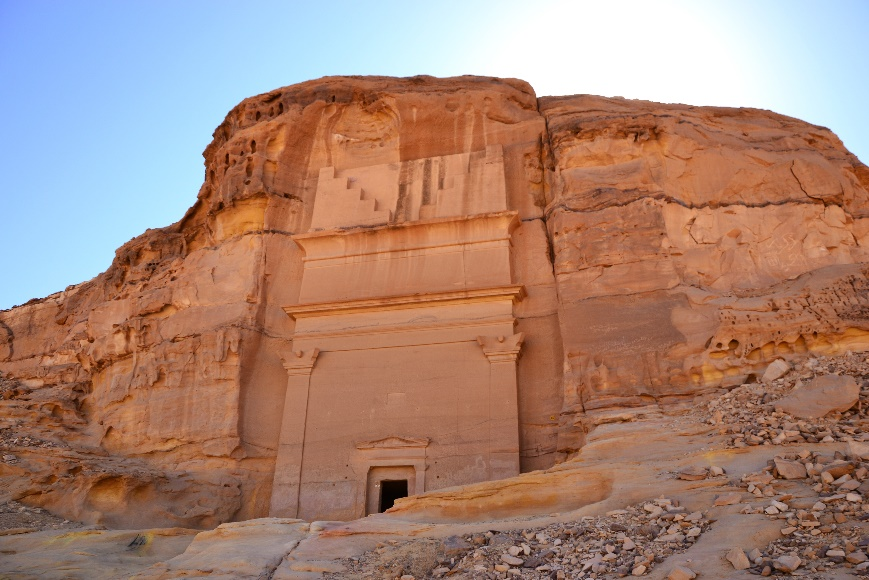
\includegraphics[width=3.94921in,height=2.63264in]{Images/image028.jpg}

Elle devient déserte à partir du IVe siècle et le Coran en donne la
raison~- Dieu a anéanti la ville, parce que ses habitants n'ont pas cru
aux prophètes~:

«~Certes, les Hommes d'al-Hijr ont traité les Envoyés d'imposteurs. Nous
leur avons apporté Nos signes et ils se sont détournés. Ils creusèrent,
tranquilles, des demeures dans les montagnes. Mais le Cri les prit au
matin, et à rien ne leur servit ce qu'ils possédaient~» (S. 15,
80-84)\sn{\textsuperscript{~}S.~15, 80-84 signifie que ce sont les
  versets 80 à 84 de la sourate 15\ldots{} on y reviendra dans le
  chapitre sur le Coran.}.


\begin{Synthesis}
Le Coran donne des informations
historiques, sur des épisodes passés, mais aussi sur l'histoire à
venir~. Mais il donne
surtout une lecture théologique de l'histoire.
\end{Synthesis}

Notons aussi l'existence de villes. \mn{La ville de Najran avait un évêque qui était probablement rattaché à l'église d'Éthiopie. Dhu Nuwas haïssait les chrétiens et faisait sans cesse la guerre au roi d'Éthiopie. Vaincu et forcé de payer tribut à Elesbaan, il se vengea sur les chrétiens de son royaume. Il agit par ruse : ayant rendu une visite protocolaire à la ville de Najran, il invita les notables à venir le voir dans son camp où ils furent tous capturés.   Devant leur refus de devenir juif, il
fait exécuter les 340 chrétiens de la ville, et décapiter le prince
Aréthas. Suite à ce massacre, le roi d'Ethiopie Elesbaan mena une
expédition punitive dans la cité, chassant Dounass, et rétablissant un
prince chrétien à la tête de la cité. Selon la plupart des commentateurs
du Coran, les hommes de Ukhdoud mentionnés au verset 4 de la sourate 85
ne seraient autres que les martyrs de Najran, tués et
brûlés.}Najrān est située en Arabie saoudite
à proximité du Yémen. Elle a été aussi capitale d'un petit royaume. Elle
était habitée par des juifs et des chrétiens. Un épisode terrible y a eu
lieu et est resté dans les esprits lorsque le roi juif Himyar en 523 a
fait assassiner des notables chrétiens.



Dans le Golfe et dans le Nord du Hijāz, les travaux archéologiques ont
mis en lumière des langues étrangères (akkadien, araméen, nabatéen,
grec, latin). Mais qu'en est-il de l'arabe comme idiome linguistique~?

\vide{lessor-de-la-langue-arabe}{%
\subsubsection{L'essor de la langue `arabe'
}\label{lessor-de-la-langue-arabe}}

Vous trouverez ci-dessous quelques éléments historiques sur l'essor de
la langue arabe. C'est un peu subtil tant dans les termes que dans la
géographie, à moins que vous ne soyez déjà un peu familier avec ce
monde. Dites-vous que ces informations ne sont pas là pour faire savant.
Il faut bien voir que de cette histoire linguistique nous pouvons
retirer des informations précieuses dans notre compréhension de l'islam
et de ses fondations puisque le Coran a été transmis justement \emph{en
arabe}~: Il le dit d'ailleurs de lui-même~: «~Un Coran \emph{en arabe}
pour les gens qui savent~» (S. 41,3). Donc\ldots{}

À l'époque antique, il existait au sein de «~l'Arabie heureuse~»
(c'est-à-dire le Yémen) quatre groupes lexicaux~: le sabéen, le
qatabānite, le ḥaḍramawtique et le madhābien. L'unification au IIIème
siècle de notre ère s'est traduite par la prédominance du sabéen. Il est
proche de l'arabe, mais il n'est pas l'arabe. L'arabe avec son article
«~al~» qui le caractérise se trouve dans une dédicace datant du IIème et
IVème siècle~: on trouve \emph{l-lt} (pour \emph{li-llât}) {[}pour
Dieu{]}. C'est écrit en alphabet sabéen, mais c'est de l'arabe~!

Au VI\textsuperscript{ème} siècle, il y a un lien entre la langue arabe
et l'écriture. Ce n'est pas l'écriture telle que nous la connaissons
aujourd'hui, mais c'est son ancêtre. C'est du vieil arabe. Le premier
témoignage de cette écriture est une inscription qui date de 512~: il
s'agit d'une dédicace à St Serge~à Zabad au sud d'Alep :

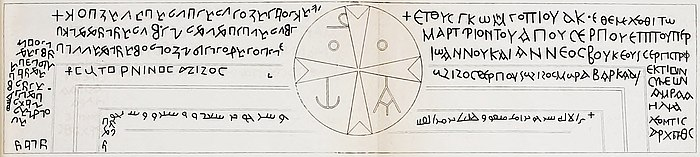
\includegraphics[width=5.51181in,height=1.23542in]{Images/image029.jpg}

autrement dit, l'écriture arabe a été utilisée par les chrétiens. Ce qui
est intéressant, c'est que l'inscription est en trois langues~: grec,
syriaque et arabe. On trouve une inscription à 100 km de Damas au roi
al-Harith datant de 538\emph{,} une inscription au sud de Damas datant
de 568, pour commémorer la construction d'un \emph{martyrum}. Qu'en
déduire~?

\begin{itemize}
\item
  On note que les premières écritures arabes sont en dehors de l'Arabie,
  ce qui plaide pour une influence syriaque dans l'émergence de l'arabe.
\item
  D'autres plaident pour une influence de l'alphabet
  nabatéen\sn{Pour rappel, les Nabatéens sont un peuple commerçant
    de l'Antiquité vivant au sud de la Jordanie et de Canaan, et au nord
    de l'actuelle Arabie. Vous avez entendu parler de Pétra~? Vous y
    êtes peut-être allés, dans ce cas vous savez déjà tout. Si vous ne
    savez pas ou si vous avez oublié, sachez que Pétra était la capitale
    de la Nabatène. Lieu magnifique. Tombé dans l'oubli, le site a été
    redécouvert en 1812 par un explorateur suisse,
    \url{http://www.hls-dhs-dss.ch/textes/f/F17075.php}{Jean-Louis
    Burckhardt} \ldots{} Une petite vidéo du ministère du tourisme
    jordanien vous donnera envie d'aller découvrir son `mystère'.
    \url{https://www.youtube.com/watch?v=YKk-JGeU_yY}{C'est ici~!}}.
\item
  En tous les cas, il semble que les premiers à parler arabe, n'étaient
  pas les Arabes. Et d'ailleurs qui sont ceux que l'on appelle Arabes~?
  Il est frappant de constater à partir des sources non musulmanes que
  ceux qui dirigent les «~conquêtes arabes~» au lendemain de la mort de
  Muḥammad ne sont pas appelés «~arabes~». On trouve les termes grecs de
  \emph{Sarakenoi} (Sarrasins), de \emph{Tayyayê'} dans les textes
  syriaques (du nom d'une tribu de l'Arabie du Nord-Est), de
  \emph{Haragènes}, de «~\emph{fils d'Ismaël}~» ou encore de
  \emph{magaritai} dans un papyrus daté de 643 ou de
  \emph{maghrâyê}\sn{Françoise \textsc{Micheau}, \emph{Les débuts
    de l'islam}, Paris, Téraèdre, 2012, p. 52.}.
\end{itemize}

La première mention du mot `arabe' se trouve sur une inscription
assyrienne~; elle date de 853 avant JC. Il y est question de la mention
d'adversaires et notamment Gindibu' l'Arabe. Plus tard, le terme
apparaît pour désigner des peuplades nomades, avec leurs chameaux.

\foreignlanguage{greek}{
Ἰουδαῖοί τε καὶ προσήλυτοι, Κρῆτες καὶ Ἄραβες, ἀκούομεν
λαλούντων αὐτῶν ταῖς ἡμετέραις γλώσσαις τὰ μεγαλεῖα τοῦ θεοῦ.} (Ac 2, la
Pentecôte)



Cela ne se limite pas à la péninsule de l'Arabie\ldots{} on désigne
aussi par Arabe ceux qui vivent au bord du Nil. On en a un bel exemple
chez Hérodote. Le terme est donc en premier lieu \textbf{employé par
l'extérieur pour désigner ces populations}. La première fois qu'elles
parlent d'elles-mêmes en se désignant par ce mot, se voit sur une
inscription du 3\textsuperscript{ème} siècle de notre ère où un individu
dit de lui qu'il est \emph{`arabī}. Il y a une inscription du
4\textsuperscript{ème} siècle, où il est question d'un groupe d'arabes.

\begin{itemize}
\item
  À la veille de l'islam, il y a donc un ensemble vaste de populations
  qui ne se désignaient pas eux-mêmes ou rarement par le terme d'arabe.
\end{itemize}

\textbf{Du coup, on se demande s'il ne s'agit pas d'une construction
\emph{a posteriori}.}

\vide{lenvironnement-religieux-de-la-puxe9ninsule-arabe}{%
\subsection{{L'environnement religieux de la
péninsule arabe
}}\label{lenvironnement-religieux-de-la-puxe9ninsule-arabe}}

Nous avons vu que La Mecque abritait un temple aux multiples divinités.
Nous avons vu aussi que des chrétiens et des juifs s'y trouvaient. Au
regard de l'histoire des royaumes voisins, il n'y a rien de surprenant.
Mais entrons un peu plus dans le détail\sn{Dans un souci
  synthétique, je m'appuie notamment sur une contribution très bien
  faite de Michel Reeber, «~Le contexte religieux de l'Arabie
  préislamique~», dans \emph{Le Coran et la Bible}, Paris, 2002, p.
  13-42.}.

\vide{le-polythuxe9isme-de-larabie-le-culte-buxe9tylique}{%
\subsubsection{{Le polythéisme de l'Arabie~: le
culte bétylique
}}\label{le-polythuxe9isme-de-larabie-le-culte-buxe9tylique}}

Si vous avez eu la curiosité de lire l'article de Jacqueline Chabbi,
vous vous souvenez probablement que les Bédouins pratiquaient le culte
des bétyles, c'est-à-dire ces roches sacrées censées être la demeure
d'un dieu (bétyle vient de \emph{bayt} -- maison et de \emph{el} -
dieu). Les pierres étaient transportées par les tribus nomades, mais à
La Mecque, cité sédentaire, on avait édifié un temple qui les abritait.
La fameuse pierre noire qui est dans l'actuelle Ka`ba n'est pas sans
rappeler cette tradition bédouine. Elle a donné lieu à de multiples
légendes. L'une d'entre elles dit qu'elle fut jetée du ciel sur terre et
que blanche elle était, mais que ce sont les péchés des hommes qui l'ont
rendue noire. Cela me rappelle une tradition chrétienne antique à propos
du baptême de Jésus~: on a pu dire que Jésus immaculé, donc de blanc
qu'il était, au moment de son baptême est ressorti noir du Jourdain car
il portait le péché des hommes\ldots{}

Il existait aussi des rituels de circumambulation autour de la Ka`ba
ainsi qu'un pèlerinage entre Marwa et Safa, le jet de pierres autour
d'une stèle, la vénération de feux sacrés. L'islam, comme nous le
verrons, garde souvent une emprunte de ces rituels, mais il les a
islamisés. En revanche, pas de feu. \textbf{Le passage au calendrier
lunaire a permis de maintenir des pratiques tout en rompant avec les
rituels solaires liés aux saisons, marquant ainsi une vraie rupture avec
les rites antéislamiques.}

Parmi les rites, on offrait aussi des sacrifices d'animaux ou même
d'êtres humains. Le Coran fait mention des sacrifices d'enfants qui
semblent être courants~:
\begin{quote}
S. 6, 137~: «~Et c'est ainsi que leurs divinités ont enjolivé à beaucoup
d'associateurs le meurtre de leurs enfants, afin de les ruiner et de
travestir à leurs yeux leur religion. Or si Allah voulait, ils ne le
feraient pas. Laisse-les donc, ainsi que ce qu'ils inventent~».
    
\end{quote}

  Ce verset pointe une pratique, mais en même temps, il est ambigu
  puisque\textbf{,} s'il montre l'horreur du massacre et ses
  conséquences funestes\textbf{,} il n'invite pas pour autant à lutter
  contre ces pratiques, comme si elles étaient voulues par Dieu et
  conduisaient \emph{in fine} à la mort des idolâtres.

Quant au Panthéon, s'il y avait plusieurs dieux, le culte de Hubal, qui
provient de Mésopotamie ou de Syrie, était prédominant\sn{Toufic
  Fahd, Le Panthéon de l'Arabie Centrale à la veille de l'Hégire,
  Institut Français d'Archéologie de Beyrouth : Bibliothèque
  archéologique et historique, n°88, 1968.}. Une statue dans le Temple
de la Ka`ba le représentait.


\paragraph{Houbal}{Divinité principale du panthéon arabe,
Houbal était connu sous le nom de « Seigneur de la Ka'ba ». Il était
probablement le père de la Triade des déesses Allât, Al-'Uzzâ et Manât,
les Filles de Houbal. En dehors de l'Arabie du sud, son nom apparaît
seulement dans une inscription nabatéenne où il est associé à deux
autres divinités, Dhu-al-Sharâ (Dusarès ; en arabe : \TArabe{ ذو الشّرى }et
Manawatu (en arabe :\TArabe{ مناة-مناواتو,} équivalent arabe nabatéen de Manât).;
'après Ibn Ishaq, la statue de la Ka'aba était une effigie
anthropomorphe en cornaline ; la Sira rapporte qu'Abd al-Muttalib ayant
promis un fils en sacrifice à Houbal qui l'avait aidé à retrouver la
source Zamzam, le sort aurait tout d'abord désigné Abdallah, père de
Mahomet. Sur les conseils d'une devineresse, on aurait proposé au dieu
cent chameaux en échange. Après dix divinations, chacune suivie d'une
augmentation du nombre des chameaux, Abdallah eut la vie sauve contre
mille chameaux.
}

\paragraph{Trois divinités} le concurrençaient. Comme nous l'avons vu, elles sont
mentionnées dans le Coran~: al-Uzzā, al-Lāt et Manāt (S. 53, 19-20).
Al-Uzzā était la déesse vénérée par les Quraysh, tribu dont est issu
Muḥammad. Selon les historiens musulmans, la Ka`ba contenait quelques
360 figurines (tiens, c'est la réponse à la question du
1\textsuperscript{er} chapitre). Muḥammad, de retour à La Mecque après
son Hégire à Médine, donnera l'assaut contre elles et les détruira
toutes, à l'exception de deux d'entre elles. \textbf{Quelles sont ces
fameuses deux icônes qu'il n'a pas fait
détruire}\sn{D'après la tradition, Mahomet, lorsqu'il investit la
  Kaaba, ordonna la destruction de toutes les idoles, sauf une : une
  icône mariale qu'il protégea de ses mains. Maryam, mère du prophète
  Jésus, Isâ (Issa), est donc vénérée partout par les musulmans.}\textbf{\ldots{}
Ce n'est pas sans incidences sur la nature des relations entre
communautés de religions différentes, ni non plus sans conséquences
aujourd'hui.} On en reparlera.

La connaissance de cette culture religieuse tribale permet d'enraciner
la compréhension de l'islam et notamment de ses rites. Mais plus encore,
elle permet de comprendre le Coran lui-même. C'est le propos de la
recherche de Jacqueline Chabbi dans son ouvrage \emph{Le Coran
décrypté}. Elle montre que certains passages s'éclairent en lien avec le
milieu tribal de Muḥammad. Ainsi, par exemple, elle remarque que bien
des métaphores eschatologiques et bibliques du Coran sont une réécriture
adaptée à la culture tribale. À cet égard, il est symptomatique que le
paradis soit décrit comme une oasis, un jardin (\emph{ğanna}) irrigué de
canaux toujours à ras bord (\emph{anḥār}), ombragés et sans soleil
(\emph{lā yarawna fihā `amsan}) (S. 76, 13)\sn{~Jacqueline Chabbi,
  «~La possibilité du Coran comme document anthropologique~», dans Mehdi
  \textsc{Azaiez} (dir.) et Sabrina \textsc{Mervin} (coll.), \emph{Le
  Coran}. Nouvelles approches, CNRS Editions, 2013, p. 189-205.}. On est
ici en plein milieu culturel arabe caractérisé par une phobie du soleil.
Ce travail sur le milieu tribal de l'Arabie antéislamique n'est pas sans
incidence dans la compréhension du Coran mais aussi dans ses
traductions. Ainsi, par exemple, la traduction de \emph{anḥār} par
fleuves, comme pour les fleuves bibliques du paradis, est un \emph{a
priori} de traduction et ne rend pas compte de sa signification exacte.
Il n'y a pas de fleuves, ni de rivières dans la péninsule arabe, juste
des points d'eau, quelques sources, parfois des lacs souterrains à
l'instar de La Mecque. De la même manière, la représentation de l'enfer
dans le Coran s'appuie sur le milieu tribal. Il est question du
\emph{ḥamīm} (S. 47, 15)~: c'est la pluie des orages d'été~; c'est lui
qui vient abreuver les damnés. Ils n'ont pour seule nourriture que le
\emph{dari'}, c'est-à-dire l'herbe à chameaux. Le \emph{nār,} traduit
par enfer, \ldots{} est en fait un feu solaire perpétuel.

Dans son dernier livre, \emph{Les trois piliers de l'islam}, elle montre
que l'islam tel qu'il se construit au cours de l'histoire est
essentiellement une construction à l'époque abbasside, époque
caractérisée par des guerres avec l'empire byzantin~; époque qui est
aussi celle d'un empire qui cherche à se démarquer de la première
dynastie des Omeyyades, époque où les textes sont fixés et notamment les
recueils de \emph{Sunna}. Or, les recenseurs ne sont pas arabes. Ils
proviennent de milieux culturels de contrées lointaines à l'Arabie~:
Buḫārī est de Transoxiane (actuel Ouzbékistan), Muslim de Nišapūr
(actuel Nors-Est de l'Iran), etc. quant à la \emph{Sunna} d'Ibn Ḥanbal,
le maître bagdadien, sa \emph{Sunna} ne fait pas partie des livres
canoniques\sn{Chabbi, Jacqueline,~\emph{Les Trois Piliers de
  l'islam}, \emph{op.cit.}, p. 15.}. Or, \textbf{leurs lectures, dans la
mesure où la Sunna est aussi l'herméneutique du Coran, vont imposer une
compréhension du Coran qui se détache du sens du Coran des origines.}
Pour l'historienne, il ne s'agit pas de rejeter ces lectures -- cela
relève de la démarche théologique, croyante -- mais de dire qu'une
attention à l'anthropologie du milieu où est prêché le Coran donne des
clefs de compréhension au texte sacré de l'islam. Pour autant, on peut
dire que Chabbi voit dans ce travail une mission salutaire~: c'est ici
que l'historienne se fait engagée~: à l'heure du fondamentalisme où des
idéologies se vantent de revenir au sens originel, il s'agit de lire le
Coran dans toute la vigueur de son verbe au-delà des lectures qui lui
furent accolées et qui lui sont encore posées.
\begin{quote}
    «~Ils lisent certes mais, ne connaissant ni les tenants ni les
aboutissants du texte, que comprennent-ils~? Texte sans contexte et sans
rattachement à un passé et à une tradition n'est que ruine du sens,
pourrait-on dire en plagiant un célèbre aphorisme~» (p.~31-32).
\end{quote}


Mais quel est ce sens originel du Coran ? Et comment le retrouver~?

L'auteur reconnaît qu'il sera difficile, voire impossible, de le
ressusciter car il prend naissance au sein d'une culture de l'oralité~;
il y a donc un «~écart sociologique~» (p.~11). Cependant, le Coran
témoigne de l'importance du milieu anthropologique, et si les références
bibliques restent parfois évasives, ce n'est pas parce qu'elles sont
connues -- ce que soutient Guillaume Dye -- mais parce qu'elles sont
réinterprétées. Or, le milieu anthropologique de l'Arabie est celui de
la culture tribale marquée par trois piliers~: \textbf{l'alliance, la
guidance et le don}. Ces piliers sont de nécessité pour les hommes de ce
milieu. Ils se retrouvent dans le Coran et doivent être abordés à partir
des sens qu'ils avaient à l'époque. Son étude lexicale lui permet aussi
d'identifier l'hétérogénéité des champs lexicaux en fonction des milieux
mecquois et médinois~: ainsi, elle remarque que le vocabulaire à Médine
y est beaucoup plus diversifié, et l'influence de l'hébreu y est plus
net. La terminologie y est aussi renouvelée. Symptomatique à cet égard
est la racine \emph{baraʾ} pour désigner la création~: si elle se trouve
au livre de la Genèse, elle est absente des versets mecquois. Plus
largement, Chabbi replace le sens du mot \emph{kitāb} -- traduit
communément par «~livre~» -- au sein de la culture de l'oralité~: il ne
s'agit pas d'un livre matériel, mais d'un message fixé oralement
(p.~58). L'univers tribal s'exprime aussi dans la nature des
descriptions eschatologiques. Ces croyances sont nouvelles et
constituent une nouveauté pour les mecquois, mais elles déploient un
code symbolique relatif au désert~qu'il s'agisse de la tempête ou du
combat contre une tribu.

Sur la nature religieuse du milieu de la péninsule arabique, elle
souligne qu'il est avant tout marqué -- et plus \textbf{à La Mecque qu'à
Médine -- par le caractère bétylique \mn{p.~117}. À cet égard, le mot
\emph{bayt} dans le Coran ne renvoie pas à un temple ou à une maison,
mais au cœur de la cité mecquoise, la Kaʿba~}: il existe une symétrie
entre la demeure de la divinité et celle des hommes puisqu'il s'agit
d'un modèle de duplication appliquée à la divinité censée les
\textbf{protéger} (p. 117).

Quant à la question des prophètes mentionnés dans le Coran, ils ont fait
l'objet d'une étude approfondie par l'islamologie\sn{~Speyer,
  Heinrich, \emph{Die Biblischen Erzählungen im Qoran,} Hildesheim, G.
  Olms, 1961 (1931).}. L'originalité de la recherche de Chabbi est de
montrer que les thèmes qui leur sont rattachés sont adaptés au monde
tribal. Ainsi, à propos de la confrontation d'Abraham avec des idoles
(\emph{asnām}), on a généralement mis en avant le rapprochement de ce
texte coranique avec le chapitre 12 du \emph{Livre des
Jubilés}\sn{Voir pour le Testament d'Abraham~: Gobillot,
  Geneviève, «~Le Coran, guide de lecture de la Bible et des textes
  apocryphes~», \emph{Pardès} 50, 2, 2011, p. 131-154.}~mais, pour
Chabbi, le cœur du message ne porte pas tant sur les pierres taillées
que sur l'opposition entre la croyance des pères (\emph{ābāʾ}) et celle
qu'il faut désormais accorder au Seigneur des peuples/tribus (\emph{Rabb
al-ʿālamīn}) (p. 97) -- non pas «~Seigneur des mondes~» selon la
traduction commune mais «~Seigneur des tribus~» --. Par conséquent, Dieu
est celui qui crée, guide, nourrit, abreuve, fait mourir et revivre. Le
Seigneur vient se substituer aux dieux incapables de protéger et de se
protéger (Cor.~26,~92-93). Dans la péninsule arabique, le \emph{Rabb},
est une figure protectrice.

 
\mn{\url{https://fr.wikipedia.org/wiki/Ar-Rahman}} 


\paragraph{Raḥmān}
L'évolution sémantique pour désigner Dieu est dans le Coran hautement
illustrative du thème de l'alliance. Ainsi, \textbf{la figure de
\emph{Raḥmān}},\TArabe{ الرحمن } \emph{le miséricordieux}~ \textbf{est propre à la
période mecquoise et disparaît au temps de Médine pour être remplacée
par celle d'\emph{Allāh}}. La notion de \emph{Rabb} renvoie à l'idée
d'un échange~; il y a une personnalisation de la relation par
l'expression \emph{Rabbī}, mon Seigneur (p. 143). Le divin est
foncièrement le \emph{walī}, c'est-à-dire le proche, le
\textbf{{protecteur}}.

Le \emph{muʾmin}\sn{(\textsc{a}.), participe actif de la
  4\textsuperscript{e}~forme de la racine~\emph{ʾmn}, signifie
  «Croyant», mais est aussi l'un des noms de Dieu (LIX, 23).}, n'est pas
d'abord celui qui croit, mais celui qui s'est rallié avec confiance.
Chabbi écrit~:
\begin{quote}
    
«~L'importance des occurrences de cette terminologie est frappante. Elle
témoigne de la spécificité de l'engagement mutuel du divin et de
l'humain, car l'alliance n'est jamais gratuite~; elle ne va pas sans
contrepartie de part et d'autre~» (p.~153).
\end{quote}
\begin{Ex}

{Quand on parle de Rahman avec un musulman, miséricorde
n'a pas forcément le même sens~: pardon pour un chrétien, bienfaisance
(pluie) pour un
musulman}
\end{Ex}

Quant au nom \emph{Rahmān}, elle remarque que si la racine hébraïque
connote l'idée de compassion et de miséricorde, sa réappropriation dans
le milieu tribal via le monde yéménite le connote de l'idée de
bienfaisance et de bienveillance. Le \emph{Rahmān} joue le rôle du Dieu
qui dispense la pluie, fonction établie à Athtar, dieu de la pluie du
Yémen (p.~127). Mais la tradition musulmane dit-elle autre chose~? Il
est frappant de constater que les traités théologiques musulmans sur les
noms divins s'inscrivent pleinement dans la définition d'une
\emph{raḥma} comprise non comme miséricorde au sens chrétien, mais
bienveillance et bienfaisance, à l'instar de celui d'al-Ġazālī \label{theol:AlGazali23}. Sur ce
point, Chabbi vient davantage corriger une traductologie influencée par
le vocabulaire théologique du christianisme que renouveler le sens
terminologique au sein de la tradition islamique.

\vide{alliance}{%
\subsubsection{Alliance}\label{alliance}}

Du point de vue du développement des idées religieuses, Chabbi souligne
l'émergence du allāhisme, mouvement de ralliement à une divinité qui
assume les fonctions assignées aux divinités d'un milieu tribal~:
alliance et protection, jugement eschatologique. Au cours de la
révélation mecquoise, \emph{Ilāh} est d'abord le dieu qui s'impose sur
les autres dieux. La notion de \emph{\textbf{walāʾ}} , ô combien
utilisée dans les milieux fondamentalistes et salafistes d'aujourd'hui,
signifie \textbf{l'alliance, la solidarité} au sein d'un même groupe
partageant le même espace.

\vide{guidance}{%
\subsubsection{Guidance}\label{guidance}}

De même, les noms divins se comprennent dans le cadre du monde tribal~:
dire de Dieu qu'il est \emph{ʿalīm}, c'est faire de lui le maître des
signes (\emph{aʿlām}) et Chabbi de préciser que cela renvoie au signe de
la piste~: \emph{Ilāh} est celui qui guide et conduit. Il connaît
l'avenir et permet de guider son groupe afin de le protéger des périls.
Ce dont il protège ce n'est pas la nuit, mais la ténèbre -- nuit sans
lune où l'on ne peut plus suivre la piste -- alors que les nuits
éclairées par la lune rendent le chemin des caravaniers aisés par
contraste avec les chaleurs de la journée. Dans le désert, la guidance
(\emph{hudā}) est de nécessité~: elle est une question de vie ou de
mort. Et si Dieu guide, c'est pour protéger de la mort non pour inviter
à en prendre le chemin. Là encore, l'analyse se fait engagée~:
\begin{quote}
«~Autant dire que les outrances actuelles qui assurent préférer la mort
dans la voie de Dieu en croyant prendre appui sur le passé premier sont
en totale contradiction avec la parole coranique telle qu'elle
s'adressait aux hommes de son temps dans la société qui était la leur~»
(p.~157).
\end{quote}

Les routes sont des chemins dangereux, surchargés d'embûches physiques
et surnaturelles, de puissances hostiles si bien que tout déplacement
est une aventure périlleuse. Dans ce contexte, les dieux préislamiques
exerçaient la fonction de guide. Les seigneurs (\emph{arbāb}) n'étaient
pas les maîtres de ces lieux mais ils pouvaient y conduire les hommes et
les guider, les protéger. Or, le sédentaire, non habitué à se déplacer,
devait pour tout déplacement recourir à des guides. \textbf{La parole
coranique exprime ce besoin~: elle n'est pas issue d'un milieu nomade,
mais sédentaire.} La thématique de la guidance permet donc à l'auteur de
restituer le sens perdu de mots clefs du vocabulaire coranique et
islamique.

\vide{ux161arux12bux2bfa-voie}{%
\paragraph{šarīʿa~, voie}\label{ux161arux12bux2bfa-voie}}

Ainsi en est-il de \emph{šarīʿa}~: elle est la voie donnée pour éviter
de se perdre~: elle est grâce accordée à Muḥammad alors que les enfants
d'Israël se sont écartés du chemin, bien que Dieu les avait favorisés
(\emph{tafdīl}) (Cor.~45,~15-18). Cette voie renvoie à un point d'eau où
l'eau affleure, ce qui permet aux dromadaires de s'y désaltérer sans que
l'on doive aller y puiser~: c'est donc un lieu facile d'accès. Ainsi,
Dieu, par la \emph{šarīʿa}~donne accès à l'eau~; il dispose de
ressources qu'il partage. Par suite, perdre la voie conduit au malheur,
à l'exemple des fils d'Israël (Cor.~45, 17). En conclusion, Chabbi
remarque que le Coran est loin de la signification qui sera donnée à ce
terme et qui ne date que du iii\textsuperscript{e} siècle de l'Hégire
(p.~177). Elle conclut aussi que l'intégration de châtiments corporels à
la \emph{šarīʿa}~est impossible en milieu pré-islamique et se trouve aux
antipodes des solidarités qui s'y nouaient. La seule disposition légale
qui se retrouve dans le Coran est celle du \emph{qiṣāṣ}, le prix du sang
(Cor.~4, 92).

\vide{lapidation-mentionnuxe9e-dans-la-sira}{%
\subsubsection{Lapidation mentionnée dans la
sira~?}\label{lapidation-mentionnuxe9e-dans-la-sira}}

Quant à la lapidation (\emph{raǧm}), elle était pratiquée non pour tuer,
mais pour éloigner l'indésirable à l'exemple des puissances maléfiques
dont il s'agit de se prémunir pour éviter de subir leur malfaisance (p.
178) (Cor. 86, 25~; Cor. 15, 17, 34).

\vide{la-sunna-la-piste-sure}{%
\paragraph{La sunna, la piste sure}\label{la-sunna-la-piste-sure}}

De même, si le mot \emph{Sunna} désigne la piste sûre, réputée,
attribuée à Dieu, la \emph{Sunna d'Allāh} est une voie de châtiment pour
ceux qui ont trahi l'alliance. Elle n'est pas un modèle à suivre, sens
qui sera donné à propos de Muḥammad. Cette expression, typique du
sunnisme, a cherché à se fonder sur le Coran à partir du mot
\emph{uswa}, se rallier à\emph{.} Ainsi, Abraham a-t-il été présenté
comme un exemple à suivre en tant qu'il a rompu avec l'allégeance des
dieux de ses pères (Cor. 60, 4 et 6). De même, le messager d'Allāh
(désigné comme Muḥammad par les commentateurs) est-il présenté comme un
exemple à suivre (S.~33, 21). Mais pour Chabbi, le contexte n'est pas
celui du modèle, mais de l'alliance~: il est celui qui s'est rallié à
Dieu. La \textbf{Sunna de Dieu renvoie donc à une coutume divine~qui
consiste à rejeter, à faire disparaître celui qui s'éloigne ou qui
accuse le messager de Dieu de mensonge.}

À propos du terme \emph{umma}, communément traduit par «~communauté~»,
Chabbi souligne que dans le Coran, là aussi, il désigne la bonne voie :
«~Nous avons trouvé nos pères sur une \emph{umma} et c'est assurément
leurs traces qui nous sont modèle {[}pour suivre la route{]} \emph{ʿalā
aṯāri-him muqtadūn}~» (Cor. 43, 22). Quant au \emph{ǧihād}, si on a
souligné à maintes reprises qu'il est un effort, Chabbi resitue cet
effort par rapport au milieu local où le sédentaire est désigné comme
celui qui reste sur place (p. 194). Dans un monde où la chaleur brûle
les corps, tout déplacement est un enfer. Face à la tentation de
s'installer, le Coran affirme que le paradis leur sera interdit.
\textbf{Aussi, l'image du paradis renvoie-t-elle à un monde immobile,
sans activité.} Il est la récompense accordée à la suite de à l'effort
engagé dans les pas de Muḥammad. D'où les images eschatologiques comme
celles de l'accoudement (\emph{ittikāʾ}). «~Le paradis coranique semble
ainsi avoir horreur du mouvement. Il fige les élus dans l'immobilité
d'un repos qui les fait en quelque sorte échapper à la course harassante
pour la vie qui avait été leur lot durant leur vie~» (p. 293).

\vide{ux1e7ihux101d-combat-pour-la-voie-dallux101h-dans-un-monde-ouxf9-le-paradis-est-limmobilituxe9}{%
\paragraph{Ǧihād, combat pour la voie d'Allāh dans un monde où le
paradis est
l'immobilité}\label{ux1e7ihux101d-combat-pour-la-voie-dallux101h-dans-un-monde-ouxf9-le-paradis-est-limmobilituxe9}}

Le \emph{ǧihād} devient le combat à mener dans la voie d'Allāh, il est
le \emph{qitāl}. Et traduire \emph{qitāl} par le fait de tuer est une
altération de sens car il ne s'agit pas de tuer pour tuer, mais il
s'agit de combattre en sachant que ce combat peut conduire à la mort (p.
200-201). Mais «~tuer les hommes d'un groupe adverse de manière
inconsidérée ou gratuitement massacreuse constitue une transgression
majeure~» (p. 203).


\mn{Combien est vil le prix contre lequel ils ont troqué
leurs âmes lorsqu'ils ont nié ce que Dieu a révélé et ce, uniquement par
dépit, car ils n'ont pu admettre que Dieu, par un effet de Sa grâce, ait
choisi certains de Ses serviteurs pour les gratifier de la révélation !
Ils se sont ainsi attirés doublement la colère du Seigneur et le
châtiment ignominieux qui sera réservé aux
infidèles.}



Le verset Cor. 2, 90 rappelle à cet égard qu'il ne faut pas commettre
d'agression (inconsidérée), que Dieu n'aime pas les agresseurs
(\emph{muʿtadīn}).

Par opposition, la négociation qui permet de répondre au risque encouru
est considérée comme un don (\emph{fatḥ}). Le chapitre consacré à la
violence permet ainsi de rappeler que dans tous les cas, l'action de la
violence revient à la divinité. L'exacerbation de la parole coranique
doit être lue comme la conséquence de l'immobilisme des hommes. À
Médine, le prophète réclame l'obéissance (\emph{tāʿa})~; il y a ici une
rupture avec La Mecque où le Coran orientait sur l'obéissance à la
divinité.

\begin{table}[h!]
    \centering
    \small
   \begin{tabular}{p{0.45\textwidth}p{0.45\textwidth} }
À l'expiration des mois sacrés, tuez les polythéistes partout où vous
les trouverez ! Capturez-les ! Assiégez-les ! Dressez-leur des
embuscades ! S'ils se repentent, s'ils accomplissent la salât, s'ils
s'acquittent de la zakât, laissez-les en paix, car Dieu est Clément et
Miséricordieux. & Faitha insalakha alashhuru alhurumu faoqtuloo
almushrikeena haythu wajadtumoohum wakhuthoohum waohsuroohum waoqAAudoo
lahum kulla marsadin fain taboo waaqamoo alssalata waatawoo alzzakata
fakhalloo sabeelahum inna Allaha ghafoorun raheemun (⁎) \\
 
\end{tabular}
\sidecaption{verset dit du sabre (Cor. 9, 5)}
\end{table}

À propos du verset dit du sabre (Cor. 9, 5), la précision temporelle
«~après les mois sacrés~», montre une mise en conformité avec les règles
tribales (p.~249). L'injonction «~tuez-les~» est incompatible avec le
contexte du verset qui invite à accueillir les repentants~: il s'agit
donc d'abord de combattre~; par ailleurs cet appel est une réponse à une
agression antérieure.

\vide{don}{%
\subsubsection{Don}\label{don}}

Enfin, concernant le don, il est mutuel (p.~265). Conformément à ce
qu'avait montré Mauss, celui qui ne peut donner est dans une situation
très faible car \textbf{le don est aussi une marque de pouvoir}. Par
conséquent, \textbf{l'orphelin} a la position la plus inférieure. Dans
la logique du don coranique, il s'agit de donner, mais sans s'appauvrir
soi-même. Pour autant, le don appelle le contre don et Chabbi propose
une interprétation très intéressante du \emph{\textbf{kufr}} traduit
habituellement par \textbf{infidélité} ou mécréance. Pour elle, il
désigne \textbf{l'ingratitude}~: «~ce serait un moyen de se soustraire à
une obligation sociale en masquant la bienfaisance dont on a été
bénéficiaire~» (p.~266). La thématique du don divin est typiquement
tribale. Les délices du paradis, le repos eschatologique, sont la
récompense de la divinité à celui qui se sera investi dans ce monde et
aura su répondre à ses obligations. Mais le don n'est pas seulement lié
au futur. Dès ici-bas, la divinité offre~: ce sont les dons de
subsistance. Dieu est celui qui offre ces pâturages verdoyants, et parmi
les traductions originales avancées dans l'ouvrage, pour Chabbi,
traduire le verset Cor. 16, 80 par «~peut-être deviendrez-vous
musulmans~» est un anachronisme~: dans le contexte tribal, il s'agit
d'accepter de se mettre sous la garde de la divinité qui assure ces
bienfaits. Chabbi propose~: «~peut-être accepterez-vous de vous mettre
sous sa garde {[}dans la mesure où son alliance vous apporte tant
d'avantage en natures{]}~» (p. 330).

\vide{le-judauxefsme-dans-larabie-pruxe9islamique}{%
\paragraph{1.2.2 Le judaïsme dans l'Arabie
préislamique}\label{le-judauxefsme-dans-larabie-pruxe9islamique}}

À la suite de la destruction du Temple en 70, d'importantes communautés
juives émigrèrent au Moyen-Orient, en Babylonie, en Égypte, en Afrique
du Nord, à Byzance, en Italie. Certains juifs ont aussi émigré dans le
Hijāz (Arabie). La Mishna (compilation des enseignements de la loi
juive) rédigée en 200-220, en fait mention. On a pu identifier la
présence d'une vingtaine de tribus juives.

Il existait aussi une importante communauté juive dans le sud de la
péninsule arabique (Yémen). Les rois de Himyar ont fait le choix de
rejeter le polythéisme et après 380 on ne trouve plus dans tout le Yémen
la moindre inscription explicitement païenne. Cette rupture est très
profonde et se voit dans le vocabulaire avec l'usage d'une terminologie
araméenne et hébraïque comme \emph{amen}, `\emph{ālam} (monde),
\emph{bâraka} (bénir), \emph{shalôm}, \emph{salāt} (prière),
\emph{zakât} (grâce). Au début du VIème siècle, le judaïsme est la
religion dominante dans le royaume de Himyar\sn{Iwona Gajda, Le
  royaume de Himyar à l'époque monothéiste -- L'histoire de l'Arabie du
  Sud ancienne de la fin du IVe siècle de l'ère chrétienne jusqu'à
  l'avènement de l'islam.}. Avec l'unification de l'Arabie méridionale,
au 3\textsuperscript{ème} siècle, les rois de Himyar interviennent dans
l'Arabie désertique.

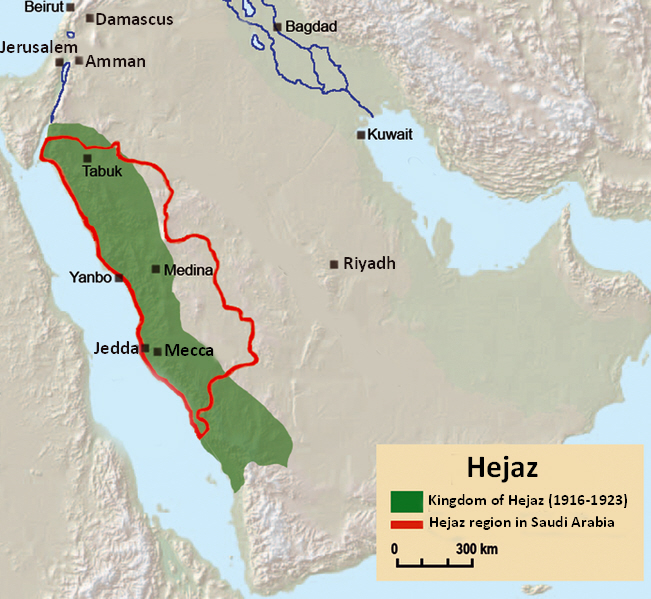
\includegraphics[width=\textwidth]{Images/image030.jpg}

Si globalement les juifs \mn{pour plus de détail sur le rapport entre Islam et judaisme, voir \cite{BarAsher:JuifsCoran}} refusèrent de se convertir à l'islam,
l'historiographie musulmane retient la conversion de certains d'entre
eux. Le plus connu est `Abd Allāh Ibn Salām, docteur de la Loi juive. Il
contribua à prêcher la conformité de la venue de Muḥammad avec la Torah.
Il est important de voir que ces premiers convertis apportent avec eux
leur culture biblique. Cela leur sera d'ailleurs reproché, comme ce fut
le cas pour un autre rabbin, Ka'b al-Akhbār. Retenez bien ce point quand
on parlera du Coran et de sa rhétorique~\ldots{} qui est très sémite.
Mais ces juifs qui fréquentent Muḥammad ou qui se convertissent dans les
premières décennies de l'islam, qui sont-ils exactement~? À quel courant
du judaïsme les rattacher~? De ce que le Coran rapporte concernant leurs
croyances sur Dieu, les anges, la création, la loi, le péché,
l'eschatologie, il semble que l'on puisse voir un lien de filiation avec
le judaïsme talmudique. Certains y ont vu des hétérodoxes juifs, mais
l'orientaliste Geiger\sn{A. \textsc{Geiger}, \emph{Was hat
  Mohammed aus dem Judenthum aufgenommen}, Bonn, 1833.}, à la lumière du
caractère sommaire des croyances juives telles qu'elles sont rapportées
par Muḥammad, suggère plutôt que les informateurs juifs de Muḥammad
étaient ignorants de leurs propres traditions -- autrement dit, il nous
invite à ne pas réduire le judaïsme de l'époque à ce que les
informateurs ont dû en rapporter. Cela rappelle un prisme méthodologique
dénoncé par al-Ġazālī \label{theol:AlGazali24} dans le \emph{Munqiḏ min al-ḍalāl} et que nous
avons vu dans la leçon précédente. Si vous avez oublié, relisez~:
\textbf{al-Ġazālī vérifie ce qu'il a compris d'une croyance auprès
d'autres membres de cette croyance.}

À La Mecque (lieu où commence la prédication de Muḥammad en 610), il est
difficile d'évaluer l'importance de la communauté juive. Mais les
versets coraniques révélés dans cette première période témoignent de
relations positives et fructueuses. La direction de la prière est
Jérusalem, le jour du jeûne (\emph{`ashūrā'}) rappelle le Yôm Kippour,
et le Coran reconnaît l'élection des juifs.
\begin{quote}
    «~Ô enfants d'Israël, souvenez-vous des bienfaits dont je vous ai
comblés~: souvenez-vous que je vous ai élevés au-dessus de tous les
humains~» (S. 2, 46).
\end{quote}


Mais à Yathrib (Médine), les juifs étaient plus nombreux.

Médine est située à 350 km de La Mecque. C'est une oasis. Il y avait une
école où l'on apprenait l'hébreu. Un des secrétaires de Muḥammad qui
sera chargé de collecter les sourates, Zayd Ibn Thābit, aurait fréquenté
cette école. En 622, au moment où Muḥammad doit fuir La Mecque et où il
va s'installer à Médine, il y a trois grandes tribus juives~: les Banū
Qurayẓa, les Banū al-Nadhîr et les Banū Qaynukā'. Ils avaient en leur
possession des terres riches et détenaient le pouvoir local. Peu à peu,
leur puissance déclina avec l'arrivée de deux tribus arabes, les Aws et
les Khazraj.

Il semble que les relations entre Muḥammad et les juifs de Médine furent
bonnes à son arrivée. Un document, «~La charte de Médine~» semble aller
dans ce sens.

\vide{clauses-en-rapport-avec-les-musulmans-et-les-croyants-monothuxe9istes}{%
\subsubsection{Clauses en rapport avec les musulmans et les croyants
monothéistes}\label{clauses-en-rapport-avec-les-musulmans-et-les-croyants-monothuxe9istes}}
\begin{quote}
 
 
 
{Les émigrés Qoraïchites et de Yathrib (Médine) et ceux
qui les suivirent et luttèrent avec eux forment une seule communauté à
part. Tous les musulmans quelles que soient leurs tribus ou
clans partagent entre eux le prix du sang, payent la rançon des captifs
selon le bon usage et
l'équité.
Les croyants monothéistes ne délaissent jamais un endetté
qui a la charge d'une famille ; ils lui donnent des fonds destiné à
payer le prix du sang ou le rachat d'un
captif.Tous les croyants monothéistes devront s'unir contre
quiconque étant rebelle ou cherchant à promouvoir l'hostilité ou la
sédition, quels que soient leurs liens familiaux ou
tribaux.  Aucun croyant monothéiste ne doit en tuer un autre, ou
soutenir un non croyant au détriment d'un
croyant.La protection de Dieu est sur tous les croyants
monothéistes, indépendamment de leur classe ou de leur origine
tribale.} 
 
 
{Il est défendu à un croyant monothéiste ayant consenti à
ce qui est écrit dans ce texte et cru en Dieu et au jour du jugement de
secourir un criminel ou de l'héberger. S'il le fait, il sera maudit par
Dieu au jour de la résurrection, sans pitié, et l'on n'acceptera de lui
ni compensation, ni
indemnité.}
 \end{quote}
     
\paragraph{{Clauses en rapport avec les
juifs.}} 
 \begin{quote}
Les juifs ne font qu'une communauté avec les
croyants. Les juifs peuvent continuer de professer leur religion et
la liberté de pratiquer leur religion est
garantie.   Tout juif qui adhère à cette charte doit avoir l'aide et
l'assistance des croyants et tous les droits des croyants doivent lui
être
donnés.Chaque tribu et chaque clan juif est responsable de son
prix du sang, de ses taxes de châtiment et de ses payements de
rançon.
  \end{quote} 
\paragraph{Clauses communes à
tous.} 
 \begin{quote}
Les juifs et les croyants monothéistes de Médine ont un
pacte de défense mutuelle entre deux groupes. Pour honorer ce pacte, ils
doivent en payer le coût
nécessaire. Les juifs et les croyants monothéistes de Médine se
conseilleront et leurs relations mutuelles doivent être fondées sur la
droiture, alors que le péché est
interdit. Aucun des juifs ou des croyants monothéistes ne doit
commettre de péchés portant préjudice à l'autre
groupe. Si les juifs font du tort aux croyants monothéistes ou si
ceux-ci font du tort à ceux-là, alors le parti lésé doit être
aidé. Médine doit rester un lieu sacré et inviolé pour tous
ceux qui joignent la charte, à l'exception de ceux qui ont commis une
injustice ou un
crime. Tous les participants à cette charte doivent boycotter
les Koraïchites non-musulmans de La
Mecque. Tous les participants à cette charte doivent défendre
Médine de toute attaque
étrangère. Aucune clause de cette charte ne doit interdire à aucun
parti de demander un châtiment
légal. Aucun participant à cette charte ne peut déclarer une
guerre sans la permission du prophète de l'islam
Mahomet. Chaque fois qu'un désaccord s'élève entre deux
participants à cette charte, le désaccord doit être soumis à Dieu et à
son messager pour
arbitrage.

 

    
\end{quote}
Document dont l'authenticité est admise. Document très important que
l'on trouvera en annexe. Mais celles-ci se détériorèrent peu à peu,
sans-doute parce que les juifs refusèrent de suivre Muḥammad dans sa
prédication de l'islam. Lorsque la rupture est consommée, la thématique
coranique change. L'islam ne s'inscrit plus dans la continuité du
judaïsme mais comme une restauration de la religion primitive,
pré-israélite, et falsifiée par les juifs.

Ici une remarque épistémologique s'impose. Les versets coraniques dans
leur diversité de ton sont lus à la lumière de l'évolution des relations
entre Muḥammad et les juifs. Mais dans quelle mesure cette histoire n'a
pas été écrite \emph{a posteriori}~? Autrement dit, n'a-t-on pas établi
une chronologie des versets -- celui-ci est de La Mecque, celui-là de
Médine -- sur la base d'un récit narratif historique qui est une
construction~? D'où la question, ce récit est-il authentique~?
D'ailleurs, la dégradation des relations avec les Juifs à Médine colle
assez mal avec la Charte de Médine.

C'est en tous les cas à cette période, que le sens de la direction de la
prière serait devenu La Mecque, et c'est à cette période que l'on
rattache les versets coraniques les plus hostiles aux juifs~:

\begin{quote}
    

«~Tu connaîtras que ceux qui nourrissent la haine la plus virulente
contre les croyants sont les juifs et les idolâtres et que ceux qui sont
les plus disposés à les aimer sont les hommes qui se disent chrétiens~»
(S. 5, 82).

«~Ceux qui ont reçu le Pentateuque, et qui ne l'observent pas,
ressemblent à l'âne qui porte des livres. C'est à quelque chose de vil
que ressemblent les hommes qui traitent les signes de Dieu de mensonges.
Dieu ne guidera point les impies~» (S. 62, 5).
\end{quote}
Dans ce contexte, Muḥammad trouve dans les deux tribus arabes des alliés
et très vite, les tribus juives sont considérées comme des ennemis. Les
juifs sont accusés d'avoir pactisé avec les gens de La Mecque, d'avoir
trahi le contrat établi avec les musulmans dans le cadre de la Charte de
Médine. Il s'ensuit un conflit violent. La guerre est d'abord déclarée
avec la tribu des Qaynuqā` qui doit fuir vers la Palestine. La
\emph{Sīra} raconte les batailles contre les juifs, ainsi que de
nombreux massacres. Vous souvenez-vous que nous avons déjà rencontré le
mot \emph{Sīra}~? Vous souvenez-vous de sa signification~?

\begin{marginfigure}
    \centering
    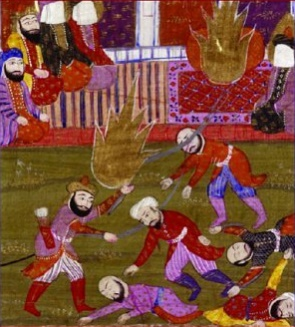
\includegraphics[width=1.31707in,height=1.45946in]{Images/image031.jpg}
    \caption{miniature du
19\textsuperscript{ème} siècle où l'on voit `Alī et Muḥammad massacrer
les membres de la tribu des Banū Qurayẓa. Manuscrit (17 folio 108b),
British Library.}
   
\end{marginfigure}
 
 



\paragraph{Le christianisme en
Arabie}

Un des archéologues, spécialiste du christianisme de la péninsule arabe,
est Christian Robin. {Le 18.08.2013, Sébastien de Courtois, dans l'émission
«~foi et tradition~» de France Culture, l'interroge. Il lui demande~tout
de go~: «~Alors Monsieur Robin, il y a eu une présence chrétienne en
Arabie
saoudite~?~»} 

Le Yémen a donc été «~officiellement~» chrétien entre 530 et 570. Son
roi est Abraha et, comme le dit Robin, on a découvert une inscription
qui date de 552 où sont mentionnées les régions soumises à son pouvoir~:
Arabie orientale, Arabie du Nord, Arabie du Nord-Est~; il y est aussi
question de Yathrib. Abraha a fait construire une cathédrale à San`ā'
{[}on est ici dans le sud de l'Arabie, l'Arabie heureuse{]} qui devient
capitale du Yémen, en 550. \emph{Les Chroniques} en donnent une
description détaillée, sublime. La cathédrale sera détruite au
8\textsuperscript{e} siècle.

Parmi les inscriptions, on dispose aussi d'une invocation à la Trinité
(\emph{Rahmanan}, son Fils \emph{Christos}, et l'Esprit Saint). Ce roi a
donc christianisé le Yémen et on ne trouve plus sous son règne
d'inscriptions spécifiquement juives.

\begin{marginfigure}
    \centering
    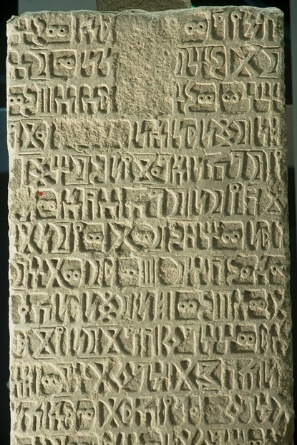
\includegraphics[width=1.31747in,height=1.96757in]{Images/image033.jpg}
    \caption{Inscription d'Abraha, 
    roi Éthiopien du Yémen, commémorant une réparation de la Digue de Marib }

\end{marginfigure}


le roi
Éthiopien du Yémen lors de la commémoration de la réparation de la Digue
de Marib et la consécration d'une église.~On y trouve aux premiers mots
l'invocation~
\begin{quote}
    « Avec la puissance, l'aide et la miséricorde de Rahmânân,
de son Messie et de l'Esprit Saint~» 
Christian Robin
\end{quote}

Mais la présence chrétienne dans le Yémen date déjà du
5\textsuperscript{e} siècle~: dans la \emph{Chronique de
Séert}\sn{Il s'agit d'une Chronique nestorienne d'auteur anonyme.
  Originellement écrite en syriaque, elle a été traduite en arabe.}, il
est question d'un commerçant de Najrān qui se serait converti lors d'un
séjour à al-Ḥīra en Irak.

Après quelques années, le chef de l'armée éthiopienne renverse le roi
installé et prend sa place. On a donc \textbf{un roi éthiopien sur le
trône du Yémen}, \textbf{en rupture avec l'Éthiopie}, qui affirme une
foi chrétienne, mais différente de son prédécesseur~: \textbf{son
lexique vient du syriaque et non de l'éthiopien}. Par ailleurs, il
supprime l'expression fils et parle de son messie. \textbf{Cela
ressemble à la christologie du Coran~: le Messie n'est plus appelé et
reconnu comme fils de Dieu.}

Dans le reste de la péninsule, il y a bien sûr une présence du
christianisme dans l'extrême nord-ouest. Byzance y joue un rôle
d'autorité. On trouve des communautés et des monastères sur la côte du
Golfe arabo-persique comme en témoignent des vestiges de ruines de
couvents découverts au Koweït, en Arabie saoudite et aux Émirats arabes
unis.

On trouve au Yémen une inscription monothéiste datant de 320~: c'est une
rupture avec les inscriptions païennes, mais également des inscriptions,
toujours du 4\textsuperscript{ème} siècle, utilisant un lexique nouveau,
emprunté au judéo-araméen. On y invoque un Dieu unique, souvent appelé
le Seigneur du ciel et de la terre. Probablement, le judaïsme a
influencé ces inscriptions.

\vide{luxe9sotuxe9risme-et-la-gnose-de-perse}{%
\paragraph{{1.2.4 L'ésotérisme et la gnose de Perse
}{1.2.4 L'ésotérisme et la gnose de Perse }}\label{luxe9sotuxe9risme-et-la-gnose-de-perse}}

Parmi les courants religieux présents en Arabie, il faut aussi faire
mention du mazdéisme et du manichéisme\sn{~Guy Monnot,
  \emph{Penseurs musulmans et religions iraniennes}, Études musulmanes
  n°16, Paris, Vrin, 1974.}. Tous deux ont joué un rôle non négligeable
dans la naissance de l'islam.

Le Coran évoque les mages (S. 22, 17), membres des castes mazdéennes.


\begin{quote}
{22. 17 }
{Certes, ceux qui croient, ceux qui pratiquent le judaïsme
ainsi que les sabéens, les chrétiens, les zoroastriens et les
polythéistes, Dieu les départagera le Jour de la Résurrection, car Il
est Témoin de toute
chose.}
{Inna allatheena amanoo waallatheena hadoo
waalssabieena waalnnasara waalmajoosa waallatheena ashrakoo inna Allaha
yafsilu baynahum yawma alqiyamati inna Allaha AAala kulli shayin
shaheedun
}
\end{quote}
\begin{marginfigure}
    \centering
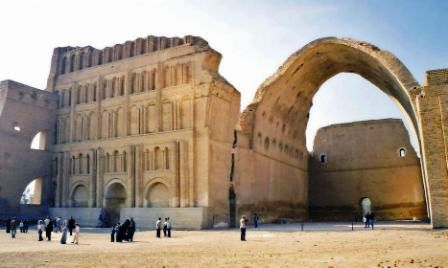
\includegraphics[width=\textwidth]{Images/image034.jpg}
    \caption{Tāq de Ctésiphon (Madā'in) en
Irak, à proximité duquel est enterré Salmān le
Perse}
    \label{fig:Ctesiphon}
\end{marginfigure}
Le mazdéisme est la religion officielle des Sassanides, dynastie perse
de 226 à 651. Mais on trouve des mazdéens en Irak, à Bahrayn, à Oman. Il
était pratiqué à La Mecque et Médine et au Yémen. Si les mazdéens
pratiquaient le rite du feu -- qui ne se retrouve pas en islam -- on
retrouve aussi dans leur religion \textbf{les cinq prières quotidiennes,
les rituels de prosternation, les rites d'ablution, la récitation de
textes sacrés, les sacrifices d'animaux}. Avant chaque geste important,
on prononçait la formule «~Au nom de Dieu~» qui trouve son pendant en
islam avec la \emph{basmala} que l'on récite avant les usages cultuels.
Au sein du mazdéisme, on trouve l'idée qu'il ne suffit pas de pratiquer,
mais que la pratique doit être motivée par l'intention. En islam, c'est
la \emph{niya} qui doit être formulée au début de chaque prière
quotidienne. \textbf{Sur le plan de la foi, le mazdéisme affirme
l'existence d'un créateur universel, d'une divinité dotée des attributs
de miséricorde, de justice, de bonté, il développe une vision
anthropologique où l'homme est d'abord parfait}~; du point de vue
eschatologique, il soutient la rétribution selon les actes posés et
l'épreuve de la pesée. Après la mort, l'âme reste auprès du mort avant
d'entreprendre un voyage. Là, elle passe sur le pont de Cinvad ~: pour
le juste, le pont s'élargit et conduit au paradis, mais pour le méchant,
il se rétrécit, devient fin comme une lame de rasoir, si bien qu'il
tombe dans les affres de l'enfer \textbf{Or, tous ces éléments se
retrouvent en islam}. Parmi les compagnons de Muḥammad, on compte un
mazdéen Salmān al-Fārisī (~m. 656), dit aussi Salmān le Perse, d'abord
converti au christianisme puis à l'islam et qui est considéré par Louis
Massignon, comme l'initiateur de l'islam iranien. Pour Louis Massignon
(nous avons déjà parlé de l'importance qu'il joua dans l'orientalisme du
vingtième siècle~et dit qu'il imposa l'usage du mot islam sur celui
d'islamisme, pour désigner la religion des musulmans), Salmān n'aurait
pas renié le Christ et serait donc un de ces personnages faisant la
jonction entre le christianisme et l'islam. Il a une grande importance
pour Massignon, car c'est près de sa tombe, un soir de mai 1908, que
celui-ci éprouva la «~Visitation de l'étranger~», qui comme un feu divin
est venu raviver les braises de sa foi\sn{Louis Massignon,
  «~Salmân ou les prémices spirituelles de l'Islam iranien~», in
  \emph{Parole donnée}, 1934.}.
\FloatBarrier



Pour ce qui est du \textbf{manichéisme}, il est apparu comme un courant
hétérodoxe du zoroastrisme, s'inspirant à la fois du bouddhisme, du
christianisme, du judaïsme, de la gnose, sur le fond du mazdéisme. C'est
une religion à vocation universelle, missionnaire donc, qui a pénétré la
péninsule arabique. Le père du premier calife omeyyade, Mu'āwiya, était
manichéen. Un certain nombre de particularités se retrouvent en islam.
Ainsi, par exemple, le \textbf{grand jeûne annuel des manichéens de
trente jours n'est pas sans rappeler le jeûne du Ramadan} -- durée
inconnue dans la Bible -- ou encore, l'interprétation de la tradition
musulmane selon laquelle Christ aurait été remplacé sur la croix par un
sosie (interprétation qui découle du commentaire du verset 4, 157~: les
juifs disent nous avons tué le Christ, mais ils ne l'ont ni tué, ni
crucifié, mais son sosie a été substitué à leurs yeux (\emph{šubbiha
la-hum}). Mais la ressemblance entre manichéisme et islam la plus
marquante concerne la prophétologie. \textbf{Le manichéisme est une
religion du Livre. Mani a reçu la visite de l'Ange de la prophétie et a
consigné dans un livre les révélations}. Contrairement à Zoroastre,
Jésus ou Bouddha, qui n'ont pas écrit eux-mêmes, la nouveauté consiste
en la rédaction personnelle du livre, évitant les falsifications opérées
par les disciples. Ce thème de la falsification des écritures se
retrouvera en islam. Notons aussi l'expression «~sceau des prophètes~».
Mani la fait sienne. Muḥammad sera ainsi appelé dans le Coran (S. 33,
40)
\begin{quote}
Muḥammad n'a jamais été le père d'un seul de vos hommes mais le messager
de Dieu, le \textbf{sceau des prophètes}, et Allāh est savant en toutes
choses.

\textbf{\TArabe{مَا كَانَ مُحَمَّدٌ أَبَا أَحَدٍ مِنْ رِجَالِكُمْ وَلَكِنْ
رَسُولَ اللَّهِ وَخَاتَمَ النَّبِيِّينَ وَكَانَ اللَّهُ بِكُلِّ شَيْءٍ
عَلِيمًا}}
\end{quote}


\section{Repères chronologiques et histoire des premiers
califes}

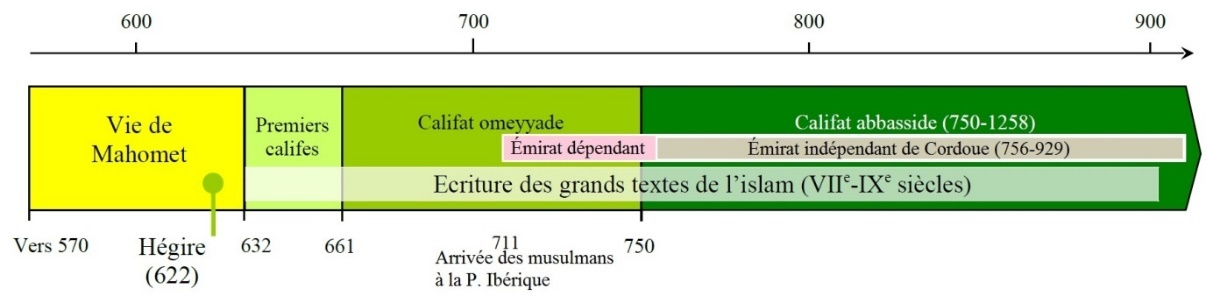
\includegraphics[width=\textwidth]{Images/image035.jpg}

Selon la tradition musulmane, Muḥammad est né vers 570. C'est en 610
qu'a lieu la première manifestation de la révélation du Coran -- nous y
reviendrons. 622 est l'année de l'hégire (\emph{hiǧra} en arabe)~: elle
renvoie au départ de Muḥammad de La Mecque pour Médine. Traduit parfois
par émigration, fuite (la vie de Muḥammad et des siens est menacée par
les Mecquois), la racine souligne l'idée de rupture des liens amicaux ou
familiaux.

\begin{Def}[muhāǧirūn et anṣār]
On appelle les Mecquois qui partirent avec Muḥammad
\textbf{les \emph{muhāǧirūn}, les émigrés.} Les Médinois qui se
convertirent à l'islam sont appelés \textbf{les \emph{anṣār}, les
auxiliaires}.
\end{Def}
La racine NaṢaRa signifiant venir en aide, apporter
protection.
Au moment du choix des premiers califes, grande sera la rivalité entre
les \emph{muhāǧirūn} et les \emph{anṣārs} où les appartenances tribales
ressurgissent.

La \emph{hiǧra} est au cœur du projet islamiste de Daesh qui a appelé
tous les musulmans à le rejoindre et à ainsi mettre ses pas dans ceux de
Muḥammad et de son émigration.

Les premiers califes sont désignés \emph{al-rāšidūn}, c'est-à-dire les
Bien-Guidés. C'est la période des quatre premiers califes~; dans l'ordre
chronologique~: Abū Bakr, ʿUmar, ʿUṯmān et ʿAlī.

\vide{abux16b-bakr-m.-634}{%
\subsubsection{{Abū Bakr (m. 634)
}{Abū Bakr (m. 634) }}\label{abux16b-bakr-m.-634}}

La tradition sunnite fait de lui le premier musulman après Ḫadiǧa,
l'épouse du jeune Muḥammad. Cette tradition permet aussi de légitimer le
rôle d'Abū Bakr et son institution comme calife, à l'issue de la mort de
Muḥammad, dans un contexte fébrile. D'ailleurs, sur la question de
savoir qui est le premier à avoir endossé l'islam, les šīʿites
considèrent quant à eux que c'est ʿAlī. À la mort de Muḥammad, une
élection eut lieu dans un contexte tendu où les opposants à Abū Bakr
furent absents et ne purent donc se prononcer. Par suite, un grand
mouvement se souleva pour s'opposer à ce choix. Certains refusèrent de
payer la zakāt. On appelle ce temps la période de la grande apostasie
(\emph{ridda}). Mais il faut bien voir qu'il s'agissait plus de
contester l'autorité d'Abū Bakr que de rejeter l'islam. Mais Abū Bakr et
ses partisans virent dans le non-paiement de la \emph{zakāt}, laquelle
est un pilier de l'islam, un acte d'apostasie. Il partit en guerre
contre les tribus récalcitrantes. La bataille d'al-Yamāma vit la mort de
plus de 1200 musulmans et 39 compagnons. Il meurt de maladie.

\vide{ux2bfumar-m.-644}{%
\subsubsection{ʿUmar (m. 644)}\label{ux2bfumar-m.-644}}

Il appartient à la tribu des Qurayš. Il a été nommé par Abū Bakr pour
lui succéder, après que ce dernier a consulté les compagnons. On le
surnomme \emph{al-Fārūq}, l'Équitable. Il fut l'un des premiers
opposants à l'islam et un défenseur des traditions mecquoises. Dans
certains récits sunnites, il est présenté comme ayant torturé des
musulmans pour qu'ils renient leur foi à l'exemple d'une servante des
Banū Mūʾammil. L'hégire dont nous avons parlé fut décidé par Muḥammad
dans le contexte de ces persécutions à La Mecque.

C'est à la suite de la conversation de sa sœur, Fāṭima, alors qu'il
était entré chez elle en colère et qu'il recourra à la violence contre
elle et son mari qu'on lui récita les versets de la Sourate ṬāHā
retranscrite sur un feuillet. À son récit, il se convertit. Il s'agit de
la Sourate 20. Voici les premiers versets

\mn{\emph{Au nom d'Allah, le Tout
Miséricordieux, le Très Miséricordieux.}\\
Pour entendre sa récitation en arabe avec le texte traduit en français~:
\url{https://www.youtube.com/watch?v=cXqHT-I5OgE}
}

\begin{quote}
    

1. Ṭā-Hā\\
{2.}
Nous n'avons point fait descendre sur toi le Coran pour que tu sois
malheureux,\\
{3.}
si ce n'est qu'un Rappel pour celui qui redoute (Allāh),\\
{4.}
(et comme) une révélation émanant de Celui qui a créé la terre et les
cieux sublimes.\\
{5.}
Le Tout Miséricordieux S'est établi \emph{«~Istawā~»} sur le Trône.\\
{6.}
À Lui appartient ce qui est dans les cieux, sur la terre, ce qui est
entre eux et ce qui est sous le sol humide.\\
{7.}
Et si tu élèves la voix, Il connaît certes les secrets, même les plus
cachés.\\
{8.}
Allah~! Point de divinité que Lui~! Il possède les noms les plus
beaux.\\
{9.}
Le récit de Moïse t'est-il parvenu~?\\
{10.}
Lorsqu'il vit du feu, il dit à sa famille~: «~Restez ici~! Je vois du
feu de loin; peut-être vous en apporterai-je un tison, ou trouverai-je
auprès du feu de quoi me
guider»\\
{11.}
Puis, lorsqu'il y arriva, il fut interpellé~: «~Moïse~!\\
{12.}
Je suis ton Seigneur. Enlève tes sandales~: car tu es dans la vallée
sacrée, Ṭuwā.\\
{13.}
Moi, Je t'ai choisi. Ecoute donc ce qui va être révélé.
\end{quote}
ʿUmar est aussi connu pour avoir convaincu Abū Bakr de la nécessité de
rassembler le Coran. Désigné comme son successeur par Abū Bakr peu de
temps avant sa mort, il est le premier à être appelé \emph{Amīr
al-mūmīnīn}, c'est-à-dire Commandeur des croyants ou Prince des
Croyants.


\mn{Aujourd'hui, ce titre est celui du roi du
Maroc~: Article 41 de la
{Constitution
de 2011} :
«~Le Roi, Amir al-Mouminine, veille au respect de l'Islam. Il est Garant
du libre exercice des cultes. Il préside le Conseil supérieur des
Oulémas, chargé de l'étude des questions qu'Il lui soumet~».
}

Ce titre est aussi celui qu'a revendiqué pour lui Abū Bakr al-Baġdādī de
l'État islamique. Remarquez son nom~: celui du premier calife de
l'islam.

C'est ʿUmar qui est à l'initiative du nouveau calendrier musulman.

Chef de guerre, c'est sous son califat que les Arabes se rassemblèrent
et prirent Damas avant de conquérir l'Irak et la Perse~; puis il envoya
Muʾāwiya à la conquête de Jérusalem. Dans une lettre adressée au
Patriarche Sophrone, il assura sa protection aux habitants de la ville
et la sauvegarde des lieux chrétiens.

Il se rendit à Jérusalem, alla prier sur l'Esplanade du Temple où selon
la Sourate 17\textsuperscript{ème}, Muḥammad s'était rendu en songe
durant une nuit. C'est alors que sera construite le Dôme du Rocher,
\emph{Qubbat al-ṣaḫra} par le calife ʿAbd al-Malik. Ce Dôme est souvent
appelé Mosquée de ʿUmar, mais à tort. \\


Il meurt poignardé par un esclave zoroastrien. Concernant sa succession,
il a pris soin de nommer un conseil électoral de six électeurs, une
\emph{šūra}, qui doit élire son successeur. Ce conseil, composé
principalement des \emph{mūhaǧirīn}, visait à écarter du pouvoir les
\emph{anṣār}. Ce conseil sert aujourd'hui à certains penseurs musulmans
pour penser la démocratie du point de vue islamique.

 
\subsubsection{ʿUṯmān (m. 656)
} 
C'est selon la tradition musulmane un des premiers compagnons de
Muḥammad~; sa conversion est antérieure à l'Hégire. En 620, lors du
départ d'un groupe de musulmans pour l'Abyssinie, ʿUṯmān faisait partie
des émigrants. Il a épousé deux filles de Muḥammad. Il poursuit une
politique de conquête qui l'amène jusqu'en Arménie, en Égypte, en Nubie,
au Maghreb.

On lui doit d'avoir mené à bien la recension officielle du Coran. Nous
en reparlerons.

Il est assassiné à Médine en 656.

\vide{ux2bfalux12b-m.-661}{%
\subsubsection{ʿAlī (m. 661)}\label{ux2bfalux12b-m.-661}}

Il est nommé calife~et renvoie un certain nombre de gouverneurs qui
avaient été nommés par ʿUṯmān. La capitale est transférée à Kūfa. Son
califat est marqué par de profondes divisions~: c'est la première
\emph{\textbf{fitna}}, ou guerre de sédition.

Sur le plan théologique, il laisse des sermons et une œuvre monumentale
au titre évocateur intitulée \emph{Le sommet de l'éloquence},
\emph{Nahǧul Balaġa}. Il est possible de lire ces sermons
\sn{\url{http://www.orient-lib.com/A-52389-nahj-al-balagha-la-voie-de-l-eloquence-arabe-francais.aspx}{en
français}}. Après le Coran et la Sunna, l'ouvrage est le plus étudié dans
le šīʿisme. On y trouve une théologie de la création du ciel, de la
terre et des anges, mais aussi une personnification du Jour du Jugement
dernier. Écrit aussi sous forme d'adages ou de proverbes, l'ouvrage
nourrit des générations de musulmans sur le plan de la morale des
vertus.

Écarté dans un premier temps par Abū Bakr, ʿAlī avait refusé de mener le
combat car il a toujours privilégié l'entente entre les musulmans. S'il
est un personnage central dans le šīʿisme, ʿAlī est aussi une des
références sunnites~comme quatrième calife~: on ne sera donc pas surpris
de trouver dans les sources sunnites des paroles laudatrices à son
égard. C'est le cas notamment des \emph{ḥadīṯs} suivants :

Suyūtī (m. 911/1505) {[}c'est un grand savant égyptien expert en
\emph{ḥadīṯ}. Son nom reviendra par la suite{]} rapporte d'Ibn Abbas le
\emph{ḥadīṯ} suivant~:

«~\textbf{Je suis la Cité du Savoir. ʿAlī en est sa Porte; quiconque
recherche le Savoir, doit franchir le seuil de cette Porte.}~»

Autre \emph{ḥadīṯ}~rapporté par al-Ṭabarānī~(m. 360/970) : {[}À son
époque, il passait pour être le plus expert en science du ḥadīṯ{]}
\begin{quote}
«~{Il y a cette inscription sur la Porte du Paradis: Il n'y a de
Allah que Allah ; Muḥammad est le Messager de Allah ; et ʿAlī est le
frère du Messager}~».~
\end{quote}


~Ce \emph{ḥadīṯ} est intéressant car il on y trouve des éléments de la
profession de foi (premier pilier de l'islam) des šīʿites~duodécimains :
«~et ʿAlī est le walī d'Allāh~».

Sur le plan militaire, il doit affronter le gouverneur de Damas,
al-Mu'āwiya. Lors de la bataille de Siffin contre ce gouverneur, il
accepte un arbitrage qui est finalement en sa défaveur. Il se retire
alors à Koufa mais nombreux sont ceux qui lui reprochent d'avoir accepté
cet arbitrage alors que Dieu lui assurait la victoire. Certains de ses
partisans décidèrent de le quitter, ce sont les \emph{ḫariǧites} (de la
racine ḪaRaǦa~: sortir). Il est assassiné par l'un d'eux.

\begin{marginfigure}
    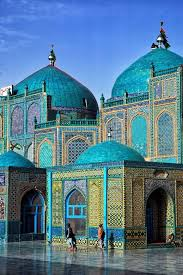
\includegraphics[width=1.06615in,height=1.6045in]{Images/image037.jpg}
    \caption{La mosquée bleue en Afghanistan est supposée être le lieu
du tombeau de ʿAlī. Rawze-i-Sharif (La Mosquée du Saint en référence à
Hazrat-e Ali Ibn Talib}
\end{marginfigure}


Par la suite, l'islam se structure autour de deux empires successifs,
rivaux~: l'empire omeyyade puis l'empire abbasside. Mais revenons à la
péninsule arabe à la naissance de l'islam et à son univers religieux.

\textbf{Conclusion}

Au départ de notre réflexion, une question~: comment connaître le
contexte culturel, religieux, politique de l'Arabie antéislamique~? Nous
remarquions que si nous disposons de sources musulmanes, elles ne
sauraient suffire, d'autant qu'elles participent d'une reconstruction
historique mettant en lumière le monde chaotique dans lequel se
trouvaient les tribus arabes avant la prédication de Muḥammad.

Cette difficulté épistémologique se retrouve dans l'histoire de l'islam
naissant et des premières dynasties. Or, il n'est pas possible de faire
l'histoire des premiers siècles sur la base des seules sources
musulmanes. Julius Wellhausen et Henri Lammens ont montré les failles de
l'histoire telle que la raconte l'historien al-Ṭabarī~: (nous l'avons
rencontré dans le commentaire de la bibliographie\ldots{} son traducteur
et analyste est Claude Gilliot). Je voudrais donner un exemple de ces
prismes au moment de la chute des Omeyyades en 750\sn{Sabatino
  Moscati, «~Le massacre des Umayyades dans l'histoire et dans les
  fragments poétiques~», Archiv Orientalni 18, 1950, p. 88-115.}.
L'histoire des Omeyyades, première dynastie de l'islam, est en effet
connue à partir de textes rédigés après l'arrivée des Abbassides. Or, si
le berceau des Omeyyades est la Syrie, les historiens écrivent dans
l'Irak abbasside à la fin du 9\textsuperscript{e} siècle après la
réinstallation du califat à Bagdad. Antoine Borrut montre qu'il fallait
réécrire l'histoire car «~les signes de continuité étaient devenus
inintelligibles~» après 150 ans de domination abbasside~:

«~Les épisodes successifs de la Révolution abbasside, de la guerre
civile entre les fils d'al-Rašīd, de la miḥna, du déplacement du califat
à Sāmarrā', de l'essor des militaires turcs, de l'assassinat
d'al-Mutawakkil et de la perte de la réalité du pouvoir par le calife,
suffisent amplement à expliquer cette perte de repères et le déficit de
cohérence dont souffrait alors l'histoire islamique~»\sn{Cité par
  Françoise Micheau, \emph{Les débuts de l'islam}, Paris, 2012, p. 28.}.

Il fallait donc rattacher directement les Abbassides à l'origine de
l'islam et faire tomber dans l'oubli la période omeyyade. Le massacre
des Omeyyades en 750 par les Abbassides est totalement omis dans
certains textes historiques. Al-Ṭabarī est pudique dans sa description
-- il faut dire qu'il fait désordre et pour fonder la légitimité
politique\ldots{} on peut faire mieux. Ibn Qutayba (m. 276/889) et
al-Mas`ūdī (m. 345/956) sont aussi peu prolixes. Les noms de ces trois
grands historiens ont déjà été mentionnés. Je redonne ici les dates avec
le calendrier hégirien\ldots{} alors que la première fois, je n'avais
mis que le calendrier grégorien\sn{Le calendrier hégirien est le
  calendrier musulman. L'année 0 est l'année de l'hégire, c'est-à-dire
  de la fuite de Muḥammad lorsqu'il quitte La Mecque. Nous sommes en 622
  dans le calendrier grégorien.}.

\textbf{La destruction des tombeaux des califes par les abbassides est
symptomatique de cette volonté de l'oubli. Mais malgré tout, les lieux
sont là et sont aujourd'hui redécouverts. Ils donnent de nouvelles
lumières sur les fondations de l'islam et l'histoire des premiers
siècles.} %2
\FloatBarrier
\chapter{Les biographies de Muḥammad, Prophète de l'islam}

Après avoir abordé le milieu religieux de la péninsule arabique à l'aube
du VIIe siècle, et distingué à grands traits les grandes dates de la
naissance de l'islam, il convient à présent de focaliser notre attention
sur celui qui est considéré par les musulmans comme le messager de la
Révélation coranique, Mahomet ou Muḥammad (مُحَمَّد). Personnellement,
j'écris Muḥammad qui est la translittération du nom du Prophète de
l'arabe en français, tandis que Mahomet est l'écriture francisée, venant
du latin Mahometus. Que sait-on de lui~? Comment vivait-il~? À quelle
religion appartenait-il~? A-t-il fréquenté des juifs, des chrétiens et
des mazdéens de La Mecque~? Comment sa prédication a-t-elle été reçue~?
Quand parvient-il à imposer la légitimité de sa mission~? Comment s'y
prend-il~? Quelles relations entretient-il avec son clan~? Sa tribu~?
Était-il prophète, roi et chef de guerre, comme on le dit~?

Les questions sont posées. Elles sont importantes. J'en pose une autre,
au préalable~: Comment fait-on pour savoir~? Comment s'y prend-on pour
répondre~? En historien, on s'appuie forcément sur des sources, en
portant sur elles un regard critique, et ce d'autant plus que la
première «~biographie~» de Muḥammad date de la fin du VIIIe
siècle\ldots{} donc du temps des abbasides. Le temps a passé, il y a
déjà eu l'ère des califes bien guidés, les Rashidūn (cela a donné le
prénom Rashid, au féminin~: Rashida), puis celui de l'empire des
Omeyyades. Si vous ne voyez pas qui sont les califes bien guidés,
relisez le chapitre 2. Or, écrire une biographie n'est jamais neutre.

Certes, une lecture croyante peut fort bien vouloir se dispenser des
études critiques sur les fondations de l'islam, mais comme l'écrit
l'historien tunisien Hichem Djaït dans la biographie qu'il consacre à
Muḥammad~: «~la science est une, et le souci de scientificité est la
marque des sociétés libres~»\sn{Hichem Djaït, La vie de Muḥammad,
  Volume 2, Paris, Fayard, 2008 p. 13.}.

Il me semble donc incontournable de consacrer quelques pages du cours à
la question épistémologique : de quelles sources disposons-nous~? Quel
est leur statut~?

Mais la question des sources posées, il faut constater que la figure
même de Muḥammad a donné lieu à de multiples biographies au cours des
siècles. C'est le pluriel qui s'impose. Certes, il y a les premières
grandes biographies dont la matrice est donnée par Ibn Iṣḥāq (ابن
إسحاق), mais au cours des siècles va se développer des images de
Muḥammad et cela jusqu'à nos jours. Quelles sont ces images~?

Dans ce chapitre sur les fondations de l'islam, il nous semble opportun
de donner aussi quelques passages de ces premières biographies. À cet
égard, je m'appuierai sur les textes de la Sīra d'Ibn Hishām, car c'est
la plus populaire. Le préambule méthodologique permettra aussi
d'analyser ces informations~dans les contextes politiques et religieux
où elles ont été données.

\vide{la-question-muxe9thodologique-comment-uxe9crire-la-biographie-de-muux1e25ammad}{%
\subsubsection{{La question méthodologique~: comment écrire la biographie de Muḥammad~? }}\label{la-question-muxe9thodologique-comment-uxe9crire-la-biographie-de-muux1e25ammad}}

En arabe, la biographie de Muḥammad s'appelle Sīra. Aujourd'hui, les
biographies du Messager de l'islam ne manquent pas. En français, il y a
celles écrites par des musulmans à l'exemple d'Al-Sira de Mahmoud
Hussein -- pseudonyme commun de Bahgat Elnadi et Adel Rifaat,
politologues français d'origine égyptienne --, de Tariq Ramadan,
Muhammad, La vie du Prophète ou encore de l'historien tunisien Hichem
Djaït, La vie de Muḥammad, écrite en trois volumes parus en français aux
éditions Fayard et que nous avons déjà cité ci-dessus.

On trouve aussi celles des orientalistes comme Maxime
Rodinson\sn{Maxime Rodinson, Mahomet, Paris, 1956.}, Tor
Andrae\sn{Tor Andrae, Les Origines de l'islam et le christianisme,
  tr. fr., Paris, 1955.}\textsuperscript{,} Régis Blachère, W.
Montgommery Watt\sn{Montgomery Watt, Mahomet à La Mecque~; Mahomet
  à Médine, trad. Fr., Paris, 1958 et 1959.}, Jacqueline Chabbi et son
livre \emph{Le Seigneur des tribus}. La dernière en date de ce point de
vue est celle écrite par l'orientaliste allemand Tilman Nagel. Les
approches entre les biographies confessantes et les biographies
historiques sont bien sûr différentes, très différentes. Mais il faut
bien voir que pour les musulmans, la biographie n'est pas une écriture
a-historique. Au contraire, la biographie du Prophète est
intrinsèquement liée à celle de l'histoire de la naissance de l'umma. Il
s'agit d'approcher Muḥammad, son univers culturel, mais aussi social.
Les historiens musulmans ont le souci de rendre compte des moindres
personnages ayant fréquenté Muḥammad, mais aussi de ses gestes
quotidiens. Tarif Khalidi dans \emph{Images of Muḥammad} dit qu'avec la
Sīra, c'est un peu comme si on avait voulu retranscrire le nom des 5 000
personnes venues écouter le Sermon sur la montagne de Jésus. Ce genre de
biographies de la première communauté s'appelle les \emph{Tabaqāt}.
C'est un genre littéraire typique de l'islam. Par ailleurs, si dans les
Évangiles, on sait peu de choses de la vie privée de Jésus, la Sīra
aborde aussi bien la vie publique que la vie privée et intime de
Muḥammad\sn{Tarif Khalidi, Images of Muḥammad. Narratives of the
  Prophet in Islam. Across the Centuries, New York, Doubleday, 2009.}.

Dans un article paru dans la revue \emph{History Compass} en 2007,
Robert Hoyland présente les différents points de vue et méthodologies
mises en œuvre en vue de dessiner un portrait authentique de
Muḥammad\sn{Robert Hoyland, «~Writing the Biography of the Prophet
  Muḥammad~: Problems and Solutions~», History Compass, 5/2, 2007, p.
  581-602.}. Dans tous les cas, l'intention est la même~: se rapprocher
de la réalité.

Hoyland souligne dans un premier temps que l'image du Prophète Muḥammad
qui est véhiculé du côté occidental a d'abord été négative~: Muḥammad
(ou ceux qui se revendiquent de son message) conquiert des terres et
impose une religion en portant un message qui au final nie la divinité
du Christ. On va y voir un homme d'ambition et de passion, au pire la
figure de l'Antéchrist, le fils du diable. L'époque médiévale applique
la parole de Jésus sur les faux prophètes. Dans la \emph{Somme contre
les Gentils} Saint Thomas d'Aquin avance les preuves rationnelles de
l'impossibilité pour Muhammad d'être dit «~prophète~»\sn{«~Par
  contre, il {[}Mahomet{]} a entremêlé les vérités de son enseignement
  de beaucoup de fables et de doctrines les plus fausses. Il n'a pas
  apporté de preuves surnaturelles, les seules à témoigner comme il
  convient en faveur de l'inspiration divine, à savoir quand une œuvre
  visible qui ne peut être que l'œuvre de Dieu prouve que le docteur de
  vérité est invisiblement inspiré. Il a prétendu au contraire qu'il
  était envoyé dans la puissance des armes, preuves qui ne font point
  défaut aux brigands et aux tyrans. ~Aucune prophétie divine ne
  témoigne en sa faveur : bien au contraire, il déforme les
  enseignements de l'Ancien et du Nouveau Testament par des récits
  légendaires, comme c'est évident pour qui étudie sa loi. Aussi bien,
  par une mesure pleine d'astuces, il interdit à ses disciples de lire
  les textes de l'Ancien et du Nouveau Testament qui pourraient le
  convaincre de fausseté.~»}. Au xvième, Luther dans un essai de 1528,
\emph{De la guerre contre les Turcs} (Vom Kriege wider die Türken)
expose l'incompatibilité de l'islam avec la foi chrétienne. Dans le
contexte de l'invasion ottomane en Europe et du Siège de Vienne, il
appelle à la résistance contre les turcs et, si Muḥammad ne peut
l'Antéchrist, puisque c'est le pape qui l'est, il ne peut donc être
qu'un «~démon~», le fruit du mensonge, celui qui fait table rase de la
vérité chrétienne, qui détruit «~l'ordre spirituel de la foi et de la
vérité~»\sn{Pour une étude sur Muḥammad et l'islam chez Luthern
  voir~: A.S Francisco, Martin Luther and Islam. A Study in
  Sixteenth-Century Polemics and Apologetics, coll. The History of
  Christian-Muslim Relations 8, Leiden, Brill, 2007.}. Cette vision est
encore celle du philosophe Pascal au xviie siècle.

Les lumières apportent un regard renouvelé sur l'islam qu'il s'agit
d'intégrer à une vision universelle de l'humanité, et au XIXème siècle,
d'une manière surprenante, Ernest Renan dans \emph{Mahomet et les
origines de l'islamisme}, écrit~:

«~La vie de son fondateur nous est aussi bien connue que celle de tel
réformateur du xvie siècle. Nous pouvons suivre année par année les
fluctuations de sa pensée, ses contradictions, ses faiblesses~».

Cet optimisme repose sur l'assurance en l'authenticité des paroles et
gestes consignés par la tradition musulmane. Or, au \textsc{XIXème}
siècle, l'orientaliste Ignaz Goldziher est le premier à avoir, mis en
avant l'aspect reconstruit du \emph{ḥadīṯ} et il concluait qu'il ne peut
constituer un matériel historique pour rendre compte de la naissance de
l'islam~; il permet cependant de mettre en lumière des tendances
dogmatiques ou juridiques qui se sont développées au cours des premiers
siècles. Henri Lammens au début du XXème siècle publie en 1912
\emph{Fatima et les filles de Mahomet}: \emph{notes critiques pour
l'étude de la Sira}. Il montre que

«~l'inspiration de la Sīra est d'abord exégétique. Dérivée en droiture
du texte du Qoran, la Sīra est destinée à lui servir de commentaire en
action~; elle doit traduire, en anecdotes précises et pittoresques, les
allusions les plus obscures, les sous-entendus les moins intelligibles
des versets, faire la chasse à l'anonyme, à l'impersonnel, si
déconcertants dans la lecture des sourates, partout, pour ainsi dire,
apposer des plaques commémoratives, multiplier la mention des noms
propres, les dates, si prudemment évités par Abou'l Qasim~»\sn{Henri
  Lammens, Fatima et les filles de Mahomet: notes critiques pour l'étude
  de la Sīra, Rome, Institut Biblique Pontifical, 1912, p. vii.}.

Bref, la Sīra doit combler l'obscurité du Coran, elle doit l'expliquer,
l'historiciser, mais elle vise aussi à préciser la doctrine coranique et
la jurisprudence. Ainsi, il existait parmi les juristes de Médine et
ceux de La Mecque et d'Irak, deux positions relatives à la possibilité
pour un pèlerin de contracter un mariage. De part et d'autre, la vie de
Muḥammad et ses paroles vont être convoquées pour fonder leur position,
quitte à ce qu'il y ait contradiction. Joseph Schacht conclut que bien
des éléments de la vie de Muḥammad, des détails importants, ne sont pas
fondés sur une recollection authentique mais sont fictifs et servent à
défendre des doctrines juridiques. L'articulation entre la vie du
Prophète et l'exégèse n'a pas perdu de son actualité~: c'est la
perspective de Patricia Crone~: «~Une grande partie de la tradition
apparemment historique est en fait d'origine exégétique~»\sn{Patricia
  Crone, Meccan Trade and the Rise of Islam, Oxford, 1987, p. 214.}.

De ces difficultés, certains orientalistes ont cherché à approcher
Muḥammad à partir du Coran seul. C'est le cas de Régis Blachère. Mais
cette approche est aussi celle de musulmans qu'on appelle les
\textbf{coranistes}~: pour eux, l'islam c'est le Coran et seulement le
Coran. Cependant, ce n'est pas sans difficulté car le Coran est peu
prolixe sur son environnement et à l'exception des noms bibliques, on ne
trouve que deux noms de personnages qui sont mentionnés~: celui de
Muḥammad, à quatre reprises, et celui d'Abū Lahab.

\vide{uxe0-propos-dabux16b-lahab-que-lon-trouve-dans-la-sourate-111-1-5}{%
\subsubsection{{À propos d'Abū Lahab que l'on trouve dans la sourate 111, 1-5~: }}\label{uxe0-propos-dabux16b-lahab-que-lon-trouve-dans-la-sourate-111-1-5}}

\begin{quote}
    Que périssent les deux mains d'Abū Lahab
et que lui-même périsse. Sa fortune ne lui sert à rien, ni ce qu'il a
acquis. Il sera brûlé dans un feu plein de flammes, de même sa femme, la
porteuse de bois, à son cou une corde de fibres.
\end{quote}


On apprend par les commentaires qu'il
s'agit de son oncle, hostile à Muḥammad et que la femme est surnommée la
porteuse de bois car elle jetait du bois et des plantes épineuses sur la
route qu'empruntait le Prophète\ldots{} mais sans les commentaires, le
Coran lui-même reste très énigmatique.


Le Coran fait aussi mention des Romains et de la tribu de Quraysh, mais
pas des autres tribus. Huit lieux sont indiqués, quatre communautés
religieuses (juifs, chrétiens, mages et sabéens) ainsi que trois
divinités arabes. Et si La Mecque est nommée, aucune indication sur son
rôle dans la vie de Muḥammad. Il est question dans le Coran de Badr mais
rien ne permet d'y voir une référence explicite à la fameuse bataille du
même nom, même si l'interprétation est possible.

\vide{uxe0-propos-de-la-bataille-de-badr}{%
\paragraph{À propos de la bataille de
Badr}\label{uxe0-propos-de-la-bataille-de-badr}}

C'est la première grande bataille militaire que mène Muḥammad après son
exil à Médine contre une caravane de Mecquois. Une armée d'hommes
accompagnée de milliers d'anges vont emporter leur première victoire
contre les notables de La Mecque~; Muhammad y acquiert le prestige de
fin stratège.

Selon les commentaires coraniques, le Coran ferait allusion à cette
bataille~:




\begin{table}[h!]
\resizebox{\textwidth}{!}{%
\small
\begin{tabular}{p{7cm}p{7cm}}

Il y eut déjà pour vous un signe dans ces deux troupes qui
s'affrontèrent: l'une combattait dans le sentier d'Allah; et l'autre,
était mécréante. Ces derniers voyaient les croyants de leurs propres
yeux, deux fois plus nombreux qu'eux-mêmes. Or Allah secourt qui Il veut
de Son aide. Voilà bien là un exemple pour les doués de clairvoyance !
& 

\\

S. 3, 123~ Allah vous a donné la victoire, à Badr, alors que vous étiez humiliés.
Craignez Allah donc. Afin que vous soyez reconnaissants! &  
\TArabe{

وَلَقَدْ نَصَرَكُمُ اللَّهُ بِبَدْرٍ وَأَنتُمْ أَذِلَّةٌ فَاتَّقُوا
اللَّهَ لَعَل

َّكُمْ تَشْكُرُونَ }
\\

\end{tabular}%
}
\sidecaption{La bataille de Badr S. 3, 13 et 123}
\end{table}



 

\vide{badr}{%
{{\includegraphics[width=1.27898in,height=2.02315in]{Images/image38.jpeg}}{Badr}}\label{badr}}

\vide{la-bataille-de-badr}{%
\subsubsection{La bataille de Badr}\label{la-bataille-de-badr}}

\vide{section-7}{%
\subsubsection{}\label{section-7}}

\vide{remarquez-lange-gabriel-qui-annonce-la-victoire-uxe0-muux1e25ammad.-le-visage-du-prophuxe8te-est-voiluxe9.}{%
\mn{{Remarquez l'ange Gabriel qui annonce la
victoire à Muḥammad. Le visage du Prophète est voilé.
}{Remarquez l'ange Gabriel qui annonce la victoire à Muḥammad. Le visage du Prophète est voilé. }}\label{remarquez-lange-gabriel-qui-annonce-la-victoire-uxe0-muux1e25ammad.-le-visage-du-prophuxe8te-est-voiluxe9.}}

\vide{au-milieu-entre-les-combattants-de-leau-badr-est-le-nom-dun-puits-deau.-pour-muux1e25ammad-il-est-en-cela-un-lieu-stratuxe9gique-dans-la-mesure-ouxf9-la-caravane-devra-sy-arruxeater.}{%
\paragraph{Au milieu, entre les combattants, de l'eau : Badr est le
nom d'un puits d'eau.} Pour Muḥammad il est en cela un lieu stratégique
dans la mesure où la caravane devra s'y
arrêter.}\label{au-milieu-entre-les-combattants-de-leau-badr-est-le-nom-dun-puits-deau.-pour-muux1e25ammad-il-est-en-cela-un-lieu-stratuxe9gique-dans-la-mesure-ouxf9-la-caravane-devra-sy-arruxeater.}

Dans\textit{ De la guerre}, Carl von Clausewitz a dressé la théorie de
l'importance du puits d'eau dans le combat.

Dans ce contexte, Montgomerry Watt a réhabilité le matériel traditionnel
dans sa biographie de Muḥammad notamment tout ce qui a trait aux
expéditions militaires dans la mesure rien ne ces textes ne cherchent à
expliciter le Coran, le commenter, et que de la même manière il ne
s'agit pas de développements doctrinaux ou jurisprudentiels.

De ces avertissements, de ces difficultés, il s'ensuit que le biographe
de Muḥammad est pris entre deux tenailles~: à la fois il encourt le
risque de rejeter tout matériel historique comme étant une pieuse
invention ou d'intégrer à la réalité historique des éléments de légende
et des inventions. Et finalement, comme le dit Maxime Rodinson, on
risque d'écrire une biographie en fonction de ses propres intérêts,
questions, présupposés, intuitions, comme à l'époque de la tradition
musulmane.

Fort de ces difficultés, à laquelle s'ajoute une idéalisation de la
figure de Muḥammad comme guide à suivre et modèle à imiter, Tilman Nagel
a cherché à «~déchiffrer les conceptions religieuses~» de Muḥammad en
remontant au-delà des sources normatives. Il a utilisé des données de la
poésie, les sources extra-islamiques, l'histoire préislamique de La
Mecque et Médine. Il en arrive au schéma chronologique suivant~:

\begin{itemize}
\item
  Muḥammad annonce le Dieu Unique aux Mecquois. Dans le Coran, il est
  dit \textbf{avertisseur}.
\item
  Vers 620, il élargit son message et se considère désormais comme
  Prophète de Dieu (Allāh). C'est à partir de cette date que l'on voit
  apparaître les notions de nabī et rasūl (prophète). Il n'appelle pas
  seulement à adorer Dieu, mais désormais il expose le rite religieux et
  les règles de vie voulues par Allāh.
\item
  Rejeté par les habitants de La Mecque qui refusèrent ses commandements
  sur le culte, il part pour Médine où son clan a des relations avec
  l'une des tribus médinoises.
\item
  À Médine, il ne peut plus participer au pèlerinage annuel de La
  Mecque. Comme prophète, il doit aussi s'imposer comme chef. Il mena
  donc des opérations militaires contre sa ville natale de 624 à 627.
\item
  Il finit par s'imposer sur les mecquois. Il devient la référence
  politique et religieuse, mais aussi morale, d'où la dimension de plus
  en plus normative. Il s'est ainsi imposé comme l'unique autorité de ce
  qui est juste et équitable, mais aussi le modèle spirituel et moral.
\end{itemize}

Et Tilman Nagel de conclure à l'existence de deux Muḥammad~: le
\textbf{Muḥammad historique}, prédicateur, militaire et le
\textbf{Muḥammad idéalisé}. La tradition a très vite superposé les deux
images de Muḥammad et a historisé le Muḥammad idéalisé si bien que toute
critique à l'égard de Muḥammad entouré d'un halo de sainteté est perçue
comme un acte blasphématoire, un sacrilège et explique que dans certains
pays, blasphémer contre le prophète est considéré comme un acte
criminel.

Mais venons-en à présent à ces sources musulmanes et voyons comment
Muḥammad est présenté au cours du temps, voyons quelles sont ses vies.


\section{Les sources arabes de la biographie de
Muḥammad}
\label{les-sources-arabes-de-la-biographie-de-muux1e25ammad}


\subsection{Muḥammad dans le
Coran}
\label{muux1e25ammad-dans-le-coran}

C'est bien sûr dans le Coran que l'on trouve les premières mentions de
Muḥammad. Mais si les références aux prophètes de la Bible sont
nombreuses, Muḥammad n'y est cité que quatre fois. Comme avec les autres
prophètes, le Coran est peu bavard. Il est tour à tour un avertisseur
(naḏīr), puis un prophète (nabī), un messager (rasūl) qui vient apporté
la Parole. Par rapport aux autres prophètes, Muḥammad a un titre
spécifique~: «~\emph{il est le sceau des prophètes}~» (S. 33, 40).

\begin{longtable}
{p{6cm}p{6cm}}
\toprule

«~Muhammad n'a jamais été le père de l'un de vos hommes, mais le
messager d'Allah et le sceau des prophètes. Allah est Omniscient~». & 
\TArabe{
مَّا كَانَ مُحَمَّدٌ أَبَا أَحَدٍ مِّن رِّجَالِكُمْ وَلَكِن رَّسُولَ
اللَّهِ وَخَاتَمَ النَّبِيِّينَ وَكَانَ اللَّهُ بِكُلِّ شَيْءٍ
عَلِيمًا 
}\\
\bottomrule
\end{longtable}

Comme pour les autres prophètes, Muḥammad n'est pas écouté et il est
même l'objet de la risée de sa communauté. En ce sens, il suit un topos
prophétique dont le Coran se fait lui-même l'écho~:

\begin{longtable}{p{6cm}p{6cm}}
\toprule
\endhead
«~Hélas pour les esclaves {[}les humains{]}! Jamais il ne leur vient de
messager sans qu'ils ne le raillent~». &\TArabe{ يَا حَسْرَةً عَلَى الْعِبَادِ
مَا يَأْتِيهِم مِّن رَّسُولٍ إِلَّا كَانُوا بِهِ يَسْتَهْزِئُونَ }\\
\bottomrule
\end{longtable}

Le Coran fait mention explicite des accusations dont il est l'objet~au
sein de sa communauté : il est accusé d'être un sorcier (sāḥir,
سَاحِرٌ), ensorcellé (masḥūr, مَّسْحُورٌ) d'être possédé par un djīn
(maǧnūn, مَجْنُونٌ), d'être un devin (kāhin) d'être enseigné par
quelqu'un (muʿallamun, مُعَلَّمٌ), d'être un poète (šāʿir), d'être un
raconteur de fables. Mais là encore, il s'agit d'inscrire ces
accusations dans une filiation si bien que par ce procédé rhétorique,
elles deviennent la preuve de sa véracité~:

\begin{longtable}{p{6cm}p{6cm}}
\toprule
\endhead
«~Ainsi, aucun Messager n'est venu à leurs prédécesseurs sans qu'ils
n'aient dit: «C'est un magicien ou un possédé!~» (S. 51, 52) &\TArabe{ كَذَلِكَ
مَا أَتَى الَّذِينَ مِن قَبْلِهِم مِّن رَّسُولٍ إِلَّا قَالُوا سَاحِرٌ
أَوْ مَجْنُونٌ }\\
\bottomrule
\end{longtable}

Sur la poésie, il y aurait beaucoup à dire. Le Coran n'est pas favorable
aux poètes~: pour lui, ils divaguent et s'égarent (S. 26, 224-226), et
l'enseignement donné à Muḥammad ne relève pas de la poésie (S. 36, 69).

Quant à l'accusation d'être un raconteur de légende, on en trouve une
expression virulente dans S. 25, 5)~:

\begin{longtable}{p{6cm}p{6cm}}
\toprule
\endhead
«~Et ils {[}les mécréants{]} disent: `Ce sont des contes d'anciens qu'il
se fait écrire! On les lui dicte matin et soir!'~» &\TArabe{ وَقَالُوا
أَسَاطِيرُ الْأَوَّلِينَ اكْتَتَبَهَا فَهِيَ تُمْلَى عَلَيْهِ بُكْرَةً
وَأَصِيلًا }\\
\bottomrule
\end{longtable}

Face à ces accusations, le Coran prend sa défense, mais il se fait aussi
menaçant (S.9, 61)

\begin{longtable}{p{6cm}p{6cm}}
\toprule
\endhead
«~Ceux qui font du tort au Messager d'Allah auront un châtiment
douloureux~». &\TArabe{ الَّذِينَ يُؤْذُونَ رَسُولَ اللَّهِ لَهُمْ عَذَابٌ
أَلِيمٌ }\\
\bottomrule
\end{longtable}

Concernant sa moralité, son caractère, deux passages soulignent sa
noblesse de caractère (S. 68, 4)

\begin{longtable}{p{6cm}p{6cm}}
\toprule
\endhead
«~Et tu es d'un caractère éminent~» &\TArabe{ وَإِنَّكَ لَعَلَى خُلُقٍ
عَظِيمٍ }\\
\bottomrule
\end{longtable}

Dans un autre passage, il nous est renseigné de la mansuétude et de la
patience de son caractère~(S. 3, 159)~:

\begin{longtable}{p{6cm}p{6cm}}
\toprule
\endhead
«~C'est par quelque miséricorde de la part d'Allah que tu (Muhammad) as
été si doux envers eux! Mais si tu étais rude, au cœur dur, ils se
seraient enfuis de ton entourage. Pardonne-leur donc, et implore pour
eux le pardon (d'Allah). Et consulte-les à propos des affaires ; puis
une fois que tu t'es décidé, confie-toi donc à Allah, Allah aime, en
vérité, ceux qui Lui font confiance~». &\TArabe{ فَبِمَا رَحْمَةٍ مِّنَ اللَّهِ
لِنتَ لَهُمْ وَلَوْ كُنتَ فَظًّا غَلِيظَ الْقَلْبِ لَانفَضُّوا مِنْ
حَوْلِكَ فَاعْفُ عَنْهُمْ وَاسْتَغْفِرْ لَهُمْ وَشَاوِرْهُمْ فِي
الْأَمْرِ فَإِذَا عَزَمْتَ فَتَوَكَّلْ عَلَى اللَّهِ إِنَّ اللَّهَ
يُحِبُّ الْمُتَوَكِّلِينَ }\\
\bottomrule
\end{longtable}

Muḥammad est présenté comme un modèle à imiter. On a ici une
légitimation coranique de la Sunna (S. 33, 21)~:

\begin{longtable}{p{6cm}p{6cm}}
\toprule
\endhead
«~En effet, vous avez dans le Messager d'Allah un excellent modèle {[}à
suivre{]}~» &\TArabe{ لَّقَدْ كَانَ لَكُمْ فِي رَسُولِ اللَّهِ أُسْوَةٌ
حَسَنَةٌ }\\
\bottomrule
\end{longtable}

Mais plus encore, le Coran exhorte à lui obéir~(S. 4, 80)~:

\begin{longtable}{p{6cm}p{6cm}}
\toprule
\endhead
«~Quiconque obéit au Messager obéit certainement à Allah~». 
&\TArabe{ مَّن
يُطِعِ الرَّسُولَ فَقَدْ أَطَاعَ اللَّهَ }\\
\bottomrule
\end{longtable}

\vide{les-premiers-ruxe9cits-sur-muux1e25ammad-les-expuxe9ditions-militaires}{%
\subsection{Les premiers récits sur Muḥammad~: les expéditions
militaires}\label{les-premiers-ruxe9cits-sur-muux1e25ammad-les-expuxe9ditions-militaires}}

Pour ce qui concerne les expéditions militaires, nous disposons de deux
papyrus qui datent du 8e siècle. Le premier concerne la bataille de
Badr. Il est extrêmement sommaire et ne comporte pas plus de 8 lignes.
Le second contient une vingtaine de lignes et traite de l'installation
de Muḥammad à Médine. On y trouve le nom de Muḥammad, sans la formule de
bénédiction qui l'accompagne dans la tradition musulmane

\begin{longtable}{p{4cm}p{4cm}p{4cm}}
\toprule
\endhead
\TArabe{صلى الله عليه وسلم} & salallahou alayhi wa salam & Paix et
Bénédiction soient sur lui \sn{Ce fragment a été trouvé dans la
  région nord-est de la mer Morte, à l'ouest du site de Qumrān. Il a été
  publié en 1963 à Louvain.}. \\
\bottomrule
\end{longtable}

Que signifie ma remarque~? Et bien probablement que cette formule est
postérieure à la fin du 8e siècle. Il semble que les premières
générations de musulmans ne l'utilisaient pas et qu'elle s'inscrit dans
un processus d'hagiographie du Prophète de l'islam. Mais n'allons pas
trop vite\ldots{} et poursuivons l'exposé des sources.

Mais il se pose la question suivante~: comment se fait-il que les
premiers documents mis par écrit sur la vie de Muḥammad et datant du
deuxième siècle de l'Hégire soient des récits militaires~(maghāzī) ? Il
est peu probable qu'au cours du premier siècle de l'hégire, Muḥammad ait
suscité auprès des musulmans une dévotion particulière, mais un travail
historique soulignant la grandeur et la force de l'islam semble être à
l'œuvre notamment sous les califes Sulaymān `Abd al-Malik (m. 717) et
`Umar Ibn `Abd al-`Azīz (m. 720). En revanche, au deuxième siècle de
l'hégire, une nouvelle conscience historique se dessine~: il s'agit
d'asseoir les abbassides sur les liens de parenté qui les lient au
Prophète. Ainsi, toute magnification du Prophète et de la lignée
prophétique leur est favorable. Ce rapport est exactement le contraire
de celui des Omeyyades qui ont plutôt minimisé la figure prophétique et
valorisé le message de la révélation.

\includegraphics[width=4.31134in,height=7.72685in]{Images/image39.png}

Ce tableau montre bien que les abbassides descendent des ḥāšimites, d'où
vient Muḥammad. Ils sont donc plus proches de sa lignée que les
Omeyyades. En soulignant l'importance du lien familial et du sang, cela
leur octroie une plus grande légitimité.

 
\subsection{Muḥammad dans le ḥadīṯ
 }

Nous accorderons un chapitre au \emph{ḥadīṯ}. Disons d'emblée que le
ḥadīṯ (la collection de ḥadīṯ-s s'appelle \emph{Sunna}) rend compte de
la personnalité de Muḥammad mais aussi et surtout de ses goûts~: de ce
qu'il aime, de ce qu'il déteste~: il aime les sucreries, le miel, les
chevaux, les petits enfants, le pain trempé dans du vinaigre\ldots{} il
déteste les perruques, les barbes épaisses, la torture des hommes ou des
animaux domestiques, les hommes voraces, les vêtements violets, le
bavardage sur le bord du chemin, les serpents et les lézards, la poésie,
le fait de maudire, jurer ou harceler.

Comme nous le verrons, toutes ces informations ne sont pas sans
difficulté dans l'appréciation de leur vérité historique.

Le ḥadīṯ donne à entendre les ordres de Muḥammad, ses recommandations,
ses décisions, son discernement devant des situations particulières.
Ainsi, si le Coran invite au \textbf{ǧihād}, le ḥadīṯ établit une
\textbf{hiérarchie} avec le devoir d'attention à ses parents.

\emph{«~Un homme vint voir Muḥammad avec l'intention de partir pour le
ǧihād. Muḥammad lui demanda~: est-ce que tes parents sont vivants ? Oui,
répondit-il. Alors va et accomplit le ǧihād en prenant soin d'eux, dit
Muḥammad~».}

La base de la biographie de Muḥammad s'appuie sur les textes rédigés de
manière organisée par Ibn Isḥāq. C'est le genre littéraire narratif que
l'on appelle Sīra.

\vide{muux1e25ammad-dans-la-sux12bra}{%
\subsection{{2.4 Muḥammad dans la Sīra
}{2.4 Muḥammad dans la Sīra }}\label{muux1e25ammad-dans-la-sux12bra}}

La Sīra n'est pas le ḥadīṯ~: elle est un genre littéraire particulier.
Elle est fixée par quelques auteurs dont Ibn Iṣḥāq, Ibn Hišām, al-Wāqidī
(m. 822), Ibn Sa`d (m. 845), al-Ṭabarī (m. 923). Contrairement au ḥadīṯ,
ce sont des écrivains ; ils ne sont pas des transmetteurs. Ils écrivent
une vie de Muḥammad, ils l'organisent donc. Certes, les chaînes de
transmission (\emph{isnād}) se retrouvent aussi dans la Sīra, mais elle
est un récit structuré autour d'une histoire. Le ḥadīṯ met en avant
Muḥammad comme enseignant~; la Sirā apporte la dimension historique de
Muḥammad. La Sīra inclut les expéditions militaires. Les auteurs des
Sīra écrivent dans des contextes politiques et idéologiques situés entre
100 et 250 de l'Hégire. Les conquêtes ont eu lieu, le šīʿisme s'est
séparé du sunnisme, des controverses avec les chrétiens ou les juifs ont
été engagées. Ces éléments se retrouvent bien sûr en arrière fond de la
Sīra.

Par ailleurs, l'histoire a une vocation éducative. Un fait peut fort
bien être douteux mais s'il a une valeur morale, éthique, l'écrivain la
retient, son travail n'est pas d'abord la critique, mais aussi
l'édification de la communauté.

Si chaque Sīra a son expression littéraire, on peut néanmoins distinguer
sept séquences qui témoignent d'un certain ordre chronologique.

\vide{les-sept-suxe9quences-chronologiques}{%
\subsubsection{2.4.1 Les sept séquences
chronologiques}\label{les-sept-suxe9quences-chronologiques}}

1/ la généalogie de Muḥammad, son enfance, les signes miraculeux qui
annoncent une destinée prophétique~: il s'agit de rattacher Muḥammad à
l'origine de l'humanité, de tout temps, il est prophète. Mais aussi de
montrer qu'avant la révélation coranique des signes extérieurs reconnus
par les communautés juives et chrétiennes indiquaient la mission que
Dieu lui avait destinée.

2/ le jeune Muḥammad jusqu'à son mariage avec Ḫadīǧa.

Un enfant pauvre, orphelin, bref dans une situation d'une grande
précarité. Il est question de ses croyances. Certains récits attestent
qu'il était monothéiste, d'autres qu'il suivait les croyances de sa
tribu. Ce qui est intéressant, c'est qu'en dépit de leur caractère
contrasté, contradictoire, la tradition a gardé ces récits. Il aurait
été plus facile de tout uniformiser. Ce mariage avec Ḫadīǧa alors qu'il
a 25 ans et qu'elle en a 35 ou 40 fait l'objet de plusieurs versions~:
dans certains récits, son oncle l'a marié avec Muḥammad, dans d'autres,
elle a fait boire son père avec la complicité de sa sœur pour obtenir
son accord en vue du mariage. Parfois, les historiens rapportent des
versions différentes et interviennent en disant ce qu'ils considèrent
comme étant la version la plus probable du point de vue historique.

3/ le commencement de la révélation. Il a quarante ans. On dénombre plus
d'une centaine de récits narrant le jour de la révélation, la réaction
de Muḥammad, le partage avec les siens, sa peur de la folie~; il va même
jusqu'à envisager de mettre fin à sa vie.

4/ Sa prédication et sa réception difficile auprès des Mecquois, période
douloureuse qui s'achève avec la mort d'Abū Ṭālib (c'est l'oncle
paternel de Muḥammad qui l'a élevé après la mort de sa mère, avec son
grand père) et de Ḫadīǧa. C'est une période d'épreuves si bien que les
premiers musulmans qui suivent Muḥammad sont considérés comme des héros.
Dans un milieu hostile, où le Prophète est ridiculisé, insulté, ils ont
tenu ferme. C'est dans ce cadre que les noms de ceux qui insultent sont
donnés. Au départ, Muḥammad prêche dans le secret, puis sur des lieux
publics. On voit un homme du nom de `Uqba lui porter un coup sur la
nuque alors qu'il est en prière. Mais la Sīra rend compte aussi de la
justice divine car tous les ennemis de Muḥammad mourront dans d'atroces
maladies, ou de soif, ou au combat~; certains meurent tués par des
animaux sauvages ou capturés, puis tués par Muḥammad lui-même. L'ange
Gabriel n'est pas seulement celui qui transmet la parole mais il prend
part au combat contre Satan. Il est celui qui venge le messager de Dieu.
C'est au cours de cette période que Muḥammad réalise le Voyage nocturne
de La Mecque à Jérusalem. Mais à ce voyage horizontal a aussi succédé un
voyage vertical~: il s'agit des visions du ciel et de l'enfer.

5/~Il s'ensuit la période de l'Hégire à Médine, l'établissement de la
communauté, la mise en place des rituels et des lois, la croissance de
son autorité, les batailles. Cette partie occupe en moyenne 75\% des
Sīra. C'est la période où se constitue une communauté politique, un
proto-état. Dieu est avec Muḥammad et le rend victorieux de toutes les
batailles à l'intérieur de Médine comme à l'extérieur. Des centaines de
personnalités sont convoquées. On ne raconte plus seulement la vie de
Muḥammad mais aussi celle de la première communauté. Le récit des
batailles fait l'objet de longues descriptions. Les anges prennent part
à ces batailles/ Sont données les listes des combattants, des ennemis,
des hypocrites, des morts, des prisonniers. Une attention particulière
est donnée aux dates de chaque évènement. Muḥammad s'affirme toujours
davantage, il présente un visage déterminé, mais aussi une personnalité
capable de pardonner à ses ennemis. Mais on le voit aussi intransigeant,
déterminé, ordonnant l'exécution et la mort de certains de ces ennemis. \sn{Al-Waqīdī, Kitāb al-maġāzī, éd. Marsden Jones,
  London, Oxford University Press, 1966, 1, p. 113-14.}\textsuperscript{.}
\begin{cite}
\emph{«~Le Prophète ordonna à `Asim Ibn Ṯābit de décapiter la tête de
`Uqba Ibn Abī Muʿayt qui avait été capturé dans une bataille par
`Abdullāh Ibn Salama. `}Uqba se mit à protester\emph{~: `Hélas, O
qurayshites, pourquoi moi je devrais mourir parmi ces prisonniers~?} Le
Prophète répondit~: `Parce que tu es un ennemi de Dieu et de son
Prophète'. `Aqba dit~: `Ton pardon est meilleur. Traite-moi comme tu
traites les autres de mon clan. Si tu les tues, tue-moi~; si tu leur
pardonnes, pardonne-moi~; si tu acceptes une rançon d'eux, accepte-la de
moi. O Muḥammad, qui prendra soin de ma petite fille~?' Muḥammad
répondit~: `Va au diable~! O `Asim, plie son cou vers l'avant et
coupe-le'. `Asim trancha sa tête. Le Prophète dit~: `Tu étais le pire
des hommes, Par Dieu, je n'ai jamais rencontré un homme plus mécréant
envers Dieu, son Prophète, son Livre, ni aussi nocif envers son
prophète. Je remercie Dieu qui t'a tué et m'a rendu
satisfaction'~»
\end{cite}


Comme le remarque Tarif Khalidi, c'est la figure de Muḥammad roi qui
émerge dans la Sīra, un homme qui dispose de la vie ou de la mort sur
autrui\sn{Tarif Khalidi, op. cit., p. 89.}\textsuperscript{.}

Ce qu'il y a de frappant dans la Sīra c'est qu'elle est telle une caméra
qui suit Muḥammad dans les moindres lieux où il se rend. On le voit
sourire, rire, mais aussi malheureux lors de la mort de son fils
Ibrahim, de son oncle Hamza, lors de l'accusation de son épouse `Ā'iša
d'adultère, sans compter les actes de désobéissance de ses compagnons.
Muḥammad est Jésus à La Mecque, annonçant un message, mais Moïse à
Médine, organisant une communauté religieuse et politique.

6/ La reconquête de La Mecque~en 630. Muḥammad s'impose comme un chef,
un guide. On voit des délégations de tribus venir lui faire allégeance.
Il est supposé avoir écrit une lettre à l'empereur byzantin, au shah de
Perse\ldots{} Sa mission s'universalise aux quatre coins de la terre.

7/ Enfin, nous avons la dernière phase de sa vie~: sa maladie jusqu'à sa
mort. Récemment, Hela Ouardi, historienne tunisienne, a consacré une
recherche sur les récits évoquant la mort de Muḥammad dans la tradition
musulmane. L'ouvrage a fait pas mal de bruit parce qu'il contredit
l'image d'une communauté unie, endeuillée, par la mort de son
Prophète\sn{Hela Ouardi, Les derniers jours de Muḥammad, Paris,
  Albin Michel, 2015.}. Qui plus est, elle montre que nombreux étaient
ceux qui cherchaient à l'éliminer. Et le Prophète est de plus en plus
méfiant. Alors qu'on lui administre un médicament, il demande aux
personnes présentes de prendre aussi de la potion médicinale. On voit
aussi que son corps est oublié et qu'il n'est pas enterré. La communauté
semble préoccupée d'abord par la question politique~: qui va le
remplacer~? Mais le corps se fait rappeler à lui par son odeur~!

Quelques précisions sur les particularités et les contextes
rédactionnels des premiers auteurs de Sīra.

\vide{les-ruxe9cits-dibn-isux1e25ux101q}{%
\subsubsection{2.4.2 Les récits d'Ibn
Isḥāq}\label{les-ruxe9cits-dibn-isux1e25ux101q}}

La Sīra d'Ibn Iṣḥāq est composée vers 150 / 772. Ces récits sont la base
de toute biographie qui portera sur Muḥammad telle qu'elle s'est
diffusée dans la tradition islamique. Ibn Isḥāq les aurait rédigés,
enseignés ou écrits, à la suite d'une commande du calife abbasside
al-Mansūr (754-775) pour son fils, le prince héritier, al-Mahdī. Nous ne
possédons aujourd'hui que des versions remaniées datant du 9ème siècle,
parfois divergentes. Ce texte est néanmoins fondamental. On y trouve le
nom des compagnons de Muḥammad, celui de ses détracteurs, le récit des
batailles de Badr et des autres (Uḥud, Khandaq\ldots), le texte de la
Constitution de Médine (Ṣaḥīfa) \ldots{} que vous avez pu lire dans le
précédent chapitre.

Retenons qu'il semble que le modèle de cette Sīra soit celui des
Évangiles (au sens large, c'est-à-dire canoniques et apocryphes, en tant
qu'ils apparaissent comme une vie de Jésus. Et de fait, il y est
question de signes célestes (pensez à l'étoile des mages), de l'enfance
de Muḥammad, de miracles, de sa prédication, du succès populaire mais
aussi de l'hostilité des notables (les foules versus les
grands-prêtres)\ldots{}

Parmi les versions remaniées, on trouve celle rédigée par \textbf{Ibn
Hišām} (m. 830)~; elle est la version la plus répandue et l'objet de
nombreux commentaires. C'est celle que je vous ai conseillé d'acquérir.
Revoyez la bibliographie générale. Le livre y figure. Le traducteur est
libanais, c'est~: Wahib Atallah.

Les rectifications ou amendements apportés à la biographie \textbf{d'Ibn
Isḥāq} s'expliquent en raison du caractère contrasté et polémique d'Ibn
Isḥāq. Il serait en effet rentré en conflit avec le gouverneur de Médine
car il serait allé interroger sa femme. Ensuite, il aurait eu un conflit
avec Mālik, éminent représentant de la tradition musulmane, en estimant
que certaines de ses informations devaient être relativisées. Mālik est
un des fondateurs des quatre grandes écoles de jurisprudence musulmane
(fiqh). Nous en avons déjà rencontré deux~dans le premier chapitre~:
l'Imām al-Šāfi`ī et Abū Ḥanīfa. Il reste donc un quatrième nom à
découvrir. Patience. Cela viendra\ldots{} plus vite que vous ne pensez.
Mālik alla parfois à le traiter d'imposteur. De même, on lui reprocha
ses tendances ši`ites, ou de collecter des informations à partir des
juifs et des chrétiens. On lui reprocha aussi d'avoir inséré des vers
dans sa biographie et d'avoir fait œuvre de faussaire~! Bref, son œuvre
ne plut pas à tout le monde. D'ailleurs, il faut bien voir que la Sīra
ne jouit pas du même statut que le Coran ou la Sunna (cette dernière
rassemble les paroles du Prophète Muḥammad).~Nous avons rencontré ce mot
dans le premier chapitre à propos de la définition de l'islam.

\vide{ibn-hiux161ux101m-cabd-al-malik}{%
\subsubsection{2.4.3 Ibn Hišām (cAbd
al~Malik)}\label{ibn-hiux161ux101m-cabd-al-malik}}

On l'appelle \textbf{Ibn Hišām} et retenir ce nom suffira, mais son nom
complet est plus précis: c'est Abū Muḥammad cAbd al~Malik b. Hišām b.
Ayyūb al~Ḥimyarī Ǧamal al~Dīn (m. 218/833 ou 213/828. Le b. est pour Ibn
qui signifie fils de). C'est un généalogiste et grammairien arabe né à
Bassora (Baṣra, en Irak).

\vide{https2.lemde.frimage20061227520x0849919_5_2f2e_carte-de-situation-de-bassora.png}{%
{{\includegraphics[width=1.42033in,height=1.46065in]{Images/image40.png}}{http://s2.lemde.fr/image/2006/12/27/520x0/849919\_5\_2f2e\_carte-de-situation-de-bassora.png}}\label{https2.lemde.frimage20061227520x0849919_5_2f2e_carte-de-situation-de-bassora.png}}

Sa Sīra, comme celle d'Ibn Isḥāq, n'est pas à proprement parler un
document d'histoire. Elle est tributaire de la manière de raconter
propre à l'époque, du style utilisé pour écrire et transmettre. Ce récit
est donc dépendant du contexte culturel, mais aussi des conflits de
personnes ou des tendances qui sont déjà bien nettes, ce qui est
fondamental pour en avoir une juste appréciation.

\vide{et-les-autres-sux12bra-s-de-luxe9poque-classique}{%
\subsubsection{Et les autres Sīra-s de l'époque
classique}\label{et-les-autres-sux12bra-s-de-luxe9poque-classique}}

Dans un souci de précision, je vous donne le nom d'autres auteurs
importants de Sīra. Mais ils sont moins cités que les deux précédents.
Si vous retenez les deux premiers, ce sera donc très bien.
Contentez-vous de savoir qu'ils ne sont pas les seuls à être mobilisés
comme références biographiques.

- Al~Wāqidī (m.~207/823) est un juriste et historien arabe ayant vécu à
l'âge d'or des Abbasides, dont les travaux sur l'époque de Muḥammad
n'ont cessé de faire autorité chez les savants musulmans. Son œuvre se
trouve dans le Kitāb al~Maġāzī ou «~Livre des expéditions militaires (de
Muḥammad)~»\sn{The Kitab al-Maghazi of al-Waqidi, éd. Marsden
  Jones, 3 vol., Oxford University Press, London 1966, réimpr.
  Mu'assasat al-Aclamī li-l-maṭbūcāt, Beyrouth, 1989.}. Il y dresse
l'inventaire chronologique des batailles.

- Muḥammad Ibn Sacd (m.~230/845) est un traditionniste irakien (né à
Bassorah) donc comme Ibn Hishām et mawlā des Hachimides) qui mena ses
activités de transmetteur à l'âge d'or des Abbasides et laissa un
matériel historique apprécié des générations ultérieures. Il a laissé,
parmi d'autres écrits, le «~Livre des générations »\sn{Kitāb
  al-ṭabaqāt al~kabīr, éd. Eduard Sachau et al, 8 vol. (1904-1917) +
  indices E.J. Brill, Leiden, 1928. Il existe une traduction anglaise
  partielle~par Aisha Bewley, The Men of Madina, 2 vol., Ta-Ha
  Publishers, Londres 1997.} (ou «~Livres des classes~»). C'est le genre
littéraire fameux qu'on appelle en arabe les \emph{Tabaqāt}\sn{ṭabaqāt
  : De nombreux dictionnaires biographiques furent établis dès une
  époque ancienne, touchant les diverses catégories~: Compagnons du
  Prophète et Suivants des Compagnons, tenants des principales écoles
  juridiques, traditionnistes, médecins et savants, soufis,
  grammairiens, poètes. Certains de ces ouvrages rangent les biographies
  par ṭabaqāt c'est-à-dire, «~strates, classes ou générations~»~;
  d'autres par ordre alphabétique. Quelques dictionnaires concernent
  uniquement les personnages ayant vécu ou séjourné dans une ville
  déterminée~: ils portent alors généralement le titre trompeur Tārīḫ ou
  «~Histoire~» de telle ville, mais ne contiennent en fait que des
  notices individuelles auxquelles s'ajoute une introduction
  topographique sur la ville en question, introduction qui peut être,
  elle aussi, de grand intérêt. Cf. Hafsi, Ibrahim, «~Recherches sur le
  genre `Ṭabaqāt' dans la littérature arabe~», Arabica 23 (1976),
  227~249.}. Cela lui valut la célébrité en fournissant des informations
sur plus de quatre mille personnes ayant, du début de l'islam à l'époque
de l'auteur, transmis des hadīṯs. Ce terme a déjà été vu quand nous
avons donné la définition de l'islam. Cet ouvrage comporte
principalement, outre une biographie de Muḥammad, des notices détaillées
sur les Compagnons ainsi que des données plus brèves sur les personnes
des périodes suivantes.

- Enfin, je renvoie à la Sīra d'al~\textbf{Ṭabarī} (m. 310/923), fameux
savant, historien et exégète, originaire du Tabaristan (aujourd'hui
Mazandaran, province de l'actuelle république d'Iran), qui illustra
l'âge d'or des Abbasides et qui demeure une source indispensable à toute
connaissance des événements survenus aux trois premiers siècles de
l'islam. Il créa sa propre école juridique qui ne devait avoir qu'une
existence éphémère. En théologie, il polémiqua \textbf{contre les
interprétations anthropomorphistes} des hanbalites. Et voilà la
4\textsuperscript{ème} école juridique. Donc si je récapitule~:
\textbf{hanafite, shafi`ite, malikite et hanbalite}. Son œuvre écrite
comprend d'abord un \emph{tafsīr}, c'est-à-dire un commentaire
coranique.

\vide{tafsux12br-cest-uxe0-dire-un-commentaire-coranique}{%
\subsubsection{{\emph{tafsīr}, c'est-à-dire un
commentaire
coranique}{tafsīr, c'est-à-dire un commentaire coranique}}\label{tafsux12br-cest-uxe0-dire-un-commentaire-coranique}}

C'est un mot clef, il reviendra souvent, forcément, surtout quand nous
aborderons le cours sur le Coran. Elle comprend aussi une histoire
universelle qui commence avec la création du monde et qui continue
ensuite sa relation des faits jusqu'à l'année 915 en choisissant la
forme d'annales à partir du début de l'ère musulmane. Cette relation
monumentale, qui présente d'un même épisode des versions diverses
reposant, soit sur des informations orales, soit sur des ouvrages
antérieurs, sans porter pour autant de jugement, reste en apparence
aussi objective que possible. En fait elle privilégie certains
événements et elle se montre parfois tendancieuse, au moins par ses
omissions. Il ignore pratiquement le califat omeyyade et l'Occident
musulman.

\vide{muux1e25ammad-moduxe8le-du-bel-agir-pour-les-musulmans}{%
\subsubsection{2.4.5 Muḥammad, modèle du bel agir pour les
musulmans}\label{muux1e25ammad-moduxe8le-du-bel-agir-pour-les-musulmans}}

Au cours des premiers siècles se développe sous le règne des abbassides
un genre littéraire appelé \emph{\textbf{adab}} et qui dessine, selon
l'expression de Jean-Claude Vadet, l'esprit courtois du monde
arabo-musulman\sn{Jean-Claude Vadet, L'esprit courtois en Orient
  dans les cinq premiers siècles de l'Hégire, Editions Maisonneuve et
  Larose, 1968.}. Il s'agit d'une littérature attachée à circonscrire
l'éthique de l'homme de cour cultivé. Cette littérature englobe à la
fois les rasā'il (épîtres) et les nasā'ih (conseils aux princes).
\emph{L'adab} désigne ainsi l'ensemble des valeurs que le gentilhomme
musulman, l'adīb, doit acquérir.

L'adab occupe une place fondamentale dans la littérature
arabo-musulmane. C'est là que l'on trouve les informations relatives à
la manière de se comporter envers les non musulmans~; tel des essais,
l'adab mentionne des questions éthiques, politiques, sociétales. Il
regroupe aussi des anthologies. Un des célèbres auteurs de adab est
al-Ǧāhiẓ (m. 868).

Dans le cadre de cette littérature, Muḥammad est présenté comme un
enseignant d'adab. Il est l'archétype de l'adīb. On voit ainsi décliner
les vertus de l'humilité, de la sincérité, de la générosité, illustrées
par l'enseignement de Muḥammad.

\vide{la-canonisation-de-muux1e25ammad-la-ruxe9uxe9criture-de-la-sux12bra}{%
\subsubsection{{2.4.6 La canonisation de Muḥammad~: la
réécriture de la Sīra
}{2.4.6 La canonisation de Muḥammad~: la réécriture de la Sīra }}\label{la-canonisation-de-muux1e25ammad-la-ruxe9uxe9criture-de-la-sux12bra}}

Nous avons vu que dans les premières biographies, le portrait de
Muḥammad pouvait être contrasté et les épisodes rapportés pouvaient même
être contradictoires. L'écrivain intervenait, mais n'effaçait rien des
éléments biographiques dont il disposait. À la suite de l'adab qui met
en lumière le caractère moral de Muḥammad en vue de l'imiter, on assiste
à l'écriture de nouvelles Sīra~; elles sont d'un genre nouveau que l'on
pourrait appeler hagiographique~: le portrait de Muḥammad est
sacralisé~si bien que, du modèle à imiter, Muḥammad devient lui-même
inimitable. On a un exemple de ces Sirā avec l'andalousien al-Qāḍī ʿIyāḍ
(m. 1149) qui dans son célèbre ouvrage Kitāb \textbf{Al-šifā'} bi taʿrīf
ḥuqūq al-Muṣṭafā, (Le \textbf{livre de la guérison} par la
reconnaissance des droits de l'Élu) fait ressortir les qualités
exceptionnelles et l'infaillibilité de Muḥammad faisant de son savoir
une source sûre. Livre très populaire si bien qu'on dit que «~si l'on
trouve dans une maison le al-Šifā', cette maison ne connaîtra aucune
souffrance et si une personne malade le récite, elle retrouve la
santé~». Muḥammad apparaît comme totalement dépourvu du moindre péché,
qu'il s'agisse d'un péché majeur (kabā'ir) ou mineur (saġā'ir). Il a été
préservé de la moindre faute depuis sa naissance. Il est immaculé.

Dans cette perspective, la biographie va rejeter ou rendre compte de
tous les épisodes qui pourraient ternir l'image de Muḥammad~: ainsi,
l'épisode des versets sataniques est considéré comme absolument
inacceptable~; il est une forgerie pour nuire au Prophète de l'islam. Le
fait qu'il épousa Zaynab, la femme de son fils adoptif, ce qui
contrevient à la loi de la filiation puisque cela constituait un
inceste, est cependant expliqué par le Coran lui-même~(S. 33, 36-40).
Muḥammad n'a fait donc que répondre à un commandement de Dieu, et non à
un désir de la chair.

Mais la question qui se pose est la suivante~: pourquoi assiste-t-on à
ce processus de canonisation de Muḥammad~? de réécriture de la Sīra~?

Le xiie siècle est celui de polémiques sur l'articulation entre la
raison et la révélation, sur le statut de la philosophie et de la
prophétie. Dans ses relations avec les non musulmans, l'élite de la
communauté musulmane doit répondre à de nombreuses accusations à charge
contre le Prophète Muḥammad -- nous en avons vu quelques exemples. La
défense de la prophétie se réalise à deux niveaux~: d'une part, celui de
la tradition où il s'agit de rapporter et de fonder selon la
méthodologie propre des sciences du ḥadīṯ la véracité des miracles qui
sont racontés -- c'est la ligne d'Ibn Qutayba~; et d'autre part,
d'établir des raisons pour justifier la prophétie -- c'est la ligne
d'al-Ǧāhiẓ.

Dans les polémiques avec les chrétiens ou les juifs, certains auteurs
vont fonder à partir de la Bible les preuves de la prophétie de
Muḥammad.

\vide{les-biographies-contemporaines-de-muux1e25ammad}{%
\subsubsection{{Les biographies contemporaines de Muḥammad }}\label{les-biographies-contemporaines-de-muux1e25ammad}}

À partir du XIXème siècle, on assiste dans le monde musulman à
l'écriture de nouvelles Sirā~: elles sont des défenses dans un contexte
de publication de la part des orientalistes qui viennent jeter quelques
ombres sur la réputation morale de Muhammad. Comme nous l'avons vu, le
monde occidental et chrétien n'en est pas à ses premières diatribes et
tableaux obscurs, mais ces accusations étaient jusqu'alors souvent
ignorées du monde musulman dans son ensemble et seules les élites
prenaient part aux polémiques. Les travaux des orientalistes dans un
contexte de colonisation donnent une plus grande audience à ces
critiques. C'est d'abord en Inde que l'on trouve ces réactions. Un des
exemples de ces biographies apologétiques est celle écrite par
l'égyptien Muḥammad Ḥusayn Haykal (m. 1956), Ḥayat Muḥammad.

Mais d'un autre côté, prenant au sérieux la critique des orientalistes
du XIXème, des auteurs appellent à revisiter l'histoire de la Sīra. Un
de ces auteurs est notamment l'égyptien Ḥusayn Aḥmad Amīn (m. 2014) dans
son ouvrage \emph{Dalīl al-muslim al-ḥazīn fī muqtaḍá al-sulūk fī
al-qarn al-ʿišrīn} {[}Le Guide du musulman triste quant à la bonne
conduite pour le vingtième siècle{]} -- remarquez que le titre un peu
pompeux veut imiter les titres de l'ancien temps\ldots{} et est
ironique~!\sn{On trouve une traduction française de l'ouvrage~:
  Hussein Amin, Le livre du musulman désemparé. Pour entrer dans le
  troisième millénaire, Paris, La Découverte, 1992. En ligne, vous
  pouvez consulter l'article suivant~d'où est extrait la dernière
  citation : Hussein Amin, «~La biographie muhammadienne entre Orient et
  Occident~», Égypte/Monde arabe,
  \url{https://ema.revues.org/473}{Première série, 9~\textbar{} 1992},
  mis en ligne le 08 juillet 2008, consulté le 06 octobre 2017. URL~:
  http://ema.revues.org/1232~; DOI~: 10.4000/ema.1232} Dans le chapitre
2\textsuperscript{ème}, il souligne l'objectivité des premières Sīra qui
se sont attachées à rendre compte des moindres détails, quels qu'ils
soient, et même s'ils étaient contradictoires. On y voit un Muḥammad
fait de chair et de sang, un simple être humain, mais qui a connu une
inspiration divine. Mais Amīn remarque que le temps passant, la Sīra a
dévié et l'on a voulu élever au même rang Muḥammad que celui des grandes
figures religieuses en en faisant un superhéros. Dans la biographie
d'Amīr ʿAlī, \emph{Spirit of Islam}, il s'agit de montrer combien
l'islam et la personne de Muḥammad est en parfaite adéquation avec le
standard de la modernité européenne. Ainsi, on va chercher à montrer
\emph{«~comment l'islam a élevé le statut de la femme, comment il a
atténué la sévérité envers l'esclavage, comment il a promu la recherche
du savoir, construit des hôpitaux, comment il a combattu la
discrimination raciale et établi les bases de la justice sociale~}»
{[}souvenez-vous la définition de l'islam de Si Hamza Boubakeur à partir
des termes de liberté, égalité, fraternité{]}. Pour lui, le problème est
celui d'une congruence entre l'attachement pieux à Muḥammad propre aux
premières Sīra et l'hagiographie des Sīra ultérieures. Il s'en est suivi
une attitude où l'on accuse de diffamation ou de calomnie celui qui
vient à critiquer le portrait porté par la tradition de Muḥammad.

Mais alors quelle vie de Muḥammad, quelle Sīra conviendrait-il désormais
d'écrire au sein de monde musulman~? Quelle Sīra pour le XXème siècle~?
Amīn écrit~:

«~L'heure est venue pour les musulmans d'écrire une nouvelle sîra. Une
biographie sans excuse, sans honte ni apologie. Une biographie qui ne
taise ni n'invente rien, ce qui serait contraire à la vérité, mais aussi
qui ne se contente pas de rapporter les faits, ce qui serait contraire à
l'art. Une biographie qui n'omette pas «~ce qui pourrait blesser
certains~», qui n'impose de tutelle à personne. Une biographie qui fasse
revivre dans son intégralité un moment de l'histoire, reconstruise ses
normes et ses valeurs, son milieu, ses traditions et ses coutumes, pour
replacer clairement dans leur contexte la personnalité et l'œuvre du
Prophète. Une biographie qui prenne vis-à-vis de l'histoire, un point de
vue authentiquement religieux, rédigée dans un bel arabe par un musulman
courageux, sans complexe, fier de sa religion, sûr de sa foi en son
Prophète. La biographie qu'écriraient un Wāqidī, un Ṭabarī, s'ils
vivaient aujourd'hui~».

\vide{conclusion-entre-imitatio-muux1e25ammadi-et-imitatio-christi}{%
\subsubsection{Conclusion~: entre imitatio Muḥammadi et imitatio
Christi}\label{conclusion-entre-imitatio-muux1e25ammadi-et-imitatio-christi}}

Il existe dans le christianisme une spiritualité de la \emph{sequela
Christi}, souvent associée à l'imitatio Christi. À noter que les
chrétiens ne focalisent pas leur regard sur le Christ tel qu'il vivait
il y a deux mille ans, mais sur le Christ en Gloire, mort et ressuscité,
qui se trouve non derrière eux, mais toujours devant eux. L'Évangile et
la vie de Jésus ne sauraient définir un mode de vie à reproduire, des
actions à réitérer, dans la mesure où ces récits historiques sont
appelés à être lus et regardés à la lumière de Pâque dans le cadre d'une
théologie de l'Esprit Saint qui renouvelle toutes choses. Ce qu'il
s'agit d'imiter c'est la Pâque du Christ, le passage à une vie nouvelle,
la capacité d'atteindre et de vivre d'ores et déjà quelque chose de la
résurrection. Et cette transformation, cette conversion se réalise par
la crucifixion du moi égoïste et conduit à l'identification du chrétien
avec le Christ~: «~J'ai été crucifié avec le Christ, et si je vis, ce
n'est plus moi qui vis, c'est le Christ qui vit en moi~» écrit saint
Paul aux Galates (Gal. 2, 20).

En islam, l'imitatio Muhammadi est d'un autre ordre. Le Prophète de
l'islam est la mise en œuvre concrète du Coran, il est le témoin de la
possibilité de suivre les commandements divins, il est l'herméneute par
sa vie de ce qu'il faut suivre pour être fidèle à la volonté divine, il
est le beau modèle (Coran 33, 21). On trouvera certes dans la tradition
musulmane des exemples d'enseignements soufis dont la perspective
mystique reflète et approche l'enseignement chrétien à l'exemple
d'al-Bistami (m. 874), mais d'une manière générale, l'activité et les
actions du prophète restent normatives. Quand il s'agit de vertus
morales, et de qualités sociales telles la compassion et la générosité,
l'imitation de Muḥammad est source d'une fructueuse émulation.
\textbf{Quand il s'agit de légitimer la violence par les armes dans la
lutte contre l'injustice, l'oppression ou l'infidélité, loin d'être
écartée, la violence est légitimée. Aux yeux d'un occidental, cette
violence est hautement problématique et constitue le défi majeur de
l'islam contemporain.}

\vide{annexe.-uxe9luxe9ments-de-biographie-selon-la-sux12bra-dibn-hiux161ux101m}{%
\subsubsection{Annexe. Éléments de biographie selon la Sīra d'Ibn
Hišām}\label{annexe.-uxe9luxe9ments-de-biographie-selon-la-sux12bra-dibn-hiux161ux101m}}

Après avoir vu les sources de la Sīra du Prophète de l'islam, nous
allons entrer dans les textes en ouvrant notamment la Sīra d'Ibn Hišam.
Le choix ici est purement arbitraire. Il a cependant pour but de mettre
en lumière des questions d'inter-religiosité, mais aussi
d'intertextualité~: autrement dit, dans quelle mesure la Sīrā éclaire la
question `Muḥammad et les autres religions', comment le texte même de la
Sīra se comprend en lien avec d'autres textes des traditions religieuses
non islamiques~? Pour autant, je suivrai la trame de sa vie~: son
enfance, sa situation familiale, son mariage, le début de la révélation
à La Mecque alors qu'il a quarante ans, l'acceptation puis le rejet des
Mecquois, la fuite à Médine, c'est-à-dire l'Hégire, la mise en forme
d'une législation, les batailles, le retour triomphal à La Mecque.
L'Hégire est la grande date dans l'histoire de l'islam, c'est l'an 1 du
calendrier dit `hégirien'. Cette fuite, alors qu'il est persécuté par
les siens, s'inscrit dans la grande tradition des prophètes bibliques
dans le désert. Elle rappelle la traversée dans le désert d'Agar, la
servante d'Abraham. Dans le désert, Dieu intervient et protège la jeune
communauté musulmane, à l'exemple de l'épisode de l'araignée~: alors que
ses membres se sont cachés dans une grotte, les Mecquois les
recherchent. Ils aperçoivent la grotte, s'approchent, mais renoncent à y
entrer car une araignée y a tissé sa toile. Ils en déduisent qu'ils ne
peuvent s'y être cachés. Voici la trame mais il faut savoir que lors du
Forum islamo-catholique de Lyon en novembre 2014, un imam disait à ses
collègues que «~s'il fallait écrire sur une feuille A4 la vie de
Muḥammad telle qu'elle nous a été enseignée, telle que nous
l'enseignons, tous nous consacrerions les ¾ de la page à mentionner les
récits militaires~». Et en disant cela, pour lui, c'était un problème.

\vide{la-guxe9nuxe9alogie}{%
\subsubsection{{La généalogie
}{La généalogie }}\label{la-guxe9nuxe9alogie}}

Muḥammad était le fils de `Abd Allāh, b. `Abd al-Muṭṭalib, b. Hāšim, b.
`Abd Manāf, b. Quṣayy (\ldots) b. Ismā`īl, b. Ibrāhīm, b. Tāriḥ (\ldots)
b. Nūḥ (Noé) (\ldots) b. Adam.

Si je compte le nombre de parents, il y en a 40\ldots{} comme pour la
Généalogie du Christ de Matthieu.

\vide{une-naissance-attendue}{%
\subsubsection{{Une naissance attendue
}{Une naissance attendue }}\label{une-naissance-attendue}}

\mn{La naissance de l'Envoyé de Dieu (Sīra, I 155-160)}
\begin{quotation}
    

Les gens disent (Dieu seul sait si c'est vrai) qu'Âmina, la mère du
Prophète, racontait que lorsqu'elle était enceinte, elle eut en songe la
visite d'un homme qui lui dit~: «~Tu portes dans ton sein le seigneur de
cette nation~; dès que tu auras accouché, tu mettras l'enfant sous la
protection de Dieu, l'Unique, à l'abri de la méchanceté des envieux. Tu
l'appelleras Muhammad.~» Âmina racontait aussi que lorsqu'elle fut
enceinte de Muhammad, elle vit sortir d'elle une lumière qui illumina
devant elle les châteaux de Bosra en Syrie.

Outre les raisons qui avaient porté Halîma, la mère nourricière du
Prophète, à rendre l'enfant à sa mère Âmina, raisons qu'elle venait de
lui avouer, il en était une qu'elle avait réussie à garder secrète,
c'est qu'un groupe d'Abyssins (Éthiopiens) chrétiens avaient vu l'enfant
lorsque Halîma le ramenait à la Mecque après son sevrage. Les Abyssins
avaient observé l'enfant, l'avaient tourné et retourné dans tous les
sens, avaient interrogé Halîma à son sujet et lui avaient dit~: «~Nous
allons prendre ce garçon chez nous, pour notre roi\sn{Il s'agit du
  Négus, roi chrétien d'Abyssinie, l'actuelle Éthiopie.}. C'est un
garçon qui a un grand destin, nous le savons.~» Halîma eut beaucoup de
mal à leur échapper.

Bien des années plus tard, quelques compagnons dirent au Prophète~:

- Envoyé de Dieu, parle-nous un peu de toi.

- Je suis, leur dit-il, la vocation de mon père Abraham, la bonne
nouvelle de mon frère Jésus. Lorsqu'elle fut enceinte de moi, ma mère
vit sortir d'elle une lumière qui illumina pour elle les châteaux de
Syrie. J'ai été placé en nourrice chez les Banû Sa'd. Tandis qu'un jour
avec mon frère de lait nous gardions quelques agneaux derrière les
maisons, soudain, je vis deux hommes habillés de blanc qui portaient une
cuvette en or pleine de neige. Ils se saisirent de moi, m'ouvrirent le
ventre et sortirent de mon cœur un caillot de sang noir, qu'ils
jetèrent. Puis ils lavèrent et purifièrent mon cœur et mon ventre avec
cette neige. Enfin, l'un des hommes en blanc dit à son compagnon~:
«~Mets-le en balance contre dix hommes de sa nation.~» Il me pesa et le
plateau de la balance pencha de mon côté. «~Mets-le en balance contre
cent hommes de sa nation, ajouta-t-il.~»~ Il me pesa et je l'emportais
encore. «~Mets-le en balance contre mille hommes de sa nation,
poursuivit-il.~» Il me pesa et je l'emportais toujours. «~Arrêtons,
dit-il. Si on le mettait en balance contre toute sa nation, il
l'emporterait encore.~»

Le Prophète disait~: «~Il n'y a pas eu de prophète qui n'ait été
berger.~» On lui demanda~:

- Et toi, Envoyé de Dieu~?

- Moi aussi j'ai gardé des moutons.

Le Prophète disait aussi à ses compagnons~: «~je suis le plus arabe
parmi vous. Je suis issu des Quraych et j'ai été en nourrice chez les
Banû Sa'd.~»
\end{quotation}
La Sīra réinvestit l'enfance de Muḥammad pour lui donner une dimension
prophétique. On est dans ce que l'on appelle un topos \sn{Topos, topique (ou lieu commun) Un topos est un sujet littéraire qui revient souvent jusqu'à constituer un thème récurrent et attendu dans la littérature} littéraire.

\vide{lenfance-du-prophuxe8te-sux12bra-i-179-187}{%
\subsubsection{L'enfance du Prophète (Sīra, I,
179-187)}\label{lenfance-du-prophuxe8te-sux12bra-i-179-187}}
\begin{quotation}
    

Après la mort de son grand-père, l'enfant fut élevé par son oncle Abû
Tâlib, sur la recommandation, dit-on, de `Abd al-Muttalib Abdallah, père
de Muhammad, et Abû Tâlib étaient en effet deux frères du même père et
de la même mère.

Abû Tâlib préparait le départ d'une caravane de commerçants pour la
Syrie. Quand tout fut prêt et que les hommes furent sur le point de
partir, Muhammad se jeta au cou de son oncle. Abû Tâlib, tout ému,
s'écria~: «~Je vais l'emmener avec moi en Syrie. Nous ne nous quitterons
jamais.~» Il le prit donc dans sa caravane. Ils atteignirent Bosra de
Syrie. Là, dans un monastère, vivait un moine chrétien appelé Bahîra,
qui puisait sa science du christianisme dans un livre conservé au
couvent et transmis de génération en génération. Souvent la caravane
faisait halte près du monastère sans que Bahîra l'invite ou l'aborde.
Cette année-là, Bahîra fit dire à la caravane des Quraych qu'il avait
préparé un grand repas à leur intention et qu'il aimerait que tous y
participent, grands et petits, hommes libres et esclaves. L'un des
Quraych dit à Bahîra~:

- Tu dois sûrement avoir une arrière-pensée aujourd'hui. Nous sommes
passés souvent par là, sans que tu nous invites. Que t'arrive-t-il
aujourd'hui~?

- C'est vrai~; je ne vous invitais pas. Mais vous êtes toujours mes
hôtes et j'ai souhaité, pour vous honorer, que vous soyez tous
aujourd'hui mes invités à ce repas.

Ils répondirent tous à l'invitation, sauf Muhammad qu'on avait laissé
près de la caravane, sous un arbre, en raison de son jeune âge. Lorsque
Bahîra fit le tour de ses hôtes, il ne trouva pas Muhammad parmi eux.

- Je vous avais bien demandé, leur reprocha-t-il, qu'à ce repas personne
ne fût absent.

- Oui, Bahîra, personne n'est absent, sauf un jeune garçon qui est resté
près de la caravane.

- Je l'invite quand même à prendre ce repas avec vous.

Un homme des Quraych alla prendre Muhammad dans ses bras et le fit
asseoir avec les hommes. Bahîra observait le jeune garçon et scrutait
chaque partie de son corps pour la comparer avec ce qu'il en avait lu
dans les livres. Le repas terminé, les hommes se dispersèrent. Bahîra
s'approcha alors de Muhammad~:

- Je t'adjure, lui dit-il, de répondre aux questions que je vais te
poser.

- Pose-moi toutes les questions que tu veux.

Bahîra lui posa toutes sortes de questions sur son sommeil, sur son
comportement et sur ses relations. Muhammad y répondit et ses réponses
correspondaient aux lectures de Bahîra. Puis le moine découvrit le dos
du garçon et il y reconnut entre les épaules le sceau de la prophétie, à
l'endroit même signalé dans les livres. Ce sceau était comme la marque
d'une ventouse sur la peau.

Bahîra s'adressa à l'oncle de Muhammad et lui dit~: Maintenant, tu dis
la vérité. Ramène cet enfant dans son pays et protège-le des juifs. En
effet, s'ils le voient et s'ils savent ce que je sais de lui, ils vont
certainement lui vouloir du mal. En vérité, ton neveu aura un grand
destin. Ramène-le au plus vite chez lui.

Devenu jeune homme, il était, dans sa tribu, le plus courageux, le plus
doux de caractère le plus noble de naissance, le meilleur voisin, le
plus sage, le plus sincère, le plus fidèle. A tel point que les gens
l'appelaient le Fidèle (al-Amin). Dieu avait en effet réuni en lui
toutes les qualités.

Le nom de ce moine Bahīra est un classique. Il s'agit d'inscrire la
naissance de Muḥammad au sein d'une attente prophétique (messianique
dans le cas du Christ). Il se retrouve dans la littérature chrétienne
sous le nom de Serge ou de Nestor. Il est considéré comme hérétique.

Ce moine gardait précieusement les Écritures~: autrement dit, elles
n'ont pas été altérées, falsifiées, ce qui est un gage d'authenticité.
\end{quotation}
\vide{ux1e2badux12bux11fa-uxe9pouse-du-prophuxe8te-sux12bra-i187-192}{%
\subsubsection{Ḫadīğa, épouse du Prophète (Sīra,
I,187-192)}\label{ux1e2badux12bux11fa-uxe9pouse-du-prophuxe8te-sux12bra-i187-192}}
\begin{quotation}
    
Ḫadīğa est un fille de haute lignée, elle a épousé plusieurs hommes et
est dotée d'une fortune personnelle importante.

À l'âge de vingt-cinq ans, Muḥammad épousa Khadîja bint Khuwaylid.
C'était une noble et riche commerçante, qui engageait des hommes pour
son commerce et les intéressait aux bénéfices.

Hamza, un oncle de Muhammad, l'emmena chez Khuwaylid ibn Asad, père de
Khadîja, et demanda pour son neveu la main de sa fille.

Khadîja donna au Prophète tous ses enfants, sauf Ibrâhîm~: al-Qâsim,
at-Tâhir et at-Tayyib. On appelait Muhammad Abû-I-Qâsim, (kunya), du nom
de son fils aîné al-Qâsim. Ces trois garçons moururent avant la mission
du Prophète. Khadîja lui donna comme filles Ruqayya puis Zaynab puis Umm
Kulthûm et enfin Fâtima. Toutes connurent l'islam, s'y convertirent et
émigrèrent à Médine avec leur père. Quant à Ibrâhîm, sa mère était Mâria
l'Égyptienne, concubine du Prophète qui lui avait été offerte par
Muqawqis, le roi d'Égypte.

Tabarī raconte dans les Chroniques que le Père de Khadija ne voulut pas
donner la main de sa fille. Celle-ci procéda à une ruse~: elle invita
les notables de Qurash, son père et l'oncle de Muḥammad. Le vin coula à
flots, et l'oncle de Muḥammad, Abū Tālib, put faire la demande\ldots{}
le père de Khadija enivré, accepta. Le lendemain, il fut furieux, mais
c'était trop tard.
\end{quotation}

\vide{lannonce-de-la-mission-prophuxe9tique}{%
\subsubsection{{L'annonce de la mission prophétique
}{L'annonce de la mission prophétique }}\label{lannonce-de-la-mission-prophuxe9tique}}

Quelques hommes des Qurayš portent leur réflexion sur les différentes
religions (Sīra, I, 222-232)
\begin{quotation}
    

Les Quraych étaient réunis, un jour de fête, autour d'une de leurs
idoles qu'ils vénéraient. Ils lui avaient offert des sacrifices, avaient
participé à la cérémonie et à la ronde rituelle autour d'elle. Quatre
d'entre eux, dans une conversation privée, se dirent~: «~Soyons francs
et discrets. Il est clair que notre peuple est dans l'erreur et qu'il a
altéré la religion d'Abraham. Qu'est-ce que cette pierre autour de
laquelle nous faisons des rondes rituelles (tawâf)~? Elle n'entend
rien~; elle ne voit rien~; elle ne fait pas de mal~; elle ne fait pas de
bien~! Trouvons-nous une autre religion.~» Ces quatre hommes étaient
Waraqa ibn Nawfal, `Ubayd Allâh ibn Jahch, `Uthmân ibn al-Huwayrith et
Zayd ibn `Amr. Depuis, ils se dispersèrent à travers le monde, à la
recherche de la religion d'Abraham (Hanîfiyya).

Waraqa ibn Nawfal, le cousin de Khadîja, épouse du Prophète, adopta le
christianisme~: il apprit les Écritures auprès des maîtres et acquit des
connaissances solides dans cette religion.

Quant à `Ubayd Allâh ibn Jahch, un cousin du Prophète, il resta dans
l'équivoque jusqu'à sa conversion à l'islam. Puis il émigra avec les
musulmans en Abyssinie, accompagné de sa femme Umm Habîba, fille d'Abû
Sufyân, qui était elle aussi musulmane. Arrivé en Abyssinie, il quitta
l'islam et embrassa le christianisme. Il mourut chrétien dans ce pays.
Cet homme, devenu chrétien, fréquentait les compagnons du Prophète en
Abyssinie et ne cessait de leur répéter~: «~Nous avons vu la lumière
alors que vous la cherchez encore~!~»~~ Après la mort de `Ubayd Allâh,
le Prophète épousa sa femme Umm Habîba, fille d'Abû Sufyân.

Quant à `Uthmân ibn al-Huwayrith il se rendit chez César, le roi des
Byzantins. Il embrassa le christianisme et acquit une position
importante auprès de lui.

Enfin, Zayd ibn `Amr ibn Nufayl resta en dehors du judaïsme et du
christianisme. Il quitta cependant la religion de son peuple et il
abandonna le paganisme. Il s'abstenait de la viande d'animaux étouffés,
du sang et des victimes sacrifiées au pied des idoles. Il interdisait
d'enterrer vivantes les jeunes filles et déclarait aux Quraych~:
«~j'adore le Dieu d'Abraham.~Je suis le seul parmi vous à pratiquer
encore la religion d'Abraham.~» Puis il ajoutait~: «~Dieu, si je savais
quelle religion tu préfères, je l'adopterais. Mais je ne le sais pas~!~»

Les Quraych le maltraitaient et le persécutaient, de peur qu'il ne jette
le discrédit sur leur religion. Il quitta enfin La Mecque à la recherche
de la religion d'Abraham. Il parcourut tout le pays, interrogeant les
moines et les rabbins. Il parvint enfin en Syrie où il trouva, sur les
hauteurs de Balqâ', un moine qui connaissait bien le christianisme. Zayd
interrogea le moine sur la Hanîfiyya, la religion d'Abraham. «~Tu
recherches une religion à laquelle tu ne trouveras personne aujourd'hui
pour te conduire. Cependant, le temps est proche où un prophète sortira
de ton pays que tu viens de quitter et prêchera la religion d'Abraham.
Rejoins-le, car c'est bien la période prévue pour sa mission.~» Zayd,
qui avait eu quelques notions de judaïsme et de christianisme et n'en
avait retenu aucune, prit sans délai la direction de La Mecque. Mais,
arrivé dans le pays des Lakhm, des brigands se jetèrent sur lui et le
tuèrent. On raconte que son fils Sa'îd ibn Zayd et `Umar ibn al-Khattâb
(le futur calife), qui était son cousin, demandèrent un jour au
Prophète~:

- Pouvons-nous implorer le pardon pour Zayd ibn `Amr~?

- Oui, répondit le Prophète, car il sera ressuscité, tout seul comme
s'il était une nation entière.
\end{quotation}
\emph{Texte essentiel sur la situation religieuse racontée par Ibn
Hisham. Il y est question de la \textbf{hanīfiyya}, la religion primitive, celle
de l'unicité pure. Le Coran la mentionne en disant d'Abraham qu'il
n'était ni juif ni chrétien, mais hanīf et muslim (S.3, 67).}

On voit que la Sīra identifie Waraqa Ibn Nawfal comme chrétien vivant

\vide{qualituxe9s-de-lenvoyuxe9-de-dieu-selon-levangile-sux12bra-i-232-233}{%
\subsubsection{Qualités de l'Envoyé de Dieu selon l'Evangile (Sīra, I,
232-233)}\label{qualituxe9s-de-lenvoyuxe9-de-dieu-selon-levangile-sux12bra-i-232-233}}
\begin{quotation}
    

Ibn Ishâq a dit~: lorsque Jean l'Apôtre voulut faire connaître aux
chrétiens ce qu'avait écrit, sous l'inspiration de Dieu, Jésus fils de
Marie dans l'Évangile, au sujet de l'Envoyé de Dieu, Jean copia les
phrases suivantes~: «~Celui qui me hait hait Dieu. Si je n'avais pas en
leur présence accompli des merveilles que personne d'autre avant moi
n'avait accomplies, ils ne seraient pas coupables. Mais ils abusèrent de
la grâce et crurent qu'ils l'emporteraient sur moi et sur Dieu lui-même.
Il faut cependant que le mot écrit dans la Loi soit accompli~: «~Ils
m'ont haï gratuitement, sans raison.~» Et lorsqu'al-Munhamanna viendra,
celui que Dieu vous enverra de sa part, l'Esprit-Saint, celui qui a
émané de Dieu, il portera témoignage sur moi. Vous aussi vous porterez
témoignage, car vous avez été avec moi. C'est pourquoi je vous ai dit
cela afin que vous n'ayez pas de doute.~» Al-Munhamanna en syriaque veut
dire~: Muhammad, et en grec~:
al-baraqlîtos\sn{Ces explications philologiques sont données par
  Ibn Hichâm lui-même dans le texte de la Sīra. Il s'agit d'une réponse
  aux chrétiens de son époque.}\textsuperscript{.}
\end{quotation}
Dans l'apologétique musulmane, l'annonce de la venue par Jésus du
Paraclet a été compris non comme celle de l'Esprit Saint mais de
Muḥammad. Dans cette optique, les chrétiens ont compris l'annonce de
Jésus en raison d'un truchement linguistique.

\vide{mission-de-lenvoyuxe9-de-dieu-sux12bra-i233-239}{%
\subsubsection{Mission de l'Envoyé de Dieu (Sīra,
I,233-239)}\label{mission-de-lenvoyuxe9-de-dieu-sux12bra-i233-239}}
\begin{quotation}
    

Dieu fit aimer la solitude à l'Envoyé de Dieu, de telle sorte qu'il se
plaisait beaucoup à se retirer seul, loin du monde. Il avait l'habitude
tous les ans de faire une retraite d'un mois à Hirâ (à deux lieues de La
Mecque), où il donnait à manger aux pauvres qui le sollicitaient.
C'était une pratique de la Hanîfiyya à laquelle se livraient certains
hommes des Quraych avant l'islam. Au bout d'un mois, il quittait sa
retraite et, avant même de rentrer chez lui, il allait à la Ka\TArabe{ٴ}ba
et accomplissait autour d'elle sept rondes rituelles.

\emph{L'année où Dieu voulut l'honorer et lui attribuer sa mission
prophétique, à l'âge de quarante ans, au mois de ramadân, l'Envoyé de
Dieu sortit pour sa retraite à Hirâ', comme il avait coutume de le
faire. Il était accompagné de sa famille. La nuit même où Dieu lui fit
l'honneur de sa mission, l'ange Gibrîl (Gabriel) vint le voir. L'Envoyé
de Dieu racontait~: tandis que je dormais, Gibrîl se présenta à moi,
tenant un étui en feutre brodé contenant un livre.}

\emph{- Lis, m'ordonna-t-il.}

\emph{- Lire quoi~? demandai-je.}

\emph{Il appliqua alors l'étui sur mon visage, m'empêchant de respirer à
tel point que je crus en mourir. Au risque de m'étouffer, Gibrîl ne
cessa de m'ordonner de lire. Je demandai, excédé~:}

\emph{- Enfin, lire quoi~?}

\emph{- Lis au nom de ton Seigneur qui a créé~!}

\emph{Il a créé l'homme d'un caillot de sang}

\emph{Lis~!...}

\emph{Car ton Seigneur est le Très-Généreux}

\emph{qui a instruit l'homme au moyen du calame}

\emph{et lui a enseigné ce qu'il ignorait. (Coran, 96,1-5.)}

\emph{Je lus. Gibrîl se tut et s'en alla loin de moi. Je me réveillai en
sursaut et ces mots étaient comme gravés dans mon cœur. Je sortis et,
arrivé au milieu de la colline, j'entendis une voix du ciel crier~:
«~Muhammad, tu es l'Envoyé de Dieu et je suis l'ange Gibrîl.~» Je levai
les yeux vers le ciel et je vis Gibrîl sous la forme d'un homme, les
pieds sur l'horizon. Je m'arrêtai et regardai sans bouger. Puis
j'essayai de regarder ailleurs et, à tous les coins de l'horizon, je
n'avais que cette image. Je suis resté ainsi figé sur place, sans
pouvoir avancer ni reculer. Khadîja avait envoyé des hommes à ma
recherche. Ils arrivèrent jusqu'aux hauteurs de La Mecque et s'en
retournèrent auprès d'elle, tandis que j'étais cloué au même endroit.}

\emph{L'image de Gibrîl disparut enfin de ma vue et je revins chez moi.
Je m'assis contre Khadîja, collé à elle. Elle me demanda~:
«~Abû-I-Qâsim¹, où étais-tu~? J'ai envoyé des gens à ta recherche~!~» Je
lui racontai ce que j'avais vu. «~C'est de bon augure, dit-elle. Cousin,
tiens bon~! Tu seras le prophète de cette nation, je le jure par Celui
qui tient ma vie dans sa main.~»}

\emph{Khadîja se leva, s'enveloppa de son manteau et s'en alla chez son
cousin Waraqa ibn Nawfal. Celui-ci avait embrassé le christianisme,
s'était instruit dans les livres et avait beaucoup appris auprès des
gens de la Torah et des Évangiles. Khadîja lui rapporta ce que l'Envoyé
de Dieu lui avait dit avoir vu et avoir entendu. «~Saint, Saint~!
s'exclama-t-il. Khadîja, si tu m'as dit la vérité, Muhammad, je le jure
par Celui qui tient ma vie dans sa main, Muhammad est en train de
recevoir la Grande Loi, celle que reçut Moïse. Il est le prophète de
cette nation. Dis-lui de persévérer.~»}
\end{quotation}
Ce récit est raconté dans de multiples versions (plus d'une centaine).
Dans certaines, le prophète pensa qu'il était fou et voulut se suicider.

Où l'on voit une fois encore le rôle d'un chrétien attestant
l'authenticité de la mission de Muḥammad. En ce sens, la Sīra est
destinée aussi aux chrétiens et a pour but de leur faire prendre
conscience que l'islam qu'ils rejettent -- à l'époque où Ibn Hishām
écrit, fut reconnu par leurs ancêtres.

\vide{la-ruxe9vuxe9lation-de-lislam}{%
\section{La révélation de l'islam}\label{la-ruxe9vuxe9lation-de-lislam}}

\vide{duxe9but-de-la-ruxe9vuxe9lation-sux12brai239-243}{%
\subsubsection{Début de la Révélation
(Sīra,I,239-243)}\label{duxe9but-de-la-ruxe9vuxe9lation-sux12brai239-243}}

La révélation du message divin à l'Envoyé de Dieu commença au mois de
ramadân. Dieu a dit~:

\emph{Le Coran a été révélé durant le mois de ramadân.}

\emph{C'est une direction pour les hommes~;}

\emph{une manifestation claire de la direction et de la Loi (Coran,
2,185)}

\emph{Dieu a dit aussi~:}

\emph{Oui nous avons (tiens~! Un dieu unique dit `Nous' dans le coran)
fait descendre}

\emph{durant la Nuit du Décret.}

\emph{Comment pourrais-tu savoir}

\emph{ce qu'est la Nuit du Décret~?}

\emph{La \textbf{Nuit du Décret} est meilleure que mille mois~! (Coran,
97, 1-3).}

Puis la révélation de Dieu à son Envoyé se fit rare pendant un certain
temps et Muhammad en conçut de la peine. C'est alors que Gibrîl lui
apporta la révélation de la sourate de la \textbf{Clarté du jour}, dans
laquelle Dieu lui jure

\emph{-Dieu qui lui a fait l'honneur qu'il sait -- qu'il ne l'a ni
abandonné ni haï~:}

\emph{Par la clarté du jour~!...}

\emph{Par la nuit, quand elle s'étend~!}

\emph{Ton Seigneur ne t'a ni abandonné ni haï~!...}

\emph{Ne t'a-t-il pas trouvé orphelin et il t'a procuré un refuge.}

\emph{Il t'a trouvé errant et il t'a guidé.}

\emph{Il t'a trouvé pauvre et il t'a enrichi\ldots{}}

\emph{Quant aux bienfaits de ton Seigneur, raconte-les. (Coran, 93, 1-3,
6-8,11.)}

L'Envoyé de Dieu se mit donc à raconter les bienfaits que Dieu lui avait
accordés et que, par son intermédiaire, il a accordés aux hommes. Et
c'est ainsi qu'il faisait secrètement part de sa prophétie aux personnes
de sa famille en qui il avait confiance.

\vide{duxe9but-de-lobligation-de-la-priuxe8re-sux12bra-i243-245}{%
\subsubsection{Début de l'obligation de la prière (Sīra,
I,243-245)}\label{duxe9but-de-lobligation-de-la-priuxe8re-sux12bra-i243-245}}

\emph{Lorsque la prière fut imposée à l'Envoyé de Dieu, il était sur les
hauteurs de La Mecque. Gibrîl l'y rejoignit et, d'un coup de talon dans
le flanc de la colline, il fit jaillir une source d'eau. Gibrîl y fit
ses ablutions sous le regard de l'Envoyé de Dieu afin de lui montrer
comment devait se faire le rituel de la purification. L'Envoyé de Dieu
fit alors ses ablutions comme il avait vu Gibrîl les faire. Puis l'Ange
le prit par le bras et lui montra le rituel de la prière et l'Envoyé de
Dieu fit la prière comme il avait vu Gibrîl la faire. Gibrîl s'en alla
et Muhammad rentra chez lui. Il fit ses ablutions en présence de Khadîja
pour lui montrer le rituel de la purification tel qu'il venait de
l'apprendre de Gibrîl. Khadîja en fit de même. Puis Muhammad fit la
prière comme le lui avait appris Gibrîl. Et Khadîja fit de même.}

\emph{Le rituel imposé de la prière était, à l'origine, de deux
génuflexions par prière. Par la suite Dieu le compléta et imposa quatre
génuflexions, lorsque le fidèle était chez lui. Mais, en voyage, la
prière ne devait comporter que deux génuflexions, comme à l'origine.}

\emph{Lorsque l'obligation de la prière fut instituée, Gibrîl se
présenta à l'Envoyé de Dieu à midi, lorsque le soleil était à l'apogée,
et fit la prière avec lui. Puis ils firent la prière ensemble
l'après-midi, au `Açr (au moment où l'ombre de l'homme est égale à sa
taille). Puis ils firent une prière au coucher du soleil, puis une autre
le soir, à la disparition du crépuscule, et une dernière prière le
matin, au lever du jour.}

\vide{premiuxe8re-pruxe9dication-de-lislam-et-ruxe9action-des-qurayux161-sux12brai262-269}{%
\subsubsection{Première prédication de l'islam et réaction des Qurayš
(Sīra,I,262-269)}\label{premiuxe8re-pruxe9dication-de-lislam-et-ruxe9action-des-qurayux161-sux12brai262-269}}

Les choses se compliquent pour Muḥammad. On cherche à le tuer.

\emph{Ayant appris qu'Abû Tâlib avait refusé d'abandonner son neveu, les
Quraych lui amenèrent `Umâra ibn al-Walîd~:}

\emph{- Ce jeune homme, lui dirent-ils, est le plus fort et le plus beau
des jeunes gens des Quraych. Prends-le et adopte-le. Il t'appartient. En
échange, livre-nous ton neveu qui a bravé ta religion et la religion de
tes pères et qui a jeté la discorde dans ton peuple. Nous le tuerons,
puisque nous t'en donnons un autre.}

\emph{- Quel triste marché vous me proposez~! Vous me donnez à nourrir
votre fils et je vous donnerais à tuer le mien~! Jamais, au grand
jamais, je n'accepterai~!}

\emph{- Nous avons été équitables avec toi~; mais, c'est clair, tu ne
veux rien entendre.}

\emph{- Non, vous n'êtes pas équitables~! Bien au contraire, vous vous
êtes coalisés contre moi. Faites donc ce qui vous plaît.}

\emph{Les Quraych se concertèrent et chaque tribu décida de faire la
chasse, en son sein, aux adeptes de Muhammad qui avaient embrassé
l'islam, pour les persécuter et les détourner de leur religion. Dieu
protégeait son Envoyé par l'intermédiaire de son oncle Abû Tâlib. Ce
dernier, voyant ce que faisaient les Quraych, alla trouver les Banû
Hâchim et les Banû `Abd al-Muttalib pour les appeler à défendre Muhammad
et à prendre son parti, comme il le faisait lui-même. Ils répondirent
tous à son appel et prirent la défense de l'Envoyé de
Dieu}\sn{On constate ici que la solidarité de clan passe avant
  toute considération religieuse.}\emph{, à l'exception d'Abû
Lahab}\sn{Abū Lahab, oncle du Prophète, s'est opposé à Muhammad de
  manière acharnée et irréductible. Il fut l'objet d'une révélation du
  Coran (111,1-3) qui le condamne, lui et sa femme, au feu de l'Enfer.
  Il expliquait, paraît-il, son hostilité au Prophète en se rassurant~:
  «~Si Muhammad est dans l'erreur, j'aurais été fidèle à la foi de mes
  ancêtres. Si Muhammad l'emporte, après tout, il est mon neveu\ldots~»}\emph{,
l'ennemi de Dieu.}

\vide{les-qurayux161-maltraitent-lenvoyuxe9-de-dieu-sux12bra-i-289-291-et-il-se-duxe9fend}{%
\subsubsection{{Les Qurayš maltraitent l'Envoyé de Dieu
(Sīra, I, 289-291) et il se défend\ldots{}
}{Les Qurayš maltraitent l'Envoyé de Dieu (Sīra, I, 289-291) et il se défend\ldots{} }}\label{les-qurayux161-maltraitent-lenvoyuxe9-de-dieu-sux12bra-i-289-291-et-il-se-duxe9fend}}

L'hostilité manifestée à l'Envoyé de Dieu et aux premiers convertis
suscita parmi les Quraych des dissensions nuisibles à leurs intérêts.
Ils soudoyèrent contre lui des vauriens qui lui portaient la
contradiction et le maltraitaient. Mais il continuait, au grand jour, à
critiquer leur religion, à bannir, leurs idoles et à se démarquer de
leur paganisme.

\emph{`Amr ibn al-`Âç (futur conquérant de l'Égypte) racontait~: j'étais
au Sanctuaire un jour que les notables des Quraych y étaient réunis. En
parlant de Muhammad, ils disaient~:~«~cet homme a insulté nos pères et
nos divinités~; il a dénigré notre religion et il a semé la discorde
parmi nous. Nous n'avons jamais souffert pareille chose avant lui.
Tandis qu'ils se plaignaient de la sorte, l'Envoyé de Dieu apparut au
Sanctuaire. Il s'avança, toucha l'angle de la Ka'ba et, en en faisant le
tour, passa devant eux. Ils lui lancèrent une insulte que je n'entendis
pas mais dont je vis l'effet sur le visage de l'Envoyé de Dieu. Au
troisième tour et au dixième tour, ils l'insultèrent encore. L'Envoyé de
Dieu s'arrêta et leur dit~: «~Écoutez-moi, hommes des Quraych, j'apporte
le sabre par lequel vous mourrez égorgés, je le jure par Celui qui tient
ma vie dans sa main~». Cette annonce leur fit peur et les jeta dans la
consternation. Celui qui avait été le plus virulent parmi eux n'avait
plus de mots assez doux pour amadouer Muhammad. Il disait~:
«~Abû-I-Qâsim, ne t'en fais pas, continue ton chemin. Tu n'es point un
ignorant~».}

Déjà à La Mecque, face à la menace d'hommes qui lui veulent du mal,
Muḥammad rétorque et se défend. Il semble que la véhémence virulente de
sa réaction suscita déjà l'inquiétude de ses détracteurs.

\vide{utba-ibn-rabux12ba-tente-une-muxe9diation-sux12bra-i-293-294}{%
\subsubsection{`Utba Ibn Rabī'a tente une médiation (Sīra, I,
293-294)}\label{utba-ibn-rabux12ba-tente-une-muxe9diation-sux12bra-i-293-294}}

\emph{- Si avec tes nouvelles idées, tu veux de l'argent, nous sommes
prêts à t'en collecter jusqu'à ce que tu deviennes le plus riche parmi
nous~; si tu recherches les honneurs, nous t'en comblerons~; si tu veux
le pouvoir, nous te proclamerons notre chef. Et, si cet être qui te
hante et t'obsède est un djinn dont tu ne peux te débarrasser, nous
consulterons des médecins et nous dépenserons notre fortune pour t'en
guérir.}

\emph{- Oncle, je t'ai écouté. Écoute-moi maintenant.}

\emph{- Je t'écoute.}

\emph{Au nom de Dieu, clément et miséricordieux\ldots{}}

\emph{Voici la Révélation de celui qui est clément et
miséricordieux\ldots{}}

\emph{Voici un Livre dont les versets sont clairement exposés~;}

\emph{un Coran arabe, destiné à un peuple qui comprend~; une bonne
nouvelle et un avertissement\ldots{} (Coran, 41, 2-4.)}

Notez d'ores et déjà qu'il s'agit d'un Coran arabe. On y reviendra dans
le prochain chapitre.

\emph{Et l'Envoyé de Dieu poursuivit sa récitation. En entendant ces
paroles, `Utba rejeta ses bras derrière son dos, prit appui sur eux et
se mit à écouter Muhammad avec attention. Arrivé à la prosternation
mentionnée dans cette sourate, l'Envoyé de Dieu se prosterna et dit~:
«~Tu as entendu ce que tu viens d'entendre. Tu en fais maintenant ce que
bon te semble.~»}

\emph{`Utba revint auprès de ses amis, qui remarquèrent aussitôt un
changement d'expression sur son visage. Une fois assis, il leur dit~:}

\emph{- Amis, j'ai entendu des mots si beaux\ldots{} Je le jure, je n'en
avais jamais entendu de pareils. Ce ne sont pas des vers, ce ne sont pas
des formules de magie, ce n'est pas un langage de devin. Amis de
Quraych, écoutez-moi et laissez cet homme tranquille. J'en assume la
responsabilité. Ses paroles que j'ai entendues auront, je l'assure, un
très grand écho. Si les Arabes arrivent à l'abattre, ils vous auront
épargné cette tâche~; mais, s'il l'emporte sur eux, son pouvoir et sa
gloire seront les vôtres et vous serez les plus heureux des hommes.}

\emph{- Il t'a ensorcelé, ami, cela se voit.}

\emph{- Voilà mon avis. Faites maintenant comme bon vous semble.}

On voit l'éloquence du Coran qui vient susciter l'adhésion,

On voit aussi l'incorruptibilité de Muḥammad. Il ne recherche ni la
gloire, ni l'argent, ni le pouvoir (les trois tentations que Satan
soumet au Christ dans le désert).

La Sīra suggère aussi la possibilité d'une crise mentale, ou d'une
possession\ldots{}

\vide{duxe9but-des-conversions}{%
\subsubsection{Début des conversions}\label{duxe9but-des-conversions}}

Le premier musulman~: `Alî Ibn Abū Ibn Tālib (Sīra,I, 245-247)

\emph{Ali fut le premier homme à avoir cru l'Envoyé de Dieu, à avoir
prié avec lui et à avoir prêté foi à sa mission. Il avait dix ans.}

\emph{A l'heure de la prière, l'Envoyé de Dieu sortait dans les environs
de La Mecque. Ali l'accompagnait, à l'insu de son père Abû Tâlib, de
tous ses oncles et de toute sa famille. Les deux hommes y
accomplissaient les prières et, le soir venu, s'en retournaient dans
leur maison.}

La Sīra présente `Alī comme le premier musulman. C'est lui qui aurait dû
-- selon les shi'ites -- succéder à Muḥammad.

\vide{zayd-ibn-hux101riux1e6fa-abux16b-bakr-et-dautres-compagnons-embrassent-lislam-sux12bra-i-247-262}{%
\subsubsection{Zayd Ibn Hāriṯa, Abū Bakr et d'autres compagnons
embrassent l'islam (Sīra, I,
247-262)}\label{zayd-ibn-hux101riux1e6fa-abux16b-bakr-et-dautres-compagnons-embrassent-lislam-sux12bra-i-247-262}}

Ḫadîja, alors épouse de Muhammad, alla chez son neveu et vit les
esclaves. «~Tante, lui proposa Ḥakîm, choisis celui que tu veux parmi
ces jeunes gens et je te le donne.~» Elle choisit Zayd et l'emmena chez
elle. Muhammad vit l'esclave et demanda à Ḫadîja de le lui donner. Elle
le lui donna. Muhammad l'affranchit et l'adopta.

Par la suite les gens se convertirent à l'islam, hommes et femmes en
groupes. L'islam se répandit ainsi à la Mecque et les gens en parlaient.
Plus tard, Dieu ordonna à son Envoyé de rendre publique sa mission et
d'appeler les gens à l'islam. Il se passa donc trois ans entre le début
de la mission du Prophète et l'ordre qui lui avait été donné de prêcher
l'islam.

\emph{Dieu lui avait dit~:}

\emph{Proclame ce qui t'est ordonné}

\emph{et détourne-toi des polythéistes. (Coran, 15, 94.)}

\emph{De même~:}

\emph{Avertis les plus proches de ta tribu.}

\emph{Abaisse ton aile vers ceux des croyants qui te suivent.}

\emph{(Coran, 26,214-15.)}

\emph{De même~:}

\emph{Dis~: oui, je suis l'avertisseur explicite. (Coran, 15,89.)}

On passe d'une prédication confidentielle à une prédication publique
avec un appel explicite à la conversion.

\vide{lopposition-des-mecquois}{%
\subsubsection{{2.5.4 L'opposition des Mecquois
}{2.5.4 L'opposition des Mecquois }}\label{lopposition-des-mecquois}}

Abū Ğahl décide d'attenter à la vie du Prophète (Sīra, I, 298-299)

\emph{Après le départ de l'envoyé de Dieu, Abū Ğahl prit la parole et
dit~:}

\emph{«~Vous le voyez, Muhammad persiste à insulter nos ancêtres et nos
divinités et à condamner notre religion. Devant Dieu, avec une pierre,
la plus grosse que je puisse porter, je prends l'engagement de lui
écraser demain la tête, pendant qu'il sera prosterné pour sa prière. À
ce moment-là, vous me livrerez à son clan ou vous me défendrez. Après
cela, que les Banû `Abd Manâf fassent ce que bon leur semble~!~»}

Nous avons déjà vu le mot \textbf{ğahl} dans ğāhiliyya pour décrire le
temps de l'ignorance préislamique. Ici, Abū Ğahl apparaît comme le
prototype de l'ignorance.

\vide{la-fuite-en-abyssinie-premiuxe8re-huxe9gire-sux12bra-i-321-341}{%
\subsubsection{La fuite en Abyssinie (Première Hégire) (Sīra, I,
321-341)}\label{la-fuite-en-abyssinie-premiuxe8re-huxe9gire-sux12bra-i-321-341}}

extrait du film Le messager

Le Prophète était protégé par Dieu et par son oncle Abû Tâlib. Mais,
témoin des souffrances de ses premiers compagnons, il ne pouvait rien
faire pour les défendre. Il leur dit~: \emph{«~En Abyssinie (Ethiopie
actuelle), il y a un roi qui ne tolère pas l'injustice. Son royaume est
une terre de sincérité. Allez-y donc en attendant que Dieu vous rende la
vie supportable à La Mecque~».} Les musulmans partirent en Abyssinie
pour échapper à la persécution et pour protéger leur foi. Ce fut la
première Hégire dans l'islam.

\emph{Le Négus fit venir les compagnons du Prophète et convoqua en même
temps ses évêques, qui déployèrent leurs livres sacrés autour de lui.}

\emph{- Quelle est donc cette religion, demanda-t-il aux musulmans, pour
laquelle vous vous êtes séparés de votre peuple~: Vous n'êtes entrés ni
dans ma religion ni dans aucune des autres religions~?}

\emph{- Ô roi, répondit Ja'far ibn Abû Tâlib (cousin du Prophète), nous
étions un peuple qui vivait dans l'ignorance; nous adorions les idoles,
nous mangions de la viande d'animaux étouffés, nous commettions des
choses abominables, nous ne respections ni les liens du sang ni le droit
d'asile. Le fort parmi nous mangeait le faible. Dans cette situation,
Dieu nous a envoyé un Messager issu de notre peuple, dont nous
connaissions la naissance, la sincérité, la fidélité et l'honnêteté. Il
nous a appelés à reconnaître et à adorer le Dieu unique et à quitter les
pierres et les idoles que nos pères et nous-mêmes adorions. Il nous a
ordonné la sincérité dans nos discours, la fidélité à la parole donnée
et à la protection du voisin. Il nous a interdit les liaisons illicites,
les guerres sanglantes, la luxure, la calomnie et la mainmise sur les
biens des orphelins. Nous devons adorer Dieu seul, sans lui associer qui
que ce soit~; nous devons accomplir la prière, l'aumône, le jeûne et
bien d'autres obligations. Nous l'avons cru, nous lui avons fait
confiance et nous l'avons suivi dans ce que Dieu lui révélait. Notre
peuple nous a agressés et nous a torturés pour nous détourner de notre
religion et nous ramener au paganisme. Ayant trop souffert, nous sommes
venus dans ton pays et nous t'avons demandé ta protection plutôt qu'à
d'autres, dans l'espoir que chez toi nous ne serions pas maltraités.}

\emph{- As-tu avec toi quelque chose de ce qui a été révélé par Dieu à
ce messager~? demanda le Négus.}

\emph{- Oui.}

\emph{- Lis-le-moi.}

\emph{Ja'far lui lut le début de la sourate de Marie. En l'écoutant, le
Négus pleura jusqu'à en mouiller sa barbe~; ses évêques pleurèrent aussi
jusqu'à en mouiller leurs livres. Puis le Négus dit à Ja'far~: «~Ce que
tu lis et ce que Jésus a révélé procèdent assurément de la même source
de lumière.~» Et, s'adressant aux deux envoyés des Qurayš, le Négus
dit~: «Partez. Je ne vous livrerai point ces hommes et personne ne les
maltraitera plus~».}

Passage clef. La première communauté musulmane trouve refuge auprès d'un
roi chrétien. Il ne devient pas musulman et l'épisode souligne une
complicité étroite, théologique, entre les chrétiens et les musulmans.
Les premiers à protéger les musulmans sont les chrétiens. Je note qu'il
n'y a pas de contrepartie exigée dans ce récit.

\vide{muux1e25ammad-insultuxe9}{%
\subsubsection{Muḥammad insulté}\label{muux1e25ammad-insultuxe9}}

\emph{Les Qurayš avaient l'habitude d'insulter le Prophète et de
l'appeler Mudhammam (le taré). Mais lui se moquait d'eux et disait~:
«~Ne trouvez-vous pas cela merveilleux~? Les Qurayš s'ingénient à
calomnier et à insulter Mudhammam, alors que moi, je m'appelle Muhammad
(le Loué).~» Toutes les fois que quelqu'un insultait le Prophète, le
pinçait, lui coupait son chemin ou lui cherchait querelle, Dieu lui
révélait des versets du Coran pour confondre ces importuns et les
repousser.}

La tradition rapporte les difficultés rencontrées~; Muḥammad est
incontestablement maltraité.

\vide{les-qurayux161-se-moquent-de-lenvoyuxe9-de-dieu-sux12brai392-396}{%
\subsubsection{Les Qurayš se moquent de l'envoyé de Dieu
(Sīra,I,392-396)~}\label{les-qurayux161-se-moquent-de-lenvoyuxe9-de-dieu-sux12brai392-396}}

\emph{Souvent, l'Envoyé de Dieu s'asseyait près d'un jeune homme
chrétien appelé Jabr. Les Qurayš disaient~: «~Bien des choses rapportées
par Muhammad lui ont été enseignées, à coup sûr, par ce chrétien.~» Un
jour l'Envoyé de Dieu passa près d'un groupe des Qurayš parmi lesquels
se trouvaient Abû Jahl. Ils le houspillèrent et se moquèrent de lui.
Cela le mit en colère, et Dieu fit descendre sur lui cette révélation~:}

\emph{On s'est moqué des prophètes venus avant toi~: mais les rieurs ont
été assaillis de toutes parts par cela même dont ils se moquaient.
(Coran,6,10.)}

\emph{L'Envoyé de Dieu persévéra ainsi dans sa mission avec patience. Il
prodigua ses conseils à son peuple en dépit de leurs dénégations, de
leurs moqueries et du mal qu'ils lui faisaient subir.}

L'accusation selon laquelle un scripturaire aurait initié Muḥammad est
ici rapportée mais pour la déconstruire et intégrer les insultes dans le
topos de la vie des Prophètes bibliques. Au fond, Muḥammad ne serait pas
un vrai prophète s'il n'était insulté et non reconnu par ceux de son
pays.

\vide{le-voyage-nocturne-de-lenvoyuxe9-de-dieu-sux12bra-i-396-403}{%
\subsubsection{Le voyage nocturne de l'Envoyé de Dieu (Sīra, I,
396-403)}\label{le-voyage-nocturne-de-lenvoyuxe9-de-dieu-sux12bra-i-396-403}}

\emph{Là, Abraham, Moïse et Jésus, entourés d'une troupe de prophètes,
étaient réunis pour la circonstance. Muhammad alla vers eux et fit une
prière au milieu d'eux. Puis trois pots furent présentés devant le
visiteur~: un pot de lait, un pot de vin et un pot d'eau. La foule des
prophètes épiait Muhammad~: «~s'il boit de l'eau, disaient-ils, il sera
submergé, et son peuple avec lui~; s'il boit du vin il sera dévoyé, et
son peuple avec lui~; s'il boit du lait, il sera dans le droit chemin,
et son peuple avec lui. Le Prophète prit le pot de lait et en étancha sa
soif. Tout heureux l'ange Gibrîl lui dit~: «~À la bonne heure,
Muhammad~! Et toi et ton peuple, vous êtes dans la vérité. Le vin vous
sera interdit.~»}

\emph{Plus tard, à son retour, le Prophète fit à ses compagnons le
portrait des prophètes qu'il avait vus au cours de sa visite nocturne~:
«~Abraham, leur disait-il me ressemble exactement et en tout point.~»}

Nous reviendrons sur ce passage dans le cadre du chapitre consacré à la
philosophie. Nous verrons comment les philosophes s'emparent des récits
de la tradition et en proposent une lecture philosophique.

\vide{le-portrait-du-prophuxe8te-sux12bra-i-401-402}{%
\subsubsection{Le portrait du Prophète (Sīra, I,
401-402)}\label{le-portrait-du-prophuxe8te-sux12bra-i-401-402}}

\emph{Ali, cousin et gendre du Prophète, faisait de lui le portrait
suivant~: le Prophète était de taille moyenne, ni trop grand ni trop
petit. Il avait les cheveux ni frisés ni lisses mais légèrement ondulés
et bien souples. Sa tête était belle, ni trop grosse, ni trop petite,
avec un visage légèrement allongé. Il avait le teint clair et vif, les
yeux noirs bordés de longs cils. Sa stature, aux attaches robustes,
avait une certaine majesté. Il n'avait pas trop de poils sur le corps,
mais un simple filet courait entre sa poitrine et son nombril. La paume
de ses mains et la plante de ses pieds étaient larges et fermes. Il
marchait d'un pas léger et agile, comme s'il descendait une pente. Pour
regarder en arrière, il se retournait tout entier. Entre les épaules, il
portait le sceau de la prophétie et, en effet, il était le sceau et la
conclusion des prophètes. Il était le plus généreux des hommes, le plus
courageux~; le plus sincère~; le plus fidèle à la parole donnée, le plus
ouvert d'esprit, le plus agréable en société. Au premier abord, il
inspirait la crainte, mais, pour peu qu'on le fréquentait, on l'aimait.
Ali disait~: en somme~; je n'ai jamais vu avant lui, et je ne verrai
jamais après lui un tel homme. Dieu le bénisse.}

\vide{la-question-de-la-guerre-le-pacte-de-guerre-uxe0-aqaba-ii-sux12bra-i-454-468}{%
\subsubsection{La question de la guerre~: le pacte de guerre à `Aqaba II
(Sīra, I,
454-468)}\label{la-question-de-la-guerre-le-pacte-de-guerre-uxe0-aqaba-ii-sux12bra-i-454-468}}

\emph{Ibn Hîcham dit~: avant le second pacte de `Aqaba, le Prophète
n'avait pas eu l'autorisation de déclarer la guerre ni de faire couler
le sang. Il lui était seulement ordonné de prier Dieu, de supporter les
vexations et de pardonner à ceux qui étaient dans l'ignorance. Les
Qurayš persécutaient les disciples du Prophète~: les uns étaient
détournés de leur foi~; d'autres étaient pris et torturés~; d'autres
avaient fui les tortures en se réfugiant en Abyssinie, à Médine ou
ailleurs.}

\emph{Les douze Anṣār qui avaient conclu un pacte avec} \emph{le
Prophète à la première réunion de `Aqaba, appelé le «~pacte des
femmes~», s'étaient engagés à lui obéir en toute circonstance, à ne pas
se révolter contre l'autorité, à toujours dire la vérité, avec l'aide de
Dieu, sans craindre de reproche. Mais à la seconde réunion de `Aqaba, ce
fut le pacte de guerre, après que Dieu eut autorisé son Envoyé à
déclarer la guerre. Il s'engagea alors devant Dieu avec les Anṣār à
combattre toute personne qu'elle fût blanche ou noire, et promit le
Paradis à ceux qui tiendraient leur engagement.}

Changement radical de posture. L'insulté qui passe son chemin ne restera
plus sans réaction. Le récit lui donne le caractère d'un commandement
divin.

\vide{la-grande-bataille-de-badr}{%
\subsubsection{{La grande bataille de Badr
}{La grande bataille de Badr }}\label{la-grande-bataille-de-badr}}

Nous en avons parlé dans la première partie du cours. Voici un passage
du récit où

Le Prophète demande à Dieu la victoire (Sīra, I, 626-628)

\emph{Le Prophète priait et demandait à Dieu la victoire qu'il lui avait
promise. Il disait, entre autres prières~: «~Si mes compagnons périssent
aujourd'hui, Seigneur, tu ne seras pas adoré.~» Abû Bakr disait~: «~Mais
oui, Dieu va tenir sa promesse.~» Soudain le Prophète fut pris de
sommeil dans la cabane. Il se réveilla en sursaut et dit~: «~Bonne
nouvelle, Abû Bakr. Le soutien de Dieu arrive~! Voici Gibrîl qui serre
les rênes d'un coursier dont les flancs sont couverts de poussière.~»
Puis il sortit haranguer ses hommes~: «~Tout homme d'entre vous, je le
jure, qui se bat aujourd'hui contre les Quraych et meurt avec courage,
face à eux, entrera au Paradis.~» En écoutant cette promesse, `Umayr ibn
al-Humâm, qui mangeait quelques dattes qu'il avait dans la main,
s'exclama de joie~: «~Bahr~! Bahr~! N'y aurait-il entre le Paradis et
moi que ma mort par la main de ces gens-là~?~» Il jeta au loin ses
dattes, saisit son sabre et se lança sur les Quraych. Il les combattit
jusqu'à la mort.}

Le Prophète interdit de tuer certains païens (Sīra, I, 628-632)

\emph{Le Prophète interdit à ses compagnons de tuer certains hommes du
clan des Banû Hâchim et d'autres, car ils faisaient la guerre à Muhammad
contraints et forcés par les Qurayš.}

Ce passage souligne que la guerre est une réaction à une agression~:
guerre défensive. Or, sur le plan individuel, il s'agit de mesurer si le
combattant fait la guerre par devoir-obligation, ou si c'est
explicitement en vue de nuire à l'islam et son prophète. La distinction
est intéressante.

Histoire du sabre de `Ukâcha (Sīra, I, 637-638)

\emph{Le jour de la bataille de Badr, le Prophète dit~: «~Soixante-dix
mille de mes compagnons entreront au Paradis à la clarté de la pleine
lune (badr)¹.~»}

Le sort de quelques jeunes renégats (Sīra, I, 641)

\emph{Quelques jeunes des Quraych s'étaient convertis à l'islam lorsque
le Prophète était encore à la Mecque. Mais, après son Hégire, ils furent
retenus par leurs familles et leurs clans et abandonnèrent l'islam. Ils
partirent pour Badr combattre avec leur tribu, mais ils tombèrent tous
sur le champ de bataille. C'est à leur sujet que Dieu a révélé dans le
Coran~:}

\emph{Au moment de les emporter}

\emph{les Anges disent}

\emph{à ceux qui se sont fait tort à eux-mêmes~:}

\emph{«~En quel état étiez-vous~?~»}

\emph{Ils répondent~:}

\emph{«~Nous étions faibles sur la terre.~»}

\emph{Les Anges disent~:}

\emph{«~La terre de Dieu n'est-elle pas assez vaste}

\emph{pour vous permettre d'émigrer~?~»}

\emph{Voilà ceux qui auront la Géhenne pour refuge~: quel détestable
retour final~! (Coran, 4,97)}

On a ici un exemple de mise en contexte des versets coraniques à la
lumière du récit de la biographie de Muḥammad.

\vide{lhuxe9gire-uxe0-muxe9dine}{%
\subsubsection{L'Hégire à Médine}\label{lhuxe9gire-uxe0-muxe9dine}}

Retour du Prophète à Médine et sort des prisonniers (Sīra, I, 643-646)

\emph{Après Badr, le Prophète regroupa les prisonniers et les emmena
avec lui à Médine. À son arrivée à Rawhâ', les musulmans qui n'avaient
pas pris part à la bataille sortirent à sa rencontre pour le féliciter,
avec ses compagnons, de la victoire que Dieu leur avait procurée. Salama
ibn Salâma leur dit~:}

\emph{- De quoi nous félicitez-vous~? Nous n'avons rencontré que des
vieillards sans cheveux, prêts à être immolés~: nous les avons égorgés.}

\emph{- Neveu, lui dit le Prophète avec un sourire, c'étaient les hommes
de La Mecque, des chefs et des notables.}

\emph{Le Prophète ordonna de tuer `Uqba ibn Abû Mu\TArabe{ٴ}ît.}

\emph{`Uqba lui demanda~:}

\emph{- Muhammad, qui va nourrir mes petits-enfants~?}

\emph{- Le feu, répondit-il.}

\emph{Ali lui trancha la tête. Le Prophète poursuivit son chemin et
parvint à Médine un jour avant les prisonniers.}

\emph{À ce moment-là, la rançon des prisonniers variait entre mille et
quatre mille dirhams. Mais, ceux qui n'avaient aucune ressource, le
Prophète leur faisait grâce de leur rançon. C'était le cas de `Amr ibn
Abdallah~: il était pauvre et avait beaucoup de filles à nourrir.
«~Envoyé de Dieu, le supplia-t-il, tu sais que je suis pauvre et que
j'ai de la famille à nourrir. Fais-moi grâce.~» Le Prophète le gracia
contre la promesse de ne plus jamais soutenir personne contre lui.}

\emph{Le Prophète, ayant appris l'inconduite de Habbâr, lui envoya
quelques-uns de ses compagnons~: «~Si vous mettez la main sur ce Habbâr
ibn al-Aswad, leur dit-il, brûlez-le sur un bûcher.~» Le lendemain, se
ravisant, le Prophète leur envoya dire~: «~Je vous avait ordonné de
brûler Habbâr. Puis j'ai pensé que le supplice du feu, Dieu seul pouvait
l'ordonner. Si vous arrivez à le saisir, tranchez-lui simplement la
tête. »}

Le contexte change. Muḥammad est en guerre contre les siens. Il apparaît
à la fois comme intraitable et miséricordieux. L'arbitraire est
manifeste dans sa décision, mais le récit suggère une bienveillance et
une miséricorde pour les pauvres. La grâce du prophète est donnée contre
promesse de ne plus le combattre.

\vide{les-combats-contre-les-juifs-et-les-ux1e2baybar}{%
\subsubsection{{Les combats contre les juifs et les
Ḫaybar
}{Les combats contre les juifs et les Ḫaybar }}\label{les-combats-contre-les-juifs-et-les-ux1e2baybar}}

Le Prophète et les juifs~: l'éxécution des Banū Quraydha (Sīra, II,
58-60)

\emph{Le Prophète recommanda à ses compagnons~: «~Tout juif qui vous
tombe sous la main, tuez-le. » Ainsi, lorsque le Prophète l'emporta sur
les juifs des Banû Quraydha, il prit près de quatre cents prisonniers et
donna l'ordre de leur trancher la gorge. Les Khazraj se livrèrent à
cette tâche avec plaisir. La joie se lisait sur leur visage, alors que
les Aws gardaient le visage fermé. C'est que les juifs s'étaient alliés
avec les Aws contre les Khazraj. Le Prophète s'étant souvenu de ce
pacte, livra les derniers juifs aux Aws. Mais il n'en restait que douze.
Il donna à tuer un juif pour deux hommes des Aws et leur dit~: «~L'un
frappera et le second achèvera~».}

Le partage du butin pris aux Banû Quraydha (Sīra, II, 244-245)

\emph{Le Prophète fit ensuite le partage des femmes, des enfants et des
biens des Banû Quraydha entre les musulmans. Avant tout partage, il prit
pour lui le cinquième du butin, puis il établit les règles de la
répartition~: deux actions pour un cheval~; une action pour son
cavalier~; une action pour le fantassin. Les cavaliers ayant pris part à
l'extermination des Banû Quraydha étaient au nombre de trente-six.
C'était le premier butin auquel s'appliquait cette règle du cinquième
pour le Prophète (ce Prophète apparaît bien `humain'~!) et de la
répartition par actions des quatre cinquièmes. Ce principe fut adopté
par la suite pour le partage du butin après toutes les expéditions et
les conquêtes.}

\emph{Le Prophète envoya dans la région de Najd une partie des captives
juives des Quraydha, contre lesquelles il acheta des chevaux et des
armes.}

Histoire de Rayhâna (Sīra, II, 245)

\emph{Parmi les captives des Banû Quraydha, le Prophète avait choisi
pour lui-même une femme appelée Rayhâna, qui resta chez lui, en sa
possession, jusqu'à sa mort. Il lui avait pourtant proposé de l'épouser
et de lui imposer le voile. «~Laisse-moi ainsi en ta possession, lui
avait-elle répondu~: c'est plus simple pour moi comme pour toi.~»
Lorsqu'elle avait été prise comme captive, elle avait refusé de se
convertir à l'islam et tenu à rester juive. Le Prophète avait dû la
mettre en quarantaine et il en était personnellement affecté. Un jour
qu'il devisait avec quelques compagnons, il entendit un bruit de pas
derrière lui. «~C'est Tha\TArabe{ٴ}laba, dit-il, qui vient m'annoncer la
conversion de Rayhâna~!~» Tha\TArabe{ٴ}laba lui annonça effectivement la
conversion de Rayhâna et le Prophète s'en réjouit.}

\vide{le-prophuxe8te-et-les-quraysh-sux12bra-ii-77-81}{%
\subsubsection{Le Prophète et les Quraysh~ (Sīra, II,
77-81)}\label{le-prophuxe8te-et-les-quraysh-sux12bra-ii-77-81}}

\emph{Les Quraych ne cessaient de harceler les musulmans à coups de
sabre. Ils les délogèrent de leur campement, les poursuivirent et ce fut
leur défaite. Dans leur fuite, quelqu'un cria~: «~Muhammad a été tué~!~»
Les musulmans se retournèrent~: l'ennemi les poursuivit et fit parmi eux
beaucoup de victimes. Ce fut un jour d'épreuve et de malheur, où Dieu
fit à un grand nombre de musulmans l'honneur du martyre. Les Quraych
parvinrent enfin à atteindre le Prophète. Ils lui lancèrent des pierres
en si grand nombre qu'il tomba sur le côté. Son casque de mailles fut
défoncé et les anneaux lui blessèrent la lèvre, lui cassèrent deux dents
et lui firent une large entaille sur la joue. Le sang coulait sur son
visage. Il s'essuyait en disant~: «~Comment pourront-ils réussir, ces
gens qui ensanglantent la figure de leur prophète, lui qui les appelle à
adorer Dieu~!~» Penché sur lui, Mâlik ibn Sinân suçait le sang sur le
visage du Prophète et l'avalait. Le voyant faire, l'Envoyé de Dieu dit~:
«~Celui dont le sang s'est mélangé au mien ne connaîtra pas le feu de
l'Enfer.~»}

\emph{Qatâda ibn an-Nu\TArabe{ٴ}mân, qui combattait aux côtés du Prophète,
reçut une flèche dans l'œil. L'œil fut arraché de son orbite et tomba
sur sa joue. Le Prophète, de sa main, le lui remit en place. L'œil
touché retrouva plus de beauté et plus d'acuité que l'autre.}

\emph{De son côté, Jâbir ibn Abdallah racontait~: nous étions avec le
Prophète à creuser le fossé. Le travail se faisait pendant la journée
et, le soir, nous rentrions dans nos foyers. J'avais un agneau et j'ai
pensé qu'on pourrait l'égorger et inviter un soir le Prophète à dîner.
J'ai demandé donc à ma femme de moudre un peu d'orge pour en faire du
pain, d'égorger cet agneau et de le rôtir. Le soir, lorsque le Prophète
allait quitter le fossé, je lui dis~:~ «~Je t'ai fait préparer un
agneau, que nous élevions à la maison, avec un peu de pain d'orge.
J'aimerais que tu viennes dîner chez nous.~» Il accepta et demanda à un
homme de crier~; «~Allez tous dîner ce soir avec le Prophète chez Jâbir
ibn Abdallah.~» J'en fus très inquiet, mais je m'en remis à Dieu. Le
Prophète arriva et les hommes arrivèrent avec lui. Il s'assit et nous
apportâmes l'agneau rôti. Il le bénit au nom de Dieu et en mangea. Et
les hommes du fossé venaient dîner par groupes successifs autour de la
table et s'en éloignaient rassasiés.}

Le combat est rude. Muḥammad ne sort pas vainqueur de toutes les
batailles.

Muḥammad blessé n'en accomplit pas moins des miracles.

Ici, la multiplication de la viande d'agneau qui servira à rassasier
toute la foule des combattants.

\vide{le-retour-triomphal-uxe0-la-mecque}{%
\subsubsection{Le retour triomphal à La
Mecque}\label{le-retour-triomphal-uxe0-la-mecque}}

Hâtib écrit une lettre aux Quraych pour les prévenir (Sīra, II, 398-399)

\emph{Lorsque le Prophète prit la décision d'attaquer La Mecque, Hâtib
ibn Abû Balta\TArabe{ٴ}a, un héros de la bataille de Badr, écrivit une
lettre aux Quraych pour les en informer et la confia, contre récompense,
à une femme affranchie par un membre de la famille des `Abd-al-Muttalib.
La femme glissa la lettre dans ses cheveux, noua ses tresses par-dessus
et prit le chemin de La Mecque. Mais Dieu révéla au Prophète l'action de
Hâtib. Il lança Ali et Zubayr ibn al-`Awwâm aux trousses de cette femme.
Ils la rattrapèrent, la firent descendre de sa monture et fouillèrent
ses bagages~: ils n'y trouvèrent rien. Alors Ali la menaça~: «~Je le
jure, Dieu n'a pas trompé son Envoyé et l'Envoyé de Dieu ne nous a pas
menti. Tu nous livres donc cette lettre ou nous te déshabillons~!~»
Voyant le sérieux de la menace d'Ali, la femme leur dit~:
«~Détournez-vous, détournez-vous.~» Puis elle dénoua ses tresses, sortit
la lettre de ses cheveux et la remit à Ali.}

\emph{Ayant récupéré la lettre, le Prophète convoqua Hâtib~:}

\emph{- Pourquoi as-tu fait cela, Hâtib~? lui demanda-t-il.}

\emph{- Envoyé de Dieu, je crois toujours en Dieu et en son prophète.
Mais ici à Médine, je n'ai aucun lien familial ni tribal. Ma famille et
mes enfants sont restés à La Mecque parmi les Quraych. Je n'ai fait
qu'assumer leur protection.}

\emph{- Envoyé de Dieu, dit `Umar, laisse-moi lui ôter la tête. Ce n'est
qu'un traître.}

\emph{- Qu'en sais-tu, `Umar~? Peut-être Dieu a-t-il apprécié le mérite
des héros de la bataille de Badr et leur a-t-il pardonné d'avance toutes
leurs mauvaises actions.}

Récit d'une trahison et de ses causes. Glorification des combattants de
la bataille de Badr.

Les armées musulmanes font leur entrée à La Mecque (Sīra, II, 406-407)

\emph{Le Prophète donna ensuite à ses généraux l'ordre d'entrer à La
Mecque et de ne combattre que ceux qui leur résisteraient. Toutefois, il
leur demanda d'abattre quelques Mecquois nommément désignés, ceux qui
l'avaient persécuté, même s'ils étaient réfugiés sous les voiles de la
Ka\TArabe{ٴ}ba. Les différentes colonnes musulmanes investirent la ville de
toutes parts. La colonne du Prophète y pénétra du côté de Dhâkhir, sur
les hauteurs de la ville, où on lui dressa sa tente à coupole. Sa\TArabe{ٴ}d
ibn \TArabe{ٴ}Ubâda, qui portait la bannière du Prophète, se précipita vers
la ville en criant~: «~Aujourd'hui, ce sera le jour du carnage.
Aujourd'hui, il n'y aura plus de tabou sacré~!~» \TArabe{ٴ}Umar, ayant
entendu ces cris de guerre qui risquaient de révolter les Quraych, en
prévint le Prophète. Ce dernier dit alors à Ali~: «~Rattrape-le et
prends-lui la bannière des mains. Ce sera toi qui entreras le premier à
la Mecque.~»}

Le Prophète accomplit les tournées rituelles autour de la Ka\TArabe{ٴ}ba
(Sīra, II, 411-412)

Le Prophète fait une déclaration de foi en public (Sīra, II, 412)

\emph{Puis le Prophète se tint debout à la porte du Temple de la
Ka\TArabe{ٴ}ba et s'adressa à la foule qui s'était massée dans le
Sanctuaire~: «~Il n'y a qu'un seul Dieu. Dieu n'a point d'associé. Dieu
a tenu sa promesse et a donné la victoire à son serviteur. Tout
privilège du sang ou de l'argent est à mes pieds, excepté la charge du
culte et celle de la boisson sacrée offerte aux pèlerins. Peuple de
Quraych, Dieu vous a débarrassés des valeurs du paganisme et de
l'orgueil de vos ancêtres~: les hommes sont tous fils d'Adam, et Adam
n'est que terre.~» Puis il récita le verset suivant~:}

\emph{Ô vous les hommes~!}

\emph{Nous vous avons créés d'un mâle et d'une femelle. Nous vous avons
constitués en peuples et en tribus pour que vous vous connaissiez entre
vous. Le plus noble d'entre vous, auprès de Dieu, est le plus pieux
d'entre vous\ldots{} (Coran, 49, 13.)}

\emph{Une fois de plus, on voit comment la Sīra contextualise les
versets coraniques.}

Le Prophète interdit de tuer les faibles et les gens sans défense (Sīra,
II, 457-458)

\emph{Le Prophète passa près d'une femme qu'avait tuée Khâlid ibn
al-Walîd.}

\emph{- Qui a tué cette femme~? demanda-t-il.}

\emph{- C'est Khâlid, lui répondit-on.}

\emph{Il ordonna alors à l'un de ses compagnons~: «~Va donc dire à
Khâlid~:~ ``L'Envoyé de Dieu t'interdit de tuer les enfants, les femmes
et les esclaves''.~»}

Les Anṣār mécontents du partage fait par le Prophète (Sīra, II, 493-500)

\emph{Le poète `Abbâs ibn Mirdâs trouva insuffisant le lot de chameaux
qui lui avait été attribué par le Prophète. Il s'en plaignit et composa
des poèmes pour le dire. Le Prophète dit à ses hommes~: «~Allez lui
couper la langue.~» Ils allèrent et lui donnèrent autant de chameaux
qu'il souhaitait. Et c'est ainsi qu'ils lui coupèrent la langue~!}

\emph{De même, le poète Anṣārite Hassân ibn Thâbit composa des poèmes
pour se plaindre de la façon dont le Prophète avait fait le partage du
butin de Hunayn. Il aurait comblé les Quraych et les autres tribus
arabes et totalement ignoré le rôle des Anṣār. Ces derniers en
éprouvèrent même du ressentiment~: «~Le Prophète, se disaient-ils, a
naturellement retrouvé son peuple.~» Un jour, Sa `d Ibn `Ubâda, des
Anṣār, entra chez le Prophète et lui dit~:}

\emph{- Envoyé de Dieu, les Anṣār te gardent rancune à cause du partage
que tu as fait du butin de Hunayn.}

\emph{- Et toi, Sa `d, qu'en penses-tu~?}

\emph{- J'en pense tout comme mon peuple.}

\emph{- Rassemble-moi ton peuple dans cette place~: j'ai à leur parler.}

\emph{Sa `d partit et réunit les Anṣār dans la place indiquée. Le
Prophète se présenta devant eux et leur dit~:}

\emph{- Des rumeurs désagréables à entendre me sont parvenues de votre
part. De plus, j'ai appris que vous me gardiez rancune. Dans quel état,
dites-le moi, étiez-vous lorsque je suis arrivé chez vous~? Vous étiez
dans les ténèbres et Dieu vous a éclairés~; vous étiez dans la pauvreté
et Dieu vous a enrichis~; vous vous déchiriez entre vous et Dieu a
apaisé vos cœurs. N'est-ce pas vrai~?}

\emph{- Si, c'est vrai. Dieu et son prophète nous ont généreusement
comblés.}

\emph{- Si vous le vouliez, vous pourriez dire~: «~Tu es parvenu chez
nous accusé de mensonge et nous t'avons cru~; abandonné des tiens et
nous t'avons soutenu~; pourchassé et nous t'avons mis à l'abri.~» Cela
est vrai et l'on vous croira. Eh bien, ô Anṣār, vous avez été émus pour
une bagatelle avec laquelle j'ai rallié le cœur des gens pour les amener
à l'islam, tandis que je vous faisais justement confiance pour votre
islam. Dites-moi, n'acceptez-vous pas que les gens partent avec un
mouton ou un chameau et que vous, vous rameniez dans votre équipage
l'Envoyé de Dieu~? Je le jure par Celui qui tient ma vie dans ses mains,
n'était ma fuite de La Mecque, j'aurais été un homme des Anṣār~; si les
gens prennent un chemin et les Anṣār en prennent un autre, je prendrai
le chemin des Anṣār. Seigneur Dieu, fais grâce aux Anṣār, aux enfants
des Anṣār et aux enfants de leurs enfants.}

\emph{Les Anṣār pleurèrent à chaudes larmes, jusqu'à en inonder leur
barbe, et déclarèrent~: «~Nous acceptons comme butin l'Envoyé de Dieu.
C'est une chance pour nous.~»}

Le sort d'une mosquée (Sīra II,527-537)

\emph{Le Prophète s'arrêta ensuite à Dhû-Awân, un village à une heure de
route de Médine. Pendant les préparatifs de l'expédition de Tabûk, les
habitants de Dhû-Awân étaient venus voir le Prophète~:}

\emph{- Envoyé de Dieu, lui dirent-ils, nous avons construit une mosquée
où peuvent venir prier les malades, les nécessiteux et les gens surpris
la nuit par la pluie. Nous aimerions que tu viennes y prier.}

\emph{- Je suis maintenant à la veille d'une expédition et je suis très
occupé. Mais à mon retour, si Dieu le veut, j'irai chez vous pour y
prier.}

\emph{- Lorsqu'il descendit à Dhû-Awân, le Prophète reçut des
informations sur cette mosquée. Il y envoya deux hommes et leur dit~:
«~Allez à cette mosquée d'hommes impies, détruisez-la et mettez-y le
feu.~» Ils prirent des branches de palmier, les allumèrent et se
précipitèrent dans la mosquée, où les gens étaient en train de prier.
Ils la détruisirent et y mirent le feu. Les impies s'enfuirent. Le Coran
a révélé à leur sujet~:}

\emph{\textbf{Ceux qui ont édifié une mosquée nuisible et impie pour
semer la division entre les croyants\ldots(Coran, 9,107.)}}

Ce récit est d'une grande actualité. Il légitime la destruction d'une
mosquée considérée comme impie.

On voit aussi un ordre inversé des priorités selon les contextes~: la
guerre peut passer avant la prière.

Abû Bakr conduit le pèlerinage des musulmans en l'an 9 de l'Hégire
(631). Dieu affranchit le Prophète de tout engagement pris avec les
païens (Sīra, II, 543-559)

\emph{Le Prophète séjourna à Médine le reste du mois de Ramadân et les
mois de Chawwal et des dhû-I-qi `da. Il envoya Abû Bakr présider le
pèlerinage des musulmans de l'an 9 de l'Hégire. Les gens qui étaient
restés dans le paganisme continuaient à faire leur pèlerinage et à
établir leurs campements à la Mecque aux emplacements qu'ils avaient
l'habitude d'occuper.}

\emph{Dieu révéla au Prophète qu'il l'affranchissait de tout engagement
antérieur pris avec les polythéistes, comme, par exemple, celui de ne
refouler aucun pèlerin des lieux saints ou de n'inquiéter personne
pendant le mois sacré. C'était un accord général conclu entre le
Prophète et les polythéistes~:}

\emph{Une immunité est accordée par Dieu et son prophète aux
polythéistes avec lesquels vous avez conclu un pacte. (Coran, 9,1.)}

\emph{Depuis cette année-là, aucun païen ne fut admis au pèlerinage de
La Mecque~; aucun homme ne fit, tout nu, les tournées rituelles.}

On retrouve une citation coranique pour expliquer l'existence d'un
pacte. Mais ici, le récit non coranique abroge ce verset. L'immunité
n'était que provisoire.

\vide{musaylama-un-prophuxe8te-concurrent}{%
\subsubsection{Musaylama~: un prophète
concurrent}\label{musaylama-un-prophuxe8te-concurrent}}

\emph{Musaylima ibn Habîb écrivit une lettre à Muhammad où il disait~:
«~De Musaylima, envoyé de Dieu, à Muhammad, envoyé de Dieu. Salut à toi.
J'ai été associé avec toi à la prophétie~: nous avons la moitié de la
terre et les Quraych ont l'autre moitié. Mais les Quraych sont des
agresseurs.~» Deux messagers apportèrent cette lettre au Prophète. Il la
lut~:}

\emph{- Et vous, leur demanda-t-il, qu'en dites-vous~?}

\emph{- Nous disons ce qu'il dit.}

\emph{- Je vous aurais volontiers tranché la tête, mais on ne tue pas
les messagers.}

\emph{Puis il écrivit à Musaylima~: «~Au nom de Dieu, clément et
miséricordieux. De Muhammad, Envoyé de Dieu, à Musaylima~: salut à celui
qui suit le chemin de la vérité. La terre appartient à Dieu et il la
donne à qui il veut parmi ses serviteurs. Il récompensera ceux qui le
craignent.~» C'était à la fin de l'an 10 de l'Hégire.}

Nous voyons qu'à l'époque de Muḥammad certains prétendent aussi être
prophètes parmi les Arabes.

Notons aussi qu'il est question d'une lettre écrite par Muḥammad dans sa
réponse. Mais ne dit-on pas qu'il ne sait pas écrire~? On reviendra sur
cette question.

\vide{la-conversion-des-chruxe9tiens-de-najruxe2n-631-sux12bra-ii-592-601}{%
\subsubsection{La conversion des chrétiens de Najrân (631) (Sīra, II,
592-601)}\label{la-conversion-des-chruxe9tiens-de-najruxe2n-631-sux12bra-ii-592-601}}

\emph{Le Prophète envoya en l'an 10 de l'Hégire Khâlid ibn al-Walîd à
Najrân avec l'ordre de faire à la population trois fois l'appel à
l'islam avant de leur livrer bataille. S'ils y répondaient, leur
conversion serait acceptée, sinon, il faudrait les réduire par la force.
Khâlid partit dans leur pays et dépêcha partout des cavaliers qui
criaient aux gens~: «~Convertissez-vous à l'islam et vous serez
sauvés.~» Les gens se convertirent (à l'islam~!) et évitèrent le combat
contre Khâlid. Ce dernier séjourna chez eux pour leur enseigner le Livre
de Dieu et leur expliquer l'islam et la loi de l'Envoyé de Dieu. Puis il
écrivit au Prophète pour lui annoncer la conversion des habitants de
Najrân et lui demander s'il devait rester parmi eux ou revenir auprès de
lui.}

\emph{Le Prophète lui répondit~: «~Annonce-leur la bonne nouvelle et
préviens-les. Viens auprès de moi et amène avec toi une délégation de
Najrân.~» Khâlid revint à Médine et ramena avec lui une délégation de
Najrân. Lorsque le Prophète les vit, il demanda qui étaient ces gens qui
ressemblaient à des Indous¹ (?). On lui répondit que c'étaient des
habitants de Najrân. Une fois mis en présence du Prophète, ils le
saluèrent et déclarèrent~:}

\emph{- Nous témoignons que tu es l'Envoyé de Dieu et qu'il n'y a qu'un
seul Dieu.}

\emph{- Moi aussi, dit le Prophète,~je témoigne qu'il n'y a qu'un seul
Dieu et que je suis son Envoyé.}

\emph{- Est-ce bien vous que révolte un reproche~? leur demanda-t-il.}

\emph{- Ils se turent. Le Prophète répéta la même question trois fois et
personne ne broncha. La quatrième fois, Yazîd ibn `Abd-Madân répondit~:}

\emph{- Oui, nous le sommes, répéta-t-il quatre fois.}

\emph{- Si Khâlid ne m'avait pas écrit pour m'informer que vous vous
étiez convertis à l'islam sans combattre, j'aurais jeté vos têtes à vos
pieds.}

\emph{- À la vérité, répondit Yazîd, nous ne te sommes pas
reconnaissants, à Khâlid non plus.}

\emph{- À qui va donc votre reconnaissance~?}

\emph{- Notre reconnaissance va à Dieu qui nous a montré la bonne voie,
à travers toi.}

\emph{- C'est bien la vérité. Comment remportiez-vous la victoire sur
vos ennemis de l'islam~?}

\emph{- Nous ne remportions de victoire sur personne.}

\emph{- Si, si. Vous aviez toujours le dernier mot avec ceux qui
s'opposaient à vous.}

\emph{- Pour remporter la victoire, nous étions tous unis, sans
discorde, et nous ne prenions jamais l'initiative d'une injustice envers
qui que ce fût.}

\emph{- C'est bien la vérité.}

\emph{Le Prophète nomma à leur tête Qays ibn Huçayn et ils repartirent
dans leur pays. Le Prophète leur envoya `Amr ibn Hazm pour leur
expliquer la doctrine et les lois de l'islam et pour collecter leurs
dons. Par ailleurs, le Prophète envoya des émissaires et des
fonctionnaires partout où l'islam s'était imposé, afin de collecter les
dons des fidèles.}

S'inscrit dans le récit de conquêtes. Un appel à la conversion précède
le début des hostilités.

\vide{la-mort-du-prophuxe8te}{%
\subsubsection{{La mort du Prophète
}{La mort du Prophète }}\label{la-mort-du-prophuxe8te}}

Le pèlerinage de l'adieu

Le Prophète s'adresse aux Rois étrangers (Sīra, II, 606-608)

\emph{Le Prophète envoya aux rois étrangers des messagers, choisis parmi
ses compagnons et munis de lettres où ils étaient appelés à embrasser
l'islam. C'est ainsi, par exemple, qu'il écrivit à César (Basileus), roi
des Byzantins (Rûm), à Chosroès, roi de Perse, au Négus, roi
d'Abyssinie, à Muqawqis, roi d'Alexandrie, aux deux rois de `Umân, aux
deux rois de Yamâma, au roi de Bahrayn, à Hârith, roi des Ghassân, qui
régnait au nord sur les frontières de Syrie, au roi du Yémen, etc. Le
Prophète avait recommandé à ses compagnons, avant de les envoyer en
messagers~:}

\emph{- Dieu m'a envoyé pour témoigner de sa miséricorde universelle.
Transmettez mon message de miséricorde, Dieu vous accorde la sienne~! Ne
laissez pas place parmi vous à la discorde ni à la division à mon sujet,
comme les Apôtres l'ont fait à l'égard de Jésus fils de Marie.}

\emph{- Comment se sont-ils divisés~?}

\emph{- Jésus leur avait confié le même message que celui que je vous
confie. L'Apôtre dont le pays de mission était tout proche l'accepta et
fut sauvé. Celui dont le pays de mission était lointain partit en
maugréant et en traînant le pas. \textbf{Jésus s'en plaignit à Dieu et
les traînards se mirent à parler la langue de ceux à qui ils devaient
porter le message}¹.}

Affirmation de la dimension universelle du message coranique. Appel à
l'unité de la communauté. Pensons au contexte où écrit Ibn Hīsham marqué
par des divisions.

Les épouses du Prophète, mères des croyants (Sīra, II, 643-648)

\emph{Les femmes que le Prophète a épousées étaient au nombre de treize.
La première épouse fut Khadîja bint Khuwaylid. Elle fut donnée en
mariage par son père Khuwaylid ibn Asad. Le Prophète lui donna en dot
vingt génisses. Khadîja donna naissance à l'ensemble des enfants du
Prophète, à l'exception d'Ibrâhîm. Avant le Prophète, elle avait été
l'épouse d'Abû Hâla ibn Mâlik.}

\emph{Le Prophète prit aussi pour épouse `Â'icha, fille d'Abû Bakr,
l'homme de foi (Çiddîq). Elle avait sept ans. Il consomma son mariage
avec elle à Médine, lorsqu'elle avait neuf ou dix ans. C'était la seule
épouse vierge que le Prophète ait prise. Elle lui fut donnée en mariage
par son père Abû Bakr. Le Prophète lui donna en dot quatre cents
dirhams.}

\vide{la-mort-du-prophuxe8te-sux12braii-642-671}{%
\subsubsection{La mort du Prophète (Sīra,II,
642-671)}\label{la-mort-du-prophuxe8te-sux12braii-642-671}}

Les premières atteintes de la maladie (Sīra, II, 642-643)

Le Prophète reçoit des soins dans la maison de `Â'icha (Sīra, II,
649-652)

\emph{Appuyé sur les épaules de deux hommes de sa famille, la tête
entourée d'un bandeau, les pieds traînant sur le sol, le Prophète marcha
vers la maison de `Â'icha. Une fois chez elle, il fut saisi de douleur
et de fièvre et l'on étendit sur lui des couvertures chaudes. Puis, le
Prophète demanda à son entourage~: «~Versez sur moi sept outres d'eau
puisées à différents puits. Je veux sortir faire mon testament en
public.~» On l'assit dans une baignoire appartenant à son épouse Hafça,
fille de `Umar, et l'on ne cessa de verser de l'eau sur sa tête, jusqu'à
ce qu'il dît~: «~Ça va mieux, ça suffit.~»}

\emph{Le Prophète sortit, la tête bandée, et se dirigea vers la chaire,
devant les fidèles. Il commença par prier pour les martyrs d'Uhud. Il
demanda pardon pour eux et insista longuement dans sa prière. Puis il
dit~: «Un serviteur parmi les serviteurs de Dieu, Dieu lui donna le
choix entre cette terre~et ce qu'il y a chez Dieu. Il choisit ce qu'il y
a chez Dieu.~» Abû Bakr comprit que le Prophète parlait de lui-même~:}

\emph{- Envoyé de Dieu, cria-t-il en pleurant, plutôt nous sacrifier et
sacrifier nos enfants pour toi~!}

\emph{- Un peu de calme, Abû Bakr, ne t'en émeus pas~! Regardez, dit-il
aux fidèles, ces portes qui donnent dans la mosquée. Bouchez-les toutes,
à l'exception de celle d'Abû Bakr. Je ne connais personne de plus
généreux en amitié que lui. Si j'ai à choisir parmi les hommes l'ami le
plus intime et le plus sincère, je prendrai Abû Bakr. Je vous recommande
l'amitié, la fraternité et la foi jusqu'au jour où nous serons réunis
auprès de Dieu.}

\emph{Cet ordre du Prophète de confier à Abū Bakr la présidence de la
prière publique donna à penser aux musulmans qu'il désignait du même
coup son successeur (khalifa) à la tête des croyants. Mais peu de temps
avant de mourir, le Prophète dit~: «~Si je désigne un successeur, je ne
pourrai désigner qu'un homme meilleur que moi. Et si je les laisse à
leur sort, ce sera un homme meilleur que moi qui les laissera aussi.~»
De ces paroles énigmatiques, les musulmans comprirent que le Prophète
n'allait pas désigner de successeur.}

Dernières recommandations du Prophète (Sīra, II, 665-671)

\emph{`Â'icha racontait~: pendant sa maladie, le Prophète avait une
large robe noire. Tantôt il en recouvrait son visage et tantôt il le
découvrait. Il disait~: «~Dieu hait ceux qui prennent les tombes de
leurs prophètes pour des lieux de prière.~» C'était pour prévenir son
peuple.}

\emph{`Â'icha racontait~: la dernière recommandation du Prophète fut~:
«~Il ne faut laisser qu'une seule religion dans l'île des Arabes.~»}

Ultimes messages sous forme d'exhortations~:

1/ pas de culte autour des tombes,

2/ pas d'autres religions que l'islam en Arabie. Ces recommandations
n'ont rien de coranique, mais elles sont à la base de bien des avis de
juristes musulmans.

\vide{pour-aller-plus-loin-et-pour-la-validation}{%
\subsubsection{Pour aller plus loin\ldots{} et pour la
validation}\label{pour-aller-plus-loin-et-pour-la-validation}}

\vide{section-8}{%
\subsubsection{}\label{section-8}}

\vide{si-vous-voulez-approfondir-la-biographie-de-muux1e25ammad-et-faire-un-travail-de-fond-pour-votre-validation-je-vous-propose-de-lire-la-biographie-dibn-hiux161ux101m-en-paralluxe8le-uxe0-celle-que-tariq-ramadan-a-consacruxe9e-au-prophuxe8te.}{%
\subsubsection{{Si vous voulez approfondir la biographie
de Muḥammad et faire un travail de fond pour votre validation, je vous
propose de lire la biographie d'Ibn Hišām en parallèle à celle que Tariq
Ramadan a consacrée au Prophète.
}{Si vous voulez approfondir la biographie de Muḥammad et faire un travail de fond pour votre validation, je vous propose de lire la biographie d'Ibn Hišām en parallèle à celle que Tariq Ramadan a consacrée au Prophète. }}\label{si-vous-voulez-approfondir-la-biographie-de-muux1e25ammad-et-faire-un-travail-de-fond-pour-votre-validation-je-vous-propose-de-lire-la-biographie-dibn-hiux161ux101m-en-paralluxe8le-uxe0-celle-que-tariq-ramadan-a-consacruxe9e-au-prophuxe8te.}}

\vide{section-9}{%
\subsubsection{}\label{section-9}}

\vide{comparez-le-plan-chronologique}{%
\subsubsection{{Comparez le plan chronologique,
}{Comparez le plan chronologique, }}\label{comparez-le-plan-chronologique}}

\vide{interrogez-vous-sur-les-uxe9luxe9ments-communs-de-la-biographie}{%
\subsubsection{Interrogez-vous sur les éléments communs de la
biographie,}\label{interrogez-vous-sur-les-uxe9luxe9ments-communs-de-la-biographie}}

\vide{ce-qui-est-omis-ou-ajoutuxe9-en-sachant-quil-y-a-dautres-sources-cela-ne-veut-donc-pas-dire-que-cest-inventuxe9}{%
\subsubsection{Ce qui est omis ou ajouté (en sachant qu'il y a d'autres
sources\ldots{} cela ne veut donc pas dire que c'est
inventé)}\label{ce-qui-est-omis-ou-ajoutuxe9-en-sachant-quil-y-a-dautres-sources-cela-ne-veut-donc-pas-dire-que-cest-inventuxe9}}

\vide{latmosphuxe8re-qui-se-duxe9gage}{%
\subsubsection{L'atmosphère qui se
dégage}\label{latmosphuxe8re-qui-se-duxe9gage}}

\vide{section-10}{%
\subsubsection{}\label{section-10}}

\vide{de-ce-travail-de-comparaison-vous-serez-amenuxe9-en-conclusion-uxe0-donner-un-avis-personnel-et-critique-sur-le-travail-de-tariq-ramadan-en-spuxe9cifiant-notamment-la-nature-de-cette-biographie.}{%
\subsubsection{{De ce travail de comparaison, vous serez
amené en conclusion à donner un avis personnel et critique sur le
travail de Tariq Ramadan, en spécifiant notamment la `nature' de cette
biographie.
}{De ce travail de comparaison, vous serez amené en conclusion à donner un avis personnel et critique sur le travail de Tariq Ramadan, en spécifiant notamment la `nature' de cette biographie. }}\label{de-ce-travail-de-comparaison-vous-serez-amenuxe9-en-conclusion-uxe0-donner-un-avis-personnel-et-critique-sur-le-travail-de-tariq-ramadan-en-spuxe9cifiant-notamment-la-nature-de-cette-biographie.}}


 %3

\chapter{Le Coran}

\mn{
Objectifs

Distinguer Coran et \emph{muṣhaf} (codex)

Introduction à l'agencement des sourates

Muḥammad analphabète~? Enjeu et débat sur la notion d'\emph{ummī}

Comment le Coran est-il parole de Dieu~?

La question de l'inimitabilité du Coran~: trois approches en islam }


Il y a pour tout occidental qui part en voyage dans un pays musulman une
expérience inoubliable du Coran. Arrivé à l'aéroport du Caire, le taxi
branche la radio du Coran, il est réveillé dans la nuit par la psalmodie
du Coran. Certains voyageurs témoignent du choc culturel, émotionnel,
qui fut le leur. Parti chez un coiffeur, il voit accroché au mur des
versets du coran, dans les rues du Caire islamique, le Coran est partout
et le vendredi, jour chômé, où qu'il se déplace il entend sortir des
appartements les récitations du Coran.


\section{Calligraphie}
\paragraph{
Explication de Jacqueline
Chabbi, historienne de
l'islam}
\begin{cite}
« Avant de devenir un nom propre, le mot Coran (\emph{qur'ân}) apparaît
dans le Coran sous la forme d'un mot ordinaire qui renvoie à un contexte
oral. Il s'agit de dire que la parole surnaturelle entendue
est\emph{~``répétée fidèlement''}. C'est un enjeu essentiel, pour
l'islam contemporain, de comprendre ce sens qui est celui de la langue
arabe du VII\textsuperscript{e}~siècle, en Arabie. Il était considéré
comme essentiel que cette parole ne soit pas altérée, car elle cherchait
à répondre aux besoins vitaux des tribus d'une Arabie aride où la famine
pouvait toucher à tout instant, où la vie était extrêmement dangereuse.
Le Coran porte donc des valeurs de solidarité, de respect de la parole
donnée et d'éthique générale. Le Dieu qui y apparaît est foncièrement
bienveillant, allié de l'homme, protecteur. »
\end{cite}
 \\

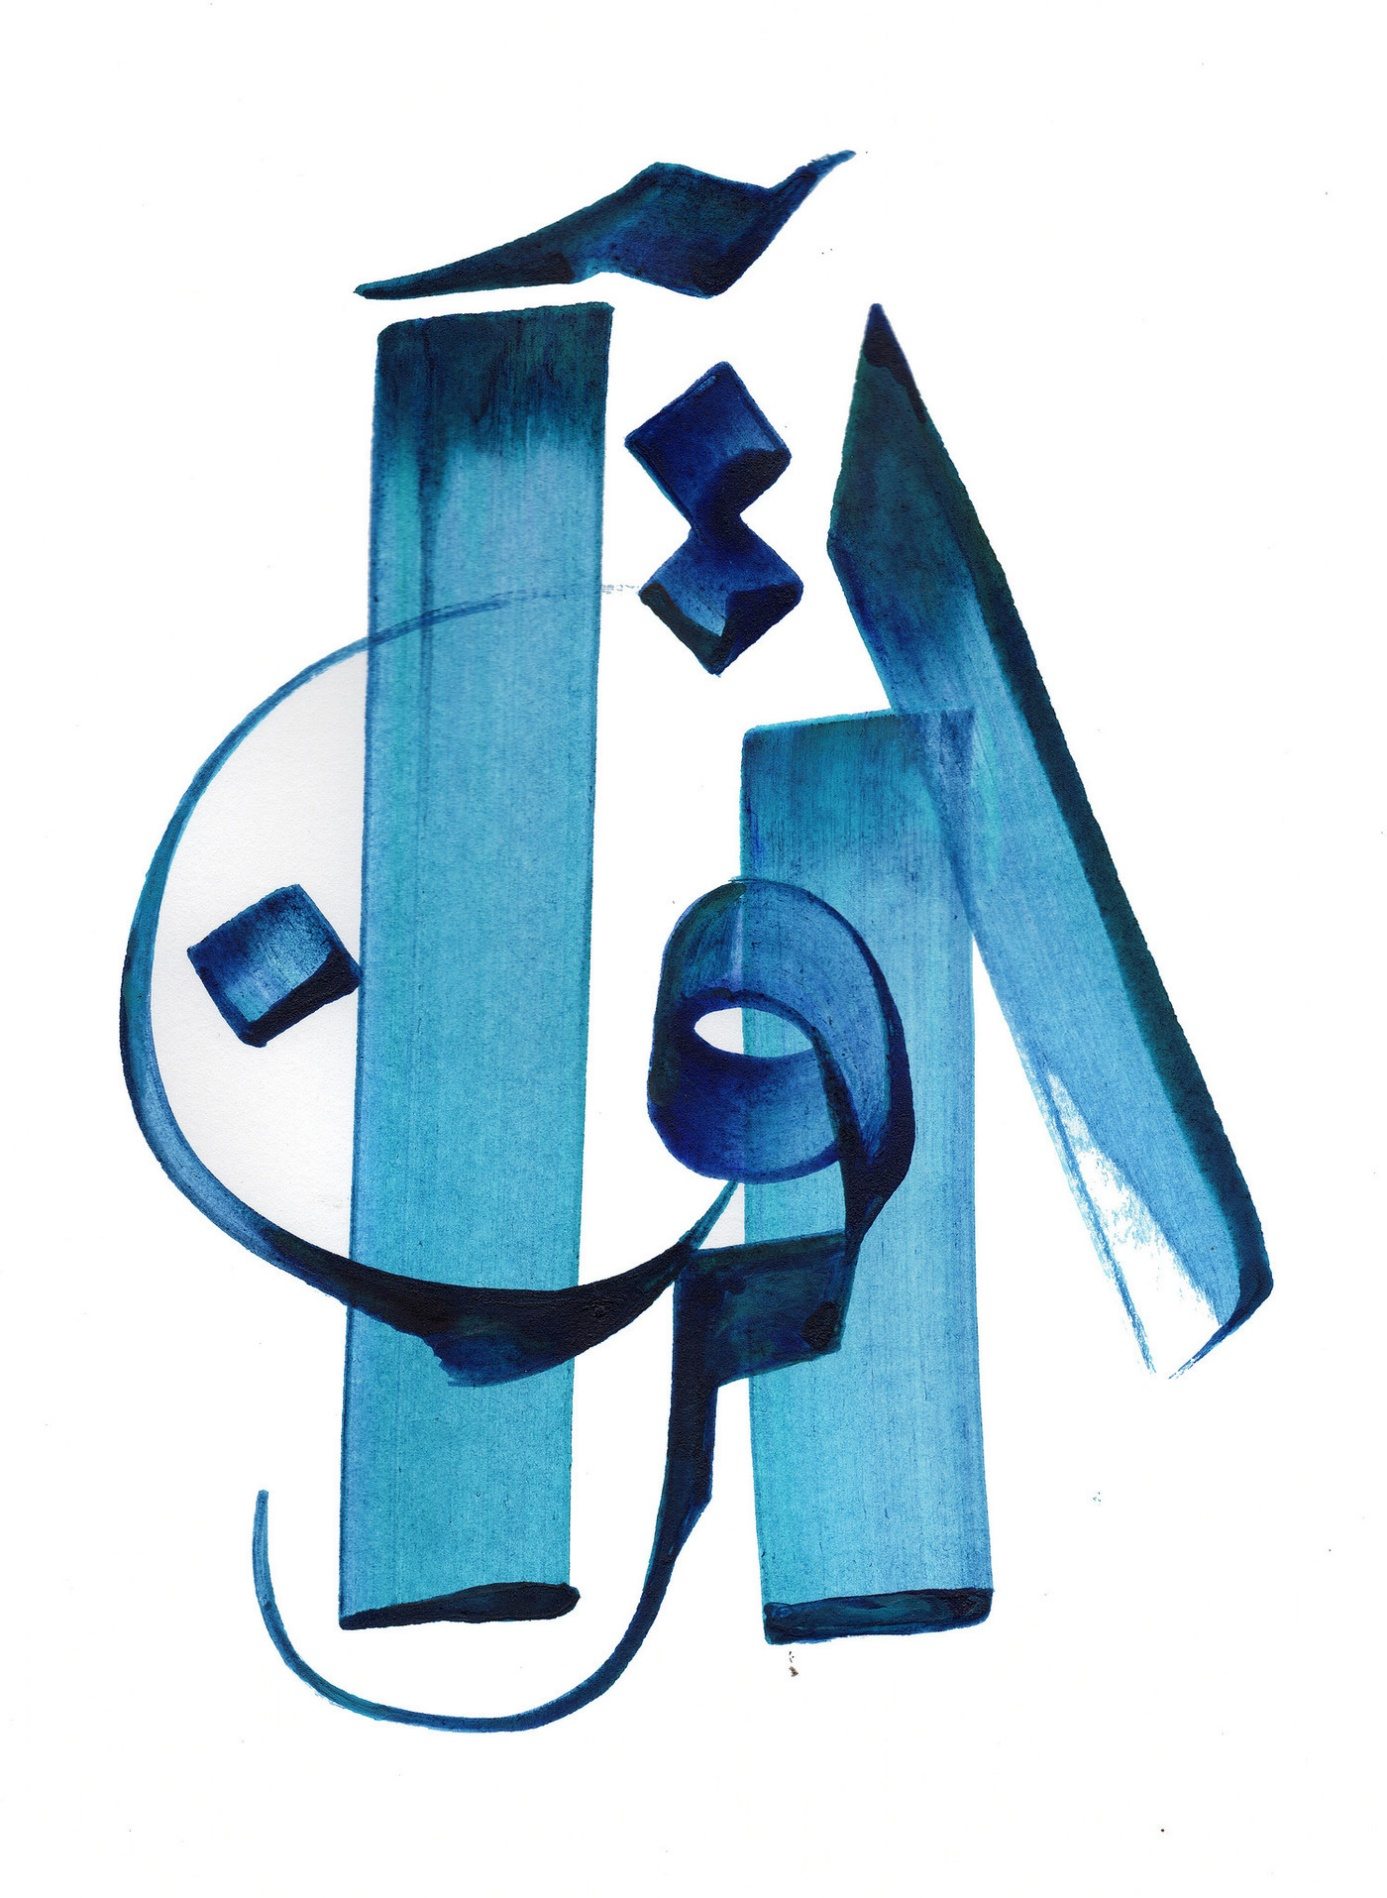
\includegraphics[width=\textwidth]{Images/image017.jpg}


\paragraph{Le regard de Hassan Massoudy}
\begin{cite}
« J'ai calligraphié le mot Coran autour de deux lignes droites,
verticales, qui forment comme l'architecture du mot. Elles lui donnent
une solidité. Avec ces deux axes, on se sent sécurisé. Ils supportent
tranquillement les autres lettres qui les chevauchent. Au centre de la
composition, une lettre forme comme un œil. Ici c'est la
lettre~\emph{qaf}-- pour le ``c'' de Coran --, qui est similaire à la
lettre~\emph{waw}. Lors d'un voyage en Turquie, j'ai découvert que les
soufis utilisaient la lettre~\emph{waw}~pour invoquer Dieu. C'est la
seule lettre de l'alphabet arabe qui, prise toute seule, peut signifier
quelque chose. Elle désigne donc l'Unique, mais sert aussi pour la
conjonction ``et''. Cette lettre évoque donc à la fois l'unique et le
multiple. »
\end{cite}



\section{Qu'est-ce que le Coran~?
}

Un livre~sacré ? Des prescriptions ? Des récits bibliques mais sans
ordre chronologique~? Que dit-il~? Comment est-il structuré~?

Avant d'exposer le Coran à la lumière de la foi musulmane, tel que les
théologiens, mystiques ou grands commentateurs l'ont compris, je vous
propose d'ouvrir quelques ouvrages récents écrits par des musulmans sur
le Coran. Ils donnent une première idée de ce que des musulmans disent
de lui et comment ils le voient.

\paragraph{Le Doute en Islam}. Le mot "islam" déjà, est l'antonyme même du doute. En effet, douter en Allah et en son Prophète est le reniement même de l'islam. Pourtant, dans la spiritualité musulmane, on peut parfois douter de soi-même et de sa capacité de croire et d'assimiler le bon et le vrai message. On peut aussi douter des interprétations et des constructions des uns et des autres mais jamais du Coran en tant que Parole révélée au Prophète. 
La seule école théologique qui, en terme de méthode, reconnaît que le "bon doute" pourrait contribuer au mûrissement de la foi, est celle rationaliste, le mo'tazilisme.  Grâce à l'esprit critique, les adeptes d'un tel courant exige de pratiquer le doute vis à vis des dogmes et des pratiques afin d'éviter tout assentiment aveugle et passif. 
Depuis Mohammad Arkoun (1928-2010) et ses héritiers, des exégètes et des historiens musulmans essaient en appliquant la méthode historico-critique  de "déconstruire" le dogmatisme régnant dans l'islam fondamentaliste.

\paragraph{Du côté des sheikh}

\begin{Def}[Sheikh]
un sheikh, c'est un sage, un homme
doué de connaissances religieuses et scientifiques reconnues. En arabe,
cela veut dire maître,
vieillard.
\end{Def}
\label{un-sheik}
Le célèbre sheikh syrien \textbf{ʿAlī Ṭanṭāwī} \sn{voir p. \pageref{theo:AliAlTawani}}, (1909-1999) écrit dans
son livre \emph{Connaître l'islam} :

  


\begin{quote}
    

«~Le musulman croit que le Coran est la parole de Dieu, apportée par
Gabriel à Muḥammad, qui l'a transmise comme il l'a entendue. Le musulman
ajoute foi que le contenu du Livre (Al-Mushâfe) dont nous disposons est
la totalité du Coran. Quiconque en nie une partie ou en doute sort de
l'Islâm.

Le Coran est le miracle de Muḥammad.

Le caractère inimitable du Coran est un fait, mais ne cherchez pas comme
les spécialistes de la rhétorique, les endroits inimitables du Coran. En
effet, ce qui est inimitable, ce ne sont pas seulement ses expressions,
ni son contenu métaphysique, mais sa globalité. Il est semblable à une
jolie femme. Sa beauté n'est pas dans la seule couleur de sa peau, dans
ses yeux, ou dans une seule partie d'elle, mais elle se trouve dans son
ensemble. Même si chaque observateur du Coran aperçoit le caractère
inimitable du côté qu'il observe.
 
{[}Muḥammad{]} a apporté un livre d'un style littéraire splendide ; au
sommet de la complétude en matière de droit ; en métaphysique il
contient des choses ignorées des hommes que la raison humaine ne peut
saisir d'elle-même~»
\mn{Tantâwî, \emph{Connaître l'islâm}.
  Citations respectives: p. 220, 241, 243, 242, cité par Anne-Sylvie
  Boisliveau, \emph{Le Coran par lui-même}, Brill, 2014.}.
  
\end{quote}



\paragraph{Du côté des prédicateurs-missionnaires~:
}

Ahmad von Denffer (né en 1948), membre de la \emph{Fondation islamique}
et auteur d'un ouvrage sur les sciences coraniques, donne la définition
suivante~:
\begin{quote}
    

«~Le Coran contient les révélations d'Allāh, le Créateur et Maître de
l'Univers, à l'humanité~». Il est «~la parole d'Allāh, descendue sur le
dernier Prophète Muhammad par l'ange Gabriel, dans un sens et une
formulation précis, transmis par de nombreuses personnes (tawātur), à la
fois par oral et par écrit. Il est inimitable et unique, protégé par
Dieu de la corruption~»\mn{~Ahmad Von Denffer, \emph{`Ulūm
  al-Qur'ān. An Introduction to the Sciences of the Qur'ān}, The Islamic
  Foundation, 1988, p. 7~; 17.}.
\end{quote}
Harun Yahya (né en 1956), créationniste musulman, dans \emph{Des secrets
du Coran,} voit dans le Coran le livre qui contient toutes les vérités.
Il donne, dit-il, les secrets de l'humanité. Tous les résultats de la
science sont déjà inscrits dans le Coran, preuve de sa puissance. Il
écrit~en introduction~:
\begin{quote}
    

«~Le Coran fournit la connaissance véridique à l'homme et contient les
secrets de la création de Dieu dans sa forme la plus vraie et la plus
pure. Toute information non fondée sur le Coran et qui est en
contradiction avec ses versets est un leurre et une illusion. Par
conséquent, ceux qui n'adhèrent pas au Coran vivent dans un état
d'hallucination ici-bas et seront condamnés au châtiment éternel dans
l'au-delà. En dehors des prières, des ordres, des interdits et des
critères moraux élevés qui sont décrits dans le Coran, Dieu communique
beaucoup de secrets à l'humanité. Un œil attentif peut en témoigner
pendant toute sa vie~»\mn{Harun Yahya, \emph{Des secrets du
  Coran}, p. 9.}.
\end{quote}




\paragraph{Du côté des nouveaux penseurs~:
}

Ghaleb Bencheikh (né en 1960) dans son livre \emph{Le Coran} écrit~:
\begin{quote}
    

«~Formulé dans sa dimension la plus traditionnelle, le Coran est le
recueil des locutions divines révélées au prophète Muḥammad Ibn Abdallah
et transmises par l'ange Gabriel sur une période de vingt-trois années
lunaires~»
\end{quote}
Puis il ajoute~:
\begin{quote}
«~Plusieurs disciplines sont requises si l'on veut véritablement étudier
le Coran pour mieux l'appréhender, s'en emparer et en faire l'exégèse.
Différentes branches des sciences humaines et de l'étude des
civilisations concourent aux multiples axes autour desquels s'articule
la recherche herméneutique contemporaine. Elle s'appuie entre autres sur
la sémiotique, la médiologie la linguistique, la philologie, l'anagogie,
la paléographie et l'historiographie~»\mn{Ghaleb Bencheikh,
  \emph{Le Coran}, Paris, Eyrolles, 2010, p. 8-10.}.
\end{quote}
Ici, le philosophe souligne la nécessité d'intégrer le recours des
données des sciences humaines pour comprendre et interpréter le Coran.
Les seules sciences islamiques traditionnelles ne suffisent plus ou plus
exactement elles enferment le Coran dans une interprétation.

\paragraph{Mohammad Arkoun} \label{Theol:Arkoun4} (1928-2010) dans son ouvrage \emph{Lectures du
Coran}, note que
\sn{Mohammed Arkoun,
  \emph{Lectures du Coran}, Paris, Maisonneuve, 1982, p. 1. \vskip 0.1cm
 Voir p. \pageref{theol:Arkoun3} }

\begin{quote}
«~pour un esprit moderne habitué à suivre une démonstration, une
évocation, une description, un récit dans des textes composés selon un
plan rigoureux, le Coran est particulièrement rebutant par sa
présentation désordonnée, son usage inhabituel du discours, l'abondance
de ses allusions légendaires, historiques, géographiques, religieuses,
ses répétitions, ses inconséquences~».
\end{quote}
Ces différents musulmans présentent d'une manière particulière le Coran,
donnant un éclairage singulier.
Bien que ces penseurs musulmans contemporains soient minoritaires, ils restent les pionniers de la production intellectuelle musulmane actuelle et l'actualisation de la doctrine islamique à la lumière des sciences humaines et sociales modernes. Même si une partie de l'imaginaire musulman actuel reste sous l'influence des écoles juridiques fondamentalistes, ces penseurs modernes sont très appréciés et écoutés par les musulman libéraux surtout ainsi qu'auprès des non-musulmans engagés dans le dialogue inter-religieux.   
Pour les plus intégristes, ils sont considérés comme \textit{zanadiqa}, hérétiques, blasphémateurs ou coupable d'apostasie. Et il ne faut pas oublier que, le blasphème est toujours puni de mort dans plusieurs pays islamiques.... En revanche, condamner à mort un penseur musulman reste un fait rare. Junaid Hafeez, par exemple, professeur d’université au Pakistan, était emprisonné depuis six ans quand il a été condamné à mort en décembre 2019 pour blasphème. Sa condamnation fait aujourd'hui l'objet d'un appel. A suivre ! Avec la prison, ils pourraient être interdits d'enseigner ou de se rendre dans des pays musulmans. On peut surtout aussi mettre sur l'Index leurs publications. L'Arabie Saoudite interdit l'ouvrage "Le Coran et ses lectures" d'Abdelmajid Charfi. 

Quoique dans le contexte actuel, l’islamisme considère que la critique du Prophète et sa représentation est l' acte le plus grave qui mérite le plus dur des châtiments, la critique de la Sunna pourrait être elle aussi compromise. Mais, il ne faut pas oublier, qu'actuellement en France, des penseurs musulmans contemporains qui n'hésitent pas de poursuivre leur méthode historico-critique. 

 Pour un premier approfondissement, il
convient de revenir à la méthode des savants de l'islam et de partir de
l'étymologie.

\vide{uxe9tymologie}{%
\subsection{Étymologie}\label{uxe9tymologie}}

La racine \emph{qara'a} signifie lire à haute voix, réciter. Par suite,
le \emph{Qur'ān} est une lecture. L'étymologie peut surprendre puisque
le \emph{Qur'ān}, avant d'être un livre, est donc une récitation d'un
livre. Pour les musulmans, cette récitation suscite une capacité
d'émotion religieuse bouleversante. Le Coran ne se lit pas, mais se
récite, se psalmodie. Il existe des règles précises et l'ensemble de ces
règles correspond au \emph{taǧwīd}. Le mot vient de la racine ǦaWaDa qui
signifie améliorer, rendre meilleur. On le distingue du \emph{tartīl}
qui est la lecture lente du Coran.

Les mosquées organisent parfois des concours de \emph{taǧwīd},
récitation du Coran, pour les enfants. C'est sur le principe de
\emph{The Voice}, avec un jury. Mais il note le participant en fonction
du respect des règles sur les pauses, les syllabes allongées, etc. Tout
y est beaucoup moins subjectif. Dans le film \emph{Wajda}, de 2012, qui
raconte avec beaucoup d'humour l'histoire d'une jeune enfant saoudienne
qui rêve d'avoir un vélo, on la voit dès les premières scènes du film
dans une école coranique où elle apprend le Coran. L'apprentissage du
Coran n'est pas réservé aux seuls hommes~! Pour autant, le film est très
ironique car en déplaçant bien des problématiques d'adultes dans le
monde de l'enfance, il n'en dessine pas moins un triste tableau de la
condition des femmes en Arabie. A son camarade, Wajda dit qu'elle veut
faire du vélo avec lui, mais lui de lui répondre~: «~ce n'est pas
possible, tu es une femme~». Et elle de renchérir~: «~tu dis ça, parce
que tu sais que si je faisais du vélo je serai meilleure que toi~».

\vide{section-13}{%
\subsubsection{}\label{section-13}}

\vide{extrait-de-la-ruxe9citation-coranique-par-un-iranien-de-7-ans-devant-un-public-manifestement-conquis-uxe9coutez-jusquuxe0-la-fin.}{%
\mn{{Extrait de la récitation coranique par un
iranien de 7 ans devant un public manifestement conquis\ldots{} écoutez
jusqu'à la fin.
}{Extrait de la récitation coranique par un iranien de 7 ans devant un public manifestement conquis\ldots{} écoutez jusqu'à la fin. }}\label{extrait-de-la-ruxe9citation-coranique-par-un-iranien-de-7-ans-devant-un-public-manifestement-conquis-uxe9coutez-jusquuxe0-la-fin.}}

Cette puissance affective ou émotionnelle de la récitation coranique est
affirmée par le Coran lui-même~:
\begin{quote}
    
«~Il dit de lui-même que cette lecture est splendide~: «~Dis~:
`croyez-le ou ne le croyez pas, à ceux à qui le savoir a été donné avant
cela, lorsque l'on leur récite {[}le Coran{]}, ils tombent prosternés
sur leurs faces~» (S. 17, 107).

\TArabe{قُلْ آَمِنُوا بِهِ أَوْ لَا تُؤْمِنُوا إِنَّ الَّذِينَ أُوتُوا
الْعِلْمَ مِنْ قَبْلِهِ إِذَا يُتْلَى عَلَيْهِمْ يَخِرُّونَ
لِلْأَذْقَانِ سُجَّدًا}

\end{quote}

Mais avant de poursuivre sur la manière dont le Coran parle de lui-même,
il importe de décrire le livre, de découvrir sa structure, sa
composition.

\vide{composition-et-structure-du-coran}{%
\section{1.~Composition et structure du
Coran}\label{composition-et-structure-du-coran}}

\vide{un-livre-formuxe9-de-sourates}{%
\subsection{{1.1 Un livre formé de sourates
}{1.1 Un livre formé de sourates }}\label{un-livre-formuxe9-de-sourates}}

\vide{terminologie-et-nombre-des-sourates}{%
\subsubsection{1.1.1 Terminologie et nombre des
sourates}\label{terminologie-et-nombre-des-sourates}}

Le Coran est composé de 114 sourates, ordonnées de la plus longue à la
plus courte -- comme pour les épîtres de Paul -- à l'exception de la
première qui s'apparente à une prière introductive. Nous reviendrons sur
cette première sourate qui s'apparente très étrangement au Psaume
1\textsuperscript{er}. L'ouverture du Coran, comme l'ouverture du
Psautier~? C'est bien ce que je dis. Et une analyse intertextuelle le
prouve. Ouvrez l'un et l'autre et regardez, comparez.
\mn{Comparaison entre le Ps 1 et la sourate \textit{Al-Fatiha (L'ouverture)}}
\begin{longtable}{p{4.2cm}p{4.2cm}p{3cm}}
\toprule
Ps 1 & Al-Fatiha (L'ouverture) &\TArabe{ سورة الفاتحة }\\
\midrule
\endhead
& Au nom d'Allah, le Tout Miséricordieux, le Très Miséricordieux.

Louange à Allah, Seigneur de l'univers.

Le Tout Miséricordieux, le Très Miséricordieux, &\TArabe{ بِسْمِ اللَّهِ
الرَّحْمَنِ الرَّحِيمِ

2 الْحَمْدُ لِلَّهِ رَبِّ الْعَالَمِينَ

3 الرَّحْمَنِ الرَّحِيمِ }\\
{1. Heureux l'homme qui ne marche pas selon le conseil des
méchants, Qui ne s'arrête pas sur la voie des pécheurs, Et qui ne
s'assied pas en compagnie des moqueurs,} & & \\
{2. Mais qui trouve son plaisir dans la loi de l'Eternel, Et qui la
médite jour et nuit!} & & \\
{3. Il est comme un arbre planté près d'un courant d'eau, Qui donne
son fruit en sa saison, Et dont le feuillage ne se flétrit point: Tout
ce qu'il fait lui réussit.} & & \\
{4. Il n'en est pas ainsi des méchants: Ils sont comme la paille
que le vent dissipe.} & & \\
{5. C'est pourquoi les méchants ne résistent pas au} jour du
jugement\textbf{, Ni les pécheurs dans l'assemblée des justes;} &
4.Maître du \textbf{Jour de la rétribution.}

C'est Toi {[}Seul{]} que nous adorons, et c'est Toi {[}Seul{]} dont nous
implorons secours. &\TArabe{ 4 مَالِكِ يَوْمِ الدِّينِ

5 إِيَّاكَ نَعْبُدُ وَإِيَّاكَ نَسْتَعِينُ }\\
{6. Car l'Eternel connaît la} voie des justes\textbf{, Et la voie
des} pécheurs mène à la ruine\textbf{.} & Guide-nous dans le
\textbf{droit chemin,}

\textbf{le chemin de ceux que Tu as comblés de faveurs}, non pas de ceux
qui ont encouru Ta colère, ni \textbf{des égarés}. &\TArabe{ 6 اهْدِنَا
الصِّرَاطَ الْمُسْتَقِيمَ

7 صِرَاطَ الَّذِينَ أَنْعَمْتَ عَلَيْهِمْ غَيْرِ الْمَغْضُوبِ عَلَيْهِمْ
وَلَا الضَّالِّينَ }\\
\bottomrule

\end{longtable}

\begin{Def}[āyat]
Chaque sourate (\emph{sūra}) est composée de versets (\emph{āyah},
\emph{āyat}) mot qui signifie au préalable signe~: chaque verset est en
lui-même un signe donné par Dieu
\end{Def}


\vide{on-retrouve-ce-mot-dans-ayatollah-qui-veut-donc-dire-signe-de-dieu}{%
\mn{on retrouve ce mot dans ayatollah, qui veut donc
dire~\ldots{} signe de
dieu}\label{on-retrouve-ce-mot-dans-ayatollah-qui-veut-donc-dire-signe-de-dieu}}

 Selon les lexicographes, \emph{āyah} renvoie à l'idée de merveille, de
prodige. Le mot souligne la dimension prophétique et prodigieuse du
signe transmis à Muḥammad.

Le terme de sourate (\emph{sūrat}) apparaît à neuf reprises dans le
coran au singulier et une fois au pluriel. Sa signification reste
confuse. Les lexicographes remarquent qu'il provient de la racine SWR
qui signifie monter sur un mur, se hisser sur, assaillir, fondre sur
quelqu'un, être impétueux\sn{~\textsc{Gloton}, \emph{Lexique},
  n°0756, p. 466. Voir aussi Roger \textsc{Arnaldez}, \emph{Le Coran,
  Guide de lecture}, Paris, Desclée, 1983, p. 36.}. \emph{Sūrat}
signifie à la fois rangée de pierre, trace, indication, signe. Chez le
commentateur \textbf{Faḫr al-Dīn al-Rāzī}.


{c'est encore un nom nouveau, mais on ne peut parler du
Coran sans très vite parler d'al-Rāzī. Il est en effet l'auteur d'un des
plus sublimes commentaires du Coran, \emph{Les clefs de l'invisible}.C'est un Persan du XII\textsuperscript{e} siècle.}
\sn{Michel Lagarde
  a consacré une belle étude sur ce Commentaire~: Michel
  \textsc{Lagarde}, \emph{Les secrets de l'invisible : Essai sur le
  Grand Commentaire de Fahr al-Dîn al-Râzî}, Paris, Albouraq, 2009.}. 

on trouve l'idée selon laquelle de même qu'une muraille entoure une
ville de tout ce qu'elle contient, de même la \textbf{sourate enveloppe
la science contenue dans le Coran}. L'idée de mur ou de muraille est
aussi interprétée comme signifiant l'élévation du croyant qui
s'approprie l'enseignement du Coran~: c'est l'interprétation donnée par
\textbf{Qurṭubī} (1214-1273), autre grand exégète du Coran.

Mais pourquoi y a-t-il des sourates~? Pourquoi le Coran n'est-il pas
écrit en un seul bloc~? Pourquoi donc une composition~de plusieurs
éléments ? Cette question est typique de celles que l'on trouve dans le
commentaire de \textbf{Faḫr al-Dīn al-Rāzī} où il se demande
systématiquement pourquoi les choses sont ainsi et pas autrement~:
pourquoi telle construction grammaticale, pourquoi tel mot sous telle
forme, pourquoi tel ordre et ici, pourquoi des sourates et pas tout
simplement un Livre en un seul tout\textbf{.} \mn{Roger Arnaldez expose la
réponse d'al-Rāzī dans son livre \emph{Le Coran Guide de lecture}.}

\vide{nom-des-sourates}{%
\subsubsection{{Nom des sourates
}}\label{nom-des-sourates}}

Chaque sourate est désignée par un nom. Cette désignation semble tardive
puisque les compagnons de Muḥammad à La Mecque rapportent des versets
des sourates à partir de leurs noms. Le nom des sourates dépend d'un
thème ou d'un élément cité dans la sourate. Ainsi, par exemple, la
sourate al-Tawba porte sur le repentir accueilli par Dieu à Muḥammad, à
ceux qui étaient avec lui et à ceux qui étaient restés derrière lui. Il
y a quelques étrangetés, comme le nom de la Sourate
2\textsuperscript{e}, la Vache, \emph{al-Baqara}. Le thème est tiré des
Nombres et du Deutéronome en lien avec Moïse. Or, l'épisode de la vache
ne couvre que huit versets sur 286 (versets 67-73).

\vide{nature-des-sourates}{%
\subsubsection{Nature des sourates}\label{nature-des-sourates}}

Certaines sourates sont très particulières : la première sourate par
exemple, al-Fātiḥa, l'Ouvrante, est une prière adressée à Dieu par les
croyants. Elle illustre parfaitement l'élaboration progressive du texte
coranique : on en a trouvé des variantes textuelles dans des traditions
ou des ouvrages anciens. Une teneur identique, mais des mots, des
constructions syntaxiques différentes.

La sourate 111 (\emph{al-masad}, la corde) est une formule de
malédiction de type archaïque. Rien dans le texte ne spécifie ce dont il
s'agit. Il est donc une énigme. Les circonstances de la Révélation
diront plus tard qu'il s'agit d'une malédiction prononcée par Muhammad
contre un de ses oncles hostile à sa prédication. Nous avons déjà
rencontré son nom. Ce serait Abū Lahab.

Les deux dernières sourates sont des incantations magico-prophylactiques
(pour préserver la santé). Elles semblent avoir suscité bien des litiges
quant à leur insertion.

Le Coran comporte des proclamations oraculaires (comme les oracles qui
rapportent ce qu'ils voient), des hymnes sous une forme poétique :
l'évocation poétique du Paradis est une adaptation arabe originale des
Hymnes d'Ephrem de Nisibie, Père de l'Église syriaque (+ 373). Oui, les
versets eschatologiques sur les houris sont des échos des hymnes de St
Ephrem. Sur ce point, les travaux d'intertextualité d'Andrae Tor sont
une référence incontournable et plus récemment de Christoph
Luemberg\sn{Tor Andrae, \emph{Les origines de l'islam et le
  christianisme}, Paris, 1955.
\sn{
   le compte-rendu de ce livre dans la Revue d'histoire des
  religions
  \url{http://www.persee.fr/doc/rhr\_0035-1423\_1957\_num\_151\_2\_8712}.}.}

Il y a des récits, des textes législatifs et parénétiques (exhortatifs).
On y trouve aussi des discours de guerre, d'appel au combat
(\emph{ğihād} ou \emph{qitāl})\sn{Emmanuel \textsc{Pisani}, «~La
  violence dans le Coran~», sur le site~:
  \url{http://www.croire.com}{www.croire.com} , juin 2015.}. Cette
guerre est contre plusieurs ennemis : les gens du Livre qui ne
pratiquent pas la religion de la vérité (S. 9, 111).

Il y a aussi des discours polémiques~: Mehdi Azaiez, - il a consacré sa
thèse de doctorat à l'analyse de ce genre littéraire dans le Coran -,
remarque qu'il s'agit de «~l'un des genres les plus marquants du corpus
coranique~»\sn{Medhi \textsc{Azaiez}, «~Le contre-discours
  coranique. Premières approches d'un corpus~», dans Azaiez,
  \emph{Nouvelles approches du} Coran, Paris, CNRS, 2013, p 257.}. On
trouve ainsi cette invitation à «~débattre de la meilleure
façon~»~(S.16, 125)\sn{~Jane Dammen \textsc{McAuliffe}, «~Debate
  with them in a better Way : the Construction of a Qur'anic
  Commonplace~», dans \emph{Myths, historical archetypes and symbolic
  figures in Arabic literature towards a new hermeneutic approach},
  Proceedings of the International Symposium in Beirut, June 25th-June
  30th, 1996, / Edited by Angelika Neuwirth, Birgit Embaló, Sebastian
  Günther, 1999, p. 163-188.} :
\begin{quote}
    
«~Appelle les hommes dans le chemin de ton Seigneur par la sagesse et
une belle exhortation~; discute avec eux de la meilleure manière~»

\TArabe{ادْعُ إِلَى سَبِيلِ رَبِّكَ بِالْحِكْمَةِ وَالْمَوْعِظَةِ
الْحَسَنَةِ وَجَادِلْهُمْ بِالَّتِي هِيَ أَحْسَنُ إِنَّ رَبَّكَ هُوَ
أَعْلَمُ بِمَنْ ضَلَّ عَنْ سَبِيلِهِ وَهُوَ أَعْلَمُ بِالْمُهْتَدِينَ}
\end{quote}

Il fait remarquer que la polémique est inhérente à l'islam originel dans
la mesure où la parole de Muḥammad a d'abord été rejetée par le groupe
tribal auquel il appartenait. C'est donc avec les siens qu'il a fallu
d'abord débattre et convaincre si bien que la question de la polémique
émerge dès la naissance de l'islam. Les débats, les réponses formulées
aux contradictions sont inhérents au texte et peuvent se traduire par
des incantations, des malédictions, des reproches, des avertissements,
des railleries, des apostrophes en direction des
non-croyants\sn{Neal \textsc{Robinson}, \emph{Discovering the
  Qur'an}, p. 116, cité par Azaiez, \emph{op. cit}., p. 259.}.

\vide{agencement-des-sourates}{%
\subsubsection{{Agencement des sourates
}}\label{agencement-des-sourates}}

Autre question, celle de l'agencement des sourates et l'ordre des
versets. Quel ordre suivre~? Cette question est au cœur d'une
\emph{disputatio} entre les savants musulmans.

L'exégète al-Qurṭubī (nous avons déjà rencontré ce noms avec al-Rāzī)
rapporte les propos du Qāḍī Abū Bakr Ibn Al-Ṭayyib~: «~On peut faire
l'objection que les Anciens ont été en désaccord sur l'ordre des
sourates du Coran. Certains, dans leur recueil, ont écrit les sourates
selon la chronologie de leur révélation, et ils ont mis en tête les
sourates mecquoises, puis les sourates médinoises~; certains commencent
par la louange al-Ḥamd, d'autres par la sourate 96~: `Récite, au nom de
ton Seigneur qui créa\ldots'~: tel est le début du recueil de `Alī.
Quant à celui d'Ibn Mas`ūd, il commence par `Maître du Jour du Jugement
(1,3), puis viennent la sourate \emph{La Vache} (2) et la sourate
\emph{Les femmes} (4)\ldots{} Le recueil d'Ubayy débute par al-Ḥamd~;
suivent les sourates 3, La Famille de `Imrān la sourate 6, les
Troupeaux, la sourate 7, al-`Araf, la sourate 5, La Table et ainsi de
suite\ldots{} avec de profondes divergences~»\sn{Cité par
  \textsc{Arnaldez}, \emph{Le Coran. Guide de lecture}, \emph{op. cit}.,
  p. 47.}.

L'exégète ici se fait l'écho d'un débat quant à l'agencement des
sourates au sein même de la tradition musulmane. La découverte d'anciens
manuscrits du Coran à San`ā au Yémen, en 1972 confirme l'existence de
différents corpus coraniques. Muḥammad Amir Moezzi \mn{Voir aussi pour un détail de l'approche historico-critique \cite{Amir:CoranHistoriens} }écrit~à ce propos~:
\begin{quote}
    «~En sus de quelques variantes orthographiques et lexicographiques
mineures, 22\% des 926 groupes de fragments étudiés présentent un ordre
de succession de sourates complètement différent de l'ordre connu~: le
découpage en versets ne correspond à aucun des 21 systèmes connus. Ce
qui est frappant c'est que l'ordre des sourates se rapproche le plus des
codex d'Ubbay et d'Ibn Mas`ūd~»\sn{\textsc{Cuypers, Gobillot},
  \emph{Idées reçues}, p. 18.}.
\end{quote}


Il semble donc qu'existèrent entre ces recensions des différences, à la
fois dans l'ordre, mais aussi dans le texte. Mais retenez aussi que la
tradition musulmane rapporte l'existence de différents corpus~: elle les
canonise d'une certaine façon. Parmi ces corpus, la tradition sunnite
reconnaît que `Alī avait élaboré son corpus\ldots{} Corpus dans lequel
serait inscrit, d'après la tradition šī`ite, les versets divins qui
désignaient `Alī comme successeur de Muḥammad\ldots{}

 
\subsection{ Un livre en arabe clair} 
\begin{quote}
    
«~Voici un Livre dont les versets sont clairement exposés~; un Coran
arabe, destiné à un peuple qui comprend~» (S.~41, 2-3).
\end{quote}

Et le Coran de préciser «~un arabe clair (\emph{`arabiyyun mubīn})~» (S.
16, 103 et 26, 195).

Le Coran de lui-même accorde une importance singulière à la langue
arabe. On comprend pourquoi, face à une question, il convient de revenir
aux mots arabes et à leur signification.

L'arabe est comme magnifié. Mais cet arabe est-il si clair~comme
l'affirme le Coran ? Et s'il l'est, pourquoi tant de niveaux de
commentaires, et d'explications parfois contradictoires~? Pourquoi le
prophète Muḥammad a-t-il dû expliquer les significations du Coran à ses
compagnons~? Quel crédit et quelle autorité accorder aux explications
propres aux compagnons~eux-mêmes ? Ces questions nous introduisent dans
une des difficultés propres à tout texte sacré et qui est sa
compréhension. Comme le dit Tariq Oubrou, imam de Bordeaux, «~il ne
suffit pas de lire le Coran pour le comprendre~».


\section{Histoire du Coran~: sa constitution
(\emph{muṣḥaf})}

Depuis quand le Coran existe-t-il sous la forme qui est la sienne
aujourd'hui~? Muḥammad a-t-il eu de son vivant et sous ses yeux le texte
coranique tel qu'il est structuré~? Il n'en est rien et la constitution
du \emph{muṣḥaf}, c'est-à-dire le Coran dans sa matérialité, n'est pas
effective avant la fin du premier siècle de l'Hégire. Elle souligne que
l'islam s'inscrit pleinement dans la tradition de l'oralité, et avant
d'être un livre, le Coran était une récitation. Mais pourquoi a-t-on
éprouvé le besoin de rassembler les sourates en un livre~? Tel est
l'objet de la présente partie.

 
\subsection{L'initiative d'Abū Bakr
} 

Selon la tradition, à la mort de Muḥammad, en 632, la Révélation est
connue par cœur et dans son intégralité par quelques rares fidèles qui
sont appelés les lecteurs du Coran (\emph{qurrā'} -- on retrouve la
racine QR' comme dans \emph{Qur'ān}, Coran). Leurs noms divergent selon
les traditions. Mais le Coran comme \emph{muṣḥaf} n'existe pas encore.

À la mort de Muḥammad, Musaylima, celui qui se prétendait aussi prophète
et qui a écrit une lettre à Muḥammad -- épisode de la Sīra que nous
avons rencontré dans le précédent chapitre -- jouissait d'une certaine
aura. Le voici qui vient trouver Abū Bakr, le premier successeur de
Muḥammad, le premier calife donc, et affirme : «~Gabriel est venu me
trouver et m'a confié la mission de prophète par toute la terre~». Il
s'insurge contre le calife et met en déroute le premier général envoyé.
En l'année 633, Abū Bakr charge Ḫālid Ibn al-Walīd de mettre un terme
aux agissements de Musaylima. C'est la bataille de `Aqrabā. Il y trouva
la mort.

Cependant, au cours de la bataille, de nombreux récitants
(\emph{qurrā'}) trouvèrent aussi la mort. `Umar aurait pris conscience
du risque de perdre des fragments du Coran. Il en informe le calife Abū
Bakr qui charge Zayd Ibn Thabit de rassembler les sourates sur des
feuilles. La tradition est rapportée ainsi par Buḫarī dans la
\emph{Sunna}, au Livre 66, chapitre 3.
\begin{quote}
    
«~Zayd ibn Ṯābit a dit~: «~Abū Bakr vint me faire chercher à la suite du
massacre des gens de Yamāma. Lors {[}de ma venue{]} je trouvai Abū Bakr
chez lui et il me dit~: `Umar vient de m'informer que le massacre qui
eut lieu à Yamama a mis fin à la vie de lecteurs du Coran et je crains
que si le combat devait perdurer, ils continuent de se faire tuer sur
les champs de bataille, si bien que disparaîtrait une bonne partie du
Coran. C'est pourquoi je pense qu'il te faut collectionner le Coran'\,'.
J'ai alors dit à `Umar : `Comment vas-tu faire quelque chose que le
Messager d'Allah n'a pas faite~?'\,' -- `Umar dit~: Par Allāh,~ceci est
une bonne chose ». Il ne cessa de me répéter son idée jusqu'à ce
qu'Allāh m'ouvrit le cœur et me fit adhérer à ce qu'\,`Umar avait
proposé.~»

\mn{ Vous avez lu que je vous ai parlé de la
bataille de `Aqarbā, mais la tradition parle des gens de Yamāma\ldots{}
alors~? En fait, `Aqrabā est le nom d'une plaine de la région de Yamāma.
J'ajouterai aussi que d'après la tradition musulmane, Abū Bakr avait
envoyé 3000 hommes~! Ce qui veut dire aussi que Musaylima avait des
disciples et nombreux étaient aussi ceux qui suivaient ses prophéties.
La région semble connaître un embrasement prophétique. a bataille
d'Al-Yamama (arabe \TArabe{
اليمامة} 
)
ou bataille d'al-`Aqrabā aura eu lieu, selon
les sources musulmanes, en 633, dans le cadre des Guerres de Ridda
(l'Apostasie), sur la plaine de Aqraba dans la région d'Al-Yamama (dans
l'actuelle Arabie Saoudite) entre les forces du calife Abou Bakr le
véridique et Musaylima le menteur, un prophète autoproclamé.
}
Zayd dit~alors qu'Abū Bakr avait poursuivi en disant~: `tu es un homme
jeune, raisonnable et au-dessus de tout soupçon et tu transcrivais déjà
par écrit la révélation pour le prophète. Collecte et rassemble donc le
Coran'. Par Dieu, me disais-je, s'il m'avait mandaté pour déplacer une
montagne, cela m'aurait été plus aisé que d'exécuter l'ordre de
rassembler le Coran. Je dis : `comment allez-vous faire quelque chose
que le Messager d'Allah n'a pas faite~? Mais il (Abū Bakr) dit~: «~Par
Allāh, c'est une bonne chose.~» Et puis il ne cessa de me répéter son
idée jusqu'à ce qu'Allāh m'en inspirât l'admission comme Il l'avait fait
pour Abū Bakr et pour `Umar. Dès lors, je me suis mis à rechercher et à
collecter les éléments coraniques transcrits sur des branches de dattier
et sur des pierres lisses ou conservées dans la mémoire des gens et j'ai
trouvé les derniers versets de la sourate \emph{at-Tawba} chez Abū
Ḫuzayma al-Anṣārī que je n'avais pas trouvés chez les autres\ldots{} Les
feuilles contenant le Coran furent conservées par Abū Bakr jusqu'à sa
mort puis elles furent déposées auprès d'\,`Umar qui les garda jusqu'à
sa mort puis elles furent transférées à sa fille Ḥafṣa.
\end{quote}

De cette tradition, on peut retenir avec une certaine assurance qu'une
compilation fut entreprise à l'époque d'Abû Bakr. `Umar les accueillit
puis sa fille, Ḥafṣa.




\subsection{{La constitution de la Vulgate de `Uṯmān
}}

C'est donc sous `Uṯmān (l'impulsion vient d'Abū Bakr, mais la
constitution lui est postérieure~: il ne vécut pas assez longtemps) que
l'on entreprit la collection du Coran. Outre le récit transmis par la
tradition, l'histoire montre que cet acte est loin d'être purement et
simplement religieux. Il revêt une dimension politique~: il s'agit de
\textbf{contrebalancer le pouvoir des lecteurs qui se sont institués
gardiens du texte sacré}. Cela sert par ailleurs la politique
centralisatrice déployée par le troisième calife.

Mais si l'initiative califale permet au calife de concentrer les
pouvoirs politiques et religieux, il n'est pas le seul à vouloir
constituer une Vulgate.

 
\subsection{ La constitution d'autres corpus
} 

Ainsi, certains compagnons du Prophète, attachés à la transmission de la
Parole, vont proposer leurs propres recensions. On a ainsi parlé d'un
corpus de Sālim Ibn Ma`qil -- mais il est mort un an après le Prophète.
Plus solide, serait la recension d'un cousin de Muḥammad, `Abd Allāh Ibn
`Abbās (m. 68 / 688). Ce corpus est aujourd'hui perdu.

\mn{{`Alī} -- petit rappel~: c'est le cousin et le gendre de
Muḥammad, le premier converti à l'islam selon la \emph{Sīra} --, selon
les šī`ites, était aussi en sa possession du \emph{muṣḥaf}.}

On trouve aussi le corpus d'Abd Allāh \textbf{Ibn Mas`ūd} (m. 30 / 650),
un des premiers convertis à l'islam, très proche du Prophète. Lui aussi
va rédiger un corpus. On sait à partir de citations diverses dans des
ouvrages anciens que différentes recensions circulaient. La version
d'Ibn Mas`ūd a par exemple circulé à Koufa en Irak puisque le gouverneur
d'Irak exigea de détruire ce corpus. Or, en 1007, le même ordre fut
répété à Bagdad ce qui signifie bien qu'il n'avait pas été complètement
détruit. Cela indique aussi qu'il présentait des divergences par rapport
à la Vulgate de `Uṯmān.

Toutefois, les variantes entre les différents codex semblent avoir été
minimes. On a établi que la version de Mas`ūd ne comportait pas la
première sourate, ni les deux demandes de protections (S. 113 et 114).
On a émis l'hypothèque très plausible que ces trois sourates formaient
un encadrement liturgique qui apparemment n'étaient pas dans le Coran
primitif. Vous vous souvenez du Psaume 1 qui ouvre le Psautier\ldots{}

Dès le premier siècle, un autre débat voit le jour quant à la manière de
réciter le Coran et à la nature même des consonnes qui sont utilisées.
On a un écho de cette question dans la Sunna. \mn{voir \cite{Deroche:CoranPluriel} qui soutient une vision unifiée du Coran par Muhammad par rapport au \emph{Coran des Historiens}} En effet, certains
lecteurs lisaient en recourant à d'autres lettres ce qui entraina des
divergences de lectures. Elles étaient nombreuses entre l'Irak et en
Syrie et ils s'en suivaient des accusations d'anathèmes réciproques. Il
faut bien voir que l'écriture arabe présentait des déficiences puisque
des phonèmes différents comme b, t, ṯ, n, y, étaient écrits avec le même
signe alphabétique. De plus, les signes indiquant les voyelles n'étaient
pas inscrits ce qui orientait le texte dans des sens grammaticaux
pluriels. Par conséquent, il y avait des traditions de lectures
(\emph{qirā'āt}) différentes selon les villes et les régions. Avec les
conquêtes, l'islam était prêché dans des contrées où existaient d'autres
dialectes et surtout d'autres prononciations. Un Égyptien ne prononce
pas la lettre \emph{dji}, mais il dit \emph{gué} -- ce que ne fait pas
le Syrien. Demandez à un Arabe de prononcer la lettre p\ldots{} il ne
dira pas \emph{p}ardon, mais \emph{b}ardon.

C'est dans ce contexte que l'on a renvoyé à un \emph{ḥadīṯ} sur les
lectures du Coran. Ainsi, on trouve dans la Sunna
d'\textbf{al-Buḫarī}~-- c'est un des très grands compilateurs de l'islam
de ḥadīṯ. Son nom sera revu et revu dans le prochain chapitre.




\subsubsection{Ces 5 variantes de Harf sont un moyen de rentrer dans une
pluralité de
sens}



\begin{quote}
    «~Un jour, lors du vivant du Prophète, j'entendis Hishâm ibn Hakîm
réciter la sourate al-Furqân. Alors que j'écoutais avec attention sa
récitation, je m'aperçus qu'il recourait à certaines lettres différentes
de celles que le Prophète m'avait enseignées. Je m'apprêtais à
l'interpeller durant sa prière, mais je me retins et attendis qu'il la
terminât. Je le pris alors par son vêtement et lui dis : "Qui donc t'a
enseigné ainsi la sourate que je t'ai entendue réciter ? -- C'est le
Prophète, me répondit-il. - Tu mens, lui répliquai-je, car il me l'a
enseignée avec des lettres différentes que certaines de celles que tu
viens de réciter." Je l'emmenai alors auprès du Prophète et exposai à
celui-ci le problème : "J'ai entendu cet homme réciter la sourate
al-Furqân avec certaines lettres autres que celles que tu m'as
enseignées. -- `Laisse-le' me dit le Prophète. Puis, se tournant vers
Hishâm, il lui dit : "Récite, Hishâm." Hishâm récita alors la sourate de
la même manière qu'il l'avait faite auparavant. Le Prophète dit alors :
`Ainsi a été révélée cette sourate'. Puis il me dit : `Récite, toi,
Umar'. Je le fis alors selon la façon que lui-même m'avait enseignée. Il
dit également : `Ainsi a été révélée cette sourate'. Puis il conclut :
`Le Coran est révélé selon sept variantes de récitation (\emph{harf}).
Récitez donc celle qui est facile pour vous'\emph{~(rapporté par
al-Bukhârî, Ṣaḥih ~Book 97, Hadith 175, n° 4706)}~»\emph{.}
\end{quote}


Vous ne le saviez peut-être pas, mais il y a donc plusieurs manières de
lire le Coran, avec d'autres consonnes, et donc d'autres mots, et donc
d'autres significations. Ce \emph{ḥadīṯ} permet de mettre fin à des
divergences de lectures qui devaient être conflictuelles et de
réconcilier ainsi tous les musulmans. À l'intérieur même du texte,
l'uniformité de lecture n'est donc pas absolue. Peu à peu s'imposèrent
des versions majoritaires, au X\textsuperscript{e} siècle, et on limita
les lectures à 7, 10 et 14 versions différentes.

\begin{Def}[Harf/ ahruf]
According to Islamic tradition, the Quran was revealed to the Islamic prophet Muhammad by the angel Gabriel (Jibril ) in seven ahruf (Arabic: \TArabe{ أَحْرُف}‎, romanized: aḥruf, sing. ḥarf), translated variously as editions, ways, forms and modes. Although Muslim scholars differ on their exact nature, it is thought they constituted a degree of acceptable variation in the Quranic text. The standardisation of the Quranic rasm c.650 CE and destruction of the mushafs by Rashidun caliph Uthman. the extent to which the Uthmanic codex contains the seven ahruf has been a subject of debate. The ahruf are distinct from the ten qira'at, which are other variant readings of the Quran that were canonized later on and are still in use. 
\end{Def}

La constitution officielle du Coran impulsée par `Uthman, trouve son
achèvement sous le règne de `Abd al-Malik (m. 705). Elle a été largement
combattue par les milieux šī`ites qui y ont vu une tentative d'imposer
une version falsifiée du Coran. En effet, pour les šī`ites, la version
en possession de `Alī indiquait des prérogatives particulières accordées
à `Alī et sa famille. Notamment, Dieu aurait révélé le nom du successeur
de Muḥammad, qui n'était autre que\ldots{} `Alī. On en a une
illustration dans le \emph{Kitāb al-Qirā'āt} ou \emph{al-Tanzīl wa
l-taḥrīf} d'al-Sayyārī qui vécut au IX\textsuperscript{e} siècle.
\emph{Le} \emph{Livre des récitations} \emph{coraniques} ou \emph{Le
livre de la révélation et de la falsification} est symptomatique du
refus par le parti alide de la vulgate uthmanienne à l'époque
pré-bouyide. Constitué de 725 \emph{ḥadīṯs}, l'ouvrage recense plusieurs
paroles témoignant de la falsification du Coran et de l'usurpation du
pouvoir aux \emph{ahl al-bayt}.

Au 16\textsuperscript{ème} siècle, les Ottomans adoptent une lecture
dite «~de Hafs~» qui se répand dans tout l'Empire. En 1923, sur ordre du
roi Fouad, la version officielle de la lecture de Hafs est imprimée et
c'est elle qui aujourd'hui fait référence dans la quasi-totalité de
l'\emph{umma}. Les šī`ites l'adoptent, ce qui apparemment est
contradictoire avec ce qu'ils n'ont cessé d'affirmer~: cette Vulgate est
une fausse. Apparemment seulement\ldots{} Pour mieux saisir ce paradoxe,
il faut attendre le chapitre sur le šī`isme.

 
\section{ Le Coran comme parole de Dieu
} 
\vide{inspiration-ou-ruxe9vuxe9lation}{%
\subsection{{inspiration ou révélation~?
}}\label{inspiration-ou-ruxe9vuxe9lation}}

Pour la théologie musulmane, le Coran n'est pas \textbf{inspiré, mais
révélé} par Dieu. Muḥammad n'est que le destinataire passif des
révélations de Dieu qu'il a d'abord reçu dans son cœur, au mois du
Ramaḍān, avant de les réciter. Le Coran n'est pas parole de Dieu selon
Muḥammad, mais Parole de Dieu selon Dieu. Pour souligner la passivité
culturelle, psychologique, linguistique ou même poétique du prophète
dans la réception du Coran, les commentateurs interprétèrent
l'expression coranique \emph{al-nabī al-ummī} (S. 7, 156-158), comme
signifiant l'illettrisme de Muḥammad. Ce n'est pas sans difficulté,
puisque si vous vous souvenez bien, la \emph{Sīra} mentionne une lettre
de Muḥammad à Musaylima, et il y en a d'autres puisque la tradition en
rassemble plus de quinze. On pourrait objecter que Muḥammad ne faisait
que dicter à un scribe ses lettres, mais la tradition elle-même rapporte
qu'un scribe s'était arrêté d'écrire pour demander à Muḥammad d'écrire
lui-même, comme il le faisait autrefois.

Cependant, certains auteurs musulmans ont fait remarquer que le sens
d'illettré ne convient pas dans le contexte coranique, et ils proposent
une autre signification, celle de gentil, païen. Autrement dit, Muḥammad
est le prophète des gentils, de ce peuple polythéiste d'Arabie qui
n'avait pas reçu de révélation céleste. Ibn `Arabī comprenait le mot en
lien avec la racine 'MM (Mère). On peut être \emph{ummī} sans être
analphabète~: l'\emph{ummī} c'est celui qui est capable de suspendre ses
opérations intellectuelles pour recevoir~: c'est l'état d'enfance, le
silence de l'enfant qui écoute. Le Coran dit~: «~Dieu vous a fait sortir
du ventre de vos mères et vous ne saviez pas~» (S. 16, 78).

\textbf{{Sens aussi de matriciel/fondamental~: Umm al Qura~: la
ville matrice~: la
Mecque.} 
}
Parmi ces relectures et déconstructions de la compréhension imposée au
fil des temps par la tradition du mot \emph{ummī}, \textbf{Mohammad Abed
al-Jabri} (1938-2010) montre que rien ne permet dans le Coran de dire
que Muḥammad ne savait ni lire ni écrire

\sn{Muhammad Abd AL JABRI,
  \emph{Introduction au Coran} \textbf{\TArabe{الجزء الأول~: في التعريف
  بالقرآن / محمد عابد الجابري. - الطبعة ١}}., Madẖal ilá al-Qurʾān
  al-karīm. 1~: al-ǧuzʾ al-awwal~: fī al-taʿrīf bi-l-Qurān / Muḥammad
  ʿĀbid al-Ǧābirī. - Al-ṭabʿaẗ 1, \textbf{\TArabe{بيروت~: مركز دراسات الوحدة
  العربية،}}, \textbf{\TArabe{٢٠٠٦}} Bayrūt~: Markaz Dirāsāt al-Waḥda
  al-ʿArabiyya, 2006, 456 p.}. 
  
  Pour lui, \emph{ummī}, signifie qu'il
fait partie des communautés auxquelles de livre il n'avait pas été
encore révélé. Youssef Seddik (né en 1943) (tunisien vivant en France,
il demande à recommencer à zéro~: pour lui, la révélation coranique est
formidable, mais tout ce qui a été dit depuis est faux, manipulation,
idéologie\ldots)\sn{Youssef Seddik, \emph{Nous n'avons jamais lu
  le Coran}, éd. de l'Aube, La Tour d'Aigues, 2004.}, Hichem Djaït
(historien tunisien, né en 1935) ou encore Olfa Youssef (né en
1964) 
\sn{Olfa Youssef, \emph{Le Coran au risque de la
  psychanalyse}, Paris, Albin Michel.} 
  s'inscrivent dans cette relecture
du terme.




Quoi qu'il en soit, la constitution de la Vulgate coranique n'est pas
remise en cause par cette relecture du terme \emph{ummī.} L'histoire du
texte va totalement à l'encontre de l'idée selon laquelle Muḥammad
aurait écrit le Coran dans sa constitution actuelle.


\subsection{Le livre mère
}

Le Coran renvoie aussi à un livre originel, le \emph{umm al-kitāb},
sorte de matrice céleste~:
\begin{quote}
    

«~Voici, en vérité, un noble Coran, contenu dans un Livre caché. C'est
une révélation du Seigneur des mondes~» (S. 56, 77-80).
\end{quote}
Pour le Coran, Dieu révèle son livre à partir de cet archétype à ses
prophètes. Cela n'est pas sans incidence sur la manière dont il comprend
la notion de révélation et comment il relit la tradition juive ou
chrétienne à partir de sa compréhension de ce qu'est le \emph{Kitāb}.

Mais quel est le sens exact du mot \emph{kitāb}~? S'agit-il d'un livre~?
Peut-on dire que le Coran se définit comme livre~? Écoutons Anne-Sylvie
Boisliveau qui vient de publier \emph{Le Coran par lui-même} sur la
question~{[}d'après \emph{Culture d'islam}, Le séminaire coranique 2{]}:




\mn{D'après le Coran, il se situe au même niveau que
l'Evangile et la bible. Il réhausse donc le statut de l'Evangile pour
les
chrétiens.}


\subsection{{Un livre parfait, inimitable
}}

Parce qu'il vient de Dieu, il possède les attributs de Dieu. Il est donc
parfait~: grammaticalement parlant, il n'y a pas d'erreur d'arabe.
Théologiquement, il est infaillible et ne peut contenir d'erreur. Il est
unique et inimitable. C'est en tous les cas ainsi que la tradition
musulmane lit et comprend le Coran en général. Pas tous cependant, le
courant mu`tazilite s'oppose à cette interprétation. Il s'agit d'un
courant rationaliste. On va bientôt en reparler.

L'inimitabilité du Coran (\emph{i`ğāz}) est un thème que l'on trouve
dans le Coran lui-même, alors que l'on accuse Muḥammad d'être un poète
menteur. Dans la période mecquoise, Muḥammad met au défi quiconque de
pouvoir rapporter dix sourates semblables (S. 11, 13), puis une seule
sourate (S. 2, 23~; 10, 38). \textbf{Inimitable, le Coran est donc
intraduisible}.

Il se pose alors le problème de la traduction. Peut-on traduire le
Coran~? La tradition musulmane répond par la négative. On ne peut
qu'essayer de le traduire, mais sa traduction est déjà une
interprétation, il faut donc toujours revenir à l'arabe. Si vous n'êtes
pas arabisant et voulez approfondir vos connaissances en islamologie, il
vous faudra donc apprendre l'arabe. Vous ne pourrez pas y échapper. Ce
lien entre la lettre et le sens fait pleinement partie du Coran et de la
tradition musulmane~: ainsi par exemple, le mystique persan du
10\textsuperscript{ème} siècle, al-Ḥakīm al-Tirmiḏī (m. 930) dit\sn{Cité par Gobillot, Cuypers,
  \emph{Idées reçues sur le Coran}, Paris, Le cavalier bleu, p. 37.}.~:
\begin{quote}
    «~Celui qui prétend qu'il lui est licite de réciter le Coran en persan,
prétend réciter autre chose que ce que Dieu a fait descendre. Il n'a pas
lu ce qui lui était licite de lire\ldots{} La vérité est qu'il convient
que la prière soit faite au moyen de l'expression des discours de Dieu
tels qu'il les a prononcés~»
\end{quote}


\vide{uxe0-duxe9faut-de-connauxeetre-larabe-quelle-traduction-choisir}{%
\subsubsection{{{À défaut de connaître l'arabe,
quelle traduction
choisir~?}}}\label{uxe0-duxe9faut-de-connauxeetre-larabe-quelle-traduction-choisir}}

\mn{Voici l'appréciation que donne Abdelwahhab Meddeb
(1946-2014) des traductions de Blachère et Jacques Berque (Émission
\emph{Culture d'islam} avec Jean-Michel Hirt.  \cite{Hirt:VoyageurNocturne}}

{En langue européenne, il y a une très bonne traduction de
Rudi Paret en allemand~: elle est traversée par un nombre important de
parenthèses, de points d'interrogations, suggérant clairement les divers
sens possibles. En français, on compte plus de 120 traductions du
Coran~! Il y a celle de Kasimirski qui date de 1840. Celle de Blachère
est une référence (1950) par sa fidélité à la lettre du texte. La
version de Denise Masson suit de près Blachère, mais dans un français
plus léger (1967). André Chouraqui en a fait aussi une traduction en
1990 avec le soin de rendre compte du sens des racines arabes. Jacques
Berque propose une traduction littéraire, dans un style parfois affecté
(1995). Nous avons aussi plusieurs traductions par des musulmans~: celle
de Si Hamza Boubakeur (1972) et celle de Mohammad Hamidullah (1959) dans
une traduction très
littérale.}

\vide{un-livre-sacruxe9}{%
\subsection{Un livre sacré}\label{un-livre-sacruxe9}}

Il n'est pas le récit d'une histoire sainte, comme la Bible, mais la
consignation d'un message donné aux hommes par Dieu, la révélation de la
volonté divine. Comme l'écrit Si Hamza Boubakeur (1912-1995),
«~l'expression `Écritures saintes' est étrangère à l'islam. Dans le
Coran, la Révélation écrite est désignée par le terme \emph{Kitāb}
(Livre, Écriture)~»\sn{Si Hamza \textsc{Boubakeur}, \emph{Traité
  moderne de théologie islamique}, \emph{op cit}., p. 79.}. Il s'agit
d'un Livre unique et non d'une bibliothèque comme l'est la Bible.

C'est un Livre sacré, autrement dit, il a en lui-même une valeur
religieuse qui le différencie du monde profane. On ne peut lire le Coran
sans s'assurer d'un certain nombre de préliminaires~: faire les
ablutions, prier avec humilité, réciter la \emph{basmala}, etc. Il y a
une dimension «~sacramentelle~» dans le Coran, dans le sens où pour les
musulmans, il est un signe visible que Dieu, invisible, entre en
communication avec les hommes.

\FloatBarrier
\chapter{Les sciences coraniques (\emph{'ulūm al-qur'ān}) et exégèse}

Après avoir présenté de manière sommaire ce qu'est le Coran pour la
tradition musulmane et l'histoire de sa constitution, il convient à
présent d'étudier plus précisément la compréhension et l'interprétation
musulmanes du Livre. Tout ce qui a été dit à propos du Coran dans le
chapitre précédent relève déjà des sciences coraniques. Le vocabulaire
va être un peu plus technique, c'est inévitable. Dites-vous que ce
chapitre reste cependant une introduction. Je ne vais pas rentrer dans
les détails, aussi passionnants et nécessaires soient-ils. Mais il me
semble important dans un cours sur les fondations de l'islam
d'introduire à l'exégèse coranique dans ses différentes dimensions y
compris l'exégèse mystique du Coran. Il sera aussi question des avancées
de la recherche contemporaine. Notamment, nous verrons qu'elle n'est pas
nécessairement incompatible avec les données de la foi, ce qui est
toujours la crainte de la majorité des musulmans.


\section{Calligraphie}


\includegraphics[width=\textwidth]{Images/image009.png}

\begin{Def}[iǧtihād]
L'ijtihad désigne l'étude raisonnée des textes sacrés et leur
interprétation.
\end{Def}
\begin{cite}
«On prétend aujourd'hui qu'au
X\textsuperscript{e}~siècle, la~\emph{« porte de l'interprétation »}~se
serait fermée, mais ce moment n'a jamais existé. Ce qui s'est passé est
très différent. Les premiers convertis à l'islam étaient des membres de
l'élite, des penseurs et des théologiens. À partir de la fin du
IX\textsuperscript{e}~siècle, ils ont été concurrencés par des convertis
de condition plus ordinaire. C'est ce qu'on pourrait appeler l'islam des
boutiquiers. Ces nouveaux croyants n'avaient pas besoin de grandes
réflexions philosophiques, mais de juridisme et de règles de
vie. L'ijtihad, pratiqué par les intellectuels, va s'effacer au profit
d'un islam plus juridique. À partir du moment où le sunnisme prend le
dessus, l'ijtihad va être endigué. Mais l'idée qu'il y aurait eu une
décision de clore l'interprétation des textes est fausse. Aucune société
ne peut fermer quoi que ce soit sur le plan idéologique. » Jacqueline Chabbi
\end{cite}


\begin{cite}
« Ce mot a plusieurs sens. Quand un enfant marche bien à l'école, qu'il
est travailleur et qu'il réussit, on dit qu'il est~\emph{``ijtihad''}.
Mais  \emph{ijtihad}~désigne aussi le moment où l'on dit que
l'interprétation des textes s'est arrêtée, au Moyen Âge. J'ai dessiné un
espace fermé par deux lignes mais qui reste ouvert en haut. Au centre,
j'ai placé comme un tourbillon. Si on veut s'en sortir, c'est par le
haut. Si on suit la spirale, il y a même une possibilité de s'envoler,
mais c'est toujours par le haut\ldots{} » Hassan Massoudy
\end{cite}



\vide{i.-chronologie-de-la-ruxe9vuxe9lation}{%
\section{Chronologie de la révélation
}\label{i.-chronologie-de-la-ruxe9vuxe9lation}}

La révélation coranique a duré vingt-deux années. Or, cette révélation
n'est pas sans lien avec les contextes dans lesquels se trouve Muḥammad.
Il existe donc une histoire de la révélation. On distingue classiquement
deux grandes périodes~: celle de La Mecque qui va du premier jour de la
révélation jusqu'à l'hégire (\emph{hiǧra}), c'est-à-dire l'exil,
l'émigration de Muḥammad vers l'oasis de Yathrib, Médine. Cette première
période va durer 13 années. La seconde période est donc celle de Médine
avec la révélation des versets dits «~médinois~».

L'\emph{hiǧra} \TArabe{(هجرة)}  atteste des difficultés rencontrées par Muḥammad à
La Mecque, mais aussi de la naissance et de l'organisation de la
communauté dans un contexte multi-religieux~: à Médine, Muḥammad
rencontre des juifs, des chrétiens, des polythéistes.

Cette première communauté musulmane est constituée
\bi
\item des \emph{muhāǧirūn (émigrés)}, c'est-à-dire de ceux qui viennent de
La Mecque, qui ont effectué l'Hégire.

\item~des \emph{anṣār}, c'est-à-dire des compagnons de Yathrib qui vont
suivre le Prophète. La distinction entre \emph{anṣār} et
\emph{muhāǧirūn} va avoir des incidences politiques au moment de la mort
du Prophète. «~Son corps n'était pas encore lavé~» selon la Chronique de
Ṭabarī\sn{Ṭabarī, \emph{La Chronique}, \emph{Volume II, Mohammed
  le sceau des prophètes}, Paris, Actes-Sud, p. 349.} (839-923) que déjà
éclatait une dispute entre \emph{anṣār} et \emph{muhāǧirūn}, ces
derniers affirmant que le calife devait venir de la tribu des Qurayš (à
laquelle appartenait Muḥammad). Certains lexicographes font remarquer
qu'\emph{anṣār} vient de la racine NSR, nazaréens. Ils notent que dans
le Coran, le terme apparaît pour la première fois en lien avec les
apôtres de Jésus~: S. 61, 14 «~Ô vous qui avez cru! Soyez les alliés
d'Allah, à l'instar de ce que Jésus fils de Marie a dit aux apôtres:
`Qui sont mes alliés pour la cause d'Allah?' - Les apôtres dirent~:
`Nous sommes les alliés d'Allah'. Un groupe des Enfants d'Israël crut,
tandis qu'un groupe nia~; nous aidâmes donc ceux qui crurent contre leur
ennemi, et ils triomphèrent~».

\item des \emph{munāfiqūn}, c'est-à-dire ceux qui à Médine prétendent
rejoindre l'\emph{umma} mais qui y restent, dans le fond, extérieurs. Ce
sont les hypocrites.
\ei 
Dans ce contexte, les savants musulmans vont établir des listes afin de
dresser la chronologie de chaque verset. Savoir distinguer ce qui relève
des versets mecquois ou des versets médinois a des incidences sur la
question de l'abrogation, en sachant que selon les sciences coraniques,
ce qui est postérieur abroge ce qui est antérieur.
\begin{Def}[Verset abrogeant abrogé]
\label{mansûkh}
Les expressions arabes mansûkh (arabe :\TArabe{
مَنْسوخ 
}
[mansūḫ], abrogé) et nâsikh( \TArabe{
ناسِخ 
}
[nāsiḫ], abrogeant, abrogatif, abrogatoire), correspondent en français aux notions de verset abrogé et de verset abrogatif du Coran. Certains versets du Coran sont dits mansûkh lorsqu'on considère qu'une révélation ultérieure dans un autre verset vient le modifier ou le corriger. Ce verset correctif est alors dit nâsikh, verset abrogatif.
\end{Def}
Pour procéder à
l'abrogation, il faut donc savoir si le verset est mecquois ou médinois.
Autre incidence~: les causes de la révélation. C'est en connaissant les
causes de la révélation d'un verset qu'on peut en effet caractériser
s'il est de La Mecque ou de Médine.

\vide{les-versets-de-la-mecque-et-les-versets-de-muxe9dine}{%
\subsection{Les versets de La Mecque et les versets de
Médine}\label{les-versets-de-la-mecque-et-les-versets-de-muxe9dine}}

\begin{marginfigure}
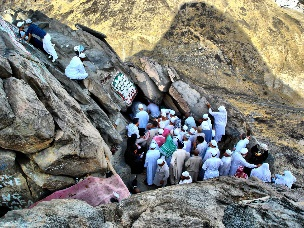
\includegraphics[width=1.34722in,height=1.01046in]{Images/image051.jpg}

\end{marginfigure}


Disons d'emblée que la révélation coranique a commencé près de La
Mecque, dans la grotte de Ḥirā'. Le Coran lui a continué à lui être
révélé jusqu'à sa mort. Pour connaître si un verset est mecquois ou
médinois, on va s'appuyer sur les compagnons~: \emph{un tel a entendu
que Muḥammad, alors qu'il été à La Mecque, a récité le verset\ldots{}
etc.}

Pour autant, il n'y a pas toujours consensus parmi les compagnons, et
par suite, parmi les savants, pour savoir ce qui relève de La Mecque ou
de Médine. Ces divergences ne portent pas tant sur les sourates que sur
des versets de ces sourates. Une sourate en effet, peut contenir des
versets mecquois et des versets médinois.

\begin{Synthesis}
{l'islam, comme système religieux, est achevé.
l'iǧtihād~n'a pas été aboli et il est resté intégré à la réflexion
savante. En revanche, le taqlīd~que les~réformateurs ont remis en
cause.}
\end{Synthesis}

On trouve dans la plupart des ouvrages de \emph{`ulūm al-qur'ān} (le mot
est traduit dans le titre, je dis ça au cas où\ldots) une liste des
sourates mecquoises et médinoises\sn{Par exemple, Zarkašī,
  \emph{al-Burhān fī `ulūm al-Qur'ān}, Cairo, 1958, Vol.1, p. 193.}. Ces
listes sont aussi accompagnées d'un ordre chronologique des sourates.
Mais il faut savoir que cet ordre est sujet à discussion puisque selon
les auteurs, il peut différer. Cela n'est pas sans conséquence\ldots{}

Pour déterminer l'origine d'un verset, il faut donc procéder à
l'\emph{iǧtihād}. Dans cet esprit, on va distinguer des caractéristiques
spécifiques à chaque époque~: thématique, expressions, etc.


\subsection{{Caractéristiques des versets
mecquois
}}


\paragraph{Appel à la conversion}

La prédication mecquoise se caractérise par un appel à la conversion. Il
y a quelque chose de Jean-Baptiste qui appelle à se convertir. Il s'agit
d'abandonner les idoles, les faux dieux et de se tourner vers le Dieu
unique Allāh.


\paragraph{Dimension eschatologique}

Ces versets ont aussi une dimension eschatologique~qui tend à rendre
plus urgente la conversion~: la fin des temps est proche.


\paragraph{Vie droite}

Il s'ensuit un appel à mener une vie droite et juste conformément au
chemin tracé par Dieu (Allāh).


\subsection{{  les thématiques des versets
médinois
} }

 
\paragraph{Abraham}\label{abraham}

le thème d'Abraham comme «~Père des croyants~» où Abraham est dit
d'une part \emph{ḥanīf}, c'est-à-dire monothéiste exclusif, mais aussi
\emph{muslim}, c'est-à-dire soumis, abandonné à Dieu, et ni juif ni
chrétien, date de la période médinoise.

\begin{longtable}{p{5cm}p{5cm}}
\toprule
\endhead
«~Abraham n'était ni juif ni chrétien, mais il était un monothéiste
exclusif, abandonné à Dieu~; il n'était pas au nombre des polythéistes.
Les hommes les plus proches d'Abraham sont vraiment ceux qui l'ont
suivi, ainsi que ce Prophète et ceux qui ont cru~». (S. 3, 67-68). &
\TArabe{مَا كَانَ إِبْرَاهِيمُ يَهُودِيًّا وَلَا نَصْرَانِيًّا وَلَكِنْ
كَانَ حَنِيفًا مُسْلِمًا وَمَا كَانَ مِنَ الْمُشْرِكِينَ إِنَّ أَوْلَى
النَّاسِ بِإِبْرَاهِيمَ لَلَّذِينَ اتَّبَعُوهُ وَهَذَا النَّبِيُّ
وَالَّذِينَ آَمَنُوا وَاللَّهُ وَلِيُّ الْمُؤْمِنِينَ} \\
\bottomrule
\end{longtable}

Ce verset a bien sûr donné lieu à de multiples commentaires. Il est
souvent interprété dans le sens où Abraham est dépositaire de la
religion originelle avant son altération par les juifs et les chrétiens.
Souvent ne veut pas pour autant dire toujours. Il y a d'autres
lectures\ldots{}

Sur la \emph{ḥanīfiyya}, c'est-à-dire cette affirmation d'une foi
exclusive, sans associationnisme (\emph{širk}), le Coran raconte un
dialogue entre Dieu et Abraham\emph{~}:

\begin{quote}
    «~Ainsi avons-Nous montré à Abraham le royaume des cieux et de la terre
afin qu'il soit de ceux qui croient avec conviction. Lorsque la nuit
l'enveloppa, il vit une étoile et dit : « Voilà mon Seigneur ! » Puis,
lorsqu'elle disparut, il dit : « Je n'aime pas les choses qui
disparaissent~». Il vit ensuite la lune se lever et dit : « Voilà mon
Seigneur ! » Puis, lorsqu'elle disparut, il dit : « Si mon Seigneur ne
me guide pas, je serai assurément du nombre des égarés. » Voyant enfin
le soleil levant, il dit : « Voilà mon Seigneur ! Celui-ci est plus
grand~». Puis, lorsqu'il disparut, il dit : « Ô mon peuple, je désavoue
tout ce que vous associez à Dieu. Je tourne mon visage comme un vrai
croyant vers Celui qui a créé les cieux et la terre, et je ne suis pas
de ceux qui Lui donnent des associés » (S. 6, 76-79)  \TArabe{فَلَمَّا
جَنَّ عَلَيْهِ اللَّيْلُ رَأَى كَوْكَبًا قَالَ هَذَا رَبِّي فَلَمَّا
أَفَلَ قَالَ لَا أُحِبُّ الْآَفِلِينَ (}76\TArabe{) فَلَمَّا رَأَى الْقَمَرَ
بَازِغًا قَالَ هَذَا رَبِّي فَلَمَّا أَفَلَ قَالَ لَئِنْ لَمْ يَهْدِنِي
رَبِّي لَأَكُونَنَّ مِنَ الْقَوْمِ الضَّالِّينَ (}77\TArabe{) فَلَمَّا رَأَى
الشَّمْسَ بَازِغَةً قَالَ هَذَا رَبِّي هَذَا أَكْبَرُ فَلَمَّا أَفَلَتْ
قَالَ يَا قَوْمِ إِنِّي بَرِيءٌ مِمَّا تُشْرِكُونَ (}78\TArabe{) إِنِّي
وَجَّهْتُ وَجْهِيَ لِلَّذِي فَطَرَ السَّمَاوَاتِ وَالْأَرْضَ حَنِيفًا
وَمَا أَنَا مِنَ الْمُشْرِكِينَ (}79\TArabe{) وَحَاجَّهُ قَوْمُهُ قَالَ
أَتُحَاجُّونِّي فِي اللَّهِ وَقَدْ هَدَانِ وَلَا أَخَافُ مَا تُشْرِكُونَ
بِهِ إِلَّا أَنْ يَشَاءَ رَبِّي شَيْئًا وَسِعَ رَبِّي كُلَّ شَيْءٍ
عِلْمًا أَفَلَا ت

َتَذَكَّرُونَ} \\

\end{quote}
Ce dialogue est connu dans le monde biblique. Il se retrouve dans des
écrits juifs, chrétiens et judéo-chrétiens~: Ainsi par exemple, dans
\emph{L'Apocalypse d'Abraham}\sn{~\emph{L'Apocalypse d'Abraham}
  est un livre apocryphe dont on dispose de manuscrits en roumain et en
  slave. L'original devait être une traduction grecque de l'hébreu ou de
  l'araméen. Le texte est daté du premier siècle, sans doute après la
  destruction du Temple de Jérusalem par les Romains en 70. Apocalypse
  d'Abraham car il est question de la vie du patriarche et de son
  dialogue avec Dieu mais aussi d'une ascension et de visions où les
  anges* jouent un rôle important, notamment celle du char céleste de
  Dieu (cf. Ez 1).} : «~Plus que la terre, j'appellerai digne de
vénération le soleil car il éclaire de ses rayons le monde et les
différentes atmosphères. Mais celui-là non plus je ne le placerai pas
parmi les dieux, car la nuit, sa course est assombrie par les nuées~»
(7, 1, 7).

Le terme \emph{ḥanīf} est employé par deux fois pour Muḥammad (S. 10,
105 et 30, 30), Muḥammad étant lui-même chargé de détruire les idoles de
la Ka`ba.

L'injonction est aussi adressée aux Gens du Livre à qui il fut demandé
seulement d'agir «~comme des \emph{ḥunafā'} (\emph{ḥunafā' est le
pluriel de ḥanīf}) et non comme des polythéistes~» (S. 22, 31).


\paragraph{Falsification des
écritures}

- toute la théologie coranique relative à la falsification des
écritures~:
\begin{quote}
«~Comment pouvez-vous désirer qu'ils croient avec vous, alors que
certains d'entre eux ont falsifié sciemment~la Parole de Dieu, après
l'avoir entendue~?» (S. 2, 75) est de Médine. \TArabe{أَفَتَطْمَعُونَ أَنْ
يُؤْمِنُوا لَكُمْ وَقَدْ كَانَ فَرِيقٌ مِنْهُمْ يَسْمَعُونَ كَلَامَ
اللَّهِ ثُمَّ يُحَرِّفُونَهُ مِنْ بَعْدِ مَا عَقَلُوهُ وَهُمْ
يَعْلَمُون} \\
\end{quote}


\paragraph{Vie à Médine}

- De même, les prescriptions relatives à la manière de vivre datent de
Médine~:

\begin{longtable}{p{5cm}p{5cm}}
\toprule
\endhead
«~Il n'appartient pas à un croyant ou une croyante, une fois qu'Allah ou
Son messager ont décidé une chose d'avoir encore le choix dans leur
façon d'agir. Et quiconque désobéit à Allah et son messager s'est égaré
certes, d'un égarement évident~» (S. 33, 36).
&
\TArabe{وَمَا كَانَ
لِمُؤْمِنٍ وَلَا مُؤْمِنَةٍ إِذَا قَضَى اللَّهُ وَرَسُولُهُ أَمْرًا أَنْ
يَكُونَ لَهُمُ الْخِيَرَةُ مِنْ أَمْرِهِمْ وَمَنْ يَعْصِ اللَّهَ
وَرَسُولَهُ فَقَدْ ضَلَّ ضَلَالًا مُبِينًا} \\
\bottomrule
\end{longtable}

Toutes les questions relatives au statut social et légal sur le mariage,
le divorce, les héritages, les punitions\ldots{} sont aussi de Médine.

Outre les différences thématiques, on trouve différentes
expressions~propres à chaque période. Ainsi, les adresses \textbf{«~Ô
vous qui croyez~» ou «~Ô gens du Livre~» caractérisent les sourates
médinoises} tandis que \textbf{«~Ô vous les gens~» est plutôt
mecquoise}.


\subsection{Importance de la
chronologie}

Dans la mesure où le Coran ne suit pas l'ordre chronologique, en quoi
est-il si important du point de vue des sciences coraniques de connaître
cette chronologie et la nature de la sourate (mecquoise ou médinoise)~?

Il s'avère que cette connaissance a des conséquences décisives dans la
référence des versets selon les situations posées. On se souviendra que
les versets mecquois «~parlent~» tout particulièrement aux musulmans
vivant dans une situation difficile et d'hostilité à leur égard. Au
contraire, dans le cadre d'une société musulmane, on s'appuiera
spécifiquement sur les versets de Médine.

Par ailleurs, la chronologie permet de mieux saisir l'évolution des
positions du Coran sur une même question, l'évolution des pratiques, à
l'instar par exemple de la consommation d'alcool.

Enfin, la chronologie permet de distinguer \textbf{les versets
abrogeants des versets abrogés}, c'est-à-dire en cas de contradiction,
celui qui abroge l'autre. Le critère retenu, comme nous le verrons, est
chronologique~: le dernier verset révélé abroge celui qui le précède.


\section{La question de l'abrogation
}\label{ii.-la-question-de-labrogation}

La question de l'abrogation est essentielle dans l'exégèse coranique.
Tandis que le Coran est compris comme une guidance universelle, la
chronologie du Coran montre l'existence d'une progressivité de la
révélation. Sur ce point, il existe selon les commentateurs une
pédagogie divine.

Pour autant, sa pratique n'est pas sans difficulté. Elle est au cœur des
débats contemporains sur l'exégèse coranique dans la mesure où
l'abrogation s'effectue dans le sens chronologique de la révélation. Or,
il s'ensuit que les versets médinois, c'est-à-dire les plus prescriptifs
et légalistes, abrogent les versets plus universels de La Mecque.
Au-delà même de la question versets médinois / versets mecquois, le
verset «~Pas de contrainte en religion~» (S.2, 256) qui est un verset
médinois, est-il abrogé par les versets dits \emph{de l'épée} (S,9,5),
eux aussi médinois~qui lui sont postérieurs ? C'est ce que soutient par
exemple le savant saoudien Ibn Bāz (1910-1999).

\begin{longtable}{p{5cm}p{5cm}}
\toprule
Nulle contrainte en religion! Car le bon chemin s'est distingué de
l'égarement. Donc, quiconque mécroit au Rebelle tandis qu'il croit en
Allah saisit l'anse la plus solide, qui ne peut se briser. Et Allah est
Audient et Omniscient. (S.2, 256)
&
\TArabe{لَا إِكْرَاهَ فِي الدِّينِ قَد
تَّبَيَّنَ الرُّشْدُ مِنَ الْغَيِّ فَمَن يَكْفُرْ بِالطَّاغُوتِ
وَيُؤْمِن بِاللَّهِ فَقَدِ اسْتَمْسَكَ بِالْعُرْوَةِ الْوُثْقَى لَا
انفِصَامَ لَهَا وَاللَّهُ سَمِيعٌ عَلِيمٌ} \\
\midrule
\endhead
Après que les mois sacrés expirent, tuez les associateurs où que vous
les trouviez (S,9,5),. Capturez-les, assiégez-les et guettez-les dans
toute embuscade. Si ensuite ils se repentent, accomplissent la Salât et
acquittent la Zakât, alors laissez-leur la voie libre, car Allah est
Pardonneur et Miséricordieux.
&
\TArabe{ فَإِذَا انسَلَخَ الْأَشْهُرُ الْحُرُمُ
فَاقْتُلُوا الْمُشْرِكِينَ حَيْثُ وَجَدتُّمُوهُمْ وَخُذُوهُمْ
وَاحْصُرُوهُمْ وَاقْعُدُوا لَهُمْ كُلَّ مَرْصَدٍ فَإِن تَابُوا
وَأَقَامُوا الصَّلَاةَ وَآتَوُا الزَّكَاةَ فَخَلُّوا سَبِيلَهُمْ إِنَّ
اللَّهَ غَفُورٌ رَّحِيمٌ 
} \\
\bottomrule
\end{longtable}

\vide{un-principe-juridique-fonduxe9-sur-le-coran}{%
\subsection{{ Un principe juridique fondé sur le
Coran~?
}}\label{un-principe-juridique-fonduxe9-sur-le-coran}}

On distingue donc entre verset abrogé (\emph{ayāh mansūḫa}) et verset
abrogeant (\emph{ayāh nāsiḫa}). Ce principe repose sur le verset
coranique suivant~:

\begin{longtable}{p{5cm}p{5cm}}
\toprule
\endhead
«~nous n'abrogeons aucun verset. Nous n'en faisons oublier aucun sans le
remplacer par un autre qui soit meilleur ou équivalent~» (S. 2, 106). 
&
\TArabe{مَا نَنْسَخْ مِنْ آَيَةٍ أَوْ نُنْسِهَا نَأْتِ بِخَيْرٍ مِنْهَا أَوْ
مِثْلِهَا} \\
\bottomrule
\end{longtable}

Cependant, l'analyse littéraire a montré que le contexte de ce verset ne
renvoie pas au Coran mais aux Écritures antérieures\sn{Michel
  \textsc{Cuypers}, «~Le verset de l'abrogation (2, 106) dans son
  contexte rhétorique~» dans Mehdi Azaiez (dir.) avec la collaboration
  de Sabrina \textsc{Mervin}, \emph{Le Coran : nouvelles approches},
  Paris, CNRS, 2013.}. \textbf{Dieu n'abroge pas les versets de la Torah
sans les remplacer par d'autres~: les versets coraniques}. Autrement
dit, on ne trouverait pas dans le Coran une justification de
l'abrogation du Coran par le Coran. Certains théologiens l'ont aussi
noté, à l'exemple du fondamentaliste Mawdudi (1903-1979)\sn{\textsc{Mawdudi},
  \emph{Comprendre le Coran}.}. On a le même problème avec la théologie
protestante et le principe fondamental de la \emph{sola scriptura}. Mais
où l'Écriture dit-elle que pour une question théologique, on ne peut
recourir pour répondre qu'à l'Écriture~?

Cette question n'est pas anecdotique et peut avoir de grandes
répercussions dans la refondation de la pensée musulmane à laquelle
appellent bien des penseurs musulmans.

\vide{un-enjeu-thuxe9ologique-dieu-peut-il-se-contredire}{%
\subsection{{Un enjeu théologique~: Dieu peut-il se
contredire~?
}}\label{un-enjeu-thuxe9ologique-dieu-peut-il-se-contredire}}

Le fait que des versets coraniques ne tiennent pas la même position
ouvre à une difficulté majeure : Comment la Parole de Dieu, immuable,
éternelle, peut-elle contenir des versets contradictoires~? Dieu ne
pouvant être versatile, comment sa Parole pourrait-elle l'être ? N'y
a-t-il pas le risque d'affaiblir et de remettre en cause l'affirmation
de la nature parfaite du Coran~?

Pour les mu`tazilites, c'est-à-dire les rationalistes, le problème ne se
pose pas~car la Loi donnée par Dieu suit l'intérêt (\emph{al-maṣlaha}).
Chaque contexte est singulier et Dieu donne un commandement qui guide la
communauté dans le sens qui lui est le plus profitable. Ce principe
exégétique a influencé la jurisprudence islamique~: au
11\textsuperscript{ème} siècle, le légiste al-Māwardī (974-1058) écrit~:

«~L'intérêt diffère selon les époques~: un statut shariatique peut très
bien avoir été dans le sens de son intérêt à une époque et un autre,
abrogeant le précédent, aller dans son sens à une autre époque. Chacun
des deux statuts présente un intérêt en son temps, même s'ils sont
antinomiques~»\sn{~Eric \textsc{Chaumont}, «~Abrogation~», dans
  Amir \textsc{Moezzi}, \emph{Dictionnaire du Coran}, \emph{op. cit}.,
  p. 14.}.

Une conséquence est d'introduire dans la Loi divine une distance
critique et un principe de relativisme. La communauté n'applique donc
pas une Loi dans sa littéralité, mais doit d'abord se poser la question
de l'intérêt pour elle-même, dans un contexte géographique et politique
propre. Vous voyez que bien sûr, les fondamentalistes y voient un risque
d'instrumentaliser la Loi divine et de lui ôter son caractère sacré. Ils
accusent les rationalistes et avec eux les nouveaux penseurs de ne
prendre dans la Loi que ce qui les arrange\ldots{} D'autres, plus
contempteurs, diront avec méfiance qu'une lecture souple de la loi ne
peut être que temporaire et s'inscrire dans une stratégie progressive
d'islamisation\ldots{} C'est compliqué, mais il faut connaître toutes
ces discussions et subtilités en arrière-fond de la question de
l'abrogation. Nous y reviendrons quand nous aborderons le droit
islamique (\emph{fiqh}).


\paragraph{l'acharisme}{{ L'acharisme~est une
école~{théologique}~de
l'{islam}, fondée
par~{Abu
Al-Hasan
al-ʾAshʿarī}~({873}-{935}).
(\TArabe{الأشعرية}~). Cette école de pensée se répandit très vite et devint
l'école théologique majoritaire. D'abord adepte du~mu'tazilisme~il~s'en
sépara au moins sur deux points
essentiels~:} 
\begin{itemize}
    \item il affirme que l'homme est libre de ses actions mais
c'est Dieu qui crée ses actes (bons ou
mauvais)
\item Il déclare que le~Coran~est incréé car, étant la Parole de Dieu lui-même, elle fait donc partie de lui
\end{itemize}}


Pour le courant théologique \textbf{asharite}, une telle thèse est
impossible : \textbf{Dieu ne peut être versatile dans sa volonté}.
\textbf{Al-Rāzī} (m. 1209), le grand commentateur du Coran, répond en
soulignant la \textbf{dimension pédagogique de Dieu}~: Dieu ne se
contredit pas mais prend l'homme tel qu'il est et le fait avancer à son
rythme.
\mn{Al-razi, théologien musulman de rite chaféite, est né à
Ray ou 1150, et mort en 1210 à Hérat. Musulman d'obédience sunnite, il
écrit le Le Grand Commentaire du Coran (aussi connu sous le titre Les
Clés de l'invisible). fervent défenseur de la doctrine de
l'unicité}

\vide{abrogation-et-falsification}{%
\subsection{Abrogation et
falsification}\label{abrogation-et-falsification}}

L'abrogation concerne aussi et surtout les écritures antérieures. Pour
les musulmans, les livres donnés aux Juifs et chrétiens ont été altérés,
falsifiés (\emph{taḥrīf}, S. 5, 13) et Dieu leur a substitué l'Écriture
authentique. C'est le \emph{tabdīl} (S. 7, 162) qui consiste donc à
\textbf{remplacer l'erreur par la vérité.}

La dénonciation de la falsification des Écritures prend trois formes. Le
Coran accuse les gens du Livre de ne pas tout dire, d'avoir fabriqué de
faux versets, ou encore d'en avoir effacé certains.

\begin{itemize}
\item
  Ne pas tout dire~: «~Ô Détenteurs de l'Écriture~! Pourquoi
  travestissez-vous la Vérité au moyen du faux~? Pourquoi tenez-vous
  secrète la Vérité, alors que vous savez~? (3, 71).
\end{itemize}

\TArabe{يَا أَهْلَ الْكِتَابِ لِمَ تَلْبِسُونَ الْحَقَّ بِالْبَاطِلِ
وَتَكْتُمُونَ الْحَقَّ وَأَنْتُمْ تَعْلَمُونَ}

\begin{itemize}
\item
  Avoir fabriqué un faux~: «~malheur à ceux qui de leurs propres mains
  composent un livre, puis le présentent comme venant d'Allah pour en
  tirer un vil profit~! Malheur à eux à cause de ce qu'ils en
  profitent~» (S. 2, 79). On retrouve ici le cœur de la polémique
  anti-chrétienne où l'Évangile aurait été dénaturé.
\end{itemize}

\TArabe{فَوَيْلٌ لِلَّذِينَ يَكْتُبُونَ الْكِتَابَ بِأَيْدِيهِمْ ثُمَّ
يَقُولُونَ هَذَا مِنْ عِنْدِ اللَّهِ لِيَشْتَرُوا بِهِ ثَمَنًا قَلِيلًا
فَوَيْلٌ لَهُمْ مِمَّا كَتَبَتْ أَيْدِيهِمْ وَوَيْلٌ لَهُمْ مِمَّا
يَكْسِبُونَ}

\begin{itemize}
\item
  Avoir effacé~: «~Ô détenteurs de l'Écriture~! notre messager est venu
  à vous, vous exposant une grande partie de l'Écriture que vous cachiez
  et aviez effacée aussi une grande partie de celle-ci~» (S. 5, 15).
\end{itemize}

\TArabe{يَا أَهْلَ الْكِتَابِ قَدْ جَاءَكُمْ رَسُولُنَا يُبَيِّنُ لَكُمْ
كَثِيرًا مِمَّا كُنْتُمْ تُخْفُونَ مِنَ الْكِتَابِ وَيَعْفُو عَنْ
كَثِيرٍ قَدْ جَاءَكُمْ مِنَ اللَّهِ نُورٌ وَكِتَابٌ مُبِينٌ}

L'argument théologique de la falsification des écritures n'est pas
nouveau. Il a déjà été utilisé par des chrétiens à l'encontre des juifs.
Mani, le philosophe prophète du deuxième siècle, y a eu aussi recours.

\vide{quels-sont-les-versets-abrogeants-et-abroguxe9s}{%
\subsection{{Quels sont les versets abrogeants~et
abrogés ?
}{ Quels sont les versets abrogeants~et abrogés ? }}\label{quels-sont-les-versets-abrogeants-et-abroguxe9s}}

Là encore, les spécialistes en \emph{`ulūm al-qur'ān}  dressent la
liste des versets abrogés ou abrogeants. Elles ne sont pas identiques.

\mn{{Abū l-Fadl al-Suyūtī, né
en~{1445}~au Caire, est un
savant égyptien connu pour son œuvre abondante. Il fut un éminent
savant~Shâfi'ite, un théologien~Ash'arite~de renom. il serait né dans la
bibliothèque familiale ce qui lui valut son surnom de «~fils des
livres~» (ibn al-kutub). D'une mémoire prodigieuse, il connaissait par
cœur quelque deux cent mille hadiths. Il se rattacha à la~ṭarīqa
shādhiliyya~et prôna l'équilibre entre la Loi et la Voie. On lui
reprocha notamment son emploi de l'ijtihād~mais sans qu'il fut jugé
condamnable. D'une façon générale, il rejeta le pouvoir des Mamelouks.
Il prôna la complémentarité de l'exotérisme et
du~ {soufisme}. On lui
attribue jusqu'à 981
ouvrages.}}

Al-Suyūtī (1445-1505) dans son \emph{Itqān} (cet ouvrage est étudié par
tous les musulmans qui font des sciences islamiques pour devenir imam)
note qu'il existe 21 passages coraniques qui ont été abrogés et il
précise que tous ceux qui en désignent d'autres sont dans l'erreur. Cet
ouvrage n'est pas encore traduit en français, mais le Père Michel
Lagarde, père blanc qui a enseigné au PISAI, en prépare la traduction.
Elle vient de paraître en novembre 2017, mais je ne l'ai pas encore pu
consulter. Je vous signale que pour al-Suyūtī, le verset «~Pas de
contrainte en religion~» (S.2, 256) n'est pas abrogé.

On trouve aussi des listes plus restreintes. Shah Waliullah (fameux
musulman indien mort en 1759) ne retient à partir de la liste de
al-Suyūtī que 5 versets~:

\begin{quote}
Abrogé 2, 180, abrogeant~: 4, 11, 12
\end{quote}

\begin{longtable}{p{4cm}p{8cm}}

\toprule
Abrogé 2, 180 & abrogeant~ 4, 11, 12\\
\midrule
\endhead
On vous a prescrit, quand la mort est proche de l'un de vous et s'il
laisse des biens, de faire un testament en règle en faveur de ses père
et mère et de ses plus proches. C'est un devoir pour les pieux. & Voici
ce qu'Allah vous enjoint au sujet de vos enfants: au fils, une part
équivalente à celle de deux filles. S'il n'y a que des filles, même plus
de deux, à elles alors deux tiers de ce que le défunt laisse. Et s'il
n'y en a qu'une, à elle alors la moitié. Quant aux père et mère du
défunt, à chacun d'eux le sixième de ce qu'il laisse, s'il a un enfant.
S'il n'a pas d'enfant et que ses père et mère héritent de lui, à sa mère
alors le tiers. Mais s'il a des frères, à la mère alors le sixième,
après exécution du testament qu'il aurait fait ou paiement d'une dette.
De vos ascendants ou descendants, vous ne savez pas qui est plus près de
vous en utilité. Ceci est un ordre obligatoire de la part d'Allah, car
Allah est, certes, Omniscient et Sage.

Et à vous la moitié de ce que laissent vos épouses, si elles n'ont pas
d'enfants. Si elles ont un enfant, alors à vous le quart de ce qu'elles
laissent, après exécution du testament qu'elles auraient fait ou
paiement d'une dette. Et à elles un quart de ce que vous laissez, si
vous n'avez pas d'enfant. Mais si vous avez un enfant, à elles alors le
huitième de ce que vous laissez après exécution du testament que vous
auriez fait ou paiement d'une dette. Et si un homme, ou une femme meurt
sans héritier direct, cependant qu'il laisse un frère ou une sœur, à
chacun de ceux-ci alors, un sixième. S'ils sont plus de deux, tous alors
participeront au tiers, après exécution du testament ou paiement d'une
dette, sans préjudice à quiconque. (Telle est l') Injonction d'Allah! Et
Allah est Omniscient et Indulgent. \\
\bottomrule
\end{longtable}

\begin{quote}
Abrogé 2, 240, abrogeant~: 2, 234

Abrogé 8, 65~; abrogeant~: 8, 62

Abrogé 30, 50, abrogeant~: 33, 52

Abrogé 58, 12, abrogeant~: 58, 13.
\end{quote}


\subsection{ L'approche originale de Mahmud Muhammad Taha et \emph{Le
second message de l'islam}}
\mn{Mahmoud Mohammed \textsc{Taha}, \emph{Un islam à
  vocation libératrice}, traduit par Mohamed El Baroudi-Haddaoui et
  Caroline Pailhe, Avant-propos de François Houtart, Préface de Samir
  Amin, Paris, L'Harmattan, 2002, 182 pages.}

Maḥmūd Muḥammad Ṭāha est un libre penseur soudanais, fondateur d'un
mouvement politico-religieux «~al-Iḫwān al-Ğumhūriyyūn~» (les frères
Républicains). Ṭāha est né en 1909 à Rufâ`a et il a fondé en 1945 le
parti al\emph{-Ḥizb al-Ğumhūrī} en vue de fonder une République fédérale
indépendante du Soudan. C'est un homme spirituel et au cours d'une de
ses méditations, il reçut une illumination, dans laquelle il lui était
enseigné que le Coran contient deux messages~: celui de Médine
(\emph{šarī`a}) et celui de La Mecque (principes de base spirituels, les
\emph{uṣūl} de la religion islamique). Le premier message~a une vocation
limitée dans le temps, tandis que le second message a une portée
universelle. En appliquant le principe de l'abrogation en lien avec
cette «~révélation~» il propose une exégèse dans laquelle seuls les
versets universels mecquois doivent être portés par la prédication
musulmane.

Sa théorie novatrice dérangea~; il fut accusé et combattu par les
musulmans orthodoxes et les frères musulmans soudanais (\emph{Iḫwān
al-Muslimūn}). Accusé d'apostasie~en 1968 puis en 1985, il est
finalement exécuté en janvier 1985\sn{Annette \textsc{Oevermann},
  «~Ma\underline{h}mûd Mu\underline{h}ammad \underline{T}âha~»,
  \emph{Encyclopédie de l'islam}, p. 105.~}

\begin{quote}
     «~Pour résumer la pensée riche, audacieuse et subtile des
  `Républicains', on peut dire sans trop la caricaturer que le
  \emph{Second message} s'adresse à l'individu pour affirmer et œuvrer à
  réaliser sa `liberté absolue', au point d'être `un Dieu en devenir'~;
  et aux sociétés humaines afin d'instaurer un système où `socialisme'
  et `démocratie' seront enfin réconciliés, et où règnera une égalité.
  absolue entre les hommes, les sexes et les races~» cité par Mustapha Khayati
  \sn{\textsc{ Mustapha Khayati}, ``Le pensée de Mahmud Muhammad Taha'', in Hervé
  \textsc{Bleuchot}, Christian \textsc{Delmet}, Derek \textsc{Hopwood}
  (ed.), \emph{Sûdân}, History, identity, ideology, IRENAM, Oxford,
  1991, p. 290.}
\end{quote}
 

Le message de Ṭāha n'a pas pu être entendu en raison de trois grandes
difficultés~:
\begin{itemize}
    \item son exégèse prend à rebours la tradition qui consistait à abroger
l'ancien par le nouveau.
\item sa lecture a un ancrage mystique, personnel et manque d'assises
exégétiques, méthodologiques et épistémologiques.
\item la portée politique de son message.
\end{itemize}


Aujourd'hui, le défi est de repenser l'abrogation mais au sein même des
données de la tradition. Il faut revenir à l'étymologie, au sens que les
mots avaient pour les compagnons, aux avis des premiers
commentateurs\ldots{} pour cela, il faut aussi recourir aux données des
sciences humaines et des avancées dans notre connaissance du Coran et de
ses commentaires.

%---------------------------------------------------------------------------------------

 
 



 

\vide{iii.-lexuxe9guxe8se-coranique}{%
\section{{L'exégèse coranique
}}\label{iii.-lexuxe9guxe8se-coranique}}

\paragraph{Introduction}
\begin{quote}
    {« Le courant littéraliste, qui considère que le Coran se suffit à
lui-même, que ses ambiguïtés sont voulues par Dieu et que l'interpréter
est source d'égarements, a toujours existé, mais il a longtemps été très
marginal en islam »,}
\end{quote}
~rappelle l'historien Mohammad
Ali Amir-Moezzi 
 . C'est depuis une cinquantaine d'années, avec
l'essor du salafisme, que cette conception a gagné du terrain,
valorisant essentiellement l'apprentissage par cœur.
Plusieurs anecdotes transmises par la tradition islamique montrent un
croyant venant consulter le prophète Mohammed sur le sens de tel ou tel
verset. Il faut dire que le texte coranique est un corpus
particulièrement ardu, au contenu souvent allusif, parfois
contradictoire. Non content d'entremêler des thèmes et registres
différents, il n'a pas été agencé selon l'ordre chronologique de la
révélation.

 
D'où la nécessité de l'interpréter. Riche de plusieurs milliers de
volumes, le commentaire du Coran a connu son âge d'or du
VIII\textsuperscript{e}~au XII\textsuperscript{e}~siècle.\emph{~« Les
grands courants de pensée islamiques se sont tous développés à partir de
la même interrogation : comment comprendre l'écriture sainte
?,~}explique Mohammad Ali Amir-Moezzi.\emph{~­L'islam a hérité de cette
culture exégétique des milieux bibliques au sein desquels il s'est
développé. »}

Les commentateurs ne pouvaient toutefois pas interpréter le Coran à leur
guise. On dénombre trois méthodes principales : 
\bi 
\item la traditionnelle avait
essentiellement recours aux sources scripturaires (le Coran et les
hadiths) et à des analyses sur la langue arabe et la culture tribale ;
\item la rationnelle faisait appel à la logique et à la pensée spéculative, la
logique aristotélicienne ; 
\item et la mystique reposait sur une~\emph{«
illumination »}.
\ei

\subsection{ L'exégèse sunnite~}


\subsubsection{{Terminologie~: \emph{tafsīr} et
\emph{ta'wīl}}}

Je vous avais annoncé une terminologie un peu technique. Ce n'était pas
une promesse de Gascon. Accrochez-vous.

\begin{Def}[tafsīr]
Le \emph{tafsīr} désigne avant tout le commentaire littéral et intégral
du texte coranique sur la base du Coran lui-même, selon le principe
qu'au Coran seul appartient le monopole d'interprétation, et des
matériaux transmis par le prophète Muḥammad ou ses compagnons
(\emph{hadîths}).
\end{Def}

\begin{Def}[ta'wīl, Muhkam, Mutashabih]
Le \emph{ta'wīl} porte en revanche sur l'interprétation du texte en se
fondant sur l'existence de versets obvies (\textit{Muhkam}) et de versets abscons (\textit{Mutashabih}) tels
qu'énoncés dans la Sourate 3, 7~.
\end{Def}


\begin{quote}
«~C'est lui {[}Dieu{]} qui a fait descendre sur toi le Livre. On y
trouve \textbf{des versets clairs} -- la Mère du Livre -- et d'autres
obscurs. Ceux dont les cœurs penchent vers l'erreur s'attachent à ce qui
est obscur car ils recherchent la discorde et ils sont avides
d'interprétations~; mais nul autre que Dieu ne connaît l'interprétation
du Livre. Ceux qui sont enracinés dans la Science disent~: `\,`Nous y
croyons~! Tout vient de notre Seigneur~!'\,' Mais seuls, les hommes
doués d'intelligence s'en souviennent~». Sourate 3, 7


\TArabe{هُوَ الَّذِي أَنْزَلَ عَلَيْكَ الْكِتَابَ مِنْهُ آَيَاتٌ مُحْكَمَاتٌ
هُنَّ أُمُّ الْكِتَابِ وَأُخَرُ مُتَشَابِهَاتٌ فَأَمَّا الَّذِينَ فِي
قُلُوبِهِمْ زَيْغٌ فَيَتَّبِعُونَ مَا تَشَابَهَ مِنْهُ ابْتِغَاءَ
الْفِتْنَةِ وَابْتِغَاءَ تَأْوِيلِهِ وَمَا يَعْلَمُ تَأْوِيلَهُ إِلَّا
اللَّهُ وَالرَّاسِخُونَ فِي الْعِلْمِ يَقُولُونَ آَمَنَّا بِهِ كُلٌّ
مِنْ عِنْدِ رَبِّنَا وَمَا يَذَّكَّرُ إِلَّا أُولُو الْأَلْبَابِ}

"He it is Who has revealed the Book to you; some of its verses are
decisive (Muhkam), they are the basis of the Book, and others are
allegorical (Mutashabih); then as for those in whose hearts there is
perversity they follow the part of it which is allegorical, seeking to
mislead and seeking to give it (their own) interpretation. but none
knows its interpretation except Allah, and those who are firmly rooted
in knowledge say: We believe in it, it is all from our Lord; and none do
mind except those having understanding."
\end{quote}
\vide{les-versets-clairs-et-les-versets-obscurs}{%
\subsubsection{{Les versets clairs et les versets
obscurs
} }\label{les-versets-clairs-et-les-versets-obscurs}}

Si le Coran insiste à maintes reprises sur la clarté et la limpidité de
son expression, ce verset apporte une nuance importante.

Pour Ibn Mas`ūd~: la distinction entre \emph{muḥkam} et \emph{mutašābih}
est la même qu'entre abrogeant et abrogé, ni plus ni moins.

Mais pour Muǧāhid (104/722), cette distinction renvoie à des catégories
éthiques~pour lesquelles Dieu a prescrit sans confusion ce qui est
licite (\emph{ḥalāl}) ou interdit (\emph{ḥarām}).

Pour al-Šāfi`ī (204/820)~: est \emph{muḥkam} ce qui ne peut
s'interpréter que d'une seule manière tandis que \emph{mutašābih}
renvoie à la possibilité d'interprétations plurielles.

Toutefois, la signification du \emph{muḥkami}, c'est-à-dire des versets
clairs n'est accessible qu'aux savants~; tandis que le sens des versets
obscurs est réservé exclusivement à Dieu.

Les exégètes vont ainsi identifier les versets du Coran selon leur degré
d'équivocité. Un texte (\emph{naṣṣ} pl. \emph{nuṣūṣ})~dont la
compréhension est évidente est qualifié de \emph{mufassar}, de
\emph{mubayyan} ou de \emph{mufaṣṣal.} En revanche, si son sens n'est
pas intelligible à son seul énoncé il est dit \emph{muğmal}.

Mais encore~? Retenez de tout cela que dans une discussion théologique,
il ne suffit pas de citer un verset, il faut aussi s'assurer que son
sens est maîtrisé par celui qui le cite et qu'il en connaît la catégorie
d'évidence.

\vide{les-circonstances-de-la-ruxe9vuxe9lation-asbux101b-al-nuzux16bl}{%
\subsection{{Les circonstances de la révélation
(\emph{asbāb al-nuzūl})
}}\label{les-circonstances-de-la-ruxe9vuxe9lation-asbux101b-al-nuzux16bl}}
\begin{Def}[asbāb al-nuzūl]
Les \emph{asbāb al-nuzūl} d'un verset sont définies comme «une
situation, un évènement particulier ou une question posée à Muḥammad à
la suite desquels une révélation survint en guise de réponse divine».
\end{Def}


La connaissance de ces circonstances est nécessaire à la compréhension
des versets coraniques. Or, ces circonstances sont connues par les
témoignages des compagnons de Muḥammad lesquels se retrouvent dans la
\emph{Sīra}. Ici, il apparaît clairement l'existence d'un enchevêtrement
intertextuel entre la \emph{Sīra} et les propos du Prophète, d'une part,
et le Coran d'autre part, dans la mesure où les circonstances
contribuent à la compréhension du Coran.

Ceci toutefois n'est pas sans difficulté dans la mesure où les
compilations de \emph{ḥadīṯ} ou la mise en forme de la \emph{Sīra} sont
postérieures au Coran\ldots{} Il s'ensuit que les circonstances de la
révélation ont conduit souvent à enfermer le sens du texte coranique.
Aujourd'hui, les nouveaux penseurs de l'islam en appellent à sortir le
Coran du \emph{tafsīr} parce qu'ils y voient une sédimentation de son
sens.

Tous les versets du Coran n'ont pas nécessairement de circonstances. Au
sein d'une même sourate, certains versets peuvent être munis de
circonstances et d'autres non.

Exemple de la sourate 96, al-`Alaq, l'adhérence
\begin{quote}
   1. Lis, au nom de ton Seigneur qui a créé,\\
2. qui a créé l'homme d'une adhérence.\\
3. Lis ! Ton Seigneur est le Très Noble,\\
4. qui a enseigné par la plume {[}le calame{]},\\
5. a enseigné à l'homme ce qu'il ne savait pas.

6. Prenez-garde ! Vraiment l'homme devient rebelle,

7. dès qu'il estime qu'il peut se suffire à lui-même (à cause de sa
richesse). 
\end{quote}


La question des circonstances de la révélation pose aussi une question
théologique~: dans la mesure où le Coran est le Livre éternel écrit de
toute éternité, comment peut-il être ainsi lié à des conditions
historiques, à des évènements particuliers survenus au cours de la vie
de Muḥammad~?

\vide{lexuxe9guxe8se-rationaliste-des-mutazilites}{%
\subsection{{L'exégèse rationaliste des mu`tazilites
}}\label{lexuxe9guxe8se-rationaliste-des-mutazilites}}

Je rappelle que les mu`tazilites sont à l'origine d'un courant de pensée
théologique qui a élaboré une théologie spéculative (\emph{kalām}).
\label{Def:kalam}
\begin{Def}[kalām]
Théologie spéculative
\end{Def}
Pour les mu`tazilites, le coran est forcément clair. Dieu ne peut pas
vouloir révéler aux hommes une parole obscure\ldots{} Or, le Coran
contient des passages abscons. Les mu`tazilites disent alors que la
raison permet de comprendre sa parole. Le Coran peut être lu en toute
clarté.

Certes, il y a des anthropomorphismes, on voit Dieu sur un trône\ldots{}
Il est aussi question de sa colère. Mais il s'agit d'images.

Cette théologie est satisfaisante pour l'esprit, elle risque cependant
d'épuiser le sens de la parole de Dieu.

\vide{lexuxe9guxe8se-mystique}{%
\subsection{L'exégèse mystique}\label{lexuxe9guxe8se-mystique}}

Elle est davantage une méditation sur le Coran. Elle part du principe
affirmé dans le \emph{ḥadīṯ} que: «~chaque verset du Coran a un dos et
un ventre et ce ventre a à son tour un ventre et cela jusqu'à sept
ventres~». 
\begin{Def}[Exégèse mystique, ẓāhir, bāṭin]
Il s'agit donc de passer de la formulation littérale,
visible, immédiate (\emph{ẓāhir})~du verset à sa dimension intérieure,
cachée, invisible (\emph{bāṭin}). 
\end{Def}
L'exégèse mystique ne rejette pas
forcément le sens littéral d'un verset, mais elle ne se limite pas à ce
sens.

Je donne un exemple d'interprétation mystique à propose de l'épisode de
l'immolation du fils d'Abraham \textbf{(S. 37, 99-109)~:}

\begin{quote}
«~{[}Abraham{]} dit~:

`Oui, je vais aller vers mon Seigneur, il me guidera. Mon Seigneur~!
Accorde-moi un fils qui soit juste'. Nous lui avons alors annoncé une
bonne nouvelle~: la naissance d'un garçon, doux de caractère. Lorsqu'il
fut en âge d'accompagner son père, celui-ci dit~: `Ô mon fils~! Je me
suis vu moi-même en songe, et je t'immolais~; qu'en penses-tu~?' Il
dit~: `Ô mon père~! Fais ce qui t'est ordonné. Tu me trouveras patient
si Dieu le veut'. Après que tous deux se furent soumis, et qu'Abraham
eut jeté son fils, le front à terre, nous lui criâmes~; `Ô Abraham~! Tu
as cru en cette vision et tu l'as réalisée~: c'est ainsi que nous
récompensons ceux qui font le bien~: voilà l'épreuve concluante'. Nous
avons racheté son fils par un sacrifice solennel. Nous avons perpétué
son souvenir dans la postérité~: `Paix sur Abraham~!' C'est ainsi que
nous récompensons ceux qui font le bien. Il était au nombre de nos
serviteurs croyants~». \\


\TArabe{وَقَالَ إِنِّي ذَاهِبٌ إِلَى رَبِّي سَيَهْدِينِ (}99\TArabe{) رَبِّ هَبْ
لِي مِنَ الصَّالِحِينَ (}100\TArabe{) فَبَشَّرْنَاهُ بِغُلَامٍ حَلِيمٍ
(}101\TArabe{) فَلَمَّا بَلَغَ مَعَهُ السَّعْيَ قَالَ يَا بُنَيَّ إِنِّي
أَرَى فِي الْمَنَامِ أَنِّي أَذْبَحُكَ فَانْظُرْ مَاذَا تَرَى قَالَ يَا
أَبَتِ افْعَلْ مَا تُؤْمَرُ سَتَجِدُنِي إِنْ شَاءَ اللَّهُ مِنَ
الصَّابِرِينَ (}102\TArabe{) فَلَمَّا أَسْلَمَا وَتَلَّهُ لِلْجَبِينِ
(}103\TArabe{) وَنَادَيْنَاهُ أَنْ يَا إِبْرَاهِيمُ (}104\TArabe{) قَدْ
صَدَّقْتَ الرُّؤْيَا إِنَّا كَذَلِكَ نَجْزِي الْمُحْسِنِينَ (}105\TArabe{)
إِنَّ هَذَا لَهُوَ الْبَلَاءُ الْمُبِينُ (}106\TArabe{) وَفَدَيْنَاهُ
بِذِبْحٍ عَظِيمٍ (}107\TArabe{) وَتَرَكْنَا عَلَيْهِ فِي الْآَخِرِينَ
(}108\TArabe{) سَلَامٌ عَلَى إِبْرَاهِيمَ}
\end{quote}
Dans son commentaire, Qušayrī (m.~465)~note qu'Abraham s'est rapproché
de Dieu et que quand il a eu son fils, les choses se sont assises dans
son cœur. Il s'est mis à trop aimer son fils. L'amour de son fils a
rempli son cœur au point d'embarrasser la présence divine en lui et donc
Dieu l'a mis à l'épreuve.

La réponse de l'enfant, «~Fais ce que tu dois accomplir dans la mesure
où c'est un ordre~» rappelle que le Coran ne dit pas explicitement que
c'est un ordre. L'important est que cela a été vécu comme un ordre pour
passer à l'acte.

L'enfant est heureux de ce sacrifice si c'est un ordre divin. L'un et
l'autre suivent les commandements de Dieu. L'enfant accepte non pour le
père, mais pour Dieu.

Qušayrī (m.1074) se demande alors pourquoi Abraham était prêt à
accomplir un tel geste. Dans son commentaire, il dit que pour celui qui
a goûté à l'amitié divine, il est plus facile de sacrifier son propre
fils que de renoncer à la présence divine. Certains auteurs voient dans
la figure du fils celle du moi. Il s'agit de se sacrifier.

Intervient ensuite l'ange Gabriel~: il est une image de la grâce. Tu es
prêt à mourir, mais la mort que tu as acceptée n'est pas la mort, car le
soufi qui est prêt à renoncer à soi est transfiguré par la présence
divine qui s'accomplit en lui.

 
\mn{{Un des grands connaisseurs de Qušayrī est
Pierre Lory p. \pageref{Theol:PierreLory}. Il a donné une conférence à propos de son commentaire
mystique sur les figures de Moïse et d'Aaron. On pourra la consulter
ci-dessous.
} } 
 

\vide{exemples-dexuxe9guxe8se-de-la-fux101tiha}{%
\section{{ Exemples d'exégèse de la \emph{fātiha}
} }\label{exemples-dexuxe9guxe8se-de-la-fux101tiha}}

\emph{Al-fātiha} est la première sourate du Coran. En français, elle se
nomme l'Ouverture ou l'Ouvrante. Pour certains commentateurs, elle est
la quintessence de tout le message du Livre.

Muḥammad Asad (1900-1992), dans \emph{The Message of the Qur'ān}
(1980)~dit que la tradition l'appelle aussi~«~la mère du Livre~»
(\emph{umm al-kitāb})\sn{Muḥammad Asad, \emph{The Message of the
  Qur`ān}, Gibraltar, 1980, p. 1 cité par Hans Küng, op. cit. p. 107.}.

Elle est la prière par excellence que le musulman accomplit en toutes
circonstances. Elle accompagne le rite de la prière quotidienne (un peu
comme le \emph{Notre Père} pour les chrétiens).

Nous allons présenter une exégèse classique et une exégèse moderne. Mais
avant tout, exposons le texte.

\vide{texte-de-la-fux101tiha}{%
\subsubsection{{ Texte de la fātiha
} { 5.1 Texte de la fātiha }}\label{texte-de-la-fux101tiha}}

\begin{longtable}{p{3cm}p{4cm}p{4cm}}
 
\toprule
\endhead
\TArabe{بِسْمِ اللَّهِ الرَّحْمَنِ الرَّحِيمِ (}1\TArabe{)}

\TArabe{الْحَمْدُ لِلَّهِ رَبِّ الْعَالَمِينَ (}2\TArabe{)}

\TArabe{الرَّحْمَنِ الرَّحِيمِ (}3\TArabe{)}

\TArabe{مَالِكِ يَوْمِ الدِّينِ (}4\TArabe{)}

\TArabe{إِيَّاكَ نَعْبُدُ وَإِيَّاكَ نَسْتَعِينُ (}5\TArabe{)}

\TArabe{اهْدِنَا الصِّرَاطَ الْمُسْتَقِيمَ (}6\TArabe{)}

\TArabe{صِرَاطَ الَّذِينَ أَنْعَمْتَ عَلَيْهِمْ غَيْرِ الْمَغْضُوبِ
عَلَيْهِمْ وَلَا الضَّالِّينَ (}7\TArabe{)} & Bismi Allāhi
Ar-Raĥmāni-r-Raĥīm

(2)~Al-Ĥamdu Lillāhi Rabbi-l-`Ālamīn

(3)~Ar-Raĥmāni-r-Raĥīm

(4) Māliki Yawmi-d-Dīn

(5) 'Īyāka Na`budu Wa 'Īyāka Nasta`īn

(6) Ihdinā-ş-Şirāţa-l-Mustaqīm

(7) Şirāţ-Al-Ladhīna 'An`amta `Alayhim Ghayri-l-Maghđūbi `Alayhim Wa
Lā-đ-Đāllīn

&
Au nom de Dieu, le Tout Miséricordieux, le Très Miséricordieux.

Louange à Dieu, Seigneur de l'univers.

Le Tout Miséricordieux, le Très Miséricordieux.

Maître du Jour du Jugement dernier.

C'est Toi {[}Seul{]} que nous adorons, et c'est Toi {[}Seul{]} dont nous
implorons secours.

Guide-nous dans le droit chemin,

la Voie de ceux que Tu as comblés de faveurs, pas celle de ceux qui ont
encouru Ta colère, ni celle des égarés.
\\
\bottomrule
\end{longtable}


\vide{lexuxe9guxe8se-de-la-fux101tiha-selon-al-razux12b}{%
\subsubsection{{L'exégèse de la \emph{fātiha} selon
al-Razī
}}\label{lexuxe9guxe8se-de-la-fux101tiha-selon-al-razux12b}}

Al-Rāzī est né en 543/1148 à Rayy.

Son Commentaire~principal se nomme \emph{Les clés de l'invisible}.

Il est un commentaire mot par mot, verset par verset. C'est un
commentaire explicatif. Rāzī a donc cherché à percer les secrets
grammaticaux, les secrets de la stylistique. Pourquoi tel mot est
employé et pas tel autre~? Pourquoi à telle place~? Pourquoi une phrase
nominale et pas une phrase verbale~?

Al-Rāzi dresse aussi une théologie de la louange à partir de la fātiha.

En effet, il y a deux manières de louer Dieu~: \emph{al-ḥamdu li-Llāh}
et \emph{subḥāna' Llāh}.

On distingue ainsi la théologie du \emph{taḥmīd} (action de louer Dieu)
ou théologie du \emph{tasbīḥ.}

Penser à notre histoire de racine trilitère \sn{Qui comporte trois consonnes servant de support aux éléments vocaliques (langues sémitiques).} que nous avons déjà exposée
à propos de la langue arabe. Vous voyez que dans ḥamdu il y a la racine
ḤaMaDa, c'est la même racine que l'on retrouve dans \emph{taḥmīd}. Le
\emph{taḥmīd} est donc le fait de dire \emph{al-ḥamdu li-Llāh}. Un petit
exercice~: retrouver la racine de l'expression \emph{subḥāna' Llāh}. S
BH N a LaL

Or, il remarque que \emph{al-ḥamduli-Llah} est une proposition
nominale~: il n'y a pas de verbe. Il se demande pourquoi on ne dit pas~:
«~je loue Dieu~» ou «~nous louons Dieu~».

Il répond~:

- Dans la phrase verbale~: «~je loue Dieu~», cela signifie que le
locuteur prend l'initiative de la louange. Il aurait donc un certain
pouvoir sur la louange.

Au contraire, «~louange à Dieu~» signifie que Dieu est loué avant même
que je prenne l'initiative de la louange, avant même la louange de ceux
qui le louent. De même il est remercié avant le remerciement de ceux qui
le remercient. Que tu loues ou non Dieu, Dieu est loué de toute éternité
dans sa Propre parole incréée.

- La préposition à (li)~: la louange est donc à Dieu, elle est sa
propriété, elle est son droit. Il mérite donc la louange de par
lui-même, de par son essence, ce que n'indiquerait pas la phrase
verbale.

- Quand on dit «~je loue Dieu~», certes, on le loue, mais quelle est la
nature de cette louange~? Je ne le loue pas de la manière qui convient à
Dieu. Lorsque je dis «~louange à Dieu~», le locuteur ne se met pas en
premier, il se demande même qui il est au fond pour louer Dieu alors que
Dieu est loué par tout l'univers et l'ensemble des êtres. Dire «~je
loue~», c'est se placer dans le temps fini. Or «~louange à Dieu~» a une
valeur infinie.

- Par ailleurs, la louange est un acte intérieur, découlant de la
conscience de l'excellence de celui qui est loué, de sa générosité. Il
mérite d'être exalté et glorifié. Or, si je dis «~je loue Dieu~», mais
sans avoir conscience de la magnificence qui convient à Dieu, c'est un
mensonge~: on dit le louer, mais on ne pense pas à ce que l'on dit. Par
contre, dire `louange à Dieu', que l'on soit conscient ou pas, c'est
toujours vrai. C'est aussi vrai pour la profession de foi «~pas de
divinité en dehors de Dieu~»~; elle est toujours vraie, ce qui n'est pas
le cas de la \emph{shahāda}, l'attestation de foi, le premier pilier de
l'islam~: on peut mentir\ldots{}

On a ici un exemple des subtilités de l'analyse stylistique. Avec une
dimension théologique. Al-Razī veut ainsi montrer qu'il y a toujours
quelque chose de nouveau et d'original à découvrir dans un texte connu
par cœur.

Le commentaire de la \emph{Fātiha} d'al-Rāzi contient plus de 100
pages\ldots{} je m'arrête donc là, en espérant que cela vous aura permis
d'approcher suffisamment la richesse de cette exégèse.


\subsection{L'exégèse de la fātiha et la rhétorique
sémitique (Michel Cuypers).
}


\subsubsection{La rhétorique et le Coran
}

Les auteurs classiques ont bien repéré qu'il existait au sein du Coran
des figures de style. Ainsi, Ibn Qutayba (828-889) dans son \emph{Traité
des difficultés du Coran} (\emph{Kitāb ta'wīl muškil al-Qur'ān}) en 889
remarque que l'on trouve la comparaison, la métaphore, la métonymie (le
fait de remplacer un concept par un autre~comme par exemple : la ville
pour ses habitants~{[}Paris a froid, Paris a faim{]}; le contenant pour
le contenu {[}boire un verre{]}). Il appelle à poser la distinction
entre le sens propre (\emph{ḥaqīqa}) et le sens figuré (\emph{mağāz}).

Cette question stylistique est aussi travaillée par `Abd al-Qāhir
al-Ğurğānī (m. 1078), \emph{Dalā'il al-`iğāz}, \emph{Les preuves de
l'inimitabilité.}~

\vide{la-rhuxe9torique-suxe9mitique-dans-le-coran}{%
\subsubsection{{ La rhétorique sémitique dans le
Coran
}}\label{la-rhuxe9torique-suxe9mitique-dans-le-coran}}

Michel Cuypers, membre de l'IDEO a publié en 2007 \sn{\emph{Le Festin. Une
lecture de la sourate} al-Mā'ida\sn{Michel Cuypers, \emph{Le
  Festin. Une lecture de la sourate} al-Mā'ida, Paris, Lethielleux, («
  Rhétorique sémitique~; 4 »), 2007, IV+453 p.}}. C'est la
5\textsuperscript{ème} sourate. Il s'appuie sur la méthodologie de
Roland Meynet qui a travaillé sur la Bible, mais il s'est demandé dans
la mesure où le Coran est sémitique, s'il était possible de retrouver
les règles de la rhétorique sémitique.

La rhétorique sémitique diffère de la culture grecque où le discours se
présente de manière linéaire : introduction, développement, conclusion.
Séquence / Exorde / narration / péroraison {[}dernière partie d'un
discours structuré{]}.

En revanche, la rhétorique sémitique dépend d'un principe géométrique de
symétrie, elle est plus spatiale. La cohérence du texte est donc à
comprendre dans un autre sens.

\paragraph{Le parallélisme (ab/a'b')}

\begin{longtable}[]{@{}lllll@{}}
\toprule
\textbf{A1} & Au nom de Dieu & \emph{Le très miséricordieux} & \emph{Le
Miséricordieux} & \textbf{im} \\
\midrule
\endhead
\textbf{B2} & Louange à Dieu & \textbf{Le Seigneur} & \textbf{des
mondes/des hommes} & \textbf{in} \\
\textbf{A'3} & & \emph{Le très miséricordieux} & \emph{Le
Miséricordieux} & \textbf{im} \\
\textbf{B'4} & & \textbf{Maître / Roi} & \textbf{Du Jour du Jugement} &
\textbf{in} \\
\bottomrule
\end{longtable}

\paragraph{Le chiasme (ab/b'a') -- ordre inversé}

\begin{longtable}[]{@{}lllll@{}}
\toprule
\textbf{A6} & \emph{\textbf{Guide-nous}} dans la voie droite & & & \\
\midrule
\endhead
\textbf{B7} & la voie de ceux que & \textbf{TU AS GRATIFIE} & \textbf{à
eux} & `Alayhim \\
\textbf{B'} & Non {[}de ceux qui{]} & \textbf{ONT RECONNU TA COLERE} &
\textbf{contre eux} & `Alayhim \\
\textbf{A'} & ni des \emph{\textbf{égarés}} & & & \\
\bottomrule
\end{longtable}

\paragraph{\textbf{Les versets centraux.}}

Dans certaines séquences il existe des versets centraux~: la structure
est donc ABCB'A'. Il se trouve que dans ce cas, les versets centraux
sont mis en relief, ils sont un sommet. Or, dans la sourate
5\textsuperscript{ème}, Cuypers remarque que les versets centraux sont
toujours des versets universalistes.
\begin{quote}
    S. 5,48 : «~Si Dieu l'avait voulu, Il aurait fait de vous une seule
communauté, mais Il a voulu vous éprouver par le don qu'Il vous a fait.
Cherchez à vous surpasser les uns les autres dans les œuvres de bien.
Votre retour à tous se fera vers Dieu~; Il vous éclairera, alors, au
sujet de vos différends~»

\TArabe{وَلَوْ شَاءَ اللَّهُ لَجَعَلَكُمْ أُمَّةً وَاحِدَةً وَلَكِنْ
لِيَبْلُوَكُمْ فِي مَا آَتَاكُمْ فَاسْتَبِقُوا الْخَيْرَاتِ إِلَى
اللَّهِ مَرْجِعُكُمْ جَمِيعًا فَيُنَبِّئُكُمْ بِمَا كُنْتُمْ فِيهِ
تَخْتَلِفُونَ}

S. 5, 69 : «~Certes ceux qui ont cru, ceux qui se sont judaïsés, les
sabéens, et les chrétiens, ceux parmi eux qui croient en Allah, au Jour
dernier et qui accomplissent les bonnes œuvres, pas de crainte sur eux,
et ils ne seront point affligés.».

\TArabe{إِنَّ الَّذِينَ آَمَنُوا وَالَّذِينَ هَادُوا وَالصَّابِئُونَ
وَالنَّصَارَى مَنْ آَمَنَ بِاللَّهِ وَالْيَوْمِ الْآَخِرِ وَعَمِلَ
صَالِحًا فَلَا خَوْفٌ عَلَيْهِمْ وَلَا هُمْ يَحْزَنُونَ}

\end{quote}

On a ici une lecture qui s'appuie sur la cohérence interne du Coran. Et
c'est sans doute la grande force de ce travail qui permet une réelle
réception au sein de la communauté musulmane. Qui plus est, ses
incidences sont nombreuses puisqu'il s'agit aussi de neutraliser les
versets violents du Coran.


%---------------------------------------------------------------------------------------
\subsection{Comment renouveler l'interprétation du Coran au
XXI\textsuperscript{e}~siècle ?}

\begin{quote}
{« Une posture postmoderne veut que le Coran soit dorénavant ouvert
à toute interprétation,~}s'inquiète Abdessamad Belhaj.{~Mais cela
ne doit pas être une excuse pour ne pas explorer l'intelligence interne
du texte lui-même. »}  
\end{quote}
Le lecteur contemporain du Coran doit tout de même
recouvrer son~\emph{« autonomie »,}  ~reconnaît-il toutefois, regrettant
que l'abondante littérature produite dans les siècles passés ait pu
être~\emph{« sacralisée »}.



Si la~\emph{« quasi-totalité »}~des commentaires du Coran se font,
encore aujourd'hui, dans le registre traditionnel,~\emph{« on sent
depuis trois décennies les frémissements d'une nouvelle exégèse, qui
recourt davantage aux méthodes académiques occidentales »,~}observe
Mohammad Ali Amir-Moezzi. Non confessante, cette islamologie née dans le
monde occidental commence à trouver un écho dans des pays musulmans
comme l'Iran, la Tunisie ou la Turquie.

 

Pour ces chercheurs, l'enjeu est de ne plus seulement étudier le Coran à
partir des sources musulmanes datant d'au moins un siècle et demi après
la mort de Mohammed, mais de recourir aussi aux sources non musulmanes
(notamment juives et chrétiennes) du contexte religieux de l'Antiquité
tardive au sein duquel le Coran a émergé. Longtemps restées cloisonnées,
ces deux approches -- confessante et scientifique -- pourraient bientôt
se réconcilier.

%---------------------------------------------------------------------------------------



\subsubsection{Pour aller plus loin}

Retrouver la thèse de Mawdudi sur la question de l'abrogation dans son
opuscule, \emph{Comprendre le Coran.}

Retrouver les versets abrogeants et abrogés selon Shah Waliullah.



% ------------------------------------------------------------------------------------------------------------------------------------

\chapter{La \emph{Sunna} du Prophète ou la Tradition islamique}

À côté du Coran, l'islam se réfère aux corpus des dits et des gestes du
Prophète Muḥammad, à savoir la \emph{Sunna}. Ces corpus qui rassemblent
les dits de Muhammad, nous informe sur son enseignement à la communauté
musulmane, mais aussi ils sont aussi une exégèse de certains versets du
Coran, une lecture, une clarification du contexte. En effet, à maintes
reprises, Muḥammad éclaire, explique, commente les versets coraniques.
Il apporte ainsi un éclairage très précis et concret sur des situations
que le Coran n'aborde pas explicitement. Les questions du dogme
(\emph{`āqida}), du rituel en lien avec l'adoration de Dieu
(\emph{`ibāda}), des relations (\emph{mu`āmalāt}) familiales,
professionnelles, de voisinage, etc. sont précisées et appuyées à la
lumière de la \emph{Sunna}.

Au cours de l'histoire des premiers siècles de l'islam, on a assisté à
une valorisation du \emph{ḥadīṯ} {[}je donne toujours la
translittération `scientifique', vous trouverez souvent \emph{hadith}{]}
à une sacralisation de la parole prophétique. Comment s'explique-t-elle
? Quelles conséquences implique-t-elle quant à l'autorité scripturaire
qui revient au \emph{ḥadīṯ}~comme source fondamentale de l'islam ?

Ces questions sont essentielles pour comprendre l'islam d'autant
qu'elles acquièrent aujourd'hui une acuité nouvelle dans le contexte
d'une crise de la pensée musulmane et de la montée des fondamentalismes.
Entrer dans ces corpus, dans leurs histoires, dans leurs logiques
internes va nous permettre de mieux saisir la nature des enjeux et des
débats au sein de la communauté musulmane contemporaine. Un des
objectifs de ce chapitre est aussi de pouvoir identifier les options
`idéologiques' de certains sites, manuels ou précis sur la \emph{Sunna}
et le \emph{ḥadīṯ} que l'on peut trouver dans des librairies musulmanes
ou sur internet. En effet, une des grandes difficultés pour le néophyte
vient du fait que souvent, il ne sait pas «~où il est~» ou quelle est la
tendance théologique du site ou de l'auteur qu'il lit\ldots{} L'ensemble
de ce cours, et tout particulièrement ce chapitre, doit vous aider à
vous repérer.

\vide{i.-histoire-de-la-sunna}{%
\section{{Histoire de la Sunna
} }\label{i.-histoire-de-la-sunna}}


\subsection{Bref historique
}\label{bref-historique}

\begin{Def}[ṣaḥāba]
Les principaux auteurs qui permettent de connaître les paroles du
Prophète Muḥammad sont avant tout ses compagnons (\emph{ṣaḥāba})~; ils
vécurent avec lui, dans son compagnonnage. Ce sont eux qui ont transmis
à leurs fils, à leur entourage, les paroles qu'ils avaient entendues,
les gestes qu'ils avaient vus, les incidents dont ils furent témoins. Ce
sont donc les premiers `transmetteurs'.
\end{Def}


Du temps du Prophète, certains hommes sont nés après les débuts de la
révélation. Ils ont pu voir le Prophète au cours d'une rencontre, mais
sans pour autant vivre dans son entourage immédiat et le suivre. 
\begin{Def}[tābi`ūn]
Ces
hommes sont les \emph{tābi`ūn}, c'est-à-dire les successeurs des
compagnons.
\end{Def}
 Souvent, ils ont été des disciples des compagnons partis
prêcher l'islam. Ils les ont suivis et se sont mis à leur école,
apprenant les paroles que Muḥammad avait prononcées.

Conformément à la tradition arabe du VII\textsuperscript{e} siècle,
l'apprentissage de ces traditions était oral~; selon la tradition, il
avait été encouragé par le Prophète lui-même, comme l'atteste une parole
prophétique que les compagnons aimaient à rappeler~: «~apprenez à ceux
qui ne sont pas ici tout ce que vous entendez de moi et tout ce que vous
me voyez faire~». Il existait bien la possibilité de s'appuyer sur des
notes (des sortes d'antisèches) mais elles étaient vues comme le signe
d'une mémoire faible ou défaillante et déconsidéraient celui qui
véhiculait les traditions.

Pour autant, comme avec le Coran, l'écrit tend à gagner en crédibilité
dans la mesure où au cours du temps, il apparaît plus fiable que la
tradition orale. On assiste ainsi à l'émergence progressive d'un corpus
de \emph{ḥadīṯ}. D'après les sources musulmanes, l'ordre de compiler par
écrit les \emph{ḥadīṯ} fut donné par le calife Umar Ibn `Abdal `Azīz
(m.117/735)\sn{~D'après la notice biographique d'al-Buḫārī.
  L'indication est aussi donnée par l'Imam Malik dans \emph{al-Muwatta}
  et le \emph{Musnad} de Dārimī.}. Il semble attester la finalisation de
la mise par écrit du Coran. Il n'y avait plus de risques de confondre le
\emph{ḥadīṯ} et le Coran. On voit ainsi parmi les \emph{tabi`īn} (c'est
\emph{tābi`ūn}~au cas sujet, mais ici, j'ai mis la retranscription arabe
au cas indirect) des hommes chargés d'aller à la recherche des
compagnons, de leurs enfants ou de leurs disciples pour dresser une
compilation des \emph{ḥadīṯ}. On trouve ainsi dès le deuxième siècle de
l'Hégire des \emph{Sunna}, c'est-à-dire des corpus de \emph{ḥadīṯ}.

Mais c'est surtout sous la direction d'érudits du IV\textsuperscript{e}
siècle de l'Hégire que l'on établit ces compilations de \emph{Sunna}
officielles et prestigieuses~: elles deviennent la référence
incontournable, certaines intégrant intégralement, les \emph{Sunna} des
Successeurs (\emph{Ṭabi`īn}). Peu à peu, la \emph{Sunna} acquiert une
autorité au point où l'on va parler de deux sources de la révélation.

\vide{les-deux-sources-de-la-ruxe9vuxe9lation}{%
\subsection{Les deux sources de la
révélation}\label{les-deux-sources-de-la-ruxe9vuxe9lation}}

Si le Coran est la révélation de la parole de Dieu, la \emph{Sunna} a
acquis peu à peu dans ces premiers siècles chez certains penseurs
musulmans le statut de révélation (\emph{waḥy}). C'est la théorie des
deux sources de la révélation. On en trouve l'affirmation explicite chez
le théologien Ibn Ḥazm au V\textsuperscript{e} siècle de l'Hégire :

\begin{quote}
«~La révélation (\emph{waḥy}) de Dieu à son Messager se divise en deux
types~: le premier est la proclamation de la révélation (\emph{waḥy
matlū}) comme composition écrite et organisée de manière inimitable et
c'est le Coran~; le second est la révélation des dits transmis mais ne
correspondent pas à une composition écrite, organisée et inimitable~;
ils ne sont pas récités (\emph{lā matlū}) mais ils sont lus et ce sont
les dits qui viennent du messager de Dieu~»\sn{~Abū Muḥammad `Alī
  Ibn Ḥazm, \emph{al-Iḥkām fī Uṣūl al-Aḥkām}, vol. 1, edited by Aḥmad
  Šākir, Maṭb`a al-Imām, Cairo, s.d., p. 87, cité par Aisha Y. Musa,
  \emph{Ḥadīth as Scripture. Discussions on the Authority of Prophetic
  Traditions in Islam}, Palgrave Macmillan, 2008, p. 5.
  \label{Theol:IbnHazm1}. Voir p. \pageref{Theol:IbnHazm} pour plus de détail sur \emph{Ibn Hazm}
 }.
\end{quote}




 

Pour autant, si ce statut est aujourd'hui largement admis parmi les
savants du sunnisme, il ne s'est imposé que progressivement, et
notamment sous l'influence d'une part d'al-Šāfi`ī (m.~204H / 820) le
fondateur d'une des quatre grandes écoles de jurisprudence et d'autre
part, d'Ibn Qutayba (m. 889), grand polygraphe sunnite, hanbalite. {[}On
reverra toutes ces différences entre šāfi`ites, hanbalites et les autres
dans le cours sur le droit musulman{]}.

Tous deux ont écrit des ouvrages dans lesquels ils vont défendre
l'autorité du \emph{ḥadīṯ} contre les opposants au \emph{ḥadīṯ} au sein
de la communauté musulmane. De ces épisodes, nous pouvons déduire qu'il
y avait bel et bien des discussions et des débats sur la question du
statut du \emph{ḥadīṯ} au sein de ces générations. On y reviendra dans
la troisième partie que j'ai intitulée «~Le \emph{ḥadīṯ} en
accusation~».

Une des premières questions à résoudre est la justification du
\emph{ḥadīṯ} par le Coran~: est-ce que le Coran reconnaît et fonde
l'usage de la Sunna dans sa dimension normative~? C'est dans cette
optique qu'al-Šāfi`ī dans sa \emph{Risāla} {[}il s'agit d'une Épître{]}
et dans son \emph{Kitāb ǧimā` al-`ilm} justifie l'autorité du
\emph{ḥadīṯ} par un verset coranique commandant d'obéir au Prophète~:
\begin{quote}
    «~Quiconque obéit au Messager obéit certainement à Allāh~» (S. 4, 80).

\TArabe{مَّن يُطِعِ ٱلرَّسُولَ فَقَدۡ أَطَاعَ ٱللَّهَ‌ۖ}

\end{quote}

Par suite, il en déduit que le \emph{ḥadīṯ} doit être envisagé
pleinement comme une source de la loi~: il est complémentaire au Coran
et constitue une forme de révélation qui contient les commandements
divins. Quant à Ibn Qutayba (m. 276/889), dans l'introduction du
\emph{Traité sur la question des divergences du} \emph{ḥadīṯ}
(\emph{Ta'wīl muḫtalif al-ḥadīṯ}\sn{~L'ouvrage a été intégralement
  traduit en français~: Gérard Lecomte, \emph{Le Traité des divergences
  du Hadit d'Ibn Qutayba} \emph{(mort en 276 / 889)}, Damas, 1962 {[}ICP
  93~779{]}.}), il dresse la liste des groupes opposés au \emph{ḥadīṯ}.
L'ouvrage se présente plus comme une réponse aux détracteurs de la
\emph{Sunna} afin de souligner la pertinence et la fiabilité du
\emph{ḥadīṯ}, que comme une justification théologique du \emph{ḥadīṯ}
comme révélation, mais il n'en demeure pas moins qu'en prenant la
défense du \emph{ḥadīṯ}, il en légitime aussi l'usage.

\vide{les-principales-sunna}{%
\subsection{{Les principales \emph{Sunna}
} }\label{les-principales-sunna}}

Parmi les traditions considérées comme références~et émanant des
\emph{Ṭabi`īn}, on trouve le recueil de Hammām Ibn Munabbih
(m.~101/719)\sn{Ce recueil fut retrouvé et publié par Muhammad
  Hamidullah~sous le titre «~Aqdam ta'lîf fî-l-Hadîth al-nabawî, Sahîfat
  Hammâm ibn Munabbih~wa makânatuhâ fî ta'rîkh `ilm al-Hadîth~»,
  \emph{Majallat al-Majma` al-`ilmî al-`arabî,} R. A. A. D., 28, 1953.},
\emph{al Sahifa as-Sahihah}, et le \emph{Miškat} \emph{al-Massābih}.

Mais l'islam sunnite a reconnu surtout comme référence fondamentale six
recueils. Il s'agit, d'une certaine manière, d'une forme de canonisation
de ces recueils et, paradoxalement, ils ont plus d'importance que les
précédents alors même qu'ils leur sont postérieurs. On les appelle «~les
six livres~» (\emph{kutūb al-sitta}) ou «~les livres les plus
authentiques~». Ces collections sont donc considérées comme
sûres\ldots{}

Deux d'entre eux ont une autorité fondée sur le consensus
(\emph{iğmā`}). Il s'agit du \emph{Saḥīḥ} d'al-Buḫārī (810-870) et du
\emph{Saḥīḥ} de Muslim (819-875). {[}Les éditions ḥadiṯh viennent de
publier une magnifique édition bilingue du \emph{Saḥīḥ} Muslim~en 6
tomes{]} Les \emph{ḥadīṯs} qui y sont répertoriés sont dits d'une valeur
authentique et donc incontestables. Ainsi, les contester reviendrait à
s'écarter de «~l'orthodoxie~». Aïe~!!! C'est là le hic\ldots{} On y
revient très vite~; mais noter aussi que j'ai mis orthodoxie entre
guillemets. Le mot est une relecture occidentale\ldots{} on ne parle pas
d'orthodoxe en islam\ldots même si le journal \emph{La Croix} citant
Abdelkader Merah vendredi 20~octobre 2017 rapporte qu'il dit :
\begin{quote}
    «~Je me revendique comme un musulman orthodoxe~».
\end{quote}
 Mais la
terminologie n'a rien d'arabe~! En revanche, pour les hétérodoxes, oui,
il existe un mot (\emph{zindīq})\ldots{} et même bien d'autres. Nous
avons déjà rencontré celui de \emph{kāfir} (l'infidèle, le mécréant) ou
celui de \emph{mušrik} (l'associateur).

Reconnus aussi pour leur fiabilité les quatre autres recueils sont ceux
d'Ibn Māğa (m. 273/886), d'Abū Dāwūd al-Siǧistānī (m.~275/889) et leurs
\emph{Sunan}, de Tirmiḏī (m. 279/892), auteur du \emph{Ǧāmi`} et de
Nasā'ī (m. 303/915), auteur des \emph{Sunan}.

À ces six recueils principaux, il faut ajouter d'autres ouvrages de
références, mais dont certains dits peuvent être regardés avec
suspicion, considérés comme faibles et donc contestés dans leur
utilisation selon les contextes (sur ces questions subtiles, nous
reviendrons très vite) à l'exemple du \emph{Musnād} d'Ibn Ḥanbal ou d'un
livre de Dārimī (m. 255 / 869). Là, quand un auteur cite ces ouvrages,
il doit savoir qu'on peut les contester\ldots. et qu'on se doit même de
le faire\ldots. parfois. Je me souviens d'une conférence que je donnais
sur l'eschatologie d'al-Ġazālī \label{theol:AlGazali17}, de sa démarche et des dits sur lesquels
il appuie sa théologie. À la fin de la conférence, un jeune musulman est
venu me voir et m'a dit~: «~vous savez, le problème avec al-Ġazālī c'est
qu'il s'appuie sur des dits qui ne sont pas fiables, alors sa thèse ne
tient pas la route\ldots~». C'est pas faux, et du vivant d'al-Ġazālī on
a même fait des autodafés avec sa Somme spirituelle, son \emph{Ihya'}, à
cause de ces dits faibles. Mais qu'est-ce qu'il en pensait lui,
al-Ġazālī, de ces dits~faibles et de l'argumentation de ses détracteurs
? qu'est-ce qu'il aurait répondu au jeune homme qui est venu
m'interpeller~à la fin de la conférence~? À suivre\ldots{}


Mais avant d'aller plus loin, un petit exercice de familiarisation
s'impose.

Nous avons vu beaucoup de noms nouveaux, il faut les digérer.

Aussi, je vous propose~d'aller sur le site de la mosquée de Lyon à la
page suivante~:
\mn{\url{http://www.mosquee-lyon.org/100-le-devoir-de-dire-au-debut-bismillah-et-a-la-fin-al-hamdoulillah/}}


Repérez les \emph{ḥadīṯs} cités et leurs sources (de quels recueils
sont-ils extraits~?)

Sont-ils exclusivement issus des Six livres~? Quelles sont les autres
\emph{Sunnan} utilisées~? Y a-t-il d'autres auteurs que nous n'avons pas
cités~?

Faire le même exercice avec la fatwa du site suivant sur la question de
l'usage des instruments de musique. Commentez.
\mn{\url{http://www.fatawaislam.com/les-distractions/la-musique/1161-les-chansons}}
 \\


\vide{ii.-les-sciences-islamiques-du-ux1e25adux12bux1e6f-ulux16bm-al-ux1e25adux12bux1e6f}{%
\section{{  Les sciences islamiques du \emph{ḥadīṯ}
(\emph{`ulūm al-ḥadīṯ})
} }\label{ii.-les-sciences-islamiques-du-ux1e25adux12bux1e6f-ulux16bm-al-ux1e25adux12bux1e6f}}

Vous avez compris que la question des bons \emph{ḥadīṯ-}s, des
\emph{ḥadīṯ}-s sûrs ou pas sûrs est essentielle.
\begin{Def}[`ulūm al-ḥadīṯ]
Mais comment se
repérer~? Comment savoir~? Comment les identifier~et surtout comment les
a-t-on identifiés~? Qui est-ce qui a pu dire que tel \emph{ḥadīṯ} est
sûr, «~authentique~»~?
\end{Def}
 

Il existe plusieurs ouvrages d'introduction à la science du
\emph{ḥadīṯ}. Le plus célèbre est celui d'Ibn al-Ṣalāḥ \label{Ibnsalah1} (mort à Damas en
643/1245) intitulé \emph{Muqaddima ibn al-Ṣalāḥ fī `Ulūm al-ḥadīṯ.}
L'ouvrage n'est pas traduit en français, mais il existe une traduction
partielle en anglais\sn{~Ibn \textsc{al-Ṣalāḥ}, \emph{An
  Introduction to the Science of the Ḥadīth} Trans. Dr. Eerik Dickinson.
  First ed. Reading: Garnet Publishing Limited, 2006.}. Il y définit
avec minutie toute la terminologie propre au \emph{ḥadīṯ.} Cet ouvrage
donna lieu à des abrégés et à de très nombreux commentaires. Certains
même le transposèrent en vers~: c'est le cas du juge al-Ḫawlī (m.
693/1293). Sans doute pour faciliter son apprentissage.


\subsection[{ Nature de la \emph{Sunna} selon la Tradition}
]

\mn{~Ignaz \textsc{Goldziher}, \emph{Études sur la
  tradition islamique}, trad. par Léon Bercher, Paris, Maisonneuve, 1952
  {[}ICP~: 217 968{]}.}


Je rappelle que la \emph{Sunna} du Prophète désigne le corpus de
\emph{ḥadīṯ}, que le \emph{ḥadīṯ} désigne une information générale. Par
suite, c'est l'ensemble des paroles du Prophète, ses faits, ses gestes
tout au long de la révélation coranique, dans des circonstances diverses
et rapportées par ses compagnons, ses épouses, des témoins variés, et
transmis au cours de l'histoire.

Les \emph{ḥadīṯs} sont d'une grande diversité dans leur forme comme dans
leur nature. On apprend tout sur Muḥammad, la manière dont il
s'habillait, se parfumait, dormait, jusqu'à la manière de se curer les
dents. Un compagnon témoigne qu'il a vu le Prophète commencer la prière
par telle ou telle formule, un autre qu'il la terminait par telle autre,
qu'il élevait les mains à telle hauteur, qu'il enchaînait la prière de
telle manière, que pendant les ablutions il reniflait une, deux ou trois
fois l'eau, etc. Comme nous l'avions déjà relevé dans un chapitre
précédent, le style des \emph{ḥadīṯ} est souvent fleuri, vivant, et très
différent du Coran~; il permet aussi de suivre Muḥammad dans son
quotidien, mais c'est seulement dans la Sīra que nous avons un récit
narratif, suivi.

L'ensemble de ces \emph{ḥadīṯ} qui forment la \emph{Sunna} revêt une
dimension fondamentale pour le croyant musulman. L'étymologie du mot
\emph{Sunna} nous aidera à le comprendre. En effet, en arabe, dans le
désert, la \emph{Sunna}, c'est la voie, le chemin, la piste. Elle est
une question de vie ou de mort. S'écarter de la \emph{Sunna}, c'est
prendre un chemin de mort. En suivant le Prophète, on est sur la bonne
piste, celle qui nous assure de cheminer vers Dieu. Les gestes du
Prophète Muḥammad, ses pratiques, ses attitudes, sont en tout conformes
à l'islam~; les suivre, les imiter assure donc aux croyants la certitude
de faire ce que Dieu attend d'eux. Suivre la Sunna, c'est donc s'assurer
de se préserver de tout acte illicite, de toute innovation blâmable
(\emph{bid`a}), bref, d'être sur la bonne voie. Je me souviens d'un
jeune «~radicalisé~» qui était en prison à Fleury. Il s'était converti à
l'islam~; il avait été enfant de chœur. Il me disait~: «~tu vois, moi
avec l'islam je sais ce que je dois faire pour plaire à Dieu, le matin,
le midi, le soir, je sais\ldots{} vous les chrétiens, on n'sait pas ce
qu'il faut faire et quand on nous dit ce qu'il faut faire on n'sait pas
d'où cela vient~?~» On a ici un bel exemple d'orthopraxie salafiste.

Comme pour les sciences coraniques, il y a un certain vocabulaire
technique incontournable à acquérir propre aux sciences du \emph{ḥadīṯ}.
Je ne vais pas vous surcharger de mots arabes et de toute la technicité,
d'ailleurs un cours de 24 heures ne suffirait pas, mais au moins du
minimum en tant qu'initiation. Je ne vous demande pas de les apprendre
par cœur, mais il est bon que votre pupille en prenne une première fois
la photo.

\vide{composition-du-ux1e25adux12bux1e6f}{%
\subsection{{Composition du \emph{ḥadīṯ}
}}\label{composition-du-ux1e25adux12bux1e6f}}

\begin{Def}[ḥadīṯ, isnād, matn]
Le \emph{ḥadīṯ} est composé~:

\begin{itemize}
\item
  de l'\emph{\textbf{isnād}}~: la chaîne de garants. Il va de l'émetteur
  à ceux qui ont transmis l'information. On le trouve généralement sous
  la forme~: «~un tel m'a dit qu'un tel lui avait dit qu'un tel a
  entendu le Prophète dire~».
\item
  du \emph{\textbf{matn}}~: c'est le texte même, la parole prophétique
\end{itemize}
\end{Def}


Je vous donne un exemple~ \sn{Rapporté par Būḫārī dans son \emph{Saḥīh} n°6032}:

\begin{quote}
    D'après `Ā'iša, le Prophète a dit: « Celui qui a la plus mauvaise place
auprès d'Allāh le jour du jugement est celui que les gens ont délaissé
pour se protéger de son mal ».\\
\end{quote}



Voici le texte en arabe~(à lire bien sûr de gauche à droite) :
\begin{quote}
    
\TArabe{عن عائشة رضي الله عنها قال رسول الله صلى الله عليه و سلم: إن شر
الناس عند الله منزلة يوم القيامة من تركه الناس اتقاء شره}

\end{quote}
Ici, l'\emph{isnād} est `Ā'iša~: c'est elle qui a entendu le Prophète
tenir ce propos. La chaîne est composée d'une seule personne.

Le \emph{matn}, c'est la parole du prophète.

Apprendre un \emph{ḥadīṯ} nécessite en toute rigueur d'en apprendre
aussi l'\emph{isnād}. Il est en effet ce qui garantit et authentifie la
valeur de la parole prophétique. Pour les savants musulmans, la chaîne
de transmission relève de l'islam car sans \emph{isnād}, chacun pourrait
dire ce qu'il veut.

\vide{la-nature-des-corpus-musulmans}{%
\subsection{{{La nature des corpus
musulmans}}}\label{la-nature-des-corpus-musulmans}}

Nous avons indiqué dans notre historique l'existence de plusieurs
ouvrages de référence. J'y reviens mais en précisant désormais la
qualification technique des dits recueils de \emph{ḥadīṯ}. L'idée est
que votre œil revoie vite tous ces noms nouveaux, aussi familiers pour
les musulmans que saint Paul l'est pour les chrétiens.

Il existe plusieurs recueils de \emph{ḥadīṯ}~(\emph{muṣannaf}). Un
recueil de \emph{ḥadīṯ} est divisé en chapitres (\emph{kitāb}) suivant
différentes questions. On trouve par exemple~: l'aumône, la prière, le
mariage, la répudiation, le sacrifice de la chevelure\ldots{}

Certains recueils sont aussi classés suivant leurs transmetteurs. Ce
sont des \emph{musnads.} On trouve notamment ceux de Ṭayālisī (m. 203 /
818) et d'Ibn Ḥanbal \label{Theol:IbnHanbal1} (m. 241/855). Dans ce dernier, on trouve près de 30
000 traditions attribuées à près de 700 compagnons.

Certains recueils classent les \emph{ḥadīṯs} selon l'ordre alphabétique
des maîtres (\emph{šuyūḫ}). C'est le cas de Ṭabarānī (m. 360/971). On
dénomme ces recueils des \emph{mu`ǧam}.

On trouve grâce à Internet des bibliothèques de \emph{ḥadīṯ} avec des
moteurs de recherche. Le site
\url{https://sunnah.com/}{\underline{https://sunnah.com/}} (en anglais
et arabe) est à connaître et a permis à nombreux étudiants un travail
sur des sources de qualité.

C'est à partir du VI\textsuperscript{ème} siècle de l'hégire, que l'on
voit émerger des compilations selon le degré d'authenticité ou de
fiabilité des \emph{ḥadīṯs} avec Baġawī (m. 516/1122).

Et qu'en est-il des šī`ites~? Nous n'avons pas encore exposé le cours
sur le šī`isme, mais d'ores et déjà, je tiens à préciser que les šī`ites
n'acceptent pas les critères des sunnites et l'ensemble de leurs
compilations. Pour les šī`ites, ce qui compte, ce sont les traditions
qui reposent sur le témoignage de `Alī Ibn Abī Ṭālib et ses partisans.
On dit plus simplement `Alī tout seul, c'est-à-dire son cousin et
l'époux de sa fille. Il existe un recueil spécifiquement šī`ite,
\emph{al-Kāfī fī `ulūm al-dīn} de Muḥammad Ibn Ya`qūb al-Kulīnī (m.
328/939) qui comporte plus de 15~000 traditions, ainsi que le
\emph{Kitāb man lā yaḥḍuruh al-faqīh} de Muḥammad Ibn `Alī al-Ṣadūq (m.
381/991) et \emph{al-Istibṣār} ainsi que \emph{Tahḏīb al-aḥkām} de
Muḥammad al-Ṭûsī (m. 460/1067). Bien des références sont communes, mais
ce n'est pas systématique, loin de là.

Cependant, le statut des recueils de \emph{ḥadīṯ} dans le šī`isme est de
moindre importance. Car comme nous le verrons, ce qui prime dans le
šī`isme, ce sont les dits des Imāms. Leurs enseignements jouent en effet
un rôle qui n'a pas d'équivalent dans le sunnisme, si bien que le
recours aux paroles de Muḥammad devient secondaire.

\vide{la-question-de-lauthentification-du-ux1e25adux12bux1e6f}{%
\subsection{{\textbf{ La question de
l'authentification du \emph{ḥadīṯ}}
}}\label{la-question-de-lauthentification-du-ux1e25adux12bux1e6f}}

Il existe en islam plusieurs types de spécialistes~: les exégètes du
Coran se dénomment \emph{mufassirūn}, les spécialistes des lectures
coraniques (\emph{qurrā'}), les théologiens, les \emph{uṣūliyyūn}, les
jurisconsultes, les \emph{fuqahā'}. 
\begin{Def}[muḥaddiṯūn]
Il existe aussi des spécialistes du
\emph{ḥadīṯ}, on les appelle les \emph{muḥaddiṯūn} (vous retrouvez la
racine ḤaDaṮa).
\end{Def}
 Avec l'expansion de l'islam, certains nouveaux convertis
éprouvèrent le besoin de partir à la recherche de ces traditions
prophétiques. Ils entreprirent de longs voyages et ramenaient avec eux
ces pierres précieuses.

Cependant, très vite, on s'aperçut que parmi ces pierres, certaines
étaient des mélanges, des alliages de vrai et de faux. Certaines
traditions étaient inventées pour des raisons d'édification morale.
Parfois, en vue de susciter la curiosité de l'auditoire\ldots{} Parfois
à cause de querelles entre sectes (\emph{firaq}), ou des oppositions
entre des écoles juridiques (\emph{maḏāhib}). Bien sûr, certains
\emph{ḥadīṯs} furent aussi forgés à des fins politiques parce qu'ils
servaient les dirigeants contre leurs adversaires~: abbasides contre
omeyyades ou alides, etc. On a même été jusqu'à créer des traditions qui
en condamnaient d'autres.

Face à ces inventions, les savants musulmans ont développé une méthode
critique en vue d'écarter les faux et de noter les dits selon le degré
de fiabilité et d'authenticité. On peut dire qu'avec ce travail sont
nées les sciences du \emph{ḥadīṯ}~: \emph{`ulūm al-ḥadīṯ.}

On distingue donc entre la science de la transmission \emph{`ilm
al-riwāya} qui s'attache à transmettre les traditions avec le plus de
précision possible, et l'étude approfondie de ces traditions \emph{`ilm
al-dirāya}.

L'examen des \emph{ḥadīṯs} porte sur plusieurs dimensions~:

 
 \paragraph{Les transmetteurs eux-mêmes~} : on s'efforce de dresser une biographie,
  leurs carrières, leurs fréquentations, leurs maîtres, leurs disciples,
  qui ont-ils rencontré~? où ont-ils voyagé~? bref, il s'agit de
  connaître les hommes, d'où cette discipline spécifique au sein de
  l'\emph{`ilm al-riwāya} de la connaissance des hommes.
 

 
Par la suite, on établit le degré de confiance que l'on peut accorder au
transmetteur. On analyse la moralité, la tendance politique, religieuse
du transmetteur. Pour être digne de foi, le transmetteur doit être un
musulman doué de raison (\emph{`aql}), d'honorabilité (\emph{`adl}),
doué d'une capacité à retenir fidèlement. De là, on distinguera ceux qui
sont dignes de confiance (\emph{ṯiqa}), ceux qui disent la vérité
(\emph{ṣadūq}), ceux sur lesquels rien de fâcheux ne peut être dit, ceux
qui sont inconsistants ou accommodants, les faibles (\emph{ḍa`īf}), les
menteurs (\emph{kaḏḏāb})\ldots{}
 

 \paragraph{la chaîne de garants}
  Deuxième dimension, l'examen porte sur la chaîne des garants
  (\emph{isnād}). On se demande comment la tradition a été reçue~?
  Est-ce oralement~? par la récitation à un maître, la remise d'une
  copie de traditions, la correspondance (\emph{mukātaba}), le legs
  (\emph{waṣiyya}), la découverte (\emph{wiğāda}) d'un livre de
  traditions~?
 
 
Dans ce cadre, on hiérarchise les \emph{ḥadīṯs} selon les termes
employés dans la transmission~: «~il m'a rapporté~» (\emph{ḥaddaṯanī})
est plus fort que «~il nous a rapporté~» (\emph{ḥaddaṯanā})~; de même,
et en second lieu, «~il m'a informé~» -(\emph{aḫbaranī}) et «~il nous a
informés~» (\emph{aḫbaranā}), ou encore «~j'ai entendu~»
(\emph{sami`tu}), il m'a annoncé (\emph{anba'anī}), etc.

Dans la chaîne des garants, on évalue aussi le nombre de transmetteurs
d'une même tradition. On se demande aussi s'il y a plusieurs voies
(\emph{ṭuruq}) de transmissions~? Le \emph{ḥadīṯ} est dit
\emph{mutawātir} lorsqu'il y a un grand nombre de transmetteurs. En
revanche, il est dit \emph{āḥādi} s'il n'y a qu'un transmetteur ou un
nombre réduit.
 

 
  On analyse aussi la continuité ou la discontinuité de la chaîne des
  garants.
 


\subsection{Quelques règles pour définir si un \emph{ḥadīṯ} est authentique}
On se demande si l'origine du \emph{ḥadīṯ} remonte au Prophète (le
\emph{ḥadīṯ} est dit \emph{marfū'}) ou à un Compagnon (il est dit
\emph{mawqūf}) ou à un Successeur (il est dit \emph{maqṭū`}).

En combinant ces critères, on va apprécier le \emph{ḥadīṯ} et le noter~:

\begin{Def}[ḥadīṯ authentique]
Un \emph{ḥadīṯ} sera soit authentique (\emph{ṣaḥīḥ}), soit bon (\emph{ḥasan}) soit
faible (\emph{ḍa`īf}).

\end{Def}

Je reviens sur votre question sur la hiérarchie de l'\emph{isnad} propre à la Tradition musulmane. 
Dès le II ème et le III ème siècle de l'Hégire, les fondateurs de la science critique du hadith dénoncent des "faussaires" qui inventaient leurs propres chaînes initiatiques et leurs propres hadiths soit par pur piétisme soit pour justifier et fonder leurs propres doctrines. C'est pourquoi,il a bien fallu définir la Tradition dans une forme écrite. 

Avant de parler des chaînes initiatiques, je voudrais souligner qu'il y a d'une manière générale deux formes de hadith : le hadith prophétique, nabawi et le hadith qodsi (sacré). La source du premier est Mohammad ou un des autres Prophètes reconnus par l'islam, tandis que dans la deuxième , c'est Dieu Lui-même qui parle à la première personne. Le Prophète ne fait que transmette ce que lui a été communiqué directement par Dieu en dehors du Coran. 

Concernant les chaînes initiatiques les plus honorées dans la tradition sunnite sont celles qui remontent aux Compagnons et surtout à Abu Baker et à Aycha, épouse du Prophète. Pour les shi'ites, les premiers rapporteurs infaillibles sont avant tout les membres de la famille du Prophète, \textit{ahl al bayt}, Ali le gendre et Fatima la fille.  
Parmi les diverses chaînes initiatiques issues des sources indiqués ci-dessus, , il y en a ce qu'on appelle les "chaînes d'or". Il s'agit surtout d'une chaîne dont tous les membres "sont les plus éminents de leur génération".

Au deuxième siècle, l'islam assista à l’émergence d’une pléiade d’éminents traditionnistes, dans les principaux foyers de culture de l’Empire :
\begin{itemize}
    \item La Mekke : Ibn Jurayj, d’origine byzantine (m. 150/767) ;
\item 	Médine : l’Imâm Mâlik (m. 179/795) ;
\item 	Basra (Irak) : Hammâd b. Salama (m. 167/784) ;
\item 	Koufa (Irak): Sufyân al-Thawrî (m. 161/778);

\item 	A noter que la tradition sunnite évoque un certain Abu Huraryra mort en 628 et qui serait considéré comme le premier traditionniste et qui pourrait être à l'origine de la transmission de 5000 milles hadiths en deux ans.  Un nombre record!
\end{itemize}

Cette génération réalisa le passage essentiel et fécond de l'oral à l'écrit tout en procurant la matière principale aux  pionniers traditionnistes du siècle suivant :
1. Bukhârî (194-256)
2. Muslim (202-261)	
3. Abû Dâwûd (202-275)	
	4. Al-Tirmidhî (v. 200-279)
	5. Al-Nasâ'î (215-303)
	6. Ibn Mâjah (209-273)
A souligner que les deux premiers ont le plus d'autorité. Leurs hadiths sont les seuls reconnus comme "sahih". 

En effet, le \textit{hadith sahih}, selon Al Bukhari par exemple, doit remplir les conditions suivantes : continuité de la chaîne de transmission entre les différents maillons, depuis le Prophète jusqu'à celui qui l'écrit dans son recueil; il faut que chaque maillon soit fiable sur le plan de la moralité 
et au niveau de la rétention / restitution. De même, il ne faut pas que le hadîth présente une singularité; il ne faut pas que la chaîne du hadîth contienne un défaut dissimulé...
Le hadith hasan manque d'une manière générale d'une des conditions précédentes et par conséquence il a moins de valeur que le premier.



\vide{iii.-le-ux1e25adux12bux1e6f-en-accusation}{%
\section{ Le ḥadīṯ en
accusation}\label{iii.-le-ux1e25adux12bux1e6f-en-accusation}}

Le \emph{ḥadīṯ} n'est pas le Coran. Il n'est pas Parole de Dieu et pour
autant, comme nous l'avons vu, il a acquis une importance quasiment
égale au Coran au point d'être considéré comme faisant partie de la
révélation (\emph{waḥy}). Parce que la Sunna est la voie qui garantit le
musulman d'être sur le bon chemin, les mouvements salafistes lui
accordent une précellence. Si le \emph{ḥadīṯ} renseigne sur la manière
dont vivait le prophète de l'islam au VII\textsuperscript{ème} siècle
dans la péninsule arabe, nous avons vu qu'il s'agit aussi de reproduire
ce mode de vie, pas seulement dans son `esprit', mais aussi dans sa
forme~: manger comme il mangeait, se laver comme il se lavait, se
comporter avec les autres comme il se comportait, etc. et cela en tout
temps, et en tout lieu. La Sunna n'est pas seulement pour les arabes
d'Arabie, elle est pour tous les musulmans.

À cet égard, le mouvement \emph{Tablīġī ǧamā`at} (Association pour la
prédication) est un mouvement indien apparu dans les années 20, de
nature apolitique et qui prêche la réislamisation des musulmans indiens
par l'application rigoureuse des rites quotidiens qui furent ceux du
Prophète, et jusqu'aux détails de la vie quotidienne et des gestes
hygiéniques. On va donc insister sur les normes issues des paroles et
des attitudes du Prophète. C'est un mouvement ou revivaliste,
littéraliste, qui est présent dans le monde entier. En France, on le
trouve sous la désignation de l'Association «~Foi et pratique~». Le site
\url{www.inter-islam.org}
est porté par le mouvement.

Il s'agit donc d'appliquer les prescriptions de la \emph{Sunna} et de
suivre les conseils et les ordres du Prophète Muḥammad. Le Collectif des
associations musulmanes de la Loire dans le Document «~Introduction aux
sciences du hadith~» rappelle, selon lui, qu'

\begin{quote}
  «~il est obligatoire pour
tout musulman de ne pas faire de différence entre le Coran et la Sunna,
c'est-à-dire de puiser dans les deux et de bâtir des règles de
législation en se basant sur ces deux car c'est là l'assurance pour ne
pas pencher de droite à gauche et ne pas s'égarer et cela conformément à
la parole du Messager d'Allah qui dit~: `Je vous laisse deux choses,
vous ne vous égarerez jamais si vous vous y cramponnez : le Livre
d'Allāh et ma \emph{Sunna}. Et ils ne se sépareront jamais jusqu'à ce
que me soit présenté le Hawd'~»\sn{Collectif des associations
  musulmanes de la Loire, \emph{Introduction aux sciences du ḥadiṯh},
  p.6.}  .
\end{quote}
 Vous remarquez qu'il s'agit ici d'un bel exemple d'argument
auto-référencié. Parce que la Sunna dit qu'il faut suivre la Sunna, donc
je suis la Sunna\ldots{} Oui, mais pour le coup, le Coran~dit-il qu'il
s'égare celui qui ne suit pas la Sunna du Prophète ?

Cette obligation de suivre la \emph{Sunna} n'a pas été sans soulever
difficulté. Elle est aujourd'hui au cœur d'un débat au sein de la
communauté musulmane, notamment dans le contexte du terrorisme
islamiste. Elle est aussi l'objet de controverses compte tenu du fait
que les prescriptions relatives au port du voile intégral pour les
femmes, ou celles relatives à la lapidation de la femme adultère, ou
encore l'appel à terroriser l'ennemi même au prix de sa vie, ou de tuer
le musulman apostat, ne relèvent pas du Coran, mais du \emph{ḥadīṯ}
seul. Déjà, à la naissance de l'islam, les Ḫāriğites, plus ou moins les
ancêtres de Daesh -- en tous les cas c'est ainsi que d'aucuns les
nommèrent dans le monde sunnite pour les décrédibiliser, ceux-ci étant
considérés comme sortis - d'où la racine ḪaRaǦa = sortir - de la
communauté musulmane, s'appuyaient sur le \emph{ḥadīṯ} 
\begin{quote}
    «~suspendez vos
sabres à vos épaules, et ne faites pas de quartier~!~» 
\end{quote}
pour mener le
\emph{ǧihād} offensif contre tous ceux qui ne partageaient pas leur
avis\sn{~Buḫ 58, 18~; Ḥan IV, 387~; III, 485, 487. Le terme arabe
  est \emph{abīdū} (anéantissez). On trouve parfois à partir
  \emph{abīḥū} (faites-en ce que vous voulez).}. Or, la propagande
ǧihādiste est truffée de \emph{ḥadīṯs}, dont la violence est
incommensurable par rapport au Coran. La question du statut de la
\emph{Sunna} est donc incontournable pour la pensée réformiste.

Au 19\textsuperscript{ème} siècle, analysant les causes du retard du
monde musulman par rapport à l'Occident, l'égyptien Muhammad `Abduh
entreprit une réforme de la pensée musulmane. Il jugea nécessaire
d'apprécier la valeur d'un \emph{ḥadīṯ} en fonction de sa
«~compatibilité~» avec la modernité. Dans la revue \emph{Al-Manār}
dirigée par son disciple Rašīd Riḍā, il a fait publier un article
intitulé «~Al-islām huwwa al-Qur'ān waḥdahu~», l'islam, c'est le Coran
seul\sn{Tawfiq Sidqī «~Al-islām huwwa al-Qur'ān waḥdahu~»,
  \emph{Al-Manār}, 9, 7, Le Caire, 1906, p. 510-524.}.

Ainsi, la critique de la Sunna par les savants musulmans s'articule
autour de deux questions~: celle de l'authenticité du \emph{ḥadīṯ} et
celle de son autorité. Un plongeon dans l'histoire nous montre que ces
deux critiques ne sont pas nouvelles et qu'avant d'avoir été portées par
la pensée réformiste, elles avaient déjà été travaillées et débattues
aux premiers siècles.

\vide{le-probluxe8me-de-lautorituxe9-du-ux1e25adux12bux1e6f}{%
\subsection{{ Le problème de l'autorité du
\emph{ḥadīṯ}
}}\label{le-probluxe8me-de-lautorituxe9-du-ux1e25adux12bux1e6f}}

Ibn Qutayba \label{Theol:IbnQutayba1}-- si ce nom ne vous est pas encore familier, cela devrait
faire `tilt' car nous l'avons rencontré au début de cette leçon. Il a
écrit un Traité sur comment rendre compte et comprendre les divergences
dans le \emph{ḥadīṯ.} A-t-il été traduit en français~? La réponse est en
note 3 -- rapporte que bien des spécialistes du \emph{kalām} (la
théologie spéculative rationaliste) ne voient dans le \emph{ḥadīṯ} que
des propos divergents allant dans tous les sens si bien qu'ils donnent
naissance à des factions rivales, qui s'accusent mutuellement
d'infidélité et se mènent une guerre sans merci. Par conséquent, il va
de soi qu'on ne peut leur accorder aucun crédit.

Voici un exemple de divergence typique dans le \emph{ḥadīṯ}~qui a donné
naissance à des courants théologiques `divergents' :

\begin{itemize}
\item
  les murǧites~ soutiennent que la seule attestation de foi suffit à
  garantir l'accès au Paradis, selon la parole prophétique suivante~:
  «~Quiconque dit~: `il n'y a d'autre divinité que Dieu~! est promis au
  Paradis. On demanda~: `Même s'il commet la fornication et le vol~?' Il
  répondit~: `Même s'il commet la fornication et le vol~!'~»
  (p.2)\sn{Buḫ 60, 47~; Ḥan III, 135, 224.}.
\item
  Mais leurs adversaires leur oppose le \emph{ḥadīṯ} suivant : «~Il
  n'est pas croyant celui dont le voisin n'est pas à l'abri de ses
  méchancetés~»\sn{Buḫ 78, 29~; Ḥan I, 387.}.
\end{itemize}

Un autre exemple entre les partisans de `Alī et ceux d'Abū Bakr~:

\begin{itemize}
\item
  les partisans de `Alī~rappellent que Muḥammad lui a dit : «~Tu occupes
  auprès de moi le même rang qu'Aaron auprès de Moïse~; mais nul
  Prophète ne viendra après moi~»\sn{Buḫ 62, 9~; Ḥan I, 170}
\item
  en opposition, ses adversaires font valoir la parole suivante~:
  «~Prenez modèle sur ceux qui viendront après moi~: Abū Bakr et `Umar~;
  Dieu, son Prophète et les Musulmans ne veulent entendre parler que
  d'Abū Bakr~; le meilleur de cette communauté après son Prophète est
  Abū Bakr~» (p. 5)\sn{Ḥan I, 106, 110\ldots Buḫ 62, 4.}.
\end{itemize}

D'une manière plus systématique, Ibn Qutayba note que les gens du
\emph{kalām} accusent et récusent le \emph{ḥadīṯ}~:

- en raison de l'anthropomorphisme qu'il contient

- des sottises qui suscitent des critiques contre l'islam

- de sa risibilité qui fait rire les infidèles et décourage de devenir
musulman

- du doute qu'il distille chez les hésitants.

Ainsi, les gens du \emph{kalām} pour illustrer leur propos citent le
\emph{ḥadīṯ} dit \emph{de la mouche~}: «~Si une mouche est tombée dans
un récipient, il faut l'y plonger toute entière car une de ses ailes
contient un poison et l'autre son antidote, et ainsi {[}la mouche{]}
apporte d'abord le poison et ensuite le remède~»\sn{Buḫ 59, 17.}.
Or, ceux qui accordent autorité au \emph{ḥadīṯ} croient en cette
prescription et s'y appliquent, alors qu'elle n'est pour les gens doués
d'un tant soit peu de raison que sottise et décrédibilise par conséquent
l'islam.


\subsection{Le problème de l'authenticité du
\emph{ḥadīṯ}~: la critique d'al-Ġazālī accusé de méconnaître la science
du \emph{ḥadīṯ}
}

Je disais précédemment qu'al-Ġazālī \label{theol:AlGazali18} (m.~1111) a fait l'objet de son
vivant d'un rejet de son ouvrage composé de 40 livres et intitulé
\emph{Iḥyā' `ulūm al-dīn}, \emph{La revivification des sciences de la
religion.} Il y passe en revue toutes les dimensions de la vie du
croyant et donne une dimension spirituelle à son enseignement. Pour
al-Ġazālī les hommes ont fini par perdre la sève spirituelle de la vie
croyante~: les gestes sont accomplis dans une fidélité scrupuleuse mais
sans cœur. Revivifier, c'est redonner le souffle spirituel à la vie
croyante. Al-Ġazālī \label{theol:AlGazali19} s'appuie au cours de son enseignement sur
différentes sources. Parmi les deux principales, le Coran, bien sûr, et
la Sunna évidemment. Pour autant, comme le rapportait le jeune musulman
à la suite de ma conférence, al-Ġazālī fut accusé de s'appuyer sur des
\emph{ḥadīṯ} faibles et donc de légitimer des opinions spirituelles ou
théologiques à partir de références inappropriées. Mais si, de son
vivant, on vit se dresser des autodafés de son ouvrage d'édification
spirituelle, celui que l'on surnommait «~Huǧǧat al-islām~», c'est-à-dire
la Preuve de l'islam, ignorait-il vraiment la science du \emph{ḥadīṯ}~?

En fait, al-Ġazālī est fondamentalement perplexe à l'égard de la nature
et des outils de cette science~: «~Il se peut qu'il y ait de nombreux
transmetteurs à toute époque pour appuyer un \emph{ḥadīṯ}, sans qu'il
soit pour autant authentique. On peut imaginer que de nombreuses
personnes puissent avoir un intérêt commun et se mettre d'accord,
surtout après la manifestation des passions partisanes chez les
fondateurs des sectes~; ainsi, les rafiḍites {[}secte šī`ite
extrêmiste{]} prétendent que `Alī Ibn Ṭālib fut désigné par le prophète
pour lui succéder~; ils se fondent sur un \emph{ḥadīṯ} selon eux
authentique~»\sn{~\textsc{Al-Ġazālī }, \emph{Le critère de
  distinction entre l'islam et l'incroyance}. Interprétation et
  divergence en islam, texte édité, traduit et annoté par Mustapha
  Hogga, Préface par Jean Jolivet, Études musulmanes, XLII, Paris, Vrin,
  2010, p. 84-86 (fr.) -- p. 85-87 (ar.).}.

D'autres savants montrent que certains \emph{ḥadīṯs} ont été construits
de toute pièce afin de répondre aux critères d'authentification.
Al-Ġazālī \label{theol:AlGazali20} rapporte aussi le propos d'un savant du nom de Bišr al-Hafi
qui disait du \emph{ḥadīṯ} qu'il est l'une des portes du monde
(\emph{bāb min abwāb al-dunyā}) {[}ici, monde est à comprendre dans sa
dimension mondaine{]} dans la mesure où lorsqu'un homme intervient en
disant `un tel nous a rapporté', il veut dire~: `faites-moi de la
place'\sn{~\textsc{Al-Ġazālī }, \emph{Iḥyā' `ulūm al-dīn},
  \emph{op. cit.,} K. 16, B.2, p. 683 {[}V.4, p. 303{]}.}. À la vue du
contexte, on peut légitimement supposer que tel était bien l'avis
d'al-Ġazālī et on comprend la colère à son encontre des
\emph{muḥḥadiṯūn} qu'il critique et dont il remet en cause la science.

\vide{la-critique-des-penseurs-musulmans-contemporains}{%
\subsection{La critique des penseurs musulmans
contemporains}\label{la-critique-des-penseurs-musulmans-contemporains}}

Aujourd'hui, la critique du \emph{ḥadīṯ} a pris une acuité nouvelle dans
le contexte de la recrudescence de l'islam politique et de l'expansion
du salafisme. Un certain nombre de penseurs musulmans ont repris la
critique des gens du \emph{kalām}~à la lumière des sciences humaines :
la critique porte à la fois sur l'authenticité et l'autorité qui lui
sont conférées. En Egypte, les contempteurs de la Sunna se sont appelés
«~qur'ānistes~» - ceux qui réfutent l'octroi d'une quelconque autorité à
la \emph{Sunna}. En avril-mai 2007, cinq qur'anistes furent arrêtés par
la sécurité égyptienne et emprisonnés~: le motif d'accusation~: être des
qur'ānistes. En avril 2015, un «~autodidacte~» critiqua à la télévision
égyptienne, un \emph{ḥadīṯ} de la Sunna d'al-Bukharī. Je vous rappelle
que selon le consensus de la communauté, tous les \emph{ḥadīṯ} de cette
Sunna sont considérés comme authentiques. Il n'y a pas d'exception.
Commencer à mettre une exception reviendrait à fissurer le consensus et
tout ce qu'il implique du point de vue de la jurisprudence
(\emph{fiqh}). L'enjeu est d'importance. En réaction, on demanda à
al-Azhar de le condamner pour apostasie. Mais signe des temps nouveaux,
al-Azhar s'y refusa.

Les penseurs critiques les plus connus à l'égard de l'autorité et de
l'authenticité des \emph{ḥadīṯ} sont~:

\begin{itemize}
\item
  Rashad Khalifa (égyptien), \emph{Quran, Hadith and Islam}, Tucson, AZ:
  Islamic Publications, 1982.
\item
  Ahmad Mansour.
\item
  Kassim Ahmed (malaysien), \emph{Hadith: A Re-evaluation.}
\item
  Edip Yuksel (turc).
\end{itemize}

De manière moins radicale, la critique du \emph{ḥadīṯ} est aussi traitée
par Abdelmajid Charfi dans son livre, \emph{L'islam entre le message et
l'histoire}.

L'historien tunisien part en effet du paradoxe que la Sunna conserve par
écrit ce que le Prophète avait lui-même demandé de ne pas retranscrire
par écrit pour ne garder que le Coran seul, «~ce qui lui enlève toute
légitimité~»\sn{Abdelmajid Charfi, \emph{L'islam entre le message
  et l'histoire}, Paris, Albin Michel, 2004.}. Par ailleurs, il établit
trois constats~:
\begin{itemize}
    \item 1/ «~cette science est censée faire partie des sciences purement
transmises. Elle ne laisse donc aucune place à l'usage de la raison~: le
musulman ne peut qu'ajouter foi aux hadiths que la communauté s'est
accordée à accepter~». Or, les traditions acceptées venaient d'une
faction qui en a écarté d'autres. Or ces choix doivent être étudiés,
critiqués, ce qui nécessite l'usage de la raison.

\item 2/ le contenu de la Sunna contient aussi les paroles des compagnons
auxquels on confère aussi une valeur exemplaire, égale à celle du
Prophète.

\item 3/ On a mis le \emph{ḥadīṯ} sur un même pied d'égalité avec le Coran.

\end{itemize}

Et Charfi de conclure~: 
\begin{quote}
    
«~Tout cela veut-il dire que tout ce qui nous
est parvenu avec l'estampille de «~hadîth prophétique~» n'ait absolument
aucune valeur~? Sûrement pas~! Nous avons là un trésor vivant qui évoque
des sentiments nobles et impérissables. Mais ce trésor renferme du bon
et du mauvais, des terrains tous fertiles et d'autres désertés par la
vie, des reflets de valeurs propres aux sociétés traditionnelles et des
éléments valables en toute circonstance. Il a donc besoin, à n'en point
douter, d'être remis en question et d'être soigneusement passé au
crible~» (p. 198). 
\end{quote}
Voilà le défi du réformisme du XXIème siècle pour
Charfi.

\vide{conclusion}{%
\section{{Conclusion }}\label{conclusion}}

L'étude du Coran et de la Sunna permet de relever les chantiers sur
lesquels se construit une réforme de l'islam. Les feux de Daesh laissent
dans l'ombre l'activité et les questions posées par les savants
contemporains. Pour autant, la critique est vive~; la réforme est
toujours perçue comme un risque d'infidélité. Réformer, n'est-ce pas
innover~? Trahir~? Symptomatique à cet égard, \emph{Al-Watan}, le
quotidien francophone algérien, a dû supprimer les commentaires de
certains articles, notamment ceux des articles de Ghaleb Bencheikh
écrits et publiés pendant le Ramadan 2015, parce qu'ils étaient trop
«~injurieux~» alors que le philosophe appelait à la réforme de la pensée
musulmane et à celle notamment du statut du \emph{ḥadīṯ}. Pour autant,
ces travaux existent et leur audience dans les pays musulmans est
croissante. La question posée est~: comment éviter que naissent ou
renaissent, tels un Phénix au sein des mondes musulmans, les monstres de
l'islamisme ? Les contempteurs de la Sunna apportent une réponse~:
sortir la Sunna de la révélation et cesser d'en faire une des sources de
la Loi islamique. Mais la nécessité de cette réévaluation est loin
d'avoir convaincu non seulement les masses mais \emph{encore} la
majorité des savants musulmans. La raison en est l'attachement viscéral
du croyant au Prophète Muḥammad.

\section{Pour aller plus loin}

 
{Je vous propose la lecture du livre de
Kassim Ahmed. Toutefois, c'est en anglais\ldots{}
}
\vide{lecture-de-texte-sur-linimitabilituxe9-du-coran}{%
\subsection{Lecture de texte sur l'inimitabilité du
Coran}\label{lecture-de-texte-sur-linimitabilituxe9-du-coran}}

Sur la question de l'inimitabilité, je vous propose de lire
\url{www.lescahiersdelislam.fr/Le-concept-de-l-Inimitabilite-du-Coran-1ere-Partie_a183.html} {l'article}
paru dans \emph{Les cahiers de l'islam} de Fatma Khelef, docteur en
langue et littérature arabes de l'Université de Bordeaux 3, et qui a
pour champ de recherche les œuvres de `Abd al-Qāhir al-Ǧurgānī.

1/ Comment l'auteur définit-elle l'\emph{i`ğāz} ?

2/ Quelles sont les trois grands courants de compréhension de
l'\emph{i`ğāz} qu'elle définit~?

3/ Dégager l'intérêt et les conséquences théologiques de chacune de ces
théories~?

4/ À propos de la compréhension du mot \emph{ummī}, quelle est la
position de l'auteur sur sa signification~?

\vide{la-question-des-versets-sataniques}{%
\subsection{{La question des versets sataniques
}{La question des versets sataniques }}\label{la-question-des-versets-sataniques}}

1/ De quoi s'agit-il~?

2/ À la lumière du cours, dégager l'enjeu théologique de l'affaire
Rushdie~?
 %4 et 5
\chapter{Les cinq piliers de l'islam}
\label{5pilliers}
L'islam repose sur cinq piliers, sur cinq fondements. Il y a~:

\begin{Def}[5 pilliers de l'Islam].

\begin{itemize}
\item
  la \emph{šahāda}, c'est-à-dire l'attestation de foi
\item
  la \emph{ṣalāt}, c'est-à-dire la prière
  La~\emph{salât},~\emph{salâh}~(صلاة {[}ṣalāʰ{]}) ou~\emph{namaz}
\item
  la \emph{zakāt}, c'est-à-dire l'impôt religieux. Éviter de traduire
  \emph{zakāt} par aumône.
\item
  le \emph{ṣiyām}, c'est-à-dire le jeûne
\item
  le \emph{ḥaǧǧ}, c'est-à-dire le pèlerinage
\end{itemize}
\end{Def}

Ces piliers sont eux-mêmes fondés sur le Coran et la Sunna. En effet, la
Sunna de Buḫārī ou celle de Muslim rapportent le propos du prophète
Muḥammad selon lequel, «~l'islam est fondé sur cinq piliers
(\emph{arkān})~». Si la réalité du jeûne, de la prière, etc. se
retrouvent dans le Coran, la détermination de cinq piliers n'est pas
coranique~; elle ne se trouve que dans la Sunna. Ces piliers ont une
valeur religieuse importante dans la mesure où c'est en les
accomplissant que le musulman éprouve l'expérience la plus forte de son
appartenance à l'islam. Le musulman accomplit les piliers, et ainsi il
peut se dire musulman. Mais l'acte d'islam n'est pas que pure pratique
extérieure. Il s'agit d'obéir à Dieu, de le suivre, de se purifier de
ses idoles. Il n'y a pas d'autres dieux que Dieu affirme le musulman
dans la \emph{šahāda.} Tous les autres piliers sont une déclinaison de
cette attestation de foi, de ce témoignage de foi.

Dans ce chapitre, nous allons exposer la valeur spirituelle de ces
piliers et de leur implication pour la vie du croyant en suivant l'un
des maîtres de l'islam~: al-Ġazālī \label{theol:AlGazali10}. La somme spirituelle \emph{Iḥyāʾ
ʿulūm al-dīn}, consacre un livre à chacun de ces piliers.



\vide{i.-la-ux161ahux101da-et-la-double-profession-de-foi}{%
\section{La šahāda et la double profession de
foi}\label{i.-la-ux161ahux101da-et-la-double-profession-de-foi}}

«~Je témoigne qu'il n'y a nul Dieu adoré sinon Dieu et je témoigne que
Muḥammad est le Messager de Dieu~».



\mn{La šahāda en arabe}

\vide{formulation}{%
\subsection{Formulation}\label{formulation}}

La \emph{šahāda} est le premier pilier de l'islam. C'est en la
prononçant que l'on devient musulman. C'est le `baptême musulman', mais
vous voyez que la comparaison est très maladroite : par exemple, dans le
baptême les paroles sont prononcées par le prêtre, dans la
\emph{šahāda}, les paroles sont prononcées par le croyant lui-même,
devant témoins.

Elle est une double attestation~: il s'agit d'attester à la fois
l'unicité divine et de reconnaître la mission prophétique de Muḥammad.

La formule consacrée est «~\emph{ašhadu an lā ilāha illā Llāh}~\emph{wa
ašhadu anna Muhammadan rassūl Allāh} ».

Le mot \emph{šahāda} est constitué de la racine ša.ha.da qui sert dans
la formation des mots \emph{šāhid}, le témoin et \emph{šahīd}, le
martyr. Vous voyez l'importance de bien prononcer en arabe la voyelle
longue~: c'est elle qui va donner le sens au mot.

Le verbe est celui de l'attestation, du témoignage. Il est conjugué à la
première personne du singulier~signifiant l'implication personnelle de
celui qui la prononce, à la différence de la formule plus brève~:
«~\emph{lā ilāha illā Llāh}~». Vous vous souvenez, nous avions vu cette
distinction à propos de la théologie de la louange exposée par al-Rāzī
dans son commentaire de la \emph{Fātiha}, la première sourate du Coran.

\vide{origines-coraniques-de-la-ux161ahux101da}{%
\subsection{{1.2 Origines coraniques de la
\emph{šahāda}}{1.2 Origines coraniques de la šahāda}}\label{origines-coraniques-de-la-ux161ahux101da}}

La \emph{šahāda} n'est pas formalisée comme telle dans le Coran mais on
retrouve dans plusieurs versets du Coran son exposé. Ainsi~:

S.~37, 35~: «~Quand on leur disait~: `Point de divinité à part Dieu',
ils se gonflaient d'orgueil ».

S.~4, 136 : «~Croyez en Dieu et en son Prophète, au Livre qu'Il a révélé
à son Prophète, au Livre qu'Il a révélé auparavant. Quiconque ne croit
pas en Dieu, à ses Anges, à ses Livres, à ses prophètes et au Jour
dernier, se trouve dans un profond égarement.~»

S. 49, 15: «~Les vrais croyants sont seulement ceux qui croient en Dieu
et en Son messager, qui par la suite ne doutent point \ldots~»

S. 7, 158 : «~Dis : `Ô hommes~! Je suis pour vous tous le Messager de
Dieu, à qui appartient la royauté des cieux et de la terre. Pas de
divinité à part lui. Il donne la vie et il donne la mort. Croyez donc en
Dieu, en son messager, le Prophète illettré qui croit en Dieu et en ses
paroles. Et suivez-le afin que vous soyez bien guidés'~».

Un verset concerne le serment d'allégeance de la femme croyante. Il
contient la \emph{šāhada}, mais il témoigne d'une plus grande exigence~:

S. 60, 12~: «~Ô Prophète~! Quand les croyantes viennent te prêter
serment d'allégeance {[}et en jurent{]} qu'elles n'associeront rien à
Dieu, qu'elles ne voleront pas, qu'elles ne se livreront pas à
l'adultère, qu'elles ne tueront pas leurs propres enfants, qu'elles ne
commettront aucune infamie ni avec leurs mains ni avec leurs pieds et
qu'elles ne désobéiront pas en ce qui est convenable, alors reçoit leur
serment d'allégeance, et implore le pardon d'Allah pour elles~».

\vide{remarques-et-commentaires-grammaticaux}{%
\subsection{ Remarques et commentaires grammaticaux
}{}\label{remarques-et-commentaires-grammaticaux}}

Dans cette formule, les grammairiens et lexicographes musulmans ont
souligné trois éléments~:

\begin{itemize}
\item
  \emph{lā ilāha~:} c'est une négation absolue
\item
  \emph{illā Llāh}~: c'est une affirmation absolue.
\item
  Nous traduisons de l'arabe par Dieu deux mots pourtant différents~:
  \emph{ilāh} et \emph{Llāh}. Or, il y a bel et bien une différence de
  sens.

  \begin{itemize}
  \item
    Pour certains philologues, Allāh est un nom propre. Il est le nom de
    l'Essence divine. La \emph{šahāda} peut se traduire ainsi~: s'il y a
    un dieu, c'est Dieu.
  \item
    Cependant, d'autres font remarquer que Allāh vient de la racine
    A.L.H ou W.L.H. dont la signification est~: «~être éperdu d'amour,
    avoir la nostalgie de quelque chose, être haut et briller, être
    voilé, être permanent~». Il s'ensuit une attitude lors de
    l'invocation du nom de Dieu~: attitude emprunte d'humilité, de
    nostalgie et d'amour. La prononciation est emphatique et le ā
    devient quasiment un ô. Dans ce cas, le \emph{ilāh} est une
    illusion. S'il y a une réalité divine, ce ne peut être qu'Allāh.
  \end{itemize}
\end{itemize}

Il y a dans cette formule une affirmation religieuse fondamentale~: il
revient en effet au fidèle de s'écarter de tout ce qui n'est pas Allāh
et cela nécessite un combat, c'est le \emph{ǧihād akbar}, le plus grand
combat. Il s'agit d'un combat contre sa propre personne, son âme qui est
enclin au mal. Il s'agit de reconnaître que Dieu n'a pas d'associé,
qu'il est l'Origine de tout. Maurice Gloton dit de cette formule qu'elle
est «~l'expression la plus parfaite de l'Unicité divine et de la Réalité
essentielle et permanente de l'être~»\sn{~Al-Ġazālī, \emph{Les
  secrets du Pèlerinage en Islam}, avec un commentaire des cinq piliers
  de l'Islam, Paris, Al-Bouraq, p. 60.}.

Ecoutez comment Khaled Roumo parle du mot Allah en arabe. C'était à
l'émission de Ghaleb Bencheikh, Questions d'islam, le 16 octobre 2016.
Vous pouvez
\url{https://www.franceculture.fr/emissions/questions-dislam/amour-et-revelation}{écouter}
l'ensemble de l'émission.

\vide{la-deuxiuxe8me-partie-de-la-formule-est-muux1e25ammad-raux1e63ux16bl-alluxe2h}{%
\subsubsection{{La deuxième partie de la formule est
\emph{Muḥammad Raṣūl
Allâh}}{}}\label{la-deuxiuxe8me-partie-de-la-formule-est-muux1e25ammad-raux1e63ux16bl-alluxe2h}}

Muḥammad vient de la racine Ḥa Mi Da et signifie remercier, célébrer les
perfections d'une chose. Cependant, en tant qu'il s'agit d'un participe
passif de la deuxième forme, il signifie produire la louange. Muḥammad
c'est donc celui en qui la louange est produite. Les grammairiens font
aussi remarquer qu'il s'agit d'un nom de temps et de lieu~: Muḥammad
c'est donc le support de la louange pendant un temps~imparti.

Pour les musulmans, Muḥammad est le nom du Prophète qui est le
réceptacle de la louange. C'est le nom le meilleur qui soit et l'on
comprend pourquoi la tradition encourage à ce que l'on appelle les
garçons par ce nom.

\vide{raux1e63ux16bl-ra-si-la.}{%
\paragraph{Raṣūl~: Ra Si La.}\label{raux1e63ux16bl-ra-si-la.}}

Cette racine a des sens multiples. Elle signifie bien sûr envoyer,
missionner (d'où la fameuse \emph{Risala} d'al-Šafiʿī que nous avons vue
au chapitre précédent et qui signifie \emph{Lettre}, \emph{Épître}, tout
simplement), mais aussi avoir le pas lent, avancer de manière gracieuse
comme le chameau, avoir du lait en abondance, avoir la chevelure longue
et flottante.

De tous ces sens, nous en déduisons que le \emph{Raṣūl} est l'envoyé, le
missionné, le mandaté pour accomplir une mission qu'il accomplit avec
constance apportant l'abondance et le bienfait, dissipant les
oppositions.

\vide{les-enseignements-de-luxe9pigraphie-sur-la-ux161ahux101da}{%
\subsection[1.4 Les enseignements de l'épigraphie sur la \emph{šahāda}
]{\vide{1.4 Les enseignements de l'épigraphie sur la
\emph{šahāda}\sn{\textbf{Frédéric} Imbert, «~L'Islam des pierres~:
  l'expression de la foi dans les graffiti arabes des premiers
  siècles~», \emph{Revue des mondes musulmans et de la Méditerranée}
  {[}En ligne{]}, 129~\textbar~juillet 2011, mis en ligne le 10 mai
  2011, consulté le 18 novembre 2014. URL~:
  http://remmm.revues.org/7067.}
}{1.4 Les enseignements de l'épigraphie sur la šahāda }}\label{les-enseignements-de-luxe9pigraphie-sur-la-ux161ahux101da}}

De quand date l'usage de la \emph{šahāda} comme signe d'appartenance à
l'islam~? Sous quelle forme existait-t-elle~? À cette question
l'épigraphie, c'est-à-dire l'étude des inscriptions dans la pierre,
révèle bien l'existence de l'attestation, mais les plus anciennes
inscriptions ne citent pas le prophète Muḥammad. Ces recherches
confirment ce que nous avions déjà vu à la lumière des sources
musulmanes~: une sacralisation progressive de la figure de Muḥammad et
de ses paroles (\emph{ḥadīṯ}). Nous avons aussi parlé de cette question
dans notre première séance à propos du \emph{Coran des historiens}. Vous
vous souvenez~?

\vide{httpwww.canalacademie.comimgjpgimbert_1_graffiti_spip.jpg}{%
{{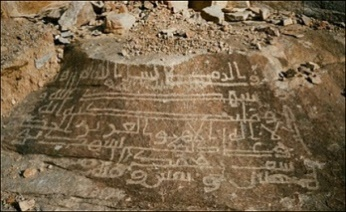
\includegraphics[width=1.57639in,height=0.96528in]{Images/image057.jpg}}{http://www.canalacademie.com/IMG/jpg/Imbert\_1\_graffiti\_SPIP.jpg}}\label{httpwww.canalacademie.comimgjpgimbert_1_graffiti_spip.jpg}}

\vide{graffiti-islamiques-du-duxe9but-de-lislam}{%
\subsubsection{{\textbf{Graffiti islamiques du début de
l'islam}
}{Graffiti islamiques du début de l'islam }}\label{graffiti-islamiques-du-duxe9but-de-lislam}}

\vide{photographie-fruxe9duxe9ric-imbert}{%
\subsubsection{{\textbf{photographie Frédéric
Imbert}}{photographie Frédéric Imbert}}\label{photographie-fruxe9duxe9ric-imbert}}

 

\paragraph{Pour aller plus loin}

Je vous propose de lire l'article de Frédéric Imbert, «~L'Islam des
pierres~: l'expression de la foi dans les graffiti arabes des premiers
siècles~», \emph{Revue des mondes musulmans et de la Méditerranée},
129~\textbar~juillet 2011. Il est consultable en ligne 

Pour vous guider dans sa lecture, une grille de questions~:

§7 et §10. Qu'est-ce que la \emph{basmala}~? Pourquoi l'auteur semble
lui accorder une certaine importance~?

§14. Pourquoi est-il intéressant de noter que la mention du Prophète est
absente~?

§19. Quelle est la thèse et l'argumentation de Y. Nevo à propos de
«~l'évidence de l'absence~»~?

De quand date la première mention du Prophète de l'islam dans un
graffito~? Quelle est sa spécificité~? \\
 

\vide{la-ux1e63aluxe2t-priuxe8re-rituelle}{%
\section{La ṣalât, prière
rituelle}\label{la-ux1e63aluxe2t-priuxe8re-rituelle}}


\vide{hommes-priant-au-caire-en-1865}{%
\mn{{ Hommes priant au Caire en
1865}}\label{hommes-priant-au-caire-en-1865}}

\vide{uxe9tymologie-1}{%
\subsection{Étymologie}\label{uxe9tymologie-1}}

La racine Ṣa.La.Wa signifie blesser au dos, arriver second à la course,
faire une action de grâce qui unit et rapproche. \textbf{Le
\emph{muṣallī}, celui qui prie, est donc toujours second, par rapport à
Celui qu'il prie.}

Si l'on réorganise la racine, on trouve Wa.Ṣa.La qui signifie atteindre,
unir, joindre~: la prière exprime ou réalise une «~jointure~» ce que le
Coran souligne dans le verset S. 33, 56~: «~Certes, Allah est Ses Anges
prient sur le Prophète ; Ô vous qui croyez priez sur lui et adressez lui
vos salutations~».

\TArabe{إِنَّ اللَّهَ وَمَلَائِكَتَهُ يُصَلُّونَ عَلَى النَّبِيِّ يَا
أَيُّهَا الَّذِينَ آَمَنُوا صَلُّوا عَلَيْهِ وَسَلِّمُوا تَسْلِيمًا}

Il existe 5 prières canoniques et selon la tradition musulmane, cette
pratique fut révélée lors de l'Ascension nocturne du Prophète, la
dixième année de sa mission.

\vide{les-cinq-priuxe8res-quotidiennes}{%
\subsection{{2.2 Les cinq prières quotidiennes
}{Les cinq prières quotidiennes }}\label{les-cinq-priuxe8res-quotidiennes}}

Pourquoi y a-t-il 5 prières en islam~? Le Coran ne dit nullement qu'il
faut prier cinq fois par jour. Il n'y est question que de deux prières.
C'est la Sunna qui va déterminer le nombre de cinq prières dans le
\emph{ḥadīṯ} du voyage nocturne du Prophète (\emph{isrāʾ}). En effet,
une nuit, le Prophète de l'islam voyagea en songe de La Mecque à
Jérusalem (voyage horizontal) auquel succéda un voyage vertical où il
monta vers les cieux, c'est l'Ascension (\emph{miʿrāǧ}) avant de
descendre aux enfers en compagnie de l'ange Gabriel sur une monture
nommée Burāq.

Selon la tradition, l'évènement s'est déroulé deux ans avant l'hégire.
La mention se trouve dans S.17, 1~: «~Gloire à celui qui a fait voyager
de nuit son serviteur de la Mosquée sacrée à la Mosquée très éloignée
dont nous avons béni l'enceinte, et ceci pour lui montrer certains de
nos Signes~». Dieu est celui qui entend et qui voit parfaitement, mais
le descriptif nous est racontée et commentée dans la Sunna. Il a donné
lieu de à de nombreuses interprétations. Nous aurons l'occasion d'y
revenir. Remarquez au passage que le Coran ne parle pas explicitement de
Muḥammad.

Voici le récit en question~concernant l'institution des 5 prières :

\begin{quote}
«~Dieu me révéla, alors ce qu'Il voulut, et prescrivit l'accomplissement
de cinquante prières par jour.

Je retournais voir Moïse (Moussa) qui me demanda : "Qu'est-ce qu'a
prescrit le Seigneur à ta Communauté?". - "Une cinquantaine de prières",
lui dis-je. - "Retourne à ton Seigneur et demande-Lui la réduction de ce
nombre, car ta Communauté ne supportera point cette prescription. Je
connais bien les israélites; je les avais mis à l'épreuve et je m'étais
employé à les ramener sur la bonne voie".

Le Prophète poursuivit : Je retournai à mon Seigneur et je Lui demandai
de réduire le nombre des prières pour la faveur de ma Communauté. Il
m'exauça en les amoindrissant de cinq prières. J'allai ensuite trouver
Moïse (Moussa) pour l'informer de la réduction à cinq prières.
Toutefois, il me répéta : "Retourne à ton Seigneur et demande-Lui la
réduction de ce nombre, car ta Communauté ne le supportera point".

Je ne cessai alors de faire la navette entre mon Seigneur (à Lui la
puissance et la gloire) et Moïse (Moussa) (que la paix soit sur lui)
pour demander plus de réduction encore jusqu'à ce que Dieu me décréta:
"Ô Muḥammad ! Je prescris irrévocablement cinq prières jour et nuit,
dont chacune équivaut à dix, cela fait alors cinquante. Quiconque a
dessein de faire une bonne action et ne la fait pas, on lui inscrira une
récompense à son actif; s'il l'exécute, une récompense équivalente à dix
bonnes actions lui sera inscrite. Tandis que quiconque a l'intention de
perpétrer une mauvaise action et qu'il ne l'accomplit pas, rien ne sera
inscrit à son passif; si au contraire il l'accomplit, on lui inscrira la
punition d'une seule mauvaise action".\\
Je redescendis et arrivai auprès de Moïse (Moussa) (que la paix soit sur
lui) pour l'informer de la situation, mais il me dit : "Retourne à ton
Seigneur et demande-Lui une nouvelle réduction".

- "Je suis déjà retourné plusieurs fois à mon Seigneur, jusqu'à ce que
j'aie trouvé inconvenant de Lui adresser encore une fois cette demande."
répondis-je à Moussa~»\sn{Ce \emph{ḥadīṯ} est rapporté par Muslim,
  \emph{Ṣaḥīḥ}, n°234.}.
\end{quote}

Les 5 prières quotidiennes sont~:

\begin{itemize}
\item
  La prière de l'aube (\emph{al-faǧr})
\item
  La prière de la mi-journée (\emph{al-ḏuhr})
\item
  La prière de l'après-midi (\emph{al-`aṣr})
\item
  La prière du coucher de soleil (\emph{al-maġrib}) {[}Vous retrouvez
  Maghreb\ldots{} et oui, c'est l'Occident, là où le soleil se couche~:
  donc ce n'est pas très positif\ldots la lumière vient de l'orient
  alors que l'occident apporte\ldots{} enfin, vous avez compris{]}.
\item
  La prière du soir (\emph{al-ʿišāʾ})
\end{itemize}

À maintes reprises, le Coran insiste sur l'importance de la prière au
cours de la journée et de la nuit et sa portée spirituelle. Nous donnons
quelques-uns de ces versets~:

S.2, 186~: «~Si Mes serviteurs t'interrogent à Mon sujet, qu'ils sachent
que Je suis tout près d'eux, toujours disposé à exaucer les vœux de
celui qui M'invoque. Qu'ils répondent donc à Mon appel et qu'ils aient
foi en Moi, afin qu'ils soient guidés vers la voie du salut.~»

S. 11, 114~: «~Accomplis la salat aux deux extrémités du jour et à
certaines heures de la nuit~».

S. 17, 78~: «~Accomplis la \emph{ṣalāt} au déclin du soleil jusqu'à
l'obscurité de la nuit et fais aussi la lecture à l'aube.~»

S. 24, 36~: «~Dans les maisons qu'Allah a permis que l'on élève (son
nom) et où son nom est invoqué. Que l'on y glorifie en elles matin et
soir.~»

S. 73, 2-7~: «~Lève-toi (pour prier) toute la nuit, excepté une partie,
sa moitié ou un peu moins ou un peu plus. Et récite le Coran lentement
et clairement\ldots La prière pendant la nuit est plus efficace et plus
propice pour la récitation. Tu as dans la journée à vaquer à des longues
occupations.~»

\vide{les-conditions-uxe0-la-priuxe8re}{%
\subsection{{Les conditions à la prière
}}\label{les-conditions-uxe0-la-priuxe8re}}

La prière doit s'effectuer dans un lieu propre. De même, le priant doit
s'assurer de la propreté de ses habits qui doivent recouvrir son corps.
Pas de tenue indécente pour prier.

Dans une mosquée, le fidèle doit tourner son visage vers la direction de
La Mecque~: c'est la \emph{qibla}. Une petite niche appelée
\emph{mihrab} la lui indique.

\vide{mihrab-dans-la-mosquuxe9e-grande-de-cordoue}{%
{{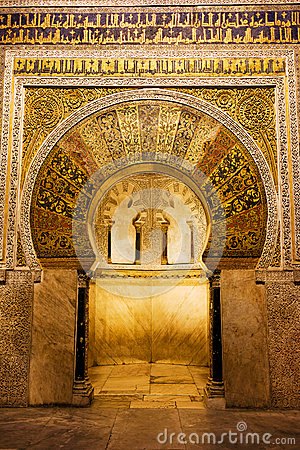
\includegraphics[width=1.40972in,height=2.11458in]{Images/image059.jpg}}{Mihrab dans la mosquée grande de Cordoue}}\label{mihrab-dans-la-mosquuxe9e-grande-de-cordoue}}

\vide{section-29}{%
\subsubsection{{ }{ }}\label{section-29}}

\vide{mihrab-de-cordoue}{%
\mn{{ Mihrab de
Cordoue}{ Mihrab de Cordoue}}\label{mihrab-de-cordoue}}

Il doit précéder sa prière en accomplissant ses ablutions. Elles ont
gagné une certaine importance dans le rite, comme en témoigne le
\emph{ḥadīṯ}~: «~l'ablution est la moitié de la foi~»\sn{~\emph{Ḥadīṯ
  ṣaḥiḥ} rapporté par Muslim ( n°223), Al-Tirmiḏī (n°3517), An-Nasa'ī (
  5/5-6), Ibn Māǧa ( 280 )\label{theol:IbnMaga1}, Ibn Hanbal dans \emph{al-Musnad}.}. Pour cela, il utilise de l'eau, ou à défaut
du sable.

Enfin, il doit formuler l'intention (\emph{niyya}) de faire la prière.
Elle témoigne de la pleine conscience de ce qu'il accomplit.

Que dit al-Ġazālī \label{theol:AlGazali11} de la pratique de la purification~?

Il distingue quatre sens dans ce rituel (Livre 3 de l'\emph{Ihyā'}) :

\begin{itemize}
\item
  la purification extérieure de toute forme de déchets ou de souillures
  diverses. Il s'agit de se purifier des déchets du corps.
\item
  la purification des péchés et des fautes accomplies par le corps
\item
  la purification du cœur de ses vices et de ses mauvais penchants
\item
  la purification du secret intime de tout ce qui n'est pas Dieu.
\end{itemize}

Al-Ġazālī \label{theol:AlGazali12} souligne l'importance de la purification du cœur, de la
purification de toute trace d'idolâtrie à l'époque du Prophète. Or, il
parle de l'obsession de la purification extérieure qui a saisi ses
contemporains et qui est paradoxalement bien loin de celle des Anciens
qui était beaucoup plus profonde. Il parle à cet égard de «~l'idiotie de
la propreté~».

La prière est difficile et la \emph{niyya} ne suffit pas toujours à
garder une concentration fermement tournée vers Dieu. Al-Ġazālī \label{theol:AlGazali13} évoque
les pensées qui sont comme des mouches. De même, la grande mystique de
l'islam Rābi`a disait~: «~Mon Dieu, quand je fais la \emph{ṣalāt},
éloigne de mon cœur toutes les suggestions sataniques (\emph{wasāwis
al-šaytān}), ou alors, par un effet de Ta bonté (\emph{mann}) et de ta
générosité (\emph{karam}), accepte mes prières même troublées par ces
suggestions~»\sn{ʿAttār, \emph{Taḏkīrat al-Awliyā}, cité par
  Badawī p. 157, dans Jean Annestay, p. 101.}.

En islam, \emph{waswas} signifie susurrer à l'oreille, suggérer. Cela
renvoie parfois à une obsession.

\vide{comment-faire-la-priuxe8re}{%
\subsection{{Comment faire la prière~?
}}\label{comment-faire-la-priuxe8re}}

Chaque prière est constitué de la répétition d'un cycle appelé
\emph{rakat}.

Si c'est la première rakat, il s'agit de prononcer la formule
\emph{Allāhu akbar} (\emph{takbīr,} c'est-à-dire c'est le fait de
prononcer cette prière), c'est-à-dire Dieu est plus grand (que tout).
Les mains sont levées au niveau des oreilles et les doigts sont joins.

\vide{httpsupload.wikimedia.orgwikipediacommons44ftakbir_of_prayer.jpg}{%
\mn[
]{\vide{\protect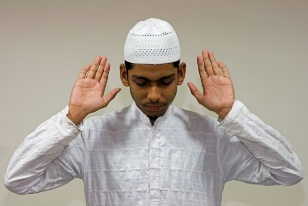
\includegraphics[width=1.38741in,height=0.92708in]{Images/image060.jpg}
}{https://upload.wikimedia.org/wikipedia/commons/4/4f/Takbir\_of\_prayer.jpg }}\label{httpsupload.wikimedia.orgwikipediacommons44ftakbir_of_prayer.jpg}}

Puis il pose la main droite sur sa main gauche au niveau du nombril et
il récite une invocation.

Il demande protection à Dieu avant de réciter la sourate
\emph{al-Fātiha}. Vous vous souvenez, c'est la première sourate du
Coran.

Ensuite, il se prosterne, et en s'abaissant il dit \emph{Allahū akbar.}
Cette position se nomme \emph{ruku}. Il invoque Dieu, puis se redresse,
lève les mains vers les oreilles, puis les rabaisse. Puis il se
prosterne. Cette position se nomme \emph{suǧud}.

\vide{sujud}{%
\mn{{\emph{sujud}}{sujud}}\label{sujud}}

Puis, il s'assoit sur ses genoux et invoque le pardon de Dieu. Il se
prosterne de nouveau et se redresse.

L'ensemble de ce rite s'appelle une \emph{raka}. Il faudra en faire une
ou deux autres.

Pour conclure la prière, le priant salut l'ange de droite et de gauche,
ces anges qui comptabilisent ces bonnes et mauvaises actions pour le
jour du jugement.

Il existe des différences selon les écoles juridiques. Par exemple, le
fait de voir les musulmans se toucher les pieds dans la mosquée est une
prescription du wahhabisme qui date du 18\textsuperscript{ème} siècle~!
Or, elle se généralise, ce qui atteste d'une wahhabisation de l'islam.

Ci-dessous une vidéo récapitulant les gestes, les positions, les paroles
prononcées.

Dans cette explication, beaucoup de choses à remarquer\ldots{} notamment
sur la diversité du rite selon les écoles juridiques (\emph{maḏhab}).

Il est question aussi à plusieurs reprises d'un ouvrage~: \emph{La
citadelle du musulman} qui est un recueil d'invocations selon les
situations de la vie.

À certains moments de la journée, il \textbf{est interdit de faire sa
prière}. Il y aurait là une pédagogie divine. En effet, al-Ġazālī \label{theol:AlGazali14} note
que ce qui est interdit est bien souvent un excitant. De même, les
gestes des différentes postures sont pédagogiques et visent à atténuer
le risque d'ennui. C'est parce que l'on accomplit la prière selon ce
rituel que se polie le cœur.

\emph{Un Récit autour de la prière}

Exemple de Hātim Asamm (le sourd), m. 237/85 \sn{~pour l'anecdote, on l'appelle ainsi,
parce qu'un jour où une vieille femme était venue le consulter, elle
laissa échapper une éructation (expulsion d'un gaz du tube digestif par
la bouche). Pour ne pas embarrasser la femme, il lui demanda de parler
plus fort car il n'entendait pas. La femme fut rassurée, mais pour ce
motif, il joua au sourd 18 années durant, jusqu'à la mort de cette
femme.
}

Donc, «~On lui demandait comment il faisait la prière. Il dit~:
«~D'abord, je purifie mon corps en le lavant avec de l'eau, en même
temps que je lave mon cœur avec la pénitence en faisant une purification
interne. Ensuite, je me rends à la mosquée. En elle je vois la Kaaba, de
même que dans la niche de prière (\emph{mihrāb}) je vois le lieu où se
tenait Abraham. Je distingue à ma droite le Paradis, à ma gauche
l'Enfer, le pont du Sirāt sous mes pieds, Azrā'īl l'ange de la mort
derrière moi. Alors je remets mon cœur à la garde de Dieu, et prononçant
la formule d'entrée en prière `Dieu est grand' (\emph{takbīr}), je joins
mes mains pour la prière, que je fais debout, dans une attitude
suppliante~; je récite le Coran avec soin, je me prosterne en toute
humilité, je reste assis avec persévérance en état d'oraison, et je
finis par l'action de grâce et la salutation~»\sn{\emph{Le
  mémorial des saints}, p. 228-233.}.

\vide{la-zakux101t-limpuxf4t-religieux-purificateur}{%
\section{La zakāt, l'impôt religieux
purificateur}\label{la-zakux101t-limpuxf4t-religieux-purificateur}}



\vide{uxe9tymologie-2}{%
\subsection{Étymologie}\label{uxe9tymologie-2}}

C'est un impôt légal, obligatoire à distinguer de l'aumône libre
\emph{ṣadaqa}.

Étymologiquement, il signifie purifier, croître, prélever.

Cet impôt est lié à la prière~: 
\begin{quote}
    
«~Acquittez-vous de la prière, faites
l'aumône~» (S. 2, 43).
\end{quote}
\vide{bienfaits-de-la-zakux101t}{%
\subsection{{ Bienfaits de la
\emph{zakāt}}}\label{bienfaits-de-la-zakux101t}}

Son but est la circulation des biens et sa répartition équitable. Il
s'agit de faire circuler ce qui est excédent ou superflu~:

\begin{quote}
«~Ils t'interrogent au sujet de ce qu'ils doivent distribuer~? Réponds~:
le superflu~» (S. 2, 219).
\end{quote}

La \emph{zakāt} répond à la nécessité d'enlever l'excédent improductif.
C'est une sorte d'impôt sur la fortune. La \emph{zakāt} doit purifier le
croyant lui-même~: tout est à Dieu. Il doit être responsable devant la
communauté de ce qu'il détient. Ses modalités sont assez complexes et
varient selon les jurisprudences. Initialement, elle ne portait que sur
l'or et l'argent, le bétail, les céréales. Il faut signaler que l'islam
interdit que la monnaie engendre la monnaie et condamne le taux à
intérêt.

Spirituellement, la \emph{zakāt} vise à éprouver le croyant qui prétend
aimer Dieu. Si tu aimes Dieu, alors donne ton superflu. Elle prévient
aussi du danger de prendre l'argent pour Dieu~: elle permet de purifier
le \emph{tawhīd}. C'est-à-dire l'Unicité. Cependant, la \emph{zakāt} ne
doit pas être l'occasion de s'enorgueillir. Il ne faut pas s'en
acquitter publiquement, ce qui constitue aussi une humiliation pour le
pauvre. Le véritable bienfaiteur, ce n'est pas celui qui donne, mais
celui qui reçoit, car il permet à celui qui donne de s'acquitter de ce
qu'il doit donner pour purifier son cœur.

Il s'agit de donner ce qui est licite et ce qui est le plus cher à ses
yeux~: «~Ne choisissez pas ce qui est vil pour donner en \emph{zakāt} »
(S. 2, 267).

\vide{uxe0-qui-donner-la-zakux101t}{%
\subsection{{À qui donner la \emph{zakāt} ?
}}\label{uxe0-qui-donner-la-zakux101t}}

Pour al-Ġazālī \label{theol:AlGazali15}, il faut s'assurer que la personne appartienne à l'une de
ces catégories~:

\begin{itemize}
\item
  elle a la crainte révérencielle~: donc aux pieux, afin de les aider
  dans leur vie spirituelle.
\item
  elle a la science~: donner aux savants, cela contribue à la
  propagation de la foi et de la Loi.
\item
  elle a le sens de la cause première~: autrement dit, elle voit dans le
  don, la manifestation de Dieu. Elle ne s'arrête pas aux moyens, aux
  causes secondes, à la main humaine qui a donné. Cela ne veut pas dire
  qu'elle ne remercie pas le donateur. C'est même une obligation~: celui
  qui n'a pas remercié le donateur n'a pas remercié Dieu.
\item
  elle doit cacher sa pauvreté, ne pas se plaindre.
\item
  elle doit avoir une famille, ou être atteint d'une maladie, croupir
  sous les dettes. La \emph{zakāt} doit lui permettre de sortir de la
  gêne.
\item
  elle doit faire partie des proches et de ceux qui sont liés par le
  sang.
\end{itemize}

\vide{ux1e63iyux101m-et-ux1e63awm-le-jeuxfbne}{%
\section{ṣiyām et ṣawm~: le
jeûne}\label{ux1e63iyux101m-et-ux1e63awm-le-jeuxfbne}}


\vide{ramaux1e0dux101n-mubux101rak}{%
\subsubsection{{\emph{Ramaḍān
mubārak}}{Ramaḍān mubārak}}\label{ramaux1e0dux101n-mubux101rak}}

\vide{duxe9finitions-et-uxe9tymologie}{%
\subsection{Définitions et
étymologie}\label{duxe9finitions-et-uxe9tymologie}}

L'étymologie est intéressante. ṢaWaMa signifie s'abstenir, renoncer à,
s'interdire, se taire, se radoucir en parlant du vent, atteindre le
zénith. Le jeûne a été prescrit au mois de Ramaḍan. Or, RaMaDa renvoie à
l'idée de rôtir, de brûler, d'embraser, d'être brûlant.

\begin{Def}[jeûne]
Le jeûne est donc l'abstention, le silence, l'adoucissement pour
tempérer et neutraliser le feu du mois de Ramadan.
\end{Def}

\mn{Le grand moment liturgique~: c'est le ramadan. On relit le Coran.}
Mais le mois de Ramadan n'est pas qu'affaire de jeûne. Au cours de ce
mois, le musulman est invité à suivre des retraites spirituelles,
notamment les dix derniers jours. Une tradition rapporte~:
\begin{quote}
    «~Dès que
commencent les dix dernières nuits de Ramadan, l'Envoyé de Dieu se
serrait la ceinture, veillait la nuit en dévotion et réveillait les gens
de sa maison~»
\end{quote}. Selon les savants, l'expression «~se serrer la
ceinture~» signifie se détourner des femmes pour montrer tout le sérieux
dans son action spirituelle.

Le but du jeûne est donc spirituel~: parce que l'homme est une créature
entre l'animal et l'ange, s'il se soumet à ses passions, il et ramené à
l'état bestial, mais s'il les combat, il s'élève à celui des anges car
supporter la faim et la soif est un attribut de Dieu et des anges.

\vide{diffuxe9rents-types-de-jeuxfbne}{%
\subsection{4.2 Différents types de
jeûne}\label{diffuxe9rents-types-de-jeuxfbne}}

\emph{Ṣiyām} qualifie le jeûne obligatoire~; c'est le jeûne légal de
prescription divine. Il est un exercice de soumission volontaire, le
bouclier de la chasteté quand on ne peut pas se marier~; le jeûne
consiste aussi en l'abstention de tout mal, en paroles et en actes.

Al-Ġazālī \label{theol:AlGazali16} distingue trois sortes de jeûnes~:

\begin{itemize}
\item
  Le jeûne des gens du commun~: on s'abstient de manger ou de boire,
  d'avoir des rapports sexuels.
\item
  le jeûne des gens de l'élite~: empêcher le regard, la langue, la main,
  le pied, l'ouïe, la vue et l'ensemble des membres de commettre des
  péchés.
\item
  le jeûne de l'élite de l'élite~: c'est le jeûne du cœur devant les
  basses ambitions et les idées qui éloignent de Dieu.
\end{itemize}

Le jeûne n'est pas purement abstinence~: il est associé à la nécessité
de la réconciliation, de la générosité, de l'hospitalité. On peut citer
à cet égard le \emph{ḥadīṯ}~suivant : \emph{«~Pour celui qui ne renonce
pas au mensonge dans les actes et les paroles, Dieu n'a nul besoin qu'il
renonce à sa nourriture et à sa boisson}~».

\emph{ṣawm} qualifie le jeûne libre. Le jeûne n'est pas spécifique au
mois du Ramadan. Les musulmans sont invités à jeûner au début et à la
fin de chaque mois, ou trois jours au milieu. On doit aussi jeûner le
jour de \emph{ʿarafāt} ou de \emph{ʿāšūrāʾ}. Vous ne connaissez pas ces
deux mots. Pas de panique. Cela viendra et je vous enverrai un petit
pensum\ldots{}

Le jeûne a une dimension spirituelle. Il est abstention et attitude
intérieure. Il va faire ressortir dans l'être un certain nombre
d'appétits, de dispositions, de traits de caractère qui ne sont pas
conformes à une orientation tournée vers Dieu seul. Il va révéler les
tendances troubles qui sont en nous, les tendances troubles de l'âme qui
sommeillent et nous trompent. Le jeûne va donc purifier l'être, le
rendre transparent comme un diamant afin de rendre présent Dieu seul.

Si vous lisez le livre qu'al-Ġazālī \label{theol:AlGazali16} consacre au jeûne, vous verrez qu'il
critique la tendance de certains de sa communauté à s'abstenir
d'aliments et de boissons dans la journée mais à s'empiffrer dès que le
soleil est tombé. Il y a pour le savant une profonde méprise et
perversion du rite.

\vide{le-puxe8lerinage-le-ux1e25aux11fux11f}{%
\section{{Le pèlerinage~: le \emph{ḥağğ}
}}\label{le-puxe8lerinage-le-ux1e25aux11fux11f}}


\vide{uxe9tymologie-3}{%
\subsection{{ Étymologie
}}\label{uxe9tymologie-3}}

La racine Ḥa Ğa Ğa signifie se diriger vers, se proposer, l'emporter
dans l'argumentation sur quelqu'un.

Le \emph{ḥağğ} est donc une quête. Il regroupe l'ensemble des actes
accomplis au cours du Pèlerinage. Il correspond au Pèlerinage que
Muḥammad a accompli en l'an dix de l'Hégire, quelques mois avant sa
mort, avec 140~000 musulmans. C'est le Pèlerinage de l'Adieu,
\emph{ḥiğğat al-Wadā`.} Le neuvième jour du douzième mois, fut révélé à
Muḥammad le verset suivant~: «~Ce jour, j'ai parachevé pour vous votre
religion. J'ai parachevé mon Bienfait à votre égard et j'agrée pour vous
l'islam comme religion~» (S. 5, 3).

La révélation a lieu à Arafat, situé en dehors du territoire sacré.

Le \emph{ḥaǧǧ} est une obligation pour tout musulman qui en a les
moyens.

On distingue le petit \emph{ḥağğ} du grand \emph{ḥağğ}~: le premier est
fait n'importe quand dans l'année tandis que le second est effectué
seulement pendant le mois du Ramaḍān.

\vide{conditions-requises-uxe0-laccomplissement-du-ux1e25aux11fux11f}{%
\subsection{{Conditions requises à l'accomplissement
du \emph{ḥağğ}
}}\label{conditions-requises-uxe0-laccomplissement-du-ux1e25aux11fux11f}}

\begin{itemize}
\item
  Des dépenses d'origine licite
\item
  Ne pas aider les ennemis de Dieu en leur versant des droits d'entrée
\item
  Des dépenses faites avec parcimonie
\item
  La chasteté est de rigueur dans les propos~: on doit s'encourager, se
  stimuler spirituellement.
\item
  Se préparer au grand voyage, comme si on n'allait pas revenir.
\end{itemize}

\vide{le-rituel}{%
\subsection{Le rituel}\label{le-rituel}}

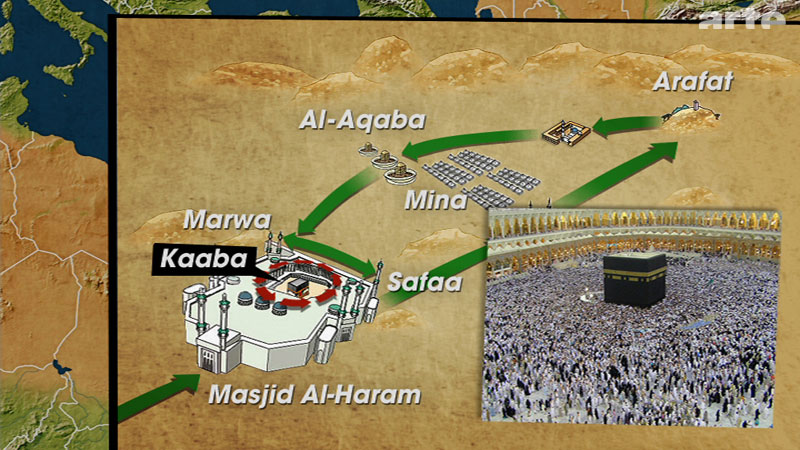
\includegraphics[width=5.51181in,height=3.09931in]{Images/image066.jpg}

Tout commence à la limite du territoire sacré. On exprime la
\emph{niyya}. Le mot a été rencontré à propos de la prière. Quand on
commence à faire la prière, il faut formuler la \emph{niyya}
c'est-à-dire\ldots~? Allez, un petit effort, je suis sûr que vous le
savez.

Puis, il s'ensuit un rituel vestimentaire et corporel qui donne le
statut d'\emph{iḥrām}, c'est-à-dire de consécration. On procède à la
grande ablution. Puis on revêt un vêtement composé de deux pièces
d'étoffes blanches non cousues.

On ne doit pas se couper les cheveux, s'épiler, se couper les ongles, se
couvrir la tête pour l'homme, chasser ou avoir des relations sexuelles.

Le pèlerin va vers la Kaaba, temple selon la tradition musulmane
construit par Adam, reconstruit par Abraham. On y trouve la pierre noire
(blanche à l'origine, mais devenue noire à cause des péchés des hommes.
Sur cette pierre, il existe plusieurs légendes).

Le pèlerin marche autour du Temple. Sa déambulation se dénomme
\emph{tawaf}. À l'approche de la Mosquée, il lève les deux bras vers le
Ciel et répète~: \emph{Labbayka Allahouma Labbayka} (Me voici, ô mon
Dieu, me voici).

Dans la mosquée, il doit toucher la pierre noire, ou faire un geste en
sa direction.

Le fidèle fait 7 fois le tour de la Kaaba, trois rapides et 4 lents dans
le sens inverse des aiguilles d'une montre. C'est la giration autour du
centre de l'univers.

Puis vient le \emph{say}, ou course angoissée d'Agar. Agar est cette
femme, servante de Sarah, qui fut chassée par sa maîtresse. Elle dut
fuir dans le désert, avec dans ses bras son enfant, Ismaël. Elle cherche
de l'eau, puis surgit la source de Zemzem. Le pèlerin accomplit cette
marche entre deux rochers distants de 400m, Safa et Marwa. Il doit faire
la course 7 fois. À la fin, il boit de l'eau de Zemzem.

Ces rites accomplis, on entre dans le cœur du pèlerinage. C'est le 8 de
\emph{Dhou al-hijja}, le dernier mois de l'année lunaire. Le pèlerin se
rend à pied à Mina, à 7 km de La Mecque et il y campe. Il reçoit le
pardon de Dieu (\emph{woukouf}). Il marche vers la plaine d'Arafat à 12
km. À midi, station debout prolongée où le pèlerin reçoit le pardon de
Dieu au pied du mont de la Miséricorde (\emph{Ğabal al-Raḥma})~: c'est
de là que Muḥammad s'adressa aux fidèles lors de son pèlerinage d'Adieu.
C'est le point culminant du pèlerinage. Puis on revient sur ses pas, le
soir, on s'arrête à Mouzdalifa pour y passer la nuit. Là, on ramasse les
49 petits cailloux pour les lapidations rituelles des stèles
représentant le démon.

C'est l'\emph{Aïd al-Ada} ou la fête du sacrifice d'Abraham.

Le 10 du mois, avant l'Aube, on se rend à Mina pour une lapidation
symbolique et pour y sacrifier un animal. C'est l'\emph{Aïd al-Kebir}.
Après le sacrifice, le pèlerin se coupe les cheveux ou se les rase.

Le \emph{Tawaf} est la marche d'Adieu autour du Temple. Le 11 et le 12
ont lieu d'autres lapidations symboliques. Les fidèles reviennent à La
Mecque pour la circumambulation de l'Adieu autour de la Kaaba. Le
pèlerinage est fini. Certains le complètent par un voyage à Médine.

\vide{conclusion-1}{%
\section{Conclusion~}\label{conclusion-1}}

Pour conclure, une histoire, celle d'un dialogue entre Moïse et Dieu et
qui tend à minimiser l'importance de ces 5 piliers pour privilégier la
voie de l'amour mais aussi celle de l'aversion.

\begin{quote}
«~On rapporte que Dieu a révélé à Moïse~: «~As-tu jamais accompli une
œuvre pour Moi~? Moïse répondit~: Mon Dieu~! J'ai prié devant Toi~; j'ai
jeûné, j'ai fait l'aumône légale~! Dieu lui dit~: la prière est pour toi
une preuve (burhān), le jeûne une armure (ğunna), l'aumône est un abri
(ẓill), l'impôt légal une lumière (nūr). Mais quelle œuvre as-tu fait
pour Moi~? Moïse dit~: Mon Dieu~! Indique-moi quelle est l'œuvre qui
soit à Toi~? Dieu lui dit~: Ô Moïse, as-tu jamais pris un ami pour moi~
et en animosité un ennemi pour Moi~? Moïse sut alors que la meilleure
œuvre c'est l'amour en Dieu et l'aversion en Dieu~»\sn{Al-Ġazālī \label{theol:AlGazali9}\emph{,
  Les règles de l'amitié et de la fraternité en Islam}, (K. 15, ar. p.
  593~; fr. p. 19) {[}notre traduction{]}.}.
\end{quote}

\textbf{Pour aller plus loin~:}

On pourra lire le récit passionnant d'Abdallah Hammoudi, anthropologue
et enseignant à Princeton~: \emph{Une saison à La Mecque}, Paris, Seuil,
2005. Il s'agit à la fois d'une démarche de croyant et d'anthropologue.
Mais les deux sont-ils compatibles~? À son retour au Maroc, Hammoudi
refusera le titre de \emph{hāǧ} que l'on attribue à celui qui revient de
pèlerinage. Un signe manifeste de la difficulté qu'il a rencontrée à
concilier la démarche scientifique, objective, observatrice, et sa
participation comme musulman.

\vide{httpwww.seuil.comimagescouvm9782020669801.jpg}{%
{{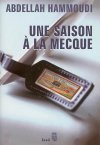
\includegraphics[width=1.04167in,height=1.51389in]{Images/image067.jpg}}{http://www.seuil.com/images/couv/m/9782020669801.jpg}}\label{httpwww.seuil.comimagescouvm9782020669801.jpg}}



\chapter{Les croyances musulmanes}

\vide{introduction-2}{%
\section{{Introduction}}\label{introduction-2}}

S'il n'existe pas en islam de magistère, il existe un genre littéraire
appelé \emph{ʿaqīda}, \textbf{\TArabe{عقيدة}} (pluriel~: ʿ\emph{aqāʾid}),
c'est-à-dire \textbf{profession de foi}. Contrairement au christianisme
où le credo est élaboré dans le cadre d'un synode, en islam, ce sont les
savants qui rédigent au cours de leur vie, parfois sur leur lit de mort,
ce en quoi ou à quoi ils croient. C'est le résumé de leur foi.

Ces professions de foi qui reposent sur le Coran et la Sunna sont
d'abord sommaires, mais elles connaissent dans le temps un développement
qui témoigne de l'élaboration progressive d'un \emph{credo} commun et de
la définition d'une «~orthodoxie~». Si la \emph{šahāda} définit
l'attestation d'adhésion à l'islam, la profession de foi précise la
nature des croyances afférentes. Ces professions permettent de délimiter
un cadre de croyances et de lutter contre des idées considérées comme
\textbf{innovation} (\emph{bidʿa}, \TArabe{بدعة}). Elles délimitent ainsi
les frontières de «~l'orthodoxie~». En fonction des questions
théologiques qui sont posées, des contextes particuliers, des outils
philosophiques utilisés, les réponses diffèrent d'une profession de foi
à l'autre mettant en lumière à la fois un islam pluriel mais aussi la
propension à revendiquer le monopole de l'orthodoxie en excluant celui
qui ne partage pas le Credo défini (C'est la pratique du \emph{takfīr}
que nous avons déjà rencontrée et qui consiste à anathémiser l'autre).
L'influence des débats avec les juifs et les chrétiens ou celle de juifs
et de chrétiens convertis a contribué au développement de ces
professions de foi en apportant avec eux à la fois des questions
théologiques mais aussi une argumentation pour appréhender les réponses.

Dans cette leçon, nous présenterons dans un premier temps les grandes
croyances musulmanes, puis nous exposerons quelques-unes de ces
professions de foi afin de mettre en exergue leur développement.

\vide{i--les-principales-croyances-musulmanes}{%
\section{Les principales croyances
musulmanes}\label{i--les-principales-croyances-musulmanes}}

Le verset S. 2, 177 est traditionnellement considéré comme répertoriant
les cinq grandes vérités du \emph{credo} musulman (\emph{al-ʿaqīda})~:
Dieu, les anges, les prophètes, les Écritures et l'eschatologie. On
parle à cet égard des cinq piliers de la foi.

À distinguer bien sûr des cinq piliers de l'islam qui renvoient à une
pratique. Il s'agit des cinq principaux thèmes retenus par les manuels
de \emph{kalām} (la théologie défensive) auxquels certains ajoutent la
prédestination (\emph{qadar}) en suivant le deuxième \emph{hadīṯ qudsī}
de Nawāwī et d'autres la direction de la communauté (\emph{imāma}). Donc
les 5 peuvent être 6\ldots{}

Avant d'aller plus loin et d'exposer le verset coranique et le
\emph{ḥadīṯ qudsī}, une petite explication s'impose~: qu'est-ce donc
qu'un \emph{ḥadīṯ qudṣī}~? Vous savez ce qu'est un \emph{ḥadīṯ}~: une
parole ou un geste prophétique. Vous savez aussi que l'on a qualifié les
\emph{ḥadīṯ} selon la chaîne de transmetteurs (\emph{isnād})~: certains
sont dits faibles, d'autres bons, d'autres encore authentiques\ldots{}
mais il y a aussi un type de \emph{ḥadīṯ} appelé \emph{qudsī},
c'est-à-dire «~sacré~». On retrouve la racine QaDaSa (\emph{kadosh} en
hébreu). Ces \emph{ḥadīṯs} sont des paroles du Prophète Muḥammad mais
attribuées à Dieu, c'est-à-dire que Muḥammad y rapporte une parole de
Dieu. Pour autant, cette parole n'est pas issue du Coran.

\begin{itemize}
\item
  Le texte de S.2, 177~:
\end{itemize}

\begin{quote}
«~La bonté pieuse ne consiste pas à tourner vos visages vers le Levant
ou le Couchant. Mais la bonté pieuse est de \textbf{croire en Allah, au
Jour dernier, aux Anges, au Livre et aux prophètes,} de donner de son
bien, quelque amour qu'on en ait, aux proches, aux orphelins, aux
nécessiteux, aux voyageurs indigents et à ceux qui demandent l'aide et
pour délier les jougs, d'accomplir la Salat et d'acquitter la Zakat. Et
ceux qui remplissent leurs engagements lorsqu'ils se sont engagés, ceux
qui sont endurants dans la misère, la maladie et quand les combats font
rage, les voilà les véridiques et les voilà les vrais pieux~!~»
\end{quote}

\TArabe{لَيْسَ الْبِرَّ أَنْ تُوَلُّوا وُجُوهَكُمْ قِبَلَ الْمَشْرِقِ
وَالْمَغْرِبِ وَلَكِنَّ الْبِرَّ مَنْ آَمَنَ بِاللَّهِ وَالْيَوْمِ
الْآَخِرِ وَالْمَلَائِكَةِ وَالْكِتَابِ وَالنَّبِيِّينَ وَآَتَى الْمَالَ
عَلَى حُبِّهِ ذَوِي الْقُرْبَى وَالْيَتَامَى وَالْمَسَاكِينَ وَابْنَ
السَّبِيلِ وَالسَّائِلِينَ وَفِي الرِّقَابِ وَأَقَامَ الصَّلَاةَ وَآَتَى
الزَّكَاةَ وَالْمُوفُونَ بِعَهْدِهِمْ إِذَا عَاهَدُوا وَالصَّابِرِينَ
فِي الْبَأْسَاءِ وَالضَّرَّاءِ وَحِينَ الْبَأْسِ أُولَئِكَ الَّذِينَ
صَدَقُوا وَأُولَئِكَ هُمُ الْمُتَّقُونَ}

\begin{itemize}
\item
  Le \emph{ḥadīṯ qudsī}
\end{itemize}

«~L'islam consiste à témoigner qu'Allāh est le Dieu unique et Muḥammad
son Envoyé, à s'acquitter de la prière et de l'aumône rituelles, du
jeûne de Ramadān et du pèlerinage à la Maison de Dieu, si l'on en a les
moyens~(\ldots) La foi (\emph{īmān}) consiste à croire à Dieu, ses
anges, ses écritures, ses prophètes, et au dernier Jour ainsi qu'à
croire à la prédestination au bien et au mal~»\sn{~\textsc{al-Nawawî},
  \emph{Une herméneutique de la tradition islamique : le commentaire des
  Arba‛ûn al-nawawîya de Muḥyî al-Dîn Yaḥyâ al-Nawawî (m. 676/1277)},
  Introduction, texte arabe, traduction, notes et index du vocabulaire
  par Louis Pouzet\emph{,} Beyrouth, Dar el-Machreq, 1982, p. 90,
  (traduction légèrement modifiée).}.

On trouve aussi dans le \emph{ḥadīṯ qudsī} n°4~de la même collection :

« La foi consiste en ce que tu dois croire à Allah, à Ses Anges, à Ses
Livres, à Ses Prophètes, au Jugement Dernier. Tu dois croire encore à la
prédestination touchant le bien et le mal »\sn{\textsc{al-Nawawî,}
  \emph{ḥadīṯ} n°4.}.

\vide{bibliographie-pour-une-suxe9lection-des-professions-de-foi-islamique-je-vous-conseille-deux-ouvrages}{%
\subsubsection{{\textbf{Bibliographie}~: Pour une
sélection des professions de foi islamique, je vous conseille deux
ouvrages:
}{Bibliographie~: Pour une sélection des professions de foi islamique, je vous conseille deux ouvrages: }}\label{bibliographie-pour-une-suxe9lection-des-professions-de-foi-islamique-je-vous-conseille-deux-ouvrages}}

\vide{section-33}{%
\subsubsection{}\label{section-33}}


\mn{{William Montgomery \textsc{Watt},
\emph{Islamic Creeds}, A selection, Edinburgh University Press, 2001
(1994) L'avantage de celui-ci est qu'il est en poche. Mais c'est en
anglais.}}




\mn{{Arent Jan W\textsc{ensinck}, \emph{The
Muslim Creed}, Its Genesis and Historical Development, Cambridge, 1932.
Un grand classique de l'islamologie. Vous pouvez le consulter et le lire
en ligne via
\url{https://archive.org/details/630\_The.Muslim.Creed}}}

Ce \emph{ḥadīṯ} est repris en introduction de la plupart des
ʿ\emph{aqā'id}. C'est le pluriel de \emph{ʿaqīda}, profession de foi. Je
vous l'ai signalé dans l'introduction..\emph{.} Les professions de foi
vont commenter ces articles sur la base du Coran et de la Sunna. Il
s'agit de répondre aux questions du type~:

\textbf{Qui est Dieu~? Que sait-on de lui~?}

\begin{quote}
Qu'en est-il des anges~? Quelle est la nature de ces êtres spirituels~?
Sont-ils bons~? Peuvent-ils faire le mal~?
\end{quote}

Qu'en est-il des livres~? De quels livres s'agit-il~? Sont-ils tous
égaux~?

Qui sont les Envoyés de Dieu~? Quel est leur nom~? Quelle est leur
histoire~?

\begin{quote}
Comment se déroulera le jugement de Dieu~? Est-ce que les musulmans
peuvent aller en enfer~? Et les non-musulmans~? Et l'hypocrite~? Et le
voyou~? Et le fornicateur~?
\end{quote}

Ma liberté est-elle engagée ou tout est-il déjà écrit d'avance
(\emph{maktub})~?

La \emph{ʿaqīda} répond à toutes ces questions. Mais, par là-même, elle
prend position dans le commentaire des versets mobilisés. Je ne rentre
pas dans cette leçon sur les débats théologiques. Vous avez la
possibilité au second semestre de suivre le cours d'Adrien Candiard sur
la théologie musulmane. Pour l'instant il s'agit surtout d'exposer ces
croyances. Je vais donc reprendre les 5-6 articles de foi.


\subsection{{Le \emph{tawḥīd} contre le \emph{širk}
ou la réforme perpétuelle de l'islam
}\label{le-tawux1e25ux12bd-contre-le-ux161irk-ou-la-ruxe9forme-perpuxe9tuelle-de-lislam}}

Croire en Dieu c'est comme l'atteste la \emph{šahāda} (vous savez le
premier pilier\ldots~; au fait, la lettre \emph{š} se prononce sh, vous
n'aviez pas oublié~?), croire qu'il n'y a pas d'autres dieux que Dieu.
Le seul Dieu c'est Dieu. Dieu est unique.

\begin{Def}[tawḥīd]
Cette affirmation de l'unicité
divine se nomme \emph{tawḥīd}. Elle est au cœur de la prédication
musulmane.
\end{Def}


\subsection{Calligraphie de Tawhid}


\includegraphics[width=\textwidth]{Images/image015.jpg}
« Le tawhid renvoie dans l'islam au dieu « un ». Mais la notion est
évolutive. Dans le Coran, le dieu local,~\emph{« protecteur du point
d'eau de La Mekke »}, se mue rapidement en dieu créateur, qui se suffit
à lui-même et n'a pas d'associé. C'est une manière de déligitimer les
trois déesses locales qui étaient supposées protéger les déplacements.
Plus tard, sur la coupole du Rocher à Jérusalem, construite en 692, est
inscrit un verset coranique (Sourate 4, Verset 171) qui récuse la
Trinité, faisant simplement de Jésus, « Fils de Marie », le « messager »
qui précède Mohammed. On semble être dans un défi à l'empire byzantin.
Enfin, beaucoup plus tard, au milieu du XVIII\textsuperscript{e}~siècle,
le tawhid devient un enjeu interne à l'islam avec le mouvement sectaire
du wahhabisme qui combat avec virulence les courants mystiques de
l'islam qui sont accusés « d'associer » d'autres divinités à Dieu. » \sn{Jacqueline Chabbi}



« Pour dessiner l'unité, j'ai utilisé dans cette calligraphie la forme
du carré. Lors de mes premiers essais, je faisais plutôt des cercles.
Là, j'ai déformé une des lettres (le h) pour la relier avec les autres
et les faire entrer toutes dans un carré. J'ai agrandi cette lettre
jusqu'à ce qu'elle enlace les autres lettres, comme dans un souffle. En
calligraphie, le souffle est important. Tous les calligraphes
travaillent sur le souffle. Quand on fait le geste, on coupe son
souffle. Quand on va à l'encrier, on reprend souffle. » \sn{Hassan Massoudy}



Le musulman, quand il récite la \emph{šahāda} ou quand il prêche, lève
l'index signifiant sa foi en Dieu un. À sa mort il est mis dans un
linceul, les mains jointes, et parfois, l'index droit désuni des autres
doigts de la main (parfois il est tourné vers le ciel).



\vide{adorer-dieu}{%
\subsubsection{{Adorer Dieu
}}\label{adorer-dieu}}

Affirmant que Dieu est unique, le musulman récite quotidiennement la
sourate 112 intitulée, \emph{al-iḫlaṣ} que l'on traduit souvent par «~le
culte pur~».


\begin{table}[h!]
\resizebox{\textwidth}{!}{%
\small
\begin{tabular}{p{7cm}p{7cm}}
1. Dis: «Il est Allah, Unique.
&

\TArabe{بِسْمِ اللَّهِ الرَّحْمَنِ الرَّحِيمِ}

\TArabe{قُلْ هُوَ اللَّهُ أَحَدٌ}
\\
2. Allah, Le Seul à être imploré pour ce que nous désirons.
&
\TArabe{اللَّهُ الصَّمَدُ}
\\

3. Il n'a jamais engendré, n'a pas été engendré non plus.
& 
\TArabe{لَمْ يَلِدْ وَلَمْ يُولَدْ}
\\
4. Et nul n'est égal à Lui».
&
\TArabe{وَلَمْ يَكُنْ لَهُ كُفُوًا أَحَدٌ} \\

\end{tabular}%
}
\caption{sourate 112 , \emph{al-iḫlaṣ}, «~le
culte pur~»}
\end{table}



Au cours de l'histoire, cette sourate 112 a été invoquée par des
penseurs musulmans dans le cadre de \textbf{polémiques contre les
chrétiens}. Mais il faut noter qu'elle n'était pas, à son origine,
destinée à réfuter la croyance chrétienne. Elle est un \emph{credo}
contre le polythéisme.

L'affirmation d'un Dieu unique implique pour les musulmans que Dieu
existe. Il manifeste son existence dans des signes (\emph{āyāt}, آيات),
ceux de la création, ceux du Livre qu'il a révélé.

Dire que Dieu est `un' implique que l'adoration revient à Lui seul. Seul
devant Lui le croyant se prosterne. La\emph{ʿibāda}, l'adoration, la
soumission totale, lui revient.

Si l'on refait un peu d'arabe vous voyez que la racine de \emph{ʿibāda}
est ʿa.Ba.Da. Vous la retrouvez dans le mot ʿAbd-Allāh\ldots{} qui
signifie serviteur, soumis, adorateur de Dieu.


\begin{Def}[Taghut]
{Taghut~(ar. \TArabe{طاغوت} ), ṭāġūt. Plusieurs~: Ṭawāġīt. Au sens large~: "aller au-delà de la mesure" ou désignant une "hauteur" ou un "sommet" de ṭāġiyah \TArabe{ طاغية} lit. tyran) est~une terminologie islamique~désignant un centre de culte autre que~Dieu.}
\end{Def}

La pensée musulmane est fondamentalement une pensée du Dieu unique~; la
prédication ne cessera d'attirer l'attention sur les idoles qui
s'immiscent dans l'islam au cours de l'histoire. Les grands réformateurs
de l'islam partent toujours de l'unicité divine. Ainsi, par exemple, au
XII\textsuperscript{e} siècle, la dynastie des Almohades instaurée au
Maroc s'appuie sur la doctrine d'Ibn Tumart (m.~1128). Ils se font
appeler les \emph{muwahhidūn}, c'est-à-dire les partisans de l'unicité,
les monothéistes, les unitariens.

\vide{notice-biographique-ibn-tumart-1080-1130}{%
\subsubsection{Notice biographique -- Ibn Tumart
(1080-1130)}\label{notice-biographique-ibn-tumart-1080-1130}}




C'est un personnage curieux qui après
avoir étudié en Andalousie et à Bagdad la doctrine d'al-Ašʿarī
(al-Ġazālī est aussi disciple d'al-Ašʿarī), revient dans son pays natal,
le haut Atlas et prêche un monothéisme rigoureux et réformateur. Dans
les montagnes, il va constituer un État disposant d'une armée, unie par
une doctrine religieuse rigoriste. Pour lui, toute forme de
divertissement est idolâtrie et contrevient à l'islam pur. Le \emph{dār
al-islām} (terre d'islam) ne saurait en ces conditions accueillir sur
son territoire des communautés religieuses non musulmanes. C'est de son
époque que l'on date la fin des communautés chrétiennes au Maghreb.
Ainsi, il condamne l'écoute de la musique qui éloigne de l'adoration qui
est due à Dieu. Son rigorisme moral lui attira bien des ennemis. À la
fin de sa vie, il se proclame Imam, Mahdi. Comme nous le verrons dans la
prochaine leçon, c'est une doctrine essentiellement šīʿite.


\vide{pour-plus-de-duxe9tails-vous-pouvez-lire-sa-biographie-issue-de-lencyclopuxe9die-berbuxe8re-p.3604-3606.}{%
\subsubsection{{Pour plus de détails, vous pouvez lire sa
biographie issue de \emph{l'Encyclopédie berbère}, p.3604-3606.
}{Pour plus de détails, vous pouvez lire sa biographie issue de l'Encyclopédie berbère, p.3604-3606. }}\label{pour-plus-de-duxe9tails-vous-pouvez-lire-sa-biographie-issue-de-lencyclopuxe9die-berbuxe8re-p.3604-3606.}}
 

De même, au 18\textsuperscript{ème} siècle, dans la péninsule arabique,
ʿAbd al-Wahhab entreprend une réforme de l'islam. Il s'agit avant tout
de s'attaquer à la prolifération de la superstition et de
l'associationnisme (\emph{širk}) dans la péninsule. Dans son Livre
\emph{Kitāb al-tawḥīd}, il invoque la nécessité d'adorer Dieu seul et de
rejeter le \emph{ṭāġūt} (\textbf{\TArabe{طاغوت}})\textbf{,} c'est-à-dire
tout ce qui est adoré en dehors de Dieu et qui contredit la Loi
islamique. Il y mentionne par exemple le port d'un bracelet pour
conjurer le mal, le port de talisman, etc.

Aujourd'hui, la propagande de Daesh a témoigné qu'il s'agit aussi d'un
mouvement unitarien rigoriste. L'État islamique est dans la même ligne
que celle d'un Ibn Tumart. La destruction des mausolées, des statues
antiques, des mosquées abritant le tombeau de saints sont les
conséquences de l'affirmation du \emph{tawḥīd} tel que défini par ʿAbd
al-Wahhab dans son \emph{Livre de l'unicité divine}~: pour lui, il ne
suffit pas d'affirmer que Dieu est unique (\emph{tawḥīd al-rubūbiyya})~;
cette affirmation doit aussi se mettre en œuvre dans la pratique en
n'adorant que Dieu seul (\emph{tawḥīd al-ulūhiyya}) et en combattant
toute forme d'idolâtrie. La croyance en l'intercession des prophètes ou
des saints sont vues comme autant de formes d'associationnisme à
combattre. D'où la destruction des mausolées.

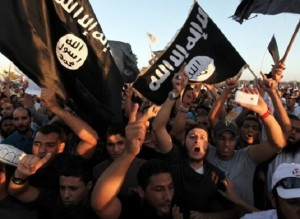
\includegraphics[width=3.11458in,height=2.28125in]{Images/image072.jpg}

\begin{quote}
\emph{Partisans de l'État islamique, l'index levé}

\emph{Les drapeaux mentionnent la šahāda}
\end{quote}

\vide{ux2bfabd-al-wahhab-et-le-salafisme}{%
\paragraph{ʿAbd al-Wahhab et le
salafisme}\label{ux2bfabd-al-wahhab-et-le-salafisme}}

Mohammed ibn Abd al-Wahhab (1703-1792) est le «~père~» de la doctrine
salafiste moderne. \textbf{Le salafisme se caractérise par la volonté de
purger la pratique religieuse de ses particularités locales et des
«~innovations~» qui auraient altéré l'islam originel au fil des
siècles}\textbf{. Il refuse toute forme d'inculturation}. Ce retour à la
religion des origines, quel que soit le pays où l'islam est pratiqué,
est fondé sur une lecture littéraliste des versets du Coran et des
\emph{ḥadīṯs}. Les salafistes refusent toute légitimité aux professions
de foi des penseurs musulmans ou aux écoles de droit qui ont développé
une méthodologie propre.

Longtemps rejeté, considéré comme une secte, le salafisme semble avoir
gagné le terrain idéologique ces trente dernières années et a su
s'imposer dans les consciences comme étant le véritable islam.

Hamadi Redissi y a consacré un livre, \emph{Le pacte de Nadj} où il
montre l'alliance entre le politique et le religieux. Il écrit~: «~La
tradition sunnite s'est défendue avec une impitoyable virulence contre
le wahhabisme, dans une campagne impitoyable qui n'est pas sans rappeler
l'acharnement médiéval contre l'hétérodoxie {[}\ldots{]}. (Mais) tout se
passe comme si le wahhabisme avait réveillé dans la conscience assoupie
de l'islam un potentiel insoupçonné de vérité, qui n'attendait que son
heure pour se révéler au grand jour. Une triple alliance entre princes,
ulémas et marabouts lui a pourtant tenu vaillamment tête, du milieu du
XVIIIème siècle à la fin du XIXème~».

Attention, cependant, le salafisme a différentes formes selon les
époques. On distingue le salafisme piétiste du salafisme djihadiste ou
encore du salafisme politique.

\vide{le-danger-de-lassociationisme-ux161irk}{%
\subsubsection{Le danger de l'associationisme
(\emph{širk})}{}\label{le-danger-de-lassociationisme-ux161irk}}

\begin{Def}[širk]
Le grand danger qui guette le croyant est donc d'associer quelque chose
à Dieu. L'associationnisme se nomme en arabe le \emph{širk}.
\end{Def}

L'accusation de \emph{širk} a une portée religieuse et politique
puisqu'elle vise à exclure l'autre de la communauté et appelle à le
combattre. Le \emph{mušrik} est l'associationniste. Cette accusation est
celle dressée contre les non-musulmans (juifs, chrétiens, polythéistes)
mais aussi contre ceux qui au sein de l'islam sont considérés comme
infidèles au \emph{tawḥīd.}


\mn{Muhammad Ibn
Tumart~:~\TArabe{المهدي
محمد بن تومرت}), 
réformateur~musulman.
à la morale~rigoriste. Voir  p. \pageref{IbnToumart}}
Pour Ibn Tumart, celui qui écoute de la musique est donc un
\emph{mušrik}. Cela peut éclairer certains débats contemporains.

\paragraph{le širk comme arme politique}

Un des premiers exemples politiques dans l'histoire de l'islam de
l'instrumentalisation politique du širk appliquée à l'encontre d'autres
musulmans est celui des ḫāriğites envers `Alī à la suite de son
acceptation de l'arbitrage proposé par Mu`āwiya lors de la bataille de
Ṣiffīn en 657\sn{\textsc{~Al-ṬabarĪ,} \emph{Tārīḫ}, I, 3363.}.
L'accusation de širk est aussi le nœud de bien des controverses
doctrinales~: dans le débat sur le Coran incréé, les muʿtazilites ont
accusé de širk les ḥanbalites et tous ceux qui refusaient de croire que
le Coran est créé. Ils comparèrent leur position à celle des chrétiens
qui soutiennent que Jésus est le Verbe incréé de Dieu et ils affirmèrent 
«~qu'il n'y a pas de \textit{tawḥīd} chez ceux qui n'acceptent pas que le Coran
est créé~»~: «~leurs doctrines sont du pur \textit{kufr} et un \textit{širk} évident aux
yeux du Commandeur de la foi~»\sn{~\textsc{Al-ṬabarĪ,}
  \emph{Tārīḫ}, III, 1112-1132. Voir Joseph \textsc{Van Ess},
  \emph{Theologie und Geselschaft}, III, p.~452-456.}. 
  
  Ce débat
théologique sur le Coran a trouvé son prolongement dans la question des
attributs divins comme la Vérité, le Bien pur, la Sagesse. Pour les
muʿtazilites, les attributs doivent être rattachés à l'essence divine,
sinon cela revient à introduire de la pluralité en Dieu et contrevient
par conséquent à l'unicité divine. De même, les philosophes voient dans
les chapitres du \textit{kalām} sur cette question l'introduction d'accidents en
Dieu.

\paragraph{Qu'en est-il de l'expression dans le Coran~?} Puisque le \emph{širk} est
si important, il n'est pas inutile de voir ce qu'en dit le Coran\ldots{}
et à qui il applique la catégorie. Évidemment, la Sunna ne donnerait pas
les mêmes conclusions\ldots{} mais cela est une autre question.

Notons que dans le Coran, les gens du Livre (\emph{ahl al-kitāb})
{[}chrétiens, juifs, sabéens{]} ne sont jamais appelés \emph{mušrikūn}
mais \emph{kuffār} (S.2, 105~; 3, 186~; 5, 82~; 22, 17)\sn{~Ainsi,
  par exemple, S. 2, 105~: 
  \begin{quote}
      «~Ceux d'entre les gens du Livre qui sont
  \emph{incrédules} et les polythéistes ne voudraient pas qu'un bienfait
  de votre Seigneur descende sur vous. Dieu accorde en particulier sa
  miséricorde à qui il veut. Dieu est le maître de la grâce
  incommensurable~».
  \end{quote}
 \TArabe{مَا يَوَدُّ الَّذِينَ كَفَرُوا \textbf{مِنْ أَهْلِ الْكِتَابِ}
  \textbf{وَلَا الْمُشْرِ}كِينَ أَنْ يُنَزَّلَ عَلَيْكُمْ مِنْ خَيْرٍ
  مِنْ رَبِّكُمْ وَاللَّهُ يَخْتَصُّ بِرَحْمَتِهِ مَنْ يَشَاءُ وَاللَّهُ
  ذُو الْف
 َضْلِ الْعَظِيمِ}
 }.

Pour le Coran, le \emph{mušrik} est celui
qui affirme que Dieu a pris des enfants (S. 19, 88), qui cherche refuge
dans les \emph{ǧinns} (S. 72, 6), qui soutient que les anges sont des
êtres divins (S. 53, 27-28). Le terme collectif \emph{mušrikūn} désigne
ceux qui refusent de reconnaître la prédication du prophète~; ils sont
ses adversaires sur le plan religieux, politique et moral en tant qu'ils
commettent des péchés. Le Coran démasque les racines `psychologiques' du
\emph{širk} dans le \emph{ẓann}, opinion emplie d'incertitude et de
doute, contraire à la science (\emph{ʿilm}).
\begin{quote}
    {S. 10, 66 : «~Ce
  qui est dans les cieux et sur la terre n'appartient-il pas à Dieu~?
  Que suivent donc ceux qui invoquent des associés en dehors de Dieu~?
  Ils ne suivent que des conjectures et ils se contentent de
  suppositions~»

  \TArabe{أَلَا إِنَّ لِلَّهِ مَنْ فِي السَّمَاوَاتِ وَمَنْ فِي الْأَرْضِ
  وَمَا يَتَّبِعُ الَّذِينَ يَدْعُونَ مِنْ دُونِ اللَّهِ شُرَكَاءَ إِنْ
  يَتَّبِعُونَ إِلَّا \textbf{الظَّنَّ} وَإِنْ هُمْ إِلَّا يَخْرُصُونَ}
  },

\end{quote}
mais aussi dans les passions (\emph{ahwāʾ}). Par suite, le \emph{širk}
est une manifestation du \emph{kufr}~: il en est son degré paroxystique.
Le \emph{mušrik} est donc un égaré (S.~4, 117), il est le jouet de Satan
et son associationnisme annule toute rétribution positive de ses œuvres
aussi bonnes soient-elles (S.~39, 65)
\begin{quote}
    {~S. 6, 88 : «~Voilà la
  Direction de Dieu. Il dirige qui il veut parmi ses serviteurs. S'ils
  avaient été polythéistes, leurs actions ne leur auraient été d'aucun
  profit~».

  \TArabe{ذَلِكَ هُدَى اللَّهِ يَهْدِي بِهِ مَنْ يَشَاءُ مِنْ عِبَادِهِ
  وَلَوْ أَشْرَكُوا لَحَبِطَ عَنْهُمْ مَا كَانُوا يَعْمَلُونَ}
  }.
\end{quote}

Le
verset S. 9, 5 affirme que l'associationniste doit être combattu jusqu'à
ce que mort s'ensuive, à moins qu'il ne se convertisse à l'islam --
exigence qui n'est pas requise pour les gens du Livre. Il est aussi dit
qu'il n'est qu'impureté (S.~9, 28)
{S.9, 28~:

  \TArabe{إِنَّمَا الْمُشْرِكُونَ نَجَسٌ}}.

Aux yeux de l'orthodoxie sunnite et šīʿite, il est la plus grande
injustice causée à Dieu, le péché majeur, celui qui théoriquement ne
peut être pardonné (S. 4, 48)
\begin{quote}
    {S. 4, 48 : «~Dieu ne pardonne pas
  qu'on lui associe quoi que ce soit~; il pardonne à qui il veut des
  péchés moins graves que celui-ci. Celui qui associe quoi que ce soit à
  Dieu commet un crime immense~».

  \TArabe{إِنَّ اللَّهَ لَا يَغْفِرُ أَنْ يُشْرَكَ بِهِ وَيَغْفِرُ مَا دُونَ
  ذَلِكَ لِمَنْ يَشَاءُ وَمَنْ يُشْرِكْ بِاللَّهِ فَقَدِ افْتَرَى
  إِثْمًا عَظِيمًا}}.

\end{quote}

\paragraph{širk et Soufisme } Si les soufis furent souvent accusés de \emph{širk}, il n'en demeure pas
moins que leur enseignement est profondément pénétré du \emph{tawḥīd}.
Ainsi, par exemple, la mystique Rābiʿa (m.185/801) chante son amour
absolu pour Dieu qui ne laisse en son cœur aucune place pour
Muḥammad\sn{~Annemarie \textsc{Schimmel,} "\emph{The Sufis and
  the Shahāda}" dans Richard G. \textsc{Hovannisian} and Speros
  \textsc{Vryonis}, \emph{Islam's understanding of itself}, Eighth
  Giorgio Levi della Vida Biennial Conference, May 1-3, 1981, Malibu,
  Undena Publications, 1983, p.~103-125.}~; al-Ḥallāǧ (m.~309/922) \sn{le
mystique de Bagdad qui fut crucifié en 922 alors qu'il disait «~Je suis
Dieu~» (\emph{sic~!}). On en reparlera dans le cours consacré au
soufisme p. \pageref{iii--grandes-figures-soufies}}
incrimine la récitation continuelle de la \emph{šahāda}.
\begin{quote}
    {~«~{[}Al-Ḥallāǧ{]}
  condamne, nous dit Louis Massignon, l'illusion criminelle de certains
  qui s'imaginent, en récitant la \emph{šahāda}, témoigner réellement
  que Dieu est unique~; c'est oser `s'associer à Dieu'. Car s'imaginer
  que l'on `unifie' Dieu, c'est affirmer son propre moi~» : Louis
  \textsc{Massignon}, \emph{La Passion de Husayn Ibn Mansûr Hallâj},
  \emph{op.cit}., t.3, p.~247.}
\end{quote}

Al-Šiblī (m.~334/945), le disciple
d'al-Ǧunayd, de renchérir plus tard en confessant à propos de l'appel à
la prière : \sn{\textsc{Al-QuŠayrĪ,} \emph{Al-Risālat
  al-qušayriyya}, p.~17.}.
\begin{quote}
    Si Tu ne l'avais pas ordonné je n'aurais invoqué le nom de
nul autre que Toi
\end{quote}
 Ainsi, en se vouant à l'amour pur et absolu
de Dieu, ils s'attachent à déloger et démasquer toute trace de
\emph{širk} dans la dévotion et les pratiques mauvaises pour accéder à
Dieu. Ḥasan al-Baṣrī, un autre grand mystique, contemporain de
Rābiʿa~disait : \sn{\textsc{Ibn Saʿd},
  \emph{Al-Ṭabaqāt al-kubrā}, Beyrouth, Dār Ṣādir, t. 26, p.~17.}
\begin{quote}
    «~Alors qu'il avait achevé de parler et s'apprêtait à se
lever, Ḥasan dit~: `Ô mon Dieu, tu vois nos cœurs emplis de \emph{širk},
d'orgueil (\emph{kubr}), d'hypocrisie (\emph{nifāq}), du désir double
d'être vu et entendu, d'hésitation et de doute envers ta religion. Ô toi
qui retourne les cœurs, affermis nos cœurs en ta religion et assure que
notre religion soit l'islam véritable~».
\end{quote}
 Un
célèbre \emph{ḥadīṯ} est à cet égard convoqué puisqu'il rapporte que le
\emph{širk} est aussi imperceptible que le rampement d'une fourmi noire
sur une roche noire\sn{~\textsc{Ibn Ḥanbal}, \emph{Al-Musnad},
  Vol. IV, p.~403 :~«~Ô gens, méfiez-vous de cet associationnisme, car
  il est plus caché que le rampement des fourmis ».}.


  \paragraph{Les degrés de l'associationisme}
  
  Ces subtilités plus ou moins reconnues, admises et précisées par les
courants de pensée, les théologiens et les mystiques, définissent ainsi
des distinctions quant à sa nature et ses degrés. Ainsi convient-il de
distinguer le \emph{širk al-akbar} qui consiste à donner des associés à
Dieu, à sacrifier pour les \emph{djins} ou à adorer un prophète, du
\emph{širk al-aṣġar} qui ne touche pas le \emph{tawḥīd} à sa base mais
l'altère. Les soufis, dans une formule paradoxale, en viennent à
signifier que «~l'essence du \emph{širk} est de penser que l'on est sans
\emph{širk}~»\sn{~\textsc{Al-Hujwírí}, \emph{The Kashf al-maḥjúb :
  the oldest Persian Treatise on Ṣúfiism}, translated by Reynold A.
  Nicholson, Leyden, Brill, London, Luzac and Co, 1911, p.~282.}. 
  
  
  Ibn
Taymiyya, quant à lui, distingue entre l'associationnisme relatif à la
divinité (\emph{širk al-ulūhiyya}) et l'associationnisme relatif à la
seigneurie (\emph{širk al-rubūbiyya})\sn{~\textsc{Ibn Taymiyya},
  \emph{Maǧmūʿ al-fatāwā}, édition Ibn Qāsim, t. 1, Rabat, Maktabat
  al-Maʿārif, 1401/1981, p.~88-89, traduction française de Yahya Michot,
  «~Entre la divinité et la seigneurialité, le polymorphisme de
  l'associationnisme (\emph{shirk})~», \emph{Le Musulman}, n°16, sept.-
  déc. 1991, Paris, p.~8-13.}. Rappelez-vous, nous avons vu un peu plus
haut cette distinction, mais cette fois, c'était à propos du
\emph{tawḥīd}, l'unicité. Le premier consiste à donner à Dieu un
semblable en son adoration, en son amour, en son espérance, en sa peur,
en son repentir. Le croyant se tourne vers des «~pareils~» qu'il sait
inférieurs à Dieu, mais à qui il octroie cependant la place qui revient
à Dieu. Dans l'évocation et l'adoption de ces semblables, le croyant
affirme que s'il associe à Dieu, c'est pour mieux s'en rapprocher. Cet
associationnisme peut être pardonné à celui qui se repent et qui
abandonne ces pratiques. Quant à l'associationnisme relatif à la
seigneurie, il consiste à accréditer la cause d'un effet à un autre que
Dieu. Or Dieu, comme l'enseignent ses plus beaux noms, est celui qui
gouverne, avilit ou rend puissant, redresse ou abaisse, donne ou
empêche~: il est cause de tout.

\vide{anges-et-duxe9mons}{%
\subsection{{Anges et démons\ldots{}
}\label{anges-et-duxe9mons}}

\vide{les-anges}{%
\subsubsection{Les anges}\label{les-anges}}

Les anges et les démons occupent une place importante dans le Coran et
le \emph{ḥadīṯ}. L'ange~se dit \emph{malak} et au pluriel,
\emph{malāʾika} (en hébreu~: \emph{melek}). On les décrit comme des
êtres intermédiaires entre Dieu et les hommes (S. 70, 4). Leur nature
est spirituelle. Dans le \emph{ḥadīṯ}, ils sont dits asexués et
impeccables (c'est-à-dire sans péchés).

On trouve dans le Coran le nom de certains anges~: Ǧibrîl / Gabriel (S.
2, 97-98), Mīkāl / Michel (S.2, 98) et Mālik, l'ange chargé de l'enfer
(S. 43, 77).

Le Coran décrit le rôle qu'ils jouent. Ce sont~:

\begin{itemize}
\item
  des adorateurs
\item
  des modèles d'obéissance
\item
  des messagers que Dieu envoie aux hommes pour leur apporter ses
  ordres. Ils annoncent des naissances miraculeuses~: Isaac à Ibrahim,
  Jean-Baptiste à Zacharie, Jésus à Marie (S. 19, 16-19).
\item
  Ils sont les gardiens de l'Écriture mère. Gabriel est aussi appelé
  \emph{rūh}, c'est-à-dire esprit.
\item
  ils conservent et enregistrent les actions, bonnes ou mauvaises des
  hommes (\emph{ḥafiẓa}~: apprendre par cœur). En revanche, on ne peut
  pas parler d'ange gardien.
\item
  Ils interviennent dans les combats contre les infidèles.
\item
  Munkar et Nakīr sont les deux anges de l'interrogatoire du tombeau.
\end{itemize}

\vide{les-duxe9mons}{%
\subsubsection{Les démons}\label{les-duxe9mons}}

On parle des démons (\emph{šayāṭīn}) et du démon (\emph{al-šayṭān})
identifié à Iblīs à qui Dieu a demandé de se prosterner devant l'homme
créé d'argile et qui a refusé, parce que lui, il était une créature de
feu~:

\begin{quote}
S.2, 34~: «~Et lorsque Nous demandâmes aux Anges de se prosterner devant
Adam, ils se prosternèrent à l'exception d'Iblis qui refusa, s'enfla
d'orgueil et fut parmi les infidèles~».


\TArabe{وَإِذْ قُلْنَا لِلْمَلَائِكَةِ اسْجُدُوا لِآَدَمَ فَسَجَدُوا إِلَّا
إِبْلِيسَ أَبَى وَاسْتَكْبَرَ وَكَانَ مِنَ الْكَافِرِينَ}
\end{quote}
Est-il un ange déchu~? La tradition hésite~: l'ange est impeccable~!
Alors, on en fait parfois un \emph{djinn} introduit subrepticement parmi
les anges. On dira aussi~: un ange par son espèce, mais djinn par son
comportement. Mais l'enjeu théologique n'est-il pas ailleurs~? Pourquoi
Dieu a-t-il demandé aux anges de se prosterner devant Adam~?

\begin{itemize}
\item
  Dieu dans les versets précédents informe avoir enseigné à Adam tous
  les noms~; Il a donc un mérite spécial, particulier. Et les anges ne
  le voient pas. Pour que les anges comprennent ce mérite, Dieu demande
  que les anges se prosternent devant l'homme.
\item
  Il y a un enseignement spirituel pour les hommes eux-mêmes~: Quand tu
  ne sais pas pourquoi, sache que c'est parce que ta raison est
  limitée~: tout est limité en toi~: ta vue est limitée~: tu ne vois pas
  les anges, tu ne vois pas le mouvement du vent. Ton ouïe est limitée~:
  tu n'entends pas les djinns parler entre eux. De même pour la raison.
  Donc l'homme doit accepter les choses telles que Dieu les présente),
  telles qu'il les fait. Il doit accepter aussi l'ordre religieux.
\item
  Mais on a d'autres interprétations. Ainsi, pour le mystique al-Hallāǧ
  (m.922) cité déjà ci-dessus, Iblīs refuse de se prosterner devant
  l'homme car la prosternation n'est vouée qu'à Dieu seul. C'est par
  fidélité au \emph{tawḥīd} qu'il refuse. Mais justement, poursuit
  al-Hallāǧ, si Dieu demande cette prosternation, n'est-ce pas parce
  qu'il a divinisé l'homme en insufflant son esprit en lui~et en
  l'établissant \emph{ḫalīf} (calife) ? Al-Hallāǧ fut condamné à mort et
  crucifié pour ses théories incarnationnistes. On voit ici comment
  elles se fondent sur une interprétation du Coran qui n'est pas sans
  rigueur et cohérence.
\end{itemize}

\vide{les-livres}{%
\subsection{1.3 Les Livres}\label{les-livres}}

\vide{quels-livres-ruxe9vuxe9luxe9s}{%
\subsubsection{Quels livres révélés~?
}}\label{quels-livres-ruxe9vuxe9luxe9s}}

On trouve dans le Coran les mentions «~les livres~» (\emph{kutub}) ou
les feuillets (\emph{ṣuḥuf}) qui concernent les différentes révélations
du Livre envoyées aux prophètes. Elles sont nombreuses~comme l'indique
le verset S. 4, 163~:

\begin{quote}
«~Nous t'avons fait une révélation comme Nous fîmes à Noé et aux
prophètes après lui. Et Nous avons fait révélation à Abraham, à Ismaël,
à Isaac, à Jacob, aux tribus, à Jésus, à Job, à Aaron et à Salomon, et
Nous avons donné le Zabūr (les psaumes) à David~».

\TArabe{إِنَّا أَوْحَيْنَا إِلَيْكَ كَمَا أَوْحَيْنَا إِلَى نُوحٍ
وَالنَّبِيِّينَ مِنْ بَعْدِهِ وَأَوْحَيْنَا إِلَى إِبْرَاهِيمَ
وَإِسْمَاعِيلَ وَإِسْحَاقَ وَيَعْقُوبَ وَالْأَسْبَاطِ وَعِيسَى
وَأَيُّوبَ وَيُونُسَ وَهَارُونَ وَسُلَيْمَانَ وَآَتَيْنَا دَاوُودَ
زَبُورًا}
\end{quote}

De plus, on trouve les mentions précises de quatre écritures, à côté
bien sûr de celle du Coran~:

\begin{itemize}
\item
  La Thora, le mot apparait 16 fois dans le Coran, elle est le livre
  révélé à Moïse.
\item
  L'Évangile, (\emph{al-Inǧīl}) cité à douze reprises dans le Coran, et
  qui a été transmis à Jésus.
\item
  Les Psaumes (\emph{al-zabūr}) (S.4, 163~; 17, 55~; 21, 105)
\item
  Les feuillets (\emph{suhūf}) d'Abraham
\end{itemize}

\vide{la-question-de-la-falsification-taux1e25rux12bf}{%
\subsubsection{{La question de la falsification
(\emph{taḥrīf})
}}\label{la-question-de-la-falsification-taux1e25rux12bf}}

Nous avons déjà rencontré la théorie de la falsification des Écritures
et ses manifestations. Il convient ici de préciser qu'elle est
progressive et qu'elle donne lieu à des positions juridiques
différentes. Pour le coup, nous aborderons ce point dans le chapitre sur
le \emph{fiqh}, le droit musulman. Nous nous demanderons si l'on peut
s'appuyer sur ces Écritures pour en tirer des conséquences ou des
justifications légales. Certains savants ont fait remarquer que la
falsification portait non pas sur le texte du verset mais sur
l'interprétation qu'en proposaient les juifs et les chrétiens.

Pour l'heure, remarquons que la pluralité des Évangiles a été perçue
comme incompatible avec l'idée de révélation (\emph{tanzīl}) telle
qu'elle est comprise en islam. Dieu ne révèle pas des livres à un
prophète, mais un livre.

Dans le cadre de cette théorie de la falsification et de la
confrontation avec les juifs ou les chrétiens, certains théologiens
musulmans ont écrit des réfutations des écritures bibliques. Une des
plus connues est à cet égard celle d'Ibn Ḥazm (m. 1064).

\paragraph{Notice biographique -- Ibn Ḥazm (m.1064)}

Ce théologien andalou, fondateur de l'école ẓahirite, c'est-à-dire
littéraliste, a été cité par Benoît XVI dans sa
\href{http://w2.vatican.va/content/benedict-xvi/fr/speeches/2006/september/documents/hf\_ben-xvi\_spe_20060912\_university-regensburg.html}{conférence
dite de Ratisbonne} en 2006. Dans son introduction, le pape parle du
Dieu d'Ibn Hazm qui n'est tenu ni à nous dire la vérité ni à faire le
bien. Une note renvoie aux travaux de Roger Arnaldez sur cet auteur.



Sur la base de la théorie de la falsification, on trouve en islam l'idée
qu'il existe un véritable évangile, transmis à Jésus, dans lequel Jésus
annonce explicitement la venue de Muḥammad. Cet Évangile n'est pas celui
de Matthieu, ni celui de Marc, ni de Luc et ni de Jean et il a été
détruit par les chrétiens. Cependant, un manuscrit a été retrouvé au
XVI\textsuperscript{e} siècle portant le titre «~Véritable Évangile de
Jésus~». Il s'agit de \textbf{l'Évangile de Barnabé}. Aujourd'hui, la
référence à cet Évangile a lieu essentiellement dans le cadre de
l'apologétique islamique. Pour autant, il n'est pas une source de droit
islamique. Il faut aussi noter que le Père Jacques Jomier a montré qu'il
s'agissait de l'œuvre d'un faussaire, probablement un moine converti à
l'islam\sn{~Jacques \textsc{Jomier}, «~L'Évangile selon Barnabé~»,
  dans \emph{MIDEO}, VI, Le Caire, 1959-1961, p. 137-226. Via le
  catalogue de la bibliothèque de l'IDEO du Caire vous avez accès à tous
  les articles du MIDEO. Pour celui qui nous concerne, c'est ici~:
  \url{https://alkindi.ideo-cairo.org/append_pdf/iu451.pdf/66561}}.

\vide{le-prophuxe9tisme-ou-le-monoprophuxe9tisme-musulman}{%
\subsection{Le prophétisme ou le monoprophétisme
musulman}\label{le-prophuxe9tisme-ou-le-monoprophuxe9tisme-musulman}}

Dans le Coran, les prophètes se succèdent au cours de l'histoire et sont
envoyés par Dieu à différentes nations afin que le message divin
parvienne jusqu'aux confins de la terre. Le Coran utilise deux termes
pour les désigner. Il distingue~:

\begin{itemize}
\item
  le \emph{nabī}, du verbe \emph{anba'a}, qui est chargé d'enseigner à
  son peuple l'existence du Dieu unique, l'obligation de Lui obéir et de
  n'adorer que Lui,
\item
  le \emph{rasūl}, du verbe \emph{arsala}, l'apôtre de Dieu, mandaté par
  Dieu pour transmettre la Loi religieuse (\emph{šarî`a}) qui conduira
  les hommes dans la voie droite\sn{~On trouve une résonance de
    cette distinction dans le Nouveau Testament entre προφἠτης~et
    απóστολος~:~~«~C'est pourquoi la Sagesse de Dieu a dit~:
    «~J'enverrai vers eux des prophètes et des apôtres~» (\emph{Lc} 11,
    49). La préséance des apôtres sur les prophètes se retrouve dans la
    littérature patristique~: pour Théodore de Cyrus, le prophète est
    envoyé à une nation tandis que l'apôtre est envoyé au monde entier,
    dans PG 81, col. 844. Pour Jean Chrysostome, l'apôtre est de plus
    grande importance que le prophète, dans PG 57, col. 231 et si le
    prophète n'est pas toujours apôtre, l'apôtre, lui est toujours
    prophète~dans PG 51, col. 92. On note aussi chez les Pères une
    tendance à appeler apôtres ceux qui ne sont traditionnellement
    considérés que comme prophètes~: C'est le cas d'Isaïe ou de
    Jean-Baptiste appelé par Origène apôtres, dans PG 14, col. 786~:
    voir Arent Jan \textsc{Wensinck}.}.
\end{itemize}

Comme dans la Bible, l'apôtre est prophète, mais le prophète n'est pas
forcément apôtre\sn{`Abd al-Qâhir \textsc{al-Baġd}Â\textsc{d}Î,
  \emph{Uṣûl al-dîn}, Istanbul, s.d., p. 154.}. Le \emph{rasūl} est le
premier à être pleinement soumis à cette loi. Le Coran multiplie le
nombre de prophètes qui se succèdent d'Adam à Muḥammad (S. 23, 44) et
qui ne défaillent jamais devant leur mission. La question de la
non-défaillance et de l'inerrance du prophète est un thème fondamental
en islam. On trouve l'idée de l'impeccabilité (\emph{`iṣma})\sn{Le
  Coran ne contient aucun témoignage de l'impeccabilité (\emph{ʿiṣma},
  عصمة) des Prophètes, y compris eu égard à Muḥammad et les traces d'une
  telle affirmation dans la \emph{Sunna} y sont rares. La seule formule
  explicite se trouve dans le \emph{Musnad} d'Ibn Ḥanbal~: «~Je ne
  serais pas digne que vous suiviez mon exemple, puisque je suis votre
  prophète, si je n'étais préservé (\emph{ma`ṣûm}) de Satan~».} du
Prophète que nous avons déjà traitée à propos de Muḥammad. Ici, il faut
la comprendre non au sens où il ne commettrait pas de péchés -- le Coran
rapporte le péché d'Adam\sn{~S. 20, 121~: «~Adam désobéit à son
  Seigneur, il était dans l'erreur~» et S. 7, 22~: «~{[}Satan{]} leur
  jura~: `\,`je suis, pour vous, un conseiller digne de confiance'\,' et
  il les fit tomber par séduction. Lorsqu'ils eurent goûté aux fruits de
  l'arbre, leur nudité leur apparut~».}, de Moïse\sn{S. 28, 16~à
  propos du meurtre commis par Moïse : «~{[}Moïse{]} dit~: `\,`Mon
  Seigneur~! Je me suis fait tort à moi-même, pardonne-moi~».}, de
David\sn{S. 38, 24~: «~David comprit que nous avions seulement
  voulu l'éprouver. Il demanda pardon à son Seigneur~; il tomba
  prosterné et se repentit~»}, et les fautes de Muḥammad\sn{S. 4,
  79~: «~Tout bien qui t'arrive vient de Dieu~; tout mal qui t'atteint
  vient de toi-même~».} -- mais dans le don qu'il a de transmettre le
message divin avec une fidélité parfaite (\emph{ṣidq}, \emph{tablīġ}).

«~Dieu {[}les{]} a choisis, de préférence aux mondes~» (S. 3, 33), le
verbe \emph{iṣṭafā} indique une élection divine. C'est aux prophètes que
Dieu fait connaître «~le secret de son mystère~» (S. 72, 26).

La figure d'Abraham occupe un statut à part car c'est elle qui façonne
le modèle type du prophète de l'islam. Il est l'ami (\emph{ḫalīl}) de
Dieu, un vrai croyant (\emph{ḥanīf}), un soumis (\emph{muslim}) (S.~4,
125). En ce sens, non seulement il est l'avertisseur, mais aussi le
modèle idéal du parfait serviteur de Dieu (\emph{ʿabd Allāh}) et donc le
guide de la Communauté des croyants.~

Les prophètes sont envoyés par Dieu pour être obéis (S. 4, 64), mais ils
sont tournés en dérision (S. 15, 11), traités de menteurs (S. 3, 184~;
S. 22, 42~; S. 23, 44, etc.) et leur message est accusé de n'être qu'un
amas de rêves (S. 21, 5). Rejetés pour être des poètes, des magiciens
(\emph{sāḥir}) ou des mages (\emph{maǧnūn}) (S. 21, 5), les prophètes
ont souffert la persécution, et certains furent tués (S. 2, 61~; 2, 87~;
2, 91~; etc.). Le Coran donne peu d'indications biographiques sur chaque
prophète dont il mentionne le nom. Cependant, à partir du
XI\textsuperscript{ème} siècle, des \emph{Histoires des Prophètes}
(\emph{Qisās al-anbiyā'}), largement inspirées des récits bibliques ou
apocryphes, contribuent à redonner vie à ces personnages et leur
confèrent une valeur profondément spirituelle.

Certains orientalistes (je pense notamment à Alfred-Louis de Prémarre et
Claude Gilliot) parlent de monoprophétisme pour désigner le phénomène de
la prophétie en islam dans la mesure où Dieu transmet toujours la même
révélation aux hommes, le même message.

\vide{eschatologie}{%
\subsection{{Eschatologie
}}\label{eschatologie}}

La question eschatologique est fondamentale. Rappelez-vous, Muḥammad a
commencé la transmission des sourates avec cet appel à la conversion car
la fin des temps était proche. Nous y consacrerons un chapitre.

Notons d'ores et déjà que les Traités d'eschatologie musulmane à
l'exemple du \emph{Livre de la mort et de l'au-delà} d'al-Ġazālī
distinguent plusieurs étapes~: celle du Jour de la Résurrection, celle
du Jour du Grand Rassemblement, celle du Jour du Jugement. On y décrit
l'enfer, le paradis, mais aussi un lieu étrange~: \emph{al-aʿrāf}, sorte
de lieu transitoire. Le dernier chapitre sera consacré à l'eschatologie
musulmane. Nous nous quitterons donc avec les fins dernières, histoire
de nous dire que ce dernier chapitre ne sera qu'un au revoir.

\vide{libertuxe9-et-pruxe9destination}{%
\subsection{Liberté et prédestination
}{}\label{libertuxe9-et-pruxe9destination}}

Enfin la question de la prédestination (\emph{al-qadar}) fait aussi,
pour certains courants, partie des croyances musulmanes. Pour autant,
elle n'est pas sans poser problèmes théologiques et divergences
d'écoles. Car qu'en est-il de la liberté de l'individu si tout est écrit
d'avance (\emph{maktūb})~? L'acte humain est-il libre~?

Qu'en est-il de la liberté de l'infidèle, du mécréant, si Dieu avait
voulu qu'il soit mécréant~?

Et dans ce cas, pourquoi Dieu veut-il la mécréance~(\emph{kufr}) s'il
sait que le mécréant ira en enfer~? Dieu veut donc qu'il y ait des
hommes qui aillent en enfer et d'autres au paradis~? Et pourquoi a-t-il
choisi celui-ci et non celui-là~? De grandes questions, n'est-ce pas~? À
ce stade, je me contente de les poser. Mais sachez qu'elles ont donné
lieu en islam à des débats passionnants et discutés. On en parle peu
aujourd'hui. La tradition a été mutilée dirait Ghaleb Bencheikh\ldots{}
et elle est devenue mutilante.

\vide{vous-pouvez-consulter-le-duxe9bat-donnuxe9-sur-islam-et-duxe9mocratie}{%
{Vous pouvez consulter le débat donné sur «~Islam et
Démocratie~»}\label{vous-pouvez-consulter-le-duxe9bat-donnuxe9-sur-islam-et-duxe9mocratie}}

\vide{entre-ghaleb-bencheikh-et-alain-finkielkraut-donnuxe9e-le-21-avril-2014}{%
{entre Ghaleb Bencheikh et Alain Finkielkraut donnée le 21
avril
2014}\label{entre-ghaleb-bencheikh-et-alain-finkielkraut-donnuxe9e-le-21-avril-2014}}

\vide{dans-le-cadre-du-global-forum-for-islamic-reform}{%
{{dans le cadre du \emph{Global Forum For
Islamic
Reform}}{dans le cadre du Global Forum For Islamic Reform}}\label{dans-le-cadre-du-global-forum-for-islamic-reform}}




\vide{ii--les-principales-professions-de-foi}{%
\section{{Les principales professions de foi
}}\label{ii--les-principales-professions-de-foi}}

Si la \emph{šahāda} est l'attestation de foi, il est apparu nécessaire
de préciser la nature de cette foi. Dans ce cadre ont été élaborées des
professions de foi (\emph{ʿaqīda}). Comme nous le disions en
introduction, les premiers Credo sont peu bavards et il s'agit de
formules souvent ramassées clairement orientées contre des opinions de
groupes considérés comme déviants.

L'auteur de la profession de foi la plus ancienne qui nous soit parvenue
est inconnu. Son texte est nommé \emph{fiqh al-akbar I}. Par la suite,
on voit apparaître la profession de foi d'Abū Hanifa, une profession de
foi identifiée comme \emph{Fiqh al-akbar II} avant que ne soit rédigée
la fameuse profession de foi d'al-Ašʿarī, le grand maître.

Encore une fois, il faut bien voir que ces professions de foi sont des
réponses à des positions théologiques existantes au sein de la
communauté musulmane.

\vide{le-fiqh-al-akbar-i}{%
\subsection{{Le fiqh al-akbar I
}}\label{le-fiqh-al-akbar-i}}

Ce texte est constitué de dix articles\sn{\textsc{Wensinck},
  \emph{Muslim Creeds}, p. 103-104, traduit en français par Gardet,
  Anawati, \emph{Introduction à la théologie musulmane}, Paris, Vrin,
  2006 (1948), p. 139-140.}~:

«~Art.1 -- Nous ne considérons personne {[}parmi ceux qui professent
l'islam{]} comme infidèle en raison de sa foi ni ne nions sa foi.

Art. 2 -- Nous commandons le bien et prohibons le mal

Art. 3 -- Ce qui vous atteint ne pouvait pas vous manquer, ce qui vous
manque n'aurait pu vous atteindre.

Art. 4 -- Nous ne désavouons aucun des Compagnons de l'Apôtre d'Allāh ni
n'adhérons à l'un d'eux exclusivement.

Art. 5 -- Nous laissons à Dieu la question de `Uthmān et de `Alī, Lui
seul connaît les choses secrètes et cachées.

Art. 6 -- La connaissance (\emph{fiqh}) dans les questions de religion
est meilleure que celle concernant la Loi.

Art. 7 -- La différence d'opinions dans la communauté est un bienfait de
Dieu

Art. 8 -- Quiconque croit ce qu'il doit croire mais qui dit~: je ne sais
pas si Moïse et Jésus sont bien des envoyés, est un infidèle.

Art. 9 -- Quiconque affirme qu'il ne sait pas si Allāh est au ciel ou en
enfer est un infidèle.

Art. 10 -- Quiconque dit qu'il ne connait pas le châtiment de la tombe
appartient à la secte des jahmites qui est vouée à la perdition~».

Cette profession de foi peut être désarmante. Il n'est pas fait mention
des anges, ni du \emph{tawḥīd}, ni des Écritures. En revanche, il est
bien question des prophètes et de l'eschatologie. Les articles semblent
explicitement s'opposer et dénoncer certaines idées ou factions.
L'article 1 vise par exemple les ḫariǧites pour qui le pécheur ne peut
être considéré comme musulman. L'article 4 concerne les partisans de
ʿAlī qui dénient toute autorité aux premiers califes, etc.

\vide{le-fiqh-al-akbar-ii-la-profession-de-foi-dabux16b-hanifa}{%
\subsection{{Le fiqh al-akbar II~: la profession de
foi d'Abū Hanifa
}}\label{le-fiqh-al-akbar-ii-la-profession-de-foi-dabux16b-hanifa}}

Cette profession de foi est appelée \emph{Wasiyya}, Testament. Elle est
plus longue et plus aboutie.\mn{On trouvera une traduction en français de cette
profession de foi attribuée à Abū Hanifa (mais de qualité très
moyenne).
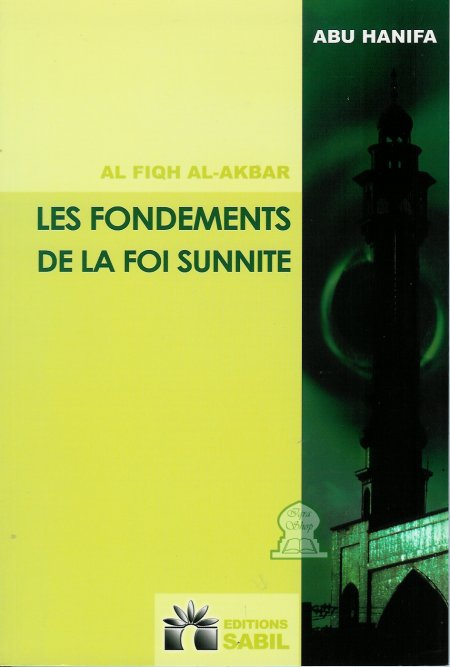
\includegraphics[width=3cm]{Images/image075.jpg}}



{On en trouve sa traduction et son
commentaire en français.
}

Elle témoigne de l'émergence de nouvelles questions.

Par exemple, si vous prenez le premier article~: il y est dit que la foi
consiste à témoigner par la langue, l'assentiment du cœur et l'esprit~:
il ne suffit donc pas de dire, il faut croire à ce que l'on dit et aussi
comprendre ce que l'on dit. Certains diront que l'assentiment du cœur
suffit, et qu'il n'est pas nécessaire de prononcer la
\emph{šahāda}\ldots{} D'autres diront que le dire suffit aux yeux des
hommes, mais non aux yeux de Dieu\ldots{} Bref, ces professions de foi
sont les conséquences de questions théologiques.

De même, il est dit que la foi ne peut pas croître ou décroître. On a la
foi ou on ne l'a pas. Ce ne sera pas l'avis des \textbf{ašʿarites}.

Dans l'article 2, il est dit qu'un musulman qui commet un péché demeure
toujours musulman. Ici, l'article s'oppose explicitement aux
\emph{ḫariǧites} qui affirment le contraire et qui prônent un islam
d'une moralité très rigoureuse.

La \emph{Waṣiyya} se prononce aussi sur le caractère incréé du Coran
(art. 5) et donne des précisions sur l'eschatologie.

Les discussions se précisent toujours davantage et l'on voit aborder
toutes les grandes questions théologiques~: problème de la foi, du
\emph{tawḥīd}, du Coran, de la prédestination, de la prophétologie, de
l'eschatologie, du culte et du califat.






\subsection{Pour aller plus loin}

Daniel \textsc{Gimaret}, \emph{La doctrine d'al-Ash`arî}, Paris, Cerf,
Collection Patrimoine Islam, 1990.

C'est un excellent livre, mais il est très difficile, très technique.
Bref, pour les plus courageux, et surtout pour ceux que ces questions
passionnent.
 
  %8
\include{IbnToumart}
\chapter{Le šī`isme ou l'islam sous un autre visage}

Avant d'exposer les doctrines et pratiques propres au šī`isme, je vous
propose de regarder cette petite vidéo d'un peu moins de 10 minutes.
Elle sera une bonne introduction de ce qui est dit du šī`isme. Vous
devrez pouvoir répondre aux questions de l'encadré ci-dessous. Pour
autant si ce cours va permettre de préciser les informations
mentionnées, il en révélera aussi quelques dimensions que ne signerait
pas un šī`ite. C'est tout le problème de l'imbrication entre la
théologie et l'histoire.

\paragraph{Questions}

\begin{enumerate}
\def\labelenumi{\arabic{enumi}.}
\item
  D'où vient le mot šī`ite~?
\item
  Quel est l'évènement fondateur du šī`isme~?
\item
  Quelles sont les principales villes saintes du šī`isme~?
\item
  Le šī`isme est-il un phénomène spécifiquement persan~?
\end{enumerate}


En raison de la révolution iranienne en Iran en 1979, l'image du šī`isme
véhiculée en Occident a été bien souvent celle de croyances
obscurantistes, d'intolérance, de régression, de violence politique. En
2004, Mohammad Amir-Moezzi et Christian Jambet pouvaient écrire~dans un
ouvrage de grande qualité pédagogique, \emph{Qu'est-ce que le
shî'ism~?}~: «~le shî'isme est une figure de style pour `islam radical',
voire pour `islam terroriste'~»\sn{Mohammad-Ali
  \textsc{Amir-Moezzi}, Christian Jambet, \emph{Qu'est-ce que le
  shî'isme~?,} Paris, Fayard, 2004.} (p. 12).

Cette image est en train de disparaître. Le départ de la scène politique
du président Mahmoud Ahmadinejad après deux mandats (2005-2013) et le
climat de détente avec les États-Unis y est sans doute pour beaucoup.
Sans compter, bien sûr, Al-Qaida, Daesh, autant d'émanations d'un islam
politique extrémiste instrumentalisant le meurtre et la terreur, qui ne
sont pas šī`ites mais sunnites. J'ajouterai que le travail de
vulgarisation des islamologues sur le šī`isme, d'historicisation, de
contextualisation de la République islamique d'Iran et de l'idéologie de
l'ayatollah Khomeiny par rapport à ce courant musulman qui prend son
origine au premier siècle de l'islam y a aussi sa part. Le cinéma
contribue aussi à donner une autre image de la société iranienne.

Mais fondamentalement, qu'est-ce que le \emph{šī`isme}~? S'agit-il d'un
autre islam que le sunnisme ou du même islam mais avec un visage
différent~? Les oppositions politiques au cours de l'histoire, les
polémiques virulentes notamment durant la période des empires ottomans
et safavides, donnent l'image de deux irréductibles, de deux
irréconciliables, de deux frères ennemis. Avoir conscience et
connaissance de la singularité du \emph{šī`isme} ne doit pas faire pour
autant oublier que les šī`ites se disent musulmans et qu'il existe des
penseurs travaillant pour un «~œcuménisme~» entre sunnisme et šī`isme.
Telle est l'approche par exemple de Seyyed Hossein Nasr qui présente le
šī`isme comme «~une affirmation d'une dimension particulière de l'islam
qui est centrale et qui est considérée par les \emph{šī`ites} comme
faisant partie de l'islam en tant que tel. Il n'a pas été un mouvement
qui a d'une certaine manière détruit l'unité de l'islam, mais un de ceux
qui a ajouté à la richesse du déploiement historique et de la diffusion
du message coranique~»\sn{Seyyed Hossein Nasr dans Sayyid Muḥammad
  Husayn Ṭabāṭabā'ī, \emph{Shi‛ite Islam} , translated and edited by
  Seyyed Hossein Nasr , Albany, State University of New York Press,
  1975, p.7.}.

Certes, il existe des aspects historiques et religieux du šī`isme qui
contredisent le sunnisme, mais ce professeur iranien de philosophie
appelle à y voir le signe d'une pluralité d'interprétations possibles.
Il ne s'agit pas d'élaborer un dénominateur commun mais de voir que
l'unité embrasse les différentes «~facettes de l'islam~». Pour lui,
c'est dans la mystique, la spiritualité, l'ésotérisme qu'il est possible
de transcender, de dépasser les différences et de trouver l'unité. 


Mais avant de voir comment sunnisme et šī`isme relèvent tous deux de la
même unité qu'est l'umma, la communauté musulmane, quels sont les
éléments fondamentaux d'histoire, de doctrines et de pratique du
šī`isme~?


\section{Les fondations du šī`isme~: histoire
}
\subsection{Origine du šī`isme~: la
question de la
succession}


Le terme arabe \emph{šī`a} signifie
parti, adhérent, fidèle. S'il y est mentionné que l'acte de naissance du
šī`isme est la bataille de Kerbala\sn{
Kerbala~: c'est la ville qui n'a pas défendu les enfants du prophète.
Rédemption par le sang.}
, pour les šī`ites, le šī`isme
existait du vivant de Muḥammad.

`Alī en effet est le fils d'Abū Ṭālib, l'oncle paternel de Muḥammad. Il
est un des premiers convertis à l'islam. La tradition sunnite mentionne
que le Prophète lui avait confié (amāna) les biens des personnes dont il
était le représentant commercial et financier peu avant l'Hégire, que le
soir de l'Hégire, lorsqu'il quitta La Mecque, `Alī dormit dans son lit,
qu'il épousa Fāṭima, l'une des filles du Prophète.

Fāṭima joue un rôle très important dans l'histoire du šī`isme. Elle
décède à l'âge de 28 ans et `Alī n'épousera aucune autre femme. Il
semble, d'après les traditions šī`ites que Muḥammad avait imposé à son
gendre la monogamie pour sa fille Fāṭima. Elle aurait aussi obtenu de
son père l'autorisation d'aller prier sur les tombes de ceux qui avaient
été tués au cours des batailles.

À la mort du Prophète s'est posée la question de savoir qui allait
succéder à Muḥammad. Pour `Alī et ses partisans, Muḥammad a désigné son
successeur de son vivant. En effet, peu de temps avant sa mort, en 632,
Muḥammad se rendit à \emph{Ġadir Ḫumm~}: c'est le pèlerinage d'adieu (Ḥaǧǧa
al-widā').
\begin{marginfigure}
    \centering
    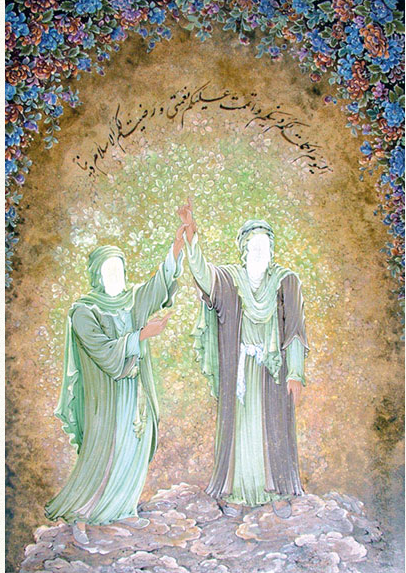
\includegraphics[width=1.35188in,height=1.90972in]{Images/image078.png}
    \caption{Ġadir-e Khumm et la
désignation de l'Imâm `Alī. œuvre de Rezâ
Badr-os-Samâ'}
    \label{Ġadir-e Khumm}
\end{marginfigure}

Il y reçut le verset suivant~: 
\begin{quote}
  {«~O Messager, transmets
ce qui t'a été descendu de la part de ton Seigneur. Si tu ne le faisais
pas, alors tu n'aurais pas communiqué Son message. Et Dieu te protégera
des gens. Certes, Dieu ne guide pas les gens mécréants.~» (Coran,
5:67).}  
\end{quote}


Par la suite, selon les šī`ites, Muḥammad déclara~: «~Man kuntu Mawlāhu,
fahaza `Alī mawlāhu~» c'est-à-dire~: «~Qui me reconnaît comme son Mawlā
(maître, guide), doit reconnaître `Ali comme son Mawlā ~».




Mais pour certains des compagnons du Prophète, cette désignation n'a
jamais été officialisée et selon les mœurs tribales, il convient donc de
procéder à son élection.

Mais `Alī est écarté du collège électoral. \mn{\cite{OUARDI:CalifesMaudits}} 

La tribu des Qurayš élit Abū Bakr, vieux compagnon et un des beaux-pères
de Muhammad~: il devint le 1\textsuperscript{er} calife (khalîfa).

`Alī fera acte d'allégeance, il se soumet à ce choix signifiant son
désir de maintenir l'unité de l'\emph{umma}.

À la mort d'Abū Bakr, `Umar devient le 2\textsuperscript{ème} calife
puisqu'il avait été désigné de manière explicite (\emph{naṣṣ}). `Alī
accepte.

`Umar annonce qu'à sa mort, son successeur devra être choisi parmi les
membres d'un collège électoral qu'il a lui-même nommés. `Alī en fait
partie. À la mort de `Umar, c'est `Uṯmān qui est choisi. Accusé de
népotisme, il est assassiné.

`Alī devient alors le 4\textsuperscript{ème} calife (656-661) attestant
ainsi de ses qualités vertueuses et de la suprématie de l'imamat sur les
manigances politiques mondaines.

Pour autant, deux anciens compagnons du Prophète n'ayant pas vu leur
appétit politique satisfait -- ils souhaitaient être gouverneurs de Kūfa
et Baṣra -- s'associèrent à `Ā'iša, fille d'Abū Bakr et veuve du
Prophète, pour lever une armée contre `Alī. C'est la bataille du chameau
de 657. On l'appelle ainsi parce que `Ā'iša qui était présente, était
montée sur un chameau\ldots{} Son armée fut mise en défaite.





\mn{On voit ici `Ā'iša sur son chameau et dans son baldaquin}



Mais en Syrie, Mu`āwiya, parent de `Uṯmān, mena aussi une guerre. C'est
la bataille de Ṣiffīn. Alors qu'elle tournait à l'avantage de `Alī,
Mu`āwiya proposa un arbitrage sur le livre sacré. `Alī accepte. Nombre
de ses soldats se soulèvent considérant qu'il n'avait pas à accepter
l'arbitrage et que Dieu avait déjà rendu son jugement par la victoire
qui se manifestait. `Alī doit mener combat contre ces rebelles (ce sont
les ḫariǧites), alors que Mu`āwiya se fait proclamer calife à Jérusalem
en 660~!

`Alī est assassiné par un ḫarigite à Kūfa en 661.

Pour les sunnites, il n'avait pas de successeur tandis que les šī`ites
affirment qu'il avait nommé son fils aîné, al-Ḥasān.

 
\subsection{La généalogie du
šī`isme}\label{la-guxe9nuxe9alogie-du-ux161ux12bisme}

La généalogie est sujet à controverses et divergences ce qui explique la
multiplication des šī`ismes\textbf{.} On dénombre une centaine de
lignées à la fin du premier siècle de l'Hégire.

Les jours de naissances des membres de la famille de `Alī sont des fêtes
religieuses. Les jours anniversaires de leur mort, des journées de
deuil. Leurs tombes sont des lieux de pèlerinage~: les cités où elles se
trouvent sont des villes saintes.

Elle est un peu subtile, chaque imām mériterait un chapitre\ldots{}
entre son enseignement, les histoires, les légendes, leur assassinat --
souvent empoisonné -- sans compter qu'au sein même du šī`isme, les
généalogies, les filiations ne sont pas les mêmes, que certains ne
reconnaissent que quatre imāms, d'autres sept, d'autres douze, que ce ne
sont pas toujours les mêmes\ldots{} qu'il y a donc une multitude de
branches šī`ites\ldots{} Bref, je retiens surtout le šī`isme majoritaire
dit duodécimain, car il reconnaît 12 imāms. Vous en trouverez en annexe
la liste avec leurs noms et quelques caractéristiques. Si vous avez la
curiosité de regarder le douzième, vous voyez que n'est pas indiquée la
date de sa mort. D'après vous, est-ce parce que l'on ne la connaît pas,
ou est-ce pour une autre raison~? La réponse dans la suite du cours. Bon
travail.

 
\paragraph{`Alī et Fātima}\label{alux12b-et-fux101tima}

`Alī joue donc dans le šī`isme un rôle important. Il est à la tête de
presque toutes les chaînes de transmission, il est considéré ~comme un
maître spirituel. On lui attribue deux livres~: \emph{Nahj al-balâgha}
(La Voie de la maturité)~et \emph{Dîwân}, un recueil de poèmes.

Quant à Fātima, elle est la sainte la plus vénérée du šī`isme\textbf{.}
Sa tombe est à Médine (il y en a trois\ldots{} dans le doute, on les
garde toutes les trois).

Fātima est la mère de toute la lignée des imāms. Elle représente ce qui
relie Muhammad à `Ali, la lettre et l'esprit. Elle est dite \emph{maǧma`
al-nūrayn} (le Confluent des Deux Lumières), celle de la prophétie et de
l'imamat. Elle a une mission d'intercession et de protection jusqu'à la
fin des temps. Immaculée, Vierge malgré son mariage, elle est aussi
reine du ciel. Un parallèle avec Mariam (Marie), la mère de Jésus est
établi par la tradition šī`ite elle-même \sn{Tahani Sabri,
  «~L'hagiographie de Fāṭima d'après le \emph{biḥār al-anwār}~», École
  des Hautes Études en Sciences Sociales, thèse de doctorat sous la
  direction de Henry Corbin, 1969.}.

 
\paragraph{Al-Hasan, fils de
`Alî}\label{al-hasan-fils-de-aluxee}

C'est un petit-fils du Prophète. Il y a des récits touchant d'affection
tendre.

Al-Ḥasan abdiqua le califat devant l'hostilité de Mu`āwiya. Pour les
historiens šī`ites, il préféra l'unité de la communauté plutôt que de
voir la division, mais les sunnites font remarquer qu'il n'était pas en
mesure de remporter la victoire et qu'il abdiqua en contre-partie d'une
importante somme d'argent. Retiré à Médine, il est assassiné,
semble-t-il par une de ses épouses qui aurait été soudoyée, selon les
šī`ites par Mu`āwiya. Terrible Mu`āwiya\ldots{} J'imagine que vous ne
devez pas le trouver très sympathique. Il est le fondateur de la
dynastie Omeyyade. Les grands historiens sunnites des
8\textsuperscript{ème} et 9\textsuperscript{ème} siècles n'en ont pas
laissé un souvenir très élogieux\ldots{} car ils sont abbassides et il
fallait effacer les traces vénérables des Omeyyades.

 
\paragraph{Al-Ḥusayn} 

Al-Ḥusayn, le second fils de `Alī, reste discret. Il s'efface. Mais il
entre sur la scène politique au moment de la mise en place d'une
dynastie califale héréditaire en la personne de Yazīd, le fils de
Mu`āwiya. On se réfère souvent à lui pour présenter le šī`isme comme un
courant révolutionnaire, politique et contestataire.

L'histoire est plus complexe. En tous les cas, les sources appellent une
très grande prudence. Assuré du soutien de la ville de Kūfa, il se met
en route avec toute sa famille pour chasser les Omeyyades. Mais sur la
route, la petite troupe se trouve encerclée par les soldats omeyyades,
coupée de Kūfa, privée d'eau. Retranchée en plein désert dans un petit
village appelé Karbalā', les Omeyyades finissent par donner l'assaut.
C'est un massacre. Ḥusayn est tué, décapité, piétiné ainsi que quasiment
toute sa famille.

Ašura est le jour de célébration où l'on fait mémoire de cette tragédie
dans de grandes cérémonies populaires avec parfois des dérives
spectaculaires de lamentations violentes, d'auto-flagellations, de
lacérations ou de mutilations. C'est le remord d'une ville qui n'a pas
soutenu al-Ḥusayn.

Ḥusayn devint alors un exemple de martyr, de sacrifice, de bravoure.
Sans-doute, sous l'influence chrétienne, on verra dans la mort de Husayn
un sacrifice rédempteur pour le salut des fidèles.

Chez certains fidèles la rumeur selon laquelle il ne serait pas mort
circule. Il aura été enlevé au ciel directement par Dieu avant le
combat.


\mn{Les troupes omeyyades encerclent Karbalā' \& Yā Ḥusayn\ldots{}

Jour de la fête d'Ashura \& Ashura et ses spectaculaires flagellations à
Karbalā'\ldots{} }


 
\paragraph{`Alî Zayn al-`Âbidîn, fils
d'al-Husayn}\label{aluxee-zayn-al-uxe2biduxeen-fils-dal-husayn}

Un rescapé du massacre de Karbalâ'. Il serait parti à Médine pour y
mener une vie pieuse. Il ne posa aucun problème aux Omeyyades. Une
existence ascétique, consacrée à la dévotion. On le surnommait
\emph{al-saǧǧād}, celui qui accomplit de nombreuses prosternations.
C'est un nom respecté, même dans le sunnisme.

Un de ses fils Zayd ibn `Alî, est à l'origine d'une grande famille, les
zaydites. Le zaydisme est marqué par un activisme violent. Selon la
théorie zaydite de l'imamat chaque Alide a le droit de prétendre à la
direction de la communauté. Le véritable imâm est celui qui se qualifie,
les armes à la main, en s'insurgeant contre le pouvoir injuste. Ils sont
aujourd'hui encore influents au Yémen~où ils représentent la moitié de
la population (mais le dernier chef zaydite du Yémen a été renversé en
1962).

 
\paragraph{Muhammad al-Bāqir, fils de `Alî Zayn
al-`Âbidîn}\label{muhammad-al-bux101qir-fils-de-aluxee-zayn-al-uxe2biduxeen}

Il est considéré comme le fils de `Ali Zayn. Les grandes traditions
šī`ites le considèrent comme le 5ème Imām. Il est surnommé Abū Ǧa`far.

 
\paragraph{Ǧa'far al- Ṣādiq
}\label{ux1e7afar-al--ux1e63ux101diq}

Fils de Muhammad al-Bāqir, il est célèbre pour sa piété et, selon les
shiites, l'infaillibilité de ses prémonitions. Les auteurs soufis lui
attribuent le plus ancien commentaire mystique du Coran. On le considère
comme un alchimiste, un spirituel refusant toute implication dans les
mouvements politiques de son époque. Il fut enterré dans le cimetière de
Baqī` à Médine. Le carré šī`ite y sera rasé au XIX° siècle par les
Wahhabites, alors qu'il abritait les tombes de plusieurs imâms.

Son fils aîné, Ismā`īl, est l'éponyme de la seconde grande famille de
l'islam šī`ite, les ismaéliens, šī`ites septimains \textbf{--} shî'ites
à 7 imâms. Pour cette branche, il est le dernier Imâm. Un autre groupe
s'appuie sur la croyance que l'imamāt fut transmis du vivant de Ǧa`far à
son petit-fils~: ce sont les qarmates. D'autres, les Fatimides,
considèrent que l'imamat se poursuit et que l'imam caché, le Mahdi, sera
un de ses descendants.


\begin{Synthesis}
Le si'isme est  une prophétologie. Il y a une sur
l'incarnation. Facilite le
dialogue avec les chrétiens.
\end{Synthesis}

 
\paragraph{{Le douzième imām, l'imām caché ou
le Madhī
}{ }}\label{le-douziuxe8me-imux101m-limux101m-cachuxe9-ou-le-madhux12b}

À la mort du 11\textsuperscript{ème} imâm, les fidèles croient que
l'imâm a eu un fils du nom de Muḥammad. 
\begin{Def}[Mahdî]
Il est reconnu comme le
\emph{Mahdî,} le Bien Guidé. C'est l'imâm caché, \emph{al-imâm al-ġā'ib}
ou encore \emph{al-Qā'im}, que l'on peut traduire par le Résurrecteur.
\end{Def}


C'est le courant duodécimain, majoritaire dans le šī`isme.

Mais en quoi consiste cette occultation~? Comment s'opère-t-elle~? Que
signifie-t-elle~? Quand a-t-elle eu lieu~? Sous quelles formes~?

Je vous propose d'écouter ce bref passage d'une émission sur France
Culture, «~Les racines du ciel~», où Amir-Moezzi répond.

L'imâm caché n'est donc pas mort. Vous comprenez maintenant pourquoi
dans le tableau en annexe ne figure que sa date de naissance. Il
n'existe pas de successeur puisqu'il est physiquement vivant. À la fin
des temps, il se manifestera. Il y a donc une présence invisible, mais
physiquement réelle. L'imâm caché clôt la lignée des imamites.

Par la suite, tout se passe comme si désormais l'ère de la bonne entente
entre le religieux et le politique était désormais finie. La cité
idéale, gouvernée par un juste n'est réalisable qu'à la fin des temps,
avec l'avènement du Mādhi, le Sauveur eschatologique. L'attitude
revendicative et politique est rejetée dans un futur messianique. Le
šī`isme se présente comme une religion individuelle, personnelle, non
institutionnelle. Mais peut-il alors perdurer ? Pour pallier cette
«~absence~», on aura recours à la figure du juriste avec la dynastie
bouyide. C'est à cette époque que le šī`isme sera érigé comme religion
d'État, ce qui n'est pas le moindre des paradoxes compte tenu de ses
«~fondamentaux~».

 
\section{Les fondations du šī`isme~:
doctrines}\label{ii.-les-fondations-du-ux161ux12bisme-doctrines}

Les doctrines šī`ites sont compliquées, subtiles et à lire
l'enseignement des imāms et les commentaires qui en suivirent, cette
subtilité est voulue pour elle-même. De leurs enseignements, ils ne
cessent de dire~: «~notre enseignement est ardu, difficile à supporter~:
c'est un secret, un secret enveloppé par un secret au sujet d'un
secret~»\sn{Voir Amir-Moezzi, Jambet, \emph{Qu'est-ce que le
  shi'isme~?}, Paris, Fayard, p. 96 .}.

Dans sa présentation du šī`isme, Amir-Moezzi distingue dans la vision du
monde et la théologie šī`ite une double dimension~: elles sont marquées
à la fois par l'affirmation d'un principe de dualité et d'un principe de
dualisme. On lira avec intérêt et pour plus de précisions la
présentation qu'il fait dans \emph{Qu'est-ce que le shiisme~?} Mais tout
d'abord, la question des Écritures. Sont-elles les mêmes qu'en
sunnisme~?

 
\subsection{{Les sources scripturaires
}}\label{les-sources-scripturaires}

 
\paragraph{{Y a-t-il un Coran šī`ite~?
}}\label{y-a-t-il-un-coran-ux161ux12bite}

Le Coran est la référence principale et la contradiction éventuelle
entre un \emph{ḥadīṯ} et un verset coranique est l'indice de la fausseté
du ḥadīṯ.

Pour autant, certaines traditions shî'ites trouvent difficilement leur
fondement dans le Coran. Pour les šī`ites, le Coran a été en réalité
falsifié, altéré, censuré lors de sa compilation par `Uṯmān (c'est un
des premiers califes. Si le nom ne vous disait plus rien du tout,
revoyez le premier cours sur le Coran et à la question du
\emph{muṣhaf}). La révélation originelle contenait des versets sur `Alî
et les descendants des Prophètes. Ils étaient cités comme les modèles et
les chefs par excellence. `Alī possédait une version du Coran intégral,
mais il n'en dit mot pour éviter sa destruction par ses adversaires.
Cependant, elle fut transmise secrètement d'imam à imam, jusqu'au
12\textsuperscript{ème} imâm qu'il l'emporta avec lui lors de son
Occultation. Les enseignements des imāms permettent d'accéder à ces
versets et de les connaître.

Avec l'arrivée au pouvoir des Bouyides shiites à la fin du
4\textsuperscript{ème} siècle de l'hégire, il s'agira de trouver un
accord avec l'orthodoxie sunnite. On met ainsi un terme au doute sur
l'intégrité du Coran officiel. Le courant dominant abandonne la thèse de
la falsification du Coran officiel, mais le débat ressurgit
régulièrement.

 
\paragraph{Y a-t-il un \emph{ḥadīṯ} šī`ite~?
} 

Bien qu'al-Būḫārī fut perse, il existe une Sunna šī`ite. Les textes sont
bien souvent les mêmes, mais les \emph{isnāds} diffèrent et renvoient
aux membres de la famille du prophète (\emph{ahl al-bayt} --
c'est-à-dire littéralement, les gens de la maison). En effet, la
référence dans l'\emph{isnād} aux compagnons du Prophète lui ôte toute
crédibilité dans la mesure où ils sont considérés comme des traîtres.
Pour l'\emph{isnād}, la notion a été vue dans le cours sur la Sunna.
C'est la fameuse chaîne de transmission.

On reconnaît trois grands corpus~:

\begin{itemize}
\item
  Celui de Ya`qub al-Kulaynī (m. en 939).
\item
  Celui de Saduq Ibn Babuyeh (m. 991).
\item
  Celui d'al-Ḥasan al-Tusī (m. 1068).
\end{itemize}

On trouve aussi dans ces recueils de nombreux témoignages des imāms.

L'ouvrage le plus connu de Kulaynī est \emph{al-Kāfī}. Il est divisé en
trois sections~:

\begin{itemize}
\item
  \emph{Usūl al-Kāfī}, qui concerne l'épistémologie, la théologie, la
  question de la foi et de la mécréance, l'histoire, l'éthique, et le
  Coran~et ses mérites;
\item
  \emph{Furūʿ al-Kāfī}, qui concerne les dimensions pratiques et légales
  (prières, \emph{ǧihād}, jeûne, ḥaǧǧ, funérailles, nourriture, boisson,
  mariage, divorce, commerce, héritage, etc.)
\item
  \emph{Rawdat} \emph{al-Kāfī}, qui inclue de nombreuses traditions, des
  lettres, des discours des imāms.
\end{itemize}

Il existe une traduction anglaise de cette collection de plus de 16 000
traditions. Si vous ne trouvez pas le sommeil\ldots{}
 
\subsection{ Dualité et dualisme}\label{dualituxe9-et-dualisme}

 
\paragraph{ Une vision duelle}\label{une-vision-duelle}

Il s'agit d'affirmer que toute réalité possède deux niveaux~:

1/ un niveau manifeste, obvie, apparent, visible, concret, évident
(\emph{zāhir})

2/ un niveau secret, non manifeste, implicite, invisible, intérieur
(\emph{bāṭin})

Cette affirmation est au cœur du credo šī`ite. Ce que je vois, ce qui
est visible contient aussi une réalité invisible. Il existe une relation
entre le manifeste et le caché, l'exotérique et l'ésotérique. Il s'agit
d'appliquer ce principe à toute réalité, et bien sûr, à commencer par la
théologie.

\emph{Ainsi, en théologie}, Dieu a deux niveaux d'être, deux niveaux
ontologiques~:

1/ son Essence, inconcevable, inimaginable, au-delà de toute pensée~:
c'est le niveau caché (\emph{bāṭin})

2/ ses Noms et Attributs~à travers lesquels Dieu se révèle et se fait
connaître~: c'est le Dieu inconnu qui aspire à être connu. Amir-Moezzi
remarque que l'on retrouve une distinction de la théologie médiévale
chrétienne entre \emph{Deus absconditus} et \emph{Deus revelatus}.

La manifestation de ces noms divins comme le Roi, le Miséricordieux, le
Juge suprême, etc. est une manifestation de Dieu (théophanie). La plus
haute révélation en est la figure de l\emph{'Imām} céleste,
l'\emph{Imām} de Lumière, l'Homme cosmique~: c'est l'Imām avec un I
majuscule, dans son acception ontologique universelle.

L'\emph{Imām} cosmique a aussi deux dimensions

\begin{quote}
1/ la dimension cachée~: c'est l'aspect métaphysique, dans le ciel,
invisible à nos yeux.

2/ la dimension exotérique, visible~: ce sont les \emph{imāms}
historiques.
\end{quote}

La mission de ces \emph{imāms} historiques~consiste à dévoiler les
mystères de Dieu, du monde et de l'homme, à transmettre aux hommes le
Secret contenu dans l'Imām métaphysique.

Mais l'enseignement des imāms, disions-nous, est complexe. Ǧa`far
al-Ṣādiq (c'est un \emph{imām} que nous avons rencontré dans la
généaologie des douze\ldots{} C'est le combientième \emph{imām} déjà~?)
écrivait~: «~Notre enseignement comporte l'exotérique, l'ésotérique et
l'ésotérique de l'ésotérique~».

À cette approche duelle de la réalité se superpose le principe du
dualisme.

 
\paragraph{ Une vision dualiste}\label{une-vision-dualiste}
\mn{Si isme~: influence de la zoroastrisme avec un certain manichéisme, bien
/ mal. Lumière et nuit~; combat cosmique et sur terre. On retrouve ceci
dans le sunnisme. Tous les Hadiths eschatologiques décrivent en tableau
le paradis. Dans le Si isme, enjeu du bien et du mal.
}
L'histoire de la création est celle d'un combat cosmique entre les
forces du Bien et les forces du Mal, entre la lumière et l'obscurité. On
retrouve ici une nette dimension zoroastrienne et manichéenne du monde.

Ce combat se situe au niveau cosmique~: c'est le combat entre les armées
de l'Intelligence cosmique (\emph{al-`aql}) et celles de l'Ignorance
cosmique (\emph{al-ğahl}). Cette dichotomie, cette opposition est celle
d'une lutte permanente entre les Gens de la Droite (\emph{ašāb
al-yamīn}) et les gens de la Gauche (\emph{ašāb al-šimāl}). Le combat
entre deux hommes ennemis s'inscrit donc dans un cadre plus large. Toute
l'histoire de l'humanité est traversée par l'adversité et la violence
des forces démoniaques de l'Ignorance. Il en sera ainsi jusqu'à la fin
des temps avec l'avènement du Sauveur eschatologique, le Mahdī qui
vaincra définitivement les forces du mal.

Mais qui sont ces forces du mal~? Comment les reconnaître, les
identifier~?

C'est l'enseignement des imāms (les 7, les 12, selon) qui apportent les
réponses à ces questions. Dans ce corpus de centaines de milliers de
pages, les adversaires de l'imâm~sont tour à tour identifiés~:

\begin{itemize}
\item
  Aux juifs, qui sont des idolâtres et ont trahi Moïse en adorant le
  veau d'or
\item
  Aux Compagnons de Muhammad qui ont rejeté `Alī
\item
  Aux Gens de l'exotérique, c'est-à-dire des apparences, du superficiel
  (\emph{ahl al-zāhir}), ce sont les littéralistes qui s'arrêtent à la
  lettre et n'ont pas connaissance de son `esprit' (\emph{bāṭin}). À cet
  égard, un šī`ite se sentira plus proche d'un juif ou d'un chrétien
  accoutumé à une lecture ésotérique, symbolique, anagogique des textes
  que d'un musulman sunnite exotérique, qui se limite à la lettre.
\end{itemize}

 
\subsection{Prophétie et
Imamologie}\label{prophuxe9tie-et-imamologie}

L'enseignement des \emph{imāms}, acquiert en réalité un rôle supérieur à
celui du Prophète.

En effet, si le prophète est le messager de la lettre, l'\emph{imām}
dans le šī`isme en apporte l'esprit. Or, si l'esprit peut exister sans
la lettre, sans l'esprit, la lettre est morte\sn{Amir-Moezzi,
  Jambet, \emph{Qu'est-ce que le shi'isme~?}, Paris, Fayard, 2004, p.
  42.}.


\paragraph{Remarque sur l'imām~}: le mot \emph{imām}
est piégé. Il s'emploie en sunnisme, mais sans désignation particulière.
L'imām désigne un savant, un chef ou tout simplement celui qui dirige la
prière. En revanche, en šī`isme\textbf{,} c'est un titre sacré. L'imām
est le Guide, l'un des Douze\ldots{} En principe, aucun autre homme ne
porte ce nom. Et pourtant, d'aucuns se sont attribués ce titre. Autant
dire qu'ils se prenaient pour le Mahdi .L'un d'eux est très célèbre. À
suivre.

L'Imām apporte en effet la connaissance face au monde de l'ignorance. En
montrant son cœur, l'Imām `Alī donnait cet enseignement sur la vocation
de l'imām, la nature de la religion, son importance. Écoutez et
réécoutez ce texte\sn{Vous trouvez l'intégralité du texte dans le
  livre de Mohammad Ali Amir-Moezzi, \emph{La religion discrète}, Paris,
  Vrin, 2006,
  \url{https://books.google.com}}.


L'imām transmet les vérités secrètes. Il tient le monde, il évite la
noyade définitive du monde dans les ténèbres. Il est l'alpha et l'omega
du šī`isme\sn{Amir-Moeezi, Jambet, \emph{Qu'est-ce que le
  shi'isme~?}, p. 40.}.

Mais il a aussi des pouvoirs supra-normaux~: il possède la science du
passé et du futur, il lit dans les consciences, il connaît les langues,
y compris celle des animaux, les sciences occultes (astrologie,
alchimie, sciences divinatoires, etc.). Il peut ressusciter les morts,
guérir les maladies, rajeunir les vieillards, marcher sur les eaux,
monter aux cieux\ldots{} Il possède des objets de pouvoir~ tels la
tunique d'Adam, le sceau de Salomon, l'Arche et les tables de la Loi,
l'Arme invincible de Muḥammad.

L'enseignement de l'\emph{imām} est au cœur de l'approche spirituelle
šī`ite. C'est par lui que se réalise la spiritualisation, la
divinisation. Écoutez Amir-Moezzi à ce sujet.

 
\subsection{La walāya au cœur de la foi šī`ite
} 


La \emph{walāya} est un concept clé du \emph{šī`isme}. Les
\emph{šī`ites} sont appelés les gens de la \emph{walāya}.\\
\begin{Def}[walāya]
La \emph{walāya} désigne la mission sacrée et sainte des imams.

L'imām est le \emph{walī} (le saint), celui qui initie les fidèles à
l'esprit de la Parole divine. Il est la Face de Dieu sur terre.

\end{Def}



La \emph{walāya} désigne aussi l'amour, celui que les fidèles
manifestent dans la dévotion, par la loyauté, la soumission à l'égard du
maître initiateur.

Mais dans une doctrine \textbf{dualiste}, l'amour de l'imām ne peut aller sans la
haine de son ennemi. La \emph{walāya} est donc inséparable de son
contraire, la \emph{barā'a} (c'est-à-dire la haine, la dissociation à
l'égard des forces de l'ignorance). Un \emph{ḥadīṯ} šī`ite dit~:

\begin{quote}
«~l'amour de Dieu ne s'obtient que grâce à l'amour envers Ses amis et
l'hostilité à l'égard de Ses ennemis~».    
\end{quote}


Au cœur de la foi šī`ite, la \emph{walâya} est dans la \emph{šahāda} :
\begin{quote}
   «~Je témoigne qu'il n'y a pas de dieu hormis Dieu~; je témoigne que
Muhammad est l'envoyé de Dieu, et que `Alî est le \emph{walī} de
Dieu~» 
\end{quote}
 \emph{walī} signifie ici l'ami,~l'allié, le détenteur de la
\emph{walāya}.




\mn{\emph{Šahāda} sur une mosquée du Caire
fatimide. on y lit à la fin~:\emph{ʿAlī walī
allāh.
}  }


\subsection{{Les signes de la fin du monde ou
l'eschatologie šī`ite
}\label{les-signes-de-la-fin-du-monde-ou-leschatologie-ux161ux12bite}}

En raison de la place de la question de l'Occultation, l'eschatologie a
donné lieu à un foisonnement de traditions et de traités. Il s'agit de
savoir lire les signes afin de reconnaître l'imminence du Dernier Jour,
le retour du Mahdī. Les signes sont multiples, mais on peut identifier
quelques constantes~:

\begin{itemize}
\item
  l'envahissement de la terre par les forces du Mal,
\item
  l'écrasement quasi-complet des forces de la Connaissance par celles de
  l'ignorance,
\item
  la perte du sens du sacré,
\item
  le renversement des valeurs humaines,
\item
  l'anéantissement de tout ce qui relie l'homme à Dieu et à son prochain
\end{itemize}

Des signes concrets sont exposés. Ainsi par exemple,

\begin{itemize}
\item
  la venue d'al-Sufyānī, le chef de l'armée des ennemis des imāms, le
  collaborateur d'\emph{al-Daǧǧāl}, l'Imposteur, l'Antéchrist islamique.
\item
  L'avènement d'al-Yamānī, le Yéménite qui prêchera le soutien au Mahdī.
\item
  Le Cri, d'origine surnaturelle, venu du ciel, appelant les hommes à
  rejoindre l'armée du Sauveur
\item
  L'engloutissement d'une armée (parfois celle d'al-Sufyānī) dans le
  désert.
\item
  L'assassinat à La Mecque de l'envoyé du Mahdī, appelé \emph{al-Nafs
  al-Zakiyya\textbf{~}}: l'Âme Pure.
\end{itemize}

La fin de l'occultation est aussi expliquée et commentée. On peut en
distinguer 3 raisons~principales :
\begin{enumerate}
    \item une raison historique~: venger tous les hommes saints du passé,
victimes de l'injustice. Tous les saints du passé reviendront à la vie,
ainsi que leurs meurtriers, et les premiers pourront ainsi se venger des
seconds à cette occasion.
\item une raison religieuse~: rétablir le sens du sacré~; rétablir les
religions (judaïsme, christianisme, islam) dans leur intégralité
originelle, rapporter les Écritures respectives qui ont été altérées ou
falsifiées
\item une raison spirituelle~: apporter le sens ésotérique des choses,
effacer la frontière entre le caché et le manifeste.
\end{enumerate}
 

Le retour du Mahdi s'accompagne aussi de celui de Jésus-Christ. Il est
le principal compagnon d'al-Qā'im. Voyez un peu plus haut. C'est un nom
utilisé pour nommer le Mahdi. Quelle est sa signification déjà~? Penser
à «~\emph{Talitha Qum~}».. Lève-toi\ldots{} C'est bien la même racine du
redressement, de la résurrection.

 
\section{Bibliographie}\label{bibliographie}

\paragraph{Les fondamentaux}

Mohammad-Ali \textsc{Amir-Moezzi}, Christian Jambet, \emph{Qu'est-ce que
le shî'isme~?,} Paris, Fayard, 2004.

Henri \textsc{Corbin}, \emph{En Islam iranien}, Aspects spirituels et
philosophiques III, Les Fidèles d'amour, shî'isme et soufisme,
Gallimard, 1978, 359 pages (PISAI H266).

\paragraph{Pour aller plus loin}

Mohammad Ali \textsc{Amir-Moezzi}, \emph{La religion discrète},
Croyances et pratiques spirituelles dans l'islam shî`ite, Collection
Textes et Traditions dirigée par Marie-Odile Goulet-Cazé, Richard
Goulet, Philippe Hoffmann, Paris, Vrin, 2006.

Henri \textsc{Corbin}, «~De l'histoire des religions comme problème
théologique~», \emph{Monde non chrétien} 51-52, 1960

Leili \textsc{Echghi}, \emph{Un temps entre les temps~: L'Imam, le
Chî'isme et l'Iran}, coll. Patrimoines Islam, cerf, Paris, 1992.

Geneviève Gobillot, \emph{Les Chiites}, Editions Brepols, 1998.

Henri Laoust, \emph{Comment définir le sunnisme et le chiisme},
Geuthner, 1985, 44 pages.

Muhammad Ridā Muzaffar, \emph{Le credo des imamites}, traduction par
Frère Sliwa, Rome, PISAI.

Yann \textsc{Richard}, \emph{Le Šī`isme en Iran~: Imam et Révolution,
Librairie d'Amérique et d'Orient}, 1980, 142 pages.

Yann \textsc{Richard}, \emph{L'islam chi'ite~: croyances et idéologies},
Fayard, Paris, 1991.

\textbf{\hfill\break
}

\subsection{Généalogie des Imāms}


 

\begin{longtable}{p{0.5cm}p{1.3cm}p{1.8cm}p{2.5cm}p{3.5cm}p{0.8cm}}
\small \\
%\sidecaption{Généalogie des Imāms} \label{tab:Genealogie} \\
\toprule
 & Nom & Titre & Epithète & connu pour & dates
\\
\midrule
\endhead
1 
& 
\vtop{{ `Alī}{ (\TArabe{علي})}} 
&
\vtop{{ Abū al-Ḥassan}{ (\TArabe{أبو الحسن})}}
&
\vtop{{ Amīr al-Mu'minīn}{ (\TArabe{أمیر المؤمنین}) -
Commandeur des croyants}} 
& Le premier Imam est la personne la plus
significative après Mahomet pour les chiites 
& 600 -- 661 \\



2 & \vtop{{ Ḥasan}{ (\TArabe{ألحسن})}} &
\vtop{{ Abū Muḥammad}{ (\TArabe{أبو محمد})}} &
\vtop{{ Al-Mujtabā}{ (\TArabe{ألمجتبی}) - le choisi}}
& Signe un traité de paix pour un Islam meilleur, très aimé par Mahomet
est avec son frère un des maîtres des jeunes du paradis & 625 -- 669 \\


3 & \vtop{{ Ḥusayn}{ (\TArabe{ألحسین})}} &
\vtop{{ Abū \textsuperscript{c}Abdillāh}{ (\TArabe{أبو
عبداللھ})}} & \vtop{{ Sayyid
ash-Šuhadā'}{ (\TArabe{سید الشھداء}) - Seigneur des martyrs}} &
Est mort lors de la bataille de Kerbala. & 626 -- 680 \\


4 & `Alī (\TArabe{علي}) & \vtop{{ Abū
Muḥammad}{ (\TArabe{أبو محمد})}} & \vtop{{ Zayn
al-\textsuperscript{c}Ābidīn}{ (\TArabe{زین العابدین}) - Joyau
des croyants}} & Piété, jeûne, pénitence pendant 20 ans à cause de la
bataille de Kerbala. & 658 -- 713 \\


5 & Muḥammad (\TArabe{محمد}) & \vtop{{ Abū
Ja\textsuperscript{c}far}{ (\TArabe{أبو جعفر})}} &
\vtop{{ Al-Bāqir}{ (\TArabe{ألباقر}) - Pourfendeur de
la Science}} & le moins oppressé des douze imams par le calife de son
temps. Il n'est pas reconnu par les Zaydī (qui prennent comme imam Zayd
Ibn `Alī. & 676 -- 743 \\


6 & \vtop{{ Ǧa'far}{ (\TArabe{جعفر})}} &
\vtop{{ Abū \textsuperscript{c}Abdillāh}{ (\TArabe{أبو
عبداللھ})}} & \vtop{{ Aṣ-Ṣādiq}{ (\TArabe{ألصادق}) -
Le véridique}} & Un penseur respecté à la fois par les Chiites et les
Sunnites & 703 -- 765 \\


7 & \vtop{{ Mūsā}{ (\TArabe{موسی})}} &
\vtop{{ Abū Ibrāhīm}{ (\TArabe{أبو إبراھیم})}} &
\vtop{{ Al-Kāẓim}{ (\TArabe{ألکاظم}) - Le triste}} & A
grandi en prison pour le rendre faible Il n'est pas reconnu par les
ismaéliens & 745 -- 799 \\


8 & \vtop{{ `Alī}{ (\TArabe{علي})}} &
\vtop{{ Abū al-Ḥassan}{ (\TArabe{أبو الحسن})}} &
\vtop{{ Ar-Riḍā}{ (\TArabe{ألرضا})}} & Le seul Imam à
être enterré en Iran & 765 -- 818 \\


9 & Muḥammad

(\TArabe{محمد}) & \vtop{{ Abū
Ja\textsuperscript{c}far}{ (\TArabe{أبو جعفر})}} &
\vtop{{ At-Taqī}{ (\TArabe{ألتقي})}} & Un grand
débatteur & 810 -- 835 \\


10 & \vtop{{ `Alī}{ (\TArabe{علي})}} &
\vtop{{ Abū al-Ḥassan}{ (\TArabe{أبو الحسن})}} &
\vtop{{ Al-Hādī (\TArabe{ألھادي}),}{ an-Naqī
(\TArabe{ألنقي})}} & & 827 -- 868 \\


11 & Ḥasan (\TArabe{ألحسن}) & \vtop{{ Abū
Muḥammad}{ (\TArabe{أبو محمد})}} &
\vtop{{ Al-\textsuperscript{c}Askarī}{ (\TArabe{ألعسکري})}}
& L'avant-dernier imam, qui a vécu presque toute sa vie assigné à
domicile et qui prêchait tout de même. & 846 -- 874 \\


12 & Muḥammad

(\TArabe{محمد}) & \vtop{{ Abū Qāsim}{ (\TArabe{أبو
قاسم})}} & \vtop{{ Al-Mahdī}{ (\TArabe{ألمھدي})}} &
Imam actuel, connu pour être le Sauveur. Il est l'occultation. & 868
-- \\
\bottomrule
\end{longtable}
 %9


\chapter{Les fondements du droit (uṣūl al-fiqh)}

\vide{introduction-3}{%
\section{Introduction}\label{introduction-3}}

La loi semble être au cœur de la définition de l'identité musulmane.
Certains journalistes ou orientalistes définissent le spécifique de
l'islam comme religion de la Loi, religion de la \emph{šarī`a.} Sur fond
de révolution iranienne, de wahhabisation de l'Afrique noire, d'État
islamique en Syrie, le terme \emph{šāri`a} est assimilé à l'application
de châtiments corporels~: appliquer la \emph{šāri`a}, c'est couper la
main du voleur, lapider la femme adultère, soumettre l'impudique aux
coups de fouet. La \emph{šāri`a} est devenue source de fantasmes et de
peurs, elle est l'expression du retour à une culture obscurantiste. Un
âge que l'on croyait dépassé refait surface et s'il promet l'ordre
social, il est assorti de la restriction des libertés fondamentales les
plus élémentaires et de l'encadrement de la société par des polices de
mœurs.

S'il est certain qu'elle constitue une expression caractéristique de ce
qu'est l'islam, ou de ce qu'il est devenu au cours de l'histoire, à
savoir une \emph{lex divina} au sens plénier du terme, c'est-à-dire une
science, un système juridique, éthique et religieux universel au sein du
monde musulman, qu'en est-il exactement de la \emph{šāri`a~}?

L'étymologie du mot \emph{šarī`a}~est intéressante~: d'après le
\emph{Lisān al-`arab}, c'est le grand dictionnaire arabe, le verbe
\emph{šara`a} signifie s'abreuver. Au sens premier, la šarī`a~désigne le
lieu où les animaux vont s'abreuver. Par extension, c'est la route qui
conduit à ce lieu. D'ailleurs \emph{šāri`} désigne le législateur mais
aussi la rue. Ainsi, la \emph{šarī`a}~a été interprétée comme désignant
la grande route. La voie qui mène là où tous vont s'abreuver. On la
distingue de la \emph{tarīqa}, le sentier, la voie étroite des fidèles.
La \emph{šarī`a} est formée de la loi exotérique religieuse tandis que
la \emph{tarīqa} conduit vers la vérité, au cœur de la \emph{šarī`a}.
Elle comporte des règles, des méthodes qui se superposent à celles de la
\emph{šarī`a}. ~

Le célèbre juriste Mustapha al-Zarka (1904-1999) la définit comme
«~l'ensemble des commandements et prescriptions dogmatiques et pratiques
que l'islam doit appliquer en vue de réaliser ses objectifs tendant à la
réforme de la société~»\sn{~Mustapha al-Zarka, \emph{al-Fiqh fī
  ṯawbihi al-ǧadīd}, Beyrouth, Dār al-Fiqr, 7\textsuperscript{ème} éd.,
  p. 30}. En toute rigueur, il ne peut y avoir de société musulmane sans
l'application de la \emph{šāri`a}. Dans un sens plus restreint, le
professeur Sélim Jahel la définit comme «~un ordre juridique, assuré
d'une réelle positivité, mais aussi comme un ensemble de principes
régulateurs du droit et de la vie sociale, comme peut l'être, par
exemple, dans un Etat occidental le préambule d'une
constitution~»\sn{Salim Jahel, \emph{La place de la chari'a dans
  les systèmes juridiques des pays arabes}, Paris, Panthéon-Assas, 2012,
  p. 8.}.

L'étude des prescriptions propres à la \emph{šāri`a} permet de dégager
des sources et des fondements~: les \emph{uṣūl al-fiqh}. Ils sont
principalement au nombre de quatre~: le Coran, la Sunna, le consensus
des juristes (\emph{iǧma`}) et le raisonnement analogique
(\emph{qiyās}). Il faut distinguer ces principes du \emph{fiqh} en tant
que science du droit musulman qui analyse les actes et les dires de la
personne majeure et responsable et qui vérifie leur conformité aux lois
divines. Ainsi, le juriste (le \emph{faqīh}) va examiner les questions
relatives à la vente, au mariage, à la délégation de pouvoir mais aussi
les pratiques rituelles, la prière, le vol, l'arrestation, l'accusation
d'adultère ou d'homicide. En revanche, les \emph{uṣūl al-fiqh} renvoient
à la théorie du droit. Il s'agit d'étudier les sources du droit à partir
desquelles on définit les prescriptions. 
\begin{Def}[mujtahid - spécialiste du droit]
Le spécialiste de ces
\emph{uṣūl} se nomme un
\href{https://fr.wikipedia.org/wiki/Mujtahid}{\emph{mujtahid}}.
\end{Def} 
Il va
étudier la nature des prescriptions, leur formulation -- s'agit-il d'un
ordre ou d'un interdit --, la formulation est-elle générale ou
particulière~? Ce travail de clarification aboutit à l'élaboration de
catégories juridiques.

\begin{itemize}
\item
  L'ordre~: «~O vous qui croyez, respectez vos engagements~!~» (S. 5, 1). Honorer un contrat est donc une obligation
 
 
\item
  L'interdiction~: «~O vous qui croyez~! ne vous moquez pas les uns des
  autres~» (S. 49, 11). Tourner autrui en dérision est illicite
 
\item
  Prescription générale~: «~Vos mères vous sont interdites~» (S. 4, 23). Aucun homme ne peut épouser sa mère.
\end{itemize}



Sur la base de ces sources, le juriste va donc pouvoir les appliquer à
des cas particuliers et donner des avis (\emph{fatwa}). 

\begin{Def}[fatwa - Avis juridique]
Il s'agit d'une
loi pratique. La \textbf{fatwa} est donc, un avis juridique donné par un
spécialiste de la loi islamique. Il est une réponse à une question
particulière. 
\end{Def}
En règle générale, une \emph{fatwa} est émise à la demande
d'un individu pour régler un problème. Le spécialiste qui émet des
\emph{fatwas} est appelé un \textbf{mufti} ou \emph{faqīh}.
Contrairement à l'opinion souvent répandue, une fatwa n'est pas
forcément une condamnation~: elle est d'abord un avis religieux pouvant
porter sur des domaines variés~: les règles fiscales, les pratiques
rituelles, l'alimentation.

Mais comment la \emph{šāri`a} a-t-elle émergé~? Comment s'est-elle
constituée~? Un bref historique s'impose car il permet d'en saisir la
nature. Dans un second temps, nous présenterons les sources de la
\emph{šarī`a} avant de traiter des principes de la \emph{šarī`a}.

 
\section{Historique de la
\emph{šāri`a}}

Du point de vue historique, l'émergence de la \emph{šāri`a} va
constituer une révolution juridique, économique, sociale, politique.
Jusqu'alors, les principes appliqués dans la péninsule arabe sont ceux
des sociétés tribales. C'est l'appartenance au groupe qui organise les
rapports de solidarité entre les individus. Le sociologue Ibn Khalūn a
décrit le monde de la cohésion sociale au sein d'un univers tribal par
le terme de \emph{ʿaṣabiyya} (\TArabe{عصبية}). Terme que l'on retrouve
parfois à l'époque moderne et qui renvoie à l'idée de communautarisme
voire de nationalisme.

Dans cette perspective, le statut de l'individu n'existe pas en soi~; il
se fond avec celui de la tribu. La vie quotidienne est réglementée par
des coutumes héritées de générations en générations que l'on
appelle\ldots{} \emph{Sunna}. La révolution apportée par l'islam
consiste à supplanter un mode de régulation sociale basé sur la tribu
par un mode de régulation basé sur une foi unique qui transcende les
appartenances tribales.

Il s'ensuit la naissance d'un nouveau lieu de solidarité~: la
\emph{umma} qui vient transcender, dépasser les liens déjà existants.

Il reste que fondamentalement, la nature des liens reste marquée par
l'esprit tribal. On retrouve les fameux trois piliers de l'islam
travaillés par Jacqueline Chabbi. \textbf{L'alliance, le pacte, le
serment d'allégeance} (\emph{bay`a,} \TArabe{بَيْعَة}‎‎) y sont réutilisés
par Muḥammad. On en a un exemple en juin 622, peu de temps avant
l'Hégire dans le pacte d'al-ʿAqaba~où 73 musulmans font acte
d'allégeance à Muḥammad. L'historien tunisien Hicham Djaït y voit l'acte
constitutif du proto-État musulman -- avant même la Constitution de
Médine\sn{Hichem Djaït, \emph{La Grande Discorde}, Paris,
  Gallimard, 2008, p.~44-45.}. Voici ce qu'en dit Ibn Iṣḥāq~:

\begin{quote}
«~Lorsque Dieu~---~Très Haut~---~permit à l'Envoyé d'Allah de faire la
guerre, et après que des gens parmi les Anṣārs lui ont prêté serment en
embrassant l'islam, en le soutenant, lui (Muḥammad) et ceux qui le
suivent et ceux qui sont restés chez eux, parmi les musulmans~---~alors
l'Envoyé d'Allah ordonna à ses compagnons, aussi bien à ceux qui avaient
émigré qu'à ceux qui étaient restés avec lui à La Mecque, d'émigrer à
Médine et de rejoindre leurs frères parmi les Anṣārs~; l'envoyé d'Allah
leur dit~: `Dieu vous a donné des frères et une demeure où vous serez en
sûreté'\sn{~Sīra éditée par Ferdinand Wüstenfeld, 1858-1859, t.1,
  p. 314. Traduction française par Abdurrahmân Badawî~: Ibn Ishaq,
  \emph{Muhammad}, Paris, éditions Al Bouraq, 2001, t.1, p. 374 (revue
  et corrigée par nos soins).} » En principe, vous deviez tout
déchiffrer, y compris le terme de \emph{anṣār}, sinon allez rejeter un
coup d'œil dans le chapitre 5.
\end{quote}

À la suite de l'Hégire en 622, Muḥammad se retrouve à Médine avec autour
de lui à la fois des musulmans mecquois et des musulmans médinois, au
sein d'une ville hétérogène où l'on trouve des communautés juives. C'est
dans ce contexte que se constitue le proto-État avec le document
\emph{al-Ṣaḥīfa,} La Constitution dite de Médine. Elle explicite plus
que le pacte de ʿAqaba la naissance d'une seule communauté en vue de
garantir la paix et la convivence entre les différents groupes
religieux. Il y est clairement explicité, d'après la \emph{Sīra}~que
«~Les émigrés Qoraïchites et ceux de Yathrib, et ceux qui les suivirent
et luttèrent avec eux forment une seule communauté à part et que tous
les musulmans quels que soient leurs tribus ou clans partagent entre eux
le prix du sang, payent la rançon des captifs selon le bon usage et
l'équité~». Nous avons déjà vu le texte de ladite constitution~! La
constitution de la communauté islamique (\emph{al-umma al-islamiyya}) se
renforce de l'union des croyants musulmans contre les tribus juives qui
sont chassées de Médine en 627 en raison de leur mécréance. L'umma est
donc l'association, la communauté des adorateurs du Dieu unique, de ceux
qui suivent son Prophète Muḥammad et respectent les règles divines qu'il
a transmises~:
\begin{quote}
    

S.~9, 71~:

\TArabe{وَالْمُؤْمِنُونَ وَالْمُؤْمِنَاتُ بَعْضُهُمْ أَوْلِيَاءُ بَعْضٍ
يَأْمُرُونَ بِالْمَعْرُوفِ وَيَنْهَوْنَ عَنِ الْمُنكَرِ وَيُقِيمُونَ
الصَّلَاةَ وَيُؤْتُونَ الزَّكَاةَ وَيُطِيعُونَ اللَّهَ وَرَسُولَهُ
أُولَئِكَ سَيَرْحَمُهُمُ اللَّهُ إِنَّ اللَّهَ عَزِيزٌ حَكِيمٌ}

«~Les croyants et les croyantes sont les alliés les uns des autres. Ils
commandent le convenable, interdisent le blâmable, accomplissent la
\emph{ṣalāt}, acquittent la \emph{zakāt} et obéissent à Allah et à Son
messager. Voilà ceux auxquels Allāh fera miséricorde, car Allāh est
puissant et sage.
\end{quote}

\begin{Synthesis}
Il s'ensuit une conséquence politique et juridique considérable~: la
\emph{umma} est gouvernée par Dieu.
\end{Synthesis}


Il s'ensuit une conséquence politique et juridique considérable~: la
\emph{umma} est gouvernée par Dieu. Il est le roi (\emph{al-mālik}), il
détient la souveraineté, le pouvoir sur son peuple. Il reviendra aux
hommes de rendre compte de leurs actes, non devant des tribunaux
humains, mais devant Dieu, Lui qui connaît tout, qui est omniscient.
L'islam vient apporter la révélation de la Loi divine, elle vient offrir
la Loi transmise à Abraham, Moïse, David et Jésus.

Il s'ensuit une révolution dans la conception de l'être humain~:
\begin{Synthesis}
il
n'est plus lié à l'appartenance tribale et familiale, au groupe
parental, mais il acquiert une part d'autonomie en tant que croyant.
\end{Synthesis}
il
n'est plus lié à l'appartenance tribale et familiale, au groupe
parental, mais il acquiert une part d'autonomie en tant que croyant. À
la \emph{`aṣabiyya} où la solidarité est fondée sur l'appartenance au
sang suit une solidarité fondée sur l'islam. Le croyant appartient à une
\emph{umma} et il est tenu d'assister son frère. Mais la révolution
porte aussi sur l'égalité des croyants~: \textbf{devant Dieu, tous sont
égaux, et tous doivent suivre sa Loi.} Non une loi humaine, mais sa Loi.
La distinction entre les hommes n'est possible qu'au niveau de
l'application pieuse à suivre les préceptes divins.

La direction éthique du Coran est celle de la promotion de la justice et
de la lutte contre l'injustice.
\begin{quote}
S.3, 110~:

\TArabe{كُنتُمْ خَيْرَ أُمَّةٍ أُخْرِجَتْ لِلنَّاسِ تَأْمُرُونَ
بِالْمَعْرُوفِ وَتَنْهَوْنَ عَنِ الْمُنكَرِ وَتُؤْمِنُونَ بِاللَّهِ
وَلَوْ آمَنَ أَهْلُ الْكِتَابِ لَكَانَ خَيْرًا لَّهُم مِّنْهُمُ
الْمُؤْمِنُونَ وَأَكْثَرُهُمُ الْفَاسِقُونَ}
\end{quote}
\begin{quote}
«~Vous êtes la meilleure communauté qu'on ait fait surgir pour les
hommes. Vous ordonnez le convenable, interdisez le blâmable et croyez à
Allah. Si les gens du Livre croyaient, ce serait meilleur pour eux, il y
en a qui ont la foi, mais la plupart d'entre eux sont des pervers~».
\end{quote}

\begin{Def}[ḥisba - ordonner le bien]
Le devoir ici est collectif. Il s'agit d'ordonner le bien et d'interdire
le mal (\emph{al ʿamr bi-l maʿrūf wa al-nahy ʿan al munkar}). Ce
principe est particulièrement important dans le wahhabisme. Le terme
utilisé pour désigner ce principe fondamental est la \emph{ḥisba}
(\TArabe{حِسْبة}). 
\end{Def}
Toute la vie sociale, économique, politique, financière
doit tendre à l'application de ce principe. C'est dans ce contexte
qu'émerge la notion de Loi (\emph{šarī`a}) en islam. Il faut bien
comprendre que la Loi est conçue en islam non comme émanant d'un pouvoir
humain (qu'il s'agisse d'un homme, du parlement ou du peuple) issu de
l'intellect de l'homme en vue de définir des normes, mais de Dieu seul.
Dieu est le Grand Législateur. La loi est parole de Dieu. Aussi, le
croyant musulman d'âge adulte et sain d'esprit est responsable de ses
actes~: il est dit \emph{mukallaf} (\TArabe{مُكَلَّف}). Il est de son devoir
de respecter inconditionnellement la Loi divine, de suivre la Voie qu'Il
donne.

De ce point de vue, le terme même de \emph{šarī`a} signifie la voie, le
chemin qui conduit à une source d'eau. Il renvoie donc à l'idée d'un
chemin tracé qui conduit à la vie, au salut -- puisque sans eau, c'est
la mort.

La lecture classique a consisté à voir dans la \emph{šarī`a} une loi
donnée aux seuls musulmans~: elle renvoie à la fois à leur conduite
humaine, leur for externe (\emph{a`mal al-badan}) -- ce sont les actes
accomplis par le corps -- et à leur conscience, leur for interne
(\emph{a`mal al-qalb}). Ici, le sens est plus restreint et la
\emph{šarī`a} acquiert le sens de loi religieuse, révélée aux
musulmans~; elle prend la valeur de droit islamique, \emph{šarī`a
al-islamiyya}, c'est-à-dire la voie donnée par Dieu pour régler et
guider non seulement les comportements humains, les actes de la vie
quotidienne, mais aussi les actes religieux (les piliers de l'islam).

Pour bien saisir le sens de la \emph{šarī`a} il faut entrer dans la
conception musulmane de la \textbf{liberté humaine}. La parole de Dieu est un
acte de bonté, de bienfait, accordé à l'homme. En retour, il est attendu
son obéissance. Il s'agit d'une loi de libération en tant qu'elle
apporte à l'homme un équilibre entre l'excès et la rigueur. 
\begin{Def}[Loi]
La loi
divine n'est pas issue du caprice divin, d'un arbitraire. La loi divine
est donnée à l'homme pour l'extirper de son égoïsme et de sa violence.
\end{Def}


Elle lui est donc utile~; il y a une \emph{maṣlaha} (\TArabe{مصلحة}), un
intérêt public. 
Mais la liberté de l'homme est faillible, faible,
fragile puisqu'il est lui-même limité. Il ne doit user de sa liberté que
pour servir Dieu et non pour se perdre, s'égarer.
\mn{On voit la différence avec la liberté Chrétienne, le fors intérieur. Cf Abraham discutant avec Dieu sur le nombre de personnes justes pour détruire Sodome, ou Jésus qui se laisse convaincre par la syrophénicienne}.

C'est la raison pour laquelle, Allāh (Dieu) met des limites (\emph{ḥudūd
-} \TArabe{حدود}) qui doivent être observées. Une liberté humaine sans
limites pourrait conduire au désordre et à la destruction de la
communauté. Ces frontières qui définissent le périmètre de l'action
représentent le cadre de la loi.

\mn{S.2, 229}


\begin{quote}
\TArabe{تِلْكَ حُدُودُ اللَّهِ فَلَا تَعْتَدُوهَا وَمَن يَتَعَدَّ حُدُودَ
اللَّهِ فَأُولَئِكَ هُمُ الظَّالِمُونَ}

Voilà les limites d'Allah. Ne les transgressez donc pas. Et ceux qui
transgressent les ordres d'Allah ceux-là sont les injustes.
\end{quote}

Ainsi la Loi indique à l'homme le juste comportement, la conduite qu'il
doit mener. 
\begin{Def}[al-aḥkām al-ḫamsa]

Elle classifie les actes selon 5 catégories
juridiques~(\emph{al-aḥkām al-ḫamsa -} \TArabe{الأحكام الخمسة}) :

\begin{enumerate}
\def\labelenumi{\arabic{enumi}.}
\item
  Acte obligatoire (\emph{farḍ} - \TArabe{فرض}) ou \emph{wādǧib} \TArabe{(واجب)
}
\item
  Acte recommandé \emph{Manḏūb} -- \TArabe{مندوب}
\item
  Acte licite, permis, autorisé \emph{mubāh} ou \emph{ḥalāl} - \TArabe{حلال}
\item
  Acte déconseillé \emph{makrūh} \TArabe{مكروه}
\item
  Acte interdit~(\emph{ḥarām} -- \TArabe{حرام})
\end{enumerate}
\end{Def}

\begin{Def}[kāfir]
Celui qui ne respecte pas l'acte obligatoire, est considéré comme un
mécréant, un \emph{kāfir}.
\end{Def}

 Il est puni ici et dans l'au-delà. Tombent
sous le coup de l'obligation les actes relatifs au culte, à la prière
cinq fois par jour, au jeûne du Ramaḍān (S. 2, 182), au paiement de la
\emph{zakāt} (S. 2, 43).

Celui qui commet un acte interdit sera puni ici-bas et dans l'au-delà.
Renvoient à cette catégorie l'interdiction de conclure un contrat de
mariage avec des membres de sa famille, d'épouser une femme répudiée par
trois fois, de forniquer, de consommer de l'alcool, ou des aliments à
base de porc.
\begin{Ex}
Imaginez un homme sous la colère qui répudie sa femme par
trois fois~! C'est fini\ldots{} le mariage est fini~!!! Il ne peut plus
la reprendre pour épouse. Mais pas d'inquiétude, on va s'en sortir,
comme toujours~: la femme va épouser une autre personne qui est dans le
coup avec le mari, et aussitôt le mariage conclu, il va la répudier par
trois fois, et ensuite, elle pourra de nouveau se marier avec son mari,
celui qui s'était mis en colère contre sa pauvre femme parce qu'elle
avait perdu les clefs de la voiture\ldots{} Selon la doctrine malikite,
en principe, le mariage après la répudiation ne doit pas être contracté
avec l'intention de permettre au premier mari de reprendre sa femme.

\end{Ex}

Dans les actes recommandables, on trouve les actes de «~charité~»~:
nourrir un pauvre, pratiquer la circoncision masculine, se recueillir
pour la prière du vendredi, célébrer l'appel à la prière du muezzin, et
surtout se marier -- acte qui est considéré au niveau communautaire
comme obligatoire (`recommandable' au niveau individuel, mais
`obligatoire' au niveau communautaire). 
À propos des actes déconseillés,
s'en abstenir garantit la louange sur terre et après la mort, tandis que
celui qui les accomplit sera montré du doigt. Ainsi, on considère comme
réprouvés les actes qui perturbent l'attention à la prière -- comme
parler pendant l'oraison -- ou pratiquer le commerce le vendredi, ou
bien signer un contrat matrimonial par la volonté unilatérale du mari.

Enfin, est considéré comme \emph{ḥalāl} tout le reste, tout ce qui n'est
pas mentionné dans la Loi. Tout ce que la Loi n'a pas interdit de manger
est donc mangeable.

L'angle qui est le nôtre, à savoir celui des fondations, renvoie à une
période historique performative où la loi va être définie, précisée.
Elle se distingue des autres périodes où elle est surtout appliquée.

Joseph Schacht a montré que la formalisation de ces notions, la
constitution de manuels de \emph{fiqh} s'élaborent jusqu'au milieu du
3\textsuperscript{ème} siècle de l'Hégire. Mais des recherches plus
récentes avancent que la période performative s'étend jusqu'au milieu du
4\textsuperscript{ème} siècle. Cette période réalise 4 dimensions
essentielles de la Loi musulmane\sn{\cite{HallaqLaw}}
\sn{~Wael B. Hallaq, \emph{The
  Origins and Evolution of Islamic Law, Cambridge}, Cambridge University
  Press, 2005, p. 3}~:

\begin{itemize}
\item
  la mise en place d'un système judiciaire à part entière avec ses lois
  et procédures
\item
  la pleine élaboration d'une doctrine juridique
\item
  l'émergence à part entière d'une science de la méthodologie et de
  l'interprétation de la Loi
\item
  la mise en place d'écoles juridiques ce qui présuppose l'existence de
  différents systèmes juridiques.
\end{itemize}

 
\section{Les sources de la šarī`a
} 
\begin{quote}
\TArabe{يَا أَيُّهَا الَّذِينَ آمَنُوا أَطِيعُوا اللَّهَ وَأَطِيعُوا
الرَّسُولَ وَأُولِي الْأَمْرِ مِنكُمْ فَإِن تَنَازَعْتُمْ فِي شَيْءٍ
فَرُدُّوهُ إِلَى اللَّهِ وَالرَّسُولِ إِن كُنتُمْ تُؤْمِنُونَ بِاللَّهِ
وَالْيَوْمِ الْآخِرِ ذَلِكَ خَيْرٌ وَأَحْسَنُ تَأْوِيلًا}
\end{quote}
\begin{quote}
«~O les croyants! Obéissez à Allah, et obéissez au Messager et à ceux
d'entre vous qui détiennent le commandement. Puis, si vous vous disputez
en quoi que ce soit, renvoyez-le à Allah et au Messager, si vous croyez
en Allah et au Jour dernier. Ce sera bien mieux et de meilleure
interprétation (et aboutissement)~». \sn{Sourate 4, 59~}
\end{quote}

L'origine de la \emph{šarī`a} est la volonté de Dieu. La communauté
croyante va donc se référer à toutes les sources dans lesquelles la
volonté divine se manifeste. Les sources du droit sont à l'unanimité des
savants au nombre de quatre. Mais il peut y en avoir d'autres, selon les
écoles de jurisprudence. L'étude des sources, des principes du fiqh
correspond à une discipline spécifique~: \emph{uṣūl al-fiqh}. Parmi ces
grands principes, on distingue le Coran, la Sunna, le consensus,
l'analogie.

\vide{le-coran}{%
\subsection{{Le Coran }}\label{le-coran}}

Bien sûr, sans surprise, le Coran est une source de la Loi. Mais les
choses ne sont pas si simples, puisque comme nous l'avons dit dans les
cours consacrés à l'étude du Coran, il comporte des versets ambigus,
abscons\ldots{} Les juristes vont donc devoir distinguer entre deux
aspects des versets~: l'aspect définitif et l'aspect spéculatif.

 
\paragraph{Aspect définitif
(qaṭ`i)} 

Dans ce cas, il s'agit d'identifier une règle, une loi telle que
l'énonce le Coran dans la mesure où elle est sans ambiguïté. Elle
s'impose par sa clarté et sa spécificité. Elle est définitive. Elle n'a
qu'une signification et n'admet aucune interprétation.

\begin{Ex}
Et à vous la moitié de ce que laissent vos
épouses, si elles n'ont pas d'enfants (S.4, 12)~»

\TArabe{\textbf{وَلَكُمْ} \textbf{نِصْفُ} \textbf{مَا} \textbf{تَرَكَ}
\textbf{أَزْوَاجُكُمْ} \textbf{إِنْ} \textbf{لَمْ} \textbf{يَكُنْ}
\textbf{لَهُنَّ} \textbf{وَلَدٌ}}
\end{Ex}

\begin{Ex}
La fornicatrice et le fornicateur, fouettez-les
chacun de cent coups de fouet~» (S.24, 2)

\TArabe{\textbf{الزَّانِيَةُ} \textbf{وَالزَّانِي} \textbf{فَاجْلِدُوا}
\textbf{كُلَّ} \textbf{وَاحِدٍ} \textbf{مِنْهُمَا} \textbf{مِئَةَ}
\textbf{جَلْدَةٍ}}
\end{Ex}

\begin{Ex}
Et ceux qui lancent des accusations contre des
femmes chastes sans produire par la suite quatre témoins, fouettez-les
de quatre-vingts coups de fouet~» (S.24, 4).

\TArabe{\textbf{وَالَّذِينَ} \textbf{يَرْمُونَ} \textbf{الْمُحْصَنَاتِ}
\textbf{ثُمَّ} \textbf{لَمْ} \textbf{يَأْتُوا} \textbf{بِأَرْبَعَةِ}
\textbf{شُهَدَاءَ} \textbf{فَاجْلِدُوهُمْ} \textbf{ثَمَانِينَ}
\textbf{جَلْدَةً}}
\end{Ex}
 

La dimension quantitative est sans équivoque. Elle doit être suivie par
tous. Elle ne donne pas lieu à une interprétation (\emph{iğtihād}).

 
\paragraph{{Aspect spéculatif
(\emph{ẓannī})}}

Dans ce cas, le Coran conduit à interpréter, à recourir à la raison.
\begin{Ex}
«~Vous sont interdites vos mères et vos sœurs~» (S.4,
23)

\TArabe{\textbf{وَبَنَاتُكُمْ} \textbf{حُرِّمَتْ} \textbf{عَلَيْكُمْ}
\textbf{أُمَّهَاتُكُمْ}}


La question a été de savoir si le mariage avec une sœur qui serait née
d'un adultère est envisageable. Il faut bien voir que nous sommes dans
une mentalité clanique, tribale. Ainsi, cela a été sujet à discussion.
Pour les ḥanafītes, c'est impossible, tandis que les šāfi`ītes en
admettent la possibilité~: il n'est interdit de se marier qu'avec la
sœur née du même mariage.
\end{Ex}
 

La compréhension des versets du Coran mobilise très largement le genre
littéraire appelé les circonstances de la révélation (\emph{asbāb
al-nuzūl}). Pour les connaître, il faut se plonger dans la Sunna. Et
l'on voit comment elle devient aussi une source de loi.

\vide{la-sunna}{%
\subsection{La Sunna}\label{la-sunna}}

Les juristes rappellent que l'usage de la \emph{Sunna} est voulu par
Dieu lui-même. Autrement dit, c'est le Coran qui en justifie l'usage. En
ce sens, ceux qui revendiquent le recours au seul Coran sont infidèles
au Coran.

\vide{la-sunna-preuve-ux1e25ujja-affirmuxe9e-par-le-coran}{%
\subsubsection{{2.1 La Sunna~: preuve (\emph{ḥujja})
affirmée par le
Coran}{2.1 La Sunna~: preuve (ḥujja) affirmée par le Coran}}\label{la-sunna-preuve-ux1e25ujja-affirmuxe9e-par-le-coran}}

Nous allons citer trois versets sur lesquels s'appuie la légitimité
coranique du recours à la Sunna.

\textbf{Exemple~1 :} «~Prenez ce que le Messager vous donne et ce qu'il
vous interdit, abstenez-vous en~» (S.59, 7)

\TArabe{\textbf{الرَّسُولُ} \textbf{فَخُذُوهُ} \textbf{وَمَا}
\textbf{نَهَاكُمْ} \textbf{عَنْهُ} \textbf{فَانْتَهُوا} \textbf{وَمَا}
\textbf{آَتَاكُمُ}}

\textbf{Exemple 2~: «~}Ô les croyants! Obéissez à Allah, et obéissez au
Messager et à ceux d'entre vous qui détiennent le commandement parmi
vous~». (S. 4, 59).

\TArabe{يَا أَيُّهَا الَّذِينَ آَمَنُوا أَطِيعُوا اللَّهَ وَأَطِيعُوا
الرَّسُولَ وَأُولِي الْأَمْرِ مِنْكُمْ}

\textbf{Exemple 3~}: «~Celui qui obéit au messager obéit à Dieu~» (S. 4,
80).

\TArabe{\textbf{مَنْ} \textbf{يُطِعِ} \textbf{الرَّسُولَ} \textbf{فَقَدْ}
\textbf{أَطَاعَ} \textbf{اللَّهَ}}

Si vous vous demandez comment ces versets justifient-ils le recours à la
Sunna, rappelez-vous que la Sunna consigne les paroles de Muḥammad, et
donc aussi ses ordres, ses consignes, ses commandements.

Mais la justification du recours à la Sunna ne se limite pas aux
injonctions coraniques. Il y a aussi l'expérience des compagnons qui se
conformaient à ses jugements, qui respectaient ses interdictions, qui
s'abstenaient de faire ce qu'il avait interdit. Quand Abū Bakr se
trouvait devant un cas où il ignorait l'avis du Prophète il demandait
parmi les Compagnons si l'un d'eux avait entendu le prophète répondre
face à une telle situation.

Mais une fois fondé le recours au Coran et à la Sunna, comment
s'articulent ces deux sources~?

\vide{articulations-entre-le-coran-et-la-sunna}{%
\subsubsection{Articulations entre le Coran et la
Sunna}\label{articulations-entre-le-coran-et-la-sunna}}

\vide{priorituxe9-du-coran-sur-la-sunna}{%
\paragraph{Priorité du Coran sur la
Sunna~?}\label{priorituxe9-du-coran-sur-la-sunna}}

Dans l'ordre des sources, le Coran est d'abord premier. Il semblerait
donc que l'on n'ait à recourir à la Sunna qu'en cas d'absence
d'information dans le Coran.

Par ailleurs, le Coran est sans doute aucun, ce qui n'est pas le cas de
la Sunna. En outre la Sunna est davantage un éclaircissement, une
interprétation, et la source est le Coran et non la Sunna. La source
prime sur son interprétation. Un \emph{ḥadīṯ} établit cette suprématie
du Coran, s'il fallait la prouver par les textes.

Cette suprématie apparaît dans le vocabulaire juridique des
ḥanafītes~dans la distinction entre le \emph{farḍ} et le \emph{wāǧib}
qui renvoient à chaque fois à des obligations, mais le premier est fondé
sur l'autorité définitive du Coran, le second sur la Sunna, il est donc
d'un degré inférieur en raison de la possibilité de doute.

Pour autant, la Sunna constitue aussi une source indépendante.

\vide{la-sunna-source-induxe9pendante}{%
\subsubsection{La Sunna, source
indépendante}\label{la-sunna-source-induxe9pendante}}

\vide{la-sunna-confirme-et-ruxe9affirme-le-coran}{%
\paragraph{La Sunna confirme et réaffirme le
Coran}\label{la-sunna-confirme-et-ruxe9affirme-le-coran}}

\textbf{Exemple~:} «~Il n'est pas permis de prendre le bien d'un
musulman sans son accord explicite~» (\emph{ḥadīṯ})
\begin{quote}
   S. 4, 29~: «~Ô les croyants! Ne dévorez pas les biens des uns et des
autres illicitement -- seules les transactions mutuellement acceptées
sont permises. Vous ne vous suiciderez pas. DIEU est Miséricordieux
envers vous~».
 
\end{quote}

\vide{la-sunna-explique-et-clarifie-le-coran}{%
\paragraph{{La Sunna explique et clarifie le Coran
}{La Sunna explique et clarifie le Coran }}\label{la-sunna-explique-et-clarifie-le-coran}}
\begin{quote}
  \textbf{S. 2, 185~:} «~Que celui d'entre vous qui est présent au mois
(de Ramadan), qu'il jeûne~»

\TArabe{\textbf{فَمَنْ} \textbf{شَهِدَ} \textbf{مِنْكُمُ} \textbf{الشَّهْرَ}
\textbf{فَلْيَصُمْهُ}}
  
\end{quote}

La sunna précise le général qui est formulé dans le Coran.

Le \emph{ḥadīṯ} exonère trois catégories~: les mineurs, les fous, les
personnes endormies.

\vide{la-sunna-donne-des-ruxe8gles-luxe0-ouxf9-le-coran-est-silencieux}{%
\paragraph{La Sunna donne des règles là où le Coran est
silencieux}\label{la-sunna-donne-des-ruxe8gles-luxe0-ouxf9-le-coran-est-silencieux}}

C'est ici que se pose la question de l'indépendance de la Sunna. On peut
donner un certain nombre d'exemples~: ainsi, il est interdit d'épouser à
la fois la tante maternelle et la tante paternelle~; la Sunna précise le
paiement du prix du sang, l'interdiction de la consommation de certaines
viandes ou oiseaux, la peine par lapidation pour l'adultère.

\vide{la-sunna-et-le-coran}{%
\paragraph{{La Sunna et le Coran
}{La Sunna et le Coran }}\label{la-sunna-et-le-coran}}

Selon certains, la Sunna peut même abroger un verset du Coran, mais tout
dépend de la nature du \emph{ḥadīṯ}~: il faut que le \emph{ḥadīṯ} soit
dit \emph{mutawātir}, c'est-à-dire rapporté par tellement de rapporteurs
intègres et justes, qu'il n'y a aucun doute.

Prenons un exemple~: 
\begin{quote}
  S.~2, 180~:~«~\emph{On vous a prescrit, quand la
mort est proche de l'un de vous et s'il laisse des biens, de faire un
testament en règle en faveur de ses (père et mère) et de ses plus
proches. C'est un devoir pour les pieux.}~»  
\end{quote}


~Ce verset montre que toute personne qui possède suffisamment de biens
doit obligatoirement en faire le testament en faveur de ses (père et
mère). Mais cette loi a été abrogée par certains savants par le
\emph{ḥadīṯ}~: 
\begin{quote}
    «\emph{Certes, Allah a attribué à tout ayant-droit ce
qu'il mérite. Point de testament en faveur d'un héritier}.»
\end{quote}


~Ce \emph{Ḥadīṯ} a abrogé la loi contenue dans ce verset, mais la
lecture de ce dernier ne l'a pas été.

Il semble en tous les cas que ce soit une question disputée et certains
rapportent un \emph{ḥadīṯ} de Muḥammad qui dit qu'en cas de
contradiction entre le Coran et sa parole, il faut prendre le Coran. Il
est évident que pour le courant des coranistes, une telle articulation
entre le Coran et la Sunna est une aberration.

On trouve aujourd'hui un cas tragique d'abrogation du Coran par la Sunna
dans l'application de la lapidation de l'adultère. Le Coran restreint la
peine à cent coups de fouets mais le \emph{ḥadīṯ} prévoit la lapidation.
De même, le verset coranique «~Pas de contrainte en religions » est
abrogé par un \emph{ḥadīṯ}~: «~Celui qui quitte sa religion, tuez-le~».

\vide{tous-les-actes-du-prophuxe8te-sont-ils-uxe0-suivre}{%
\paragraph{{Tous les actes du Prophète sont-ils à suivre~?
}{Tous les actes du Prophète sont-ils à suivre~? }}\label{tous-les-actes-du-prophuxe8te-sont-ils-uxe0-suivre}}

Non, certains comportements sont spécifiques au Prophète. Par exemple,
le coran limite le mariage d'un musulman à quatre femmes (S. 4, 3) alors
que Muḥammad en épousa plus de quatre. De même Muḥammad va prononcer la
culpabilité sur un seul témoignage alors que le Coran exige deux
témoignages.

Par ailleurs on distingue, dans les actes du prophète, ce qui relève de
la prophétie et ce qui relève de son expérience humaine. Ainsi, dans une
bataille, alors qu'il avait planifié un plan, on lui demanda si la
stratégie venait de Dieu. Il répondit qu'il n'en était rien, que c'était
seulement une ruse de guerre. Un de ses compagnons lui montra alors un
lieu mieux situé, et c'est celui-ci qui fut suivi. Ou encore, alors
qu'il vit les Médinois pratiquer la pollinisation artificielle de leurs
palmiers, il leur interdit cette pratique. Ils lui obéirent, mais la
récolte fut désastreuse. Il dit alors~: «~dans ce cas, fécondez vos
palmiers. Vous êtes meilleurs connaisseurs que moi dans les affaires de
votre vie profane~».

Au Coran et à la Sunna, il faut ajouter aussi d'autres sources de Loi.

\vide{le-consensus-iux1e7mux101}{%
\subsection{{Le consensus (\emph{iǧmā`})
}}\label{le-consensus-iux1e7mux101}}

\begin{Def}[{iǧmā`}]
Le terme de \emph{iǧmā`} désigne le consensus sur un cas juridique.
\end{Def}


\vide{preuve-du-consensus-dans-le-coran}{%
\subsubsection{ Preuve du consensus dans le
Coran}\label{preuve-du-consensus-dans-le-coran}}
\begin{quote}
    

S. 4. 59~: «~Ô les croyants! Obéissez à Allah, et obéissez au Messager
et à ceux d'entre vous qui détiennent le commandement~».

S. 4, 115~: «~Et quiconque fait scission d'avec le Messager, après que
le droit chemin lui est apparu et suit un sentier autre que celui des
croyants, alors Nous le laisserons comme il s'est détourné, et le
brûlerons dans l'Enfer. Et quelle mauvaise destination!~»

S. 3, 110~: «~Vous êtes la meilleure communauté qu'on ait fait surgir
pour les hommes~; vous ordonnez le convenable, interdisez le blâmable et
croyez à Allah~».
\end{quote}
\vide{preuve-du-consensus-dans-la-sunna}{%
\subsubsection{Preuve du consensus dans la
Sunna}\label{preuve-du-consensus-dans-la-sunna}}
\begin{quote}
    

«~Ma communauté ne sera jamais en accord sur une erreur (\emph{ḫaṭa}) /
un égarement (\emph{ḍalāla})~» (Ibn Māğa, \emph{Sunan}, II, 1303,
\emph{ḥadīṯ} n°3950).
\end{quote}
Sur la base de ces textes, le consensus est la troisième source du
droit.

\vide{discussions}{%
\subsubsection{ Discussions}\label{discussions}}

Certains savants et notamment aussi des ši`ites avancent que les
conditions requises ne sont jamais réalisées~: comment savoir que tous
les savants émérites ont été consultés~? Sur quels critères les
définir~? comment les consulter sur l'ensemble des continents~? Par
ailleurs, il peut y avoir des malentendus, des incompréhensions~; un
savant peut se rendre compte qu'il a commis une erreur. Or, le consensus
doit être attesté au même moment. Ibn Hanbal disait à cet égard qu'il
vaut mieux dire «~à ma connaissance, il n'y a pas eu de conflit
d'opinions sur cette question~».

Toutefois, la plupart le reconnaissent comme une source en soulignant
qu'il s'est réalisé au sujet par exemple de la nomination d'Abū Bakr...
ou de l'interdiction de la graisse de porc.

\vide{lanalogie-qiyux101s}{%
\subsection{{L'analogie
(\emph{qiyās})}}\label{lanalogie-qiyux101s}}

C'est l'application d'un cas de la \emph{sha`ria} à un autre, par
extension. C'est l'extension d'une règle textuelle à un nouveau cas. Son
usage implique d'identifier par la raison une relation entre les deux
cas. 
\begin{Def}[{iğtihād}]
C'est ici que s'effectue l'\emph{iğtihād}, c'est-à-dire l'effort
intellectuel d'interprétation afin de répondre à une question.
\end{Def}
 La
justification de cette source s'appuie sur un \emph{ḥadīṯ} mettant en
scène Mu`āḏ Ibn Ǧabal~:
\begin{quote}
    Le Prophète l'avait envoyé au Yémen pour qu'il y exerce les fonctions de
juge et Muḥammad lui demanda~: «~\emph{Sur quoi fonderas-tu ton
jugement~? Sur le livre de Dieu~! répondit Mu`āḏ. Et si le jugement ne
s'y trouve pas~? Sur la tradition du Prophète. Et si tu n'y trouves
rien~? Alors je mettrai en œuvre toutes mes facultés intellectuelles en
vue de formuler mon jugement. Sur quoi, le Prophète conclut~: Louanges à
Dieu qui a facilité au messager du Messager de Dieu (Mu`āḏ) d'adopter
une position qui coïncide avec l'agrément du Prophète}~».
\end{quote}


 

Il faut toutefois remarquer que ce \emph{ḥadīṯ} est emblématique. D'une
part, il est considéré comme faible (\emph{munkar}) selon al-Bukharī,
d'autre part, les \textbf{savants sunnites d'obédience salafiste} y
voient un danger et une incompatibilité avec les principes du
\emph{fiqh} dans la mesure où il privilégie le Coran sur la Sunna et
laisse sous-entendre que l'analogie est à la Sunna ce que la Sunna est
au Coran. Or, pour le juriste salafiste Muḥammad Nāṣir ad-Dīn al-Albanī
(m.~1999), on ne peut émettre un jugement sur la seule base du Coran. Il
est impératif de rechercher aussi dans la Sunna. Pour lui, le Coran et
la Sunna ne constituent qu'une seule et même source.

\vide{istiux1e25sux101n-uxe9quituxe9-pruxe9fuxe9rentielle-et-maux1e63laux1e25a-mursala-intuxe9ruxeat-collectif.}{%
\subsection{{\emph{Istiḥsān} (équité préférentielle) et
\emph{maṣlaḥa mursala} (intérêt collectif).
}}\label{istiux1e25sux101n-uxe9quituxe9-pruxe9fuxe9rentielle-et-maux1e63laux1e25a-mursala-intuxe9ruxeat-collectif.}}
\begin{Def}[istiḥsān]
L'\emph{istiḥsān} désigne le choix préférentiel, l'application d'une
exception dans un cadre particulier en vue du bien qui peut en sortir.
\end{Def}

Il est appliqué dans le cadre de deux \emph{qiyās} divergents ou de deux
prescriptions religieuses contraires. On va préférer une prescription
exceptionnelle à une prescription générale selon le contexte. Il s'agit
aussi d'éviter une nuisance. Cette source secondaire du droit n'est pas
sans critique. Ainsi, al- Šāfi`ī accuse le juriste recourant à
l'\emph{istiḥsān} de se prendre pour le Législateur. Or, seul Dieu
l'est. Pour autant, les hanafites répondent qu'il s'agit de choisir
entre deux \emph{qiyas} contraires, produits par des liens logiques.

\begin{Ex}
Le Shaykh Muhammad Abu Zahrah donne comme exemple, dans son
livre sur l'école malékite, le cas d'un couple où la femme vient à
mourir, laissant derrière elle un mari, deux enfants du couple et deux
enfants de la femme issus d'un premier mariage.\\
L'application stricte du principe d'analogie reviendrait à donner la
moitié de l'héritage au mari, le sixième à la fille et le tiers au fils'
du couple. Leurs demi-frère et demi-sœur ne recevraient rien. Confronté
à ce problème, Sayyiduna Umar ibn al-Khattab a considéré, à la lumière
de l'\emph{istiḥsān}, qu'ils devaient eux aussi hériter de la même
proportion qui revient aux enfants du couple.
\end{Ex}
\begin{Ex}
en cas de maladie, on va accepter qu'une femme se montre nue
à un docteur homme car il est question de sa vie.
\end{Ex}
\begin{Ex}
on va suspendre l'application des peines légales en temps de
famine, car la famine pousse nécessairement à voler. Ainsi, en temps de
famine, on ne coupera pas la main au voleur.
\end{Ex}


\vide{urf-coutume}{%
\subsection{`Urf (coutume)}\label{urf-coutume}}

C'est la coutume, l'usage qui est fait par les gens. Il se différencie
du consensus qui relève des spécialistes. On distingue les bonnes
habitudes des mauvaises habitudes. Les bonnes habitudes sont celles qui
sont compatibles avec la religion, à l'exemple de la consommation du
mariage seulement après le versement de la dot. Les mauvaises habitudes
sont incompatibles avec la religion~: la pratique de l'usure, des jeux
du hasard, des manifestations excessives d'émotion lors des mariages ou
des funérailles.

Pour bien saisir comment sont comprises ces sources et articulées entre
elles, il importe de préciser les principes fondamentaux de la Loi
musulmane.

\vide{question-disputuxe9e-lhomme-peut-il-uxe9tablir-une-loi}{%
\subsection{{Question disputée~: l'homme peut-il établir
une loi~?
}}\label{question-disputuxe9e-lhomme-peut-il-uxe9tablir-une-loi}}

La loi définissant le bien et le mal, ce qui est autorisé et interdit,
l'homme par sa raison est-il en mesure de parvenir à en donner une
définition juste ou a-t-il besoin d'une révélation~? Sur ce point
plusieurs écoles, plusieurs penseurs se sont affrontés. Nous pouvons
distinguer trois grandes tendances~:

\begin{itemize}
\item
  Pour les \textsc{mu`tazilites}. Wāṣil Ibn `Aṭā' (\TArabe{واصل بن عطاء} )
  (m. 748) considère que la loi ordonne en fonction de la beauté ou de
  la laideur des actions inhérentes à leur nature. La raison définit ce
  qui est beau et ce qui est laid et la Loi confirme ce que la raison a
  défini. Il ne saurait donc y avoir d'opposition entre la loi divine et
  la loi humaine, et les peuples qui n'ont pas reçu de révélation sont
  responsables devant la loi. Il reste que Dieu révèle certains
  commandements qui ne sont pas accessibles à la raison comme le fait
  qu'il y ait cinq prières quotidiennes ou des conditions même de
  validité de ces prières.
\item
  Pour les \textsc{aš`arites}~: Al-Aš`arī (m. 935) souligne
  l'impossibilité pour la raison de connaître et de comprendre les
  prescriptions divines. Non seulement l'homme a besoin d'une
  révélation, mais il a aussi besoin d'aide, de messagers de Dieu, pour
  se faire expliquer la Loi. L'envoi de messagers est donc nécessaire.
  Il va y avoir bien sûr une justification de la Sunna. Pour al-Aš`arī
  la raison est inconstante, elle juge ce qui est bon en fonction des
  passions, des désirs du moment, elle ne permet pas de savoir ce que
  Dieu juge bon. L'être humain doit donc répondre de ses actes non
  devant sa raison mais devant Dieu et sa Loi. Qu'en est-il des peuples
  qui n'ont pas reçu de révélation~? Question débattue, mais pour
  certains aš`arites, ils ne sont pas responsables devant Dieu du bien
  ou du mal qu'ils auraient accompli car selon la parole coranique~:
  «~Nous n'avons tourmenté aucune nation avant de lui avoir envoyé un
  Apôtre~» (S. 17, 15)
\item
  Pour les maturidites~: Abū Manṣūr al Māturīdī (\TArabe{ابو المنصور
  الماتريدي}) (m. 944), propose une voie intermédiaire. La raison permet
  de distinguer le bien et le mal, mais tout dépend des qualifications
  de ceux qui y recourent.
\end{itemize}

 

Le penseur andalou Ibn Khaldūn \label{theol:IbnKhaldun1}  (m. 1406), s'est posé la question. À la
fois philosophe et sociologue, il constate que les sociétés dans
lesquelles Dieu n'avait pas envoyé sa révélation sont les plus
nombreuses et qu'elles ont connu des siècles de grande prospérité. Sur
la base de l'observation, il en conclut que le pouvoir théocratique
n'est pas indispensable. Il fait quand même une exception à propos des
Arabes puisqu'il écrit dans son Discours sur l'histoire universelle~:
«~En raison de leur sauvagerie innée, ils sont parmi tous les peuples,
trop réfractaires pour accepter l'autorité d'autrui, par rudesse,
orgueil, ambition et jalousie. Leurs aspirations tendent rarement vers
un seul but. Il leur faut l'influence de la loi religieuse, par la
prophétie ou la sainteté, pour qu'ils se modèrent d'eux-mêmes et qu'ils
perdent leur caractère hautain et jaloux. Il leur est alors facile de se
soumettre et de s'unir, grâce à leur communauté religieuse. Ainsi,
rudesse et orgueil s'effacent et l'envie et la jalousie sont
freinées~»\sn{~Ibn Khaldun, \emph{Discours sur l'histoire
  universelle}, p. 89.}.

Pour autant si la Loi divine n'est pas indispensable, elle a la
préférence d'Ibn Khaldūn qui y voit une Loi sûre visant à assurer le
bonheur de l'homme dans l'au-delà tandis que les lois humaines sont
toutes conjoncturelles et concernent seulement des intérêts temporels.


\section{{Les 5 principes fondamentaux de la šāri`a
}
\label{iii--les-5-principes-fondamentaux-de-la-ux161ux101ria}}

Nous avions dit que la Loi divine n'est pas arbitraire~: elle a une
utilité. 
\begin{Def}[maqāṣid al-šari`a]
La \emph{šarī`a} doit guider et veiller à la préservation des 5
principes~que sont la religion ~ \TArabe{الدين} , la vie \TArabe{الحياة} ,
l'intelligence, \TArabe{العقل} , les biens \TArabe{المال} et la descendance
\TArabe{النسل}.
\end{Def}


Ce sont les \emph{maqāṣid al-šari`a}, les finalités de la Loi. Sur la
base de ces finalités, il s'agit d'orienter la lecture de la Loi et de
montrer que son intention répond à ces 5 principes. Il s'agira aussi,
par rapport à une question posée ou une difficulté, de la lire à la
lumière de ces cinq principes.

\vide{pruxe9server-la-religion}{%
\subsection{Préserver la religion}\label{pruxe9server-la-religion}}

\textsc{La religion répond au désir de l'homme d'adorer Dieu,} elle aide
l'homme à se souvenir qu'il est fait pour adorer Dieu. C'est la religion
qui apporte la paix, la quiétude, le bonheur. La religion est vitale
pour l'homme. On s'appuie sur la Sourate 30, 30~: 
\begin{quote}
    «~Dirige tout ton
être vers la religion exclusivement {[}pour Allah{]}, telle est la
nature qu'Allah a originellement donnée aux hommes - pas de changement à
la création d'Allah -. Voilà la religion de droiture; mais la plupart
des gens ne savent pas~».
\end{quote}

Pour les juristes, il s'agit de préserver l'islam, mais le Coran parle
de religion, non d'islam.

\vide{pruxe9server-la-vie}{%
\subsection{Préserver la vie}\label{pruxe9server-la-vie}}

On trouve parmi les nécessités que la loi doit préserver, celle de la
vie. Elle est inviolable et la loi consiste à la sauvegarder. Ainsi, le
mariage est prescrit car il contribue à la reproduction des êtres
humains. La relation entre époux est sacrée et est un signe de
l'alliance de Dieu.

Pour vivre, l'homme a besoin de nourriture, de boisson, d'habits et de
logement. Ce sont les besoins primaires. Ainsi, il est interdit au
musulman de se priver de ces «~nécessaires » qui menaceraient sa vie. La
société a le devoir de fournir ces minimums vitaux à ceux qui ne
seraient pas aptes à se les procurer.

\vide{pruxe9server-la-raison}{%
\subsection{Préserver la raison}\label{pruxe9server-la-raison}}

\begin{Def}[Raison - `aql]
Al-Ġazālī \label{theol:AlGazali21} définit le \emph{`aql} comme la faculté de connaître, de
comprendre et de penser. C'est elle qui distingue l'homme de
l'animal
\end{Def}

\mn{\textsuperscript{~}\textsc{Al-Ġazālī },
  \emph{Iḥyā'}, \emph{op.cit.}, K.1 (\emph{Kitāb al-`ilm}), B.7, b.2,
  p.~103 {[}V.1, p.~312-314{]}. Dans \emph{Mīzān al-`amal}, al-Ġazālī
  souligne que l'homme dispose en son âme de caractéristiques
  spécifiques par rapport aux animaux, mais pour le reste, ses facultés
  lui sont communes~: «~il est donc créé à un échelon intermédiaire
  entre la bête et l'ange. Il possède un ensemble de facultés et
  d'attributs~; en tant qu'il se nourrit et se reproduit, il est
  végétal~; animal en tant qu'il sent et se meut (\ldots) C'est
  uniquement la faculté de l'intelligence et de l'entendement des
  essences des choses (\emph{qūwat al-`aql wa darak ḥaqā'iq al-ašyā'})
  qui est le trait caractéristique de l'homme et qui justifie sa
  création~»~: \textsc{Al-Ġazālī}, \emph{Mīzān al-`amal},
  \emph{op.cit.}, p.~210 {[}trad. fr., p.~22{]}.}

Communément traduit
par raison ou intellect, le \emph{`aql} est la propriété qui permet à
l'homme de concevoir et de comprendre la réalité. Il est une lumière par
laquelle l'homme atteint les objets.

En conséquence, l'islam interdit ce qui porte préjudice à la raison,
notamment les drogues, le vin, etc.~: 
\begin{quote}
    «~Ô vous qui avez cru~! le vin, le
jeu, la divinisation par les entrailles des victimes ainsi que le tirage
au sort ne sont qu'un acte impur de ce que fait Satan » (S. 5, 90).

\TArabe{يَا أَيُّهَا الَّذِينَ آَمَنُوا إِنَّمَا الْخَمْرُ وَالْمَيْسِرُ
وَالْأَنْصَابُ وَالْأَزْلَامُ رِجْسٌ مِنْ عَمَلِ الشَّيْطَانِ
فَاجْتَنِبُوهُ لَعَلَّكُمْ تُفْلِحُونَ}

\end{quote}

Il exhorte à recourir à sa raison et non pas à l'imitation sans
s'appuyer sur une preuve.
\begin{quote}
    «~Ils dirent~: `N'entrera jamais au Paradis que celui qui est juif ou
chrétien'. C'est là du moins leurs espoirs. Dis~: `Apportez votre preuve
si vous êtes véridiques'~» (S.2, 111).

\TArabe{وَقَالُوا لَنْ يَدْخُلَ الْجَنَّةَ إِلَّا مَنْ كَانَ هُودًا أَوْ
نَصَارَى تِلْكَ أَمَانِيُّهُمْ قُلْ هَاتُوا بُرْهَانَكُمْ إِنْ كُنْتُمْ
صَادِقِينَ}

\end{quote}

Cela a des conséquences pratiques~: il est préférable de faire la prière
après avoir mangé, car on a plus de force que s'il l'on est affamé.

Dans cet esprit, on valorisera tout ce qui a trait au savoir, aux
études, etc. En cas de conflit d'intérêt, on n'omettra pas de
s'interroger sur ce qui favorise la science.

\vide{pruxe9server-les-biens}{%
\subsection{Préserver les biens}\label{pruxe9server-les-biens}}

\textsc{Ils permettent à l'homme de s'accomplir, de réaliser le bien, de
se préserver du mal. D'où la reconnaissance de la propriété privée et
l'interdiction de toute forme de} monopolisation de la richesse par une
minorité. La \emph{zakāt} a pour objectif d'assurer la redistribution.

Dans ce cadre, on légitime le travail~et on souligne la nécessité d'un
juste salaire : 
\begin{quote}
    «~\emph{Personne n'a jamais consommé une nourriture
meilleure que le fruit de son labeur~; et le Prophète Dâwud mangeait du
fruit de son travail.}~»
\end{quote}

On retrouve toutes les questions relatives à la transmission et à la
nécessité de son équité. Le commerce ne doit pas porter atteinte au bien
d'autrui, léser une partie, etc. Pas de vol, pas d'escroquerie. L'homme
n'est qu'un mandataire. On s'assurera de garantir les biens des mineurs,
de veiller à un accord mutuel pour tout contrat~: il ne peut être valide
sans l'accord des deux parties.

\vide{pruxe9server-la-filiation}{%
\subsection{{Préserver la filiation
}}\label{pruxe9server-la-filiation}}

Cela revient à assurer la perpétuation de l'espèce humaine. D'où la
prescription du mariage~: elle est la voie naturelle. C'est dans cette
optique que le Coran expose une critique de la chasteté des moines.

\mn{S. 57, 27~}
\begin{quote}
 «~Nous avons ensuite envoyé sur leurs traces nos autres prophètes et
nous avons envoyé après eux Jésus, fils de Marie. Nous lui avons donné
l'Évangile. Nous avons établi dans les cœurs de ceux qui le suivent la
mansuétude et la compassion et la vie monastique (\emph{rahbāniyya})
qu'ils ont instaurée -- nous ne leur avons pas prescrite -- uniquement
poussés par la recherche de la satisfaction de Dieu. Mais ils ne l'ont
pas observée comme ils auraient dû le faire. Nous avons donné leur
récompense à ceux d'entre eux qui ont cru, alors que beaucoup d'entre
eux sont pervers~».

\TArabe{ثُمَّ قَفَّيْنَا عَلَى آَثَارِهِمْ بِرُسُلِنَا وَقَفَّيْنَا بِعِيسَى
ابْنِ مَرْيَمَ وَآَتَيْنَاهُ الْإِنْجِيلَ وَجَعَلْنَا فِي قُلُوبِ
الَّذِينَ اتَّبَعُوهُ رَأْفَةً وَرَحْمَةً وَرَهْبَانِيَّةً ابْتَدَعُوهَا
مَا كَتَبْنَاهَا عَلَيْهِمْ إِلَّا ابْتِغَاءَ رِضْوَانِ اللَّهِ فَمَا
رَعَوْهَا حَقَّ رِعَايَتِهَا فَآَتَيْنَا الَّذِينَ آَمَنُوا مِنْهُمْ
أَجْرَهُمْ وَكَثِيرٌ مِنْهُمْ فَاسِقُونَ}
   
\end{quote}

Pour Muqātil, le monachisme de cette époque ne correspond pas à celui du
christianisme à ses commencements\sn{Muqātil, \emph{Tafsīr}, iv,
  p. 246.}. Muqātil commente en soulignant que le nombre des
polythéistes a crû alors que les croyants furent humiliés et défaits.
Les croyants se réfugièrent dans des lieux d'ermitage. Certains
inventèrent le christianisme (\emph{naṣrāniyya})~: c'est pourquoi Dieu a
dit~: `ils inventèrent le christianisme'. Ils se mirent alors à
accomplir des pratiques qui n'étaient pas dans ce que Dieu recommanda,
comme le célibat -- \emph{tabattalū}. D'autres cependant, restèrent
fidèles à la religion de Jésus jusqu'à l'arrivée de Muḥammad.
L'ascétisme (\emph{raḥbāniyya}) n'est donc pas condamné mais le célibat
et les doctrines inventées par les chrétiens.

De ce 5\textsuperscript{ème} principe, il s'ensuit aussi le souci
d'éducation et du maintien des liens familiaux. Les parents doivent
éduquer leurs enfants et subvenir à leurs besoins. Toutes les
prescriptions sur la famille, les liens matrimoniaux doivent répondre à
ce devoir. La question de la pudeur et du voile est souvent reliée à ce
principe. De même pour l'interdiction de l'adultère, de la diffamation.


\section[Les écoles Juridiques]{Les différentes écoles juridiques~: leurs
fondateurs, leurs méthodologies, leurs enseignements
}

Au cours du premier siècle de l'Hégire, les opinions juridiques se
multiplient et deux principales écoles ou méthodologies vont se dégager.
La question est de savoir~s'il y a une école plus progressiste qu'une
autre. Une autre question est~: Est-ce qu'une école favorise une
certaine paralysie de l'islam~?
\begin{itemize}
    \item la première méthodologie, celle des Gens du \emph{ḥadīṯ} , prônait
l'application stricte et rigoureuse du Coran et de la \emph{Sunna},
mettant l'accent sur la lettre et la narration. Cette école eut de
nombreux adeptes et trouva une terre fertile dans le \underline{H}ijâz
en général, et à Médine en particulier. En effet, cette méthodologie
était en harmonie avec la vie à Médine, la ville du Prophète~: une ville
fortement attachée aux enseignements du Prophète et ayant préservé sa
simplicité et son climat sain. Médine se dressa longtemps comme un
rempart devant les idéologies sociales et politiques étrangères issues
des nombreuses conquêtes islamiques et du contact avec de nouveaux
peuples et de nouvelles cultures.
\item  la deuxième méthodologie, l'école de l'Opinion, plus interprétative
que la précédente, prônait également l'attachement, le respect et
l'application du Coran et de la \emph{Sunna}, mais mettait davantage
l'accent sur le rôle de l'intellect dans l'appréhension et
l'interprétation des énoncés ainsi que dans la déduction des jugements
légaux selon les règles de cette discipline. Cette école s'était
fortement répandue en Irak qui était, à cette époque, le foyer
scientifique musulman le plus actif. L'Irak était fort d'une histoire
scientifique riche~; le recours à la recherche et à l'analyse
rationnelle étaient devenus familiers dans l'environnement irakien,
confronté à diverses cultures, notamment la culture persane où
foisonnaient les idéologies et les philosophies.
\end{itemize}

C'est dans ce contexte que vont émerger des écoles de droit. Elles sont
nombreuses et leur spécificité dépend de la méthodologie adoptée. On
distingue généralement quatre écoles, mais c'est réducteur. Il y en a eu
beaucoup plus. Cependant, quatre grandes écoles se sont imposées au sein
de l'islam sunnite. Ce qui est remarquable, c'est qu'il n'y a pas
anathémisation d'un avis divergent donné par une autre école sur un
sujet, mais respect de l'opinion énoncée, même si elle n'est pas
partagée.
\mn{On n'est pas obligé d'être d'une école mais si on fait partie d'une école, il faut suivre la totalité de son enseignement. Approche d'humilité ?}

Je vais rapidement présenter ces écoles et exposer comment elles
articulent les sources du \emph{fiqh}.
%-------------------------------------------------

\vide{le-hanafisme}{%
\subsection{Le hanafisme}\label{le-hanafisme}}

Abū Ḥanīfa (80H-150H / 699-766) est un irakien Sa jurisprudence
s'inscrit dans l'esprit de l'école de Kūfa connue pour~recourir~à~:

\begin{itemize}
\item
  la méthode du \emph{qiyās} (analogie)
\item
  la raison (\emph{al-ra'y})~: mais il s'agit d'une raison qui ordonne
  les textes, non d'une raison autonome.
\end{itemize}

On dit d'elle qu'elle est l'école du Coran pour l'importance qu'elle lui
accorde. C'est aussi l'école de l'utilité publique (\emph{maṣlaḥa}).

Abū Ḥanīfa connaît l'enseignement de `Alī et de ses successeurs~ce qui
témoigne d'une recherche de la profondeur des choses. Il est aussi très
attentif à l'authentification du \emph{ḥadiṯ}

Voici la manière dont il définit sa méthodologie~:

\begin{quote}
« J'examine d'abord le Livre de Dieu si j'y trouve la solution {[}au
problème posé{]}. Si je n'y trouve pas, j'examine alors la sunna
prophétique et ce qui en a été rapporté de manière sûre. Si je n'y
trouve point, j'examine alors les avis des Compagnons. S'il en a été
rapporté plusieurs, alors je choisirai l'un des avis, tout en ne sortant
pas de l'ensemble des avis. Et si la question arrive jusqu'à Ibrâhîm,
Al-Sha`bī, Al-Ḥasan, Ibn Sirīn ou Sa`īd Ibn al-Musayyib, je procèderai
de mon propre effort (\emph{iğtihād}) comme ils l'ont fait. »
\end{quote}

De tous ces principes, on peut déduire certaines spécificités de son
\emph{fiqh.} Ainsi, par exemple~:

\begin{itemize}
\item
  la femme pubère peut se marier sans l'avis de son représentant (waliy
  \TArabe{ﱄﻭ}),
\item
  il refuse les restrictions (\emph{hağr}) accordées à l'idiot ou à
  l'endetté, contre l'avis unanime des autres savants.
\item
  il laisse la liberté au propriétaire d'un bien de l'utiliser comme il
  l'entend.
\item
  il est possible de donner la \emph{zakāt al-fitr} en espèces.
\end{itemize}

\vide{le-malikisme}{%
\subsection{Le malikisme}\label{le-malikisme}}

L'Imām Mālik~(89 -173 / 711-795) est né à Médine.

Sa méthodologie\emph{~}est marquée par la prédominance des avis des
compagnons sur le \emph{ḥadīṯ āḥād}. Vous ne vous souvenez probablement
pas. Il s'agit d'un \emph{ḥadīṯ} rapporté par une seule personne.

Dans sa conception, la \emph{maṣlaha}~consiste à enlever une gêne
(\emph{daf` haraǧ}), à éloigner une nuisance (\emph{daf` madarra}).
Bref, il faut avoir du bon sens et éviter de se compliquer la vie.

Pour Mālik,

\begin{itemize}
\item
  la foi peut augmenter, mais en revanche, il soutient qu'elle ne peut
  diminuer~: aucun texte du Coran ne permet en effet une telle
  affirmation.
\item
  concernant le verset : «~Dis: `Dans ce qui m'a été révélé, je ne
  trouve d'interdit, à aucun mangeur d'en manger, que la bête (trouvée)
  morte, ou le sang qu'on a fait couler, ou la chair de porc - car c'est
  une souillure - ou ce qui, par perversité, a été sacrifié à autre
  qu'Allah'. Quiconque est contraint, sans toutefois abuser ou
  transgresser, ton Seigneur est certes Pardonneur et Miséricordieux~».
  (S. 6. 145), il interprète ce verset dans son sens général et
  considère licite toute autre viande non citée dans ce verset en
  opposition à d'autres savants qui les interdisent à partir d'un
  \emph{ḥadīṯ} rapporté par Bukhârî et Abû Dâwûd, \emph{ḥadīṯ āḥād}.
  Mālik le considère comme non authentique car il s'oppose à un verset
  coranique clair.
\end{itemize}

\vide{le-ux161afiisme}{%
\subsection{Le šafi`isme}\label{le-ux161afiisme}}

Al- Šāfi`ī (150-204 H / 767-819) est né en Palestine de père de
descendance mecquoise. Il a une très grande maîtrise de la langue arabe.
C'est un disciple de l'Imām Mālik~; il a été \emph{qadī} au Yémen. Il
fut accusé de connivence avec les `alides. Il vit 9 ans à La Mecque
avant de revenir à Bagdād. Puis, il part en Égypte où il affirme une
certaine indépendance par rapport aux deux précédentes écoles. C'est lui
qui fonde la science des \emph{uṣūl al-fiqh}.

Du point de vue de sa méthodologie, il excelle dans l'analogie, les
règles de l'abrogeant et de l'abrogé. Il distingue cinq niveaux dans les
sources de la Loi~:

Niveau 1~: le Livre et la Sunna (même niveau)

Niveau 2~: les avis communs des Compagnons (\emph{qawl as- ṣahābī})

Niveau 3.~: les avis divers et multiples des Compagnons sur une même
question.

Niveau 4~: le consensus (\emph{iǧmā`}) si l'on ne trouve ni verset
coranique ni sunna prophétique.

Niveau 5~: l'analogie (\emph{qiyās}).

Vous remarquerez qu'il place les deux sources scripturaires au même
niveau supérieur. C'est un défenseur du \emph{ḥadīṯ} contre ceux qui ne
voulaient reconnaître que le Coran comme source de loi.

\vide{le-ux1e25anbalisme}{%
\subsection{Le ḥanbalisme}\label{le-ux1e25anbalisme}}

Ibn Ḥanbal (164-241H / 780-855) est né à Bagdād. C'est d'abord un
spécialiste du \emph{ḥadīṯ.}

Il a pris part à la querelle du Coran créé ou incréé~contre les
mu`tazilites (les rationalistes de l'islam).

Dans sa méthodologie, il repère cinq sources~:

\begin{itemize}
\item
  les textes scripturaires,
\item
  l'avis des Compagnons, y compris s'il y a divergence entre eux,
\item
  la possibilité d'utiliser le \emph{ḥadīṯ mursal} {[}le compagnon n'est
  pas mentionné dans l'\emph{isnād}{]}
\item
  la possibilité d'user du \emph{ḥadīṯ} faible s'il existe,
\item
  la déduction analogique (\emph{qiyās}).
\end{itemize}

Evidemment, ce recours au \emph{ḥadīṯ} faible peut donner des fatwas
très originales et très ouvertes\ldots{}

A noter que le wahhabisme / salafiste~, comme il n'y avait pas d'école au moment de
  Prophète, ils ne font pas partie d'une école. Néanmoins, l' Arabie Saoudite reconnaissant le hanbalisme, c'est une école qui a du poids pour le wahhabisme.
  
\vide{les-tentatives-dunification}{%
\subsection{{\textbf{Les tentatives
d'unification}}}\label{les-tentatives-dunification}}

Si les écoles juridiques ont pu entrer en concurrence et si l'histoire
ne manque pas d'exemples d'anathémisation (\emph{takfīr}) en raison de
l'appartenance à une école particulière, le politique est aussi
intervenu afin de favoriser une unification. Symptomatique à cet égard
est l'initiative du calife al-Manṣūr (m. 775) qui voulait imposer
\emph{al-Muwatta'} de Mālik, mais celui-ci le lui déconseilla.

Dans l'empire ottoman, le sultan Salim I (1512-1520) imposa l'école
hanafite comme école officielle pour toutes les questions relatives aux
questions juridiques, sauf les questions cultuelles. Mais il faut
attendre le 19\textsuperscript{ème} siècle pour qu'une tentative de
codification voie le jour~avec le code \emph{Maǧallat al-aḥkām
al-`adliyyah}.

L'Arabie saoudite n'a pas de code civil, mais il existe une compilation
de l'enseignement de l'école hanbalite qui est l'école officielle~:
\emph{Maǧallat al-aḥkām al-šari`yya} composée de 2382 articles et
élaboré par le šayḫ Aḥmad al-Qārī (m. 1940).

Dans les états, on trouve aussi des tentatives d'élaborer un code en
puisant dans l'enseignement de différentes écoles tout en s'appuyant
particulièrement sur l'une d'elles. Le code civil des Émirats arabes
unis de 1985 dit~: «~À défaut d'une disposition dans cette loi, le juge
statuera d'après le droit musulman, donnant préférence aux solutions les
plus appropriées de l'école de l'Imam Mālik et de l'école de l'Imam
Aḥmad Ibn Ḥanbal, et à défaut, à celles de l'école de l'Imam al-Šafī`i
et de l'école de l'Imam Abū Hānifa, selon l'intérêt de la question~».

La tentative d'unification se voit plus encore dans le cadre de projets
établis au sein de la Ligue des pays arabes et du Conseil de Coopération
des pays arabes du Golfe.

\vide{v-lapplication-de-la-ux161arux12ba-dans-les-pays-musulmans}{%
\section{{ L'application de la šarī`a dans les pays
musulmans
}}\label{v-lapplication-de-la-ux161arux12ba-dans-les-pays-musulmans}}

Après avoir exposé l'esprit de la šarī`a, sa logique, la question est de
savoir comment, pratiquement, cela se passe dans les pays musulmans.
D'emblée, il faut souligner que sous l'empire ottoman, entre 1869 et
1876, a été promulguée la \emph{Maǧallah} qui codifie les règles de
droit. Il s'agit d'une réponse pratique aux difficultés rencontrées, à
savoir l'absence de personnes compétentes, mais aussi la pluralité des
réponses due à la méthodologie de l'école hanafite, l'évolution des
contextes, l'insuffisance des lois existantes. Mais la grande évolution
vient de l'adoption de codes étrangers ce qui va reléguer le droit
musulman dans l'histoire. À la fin de l'empire ottoman, l'emprunt aux
codes européens est systématique~: la Turquie puise son code pénal dans
le code italien, le code de commerce de l'Allemagne, le code de
procédure civile en Allemagne et en Suisse. Mais il y a une unification
du droit puisque l'abolition des tribunaux religieux musulmans conduit à
l'abolition des dispositions communautaires propres aux non-musulmans en
matière de statut personnel ou familial.

Pour autant, si le droit occidental a largement inspiré le droit
constitutionnel, mais aussi le code civil, le code pénal et le droit
administratif, le droit musulman n'est pas totalement abandonné. Non
seulement il influence les domaines juridiques, mais il sert aussi de
source secondaire pour combler les lacunes. Sami Aldeeb Abu Sahlieh
analysant le droit égyptien conclut~: «~Sur le plan formel le droit
musulman couvre peu de domaines. Mais dans la réalité, il joue un rôle
important dans presque tous les aspects de la vie. Ainsi, il sert de
référence pour déterminer ce qui est licite et ce qui est illicite dans
les domaines de l'éthique sexuelle (mixité entre hommes et femmes,
rapports sexuels hors mariage, etc.) et médicale (avortement,
procréation artificielle, planification familiale, tabagisme, etc.), de
la tenue vestimentaire, des interdits alimentaires, des limites du
sport, des restrictions sur le plan artistique et de la liberté
d'expression, de l'économie (intérêts pour dettes et activités
bancaires, paris et jeux de hasard, assurances, impôt religieux, etc.)
du travail de la femme et de sa participation à la vie politique, de
l'intégrité physique (circoncision masculine et féminine,
etc.~»\sn{~Sami Aldeeb Abu Sahlieh, \emph{Introduction à la
  société musulmane. Fondements, sources et principes}, Paris, Eyrolles,
  2006, p. 315.}.

\vide{ruxe9actions-islamistes}{%
\subsection{Réactions islamistes}\label{ruxe9actions-islamistes}}

Face à cette évolution du droit musulman, les courants islamistes, en se
fondant sur des versets coraniques, rejettent catégoriquement toute
réception du droit étranger. En s'appuyant sur les articles
constitutionnels faisant de l'islam la religion de l'Etat, ils
considèrent que toute loi contraire à l'islam est contraire à la
constitution et que les tribunaux ont le devoir de ne pas les appliquer.
Dans une fatwa demandant si l'on peut comparer le droit musulman avec le
droit positif sans rabaisser le droit musulman, la Commission saoudienne
de la fatwa a répondu qu'il n'y avait rien de mal à opérer une telle
comparaison dès lors qu'elle montrait le caractère complet du droit
musulman.

Concrètement, les islamistes demandent à ce que le code pénal soit celui
du droit musulman et qu'il cesse de correspondre à l'humanisation des
sanctions due aux droits de l'homme imposés par l'Occident. Sur le plan
de la finance, il s'agit d'imposer un mode bancaire islamique. Sur le
plan civil, on trouve l'interdiction du travail des femmes, de la
musique, du cinéma, la démolition des statues, etc. Certains juristes
islamistes vont jusqu'à demander le retour de l'esclavage. Le théologien
pakistanais al-Mawdūdī (m. 1979) est allé dans ce sens.

Au sein même des juges, certains militent pour rejeter les lois
positives issues du monde occidental. À cet égard, le juge Maḥmud `Abd
al-Ḥamīd Ghurab a publié en 1986 un livre intitulé \emph{Aḥkām
islāmiyyah idānatan li-l-qawānīn al-wad`iyya} {[}Jugements islamiques
contredisant les lois positives, Le Caire, Dār al-i`tisām{]} dans lequel
il rapporte 37 jugements qu'il a rendus et qui furent controversés. Il
conclut en exhortant les juges à appliquer le droit musulman.

Dans la perspective des Frères musulmans et notamment d'al-Qarādāwī, la
bataille juridique ne peut se gagner qu'à la condition que les musulmans
vivent leur islam individuellement avec fidélité, ferveur, rigueur.
C'est alors que la société sera contrainte de changer, conformément à un
verset du Coran~ \mn{S.~13, 11~} :


\begin{quote}
    
\TArabe{إِنَّ اللَّهَ لَا يُغَيِّرُ مَا بِقَوْمٍ حَتَّى يُغَيِّرُوا مَا
بِأَنفُسِهِمْ}

«~En vérité, Allah ne modifie point l'état d'un peuple, tant que les
{[}individus qui le composent{]} ne modifient pas ce qui est en
eux-mêmes~».
\end{quote}

\vide{ruxe9actions-libuxe9rales}{%
\subsection{Réactions libérales}\label{ruxe9actions-libuxe9rales}}

Plusieurs juristes libéraux musulmans se sont opposés à la réaction des
islamistes et ont notamment cherché à saper les fondements du droit
musulman. À cet égard, Muḥammad Sa'id al-Ašmawī qui fut président du
tribunal égyptien de la haute sécurité d'Etat, a écrit deux ouvrages
dont un \emph{Uṣūl al-šarī`a}. Il dit la nécessité de distinguer entre
la \emph{šarī`a} et le \emph{fiqh}. La \emph{šarī`a} a été révélée à
Muḥammad tandis que le \emph{fiqh} est un développement des juristes et
une œuvre humaine. Seule la \emph{šarī`a} doit donc être gardée.

À cet égard, il s'inscrit pleinement dans le courant réformiste de la
fin du 19\textsuperscript{ème} siècle du Manār. En effet, en réaction à
un rapport que Lord Cromer, homme d'État britannique, avait rédigé~sur
l'islam, le réformateur Rašīd Riḍā (m. 1935) lui avait écrit cette
lettre~:

\begin{quote}
«~Excellence,

(\ldots) Entendez-vous, par les termes que vous avez employés, dans
votre dernier rapport, sur l'application de la Loi musulmane `qui a été
instituée depuis plus de mille ans', la religion musulmane elle-même qui
n'est autre que le Coran et la Sunna du Prophète~? Ou bien entendez-vous
par là le corps des doctrines élaborées par les juristes~?

Si vous prenez, en effet, ces termes dans la dernière acception, il faut
effectivement voir dans cette Loi une œuvre essentiellement humaine.
Ceux qui l'ont élaborée ont ajouté aux emprunts qu'ils ont faits à la
religion elle-même beaucoup de conceptions toutes personnelles. Aussi
les docteurs ont-ils pu se reprocher leurs erreurs mutuelles et les
hommes d'Etat musulmans ont-ils renoncé à appliquer une grande partie de
ces lois. Les partisans de réformes peuvent, à l'intérieur de chaque
rite, critiquer bon nombre de ces conceptions d'élaboration purement
doctrinale~»\sn{Rašīd Riḍā, \emph{Le Califat}, p. 204-205.}.
\end{quote}

Rašīd Riḍā distingue aussi entre la Loi de Moïse et la Loi de Muḥammad.
Le premier est surnommé le Législateur tandis que le second a pour
mission de transmettre une miséricorde, une morale. Il souligne que la
\emph{šarī`a,} terme qui n'apparaît qu'une fois dans le Coran désigne
non pas une Loi mais une méthode, une voie.

Quant à l'interprétation des versets appelant au jugement de Muḥammad,
il souligne que justement, seul Muḥammad est habilité à juger et non un
homme doué de raison.

Il rappelle qu'aucun verset du Coran ne légitime un régime politique
particulier. Pour lui, le vrai gouvernement musulman est celui choisi et
contrôlé par le peuple en toute liberté, avec le droit de changer sans
que le sang coule et sans être accusé d'athéisme ou de mécréance.

Quant à l'application des peines, il rappelle la nécessité de multiples
conditions~: une communauté de croyants pieux et honorables, une société
caractérisée par la justice sociale, économique, politique~;
l'application des peines ne peut être le fait de gouvernements injustes
ou de tribunaux d'exception sur la base de faux témoignages, ou
d'arbitraires.

\vide{conclusion-revenons-uxe0-al-ux121azux101lux12b}{%
\section{{Conclusion~: Revenons à al-Ġazālī
}}\label{conclusion-revenons-uxe0-al-ux121azux101lux12b}}

Al-Ġazālī \label{theol:AlGazali22} souligne dans \emph{Le Livre de la science} que le terme
\emph{fiqh} désignait dans les premiers temps «~la science de la voie
qui mène à la vie de l'Au-delà, la connaissance détaillée des maladies
de l'âme, de ce qui rend les œuvres corrompues, de la puissance
avilissante de ce bas-monde, de la force d'aspiration des délices du
Paradis et de l'emprise de la peur sur le cœur~». Et de poursuivre~:
«~C'est le \emph{fiqh} entendu en ce sens qui éveille et avertit et non
les définitions de la répudiation (\emph{talāq}), de l'affranchissement
(`\emph{itāq}), du serment d'anathème (\emph{li`ān}), de la vente à
terme (\emph{salam}), du salaire de location (\emph{ijāra})\ldots{} Tout
cela n'avertit pas et ne fait pas naître la crainte pieuse, bien au
contraire, s'en occuper exclusivement durcit le cœur et en fait sortir
la crainte révérencielle de Dieu comme nous pouvons le voir de nos jours
parmi ceux qui en sont devenus les spécialistes »\sn{~Al-Ġazālī,
  \emph{Le livre de la science}, traduit de l'arabe et annoté par Tayeb
  Chouiref, Paris, La Ruche, p. 58-59.}.

Ici, comme on le voit, al-Ġazālī est particulièrement sévère à l'égard
des jurisconsultes qui ont perverti l'intention du \emph{fiqh}. Ils
utilisent les subterfuges du \emph{fiqh} pour se prévaloir de payer ce
qui est dû. Il pose en quelque sorte la question de l'évasion fiscale~:

\begin{quote}
«~On raconte qu'Abū Yūsuf, le juge, donnait ses biens à son épouse, à la
fin de l'année pour éviter de payer l'aumône légale (\emph{zakat}). On
rapporta cela à Abū Ḥanīfa et il répondit~: `cela est dû à sa profonde
connaissance de la jurisprudence'. Abū Ḥanīfa a raison~; cette
jurisprudence est relative à ce bas-monde. Mais agir ainsi est plus
grave pour l'Au-delà que tout crime~; une telle science est le modèle
d'une science néfaste~»\sn{\emph{Kitāb al-`ilm} (cité par M.
  Hogga, p. 160).}.
\end{quote}

Et al-Ġazālī de citer un \emph{ḥadīṯ}~: «~Voulez-vous que je vous dise
qui est réellement le \emph{faqīh} qui possède le fiqh~? -- Oui répondit
l'assistance. Il dit~: C'est celui qui ne fait pas douter les gens de la
miséricorde de Dieu, et qui ne les rassure pas non plus au sujet de la
ruse divine~; celui qui ne les fait pas désespérer de la bonté de Dieu,
et qui ne néglige pas le Coran en désirant autre chose que
Dieu~»\sn{\emph{Le livre de la science}, p. 100.}.

On comprend à la lumière de cette position qu'al-Ġazālī dût subir les
foudres des gens de la Loi. Mais l'on comprend aussi pourquoi les
réformateurs de l'islam s'attachent à cet auteur en qui ils trouvent un
précurseur d'une vision nouvelle du droit musulman devenu hélas une
casuistique étouffante et mortifère.

\vide{annexe-1}{%
\section{Annexe 1}\label{annexe-1}}

\textbf{Le Moratoire de Tariq Ramadan}

\mn{Il faut bien voir que ce châtiment est dans la loi. Tarif Ramadan. Sur la question du moratoire, on
\textit{cesse} d'appliquer les châtiments. Dans la Umma, c'était la seule
position acceptable en dehors d'un islam Européen.}
Je vous propose la lecture de l'Appel international à un moratoire sur
les châtiments corporels, la lapidation et la peine de mort de Tariq
Ramadan. En son temps, cet appel fit couler beaucoup d'encre\ldots{} Le
relire, à la lumière de ce cours, permet de mieux comprendre comment
Ramadan cherche à fonder ce moratoire, d'un point de vue strictement
musulman.


\vide{annexe-2}{%
\section{Annexe 2}\label{annexe-2}}

\textbf{Exemple de fatwa~politique : Est-il licite de se rendre à
Auschwitz~?}

L'histoire est racontée par Farid Abdelkrim. Ce jeune nantais, après
être devenu délinquant, rencontre l'islam puis les Frères musulmans. Il
intègre l'UOIF et devient le Président des Jeunes musulmans de France,
mouvement des Frères musulmans. Il finit par quitter le mouvement et en
explique les raisons dans son livre \emph{Pourquoi j'ai cessé d'être
islamiste.} Parmi ces raisons, on trouve la fatwa concernant l'illicéité
de se rendre à Auschwitz. En effet, en 2003, à l'initiative du curé de
Nazareth, Emile Shoufani, et de Jean Mouttapa, un voyage est organisé à
Auschwitz rassemblant des Français, des Belges, des Israéliens, des
Palestiniens juifs, chrétiens et musulmans afin d'écouter la douleur du
peuple juif. Alors qu'il décide de s'y rendre, l'UOIF le lui déconseille
et l'invite plutôt à se rendre en Palestine pour écouter la souffrance
du peuple palestinien.

Durant le voyage, des responsables des Étudiants musulmans de France (de
l'UOIF) demandent une \emph{fatwa} pour vérifier la licéité de ce
voyage. Dans sa réponse, la fatwa affirme que c'est là une grave erreur.

\subsection{Exemple de fatwa~liée à l'alimentaire~:}

\subsubsection{Peut-on consommer des fraises Tagada~?}

Il s'agit d'une \textbf{fatwa~:} c'est un avis juridique donné par un
spécialiste de la loi islamique. Il est une réponse à une question
particulière. En règle générale, une \emph{fatwa} est émise à la demande
d'un individu pour régler un problème. Le spécialiste qui émet des
\emph{fatwas} est appelé un mufti. Contrairement à l'opinion souvent
répandue, une fatwa n'est pas forcément une condamnation~: elle est
d'abord un avis religieux pouvant porter sur des domaines variés~: les
règles fiscales, les pratiques rituelles, l'alimentation.

Question~: la consommation de bonbons à base de gélatine est-elle
\emph{halāl}~?

Pour les hanafites ou les malékites un élément impur peut devenir pur
après sa transformation. Ainsi, le vinaigre qui résulte de la
transformation du vin n'est pas impur. Mais pour les šafi`ites et les
hanbalites, un élément impur ne devient pas pur après sa transformation.
Cependant, il y a une exception pour les aliments qui se transforment
d'eux-mêmes, sans intervention humaine, comme le vin. Pour certains
savants, la graisse de porc est tellement transformée qu'elle devient
pure. Le savant salafiste contemporain Uthmayn conclut que le bonbon n'a
plus rien à voir avec l'odeur, le goût, l'apparence du porc. On peut
donc manger des fraises Tagada ou des yaourts Taillefine. Mais d'autres
récusent cette position.

La question est donc de savoir à partir de quand la transformation a
perdu son caractère impur~? Pour Uthmayn, il suffit qu'il n'y ait plus
la saveur, l'odeur, la couleur. Pour al-Qaradāwī, il faut une
transformation chimique, pour Usmani il faut une transformation
moléculaire complète.

\subsubsection{Fatwa sur les rites du Sheikh Mustafa al-Zarqa à propos de
Zakāt~al-Fitr}

Nous avons rencontré le nom de cet éminent savant dans l'introduction.
Voici une de ses réponses à une question posée sur la \emph{zakāt}. Il
appartient à l'école hanafite.

Une question a été posée à l'éminent savant hanafite Sheikh Mustafa
al-Zarqa par Sheikh `Abd Al-Rahmân Al-Turqî d'Arabie Saoudite.~
\begin{quote}
    

Quel est le statut de \emph{Zakāt al Fitr} si on l'envoie à nos pays à
cause du besoin des gens là-bas~?\\
Si nous donnons la \emph{Zakāt al Fitr} en graines, selon l'opinion
répandue, nous voyons le vendeur qui nous vend les graines et à côté de
lui les femmes qui prennent ladite \emph{Zakāt}. Nous achetons de lui
les graines puis nous les donnons en tant que \emph{zakāt} aux femmes.
Ainsi, le vendeur garantit le réachat des graines à la moitié du prix
d'achat.~N'est-il pas plus judicieux de donner la \emph{Zakāt al Fitr}
directement en argent liquide conformément à la \emph{maslaha}
(l'intérêt) des pauvres~?\\
Avisez-nous, que Dieu vous avise.

Signature : Sheikh `Abd al-Raḥmān al-Turqī
\end{quote}
Le Sheikh Dr. Mustafa al-Zarqa a répondu en disant :
\begin{quote}
Il n'y a aucune preuve dans les textes législatifs de la Charia qui
invalide la donation de la \emph{Zakāt al Fitr} si elle est donnée
autrement qu'en nourriture, blé, ou autres graines. Les savants de
l'école hanafite considèrent qu'il est préférable de donner la
\emph{Zakāt al Fitr} en monnaie, car le pauvre connait mieux ses besoins
et que si les autres biens comme le blé, l'orge, les dattes, les raisins
secs ont été mentionnés dans le \emph{ḥadīṯ}, c'est en guise d'exemple,
afin de faciliter le donateur qui peut ne pas avoir de monnaie. De plus,
l'intérêt du pauvre, ainsi que celui de ses enfants, peut être d'avoir
de la monnaie car elle peut résoudre son problème. Cela est une opinion
dans l'école de l'imam Ahmad que Dieu l'agrée.

Ainsi, l'obligation de donner la \emph{Zakāt al Fitr} uniquement en
biens précités, a abouti au résultat ridicule mentionné dans la question
et qui est à l'opposé de l'intention législative où le pauvre vend les
biens reçus, parmi les types précités, pour un prix très bas à cause de
son besoin d'argent et non de produits tels le blé, l'orge ou autre.

L'objectif légal de la \emph{Zakāt al Fitr} est de combler le besoin du
pauvre en ce jour de fête et lui est plus connaissant sur ce dont il a
besoin. Il suffit pour le donateur que son acte soit conforme à
{[}l'opinion{]} d'une des écoles admises.

Quant à l'envoi de la \emph{Zakāt al Fitr} à un autre pays, cela n'est
autorisé que si le pays destinataire a plus besoin que le pays de
résidence du responsable.

Ainsi, il est autorisé de donner la \emph{Zaqat al-Fitr} selon la valeur
monétaire d'un de ces biens réels.\\
Et Dieu est plus savant.

écrit par : Mustafa al-Zarqā.
\end{quote}
 %10

\chapter{
Le soufisme ou la mystique en islam}


\section{Calligraphie}


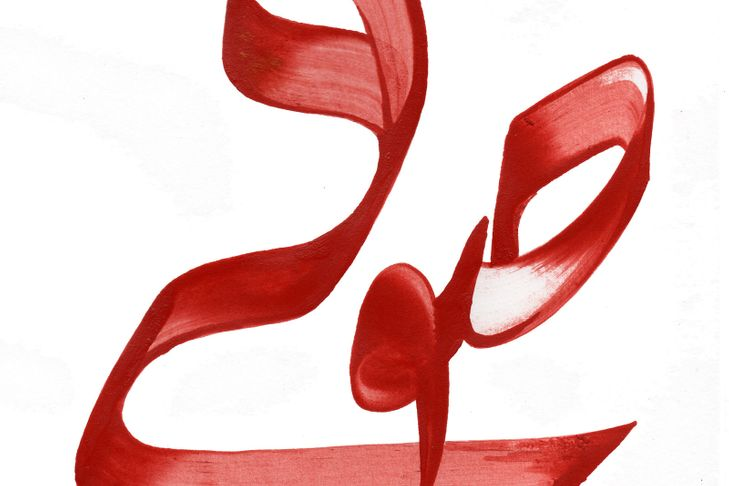
\includegraphics[width=\textwidth]{Images/image013.jpg}


« Aux commencements de l'islam, il n'y a ni ascètes ni soufis.
L'ascétisme et la mystique musulmane vont se développer dans les
sociétés de convertis à partir du IX\textsuperscript{e}~siècle. C'est un
phénomène d'hybridation culturelle. Le soufisme est d'abord le fait de
maîtres isolés au IX\textsuperscript{e}~siècle, vivant du côté de
l'actuel Iran. À partir du XII\textsuperscript{e}~siècle se développent
les premières confréries, dont certaines sont encore vivantes
aujourd'hui. Dans l'islam, la mystique est aussi développée que dans le
christianisme, mais elle a été davantage combattue. D'abord par les
juristes, qui voyaient d'un mauvais œil ces croyants qui s'émancipaient
des règles sociales, puis par le wahhabisme, qui les a massacrés dans la
deuxième­ moitié du XVIII\textsuperscript{e}~siècle ».\sn{Jacqueline Chabbi}


« Dans cette calligraphie, j'ai recherché la stabilité mais aussi un
geste plus tendre. Certains y verront peut-être un personnage
agenouillé, en prière\ldots{} Pourquoi pas ? J'offre une image sur
laquelle je ne peux pas toujours mettre des mots. C'est à ceux qui
regardent d'interpréter mes images. Quand je peins, je prends toujours
en considération le blanc laissé par la trace. En calligraphie, un
principe dit :\emph{~``Le noir de votre calligraphie, c'est vous. Le
blanc de votre calligraphie, c'est vous aussi.''}~J'y pense souvent.
Dans les textes anciens, le soufi -- que l'on peut traduire par
``mystique'' -- doit travailler sur soi-même pour retrouver la lumière
intérieure. Il devient alors pur et peut arriver à rencontrer la
divinité. »\sn{Hassan Massoudy}


\section{Introduction}
\paragraph{ Qu'est-ce que le soufisme~?} Pour les soufis, il s'agit de la dimension
spirituelle et originelle de l'islam. Le mot originel est important~: il
signifie que le soufisme est connaturel à l'islam, qu'il est l'islam. Il
ne s'agit pas d'un développement ultérieur qui aurait eu lieu sous
l'influence du monachisme chrétien ou du šī`isme, mais de l'islam vécu
par Muḥammad et ses compagnons. Donc, pour les soufis, Muḥammad est un
soufi. Les salafs, les anciens, les compagnons de Muḥammad sont soufis.
On comprend que si al-Ġazālī \label{theol:AlGazali27} considère le soufisme comme la voie par
excellence pour aller à Dieu, il n'en demeure pas moins que sous sa
plume la référence aux salafs y est importante.
\mn{Le soufisme et Si'isme

\begin{itemize}
\item
  historiquement, plutôt dans l'islam sunnisme
\item
  dans le si'isme, c'est presque intégré tellement il est naturellement
  spirituel.

  \item
    Dans le cadre duodecimain strict, on ne prie pas les imams
  \item
    Mais en fait, il y a des «~sectes~» qui vont le prier, à commencer
    par le fait qu'on va considérer que c'est le «~l'imam caché~»

  \end{itemize}}
Pour autant, cette affirmation d'éminents soufis n'est pas partagée par
l'ensemble des penseurs de l'islam, et au cours de l'histoire, le
soufisme a pu faire l'objet de critiques, de contestations, de
réfutations plus ou moins virulentes. Certaines des pratiques soufies
ont pu être considérées comme hétérodoxes, innovatrices, non conformes à
l'islam des origines. Ce sont ces accusations récurrentes qui permettent
d'expliquer pourquoi on s'en prend aujourd'hui encore à des mosquées
soufies. 
\paragraph{Le wahhabisme est la matrice idéologique anti-soufie
contemporaine}. Comme nous l'avons vu, il est né en Arabie à partir du
18\textsuperscript{ème} siècle en contestant les confréries soufies
jugées non confirmes à l'islam. Aujourd'hui, l'État islamique de l'Irak
et du Levant, au lendemain de la conquête de Mossoul a distribué aux
habitants une charte comprenant 16 commandements~: à l'article 10, il
est écrit que toutes les manifestations publiques contraires à l'islam
sont interdites (article 10). En 2014, quatre sanctuaires sunnites et
soufis et six mosquées chiites ont été détruites dans la province de
Ninive, sous contrôle des insurgés. La destruction la plus spectaculaire
fut celle du tombeau du prophète Jonas -- Yunus en arabe -- qui a été
réduite à un amas de cailloux.

En Égypte, dans le Sinaï, en décembre 2016, un shaykh soufi et un de ses
disciples sont assassinés par le groupe de l'Etat islamique. Le 24
novembre 2017 l'attentat à la mosquée al-Rawdah de Bir al-Abed fait 305
morts -- à cette mosquée était attachée une \emph{zāwiya} -- édifice
religieux fréquenté par des soufis et des conscrits de l'armée. Cette
mosquée soufie appartient à l'ordre soufi des ǧarirites du nom d'Aïd Abū
Ǧarīr qui a fondé trois loges dans le Sinaï au 20\textsuperscript{ème}
siècle dont celle de Bir al-Abed\sn{Sur la sociologie religieuse
  du Sinaï, voir l'article d'Ismaïl Alexandrani~:
   \url{http://orientxxi.info/magazine/-genealogie-du-djihadisme-au-sinai,0687}}.

\vide{i--duxe9finir-le-soufisme}{%
\section{{Définir le soufisme
}}\label{i--duxe9finir-le-soufisme}}

En guise d'apéritif, écoutez la voix d'Henri Corbin (m. 1978),
philosophe et éminent orientaliste français, spécialiste surtout de
l'islam iranien et de la gnose chiite. \emph{Extrait d'un entretien avec
Bernard Maxime Latour en 1971}.

Définition complexe donc, «~tâche scabreuse~»\ldots{} essayons cependant
de le définir à partir de la manière dont les musulmans eux-mêmes
présentent le soufisme, le \emph{tasawwuf} en arabe.

Pour cela, je vous propose de lire un extrait du livre Traité de
Kalābāḏī, \emph{Kitāb al-ta`arruf li-maḏhab ahl al-tasawwuf} qui a été
traduit par Roger Deladrière\sn{~\textsc{Kalābāḏī}, \emph{Kitāb
  al-taʿarruf li-madhhab ahl al-taṣawwuf} {[}traduction française~:
  Traité de soufisme, Les Maîtres et les étapes, traduit de l'arabe et
  présenté par Roger Deladrière, Paris, Actes-Sud, Sinbad, 1981.}.
Kalābāḏī \label{theol:Kalabadi} est un auteur persan, mort aux environs de 990. Cet ouvrage
cherche à réconcilier le soufisme et l'orthodoxie. C'est un classique,
apprécié de tous. En son introduction, il consacre plusieurs pages à
cerner le sens de soufisme par l'étymologie. C'est un peu dense et
technique, mais tout à fait accessible. En ces derniers cours, ce long
extrait vous permet de prendre contact avec un texte fondamental en
islam et avoir la satisfaction d'y être à peu près à l'aise.
\begin{quote}
    

«~Certains ont soutenu que les soufis furent appelés de ce nom à cause
de la pureté (\emph{safā}') de l'intime de leur être et de l'absence de
souillure de leurs actes. Selon Bichr Ibn al-Hârith, «~le soufi est
celui dont le cœur est pur à l'intention de Dieu~». D'après un autre,
«~le soufi est celui dont le comportement est pur à l'égard de Dieu et
dont le charisme (\emph{karâma}) qui lui vient de Dieu -- que soient
proclamées Sa Puissance et Sa Majesté~! -- est pur~».
\end{quote}
Selon une autre explication, les soufis ont été appelés ainsi parce
qu'ils sont, devant Dieu, au premier rang (\emph{saff}), du fait que de
leurs aspirations (\emph{himam}) s'élèvent jusqu'à Lui, que leur cœur se
tourne avec empressement vers Lui, et que l'intime de leur être se tient
en arrêt devant Lui.

D'après certains, ils auraient été désignés du nom de soufis parce que
leurs caractéristiques sont proches de celles des «~hommes du banc~»
(\emph{ahl al-suffa}) qui vivaient à l'époque de l'Envoyé de Dieu -- que
Dieu prie sur lui et le salue !

Selon d'autres, ils furent nommés soufis parce qu'ils portaient un
vêtement de laine (\emph{sûf}).

Ceux qui rattachent leur nom au «~banc~» (\emph{suffa}) et à la
«~laine~» (\emph{sûf}) expriment ainsi l'apparence extérieure de leur
état spirituel. \paragraph{ Ce sont en effet des hommes qui ont délaissé ce bas
monde}, ont quitté leur demeure, ont fui leurs amis, parcourant les pays,
le ventre creux, dénudés, ne prenant des choses d'ici-bas que
l'indispensable pour avoir une tenue décente et calmer leur faim. Parce
qu'ils ont quitté leur demeure on les appelle aussi «~étrangers~»
(\emph{ghurabâ'}), et à cause de leurs nombreux voyages on les désigne
sous le nom de «~pèlerins~» (\emph{sayyâhûn}). Du fait de leurs
pérégrinations dans les régions désertiques et parce qu'ils prennent
refuge en cas de nécessité dans les cavernes, les autochtones les ont
surnommés «~les hommes des cavernes~» (\emph{chikaftiyya}) car le mot
«~\emph{chikaft}~» dans leur langue désigne une grotte ou caverne.

Les Syriens leur ont donné le nom de «~faméliques~» (\emph{jaw'iyya})
parce qu'ils prennent seulement comme nourriture ce qui maintient les
forces dont ils ont besoin, conformément à la parole du Prophète~:
\begin{quote}
"Des aliments qui maintiennent ses forces devraient suffire au fils
d'Adam".~     
\end{quote}
Sarî Saqatî les a décrits en ces termes~: 
\begin{quote}
    «~Ils mangent
comme des malades, ils dorment comme des gens qui font naufrage, et ils
parlent comme des hommes stupides.~»
\end{quote}

Du fait de leur renoncement à la propriété on les a appelés «~pauvres~».
On avait demandé à l'un d'eux ce qu'était le soufi, et il répondit~:
\begin{quote}
   «~Celui qui ne possède pas et n'est pas objet de possession.~» 
\end{quote}
voulant
dire par là qu'il n'était pas l'esclave des désirs. À la même question,
un autre déclara~: 
\begin{quote}
    «~Le soufi est celui qui ne possède rien et qui, si
jamais il vient à posséder quelque chose, le donne.~»
\end{quote}


À cause de leur vêtement et de leur aspect on leur a donné le nom de
soufis, car ils ne portent pas ce qui est doux au toucher et agréable à
regarder, ce qui serait flatter les passions de l'âme, mais uniquement
une tenue décente, se contentant d'un tissu au poil rugueux et d'une
laine grossière.

Tout cela était la condition des «~hommes du banc~», qui vivaient à
l'époque de l'Envoyé de Dieu. Ils étaient en effet «~étrangers~» et
«~pauvres~», des exilés qui avaient quitté leur demeure et leurs biens.
Abû Hurayra et Fadâla Ibn'Ubayd en firent la description suivante~:

\begin{quote}
   «~Ils tombaient de faim à tel point que les Arabes bédouins les
prenaient pour des fous.~» 
\end{quote}
 Ils étaient vêtus de laine, et, au dire de
certains, cela les faisaient transpirer tellement qu'ils exhalaient
l'odeur des moutons qui ont reçu la pluie. Ceci au point que 'Uyayna Ibn
Hisn dit au Prophète~: 
\begin{quote}
   «~L'odeur de ces gens m'incommode, ne
t'incommode-t-elle point toi aussi~?~» 
\end{quote}


La laine est d'ailleurs aussi le vêtement des prophètes (\emph{anbiyā'})
et la mise des saints. C'est ainsi que, selon la parole du Prophète
rapportée par Abû Mûsâ Ach'âri,
\begin{quote}
    «~ soixante-dix prophètes, pieds nus et
vêtus de manteaux de laine, sont passés par le rocher de Rawlâ, et ils
se rendaient au \emph{Temple Antique} (de la Mecque)~».
\end{quote} 

D'après Hasan
Basrî, «~Jésus -- que la paix soit sur lui -- se vêtait de crin, se
nourrissait des fruits des arbres, et passait la nuit là où il
s'arrêtait.~» Selon une autre tradition d'Abû Mûsâ, le Prophète se
vêtait de laine, prenait des ânes comme monture, et se rendait à
l'invitation des pauvres gens. Hasan Basrî disait encore qu'il avait
connu soixante-dix Compagnons ayant combattu à Badr qui ne se vêtaient
que de laine. Ceux qui se comportaient comme les «~hommes du banc~»,
selon ce que nous avons indiqué, ayant les mêmes vêtements et la même
tenue qu'eux, portèrent donc le nom de «~\emph{suffiyya}~» et du
«~\emph{sûfiyya}~» (soufis).

\paragraph{Quand on rattache leur nom à l'élite (\emph{safwa}) et au premier rang
(\emph{saff}), on exprime alors ce qui se rapporte à leur être intime et
à leur état intérieur}. Dieu, en effet, purifie le secret de l'âme et
illumine le cœur de celui qui quitte le monde, y renonce et s'en
détourne. Selon une parole du Prophète,

\begin{quote}
«~quand la lumière pénètre dans
le cœur, il se dilate et s'épanouit.~» On lui demanda «~quel en est donc
le signe, ô Envoyé de Dieu~?~»~; il répondit «~s'éloigner du monde
illusoire, se tourner vers le monde éternel, et se préparer à la mort
avant qu'elle ne survienne.~»    Ainsi le Prophète avait fait savoir que
Dieu illumine le cœur de celui qui s'éloigne de ce bas monde. Et quand
il questionna Hâritha sur la réalité profonde (\emph{haqîqa}) de sa foi
(\emph{imân}), celui-ci déclara~: «~J'ai détaché mon âme de ce monde,
assoiffé pendant le jour, en veillant la nuit, et ce fut comme si je
voyais se dresser le Trône de mon Seigneur, et comme si j'apercevais les
habitants du Paradis qui se rendaient visite et ceux de l'Enfer qui se
repoussaient.~» Selon ce récit, après qu'il se fut détaché du monde,
Dieu lui illumina le cœur, de sorte que ce qui lui était primitivement
caché lui était devenu visible. Le Prophète s'écria alors~: «~Quiconque
veut voir un serviteur dont Dieu a illuminé le cœur n'a qu'à regarder
Hâritha~!~» À cause de ces caractéristiques, de tels hommes ont été
appelés «~illuminés~» (\emph{nûriyya}). Elles étaient également celles
des «~hommes du banc~». Dieu a dit en effet~: «~Il y a là des hommes qui
aiment à se purifier~; et Dieu aime ceux qui se purifient~.~» Il s'agit
de se purifier extérieurement des souillures et de se purifier
intérieurement des pensées qui surgissent dans l'esprit et des idées qui
se meuvent dans la conscience. Dieu a dit~: «~Des hommes que nul négoce
et nul troc ne distraient de l'invocation (\emph{dhikr}) de Dieu.~»
\end{quote}
 

En outre, à cause de la pureté de leur être intime, leur intuition
(\emph{firâsa}) est juste. Selon une tradition du Prophète rapportée par
Abû Umâma Bâhilî~: «~Prenez garde à l'intuition du croyant, car il
regarde avec la lumière de Dieu~!~» Abû Bakr le Véridique avait
déclaré~: «~Mon cœur a reçu l'inspiration que l'enfant porté dans son
sein par Bint Khârija est une fille~»~; et il en fut comme il l'avait
annoncé. De même le Prophète a dit «~La Vérité parle par la bouche de
'Umar.~» Uways Qarâni, salué par Harim Ibn Hayyân, lui rendit ses
salutations en l'appelant par son nom, alors qu'il ne l'avait jamais vu
auparavant~; et il lui dit ensuite~: «~Mon âme a reconnu ton âme.~» «~Si
vous vous entretenez avec les «~hommes de la sincérité (\emph{sidq}),
dit Abû 'Abd'Allâh Antâki, soyez vous-mêmes sincères, car ils sont les
observateurs des cœurs~! Ils pénètrent dans l'intimité de votre âme et
décèlent vos intentions.~»

\paragraph{Quiconque possède de telles qualités~: limpidité de l'être profond,
pureté du cœur, lumière de l'âme, est «~au premier rang~»}, car elles
caractérisent les «~devançants~» (\emph{sâbiqûn}). Selon une tradition
du Prophète~: «~Soixante-dix mille membres de ma Communauté entreront au
Paradis sans Jugement », précisant ensuite «~pour les autres ou pour
eux-mêmes ils n'ont point de recours aux talismans ni aux
cautérisations, mais ils s'en remettent à leur Seigneur avec
confiance.~» À cause de la pureté de leur être intime, de l'ouverture de
leur âme, et de l'illumination de leur cœur, les connaissances qu'ils
tiennent de Dieu sont justes~; ils ne se réfèrent pas aux causes
secondes (\emph{asbâb}), confiants qu'ils sont en Dieu, s'en remettant à
Lui, et acceptant Son Décret (\emph{qadâ}).

Toutes ces qualités et toutes les significations de ces mots se trouvent
réunies dans les noms et les appellatifs désignant la «~communauté
spirituelle~» (\emph{qawm}). Les expressions en sont exactes, et leur
emploi en est facilement compréhensible. Même s'ils diffèrent en
apparence, leur sens est concordant.

\begin{Def}[soufi]
Si on le tire de \emph{safâ'}
(pureté) et \emph{safwa}(élite), le terme qui désigne ces hommes est
alors celui de \emph{safawiyya}. Si on le rapporte à \emph{saff} (rang)
ou \emph{suffa} (banc), ils sont des \emph{saffiyya} ou des
\emph{suffiyya}.
\end{Def}
 Il est possible, dans le premier cas, que la lettre
\emph{wâw} ait été placée avant la lettre \emph{fâ'}, ce qui donne bien
le mot \emph{sûfiyya}(soufis)~; et, dans le deuxième cas, ajouter le
\emph{wâw} à \emph{saffiyya} ou \emph{suffiyya} serait dû à l'usage
linguistique. Si, enfin, on a tiré le mot \emph{sûfiyya} du \emph{sûf}
(laine), il est parfaitement correct, et cette désignation est
linguistiquement juste.

 \paragraph{Ces termes expriment le renoncement et le détachement
de l'âme à l'égard de ce bas monde, le fait de quitter sa demeure et de
voyager sans cesse, de ne pas flatter les passions de l'âme, de purifier
sa conduite, de rendre limpide l'intime de son être, d'ouvrir son cœur,
et de se comporter en «~devançant~». } Ajoutons à cela ce que dit Bundâr
Ibn Husayn~: «~Le soufi est celui que Dieu a choisi pour lui-même et
qu'Il a traité avec affection (\emph{sâfâ}), le libérant de son âme
(égoïste) et lui épargnant dès lors tout effort et toute contrainte en
vue d'un motif personnel. Et le mot \emph{sûfiya~}= il a été traité avec
affection est (un verbe passif) du même type morphologique que
\emph{'ûfiya}~: il a été protégé, à savoir que c'est Dieu qui l'a
protégé, et \emph{kûfiya~}: il a été rétribué, par Dieu, ainsi que
\emph{jûziya~}: il a été récompensé, par Dieu. L'action de Dieu sur lui
est donc manifeste dans son nom même de \emph{sûfî}, et Dieu est seul à
s'occuper de lui.~»

Interrogé sur la définition du soufi, Abû 'Alî Rûdhabâri répondit~:
«~C'est celui qui a revêtu de laine (\emph{sûf}) sa pureté
(\emph{sâfâ}'), qui a fait goûter à ses désirs personnels la saveur de
la privation, et qui, ayant laissé ce bas monde derrière lui, a suivi la
voie de l'Élu (Mohammad).~»

La même question ayant été posée à Sahl Ibn'Abd Allâh Tustarî~: «C'est,
dit-il, celui qui est pur de tout ce qui trouble, qui est rempli de
méditation, qui s'est retiré des hommes pour se consacrer à Dieu, et
pour qui l'or et l'argile se valent.~»

On demanda à Abû-l-Hasan Nûrî ce qu'était le soufisme
(\emph{tasawwuf})~: «~C'est, répondit-il, délaisser tout ce qui flatte
l'âme.~»

Interrogé sur le même sujet, Junayd définit le soufisme~: «~ C'est
purifier son cœur de l'approbation des hommes, abandonner ses tendance
innées, maîtriser les dispositions de la nature humaine, écarter les
incitations égoïstes, fixer en soi les qualités spirituelles, s'attacher
à la connaissance des réalités immatérielles, utiliser ce qui est mieux
pour la vie éternelle, pratiquer le (devoir de) bon conseil envers la
Communauté tout entière, tenir envers Dieu l'engagement de rester fidèle
à la vérité, et suivre l'Envoyé dans (l'accomplissement de la foi).~»

Selon Yûsuf Ibn Husayn~: 
\begin{quote}
    «~Chaque Communauté a une élite, dépôt précieux
de Dieu qu'Il a caché à Ses créatures, et s'il y en a une dans cette
Communauté-ci, ce sont les soufis.~»
\end{quote}

Quelqu'un demanda à Sahl Ibn `Abd Allâh Tustarî~: «~Qui fréquenterai-je
parmi les différents groupes musulmans~?~» «~Tu n'as qu'à fréquenter les
soufis, répondit-il, car rien n'a à leurs yeux une importance exagérée
et ne saurait être totalement désapprouvé. Pour eux, tout acte peut être
interprété, et ils te trouveront des excuses en n'importe quelle
circonstance.~» La même question ayant été posée par Yûsuf Ibn Husayn à
Dhû-l-Nûn~:
\begin{quote}
«~Fréquente, dit-il, celui qui ne possède rien et qui ne désapprouvera
aucune situation dans laquelle tu pourras te trouver, qui ne changera
pas même si toi tu changes beaucoup, car plus tu changeras, plus tu
auras besoin de lui~!~»
\end{quote}
On rapporte également de Dhû-l-Nûn ceci~:
\begin{quote}
    
«~Au bord de la mer, en Syrie,
je vis, dit-il, une femme, et je lui demandai~: «~D'où viens-tu -- que
Dieu te fasse miséricorde~! -- ~?~» Elle me répondit~: «~D'auprès de
gens qui répugnent à reposer leur corps sur une couche, et qui prient
leur Seigneur avec crainte et désir.~» -- Et où vas-tu~? Insistai-je. --
Vers des hommes «~que nul négoce et nul troc ne distraient de
l'invocation de Dieu. -- Décris-les-moi~! Lui demandai-je. Elle se mit
alors à déclamer ces vers~:

\emph{Des hommes dont les préoccupations s'attachent à Dieu, et dont les
aspirations ne s'élèvent vers personne d'autre.}

\emph{Leur quête est celle de leur Maître et de leur Seigneur, et quelle
noble quête que celle de l'Unique, l'Impénétrable~!}

\emph{Ils ne se disputent rien de ce monde, ni rien de ce qui est
excellent, ni nourritures, ni plaisirs, ni progénitures, ni vêtements
somptueux et élégants, ni la joie reposante de rester au pays.}

\emph{Ils ne luttent qu'à la poursuite du lieu éternel dont chaque pas
les rapproche.}

\emph{Ils courent par les étangs et les vallées, et on les rencontre en
nombre sur les hauteurs.}
\end{quote}
\vide{ii--muxe9thode-spirituelle-du-soufisme}{%
\section{Méthode spirituelle du
soufisme}\label{ii--muxe9thode-spirituelle-du-soufisme}}

C'est un itinéraire spirituel qui vise à remonter vers l'être unique, à
quitter la dualité de l'homme, sa duplicité, en vue d'une unification.
Il s'agit d'abandonner la superficialité des choses pour entrer dans la
profondeur de l'intériorité et ne pas être réduit au monde des
apparences.

Dans son \emph{Essai sur le soufisme}, Martin Lings compare le monde à
une pépinière~: tout ce qui s'y trouve a été planté en vue d'être
transplanté ailleurs. La partie centrale de la pépinière est réservée à
des arbres nobles. Ils sont tous en pot et poussent, pas beaucoup, mais
un peu. Mais quand on regarde bien, un des arbres se distingue des
autres. Il est luxurieux, vigoureux, beau. Que s'est-il passé~? La cause
en est invisible. Pour autant, on la devine~: cet arbre a pris racine
dans la terre du jardin à travers le fond de son récipient. Que dit
cette image~? Les arbres sont des âmes et le soufisme est une méthode,
une voie pour prendre racine, pour passer à travers la porte étroite qui
est dans l'âme elle-même et qui débouche sur l'océan de la Divinité. Le
soufi sait qu'il est comme les autres hommes, il sait aussi qu'il est
prisonnier du monde des formes (les pots), mais il sait aussi qu'il est
appelé à la liberté qui l'emporte sur sa captivité.

Le soufisme doit donc permettre de s'enraciner dans l'océan de la
divinité, d'entrer dans la source de la divinité, dans
l'\emph{\underline{origine}} donc. Cette origine est divine,
transcendantale, c'est celle de l'Absolu, de l'Éternel.

\paragraph{Le soufisme est d'abord une méthode~; il est donc un anti-dogmatisme,}
mais il n'est pas sans dogmes. Il ne nie pas le credo musulman, au
contraire~; les soufis ont une profession de foi qu'ils énoncent. Mais
il s'agit de ne pas limiter Dieu à cette profession. Dans cette optique,
le mystique andalou Ibn `Arabī appelle à ne pas se limiter à un credo
particulier. Voici un extrait des \emph{Chatons de la sagesse.} Vous
reconnaîtrez peut-être la voix de Georges Claisse. Dans la suite du
cours, je reviendrai sur cette très grande figure du soufisme.

Voie spirituelle vers Dieu, le soufisme est donc la définition d'une
méthode afin d'atteindre la proximité de Dieu, mais plus encore chez
certains, une union, une unification.

\vide{limitation-du-prophuxe8te}{%
\subsection{L'imitation du
Prophète}\label{limitation-du-prophuxe8te}}

\begin{Def}[Sainteté, suġrā et kubrā]
Le soufisme comme voie initiatique conduisant à la «~proximité divine~»
(\emph{walāya})~distingue selon la sainteté «~mineure~» (\emph{suġrā}),
ouverte à tous les fidèles, et la sainteté «~majeure~» (\emph{kubrā}),
réservée à une élite. 
\end{Def}
Pour parvenir à cette sainteté, la plupart des
soufis invitent à l'imitation du Prophète dans la mesure où il est celui
qui a réalisé cette parfaite proximité. 
\begin{Def}[\emph{nubuwwa}]
prophétie
\end{Def}

Ils posent donc l'existence
d'une relation entre la \emph{walāya} et la \emph{nubuwwa}, la
prophétie, mais si al-Tirmidhī (m. 318/930) accorde à la \emph{walāya}
son autonomie par rapport à la nubuwwa, d'autres au contraire, affirme
qu'il n'est pas possible de s'approcher de Dieu sans la \emph{nubuwwa}. \sn{la question est donc la possibilité de l'usage de la Raison pour accéder à Dieu}

L'hagiographie du Prophète Muḥammad s'est aussi accompagnée d'une
spiritualisation de sa figure~: il est «~l'Homme universel~»
(\emph{al-insān al-kāmil}) qui demeure dans ceux qui l'imitent. Or, la
participation à la «~sainteté prophétique~» permet d'actualiser la
Révélation, autrement dit dans donner les clefs pour chaque époque. Il
s'ensuit un «~Muhammado-centrisme~» car c'est Muḥammad en tant que sceau
des Prophètes qu'il convient d'imiter, de suivre, et donc à qui il faut
obéir. On voit ici que le rapport à la Loi est loin d'être supprimé,
spiritualisé. Au contraire.

 
\subsection{Le souvenir
(\emph{ḏikr})} \label{le-souvenir-dikr}

Le souvenir (\emph{ḏikr}) est au fondement du soufisme.
\begin{Def}[{ḏikr}]
Souvenir,
rappel, invocation, il s'agit de revenir à Dieu, de sortir de l'amnésie
qui guette l'homme, de retrouver le moment où fut scellé le pacte
originel (\emph{mīṯāq}).
\end{Def}
  Cette invocation convient à tout lieu, elle est
la marque d'une adoration continuelle. Le \emph{ḏikr} permet de
retrouver et de vivre de la présence divine.

Le Coran invite à cette évocation, à ce souvenir~: «~Souvenez-vous de
moi et je me souviendrai de vous~» (S. 2, 152). De même, le \emph{ḥadīṯ}
invite à la pratique du \emph{ḏikr}.

Ainsi, par exemple~:

\begin{itemize}
\item
  «~`Les cœurs rouillent comme le fer' dit le Prophète à ses compagnons.
  `Et qu'est-ce qui les fait briller~?' demande l'un d'eux.
  `L'invocation de Dieu et la lecture du Coran'~».
\item
  «~Celui qui invoque son Seigneur et celui qui ne l'invoque pas sont
  comparables l'un à un vivant, l'autre à un mort~».
\end{itemize}

Concrètement, le \emph{ḏikr} consiste à invoquer les noms divins ou à
répéter la première partie de la formule de la \emph{šahāda}~: \emph{lā
ilāha illā Llāh}. Puis, il s'agit de répéter le mot Allāh seul, puis, la
dernière lettre de Allāh, le h\ldots{} dans un seul souffle.

Je vous propose d'écouter {une séance de
\emph{ḏikr}
\url{https://www.youtube.com/watch?v=Xq6bIVtCq14}}\emph{.} 
. Ici, les soufis chantent
ensemble la formule \emph{lā ilāha illā Llāh} sur laquelle se surajoute
une psalmodie. Le rythme s'accélère et indique une forme d'ivresse
spirituelle. Généralement, ces invocations s'accompagnent du balancement
de la tête de gauche à droite et du mouvement des bras.

\url{https://www.youtube.com/watch?v=9BaQunfXPpE}{Ici}, vous avez une
vidéo d'une séance de \emph{ḏikr} dans une confrérie.

\vide{luxe9coute-de-luxe9cho-du-verbe-divin-samux101}{%
\subsection{L'écoute de l'écho du verbe divin
(samā`)}\label{luxe9coute-de-luxe9cho-du-verbe-divin-samux101}}

\begin{Def}[{samā`}]
Le \emph{samā`}, tout comme le \emph{ḏikr} a pour objectif de
réactualiser le Pacte originel. Il s'agit d'écouter la musique comme un
écho de ce pacte scellé. 
\end{Def}
Par la musique, l'écoutant libère son âme pour
trouver Dieu. Il y a une quête d'extase~: c'est le \emph{tawāǧud}. La
fin recherchée n'est pas la musique, mais l'écoute, la musique n'étant
qu'un support pour entendre la parole divine. L'écoute est donc
éminemment spirituelle~mais l'usage de la musique peut être dévoyé et
tombé dans le divertissement. Le soufisme n'est pas en soi favorable à
l'écoute de la musique mais il ne refuse pas usage à des fins
spirituelles. Al-Ġazālī  \label{theol:AlGazali28} considère que le samā` n'est pas en soi licite
ou illicite, et que tout dépend de l'intention (\emph{niyya}) de
l'écoutant. Pour rendre compte de cette ambivalence, le soufi al-Šiblī
(m. 946), connu pour ses excentricités paradoxales, dit du \emph{samā`}
qu'il est 
\begin{quote}
    «~en apparence une source de trouble, mais qu'il recèle un
grand enseignement spirituel (
\TArabe{
السماع ظاهره فتنة، و باطنه عبرة
})
~».
\end{quote}

L'histoire du \emph{samā`} montre qu'il a été associé à la danse, et
qu'il a été aussi assimilé au \emph{ḏikr}.

Ultime remarque~: le \emph{samā`} est une voie, une méthode soufie, mais
il n'est pas reconnu par tous les soufis et bien des maîtres ont aussi
privilégié le silence absolu tels Ibn `Arabi ou les premiers maîtres
šāḏilis.

\vide{la-repentance-tawba}{%
\subsection{{La repentance
(\emph{tawba})}}\label{la-repentance-tawba}}

Le repentir consiste à regretter son péché. Les soufis insistent sur
l'importance des larmes.

Elles sont aussi pleines de signification~: la larme est la goutte qui
s'efface en s'évaporant, après avoir témoigné. Sa disparition est
littéralement une extinction (\emph{fanā'}). Elle est symbole
d'intercession et de transformation\sn{On retrouve chez les
  Aztèques ce symbolisme~: les larmes des enfants que l'on apporte au
  sacrifice étaient dites annonciatrices de la pluie à venir. De même
  les lamentations sont mises en relation avec la miséricorde divine et
  la descente de la manne céleste.}.

Dans le soufisme, les pleurs symbolisent la quête du soufi de vouloir
s'abreuver à la source divine elle-même, de faire descendre la grâce, de
réaliser ainsi la présence divine. Les larmes ne sont pas négatives,
mais elles sont signe d'une espérance, de la promesse d'une joie à
venir. Elles ne sont pas la manifestation d'une séparation d'avec Dieu,
mais surtout un appel à retrouver Dieu, à s'unir à lui.

\vide{la-retraite-spirituelle-ux1e2balwux101}{%
\subsection{{La retraite spirituelle
(\emph{ḫalwā})}}\label{la-retraite-spirituelle-ux1e2balwux101}}

La retraite spirituelle constituait à l'époque antique un «~exercice
spirituel~». Le texte apocryphe intitulé \emph{La théologie d'Aristote}
écrit très vraisemblablement en syriaque au VI\textsuperscript{ème}
siècle et qui est un commentaire (\emph{tafsīr}) de certains passages
des \emph{Ennéades} de Plotin\sn{Pierre Thiellet, «~Notes sur la
  Théologie d'Aristote~» dans Prophyre, \emph{La vie de Plotin}, II,
  Paris, Vrin, 2000, p. 625-638.}, donne pour définition de l'extase le
fait d'être seul avec son âme (\emph{khalawtu bi-nafsi})\sn{Plotin,
  \emph{Ennéades}, IV, 8, 1.}. Il exerça très probablement une influence
dans la théorisation de cette solitude spirituelle. La pratique de la
retraite dans le soufisme renvoie à celle du monachisme chrétien avec
les Pères du désert, où l'éloignement de la ville et de la société était
considéré comme un chemin vers Dieu et un des fondements de l'ascétisme
(\emph{zuhd}). Depuis la \emph{Risāla} d'Abū al-Qāsim al-Qušayrī
(986-1072), toutes les présentations du soufisme intègrent un chapitre
sur les retraites spirituelles, qu'elles soient permanentes ou
périodiques. On appelait ces retraites des «~quarantaines~»
(\emph{arba`īniyya}). Elles étaient comprises comme une \emph{imitatio
prophetae}, à la suite de la retraite de quarante jours de Moïse sur le
mont Sinaï ou de celle de David pour réparer sa faute ou encore bien sûr
de Muḥammad qui allait une fois par an se recueillir (\emph{tahannuṯ})
sur le Mont Ḥirā'\sn{Paul B. Fenton, «~La pratique de la retraite
  spirituelle~», dans Giuseppe Cecere, Mireille Loubet, Samuela Pagani,
  \emph{Les mystiques juives, chrétiennes et musulmanes dans l'Égypte
  médiévale (VII\textsuperscript{e}-XVI\textsuperscript{e} siècles).}
  Interculturalités et contextes historiques, Le Caire, IFAO, 2013, p.
  211-252.}. Vous vous souvenez, c'est pendant un temps de retraite
qu'il reçut la révélation du Coran.

Au livre seizième de l'\emph{Iḥyā'} sur la retraite et la vie retirée
(\emph{`uzla}), al-Ġazālī \label{theol:AlGazali29} indique l'existence d'un débat au sein de la
deuxième génération des musulmans~: certains recommandaient en effet
l'amitié, l'assistance entre les croyants, la fraternité, tandis que
d'autres soulignaient l'importance de l'isolement et de la retraite
spirituelle. «~Fuis les gens comme si tu fuyais le lion~»\sn{\textsc{Al-Ġazālī },
  \emph{Iḥyā' `ulūm al-dīn, op. cit.,} K. 16 (\emph{Kitāb ādāb
  al-`uzla}), B.1, p. 665 {[}V.4, p. 248{]}.} conseille Dawūd al-Ta'i.
On raconte aussi cette histoire à propos de Sahl Ibn al-Ṭustarī (m.
896), grand maître soufi~\sn{\emph{Ibid}., p.666 {[}V.4, p. 251-252{]}}.:
\begin{quote}
    
«~Alors qu'un homme s'avança et lui dit qu'il
voulait lui tenir compagnie, Sahl lui répondit~: `Et si l'un de nous
deux vient à mourir, qui sera le compagnon de l'autre~?' L'homme lui
dit~: `Dieu'. Sahl reprit la parole~: `Qu'il lui tienne donc dès à
présent compagnie'~»
\end{quote}

Mais cette approche spirituelle de la retraite et de la solitude dans la
prière et l'isolement a aussi ses détracteurs. En opposition, on
rapporte les paroles du Prophète Muḥammad~où l'on retrouve le bestiaire
du désert~:

\begin{quote}
«~Satan est un chacal pour l'homme. Comme le chacal il saisit du
troupeau la bête égarée qui s'en est éloignée. Prenez garde aux vallées
et restez attachés aux communautés, aux groupes et aux mosquées~».
\end{quote}

Plus rédhibitoire, ce propos du Prophète de l'islam~\sn{\emph{Ibid}, B.1, ḏ.1, p. 667 {[}V.4, p.
  253-254{]}.}: 
\begin{quote}
   «~celui qui se
sépare du groupe (\emph{ğamā`a}), ne serait-ce que d'un empan, ôte de
son cou l'attache de l'islam » ou encore «~celui qui se sépare du groupe
et meurt mourra en homme de l'époque de l'ignorance
(\emph{ğāhiliyya})~». 
\end{quote}

\paragraph{Quels sont les bienfaits attendus de l'isolement~?}
La retraite permet de se consacrer à l'adoration, à la méditation en se
mettant en confidences intimes (\emph{munāğāt}) avec Dieu, en
privilégiant donc l'intimité avec Dieu plutôt qu'avec une créature.

La retraite permet aussi de se débarrasser des péchés auxquels on
s'expose en fréquentant les gens~: la calomnie, la médisance, la
bigoterie, la duplicité, l'avidité, l'attachement au bas-monde.
Al-Ġazālī \label{theol:AlGazali30} indique que l'habitude des gens consiste à se rincer la bouche
avec l'honneur des gens. La fréquentation conduit à s'accorder avec eux
et à s'exposer à la colère de Dieu. Garder le silence revient à
s'associer à leur médisance car l'auditeur est un médisant. Les récuser,
c'est s'exposer à se faire détester et susciter médisance et calomnie
contre soi, donc la médisance en est redoublée\ldots{}\sn{\textsc{Al-Ġazālī },
  \emph{Iḥyā' `ulūm al-dīn}, \emph{op. cit.,} K. 16, B.2, p. 673 {[}V.4,
  p. 272{]}~}.

La fréquentation des gens nous fait poser des questions vides et
hypocrites. Ainsi quand on voit quelqu'un, on lui demande «~comment ça
va~?~», mais on n'accorde aucune importance à la réponse. L'intérêt que
l'on porte à l'autre dans cette question est faux. Autrement dit, la
fréquentation des gens nous pousse à la duplicité. Al-Ġazālī \label{theol:AlGazali11} voit dans
cette question une innovation blâmable.

Finalement, le critère qui permet de vérifier si la retraite est
\emph{ḥarām} ou \emph{ḥalāl} est celui du bien que l'on retire de
l'autre~de par son beau caractère : «~si tu trouves un convive
(\emph{ğalīs}) qui te rappelle l'image et la conduite de Dieu, alors
attache-toi à lui\ldots{} car c'est là le trésor de l'homme doué de
raison (\emph{ġanīmat al-`āqil})~et le dessein du croyant (\emph{ḍāllat
al-mu'min}) »\sn{\textsc{Al-Ġazālī }, \emph{Iḥyā' `ulūm
  al-dīn}, \emph{op. cit.,} K. 16, B.2, fa.2, p. 677 {[}V.4, p. 285{]}~}.

Troisième bienfait~: celui de l'esprit de querelle et du fanatisme. On
rapporte ce dit de Muḥammad~:
\begin{quote}
    «~Il y aura une époque où pour préserver
sa religion, il faudra fuir de village en village, du sommet d'une
montagne à un autre, d'une pierre à une autre, comme un renard qui
s'échappe. Ce jour-là arrivera quand on ne gagnera sa vie qu'en
commettant des péchés et en désobéissant à Dieu. Alors, à cette époque,
le célibat (\emph{`uzūba}) deviendra licite~»\sn{\textsc{Al-Ġazālī },
  \emph{Iḥyā' `ulūm al-dīn}, \emph{op. cit.,} K.16, B.2, fa.3, p. 677
  {[}V.4, p. 286{]}.}.
\end{quote}

Cependant, al-Ġazālī est le théoricien soufi du juste milieu. Et il
souligne combien vivre en dehors de la communauté peut être l'occasion
de s'enorgueillir. Ainsi, en est-il de cette histoire juive~:

\begin{quote}
«~Un sage {[}parmi les israélites{]} avait rédigé trois cent soixante
opuscules sur la sagesse, si bien qu'il en était venu à penser qu'il
avait été gratifié d'un degré élevé auprès de Dieu. Dieu révéla à son
prophète~: `Va lui dire qu'il a rempli la terre d'hypocrisie et que je
n'agrée en rien son hypocrisie'. Le sage abandonna alors
{[}l'écriture{]} et se retira dans un tunnel sous terre. Il se dit en
lui-même~: `À présent, j'ai atteint le contentement de mon Seigneur.
Mais Dieu révéla à son prophète la parole suivante~: `Dis-lui qu'il
n'obtiendra mon contentement qu'après avoir fréquenté les gens et
supporté leur nuisance'. Le sage quitta son refuge et entra dans les
marchés pour fréquenter les gens, s'asseoir avec eux, partager leurs
repas, déambuler dans les marchés. Dieu révéla alors à son prophète~:
`Maintenant, il a obtenu mon contentement~»\sn{\textsc{Al-Ġazālī },
  \emph{Iḥyā' `ulūm al-dīn}, \emph{op. cit.,} K. 16, B.2, p. 687 {[}V.4,
  p. 312{]}.}.
\end{quote}

Si le soufi doit se retirer dans une cellule en solitude, si c'est là
qu'il se souvient de Dieu, l'enjeu est de parvenir à un état permanent
de retraite intérieure. La démarche se retrouve chez Muḥammad.

Le šayḫ al-`Alawī, soufi algérien qui appartient à la branche
confrérique Šaḏiliya qui a pris naissance au 14\textsuperscript{ème}
siècle et qui met l'accent sur l'invocation du nom de Dieu, a fondé sa
propre confrérie. Sa méthode bien qu'elle s'inscrive pleinement dans
l'esprit de la Šaḏiliya, est aussi originale~:

\begin{quote}
«~La khalwah est une cellule dans laquelle je place le novice après
qu'il a juré de ne pas la quitter pendant quarante jours si besoin est.
Dans cet oratoire, il ne doit rien faire d'autre que répéter
continuellement le nom divin (Allâh) en prolongeant à chaque invocation
la syllabe âh jusqu'à ce qu'il soit à bout de souffle.\\
Préalablement, il doit avoir récité la \emph{shahâdah} (\emph{lâ ilâha
illa Llâh}, « il n'y a de Dieu que Dieu ») soixante-quinze mille fois.

Durant sa retraite, il jeûne rigoureusement tout le jour, ne rompant son
jeûne qu'entre le coucher du soleil et l'aube\ldots{} quelques foqarā'
(mystiques) obtiennent l'illumination soudaine au bout de quelques
minutes, d'autres seulement après plusieurs semaines. Je connais un
\emph{faqîr} qui a attendu huit mois. Chaque matin, il me disait: « Mon
cœur est encore trop dur », et il poursuivait sa ḫalwā. À la fin, ses
efforts furent récompensés. »\sn{Martin Lings, \emph{Un saint
  musulman}, p. 96.}
\end{quote}

\vide{station-maqam-et-uxe9tat-ux1e25ux101l-spirituel}{%
\subsection{{ Station (\emph{maqam}) et état
(\emph{ḥāl}) spirituel
}}\label{station-maqam-et-uxe9tat-ux1e25ux101l-spirituel}}

Il existe dans le soufisme une théorie des états et des stations
spirituelles qui dessinent le cheminement et la progression du soufi.
\begin{Def}[\emph{maqam} (station)]
représente dans l'itinéraire vers Dieu, un
degré de perfection spirituelle obtenu à la suite de l'effort personnel
du mystique.
\end{Def}

 Le \emph{ḥāl} (état) en revanche consiste en une
disposition que l'on ne doit qu'à Dieu: «~Les états, disait Al Qushayrī,
sont des dons, les stations sont des mérites~».
\begin{Def}[\emph{ḥāl}]
Le \emph{ḥāl} est fondamentalement un état passager, éphémère. Le but du
soufi est de transformer le \emph{ḥāl} en état permanent (\emph{maqām}).

\end{Def}
Il faut passer du conjoncturel au structurel. Ainsi, la crainte peut
saisir le croyant à la lecture d'un passage du coran, suite à la
rencontre avec un savant ou un soufi\ldots{} mais cette crainte
ressentie doit habiter le croyant au-delà d'une sensation. Le combat
consiste donc à rendre permanent le \emph{ḥāl}.

\vide{iii--grandes-figures-soufies}{%
\section{{Grandes figures soufies
}}\label{iii--grandes-figures-soufies}}

\vide{ux1e25asan-al-baux1e63rux12b-643-728}{%
\subsection{Ḥasan al-Baṣrī
(643-728)}\label{ux1e25asan-al-baux1e63rux12b-643-728}}

Il est, selon les historiens arabes, le premier soufi. Il semble
cependant avoir été plus ascète que mystique~: il recommandait le mépris
du monde, l'examen de conscience. Pour lui, les spirituels se
reconnaissent à leur désir de Dieu. Il faut savoir se taire~: car parler
rajoute quelque chose à l'absolue transcendance de Dieu et finit par
l'offenser.

Ḥasān al-Basrī n'emploie pas le mot \emph{ḥubb} (amour réciproque). Il
dit~: 
\begin{quote}
    comment je peux dire que Dieu a un amour pour moi~?
\end{quote}
 Il préfère
donc le mot \emph{`išq}~: c'est l'éros, le désir. Mais ce mot ne se
trouve pas dans le Coran. Et le théologien hanbalite al-Ansarī le
refuse. Il y voit une intrusion de la raison humaine. Un bel exemple de
pluralisme en islam sur la question de l'amour de Dieu.

À noter que si le salafisme-wahhabiste combat le soufisme, les
salafistes reconnaissent à Ḥasan al-Baṣrī une autorité en tant
que~transmetteur de nombreux \emph{ḥadīṯs}.

\vide{rux101bia-m.-185801}{%
\subsection{{Rābi`a (m. 185/801)
}{3.2 Rābi`a (m. 185/801) }}\label{rux101bia-m.-185801}}

Elle est la première femme mystique de l'islam, la première soufie, un
premier témoin avec Ḥasan al-Basrī. Elle est née 60 ans après la mort du
Prophète Muḥammad. Il y a deux dates pour sa mort, la première la fait
mourir au milieu du huitième siècle à 55 ans, la seconde à la fin du
huitième siècle à 90 ans. Elle a initié la science de l'amour \emph{`ilm
al-maḥabba.}

Rābi`a n'est pas un prénom, cela veut dire la quatrième~: son milieu
familial était très pauvre et comme elle est la quatrième à être née,
son père l'a appelée La Quatrième. On sait peu de choses sur sa vie de
jeune femme. Fut-elle flûtiste~? prostituée~? Certains biographes le
suggèrent donnant au personnage une plus grande renommée.

Dans l'histoire de la pensée, elle est citée par les grands théologiens.
Ainsi, par exemple, Ğāḥiẓ (m. 867) parle d'elle dans le \emph{Livre des
animaux}. Il rapporte le propos de Rābi`a alors qu'on lui offrait un
esclave pour la servir et elle s'y opposait~: «~J'aurais honte de
demander des biens de ce monde à Celui à qui ils appartiennent ; comment
dès lors les solliciterais-je de gens à qui ils n'appartiennent pas ?~».

Ǧāḥiẓ a souligné la qualité rhétorique du propos (il est spécialiste de
rhétorique) ; il y reconnaît en arabe une éloquence exceptionnelle, une
prouesse rhétorique, mais aussi
une preuve ontologique contre l'esclavage.

Un exemple très connu est celui des deux seaux d'eau~ et des charbons~:
Ici, vous allez entendre la voix de Salah Stétié, un écrivain libanais
qui a traduit dans un français remarquable ses plus beaux poèmes.


\subsection{Pour aller plus loin~: les femmes soufies}

Sulaymī consacre un petit opuscule intitulé \emph{Les femmes soufies},
seconde moitié du 10\textsuperscript{ème} siècle, après le traumatisme
de Ḥallāğ \\


Quelques paroles «~insolentes~»~ (l'expression et de Salah Stétié)

\emph{Sur le paradis}

«~Un jour on récitait devant elle ce verset du Coran~: `Ce jour-là, la
seule occupation des hôtes du paradis sera de se réjouir en compagnie de
leurs épouses, ils se tiendront sous des ombrages, accoudés sur des lits
d'apparat'. Elle dit~: `pauvres gens du paradis, les voilà bien occupés
de leurs femmes~!'~»

\emph{Sur le Prophète}~

«~Aimes-tu le prophète~? Certes je l'aime, mais l'amour du créateur m'a
détourné définitivement de l'amour de toute créature~»

\emph{Sur les deux amours}

\begin{quote}
Je t'aime de deux amours

Amour de mon bonheur et amour digne de toi

Quant à cet amour de mon bonheur

c'est que je m'occupe à ne penser qu'à toi seul

à l'exclusion de tout autre

Et quant à cet autre amour dont tu es digne

C'est mon désir

Que tes voiles tombent et que je te voie

Nulle gloire en moi en l'un en l'autre,

non mais louange à toi pour celui-ci comme pour celui-là\sn{Traduction
  Salah Statié, \emph{Rabi'a de feu et de larmes,} Fata Morgana, 2010.}.
\end{quote}

\emph{Sur le pardon}

«~On lui demande~: `J'ai commis de nombreux péchés, Dieu me
pardonnera-t-il si je me repens~?' Elle répond~: il faut que Dieu te
pardonne d'abord et ensuite tu te repentiras~».

\begin{quote}
Ma coupe, mon vin, mon hôte, sont trois,\\
Et moi que remplit l'amour : je suis la Rabi'a\\
Celui qui verse le vin fait circuler sans cesse\\
la coupe de la volupté et du luxe\\
Si de mes yeux je vois, je ne vois que pour Lui,\\
Si regardée je suis, je suis vue avec Lui.\\
O ! Toi qui me blâmes ! Sa beauté oui, je l'aime~!\\
et par Dieu, mes oreilles n'ont que faire de Ton blâme.\\
Que de nuits délirantes j'ai passées, feu, tourment,\\
et mes yeux se sont fait sources par mes larmes !\\
et aucune de mes larmes n'a pu remonter à sa source\\
mon union avec Lui n'a pas duré.\\
blessé, meurtri, mon œil plus jamais ne s'apaise
\end{quote}

\vide{al-hallux101ux11f-m.-309-922}{%
\subsection{al-Hallāğ (m. 309 /
922)}\label{al-hallux101ux11f-m.-309-922}}

C'est un personnage complexe dont l'évolution religieuse a fait couler
beaucoup d'encre. Louis Massignon lui a consacré sa thèse doctorale.
C'est un mystique musulman, crucifié, criant du haut de sa croix~: «~Je
suis Dieu~»\ldots{} expression de sa doctrine de l'unification
(\emph{ḥulūl}).

Son nom lui vient du métier de son père~qui était cardeur de coton. Ses
disciples l'appelaient \emph{al-Hallâj al-asrâr} c'est-à-dire le cardeur
des pensées secrètes. Il voulait dévoiler les «~secrets de l'union
divine~» (\emph{asrār al-tawḥīd})\sn{Pour sa biographie, je
  m'appuie notamment sur l'introduction de Stéphane Ruspoli : \emph{Le
  Message de Hallâj l'Expatrié}, Collection Patrimoine Islam, Paris,
  Cerf, 2006.}.

Quelles relations entretenait-il avec le calife Mu'tadid (892-902) puis
le calife Muqtadir (m. 932) qui le laissa exécuter~? Quels furent ses
contacts avec le christianisme~? Dans quelle mesure trouva-t-il dans la
figure du Christ et de sa Passion un modèle, alors même que l'islam
réfute la mort sur la Croix de Jésus~? Dans quelle mesure ses voyages au
Cachemire lui ont-ils permis de s'imprégner de la sagesse hindoue~?

Il passera une année entière de retraite à La Mecque, imitant ainsi les
retraites solitaires de Muhammad sur le mont Hira. C'est un prédicateur,
un enseignant. Pour lui, l'islam «~n'est pas seulement la soumission
passive~» devant Dieu, ni l'obéissance aux rites prescrits, mais une
doctrine du salut, de la connaissance, de l'amour~». Il était partisan
de la voie du blâme, et assumait ses provocations. Il disait~ainsi :
«~La mécréance et la foi se distinguent seulement par leur nom, mais en
réalité il n'y a pas de différence entre les deux~». En 902, suite à une
expérience spirituelle très forte, il a la révélation du Nom Suprême de
Dieu. Cette révélation fut à la base d'une profonde mutation. Il résume
sa quête en une formule~: «~Anâ al-Haqq~» - littéralement «~je suis le
Vrai~», je suis Dieu.

 
\paragraph{Ibn Atā}\label{ibn-atux101}

Il est dénoncé comme agitateur politique, accusé de comploter contre la
sûreté de l'État et de tenir des propos hérétiques, blasphématoires. Il
est arrêté en 913. Il comparaît devant le vizir Alî ibn `Îsâ qui le
jugea après interrogation «~complètement ignorant du Coran et des
sciences annexes, droit canonique (\emph{fiqh}), Tradition
(\emph{Sunna}), poésie et philosophie arabe~»\sn{Stéphane Ruspoli,
  \emph{op. cit}. p. 34.}. «~On croit rêver~»~! Ibn Atā convoqué au
tribunal déclara Hallāǧ innocent des charges dont on l'accusait et
déclara sa profession de foi totalement valide. Fou de rage, le ministre
le fit battre et Ibn Atā mourut une semaine plus tard.

Hallāǧ arrive au supplice. Il a 65 ans. Il récite encore quelques vers
du Dîwân. Il fait sa prière sous les yeux de ses compagnons en disant~:
«~Ne vous inquiétez pas de cette affaire, car je reviendrai parmi vous
après trente jours~». Il est crucifié. La forme de la crucifixion dans
sa forme musulmane vient des Perses sassanides qui la pratiquaient
couramment. Elle est plus violente, brutale, spectaculaire que la
crucifixion romaine. Sa prière avant de mourir est marquée par la
compassion et la résignation.

Son biographe Stéphane Ruspoli commente~: «~On aura appliqué à la lettre
contre un des plus grands saints musulmans qui lutta pacifiquement pour
la cause de l'islam et la gloire de Dieu, ce verset sombre du Qoran~:
«~Ceux qui combattent Dieu et son Envoyé, et qui sèment la corruption
sur la terre, leur rétribution sera d'être tués, ou crucifiés~; qu'on
leur tranche les mains et les pieds, ou bien qu'on les bannisse du
territoire. Ce sera leur sanction ici-bas, tandis qu'un grand châtiment
les attend dans l'autre monde~» (5, 33)~» (p.35).

Quelques extraits de ses poèmes

\emph{\textbf{Kâna li qablî ahwâ (p. 101)}}

\begin{quote}
\emph{J'ai abandonné aux gens leur usage et leur religion}

\emph{pour me dédier à ton amour, toi ma religion et mon usage.}
\end{quote}

\emph{\textbf{Al-`ayn tubsiru (p. 102)}}

L'œil aperçoit Celui qu'il aime et puis le perd de vue,

Mais le regard du cœur ne cesse jamais de le contempler.

Quand Il n'est pas avec moi, son souvenir m'accompagne,

et le cœur le voit toujours, bien qu'Il se dérobe à mon œil.

\emph{\textbf{Tala'at as-shams (p. 109).}}

\begin{quote}
Le soleil de Celui que j'aime s'est levé de nuit,

Il a brillé sans plus connaître de couchers.

Le soleil du jour se couche certes la nuit,

Mais le soleil des cœurs ne saurait se coucher.

Celui qui aime le Bien-Aimé vole vers Lui,

si grand est son désir d'aller à sa rencontre.
\end{quote}

\emph{\textbf{Li'l `ilm ahl (p. 128)}}

\begin{quote}
Je suis un orphelin, et pourtant j'ai un Père que j'invoque.

Mon cœur tant que je vis s'afflige de son absence.
\end{quote}

Remarquez qu'il s'adresse ici à Dieu avec le nom de Père.

\emph{\textbf{Anâ man ahwâ (p. 129)}}

\begin{quote}
Je suis devenu Celui que j'aime et Celui que j'aime est devenu moi

Nous sommes deux esprits habitant en un même corps.
\end{quote}

\emph{\textbf{Tafakkartu (p. 153)}}

\begin{quote}
j'ai longuement réfléchi aux diverses religions en tâchant de les
assimiler,

puis je les ai ramenées à un seul Fondement ayant maintes ramifications.

Ne demandez pas à un seul homme de s'en tenir à un culte déterminé,

car cela l'écarterait certainement du Fondement divin assuré.

Ce qu'il réclame, c'est un Fondement lui permettant d'élucider

les nobles idéaux et les hautes conceptions afin de les réaliser.
\end{quote}

\emph{Commentaire~}: Ici, l'universalisme religieux de Hallâj semble
accepter tous les cultes, sachant que tout vient de Dieu qu'il est la
sève, l'essence, le Fondement (\emph{al-asl}) qui se transmet aux
ramification de la foi (\emph{shu'ab al-îmân}).

\vide{ibn-arabux12b-m.-1240}{%
\subsection{Ibn `Arabī (m. 1240)}\label{ibn-arabux12b-m.-1240}}

C'est un maître soufi. Incontournable. Pour lui, la pensée de Hallāǧ
accuse une certaine dualité au moment de l'union qui se trouve résolue
dans l'unification. Sur ce point, Ibn `Arabī lui reproche d'avoir laissé
survivre cette dualité dans l'expérience de l'union. Pour lui, l'homme
n'est plus une négation pure qui montre et démontre la puissance de
l'affirmation de l'un, mais par son existence nécessaire, il est l'image
de son créateur, il le représente.

La création est le néant par essence. Elle est illusoire. Elle ne sera
jamais le réel éternel~: «~Tu prétends qu'un autre qu'Allah puisse jouir
de l'Existence~: c'est le nier, et tu es formellement coupable
d'idolâtrie~». (cf. Léo Schaya, \emph{La doctrine soufique}, p 30).

Dieu est au-delà de la dualité de l'être et du non-être. On ne peut pas
justifier l'existence de la dualité entre Lui et un autre que lui. Il
rejette la distinction entre cause et effet. Tout ce qu'il a créé est
une manifestation de lui.

Le maître a influencé des confréries (\emph{turuq}) notamment la
Ḫalwatiyya. Il représente la tradition savante du soufisme. Pourquoi~?

C'est complexe. Mais il existe des facteurs explicatifs. Ainsi, Ibn
`Arabī aurait prédit la victoire des Ottomans et la conquête de la
Syrie. Il s'ensuit que la dynastie lui a accordé un patronage.

Mais plus sérieusement, l'évolution du soufisme au
13\textsuperscript{ème} siècle, le développement des confréries ont créé
un appel d'air doctrinal. Les fondateurs de ces branches confrériques
que sont al-Jîlânî, al-Shâdhilî, al-Rifâ'ī, al-Badawi\ldots{} tracent
une voie, donnent une orientation spirituelle à leur postérité
initiatique. Mais il n'y a pas d'enseignement substantiel~: Ibn `Arabi
vient compléter ce vide\sn{Chodkiewicz, p. 36.}.

Son enseignement procède fondamentalement du Coran~: «~Tout ce dont nous
parlons dans nos séances procède du Coran et de ses
trésors~»\sn{Chodkiewicz, p. 40.}. Ainsi, il invite son disciple
de sa manière~:
\begin{quote}
«~Plonge dans l'océan du coran si ton souffle est assez puissant/ Et
sinon, borne-toi à l'étude des ouvrages qui en commentent le sens
apparent mais n'y plonge pas~! Tu y périrais car l'océan du Coran est
profond et si celui qui y plonge ne se limitait aux lieux les plus
proches du rivage il n'en reviendrait jamais vers les créatures. Les
prophètes et les héritiers-gardiens (\emph{al-waratha al-hafaza})
prennent ces lieux pour but par miséricorde pour l'univers. Quant à ceux
qui restent en arrêt (\emph{al-wāqīfūn}), qui sont parvenus au but mais
sont restés là sans jamais revenir, nul ne tire profit d'eux et ils ne
tirent profit de personne~: ils ont visé le centre de l'océan -- ou
plutôt c'est lui qui les a visés -- et ils ont plongé pour
l'éternité~»\sn{Chodkiewicz, p. 43.}.
    
\end{quote}

\textbf{On ne soulignera jamais assez l'importance de la lettre comme fondement
de l'interprétation.} Sans la lettre, pas d'interprétation, pas de sens
caché. Et l'accès à cette lettre est réservé à ceux qui ont du souffle.
Ils ne cherchent pas l'au-delà de la lettre ailleurs que dans la
lettre~!

À la question de savoir comment trouver Dieu, il prend l'exemple de
Moïse et de la révélation de Dieu dans le Buisson ardent~: Moïse était à
la recherche d'un feu (S. 20, 10). Tout besoin, toute quête de Dieu, se
manifeste, s'épiphanise sous la figure de son besoin. Mais, dit Ibn
`Arabī~: l'homme qui est dans le désert et a été abusé par un mirage,
qui finit par désespérer de tout, alors celui-là trouve vraiment
Dieu\sn{Chodkiewicz, p. 62.}. «~Dieu ne peut être trouvé que dans
l'absence des choses {[}c'est-à-dire des causes secondes{]} sur
lesquelles nous prenons appui~».

Sur les autres religions~: il dit qu'il faut traiter les livres des
autres religions à égalité.

Chaque croyance est à considérer car elle est aussi singulière que
chaque manifestation de Dieu. Dans son acte de foi, le cœur du croyant
répond au désir de Dieu de se manifester en lui.

Le «~Poème `La religion de l'amour'~»\sn{Ibn `Arabî,
  \emph{Turjumân al-ashwâq}, extrait du poème 11 avec commentaire du
  Cheikh al-Akbar -- qu'Allâh l'agrée~! Traduit par M. Gloton dans
  \emph{L'Interprète des désirs}, Albin Michel p. 147 et 155-158.}~:

\begin{quote}
\emph{Mon cœur est devenu capable}

\emph{D'accueillir toute forme.}

\emph{Il est pâturage pour gazelles}

\emph{Et abbaye pour moines~!}

\emph{~}

\emph{Il est un temple pour idoles}

\emph{Et la Ka'ba pour qui en fait le tour,}

\emph{Il est les tables de la Thora}

\emph{Et aussi les feuillets du Coran~!}

\emph{~}

\emph{La religion que je professe}

\emph{Est celle de l'Amour.}

\emph{Partout où ses montures se tournent}

\emph{L'amour est ma religion et ma foi.}
\end{quote}

\emph{La question de l'infinie miséricorde de Dieu~:}

Elle est au cœur de la théologie d'Ibn `Arabī~: il y a un verset
coranique (S. 7, 156)~: «~Et Ma miséricorde embrasse toute chose
(\emph{wa rahmatī wasi'at kulla shay'in}).

Ibn `Arabī dans les Futuhāt rapporte un dialogue entre Iblis et un
savant (Sahl al-Tustari (m. 896).
\begin{quote}
    «~La dernière chose qu'Iblis déclara à Sahl fut celle-ci~: Dieu a dit
`Ma miséricorde embrasse toute chose', ce qui est une affirmation de
portée générale. Or il ne t'échappe pas que je suis une de ces choses,
sans le moindre doute. Le mot `tout' implique l'universalité {[}de cet
énoncé{]} et le mot `chose' représente ce qu'il y a de plus indéterminé.
Sa Miséricorde m'embrasse donc~»~; À Sahl qui réplique `Je ne pensais
pas que ton ignorance irait jusqu'à ce point', Iblis répond~: `Je ne
pensais pas que tu en serais là~! Ne sais-tu pas, ô Sahl, que la
limitation (\emph{al-taqyīd}) est ton attribut et non le sien~?~». Ibn
`Arabî conclut le récit par cette remarque~: «~Je sus alors qu'Iblis
possédait une science incontestable et que, sur ce problème, c'est lui
qui avait été le maître de Sahl~»\sn{Chodkiewicz, p. 63-64.}.

\end{quote}

\vide{iv--le-soufisme-en-accusation}{%
\section{{Le soufisme en accusation
}}\label{iv--le-soufisme-en-accusation}}

\vide{les-critiques-uxe0-lencontre-du-soufisme}{%
\subsection{Les critiques à l'encontre du
soufisme}\label{les-critiques-uxe0-lencontre-du-soufisme}}


\paragraph{Bibliographie}

Frederick De Jong, Bernd Radtke, \emph{Islamic Mysticism Contested:
Thirteen Centuries of Controversies and Polemics} Leiden, Brill, 1999.

Vous trouverez ci-dessous la recension de l'ouvrage proposée par eric
Geoffroy et publiée dans \emph{Studia islamica}. \\


Un certain nombre de théories ou de concepts posent problème~: qu'en
est-il de l'amour et de la relation entre la créature et le créateur~?
Se pose aussi la question de l'inspiration, des visions des soufis. La
thématique de la lumière muhammadienne (\emph{nūr Muḥammad}) faisait de
lui Le prototype du mystique.

\paragraph{Les hanbalites rejetèrent les interprétations ésotériques du Coran.}

\paragraph{Pour autant, au départ, il n'y avait pas forcément d'incompatibilité.
} Certains mu`tazilites étaient aussi soufis, certains hanbalites étaient
soufis. Ce n'est que par la suite avec une forme d'irréconciliabilité
entre mu`tazilisme et sunnisme que les mu`tazilites critiquèrent les
soufis en tant qu'ils étaient des sunnites.

Ḏū' al-Nūn al-Miṣrī est un célèbre soufi qui fut emprisonné à Bagdad
pour avoir refusé le dogme du Coran créé. Mais il y avait aussi des
rivalités entre écoles mu`tazilites, des nuances. Ainsi, si les
iḫšīdiyya admettaient la possibilité des miracles (\emph{karāmāt}), ils
reconnaissaient que les miracles que l'on faisait porter aux soufis
étaient vus comme un danger possible pour le pouvoir. Souvent,
l'opposition au soufisme était plus sociale et politique que
religieusement fondée.

Les mutazilites dénoncèrent aussi le subjectivisme soufi. Ibn Taymiyya,
le maître hanbalite du 13\textsuperscript{ème} siècle a critiqué le
soufi Ibn `Arabi~et l'a taxé d'«~incarnationnisme~» (~\emph{hûlûl}~) et
de panthéisme. Au 19\textsuperscript{ème} siècle, Mohammed `Abdou, le
réformiste égyptien de la «~Nahdha~», lui-même très attiré par la voie
soufie au début de ses études, a affirmé que le soufisme a
«~\emph{efféminé l'Islam et a nourri la résignation des masses~».} Ibn
Badis, le théoricien algérien de la révolution islamique, s'est opposé à
la prétention de l'Amour pour Dieu et a dénoncé les états spirituels
(\emph{aḥwal}) qui confinaient selon lui au charlatanisme. Et le
philosophe tunisien des Lumières Abdelmajid Charfi, écrit dans son
fameux essai \emph{L'islam entre le message et l'histoire}~: le soufisme
«~est responsable d'avoir entretenu l'esprit de servilité, de fatalisme,
la croyance aux prodiges et miracles attribués aux
«~saints~»~»\sn{Abdelmajid Charfi, \emph{L'islam entre le message
  et l'histoire}, Paris, Albin Michel, 2004, p. 210.}.

De même, le philosophe iranien Soroush a mis en garde contre le
soufisme~:\sn{Alain Roussillon, \emph{La pensée islamique
  contemporaine}. Acteurs et enjeux, Paris, Téraèdre, 2005, p. 155.}.
\begin{quote}
    «~l'inconsistance théorique aussi bien que le danger pratique
de l'autoritarisme structurel qui entacherait la relation de maître à
disciple et qui ne pourrait déboucher que sur un système
anti-démocratique -- les Safavides et Khomeyni lui-même étaient
soufis~»
\end{quote}

Mais Abdelwahhab Meddeb disait aussi du soufisme qu'il est le visage le
plus aimable de l'islam\sn{\textsc{Meddeb}, «~Chemins de la
  connaissance~», France culture~:
  \url{http://www.youtube.com/watch?v=ooFDhYNwJPY}}. Et face au
déferlement de critiques, les maîtres soufis ont aussi pris la plume
afin de répondre à leurs contempteurs. Il en est ainsi du šayḫ algérien
Ahmad al-`Alawī (1874-1934) dans sa \emph{Lettre ouverte à ceux qui
critiquent le soufisme}\sn{Ahmad al-`Alawī, \emph{Qawl al-ma`rūf
  fī l-radd `alā man ankara l-tasawwuf}~: \emph{Lettre ouverte à ceux
  qui critiquent le soufisme,} traduction de l'arabe, notes et préface
  de M. Chabry, Introduction de J. Gonzalez, Paris, Entrelacs, 2011.}.

\vide{la-critique-dibn-arabux12b}{%
\subsection{{la critique d'Ibn `Arabī
}}\label{la-critique-dibn-arabux12b}}
\label{Theo:IbnArabi}
Un jour, alors que j'étais à la librairie \emph{tawḥīd} à Lyon, j'ai
aperçu un livre d'Ibn `Arabī. Le libraire me précisa~: «~c'est le seul.
C'est pas trop dans l'esprit de nos éditions. Lui, c'est un polythéiste
(\emph{sic})~».

Le wahhabisme est très hostile au soufisme et déjà dans les fatwas, `Abd
al-Wahhāb accusait les syriens de l'adorer (\emph{ya`budūna Ibn `Arabī~:
ils adorent Ibn `Arabī})\sn{Muḥammad `Abd al-Wahhāb,
  \emph{Maǧmū`at al-fatāwā wa-l-rasā'il wa-l-aǧwiba}, Beyrouth, 1987, p.
  46, cité par Michel Chodkiewicz, «~Le procès posthume d'Ibn `Arabī~»
  dans Frederick De Jong, Bernd Radtke, \emph{Islamic Mysticism
  Contested: Thirteen Centuries of Controversies and Polemics} Leiden,
  Brill, 1999, p. 93.}. La critique d'Ibn `Arabī est parfois assumée et
admise aujourd'hui au sein même des confréries soufies qui, soucieuses
d'orthodoxie, voient en Ibn `Arabī un «~étranger de l'islam~». Mais de
quoi s'agit-il~? Que lui reproche-t-on~? Si la controverse ne date pas
de son vivant, on doit d'abord à Ibn Taymiyya d'avoir écrit le
réquisitoire le plus virulent contre Ibn `Arabī. Un de ses ouvrages les
plus exhaustifs est \emph{Ḥaqīqat maḏhab al-ittiḥādiyyīn}, \emph{La
vérité de l'école des partisans de l'unification}.

Comme souvent, le propos y est nuancé, contrairement à ce que l'on a
véhiculé de lui et il déclare que si la doctrine d'Ibn `Arabī est du
\emph{kufr}, il est le plus proche de l'islam et ses propos sont souvent
excellents.

On trouve quatre condamnations :


  \paragraph{La doctrine de la \emph{waḥdat al-wuǧūd}}, l'unité de
  l'existence. C'est l'idée que l'être de Dieu est l'être de tous les
  êtres et que donc, l'être de Dieu est l'être des djins, des démons,
  des infidèles, des chiens et des porcs. À noter que ceux qui
  soutiennent cette doctrine refusent la doctrine de l'unification
  (\emph{ittiḥād}) qui suppose l'existence d'une dualité qu'ils
  rejettent. À remarquer que l'expression \emph{waḥdat al-wuǧūd} ne se
  trouve pas chez ibn `Arabī~!

La doctrine découle de l'interprétation du \emph{ḥadīṯ qudsī} (nous
avons déjà défini ce qu'est un \emph{ḥadīṯ qudsī})~:
\begin{quote}


« Mon serviteur ne s'approche de Moi par rien de plus excellent que ce
que Je lui ai mis à charge comme œuvres obligatoires. Et mon serviteur
ne cesse de s'approcher de Moi par des œuvres surérogatoires jusqu'à ce
que Je l'aime, et lorsque Je l'aime, Je suis son ouïe par laquelle il
entend, sa vue par laquelle il perçoit, sa main par laquelle il saisit,
et son pied avec lequel il marche. S'il me demande, Je lui accorderai
certainement ce qu'il demande, et s'il cherche refuge en Moi, Je lui
accorderai certainement Ma protection ».
\end{quote}

Pour Ibn `Arabī, il y a donc identification totale entre Dieu et son
serviteur. Mais c'est plus une identité qui n'est pas en devenir. Elle a
toujours existé, mais le serviteur (\emph{`abd}) n'en avait pas
conscience.

\paragraph{la doctrine de la \emph{waḥdat al-adyān~}:} elle consiste à ne
plus différencier l'\emph{imān} du \emph{širk} (la foi de
l'associationnisme, mais là ce devrait être assimilé, c'est juste pour
ceux dont la mémoire n'a plus 20 ans). Le diable lui-même est un lieu
théophanique, et il faudrait donc l'honorer.

\paragraph{la doctrine de la non-éternité des châtiments} des damnés~:
ils ne quitteront pas l'enfer, mais la miséricorde les enveloppera
aussi, elle qui «~embrasse toutes choses~» S.7, 156. C'est la version
musulmane de la doctrine de l'apocatastase (idée que tout sera
réconcilié, Dieu sauvera tout le monde). Elle est rejetée car elle
entraîne une diminution de la crainte de Dieu et ouvre la porte à toutes
les turpitudes.

\paragraph{l'hagiologie d'Ibn `Arabī}~: c'est la question de la
\emph{ḥaqīqa muḥammadiyya} et de son identification au \emph{qalam}, ou
la notion de sceau de la sainteté (\emph{ḫatm al-walāya}) qui
attenterait à la dignité du Prophète.



%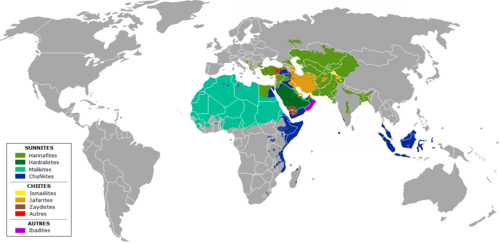
\includegraphics{Images/image097.png}
\vide{ruxe9ponse-soufie}{%
\subsection{Réponse soufie}\label{ruxe9ponse-soufie}}

Je vous propose de lire la lettre du Cheikh Ahmad al-Alawī
(1874-1934)~intitulée «~Lettre ouverte à celui qui critique le
soufisme~».

\vide{v--les-ordres-confruxe9riques}{%
\section{Les ordres
confrériques}\label{v--les-ordres-confruxe9riques}}

Il y en a une cinquantaine dans le monde.

\begin{itemize}
\item
  \textit{La qādirīya} \label{Def:Soufiqādirīya}
Fondateur~: `Abd al-Qādir al-Ğīlānī (m. 1166)
Implantation~: dans tous les pays musulmans, du Maghreb à la Chine


\item
  \textit{La Naqchabandīya} \label{Def:SoufiNaqchabandiya}
Fondée au milieu du XIV° siècle
Implantation~: du Caucasse au Turkestan et à l'Inde
Elle a nourri le nationalisme kurde


\item
  \textit{La Šāḏilīya} \label{Def:Soufisadiliya}
Eric Geoffroy dit de la \emph{Šāḏiliyya} qu'elle est l'une des
«~voies-mères~» du soufisme. Elle est apparue entre la fin du
XII\textsuperscript{e} siècle et le XIV\textsuperscript{e} siècle.
D'origine maghrébine, elle s'est diffusée au XIII\textsuperscript{e}
siècle, à partir de l'Égypte, dans la majeure partie du monde musulman.
Son enseignement est dense et il s'appuie sur les écrits d'Ibn
\emph{`}Arabī.
\end{itemize}
Toute voie initiatique a pour but de mener ses adeptes vers la sainteté,
ou «~proximité divine~» (\emph{walâya})~; celle-ci est identifiée au
plus haut degré de la gnose par al-Shâdhilî. De façon schématique, les
premiers maîtres shâdhilis distinguent deux niveaux~: la sainteté
«~mineure~» (\emph{sughrâ}), ouverte au public large des fidèles, et la
sainteté «~majeure~» (\emph{kubrâ}), réservée à une élite spirituelle.
Mais le terme \emph{walâya}, tout comme celui de sainteté en français,
est un terme générique, un idéal qui implique une méthode pour y
parvenir.

Pour les Shâdhilis, la réponse est claire~: c'est dans l'imitation
intérieure du Prophète que se réalise la \emph{walâya}. Réapparaît ici
le débat millénaire sur les rapports entre \emph{walâya}et
\emph{nubuwwa}, la prophétie, débats qui ont partagé exotéristes et
ésotéristes de l'islam, mais aussi les milieux soufis. Autant les
maîtres shâdhilis initiaux se réclament du premier théoricien de la
sainteté en islam, al-Hakîm al-Tirmidhî (m. 318/930), autant ils s'en
éloignent lorsque celui-ci accorde à la \emph{walâya}une autonomie par
rapport à la \emph{nubuwwa}~: pour eux, la première est subordonnée à la
seconde, et puise sa substance même dans la Lumière muhammadienne
(\emph{al-nûr al-muhammadî}).

\begin{itemize}
\item
  \textit{La Bekt'āchīya}
Elle impose le célibat
De nombreux affiliés en Turquie et Albanie


\item
  \textit{La Tidjānīya}
Influente au Maghreb et dans l'Afrique occidentale


\item
  \textit{La Chattārīya}
Influente en Inde et Malaisie

\item
  \textit{La Rah'mānīya}
La plus influente confrérie algérienne.


\item
  \textit{La mawlāwīya} (derviches)
\end{itemize}

Il existe plusieurs ordres soufis, mais l'on peut distinguer deux grands
groupes de mystiques~: ceux qui se trouvent dans la station de l'ivresse
(\emph{sukr}) et ceux qui sont dans la station de la sobriété
(\emph{sahw}).

Les initiés ivres sont souvent les disciples d'Abū Yazīd Bistamī (m.
875)~: l'ivresse, c'est la perte de sens commun, de la maîtrise de soi.
L'âme est enivrée de la connaissance de Dieu, plongée dans la
contemplation de Dieu.

Pour le second groupe, l'ivresse n'est qu'un état transitoire. Elle est
le début de l'unicité, mais elle se caractérise par la sobriété, quand
il sait que le soi n'est qu'un miroir dans lequel se réfléchit l'Essence
divine.

\paragraph{Pour aller plus loin}

Martin \textsc{Lings}, \emph{Qu'est-ce que le soufisme~?} traduit de
l'anglais par Roger du Pasquier, Paris, Éditions du Seuil, 1977.

Eric \textsc{Geoffroy},
«~\url{http://www.facebook.com/topic.php?uid=21148739744\&topic=3226}{L'islamité
du soufisme et son apport à la spiritualité universelle}~» dans
\url{http://www.religioperennis.org/documents/geoffroy/islamitesoufisme.pdf}

Eric \textsc{Geoffroy}, \emph{Initiation au soufisme}, Coll. L'espace
intérieur, Paris, Fayard, 2003.

Alberto Fabio \textsc{Ambrosio}, \emph{Vie d'un derviche tourneur}.
Doctrine et rituels du soufisme au XVII\textsuperscript{e} siècle,
Paris, CNRS Edition, 2010, 1 vol., 406 pages.

Laleh \textsc{Bakhtiar}, \emph{Le soufisme}. Expressions de la quête
mystique, Paris, Seuil, 1977.

Christian \textsc{Bonaud}, \emph{Le soufisme al-taṣawwuf et la
spiritualité islamique}, Préface de

Michel Chodkiewicz, Maison Larose, IMA, 1991.

\textbf{Exercice pour la Validation}

À partir de la lettre du šaḫy Ahmad al-Alawī, identifierez les éléments
qui répondent aux critiques adressées aux soufis et à Ibn `Arabī tels
que nous les avons exposés.



\chapter{La philosophie en islam}


\section{Introduction
}
\begin{quote}
Un jour, le calife al-Ma'mūn fit un rêve~: «~J'ai vu en rêve un homme
assis dans la posture des sages, je lui ai demandé «~qui es-tu~?~», il
m'a répondu «~Aristote le Sage~». Alors je lui posai la question
«~Dis-moi qu'est-ce que le bien? ~», Aristote de dire : «~ce qui est
conforme à la raison~». Al-Ma'mūn : «~Mais encore~?~», Aristote : «ce
qui est bien selon la révélation~~». Je lui dis : et après ? ~Il me dit
: «~Ce qui est bien aux yeux de tous~». Je lui dis : `et après'. Il me
dit : `il n'y a pas d'après'~Je lui dis : `dis-moi encore autre chose'.
Il me dit : `celui qui te conseille bien au sujet de l'or, qu'il soit
pour toi comme de l'or ; et il te faut reconnaître un Dieu unique'~».
\end{quote}

De ce rêve, supposé reconstruit et visant à justifier le recours à la
philosophie en islam, naquit le projet de créer la Maison de la Sagesse
en 832 qui devint un lieu où de nombreux savants s'attelèrent à traduire
les œuvres de la philosophie grecque\textbf{,} et également \textbf{des}
traités de mathématiques et de médecine. Dimitri Gutas a montré que
cette entreprise de traduction doit être comprise au sein d'un
environnement politique, social et idéologique propre à l'empire
abbasside en quête de légitimité\sn{Dimitri \textsc{Gutas},
  \emph{Pensée grecque, culture arabe : Le mouvement de traduction
  gréco-arabe à Bagdad et la société abbasside primitive
  (IIe-IVe/VIIIe-Xe siècles)}, traduit de l'anglais par Abdessalam
  Cheddadi, Paris, Aubier, 2005.}\textsuperscript{.} Les
descriptions\textbf{,} sous la plume d'auteurs contemporains\textbf{,}
d'une maison de rencontres où se côtoient des juifs, des chrétiens et
des musulmans ressemblent davantage à la projection d'un idéal moderne
qu'à une réalité historique\sn{~À l'exemple de Souleymane Bachir
  \textsc{Diagne}, \emph{Comment philosopher en islam~?}, Paris,
  Panorama, 2008, p. 36. Toutefois, au-delà de représentations
  idéologiques, il est certain que les premiers traducteurs étaient des
  chrétiens issus de milieux jacobites ou nestoriens qui avaient
  préservé dans les bibliothèques de leurs monastères l'essentiel de
  l'héritage aristotélicien. L'assertion d'Alain de Libera, selon
  laquelle la philosophie en terre d'islam a été «~une histoire
  musulmane, cela va sans dire, aussi une histoire chrétienne et une
  histoire juive~»~est bien fondée~: Alain \textsc{de Libera}, \emph{La
  Philosophie médiévale}, Paris, PUF, 1993, p. 54.}. Ce qui prédomine,
ce sont les interactions scientifiques entre philosophes et non des
échanges de théologie. Il reste que la philosophie grecque rencontre
l'univers de l'islam, la \emph{philosophia} devient \emph{falsafa}. Il
s'y affirme l'idée d'une sagesse éternelle (\emph{philosophia perennis})
traversant les âges et les communautés humaines, qu'elles fussent ou non
gratifiées d'une révélation. Cette sagesse {est} transmise grâce
à des hommes comme le «~divin Platon~»\sn{~Al-Ġazālī reprend
  l'expression du «~divin Platon~(Platon \emph{al-ilāhi})~» mais non
  sans ironie~: \textsc{al-Ġazālī}, \emph{Tahāfut al-falāsifa},
  p. 8. {[}Marmuna, p. 4{]}}, sagesse que le croyant ne peut méconnaître
mais qu'il doit au contraire s'approprier. Dans ce foisonnement de
traductions et de rencontres -- Platon, Aristote, Plotin sont ainsi
traduits en arabe dès la fin du IXe siècle, l'élite intellectuelle débat
de questions nouvelles. Les controverses foisonnent entre musulmans et
chrétiens ou juifs, entre sunnites et šī`ites, entre mutazilites et
aš`arites où, derrière un style non dénué d'expressions caustiques,
l'atmosphère y est celle d'une ouverture à l'autre comme en témoigne Abū
Hayyān al-Tawhīdī\sn{Marc \textsc{Berg}É, \emph{Pour un humanisme
  vécu~: Abū Hayyān al-Tawhīdī}, Institut français de Damas, 1979.}.
Munis des outils et des questions de la philosophie grecque, des
penseurs arabes en viennent à élaborer leurs propres systèmes
philosophiques. Trois auteurs occupent une place singulière dans cette
histoire~: al-Kindī (m. 870), al-Fārābī (m. 950) et Ibn Sīnā (m. 1037).
Il s'agit d'Avicenne. Avec al-Fārābī, le \emph{kalām} devient une
science spécifique et les connaissances prophétiques et philosophiques
renvoient à deux modes distincts d'appréhension d'un même objet. Sous
l'influence du néo-platonisme et du milieu šī`ite, al-Fārābī construit
une cosmogonie caractérisée par la procession des intellects au sein
d'un monisme émanatiste\textbf{.} Mais la séparation entre philosophie
et orthodoxie musulmane atteint son paroxysme avec les écrits d'Ibn
Sīnā. La création n'y est plus comprise comme un acte de volonté libre
comme l'affirme le Coran, mais elle relève d'une nécessité propre à
l'être divin. Par ailleurs, Ibn Sīnā déconstruit les dogmes musulmans
par une lecture symbolique qui privilégie le sens ésotérique
(\emph{bāṭin}) et relaie au second plan le sens exotérique
(\emph{ẓāhir}) des versets coraniques. Pour Ibn Sīnā, la résurrection
des corps est de l'ordre de la métaphore et non de la
réalité\sn{~Ibn \textsc{S}Ī\textsc{n}Ā, \emph{Al-Risāla
  al-Aḍḥawiyya}/}.

Les systèmes philosophiques développés par les philosophes arabes ne
manquent pas d'audace et d'originalité pour la pensée musulmane de
l'époque, mais peuvent-ils s'accorder avec l'islam~? Relèvent-ils de
questions périphériques à l'islam ou contredisent-ils l'enseignement de
la révélation coranique~? Relèvent-ils d'une sagesse universelle ou
d'une logique singulière qui ne saurait s'accorder avec la logique
propre à l'arabe, autrement dit, peut-on projeter sur les versets du
Coran une lecture philosophique grecque alors même qu'elle s'oppose à la
logique de la langue arabe qui n'est autre que la grammaire
arabe~?\sn{Allusion ici à la célèbre controverse entre le
  Nestorien Mattā b. Yūnus (m. 328/940) et le musulman al-Sīrāfī.
  Voir~pour l'édition~: Abdelali \textsc{Elamrani-Jamal}, \emph{Logique
  aristotélicienne et grammaire arabe}, Paris, Vrin, 1983. Voir
  aussi~David Samuel \textsc{Margoliouth}, «~The discussion between Abu
  Bishr Matta and Abu Saʿid al-Sirafī on the merits of logic and
  grammar~», dans \emph{Journal of the royal Asiatic society}, London,
  1905, p. 79-129.} Questions éminemment redoutables, questions toujours
modernes. Pour autant, initialement et contrairement à l'Occident, le
débat ne porte pas tant sur l'opposition entre la foi et la raison que
sur celle entre la religion officielle et un système philosophique.


\section{Logique grecque et logique islamique~:
débats autour de la langue
}


\subsection{1.1 le statut de la langue
arabe}

La philosophie se dit en arabe \emph{falsafa} et les philosophes se
nomment \emph{falāsifa}. Par cette désignation se trouve clairement
indiquée l'origine grecque de cette discipline. Elle se situe en dehors
des sciences traditionnelles de l'islam. Si l'interrogation est
indépendante en soi de l'appartenance religieuse, dans quelle mesure y
a-t-il eu une appropriation de la pensée grecque par l'islam~? Dans
quelle mesure y a-t-il eu une islamisation de cette pensée~? Mais aussi,
en recourant au grec, la pensée musulmane ne s'est-elle pas hellénisée~?
Dans ce cas, n'y a-t-il pas risque de voir trahi le message originel de
la révélation donné en arabe~?

En effet, le Coran en ses versets de la sourate 41, 2-3 fait mention
explicite~de l'arabe comme langue de la révélation coranique :
\begin{quote}
    «~C'est
une révélation descendue de la part du Tout Miséricordieux, du Très
Miséricordieux. Un Livre dont les versets sont détaillés, un Coran arabe
pour des gens qui savent~»
\end{quote}.
Cette expression a été comprise de deux
manières~:

\begin{itemize}
\item
  l'arabe est une langue sacrée, la langue choisie pour dire la parole
  de Dieu, langue de Dieu.
\item
  L'arabe est une langue humaine, elle n'est qu'humaine. Chaque messager
  a reçu un message dans la langue de son peuple~: «~Nous n'avons envoyé
  de messager qu'avec la langue de son peuple, afin de les éclairer~»
  (S. 14,4). Ainsi, s'il y a une langue du Coran, il n'y a pas pour
  autant une langue de l'islam.
\end{itemize}

Pour les partisans de la première interprétation, l'arabe comme langue
de Dieu, comme langue sacrée, ne saurait subir l'introduction d'un
vocabulaire étranger sans perdre sa pureté. Les mots étrangers en
altérant la langue altèrent l'islam même. Ici, la \emph{falsafa} est
montrée du doigt et bannie. Ce débat renvoie à une controverse fameuse
entre Mattā Ibn Yūnus et al-Sīrāfī.


\subsection{La controverse entre Mattā Ibn Yūnus et
al-Sīrāfī
}
Mattā est un chrétien nestorien et al-Sīrāfī est un grammairien
musulman. Entre eux deux s'est tenue une controverse très animée et
polémique.

Sīrāfī, en effet, dénonce les prétentions de la logique grecque à
s'immiscer dans la langue arabe. Or, elle ne saurait y trouver accueil
et hospitalité~! L'animosité est aussi confessionnelle puisque Mattā est
chrétien. Il est l'exemple même de la dérive possible due aux religions
étrangères. Sīrāfī entend donc ridiculiser son adversaire. Il lui pose
des colles comme pour montrer son incompétence en arabe et pour
l'empêcher de développer ses thèses. Pourtant, Mattā veut montrer qu'une
vérité universelle peut être traduite dans d'autres idiomes, et que
c'est cette possibilité qui définit le vrai. Les intelligibles sont les
mêmes, quels que soient les langues dans lesquelles ils se disent~: «~ne
vois-tu pas que 4+4 font huit, qu'ils font toujours 8 en grec comme en
arabe~! » lance-t-il à al-Sīrāfī. Mattā défend donc la thèse d'une
vérité universelle contre le relativisme linguistique de Sīrāfī. Pour
Sīrāfī, chaque langue est un monde à part, avec une logique propre,
spécifique. Il n'y a pas de grammaire générale mais seulement des
grammaires particulières. Il n'y a pas de grammaire philosophique, il y
a une logique grecque et il y a une logique arabe laquelle n'est autre
que la grammaire arabe. Traduire la logique grecque en arabe, c'est donc
trahir la logique arabe et donc la Révélation.

Ce débat est d'une étonnante modernité, que l'on songe à toute la
difficulté de la notion d'être qui n'existe pas dans certaines langues,
et qui est une catégorie métaphysique grecque.

Mais derrière des enjeux linguistiques et techniques se joue celui de
l'ouverture à l'autre. Al-Sīrāfī est pour une exégèse de la révélation
qui n'utilise pas les catégories dialectiques de la Grèce. Mattā est
pour le contraire. Il veut que l'arabe devienne aussi une langue de la
philosophie.


\section{La philosophie islamique
}


\subsection{Définition
}
Le titre de ce chapitre «~la philosophie en islam~» pose une certaine
difficulté En effet, ne faut-il pas parler de philosophie arabe~? Dans
ce cas, cela inclurait les chrétiens et les juifs qui s'expriment en
arabe. Faut-il plutôt parler de philosophie islamique de langue arabe~?
Mais que faire d'al-Ġazālī \label{theol:AlGazali26} qui s'est exprimé en arabe et en
persan\ldots~? Pour le professeur Rémi Brague, il n'y a pas de
philosophie islamique. Il n'y a qu'un usage de pensées philosophiques de
la part des musulmans. La philosophie a été pratiquée par des musulmans.

Le philosophe Suleyman Diagne propose cependant de définir la
philosophie islamique comme étant la relecture des récits de la
tradition islamique à la lumière de la raison.


\subsection{Illustration~: le Commentaire d'Avicenne
sur le voyage nocturne de Muḥammad
}

\subsubsection{Récit du voyage
nocturne}

Il en est question dans le Coran et dans la Sira.

Dans le Coran, on en trouve~mention aux sourates 17\textsuperscript{ème}
et 53\textsuperscript{ème}.

S. 17,1~: Gloire et Pureté à Celui qui de nuit, fit voyager Son
serviteur {[}Muhammad{]}, de la Mosquée Al-Haram à la Mosquée Al-Aqsa
dont Nous avons béni les alentours, afin de lui faire voir certaines de
Nos merveilles. C'est Lui, vraiment, qui est l'Audient, le
Clairvoyant\sn{S. 17, 1

  \TArabe{سُبْحَانَ الَّذِي أَسْرَى بِعَبْدِهِ لَيْلاً مِّنَ الْمَسْجِدِ
  الْحَرَامِ إِلَى الْمَسْجِدِ الأَقْصَى الَّذِي بَارَكْنَا حَوْلَهُ
  لِنُرِيَهُ مِنْ آيَاتِنَا إِنَّهُ هُوَ السَّمِيعُ البَصِيرُ}}.

Dans la S. 53, il est question d'une rencontre, d'une ascension depuis
Jérusalem jusqu'au Lotus de la Limite. Il a vu alors les merveilles de
son Seigneur.

Mais ce sont surtout les \emph{ḥadīṯs} qui donnent les détails les plus
nombreux de ce voyage. Ils sont compilés par al-Buḫārī et
Muslim\sn{Traduit de l'arabe du livre de Sheikh Yâsîn Rushdî,
  \emph{Fî Ri\underline{h}âb Al-Mu\underline{st}afâ} (En Compagnie de
  l'Élu), disponible sur le site
  \url{http://www.mouassa.org/Arabic/FiRehab/index.htm}.
  traduction non revue et consultable sur le site
  \url{http://www.islamophile.org/spip/Le-Voyage-Nocturne-et-l-Ascension,1368.html}
}.

\begin{quote}
Au sujet du Voyage Nocturne, le Prophète --- paix et bénédictions sur
lui --- dit~: «~Le plafond de ma maison s'ouvrit alors que j'étais à La
Mecque. Jibrîl descendit, il ouvrit ma poitrine et la lava à l'eau de
Zamzam. Puis il apporta une bassine en or, emplie de sagesse et de foi,
qu'il vida dans ma poitrine, puis il la referma. Ensuite, on m'apporta
le Burâq~; il s'agit d'une bête blanche élancée, entre l'âne et le
mulet, qui pose son sabot à perte de vue. Je l'enfourchai et arrivai à
la Mosquée de Jérusalem. Je l'attachai à l'anneau que les prophètes
emploient à cet effet, puis j'entrai dans la Mosquée.~»~
Al-\underline{H}asan --- que Dieu l'agrée --- de poursuivre~: «~Il y
trouva Abraham, Moïse et Jésus dans une assemblée de prophètes. Alors,
le Messager de Dieu fut leur imam dans une prière qu'ils accomplirent en
congrégation. Puis, on apporta deux récipients, l'un contenant du vin,
l'autre du lait.~» Il poursuivit~: «~Le Messager de Dieu prit celui qui
contenait du lait et en but. Il laissa celui qui contenait du vin.~» Il
poursuivit~: «~Alors Jibrîl lui annonça~: ``Tu as été guidé vers la
nature primordiale (\emph{fi\underline{t}rah}) et ta communauté a été
guidée, ô Mu\underline{h}ammad. Le vin vous a été défendu.'' Puis le
Messager de Dieu retourna à la Mecque. Le lendemain matin, il relata cet
événement aux gens de Quraysh.

Le Prophète dit~: «~Puis Jibrîl vint avec le \emph{Mi`râj} Puis nous
montâmes au ciel. Alors Jibrîl demanda l'accès. On lui dit~: ``Qui
es-tu~?'' Il répondit~: ``Jibrîl''. On s'enquit~: ``Qui est avec toi~?''
Il répondit~: ``Mu\underline{h}ammad''. On demanda~: ``Fut-il investi de
sa mission prophétique~?'' Il dit~: ``Oui, il en fut investi''. On nous
ouvrit et je vis alors Adam qui m'accueillit chaleureusement et fit des
invocations en ma faveur.

Puis nous montâmes au deuxième ciel et Jibrîl demanda l'ouverture du
ciel. On lui dit~: ``Qui es-tu~?'' Il répondit~: ``Jibrîl.'' On
s'enquit~: ``Qui est avec toi~?'' Il répondit~:
``Mu\underline{h}ammad.'' On demanda~: ``Fut-il investi de sa mission
prophétique~?'' Il dit~: ``Oui, il en fut investi.'' On nous ouvrit et
je vis alors les deux cousins maternels --- Jésus (`Îsâ), le fils de
Marie, et Jean-Baptiste (Ya\underline{h}yâ), le fils de Zacharie ---
paix et bénédictions sur eux ---. Ils m'accueillirent chaleureusement et
firent des invocations en ma faveur.

Puis nous montâmes au troisième ciel. Alors Jibrîl demanda l'accès. On
lui dit~: ``Qui es-tu~?'' Il répondit~: ``Jibrîl.'' On s'enquit~: ``Qui
est avec toi~?'' Il répondit~: ``Mu\underline{h}ammad.'' On demanda~:
``Fut-il investi de sa mission prophétique~?'' Il dit~: ``Oui, il en fut
investi.'' On nous ouvrit et je vis alors Joseph --- paix et
bénédictions sur lui --- qui, à lui seul, avait reçu la moitié de la
beauté. Il m'accueillit chaleureusement et fit des invocations en ma
faveur.

Puis nous montâmes au quatrième ciel. Alors Jibrîl demanda l'accès. On
lui dit~: ``Qui es-tu~?'' Il répondit~: ``Jibrîl.'' On s'enquit~: ``Qui
est avec toi~?'' Il répondit~: ``Mu\underline{h}ammad.'' On demanda~:
``Fut-il investi de sa mission prophétique~?'' Il dit~: ``Oui, il en fut
investi.'' On nous ouvrit et je vis alors Idrîs --- paix et bénédictions
sur lui --- qui m'accueillit chaleureusement et fit des invocations en
ma faveur. Dieu dit à son sujet~: ``Nous l'élevâmes à un haut rang.''

Puis nous montâmes au cinquième ciel. Alors Jibrîl demanda l'accès. On
lui dit~: ``Qui es-tu~?'' Il répondit~: ``Jibrîl.'' On s'enquit~: ``Qui
est avec toi~?'' Il répondit~: ``Mu\underline{h}ammad.'' On demanda~:
``Fut-il investi de sa mission prophétique~?'' Il dit~: ``Oui, il en fut
investi.'' On nous ouvrit et je vis alors Aaron --- paix et bénédictions
sur lui --- qui m'accueillit chaleureusement et fit des invocations en
ma faveur.

Puis nous montâmes au sixième ciel. Alors Jibrîl demanda l'accès. On lui
dit~: ``Qui es-tu~?'' Il répondit~: ``Jibrîl.'' On s'enquit~: ``Qui est
avec toi~?'' Il répondit~: ``Mu\underline{h}ammad.'' On demanda~:
``Fut-il investi de sa mission prophétique~?'' Il dit~: ``Oui, il en fut
investi.'' On nous ouvrit et je vis alors Moïse --- paix et bénédictions
sur lui --- qui m'accueillit chaleureusement et fit des invocations en
ma faveur.

Puis nous montâmes au septième ciel. Alors Jibrîl demanda l'accès. On
lui dit~: ``Qui es-tu~?'' Il répondit~: ``Jibrîl.'' On s'enquit~: ``Qui
est avec toi~?'' Il répondit~: ``Mu\underline{h}ammad.'' On demanda~:
``Fut-il investi de sa mission prophétique~?'' Il dit~: ``Oui, il en fut
investi.'' On nous ouvrit et je vis alors Abraham qui était adossé au
Temple Peuplé (\emph{Al-Bayt Al-Ma`mûr}). Chaque jour soixante-dix
milles anges y pénètrent et n'y retournent guère. Puis il m'emmena à
\emph{Sidrat Al-Muntahâ} (Arbre de l'Aboutissement). Ces feuilles
étaient grandes comme des oreilles d'éléphant et ses fruits étaient
comme des amphores. Mais par un ordre divin, il se transforma si bien
que nulle créature ne pouvait le décrire tant il était beau. Alors Dieu
me révéla ce qu'Il me révéla, et me prescrivit cinquante prières
quotidiennes. Puis je descendis vers Moïse qui me demanda~: ``Quelle
prescription Dieu a-t-il imposé à ta communauté~?'' Je lui dis~:
``Cinquante prières.'' Alors il dit~: ``Retourne voir ton Seigneur, et
demande lui un allégement, car ta communauté ne pourra le supporter~;
j'ai éprouvé les Fils d'Israël et j'ai vu ce qu'il en était.'' Je
retournai ainsi vers mon Seigneur et lui dis~: ``Seigneur~! Allège ce
que Tu as demandé à ma communauté.'' Alors, il réduisit de cinq le
nombre de prières. J'allai voir Moïse et lui dis~: Il les a réduites de
cinq prières. Alors il me dit~: ``Ta communauté ne pourra supporter
cela, retourne vers ton Seigneur, et demande lui un allégement
supplémentaire.'' Je ne cessai d'aller voir mon Seigneur --- Exalté
soit-Il --- puis de retourner à Moïse, jusqu'à ce qu'Il me dise~:
«~Mu\underline{h}ammad, cinq prières quotidiennes sont prescrites.
Chacune en vaut dix~; elles valent ainsi cinquante prières. De plus,
quiconque a l'intention de faire une œuvre pie, s'il ne l'accomplit pas,
il recevra une rétribution simple et s'il l'accomplit il en recevra dix.
Et quiconque a l'intention de commettre une mauvaise œuvre et s'en
abstient, elle ne sera point comptée à son détriment~; mais, s'il la
commet, elle comptera pour une seule mauvaise action.~» Quand je vins à
Moïse, il me dit~: ``Retourne voir ton Seigneur, et demande lui un
allégement.'' Je répondis~: ``Je n'ai cessé d'aller voir mon Seigneur à
ce sujet au point d'en être
embarrassé.''~»

Les gens divergèrent également sur la question de savoir si le Prophète
--- paix et bénédictions sur lui --- vit son Seigneur ou non. À ce
sujet, citons les narrations les plus authentiques.
\end{quote}


\subsubsection{Une lecture
philosophique}

C'est un récit qui fait appel à l'imagination, récit chargé d'images, de
merveilleux. Mais au-delà de ces images la tâche du philosophe est de
les interpréter selon la raison.

Or, Avicenne dans son Livre \emph{Miraj Nama}, \emph{Le livre de
l'Ascension}, s'applique à donner une lecture rationnelle de ce récit.


\subsubsection{
Avicenne}

Son nom est Abū Ali al-Hussayn Ibn `Abdallah Ibn Sīnā.

Il est d'origine persane. Né en 980 près de Boukhara (Ouzbékistan
actuel). Il vit dans un contexte d'une grande instalbilité politique. Il
a appris les sciences du Coran. Il est déoué d'une mémoire prodigieuse
au point qu'il a mémorisé l'ensemble du Coran à l'âge de 10 ans. Son
génie se manifeste en médecine. À l'âge de 17 ans, il parvient à guérir
un prince musulman de sa maladie. En guise de remerciement, le prince
ouvre au jeune étudiant sa bibliothèque, ce qui lui permettra d'acquérir
un savoir encyclopédique. Il lit 40 fois la \emph{Métaphysique}
d'Aristote. Un commentaire d'al-Fārābī, autre philosophe musulman, lui
en donne les clefs. On l'appelle le troisième Maître après Aristote et
al-Fārābī.

Ses ouvrages les plus célèbres sont~: \emph{Le livre de la guérison},
\emph{al-Šifā'}, et \emph{Le canon de la médecine}. Il a écrit une
centaine d'autres ouvrages, parmi lesquels une réfutation de
l'astrologie~: s'il juge les outils scientifiques, ses principes ne le
sont pas.

Ibn Sīnā était excellent mathématicien, mais s'il a été novateur en
médecine et philosophie, il n'a pas été novateur en mathématique. En
revanche, il comprenait ce qui se découvrait en mathématique. Pour lui,
l'usage de la raison n'est pas en opposition avec la foi religieuse.

En philosophie, il a une conception de l'universel~(\emph{kull}) ; il
généralise le terme de \emph{šay'}~: les choses peuvent ne pas être
existantes~; il distingue entre l'existence et l'essence. Pour lui,
l'existence s'ajoute à l'essence sauf dans le cas de Dieu où essence et
existence sont indistincts car Dieu est \emph{ṣamād}, impénétrable~; la
plénitude divine fait que l'existence ne peut pas s'y ajouter.

Il connut des épreuves et dut fuir à travers la Transoxiane et la Perse.
Il connut la prison pour être rentré en contact avec un prince rival. Il
meurt en 1037.

Ibn Sīnā est le produit d'une société qui a connut une dynamique
d'assimilation des traductions et de créativité. Son aura est d'abord
médicale~: Le canon de la médecine est une encyclopédie médicale. Il y
traite des instruments de chirurgie, d'anatomie, de la circulation du
sang. Il décrit plus de 700 médicaments qu'il invite à tester sur les
animaux. Il souligne aussi les effets de la musique et de ses incidences
bénéfiques pour le malade. Il démontre que la contagion a lieu par
l'eau. Ce canon est à la fois la synthèse de la médecine antique mais
aussi le fruit de ses observations personnelles. Jusqu'au
17\textsuperscript{ème} siècle, son livre sera la référence de tous les
étudiants en médecine en Europe.

Avicenne se démarque dans les domaines de l'ophtalmologie, de la
gynéco-obstétrique et de la psychologie. Il s'attache beaucoup à la
description des symptômes, décrivant toutes les maladies répertoriées à
l'époque, y compris celles relevant de la psychiatrie.

Mais avant tout, Avicenne s'intéresse aux moyens de conserver la santé.
Il recommande la pratique régulière du sport et préconise une médecine
préventive et curative. Il insiste sur l'importance des relations
humaines dans la conservation d'une bonne santé mentale et somatique. En
s'appuyant sur la logique, il propose de guérir par les contraires, idée
de la dialectique aristotélicienne. C'est ici son innovation médicale
majeure. Il y a une fécondation par des savoirs qui étaient isolés. Pour
lui, 
\begin{quote}
    
\emph{«~}la médecine est l'art de conserver la santé et
éventuellement, de guérir la maladie survenue dans le corps\emph{~».}

\end{quote}
Une des grandes innovations de cet ouvrage est son «~architecture~»,
avec une mise en ordre des savoirs de la médecine, et l'intégration des
apports de Rāzī ou Gallien dans une conception renouvelée de la
médecine.

 
\subsubsection{Une pensée émanatiste
}

Pour Avicenne, la pensée divine produit une succession d'Intelligences
(les anges) qui veillent sur nous. Ce sont ces Intelligences qui
éclairent l'intelligence humaine et nous permettent de comprendre les
réalités intelligibles~comme la lumière nous permet de voir les choses
sensibles. Notre intelligence devient active grâce à l'effusion de
l'Intellect agent dont la source est divine.

Mais en l'homme se trouve une faculté végétative et sensitive. Comme
tout procède de Dieu, tout désire retourner à Dieu. Ce désir en l'homme
est tourné vers Dieu. Et pour Avicenne, c'est ce désir qui arrache le
Prophète à son sommeil. Il est amené à la mosquée sacrée qui est le
centre de ce monde-ci et donc la porte qui ouvre sur l'autre monde.


\subsubsection{La nature humaine dans le Livre
de l'Ascension}

L'Avertissement est clair~: il s'agit de répondre à ceux qui
s'enquièrent d'une explication rationnelle. Pas de conte, pas de
merveilleux. Il ne sert à rien de divulguer les secrets à une personne
qui ne peut les entendre. Pire, c'est une faute. En revanche, à celle
qui peut les entendre, c'est un devoir de le faire.

La première partie parle de la nature humaine~: elle est composée de
deux entités différentes~: le corps et l'esprit. L'union du corps et de
l'esprit est comme celle du cavalier et de sa monture.

Il y a dans le corps trois types d'âme~: la naturelle connectée au foie,
l'animale reliée au cœur, la rationnelle reliée au cerveau. Les deux
premières doivent servir la troisième~: c'est ce degré de service qui
différencie les hommes entre eux. Tout dépend donc de la domination
exercée par telle ou telle âme.

L'âme rationnelle dirige, ordonne, sous la supervision de l'intelligence
appelée aussi esprit~; c'est la faculté la plus haute qui est fixée sur
l'Intelligence agente.

L'humain a le désir de se réaliser dans la plénitude qui le conduit vers
le plaisir. Ce plaisir plein est celui que procure l'intelligence des
choses intelligibles. Sa recherche ne s'arrête pas à une ascension vers
soi-même. L'intellect qui est le centre de notre humanité est aussi une
ouverture sur toutes les intelligences émanées de Dieu. Dès lors que
l'on est en contact avec telle ou telle intelligence, cela engendre en
nous une connaissance, une attitude. Celui qui est uni à la Première
Intelligence émanée, Intelligence universelle, acquiert une
compréhension universelle. Son intellect devient alors prophétique.

Cette description de la nature humaine n'est pas un préalable au voyage
nocturne de Muḥammad. Elle est son explication. L'ascension est
l'accession de l'homme à ce qu'il est et à ce qu'il doit devenir.



\subsubsection{Commentaire du
Voyage}

\begin{itemize}
\item
  Le prophète se trouvait dans un état de veille~: il faut le silence
  des sens, de la faculté irascible et de l'imagination pour commencer à
  s'éveiller spirituellement. Le désir du vrai nécessite donc ce
  silence, ce sommeil.
\item
  L'arrivée de Gabriel~: c'est l'Intelligence émanée, l'Esprit Saint,
  qui éclaire l'intellect humain et lui transmet le commandement de
  Dieu.
\item
  Avicenne fait mention de l'enlacement du prophète par l'ange qui se
  présente comme son frère~et qui l'embrasse : cela traduit la
  compénétration de l'intellect humain et de l'Esprit Saint.
\item
  Al-Bourakh~: le coursier ailé entre l'âne et la mule~: cette hybridité
  traduit la faculté de l'Esprit Saint d'être un intermédiaire entre
  l'intelligence humaine et l'Intelligence universelle. Cet Esprit Saint
  a la faculté de transporter l'intellect humain vers des réalités
  spirituelles pour lesquelles il est fait.
\item
  Le choix entre le lait et le vin~: dans cette ascension, les appétits
  tirent vers le bas
\item
  Tous les prophètes sont autant d'intelligences.
\item
  La rencontre avec Dieu~par laquelle on devient prophète. Mais être
  prophète, ce n'est pas s'anéantir dans l'ineffable, s'unir
  mystiquement à lui. C'est revenir aux autres pour s'adresser aux
  humains. Un prophète doit redescendre de la montagne pour parler aux
  humains. Mais le langage humain se heurte à celui du langage divin. Il
  convient donc de mettre en image, par la faculté imaginative. Les
  images traduisent l'expérience de la vérité. Elles parlent à tous~: à
  ceux qui s'arrêtent à la lettre, comme à ceux qui remontent à son
  esprit.
\end{itemize}

On voit ici ce que philosophie islamique peut signifier~: il ne s'agit
pas seulement de traduire un texte grec en arabe et de le commenter,
mais il s'agit de lire un récit islamique à la lumière du \emph{De
anima} d'Aristote. Pour les orthodoxes, cette démarche est indue.
L'islam n'a que faire de la philosophie païenne, elle crée même une
distorsion, une déviation. Elle contribue même à introduire des idées
pernicieuses et contraires à la foi.

Dans la tradition musulmane, celui qui est perçu comme le plus grand
contradicteur de la philosophie islamique porte le nom d'al-Ġazālī  \label{theol:AlGazali2}. Il
semblerait qu'après sa critique, il ne peut plus y avoir de philosophie
en islam. Voyons de plus prêt.

\hypertarget{la-critique-dal-ux121azux101lux12b-de-la-philosophie}{%
\section{3. La critique d'al-Ġazālī de la
philosophie}\label{la-critique-dal-ux121azux101lux12b-de-la-philosophie}}

Le \emph{Tahāfut al-falāsifa} est indéniablement l'ouvrage où al-Ġazālī \label{theol:AlGazali3}
expose la critique la plus rigoureuse et la plus systématique des thèses
philosophiques qui ont cours à son époque.

Les prolégomènes et l'épilogue à l'ouvrage mettent en lumière le lien
entre la mécréance (\emph{kufr}) et l'adhésion à ces doctrines
philosophiques qui relèvent pour al-Ġazālī de l'ordre du credo
(\emph{`aqīda}). Ainsi, après avoir demandé à Dieu de le préserver des
flambeaux de l'obscurité dans une apostrophe sublime, al-Ġazālī dénonce
l'impiété d'un groupe de personnes (\emph{ṭā'ifa}) parmi les musulmans
dont les sentiments de supériorité et d'acuité intellectuelle les ont
conduit à s'éloigner des hommes pieux, à «~mépriser les cérémonies de la
religion, les divisions de la prière, la crainte du péché, {[}à{]} se
railler des prescriptions de la loi et de ses limitations~»\sn{\textsc{al-Ġazālī},
  \emph{Tahāfut al-falāsifa}, \emph{op. cit}., p. 4, {[}Marmuna, p.
  1{]}. Nous reprenons ici la traduction du B\textsuperscript{on}
  \textsc{Carra de Vaux}, p. 146.}. Citant le Coran, ils sont pour
al-Ġazālī de ceux qui «~détournent de la voie de Dieu, qui cherchent à
la rendre tortueuse et qui au dernier jour feront partie des
incroyants~(\emph{kāfirīna}) (S. 11, 19)~»\sn{\textsc{al-Ġazālī},
  \emph{Tahāfut al-falāsifa}, \emph{op. cit.,} p. 4, {[}Marmuna, p.
  2{]}.}. La source de leur incroyance (\emph{maṣdar kufrihum}) est à la
fois religieuse et morale~: ils ont en effet délaissé la certitude de la
religion de leurs pères d'une manière insouciante en prêtant l'oreille à
la nouveauté des opinions, en suivant «~les gens de l'innovation et les
esclaves des passions (\emph{ahl al-bida`} \emph{wa
al-ahwā'})~»\sn{\textsc{al-Ġazālī}, \label{theol:AlGazali3} \emph{Tahāfut
  al-falāsifa}, \emph{op. cit}., p. 4, {[}Marmuna, p. 2{]}.}. Afin de
donner une caution intellectuelle à leur posture immorale, leurs meneurs
prirent appui sur les noms honorables des philosophes grecs tels
Socrate, Hippocrate, Platon ou Aristote. Forts de cette assise
philosophique, ils sont persuadés de pouvoir scruter la profondeur des
choses cachées (\emph{al-'umūr al-ḫafiyya}). Or, font-ils remarquer, ces
philosophes, éclairés par leur savoir, niaient la loi et les religions.
Il convient donc de les imiter.

D'emblée, remarquons qu'al-Ġazālī \label{theol:AlGazali4} ne nie pas la beauté des principes de
la philosophie antique, la qualité et la précision de leur logique, de
leur géométrie ou de leur physique, mais il voit dans le recours à ces
philosophes une nouvelle forme d'imitation (\emph{taqlīd}) qui vient se
substituer à la transmission traditionnelle de la foi. Or, cet abandon
de la connaissance de Dieu au profit de l'imitation d'esprits impies,
sous couvert d'intelligence et d'habileté, est pour lui pure
transgression et démence~(\emph{ḫarq wa ḫabāl})\sn{\textsc{al-Ġazālī},
  \emph{Tahāfut al-falāsifa}, \emph{op. cit}., p. 5, {[}Marmuna, p.
  2{]}.}. En outre, al-Ġazālī relève que non contents d'épouser ces
idées, ces pseudo-philosophes accusent de sottise et d'illusion la
répugnance qu'éprouvent les serviteurs de Dieu à changer leurs
croyances.

Devant ce constat de crise, de dénigrement condescendant mais aussi de
contagion, al-Ġazālī  \label{theol:AlGazali5} entreprend la réfutation (\emph{radd}) des
philosophes pour montrer «~l'incohérence de leurs croyances et la
contradiction de leur discours (\emph{tanāquḍ kalimatihim}) en ce qui
concerne la métaphysique~(\emph{al-ilāhiyyāt})~»\sn{\textsc{al-Ġazālī},
  \emph{Tahāfut al-falāsifa}, \emph{op. cit}., p. 6, {[}Marmuna, p.
  3{]}.}.

L'intention première d'al-Ġazālī, telle qu'elle transparaît dans ces
prolégomènes, n'est donc pas de combattre les philosophes, mais plutôt
ceux qui se réclament des philosophes et s'appuient sur eux pour
s'écarter de l'islam, tout en voulant justifier et fonder
rationnellement leur conduite. Il est symptomatique à cet égard
qu'al-Ġazālī n'expose pas le système d'un philosophe en particulier,
mais plutôt des thèses qui ont court en philosophie. À l'exception d'Ibn
Sīnā, cité quinze fois, d'al-Fārābī, cité deux fois et de quelques
philosophes grecs, al-Ġazālī \label{theol:AlGazali6} ne nomme pas explicitement les philosophes.
Il en expose seulement les idées. Par suite, il n'accuse pas
nominalement d'infidélité ceux qui suivent ces thèses, mais il soutient
que l'affirmation de telle thèse philosophique relève de l'incroyance~:

\begin{quote}
«~Tous les écrits de ces philosophes s'accordent dans la foi en Dieu et
au dernier jour. Toutes les thèses en discussion se ramènent pour moi,
écrit al-Ġazālī, à des écarts à partir de ces deux pôles de la foi, pour
l'affermissement desquels ont été envoyés les prophètes, armés de
miracles. Personne ne songe à les nier, sauf un petit noyau d'hommes à
l'esprit perverti et à la raison renversée, dont on ne s'occupe pas et
qu'on ne cite pas parmi les spéculatifs, mais qui ne peuvent être
comptés que dans la bande des mauvais démons, dans la tourbe des
grossiers et des sots~»\sn{\textsc{al-Ġazālī},
  \emph{Tahāfut al-falāsifa}, \emph{op. cit}., p. 6-7, {[}Marmuna, p.
  3{]}, traduction du B\textsuperscript{on} \textsc{Carra de Vaux,} p.
  148.}.
\end{quote}

Al-Ġazālī \label{theol:AlGazali7}  n'accuse pas les philosophes en général d'impiété. Au
contraire, il affirme qu'ils croient en Dieu et en ses messagers.
Cependant, «~ils s'égarent sur des détails qui suivent les principes
(\emph{fa innahum} \emph{iḫtabaṭū fī tafāṣīl ba`d haḏihi
al-uṣūl})~entraînant une certaine confusion »\sn{\textsc{al-Ġazālī},
  \emph{Tahāfut al-falāsifa}, \emph{op. cit}., p. 7, {[}Marmuna, p.
  3{]}.} pouvant conduire les esprits hors du droit chemin, celui de
l'islam. Dans l'introduction au \emph{Tahāfut}, al-Ġazālī pose donc la
distinction entre les philosophes qui ont foi en Dieu et en ses
messagers et ceux qui ne croient pas. Les premiers peuvent adhérer à des
idées qui ne sont pas celles des croyants de la tradition, mais ils
restent du même avis sur les fondamentaux de la foi. En revanche, ils
peuvent être récupérés par les seconds dont l'esprit «~pervers~» est en
quête de distinction ou d'autojustification.


\section{Conclusion}\

En réponse à al-Ġazālī \label{theol:AlGazali8}, Averroès a rédigé un \emph{Tahāfut al-tahāfut}
c'est-à-dire l'Incohérence de l'Incohérence. Il répond à al-Ġazālī \label{theol:AlGazali25}~:
dans un premier temps, il reconnaît que les critiques philosophiques
d'al-Ġazālī ne sont pas sans justesse. Mais le maître est lui-même
critiquable et c'est ce qu'il entreprend de démontrer dans cet ouvrage.

Je noterai que, contrairement à une idée reçue, al-Ġazālī n'est pas
contre les philosophes. Il rejette certaines de leurs thèses contraires
à la foi, mais lui-même était philosophe. Revenir aux fondations de la
philosophie en islam, renouer avec les anciens, avec leur méthode, leur
épistémologie est sans aucun doute une piste pour l'islam contemporain
en quête de réforme. Car si bien des musulmans appellent à refonder la
pensée musulmane, le grand problème posé porte sur le comment. Comment
s'y prend-t-on~? Ici, la philosophie ouvre des voies qui permettent une
distance aux textes et leur donnent une intelligence.


\section{Bibliographie}


Rémi \textsc{Brague}, «~En quoi la philosophie islamique est-elle
islamique ?~» dans : Geneviève Gobillot, Marie-Thérèse Urvoy,
\emph{L'Orient chrétien dans l'empire musulman : hommage au professeur
Gérard Troupeau}, Paris, Edition de Paris, 2005, p. 119-141.

Souleymane Bachir \textsc{Diagne}, «~Islam et philosophie~: leçons d'une
rencontre~», dans \emph{Diogène}, 2003/2, n° 202, p. 145-151.

A\textsc{l-Ghaz}Ā\textsc{l}Ī, \emph{The Incoherence of the
Philosophers}, \emph{Tahāfut al-falāsifa}, A parallel English-Arabic
text translated, introduced, and annotated by Michael E. Marmura,
Islamic Translation Series, Brigham Young University Press, Provo, Utah,
2000² (1997).

Léon \textsc{Gauthier}, \emph{Ibn Thofaīl, sa vie, ses œuvres}, Paris,
Vrin, 1983.

Peter \textsc{Heath},\emph{Allegory
and Philosophy in Avicenna: With a Translation of the Book of the
Prophet Muhammad's Ascent to Heaven}, University of Pennsylvania Press,
1992.

Jean-Michel \textsc{Hirt}, \emph{Le voyageur nocturne}, Lire à l'infini
le Coran, Paris, Bayard, 2010.

Ibn \textsc{Tufayl}, \emph{Le Philosophe autodidacte}, Paris, Mille et
une nuit, 1999.

\chapter{Eschatologie musulmane}

La question eschatologique est fondamentale. Rappelez-vous, Muḥammad a
commencé la transmission des sourates avec cet appel à la conversion car
la fin des temps est proche. Nous y consacrerons un chapitre. Mais que
se passe-t-il après la mort~? Quelle est donc la théologie des fins
dernières de l'islam~?

Notons d'ores et déjà que les Traités d'eschatologie musulmane à
l'exemple du \emph{Livre de la mort et de l'au-delà}, d'al-Ġazālī
distinguent plusieurs étapes~: celle du Jour de la Résurrection, celle
du Jour Grand Rassemblement, celle du Jour du Jugement. On y décrit
l'enfer, le paradis, mais aussi un lieu étrange~: \emph{al-a`rāf}, sorte
de lieu transitoire.


\subsection{Bibliographie}

Emilio \textsc{Platti}, \emph{Islam\ldots{} étrange~?}, Paris Cerf, p.
65-71.

Sur la résurrection en islam~: l'article de Maurice \textsc{Borrmans},
«~Resurrection~», dans Jane Dammen \textsc{McAuliffe} (ed.)
\emph{Encyclopedia of the Qur'ân}, Leiden, Boston, Brill, 2004,
p.434-435 est une très bonne synthèse pour la dimension coranique. À
noter la récente réédition du classique, paru initialement en 1981, de
Jane Idleman \textsc{Smith}, Yvonne \textsc{Yazbeck Haddad,}


\emph{The
Islamic Understanding of Death and Resurrection}, Oxford, Oxford
University Press, 2002² qui donne une vision plus large intégrant les
données de la \emph{Sunna}, des écoles du \emph{kalâm} et de la
mystique. 

Enfin, Louis \textsc{Gardet}, \emph{Dieu et la destinée de
l'homme,} p. 231-346 propose un développement des questions
eschatologiques relevées par le \emph{kalām} mais la présentation reste
assez éloignée des manuels traditionnels de l'islam pour épouser
principalement les problématiques de la théologie chrétienne. \\


L'eschatologie musulmane est traversée par plusieurs étapes à l'issue
desquelles l'homme est destiné à se rendre dans une des demeures.

\vide{i.-les-uxe9tapes-dans-lau-deluxe0}{%
\section{Les étapes dans
l'au-delà}\label{i.-les-uxe9tapes-dans-lau-deluxe0}}

\vide{le-jour-de-la-ruxe9surrection}{%
\subsection{Le Jour de la
Résurrection}\label{le-jour-de-la-ruxe9surrection}}

On trouve soixante-dix occurrences dans le Coran de l'expression «~jour
de la résurrection~» (\emph{yawm al-qiyāma}). Ce jour-là, Dieu
ressuscitera (\emph{yab`aṯ}) tous les hommes (S. 58, 6, 18). La
résurrection (\emph{qiyāma}) succèdera à l'anéantissement de toutes les
créatures (\emph{al-fanā' al-muṭlaq}) et précèdera le jour du jugement
dernier (\emph{yawm al-dīn}).

La résurrection est celle des corps, et elle s'apparente selon le Coran
à une «~nouvelle création~», \emph{ḫalk ǧadīd}, (S. 17, 49) ou à une
seconde création, \emph{al-naš'at al-uḫrā} (S. 53,47), expression de la
promesse et de la puissance de Dieu\sn{S. 21, 104~: 
\begin{quote}
  «~De même que
  nous avons procédé à la première création, nous la recommencerons.
  C'est une promesse qui nous concerne, oui, nous l'accomplirons~»  
\end{quote} et S.
  30, 27~: 
  \begin{quote}
     «~C'est lui qui donne un commencement à la création puis il
  la renouvellera. Cela lui est facile. L'exemple le plus sublime lui
  appartient dans les cieux et sur la terre. Il est le Puissant, le
  Sage~». 
  \end{quote}
  }.

À propos de la sourate 81, 5 où il est dit : «~Lorsque les animaux
sauvages seront rassemblés~», le grand traditionniste Ibn Taymiyya
écrit~que Dieu rassemblera et ressuscitera tous les animaux. Al-Nawawi
commente de la même manière\sn{Cité par Fdal \textsc{Haja}, \emph{La mort, le jugement
  dernier et la vie future}, p. 97.}~: 

\begin{quote}
  «~C'est une affirmation de la Résurrection
des bêtes sauvages le Jour du Jugement et leur retour à ce qu'ils
étaient ici-bas, comme le sont les êtres humains irresponsables, les
enfants et les fous, ainsi que celui qui n'a pas reçu de message. C'est
ce que démontrent les preuves (citées) dans le Coran et la
Sunna~»  .
\end{quote}

Le Coran parle ici de rassemblement et non de résurrection, mais dans la
théologie islamique le rassemblement succède à la résurrection. Il faut
donc bien que les animaux soient ressuscités pour qu'ils puissent être
rassemblés. De même, à partir de S. 6, 38~: 
\begin{quote}
    

«~\emph{Il n'y a pas de
bêtes sur la terre~; il n'y a pas d'oiseaux volant de leurs ailes qui ne
forment, comme vous, des communautés -- nous n'avons rien négligé dans
le Livre -- Ils seront ensuite rassemblés vers leur Seigneur}~».
\end{quote}
Le Coran fait de la résurrection un signe de l'existence de Dieu~:
\begin{quote}
    

«~comment pouvez-vous ne pas croire en lui~? Il vous a donné la vie
alors que vous n'existiez pas. Il vous fera mourir, puis il vous
ressuscitera et vous serez ramenés à lui~» (S. 2, 28). Des images
puisant dans l'expérience sensible comparent la résurrection des corps à
une revivification du sol et de ses fruits (S. 6, 95) et évoquent le
retour à la vie de ces hommes qui étaient morts mais dont les ossements
ont été revêtus de chair par Dieu (S. 2, 259) ou relevés d'entre les
morts à l'exemple des sept dormants (S. 18, 9-25). La résurrection des
morts correspond au troisième état de vie décrit par le Coran. À la
naissance et à la mort succède la résurrection, à l'instar de Yaḥyā
(Jean-Baptiste)
\end{quote}
\sn{S. 19, 15~à propos de Yaḥyâ : «~Que la paix
  soit sur lui~: le jour où il naquit, le jour où il mourra~; le jour où
  il sera ressuscité~».} ou de `Isā (Jésus). 
  
  \begin{quote}
      `Isā lui-même dit~:~«~Je
ressuscite les morts avec la permission de Dieu~» (S. 3, 49) car Dieu
est «~le vivant, celui qui subsiste par lui-même~» (S. 2, 255).
  \end{quote} 
  La
résurrection découle donc des attributs de Dieu. Dieu se nomme dans le
coran le résurrecteur. Aussi, il est celui qui ressuscite l'homme.

Mais quand aura lieu le Jour de la résurrection~? Question classique
d'un homme toujours curieux de connaître ce qu'il en sera du jour de sa
fin.

\vide{lheure-de-la-ruxe9surrection}{%
\subsection{{L'Heure de la résurrection
}}\label{lheure-de-la-ruxe9surrection}}

Le \emph{yawm al-qiyāma} n'est pas connu de l'homme~: 
\begin{quote}
    «~Les hommes
t'interrogent au sujet de l'Heure (\emph{al-sā`a}). Dis~: `\,`Dieu seul
la connaît'\,'. Qui donc pourrait te renseigner, il se peut que l'Heure
soit proche~! » (S. 33, 63). 
\end{quote}
Toutefois, la fin des temps sera précédée
selon le Coran par des signes~: le ciel se fendra (S. 49, 1-2) et
apportera «~une fumée bien visible qui enveloppera les hommes~» (S. 44,
10-11), «~la terre sera violement secouée, les montagnes seront mises en
marche et elles seront une poussière disséminée (S. S. 56, 4-6), enfin,
«~un grand bruit retentira auquel un autre succèdera~» (S. 79, 6-7), la
trompette (\emph{al-ṣûr}) sonnera (S. 74, 8) et un grand cri retentira
(S. 50, 41-42).

Pour la plupart des musulmans modernes, ces signes apocalyptiques,
cataclysmiques seront précédés de signes de nature éthique, morale. Dans
cette perspective on assiste depuis une trentaine d'années à de
nombreuses publications dans le monde musulman mettant l'emphase sur
l'imminence de la venue de l'Heure. Depuis des siècles, les musulmans
ont interprété l'effacement de leur civilisation comme une indication de
la proximité du Jour de la résurrection. Un certain nombre d'évènements
au vingtième siècle ont donné à penser à l'imminence de l'Heure qu'il
s'agisse de l'incendie d'origine criminelle qui a ravagé une partie de
la mosquée al-Aqsa dans Jérusalem occupée par Israël en 1969\sn{\emph{Revue
  de défense nationale}, 1970, vol. 26, p. 919}, de la révolution
iranienne de 1979, de l'attaque en 1979 par un groupe de militant
islamistes de la grande Mosquée de La Mecque qui fit plusieurs milliers
de mort\sn{ Guy \textsc{Spitaels}, \emph{La triple
  insurrection islamiste}, p. 180.
  },
de l'invasion du Liban en 1982 ou encore de la Guerre du Golfe de
1991\sn{
Jane I. \textsc{Smith},Yvonne Yazbeck
  \textsc{Haddad}, \emph{The Islamic understanding of death and
  resurrection}, Oxford, 2003².
  }.
Dans la tradition islamique, un des signes communs de l'Heure est le
renversement du lever du soleil~: au lieu de se lever à l'est, il se
lèvera à l'ouest. Or, nombreux musulmans y voient une référence à la
croissance du pouvoir occidental.

Ci-dessous, la citation d'un fameux \emph{ḥadīṯ} eschatologique~:

 Hudhayfah ibn Usayd Ghifari, le compagnon du Prophète
a dit : « Le Messager d'Allah est venu à nous tout à coup
alors que nous étions occupés à discuter. - De quoi
parlez-vous demanda-t-il ? - Nous sommes en train de parler
de la Dernière Heure répondirent les Compagnons. - Elle ne
viendra pas avant que nous n'ayez vu les dix signes. Et il
fit mention de "Fumée", "Dajjal", la "Bête", le "\textbf{lever du Soleil
depuis l'Ouest", "la venue de Jésus fils de Marie", "Gog et Magog",
"les naufrages de la terre en trois lieux, l'un à l'est, l'autre à
l'ouest et le dernier en Arabie" à la fin desquels "le feu avancera à
partir du Yémen", et poussera les gens à l'endroit de l'assemblée
(\emph{i.e. le lieu où l'humanité sera réunie pour le jugement}). »
(dans Muslim).}

À l'issue de la Résurrection a lieu le Jour du Grand rassemblement.

\vide{le-grand-rassemblement}{%
\subsection{ Le Grand rassemblement}\label{le-grand-rassemblement}}

Ce rassemblement est le jour de la vérité où les négateurs et les
associationnistes seront confondus, préambule au Jour du jugement. Au
cours de ce Jour, les Prophètes envoyés par Dieu rendront compte de leur
mission, ils présenteront le bilan de leur prédication, chaque prophète
ayant été envoyé à un peuple particulier. Dieu interrogera Jésus, il lui
demandera alors si ce qui est enseigné parmi les chrétiens à propos de
la Trinité vient de lui ou non~:
\begin{quote}
    
«~(Rappelle-leur) le moment où Allah dira: ‹Ô Jésus, fils de Marie,
est-ce toi qui as dit aux gens: ‹ Prenez-moi, ainsi que ma mère, pour
deux divinités en dehors d'Allah? › Il dira: ‹ Gloire et pureté à Toi!
Il ne m'appartient pas de déclarer ce que je n'ai pas le droit de dire!
Si je l'avais dit, Tu l'aurais su, certes. Tu sais ce qu'il y a en moi,
et je ne sais pas ce qu'il y a en Toi. Tu es, en vérité, le grand
connaisseur de tout ce qui est inconnu. Je ne leur ai dit que ce Tu
m'avais commandé, (à savoir): ‹ Adorez Allah, mon Seigneur et votre
Seigneur ›. Et je fus témoin contre eux aussi longtemps que je fus parmi
eux. Puis quand Tu m'as rappelé, c'est Toi qui fus leur observateur
attentif. Et Tu es témoin de toute chose.~» (S. 5, 116-117).

Dieu établira alors les preuves à l'encontre de ceux qui n'ont pas cru,
qui ont rejeté le message des Prophètes, qui l'ont déformé et qui ont
été des agents de la division. Le Jour du Grand rassemblement, les
mécréants, les polythéistes, les adorateurs des djinns seront donc
séparés des musulmans : «~Ce jour-là donc, vous n'aurez aucun moyen pour
profiter ou nuire les uns aux autres, tandis que Nous dirons aux
injustes: `Goûtez au châtiment du Feu que vous traitiez de mensonge'~»
(S. 34, 41).
\end{quote}

Vient alors, le Jour du Jugement.

\vide{le-jour-du-jugement}{%
\subsection{4Le Jour du Jugement}\label{le-jour-du-jugement}}

Dieu est dit le Roi du Jour du Jugement, \emph{mālik yawm al-dīn} (S.1,
3). Il se présentera comme Maître, Seigneur, Juge Tout-Puissant. C'est
donc à Lui qui revient de juger les hommes et ses jugements sont justes.

Ces jugements sont rendus à partir de livres dans lesquels sont
consignés l'ensemble des actions des hommes. Ils symbolisent la
prescience divine. Dieu n'oublie aucune action, petite ou grande (S. 18,
49). Il connaît toutes les actions des hommes, il est le témoin
(\emph{šahīd}) de toutes choses (S. 41, 53 ou 85, 9). Aussi, ses décrets
sont-ils énoncés en connaissances de causes, dans la vérité (S. 40, 20).
Dieu est le Juge par excellence (\emph{al-ḥakīm}), le plus juste
(\emph{'aḥkam}) des juges (S. 11, 45), le meilleur des juges (\emph{ḫayr
al-ḥākimīn}) (S. 7, 87).

Les attributs de ce juge juste laissent pointer à la fois le soleil et
la terreur. Le soleil, car Dieu est celui qui pardonne tout le temps~:
il est \emph{ġafūr} et \emph{šakūr}, plein de bonté (\emph{ḥalīm}). Mais
il est aussi terrible dans ses châtiments (S. 2, 165)~; il est d'une
rigueur redoutable (S. 85, 12). Il châtie les crimes avec colère, il
maudit (\emph{la`ana}) Iblis (S. 15, 34~; S. 38, 78), - souvenez-vous,
c'est l'ange qui refusa d'obéir à l'ordre divin de se prosterner devant
Adam car il n'était qu'un mortel - , ainsi que les pécheurs (S. 7, 44).
En raison de son insubordination, Dieu précipita Iblis en enfer (S. 15,
34-35 et 38, 77-78). Mais à sa demande, Dieu lui accorde un sursis,
jusqu'au Jour de la résurrection. En échange, de ce sursis, Dieu confie
à Iblis une mission, celle de tromper les hommes à la foi vacillante,
afin de remplir la Géhenne des infidèles (S. 15, 36-43 et S. 38, 79-86).
Il y a donc un pacte entre Iblis et Dieu. On a pu reconnaître dans ces
récits coraniques l'empreinte de textes judéo-chrétiens comme \emph{La
Vie d'Adam et Eve} ou encore \emph{La Caverne des Trésors}. Mais plus
justement, il y a sous-jacent à ces récits des influences dualistes
d'inspiration zoroastrienne\sn{Daniel de Smet, «~Démons~», dans
  \emph{Dictionnaire du Coran}, p. 205-207.}. Le premier trophée d'Iblis
est d'avoir fait chuter Adam et Eve du jardin en leur faisant manger du
fruit défendu (S. 7, 20-22 et S. 20, 120-121). Iblis devient le
Réprouvé, \emph{al-šayṯân} (S. 2, 34-36).

La sentence divine est appelée \emph{kalimā al-faṣl~:} c'est l'arrêt
décisif (S. 61, 21). Une parole prononcée, une sentence dite et voilà
l'enfer qui se remplit de \emph{djins} et d'hommes impies. Mais les
actes des hommes étant à la fois bons et mauvais, ils seront soumis au
rite de la balance ou de la pesée, avec une précision infaillible.

\begin{quote}
\emph{«~Nous poserons les balances exactes le Jour de la résurrection.
Nul homme ne sera lésé pour la plus petite chose~; serait-elle
équivalente au poids d'un grain de moutarde nous l'apporterions. Nous
suffisons à faire les comptes »} (S. 21,47).~
\end{quote}

Ce thème de la balance est profondément enraciné dans la mentalité
religieuse mésopotamienne. La Bible y recourt à plusieurs reprises~:
dans le Livre de Samuel, Dieu pèse les actions des hommes (S. 2, 3). Job
demande à être pesé dans la balance de justice (Job 31,6).
L'iconographie chrétienne a retenu le thème de la balance
eschatologique, dont on trouve un écho chez le Pseudo-Denys\sn{Pseudo-Denys,
  \emph{La hiérarchie ecclésiastique}, VII, 7} ou encore
Augustin\sn{Saint Augustin, \emph{Sermo de tempore barbarico},
  III, 4, PL XL, 702.}. Mais il faut surtout mentionner l'époque
égyptienne où le cœur du défunt est posé sur un plateau de la balance en
présence de la déesse Maât tel que le relate \emph{Le Livre des morts.}

Sur la base de ce fond religieux, les commentateurs du Coran ont donné
nombreux détails sur le moment de la pesée. Ainsi, pour Tabarī (310 /
923), les hommes ressuscités monteront eux-mêmes sur la balance. Mais le
poids de la personne, sa taille, ne risque-t-il pas d'influencer le
résultat de la balance~? N'en croyez rien, selon un \emph{ḥadīṯ}, même
la personne la plus obèse qui puisse exister ne pèsera pas plus lourd
qu'une mouche. Seuls les actes sont donc comptabilisés. Selon d'autres
traditions, plus nombreuses en réalité et ayant une assise coranique, il
sera mis dans la balance les livres sur lesquels des anges scribes ont
consignés les bonnes et mauvaises actions (S. 6, 61~; S. 82, 10-12). Une
tradition précise que les bonnes actions seront pesées sur le plateau de
droite, les mauvaises, sur le plateau de gauche.


\subsection{La question de l'intercession
(\emph{šafā`a})}

Petit rappel~: dans la conception juive, il n'y a pas d'intercession
possible au moment du Jour du Jugement. Dans la tradition chrétienne,
elle est réservée par Dieu aux saints ainsi qu'aux martyrs et aux justes
par leurs mérites.

Le Coran a recours à trente reprises à la racine Ša.Fa.`a qui signifie
intercéder. L'idée est généralement exprimée de manière négative et le
Coran semble nier catégoriquement la possibilité de l'intercession~:
«~la médiation des intercesseurs leur sera inutile~» (S. 74, 48) ; «~Il
n'y a pas pour nous d'intercesseurs~» (S. 26, 100)~; «~craignez le Jour
où nul ne sera récompensé pour autrui, où nulle intercession ne sera
acceptée~» (S. 2, 48). Toutefois, une certaine intercession est admise
avec la permission de Dieu~: 
\begin{quote}
    

«~Ce Jour-là, l'intercession ne profitera
qu'à celui en faveur de qui le Miséricordieux l'aura permise, en faveur
de qui il agréera une parole~» (S. 20, 109) 
\end{quote}
ou encore~:
\begin{quote}
    «~Nulle
intercession ne sera utile devant Dieu à part l'intercession pour la
personne en faveur de laquelle il l'aura permise~» (S. 34, 22)
\end{quote} ou encore
\begin{quote}
«~Il n'y a d'intercesseur qu'avec sa permission~» (S. 10, 3).
\end{quote}
Ces versets coraniques sont la base de doctrines divergentes en islam.
Pour les sunnites, Muḥammad est reconnu comme le seul intercesseur
possible. Un \emph{ḥadīṯ} indique l'inquiétude des hommes au moment du
Jour du Grand Rassemblement. Ils se tournent vers Adam pour lui demander
d'intercéder pour eux, mais Adam les renvoie sur Noé, car en raison de
son péché, il ne peut intercéder. Noé les renvoie sur Abraham, qui les
renvoie à Moïse, qui les renvoie à Jésus. Aucun d'entre eux ne peut les
aider. Finalement, Jésus les renvoie à Muḥammad qu'il décrit comme «~un
serviteur de Dieu dont toutes les fautes sont pardonnées~»\sn{Meir
  \textsc{Bar-Asher}, «~Intercession~», dans \emph{Dictionnaire du
  Coran}, \emph{op. cit}., pp. 421-422.}. Muḥammad est donc le seul qui
a le pouvoir d'intercéder. Mais certaines traditions accordent cette
possibilité à d'autres prophètes et notamment à Jésus.

Les mu`tazilites  rejettent la doctrine de l'intercession qui leur
apparaît en contradiction avec la justice divine. La justice divine
implique l'absolue équité. Il n'y a pas de préférence et chacun reçoit
récompense ou châtiment en fonction de ses actes. Pour le théologien
mu`tazilite `Abd al- Ǧabbār (m. 1025), l'intercession ne concerne que
les croyants et visent à leur permettre d'accéder à des degrés plus
élevés au sein du Paradis. Aussi critique-t-il le \emph{ḥadīṯ} selon
lequel Muḥammad aurait dit~: «~J'intercède en faveur des membres de ma
communauté qui ont commis les péchés les plus graves~». Pour lui, ce
\emph{ḥadīṯ} n'est pas authentique et ne correspond pas à l'esprit du
Coran.

La perspective \emph{šî`ite} est unifiée. Les šî`ites ont bien
conscience de la contradiction que l'intercession opère avec l'équité.
Pour autant, ils affirment la clémence particulière de Dieu à l'égard
des musulmans. C'est une faveur accordée aux croyants et non aux ennemis
de Dieu. Les versets coraniques relatifs à l'impossibilité
d'intercession envers les pécheurs ont été interprétés comme se référant
aux ennemis des šî`ites. Dans la doctrine šî`ite, le privilège de
l'intercession est accordée non seulement à Muḥammad mais aussi aux
Imâms, les descendants de `Alī et de Fâṭima.

Dans la tradition mystique, l'intercession est aussi le privilège des
saints (\emph{awliyā'}). Ces hommes dont la vie fut pure, sainte,
pieuse, juste ont acquis le pouvoir d'intercéder pour les fidèles. Il
s'ensuit l'essor d'un véritable culte des saints. Encore aujourd'hui,
les croyants se rendent sur les tombes des saints, ils les prient pour
retrouver santé, descendance, fortune\ldots{}
\mn{
Mausolée à Tombouctou

(aujourd'hui détruit)

\textbf{Boukhara}, Ouzbékistan, Mausolée samanide

}


Ces expressions populaires ont toujours suscité la critique des
traditionnalistes, notamment Ibn Taymiyya ou Ibn al-Wahhab. Aujourd'hui,
se revendiquant de leur enseignement, les prédicateurs de Daesh
appellent à la destruction des mosquées construites pour habiter la
tombe d'un saint.

\mn{Destruction d'un mausolée en Lybie près de la capitale en 2012}

Mais le maître soufi égyptien Muḥammad Zakī Ibrahīm décédé en 1905
défendait avec ardeur le culte des saints. À propos du verset
coranique~: «~Craignez Dieu, recherchez les moyens d'aller à Lui~» (S.
5, 35), il écrivait le commentaire suivant~: «~Ces moyens
(\emph{wasīla}) c'est l'intercession accordée aux saints~». Dans la
tradition soufie, le tombeau devient l'objet de la piété, de la
vénération. D'après la tradition, «~Dieu a défendu à la terre de dévorer
le corps des prophètes~». De même, le corps des saints ne connaîtra pas
de corruption. Et le saint lui-même a le pouvoir de défendre son tombeau
contre les profanateurs~: «~Un impie, raconte-t-on, souilla un jour le
tombeau de Hasan, fils de `Alī, de la façon la plus odieuse.
Immédiatement après cet attentat, il perdit la raison et, pendant toute
sa vie, aboya comme un chien. Même encore après sa mort, on pouvait
encore entendre des aboiements sortir de son tombeau~»\sn{Ignaz
  Goldziher, p. 180.}. L'importance de ces visites aux tombeaux est
telle que dans certains cas, elle remplace le pèlerinage à La Mecque.

Je remarque que cette évolution de la théologie islamique à l'égard de
l'intercession révèle l'immense capacité de l'islam à s'imprégner des
idées étrangères, tout en les transformant. L'islam n'a pas supprimé le
culte sacré de la Ka`ba, mais il l'a transformé. De même, la fête
païenne qui célébrait la mort du Dieu solaire, est devenue le jour de
deuil en mémoire de la mort de Husayn.


\subsection{{La sentence
}}

La pesée menée, les intercessions accomplies, Dieu Juste Juge donne sa
sentence. C'est un moment d'une grande émotion, surtout pour les
pécheurs, et Muḥammad, le prophète avertisseur, a merveilleusement
dépeint ce moment crucial~: les incrédules sont saisis par les cheveux
et les pieds (S. 55, 41), liés de chaînes (S. 69, 32), traînés sur le
visage (S. 54, 48). Les anges sont les exécuteurs de la sentence. C'est
à eux que s'adresse cet ordre de Dieu~: «~Saisissez-le -- jetez-le dans
la géhenne infernale~». Ces anges ont des griffes, ils sont grossiers,
vulgaires, furieux (S. 66, 6).

Le condamné emprunte une voie fine, tel un pont aussi fin qu'un fil, et
en raison de son poids, il tombe dans la Géhenne.



L'épreuve du pont

\vide{ii--les-demeures-de-lau-deluxe0}{%
\section{~Les demeures de
l'au-delà~}\label{ii--les-demeures-de-lau-deluxe0}}

\vide{une-demeure-intermuxe9diaire}{%
\subsection{Une demeure
intermédiaire}\label{une-demeure-intermuxe9diaire}}

Selon le Coran, il existe dans l'au-delà différentes demeures~: le
Paradis appelé aussi le Jardin, l'enfer appelé aussi le Feu, et une
demeure intermédiaire, les \emph{a`rāf}. La sourate
7\textsuperscript{ème} porte précisément ce nom~: «~Et entre les deux,
il y aura un mur, et, sur al-A`rāf seront des gens qui reconnaîtront
tout le monde par leurs traits caractéristiques. Et ils crieront aux
gens du Paradis : ‹Paix sur vous!› Ils n'y sont pas entrés bien qu'ils
le souhaitent~» (S 7, 46-47). Cet entre-deux a pu être interprété comme
le purgatoire, voire même comme les limbes. Mais il s'agit là d'une
interprétation d'orientalistes qui mériteraient précision. Ici,
\emph{a`rāf} est une frontière, une démarcation entre l'enfer et le
paradis. Ce lieu est défini comme un voile, \emph{ḥiǧāb}. On y trouve
des hommes, \emph{riǧāl.} Ils ne sont pas en enfer, ni au paradis, mais
ils manifestent une crainte de l'enfer. Ils connaissent les hôtes des
deux demeures et ils peuvent leur adresser des paroles. La racine même
de \emph{a`rāf} qui renvoie à \emph{`arafa} suggère l'idée de la
connaissance.

Si l'on suit le commentaire de Ṭabarī, les \emph{a`rāf} apparaissent une
demeure transitoire. Rien avoir à ce propos avec la formulation
théologique des limbes. Les habitants sont destinés au Paradis. Mais
alors pourquoi n'y sont-ils pas encore~? S'agit-il d'une sorte de
purgatoire~?

Cette question est objet de différentes interprétations lesquelles
s'appuient sur différents \emph{ḥadīṯ}. Ainsi, par exemple, pour
certains, les habitants des a`rāf sont ceux dont les bonnes et mauvaises
actions sont égales. Dieu les laisse en ce lieu jusqu'au jour où il leur
pardonnera. Certains commentateurs voient en ce lieu celui des juristes
et des savants dont les bonnes œuvres sont comme neutralisées en raison
de la vanité de leurs auteurs. Pour d'autres, ce lieu serait celui des
\emph{djins} croyants ou encore des hommes partis à la guerre sainte
sans la permission de leurs parents. Leur désobéissance devrait les
conduire en enfer, leur mort au combat devrait les conduire au paradis.
Ils sont donc acheminés pour un temps en ce lieu. D'autres traditions
notent que les gens des \emph{a`rāf} sont les petits enfants nés des
adultères, ou ceux qui sont morts dans l'ignorance de l'islam, ou encore
les petits enfants des infidèles.

Selon une autre tradition qui part de l'étymologie de \emph{a`rāf} comme
un pluriel de `urf signifie l'idée d'un lieu élevé, d'une muraille qui
domine l'enfer et le paradis. Dans cette perspective, les hôtes des
\emph{a`rāf} sont des hôtes d'honneur à qui il est donné de voir ceux du
paradis et ceux de l'enfer. Certains y voient les prophètes eux-mêmes ou
pour d'autres des savants et juristes qui seraient ainsi placés pour
leur pur divertissement.

\vide{lenfer}{%
\subsection{~L'enfer}\label{lenfer}}

\vide{la-terminologie-coranique}{%
\subsubsection{2.1 La terminologie
coranique}\label{la-terminologie-coranique}}

Coran recourt essentiellement à deux termes pour désigner l'enfer~:
\emph{al-nār} et \emph{al-ğahannam}. Avec un peu de perspicacité, je
suis sûr que vous remarquez que ce dernier terme renvoie à l'hébreu
Gé~Ben-Hinnôm qui a donné Géhenne (il s'agit d'une vallée au sud --
sud-ouest de Jérusalem associée à des cultes idolâtriques dont le plus
infâme est la tenue d'un culte sacrificiel d'enfants dans le feu avant
de devenir un dépotoir pestilentiel). Par suite, le mot désigne dans la
littérature hébraïque le \emph{shé'ol}, la demeure des morts, le monde
inférieur, lieu réservé aux incrédules après leur mort. On trouve ainsi
l'idée de châtiment (`\emph{aḏāb}), celui du feu, de l'incinération
(\emph{`aḏāb al-ḫarīq,} S. 7, 41~; S. 8, 37). Des images sont aussi
mentionnées pour désigner l'enfer~: l'image de la flamme, du brasier (S.
25, 11) (\emph{sa`īr}) qui rappelle les braises éternelles, la fournaise
(\emph{ǧaḥîīm}) qui renvoie à l'idée de fours qui s'alimentent des
damnés, le feu ardent (\emph{ḥāwiya}), \emph{saqar} qui évoque la
profondeur~; \emph{ḥuṭama} qui représente l'enfer fracassant les os des
damnés, \emph{la\underline{z}ā} qui indique l'intensité de cette
chaleur, et \emph{hāwiya} qui correspond à l'abîme de l'enfer. Il est si
profond qu'il faut 70 ans pour l'atteindre.

L'islam est une voie droite qui achemine à une récompense alors même que
celui qui ne suit pas cette voie droite subira un châtiment douloureux~:
\begin{quote}
    «~Certes, ce Coran guide vers ce qu'il y a de plus droit, et il annonce
aux croyants qui font de bonnes œuvres qu'ils auront une grande
récompense, et à ceux qui ne croient pas en l'au-delà, que Nous leur
avons préparé un châtiment douloureux~» (S. 17, 9-10)
\end{quote}
. Le Coran est une
direction (\emph{hudā}) pour ceux qui craignent Dieu (S. 3, 138 et 6,
88).

Dieu promet à ceux qui ne suivent pas cette voie droite le châtiment de
l'enfer~: 
\begin{quote}
    «~Aux croyants et aux croyantes, Allah a promis des Jardins
sous lesquels coulent les ruisseaux, pour qu'ils y demeurent
éternellement, et des demeures excellentes, aux jardins d'Eden {[}du
séjour permanent{]}. Et la satisfaction d'Allah est plus grande encore,
et c'est là l'énorme succès. Ô Prophète, lutte contre les mécréants et
les hypocrites, et sois rude avec eux; l'Enfer sera leur refuge, et
quelle mauvaise destination!~» (S. 9, 72-73).
\end{quote}

\vide{les-condamnuxe9s-uxe0-la-coluxe8re-divine}{%
\subsubsection{Les condamnés à la colère
divine}\label{les-condamnuxe9s-uxe0-la-coluxe8re-divine}}

Quelles sont les catégories de personnes qui seront condamnés au feu de
l'enfer~? On parle de mécréants, d'hypocrites\ldots{} Une lecture des
sourates du Coran permet de préciser ce qu'il faut entendre par ces
termes.

\emph{- Al-kāfirūn:} les mécréants c'est-à-dire ceux qui nient les
signes de Dieu en les traitant de mensonge (S.2, 39). On trouve par la
suite, ceux qui ont donné des égaux à Dieu pour égarer les hommes de sa
voie, ce sont donc les idôlatres~: (S. 14, 30), mais aussi les apostats
(S. 3, 86)~: «~Comment Allah guiderait-Il des gens qui n'ont plus la foi
après avoir cru et témoigné que le Messager est véridique, et après que
les preuves leur sont venues? Allah ne guide pas les gens injustes~». Ce
sont aussi ceux qui n'ont pas combattu sur le chemin de Dieu prétextant
leur incapacité~: S. 4, 95~: «~Ne sont pas égaux ceux des croyants qui
restent chez eux - sauf ceux qui ont quelques infirmité - et ceux qui
luttent corps et biens dans le sentier d'Allah. Allah donne à ceux qui
luttent corps et biens un grade d'excellence sur ceux qui restent chez
eux. Et à chacun Allah a promis la meilleure récompense; et Allah a mis
les combattants au-dessus des non combattants en leur accordant une
rétribution immense ;~»

\emph{- Al-munāfiqūn~: les hypocrites}

\emph{- Les gens du livre~:} À propos des Juifs qui ont rompu leurs
engagements~:

S. 2, 85~: «~Quoique ainsi engagés, voilà que vous vous entre-tuez, que
vous expulsez de leurs maisons une partie d'entre vous contre qui vous
prêtez main forte par péché et agression. Mais quelle contradiction! Si
vos coreligionnaires vous viennent captifs vous les rançonnez alors
qu'il vous était interdit de les expulser (de chez eux). Croyez-vous
donc en une partie du Livre et rejetez-vous le reste? Ceux d'entre vous
qui agissent de la sorte ne méritent que l'ignominie dans cette vie, et
au Jour de la Résurrection ils seront refoulés au plus dur châtiment, et
Allah n'est pas inattentif à ce que vous faites~».

- Un des péchés majeurs est de ne pas croire au Jour du Jugement et à la
résurrection~: À propos de l'oncle de Muḥammad, Abû Lahab~: la sourate
111, 1-5~: Que périssent les deux mains d'Abû Lahab et que lui-même
périsse. Sa fortune ne lui sert à rien, ni ce qu'il a acquis. Il sera
brûlé dans un feu plein de flammes, de même sa femme, la porteuse de
bois, à son cou une corde de fibres~» {[}la femme d'Abû Lahab est ainsi
appelé car elle jetait du bois et des plantes épineuses sur la route
qu'empruntait le Prophète d'après Jalayyin{]}

\vide{les-diffuxe9rentes-strates-de-lenfer}{%
\subsubsection{ Les différentes strates de l'enfer
}\label{les-diffuxe9rentes-strates-de-lenfer}}

Les images qui évoquent l'enfer dans le Coran ne sont pas des synonymes
de l'enfer, mais selon la tradition, elles correspondent à différentes
strates de l'enfer.

Première couche~: la géhenne (\emph{ğahannam})~: c'est la couche
supérieure, elle est destinée aux pécheurs de la `Umma musulmane, aux
croyants. Un jour, elle sera complètement vide. Ceux qui y sont envoyés
le sont donc pour un temps déterminé. La géhenne sera détruite le jour
où le dernier de ses habitants entrera au paradis.

\begin{quote}
\emph{al-la\underline{z}ā~:} c'est le feu flambant réservé aux juifs

\emph{al-ḥuṭama~}: le feu dévorant pour les chrétiens

\emph{al-sa`īr~}: la flamme pour les sabéens

\emph{saqar}~: le feu infernal pour les mazdéens

\emph{ǧahīm~:} le feu très intense pour les adorateurs d'idôles

\emph{hāwiya~:} le grand abîme pour les hypocrites.
\end{quote}

\vide{la-cruxe9ation-de-lenfer}{%
\subsubsection{3.4 La création de
l'enfer}\label{la-cruxe9ation-de-lenfer}}

Selon l'exégèse traditionnelle, l'Enfer a été créé par Dieu en même
temps que la terre afin de châtier les injustes. Le voyage nocturne de
Muḥammad (\emph{al-Isrā'}) raconte qu'il a vu l'enfer et certains damnés
qui sont en proie à d'intenses souffrances. Selon un \emph{hadīṯ}
l'enfer serait localisé à l'intérieur de la terre et recouvert par la
mer\sn{Sa'rânî, \emph{Muḫlaṣ}, 86.}. Ce \emph{ḥadīṯ} permet de
comprendre la représentation qui est faite parfois de l'enfer notamment
dans les milieux salafistes.

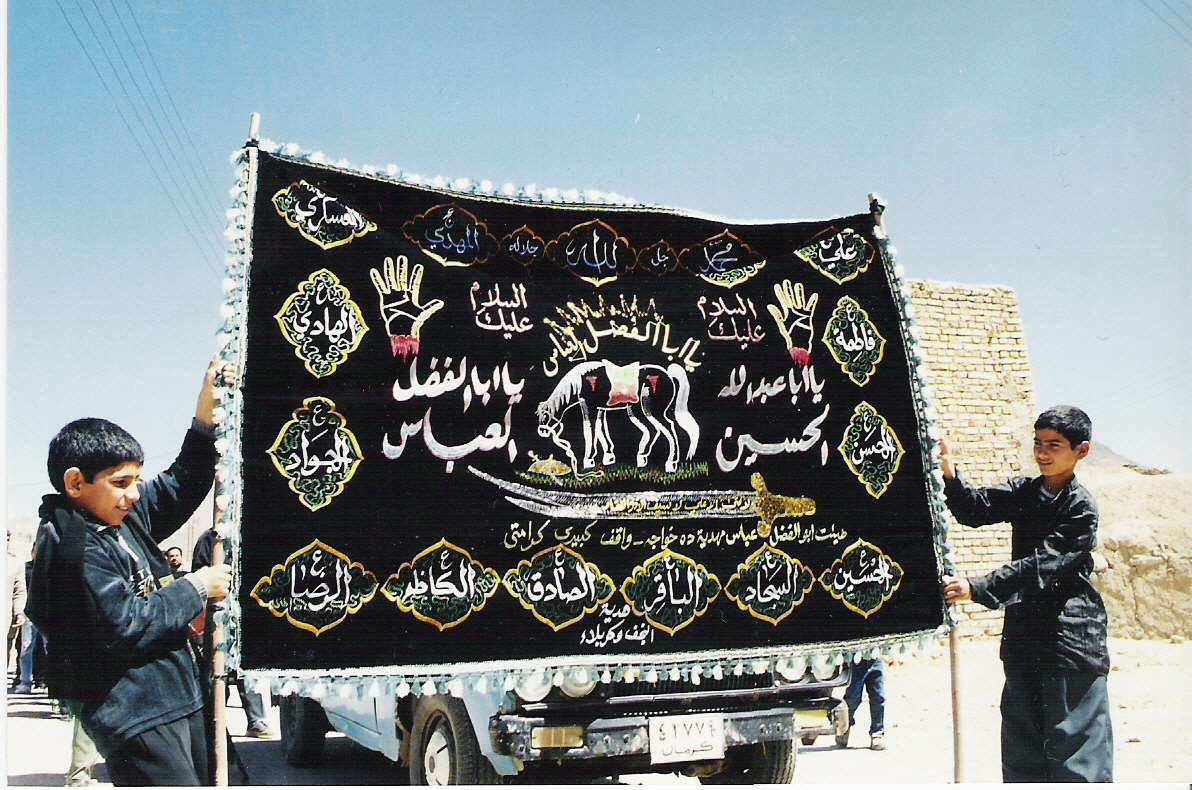
\includegraphics[width=4.07818in,height=3.13349in]{media/image6.jpeg}

\vide{les-gardiens-de-lenfer}{%
\subsubsection{3.5 Les gardiens de
l'enfer}\label{les-gardiens-de-lenfer}}

Chaque strate infernale est gardée par des anges robustes et rudes~:
«~Nous n'avons pris que des anges comme gardiens du Feu~» (S. 74, 31).
«~Des anges gigantesques et puissants se tiendront autour du Feu~; ils
ne désobéissent pas à l'ordre de dieu, ils font ce qui leur est
commandé~» (S. 66, 6). Leurs épaules sont larges. Il faut une année de
marche pour les parcourir. Ils accueillent les damnés par des flammes
aussi volumineuses que les astres. Cette tradition prend sa source
notamment dans la littérature talmudique et dans le Midrash où il est
question des anges gardant les Portes de la Géhenne.

À leur approche l'enfer gronde et mugit. Les damnés épouvantés reculent
à la vue de ces flammes, mais ils sont enchaînés par les anges. Un nuage
fait pleuvoir sur eux non l'eau qu'ils espéraient mais des chaînes. Ils
sont poussés au fond de l'enfer, mais les flammes les remontent~: S. 25,
11-13~: «~Ils ont plutôt qualifié l'Heure de mensonge. Nous avons
cependant préparé, pour quiconque qualifie l'Heure de mensonge, une
Flamme brûlante. Lorsque de loin elle les voit, ils entendront sa fureur
et ses pétillements. Et quand on les y aura jetés, dans un étroit
réduit, les mains liées derrière le cou, ils souhaiteront alors leur
destruction complète~».

\vide{description-de-lenfer}{%
\subsubsection{3.6 Description de l'enfer}\label{description-de-lenfer}}

Il y a un feu intense, mais il ne dégage aucune lumière. Un feu noir. Sa
puissance de feu est 70 fois supérieure à celui de la terre. Son
combustible est constitué des damnés dont la chair éternelle alimente
sans cesse le feu de la fournaise. Toutefois, le vendredi, le feu cesse
de brûler. Comme pour l'océan, l'enfer a un rivage. Les réprouvés y
espèrent trouver refuge et tranquillité. Mais ils s'y méprennent car ce
rivage est habité de scorpions énormes, de serpents grands comme des
chameaux. Ils les mordent et s'attaquent aux parties de leurs corps les
plus sensibles~: paupières, lèvres, organes génitaux. Leur venin est si
fort qu'il agit dans le corps 40 années durant. Finalement, ils
préfèrent encore le feu. Le chameau, la brebis ou la vache dont le
propriétaire ne s'est pas acquitté de la \emph{zakāt} sont transformés
en monstres aux cornes et aux sabots de feu qui torturent leurs
propriétaires avares et injustes. Sous les coups, leurs os sont brisés
et leurs crânes fracassés.

\vide{les-tourments-de-lenfer}{%
\subsubsection{3.7 Les tourments de
l'enfer}\label{les-tourments-de-lenfer}}

La figure des damnés sera noire, décharnée, les yeux cautérisés avec des
clous de feu, la langue allongée jusqu'au sol, le front marqué avec du
métal en fusion. Leurs lèvres seront cisaillées en deux par des ciseaux
de feu~; elles repousseront mais seront de nouveau coupées,
éternellement. Leurs bouches vomiront du pus et du sang, de la sanie qui
sera leur propre boisson. Leurs cheveux seront suspendus à des arbres de
feu, leurs entrailles brûleront, leurs dos flagellés par des chaînes de
feu. Pieds et mains enchaînés, ils devront gravir une montagne de feu.

Dans ce monde, leur corps seront plus développés pour qu'ils ressentent
plus encore la douleur. Eux aussi, ils deviennent des monstres. La chair
et la peu feront entendre une voix plus affreuse que le hurlement des
loups.

On trouve en enfer des arbres, les \emph{zaqqūm}. Les réprouvés se
nourrissent de leurs fruits, mais de feu, ils leur brûlent les
entrailles comme du métal en fusion. Plus ils en mangent, plus grande
est leur faim. Ils sont une torture. Ils boivent de l'eau bouillante et
les gardiens leur présentent une coupe débordante de pus et de sanie
bouillonnants qui proviennent de leurs corps. Leurs visages sont
décharnés, brûlés, déchirés. Tout est donc feu, souffrance, torture,
supplice. L'odeur pestilentielle des damnés les conduit à se maudire
mutuellement. C'est alors qu'ils supplient le chef des geôliers, Mālik,
d'intercéder auprès de Dieu pour atténuer leur supplice. Mais ils y
resteront à jamais, à l'exception des croyants grâce à l'intercession
des prophètes.

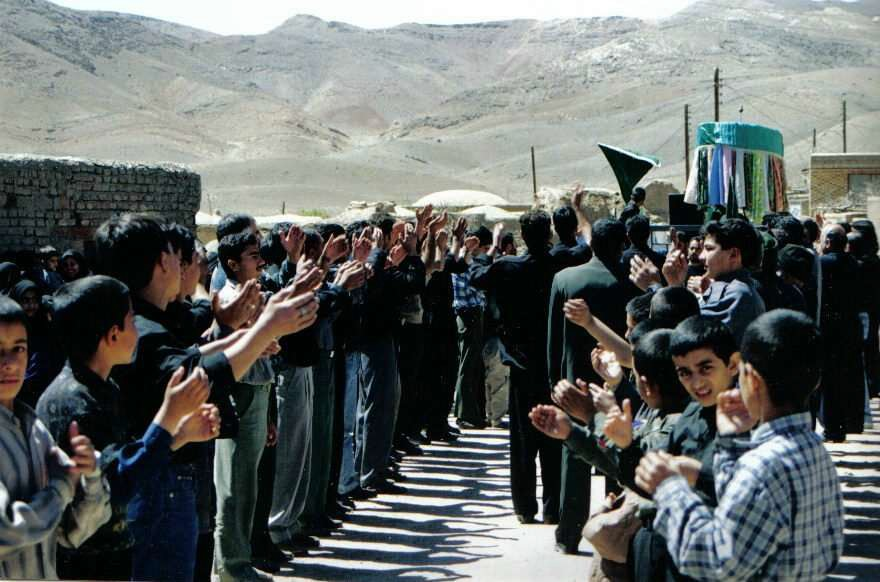
\includegraphics[width=2.73901in,height=2.05312in]{media/image7.jpeg}

\vide{la-question-de-luxe9ternituxe9-des-peines}{%
\subsubsection{3.8 La question de l'éternité des
peines}\label{la-question-de-luxe9ternituxe9-des-peines}}

Selon les exégètes traditionalistes, les souffrances sont éternelles.
Une fois plongé dans une de ces demeures, le réprouvé y reste
éternellement. Les ǧahmites qui prétendent que le paradis et l'enfer
sont des accidents et seront donc un jour anéantis sont considérés comme
des innovateurs. Toutefois, on trouve quelques traditionnistes qui
considèrent que seul le Paradis restera éternellement tandis qu'un jour,
l'enfer sera complètement anéanti.

\emph{\textbf{La position des traditionalistes}}

Ils affirment l'éternité de l'enfer et du paradis.

- Cette croyance qui s'appuie sur le consensus, \emph{iǧmā'}, des
compagnons du Prophète et de la première génération. Le consensus est
une des sources du droit musulman avec le Coran et la Sunna.

- Le Coran déclare que les tourments sont perpétuels~«~\emph{ḫalidīn
fîhā 'abadan}~», que les infidèles n'entreront pas au paradis tant que
le chameau n'entre pas dans le trou d'une aiguille~: «~Pour ceux qui
traitent de mensonges Nos enseignements et qui s'en écartent par
orgueil, les portes du ciel ne leur seront pas ouvertes, et ils
n'entreront au Paradis que quand le chameau pénètre dans le chas de
l'aiguille. Ainsi rétribuons-Nous les criminels~» (S. 7, 40). Autrement
dit, aller en enfer, c'est prendre à perpétuité.

- La tradition indique une exception à l'égard des monothéistes
(\emph{muwaḥḥid}) sujets au péché. Grâce à l'intercession des prophètes
ils peuvent sortir de l'enfer. Par suite, les infidèles sont donc quant
à eux condamnés pour toujours.

- Les anciens \emph{al-salaf}, les partisans de la tradition \emph{ahl
al-Sunna}, déclarent la création de l'enfer et du paradis avec ce
monde-ci et ils ne seront jamais anéantis. L'idée d'un anéantissement
est pour eux une innovation.

- C'est une question de justice~: le Coran distingue les fidèles des
infidèles, on ne peut mettre sur le même pied d'égalité les pieux et les
impies. La raison indique que les âmes humaines ont des qualités
immuables. Elles ne peuvent changer leurs conduites antérieures. Elles
ne peuvent donc que subir les peines éternelles.

\emph{\textbf{La critique d'Ibn Al-Qayyim al-Ǧawziyya}}

Célèbre juriste sunnite du quatorzième siècle, commentateur du Coran,
disciple d'Ibn Taymiyya, il procède à une critique de cette
interprétation.

- L'éternité de l'enfer est déjà une question disputée parmi les
compagnons. Il n'y a donc pas consensus. Pour dix des compagnons, nous
ne disposons pas de preuve quant au fait qu'ils aient nié
l'anéantissement de l'enfer. Quant à la première génération, nous
disposons clairement d'opinions controversées.

- Le Coran affirme l'éternité des tourments tant que durera l'enfer.
Tant que l'enfer existe, les infidèles y demeurent. Mais si l'enfer est
anéanti, ses membres en seront délivrés.

- Tant que l'enfer existe, en sortir est le privilège des croyants. Mais
si Dieu détruit l'enfer, les infidèles en seront donc libérés.

- Les traditions n'affirment pas l'éternité de l'enfer en soi~; elles ne
nient pas l'impossibilité de son anéantissement.

- Des compagnons ont déclaré que l'enfer sera anéanti.

- Trois passages coraniques montrent que l'enfer n'est pas éternel~: S.
6, 128~: «~Dieu leur dira: ‹l'Enfer est votre demeure, pour y rester
éternellement, sauf si Allah en décide autrement.› Vraiment ton Seigneur
est Sage et Omniscient~». S. 11, 107~: «~Pour y demeurer éternellement
tant que dureront les cieux et la terre - à moins que ton Seigneur
décide autrement - car ton Seigneur fait absolument tout ce qu'Il veut~»
ou encore~: S. 78, 23~: «~Ils y demeureront pendant des siècles
successifs~». L'éternité de l'enfer dépend donc de la volonté divine, du
Juge Suprême.

- Le Paradis exprime la Miséricorde divine, l'enfer la colère. Or, la
tradition se fait l'écho du triomphe de sa Miséricorde sur sa colère.
Les deux attributs ne sont pas égaux.

- la miséricorde est une fin tandis que la colère est un moyen. L'enfer
n'est qu'un moyen de purification. Un \emph{ḥadīṯ} rapporté par Buḫarî
indique~: «~Dieu a créé la miséricorde et en a multiplié l'aspect. Si
l'Infidèle savait tout ce que Dieu a de miséricorde, il ne désespérerait
jamais d'entrer au Paradis~»\sn{}.

- l'enfer est créé pour menacer les croyants, purifier les pécheurs. La
nature humaine est originellement pure, donc même les infidèles peuvent
être purifiés par le feu. Dieu est tel un médecin qui brûle ou coupe un
membre malade pour guérir l'homme. Il ne se plaît pas au châtiment en
soi. Ce châtiment est un aspect de sa Sagesse, de sa bonté, de sa
justice.

- certaines traditions rapportées par Ibn Hanbal indiquent que celui qui
reconnaît la bonté de Dieu, sa grâce, son pardon, alors l'Enfer devient
pour lui un séjour paisible de rafraîchissement.

- Selon un \emph{hadiṯ qudsi}, la miséricorde de dieu embrasse toutes
choses~: 
\begin{quote}
    «~Je ne fais pas perdre à ceux qui me désobéissent l'espoir de
ma Miséricorde. S'ils reviennent de leur erreur, je suis leur
bien-aimé~; et s'ils ne reviennent pas je suis leur médecin. Je leur
fais subir les peines pour les purifier de leurs erreurs~!~»
\end{quote}


\vide{le-paradis-selon-lislam}{%
\subsection{Le paradis selon l'islam}\label{le-paradis-selon-lislam}}

\vide{existence-localisation-et-duxe9signation}{%
\subsubsection{Existence, localisation et
désignation}\label{existence-localisation-et-duxe9signation}}

L'existence du Paradis est affirmée dans le Coran. Selon l'exégèse
traditionnelle, il existe dès à présent, dans un septième ciel. Il a été
créé par Dieu en même temps que notre monde ici-bas comme lieu de
récompense pour les bienheureux (S. 3, 133).

Il existe dans le Coran plusieurs termes pour désigner le paradis.

Le vocable le plus courant est celui de \emph{Ǧanna}, le Jardin. Le
Coran en précise sa nature en évoquant «~le Jardin de la retraite~»
(\emph{Ǧannat al-Ma'wā}, S. 53, 15), le «~Jardin des délices~»
(\emph{Ǧannat an-Na`īm}, S. 10, 9). Il est aussi question du Jardin
d'Eden (\emph{Ǧannat} \emph{`Adn}, S. 61, 12), jardin de bonheur.

Quatre autres expressions sont utilisées pour désigner le paradis~:
\emph{Dâr al-Salām}, la demeure~du salut (S. 6, 127) ; \emph{Dār
al-Muqāma}, la demeure illimitée (S. 35, 35)~; \emph{Dār al-ḫuld}, la
demeure de l'éternité (S. 25, 15) ou encore \emph{dār}
\emph{al-ḥayawān}, la demeure de la vie éternelle (S. 29, 64). On trouve
une autre expression, Firdaws (S. 23, 11) qui est un dérivé du
\emph{Pardes} persan.

\vide{description-du-paradis}{%
\subsubsection{Description du
paradis}\label{description-du-paradis}}

Les descriptions du Paradis sont nombreuses et la littérature
\emph{ḥadīṯ} en donne des images empruntes d'une grande sensualité et
beauté. Il est question d'un lieu de palais aux voutes de perles, de
tapis de fleurs, d'arbres aux couleurs jusqu'alors inconnues des hommes,
les jujubiers d'al-\emph{Muntahā}.
\begin{quote}
    S. 4, 57~: «~Et quant à ceux qui ont cru et fait de bonnes œuvres,
bientôt Nous les ferons entrer aux Jardins sous lesquels coulent des
ruisseaux. Ils y demeureront éternellement. Il y aura là pour eux des
épouses purifiées. Et Nous les ferons entrer sous un ombrage épais».
\end{quote}


On y trouve des fleuves comme dans le paradis terrestre de la Genèse,
mais il n'y coule pas seulement de l'eau~:
\begin{quote}
    «~Il y aura là des fleuves dont l'eau est incorruptible, des fleuves de
lait au goût inaltérable, des fleuves de vin, délices pour ceux qui en
boivent, des fleuves de miel purifié. Ils y trouveront aussi toutes
sortes de fruits et le pardon de leur Seigneur (S. 47, 15)~».
\end{quote}


Cette description rappelle la description de la Terre promise aux
Hébreux dans l'Ancien Testament. Elle était désignée comme une terre où
ruissellent le lait et le miel (Ex 3, 8, 17 ou Ex 13, 5~; Deut 6, 3,
etc.). C'est un pays d'abondance, de source d'eau, de vigne\ldots Le
2\textsuperscript{ème} Livre d'Hénoch et l'Apocalypse de Paul évoquent
aussi les ruisseaux de miel, de lait, de vin et d'huile.

Il y a des vierges éternelles~:
\begin{quote}
    «~ Là, il y aura des vertueuses et des belles.\\
Lequel donc des bienfaits de votre Seigneur nierez-vous~?\\
Des houris cloîtrées dans les tentes,\\
Lequel donc des bienfaits de votre Seigneur nierez-vous~?\\
qu'avant eux aucun homme ou djins n'a déflorées.\\
Lequel donc des bienfaits de votre Seigneur nierez-vous~?\\
Ils seront accoudés sur des coussins verts et des tapis épais et
jolis.\\
Lequel donc des bienfaits de votre Seigneur nierez-vous~? (S. 55,
70-77)~».
\end{quote}


Et des éphèbes : 
\begin{quote}
    «~ Parmi eux circuleront des garçons éternellement
jeunes,\\
avec des coupes, des aiguières et un verre (rempli) d'une liqueur de
source\\
qui ne leur provoquera ni maux de tête ni étourdissement;\\
et des fruits de leur choix,\\
et toute chair d'oiseau qu'ils désireront.\\
Et ils auront des houris aux yeux, grands et beaux,\\
pareilles à des perles en coquille\\
en récompense pour ce qu'ils faisaient (S. 56, 17-24) ».
\end{quote}

On peut y boire du vin car il n'enivre pas~:
\begin{quote}
   «~On leur sert à boire un nectar pur, cacheté, laissant un arrière-goût
de musc.

Que ceux qui la convoitent entrent en compétition (pour l'acquérir)\\
Il est mélangé à la boisson de Tasnīm,\\
source dont les rapprochés boivent (S. 83, 25-28)~». 
\end{quote}


Ce qui est à relever dans ces descriptions, c'est l'atmosphère de
banquet qui y règne. Les élus sont accoudés sur des tapis aux revers de
brocart\ldots{} sur des coussins verts et sur de beaux tapis (S. 55, 54
et 76), ils boivent un vin délectable. Ces images sont typiques de la
tradition juive qui sert à décrire le bonheur des justes.

\vide{accuxe8s-au-paradis}{%
\subsubsection{Accès au paradis}\label{accuxe8s-au-paradis}}

Le Paradis est constitué de différents étages. La tradition distingue
huit portes qui ouvrent à différents espaces paradisiaques et qui
s'ouvrent en fonction des actions accomplies par les croyants. Il y a
ainsi la porte de la prière, de la guerre sainte, de l'aumône, du jeûne,
du repentir, des patients (ceux qui maîtrisent leur colère), de la
soumission à la volonté divine, enfin la porte droite celle qui ne
nécessite pas de jugement préalable~: c'est elle qu'emprunte Muḥammad.

Il est nécessaire pour entrer au paradis d'avoir un laisser passer et
selon une tradition, chaque croyant entrera au paradis avec un passeport
sur lequel sera indiqué~: 
\begin{quote}
    «~Au nom de Dieu, le Bienfaiteur, le
Miséricordieux. Nous délivrons à \ldots{} fils de\ldots{} un permis
d'entrée au jardin sublime, dont les fruits à cueillir seront à portée
de sa main~».
\end{quote}

Les élus sont accueillis par un chœur d'anges qui chante en arabe, ils
ont un visage radieux après avoir été lavés dans une douce fontaine.

Le climat du Paradis est doux~: «~Il n'y sévit ni la chaleur du soleil,
ni la rigueur du froid (S. 75, 3). Les mois comprennent 500
jours\ldots{} et les années 500 mois.

\vide{les-uxe9lus}{%
\subsubsection{Les élus
}\label{les-uxe9lus}}

Ils ont l'apparence d'un homme âgé de 33 ans, ils sont imberbes.

Toute épouse vierge au moment du mariage sera la femme légitime du
Bienheureux au paradis. Le Bienheureux qui a eu plusieurs épouses les
gardera toutes. Si la femme a eu plusieurs maris, elle se consacrera au
dernier, au meilleur ou à celui de son choix.

\vide{la-question-des-femmes-au-paradis}{%
\subsubsection{La question des femmes au
paradis}\label{la-question-des-femmes-au-paradis}}

Mais justement, revenons sur la question de la femme.

Le Coran est explicite quant à l'égale possibilité pour les hommes et
les femmes d'accéder au paradis ou en enfer~:
\begin{quote}
    «~Et quiconque, homme ou femme, fait de bonnes oeuvres, tout en étant
croyant... les voilà ceux qui entreront au Paradis; et on ne leur fera
aucune injustice, fût-ce d'un creux de noyau de datte~» (S. 4, 124).



«~{[}Il en est ainsi{]} afin qu'Allah châtie les hypocrites, hommes et
femmes, et les associateurs et les associatrices, et Allah accueille le
repentir des croyants et des croyantes. Allah est Pardonneur et
Miséricordieux~» (S. 33, 73).
\end{quote}
Il semble cependant qu'il y ait en enfer plus de femmes que d'hommes.
Ceci est indiqué dans un \emph{ḥadīṯ} alors que Muḥammad eut une
vision~: 
\begin{quote}
    «~J'ai vu le feu et je n'ai pas vu à ce jour un spectacle plus
terrible. La plupart des habitants sont des femmes~». la raison en est
leur ingratitude, leur manque de charité, leur négativité dans le regard
des actions conduites par leurs maris~: «~si les hommes font de bonnes
choses, la femme voit une chose mauvais, et vous dit qu'elle n'a jamais
rien vu de bon du tout~» (Ahmad ibn Hanbal, I.359, cité dans Smith et
Haddad 1975: 44).
\end{quote}


Le Coran mentionne les femmes de Lot et de Noé qui à cause de leur
trahison furent conduites au Feu. Leurs saints maris ne leur furent
d'aucun secours~: 
\begin{quote}
    «~Allah a cité en parabole pour ceux qui ont mécru la
femme de Noé et la femme de Lot. Elles étaient sous l'autorité de deux
vertueux de Nos serviteurs. Toutes deux les trahirent et ils ne furent
d'aucune aide pour {[}ces deux femmes{]} vis-à-vis d'Allah. Et il
{[}leur{]} fut dit: ‹Entrez au Feu toutes les deux, avec ceux qui y
entrent~» (S. 66, 10).
\end{quote}


Notons que parmi les signes de la venue du jugement dernier, on trouve
mentionné le renversement des valeurs morales traditionnelles entre
l'homme et la femme~: l'homme doit obéir à sa femme et il désobéit à ses
parents, l'homme doit travailler pour sa femme, les femmes vont au
pèlerinage ensemble sans être accompagnées d'un homme, il y a une pleine
licence sexuelle. Le nombre d'homme décroît tandis qu'il y a cinquante
femmes pour un homme.

\vide{la-question-des-houris}{%
\subsubsection{La question des
houris}\label{la-question-des-houris}}

Houris vient du mot arabe \emph{ḥawrâ'}, pluriel de \emph{ḥur.}

\emph{Le Coran} mentionne à plusieurs reprises les houris~:
\begin{quote}
   S. 44, 54~: «~C'est ainsi! Et Nous leur donnerons pour épouses des
houris aux grands yeux~». 
S. 55, 56~: «~Ils y trouveront {[}les houris{]} aux regards chastes,
qu'avant eux aucun homme ou djinn n'aura déflorées~».

S. 52, 20~: «~accoudés sur des lits bien rangés›, et Nous leur ferons
épouser des houris aux grands yeux noirs~».

S. 55, 72~: «~des houris cloîtrées dans les tentes~».

S. 56, 22~: «~Et ils auront des houris aux yeux, grands et beaux~»
\end{quote}




Quant au ḥadīṯ, on trouve dans la compilation de al-Buḫarî~\sn{Livre 54, \emph{Le commencement de la création}, ḥadīṯ 476.}:
\begin{quote}
    Le Prophète a dit: «Les premières personnes qui entreront au paradis
seront brillantes comme la pleine lune, et les suivantes brillantes
comme l'étoile la plus brillante dans le ciel. Leurs cœurs seront comme
le cœur d'un seul homme, car ils n'auront ni haine ni jalousie entre
eux, tout le monde aura deux épouses, des houris, qui seront aussi
belles, pures et transparentes que la moelle des os de leurs jambes~»

\end{quote}


Autre hadîth de Buḫari~: rapporté par Abu Huraira: 
\begin{quote}
    «~L'Apôtre d'Allah
dit: «Les premières personnes à entre au paradis, seront brillantes
comme la pleine lune et celles qui les suivront, brilleront comme
l'étoile la plus brillante dans le ciel. Ils n'urineront pas, ils ne se
soulageront pas, ils ne cracheront pas et n'auront pas de sécrétions
nasales. Leurs peignes seront d'or, et leur sueur d'une odeur de musc.
Leurs épouses seront des houris. Elles ressembleront toutes à leur père
Adam (dans leur état), elles seront grandes de soixante coudées de
hauteur~».
\end{quote}


\paragraph{Les commentateurs}

Elles ont suscité plusieurs questions

\begin{itemize}
\item
  sont-elles de la même essence que les femmes~?
\item
  sont-elles de la lignée d'Eve~?
\item
\end{itemize}

Pour certains commentateurs, elles ont été créées de safran. Mais elles
semblent bien être faites de chair. Leur luminosité y est dépeinte dans
un style hyperbolique~: leurs sourcils ressemblent à un trait noir placé
sur de la lumière et leur front rappel un croissant de lune.

Les commentateurs se sont aussi interrogés sur les délices qu'elles
peuvent procurer aux croyants~? Combien de houris un Croyant peut-il
honorer de ses faveurs par nuit~? Des réponses diverses qui montrent
cependant que l'occupation principale au paradis sera de s'enlacer de ces
femmes vierges. Et le plaisir de l'homme y sera décuplé de 100 fois de
celui sur terre. Elles attendent au ciel leurs époux et maudissent leurs
femmes terrestres lorsque celles-ci se fâchent ou les contrarient leurs
maris.

Les houris sont pures. Elles ne souffrent des aléas de la menstruation,
elles n'éprouvent aucune fatigue. Les élus mangent les fruits délicieux
du paradis par pure jouissance. Les résidus de la digestion se
transforment en une exhalation parfumée du corps.

\paragraph{L'hypothèse syriaque}

En l'an 2000, un chercheur libanais-allemand sous le pseudonyme de
Christoph Luxenberg a publié un ouvrage intitulé \emph{Die
Syro-Aramäische Lesart des Koran:~ Ein Beitrag zur Entschlüsselung der
Koransprache} \sn{en français~: \emph{Lecture syro-araméenne du Coran~: une
contribution pour décoder la langue du Coran}}. Cet ouvrage est une
étude philologique qui met en lumière l'existence particulière d'une
source du Coran. Si nombreux sont les auteurs qui ont souligné
l'influence des textes bibliques, Luxenberg indique l'adoption plus
particulière d'un lectionnaire syriaque, et plus particulièrement d'un
ouvrage liturgique à vocation ce missionnaire. Ces travaux poursuivent
l'enquête menée par Günther Lulling.

Sa méthodologie consiste à rechercher les équivalents syriaques des
termes arabes et de clarifier le sens de certains passages coraniques
obscurs à l'aide des termes syriaques.

À cet égard, le mot houri signifierait non pas une vierge aux grands
yeux noirs, mais du raisin blanc.

\vide{conclusion-la-vision-de-dieu}{%
\section{{Conclusion~: La vision de Dieu
}}\label{conclusion-la-vision-de-dieu}}

La question de la vision de Dieu n'est pas étrangère à la tradition
musulmane. Elle y est affirmée parfois de manière explicite~: Chaque
vendredi, hommes et femmes rendent visite au Seigneur sur son
invitation. Chemin faisant, ils passent devant le tableau du Destin,
\emph{al-Lawḥ al-mahfūẓ} où se trouvent consignées toutes les actions
des êtres. Sur des montures ailées, les Bienheureux parviennent en un
clin d'œil devant le Trône du Tout-Puissant. Le voile de lumière se lève
et l'Eternel paraît. La voix divine retentit~: «~al-salām alaykum~». La
vue de Dieu surpasse tous les délices du paradis.

Si l'ensemble de ces descriptions sont marquées par une très grande
sensibilité, il ne faut pas oublier, à l'exemple du cours sur la
philosophie, qu'elles ont donné lieu à des interprétations et à une
lecture spirituelle. Ainsi, al-Ġazālī soutient que la vision de Dieu
relève de l'ordre de la connaissance~: voir Dieu, c'est accéder non à
une vision physique, mais à sa connaissance.



\chapter{L'Islam comme religion Universelle ?}


L'Islam semble offrir aujourd'hui deux visages au voyageur candide qui
observe le monde. D'un côté, il peut admirer des mosquées magnifiques en
forme de pagodes, avec des stèles traditionnelles chinoise, à Xi'an,
ancienne capital de la Chine~; de même la Mesquita à Cordoue, l'art
Moghol en Inde, qui s'inspire des influences architecturales locales
tout en créant un univers inédit et reconnaissable. Et au-delà de
l'architecture, il peut rencontrer des musulmans de toutes les Nations.
De l'autre, il peut observer régulièrement une sorte de séparation par
des pratiques ou des tenues, qu'il retrouve à travers le monde, tunique,
barbe, et chaussure Nike, sans parler de la tenue des femmes et du
fameux \emph{voile}.

Au deuxième siècle de notre ère, chrétiens et juifs répondirent de façon
très différente, à la question du rapport au monde, le rabbin Tryphon
faisant la remarque aux chrétiens que \sn{Dialogue de saint Justin
  avec le juif Tryphon. Chapitre 10.«~Mais ce qui nous embarrasse surtout, c'est que vous vous dites
  pieux; que vous estimez différer des autres tout en ne vous en
  séparant pas; et que dans votre vie, vous n'êtes pas différents des
  nations, puisque vous n'observez ni les fêtes, ni les sabbats, que
  vous n'avez pas la circoncision; et encore, tandis que vous mettez
  votre espoir en un homme qui a été crucifié, vous espérez en même
  temps quelque bien de Dieu, sans observer ses commandements.}
  \begin{quote}
       «~vous
vous dites pieux; vous estimez différer des autres tout en ne vous en
séparant pas; et dans votre vie, vous n'êtes pas différents des nations,
puisque vous n'observez ni les fêtes, ni les sabbats, que vous n'avez
pas la circoncision~».
  \end{quote}



Qu'en est-il de l'Islam~? Quel est son rapport à l'universalité~?
Question qui nous semble être un préalable à d'autres questions, comme
celle de la possibilité d'un \emph{Islam de France} ou de son rapport à
la démocratie\emph{.} Nous proposons d'étudier la réponse faite en 1882
par Abraham Kuenen. Cette année-là, ce théologien hollandais de
l'université de Leyde, spécialiste reconnu du Pentateuque, et l'un des
pères de l'approche \emph{historico-critique.} se rend en Angleterre
pour dispenser un cours, intitulé \emph{National Religions et Universal
Religion}. Il s'attache alors, avec rigueur à tester ces deux concepts
de religion nationale et religion universelle à l'Islam~: \emph{l'Islam
offre-t-il les caractères de l'universalisme religieux}~? \sn{Kuenen,
  A. ``\emph{L'Islam offre-t-il les caractères de l'universalisme
  religieux}?'' Revue De L'histoire Des Religions, vol. 6, 1882, pp.
  1--40. JSTOR,
  \url{http://www.jstor.org/stable/23658819}.}
Les 150 ans qui nous sépare de cette conférence, bien loin de constituer
un handicap, permettent de se situer à une période précédent la fin de
l'empire Ottoman - et de son paradigme \emph{l'Islam Impérial ou
classique}\sn{Adrien Candiard, \emph{Comprendre l'islam: ou plutôt
  : pourquoi on n'y comprend rien, 2016,} emp. 427}\emph{,} en nous
offrant un recul utile pour répondre à cette question de
l'universalité\emph{.} Nous proposons dans un premier temps d'étudier
les différentes étapes du raisonnement de Kuenen qui l'amène à ne pas
attribuer le terme de \emph{religion universelle} à l'Islam puis dans un
second temps, de proposer quelques éléments qui nous semble permettre
d'atténuer ce jugement en particulier en testant les présupposés
méthodologiques de Kuenen et en proposant quelques pistes entrevues lors
du cours sur les fondations de l'Islam.

\section{La thèse de Kuenen : L'islam comme religion particulière}
Pour répondre à la question posée par l'Islam, il nous faut d'abord
définir ce qui définit une religion universelle par rapport à une
religion nationale, bornée à un peuple unique ou à une groupe de peuples
de mêmes origines. Kuenen propose de ne pas s'arrêter au fait (l'Islam a
bien été adopté par plusieurs nations différentes et est une religion
internationale), mais de regarder son caractère propre. \sn{car
  «~le universel de fait peut venir de la force au moins en dépit de son
  caractère propre~; que son défaut ou du moins sa faiblesse en fait
  d'éléments vraiment universels ait trouvé sa contrepartie ou son
  dédommagement dans différentes particularités qui ne viennent pas en
  ligne de compte quand on dresse son signalement\emph{~».}} Mais
comment définir le caractère propre d'une religion~? Fidèle à sa méthode
historico-critique\sn{Kuenen a établi quatre règles permettant
  l'interprétation d'un texte~:

  \emph{rigueur philologique et grammaticale}, c'est-à-dire conditionnée
  par le contexte de l'époque et le style de l'auteur.

  \emph{rationnellement cohérente}, un passage doit toujours être
  interprété dans son contexte

  \emph{historique}, c'est-à-dire en correspondance avec les données
  historiques à notre disposition

  \emph{psychologique}, elle doit nous rendre l'état mental préalable au
  texte.} permettant de remonter à l'origine du texte, il essaye de
ressaisir «~l'élément authentiquement universel {[}\ldots{]} qui tient
immédiatement à l'origine~»\sn{Ibid, p. 5 «~élément
  authentiquement universel, n'est pas à mon sens, l'effet d'une
  addition postérieure, mais tient immédiatement à l'origine des
  religions dans lesquelles nous saisissons cet élément, à la nature du
  rapport ou elles se trouvent avec les religions nationales d'où elles
  sont sorties ou sur le terrain desquelles elles se sont développées.~»}
de l'Islam. Nous connaissons relativement bien cette origine, d'une
religion née «~en pleine lumière~» selon l'expression de Renan. Pour
bien capter cette origine, Kuenen étudie les religions nationales qui
précèdent, et en particulier la \emph{Hanîffyya,} la religion d'Abraham
telle qu'elle est mentionnée dans la Sira (I, 222-232)\sn{Ce
  passage de la Sira mentionne 4 \emph{hanifs}, qui anticipent la venue
  de Mohammed. «~Zayd ibn 'Amr ibn Nufayl~{[}\ldots{]} interrogea le
  moine sur la \emph{Hanîfiyya}, la religion d'Abraham. «~Tu recherches
  une religion à laquelle tu ne trouveras personne aujourd'hui pour te
  conduire. Cependant, le temps est proche où un prophète sortira de ton
  pays que tu viens de quitter et prêchera la religion d'Abraham.
  Rejoins-le, car c'est bien la période prévue pour sa mission.~Hichâm,
  Ibn. \emph{La biographie du prophète Mahomet}, Sira I, 222-232}. Mais
il conclut que nous ne savons pas grand-chose de ces \emph{hanifs} et
que la référence à Abraham est probablement un \emph{hysteron proteron,}
une reconstruction ex-post permettant de faire le lien avec les juifs et
chrétiens mais sans se lier à eux\sn{Cf «~Abraham ne fut ni juif
  ni chrétien, mais fut \emph{hanif} et \emph{muslim} {[}à Allah{]}. Et
  il n'était point du nombre des Associateurs » (Coran 3:67)}.

Le contexte n'explique donc par l'Islam et c'est donc vers Mohammed
qu'il faut se tourner~: «~l'islam est bien plus que la plupart des
autres religions, le produit non d'une époque, non d'un peuple, mais de
la personne de son fondateur~»\sn{Ibid, p. 17}. Kuenen le décrit
comme un homme religieux, surtout avant la fuite à Médine, avec une
\emph{pensée sémitique,} en particulier par son eschatologie marquée par
le judaïsme.

L'Islam valorise dès son origine le Coran, glorifié à l'intérieur même
du Coran. Il transmet certes un noyau du Judaïsme transporté sur le sol
d'Arabie. Mais Mohammed avait une vision plus large, comme le soulignent
différentes sourates.~: «~le Coran, est en vérité un avertissement pour
toutes les créatures~»\sn{Ref Coran 8,87~?}, «~nous ne t'avons pas
envoyé aux hommes en général que pour prêcher et menacer, cependant la
plupart des hommes ne comprennent pas~»\sn{Coran 34,27}.~

Mais Kuenen constate en parallèle de ces versets, de nombreux passages
qui valorise les Arabes, ce qui semble limiter cette vocation à
l'universel\sn{« avec quelle extrême insistance est relevé le
  privilège des Arabes qui, dans les signes qui leur ont été montrés,
  c'est-à-dire dans les versets du Qurân, possèdent maintenant la parole
  même d'Allah, {[}qui dépasse{]} de beaucoup (celles qu'ont reçue les
  fondateurs des autres religions) » Ibid, p.18}. De plus, il souligne
des exceptions à l'universalité, qui semblent même s'opposer
formellement à l'essence de l'Islam, comme la Ka'ba et la mise en
exergue de la Mecque, «fragment incompréhensible de paganisme qui est
passé dans l'islam sans être digéré~»\sn{Ibid, p 24}.

Mais alors comment comprendre que l'Islam soit devenu \emph{de fait} une
religion universelle. Pour Kuenen, cela vient de la pauvreté de
l'essence de l'Islam, de sa plasticité dirions-nous aujourd'hui, qui lui
permet de dériver des variétés persane, hindoue ou javanaise. La
simplicité et la concision d'une religion sont pour Kuenen le plus grand
éloge qu'on puisse lui faire à la condition qu'elle permette le
développement spirituel de l'homme, ou qu'au moins elle n'y fasse pas
obstacle. «~A cette condition, mais à cette seule condition, elle peut,
en dépit de son étroitesse, avoir un caractère universel, être une
bénédiction pour l'humanité. »\sn{Ibid, p 26}. Ce n'est pas au
niveau de la vie politique ou juridique qu'est l'enjeu mais bien dans
«~la vie de l'âme et de la conviction religieuse~». Mais Kuenen
considère que de cette pauvreté spirituelle originelle vient de la foi
même de l'Islam~: Allah est certes~\emph{ar-rahmano'r-rahimo,~} le
miséricordieux et le compatissant mais il est surtout «~un dieu de
loin~»\sn{Ibid, p 32} dont il faut suivre les devoirs religieux
prescrits par lui. Pour compenser cet éloignement, les croyants ont
développé par la suite des éléments mystiques, comme le soufisme et la
foi en la \emph{médiation}, soit de Mohamed, soit des saints (dont le
culte est fervent dans l'Islam du XIX\textsuperscript{ème} siècle). Mais
pour le culte des saints, il remarque qu'il est «~plutôt une
protestation contre la religion~»\sn{Ibid, p 31}~: le musulman
recherche ce que sa foi ne lui fournit pas et il le cherche là où,
d'après l'autorité même qu'il reconnait, il ne devrait pas le chercher.
De même pour le soufisme~: le vrai soufi vit une vie intérieure
remarquable mais n'est plus musulman\sn{Ibid, p 31}.

Mais alors qu'est-ce que l'Islam~? Mais «~malheureusement, la foule
n'avait pas tort~» quand elle s'opposait aux rationalistes Mo'tazilites.
En imposant le Coran incréé, la foule a «~barré à leur religion la voie
qui conduit au véritable universalisme. Car l'élément éthique est
l'élément universellement humain~».\sn{Ibid, p 36}

\subsection{Le Wahhabisme comme véritable Islam}
Pour Kuenen, le wahhabisme est le \emph{véritable islam}\sn{Ibid,
  p 37}, formule étonnante quand on pense qu'elle a été écrite il y a
150 ans. Cette doctrine enseignée par Mohammed ben Abdelwahhab en
XVIIIème siècle, propose une forme intransigeante de l'Islam, s'opposant
à tout ce qui ressemble à de l'associationisme, luttant en particulier
contre le culte des saints ou des soufis et prêchant une application
stricte de la loi~: il commande ainsi l'exécution publique par
lapidation d'une femme adultère. En 1880, le wahhabisme est aux franges
géographiques et théologiques du sunnisme, considéré comme hérétique par
l'\emph{Islam Impérial} et réduit aux habitants de l'oasis du
\emph{Nejd,} au centre de l'Arabie. Même si Kuenen n'est pas sûr de son
succès, il reconnaît dans le wahhabisme, la cohérence avec le message et
la pureté originels de l'Islam\sn{Ibid, p 37}. Ses
caractéristiques «~ témoignent d'une façon aussi décisive contre
l'universalisme de l'Islam. Une religion qui peut ainsi être restaurée
en retournant à bon escient à ses origines authentiques, peut répondre
aux besoins des habitants du désert qui l'a vue naître, elle est
incapable de satisfaire des besoins différents et plus
élevés~»\sn{Ibid, p. 38}.

Finalement, l'Islam est une religion nationale, «~un gourmand du
Christianisme, et plutôt encore, disons-nous, du judaïsme~: un extrait,
pour ainsi dire, de la Loi et de l'Evangile fait par un Arabe et pour
les Arabes, calculé d'après leurs capacités et {[}\ldots{]} gâté
devrions-nous dire par des éléments nationaux qui devaient rendre
l'acceptation facile~».\sn{Ibid, p. 39}
\section{Limites de la thèse de Kuenen}
On ne peut réfuter facilement la conclusion de Kuenen, de par la rigueur
de sa démonstration présentée ici rapidement, sa connaissance de
l'Islam, et certaines conclusions qui apparaissent comme prescientes,
comme l'importance théologique du wahhabisme bien avant son
développement numérique. Il nous semble néanmoins que l'avocat de la
défense peut avancer quelques éléments.

Le premier élément, concerne le cadre épistémologique c'est à dire la
\emph{méthode} de Kuenen de chercher à définir le religion telle qu'elle
était \emph{à l'origine}. De nombreux théologiens suivaient la même
approche au XIXème~: ainsi, Adolf Harnack essayait de retrouver le
christianisme originel, que n'aurait pas corrompu l'Hellénisme des
premiers siècles de notre ère. Or, nous savons depuis Albert
Schweitzer\sn{Dans son \emph{Histoire des recherches sur la vie de
  Jésus} (1906) il met en évidence la grande diversité des
  interprétations de Jésus, toutes anachroniques. Il nous faut accepter
  cette distance irréductible, marquée aussi par l'existence de 4
  Evangiles et non d'un seul.} que ce retour à l'origine nous est
impossible~: ce que nous trouvons dans ce passé est largement ce que
nous y projetons, d'où le caractère anachronique et daté de ces
reconstructions des origines. D'une certaine façon, c'est la limite de
l'écriture seule, \emph{scriptura sola}, qui réfute toute légitimité à
la tradition. Or, toute écriture, pour être vivante, a besoin d'un corps
de croyants, qui \emph{confesse} sa foi et transmet le message originel
en l'adaptant à la culture et la langue actuelle\sn{Et comme
  inversement chaque tradition a besoin de se laisser convertir par
  l'Ecriture pour rester authentique}.

Ainsi, par méthode, il est normal que Kuenen identifie le wahhabisme
comme le véritable Islam, avec son projet théologique de retour aux
sources. Mais est-ce le véritable Islam~?

Imiter les \emph{salaf}, les pieux anciens des trois premières
générations musulmanes, encore préservé de la dégradation progressive de
la tradition\sn{Comprendre les crises de l'islam contemporain
  \textgreater{} Emplacement 500}, est-ce l'islam ou bien une projection
des attentes et des frustrations des musulmans des lieux et époques où
wahhabisme et salafisme sont nés\sn{A ce titre, il n'est pas
  anodin que le wahhabisme apparaisse justement au XVIIIème siècle quand
  la décadence de l'Empire Ottoman apparait évident, sous le règne du
  calife Moustafa III~ et le pouvoir des janissaires.}. Seuls les
musulmans d'aujourd'hui peuvent dire ce qu'est le véritable Islam.

Et à ce titre, la critique de Kuenen du wahhabisme est particulièrement
pertinente et mérite d'être entendu~: si les musulmans dans leur
ensemble décidaient que le véritable Islam, c'est le wahhabisme (ou le
salafisme), n'y a-t-il pas un véritable risque de fermeture à
l'universel~? La théologie de l'école hanbalite\sn{Adrien
  Candiard, \emph{Du fanatisme,} 2020, le Cerf. Emplacement 153} met au
centre de son approche l'absolue transcendance de Dieu car « Rien n'est
semblable à Lui » \sn{Coran 42 , 11}. Nous ne pouvons connaître
que ce qu'Il nous fait connaître à travers le Coran. Mais ce qu'il a
révélé d'après la théologie hanbalite, ce n'est pas sa nature,
inaccessible pour l'homme, c'est sa \emph{volonté}. On a pu qualifier
cette théologie de «pieux agnosticisme », c'est-à-dire une théologie qui
pense sa propre inutilité. Seul compte notre action, celle de faire Sa
volonté, et non point notre for intérieur. Adrien Candiard prend
l'exemple d'une fatwa de Ibn Taymiyya. Ce grand théologien rigoriste de
l'école hanbalite est aujourd'hui très influent auprès des milieux
salafistes. Il répond dans cette fatwa à ce qu'il convient de penser des
musulmans qui participent, avec les chrétiens, aux réjouissances qui
entourent le jour de Pâques. Si être musulman, c'est faire ce que Dieu a
commandé (prières,\ldots), de manière symétrique, se réjouir de Pâques,
c'est «~être chrétien~», et donc coupable d'apostat. D'où l'engouement
de l'islam contemporain pour des questions jusque-là marginales, ,
qu'elles soient alimentaires ou vestimentaires~: le voile, manger des
pastèques\ldots{} «~avoir la foi, c'est inscrire dans sa chair même sa
soumission à la loi divine , en portant la barbe ou le voile, en
affirmant visiblement cet amour de la loi. Reprocher à ces croyants de
se perdre dans des détails secondaires et d'en oublier l'essentiel, la
relation à Dieu, c'est entamer un parfait dialogue de sourds
.~»\sn{Candiard, Ibid, Emplacement 206} Le wahhabisme peut
présenter un réel pouvoir d'attraction en dehors du monde arabe du fait
de son caractère très normé, cohérent et peut être même par l'absence de
for intérieur dans un monde changeant et complexe. Est-ce que cela peut
nourrir le besoin spirituel de l'homme~? Nous aimerions, avec Kuenen,
pouvoir répondre par la négative, tant l'image de l'homme qu'elle
véhicule est pessimiste, si éloignée de celle d'un homme \emph{pneumo
spermatikon,} ouvert à la raison et à l'esprit de Dieu.

Kuenen propose l'éthique comme le seul élément universellement humain.
Même si le véritable Islam ne peut se réduire au seul wahhabisme, est-ce
que l'Islam est ouvert à la réflexion éthique, malgré la condamnation de
l'école muza'lite ou bien la pense-t-il dans la limite des devoirs
religieux prescrits par Dieu ? Il faut tout d'abord rappeler
l'importance dans le Coran des limites à mettre à la raison de l'homme
(\emph{Voilà les limites d'Allah. Ne les transgressez donc pas. Et ceux
qui transgressent les ordres d'Allah ceux-là sont les
injustes}.\sn{S.2, 229}). Mais la compréhension de ces limites est
sujet à plusieurs écoles juridiques, hanbalite, mais aussi hanafite,
malikite et le šafi`ite, qui font jouer différemment Coran, hadiths,
coutume et raison ~: il y a donc déjà au sein même de l'Islam une vraie
diversité d'interprétation de la \emph{volonté de Dieu} à suivre,
diversité qui en elle-même permet de dessiner un premier niveau
d'éthique.

Mais plus fondamentalement, au-delà de ces écoles, l'enjeu éthique
concerne aussi la place des devoirs religieux\emph{.} Faut-il tout
formaliser, tout codifier dans la vie du croyant~ou bien plutôt penser
la \emph{šarī`a,} terme qui n'apparaît qu'une fois dans le Coran non pas
une Loi mais une méthode, une voie\sn{Selon le réformateur Rašīd
  Riḍā (m. 1935) \emph{Le Califat}, cité dans le cours.}. Et de même,
penser le \emph{fiqh}, cette formalisation de la loi divine en
prescriptions pratiques, plutôt comme un éveil à la vie spirituelle, en
s'inspirant du grand penseur musulman 'Al-Ġazālī  \sn{« la science de la voie qui mène à la vie de
  l'Au-delà, la connaissance détaillée des maladies de l'âme, de ce qui
  rend les œuvres corrompues, de la puissance avilissante de ce
  bas-monde, de la force d'aspiration des délices du Paradis et de
  l'emprise de la peur sur le cœur » Al-Ġazālī, \emph{Le livre de la
  science}, Paris, La Ruche, p. 58-59.}

\begin{quote}
    

«~C'est le \emph{fiqh} entendu en ce sens qui éveille et avertit et non
les définitions de la répudiation (\emph{talāq}), de l'affranchissement
(`\emph{itāq}), du serment d'anathème (\emph{li`ān}), de la vente à
terme (\emph{salam}), du salaire de location (\emph{ijāra})\ldots{} Tout
cela n'avertit pas et ne fait pas naître la crainte pieuse, bien au
contraire»
\end{quote}
Et il propose ce programme pour les \emph{faqīh,} ces juristes qui
émettent les avis religieux~: «~{[}\ldots{]} ne {[}pas faire{]} douter
les gens de la miséricorde de Dieu, et {[}ne pas les{]} rassurer non
plus au sujet de la ruse divine~; {[}ne pas les{]} désespérer de la
bonté de Dieu, et {[}ne pas{]} négliger le Coran en désirant autre chose
que Dieu~»\sn{Al-Ġazālī, \emph{Le livre de la science}, p. 100.}.

L'Islam parait donc avoir en son sein les ressources pour être une
\emph{vraie bénédiction pour l'humanité}, non en retournant à
l'imitation des pieux anciens, mais proposant la voie (\emph{šarī`a})
originale et fidèle à sa tradition et à sa foi, qui s'attaque et réponde
aux défis de notre monde.

%\end{comment} 

%
\subsubsection{1.1.2 les thématiques des versets
médinois
}

- le thème d'Abraham comme «~Père des croyants~» où Abraham est dit
d'une part \emph{ḥanīf}, c'est-à-dire monothéiste exclusif, mais aussi
\emph{muslim}, c'est-à-dire soumis, abandonné à Dieu, et ni juif ni
chrétien, date de la période médinoise.

(S. 3, 67-68).

«~Abraham n'était ni juif ni chrétien, mais il était un monothéiste
exclusif, abandonné à Dieu~; il n'était pas au nombre des polythéistes.
Les hommes les plus proches d'Abraham sont vraiment ceux qui l'ont
suivi, ainsi que ce Prophète et ceux qui ont cru~».
\marginpar{ \footnotesize This is a margin note using the geometry package, set at 5cm 
vertical offset to the first line it is typeset.}


\foreignlanguage{arabic}{لَكِنْ
}
test
\TArabe{مَا كَانَ إِبْرَاهِيمُ يَهُودِيًّا وَلَا نَصْرَانِيًّا وَلَكِنْ
كَانَ حَنِيفًا مُسْلِمًا وَمَا كَانَ مِنَ الْمُشْرِكِينَ إِنَّ أَوْلَى
النَّاسِ بِإِبْرَاهِيمَ لَلَّذِينَ اتَّبَعُوهُ وَهَذَا النَّبِيُّ
وَالَّذِينَ آَمَنُوا وَاللَّهُ وَلِيُّ الْمُؤْمِنِينَ}




\begin{otherlanguage}{arabic}
{مَا كَانَ إِبْرَاهِيمُ يَهُودِيًّا وَلَا نَصْرَانِيًّا وَلَكِنْ
كَانَ حَنِيفًا مُسْلِمًا وَمَا كَانَ مِنَ الْمُشْرِكِينَ إِنَّ أَوْلَى
النَّاسِ بِإِبْرَاهِيمَ لَلَّذِينَ اتَّبَعُوهُ وَهَذَا النَّبِيُّ
وَالَّذِينَ آَمَنُوا وَاللَّهُ وَلِيُّ الْمُؤْمِنِينَ}
\end{otherlanguage}

Ce verset a bien sûr donné lieu à de multiples commentaires. Il est
souvent interprété dans le sens où Abraham est dépositaire de la
religion originelle avant son altération par les juifs et les chrétiens. \cite{Ben62}
Souvent ne veut pas pour autant dire toujours. Il y a d'autres
lectures\ldots{} \sn{\cite{Ben62}}

\begin{figure}
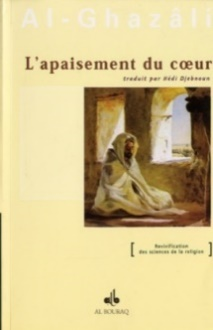
\includegraphics{Images/image002.jpg}
\sidecaption{essai}
\end{figure}


\begin{table}[h!]
\resizebox{\textwidth}{!}{%
\small
\begin{tabular}{p{2cm}p{4cm}p{4cm}}
\toprule
essai & essai & essai \\
\midrule
essai & essai & essai \\
\bottomrule

\end{tabular}%
}
\sidecaption{essai}
\end{table}

\begin{longtable}{p{6cm}p{6cm}}
\toprule
\endhead
«~Quiconque obéit au Messager obéit certainement à Allah~». 
&\TArabe{ مَّن
يُطِعِ الرَّسُولَ فَقَدْ أَطَاعَ اللَّهَ }\\
\bottomrule
\end{longtable}
%\part{Sacramentaire}



\chapter{Introduction}
%---------------------------------------------------------------------------------------------------------------

\mn{LM Chauvet}

\hypertarget{pour-se-repuxe9rer-dans-le-vaste-monde-de-la-sacramentalituxe9-lorganisme-sacramentel}{%
\section{Pour se repérer dans le vaste monde de la sacramentalité~:
l'organisme
sacramentel}\label{pour-se-repuxe9rer-dans-le-vaste-monde-de-la-sacramentalituxe9-lorganisme-sacramentel}}

\hypertarget{sacrement-un-concept-analogique}{%
\paragraph{«~Sacrement~»~: un concept
analogique}\label{sacrement-un-concept-analogique}}

\hypertarget{lorganisme-sacramentel-analyse-systuxe9mique}{%
\paragraph{l'organisme sacramentel~: analyse
systémique}\label{lorganisme-sacramentel-analyse-systuxe9mique}}

\hypertarget{une-duxe9finition-des-sacrements}{%
\paragraph{\texorpdfstring{Une définition des
sacrements}{ Une définition des sacrements}}\label{une-duxe9finition-des-sacrements}}
 

%---------------------------------------------------------------------------------------------------------------
\section{Ouverture sur la problématique
d'ensemble} 

la pointe des sacrements~: la communication de Dieu, la grâce.

«~\textbf{pour la Gloire de Dieu et le salut du monde~»}

dimension latreutique dimension sanctificatrice

Nos liturgies exercent de multiples fonctions~: cognitives, philo,
économiques~!, sociales\ldots{} quei ne doivent pas masquer
l'essentiel~: \textbf{la communication de Dieu.}

\begin{Ex}
 «~le Corps du Christ~: Amen~»

\begin{itemize}
\item
  on ne peut pas faire plus bref
\item
  de la foi
\item
  ie~: les mots «~nus
\end{itemize}

Cette nudité des mots qui se visibilise par la nudité de la main tendue,
\textbf{nue.}
\end{Ex}


Le salut de Dieu , dit dans la Parole, vient se déposer sur le corps.

Pb~: Comprendre ce que l'on célèbre~: «~Lex orendi, lex credendi~».

\paragraph{3 modèles de compréhension~:}

\hypertarget{moduxe8le-objectiviste}{%
\paragraph{Modèle objectiviste}\label{moduxe8le-objectiviste}}

St Thomas d'Aquin -\textgreater{} Trente -\textgreater{} Catéchisme de
1947\sn{«~des signes sensibles institués par Notre Seigneur Jésus
  Christ pour produire ou augmenter la grâce dans nos âmes~».}

\textbf{Sacrement comme instrument de production de la grâce~;
insistance sur la dimension de «~cause~» ou de moyen du salut.}

Dieu -\textgreater{} Sacrement -\textgreater{} Homme -\textgreater Dieu

Pb~: l'homme n'intervient pas dans le sacrement

\begin{itemize}
\item
  peu importe que l'homme «~comprenne~», pourvu qu'il soit sanctifié =
  limite)
\end{itemize}

Insistance~: Sacrement comme moyen, cause de salut

Avantage~: \textbf{souligne l'action de Dieu.}

\textbf{Instrument, canal, remède, germe.}

\hypertarget{moduxe8le-subjectiviste}{%
\paragraph{Modèle subjectiviste}\label{moduxe8le-subjectiviste}}

En réaction

Cf K. barth, qui craignait que la Liberté de Dieu soit «~compromise~»
par les sacrements, trop canalisée.

Le Baptême ne fait que \textbf{refléter} la \emph{justification et la
sanctification.} Dieu l'a déjà fait.

Contre une conception~»magique~» des sacrements.

Dieu -\textgreater{} Homme --\textgreater{} Sacrement -\textgreater{}
Dieu

\textbf{Sacrement comme instrument de traduction du déjà-là de la grâce.
Insistance sur la dimension de «~signe~» de salut (déjà donné).}

Avantage~: prend bien en compte le vécu humain. Dieu n'a jamais été lié
par les sacrements dans sa puissance de salut.

Inconvénient~: ne rend pas compte de l'efficacité du sacrement
lui-même.~: Trop exclusif.

Mais ce schéma va contre toute la \textbf{Tradition Chrétienne }(y
compris les pères).

Il est pourtant très à la mode, en réaction contre l'Église et en
insistant sur l'orthopraxie au lieu de l'orthodoxie.

\hypertarget{moduxe8le-vatican-ii}{%
\paragraph{Modèle Vatican II}\label{moduxe8le-vatican-ii}}

Schéma à «~double sens~»

Essai de tenir ensemble les dens sens (moyen de salut et signe du salut)

Dieu $\leftarrow$ $\rightarrow$ Homme $\leftarrow$ $\rightarrow$ Sacrement $\leftarrow$ $\rightarrow$ Dieu

Dieu~: \textbf{sujet opérateur des sacrements (}moyen de
salut-\textgreater{} vie humaine sanctifiée = louange à Dieu)

Difficulté~: tenir bien ensemble les deux sens

«~signe~» et «~cause~» ne sont pas des \textbf{catégories homogènes}


\paragraph{Question d'ouverture}

St Thomas d'Aquin~: II a II ae 89 prologue~; question sur l'éthique

→ on pourrait traiter ici (éthique) des sacrements → \textbf{sommet de
la vie éthique}

il aurait pu dire~: «~cause signifiante~» ou signe «~causant~».

un signe qui ne signifie que par mode de cause

une cause qui ne cause que par mode de signe

Chauvet, «~symbole et sacrement~»

Cf langage

\emph{Alliage homogène entre les deux~; grâce aux outils concernant le
\textbf{langage. }}

«~signe efficace~»~: mais c'est comme le langage~!

%-------------------------------------------------------------------------------------------------------------------------------
\section{Sacrement~: approche historique}

%-------------------------------------------------------------------------------------------------------------------------------
 
La constitution de la sacramentaire

Article LM Chauvet, «~sacrements~» dans Catholicisme

\hypertarget{mysterion-sacramentum}{%
\subsection{Mysterion -- Sacramentum}\label{mysterion-sacramentum}}

méfiance initiale contre le mot~; utilisé par les religions à mystère.

\textbf{Tertullien~;} aspect juridique~: la caution, le serment (cf
renonciation au mal)

Le Baptême comme \emph{pacte (foedus).}

La traduction en latin a fait perdre le lien avec le mysterion biblique,
l'économie divine.

Un vécu liturgique essentiel

\hypertarget{la-contreverse-sur-le-baptuxeame-des-huxe9ruxe9tiques}{%
\subsection{La contreverse sur le Baptême des
hérétiques}\label{la-contreverse-sur-le-baptuxeame-des-huxe9ruxe9tiques}}

Cyprien → Baptême lié à l'Église donc si deux Églises, deux Baptêmes .

→ Donatiste

en face Augustin~:~»le Christ agit «~etiam per malum ministrum~».

mais réception elle est fonction des dispositions personnelles.

\hypertarget{le-haut-moyen-uxe2ge}{%
\subsection{Le Haut moyen-âge}\label{le-haut-moyen-uxe2ge}}

présence réelle~: première question

\hypertarget{la-scholastique}{%
\subsection{la scholastique}\label{la-scholastique}}

la théologie comme science.

D'abord la finalité puis Importance de la causalité (Airstote)

Pratique de la LOI~: signifiait le Foi qui sauve mais ne causait pas le
salut. Signe non causal.

Importance de la pratique

Limites~:

\begin{itemize}
\item
  un schéma fondamentalement «~productionniste~»
\item
  le Cloisonnement des sept sacrements (et non les sacrements liés BEC
  cf 44)
\item
  l'absence d'ecclésiologie entre la christologie et la sacramentaire
\item
  une théologie trop en marhe de l'action liturgique
\item
\end{itemize}

\hypertarget{ouverture}{%
\section{ouverture}\label{ouverture}}

la sacramentaire scolastique est le fruit de la nouvelle
«~\emph{epistemé~»} né au 12° siècle . La fidélité à la grande tradition
théologique nous requiert non pas de reproduire mais d'en faire une
hérméneutique (décodage/recodage) nécessairement nouvelle ou sein de la
nouvelle culture qui est la notre.

 
%-------------------------------------------------------------------------------------------------------------------------------
\chapter{Sacrement de la Réconciliation}

%-------------------------------------------------------------------------------------------------------------------------------

Le «~Sacramentum~» comme langage symbolique et rituel

\hypertarget{introduction}{%
\section{Introduction}\label{introduction}}

Trilogie d'inspiration agustinienne~:

\begin{itemize}
\item
  \textbf{sacramentum -- rite- célébration --} ce qui se voit
\item
  \textbf{res sacramenti -- réalité du sacrement = la grâce}
\item
  \textbf{res et sacramentum~: 1\textsuperscript{er} effet de la grâce,}
  qui n'est pas la grâce finale ou \textbf{caractère~:}
\item
   
  ex~: on peut «~perdre~» la res sacrementi du Baptême tout en
  conservant la \emph{res et sacramentum.} (on reste baptisé).
   
\end{itemize}

Sacramentum → res sacramenti

\emph{res et sacramentum~}comme frontière

Entre le signe humain →

→ \textbf{médiation} ecclésiale ou 1\textsuperscript{ère} effet

Et la grâce de Dieu →

 %---------------------------------------------------------------------------------------
  \section{Problématique du langage} 

\begin{Synthesis}
    \begin{enumerate}
  \item
    {La langage n'est pas un instrument à la disposition de
    l'homme~; il est la médiation d'avènement du sujet c'est à dire le
    milieu dans lequel advient le sujet}
  \item
    {Puisqu'il n'est jamais de sujet hors langage (ou hors
    culture), constamment nous parlons ou «~ça parle~» en nous} \sn{Exemple~: culture où il n'y a qu'un seul mot «~s'occuper~» pour
      dire \emph{travailler} ou \emph{avoir des loisirs.} Le plus
      naturel , chez nous, est souvent le plus culturel.}

 
  \item
    {D'où la révolution épistémologique contemporaine quant à la
    manière de comprendre le rapport entre le sujet et le réel}
  \end{enumerate}
\end{Synthesis}


\textbf{Sujet} $\leftarrow$ $\rightarrow$ \textbf{Réel}

→ \emph{perception du}

\emph{← image mentale~; concept}

\begin{itemize}
\item
  \emph{restitution}
\end{itemize}

Langage

Pb de ce schéma~: il pose le langage comme instrument~: sujet =
antérieur (logiquement) au langage


\begin{Prop}
    {le concept d'~"expression" dans cette perspective~: le
  langage est simultanément «~révélateur~» et «~opérateur~»}
\end{Prop}



\textbf{Sujet} $\leftarrow$ $\rightarrow$ \textbf{Réel}

\textbf{Langage - culture}

{$\rightarrow$ \textit{le rapport au réel est toujours déjà aménagé~;} il est toujours
construit (le découpage sémantique n'est pas le même selon les cultures)
\textbf{le réel construit comme monde}}

\emph{$\leftarrow$le sujet se construit ainsi comme sujet}

Transition~:

Fonction du langage~: pas seulement utilitaire (information) mais
dimension symbolique (communication)

\hypertarget{probluxe9matique-du-symbole}{%
\section{Problématique du symbole}\label{probluxe9matique-du-symbole}}

\hypertarget{le-symbole}{%
\subsection{Le symbole}\label{le-symbole}}

Le symbole est médiateur de reconnaissance et d'alliance entre les
sujets.\sn{Cf Tertullien~; \emph{militia Christi}}

 
\paragraph{Le symbole antique}
 

Cf Tobie, 5 «~quel signe de reconnaissance donnerai-je~?~»

Triple aspect~:

\begin{itemize}
\item
  Systémique~: 1 élément n'est symbole que dans son rapport avec les
  autres éléments du même ensemble
\item
  Identitiaire~: se reconnaître comme partenaire
\item
  Juridique~: il faut être d'accor sur les \textbf{règles du jeu~.}
  Instance tierce de la Tradition, de la Loi~?
\end{itemize}
\mn{Cours du 4/2/03

Cours du //03}


Echange symbolique~: hors valeur

Intérêt théologique, grâce et échange symbolique

\hypertarget{luxe9change-symbolique}{%
\subsection{2.3 L'échange symbolique}\label{luxe9change-symbolique}}

\hypertarget{intuxe9ruxeat-thuxe9ologique}{%
\paragraph{2.32 Intérêt
théologique}\label{intuxe9ruxeat-thuxe9ologique}}

\hypertarget{b.-parole}{%
\paragraph{b. Parole}\label{b.-parole}}

Il n'y a rien de plus efficace que la parole

La parole ce n'est pas que des mots

Il suffit d'un «~je t'aime~» pour que la vie revienne

Mais aussi à travers le corps

\hypertarget{ruxe9flexion-sur-leucharistie}{%
\subparagraph{Réflexion sur
l'eucharistie}\label{ruxe9flexion-sur-leucharistie}}

Jn 6~: Pain de vie

Jésus est le pain de vie descendu du ciel

Rapport à la \emph{manne.}

\begin{itemize}
\item
  Mannu~: qu'est ce que c'est~?
\item
  On ne peut pas la stocker (ce n'est pas de la valeur)
\item
  Elle est donné quotidiennement
\item
  Sg 16~: «~elle était comme le pain des anges et elle s'adaptait au
  goût de chacun) Sg C'est vraiment du miel qu'est la sagesse
\item
  Beauchamp~: \emph{c'est le pur signe non chose}
\end{itemize}

La manne se prétait particulièrement à une analogie de la PAROLE.

1\textsuperscript{ère} tentation de la faim~: Mt 4,4 l'homme ne vit pas
seulement de pain mais de la parole qui sort de la bouche de Dieu.

\begin{itemize}
\item
  Dieu donne la manne pour que l'homme comprenne que la parole fait
  vivre (ref à Dt 8~?)
\item
  Pour manger l'eucharistie, il faut avoir ruminer la parole (cf
  élévation de la Bible et élévation de l'eucharistie)
\item
  Christ se présente comme la parole de vie envoyé par Dieu. Jn comprend
  la manducation d'eucharistie est une rumination de la parole douce et
  amère d'un Christ qui se livre pour la vie du monde.
\end{itemize}

L'expérience anthropologique de manger physiquement la parole pour
qu'elle soit complétement entendu~: d'où l'eucharistie~: parole donnée
sous le mode sacramentel

La Parole, c'est le Christ

\begin{itemize}
\item
  2 Co 10~: Le Christ est le OUI de Dieu au monde.
\end{itemize}

\hypertarget{eviter-le-piuxe8ge-de-la-chosification}{%
\subparagraph{Eviter le piège de la
chosification}\label{eviter-le-piuxe8ge-de-la-chosification}}

L'échange symbolique permet de ne pas chosifier ni magnifier (S Thomas
n'avait pas cet outil conceptuel~: dommage~!)

\hypertarget{c.-gratuituxe9}{%
\paragraph{Gratuité}\label{c.-gratuituxe9}}

\textbf{Charis}~: la grâce, ce qui est gratuit

Deux sens~:

\begin{itemize}
\item
  gratis Data~: donné gratuitement
\item
  \emph{gratiam gratum~:} gracieuseté. celle qui nous rend gracieux aux
  yeux de Dieu. Père de l'Eglise.
\end{itemize}

D'une part la grâce est gratuite~: elle ne dépend pas de nos mérites.

MAIS cela ne veut pas dire qu'il n'y ait pas de CONTRE DON, car sinon,
Dieu nous traiterait comme un OBJET (ALIENATION~: nous serions alors
écrasés). Or, il nous traite comme un SUJET. \emph{Un DON oblige.} Ce
n'est pas la \emph{conséquence} mais la \emph{marque} du don, car sinon
ce n'est pas un don car il n'est pas reconnu par la personne qui le
reçoit.

DON RECEPTION CONTRE-DON

Quand nous rendons grâce à Dieu pour les dons, nous ne sommes pas dans
le marchandage.

\hypertarget{baptuxeame-des-petits-enfants}{%
\subparagraph{Baptême des petits
enfants}\label{baptuxeame-des-petits-enfants}}

Le plus bel exemple de la gratuité de la grâce~: il ne tient pas compte
des mérites et démérites pour nous sauver. Mais il renforce un schème de
concurrence entre Dieu et l'Homme. Car le contre-don n'est pas marqué.
D'où l'importance de penser le baptême des petits enfants comme un
dérivé des adultes~: ACTE LIBRE~; êtres responsables.

\hypertarget{d.-le-thuxe9ologal-dans-lanthropologique}{%
\paragraph{le théologal dans
l'anthropologique}\label{d.-le-thuxe9ologal-dans-lanthropologique}}

échange symbolique pour approcher le mystère de la rencontre entre Dieu
et l'homme dans les Sacrements (leur efficacité)

\begin{itemize}
\item
  pas une simple analogie~: c'est la STRUCTURE dans laquelle s'effectue
  cette échange
\item
  le théologal se joue dans l'anthropologal, dans la constitution de
  l'homme
\end{itemize}

\hypertarget{lacte-de-symbolisation-analyse-et-application-uxe0-leucharistie}{%
\subsection{L'acte de symbolisation~: analyse et application à
l'eucharistie}\label{lacte-de-symbolisation-analyse-et-application-uxe0-leucharistie}}

2 agents secrets, avec billet de banque~déchiré; acte de symbolisation
pour se reconnaître partenaire

caractéristique

\begin{itemize}
\item
  systémique
\item
  symbolique
\item
  juridique (il faut avoir défini préalablement que le billet était le
  code de rencontre)
\end{itemize}

 

\begin{table}[h!]
    \centering
    \sidecaption{articuler  }
 
\begin{tabular}{p{.2\textwidth}p{.2\textwidth}p{.2\textwidth}}
\toprule
Christ &$\leftarrow$ $\rightarrow$ & Eglise \\
 
\\
\bottomrule
\end{tabular}
\label{tab:my_label}
\end{table}

 

 
\begin{table}[h!]
    \centering
\sidecaption{Des éléments du même ensemble mais qui sont
différents  }
 
\begin{tabular}{p{.2\textwidth}p{.2\textwidth}p{.2\textwidth}}
\toprule
Christ &($\leftarrow$ $\rightarrow$) & Eglise \\
 
\\
\bottomrule
\end{tabular}
\label{tab:my_label}
\end{table}


 

Ex~: un signe de Croix chez les papous~: ils ne peuvent pas le rattacher
aux autres éléments~: FONCTIONNEMENT imaginaire

\begin{table}[h!]
    \centering
\sidecaption{Chaque élément ne tient sa pertinence symbolique que de
par le rapport qu'il entretient avec les autres éléments de
l'ensemble
Le Christ n'existe que par l'Eglise dans le sens que sans Eglise,
personne ne connaîtrait le Christ }
\begin{tabular}{p{.2\textwidth}p{.2\textwidth}p{.2\textwidth}}
\toprule
Christ &$\leftarrow$& Eglise \\
        &   $\rightarrow$ \\
\\
\bottomrule
\end{tabular}
\label{tab:my_label}
\end{table}


\hypertarget{eucharistie}{%
\subparagraph{Eucharistie}\label{eucharistie}}

1Co 11~: Paul reproche au Co de prendre le repas du Seigneur

\begin{enumerate}
\def\labelenumi{\arabic{enumi}.}
\item
  niveau \emph{ecclésiologique et Ethique}~: vous prétendez prendre le
  repas alors que votrer pratique est en contradiction
\item
  niveau sacramentaire~ ou plutôt liturgique : Paul raconte le récit de
  la cène~: iatus entre la réponse et le problème posé
\item
  donc «~discernez le corps~». Le problème des Co, ce n'est pas la
  transsubstantiation\sn{Question apparue au IXème\ldots{}} (pas
  un problème sur la présence réélle). Mais mettre en rapport les
  membres du corps du Christ avec le corps Sacramentel (1 et 2)
\end{enumerate}

\hypertarget{rite-de-communion}{%
\subparagraph{Rite de Communion}\label{rite-de-communion}}

Lex Orandi, Lex Credendi

Regarder comment se pratique la célébration

\begin{table}[h!]
    \centering
      \sidecaption{ }
 
\begin{tabular}{p{.2\textwidth}p{.4\textwidth}}
\toprule
Geste de paix & «~Donnez-vous la paix~»~: ce qui est premier, c'est le
rapport horizontal avec mes frères \\
Fraction de paix & Rapport vertical (le Christ) pour faire l'unité des
membres de son corps (horizontal) \\
Démarche de Communion & Rapport vertical \\
\\
\bottomrule
\end{tabular}
\label{tab:my_label}
\end{table}
 

On ne peut pas séparer l'Eglise du Christ

\hypertarget{huxe9ruxe9sie-de-buxe9renger-de-tours}{%
\subparagraph{Hérésie de Bérenger de
Tours}\label{huxe9ruxe9sie-de-buxe9renger-de-tours}}

XIème 1053

Hérésie sur la présence du Christ dans l'eucharistie

Pb~: on n'a pas les outils conceptuels pour penser cette présence du
Christ. On pensait une adhérence du Christ aux espèces, qu'on aurait dû
le voir. Seulement par un deuxième miracle, Dieu étant un voile qui nous
le cache, afin que nous fassions un acte de foi (Isidore de Seville).

Il a fallu attendre le XII, pour que l'on trouve le concept adéquat,
celui de SUBSTANCE aristotélicien (on ne voit que les Accidents).

Les trois corps sont liés~:

\begin{enumerate}
\def\labelenumi{\arabic{enumi}.}
\item
  Corps historique et glorieux
\item
  Corps mystique sacramentel
\item
  Corps écclésial
\end{enumerate}

2---3~: Soyez ce que vous voyez~; recevez ce que vous êtes. Aug.
\sn{A lire sur S. Augustin~: Chair\ldots, Chair de l'Eglise Tillard}

Corpus Verum~était devenu le Corps ecclésial (H. de Lubac). Mais
berenger diminue le lien entre 1 et 2. En réaction, on a renforcé 1 et 2
au détriment de 2 et 3. L'adoration du Christ dans l'Eucharistie est
devenue plus importante que la Communion.\sn{\textbf{Historique}~:

  Pratique de la communion annuelle

  La réserve eucharistique (pour les malades) se formalise

  Evolution d'une conception de l'eucharistie action vers l'eucharistie
  chose (ex~: Transubstanciation en réaction contre l'hérésie de
  bérenger de Tours, qui utilise le concept aristotélicien de substance
  XII).

  Développement des processions, XIII «~le peuple n'a plus faim du pain
  eucharistique, rassasié des processions~».

  Elévation~: telle importance que l'on en attend de merveilleux effets
  deprotection contre les malheurs ou de vision miraculeuse du Christ
  lui même
  Exposition du Saint Sacrement dans une monstance lors de la
  contre-réforme}

\hypertarget{quimporte-la-valeur-de-luxe9luxe9ment-symbolique}{%
\paragraph{Qu'importe la valeur de l'élément
symbolique}\label{quimporte-la-valeur-de-luxe9luxe9ment-symbolique}}

Le symbole ne fonctionne pas à la valeur~: Crucifix~: bout de bois~;
bague de fiançailles

Musique~: ky-ri-e suffit -- pas besoin de 10 Mn de kyrie de
Mozart\ldots{}

\hypertarget{le-laboureur-et-ses-enfants-de-la-fontaine}{%
\subparagraph{«~Le laboureur et ses enfants~» de la
Fontaine}\label{le-laboureur-et-ses-enfants-de-la-fontaine}}

\begin{itemize}
\item
  Gardez-vous de vendre l'héritage, il y a un grand trésor dedans
\item
  ils labourent le champ
\item
  le travail est le trésor
\end{itemize}

Analogie intéressante avec le sacrement~:

\begin{itemize}
\item
  le sacrement n'est pas un trésor dans le champ
\item
  J'en suis obligé Grammaticalement~: la grâce est posé comme Objet
\item
  SUJET -- VERBE -- OBJET~: Dieu Donne la Grâce
\item
  Penser en théologie comme en philosophie, c'est apprendre à se défaire
  de son discours.
\item
  Heiddegger casse le langage~; Lévinas. Contre réduction
  phénoménologique. Risque certes de préciosité. Mais il faut casser les
  représentations.
\item
  La grâce n'est pas un objet valeur, même spirituel
\item
\item
  nous sommes la terre labourée. DurchArbeitung de Freud~: nous sommes
  travaillés
\item
  le socle de la charrue, c'est la parole de Dieu qui nous advient sous
  le mode rituel
\item
  il faut une force de traction, c'est l'ES
\item
  Nous allons nous transformer en acteur d'Alliance, alors que nous
  sommes tous héritier de Cain.
\item
  Cet engendrement permanent de nous même, nous devenons un peu plus
  fils de Dieu.
\end{itemize}

\begin{Def}[Grâce]
 un «~se recevoir~» toujours en cours
\end{Def}
  

\hypertarget{lacte-de-symbolisation-est-simultanuxe9ment-ruxe9vuxe9lateur-et-opuxe9rateur}{%
\paragraph{L'acte de symbolisation est simultanément révélateur et
«~opérateur~»}\label{lacte-de-symbolisation-est-simultanuxe9ment-ruxe9vuxe9lateur-et-opuxe9rateur}}

Le billet est à la fois «~révélateur~»~: ils se reconnaissent équipiers
mais aussi «~opérateur~»~: ils sont liés jusqu'à la mort dans leur
projet.

\hypertarget{doxologie}{%
\subparagraph{Doxologie}\label{doxologie}}

Par lui, avec lui et en lui

On présente à dieu , conjoint la terre au Ciel.

La voix monte aussi vers Dieu ainsi que les bras. Mais ce que nous
montons, c'est le Christ.

Puissance incroyable

Le Chrétien~: se reconnaît à Dieu, pour Dieu, en Christ.

C'est à force de faire des gestes comme cela que l'on devient Chrétien
et de les faire en Eglise. Attention à ne pas le psychologiser.

Une Foi ne vit qu'en se MANIFESTANT. Si on ne le dit jamais, notre foi
est quasiment morte.

\hypertarget{quelques-lois-de-la-ritualituxe9}{%
\section{Quelques lois de la
ritualité}\label{quelques-lois-de-la-ritualituxe9}}

\hypertarget{un-jeu-de-langage-original}{%
\subsection{Un «~jeu de langage~»
original}\label{un-jeu-de-langage-original}}

Ex~: génocide du Rwanda

\begin{itemize}
\item
  type \textbf{exactitude}~: discours du politologue
\item
  type témoignage~: discours du témoin~: reconstruit l'évenement pour ce
  faire comprendre. \textbf{Vérité narrative ou herméneutique}
\item
  type poétique~: vérité \textbf{poétique.} On ouvre un monde possible
  (Ricoeur)
\item
  Les trois types de langages visent la vérité de différentes voies.
\end{itemize}

Différents langages de ritualité~:

\begin{itemize}
\item
  théologique
\item
  mystique~: métaphore, affects (S. jean de La Croix)
\item
  témoignage~: MCC. On se raconte.
\item
  rituel
\end{itemize}

Attention, à ne pas se tromper de registres~: respecter les jeux de
langage différents. Ex~: à la messe, on ne parle pas de la théologie du
péché originel.

La liturgie croule sur les demandes contradictoires. Elle est faite pour
que l'on puisse recevoir le don de Dieu. Elle ne permet pas tout.

\hypertarget{lecture-thuxe9ologique-de-quelques-caractuxe9ristiques-majeures-de-lexpression-rituelle}{%
\subsection{Lecture théologique de quelques caractéristiques
majeures de l'expression
rituelle}\label{lecture-thuxe9ologique-de-quelques-caractuxe9ristiques-majeures-de-lexpression-rituelle}}

\hypertarget{un-langage-pragmatique-langage-action}{%
\paragraph{3.21 Un langage pragmatique~: langage
--action}\label{un-langage-pragmatique-langage-action}}

c'est une «~URGIE~» - ergon~: action\sn{Siderurgie,
  chirurgie,\ldots{}}

de l'ordre de la communication symbolique. Ne s'indresse pas à
l'intellect (non pas un LOGOS\sn{théologie,}) mais à tout le
corps. Lieu de jouissance~: on a une rencontre avec le Dieu Bon (et non
pas le Dieu Vrai\ldots).

\begin{itemize}
\item
  mon âme a soif de Dieu
\end{itemize}

\hypertarget{cuxe9luxe9bration-pour-les-enfants}{%
\subparagraph{Célébration pour les
enfants}\label{cuxe9luxe9bration-pour-les-enfants}}

But~: leur laisser 5 mn avec Dieu

\hypertarget{cest-la-muxe9moire}{%
\subparagraph{C'est la mémoire}\label{cest-la-muxe9moire}}

La liturgie, c'est une mémoire~: les places sont en attente\ldots{} Même
les gestes,

La faiblesse de Croire, Michel de Certeau

\textbf{Faites ce que vous dites~}: ex~: soyez dans la joie = chanter.
Ex~: onction au Baptême~: pas besoin d'expliquer~: cela sent bon,
imprègne le front.

\mn{Cours du 7/03/02}

\hypertarget{petite-lecture-thuxe9ologique}{%
\paragraph{Petite lecture
théologique}\label{petite-lecture-thuxe9ologique}}

Notion de \textbf{parole}~: sens d'Action en hebreu

\begin{itemize}
\item
  pas le logos grec
\item
  le DABAR (traduire par  dans la LXX)
\item
  SACREMENT, déploiement de ce qu'est le DABAR, la parole
\end{itemize}



    \paragraph{Un langage symbolique, donc économique~: sobriété et
    «~réserve~» du
    rite}

Symbole~: il rend PRESENT la chose (cf le drapeau brulé)~: il EST et il
n'EST pas le réel qu'il représente.

Les symboles représentent des mondes

Le symbole est \textbf{sobre.} Un peu suffit. Ex~: \emph{donnons-nous un
signe de paix~: ainsi nous nous engageons à nous réconcilier~; pas
besoin de faire le tour de l'Eglise.} Un peu de vin, un peu d'eau. Il ne
faut jamais substituer le réel au symbole.

Donner la chance au symbole~: ne pas tout expliquer~: on s'est trompé de
registre.

Goupillon~: moyen age~: préférer du buis.

Attention à la dérive \textbf{festive.} Injonction~: «~quand il
\emph{faut} faire la fête, ce n'est pas drôle\ldots~». Elle peut surtout
faire obstacle au passage de la mort vers la vie à faire avec le Christ.

Geneviève Hébert, Eloge \emph{de la pudeur en matière de dévotion et
ailleurs}, MD 215-225

LM Chauvet, \emph{Eschatologie et Sacrement}, MD 220\\
nos symboles liturgiques sont sobres. Elle est la médiation de la
condition eschatologique dans laquelle nous sommes~: le salut est déjà
donné mais pas encore achevé. Nous chantons «~\emph{Alleluia}~» car déjà
là mais nous ne nous laissons pas entraîner car tout n'est pas déjà
acquis~: cela peut être une insulte à tous les gens qui souffrent depuis
2000 ans~: RESERVE eschatologique.

J. CAILLOT, \emph{Liturgie et eschatologie,} MD 220

Grande originalité. Puisque le salut est déjà venu, il faut nous donner
sans réserve dans les tâches éthiques. Mais puisqu'il n'est pas complet,
toujours donné à Dieu le dernier mot.

JB METZ~: RESERVE~:tout pouvoir politique est réservé à Dieu.

Ici différent, «~PAS de JUBILATIO sans MODERATIO~» Augustin.

Expression de \textbf{Sainte Réserve.} Ce morceau de pain est un peu
dérisoire mais nous faisons une genouflexion~: nous prenons acte du
salut déjà donné mais nous le faisons devant un symbole tellement
dérisoire, qu'il indique que ce salut n'est pas achevé.

VERTUS DE LA PHENOMENOLOGIE en théologie.

Isabelle XXXX, \emph{Les actes de langage dans la prière} LMD 196

S'inspire de PEIRCE, entre un représentant (prêtre) et un représenté (le
Christ), il y a quatre relations possibles~:

\begin{itemize}
\item
  ICONE, de type photographique\sn{cf Critique de Theissen de la
    lecture iconique des sacrements, vision protestante, \emph{La
    religion des premiers chrétiens}}
\item
  Relation de DIAGRAMME (MODELE)
\item
  Relation de l'INDICE, de la GIROUETTE par rapport au VENT~: il y a un
  contact mais pas de ressemblance.
\item
  Rapport SYMBOLIQUE\sn{attention, pas le sens donné précédemment},
  entre un signifiant et signifié dans une langue (ex~: HORSE = cheval).
\end{itemize}

Ex~: Centurion, «~je ne suis pas digne~»~:

\begin{itemize}
\item
  je suis le centurion (ICONE)
\item
  je dis cela parce que l'on m'a demandé (SYMBOLIQUE)
\end{itemize}

un jeu possible entre les différents possibles~: chacun peut faire jouer
différemment le rituel, qui respecte chacun. Parfois, nous serons le
centurion. En liturgie, \textbf{Le moi est en état de recomposition.}

P°108

Rapport du prêtre au Christ~: ICONE, DIAGRAMME, INDICE, les trois sont
possibles en théologie catholique mais probablement pas SYMBOLIQUE
(vision protestante)~:

\begin{itemize}
\item
  la représentation ICONE est inadaptée à l'ordination de femme mais les
  deux autres.
\item
  A creuser
\end{itemize}

\hypertarget{un-langage-huxe9tuxe9rotopique-qui-reluxe8ve-dun-autre-lieu-que-le-quotidien-lordinaire-lutilitaire}{%
\paragraph{un langage «~hétérotopique~», qui relève d'un autre
lieu que le quotidien, l'ordinaire,
l'utilitaire}\label{un-langage-huxe9tuxe9rotopique-qui-reluxe8ve-dun-autre-lieu-que-le-quotidien-lordinaire-lutilitaire}}

kyrie 3 fois, étole, position du corps

il reste donc une distance entre la langue du rituel et la langue
vernaculaire.

\begin{itemize}
\item
  cela permet de comprendre pourquoi le Latin a aussi duré aussi
  longtemps
\item
  «~Cela est juste et Bon~»~: plutôt qu'on le «~ratifie~».
\end{itemize}

Fonctionnalité esthétique

Deux dérives possibles~: il faut que ce soit simple à prendre (verre) et
une dérive esthétisante (le bel objet)

TOUJOURS une rupture SYMBOLIQUE dans une célébration liturgique.

\begin{itemize}
\item
  rompt avec l'utilitarisme
\item
  crée un espace de gratuité dans lequel Dieu va pouvoir advenir
\end{itemize}

\hypertarget{un-langage-programmuxe9-et-donc-ruxe9ituxe9rable}{%
\paragraph{Un langage programmé (et donc
réitérable)}\label{un-langage-programmuxe9-et-donc-ruxe9ituxe9rable}}

On reçoit un rite. Le rite est codé (ex~: comment rentrons nous dans une
salle de cours). Cela permet d'économiser de l'énergie.

Il est reçu de générations antérieures, avec un Ancêtre. Le langage
courant le dit~: «~est rituel, ce qui est habituel~». Programme qui est
reçu.

Cette programmation n'est pas sans ambiguité~: une routine.

En particulier, les jeunes s'ennuient très vite. NEW -- LIVE -- SHOW.
Or, la liturgie , c'est exactement l'inverse.

Pourtant, cette programmation est protectrice de liberté. Ex~:
\emph{quand nous prenons congé après un diner, nous executons le rite.
Mais ce rite peut être chaleureux ou non.}

Il faut accepter de jouer le jeu du code mais il y a une manière
d'habiter le code.

facteur de liberté. Cela m'empêche de me demander ce que je dois faire.

Possiblement libérateur.

\hypertarget{valeur-thuxe9ologique}{%
\paragraph{Valeur théologique}\label{valeur-thuxe9ologique}}

Double valeur théologique~:

\begin{itemize}
\item
  \textbf{Christologique}~: institution de l'eucharistie~: rien n'est
  plus programmé~: les 4 verbes de cette institution (prendre, bénir,
  rompre, donner) servent à structurer l'eucharistie. Confession de foi
  de l'Eglise par mode de faire symbolique, que le Christ est SEIGNEUR~:
  le faire parce qu'il a dit de le faire. (approche phénoménologique~:
  je regarde la chose et je pense ce qui ce passe)~;
  Métaphore\sn{renvoie}
\item
  \textbf{Ecclésiologique~:} Manifester que toute célébration est
  manifestation de l'Eglise. Métonimie\sn{la partie pour le tout}.
  \emph{Quand on célébre en Afrique, on manifeste l'Eglise entière.}
  Elle n'appartient à personne. Certes particularité de la célébration
  mais pas particularisme. C'est ce que nous rappelle la programmation
  rituelle.
\end{itemize}

\hypertarget{evanguxe9liser-la-ritualituxe9}{%
\subsection{Evangéliser la
ritualité}\label{evanguxe9liser-la-ritualituxe9}}

Rite meilleur et pire.

Pire~:

\begin{itemize}
\item
  Routine, compulsion de répétition
\item
  sacralisation du politique (cf te deum)
\item
  ambiguité spirituelle~: substituer la magie du rite à la question
  existentielle de Dieu~: les protestants y sont très sensibles~:
  PRIORITE de la PAROLE.
\end{itemize}

La ritualité est toujours à evangéliser~: le rite ne devient SACREMENT
qu'avec la PAROLE et l'ESPRIT SAINT. Mais cette parole ne nous parvient
que sous mode rituelle.

%-------------------------------------------------------------------------------------------------------------------------------
\chapter{Place et fonction des sacrements dans la structure de l'Identité
Chrétienne}

%-------------------------------------------------------------------------------------------------------------------------------
 


\hypertarget{i.-introduction}{%
\section{Introduction}\label{i.-introduction}}

Se rappeler que les sacrements ne sont pas le TOUT de l'existence
chrétienne

\hypertarget{lc-24-les-disciples-demmaus}{%
\subsection{Lc 24, les disciples
d'Emmaus}\label{lc-24-les-disciples-demmaus}}

Catéchèse du passage de la non foi à la foi, de la méconnaissance à la
reconnaissance. La question qui guide ce texte, s'il est vrai que le Ch
est ressuscité, pourquoi ne pouvons-nous pas le VOIR~? Immédiatement

Comment se fait il que nous ne puissions pas le PROUVER~? question des
destinataires de Lc

Lc répond~: Renoncer à VOIR, TOUCHER, TROUVER, à leur immédiaté. Ces
verbes ne sont appliqués que sur le Cadavre du Christ. Le verbe
«~TOUCHER~» dans la 3\textsuperscript{ème} séquence~: toucher les
marques de sa mort. Si l'on veut reconnaître le Christ vivant, il faut
renoncer à cette vision de Christ Cadavre.

La transformation des deux disciples est rendue possible par~3 éléments
successifs~:

\begin{itemize}
\item
  \textbf{le rapport aux écritures,} le déblocage commence quand le
  Christ prend la parole~: «~il leur expliqua tout ce qui le concernait
  dans les Ecritures. Kerygme. \emph{Dihermeneusein}. En filigrane de ce
  que fait Jésus, il y a l'Eglise~: lecture de la thora et des
  prophètes.\\
  Technique rabbinique~: on rapprochait un élément des textes lus d'un
  autre texte, d'un élément de la tradition orale pour l'actualiser.
  Plus d'importance chez les Chrétiens pour les prophètes que pour
  Moïse.\sn{une des raisons de la rupture avec les juifs}
  Désormais, toutes les Ecritures seront interprétées par la mort et la
  résurrection du Christ . Il y a 50 ans de pratique ecclésiale. A
  chaque fois que nous relisons les Ecritures et les interprétons sous
  la lumière de Pâque, alors le Christ est présent au milieu de nous
  (\emph{Christ vivant}). \textbf{Apprendre à reconnaître le Christ dans
  l'Eglise.} «~Acclamons la parole de Dieu -- Louange à toi, Seigneur
  Jésus~».
\item
  \textbf{la fraction du pain}, au repos, à table. Il rompit le pain. 4
  verbes du récit de l'institution. il y a 50 ans de pratique
  eucharistique. Renoncer à Voir Jésus directement \textbf{mais
  apprendre à le reconnaître dans l'Eucharistie}. C'est lui qui bénit le
  pain, le rompt pour nous et nous le donne. Alors, il disparaît~: les
  yeux des disciples s'~ouvrent sur du vide, mais sur du vide plein.
  \emph{Anastantes~}: ils se lèvent (résurrection). On ne peut pas
  reconnaître Jésus sans être nous même relevés. Ils retournent alors à
  Jérusalem~: ils commencent par accueillir le témoignage des 11. C'est
  après qu'ils joignent leur témoignage. (synectode~: la partie pour le
  tout~: la bénédiction qui ouvrait le repas signifiant la totalité du
  repas).
\item
  \textbf{conduite éthique}, moins évident. Je déborde le texte pour
  aller voir les sommaires (Ac 2~; 4).Lc croque le portrait de la
  première communauté de Jérusalem~: fraction du pain, communion,
  partage fraternel, didascalie. Il insiste sur le \textbf{partage
  fraternel.} Grâce à ce partage, il n'y a plus de frères démunis. De ce
  fait, c'est le signe de la communauté eschatologique~: témoignage
  rendu à la résurrection~: «~voyez comme ils s'aiment~».\sn{J.
    DUPONT} Rappelle la théologie du 4\textsuperscript{ème} évangile.
  Comparaison en COMME~: «~la table est jaune comme le mur «~ (OS) et
  «~je suis chauve comme mon père~» (KATHOS)~: il y a participation. Cf
  lavement des pieds~: Kathos. Participation à ce qu'il fait. Quand les
  frères «~se lavent les pieds~», Jésus continue son œuvre à travers
  eux. Tertullien~: «~Le sacrement du frère~». «~tu as vu ton frère, tu
  as vu ton Dieu~» Clément d'Alexandrie.
\end{itemize}

\hypertarget{la-muxe9diation-de-leglise}{%
\subsection{La médiation de
l'Eglise}\label{la-muxe9diation-de-leglise}}

\hypertarget{schuxe9ma}{%
\paragraph{Schéma~:}\label{schuxe9ma}}

Pas de rapport direct entre nous et le Christ~: il faut passer par
l'Eglise.

Christ

Le cercle,

L'Eglise

Il n'y a pas de Chrétiens en dehors de l'Eglise. En dehors de l`Eglise,
point de salut confessé.

P. Lieger, op, \emph{l'être ensemble des Chrétiens}

L'Evangile est source d'un a priori communautaire. E\^{}tre chrétien,
c'est être d'emblée mis ensemble. Nous sommes sous sa Seigneurie tous.

Paul

\begin{itemize}
\item
   
  Col 3,9-11,
   
\item
   
  1 Co 12, 13~;
   
\item
   
  Ga 3, 26-28
   
\end{itemize}

Le baptême, c'est la réalisation du salut eschatologique~: «~il n'y a ni
juif ni grec, ni homme ni femme~».

Ep 2, 14 ss Christ est mort pour abolir le mur de séparation~; il a tué
la haine. Le juif et le grec

Ep 3~: juifs et paiens héritiers du même héritage

Yves de Montcheuil, mort en 1944 dans le Maquis, \emph{Aspects de
l'Eglise}

\emph{«~ce ne sont pas les chrétiens qui en se réunissant forment
l'Eglise, c'est l'Eglise qui fait les Chrétiens~».}

Devenir Chrétien, c'est apprendre à aimer l'Eglise peu à peu.

Cette priorité de l'Eglise.

\hypertarget{la-priorituxe9-du-nous-eccluxe9sial.-remarque-sur-la-pruxe9sidence-par-un-ministuxe8re-ordonnuxe9}{%
\paragraph{La priorité du «~nous~» ecclésial. Remarque sur la
présidence par un ministère
ordonné}\label{la-priorituxe9-du-nous-eccluxe9sial.-remarque-sur-la-pruxe9sidence-par-un-ministuxe8re-ordonnuxe9}}



\hypertarget{eglise-et-assembluxe9e-cuxe9luxe9brante}{%
\paragraph{Eglise et assemblée
célébrante}\label{eglise-et-assembluxe9e-cuxe9luxe9brante}}

\hypertarget{lassembluxe9e-dominicale}{%
\paragraph{L'assemblée
dominicale}\label{lassembluxe9e-dominicale}}

\hypertarget{ouverture-pastorale}{%
\paragraph{Ouverture pastorale}\label{ouverture-pastorale}}

\hypertarget{laccuxe8s-uxe0-la-foi-comme-consentement-uxe0-une-perte}{%
\subsection{L'accès à la foi comme consentement à une
perte}\label{laccuxe8s-uxe0-la-foi-comme-consentement-uxe0-une-perte}}

\hypertarget{triple-tentation}{%
\paragraph{Triple tentation}\label{triple-tentation}}

\hypertarget{la-bonne-santuxe9-e-la-foi}{%
\paragraph{La bonne santé de la
Foi}\label{la-bonne-santuxe9-e-la-foi}}

%---------------------------------------------------------------------------------------------------
\hypertarget{ii.-fonctionnement-de-la-structure}{%
\section{ Fonctionnement de la
structure}\label{ii.-fonctionnement-de-la-structure}}

\hypertarget{la-priuxe8re-eucharistique}{%
\subsection{1. la prière
eucharistique}\label{la-priuxe8re-eucharistique}}
 
  \paragraph{Analyse narrative}\label{analyse-narrative} 
  \paragraph{Statut du récit de l'institution~: récit de
  l'Eglise} 
  
  \paragraph{le discours
  d'anamnèse} 
 
  \paragraph{Le discours d'Epiclèse  } 
  \paragraph{Schéma du procès
  d~«~eucharisticité~»} 

\hypertarget{remarque-sur-ce-procuxe8s}{%
\paragraph{Remarque sur ce
procès}\label{remarque-sur-ce-procuxe8s}}

\hypertarget{a.-un-moduxe8le-et-non-pas-du-pruxeat-uxe0-porter}{%
\subparagraph{un modèle et non pas du prêt à
porter}\label{a.-un-moduxe8le-et-non-pas-du-pruxeat-uxe0-porter}}

La structure mentionnée la fois dernière est un patron. Le mouvement ne
commence pas nécessairement par l'Ecriture (don), cela peut être une
célébration (récéption) ou un témoignage éthique. (contre don).

Si c'est l'Evangile qui vous fait agir\ldots~? qu'y a t-il donc dans
l'Evangile~?

Le déclencheur peut être l'un des éléments, l'histoire commence
lorsqu'on ouvre l'Ecriture.

Il n'est pas d'itinéraire chrétien hors du processus Ecriture Sacrement
Ethique, vu pour la prière eucharistique.

\hypertarget{b.-le-don-duxe9pend-de-dieu-seul-mais-la-ruxe9ception-de-ce-don-comme-tel-duxe9pend-du-contre-don.}{%
\subparagraph{Le don dépend de Dieu seul~; mais la réception de ce don
comme tel dépend du contre
don.}\label{b.-le-don-duxe9pend-de-dieu-seul-mais-la-ruxe9ception-de-ce-don-comme-tel-duxe9pend-du-contre-don.}}

Dieu a l'initiative du don~! (hors dépendance de l'attitude éthique de
l'être humain) Mais il n'est de don reçu qu'avec le contre don éthique
(conversion du cœur, foi, agapè).

Validité et fécondité~:

Validité~: dépend de l'action de Dieu (et pas du sujet)

En revanche la fécondité dépend de notre cœur~: si notre vie ne s'ouvre
pas à la grâce

Un sacrement peut être valide et être reçu pour notre condamnation~! (1
Co 11).

Cf. St Augustin (controverse avec les donatistes~: leurs sacrements sont
valides «~vrais~» mais inféconds, car ils sont hors de l'Eglise.

Ne dites pas que la grâce de Dieu dépend de notre foi à l'oral~!

\hypertarget{c.-toute-cuxe9luxe9bration-sacramentelle-fonctionne-selon-ce-moduxe8le}{%
\subparagraph{toute célébration sacramentelle fonctionne selon ce
modèle}\label{c.-toute-cuxe9luxe9bration-sacramentelle-fonctionne-selon-ce-moduxe8le}}

les exemples ne manquent pas. (Ecriture et Sacrement OK, éthique =
envoi~! Peu développé à la messe, mais davantage pour un mariage)

Les sacrements ne sont pas autre chose que la cristallisation de la
Parole de Dieu.

\subparagraph{le moment sacrement~: ni point de départ,
ni point d'arrivée. Ce n'est qu'un point de passage. Mais il
{est} point de passage obligé et
obligeant} 

le moment réception n'est pas départ (ce sont les \textbf{Ecritures}) ni
arrivée (\textbf{vie chrétienne éthique})

point de passage obligeant~: car toute réception d'un don comme don
oblige~! (reconnaissance, foi, éthique de réponse)

point de passage obligé~: pour que l'éthique soit proprement chrétienne,
il faut qu'elle soit vécue comme un éthique de réponse au don premier de
Dieu (éthique théologale). Ainsi, la sanctification par le don de Dieu
est en ce sens «~obligé~». L'éthique devient elle même une liturgie, un
sacrifice spirituel. (cf prochain cours)

\hypertarget{identituxe9-juive-et-identituxe9-chruxe9tienne}{%
\paragraph{Identité juive et identité
chrétienne}\label{identituxe9-juive-et-identituxe9-chruxe9tienne}}

\hypertarget{place-du-moment-sacrement-par-rapport-au-moment-ecriture}{%
\subsection{Place du moment Sacrement par rapport au moment
Ecriture}\label{place-du-moment-sacrement-par-rapport-au-moment-ecriture}}

\hypertarget{les-ecritures-sacrement-de-la-parole}{%
\paragraph{Les Ecritures sacrement de la
Parole}\label{les-ecritures-sacrement-de-la-parole}}

Le premier «~tabernacle~» de la Parole de Dieu, les premiers sacrements
(mysteria) ce sont les Ecritures, pour les pères~!

Augustin~: sacramentum, c'est à dire n'importe quelle parole des saintes
lettres~!

N'importe quel épisode de l'Ecriture est traité comme un sacramentum~:
révélation en figure du dessein de salut de Dieu.

Pas étonnant que le livre des Ecritures ait fait l'objet d'une véritable
vénération dans la liturgie (ex~: évangéliaire)

Cf. Origène, SC7 p. 211 homélie sur la genèse. (écriture traitée avec
autant de poids que l'eucharistie). Voir aussi SC16 p. 263 homélie sur
exode

Ainsi l'Evangéliaire est orné, on l'encense, on chante alléluia\ldots{}
Voire procession~: Dei Verbum~21 : une seule table aussi bien de la
Parole que du Corps du Christ, et une seule vénération.

L'expression de «~pain de vie~» est aussi bien employée pour la parole
de Dieu que pour l'Eucharistie~! Il faut retrouver le réflexe de penser
au pain de vie comme étant d'emblée la Parole~!

(si on avait le temps, la sacramentaire devrait inclure les icônes)

Livre tabernacle -- sacrement de la Parole de Dieu

Il existe une tentation de dire que la Parole de Dieu est l'Ecriture
interprétée. NON C'est l'Ecriture dans sa lettre~! (cf. Parler
d'Ecriture Saintes~: prise en compte de la lettre dans la positivité
historique, son altérité culturelle, comme sacramentum). L'esprit n'est
trouvé que si la lettre n'est pas esquivée. C'est pareil pour la
sacramentaire.

On peut craindre qu'à force d'encenser le livre, on idôlatre la lettre~:
il faut alors rappeler que la bible n'est pas le Coran

\begin{enumerate}
\setcounter{enumi}{1}
\item
  La Parole de Dieu (PDD) c'est le Christ, pas le livre
\end{enumerate}

\begin{enumerate}
\setcounter{enumi}{1}
\item
  La lettre peut être hébraique ou grecque ou latine, \ldots{} Certes
  les textes fondateurs ont un privilège. Mais cessons de courir après
  le mythe du texte originaire~! La PDD n'est pas liée à une langue. Il
  existe un jeu symbolique entre la lettre et la Parole de Dieu.
  \emph{(Acclamons la Parole de Dieu Louange à toi Seigneur Jésus}).
\item
  La lettre se dédouble~: il est écrit qu'autre chose est à écrire
  (\emph{la création annonce une seconde création~: la manne annonce une
  autre manne, l'exode annonce un autre exode}) La lettre est alors non
  idole, qui arrête le regard, mais icône, qui demande qu'on la traverse
  en direction d'un autre qu'elle-même.
\end{enumerate}

\hypertarget{le-sacrement-pruxe9cipituxe9-des-ecritures}{%
\paragraph{\texorpdfstring{2.2. Le Sacrement, «~précipité~» des
Ecritures
}{2.2. Le Sacrement, «~précipité~» des Ecritures }}\label{le-sacrement-pruxe9cipituxe9-des-ecritures}}

Chaque célébration le montre. La Parole vient nous rejoindre dans le
sacrement comme dans son prolongement, dans son déploiement.

Dans cette perspective il faut comprendre les paroles sacramentelles (ex
\emph{je te baptise au nom du Père et du Fils et du Saint Esprit}) comme
des \underline{synthèses} de la révélation de Dieu dans les Ecritures.

\hypertarget{a-accedit-verbum-ad-elementum-et-fit-sacramentum}{%
\paragraph{«~Accedit verbum ad elementum et fit
sacramentum~»}\label{a-accedit-verbum-ad-elementum-et-fit-sacramentum}}

deux traductions possibles~:

 
\emph{La Parole vient sur l'élément et ainsi se fait le sacrement} ou

\emph{Le Verbe vient sur l'élément et devient sacrement.}
 

Le Verbe, c'est d'abord le~Christ~; deuxième niveau~: le Christ tel
qu'il est annoncé dans la fête ou le temps liturgique du jour~; enfin la
Parole sacramentelle.

\hypertarget{b-manducation-de-la-parole-jn-6-manne-parole-pain}{%
\paragraph{Manducation de la Parole (Jn 6 Manne Parole
Pain)}\label{b-manducation-de-la-parole-jn-6-manne-parole-pain}}

cf Grelot (introduction au nouveau testament tome~??) c'est une homélie
sur Ex 16, à la manière rabbinique.

La manne, (question) se prête déjà à être figure de la Parole~: cf. Dt
8,3 cité lors du récit des tentations. Mt 4,4.

L'objet du discours du pain de vie n'est pas l'Eucharistie (sauf après
le v. 51), mais le mystère du Christ, Dieu crucifié pour la vie du
monde, envoyé de Dieu qui donne sa chair pour la vie du monde.

Double scandale~: sur l'identité de Jésus

v. 42~: comment peut-il se prétendre descendu du ciel~?

v51~: comment peut-il se prétendre donner sa chair à manger~?

Espace symbolique ambiant = manducation de la Parole (cf Ez 2, 3~:
manger le rouleau de la Torah, cf. aussi Apocalypse), et aussi
manducation eucharistique (bien sûr~!)

Devenir chrétien, c'est mâcher, ruminer la Parole de Dieu, le scandale à
la fois doux et amer d'un messie crucifié pour la vie du monde~: c'est
ça que nous faisons dans l'eucharistie~! Jusqu'à ce que ça fasse corps
avec notre corps~: et c'est beaucoup plus fort~: on parle du mystère du
Christ plutôt que de mentionner directement l'eucharistie.

Pour manger avec fruit l'eucharistie, il faut donc avoir d'abord ruminé
la Parole. Cf. St Ambroise «~cette nourriture (parole) mange la d'abord,
enfin de pouvoir en venir ensuite à la table du Seigneur~». (citation
non littérale)

Cf traités 26 et 27 d'Augustin sur Jn. (manger jusqu'à avoir part à
l'Esprit Saint).

Le rite ne constitue pas le sacrement, c'est la PAROLE DE DIEU qui nous
advient en forme rituelle

\hypertarget{evanguxe9lisation-et-sacramentalisation}{%
\paragraph{2.3. Evangélisation et
sacramentalisation}\label{evanguxe9lisation-et-sacramentalisation}}

Avant l'accès au sacrement, il y a l'annonce de l'Evangile.

Priorité à l'évangélisation~: mais elle doit être structurée
sacramentellement. (cf ce que les évêques disent de la catéchèse).~

Sur le fond~: l'évangélisation est annonce d'un Christ sacrement, et non
pas d'un Christ exemple~! Ne pas annoncer un modèle à imiter (derrière
qui on devrait courir~! décourageant) mais quelqu'un qui vient nous
sauver, il est notre passeur.

Sur la forme~: dans toute catéchèse, il faut faire référence au
sacrements. Ne pas se contenter de se référer aux deux pôles biblique et
éthique. La dimension liturgique et sacramentelle est trop souvent ce
dont on parle quand l'occasion se présente~: elle mériterait d'être
intégrée à la catéchèse.

Ex~: l'appel des disciples. ordination~? envoi des catéchistes à la
messe de rentrée~?

Texte de guérison des malades (onction~: même si c'est pas au
programme~!)

Esprit Saint~: liturgie de la Pentecôte. L'expérience liturgique est un
lieu théologique de première importance.

\hypertarget{place-du-moment-sacrement-par-rapport-au-moment-ethique-.}{%
\subsection{Place du moment «~Sacrement~» par rapport au moment
«~Ethique~».}\label{place-du-moment-sacrement-par-rapport-au-moment-ethique-.}}

\hypertarget{le-statut-du-culte-en-judauxefsme-historico-prophuxe9tique}{%
\paragraph{Le statut du culte en judaïsme~: historico
prophétique}\label{le-statut-du-culte-en-judauxefsme-historico-prophuxe9tique}}

\hypertarget{a-la-foi-en-un-dieu-intervenant-en-histoire}{%
\subparagraph{La foi en un Dieu intervenant en
histoire}\label{a-la-foi-en-un-dieu-intervenant-en-histoire}}

Dans les cultes païens, le temps est cyclique ou en forme de spirale~:
calendrier de type cosmique.

Dans le judaïsme, on brise cette circularité. Le temps est vécu de
manière différente, car la Bible, au lieu de privilégier le retour du
même, privilégie les évènements comme avènement de l'inédit, du nouveau.
Le temps devient plus linéaire. La clef de lecture de la Bible, c'est
l'eschatologie, c'est l'Omega qui donne à lire l'Alpha.

Le premier lieu de révélation biblique est l'histoire, avant le cosmos
(la création du monde est l'œuvre du Dieu d'Israël, son peuple).

Bereshit (premier mot de la bible) André Néher \emph{Les culture et le
temps}, a noté~: non pas «~au commencement~», mais «~en un
commencement~» Dieu créa. Ce qui est primordial, c'est qu'il y ait eu un
début~: le primordial c'est que la création inaugure le temps.

Le 26/3/03

Le temps de la Bible, ce n'est pas le temps scientifique, mais c'est le
temps d'un \textbf{peut-être, temps de la liberté humaine, arraché à} la
fatalité.

Cf Ecart par rapport au rite mésopotamien~: ici , un risque, un mariage
entre Dieu et Israêl, souvent malheureux entre le projet de Dieu et
l'homme libre, représenté par Israël.

\hypertarget{b.-douxf9-le-culte-muxe9morial-de-ce-dieu-renvoie-uxe0-la-prise-en-charge-de-lhistoire}{%
\subparagraph{d'où le culte, mémorial de ce Dieu, renvoie à la prise en
charge de
l'histoire}\label{b.-douxf9-le-culte-muxe9morial-de-ce-dieu-renvoie-uxe0-la-prise-en-charge-de-lhistoire}}

Le culte va renvoyé Israël à la prise en charge de l'histoire.

Liturgie~: liturgie du prochain.

\hypertarget{muxe9morial}{%
\subparagraph{Mémorial}\label{muxe9morial}}

C'est PRECISEMENT dans la mesure où son identité est fondée sur la
relation à un Dieu entré en histoire qu'Israel, en son culte, est
renvoyé à sa responsabilité dans l'histoire, et plus précisément à
autrui.

Théologiquement, c'est le concept de \emph{mémorial} : essence
historique et prophétique de ce culte.

Zikkaron (ZKR~: se souvenir) LXX~: mnemosunon, anamnesis

\textbf{Paradigme}~: la fête de Pâque.

Ex 12,1-20

«~tu transmettras cet enseignement~: «~tu haggaderas à ton fils ce jour
là~»

La mishna commente~: «~de génération en génération chacun doit se
reconnaître comme étant sorti lui-même d'Egypte~» (Pes 10,5)

S~. Augustin, \emph{lettre 98 à l'Evèque Boniface},

Sur le baptême des petits enfants

Il faut que nous défaisions l'image naive du temps (passé, présent,
futur). Cf critique Heidegger.

L'être humain est de nature commémorative, mais il ne l'est qu'en tant
que nature projective.

JB. METZ~: \emph{la Foi dans l'histoire et la société}, Cogitatio Fidei

Un classique dans le domaine politique

Récit, mémoire

En particulier, mémoire dangereuse et mémoire de la souffrance

Il y a une mémoire et mémoire. Il y a une mémoire vive, et une mémoire
aliénante. La mémoire aliénante sort les photos jaunis des bons moments.
Une mémoire maternante, anecdotique qui idéalise, qui fait régresser. La
mémoire devient vive quand elle fait bouger~: «~plus jamais cela~»
d'Auschwitz, de la guerre. Elle ne doit pas oublier les souffrances du
passé car elle mobilise les énergies pour faire que cela n'arrive plus.
Une mémoire n'est vive que si elle s'ouvre sur un avenir.

La mémoire du passé fait bouger le présent, elle remet debout, en vue
d'un nouveau recommencement, ceux qui sont prostrés dans le silence et
l'oppression de l'EXIL.

Il ne s'agit pas de faire simplement mémorisation, simple souvenir
auquel on a volé son avenir (JB Metz). Acte vif de COM-MEMORATION
(commune) Tout projet d'avenir semble s'enraciner dans le réveil d'une
telle tradition~: l'homme n'a d'avenir que parce qu'il a de la mémoire.

relecture recueillement du passé anticipant le futur. Il est sous le
régime du futur antérieur.

La mémoire chrétienne est une mémoire de la Passion du Christ et de sa
résurrection. \emph{Memoria Passioni.} «~tenons en éveil la mémoire du
Seigneur~».

Futur antérieur~: Dt 26,1-11 les prémices~; La terre, qu'Israel a déjà
est toujours à recevoir.

\textbf{Chiasme~}:

Histoire à Vivre FUTUR

Rite à Accomplir PRESENT

Mémorial Confession de foi «~mon père était un araméen errant~» PASSE

Rite à Accomplir PRESENT

Histoire à Vivre (levite, Immigré) FUTUR


\begin{table}[h!]
    \centering
    \sidecaption{  }
 \footnotesize
\begin{tabular}{p{.15\textwidth}p{.15\textwidth}p{.15\textwidth}p{.15\textwidth}p{.15\textwidth}}
\toprule
TU + Futur & & & & TU + Futur \\
Prescription rituelle & JE + Présent & & JE + Présent & Prescriptions
éthiques \\
& Parole rituelle & NOUS + Passé & Parole + gestes rutuels & \\
& & Confession de foi/ Mythe de ses origines\sn{Tout le
  Pentateuque + Josué~: le mémorial.} & & \\
 
\\
\bottomrule
\end{tabular}
\label{tab:my_label}
\end{table}


Israël est exhorté à ouvrir la terre à Dieu, mais dans le but de
l'offrir à autrui.

Lorsque nous demandons (rite), l'insérer dans le mémorial et la
pratique. Le rite permet d'actualiser le passé (on refait le rite des
prémices). La dépossession de la terre qui est signifié par le rite doit
être vérifiée par l'acte éthique envers le lévite (sans terre par
vocation au plus intime d'Israël) et l'immigré (sans terre par
nécessité, ext. à Israël).

Les prémices, véritable \emph{sacramentum} ou \emph{visibile verbum}
(Aug.) du mémorial est l' «~expression~» au sens fort où l'identité
d'Israel s'effectue en s'énonçant.

Le passé est encadré par un présent qui en indique l'actualité~;
cependant, il ne s'y arrête pas et doit s'ouvrir sur l'autre. Israël
n'est véritablement prenant la terre de Dieu qu'en l'ouvrant aux autres,
et ceci le rite le rappelle constamment à Israël. On est au cœur de
l'identité JUIVE.

\textbf{Manne}~: \emph{pure signe non chose}, de la non possession, de
la pure attente, Israël pouvait vivre que de la grâce de Dieu ou du seul
ciel~; Dès la prise du pays, la tentation est d'oublier la leçon du
désert, c'est à dire de s'approprier la terre comme \emph{pure chose non
signe}

\hypertarget{une-crise-rituelle}{%
\subparagraph{Une Crise rituelle}\label{une-crise-rituelle}}

Renvoi à la pratique historique de la «~liturgie du prochain~» amène
inévitablement à une crise rituelle. La parole vient en effet sacrifier
la première naiveté rituelle~: Israël ne peut plus être, comme les
autres religions paiennes, en possession tranquille de son culte. Cf
prophète contre le formalisme cultuel. Dieu ne veut pas d'un culte qui
serait en opposition avec l'attitude éthique de son peuple.

Am 5, Is 1, Jr 7, Mic 6 ,Ps 50

Jésus reprendra (cf Mt 9~?~: ce que je veux ce ne sont pas les
sacrifices mais un cœur miséricordieux).

Voie ouverte de substitution des sacrifices par la pratique éthique.

 
Ben Sirac, 34 observer la loi vaut tous les sacrifices

Augustin

Les chrétiens maintiendront tout de même un sacrifice, qui n'a plus rien
de sacrifice pour témoigner du sacrifice de la vie éthique. Rm 12, 1
\emph{offrez vous vous mêmes en sacrifice saint}
 

\hypertarget{juxe9sus-et-le-culte-juif}{%
\paragraph{Jésus et le culte
juif}\label{juxe9sus-et-le-culte-juif}}

\hypertarget{a.-une-attitude-critique-dans-le-sillage-de-la-spiritualisation-des-sacrifices}{%
\paragraph{une attitude critique, dans le sillage de la
spiritualisation des
sacrifices}\label{a.-une-attitude-critique-dans-le-sillage-de-la-spiritualisation-des-sacrifices}}

Os 9, Jr 7 «~ce temple, caverne de bandit~».

Jésus fortement critique contre le formalisme rituel. Pas innovant, de
la même façon que le commandement de l'amour (cf Lc 10, le scribe~; Mc
12 le scribe renchérit). Il existait un courant bien vivant dans le
judaïsme.

Charles Perrot, \emph{Jésus et l'histoire}

Revoir jésus et le temple et le baptisme. A Kumran, on acceptait
théoriquement des sacrifices à Jérusalem mais on exhaltait le sacrifice
des lèvres~; de même, chez les baptistes et les judéo-chrétiens.

Logike latreia~: rationabilis hostia~: sacrifice raisonnable, droit .

Ce sacrifice, les grecs l'avaient exhalté.

«~le plus beau sacrifice, c'est de montrer l'homme le plus juste~».
IVème avant JC

Sénèque

Double critique du sacrifice, l'une venant du judaïsme, l'autre du
bassin méditerranéen. Au confluent de ces deux mouvements, Philon
d'Alexandrie.

Jean Laporte, \emph{Le vocabulaire eucharistique chez Philon d'Al}.

Philon~: Dieu n'a besoin de rien. Les sacrifices, pour nous exhorter à
la piété. Nous les \emph{a-charistoi}, sans grâce, nous apprenions à
devenir des \emph{eu-charistoi}. Au plus haut de la hiérarchie, le
sacrifice de Todah\sn{Article Maison Dieu 123 de Cazelles

  De vaux, les institutions de l'Ancien Testaments

  CE sur les sacrifices} est traduit par Philon par le sacrifice
d'eucharistie. Sacrifice de paix, les offrants mangent une partie du
sacrifice, sacrifice de communion. Mais il n'a de valeur, que s'il
manifeste les bonnes dispositions intérieures~: «~il convient de
critiquer ces propres motifs d'Action de grâce et de rendre grâce pour
les raisons les meilleures~(son amour)~».

\textbf{Todah}~:

\begin{enumerate}
\def\labelenumi{\arabic{enumi}.}
\item
   
  Victime
   
\item
   
  offrande végétale (galette, eventuellement vin~; rester prudent sur
  comparaison Eucharistie)
   
\item
   
  Psaume Hallel
   
\end{enumerate}

On supprime 1 pour ne garder que 2 et 3.

Dans traduction aquila, le mot Todah est aussi traduit par eucharistie.

X. Leon Dufour, le partage du pain eucharistique dans le NT

La proclamation de la mort du Christ correspond exactement à la Todah
juive.

Perrot\sn{MD 123} parle de substitution de la todah par
eucharistie.

\hypertarget{b.-mais-quelle-attitude-au-juste}{%
\subparagraph{Mais quelle attitude au
juste~?}\label{b.-mais-quelle-attitude-au-juste}}

Synagogue Lc 4 «~selon son habitude'~».

11 mentions de Jésus au temple mais pas présenté en train de prier mais
en train d'enseigner.

J. Dupont (1978, MD Jésus et la prière liturgique)~: Jésus devait prier
mais en aucun cas un sacrifice.

Perrot note que Mc 11~: objet ou vase, matériel du Temple. Jésus arrête
la marche du culte sacrificiel. Mais difficile de se prononcer sur
l'attitude de Jésus par rapport au Temple (cf applique la loi sur les
purs/impurs~; ne dispense pas de l'offrande à l'autel~; sacrifice en cas
de guérison).

\textbf{Cependant,} l'autorité personnelle de jésus, la nouveauté de son
message (pardonne des péchés, fréquente les pécheurs) était telle que sa
condamnation à mort mettait son message en dehors du sillage des
prophètes.

Cette parole au sujet du Temple (3 jours) a dû être l'un des motifs
réels de sa mort. Chrétiens génés~:

\begin{itemize}
\item
  Suppression en Lc cf faux témoignages sur Etienne~: «~le Temple doit
  être supprimé~».
\item
  Reconstruction chez Mt
\item
  Substitution chez Mc . Mc 14 parle d'une substitution d'un Temple fait
  de mains d'homme à un Temple fait par Dieu.
\item
  Spirituel chez Jn
\end{itemize}

Critère de différence~; critère de cohérence. Cazemann

\emph{Différence}~: cette phrase n'a pu être inventé par les juifs ni
par les premiers chrétiens

\emph{Cohérence}~: cohérence de cette parole avec le reste du message du
Christ et son attitude souvent conflictuelle avec l'autorité du Temple.

Pbt une \emph{ipsissima Verba Jesu}.

\textbf{Annonce un débordement de la critique du CULTE.} Cependant,
cette radicalisation ne sera comprise qu'après Pâques.

\hypertarget{un-nouveau-statut-du-culte-en-christianisme-statut-eschatologique}{%
\paragraph{Un nouveau statut du culte en christianisme~: statut
eschatologique}\label{un-nouveau-statut-du-culte-en-christianisme-statut-eschatologique}}

\hypertarget{le-vocabulaire-cultuel-dans-le-n.t.}{%
\paragraph{le vocabulaire cultuel dans le
N.T.}\label{le-vocabulaire-cultuel-dans-le-n.t.}}

temple, naos,

prêtre, sacerdos,

sacrifice, tusia

Ce vocabulaire existe mais est orienté vers le Christ et non pour les
apôtres, l'eucharistie. He ajoute accomplit DONC abolit le système
sacrificiel du Temple.

Deuxièmement, la vie des chrétiens, le sacrifice des lèvres et la
communion entre frères, la koinonia.

\textbf{Cf document vocabulaire cultuel dans le NT}

\hfill\break
INTRODUIRE Document vocabulaire cultuel

Détournement de vocabulaire.

Différence de vocabulaire avec AT (utilisé pour le Christ ou l'activité
quotidienne des chrétiens~: cf kaseman, Essais exégétiques, le culte
dans la vie quotidienne)

Rm 12,1~: offrande du «~Corps~». 2 Co 9~: Collecte , comme leitourgia
(thusia de la part des Philippiens (Ph 4, 18). Mais aussi en Ep 5,2 où
la mort du Christ comme sacrifice. He~: sacerdoce au Christ

Chrétiens comme proserchomenoi (processionnants) qui s'avancent vers
Dieu. La vie de la communauté chrétienne est ainsi présentée comme un
longue liturgie sacerdotale.

\begin{itemize}
\item
   
  Confession de foi (sacrifice des lèvres)
   
\item
   
  Bienfaisance et de l'entraide communautaire (koinonia)
   
\item
   
  Paul~: mon sacerdoce, la mission
   
\end{itemize}

Ministère du Peuple de Dieu, pas en lien premier avec le problème des
ministères dans l'Eglise, mais avec le ministère de l'Eglise dans le
monde, celle ci est chargée d'une fonction médiatrice, substitutrice,
vicaire et son sacrifice spirituelle est «~d'être auprès du monde
présence de Dieu et devant Dieu présence du monde~».

Importance de l'humilité~: par la confession des fautes et le pardon des
frères, l'assemblée dominicale en vue de l'action de grâces par la
fraction du pain est constituée en sacrifice.

\hypertarget{b.-fondement-de-cette-nouveautuxe9}{%
\paragraph{Fondement de cette
nouveauté}\label{b.-fondement-de-cette-nouveautuxe9}}

\hypertarget{eschatologie}{%
\subparagraph{Eschatologie}\label{eschatologie}}

La mémoire du Christianisme est eschatologique~: c'est une mémoire
d'avenir~: nous faisons mémoire du christ mort, ressuscité et qui
reviendra.

Eschatologie~: différence entre christianisme et judaisme. Ne pas le
réduire au «~pas encore~». Car le pas encore, c'est l'ultime
manifestation de la force ressuscitante du Christ transfigurant dès
maintenant l'humanité par le don de l'Esprit. Certes, douleur de
l'enfantement~: le monde continue de s'éprouver comme non encore
racheté~: «~nous avons été sauvés, mais c'est en espérance~» (rm 8,24)
L'eschatologie pense le Christ ressuscitant le monde, et l'histoire se
présente comme le lieu même de sa possibilité.

Le statut eschatologique du culte en christianisme implique ainsi la
reprise du statut historico-prophétique de celui du judaïsme dont il est
l'héritier.

\hypertarget{la-duxe9chirure-pascale}{%
\subparagraph{La déchirure pascale}\label{la-duxe9chirure-pascale}}

JB~: croit à la venue imminente d'un messie fondateur d'un royaume où,
selon la prophétie d'Ezéchiel, l'Esprit de Dieu sera donné à l'homme
dans une lustration d'eau pure qui le rendrait capable de pratiquer les
commandements, pour une justice jusqu'alors constamment transgressée.(
H. Cazelles, naissance de l'Eglise)

Jr 31

Ez 36,24-28

La métaphore de la déchirure

Une des premières métaphores du changement et de la réalisation des
prophéties d'Ezéchiel et de Jérémie

\begin{itemize}
\item
  les cieux, lors du bapteme
\item
  vieilles outres de la Loi, face à l'Evangile
\item
  vêtement neuf
\item
  déchirure des habits du Grand Prêtre
\item
  déchirure du rideau du temple
\item
  le saint des saints est désormais vide, le temple de la présence de
  dieu, c'est le corps du Ressuscité (Jean) ou l'assemblée des fidèles
  (Paul)
\item
  lettre aux hébreux~: le seul temple, le corps glorifié du Christ, lee
  seul autel, la croix, le seul prêtre et sacrifice, la personne même du
  Christ. \emph{Christ est la seule liturgie possible}
\end{itemize}

La déchirure, vraie question que devait se poser tout juif. Si ce que
vous annoncez Chrétiens, que deviennent la \textbf{Loi} et le
\textbf{Temple}.

\begin{itemize}
\item
  «~la Loi demeure bonne comme expression de la volonté de Dieu mais
  n'est plus un moyen de salut~» Paul cf Galates et Hebreux
\item
  Hébreux dit la même chose au niveau du sacerdoce du Temple~: désormais
  caduque pour accèder à Dieu~; il n'y a plus qu'un seul prêtre.
\end{itemize}

\hypertarget{une-diffuxe9rence-thuxe9ologale}{%
\subparagraph{une différence
théologale}\label{une-diffuxe9rence-thuxe9ologale}}

\textbf{Principe de la justification change~: Ce n'est plus par la Loi
qui sauve, mais celui qui a incorporé la Loi~;}. Ce principe
ChristoPneumatique est nouveau donc la modalité est nouvelle. culte
autre ordre que le culte juif. Non au niveau moral.

\emph{C'est la Foi au Christ qui sauve.} On n'accède pas à Dieu à la
force des poignets. Accueillir le don de Dieu en Christ. Notre existence
devient le lieu de l'accueil du don de Dieu.

Tout part de la confession de Jésus comme Christ. Tout repose donc sur
Pâques et Pentecôte. La différence est eschatologique.

Justification par les oeuvres pour les juifs. Même si pureté de cœur est
recherchée. Christianisme~: développement de cette attitude
eucharistique. Mais par Paul, changement théologique~: c'est le Christ
lui même l'action de grâce du Chrétien et non d'abord sa pratique fidèle
de la Loi ou son cœur droit. Christ seul justifie~: principe différent.

Etre chrétien, c'est vivre sous la loi de l'Esprit, synthèse de Jr 31 et
Ez 36

Justification, non plus sur les œuvres de la Loi, mais la foi en Jésus
comme Christ et Seigneur.

Cœur nouveau, esprit nouveau.

Un nouveau statut du culte

Désormais, \textbf{le lieu du théologal, c'est le lieu de
l'anthropologal.}

Esprit de la Loi~: toujours se hisser vers Dieu à la force du poignet

Esprit de la Foi~: accueillir le salut de Dieu lui même

Nous avons à accueillir le salut dans notre vie historique

Véritable déchirement de la Loi

Le culte premier des chrétiens est celui de l'accueil de cette grâce de
Dieu dans leur vie quotidienne par la foi et la charité théologales~;

SCHEMA VETUSTE NOUVEAUTE

Le nouveau schéma est en trois coté Dieu, Culte liturgique, culte
quotidien par foi et charité

Le Culte ne se trouve pas dans une position intermédiaire mais comme
\emph{révélateur symbolique} de ce qui permet à l'existence humaine
d'être vécue comme existence chrétienne. C'est aussi l'\emph{opérateur
symbolique} rendant possible cet acte sacerdotal et sacrificiel
«~agréable à Dieu~» par le Christ et dans l'ES.

Portée théologique

Adieu au sacrifice~: massif dans le NT~: doit être interpréter au même
niveau que la déchirure eschatologique de Pâques -- pentecôte.
\textbf{Subversion anti sacrificielle et anti sacerdotale.}

Le culte c'est la confession de foi vécue dans l'\emph{agapé} du partage
au service des plus pauvres, de la réconciliation et de la miséricorde.

Mémoire rituelle et mémoire existentielle.

Mémoire rituelle à vérifier dans la mémoire existentielle. Ex~: lavement
des pieds . «~c'est un exemple que je vous ai donné afin que, selon ce
(kathos) que j'ai fait pour vous, vous fassiez vous aussi~». Kathos~:
acte d'engendrement plus que d'exemplarité «~en agissant ainsi, je vous
donne d'agir de même~». Valeur de sacramentum, don de la part du christ.
Se laver les pieds les uns aux autres, c'est vivre existentiellement la
mémoire du Christ que l'eucharistie fait vivre rituellement.

C'est ce qui fait les sacrements, lien entre existence et rite.

«~Mémoire dangereuse~» (JB Metz)

Non seulement parce que la \emph{sequela christi} entraîne tout croyant
sur le chemin crucifiant de la libération, mais parce que cette suite du
Christ est sacramentellement lieu du Christ même continuant d'accomplir
libération pour laquelle il a donné sa vie.

D'où la narration rituelle de ce pour quoi Jésus a donné sa vie

Renvoie les chrétiens à leur responsabilité de prise en charge de
l'histoire de son nom. Vivante mémoire.

\hypertarget{retournement-du-sacruxe9}{%
\subparagraph{Retournement du sacré}\label{retournement-du-sacruxe9}}

Sanctification et non sacralisation (mise à part)

Médiation (corps) et non intermédiaire (de la Loi et du sacrifice)

Pas une critique de la sacralité en tant que telle (différent de 68)
mais de son statut

Distance

Eschatologie inaugurée~: crée une solution de continuité avec le
judaïsme. Car importance de la déchirure n'a été que comprise que
lentement~: «~conflit des herméneutiques~».

Cours du 2/4/03

dans le sillage de cette lecture, Paul écrit «~\emph{la lettre du
Christ, c'est vous, écrit sur vos cœurs. Cette lettre est visible par
tous}~». 2 Co 3, 2-3

La \textbf{sacralisation,} c'est à dire la mise à part pour honorer
Dieu, est remplacé par la \textbf{sanctification~du profane :} puisque
c'est sanctifier, c'est interdit de profanation.

Cf 4\textsuperscript{ème} temps de la messe~: l'ENVOI

A la catégorie d'\textbf{intermédiaire} (le levite), est proposé la
catégorie d'\textbf{intermédiation~;}

Realisation d'Ex 19~: tu seras pour les nations comme les Lévites au
milieu de toi, c'est un sacerdoce royale.

Vous voulez être chrétien~: vivez au quotidien~: soit liturgie, soit
sacrifice spirituel.

Rapport très étroit entre éthique et liturgie.

P. Chauvet, Collectif de l'ISTR, le sacrifice dans les religions.

M. Neusch, le sacrifice chez S. Augustin

\hypertarget{sacrifice}{%
\subparagraph{Sacrifice}\label{sacrifice}}

Notion ambiguë dans le christianisme~: je mange Dieu~: forcément, on est
dans le mécanisme de type sacrificiel~: vocabulaire inévitable mais
ambigu. Mais en fait, le vrai sacrifice, c'est le sien propre, pour la
Gloire de Dieu et le salut du monde~. Le sacrifice ne suffit pas.
\textbf{Il renvoie vers l'éthique.}

\begin{table}[h!]
    \centering
    \sidecaption{  }
 
\begin{tabular}{p{.2\textwidth}p{.2\textwidth}p{.2\textwidth}}
\toprule
Voir

\emph{Dieu n'est pas à voir (idole)} & & \\
& Entendre

\emph{judaïsme} & \\
& & Vivre

\emph{Mais en fait il est à rencontrer dans le vivre} \\
\bottomrule
\end{tabular}
\label{tab:my_label}
\end{table}
 

Il ne s'agit pas d'être meilleur que les juifs.

Rite

Mise en scène du corps

\textbf{Transit (Action de Pâques)}

Lettre corps

Ecriture Existence

Ethique

%-------------------------------------------------------------------------------------------------------------------------------
\chapter{Ce que les sacrements nous révèlent de Dieu}

%-------------------------------------------------------------------------------------------------------------------------------
 



\emph{\textbf{Cf cours écrit}}

Tradition~: Dieu agit par ces actes que l'on appelera sacrement, depuis
la plus haute antiquité.

\textbf{Penser Dieu comme «~humain dans sa divinité~»~.}

\hypertarget{notre-point-de-duxe9part-le-mystere-pascal}{%
\section{Notre point de départ~: Le mystère Pascal}\label{notre-point-de-duxe9part-le-mystere-pascal}}

On ne part pas ici de l'union hypostatique mais de Pâques.

On ne partait pas de la résurrection mais la Résurrection était un objet
comme les autres.

\hypertarget{la-sacramentaire-scholastique}{%
\subsection{La sacramentaire
scholastique}\label{la-sacramentaire-scholastique}}

\hypertarget{la-tradition-ancienne}{%
\subsection{La tradition ancienne}\label{la-tradition-ancienne}}

L'histoire de la rédaction des Evangiles~:

\begin{itemize}
\item
  les récits de l'Enfance sont plus tardifs~: cela ne veut pas dire
  qu'ils sont moins intéressants mais qu'ils n'ont pas aidé à la pensée
  primitive (cela dit, vision pascale~: cf les anges «~Seigneur Jésus)
\end{itemize}

\begin{itemize}
\item
  Noel~: vient de NATALE, manifestation (en grec, epiphanie). A noter~:
  n'est pas dans le Credo avant le moyen age (pas dans Nicée)
\item
  Avant~: Pâques seul fête (et encore ne vient qu'au Iième siècle, avant
  tous les dimanches)~: on n'est pas en registre
  \textbf{d'anniversaire}~: on est en régime de
  \textbf{mémorial}\sn{ne pas rompre le pain en disant les paroles
    `il rompit le pain'~: car on est en mémorial}~!
\item
  La «~cinquantaine joyeuse~»~: désignait ces 50 jours~: un grand
  dimanche sur 50 jours. On a cloturé ce «~dimanche~» de Pâques le jour
  de la pentecôte à partir du Ivème siècle.
\item
  Ascension~: \emph{Anastasis.} Cf Jean~: Je relèverai tout à moi.
\end{itemize}

L'année liturgique n'est pas une grande dramaturgie.

Mystère Pascal

Mort Résurrection Parousie

Les sacrements~: le \textbf{gage de la parousie, le commencement de la
vie éternel.} Nous avons à retrouver chez les orthodoxes, ce sens du
sacrement qui vient de la parousie et non de la mort du Christ.

Moltman~: \textbf{humain dans sa divinité~:} être même de Dieu.

\begin{itemize}
\item
   
  Renvoie à la Croix du Christ
   
\item
   
  Renvoie à l'Esprit
   
\end{itemize}

\hypertarget{discours-sacramentaire-et-discours-christologique}{%
\section{Discours sacramentaire et discours
christologique}\label{discours-sacramentaire-et-discours-christologique}}

Geffré, \emph{Croire et interprêter}

Discussion interreligieux~: ne pas abandonner que Jésus nous donne la
plénitude de la révélation de Dieu

\hypertarget{le-cri-de-juxe9sus-en-croix-mon-dieu-mon-dieu-un-maximum-christologique}{%
\paragraph{Le cri de Jésus en croix (`mon Dieu, mon Dieu')~:
«~un maximum
christologique~»}\label{le-cri-de-juxe9sus-en-croix-mon-dieu-mon-dieu-un-maximum-christologique}}

\begin{itemize}
\item
  éviter le psychologisme~: cf Bourdalou et Bossuet
\item
  une parole scandaleuse pour les premières communautés
\item
  3 points fondamentaux~:
\item
   
  refus de l'hypothèse d'effondrement de Jésus dans la Foi (Bultmann,
  Calvin). Comprendre dans la relation à Dieu car PSAUME. Il s'agit de
  l'abandon du juste par Dieu.
   
\item
   
  Abandon du Fils par le Père (déréliction)~: \textbf{Kénose}~:
  \textbf{forme creuse pour la plénitude de Dieu.}
   
\item
   
  La mort de la cause de Dieu~: qui donc est Dieu~?
   
\end{itemize}

\hypertarget{le-fils-et-le-puxe8re}{%
\paragraph{Le fils et le Père}\label{le-fils-et-le-puxe8re}}

\hypertarget{c.-thuxe9ologie-chruxe9tienne-juxe9sus-comme-le-fils-en-humanituxe9}{%
\paragraph{théologie chrétienne~: Jésus comme «~le Fils en
humanité~»}\label{c.-thuxe9ologie-chruxe9tienne-juxe9sus-comme-le-fils-en-humanituxe9}}

\hypertarget{he-2-passage-remarquable}{%
\subparagraph{\texorpdfstring{He 2~: passage remarquable
}{He 2~: passage remarquable }}\label{he-2-passage-remarquable}}

Jésus s'est fait frère en tout.

Cf fils Prodigue~: il y a un troisième fils qui va chercher le Fils
prodigue pour le ramener au Père

\hypertarget{theleiosis}{%
\subparagraph{\texorpdfstring{Theleiosis~:
}{Theleiosis~: }}\label{theleiosis}}

Accomplissement, perfectionnement

Rite de consécration du Grand Prêtre~; rite du remplissage des mains

Lumière para-doxale~: de biais

Le Centurion~: vraiment, celui est fils de Dieu alors que un homme sur
la Croix~: \textbf{Là est le mystère.} C'est dans ce \emph{sous-homme}
que le Centurion voit le Fils de Dieu. Dieu se révèle dans le plus autre
que lui-même

Kénose

La grâce sacramentelle est \textbf{l'expression} de cette humanité de
Dieu.

\textbf{La Kénose comme théologie centrale de la sacramentaire.}

Il manque un troisième terme , l'Esprit.

\hypertarget{discours-sacramentaire-et-discours-pneumatologique}{%
\section{Discours sacramentaire et discours
pneumatologique}\label{discours-sacramentaire-et-discours-pneumatologique}}

Congar,

\hypertarget{lesprit-muxe9diateur-de-la-diffuxe9rence-et-ainsi-de-la-communication-entre-dieu-et-lhomme}{%
\subsection{L'esprit, médiateur de la Différence et ainsi de la
communication entre Dieu et
l'homme}\label{lesprit-muxe9diateur-de-la-diffuxe9rence-et-ainsi-de-la-communication-entre-dieu-et-lhomme}}

Symbole de l'Esprit-Saint non maîtrisable

To pneuma~: neutre~; Concile de Constantinople~: invente un néologisme~:
to kurion. Ne le nomme pas Dieu pour des raisons politiques mais fait
tout comme.

L'Esprit, c'est Dieu au neutre~; \emph{Anti nom}.

\emph{Révélant non révélé}

Grégoire de Naziance~: Temps de l'Eglise, Temps de l'Esprit.
Simplificateur mais intéressant car l'AT et le NT n'en parle pas
beaucoup en dehors des Actes.

L'Esprit-Saint est moins dans la lettre qu'il est support de la lettre.
Il est ce qui rend vivant la liste.

Il est moins OBJET dont on parle que PRINCIPE qui fait parler~:
CONSPIRATION Vers le Christ.

Augustin~:~

\begin{itemize}
\item
  Locutoire~: ce qui est dit
\item
  Perlocutoire~: effets (\emph{témoignage, martyria)}
\item
  Illocutoire~: rapport de place créé par cette parole (\emph{justice~:
  juste, que ce soit dans le discours sur Dieu, théologique que le
  discours à Dieu (cf Rm 8, 24ss~: nous ne gémissons et l'Esprit porte
  notre prière).}
\end{itemize}

L'esprit est moins dans le contenu de ce qui est dit que dans
l'illocutoire et le perlocutoire. C'est le rôle de l'Esprit-Saint
d'ajuster les paroles à notre existence~: que nos paroles deviennent
VIE~: \textbf{témoignage de la martyria. 2co 3}

L'autre absolu, insaisissable, le plus loin

\textbf{Mais le plus proche, car celui qui somatise~: à la création et
la résurrection et entre les deux, il est le souffle de
\emph{sanctification.}}

Il en est de même pour l'Eglise.

L'Eglise est constamment contesté par celui qui l'a institué, l'Esprit
Saint~: l'esprit a besoin de frontière mais est appelé à les dépasser~!

\hypertarget{lesprit-muxe9diateur-de-la-diffuxe9rence-et-ainsi-de-la-communication-entre-les-hommes}{%
\paragraph{3.2 L'esprit, médiateur de la différence et ainsi, de la
communication entre les
hommes}\label{lesprit-muxe9diateur-de-la-diffuxe9rence-et-ainsi-de-la-communication-entre-les-hommes}}

\hypertarget{lesprit-muxe9diateur-de-la-diffuxe9rence-et-ainsi-de-la-communication-entre-dieu-et-dieu}{%
\paragraph{3.3 L'esprit, médiateur de la différence et ainsi, de la
communication entre Dieu et
Dieu}\label{lesprit-muxe9diateur-de-la-diffuxe9rence-et-ainsi-de-la-communication-entre-dieu-et-dieu}}

Ce mystérieux troisième qui accomplit la différence sans la moindre
séparation.

Marc Richir, le \emph{Corps},

Phénoménologie du corps, très court, beau

«~coapparatenance entre le Corps et la parole~»

\hypertarget{rapport-de-ce-discours-pneumatologique-avec-la-christologique-luxe9ccluxe9siologie-et-la-sacramentaire}{%
\paragraph{3.4 Rapport de ce discours pneumatologique avec la
christologique, l'écclésiologie et la
sacramentaire}\label{rapport-de-ce-discours-pneumatologique-avec-la-christologique-luxe9ccluxe9siologie-et-la-sacramentaire}}

\hypertarget{c.-rapport-avec-les-sacrements.-luxe9picluxe8se}{%
\paragraph{c. rapport avec les sacrements.
L'épiclèse}\label{c.-rapport-avec-les-sacrements.-luxe9picluxe8se}}

sacrement et Esprit-Saint sont indissociable~: Epiclèse indispensable.

Sacrement de réconciliation~: on a un peu oublié l'Esprit-Saint alors
qu'elle est présente dans l'Orient.

Sacrement de mariage

%-------------------------------------------------------------------------------------------------------------------------------
\chapter{Les sacrements de l'initiation Chrétienne}

%-------------------------------------------------------------------------------------------------------------------------------

\textbf{Le 23/4/2003}



\hypertarget{initiation-chruxe9tienne}{%
\section{«~Initiation Chrétienne~»}\label{initiation-chruxe9tienne}}

\emph{Rituel de l'initiation Chrétienne des adultes, 1997}

Impossible de travailler le sujet sans ce document

Vient relayer le premier rituel de 1974, cherche moins à innover mais
est bien plus riche

\hypertarget{intuxe9ruxeat-thuxe9ologique-de-lexpression-d-initiation-chruxe9tienne}{%
\subsection{1. Intérêt théologique de l'expression d'~ «~initiation
chrétienne~»}\label{intuxe9ruxeat-thuxe9ologique-de-lexpression-d-initiation-chruxe9tienne}}

Oublié

1946~: redécouverte de l'initiation chrétienne
 3 rituels~:
\begin{itemize}

 
\item
  Bébé, avant cheminement personnel

\item
  Enfants d'âge scolaire (après 7 ans), avec cheminement personnel
 
\item
  Adulte, avec cheminement personnel

\end{itemize}

\hypertarget{un-ensemble-dynamique}{%
\paragraph{un ensemble dynamique}\label{un-ensemble-dynamique}}

«~Baptême -- Confirmation -- Eucharistie~» comme un ensemble~:

Finalement, qu'UN seul SACRAMENTUM, ces trois gestes~: Baptême --
Confirmation -- Eucharistie~

Mais ensemble dynamique~: on va du baptême à l'Eucharistie~: «~Engrangé,
\ldots{} imbibés d'eau pour devenir une seule pate, cuisson du S.
Esprit.\\

 \begin{quote}
      «~Soyez ce que vous voyez, recevez ce que vous êtes\sn{soyez
  (ecclésialement) ce que vous recevez (Eucharistiquement) et recevez
  (Eucharistiquement) ce que vous êtes (ecclésialement)}~». \sn{S. Aug. Sur
le catéchuménat. Sermon 229, 272}  
 \end{quote}
 
 

\begin{quote}
    «~Les petits enfants communient spirituellement le jour de leur
baptême~» S. Thomas
\end{quote}


On ne peut pas être baptisé sans être tendu vers l'Eucharistie~: d'où
Baptême se termine autour de l'autel~: \textbf{indique le déficit de
l'Eucharistie.} Ils ont reçu la \emph{res.}

\textbf{Un peu de souplesse.}

VII , rituel

«~par les sacrements de l'initiation chrétienne, reçoivent l'esprit
d'adoption et célèbrent l'Eucharistie.

Par le Baptême,\ldots{}

Dans la Confirmation,\ldots{}

Enfin, l'Eucharistie, \ldots~»

D'où importance de réviser le rituel de la confirmation, pour le relier
avec toute l'initiation chrétienne~.

\textbf{Attention à ne pas réduire à des étapes psychologiques} (qui
ferait que l'on sépare la communion et le baptême pour les enfants).

\hypertarget{sens-strict-et-sens-large}{%
\paragraph{Sens strict et sens
large}\label{sens-strict-et-sens-large}}

\hypertarget{sens-strict-on-est-initiuxe9-par-les-sacrements}{%
\subparagraph{sens strict~: on est initié par les
sacrements}\label{sens-strict-on-est-initiuxe9-par-les-sacrements}}

C'est le sens des Pères, cf~\emph{mystères mystagogiques}

Lire S. Ambroise~; \emph{des sacrements} et \emph{des mystères}

Lire Cyrille de Jérusalem

Lire Suzanne Poc sur S. Augustin

P. Gy~; \emph{la notion chrétienne d'initiation}. Montre bien que le
moment où l'on passe de non initié à initié, c'est la célébration du
batpême et l'~Eucharistie.

Rituel 41~: B.E.C. est le sacrement de l'initiation

Initiation~: première participation à la mort et résurrection du Christ.

\textbf{Avantage~:} Initiation comme fruit de la grâce de Dieu.

\textbf{S.} Jean Chrysostome, SC 50, p°~: \emph{«~le Christ est là qui
t'initie par l'eau et l'Esprit} ».

\hypertarget{sens-large-on-est-initiuxe9-aux-sacrements}{%
\subparagraph{sens large~: On est initié aux
sacrements}\label{sens-large-on-est-initiuxe9-aux-sacrements}}

Sens contemporain.

On initie aux sacrements.

Rituel P°202~: B.E.C «~ultimus Gradus~» de l'initiation.

\textbf{Avantage~:} montre l'épaisseur temporel~; dimensions diverses
doctrinales, liturgiques, morales~: conversion des mœurs, initiation aux
textes chrétiens.

Ne pas oublier le premier terme.

\hypertarget{initiation-et-mystuxe8res}{%
\subsection{«~initiation~» et
«~mystères~»}\label{initiation-et-mystuxe8res}}

\hypertarget{le-vocabulaire-mystuxe9rique}{%
\paragraph{le vocabulaire
mystérique}\label{le-vocabulaire-mystuxe9rique}}

Vocabulaire initiatique lié au vocabulaire mystérique~: On est
\emph{initié} aux \emph{mystères} sous forme de \emph{sacrement.}

Rappel~: Mystère~: ce dans quoi plus j'avance, plus cela me donne à
vivre~; \emph{inépuisable.}

 vient de la sagesse grec et apocalyptique juive (Daniel)~:
REVELATION à quelques privilégiés~du dessein caché de Dieu, souvent
grâce à des visions.

Dans le monde païen, a trait~:

\begin{itemize}
\item
   
  aux cultes à mystère
   
\item
   
  Initiation à la philosophie
   
\end{itemize}

\hypertarget{dans-le-nt}{%
\paragraph{Dans le NT}\label{dans-le-nt}}

Mt 13,11

Paul~: Ep 3

Mystère~: dans l'AT, mystère de Dieu devient ici mystère du Christ~:
Christ n'est pas seulement le révélateur du mystère de Dieu, il est
aussi le mystère de Dieu.

\textbf{Mystère du Christ~:} il faut s'étonner de cette expression~:
formidable

\textbf{Mystère, c'est Christ au milieu de vous} Co 1, 27

Dieu -\textgreater{} Christ -\textgreater{} Eglise~: amour sponsal du
Christ~: mega musterion -\textgreater{} Ministère~: pas d'autre objet
que l'annonce du mystère de l'Evangile (Ep 6)

Mais mystère pas très employé pour ne pas confondre avec les cultes à
mystère (cf Justin~: mystères utilisés démoniaquement par les religions
à mystère)

A partir du IV~: OK

\emph{Cathéchèses mystagogiques}~: on commente les mystère que l'on a
déjà reçu~: La mystagogie se fait toujours après coup (pas d'explication
a priori mais a posteriori, reconnaître ce qui a été vécu pour en
déployer le sens)

\emph{On se fit beaucoup mieux à la vue qu'à l'ouie}.

Notion qui invite à les vivre d'abord, pour s'appuyer dessus et ensuite
d'essayer de la comprendre.

S. Ambroise.

\textbf{L'expérience précède l'explication.}

\hypertarget{chez-les-puxe8res}{%
\paragraph{Chez les Pères}\label{chez-les-puxe8res}}

L'annonce du mystère de l'Evangile est publique.

Le mot mystère n'invite pas à garder pour soi mais à annoncer.

L'entrée dans le mystère du Christ n'est pas lié à la \emph{personne} du
mystagogue ni à celle du maître. Fruit de la grâce de Dieu (Ep.3,2).

\hypertarget{initiation-pauxefenne-et-initiation-chruxe9tienne}{%
\subsection{Initiation païenne et initiation
chrétienne}\label{initiation-pauxefenne-et-initiation-chruxe9tienne}}

intérêt de ce détour pour la \textbf{pédagogie.}

\hypertarget{linitiation-dans-les-cultures-traditionnelles}{%
\paragraph{3.1 l'initiation dans les cultures
traditionnelles}\label{linitiation-dans-les-cultures-traditionnelles}}

Pas un modèle unique. Mais des points communs~:

\begin{itemize}
\item
  3 étapes~:
\item
   
  Mise à l'écart~: Rupture
   
\item
   
  Retraite dans le bois sacré~: stage
   
\item
   
  Réintégration des initiés avec un nouveau statut, un nouveau nom
   
\end{itemize}

Article de Basselide dans l'Euniversalis

RITE de PASSAGE~:

\begin{itemize}
\item
  passage de l'enfance à l'adulte~: on devient mariable
\item
  la nature (puberté) n'est pas laissée seule et intégrée socialement
\item
  Epreuve de mort et renaissance
\end{itemize}

2.36 initiation comme épreuve de renaissance

Vécu à 3 niveaux~:

\begin{itemize}
\item
  au niveau de la communauté, qui transmet ses valeurs fondatrices
  (atmosphère particulière en cas d'initiation)~: L'initiation est
  d'abord \textbf{transmission de Tradition.}
\item
  Naissance du Groupe d'initiés comme tels~: généralement, ce sont des
  groupes comme tels. Le Groupe franchit un passage et une solidarité de
  Groupe qui joue.
\item
  au niveau de corps de chacun, réenfantement. Risque de dérive de
  sadique. Il s'agit d'un passage par la mort.
\end{itemize}

Le terrain où la parole initiatique est ensemencée.

Intégration de la culture du Groupe.

On y apprend le respect des traditions, en respectant les anciens.

Elle fonde un savoir être. C'est en faisant que l'~on apprend.

Ajustement de soi \textbf{aux autres, aux ancêtres~: on apprend à
trouver sa place en mettant chacun à sa place.} Immense Puzzle.

Initiation~: entrer en humanité~; beaucoup plus performant que l'école.

\hypertarget{intuxe9ruxeat-de-ce-duxe9tour-ethnologique}{%
\paragraph{Intérêt de ce détour
ethnologique}\label{intuxe9ruxeat-de-ce-duxe9tour-ethnologique}}

Pas de regret de l'initiation~: \textbf{fonctionne en monde fermé et non
ouvert.}

La communauté reçoit sa tradition en la transmettant. L'entrée dans le
mystère du Christ. Pas d'autre moyen que de se laisser prendre en lui~:
impossible de prétendre voir sur le mode du savoir. Il faut être
concerné.

Efficace si elle est un processus globale, pas seulement intellect mais
au cœur, au desir, à la mémoire.

Ce qui est transmis, c'est aussi l'Eglise d'hier mais aussi celle
d'aujourd'hui. on en peut initier qu'~en étant adossé à la grande
Eglise.

\hypertarget{les-initiuxe9s}{%
\subparagraph{Les initiés}\label{les-initiuxe9s}}

Ils progressent ensemble, faire corps~; franchir ensemble les
différentes étapes.

\hypertarget{corps-de-chacun}{%
\subparagraph{Corps de chacun}\label{corps-de-chacun}}

Il faut un minimum d'exercice de mémorisation (prières, geste)~: c'est
au niveau du corps que cela se passe.

L'initiation n'est pas au bout d'une démarche intellectuelle où l'on
aurait tout compris.

\hypertarget{il-faut-bien-faire-apparauxeetre-la-diffuxe9rence-chruxe9tienne}{%
\paragraph{Il faut bien faire apparaître la «~différence~»
chrétienne}\label{il-faut-bien-faire-apparauxeetre-la-diffuxe9rence-chruxe9tienne}}

\begin{table}[h!]
    \centering
    \sidecaption{  }
 
\begin{tabular}{p{.4\textwidth}p{.4\textwidth}}
\toprule
\textbf{Pôle attestaire} & \textbf{Pôle Contestataire} \\
 \midrule
Pôle unique de l'initiation traditionnelle.\\
\textbf{Support institutionnel} 
 & \\
Héritage & Liberté antique \\
Marques d'appartenance -- Particularité & Ouverture à l'universel
(chrétiens, pas un ghetto, pas umma musulmane) \\
Temps Marqué (celui qui a tout reçu~: «~il est chrétien~»). & Tu l'es si
tu le deviens sans cesse. Devenir incessant. \textbf{Rôle de l'appel} \\
Initiateurs & Humblement accompagnateurs~: eux mêmes évangélisés par
ceux qu'ils évangélisent. \\
\bottomrule
\end{tabular}
\label{tab:my_label}
\end{table}
 

Force et faiblesse du Christianisme.

Si l'on oublie un pôle, cela ne marche pas.

\emph{\textbf{Le fait de sentir l'inconfort est un bon signe de
santé~!}}

\hypertarget{la-confirmation-vs-baptuxeame}{%
\paragraph{La confirmation vs
baptême}\label{la-confirmation-vs-baptuxeame}}


\begin{table}[h!]
    \centering
    \sidecaption{  }
 \footnotesize
\begin{tabular}{p{.25\textwidth}p{.25\textwidth}p{.25\textwidth}}
\toprule
Avant cheminement & \textbf{Qui~?} & Après cheminement \\
Tradition & & «~mystérique~» (quelques uns) \\
\textbf{Au nom de quoi~?} & & \textbf{Quel type d'initiation~?} \\
Conversion & & Socio-Tribale (tous) \\
Confessante & \textbf{Quelle figure~?} & Multitudiniste \\
\\
\bottomrule
\end{tabular}
\label{tab:my_label}
\end{table}


Théologiquement, le baptême est plus important que la confirmation.
Cependant, à cause de l'importance de la liberté antique, la
confirmation est renforcée (cela devrait être l baptême mais qui est
devenu sacrement de Chrétienté).

\hypertarget{le-baptuxeame}{%
\section{Le Baptême}\label{le-baptuxeame}}

Le baptême d'adultes, figure exemplaire du baptême.

\hypertarget{les-deux-piliers-majeurs-du-baptuxeame}{%
\subsection{Les deux «~piliers~» majeurs du
baptême}\label{les-deux-piliers-majeurs-du-baptuxeame}}

\hypertarget{le-mystuxe8re-pascal-du-christ}{%
\paragraph{Le mystère pascal du
Christ}\label{le-mystuxe8re-pascal-du-christ}}

Baptême, c'est Pâque.

Cf. baptême à Pâques (veillée pascale) ou le dimanche (Pâque, chaque
dimanche cf Mystère Pascal p°36).

\hypertarget{la-communautuxe9-eccluxe9siale}{%
\paragraph{La communauté
ecclésiale}\label{la-communautuxe9-eccluxe9siale}}

Recommandé de regrouper les baptêmes~: entrée dans l'Eglise et donc acte
communautaire.

On demande que ce soit fait dans l'Eglise paroissiale.

\textbf{Le 30/04/03}

\hypertarget{b.-noyau-central-du-baptuxeame-passage}{%
\section{Noyau central du Baptême~:
passage}\label{b.-noyau-central-du-baptuxeame-passage}}

Le Baptême est un passage d'une situation négative à une situation
positive~: renonciation et profession de foi ne font qu'un seul rite.

\hypertarget{renonciation-uxe0-satan}{%
\paragraph{Renonciation à Satan}\label{renonciation-uxe0-satan}}

III-IV siècle

Moment poignant de la démarche des catéchumènes~: s'engager à s'éloigner
solennellement~:

\begin{itemize}
\item
   
  attrait du théâtre
   
\item
   
  superstition
   
\item
   
  jouissance trompeuse
   
\item
   
  doctrine des hérésiarques
   
\item
   
  TRES CONCRET
   
\end{itemize}

R. CABIE Tome III l'Eglise en Prière

A lire

\textbf{Sacrement Serment au plus strict du terme.} Un sacramentum pour
Tertulien, c'est un Serment, on s'engage~: on dépose un sacramento.

Si on rompt le serment, s'engager dans la \emph{militia christi,}

Jean Chrysostome~: suntheke, diatheke

On ne dit pas que l'on renonce au péché~: on demande à lutter contre le
péché, dans le sillage de l'arrachement du péché par le Christ~: d'un
\textbf{Royaume à l'autre.}

Décodeur~:

Le péché règne là où règne l'Egoïsme~; là où règne l'argent roi

Renoncez vous à Satan~?

PASSAGE

\hypertarget{profession-de-foi}{%
\paragraph{Profession de Foi}\label{profession-de-foi}}

IV --V siècle

Rome -- Milan -- Afrique du Nord

 
Crois tu en Dieu le Père-- Plouf

Crois tu en Christ -- Plouf

Crois tu en l'Esprit Saint-- Plouf
 

\emph{On est littéralement plongé dans la Foi de l'Eglise.}

Dommage que cette pratique ne soit plus en cours. Le geste vient
visibilité de la parole

Théodore de mopsueste / chrysostome

«~Est baptisé un tel au nom du père, \emph{plouf}, du fils,
\emph{plouf}, du Esprit-Saint , \emph{plouf}~».

Passif divin~: est non le prêtre «~je te baptise~».

On est baptisé dans la foi de l'Eglise et non dans la foi des
personnes~: d'où le Dialogue~: crois tu~?

C'est cela qui est demandé.

MD 207, LMC \emph{Quelle est la Foi que l'Eglise demande aux parents~?}

\hypertarget{les-eaux}{%
\subsection{Les eaux}\label{les-eaux}}

Gilbert Durand, \emph{Eaux,} Encyclopédia Universalis

5 volets~:

\begin{itemize}
\item
   
  l'eau source de vie
   
\item
   
  l'eau médicale (Lourdes,\ldots)
   
\item
   
  l'eau baptismale (passage)
   
\item
   
  l'eau lustrale (purification, aspertion)
   
\item
   
  l'eau diluviale~: régénération de l'humanité (baptême)
   
\end{itemize}

\textbf{Ambivalence}

Mort
 
    «~Plongeant dans l'eau comme un sépulcre, le vieil homme est enseveli
tout entier et quand nous sortons, l'homme nouveau apparaît~»\sn{Chrysostome}
 



Rm 6

Caractéristique du Judeo-Christianisme

On les réfère à l'histoire~: Exode~; mort et résurrection de Jésus.

Danielou, \emph{Bible et liturgie}

Lire deux chapitres absolument

Pères de l'Eglise~: flanerie patristique~; \textbf{lecture cordiale}

Rite baptismal

- La création

- La mer Rouge

- Le franchissement du Jourdain (JoSue~: mêmes consonnes que JeSu)

\hypertarget{cruxe9ation}{%
\subparagraph{Création}\label{cruxe9ation}}

Très fréquemment chez les Pères, référence à la Création du monde

Esprit Planant/ Eaux fécondent

Chant~: Rimaud~;

Baptise dans l'eau

\hypertarget{la-mer-rouge}{%
\subparagraph{La mer rouge}\label{la-mer-rouge}}

1 Co 10 «~les pères baptisés dans la mer Rouge~»

Egypte = humanité pécheresse

Terre Promise = humanité sauvée en Christ

S. Ambroise, Traité des sacrements, 12

«~extraordinaire, peuple juif à travers la mer~; baptême. Chacun y fait
son passage~; \ldots{} de la souillure à la sainteté~»

\hypertarget{la-buxe9nuxe9diction-de-leau}{%
\paragraph{La bénédiction de
l'eau}\label{la-buxe9nuxe9diction-de-leau}}

Prière romaine~: V siècle

Aspect exorciste

Epiclèse en bonne et due forme

\hypertarget{rapport-eau-esprit}{%
\paragraph{Rapport eau / Esprit}\label{rapport-eau-esprit}}

Tertullien~: v. 200 Traité du baptême 4,4

Impréniation, \emph{Energia, Teiopoinese,} transformation de la matière

Pas de baptême sans eau sanctifié

Ambroise, des Sacrements et des mystères

A lire

L'efficacité vient de l'Esprit-Saint

Meta = Trans (former)

P. Siman, l'expérience de l'Esprit selon Tradition syrienne d'Antioche

Epiclèse sur le pain, l'eau et le S. Chrème (muron)

Comment se fait il que l'on jette l'eau baptismal~?

\hypertarget{baptistuxe8re}{%
\paragraph{Baptistère}\label{baptistuxe8re}}

Baptistère de Poitiers

\hypertarget{rite-du-baptuxeame}{%
\paragraph{Rite du Baptême}\label{rite-du-baptuxeame}}

Immersion d'abord

Dans l'Antiquité

Source Chrétienne 366, porté en note,

Trois cathéchèses baptismales

Grande diversité~; en particulier, en cas de baptême de milliers de
personnes

On descendait d'un coté, on remontait de l'autre.

Immersion ou inondé

On est baptisé par un autre~; qu'importe la dignité du ministre~; qu'il
soit Pierre ou Judas.

\hypertarget{les-rites-post-baptismaux}{%
\subsection{Les rites post baptismaux}\label{les-rites-post-baptismaux}}

Dépouillement du vieil homme et habillement de l'homme nouveau~:
vêtement blanc (lumière).

Lumière~: moins ancien~; fin XI~; les catéchumènes~: les illuminés. Mais
le rite de la lumière postérieur.

\hypertarget{eucharistie-baptismale}{%
\subparagraph{\texorpdfstring{Eucharistie baptismale~:
}{Eucharistie baptismale~: }}\label{eucharistie-baptismale}}

Tant qu'on n'est pas baptisé, on ne participe pas à la Prière des
fidèles~; d'où l'envoi (Missa).

Dès le baptême, on participe à l'Eucharistie~: on apporte les dons.

III -- Cyprien~: reproche à une riche carthaginoise de ne rien apporter
et de partager ce que le pauvre a apporté.

Participe donc à la procession des DONS.

Ps 22~; le Seigneur est mon berger.


\section{C. Réflexion Sur la Confirmation }

\hypertarget{situation-paradoxale}{%
\subsection{Situation paradoxale}\label{situation-paradoxale}}

Gros effort pastoral sur la Confirmation.

Importance de la liberté

Mais d'un point de vue théologique~:

\begin{itemize}
\item
  soit discours très clair
\item
  soit discours plus complet mais alors parle-t-on encore du même
  sacrement~?
\item
   
  Confirmation post Eucharistie pose problème
   
\end{itemize}

Pas de scandale d'une pratique où les théologiens ne proposent pas
d'explication satisfaisante. C'est la même chose pour le mariage et la
réconcialiation~: d'une grande richesse.

\hypertarget{un-uxe9luxe9ment-de-linitiation-chruxe9tienne}{%
\subsection{Un élément de l'Initiation
Chrétienne}\label{un-uxe9luxe9ment-de-linitiation-chruxe9tienne}}

\begin{itemize}
\item
  Important en particulier dans le dialogue œcuménique.
\item
  Un élément du baptême
\item
   
  Le rite rattaché au don de l'Esprit-Saint était lié au baptême~: pas
  d'existence indépendante dans les premiers temps.
   
\item
   
  Il est cependant significatif que ce rite soit commenté de façon
  différente~: lié à l'Esprit-Saint~: à la fois il ne fait qu'un avec le
  baptême, à la fois séparé EAU/ESPRIT.
   
\item
   
  UN PARMI D'AUTRES~; MAIS un RITE avec une importance particulière à
  cause de l'Esprit-Saint.
   
\end{itemize}

- 4.21 Don Bote, Lumière et Vie 54

Baptême

5è siècle, en Gaule, Confirmation~, rite post baptismal, en lien avec le
Don de l'~Esprit-Saint. \textbf{Nommer} veut dire détachement progressif
d'avec le baptême. Même quand le rite est séparé, ce serait un
contre-sens que de chercher autre chose qu'une affermir au sens
d'achever. Cela n'ajouter rien au baptême.

Alquin, «~après la communion au pain du Christ, on confirme à la
communion au sang~».

\begin{itemize}
\item
  3 leçons~:
\item
   
  VII, confirmation, sens plein en lien avec Baptême et Eucharistie.
   
\item
   
  Même si elle est reçue longtemps après le baptême, elle n'a de sens
  qu'immédiatement après le baptême~: reprise du baptême.
   
\item
   
  La confirmation est moins importante que le Baptême théologiquement.
   
\end{itemize}

\hypertarget{un-rite-qui-a-variuxe9}{%
\subsection{Un rite qui a varié}\label{un-rite-qui-a-variuxe9}}

Doublement varié~:

- selon Eglise

- selon époque

\hypertarget{pas-la-muxeame-place-dans-le-rituel}{%
\paragraph{Pas la même place dans le
rituel}\label{pas-la-muxeame-place-dans-le-rituel}}

\begin{itemize}
\item
  Avant~: Corneille reçoit le Baptême après l'Esprit-Saint (Ac 10)
\item
  Pendant~: Ac 2,38~; baptême dans l'Esprit-Saint d'Ac 1,5
\item
  Après~: Ac 8 Samarie~; imposer les mains.~; expression ecclésiale.
\item
   
  Ac 19~: Johanite d'Ephèse (pas entendu parlé de l'Esprit-Saint).
   
\end{itemize}

Cette diversité se retrouve dans les Traditions postérieures~:

\begin{itemize}
\item
  Avant~: Orient Syrien / S. Ephrem~: pour recevoir le Christ, il faut
  avoir reç l'Esprit-Saint
\item
  Pendant~: Chrysostome~: au moment de la plongée baptismale (SC 50),
  par les paroles du prêtre et par ses mains (qui plongent), que
  survient le don de l'Esprit-Saint.
\item
  Après~: la plus commune, en Orient hors Syriaque~; occident. Après le
  Baptême que se fait le don de l'Esprit-Saint.
\end{itemize}

\hypertarget{le-rite-lui-muxeame-pas-partout-le-muxeame}{%
\paragraph{Le rite lui --même Pas partout le
même}\label{le-rite-lui-muxeame-pas-partout-le-muxeame}}

Ac 8~; Ac 19 L'imposition des mains

 
2 Co 1,21-22 L~`onction et le sceau (sphragis)
 

\hypertarget{onction}{%
\subparagraph{Onction}\label{onction}}

P. Cazelle, \emph{le messie de Dieu,}

Le Roi était intronisé par une onction, imprégné de la puissance de Dieu
, qu'il allait devoir représenter devant son Peuple.

Confirmation~: Imprégnation d'une onction d'huile, du Christ.

D'abord une imposition des mains

Puis l'onction avec l'huile

Puis le sceau (le signe de croix sur la terre)

Enfin amalgamage rituel des 3.

\hypertarget{petite-thuxe9ologie-de-la-confirmation-telle-que-donnuxe9e-situxf4t-le-baptuxeame}{%
\subsection{Petite théologie de la confirmation telle que donnée
sitôt le
baptême}\label{petite-thuxe9ologie-de-la-confirmation-telle-que-donnuxe9e-situxf4t-le-baptuxeame}}

\hypertarget{a.-imposition-des-mains}{%
\paragraph{imposition des mains}\label{a.-imposition-des-mains}}

Onction des mains collectives

\hypertarget{b.-s.-chruxeame}{%
\paragraph{s. chrême}\label{b.-s.-chruxeame}}

Rite principal~: onction du S Chrème

\begin{itemize}
\item
  bonne odeur
\item
  imprégnation, symbolique la plus importante
\item
  abondante mais diversifié
\item
   
  «~coulait sur le corps~» Tertullien
   
\item
   
  «~sur la tete~»
   
\item
   
  «~le front, les narines, les oreilles~» Cyrille de Jérusalem
  mystagogique 3,4
   
\end{itemize}

On est alors représentant du CHRIST.

Cf 3\textsuperscript{ème} mystagogique~: «~empreinte de l'Esprit-Saint~;
arrive aux chrétiens en réalité, ce qui arrivait en figure à Aaron ,
prêtre, prophète et Roi~».

\hypertarget{c.-le-sceau}{%
\paragraph{Le sceau}\label{c.-le-sceau}}

grec~: sphragis ,mais aussi charactger~; latin~: signaculum

\textbf{Onction sous forme de sceau~:} reçois le sceau du Don du
Esprit-Saint~; «~sois marqué de l'Esprit-Saint, le don de Dieu~».

\textbf{Sceau~:}

\begin{itemize}
\item
  marque officielle~; seule la personne habilitée peut le faire. Le
  porteur du capital symbolique de l'Eglise~: l'\,'\textbf{évèque}
\item
  appartenance définitive
\end{itemize}

\hypertarget{d.-luxe9vuxe8que}{%
\paragraph{{l'évèque }}\label{d.-luxe9vuxe8que}}

ministre originel ou ordinaire de la confirmation.

Rôle central dans la confirmation

Garant de l'apostolicité de l'Eglise dont il a la charge.

Evèque~: pose le sceau = autonomie

Appartenance de celui qui se joint au troupeau du Christ

L'évèque est le ministre \textbf{originel et ordinaire} de la
confirmation.

↓

Rôle central dans la confirmation

Car ministre de la communion et garant de l'apostolicité de l'Église
dont il a la charge.

\hypertarget{e.-essai-de-synthuxe8se-thuxe9ologique-du-rapport-sceau-uxe9vuxeaque-esprit}{%
\paragraph{Essai de synthèse théologique du rapport sceau/
évêque/
Esprit}\label{e.-essai-de-synthuxe8se-thuxe9ologique-du-rapport-sceau-uxe9vuxeaque-esprit}}

Eglise

Sceau Esprit

Evêque

Juste après le rite de l'eau, les «~baptisés~» passent entre les mains
de l'évêque → achever, parfaire le Baptême, ie scellé officiellement
l'authenticité écclésiale du Baptême.\\
On ne devient Chrétien qu'en passant entre les mains de l'évêque comme
chef de l'Église locale.

Sceau → comme «~tampeau d'identité Chrétienne~» (Dimension juridique)

→ \textbf{Œuvre de l'Esprit Saint} donc pas seulement juridique mais
valeur sacramentelle.

L'Esprit Saint a pour rôle d'\textbf{intégrer dans l'Église} .( cf n°25
du rituel de la confirmation~: la confirmation achève car fait entrer
pleinement dans la communauté de l'Église)

Confirmation = dimension pneumatologique du baptême

Cf Concile d'Arles -- 314

On ne rebaptise pas un baptisé dans une Église schismatique, mais on lui
impose les mains pour qu'il reçoive l'Esprit Saint , soit qu'il intègre
dans la pleine communion de l'Église.

\hypertarget{la-suxe9paration-de-la-confirmation-davec-le-baptuxeame-en-occident}{%
\subsection{la séparation de la confirmation d'avec le Baptême en
occident}\label{la-suxe9paration-de-la-confirmation-davec-le-baptuxeame-en-occident}}

Pour des raisons pratiques

Il arrivait qu'un prêtre, un diacre, même un laïc baptise quelqu'un en
danger de mort.

Si celui-ci retrouve la santé, son Baptême doit être \emph{«~complété
par l'imposition des mains~»} par l'évêque. (concile d'Elvire vers 300
canon 38)

Ce qui était exceptionnel au départ devint plus courant avec
l'Evangélisation des campagnes (accélérée en occident par la disparition
des villes~suite à l'invasion des Barbares !~)~: les évêques envoient
des presbytres gérer les «~paroisses~» naissantes.

Ce forment des communautés rurales, éloignées du siège episcopal.

Les évêques leur demandent de leur envoyer les baptisés pour
confirmation.

 
 
\paragraph{  stratégies possibles~:} 

→ \textbf{orient~:} maintenir l'\textbf{unité} de la célébration
(Baptême -- Eucharistie -- Confirmation). Lien ave l'évêque grâce au S.
Chrême

→ \textbf{occident~:} privilégie le passage entre les mains de l'évêque.
Pb~: on dédouble l'onction au Baptême et à la confirmation

Les deux «~stratégies~» ont leur cohérence

\hypertarget{consuxe9quences-de-cette-suxe9paration}{%
\subsection{Conséquences de cette
séparation}\label{consuxe9quences-de-cette-suxe9paration}}

\hypertarget{a-lordre-des-sacrements-de-linitiation}{%
\paragraph{l'ordre des sacrements de
l'initiation}\label{a-lordre-des-sacrements-de-linitiation}}

Avant le IX°, on donnait l'Eucharistie (y compris aux bébés) le jour du
Baptême (une goutte de vin consacré)

Cf S Augustin~: si vous ne buvez pas le sang du fils de l'homme~:
Eucharistie~: nécessaire au salut

Baptême -- Eucharistie -- Confirmation~(→ quand l'évêque passait (s'il
passait~!))

Ce bouleversement de l'ordre n'était pas théorisé

Théologiquement, toute personne baptisable est confirmable et
eucharistiable~!~!

L'Église latine demande qu'on ait l'âge de raison pour communier mais
c'est seulement disciplinaire (à partir du 9°)

Après séparation Baptême -- Eucharistie -- Confirmation, on a retrouvé
l'ordre initial (au moins dans les traités de sacrements)

1910~: décret de Pie X~: \emph{quam singulam} veut favoriser la
communion dès 7 ans~: mis en valeur contre des pratiques jansénisantes

→ dans un certain nombre de pays, on confirme très jeune (2-3 ans)

→ dans d'autres pays, cela a bouleversé l'ordre traditionnel

\hypertarget{limites-mais-intuxe9ruxeat}{%
\subsection{Limites mais intérêt}\label{limites-mais-intuxe9ruxeat}}

Cours du 14/5/03

→ Evite de faire de la confirmation une simple profession de foi.

Erasme (avant luther) écrit sur la \textbf{confirmation} considérée + ou
-- comme profession de foi (optique de la Renaissance).

Confirmation = vue comme sacrement → vécue comme Don de Dieu

\hypertarget{proposition-pastorale}{%
\subsection{Proposition pastorale}\label{proposition-pastorale}}

\hypertarget{adultes}{%
\paragraph{Adultes}\label{adultes}}

Possible de réstaurer l'ordre ancien comme le demande le rituel~:
exemplaire sinon normatif.

Beaucoup d'évêques en France notamment ont jugé comme raison grave pour
reporter 1 an après le Baptême en raison des \textbf{difficultés des
néophytes à trouver leur place} dans la paroisse\ldots{}

De fait, il y a une difficulté mais faut il utiliser un sacrement pour
tenter de le résoudre~?

Cf LMD 211, 4.37

Interprétation souvent utilisée

Il faut un sas d'un an pour se sentir à l'aise dans l'Église →
\emph{année mystagogique} qui pourrait conduire au sacrement de la
réconciliation (comme replongée dans le Baptême ).

Le vocabulaire est en place~:

\begin{itemize}
\item
  augmentation de grâce
\item
  force pour lutter\ldots{}
\item
  ie sacrement de la \emph{militance}
\item
   
  ascétique (lutte contre les vices)
   
\item
   
  militante~: oser témoigner du Christ \textbf{devant tous} sans rougir
   
\end{itemize}

On alors une théologie \textbf{trop} claire~! et on sacrifie la
tradition ancienne.

Le succès de cette homélie est qu'elle fut attribuée à un pape (fausses
décrétales du 9\textsuperscript{ème} siècle).

\textbf{Christ~:}

Pâques $\leftarrow$ $\rightarrow$ Pentecôte

Déploiement de Pâques pour les disciples~:l \emph{prise de corps de} la
force du ressuscité dans l'histoire → Eglise comme Œuvre de l'Esprit
Saint.

Pour le Christ, la Pentecôte n'ajoute rien à Pâques~!

\textbf{Par analogie,}

\textbf{Chrétien:}

Baptême $\leftarrow$ $\rightarrow$ Confirmation

Déploiement de la portée de ce que le Baptême a fait de nous~: ie
\textbf{membrs du corps du Christ . → dimension ecclésiale et
missionaire}

Pour le Chrétien, n'ajoute pas quelque chose

Ce qui pose question ce n'est pas tant la \textbf{séparation} comme
telle, c'est \textbf{l'ordre~! Eucharistie} avant la
\textbf{confirmation.}

Quand on reçoit le corps Eucharistique du Christ, on est pleinement
intégré à son corps écclesial.

\textbf{Pb~:} si on n'a pas reçu la marque de l'Esprit Saint qui fait
l'Eglise.

\hypertarget{b.-lesprit-saint-au-baptuxeame-et-uxe0-la-confirmation}{%
\subparagraph{L'Esprit Saint au Baptême et à la
Confirmation}\label{b.-lesprit-saint-au-baptuxeame-et-uxe0-la-confirmation}}

La question se pose dès la séparation.

\textbf{Baptême dans l'eau et l'Esprit.} Pourquoi «~bisser~»~?

Cf Jérome contre les lucifériens

Cité dans 4.32 biblio p°45-49

Cf aussi 4.36 (plus synthétique)

Homélie de Faust de Rié (illustre inconnu à l'époque) mais recopiée tout
au long du moyen-âge (fin du 5° s)

Moment clé de la séparation~:

Baptême / Confirmation

Bébé / adulte

Naissance / croissance

L'Esprit Saint donne~:

La plénitude / accroissement

Quant à / quant à

L'innocence / la grâce\sn{pb si on considère comme un + qui
  manquerait (cf dom Botte)}

Lavé / fortifié

\hypertarget{b.-a-des-enfants}{%
\subparagraph{A des enfants}\label{b.-a-des-enfants}}

qu'on ne touche à rien~!

Conserver l'Eucharistie avant la confirmation (car fruit important dans
la vie des jeunes)

On tient Compte de la tradition mais concrètement, on ne peut pas
détruire ce qui se construit à ce moment là.

Concile de Trente~:

Décret~: communion aux deux espèces et communion des petits enfants.
 
    «~l'Église a tout pouvoir sur les sacrements (leur substance étant
sauve), et donc le pouvoir de modifier les rites selon l'utilité
spirituelle de ceux qui les reçoivent~».
 


\hypertarget{d.-baptuxeame-des-petits-enfants}{%
\section{Baptême des petits
enfants}\label{d.-baptuxeame-des-petits-enfants}}

Cf article \emph{Baptême des petits enfants et péché originel -- LM
Chauvet}

\hypertarget{hermuxe9neutique-du-rapport-au-baptuxeame-des-petits-enfants-et-du-puxe9chuxe9-originel}{%
\subsection{Herméneutique du rapport au baptême des petits enfants et du
péché
originel}\label{hermuxe9neutique-du-rapport-au-baptuxeame-des-petits-enfants-et-du-puxe9chuxe9-originel}}

Rapport analogique~avec le péché originel:

\begin{itemize}
\item
  \textbf{similitude}~: péché comme puissance~: «~péché du monde~» de St
  Jean. Tout homme qui nait est lié aux autres . Anthropologie du Corps.
  Dans le plus spirituel que nous sommes, nous sommes en RELATION avec
  autrui, dès le ventre. \textbf{Solidarité de chacun} est plus facile à
  comprendre que dans une anthropologie de St thomas, centré sur l'âme.
  Baptême~des petits enfants : Tu es solidaire mais ce mal, qu'il
  éprouvera lui aussi comme une sorte de chape de plomb, ce mal n'a pas
  le dernier mot sur le monde. \textbf{L'alliance est plus forte que la
  violence.}
\item
  \textbf{Différence~:} existential, oui mais existentiel, non car le
  petit enfant n'a pas encore ratifié le péché. Monstrueux. Comment
  appliquer la notion de péché, qui implique une liberté, à une personne
  sans liberté~?
\item
  \textbf{Chrysostome~:} pas de liberté, pas de péché~: refuse le péché
\item
  \textbf{Augustin~:} baptême des petits enfants~: «~renonce t il au
  péché~?~» c'est donc qu'il n'est pas que victime mais solidaire du
  péché.
\end{itemize}

Ricoeur, le conflit des interprétations. Péché originel

\hypertarget{rapport-entre-etat-et-action}{%
\paragraph{Rapport entre Etat et
action}\label{rapport-entre-etat-et-action}}

Rm 5, 12

Tous ont péché en Adam

Ev O~: dans le sens de epi , \emph{étant donné que}

Note de la TOB~:
 
  notion de solidarité entre la transgression d'Adam et le péché
  personnel de chaque Homme.
 

Idem Cahier Evangile de Grelot

 
Etat Acte
 
Je («~PO~»)

«~Il n'est que dans le péché personnel que le péché d'Adam se réalise
entièrement~».

\textbf{Etat de pécheur~:} pas à comprendre de la même façon que pour un
adulte car n'a pas été encore été ratifié par l'enfant~: il n'a pas
ratifié l'héritage, héritage inévitable.

Anthropologiquement , très important

Rm 7~: je fais le mal que je ne veux pas. \ldots{} le mal vient plus
loin que moi.

Grâce à cela, je ne m'oppose pas à Dieu et l'homme avec son mal ne
s'oppose pas.

Le Serpent permet de libérer l'homme de cette toute puissance du mal.

\textbf{Le péché est acte mais il est aussi Puissance, il est
\emph{Loi}}\emph{.}

Cyprien~: logique de victime~: virus

Augustin~: pecatum alienum/ péché aliéné au sens non approprié.

Par analogie, le petit enfant croit en une Foi aliénée, la Foi de
l'Eglise et de ses parents qu'il s'appropriera. \textbf{Un baptême en
attente d'appropriation.}

Faire jouer l'analogie~: nécessaire car sinon~:
\textbf{déresponsabilisation,} d'une certaine façon un acte de type bouc
émissaire (Girard).

\hypertarget{gratuituxe9-de-la-gruxe2ce}{%
\paragraph{Gratuité de la grâce}\label{gratuituxe9-de-la-gruxe2ce}}

Baptême des petits enfants~: on voit bien la gratuité de la grâce.

Mais attention à l'aliénation~: car la grâce n'est pas plus grande parce
que nous ne pouvons pas répondre. Argument ambigu.

\emph{Pensons toujours que le référent est le baptême des adultes
responsables.}

\hypertarget{salut}{%
\paragraph{salut}\label{salut}}

Méprise symbolique~: des personnes qui pratiquent mais ne comprennent
pas

\hypertarget{question}{%
\paragraph{Question}\label{question}}

Comment faire cela d'un point de vue pastoral



%-------------------------------------------------------------------------------------------------------------------------------
\chapter{Sacrement de la Réconciliation}

%-------------------------------------------------------------------------------------------------------------------------------

6.37 Rituel, offerts au pere Gy \emph{Nova et vetera}

Ego te baptizo~: article de Paul de Clerk

Article Penitence dans Dictionnaire Critique de Théologie

6. 12 Cyrille Vogel~: Amusant, indispensable à lire

6. 14

La réconciliation dans son rapport à l'Eglise

%----------------------------------------------------------------------------------------------
\hypertarget{trois-leuxe7ons-fondamentales}{%
\section{Trois leçons
fondamentales}\label{trois-leuxe7ons-fondamentales}}

\hypertarget{historique}{%
\subsection{Historique}\label{historique}}



\begin{table}[h!]
    \centering
    \sidecaption{Un Sacrement qui a connu des révolutions  }
 \footnotesize
\begin{tabular}{p{.2\textwidth}p{.2\textwidth}p{.2\textwidth}p{.2\textwidth}}
\toprule
150 & 600 & 1100 & Latran IV (1215)

Trente \\
\midrule
Non système~: pas d'institution pénitenciaire que le Baptême

Hermas

Cf inceste~de Corinthe: 1Co 5 & Tertullien~: un autre rituel

\textbf{La pénitence canonique,} publique, non réitérable. L'idée n'est
pas d'humilier les gens mais l'intercession de la communauté. Pendant la
pénitence, mis au ban avec les cathécumènes & \textbf{Pénitence
tarifée,} réitérable, et avec une pénitence par péché &
\textbf{Pénitence moderne,} l'absolution est donnée avant la
satisfaction (l'aveu est devenu tellement humiliant qu'il est devenu la
satisfaction). \\
Pourquoi~? & Eglise grandit et il faut intervenir & Culture germanique~:
objectivité de la faute~; & Abelard, sentences, bourgeoisie,
université~: changement de théologie, on passe à \textbf{l'intention} et
non à l'acte en lui-même. \\
 
\\
\bottomrule
\end{tabular}
\label{tab:my_label}
\end{table}


\hypertarget{la-conversion-du-cux153ur}{%
\subsection{La conversion du cœur}\label{la-conversion-du-cux153ur}}

Evidence pour tous les Pères de l'Eglise~: \textbf{Dieu pardonne dès que
l'homme demande pardon.} L'âge moderne (Trente) a voulu une contrition à
la hauteur de la faute. Mais attention à la dérive psychologique (mise
en garde de St Thomas)

Grégoire le Grand (600) écrit~: \emph{nous devons absoudre par notre
autorité pastorale ceux que nous savons qu ils ont été vivifiés par la
Grâce.}

Pour S Thomas, le pécheur qui vient se confesser pour un péché mortel
(et non pas péché véniel~: cependant il y en avait beaucoup) est déjà
pardonné avant.

\textbf{Alequando}~: \emph{parfois} seulement pendant le sacrement qu'il
est pardonné.

\hypertarget{duxe9cret-sur-la-puxe9nitence-concile-de-trente}{%
\paragraph[Décret sur la pénitence~: Concile de
Trente]{\texorpdfstring{Décret sur la pénitence\sn{Très beau}~:
Concile de
Trente}{Décret sur la pénitence~: Concile de Trente}}\label{duxe9cret-sur-la-puxe9nitence-concile-de-trente}}

1551~: renversement par rapport à St Thomas~: pour que la contrition
permette le pardon avant le sacrement, il faut qu'elle soit si parfaite
que les cas sont rares.

Catéchisme du Concile de Trente~: 1553 accentue le concile de Trente.

\hypertarget{repentir-pierre-contre-remordjudas}{%
\paragraph{Repentir (Pierre) contre
remord(Judas)}\label{repentir-pierre-contre-remordjudas}}

Le repentir ouvre à l'autre

Le vrai repentir inclut le désir du sacrement~:

St Thomas~: Tertia Pars, traité sur la pénitence, pas achevé

\begin{itemize}
\item
   
  4parties intégrales
   
\item
   
  contrition intérieure
   
\item
   
  la satisfaction de bouche
   
\item
   
  la pénitence
   
\item
   
  l'action du prêtre
   
\end{itemize}

\hypertarget{une-conversion-du-cux153ur-sans-acte-extuxe9rieur-est-une-illusion}{%
\subsection{Une conversion du cœur sans acte extérieur est une
illusion}\label{une-conversion-du-cux153ur-sans-acte-extuxe9rieur-est-une-illusion}}

Les actes sont le chemin normal des péchés quotidiens.

Dans l'antiquité, il y avait des listes de péchés graves~: apostasie,
meurtre,

Les autres, \emph{peccata quotidia,} péchés véniels, ce n'est pas le
sacrement, mais la triade de l'\textbf{Aumône, le jeune et la prière
(}Dans la \emph{Secunda Clementi,} dans cet ordre).



\begin{table}[h!]
    \centering
    \sidecaption{  }
 
\begin{tabular}{p{.3\textwidth}p{.3\textwidth}}
\toprule
Aumône

  & Pratiquer la justice \\
 
Jeune

  & Renforcement du corps \\
  
  Prière & \emph{Y compris théologie\ldots{}} \\
\\
\bottomrule
\end{tabular}
\label{tab:my_label}
\end{table}



La Confession nécessaire pour les péchés graves.

Trente, Confession, V, \emph{on peut expier les péchés quotidiens
d'autres façons.}

\textbf{Péché mortel et péché véniel}

Il n'y a pas de différence de niveau mais \emph{de nature.}

Cependant, qui peut le plus peut le moins~: des fruits réels de la
confession fréquence

Mais si on se confesse moins, ce n'est pas forcément un drame.

Le chemin normal~: l'aumône, le jeune et la prière.

\textbf{La vertu de la pénitence,} vertu quotidienne dans lequel
s'inscrit le sacrement de pénitence.

\hypertarget{ce-nest-pas-leglise-mais-dieu-qui-est-uxe0-la-source-du-pardon}{%
\subsection{Ce n'est pas l'Eglise mais Dieu qui est à la source du
pardon}\label{ce-nest-pas-leglise-mais-dieu-qui-est-uxe0-la-source-du-pardon}}

Le rôle du prêtre

\textbf{Forme déprécative} (que Dieu te baptise) / Forme indicative (Je
te baptise)

Absoudre et pardonner

Thomas, De forma absolutionis

Prend la défense de Ego te Absolvo

Va influencer Trente~; dans la ligne de sa théologie

Bonaventure~: théorie occasionaliste

«~Pacte~» de Dieu avec l'homme de pardonner quand on dit~: «~je te
pardonne~»

Pas terrible

6.16 André Duval, \emph{des sacrements au Concile de Trente}

1.102

Le prêtre pas seulement un médecin (vision Orientale) mais agit comme un
\textbf{juge}. Mais l'hermeneutique nous apprend \textbf{que
l'absolution est performative}, comme le juge lorsqu'il fait un jugement
Il ne s'agit pas seulement d'un promesse (Luther).

Dans l'occident, Forme performative mais le Ego ministériel ne se
substitue pas à Dieu.

\emph{Et moi, au nom du père, du Fils et du Esprit-Saint, je te
pardonne.}

\hypertarget{augustin}{%
\paragraph{Augustin}\label{augustin}}

\textbf{Guérison des dix lépreux}

«~Allez vous montrer au prêtre~»~: le prêtre vient déclarer que les
péchés sont pardonnés. Il ne fait que montrer

\textbf{Résurrection de Lazare}

«~déliez le~»

C'est Jésus qui ressuscite mais l'Eglise délie et donc le réintègre dans
l'Eglise.

\hypertarget{duxe9bats-entre-bonaventure-et-thomas}{%
\paragraph{Débats entre Bonaventure et
Thomas}\label{duxe9bats-entre-bonaventure-et-thomas}}

Bonaventure~: L'Eglise ne peut que montrer ce qui est absout.
Distinguait la culpe et la peine. Sur la peine, l'Eglise a une prise
directe.

Thomas~: pour lui, on ne peut séparer la culpe et la peine.

\hypertarget{sept-autres-leuxe7ons-sur-la-penitence}{%
\section{\texorpdfstring{Sept autres leçons sur la penitence
}{Sept autres leçons sur la penitence }}\label{sept-autres-leuxe7ons-sur-la-penitence}}

\hypertarget{le-premier-sacrement-de-ruxe9mission-des-puxe9chuxe9s-cest-le-baptuxeame}{%
\subsection{Le premier sacrement de rémission des péchés, c'est le
baptême}\label{le-premier-sacrement-de-ruxe9mission-des-puxe9chuxe9s-cest-le-baptuxeame}}

Ivème siècle : deux institutions du catéchuménat et de la pénitence se
développent conjointement.

Confession~: baptême à sec (mais tertullien disait baptême dans les
larmes)

Christ est mort une fois pour toute, Donc il n'y a qu'un seul baptême

Puisqu'il n'y a qu'un seul Baptême, il n'y a qu'une seule rémission

\emph{«~C'est maintenant que je souhaiterais être baptisé~: «~}

Sacrement de la réconciliation~: un «~nouveau~» baptême

\hypertarget{ne-nous-uxe9tonnons-pas-quun-nouveau-systuxe8me-puxe9nitentiel-se-cherche}{%
\subsection{Ne nous étonnons pas qu'un nouveau système pénitentiel se
cherche}\label{ne-nous-uxe9tonnons-pas-quun-nouveau-systuxe8me-puxe9nitentiel-se-cherche}}

Chaque système est lié à la culture, en particulier sur la place
minoritaire ou majoritaire de l' Eglise.

Cf histoire

Impossible que cela n'évolue pas.
Evolution et révolution~: à chaque époque, un nouveau système
\mn{Le mercredi 21 mai 2003 LM Chauvet, le sacrement de réconciliation}





\hypertarget{chaque-systuxe8me-puxe9nitentiel-a-mis-un-point-daccent-diffuxe9rent}{%
\subsection{Chaque système pénitentiel a mis un point d'accent
différent}\label{chaque-systuxe8me-puxe9nitentiel-a-mis-un-point-daccent-diffuxe9rent}}

Aujourd'hui, peut être un accent trop important sur l'absolution

A l'époque des Pères, on insistait sur \textbf{la conversion de vie.}

A l'époque de la pénitence tarifée, on insistait sur la
\textbf{satisfaction.}

La confession indique la pénitence. La pénitence entraîne la
\textbf{satisfaction}. La satisfaction procure la rémission des péchés.

Vogel II, 219-220~: pénitentiel~: «~dis au pénitent qu'à la fin du
jeune, il sera pardonné de ses péchés~»

Aux temps moderne, on insiste sur la confession. Au XII, les théologiens
(cf Pierre Lombard) insiste sur le fait que l'absolution \textbf{montre
que} Dieu a déjà pardonné. Au XIII, on a changé de perspective et on
insiste sur la confession qui inclut la satisfaction
(\textbf{synecdoque}~: la partie désigne le tout)~: «~aller chercher
dans les replis de la conscience~».

Aujourd'hui, on insiste sur l'\textbf{absolution,} la partie du
prêtre\textbf{~: si pas d'aboslution,} on ne se sent pas pardonné. La
grâce de la pénitence n'a pourtant jamais détourné de la \textbf{grâce
de la conversion.}

\begin{itemize}
\item
  confession
\item
  absolution
\item
  satisfaction
\end{itemize}

\textbf{Ayons de la perspective historique~:} attention à ne projeter
sur les premiers siècles des élaborations postérieures (tridentine ou
scholastique).

\hypertarget{retrouver-un-juste-uxe9quilibre-entre-pruxeatre-et-communautuxe9}{%
\subsection{Retrouver un juste équilibre entre Prêtre et
communauté}\label{retrouver-un-juste-uxe9quilibre-entre-pruxeatre-et-communautuxe9}}

Antiquité~: Pères~: seul Dieu qui convertit les cœurs, mais ils
rappelaient le rôle de l'Église au même moment~: il n'est de vrai pardon
avec Dieu qu'~:

\hypertarget{en-uxe9glise-en-corps-collectif-puxe9chuxe9-collectif}{%
\paragraph{en Église en corps collectif (péché
collectif)}\label{en-uxe9glise-en-corps-collectif-puxe9chuxe9-collectif}}

\hypertarget{avec-luxe9glise}{%
\paragraph{\texorpdfstring{avec l'Église
}{avec l'Église }}\label{avec-luxe9glise}}

\begin{itemize}
\item
  Karl Rahner, Vérité oubliée sur le sacrement de la pénitence (Ecrits
  théologiques II)
\end{itemize}

cf Prenotanda du rituel

Sacramentum Res et Sacramentum Res Sacramenti

Rite Reconciliation avec l'Église Réconciliation avec Dieu

\hypertarget{par-luxe9glise}{%
\paragraph{\texorpdfstring{Par l'Église
}{Par l'Église }}\label{par-luxe9glise}}

Difficile Aujourd'hui. Car on réduit souvent l'Église au prêtre.

Augustin compare l'Église à la colombe et donc à l'Esprit Saint.

Chez \textbf{Augustin}, Pierre est le symbole de l'Église~: Pierre est
le type du confessant.

«~Vous aussi vous liez, vous aussi vous déliez~»

L'action du prêtre ne donne sens que dans l'action de l'Église .

Caractère publique de la pénitence antique~: surtout pour que la
communauté prie pour la personne pénitente.

\textbf{Intercession de la communauté.} Difficile à faire passer
aujourd'hui. Chacun est pour les autres un ministre et intercesseur.

Cyrille, didascalie~: Evèque, impose la main pendant que toute la
communauté prie pour lui.

Père Siman, expérience de l'Esprit dans l'Église syriaque d'Antioche,
Beauchène

IIIème siècle

La pointe de la prière, c'est la réintroduction dans la communauté

Tertullien, SC 313

Ambroise, SC 319

Les pécheurs demandent le perdon des péchés par l'Église.

Si importante que l'on tombe dans des \emph{exagérations}.

Césaire d'Arles doit mettre en garde les pénitents de reposer un peu
trop facilement sur l'intercession de la communauté.

(Sermon 67~)

 
    {«~lorsque les ministres pardonnent au
nom de Dieu, ils exercent leur action au cœur même d'une action de
l'Église dont ils sont les
serviteurs~».}\sn{Numéro 20 des prénotanda}
 

Lire Hervé Legrand~: «~Il faut penser la persona Christi dans la persona
ecclesia~».

 
\subsection{Equilibre entre fermeté et
souplesse} 

Exemple rapide~: \textbf{émergence de la pénitence non réitérable}.

Comment se fait il que l'Église en soit venue à une telle rigueur~?
L'émergence de la pénitence non réitérable n'est pas rigoriste. Contre
les courants rigoristes qui ne voulaient rien d'autres que le baptême.

Hermas~: 130-160~: déclare avoir vu une vision d'une pénitence non
réitérable. Position anti rigoriste au départ. Une certaine souplesse.

\textbf{Le passage à la pénitence réitérable~:}

Les Pères étaient extrêmement stricts sur le principe de la pénitence
non réitérable. Cf Ambroise, Baptême, 2, 95 «~de même qu'il y a qu'un
seul baptême, il y a une seule pénitence~\ldots{} car le Christ n'est
mort qu'une seule fois pour nos péchés ».

Mais les évêques ont eu une pastorale plus souple. Cf Ambroise~: «~j'ai
rencontré plus de personnes ayant gardé leur innocence baptismal que des
personnes ayant observées leur pénitence~».

Pratiquement, on attendait un âge canonique.

Article de MD 118, la pénitence publique durant les 6 premiers siècles

122-123 Lettre 95 de St Augustin~: ferme sur les principes mais dans la
pratique, on fait ce que l'on peut.

«~Que d'incertitudes dans tout cela~»

Augustin ne pense cependant pas à la pénitence réitérable.

\textbf{Mais dysfonctionnement pratique}. Fin IV~: être chrétien est
devenu un avantage. Mais beaucoup de gens ne sont pas baptisés.

Parmi les pénitents, pas beaucoup de pénitents faisaient une vraie
pénitence~: \emph{Ordo penitencia~: «~}Ce qui devait être le lieu de
l'humilité, est devenu le lieu de l'iniquité~» Augustin

On arrivait à une image avec les happy few et une masse éloignée.

Orléans 538~: les gens mariés ne rentrent dans l'ordre des pénitents
mais qu'avancés en âge.

La hiérarchie elle même a consacré la faillite de la pénitence
canonique. Mais on n'a rien mis à la place.

Césaire prend acte que la plupart demanderont sur leur lit de mort.
Césaire avertit les chrétiens qu'ils doivent se préparer à cette
pénitence tout au long de leur vie.

\textbf{Impasse et même perversion.}

\emph{Au départ,}

Quelques uns en vue d'une conversion de vie au sein de l'Ecclesia

\emph{Au temps de Césaire}

Tous In extremis, en vue du ciel de façon individuelle

Dérive ritualiste

Sacramentaire dit léonien~VI (: S Leon V~;)

Vogel I, 199-200~: prière spéciale pour ceux qui sont morts sans
pénitence

\textbf{Lorsque l'on veut être fidèle au principe mais que la situation
sociologique et culturelle a fortement changé, on arrive à des
retournements complets du sacrement.}

Aujourd'hui, situation comparable.

\hypertarget{laveu-ou-la-confession}{%
\subsection{L'aveu ou la confession}\label{laveu-ou-la-confession}}

Pas la même importance.

Dans la pénitence canonique, l'aveu est peu important et est un
préalable(parfois

Dans la pénitence tarifée, important.

Mais surtout important dans la pénitence moderne.

\begin{itemize}
\item
  Aspect psychologique.
\item
  L'aveu est la principale partie de la satisfaction
\item
  Désormais, partie sacramentaire car élément de pénitence
\end{itemize}

La crise aujourd'hui est pour une grande part une \textbf{crise de
l'aveu.} Chute dans les années 70.

\hypertarget{diffuxe9rence-entre-orient-et-occident}{%
\paragraph{Différence entre Orient et
Occident}\label{diffuxe9rence-entre-orient-et-occident}}

En orient, rôle médicinal que juge~: \emph{pater pharmaticos}~: qualité
du pater qui compte en orient~: cf les staretz , moines~: mais ce ne
sont pas des laïcs (charisme dans l'Église qui n'appartient pas au
ministère, mais un charisme de discernement).

Dans l'occident, on a insité davantage sur l'aspect judiciaire. Le
Concile de Trente a publié un grand décret sur la pénitence~: \emph{Acte
de Jugement} , comme un acte judiciaire.\\
Herméneutique du concile de Trente~: contre les mises en doute des
réformateurs, la parole du prêtre est performative, comme celle du
juge~:

\begin{itemize}
\item
  Cela fait ce que cela dit
\end{itemize}

L'aveu est moins important dans l'Orient.

\textbf{Tradition}

\hypertarget{il-nous-faut-apprendre-uxe0-desserrer-le-lien-entre-sacrement-et-accompagnement-spirituel}{%
\subsection{Il nous faut apprendre à desserrer le lien entre sacrement
et accompagnement
spirituel}\label{il-nous-faut-apprendre-uxe0-desserrer-le-lien-entre-sacrement-et-accompagnement-spirituel}}

\textbf{Deux dimensions~:}

\hypertarget{dimension-sacrementelle-eccluxe9siale}{%
\subparagraph{\texorpdfstring{Dimension sacrementelle, ecclésiale~:
}{Dimension sacrementelle, ecclésiale~: }}\label{dimension-sacrementelle-eccluxe9siale}}

\begin{itemize}
\item
  Dans l'antiquité, lier~: ex-communier~; aspect disciplinaire
\item
  Mais l'acte doit être considéré sacramentel~: on met cela en lien avec
  l'Esprit Saint~:
\item
   
  Ambroise~: Jn 20, 21-22 C'est un droit de l'Esprit Saint de lier et
  délier les crimes
   
\item
   
  Toute intégration dans l'Église ou réintégration dans l'Église est
  considéré dans l'Antiquité comme œuvre de l'Esprit Saint.
   
\end{itemize}

\hypertarget{dimension-personnelle-et-spirituelle}{%
\subparagraph{Dimension personnelle et
spirituelle}\label{dimension-personnelle-et-spirituelle}}

\begin{itemize}
\item
  une pratique différente, pratique sacramentelle pour les fautes non
  graves~: pénitence réitérable aussi souvent que besoin. On est passé à
  la pénitence \textbf{aussi souvent que possible~: confession de
  dévotion.} Dès le XIII, \emph{perfectisimi} (Groupe de labusière~?)~:
  certains prêtres doivent même mettre le holà~en cas de confession plus
  régulière qu'une fois par semaine.
\item
  Devient même un critère de sanctification
\item
  Elle se rattache plus à l'\textbf{aveu thérapeutique~: la cure d'âme~;
  Accompagnement spirituel.} Et non le sacrement proprement dit.
\item
  Attention~: cette confession fréquente a eu des fruits intéressants
  mais pas à intégrer d'un point de vue dogmatique.
\end{itemize}

\hypertarget{assainir-la-situation}{%
\subparagraph{Assainir la situation}\label{assainir-la-situation}}

\begin{itemize}
\item
   
  Jésuite , Robert Taft, prof à la grégorienne~: distinguer la
  confession et la procédure de réconciliation en cas de rupture
  d'écclésialité.
   
\item
   
  Idem~: de Clerck~: ne pas faire jouer le rôle de l'autre.
   
\end{itemize}

\hypertarget{quelques-propositions-pastorales}{%
\section{Quelques propositions
pastorales}\label{quelques-propositions-pastorales}}

\begin{itemize}
\item
  Il manquerait quelque chose à une communauté d'Église (paroise) si
  elle ne célébrait pas régulièrement le sacrement de réconciliation
\item
   
  Certes Baptême mais pénitence seconde
   
\item
  pénitence individuelle ou communautaire
\item
   
  \textbf{individuel}
   
\item
   
  De plus en plus de chrétiens demandent un accompagnement spirituel~:
  être mis au pied du mur de sa conversion. Pb~: prêtres ne peuvent y
  suffire mais pas limités au prêtre~; affaire de charisme.
   
\item
   
  Des laïcs avec charisme reconnu (cf Renouveau)
   
\item
   
  Devoir de l'Église de promouvoir ce charisme
   
\item
   
  Célébration sacramentelle
   
\item
   
  \textbf{Confession de relèvement}~: après un acte grave. Certes Dieu
  pardonne mais démarche.
   
\item
   
  \textbf{Confession de conversion}~: après 10-15 ans, on revient à
  l'Église et on souhaite recommunier~: nécessité de refaire une
  démarche écclesiale. Cela ne veut pas dire que \textbf{subjectivement}
  on a péché~; mais \textbf{objectivement,} on a coupé de l'Église.
   
\item
  Communautaire
\item
   
  \textbf{Communautaire avec confession individuelle}~: Succès très fort
  mais position mixte. Difficulté de reprendre la dimension
  communautaire après la dimension individuelle. Possibilité de faire
  cela rapidement
   
\item
   
  \textbf{Absolution collective~}: Grand succès surtout dans les régions
  à forte pratique. Pb vis à vis de la gène de l'aveu. L'avenir n'est
  pas de ce coté là. Car il faut que le sacrement retrouve de la vérité
   
\item
  L'étalement du sacrement sur un temps liturgique~: Avent ou carême
\item
   
  Il faut de la vérité et une véritable démarche personnelle.
   
\end{itemize}

Pas forcément un sacrement en crise~: il est en \textbf{profonde
mutation.}



%-------------------------------------------------------------------------------------------------------------------------------
\chapter{Sacrement du mariage~: approche historique}

%-------------------------------------------------------------------------------------------------------------------------------


\hypertarget{bibliographie}{%
\section{Bibliographie}\label{bibliographie}}

Lire le \emph{mariage aujourd'hui et demain}

Mariage dispars~: mariage valide donc sacramentel~: mais cependant, pas
un baptisé~: pas un \textbf{sacrement comme analogie}

Ce qui est sacrement, c'est l'Alliance.

Lire Mathon

Attention à la \emph{Doctores Disputant~!} \textbf{Prudence~!~!~!}

\hypertarget{les-difficultuxe9s-thuxe9oriques-uxe0-la-reconnaissance-du-mariage-comme-sacrement}{%
\section{Les difficultés théoriques à la reconnaissance du mariage comme
sacrement}\label{les-difficultuxe9s-thuxe9oriques-uxe0-la-reconnaissance-du-mariage-comme-sacrement}}

Dès le début, sa densité de signification au plan biblique (Ep 5, 22-33
«~ce mystère est grand~»~: rapport entre l'homme et la femme donne à
penser le rapport entre le Christ et l'Église~; «~magnum sacramentum~»),
toute la révélation de Dieu sous la forme nuptiale.

Sa densité de signification au plan anthropologique

\textbf{On aurait pu penser que ce fut le premier sacrement, ce fut le
dernier. «~}Comme c'est le sacrement qui comporte le moins de
spiritualité, on le met à la fin~» S Thomas

Au départ, pas un sacrement.

\hypertarget{lamour-a-souvent-uxe9tuxe9-peu-valorisuxe9-comme-motif-du-mariage}{%
\subsection{L'amour a souvent été peu valorisé comme motif du
mariage}\label{lamour-a-souvent-uxe9tuxe9-peu-valorisuxe9-comme-motif-du-mariage}}

Certes, il existait de vrai mariage d'amour mais la règle générale~: on
vous mariait en espérant que vous arriviez à vous aimer.

Il n'y a que la société occidentale qui refuse que l'on vous marie (mais
on vous marie quand même).

Le Roy-Ladurie~: procès contre les cathares. Le verbe «~adamare~» de
dilection est très peu employé.

Le pb, comment faire le lien avec Ep 5~: l'amour du Christ pour son
épouse.

Il fallait d'abord développer l'amour dans le mariage.

\hypertarget{lantiquituxe9}{%
\paragraph{L'antiquité}\label{lantiquituxe9}}

\hypertarget{moyen-age}{%
\paragraph{Moyen Age}\label{moyen-age}}

Il faut attendre Hugues de Saint Victor et sa dilection

\hypertarget{le-jugement-pessimiste-de-leglise-sur-la-sexualituxe9}{%
\subsection{1.2 Le jugement pessimiste de l'Eglise sur la
sexualité}\label{le-jugement-pessimiste-de-leglise-sur-la-sexualituxe9}}

\hypertarget{le-contexte-uxe0-luxe9poque-patristique}{%
\paragraph{Le contexte à l'époque
patristique}\label{le-contexte-uxe0-luxe9poque-patristique}}

Le mariage est discrédité dans l'empire romain. D'un point de vue
éthique, dévergondage\ldots{}

A accentué le pessimisme sur la sexualité.

\textbf{Principe~:}

\begin{itemize}
\item
  le \textbf{mariage est bon}~: dieu l'a voulu dès le commencement~:
  \emph{sacrement de la Nature}
\item
   
  affirmation contre les courants manichéens, qui le voyaient comme une
  création mauvaise.
   
\item
   
  Mouvements enchratistes~: cf S. Jérome
   
\item
   
  Contre les mouvements laxistes~: on peut faire ce que l'on veut
   
\item
  Mais ils affirment (1 Co 7) la \textbf{supériorité de la virginité}.
\item
   
  Cela dit, un principe qu'il faut modérer.
   
\end{itemize}

On l'affirmait non pas de la Bible mais de la lutte contre l'ambiance
mais surtout des grands courants philosophiques (on visait l'apathéia)
surtout Stoiciens et neo platoniciens~: \textbf{abstention par rapport à
la sexualité.}

Les Pères souhaitaient dépasser les philosophes sur ce point.

Certains écrivains chrétiens ont pu passer du «~mariage~moins bon que
chasteté~» à «~mariage pas bon~».

\hypertarget{augustin-1}{%
\paragraph{Augustin}\label{augustin-1}}

Augustin a beaucoup parlé du mariage~: position typique des Pères.

La sexualité, voulue par Dieu n'est pas un mal. Mais l'usage que nous en
faisons depuis Adam ne peut pas ne pas la confiner au mal. L'acte
conjugal, même accompli comme il se doit (intention de procréer), a
besoin de \emph{venia,} miséricorde et souvent \emph{peccamineux.}

Il ne dit pas que l'acte est bon~: il dit que ce n'est pas un mal.

Mais il y a trois dons du mariage qui sont \emph{venia~,
«~}excuses~»\emph{:}

\begin{itemize}
\item
  \emph{proles}~: prolifique~; \textbf{la procréation.} Pourtant, on en
  parle pas dans la bible. Mais dans les tables nuptia, sur lesquels on
  se mariait à Rome, c'était marqué.
\item
  \emph{Fides~:} non pas fidélité mais \textbf{entraide mutuelle}~: Gn~:
  Adam n'avait pas d'aide.
\item
  \emph{Sacramentum~:} Augustin le tire d'Ep 5\sn{Texte sur la
    fidélité amoureuse.}. C'est ce qui a rapport à
  \textbf{l'indissolubilité}~: l'amour fidèle, jusqu'à la mort. Amour
  sauveur de Dieu pour le Christ. Mais le sacramentum n'est pas le
  sacrement au sens du XII.
\end{itemize}

Augustin a marqué la théorie du mariage jusqu'au XX.

\hypertarget{les-scolastiques}{%
\paragraph{Les scolastiques}\label{les-scolastiques}}

«~le mariage est un remède à la concupiscence~».

Cf Bonaventure~: «~ un fonction~{[}officium{]} mais maintenant un remède
à la concupiscence {[}libinis mordum{]}~»

Mais Thomas d'Aquin, refusant le pessimisme d'Augustin, refuse d'y voir
un péché systématique mais peut être \textbf{méritoire.} Un acte n'est
jamais neutre~:

Il innove face à l'objection (Supplément à la somme théologique)

Question 42, 1~: objection 3~: les sacrements tirent leur qualité de la
conformation au CHRIST à la passion. Le sacrement du mariage n'est pas
une conformation à la passion donc ce n'est pas un sacrement.

\textbf{S. Thomas répond~: c'est un sacrement car il est conforme par
rapport à l'amour.}

Question 42, 4~: le mariage sans union charnelle sanctifie davantage.

Cf Mariage de Joseph et Marie.

\hypertarget{quel-est-luxe9luxe9ment-constitutif-du-lien-matrimonial-consentement-seul-consentement-et-consommation}{%
\subsection{Quel est l'élément constitutif du lien matrimonial~?
Consentement seul~? Consentement et
consommation~?}\label{quel-est-luxe9luxe9ment-constitutif-du-lien-matrimonial-consentement-seul-consentement-et-consommation}}

Droit Germanique~: consommation charnelle nécessaire car signifiant là.

Yves de Chartres~: renoue avec le droit romain

La solution au 13\textsuperscript{ème} siècle

\begin{itemize}
\item
   
  l'indissolubilité commence après la consommation mais l'essence du
  mariage vient du consentement.(Lombard)
   
\end{itemize}

\textbf{la desexualisation probablement nécessaire pour la
sacramentalité.} La bénédiction des prêtres n'est qu'un sacramental et
non un sacrement pour Thomas.

\hypertarget{la-buxe9nuxe9diction-faite-par-les-pruxeatres-nappartient-pas-uxe0-lessence-du-mariage}{%
\subsection{La Bénédiction faite par les prêtres n'appartient pas à
l'essence du
mariage}\label{la-buxe9nuxe9diction-faite-par-les-pruxeatres-nappartient-pas-uxe0-lessence-du-mariage}}

Lettre du pape Nicolas I (866) aux Bulgares, Mathon, p°159

Du coté byzantin, il fallait passer devant le prêtre pour être marié.

Nicolas Ier raconte la cérémonie du mariage~: les époux sont ministres
dans l'Église latine (mais ambiguité).

\hypertarget{orient-et-occident}{%
\paragraph{Orient et occident}\label{orient-et-occident}}

Orient Insistance sur le prêtre

\textbf{On se mariait selon la coutume.}

La cérémonie vient de la présence de l'évêque aux mariages chrétiens, de
sa bénédiction lors de la cérémonie.

Sacrement~: il signifie ce qu'il figure

Au XII, on l'appelle sacrement mais sans très bien comprendre en quoi il
est sacrement (le terme de sacrement est lié à \emph{sacramentum).}

\textbf{Le mariage procure -t-il la grâce~?}

\begin{itemize}
\item
  grâce adjuvante~: pas une grâce sanctifiante mais adjuvante~: elle
  aide (S~. Thomas)
\end{itemize}

\textbf{Les enjeux pratiques sont primordiaux}

\hypertarget{la-pratique-la-prise-de-luxe9glise-sur-le-mariage-aux-plans-juridique-et-liturgique}{%
\section{La pratique~: la prise de l'Église sur le mariage aux plans
juridique et
liturgique}\label{la-pratique-la-prise-de-luxe9glise-sur-le-mariage-aux-plans-juridique-et-liturgique}}

\hypertarget{luxe9glise-sest-toujours-intuxe9ressuxe9e-au-mariage-des-chruxe9tiens}{%
\subsection{L'Église s'est toujours intéressée au mariage des
chrétiens}\label{luxe9glise-sest-toujours-intuxe9ressuxe9e-au-mariage-des-chruxe9tiens}}

Beaucoup d'homélies sur le mariage par les Pères de l'Église

\begin{itemize}
\item
  adultère
\item
   
  Beaucoup occupés au plan disciplinaire, surtout pour l'adultère (homme
  et femme)
   
\item
  rejet du divorce
\item
   
  Grégoire de Nazianze~: deux Christ, deux maris\ldots{} car Ep 5~: le
  Christ et l'Église.
   
\item
  Seconde noce
\item
  Concubinage (cf Augustin et sa première femme)
\item
   
  Concile de Tolède 300~ (cf crouzelle) :
   
\item
   
  mariage + concubine~: écarté de la communion
   
\item
   
  concubine~: intégrée dans la communion
   
\item
   
  certes ce n'était pas leur faute mais n'y a t il pas une analogie avec
  le mariage actuel~et les formes de cohabitation actuelles~?
   
\end{itemize}

\hypertarget{la-lutte-contre-les-mariages-incestueux}{%
\subsection{La lutte contre les mariages
incestueux}\label{la-lutte-contre-les-mariages-incestueux}}

Pourquoi une prohibition de l'inceste jusqu'à une parenté aussi
éloignée~?

Lv 18,6~: très vague

Enquête préalable avant le mariage~ pour éviter les mariages qui ne
tenaient pas (il y avait toujours un lien de parenté)

Duby~: le chevalier, la femme, le prêtre~: contraduction entre inceste
et indussolubilité.

2.3 La lutte contre le poids des intérêts familiaux

Le «~\emph{consensus de futuro}~» (fiançailles) est mis au second plan
pour le consentement au présent, devant le prêtre. Ce faisant, l'Église
a fait œuvre civilisatrice.

Elle promouvait la liberté des époux mais d'autre part, il fallait que
le prêtre soit présent (forte incitation à la présence du prêtre).

Mais alors nouvelle contradiction car cette présence du prêtre n'est pas
indispensable.

D'où la «~plaie~» des mariages clandestins. La présence de cette
autorité n'était pas nécessaire.

Latran IV, 1215~: les mariages clandestins sont déclarés illicites mais
pas invalides.

Le décret \emph{Tam Et Si~:} et pourtant du Concile de Trente (1563)~:

On ne touche pas au consentement lui même mais on va considérer les
personnes inhabiles à un tel consentement si elle ne le font pas devant
curé et deux témoins.

\textbf{Il est donc invalide.}

\hypertarget{le-marieur-nest-pas-le-pruxeatre}{%
\subsection{Le «~marieur~» n'est pas le
prêtre}\label{le-marieur-nest-pas-le-pruxeatre}}

le mariage, c'est le consentement

Rituel anglais de 1125-1135

Avant le XII, rôle du prêtre comme exhorciste~: bénédiction de la
chambre nuptiale

Mais on assiste à un transfert vers l'Église au début du XIIème.

1125~: Lens \emph{in face Ecclesia~:} église matériel mais aussi Église
.

liturgie de mariage~; bénédiction sous le voile

cf Molin

La marieur, c'est toujours le Père de la fille~: «~je te la donne~».

\textbf{Mais le prêtre est devenu le témoin privilégié.}

Tout est en place pour la reconnaissance du mariage comme sacrement.

Au XIV, le prêtre marie (en joignant les mains)

Cf Missel de Rouen~: ego coniungo vos~: je vous marie~; \emph{formule
performative.} Mais jamais l'Église ne l'a considéré comme obligatoire
(\textless\textgreater{} ego te baptizo).

\textbf{Cours du 5 juin}

\hypertarget{est-il-moral-de-proposer-le-mariage-catholique---ph-bordeyne}{%
\paragraph{Est il moral de proposer le mariage catholique - Ph
Bordeyne~?}\label{est-il-moral-de-proposer-le-mariage-catholique---ph-bordeyne}}

\begin{itemize}
\item
  Une nouveauté d'une ampleur insoupçonnée entre la cohabitation et le
  mariage
\item
  Une quête collective de savoir faire
\item
   
  Rousseau~: donner consistance à un amour en leur donnant une véritable
  expression sociale
   
\item
  Le don de soi et pas seulement une fête
\item
   
  Amour requalifié~: cela change tout de se lier d'amour.
   
\item
   
  Ricoeur~: la mariage n'est que «~la meilleure chance de tendresse~»
   
\item
  Importance de célébrer la fragilité dans le mariage
\item
  les ressources morales de la tradition Salésienne~:
\item
   
  bon de désirer beaucoup mais mettre un ordre dans les désirs
   
\item
   
  arbre à ses fruits
   
\item
   
  commencer par de petites choses~: s'ajuster à la différence de l'autre
   
\item
   
  «~ les inspirations se font sentir à nous sans nous, mais elles ne
  nous font pas consentir sans nous~».
   
\end{itemize}

\hypertarget{conclusion}{%
\subsection{Conclusion}\label{conclusion}}

\hypertarget{a.-le-rapport-thuxe9orie--pratique}{%
\paragraph{le rapport théorie
-pratique}\label{a.-le-rapport-thuxe9orie--pratique}}

Bourdieu~: l'effet de théorie

«~y avait il un inconscient avant Freud~? Oui et Non~»

Le fait de faire une théorie change le comportement

\hypertarget{b.-ouverture-de-la-puxe9riode-moderne}{%
\paragraph{Ouverture de la période
moderne}\label{b.-ouverture-de-la-puxe9riode-moderne}}

\hypertarget{c.-lun-des-probluxe8mes-majeurs-aujourdhui-le-rapport-entre-le-mariage-comme-contrat-et-mariage-comme-sacrement}{%
\paragraph{L'un des problèmes majeurs aujourd'hui~: le rapport
entre le mariage comme «~contrat~» et mariage comme
«~sacrement~»}\label{c.-lun-des-probluxe8mes-majeurs-aujourdhui-le-rapport-entre-le-mariage-comme-contrat-et-mariage-comme-sacrement}}

\hypertarget{eluxe9ments-de-thuxe9ologie-du-sacrement-de-mariage}{%
\section{Eléments de théologie du sacrement de
mariage}\label{eluxe9ments-de-thuxe9ologie-du-sacrement-de-mariage}}

\hypertarget{ep-5-21-33}{%
\subsection{Ep 5, 21-33}\label{ep-5-21-33}}
\begin{quote}
    «~vous qui craignez le Christ, soumettez vous les uns aux autres.
Femmes, soumettez vous à votre mari\ldots. Mari, aimez vos femmes comme
le Christ a aimé l'Église.~»
\end{quote}


Tricotage étonnant \textbf{d'Isotopies}~:

\begin{enumerate}

\item
  Chair~: on ne méprise pas son propre corps
\item
  Église
\item
  Genèse
\item
  Christ -- Église~: c'est cela dont il parle depuis le début
\end{enumerate}

Ce texte s'insère dans une série de passages où il est rapport de~:



\begin{table}[h!]
    \centering
    \sidecaption{  }
 
\begin{tabular}{p{.4\textwidth}p{.4\textwidth}}
\toprule
Ep 5,1-6,9 & Col 3, 16-4,1 \\
 {\linewidth}\raggedright
\begin{itemize}
\item
  Chant des hymnes
\item
  femmes -- maris
\item
  parents -- enfants
\item
  esclaves -- maîtres
\end{itemize}
  & \\
\\
\bottomrule
\end{tabular}
\label{tab:my_label}
\end{table}

\textbf{Rapport différent à cause de la nouveauté de la mort et
Résurrection du Christ.}

\begin{table}[h!]
    \centering
    \sidecaption{  }
 
\begin{tabular}{p{.4\textwidth}p{.4\textwidth}}
\toprule
UNS & AUTRES \\
Femme & Maris \\
Eglise & Christ \\
\\
\bottomrule
\end{tabular}
\label{tab:my_label}
\end{table}
 

Soumission~: ne pouvait être appliquée qu'à la femme et non aux maris,
car culturellement et socialement appliquée à la femme. Mais cependant,
il est bien indiqué que la soumission est des \emph{uns aux autres,} et
les maris font partie des uns, par leur appartenance à l'Église.

Pas de révolution sociale~: cf Onésime~: Paul ne cherche pas à libérer
Onésime mais demande à xxxxx de le regarder différemment .

Ce \textbf{regard} va tout changer avec le temps.

Ep 5, 32~: magnum mysterium~: moi, je déclare qu'il concerne le Christ
et l'Église.

Dans l'AT, on parlait du mariage comme révélant Dieu~: l'époux fidèle.

Ici, un renversement~: Paul nous parle de l'amour de Dieu pour
l'humanité, du Christ pour l'Église pour révéler la grandeur de l'amour
et le mariage Chrétien.

Ep 5~: théologie de l'amour \textbf{fidèle.}

Paul Ricoeur~: la distance est nécessaire à l'interprétation.

Mais nous avons cependant à vivre quelque chose de cet amour du Christ
et l'Église.

\hypertarget{rapport-entre-ep-5-et-gn-2}{%
\subsection{Rapport entre Ep 5 et Gn
2}\label{rapport-entre-ep-5-et-gn-2}}

Conséquences théologiques et pastorales importantes

Ne pas se précipiter trop vite sur la figure pascale en oubliant la
figure créationnelle.

Le mariage nous renvoie au Dieu Créateur avant de nous renvoyer au Dieu
Sauveur.

Il ne peut pas être la figure porteuse de l'amour sauveur s'il n'est pas
le sacrement de l'amour créateur.

Familiaris Consortio, 68

De l'amour créateur à l'amour sauveur, Charles Bonnet

Parmi tous les sacrements, particularité d'exister dans la nature~:
CREATION. Si projet divin, implique réellement une profonde obéissance à
sa volonté~: ce qui nécessite sa grâce. \textbf{Cheminement de salut.}

Quand un homme et une femme ont un tel projet, même si ce n'est pas
sacramentel (cf mariage dispars), il y a beaucoup de sacramentalité~:
vivre dans un amour indissoluble et une fidélité sans condition, c'est
vivre quelque chose de l'amour de Dieu pour son Peuple, du Christ pour
son Église.

\hypertarget{ce-qui-est-sanctifiuxe9-cest-lalliance-entre-les-uxe9poux}{%
\subsection{Ce qui est sanctifié, c'est l'alliance entre les
époux}\label{ce-qui-est-sanctifiuxe9-cest-lalliance-entre-les-uxe9poux}}

Ce ne sont pas les époux chacun l'un à côté de l'autre~: C'est
l'alliance entre les deux~.\\
C'est ce qui fait que si l'un n'est pas baptisé, il ne peut y avoir
sacrement.

Khalil Gilbran~: l'autonomie, part de liberté

Comment aucun sacrement ne vient ajouter de la grâce, en dehors du
sacrement de l'initiation.

Spécifier le chemin de vie sur lequel ils sont appelés à développer
cette grâce~: «~devoir d'état~»

 
\subsection{Le ministre du sacrement~: croiser le
rôle des époux et celui du ministre officiel de l'Église
} 

Des laïcs pourraient être assistants extraordinaires (et non pas
célébrant puisque le prêtre assiste au mariage et n'est pas le ministre
explicite).

Tradition byzantine~:~le prêtre est le ministre

Tradition latine~: ce sont plutôt les époux même s'il n'y a pas de
décisions canoniques sur ce point.

Rituel de 91~: traduction bloquée. Dans le rituel latin, l'échange des
consentements sera suivi directement par la bénédiction nuptiale, avec
épiclèse explicite.

\begin{itemize}
\item
  croiser l'échange des consentements (époux)~: Contrat
\item
  et bénédiction nuptiale (ministre)~: alliance
\end{itemize}

Ce n'est pas le contrat qui prime, mais l'Alliance matrimoniale et non
un \emph{Consensus.} Donc rééquilibrer vers l'Alliance.

\hypertarget{le-mariage-comme-vocation-et-mission}{%
\subsection{Le mariage comme vocation et
mission}\label{le-mariage-comme-vocation-et-mission}}

article d'Anne Marie pelletier~: le mariage une vocation~?

Elle rappelle qu'une vocation a 4 dimensions~:

\begin{itemize}
\item
  un appel par un autre
\item
  cet appel vise une mise à part
\item
  cette mise à part vise une mission
\item
  quand Dieu appelle à une mission, il en donne les moyens
\end{itemize}

le mariage~?

\begin{itemize}
\item
  appel~?
\item
  mise à part~? ce sont les prêtres
\item
  la mission~?
\end{itemize}

Mais aujourd'hui, le mariage fait objet d'un \textbf{Choix~:}

\begin{itemize}
\item
  position utopique aux yeux du monde en ce qui concerne la fidélité et
  l'indissolubilité
\item
  Expression de la nouveauté de l'Evangile.
\end{itemize}

Mgr Dannels~: Signe privilégié de la singularité de la vie Chrétienne
(comme les moines au I° siècle)

Autre point~: indépendamment de cela, Mt 19~: \emph{le mariage, une
vocation} . Après le passage sur l'indissolubilité du mariage,
comparaison entre le mariage et ceux qui \emph{se sont rendus eunuque
pour le Royaume des cieux.} Un des éléments clé du texte~: «~comprenne
qui peut comprendre~» répond à l'étonnement des disciples devant la
difficulté du mariage chrétien.

\textbf{Une unique vocation Chrétienne} qui expérimente d'un impossible
à l'homme qui devient possible en Dieu.

\hypertarget{quelle-vocation}{%
\paragraph{Quelle vocation~?}\label{quelle-vocation}}

Pourquoi mise à part~: on ne se marie pas seulement devant Dieu. On est
marié PAR Dieu.

Amour fidèle et exclusif~: ils entrent dans un amour qui est certes le
leur mais un amour dilaté, qu'ils reçoivent de Dieu.

\hypertarget{mission}{%
\paragraph{Mission}\label{mission}}

Idée de l'heureuse illusion narcissique~: une belle étape , qui a sa
valeur spirituelle.

Mais on se rend compte~: aimant l'autre, j'aime l'image que je me fais
de lui. Début d'une histoire.

Absence

Chemin pascal.

\textbf{A lire absolument ce passage.}


\subsection{Tout mariage valide entre baptisés est
\emph{Ipso facto}
sacramentel}

Questions posées par cette position magistérielle

Trente~: décret \emph{Tam EtSi}

Relativement modéré sur ce point. Il n'a pas voulu trancher le rapport
entre «~contrat~» de mariage des chrétiens et «~sacrement~».

André Duval, spécialiste de Trente, «~des sacrements au Moyen Age~».~:
loin d'énoncer explicitement ce rapport , les Pères ont laissé la
question ouverte.

Mais après discussion (cf doc )

\hypertarget{le-probluxe8me-aujourdhui.}{%
\paragraph{Le problème
aujourd'hui.}\label{le-probluxe8me-aujourdhui.}}

\textbf{- Demande de mariage à l'Église par des baptisés non croyants}

beaucoup de mariages dispars~: face au phénomène de la mal-croyance, on
peut se poser de la question d'une telle affirmation purement
juridique~. Cela dit, cela n'est pas le sujet de l'accueil.

\textbf{- ne convient il pas de reconnaître au mariage civil de baptisés
une certaine valeur~?}

ne satisfont pas au décret \emph{tamEtsi.} Ne faudrait il pas
reconnaître une certaine valeur au mariage civil~?

\textbf{Baptisés~: fatalité dont on ne pourrait se défaire.} Mais si
existentiellement, ils se sont défaits de leur baptême, que faire~?

Gaudium et Spes~: l'Église est invitée à renoncer à ses droits acquis
quand ils font obstacles à sa mission.

Le droit canonique est logique mais la vie ne s'enferre pas dans cette
logique.

\hypertarget{des-pasteurs-perplexes-par-michel-scouarnec}{%
\paragraph{Des pasteurs perplexes par Michel
Scouarnec}\label{des-pasteurs-perplexes-par-michel-scouarnec}}

Sur les propositions non sacramentaires

Question~: ne peut on pas considérer les formes de cohabitations comme
des temps non neutres~?

\hypertarget{quand-le-mariage-est-il-sacramentel-par-ph.-toxuxe9}{%
\paragraph{Quand le mariage est il sacramentel~? par Ph.
Toxé}\label{quand-le-mariage-est-il-sacramentel-par-ph.-toxuxe9}}

Mariage sacrement sauf si explicitement refusé ou pas compris.

Cependant sacrement de foi~: comment joue l'articulation~?

Martelet à VII~: sacrement pas de façon juridique mais en passant par le
Christ par lequel ils sont incorporés par le Baptême.

\hypertarget{divorcuxe9s-remariuxe9s}{%
\subsection{Divorcés remariés}\label{divorcuxe9s-remariuxe9s}}

documents ouvrant \emph{familiaris consortio}~: par les trois évêques
allemands.

Réaliste

Droit Canonique -- Le mariage

\hypertarget{la-duxe9finition-canonique-du-mariage}{%
\section{La définition canonique du
mariage}\label{la-duxe9finition-canonique-du-mariage}}

\hypertarget{la-communautuxe9-de-toute-la-vie}{%
\subsection{La communauté de toute la
vie}\label{la-communautuxe9-de-toute-la-vie}}

Canon 1055

\hypertarget{les-fins-du-mariage}{%
\subsection{Les fins du mariage}\label{les-fins-du-mariage}}

biens des conjoints

génération et éducation des enfants

\hypertarget{les-propriuxe9tuxe9s-essentielles-du-mariage}{%
\subsection{Les propriétés essentielles du
mariage}\label{les-propriuxe9tuxe9s-essentielles-du-mariage}}

S. Augustin~sur les propriétés essentielles du mariage~-- droit
naturel\sn{Rappel~: droit divin naturel~: que l'on peut tirer d'un
  raisonnement~; droit divin positif~: que l'on tire des textes
  bibliques. Ne peut être levé.}:

- le \emph{bonum prolis} les enfants

- le \emph{bonum fidei} Unité - la fidélité

- le \emph{bonum sacramenti} l'indissolubilité\sn{Peut induire à
  une confusion~: l'indissolubilité n'est pas lié au sacrement mais vaut
  pour tous les mariages.}

D'où le fait que l'Église ne reconnaît pas le divorce. Le mariage tant
qu'il est valide est indissoluble.

Le sacrement renforce ce droit.

\hypertarget{le-ruxf4le-du-consentement}{%
\subsection{Le rôle du
consentement}\label{le-ruxf4le-du-consentement}}

C'est le consentement entre personnes valides qui fait le mariage. Ne
peut être suppléer par aucune personne humaine.

Consentement~: droit romain

Consommation du mariage~: droit germanique~: dès rapport physique, il y
a mariage

Compromis~: Alexandre III, 1170~: on maintient que c'est le consentement
qui fait le mariage mais il devient indissoluble dès qu'il y a eu
consommation.

\begin{itemize}
\item
  d'où mariage conclu (\emph{ratum)}
\item
  mariage consommé (\emph{consommatum)}
\end{itemize}

D'où un des rares cas où l'Église \textbf{dissout} le mariage (Canon
1061, 2)

\hypertarget{ii.-la-luxe9gislation-applicable-au-mariage}{%
\section{La législation applicable au
mariage}\label{ii.-la-luxe9gislation-applicable-au-mariage}}

\hypertarget{le-mariage-des-catholiques}{%
\subsection{Le mariage des
catholiques}\label{le-mariage-des-catholiques}}

Canon 1059~:

\begin{itemize}
\item
  si l'un des deux au moins est catholique, alors droit divin\sn{Positif
    tel que dans la Bible ou naturel, tel que l'indissolubilité} et
  droit canonique (purement humain).
\item
  Si mariage de deux personnes pas catholiques, alors jugement du
  tribunal ecclésiastique qui doit juger de la nullité du mariage
\item
   
  Nécessaire en cas de remariage avec un catholique
   
\end{itemize}

\hypertarget{le-mariage-des-non-catholiques}{%
\subsection{Le mariage des non
catholiques}\label{le-mariage-des-non-catholiques}}

\begin{itemize}
\item
  droit divin toujours naturel
\item
  droit civil
\item
  droit de son Église si il baptisé
\end{itemize}

\hypertarget{iii.-les-conditions-de-la-validituxe9}{%
\section{Les conditions de la
validité}\label{iii.-les-conditions-de-la-validituxe9}}

\hypertarget{les-empuxeachements-canoniques}{%
\subsection{Les empêchements
canoniques}\label{les-empuxeachements-canoniques}}

Obstacles qui empêchent la personne de contracter un mariage canonique~:

\begin{itemize}
\item
  \textbf{age} (16 ans / 14 ans -- la conférence épiscopale peut
  demander un age plus élevé~: cela ne change pas la validité mais la
  licéité (en particulier le mariage est valide mais pas selon les
  normes de l'Église)
\item
   
  purement de droit humain et donc on peut donner une dispense
   
\item
  \textbf{L'impuissance} (au sens strict), ie qui existe avant le
  mariage et perpétuel~: le mariage est invalide. Mais ce n'est pas la
  stérilité.
\item
   
  Condition minimale mais ce n'est pas la fécondité
   
\item
   
  Empêchement de droit divin
   
\item
  Une des personnes est mariée avec une autre personne (parce que
  l'Église ne l'a pas reconnue comme invalide)
\item
  \textbf{Les mariages dispars} (disparité de culte)
\item
   
  Peut être dispensé car de droit ecclésiastique
   
\item
   
  Car communauté de toute la vie
   
\item
   
  Si protestant ou orthodoxe, alors mariage \textbf{mixte} (pas de
  dispense)
   
\item
  L'une des personnes est \textbf{ordonnée}
\item
   
  Diacre ou prêtre~: l'ordre des sacrements est important.
   
\item
   
  Cf~: les Églises orientales: les futurs diacres se marient (vœux du
  célibat ecclésiastique).
   
\item
   
  Mais aussi les diacres veufs~! cependant, une dispense peut être
  accordée mais uniquement par Rome.
   
\item
   
  Idem pour les vœux de chasteté~: c'est Rome slt qui peut accorder une
  dispense.
   
\item
  L'empêchement de la consanguinité
\item
   
  Parenté biologique~: parenté en ligne directe
   
\item
   
  Cousin germain (4\textsuperscript{ème} degré) inclus est un
  empêchement
   
\item
   
  Droit ecclésiastique
   
\item
   
  Reconnaît l'adoption légale
   
\item
  Parrain et marraine~: parenté spirituelle~: n'est plus un empêchement
\end{itemize}

\hypertarget{le-consentement-matrimonial}{%
\subsection{2. Le consentement
matrimonial}\label{le-consentement-matrimonial}}

\begin{itemize}
\item
  liberté nécessaire
\item
  \textbf{Canon 1095~: le plus souvent utilisé comme chefs de nullité~:}
\item
   
  Usage suffisant de la raison (soit dès leur naissance, soit sénile)
   
\item
   
  Ils ne savent pas exactement à quoi ils s'engagent
   
\item
   
  souffrent d'~un \emph{grave} défaut de discernement concernant les
  droits et devoirs~: appréciation critique~: soit le mariage en tant
  que tel~; soit sur soit même. Qui se vérifie lors de la célébration du
  mariage.
   
\item
   
  On fait abstraction de ce qui est vécu après.
   
\item
   
  Immaturité
   
\item
   
  Nature psychique d'assumer les obligations du mariage
   
\item
   
  Nouveau car l'Église s'ouvre sur les sciences humaines~: évolution de
  la jurisprudence et qui trouve un reflet dans la législation.
   
\item
   
  Mais difficulté car les tribunaux ne sont pas des spécialistes de la
  psychiatrie.
   
\item
   
  Pas de frontières nettes
   
\item
   
  Réaliser ce que l'on a promis (au moins un minimum)
   
\item
   
  Drogué~; homosexualité~;
   
\item
   
  Névrose~; psychose.
   
\item
   
  Appeler sa mère plusieurs fois par jour
   
\item
  Une anthropologie sous jacente~:
\item
   
  On peut séparer chez une personne les différents aspects de la
  personnalité
   
\end{itemize}

\textbf{Interprétations~:} donc on peut qualifier certains tribunaux
comme «~laxistes~».

\begin{itemize}
\item
  D'autres vices de consentement~:
\item
   
  On peut se tromper sur l'identité de la personne
   
\item
   
  Sur la qualité de la personne~: ex~: une personne pense épouser une
  personne catholique et en fait elle ne l'est pas. Virginité de la
  personne.~; stérilité~; Mais il faut que ce soit un élément essentiel
  de la qualité de la personne.
   
\end{itemize}

\hypertarget{la-forme-canonique}{%
\subsection{la forme Canonique}\label{la-forme-canonique}}

Canon 1108

\begin{itemize}
\item
  Curé ou ordinaire du lieu
\item
  prêtre ou diacre délégué par le curé ou l'ordinaire
\end{itemize}

Demander et recevoir au nom de l'Église le consentement des époux

\begin{itemize}
\item
  présence de deux témoins
\end{itemize}

Curé ou ordinaire du lieu~: Il le fait dans la limite de son territoire.

\begin{itemize}
\item
  leurs sujets
\item
  ceux qui ne le sont pas mais sont de rites latins
\end{itemize}

→ \textbf{titre de compétence}

Pour les autres, les vicaires, les diacres, on besoin d'une dispense.

\begin{itemize}
\item
  acte de délégation
\end{itemize}

Ce n'est pas le lieu mais la personne qui célèbre qui fait la
canonicité.

Canon 1117

\begin{itemize}
\item
  doivent se marier à l'Église toute personne de rite catholique.
\item
  Si elles ne se marient pas à l'Église, la forme canonique n'est pas
  reconnue et donc l'Église ne reconnaît pas ce mariage
\item
   
  Alors les personnes peuvent se remarier à l'Église.
   
\item
  on peut demander une dispense de la forme canonique du mariage~: on
  veut se marier dans le temple protestant.
\item
   
  Dès qu'il y a eu dispense, le mariage est valide
   
\item
  Mais si acte formel de ne plus être considéré comme catholique
\item
   
  Lettre à son curé~: On met alors une annotation dans la marge
   
\item
   
  Témoin de jehovah~; orthodoxe.
   
\item
   
  Alors puisqu'ils ont quittés l'Église, le mariage civil est valide et
  même sacramentel car ils sont tout les deux baptisés~!~!~!
   
\end{itemize}

Forme extraordinaire Canon 1116

Devant les seuls témoins, en cas de danger de mort. Une situation qui ne
durera un mois.

\begin{itemize}
\item
  né pour des motifs pastoraux~: dans les pays communistes,.
\end{itemize}

\hypertarget{les-mariages-mixtes}{%
\subsection{Les mariages mixtes}\label{les-mariages-mixtes}}

Ce qui est demandé, ce sont des promesses de la personne catholique~:

\begin{itemize}
\item
  de faire son possible pour éduquer son enfant dans la foi catholique
\item
  de faire son possible pour garder la foi
\end{itemize}

Le conjoint a juste à être informé.

\textbf{Un grand changement car le code de 1917} essayait de convertir
l'autre.

\hypertarget{iv.-la-dissolubilituxe9-de-certains-mariages}{%
\section{La dissolubilité de certains
mariages}\label{iv.-la-dissolubilituxe9-de-certains-mariages}}

 

Questions à creuser~:

\begin{enumerate}
\def\labelenumi{\arabic{enumi}.}
\setcounter{enumi}{5}
\item
  pratique du baptême
\end{enumerate}

\begin{itemize}
\item
   
  faut il des signes minimum d'adhésion des parents pour la pratique du
  baptême~?
   
\end{itemize}

\part{Parler de Dieu en islam - A. Candiard}
 \chapter{Introduction}


\mn{Adrien Candiard S2 : 12 heures, 6 semaines, 2 ECTS K. Théologie et connaissance des grandes religions}


L’existence d’une théologie musulmane fait l’objet de mises en doute, parfois chez les penseurs musulmans eux-mêmes, qui soulignent la priorité du droit sur les considérations proprement théologiques. La question théologique, celle du discours humain sur Dieu, a pourtant occupé les savants musulmans de l’époque classique. Le cours visera à faire découvrir ces controverses dont les conséquences sont encore considérables dans tous les domaines des sciences islamiques.


\paragraph{Compétences à acquérir à l’issue de l’enseignement}
\bi
\item Connaître les principales problématiques de la théologie musulmane classique
\item Lire un texte théologique ancien (vocabulaire, notions, style).
\item Thématiser une problématique théologique
\item Acquérir une culture générale théologique
\item Evaluer, à la lumière des connaissances acquises en théologie chrétienne, une démonstration de l’existence de Dieu
\item Faire le lien entre la théologie classique et les problématiques contemporaines
\ei
\paragraph{Sommaire et thèmes}

\bi 
\item Séance 1 : Introduction générale : y a-t-il une théologie musulmane ? 
Les origines du kalām
\item Séance 2 : Le muʿtazilisme
Étude du « credo » muʿtazilite
\item Séance 3 : La réaction ḥanbalite
		Étude d’une profession de foi attribuée à Ibn Ḥanbal
\item Séance 4 : La conciliation ašʿarite
\item Séance 5 : L’ašʿarisme classique 
Étude de la preuve de l’existence de Dieu de Ğuwaynī
\item Séance 6 : La théologie traditionaliste
\ei

\paragraph{Pédagogie et méthodologie (incluant les compléments : TD, numérique, etc.)}




Ouvrages à lire au cours de l’enseignement (5 au maximum)
La bibliographie francophone sur le sujet est malheureusement lacunaire, et datée. On consultera avec profit les deux ouvrages suivants, qui ne sont pas à lire en entier ; des articles ou des chapitres seront indiqués et joints au cours lui-même.
\cite{Gardet:IntroductionTheoMusulmane}


D. GIMARET, Les noms divins en islam, Paris, Cerf, 1988.

\paragraph{Mode d’évaluation}
L’évaluation consistera en un travail de recherche et d’analyse d’environ 10 000 signes.


\chapter{Séance 1 : Introduction générale : y a-t-il une théologie musulmane ? }
\mn{Séquence 1}
Selon Gardet - Anawati\sn{\cite{Gardet:IntroductionTheoMusulmane}, p. 26}
\begin{quote}
    \begin{enumerate}
        \item une période de préformation à Médine
        \item la période de fermentation (ou la rencontre avec la théologie chrétienne - Damas)
        \item la période héroique ; le conflit mu'tazilisme - traditionalisme (ou la rencontre avec la philosophie grecque)
        \item le triomple de l'ash'arisme
        \item l'éclectisme ghazâlien et la voie dite \textit{des modernes}
        \item la période de conservatisme figé
        \item la période de modernisme (ou \textit{réformisme}
    \end{enumerate}
\end{quote}


%------------------------------------------------------------------------------


L'existence même d'une théologie islamique fait aujourd'hui l'objet de
nombreux doutes, aussi bien chez des auteurs d'articles de vulgarisation
sur l'islam que chez beaucoup de musulmans.

Il est pourtant certain qu'il existe, dans les sciences islamiques
classiques, une science appelée en arabe \emph{ʿilm al-kalām} :
\begin{Def}[ʿilm al-kalām]
Littéralement « la science du discours {[}théologique{]} » (plus
vraisemblablement que « science de la Parole {[}divine{]} »). 

On la
désigne également par son contenu essentiel, comme \emph{ʿilm al-tawhīd}
(« science de l'unicité {[}divine{]} »), ou encore, avec des nuances de
sens variant selon les lieux et les temps, \emph{uṣūl al-dīn} (« les
fondements de la religion »). 
\end{Def}

Cette science, avec ses courants, ses
grands noms et ses hérétiques, ses ouvrages de référence, ses
évolutions, ses méthodes propres, a organisé le débat intellectuel au
sein de l'islam essentiellement autour de deux questions essentielles :
\textsc{notre connaissance de Dieu, de sa nature et de ses attributs ; la
liberté de l'homme face à la toute-puissance de Dieu}. Notre cours
s'intéressera au premier chef à la première de ces questions, la plus
directement théologique au sens propre. Puisque cette discipline (le
\emph{ʿilm al-kalām}, ou plus simplement le \emph{kalām}) a existé dans
l'islam médiéval, comment est-il possible que certains affirment que la
théologie islamique n'existe pas ?

Il convient d'abord de remarquer que la science du \emph{kalām}
appartient bien plus à l'histoire de la pensée musulmane qu'à son
actualité, tout au moins dans le monde sunnite. Les penseurs de l'islam
contemporain ne se passionnent guère pour ces débats anciens et
abstraits, et préfèrent en général faire porter leurs efforts sur des
questions plus directement
en prise avec les enjeux d'actualité, comme des débats juridiques
(droits des femmes, droits de l'Homme, statut de la violence...) ou
herméneutiques (comment faut-il lire le Coran et les autres textes de la
tradition islamique ?). On considère couramment, dans le monde arabe,
que le \emph{kalām} est une discipline achevée, qui a trouvé une
solution à toutes les questions qu'elle soulevait et n'est, depuis le
XIVe siècle et la mort d'un de ses derniers représentants, ʿAḍud al-Dīn
al-Īǧī (m. en 1355), qu'un objet de pure curiosité historique. Elle
aurait réglé des problèmes concernant le dogme, mais ne serait pas une
discipline à part entière, d'autant plus inépuisable que son objet est
infini. C'est dans cette optique, celle d'une science achevée, figée,
pour ainsi dire morte, qu'elle est généralement enseignée aujourd'hui.

Il convient aussi de noter que la définition devenue progressivement
classique de l'objet de cette science lui confère une ambition
relativement limitée. C'est le cas de la définition qu'en donne le grand
savant maghrébin du XVe siècle, Ibn Ḫaldūn \label{Theol:IbnKhaldun2}:

\begin{quote}
La science du \emph{kalām} est une science qui fournit les moyens de
prouver les dogmes de la foi par des arguments rationnels, et de réfuter
les innovateurs qui, en ce qui concerne les croyances, s'écartent de la
doctrine suivie par les anciens et par les gens de la tradition.
L'essence même de ces dogmes est la profession de l'unicité de
Dieu.\sn{Ibn Ḫaldūn, \emph{Al-Muqaddima}, voir p. \pageref{theol:IbnKhaldun1}}
\end{quote}

L'objectif ici fixé au \emph{kalām} est essentiellement apologétique et
défensif : il s'agit d'appuyer par des arguments rationnels des dogmes
déjà connus par révélation, et réfuter les hérétiques qui mettent ces
dogmes en doute. Cette science n'est ici qu'instrumentale, au service
d'un catéchisme déjà établi. Elle est très en-deçà des ambitions que le
christianisme médiéval en Occident a attribuées à ses facultés de
théologie, pour qui la théologie conduit à une connaissance effective de
Dieu. Il est d'ailleurs certain que le \emph{kalām} n'a jamais occupé la
place centrale, au sein des sciences islamiques, où trônait la théologie
dans l'Université médiévale d'Occident. Pour autant, il ne faut pas
oublier que la définition donnée par Ibn Ḫaldūn est le fait d'un penseur
qui n'estime guère cette discipline et qui entend ici la dénigrer. Il
n'est pas
lui-même théologien. Les théologiens de l'islam n'auraient probablement
pas donné de leur
science une définition si restrictive.

\begin{Synthesis}
Le kalām s'intéresse à notre connaissance de Dieu, de sa nature et de ses attributs, ainsi qu'à la liberté de l'homme. Question qui n'a jamais été aussi centrale qu'en Occident et qui semble fermée aujourd'hui, défensive, \textit{apologétique} les penseurs de l'islam préférant travailler les questions éthiques.
\end{Synthesis}

\paragraph{Possibilité d'une théologie quand le Coran est la Parole même de Dieu, incréée et sans médiation}
Mais s'élève encore, à l'égard de la théologie islamique, un doute plus
substantiel, plus fondamental. Une théologie au sens propre, une science
qui prendrait Dieu pour objet, est- elle seulement possible en islam ?
La présence d'un texte révélé, le Coran, qui est la Parole même de Dieu,
éternelle et incréée, sans passer par les médiations humaines de
l'inspiration que le christianisme attribue à ses propres Écritures, ne
rend-elle pas vaines toutes les tentatives d'appréhender Dieu par des
raisonnements discursifs ? Une théo-logie, un
« discours rationnel sur Dieu », suppose que la raison peut en dire
quelque chose. Or, ne cesse d'affirmer le Coran, « rien n'est semblable
à Lui » (Coran 42, 11). L'absolue transcendance de Dieu ne le place-t-il
pas très loin de nos approches rationnelles, inaccessible à toutes nos
tentatives ?

Dans sa fameuse conférence donnée à Ratisbonne en septembre 2006, qui ne
portait du reste pas du tout sur l'islam, le pape Benoît XVI s'était, en
introduction, aventuré sur ce terrain\sn{Pour une mise en perspective de cette conférence, voir Ch. Jambet,
2006.}. Citant une controverse
islamo-chrétienne médiévale, il soulignait les conséquences très
concrètes de nos conceptions de Dieu. Si Dieu est accessible à notre
raison, alors nous pouvons en parler, échanger à son sujet des arguments
rationnels, nous employer à nous convaincre réciproquement, sans
recourir à la violence. Si, en revanche, on estime que la nature de Dieu
est par nature inconnaissable, et qu'on ne connaît de lui que sa volonté
(exprimée par révélation), alors la violence est presque inéluctable :
pour étendre une religion, on ne peut faire appel à des arguments
rationnels, et il ne reste que le sabre. À cette analyse fine des
rapports entre la question théologique et la violence, le pape ajoutait,
en citant l'éditeur de la controverse, que pour la doctrine musulmane,
la transcendance de Dieu le rend inaccessible à notre raison. C'est sur
ce dernier point que l'affirmation est discutable. S'il est certain que
l'affirmation de la transcendance de Dieu est un élément central de la
foi
musulmane, \textsc{l'idée que cette transcendance interdit l'entrée de la raison
humaine dans le domaine théologique proprement dit est loin d'avoir fait
consensus chez les auteurs musulmans classiques}. C'est même autour
d'elle que s'organiseront la plupart des débats que nous allons étudier
ici, et l'on constatera que la position selon laquelle la transcendance
divine empêche la raison humaine de s'élever jusqu'à Dieu n'est qu'une
option parmi d'autres chez les musulmans, et une option âprement
discutée au fil des siècles par les théologiens de l'islam, les auteurs
du \emph{kalām}. \textbf{L'effort d'articulation entre la transcendance divine,
si nettement affirmée par la révélation coranique, et les capacités de
la raison humaine constitue le cœur du débat théologique de l'islam
médiéval.}

Ces débats anciens portant sur les capacités du langage humain à dire
Dieu adéquatement, désignés sous le titre classique de « question des
attributs divins » (ou des
«noms divins»), sont souvent abstraits et techniques, mais ils ne sont
nullement inaccessibles pour un lecteur contemporain préparé à les lire
; ils démontrent une inventivité et une liberté d'esprit qui ont de quoi
nous surprendre, si nous les abordons en nous figurant le moyen-âge
comme une époque barbare ou obtuse. Les étudier, comme nous le ferons
ici, c'est découvrir une diversité d'approches bien souvent ignorée
aujourd'hui des musulmans eux-mêmes.

Ce cours sera consacré à la seule période classique, du VIIIe au XIVe
siècle de l'ère chrétienne, c'est-à-dire la période pendant laquelle la
« science du \emph{kalām} » est active. Cela ne signifie pas que la
théologie ait par la suite tout à fait disparu du monde musulman, mais
elle a pris d'autres formes, bien moins systématiques. Le cours sera de
plus essentiellement centré sur le monde sunnite, bien que la frontière
confessionnelle aujourd'hui si nette entre sunnisme et chiisme ait moins
de pertinence pour la période étudiée : des auteurs essentiels, comme le
philosophe Avicenne ou le théologien et scientifique Naṣīr al-Dīn
al-Ṭūsī, étaient chiites, mais leur pensée a exercé une influence qui ne
s'est pas cantonnée au seul monde chiite, loin de là.

L'étude du \emph{kalām} se heurte encore à une autre difficulté pour un
étudiant francophone. Les sources, presque toutes écrites en arabe (ou,
de manière plus exceptionnelle, en persan), ne sont presque jamais
traduites en français, et assez rarement en anglais. Quant aux études
sur le sujet, si l'\emph{Introduction à la théologie musulmane}\sn{\cite{Gardet:IntroductionTheoMusulmane}} de Louis
Gardet et Georges Anawati avait été en 1948 une œuvre pionnière, on ne
dispose plus guère de manuel à jour sur la question en langue française,
et la plupart des études les plus récentes sont publiées en anglais. On
indiquera toutefois pour chaque séquence quelques indications
bibliographiques, privilégiant les ouvrages les plus susceptibles de
vous être accessibles.

L'islam ne naît pas de la spéculation de théologiens subtils. Si le
contexte précis de l'apparition de l'islam nous est très mal connu,
faute de sources historiques fiables\sn{Un point récent sur les débats historiographiques relatifs à l'islam
primitif est proposé dans un petit ouvrage à la fois très bien informé
et très pédagogique, qui permet de s'épargner bien des errances dans un
domaine où l'imagination et l'idéologie fonctionnent à plein : Françoise
Micheau, 2012.}, on sait qu'il naît dans un
contexte à la fois influencé par les débats théologiques de l'Antiquité
tardive et pauvre en culture écrite. Le Coran est certainement marqué
par ces débats, mais ni Muḥammad ni ses compagnons, pas plus que les
conquérants arabes partis au VII\textsuperscript{e} siècle à la conquête
du monde, ne nous ont laissé trace d'une réflexion théologique
discursive. Il faudra plusieurs décennies pour que se formalise une
réflexion de cet ordre et qu'apparaissent les premiers signes de ce que
deviendra la science du \emph{Kalām} ; et de ces débuts, on ne peut
parler qu'avec prudence : si nous connaissons des noms et des courants,
rapportés par des historiens plus tardifs, les textes théologiques
eux-mêmes des époques les plus anciennes ont le plus souvent disparu.
Pour plusieurs de ces courants, on doit se fier aux rapports de leurs
adversaires, ou à des textes mal attribués et probablement écrits bien
plus tard.
\begin{Synthesis}
Le kalām a essayé d'articuler l'affirmation forte de la transcendance divine et de la raison, à travers la question des attributs divins, entre le VIII et XIV.
\end{Synthesis}

\hypertarget{une-origine-interne-ou-externe}{%
\section{Une origine interne ou externe
?}\label{une-origine-interne-ou-externe}}

L'apparition des premières discussions théologiques en islam correspond
à un changement de contexte par rapport à celui de l'apparition de
l'islam. La religion nouvelle est sortie d'Arabie et s'est confrontée,
dans de grands centres urbains très éduqués (Damas, Alexandrie,
Antioche, Ctésiphon...), à des intellectuels chrétiens, juifs ou
mazdéens rompus à la controverse métaphysique et religieuse. Qu'on songe
aux interminables débats qui ont occupé les chrétiens depuis le concile
de Nicée (325), relatifs à la Trinité ou aux deux natures du Christ :
ces querelles ont développé dans l'Église une dialectique très élaborée,
assez
éloignée de la façon très simple qu'a le Coran d'affirmer
l'unicité*\sn{Les mots suivis d'un astérisque font l'objet d'une explicitation dans
le lexique de la séquence (document joint).} de Dieu. Il est donc tentant d'attribuer la
naissance de la théologie islamique à cette rencontre : défiés par des
concurrents redoutablement équipés, les musulmans auraient dû développer
rapidement leur propre système d'argumentation et de défense, qui
donnera naissance à la « science du Kalām ».

Cette hypothèse est séduisante et largement recevable, mais
l'universitaire allemand Josef van Ess, l'une des autorités les plus
considérables dans ce domaine, a relevé ses fragilités\sn{J. van Ess, 1974. Voir aussi J. van Ess, 1977.} : l'examen du
peu de textes anciens dont nous disposons, estime-t-il, ne laisse rien
entrevoir d'une polémique interreligieuse. À cette origine externe et
polémique, il privilégie la piste d'une origine interne : ces débats
naissent naturellement entre les musulmans eux- mêmes, en fonction de
difficultés doctrinales propres à l'islam.

L'historien britannique Michael Cook nuancera bientôt à son tour les
conclusions de Josef van Ess\sn{M. Cook, 1980.}. Il souligne que les textes qu'il évoque
sont très probablement inauthentiques, et qu'il est difficile, en
l'absence de textes assurés, d'opiner dans un sens ou dans l'autre. Cook
remarque en revanche que les manières d'argumenter et d'écrire, très
caractéristiques, qui organiseront la discussion théologique en islam
sont déjà présentes dans des ouvrages de polémiques christologiques
antérieurs à l'islam, en particulier dans le monde chrétien de langue
syriaque. Pour expliquer cette permanence des outils rhétoriques, Cook
propose deux explications qui ne sont d'ailleurs pas exclusives l'une de
l'autre : des musulmans ont pu, en débattant avec les chrétiens, adopter
leur manière d'argumenter ; mais il se peut aussi que des théologiens
chrétiens se soient convertis à l'islam, et aient apporté avec eux leur
manière de débattre et d'écrire.


Sans doute ne faut-il pas chercher à trancher trop nettement entre ces
deux
approches, qui permettent ensemble de rendre compte de la complexité
d'un contexte : la
théologie islamique ne naît pas de rien, et elle est marquée par des
méthodes et des questionnements qui la précèdent ; mais cela ne signifie
nullement qu'elle n'apparaisse que par souci d'imitation. Comme la
théologie chrétienne avait su se saisir d'un outillage philosophique
grec qui la précédait pour faire naître des pensées originales et
profondément chrétiennes, l'islam s'approprie les outils dialectiques et
théologiques qu'il trouve à sa disposition au service d'un
questionnement porté par la révélation coranique.

 
  \subsection{La question du \emph{qadar}}
 

De ce point de vue, il est notable que le premier débat théologique qui
nous soit connu porte sur un embarras que les musulmans trouvent dans la
lecture du Coran. Ce dernier affirme avec force l'absolue
toute-puissance divine, s'opposant ouvertement au fatalisme du paganisme
arabe antéislamique qui plaçait le destin au-dessus des hommes et des
dieux. Mais cette affirmation se heurte bientôt à l'expérience du mal :
en constatant que le mal existe, peut-on tenir à la fois la
toute-puissance et la bonté de Dieu ? N'est-on pas obligé de relativiser
l'un ou l'autre de ces attributs divins ?

Cette question, présente dans tous les monothéismes, prend dans le cas
de l'islam une couleur particulière. Le Coran n'affirme-t-il pas, par
exemple, que
\begin{quote}
    « Dieu guide qui Il veut et égare qui Il veut » (Coran 14,
4) ?
\end{quote} 
Cela signifie-t-il que Dieu est l'auteur du péché de l'homme, que
pourtant il punit des peines de l'Enfer ? À cette question, un
traditionniste de Baṣra, en Irak, Maʿbad ibn ʿAbdallah al-Juhanī (m. en
699) \sn{Ma'bad ibn Abdullah al-Juhani (en arabe : \TArabe{ معبد الجهني}) , mort en 691, appartenait à la tribu des Juhainah qui vivait autour de la ville de Médine. Il a été crucifié par les ordres du calife omeyyade Abd al-Malik à Damas. Il était le premier homme, après Sinbuya, à parler du Qadar (libre arbitre humain).}, va donner une réponse jugée rapidement hétérodoxe : \textsc{Dieu est bien
le créateur de tout ce qui existe, à l'exception toutefois du péché de
l'homme, qui est de sa seule responsabilité.} Pour autant qu'on le sache,
en l'absence de textes de sa plume qui soit parvenu jusqu'à nous, sa
pensée sur le sujet ne semble pas nettement plus élaborée ; elle
n'atteint pas la sophistication que lui donnera bientôt une autre école,
le muʿtazilisme, qui reprendra et développera ces thèses. Il ne semble
pas même qu'il ait construit un système plus général, en s'interrogeant
sur la réciproque : les actes
louables de l'homme lui sont-ils également imputables, ou sont-ils, eux,
à attribuer directement à Dieu ? Il semble que son effort soit plus
théologique (peut-on exonérer Dieu du mal ?) qu'anthropologique (l'homme
est-il responsable de ses actes ?).

Son exécution en 699, probablement due à ses positions hétérodoxes (bien
que l'ensemble des auteurs anciens ne s'accorde pas sur cela),
n'empêchera pas un groupe de penseurs (comme le haut fonctionnaire
Ġaylān al-Dimašqī, qui sera lui aussi exécuté) de tenir et de développer
ces idées, en élaborant une doctrine du libre arbitre de l'homme. Pour
eux, l'homme est responsable de ses actes, qui ne sont donc pas
prédéterminés et décidés par Dieu : l'homme est libre d'agir, de choisir
le bien ou le mal, et c'est ce choix que Dieu jugera au dernier jour.L'homme possède donc un \emph{qadar}.
\begin{Def}[qadar]
Un qadar, c'est-à-dire la faculté ou le
pouvoir de se déterminer soi-même.
\end{Def}
 On appellera donc ses partisans les «
qadarites » --- appellation particulièrement malheureuse, car par la
suite, le mot \emph{qadar} (qui en arabe veut seulement dire « pouvoir») va changer radicalement de signification : il en viendra à désigner
non plus le pouvoir de l'homme de choisir le bien ou le mal, mais au
contraire le pouvoir que Dieu a de déterminer les actions des hommes, la
prédestination, c'est-à-dire précisément ce que les qadarites refusent !

Qu'on ait pu tenir cette position alors qu'elle semble aller contre la
citation coranique citée plus haut (« Dieu guide qui Il veut et égare
qui Il veut ») doit nous inciter à une forme de prudence face à nos
réflexes. Il ne nous appartient évidemment pas de juger de l'orthodoxie
de telle ou telle doctrine : remarquons simplement qu'elles ont existé
au sein de l'islam, à certaines époques, dans certains contextes. De
plus, cela nous amène à remarquer que la lettre du Coran n'est pas si
évidente qu'elle en a l'air quand on le lit en traduction. Des
continuateurs des Qadarites ne manqueront pas de faire remarquer, en
effet, que le verset coranique est susceptible d'une autre lecture,
grammaticalement tout aussi plausible :
\begin{quote}
    « Dieu guide qui le veut {[}=
qui veut être guidé{]} et égare qui le veut {[}= qui veut être égaré{]}
».
\end{quote} 
Cela change évidemment les choses ! On constate ainsi que notre lecture même
du texte coranique
peut dépendre de nos présupposés théologiques\ldots{}

Aucun texte qadarite ne nous est parvenu, si l'on excepte quelques
traités à l'authenticité très controversée\sn{Le plus important d'entre eux est le traité attribué à Ḥasan al-Baṣrī,
\emph{Risālat al-qadar} (« traité sur la prédestination »).}, et il est difficile de
faire la part, dans l'opposition farouche qu'ils ont rencontrée, entre
le refus strictement doctrinal et l'antagonisme politique. Les qadarites
s'impliqueront en effet dans le jeu politique, en particulier au cours
d'une guerre civile qui a divisé l'empire des Omeyyades \sn{(désignée sous
le terme de « troisième \emph{fitna} », qui s'ouvre en 744 et ne
s'achève que par le triomphe d'une nouvelle dynastie, les Abbassides, en
749)} ; l'usurpateur à l'origine de la guerre, le calife Yazīd III, avait
en effet clairement pris parti pour la doctrine qadarite, jusque-là
sévèrement réprimée, et il obtint le soutien de tous ses sympathisants,
mais son échec marquera la fin du mouvement, dont les idées seront
toutefois reprises, de manière plus élaborée, par l'école muʿtazilite.
On a parfois souligné l'impact proprement politique de la doctrine du
libre arbitre, qui aurait menacé l'obéissance aveugle, de droit divin,
exigée par les Omeyyades, mais cette hypothèse est incertaine.

Beaucoup d'auteurs musulmans reprochent aux qadarites d'avoir purement
et simplement adopté la doctrine chrétienne du libre arbitre dans un
contexte musulman, et vont jusqu'à attribuer la doctrine de Maʿbad, le
premier qadarite, à l'enseignement d'un maître chrétien. Cette
affirmation n'est pas aberrante, car confronté à une difficulté
analogue, le christianisme a effectivement développé une nette doctrine
de la liberté d'action de l'être humain ; il ne manquera pas de
reprocher à l'islam sa méconnaissance de cette liberté et sa croyance
fataliste en la prédestination. Pour autant, cette solution n'est pas
nécessairement empruntée au christianisme : elle fait partie des options
possibles devant la difficulté théologique posée par le mal. Et il est
clair que le soupçon d'une origine chrétienne a, sous la plume des
auteurs musulmans qui le rapportent, un objectif polémique : il s'agit
de
montrer que cette doctrine est radicalement étrangère à l'islam
originel, et qu'elle est par conséquent à rejeter comme hétérodoxe.
Cette intention polémique manifeste incite naturellement à la prendre
avec quelques réserves.

Encore mal connu, le mouvement qadarite témoigne néanmoins, dès le
premier siècle de l'islam, de l'émergence d'une réflexion théologique
cherchant à s'organiser, et de réactions énergiques, voire brutales, à
son égard. Mais remarquons que la première naissance de la théologie
islamique s'interroge davantage sur la liberté de l'homme que sur la
nature de Dieu. Cette question n'interviendra que dans un second temps.

\begin{Synthesis}
Le mouvement qadarite est le premier à produire une réflexion théologique, en proposant le \emph{qadar}, la puissance de l'homme de décider en libre arbitre. Néanmoins, le contexte politique (pour le calife Yasid III usurpateur et finalement battu par les abbasides), et une polémique accusant ce mouvement d'être crypto-chrétien l'a fait disparaitre.
\end{Synthesis}
 
 %--------------------------------------------------------------------
\section{Ǧahm Ibn Ṣafwān et la pensée rationnelle en
théologie} 
\label{Theol:JahmIbnSafwan}

Un autre nom doit être cité dans cette préhistoire de la théologie
musulmane : celui de Ǧahm Ibn Ṣafwān\sn{Aussi translittéré Jahm ibn Ṣafwān \TArabe{ (جَهْم بن صَفْوان)} } (m. en 746), actif dans les mêmes
décennies que le mouvement qadarite mais dans une tout autre région de
l'empire, son extrémité orientale, le Ḫurāsān (région correspondant à
l'est de l'Iran et l'Afghanistan). Personnage mal connu, dont aucun
écrit ne nous est parvenu et sur lequel tout notre savoir vient de ses
très nombreux adversaires, Ǧahm est, de l'avis général, le premier
auteur à avoir présenté la pensée rationnelle (\emph{ʿaql}) comme un
moyen de parvenir à des vérités théologiques, pouvant conduire à
corriger des lectures jugées trop littérales du texte coranique.

\begin{Def}[Neoplatonisme]
doctrine philosophique de l’Antiquité tardive, élaborée notamment
par le philosophe égyptien de langue grecque Plotin (IIIe
siècle ap. J.-C.), qui réalise une
synthèse des pensées de Platon et d’Aristote autour d’une réflexion métaphysique et
mystique prônant le retour à l’Un divin. C’est à partir de cette doctrine que s’élaborera
d’abord la falsafa, ou « philosophie islamique ».
\end{Def}
Plusieurs auteurs, anciens et contemporains, soulignent l'influence de
la philosophie grecque sur la pensée de Ǧahm. Cette influence, en
particulier celle du néoplatonisme* de l'Antiquité tardive, est
incontestable, mais elle ne doit pas occulter la pensée profondément
originale développée par le théologien persan, qui s'affranchit très
volontiers des cadres philosophiques reçus (comme la distinction
aristotélicienne essentielle de la substance et de l'accident). On a
aussi noté qu'il reçoit l'héritage des discussions patristiques
chrétiennes, en particulier sur les questions trinitaires. Sur une
question qui prendra, comme nous le verrons, une grande ampleur par la
suite, Ǧahm s'appuie explicitement sur des débats qu'il mène
contre des chrétiens : il affirme que \textsc{le Coran, Parole de Dieu, est créé
et non pas éternel, par souci de cohérence }; en effet, pour la foi
musulmane, le Christ, que le Coran qualifie de
« Parole et Esprit de Dieu » (Coran 4, 171), est une créature, donc le
Coran lui-même doit l'être aussi. Affirmer l'éternité du Coran, ce
serait risquer de donner raison aux chrétiens qui affirment que le
Christ est davantage qu'une créature.

Par les œuvres de ses adversaires, nous connaissons un grand nombre de
thèses de Ǧahm Ibn Ṣafwān, mais hors de leur contexte et sans
continuité. Retrouver la cohérence de son œuvre est un travail minutieux
qui provoque beaucoup de débats entre les chercheurs, et il n'est pas
question d'en examiner ici le détail. On peut en revanche retenir qu'il
identifie le premier le point névralgique qui ne cessera d'occuper la
théologie musulmane dans les siècles qui suivront. Le Coran,
remarque-t-il, attribue à Dieu des caractéristiques qui ne sont pas
compatibles avec sa parfaite simplicité, qui exclut en lui toute
composition et toute multiplicité. C'est le cas des attributs
anthropomorphiques, qui supposent en Dieu des éléments corporels (une
main, l'assise sur un trône\ldots) ; mais c'est aussi le cas d'attributs
essentiels, comme la vie, la science ou la puissance. Ǧahm résout la
difficulté par une affirmation radicale : Dieu n'étant pas une chose,
rien ne peut lui être logiquement attribué, et il ne peut être décrit
par des attributs. Le Coran ne peut chercher à faire ce qui est
logiquement impossible, et les passages en question ne signifient donc
pas ce qu'ils semblent signifier. On le constate, les éléments qui
guident son interprétation du texte sacré sont logiques et ontologiques.
Au nom de sa conception du monde, accessible à la raison humaine, il
entend corriger le sens obvie du Coran. À notre connaissance, il est le
premier auteur à poser sur la révélation ce regard critique, qui en fait
à tous effets le premier théologien de l'islam.

Pour autant, à l'exception de quelques disciples, Ǧahm n'aura guère de
postérité. Les principaux courants de théologie islamique qui viendront
par la suite échangeront le qualificatif de « ǧahmite » comme une
véritable insulte : les tenants d'une lecture plus
littérale du texte sacré, mais aussi les théologiens rationalistes, tous
refuseront de s'associer
à cet ancêtre mal reconnu de la théologie islamique.

\begin{Synthesis}
Le premier théologien de l'Islam, Ǧahm essaye de penser rigoureusement les noms de Dieu, qu'il refuse de lui attribuer par cohérence de la raison. De la même façon, il juge le Coran créé par cohérence avec Jésus, parole et Esprit de Dieu pour le Coran et considéré par les musulmans comme créature.
\end{Synthesis}

 %----------------------------------------------
\section{Une autre voie : les débuts du sunnisme} 

\begin{Def}[Sunna]
Ce terme arabe, qui signifie « voie » ou « tradition », désigne en contexte
islamique la « sunna du Prophète », c’est-à-dire les textes qui permettent au croyant de
connaître la pensée et les actions de Muḥammad. On désigne par là deux grands corpus de
textes : la Sīra, ou biographie du Prophète ; et les ḥadīṯ-s, anecdotes ou propos rapportés de
Muḥammad. Tous ces textes sont, pour la tradition musulmane, authentifiés par une chaîne
de garants, jugés fiables, qui ont transmis leur contenu de bouche à oreille, jusqu’à la fixation
par écrit au IXe
siècle.
\end{Def}

\begin{Def}[sunnisme]
Le terme, qui désigne la doctrine des partisans de la Sunna , a pris deux sens qu’il convient de distinguer :
\bi
\item Dans le vocabulaire théologique, il désigne ceux qui préfèrent fonder leurs
opinions religieuses sur la Sunna plutôt que sur des procédures rationnelles, c’està-dire les courants traditionnalistes de la théologie musulmane.
\item Dans le monde contemporain, le terme renvoie à la division de l’islam en deux
confessions principales, les sunnites (majoritaires, autour de 80 % des musulmans)
et les chiites. Cette division d’abord politique, datant des origines de l’islam, a pris
une signification religieuse, et concerne les rites, les croyances et l’organisation
religieuse.
\ei
\end{Def}


Ce tour d'horizon de la pensée théologique naissante, pour n'être pas
trop incomplet, se doit de mentionner, à côté de ces premiers efforts de
théologie discursive et rationnel, ce qui y constitue peut-être une
réaction. Alors que l'expansion de l'empire arabe mettait l'islam au
contact de nombreuses pensées et pratiques religieuses, l'Arabie
commençait à se percevoir comme le gardien de la mémoire du Prophète et
de ses Compagnons. Autour de Médine, ancienne capitale délaissée par les
califes omeyyades au profit de la lointaine Damas, s'organise à la fois
une réaction politique et une contre-offensive intellectuelle. ʿAbdallah
Ibn Zubayr, le fils d'un célèbre compagnon de Muḥammad, prend la tête
d'une rébellion contre les Omeyyades qui l'amènera à régner pendant près
de dix ans sur une partie considérable de l'empire, jusqu'à sa défaite
et sa mort en 692.

\begin{Def}[Traditionnistes]
 savants (ou « ulémas ») qui veillent à la
transmission des textes de la Sunna. Ce n’est donc pas un synonyme de « traditionnalistes », 
bien que naturellement, beaucoup de ces savants (mais pas tous !) sont aussi des partisans de
l’autorité de la tradition. 
\end{Def}

L'échec de cette tentative d'une reprise de pouvoir par les clans
demeurés en Arabie n'empêchera pas en revanche les lettrés d'Arabie de
mettre en place les moyens de transmission de la mémoire des actions et
des paroles du Prophète, qu'on appelle la \emph{sunna}* (ou tradition)
prophétique. La ville de Médine, capitale de Muḥammad, se sent investie
d'une mission particulière dans ce domaine. Hors d'Arabie, en
particulier en Iraq, la demande est d'ailleurs grande de garder vivante
la mémoire des temps prophétiques. Ces récits, pieusement recueillis et
transmis par des savants spécialisés, les traditionnistes* ou
transmetteurs de ḥadīṯ (\emph{muḥaddiṯūn}), vont peu à peu acquérir une
valeur juridique et théologique considérable. Ces « savants » (en arabe,
\emph{ʿulamāʾ}, qui a donné le français « les ulémas ») s'organisent
bientôt en écoles, et vont exercer une très grande autorité au sein de
l'islam. Dans cette période de formation, on parle à leur sujet de «proto-sunnisme» : le
sunnisme* théologique, qui se caractérise par le \textsc{primat donné aux
traditions prophétiques}, se met en place.

À cette insistance sur la \emph{sunna} correspond le plus souvent à une
manière bien différente de concevoir l'accès que l'homme peut avoir à
Dieu. Si la révélation coranique ne suffit pas à l'homme, alors il faut
encore que le complément soit lui-même révélé ou d'origine divine : la
mission du Prophète ne consiste pas seulement à donner le Coran, mais
encore à l'expliquer de la meilleure des manières. Les traditions
prophétiques ont donc pour vocation de répondre à la plupart des
questions religieuses, qu'elles soient juridiques ou métaphysiques. Ces
savants gardiens de la mémoire se méfient des innovations que prétendent
apporter les tenants d'opinions nouvelles. La théologie discursive et
rationnelle qui, on l'a vu, commence à naître apparaît dans ce contexte
comme un abandon des richesses de la tradition prophétique.

C'est une autre manière d'approcher Dieu qui se met ainsi en place. Par
le développement de méthodes extrêmement structurées, elle démontre
qu'elle n'a pas d'hostilité de principe au fonctionnement rationnel,
loin de là ; mais la raison humaine, surtout formalisée par la logique
grecque, ne lui paraît une voie d'accès à Dieu assurée comme l'est la
mémoire prophétique.

Gardons-nous cependant d'opposer trop nettement ces approches et les
groupes sociaux qui les portent, car si la distinction est commode, la
réalité est moins tranchée. Maʿbad al-Juhanī, le premier qadarite qui
nous soit connu, est lui-même traditionniste ; et une personnalité
importante du premier siècle de l'islam, al-Ḥasan al-Baṣrī (m. en 728),
semble s'être trouvé à la croisée de ces différents univers qui ne sont
pas encore antagonistes ni mutuellement exclusifs : ascète, penseur,
transmetteur de traditions, il sera revendiqué comme figure fondatrice
aussi bien par les soufis que les théologiens ou les traditionnalistes.
S'il est difficile de les départager, car une fois de plus on ne possède
pas de lui de texte
authentique, il semble surtout que cette personnalité ait pu traverser
des frontières qui deviendront par la suite plus fermes.

Je souhaite conclure cette première séance par une remarque de méthode.
Il est tentant de rechercher, dans cette diversité qui s'amorce, la voie
la plus authentiquement islamique ; on l'identifiera alors généralement
dans les milieux des traditionnistes, plus que dans les approches plus
directement théologiques, qui peuvent nous sembler trop mêlées de
philosophie grecque ou d'influences chrétiennes plus ou moins directes.
Il convient de se garder de ces préjugés : ces rencontres font partie de
l'histoire intellectuelle de l'islam, et rêver à un islam originel pur
est aussi illusoire que de regretter un christianisme vierge de toute
rencontre avec la pensée grecque. La réaction « sunnite » est elle-même
conditionnée par cette rencontre de l'islam avec d'autres pensées qui
vont l'aider à structurer sa réflexion, à travers des débats que
l'empire abbasside, mis en place en 749-750, va encourager à se
développer.
\begin{Synthesis}
Le mouvement sunnite se construit dans un contexte politique où Médine est délaissée. La tradition est vue comme un passage plus sure que la raison. Ne pas opposer trop fortement les oppositions à cette époque (al-Ḥasan al-Baṣrī revendiqué par les soufis, les théologiens et les traditionnalistes). Ne pas considérer les traditionnistes comme l'islam pur : toujours un contexte.
\end{Synthesis}
 \section{Burkini : celles qui sont forcées et celles qui ne peuvent pas le porter}
\mn{La Croix Louise Gallorini, traductrice et docteure en littérature arabe classique}


La pièce la moins utilisée de ma garde-robe est celle qui fait le plus parler d’elle : le burkini. Dans un pays historiquement passionné par la mode, il n’est peut-être guère remarquable que ce nouveau type d’habillement venu de l’autre bout du monde passionne les foules. Je suis musulmane, et j’avais acheté un burkini non pas pour des raisons religieuses, mais pour des raisons de santé : ma peau ne supporte pas le soleil très longtemps, et cet habit m’a d’abord paru une bonne alternative (et écolo) aux tartinades régulières de crèmes chères (et nocives pour les océans). Je ne suis pas surprise qu’il ait été inventé en Australie, où les vêtements de surfeur m’avaient plu pour cette exacte raison : ils recouvrent le corps et règlent le problème des coups de soleil – surtout pour les Australiens, conscients du danger du trou dans la couche d’ozone au-dessus de leurs têtes…

Plus largement, le voile relève pour moi de la même problématique en France. Autant de voiles, autant d’histoires qui se placent sur un large spectre situé entre deux limites : celles qui sont forcées de le porter (en France, par pressions familiales ou sociales) et celles qui aimeraient le porter mais ne peuvent pas (pressions similaires mais inverses).

Le premier exemple est connu, et c’est la raison pour laquelle beaucoup partent en guerre contre le burkini… Le deuxième l’est beaucoup moins. C’est ce qui rend pour moi le voile ou le burkini comme un exemple trop peu fiable d’un symptôme d’oppression de la femme, surtout en France. D’une part, qui fréquente les milieux musulmans réalise très vite qu’un « vrai » islamiste ne laisserait de toute façon pas sortir une femme à la plage ou à la piscine, même recouverte d’un burkini.

D’autre part, l’oppression de la femme peut être parfaitement invisible : une amie française d’origine maghrébine qui, voulant mettre le voile par conviction religieuse personnelle, s’est vue essuyer un refus catégorique de la part de ses parents, qui voulaient lui éviter tout problème. Elle n’a pu qu’obtempérer. De l’extérieur, elle paraît donc parfaitement intégrée à la société française, modèle de la femme libérée… Pourtant son cas relève tout autant de ce « droit de regard » sur le corps des femmes que l’on dénonce à juste titre. Au nom de sa libération, on lui dicte encore comment s’habiller.

D’autres comme moi ne rencontrent heureusement aucune interdiction familiale, mais la société me limite plus : ne considérant pas le voile comme une obligation religieuse, je préfère m’épargner les soucis qui viennent avec le fait de le porter. Trouver un logement et un travail facilement me paraît plus important que de pouvoir utiliser toute la gamme de ma collection de voiles, rangés eux aussi dans mon placard. J’accepte donc cette contrainte, considérant que tout membre d’une société est contraint d’une manière ou d’une autre, que c’est ainsi qu’on peut faire société.

Ce débat vient aussi à l’intersection du débat sur la laïcité, souvent mal comprise : si je parle ici du cas des signes religieux islamiques, grands favoris des débats télé mais qu’un citoyen musulman doit pouvoir théoriquement porter dans l’espace public, cette pression n’est pas unique aux musulmans. Une femme de culture chrétienne de mon entourage n’ose plus porter de croix trop visibles, non pas à cause de voisins musulmans ou athées, mais tout simplement parce qu’elle pense que la loi interdit le port de signes religieux dans l’espace public… !

Quant à savoir si le voile ou le burkini est nécessaire à la pratique religieuse, cette question relève du théologique, et la réponse est variable d’une époque à une autre, d’un pays à l’autre, d’une culture à l’autre, et tient plus de la considération personnelle et de sa propre relation au divin et aux textes (surtout en islam sunnite, sans système clérical). Je considère personnellement le voilement comme une des expressions possibles du devoir de modestie coranique, injonction qui peut se traduire de diverses manières selon le temps et le lieu, et qui s’applique aux deux sexes (fait parfois ignoré à la fois par les pro-voile et les anti-voile).

Si cette interprétation me rend la vie plus facile – un jean et un tee-shirt suffisent à passer pour modeste en France –, je peux en revanche compatir avec le cas des musulmanes françaises qui considèrent que le voile est une partie non négociable de leur pratique, et pour qui l’espace public en devient beaucoup plus difficile d’accès, ce que je déplore. Il faudrait pouvoir laisser ce débat de (dé)voilement, en France laïque, là où il est pertinent : débat théologique intra-islamique.
  
 
\chapter{Le muʿtazilisme} 


\mn{Candiard : seance 2}
Nous avons terminé la séance précédente en évoquant la figure aux
facettes multiples d'al- Ḥasan al-Baṣrī\sn{p. \pageref{Theol:HasanAlBasri}}, un savant musulman de la ville
irakienne de Baṣra actif entre la fin du VII\textsuperscript{e} siècle
et le début du VIII\textsuperscript{e}. C'est précisément dans son
milieu le plus proche que va apparaître, avec \emph{Wāṣil ibn ʿAṭāʾ} (m. en
748), un de ses disciples, la première véritable école de théologie
islamique. 
\begin{Def}[Origine des muʿtazilites]
On raconte que le Wāṣil, le disciple, s'était éloigné du
maître, et ce dernier l'aurait constaté avec tristesse : « Wāṣil s'est
éloigné de nous », donnant à la nouvelle école le nom qui lui restera :
les « séparés », les « éloignés », en arabe les muʿtazilites. 
\end{Def}
Si
l'anecdote est très incertaine, et l'origine du nom toujours sujette à
débat\sn{ Si l'on en reste quoi qu'il en soit au stade des hypothèses sur la
naissance du mouvement, les chercheurs contemporains (notamment Josef
van Ess) tendent plutôt à comprendre cet « éloignement » comme une forme
de neutralité politique dans les luttes de pouvoir du temps. Toutefois,
si ce positionnement politique attentiste a pu définir les premiers
muʿtazilites, le mouvement n'a été que marginalement un mouvement
politique.}, il semble bien que l'école naissante ait en tout cas rapidement
fait voir la nouveauté de sa proposition.

L'école muʿtazilite est certainement la première véritable école de
théologie islamique, avec un ensemble cohérent de doctrines couvrant
différents domaines, des maîtres reconnus et une forme d'affiliation,
mais aussi différents courants nourrissant un riche débat interne et
externe. À la cour des califes abbassides, elle joue un rôle de tout
premier plan dans l'animation du débat intellectuel et religieux. Elle
est restée importante, depuis son apparition à la fin du
VIII\textsuperscript{e} siècle jusqu'au XII\textsuperscript{e} siècle
dans le monde sunnite, où elle a progressivement disparu par la suite,
tout en conservant des survivances dans le monde chiite. Au XX\textsuperscript{e} siècle et jusqu'à présent, des
mouvements néo-muʿtazilites se réclameront de
son héritage, mais sans continuité historique avec leur ancêtre
revendiqué.

\paragraph{Problème de sources }Cette disparition du mouvement pendant plusieurs siècles et sa
réputation hétérodoxe expliquent que nous rencontrions une fois encore
un problème de sources à son égard. Contrairement au mouvement qadarite,
nous disposons de textes théologiques muʿtazilites de première main,
mais en nombre insuffisant par rapport à l'influence que ce mouvement a
pu avoir, et plusieurs périodes de l'école nous restent mal connues
(nous ne disposons ainsi pas d'un seul traité théologique muʿtazilite
complet datant du premier siècle du mouvement : pour cette période
importante de formation de l'école, il faut nous contenter d'extraits,
souvent transmis par des doxographes ou des adversaires). Notre
connaissance du mouvement repose sur une patiente reconstruction des
sources, pour laquelle il faut mentionner ici l'importance du travail de
l'islamologue allemand Josef van Ess, dont nous avons déjà parlé. Ses
volumes, intitulés \emph{Theologie und Gesellschaft im 2. und 3.
Jahrhundert Hidschra}, traduits en anglais (mais hélas pas en français
!\sn{2 Le lecteur purement francophone, ou pressé, se consolera en lisant de
suggestives conférences, regroupées dans J. van Ess, 2002.}), sont un outil indispensable pour quiconque entend travailler sur le
mouvement. Toutefois, la recherche progresse, et la découverte de
manuscrits de textes muʿtazilites importants, restés inconnus à prendre
la poussière pendant des siècles, est loin d'être terminée.

\hypertarget{le-rationalisme-muux2bftazilite}{%
\section{Le rationalisme
muʿtazilite}\label{le-rationalisme-muux2bftazilite}}

Le muʿtazilisme est d'abord connu comme un \emph{rationalisme}\mn{\begin{Def}[Rationalisme]  le recours à la raison logique et dialectique comme voie préférentielle d’accès à la vérité. Pour le rationalisme islamique, cette méthode n’exclut pas l’existence d’une Révélation de Dieu, par le Coran, mais il privilégie les méthodes rationnelles, plutôt que le recours à la tradition, pour interpréter et expliquer le sens du texte saint. 
\end{Def}}. Cette
caractérisation n'est pas fausse, mais elle peut aussi induire en erreur
; une partie de la popularité du muʿtazilisme en Occident repose sur des
malentendus liés aux ambiguïtés de cette notion très vaste. Le
rationalisme des muʿtazilites n'est pas celui des philosophes des
Lumières européennes du XVIII\textsuperscript{e} siècle, encore moins
celui des libres-penseurs en lutte contre les religions. Si l'islam
médiéval a connu des formes de scepticisme religieux, de critique de la
religion voire certaines expressions d'athéisme, le muʿtazilisme n'a
rien à voir avec cela. De même, le mouvement est très différent du
mouvement philosophique islamique hérité de la pensée grecque, qu'on
appelle d'un mot grec arabisé la «\emph{falsafa}», bien qu'il ait
recours à des outils (en particulier des outils logiques) fournis par la
philosophie.

Le rationalisme des muʿtazilites est un \emph{rationalisme théologique},
profondément religieux. Il ne s'agit pas non plus d'une théologie
naturelle, purement conceptuelle, qui ne prendrait pas en compte les
textes sacrés de l'islam. Le mouvement, au contraire, se donne pour
objectif de rendre compte de la vérité de la révélation coranique, qui
n'est pas questionnée ni remise en cause, mais dont on cherche au
contraire à comprendre le sens authentique. Pour comprendre adéquatement
le sens du Livre saint, qui appelle nécessairement des explications, les
muʿtazilites se distinguent des traditionnistes (les «proto-sunnites»
précédemment mentionnés) qui se fondent sur les paroles du Prophète, en
préférant employer à cette fin la raison.

Le raisonnement apparaît donc comme un instrument au service de la
révélation, et certainement pas un moyen de la contourner ou de la
limiter. La raison va aider le croyant à déterminer le sens véritable de
versets coraniques difficiles, qu'il ne faut pas comprendre en leur sens
obvie. Quand le Coran dit, par exemple, que Dieu est assis sur un trône,
il n'entend pas nous faire admettre que Dieu possède un corps capable de
s'asseoir, ni qu'il se trouve en un lieu précis : le comprendre ainsi,
comme le fait la croyance populaire, n'est pas digne de Dieu, dont nous
savons qu'il n'a ni lieu ni corps. Le rationalisme des muʿtazilites
cherche donc à veiller à la cohérence de la doctrine musulmane (qui ne
peut à la fois tenir que Dieu n'a pas de corps, et en même qu'il est
\emph{littéralement} assis sur un trône) et à la purification des
représentations humaines de Dieu.

\begin{Synthesis}
Le muʿtazilisme est un rationalisme théologique, qui cherche à mettre en cohérence la doctrine musulmane, en s'appuyant sur la Raison plutôt que sur les paroles du Prophète. Il n'est pas une spéculation philosophique ("falsafa") car il est profondément religieux.
\end{Synthesis}
\hypertarget{les-cinq-principes-du-muux2bftazilisme}{%
\section{Les « cinq principes » du
muʿtazilisme}\label{les-cinq-principes-du-muux2bftazilisme}}

Ce souci de cohérence rationnelle va pousser les auteurs muʿtazilites à
dégager des principes doctrinaux dans lesquels ils se reconnaissent.
Deux d'entre eux les caractérisent au premier chef : les muʿtazilites se
désignent volontiers eux-mêmes, en arabe, comme les
\textsc{« partisans de l'unicité et de la justice {[}de Dieu{]} » }(\emph{ahl
al-tawḥīd wa-l-ʿadl}). On reviendra plus longuement, dans le prochain
paragraphe, sur les conséquences qu'ils tirent de leur attachement
intransigeant à l'unicité divine. L'affirmation de la justice de Dieu,
elle, se traduit par le refus de la prédestination et par la doctrine du
libre-arbitre (si Dieu est juste, alors il ne peut punir et récompenser
que des hommes responsables de leurs actes), qu'ils héritent du
mouvement des qadarites, dont nous avons parlé à la séquence précédente,
mais qu'ils reformulent de façon incomparablement plus précise et
complexe, dans le cadre d'une théorie atomiste du monde.

Les muʿtazilites prennent bientôt position dans un troisième débat
théologique, qui a divisé la communauté musulmane dès ses premières
années : le statut des musulmans coupables de péchés majeurs
(\emph{kabāʾir}). Faut-il considérer que, s'étant par leur péché
révoltés contre la Loi divine, ils ont donc cessé d'être musulmans et
doivent être traités comme des apostats ? Quand on sait que l'apostasie
est généralement punie de mort, c'est une solution évidemment radicale.
Faut-il au contraire laisser le jugement à Dieu, qui seul connaît le
fond des cœurs, et rappeler que, bien que pécheur, le coupable reste un
croyant ? Dans ce débat, les muʿtazilites proposent une solution de
compromis, celle de « l'état intermédiaire » (\emph{al- manzila bayn
al-manzilatayn}) : Wāṣil et ses successeurs considèrent que le coupable
est un
« pécheur grave » (\emph{fāsiq}), certainement destiné aux peines de
l'Enfer, mais refusent que cela
modifie son statut légal de musulman.

Progressivement, deux autres principes viennent s'ajouter à ces trois
premiers, pour
former les fameux « cinq principes », peut-être formalisés pour la
première fois par le
muʿtazilite Abū al-Huḏayl (m. en 840), qui constitueront la base commune
des penseurs

muʿtazilites. Ces deux principes sont :

\begin{itemize}
\item

  « la promesse et la menace » (\emph{al-waʿd wa-l-waʿīd}), sur la
  réalité des peines de l'Enfer et des
délices du Paradis annoncées dans le Coran ;


\item
 
  « la commanderie du bien et le pourchas du mal » (\emph{al-amr
  bi-l-maʿrūf wa-l-nahī ʿan al- munkar}), qui justifie le souci d'ordre
  public et l'intervention dans la moralité d'autrui. C'est ce dernier
  principe, sans doute, qui justifiera que la doctrine muʿtazilite
  puisse être imposée au besoin par la force (cf. le paragraphe 5 de
  cette séquence) ; il confirme que les muʿtazilites, rationalistes, ne
  sont pas pour autant des libéraux !

\end{itemize}

Ces principes communs n'empêcheront pas le mouvement muʿtazilite
d'abriter en son sein des opinions divergentes. Au fil du temps, après
les premières générations, des écoles distinctes vont même apparaître et
s'opposer, en particulier entre les muʿtazilites de Baṣra, au sud de
l'Irak, et ceux de la capitale de l'empire, Bagdad.

\begin{Def}[Cinq Principes muʿtazilites]
Formalisé par Abū al-Huḏayl :
\begin{itemize}
    \item \emph{tawḥīd}, intransigeance sur l'unité de Dieu
    \item \emph{ʿadl}, la {Justice de Dieu} et la doctrine du libre-arbitre
    \item le musulman coupable de péchés majeures (\emph{kabāʾir}) est un pécheur grave (\emph{fāsiq}) mais reste Musulman.
    \item dimension eschatologique : réalité des peines de l'Enfer et des délices du Paradis
    \item commanderie du bien et pourchas du mal, et intervention sur la moralité d'autrui. (<> libéralisme)
\end{itemize}

\end{Def}

\hypertarget{la-question-de-dieu}{%
\section{La question de Dieu}\label{la-question-de-dieu}}

Mais la question essentielle, pour les muʿtazilites, est la question
théologique par excellence : 
\begin{quote}
    comment le langage humain peut-il parler
adéquatement de Dieu ?
\end{quote}
 L'absolue transcendance de Dieu, qui est
radicalement différent de sa créature comme le rappelle le Coran (« Rien
n'est semblable à lui », dit le verset 11 de la sourate 42), n'interdit
pas au langage de parler de lui, estiment-ils, puisque Dieu lui-même
s'est révélé dans un livre, le Coran, écrit dans la langue des humains ;
mais la lecture de ce livre suppose que le lecteur respecte cette
transcendance, et purifie donc sa propre lecture de tout ce qu'elle peut
prêter de faux à Dieu, en le faisant ressembler au monde créé. Cette
opération de purification s'appelle en arabe le \emph{tanzīh}\sn{\begin{Def}[Tanzīh] Ce mot arabe, qui renvoie à l’idée d’écarter, d’éloigner, désigne en théologie le processus de purification par lequel on refuse d’attribuer à Dieu tout ce qui est indigne de lui, tout ce qui ne respecte pas son absolue transcendance (en particulier, donc, des caractères anthropomorphiques) ; par extension, le mot en vient à désigner cette transcendance elle-même. 
\end{Def}
\begin{Def}[Tašbīh] \label{def:Tasbih}
 Ce mot arabe (qui signifie « trouver ressemblant, déclarer proche, assimiler ») désigne l’attitude par laquelle le croyant peut décrire Dieu comme il décrirait une créature (par l’anthropomorphisme, par exemple), au risque de ne pas respecter sa transcendance. C’est précisément ce que les muʿtazilites, soucieux de respecter par-dessus tout la transcendance divine, cherchent à éviter.  
\end{Def}}, c'est-à-dire « l'éloignement » de tout ce qui ne convient pas, de ce qui
serait indigne de Dieu. Elle s'oppose symétriquement au \emph{tašbīh},
« l'assimilation » de Dieu aux créatures, à qui on voudrait le faire
ressembler. Les muʿtazilites ne manqueront pas d'en accuser leurs
adversaires, rétifs à l'opération de purification qu'ils proposent ;
mais à l'inverse, leurs adversaires accuseront volontiers les
muʿtazilites, tout occupés à éviter le \emph{tašbīh}, de verser dans
l'excès inverse, qu'on appelle le \emph{taʿṭīl}*, ou « dépouillement »,
c'est-à-dire le refus de laisser à Dieu des attributs qu'il s'est
pourtant lui-même donnés.
\begin{Def}[Taʿṭīl ]
Ce mot arabe, qui signifie « dépouillement,
désigne l'erreur symétrique à celle du \emph{tašbīh}. Il ne s'agit plus
cette fois de prêter à Dieu les qualités des créatures, mais de refuser
d'accepter pour Dieu le moindre attribut, puisque tous nos mots sont par
définition faits pour décrire des créatures. Le risque est alors de ne
plus rien pouvoir dire sur Dieu. Les muʿtazilites, très soucieux
d'éviter le \emph{tašbīh}, se verront souvent accusés par leurs
adversaires de verser dans le \emph{taʿṭīl}.
\end{Def}


\emph{Tašbīh} et \emph{taʿṭīl}, ces deux
opposés dont l'un prend trop littéralement les expressions du Coran
quand l'autre ne leur fait pas assez crédit, sont l'un et l'autre des
péchés. Ils montrent la ligne de crête que constitue, pour les
musulmans, la lecture du Coran : on a vite fait d'être accusé de tomber
d'un côté ou de l'autre ; et à trop craindre l'un, on peut vite
s'engouffrer dans l'autre.

Or le Dieu révélé par le Coran offre à première vue bien des prises au
\emph{tašbīh}, à la ressemblance avec les créatures. Tout d'abord parce
que de nombreux versets en donnent une description anthropomorphique* :
Dieu a des mains, il est assis sur un trône, ou il se met en colère. À
cet égard, la purification opérée par les muʿtazilites est aisée : à
l'instar des lectures chrétiennes du Dieu de la Bible, il s'agit de voir
dans ces expressions des métaphores. La main de Dieu ne désigne pas une
main corporelle, mais son action ou sa grâce ; son assise sur un trône
signifie sa puissance\ldots{} Ces attributs anthropomorphiques sont
également nombreux dans les \emph{ḥadīṯ}-s, ces propos rapportés du
Prophète qui occupent tant les traditionnistes : les muʿtazilites
n'hésitent pas à les nier, et font, pour plusieurs d'entre eux (comme
al-Naẓẓām, m. autour de 840), très peu de cas de cette littérature
qu'ils jugent au mieux secondaire vis-à-vis du Coran, au pire inutile et
nuisible.

On peut juger un peu naïve cette attention portée aux caractères
corporels de Dieu, mais la question a des conséquences importantes. En
effet, fera-t-on remarquer bien vite aux muʿtazilites, si Dieu n'est en
rien corporel, alors que faire des promesses du Coran et du \emph{ḥadīṯ}
selon lesquelles, au paradis, nous verrons Dieu ? Si Dieu n'est pas
visible, s'il n'est pas accessible aux sens, cette promesse est-elle
donc vide de signification ? Faut-il y voir une simple image, au risque
de jeter un doute sur la réalité de la récompense promise au croyant ?
Le Coran n'est pas avare de descriptions très détaillées des joies du
Paradis comme des
tourments de l'Enfer ; faut-il n'y voir là encore que des métaphores ?
\textsc{La « purification »
muʿtazilite provoque des inquiétudes.
}
Le Coran attribue également à Dieu bien d'autres qualités qui ne sont
pas corporelles et dont il semble difficile de faire une interprétation
simplement métaphorique. Trois attributs divins en particulier
retiennent l'attention : la Science, la Puissance et la Vie. Il est
difficile au lecteur du Coran d'ignorer que, dans ce livre, Dieu est
constamment présenté comme savant, puissant et vivant. Or pour les
muʿtazilites, cela entraîne plusieurs difficultés. Faut-il comprendre
cette connaissance divine à la manière d'une connaissance humaine ? quel
est l'objet de sa science ? s'il connaît les objets changeants et
temporels du monde, comment reste-t-il, lui, immuable et éternel ? Mais
une difficulté surpasse bientôt toutes les autres. Les muʿtazilites font
de l'unicité divine (\emph{tawḥīd}), qui est une affirmation très nette
maintes fois répétée par le Coran, l'élément essentiel de leur
théologie, et la pierre de touche de leur lecture. Si l'on affirme que
Dieu a une Science, une Puissance ou une Vie, ne risque-t-on pas de
compromettre cette unicité absolue, en affirmant qu'existent, à côté de
Dieu, d'autres entités éternelles associées à Dieu ? Sauf à supposer que
la Vie de Dieu n'est pas elle-même éternelle, ce qui n'a évidemment
aucun sens. Mais si Dieu a une Vie éternelle, une Puissance éternelle,
une Science éternelle, le ciel commence à se peupler d'entités
semi-divines, qui ne sont pas Dieu mais qui ne sont pas pour autant des
créatures. Quel \textbf{statut ontologique}* faut- il leur réserver ?

Dès la naissance du mouvement, les muʿtazilites vont refuser,
précisément, d'en faire des entités à part. Ils acceptent de dire que
Dieu est savant, puissant et vivant, non qu'il serait le possesseur
d'une Science, d'une Puissance et d'une Vie qui existeraient par
elles-mêmes. Dieu est savant, mais il ne faut pas chercher, au ciel ou
sur la terre, une réalité distincte qui serait la « Science divine ». Il
s'agit d'éviter de donner à Dieu des associés. Mais ce refus est loin de
régler toute la question, et il se limiterait à un jeu de langage si
l'on n'explicitait pas ce que signifie véritablement une expression
comme \emph{Dieu est savant} ou \emph{Dieu est vivant}.

\paragraph{Une première reponse, théologie Négative } Un muʿtazilite relativement marginal, Ḍirār ibn ʿAmr (m. en 815),
proposa une première réponse par une approche négative. Pour lui, quand
le Coran dit que \emph{Dieu est savant}, il ne dit pas quelque chose de
positif, car il nous est impossible de savoir ce que connaître signifie
pour Dieu, et nous en venons à plaquer sur Dieu nos conceptions humaines
et limitées du savoir. Pour autant, le Coran nous dit quelque chose
d'important : quand il affirme que \emph{Dieu est savant}, il nie qu'il
soit ignorant ; quand il dit que \emph{Dieu est puissant}, il écarte de
lui toute idée de faiblesse ; quand il répète que \emph{Dieu est
vivant}, il nie en lui toute espèce de mort. Les affirmations du Coran
relatives à Dieu sont donc pour lui des négations de négations, le refus
du contraire de l'attribut appliqué à Dieu.

Cette théologie négative, dont les racines sont à chercher dans les
traditions grecque et chrétienne, sera adoptée par les théologiens
muʿtazilites, mais bientôt complétée par une approche plus affirmative,
proposée par Abū al-Huḏayl. Comment Dieu peut-il être savant sans
qu'existe une Science divine ? C'est que, répond Abū al-Huḏayl,
\begin{quote}
    « il est
savant d'une science qui est Lui-même, puissant d'une puissance qui est
Lui-même, vivant d'une vie qui est lui-même »\sn{
 Cité dans les \emph{Maqālāt} d'al-Ašʿarī (165)
}.
\end{quote} 
L'attribut divin \label{par:AttributdivinMutazilite} est
identifié à l'Essence même de Dieu. En d'autres termes, dire que Dieu
est savant, c'est affirmer que Dieu est.

Cette solution, que Abū al-Huḏayl combine avec l'approche négative, sera
vite adoptée par l'ensemble du mouvement, car elle permet de rendre
compte des formulations de la révélation coranique sans pour autant
risquer de supposer des entités éternelles associées à Dieu. Entre le
Créateur et ses créatures, il n'y a pas de troisième terme, d'êtres
intermédiaires. Mais cette solution ne va pas sans difficultés. Si les
attributs divins comme la Science ou la Puissance renvoient tous à la
seule Essence divine, alors leur distinction perd toute signification :
\emph{Dieu est savant} signifie la même chose que \emph{Dieu est
puissant}. On ne comprend guère, dès lors, pourquoi la Révélation a pris
la peine d'employer des termes distincts. Mais surtout, identifier tout
ce que le Coran dit de Dieu à sa seule Essence par nature
inconnaissable, c'est faire de Dieu un être lointain et très abstrait,
auquel il est difficile de
demander aux croyants de donner leur foi avec enthousiasme.

\begin{Synthesis}
La question des attributs anthropomorphiques se traduit dans la théologie \mzt par un effort de purification (Tanzīh) pour enlever ce qui est indigne de Dieu et l'assimilerait à une créature (tašbīh). Mais comment interpréter la vision de Dieu au Paradis et les affirmations du Coran selon que \textit{Dieu est savant, puissant et vivant} ?   une théologie négative \textit{Dieu n'est pas ignorant} puis une théologie ontologique \textit{Dieu est la science}\mn{cf définition chrétienne de \textit{Dieu amour}, \textit{Dieu tout puissant}. Avons nous le même problème ? cf Varillon ?} mais avec le risque de perdre tout sens au mot science, puissance et vie
\end{Synthesis}
\hypertarget{la-question-du-coran-cruxe9uxe9}{%
\section{La question du Coran
créé}\label{la-question-du-coran-cruxe9uxe9}}

Dans la mémoire collective, en particulier chez les musulmans, les
muʿtazilites restent d'abord associés à leur doctrine du « Coran créé »,
sans qu'on comprenne toujours de quoi il est question dans ce débat. Il
n'est pas rare de lire dans la presse que cette doctrine, rejetée par
l'orthodoxie islamique, aurait permis de développer des lectures
historico-critiques du Coran\ldots{} Ces affirmations sont parfaitement
fantaisistes, car dans cette querelle du « Coran créé », il n'est en
fait pas tellement question du Coran lui-même ou de son interprétation :
il s'agit d'une ramification du débat sur les attributs divins, et de
l'effort des muʿtazilites pour maintenir l'absolue unicité de Dieu.

\paragraph{Tous les musulmans s'accordent à voir dans le Coran la Parole de Dieu.}
Mais, comme pour les autres attributs divins, quel statut ontologique
faut-il donner à cette Parole ? De deux choses l'une, estiment les
muʿtazilites : ou bien elle est Dieu, ou bien elle est une créature, car
il n'existe pas de statut intermédiaire. Si la Parole de Dieu est
éternelle et incréée, n'est-ce pas une manière de donner raison aux
chrétiens qui, dans les controverses sur la Trinité, affirment que Dieu
a un Verbe, une Parole, qui lui est co-éternel ? Peut-on affirmer que le
Coran est Dieu ? Cela paraît impossible aux muʿtazilites, qui adoptent
donc l'opinion contraire : dans la grande division de toute chose entre
Créateur et créatures, le Coran est une créature. Ils savent qu'ils
s'engagent par là même devant des discussions sans fin (si la Parole de
Dieu n'est pas éternelle, cela signifie-t-il qu'il fut un temps où Dieu
ne parlait pas ?), mais c'est la cohérence de leur affirmation de
l'unicité absolue qui est en jeu. La Parole est un attribut comme un
autre, à ceci près toutefois que contrairement à la Science ou la Vie,
cet attribut prend une forme concrète et subsiste dans un Livre. Il
était facile d'affirmer que Dieu était savant, mais que sa Science
n'existait pas ; mais peut-on dire que Dieu parle, mais que sa Parole
n'existe pas, alors qu'on a le Coran sous les yeux ?

Quand le muʿtazilisme deviendra un enjeu politique (voir paragraphe 5 de
la séquence), c'est sur ce point -- sans doute plus concret pour les
croyants que l'abstraite identité de l'Essence et des attributs -- que
se cristalliseront les ralliements et les oppositions à la doctrine
muʿtazilite, ce qui explique sans doute sa place dans les mémoires.


\begin{Synthesis}
Pour préserver l'unicité de Dieu, la Parole de Dieu et le Coran doivent être une créature. Car sinon, on risque donner crédit au christianisme qui affirme que la Parole co-existe avec Dieu de toute éternité. \mn{D'une certaine manière, est ce que la théologie \mzt n'a pas donné trop de crédit aux questions chrétiennes ?}
\end{Synthesis}

\hypertarget{luxe9cole-muux2bftazilite-et-le-pouvoir-califal}{%
\section{L'école muʿtazilite et le pouvoir
califal}\label{luxe9cole-muux2bftazilite-et-le-pouvoir-califal}}

Le mouvement muʿtazilite apparaît à la fin de la dynastie omeyyade, sans
lien particulier avec le pouvoir : c'est un mouvement d'intellectuels,
probablement assez peu nombreux. Mais alors que les qadarites avaient
provoqué la suspicion et la répression du pouvoir omeyyade, les
muʿtazilites semblent au contraire vus d'un bon œil par la dynastie
abbasside qui lui succède en 749. L'ambition des califes de faire de
leur nouvelle capitale, Bagdad, le centre du monde intellectuel et
culturel s'accommode bien de cette tentative de donner à l'islam une
théologie spéculative. Sous le règne du célèbre calife Hārūn al-Rašīd
(m. en 809) \sn{5\textsuperscript{ème} calife abbaside. A noter qu'il imposa le papier dans tout l'empire, papier découvert par le contact avec la Chine}, les muʿtazilites participent aux nombreux débats
intellectuels qui fleurissent dans les grandes maisons de la capitale --
notamment chez les puissants vizirs, les Barmécides. Ils y occupent
souvent un rôle de tout premier plan.

Mais la visée des souverains abbassides est plus vaste : contrairement à
leurs prédécesseurs omeyyades, qui régnaient sur un empire de conquêtes,
ils entendent faire de l'islam le ciment idéologique de l'unité de
l'empire. Les grandes institutions classiques de l'islam se mettent
alors en place. Dans ce contexte, le rationalisme théologique des
muʿtazilites apparaît au calife al-Maʾmūn (m. en 833), fils de Hārūn,
comme une doctrine susceptible d'unifier l'empire sous son autorité.
Sans doute y voyait-il également une manière d'affirmer l'autorité du
calife en matière proprement religieuse, contre la concurrence de la
classe émergente des ulémas.

Professant la foi muʿtazilite en matière d'attributs divins (et donc sur
la question du Coran créé), le calife décide de l'imposer à ses sujets,
par la force au besoin. Quelques mois
avant sa mort, une forme d'inquisition muʿtazilite entreprend de
s'assurer de la foi des fonctionnaires, en particulier des juges et des
autorités religieuses, sur la question du Coran.
\begin{Def}[miḥna]
On désigne en général
cette persécution par le mot arabe de \emph{miḥna}, qui désigne «
l'épreuve » imposée aux croyants refusant la théologie muʿtazilite et la
profession de foi exigée sur la création du Coran. \mn{\href{Mihna sous Wikipedia}{https://fr.wikipedia.org/wiki/Mihna}}
\end{Def}  Elle a laissé de très
mauvais souvenirs dans la mémoire islamique, et écorne sérieusement
l'image de rationalistes libéraux que peuvent avoir les muʿtazilites
dans une certaine historiographie occidentale.

Cette persécution religieuse, poursuivie par les successeurs
d'al-Maʾmūn, durera une quinzaine d'années, avant que les califes ne
doivent y renoncer, reconnaissant l'échec de la tentative qui s'est
heurtée à une opposition déterminée, sur laquelle nous reviendrons dans
la prochaine séance.

\begin{Synthesis}
Face au pouvoir des Oulemas, les califes abassides (809-850) adoptent la théologie \mzt et vont imposer une véritable inquisition et une persécution (Mihna) autour de l'affirmation du \textit{Coran créé}
\end{Synthesis}

\section{Lecture}
\paragraph{Le « Credo » \mzt} : Al-Ašʿarī, Maqālāt al-islāmiyyīn, éd.
Helmut Ritter, 1980,p. 155-156.\sn{Trad. Badawi, \emph{Histoire de la philosophie en islam}, p. 24-25,
légèrement corrigée.}
 
\emph{Vous allez à présent lire votre premier texte (très probablement
!) de théologie musulmane. Il s'agit d'un texte très célèbre, résumant
la doctrine muʿtazilite sur la question de Dieu ; pour cette raison, on
le désigne en général comme « le} Credo \emph{des muʿtazilites ». Cette
appellation ne doit toutefois pas nous tromper : ce texte n'est pas
écrit par un auteur muʿtazilite, mais par un adversaire du mouvement, le
grand théologien Abū al-Ḥasan al-Ašʿarī (m. en 936). Nous reparlerons de
cet auteur, qui a été longtemps muʿtazilite lui-même et connaît leurs
doctrines de l'intérieur. Dans son ouvrage} Maqālāt al-
islāmiyyīn\emph{, il s'efforce de rendre compte des positions de
différents courants de théologie islamique ; cette page, qui résume les
positions communes à tous les muʿtazilites, semble fidèle à leur
doctrine.}

\emph{Ce texte peut paraître d'abord difficile, mais si vous avez lu
attentivement les pages qui précèdent, vous avez en main les principales
clefs pour en comprendre le sens, et il ne devrait pas vous résister
très longtemps.}


 \begin{quote}
     Les muʿtazilites sont unanimes à professer que Dieu est un et « n'a pas
de pareil ; il est entendant et voyant » (Coran 42, 11).

Il n'est ni corps, ni personne, ni forme, ni chair, ni sang, ni
substance, ni accident ; il n'a ni couleur, ni goût, ni odeur, ni
toucher, ni chaleur, ni froid, ni humidité, ni sécheresse, ni longueur,
ni largeur, ni assemblage, ni séparation. Il ne se meut ni ne repose. Il
ne se divise pas ; il n'a pas de parties, ni d'organes, ni direction, ni
gauche, ni droite, ni devant, ni derrière, ni haut, ni bas. Aucun lieu
ne peut L'envelopper. Il n'est pas soumis au temps. On ne peut pas Le
toucher. Il n'est ni solitaire, ni en un lieu. On ne peut pas Lui
attribuer une qualité humaine qui implique la contingence. On ne peut
pas Le qualifier de fini, ni dire qu'Il a une étendue, ou une direction.
Il n'est pas limité. Il n'est pas engendré, et Il n'a pas engendré.
Aucun espace ne Le limite ; aucun rideau ne Le cache. Les sens ne
peuvent pas Le percevoir. On ne peut pas Le mesurer aux hommes ; Il ne
leur ressemble d'aucune manière que ce soit. Aucune maladie ne Le
frappe, aucune difformité ne L'atteint. Tout ce qu'on peut concevoir par
la raison ou l'imagination ne Lui ressemble en rien. De toute éternité,
il existe avant toute création. Il est éternellement savant, puissant et
vivant.


Il est une chose, mais pas comme les choses ; savant, puissant et
vivant, mais pas comme
les savants, les puissants et les vivants. Seul Éternel, rien d'autre
que Lui n'étant éternel, aucun autre
Dieu que Lui n'existant ; il n'a aucun associé dans son royaume, aucun
ministre de son règne, aucune aide qui L'aiderait à créer ce qu'Il a
créé. Il n'a pas créé la créature selon un modèle préexistant. Aucune
créature n'est pour lui plus facile à créer qu'une autre, ni plus
difficile. Il ne Lui convient pas de poursuivre des gains ; aucun mal ne
peut L'atteindre. Il n'éprouve ni joie, ni plaisir, ni peine, ni mal. Il
n'a pas de limite, ni de fin. Il ne peut pas périr, ni être atteint de
défaut ou d'impuissance. Il ne cohabite pas avec une femme, et il n'a ni
compagne ni enfants.
 \end{quote}


Pour faciliter la compréhension, j'ai divisé le texte en quatre
paragraphes assez inégaux, mais qui correspondent au mouvement du texte.
Le premier rappelle, avec le verset coranique que nous avons déjà cité
plusieurs fois, la clef d'interprétation essentielle des muʿtazilites :
l'affirmation de sa transcendance absolue à l'égard de toute créature.

 

 

Le second paragraphe correspond ensuite au mouvement de purification, de
\emph{tanzīh}, qui découle de cette affirmation : on nie de Dieu tout ce
qui est indigne de sa transcendance -- toute dimension corporelle, locale, temporelle ou sensible en
particulier, mais aussi tout ce que peut produire l'imagination ou la
raison. De plus, dès la première ligne, le texte exclut à propos de Dieu
certaines catégories d'origine philosophique, comme la substance et
l'accident : on entend ainsi écarter de Dieu toute idée de composition.
Son unicité s'accompagne donc d'une parfaite simplicité.

Un troisième paragraphe, très bref, vient compléter cette voie négative
par une voie affirmative. On ne sera pas surpris de la trouver bien
moins détaillée que la voie négative : le Dieu des muʿtazilites reste
largement inconnaissable. De lui toutefois, on peut affirmer l'éternité,
ainsi que les trois attributs essentiels que nous avons longuement
mentionnés : il est savant, puissant et vivant.

Cette affirmation est aussitôt tempérée par le quatrième paragraphe,
dont les premières formules pourraient nous paraître mystérieuses si
nous ne connaissions pas la théorie de l'identité de l'Essence et des
attributs. Dieu est savant, puissant et vivant, mais
« non pas comme les savants, les puissants et les vivants {[}parmi les
créatures{]} » : chez ces derniers, leur science, leur puissance ou leur
vie sont évidemment distincts de leur essence, à la différence de Dieu,
dont l'isolement ontologique vis-à-vis de tout être est rappelé.

%----------------------------------------------------
\section{Lexique}
\begin{Def}[Anthropomorphisme]
Cela consiste à attribuer à Dieu des
attributs imités de ceux de l'homme, comme des éléments corporels (une
main, des yeux\ldots) ou des émotions (la colère, la pitié). Le Coran,
tout comme la Bible, use fréquemment d'un langage anthropomorphique pour
parler de Dieu. Les lectures chrétiennes de la Bible ont, depuis
l'Antiquité, conclu qu'il s'agissait de métaphores, d'images, qu'il
convient de ne pas prendre au sens littéral. En monde musulman, le sens
à donner à ces expressions a fait l'objet de débats plus âprement
disputés.
\end{Def}


\begin{Def}[Ontologie]
Il s'agit d'une partie de la philosophie, qui
étudie spécialement ce que signifie le mot « être ». S'interroger sur le
statut ontologique de quelque chose ou de quelqu'un, c'est se demander
sous quelle modalité il existe. Ainsi, la couleur rouge n'existe que
dans des objets, contrairement à une voiture, qui existe par elle-même.
Ou encore, un personnage de fiction, comme Jean Valjean, n'existe pas
comme ma sœur existe (elle qui n'est pas fictive, mais bien de chair et
d'os). Un concept existe-t-il ? En quel sens ? C'est autour de ces
questions que s'élaborent, dans les systèmes philosophiques ou
théologiques, des ontologies parfois très différentes.
\end{Def}
 

\begin{Def}[Rationalisme] Il peut être défini comme le recours à la raison
logique et dialectique comme voie préférentielle d'accès à la vérité.
Pour le rationalisme islamique, cette méthode n'exclut pas l'existence
d'une Révélation de Dieu, par le Coran, mais il privilégie les méthodes
rationnelles, plutôt que le recours à la tradition, pour interpréter et
expliquer le sens du texte saint.

\end{Def}




%--------------------------------------------
\section{Bibliographie de la séquence 2}


\paragraph{Instruments de travail}
J. van Ess, Theologie und Gesellschaft im 2. und 3. Jahrhundert Hidschra : eine Geschichte des religiösen Denkens im frühen Islam, Berlin, De Gruyter, 1991 (6 vol.).


Trois articles du Oxford Handbook of Islamic Theology (sous la dir. de S. Schmidtke, 2016) sont
consacrés au mouvement muʿtazilite.

\paragraph{Études}



A. Amir-Moezzi et S. Schmidtke, « Rationalisme et théologie dans le monde musulman médiéval. Bref état des lieux », in Revue de l’histoire des religions (2009/4), pp. 613-638.
J. van Ess, Les prémices de la théologie musulmane, Paris, Albin Michel, 2002.
R. Frank, « The divine attributes according to the teaching of Abū l-Hudhayl al-ʿAllāf », in Le Muséon 82 (1969), pp. 3-41.

\section{Questions de compréhension de la séquence}
 
   1. En quel sens peut-on dire que le mouvement muʿtazilite est rationaliste ?
   
   
   2. Pourquoi l’existence d’attributs divins — anthropomorphiques, comme les mains, ou essentiels, comme la vie — pose-t-il problème aux muʿtazilites ? 
   
   
   3. Quelles stratégies les muʿtazilites mettent-ils en place pour donner un sens aux « attributs divins » présents dans le Coran et les ḥadīṯ-s ? 
 
\hypertarget{suxe9ance-3}{%
\chapter{Aḥmad Ibn Ḥanbal}\label{suxe9ance-3}}
\mn{Sequence 3 
Introduction à la théologie islamique classique}



Nous avons terminé notre séance sur le muʿtazilisme en évoquant la
tentative politique du calife d'imposer la doctrine de cette première
école de théologie islamique comme la doctrine officielle de l'État
abbasside. Cette tentative, appuyée sur la violence au besoin, s'est
soldée par un échec, car elle a rencontré une résistance trop
déterminée, incarnée par une classe sociale, celle des ulémas, des
hommes de religion, des traditionnistes. Si l'on a vu que leur approche
des questions théologiques pointait déjà, dans un refus de toute
théologie spéculative, cette épreuve va les obliger à opposer au
muʿtazilisme une doctrine plus construite et cohérente, et à théoriser
leur refus de cette manière de pratiquer la théologie. Cette doctrine
prendra bien vite le nom de son représentant le plus emblématique : le
traditionniste Aḥmad Ibn Ḥanbal (m. en 855).


\hypertarget{aux1e25mad-ibn-ux1e25anbal}{%
\section{Aḥmad Ibn Ḥanbal}\label{aux1e25mad-ibn-ux1e25anbal}}


L'imam Aḥmad Ibn Ḥanbal (que les auteurs sunnites désignent souvent sous
le seul nom de Aḥmad, pourtant si courant chez les Arabes) est un
traditionniste de Bagdad, de souche arabe, ayant notamment rassemblé une
importante collection de \emph{ḥadīṯ}-s prophétiques, le \emph{Musnad}.
Juriste connu comme rigoureux, il met au point une méthodologie
juridique qui se distingue de celles des \textbf{écoles de droit
religieux}*1 qui commencent alors à se former. Alors que ces dernières
accordent une place relativement importante au raisonnement du juriste,
en particulier le raisonnement par analogie, comme source du droit
islamique, Ibn Ḥanbal se montre méfiant à son égard ; s'il n'exclut pas
radicalement le raisonnement de la méthodologie juridique, il lui paraît
bien plus sûr, en cas de doute, de s'informer de l'attitude tenue en
pareil cas par le Prophète lui-même, au moyen des traditions
prophétiques, ces \emph{ḥadīṯ}-s dont il était précisément un
connaisseur. Après sa mort, des juristes se réclameront de sa méthode et
formeront une école de droit qui porte son nom, le ḥanbalisme, bien
qu'il n'ait pas eu l'objectif de devenir un chef d'école : au contraire,
dans son esprit, la Loi musulmane est à chercher dans ses sources, le
Coran et les \emph{ḥadīṯ}-s, et pas dans la pensée d'un savant tardif
comme lui !

Ibn Ḥanbal ne se serait sans doute pas aventuré dans les domaines de la
théologie proprement dite sans la contrainte imposée par le calife
al-Maʾmūn et ses successeurs de reconnaître le Coran comme « créé »,
comme nous l'avons vu dans la séquence précédente. La résistance d'Ibn
Ḥanbal aux pressions du calife, au point d'accepter d'être arrêté et
flagellé plutôt que de changer d'opinion, lui a donné une aura
extraordinaire, en particulier auprès des milieux les plus populaires de
la capitale de l'empire, Bagdad. On a pu parler de lui comme du « saint
patron des traditionnalistes » ! L'immense popularité de ce héros de la
résistance, affrontant les tortures du calife par amour de la vérité,
fera beaucoup dans l'échec de la \emph{miḥna}, cette « inquisition »
mise en place par les califes pour imposer par la force la doctrine des
muʿtazilites.

S'il est difficile de reconstituer avec certitude la pensée d'Ibn
Ḥanbal, une fois de plus faute de sources assurées, il semble qu'il ait
d'abord refusé de déclarer le Coran « créé », comme le réclamaient le
calife et les muʿtazilites, parce qu'il ne trouvait cette qualification
ni dans le Coran, ni dans les \emph{ḥadīṯ}-s, seuls fondements fiables
de notre connaissance théologique. Tous les raisonnements déployés par
ses adversaires ne pouvaient pas le convaincre, précisément parce qu'il
doutait des capacités de la raison humaine à parler de Dieu
adéquatement. Il semble au contraire que ces polémiques aient
progressivement durci
sa position. Dans une lettre (vraisemblablement authentique, pour une
fois !) au calife al- Mutawakkil (m. en 861), le calife même qui mettra
fin à la \emph{miḥna} et abandonnera le muʿtazilisme, Ibn Ḥanbal va plus
loin que ce prudent refus : il affirme cette fois positivement que le
Coran est incréé ; il l'est non seulement dans son contenu, ses idées,
mais encore dans ses mots même et jusque dans sa prononciation quand un
croyant le récite ; celui qui refuse de le dire, pour Ibn Ḥanbal, a
cessé d'être musulman. Cette évolution est significative : Ibn Ḥanbal,
en défendant leur foi traditionnelle contre les innovations
muʿtazilites, ont progressivement mis au point une doctrine capable de
la concurrencer.

Ibn Ḥanbal répond également à l'argument de Jahm Ibn Ṣafwān que nous
avons évoqué dans la première séquence, où le théologien affirmait que
le Coran est créé tout comme le Christ est une créature ; pour lui,
affirmer l'éternité du Coran, c'était donner des arguments aux chrétiens
qui soutiennent l'éternité du Christ. Ibn Ḥanbal juge l'argumentation
irrecevable : Jésus, explique-t-il, a été créé au moyen de la Parole de
Dieu, qui le précède parce qu'elle est précisément éternelle.


\hypertarget{une-approche-littuxe9raliste}{%
\section{Une approche littéraliste}\label{une-approche-littuxe9raliste}}


Beaucoup de traditionnistes proches d'Ibn Ḥanbal refusaient déjà de
faire du raisonnement une source du droit religieux : les commandements
de Dieu, estimaient-ils, ne s'inventent ni ne se déduisent ; ils se
reçoivent de la Révélation, c'est-à-dire le Coran ou la Sunna (la
tradition remontant au Prophète). Du fait de leur attachement à cette
dernière, on commence à les appeler « les gens de la Tradition »
(\emph{ahl al-sunna}), ou « sunnites »\sn{C'est seulement plus tard que le mot « sunnisme » désignera la
confession majoritaire de l'islam, par distinction du chiisme en
particulier. À ce stade, le terme ne renvoie qu'à une école de théologie
et de droit, qui imposera peu à peu une partie de ses fondements comme
faisant partie de l'orthodoxie islamique.}. Pour Ibn Ḥanbal et ses
partisans, ce qui est vrai pour le droit islamique est encore plus vrai
pour la théologie, qui ne peut créer ses propres catégories, son propre
vocabulaire. Au contraire, estiment-ils, il faut parler de Dieu
seulement
\begin{quote}
    « comme il s'est décrit lui-même {[}dans le Coran{]}
et comme l'a décrit son Prophète {[}dans les \emph{ḥadīṯ}-s{]} »
(\emph{kamā waṣafa nafsahu wa-waṣafahu}
\emph{rasūluhu}).
\end{quote}

La prétention des muʿtazilites de « purifier » les textes sacrés en
neutralisant ce qui leur paraît incompatible avec la dignité ou la
transcendance de Dieu est jugée irrecevable par la plupart des savants
(\emph{ʿulamāʾ}, ou « ulémas ») issus de ce milieu : il s'agit pour eux
d'une forme de correction, au nom d'une raison toujours incertaine, de
la révélation divine elle-même ! De quel droit peut-on décider par
exemple que, là où Dieu ou le Prophète ont cru bon de parler des « mains
de Dieu », il s'agit en réalité de son action ou de ses grâces ? Si
c'était le cas, Dieu n'aurait-il pas pu le dire lui-même ? Comment
peut-on vider de son sens la promesse de Dieu qu'au paradis, nous le
verrons de nos yeux, en déclarant que Dieu n'ayant pas de corps, il est
par nature invisible à nos yeux et ne sera donc jamais vu ?

Cette lecture littéraliste du Coran et de la Sunna est qualifiée par les
muʿtazilites de \emph{tašbīh}, d'anthropomorphisme ; mais en retour, les
ḥanbalites accusent leurs adversaires de \emph{taʿṭīl} (littéralement,
le « dépouillement ») : ils ôtent à Dieu jusqu'aux attributs qu'il s'est
lui-même donné en se révélant, ce qui est bien plus grave. Quant à
l'identité des attributs et de l'Essence, ils apparaissent aux
ḥanbalites une inutile manière de refuser à Dieu les attributs les plus
évidents (la Science, la Puissance ou la Vie). Le vif succès remporté
par les doctrines ḥanbalites dans les milieux populaires souligne
combien la théologie abstraite des muʿtazilites peinait à convaincre en
dehors de cercles intellectuels étroits : elle présentait un Dieu bien
peu compréhensible, très cérébral et conceptuel, offrant très peu de
prises à la piété ou à la dévotion. Les ḥanbalites, au contraire,
défendent le Dieu que chacun connaît, celui que décrit la lettre du
Coran, le Dieu du bon sens et de la foi de tous.

Ibn Ḥanbal et ses premiers partisans étaient-ils anthropomorphistes ?
Leur effort de
compréhension littérale les amenait-il à concevoir un Dieu corporel
ressemblant à ses créatures ? C'est évidemment le reproche que ne
cessent de leur adresser leurs adversaires, mais cette question appelle
une réponse nuancée. Il semble qu'Ibn Ḥanbal ait refusé d'utiliser

le terme de « corps » à propos de Dieu, ce qui n'est pas surprenant : il
ne se trouve ni dans le Coran, ni dans les \emph{ḥadīṯ}-s. Mais devant
le \emph{ḥadīṯ} qui affirme, à l'instar de la Bible, que « Dieu a créé
Adam selon son image » (\emph{ḫalaqa Allāh Adam ʿalā ṣūratihi}), il
s'indigne que certains puissent comprendre « son image » comme l'image
d'Adam (l'arabe est aussi ambigu que le français sur ce point). Pour
lui, pas de doute : Adam a été créé à la ressemblance de Dieu ; ce qui
implique que Dieu a une image, une forme, qui ressemble à celle d'Adam.
Cela justifie du même mouvement l'usage, par les textes révélés, d'un
vocabulaire anthropomorphe. Mais Ibn Ḥanbal récuserait ce terme : ce
n'est pas Dieu, dirait-il, qui est anthropomorphe, mais l'homme qui est
théomorphe ; en d'autres termes, ce n'est pas Dieu qui ressemble à
l'homme, mais bien l'homme qui ressemble à Dieu !



  
  \subsection{Le \emph{bilā kayfa} : un argument fidéiste}
  



Comment toutefois accepter les multiples contradictions qui apparaissent
très vite quand on affirme à la fois que Dieu est transcendant, mais
qu'il a des mains ; qu'il est incorporel, mais qu'il se trouve en un
lieu (le septième ciel, comme l'affirme le Coran)\ldots{} Face à ces
difficultés, les ḥanbalites\sn{On ne trouve pas d'usage explicite de cet argument chez Ibn Ḥanbal
lui-même, mais il n'est pas douteux que
ses partisans en ont fait très tôt usage.} recourent à un argument emprunté au
traditionniste de Médine Mālik Ibn Anas (m. en 795), qui expliquait
ainsi le verset du Coran \emph{Le Miséricordieux est assis sur son
trône} (Coran 20, 5) : « Qu'Il soit assis est un fait connu, mais le
``comment'\,' est inconnu. Le croire est un devoir religieux, mais faire
des recherches à ce sujet est une \emph{innovation blâmable}*. »

L'argument consiste à distinguer le fait (Dieu a des mains, il est au
ciel) de son
« comment » (en arabe \emph{kayfa}), de la manière de l'expliquer. Le «
comment » des affirmations révélées à propos des attributs divins est
inconnu : on ignore comment Dieu a des mains, comment il peut être assis
sur son trône, comment il peut se mettre en colère. Le fait est vrai,
puisqu'il est révélé, mais il est « sans comment » (\emph{bilā kayfa}).
La transcendance de Dieu est ainsi respectée : on ne prétend pas tout
connaître de Dieu, encore moins tout en comprendre ; mais cela ne veut
pas dire, comme dans l'argumentation obscure des muʿtazilites, qu'on ne
peut rien connaître de Dieu, sinon qu'il est. Le Coran et les
\emph{ḥadīṯ}-s affirment à son sujet de nombreux éléments qu'un croyant
doit tenir pour vrai, sauf à mettre la parole de Dieu en doute. Mais
comment sont-ils vrais ? « Dieu est le plus savant, répond le bon
croyant : c'est Dieu qui le sait. »

Cet argument du « sans comment », ou \emph{bilā kayfa}, correspond assez
exactement à ce que la philosophie des sciences appelle le fidéisme*,
l'attitude qui place la croyance religieuse sur un plan où les arguments
rationnels ne peuvent l'atteindre ni remettre quelque point que ce soit
en question.

Ibn Ḥanbal ne vient pas sans raison du monde du droit : l'approche qu'il
défend consiste en effet à intégrer la théologie dans le domaine du
droit. Les musulmans distinguent deux types de contenu dans les textes
révélés : il y a d'un côté tout ce qui relève du commandement
(\emph{al-amr}) -- les interdictions, les obligations, etc. -- qui sont
le domaine privilégié du droit religieux, et de l'autre côté des
informations (\emph{ḫabar}), comme par exemple les histoires des
prophètes. Là où les muʿtazilites considéraient tout naturellement que
les attributs divins relevaient du \emph{ḫabar}, de l'information donnée
sur Dieu, les ḥanbalites répondent qu'elles relèvent au contraire du
\emph{amr}, du commandement : quand il parle de lui dans le Coran, Dieu
ne révèle pas sa nature, forcément inconnaissable, mais il demande qu'on
le qualifie par ces attributs. Ce changement est d'une grande
importance, car il justifie l'approche fidéiste, qui se fonde sur un
agnosticisme pieux : on ne peut pas connaître la nature de Dieu
(\emph{bilā kayfa}), mais on ne connaît que sa volonté. La nature de
Dieu est profondément inconnaissable, bien plus hors d'atteinte en
réalité que l'essence divine des muʿtazilites. Cet agnosticisme pieux
est une forme très profonde de respect de la transcendance divine, que
l'acceptation des attributs anthropomorphiques ne brise qu'en apparence.
Car si Ibn Ḥanbal affirme avec
persévérance que Dieu a des mains, qu'il se met en colère ou qu'il
ressemble à l'homme --- parce que la Révélation le dit ---, il ne
prétend pas savoir au juste ce que signifient ces affirmations. Il croit
seulement qu'elles sont vraies, et que Dieu lui ordonne de les tenir
pour telles, non de disserter longuement sur leur signification
nécessairement hors d'atteinte.

Cette position est à la fois inexpugnable par définition, puisqu'elle a
d'avance disqualifié toutes les objections qui peuvent lui être faites,
et relativement faible : il est difficile, dans une controverse, de
refuser purement et simplement d'argumenter. Ibn Ḥanbal lui-même, qui ne
refuse pas la raison en bloc mais seulement son usage comme source du
savoir théologique, ne s'y tiendra pas strictement, et se risquera plus
d'une fois à avancer des arguments à ses opposants. Il est à noter du
reste que le mouvement ḥanbalite ne se tiendra pas toujours à l'écart de
cette théologie spéculative qui semble si éloignée de ses fondements
propres ; par la suite, plusieurs de ses représentants s'y adonneront,
non sans habileté, mais aussi non sans provoquer des débats à
l'intérieur de l'école.

Le ḥanbalisme présente la particularité, unique en islam, d'être à la
fois une école de droit (et même une des quatre écoles classiques qui,
depuis le moyen âge, se partagent le monopole du droit religieux dans le
monde sunnite) et une école de théologie. À l'époque classique, elle n'a
été dominante ni dans l'un ni dans l'autre domaine, mais contrairement à
beaucoup de mouvements éphémères, elle s'est toujours maintenue. Creuset
initial du sunnisme théologique --- qui va peu à peu se diversifier ---,
le ḥanbalisme a pour lui les inconvénients de l'intransigeance, qui
l'empêchent de convaincre une majorité, mais aussi ses avantages, à
commencer par la cohérence. C'est qu'il cherche à tenir jusqu'au bout
l'affirmation de la transcendance radicale de Dieu, au point de priver
de signification intelligible ces attributs divins dont il se fait
pourtant le héraut et le défenseur.

Son image de rigorisme et de traditionalisme ne doit pas être
caricaturée : elle a aussi donné naissance, comme nous le verrons plus
tard, à des théologiens de grande envergure ;

elle a été un terreau fertile pour l'ascétisme et une spiritualité très
vive. Mais notre vision contemporaine du ḥanbalisme est marquée par son
renouveau dans des courants modernes : le wahhabisme, né au XVIIIe
siècle en Arabie, et le salafisme, mouvement de réforme né au XIXe
siècle, vont l'un et l'autre s'en réclamer à leur manière. Mais ce
néo-ḥanbalisme, apparu dans un contexte bien différent du ḥanbalisme
classique, ne doit pas nous le faire oublier la complexité du mouvement
originel.


\hypertarget{lecture}{%
\section{Lecture}\label{lecture}}


\emph{Nous allons à présent lire un extrait d'un autre « Credo », une
profession de foi attribuée à Ibn Ḥanbal. Les chercheurs pensent
aujourd'hui que le texte n'est pas de la main du maître, mais de
disciples venant quelques décennies après lui. Mais contrairement au
texte muʿtazilite étudié la dernière fois, il n'est pas l'œuvre d'un
adversaire du mouvement !}

\emph{Je n'ai pas mentionné toutes les références coraniques ou
prophétiques qui émaillent le texte, car il}

\emph{y en aurait énormément ! Mais cela ne doit pas vous surprendre à
ce stade.}

\subsection{EXTRAIT D'UNE PROFESSION DE FOI ATTRIBUE A IBN ḤANBAL
(\emph{Ṭabaqāt al-ḥanābila}, pp. 28-29)}
\begin{quote}
    Dieu sait toute chose, et rien ne lui est caché. Il est sur son Trône
au-dessus du septième ciel. {[}\ldots{]} Si un
innovateur\sn{Pour l'auteur, le terme est extrêmement négatif : un innovateur est
quelqu'un qui ajoute quelque chose de nouveau à la révélation,
naturellement parfaite. Tout ajout ne peut être que négatif. Dans la
littérature ḥanbalite, « innovation » (\emph{bidʿa}) est un synonyme d'«
hérésie ».} ou un opposant essaie de prouver le
contraire en employant les mots de Dieu, comme « Nous sommes plus proche
de lui que sa veine jugulaire » (Q 50, 16) ou « Où que vous soyez, il
est avec vous » (Q 57, 4), ou encore « Il n'y a pas d'entretien à trois
où il ne soit le quatrième\ldots{} Il est avec eux là où ils se trouvent
» (Q 58, 7), ou d'autres passages ambigus du Coran, alors réponds-lui
que ce que le Coran exprime par là, c'est la connaissance de Dieu. Car
si Dieu est assis sur son Trône au-dessus du septième ciel, le plus
élevé, s'il est séparé de toute créature, il n'est pourtant pas de lieu
que sa connaissance n'atteigne.

Dieu a un Trône, et ce Trône a des soutiens qui le portent. Dieu est sur
ce Trône, et il n'a pas de limite ; et Dieu est celui qui connaît le
mieux ses limites. Dieu entend, cela ne fait pas de doute, et il voit,
cela ne fait pas de doute. Il est savant, et non pas ignorant, généreux
et non avare, patient et non précipité, doué de mémoire et non oublieux,
éveillé et non endormi, proche et non négligent. Il se meut, il parle,
il observe ; il voit, il rit, il se réjouit ; il aime, il hait ; il
éprouve de l'aversion et du plaisir ; il est en colère et mécontent ; il
est miséricordieux et il pardonne ; il rend pauvre et riche ; il est
inaccessible. Il descend chaque nuit au premier ciel de la manière qu'il
veut. « Rien n'est semblable à lui ; il est celui qui entend et qui voit
» (Q 42, 11). Les cœurs de ses adorateurs sont entre deux doigts du
Miséricordieux : il les retourne comme il le veut. Il a créé Adam par sa
main,
à son image. Les cieux et la terre, au jour du Jugement, seront dans la paume de sa main. Il pose son pied en Enfer. […]
Le Coran est la Parole de Dieu, par laquelle il parle. Il n’est pas créé. Si quelqu’un pense qu’il a été créé, c’est un jahmite5, un infidèle. Si quelqu’un pense que le Coran est la Parole de Dieu, mais suspend son jugement et ne dit pas qu’il est incréé, il est encore pire que le précédent. Si quelqu’un pense que notre prononciation ou notre récitation du Coran est créée, alors que le Coran est la Parole de Dieu, c’est un jahmite \sn{Un jahmite est, théoriquement du moins, un partisan du théologien Jahm
ibn Ṣafwān (m. en 746), dont nous avons parlé à la première séance (A,
3). Sous la plume d'auteurs ḥanbalites, le terme signifie tout
simplement
« hérétique ».}. Et quiconque ne déclare pas que tous ces gens sont des infidèles sont dans la même situation qu’eux.
\end{quote}




Le premier paragraphe affirme la localisation de Dieu : au septième
ciel, c'est-à-dire en son lieu le plus élevé, selon une cosmographie que
le Coran hérite du judaïsme de l'Antiquité tardive, qui y plaçait
également Dieu. Le texte fera plus tard allusion à un \emph{ḥadīṯ} du
Prophète qui affirme que, la nuit, Dieu descend au premier ciel, le plus
proche de la Terre, pour écouter la prière des croyants. Les ḥanbalites
refusent de voir dans ce texte une simple image pieuse, destinée à
encourager les croyants à la dévotion nocturne : comme pour le septième
ciel, il s'agit du véritable lieu où Dieu se trouve à l'heure
mentionnée. À ce sujet, l'auteur ḥanbalite ne se contente pas de répéter
le texte coranique, mais fait droit à une objection : le Coran semble
placer Dieu en d'autres endroits que ce lointain septième ciel (et en
particulier sur terre, au milieu des hommes). La présentation de
contradictions entre des versets révélés est naturellement l'objection
la plus difficile à résoudre pour un littéraliste, qui est alors obligé
de s'écarter de sa propre règle : l'auteur donne, pour ces autres
versets, une interprétation qui n'est pas littérale (ces versets où Dieu
se dit présent auprès des hommes ne signifient pas une présence
physique, comme au sens littéral, mais sa connaissance de toute chose).
On remarque la limite inhérente à tout littéralisme : quand les textes
reconnus comme sacrés contiennent des contradictions internes, il est
impossible de
ne pas procéder à des formes d'interprétation du texte. Les théologiens
d'autres écoles ne manqueront pas, à toutes les époques, de relever les
nombreuses occurrences où le littéraliste Ibn Ḥanbal a lui-même
interprété les textes sacrés !

Le deuxième paragraphe commence par une double affirmation paradoxale :
Dieu est sur un trône, que le texte décrit avec les mots du Coran ; et
Dieu n'a pas de limites. Comment peut-on tenir sur un trône, ou sur quoi
que ce soit, quand on est illimité ? C'est Dieu qui le sait, répond
l'auteur, faisant usage ici de la réponse \emph{bilā kayfa}, « sans
comment », que nous avons mentionnée.

Puis suit une énumération assez longue de qualificatifs attribués à
Dieu. Si notre texte précédent, le « credo » muʿtazilite, pratiquait lui
aussi les énumérations de ce genre, quelle différence sur le fond ! Car
l'auteur semble multiplier volontaire toutes les affirmations les plus
évidemment anthropomorphiques : Dieu se meut, il rit, il hait, il se
réjouit ou s'énerve\ldots{} Tous ces qualificatifs sont bien sûr ancrés,
soit dans le Coran, soit dans la Sunna. Le texte rappelle que, pour ces
textes sacrés, Dieu a des mains, qu'Adam est fait à son image, qu'il a
même un pied\ldots{} Cela n'empêche pas pour autant le texte de citer le
verset si cher aux muʿtazilites : « Rien n'est semblable à Lui ».
Comment cela est-il possible ? Le texte le rappelle à propos de la
descente de la nuit : il agit « de la manière qu'il veut ».

Dans le dernier paragraphe, enfin, le texte revient sur la question du
Coran créé, qui a provoqué la confrontation avec l'école muʿtazilite et
le pouvoir califal. L'auteur tient ici la position ḥanbalite la plus
radicale, qui affirme nettement, et sans aucune place possible pour le
doute et avec la plus grande intransigeance, que le Coran est incréé,
jusque dans sa prononciation : ce n'est pas un Coran céleste qui est
incréé, mais bien celui que le croyant récite le soir chez lui. Ce
dernier point, qui peut nous paraître incroyablement excessif, mais il
souligne un point essentiel du ḥanbalisme primitif : le mouvement est
d'abord un mouvement de dévotion, porté par des personnes pieuses
occupées à apprendre par cœur le
Coran et les \emph{ḥadīṯ}-s, non dans une démarche intellectuelle, mais
pour se rapprocher de Dieu. Pour eux, la récitation du Coran est une
manière de rendre Dieu présent à leur adoration.

On notera que le texte ḥanbalite, bien moins abstrait que le « credo
muʿtazilite », est bien plus facile à lire. Ce n'est pas par hasard :
les deux groupes diffèrent par leur méthodologie, mais aussi par les
milieux auxquels ils s'adressent en priorité.


   

\hypertarget{suxe9ance-4}{%
\chapter{Abū al-Ḥasan al-Ašʿarī}\label{suxe9ance-4}}

Les termes du débat théologique de l'islam classique semblent
définitivement posés par l'opposition que nous avons vu prendre forme
entre deux courants irréconciliables, le muʿtazilisme et le ḥanbalisme.
Entre le rationalisme des premiers et le traditionalisme des seconds,
aucun terrain non seulement d'entente, mais même de discussion, ne
semble disponible ; la violence apparaît bientôt comme le seul mode de
confrontation possible entre ces deux conceptions irréductibles de la
vérité.

C'est pourtant une troisième école, née au début du X\textsuperscript{e}
siècle, qui parviendra progressivement à s'imposer comme la véritable
expression de l'orthodoxie islamique, dans le monde sunnite du moins,
et à le demeurer à peu près sans conteste jusqu'au XX\textsuperscript{e}
siècle. 
\begin{Def}[Orthodoxie]
: mot formé sur deux termes grecs signifiant « opinion droite », et désigne la doctrine considérée comme conforme à la vérité par l’autorité compétente. En ce sens, le contraire de l’orthodoxie est l’hétérodoxie. Le terme est employé aujourd’hui largement (on parle ainsi d’économiste orthodoxe quand son enseignement suit la doctrine jugée dominante), mais la notion est d’abord religieuse. En christianisme, le mot a pris un sens particulier et désigne les Églises en communion avec le patriarche de Constantinople, qui se considèrent elles-mêmes comme porteuses de la véritable doctrine ; mais naturellement, toutes les autres Églises se considèrent elles-mêmes comme orthodoxes au sens propre. Dans l’islam sunnite, la difficulté de définir une orthodoxie tient à l’absence initiale d’autorité religieuse indiscutable, de magistère. Ce magistère émergera progressivement au fil des siècles, formé par le consensus des savants (les ulémas) qui se reconnaissent mutuellement comme légitimes. Dans ce cadre, l’orthodoxie est la norme doctrinale validée par le plus grand nombre de ces ulémas et leurs institutions les plus prestigieuses.
\end{Def}


Appelée d'après le nom de son fondateur, Abū al-Ḥasan al-Ašʿarī
(m. en 936), cette école créative, capable de trouver une voie au milieu
de cette opposition radicale, offre à la théologie islamique une forme
nouvelle\sn{Comme toujours, il ne faut
pas surestimer cette nouveauté : des penseurs, comme Ibn Kullāb (m. en
855), ont déjà combiné l'affirmation de la réalité des attributs divins
et une pratique de la théologie spéculative. Mais aucun n'aura la
postérité spectaculaire de l'ancien muʿtazilite de Baṣra.}, capable d'agréger des approches assez différentes.
L'ašʿarisme, dont on n'envisagera aujourd'hui que les commencements,
connaîtra des évolutions qui en affecteront souvent le contenu, comme
nous aurons l'occasion de le voir par la suite, mais il conservera
toujours cette dimension conciliatrice et cette capacité de faire
cohabiter sereinement des positions apparemment incompatibles ; c'est à
ce titre une école qui convient au gouvernement du vaste monde
islamique, lieu d'une grande diversité ethnique, religieuse, théologique
et spirituelle.



\hypertarget{un-ancien-muux2bftazilite}{%
\section{Un ancien muʿtazilite}\label{un-ancien-muux2bftazilite}}

L'école muʿtazilite représentait, à la fin du IX\textsuperscript{e}
siècle, la seule véritable voie pour une théologie spéculative. Sous
l'impulsion de quelques maîtres, comme Abū ʿAlī al-Ǧubbāʾī (m. en 915) à
Baṣra, dans le sud de l'Irak, elle se développe sous la forme d'un
système de théologie scolastique. C'est parmi les disciples de ce
dernier maître qu'est formé le jeune Abū al-Ḥasan al-Ašʿarī, descendant
d'un important compagnon du Prophète, qui fait partie de l'école
muʿtazilite jusqu'à ses quarante ans. Alors qu'il passe pour un des
disciples les plus en vue d'al-Ǧubbāʾī, auquel il pourrait succéder à la
tête des muʿtazilites de Baṣra, il quitte bruyamment l'école, à propos
d'un désaccord théologique majeur. Lequel ? Les sources ne s'accordent
pas sur ce point, et l'on possède deux versions de cette rupture, qui
insistent chacune sur un des deux points essentiels de la théologie
muʿtazilite : la doctrine du libre- arbitre et la négation des attributs
divins. C'est le second récit que je vous propose de lire à présent : il
raconte comment al-Ašʿarī, déjà assailli par le doute à l'égard de son
école d'origine, décide finalement de la quitter suite à une série de
rêves où lui apparaît le Prophète lui-même. Bien qu'écrit à la première
personne, le récit n'est pas d'al-Ašʿarī lui-même, mais d'un de ses
disciples qui prend la parole en son nom. Si nous avons conservé (enfin
!) un certain nombre de textes théologiques du maître lui-même\sn{Sur la centaine de titres d'œuvres que nous connaissons d'al-Ašʿarī,
moins d'une dizaine de textes sont parvenus jusqu'à nous. Parmi eux, on
compte les \emph{Opinions des musulmans} (Maqālāt al-islāmiyyīn), un
traité d'hérésiographie qui est notamment un précieux témoignage des
positions muʿtazilites ; l'\emph{Elucidation des fondements de la
religion} (Kitāb al-ibāna ʿan uṣul al-diyāna), un traité où al-Ašʿarī se
montre proche des positions ḥanbalites ; les \emph{Éclairs de polémique
contre les hérétiques et les innovateurs} (Kitāb al-lumaʿ fī al-radd
ʿalā ahl al-zayġ wa-l-bidʿa), son œuvre la plus originale. Aucun de ces
ouvrages n'est, à ce jour, traduit en français.}, les
récits relatifs à sa vie sont l'œuvre de son école, et ont un caractère
hagiographique marqué. Quoi qu'il en soit de la réalité historique
précise des rêves ici racontés, le texte n'en est pas moins exact sur la
doctrine d'al-Ašʿarī et son évolution.




\subsection{trois rêves d'Al-As'Ari} \sn{Ibn ʿAsākir, \emph{Tabiyīn kaḏib al-muftarī}, p. 42}

\begin{quote}
    

Alors que je me demandais s'il fallait revenir du muʿtazilisme et que
j'examinais leurs preuves et la démonstration de leur erreur, je vis le
Prophète de Dieu dans mon sommeil dans les premiers jours du Ramaḍān. Il
me dit : « Abū al-Ḥasan, as-tu copié le \emph{ḥadīṯ} ? » Je répondis :

« Oui, Prophète de Dieu ! » Il reprit : « Et n'as-tu pas copié que Dieu,
le Très Haut, sera vu au dernier jour\sn{Le texte fait référence à un débat entre les muʿtazilites et les
ḥanbalites. Ces derniers considèrent qu'il faut comprendre littéralement
les promesses prophétiques, selon lesquelles l'homme, au Paradis, verra
son Créateur ; les premiers, au contraire, considèrent que c'est
impossible, et qu'il convient d'interpréter ces versets en un sens
métaphorique.} ? » J'ai
répondu : « Si, Prophète de Dieu. » Il me dit encore : « Alors qu'est-ce
qui te retient de tenir cette affirmation pour vraie ? » Je dis : « Ce
sont des arguments intellectuels qui m'en ont empêché : j'ai donc
interprété ce qui est dit. » Il me dit : « Et n'y a-t-il pas aussi des
arguments intellectuels qui te disent de croire que Dieu peut être vu au
dernier jour ? » Je dis : « Si, Prophète de Dieu, mais ce sont des
arguments douteux. » Il me dit : « Médite-les et tu verras avec clarté
que ce ne sont pas des arguments douteux, mais des preuves. » Puis il
disparut à mes yeux.

À mon réveil, j'étais terrifié. Je me mis à méditer sur ce que m'avait
dit le Prophète, et je trouvais la situation comme il l'avait décrite :
dans mon cœur, les preuves de l'affirmation {[}des attributs{]} se
renforçaient, tandis que celles de la négation s'affaiblissaient. Je me
taisais et ne montrais rien aux gens, mais j'étais perplexe. Puis alors
que nous entrions dans la deuxième dizaine du mois de Ramaḍān, je vis le
Prophète qui me dit : « Abū al-Ḥasan, as-tu fait ce que je t'ai dit ? »
Je répondis : « Prophète de Dieu, la situation est comme tu le disais !
» Il me dit :

« Réfléchis aux autres questions, et sois attentif. » Je m'éveillai, me
levai et pris tous mes livres de \emph{kalām}, je les mis de côté et me
consacrai aux livres de \emph{ḥadīṯ}, d'explication du Coran et de droit
religieux. Toutefois, je réfléchis aux autres questions, comme il me
l'avait ordonné.

Quand nous entrâmes dans la troisième dizaine du mois, je le vis de
nouveau au cours de la Nuit du Destin\sn{ \emph{Laylat al-Qadr}, « la nuit du Destin », une des dernières nuits
du Ramaḍān, considérée comme la plus sacrée.} et il me dit,
l'air contrarié : « Qu'as-tu fait de ce que je t'ai dit ? » Je répondis
:
\begin{quote}
    « Prophète de Dieu, j'ai continué à penser à ce que tu m'as dit. J'ai
réfléchi sur ces questions. Mais j'ai rejeté et mis de côté tout le
\emph{kalām} pour me consacrer au droit religieux. »
\end{quote}
 Il me répondit avec
colère : « Et qui t'a ordonné cela ? Écris des livres, et réfléchis de
la manière que je t'ai ordonnée : c'est ma religion et ma vérité que
j'apporte. » Je m'éveillai et dès lors j'entrepris d'écrire des livres
pour défendre et exposer la doctrine vraie.
\end{quote}



Ce récit de la « conversion » d'al-Ašʿarī en souligne deux points
essentiels :


\begin{itemize}
\item
  
  d'une part, sur la question de la vision de Dieu comme sur « les
  autres questions » (très certainement relatives aux attributs divins),
  al-Ašʿarī renonce complètement aux thèses muʿtazilites : il passe avec
  armes et bagages aux thèses de l'adversaire, en adoptant les positions
  des « partisans de la Tradition », les sunnites\sn{C'est à partir d'al-Ašʿarī que le terme « sunnisme » (\emph{ahl
al-sunna}, les « gens de la Tradition) cesse de désigner les seuls
ḥanbalites. Les ašʿarites sont eux aussi des sunnites. La diversité
grandit au sein du sunnisme : il compte désormais non seulement des
opposants, mais aussi des partisans de la théologie discursive. C'est
une première étape vers le sens moderne du mot.}.
  
\item
  
  pour autant, d'autre part, le Prophète apparu en rêve ne semble pas
  vouloir se satisfaire de cette pure et simple capitulation : il lui
  demande expressément de continuer à pratiquer cette théologie
  spéculative que les ḥanbalites n'apprécient pas, mais de la mettre au
  service de leur doctrine traditionnaliste. En d'autres termes, il lui
  enjoint de retourner contre les muʿtazilites leurs propres armes
  dialectiques. Car si les muʿtazilites sont dans l'erreur, ce n'est pas
  parce qu'ils emploient un instrument inadéquat (la raison), mais parce
  qu'ils l'emploient mal : la raison bien comprise vient en effet
  soutenir les thèses traditionnalistes. Le recours au récit de rêve ne
  doit pas nous apparaître comme une renonciation au rationalisme :
  l'apparition en rêve est un lieu commun extrêmement fréquent de la
  littérature arabe, y compris la plus rationaliste (ainsi, les
  philosophes racontaient que le calife al-Maʾmūn avait entrepris de
  faire traduire les philosophes grecs après avoir reçu, en rêve, une
  visite d'Aristote !).
  
\end{itemize}

Al-Ašʿarī a rejoint le camp des partisans de la Tradition, les «
sunnites », sans pour autant devenir ḥanbalite : en quittant les
muʿtazilites, il ne va pas abandonner le champ de la théologie
spéculative. Mais il est contraint de combattre sur deux fronts à la
fois : contre les muʿtazilites, qui le considèrent comme un traître, il
affirme la réalité des attributs divins ; contre les ḥanbalites, qui
répugnent à accueillir comme un des leurs ce théologien, il plaide
la cause de la raison spéculative et de la science théologique\sn{Il le fait notamment dans son traité \emph{Pourquoi il est excellent
de s'engager dans la théologie} (Risāla fī istiḥsān al-ḫawḍ fī ʿilm
al-kalām), où il répond énergiquement aux objections des ḥanbalites qui
considèrent que, si la théologie spéculative était utile, le Prophète et
ses compagnons l'aurait pratiquée. Al-Ašʿarī rétorque que, certes, ils
n'en n'ont pas rédigé de traités, mais qu'ils ont en réalité consacré
beaucoup de temps à ces questions de toute première importance pour tout
croyant.}. Une
position difficile, qui lui vaut de très nombreux adversaires.

Il convient de noter qu'un autre récit de la conversion d'al-Ašʿarī
porte sur un autre point de doctrine en débat, la question du
libre-arbitre et de la prédestination. Sur ce point, al-Ašʿarī se
montrera créatif, proposant une position intermédiaire entre ces deux
extrêmes (la doctrine de l'« acquisition » (\emph{kasb}), par l'homme,
des actes créés pour lui par Dieu), qui s'efforce de respecter à la fois
la toute-puissance divine et la responsabilité de l'homme dans ses
actions.

\hypertarget{la-thuxe9ologie-dal-aux161ux2bfarux12b}{%
\section{La théologie
d'al-Ašʿarī}\label{la-thuxe9ologie-dal-aux161ux2bfarux12b}}

Sur la question théologique centrale, sur les capacités du langage
humain à parler adéquatement de Dieu, al-Ašʿarī adopte donc les thèses
des ḥanbalites, mais il entreprend de les défendre à l'aide d'une
argumentation rationnelle. Ce que nous avons conservé de cette dernière
garde un fort caractère apologétique, où il est moins question de rendre
compte du sens profond de la révélation que détruire les attaques des
muʿtazilites et montrer que les formulations révélées ne sont pas
nécessairement aberrantes quand on les prend en leur sens littéral, ni
qu'elles conduisent nécessairement à une approche anthropomorphique. On
va le constater, al-Ašʿarī n'est pas un métaphysicien de premier ordre.
Il semble avoir presque tout ignoré du mouvement philosophique qui s'est
développé dans le monde musulman, et qui n'a eu d'influence notable ni
sur ses thèses, ni sur ses méthodes.

 
  
  \subsection{L'existence de Dieu}
  
 

C'est par une preuve de l'existence de Dieu qu'al-Ašʿarī ouvre un de ses
ouvrages majeurs d'exposition systématique de sa théologie, le
\emph{Kitāb al-Lumaʿ}. La démarche nous
semble naturelle, mais elle n'est alors pas si commune. Al-Ašʿarī n'est
pas le premier à proposer une preuve de l'existence de Dieu (il semble
que ce premier soit, en islam, le théologien zaydite Qāsim ibn Ibrāhīm),
la démarche n'est pas fréquente : beaucoup de théologiens considèrent
que l'existence de Dieu est le fondement même du savoir, une donnée
évidente par elle-même.




\begin{quote}
   Question : Quelle est la preuve que la création a un auteur qui l'a
créée, et un organisateur qui l'a organisée ?\sn{PREUVE DE L'EXISTENCE DE DIEU (al-Ašʿarī, \emph{Kitāb al-Lumaʿ},
§ 3).}

Réponse : La preuve est la suivante. L'être humain, même quand il est au
sommet de sa perfection, a d'abord été successivement du sperme, un
caillot, un petit amas, et enfin de la chair et du sang. Nous savons que
ce n'est pas lui-même qui s'est fait passer d'un état à un autre. En
effet, nous voyons que, alors même qu'il est haut plus au degré de sa
force et de son intelligence, il est incapable de se fabriquer des yeux
pour voir ou des oreilles pour entendre, ni de se créer un membre
quelconque. C'est bien la preuve qu'il était encore plus incapable de le
faire avant même d'avoir acquis sa force et son intelligence : ce qu'il
est incapable de faire dans son état de perfection, à plus forte raison
en sera-t-il incapable dans un état de faiblesse.

De plus, nous voyons que l'homme est d'abord un enfant, puis un jeune,
puis un adulte, enfin un vieillard, et nous savons qu'il ne se fait pas
passer lui-même de l'état de jeunesse à celui de maturité ou de grand
âge, puisque s'il s'efforçait de quitter la maturité ou le grand âge
pour revenir à la jeunesse, il ne le pourrait pas. Ce qui prouve bien
qu'il ne se fait pas passer de lui-même d'un état à un autre, et qu'il y
a quelqu'un qui le fait passer d'un état à un autre et qui l'a organisé
comme il est, car il est impossible qu'il passe d'un état à un autre
sans l'aide de quelqu'un qui le change et l'organise.

On peut prendre un exemple pour l'expliquer : le coton ne peut pas
devenir du fil, et le fil du tissu, sans l'aide d'un fileur et d'un
tisserand. L'homme qui achète du coton en espérant le voir se changer en
fil puis en tissu sans l'aide d'un fileur et d'un tisserand est un fou,
tout comme celui qui, dans un désert, s'attend à voir la boue se changer
en briques qui s'empileraient d'elles-mêmes, sans l'aide d'un briquetier
et d'un maçon, est un imbécile. 
\end{quote}


L'argumentation d'al-Ašʿarī n'est pas abstraite ou logique : elle part
de l'expérience la plus commune. Si nous étions toujours identiques,
nous pourrions nous croire éternels, sans Créateur, mais nous changeons,
du sperme initial jusqu'au vieillard, en passant par l'enfant. Or les
choses ne changent pas toutes seules : il faut un agent pour penser et
réaliser ce changement, et l'homme ne saurait être cet agent pour
lui-même. L'argument est simple, concret, appuyé qui plus est sur deux
comparaisons très claires.

Pour nous, la principale faiblesse de la preuve proposée par al-Ašʿarī
tient évidemment à son ancrage dans une conception scientifique qui nous
semble dépassée : de l'embryon à l'adulte, n'assiste-t-on pas plus à une
évolution progressive, inscrite dans les caractères mêmes du vivant,
plutôt qu'à des transformations d'un état à un autre ? Mais l'argument
est aussi ancré dans des conceptions tirées du Coran, auquel les
allusions sont en fait très nombreuses, en particulier dans le
vocabulaire employé\sn{9 On relève en particulier la présence, comme sous-texte évident de
l'argument, les versets 12-14 de la sourate 23 : « Nous avons créé
l'homme d'argile fine, puis nous en avons fait une goutte de sperme
contenue dans un réceptacle solide ; puis, de cette goutte, nous avons
fait un caillot de sang, puis, de cette masse nous avons créé des os ;
nous avons revêtu les os de chair, produisant ainsi une autre création.
»}. Cet ancrage coranique est un élément important de
la théologie d'al-Ašʿarī, qui n'exclut nullement le recours à
l'argumentation rationnelle.

 
  \subsection{La question anthropomorphique}
 

L'existence de Dieu étant acquise, il s'agit de comprendre comment nous
pouvons en parler. Al-Ašʿarī se heurte bien vite au problème
traditionnel des attributs divins, comme on le voit dans le texte
suivant, à propos des «mains» de Dieu dont il est souvent question
dans le Coran. On se souvient que les ḥanbalites affirmaient que,
puisque Dieu le disait lui-même dans le Coran, alors il avait
nécessairement des mains, encore qu'on en ignorât le
« comment ». Les muʿtazilites leur répondait qu'accepter le sens
littéral du texte revenait à reconnaître que Dieu avait des membres, et
donc un corps, et donc à tomber dans l'anthropomorphisme le plus indigne
du Dieu transcendant : il fallait donc en avoir une
lecture nécessairement métaphorique. L'argumentation d'al-Ašʿarī ne
semble guère résoudre
le dilemme, et peut sembler décevante :
\begin{quote}
    DIEU A-T-IL DES MAINS ? (AL-ASʿARI, Ibāna, p. 40)
Réponds-leur : « Pourquoi refusez-vous que Dieu, quand il parle de ses “deux mains’’, veuille signifier autre chose que ses ‘‘deux bénédictions’’ ? » S’ils te disent : « C’est parce que, si la main n’est pas une bénédiction, alors elle ne peut être qu’un membre. », dis-leur : « Et sur quoi se fonde votre affirmation selon laquelle, si ce n’est pas une bénédiction, alors elle ne peut être qu’un membre ? »

\end{quote}
Le théologien, ici, n'invente pas une théorie originale et neuve. Il se
contente de desserrer l'étau dans lequel le raisonnement des
muʿtazilites piégeait ceux qui tenaient au sens littéral du texte
coranique. Ou bien vous admettez le sens métaphorique, disaient-ils, ou
bien vous croyez que Dieu a des membres et un corps : il n'y a pas
d'autre choix possible. L'effort d'al-Ašʿarī consiste au contraire à
nier cette nécessaire alternative, qui ne lui paraît fondée sur aucun
argument. La prétention des muʿtazilites à détenir la vérité rationnelle
est usurpée, et il convient de le montrer en refusant le cadre dans
lequel ils enferment leurs adversaires. Al-Ašʿarī ne croit pas que Dieu
ait un corps ; et prendre au sérieux le texte coranique, sans en faire
des lectures métaphoriques, n'implique pas nécessairement de croire
qu'il en a un. Al-Ašʿarī ne va pas plus loin : il n'explique pas ce que
peut être une main qui n'est ni une allégorie, ni un membre corporel. Il
lui suffit de souligner qu'il n'y a pas d'obligation à accepter cette
alternative-là.

Voici comment il argumente sur la question de la possibilité pour
l'homme de voir Dieu au paradis. Un \emph{ḥadīṯ} du Prophète l'affirme
positivement, mais pour les muʿtazilites, la vision de Dieu par l'homme
au paradis est impossible à admettre, car une fois encore, affirmer que
Dieu est accessible à nos sens, c'est supposer à Dieu une forme de
corps.

\begin{quote}
    SUR LA VISION DE DIEU (Al-Ašʿarī, Ibāna, p. 15 – trad. Michel Allard)
Il n’y a aucun existant tel qu’il ne soit possible à Dieu de nous le faire voir ; ce qui est impossible, c’est seulement de voir le néant. Mais comme Dieu est réellement existant, il n’est pas impossible qu’il se fasse voir lui-même à nous.
Autre argument : Dieu voit les choses ; mais s’il voit des choses, celui qui ne voit pas les choses ne se voit pas lui-même ; mais s’il se voit lui-même, il lui est possible de se faire voir lui-même à nous. La raison en est que celui qui ne se connaît pas lui-même, ne connaît pas les choses ; et comme Dieu connaît les choses, il se connaît lui-même. Pour la même raison, celui qui ne se voit pas lui-même, ne voit pas les choses, et comme Dieu voit les choses, il se voit lui-même, et comme il se voit lui-même, il lui est possible de se faire voir lui-même à nous. De même, parce qu’il se connaît lui-même, il lui est possible de se faire connaître à nous.

\end{quote}

Le premier argument est très simple : rien n'est logiquement invisible,
sinon ce qui n'existe pas ; puisque Dieu existe, il n'est pas
nécessairement invisible. Là encore, il s'agit de contrer l'approche
muʿtazilite : il n'est pas nécessaire, comme ils l'affirment, de croire
que la vision de Dieu est rationnellement impossible. Le deuxième
argument, de présentation plus sophistiquée, n'est en fait pas moins
simple : Dieu se voit lui-même, donc il est possible de le voir. Quant à
l'impossibilité, pour des yeux de chair, de réaliser une telle vision,
al-Ašʿarī la confronte habilement à toute-puissance de Dieu, qui peut
tout ce qui n'est pas logiquement impossible. Dans les deux cas,
l'argument repose sur un postulat : les verbes « voir » et « être vu »,
s'agissant de Dieu, ont le même sens que lorsque on l'applique aux
créatures, c'est-à- dire le sens que nous connaissons d'ordinaire. C'est
un choix que ses adversaires ne manqueront pas d'accuser de
\emph{tašbīh}, d'assimilation de Dieu aux créatures, qui ne respecte pas
l'absolue transcendance divine.


  \subsection{Les attributs et l'essence divine}
  


Ce dernier exemple souligne un élément essentiel de la méthode
théologique d'al-Ašʿarī : confronté à la question du sens des mots
humains quand on les applique à Dieu, il fait le choix de l'univocité*.
\begin{Def}[Univocité-équivocité] Est dit univoque un terme qui, appliqué à plusieurs êtres différents, conserve toujours le même sens ; à l’inverse, est dit équivoque un terme qui comporte plusieurs significations. En théologie, il est classique de discuter de l’univocité ou de l’équivocité des mots employés à la fois pour Dieu et pour les créatures. Par définition, nous ne connaissons des mots que nous employons que le sens relatif aux créatures : nous savons ce que signifie l’adjectif « bon » appliqué à un aliment ou à une personne (et déjà, nous trouvons deux sens tout à fait différents) ; appliqué à Dieu, l’adjectif prend-il un sens radicalement différent (équivocité), qui risquerait alors de nous être inaccessible, ou a-t-il le même sens que pour un bon vin ou un bon grand-père (univocité), au risque de méconnaître la transcendance divine ? 
\end{Def}
Cette question traverse toutes les théologies. Comment comprendre, par
exemple, le sens de l'adjectif « bon », quand on dit que « Dieu est bon
» ? Dire que la bonté de Dieu a le même sens que la bonté des créatures,
c'est affirmer l'\textbf{univocité} des termes appliqués à Dieu ou aux
créatures. Dire que la bonté de Dieu n'a pas le même sens que celle des
créatures, qu'on emploie deux fois le même mot pour exprimer des
réalités différentes (comme on parle de
« mineurs » à la fois pour les moins de dix-huit ans et pour les
ouvriers des mines), c'est tenir pour l'\textbf{équivocité}*. La
première de ces positions, l'univocité, a le défaut de ne guère
respecter la transcendance divine (nous avons rappelé plusieurs fois ce
verset coranique qui l'affirme si nettement : « Rien n'est semblable à
Lui », Coran 42, 11). Mais si la seconde, l'équivocité, ne rabaisse pas
la bonté de Dieu (ou sa sagesse, ou sa puissance...) au simple niveau de
la créature, si elle n'en fait pas une chose banale, elle en fait en
revanche quelque chose d'incompréhensible, car en fait de bonté, nous ne
connaissons que celle de la créature. Dire que la bonté de Dieu est
toute différente, qu'on emploie le même mot pour parler de deux réalités
sans lien entre elles, c'est admettre que nous ne savons pas ce que veut
dire « bonté » dans ce cas, car la seule bonté que nous connaissons,
c'est celle des créatures\sn{Entre ces deux possibilités, il en existe une troisième :
l'\textbf{analogie}, pour laquelle la bonté de Dieu et celle d'une
créature sont certes différentes, mais ont quelque chose en commun.
Ainsi, la bonté des créatures nous fait percevoir quelque chose de la
bonté de Dieu, même si cette dernière est incomparablement plus grande
et plus parfaite. Mais en dépit des efforts des chercheurs, pour qui
cette position médiane aurait semblé convenir à la manière équilibrée
d'al-Ašʿarī d'aborder les questions, on n'en a pas trouvé trace dans les
œuvres qui nous sont parvenues. Elle sera cependant utilisée par la
suite par des théologiens musulmans de différentes écoles.}.

Alors les muʿtazilites niaient la réalité des attributs divins, en les
assimilant à l'Essence divine, et que les ḥanbalites optaient pour
l'équivocité, al-Ašʿarī s'en tient à l'univocité, sans laquelle le
langage humain lui paraît condamné à l'insignifiance. Dès lors, les
règles du langage humain deviennent des règles pour la théologie.
Affirmer, comme le font les muʿtazilites, que Dieu est savant, mais
qu'il n'a pas de science, ou qu'il est puissant mais n'a pas de
puissance, c'est pour al-Ašʿarī dire quelque chose d'incompréhensible.
Quand on dit
d'un homme qu'il est savant, constate-t-il, cela signifie nécessairement
qu'il a une certaine science. Il en va de même pour Dieu, sans quoi les
mots n'auraient plus aucun sens.

Cela permet à al-Ašʿarī de déduire même des attributs que les ḥanbalites
n'attribuent pas à Dieu, parce qu'ils ne sont pas explicitement dans le
Coran. Ce dernier qualifie plusieurs fois Dieu de « voyant »
(\emph{baṣīr}), mais il ne parle jamais de la « vue » (\emph{baṣar}) de
Dieu ; les ḥanbalites refusent donc de parler de cette dernière,
puisqu'elle n'est pas révélée, mais pour al-Ašʿarī, le fait d'être
voyant implique nécessairement la vue.

Quel statut ontologique accorder à cette science, à cette puissance, à
cette vie, qui existent éternellement à côté de Dieu ? On se souvient
que les muʿtazilites, pour maintenir la stricte unicité divine, les
identifiaient purement et simplement à l'essence de Dieu. Al-Ašʿarī
refuse cette solution, qui prive chacun des attributs divins de toute
substance propre, de toute particularité (puisqu'alors, pour Dieu, la
science n'est pas autre chose que l'être). Si ces attributs éternels ne
sont pas Dieu, répondent les muʿtazilites, c'est donc qu'il existe à
côté de Dieu d'autres entités éternelles ? Non pas, répond al-Ašʿarī par
une formule relativement énigmatique, mais commode : les attributs ne
sont « ni Dieu lui-même, ni autre chose que Dieu » (\emph{lā ʿaynuhu,
wa-lā ġayruhu}). Le théologien refuse ainsi de se soumettre à une
alternative qui, cette fois encore, lui semble inacceptable ; mais il
n'explique guère comment il y échappe sur le fond.


  \subsection{Le Coran incréé}


Sur cette question si longtemps et si âprement débattue au cours de la
\emph{miḥna}, al-Ašʿarī se range du côté des ḥanbalites, dont il accepte
dans certains textes (notamment dans l'\emph{Ibāna}, le plus ḥanbalite
de ses traités) les formulations les plus radicales : le Coran, Parole
de Dieu, est éternel dans l'ensemble de ses manifestations.

L'effort d'al-Ašʿarī va consister à appuyer cette profession de foi sur
des arguments rationnels qu'il s'efforce alors d'opposer à ses
adversaires muʿtazilites, comme dans l'exemple que je vous propose ici.
\begin{quote}
    COMMENT SAVOIR QUE LE CORAN N’A PAS ETE CREE ? (AL-ASʿARI, Ibāna, p. 23)
Autre argument. Dieu a dit : « Dis : Il est le Dieu unique, Dieu le Rocher, il n’a pas engendré ni été engendré, et nul n’a pu l’égaler. » (Coran, sourate 112) Comment donc le Coran serait-il créé, alors que le nom de Dieu est dans le Coran ? Cela impliquerait nécessairement que les noms de Dieu soient créés ; or si ses noms sont créés, alors son unicité est créée, et de même pour sa science ou sa puissance.
\end{quote}


L'argument proposé ici est étrange, et ne vous paraîtra pas
nécessairement très convaincant. Il repose sur une idée simple : une
réalité n'existe pas sans qu'existe un mot pour la dire. Or le Coran
contient des vérités éternelles, comme ces attributs divins (l'unicité,
la science, la puissance), qui sont, comme on l'a vu, éternels. Si donc
ces mots du Coran qui disent Dieu avaient été créés, la réalité à
laquelle ils renvoient devrait l'être aussi, puisque les attributs ne
peuvent exister sans un mot qui les dise. Et si le mot existe
éternellement, comment refuser que le Coran, qui les contient et les
exprime, soit lui aussi éternel ? Là encore, l'argument repose sur
l'univocité, et suppose que, quand nous disons que Dieu parle, cela a le
même sens que lorsqu'un homme parle.

Al-Ašʿarī ne s'est pas imposé, de son vivant, comme le conciliateur
capable de réaliser la synthèse des adversaires farouches qui
s'opposaient sur le terrain de la théologie musulmane ; il a été, au
contraire, rejeté par les deux camps. Mais son école, en proposant une
véritable théologie discursive pour défendre les thèses sunnites, s'est
progressivement imposée, comme nous le verrons, comme la véritable
orthodoxie islamique, tenante d'un
« juste milieu » qui aimera se présenter comme la voie du bon sens entre
deux positions extrêmes et à ce titre déraisonnables.

De ce fait, l'influence d'al-Ašʿarī aura été considérable dans
l'histoire de la théologie musulmane. Cela ne signifie pas toutefois
qu'il se soit agi d'un théologien de grande envergure. Ses raisonnements
sont souvent plus dialectiques, sinon polémiques, que
véritablement explicatifs. Les contradictions qui existent, d'un texte à
un autre, ont provoqué beaucoup de discussions chez les chercheurs, qui
ont pu de ce fait présenter des visages très contrastés du théologien.
Ainsi, au début du XXe siècle, Ignaz Goldziher pouvait estimer que
« sa doctrine distille quelques gouttes de rationalisme dans l'huile de
l'orthodoxie », tandis que quelques décennies plus tard, Josef Schacht y
voyait à l'inverse un « muʿtazilite orthodoxe » ! Sans doute faut-il
voir dans ces contradictions des évolutions, qui nous sont mal connues,
dans la pensée d'un théologien peu armé pour les développements bien
construits, mais habité d'une intuition d'une extrême fécondité.


\section{Synthèse}

  1. En quoi la doctrine d’al-Ašʿarī diffère-t-elle du rationalisme des muʿtazilites et du traditionalisme des ḥanbalites ?  
  \begin{Synthesis}
  
  al-Ašʿarī rejette le prima de la raison sur la Tradition. En ce sens, il est clairement sunnite. Cependant, il considère qu'on ne peut rester dans une position fidéiste, sans essayer de rendre raison de notre Foi. 
  \end{Synthesis}
  
  2. La preuve de l’existence de Dieu proposée par al-Ašʿarī paraît-elle convaincante ?  \begin{Synthesis}
 La preuve proposée par al-Ašʿarī s'appuie sur l'expérience concrète que l'homme change et qu'il y a besoin d'un agent extérieur pour faire ce changement. Il s'appuie aussi sur de nombreuses références coraniques. Mais pour nous, cette preuve de Dieu est ancrée dans une conception scientifique qui nous semble
dépassée : de l’embryon à l’adulte, n’assiste-t-on pas plus à une évolution pro-
gressive, inscrite dans les caractères mêmes du vivant, plutôt qu’à des transformations d’un état à un autre ? 
 
  \end{Synthesis}
  
  3. Quel sens et quelles conséquences a le choix, par al-Ašʿarī, de l’univocité pour les attributs divins ? 
  
  \begin{Synthesis}
  al-Ašʿarī choisit une interprétation univoque des noms de Dieu : si l'on parle de sagesse de Dieu, elle est à comprendre comme celle de l'homme, sinon le sens équivoque ne nous permet de rien dire de Dieu (approche Hanbalite). Cela lui permet d'en découler un certain nombre d'attributs divins, comme la vision (puisque Dieu est appelé voyant).
  A noter que al-Ašʿarī ne semble pas utiliser l'analogie que ses successeurs utiliseront, position médianne entre l'équivocité des Hanbalites ("Bonté divine" n'a rien à voir avec "bonté humaine") et Mu'tazilite (certains attributs ne peuvent associées à Dieu car anthropomorphisme).
  \end{Synthesis}
  
  
  \section{Bibliographie}
  \subsection{Instruments de travail}
    W. Montgomery Watt est l’auteur, dans l’Encyclopédie de l’islam (2e édition), de deux articles relativement sommaires, consacrés au fondateur (« al-Ashʿarī (Abū al-Ḥasan) », vol. 1-2, pp. 714-716) et à l’école elle-même (« Ashʿariyya », même vol., pp. 717-718).  L’article consacré aux débuts de l’ašʿarisme dans le Oxford Handbook of Islamic Theology (sous la dir. de S. Schmidtke, 2016), « Between Cordoba and Nīsābūr », par J. Thiele (pp. 225-241) laisse un espace limité à la naissance du mouvement. 
    \subsection{Études }
    M. Allard, Le problème des attributs divins dans la doctrine d'al-Ašʿarī et de ses premiers grands disciples, Beyrouth, Imprimerie catholique, 1965. 
    
    R. McCarthy, The Theology of al-Ashʿarī : The Arabic Texts of al-Ashʿarī's "Kitāb al-Lumaʿ" and "Risālat Istiḥsān al-Khawḍ fī ʿIlm al-Kalām" with Briefly Annotated Translations and Appendices Containing Material Pertinent to the Study of al-Ashʿarī, Beyrouth, Imprimerie catholique, 1953. 
    
    D. Gimaret, La doctrine d’al-Ashʿarī, Paris, Le Cerf, 1990. 
    
    G. Makdisi, « Ashʿarī and the Ash'arites in Islamic Religious History », in Studia islamica 17 (1962), pp. 37-80. 
   \chapter{L’ašʿarisme classique}

 
\mn{Séance 5} 


\paragraph{Déclin des mu'tazilites et falsafa} Avec l'entrée en scène de l'école ašʿarite au début du Xe siècle, les
principaux acteurs du débat théologique islamique classique nous sont
désormais tous connus. Les siècles qui suivent vont voir le succès
grandissant de ce dernier arrivé, capable d'assimiler méthodes et
doctrines de certains de ses adversaires dans une synthèse de plus en
plus élaborée : c'est le cas des muʿtazilites, qui perdent leur
vitalité, mais aussi des philosophes d'expression arabe, en particulier
Avicenne, dont l'influence est grande sur l'ensemble de la pensée
islamique.


\hypertarget{le-lent-duxe9clin-du-muux2bftazilisme}{%
\section{Le lent déclin du
muʿtazilisme}\label{le-lent-duxe9clin-du-muux2bftazilisme}}


\paragraph{Ecole Mu'tazilite brillante au $X^è$} La résistance ḥanbalite et l'échec de la \emph{miḥna} --- cette ambition
des califes de faire du muʿtazilisme la doctrine orthodoxe de l'empire
---, pas plus que l'apparition de l'école ašʿarite, n'ont signifié la
disparition de l'école muʿtazilite. C'est au Xe siècle que l'école
brille au contraire de son éclat le plus grand ! Le débat s'est
poursuivi, au sein de l'école muʿtazilite, sur la question des attributs
divins, avec des auteurs comme al-Naẓẓām ou Abū ʿAlī al-Ǧubbāʾī, le
maître du jeune al-Ašʿarī, qui ont encore durci la position muʿtazilite,
allant jusqu'à dire qu'affirmer « Dieu est éternel » revient à dire « le
noir est noir » : c'est une pure tautologie, car les attributs divins
n'ont aucune autre réalité que l'essence divine.

\paragraph{Un détour par la grammaire pour éviter la tautologie des attributs divins}Cette position ne satisfait pourtant pas tout à fait le fils d'Abū ʿAlī,
Abū Ḥāšim al-Ǧubbāʾī (m. en 933) : la diversité des attributs divins
devient, avec l'approche muʿtazilite traditionnelle, proprement
inexplicable ; si pour Dieu, être savant et être puissant ne signifient
absolument pas autre chose qu'être Dieu, on ne comprend pas pourquoi la
révélation ne s'est pas contentée de dire « Dieu est Dieu ». C'est à la
grammaire arabe, qui connaît depuis longtemps des « accusatifs d'état »
(le \emph{ḥāl}), qu'il emprunte la solution en élaborant la doctrine des
« états » (\emph{aḥwāl}, le pluriel de \emph{ḥāl}), en se fondant sur
une nouvelle catégorie ontologique : dire que Dieu est savant ne
signifie pas nécessairement, comme le craignaient ses devanciers, dire
qu'il \emph{possède une science}, mais qu'il est \emph{en état de
science}. Le mode ne suppose pas l'existence d'une entité ontologique
propre qui soutient l'attribut. Il est dès lors permis d'accepter que
les attributs divins aient chacun un sens particulier, sans impliquer
l'existence d'êtres supplémentaires.

Cette solution ingénieuse peut satisfaire assez largement, et elle sera
promue par une sous-école muʿtazilite portant le nom de son maître, la
Bahšamiyya. Mais elle aura un impact bien plus vaste : rejetée par
al-Ašʿarī, contemporain et adversaire d'Abū Hāšim, elle sera adoptée
avec des nuances par des théologiens ašʿarites postérieurs :
al-Bāqillānī (m. en 1013), puis al-Ǧuwaynī (m. en 1085), ce qui lui
assurera une postérité plus longue que l'existence du muʿtazilisme
lui-même.

\paragraph{Un lent déclin post 1018} Le déclin de l'école muʿtazilite est pourtant un lent processus, qu'il
ne faut pas anticiper par téléologie \sn{en considérant la finalité (disparition de l'école mu'tazilite.}. On a parfois surévalué la portée
de la proclamation du calife al-Qādir, en 1018, d'une profession de foi
(la \emph{risāla al-qādiriyya}, du nom du souverain) condamnant le
muʿtazilisme et le chiisme, et faisant du ḥanbalisme la doctrine
officielle. Le calife abbasside s'efforçait alors d'échapper à la
tutelle des émirs bouyides, chiites, qui depuis des décennies
gouvernaient à Bagdad en marginalisant le pouvoir du calife, et
cherchait à le faire par le biais d'une « restauration sunnite » ;
l'influence retrouvée du calife al-Qādir reste cependant limitée, à la
fois géographiquement (le pouvoir des califes se limite essentiellement
à la ville de Bagdad) et dans sa portée. De plus, la condamnation de
l'école par le calife n'empêchera pas l'enseignement d'un autre grand
maître muʿtazilite, à Baṣra, Abū al-Ḥusayn al-Baṣrī (m. en 1044). La
condamnation n'empêchera pas non plus les muʿtazilites de revenir un
moment au pouvoir avec le sultan turc Tuġril bey, fondateur de l'empire
seldjoukide, qui va jusqu'à
faire revivre la \emph{miḥna} (de 1054 à 1063), en persécutant
prioritairement les ašʿarites ; mais cet
épisode est le dernier exemple d'un appui politique en faveur des
muʿtazilites.

Par la suite, c'est l'ašʿarisme qui profitera du soutien du pouvoir,
marginalisant progressivement les muʿtazilites, du moins dans le monde
sunnite, où il s'éteint peu à peu dans le courant du XIIe siècle ; mais
il reste très influent, en revanche, dans la théologie des différentes
confessions chiites, qu'il imprègne et nourrit profondément.


\hypertarget{aux-marges-de-la-thuxe9ologie-les-falux101sifa}{%
\section{\texorpdfstring{Aux marges de la théologie : les
\emph{falāsifa}}{Aux marges de la théologie : les falāsifa}}\label{aux-marges-de-la-thuxe9ologie-les-falux101sifa}}


Il faut dire ici un mot d'une autre école, sans doute plus célèbre que
celles que nous avons évoquées jusqu'à présent, bien qu'elle ne soit pas
à proprement parler une école de théologie : la \emph{falsafa} (une
arabisation du grec « philosophie »), c'est-à-dire l'école des
philosophes islamiques.
\mn{
    Certes, il est exact que ce sont bien, en un sens, des philosophes appartenant pleinement à la sphère théorique de la philosophie gréco-européenne. Ils en sont partie intégrante, en raison de leurs axiomes rationnels, de leurs références communes au corpus grec, de leur partage des mêmes règles logiques, des mêmes options métaphysiques. De ce point de vue, il n’est pas excessif de dire que ce sont des Européens de langue arabe. Toutefois, ils écrivent dans un contexte singulier, celui de la révélation islamique, et leurs œuvres produisent, dans ce contexte, des effets particuliers. D’autre part, ils ne se contentent pas de lire et commenter. Leur part d’invention existe, on l’a vu, du fait même qu’ils se situent à l’entrecroisement de l’héritage grec et de la pensée islamique. Ces héritiers des Grecs ont une « part d’ailleurs » qui oriente leurs lectures et leur compréhension, et donc leurs concepts.
 \cite{PolDroit:voyage} (p. 287). 
}
La philosophie et la théologie sont pour nous, non des écoles, mais des
disciplines académiques distinctes par leur objet et leurs méthodes. Il
n'en va pas de même pour le monde islamique classique, qui n'a pas fait
de la philosophie, comme l'Occident médiéval, une de ses facultés
universitaires. La philosophie y reste longtemps l'apanage d'un groupe,
les \emph{falāsifa} (philosophes, dont le singulier est
\emph{faylasūf}), qui se reconnaissent dans les thèses de leur école et
se méfient en général de la théologie spéculative, le \emph{kalām}. Nous
avons déjà insisté sur le fait que les muʿtazilites, quelle que fût leur
confiance dans les vertus de la raison, n'étaient nullement des
philosophes, mais des hommes pieux cherchant à interpréter le Coran de
la manière la plus respectueuse de la transcendance divine. 

\paragraph{D'abord des philosophes se nourrissant de la pensée grecque}Les philosophes islamiques sont certainement, pour la plus grande partie
d'entre eux, des croyants musulmans sincères, mais ce n'est pas d'abord
dans la révélation coranique qu'ils recherchent la vérité. Leur source
première est, de leur propre aveu, la pensée grecque, telle que les
traductions ordonnées par les premiers califes abbassides à la fin du
VIIIe siècle et au début du IXe siècle l'ont donné à connaître.
L'expression « pensée grecque » nous paraîtra
sans doute trop large, tant Platon, Aristote, les stoïciens ou Plotin
sont pour nous des auteurs distincts, aux perspectives et aux idées bien
différentes. Les \emph{falāsifa} ne l'entendent pas ainsi, et
considèrent au contraire que les Grecs étaient porteurs d'une doctrine
sur laquelle ils s'accordaient pour l'essentiel. \mn{Les points d’ancrage de l’islam des Lumières pourraient s’énoncer ainsi : les Grecs ont formulé des connaissances vraies, elles ne sauraient contredire la révélation coranique, au contraire elles permettent de l’approfondir, de la comprendre par d’autres voies et de progresser non seulement dans l’analyse théorique mais dans l’accomplissement spirituel.
\cite{PolDroit:voyage} (p. 289).  }. 
Surmonter les
contradictions, qui pour eux ne sont qu'apparentes, entre Platon et
Aristote est un exercice habituel de la philosophie islamique. Elle le
peut d'autant plus aisément qu'elle s'appuie pour cela sur une première
synthèse originale, proposée à la fin de l'Antiquité par des auteurs
comme Plotin ou Porphyre : ce qu'on désigne en général sous le nom de
néoplatonisme. La \emph{falsafa} est à plus d'un titre une continuation
originale du néoplatonisme antique.

Parmi les éléments qui obligent ces penseurs à renouveler la pensée de
leurs devanciers grecs, la religion musulmane est un défi, qui pousse
les philosophes à montrer que leur doctrine, bien que née dans un
contexte païen, n'est pas incompatible avec la foi musulmane, et même
qu'elle s'accorde parfaitement bien avec elle, voire qu'elle en
explicite la vérité la plus profonde 

\paragraph{Al-Kindi } \label{Theo:AlKindi1}Le premier des grands philosophes
de langue arabe, al-Kindī \mn{voir p. \pageref{Theo:AlKindi}}(m. en 873), entreprend, dans sa
\emph{Philosophie première}, de montrer l'unité du Dieu de la
\emph{Métaphysique} d'Aristote, du Dieu émanatiste des néoplatoniciens
et du Dieu révélé du Coran. Cela l'amène à abandonner plusieurs thèses
de ses devanciers qui lui paraissent peu compatibles avec le Dieu de la
foi islamique, en particulier l'éternité du monde.

\paragraph{Al-Farabi} \label{Theo:AlFarabi1}Son successeur, le Persan al-Fārābī\mn{voir p. \pageref{Theo:AlFarabi}} (m. en 950), appelé le « Second
maître » (le premier étant Aristote), se montrera un philosophe plus
conséquent, en mettant au point une synthèse néoplatonicienne plus
complète, qui exercera la plus grande influence sur un troisième
philosophe, Avicenne.
\paragraph{Avicenne}, \label{Theo:Avicenne1} ou Ibn Sīnā (m. en 1037), dont l'importance sur
l'histoire de la philosophie est considérable. Dans son œuvre majeure,
le \emph{Livre de la guérison} (\emph{Kitāb al-Šifāʾ}), Avicenne
détaille les différentes parties de la philosophie, dont la
métaphysique, qu'il appelle
« \textit{{[}science des{]} choses divines} » (\emph{ilāhiyyāt}). Il est vrai
que, pour ce qui est de la théologie proprement dite, la
\emph{Métaphysique} d'Aristote, qui sert de cadre de référence à
Avicenne, n'est
pas très bavarde ; Dieu n'en est pas absent, mais des questions comme la
création ou les attributs divins ne sont pas abordées. Avicenne s'appuie
alors sur un autre ouvrage qui circule en arabe sous le nom de «
\emph{Théologie} d'Aristote », bien que cette attribution au grand
philosophe grec soit en réalité inexacte : il s'agit essentiellement de
textes du philosophe néoplatonicien Plotin, qui écrivait sept siècles
après Aristote, et dont la pensée est très différente.

\paragraph{Preuve de l'existence de Dieu comme Etre nécessaire et cause de l'existence de tout être}
Au moyen d'une preuve de l'existence de Dieu extrêmement célèbre, qui
aura un retentissement considérable jusque dans l'islam contemporain,
bien plus que la preuve d'al- Ašʿarī présentée dans la séquence
précédente, Avicenne établit que Dieu est l'Être nécessaire par soi, qui
n'a besoin d'aucune cause, mais qui cause l'existence de tous les autres
êtres (qui ne sont donc pas des êtres nécessaires, mais des êtres
possibles, dont l'existence est rendue effective grâce à la cause
première de toute existence qu'est l'Être nécessaire).

De ce Dieu assez abstrait, que nous connaissons d'abord par une enquête
rationnelle, Avicenne tient à écarter toute forme de contingence\sn{
\begin{Def}[Contingence] En philosophie, la contingence indique la possibilité qu’une chose arrive ou n’arrive pas. Elle s’oppose à la nécessité, par laquelle les choses arrivent sans aucun doute. On débat notamment de la contingence ou de la nécessité du monde : est-il le résultat d’une stricte causalité nécessaire, ou dépend-il de la volonté de Dieu qui aurait pu vouloir qu’il n’existât pas, ou qu’il fût différent ? 
\end{Def}
}, ce
qui l'amène à remettre en question la doctrine classique de la création
: cette dernière suppose, de la part de Dieu, un acte volontaire, qui
aurait pu aussi bien ne pas se produire, et ce genre de fantaisie
arbitraire lui paraît indigne de Dieu, pour qui tout est nécessaire. On
objectera que le Coran, qu'Avicenne reconnaît comme Révélation divine,
parle bien de création, mais pour Avicenne, il le fait pour simplifier,
à destination de la masse ignorante, une réalité plus complexe, qui
procède de l'être même de Dieu, d'une nécessité propre à cet être, et
non d'un acte volontaire. On parle alors d'émanation* (\emph{fayḍ})
plutôt que de création ; et comme il est nécessaire en Dieu, il a
toujours eu lieu : le monde, né de l'émanation divine, est
nécessairement éternel, et ne peut avoir de commencement, contrairement
à la foi musulmane commune.
\begin{Def}[Emanation (fayḍ)]  Doctrine d’origine néoplatonicienne, qui décrit l’origine du monde non plus sous le mode coranique de la création par la parole (Dieu dit, et les choses sont), mais en un processus graduel et spontané où, sur le modèle de l’émanation physique, le monde vient à exister d’une surabondance de Dieu. De cette émanation naît une hiérarchie des êtres, dont la dignité dépend de leur place dans la chaîne des émanations et donc de leur proximité avec Dieu : l’Intellect premier, premier émané, est au sommet de cette hiérarchie, dont le monde matériel sublunaire occupe la dernière place. 
\end{Def}
Ce processus d'émanation est-il donc involontaire en Dieu, puisqu'il ne
repose pas sur un
choix volontaire et libre de Dieu, mais sur une nécessité interne divine ? Poser la question,
pour Avicenne, c'est montrer qu'on ne respecte pas l'unicité divine (le
fameux \emph{tawḥīd} islamique, auquel le philosophe est lui aussi
attaché), qui suppose de refuser les distinctions abstraites entre des
attributs ou des facultés en Dieu : en Dieu, on ne peut distinguer d'une
part l'intelligence et d'autre part la volonté. L'émanation n'est pas
autre chose que l'acte par lequel Dieu se comprend lui-même. De cet acte
va découler un ensemble hiérarchisé de réalités, commençant par
l'Intellect premier (qui n'est autre que la compréhension que Dieu a de
lui-même) suivi d'une série d'Intellects séparés éternels identifiés aux
astres (ou, dans le discours religieux, aux anges), et se poursuivant
dans notre monde sublunaire marqué par la matière, et donc la génération
et la corruption.

Ce n'est pas le lieu de décrire dans le détail cette hiérarchie du réel,
assez complexe, qui ordonne à la fois la physique et la métaphysique du
philosophe. Elle nous paraît bizarre, presque religieuse et bien peu
philosophique, mais on ne peut l'évacuer de la pensée d'Avicenne \sn{voir p. \pageref{Theo:Avicenne}} !
Retenons surtout ici que le rôle de l'Intellect premier est essentiel,
parce qu'il permet le passage de l'Un divin au multiple du créé, et
c'est par lui que Dieu est connaissable. En conséquence, la question
théologique, celle des capacités de la raison et du langage humains à
parler adéquatement de Dieu, devient radicalement différente. La
théologie musulmane se débattait depuis l'origine avec les impasses de
l'absolue transcendance de Dieu : puisque « rien n'est semblable à Lui
», nous ne savons pas comment en parler. Or pour Avicenne, la
compréhension que Dieu a de lui-même, en donnant naissance à ces
Intelligences qui reflètent Dieu comme des miroirs, nous fournit les
médiations nécessaires pour que notre intelligence limitée puisse parler
adéquatement de Dieu.

Il est nécessaire d'évoquer, même très brièvement comme ici, la
philosophie d'Avicenne quand on fait l'histoire de la théologie
islamique, parce l'influence qu'elle aura sur la théologie va être
incalculable. Il convient de noter du reste que l'influence fonctionne
dans les deux sens : même si la \emph{falsafa} trouve ses sources
doctrinales chez les auteurs grecs, il est incontestable qu'elle a
également trouvé des modèles d'argumentation et d'exposition dans
les traités de \emph{kalām}, notamment muʿtazilite. Mais l'empreinte
d'Avicenne sur la théologie qui
le suit ne saurait être surévaluée, et cela de deux façons :


\begin{itemize}
\item
  
  Bien des musulmans remarqueront qu'il y a loin de l'Être nécessaire
  par soi au Dieu du Coran, trouvant le Dieu d'Avicenne encore plus
  conceptuel et abstrait que le Dieu des muʿtazilites, et très éloigné
  du Dieu vivant auquel va leur dévotion. La critique des thèses
  avicenniennes va occuper beaucoup de place dans les traités de
  théologie, ḥanbalites ou ašʿarites.
  
\item
  
  après Avicenne, les outils (notamment logiques), les concepts et les
  catégories de la philosophie occupent une place de plus en plus grande
  chez les auteurs du \emph{kalām}.
  
\end{itemize}


Un théologien ašʿarite de tout premier ordre va résumer à lui seul cette
relation

ambivalente, faite de polémique et de dépendance : Abū Ḥāmid al-Ġazālī
(m. en 1111).


\hypertarget{le-duxe9veloppement-de-luxe9cole-aux161ux2bfarite-la-pensuxe9e-de-ux121azux101lux12b}{%
\section{Le développement de l'école ašʿarite : la pensée de
Ġazālī}\label{le-duxe9veloppement-de-luxe9cole-aux161ux2bfarite-la-pensuxe9e-de-ux121azux101lux12b}}


L'historiographie arabe, depuis le XVe siècle, distingue deux grandes
périodes dans l'histoire de l'école ašʿarite, que sépare précisément le
moment avicennien :


\begin{itemize}
\item
  
  les « anciens », comme al-Ašʿarī lui-même, ou encore al-Bāqillānī (m.
  en 1013), encore préservés de la contagion avicennienne ;
    
\item
  
  les « modernes », comme al-Ġazālī ou Faḫr al-Dīn al-Rāzī (m. en 1210),
  qui malgré les préventions du premier à l'égard des philosophes ont
  introduit leurs méthodes et leurs outils dans la réflexion
  théologique. Il est certain que ces « modernes » sont nettement plus
  rationalistes que ne l'étaient les premiers ašʿarites. De leur temps,
  faute de combattants, la polémique contre les muʿtazilites a pris fin,
  et ils se font parfois les champions, contre les théologiens
  traditionnalistes, de l'usage de la raison en théologie.
  
\end{itemize}


\paragraph{al-Ǧuwaynī fait une distinction entre Parole éternelle et Coran prononcé, qui est créé}Al-Ġazālī est l'élève d'un autre grand théologien ašʿarite, al-Ǧuwaynī
(m. en 1085), dit
\textit{« l'imam des deux sanctuaires »} après un séjour en Arabie, chez qui se
dessinait déjà, sur le
sujet des attributs divins, une doctrine plus précise\sn{On cite classiquement sa distinction entre les « attributs de
l'essence » (\emph{ṣifāt nafsiyya}) et les « attributs de qualité »
(\emph{ṣifāt maʿnawiyya}), mais elle joue un rôle relativement mineur
dans la réalité de son approche des attributs divins.} et plus
rationaliste que celle que proposait l'ašʿarisme primitif. Affirmant en
Dieu l'absence d'étendue, il en vient à légitimer la lecture
métaphorique des versets anthropomorphiques du Coran et des
\emph{ḥadīṯ}-s qui supposent une forme d'étendue, à la manière des
muʿtazilites ; et, tenant de la thèse du Coran incréé, il procède
toutefois à une distinction (qu'al-Ašʿarī refusait) entre le Coran
éternel, céleste, qui est la Parole incréée de Dieu (\emph{kalām nafsī})
et le Coran prononcé par celui qui le récite, qui quant à lui est créé
et non éternel (\emph{kalām lafẓī}).

Son élève al-Ġazālī, dont la vie nous est bien connue par une petite
autobiographie intellectuelle fort attachante (\emph{Al-Munqiḏ min
al-ḍalāl}, traduite en français sous le titre \emph{Erreur et
délivrance}), va bien plus loin. C'est un bon connaisseur de la
philosophie, et en particulier de la pensée d'Avicenne : il y a consacré
un ouvrage, les \emph{Intentions des philosophes}, qui essaie de rendre
compte de façon neutre des thèses philosophiques. L'ironie du sort
voudra que seul ce livre soit traduit en latin : Ġazālī, dit « Algazel
», sera considéré en Occident, pendant des siècles, comme un philosophe,
alors que de son aveu même, ce livre lui avait servi de préparation à sa
grande réfutation des thèses philosophiques, l'\emph{Incohérence des
philosophes} (\emph{Tahāfut al-falāsifa}). Dans ce dernier livre, il
s'en prend à vingt opinions trouvées essentiellement chez Avicenne, et
qu'il juge contraires à la foi musulmane. Seize d'entre elles sont de
simples erreurs, mais les quatre autres (notamment la doctrine de
l'éternité du monde) sont plus graves : les professer, ce n'est pas
seulement commettre une erreur, mais rejeter ouvertement la foi
musulmane, quitter l'islam. Les philosophes ne sont donc pas à ses yeux
un simple groupe hétérodoxe, mais des apostats -- ce qui est une
accusation très grave. 
\begin{Def}[apostasie]
L’apostasie est l’abandon d’une appartenance religieuse. Dans l’islam médiéval, les différentes écoles de droit s’accordent à considérer, sur la base du Coran et des ḥadīṯ-s qu’une apostasie publique et certaine mérite la peine de mort, tout en fixant à l’application de cette dernière des conditions qui la rendent effectivement rare ; les mêmes juristes prévoient donc d’autres peines, plus généralement appliquées, comme la perte du droit de propriété et la dissolution du mariage. Face à des peines si lourdes, les écoles de droit et de théologie répugnent en général à accuser d’apostasie à la légère, et ceux qui traitent d’infidèles (kāfir, pl. kuffār) et donc d’apostats leurs coreligionnaires sous prétexte qu’ils sont en désaccord avec eux ne sont guère appréciés : ceux qui pratiquent cette forme d’excommunication (takfīr) sont considérés comme des fanatiques 
\end{Def}

Il convient de noter que l'attaque de Ġazālī
n'est pas un rejet des méthodes philosophiques, au contraire. Comme le
titre de son ouvrage l'indique, il reproche essentiellement aux
philosophes de ne pas être fidèles à leurs propres principes : alors
qu'ils
ont, dans leur logique, établi les règles de la démonstration véritable,
ils affirment des thèses qu'ils sont en fait incapables de démontrer.
Forts du prestige de la logique, ils font croire à leurs disciples que
tout leur enseignement repose sur des preuves irréfutables, alors que
les points sur lesquels, au dire de Ġazālī, ils s'éloignent de la foi
islamique ne sont que des opinions personnelles que n'appuie aucune
démonstration rationnelle. C'est donc en quelque sorte au nom des
principes de la philosophie que Ġazālī condamne les philosophes, au
premier rang desquels Avicenne.

\paragraph{Une diffusion des outils philosophiques dans le kalam}La condamnation d'al-Ġazālī n'entraîne pas, comme on l'a parfois
prétendu, la disparition de la \emph{falsafa} en terre d'islam. Dans les
périodes qui nous intéressent, le mouvement aura encore des
représentants de toute première importance, comme Averroès (m. en 1198),
qui répondra du reste à Ġazālī dans son \emph{Incohérence de
l'incohérence}, ou Suhrawardī (m. en 1191). Et elle est plutôt le signe
de la diffusion des méthodes philosophiques chez les théologiens du
\emph{kalām} qu'un coup d'arrêt porté à cette diffusion.

La richesse conceptuelle de la pensée d'al-Ġazālī va lui permettre de
réfléchir de façon nuancée sur le travail théologique lui-même. Nous
allons nous arrêter un moment sur un court ouvrage de Ġazālī où le
théologien élabore un cadre conceptuel plus complexe que ceux que nous
avons jusque-là rencontrés.

\paragraph{Une réduction du takfir à déclarer le Coran et les hadits comme mensongers}Dans le \emph{Critère de distinction entre l'islam et l'incroyance},
Ġazālī affronte la question du \emph{takfīr}, qu'on traduit généralement
par excommunication : c'est l'opération par laquelle on déclare un
musulman « \emph{kāfir} », c'est-à-dire incroyant et donc apostat. Dans
les débats théologiques, cette accusation peut vite fuser, pour des
raisons doctrinales : le tenant de telle ou telle thèse que je juge
incompatible avec ma compréhension de l'islam (par exemple, avec ma
compréhension de la véritable unicité divine) va vite m'apparaître comme
un \emph{kāfir}. L'accusation prête pourtant à conséquence : si un
musulman est convaincu d'apostasie, il mérite théoriquement la mort, et
à tout le moins la perte de toute propriété et de tout droit civil.
Ġazālī estime donc que cette accusation ne doit pas être faite à la
légère, en se fondant
notamment sur un \emph{ḥadīt} dans lequel le Prophète déclare que, quand
un musulman traite un autre de \emph{kāfir}, alors l'un des deux hommes
l'est réellement --- sous-entendu : celui qui accuse à tort d'un crime
aussi grave est lui-même un \emph{kāfir}\ldots{} Ġazālī souhaite donc
établir le critère juste qui permettra de ne pas accuser à tort,
simplement à cause d'un désaccord entre théologiens. Et son premier
critère est tout simple : est un musulman authentique quiconque professe
que Dieu, dans le Coran, et son Prophète, dans les \emph{ḥadīṯ}-s,
disent la vérité. Le \emph{kāfir} est seulement celui qui accuse Dieu ou
son Prophète de mensonge.

La question, nous le savons, n'est pas aussi simple, car les théologiens
ne s'accordent pas sur le sens à donner aux textes révélés :
muʿtazilites, ḥanbalites, ašʿarites, tous prétendent en expliciter le
sens véritable, contrairement à leurs adversaires, et nous ne sommes
guère plus avancés qu'au commencement :
\begin{quote}
    LES ACCUSATIONS D’INCROYANCE\sn{Al-Ġazālī, Critère de distinction, p. 42}
    Le ḥanbalite accuse l’ašʿarite d’incroyance, estimant qu’il a accusé le Messager de mensonge à propos de la thèse selon laquelle Dieu résiderait « dans les hauteurs », et de celle relative à son « assise sur le Trône ». L’ašʿarite l’accuse de même, prétendant que le ḥanbalite est anthropomorphiste et qu’il a accusé de mensonge le Messager, puisque rien n’est semblable à Dieu. D’autre part, l’ašʿarite accuse le muʿtazilite d’incroyance, estimant que celui-ci a contredit le Messager au sujet de la possibilité de voir Dieu et de la nécessité de lui reconnaître la science, la puissance et les autres attributs séparément de son essence. Quant au muʿtazilite, il accuse l’ašʿarite d’incroyance, considérant qu’affirmer l’existence d’entités séparées revient à accuser d’incroyance les Anciens et de mensonge le Messager au sujet de l’unicité divine.
\end{quote}
Ce que ces écoles ignorent, explique Ġazālī, c'est que dire qu'un énoncé
est vrai ou faux n'est pas aussi simple que ça en a l'air, parce que le
réel est complexe. \begin{quote}
    « L'existence (\emph{al-wuǧūd}) comporte cinq degrés
(\ldots) : l'existence est soit essentielle, sensible, imaginaire,
rationnelle ou métaphorique. » \sn{
P. 42
}
\end{quote}
Le premier degré est l'existence
concrète. Le second, ce que nos sens perçoivent (ainsi, dans le rêve ou
le délire, je vois effectivement quelque chose) ; le troisième,
ce que je parviens à imaginer ; le quatrième renvoie à la raison d'être
des choses (« je prends la plume » signifie « j'écris », et non pas que
j'attrape dans ma main le plumage d'un volatile) ; le cinquième est une
image, une comparaison. Puisqu'il existe cinq degrés de l'être, il
existe donc cinq manières de dire qu'un énoncé est vrai. Si je déclare
avoir vu Jean-Paul II la nuit dernière, bien peu vont comprendre que je
prétends l'avoir croisé dans ma vie ordinaire, et m'accuser de mensonge
; les plus malveillants penseront que je perds la tête et que j'ai des
visions, et les plus astucieux que j'ai rêvé de lui : dans un cas comme
dans l'autre, je ne mens pas, mais j'énonce une vérité du deuxième
niveau. Or, dit Ġazālī, être incroyant, être un \emph{kāfir}, c'est
affirmer qu'une parole du Coran ou des \emph{ḥadīṯ}-s n'est vraie à
aucun de ces cinq degrés.

Ġazālī présente quelques exemples de chacun de ces degrés appliqués aux
textes sacrés.

Je n'en conserve ici que deux, le premier et le quatrième niveaux :

\begin{Ex}
[Les degrés de l'existence] (Al-Ġazālī, Critère de distinction\sn{ pp. 50-52. })

\begin{quote}
    Quant à l’existence essentielle, elle ne nécessite pas d’exemple : c’est ce qui est compris sous sa forme littérale, et ne s’interprète donc pas. C’est l’existence véritable et absolue, tel par exemple ce qu’a annoncé le Messager au sujet du Trône, du Siège et des sept cieux ; ils sont à prendre au sens littéral, sans interprétation, puisque ce sont des corps existants en eux-mêmes, qu’ils soient ou non perçus par les sens ou l’imagination. […] De l’existence rationnelle, nombreux sont les exemples. […] Le second exemple est le ḥadīṯ du Prophète : « Dieu a, pendant quarante matins, pétri de sa main l’argile dont il a tiré Adam », qui affirme que Dieu a une main. Celui qui établit la démonstration qu’il est impossible que Dieu ait une main, en tant qu’organe sensible ou imaginable, concevra donc l’existence en Dieu d’une main spirituelle et rationnelle. J’affirme donc le sens de la main, sa réalité et son esprit, à l’exclusion de sa forme concrète. L’esprit de la main et son sens sont ce par quoi on exerce une force violente, on fait, on donne ou on enlève quelque chose. Or Dieu donne et prive par l’intermédiaire de ses anges.
\end{quote}  
\end{Ex}

Chacun des degrés est donc utile quand on se trouve face aux textes
sacrés. Ġazālī sait
bien que tous les théologiens ne sont pas d'accord là-dessus : les
ḥanbalites, en particulier,
tiennent que les textes révélés décrivent tous une vérité du premier
type, ce qu'il appelle le degré « essentiel » de l'existence,
l'existence concrète : ils doivent donc être compris toujours au sens
littéral (\emph{ẓāhir}), tandis que le recours à l'interprétation
(\emph{taʾwīl}), c'est-à-dire aux quatre autres degrés d'existence, est
à rejeter absolument. Cette position semble robuste : de quel droit
refuse-t-on à Dieu de parler de manière essentielle, au sens propre ?
Néanmoins, il ne manque pas de souligner que l'ancêtre éponyme des
ḥanbalites, le grand Aḥmad Ibn Ḥanbal lui-même, ne peut être totalement
fidèle à cette profession de foi littéraliste, et qu'il a lui aussi
recours au \emph{taʾwīl}, à l'interprétation non-littérale, dans sa
version la moins littérale du reste (les quatrième et cinquième degrés),
même s'il limite cet usage à trois \emph{ḥadīṯ}-s seulement. A titre
d'exemple, le premier d'entre eux est une parole du Prophète déclarant
que « la pierre noire {[}de la Kaʿba, à la Mecque{]} est la main droite
de Dieu sur terre ». Pour Ibn Ḥanbal, c'est une métaphore : de même
qu'on embrasse la main droite en signe d'intimité, ainsi on embrasse la
pierre noire pour se rapprocher de Dieu. \begin{quote}
    « Ce mode d'existence est celui
que nous avons appelé métaphorique ; c'est la figure la plus éloignée
{[}du sens littéral{]} en interprétation (\emph{taʿwīl}). Observe donc
comme l'homme le plus éloigné du \emph{taʾwīl} y a été contraint ! »\sn{P. 58.}
\end{quote}
\begin{Prop}[Al Gazali montre que même Ibn Hanbal a utilisé le niveau métaphorique]
Certes, Ibn Ḥanbal limite le \emph{taʾwīl} à trois textes, ce qui est un
usage bien moindre que celui des autres écoles, mais cela suffit à
interdire aux ḥanbalites de refuser jusqu'au principe de \emph{taʾwīl} :
tous les musulmans y ont recours, et c'est donc un principe en soi
légitime.
\end{Prop}


Mais légitime en soi ne signifie pas évidemment pas légitime dans tous
les cas. Ġazālī a réduit fortement le domaine de l'accusation
d'incroyance, mais il ne pense pas pour autant que tous le reste est
vrai ! Le sens littéral reste évidemment préférable, et l'usage du
\emph{taʾwīl} est soumis à une règle simple : on ne peut y recourir que
lorsque le sens littéral est impossible.

Le sens littéral, premier, c'est l'existence essentielle : si c'est ce
sens qui est retenu, alors il englobe tous les autres. Mais si c'est
impossible, on a recours au sens sensible : il comprendra alors tous les
modes qui le suivent. Et si on ne le peut pas, on recourra aux modes
imaginaire ou rationnel ou encore, si aucun d'eux
ne convient, à la métaphore. Nulle permission toutefois de s'écarter
d'un mode d'existence vers celui qui
lui est inférieur, sans en démontrer la nécessité.\sn{P. 62
}

\paragraph{Sens littéral préférable sauf quand ce sens est \textit{impossible}} Ġazālī ne met pas les différents degrés sur le même plan : il y a bien
une hiérarchie entre eux, et le sens littéral est préférable à la
métaphore. Les sens interprétatifs ne sont utilisables que lorsque le
sens littéral est impossible, et au sein même de ces sens, on doit
toujours préférer le sens supérieur quand il est possible. Cela semble
assez consensuel, et la question est : comment déterminer qu'un sens est
impossible ? Car c'est là, bien sûr, que les oppositions entre les
écoles vont se cristalliser. Pour Ġazālī, la chose est très claire :
quand l'impossibilité est démontrée. La démonstration (\emph{burhān}) à
laquelle il pense est celle de la logique d'Aristote, celle que le
Stagirite appelle \emph{apodeixis} et qui, pour les philosophes, conduit
seule à la certitude absolue. 
\begin{Def}[apodeixis]
L'\emph{apodeixis}, c'est la manière de
procéder du mathématicien grec ancien Euclide, l'inventeur de la
géométrie : un point de départ indiscutable, qu'on nomme axiome (le tout
est plus grand que la partie, les parallèles ne se rencontrent pas),
dont on déduit par une méthode rigoureuse, qu'on appelle le syllogisme,
d'autres vérités tout aussi incontestables.
\end{Def}


\paragraph{La raison est implicitement le critère du niveau herméneutique}Pour Ġazālī, la clef de voûte de l'herméneutique présentée ici tient
donc à cette possibilité logique d'atteindre, grâce à la démonstration
logique, une forme de connaissance certaine. Cela peut sembler du bon
sens, mais cela revient au final à faire de la logique le critère ultime
permettant de juger de la révélation : certains ḥanbalites ne manqueront
pas de relever cette marque de rationalisme qui met la Parole de Dieu
au-dessous de la raison humaine, puisque c'est cette dernière qui permet
d'en estimer la vérité. Qu'al-Ġazālī continue à tenir, comme les
ḥanbalites ou les premiers ašʿarites, le sens littéral du Trône de Dieu,
comme on l'a vu, n'empêche pas une évolution méthodologique extrêmement
de grande importance.

Mais si ce cadre proposé est bien loin de la pensée d'al-Ašʿarī, ne
serait-ce que par sa sophistication ontologique et herméneutique, il
conserve un élément commun avec le
positionnement du maître : c'est un cadre conciliant, qui permet de
théoriser la possibilité d'opinions divergentes, pas toutes également
vraies, mais néanmoins soutenables en islam, et ne méritant pas
l'excommunication ; la pensée d'al-Ġazālī permet à la diversité de fait
de l'empire islamique, et de la pensée islamique, d'être conçue par un
esprit en quête de vérité. Mais il n'est de tolérance véritable qui ne
se fonde sur une définition préalable de ce qui est intolérable. Les
frontières du \emph{kufr}, de l'incroyance, sont repoussées, mais elles
ne sont pas abolies : ceux qui disent que Dieu ou son Prophète mentent
ont, eux, quitté l'islam. Mais existent-ils ? Hélas oui : et sur ce
point, al-Ġazālī retrouve ses vieux adversaires, les philosophes
islamiques. Ces derniers, en effet, croient que la résurrection des
corps est impossible, alors qu'elle est affirmée par la révélation
musulmane. Que leur reproche Ġazālī ? D'une part, ils se fondent, pour
refuser un dogme de la foi, sur une démonstration très imparfaite, de
sorte que leur position est une opinion plus qu'une connaissance
certaine. Et d'autre part, les philosophes ne nient pas que le Prophète
ait annoncé la résurrection des corps ; ils ne disent pas qu'il faut
interpréter autrement les textes qui l'annoncent ; mais il estiment que
si le Prophète a annoncé ces mensonges, c'était dans une bonne intention
: s'adressant à des hommes grossiers, ne pouvant imaginer que des
récompenses ou des châtiments charnels, le Prophète a cru nécessaire de
leur annoncer une résurrection corporelle pour les pousser à bien agir ;
mais le véritable sage, lui, sait que le corps ne ressuscitera pas. Pour
Ġazālī, les philosophes accusent dont le Prophète de mensonge, bien
qu'ils lui donnent des excuses : les voilà donc sortis de l'islam.

On le constate, la théologie islamique a su sortir de l'aporie initiale
sur la transcendance divine qu'elle semblait condamnée à répéter sans
fin, pour atteindre un niveau d'élaboration métaphysique et
herméneutique élevé. Elle n'y a pas perdu son goût prononcé pour la
controverse, dont on a vu dans cette séquence quelques éléments sur le
versant le plus rationaliste de la théologie. Mais la théologie
traditionnaliste, on le verra, n'est pas en reste !


  \chapter{La théologie traditionaliste}

\hypertarget{suxe9ance-6}{%
\mn{Séance 6}\label{suxe9ance-6}}

Le succès de l'ašʿarisme a longtemps occulté, notamment dans
l'historiographie occidentale, l'existence et le développement d'une
véritable théologie traditionaliste, à tort considérée comme marginale
ou négligeable --- voire inexistante ou intellectuellement sans relief.
Nous avons déjà eu l'occasion de souligner que, dès son origine, le
courant ḥanbalite n'est nullement une école obscurantiste bornée : elle
soulève des objections réelles à la tentative de purification
muʿtazilite, et exprime une vision du monde cohérente, bien qu'assez
étrangère pour nous. Au fil des siècles, ce mouvement se maintient à
côté de l'ašʿarisme triomphant, avec lequel il entretient un dialogue
souvent passionné, mais assez fécond, qui verra naître plusieurs
penseurs de premier ordre.

\hypertarget{le-cas-dibn-ux1e25azm}{%
\section{Le cas d'Ibn Ḥazm}\label{le-cas-dibn-ux1e25azm}}

\paragraph{Ibn Ḥazm de Cordoue}Nous avons jusqu'à présent identifié le littéralisme et le
traditionalisme ḥanbalite. Cela n'est pas tout à fait juste, et il
convient de mentionner ici un théologien andalou d'une grande
originalité, et pour tout dire assez inclassable, Ibn Ḥazm de Cordoue \label{Theol:IbnHazmCordoue}
(m. en 1064), qui fut aussi un juriste apprécié et un poète plus célébré
encore\sn{Il est l'auteur d'un livre poétique et personnel sur l'amour,
extrêmement original, \emph{Le collier de la colombe}, plusieurs fois
traduit en français.}.

\paragraph{Une école juridique littéraliste sans analogie}Né dans une Espagne musulmane dont la longue stabilité, sous la
domination omeyyade (756-1031), s'effondrait brutalement, Ibn Ḥazm
reçoit une éducation soignée à la cour des derniers souverains omeyyades
de Cordoue. Écrivain prolixe, polémiste ardent et parfois
injuste, Ibn Ḥazm s'affilie, en droit musulman, à une école juridique
dont il est dans l'histoire presque l'unique représentant qui nous soit
connu : l'école ẓahirite (de l'arabe \emph{ẓāhir}, qui désigne le sens
littéral). Cette cinquième école\sn{Les quatre écoles classiques du droit musulman sont le hanafisme, le
shafiʿisme, le malékisme et le ḥanbalisme (on se souvient que ce dernier
est à la fois une école juridique et une école théologique). Au cours de
l'histoire, quelques autres écoles de droit islamique ont existé ; le
ẓahirisme est la principale.}, qui se réfère au juriste du IXe
siècle Dāwūd al-Ẓāhirī, se distingue par un strict littéralisme dans sa
lecture des sources du droit, le Coran et les \emph{ḥadīṯ}-s, et le
refus du raisonnement par analogie. Ce dernier suppose en effet d'entrer
dans les intentions même de Dieu, de comprendre la logique de ses
commandements. Ainsi, la plupart des écoles considèrent que, si Dieu
interdit la consommation du vin, il interdit du même coup celle de toute
substance qui aura des effets comparables. Or Ibn Ḥazm estime au
contraire que les\textsc{ commandements divins sont arbitraires}, et qu'il faut
les prendre comme tels : chercher à comprendre les raisons de Dieu
serait aussi vain que prétentieux. Il faut se contenter d'obéir
strictement : si Dieu avait voulu interdire davantage, il l'aurait dit,
tout simplement.

Ce littéralisme n'est nullement ennemi de la raison. Au contraire, Ibn
Ḥazm le conjugue à un usage très informé de la logique aristotélicienne,
ce qui n'est contradictoire qu'en apparence. L'enjeu de notre salut est
tel, explique-t-il, que Dieu ne peut avoir permis la moindre ambiguïté :
sa Loi ne peut donc avoir qu'un seul sens, qui est le sens littéral.
Chercher des interprétations et des métaphores, c'est instiller le doute
et l'incertitude dans un domaine qui ne peut pas les supporter. Il faut
donc lire les textes révélés au sens premier, selon les canons de la
logique la plus stricte.

\paragraph{Polémique anti-juive et Chrétienne avec une lecture littéraliste}C'est sur ce fondement singulier de littéralisme et de logique qu'Ibn
Ḥazm rédige son œuvre la plus célèbre, le volumineux \emph{Kitāb
al-fiṣal fī al-milal wa-l-aḥwāʾ wa-l-niḥal}, un monument de polémique
religieuse. Il y fonde sur une argumentation explicitement rationnelle
une réfutation vigoureuse des doctrines opposées à la sienne : les
courants théologiques de l'islam avec lesquels il est en désaccord (le
muʿtazilisme et l'ašʿarisme en
premier lieu, mais aussi un grand nombre d'autres mouvements), et les
autres religions, à commencer par le judaïsme et le christianisme. Il
s'en prend notamment, de façon originale, à l'irrationalité des
Écritures juives et chrétiennes, qu'il a lues avec grande attention mais
selon son système herméneutique strictement littéraliste, et il entend
par cette polémique souvent féroce ramener ces égarés dans la voie de la
vérité, au moyen d'une argumentation logique.

C'est la même méthode, élaborée d'abord dans un cadre juridique, qu'Ibn
Ḥazm applique dans un cadre théologique. Sur la question des attributs
divins, des capacités de notre langage à parler de Dieu, Ibn Ḥazm
s'oppose au choix d'al-Ašʿarī sur l'univocité (les termes ont le même
sens, qu'on les applique à Dieu ou à la créature) et prend très
clairement le parti opposé, celui de l'équivocité : quand nous parlons
de la science de Dieu, de sa puissance, de sa vie, ces mots-là n'ont
absolument pas le même sens que lorsque nous évoquons la science, la
puissance ou la vie d'un être créé.

\paragraph{Sur les attribut divins, le choix de l'équivocité fait qu'ils n'ajoutent rien sur l'essence de Dieu mais sont des noms propres}Ce choix de l'équivocité signifie-t-il donc que, lorsque le Coran
qualifie Dieu de « savant », il ne dit rien d'intelligible, comme le
soupçonnent les adversaires de l'équivocité par un raisonnement par
l'absurde ? Ibn Ḥazm semble accorder à l'attribut une signification
minimale, par une formule qu'il emprunte formellement aux muʿtazilites :
« La science de Dieu n'est rien d'autre que Dieu lui-même. » Il refuse
ainsi de donner aux attributs divins une quelconque forme d'autonomie ou
d'existence propre. Mais on ne doit pas déduire de cette formule
lapidaire qu'il identifie les attributs de Dieu à son essence, à la
manière des muʿtazilites. Il avait au contraire refusé, faute de
fondement scripturaire, cette forme d'identification. Sa position est
plus prudente : les attributs ne sont que des désignations sans contenu
concret. Quand le texte révélé déclare que Dieu est savant, il dit que
Dieu veut être désigné ainsi. L'attribut ne nous dit rien de la nature
de Dieu ; il s'agit simplement d'un nom que Dieu nous demande d'utiliser
à son égard. Les attributs divins sont donc, d'une certaine façon, des
noms propres. Quand Dieu les révèle, il commande simplement qu'on fasse
usage
de ces noms propres, sans pour autant les comprendre. Ibn Ḥazm place la
parole qui prend Dieu pour objet du côté de la volonté (obéissance au
commandement divin) plutôt que de celui de l'intelligence.

Dans ces conclusions, Ibn Ḥazm semble relativement proche de l'école
ḥanbalite, donc nous avons souligné l'attachement à l'équivocité. Mais
son point de départ et son cadre intellectuel sont radicalement
différents : c'est au nom d'un rationalisme strict (Ibn Ḥazm prétend
qu'il n'affirme rien qui ne soit fondé sur une démonstration rationnelle
au sens de la logique d'Aristote) qu'il parvient à partager les
conclusions de l'école la plus hostile au rationalisme.

Auteur polémique très isolé de son vivant, Ibn Ḥazm n'aura guère de
postérité, en théologie comme en droit. Mais il représente un effort
particulièrement original de faire cohabiter, au sein de l'islam,
l'absolue transcendance divine et les capacités de la raison humaine.

\hypertarget{la-luxe9gitimituxe9-de-la-thuxe9ologie}{%
\section{La légitimité de la
théologie}\label{la-luxe9gitimituxe9-de-la-thuxe9ologie}}

Quant à l'école théologique se réclamant d'Ibn Ḥanbal, née comme on l'a
vu précédemment en réaction à la prétention des muʿtazilites à dire
l'orthodoxie musulmane, elle connaît des évolutions inattendues dans les
siècles qui suivent ces temps héroïques. Si beaucoup de ses
représentants restent attachés, avec le strict traditionalisme du
fondateur, au refus de toute théologie spéculative, on voit aussi peu à
peu émerger une théologie dialectique ḥanbalite, très influencée dans
ses méthodes par le \emph{kalām} ašʿarite et muʿtazilite. Ce phénomène
s'explique certainement, au moins en partie, par les nécessités de la
polémique. Des auteurs comme Abū Yaʿlā (m. en 1066) et Ibn ʿAqīl (m. en
1119), aux prises avec leurs adversaires, essentiellement chiites et
ašʿarites, développent contre eux une théologie de plus en plus
cohérente et sophistiquée. Si l'on garde à l'esprit que cette période
voit s'éteindre progressivement le muʿtazilisme, tandis que l'ašʿarisme
évolue dans un sens
de plus en plus rationaliste, on ne sera pas surpris de voir ces auteurs
tenir parfois des positions correspondant à celles d'al-Ašʿarī lui-même,
progressivement abandonnées par les théologiens ašʿarites.

Toutefois, ce développement d'une théologie spéculative ḥanbalite est
loin de faire l'unanimité au sein de l'école. En 1072, Ibn ʿAqīl est
contraint par les maîtres ḥanbalites les plus rigoristes à une
spectaculaire rétractation publique : il abjure tout ce qui, dans ses
ouvrages, dénote une influence du muʿtazilisme et déclare vouloir
désormais s'en tenir au strict traditionalisme antirationaliste primitif
de l'école. Après cet éclat, la méthodologie spéculative ne disparaîtra
jamais tout à fait de l'école ḥanbalite, mais elle se fera bien plus
discrète ; l'influence du \emph{kalām} n'y sera plus ouvertement
revendiquée.

\paragraph{Une tendance Hanbalite à charge des théologiens}Des auteurs ḥanbalites, en revanche, n'hésiteront pas à instruire à
charge le procès de la théologie, en lui reprochant avant tout son
manque d'ancrage scripturaire. C'est en particulier le cas du maître
ḥanbalite de Damas Ibn Qudāma (m. en 1223), dans son \emph{Taḥrīm al-
nazar fī kutub ahl al-kalām}\sn{3 ʿAbd Allāh ibn Aḥmad b. Qudāma al-Maqdisī, \emph{Censure of
speculative theology}, 1962.}. Le juriste raconte avoir été instruit de
la rétractation d'Ibn ʿAqīl, survenue quelques décennies plus tôt, et en
tire une attaque en règle contre la spéculation (\emph{al-naẓar}) en
matière théologique. Si les pieux ancêtres (\emph{salaf}) de la
communauté musulmane s'en sont abstenus, c'est que parce que Dieu nous
est radicalement inaccessible, car il diffère radicalement de « tout ce
qui se trouve dans le cœur ou l'imagination »\sn{Ibid., p. 42 (arabe).}.
\begin{quote}
Ibn Qudāma, Ce dont il est possible de discuter Si vous voulez des discussions (al-kalām) et l’accroissement de votre science, faites des recherches en droit (fiqh), ses questions et ses règles, sur l’héritage d’un intestat et ses normes, sur l’héritage acquis, sur les divisions du domaine d’un défunt, sur les questions de reconnaissance, sur le droit d’héritage d’un affranchi et ses multiples aspects, puis les testaments et leurs règles. Et puis, après cela, les questions d’algèbre, de calcul et de mesure des terrains.  Avec ces domaines, vous avez toute latitude pour éviter de vous consacrer (al-ḫawḍ) à ce qui vous est interdit : des questions que vos ancêtres (salaf) n’ont pas discutées, que les imams ont désapprouvées, qui ne vous conduira pas au bien mais ne pourra que vous mener à l’hérésie (bidʿa) où vous serez sous la conduite du diable.  
    \sn{\emph{Ibid.}, p. 65 (arabe).
}
\end{quote}
Dans cette conclusion, qui se poursuit en promettant les pires
châtiments éternels à ceux qui pratiqueraient la théologie spéculative,
Ibn Qudāma délimite le champ des spéculations autorisées : il s'agit en
premier lieu des réflexions juridiques, et secondairement mathématiques.
L'existence de ces dernières nous indique que nous ne sommes pas devant
un refus général de la rationalité, mais bien de son usage dans le
domaine de la théologie, réservé à la réception simple de la révélation.

\hypertarget{la-thuxe9ologie-dibn-taymiyya}{%
\section{La théologie d'Ibn
Taymiyya}\label{la-thuxe9ologie-dibn-taymiyya}}

\paragraph{Un théologien très populaire chez les salafistes}Le nom d'Ibn Taymiyya, théologien mort en 1328, déclenche les passions,
et pas seulement parmi les chercheurs. Au printemps 2020, des millions
d'Egyptiens se sont enthousiasmés pour une série diffusée pendant le
mois de ramadan, \emph{Le Choix}, à la gloire de l'armée nationale, dont
un épisode donne à voir une véritable dispute d'exégèse théologique :
les jihadistes que combat l'armée au Sinaï ont-ils raison de se réclamer
de la pensée d'Ibn Taymiyya, ou en font-ils une lecture faussée,
contrairement aux imams de l'armée qui en traduisent plus fidèlement la
pensée ? Inutile de dire que c'est le seul des auteurs évoqués dans ce
cours qui ait eu droit aux honneurs d'une série grand public\ldots{}

\paragraph{Retrouver le contexte d'Ibn Taymiyya}Il faut dire qu'il est de longue date la référence du monde salafiste,
un mouvement de réforme de l'islam apparu au XIXe siècle et aujourd'hui
en plein succès, et que les assassins --- jihadistes --- du président
égyptien Anouar al-Sadate, tué en 1981, ont justifié la légalité
religieuse de leur acte en s'appuyant sur une de ses fatwas. Un
dangereux extrémiste, donc ! Mais leurs adversaires ne veulent pas le
lui abandonner : ces textes, écrits à la fin du XIIIe siècle, contre le
sauvage envahisseur mongol, ont été indument sortis de leur contexte.

Curieusement, on retrouve cette division jusque chez les chercheurs :
les uns dénoncent un polémiste borné, ennemi de la raison et peut-être
de toute pensée ; les autres remarquent son immense culture, y compris
philosophique, et y voient un penseur immense injustement décrié. Une
chose est sûre : il mérite qu'on s'y arrête un instant, bien que
l'interprétation de cet auteur soit difficile, à cause de l'abondance de
son œuvre, mais surtout de son refus d'organiser sa pensée en un système
ordonné.

\paragraph{contre Chrétiens, mongoles et soufis}Ibn Taymiyya est né dans une famille de juristes ḥanbalites, et c'est
dans ce milieu qu'il prend très tôt sa place comme un savant et un
enseignant reconnu, à Damas. Il se fait connaître particulièrement par
son intransigeance à l'égard des chrétiens, et surtout par la virulence
de sa résistance aux invasions mongoles qui menacent alors plus d'une
fois la Syrie mamelouke. Mais il est bientôt pris dans des discussions
plus théologiques, qui l'opposent en particulier à de puissantes
confréries soufies et qui lui vaudront de nombreux et longs séjours en
prison, au Caire, à Alexandrie et à Damas, où il meurt en 1328, laissant
une œuvre foisonnante et polémique.

Bien que ḥanbalite, Ibn Taymiyya ne s'inscrit pas dans la lignée d'Ibn
Qudāma que nous venons d'évoquer : la théologie est, d'après lui, une
activité parfaitement acceptable, et même recommandée. En cela, Ibn
Taymiyya ne reste pas d'une exacte fidélité à la pensée d'Ibn Ḥanbal
lui-même, dont nous avons vu la méfiance à l'égard de l'activité
théologique, associée pour lui il est vrai au seul muʿtazilisme.
L'explicitation rationnelle du donné révélé ne fait nullement peur à Ibn
Taymiyya, dont la culture théologique et même philosophique est à vrai
dire prodigieuse. Mais, estime-t-il, encore faut-il savoir faire de la
théologie correctement, et c'est là que commencent les difficultés qui
vont le mettre en opposition féroce avec la quasi- totalité des auteurs
qui l'ont précédé dans ce domaine --- avec quelques bêtes noires : les
philosophes islamiques, en particulier Avicenne ; le philosophe et
mystique andalou Ibn ʿArabī (m. en 1240) ; le théologien ašʿarite Faḫr
al-Dīn al-Rāzī (m. en 1210).

\paragraph{préférer le réel aux idées}Que leur reproche-t-il principalement ? De prendre leurs idées pour des
réalités. L'exercice de la pensée suppose un nécessaire outillage
mental, dont il ne met nullement en cause la nécessité : des catégories,
comme le genre et l'espèce, la substance et l'accident, la forme et la
matière ; les nombres abstraits des mathématiciens ; ou les universaux,
comme par exemple « l'humanité » que partagent tous les hommes
particuliers, et qui fait qu'on dit d'Alfred ou de Gustave qu'ils sont
des hommes. L'erreur principale de tous ceux qu'il qualifie de «
rationalistes », c'est de croire que tous ces objets mentaux existent
réellement, qu'ils sont des choses, qu'ils ont une influence sur le
réel. Certains vont jusqu'à leur accorder davantage d'existence à ces
objets intelligibles qu'aux objets sensibles, que nous rencontrons
chaque jour : c'est la théorie platonicienne des idées, mais c'est au
fond ce qu'il croit voir derrière la théorie philosophie des dix
Intellects séparés, dont Avicenne veut faire des êtres véritables. Pour
Ibn Taymiyya, cette confusion est extrêmement dommageable, parce qu'elle
lance des intelligences brillantes sur un terrain purement imaginaire,
où elles se déploient dans les seules limites de la cohérence, mais non
pas du réel. Or la cohérence mentale n'a que peu à voir avec le réel !
Prouver, comme le fait Avicenne, la parfaite cohérence du concept d'Être
nécessaire, cela n'a guère à voir avec une preuve effective de
l'existence du Dieu vivant. On n'est pas toujours très loin de Pascal,
qui opposait le « Dieu d'Abraham, d'Isaac et de Jacob » au « Dieu des
philosophes ».

Poursuivre de telles chimères au détriment du réel, c'est risquer de
tomber bientôt dans le non-sens. Ainsi, par souci de cohérence sur
l'unicité divine et sur sa transcendance, ne faudrait-il pas refuser à
Dieu jusqu'à l'existence ? Sans cela, on attribue à Dieu un universel
qu'il partage avec tous les autres existants. Mais alors, remarque Ibn
Taymiyya avec malice, si on veut éviter d'assimiler Dieu à d'autres
existants, comme l'homme, on en est réduit à l'assimiler à ce qui
n'existe pas, comme les licornes ou les triangles à quatre côtés ? Cette
difficulté amène des auteurs, comme le théologien ismaélien
al-Siǧistānī, à déclarer que Dieu n'est ni existant, ni non-existant ---
une affirmation contraire à une règle de base de la logiqu
d'Aristote, celle du tiers exclu, souligne Ibn Taymiyya non sans
gourmandise. Comment sortir de l'aporie ? En remarquant que ces
questions n'ont aucun sens : elles se fondent sur un présupposé
aberrant, selon lequel l'existence existe. Or l'existence n'existe pas.
Ce qui existe, ce sont des existants : l'arbre, ma belle-mère, la
voiture neuve de mon voisin.

Les conséquences de cette conviction ontologique, qu'il ne formalise
jamais en un système ontologique (car le système, ce serait encore une
concession à ces objets mentaux qui pourtant n'existent pas !), vont
plus loin dans le domaine de la théologie. On se souvient qu'elle est
née par souci de respecter l'unicité divine, et de la purifier des
attributs divins anthropomorphiques mais aussi de l'attribution à Dieu
d'entités intelligibles coéternelles comme la science, la puissance et
la vie. Elle se poursuit chez les \emph{falāsifa} et les ašʿarites
« modernes » dans le refus de diviser l'unicité de l'essence divine par
toute forme de composition, qu'il s'agisse de la distinction de facultés
(l'intelligence et la volonté) ou de la présence en Dieu d'acte et de
puissance, ou de forme et de matière, ou d'espèce et de genre. Ces
débats interminables et indécidables reposent sur une malheureuse
confusion : \textsc{il ne sert à rien de protéger Dieu d'association avec des
entités purement mentales}. Quand le Coran dit que Dieu est un, il parle
simplement d'unicité personnelle : il dit quelque chose de très simple,
que tous comprennent --- à savoir qu'il n'y a pas plusieurs dieux, mais
un seul. Extrapoler sur cette affirmation, comme l'ont fait d'abord les
muʿtazilites, puis tous les théologiens, pour en déduire qu'il faut nier
en Dieu la science ou la puissance, c'est confondre des concepts ---
dont l'existence est purement mentale --- avec le réel. Il faut être
aveuglé par un intellectualisme maladif pour se poser des questions sur
le statut ontologique de la science de Dieu ou sa puissance : ce ne sont
que des concepts, à l'existence évidemment mentale. En dernière analyse,
pour Ibn Taymiyya, le débat sur les attributs divins, que nous avons vu
se déployer au fil des siècles, ne porte sur rien de réel : c'est une
longue discussion privée de toute signification.

Le goût montré par Ibn Taymiyya pour l'existence concrète l'amène à
considérer que n'existent réellement que les objets accessibles au sens.
Dieu, l'existant par excellence, est-il donc accessible aux sens ? et
les anges ? et toutes les autres réalités invisibles dont parle la
religion ? Ibn Taymiyya ne nie pas que Dieu ou les anges nous soient
invisibles, mais c'est une situation provisoire, qui tient moins à leur
nature qu'à notre faiblesse : ils peuvent déjà se rendre visibles en
rêve, et surtout, selon la promesse du Coran et des \emph{ḥadīṯ}-s,
l'homme pourra les voir au paradis. Si Ibn Taymiyya reste prudent,
fidèle à la tradition ḥanbalite, sur l'attribution à Dieu d'un corps,
dans la mesure où la Révélation islamique n'emploie jamais ce terme, il
n'en reste pas moins convaincu que Dieu n'est pas une réalité purement
intelligible, comme le présentent les philosophes, mais qu'il est pourvu
de localisation et d'étendue, et qu'il est accessible aux sens capables
de le percevoir. Mais admettre que Dieu soit quelque part, qu'il ait
véritablement des mains et des yeux, n'est-ce pas tomber dans
l'anthropomorphisme, dont on accuse si fréquemment la théologie
traditionnaliste ? Au contraire, répond Ibn Taymiyya : ce sont les
partisans d'une lecture métaphorique de ces attributs corporels, comme
les muʿtazilites et les philosophes, qui sont les vrais
anthropomorphistes ! Ils sont en effet incapables d'imaginer ces
attributs autrement que dans la stricte imitation de ce qu'ils sont chez
l'être humain. Toutefois, si l'on veut pousser plus loin et interroger
Ibn Taymiyya sur le sens que prennent ces attributs appliqués à Dieu, il
se réfugie dans la traditionnelle réponse du \emph{bilā kayfa}, du «
sans comment », à laquelle il s'efforce de donner une cohérence
théorique en distinguant le sens de l'attribut, qui est connu, de sa
modalité, qui ne l'est pas.

Puisque la question du statut ontologique des attributs de Dieu est,
pour Ibn Taymiyya, une question vide de sens, il ne voit plus d'obstacle
à attribuer à Dieu ses prédicats traditionnels, de science ou de
puissance par exemple. Il serait au contraire insultant de refuser à
Dieu des perfections que nous nous autorisons à donner à ses créatures.
Dira-t-on d'un professeur qu'il est savant, tandis que nous refuserons
de le dire de Dieu, qui en sait
infiniment plus que le professeur ? Ce serait bien mal rendre compte de
la grandeur de Dieu ! Ibn Taymiyya se tient donc résolument du côté des
théologiens qui affirment la réalité des attributs divins.

\paragraph{Une approche originale sur les noms de Dieu}Jusque-là, il ne se distingue guère des autres penseurs
traditionnalistes. Mais alors que ces derniers, pour la plupart,
considéraient qu'il faut affirmer des attributs dont on ignore la
véritable signification, Ibn Taymiyya met sur pied une approche plus
subtile, qui passe par une distinction entre la \emph{signification} de
l'attribut et sa \emph{modalité}. La modalité --- comment Dieu est-il
assis sur un trône ? ou encore : comment Dieu est-il sage ? --- ne nous
est pas accessible, affirme Ibn Taymiyya avec fidélité à la doctrine du
« sans comment », \emph{bilā kayfa}, dont il précise d'ailleurs la
raison. Si la modalité, le « comment », ne peut nous être connu, c'est
précisément parce que les attributs n'ont pas de réalité ontologique
propre, et qu'ils n'existent que dans les essences. Comme l'essence de
Dieu nous est par nature inaccessible, nous ne pouvons comprendre
comment Dieu est vivant ou sage. Mais cela ne veut pas dire --- et ici,
Ibn Taymiyya se distingue de l'école ḥanbalite traditionnelle --- que
nous ne connaissons pas la signification de ces attributs. Au contraire,
nous savons ce que signifient la sagesse ou la vie. Et nous savons ce
qui sépare la sagesse des créatures de celle du Créateur : la seconde
est la perfection de la première, son expression sans aucun de ces
défauts qui ne manquent pas de se trouver dans toutes les qualités des
créatures. Nous n'avons pas de connaissance précise, par nature, des
perfections divines, mais nous pouvons nous en faire une idée : 
\begin{Synthesis}
il
s'agit des qualités des créatures poussées à un point de perfection que
nous n'imaginons pas, mais qu'un raisonnement \emph{a fortiori} permet
tout de même de pressentir.


De cette façon, Ibn Tamiyya échappe à l'alternative déjà rencontrée
entre équivocité et univocité : les attributs de Dieu n'ont ni un sens
radicalement différent de celui qu'on applique aux créatures, ni
précisément le même sens ; ils ont un sens analogue, où le sens des mots
appliqués aux créatures nous met sur la voie du sens qu'ils prennent
appliqués à Dieu.
\end{Synthesis}
Cette solution existera également, et parfois presque
dans les mêmes termes, chez des
théologiens chrétiens médiévaux, notamment Thomas d'Aquin. C'est dire si
l'on aurait tort de caricaturer la théologie traditionnaliste en
l'enfermant dans une étroite défense du fidéisme, rejetant par principe
l'effort théologique.
\paragraph{Lecture}



\emph{Suit un extrait d'une profession de foi d'Ibn Taymiyya, adressée
aux habitants de Palmyre (Tadmur).}



\begin{quote}
    
 
Notre position\sn{IBN TAYMIYYA, \emph{Al-Risāla al-tadmuriyya}}  sur les attributs divins est la même que sur l'essence
(\emph{al-ḏāt}) {[}de Dieu{]}. « Rien n'est semblable à Dieu » (Q 42,
11), ni quant à l'essence, ni quant aux attributs, ni quant aux actes.
Et donc s'il a véritablement une essence, elle n'est pas semblable aux
autres essences, et cette essence est qualifiée par des attributs
véritables qui ne sont pas semblables aux attributs des autres essences.

À la question : « Comment Dieu peut-il être assis sur un trône ? », il
faut répondre, comme l'ont fait Rabīʿa\sn{Rabīʿa ibn Abī ʿAbdul Raḥmān Farrūḫ al-Madanī, muftī
à Médine, mort au milieu du VIIIe siècle.}, Mālik et
d'autres encore : Le fait qu'il soit assis est connu, mais le « comment » est inconnu, parce que c'est une question qui porte sur ce que l'homme
ne peut pas connaître, et à laquelle il est donc impossible de répondre.

Ainsi, à la question : « Comment le Seigneur descend-il jusqu'au ciel
inférieur ? », nous rétorquons : « Et Dieu lui-même, comment est-il ? »
Et si notre interlocuteur répond : « Je ne connais pas le comment de
Dieu », on lui dira : « Et nous, nous ne connaissons pas le comment de
sa descente du ciel. »

En effet, connaître le « comment » des attributs, cela suppose de
connaître d'abord le
« comment » de Celui qui est qualifié par les attributs : c'en est une
partie et une conséquence. Alors comment viens-tu me demander de savoir
comment il entend, il voit, il parle, il descend du ciel ou il s'assoit
sur son trône, alors que tu ne sais rien du « comment » de son essence !

Si tu considères que Dieu a une véritable essence, qui existe par
elle-même, requérant des attributs de perfection, à laquelle rien n'est
semblable, alors sa manière d'entendre, de voir, de parler, de descendre
et de s'asseoir existe aussi par elle-même, et Dieu doit être qualifié
par des attributs de perfection auxquels ne peuvent être assimilés ni la
manière d'entendre des créatures, ni celle de voir, de parler, de
descendre ou de s'asseoir.
\end{quote}
 
\emph{Le début du texte n'a rien pour surprendre, surtout de la part
d'un docteur ḥanbalite : Ibn Taymiyya réaffirme le caractère unique et
transcendant de Dieu, jusque dans son essence, et résume la position
classique du « sans comment ». Mais il se démarque ensuite des autres
traditionnalistes : compte tenu de la réalité de l'essence divine, ce «
sans comment », qu'il défend par une argumentation rationnelle,
n'apparaît pas comme une position fidéiste, indiscutable, mais comme la
position la plus rationnelle !}


 \section{Conclusion}

La théologie islamique existe-t-elle ?, nous demandions-nous à
l'introduction de ce parcours. S'il paraît difficile, au terme, de
conclure par la négative, peut-être avez-vous perçu ce qui a pu amener à
se poser une telle question. Les théologiens de l'islam classique ont eu
à faire face au paradoxe de la transcendance divine : si nous pouvons en
parler, alors ce n'est pas vraiment Dieu ; et si nous ne pouvons pas en
parler, il n'est au fond rien pour nous. Là où les théologiens chrétiens
avaient à leur disposition la ressource du Verbe, permettant à la
transcendance divine et au monde créé de communiquer, les théologiens
musulmans ont dû au contraire s'efforcer de parler de Dieu en gardant
constamment sous les yeux ce verset du Coran que nous avons plus d'une
fois rencontré : « Rien n'est semblable à Lui. »

Nous avons vu plusieurs stratégies se développer face à ce paradoxe de
la transcendance. Celle des philosophes de l'islam a été d'atténuer en
quelque sorte cette transcendance, en proposant des intermédiaires ---
les dix Intellects séparés nés de l'émanation divine --- entre le Dieu
inconnaissable, parfaitement un, et le monde de la multiplicité où nous
vivons. Ces Intellects, assurant l'intelligibilité de Dieu, permettent
de produire dans le monde créé des théophanies, des manifestations de
Dieu, qui nourriront de vastes courants de la spiritualité islamique.
Notamment à travers l'œuvre d'un philosophe et mystique de grande
importance, l'andalou Ibn ʿArabī (mort en ), cette approche nourrira
aussi bien les grandes écoles de théologie chiite qui verront le jour en
Iran au XVII\textsuperscript{e} siècle que de nombreuses confréries
soufies.

Au contraire de cette approche, deux écoles très opposées entre elles
ont fait de l'absolue transcendance de Dieu le cœur de leur théologie,
mais selon des méthodes et avec des résultats très différents. Au nom de
cette intransigeante transcendance, les muʿtazilites engagent un
exigeant processus de purification des conceptions religieuses, y
compris celles que portent les mots de la Révélation, qui provoque bien
des résistances : beaucoup ont ainsi
le sentiment de réduire Dieu à une abstraction inatteignable, bien
éloignée du Dieu actif et volontaire du Coran. C'est le même souci de
respecter la transcendance de Dieu qui guide leurs adversaires, les
ḥanbalites, et les incite à proposer une fidélité au texte divin,
au-delà des compréhensions toujours limitées que nous pouvons en avoir.
La confrontation de ces deux mouvements, parfois violente, les amènera à
approfondir et à nuancer ces approches radicales de la transcendance
divine, ouvrant des dépassements nouveaux du paradoxe que nous avons
mentionné.

L'école ašʿarite, devenue peu à peu l'orthodoxie de l'islam sunnite,
n'est pas nécessairement plus créative que ses rivales, mais elle sait
faire preuve d'une souplesse incomparable qui lui permet d'incorporer,
au fil de ses longues évolutions, les raisons des uns et des autres. Née
comme l'école d'une impossible conciliation entre les muʿtazilites et
les ḥanbalites, elle s'enrichit progressivement d'influences
philosophiques : la cohérence de l'école y perd, mais elle s'enrichit
d'une pluralité de points de vue qui précise son approche de la
complexité du réel.

Ce cours n'est qu'une introduction, trop brève même pour citer tous les
auteurs dont il aurait fallu rendre compte et pour entrer dans le détail
de pensées souvent très subtiles. Mais s'il permet de saisir l'enjeu de
cette question si centrale, celle du langage sur Dieu, et la finesse et
la liberté avec laquelle des penseurs très différents ont cherché à y
apporter une réponse de croyants, il n'aura pas manqué son but. Merci
pour votre attention !

\begin{Synthesis}
Face à la nécessité de conserver l'absolue transcendance de Dieu, les mu'tazilites vont purifier les concepts mais vont engendrer une résistance face à une abstraction inatteignable, éloignée du Coran. Les hanbalites vont proposer une approche fidèle au texte mais où les attributs ne se réfèrent à aucune réalité connue de l'homme.
Les as'arites, avec leur approche univoque vont proposer un "in medio stat virtus".
\end{Synthesis}
  \chapter{Les preuves de l'existence de Dieu de al-Ǧuwaynī et Avicenne}
%{\Large\textbf{Les preuves de l'existence de Dieu de al-Ǧuwaynī et Avicenne }}
\mn{Guillaume Gorge - ISTR 2022 - Introduction à la théologie musulmane à la période classique - 16 mai 2022}

 

% -------------------------------------------------------------------------------------------------------
\section{Introduction}

La métaphysique en Islam (\emph{Kalām}) est aujourd'hui assez délaissée. Pourtant, cette métaphysique a connu une développement important, en particulier au 9è et 10è siècle, autour de deux questions : 
\begin{itemize}
    \item la transcendance de Dieu : si Dieu est transcendant, comment est-il possible d'en dire quelque chose ?
    \item la possibilité du libre-arbitre de l'homme face à la toute puissance de Dieu
\end{itemize}
Une troisième question anime le \emph{Kalām} : peut-on démontrer l'existence de Dieu ?  Nous voudrions étudier cette dernière question à travers deux démonstrations : 
\begin{itemize}
    \item la démonstration de \emph{al-Ǧuwaynī} , maître de d'Al-Ghazâlî et intermédiare entre les "anciens" et les "modernes" ash'arites.
    \item la démonstration d'Avicenne 
\end{itemize}
En montrant les présupposés de ces démonstrations, nous essayerons de montrer qu'elles éclairent finalement les deux premières questions, à la fois la transcendance de Dieu et la possibilité pour l'homme de libre-arbitre.


 

 
% -------------------------------------------------------------------------------------------------------
\section{Les démonstrations de al-Ǧuwaynī}



\paragraph{al-Ǧuwaynī.} Grand théologien ash'arite, al-Ǧuwaynī (1028-1085) dit \textit{l'imam des deux sanctuaires}  suite son séjour en Arabie, propose une approche plus rationnelle que les premiers ash'arites. Ainsi, alors que la démonstration de l'existence de Dieu de Al-Ashari proposait une démonstration basée sur la connaissance scientifique de l'époque et le Coran, la démonstration de al-Ǧuwaynī est plus conceptuelle.


\paragraph{la raison comme commandement divin Ash'arite.} Pour les Ash'arites, la réflexion constitue un devoir religieux (shar'i), à la différence des Mu'tazilites qui présentaient la réflexion comme un devoir mais qui s'applique à tout homme et pas seulement découlant d'une prescription religieuse (\cite{Cambridge:ClassicalIslamicTheology}). La place de la raison est l'un des points de désaccord avec les Hanbalites, courant qui s'interdit de faire de la raison une source du droit religieux. 

Ainsi, les théologiens traditionalistes comme Ibn Taymiyya  (pour qui la connaissance de Dieu est intuitive et immédiate par la vertu de la nature de l'homme \emph{fitra})   jugent vaines les preuves de l'existence de Dieu mais, de façon plus étonnante nous trouvons aussi des théologiens classiques comme Al Ghazali, pourtant l'élève de al-Ǧuwaynī, qui affirme que l'homme connaît Dieu à travers la \textit{fitra} sans besoin de raisonnement discursif. La preuve de Dieu peut néanmoins être nécessaire pour l'homme assailli par le doute \cite[p.197]{Cambridge:ClassicalIslamicTheology}


\paragraph{Classification des preuves de l'Existence de Dieu} 
Suivant A. Shihadeh \cite[198]{Cambridge:ClassicalIslamicTheology}, nous reprenons la catégorisation des preuves fournies par Fakhr al-Dīn al-Rāzī (m. 1210) , philosophe et \textit{mutakallim} (savant du Kalām, ou théologien), qui distingue les catégories suivantes : 
\begin{itemize}
    \item les preuves par la création des attributs des choses  ;   
    \item les preuves par la création des choses ;    
    \item les preuves par de la contingence des attributs des choses   ;  
    \item les preuves tirées de la contingence des choses (argument d'Avicenne).   
\end{itemize}
Les preuves de la première catégorie, historiquement la plus anciennes,  sont basées sur l'observation du monde et du refus d'y voir le fruit du hasard ou d'une entière contingence. Ils y décèlent au contraire son action et son \textit{dessein}. Ces preuves s'inspirent de nombreux versets du Coran (par exemple Co 2, 164). On trouve par exemple la démonstration d'Al-Ashari. Généralement ces preuves, mêmes si elles sont populaires parmi les musulmans, du fait de leur souffle coranique, sont délaissées par les théologiens du \textit{Kalām} car elles ne prouvent que l'existence d'un \textit{concepteur du dessein} (en anglais \textit{designer}) et non d'une création ex-nihilo (\cite[p.204]{Cambridge:ClassicalIslamicTheology}). Les théologiens musulmans comme Al-Ğuwaynī privilégient donc un autre type de démonstration, de type cosmologique, qui regroupent les preuves des catégories 2 et 3 de al-Rāzī.

\paragraph{\emph{Kitāb al-irshād} utilisant les outils de la logique} C'est à cette démonstration cosmologique que s'attelle  al-Ǧuwaynī dans son livre \textit{Kitāb al-irshād}, dont le plan reprend la structure des livres des   mu'tazilites. Il y établi tout d'abord que le raisonnement fait partie des obligations de tout homme. Puis il présente la démonstration de l'existence de Dieu, en utilisant la logique comme outil dans sa démonstration. Il est en cela à l'intersection entre les ash'arites \textit{anciens} qui répugnaient à utiliser les outils philosophiques comme la logique, et les mutakalimins \textit{modernes} qui se basent sur la logique d'Aristote.

\subsection{la démonstration proprement dite}

\begin{quote}
    Maintenant\sn{ (Al-Ğuwaynī, \emph{Kitāb
al-Iršād}, 4 ; trad. Luciani)} qu'il est prouvé que le monde est contingent et qu'il a eu un
commencement, il s'ensuit que le contingent peut exister ou ne pas
exister, et que quel soit le moment où il se produit, il aurait pu se
produire à un moment antérieur ; que l'existence du contingent aurait pu
être retardée de plusieurs heures au-delà de ce moment.

Si donc l'existence possible se produit, au lieu d'une prolongation
également possible de la non-existence, l'esprit saisit, comme une chose
évidente, que (pour se produire) l'existence a eu besoin d'une principe
déterminant (\emph{muḫaṣṣiṣ}) qui détermine sa réalisation. C'est là une
chose qui apparaît nécessairement, sans qu'il y ait besoin de faire des
distinctions ou d'employer le raisonnement.
\end{quote}

\paragraph{la démonstration Ex nihilo} La démonstration part de l'expérience du \textit{temps} qui préexiste au monde : le monde n'a pas été créé de toute éternité mais dans le temps (cf \textit{l'existence du contingent aurait pu être retardée de plusieurs heures au delà de ce moment}). 

\paragraph{Une impossibilité à penser le hasard} La première partie de la démonstration, avancée initialement par le théologien Ash'arite al-Bāqillānī (d. 1013) a comme présupposé une conclusion du \emph{Kalām} classique que le hasard est inconcevable et que tout fait doit être expliqué même celui qui parait le fruit du hasard. Pour al- Bāqillānī,  on observe des choses identiques se produisant à des temps différents. Si la survenance d'une chose est due à une de ses qualités intrinsèques, toutes les choses similaires doivent survenir au même moment. Il faut donc qu'il y ait une cause externe libre qui cause ces choses particulières de survenir à un moment spécifique. \cite[p.209]{Cambridge:ClassicalIslamicTheology} Cette vision, étonnante à nos yeux modernes, vient de la vision atomiste du monde : toute chose consiste en des atomes identiques et en des accidents différents présents en eux, atomes qui viennent à l'existence à chaque moment. Comme les atomes ont des possibilités infinies, il faut bien un facteur externe, \textit{principe déterminant}, car il détermine ou spécifie (\emph{takhīs}), les propriétés et les accidents des choses.

Al-Ğuwaynī reprend cette démonstration en l'étendant au monde puis continue sa démonstration : 

\begin{quote}
Une fois admis le principe général que le contingent exige un principe
déterminant, il faut nécessairement que ce principe soit : ou bien une
cause nécessitant la réalisation de la contingence, comme la cause
nécessite son effet ; ou bien une force physique, comme le pensent les
naturalistes ; ou bien enfin un agent libre. Or il est faux que ce
principe déterminant agisse à la manière d'une cause. La cause en effet
nécessite son effet d'une façon simultanée. Si on supposait que le
principe déterminant fût une cause, celle-ci serait forcément ou
éternelle, ou contingent. Dans le premier cas, elle aurait dû
nécessairement provoquer l'existence du monde de toute éternité, ce qui
conduirait à admettre l'éternité du monde. Or nous avons fourni les
preuves de sa contingence. Si le principe était contingent, il aurait
lui-même besoin d'un principe déterminant, et ainsi de suite à l'infini.
    
\end{quote}


 \paragraph{Une solution possible : la série infinie de principes contingents} Al-Ğuwaynī ne saute pas directement à la conclusion de l'existence d'un principe déterminant. Car, il est possible d'imaginer un monde existant de toute éternité en postulant une série infinie de \textit{principes contingents}, une opposition que mentionnera Averroes. Al-Ğuwaynī, conscient de la faiblesse de la démonstration classique du monde contingent, mentionne ici cette possibilité pour l'écarter.
Un monde qui n'existe pas de toute éternité entraîne donc l'existence d'un \textit{agent qui agit librement} sur les choses contingentes, en leur assignant certains attributs et certains moments :

\begin{quote}
Quant à ceux qui prétendent que le principe déterminant est une force
physique, leur théorie
est inadmissible. {[}\ldots{]}

S'il est faux, par conséquent, que le principe déterminant du contingent
soit une cause nécessitante, ou une force physique qui lui donne par
elle-même l'existence, mais involontairement, il s'ensuit d'une manière
certaine que le principe déterminant des choses
contingentes est un agent qui agit sur elles librement, qui leur assigne
spécialement, en les produisant, certains attributs et certains moments.
\end{quote}
 
 
\subsection{Conséquence de cette démonstration}

\paragraph{Conséquence sur la question du libre Arbitre}

La position d'Al-Ash'ari est fataliste - toute action, y compris les actes humains, sont déterminés par la volonté divine. En particulier, Al-Ashari déduit de la toute-puissance divine, l'attribution du mal et de l'injustice à la volonté de Dieu, mais se pose alors le problème de la responsabilité humaine et de la justice de Dieu à la fin des temps : si l'homme n'est pas responsable, il est injuste de le condamner. Or Dieu est juste. Face aux mu'tazilites qui reconnaissent le libre arbitre humain, Al-Ğuwaynī ne peut se satisfaire de la position d'Al-Ashari et cherche un compromis qui préserve l'idée de puissance de Dieu, tout en faisant davantage de place à Sa justice. Sans rentrer dans l'approche qu'il retient, le fait que le principe déterminant soit appliqué au monde et non directement à toute chose, permet de laisser un espace pour la volonté de l'homme et donc pour sa responsabilité et in fine la justice de son jugement.

\paragraph{Conséquence sur la question des attributs divins}
La position de Al-Ash'ari sur les attributs divins, se veut intermédiaire entre l'approche des mu'tazilites qui purifient (\emph{tanzih}) les attributs indignes de Dieu et les Hanbalites qui se tiennent à la lettre du Coran, mais acceptent l'équivocité des termes, quand ils sont appliqués à Dieu et à l'homme. Al-Ash'ari prend au sérieux les termes et fait le choix de leur unicité (si Dieu est \textit{voyant}, c'est qu'il a la vue), mais refuse l'approche des mu'tazilites qui considèrent que ces attributs font partie de l'essence de Dieu. Mais l'approche d'Al-Ash'ari laisse un peu sur sa faim.
Al-Juwaynī reprend la distinction grammatical  al-Jubbā' qui distingue l'essence de l'attribut du \textit{hal} ou \textit{accusatif d'état}. Cela  permet de distinguer les attributs de Dieu liés à son essence (l'existence, l'unicité, le savoir, l'éternité) et ceux qui sont possibles (la vue, l'ouïe, la parole,..). Al-Ğuwaynī reprend alors la définition de la propriété, ce qui est commun à des choses pourtant distinctes. La propriété est distincte et indépendante de l'entité qu'elle caractérise. Elle ne peut être dite ni existante, ni non-existante. 

% -------------------------------------------------------------------------------------------------------
\section{Les démonstrations d'Avicenne}

\paragraph{Avicenne.} Ibn Sina (980-1037) est probablement la figure la plus marquante de le \textit{falsafa}, ce courant théologique musulman nourri de la philosophie grecque, en particulier d'Aristote et, pour la partie métaphysique, de textes du philosophe néoplatonicien Plotin, faussement attribués à Aristote. 
Sa démonstration de l'existence de Dieu aura une postérité considérable, non seulement en Islam mais aussi sur la théologie Occidentale.

\paragraph{le courant de la \textit{Falsafia}} A la différence de l'Occident où la philosophie est une faculté d'université, certes ancillaire à la théologie, mais autonome, la \textit{falsafia} est une école musulmane concurrente des autres, ce qui fera rejeter leurs outils quand leurs conclusions ne seront plus jugées recevables par la plupart des théologiens musulmans.  

\paragraph{Le livre des guérisons}
    Avicenne développe sa métaphysique dans son  \textit{livre la la guérison}, \emph{Kitâb al-Shifâ'}. Ce livre permet d'apprécier l'érudition d'Avicenne que ce soit en médecine ou en théologie. La partie sur la métaphysique est connue en occident sous son nom latin \textit{Liber de philosophia prima sive scientia divina}.  Avicenne intègre donc la métaphysique dans un ensemble plus large, sur la guérison. Il manifeste ainsi sa vision de la philosophie comme une thérapeutique : la guérison ne concerne pas uniquement le corps mais aussi de l'esprit.


\subsection{Démonstration d'Avicenne}

\paragraph{Une démonstration \textit{géométrique}} Avicenne cherche à faire une démonstration de l'existence de Dieu dans la logique de la \textit{géométrie} axiomatique d'Euclide, et en se basant sur la définition de la notion de l'existence en tant existence sans recours à l'expérience.
. 
\begin{quote}
    [même] « s’il est presque évident (manifestum) par soi pour l’intelligence que tout ce qui commence a un principe, ce n’est pas pour cela que [cette proposition] doit être évidente par soi à la manière dont beaucoup de réalités géométriques prouvent les autres dans le livre d’Euclide » \sn{Avicenne, Philosophia prima I, 1 (I, 8, 33-36)}.
\end{quote} 
 

Mais il doit reconnaître la difficulté de l'approche : 
 
\begin{quote}
     « Mais nous, en raison de la faiblesse de notre âme, nous ne pouvons pas commencer par la voie démonstrative elle-même, qui procède des principes aux conséquents, et de la cause au causé, sauf dans certains ordres d’universalité au sein de ce qui est, sans descendre dans le particulier (sine praecisione). » \sn{Philosophia prima I, 3 (I, 23, 37-41).} 
\end{quote}

\paragraph{La méthode géométrique} L'idée d'Avicenne est de partir de notions disjonctives qui permettent d'appliquer le principe logique "ou bien ou bien". Ces principes disjonctifs seront par exemple : \textit{possible} et \textit{nécessaire}, \textit{interne} et \textit{externe}. \sn{Philosophia prima I, 1 (I, 6, 12-17) : « Inquirit enim universale et particulare, potentiam et effectum, possibile et necesse, et cetera. »} 

La catégorie la plus importante étant  le nécessaire (necesse), car il garde des affinités avec l’être transcendantal, pensé comme le « vehementiam essendi », la détermination à exister, l’affirmation de l’être (\cite{Boulnois:EtreRepresentationAvicenne}).

En utilisant les catégories de la géométrie euclidienne, Avicenne part de l'axiome de \textit{l'étant} : \textit{quelque chose existe}. 
Au sein de l’étant, Avicenne ajoute une disjonction : certains sont par eux-mêmes possibles, non nécessaires, tandis que les autres existent par eux-mêmes nécessairement (\textit{necesse esse per se}). Si cette chose qui existe est nécessaire, alors il y a un existant nécessaire, CQFD. 
\paragraph{Tout ce qui est possible a une cause} : le possible n'existe que si par rapport à sa cause il est nécessaire \sn{Philosophia prima I,6}. Le possible considéré en lui-même n'est déterminé ni à l'existence ni à la non-existence. Il faut cependant qu'il y ait un facteur qui le détermine dans un sens ou dans l'autre : un facteur ne peut être que quelque chose de distinct de la nature du possible, une cause extérieure.
    C'est donc cette cause qui déterminera le possible à l'une des deux alternatives, car si elle n'était pas capable de le faire, il faudrait faire appel à une troisième cause et ainsi à l'infini. 
    La thèse d'Avicenne signifie donc que le possible existera si sa cause le fait exister et qu'il n'existera pas si sa cause le fait pas exister.
    
Donc si cette chose qui existe est possible, alors elle a une cause.  A noter que l'existant possible, quant à son essence, restera toujours ce qu'il est, à savoir un existant possible : le fait d'être un existant possible n'est pas un caractère accidentel et passager \sn{Philosophia prima 1, 7}. l'existant possible ne peut donc devenir un être de soi nécessaire \cite[p. 52]{Avicenne:latinus}.
 
\paragraph{Passage à la totalité des choses possibles} Puis Avicenne passe à la totalité des choses possibles; cette totalité est soit nécessaire en soi, soit possible en soi. Or, en logique, la totalité ne peut être nécessaire en elle-même  puisqu'elle n'existe que par l'existence de ses membres, sans existence propre. Ainsi, la totalité des choses possibles a une cause.
Cette cause est soit interne à la totalité, soit externe à celle-ci.
Si elle est interne à la totalité, alors elle est soit nécessaire, soit possible.
Mais elle ne peut dans ce cas être nécessaire, car la totalité est constituée de choses possibles.
Et elle ne peut pas non plus dans ce cas être possible, puisqu'en tant que cause de toutes les choses possibles, elle serait dans ce cas sa propre cause, ce qui la rendrait nécessaire et non possible après tout, ce qui est une contradiction.
Ainsi, la cause de la totalité des choses possibles n'est pas interne à cette totalité, mais externe à elle.
Mais si elle est en dehors de la totalité des choses possibles, alors elle est nécessaire.
Il y a donc un existant nécessaire ou un \textit{nécessairement-être par soi}, qui est sans cause,  nécessaire par lui-même, incomparable, sans égal \sn{Philosophia prima I, 6 (I, 43, 9-18).}. 
 
 
\paragraph{Unicité du nécessairement-être.} De plus, le concept de nécessairement-être permet de démontrer l’unicité de son objet par l'absurde \sn{Philosophia prima I, 7 (I, 54, 33-35)}. 

% ----------------------------------------------
\subsection{Conséquence de cette démonstration}


\paragraph{Conséquence sur le libre Arbitre}

   Cette position ne conduit-elle pas à un déterminisme universelle ? En effet \sn{\cite[p.55]{Avicenne:latinus}},
si l'existence ou la non existence dépendent entièrement de la cause extérieure, ne faut il pas dire que tout est fixé et qu'il n'y a plus aucune marge laissée à la contingence ? En fait, Avicenne propose plusieurs limites.

Tout d'abord, d'un point de vue cosmologique, Avicenne reprend les 10 sphères célestes de Ptolémée, qui permettent de passer de la toute puissance du \textit{nécessairement-être} à l'homme : dans le monde sublunaire dans lequel nous vivons, la Dixième Intelligence  issue de l'Intelligence du 9° ciel (la Lune), mais sans fonction astronomique, revêt une importance singulière. Elle est aussi appelée \textit{intellect agent} et associée à Gabriel dans le Coran. Mais elle se situe si loin du Principe que son émanation éclate en une multitude de fragments. A chaque sphère, la part du principe diminue, ce qui permet le hasard et la liberté de l'homme.

\paragraph{Attributs de Dieu}
La critique de la démonstration par Al-Ghazali insiste sur l’incompatibilité avec Dieu tel qu'on le connait dans la religion musulmane. Comme Dieu est le \textit{nécessairement-être}, il ne peut avoir de propriétés ou relations contingentes : la causalité de l'univers doit être nécessaire. Al Ghazali réfute ceci comme étant incompatible avec le concept de volonté sans limite de Dieu tel que l'enseigne la théologie ash'arite, volonté sans limite qui aurait permis à Dieu ne pas créer l’univers.

% -------------------------------------------------------------------------------------------------------
\section{Conclusion}

Nous avons voulu montrer que ces démonstrations sont des clés de voûte de la métaphysique de ces théologiens, qui synthétisent les \textit{axiomes} de leurs pensées : « A quoi on tient en vrai ». Or, cette métaphysique, ce \emph{Kalām} est à son tour la source qui permet d’articuler les différentes sources du droit et in fine l’action du musulman.
La sophistication de ces démonstrations est là pour inclure certains principes au cœur de la Foi et non pour convaincre \textit{principalement} de l’existence de Dieu. 

Pour sortir d'un Islam pensé autour du droit, beaucoup de musulmans appellent de leur voeux un renouveau du \emph{Kalām}. Les \textit{preuves de l'existence de Dieu}, débarrassées de leurs visées apologétiques, peuvent être des \textit{synthèses utiles} des axiomes et fondements du \emph{Kalām}, permettant confrontations et discussions théologiques pour ensuite irriguer les autres questions métaphysiques, et in fine vivifier la foi musulmane et lui permettre de répondre aux nouvelles questions qu'elle doit affronter. 
	

%\end{comment}
 




\part{Courants de l'Islam Contemporains - }
\chapter{Introduction}


\mn{Anne-Sophie Vivier Muresan \url{as.viviermuresan@icp.fr}
Anthropologue, THèse sur l'Iran, l'Islam en France
}
Ce cours porte sur les courants de l'Islam, depuis le XVII\textsuperscript{ème} siècle.

\paragraph{Processus}
Lire les textes


\paragraph{Validation} uniquement sur un thème lié au cours. utiliser Recherche+
Un écrit en format Word.

% --------------------------------------------------------------
\chapter{Panorama de l'Islam dans le monde}

\paragraph{Introduction : ce cours sera essentiellement sur le monde sunnite} essentiellement. Deux séances sur le Sh'iisme. 
\begin{Synthesis}
Pour le sunnisme, on peut parler d'éclatement de l'Islam, une véritable variété de l'Islam.
\end{Synthesis}
Avoir les clés des différents discours musulmans. 


\section{Aperçu géographique et démographique}

Lors de la bataille de \textit{Siffin} (657), séparation entre : 
\bi
\item Sunnites : 87,4\%
\item Chiites : 11,9\%
\item Kharijites : 0.7\% (Ibadisme en Oman)
\ei 

\subsection{les écoles Juridiques}
\mn{Atlas de l'Islam dans le monde, Anne Laure Dupont, Autrement, 2005}

\bi 
\item  malékisme : Afrique Nord et ouest.
\item Chafiite : Est de l'Afrique et surtout Egypte 
\item Hanafite : Turquie, asie Centrale, Inde. \textit{les empires turques}
\item Hanbalite : surtout Arabie Saoudite, transformé en \textit{Wahhabisme} au XX, avec une extension au dela de l'Arabie Saoudite en 1960.
\ei 


\subsection{Trois grands courants dans le sh'isme}


\begin{Synthesis}[divergence en Si'isme : les courants]
Des désaccords sur Qui est Imam et sur la \textit{nature de l'Imam}. Il peut être investi de pouvoirs divins.
\end{Synthesis}

\bi 
\item Les duodécimains (ils reconnaissent 12 imams) : les shi'ites Iraniens
\item les Ismaeliens ou septimains (7 imams, l'Aga Khan), Liban.
\item zaydites (5 imams) : Yemen. Au niveau de la doctrine, ils reconnaissent peu de pouvoirs divins aux Imams (proches des Sunnites de ce point de vue).
\ei 
Les Ibadites sont Khajidites. Les druzes et les Alaouites (Alevi en Turc) sont issus du shi'isme (en se proclamant le Maadi) mais ne sont pas considérés comme musulmans par les autres musulmans.  A ne pas confondre à la famille Alaouites au Maroc qui sont tout à fait sunnite (Alaouite veut dire descendant d'Ali). L'Iran reconnait les Alaouites comme shi'ites pour des raisons politiques. 

\subsection{diversité culturelle}
L'islam s'est acculturé aux cultures qu'il a rencontré.
\paragraph{Mosquée}
Le seul élément architectural à une mosquée est la qibla qui indique la Mecque : le Mihrab.

\bi
\item la mosquée bleue a été constituée sur le plan de Sainte Sophie
\item Mosquée de Djenné.
\item La mosquée de Lagos : représente un style baroque brésilien.
\item Xian
\item la grande mosquée de Paris : sur l'image d'une mosquée marocaine
\item Mosquée contemporaine de Créteil

\ei 

\paragraph{L'habit féminin} D'après le Hadith "on ne doit montrer que les mains et le visage". 

\bi
\item les danseuses de cours à Surakarta
\item la burqa, avec grillage sur les yeux, asie centrale et Afghanistan dans certains milieux
\item des vétements de couleur et le shadri, vêtement traditionnel en Asie centrale paysanne voile que l'on met différemment selon qu'on est seul, ...
\item en Afrique, habit d'abord ethnique et non religieux. 
\item En France, les jeunes : le bandeau pour tenir le foulard et le foulard coloré. et certaines ne portent pas le foulard
\ei 

\paragraph{Pourquoi une impression d'uniformisation} La mondialisation crée l'uniformisation et certains courants wahhabites incitent à l'uniformisation sur l'influence saoudite.

\subsection{Observer l'islam}

 
\newlength\q
\setlength\q{\dimexpr .5\textwidth -2\tabcolsep}

\begin{table}[h!]
\sidecaption{\textit{Observer l'Islam} Clifford Geerzt, il a été au Maroc et en Indonésie}
%\begin{tabular}{p[7cm]p[7cm]}
\noindent\begin{tabular}{p{\q}p{\q}}
\toprule
\textbf{Maroc}                                                     & \textbf{Indonésie}                                               \\ 
\midrule
Tribale                                                            & Paysanne                                                         \\
\textit{Audace}                                                    & \textit{Application}                                             \\
une culture préalable moins riche                                  & L'islam est arrivé sur une civilisation hindouiste et bouddhiste \\
Un islam de dévotion aux saints (en particulier le saint guerrier) , austérité morale, pouvoirs magiques, piété agressive & malléable, syncrétique  \\
Uniformisation, facteur de civilisation & diversification, multiforme\\

\bottomrule
\end{tabular}
\end{table}


\section{Chronologie indicative}

 
\paragraph{1744 } Alliance entre Muhammad Ibn ‘Abd el-Wahhab, fondateur de la doctrine wahabbite, et Ibn Sa‘ud, ancêtre de la dynastie saoudienne actuelle.

\paragraph{1798} : Expédition en Egypte de Napoléon. Date-symbole habituellement retenue pour marquer le début de l’intensification des relations réciproques entre Occident et Orient musulman.
\paragraph{1826-1831 }: l’Etat égyptien envoie un groupe de 40 personnes étudier en France. La modernité est alors comprise comme appropriation des sciences développées en Occident.
\paragraph{1830 } : Prise d’Alger par la France. Début de la main mise de l’Occident sur le monde arabe (colonisation et mandats).
\paragraph{1839 } : Début des « réformes » modernisatrices (tanzimat) dans l’Empire Ottoman. La modernité est pensée en termes de réformes sociales et politiques sur le modèle occidental.
\paragraph{1884 } : Jamal ad-din al-Afghani et Mohammad Abduh fondent à Paris la revue Al ‘Urwa al Wuthqa. Débuts du mouvement réformiste musulman.
\paragraph{1924 } : prise de La Mecque et de Médine par les descendants d’Ibn Sa’ud et de Muhammad Ibn Abd al Wahhab. L’Arabie Saoudite devient le foyer du fondamentalisme musulman, qu’elle propagera surtout à partir des années 1970.
\paragraph{1924 } : abolition du califat par Mustapha Kemal (Atatürk). Recherche d’un accord au sein du monde sunnite pour l’élection d’un nouveau calife, sans suite.
\paragraph{1929 } : Fondation des Frères Musulmans par Hassan al-Banna, en Egypte. Vise l’ « islamisation par le bas », par l’éducation religieuse et la da‘wa (activité missionnaire).
\paragraph{1941 } : Fondation de l’association Jama‘at al-islami par Mawdudi au Pakistan. Débuts de l’islam politique (islamisme).
\paragraph{1947 } : Création du Pakistan, premier Etat moderne fondé sur une définition d’abord musulmane de la Nation.
\paragraph{1979-80 } : Révolution iranienne et instauration de la République islamique. En parallèle, montée en puissance des islamistes dans de nombreux pays musulmans.
\paragraph{1985 } : Pendaison de Mahmud Taha, au Soudan, accusé de blasphème pour son interprétation novatrice de la Révélation coranique. Emergence des « nouveaux penseurs de l’islam », qui cherchent à rompre avec la visée réformiste et à repenser entièrement le rapport de l’islam à la modernité.
\paragraph{2001 } : Attentat du 11 septembre. L’islam politique, qui a perdu sa légitimité au sein du monde musulman, se radicalise, se sectarise, et prend la voie du terrorisme.

\paragraph{2007 } : « Lettre des 138 » : 138 théologiens musulmans affirment leur désir de dialogue et de paix dans une lettre adressée aux responsables religieux chrétiens. C’est la première fois qu’une voix commune de cette ampleur prend corps en islam.
\paragraph{2014 } : Victoires de Da’esh (Etat Islamique) en Irak et en Syrie. Prétentions à l’instauration d’un califat – refusé par l’ensemble des savants et des institutions sunnites officielles.
 
\hypertarget{second-semestre-2021-2022}{%
\section{Second semestre 2021-2022}\label{second-semestre-2021-2022}}

\begin{quote}
Anne-Sophie Vivier-Mureşan

Documents annexes au cours
\end{quote}

\hypertarget{indications-pedagogiques}{%
\subsection{INDICATIONS PEDAGOGIQUES}\label{indications-pedagogiques}}

\begin{enumerate}
\def\labelenumi{\arabic{enumi}.}
\item
  \begin{quote}
  \textbf{Préparation des cours}
  \end{quote}
\end{enumerate}

\begin{quote}
Chaque cours s'appuiera sur la lecture d'un (ou deux) texte(s)
significatif(s) pour le thème abordé. Il est demandé aux étudiants
d'avoir lu le texte à l'avance de façon suffisamment approfondie pour
pouvoir réagir aux questions abordées en cours.
\end{quote}

\hypertarget{approfondissement-des-cours}{%
\subsection{Approfondissement des
cours}\label{approfondissement-des-cours}}

\begin{quote}
En complément de chaque cours, un ou plusieurs documents seront mis en
ligne pour approfondissement (plate-forme e-learning à partir du site :
{https://formation.icp.fr/})
\end{quote}

\hypertarget{validation}{%
\subsection{Validation}\label{validation}}

\begin{quote}
La validation pourra prendre la forme suivante, au choix :
\end{quote}

\begin{enumerate}
\def\labelenumi{\alph{enumi}.}
\item
  \begin{quote}
  {Un dossier sur un thème lié au cours}
  \end{quote}
\end{enumerate}

\begin{quote}
A partir de trois articles universitaires minimum.
\end{quote}

\begin{itemize}
\item
  \begin{quote}
  Introduction : intérêt du thème au regard de l'actualité et/ou de vos
  propres orientations personnelles ; présentation des articles et de
  leurs auteurs. Présentation du plan de votre travail.
  \end{quote}
\item
  \begin{quote}
  Synthèse (ne pas présenter les articles séparément mais faire une
  synthèse à partir des différentes thématiques rencontrées)
  \end{quote}
\item
  \begin{quote}
  Contextualisation de ce thème dans l'islam contemporain, éclairage par
  le contenu du cours (enjeux, dynamiques, etc).
  \end{quote}
\end{itemize}

\begin{enumerate}
\def\labelenumi{\alph{enumi}.}
\setcounter{enumi}{1}
\item
  \begin{quote}
  {Une question d'actualité} (sauf masters)
  \end{quote}
\end{enumerate}

\begin{quote}
A partir de trois articles journalistiques minimum.
\end{quote}

\begin{itemize}
\item
  \begin{quote}
  Introduction : brève historique et/ou recontextualisation de la
  question ; présentation des médias utilisés. Présentation du plan de
  votre travail.
  \end{quote}
\item
  \begin{quote}
  Synthèse (ne pas présenter les articles séparément mais faire une
  synthèse à partir des différentes thématiques rencontrées).
  \end{quote}
\item
  \begin{quote}
  Eclairage à partir des données du cours (compléments d'information,
  regard critique, etc.)
  \end{quote}
\end{itemize}

\hypertarget{modalituxe9s}{%
\subsection{Modalités :}\label{modalituxe9s}}

\begin{quote}
La validation peut se faire par oral ou par écrit (sauf pour les
étudiants de master, pour qui un écrit est requis) :
\end{quote}

\begin{itemize}
\item
  \begin{quote}
  Un oral : présentation du travail en 20 mn, suivies de 10 mn de
  questions
  \end{quote}
\item
  \begin{quote}
  Un écrit : de 5 pages maximum, \textbf{remis le 27 mai 2022} au plus
  tard en format numérique sur Moodle (boîte de dépôt) \textbf{: format
  Word}, pour me permettre d'intégrer ma note et mes remarques.
  \end{quote}
\end{itemize}

\begin{quote}
\textbf{NB} : \textbf{La présentation orale comme écrite devra être
structurée} : introduction, plan rigoureux, conclusion. \textbf{La
présentation orale doit inclure la présentation écrite} du plan de
l'exposé (avec intitulé du sujet ou de l'œuvre choisie et nom de
l'étudiant).



pratiquement, choisir un sujet qui nous intéresse. le proposer à la pause.
Ce qui sera important, c'est de montrer qu'on a assimilé le cours.


\section{Programme des Cours}
\end{quote}

 

\begin{enumerate}
\def\labelenumi{\arabic{enumi}.}
\setcounter{enumi}{1}
\item
  \begin{quote}
  \textbf{{La réforme du droit}} \emph{(11/04/2022)}
  \end{quote}
\end{enumerate}

\begin{quote}
ARMINJON, Constance \emph{Les droits de l'Homme dans l'islam shi'ite.
Confluences et lignes de partage}, Paris, Éditions du Cerf, 2017.

BABES, L. ; OUBROU, T. \emph{Loi d'Allah, loi des hommes}, Albin Michel,
Paris, 2002.

BEN ACHOUR, Yadh \emph{Normes, foi et loi - en particulier dans
l'Islam}, Ceres, Tunis, 1993.

\emph{La deuxième Fâtiha. L'islam et la pensée des droits de l'homme},
PUF, Paris, 2011.

BENKHEIRA, M.H. \emph{L'amour de la Loi - Essai sur la normativité en
islam}, Puf, Paris, 1997.

*CARRE, Olivier \emph{L'Islam laïque ou le retour à la Grande
Tradition}, Armand Colin, Paris, 1993.

*DUPRET Beaudoin \emph{La charia. Des sources à la pratique, un concept
pluriel}, Paris, La Découverte, 2014.

DUPRET, Beaudoin (dir.) \emph{La charia aujourd'hui. Usage de la
référence au droit islamique}, Paris, La Découverte, 2012.

YOUNES Michel (dir.) \emph{La fatwa en Europe. Droit de minorité et
enjeux d'intégration}, Profac, Lyon, 2010.
\end{quote}

\begin{enumerate}
\def\labelenumi{\arabic{enumi}.}
\setcounter{enumi}{2}
\item
  \begin{quote}
  \textbf{{Le soufisme au XXe siècle}} \emph{(09/05/2022)}
  \end{quote}
\end{enumerate}

\begin{quote}
\emph{*Réveils du soufisme en Afrique et en Asie}, dossier de la revue
\emph{Archives de Sciences Sociales des Religions}, n° 135, 2006.

\emph{Confréries soufies en métropole}, dossier de la revue
\emph{Archives de Sciences Sociales des Religions}, n° 140, 2007.

AMSELLE, Jean-Louis \emph{Islams africains : la préférence soufie},
Jean-Louis Amselle, Paris, éd. du Bord de l'eau, 2017.

BALCI, Bayram \emph{Missionnaires de l'islam en Asie Centrale : les
écoles turques de Fethullah Gülen}, Paris, Maisonneuve et Larose, 2003.

CHIH, Rachida \emph{Le soufisme au quotidien : confréries d'Egypte au
XXe siècle}, Paris : Sindbad, Arles, Actes Sud, 2000.

FATHI, Habiba « Les réseaux mystiques au Kazakhstan : entre zhikr et
militantisme ? », \emph{Cahiers d'Asie Centrale}, n° 15-16, 2007, p.
223-261.

GEOFFROY, Eric « Soufisme, réformisme et pouvoir en Syrie contemporaine
», \emph{Egypte/Monde Arabe}, n° 29, 1997, p. 11-22.

*\emph{Le soufisme - Histoire, fondements et pratiques de l'islam
spirituel}, Paris, Eyrolles, 2019.

POPOVIC, A. ; VEINSTEIN, G. (dir.) \emph{Les voies d'Allah : les ordres
mystiques dans l'Islam des origines à aujourd'hui}, Paris, Fayard, 1996.

ROMEY, Alain « Rôle du wahabisme et du réformisme de la Nahda en Algérie
dans le processus d'exclusion et de marginalisation du soufisme »,
\emph{Cahiers de la Méditerranée}, 69, 2004,
\url{http://cdlm.revues.org/index735.html}

Les courants de l'islam contemporain (1)
\end{quote}

\hypertarget{introduction-guxe9nuxe9rale-du-cours}{%
\subsection{Introduction générale du
cours}\label{introduction-guxe9nuxe9rale-du-cours}}

\begin{enumerate}
\def\labelenumi{\Roman{enumi}.}
\item
  \begin{quote}
  \textbf{L'islam, une religion mondiale}
  \end{quote}

  \begin{enumerate}
  \def\labelenumii{\arabic{enumii}.}
  \item
    \begin{quote}
    L'expansion de l'islam
    \end{quote}
  \item
    \begin{quote}
    Répartition démographique
    \end{quote}
  \end{enumerate}
\item ~
  \hypertarget{une-grande-diversituxe9-confessionnelle}{%
  \subsection{Une grande diversité
  confessionnelle}\label{une-grande-diversituxe9-confessionnelle}}

  \begin{enumerate}
  \def\labelenumii{\arabic{enumii}.}
  \item
    \begin{quote}
    Sunnisme, chiisme et autres « confessions »
    \end{quote}
  \item
    \begin{quote}
    Au sein du sunnisme : les différentes écoles de droit
    \end{quote}
  \end{enumerate}
\item ~
  \hypertarget{diversituxe9-des-formes-culturelles.-quelques-exemples.}{%
  \subsection{Diversité des formes culturelles. Quelques
  exemples.}\label{diversituxe9-des-formes-culturelles.-quelques-exemples.}}

  \begin{enumerate}
  \def\labelenumii{\arabic{enumii}.}
  \item
    \begin{quote}
    La mosquée
    \end{quote}
  \item
    \begin{quote}
    Le vêtement féminin
    \end{quote}
  \item
    \begin{quote}
    Approche anthropologique : texte de Clifford Geertz.
    \end{quote}
  \end{enumerate}
\end{enumerate}

\hypertarget{glossaire}{%
\subsection{\texorpdfstring{{Glossaire}}{Glossaire}}\label{glossaire}}

\begin{quote}
{Personnes} Bukhari Ghazali

Ibn Sina (Avicenne) Mu`awiyya

Rumi

{Lieux} Siffîn

{Islam non sunnite} Alévis

Druzes Ghulât Ismaéliens

Kharijites/ibadites Zaydites

{Ecoles de droit sunnites} Hanbalites

Hanéfites Malékites Shafi`ites

{Autres termes} hijab

mihrab minbar qibla

 
\end{quote}
 
 
 
\begin{enumerate}
\def\labelenumi{\Roman{enumi}.}
\item ~
  \hypertarget{duxe9finitions}{%
  \subsection{\texorpdfstring{
  {Définitions}}{ Définitions}}\label{duxe9finitions}}

  \begin{enumerate}
  \def\labelenumii{\arabic{enumii}.}
  \item
    La \emph{shari`a}
  \item
    \begin{quote}
    Le \emph{fiqh}
    \end{quote}
  \end{enumerate}
\item ~
  \hypertarget{l-amuxe9nagement-du-droit}{%
  \subsection{\texorpdfstring{{L' « aménagement » du
  droit}}{L' « aménagement » du droit}}\label{l-amuxe9nagement-du-droit}}

  \begin{enumerate}
  \def\labelenumii{\arabic{enumii}.}
  \item
    \begin{quote}
    Méthode et principes
    \end{quote}
  \item
    \begin{quote}
    La question des \emph{fatwa}
    \end{quote}
  \item
    \begin{quote}
    L'enjeu des musulmans d'Occident et le « \emph{fiqh} des minorités »
    \end{quote}
  \end{enumerate}
\item ~
  \hypertarget{repenser-la-norme}{%
  \subsection{\texorpdfstring{{Repenser la
  norme}}{Repenser la norme}}\label{repenser-la-norme}}

  \begin{enumerate}
  \def\labelenumii{\arabic{enumii}.}
  \item
    \begin{quote}
    Le dynamisme de la \emph{shari`a}
    \end{quote}
  \item
    \begin{quote}
    La \emph{shari`a} sans le \emph{fiqh ?}
    \end{quote}
  \end{enumerate}
\end{enumerate}

\begin{quote}
\textbf{{Glossaire}}

{Personnes}

Al-Qaradawi (Sheikh Yusef) Charfi (Abdelmajid)

Oubrou (Tareq) Rahman (Fazlur) Ramadan (Tariq) Talbi (Mohammed)

{Notions}

dar ash-shahadat : \emph{« maison » (terre) du témoignage}

dar al-da`wa : \emph{« maison » (terre) du témoignage}

fatwa : \emph{opinion sur un point de la loi islamique donnée par un}
mufti\emph{.} furu' al-fiqh : \emph{« branches » du droit (discipline
juridique)}

haqq allah : \emph{droit de Dieu}

haqq al-nas : \emph{droit des gens}

`ibadat : \emph{culte/partie du droit concernant le culte.}

ijma' : \emph{consensus (des juristes, de la communauté).}

{Lieux}

Al-Azhar (Egypte) Qarawiya (Maroc) Zaytuna (Tunisie)

maqasid : \emph{intention, finalité} mu`amalat : \emph{relations/partie
du droit concernant les relations humaines.} naskh : \emph{abrogation}

shari`at allah : \emph{« voie » de Dieu} shari'at al-Masih:
``\emph{voie'' du Christ (= religion chrétienne)}

shari'at Musa: \emph{``voie'' de Moïse (= religion juive)}

talfiq : \emph{éclectisme (fait de choisir librement entre les
différentes écoles juridiques)}

usul al-fiqh : \emph{fondements du droit (discipline juridique)}
\end{quote}

\hypertarget{tareq-oubrou}{%
\subsection{\texorpdfstring{{Tareq
Oubrou}}{Tareq Oubrou}}\label{tareq-oubrou}}

\begin{quote}
\textbf{L'islam est-il une religion de la loi ?}

TAREQ OUBROU : Il y a une autre catégorie d'intellectuels qui pousse le
raisonnement plus loin en considérant que le Coran n'est ni juridique ni
éthique, mais seulement spirituel (car pour eux, même l'éthique est
contraignante).

LEÏLA BABES : Quels intellectuels ? Pouvez-vous citer des noms ?

TAREQ OUBROU : Peu importe les noms. C'est tellement répandu aujourd'hui
chez les musulmans que la foi c'est dans le cœur, dans le sens de la
libération par rapport aux normes rituelles et éthiques. Mais on oublie
qu'une foi qui demeure dans le cœur, qui ne s'exprime pas à travers un
comportement éthique et spirituel cultuel, risque d'étouffer et de
s'éteindre.

Pour eux, le Coran est un message de foi uniquement, presque une forme
de protestantisme poussé à l'extrême. Car lorsqu'il a commandé d'oeuvrer
pour le bien et de prévenir le mal, il n'a pas désigné de quel bien ou
de quel mal il s'agit ni comment réaliser tout cela. Et si l'on suit
cette démarche, on aboutira à la question suivante : y a-t-il une
éthique musulmane ? N'y a-t-il pas une morale universelle, et pourquoi
alors la chercher dans les Sources révélées ? Même le rite n'échappera
pas à de telles interrogations à un moment donné. Par exemple, ni le
nombre ni la forme des prières canoniques, deuxième pilier de l'islam,
ne sont cités dans le Coran. Puisque la prière est très contraignante,
certainement la plus contraignante pour beaucoup, voire pour la majorité
des musulmans, doit-on pour cela l'effacer et la transformer en une
notion allégorique, et donc à chacun sa prière, et on aurait autant
d'islams que de musulmans ? On tombe finalement dans un mysticisme
obscur.

Mais tant qu'on n'a pas compris que le Coran sans la Sunna du Prophète
reste illisible, et qu'il y a des règles d'interprétation issues de ces
mêmes sources, on suivra un enchaînement de questionnements pour aboutir
à l'annihilation pure et simple des valeurs de l'islam. Trouver la loi
contraignante ne doit pas aller jusqu'à abolir des références et des
normes, ce qui plongerait les musulmans encore plus dans le chaos.

Extrait du livre \emph{Loi d'Allah, loi des hommes} de T. Oubrou et L.
Babès, Albin Michel, Paris, 2002, p. 86-87.
\end{quote}

\hypertarget{lhuxe9ritage-fuxe9minin}{%
\subsection{L'héritage féminin}\label{lhuxe9ritage-fuxe9minin}}

\begin{quote}
Vous avez évoqué l'héritage de la femme qui est la moitié de celui de
l'homme. Il faut signaler que le droit successoral en islam a répondu à
des milliers de cas. La règle de la moitié de l'homme donnée à la femme
n'est pas valable pour tous les cas. Nous avons le verset qui donne dans
un cas précis un sixième à la femme et un sixième à l'homme (IV, 11-12).
L'homme qui hérite le double de sa sœur doit subvenir aux besoins de sa
famille, ce qui n'est pas un devoir pour la femme ; ce qu'elle hérite va
dans sa poche, elle peut le faire fructifier, créer une entreprise sans
la permission ni de son frère, ni de son père, ni de son mari, etc. (et,
comme vous le savez bien, la femme en droit musulman est indépendante
économiquement de son mari dans le sens où, s'il subit une faillite, ses
biens restent protégés). Elle exigera de son mari une garantie
matérielle, qu'elle définit. En plus, les femmes ont inventé leur « ruse
» : une partie de la dot est effectivement versée au début du mariage,
l'autre ne devient exigible qu'en cas de divorce... mais cette part
conditionnelle est très élevée.

Ces fictions juridiques (\emph{hiyal}), qui existent dans tous les
systèmes juridiques du monde, permettent de préserver l'esprit de la
shari`a et de remédier aux abus possibles. La femme peut donner la
\emph{zakat} (aumône légale, quatrième pilier de l'islam) --- considérée
comme des restes --- à son mari, ce qui n'est pas permis dans l'autre
sens ; il n'a pas à lui donner de ses restes, tout en sachant que les
biens de sa femme restent intouchables. Elle ne donne pas de
\emph{zakat} sur ses bijoux même si elle en a une tonne... Le juge peut
divorcer le mari si celle-ci porte plainte à cause de son manquement à
ses devoirs matériels.

Il serait donc injuste dans un tel système de donner la même part à la
sœur et au frère. Il y aura toujours mille dispositions juridiques dans
le droit musulman pour garantir l'esprit d'équité, qui

est tout sauf statique. Revenons à ce concept de l'éthicisation, il me
permet d'avancer que si la moitié donnée à la fille dans certaines
conditions lui cause une réelle injustice, la part ajoutée par un
testament peut y remédier. En effet le seul hadith qui interdit le
testament à un héritier désigné par les textes est discutable. Il ne
fait pas l'unanimité chez les traditionnistes critiques. L'énoncé du
hadith est : « Pas de testament pour un héritier légitime. » Les
héritiers légitimes sont ceux qui sont indiqués par le Coran et la Sunna
ou étendus par analogie. Ce hadith rapporté par Nassây (m. en 1277),
Tirmidhi (m. en 892), Abu Dawûd (m. en 888) et Ahmed, ne résiste pas aux
scalpels des traditionnistes critiques. C'est pourquoi Bukhâri ne l'a
pas rapporté dans son Sahîh, car il n'est pas authentique selon ses
règles. Muslim non plus ne l'a pas rapporté. Il existe une autre version
qui dit : « Pas de testament à celui qui hérite légalement sauf si les
autres héritiers consentent », sans toutefois dépasser le tiers de
l'ensemble de la succession ; certains n'ont pas établi de limites. Je
suis de l'avis de Al-Mahdi Al-Murtada qui me permet de stipuler que le
testament pour la fille en plus de sa moitié est possible. Et je vois en
ce sujet que l'abrogation du testament ne signifie pas l'abrogation de
sa permission, mais celle de son imposition qui était obligatoire.
L'imam Shafi'i avance l'\emph{ijmâ'} en cette matière mais je ne vois
pas la base sur laquelle il est fondé. Il ne pouvait pas avancer
l'abrogation par ce hadith, il n'y a pas d'abrogation d'un verset par un
hadith, avis que je

partage.

L'une des raisons légales qui me permettent cet avis est que la
situation financière des filles sous l'effet de l'éclatement des liens
familiaux a bien changé. Elle a acquis une plus grande indépendance
économique, et c'est elle qui prend dans beaucoup de cas la charge de
toute une famille. Dans ces conditions et par le biais du « testament
obligatoire », l'on peut élever la part de la sœur jusqu'à égalité de
celle du frère. C'est à traiter au cas par cas en fonction de la
jurisprudence.

Donc si j'ai évoqué l'intégration des coutumes, mais aussi des
mentalités et des conventions sociales dans le droit islamique, ce n'est
pas pour perpétuer les injustices mais justement pour les lever. Et s'il
y a une mauvaise application de droit musulman en matière d'héritage,
c'est pour une simple raison : l'éclatement des sociétés musulmanes.
C'est pourquoi j'ai parlé de l'éthicisation de la shari'a qui consiste à
moduler l'application du droit sur des bases morales en gardant
justement en vue les grands principes d'équité.

Extrait du livre \emph{Loi d'Allah, loi des hommes} de T. Oubrou et L.
Babès, Albin Michel, Paris, 2002, p. 103-105.
\end{quote}

\hypertarget{mohammed-talbi}{%
\subsection{\texorpdfstring{{Mohammed
Talbi}}{Mohammed Talbi}}\label{mohammed-talbi}}

\begin{quote}
\textbf{L'héritage féminin}

\emph{Pourquoi la question de l'héritage pose-t-elle tant problème, y
compris en Tunisie qui a pourtant fait des efforts considérables pour
moderniser le droit de la famille ?}

C'est le seul problème vraiment délicat. En matière sexuelle, l'islam
est en effet très libéral puisqu'il admet même une certaine forme de
prostitution avec le mariage \emph{mut'a}. Ce libéralisme a d'ailleurs
constitué au Moyen Age un des points forts de la polémique chrétienne
contre l'islam, considéré comme trop laxiste et permissif. Aujourd'hui,
c'est l'inverse. Le problème de l'héritage n'est pas, cela dit,
totalement insoluble. D'abord parce qu'on peut doter les filles de son
vivant pour rétablir l'équilibre. Beaucoup de parents le font déjà. A
plus long terme, si les femmes parviennent à s'imposer davantage dans la
société et à faire aboutir leurs revendications, car les hommes ne leur
feront pas de cadeaux, rien ne dit qu'on n'aboutira pas un jour à un
consensus qui trouverait une solution juridique conforme à l'islam.
L'orientation du Coran va, je vous l'ai dit, dans le sens de
l'émancipation des femmes, telle est la finalité de la révélation. On
peut donc dire que la femme est parvenue aujourd'hui à un haut degré de
maturité, que la conjoncture sociale a changé, qu'elle travaille etc.,
ce qui permet de lui concéder la parité totale avec l'homme. Il existe
trois principes en islam permettant de faire évoluer le droit et de
l'adapter

à la réalité, la \emph{maslaha} c'est-à-dire l'utilité publique, un
concept qui date du II\textsuperscript{e} siècle de l'hégire, la
\emph{zharoura}, la nécessité, c'est un principe fort puisqu'il est dit
que "la nécessité rend permis l'interdit" ; et les \emph{maqassid}, les
finalités de la loi. Ces trois instruments permettent de faire évoluer
cette dernière, mais il faut que la société y soit préparée. Cela pas
été le cas jusqu'à présent. Le jour où cela arrivera, les musulmans
trouveront dans leur patrimoine les éléments nécessaires pour faire
évoluer la loi sans rupture avec la foi.

Extrait de son livre \emph{Un islam moderne}, Cérès, Tunis, 1998, p.
153-154.

Les courants de l'islam contemporain (12)
\end{quote}

\begin{enumerate}
\def\labelenumi{\Roman{enumi}.}
\item ~
  \hypertarget{un-siuxe8cle-difficile}{%
  \subsection{\texorpdfstring{{Un siècle
  difficile}}{Un siècle difficile}}\label{un-siuxe8cle-difficile}}

  \begin{enumerate}
  \def\labelenumii{\arabic{enumii}.}
  \item
    \begin{quote}
    Facteurs politiques
    \end{quote}
  \item
    \begin{quote}
    Facteurs idéologiques et sociaux
    \end{quote}
  \end{enumerate}
\item ~
  \hypertarget{ruxe9sistance-et-renouveau}{%
  \subsection{\texorpdfstring{{Résistance et
  renouveau}}{Résistance et renouveau}}\label{ruxe9sistance-et-renouveau}}

  \begin{enumerate}
  \def\labelenumii{\arabic{enumii}.}
  \item
    \begin{quote}
    Une fin de siècle plus clémente
    \end{quote}
  \item
    \begin{quote}
    Sur la voie de la modernité : les néo-confréries
    \end{quote}
  \end{enumerate}
\item ~
  \hypertarget{soufisme-fondamentalisme-modernisme-des-relations-complexes}{%
  \subsection{\texorpdfstring{{Soufisme, fondamentalisme,
  modernisme : des relations
  complexes}}{Soufisme, fondamentalisme, modernisme : des relations complexes}}\label{soufisme-fondamentalisme-modernisme-des-relations-complexes}}

  \begin{enumerate}
  \def\labelenumii{\arabic{enumii}.}
  \item
    \begin{quote}
    Soufisme et fondamentalisme
    \end{quote}
  \end{enumerate}
\end{enumerate}

\begin{quote}
2. Confrérisme et modernisme : l'exemple des Fethullahci
\end{quote}

\begin{enumerate}
\def\labelenumi{\Roman{enumi}.}
\setcounter{enumi}{3}
\item ~
  \hypertarget{le-soufisme-en-occident}{%
  \subsection{\texorpdfstring{{Le soufisme en
  Occident}}{Le soufisme en Occident}}\label{le-soufisme-en-occident}}

  \begin{enumerate}
  \def\labelenumii{\arabic{enumii}.}
  \item
    \begin{quote}
    Les origines : René Guénon
    \end{quote}
  \item
    \begin{quote}
    Du soufisme « immigré » au soufisme français
    \end{quote}
  \end{enumerate}
\end{enumerate}

\begin{quote}
{Personnes}

Bentounès (Khaled) (1949 -) Guénon (René) (1884-1951) Gülen (Fethullah)
(1938 -)

Ilyas (Muhammad) (1885-1944) Naqshband (Baha'uddin) (m. 1388) Nursi
(Sa`id) (1873-1960)

Schuon (Frithjof) (1907-1998) Skali (Faouzi) (1953 -) Vâlsan (Michel)
(1907-1974) Yasawi (Ahmad) (m. 1166)

{Confréries} `Alawiyya Bektashi Butshishiyya Haqqaniyya
Mevlevi Naqshbandiyya Qubaysiyya Sanusiyya Shadhiliya Shishtiyya
Tijaniyya
\end{quote}

\hypertarget{glossaire-8}{%
\subsection{\texorpdfstring{\hfill\break
{Glossaire}}{ Glossaire}}\label{glossaire-8}}

\begin{quote}
{Autres mouvements} Tablighi jama`at Nurcu

Fethullahci

{Notions}

\emph{bay`a} : allégeance =\textgreater{} en contexte soufi, relation
d'allégeance liant les disciples au maître

\emph{chilla} : retraite (spirituelle)

\emph{da`wa} : « invitation » =\textgreater{} prédication, appel à
entrer dans l'islam

\emph{dhikr (zikr)} : « souvenir » : pratique soufie fondée sur la
répétition du nom de Dieu. \emph{ijaza} : « autorisation »
=\textgreater{} reconnaissance officielle du titre de \emph{shaykh}

\emph{khalifa} : « successeur », « vicaire » =\textgreater{} maître
confrérique (v. \emph{shaykh, pir})

\emph{mawled} (\emph{mouled}) : pèlerinage (annuel) à un tombeau de
saint

\emph{murid} : disciple

\emph{pir} : maître confrérique (v. \emph{shaykh, khalifa})
\emph{sheykh} : maître confrérique (v. \emph{khalifa, pir})
\emph{tariqa} : voie =\textgreater{} confrérie

\emph{tekke} : lieu de rencontre confrérique (v. \emph{zawiyya})
\emph{zawiyya} : lieu de rencontre confrérique (v. \emph{tekke})
\emph{wird} : oraison personnelle
\end{quote}

\hypertarget{une-nuxe9o-confruxe9rie-islamiste}{%
\subsection{\texorpdfstring{{Une néo-confrérie « islamiste
»}}{Une néo-confrérie « islamiste »}}\label{une-nuxe9o-confruxe9rie-islamiste}}

\begin{quote}
Au Maroc, le cheikh Abdessalame Yassine fonde en 1981 une structure de
type confrérique, la \emph{Jamâ`a}, qui a pour vocation la \emph{da`wa},
comprise comme rappel de Dieu à l'ensemble de la société. Cette
\emph{da'wa} a une dimension politique marquée : à terme est visée « la
construction d'une entité politique islamique, qui préparera des
élections islamiques, une constitution islamique et un gouvernement
islamique ». Sa doctrine est exposée dans une œuvre publiée en 1982 :
\emph{Al minhâj al-nabawi} (La voie prophétique). Voici sa pensée
présentée par le chercher Youssef Belal.

Le projet politique d'A. Yassine est largement déterminé par l'idée
qu'il se fait du rapport des croyants à Dieu, c'est-à-dire
essentiellement le rapport mystique. Non seulement la place du cheikh
médiateur entre Dieu et les hommes est indispensable mais la
transcendance vécue lors des rites soufis, le sentiment d'élévation et
de rapprochement de Dieu doit être un sentiment présent à tous les
instants et dans tous les actes des hommes. La structure du livre est
révélatrice à cet égard. Consacrant l'essentiel de son ouvrage aux dix
séances (\emph{khisâl}) qui permettront à l'homme de revivifier sa foi,
A. Yassine reprend largement les thèmes soufis : \emph{al-suhba}
(compagnonnage), \emph{al-dhikr} (remémoration), \emph{al-sidq} (la
sincérité), \emph{al-badl} (le don), \emph{al-`ilm} (le savoir),
\emph{al-jihâd} (la lutte contre l'égo).

Mais il faut bien voir que la pensée d'A. Yassine se déploie constamment
sur le registre de l'éducation, \emph{tarbiyya} et de l'organisation,
\emph{tanzîm}. La tension est permanente entre une éducation soufie et
une action qui se veut révolutionnaire dans le monde.

(\ldots)

L'allégeance à A. Yassine {[}est{]} un acte vital pour les adeptes. Pour
suivre sa voie et son enseignement, il est indispensable de faire preuve
de \emph{sidq}, c'est-à-dire que l'adepte doit suivre tout ce que lui
prescrivent la Jamâ`a et son guide. Ceux qui veulent suivre la voie du
Prophète, c'est-à-dire la voie d'A. Yassine, doivent être conscients que
l'ego, le \emph{nafs}, peut être un obstacle à tout moment. Il faut
combattre le \emph{nafs} qui est le mal (\emph{su'}). Valoriser son
\emph{nafs} est en fait incompatible avec le rôle assigné à la Jamâ`a et
à A. Yassine. Il faut être capable de se dévouer pour la Jamâ'\,`a et
pour être réceptif à l'enseignement du maître il faut que l'âme soit
vierge de l'ego. Laisser le \emph{nafs} triompher c'est avoir le destin
de cet instituteur qui a pris goût à la vie matérielle et qui a préféré
le divertissement (\emph{lahw}) à la \emph{suhba} en se laissant envahir
par d'autres habitudes. Il faut au contraire demander d'achever sa vie
parmi « les frères et les sœurs car la mort dans la \emph{da`wa} est
bien plus haute que celle dans le combat armé.

(\ldots)

Lorsqu'il en vient, après avoir traité du \emph{dhikr} en tant
qu'éducation, à aborder le \emph{dhikr} en tant qu'organisation du
mouvement, il transforme une nouvelle fois des exigences mystiques en
mode d'action politique : « le \emph{dhikr} n'est pas seulement un
travail salutaire au niveau des consciences et des mots qui sortent de
la bouche et des rites extérieurs pratiqués par le croyant. Le
\emph{dhikr} signifie aussi se lever dans les mains de Dieu lors de la
prière. Les soldats de Dieu le pratiquent pour remplir leur devoir
cultuel et parce que c'est un signe de la souveraineté de Dieu dans les
relations de Dieu avec ses soldats et dans les relations des soldats de
Dieu entre eux. C'est s'apprêter à appliquer la Loi de Dieu le jour où
le pouvoir reviendra aux croyants dans tous les domaines du pouvoir, de
la politique, de l'économie, de la société, de la justice et de la
culture du \emph{jihâd} ».

Extraits de « Mystique et politique chez Abdessalam Yassine et ses
adeptes », de Youssef Belal, \emph{Archives des Sciences Sociales des
Religions}, n° 135, 2006, p. 172-173, 181-182.
\end{quote}

%\hypertarget{second-semestre-2021-2022}{%
\section{Second semestre 2021-2022}\label{second-semestre-2021-2022}}

\begin{quote}
Anne-Sophie Vivier-Mureşan

Documents annexes au cours
\end{quote}

\hypertarget{indications-pedagogiques}{%
\subsection{INDICATIONS PEDAGOGIQUES}\label{indications-pedagogiques}}

\begin{enumerate}
\def\labelenumi{\arabic{enumi}.}
\item
  \begin{quote}
  \textbf{Préparation des cours}
  \end{quote}
\end{enumerate}

\begin{quote}
Chaque cours s'appuiera sur la lecture d'un (ou deux) texte(s)
significatif(s) pour le thème abordé. Il est demandé aux étudiants
d'avoir lu le texte à l'avance de façon suffisamment approfondie pour
pouvoir réagir aux questions abordées en cours.
\end{quote}

\hypertarget{approfondissement-des-cours}{%
\subsection{Approfondissement des
cours}\label{approfondissement-des-cours}}

\begin{quote}
En complément de chaque cours, un ou plusieurs documents seront mis en
ligne pour approfondissement (plate-forme e-learning à partir du site :
{https://formation.icp.fr/})
\end{quote}

\hypertarget{validation}{%
\subsection{Validation}\label{validation}}

\begin{quote}
La validation pourra prendre la forme suivante, au choix :
\end{quote}

\begin{enumerate}
\def\labelenumi{\alph{enumi}.}
\item
  \begin{quote}
  {Un dossier sur un thème lié au cours}
  \end{quote}
\end{enumerate}

\begin{quote}
A partir de trois articles universitaires minimum.
\end{quote}

\begin{itemize}
\item
  \begin{quote}
  Introduction : intérêt du thème au regard de l'actualité et/ou de vos
  propres orientations personnelles ; présentation des articles et de
  leurs auteurs. Présentation du plan de votre travail.
  \end{quote}
\item
  \begin{quote}
  Synthèse (ne pas présenter les articles séparément mais faire une
  synthèse à partir des différentes thématiques rencontrées)
  \end{quote}
\item
  \begin{quote}
  Contextualisation de ce thème dans l'islam contemporain, éclairage par
  le contenu du cours (enjeux, dynamiques, etc).
  \end{quote}
\end{itemize}

\begin{enumerate}
\def\labelenumi{\alph{enumi}.}
\setcounter{enumi}{1}
\item
  \begin{quote}
  {Une question d'actualité} (sauf masters)
  \end{quote}
\end{enumerate}

\begin{quote}
A partir de trois articles journalistiques minimum.
\end{quote}

\begin{itemize}
\item
  \begin{quote}
  Introduction : brève historique et/ou recontextualisation de la
  question ; présentation des médias utilisés. Présentation du plan de
  votre travail.
  \end{quote}
\item
  \begin{quote}
  Synthèse (ne pas présenter les articles séparément mais faire une
  synthèse à partir des différentes thématiques rencontrées).
  \end{quote}
\item
  \begin{quote}
  Eclairage à partir des données du cours (compléments d'information,
  regard critique, etc.)
  \end{quote}
\end{itemize}

\hypertarget{modalituxe9s}{%
\subsection{Modalités :}\label{modalituxe9s}}

\begin{quote}
La validation peut se faire par oral ou par écrit (sauf pour les
étudiants de master, pour qui un écrit est requis) :
\end{quote}

\begin{itemize}
\item
  \begin{quote}
  Un oral : présentation du travail en 20 mn, suivies de 10 mn de
  questions
  \end{quote}
\item
  \begin{quote}
  Un écrit : de 5 pages maximum, \textbf{remis le 27 mai 2022} au plus
  tard en format numérique sur Moodle (boîte de dépôt) \textbf{: format
  Word}, pour me permettre d'intégrer ma note et mes remarques.
  \end{quote}
\end{itemize}

\begin{quote}
\textbf{NB} : \textbf{La présentation orale comme écrite devra être
structurée} : introduction, plan rigoureux, conclusion. \textbf{La
présentation orale doit inclure la présentation écrite} du plan de
l'exposé (avec intitulé du sujet ou de l'œuvre choisie et nom de
l'étudiant).



pratiquement, choisir un sujet qui nous intéresse. le proposer à la pause.
Ce qui sera important, c'est de montrer qu'on a assimilé le cours.


\section{Programme des Cours}
\end{quote}

 

\begin{enumerate}
\def\labelenumi{\arabic{enumi}.}
\setcounter{enumi}{1}
\item
  \begin{quote}
  \textbf{{La réforme du droit}} \emph{(11/04/2022)}
  \end{quote}
\end{enumerate}

\begin{quote}
ARMINJON, Constance \emph{Les droits de l'Homme dans l'islam shi'ite.
Confluences et lignes de partage}, Paris, Éditions du Cerf, 2017.

BABES, L. ; OUBROU, T. \emph{Loi d'Allah, loi des hommes}, Albin Michel,
Paris, 2002.

BEN ACHOUR, Yadh \emph{Normes, foi et loi - en particulier dans
l'Islam}, Ceres, Tunis, 1993.

\emph{La deuxième Fâtiha. L'islam et la pensée des droits de l'homme},
PUF, Paris, 2011.

BENKHEIRA, M.H. \emph{L'amour de la Loi - Essai sur la normativité en
islam}, Puf, Paris, 1997.

*CARRE, Olivier \emph{L'Islam laïque ou le retour à la Grande
Tradition}, Armand Colin, Paris, 1993.

*DUPRET Beaudoin \emph{La charia. Des sources à la pratique, un concept
pluriel}, Paris, La Découverte, 2014.

DUPRET, Beaudoin (dir.) \emph{La charia aujourd'hui. Usage de la
référence au droit islamique}, Paris, La Découverte, 2012.

YOUNES Michel (dir.) \emph{La fatwa en Europe. Droit de minorité et
enjeux d'intégration}, Profac, Lyon, 2010.
\end{quote}

\begin{enumerate}
\def\labelenumi{\arabic{enumi}.}
\setcounter{enumi}{2}
\item
  \begin{quote}
  \textbf{{Le soufisme au XXe siècle}} \emph{(09/05/2022)}
  \end{quote}
\end{enumerate}

\begin{quote}
\emph{*Réveils du soufisme en Afrique et en Asie}, dossier de la revue
\emph{Archives de Sciences Sociales des Religions}, n° 135, 2006.

\emph{Confréries soufies en métropole}, dossier de la revue
\emph{Archives de Sciences Sociales des Religions}, n° 140, 2007.

AMSELLE, Jean-Louis \emph{Islams africains : la préférence soufie},
Jean-Louis Amselle, Paris, éd. du Bord de l'eau, 2017.

BALCI, Bayram \emph{Missionnaires de l'islam en Asie Centrale : les
écoles turques de Fethullah Gülen}, Paris, Maisonneuve et Larose, 2003.

CHIH, Rachida \emph{Le soufisme au quotidien : confréries d'Egypte au
XXe siècle}, Paris : Sindbad, Arles, Actes Sud, 2000.

FATHI, Habiba « Les réseaux mystiques au Kazakhstan : entre zhikr et
militantisme ? », \emph{Cahiers d'Asie Centrale}, n° 15-16, 2007, p.
223-261.

GEOFFROY, Eric « Soufisme, réformisme et pouvoir en Syrie contemporaine
», \emph{Egypte/Monde Arabe}, n° 29, 1997, p. 11-22.

*\emph{Le soufisme - Histoire, fondements et pratiques de l'islam
spirituel}, Paris, Eyrolles, 2019.

POPOVIC, A. ; VEINSTEIN, G. (dir.) \emph{Les voies d'Allah : les ordres
mystiques dans l'Islam des origines à aujourd'hui}, Paris, Fayard, 1996.

ROMEY, Alain « Rôle du wahabisme et du réformisme de la Nahda en Algérie
dans le processus d'exclusion et de marginalisation du soufisme »,
\emph{Cahiers de la Méditerranée}, 69, 2004,
\url{http://cdlm.revues.org/index735.html}

Les courants de l'islam contemporain (1)
\end{quote}

\hypertarget{introduction-guxe9nuxe9rale-du-cours}{%
\subsection{Introduction générale du
cours}\label{introduction-guxe9nuxe9rale-du-cours}}

\begin{enumerate}
\def\labelenumi{\Roman{enumi}.}
\item
  \begin{quote}
  \textbf{L'islam, une religion mondiale}
  \end{quote}

  \begin{enumerate}
  \def\labelenumii{\arabic{enumii}.}
  \item
    \begin{quote}
    L'expansion de l'islam
    \end{quote}
  \item
    \begin{quote}
    Répartition démographique
    \end{quote}
  \end{enumerate}
\item ~
  \hypertarget{une-grande-diversituxe9-confessionnelle}{%
  \subsection{Une grande diversité
  confessionnelle}\label{une-grande-diversituxe9-confessionnelle}}

  \begin{enumerate}
  \def\labelenumii{\arabic{enumii}.}
  \item
    \begin{quote}
    Sunnisme, chiisme et autres « confessions »
    \end{quote}
  \item
    \begin{quote}
    Au sein du sunnisme : les différentes écoles de droit
    \end{quote}
  \end{enumerate}
\item ~
  \hypertarget{diversituxe9-des-formes-culturelles.-quelques-exemples.}{%
  \subsection{Diversité des formes culturelles. Quelques
  exemples.}\label{diversituxe9-des-formes-culturelles.-quelques-exemples.}}

  \begin{enumerate}
  \def\labelenumii{\arabic{enumii}.}
  \item
    \begin{quote}
    La mosquée
    \end{quote}
  \item
    \begin{quote}
    Le vêtement féminin
    \end{quote}
  \item
    \begin{quote}
    Approche anthropologique : texte de Clifford Geertz.
    \end{quote}
  \end{enumerate}
\end{enumerate}

\hypertarget{glossaire}{%
\subsection{\texorpdfstring{{Glossaire}}{Glossaire}}\label{glossaire}}

\begin{quote}
{Personnes} Bukhari Ghazali

Ibn Sina (Avicenne) Mu`awiyya

Rumi

{Lieux} Siffîn

{Islam non sunnite} Alévis

Druzes Ghulât Ismaéliens

Kharijites/ibadites Zaydites

{Ecoles de droit sunnites} Hanbalites

Hanéfites Malékites Shafi`ites

{Autres termes} hijab

mihrab minbar qibla

 
\end{quote}
 
 
 
\begin{enumerate}
\def\labelenumi{\Roman{enumi}.}
\item ~
  \hypertarget{duxe9finitions}{%
  \subsection{\texorpdfstring{
  {Définitions}}{ Définitions}}\label{duxe9finitions}}

  \begin{enumerate}
  \def\labelenumii{\arabic{enumii}.}
  \item
    La \emph{shari`a}
  \item
    \begin{quote}
    Le \emph{fiqh}
    \end{quote}
  \end{enumerate}
\item ~
  \hypertarget{l-amuxe9nagement-du-droit}{%
  \subsection{\texorpdfstring{{L' « aménagement » du
  droit}}{L' « aménagement » du droit}}\label{l-amuxe9nagement-du-droit}}

  \begin{enumerate}
  \def\labelenumii{\arabic{enumii}.}
  \item
    \begin{quote}
    Méthode et principes
    \end{quote}
  \item
    \begin{quote}
    La question des \emph{fatwa}
    \end{quote}
  \item
    \begin{quote}
    L'enjeu des musulmans d'Occident et le « \emph{fiqh} des minorités »
    \end{quote}
  \end{enumerate}
\item ~
  \hypertarget{repenser-la-norme}{%
  \subsection{\texorpdfstring{{Repenser la
  norme}}{Repenser la norme}}\label{repenser-la-norme}}

  \begin{enumerate}
  \def\labelenumii{\arabic{enumii}.}
  \item
    \begin{quote}
    Le dynamisme de la \emph{shari`a}
    \end{quote}
  \item
    \begin{quote}
    La \emph{shari`a} sans le \emph{fiqh ?}
    \end{quote}
  \end{enumerate}
\end{enumerate}

\begin{quote}
\textbf{{Glossaire}}

{Personnes}

Al-Qaradawi (Sheikh Yusef) Charfi (Abdelmajid)

Oubrou (Tareq) Rahman (Fazlur) Ramadan (Tariq) Talbi (Mohammed)

{Notions}

dar ash-shahadat : \emph{« maison » (terre) du témoignage}

dar al-da`wa : \emph{« maison » (terre) du témoignage}

fatwa : \emph{opinion sur un point de la loi islamique donnée par un}
mufti\emph{.} furu' al-fiqh : \emph{« branches » du droit (discipline
juridique)}

haqq allah : \emph{droit de Dieu}

haqq al-nas : \emph{droit des gens}

`ibadat : \emph{culte/partie du droit concernant le culte.}

ijma' : \emph{consensus (des juristes, de la communauté).}

{Lieux}

Al-Azhar (Egypte) Qarawiya (Maroc) Zaytuna (Tunisie)

maqasid : \emph{intention, finalité} mu`amalat : \emph{relations/partie
du droit concernant les relations humaines.} naskh : \emph{abrogation}

shari`at allah : \emph{« voie » de Dieu} shari'at al-Masih:
``\emph{voie'' du Christ (= religion chrétienne)}

shari'at Musa: \emph{``voie'' de Moïse (= religion juive)}

talfiq : \emph{éclectisme (fait de choisir librement entre les
différentes écoles juridiques)}

usul al-fiqh : \emph{fondements du droit (discipline juridique)}
\end{quote}

\hypertarget{tareq-oubrou}{%
\subsection{\texorpdfstring{{Tareq
Oubrou}}{Tareq Oubrou}}\label{tareq-oubrou}}

\begin{quote}
\textbf{L'islam est-il une religion de la loi ?}

TAREQ OUBROU : Il y a une autre catégorie d'intellectuels qui pousse le
raisonnement plus loin en considérant que le Coran n'est ni juridique ni
éthique, mais seulement spirituel (car pour eux, même l'éthique est
contraignante).

LEÏLA BABES : Quels intellectuels ? Pouvez-vous citer des noms ?

TAREQ OUBROU : Peu importe les noms. C'est tellement répandu aujourd'hui
chez les musulmans que la foi c'est dans le cœur, dans le sens de la
libération par rapport aux normes rituelles et éthiques. Mais on oublie
qu'une foi qui demeure dans le cœur, qui ne s'exprime pas à travers un
comportement éthique et spirituel cultuel, risque d'étouffer et de
s'éteindre.

Pour eux, le Coran est un message de foi uniquement, presque une forme
de protestantisme poussé à l'extrême. Car lorsqu'il a commandé d'oeuvrer
pour le bien et de prévenir le mal, il n'a pas désigné de quel bien ou
de quel mal il s'agit ni comment réaliser tout cela. Et si l'on suit
cette démarche, on aboutira à la question suivante : y a-t-il une
éthique musulmane ? N'y a-t-il pas une morale universelle, et pourquoi
alors la chercher dans les Sources révélées ? Même le rite n'échappera
pas à de telles interrogations à un moment donné. Par exemple, ni le
nombre ni la forme des prières canoniques, deuxième pilier de l'islam,
ne sont cités dans le Coran. Puisque la prière est très contraignante,
certainement la plus contraignante pour beaucoup, voire pour la majorité
des musulmans, doit-on pour cela l'effacer et la transformer en une
notion allégorique, et donc à chacun sa prière, et on aurait autant
d'islams que de musulmans ? On tombe finalement dans un mysticisme
obscur.

Mais tant qu'on n'a pas compris que le Coran sans la Sunna du Prophète
reste illisible, et qu'il y a des règles d'interprétation issues de ces
mêmes sources, on suivra un enchaînement de questionnements pour aboutir
à l'annihilation pure et simple des valeurs de l'islam. Trouver la loi
contraignante ne doit pas aller jusqu'à abolir des références et des
normes, ce qui plongerait les musulmans encore plus dans le chaos.

Extrait du livre \emph{Loi d'Allah, loi des hommes} de T. Oubrou et L.
Babès, Albin Michel, Paris, 2002, p. 86-87.
\end{quote}

\hypertarget{lhuxe9ritage-fuxe9minin}{%
\subsection{L'héritage féminin}\label{lhuxe9ritage-fuxe9minin}}

\begin{quote}
Vous avez évoqué l'héritage de la femme qui est la moitié de celui de
l'homme. Il faut signaler que le droit successoral en islam a répondu à
des milliers de cas. La règle de la moitié de l'homme donnée à la femme
n'est pas valable pour tous les cas. Nous avons le verset qui donne dans
un cas précis un sixième à la femme et un sixième à l'homme (IV, 11-12).
L'homme qui hérite le double de sa sœur doit subvenir aux besoins de sa
famille, ce qui n'est pas un devoir pour la femme ; ce qu'elle hérite va
dans sa poche, elle peut le faire fructifier, créer une entreprise sans
la permission ni de son frère, ni de son père, ni de son mari, etc. (et,
comme vous le savez bien, la femme en droit musulman est indépendante
économiquement de son mari dans le sens où, s'il subit une faillite, ses
biens restent protégés). Elle exigera de son mari une garantie
matérielle, qu'elle définit. En plus, les femmes ont inventé leur « ruse
» : une partie de la dot est effectivement versée au début du mariage,
l'autre ne devient exigible qu'en cas de divorce... mais cette part
conditionnelle est très élevée.

Ces fictions juridiques (\emph{hiyal}), qui existent dans tous les
systèmes juridiques du monde, permettent de préserver l'esprit de la
shari`a et de remédier aux abus possibles. La femme peut donner la
\emph{zakat} (aumône légale, quatrième pilier de l'islam) --- considérée
comme des restes --- à son mari, ce qui n'est pas permis dans l'autre
sens ; il n'a pas à lui donner de ses restes, tout en sachant que les
biens de sa femme restent intouchables. Elle ne donne pas de
\emph{zakat} sur ses bijoux même si elle en a une tonne... Le juge peut
divorcer le mari si celle-ci porte plainte à cause de son manquement à
ses devoirs matériels.

Il serait donc injuste dans un tel système de donner la même part à la
sœur et au frère. Il y aura toujours mille dispositions juridiques dans
le droit musulman pour garantir l'esprit d'équité, qui

est tout sauf statique. Revenons à ce concept de l'éthicisation, il me
permet d'avancer que si la moitié donnée à la fille dans certaines
conditions lui cause une réelle injustice, la part ajoutée par un
testament peut y remédier. En effet le seul hadith qui interdit le
testament à un héritier désigné par les textes est discutable. Il ne
fait pas l'unanimité chez les traditionnistes critiques. L'énoncé du
hadith est : « Pas de testament pour un héritier légitime. » Les
héritiers légitimes sont ceux qui sont indiqués par le Coran et la Sunna
ou étendus par analogie. Ce hadith rapporté par Nassây (m. en 1277),
Tirmidhi (m. en 892), Abu Dawûd (m. en 888) et Ahmed, ne résiste pas aux
scalpels des traditionnistes critiques. C'est pourquoi Bukhâri ne l'a
pas rapporté dans son Sahîh, car il n'est pas authentique selon ses
règles. Muslim non plus ne l'a pas rapporté. Il existe une autre version
qui dit : « Pas de testament à celui qui hérite légalement sauf si les
autres héritiers consentent », sans toutefois dépasser le tiers de
l'ensemble de la succession ; certains n'ont pas établi de limites. Je
suis de l'avis de Al-Mahdi Al-Murtada qui me permet de stipuler que le
testament pour la fille en plus de sa moitié est possible. Et je vois en
ce sujet que l'abrogation du testament ne signifie pas l'abrogation de
sa permission, mais celle de son imposition qui était obligatoire.
L'imam Shafi'i avance l'\emph{ijmâ'} en cette matière mais je ne vois
pas la base sur laquelle il est fondé. Il ne pouvait pas avancer
l'abrogation par ce hadith, il n'y a pas d'abrogation d'un verset par un
hadith, avis que je

partage.

L'une des raisons légales qui me permettent cet avis est que la
situation financière des filles sous l'effet de l'éclatement des liens
familiaux a bien changé. Elle a acquis une plus grande indépendance
économique, et c'est elle qui prend dans beaucoup de cas la charge de
toute une famille. Dans ces conditions et par le biais du « testament
obligatoire », l'on peut élever la part de la sœur jusqu'à égalité de
celle du frère. C'est à traiter au cas par cas en fonction de la
jurisprudence.

Donc si j'ai évoqué l'intégration des coutumes, mais aussi des
mentalités et des conventions sociales dans le droit islamique, ce n'est
pas pour perpétuer les injustices mais justement pour les lever. Et s'il
y a une mauvaise application de droit musulman en matière d'héritage,
c'est pour une simple raison : l'éclatement des sociétés musulmanes.
C'est pourquoi j'ai parlé de l'éthicisation de la shari'a qui consiste à
moduler l'application du droit sur des bases morales en gardant
justement en vue les grands principes d'équité.

Extrait du livre \emph{Loi d'Allah, loi des hommes} de T. Oubrou et L.
Babès, Albin Michel, Paris, 2002, p. 103-105.
\end{quote}

\hypertarget{mohammed-talbi}{%
\subsection{\texorpdfstring{{Mohammed
Talbi}}{Mohammed Talbi}}\label{mohammed-talbi}}

\begin{quote}
\textbf{L'héritage féminin}

\emph{Pourquoi la question de l'héritage pose-t-elle tant problème, y
compris en Tunisie qui a pourtant fait des efforts considérables pour
moderniser le droit de la famille ?}

C'est le seul problème vraiment délicat. En matière sexuelle, l'islam
est en effet très libéral puisqu'il admet même une certaine forme de
prostitution avec le mariage \emph{mut'a}. Ce libéralisme a d'ailleurs
constitué au Moyen Age un des points forts de la polémique chrétienne
contre l'islam, considéré comme trop laxiste et permissif. Aujourd'hui,
c'est l'inverse. Le problème de l'héritage n'est pas, cela dit,
totalement insoluble. D'abord parce qu'on peut doter les filles de son
vivant pour rétablir l'équilibre. Beaucoup de parents le font déjà. A
plus long terme, si les femmes parviennent à s'imposer davantage dans la
société et à faire aboutir leurs revendications, car les hommes ne leur
feront pas de cadeaux, rien ne dit qu'on n'aboutira pas un jour à un
consensus qui trouverait une solution juridique conforme à l'islam.
L'orientation du Coran va, je vous l'ai dit, dans le sens de
l'émancipation des femmes, telle est la finalité de la révélation. On
peut donc dire que la femme est parvenue aujourd'hui à un haut degré de
maturité, que la conjoncture sociale a changé, qu'elle travaille etc.,
ce qui permet de lui concéder la parité totale avec l'homme. Il existe
trois principes en islam permettant de faire évoluer le droit et de
l'adapter

à la réalité, la \emph{maslaha} c'est-à-dire l'utilité publique, un
concept qui date du II\textsuperscript{e} siècle de l'hégire, la
\emph{zharoura}, la nécessité, c'est un principe fort puisqu'il est dit
que "la nécessité rend permis l'interdit" ; et les \emph{maqassid}, les
finalités de la loi. Ces trois instruments permettent de faire évoluer
cette dernière, mais il faut que la société y soit préparée. Cela pas
été le cas jusqu'à présent. Le jour où cela arrivera, les musulmans
trouveront dans leur patrimoine les éléments nécessaires pour faire
évoluer la loi sans rupture avec la foi.

Extrait de son livre \emph{Un islam moderne}, Cérès, Tunis, 1998, p.
153-154.

Les courants de l'islam contemporain (12)
\end{quote}

\begin{enumerate}
\def\labelenumi{\Roman{enumi}.}
\item ~
  \hypertarget{un-siuxe8cle-difficile}{%
  \subsection{\texorpdfstring{{Un siècle
  difficile}}{Un siècle difficile}}\label{un-siuxe8cle-difficile}}

  \begin{enumerate}
  \def\labelenumii{\arabic{enumii}.}
  \item
    \begin{quote}
    Facteurs politiques
    \end{quote}
  \item
    \begin{quote}
    Facteurs idéologiques et sociaux
    \end{quote}
  \end{enumerate}
\item ~
  \hypertarget{ruxe9sistance-et-renouveau}{%
  \subsection{\texorpdfstring{{Résistance et
  renouveau}}{Résistance et renouveau}}\label{ruxe9sistance-et-renouveau}}

  \begin{enumerate}
  \def\labelenumii{\arabic{enumii}.}
  \item
    \begin{quote}
    Une fin de siècle plus clémente
    \end{quote}
  \item
    \begin{quote}
    Sur la voie de la modernité : les néo-confréries
    \end{quote}
  \end{enumerate}
\item ~
  \hypertarget{soufisme-fondamentalisme-modernisme-des-relations-complexes}{%
  \subsection{\texorpdfstring{{Soufisme, fondamentalisme,
  modernisme : des relations
  complexes}}{Soufisme, fondamentalisme, modernisme : des relations complexes}}\label{soufisme-fondamentalisme-modernisme-des-relations-complexes}}

  \begin{enumerate}
  \def\labelenumii{\arabic{enumii}.}
  \item
    \begin{quote}
    Soufisme et fondamentalisme
    \end{quote}
  \end{enumerate}
\end{enumerate}

\begin{quote}
2. Confrérisme et modernisme : l'exemple des Fethullahci
\end{quote}

\begin{enumerate}
\def\labelenumi{\Roman{enumi}.}
\setcounter{enumi}{3}
\item ~
  \hypertarget{le-soufisme-en-occident}{%
  \subsection{\texorpdfstring{{Le soufisme en
  Occident}}{Le soufisme en Occident}}\label{le-soufisme-en-occident}}

  \begin{enumerate}
  \def\labelenumii{\arabic{enumii}.}
  \item
    \begin{quote}
    Les origines : René Guénon
    \end{quote}
  \item
    \begin{quote}
    Du soufisme « immigré » au soufisme français
    \end{quote}
  \end{enumerate}
\end{enumerate}

\begin{quote}
{Personnes}

Bentounès (Khaled) (1949 -) Guénon (René) (1884-1951) Gülen (Fethullah)
(1938 -)

Ilyas (Muhammad) (1885-1944) Naqshband (Baha'uddin) (m. 1388) Nursi
(Sa`id) (1873-1960)

Schuon (Frithjof) (1907-1998) Skali (Faouzi) (1953 -) Vâlsan (Michel)
(1907-1974) Yasawi (Ahmad) (m. 1166)

{Confréries} `Alawiyya Bektashi Butshishiyya Haqqaniyya
Mevlevi Naqshbandiyya Qubaysiyya Sanusiyya Shadhiliya Shishtiyya
Tijaniyya
\end{quote}

\hypertarget{glossaire-8}{%
\subsection{\texorpdfstring{\hfill\break
{Glossaire}}{ Glossaire}}\label{glossaire-8}}

\begin{quote}
{Autres mouvements} Tablighi jama`at Nurcu

Fethullahci

{Notions}

\emph{bay`a} : allégeance =\textgreater{} en contexte soufi, relation
d'allégeance liant les disciples au maître

\emph{chilla} : retraite (spirituelle)

\emph{da`wa} : « invitation » =\textgreater{} prédication, appel à
entrer dans l'islam

\emph{dhikr (zikr)} : « souvenir » : pratique soufie fondée sur la
répétition du nom de Dieu. \emph{ijaza} : « autorisation »
=\textgreater{} reconnaissance officielle du titre de \emph{shaykh}

\emph{khalifa} : « successeur », « vicaire » =\textgreater{} maître
confrérique (v. \emph{shaykh, pir})

\emph{mawled} (\emph{mouled}) : pèlerinage (annuel) à un tombeau de
saint

\emph{murid} : disciple

\emph{pir} : maître confrérique (v. \emph{shaykh, khalifa})
\emph{sheykh} : maître confrérique (v. \emph{khalifa, pir})
\emph{tariqa} : voie =\textgreater{} confrérie

\emph{tekke} : lieu de rencontre confrérique (v. \emph{zawiyya})
\emph{zawiyya} : lieu de rencontre confrérique (v. \emph{tekke})
\emph{wird} : oraison personnelle
\end{quote}

\hypertarget{une-nuxe9o-confruxe9rie-islamiste}{%
\subsection{\texorpdfstring{{Une néo-confrérie « islamiste
»}}{Une néo-confrérie « islamiste »}}\label{une-nuxe9o-confruxe9rie-islamiste}}

\begin{quote}
Au Maroc, le cheikh Abdessalame Yassine fonde en 1981 une structure de
type confrérique, la \emph{Jamâ`a}, qui a pour vocation la \emph{da`wa},
comprise comme rappel de Dieu à l'ensemble de la société. Cette
\emph{da'wa} a une dimension politique marquée : à terme est visée « la
construction d'une entité politique islamique, qui préparera des
élections islamiques, une constitution islamique et un gouvernement
islamique ». Sa doctrine est exposée dans une œuvre publiée en 1982 :
\emph{Al minhâj al-nabawi} (La voie prophétique). Voici sa pensée
présentée par le chercher Youssef Belal.

Le projet politique d'A. Yassine est largement déterminé par l'idée
qu'il se fait du rapport des croyants à Dieu, c'est-à-dire
essentiellement le rapport mystique. Non seulement la place du cheikh
médiateur entre Dieu et les hommes est indispensable mais la
transcendance vécue lors des rites soufis, le sentiment d'élévation et
de rapprochement de Dieu doit être un sentiment présent à tous les
instants et dans tous les actes des hommes. La structure du livre est
révélatrice à cet égard. Consacrant l'essentiel de son ouvrage aux dix
séances (\emph{khisâl}) qui permettront à l'homme de revivifier sa foi,
A. Yassine reprend largement les thèmes soufis : \emph{al-suhba}
(compagnonnage), \emph{al-dhikr} (remémoration), \emph{al-sidq} (la
sincérité), \emph{al-badl} (le don), \emph{al-`ilm} (le savoir),
\emph{al-jihâd} (la lutte contre l'égo).

Mais il faut bien voir que la pensée d'A. Yassine se déploie constamment
sur le registre de l'éducation, \emph{tarbiyya} et de l'organisation,
\emph{tanzîm}. La tension est permanente entre une éducation soufie et
une action qui se veut révolutionnaire dans le monde.

(\ldots)

L'allégeance à A. Yassine {[}est{]} un acte vital pour les adeptes. Pour
suivre sa voie et son enseignement, il est indispensable de faire preuve
de \emph{sidq}, c'est-à-dire que l'adepte doit suivre tout ce que lui
prescrivent la Jamâ`a et son guide. Ceux qui veulent suivre la voie du
Prophète, c'est-à-dire la voie d'A. Yassine, doivent être conscients que
l'ego, le \emph{nafs}, peut être un obstacle à tout moment. Il faut
combattre le \emph{nafs} qui est le mal (\emph{su'}). Valoriser son
\emph{nafs} est en fait incompatible avec le rôle assigné à la Jamâ`a et
à A. Yassine. Il faut être capable de se dévouer pour la Jamâ'\,`a et
pour être réceptif à l'enseignement du maître il faut que l'âme soit
vierge de l'ego. Laisser le \emph{nafs} triompher c'est avoir le destin
de cet instituteur qui a pris goût à la vie matérielle et qui a préféré
le divertissement (\emph{lahw}) à la \emph{suhba} en se laissant envahir
par d'autres habitudes. Il faut au contraire demander d'achever sa vie
parmi « les frères et les sœurs car la mort dans la \emph{da`wa} est
bien plus haute que celle dans le combat armé.

(\ldots)

Lorsqu'il en vient, après avoir traité du \emph{dhikr} en tant
qu'éducation, à aborder le \emph{dhikr} en tant qu'organisation du
mouvement, il transforme une nouvelle fois des exigences mystiques en
mode d'action politique : « le \emph{dhikr} n'est pas seulement un
travail salutaire au niveau des consciences et des mots qui sortent de
la bouche et des rites extérieurs pratiqués par le croyant. Le
\emph{dhikr} signifie aussi se lever dans les mains de Dieu lors de la
prière. Les soldats de Dieu le pratiquent pour remplir leur devoir
cultuel et parce que c'est un signe de la souveraineté de Dieu dans les
relations de Dieu avec ses soldats et dans les relations des soldats de
Dieu entre eux. C'est s'apprêter à appliquer la Loi de Dieu le jour où
le pouvoir reviendra aux croyants dans tous les domaines du pouvoir, de
la politique, de l'économie, de la société, de la justice et de la
culture du \emph{jihâd} ».

Extraits de « Mystique et politique chez Abdessalam Yassine et ses
adeptes », de Youssef Belal, \emph{Archives des Sciences Sociales des
Religions}, n° 135, 2006, p. 172-173, 181-182.
\end{quote}

% --------------------------------------------------------------
\chapter{Panorama de l'Islam dans le monde}

\mn{{Présentation générale. Panorama de l'islam dans le monde (17/01/2022)}}
\paragraph{Introduction : ce cours sera essentiellement sur le monde sunnite} essentiellement. Deux séances sur le Sh'iisme. 
\begin{Synthesis}
Pour le sunnisme, on peut parler d'éclatement de l'Islam, une véritable variété de l'Islam.
\end{Synthesis}
Avoir les clés des différents discours musulmans. 


\section{Aperçu géographique et démographique}

Lors de la bataille de \textit{Siffin} (657), séparation entre : 
\bi
\item Sunnites : 87,4\%
\item Chiites : 11,9\%
\item Kharijites : 0.7\% (Ibadisme en Oman)
\ei 

Le coeur de l'Islam se trouve là où les grands empires musulmans ont existé + Indonésie.


\subsection{les écoles Juridiques}
\begin{figure}
    \centering
    \sidecaption{Atlas de l'Islam dans le monde, Anne Laure Dupont, Autrement, 2005}
    \includegraphics[width=\textwidth]{CourantsIslamContemporain/ImagesCourantsIslamContemporain/CarteSunnisme.png}
 
    \label{fig:my_label}
\end{figure}



\bi 
\item  malékisme : Afrique Nord et ouest.
\item Chafiite : Est de l'Afrique et surtout Egypte 
\item Hanafite : Turquie, asie Centrale, Inde. \textit{les empires turques}
\item Hanbalite : surtout Arabie Saoudite, transformé en \textit{Wahhabisme} au XX, avec une extension au dela de l'Arabie Saoudite en 1960.
\ei 


\subsection{Trois grands courants dans le sh'isme}


\begin{Synthesis}[divergence en Si'isme : les courants]
Des désaccords sur Qui est Imam et sur la \textit{nature de l'Imam}. Il peut être investi de pouvoirs divins.
\end{Synthesis}

\bi 
\item Les duodécimains (ils reconnaissent 12 imams) : les shi'ites Iraniens
\item les Ismaeliens ou septimains (7 imams, l'Aga Khan), Liban.
\item zaydites (5 imams) : Yemen. Au niveau de la doctrine, ils reconnaissent peu de pouvoirs divins aux Imams (proches des Sunnites de ce point de vue).
\ei 
Les Ibadites sont Khajidites. Les druzes et les Alaouites (Alevi en Turc) sont issus du shi'isme (en se proclamant le Maadi) mais ne sont pas considérés comme musulmans par les autres musulmans.  A ne pas confondre à la famille Alaouites au Maroc qui sont tout à fait sunnite (Alaouite veut dire descendant d'Ali). L'Iran reconnait les Alaouites comme shi'ites pour des raisons politiques. 

\subsection{diversité culturelle}
L'islam s'est acculturé aux cultures qu'il a rencontré.
\paragraph{Mosquée}
Le seul élément architectural à une mosquée est la qibla qui indique la Mecque : le Mihrab.

\bi
\item la mosquée bleue a été constituée sur le plan de Sainte Sophie
\item Mosquée de Djenné.
\item La mosquée de Lagos : représente un style baroque brésilien.
\item Xian
\item la grande mosquée de Paris : sur l'image d'une mosquée marocaine
\item Mosquée contemporaine de Créteil

\ei 

\paragraph{L'habit féminin} D'après le Hadith "on ne doit montrer que les mains et le visage". 

\bi
\item les danseuses de cours à Surakarta
\item la burqa, avec grillage sur les yeux, asie centrale et Afghanistan dans certains milieux
\item des vétements de couleur et le shadri, vêtement traditionnel en Asie centrale paysanne voile que l'on met différemment selon qu'on est seul, ...
\item en Afrique, habit d'abord ethnique et non religieux. 
\item En France, les jeunes : le bandeau pour tenir le foulard et le foulard coloré. et certaines ne portent pas le foulard
\ei 

\paragraph{Pourquoi une impression d'uniformisation} La mondialisation crée l'uniformisation et certains courants wahhabites incitent à l'uniformisation sur l'influence saoudite.

\subsection{Observer l'islam}

 
\newlength\q
\setlength\q{\dimexpr .5\textwidth -2\tabcolsep}

\begin{table}[h!]
\sidecaption{\textit{Observer l'Islam} Clifford Geerzt, il a été au Maroc et en Indonésie}
%\begin{tabular}{p[7cm]p[7cm]}
\noindent\begin{tabular}{p{\q}p{\q}}
\toprule
\textbf{Maroc}                                                     & \textbf{Indonésie}                                               \\ 
\midrule
Tribale                                                            & Paysanne                                                         \\
\textit{Audace}                                                    & \textit{Application}                                             \\
une culture préalable moins riche                                  & L'islam est arrivé sur une civilisation hindouiste et bouddhiste \\
Un islam de dévotion aux saints (en particulier le saint guerrier) , austérité morale, pouvoirs magiques, piété agressive & malléable, syncrétique  \\
Uniformisation, facteur de civilisation & diversification, multiforme\\

\bottomrule
\end{tabular}
\end{table}

\subsection{Bibliographie}

\begin{quote}
\textbf{Atlas}

*DUPONT, Anne-Laure \emph{Atlas de l'islam dans le monde}, nouv. éd.,
Autrement, Paris, 2014. GUIDERE, Mathieu \emph{Atlas des pays arabes. De
la révolution aux démocraties}, Autrement, Paris,

2012.
\end{quote}

\hypertarget{ouvrages}{%
\subsection{Ouvrages}\label{ouvrages}}

\begin{quote}
BURESI, Pascal \emph{Géo-histoire de l'islam}, Belin, Paris, 2005.

GEERTZ, Clifford \emph{Observer l'islam : changements religieux au Maroc
et en Indonésie}, La Découverte, Paris, 1992.

*MERVIN, Sabrina \emph{Histoire de l'Islam. Doctrines et Fondements},
nouv. éd., Flammarion, 2016.

DE PLANHOL, Xavier \emph{Les nations du prophète}, \emph{manuel
géographique de politique musulmane}, Fayard, Paris, 1993.
\end{quote}
\chapter{Les racines de la réforme : le
renouveau islamique des XVIIe-XVIIIe
siècles}
\mn{(24/01/2022)}

Un leçon sur les racines de cette diversité, et de tous ces courants au sein du monde Sunnisme. Tout cela part du désir de "\textit{Réforme}" qui part à un retour au source. Et cela peut donner des solutions très diverses, soit des lectures libérales ou des lectures fondamentalistes (un peu comme les évangéliques protestants).
Plutôt \textit{Renouveau} que \textit{Réforme}.

%------------------------------------------------
\section{La crise interne du monde musulman}
\subsection{Déclin des grands empires}

 
 \begin{Synthesis}[Date Symbolique]
 1798 : Napoléon en Egypte, date symbolique de la rencontre du monde musulman avec la modernité occidentale.
 \end{Synthesis}
 Cette lecture n'est pas fausse et va donner lieu au \textit{réformisme} mais c'est une lecture occidentalo-centrée.
 En réalité, cela a commencé plus tôt. Un désir né courant XVII et interne au monde musulman.
 
Les trois grands empires musulmans de l'époque rentrent en crise : 

\begin{table}[h!]
    \sidecaption{Les trois grands Empires musulmans}


%\newlength\q
\setlength\q{\dimexpr .25\textwidth -2\tabcolsep}
\footnotesize%
\noindent\begin{tabular}{p{\q}p{\q}p{\q}p{\q}}
\toprule
                & Fondation           & Apogée                            & Fin                                                                                \\
\midrule
Empire Safavide & 1501 (Ismaïl   1er) & Abbas Ier (1588-1629)             & 1736                                                                               \\
Empire Moghol   & 1526 (Babur)        & Akbar (1556-1605)                 &  1857 (existence symbolique après 1761)  \\
Empire Ottoman  & 1299 (Osman 1er)    & Soliman le Magnifique (1520-1566) & 1922                                        \\
\bottomrule
\end{tabular}


    \label{tab:my_label}
\end{table}
 
 
\begin{figure}[h!]
    \centering
        \sidecaption{Empire Safavide, s'affaiblit
}
 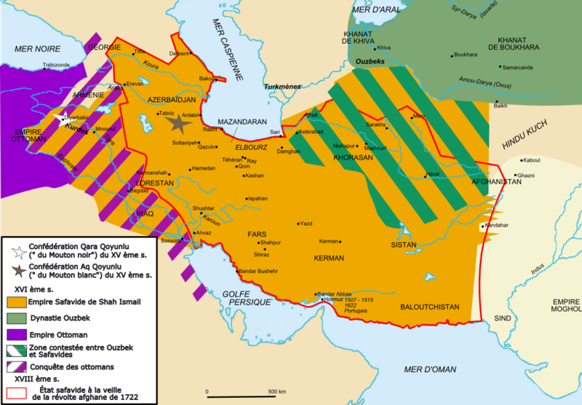
\includegraphics[width=0.9\textwidth]{CourantsIslamContemporain/ImagesCourantsIslamContemporain/empireSafavide.png}

    
\end{figure}


\begin{figure}[h!]
    \centering
        \sidecaption{Apogée et perte de l'empire Moghol : Au XVIII, il est réduit au Rajastan.
}
 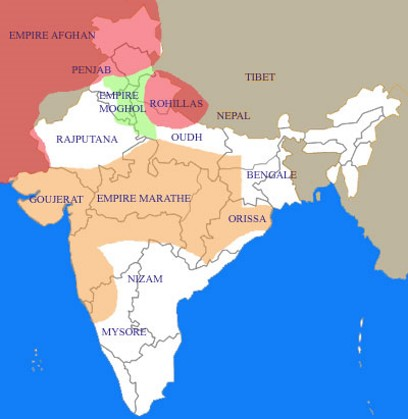
\includegraphics[width=0.44\textwidth]{CourantsIslamContemporain/ImagesCourantsIslamContemporain/Inde18.jpg}
  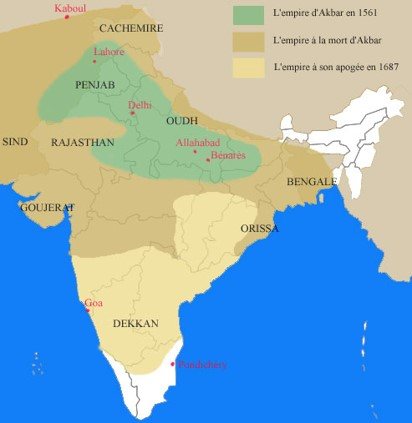
\includegraphics[width=0.44\textwidth]{CourantsIslamContemporain/ImagesCourantsIslamContemporain/empireMoghol.jpg}
\end{figure}

\begin{figure}[h!]
    \centering
        \sidecaption{Déclin Empire Ottoman
}
 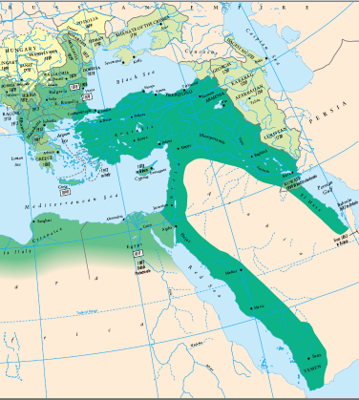
\includegraphics[width=0.5\textwidth]{CourantsIslamContemporain/ImagesCourantsIslamContemporain/declinEmpireOttoman.png}
\end{figure}
 
 \paragraph{Raisons économiques} Les portugais contournent l'Afrique et contournent les empires musulmans.  
 \paragraph{crises politiques} au sein de ces empires, trop grands. 
 \paragraph{Des voisins puissants} Ces Etats vont perdre des territoires face à des puissances qui ne sont pas musulmanes. L'empire Safavide est attaqué par les Ousbeks. L'Empire Moghol en XVIII siècle s'effondre devant l'empire Marathe (Hindou). L'empire Ottoman resiste mais décline depuis 1686 (siège de Vienne). 
 \begin{itemize}
     \item  {Affaiblissement des sultanats Indonésiens} face aux Hollandais. Java est annexé en 1800. 
  \item {En Chine} les musulmans Chinois (Hui) subissent des pressions des Manchous.
   \item  {Afrique} Les bambaras conquièrent Djenné, Tombouctou et Gao. Les portugais en Océanie. 
  \item {En Asie Centrale}, avancée des Russes (XIVII : Kazakstan et reste de l'Asie Centrale au XIX).
 \end{itemize}

 \paragraph{A la fin du XVI} 1591 : deuxième millénaire de l'Islam; sentiment millénariste. \mn{Calendrier lunaire, donc décalage}
 
 
 
\subsection{Problèmes doctrinaux et religieux}

\paragraph{Un raidissement des écoles juridiques au XVII}
Elles s'accusent les unes les autres de ne pas être juste, sentiment de division du monde sunnite.

\paragraph{Décadence du monde Soufi} On a tendance à considérer les soufis comme à la marge du monde musulman. Pourtant, elles ont joué un rôle social déterminant voire politique. Or, à l'époque, elles sont en crise.
\begin{itemize}
    \item {En faisant des Etats dans l'Etat} 
\item {Laxisme spirituel} Un soufi n'est plus tenu de suivre les prescriptions de l'Islam.
\item {Un rôle de plus en plus important du Sheykh}, le maitre spirituel de la Confrérie, qui transmet la \emph{Baraka}.
\item {Des pratiques spéctaculaire} Le fakirisme. le \emph{Dhikr}, rappel du nom de Dieu et l'on atteint l'Etat de transe, et vont marcher sur des braises. 

\end{itemize}



%------------------------------------------------
\section{L'aspiration au
  renouveau}
\subsection{Millénarisme}


 \begin{Def}[rapport au temps Involutif]
 L'Islam se tourne vers le passé, en Islam, les prophètes viennent toujours rappelés ce qui a été donné à l'origine. et le problème est que les hommes déforment le message transmis. Donc Dieu envoie de nouveaux prophètes pour restaurer le message originel. \textit{le temps corrompt.}
 
 \end{Def}
 vs Evolutif. 
 
 Ce qui fait que Mohammad est le dernier des prophètes, c'est que le message est transmis intact, pour la première fois, donc plus besoin de nouveaux prophètes. Autant, la \textit{pratique} peut se corrompre. 
 Un hadith dit : 
 \begin{quote}
     Slt un dixième de la pratique suffira pour sauver le monde.
 \end{quote}
 
 \begin{Def}[Moujaddid]
 de la racine JDD, nouveau, celui qui renouvelle l'Islam pour le mettre tel qu'il était à l'origine. 
 \end{Def}

 
 \begin{Def}[tajdid]
 Tajdid, le renouveau, qui doit venir régulièrement. Chaque siècle Dieu envoie un \textit{Moujaddid} selon un Hadith du Prophète.
 \end{Def}
 
 
 Il peut y en avoir plus mais à chaque siècle, il y a un grand moujaddid, savant, qui ne fait pas forcément au sein de la communauté. 
  \begin{Ex}
 Ghazali est considéré comme un Moujaddid
 \end{Ex}
 \sn{On retrouve cette tension dans toute religion entre respect de la forme et de fidélité au message d'origine}
 
 \subsection{Quelques grandes figures de la \textit{pre-Reforme}}
 

\paragraph{Ahamad Sirhindi} (Inde, 1564-1624) , essaye de rénover l'Islam et réforme une confrérie, la \emph{Naqshbandiyya} réformée (mujaddidi). 
\paragraph{Muhaddidi} Restaurer le monde musulman et restaurer l'Islam dans sa pureté originelle. Il va opposer 
\begin{itemize}
    \item le \emph{taqlid}, l'imitation (péjorative, servile, non réfléchie) et
    \item l'\emph{ijtihad}, l'effort d'interprétation du Coran et de la Sunna. Retourner aux sources scripturaires pour restrouver le sens authentique de l'Islam
    \item pour éliminer la \emph{bid'a}, très péjoratif, l'innovation
\end{itemize}  

On peut distinguer deux courants : un courant plus libéral et l'un plus fondamentaliste :
\begin{itemize}
    \item le rapport à la Tradition : fondamentaliste ne vont considérer que le Coran et la Sunna, en critiquant les élaborations savantes de l'Islam. 
    \item ce sur quoi va porter l'\emph{ijtihad}, soit limité sur les versets peu clairs du Coran, soit plus large pour le savant et les différentes sciences qui vont être convoquées pour l'ijtihad.
\end{itemize}


\paragraph{Muhammad 'Abd Al-Wahhab } 'Arabie, 1703-1792). Voir p. \pageref{Theol:AlWahhab}

\paragraph{Shah Wali Allah} (Inde, 1703-1762), \label{Theo:waliAllah} a eu les mêmes professeurs que Al-Wahhab ! et l'un des premiers à traduire le Coran dans une langue vernaculaire (en persan). Effort d'acculturation dans le contexte Moghol et Indou. 




 
%------------------------------------------------
\section{Les voies du renouveau} 
\subsection{Les confréries soufies}

La création de néo-confrérie
\begin{itemize}
    \item lutter contre un laxisme moral
    \item lutter contre le pouvoir du Sheykh.
    \item insister sur le côté social, en prenant en charge la société (vs gnosticime ?).
\end{itemize}
\mn{Soufi : \pageref{Def:SoufiNaqchabandiya}, \pageref{Def:Soufiqādirīya} }




\paragraph{Ahmad Al Tijani} (Algérie 1737, 1815). Et fonde la \emph{\textbf{tijaniyya}}, un groupe toujours très présent en Afrique du Nord. Normalement un Sheykh insiste sur la chaine d'initiation qui remonte au prophète. Lui, va être initié directement en rêve par le Prophète.

\paragraph{Abdurrauf al-Singkili} (Aceh, Indonésie, 1615-1693)

\paragraph{Abdelkarim al-Samman} (Soudan, 1718-1776) => sammaniyya

Au sénégal, aussi une confrérie de type réformée. 
\mn{A completer carte Carte moderne. Il y avait 24 confréries soufis en Arabie avant le Wahhabisme}




%---------------------------------------
\subsection{Les centres de pèlerinage : La Mecque et Médine}

La Mecque et Médine jouent un rôle essentiel, du fait du Hajj. Du fait de l'Empire Ottoman, il y a pacification des parcours du pélerinage, par ailleurs incités par l'Empire.
Et par ailleurs, des centres de formation s'implémentent à la Mecque.  On en profite pour étudier. Se croisent des savants de différentes origines.
Non seulement les centres d'étude mais aussi les confréries, avec leur Sheykh les plus importants s'installant à Médine ou la Mecque. Ils sont initiés à l'enseignement Moujaddidi et vont réformer la confrérie à laquelle ils appartiennent, selon un modèle qui se répète.




%------------------------------------------------
\section{Un aspect particulier : les jihads aux marges du monde   musulman} 


\begin{figure}[h!]
    \centering
        \sidecaption{Le « renouveau » des marges du monde musulman (XVIIIe-XIXe
siècle)  \emph{L'atlas de l'islam depuis 1500}, F. Robinson, Nathan, 1987  
Des petits Etats vont se créer sur des bases confrériques et dont la mission de faire le jihad.
}
 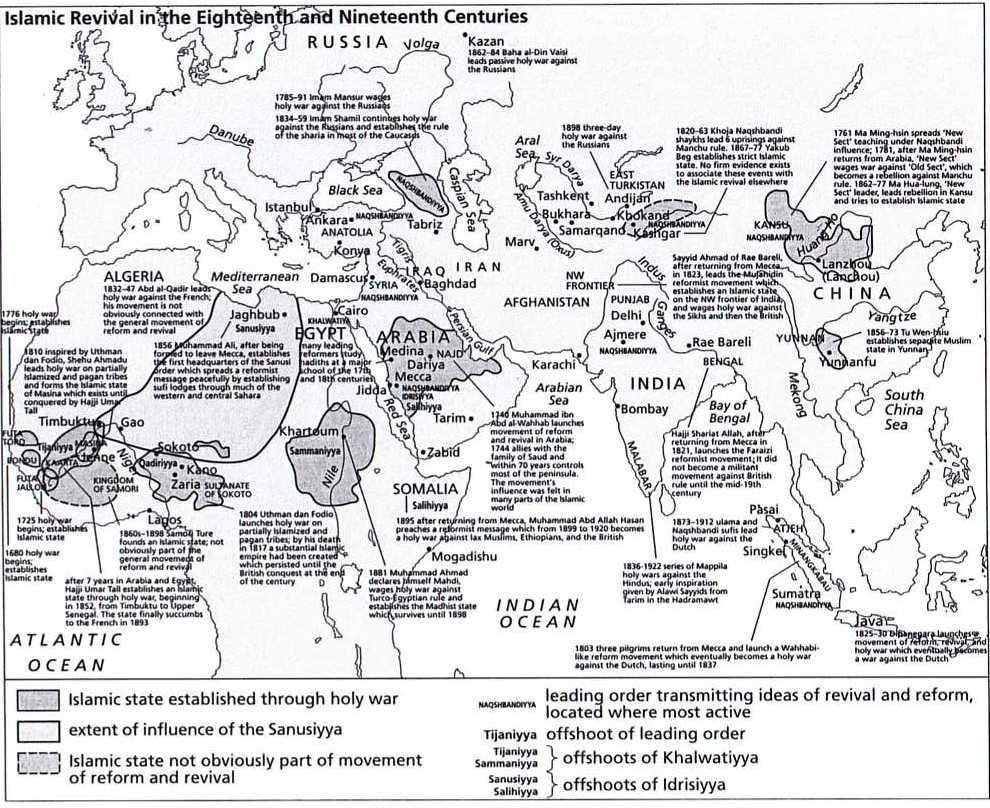
\includegraphics[width=\textwidth]{CourantsIslamContemporain/ImagesCourantsIslamContemporain/image1.jpeg}

    \label{fig:le-renouveau-des-marges-du-monde-musulman-xviiie-xixe-siuxe8cle}
\end{figure}


\subsection{Situation particulière des zones marginales}


Pourquoi on les retrouve aux marges du monde musulman ? Il y a un besoin de purification et l'islamisation par rapport à des populations hétérogènes. Mais aussi, parce que ces zones ne sont pas controlées par les grands empires musulmans qui ne tolèrent pas ces confréries.
Le jihad se porte d'abord sur les musulmans eux-mêmes, pour qu'ils deviennent musulmans puis contre les puissances extérieures ou non musulmanes qui controlent ces zones. 

\paragraph{Une structure Etatique} Le Sheykh est le chef, \emph{Commandeur des Croyants} - on fait référence aux premiers temps musulmans, on prête allégeance, et avec une approche puritaine, très forte pratique. \mn{Des analogiques avec DAESH, qui se réfèrent eux aussi aux temps de l'Islam}

\paragraph{Une accélération de l'Islamisation}


\subsection{Quelques exemples}

\paragraph{Spectre Temporel 1680-1920}{1680, Etat de Bondou} Afrique de l'Ouest jusqu'e l'Etat Mahdiste (Somalie) 1899-1920.

\paragraph{Chine - Ma Ming-hsin} Réveil religieux des communautés chinoises sous la pression des Manchous. Ma Ming-hsin (1719-1781) lorsqu'il est à la Mecque, il fonde une confrérie réformée, la \textit{Nouvelle Secte} et entre en opposition contre les autorités locales, qui appelle en soutien la dynastie Manchoue des Ming. Ming-Hsin est décapité. Il y aura d'autres révoltes plus tard, du Kan-Su et du Chen-Si (1862) et du Yunnan (1856)

\paragraph{Indonésie - Jajji Miskin} Le mouvement Padri à Sumatra (1803-1845). Après le Hajj, en 1803, il prend le contrôle de villages et va imposer sa vision de l'Islam, interdit les pratiques populaires et proclament le Jihad contre les autres villages et les pouvoirs. 1820 : les Hollandais reviennent dans la région et on a une transformation de ce mouvement contre un Jihad contre les Hollandais. Eliminé par les Hollandais.

\paragraph{Nigéria - Califat de Sokoto} Uthman da Fodio (1755-1817) issu d'une famille de savants musulmans, l'enseignement lui vient par la fraderyya\sn{revoir} et crée une communauté qui le reconnait comme \textit{commandeur des Croyants}, s'oppose aux pouvoirs locaux et va être défait par la Grande Bretagne.


\begin{Synthesis}
\begin{itemize}
Ce renouveau : 
    \item Avant la rencontre de l'Occident
    \item lié à des thèmes de crises internes
    \item des thématiques que l'on retrouvera : retourne aux sources scripturaires
    \item C'est assez fascinant de voir la circulation des idées, liée autour du \textit{Hajj}
\end{itemize}


\end{Synthesis}

%------------------------------------------------

 



 



\paragraph{Soufis du Badakhshân : un renouveau confrérique entre
l'Inde et l'Asie centrale}
\mn{Alexandre Papas, \emph{Cahiers d'Asie Centrale}, n° 11-12, 2004, p.
87-102 (extraits -- texte expurgé)}
 
 
\subparagraph{Éléments de biographie d'un soufi
badakhshânais} 
\mn{le Badakhshân est entre l'Afghanistan et le Tajikistan}
\begin{quote}
Mawlânâ Mîr Ghiyâs al-Dîn \label{Theo:MawlanaMirGhiyasAlDin} naît en 1117/1705-06 dans la petite localité
de Hisârak, située au cœur du district de la ville de Jirm. Le
grand-père de Mawlânâ a émigré du village de Dahbîd, non loin de
Samarcande, en direction du Badakhshân. La \emph{silsila}\sn{Génération} de la famille
remonte au Prophète et, sur dix générations, au frère d'un grand saint
Kubrawî et découvre une généalogie \textit{soufie}. C'est donc au sein d'une des
grandes familles \emph{muhâjir}\sn{Emigré, en référence aux premiers musulmans qui ont suivi le Prophète à Médine} de l'aristocratie religieuse du
Badakhshân que naît Ghiyâsî.
\begin{figure}[h!]
    \centering
        \sidecaption{Asie Centrale. On oublie parfois le rôle important de ces états tampon comme lieux d'échange
}
 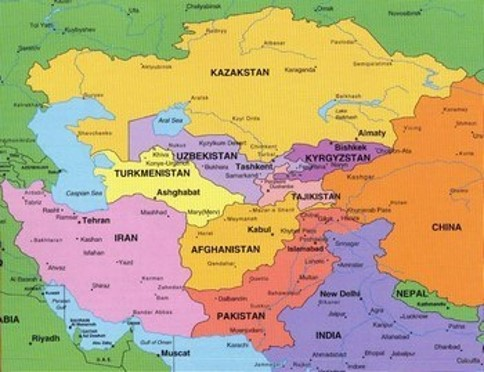
\includegraphics[width=\textwidth]{CourantsIslamContemporain/ImagesCourantsIslamContemporain/AsieCentrale.jpg}
 
\end{figure}

{[}\ldots{]}

C'est précisément pour l'Inde -- destination qui concurrence la
Transoxiane savante, en particulier Boukhara, surtout depuis le XVIe
siècle -- que part le jeune Ghiyâsî âgé de 14 ans en quête d'initiation \sn{soufi}.
Cet exil de l'adolescent fait l'objet de deux contes hagiographiques :
 

\begin{itemize}
\item
 
  Le futur shaykh de Ghiyâsî, Shâh Walî Allâh, qui a quitté Sirhind pour
  entreprendre un pèlerinage au mausolée de Bahâ' al-Dîn Naqshband\sn{le fondateur de la confrérie réformée Naqshandayyi} non
  loin de Boukhara, stationne au Badakhshân, à Jirm, chez le père même
  de Ghiyâsî. Le shaykh demande alors à ce dernier de lui amener ses
  enfants, mais perçoit par claire-vue qu'on lui dissimule le jeune
  Mawlânâ qui, en état de \emph{majzûb}\sn{Ils peuvent faire des choses indécentes} « ravi en Dieu », suscite la honte de
  sa famille. À sa vue le shaykh indien cite un vers de Ni'mat Allâh
  Walî Kirmânî. Et au jeune Ghiyâsî de prononcer miraculeusement le
  second vers du distique. Walî Allâh annonce alors qu'à son retour de
  Boukhara il prendra le jeune homme comme disciple et l'emmènera en
  Inde.
  
\item
 
  Dès l'âge de 9 ans Mawlânâ refuse les conseils de sa famille et se
  distingue des autres enfants. Plusieurs nuits, au cours de rêves, lui
  apparaît un homme illuminé qui lui enjoint de partir pour l'Inde où
  lui est promise la rencontre d'un grand saint soufi. Malgré le refus
  de ses parents qui souhaitent marier leur fils, Ghiyâsî parvient à
  quitter le Badakhshân quelques années plus tard. Parvenu à Lahore et
  après un nouveau rêve révélateur, il attend de nombreux jours au
  couvent de Khwâja Khwândamîr, un khalîfa de la Naqshbandiyya, jusqu'au
  jour où il rencontre Shâh Walî Allâh.
 
\end{itemize}

 
Restent les faits : après une formation classique en \emph{madrasa} à
Delhi où le novice rencontre ses premiers maîtres, il devient à Lahore
durant douze années le disciple d'un fameux maître Naqshbandî Mujaddidî.
Il interrompt une unique fois son initiation lorsque le shaykh lui
confie la mission de se rendre au Cachemire afin d'aller chercher un
homme qu'on prétend thaumaturge et que Walî Allâh souhaite convertir à
l'islam et initier à sa \emph{tarîqat}\sn{confrérie}. Au terme de ses douze années de
noviciat, le shaykh lui enjoint de retourner à sa terre natale pour
propager la confrérie. De retour au Badakhshân, Ghiyâsî âgé de trente
ans environ et qui a obtenu le rang de \emph{mawlawiyyat}\sn{maître}, fait office
d'enseignant à la \emph{madrasa} Jâmi'-i Islâmî du district de Jirm. Il
est ensuite convié à Fayz Âbâd à la cour de Sultân Shâh, laquelle abrite
des savants et des poètes venus d'Inde et d'Iran, dont certains
acquièrent grande réputation. C'est là que Ghiyâsî compose son œuvre
poétique et mystique. C'est également là, de son \emph{khânaqâh}\sn{couvent soufi, Ḵānqāh ou ḵānāqāh, fut d'abord un lieu destiné à abriter les spécialistes et savants religieux musulmans (‘ulamâ’), une sorte d'équivalent des couvents chrétiens. Ces établissements ont été ensuite réservés aux soufis.}, qu'il
dirige son enseignement, suivis par de nombreux disciples venus de
toutes les régions alentours. Le soufi badakhshânais devient aussi le
directeur spirituel de Sultân Shâh. Et lorsque ce dernier est capturé à
Qunduz par les ouzbeks du Qataghân en 1179/1765, le vieux maître
conseille durant trois ans le fils et suppléant du shah emprisonné, Mîr
Muhammad Shâh. D'un tel succès et d'une telle influence, Ghiyâsî
apparaît comme l'un des principaux promoteurs de la Mujaddidiyya dans le
Nord de l'Afghanistan.

{[}\ldots{]}
\end{quote}

\begin{Prop}
On retrouve des noms : Walî Allâh (cf p. \pageref{Theo:waliAllah}; l'importance du réseau confrérique; et rôle social (il devient le conseil du sultan).
\end{Prop}

\subparagraph{Savants et soufis au croisement du
Badakhshân}
Le Pamir est un sanctuaire pour les savants hétérodoxes ou bannis (cf Unwân banni d'Egypte du fait de sa lutte sociale).

\begin{quote}
Malgré les obstacles géographiques et en dépit des troubles politiques
qui affectent la fin du XVIII\textsuperscript{e} siècle, le Badakhshân
reçoit la visite de savants religieux qui, pour certains, décident de
s'y installer et interrompent définitivement leur voyage vers l'Inde ou
vers la Transoxiane. Il faut rappeler ici que le Pamir a, de façon
continue dans l'histoire, servi de sanctuaire à des individus frappés
d'ostracisme ou fuyant la répression dans leur région natale. Mais au cours du
XVIII\textsuperscript{e} siècle le sanctuaire se mue en lieu de
renaissance où fleurissent \emph{madrasa}\sn{lieu d'enseignement religieux} et couvent soufis. Le
\emph{Armaghân-i Badakhshân} mentionne le cas de deux étudiants de
Peshawar, Mîr Ahmad Mujaddidî dit `Izhâr' (m. 1259/1843) et son frère
Muhammad Anwar qui, à une date indéterminée durant le règne de Mîr
Muhammad Shâh, se rendent d'abord à Boukhara afin d'obtenir les
compétences du rang de \emph{`âlim}\sn{savant} et qui, lors de leur retour,
s'installent et officient au Badakhshân, pour le premier à Jirm, pour le
second à Bahârak.

Un autre cas de figure est celui, analogue à Ghiyâsî, de ces
badakhshânais qui partent se former aux sciences religieuses, et
éventuellement au soufisme, dans les grands centres de savoir du monde
musulman, proches ou lointains. De ce point de vue, le cas le plus
intéressant -- et malheureusement le plus douloureux faute
d'informations suffisantes et dans l'absence de vestiges de son œuvre --
est celui de Sayyid Abâ al-Hasan « `Unwân ». Né à Jirm en 1123/1711, il
quitte le Badakhshân pour Boukhara afin d'acquérir une formation
théologique. De là `Unwân se rend au pèlerinage de La Mecque et à
Médine, puis il s'installe durant 18 ans en Egypte, probablement au
Caire, où il poursuit son acquisition des sciences islamiques classiques
et commence à enseigner. Mais `Unwân ne se contente pas de dispenser un
enseignement religieux, il prend parti pour les classes populaires
égyptiennes et contre leur oppression par les propriétaires terriens.
C'est du moins la réputation qu'il gagne selon le \emph{Armaghân-i
Badakhshân}, et qui lui vaut d'être banni d'Egypte. `Unwân part alors
pour Istanbul, rejoint Boukhara et reprend son enseignement. `Unwân, qui
prône l'unité de la Communauté des Croyants (\emph{umma}), décide
d'aller prêcher la concorde (\emph{âshtî}) dans le Caucase, peut-être au
moment de l'activisme Naqshbandî de Shaykh Mansûr dans les années 1780.
Mais il renonce à son projet et entre dans une retraite spirituelle
jusqu'à sa mort en 1206/1791, sans être retourné au Badakhshân.
{[}\ldots{]}

\end{quote}

\begin{Prop}
 Dans le deuxième paragraphe, `Unwân se forme à la Mecque et Médine (rôle du pélerinage), rôle social en Egypte et pas seulement religieux. L'importance aussi de l'Unité, l'\textit{Umma}. 
\end{Prop}
 
\subsection{Liste des neo confréries}

\paragraph{Naqshbandiyya}: La Mecque, Damas, Yémen, Inde, Asie Centrale \label{Def:Naqshbandiyya}
                     => Caucase, Chine Occidentale + Orientale, Sumatra.

\paragraph{Qadiriyya}: Proche Orient, Irak, Inde, Asie centrale 
                    => Indonésie (Java, Aceh), Caucase, Afrique

\paragraph{Khalwatiyya}: Egypte => nombreuses branches en Afrique :

\begin{itemize}
    \item \textit{Tijaniya}: Algérie => Afrique de l’Ouest
    \item \textit{Sammaniyya}: Soudan
    \item \textit{Idrisiyya}: Maroc => Sanusiyya (Lybie), Sahiliyya (Somalie),
    \item \textit{Murghaniyya} (Erythrée)
\end{itemize}- 
 
%-----------------------------------------------
\subsection{bibliographie}

\begin{quote}


AZRA, Azyumardi \emph{The Origins of Islamic Reformism in Southeast
Asia}, Asian Studies Association of Australia/KITLV Press, Leiden, 2004.

PAPAS, Alexandre \emph{Soufisme et politique entre Chine, Tibet et
Turkestan}, J. Maisonneuve, Paris, 2005.

*ROBINSON, Francis \emph{Atlas de l'Islam depuis 1500}, Nathan, Paris,
1987 (dispo à la FELS)

*VOLL, John R. « Foundation for renewal and reform », in John L.
Esposito ed., \emph{Oxford History of Islam}, Oxford University Press,
1999, pp. 509-547.
\end{quote}
\chapter{Un fruit du « pré-réformisme » : le wahhabisme}
\mn{ \emph{(31/01/2022)}}

%---------------------------------------------------------
\section{Le wahhabisme}
\paragraph{Pourquoi en parler} C'est un courant qui a presque trois siècles, avec une évolution dans le monde du musulman qui a évolué. Il faut penser l'Islam contemporain dans son contexte.

 
  \subsection{Muhammad Ibn al Wahhab
  (1702-1792)} 
  \label{Theol:AlWahhab}
  
\paragraph{Origine} Son père est \emph{qadi}\sn{juge} et enseignant. Dans le Hadz. Fait un pélerinage à la Mecque. Renouveau

\paragraph{Formation et premières prédications} Proclame le \emph{Tawhid} l'unicité et lutte contre toutes les pratiques "déviantes". Il se heurte aux autorités locales et retourne donc à la Mecque. Il se forme là avec des maîtres d'Arabie et Indien. Puis se rend à Basra, à un autre maître. C'est là qu'il rencontre les si'ites. Il se heurte de nouveau aux autorités locales. Il rentre en Arabie mais \textit{son père y est hostile}. Ce n'est pas un grand savant mais un lettré. 
 
\paragraph{L'alliance avec Ibn Se`ud} Alliance matrimoniale avec un chef de tribu de la Mecque. Il se rend indésirable et il est obligé de partir et il arrive dans le village de Dariya et il y rencontre un autre chef de village, Mohammed Ibn Se'ud, alliance elle aussi politicolo-religieuse et matrimoniale en 1744. Ibn Se'ud accepte la doctrine et al Wahhab légitime l'acquisition de terre par Ibn Se'ud. 

Wahhab enseigne beaucoup  : il écrit beaucoup à des savants (\emph{Oulema}) à l'intérieur et l'extérieur du royaume de Ibn Se'ud. \textit{selon un modèle prophétique}, Mohammad ayant écrit au Basileos,... 

\paragraph{Un développement politique} Conquiert toute l'Arabie Saoudite. En 1818, c'est la fin du premier état wahhabite car l'empire ottoman intervient et execute le fils de Ibn Se'ud.
    
 Il s'appuie sur deux auteurs : 
\begin{itemize}
    \item Ibn Taymiyya (1263-1328), \label{Theol:Taymiyya2} \sn{cf p. \pageref{ibn-taymiyya}}, un vrai penseur
    \item Ibn Qayyim (1292-1350) un de ces disciples
\end{itemize}
 
Ibn Wahhab insiste sur le retour à la source mais en fait il lit le Coran à travers ces deux auteurs.

\paragraph{Une doctrine condamnée} Son père et son frère s'opposent à lui. Une fatwa contre lui du fait de sa critique sur les différentes écoles juridiques et le fait qu'il exclut de la communauté musulmanes ceux qui ne pensent pas comme lui. 

  \subsection{La doctrine wahhabite} 



  \paragraph{Nécessité du retour aux sources} Accentuation des sources, bien sûr le Coran. 
  \begin{itemize}
      \item  \item  Wahhab s'éloigne d'une lecture du Coran ligne à ligne mais propose une analyse \textit{thématique}.
  \item Il rejette aussi le besoin d'une \textit{médiation} humaine pour comprendre le Coran. Il s'oppose aux \emph{Ashraf}, les descendants du prophète \sn{Les Ashrafs ont un statut particulier dans l'Islam} ainsi qu'aux \emph{Imams} dans le si'isme, ainsi que les \emph{sheykhs} soufis.
  \begin{Prop}
  Il n'y a pas besoin de sciences particulières pour accéder au sens du Coran, d'après Wahhab. 
  \end{Prop}
  \item il suis les \emph{Hadiths}, la seule exégèse possible, la \textit{sunna} et rejette les grands commentaires classiques du Coran.  Cela va jusqu'à critiquer la tradition des 4 premiers Califes \textit{bien guidés}. Abu Bakr avait détourné la \textit{zakat} pour ses propres dépenses.
  \item Il reprend la distinction d'Ijtihad, qu'il limite aux versets aux versets obscures, contre le taqlid. Il s'oppose à deux principes de l'Ijtihad : qiyas (recours par analogie : alcool et drogue), \textit{ijama} (consensus des savants : on considère que cela fait autorité \sn{Infaillabilité de la communauté dans les Hadiths}), et le \textit{ra'y}, l'opinion personnelle du juriste. 
  
  \end{itemize}
 
 \begin{Prop}
 Il conteste les principes sous-jacents aux savants qui l'ont précédés. Il y a une tension entre son ambition de revenir au Coran mais en parallèle en se mettant en filiation avec Ibn Taymiyya
 \end{Prop}
 
 
  \paragraph{Une notion centrale : le \emph{tawhid} (unicité divine)}
  
  \mn{{Extraits du \emph{Kitab at-tawid} (Livre de
l'unicité divine) de Muhammad Ibn Wahhab} . {Chapitre 1} : \emph{Tawhid}
Traduction et édition établies en Arabie Saoudite. Allah est traduit par Allah et non Dieu, alors qu'en Arabe, Dieu est traduit par Allah y compris pour les chrétiens arabes. }

\begin{quote}
\emph{Allah-ta`ala} a dit : « Je n'ai créé les djinns et les hommes que
pour qu'ils M'adorent (1 :56)\ldots Et très certainement nous avons
suscité dans chaque communauté un message pour leur dire d'adorer Dieu
et d'écarter le Rebelle (16 :36)\ldots Et voilà que ton Seigneur a
décrété que tu dois n'adorer que Lui et faire preuve de bonté envers tes
parents (17 :23)\ldots Adorez Dieu et ne lui donnez quelque associé que
ce soit (4 :36)\ldots Venez, je vais vous réciter ce que votre Seigneur
vous a interdit ; - ceci : Ne lui associez quoi que ce soit\ldots(6
:151-153) ». Ibn Mas`ud a dit : « Quiconque se propose de vérifier le
testament du Prophète Muhammad (SWA) -- un testament sur lequel le
Prophète a apposé son sceau, qu'il lise ces mots d'Allah : « Venez, je
vais vous réciter ce que votre Seigneur vous a interdit ; - ceci : Ne
lui associez quoi que ce soit\ldots Voilà ce qu'il enjoint » (6 :
151-153)


Mu`adh Ibn Jabal raconta : « Je montai derrière le Prophète (SAW) quand
il me dit : « Ô Mu`adh ! Sais-tu ce que les créatures d'Allah Lui
doivent et ce qui leur est dû ? » Je répondis : « Allah et son Prophète
savent mieux ». Il continua : « Ce que les créatures d'Allah Lui
doivent, c'est de ne jamais associer qui que ce soit avec Lui. Ce qui
leur est dû, c'est qu'il ne punira aucune personne qui ne Lui associe
pas un autre ». Je dis :

« Ô Prophète d'Allah, est-ce que je peux annoncer la bonne nouvelle aux
gens ? » Il répliqua : «Non ! Ne leur dis rien de peur qu'ils comptent
sur la promesse et manquent à leurs devoirs envers Lui». Ce hadith est
mentionné dans deux \emph{Sahihs}.


D'autres points :


\begin{enumerate}

\item
  \begin{quote}
  La sagesse dans la création du djinn et de l'humanité.
  \end{quote}
\item
  \begin{quote}
  Le service à Allah consiste en le \emph{tawhid}. Car, à l'opposé du
  \emph{tawhid} se trouve l'aliénation d'Allah. (\ldots)
  \end{quote}
\item
  \begin{quote}
  La sagesse d'envoyer des prophètes. (\ldots)
  \end{quote}
\end{enumerate}
  \end{quote}
  
On trouve une accumulation de versets coraniques sur le thème, puis des hadiths du prophète. Le grand péché par excellence, c'est le \emph{shirk}, l'associationisme des Dieux à Dieu. Or Wahhab va plus loin. 

\begin{quote}


\emph{Allah-ta`ala} dit : « Ceux qui ont cru et n'ont point revêtu de
prévarication leur foi\ldots{} » (6 : 82).

(\ldots) Abu Sa`id al Khudriyy rapporta que le Prophète d'Allah (SWA) a
dit : « Quand Musa {[}Moïse{]} demanda à Allah de lui enseigner une
prière qu'il puisse réciter à chaque fois qu'il pensait à Lui ou qu'il
L'évoquait, Allah répondit : « Dis, ô Musa, qu'il n'y a d'autre Dieu
qu'Allah. Musa dit : « Ô Seigneur, tous tes serviteurs prononcent ces
mots ». Allah dit : « Ô Musa, si les sept cieux et tout ce qu'ils
renferment, et les sept terres aussi, si tout cela était pesé contre
cette phrase : « Il n'y a d'autre Dieu qu'Allah », cette dernière
pèserait plus lourd ». Ibn Hibban rapporta cela également et al-Hakim
compléta sa version. Al-Tirmidhi enregistra, avec peu de rédaction, le
récit de Anas à l'effet qu'il entendit le Prophète d'Allah (SWA) dire :
« Allah dit : « Ô Homme ! Si tu venais à Moi avec tous les sacs du monde
remplis de tes péchés, mais avec le témoignage que tu n'associes rien à
Moi, Je viendrais à toi avec tous mes sacs remplis de miséricorde et de
pardon ! ».

    
\end{quote}

\begin{Synthesis}
Si on respecte le \emph{Tawhid}, cela suffit à pardonner les péchés, mais important de respecter les principes de l'Islam (c'est pour cela que c'est caché)
\end{Synthesis}

\paragraph{Distinction au sein du Tawhid } 
\begin{Def}[Le grand Shirk ]
Il distingue le \emph{tawhid rububiyya} (l'unicité de souverainté du monde) avec le \emph{tawhid uluhiyya} (de divinité) : ne reconnaitre aucun intermédiaire entre Dieu et les hommes. Il ne peut y avoir de dévotion que pour Dieu seul : les saints, les soufis, les Imams.
\end{Def} 
Al Wahhab introduit une critique fondamentale contre le soufisme. 

\paragraph{Le petit Shirk} 
\mn{{Chapitre 4} : La crainte du \emph{shirk}}
\begin{quote}
Allah -- qu'Il soit loué et glorifié -- dit : « Non, Dieu ne pardonne
pas qu'on Lui donne quelque associé. En deçà, Il pardonne à qui il veut
» (4 : 48, 116)

(\ldots) Dans le hadith, nous lisons : « Ce que je crains le plus pour
vous, c'est le moindre \emph{shirk}. Quand on lui demanda ce que
c'était, le Prophète répondit : « l'hypocrisie ». Dans le Sahih
d'al-Bukhari, nous lisons que Ibn Mas`ud reporta : « Le Prophète d'Allah
(SWA) a dit : « Celui qui rencontre Allah le jour du Jugement sans Lui
avoir associé qui que ce soit ira au Paradis, et celui qui le rencontre
ayant fait le contraire sera consigné en Enfer ».
\end{quote}
\begin{Def}[le Petit Shirk]
Toute attitude de l'homme qui ne sert pas Dieu. il relève aussi de l'attitude morale.
\end{Def}

\begin{Ex}[L'appel à témoigner qu'il n'y a d'autre
Dieu qu'Allah]

\mn{{Chapitre 5} : }
\begin{quote}
\emph{Allah-ta`ala} a dit : « Dis (ô Muhammad) : `\,`Voici mon sentier,
j'appelle à Dieu'\,' » (12 :108)

Ibn `Abbas (RA) rapporta : « Quand le Prophète d'Allah (SAW) envoya
Mu'adh à al-Yaman, il lui recommanda : `\,`Quand tu rencontres des gens
du Livre, que ta première action soit de leur demander de témoigner
qu'il n'y a d'autre Dieu qu'Allah'\,' ». Selon un autre récit, «
\ldots{} de leur demander de réaliser l'unicité d'Allah. S'ils
t'obéissent, informe-les qu'Allah leur a imposé la \emph{salat} cinq
fois par jour. S'ils t'obéissent en cela, alors informe-les qu'Allah
leur a imposé le devoir de charité qui doit être perçue des riches pour
être distribué aux pauvres. S'ils t'obéissent en cela, ne touche pas à
leurs autres biens et occupe-toi de la plainte de l'opprimé, car il n'y a aucun obstacle dans son accès à Allah ».
(Rapporté dans les \emph{Sahihs} d'al-Bukhari et de Muslim). (\ldots)
\end{quote}
\end{Ex}



\paragraph{Les Intercessions} L'intercession est limitée à Mohammed, et uniquement aux musulmans suivants Wahhab. On ne peut pas prier le Prophète. Peut être intervient-t-il au jugement dernier.


\mn{{Chapitre 17} : L'intercession}
\begin{quote}
Allah -- qu'il soit loué et glorifié -- a dit : « Et par ceci (le
Qur'an), avertis ceux qui, n'ayant pour eux hors de Dieu, ni ami ni
intercesseur, craignent d'être rassemblés vers le Seigneur\ldots{} » (6
: 51). Dis : « A Dieu l'intercession tout entière\ldots{} » (39 : 44).
Qui peut intercéder auprès de Lui que par sa permission ?... (2 : 255).
Et combien d'anges dans les cieux ? Leur intercession ne met au large en
rien, sauf après que Dieu l'a permis, en faveur de qui il veut et qu'il
agrée » (53 : 26). (\ldots)

(\ldots) En tant que catégorie générale du Jour du Jugement en laquelle
les mécréants croient, l'intercession est rejetée par le Qur'an. Le
Prophète (SAW) nous informa qu'en ce jour « il sera amené devant Allah.
Il se prosternera lui-même et louera Allah, plutôt que de demander à
intercéder. Alors on lui dira : « Lève-toi ! Parle maintenant et tu
seras entendu ! Demande et il te sera donné ! Intercède et il te sera
accordé ! » (\ldots) L'intercession est donc là pour les croyants
sincères et candides. Elle n'est accordée que par la permission d'Allah
et n'appartient pas aux associationistes. (\ldots)
\end{quote}


\paragraph{Tombe du juste}
Condamnation de celui qui invoque Dieu
auprès de la tombe du juste et, a fortiori, de celui qui invoque ce
dernier.
\begin{Ex}[Un exemple de Grand Shirk]
\mn{{Chapitre 20} : Condamnation de celui qui invoque Dieu
auprès de la tombe du juste et, a fortiori, de celui qui invoque ce
dernier.}
\begin{quote}
Dans le \emph{Sahih}, A'ishah (RAA) rapporta : « Umm Salmah raconta au
Prophète d'Allah (SAW) qu'elle avait vue une église remplie d'images et
de statues en Abyssinie. Le Prophète dit : « Ceux-là sont les pires de
tous les hommes : lorsqu'un membre juste et vertueux de leur groupe
meurt, ils bâtissent une église sur sa tombe et y installent toutes
sortes d'images pour lui. Ils sont coupables de deux méfaits : celui
d'invoquer quelqu'un auprès d'une tombe et celui d'installer des images
». (\ldots)

Ainsi le Prophète interdit cette pratique et condamna celui qui la
suivait. Faire le \emph{salat} sur une tombe est également interdit,
même si aucune mosquée n'a été construite sur l'emplacement. Telle est
la signification de la déclaration suivante : « On craignait qu'elle ne
soit prise pour une mosquée ». Les Compagnons n'étaient pas supposés
construire une mosquée autour de la tombe du Prophète. Tout endroit
destiné au \emph{salat} ou tout endroit où le \emph{salat} est accompli,
est une mosquée. Tel l'a déclaré le Prophète (SAW) : « Toute la terre
est pour moi une mosquée, un endroit pur (pour accomplir le
\emph{salat}) ».
\end{quote}

\end{Ex}


  \paragraph{La question du \emph{jihad}} La question de la violence chez Wahhab. Il faut repartir de la position kharijite. Un calife doit respecter la religion de façon exemplaire. s'il ne le fait pas, il est \emph{Takfir}, mécréant. Or la vision sunnite a jugé que c'est Dieu uniquement qui jugera si un musulman est un non-musulman. Ibn Taymmayyia s'élève contre les souverains Mongols : : les souverains mongols sont certes musulmans puisqu'ils ont adopté la foi musulmane mais en surface.  Wahhab va reprendre ce concept et ceux qui n'adhèrent par au \emph{shirk} sont apostats. Un germe de violence.
  
  \begin{Synthesis}
  On voit donc l'extension du concept de Ibn Taymmayyia sur le Takfir à tout le shirk, et donc en pratique en non respect du wahhabisme.
  \end{Synthesis}
 
 Mais il n'y a pas de volonté de jihad dans le wahhabisme. On peut même faire des traités avec des non-musulmans.
 
  \section{Le devenir du wahhabisme} 
 
  
 

% ------------------------------ 
\subsection{Les trois Etats Saoudiens} 

 
  {\paragraph{1744 -1818}: une première expansion}
 
 
\emph{1744} alliance Ibn Se`ud /Ibn al-Wahhab
 
\emph{1786} conquête du Najd (`Abd-al-`Aziz)
 
\emph{1792} mort d'Ibn al-Wahhab
 
\emph{1806} conquête de La Mecque
 
\emph{1818} défaite devant les Ottomans
 

 
  {\paragraph{1821-1883}: petit Etat centré sur Riyad (Najd)}
 
  {\paragraph{1901- 2011} : le Royaume d'Arabie Saoudite} Un descendant de Wahhab qui repasse alliance avec la famille de Se'ud et conquiert l'Arabie. 
 
 
\emph{1924} conquête de La Mecque. Abdelaziz Ibn Se`ud prend le titre de
roi et \textit{protecteur des lieux saints}. On détruit les confrérie, on contrôle le pélerinage, on supprime les autres écoles de droit.

\mn{REVOIR}

\emph{1939} début de la production pétrolière \emph{1962} création de la
Ligue islamique \emph{1990} début de la guerre du Golfe.
 

 
\subsection{L'Arabie Saoudite et l'économie
pétrolière} 
 
\paragraph{ {Début de la
production}} 

\begin{quote}
1935: premier forage

1939: premier baril de pétrole

⇒ Cartel américain: l'ARAMCO
\end{quote}

 
\paragraph{{Nationalisation de la
production}}


1973: l'Etat s'approprie 25 \% des droits de l'ARAMCO (1974 : 60\%, 1980 : 100\%)


⇒ Saoudi ARAMCO: 95 \% de la production du pays.

 
\paragraph{Evolution du cours du
pétrole} 

\begin{quote}
1973: premier choc pétrolier (guerre de Kippour) =\textgreater{} de 4 à
15 \$/B

1981-1983: deuxième choc pétrolier (Révolution iranienne + guerre
Iran-Irak) =\textgreater{} 36 \$/B 2006-2008: troisième choc pétrolier
(guerre en Irak) =\textgreater142 \$/baril
\end{quote}

\paragraph{{Rente}}: 1973-2002 =\textgreater{} 200 000 milliards
de dollars au total
 
    Une étude de cas : le wahhabisme en Afrique de l'Ouest
    
\subsection{Le wahhabisme et l'Etat saoudien}

Le wahhabisme accepte une certaine ouverture en Arabie en contrepartie de financement extérieur. On est dans des \textit{concessions} des oulemas. 

\paragraph{La ligue islamique 1962} on étudie gratuitement à la Mecque et à Médine pour propager le wahhabisme.

 
\subsection{Une étude de cas : le wahhabisme en Afrique de l’Ouest}

\paragraph{Des étudiants revenant de la Mecque dans les années 40} et surtout depuis dans les années 70, avec la ligue islamique. 

\paragraph{Un conflit avec les structures soufis}, maraboutisme, très puissantes. On ne priait pas dans les mêmes lieux de culte. 1978 : On  est  loin de  l'époque  où,  en  1978,  Yao  Koum  expliquait  au  Ministre  de  l'Intérieur  qu' \sn{Le wahhabisme à Abidjan Marie Miran-Guyon \url{https://halshs.archives-ouvertes.fr/halshs-01062687/document}}
\begin{quote}
    "obliger  un musulman  orthodoxe (wahhabite)  à  prier  derrière  un  musulman  traditionnel,  c'est  le  contraindre  à renoncer  purement  et  simplement  à  sa  religion,  c'est  l'anéantir  moralement".
\end{quote}


 % -------------------------
\subsection{ {Glossaire}} 


\paragraph{Personnes} `Abd al --`Aziz Abu Bakr

al-Majmu`i al-Sindi

Ibn Taymiyya Muhammad Ibn Se`ud

\paragraph{Lieux}

al-Azhar al-Dir'iyah

al-Uyaynah (Najd). Basra

Hijaz Huraymila Jeddah Najd

\paragraph{Notions}

ashraf : \emph{descendants du Prophète}

da`wa \emph{: prédication}

fiqh : \emph{droit musulman}

hadith \emph{: fait ou dire du Prophète}

hijra : \emph{« exode »}

ijma\emph{` : consensus des ulamas}

ijtihad : \emph{effort d'interprétation}

kufr \emph{: incroyance /} 

kafir \emph{: infidèle, mécréant}

qiyas \emph{: raisonnement par analogie}

salat : \emph{prière rituelle} 

shirk : \emph{associationnisme} 

taqlid
\emph{: imitation (servile)} 

tawhid : \emph{unicité divine}

zakat :
\emph{aumône légale}

 %-----------------------------------------------------
\subsection{Extraits du \emph{Kitab at-tawid} (Livre de
l'unicité divine) de Muhammad Ibn Wahhab}
\mn{Traduction et édition établies en Arabie Saoudite}

\paragraph{{Chapitre 2} : Les vertus du \emph{tawhid} et les
nombreux péchés qu'il expie}



\paragraph{{Chapitre 27} : Les motivations mondaines sont des
exemples de \emph{shirk}}
\begin{quote}
\emph{Allah ta'ala} a dit : « Qui aspire à la vie d'ici-bas et à ses
parures, nous leur solderons ce qu'ils y auront fait : ils ne subiront
pas de perte ! Voilà ceux qui, dans la vie dernière, n'ont pour partage
que le Feu : leurs réalisations d'ici-bas ont crevé ! Nulles sont leurs
œuvres ! (11 : 15-16).

Abu Hurayrah (RAA) rapporta ce hadith \emph{sahih} suivant : « Le
prophète d'Allah (SAW) a dit : `\,`Malheur à l'esclave du dinar !
Malheur à l'esclave du dirham ! Malheur à l'esclave du khamilah !
(\ldots)
\end{quote}
\paragraph{{Chapitre 38} : Obéir aux ulamas ou aux gouvernants
qui légitiment ce qui est interdit ou interdisent ce qui est légitime,
c'est les associer à Allah.}
\begin{quote}
Ibn `Abbas a dit : « Je vous dis que `\,`le Prophète d'Allah (SAW) a dit
ceci et vous dites que `Abu Bakr et `Umar ont dit quelque chose d'autre
?'\,' Le ciel va bientôt vous cracher des pierres sur la tête !! »

Ahmad ibn Hanbal a dit : « Très étranges, en effet, sont ceux qui,
sachant le véritable \emph{isnad} (d'un commandement du Prophète), se
tiennent quand même à l'opinion de Sufyan. Allah lui-même a dit : « Que
ceux donc qui s'opposent à son commandement prennent garde qu'une
tentation ne les atteigne, ou que ne les atteigne un châtiment
douloureux ». (24 : 63). Savez-vous ce que peut être une telle tentation
? C'est le \emph{shirk}. Car, désobéir au Prophète dans certains de ses
commandements, c'est pratiquement comme si on reniait son message et on
s'attirait le Feu.

\end{quote}


\section{bibliographie}

 

\begin{itemize}
\item
 
  IBN AL-WAHHAB, Muhammad \emph{L'unicité de Dieu}, al Qalam, Paris,
  2001.
 


 \item
MENORET, Pascal \emph{L'Énigme saoudienne. Les Saoudiens et le monde
1744-2003}, La Découverte, Paris, 2003.
\item
MIRAN, Marie ; RIALLAND, Maëlle « Dossier Wahhabisme », \emph{Islam et
sociétés au Sud du Sahara}, n°12, 1998, Paris.
\item
MOULINE, Nabil \emph{Les Clercs de l'islam. Autorité religieuse et
pouvoir politique en Arabie Saoudite
(XVIII\textsuperscript{e}-XXI\textsuperscript{e} siècles)}, Paris, PUF,
2011.
\item
  \emph{Histoire de l'Arabie
saoudite}, Paris, Flammarion, 2013.
\item
REDISSI Hamadi \emph{Une histoire du wahhabisme. Comment l'islam
sectaire est devenu l'islam}, Paris, Seuil, 2016.
 \end{itemize}
 
 
\mn{
\href{http://journals.openedition.org/assr}{Archives de sciences
sociales des religions} p. 229-253

\url{https://doi.org/10.4000/assr.21954}}

\section{Les oulémas du palais}

Parcours des membres du Comité des grands oulémas

\hypertarget{ruxe9sumuxe9s}{%
\subsection{\texorpdfstring{\emph{Résumés}}{Résumés}}\label{ruxe9sumuxe9s}}


Véritable matrice idéologique de l'État saoudien et instrument de
légitimation politique et religieuse, la doctrine wahhabite et ses
dépositaires, les oulémas, sont les soutiens indéfectibles de la famille
Sa‛ūd depuis la seconde moitié du e siècle. Cette alliance se renforce,
à partir de 1971, avec la création d'un certain nombre d'institutions
politico-religieuses dont la plus importante est le Comité des grands
oulémas. Si les larges prérogatives, dont dispose cette dernière dans
les domaines politique, religieux et social, poussent l'autorité
politique à vouloir en chapeauter l'action et contrôler l'accès,
l'establishment wahhabite n'en fait pas moins. En effet, l'élite
religieuse saoudienne a adopté des mécanismes d'autorégulation bien
définis pour maintenir son homogénéité et son unité pour mieux dominer
l'espace socioreligieux du royaume. Nous tentons dans cet article, à
partir d'une étude de terrain, de lever le voile sur ces mécanismes en
étudiant les origines sociales et régionales et le cursus honorum des
quarante-cinq oulémas qui siègent ou ont siégé au Comité. Cela permet
d'en ressortir avec le portrait idéal-type de l'ouléma wahhabite
contemporain et de voir dans quelle mesure son parcours le qualifie pour
l'encadrement de la population et du soutien au régime.

\hypertarget{texte-intuxe9gral}{%
\subsection{\texorpdfstring{\emph{Texte
intégral}}{Texte intégral}}\label{texte-intuxe9gral}}

\begin{quote}
\mn{ Paris -- Institut d'Études Politiques,
\href{mailto:mohammednabil.mouline@sciences-po.org}{\nolinkurl{mohammednabil.mouline@sciences-po.org}}}

En s'appuyant sur la doctrine hanbalo-wahhabite, pour légitimer leur
pouvoir et leur hégémonie en Arabie et étendre leur influence dans le
monde musulman, les Āl Sa‛ūd se sont étroitement liés aux oulémas,
dépositaires et interprètes de cet «instrument intellectuel par
excellence de domination politique» en Arabie Saoudite (Al Rasheed,
2007: 28). En échange de la garantie d'autonomie de l'espace religieux
et d'un contrôle plus ou moins étroit de l'espace social, les oulémas
mettent au service de la monarchie saoudienne toutes les ressources
symboliques dont ils disposent pour légitimer ses positions et
sanctifier son action. La consolidation définitive du royaume saoudien,
en 1932, n'a fait que renforcer cette alliance et l'institutionnaliser.

Le flux des revenus pétroliers et la politique de solidarité islamique
menée par la
monarchie saoudienne (Kepel, 2003: 89-92; al-Suwayyigh, 1992: 83-93) a
permis à l'establishment hanbalo-wahhabite de se moderniser en se dotant
de structures administratives et éducationnelles dont la plus importante
est le Comité des grands oulémas. 
\begin{Def}[comité des grands oulémas]
Mise en place en 1971, cette instance,
où siègent en théorie les plus éminents oulémas du pays, et même du
monde musulman, s'est très rapidement imposée comme la principale
instance législative du pays, à côté du conseil des ministres, la
principale instance légitimatrice de l'action politique du pouvoir et le
bouclier idéologique du régime. 
\end{Def}

L'importance que revêt cette
organisation étatique fédérative pour le pouvoir politique saoudien
pousse ce dernier à vouloir en contrôler l'accès et le fonctionnement
pour éviter toute «insubordination» des grands oulémas. De même, l'élite
religieuse veille, à travers ses réseaux formels et informels, à
maintenir sa cohésion et son homogénéité, pour perpétuer l'hégémonie de
son discours, en imposant aux prétendants aux charges «cléricales»
officielles des conditions plus ou moins rigoureuses. Toutefois, aucun
document ne mentionne les conditions que doit remplir un ouléma pour
accéder au Comité. Le seul moyen de lever le voile sur ces conditions
d'accès tacites est de suivre le parcours et le processus de
socialisation des cinquante- deux oulémas qui siègent ou qui ont siégé
au Comité. L'étude des origines sociales,
«ethniques» et régionales des oulémas, de leur formation, de leur
\emph{cursus honorum} et de leur mobilité permettront non seulement de
tirer au clair les conditions d'accès à cette élite mais aussi de jeter
de nouvelles lumières sur les principales caractéristiques de ce groupe
stratifié et différencié. Et pour remettre cette élite dans son milieu
sociopolitique, nous ferons appel, à chaque fois que cela sera possible,
aux autres élites
consultatif1 -- dans le cadre d'un travail de comparaison et de mise en
perspective. Cela permettra, d'une part, d'énumérer les principales
conditions, plus ou moins tacites, d'accès à cette élite et son
évolution, d'autre part, de voir dans quelle mesure l'establishment
hanbalo-wahhabite fait preuve d'auto-encadrement, d'autorégulation, de
reproduction et d'adaptation, sous l'œil bienveillant de l'autorité
politique, pour mieux dominer l'espace religieux saoudien et rayonner
dans l'espace islamique.
\end{quote}

\hypertarget{des-self-made-men-aux-huxe9ritiers}{%
\section{Des self-made-men aux
héritiers:}\label{des-self-made-men-aux-huxe9ritiers}}

\begin{quote}
\textbf{origines sociales des oulémas}

La prédication de Muḥammad b. `Abd al-Wahhāb (m. 1792), qui connaît un
succès fulgurant, fait de nombreux disciples. Du vivant d'Ibn `Abd
al-Wahhāb déjà, plusieurs de ses disciples manifestent zèle et grand
dévouement à la \emph{da‛wa}. À la mort du fondateur du
hanbalo-wahhabisme, il y a routinisation de son charisme, au sens de Max
Weber. Si les membres de sa famille héritent d'une grande partie de ce
charisme, ses disciples eux aussi, bénéficient de la routinisation. Il
en résulte la création d'un certain nombre de «dynasties» d'oulémas
monopolisant l'espace religieux (malgré quelques cas isolés de réussite
individuelle) des trois États saoudiens et ce jusque dans les années
cinquante. Ces «dynasties» d'oulémas sont pour les plus importantes, les
Āl al-Shaykh, descendants directs du cheikh Ibn `Abd al-Wahhāb, les Āl
Sulaym, les Āl `Atīq, les Āl Blīhid, etc. (al-Bassām, 1999; Āl
al-Shaykh, 1973). Mais à partir des années cinquante, une certaine
«démocratisation» de la fonction cléricale voit le jour en Arabie
Saoudite. La liste des membres du Comité des grands oulémas, depuis sa
création en 1971, en est la preuve. Il ressort globalement de nos
entretiens et de la lecture des biographies des membres du Comité
décédés à ce jour, 
\begin{Synthesis}
trois grandes catégories d'oulémas: les self-
made-men, les enfants de ceux qu'on a appelés des «cadres religieux
moyens» et les héritiers des grandes «dynasties» d'oulémas.
\end{Synthesis}

Dans la première catégorie, ont été classés les oulémas d'origine
étrangère et les oulémas saoudiens issus de milieux modestes. Faire des
études et accéder aux hautes fonctions religieuses a offert des
opportunités incalculables à ces oulémas et leur a garanti la promotion
sociale. Mais on remarque que ces ascensions sociales restent tout à
fait exceptionnelles. Dans une société qui fonctionne toujours selon le
modèle segmentaire, la mobilité sociale n'est, en théorie, possible que
si l'individu possède un certain capital culturel et social, capital que
les self-made-men ne possèdent naturellement pas. Cela se fait
d'ailleurs ressentir au sein du Comité car, bien que très respectés pour
leurs qualités personnelles et leur savoir, les self-made-men sont,
malgré cela, «dédaignés» par leurs collègues, à cause de leur origine
sociale. D'ailleurs, la nomination de self-made-men au sein du Comité
des grands oulémas n'est intervenue que trois fois depuis la création du
Comité: une première fois en 1971, la deuxième fois, en 1977 pour
remplacer un membre décédé et la troisième fois, lors du premier
remaniement des membres de la Hay'a, en 1987. Cela peut être expliqué
par le fait que l'Arabie Saoudite souffrait d'un manque de cadres entre
les années cinquante et soixante-dix, ce qui a obligé les autorités à
faire appel à des cadres religieux étrangers en attendant la formation
des cadres «nationaux».

La deuxième catégorie, celle des enfants des «cadres religieux
moyens», est constituée d'oulémas dont les parents, au sens large du
terme, ont exercé des fonctions religieuses telles la magistrature,
l'enseignement, l'imamat d'une mosquée ou encore la prédication, sans
toutefois bénéficier d'une grande renommée. Ils peuvent également
descendre de familles d'oulémas «mineures». Nous avons aussi inclus dans
cette catégorie les oulémas dont les parents ont exercé une profession
libérale, tout en ayant une connaissance du Coran et d'une partie de la
production théologique hanbalo-
wahhabite. Les oulémas issus de cette catégorie constituent plus de 67\%
des membres du Comité des grands oulémas.

Le milieu familial joue un rôle déterminant dans la promotion sociale
de ces oulémas.

Les «cadres religieux moyens» initient eux-mêmes leurs enfants au savoir
religieux ou les confient, le cas échéant, à des précepteurs de
confiance. Le réseau parental ou familial leur permet d'étudier avec les
maîtres les plus réputés et les plus influents et de fréquenter les
bibliothèques les mieux fournies. De plus, l'apprenti \emph{`ālim} de la
génération d'avant le boom pétrolier n'est pas obligé de travailler ou
d'entreprendre, parallèlement, d'autres études pour subvenir à ses
besoins. Il est, en effet, important pour les «cadres religieux moyens»
de former le fils «prodige» pour en faire un grand \emph{`ālim}, dans le
but d'assurer la mobilité sociale pour toute la famille. Car il faut
savoir qu'en devenant grand \emph{`ālim} et membre du Comité des grands
oulémas, il devient, par la même occasion, très aisé financièrement et
très influent.

8 Parmi ces oulémas, ceux qui réussissent à avoir un capital symbolique
restent cependant rares. Plus rares encore, sont les oulémas qui
réussissent à transmettre ce capital à leurs héritiers. Si une telle
transmission se fait, nous assistons à la création d'une «dynastie»
d'oulémas. Cela a été le cas de la famille Ibn Ḥumayd. Issu d'une
famille de «cadres religieux moyens», `Abd Allāh b. Ḥumayd (1911-1982) a
gravi un à un tous les échelons de l'establishment religieux. Grâce à sa
proximité avec Muḥammad b. Ibrāhīm (m. 1969), le grand mufti du royaume
et la principale figure du hanbalo- wahhabisme durant la première moitié
du e siècle, Ibn Ḥumayd a réussi à obtenir le poste de juge dans les
principales villes du Najd dès 1939. Son talent et sa loyauté envers la
dynastie ont poussé le roi `Abd al-‛Azīz à le nommer, en 1953, grand
juge de la province du Hijâz et imâm de la grande mosquée de la Mecque
puis responsable de la gestion des deux lieux saints. Ces postes lui ont
conféré une réputation nationale et Ibn Ḥumayd est peu à peu devenu une
personnalité religieuse incontournable dans le royaume. Il atteint le
sommet de sa carrière dans les années soixante-dix en devenant membre du
Comité des grands oulémas et président du Haut conseil de la
magistrature. Si Ibn Ḥumayd n'est pas le seul exemple de réussite dans
le royaume -- Ibn Bāz (m. 1999) et Ibn `Uthaymīn (m. 2001) sont arrivés
au sommet de l'establishment --, son originalité réside dans le fait
qu'il a réussi à transmettre son capital symbolique à son fils Ṣāliḥ.


\paragraph{9 Ṣāliḥ Ibn Ḥumayd}  Né en 1950, celui-ci poursuit, sous l'œil bienveillant de son père,
une double formation traditionnelle et moderne, sanctionnée par un
doctorat en droit musulman. Il commence alors une carrière universitaire
qui le mène rapidement au sommet de l'establishment. En quelques années,
il devient le doyen de la faculté de théologie de l'Université islamique
de la Mecque. Ses nouvelles fonctions et sa connaissance de la langue
anglaise lui permettent de participer à des rencontres internationales
et de donner une image moderne de l'establishment hanbalo-wahhabite.
Parallèlement, il remplace son père à la tête de l'appareil chargé de
gérer les lieux saints. Il reprend par la même occasion le poste très
prestigieux et médiatique d'imâm dans la grande mosquée de la Mecque. En
1993, Ṣāliḥ b. Ḥumayd est nommé membre du Conseil consultatif. En
décembre 2001, il devient membre du Comité des grands oulémas. Quelques
mois plus tard, il prend la tête du Conseil consultatif. En 2009, il
récupère le poste paternel de président du Haut Conseil de la
magistrature. D'ailleurs, Ibn Ḥumayd prépare déjà ses enfants à prendre
la relève: une «dynastie» est née2.
\end{quote}

\hypertarget{les-ux101l-shaykh-les-luxe9vites-du-hanbalo--wahhabisme}{%
\section{Les Āl Shaykh : les Lévites du hanbalo-
wahhabisme}\label{les-ux101l-shaykh-les-luxe9vites-du-hanbalo--wahhabisme}}

\begin{quote}
10 Toutefois le tableau serait incomplet, si l'on omettait de parler de
la plus grande famille religieuse du pays, qui règne sans partage sur
l'establishment religieux depuis le
e siècle. Il s'agit des Āl al-Shaykh, troisième grande famille du
royaume après les Āl
Sa‛ūd et les Sudayrī et descendants directs de Muḥammad b. `Abd
al-Wahhāb. Ses membres détiennent, en effet, les plus hautes fonctions
religieuses. Le capital symbolique de cette famille s'est transmis, sans
interruption, de génération en génération, depuis l'apparition du
hanbalo-wahhâbisme.

11 Après la mort d'Ibn `Abd al-Wahhāb, ses descendants reçoivent une
grande partie de son héritage spirituel et temporel. Ils allaient
apporter à la famille des Āl Sa‛ūd tout l'appui idéologique dont
celle-ci allait avoir besoin pour étendre son influence et son
territoire. Cette «entente cordiale» profite aux deux parties: les Āl
al-Shaykh confèrent la légitimité aux Āl Sa‛ūd qui, en retour, concèdent
aux Āl al-Shaykh le monopole de l'espace religieux. Une alliance
matrimoniale vient renforcer cette alliance politico- religieuse: le roi
`Abd al-‛Azīz, fondateur du troisième État saoudien, épouse la fille du
premier mufti du royaume `Abd Allāh b. ‛Abd al-Laṭīf. De cette union
naîtra Fayçal, roi d'Arabie Saoudite de 1964 à 1975. Cette alliance
connaît toutefois une grave crise dans les années soixante quand le
grand mufti Muḥammad b. Ibrāhīm entrave les projets
«d'institutionnalisation» de son petit neveu (Ibn Ibrāhīm, 1978: no
4033-4039 et no
4539-4046), le roi Fayçal. À la mort d'Ibn Ibrāhīm, le roi bureaucratise
les oulémas: les Āl al-Shaykh sont évincés des principaux postes
religieux3. De 1971 à 1987, seul un membre de la famille Āl al-Shaykh,
Ibrāhīm b. Muḥammad b. Ibrāhīm, destiné initialement à succéder à son
père au poste de grand mufti, exerce une haute fonction étatique. Il est
membre du Comité des grands oulémas et ministre de la justice.
L'humiliation a été grande suite à la nomination, à la tête de
l'establishment hanbalo- wahhabite, de `Abd al-`Azīz b. Bāz, un
\emph{ḫaḍīrī} ou citadin d'origine non tribale, issu d'une famille de
«cadres religieux moyens».

12 Ce n'est qu'à partir de la seconde moitié des années
quatre-vingt-dix, que la famille royale décide de revenir
progressivement à l'alliance traditionnelle avec les Āl al- Shaykh. Le
nom de la famille réapparaît alors dans les listes des plus hauts
dignitaires religieux saoudiens. L'année 1999 marque, pour ainsi dire,
le retour à l'état normal des relations entre la famille royale et les
Āl al-Shaykh: `Abd al-`Azīz b. `Abd Allāh Āl al- Shaykh est nommé grand
mufti du royaume et président du Comité des grands oulémas. Depuis, les
membres de la «dynastie» d'oulémas des Āl al-Shaykh réinvestissent, peu
à peu, la majeure partie des fonctions qu'ils occupaient autrefois.
Outre le grand mufti, deux membres de la famille siègent au Comité des
grands oulémas, un membre de la famille Āl al-Shaykh est ministre des
affaires islamiques, un autre est ministre de la justice puis président
du Conseil consultatif.

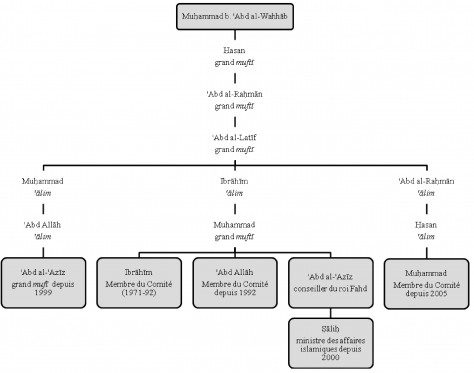
\includegraphics[width=\textwidth]{CourantsIslamContemporain/ImagesCourantsIslamContemporain/genealogie.jpeg}

13 Reste à signaler le cas particulier des oulémas originaires du Hijâz
et d'al-Aḥsā', provinces connues pour leur organisation hétéroclite. En
effet, la plupart des membres du Comité des grands oulémas, originaires
de ces régions, sont issus de ce qu'on a appelé des «dynasties»
d'oulémas, \emph{buyūtāt `ilm}, ou maisons de savoir comme ils aiment
eux-mêmes se faire appeler (à l'instar des familles d'oulémas dans les
autres pays arabes). Plus important encore est le fait que les familles
de ces oulémas appartiennent aux quatre écoles juridiques du sunnisme.
Si le facteur familial revêt une importance certaine, le paramètre de
l'origine tribale doit aussi être pris en compte.
\end{quote}

\hypertarget{la-pruxe9dominance-du-croissant-najdux12b}{%
\section{\texorpdfstring{La prédominance du croissant
\emph{najdī}}{La prédominance du croissant najdī}}\label{la-pruxe9dominance-du-croissant-najdux12b}}

\begin{quote}
14 Force est de constater que l'appartenance à une tribu, généralement
réinventée, constitue un critère identitaire important, dans une société
qui commence à peine à s'individualiser: avant d'être citoyen ou sujet,
on appartient d'abord à une tribu. C'est dire l'importance du milieu
tribal en tant que champ de socialisation des individus. La
\emph{`aṣabiyya}, l'esprit de corps tribal, joue un rôle fondamental
dans le statut social et la promotion de l'individu en Arabie Saoudite.

15 Les oulémas d'origine tribale dominent largement le Comité des grands
oulémas (il s'agit des tribus sédentarisées à partir du e siècle). Ils
sont quarante et un sur les cinquante-deux membres qu'a comptés le
Comité, depuis sa création, à être d'origine tribale, soit 79\%. Les
oulémas d'origine tribale se taillent ainsi la part du lion depuis 1971.
Les onze sièges restants sont occupés par des oulémas issus de trois
milieux différents: des membres de la notabilité citadine du Hijâz
(cooptés pour représenter les intérêts de leur région: on essaie de
choisir les plus «wahhabisés» et/ou quiétistes des oulémas du Hijâz),
des étrangers naturalisés (ils sont hanbalo-wahhabites, ont des talents
«exceptionnels» et ont défendu le hanbalo-wahhabisme et l'État) et des
citadins du Najd, sans affiliation tribale ou \emph{ḫaḍīrī}-s (ces
derniers ne doivent, en principe, leur ascension sociale qu'à leurs
compétences personnelles).

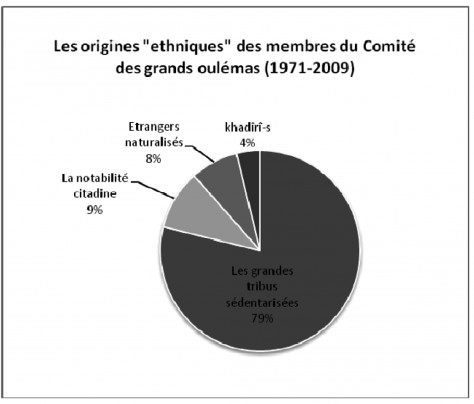
\includegraphics[width=4.9375in,height=4.20833in]{Image/media/image10.jpeg}

16 On constate alors, chiffres à l'appui, que l'appartenance au milieu
tribal sédentarisé joue un rôle déterminant dans l'ascension sociale des
oulémas, la \emph{`aṣabiyya} étant une valeur ajoutée qui permet de se
constituer un capital social. Cela dit, bien que les tribaux dominent
largement en nombre le Comité des grands oulémas, ils ne sont

toutefois pas représentatifs du paysage tribal saoudien. En effet,
certaines tribus comme les Banū Tamīm, les Banū Zayd et les Banū Ḫālid
sont «surreprésentées», tandis que d'autres comme les `Utayba n'ont
guère droit, malgré leur importance numérique, qu'à un seul représentant
au Comité des grands oulémas. D'autres tribus enfin, comme les Šammar,
les Ḥarb, les Muṭayr, les `Ajmān, les Ġāmid, etc. n'ont aucun
représentant au sein du Comité. Si la marginalisation des Šammar, des
`Utayba et des Muṭayr peut s'expliquer par leur passé de tribus
frondeuses, la marginalisation des autres tribus ne peut, elle, être due
qu'à des facteurs religieux et surtout régionaux. Nous nuancerons
seulement, pour finir, en précisant que, dans certains cas, le charisme
personnel du \emph{`ālim} -- c'est le cas d'Ibn Bāz -- fait «oublier»
son appartenance tribale. En effet, ce \emph{`ālim}, citadin sans
affiliation tribale, a pu grimper jusqu'au sommet de l'establishment
hanbalo-wahhabite (il devient grand mufti et président du Comité des
grands oulémas en 1993), uniquement grâce à son «érudition», à son
intégrité morale et à son dévouement aux Sa‛ūd. Le charisme et le
pouvoir symbolique d'Ibn Bāz ont fait de lui le plus grand \emph{`ālim}
hanbalo-wahhabite contemporain.

17 Le royaume d'Arabie Saoudite est un royaume \emph{najdī}. Les élites
saoudiennes sont majoritairement originaires de la région de Najd, fief
de la dynastie et de la doctrine hanbalo-wahhabite. Des études plus
récentes (datant de la dernière décennie) se fondent sur des données
chiffrées mais ne portent que sur les élites ministérielles, la haute
fonction publique et les membres du Conseil consultatif. Rien donc sur
les oulémas. Nous tenterons, dans ce qui suit, de combler ce manque. Sur
les cinquante- deux membres du Comité depuis sa création en 1971, 73\%
des oulémas sont originaires du Najd; 9\% du Ḥijāz, 6\% du Sud, 4\% de
la région orientale et 7\% d'origine étrangère.

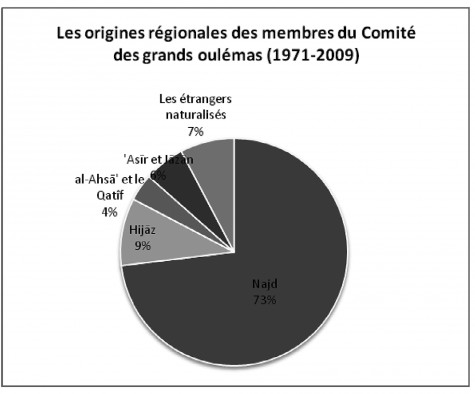
\includegraphics[width=4.94996in,height=4.10417in]{Image/media/image11.jpeg}

18 Une majorité des membres du Comité des grands oulémas est donc
\emph{najdī} et ce depuis sa création. Deux remarques pourraient être
faites à ce propos. La première est que si l'on peut aisément comprendre
que seuls 4\% des grands oulémas sont des Aḥsā'ī-s puisque une grande
partie de la population de cette province est chiite ou sunnite autres
que hanbalo-wahhabite; si l'on peut aussi comprendre que seuls 9\% des
grands oulémas sont \emph{ḥijāzī} puisque, bien que sunnites, ils ne
sont, généralement, pas hanbalo- wahhabites, le chiffre de 6\% seulement
d'oulémas originaires du Sud de l'Arabie Saoudite peut, du moins \emph{a
priori}, paraître absurde puisque les habitants de cette région sont en
majorité hanbalo-wahhabites. L'hypothèse de la préférence régionale peut
être ainsi raisonnablement soutenue: si 73\% des grands oulémas sont
\emph{najdī}, c'est, justement, parce qu'ils sont originaires du fief du
hanbalo-wahhabisme et de la maison
des Sa‛ūd et que, de ce fait, leur soumission à l'un et à l'autre ne
peut être remise en cause. La seconde remarque est que si l'on compare
les chiffres avancés pour le Comité des grands oulémas à ceux que
présente le conseil des ministres au sein duquel les Najdī constituent
72\% des membres (Ibn Ṣunaytān, 2004: 70-73); à ceux du Conseil
consultatif où les Najdī sont majoritaires à 51\% (\emph{ibid}.: 93-96);
à ceux des ministres plénipotentiaires qui sont à 78\% originaires du
Najd ou encore, à ceux des hauts fonctionnaires qui comptent 67\% de
Najdī (\emph{ibid}.: 177-178), on voit que l'élite saoudienne étatique,
qu'elle soit religieuse ou politique, est majoritairement \emph{najdī}.
Les gens du Sud, eux, qui, comme on l'a dit, sont majoritairement
hanbalo-wahhabites, ne représentent que 1\% des ministres, 7\% des
membres de Conseil consultatif, moins de 5\% des ministres
plénipotentiaires et moins de 9\% des hauts fonctionnaires
(\emph{ibid}.: 177- 178): le même raisonnement peut être, ici,
développé. Le régionalisme primerait en Arabie Saoudite. Même si l'on
parle de saoudisation et de formalisation, l'État continue toujours de
s'appuyer sur l'élément najdo-wahhabite pour fonctionner.

19 Observons les chiffres de plus près: lorsque 9\% seulement des
oulémas sont originaires du Hijâz, 20\% des membres du conseil des
ministres, 29\% des membres du Conseil consultatif, 22\% des hauts
fonctionnaires sont \emph{ḥijāzī} (et 34\% parmi eux des cadres
supérieurs). Par ailleurs, en observant les chiffres de plus près
encore, il apparaît qu'au moment de la création du Comité, 29\% des
oulémas sont originaires du Hijâz contre 9\%, nous l'avons dit,
aujourd'hui. Le Comité tend donc, au fur et à mesure qu'il se met en
place et qu'il n'a plus besoin de cadres supérieurs, à se fermer à tout
ce qui n'est pas \emph{najdī}. Il faut ajouter à cela que les oulémas,
quand ils ne sont pas hanbalo- wahhabites, dissimulent leurs croyances
-- ou du moins évitent d'en parler -- et ne jouent, une fois admis au
sein du Comité, qu'un rôle de «figurants».

20 Le Comité des grands oulémas voudrait donner une illusion
d'ouverture: les principales régions sont toutes, même à une faible
proportion, «représentées». Actuellement, deux oulémas d'origine
\emph{ḥijāzi}, deux oulémas originaires du Sud et un autre de l'Est sont
membres du Comité des grands oulémas. En réalité, l'élément \emph{najdī}
domine toujours le Comité, et de loin; de plus, en supposant qu'il y ait
ouverture et même si le Comité accepte en son sein des chiites, il lui
suffirait de conserver une majorité de 51\% de hanbalo-wahhabites
(Najdī) pour que le vote à la majorité absolue passe au sein du Comité
et qu'ainsi, la vision hanbalo-wahhabite continue à dominer.

21 Enfin, en ce qui concerne les oulémas d'origine étrangère, ils ne
sont admis au sein du Comité (au nombre de trois) qu'au moment de la
création de ce Comité. Ces oulémas étrangers étaient, en effet, plus
compétents et plus qualifiés que les oulémas locaux; ils étaient dévoués
à l'État et au hanbalo-wahhabisme; nés non-wahhabites, ils l'étaient
devenus par conviction; ils n'avaient pas d'assise sociale et tribale en
Arabie Saoudite et devaient leur ascension à l'État; enfin, la
solidarité islamique, initiée par le roi Fayçal, entrait également en
ligne de compte. Depuis, le Comité s'est fermé aux étrangers et même les
enfants des dits oulémas étrangers ne sont pas admis au sein du Comité.

22 Le tracé reliant les villes du Najd dont les grands oulémas sont
originaires forme,
pour ainsi dire, un croissant que nous conviendrons d'appeler «croissant
\emph{najdī}» et qui constitue l'épicentre de l'Arabie Saoudite en même
temps que celui du hanbalo- wahhabisme. Il ne faut toutefois pas croire
que si les oulémas du Najd sont largement majoritaires au sein du
Comité, toutes les villes et les régions du Najd y seront équitablement
«représentées». Le Najd compte trois principales régions: la région de
Riyad qui a donné vingt-sept oulémas, le Qaṣīm dix et le Ḥā'il qui n'a
donné aucun \emph{`ālim}. Les deux régions, de Riyad et du Qaṣīm,
offrent un quasi-équilibre dans la répartition des oulémas: dans la
région de Riyad, en dehors de la ville elle-même, qui donne, à elle
seule, sept oulémas, les autres villes donnent, chacune, entre un et
quatre oulémas. De même, dans la région du Qaṣīm, le nombre d'oulémas
par ville varie entre un et trois.

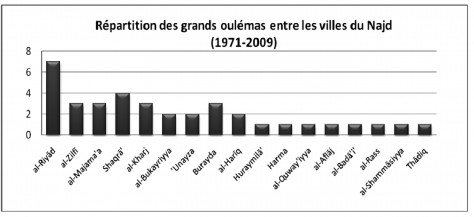
\includegraphics[width=4.9375in,height=2.26042in]{Image/media/image12.jpeg}

23 Le Ḥā'il, quant à lui, est volontairement marginalisé pour une raison
historique évidente: l'émirat du Ḥā'il a longtemps été le rival direct
des Saoud. Nous retrouvons à peine un représentant de cette région dans
le conseil des ministres et un seul autre au Conseil consultatif (Ibn
Ṣunaytān, 2004: 71 et 94).

24 Notons, pour finir, que certaines régions du Najd sont totalement
exclues et n'ont donné aucun \emph{`ālim}: l'exemple d'al-Dawādimī, pour
ne citer que lui, explique ce phénomène dans la mesure où la plupart des
habitants de la ville sont issus de la tribu des `Utayba dont la
fidélité au régime est douteuse. Il y aurait ainsi sous-régionalisation
à l'intérieur même de la régionalisation. De même, aucun grand
\emph{`ālim} n'est issu des régions du Nord. Enfin, aucun chiite n'est
admis au Comité des grands oulémas et ce, pour des raisons évidentes
qu'il ne semble pas utile de rappeler ici. Cela dit, les acquis familial
et tribal, seuls, ne suffisent pas: l'apprenti grand \emph{`ālim} doit
encore suivre un cursus d'études particulier pour intégrer le Comité.
\end{quote}

\hypertarget{de-la-ijux101za-au-doctorat-institutionnalisation-de-la-formation-du-ux101lim}{%
\section{\texorpdfstring{De la \emph{ijāza} au doctorat,
institutionnalisation de la formation du
‛ālim}{De la ijāza au doctorat, institutionnalisation de la formation du ‛ālim}}\label{de-la-ijux101za-au-doctorat-institutionnalisation-de-la-formation-du-ux101lim}}

\begin{quote}
25 Sur les cinquante-deux oulémas qui ont été membres du Comité des
grands oulémas depuis sa création, en 1971, 22\% (soit treize oulémas)
ont reçu une formation traditionnelle et 78\% (soit trente-neuf oulémas)
une formation «moderne». Près d'un quart des oulémas sont ainsi passés
par un cursus traditionnel. Nos entretiens nous permettent de décrire ce
\emph{ta‛līm} et d'en ressortir avec le cursus traditionnel «idéal
typique» du \emph{`ālim} hanbalo-wahhabite.

26 Au départ, entre l'âge de cinq et sept ans, l'apprenti \emph{`ālim}
fait son apprentissage du Coran. Les apprentis oulémas issus d'un milieu
modeste, ceux qui seront plus tard des self-made-men, apprennent le
Coran dans une école coranique (\emph{al-kuttāb}), aux mains d'un cheikh
de renommée moyenne. Les enfants des «cadres religieux moyens» et les
rejetons des dynasties d'oulémas, eux, apprennent le Coran auprès de
leur père, de l'un des membres de leur famille, ou d'un précepteur. On
imagine bien les difficultés rencontrées par les apprentis grands
oulémas issus de milieux modestes et le décalage qui se marque, dès le
départ, entre les apprentis oulémas issus des différentes classes
sociales.

27 Après cette phase d'apprentissage du Coran, l'apprenti \emph{`ālim}
doit, d'une part, commencer à étudier la grammaire et la rhétorique
arabes, de l'autre, apprendre par cœur les trois principaux ouvrages
d'Ibn `Abd al-Wahhāb sur l'unicité divine (\emph{al- tawḥīd}),
fondements du hanbalo-wahhabisme.

28 La troisième étape du cursus classique de l'apprenti \emph{`ālim} est
la quête du savoir
auprès des oulémas réputés. Le futur grand `ālim doit, en effet, réunir
un grand nombre de \emph{ijāzāt} (pl. de \emph{ijāza}: licences), dans
toutes les branches du savoir islamique disponibles, notamment en droit
et en théologie. Il assiste, pour ce faire, plus ou moins
assidûment, à des \emph{ḥalaqāt} `\emph{ilmiyya} ou cercles de savoir,
organisés quotidiennement dans les mosquées ou aux domiciles des
oulémas. Il s'agit alors, de séances de lectures mécaniques suivies de
commentaires d'ouvrages de hadith, d'exégèse coranique, de droit et de
théologie, notamment l'étude des œuvres classiques hanbalites. C'est à
l'issue de ces \emph{ḥalaqāt}, et une fois que l'étudiant a bien retenu
l'ensemble de l'enseignement dispensé par le \emph{`ālim}, qu'il fait un
\emph{istid`ā'}: une demande d'\emph{ijāza} pour les ouvrages étudiés.
Les étudiants les plus brillants deviennent assistants du maître et cela
leur ouvre la porte pour devenir professeur ou juge: la carrière est
alors lancée. Cela a été le cas de Muḥammad al-Sbayyil, le dernier grand
\emph{`ālim} à avoir reçu une formation traditionnelle.

29 Né dans la région du Qaṣīm vers 1926, al-Sbayyil est issu d'une
famille de «cadres religieux moyens». Son père, libraire et copiste
d'ouvrages religieux, connaît parfaitement le Coran. Son frère aîné,
`Abd al-`Azīz, est un \emph{`ālim} de la ville d'al- Bukayriyya. À l'âge
de cinq ans, al-Sbayyil commence son apprentissage du Coran auprès de
son père puis de son frère. Vers l'âge de dix ans, il se lance dans
l'apprentissage des trois ouvrages fondamentaux d'Ibn `Abd al-Wahhāb. Il
étudie aussi la jurisprudence hanbalite sous la direction des oulémas du
Qaṣīm, notamment les ouvrages d'Ibn Taymiyya (m. 1328), d'Ibn Qayyim
al-Jawziyya (m. 1350) et de Mar`ī al- Karamī (m. 1624), etc. À l'âge de
vingt ans, il aurait déjà acquis plusieurs \emph{ijāzāt} qui lui
permirent de devenir l'assistant du juge du Qaṣīm, `Abd Allāh b. Ḥumayd.

30 La formation traditionnelle indispensable au tout début du e siècle
perd, peu à peu, du terrain. En effet, les oulémas qui ont reçu cette
formation s'adaptent difficilement aux exigences de la modernité. 53\%
des membres du Comité des grands oulémas, soit neuf oulémas, ont reçu,
en 1971, une formation dite traditionnelle; en 2009, aucun grand
\emph{`ālim} ne bénéficie d'une telle formation. Dans un pays qui tente
de se moderniser, le besoin d'uniformisation de la formation des grands
oulémas s'impose. Il a fallu, pour y répondre, créer un cursus complet,
homogène, un cursus «national». Nous entendons par cursus moderne, un
cursus «institutionnalisé» et uniformisé.

31 S'ils ne sont que 47\% (soit huit oulémas), en 1971, à suivre la
formation dite moderne,

ils sont aujourd'hui 100\% à le faire. Après un cycle d'études primaires
dans des écoles publiques2\emph{,} les élèves qui se destinent à faire
une carrière juridico-religieuse, rejoignent les instituts de sciences
religieuses (\emph{al-ma`āhid al-`ilmiyya}). Le premier institut voit le
jour à Riyad, en 1950, à l'instigation du grand mufti du royaume de
l'époque, Muḥammad b. Ibrāhīm. Mais très vite, le gouvernement adopte le
projet et les instituts fleurissent dans toutes les régions du royaume
pour atteindre le chiffre de soixante- deux en 2009. Pour accéder à
l'enseignement de ces instituts, l'enfant doit avoir un dossier correct
et avoir appris au moins deux parties du Coran. L'enseignement y est
gratuit. Les instituts de sciences religieuses proposent un cursus de
six années: trois années de collège sanctionnées par un certificat de
réussite, sorte de «brevet» et trois années de lycée sanctionnées par un
certificat de réussite, sorte de «baccalauréat». Les matières étudiées
ont évolué depuis les années cinquante. Au début, l'enseignement était
constitué de quatre troncs communs: les sciences religieuses, les
sciences de la langue arabe, les «sciences sociales», et les
mathématiques. Au fil des années, on a ajouté à ce tronc commun d'études
de base, l'apprentissage obligatoire de la langue anglaise et de
l'informatique. Ces instituts de sciences religieuses sont inégalement
répartis sur l'ensemble du pays: le Najd compte 34\% des instituts, le
Hijâz 13\%, le Sud 28\%, le Nord 18\%, l'Est, enfin, 7\%. Les instituts
sont nombreux dans les régions où le hanbalo-wahhabisme est majoritaire
c'est-à-dire dans le Najd, le Sud et le Nord.

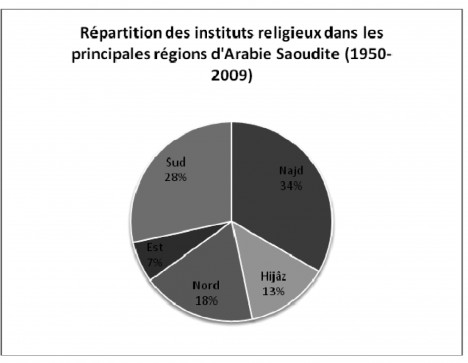
\includegraphics[width=4.875in,height=3.78125in]{Image/media/image13.jpeg}

32 Si la proportion entre le nombre d'instituts créés dans le Hijâz et
celui des oulémas qui sont admis au Comité des grands oulémas est
relativement équilibrée, la proportion entre le nombre d'instituts créés
dans les trois autres régions hanbalo-wahhabites et celui des oulémas
issus de ces régions et effectivement admis au sein du Comité, est,
quant à elle, largement déséquilibrée. On s'attendrait, en effet, à un
nombre plus important d'instituts de sciences religieuses dans le Najd,
à un nombre moins important dans le Sud et à un nombre nul d'instituts
dans la région du Nord. Or, ils sont créés dans le Nord et dans le Sud
mais ce, moins dans le but de former des grands oulémas que dans celui
de «wahhabiser» ces régions en y formant des techniciens du culte
hanbalo-wahhabite et des «cadres religieux moyens».

33 Lorsque l'apprenti \emph{`ālim} a terminé avec succès ses études
secondaires au sein de l'institut, il peut postuler pour les trois
grandes universités du pays: l'Université islamique de Médine (al-Jāmi`a
al-islāmiyya), l'Université islamique de la Mecque (Jāmi`at Umm al-Qurā)
et l'Université islamique de Riyad (Jāmi`at al-imām Muḥammad b. Sa`ūd
al-islāmiyya).

34 La première de ces universités, fondée en 1961, accueille surtout les
musulmans étrangers. Les Saoudiens qui y étudient se destinent
généralement à la prédication à l'étranger. De cette université n'est
issu qu'un seul grand \emph{`ālim}.

35 Quant à la deuxième citée, elle est la plus ancienne université de
théologie d'Arabie Saoudite, fondée en 1949. Elle n'a, malgré son
ancienneté, donnée que six grands oulémas. Doit-on y voir une
manifestation du régionalisme saoudien? Toujours est-il que cette
université accueille, depuis les années soixante-dix, des professeurs,
des cadres et des étudiants de diverses tendances politico-religieuses,
notamment des frères musulmans et des sahwistes (Lacroix, 2010: 47-97)
en lesquels le gouvernement saoudien et le Comité des grands oulémas
n'ont que très peu confiance et qui ne sont donc pas spontanément
recrutés par celui-ci.

36 La dernière université, enfin, est incontestablement la plus
importante pour notre étude. Elle a donné vingt-cinq oulémas, soit 51\%
des membres du Comité, depuis sa création en 1971, et 75\% des oulémas
ayant fait des études universitaires modernes. Cette université naît, en
1974, de la fusion de la faculté de théologie créée, elle, en 1953, et
de la faculté de langue arabe, créée en 1954.

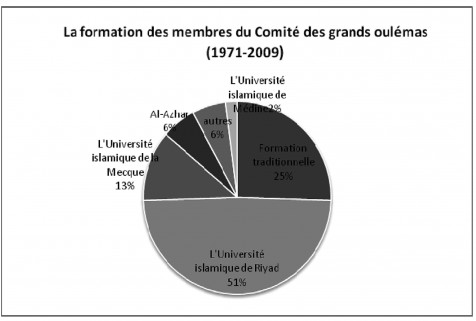
\includegraphics[width=4.95833in,height=3.34375in]{Image/media/image14.jpeg}

37 Depuis sa création, l'Université islamique de Riyad, qui,
rappelons-le, porte le nom du fondateur de l'émirat saoudien Muḥammad b.
Sa`ūd (1744-1765), fidèle allié d'Ibn `Abd al-Wahhāb, est considérée
comme le vivier des grands oulémas et de tous les cadres religieux et
techniciens du culte dont l'establishment religieux a besoin. Le

«pharaonique» campus de l'université (une véritable ville dans la ville
avec ses propres infrastructures, un petit hôpital, un supermarché, des
quartiers résidentiels pour les étudiants, les professeurs et le
personnel administratif, etc.) compte neuf facultés et deux instituts
supérieurs: la faculté de droit {[}musulman{]}; la faculté de théologie;
la faculté de langue arabe; la faculté des sciences sociales
{[}islamiques{]}; la faculté de la prédication et de la communication;
la faculté des langues et de la traduction; la faculté des sciences de
l'informatique; la faculté de l'économie; la faculté des sciences;
l'Institut supérieur de la magistrature et l'Institut de l'apprentissage
de la langue arabe {[}pour les étrangers{]}. Cela dit, les grands
oulémas sont exclusivement issus des facultés de droit et de théologie
et de l'Institut supérieur de la magistrature. Les étudiants dans ces
trois domaines bénéficient d'une bourse d'études et obtiennent, dès la
fin de leur première année d'études, le titre fort apprécié de
\emph{shaykh}. Le succès de l'Université islamique de Riyad est tel que
celle-ci s'est engagée dans une politique d'expansion en développant
deux filiales en Arabie Saoudite3 et cinq à l'étranger4\emph{.} Enfin,
certains étudiants peuvent préparer leur doctorat en sciences
religieuses à l'université égyptienne d'al-Azhar, pour le prestige que
cela donne. Une autre raison pourrait être avancée: certains apprentis
oulémas saoudiens iraient à al-Azhar pour observer l'organisation, les
structures et les mécanismes de fonctionnement de cette prestigieuse
université en vue de les
«importer» en Arabie Saoudite.

38 Les oulémas, au moment de leurs études supérieures, ont tous un tronc
commun tripartite: les fondements de la théologie (\emph{al-`aqīda});
l'exégèse coranique (\emph{al tafsīr}) et la jurisprudence
(\emph{al-fiqh}). À partir de la première année de master (calqué sur le
système anglo-saxon), 74\% des oulémas se spécialisent dans la
jurisprudence, et plus spécialement dans les fondements de la
jurisprudence islamique (\emph{uṣūl al-fiqh}) dans le but d'acquérir la
qualification requise pour émettre des \emph{fatwā}; 26\% d'entre eux,
se spécialisent en théologie, et plus précisément en religions comparées
(en réalité, pour dénigrer toute autre religion que l'islam
hanbalo-wahhabite)5\emph{.} Le choix de ces spécialisations n'est pas
étonnant dans la mesure où les étudiants se destinent avant tout à être
des techniciens du culte et des gestionnaires des biens de salut. Nous
n'entrerons pas, pour ne pas alourdir notre propos, dans le détail des
spécialisations pointues à l'intérieur même des deux grands domaines de
spécialisations que nous avons évoqués.

39 Bien que le cursus moderne se soit bien implanté dans le paysage
saoudien, l'ijāza
n'en demeure pas moins source de prestige et un élément non négligeable
dans un
capital social. Nous avons pu observer que la totalité des oulémas qui
ont suivi le cursus moderne ont, néanmoins, obtenu une ou plusieurs
\emph{ijāzāt}. Elément de prestige comme nous venons de le dire,
l'\emph{ijāza} est, en théorie, facultative. Mais, en pratique,
l'obtention d'une \emph{ijāza} permet au \emph{`ālim}, d'une part, de se
rattacher à une chaîne de transmission
«ininterrompue» d'oulémas remontant jusqu'au Prophète, ce qui permet au
\emph{`ālim} de légitimer sa position et son savoir et de s'inscrire
dans l'héritage prophétique, d'autre part, de nouer des relations
privilégiées avec un ou plusieurs oulémas et de commencer ainsi à tisser
un réseau qui pourra le mener au sommet de l'establishment hanbalo-
wahhabite.

\textbf{Faire carrière: le \emph{cursus honorum} des oulémas}

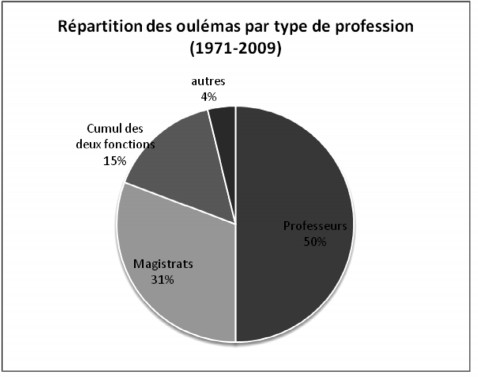
\includegraphics[width=4.97917in,height=3.92708in]{Image/media/image15.jpeg}40
L'enseignement et la magistrature ont toujours été les métiers de
prédilection des oulémas. Les membres du Comité des grands oulémas
n'échappent pas à cette règle. 96\% d'entre eux exercent au moins une de
ces deux professions: 50\% du Comité, soit vingt et un grands oulémas,
ont été ou sont encore, professeurs de jurisprudence islamique ou de
théologie; 31\% d'entre eux sont magistrats dans les différentes
instances de la justice saoudienne; 15\% des grands oulémas ont cumulé
les deux fonctions. À la question: «pourquoi le choix de ces métiers?»
Une première réponse, unanime, des grands oulémas magistrats: «la
justice est le fondement de la royauté». Et, selon les oulémas, qui,
mieux que des spécialistes de «la loi divine», pourraient mettre la
justice en application! Les grands oulémas ont d'ailleurs pleine
conscience de l'importance de leur mission. Ils ont une vision
catastrophiste d'un monde où le \emph{`ilm}, qui risque d'être perdu,
doit être sauvé, épuré des innovations blâmables et transmis par le
\emph{`ālim}.

41 En outre, si la magistrature permet au grand \emph{`ālim} d'observer,
d'analyser et de statuer sur des cas concrets, l'enseignement permet de
transmettre le savoir théorique. Cela, en plus du prestige qui entoure
ces deux fonctions. Il n'est, enfin, pas étonnant de voir que nombre de
grands oulémas cumulent les deux fonctions puisqu'en réalité, l'une et
l'autre sont indissociables (pratique et théorie). Ce phénomène de cumul
des fonctions (d'enseignant et de magistrat) est surtout visible dans la
première génération des grands oulémas. Il s'explique par le manque de
cadres religieux au moment de la
création du Comité. Les grands oulémas devaient donc assumer, tout à la
fois, leur rôle au sein du Comité et les fonctions de magistrats et
d'enseignants. Des années quarante aux années soixante, l'Arabie
Saoudite a été obligée d'«importer» des cadres religieux de l'étranger,
notamment de l'Égypte. Un exemple: l'Égyptien `Abd al-Razzāq `Afīfī (m.
1994), arrivé en Arabie Saoudite, en 1949, pour enseigner la langue
arabe et les sciences religieuses dans un collège à Tayef, a gravi, un à
un, les échelons et parvient au sommet de l'establishment religieux: il
est nommé, en 1971, au sein du Comité des grands oulémas. Cet exemple
révèle deux réalités: premièrement, l'Arabie Saoudite a fait appel aux
étrangers pour l'enseignement, à une certaine époque, à cause du déficit
de cadres dont elle a souffert dans tous les domaines; et deuxièmement,
les étrangers hanbalo-wahhabites, qui pouvaient aisément s'intégrer dans
le pays d'accueil, ont pu, à force de persévérance, atteindre le sommet
de l'establishment religieux saoudien.

42 La pratique du cumul des fonctions d'enseignant et de magistrat tend
à disparaître: le dernier grand \emph{`ālim} à avoir cumulé ces deux
fonctions est `Abd Allāh b. Qa`ūd, membre du Comité de 1977 à
19866\emph{.} Désormais, les grands oulémas, qu'ils soient professeurs
ou magistrats, sont de plus en plus spécialisés, chacun dans son
domaine: de professeurs de droit en général, ils sont devenus
professeurs de droit pénal, de droit de la famille, etc. Parallèlement à
ces deux métiers de prédilection, les grands oulémas sont techniciens du
culte: la plupart d'entre eux sont imâm dans les mosquées. Par exemple,
le grand mufti actuel du royaume, `Abd al-`Azīz āl al-Shaykh, est
également imâm de la grande mosquée de Riyad. Sāliḥ b. Ḥumayd est, lui,
imâm de la grande mosquée de la Mecque, etc. N'oublions pas enfin,
l'autre fonction essentielle des grands oulémas, celle d'«entrepreneurs»
de biens de salut, à savoir promulguer des \emph{fatwā} et se mettre à
l'écoute de la population. Mais si les grands oulémas monopolisent les
grands postes religieux et judiciaires saoudiens, ils n'hésitent pas à
empiéter sur le domaine réservé des autres élites.

43 Une fois admis au sein du Comité, le grand \emph{`ālim} obtient
automatiquement le grade de haut fonctionnaire (\emph{al-martaba
al-mumtāza}), voire celui de ministre. Sur les cinquante-deux membres du
Comité des grands oulémas, vingt-deux ont occupé des postes de
responsabilité autres que ceux de magistrats et d'enseignants. Déjà neuf
membres de la \emph{Hay'a} ont été ou sont encore ministres. Les
ministères que contrôlent les oulémas (si ce ne sont pas eux qui les
contrôlent directement, c'est un membre de l'establishment religieux)
sont ceux de la justice, des affaires islamiques, du pèlerinage et de
l'enseignement des filles (avant le rattachement de ce dernier, en 2002,
au ministère de l'éducation nationale). Depuis sa création, le ministère
de la justice est dirigé par un membre du Comité7\emph{.} Huit membres
du Comité des grands oulémas on été membres du Conseil consultatif: le
président de ce conseil, qui fait se côtoyer islamistes,
«libéraux», conservateurs et tribaux, depuis sa création, en 1992, est
un membre du Comité des grands oulémas. De 1992 à 2002, c'est Muḥammad
b. Jubayr, membre du Comité des grands oulémas (de 1971 à 2002), qui
assure la présidence de cette instance. Sāliḥ b. Ḥumayd, membre du
Comité des grands oulémas depuis 2001, lui succède en 2002. Ce dernier
est remplacé par `Abd Allāh Āl al-Shaykh, en 2009. Trois membres de la
\emph{Hay'a} ont été conseillers du roi Fahd (1982-2005) et deux sont
actuellement conseillers du roi `Abd Allāh. Quatre membres du Comité ont
occupé les postes de doyen ou de président d'université. Par exemple,
`Abd al-`Azīz b. Bāz occupe jusqu'à sa mort, en 1999, le poste de
président de l'Université islamique de Médine. Sa`d al- Ḍuwayḥī est
doyen de la faculté de théologie d'al-Aḥsā'. `Abd Allāh b. `Abd
al-Muḥsin al- Turkī, sans doute l'un des membres les plus actifs du
Comité, actuellement, occupe le poste de président de la Ligue islamique
mondiale, après avoir occupé, entre autres, les postes de président de
l'Université de Riyad et de ministre des affaires islamiques.

44 C'est dire que les oulémas ont adopté, depuis au moins deux
décennies, une stratégie adaptative qui les pousse à investir plusieurs
secteurs d'activités. Outre les domaines religieux, législatif et
éducatif, ils investissent les associations caritatives, les
organisations gouvernementales et non gouvernementales et les domaines
économique et financier. Dans ces deux derniers domaines, trois oulémas,
`Abd Allāh b. Manī`, `Abd
al-Wahhāb Abu Sulaymān et `Abd Allāh al-Muṭlaq se sont «improvisés»
experts et consultants incontournables dans les marchés financiers
saoudiens. Les trois hommes sont aussi membres de plusieurs conseils
d'administration de banques et d'entreprises dans le cadre de ce que
l'on appelle en Arabie Saoudite \emph{al-lijān al-šar`iyya} ou
commissions islamiques. Le nom-même d'un grand \emph{`ālim} sur la
brochure d'une société ou d'une entreprise est la meilleure des
publicités.
\end{quote}

\hypertarget{la-multiplication-des-ruxe9seaux-de-soutien}{%
\section{La multiplication des réseaux de
soutien}\label{la-multiplication-des-ruxe9seaux-de-soutien}}

\begin{quote}
45 Cette mobilité des oulémas n'est, toutefois, possible que si le
\emph{`ālim} tisse, autour de lui, un réseau sur lequel il peut
s'appuyer. Les capitaux culturel et économique doivent encore être
complétés par un réseau de soutiens. Nous avons pu observer trois types
de capitaux sociaux mobilisés par le futur grand \emph{`ālim}. Autrement
dit, le recours aux relations personnelles permet à ce dernier de
s'assurer une meilleure position dans la hiérarchie sociale. Ces trois
réseaux, que nous exposons séparément, sont en réalité, presque
toujours, combinés par le futur grand \emph{`ālim}. Le réseau familial
constitue la première ressource du futur grand \emph{`ālim}. Nous avons,
en effet, constaté l'existence d'au moins trois exemples de réseaux
familiaux qui sont autant de moyens d'accès au Comité des grands
oulémas.

46 Le premier est, sans aucun doute, le plus puissant et le plus dense:
celui des Āl al- Shaykh. Nous avons évoqué plus haut l'importance de
cette famille et nous tenterons, dans ce qui suit, de compléter le
tableau amorcé. L'exemple des deux fils, Ibrāhīm et `Abd Allāh, du grand
mufti Muḥammad b. Ibrāhīm est tout à fait significatif: bien que le
premier des deux ait été relativement peu brillant par rapport aux
collaborateurs de son père, il a quand même été nommé par ce dernier
vice-mufti du royaume d'Arabie Saoudite. Après la mort de son père et la
suppression du poste de mufti, Ibrāhīm, qui était destiné à devenir
mufti, reçoit, en guise de consolation, les postes de ministre de la
justice, de membre du Comité des grands oulémas et de président de la
Direction de la recherche scientifique, de la prédication et de
l'instruction! En 1992, lorsqu'Ibrāhīm se retire des affaires, son
remplaçant au ministère et au Comité des grands oulémas n'est autre que
son frère cadet `Abd Allāh, président actuel du Conseil consultatif. Un
autre exemple étonnant de la famille Āl al-Shaykh: il s'agit de Ṣāliḥ b.
'Abd al-`Azīz, le petit fils d'Ibn Ibrāhīm. Après avoir fait des études
scientifiques depuis le lycée et obtenu un diplôme d'ingénieur, Ṣāliḥ
décide de récupérer l'héritage familial et s'inscrit à l'Université
islamique de Riyad. Grâce à son nom et à l'intervention de son père, qui
était l'un des conseillers du roi Fahd, il obtient une équivalence et
passe ainsi directement en année de master: il contourne la règle qui,
aussi stricte soit-elle, s'efface quand il s'agit d'un Āl al-Shaykh. Il
est actuellement ministre des affaires islamiques et, potentiellement,
membre du Comité des grands oulémas. Un dernier exemple enfin de cette
famille: le dernier admis à Hay'at kibār al-'ulamā', Muḥammad b. Ḥasan,
fait une ascension fulgurante grâce à ses bonnes relations avec son
cousin, le grand mufti actuel d'Arabie Saoudite: il a pu, rapidement,
gravir les échelons universitaires et devenir le directeur de cabinet du
mufti. Ce dernier l'épaule et le soutient: il propose son nom au Comité
des grands oulémas auquel Muḥammad b. Ḥasan accède en avril 2005.
Signalons, enfin, que le réseau familial des Āl al-Shaykh et l'influence
qui en découle, dépassent largement le seul cadre religieux: un membre
de la famille est ambassadeur à Paris, un autre est directeur du
protocole royal, un troisième est membre de la chambre de commerce, etc.
Le deuxième réseau familial est celui des Ibn Ḥumayd, déjà présenté plus
haut.

47 Le dernier réseau familial, enfin, de moindre importance, est celui
des al-Šathrī: cette
famille du Najd a donné quelques oulémas et plusieurs hommes politiques.
`Abd al-‛Azīz al-Šathrī, un des conseillers des rois Fayçal (1964-75) et
Ḫālid (1975-82) a également été un ouléma de renommée moyenne. Son fils,
Nāṣir, a réussi à faire une brillante carrière politique (en tant que
conseiller des rois Ḫālid et Fahd). Selon un des
membres du clan al-Šathrī: «il ne manquait à {[}la{]} famille qu'un
grand \emph{`ālim} pour qu'{[}elle{]} devienne, enfin, une grande
famille». La parentèle met tout en œuvre pour que son rejeton prodige,
Sa‛d, accède au sommet de l'establishment religieux. Aussi, le
prépare-t-on, dès son plus jeune âge, à devenir grand \emph{`ālim} : on
le confie aux maîtres les plus compétents dans le domaine, tels Ibn Bāz,
Ibn `Uthaymīn, al-Aṭram, al-Rakbān et `Abd al-`Azīz Āl al-Shaykh. On le
pousse à s'inscrire à Jāmi'at al-imām où il obtient un doctorat en
fondements de la jurisprudence islamique. Sa`d brûle toutes les étapes
du \emph{cursus honorum} hanbalo-wahhabite et devient professeur de la
même université en un temps records. En mars 2005, la famille soutient
la candidature de son fils au Comité des grands oulémas (le père est
membre du cabinet royal qui transmet les candidatures au roi). Sa`d est
finalement nommé, en avril 2005: à trente-huit ans, il est le plus jeune
membre de l'histoire du Comité des grands oulémas.

48 Nous l'avons dit, le régionalisme et le segmentarisme dominent le
paysage politico- religieux saoudien. La deuxième ressource du futur
grand \emph{`ālim} est, naturellement, le réseau tribal qui va de pair
avec le réseau régional, autrement dit avec le réseau \emph{najdī}. Nous
avons remarqué, en analysant les origines géographiques et tribales des
grands oulémas, que ces derniers sont généralement issus des plus
grandes confédérations tribales du Najd: les Banū Ḫālid ont donné quatre
grands oulémas, les Banū Zayd, sept, les Banū Subay`, trois, les Banū
Tamīm, huit (auxquels il faut ajouter les quatre grands oulémas des Āl
al-Shaykh), les Qaḥṭān, trois, les `Unayza, trois, les Bāhila, deux et
al- Dawāsir, deux également. Soit un total de trente-six grands oulémas
issus des grandes tribus du Najd sur les cinquante-deux membres du
Comité. Le réseau tribal est très dense. Le nombre de grands oulémas est
plus ou moins bien réparti entre les grandes tribus \emph{najdī}. D'un
mouvement de nomination au sein du Comité à l'autre, cet équilibre est,
consciemment ou inconsciemment, maintenu. Exemple: les deux grands
oulémas, Muḥammad āl Sulaymān et Bakr Abū Zayd, de la tribu des Banū
Zayd -- admis tous deux au Comité, en 1992 -- sont remplacés, en 2005,
par deux hommes issus de la même tribu, `Alī al-Ḍuwayḥī et `Abd
al-Raḥmān al-Sadḥān. D'ailleurs, le réseau tribal doublé du réseau
régional ne concerne pas uniquement le champ religieux: on retrouve ces
mêmes configurations dans le domaine politico-administratif (Ibn
Ṣunaytān, 2004, 59-62).

49 La dernière ressource du futur grand \emph{`ālim} est la
\emph{mulāzama}: le fait de s'attacher un
long moment à un maître en sciences religieuses, réputé et influent.
Côtoyer un maître pendant plusieurs années permet à l'apprenti grand
\emph{`ālim} de nouer avec lui des relations personnelles qui peuvent
même aboutir au mariage de l'élève avec la fille ou la nièce du maître.
Par exemple, Ṣāliḥ al-Luḥaydān est, pendant plusieurs années, le
disciple favori du grand mufti Muḥammad b. Ibrāhīm. Cette relation
privilégiée lance véritablement la carrière de Ṣāliḥ qui devient le
gendre et le directeur de cabinet du mufti et qui gagne peu en peu en
charisme. Une année seulement après le décès du maître, al-Luḥaydān est
admis au Comité des grands oulémas; il hérite aussi de la fonction de
magistrat; quelques années plus tard, il devient le président du Haut
conseil de la magistrature, poste qu'il occupe jusqu'en février 2009.
Al-Luḥaydān est le doyen du Comité des grands oulémas dont il est membre
depuis 1971. Il en est aussi un des membres les plus influents. Il
serait, en effet, le seul à pouvoir opposer un veto pour la nomination
d'un nouveau membre: en 2005, il aurait utilisé son veto pour s'opposer
à l'entrée de l'ouléma `Abd al-Muḥsin al-`Ubaykān au Comité.

50 Un autre exemple: Muḥammad al-Sbayyil est le disciple d'Ibn Ḥumayd
alors que
celui-ci est le \emph{qāḍī} d'al-Bukayriyya. Quand Ibn Ḥumayd devient le
\emph{qāḍī} du Qaṣīm, il fait appeler al-Sbayyil à Burayda pour le
désigner professeur et responsable d'un institut de sciences religieuses
de la région. La relation entre les deux hommes est telle que,
lorsqu'Ibn Ḥumayd devient le grand juge du Ḥijāz, il le fait venir à la
Mecque et le nomme imâm de la grande mosquée de la Mecque et
vice-président de l'administration chargée de gérer les deux lieux
saints. Il finit même par en devenir président (jusqu'en 2005) après la
disparition de son protecteur. Depuis son arrivée à la Mecque, il tisse
des
relations étroites avec des oulémas et grands oulémas notamment Ibn Bāz
(qui n'est pas son maître) mais qui finit par lui proposer de devenir
membre du Comité en 1992.

51 Un troisième exemple: c'est également Ibn Bāz qui suit, pas à pas, la
carrière de `Abd
Allāh b. Qa'ūd qui est son meilleur disciple. À la première occasion (le
décès d'Ibn Ḥumayd et de Miḥḍār `Aqīl), Ibn Bāz propose le nom d'Ibn
Qa`ūd au cabinet royal qui le nomme membre du Comité en 1977.

52 Un dernier exemple enfin: le mufti actuel, `Abd al-`Azīz āl
al-Shaykh, en plus du réseau familial que lui confère son nom, bénéficie
du soutien de son maître Ibn Bāz. Il s'agit d'abord d'une question de
solidarité et de reconnaissance: Ibn Bāz est un \emph{mulāzim} du grand
père de `Abd al-`Azīz Āl al-Shaykh, Muḥammad b. `Abd al-Laṭīf. Il aide
donc `Abd al-`Azīz Āl al-Shaykh à devenir professeur à l'université
d'al-Imām, et propose son nom au cabinet royal pour en faire un membre
du Comité des grands oulémas (il le deviendra en 1987). En 1993, Ibn Bāz
devient mufti et désigne `Abd al-`Azīz āl al-Shaykh vice-mufti du
royaume et ce, bien que d'autres grands oulémas soient plus compétents
que lui. En effet, depuis les années soixante et jusqu'à sa mort, en
1999, Ibn Bāz occupe une position-clé dans l'establishment religieux. Il
bénéficie du respect et de la considération des autres grands oulémas et
exerce, de ce fait, une influence autour de lui, tous les grands oulémas
tenant compte de ses conseils et suivant à la lettre ses directives. La
centralité d'Ibn Bāz est ainsi très importante: un grand nombre de
chemins passent par lui. Dix-huit grands oulémas sont ses disciples et
certains d'entre eux lui doivent leur entrée au sein du Comité.
\end{quote}

\hypertarget{le-quiuxe9tisme-politique}{%
\section{Le quiétisme politique}\label{le-quiuxe9tisme-politique}}

\begin{quote}
53 En cherchant à identifier les conditions d'accès au Comité des grands
oulémas à travers le parcours de ses membres, nous avons constaté qu'il
existe deux critères directement liés à la vie politique et sociale:
aucun des grands oulémas n'a de passé politique (c'est-à-dire, une
quelconque manifestation d'opposition au régime: demande de réformes, ou
autres), et aucun \emph{`ālim} n'a jamais critiqué les décisions du
Comité ou de l'un de ses membres et ce, même si ses positions allaient à
l'encontre des décisions officielles.

54 `Abd Allāh Ibn Jibrīn, haut fonctionnaire religieux et candidat
potentiel au Comité des grands oulémas, a été l'un des parrains de la
contestation islamiste des débuts des années quatre-vingt-dix (Kepel,
2003: 335-337; Lacroix, 2007: 371-443). Ces actes constituent une
véritable offense tant pour le régime que pour les grands oulémas. Ces
derniers ne manquent pas, d'ailleurs, de le désavouer publiquement: il
est démis de ses fonctions officielles. Réhabilité par la suite, et bien
que très bon \emph{`ālim}, il ne pourra cependant jamais prétendre au
poste de grand \emph{`ālim} en raison de cette «bavure»: s'étant
ouvertement opposé au gouvernement et ayant participé à des activités
politiques allant à l'encontre des positions officielles, son «rachat»
et son récent soutien au gouvernement ne suffisent pas. Il ressort de
cet exemple que le quiétisme politique des candidats au Comité est un
élément fondamental et un critère-clé de sélection. Tout ce que peut
tolérer le Comité comme engagement politique pour un futur grand
\emph{`ālim} est le soutien aux décisions du pouvoir. `Alī al-Ḍuwayḥī
est l'exemple du \emph{`ālim} engagé politiquement -- en faveur du
régime bien sûr -- qui accède à la Hay'a. En effet, depuis 2001,
al-Ḍuwayḥī, qui dirige la faculté de théologie d'al-Aḥsā', a signé
plusieurs pétitions politiques défendant les programmes scolaires
saoudiens, et se déclarant en faveur de la tenue d'élections
municipales, etc.

55 Quant à `Abd al-Muḥsin al-`Ubaykān, qui a appelé ouvertement le
gouvernement à entreprendre des réformes, entre 1992 et 1994, il a été
marginalisé et démis de ses multiples fonctions: il perd son poste de
juge au tribunal de Riyad et d'imâm de mosquée. Réhabilité, dans les
années 1999-2000, il continue néanmoins à critiquer les décisions de la
Hay'a (surtout celles qui concernent la jurisprudence), et du système
judiciaire. Il émet même des \emph{fatwā} contredisant celles du Comité
des grands oulémas et
tente, pour se rattraper, de promulguer des \emph{fatwā} sur la licéité
du salut du drapeau national, sur la condamnation des sahwistes ou
encore sur l'interdiction du djihâd en Irak pour les Saoudiens. Le
gouvernement a accepté de le réhabiliter mais les oulémas ont opposé un
veto catégorique à l'entrée de ce \emph{`ālim} au Comité. Al-`Ubaykān a,
finalement, été nommé, dans un premier temps, conseiller au ministère de
la justice et membre du Conseil consultatif, avant de devenir l'un des
conseillers du roi, en 2009.

56 Les leaders de la \emph{ṣaḥwa} dans les années quatre-vingt-dix,
Safar al-Ḥawālī, Salmān al-`Awda et Muḥsin al-`Awājī, reconnaissent
eux-mêmes que l'un des critères d'accès au Comité des grands oulémas est
le quiétisme sur les plans politique et sécuritaire et acceptent donc,
du fait de leur très grand engagement politique, de ne pas y prétendre.

«Pour le gouvernement, dit al-Ḥawālī, les grands oulémas doivent être
des hommes apolitiques, des hommes qui ignorent tout de la politique».
Salmān al-`Awda ajoute que

«les futurs membres du Comité doivent être des hommes sans histoire(s)».
Pour Muḥsin al-`Awājī «l'accès au Comité obéit à des critères purement
sécuritaires».

57 Il découle de tout cela le «portrait idéal» du membre du Comité des
grands oulémas:

le grand \emph{`ālim} est hanbalo-wahhabite; il est issu d'une famille
de «cadres religieux moyens» ou d'une «dynastie» d'oulémas; il est issu
d'une grande tribu sédentarisée du croissant \emph{najdī}; il a effectué
des études auprès de maîtres réputés (cela pour le \emph{`ālim} qui suit
une formation traditionnelle) ou dans un \emph{ma`had `ilmī} puis à
l'université al-Imām de Riyad (pour le grand \emph{`ālim} qui a reçu une
formation moderne); il s'est spécialisé en jurisprudence islamique; il
est généralement professeur d'université (al-Imām) ou magistrat; il a en
moyenne vingt-cinq années d'expérience dans le domaine religieux; il
n'est pas engagé politiquement (s'il l'est, il ne doit l'être qu'en
faveur du régime).

58 La moyenne d'âge du grand \emph{`ālim} qui accède au Comité est de
quarante-sept ans. Il y reste en moyenne quinze ans. Et, si les
circonstances d'accès à la Hay'a sont difficiles à déterminer, les
circonstances de départ de la Hay'a sont, elles, tout à fait claires: le
grand \emph{`ālim} quitte le Comité s'il décède, bien évidemment, s'il
est gravement malade ou s'il a commis un acte jugé répréhensible par le
roi -- en 1992, quatre grands oulémas auraient refusé de signer une
\emph{fatwā} et ont été limogés.

59 Le renouvellement des membres du Comité des grands oulémas est
généralement associé à une période de crise ou de transition. Les
renouvellements de 1987 et de 2001 sont des renouvellements de
transition (plusieurs oulémas sont décédés ou gravement malades), les
renouvellements de 1992 et 2005 coïncident avec des moments de crise
(respectivement, les conséquences de la guerre du Golfe et celles du 11
septembre). Depuis la création de la Hay'a, il y a eu reproduction de
l'élite: il ne reste plus de la génération de 1971 que trois membres.
Nous constatons toutefois que l'élite des grands oulémas restreint
l'accès, même à des personnes qui rempliraient toutes les conditions
formelles pour accéder au Comité. Sans doute le prestige d'appartenir au
Comité des grands oulémas ne pourrait que diminuer si l'accès devenait
trop aisé. L'élite du Comité est donc fermée: cinquante-deux membres en
trente-huit ans.
\end{quote}

\hypertarget{conclusion}{%
\section{Conclusion}\label{conclusion}}

\begin{quote}
60 L'habitus, ainsi défini, des grands oulémas, fruit d'un
conditionnement historique et social, est générateur d'un comportement
adapté, consciemment ou inconsciemment, à la logique de l'espace
politico-religieux saoudien: soutenir le pouvoir politique et gérer le
marché officiel des biens de salut. Les larges prérogatives dont dispose
le Comité dans les domaines politique, social et religieux, à côté de sa
fonction fondamentale de bastion idéologique et d'usine à légitimer les
actions du gouvernement, justifient le contrôle par le pouvoir politique
de son ordre du jour et de son budget et conditionnent le choix, très
sélectif, de ses membres. Les grands oulémas, qui se définissent eux-
mêmes comme les oulémas du pouvoir, doivent être acquis au régime. Si
les origines sociales, le parcours éducatif et les réseaux de
socialisation favorisent l'émergence d'une élite fermée et dévouée au
pouvoir, la `\emph{aṣabiyya} régionale y est pour beaucoup. Le

Comité est, à l'instar des autres institutions du pays, trusté par
l'élément \emph{najdī} (plus de 70\% des membres des élites saoudiennes
sont \emph{najdī}): cette région n'est-elle pas le fief du
hanbalo-wahhabisme et de la dynastie régnante? Il s'agit enfin pour les
oulémas d'un dévouement objectif: les intérêts spirituels et temporels
de l'establishment religieux étant intrinsèquement liés à ceux du
régime, si ce dernier était mis à mal, la domination du
hanbalo-wahhabisme sur le territoire saoudien -- très éclectique
religieusement -- serait indubitablement remise en cause.
\end{quote}


\chapter{Le mouvement réformiste (fin XIXe - début XXe)}
  \mn{(07/02/2022)}
 
 
  
  `ABDUH Muhammad, \emph{Rissalat ai Tawhid - Exposé de la religion
  musulmane}, Geuthner, Paris, 1925, trad. fr. et introduction B. Michel
  et Ch. Moustapha Abdel Razik.
  
 
  
  AL-AFGHANI Jamâl ad-Din, \emph{La réfutation des matérialistes},
  Geuthner, Paris, 1942, trad. fr. A.-M. Goichon. Textes divers in:
  \emph{Orient}, 1962, N° 21 p. 89-115, N°22 p. 125-160, N° 23 p. 169-
  198, N' 24 p. 125-152 et \emph{Orient}, 1963, N° 25 p. 141-152.
 


HADDAD, Mohammed \emph{Le réformisme musulman : une histoire critique},
Paris, Mimesis, 2013. HOURANI, Albert \emph{La pensée arabe et
l'Occident,} Groupe Naufal Europe, Paris, 1991.

JOMIER Jacques \emph{Le Commentaire coranique du Manâr}, Maisonneuve,
Paris, 1954.

MERAD Ali \emph{Le réformisme musulman en Algérie de 1925 à 1940. Essai
d'histoire religieuse et sociale}, Paris, Mouton et Cie, 1967.
 \emph{Ibn Bâdis,
commentateur du Coran}, Geuthner, Paris, 1971.

METCALF, Barbara \emph{Islamic Revival in British India 1860-1900},
Princeton University Press, 1982.

TROLL, Christian \emph{Sayyid Ahmad Khân. A Reinterpretation of Muslim
Theology}, Vikas Publ.

House, New Delhi, 1978.



 \section{Introduction : Arrière fond positiviste}
 
 \paragraph{Auguste Comte}
 
 \paragraph{idée de progrès} Évolutionnisme de société. Le progrès est porté par l'occident. Vision des sociétés évoluant vers un mieux, du coup, hiérarchisation des sociétés, entre les sociétés archaïques et celles qui s'appuient sur la Raison et ont dépassé le stade de la religion.
 
 \paragraph{Acceptation des valeurs occidentales} souveraineté du peuple; droits individuels; liberté d'expression. 
 
 \paragraph{Un discours critique de la Religion} 
 
  %-----------------------------------------------------------------------------------
  \section{Les « Occidentalisants »}
  
\paragraph{trois premiers quarts du XIX} jeunes de l'élite de l'empire Ottoman. L'empire cherche à se réformer en introduisant des éléments européeans. L'Empire Ottoman envoie des jeunes en France pour se former.

\paragraph{Tahtawi} Egyptien, a vécu 5 ans en France (1826-1831). A été ensuite dans l'administration ottomane. \textit{L'Or de Paris}\sn{très intéressant à lire}

\paragraph{Khayr ad-din} Caucasien, installé en Tunisie. A vécu à Paris (1852-1856).

\paragraph{Jeunes ottomans} dans le contexte turque. 

\paragraph{Ils notent le désir de progrès} A la différence de Al Wahhab qui est soupçonneux de l'\textit{innovation}, on valorise le changement social : 
\begin{quote}
    quiconque maitrise un art désire inventer quelque chose inconnu auparavant \sn{Or de Paris}
\end{quote}

 
 \paragraph{État}  Sur le plan politique, une compréhension différente de l'État. Dans le cadre classique, l'État doit assurer la justice. Or, ici l'État encadre le progrès de la société. Ils sont convaincus que ce sont les institutions politiques qui sont à l'origine de la force des États occidentaux. Par contre, ils vont être en retrait sur l'approche critique de la religion du positivisme.
 
 \paragraph{les lumières ont émancipé l'Europe de l'obscurantisme chrétien} avec une pointe polémique : les lumières viennent de la philosophie musulmane, et donc adopter les lumières pour les musulmans, ce n'est pas trahir le patrimoine musulman, c'est se le réapproprier. \sn{C'est la pointe de Tariq Ramadan dans les années 1990}.
 
 \paragraph{Principes politiques} Ils vont associer les principes démocratiques au principe de la \emph{Shura}, \textit{consultation}, principe coranique de consultation des notables, reinterprété dans un contexte moderne.
 \begin{Def}[shura]
    \emph{ intention} - consultation
\end{Def} 
 \paragraph{droit musulman} dans un cadre musulman, Il faut moderniser le droit musulman pour qu'il puisse accompagner le développement de la société. Ils pronent une unification du droit, une seule école, moderne et uniforme. Il faut viser à l'éducation des jurisconsultes, dans un cadre moderne. 
  
  %-----------------------------------------------------------------------------------
  \section{Trois grands réformistes}
   
   Après les occidentalisants, qui préfigurent les modernistes, il y a les réformistes que l'on verra à travers trois figures.
   
   \paragraph{Seyyed Ahmad Khan (1817-1898)} Il ne sort pas de nul part, son père est soufi et sa mère a été formé dans une école fondé par Walî Allâh (P \pageref{Theo:waliAllah}). Très grande figure en Inde
   
   \paragraph{Jamal ad-din Al Afghani (1839-1897)} formé en Inde mais action dans l'Empire Ottoman (séjour important en Egypte (1871-79)) et un autre à Paris où il est exilé (1881-1883). C'est un activiste  : revues, société secrète. Son but est de lutter contre la colonisation. Il finit sa vie sous surveillance ottomane.
   

  
   
    \paragraph{Muhammad Abduh} Egyptien, successeur d'Al Afghani. Il a ensuite développé sa propre pensée. 
    \begin{marginfigure}
       \centering
       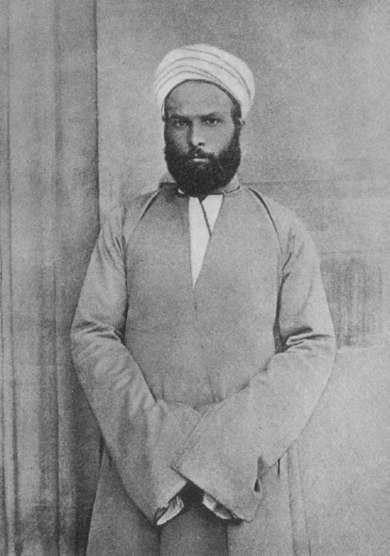
\includegraphics[width=.7\textwidth]{CourantsIslamContemporain/ImagesCourantsIslamContemporain/390px-Muhammad_Abduh.jpg}
       \caption{\href{https://fr.wikipedia.org/wiki/Mohamed\_Abduh}{Muhammad Abduh}}
       \label{fig:my_label}
   \end{marginfigure}
   Surtout en Egypte mais a partagé le séjour parisien de \textit{Aghani} puis au Liban. On lui a interdit d'enseigner mais il a été nommé grand mufti d'Egypte (1899). On avait moins peur de son activité du droit que de son activité sur les jeunes en tant qu'enseignant. Fonde aussi une école qui va évoluer différemment.  
    
    \paragraph{Avancée coloniale plus avancée} La colonisation s'est accentuée : les occidentaux apparaissent comme une menace politique. Peur du colonialisme. Le positivisme s'est aussi accentué. Ils doivent se situer dans le rapport entre Foi et Raison. 
   
   \paragraph{Héritiers du pre-réformisme} En inde en particulier, décadence du monde musulman. beaucoup plus faibles que l'occident, parce que \textit{nous avons perdu l'authenticité de la Foi musulmane}. Pour retrouver notre puissance, il faut retrouver l'authenticité de la pratique et la Foi musulmane.
   
   \paragraph{Mais des différences} Mais la différence avec la pré-reforme, cela passe par la pensée des lumières qu'ils accueillent de façon positive. Importance de la \textit{raison}. Par ailleurs, à la suite de \textit{Guizot}\sn{François Guizot, \textit{Histoire de la Civilisation en Europe}}, il pense l'Islam comme civilisation et pas uniquement comme Religion. Qui dit civilisation implique Progrès. 
   
  
  %----------------------------------------------------------------------------------- 
  \section{Foi et raison}
  
 \paragraph{Renan } Dans un discours retentissant à la Sorbonne, il affirme que les races sémites sont opposées à la Raison.
 
 \paragraph{Réponse d'Afghani} La critique de la religion par le positivisme est fondé, surtout pour le christianisme : Trinité, incarnation, \ldots Et ce qui explique son succès en Occident. En revanche, ce n'est pas vrai en Islam.
 
 \paragraph{Seyyed Ahmad Khan} \label{Theol:AhmadKhan} parfaite adéquation entre la vérité naturelle et révélée. 
 \begin{quote}
    \textit{ Islam is nature and Nature is Islam}
 \end{quote}
 Il ne regarde que le Coran et lecture du Coran à l'aune des vérités naturelles. Lecture allégorique quand le Coran n'est pas cohérent avec la nature. La Loi doit découler de la Loi Naturelle, de la Raison. 
 
 \paragraph{Al Afghani} Un peu en retrait. Il y a adéquation entre la loi naturelle et révélee. Discours \textit{concordiste} \sn{Vision concordiste : très présent aujourd'hui : on trouve en germe toutes les réalités scientifiques (ex : on trouve la vitesse de la lumière, foetus, \ldots). Visée apologétique. Explication rationnelle scientifique des actes musulmans (le jeune du ramadan est bon pour la santé)} mais il dit : 
 \begin{quote}
     Malgré cela, on ne peut pas se passer de la révélation; la Raison de l'homme est entravée par ses Passions . 
 \end{quote}
  La révélation et en particulier le jugement, permet un jugement éthique et moral. 
  
  \paragraph{Muhammad Abduh } Distinguer Raison et révélation, qui se complètent. La Raison peut atteindre les dogmes fondamentaux :  permettre de savoir que Dieu existe, \ldots
  Mais elle ne nous permet pas de révéler le culte ni la raison pratique : ou est le bien, où est le mal ? La vie morale est basée sur la Révélation mais la Raison doit être utilisée pour interpréter la Révélation dans les cas concrèt.
  
  %-----------------------------------------------------------------------------------
  \section{Retour aux sources et \emph{ijtihad}}
  
\paragraph{Ijtihad} Surtout Ahmad Khan et Abduh vont travailler la Sunna avec un regard critique. 
 On retrouve aussi le taqlid (neg) vs ijtihad.
 
\begin{Def}[taqlid]
  \emph{ imitation (servile)}
\end{Def} 
Pour Abduh, le taqlid est lié aux turcs pour soumettre les populations (vision nationaliste arabe), et aussi le soufisme qui a encouragé le taqlid. Les écoles de Abduh sont assez négatives sur le soufisme. \mn{Sahah Hassein ? raconte dans ses mémoires comment dans une école de Abduh, le soufisme était vu de façon négative }. 

\paragraph{Revenir aux sources} Revenir aux temps du Prophète pour reprendre le \textit{principe dynamique} qui était à l'origine, avec une vision positive de la Raison. Il ne s'agit pas d'imiter le Prophète mais de retrouver la dynamique. 

\paragraph{Relecture} des textes du Coran pour repenser le droit (Abdh est jurisconsulte) et en reclassifiant les hadiths. Il revalorise l'opinion personnelle du jurisconsulte (\emph{ra'y}) contre le conservatisme de \emph{l'ijma}. 


\begin{Def}[ijma]

\emph{` consensus des ulamas}
\end{Def} 

\begin{Synthesis}
Il faut chercher l'intention du droit pour rentrer dans un dynamisme juridique
\end{Synthesis}



  %-----------------------------------------------------------------------------------
  \section{L'action: politique et éducation} 
 
Dans le pré-réformisme, on avait vu l'importance de l'action sociale. On a la même perspective ici : il faut agir et transformer la société.

\paragraph{Afghani} est d'abord un homme d'action et politique. Pour retrouver sa grandeur, il faut commencer par émanciper le monde musulman. \textit{Le politique prime}, vision panislamique unifiée (pas forcément un seul état, mais des états coordonnés), émancipée du monde occidental. Risque d'instrumentalisation de l'Islam pour une fin politique.

\paragraph{Renouveau d'abord} avec Kan et Abduh : le peuple n'est pas mur pour être indépendant. Et donc plus conciliants vis à vis des colonisateurs. Avec un discours nationaliste plus que pan-islamique. La priorité était donc \textit{l'éducation}. C'est la raison de la rupture entre Abduh et Afghani. 
\begin{itemize}
    \item Collège d'Aligarh\sn{\href{https://en.wikipedia.org/wiki/Aligarh_Muslim_University}{Université musulmane}} : éducation islamique et ensuite occidentale. En Inde. Une des grandes réalisations d'Ahmad Khan. Creuset de formation de tous les réformistes indiens.
    \item volonté de reforme d'Al Azhar. Il n'a pas réussi mais ses disciples ont réussi à modifier par touches la formation (en revenant aux théologiens à la source)
\end{itemize}

\paragraph{Souveraineté populaire} Il faut éduquer les gens à leurs droits et leurs devoirs pour pouvoir fonder une démocratie. Ils ont une volonté de développer des écoles gratuites mais impact limité. Leur désir de s'engager sur le terrain est un semi-échec.


  %-----------------------------------------------------------------------------------
\hypertarget{glossaire-2}{%
\subsection{\texorpdfstring{{Glossaire}}{Glossaire}}\label{glossaire-2}}


\paragraph{Personnes}

Ibn Taymiyya

Jamal ad-din Al-Afghani (1839-1897) Khayr-ad din Pacha (1820- 1889)

Muhammad `Abduh (1849-1905) Seyyed Ahmad Khan (1817-1898) (prononcer ARMA CRAN)  Shah Walli
Allah

Tahtawi (1801-1873)

\paragraph{Lieux}

Al-Azhar Aligarh

\paragraph{Autres noms propres}

naqshbandi

al-`Urwa

al-Wuthqa

mu`tazilite

nayshariyya

\paragraph{Notions}

\begin{Def}[bid\emph{`}a ]
\emph{: innovation}
\end{Def} 

\begin{Def}[\emph{`}ibadat]

 \emph{ culte ( et partie du droit traitant du culte)}
\end{Def} 
 

\begin{Def}[maslaha]
 \emph{intérêt général, bien commun}
\end{Def} 

\begin{Def}[mu\emph{`}amalat]
  \emph{ relation (et partie du droit traitant des
relations humaines)} 
\end{Def} 



\begin{Def}[qasd]
 \emph{ principe de consultation}
\end{Def} 

\begin{Def}[talfiq]
  \emph{interprétation
éclectique}
\end{Def} 




\hypertarget{muhammad-abduh-1849-1905}{%
\subsection{\texorpdfstring{{Muhammad `Abduh}
(1849-1905)}{Muhammad `Abduh (1849-1905)}}\label{muhammad-abduh-1849-1905}}

Discours évolutioniste.

\begin{quote}
  Quand les religions firent leur apparition, les êtres humains ne
comprenaient leur intérêt, général ou particulier, que de la façon la
plus rudimentaire, plutôt comme des enfants nouveau-nés qui ne
connaissent que ce qui leur tombe sous les sens et ne distinguent
qu'avec difficulté entre le présent et le passé. Ils ne reconnaissent
vraiment que ce qu'ils touchent manuellement et leur état de conscience
ne leur permet pas de "sympathiser" avec leur famille ou leurs
compagnons, tant ils sont obnubilés par leur survie pour pouvoir
s'intéresser aux implications de leur relation aux autres, à moins qu'il
ne s'agisse d'une main qui les nourrit ou les remet sur leur pieds. Dans
ce contexte, les religions ne pouvaient s'adresser intelligemment aux
hommes en abordant les subtiles dimensions de la conscience ou en leur
faisant étalage de preuves rationnelles. Au contraire, la grande grâce
de Dieu se voit dans la manière dont ces religions s'adressèrent aux
peuples comme à des enfants, à la façon de parents qui éduquent leur
enfant avec la plus grande simplicité en se servant des sens de l'ouïe
et de la vue. Les religions prirent les hommes et leur donnèrent des
commandements directs ainsi que des prohibitions fermes exigeant la plus
complète obéissance. Bien que le sens et le but en pouvait être connu,
l'obéissance ne dépendait pas du degré de compréhension ni de
l'exactitude du savoir. Les religions fournirent aussi des miracles
étonnants et impressionnants et imposèrent des formes de culte adaptées
à la condition des hommes.
    
\end{quote}
Les religions (ici surtout le judaisme) sont visées.

\begin{quote}
Au cours des siècles suivants, les peuples connurent grandeur et déclin,
progrès et régression. Ils se querellèrent et se réconcilièrent. Les
siècles apportèrent leur cortège de souffrances et une alternance
ininterrompue de prospérité et d'adversité qui suscitèrent une
sensibilité plus affinée, une conscience plus aiguë que l'on peut
utilement comparer à ce qui se passe dans les cœurs féminins ou à l'âge
de l'adolescence. Une religion survint alors qui parlait à ces
sentiments et, s'adressant tendrement à ces compassions, fit appel aux
doux émois du cœur. Elle donna aux humains les lois sacrées de
l'ascétisme, les éloignant complètement du monde et les tournant vers
une vie plus haute. Elle enseigna aux hommes à ne pas défendre leurs
droits si évidents qu'ils soient et ferma la porte du ciel aux riches.
D'autres traits du même genre caractéristiques de cette religion nous
sont bien connus. Elle établit des formes de culte divin qui
s'harmonisaient avec sa compréhension de l'être humain et le sens de son
message. Elle fut remarquablement efficace pour corriger les défauts et
chasser le mal des âmes qui lui étaient soumises. Mais seulement
quelques générations plus tard, les hommes se lassèrent, s'affaiblirent
et se détournèrent. Ils abandonnèrent ses exigences et ses préceptes les
trouvant au-dessus de leurs forces. Ils se mirent à penser que ces
commandements étaient naturellement impraticables. Même les cadres de
cette religion se mirent à faire concurrence aux rois dans leur autorité
et aux riches oisifs dans leur richesse. La grande masse du peuple
perdit sa noblesse au moyen de "l'interprétation"\sn{sens négatif. Peut être référence à la falsification des écritures, critique des musulmans au christianisme} et, emporté par de
folles passions, introduisit toute sorte d'innovations.
\end{quote}

Dans une logique évolutionniste, le christianisme est un développement.


\begin{quote}
Ainsi se passèrent les choses, tant dans l'activité que dans les
attitudes profondes. La pureté était oubliée et l'intégrité mise aux
enchères. Quant aux dogmes, ils furent infectés par le schisme et
l'hérésie. Les gardiens de la foi en abandonnèrent tous les principes à
l'exception d'un seul qu'ils croyaient - à tort - être le pilier
principal de leur foi et son fondement principal, à savoir
l'interdiction de l'examen rationnel de la foi et même des complexités
de l'univers ou de l'exploration des replis secrets de l'intelligence.
Ils promulguèrent le principe que la Raison et la Religion n'avaient
rien de commun, mais plutôt que la religion était l'ennemi juré de la
Science. Ce principe n'était pas laissé simplement au choix de chacun:
au contraire, ils l'imposèrent énergiquement comme la chose à faire par
tous et chacun. Ils imposèrent la doctrine avec une telle énergie qu'ils
déclenchèrent le plus honteux de tous les conflits de l'Histoire de
l'humanité, à savoir la guerre civile dans la maison de la religion pour
imposer des consignes religieuses\sn{Guerre de Religions}. Ainsi furent détruits les fondements
eux-mêmes et brisées les liens internes à la communauté. La concorde, la
coopération et la paix disparurent: le schisme, la dispute et la
querelle régnèrent à leur place. Ainsi survécut l'humanité jusqu'à
l'avènement de l'islam.
\end{quote}
Dans le Coran, le fait que les chrétiens soient divisés est une preuve que le message est falsifié.

\begin{quote}
Enfin la société humaine atteignit le point où l'homme parvient à sa
pleine stature, à l'aide d'une réflexion morale sur les vicissitudes
passées. L'Islam survint pour présenter son message à la Raison, pour
appeler à l'action l'esprit et l'intelligence, pour prendre l'émotion et
les sentiments comme partenaires afin de guider l'homme vers le bonheur
terrestre aussi bien que céleste. Il mit en lumière les causes des
discordes humaines et démontra que, devant Dieu, la religion était
unique à travers toutes les générations, qu'il n'y avait qu'un seul
projet divin visant à les réformer et à les purifier intérieurement.
L'Islam enseigna que le seul but des formes extérieures de culte était
de renouveler le recueillement intérieur nous centrant sur Dieu et que
Dieu ne regarde pas les apparences mais le cœur. Il demanda au croyant
de s'occuper du corps aussi bien que de l'âme, exigeant l'intégrité
extérieure aussi bien que l'intérieure qu'il rendit également
obligatoires. La sincérité devint le centre du culte et les rites ne
furent imposés que dans la mesure où ils conduisaient à la
sanctification de la personnalité morale.
\begin{quote}
    "En vérité, la prière préserve
les hommes du mal et des souillures". (Cor. 29,45) "L'Homme a été créé
instable {[}très inquiet{]}; quand le malheur le touche, il est abattu;
et quand le bonheur le touche, il est refuseur. Sauf ceux qui pratiquent
la Salat". (Cor 70,19-22) 
\end{quote} 
L'homme riche qui se souvient d'être
reconnaissant est élevé par l'Islam au même niveau que le pauvre qui
souffre patiemment. Peut-être même l'Islam lui porte-t-il une plus haute
estime encore. L'Islam, dans ses exhortations, s'adresse à l'homme comme
un sage et sobre conseiller s'adresserait à une personne mûre pour
l'appeler à mettre en œuvre toutes ses facultés, externes ou internes.
Il proclame sans équivoque que c'est là le moyen de plaire à Dieu et de
Lui montrer notre reconnaissance pour sa Grâce. Ce monde reçoit la
semence du monde à venir. Les hommes ne parviendront à leur fin ultime
qu'en se mettant à bien agir dans le présent.
\end{quote}


\begin{quote}

L'Islam délivra la raison de toutes ses chaînes, il la libéra de
l'imitation aveugle qui l'avait asservie, il lui rendit son domaine dans
lequel elle tranche selon son jugement et sa sagesse ; toutefois elle
doit s'incliner devant Dieu seul et s'arrêter aux limites posées par la
religion; mais au-dedans de ces limites , il n'y a pas de barrière à son
activité et il n'y a pas de fin aux spéculations qui se déroulent sous
ses auspices.

Tiré de M. `Abduh, \emph{Risalat at-Tawhid} (\emph{Traité de l'Unité
divine}, Paris, 1925)
\end{quote}
\begin{Synthesis}
L'Islam est la religion de la maturité, marqué par la raison. Mais l'Islam tient l'équilibre. 
\end{Synthesis}

Equilibre entre : 
\begin{itemize}
    \item entre la Religion de la Raison mais on intègre les sentiments. Le culte extérieur sert le culte intérieur. 
    \item pour les riches et les pauvres
    \item avec la Loi et Raison
\end{itemize}

\begin{Synthesis}[Mouvement moderniste]
Au XIX, le mouvement réformiste intègre la Raison et le Progrès comme des acquis des Lumières. Ces lumières ne sont pas incompatibles avec l'Islam, religion de la raison et les lumières occidentales venant de la Renaissance et de la pensée grecque via la \textit{falsafa}.
Le réformisme est complexe mais ce n'est pas la seule religion pour laquelle c'est compliqué : tension entre le retour aux sources et l'acceptation de la modernité.
'Abdub a été en equilibre et ses disciples vont accentuer le retour aux sources ou au contraire l'accueil de la modernité. 
\end{Synthesis}


\chapter{{Tendances sécularistes et nationalistes}}
  \mn{(14/02/2022)}
 
 \subsection{Bibliographie}
 
  ABDERRAZIQ, Ali \emph{L'Islam et les fondements du pouvoir}, La
  Découverte/ Cedej, Paris, 1994.
 
*BOZARSLAN, Hamit \emph{Histoire de la Turquie contemporaine}, La
Découverte, Repères, 2004. DEVLIN, John F \emph{The Ba`th Party}, Hoover
Institution Press, Stanford, 1979.

FILALI-ANSARY, Abdou \emph{L'islam est-il hostile à la laïcité ?},
Arles, Actes Sud, 2002. HOURANI, Albert \emph{La pensée arabe et
l'Occident,} Groupe Naufal Europe, Paris, 1991.

PISAI « Courants actuels dans l'Islam: le Ba`t », \emph{Etudes Arabes},
n° 63 \& n° 64, 1982-3.
 




\section{Introduction}
\begin{Def}[Sécularisme]
Une évolution juridique et politique vers un modèle Européen, et un affaiblissement des structures religieuses dans l'Etat et la société
\end{Def}

Ce courant va globalement s'imposer jusqu'aux années 1960/70 avec trois courants : 
\begin{itemize}
    \item Elites politiques qui ont grandi dans des écoles occidentales, missionnaires ou réformistes. Ces élites (Ataturk,..) faisant des études en Europe. Ils vont recommander une\textbf{ sécularisation à l'occidentale} (Bourghiba,...). Les deux pays qui n'ont pas été colonisés (Turquie, Iran) ont été les pays qui ont connu la sécularisation à l'occidentale la plus ferme.
    \item les disciples de 'Abduh qui cherchent à penser la \textbf{sécularisation dans le cadre islamique}
    \item rencontre du premier courant avec la \textbf{pensée socialiste} : nationalisme arabe
\end{itemize}
 ~
   %----------------------------------------------------------------
  \section{Le sécularisme d'importation
  occidentale : le modèle
  turc}

  

  
    
    \subsection{Aux racines : les Jeunes Turcs}
Ils vont être moteurs de la révolution constitutionnelle de 1908\sn{La révolution des Jeunes-Turcs de l'Empire ottoman en juillet 1908 est un soulèvement au cours duquel le mouvement des Jeunes-Turcs restaure la Constitution de l'Empire ottoman de 1876 et inaugure la politique multipartite dans un système électoral à deux étapes sous le parlement ottoman.}. 
Les tribunaux religieux sont placés sous la responsabilité du ministère de la Justice (entre 1908 et 18). 
    
      \subsection{La République de Mustapha Kemal}
\paragraph{Mustapha Kemal ou \textit{Atatürk}} Officier charismatique. il s'empare du pouvoir en 1923. Il crée une république à l'image de la France et en devient le chef. Politique très séculariste. 
\begin{itemize}
    \item Rejet du passé Ottoman après la défaite de 1918, qui se serait affaibli via les influences arabes et persanes, et la place que l'Islam y a joué.
    \item  Permet d'éviter les contre-pouvoirs en particulier confrériques. 
\end{itemize}

\paragraph{Soumettre l'Islam au contrôle de l'Etat}
\begin{itemize}
    \item 1924 : Abolution du Califat et expulsion. On crée une présidence des affaires religieuses qui nomme les imams, administre les mosquée, supervise les \textit{muftis}. Les imams sont des fonctionnaires. Le \textit{Diltib}.
    \item unification de l'enseignement (on ferme toutes les institutions religieuses supérieures : medrese) et on crée des Ecoles d'enseignement supérieur pour Imam d'Etat.
    \item 1925 : confréries religieuses sont interdites
    \item 1926 : code civile suisse introduit
    \item 1928 : l'Islam n'est plus religion d'Etat
    \item 1937 : le principe de laicité dans la constitution.
\end{itemize}

Des mesures symboliques : 
\begin{itemize}
    \item 1925 : interdiction du Fez
    \item 1926 : calendrier grégorien, avec dimanche comme jour férié (1935)
    \item 1928 : alphabet latin. 
    \item 1928 : Sainte Sophie devient Musée
\end{itemize}


\paragraph{moderniser l'Islam}

Rapport en 1926 : "perspective scientifique". Vision positiviste
\begin{itemize}
    \item Des mosquées propres avec des bancs
    \item instruments et musiques sacrées (on veut imposer le modèle chrétien)
    \item former les imams à la philosophie et aux sciences occidentales
\end{itemize}

\paragraph{intégrer l'Islam dans l'idéologie Turque}
Cela passe par un islam turc; remplacer l'arabe par le turc. On arrête l'apprentissage l'arabe et le perse. On traduit donc le Coran et la Sunna en Turc (mais il n'est pas utilisé finalement dans le culte). 
En 1932, l'appel à la prière en turc (mais refus de la population et il fait marche arrière).

\paragraph{L'utilisation de l'Islam comme une composante du nationalisme turque} Entre 1923 et 1930, vaste échange avec la Grèce, le critère n'a pas été un critère linguistique mais un critère religieux (chrétien turcophone). 
En tant que population musulmane sunnite, les kurdes ne peuvent être une minorité, seules les populations chrétiennes, juives,... peuvent être considérées comme une minorité. Les alévites ne sont pas reconnus comme une minorité (musulmans = sunnites). De même, la religion est mentionnée sur la carte d'identité. 
\begin{Synthesis}
\textit{une intégration de la religion dans l'Etat} et non une séparation. 
  
\end{Synthesis}

\paragraph{Ziya Gökalp
(1876-1924)}    Un jeune turc penseur de la Turquie d'Ataturk.
  \begin{quote}
Maintenant\mn{Ziya Gökalp Extraits traduits d'un ouvrage hostile au modernisme musulman:

Maryam Jameelah, \textit{Islam and modernism}

(Md Yusuf Khan, Lahore, 1968), 
p. 101-107} la mission des Turcs ne doit être que celle de découvrir le
passé pré islamique Turc qui est resté ancré dans le peuple et y greffer
la civilisation Occidentale dans sa totalité. Pour égaler les pouvoirs
européens militairement et dans les sciences et l'industrie, notre seule
voie de salut est d'adopter la civilisation Occidentale complètement! \sn{(Ziya Gökalp, \textbf{Turkish Nationalism and Western Civilisation},
New-York, 1959, p. 276.)
}

Parmi les Turcs pré-islamiques, le patriotisme a atteint ses niveaux les
plus hauts. Dans l'avenir, comme dans le passé, le patriotisme doit être
le point de moralité le plus important pour les Turcs parce que la
nation et son âme sont en fin de compte la seule unité qui existe de
soi. La fidélité à la nation doit avoir la priorité sur la fidélité à la
famille ou la religion. Le Turkisme doit donner la priorité la plus
haute à la Nation et à la Patrie. Nous créerons une civilisation
véritable - une civilisation Turque qui suivra la croissance d'une
Nouvelle Vie. Classifier les Turcs, qui sont plus justes et plus beaux
que les Aryens, avec la race Mongole n'a aucune base scientifique. La
race Turque n'a pas dégénéré - comme d'autres races, par l'alcool et le
dérèglement des moeurs. Le sang turc est resté jeune et s'est durci
comme l'acier avec la splendeur du champ de bataille. L'intelligence
turque n'est pas usée; ses sentiments ne sont pas affaiblis. On promet
la conquête de l'avenir à la résolution Turque. (Ibid., pp. 302, 271 et
60.)

La civilisation occidentale est une suite de la civilisation de la
Méditerranée antique. Les fondateurs de la civilisation de la
Méditerranée étaient des peuples Turcs comme les Sumeriens, Scythes, le
Phoeniciens et les Hyksos. Il y a eu un Âge Touranien dans l'histoire
avant les âges antiques car les habitants les plus anciens de l'Asie
Occidentale étaient nos ancêtres. Ainsi nous faisons partie de la
civilisation Occidentale et avons part intégrale à cette civilisation.
(Ibid-, pp. 266- 7)

Quand une nation parvient aux étapes les plus hautes de son évolution,
elle trouve nécessaire de changer aussi sa civilisation. Quand les Turcs
étaient des membres d'une tribu nomade en Asie Centrale, ils ont
appartenu à la civilisation de l'Extrême-Orient. Quand ils ont passé à
l'étape de l'état Sultanesque, ils sont entrés dans le secteur de
civilisation Byzantine. Et aujourd'hui dans leur transition à l'état de
nation en tant qu'Etat séculier, ils sont déterminés à accepter la
civilisation Occidentale. (Ibid., pp. 270-1)

La grande erreur des autorités du Tanzimat\sn{Le mouvement des Tanzimat fut le premier essai de
réforme et de modernisation de l'empire Ottoman vers le milieu du
19\textsuperscript{ème} siècle.} était leur
tentative de créer un amalgame mental composé d'un mélange d'Orient et
d'Occident. Ils n'ont pas réalisé que les deux, avec leurs principes
diamétralement opposés, ne pouvaient pas être réconciliés. La dichotomie
présente dans notre structure politique, le système double de tribunaux,
les deux types d'écoles, les deux systèmes de taxation, deux budgets,
les deux jeux de lois, sont tous les produits de cette erreur ... Toute
tentative de réconcilier Orient et Occident conduit à perpétuer des
conditions médiévales dans l'âge moderne et à essayer de les maintenir
en vie. De même qu'il était impossible de réconcilier des méthodes
janissaires avec un système militaire moderne, de même qu'il était
futile de synchroniser la médecine dépassée avec la médecine moderne,
ainsi est-il inutile de continuer, côte à côte, les vieilles conceptions
de la loi et les nouvelles ; les standards moderne d'éthique et les
traditionnels. Chaque civilisation a sa propre logique, ses propres
standards esthétiques, sa propre perspective du monde. Pour cette
raison, des civilisations différentes ne peuvent pas se mélanger
librement l'une avec l'autre. De nouveau, pour la même raison, quand une
société ne prend pas pour système une certaine civilisation dans sa
totalité, il ne réussit pas davantage à en prendre ses composantes. Même
s'il en prend quelques parties, il ne réussit pas à les digérer et à les
assimiler. Nos réformateurs des Tanzimat, qui ont échoué comprendre ce
point, prenaient toujours des demi-mesures dans ce qu'ils ont essayé de
faire. Avant qu'ils n'aient pris de mesures pour moderniser la
production nationale, ils ont voulu changer les habitudes de
consommation, les vêtements, l'alimentation, le bâtiment et les meubles.
D'autre part, on n'a même pas construit un noyau d'industrie digne des
standards européens parce que
les décideurs de la politique des Tanzimat ont essayé leurs réformes
sans en étudier les conditions et sans fixer des buts et des plans
précis. (Ibid., pp. 270-7).

Le but du Turkisme dans la loi est d'établir un système de loi moderne
en Turquie. La condition la plus fondamentale de notre succès à
rejoindre les rangs des nations modernes consiste à effectuer un
nettoyage complet de toutes les branches de notre structure légale pour
y effacer toute trace de théocratie et de cléricalisme. L'état qui est
libre de ces deux caractéristiques de l'état médiéval est appelé un état
moderne. En premier lieu, dans un état moderne, le droit de légiférer et
d'administrer directement appartient au peuple. Aucune fonction, aucune
tradition et aucun autre droit ne peuvent restreindre et limiter ce
droit. En second lieu, tous les membres de la nation moderne,
indépendamment de leur affiliation religieuse, sont considérés comme
égaux en tous points. Bref, toutes les dispositions existant dans nos
lois qui sont contraires à la liberté, à l'égalité et à la justice ainsi
que toutes les traces de théocratie et de cléricalisme doivent être
complètement éliminées. Le Turkisme est un mouvement séculier et ne peut
accepter que des mouvements de nature séculière. (Ibid., pp. 304-5).

C'est seulement au moyen de sa civilisation que l'Europe a été capable
de défaire les nations Musulmanes et est devenue le Maître du monde.
Pourquoi, alors, devons-nous hésiter à adopter cette même civilisation
qui s'est prouvée si capable de réussir ? Notre foi Musulmane ne nous
fait-elle pas un devoir de rechercher toutes les sortes de science et de
savoir comme notre Saint Prophète lui-même nous l'a dit, "Cherchez la
connaissance même si c'est en Chine," et "l'Étude est la propriété
perdue du croyant ; il doit la prendre partout où il la
trouve"?\sn{ Citations de deux hadiths souvent repris par les
apologètes de l'Islam pour montrer la compatibilité de la foi musulmane
avec la science. L'auteur les exploite d'une façon différente pour
inciter les lecteurs musulmans à s'ouvrir aux valeurs occidentales.} Le Japon est considéré comme puissance européenne
mais nous sommes toujours considérés comme une nation Asiatique à cause
de notre retard à accepter véritablement la civilisation européenne.
(Ibid., pp. 266-7).

La terre où l'appel à la prière résonne en Turc et où ceux qui prient
comprennent la signification de leur religion ; la terre où le Coran est
appris en Turc et où chaque homme, grand ou petit, connaît parfaitement
le commandement de Dieu - Ô fils de la Turquie, cette terre est ta
Patrie!


    
\end{quote}
    
    
    \begin{Synthesis}[Ziya Gökalp]
      Il s'appuie sur une analyse raciale typique du XIX, en valorisant la race turque qui est à l'origine de la civilisation occidentale  (Phénicien, Hyksos,...) par rapport à l'abâtardissement arabe ou perse.
      Puis en proposant une vision comparable à l'ère Meiji du Japon, se calant sur l'Occident, sans essayer un mélange, ce qui explique les mesures symboliques pour rompre avec le passé, ainsi que la sécularisation.
      Légitime par l'Islam les choix qu'il pose.
    \end{Synthesis}
    Ils n'ont pas vraiment pensé le culte musulman (cf la proposition des bancs). Pas une véritable articulation entre valeur occidentale et Islam mais en utilisant l'Islam comme un slogan.
    

    
  


 ~
   %----------------------------------------------------------------
  \hypertarget{les-disciples-de-abduh}{%
  \section{\texorpdfstring{{Les disciples de
  Abduh}}{Les disciples de Abduh}}\label{les-disciples-de-abduh}}

  

  
    
      \subsection{Qasim Amin et le statut des femmes (1863-1908)}
    
    \paragraph{Qasim Amin} voyage en France en 1880. Il a été dans le cercle de \textit{Afghani} à Paris. Revient au Caire - Modernisation de l'universation.
    
    \paragraph{1899 - La libération des femmes} Un livre qui va faire un grand remous. Un diagnostic du déclin de la civilisation musulmane, liée à l'affaiblissement des vertus morales et sociales. Il faut donc renforcer l'éducation à la maison qui se fait par les femmes, dont il faut relever le statut. Education féminine jusqu'au primaire pour éduquer les enfants et travailler (seule façon de garantir ses droits dans le foyer). 
    
    \paragraph{voile} Il pose aussi la question du voile intégrale \mn{lire Naguib Mahfouz, \textit{Impasse des deux palais} qui raconte une femme bourgeoise recluse}, qui empêche la femme bourgeoise de travailler et d'avoir un rôle dans l'Espace public.
    
    \paragraph{Interdiction de la polygamie} 'Abduh s'était positionné contre. Plus que 'Abduh, il s'oppose à la répudiation trop facile et prône une égalité de traitement homme / femme. Il a des arguments religieux pour cela.  Le Coran autorise plusieurs femmes à partir du moment où on est parfaitement équitable, ce qui est impossible. 
    
    \paragraph{Une réaction importante} beaucoup d'oppositions et le livre n'aura pas d'impacts à court terme. A noter néanmoins la figure de \textit{Hoda Sha'rawi} première feministe arabe, Egyptienne : Egypte, centre du féminisme arabe.
  
    
      \subsection{Ali Abderraziq et la laïcité (1888-1966)}
    
    \paragraph{Ali Abderraziq} Egyptien, famille liée à 'Abduh, séjour en Angleterre. Carrière de juriste. 
    
    \paragraph{Abolition du Califat en 1926} Il faut nommer un nouveau Calife, le Sherif de la Mecque par exemple. Un congrès au Caire pour réfléchir au Califat.
    \begin{itemize}
        \item Le Califat est légitime et nécessaire
        \item mais actuellement non réalisable du fait de l'impossibilité d'un pouvoir temporel
    \end{itemize}
  
  \paragraph{1925 : L'islam et les fondements du pouvoir } Le Califat n'a aucune légitimité en Islam. Dans le Coran et la Sunna, pas de réalité politique du Califat. Institution humaine imposée par les armes par les successeurs. Mohammed avait un pouvoir de type charismatique, prophétique. Les hommes reconnaissaient son pouvoir par son charisme. Mais pas de volonté de Dieu de fonder un pouvoir politique. Sinon, Dieu aurait indiqué à Mohammed de nommer un successeur. Les successeurs de Mohammed ont imposé un pouvoir royal en imposant un pouvoir politique et religieux.  Fait historique qui a nuit à l'Islam (collusion entre pouvoir politique et savant, Islam de passivité), cela a empêché le développement d'une pensée politique en Islam. 
  
  \paragraph{La shari'a comme prescriptions éthiques} ne fonde pas un système légal.
  
  \paragraph{Dieu ne se soucie pas de la forme politique du Gouvernement}  Les hommes doivent utiliser leur raison pour définir la forme de gouvernement. 

  \paragraph{unité de l'umma ni possible ni souhaitable} un verset "différentes familles... pour les bonnes oeuvres".

\paragraph{Une remise en cause forte de l'Islam} Remet en cause le statut prophétique de Mohammed et les débuts de l'Islam avec un âge d'or (\textit{les califes bien guidés}). Des fatwas de Al-Azhar qui l'interdisent d'enseigner.  Aujourd'hui, des penseurs religieux le relisent en essayant de penser l'interaction entre Islam et les formes de gouvernance. \sn{lire par exemple le livre de Filali-Ansary, \textit{l'islam est il hostile à la laïcité ?}, Marocain. Voir aussi le texte D\textit{iffusion de la pensée réformiste en Egypte : un témoignage}}
 ~
   %----------------------------------------------------------------
  \hypertarget{islam-nationalisme-et-ruxe9volution}{%
  \section{\texorpdfstring{{Islam, nationalisme et
  révolution}}{Islam, nationalisme et révolution}}\label{islam-nationalisme-et-ruxe9volution}}


  
    
      \subsection{Le nationalisme arabe}
    
  
  \paragraph{discours nationaliste arabe 1920-1930} Dans les élites sécularisées, on va penser l'Islam moins comme une religion qu'une \textit{culture}. Ce qui a créé la nation Arabe, sa culture, l'objet de sa fierté collective. 
  
  \paragraph{Un mouvement qui nait au proche et moyen orient} car le référentiel est d'abord arabe, dans des pays avec une faible vision nationaliste.
  
  \paragraph{Agrégation des chrétiens et minorités arabes non islamique} Selon Al-Bazzaz, L'Islam correspond à la moralité naturelle des arabes nomades de cette époque. Et donc tous ceux qui parlent arabes peuvent s'approprier ce passé islamique. Même les chrétiens parce qu'ils parlent arabe, peuvent s'agréger à ce nationalisme arabe.
   
      \subsection{Islam et révolution : la naissance du parti ba`th}


  \paragraph{Figure de Nasser} avec la rencontre du socialisme
   

 \begin{Def}[ba'th] : \emph{résurrection}
\end{Def}
 
 


 
\paragraph{{Michel `Aflaq
(1910-1989)}} 

\begin{quote}
    \mn{{Michel `Aflaq (1910-1989)}Publié dans \textbf{Etudes Arabes}, N° 63, 1982-2, \emph{Courants
actuels du monde arabe, le Ba't}, p. 100-102.}




Le Ba't arabe est apparu, dans la vie récente des Arabes, au milieu de
l'immobilisme, des reniements, de la recherche de l'intérêt personnel et
en pleine désintégration, le Ba't arabe est apparu comme un mouvement de
foi profonde qui polarise les cœurs purs et sains, qui attire les
volontés fortes et sincères, qui regroupe autour de lui les individus
emplis de l'amour de la Nation arabe, ceux qui ont foi en sa grandeur,
ceux qui ne se laissent pas aveugler par ses imperfections d'aujourd'hui
au point de ne plus voir son essence et les potentialités de son avenir,
ceux chez qui les illusions et les difficultés du présent n'ont pas
réussi à étouffer la volonté de travailler à révéler cette essence et à
réveiller ces potentialités. La croissance du Ba't arabe est une preuve
éclatante de foi, et une affirmation des valeurs spirituelles où la
religion prend sa source.

Mais cette qualité même, cette foi qui caractérise le Ba't arabe, c'est
elle qui lui fait comme une loi de se heurter à tous les mouvements qui
nient la foi ou se voilent sous une foi superficielle et contrefaite.
L'avènement du Ba't, il y a dix ans, fut une déclaration de guerre
ouverte au communisme en tant que mouvement matérialiste, négatif et
porteur de haine, et au nationalisme purement verbal qui était de mode,
qui représente la sécheresse, la stérilité et l'incapacité à créer, qui,
voyant dans la situation présente corrompue la vérité négative, perd
ainsi tout pouvoir clé maîtriser cette réalité. De même, il fallait
absolument s'opposer à la religiosité, courante alors, dans laquelle ces
mêmes défauts
se manifestaient. Le Ba't arabe dès sa création a défié ces phénomènes
malsains et les a tous renvoyés à une seule cause, à savoir la perte de
confiance en soi. Ainsi le communisme n'est qu'éveil factice pour ceux
qui ont perdu tout contact avec l'esprit de leur nation, qui ont
désespéré de toute libération qui viendrait de cette nation elle-même et
se sont satisfaits d'une libération qui viendrait de l'extérieur,
factice et suspecte. Le nationalisme avait accepté le mal comme un état
normal, avait pris son parti de l'égoïsme, de la servitude et du
mensonge comme des valeurs stables de la société, parce que se rebeller
contre ces maux eût exigé de lui qu'il fît confiance en la capacité de
la nation à s'en libérer. La piété avait perdu tout lien avec l'esprit
et les élans qui furent dans le passé la source de la religion, et qui
en firent un mouvement de renaissance, de renouvellement et
d'édification. Elle régressa vers un état de léthargie, de conservatisme
et d'obscurantisme, état qui ouvrit la voie toute grande au pharisaïsme
et à l'exploitation.

Le Ba't arabe appela à une conception nouvelle de la vie nationale et de
la vie en général. La base de cette nouvelle conception est la foi dans
les valeurs spirituelles et humanistes, dans la valeur de l'esprit arabe
authentique. Elle se manifeste dans la rupture définitive d'avec les
maux de la réalité présente, dans la lutte contre ces maux sur une route
montante et difficile qui conduira la Nation arabe, lentement et
laborieusement, à retrouver son âme par le moyen de ce combat jusqu'au
sang contre sa situation présente. C'est pourquoi il n'y a plus place,
dans la conception du Ba't arabe, pour quelque sentiment religieux que
ce soit qui n'assumerait pas cette foi exemplaire. Le Ba't arabe, qui
est un mouvement spirituel et actif, ne peut se séparer de la religion
ni se heurter à elle, mais il rompt avec l'immobilisme, l'égoïsme et
l'hypocrisie.

Le Ba't arabe est un mouvement nationaliste qui se tourne vers tous les
Arabes quels que soient leur confession ou leur "rite", qui considère
comme sacrée la liberté de croyance, qui regarde les religions comme
également sacrées et respectables. Mais, à côté de cela, il voit dans
l'islam un aspect national qui joua un rôle important dans la formation
de l'histoire arabe et du nationalisme arabe. Et le Ba't estime que ce
côté national de l'islam est en relation étroite avec l'héritage
spirituel des Arabes et les caractères propres de leur génie. Le Ba't
arabe fut le premier mouvement à mettre ce lien en évidence et à lui
donner sa forme définitive. Il a ouvert par là une crise qui dure encore
et il a sauvé le nationalisme arabe de deux déviations : celle du
nationalisme abstrait qui conduit fatalement à l'artificiel et à la
misère, et celle du nationalisme religieux qui le conduirait à la
contradiction et à la ruine.

Or l'islam, en tant que religion, est égal aux autres religions dans
l'Etat arabe qui traite tous ses citoyens sur un pied d'égalité et
respecte leur liberté de croyance. L'islam en tant que mouvement
spirituel qui a été intimement mêlé à l'histoire des Arabes, qui a été
imprégné de leur génie, qui a permis l'avènement de leur grande
renaissance, cet islam a une place particulière dans l'esprit du
nationalisme arabe, dans sa culture et dans le mouvement de son éveil.
Toutefois, ce rôle n'est absolument pas imposé, mais il naît de la
liberté, de la puissance de l'esprit, de ce que les Arabes sont
extrêmement attachés et en harmonie profonde et totalement libre avec
leur esprit. C'est en ce sens que le mouvement du Ba't arabe cherche
auprès de l'islam inspiration pour son renouvellement et pour sa révolte
contre les valeurs admises dans la société. Il puise à la source de
l'islam la foi, l'idéalisme et le renoncement à l'intérêt personnel et
aux séductions de ce siècle, dans le but de répandre les principes qui
libéreront les Arabes, aujourd'hui, de leur faiblesse, de leur désunion
et de leur bas niveau spirituel et social. Enfin, le Ba't arabe tire du
dynamisme éternel de l'islam\textit{ la force de résister au courant de la
réalité présente,} malsaine, il y trouve un exemple admirable à suivre
pour ce qui est du zèle sincère envers l'intérêt de la Nation, quand il
s'agit de soigner ses maux avec audace, franchise, sans chercher à
flatter à peu de frais les sentiments superficiels, et sans s'appuyer
sur les forces de l'obscurantisme, de la rancœur et de l'asservissement
de l'âme et de la pensée. Le Ba't croit fermement que cette méthode, qui
est en cohérence avec les principes sublimes qu'il proclame, c'est la
méthode à laquelle le succès est assuré, comme ce fut le cas dans le
passé et comme ce le sera toujours.


\end{quote}

\begin{Synthesis}
  Le mouvement Ba'th est un mouvement qui se veut spirituel (antimatérialiste), arabe mais pas islamique (même si la culture arabe en est imprégné).
  La dynamique spirituelle de l'Islam, c'est la \textit{Révolution}. Il faut combattre les institutions religieuses, les savants qui instrumentalisent la religion. 
\end{Synthesis}
 \begin{Def}[inqilâb]  : \emph{révolution}
\end{Def}
\paragraph{Syrie et Irak} Dans ces pays, le parti Ba'th s'est développé. Pas besoin de prôner l'Islam car en prônant la révolution, on trouve l'Islam authentique. D'où la sécularisation de ces pays. Le fait que Assad et Sadame Hussein appartiennent à des minorités religieuses a probablement joué.  
 ~
   %----------------------------------------------------------------
\hypertarget{glossaire-3}{%
\section{\texorpdfstring{{Glossaire}}{Glossaire}}\label{glossaire-3}}


{Personnes}

`Abd ar-Rahman al-Bazzaz Abdullah Cevdet (journal \emph{Içtihad}) Edmond
Rabbath

Kawakibi Michel Aflaq

Muhammad `Abduh Qustantin Zurayq Rashid Rida

Ziya Gökalp

{Lieux}

Al-Azhar

{Autres noms propres} naqshbandi

sheyh ül islam






 


\chapter{{Raidissement : de l'islam politique au salafisme}}
  \mn{(07/03/2022)}
 
 
 \section{bibliographie}
 
\begin{itemize}
\item

  HASSAN AL-BANNA \emph{Five tracts of Hassan al-Banna}, (1906-1949),
  Berkeley, University of California Press, 1978, (180 p.).

\item
  
  MAWDUDI \emph{Comprendre l'islam}, Paris, Association des étudiants
  islamiques en France, 1973.




ADRAOUI, Mohammed-Ali, \emph{Du Golfe aux banlieues : le salafisme
mondialisé}, Paris, PUF, 2013.

BENNOUNE Karima \emph{Votre fatwa ne s'applique pas ici}.
\emph{Histoires inédites de la lutte contre le fondamentalisme
musulman,} Paris, Temps présent, 2018.

NASR, SVR \emph{Mawdudi and the making of Islamic revivalism}, Oxford
university press, 1996.

FEILLARD, Andrée ; MADINIER, Rémy \emph{La fin de l'innocence. L'islam
indonésien face à la tentation radicale de 1967 à nos jours}, IRASEC-Les
Indes savantes, 2006.

GUIDERE, Matthieu \emph{Le printemps islamiste : démocratie et charia},
Paris, Ellipse, 2012. ROUGIER, Bernard (dir.) \emph{Qu'est-ce que le
salafisme ?}, Paris, PUF, 2008.

ROY, Olivier *\emph{Généalogie de l'islamisme}, Hachette, Paris, 1995.

SFEIR Antoine (dir.) \emph{Dictionnaire géopolitique de l'islamisme},
Paris, Bayard, 2009. TERNISIEN, Xavier \emph{Les Frères musulmans},
Fayard, Paris, 2005.
\end{itemize}



 
\section{{Au Proche-Orient arabe} :
  {émergence des Frères
  Musulmans}}

\subsection{Création : De Rashid Rida (1865-1935) à Hasan al-Banna (1906-1949)}

\subparagraph{Rashid Rida (1865-1935) } \label{Theol:Rida} Syrien. Formé de façon traditionnelle et aussi en parallèle occidental. \textbf{Mais ne fait pas le voyage en Europe} à la différence des générations précédentes\mn{On n'a plus besoin d'aller en Europe pour connaître l'occident}. Cela peut expliquer sa méfiance pour l'Europe. En 1997, rejoint le Caire pour se faire disciple d' 'Abduh. Publie \emph{El Manar}, un commentaire coranique, sensé être dans l'héritage de 'Abduh. Il a aussi oeuvré dans les Congrès pour la \textit{restauration des Califats}.

\subparagraph{Hasan al-Banna (1906-1949)} Égyptien. Vient dans une famille de notables ruraux, une famille gagnée par les idées réformistes. Études Coraniques puis études pour devenir Instituteur. Il rencontre une spiritualité soufie qui allie méditation et action \sn{Quelques influences des soufis : la structure des frères musulmans est proche des structures confrériques. Par ailleurs, les frères sont moins opposés au soufisme que d'autres mouvements radicaux}. De façon pragmatique, c'est là qu'il apprend la prédication et la Da'wa. En 1923, il va au Caire pour ses études : choc face au mode de vie occidental. Choc renforcé quand il arrive en 1927 à Isma'iliyya où les moeurs occidentaux sont très forts. 

\paragraph{Création des Frères musulmans et développement rapide} Banna crée en 1929 les \emph{les frères musulmans}, ils font la promesse pour donner leur vie pour ramener les Égyptiens à Dieu (\emph{Da'wa}). Les occidentaux corrompent les Égyptiens et détruisent le système social.15 sections en 1932; 1933 : section féminine et une section de jeunes. \textbf{1936 : un engagement politique, en Egypte et en Palestine}. il est arrêté en 1939 et on suspend ses publications. il est relaché en 1941, mais il continue son activité politique en Egypte et Palestine : 500 000 membres en 1945 et des sections dans les pays avoisinants (Palestine, Syrie, Soudan, Liban). 

\paragraph{Un mouvement clandestin} En 1948, les frères musulmans sont dissous. Banna est assassiné en 1949. Le mouvement continu de façon clandestine.

\begin{Synthesis}
Ils ne sont jamais allés en Occident. Ce ne sont plus des savants de la science coranique, des autodidactes. 
\end{Synthesis}

\paragraph{Défiance vis à vis de l'Occident} A la différence de la génération précédente, qui ne remettait pas en cause la supériorité de la société occidentale, il y a sur cette génération : un rejet du positivisme, de la notion du progrès, des dangers du matérialisme. Il y a même une conviction que l'Occident veut supprimer l'Islam comme système social. Les grands réformistes du XIX étaient sur l'Islam comme \textit{raison}. Alors qu'ici, on est sur une défense de type pragmatique, du cadre juridique traditionnel. Néanmoins, il n'y a pas de refus du progrès technique. \mn{En France, les frères musulmans ont eu une influence importante par les étudiants à partir de 1960. Tariq Ramadan, OEIF ne visent pas à transformer la société française en société islamique mais ont gardé le regard de défiance vis à vis de l'Occident et le regard très positif sur la société musulmane "l'Islamité" comme on parle de "chrétienté" }

\paragraph{ Un islam « radical »} Pour les réformistes, le rapport au source est un rapport \textit{dynamique}. Pour 'Abduh, les ancêtres (Salafs), les débuts de l'Islam va jusqu'au XI (et l'Imam ?), alors que l'on va avoir une tendance à réduire les ancêtres aux premiers califes, largement mythologisés. \textit{ordonner le bien et interdire le mal} Contrôle collectif, chaque musulman est responsable de veiller à ce que les autres musulmans suivent le bien. On raconte que Banna avait créé un commando en primaire pour faire respecter la loi musulmane par la force.

Pour les réformistes, l'Islam doit accompagner l'évolution de la législation, pour \textit{vivre mieux}. Alors que pour cette génération, il faut appliquer la sharia au sens strict.

\paragraph{Un islam actif et mobilisateur} Non seulement conscientiser le peuple via Une importance d'éduquer les masses, mais avec le but d'une orthopraxie islamique : 
\begin{itemize}
    \item Formations (journaux, cercles d'études\sn{ce n'est pas le modèle confrérie mais le modèle évangélique missionnaire}, maisons d'édition, )
    \item Educatif (création d'école : Banna crée une mosquée et une école à chaque section), lieu de formation pour les femmes. Un but de moral, contrer l'influence occidentale.
    \item Jeunesse (type scout). Paramilitaire, prêt à intervenir en Palestine.  
\end{itemize}

\paragraph{Un modèle socio-économique} coopérative de production, centres de santé,... Modèle évangélique. Attention aux besoins du Peuple.
\paragraph{La question du califat et de l'Etat islamique}

    
\hypertarget{hasan-al-banna-1906-1949}{%
\section{\texorpdfstring{{Hasan al-Banna
(1906-1949)}}{Hasan al-Banna (1906-1949)}}\label{hasan-al-banna-1906-1949}}

\begin{Synthesis}[al-Banna]
 
\end{Synthesis}

\paragraph{Extraits du \emph{Message du 5ème congrès} \sn{ (Le Caire, 1951) Cf.
\emph{Etudes Arabes}, n° 61, p. 35-37}
}
\begin{quote}
    Je voudrais vous parler brièvement de la conception de l'Islam et de
l'image qu'en représentent les Frères Musulmans, pour que soit clair et
manifeste le fondement auquel nous invitons et dans lequel nous sommes
fiers de trouver notre point d'attache et notre origine.


1.
  Nous, Frères Musulmans, considérons que les préceptes de l'Islam et
  ses enseignements universels intègrent tout ce qui touche l'homme en
  ce monde et dans l'autre, et que ceux qui pensent que ces
  enseignements ne touchent que l'aspect cultuel ou spirituel, à
  l'exclusion des autres, sont dans l'erreur. L'Islam est en effet foi
  et culte, patrie et citoyenneté, religion et état, spiritualité et
  action, Livre et sabre. Le noble Coran parle de tout cela, le
  considère comme substance et partie intégrante de l'Islam, il
  recommande de s'y appliquer globalement: c'est ce qu'indique ce noble
  verset: "Parmi ce que Dieu t'a donné, recherche la vie future.
  N'oublie pas ta part de ce bas-monde et sois bon comme Dieu le fut
  envers toi " (Cor. 26, 77).
  
 

...

C'est ainsi que les Frères Musulmans ont fréquenté le Livre de Dieu,
s'en sont inspirés et guidés et sont arrivés à la conclusion que
l'Islam, c'était cette conception totale, à portée universelle et qui
devrait régir tous les aspects de la vie; ceux-ci doivent s'en
imprégner, se soumettre à son pouvoir, suivre ses préceptes et ses
enseignements, les prenant comme référence, dans la mesure où la nation
veut être authentiquement musulmane. Mais si la nation n'est musulmane
que dans son culte, suivant pour le reste d'autres modèles, cette nation
passe à côté de l'Islam. Elle ressemble à ceux que Dieu fustige:
"Croyez-vous donc à une partie du Livre et restez-vous incrédules à
l'égard d'une autre?

Quelle sera la rétribution de celui d'entre vous qui agit ainsi, sinon
d'être humilié durant la vie de ce monde et d'être refoulé vers le
châtiment le plus dur, le Jour de la Résurrection? Dieu n'est pas
inattentif à ce que vous faites" (Cor. 2, 85 b).


2.
  De plus, les Frères Musulmans croient que la base et le soutien des
  enseignements islamiques, c'est le Livre de Dieu - qu'Il soit béni et
  exalté! - et la Tradition du Prophète - que Dieu le bénisse et lui
  donne la paix! - si une nation les prend comme règle de vie, elle ne
  saurait s'égarer. Beaucoup de théories et de sciences en contact avec
  l'Islam et qui s'en sont imprégnées portent la marque des époques qui
  les ont vues naître et des peuples qui leur furent contemporains.
  C'est pourquoi il faut puiser les lois islamiques que la nation prend
  pour référence à cette source pure, la source du premier
  jaillissement. Il importe de comprendre l'Islam comme l'ont compris
  les Compagnons et leurs successeurs de bonne souche - que la faveur de
  Dieu soit sur eux! - Il faut nous attacher à ces préceptes divins et
  prophétiques pour ne pas choisir une ligne de conduite hors de celle
  donnée par Dieu, et ne pas imposer à notre époque la marque d'une
  époque non conforme à cette ligne, l'Islam étant la religion de toute
  l'espèce humaine \sn{Élargissement de la Fi'tr qui dit que tout homme est musulman depuis Adam mais élargi à la société}.
\end{quote}

  \begin{Synthesis}
   Une conception holistique et politique.  "L'Islam est en effet foi et culte, patrie et citoyenneté, religion et état, spiritualité et action, Livre et sabre. Langage combatif. 
  Le refus d'une acculturation. 
  \end{Synthesis}
 

\paragraph{La profession de foi des Frères musulmans (début des années 1930)}




\begin{enumerate}
 
\item
  
  Je crois que tout est sous l'ordre de Dieu ; que Muhammad est le sceau
  de toute la prophétie adressée à tous les hommes, que la Rétribution
  {[}éternelle{]} est une réalité, que le Coran est le Livre de Dieu,
  que l'Islam est une Loi complète pour diriger cette vie et l'autre. Et
  je promets de réciter {[}chaque jour{]} pour moi-même une section du
  Coran, de m'en tenir à la Tradition authentique, d'étudier la vie du
  Prophète et l'histoire des compagnons.
  
\item
  
  Je crois que l'action droite, la vertu, la connaissance, sont parmi
  les piliers de l'Islam. Et je promets d'agir droitement en
  accomplissant les pratiques du culte et en évitant les choses
  mauvaises : je me plairai aux bonnes mœurs, j'aurai en horreur les
  mauvaises, je répandrai autant que je peux les usages musulmans, je
  préférerai l'amour et l'attachement plutôt que la rivalité et la
  condamnation, je ne recourrai aux tribunaux que contraint et forcé, je
  renforcerai les rites et la langue de l'Islam et je travaillerai à
  répandre les sciences et les connaissances utiles dans toutes les
  classes de la nation.
  
\item
  
  Je crois que le musulman doit travailler, gagner sa vie, s'enrichir,
  et qu'une part de ses gains revient de droit au mendiant et au
  misérable, et je promets que je travaillerai pour gagner ma vie et
  assurer mon avenir, que j'acquitterai la \emph{zakât} {[}aumône{]} sur
  mes biens en en gardant aussi une part volontaire pour faire la
  charité, que j'encouragerai tout projet économique utile et ferai
  progresser les produits de ma région, de mes coreligionnaires, de ma
  patrie, sans jamais pratiquer l'usure ni l'intérêt ni chercher le
  superflu au-delà de mes capacités.
  
\item
  
  Je crois que le musulman est responsable de sa famille, qu'il a le
  devoir de la conserver en bonne santé, dans la foi, dans les bonnes
  mœurs. Et je promets de faire mon possible en ce sens et d'insuffler
  les enseignements de l'Islam aux membres de ma famille. Je ne ferai
  pas entrer mes fils dans une école qui ne préserverait pas leurs
  croyances, leurs bonnes mœurs. Je lui supprimerai tous les journaux,
  livres, publications qui nient les enseignements de l'Islam, et
  pareillement les organisa- tions, les groupes, les clubs de cette
  sorte.
  
\item
  
  Je crois que le musulman a le devoir de faire revivre l'Islam par la
  renaissance de ses différents peuples, par le retour de sa législation
  propre, et que la bannière de l'Islam doit couvrir le genre humain et
  que chaque musulman a pour mission d'éduquer le monde selon les
  principes de l'Islam. Et je promets de combattre pour accomplir cette
  mission tant que je vivrai et de sacrifier pour cela tout ce que je
  possède.
  
\item
  
  Je crois que tous les musulmans ne forment qu'une seule nation unie
  parla foi islamique et que l'Islam ordonne à ses fils de faire le bien
  à tous ; je m'engage à déployer mon effort pour renforcer le lien de
  fraternité entre tous les musulmans, et pour abolir l'indifférence et
  les divergences qui existent entre leurs communautés et leurs
  confréries.
  
\item
  
  Je crois que le secret du retard des musulmans réside dans leur
  éloignement de la religion, que la base de la réforme consistera à
  faire retour aux enseignements de l'Islam et à ses jugements, que ceci
  est possible, si les musulmans œuvrent dans ce sens, et que la
  doctrine des Frères musulmans réalise cet objectif Je m'engage à m'en
  tenir fermement à ces principes, à rester loyal envers quiconque
  travaille pour eux, et à demeurer un soldat à leur service, voire à
  mourir pour eux.
  
\end{enumerate}


Traduit et cité dans Olivier Carré et Gérard Michaud {[}Michel
Seurat{]}, \emph{Les Frères musulmans} (1928-1982), Paris, Archives
Gallimard/Julliard, 1983, p. 25-26.

\begin{Synthesis}
Un produit de la modernité comme le national catholicisme (Maurras,...) peut l'être dans le cadre Chrétien. 

\begin{itemize}
    \item  importance de la Sunna en plus du Coran.  

    \item  Action droit, vertu, connaissance.  \textit{vie digne}

    \item  Importance de la richesse mais zakat, projet économique. POinte anti-chrétienne ?

    \item éducation : point important
    
    \item législation propre de l'Islam. bannière de l'Islam couvrir le genre humain. Combattre pour cela
    
    \item fraternité musulmane, abolir les divergences entre communautés.
    
    \item Retard des musulmans : éloignement de la religion
    
\end{itemize}
\end{Synthesis}

   



    



    



  \section{{Le théoricien de l'islam
  politique} : {Abu l-a`la al-Mawdudi
  (1903-1979)}}

\begin{Synthesis}[Al-Mawdudi]
Théoricien de l'Etat Islamique. Vision mondiale et vision idéologique, autour de la Loi islamique. Mythification de la Loi islamique.
\end{Synthesis}

\paragraph{ Mawdudi : une vie en rupture} Une grande famille Seyyed, Indienne. Mais famille appauvrie, gagnée par la pensée par  Seyyed Ahmad Khan, son père étudiant à Alighan. Mais Mawdudi doit travailler dès l'age de 15 ans comme journaliste, ne fera pas d'études et ne connaitra pas les soufis à Alighan.

Il a d'abord une vision progressiste. Mais il est choqué par la chute du califat. Et surtout par le projet du Pakistan porté par Iqbal - Jarnah (réformistes). Il est déçu par un état national séparé (panislamique). Il va progressivement rejeté les idées réformistes. En 1929, publie \textit{Al jihad fi-l Islam} et ses livres vont avoir un immense succès. Il va être reconnu comme un penseur musulman à part entière. En 1938, il devient même le doyen à l'Islamiyya College.



\paragraph{L'islam comme idéologie} Il assume que l'Islam est une idéologie, un tout rationnel et englobante, alternative aux idéologies du monde moderne. \begin{quote}
    \ldots un système rationnel \ldots
\end{quote}
Un héritage de Ahmad Khan (cf \pageref{Theol:AhmadKhan}).

Il rejette les 4 écoles juridiques, post salafs. Une dimension morale très mise en avant avec en contrepoint, la civilisation occidentale à combattre. Restaurer la société musulmane. 


\paragraph{L'islam comme utopie politique} C'est de lui que vient l'idée d'une loi parfaite donnée par le Coran. Et l'Islam a réponse à tout (et pas de 4 écoles juridiques). Il s'appuie sur la \emph{hakimmiyya}, Seigneurerie. Réinterprétation du hakimmiyya : Dieu doit régenter tous les aspects de la vie humaine. Il doit tout régenter par sa Loi. Penser que l'Homme peut se donner ses propres Lois, c'est l'associationisme : le \emph{shikr}. La moindre autonomie par rapport à la loi divine, c'est me mettre au niveau de Dieu, et donc associer autre chose à Dieu.
Il n'a pas besoin de savants, qui connaissent parfaitement le corpus. il suffit d'être logique pour déduire la loi islamique du Coran. Rôle donné à quelques uns dont le Calife.

On voit disparaître tous les clivages éthniques, sociaux,... vision idéologique. Il autorise néanmoins les chrétiens à vivre séparément.
Un seul individu, élu sans campagne électoral, assisté par un conseil législatif consultatif, qui vont édifier le corpus juridique musulman. Pas forcément les plus savants. Ce conseil n'est pas élu. pas de vie parlementaire.  Ce qui est très moderne, c'est que c'est l'Etat qui doit assurer l'homogéneité (cf fascisme ou communisme).
Etat mondial islamique.

En 1941, il crée le \href{https://fr.wikipedia.org/wiki/Jamiat-e_Islami}{jamiat'i islami} , avec des degres d'initiation. Dès la création du Pakistan, il vise à transformer le pays pour l'islamiser. 1977 : \href{https://fr.wikipedia.org/wiki/Coup\_d\%27\%C3\%89tat\_du\_5\_juillet\_1977\_au\_Pakistan}{coup d'Etat au Pakistan}  qui instrumentalise Mawdadi en islamisant une partie du droit. 

\paragraph{L'action politique de Mawdudi}

   A la fin de sa vie, a été invité comme professeur à la Mecque et Médine. Connexions avec le wahhabisme.




\paragraph{Textes de Abu l-a'la al-Mawdudi
(1903-1979)}

La situation actuelle devant laquelle nous nous trouvons est, en résumé,
la suivante: les gouvernements refusent de suivre la route que la
Communauté musulmane veut suivre, et la Communauté musulmane refuse de
suivre la politique que poursuivent les gouvernements. D'où une lutte
continuelle et acharnée entre les peuples et les gouvernements, dans
tous les pays musulmans. L'Islam contemporain, c'est cela. Des efforts
colossaux sont déployés pour transformer les musulmans en non-musulmans,
et pour cela, tous les moyens possibles sont employés.

D'une façon particulière, le domaine de l'instruction et de l'éducation.
On se sert de méthodes qui sont de nature à condamner toutes les valeurs
islamiques des musulmans, à corrompre leurs mœurs et leurs goûts, à les
détourner de leur héritage culturel et de leurs traditions; elles les
encouragent à suivre une culture qui détruit ce qui reste de leur
morale, et elles répandent chez eux les disciplines occidentales,
destinées à créer en eux des doutes sur l'Islam. Le fin mot de
l'affaire, c'est que les musulmans se trouvent soudain atteints de
faiblesse, de défaillance et d'impuissance, et qu'ils deviendront un
peuple qui a perdu sa personnalité. Et cela n'est pas impossible. Mais
ce qui est impossible, c'est qu'ils renoncent délibérément à l'Islam et
qu'ils créent volontairement un Etat irréligieux.

Quant aux conséquences désastreuses de cette lutte pour les pays
musulmans, il suffit, pour en mesurer l'étendue, d'examiner la part
qu'ont prise ces pays au mouvement de la Renaissance. Voyons- nous un
seul domaine de la vie touché par le progrès? La Turquie, par exemple,
Etat indépendant doté de la souveraineté depuis 1924, jusqu'à quel point
a-t-elle réussi à développer son industrie? A quel stade est-elle
arrivée dans le domaine du commerce? alors que le Japon, qui a atteint
l'indépendance en même temps que la Turquie, est parvenu à un niveau
incroyable de développement matériel. La cause de cette situation ne
saurait échapper aux gens intelligents. La Turquie a dévié de la bonne
route et s'est tournée vers le champ clos de la lutte interne. Ses
gouvernements successifs ont essayé de faire apparaître le peuple turc
comme un peuple non-musulman; mais le peuple turc a refusé de se
transformer en un peuple non-musulman. Au contraire, il a voulu tourner
sa face vers l'Islam, ce qui a déclenché une lutte continuelle et
furieuse entre le gouvernement et le peuple. Comment la Turquie, après
cela, poursuivrait-elle sa marche en avant et s'assurerait-elle le
progrès matériel? La situation a atteint son paroxysme ces derniers
temps, quand la rupture s'est étendue à l'armée elle-même: à ce jour,
six mille officiers ont été relevés de leurs fonctions. Et ce qui est
dit de la Turquie peut être dit également des autres pays musulmans.

Soyez-en sûrs, mes frères! Partout où il y a conflit, lutte entre la
conscience du peuple et la politique du gouvernement, la stagnation y
plante ses griffes, elle empêche le peuple d'avancer, ne serait-ce que
d'un pouce, et les pas du progrès ne se dirigeront pas vers lui. Aucun
gouvernement ne peut promouvoir la force et le bien-être, sans qu'il y
ait harmonie et union entre la conscience du peuple et la politique de
ce gouvernement, de telle sorte que, quelle que soit la politique du
gouvernement, elle soit sanctionnée par les sentiments et les
aspirations du peuple. Et quand cette politique est mise on œuvre, le
peuple déploie tous ses efforts pour la faire réussir.

C'est là le seul moyen de faire du peuple un peuple actif et vigilant.
Mais dans le cas contraire, lorsque le peuple est coupé du gouvernement,
il ne bénéficie pas du moindre progrès. Il est à présumer que le peuple,
même si le gouvernement ne lutte pas pour réaliser ses aspirations, ne
se soulèvera pas contre lui; mais que le peuple s'abstienne d'assister
et de soutenir le gouvernement, cela suffit à conduire le pays vers une
catastrophe certaine. L'insatisfaction du peuple à l'égard de son
gouvernement est donc une chose grave en soi et une situation
inquiétante.

Si ces gens (du gouvernement) persistent à aller à contre-courant, c'est
uniquement par égoïsme, égocentrisme et soumission au pouvoir des
passions. Ils n'ignorent pourtant pas ce que veut le peuple. De plus,
leur expérience passée est la meilleure preuve que ce peuple ne s'est
secoué et n'a joué son rôle héroïque dans les batailles pour la
libération qu'au nom de l'Islam. Ce sursaut du peuple, qui découle de
l'Islam, a conduit les musulmans aux rivages de la liberté et à tenir
une position de force. C'est pourquoi, ces gens-là n'ignorent pas
l'attachement sûr et solide de leur peuple à l'Islam. Mais ayant lié
leur destinée et celle de leurs enfants à l'Occident, à sa civilisation
et à ses mirages, s'étant plongés dans la civilisation occidentale et
ayant mis son empreinte sur leurs coutumes et leurs goûts, ils ne
veulent pas suivre le chemin de l'Islam, et leur égoïsme les empêche
d'agir en musulmans. La logique sur laquelle ils s'appuient est la
suivante: ils ont reçu mission de gouverner leurs peuples déshérités et
malheureux, en toutes circonstances; or l'Islam, religion de ces
peuples, ne leur plaît pas; donc les peuples doivent abandonner l'Islam.
Voilà la règle universelle qu'ils ont adoptée comme fondement de leurs
activités et de leurs orientations.

Tel est l'Islam aujourd'hui. J'essaierai maintenant de définir
brièvement ce que devrait être l'Islam demain.


\hypertarget{lavenir-du-monde-musulman}{%
\subsection{L'avenir du monde
musulman}\label{lavenir-du-monde-musulman}}


L'avenir du monde musulman dépendra de l'attitude que les musulmans
adopteront envers l'Islam. Si le monde de l'Islam s'en tient à son
attitude actuelle, faite d'hypocrisie, de déguisement et de duplicité,
s'il persiste dans son attitude hostile à l'Islam, je crains que les
peuples musulmans ne soient pas capables de maintenir leur indépendance
ni de la préserver de la ruine; au contraire, ils tomberont une deuxième
fois - ce qu'à Dieu ne plaise!- dans les fers de l'esclavage, et ils
iront à la rencontre d'une condition pire que celle dans laquelle ils
ont vécu précédemment, pendant la période de l'esclavage.

Oui, si ceux qui tiennent les rênes du pouvoir dans le monde musulman
retrouvent le droit chemin avant qu'il ne soit trop tard, et s'ils
travaillent à ramener la véritable vie démocratique, si le pouvoir
d'élire les dirigeants fait retour aux masses, de telle sorte qu'elles
puissent choisir qui elles veulent et confier librement les rênes du
pouvoir à ceux qu'elles aiment, et si l'ordre politique, l'économie,
l'enseignement sont en harmonie avec les principes de l'Islam, avec ses
objectifs et sa civilisation, alors je suis convaincu que les peuples
musulmans deviendront très vite une grande puissance dans le monde,
qu'ils seront capables de contrôler le pouvoir dans les instances
internationales et d'avoir le dernier mot.

L'existence du bloc des peuples musulmans ne doit pas être sous-estimée.
Ce bloc, qui s'étend de l'Indonésie à l'est jusqu'au Maroc à l'ouest,
qui est doté de moyens et de possibilités incommensurables, qui jouit
d'un capital énorme de main d'œuvre, s'il se met à suivre les principes
de l'Islam et à agir en commun en s'appuyant sur ce dernier, y aura-t-il
une force, que ce soit dans le monde occidental ou dans le monde
oriental, capable de lui résister ?

Extrait de son livre \emph{al-Islam al-yawm} (l'Islam aujourd'hui)

Trad. Roberto Bellani, parue dans \emph{Etudes Arabes}, n° 52, p. 81-83.

\section{Programme des Frères Musulmans (1936)}

Après avoir étudié les sentiments qui doivent animer, sur le plan
spirituel, la nation renaissante, nous voulons en conclusion, exposer
certaines suggestions d'ordre pratique. Nous n'évoquerons ici que les
têtes de chapitres car nous savons pertinemment que chaque suggestion
nécessite une étude approfondie et l'attention particulière des
spécialistes; nous savons par ailleurs que les besoins de la nation sont
énormes; nous ne croyons pas que la réalisation des besoins et des
desiderata du pays soit chose facile; nous ne pensons pas non plus que
cette réalisation se fera en une journée ou deux. Nous avons conscience
des difficultés que ces besoins vont surmonter. La tâche nécessitera
beaucoup de patience, beaucoup de sagesse et une volonté tenace.

Mais une chose est certaine: la volonté mènera au succès. Une nation
décidée, œuvrant pour la réalisation du droit, arrivera certainement
avec l'aide de Dieu au but qu'elle désire.

Voici les têtes de chapitres de la réforme fondée sur le véritable
esprit de l'Islam:

I. Dans les domaines politique, juridique et administratif

\begin{enumerate}
\def\labelenumi{\arabic{enumi})}
\item
  interdire les partis et orienter les forces de la nation vers 1a
  constitution d'un front unique;
\item
  réformer le droit en vue de l'adapter entièrement à la législation
  islamique;
\item
  renforcer l'armée, augmenter le nombre des groupements de jeunesse;
  inculquer à cette jeunesse, en partant de l'esprit de la guerre
  sainte, la foi et l'abnégation;
\item
  renforcer les liens entre les pays islamiques et plus particulièrement
  entre les pays arabes, étape nécessaire à l'examen sérieux de la
  question du « Khalifat » défunt;
\item
  propager l'esprit islamique au sein de l'administration afin que tous
  les fonctionnaires ressentent le besoin d'appliquer les enseignements
  de l'Islam
\item
  surveiller la conduite personnelle des fonctionnaires car le côté
  privé et la vie administrative de ces fonctionnaires forment un tout
  inséparable;
\item
  avancer les horaires du travail en été et en hiver, en vue de
  faciliter l'accomplissement des obligations religieuses et en vue
  d'interdire toute veillée inutile;
\item
  condamner la corruption et le trafic des influences; ne doivent
  rentrer en ligne de compte que la compétence et le mérite;
\end{enumerate}

\begin{enumerate}
\def\labelenumi{\arabic{enumi})}
\item
   
  le gouvernement agira conformément à la loi et aux enseignements
  islamiques; l'organisation des cérémonies, des réceptions, des
  réunions officielles, le régime des prisons et des hôpitaux ne doivent
  pas être contraires aux prescriptions de l'Islam. Le roulement dans
  les services doit tenir compte des heures de prières;
   
\end{enumerate}

\begin{enumerate}
\def\labelenumi{\arabic{enumi})}
\setcounter{enumi}{8}
\item
  préparer et utiliser les « azharistes », c'est‑à‑dire les diplômés de
  l'Université d'al‑Azhar aux fonctions militaires et administratives.
\end{enumerate}

II. Dans les domaines social et pratique:

\begin{enumerate}
\def\labelenumi{\arabic{enumi})}
\item
   
  le peuple doit respecter les mœurs publiques: celles‑ci doivent faire
  l'objet d'une sollicitude toute particulière --- sanctionner
  sévèrement les atteintes aux mœurs et à la moralité;
   
\item
   
  trouver une solution aux problèmes de la femme, solution susceptible
  de la faire évoluer et de la protéger conformément aux enseignements
  islamiques. Cette très importante question sociale ne doit pas être
  négligée car elle ferait l'objet de polémiques et d'opinions plus ou
  moins tendancieuses et exagérées;
   
\item
   
  se débarrasser de la prostitution clandestine ou publique et
  considérer la fornication comme un crime abject dont les auteurs
  doivent être punis;
   
\item
   
  prohiber tous les jeux de hasard (jeux, loteries, courses, clubs);
   
\item
   
  interdire l'usage de l'alcool et des stupéfiants ---il faut éloigner
  le peuple de leurs conséquences néfastes;
   
\item
   
  interdire les manifestations portant atteinte à la pudeur, éduquer les
  femmes, donner aux institutrices, élèves, étudiantes, doctoresses, une
  éducation soignée...;
   
\item
   
  prévoir les programmes d'enseignement destiné aux filles ---élaborer
  pour elles un programme d'éducation différent du programme destiné aux
  garçons;
   
\item
   
  les étudiants ne doivent pas être mêlés aux étudiantes--- toute
  relation entre un homme et une femme non mariés est consi­dérée comme
  un crime devant être sanctionné;
   
\item
   
  encourager le mariage et la procréation---élaborer une législation
  sauvegardant la famille et trouvant une solution au problème du
  mariage;
   
\item
   
  fermer les salles de bal, interdire la danse, etc.;
   
\item
   
  censurer les pièces de théâtre et les films, choix sévère des pièces
  et des films;
   
\item
   
  contrôler et choisir les chansons;
   
\item
   
  choisir les conférences, chants et sujets devant être diffu­sés,
  utiliser la radiodiffusion en vue de l'éducation nationale
   
\item
   
  confisquer les pièces et livres malsains, et les journaux ayant un
  caractère grotesque et diffusant des frivolités
   
\item
   
  organiser méthodiquement des centres de vacances;
   
\item
   
  modifier les heures d'ouverture et de fermeture des cafés publics,
  surveiller l'activité des clients qui les fréquentent --- orienter ces
  clients vers le bien, interdire de passer beaucoup de temps dans ces
  cafés;
   
\item
   
  utiliser les cafés comme centres de lecture et d'écriture pour les
  analphabètes, solliciter pour cela le concours des mem­bres de
  l'enseignement primaire et des étudiants;
   
\item
   
  combattre les mauvaises habitudes qui nuisent à l'éco­nomie et à la
  morale de la nation, orienter les masses vers les bonnes habitudes et
  les buts louables tels que les réunions de mariages, les orphelinats,
  les naissances, les manifestations et fêtes le gouvernement en doit
  donner l'exemple;
   
\item
   
  faire juger ceux qui enfreignent les lois de l'Islam, qui ne jeûnent
  pas, ne prient pas, qui insultent la religion, etc.;
   
\item
   
  transférer les écoles primaires des villages à la mosquée et y faire
  toutes les améliorations (recrutement de fonctionnaires, questions
  d'hygiène, intérêt porté aux petits enfants qui doivent apprendre la
  prière, initiation des grands à la science);
   
\item
   
  l'enseignement religieux doit constituer la matière essen­tielle
  destinée à être enseignée dans tous les établissements ainsi qu'aux
  facultés;
   
\item
   
  faire apprendre par cœur le Coran dans les écoles libres ---cette
  condition est essentielle pour l'obtention des diplômes de caractère
  religieux et de caractère philosophique --- dans toute école, on doit
  faire apprendre aux élèves une partie du Coran;
   
\item
   
  élaborer une politique destinée à élever le niveau de l'enseignement,
  à unifier les différentes branches de l'enseignement, à rapprocher les
  différentes branches de culture --- la morale et l'instruction civique
  doivent être enseignées en premier lieu ;
   
\item
   
  intérêt porté à l'enseignement de la langue arabe à tous les échelons
  --- priorité absolue accordée à la langue arabe sur les autres langues
  étrangères (enseignement primaire);
   
\item
   
  étudier l'histoire de l'Islam, celle de la nation, et celle de la
  civilisation musulmane;
   
\item
   
  étudier le meilleur moyen permettant aux gens de s'ha­biller
  progressivement d'une manière identique;
   
\item
   
  combattre les habitudes étrangères (domaine du voca­bulaire,
  habitudes, vêtements, nurses, nourrices, etc.) égyptiani­sation de
  tout (on trouve ces habitudes étrangères dans les classes aisées de la
  société);
   
\item
   
  orienter le journalisme vers le bien, encourager les écri­vains et les
  auteurs qui doivent étudier des sujets spécifiquement musulmans et
  orientaux;
   
\item
   
  sauvegarder la santé publique par tous les moyens de propagande ---
  augmentation du nombre des hôpitaux --- des médecins, des centres de
  santé ambulants;
   
\item
   
  porter une attention particulière aux questions et affaires du village
  (organisation, hygiène, filtrage des eaux, éducation, repos,
  moralité).
   
\end{enumerate}

 
III. Domaine économique:
 

\begin{enumerate}
\def\labelenumi{\arabic{enumi})}
\item
   
  organisation de la « Zakat », conformément à la législa­tion
  islamique, utilisation des fonds de la Zakat dans des buts de
  bienfaisance tels que les asiles d'indigents, de pauvres, orphelins,
  on doit utiliser également les ressources de la Zakat pour le
  renfor­cement de l'armée;
   
\item
   
  interdiction de pratiquer l'usure, orienter les banques vers cette
  interdiction, le gouvernement doit donner l'exemple en abandonnant 1'
  « intérêt » fixé par les banques du prêt et du prêt industriel, etc.;
   
\item
   
  encourager et augmenter le nombre des institutions éco­nomiques, y
  employer les chômeurs, utiliser au profit de la nation les biens que
  possèdent les étrangers dans ces institutions;
   
\item
   
  accorder certaines protections aux ouvriers contre les sociétés
  possédant des monopoles d'exploitation, obliger ces sociétés à obéir à
  la loi, le public doit profiter de tout bénéfice;
   
\item
   
  amélioration du sort des petits fonctionnaires et augmen­tation de
  leurs traitements, abaissement du traitement des hauts fonctionnaires;
   
\item
   
  réduire le nombre de postes destinés aux fonctionnaires, se contenter
  des emplois indispensables au pays, la répartition du travail parmi
  les fonctionnaires doit être faite d'une façon équitable;
   
\item
   
  encourager les travaux agricoles et industriels, amélio­ration de la
  situation du fellah et de l'artisan (dans le domaine de la
  production);
   
\item
   
  attacher une attention particulière aux besoins techniques et sociaux
  des ouvriers, élever leur niveau de vie et améliorer leur sort
   
\item
   
  exploitation de certaines ressources naturelles (terres non labourées,
  mines ignorées, etc.);
   
\item
   
  priorité accordée aux projets dont la réalisation est nécessaire au
  pays.
   
\end{enumerate}

Telle est la profession de foi que nous vous présentons: nous sommes
décidés à obéir et à remettre tout ce que nous possédons à n'importe
quelle organisation ou gouvernement décidé à conduire la nation
musulmane au progrès.

Nous répondrons à tout appel, nous serons des volontaires en toute
circonstance. Nous aurons ainsi accompli notre mission et dit ce que
nous avions à dire.

La religion appartient à Dieu, à Son Prophète, à Son Livre, aux Imams et
à la Communauté. Dieu nous suffit.

Extrait d'une brochure de 1936, \textbf{Vers la lumière},\\
traduite de l'arabe par J. Marel et parue dans \textbf{Orient}, N° 4,
1957, p. 37-62\emph{.}




\section{Les Frères musulmans égyptiens : pour une critique des vœux pieux}

 
\mn{Tewfik Aclimandos} 




Intégrer les islamistes modérés est un impératif si l'on souhaite une
transition démocratique. La modération est définie par certains
critères, et des experts affirment que certains islamistes les
remplissent, dont les Frères musulmans. Cet article tente de démontrer
que pour ce qui concerne ces derniers, le cas est pour le moins
discutable. À travers l'étude de leur discours, l'analyse de leurs modes
et dynamiques de socialisation, de leurs pratiques et leurs idéologies,
on peut souligner la dimension sectaire, et montrer que la séparation --
néces- saire à une véritable démocratisation -- entre prédication et
action politique est bien loin d'être réalisée. On critique finalement
les paradigmes optimistes mobilisant une ruse de la raison.

\textbf{U}n jihadiste hostile aux Frères musulmans, Hânî al Sibâ'i,
affirmait un jour que « les capitales occidentales rêvent d'islamistes
ayant renoncé à la charia et reconnaissant Israël 1 ». Il ajoutait que
les Frères, étant opportunistes, feraient

volontiers ces concessions pour accéder au pouvoir. De nombreux
chercheurs et experts semblent avoir le même rêve. Reste à savoir si,
opportunistes ou non, les Frères sont prêts à faire des concessions. La
solution idéale à la « crise » des régimes arabes, nous expliquent un
nombre croissant de « transitologues 2 » et
de spécialistes de l'islamisme 3, serait l'intégration dans d'éventuels
processus démocratiques de formations islamistes ayant accepté le cadre
de l'État natio- nal et les règles du jeu démocratique, renoncé à la
violence et à l'application des dispositions les plus controversées de
la charia, et reconnu l'existence de l'État d'Israël. Mais cela est-il
possible ?

Sans prétendre formuler un modèle valable pour toutes les configurations
islamistes, je tenterai ici de décrire ce que je sais des Frères
musulmans égyptiens. Je voudrais tester les propositions énoncées plus
haut, fruits de la rencontre de la transitologie, de l'agenda de la
première administration Bush et d'un certain type d'analyse de
l'islamisme, qui s'agrègent désormais dans une sorte de « savoir
conventionnel » s'exprimant dans la presse, les \emph{policy briefs} et
les revues scientifiques, \emph{Foreign Affairs} n'étant pas la moindre.
Ce « savoir conventionnel » se retrouve dans certains cercles
intellectuels de gauche qui prônent un dialogue des civilisations ou un
respect inconditionnel, excluant toute critique de « la religion des
dominés », et érigent les islamistes en représentants de l'islam (on
pense à l'extrême gauche, ou à des intellectuels proches de la revue
\emph{Esprit}). Ce savoir doit être précisé, nuancé ou réfuté. Il faut
auparavant poser des questions élémentaires de méthode, relatives aux
matériaux et aux données disponibles, et réfléchir à leur mode d'emploi
et à la construction de « modèles explicatifs » de la confrérie. Je
résumerai à cette fin ce que l'on sait aujourd'hui des Frères, de leur
organisation, de leur idéologie, puis j'exposerai mes vues sur le débat
en cours. Mes assertions principales sont simples, mais oubliées : avant
de spéculer sur les évolutions possibles, il convient de tenter une
phénoménologie de la confrérie, d'autant plus que cette dernière est un
« donné massif » et donc difficile à manier par décret. Celle-ci semble
induire une « socialisation sectaire », au sens sociolo- gique du terme,
impliquant une socialisation en interne, combinée à une mise à distance
et une dépréciation du réel, que l'on subjectivise en une construc- tion
manichéenne. Il convient aussi d'étudier les textes doctrinaux de la
confré- rie, et la littérature qu'elle produit. Si on ne peut deviner ce
que son lectorat en pense, l'on peut au moins affirmer qu'elle le
marque, et qu'elle reflète au moins la pensée réelle des auteurs.
 

\hypertarget{discours-des-fruxe8res-les-positions-publiques}{%
\section{Discours des Frères : les positions
publiques}\label{discours-des-fruxe8res-les-positions-publiques}}

 
Les analyses sur les Frères aujourd'hui se fondent essentiellement sur
l'étude des discours produits par la confrérie et ses cadres, en plus de
la rituelle mention de son travail social et d'indications assez
sommaires sur le profil sociologique et la supposée psychologie des
militants 4.
Mais quels discours étudie-t-on ? Le plus souvent le programme des
Frères, leur plateforme électorale et les déclarations de ceux qui sont
omniprésents dans les divers espaces médiatiques. L'exégèse subséquente
tend à se féliciter de l'acceptation progressive de la démocratie, à
souligner la « normalité » des Frères -- une force politique « comme les
autres » --, à relever toutes sortes d'in- dices montrant des « progrès
» ou, au contraire, des « manques », des « lacunes » et des «
régressions » 5, expliqués par la présence aux postes clés de théocrates
très vilains et très âgés 6, par la tentative du sommet de préserver la
cohésion interne de la formation et de tenir compte de ce que la base
peut accepter 7, ou par le fait que les régimes arabes ont les
islamistes qu'ils méritent (plutôt que l'inverse) 8.
« d'optimisme » qui parie sur une « ruse de la raison » donnant à
l'action islamiste un « sens » dont les acteurs sont ou ne sont pas
conscients, et qui surestime la portée de toutes sortes de phénomènes
décrétés « nouveaux ». Cette remarque cible deux excellents auteurs,
Patrick Haenni et Raymond W. Baker (dans \emph{Islam without fear. Egypt
and the New Islamists}, Cambridge, Harvard University Press, 2003, ou
encore dans « Invidious comparisons : realism, postmodern Globalism and
centrist Islamic movements in Egypt », \emph{in} J. L. Esposito (ed.),
\emph{Political Islam : Revolution, Radicalism, or Reform ?}, Le Caire,
AUC Press, 1997. Ces deux auteurs ont tendance à ne pas voir qu'une
culture arabe a existé au XXe siècle et que sur ce plan les islamistes
représentent, pour l'instant, une régression. Enfin, les discours
scientifiques sur les islamistes ont en commun d'expliquer l'émergence
de la mouvance par une crise grave de leur société, que l'on décrit ou
construit différemment selon les cas. La revue de littérature proposée
par Haydar Ibrâhîm `Ali, dans son ouvrage \emph{Les courants islamiques
et le problème de la démocratie} {[}en arabe{]}, Beyrouth, Centre
d'études pour l'unité arabe, 1996, fournit des analyses précieuses.
En se contentant d'analyser les positions publiques, on risque la
méprise, surtout sans travail de contextualisation -- or l'entreprise
est difficile car la confrérie, illégale, garde ses secrets. J'affirme
cela en rappelant que l'actuel programme de la confrérie renforce les
thèses des sceptiques (dont je suis). J'admets volontiers qu'il faille
prendre les plateformes et les déclarations des principaux dirigeants,
comme étant \emph{souvent} un indicateur de ce que la confrérie veut
dire (ou faire croire) à ses militants et ses interlocuteurs, bien
disposés ou hostiles, ou de ses priorités du moment, ou encore qu'il
faille les considérer comme l'enjeu et le résultat de luttes intestines,
débouchant soit sur la victoire d'une tendance, soit sur une motion de
synthèse qui perd de vue le destinataire du message. Il est plus délicat
d'y voir une preuve de ce que la confrérie pense, de ses conceptions, à
moins d'estimer qu'elle change sans arrêt d'avis sur toutes sortes de
questions, ou a sur chacune une trentaine d'opinions, ou encore que les
rapports de force en son sein sont très fluctuants, alors même que les
démissions et les modifications des équipes dirigeantes sont rares.
Admettons -- ce que je ne fais pas -- que ces textes soient des
programmes de gouvernement qui engagent ceux qui les émettent : que
fait-on alors quand on y est confronté à la « quadrature du cercle 9 »
ou à des propositions contra- dictoires (par exemple sur la citoyenneté,
le statut des minorités, les libertés publiques, la femme, la
souveraineté) ? La réponse est désolante : chacun retient ce qui
l'arrange et minimise ce qui le dérange (cela vaut aussi pour moi). Cela
dit, on peut suggérer une clé qu'impose le bon sens, sinon en général,
du moins dans le contexte égyptien (où les élections ne se décident pas
sur des programmes et où la revendication démocratique arrive très loin
derrière le chômage, la qualité et le coût de la vie, la corruption dans
les préoccupations de la population 10) : si la confrérie formule des
propositions qui déçoivent tous ses interlocuteurs des microcosmes
politiques et intellectuels, et qui risquent de porter atteinte à son
image, il y a lieu de penser qu'elle -- ou au moins les rédacteurs et
ceux qui ont entériné les textes -- est sincère, puisqu'on ne peut
supposer, sans insulter leur intelligence, qu'ils s'attendaient à autre
chose.

L'étude des positions publiques pose plusieurs problèmes. Expédions le

premier : qui engage la confrérie ? Ici on donne une réponse simple : le
Guide et les deux Vice-Guides. Mais cette réponse n'élimine pas le
problème des volte-face. Le second problème est relatif à la place des
contextes : parler au Parlement, ce n'est pas s'adresser à un
journaliste. Les contextes sont certes une variable significative, mais
ils ne doivent pas forclore toute réflexion sur l'essence éventuelle du
mouvement 11. De plus, les contextes ne sont jamais \emph{connaissables}
avec certitude par un chercheur isolé. La violence islamiste ne peut
être traitée comme une simple « réponse » à une répression étatique :
elle a souvent précédé celle des régimes, notamment ceux de Farouk et de
Sadate,

et l'œuvre de Qutb est certes une réaction à la sauvagerie des services
de Nasser, mais elle est aussi une « systématisation », une mise en
forme d'intuitions ou de questions qui précèdent l'avènement du raïs. En
revanche, il est exact que l'impossibilité d'une alternance pacifique
renforce les partisans de la contestation violente, et il est vrai que
les Frères n'ont pas eu recours au terrorisme depuis une trentaine
d'années. Les contextes peuvent servir de circonstances tantôt
atténuantes, tantôt aggravantes : les chercheurs (dont l'auteur du
présent texte) se souviennent souvent des contextes quand ils servent
leur propos. Le troisième problème, enfin, est quantitatif : le suivi du
dossier Frères (recension \emph{et} traitement de l'information) est
impossible : les prises de parole sont trop nombreuses ! Ces deux
derniers problèmes posent celui de l'extrapolation des données\emph{.}
Rien qu'en se cantonnant à l'étude des décla- rations publiques, la
nécessité d'une sélection rend inévitable l'influence de schémas
hypothético-déductifs présupposés, soulignée par Max Weber 12. Ce rappel
n'implique pas que tous ces schémas se valent -- mais je préfère ceux
que j'utilise 13.

Cela dit, quelques enseignements peuvent être tirés de ce travail : les
voix

émises par les Frères sont plurielles\emph{,} comme le sont les signes
diacritiques les distinguant 14. Néanmoins, sur quelques questions, les
versions des Frères se ressemblent toutes : non à la théocratie, oui à
la mystérieuse et mal définie \emph{marja'iyya} religieuse 15. La
description des « circonstances des arrestations de militants » est
toujours la même, mentionne toujours le thème d'un voisinage terrorisé
la nuit ou à l'aube par la police, hostile à celle-ci, témoin de
l'injustice \emph{(zulm)} qui frappe le juste. L'attachement aux
principes est souvent déclamé,
« norme contraignante », ou encore « instance décisive » ou « source de
la souveraineté ».

mais leur translation en actes concrets est problématique 16. Nombreux
sont les Frères maîtrisant le « parler démocratique » ou le « parler
sécularisé ». Mais peut-on en déduire qu'ils sont sécularisés ou
convertis à la démocratie ? L'exemple le plus simple est l'invocation du
multiculturalisme ou de la liberté religieuse pour justifier le refus de
l'accès des non-musulmans à la magistrature suprême : cette fonction
étant par plusieurs aspects de nature religieuse (incluant la
supervision de l'application de la charia), y accepter un non- musulman
serait agresser les convictions religieuses de ce dernier !
 

\hypertarget{discours-des-fruxe8res-slogans-et-ouvrages-doctrinaux}{%
\section{Discours des frères : slogans et ouvrages
doctrinaux}\label{discours-des-fruxe8res-slogans-et-ouvrages-doctrinaux}}

Dans le champ du discours, deux types de textes semblent plus
significatifs que les déclarations. Les slogans, avec leur force
cognitive, leur symbolisme, ce qu'ils engagent, le dit et le non-dit,
comptent autant voire davantage. Le slogan des Frères, c'est « L'islam
est la solution », ce qui implique au minimum que le régime en place n'a
pas recours à ce remède. Les textes doctrinaux aussi, rédigés par les
membres du Bureau de guidance ou par les théoriciens de la confrérie, ou
encore les enseignements que l'on inculque et les textes que l'on fait
lire aux militants, sont importants. Pour dire les choses brutalement,
en allant dans les librairies islamistes et en achetant les livres qu'on
y propose, surtout ceux dont les auteurs sont des Frères, on a une
vision très différente de l'image que les acteurs de la confrérie
cherchent à donner. Nourri par les témoignages des dissidents, par les
accusations que porte la sécurité de l'État, par certaines pratiques des
Frères, par les multiples dérapages dans la presse de cadres moins
rompus que d'autres au \emph{« talking nice »}, par les mémoires et
souvenirs de certains acteurs, le tableau qui se dégage devrait inciter
à la prudence.

Peu de chercheurs tentent la lecture systématique des productions intel-

lectuelles des Frères. Il faut dire que ces productions sont plurielles,
même si, hormis peut-être Sayyid Qutb, la confrérie n'a pas de grands
penseurs. Ses quelques auteurs sérieux, comme par exemple Farîd `Abd al
Khâliq, sont-ils représentatifs 17 ? Ses « classiques », comme par
exemple les textes d'al Bannâ, n'ont jamais été reniés, mais ne
reflètent plus la situation actuelle. L'historien Jâbir al Ansârî 18
estimait que la pensée arabe est traversée depuis des siècles par trois
démarches : la principale, centrale et centriste, est la \emph{«
tawfîqiyya »}, le concordisme, qui présente deux caractéristiques :
d'une part, sa grande ouver- ture aux apports des autres traditions et
civilisations, qu'elle intègre et absorbe dans son élaboration de la
tradition islamique ; d'autre part, un souci de concilier les contraires
(foi/raison, science/religion, modernité/tradition\ldots), d'apaiser le
conflit en proposant une synthèse. La \emph{« salafiyya »,} plus
importante

depuis la guerre de 1967, est la démarche des zélotes et des puristes,
et correspond peu ou prou à l'islam des marches et du désert, plus
attachée à la sauvegarde d'une pureté mythique, ne cherchant son
inspiration que dans le Coran, la Tradition ou l'exemple des pieux
ancêtres, méfiante à l'égard du rationalisme, des apports étrangers et
de l'herméneutique. La troisième démarche est l'hétérodoxie. Pour sa
part, la confrérie a toujours oscillé entre les deux premiers pôles. Le
second a toutefois été prédominant pendant toute l'histoire des Frères,
mais l'on voit, depuis dix ans, une montée en puissance de la
\emph{tawfîqiyya}, qui se traduit par l'évolution des programmes. Mais
cette \emph{tawfîqiyya} demeure boiteuse et superficielle, et, pour
autant qu'on puisse en juger, salafistes et qutbiens dominent encore 19.
Surtout, il y a toujours eu des Frères partageant la posture
\emph{tawfîqiyya} et que leur période d'influence maximale a sans doute
été le début des années 1950.

Mais il faudrait aussi regarder les textes non politiques de la
confrérie, par exemple ceux relatifs au jihad et à la prédication. Le
problème central réside peut-être dans la ou les théories du jihad, car
l'utilisation extensive de ce concept par les Frères est problématique,
puisqu'elle surévalue, gonfle et privilégie la dimension conflictuelle
et polémologique du politique 20. Mais le problème premier est celui de
la prédication. Elle est radicalement contraire à, voire incompatible
avec l'acceptation des règles du jeu démocratique, puisqu'elle suppose
l'existence d'une vérité détenue par les Frères, d'un camp de « justes
», une avant-garde de censeurs chargée de ramener dans le droit chemin
les mauvais musulmans, et de convertir (ou soumettre) les autres.

Le projet de refonte de l'individu est un premier pas, précédant la
refonte de la famille, de la société, de l'État, du monde. Elle est un
discours sur la société, et aussi, sur un ton souvent infâme, sur
l'autre, sur les autres sociétés et civi- lisations, tenues pour
inférieures, « sales », ennemies de Dieu, à combattre 21. Le rapport au
temps ainsi constitué n'est pas celui de la transition démocratique,
mais de la création de la Cité parfaite, de la Théocratie achevée 22. La
prédication ne reconnaît de légitimité qu'à un point de vue, qu'à un
mode de vie, et recom- mande leur diffusion et la disparition des
autres.

Puisque prédication et discours politique cohabitent chez les Frères, il
faut savoir lequel « sert » l'autre. Cette cohabitation légitime le
reproche de double langage : les programmes politiques des Frères ne
sont-ils qu'une « technique » propre à un champ politique donné, son
recours étant justifié par la nécessité de « faire exister » la «
prédication » dans toutes les couches et institutions de la société 23 ?
L'on peut, au contraire, faire de la prédication une instrumenta-
lisation du symbolique destinée à servir, à mobiliser autour une
politique convaincue par ou résignée à la démocratie. Pour ma part, je
n'y crois pas : le programme Frère, l'importance des sections « fatwa »
et « éducation », les messages qu'elles diffusent, me font penser que la
prédication et sa vision du monde priment pour le moment.

Reste à savoir si ces textes façonnent ou non les vues de la direction,
des cadres et des militants frères. Pour le savoir, on pourrait étudier
les livres que les Frères font lire à leurs militants. L'un des
meilleurs spécialistes du sujet, Tammâm, qui n'a pas encore publié les
résultats de ses travaux, m'a donné quelques indications 24 : les
penseurs de la \emph{tawfiqîyya}, notamment ceux qui ont tenté de penser
la démocratie et ses rapports avec l'islam, ne sont pas au programme de
lecture « Frère » ; l'enseignement demeure conforme au credo classique
des Frères, hostile à la démocratie, estimant que la souveraineté des
hommes est sacrilège, car attribut de Dieu, prônant une théocratie,
malgré les dénégations, et privilégiant le jihad ; les deux Qutb, Sayyid
et Muhammad, figurent dans la liste. Selon une autre source 25, les
militants lisent beaucoup Yûsuf al Qaradâwî, Jum'a Amîn `Abd al `Azîz
26, `Ali `Abd al Halîm Mahmûd 27 et Jamâl Sultân. Sans avoir lu tous les
textes de ces auteurs, je n'y ai presque jamais vu (sauf, dans une
certaine mesure, chez Qaradâwî) de traitement des problèmes politiques
qui se posent aujourd'hui au mouvement, notamment son attitude vis-à-vis
de la démocratie et du pluralisme. Certains minimisent l'impact de ces
lectures sur les militants au motif qu'un lecteur doté de bon sens
s'apercevra qu'elles ne peuvent répondre aux questions et défis que pose
la société moderne. Cette assertion est discutable -- Qutb, par exemple,
combine romantisme et esprit systématique, et son langage et son
message, d'un anti- modernisme très moderne, peuvent exercer la
séduction que l'on attribuait sous

d'autres cieux au marxisme. La question de la réception des textes
enseignés aux militants reste posée, tout comme celle du statut de
l'idéologie au sein de la confrérie (est-elle idéocratique ?), de son
efficience et de son monolithisme. Les Frères participent en tout cas de
l'émergence d'une société de masse,

et sont le « moyen » de l'accès à l'espace public et politique de
couches qui en étaient exclues. Mais les critiques formulées à l'égard
de la « culture de masse » peuvent et doivent être formulées à l'égard
des Frères, d'autant plus qu'ils ont combattu avec férocité toutes les
formes de culture qui ne leur convenaient pas 28, d'avoir très peu --
pas du tout reflète mieux ma pensée -- contribué à la « grande culture
égyptienne » du XXe siècle, et d'avoir une propension à la dilution du
sens de certains mots (notamment « théocratie », « gouvernement civil »
et « citoyenneté »). L'on peut soutenir qu'ils contribuent à perpétuer
la confusion entre religion et politique : limitations à la pensée et à
la liberté d'expression, inégalité entre les membres de l'État-nation,
emploi de la religion dans les questions temporelles, démagogie,
divisions communautaires\ldots{}


\hypertarget{pratiques-des-fruxe8res}{%
\section{Pratiques des Frères}\label{pratiques-des-fruxe8res}}

 
Les « pratiques » des Frères ne sont pas moins difficiles à étudier. Par
exemple, si l'accumulation des exemples individuels permet, sur certains
sujets, de dégager des tendances, sur d'autres on peut soutenir tout et
son contraire. À l'exception de Marie Vannetzel, peu de chercheurs se
sont attelés à la production des monographies indispensables 29. Son
principal argument est que les Frères fonctionnent peu ou prou comme le
Parti national démo- cratique (PND), s'appuyant sur des notables dont le
profil et les ressources changent avec les époques et les lieux,
capables d'assumer des prestations à un public local. Elle souligne
aussi l'importance des réseaux de travail social des Frères. Il est
indubitable qu'ils pallient ainsi les déficiences d'un État qui n'est
plus -- s'il l'a jamais été --, providentiel et protègent les plus
pauvres. Ils contribuent aussi à la construction et à la légitimation
d'un \emph{ethos} islamique et à l'islamisation ou à la réislamisation
d'espaces où rien n'a été fait pour ancrer l'\emph{ethos} démocratique.
L'on a parfois l'impression que les espaces et réseaux de socialisations
frères sont « totaux », qu'un Frère peut (ou doit, selon d'autres
témoignages) organiser sa vie en n'ayant que des partenaires ou
interlocuteurs Frères ; il peut être logé, employé, soigné par des
Frères ; il peut épouser la sœur d'un Frère ; ses interactions
financières peuvent n'avoir lieu qu'avec des Frères. Ceci, bien sûr, ne
veut pas dire que les Frères sont absents des institutions publiques :
au contraire, ils sont très nombreux dans les universités, les
syndicats, les clubs sportifs, qu'ils « islamisent » progressivement.

Les données sur le fonctionnement interne de la confrérie sont
nombreuses,
mais partielles : on peut inférer à partir du règlement interne, ou
tenter de se fonder sur les souvenirs des acteurs (mais ceux-ci couvrent
en général les périodes de la monarchie et de Nasser, et les choses ont
pu changer) ou sur les articles de presse (mais il est malaisé de savoir
quelles sont les sources des auteurs -- souvent la sécurité d'État et
les dissidents). De nombreux journalistes citent aussi des « confidences
» de sources internes au sein de la confrérie -- ceci n'est pas
impossible, que la confrérie cherche à renforcer la crédibilité de
certains spécialistes qui lui sont acquis, ou que des acteurs organisent
des fuites dans le cadre de luttes internes.
 

\hypertarget{comment-devient-on-fruxe8re}{%
\section{Comment devient-on Frère ?}\label{comment-devient-on-fruxe8re}}

 
Dans un journal de gauche, \emph{a priori} peu hostile à la confrérie,
on trouve un article sur les techniques de recrutement de la confrérie
30. C'est elle qui les

« choisit » et non l'inverse : les militants identifient des cibles
potentielles (souvent à l'université ou dans sa cité, car les étudiants
provinciaux s'éloignant

pour la première fois de leurs famille sont des activistes potentiels),
et s'en rapprochent ; une enquête est réalisée sur chaque cible, sur ses
rapports avec sa famille ; puis les militants essaient d'éveiller la
sensibilité religieuse de leur recrue potentielle, de l'encourager à
faire ses prières, à renoncer au tabac, à aller à la mosquée et à lire
le Coran. À ce stade, on ne parle pas de politique, sauf si la cible est
clairement intéressée. Si la personne plaît, on lui présente d'autres
Frères, on fait du sport avec elle. C'est plus tard que l'on explique
que l'islam est une religion « totale » et qu'il faut « agir »,
collectivement. On confie à la recrue des tâches, on la fait jouer à des
sports collectifs, on la jauge. Puis on la convainc de travailler avec
les Frères. L'impétrant assiste à des conférences, étudie la
configuration islamiste, les divers mouvements ; on répond à ses
questions. Mais en général, il est d'ores et déjà décidé : il est devenu
un \emph{« muhibb »} (une personne « qui aime la confrérie » et sur
laquelle on peut compter). Il colle des affiches, assiste à des réunions
avec d'autres \emph{« muhibbs »}, fait du prosélytisme -- mais il n'est
pas encore « Frère ». Il assiste à un cours à la mosquée, où on lui
explique l'entraide et la solidarité dans l'obéissance. Cette période
est conçue pour « parfaire l'éducation », pour vérifier l'intério-
risation des conceptions du mouvement, le respect des prières et des
autres pratiques cultuelles. Cette étape dure de un à deux ans, puis
l'on passe de

\emph{« muhibb »} à \emph{« mu'ayyid »} (« qui appuie ») : techniquement
on n'est pas encore

membre\ldots{} pendant encore 18 mois. Pour la cooptation finale, la
confrérie sollicite l'avis de plusieurs Frères. Selon l'article, les
militants frères sont plutôt d'accord sur ce qu'ils ne veulent pas, et
adhèrent à la règle selon laquelle « les seules constantes sont les
points sur lesquels il y a eu consensus d'ulémas ». Donc on peut trouver
des Frères très libéraux, et d'autres qui ne le sont pas du tout.

La presse égyptienne publie quelquefois des témoignages d'anciens mili-
tants, qu'il convient de manier avec prudence, mais qui confirment,
précisent ou nuancent le tableau 31. Ils posent quelques problèmes (les
indications qu'ils donnent sur le fonctionnement et les règlements
internes ne sont pas toujours compatibles entre elles), mais dans
l'ensemble ils ont des points communs. Le futur militant participe à des
activités religieuses, sans savoir au début qu'il « roule » pour les
Frères. Il néglige sa vie privée, ses liens familiaux, ses amis, il est
totalement immergé dans sa vie frère. Il s'y investit totalement. Selon
les déçus de la confrérie, les Frères apprennent à leurs cadres à
refuser l'autre
et à être extrémistes, même s'ils prétendent le contraire. La confrérie
inculque l'idée qu'elle et ses membres ont toujours raison et que le
reste de l'humanité a toujours tort. On fait tout pour empêcher les
autres courants religieux de prendre la parole dans les amphithéâtres.
En plus les Frères « limitent », ou

« soumettent » leur prédication à des agendas précis et des objectifs
chiffrés à atteindre, quels qu'en soient les moyens, ce qui fait de la
prédication un processus bureaucratique et routinier, ciblant la
quantité au détriment de la qualité.

Les Frères musulmans ont bâti leurs succès en combinant prédication et
action politique, en prônant une idéologie moniste, totalisante,
régissant les différents aspects de la vie individuelle et de la
société. Séparer prédication et politique semble impossible -- ce serait
pour les Frères renoncer à une recette qui gagne et qui constitue, de
surcroît, l'identité du mouvement. On imagine mal l'ampleur du
changement nécessaire : il faudrait changer de culture mili- tante, de
rapport à l'environnement, de critères de sélection des candidats et de
promotion des militants. On devrait changer d'\emph{ethos} -- cela ne se
fait pas par décret, et l'on ne prend d'ailleurs ce type de décrets que
s'il y a crise. Or les Frères prospèrent.
 

\hypertarget{effectifs-et-organigramme}{%
\section{Effectifs et organigramme}\label{effectifs-et-organigramme}}

 
La confrérie est discrète sur sa taille et ses structures. Elle refuse
de chiffrer le nombre de ses militants\emph{.} Les deux dernières années
ont été, selon les responsables sécuritaires, celles d'une fantastique
progression : plus d'un million et demi de personnes paieraient des
cotisations.

Détailler l'organigramme de la confrérie dépasse le cadre de cet article
32 : il nous importe toutefois de souligner le poids prépondérant du
Bureau de guidance, l'instance dirigeante, qui dispose de vastes
prérogatives -- d'autant plus que l'échelon « directement » inférieur,
le \emph{majlis shûra} (assemblée consul- tative), n'a pu se réunir
depuis 1995, à cause des harcèlements policiers. Le Bureau compte une
quinzaine de membres, dont certains, trop âgés ou malades, n'assistent
plus aux réunions, d'autres sont emprisonnés. Le plus connu est sans
doute Abû al-Futûh, considéré comme un démocrate, qui est esseulé. Les
hommes forts sont le Guide suprême `Akif, le second Vice-Guide al
Shâtir, `Izzat et Ghazlân. L'autre Vice-Guide, Muhammad Habîb, semble
avoir moins de relais que le quatuor, mais il cherche probablement à
exploiter le séjour prolongé d'al Shâtir en prison pour placer ses
hommes.

Il convient de relever aussi l'importance de la section « de prédication
et de fatwa »\emph{,} qui gère le quadrillage des mosquées et émet des
avis sur la licéité de telle ou telle mesure. Elle est supervisée par le
mufti de l'organisation,

al Khatîb, membre du Bureau de guidance : consultée sur tout, elle norme
le comportement frère, individuel ou collectif 33. Elle semble plus
importante que le « comité politique », dirigé par al `Iryân, qui gère
les dossiers politiques. Ce dernier est aussi moins important que le «
comité administratif », dirigé par `Izzat, qui transmet -- entre autres
-- les instructions du Bureau de gui- dance aux sections régionales, et
coordonne l'ensemble.

Les Frères ont la réputation d'être une force disciplinée, centralisée
autour du Bureau de guidance. L'obéissance des députés connus pour lui
être affiliés conforte cette impression. Mais il convient de relativiser
: du fait des contraintes de la clandestinité (même relative) et de la «
masse » de la confrérie, il convient de ne pas écarter les témoignages
affirmant que, sur plusieurs sujets, dans plusieurs dossiers, les
sections régionales et les militants disposent d'une grande latitude. On
peut aussi croire al Sharnûbi (le responsable du site web des Frères,
proche d'al Shâtir) quand il affirme :

« Les techniques médiatiques que nous utilisons sont fondées sur le
dialogue direct avec les gens, sur l'assistance, sur la participation à
leurs joies et à leurs malheurs, et ceci personne ne peut l'interdire,
parce que cela a lieu dans toutes les rues égyptiennes, et que c'est
accom- pli par des personnes qui n'en réfèrent pas, pour ce faire, à la
hiérarchie. Ce n'est pas vrai que le Bureau de guidance peut faire
bouger tous les membres de la confrérie par télé- commande 34.»
 

\hypertarget{liduxe9ologie-fruxe8re-elle-se-porte-bien-ne-vous-en-duxe9plaise}{%
\section{L'idéologie frère : elle se porte bien, ne vous en
déplaise}\label{liduxe9ologie-fruxe8re-elle-se-porte-bien-ne-vous-en-duxe9plaise}}

 
On a vu que, selon Tammâm, la doctrine Frère est essentiellement
qutbienne 35. Mais il ajoute que cette idéologie s'est délitée au
contact de la réalité, notamment suite à la décision de renoncer à la
violence, alors que le jihad armé est la conséquence logique de la
lecture qutbienne du monde.
« idéocratie ». En effet, la fatwa est un va-et-vient entre le réel et
la norme, et implique une prise de conscience des problèmes posés par le
premier.
Ce recul du qutbisme s'explique aussi par le souci de brasser large :
les Frères ont décidé que leur formation pouvait « accueillir ce que
l'islam peut accueillir ». Ils comptent donc en leur sein de nombreuses
sensibilités.

Classer les membres du Bureau de guidance ou les courants traversant la
confrérie se fait d'ordinaire en construisant des oppositions binaires :
entre

« démocrates sincères » et « fondamentalistes dogmatiques », entre «
vieille(s) » et « nouvelle(s) » génération(s), entre ceux qui souhaitent
la création d'un parti politique et la séparation entre politique et
prédication, et ceux qui sont attachés à la forme « confrérique » et qui
estiment que la combinaison

« prédication-politique » fonctionne et doit être maintenue. Quelques
remarques s'imposent ici : d'abord, la « nouvelle génération » n'est pas
homo- gène ; ensuite, il y a, au sein de la confrérie, un relatif accord
sur la nécessité d'une démocratisation, comprise comme l'organisation
d'élections libres concurrentielles (comme le montrent les pratiques des
Frères dans les syndicats qu'ils contrôlent) et l'arrêt des harcèlements
policiers. Il est en revanche permis de douter de la conversion de
certains (le Guide suprême notam- ment) au principe de la souveraineté
populaire, ou au respect des libertés fondamentales -- pour ne
mentionner que les points sur lesquels le programme des Frères et des
dérapages, verbaux ou non, ont révélé des réserves et des arrières
pensées. Enfin, ces oppositions ne valent pas ou plus pour le Bureau de
guidance, qui est moins divisé qu'on ne le dit : Abû al-Futûh, qui est
probablement le seul vrai « démocrate » du Bureau (respectueux de la
souveraineté populaire, des libertés publiques, du principe de
citoyenneté) y est marginalisé. Le Bureau comprend en réalité deux
courants idéologiques, les salafistes et les qutbiens. Les positions des
uns et des autres sont souvent proches, même si les salafistes
reprochent souvent aux qutbiens de faire du \emph{« ta'wîl »}
(interprétation, voire surinterprétation). Mais cette distinction entre
qutbiens et salafistes ne doit pas être surestimée : les premiers sont à
peine moins méfiants que les seconds vis-à-vis des apports étrangers à
l'islam, et même chez les anti-qutbiens, le diagnostic de Qutb s'est
imposé : une société qui n'applique pas la charia n'est pas vraiment
musulmane.

Les contraintes idéologiques, le faible poids des démocrates au sein de
la
confrérie, les pesanteurs organisationnelles, l'\emph{ethos} ou, si l'on
préfère, les techniques et les critères de recrutement, les lieux où il
s'effectue, l'endoc- trinement, la formation et la culture que l'on
inculque, les types de socialisation et de réseaux, tout ceci rend
difficile une autonomisation du politique et l'avènement d'une culture
démocratique. Cela vaut aussi pour les interactions avec l'environnement
et les contraintes du double positionnement, sur le champ religieux et
sur le champ politique : le problème de la confrérie est moins les «
forces » démocrates que la concurrence de certains salafistes, qui
ne lui pardonnent pas son acceptation du jeu électoral et ses
concessions à la modernité, en bref sa \emph{tawfîqiyya}.
 

\hypertarget{les-fruxe8res-fer-de-lance-de-la-duxe9mocratisation}{%
\section{Les Frères, fer de lance de la démocratisation
?}\label{les-fruxe8res-fer-de-lance-de-la-duxe9mocratisation}}

 
Il convient maintenant d'examiner les affirmations du « savoir conven-
tionnel » qui semblent provenir de préoccupations que je qualifierais
d'« extérieures » -- je désigne sous ce terme les questionnements
induits par des enquêtes sur les formations islamistes d'autres pays, ou
encore pour répondre à une demande ou à des agendas internationaux, ou
par des raisonnements hypothético-déductifs (certains s'inscrivant dans
des lectures hégéliennes de l'histoire), ou tout simplement par « cécité
créatrice ».
 

\hypertarget{les-fruxe8res-et-le-cadre-national}{%
\subsection{Les Frères et le cadre
national}\label{les-fruxe8res-et-le-cadre-national}}

 
L'on estime en général que les Frères, à l'instar d'autres mouvements
islamistes légalistes, ont accepté le cadre national 36 ; que ces
mouvements sont un moment « indispensable » du processus de construction
nationale. Tout dépend du contenu que l'on donne à ce « cadre national »
ou à « accepter » (« faire avec » semble plus exact). Oui, les Frères
musulmans ont un programme pour gouverner le pays, et raisonnent surtout
en termes et dans un cadre égyptiens. Oui, l'utopie du rétablissement du
califat est de moins en moins mentionnée (mais a-t-elle été totalement
abandonnée ?). Mais affirmer que les Frères sont un moment «
indispensable » de la construction nationale est péremptoire, malgré
l'importance de leur travail social. Outre les effets délé- tères de
leurs pratiques et discours sur le lien national et sur les tensions
confessionnelles, le processus de construction nationale a commencé
avant eux ou sans eux. Târiq al Bishrî en est presque à voir dans les
Frères le stade suprême du nationalisme 37 ! Pour lui, l'histoire
égyptienne est scandée par des moments ou des dialectiques : le moment
\emph{Wafd} a été celui d'un nationa- lisme laïc qui tentait de
recouvrer l'indépendance \emph{politique} ; le moment

« nasséro-gauchiste » a incarné la revendication d'indépendance
\emph{économique} ;

le moment islamiste vise à mettre fin à l'aliénation en faisant
correspondre le régime politique et l'espace social à
\emph{l'authenticité culturelle} du pays, à son
« identité ».

On pourrait critiquer la lecture et la conceptualisation de l'histoire
ainsi instaurée, ou le contenu de la notion d'authenticité 38 ; je
préfère rappeler que les impératifs identitaires ne sont pas ceux de la
démocratie, et qu'un discours de ce type, s'il était tenu en Europe,
serait classé, comme il le mérite, à l'extrême- droite. Et même si l'on
acceptait ce diagnostic, on aurait beau jeu de souligner que l'identité
culturelle égyptienne, si elle existe, relève de la \emph{tawfîqiyya} et
que le mouvement islamiste est loin d'en être le meilleur représentant.
 

\hypertarget{les-fruxe8res-et-la-violence}{%
\subsection{Les Frères et la
violence}\label{les-fruxe8res-et-la-violence}}

 
Aucun acte de violence ne peut être imputé aux Frères depuis 1974, alors
que le comportement des autorités vis-à-vis de la confrérie aurait pu
être un prétexte plausible pour renouer avec les pratiques d'antan. J'ai
écrit en 2005 que la « question était réglée 39 ». J'en suis moins
certain aujourd'hui. Pendant le premier semestre 2006, des informations
inquiétantes évoquant des séjours de formation des militants à
l'étranger ont filtré -- le tout étant de savoir le crédit qu'on accorde
à ce qui émane de la sécurité d'État 40. Pendant la récente guerre au
Liban, le Guide suprême `Akif a affirmé qu'il était prêt à envoyer 10
000 com- battants épauler le Hezbollah, si le gouvernement égyptien l'y
autorisait 41. Les Frères ont reconstitué en 1998 une section
d'éducation physique, pour entraîner leurs militants à la conduite de
manifestations, à l'autodéfense et à la protection des dirigeants. La
vitalité de cette section est attestée par le nombre de camps de
vacances découverts et démantelés les deux dernières années, qui
ressemblent beaucoup à ceux de l'organisme secret créé en 1939 par al
Bannâ, hormis l'absence d'initiation au maniement des armes.

Le 10 décembre 2006, l'opinion apprend qu'une cinquantaine de militants

Frères encagoulés se sont livrés dans l'enceinte d'al Azhar à une
démonstra- tion de leur savoir-faire en sports de combat. Des chaînes de
télé et le quotidien \emph{Al-Masri Al-Yom} en diffusent images et
photos. Les jours qui suivent, les Frères tentent de limiter la casse,
oscillant entre plusieurs stratégies discursives (fuites contrôlées,
minimisation du problème, négation du caractère « martial » de la
démonstration, aveu de « maladresse » assorti d'excuses\ldots). Le Guide
suprême `Akif affirme dans la presse que cette démonstration n'est pas
la première du genre, qu'il y en a eu plusieurs auparavant, et notamment
lors des mani- festations d'appui au Hamas :

« Ce n'était pas un défilé militaire. Si j'en avais organisé un, il eut
été différent. En effet, le lieu et le timing ne sont pas appropriés.

Êtes-vous donc capable d'en organiser un ?

Oui, quand il y a des raisons pour le faire. Mais tant qu'on est dans un
État ayant une constitution et un droit {[}\ldots{]}, nous ne pouvons
envisager un acte portant atteinte au citoyen ou à la patrie
{[}\ldots{]}. Je n'accepte pas de collaborer avec un groupe ayant
recours à la violence 42.»

Pour lui, la démonstration d'al Azhar était un défilé sportif. Mais il
confirme être en mesure d'envoyer 10 000 Frères guerroyer, et même
davantage, si le gouvernement l'accepte. On le voit, la déclaration est
une véritable motion de synthèse : on rassure les partisans d'une
para-militarisation de la confrérie en assumant l'option, et les
légalistes en affirmant qu'elle ne sera pas utilisée sur la scène
intérieure, et on affirme ne pas être à l'origine de l'initiative.

Les Frères n'ont donc plus, depuis trois décennies, commis d'actes
dépassant le « seuil » usuel en Égypte, mais ils disposent des
structures matérielles ainsi que d'un corpus doctrinal pour le faire.
Cette évolution est caractéristique des problèmes que pose la confrérie
au système politique égyptien : cette armée sans armes produit des
combattants potentiels qu'elle tient sous contrôle. Porter un coup
sévère ou décisif à la confrérie (à supposer que cela soit possible)
risquerait de « lâcher dans la nature » des personnes initiées aux
techniques de combat. D'autre part, les Frères occupent un créneau qui
leur permet de concurrencer d'éventuels autres groupes jihadistes,
puisqu'ils offrent un produit, la préparation au combat, qui répond à
une demande sociale -- qu'ils entretiennent et suscitent. Rappelons
toutefois qu'à plusieurs moments cruciaux, les Frères ont été « en
retrait » par rapport à d'autres : on pense notamment à leur position
modérée dans l'affaire de la profanation du Coran à Guantanamo ou lors
de l'épisode des caricatures danoises.
 

\hypertarget{les-fruxe8res-et-la-charia-une-moduxe9ration-discutable}{%
\subsection{Les Frères et la charia : une modération discutable
?}\label{les-fruxe8res-et-la-charia-une-moduxe9ration-discutable}}

 
Même des analystes \emph{a priori} compréhensifs envers les Frères
estiment que leurs discours sur cette question sont très ambigus, qu'ils
n'ont pas donné d'assurances suffisantes 43. La confrérie n'a toujours
pas fait son \emph{aggiornamento} sur la question des aspects les plus
controversés de la charia -- et elle ne le fera probablement pas dans un
avenir proche : en quoi les Frères seraient-ils distincts du PND s'ils
renonçaient à l'utopie (très mobilisatrice en Égypte) d'un ordre
politique et social radicalement autre ? Comment peut-on imaginer
que des militants prenant d'énormes risques personnels, sacrifiant sur
la voie de Dieu carrière et perspectives d'avenir, puissent changer de
logique et d'objectifs du jour au lendemain et se résigner à la
normalité de petits desseins intramondains ? On pourrait imaginer la
chose si les efforts d'intellectuels en vue de la restitution de son
historicité au droit musulman et de la relativisation de sa
sacralisation avaient droit de cité -- mais une personne défavorable à
l'application de la charia ne peut aller au-delà d'une invocation (face
à l'opinion, on ne parle pas des cercles intellectuels) de
l'inopportunité temporaire de celle-ci pour le bien-être de la
communauté.

La stratégie des Frères sur la question des peines corporelles prévues
par le droit islamique a longtemps été l'évitement. On peut penser que
la confrérie est divisée sur le sujet et qu'elle tente d'éviter de se
déchirer, mais je préfère croire qu'elle sait que sur ce point aucune
concession durable n'est possible, et qu'elle ne peut que promettre une
approche graduelle, lente, mais « irré- vocable » : le programme Frère
préconise une approche gradualiste, c'est-à-dire de commencer par un
effort important d'éducation « islamique » et d'inculcation des valeurs
morales (comme si le régime faisait autre chose !), puis d'œuvrer à
l'élimination des « causes » du crime ; ensuite seulement, on appliquera
les peines corporelles, avec une grande sévérité. Optimistes et
pessimistes exploi- teront différemment ce gradualisme !
 

\hypertarget{les-fruxe8res-face-uxe0-la-question-copte}{%
\subsection{Les Frères face à la question
copte}\label{les-fruxe8res-face-uxe0-la-question-copte}}

 
Vis-à-vis de la minorité copte du pays, les positions des Frères
restent, au mieux, ambivalentes. La stratégie, telle que définie par le
dirigeant al Shâtir dans des documents internes saisis en 1992, se
résume en un mot : « rassurer », autant que faire se peut 44. Depuis
plus de deux ans, on annonce régulièrement la publication d'un document
reconnaissant le droit des coptes à la citoyenneté et affirmant que la
capitation (l'impôt sur les non-musulmans, l'un des signes de leur
infériorité, de leur soumission et de la primauté de l'islam) n'est plus
d'actualité. Mais on ne voit rien venir, alors qu'en principe le
compagnon de route Târiq al Bishrî a réussi à fonder « islamiquement »
la citoyenneté et l'égalité entre citoyens de confessions différentes.
Plus grave, lors des débats parlementaires de 2007 sur le remaniement
constitutionnel, les députés Frères ont rejeté le nouvel article 1 qui
faisait de la citoyenneté le principe organisateur de l'État-nation, en
invoquant toutes sortes de prétextes fallacieux. Enfin, le programme
Frère, qui vient d'être rendu public, interdit explicitement aux coptes
l'accès à la Présidence de la République, et, semble-t-il (le texte
n'est pas clair), aux fonctions publiques qui entraînent des obligations
de défense et de promotion de la religion, ce qui devrait inclure la
présidence du Conseil et le commandement des forces armées.

Dans le même ordre d'idées, la confrérie affirme souvent qu'elle n'a
aucune objection contre la création d'un parti copte, affirmation à
première vue bizarre si l'on tient compte de son hostilité affichée à
toute politique de quotas et de

« discrimination positive » en faveur des non-musulmans. Mais affirmer
que les coptes ont droit, en tant que tels, à un parti, revient à dire
que les musulmans et l'islam ont droit à un groupe les
représentant\ldots{} les Frères musulmans. Il s'agit de favoriser une
définition communautariste des enjeux, avec un représentant politique
unique (ou au moins hégémonique) de chaque « religion ». Lequel serait
évidemment, dans le cas de l'islam, les Frères. La confrérie souffle
alter- nativement le chaud et le froid, avec une préférence affichée, et
probablement réelle, pour le chaud. Prudente au niveau national, elle
exploite quelquefois les tensions communautaires et les sentiments
anti-coptes de certaines couches de la population.

Il est plus délicat de parler des « attitudes » des militants et cadres
Frères à propos des coptes, mais on peut se risquer à dire qu'il y a de
très nets pro- grès par rapport aux pratiques d'antan 45, mais que
l'enseignement prodigué à la base reste prisonnier des préjugés et de la
doctrine traditionnels : de surcroît, les Frères donnent souvent
l'impression de penser que les coptes forment une minorité choyée, trop
puissante économiquement, trop bien traitée et geignarde. Ils
reconnaissent la légitimité de certains griefs coptes, mais estiment
qu'ils devraient être dirigés contre l'État. Les dérapages de cadres
Frères sur la question sont toutefois nombreux et parfois graves, et ils
semblent ne pas voir que leurs postures anti-chrétiennes sont très
offensantes (de nombreux discours coptes sont également odieux) 46.
 

\begin{enumerate}
\def\labelenumi{\arabic{enumi}.}
\setcounter{enumi}{43}
\item
   
  Les documents en question ont été publiés par l'hebdomadaire
  \emph{Al-Musawwar} en 1992.
   
\item
   
  Pour ne donner qu'un exemple illustrant la comparaison, j'invite le
  lecteur à consulter les numéros du mensuel frère \emph{Al-da'wa} de
  l'été 1981. Nombreux sont les Frères qui parlent plus facilement et
  plus amicalement aux coptes, les déclarations officielles des
  dirigeants de la confrérie tentent plus systématiquement d'être
  rassurantes, etc.
   
\item
   
  Sur le statut de la femme, les attitudes des Frères varient grandement
  : certains leurs serrent la main, d'autres non ; les épouses de
  certains portent le \emph{hijab} (voile dissimulant les cheveux),
  d'autres le \emph{niqab} (qui fait disparaître le visage). Le
  programme frère affirme que la femme est l'égale de l'homme, qu'elle a
  le droit de travailler, mais que son rôle et sa mission principaux
  sont au foyer. Il ne faut pas lui imposer des missions «contraires à
  sa nature» -- comme par exemple la Présidence de la République --, et
  les travaux et fonctions qu'elle peut occuper sont déterminés dans le
  cadre de la \emph{marja'iyya} islamique\ldots{} En revanche, les
  propositions de détail sont intéressantes quoique vagues, et le
  programme déplore, en conclusion, le fait que la libération «
  excessive » de la femme a entraîné en réaction une radicalisation des
  attitudes misogynes\ldots{} Israël mérite aussi une mention. Si l'on
  excepte une récente déclaration d'al `Iryân (membre du \emph{majlis
  shûra}), qui a affirmé que les Frères au pouvoir reconnaîtraient
  Israël mais s'est vite rétracté, on peut dire que la confrérie a
  adopté avant le Hamas la position de ce dernier: «respecter les
  accords conclus, mais ne pas reconnaître Israël ». Mais d'autres
  responsables frères, tout en réitérant leur hostilité et celle de la
  confrérie à toute reconnaissance de l'État hébreu, ont affirmé qu'en
  cas d'arrivée au pouvoir, un référendum sur cette question serait
  organisé et que l'on laisserait le peuple décider.
   
\end{enumerate}

\hypertarget{les-fruxe8res-et-la-duxe9mocratie}{%
\subsection{Les Frères et la
démocratie}\label{les-fruxe8res-et-la-duxe9mocratie}}

Commençons par l'acquis : la position des Frères n'est plus celle
prévalant sous al Bannâ, qui était hostile aux partis, accusés
d'entériner la division de la Communauté. Désormais, ils acceptent le
multipartisme, l'alternance, l'organisation d'élections libres et
l'arbitrage du peuple. Le consensus des experts veut qu'il s'agisse
d'évolutions importantes mais insuffisantes, ce qu'a confirmé la
publication du programme Frère, qui prévoit une formule à l'iranienne,
où, malgré des élections et une acceptation du multipartisme, la
souveraineté et les décisions de dernier ressort seraient aux mains d'un
organisme d'oulémas. Mais gageons que la confrérie remaniera ce texte
sur ce point et éliminons les thèses simplistes des adversaires des
Frères qui dénoncent la mauvaise foi des acteurs islamistes quand
ceux-ci prônent la démocratie, même si les « faux pas » de la confrérie
et les déclarations de plus en plus inquiétantes de ses cadres, depuis
2006, leur donnent des munitions. Soulignons que certains acteurs de la
mouvance sont sincères quand ils pro- clament leur credo démocratique --
même si d'autres le sont beaucoup moins 47. Il faut aussi être prudent
avant de manier l'argument de l'incompatibilité selon lequel on ne
pourrait être simultanément islamiste et démocrate, comme s'il fallait
absolument choisir entre reconnaître la souveraineté à Dieu et la donner
aux hommes. Il y a tension entre toute religion et la démocratie, en ce
qu'une religion délimite un domaine qu'elle soustrait à la délibération
-- mais les compromis sont possibles 48. Toutefois, quoi que l'on pense
de la cohérence intellectuelle et de la valeur intrinsèque des discours
des « islamistes démo- crates », ils existent et les hommes peuvent
avoir des fidélités contradictoires et des discours peu rigoureux. En
revanche, on ne peut être certain qu'un islamiste démocrate optera
toujours, en cas de conflit, contre la charia et pour la démocratie. Et
l'on sait que les islamistes démocrates ne sont pas majoritaires
au sein de la confrérie.

\textbf{P}our conclure, je voudrais tester maintenant la position
défendue par des spécialistes respectés, qui reconnaissent que
l'acceptation de la démocratie et de ses corollaires par les Frères est
insatisfaisante mais inéluctable, et qu'elle

se fera, même malgré les acteurs. Ainsi, selon Éric Rouleau, puisque les
Frères ont renoncé à la violence ils doivent s'adapter au réel et donc
adopter de nouvelles pratiques, ce qui aura immanquablement des
conséquences sur leur perception des choses, leur discours et leur
idéologie 49. Tammâm et Shirîf Yûnis pensent que les intérêts
économiques et l'embourgeoisement des Frères seront décisifs : le
recours à la violence est de plus en plus improbable, du fait même de
l'importance des effectifs de la confrérie et de ses intérêts finan-
ciers 50. Il y a trop à perdre et les souvenirs des conséquences des
affrontements

avec les régimes successifs incitent à la prudence\textbf{.} L'historien
Shirîf Yûnis, auteur d'une importante thèse sur Qutb, souligne ainsi que
le fait que la logique du capitalisme ou du commerce international ne
permette pas de distinguer les gens en fonction de leur religion, mais
opère selon d'autres critères, finira par faire prévaloir une
modification des « mentalités » 51. Tammâm lui aussi analyse ces 25
dernières années comme une adaptation au réel qui devrait mener à la
démocratie : l'\emph{aggiornamento} consécutif proviendrait pour lui de
la confrontation des Frères aux réalités de l'exercice du pouvoir au
sein des syndicats et ordres professionnels conquis pendant les années
1980 ; les problèmes concrets auraient amené les Frères à revoir, par
petites touches, leurs positions sur plusieurs points 52. Pour lui, les
deux variables clés auraient été les relations internationales et la
présence copte. Mais ceci est-il vraiment probant ? Les Frères se sont
adaptés à l'environnement parce qu'ils n'ont pas pu le restructurer --
mais ceci pourrait changer s'ils prenaient le pouvoir.

Un autre moment important, en ce qui concerne les origines du « nouveau
discours », est la publication d'un collectif autocritique, en 1989,
auquel ont participé plusieurs Frères, et qui a été une première
tentative pour penser (et accepter) la démocratie. Quand Târiq al-Bishrî
(qui n'est pas Frère, mais que la direction lit) publia en 1994 un
article sur la citoyenneté et les coptes, les réactions de certains
Frères, et non des moindres, furent favorables. Ce texte fournit des
arguments à ceux qui, dans la direction, voulaient changer de
  Je voudrais écrire un article intitulé « Mon problème avec les Frères
  démocrates ». Dans une tri- bune d'opinion publiée par le \emph{Daily
  Star Egypt} le 10 novembre 2007, Ibrâhîm al-Hudaybî, membre de
  l'équipe d'Ikhwân On line et étoile montante de la confrérie, explique
  que les gouvernements occi- dentaux ne savent pas faire la différence
  entre terroristes et islamistes (ce qui est faux), qu'ils n'ont pas
  compris que les « islamistes modérés » acceptent la démocratie et
  qu'ils respectent les libertés civiles et les droits de l'homme. Si le
  respect de ces libertés est le critère décisif de la modération, force
  est d'admettre que la confrérie n'est pas modérée : est-elle disposée
  à reconnaître à un athée le droit de proclamer son athéisme ? À un
  musulman de renier publiquement sa foi ? Arrêtons de plaisanter ! Il
  ajoute que même en Occident il n'y a pas de consensus sur la
  définition des droits de l'homme et invoque le relativisme culturel
  pour affirmer que les décisions sur ces questions doivent être fondées
  sur les « valeurs de la majorité » (mais accepterait-il la position
  française sur le voile au nom des valeurs de la majorité ?). Il
  affirme que les islamistes croient en l'égalité de tous les citoyens
  (sauf que les non- musulmans et les femmes sont moins égaux que les
  autres). Il ajoute que les écrits des auteurs « isla- mistes », tels
  al Qaradâwî, al Bishrî et al `Awwâ, montrent le respect islamiste pour
  les droits de l'homme et les libertés. Mais, outre que l'on pourrait
  énumérer leurs dérapages (à l'exception d'al Bishrî), que l'on peut
  critiquer leurs divers travaux, les deux derniers nommés ne sont pas
  Frères\ldots{}
discours à l'égard des coptes. Reste que la doctrine des Frères n'a pas
incor- poré le papier d'al-Bishrî. Ainsi il demeure que la question de
la citoyenneté et de l'égalité des musulmans et des non-musulmans au
sein de la patrie n'a pas été fondée doctrinalement par un théoricien
Frère.

Voilà, exposée en détail, la thèse optimiste crédible. Malgré un support
empirique conséquent, elle est hypothético-déductive, et elle présume
une téléologie discutable ainsi qu'un certain matérialisme. Je ne nie
pas qu'une évolution en ce sens soit possible. Est-elle la plus probable
? L'on constatera d'abord que le texte de Tammâm date de 2004 et que
depuis les évolutions récentes ont été dans le sens d'une régression.
Plus généralement, cette thèse s'obstine à méconnaître les éléments
lourds qui jouent en sens contraire ; ils peuvent être spécifiques aux
Frères, comme leur rapport à l'idéologie, comme leurs modes de
socialisation, sectaire au sens sociologique du terme, comme leur
conception de la Cité idéale et de la charia. Ils peuvent relever du
contexte égyptien et régional : le troisième lieu saint de l'islam est
occupé, ce qui favorise les cultures de guerre ; la libération des
femmes égyptiennes, réelle par plusieurs aspects, provoque un
raidissement des Frères de ces dernières ; la salafisation de la société
et de l'environnement, le délitement du lien national et le ren-
forcement des communautarismes, tout ceci ne joue pas en faveur de la
démo- cratie. L'Occident n'est plus le modèle qu'il était à la Belle
Époque. La liste n'est pas exhaustive. Les « effets » de la
mondialisation ou de la modernisation suscitent des réactions
anti-mondialistes et anti-modernes. Affirmer que les premières gagneront
très vite, c'est formuler, au mieux, un vœu pieux 

Tewfik Aclimandos Cedej, Le Caire

\section{Jihad in Islam - Abul a'la Maududi}
 
\includegraphics[width=\textwidth]{CourantsIslamContemporain/ImagesCourantsIslamContemporain/image4.png}
 



\begin{quote}
\textbf{In the Name of Allah, the Merciful and the Most Beneficent}

(\emph{This Address was delivered on Iqbal Day, April 13, 1939, at the
Town Hall, Lahore})
\end{quote}

The word `Jihād' is commonly translated into English as `the Holy War'
and for a long while now the word has been interpreted so that it has
become synonymous with a `mania of religion'. The word `Jihād' conjures
up the vision of a marching band of religious fanatics with savage
beards and fiery eyes brandishing drawn swords and attacking the
infidels wherever they meet them and pressing them under the edge of the
sword for the recital of \emph{Kalima}. The Artists have drawn this
picture with masterly strokes and have inscribed these words under it in
bold letters:

\begin{quote}
`The History of this Nation is a tale of Bloodshed'.
\end{quote}

The irony is that the painters are no other than those benefactors of
ours who themselves have been engaged in an extremely unholy war for
centuries on end. They themselves present the picture of robbers who
armed to the teeth with all kinds of deadly weapons, have set upon the
world pillaging it for the capture of new markets of trade, resources of
raw material, open lands for colonisation and mines
yielding valuable metals, so that they may procure fuel for their
everburning fire of avarice. They fight not for the cause of God but for
the satisfaction of their lust and hunger. For them, it is a sufficient
excuse for invading a nation because the territory of that nation
contains mines, or their lands yield bumper crops, or oil has been
struck there or they can be exploited as profitable markets for their
manufactured goods or that their surplus population can be settled on
the lands belonging to the intended victims. In the absence of all the
other excuses, they consider it a grave crime on the part of a nation if
she happens to live \emph{en route} to a country already captured by
them or the one they plan to capture. Whatever we did is now part of
history, past and gone, but their deeds are a present matter witnessed
by the world day and night. Asia, Africa, Europe and America---which
portion of this planet has been spared from bloodbath resulting from
their unholy war? Their skill is, however, commendable that they have
painted our picture so gory and dark that their own picture was
overshadowed and was completely hidden from the view. Our own simplicity
is amazing too. When we saw this picture of ours painted by the
foreigners, we were so taken aback that we never thought of looking
behind the canvas and seeing the visage of the painter. Instead we
started offering apologies in this manner---Sir, what do we know of war
and slaughter. We are pacifist preachers like the mendicants and
religious divines. To refute certain religious beliefs and convert the
people to
some other faith instead, that is the be-all and end-all of our
enthusiasm. What concern have we with sabres! Yes, indeed, we plead
guilty to one crime, though, that whenever someone else attacked us, we
attacked him in self-defence. Now, of course, we have renounced that
also. The crusade which is waged by swords has been abrogated for the
satisfaction of your honour. Now `Jihad' only refers to waging war with
the tongue and pen. To fire cannons and shoot with guns is the privilege
of your honour's government and wagging tongues and scratching with pens
is our pleasure.

\hypertarget{causes-of-misunderstanding-about-the-holy-war}{%
\subsubsection{Causes of Misunderstanding about the Holy
War}\label{causes-of-misunderstanding-about-the-holy-war}}

In any case, this is a part of political tactics. But from a purely
scholastic standpoint when we analyse the causes due to which the red
nature of the `Holy War for the Cause of God' has become difficult to
understand not only for non- Muslims but Muslims themselves, we discover
two major and basic misconceptions. The first misunderstanding is that
they consider Islam to be a religion in the conventional sense of the
term `religion'. The second misconception is that they take Muslims to
be a `Nation' in the technical sense of this term. These two
misunderstandings have not only mixed up the concept of Jihād' but have
changed the picture of Islam as a whole and have wholly misrepresented
the position of the Muslim people.

In common terminology `religion' means nothing more than a hotch potch
of some beliefs, prayers and

rituals. If this is what `religion' means, then, it should, indeed, be a
private affair. You should be free to entertain any belief and worship
any deity whom your conscience is ready to accept. If you are
over-zealous and ardent devotees of this type of religion, go and preach
it to the whole world and engage yourselves in declamations with the
protagonists of other religions. There is no reason why you should take
up a sword? Do you wish to convert people to your faith by killing them?
We are forced to admit the point that if you regard Islam as a religion
in the conventional meaning of the term and if, indeed, Islam be a
conventional type of religion, the necessity for `Jihad' cannot be
justified.

Similarly, the term `Nation' connotes no more than a homogeneous group
of men who have joined themselves in a distinct entity on the basis of
fundamental and shared traits. A group of people who attain to
nationhood according to this definition of the term, rises or can rise
to arms under two circumstances: either when some other group of people
with the intention of depriving them of their lawful rights attack them
or when they themselves wishing to usurp other people's rights launch an
attack on them. There is an unassailable moral justification for taking
up arms in the first case (although some saintly personages have
declared even armed self-defence a sin). But launching an armed attack
on other people with the purpose of snatching away their lawful rights
can be justified by no one except a few dictators. Even statesmen of
vast Empires like those of Britain and

France dare not to justify this course of action.
So if Islam be a `Religion' and the Muslims are a `Nation'. `Jihad' (on
account of which it has been accorded the dignity of `The Best of all
Prayers' in Islam) becomes useless term. But the truth is that Islam is
not the name of a `Religion', nor is `Muslim' the title of a `Nation'.
In reality Islam is a revolutionary ideology and programme which seeks
to alter the social order of the whole world and rebuild it in
conformity with its own tenets and ideals. `Muslim' is the title of that
International Revolutionary Party organized by Islam to carry into
effect its revolutionary programme. And `Jihād' refers to that
revolutionary struggle and utmost exertion which the Islamic Party
brings into play to achieve this objective.

Like all revolutionary ideologies, Islam shuns the use of current
vocabulary and adopts a terminology of its own, so that its own
revolutionary ideals may be distinguished from common ideals. The word
`Jihad' belongs to this particular terminology of Islam. Islam purposely
rejected the word `\emph{harb}' and other Arabic words bearing the same
meaning of `war' and used the word `Jihad' which is synonymous with
`struggle', though more forceful and wider in connotation. The nearest
correct meaning of the word `Jihād' in English can be expressed as
under:

\begin{quote}
`To exert one's utmost endeavour in promoting a cause'.
\end{quote}

The question is why was the use of this new word preferred to the
exclusion of all older synonyms? The answer to this question is none
else than that the word `war' was and is still being used for struggles
between Nations and States which are waged for the achievement of
individual or national self-interest. The motive forces behind these
conflicts are such individual or collective purposes as are completely
devoid of any ideological bias or support for certain principles. Since
Islamic War does not belong to this category, Islam shuns the use of the
word `war' altogether. Islam has no vested interest in promoting the
cause of this or that Nation. The hegemony of this or that State on the
face of this earth is irrelevant to Islam. The sole interest of Islam is
the welfare of mankind. Islam has its own particular ideological
standpoint and practical programme to carry out reforms for the welfare
of mankind. Islam wishes to destroy all states and governments anywhere
on the face of the earth which are opposed to the ideology and programme
of Islam regardless of the country or the Nation which rules it. The
purpose of Islam is to set up a state on the basis of its own ideology
and programme, regardless of which nation assumes the role of the
standard-bearer of Islam or the rule of which nation is undermined in
the process of the establishment of an ideological Islamic State. Islam
requires the earth---not just a portion, but the whole planet---not
because the sovereignty over the earth should be wrested from one nation
or several nations and vested in one particu-

lar nation, but because the entire mankind should benefit from the
ideology and welfare programme or what would be truer to say from
`Islam' which is the programme of well-being for all humanity. Towards
this end, Islam wishes to press into service all forces which can bring
about a revolution and a composite term for the use of all these forces
is `Jihad'. To change the outlook of the people and initiate a mental
revolution among them through speech or writing is a form of `Jihad'. To
alter the old tyrannical social system and establish a new just order of
life by the power of sword is also `Jihad' and to expend goods and exert
physically for this cause is `Jihad' too.

\hypertarget{for-the-cause-of-godthe-essential-condition}{%
\subsubsection{`For the Cause of God'---the Essential
Condition}\label{for-the-cause-of-godthe-essential-condition}}

But the `Jihad' of Islam is not merely a `struggle'; it is a `struggle
for the Cause of God'. `For the Cause of God is an essential condition
for `Jihad' in Islam. This expression is also part of the special
terminology of Islam to which I have alluded above. Its literal meaning
is `In the way of God'. It is this translation which misled the people
into believing that `Jihad in the way of God' enjoined forcible
conversion of other people to the faith of Islam, for the limited
intellects of the people could take the expression `in the way of God'
to mean nothing else than that. But in the terminology of Islam this
expression bears wider meaning. All such work as is undertaken for the
collective well-being of mankind and in which the functionary has no
vested interest in the present world, his sole interest being to win the
favour of

God, is regarded in Islam as an `act in the way of God'. To take an
instance, if you give away something in charity in anticipation of
receiving some material or moral dividend in this world, it would not be
regarded as an `act in the way of God'. But if it is your desire to win
the pleasure of God by affording assistance to a poor man, this
charitable act would be deemed to have been done `in the way of God'.
Hence the term `in the way of God' is reserved for such deeds only as
are undertaken with perfect sincerity, without any thought of gaining a
selfish end, and executed on the understanding that to afford benefit to
other human beings is a means of winning the pleasure of God and the
sole purpose of human life is to win the favour of the Creator of the
universe.

The condition `in the cause of God' has been attached to `Jihād' for the
same reason. It strictly implies that when a person or a group arises to
carry out a revolution in the system of life and to establish a new
system in conformity with the ideology of Islam, he or they should keep
no selfish motives in mind while offering sacrifices and executing acts
of devotion for the Cause. The aim should not be to knock out an Emperor
and occupy the vacant throne i.e., to become a Caesar replacing another
Caesar. The objectives of the struggle should be completely free from
the taint of selfish motives like gaining wealth or goods, fame and
applause, personal glory or elevation. All sacrifices and exertions
should be directed to achieve the one and the only end i.e., the
establishment of a just and equitable social order among

human beings; and the only reward in view should be to gain the favour
of God. The Holy Qur'an says:

\begin{quote}
`Those who believe fight in the way of God and the unbelievers fight in
the way of Tāghūt (Devil)'. (4: 76)
\end{quote}

The word \emph{Tāghūt} is derived from `\emph{Tughian}' (the deluge)
which bears the meaning `to cross the limit'. When the river crosses its
boundaries we say `the deluge has come'. Similarly, when man
transgresses all lawful bounds and exerts himself to assume the position
of the Lord over human beings or to expropriate more goods than are
rightfully his due, this is called as `fighting in the way of
\emph{Tāghūt}'. In contrast to this `fighting in the way of God' refers
to the struggle for the establishment of God's just order in the world.
The fighter's aim is to abide by the law of God himself and enforce it
among other human beings. In connection with this point, the Holy Qur an
says:

\begin{quote}
`We shall confer dignity in the Eternal world upon those who do not seek
to establish their might in the world and do not wish to create strife.
Success in the world Hereafter awaits those who are God-fearing'. (28:
83)
\end{quote}

It is reported in the Traditions that an individual enquired from the
Holy Prophet (peace be upon him), "What does `war in the cause of Allah'
imply? A man fights to obtain goods. Another engages in battle to secure
a reputation for valour. A third man fights to wreak vengeance upon the
other or is impelled to fight for national honour. Who, among

these men, is a fighter `in the way of God" The Holy Prophet (peace be
upon him) answered: "None. Only he fights in the way of the Lord who
holds no other purpose than the glorification of God".

Another tradition relates: "If a man engaged in battle entertains in his
heart a desire to obtain out of the war only a rope to tie his camel
with, his reward shall be forfeited".

God accepts only such needs as are executed for the purpose of obtaining
His Goodwill and the doers seek to serve no personal or collective
objectives. Hence from the standpoint of Islam, the condition `in the
way of God' is of utmost importance in relation to `Jihad'. Mere
striving is done by all living creatures in the world. Every one is
doing his utmost to secure his purpose. But the most important, nay, the
fundamental ideal among the revolutionary doctrines of that
Revolutionary Party called `Muslims' is to expend all the powers of body
and soul, your life and goods in the fight against the evil forces of
the world, not that having annihilated them you should step into their
shoes, but in order that evil and contumacy should be wiped out and
God's Law should be enforced in the world. After having briefly
elucidated the meaning of Jihad and the significance of the clause `in
the way of God', I wish to explain in brief terms the Revolutionary
Creed which Islam upholds so that it may be easily understood why Jihād
is needed and what is the objective of Jihad?

\hypertarget{the-revolutionary-creed-of-islam}{%
\subsection{THE REVOLUTIONARY CREED OF
ISLAM}\label{the-revolutionary-creed-of-islam}}

\begin{quote}
The Revolutionary Creed of Islam, in a nutshell, is:

`O people! Offer worship to that God alone Who created you'. (2: 21)
\end{quote}

The call of Islam is not addressed to the workers, landholders, peasants
or industrialists; it is directed to the whole of human race. Islam
addresses man in his capacity as human being. If you entertain the
conceit that you are a demi-god, dispel it because none of you has the
right to demand worship and unconditional submission from fellow human
beings. All of you should affirm devotion to one God and in the devotion
to the divine, you should all stand on a level of equality.

\begin{quote}
"Come to a word equal between us and you that we worship none but Allah,
and that we associate no partner with Him, and that some of us take not
others for Lords beside Allah. But if they turn away, then say, `Bear
witness that we have submitted to God". (3: 64)
\end{quote}

This was the call for a universal and complete revolution. It loudly
proclaimed `Sovereignty belongs to no one except Allah.' No one has the
right to become a self-appointed ruler of men and issue orders and
prohibitions on his own volition and authority. To acknowledge the
personal authority of a human being as the source of commands and

prohibitions is tantamount to admitting him as the sharer in the Powers
and Authority of God. And this is the root of all evils in the universe.
God has instilled the correct spirit in man and has shown him the right
way of life. The reason why human beings deviate from this straight path
is that they forget God and consequently forget their own real worth.
This state of affairs inevitably encourages some persons, dynasties or
classes to claim Divine rights for themselves and taking undue advantage
of their might they reduce general humanity to the status of their
creatures. On the other hand also, this forgetfulness of God and of self
leads a portion of mankind to affirm the Divinity of the Mighty of the
World. They acquiesce in the right of the powerful men to issue commands
and their own obligation to carry out those commands with servile
devotion. This is the root-cause of tyranny, conflict and unlawful
exploitation in the world and this is the target upon which Islam
directs its first assault. Islam issues a clarion call:

\begin{quote}
"And obey not the dictate of those who transgress the bounds, who
mischief in the earth and promote not order". (26: 151-152)

"And obey not him whose heart We have made heedless of Our Remembrance,
who follows his low desires, and his case exceeds all (legitimate)
bounds". (18: 28)

"Certainly Allah's curse is on the wrong-doers who obstruct (mankind)
from the path of Allah and seek to make it crooked." (11: 18, 19)
\end{quote}

Islam puts it to the people:

\begin{quote}
"Are many lords differing among themselves better or Allah, the One, the
Almighty." (12: 39)
\end{quote}

If you do not offer devotion to the One God, you shall never be free
from the bondage of these small and false gods; in one form or another
they shall obtain power over you and will inevitably create strife:

\begin{quote}
"Verily, the monarchs, when they enter a land, despoil it, and render
the highest of its people into the lowest". (27: 34)

"And when he captures power he creates strife on earth. He spoils the
fields and annihilates generations. And God disapproves of strife". (2:
35)
\end{quote}

This is not the occasion to go into all the details. I wish to explain
to you in brief terms and I want you to note the point that Islam's call
for the affirmation of faith in one God and offering devotion to Him
alone was not an invitation to follow a creed in the same conventional
sense as the call of other religious creeds. In reality, it was an
invitation to join a movement of social revolution. Its main brunt fell
directly on those classes who, as divines in the religious sphere,
kings, nobles and ruling classes in the political domain and as usurers,
landholders and monopolists in the economic field of life, had reduced
common humanity to the status of their slaves. At some places they had
openly declared themselves to be lords besides Allah. They demanded
obedience and devotion from the people as their hereditary rights or
privileges based on class distinctions and

brazenly declared:

\begin{quote}
"Who besides me is the deity of yours". (28: 38)
\end{quote}

and and and

\begin{quote}
"I am your highest Lord"; (79: 34)

"I give life and cause death"; (2: 258)

"Who is greater in strength than us". (15: 41)

In other places, they had created false gods in the form of idols and
\end{quote}

temples in order to exploit the ignorance of the common people and
taking over behind these idols and temples they hoodwinked mankind to
acquiesce in their own divine rights.

Hence the call of Islam against heresy, polytheism and idolatry, and
invitation to offer worship and devotion to one God only---all this came
into direct conflict with the interests of the Government and of the
classes which either supported its authority or drew support from it. It
was because of this that whenever a prophet (peace be on him)
proclaimed:

\begin{quote}
O people, obey Allah; none is your deity except God; (11: 84)
\end{quote}

the Government of the day hastened to bar his way with all its might and
main and the degenerate exploiting classes opposed him tooth and nail,
for the call of the Prophet was never a metaphysical proposition; it was
a charter of social revolution. Hence the ruling and exploiting classes
smelt the menace of a political upheaval in the very first pronouncement
of a prophet (peace be on him).

\hypertarget{the-characteristic-feature-of-the-revolutionary-creed-of-islam}{%
\subsubsection{The Characteristic Feature of the Revolutionary Creed of
Islam}\label{the-characteristic-feature-of-the-revolutionary-creed-of-islam}}

There is no doubt that all the Prophets of God (peace be on them)
without exception were Revolutionary Leaders, and the illustrious
Prophet Muhammad (peace be upon him) was the greatest Revolutionary
Leader. But the point at which a clear line of demarcation can be drawn
between these God-worshipping Revolutionary Leaders and the general run
of worldly revolutionaries is that these worldly revolutionaries,
however, honest their intentions may be, can never attain to a correct
level of justice and moderation. The revolutionaries of the world either
rise from oppressed classes themselves or stand for upholding the rights
of the oppressed. They, therefore, look at all matters from the
standpoint of these classes alone The natural result is that their
viewpoint is never impartial and purely humane. On the contrary their
outlook is heavily biased in favour of one class and bears hatred and
resentment for the other class. They prescribe a remedy for tyranny
which is itself tyrannical and is revengeful in effect. It is not
possible for them to shake off feelings of vendetta, jealousy and
ill-will and plan an equitable and balanced social order which ensures
the wellbeing of all persons. In striking contrast to this, whatever the
severity of persecution to which the Prophets (peace be on them) were
subjected, whatever the agonies they and their companions had to suffer
at the hands of the oppressors, the Prophets (peace be on them) did not
allow their personal feel-

ings to influence the course of their revolutionary movements. They
acted under direct Guidance of their Lord. Since the Lord is above all
human passions and He has no special connexion with any human group or
class, nor does He entertain any grudge or feelings of animosity against
any other class of human beings, so under His direct guidance the
Prophets (peace be on them) viewed all matters with impartial justice in
order to discover ways for securing collective well-being. They strove
to devise a system in which each individual might feel content to remain
within the limits of his rights, in which every man might fully enjoy
his lawful rights and secure a perfect balance in the relationship
between man and man and man and society. For this reason, the
Revolutionary Movements launched by the Prophets (peace be on them)
never assumed the character of class war They did not effect social
reconstruction so as to secure the dominance of one class over the other
but establish a just pattern of society which afforded equal
opportunities to all human beings for self improvement and for obtaining
material and spiritual excellence.

\hypertarget{the-need-and-objective-of-jihad}{%
\subsubsection{The Need and Objective of
Jihad}\label{the-need-and-objective-of-jihad}}

It is an uphill task to describe in this brief treatise the details of
the social order envisaged by Islam. I hope an occasion to do so will
shortly present itself. Here, confining myself within the limits of the
subject, the only point which I wish to elucidate is this: Islam is not
merely a religious creed

or compound name for a few forms of worship, but a comprehensive system
which envisages to annihilate all tyrannical and evil systems in the
world and enforces its own programme of reform which it deems best for
the well-being of mankind. Islam addresses its call for effecting this
programme of destruction and reconstruction, revolution and reform not
just to one nation or a group of people, but to all humanity. Islam
itself calls upon all the classes which oppress and exploit the people
unlawfully, its call is addressed even to the kings and the noblemen to
affirm faith in Islam and bind themselves to remain within the lawful
limits enjoined upon them by their Lord. Islam impresses upon them that
if they accept this just and righteous system, they will gain peace and
salvation. This system harbours no animosity against any human being.
Our animosity is directed against tyranny, strife, immorality and
against the attempt of an individual to transgress his natural limits
and expropriate what is not apportioned to him by the natural law of
God. Those who affirm faith in this ideology become members of the party
of Islam and enjoy equal status and equal rights without distinction of
class, race, nation or the country to which they belong. In this manner,
an International Revolutionary Party is born to which Qur'an gives the
title of `Hizb Allah' and which alternatively is known as Islamic Party
or the Ummah of Islam'. As soon as this party is formed, it launches the
struggle to obtain the purpose for which it exists. The rationale for
its existence is that it should en-

deavour to destroy the hegemony of an un-Islamic system and establish in
its place the rule of that social and cultural order which regulates
life with balanced and humane laws, referred to by the Qur'an with the
comprehensive term `the word of God'. If this party does not strive to
effect a change in the government and establish the Islamic system of
government, the very basis on which this party exists is knocked out,
for this party comes into existence to secure no other purpose than the
above and there is no use for this party save that it should struggle
for the cause of God. The Holy Qur'an enunciates only one purpose of the
genesis of this party and that is:

\begin{quote}
"You are the best people, raised for mankind, exhorting good and warding
off evil and believing in Allah." (3: 110)
\end{quote}

These men who propagate religion are not mere preachers or missionaries,
but the functionaries of God, (so that they may be witnesses for the
people), and it is their duty to wipe out oppression, mischief, strife,
immorality, high handedness and unlawful exploitation from the world by
force of arms. It is their objective to shatter the myth of the divinity
of demi-gods and false deities and reinstate good in place of evil.

\begin{enumerate}
\def\labelenumi{(\arabic{enumi})}
\item
  \begin{quote}
  "And fight them until there is no persecution and religion is
  professed for Allah." (2: 193).)
  \end{quote}
\item
  \begin{quote}
  "If you do not do (that you are enjoined) there will be mischief in
  the earth and
  \end{quote}
\end{enumerate}

\begin{quote}
tremendous disorder". ( 8: 73)
\end{quote}

\begin{enumerate}
\def\labelenumi{(\arabic{enumi})}
\setcounter{enumi}{2}
\item
  \begin{quote}
  "He is Who sent His Messenger with guidance and the religion of truth,
  he may make it dominant over all religions, even if the polytheists
  resent it". ( 9: 33)
  \end{quote}
\end{enumerate}

Hence this party is left with no other choice except to capture State
Authority, for an evil system takes root and flourishes under the
patronage of an evil government and a pious cultural order can never be
established until the authority of Government is wrested from the wicked
and transferred into the hands of the reformers. Apart from reforming
the world, it becomes impossible for the party itself to act upon its
own ideals under an alien state system. No party which believes in the
validity and righteousness of its own ideology can live according to its
precepts under the rule of a system different from its own. A man who
believes in communism cannot order his life on the principles of
communism while in England or America, for the capitalistic state system
will bear down on him with all its power and it will he quite impossible
for him to escape the retribution of the ruling authority. Likewise, it
is impossible for a Muslim to succeed in his intention of observing the
Islamic pattern of life under the authority of a non-Islamic system of
government. All rules which he considers wrong; all taxes that he deems
unlawful; all matters which he believes to be evil; the civilization and
way of life which, in his view, are wicked; the education system which
seems to him as fatal---all these will be so inexorably imposed on
him, his home and his children that evasion will become impossible.
Hence a person or a group of persons are compelled by the innate demand
of their faith to strive for the extirpation of the rule of an opposing
ideology and setting up a government which follows the programme and
policies of their own faith, for under the authority of a government
professing inimical doctrines, that person or group of persons cannot
act upon their own belief. If these people evade their duty of actively
striving for this end, it clearly implies that they are hypocrites and
liars in their faith.

\begin{quote}
"May Allah forgive you (O Muhammad) Why didst you permitted them (to
remain behind) till had become manifest to you those who were truthful
and who were liars. Those who believe in Allah and the Last Day, will
not seek permission (for exemption) from striving with their riches and
their lives. And Allah knows the righteous Only those will seek
permission from you (to be exempted) who do not believe in Allah and the
Last Day and whose hearts are full of doubts and in their doubts they
waver." (9: 43-45)
\end{quote}

In these words, the Qur'an has given a clear and definite decree that
the acid test of the true devotion of a party to its convictions is
whether or not it expends all its resources of wealth and life in the
struggle for installing its faith as the ruling power in the State. If
you suffer the authority of an inimical doctrine in the State, it is a
proof positive that your

faith is false and the natural result of this is, and can only be this,
that your nominal devotion to the doctrine of Islam will also finally
wear off. To begin with, you will endure the rule of an inimical system
with disdain. Gradually, however, you will learn to live with it until
your contempt will change into a liking for this rule. Finally, it will
come to such a pass that you will serve as a pillar of support for the
establishment and maintenance of the State rule of an opposing ideology.
You will then expend your wealth and life in the struggle for the
installation and upholding the un-Islamic doctrines in place of the
ideology of Islam. Your own resources will be utilised in resisting the
establishment of Islamic ideology as ruling power in the State. At this
stage, no other difference except hypocritical professions of devotion
to Islam, an abominable falsehood and a deceitful title will distinguish
you from the infidels. The Holy Prophet (peace of Allah be upon him) has
clearly explained this fact in the Traditions:

\begin{quote}
"I swear by God Who has Power over my life, you shall have to enforce
good and crub {[}curb{]} evil and arrest the hand of the evil-doer and
turn it by force to do right or the inevitable consequences of the
natural law of God will be manifested in this fashion that the
intentions of the hearts of the evil-doers will influence your hearts
and like them you shall also be damned"
\end{quote}

\hypertarget{a-world-revolution}{%
\subsection{A WORLD REVOLUTION}\label{a-world-revolution}}

It must be evident to you from this discussion that the objective of the
Islamic ` Jihād' is to eliminate the rule of an un-Islamic system and
establish in its stead an Islamic system of state rule. Islam does not
intend to confine this revolution to a single state or a few countries;
the aim of Islam is to bring about a universal revolution. Although in
the initial stages it is incumbent upon members of the party of Islam to
carry out a revolution in the State system of the countries to which
they belong, but their ultimate objective is no other than to effect a
world revolution. No revolutionary ideology which champions the
principles of the welfare of humanity as a whole instead of upholding
national interests, can restrict its aims and objectives to the limits
of a country or a nation. The goal of such an all-embracing doctrine is
naturally bound to be world revolution. Truth cannot be confined within
geographical borders. Truth demands that whatever is right on this side
of the river or the mountain is also right on the other side of the
river or mountain; no portion of mankind should be deprived of the
Truth; wherever mankind is being subjected to repression, discrimination
and exploitation, it is the duty of the righteous to go to their
succour. The same conception has been enunciated by the Holy Qur'an in
the following words:

\begin{quote}
"What has happened to you? Why don't you

fight in the way of God in support of men, women and children, whom
finding helpless, they have repressed; and who pray, "O God! liberate us
from this habitation which is ruled by tyrants". (4: 75)
\end{quote}

Moreover, notwithstanding the national or country-wise divisions of
mankind, human relations and connexions have a universal significance so
that no state can put her ideology into full operation until the same
ideology comes into force in the neighbouring states. Hence it is
imperative for the Muslim Party for reasons of both general welfare of
humanity and self-defence that it should not rest content with
establishing the Islamic System of Government in one territory alone,
but to extend the sway of Islamic System all around as far as its
resources can carry it. The Muslim Party will inevitably extend
invitation to the citizens of other countries to embrace the faith which
holds promise of true salvation and genuine welfare for them. Even
otherwise also if the Muslim Party commands adequate resources it will
eliminate un-Islamic Governments and establish the power of Islamic
Government in their stead. It is the same policy which was executed by
the Holy Prophet (peace of Allah be upon him) and his successor
illustrious caliphs (may Allah be pleased with them). Arabia, where the
Muslim Party was founded, was the first country which was subjugated and
brought under the rule of Islam. Later the Holy Prophet (peace of Allah
be upon him) sent invitations to other surrounding states to accept the
faith and ideology of Islam. When the
ruling classes of those countries declined to accept this invitation to
adopt the true faith, the Prophet (peace of Allah be upon him) resolved
to take military action against them. The war of Tubuk was the first in
the series of military actions. When Hadrat Abu Bakr (may Allah be
pleased with him) assumed leadership of the Muslim Party after the
Prophet (peace of Allah be upon him) have had left for his heavenly
homes he launched an invasion of Rome and Iran, which were under the
dominance of un-Islamic Governments. Later, Hadrat `Umar (may Allah be
pleased with him) carried the war to a victorious end. The citizens of
Egypt, Syria, Rome and Iran initially took these military actions as
evidence of the imperialist policy of the Arab nation. They believed
that, like other nations, this nation had also set out on a course of
enslaving other nations under the yoke of imperialism. It was owing to
this misconception that they advanced under the banners of Caesar and
Khosros to give battle to the Muslims. But when they discovered the
revolutionary ideology of the Muslim Party; when it dawned on them that
Muslim armies were not the champions of aggressive nationalism that they
had no nationalistic objectives; that they had come with the sole object
of instituting a just system; that their real purpose was to annihilate
the tyrannical classes which had assumed divine powers and were
trampling down their subjects under the patronage of despotic Caesars,
kings, the moral sympathies of those downtrodden people turned towards
the party of Islam. They

began to forsake their allegiance to the flags of their own monarchs and
when they were conscripted by force and driven to fight against the
Muslims, they had no heart in the fight. This is the main cause of those
astounding victories won by the Muslims in the early period. It is on
this account also that after the establishment of Islamic governments in
their countries when they saw the social system of Islam in action, they
willingly joined this international party and became the upholders of
its ideology and set out to other countries to spread its message.

\hypertarget{the-terms-offensive-and-defensive-are-irrelevant}{%
\subsubsection{The Terms "Offensive" and "Defensive" are
Irrelevant}\label{the-terms-offensive-and-defensive-are-irrelevant}}

If you carefully consider the explanation given above you will readily
understand that the two terms `offensive' and `defensive' by which the
nature of welfare is differentiated are not at all applicable to Islamic
`Jihad'. These terms are relevant only in the context of wars between
nations and countries, for technically the terms `attack' and `defence'
can only be used with reference to a country or a nation. But when an
international party rises with a universal faith and ideology and
invites all peoples as human beings to embrace this faith and ideology
and admits into its fold as equal members men of all nationalities and
strives only to dismantle the rule of an opposing ideology and set up in
its place a system of government based on its own ideology, then in this
case the use of the technical terms like `offence' and `defence' is not
germane. Even if we stop thinking about these technical terms, the divi-

\hypertarget{jihux101d-in-islam-1}{%
\paragraph{26 JIHĀD IN ISLAM}\label{jihux101d-in-islam-1}}

sion of Islamic `Jihad' into offensive and defensive is not admissible.
Islamic Jihad is both offensive and defensive at one and the same time.
It is offensive because the Muslim Party assaults the rule of an
opposing ideology and it is defensive because the Muslim Party is
constrained to capture state power in order to arrest the principles of
Islam in space-time forces. As a party, it has no home to defend; it
upholds certain principles which it must protect. Similarly this party
does not attack the home of the opposing party, but launches an assault
on the principles of the opponent. The objective of this attack,
moreover, is not to coerce the opponent to relinquish his principles but
to abolish the government which sustains these principles.

\hypertarget{the-status-of-the-dhimmis}{%
\subsection{THE STATUS OF THE DHIMMIS}\label{the-status-of-the-dhimmis}}

\hypertarget{non-believers-under-the-protection-of-an-islamic-government}{%
\subsubsection{(Non-Believers) under the Protection of an Islamic
Government}\label{non-believers-under-the-protection-of-an-islamic-government}}

This also answers the question relating to the status of the votaries of
other faiths and ideologies when an Islamic government has been set up
in their countries. Islamic `Jihad' does not seek to interfere with the
faith, ideology, rituals of worship or social customs of the people. It
allows them perfect freedom of religious belief and permits them to act
according to their creed. However, Islamic `Jihad' does not recognize
their right to administer state affairs according to a system which, in
the view of Islam, is evil. Furthermore, Islamic `Jihad' also refuses to
admit their right to continue with such practices under an Islamic
government which fatally affect the public interest from the viewpoint
of Islam. For instance, as soon as the Ummah of Islam captures state
power it will ban all forms of business prosecuted on the basis of usury
or interest; it will not permit the practice of gambling; it will curb
all forms of business and financial dealings which are forbidden by
Islamic law; it will close down all dens of prostitution and other vices
and for all; it will make it obligatory for non-Muslim women to observe
the minimum standards of modesty in dress as required by Islamic law and
will forbid them to go about displaying their beauty like the days of
igno-

rance; the Muslim Party will clamp censorship on the Cinema. The Islamic
government with a view to securing general welfare of the public and for
reasons of self-defence will not permit such cultural activities as may
be permissible in non-Muslim creeds, but which, from the viewpoint of
Islam are corrosive of moral fibres and fatal. In this connection, if a
man feels inclined to level charges of intolerance at Islam, he should
consider that no creed in the world has shown more tolerance to the
votaries of other faiths as has been practised by Islam. In other
places, protagonists of another faith are so repressed that finding
existence unbearable they are constrained to emigrate from their homes.
But Islam provides full opportunity for self-advancement to the people
of other faiths under conditions of peace and tranquillity and displays
such magnanimity towards them that the world has yet to show a parallel
example.

\hypertarget{the-charge-of-imperialism}{%
\subsection{THE CHARGE OF IMPERIALISM}\label{the-charge-of-imperialism}}

At this point, I must reiterate that Islam regards only that war as
`Jihad' which is fought in the service of Allah---a war to fulfil the
Will of God. When an Islamic government is founded at the conclusion of
this war, the Muslims are categorically barred from assuming the
despotic powers which the old despots wielded upon the people. A Muslim
does not fight and as a Muslim he must not fight to establish a personal
rule and to turn the people of God into his own creatures and to build a
Paradise on earth for himself by expropriating the hard- earned wealth
of the people. This is not a war to fulfil the Will of God, but a war to
fulfil the will of devil; and Islam has no use for such a government.

The `Jihad' of Islam is a dry labour, devoid of pleasure. It is nothing
but a sacrifice of life, wealth and carnal desires. When this `Jihad' is
crowned with victory and an Islamic government is instituted, the
responsibilities of an honest and truly Muslim head of State are so
onerous that sleep during the night and ease during the day time both
are denied to him. But as a reward for these titanic labours he is not
entitled to indulge in pleasures which power and authority may call for
and for the sake of which bids are usually made in the world for
securing governments. A Muslim ruler is not a superior being, distinct
from or any more privileged than the

common man; he cannot sit on the throne of Exaltedness or Highness; he
cannot command any one to prostrate before him; he cannot execute the
slightest move without the sanction of Islamic law; he has no power to
shield any of his relatives, friends or himself against the lawful claim
of the most ordinary man in the community; he cannot take even the most
insignificant thing or even an inch of land from any one else without
justification and he is forbidden by law to draw half a penny more from
the public exchequer as his salary than is necessary for a Muslim of
average means to subsist. This God-conscious head of state cannot occupy
a magnificent palace, nor can he live with pomp and glory nor can he
procure means of pleasure and merriment. At all hours, he is seized with
the fear that one day he will be severely called to account for every
deed he commits in this world and if it is found that he received a
single penny as illicit gains, or snatched away the smallest patch of
land from any one by force, or displayed the slightest measure of pride
or haughtiness, or practised tyranny or injustice in a single instance
or succumbed even for one moment before carnal pleasures, he would be
condemned to endure the most dreadful torture. The world has not seen a
greater fool than the man who truly loves to gain the world and yet is
willing to carry the burden of state responsibility under Islamic law.
The worldly position of a small shopkeeper is far better than the ruler
of an Islamic State. He earns more during the day than the Caliph does
and enjoys a sound

sleep at night. The Caliph neither earns as much as he, nor enjoys peace
during the night.

This is the cardinal difference between the Islamic and un-Islamic
system of government. In an un-Islamic State, the ruling classes
establish themselves as divine powers and exploit the means and
resources of the country to their personal aggrandisement. In striking
contrast to this, the governing class in an Islamic State serves without
any thought of personal motives, and secures no greater personal
advantage for itself than is readily available to the common man.
Compare the scale of salaries granted to civil service cadres under the
government of Islam with the incomes received on account of salaries by
civil servants under modern imperialist governments or imperialist
powers which were contemporary of the Islamic State, you will soon
discover that there is an immeasurably vast difference both in spirit
and nature of the worldly conquests of Islam and the world-wide
dominance of imperialism.

In the Islamic State, the governors of Khurasan, Iraq, Syria and Egypt
were paid a lesser amount of money as salary than is drawn by a
low-grade Inspector today. The first Caliph Hadrat Abu Bakr Siddique
(may Allah be pleassed with him) ran the administration of such a vast
empire on a salary of Rs. 100/- per mensem. Hadrat `Umar's (may Allah
pleased with him) emoluments did not exceed Rs. 150/-per month,
notwithstanding the fact that the coffers of the Islamic State were full
with the wealth of the two empires of the known world. Although
seemingly,

imperialism conquers countries and so does Islam, yet between the two
there is an elemental difference which is equal to the space between
heaven and earth. Verse:

\begin{quote}
"Both fly in space, yet the world of the Eagle is far removed from the
Crow's".
\end{quote}

This, then, is the true meaning of `Jihad', a term about which you have
heard much. If you ask me now where is that Islam, the Muslim Party and
the `Jihad' whose ideology you have enunciated before us and why no
trace of these may be discovered today among the Muslims of the world, I
shall entreat you not to confront me with this question but ask it of
those who have deflected the attention of the Muslims from their real
mission to magical preparations like talismans, incantations,
superstitious rites and supererogatory offerings. Ask it of those who
prescribed short-cuts to salvation, reform and the attainment of the
objective, so that all this may be obtained by no more striving or hard
labour than is necessary for telling the beads or propitiating a soul
lying asleep in a grave. Ask it of those who wrapped up the tenets,
ideology and objectives of Islam and consigned them to the dark corners
and engaged the Muslim mind in the polemics over the most insignificant
things of Divine Faith or visits to the tombs or such other minor issues
with the consequence that the Muslim people lost all sense of their true
identity, the objective of their creation and the real character of
Islam? If they fail to deliver a satisfactory answer,

then put this question to the wealthy, the officials and the ruling
authorities who profess faith in Qur'an and the divine ministry of the
Holy Prophet (peace of Allah be upon him), but believe that they owe to
the Qur'anic injunctions and the guidance of the Holy Prophet (peace of
Allah be upon him) nothing more than holding assemblies for the
recitations of the Qur'an from corner to corner and calling meetings to
celebrate the birth of the Prophet (peace of Allah be upon him) or
sometimes praising God for the beauty of His verse (may God forgive them
and us!).

With regard to the enforcement of the Islamic law and the introduction
of Islamic reforms in practical polity, these gentlemen deem themselves
utterly free from any responsibility. For, as a matter of fact, the soul
of these gentlemen is unprepared to accept the restraints and sustain
the burden of duty imposed by Islam. They are suitors of a very easy
salvation.

\chapter{La violence légitimée : de la
révolution aux attentats-suicide}

 
\mn{(14/03/2022) }

\section{Introduction}


Jihadisme : Une dérive de l'islam politique. Même si Banna et Mawdidi

\subsection{Bibliographie}

BENICHOU David, KHOSROKHAVAR Farhad, MIGAUX Philippe \emph{Le jihadisme.
Le comprendre pour mieux le combattre}, Plon, Paris, 2015.

BENSLAMA Fethi et KHOSROKHAVAR Farhad, \emph{Le djihadisme des femmes},
Paris, Seuil, 2017. BONNER, Michael \emph{Le jihad. Origines,
interprétations, combats}, Téraèdre, 2004.

CARRE, Olivier \emph{Mystique et politique : le Coran des islamistes,
commentaire coranique de Sayyid Qutb}, Cerf, Paris, 2004.

KEPEL, Gilles \emph{La revanche de Dieu: chrétiens, juifs et musulmans à
la reconquête du monde}, Seuil, Paris, 1991. Sur l'islam, p. 32-81.

*\emph{Du jihad à la fitna}, Bayard, Paris, 2005.

KEPEL, Gilles ; MILELLI, Jean-Pierre \emph{Al-Qaida dans le texte}, PUF,
Paris, 2008.

LUIZARD Pierre-Jean, \emph{Le piège Da'ech, l'Etat islamique ou le
retour de l'Histoire}, La Découverte, Paris, 2015.





 
  \section{Un pensée fondatrice : Sayyid Qutb (1906-1966)}



   
    \paragraph{Une vie de militant} Milieu rural; des études honorables au Caire pour devenir enseignant. Au départ, il est plutot dans une mouvance réformiste, ouvert aux idées occidentales. Mais il va se lier dans les années 30 avec les frères musulmans. De 1948 à 1950, fait un voyage d'études aux US. Révélateur de la corruption occidentale \sn{L'Amérique que j'ai vue, un article qui va lui poser des problèmes}. Il adhère en 1951 aux frères musulmans (clandestins). 
    
    \subparagraph{soutiens aux officiers libres} coup d'état de Nasser et Sadate en 1952 mais ensuite Nasser va éliminer les frères musulmans.En 1954-1964, Qutb va en prison et se radicalise.
   

   
    \paragraph{Le \emph{Fi zilâl al-Qur'an - \textit{A l'ombre du Coran}} : une méthode de lecture du Coran}. Le principe, c'est le retour aux sources donc on développe un commentaire du Coran. En 1966, il est executé par Nasser, ce qui en fait un Martyr.
   

   
   \paragraph{L'Etat islamique : une utopie} 
   
  \begin{Synthesis}
  Là où il se démarque des prédécesseurs, c'est la rupture avec la raison. POur obeir à Dieu, il n'y a pas à convoquer la Raison. Il est littéraliste. cela converge avec le Wahhabisme.
  \end{Synthesis}
  
  
  Si je fais pour des raisons scientifiques, je ne le fais plus pour plaire à Dieu. Et du coup, si la raison scintifique change, je vais arrêter ma pratique ? IL demande une approche \textit{sacrificielle} sans chercher à comprendre : la figure, c'est celle d'Abraham qui fait le sacrifice de son fils sans chercher à comprendre. Le vrai culte ('ibadat), c'est l'esclavage ('ubudiyyat).
  
  Le Coran est un livre à vivre : pour comprendre le Coran, il faut le vivre. Comme les premiers compagnons étaient des combattants (Moujjadines), il faut être moujjadine pour le comprendre.
  
  \begin{itemize}
      \item La première phase, Mecque, on renonce à l'idolatrie. Dieu seul. \item IL faut fuir, l'exil (Hijjira). Il est impossible de vivre l'Islam dans une société non musulmane. il faut fonder de petites communautés, à l'image de la communauté médinoise. 
      \item puis il faut combattre. Vocation mondiale. \sn{Lire le \textit{l'immeuble Yacoubian}, d'Al Aswani, mis en film qui raconte l'évolution d'un jeune à travers ces différentes étapesF}
  \end{itemize}
  
  \paragraph{Rejet des sociétés actuelles même musulmanes}. A la différence de ces prédécesseurs qui voyaient Medine comme une société parfaite mais inaccessible car le prophète n'est plus là, pour Mawdudi et Qutb, il est possible de refonder Médine en gouvernant par la Loi. Mauwdudi et Qutb ne sont pas juristes et du coup, on un discours idéologique sur la Loi.
  
  
  
 \begin{Def}[munafiq]
  {hypocrite (désigne l'ennemi}
{« interne » à l'umma)}
 \end{Def}
 


\paragraph{Place centrale du \emph{jihad}}

\begin{Synthesis}[Jihad Mondial Permanente]
influence Maoiste ? 
le Jihad est le sixième pilier obligatoire pour les musulmans au moins une fois dans la vie
\end{Synthesis}

Le Grand Jihad n'apparait pas dans le Coran aussi clairement mais à partir du Hadith.
\begin{itemize}
    \item Le grand Jihad : lutte intérieure pour se transformer. \textit{Exercices spirituels}, se fait avec l'aide de la raison. 
    \item le petit Jihad : lutte armée
    \begin{itemize}
        \item défensif : si mon pays est attaqué. Il est individuel (tout homme doit prendre les hommes pour défendre sa foi et son pays)
        \item offensif : devoir collectif, tout homme n'a pas le devoir de prendre les armes, l'Etat musulman a l'obligation de le faire. 
    \end{itemize}
\end{itemize}

\subparagraph{La lecture classique du Jihad} L'islam a toujours reconnu la guerre comme légitime mais encadré.
\begin{Def}[dar al-islam]
\emph{territoire de l'islam}
\end{Def}
\begin{Def}[dar al-kufr]
\emph{territoire des infidèles (mot-à- mot : territoire de
l'impiété)}
\end{Def}
\begin{Def}[dar as-sulh]
\emph{territoire de la paix}
\end{Def}
Des pays même non-musulmans où on a fait alliance : l'alliance est sacrée.
Le reste est \textit{dar al-harb}
\begin{Def}[dar al-harb]
\emph{territoire de la guerre}
\end{Def}


\subparagraph{la relecture de Qutb}
Comme aucun pays n'est vraiment musulman, tout territoire est \textit{dar al-harb}. Nous sommes dans un Jihad defensif puisque l'occident nous attaque par sa culture. Et donc, tout musulman doit faire le jihad de façon individuelle. 
Tant que nous ne serons pas les maîtres du monde, nous risquons d'être attaqués, donc il faut porter le jihad mondial pour \textit{avoir la paix}. 
: 
\paragraph{Une inversion des concepts} Co 2, 217 : \textit{la fitna est plus grave que le meurtre}

\begin{Def}[fitna]

\emph{discorde, querelle (conflit interne au monde musulman)}

\end{Def}

Qutb va relire ce verset coranique en considérant que la fitna est liée à l'Occident.


\paragraph{Dimension spirituelle chez Qutb} Le Jihad va aider l'homme à se purifier. Et c'est ainsi qu'il explique que le succès n'arrive pas tout de suite : parce que l'épreuve purifie le croyant. Il lie le \textit{grand jihad} au petit jihad.

\begin{Synthesis}
Deux influences : 
\begin{itemize}
    \item influence des idéologies contemporaines (Maoisme,;..)
    \item mais aussi la pensée Kharijite 
\end{itemize}
\end{Synthesis}
 \subsection{Textes de Qutb}
\paragraph{Une génération Coranique Unique}

\begin{quote}
    \textbf{Il y a un phénomène historique devant lequel doivent s'arrêter
les détenteurs de l'appel de l'islam en tout lieu et en tout temps.} Et
ils doivent s'y arrêter longuement. En effet, cela a une influence
décisive sur la méthode et l'orientation de l'appel. \textbf{Cet appel a
formé une génération de gens, la génération des compagnons (que la
satisfaction de Dieu soit sur eux), une génération distinguée dans toute
l'histoire de l'Islam et dans l'histoire de l'humanité toute entière.
Depuis il n'a jamais été formé ce type {[}d'homme{]} une autre fois}.
Oui, on trouve des individus de ce type dans le cours de l'histoire,
mais il n'est jamais arrivé que se rassemble un si grand nombre, en un
seul endroit, comme il y avait dans cette première période de la
génération de cet appel. Ceci est un phénomène clair et actuel, il
possède une signification devant laquelle il faut s'arrêter longuement ;
peut-être découvrirons-nous son secret. Le Coran de cet appel est entre
nos mains ; le hadith du Messager de Dieu, (la bénédiction de Dieu et la
paix soient sur Lui), son enseignement pratique, sa noble biographie,
sont aussi entre nos mains, comme ils étaient entre les mains de cette
première génération - laquelle ne s'est pas répétée dans l'histoire-...
Rien n'a disparu {[}aujourd'hui{]}, sauf la personne du Messager de
Dieu, (la bénédiction de Dieu et la paix soient sur Lui). Alors, est-ce
cela le secret ? Si l'existence du Messager de Dieu, (la bénédiction de
Dieu et la paix soient sur Lui) était inévitable pour la mise en place
de cet appel, et pour porter ses fruits ; Dieu n'en aurait pas fait un
appel à tous les hommes, et n'en aurait pas fait un dernier message,
n'en aurait pas fait dépendre les affaires des hommes sur terre jusqu'à
la fin des temps. Mais Dieu (qu'il soit honoré) s'est engagé par la
conservation de l'invocation et il a su que cet appel pouvait continuer
après le Messager de Dieu, (la bénédiction de Dieu et la paix soient sur
Lui) et pouvait porter ses fruits. Il l'a rappelé auprès de lui après 23
ans de mission et a fait rester sa religion depuis après lui jusqu'à la
fin des temps. L'absence de la personne du Messager de Dieu, (la
bénédiction de Dieu et la paix soient sur Lui) n'explique donc pas ce
phénomène et n'en donne pas la raison.
\end{quote}

\begin{Synthesis}
importance des compagnons, génération unique. Coran sola. 
"Tout cela (culture juive, romaine...)à était mélangé avec le tafsir du Coran et la sciece du Kalam comme c'était mélangé avec le fiqh et la croyance, source polluée si bien que cette génération ne s'est pas renouvelé (cf Harnack ?). 

\end{Synthesis}

\begin{quote}
    Cherchons donc une autre cause. \textbf{Regardons la source a laquelle a
puisé cette première génération, peut-être que quelque chose a changé en
elle}. Et regardons dans la voie qui les a formés ; peut-être que
quelque chose a changé en elle pareillement.

\textbf{Cette première source a laquelle a puisé cette génération, c'est
la source du Coran. Rien que le Coran}. Alors, le hadith du Messager de
Dieu, (la bénédiction de Dieu et la paix soient sur Lui), et son
enseignement, n'ont été qu'une des traces de cette source. Et quand on a
interrogé Aïsha (que Dieu soit satisfait d'elle) au sujet de l'éthique
du Messager de Dieu, (la bénédiction de Dieu et la paix soient sur Lui),
elle a dit: ``\textbf{Son éthique était le Coran}''\textbf{Le Coran seul
donc, était la source à laquelle ils ont puisé, par laquelle ils sont
devenus conditionnés, par laquelle ils ont été formés. Ceci n'a pas été
ainsi parce qu'à ce jour, l'humanité n'avait ni civilisation, ni
culture, ni science, ni écrits, ni études... Non ! Au contraire, il y
avait la civilisation romaine, sa culture, ses lois, desquelles l'Europe
continue à vivre (ou de ses extensions)}. Et il y avait les vestiges de
la civilisation grecque, sa logique, sa philosophie, son art et c'est ce
qui continue à irriguer la pensée occidentale jusqu'à aujourd'hui. Et il
y avait de même la civilisation perse, son art, sa poésie, sa
mythologie, ses dogmes et son système de gouvernement. Et d'autres
civilisation lointaines et proches : la civilisation hindoue, la
civilisation chinoise, etc. Et les deux civilisations romaines et perses
étaient au bord de la péninsule arabique, à son nord et à son sud, de
même que les juifs et les chrétiens vivaient au coeur de la péninsule...
\textbf{Ce n'est donc pas à cause de la pauvreté des civilisations
mondiales, des cultures mondiales que cette génération s'est limitée au
Livre de Dieu uniquement, dans la période de formation. il y avait là
une intention spécifique, une direction voulue.}

La colère du Messager de Dieu, (la bénédiction de Dieu et la paix soient
sur Lui) a montré cette intention quand il a vu dans la main de Omar ben
Khatâb (que Dieu soit satisfait de lui), une copie de la Torah. Alors,
il a dit : Si Moïse avait vécu parmi vous, il ne lui aurait pas été
permis autre chose que me suivre.''\textbf{Il y avait donc l'intention
de la part du Messager de Dieu, (la bénédiction de Dieu et la paix
soient sur Lui) de limiter la source à laquelle a puisé cette
génération, dans cette première période de formation, au Livre de Dieu
uniquement, pour que leurs âmes soient pour Lui seul, et pour que leur
comportement se redresse sur sa voie à Lui seul.} D'où le fait qu'il est
devenu furieux quand il a vu Omar ben Khatâb (que Dieu soit satisfait de
lui), puiser à d'autre source. Le Messager de Dieu, (la bénédiction de
Dieu et la paix soient sur Lui) a voulu faire une génération pure de
coeur, pure d'esprit, pure d'appréhension, pure de sentiment, pure de la
formation de toute influence autre que celle de la direction divine que
contient le Saint Coran. \textbf{Cette génération a puisé donc à cette
unique source ; ce pourquoi elle a eu dans l'histoire ce statut
unique... Alors, que s'est-il passé ? Les sources se sont mélangées. Se
sont déversé dans la source à laquelle a puisé les générations
suivantes, la philosophie des grecs et leur logique, la mythologie perse
et ses conceptions, les ``judaïtés'' juive et la théologie chrétienne et
d'autres éléments d'autres civilisations et cultures. Tout cela était
mélangé avec le \emph{tafsîr}\sn{Mot arabe qui signifie explication, commentaire (du verbe fassara, « expliquer ») et qui a pour synonyme sharḥ, tafsīr désigne une forme de commentaires d'ouvrages très divers en matière de science et de philosophie.} du Coran, et la science du \emph{Kalâm},
comme c'était mélangé avec le \emph{fiqh}\sn{fiqh: \emph{droit (musulman)}} et la croyance. Toutes les
générations, après celle-ci ont été formées à cette source polluée, si
bien que cette génération ne s'est jamais répétée}. Et il ne fait pas de
doute que le mélange de cette source première a été un des facteurs
fondamentaux de cette différence entre toutes ces générations et la
génération distincte et unique.

\end{quote}
\begin{Synthesis}
Pollution de la culture
\end{Synthesis}

\begin{quote}
    \textbf{Il y a un autre fait fondamental, autre que la différence de
nature de la source. C'est la manière différente de recevoir ce qui a
formé cette génération unique et distincte}. Ceux de la première
génération \textbf{ne lisaient pas le Coran avec la volonté
{[}d'acquérir{]} une culture ou un savoir, ni avec la volonté du goût et
de la jouissance. Aucun d'entre eux n'a reçu le Coran pour augmenter sa
provision de culture, juste pour la culture, et ne remplissaient une
réserve de propositions scientifiques et juridiques. En effet, il
recevait le Coran pour recevoir un ordre de Dieu concernant ses affaires
et les affaires de la communauté dans laquelle il vivait. Il recevait
cet ordre pour le mettre en pratique dès qu'il l'entendait, comme un
soldat reçoit l'ordre du jour dans un champ de bataille pour le mettre
en pratique sitôt reçu.} En conséquence, il n'y avait aucun d'entre eux
pour {[}chercher{]} à augmenter ces {[}réserves{]} d'un seul coup, parce
qu'il sentait que cela augmentait les devoirs et les fardeaux qu'il
devait charger sur ses épaules et il se limitait à dix versets afin de
les garder et d'y travailler (comme il est dit dans le hadith de Ibn
Mas'ud (que Dieu soit satisfait de lui) \textbf{Cette attitude . . .
cette attitude de recevoir pour la mise en pratique. . . leur ouvrait
dans le Coran les horizons de la joie, horizons du savoir, qui
n'auraient pas été ouverts s'ils avaient misé sur lui avec une attitude
de recherche, d'études et de connaissance. Cela rendait facile le
travail et rendait léger les fardeaux. Le Coran était mélangé avec leur
identité, était transformé dans leurs âmes et leur vie, en un chemin
concret, en une culture dynamique qui ne reste pas à l'intérieur des
esprits ni sur le papier, mais se change en effets et en événements qui
modifie la trajectoire de la vie.} Le Coran ne livre ses trésors qu'à
ceux qui viennent à lui avec cet esprit : esprit de connaissance
engendrant une pratique. Il ne vient pas pour être un livre de plaisir
intellectuel, ni un livre de lettre et d'art, ni un livre d'histoires ou
d'histoire (même si tout ceci est contenu dedans), mais il vient pour
être un chemin de vie, un chemin purement divin. Et Dieu (gloire à Lui!)
les prenait, par cette voie fragmentée, qu'ils ont suivi petit à petit.
``Et nous avons fragmenté le Coran pour que tu le récites aux gens
progressivement et nous l'avons réellement fait descendre'' (17, 106) Ce
Coran n'est pas descendu comme un tout, mais il est descendu selon les
besoins nouveaux et selon la
croissance continue des idées et des conceptions, la croissance continue
de la société et de la vie et selon les problèmes pratiques qui se
présentaient à la communauté musulmane dans sa vie concrète. Le verset
(ou les versets) descendait dans la situation particulière ou pour un
événement spécifique, parlant aux hommes de ce qui était en leur âme et
les éclairant sur ce qu'ils avaient à faire, dessinant pour eux la voie
concrète dans telle situation, corrigeant leurs fautes d'attitude et de
conduite, les rattachant en tout cela à Dieu, leur maître, Le faisant
connaître d'eux à travers ses attributs caractéristiques dans le cosmos.
Alors, ils sentaient qu'ils vivaient ici donc dans le domaine du
Très-Haut, sous l'oeil de Dieu, dans le domaine de son pouvoir. Et dès
lors, ils ont accordé les situations de leur vie selon cette authentique
voie divine. La méthode de recevoir pour la mise en pratique et l'action
est ce qui a façonné cette première génération. Et la méthode de
recevoir pour étudier et pour se réjouir est ce qui a formé les
génération qui ont suivi et il n'y a pas de doute que ce second fait est
aussi fondamental que le premier dans la différence de toutes les
générations par rapport à la génération spécifique et unique.

\end{quote}

 
\begin{Synthesis}
un accès au coran par la pratique. 
\end{Synthesis}


\begin{Def}[jahiliyya]
\emph{ignorance =\textgreater{} société païenne, impie}
\end{Def}
Qu'il applique aux sociétés actuelles.

\begin{quote}
    \textbf{Il y a un troisième fait difficile pour l'attention et la
mémorisation. L'homme qui était sur le point d'entrer dans l'Islam
abandonnait sur le seuil de la porte tout son passé de Jâhiliya}.
\textbf{Il sentait à cette seconde où il venait à l'Islam qu'il
commençait une nouvelle phase, se séparant complètement de la vie qu'il
menait dans la Jâhiliya. Et il s'arrêtait devant tout ce que comportait
sa phase de Jâhiliya ; un arrêt de suspicion, de doute, de méfiance et
de crainte; il sentait que toute cette pollution ne convenait pas pour
l'Islam !} Avec cette sensation, il recevait l'enseignement {[}de
l'Islam{]} nouveau. Et si, une fois, son inclinaison l'emportait sur lui
; si, une fois, ses {[}anciennes{]} habitudes l'attiraient; si, une
fois, il faiblissait devant les obligations musulmanes ... il sentait
immédiatement sa culpabilité et son péché et il reconnaissait du fond de
son âme qu'il avait besoin d'une purification là où il était tombé et il
essayait une nouvelle fois de vivre en accord avec l'enseignement du
Coran. Il y avait donc une attitude complète de séparation entre le
passé du musulman dans la Jâhiliya et le présent dans l'Islam. Cela
résultait d'une séparation complète de ses relations avec la société de
la Jâhiliya de ce qui l'entourait et de ses liens sociaux. Il se
séparait donc définitivement de l'environnement de la Jâhiliya, pour se
connecter finalement à l'environnement de l'Islam. Même s'il était mêlé
avec quelques polythéistes en travaillant dans le monde des affaires et
des échanges quotidiens, cette séparation d'attitude était une chose et
les échanges quotidiens une autre chose. \textbf{Il y avait un acte de
séparation de l'environnement de la Jâhiliya, de ses coutumes, de ses
conceptions, de ses habitudes, de ses liens ; qui résultait de la
séparation de la foi polythéiste pour la foi monothéiste, de la
conception de la Jâhiliya pour la conception islamique sur la vie et
l'existence.} Et cela était dû au fait d'avoir rejoint la nouvelle
assemblée islamique, ses nouveaux meneurs et d'avoir donné à cette
assemblée et à ces meneurs toute allégeance, toute obéissance et toute
communion. Et c'était ce carrefour, c'était le début d'une marche sur le
chemin nouveau, le chemin libre et allégé de toutes les pressions des
coutumes acceptées par la société de la Jâhiliya, et de toutes les
conceptions et des valeurs qui y dominent. Il n'y avait rien d'autre que
ce que le musulman rencontrait de préjudice et de mise à l'épreuve. Mais
il avait lui même tranché et y avait mis un terme, si bien que ni la
pression des conceptions de la Jâhiliya, ni les coutumes de la société
de la Jâhiliya ne pouvait l'atteindre. \textbf{Nous sommes aujourd'hui
dans la Jâhiliya, la même la Jâhiliya que celle qui était contemporaine
à l'Islam ou {[}même{]} plus sombre. Tout ce qui nous entoure est
Jâhiliya, les conceptions des gens, leurs croyances, leurs habitudes et
leurs coutumes, les sources de leur culture, leur art et leur
littérature, leurs normes et leurs lois. A tel point que beaucoup de ce
que nous considérons comme culture islamique, comme références
islamiques, comme philosophie islamique, comme pensée islamique, sont un
produit de cette Jâhiliya.} C'est pour cela que ne se dressent pas en
nos âmes les valeurs de l'Islam et que ne s'éclaire pas
en notre intelligence les conceptions de l'Islam et que la grande
génération des gens de ce type qu'a produit l'islam la première fois ne
se reproduit pas en nous. \textbf{Il nous faut donc dans cette voie du
mouvement islamique, nous dépouiller (dans cette période de gestation et
de commencement) de toutes les influences de la Jâhiliya dans lesquelles
nous vivons et desquelles nous sommes inspirés. Et nous devons retourner
à la source pure qui a inspiré ces hommes, la source garantie qui n'a
pas été mélangée et qui n'a pas été rendue impure}. Nous retournons vers
elle en y empruntant notre conception de la vérité de l'existence
entière et de la vérité de l'existence humaine et de la totalité des
relations entre ces deux existences et entre l'existence parfaite de la
vérité, existence de Dieu (loué soit-il)... Et puis, de cela nous
empruntons nos conceptions de la vie, nos valeurs morales, nos approches
pour juger de la politique, de l'économie et de tous les éléments de la
vie. Et quand on y retourne il faut y retourner avec le sentiment de
``recevoir pour mettre en pratique'' et non avec un sentiment ``d'étude
et de plaisir''. Nous y retournons pour savoir ce qu'il nous demande
d'être et pour l'être. Et sur le chemin, nous rencontrerons, la beauté
artistique dans le Coran, les belles histoires du Coran, les scènes du
jugement dernier {[}qui se trouvent{]} dans le Coran, la logique que
l'on sent dans le Coran et les autres choses que demandent les ``gens de
l'étude et du plaisir''. Mais tout cela nous le rencontrerons, sans que
cela soit notre premier but. Que notre premier but soit de connaître :
qu'est-ce que le Coran veut que nous fassions ? Quelle est la conception
globale qu'il veut que nous concevions ? Comment le Coran veut que
soient nos sentiments pour Dieu? Comment veut-il que soient nos
comportements éthiques, nos conditions, notre organisation pratique de
la vie?Alors, il nous est nécessaire de nous purifier des pressions de
la société de la Jâhiliya, des conceptions de la Jâhiliya, des coutumes
de la Jâhiliya, du commandement de la Jâhiliya, au fond de nous-même. Ce
n'est pas notre préoccupation de nous réconcilier avec la réalité de
cette société de la Jâhiliya, ni d'y adhérer. Parce que le propre de la
Jâhiliya, n'est pas que nous nous réconcilions avec lui. Notre
préoccupation est d'abord de changer notre âme, nous changerons la
société ensuite. Notre première préoccupation est de changer la réalité
de cette société. Notre préoccupation est de changer cette réalité de la
Jâhiliya dans son fondement. Cette réalité {[}est celle{]} qui,
fondamentalement, se heurte de plein fouet au système islamique et aux
conceptions islamiques, et qui nous prive par contrainte et par pression
de vivre comme le veut pour nous la voie divine. \textbf{Le premier de
nos pas sur notre chemin sera de dominer cette société de la Jâhiliya,
ses valeurs et ses conceptions et de ne pas modifier plus ou moins nos
valeurs et nos conceptions pour nous rencontrer ensemble dans un demi
chemin. Nous et elle, sommes dans un carrefour et {[}il suffirait
d'un{]} instant où nous marchions un seul pas {[}avec elle{]} pour que
nous perdions toute la voie et nous perdions le chemin ! Nous
rencontrerons en cela de la peine et de la difficulté et cela exigera de
nous de coûteux sacrifices, mais nous n'avons pas le choix si nous
voulons suivre le chemin de la première génération pour qui Dieu a
établit ce chemin divin et a vaincu la voie de la Jâhiliya. Il est bon
de toujours prendre conscience de la nature de cette voie de la nature
de notre phase et de la nature du chemin qu'il nous faut suivre pour
sortir de la Jâhiliya comme est sortie cette génération distincte et
unique.} \sn{Extraits de \emph{Ma'âlim fi-t-tarîq} (Jalons sur la route), chapitre 2.
Traduction : Henri de La Hougue}
\end{quote}






 % ------------------------------------------------------------------
  \section{{Les dérives  djihadistes}} 
 

   \paragraph{La première génération : la guérilla.} On est typiquement dans la pensée de Qutb : \textit{paramilitaire} contre l'Etat pour s'emparer du pouvoir et pouvoir instaurer l'Etat islamique. Mouvement de Farad (?) en Egypte en 1970 et l'Afghanistan dans les années 80 : se créé l'international jihadiste. A la fin de la guerre, les jihadistes non afghans vont aller dan sles pays où il y a la guerre et exporter les jihadistes : Bosnie, l'Algérie (décennie noire). Au départ, ce ne sont pas des conflits jihadistes mais les jihadistes arrivent et lui donnent cette connotation jihadiste. 
    
   

   \paragraph{La deuxième génération : le terrorisme mondial.}   Le jihadisme de Al Qaida. Il est déterritorialisé, d'influence nihiliste et le mode opératoire, l'attentat suicide : il s'agit moins de prendre le pouvoir que de frapper l'imaginaire occidental. Le conflit se porte en occident. On vise des cibles symboliques (Twin towers, bataclan).
   Ben Laden est un ancien d'Afghanistan. il pensait être accueilli à son retour en héros ce qui n'a pas été le cas. A vécu la guerre du Koweit et l'arrivée des américains comme une trahison. Il crée AlQaida en 1998, \textit{contre les Juifs et les Croisés}. On est contre, les américains et leurs alliés en tout pays possible : car les US ont occupés les lieux saints.
    
   

   \paragraph{Da`esh, troisième génération du djihadisme} On revient à une territorialisation. Eschatologie. Autre point particulier, a attiré des femmes et des jeunes occidentaux. C'est intéressant car cela légitime le discours que le jihadisme profite de l'effondrement de l'idéologie marxiste : du coup, le jihadisme remplace ce discours.   
    
   

   \paragraph{Le martyre : quelle légitimité ?}   \mn{\begin{Def}[Shahid] meurt en combat en martyr
   \end{Def}}
   Cette fibre du Martyr s'est développée surtout dans le Chi'isme (ceux qui sont morts dans l'Islam). L'Iran va sortir cette rhétorique dans les années 80 dans la guerre contre l'Irak. va passer en Moyen-Orient via le Chiisme : en particulier le Hezbollab au Liban. Eux vont être les premiers à faire des attentats suicide, d'abord contre des cibles militaires.
   Puis le Hamas (suicide) va réutiliser ces attentats suicide contre des \textit{civils}. Malheuresuement, deux savants vont légitimer ces attentats suicide contre les civils : 
   \begin{itemize}
       \item Tantawi (Sheikh Al Azhar) : En Israël, tout le monde fait son service militaire donc il n'y a pas de civil en Israël. Donc Jihad defensif.
       \item Qaradawi (vit encore)
   \end{itemize}
   les deux se sont ensuite rétractés en voyant les conséquences de cette fatwa.
    
   
  


\hypertarget{glossaire-4}{%
\subsection{\texorpdfstring{{Glossaire}}{Glossaire}}\label{glossaire-4}}

\subsection{Personnes}
{}

Al-Zawahiri (Ayman) Ben Laden (Usama) Farag (Abd as-salam) Ibn Taymiyya
Mawdudi

Nadawi

Qaradawi (Sheykh) Tantawi (Sheikh)

{Autres noms propres} Al-Jazira/ Al-Jazeera Dar-al-ulum

Hamas

Harakat al-jihad al-islami Hezbollah

kharijites

\subsection{Notions}

dhimmi : « protégés » (statut particulier accordé aux chrétiens et aux
juifs) fasiq: \emph{pécheur}



hakimiyya : \emph{souveraineté}

hijra : \emph{exode}

`ibada : \emph{culte}

ijtihad : \emph{effort personnel d'interprétation (des textes sacrés)}

isnad : \emph{chaîne de transmission (des hadiths)} 


 :


kafir/kufr : \emph{impie/impiété}



na'ib : \emph{délégué} qatl : \emph{meurtre} shahid : \emph{martyr}

shura : \emph{principe de consultation}

taghut : \emph{tyran}

`ubudiyya : \emph{servitude}

umma : \emph{communauté musulmane}


\hypertarget{tuxe9moignages-de-combattants-de-lei}{%
\section{Témoignages de combattants de
l'EI}\label{tuxe9moignages-de-combattants-de-lei}}
\mn{
\href{http://www.oasiscenter.eu/fr/articles/revolutions-arabes/2015/02/03/aller-retour-d-un-foreign-}{\underline{http://www.oasiscenter.eu/fr/articles/revolutions-arabes/2015/02/03/aller-retour-d-un-foreign-}}
\underline{fighter}
}
\hypertarget{aller-retour-dun-foreign-fighter}{%
\subsection{Aller retour d'un foreign
fighter}\label{aller-retour-dun-foreign-fighter}}

L'obligation morale de faire quelque chose pour défendre son peuple des
atrocités commises par des régimes autoritaires : voilà l'impulsion qui
pousse en 2011 Sam Najjari, de père libyen et de mère irlandaise, à
quitter une vie aisée et « intégrée » à Dublin pour combattre en Libye
et puis en Syrie.

Une expérience singulière dans le phénomène hétérogène des foreign
fighters qui implique aujourd'hui des centaines de jeunes européens,
poussés par des motivations différentes.

Marialaura Conte \textbar{} mardi 3 février 2015

Sam Najjair, 35 ans et d'origine libyenne et irlandaise, n'éprouve
aucune difficulté à raconter son histoire de combattant étranger, son
voyage aller retour. Il est motivé par la volonté d'expliquer ce qui
pousse un jeune à quitter son milieu « occidental » afin de partir pour
une guerre lointaine et puis, après l'immersion dans la violence, à
rentrer chez lui. Même si son expérience reste particulière, elle
éclaire les motivations de beaucoup d'autres comme lui.

Né et élevé à Dublin dans une famille musulmane, de père libyen et de
mère irlandaise, une des premières femmes à se convertir à l'Islam dans
son pays, Sam a été éduqué au respect des valeurs religieuses, mais sans
fondamentalismes particuliers. Si bien que jeune adulte, il s'est
éloigné de la pratique religieuse, comme beaucoup de ses amis, d'autres
intérêts ayant pris la première place. Mais à un certain moment, le lien
avec la patrie lointaine de son père, la Libye, a joué un rôle décisif.

« J'avais 9 ans quand je suis allé pour la première fois en Libye,
j'étais petit et très impressionnable. J'ai appris rapidement l'arabe,
en six mois environ, ce qui m'a permis d'entrer en grande empathie avec
le pays et avec ceux qui, comme moi, avaient des origines différentes.
Après ce premier séjour, je suis rentré à Dublin où j'ai passé toute mon
adolescence.

Ce fut lors de mon voyage d'adulte que j'ai eu la perception évidente de
ce que cela signifie vivre sous une dictature. À l'époque, il y avait
l'embargo et j'ai pu voir ce qu'étaient les punitions collectives de
Kadhafi. Après deux ans, je suis rentré à Dublin, où j'ai vécu
normalement, tournant le dos à cette expérience ; je n'étais même plus
pratiquant, j'ai vécu ma vie et j'ai obtenu une licence en informatique,
parce que ces années-là le secteur de l'informatique était en ébullition
en Irlande ».

\hypertarget{et-puis-le-printemps-arabe...}{%
\subsection{Et puis le printemps
arabe...}\label{et-puis-le-printemps-arabe...}}

« Puis 2011 est arrivé : cette année-là, j'ai eu la possibilité de me
racheter après une longue période durant laquelle j'avais vécu sans rien
faire, et la Libye a eu l'occasion d'essayer de résoudre ses problèmes.
Pendant des mois, j'ai suivi les événements à la télévision et j'étais
très inquiet parce que je savais ce que le régime était capable de faire
et qu'il pouvait tuer de nombreux innocents. Ce qui me choqua le plus
fut l'intervention des mercenaires serbes arrivés en Libye, payés par
Kadhafi pour combattre afin de défendre la dictature. Je n'avais pas
beaucoup étudié l'histoire et je ne connaissais pas les mécanismes d'une
intervention armée. Ma vie a pris un virage lorsque j'ai découvert le
nombre de mercenaires qui combattaient dans nos villages, payés avec de
l'argent, mais aussi de la drogue et de l'alcool. C'en était trop, je ne
pouvais plus rester sans rien faire devant les atrocités dont parlaient
les journaux télévisés. Je me souviens avoir fait un pas en arrière et
avoir dit : « Mes amis sont là. Je dois faire quelque chose ! J'y vais!
». Je devais tout quitter et partir. C'était le rappel

de la patrie, je devais combattre les injustices. J'étais prêt à
effectuer n'importe quel service, mettre à disposition ma connaissance
de l'anglais pour parler avec les médias, m'occuper de la distribution
des biens alimentaires, et même à utiliser des armes ».

\hypertarget{de-liduxe9al-au-ruxe9el-quand-vous-uxeates-arrivuxe9-luxe0-au-front-que-sest-il-produit}{%
\subsection{De l'idéal au réel : quand vous êtes arrivé là, au front, que
s'est-il produit
?}\label{de-liduxe9al-au-ruxe9el-quand-vous-uxeates-arrivuxe9-luxe0-au-front-que-sest-il-produit}}

« Quand tu arrives là, tu plonges dans quelque chose de totalement
nouveau. Dans un conflit militaire, tu es nu, tu es habillé mais c'est
comme si tu étais nu : tu n'as pas d'armes et tu n'es pas entraîné. J'y
suis allé, j'ai rejoint une brigade à laquelle appartenait mon
beau-frère et je me suis entraîné avec eux pendant des mois. Dans ce
genre d'entraînement, tu es jeté immédiatement dans le conflit, parce
que c'est la meilleure manière d'apprendre. Par exemple, j'ai appris
beaucoup sur le langage du corps durant les interrogatoires. Après deux
mois, j'étais au combat et j'y suis resté huit mois, à partir de juin
2011. Lorsque nous sommes arrivés aux portes de Tripoli pour libérer la
ville (j'étais avec environ quatre cents hommes), nous avons compris la
portée du conflit, mais aussi que les choses empiraient. Puis après
quelque temps, j'ai décidé d'aller en Syrie pour rejoindre les groupes
rebelles contre Assad ».

\hypertarget{combien-votre-uxe9ducation-musulmane-a-t-elle-influencuxe9-votre-duxe9cision-de-partir}{%
\subsection{Combien votre éducation musulmane a-t-elle influencé votre
décision de partir
?}\label{combien-votre-uxe9ducation-musulmane-a-t-elle-influencuxe9-votre-duxe9cision-de-partir}}

« Mon voyage en Libye comme celui en Syrie n'avaient aucun fondement
religieux. Je suis parti, comme des milliers d'autres hommes, motivé par
un esprit patriotique, et pas pour des raisons religieuses. Je suis allé
en Syrie, avec d'autres brigades libyennes, pour donner ce que nous
avions appris de la révolution de notre pays : ce n'étais pas une guerre
« normale », mais une révolution et il fallait donc la combattre comme
telle. C'est pour cette raison que nous sommes partis au nord de la
Syrie. Je voulais voir le peuple syrien libéré de la dictature. Voilà la
motivation, pas la religion ».

\hypertarget{quel-est-votre-rapport-avec-la-pratique-de-la-violence}{%
\subsection{Quel est votre rapport avec la pratique de la violence
?}\label{quel-est-votre-rapport-avec-la-pratique-de-la-violence}}

« Je considère la violence comme le mal nécessaire. De nombreuses
personnes deviennent violentes parce que la violence se présente à leur
porte, c'est une réaction nécessaire. L'EIIL ne représente pas l'Islam,
c'est une dérive dangereuse. En 2012, lorsque je suis arrivé en Syrie,
l'EIIL n'était pas encore impliqué complètement dans le conflit, mais il
commençait à recruter des jeunes. Je crois que c'est ce qui s'est
produit avec de nombreux combattants, comme certaines histoires de
personnes rencontrées le prouvent : de laïcs et libéraux, en passant par
l'expérience dramatique de la guerre, ils deviennent religieux et
fanatiques. Parce que si tu te trouves dans une situation horrible comme
la guerre, tu es en danger, et quand tu entends les gens parler d'un
au-delà, au fond tu voudrais te sentir en paix en quelque sorte, et tu
commences à penser qu'ils ont peut-être raison. Peu importe ta soit,
quand tu te retrouves dans une situation où ta vie est en danger, tu
voudrais au-moins être du côté des bons. C'est pour cette raison que les
personnes deviennent religieuses une fois arrivées là- bas.

L'EIIL est devenu attrayant parce qu'il prend les hommes vulnérables de
pays en conflit et qu'il leur donne des compagnons et des instruments
pour se défendre dans un lieu qui ressemble au film d'horreur le plus
terrible. Le pourcentage des personnes qui partent déjà avec un objectif
fondamentaliste est très faible, mais après, chacun devient extrémiste.
C'est difficile à expliquer, mais quand tu te retrouves là-bas, tu as
tellement peur que tu ne peux rien faire d'autre que de penser que tu es
là pour la bonne cause. Tu ne sais pas qui sont tes amis et tu ne
connais pas tes ennemis, en tant que combattant étranger, tu ne connais
même pas le pays et tu dois être attentif parce que les dynamiques sont
différentes, tu n'es pas chez toi, tu pourrais être vendu, enlevé. Le
principal c'est de faire attention : on ne peut pas attribuer la même
étiquette à tout le monde, un journal italien m'a collé l'étiquette de
jihadiste, mais je ne le suis pas! ».

\hypertarget{avez-vous-eu-des-probluxe8mes-quand-vous-uxeates-rentruxe9-chez-vous-comment-avez-vous-uxe9tuxe9-accueilli}{%
\subsection{Avez-vous eu des problèmes quand vous êtes rentré chez vous ?
Comment avez-vous été accueilli
?}\label{avez-vous-eu-des-probluxe8mes-quand-vous-uxeates-rentruxe9-chez-vous-comment-avez-vous-uxe9tuxe9-accueilli}}

« Cela aussi est très intéressant, parce que cela montre combien les
systèmes médiatiques et l'opinion publique sont changeants. En 2012,
nous qui avions combattu les révolutions nous étions considérés comme
des héros, même par les médias occidentaux. Lorsque j'étais en Syrie
l'EIIL n'existait pas, il y avait encore la révolution. Mais maintenant
tout a changé : il y a une guerre en Syrie aujourd'hui, totalement
différente d'il y a trois ans. Aujourd'hui, je ne pourrais jamais
partir, je ne pourrais même pas combattre dans le même camp qu'en 2012
parce qu'on m'arrêterait une fois rentré en Occident ».

\href{http://www.oasiscenter.eu/fr/articles/revolutions-arabes/2015/02/03/\%C3\%A9gorgez-les-}{\underline{http://www.oasiscenter.eu/fr/articles/revolutions-arabes/2015/02/03/\%C3\%A9gorgez-les-}}
\underline{m\%C3\%A9cr\%C3\%A9ants-pour-obtenir-la-satisfaction-du-mis\%C3\%A9ricordieux}

\hypertarget{uxe9gorgez-les-muxe9cruxe9ants-pour-obtenir-la-satisfaction-du-misuxe9ricordieux}{%
\subsection{« Égorgez les mécréants pour obtenir la satisfaction du
Miséricordieux »
!}\label{uxe9gorgez-les-muxe9cruxe9ants-pour-obtenir-la-satisfaction-du-misuxe9ricordieux}}

Ce sont de véritables coups de sabre : les paroles du testament que
Islam Yakan, jeune jihadiste égyptien, a lancées sur Twitter peu avant
de mourir dans une attaque suicide en Syrie, frappent par leur
radicalisme. S'appuyant sur des références constantes au Coran et aux
hadiths, elles débordent de haine envers ceux qu'il appelle mécréants,
et manifestent une tension extrême pour atteindre le prix qu'est le
Paradis. Elles aident à comprendre de l'intérieur le phénomène du
jihadisme.

Rédaction \textbar{} mardi 3 février 2015

On a beaucoup parlé de Islam Yakan en Égypte au cours de l'année qui
s'est écoulée : un jeune homme de famille aisée parti combattre le jihad
en Syrie dans les rangs de l'État islamique. En septembre dernier, un
journal égyptien avait reconstruit son parcours, recueillant les
témoignages de parents, voisins et amis. Mais c'est le jeune homme
lui-même qui a révélé les détails de son enrôlement dans un récit publié
sur le site justpaste.it. Islam raconte comment, d'étudiant en droit peu
motivé à l'université `Ayn Shams du Caire, il est devenu combattant du
jihad en passant par un emploi d'entraîneur dans un centre sportif et la
prédication islamique dans les rues de la capitale : « Toute ma vie
était faite d'entrainement, de prédication, de mosquée et de
mémorisation du Coran ». L'idée du jihad s'insinue progressivement en
lui, jusqu'à devenir une obsession : « Nous avons vu la condition des
musulmans et de l'Islam en différents points du monde, de la Syrie à la
Birmanie et à la Palestine, et l'humiliation, l'asservissement, et la
faiblesse dans lesquelles ils se trouvent, et nous avons pensé
instinctivement au jihad et au combat, même si nous ne savions pas en
quoi cela consistait : nous en avions entendu parler uniquement dans les
récits et dans les livres, et peut-être à la télévision ou sur internet
avec Osama Bin Laden {[}\ldots{]} Nous avons commencé à parler du jihad,
mais c'était pour nous comme un rêve, une légende ».

Un jour, un de ses amis part pour la Syrie : à partir de ce moment-là
naît en lui aussi et brûle le désir de tout laisser pour aller
combattre, même si, à l'époque, il ne savait « rien du jihad, ni de son
fondement, ni de ce que prévoit à son sujet le credo islamique ». Il
demande des explications à un shaykh, mais ses réponses ne le satisfont
pas. Islam revient chez lui, allume la télévision sur la chaîne
consacrée au Coran, et entend le verset : « Dis : Si vos pères, vos
fils, vos frères, vos épouses, vos clans, les biens que vous avez
acquis, un négoce dont vous craignez le déclin, des demeures où vous
vous plaisez, vous sont plus chers que Dieu et son Prophète et la lutte
dans le sentier de Dieu : attendez-vous à ce que Dieu vienne avec son
Ordre. -- Dieu ne dirige pas les gens pervers » (Cor.

9,24). Mots fulgurants pour Islam : en ce moment même, sa décision est
prise. Après s'être procuré

avec quelque difficulté les documents nécessaires, il part pour la
Turquie, d'où on le fait ensuite passer en Syrie. Islam Yakan est mort
le 1er décembre dernier à Kobane en se faisant exploser dans une voiture
bourrée d'explosifs. Avant de mourir, il a diffusé sur Twitter son «
testament » chargé sur justpaste.it, puis repris par bon nombre de
journaux égyptiens.

Le texte, que nous reproduisons ci-dessous, est un collage de citations
du Coran et de traditions prophétiques, rapprochées pour expliquer la
noblesse de la mort sur la « voie de Dieu » et inviter d'autres
musulmans à suivre son exemple.

Sa biographie et ses propos (ou du moins la forme qu'ils ont assumée du
fait de la personne qui les a publiés sur Internet) font apparaître
combien le jeune homme cherchait à donner un sens définitif à sa vie, et
l'a trouvé dans le choix de l'action violente la plus abominable, comme
le confirme la suite impressionnante des actes qu'il encourage pour
punir les mécréants et obtenir la satisfaction divine.

\hypertarget{testament-spirituel-de-islam-yakan-diffusuxe9-via-twitter-adressuxe9-uxe0-ses-compagnons-de-combat.}{%
\subsection{Testament spirituel de Islam Yakan diffusé via Twitter, adressé
à ses compagnons de
combat.}\label{testament-spirituel-de-islam-yakan-diffusuxe9-via-twitter-adressuxe9-uxe0-ses-compagnons-de-combat.}}

Louange à Dieu seul et prière et paix sur celui après lequel il n'est
plus de prophète.

« Ceci est le message et le testament du serviteur de Dieu Islam Yakan,
appelé Abû Salma. {[}\ldots{]}

Avant tout je vous demande votre indulgence pour tout mal que je
pourrais avoir commis par mes paroles ou mes actions, consciemment ou
inconsciemment. Je déclare devant Dieu que je pardonne tous ceux qui
m'ont fait du tort, si graves qu'aient pu être leurs offenses, celles
que je connais ou celles que j'ignore. Le Très-Haut dit : « Nous n'avons
donné l'immortalité à nul homme avant toi.

Seraient-ils immortels, alors que tu mourras ? » (Cor. 21,34). Et
encore: « Dis : Oui, la mort que vous fuyez va vous rejoindre. Vous
serez ensuite ramenés devant celui qui connaît parfaitement ce qui est
caché et ce qui est apparent. Il vous informera de ce que vous faisiez »
(Cor. 62, 8). « Où que vous soyez, la mort vous atteindra, même si vous
vous tenez dans des tours fortifiées » (Cor. 4, 78). La mort rassemble
le musulman, l'athée et le mécréant ; elle arrive à l'improviste, et ne
fait pas de différence entre le petit et le grand, le malade et le bien
portant, selon le terme que Dieu a prescrit pour nous. {[}\ldots{]}

Le Très-Haut a dit : « Nous n'avons pas créé par jeux les cieux, la
terre et ce qui est entre les deux. Nous les avons créés en toute
Vérité, mais la plupart des hommes ne savent pas » (Cor. 44,38-39).
Sachez donc que nous n'avons pas été créés pour vivre comme des moutons
et manger, boire et nous reproduire. Nous avons été créés pour une fin
et un but qui est de professer le monothéisme dans notre cœur, dans nos
paroles et dans nos actions. Tel est le message que Dieu a envoyé à
travers tous ses messagers. {[}\ldots{]}

Tu obéiras aux ordres de Dieu, tu combattras sur Son sentier pour rendre
suprême sa Parole et faire régner sa loi, et tu vivras sous Son ombre
puissante et généreuse. Ou bien tu seras tué en marchant en avant et non
en reculant, fidèle au Très-Haut, et alors tu seras un martyr et c'est
ce qu'il y a de mieux pour vous, si vous le saviez. Le Très-Haut a dit :
« Dieu a acheté aux croyants, leurs personnes et leurs biens pour leur
donner le Paradis en échange. Ils combattent dans le chemin de Dieu :
ils tuent et ils sont tués. C'est une promesse faite en toute vérité
dans la Tora, l'Évangile et le Coran. Qui tient son pacte mieux que Dieu
? Réjouissez-vous donc de l'échange que vous avez fait : voilà le
bonheur sans limites ! » (Cor. 9,111).

Annonce à celui qui a choisi la voie de l'intégrité et le sentier du
jihad que maintenant Dieu lui prescrit d'accomplir sa hijra vers l'État
islamique. Celui-ci a un Calife, le prince des croyants Ibrâhîm

Ibn `Awwâd al-Badrî, auquel il doit prêter allégeance. L'Envoyé de Dieu
--la paix de Dieu soit sur lui -- a dit dans son hadîth authentique : «
Qui meurt sans avoir prêté allégeance {[}au Calife{]} mourra dans
l'ignorance ». {[}\ldots{]}

O Frères du monothéisme qui vous trouvez en différents points du monde,
et en particulier vous du Sinaï, Dieu est témoin de l'amour qu'en Lui
j'éprouve pour vous. Je demande au Très-Haut que, par cet amour, il nous
réunisse à l'ombre de Son trône, dans le Paradis le plus élevé. Veillez,
soyez patients, soyez fermes dans la lutte et craignez Dieu afin que
vous puissiez prospérer. Combattez les ennemis de Dieu parmi les
mécréants adorateurs de la croix, les juifs et les tyrans apostats qui
gouvernent les arabes, leurs armées et leurs partisans. Égorgez-les de
vos épées, ouvrez-leur la tête avec vos projectiles, faites sauter en
l'air leurs corps avec vos ceintures explosives, et n'oubliez pas les
voitures piégées, car ce sont les armes les plus terribles et les plus
dévastatrices et qu'elles comptent parmi les actions privilégiées pour
obtenir la satisfaction du Miséricordieux. Sachez que Dieu vous
soutiendra si vous agissez pour soutenir sa religion et ses serviteurs
qui sont opprimés, parce que le Très-Haut a dit : « O vous qui croyez :
si vous aidez Dieu, il vous secourra et il affermira vos pas. -- Malheur
aux incrédules car Dieu rendra vaines leurs œuvres. Il en est ainsi,
parce qu'ils ont éprouvé de l'aversion pour ce que Dieu a révélé : il
rendra vaines leurs œuvres ». (Cor. 47,7-9).

Sachez que « le Paradis est à l'ombre des épées », et ne désirez d'autre
but que le martyre.

Ma mère, mon père, et mes frères ! Je demande à Dieu de me pardonner,
moi et eux aussi, et d'en avoir pitié parce qu'ils m'ont élevé depuis
mon enfance ; je leur recommande de prendre les distances des tyrans
infidèles qui gouvernent le pays sans la Loi de Dieu. Le Très-Haut a dit
: « Les incrédules sont ceux qui ne jugent pas les hommes d'après ce que
Dieu a révélé » (Cor. 5,44). Eux au contraire gouvernent avec la
constitution, la démocratie et la laïcité et sont amis des mécréants,
juifs et chrétiens et d'autres idolâtres. Le Très-Haut dit : « Celui
qui, parmi vous, les prend pour ami, est des leurs » (Cor. 5,51). Je
leur recommande d'émigrer dans l'État islamique pour y vivre le reste de
leurs jours sous la Loi de Dieu Tout-Puissant : ils comprendront alors
les choses de leur religion que les tyrans leur ont tenues cachées dans
leur pays. Je leur recommande de trouver leur réconfort dans la Sunna du
Prophète -- que Dieu le bénisse et lui donne la paix -- quand ils
apprendront mon martyre, si telle sera la volonté de Dieu. Ils ne
devront pas déchirer leurs vêtements ni se frapper le visage, ils ne
devront pas pleurer pour moi, ni réciter les prières des païens, ils ne
devront pas porter le deuil au-delà des trois jours, ni recevoir les
condoléances, parce que tout cela n'appartient pas à la religion de Dieu
et j'en suis innocent. Qu'ils se rappellent les paroles du Très-Haut : «
Ne dites pas de ceux qui sont tués dans le chemin de Dieu : ils sont
morts ! Non ! Ils sont vivants, mais vous n'en avez pas conscience. Nous
nous éprouvons par un peux de crainte, de faim, par de pertes légères de
biens, d'honneurs ou de récoltes. Annonce la bonne à ceux qui sont
patients, à ceux qui disent, lorsqu'un malheur les atteint : nous sommes
à Dieu et nous retournons à lui. Voilà ceux sur lesquels descendent des
bénédictions et une miséricorde de leur Seigneur. Ils sont bien dirigés
» (Cor. 2,154- 157).

Je m'adresse enfin à mon cher shaykh, le commandeur des croyants Ibrâhîm
ibn `Awwad : nous t'avons prêté allégeance et nous nous sommes engagés à
t'écouter et à t'obéir sans nous ménager, dans le bien et dans
l'adversité, dans la prospérité et dans les difficultés, et à instaurer
la religion de Dieu, à combattre le jihad contre tes ennemis, et à ne
pas contester l'autorité de ceux qui, parmi les tiens, détiennent
l'autorité, à moins qu'ils ne commettent des impiétés évidentes et dont
Dieu nous montre les preuves. Continue ce que tu es en train de faire,
n'adule pas les mécréants et les apostats, ne te vante pas du succès que
Dieu t'a concédé, et tu ne devras pas craindre Ses embuches. Crains Dieu
en ton âme, en tes sujets et en tes troupes, et rappelle-toi que la
victoire que Dieu concède à ses serviteurs dépend de la mesure avec
laquelle ses serviteurs œuvrent pour Lui et pour sa religion.

Si nous agissons autrement, nous ne pouvons espérer que Dieu nous aide.
Rappelle-toi ce qu'a dit le Très-Haut : « Lorsque ces gens eurent oublié
ce qui leur avait été rappelé, nous leur avons ouvert les portes de
toute chose ; mais après qu'ils eurent joui des biens qui leur avaient
été accordés, nous les avons emportés brusquement et ils se trouvèrent
désespérés. Tout ce qui restait de ce peuple injuste fut alors
retranché. Louange à Dieu, le Maitre des mondes ! » (Cor 6, 44-45).

« Vous vous souviendrez de ce que je vous dis : je confie mon sort à
Dieu. Dieu voit parfaitement ses serviteurs ! » (Cor. 40,44).

\begin{quote}
\textbf{Extrait de Al-Masry al-Yowm, 1 décembre 2014, traduction Oasis}
\end{quote}



\hypertarget{quelques-textes-des-leaders-dal-qaida}{%
\section{Quelques textes des leaders d'Al
Qaida}\label{quelques-textes-des-leaders-dal-qaida}}


\subsection{Usama ben Laden}

Chacun d'entre vous sait quelle injustice, quelle oppression, quelle
agression subissent les musulmans de la part de l'alliance judéo-croisée
et de ses valets ! A tel point que le sang des musulmans n'a plus aucun
prix, que leurs biens et leur argent sont offerts en pillage à leurs
ennemis. Leur sang coule en Palestine, en Irak et au Liban (les
horribles images du massacre de Qana sont encore présentes dans tous les
esprits), sans compter les massacres du Tadjikistan, de Birmanie, du
Cachemire, d'Assam, des Philippines, de Pattani, de l'Ogaden, de
Somalie, d'Erythrée, de Tchétchénie et de Bosnie-Herzégovine, où les
musulmans ont été victimes d'abominables boucheries. Et tout cela au vu
et au su du monde entier, pour ne pas dire en raison du complot des
Américains et de leurs alliés, derrière l'écran de fumée des Nations
Injustes Unies. Mais les musulmans se sont rendu compte qu'ils étaient
la cible principale de la coalition judéo-croisée, et toute cette
propagande mensongère sur les droits de l'Homme a laissé la place aux
coups portés et aux massacres perpétrés contre les musulmans sur toute
la surface de la terre.

La dernière calamité à s'être abattue sur les musulmans, c'est
l'occupation du pays des deux sanctuaires, le foyer de la maison de
l'islam et le berceau de la prophétie, depuis le décès du Prophète et la
source du message divin, où se trouve la sainte Kaaba vers laquelle
prient l'ensemble de musulmans, et cela par les armées des chrétiens
américains et leurs alliés ! Il n'y a de force et de puissance qu'en
Dieu ! {[}\ldots{]}

Lorsque les devoirs s'accumulent, il faut commencer par le plus
important : repousser cet ennemi américain qui occupe notre territoire,
c'est, après la foi, le premier des devoirs, rien ne peut le surpasser,
comme l'ont affirmé les oulémas. Ainsi, le cheikh de l'islam, Ibn
Taymiyya, a écrit : « Quant au combat pour la défense, c'est de défendre
à tout prix ce qu'il y a de plus sacré avec la religion. C'est un devoir
collectif. Car l'ennemi agresseur qui corrompt la religion et la vie,
rien n'est plus pressant, après la foi, que de le repousser, sans
condition, autant que faire se peut » (« Les morceaux choisis
scientifiques », annexe aux Grandes Fatwas, 4/608).

On ne peut repousser l'envahisseur qu'avec l'ensemble des musulmans, ces
derniers doivent donc ignorer ce qui les divise, provisoirement, car
fermer les yeux sur leurs divisions ne peut pas être plus grave que
d'ignorer l'impiété capitale qui menace les musulmans. {[}...{]}

Il y a quelques jours, les agences de presse ont transmis une
déclaration du ministre de la Défense américain, croisé et occupant,
dans lequel il disait qu'il n'avait retenu qu'une leçon des explosions
de Riyad et d'al-Khobar : ne pas reculer devant les lâches terroristes.
Eh bien, nous disons à ce ministre qu'il y a là de quoi faire rire même
une mère accablée par la perte de son enfant, car cela ne fait que
montrer la frayeur dont vous êtes saisi. Où était cette prétendue
bravoure, à Beyrouth, après l'attentat de 1403 {[}1983{]} qui a fait de
vos 241 Marines des paillettes éparpillées et des membres
déchiquetés\textsuperscript{32}, et où est cette prétendue bravoure à
Aden dont vous êtes partis précipitamment, vingt- quatre heures après
les deux attentats\textsuperscript{33} ? {[}...{]}

Je t'affirme, William, que ces jeunes-là aiment autant la mort que vous
aimez la vie, qu'ils ont hérité de l'honneur, de la fierté, de la
bravoure, de la générosité, de la sincérité, du courage et de l'esprit
de sacrifice, de père en fils, et leur endurance au combat se vérifiera
lors de l'affrontement, car ils ont hérité de ces qualités de leurs
ancêtres depuis l'anté-islam\textsuperscript{35}, avant que l'islam ne
les ancre en eux. Et ces jeunes gens dont vous prétendez qu'ils sont
lâches {[}...{]} ont porté les armes pendant dix ans en Afghanistan, en
jurant de poursuivre leur lutte contre vous jusqu'à ce que vous partiez,
vaincus, battus et penauds, si Dieu le veut, tant que le sang coulera
dans leurs veines et que les larmes s'écouleront de leurs yeux.

Ô Dieu, conforme la situation de ta nation en honorant ceux qui
t'obéissent et en avilissant ceux qui te désobéissent, conforte-la en
ordonnant le Bien et pourchassant le Mal.

Prière et salut sur ton adorateur et messager. Mohammad, sa famille et
tes compagnons.

Notre ultime prière sera : Louange à Dieu, seigneur des mondes !

Extraits de « Déclaration de jihad contre les Américains qui occupent le
pays des deux lieux saints » (1996). Traduction parue dans \emph{Al
Qaïda dans le texte}, G. Kepel et J-P Millelli dir., PUF, Paris, 2005,
p. 51-57.


\hypertarget{abdallah-azzam}{%
\subsection{Abdallah Azzam}\label{abdallah-azzam}}

 
Établir une société musulmane sur un territoire est pour les musulmans
une nécessité comme l'eau et l'air, et ce territoire n'existera que par
un mouvement islamique organisé qui s'engage dans le jihad, en actes et
en paroles, et fait du combat son objectif et sa protection. Le
mouvement islamique ne sera capable d'établir la société islamique que
grâce à un jihad popu- laire général, dont le mouvement sera le cœur
battant et le cerveau brillant, pareil au petit détonateur qui fait
exploser une grande bombe, en libérant les énergies contenues de l'oumma
et les sources de bien qu'elle retient dans son tréfonds. Les compagnons
du Prophète (que Dieu les agrée !) n'étaient qu'une poignée par rapport
aux musulmans qui renversèrent le trône de Chosroès et ternirent la
gloire de César.

Et même les tribus qui avaient apostasié l'islam sous le califat d'Abou
Bakr, Omar les envoya, après qu'elles se furent repenties, au combat
contre les Perses, et Toulayha ibn Khouwaylid al-Assadi1, qui avait
auparavant prétendu être prophète, fut l'un des héros de la bataille
d'al-Qadissiyya2, au point que Saad3 l'envoya en mission d'espionnage
chez les Perses où il fit preuve d'un grand courage.

Quant à la poignée d'officiers qui pensent pouvoir établir une société
musulmane, c'est une illusion et un leurre qui risque de répéter la
tragédie que vécut le mouvement islamique sous Gamal Abd al-Nasser.

Le mouvement jihadiste populaire, avec son long chemin à parcourir,
l'amertume des souffrances endurées, l'ampleur des sacrifices et
l'énormité des pertes, est de nature à purifier les âmes et à les élever
de la réalité {[}...{]}, les intérêts s'éloignent des conflits médiocres
au sujet des sous, des besoins à court terme, et {[}...{]} les haines
s'effacent et les âmes se policent, la caravane remonte de la vallée
encaissée vers le sommet élevé, loin des marais en putréfaction et des
combats de la jungle. {[}...{]}

La société islamique a besoin de naître, mais la naissance se fait dans
la douleur et la peine.

Extraits de « Rejoins la caravane », 1987. Traduction parue dans
\emph{Al Qaïda dans le texte}, G. Kepel et J-P Millelli dir., PUF,
Paris, 2005, p 169.
 

\hypertarget{ayman-al-zawahiri}{%
\subsection{Ayman al-Zawahiri}\label{ayman-al-zawahiri}}

 
La démocratie est une nouvelle religion, car si en islam la législation
vient de Dieu (qu'il soit exalté !), cette capacité en démocratie en
incombe au peuple. Il s'agit bien d'une nouvelle
religion qui repose sur la déification du peuple et qui lui confère le
droit de Dieu ainsi que Ses attributs ; cela revient à associer des
idoles à Dieu et à tomber dans l'impiété, car Dieu (qu'il soit exalté !)
a dit : \{Le jugement n'appartient qu'à Dieu. Il a ordonné que vous
n'adoriez que Lui.) (\emph{Youssouf})\textbf{4}.

La souveraineté en islam n'est qu'à Dieu, alors que dans la démocratie
elle est au peuple, c'est pourquoi Abou al-Ala al-Mawdoudi a dit de la
démocratie qu'elle est « une divinisation de l'homme {[}...{]} C'est le
pouvoir des masses » (\emph{L'Islam et la civilisation moderne}, p. 33).
En démocratie, le législateur est le peuple représenté par la majorité
des députés au Parlement.

Ces députés sont des hommes et des femmes, des chrétiens, des
communistes et des laïcs, ce qu'ils légifèrent devient une loi, qui
s'impose à l'ensemble du peuple, par laquelle on prélève des impôts et
par laquelle on exécute des gens. Prenons l'exemple de la constitution
égyptienne qui énonce, dans son troisième article, que « La souveraineté
n'appartient qu'au peuple qui est la source de tous les pouvoirs », et
dans son quatre-vingt sixième article : « Le conseil du peuple
--- le parlement --- détient le pouvoir législatif. » Ils ont fait ainsi
du peuple l'égal et le semblable de Dieu (qu'il soit exalté !). Dieu
(qu'il soit exalté !) a dit : \{Ont-ils des divinités qui auraient
établi pour eux des lois religieuses que Dieu n'aurait pas sanctionnées
7\} (\emph{Le conseil})\textbf{5}.

Selon l'une de ses définitions, la religion est un système de vie des
hommes, qu'il soit vrai ou faux, car Dieu a dit : \{A vous, votre
religion ; à moi, ma Religion\}\textbf{6}. Il (qu'il soit exalté !) a
donc appelé l'impiété des impies une religion ; par conséquent, ces
êtres humains qui légifèrent pour les gens en démocratie sont des idoles
(associées à Dieu) adorées à la place de Dieu, ce sont les seigneurs
cités par Dieu (qu'il soit exalté !) : \{Ne nous prenons pas les uns les
autres pour des seigneurs à la place de Dieu\} (\emph{La famille
d'Imrane})\textbf{7}.Y a-t-il une plus grande impiété? D'Adi ibn Hatim
(que Dieu l'agrée !), un chrétien converti à l'islam : «Je suis allé
voir le Messager de Dieu (que Dieu lui accorde salut et bénédiction !)
alors qu'il psalmodiait la sourate intitulée Le désaveu et en était à ce
verset : \{Ils ont pris leurs docteurs et leurs moines comme

seigneurs au lieu de Dieu ?\}\textbf{8}.

Je lui ai alors dit : "O messager de Dieu, nous ne les avons pas pris
comme seigneurs."

- "Si" a-t-il dit, "ne vous permettent-ils pas ce qui est interdit, qui
devient licite pour vous, et n'interdisent-ils pas ce qui est permis,
qui devient illicite pour vous ?"

-"Oui" lui ai-je dit.

-"Cela revient à les adorer" » (hadith, considéré comme bon, rapporté
par Ahmad et al- Tirmidhi\textbf{9}).

Al-Aloussi\textbf{10} a dit dans son exégèse de ce verset : « La plupart
des exégètes ont dit : ici "seigneurs" ne signifie pas "dieux", mais
qu'ils obéissent à leurs ordres et respectent leurs interdictions »
(cité dans \emph{A l'ombre du Coran}, vol. 3, p. 1642).

Nous citerons brièvement ce qu'a dit M. Sayyid Qotb (que Dieu ait son
âme !) à propos de la parole de Dieu (qu'il soit exalté !) : \{Nul parmi
nous ne se donne de seigneur, en dehors de Dieu\}\textbf{11}. «Cet
univers dans son entier ne vit et ne prospère que par l'existence d'un
Dieu unique, qui en est l'organisateur : \{Si des divinités, autres que
Dieu, existaient, le ciel et la terre seraient corrompus\}\textbf{12}.
La plus manifeste des caractéristiques divines par rapport à l'humanité
est l'adoration des créatures, ainsi que la législation dans leur
existence, et l'équilibre entre elles. Donc, si quelqu'un prétend
posséder cela, il revendique pour lui-même la plus manifeste des
caractéristiques divines et s'érige en Dieu des hommes à la place de
Dieu, et rien n'égale la corruption qui se répand lorsque les dieux se
multiplient sur terre, lorsque les hommes adorent les hommes, lorsqu'une
des créatures prétend avoir le droit d'être obéie en tant que telle,
ainsi que le droit de légiférer, d'établir des valeurs et des règles en
tant que telles ; tout cela, c'est prétendre à la divinité, même s'il ne
dit pas comme le Pharaon : \{Je suis votre seigneur, le Très- Haut
!\}\textbf{13}.

Cela revient à associer d'autres dieux à Dieu, et à l'impiété, c'est la
corruption sur la terre, et quelle corruption ! {[} ...{]} »

Extraits de « Conseil à l'umma de rejeter la fatwa du Sheikh Ben Baz
autorisant l'entrée au parlement » (1990). Traduction parue dans
\emph{Al Qaïda dans le texte}, G. Kepel et J-P Millelli dir., PUF,
Paris, 2005, p. 267.
 
 

\chapter{Le šī`isme ou l'islam sous un autre visage}

Avant d'exposer les doctrines et pratiques propres au šī`isme, je vous
propose de regarder cette petite vidéo d'un peu moins de 10 minutes.
Elle sera une bonne introduction de ce qui est dit du šī`isme. Vous
devrez pouvoir répondre aux questions de l'encadré ci-dessous. Pour
autant si ce cours va permettre de préciser les informations
mentionnées, il en révélera aussi quelques dimensions que ne signerait
pas un šī`ite. C'est tout le problème de l'imbrication entre la
théologie et l'histoire.

\paragraph{Questions}

\begin{enumerate}
\def\labelenumi{\arabic{enumi}.}
\item
  D'où vient le mot šī`ite~?
\item
  Quel est l'évènement fondateur du šī`isme~?
\item
  Quelles sont les principales villes saintes du šī`isme~?
\item
  Le šī`isme est-il un phénomène spécifiquement persan~?
\end{enumerate}


En raison de la révolution iranienne en Iran en 1979, l'image du šī`isme
véhiculée en Occident a été bien souvent celle de croyances
obscurantistes, d'intolérance, de régression, de violence politique. En
2004, Mohammad Amir-Moezzi et Christian Jambet pouvaient écrire~dans un
ouvrage de grande qualité pédagogique, \emph{Qu'est-ce que le
shî'ism~?}~: «~le shî'isme est une figure de style pour `islam radical',
voire pour `islam terroriste'~»\sn{Mohammad-Ali
  \textsc{Amir-Moezzi}, Christian Jambet, \emph{Qu'est-ce que le
  shî'isme~?,} Paris, Fayard, 2004.} (p. 12).

Cette image est en train de disparaître. Le départ de la scène politique
du président Mahmoud Ahmadinejad après deux mandats (2005-2013) et le
climat de détente avec les États-Unis y est sans doute pour beaucoup.
Sans compter, bien sûr, Al-Qaida, Daesh, autant d'émanations d'un islam
politique extrémiste instrumentalisant le meurtre et la terreur, qui ne
sont pas šī`ites mais sunnites. J'ajouterai que le travail de
vulgarisation des islamologues sur le šī`isme, d'historicisation, de
contextualisation de la République islamique d'Iran et de l'idéologie de
l'ayatollah Khomeiny par rapport à ce courant musulman qui prend son
origine au premier siècle de l'islam y a aussi sa part. Le cinéma
contribue aussi à donner une autre image de la société iranienne.

Mais fondamentalement, qu'est-ce que le \emph{šī`isme}~? S'agit-il d'un
autre islam que le sunnisme ou du même islam mais avec un visage
différent~? Les oppositions politiques au cours de l'histoire, les
polémiques virulentes notamment durant la période des empires ottomans
et safavides, donnent l'image de deux irréductibles, de deux
irréconciliables, de deux frères ennemis. Avoir conscience et
connaissance de la singularité du \emph{šī`isme} ne doit pas faire pour
autant oublier que les šī`ites se disent musulmans et qu'il existe des
penseurs travaillant pour un «~œcuménisme~» entre sunnisme et šī`isme.
Telle est l'approche par exemple de Seyyed Hossein Nasr qui présente le
šī`isme comme «~une affirmation d'une dimension particulière de l'islam
qui est centrale et qui est considérée par les \emph{šī`ites} comme
faisant partie de l'islam en tant que tel. Il n'a pas été un mouvement
qui a d'une certaine manière détruit l'unité de l'islam, mais un de ceux
qui a ajouté à la richesse du déploiement historique et de la diffusion
du message coranique~»\sn{Seyyed Hossein Nasr dans Sayyid Muḥammad
  Husayn Ṭabāṭabā'ī, \emph{Shi‛ite Islam} , translated and edited by
  Seyyed Hossein Nasr , Albany, State University of New York Press,
  1975, p.7.}.

Certes, il existe des aspects historiques et religieux du šī`isme qui
contredisent le sunnisme, mais ce professeur iranien de philosophie
appelle à y voir le signe d'une pluralité d'interprétations possibles.
Il ne s'agit pas d'élaborer un dénominateur commun mais de voir que
l'unité embrasse les différentes «~facettes de l'islam~». Pour lui,
c'est dans la mystique, la spiritualité, l'ésotérisme qu'il est possible
de transcender, de dépasser les différences et de trouver l'unité. 


Mais avant de voir comment sunnisme et šī`isme relèvent tous deux de la
même unité qu'est l'umma, la communauté musulmane, quels sont les
éléments fondamentaux d'histoire, de doctrines et de pratique du
šī`isme~?


\section{Les fondations du šī`isme~: histoire
}
\subsection{Origine du šī`isme~: la
question de la
succession}


Le terme arabe \emph{šī`a} signifie
parti, adhérent, fidèle. S'il y est mentionné que l'acte de naissance du
šī`isme est la bataille de Kerbala\sn{
Kerbala~: c'est la ville qui n'a pas défendu les enfants du prophète.
Rédemption par le sang.}
, pour les šī`ites, le šī`isme
existait du vivant de Muḥammad.

`Alī en effet est le fils d'Abū Ṭālib, l'oncle paternel de Muḥammad. Il
est un des premiers convertis à l'islam. La tradition sunnite mentionne
que le Prophète lui avait confié (amāna) les biens des personnes dont il
était le représentant commercial et financier peu avant l'Hégire, que le
soir de l'Hégire, lorsqu'il quitta La Mecque, `Alī dormit dans son lit,
qu'il épousa Fāṭima, l'une des filles du Prophète.

Fāṭima joue un rôle très important dans l'histoire du šī`isme. Elle
décède à l'âge de 28 ans et `Alī n'épousera aucune autre femme. Il
semble, d'après les traditions šī`ites que Muḥammad avait imposé à son
gendre la monogamie pour sa fille Fāṭima. Elle aurait aussi obtenu de
son père l'autorisation d'aller prier sur les tombes de ceux qui avaient
été tués au cours des batailles.

À la mort du Prophète s'est posée la question de savoir qui allait
succéder à Muḥammad. Pour `Alī et ses partisans, Muḥammad a désigné son
successeur de son vivant. En effet, peu de temps avant sa mort, en 632,
Muḥammad se rendit à \emph{Ġadir Ḫumm~}: c'est le pèlerinage d'adieu (Ḥaǧǧa
al-widā').
\begin{marginfigure}
    \centering
    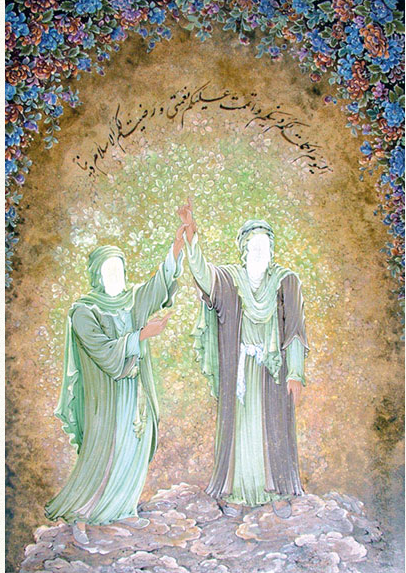
\includegraphics[width=1.35188in,height=1.90972in]{Images/image078.png}
    \caption{Ġadir-e Khumm et la
désignation de l'Imâm `Alī. œuvre de Rezâ
Badr-os-Samâ'}
    \label{Ġadir-e Khumm}
\end{marginfigure}

Il y reçut le verset suivant~: 
\begin{quote}
  {«~O Messager, transmets
ce qui t'a été descendu de la part de ton Seigneur. Si tu ne le faisais
pas, alors tu n'aurais pas communiqué Son message. Et Dieu te protégera
des gens. Certes, Dieu ne guide pas les gens mécréants.~» (Coran,
5:67).}  
\end{quote}


Par la suite, selon les šī`ites, Muḥammad déclara~: «~Man kuntu Mawlāhu,
fahaza `Alī mawlāhu~» c'est-à-dire~: «~Qui me reconnaît comme son Mawlā
(maître, guide), doit reconnaître `Ali comme son Mawlā ~».




Mais pour certains des compagnons du Prophète, cette désignation n'a
jamais été officialisée et selon les mœurs tribales, il convient donc de
procéder à son élection.

Mais `Alī est écarté du collège électoral. \mn{\cite{OUARDI:CalifesMaudits}} 

La tribu des Qurayš élit Abū Bakr, vieux compagnon et un des beaux-pères
de Muhammad~: il devint le 1\textsuperscript{er} calife (khalîfa).

`Alī fera acte d'allégeance, il se soumet à ce choix signifiant son
désir de maintenir l'unité de l'\emph{umma}.

À la mort d'Abū Bakr, `Umar devient le 2\textsuperscript{ème} calife
puisqu'il avait été désigné de manière explicite (\emph{naṣṣ}). `Alī
accepte.

`Umar annonce qu'à sa mort, son successeur devra être choisi parmi les
membres d'un collège électoral qu'il a lui-même nommés. `Alī en fait
partie. À la mort de `Umar, c'est `Uṯmān qui est choisi. Accusé de
népotisme, il est assassiné.

`Alī devient alors le 4\textsuperscript{ème} calife (656-661) attestant
ainsi de ses qualités vertueuses et de la suprématie de l'imamat sur les
manigances politiques mondaines.

Pour autant, deux anciens compagnons du Prophète n'ayant pas vu leur
appétit politique satisfait -- ils souhaitaient être gouverneurs de Kūfa
et Baṣra -- s'associèrent à `Ā'iša, fille d'Abū Bakr et veuve du
Prophète, pour lever une armée contre `Alī. C'est la bataille du chameau
de 657. On l'appelle ainsi parce que `Ā'iša qui était présente, était
montée sur un chameau\ldots{} Son armée fut mise en défaite.





\mn{On voit ici `Ā'iša sur son chameau et dans son baldaquin}



Mais en Syrie, Mu`āwiya, parent de `Uṯmān, mena aussi une guerre. C'est
la bataille de Ṣiffīn. Alors qu'elle tournait à l'avantage de `Alī,
Mu`āwiya proposa un arbitrage sur le livre sacré. `Alī accepte. Nombre
de ses soldats se soulèvent considérant qu'il n'avait pas à accepter
l'arbitrage et que Dieu avait déjà rendu son jugement par la victoire
qui se manifestait. `Alī doit mener combat contre ces rebelles (ce sont
les ḫariǧites), alors que Mu`āwiya se fait proclamer calife à Jérusalem
en 660~!

`Alī est assassiné par un ḫarigite à Kūfa en 661.

Pour les sunnites, il n'avait pas de successeur tandis que les šī`ites
affirment qu'il avait nommé son fils aîné, al-Ḥasān.

 
\subsection{La généalogie du
šī`isme}\label{la-guxe9nuxe9alogie-du-ux161ux12bisme}

La généalogie est sujet à controverses et divergences ce qui explique la
multiplication des šī`ismes\textbf{.} On dénombre une centaine de
lignées à la fin du premier siècle de l'Hégire.

Les jours de naissances des membres de la famille de `Alī sont des fêtes
religieuses. Les jours anniversaires de leur mort, des journées de
deuil. Leurs tombes sont des lieux de pèlerinage~: les cités où elles se
trouvent sont des villes saintes.

Elle est un peu subtile, chaque imām mériterait un chapitre\ldots{}
entre son enseignement, les histoires, les légendes, leur assassinat --
souvent empoisonné -- sans compter qu'au sein même du šī`isme, les
généalogies, les filiations ne sont pas les mêmes, que certains ne
reconnaissent que quatre imāms, d'autres sept, d'autres douze, que ce ne
sont pas toujours les mêmes\ldots{} qu'il y a donc une multitude de
branches šī`ites\ldots{} Bref, je retiens surtout le šī`isme majoritaire
dit duodécimain, car il reconnaît 12 imāms. Vous en trouverez en annexe
la liste avec leurs noms et quelques caractéristiques. Si vous avez la
curiosité de regarder le douzième, vous voyez que n'est pas indiquée la
date de sa mort. D'après vous, est-ce parce que l'on ne la connaît pas,
ou est-ce pour une autre raison~? La réponse dans la suite du cours. Bon
travail.

 
\paragraph{`Alī et Fātima}\label{alux12b-et-fux101tima}

`Alī joue donc dans le šī`isme un rôle important. Il est à la tête de
presque toutes les chaînes de transmission, il est considéré ~comme un
maître spirituel. On lui attribue deux livres~: \emph{Nahj al-balâgha}
(La Voie de la maturité)~et \emph{Dîwân}, un recueil de poèmes.

Quant à Fātima, elle est la sainte la plus vénérée du šī`isme\textbf{.}
Sa tombe est à Médine (il y en a trois\ldots{} dans le doute, on les
garde toutes les trois).

Fātima est la mère de toute la lignée des imāms. Elle représente ce qui
relie Muhammad à `Ali, la lettre et l'esprit. Elle est dite \emph{maǧma`
al-nūrayn} (le Confluent des Deux Lumières), celle de la prophétie et de
l'imamat. Elle a une mission d'intercession et de protection jusqu'à la
fin des temps. Immaculée, Vierge malgré son mariage, elle est aussi
reine du ciel. Un parallèle avec Mariam (Marie), la mère de Jésus est
établi par la tradition šī`ite elle-même \sn{Tahani Sabri,
  «~L'hagiographie de Fāṭima d'après le \emph{biḥār al-anwār}~», École
  des Hautes Études en Sciences Sociales, thèse de doctorat sous la
  direction de Henry Corbin, 1969.}.

 
\paragraph{Al-Hasan, fils de
`Alî}\label{al-hasan-fils-de-aluxee}

C'est un petit-fils du Prophète. Il y a des récits touchant d'affection
tendre.

Al-Ḥasan abdiqua le califat devant l'hostilité de Mu`āwiya. Pour les
historiens šī`ites, il préféra l'unité de la communauté plutôt que de
voir la division, mais les sunnites font remarquer qu'il n'était pas en
mesure de remporter la victoire et qu'il abdiqua en contre-partie d'une
importante somme d'argent. Retiré à Médine, il est assassiné,
semble-t-il par une de ses épouses qui aurait été soudoyée, selon les
šī`ites par Mu`āwiya. Terrible Mu`āwiya\ldots{} J'imagine que vous ne
devez pas le trouver très sympathique. Il est le fondateur de la
dynastie Omeyyade. Les grands historiens sunnites des
8\textsuperscript{ème} et 9\textsuperscript{ème} siècles n'en ont pas
laissé un souvenir très élogieux\ldots{} car ils sont abbassides et il
fallait effacer les traces vénérables des Omeyyades.

 
\paragraph{Al-Ḥusayn} 

Al-Ḥusayn, le second fils de `Alī, reste discret. Il s'efface. Mais il
entre sur la scène politique au moment de la mise en place d'une
dynastie califale héréditaire en la personne de Yazīd, le fils de
Mu`āwiya. On se réfère souvent à lui pour présenter le šī`isme comme un
courant révolutionnaire, politique et contestataire.

L'histoire est plus complexe. En tous les cas, les sources appellent une
très grande prudence. Assuré du soutien de la ville de Kūfa, il se met
en route avec toute sa famille pour chasser les Omeyyades. Mais sur la
route, la petite troupe se trouve encerclée par les soldats omeyyades,
coupée de Kūfa, privée d'eau. Retranchée en plein désert dans un petit
village appelé Karbalā', les Omeyyades finissent par donner l'assaut.
C'est un massacre. Ḥusayn est tué, décapité, piétiné ainsi que quasiment
toute sa famille.

Ašura est le jour de célébration où l'on fait mémoire de cette tragédie
dans de grandes cérémonies populaires avec parfois des dérives
spectaculaires de lamentations violentes, d'auto-flagellations, de
lacérations ou de mutilations. C'est le remord d'une ville qui n'a pas
soutenu al-Ḥusayn.

Ḥusayn devint alors un exemple de martyr, de sacrifice, de bravoure.
Sans-doute, sous l'influence chrétienne, on verra dans la mort de Husayn
un sacrifice rédempteur pour le salut des fidèles.

Chez certains fidèles la rumeur selon laquelle il ne serait pas mort
circule. Il aura été enlevé au ciel directement par Dieu avant le
combat.


\mn{Les troupes omeyyades encerclent Karbalā' \& Yā Ḥusayn\ldots{}

Jour de la fête d'Ashura \& Ashura et ses spectaculaires flagellations à
Karbalā'\ldots{} }


 
\paragraph{`Alî Zayn al-`Âbidîn, fils
d'al-Husayn}\label{aluxee-zayn-al-uxe2biduxeen-fils-dal-husayn}

Un rescapé du massacre de Karbalâ'. Il serait parti à Médine pour y
mener une vie pieuse. Il ne posa aucun problème aux Omeyyades. Une
existence ascétique, consacrée à la dévotion. On le surnommait
\emph{al-saǧǧād}, celui qui accomplit de nombreuses prosternations.
C'est un nom respecté, même dans le sunnisme.

Un de ses fils Zayd ibn `Alî, est à l'origine d'une grande famille, les
zaydites. Le zaydisme est marqué par un activisme violent. Selon la
théorie zaydite de l'imamat chaque Alide a le droit de prétendre à la
direction de la communauté. Le véritable imâm est celui qui se qualifie,
les armes à la main, en s'insurgeant contre le pouvoir injuste. Ils sont
aujourd'hui encore influents au Yémen~où ils représentent la moitié de
la population (mais le dernier chef zaydite du Yémen a été renversé en
1962).

 
\paragraph{Muhammad al-Bāqir, fils de `Alî Zayn
al-`Âbidîn}\label{muhammad-al-bux101qir-fils-de-aluxee-zayn-al-uxe2biduxeen}

Il est considéré comme le fils de `Ali Zayn. Les grandes traditions
šī`ites le considèrent comme le 5ème Imām. Il est surnommé Abū Ǧa`far.

 
\paragraph{Ǧa'far al- Ṣādiq
}\label{ux1e7afar-al--ux1e63ux101diq}

Fils de Muhammad al-Bāqir, il est célèbre pour sa piété et, selon les
shiites, l'infaillibilité de ses prémonitions. Les auteurs soufis lui
attribuent le plus ancien commentaire mystique du Coran. On le considère
comme un alchimiste, un spirituel refusant toute implication dans les
mouvements politiques de son époque. Il fut enterré dans le cimetière de
Baqī` à Médine. Le carré šī`ite y sera rasé au XIX° siècle par les
Wahhabites, alors qu'il abritait les tombes de plusieurs imâms.

Son fils aîné, Ismā`īl, est l'éponyme de la seconde grande famille de
l'islam šī`ite, les ismaéliens, šī`ites septimains \textbf{--} shî'ites
à 7 imâms. Pour cette branche, il est le dernier Imâm. Un autre groupe
s'appuie sur la croyance que l'imamāt fut transmis du vivant de Ǧa`far à
son petit-fils~: ce sont les qarmates. D'autres, les Fatimides,
considèrent que l'imamat se poursuit et que l'imam caché, le Mahdi, sera
un de ses descendants.


\begin{Synthesis}
Le si'isme est  une prophétologie. Il y a une sur
l'incarnation. Facilite le
dialogue avec les chrétiens.
\end{Synthesis}

 
\paragraph{{Le douzième imām, l'imām caché ou
le Madhī
}{ }}\label{le-douziuxe8me-imux101m-limux101m-cachuxe9-ou-le-madhux12b}

À la mort du 11\textsuperscript{ème} imâm, les fidèles croient que
l'imâm a eu un fils du nom de Muḥammad. 
\begin{Def}[Mahdî]
Il est reconnu comme le
\emph{Mahdî,} le Bien Guidé. C'est l'imâm caché, \emph{al-imâm al-ġā'ib}
ou encore \emph{al-Qā'im}, que l'on peut traduire par le Résurrecteur.
\end{Def}


C'est le courant duodécimain, majoritaire dans le šī`isme.

Mais en quoi consiste cette occultation~? Comment s'opère-t-elle~? Que
signifie-t-elle~? Quand a-t-elle eu lieu~? Sous quelles formes~?

Je vous propose d'écouter ce bref passage d'une émission sur France
Culture, «~Les racines du ciel~», où Amir-Moezzi répond.

L'imâm caché n'est donc pas mort. Vous comprenez maintenant pourquoi
dans le tableau en annexe ne figure que sa date de naissance. Il
n'existe pas de successeur puisqu'il est physiquement vivant. À la fin
des temps, il se manifestera. Il y a donc une présence invisible, mais
physiquement réelle. L'imâm caché clôt la lignée des imamites.

Par la suite, tout se passe comme si désormais l'ère de la bonne entente
entre le religieux et le politique était désormais finie. La cité
idéale, gouvernée par un juste n'est réalisable qu'à la fin des temps,
avec l'avènement du Mādhi, le Sauveur eschatologique. L'attitude
revendicative et politique est rejetée dans un futur messianique. Le
šī`isme se présente comme une religion individuelle, personnelle, non
institutionnelle. Mais peut-il alors perdurer ? Pour pallier cette
«~absence~», on aura recours à la figure du juriste avec la dynastie
bouyide. C'est à cette époque que le šī`isme sera érigé comme religion
d'État, ce qui n'est pas le moindre des paradoxes compte tenu de ses
«~fondamentaux~».

 
\section{Les fondations du šī`isme~:
doctrines}\label{ii.-les-fondations-du-ux161ux12bisme-doctrines}

Les doctrines šī`ites sont compliquées, subtiles et à lire
l'enseignement des imāms et les commentaires qui en suivirent, cette
subtilité est voulue pour elle-même. De leurs enseignements, ils ne
cessent de dire~: «~notre enseignement est ardu, difficile à supporter~:
c'est un secret, un secret enveloppé par un secret au sujet d'un
secret~»\sn{Voir Amir-Moezzi, Jambet, \emph{Qu'est-ce que le
  shi'isme~?}, Paris, Fayard, p. 96 .}.

Dans sa présentation du šī`isme, Amir-Moezzi distingue dans la vision du
monde et la théologie šī`ite une double dimension~: elles sont marquées
à la fois par l'affirmation d'un principe de dualité et d'un principe de
dualisme. On lira avec intérêt et pour plus de précisions la
présentation qu'il fait dans \emph{Qu'est-ce que le shiisme~?} Mais tout
d'abord, la question des Écritures. Sont-elles les mêmes qu'en
sunnisme~?

 
\subsection{{Les sources scripturaires
}}\label{les-sources-scripturaires}

 
\paragraph{{Y a-t-il un Coran šī`ite~?
}}\label{y-a-t-il-un-coran-ux161ux12bite}

Le Coran est la référence principale et la contradiction éventuelle
entre un \emph{ḥadīṯ} et un verset coranique est l'indice de la fausseté
du ḥadīṯ.

Pour autant, certaines traditions shî'ites trouvent difficilement leur
fondement dans le Coran. Pour les šī`ites, le Coran a été en réalité
falsifié, altéré, censuré lors de sa compilation par `Uṯmān (c'est un
des premiers califes. Si le nom ne vous disait plus rien du tout,
revoyez le premier cours sur le Coran et à la question du
\emph{muṣhaf}). La révélation originelle contenait des versets sur `Alî
et les descendants des Prophètes. Ils étaient cités comme les modèles et
les chefs par excellence. `Alī possédait une version du Coran intégral,
mais il n'en dit mot pour éviter sa destruction par ses adversaires.
Cependant, elle fut transmise secrètement d'imam à imam, jusqu'au
12\textsuperscript{ème} imâm qu'il l'emporta avec lui lors de son
Occultation. Les enseignements des imāms permettent d'accéder à ces
versets et de les connaître.

Avec l'arrivée au pouvoir des Bouyides shiites à la fin du
4\textsuperscript{ème} siècle de l'hégire, il s'agira de trouver un
accord avec l'orthodoxie sunnite. On met ainsi un terme au doute sur
l'intégrité du Coran officiel. Le courant dominant abandonne la thèse de
la falsification du Coran officiel, mais le débat ressurgit
régulièrement.

 
\paragraph{Y a-t-il un \emph{ḥadīṯ} šī`ite~?
} 

Bien qu'al-Būḫārī fut perse, il existe une Sunna šī`ite. Les textes sont
bien souvent les mêmes, mais les \emph{isnāds} diffèrent et renvoient
aux membres de la famille du prophète (\emph{ahl al-bayt} --
c'est-à-dire littéralement, les gens de la maison). En effet, la
référence dans l'\emph{isnād} aux compagnons du Prophète lui ôte toute
crédibilité dans la mesure où ils sont considérés comme des traîtres.
Pour l'\emph{isnād}, la notion a été vue dans le cours sur la Sunna.
C'est la fameuse chaîne de transmission.

On reconnaît trois grands corpus~:

\begin{itemize}
\item
  Celui de Ya`qub al-Kulaynī (m. en 939).
\item
  Celui de Saduq Ibn Babuyeh (m. 991).
\item
  Celui d'al-Ḥasan al-Tusī (m. 1068).
\end{itemize}

On trouve aussi dans ces recueils de nombreux témoignages des imāms.

L'ouvrage le plus connu de Kulaynī est \emph{al-Kāfī}. Il est divisé en
trois sections~:

\begin{itemize}
\item
  \emph{Usūl al-Kāfī}, qui concerne l'épistémologie, la théologie, la
  question de la foi et de la mécréance, l'histoire, l'éthique, et le
  Coran~et ses mérites;
\item
  \emph{Furūʿ al-Kāfī}, qui concerne les dimensions pratiques et légales
  (prières, \emph{ǧihād}, jeûne, ḥaǧǧ, funérailles, nourriture, boisson,
  mariage, divorce, commerce, héritage, etc.)
\item
  \emph{Rawdat} \emph{al-Kāfī}, qui inclue de nombreuses traditions, des
  lettres, des discours des imāms.
\end{itemize}

Il existe une traduction anglaise de cette collection de plus de 16 000
traditions. Si vous ne trouvez pas le sommeil\ldots{}
 
\subsection{ Dualité et dualisme}\label{dualituxe9-et-dualisme}

 
\paragraph{ Une vision duelle}\label{une-vision-duelle}

Il s'agit d'affirmer que toute réalité possède deux niveaux~:

1/ un niveau manifeste, obvie, apparent, visible, concret, évident
(\emph{zāhir})

2/ un niveau secret, non manifeste, implicite, invisible, intérieur
(\emph{bāṭin})

Cette affirmation est au cœur du credo šī`ite. Ce que je vois, ce qui
est visible contient aussi une réalité invisible. Il existe une relation
entre le manifeste et le caché, l'exotérique et l'ésotérique. Il s'agit
d'appliquer ce principe à toute réalité, et bien sûr, à commencer par la
théologie.

\emph{Ainsi, en théologie}, Dieu a deux niveaux d'être, deux niveaux
ontologiques~:

1/ son Essence, inconcevable, inimaginable, au-delà de toute pensée~:
c'est le niveau caché (\emph{bāṭin})

2/ ses Noms et Attributs~à travers lesquels Dieu se révèle et se fait
connaître~: c'est le Dieu inconnu qui aspire à être connu. Amir-Moezzi
remarque que l'on retrouve une distinction de la théologie médiévale
chrétienne entre \emph{Deus absconditus} et \emph{Deus revelatus}.

La manifestation de ces noms divins comme le Roi, le Miséricordieux, le
Juge suprême, etc. est une manifestation de Dieu (théophanie). La plus
haute révélation en est la figure de l\emph{'Imām} céleste,
l'\emph{Imām} de Lumière, l'Homme cosmique~: c'est l'Imām avec un I
majuscule, dans son acception ontologique universelle.

L'\emph{Imām} cosmique a aussi deux dimensions

\begin{quote}
1/ la dimension cachée~: c'est l'aspect métaphysique, dans le ciel,
invisible à nos yeux.

2/ la dimension exotérique, visible~: ce sont les \emph{imāms}
historiques.
\end{quote}

La mission de ces \emph{imāms} historiques~consiste à dévoiler les
mystères de Dieu, du monde et de l'homme, à transmettre aux hommes le
Secret contenu dans l'Imām métaphysique.

Mais l'enseignement des imāms, disions-nous, est complexe. Ǧa`far
al-Ṣādiq (c'est un \emph{imām} que nous avons rencontré dans la
généaologie des douze\ldots{} C'est le combientième \emph{imām} déjà~?)
écrivait~: «~Notre enseignement comporte l'exotérique, l'ésotérique et
l'ésotérique de l'ésotérique~».

À cette approche duelle de la réalité se superpose le principe du
dualisme.

 
\paragraph{ Une vision dualiste}\label{une-vision-dualiste}
\mn{Si isme~: influence de la zoroastrisme avec un certain manichéisme, bien
/ mal. Lumière et nuit~; combat cosmique et sur terre. On retrouve ceci
dans le sunnisme. Tous les Hadiths eschatologiques décrivent en tableau
le paradis. Dans le Si isme, enjeu du bien et du mal.
}
L'histoire de la création est celle d'un combat cosmique entre les
forces du Bien et les forces du Mal, entre la lumière et l'obscurité. On
retrouve ici une nette dimension zoroastrienne et manichéenne du monde.

Ce combat se situe au niveau cosmique~: c'est le combat entre les armées
de l'Intelligence cosmique (\emph{al-`aql}) et celles de l'Ignorance
cosmique (\emph{al-ğahl}). Cette dichotomie, cette opposition est celle
d'une lutte permanente entre les Gens de la Droite (\emph{ašāb
al-yamīn}) et les gens de la Gauche (\emph{ašāb al-šimāl}). Le combat
entre deux hommes ennemis s'inscrit donc dans un cadre plus large. Toute
l'histoire de l'humanité est traversée par l'adversité et la violence
des forces démoniaques de l'Ignorance. Il en sera ainsi jusqu'à la fin
des temps avec l'avènement du Sauveur eschatologique, le Mahdī qui
vaincra définitivement les forces du mal.

Mais qui sont ces forces du mal~? Comment les reconnaître, les
identifier~?

C'est l'enseignement des imāms (les 7, les 12, selon) qui apportent les
réponses à ces questions. Dans ce corpus de centaines de milliers de
pages, les adversaires de l'imâm~sont tour à tour identifiés~:

\begin{itemize}
\item
  Aux juifs, qui sont des idolâtres et ont trahi Moïse en adorant le
  veau d'or
\item
  Aux Compagnons de Muhammad qui ont rejeté `Alī
\item
  Aux Gens de l'exotérique, c'est-à-dire des apparences, du superficiel
  (\emph{ahl al-zāhir}), ce sont les littéralistes qui s'arrêtent à la
  lettre et n'ont pas connaissance de son `esprit' (\emph{bāṭin}). À cet
  égard, un šī`ite se sentira plus proche d'un juif ou d'un chrétien
  accoutumé à une lecture ésotérique, symbolique, anagogique des textes
  que d'un musulman sunnite exotérique, qui se limite à la lettre.
\end{itemize}

 
\subsection{Prophétie et
Imamologie}\label{prophuxe9tie-et-imamologie}

L'enseignement des \emph{imāms}, acquiert en réalité un rôle supérieur à
celui du Prophète.

En effet, si le prophète est le messager de la lettre, l'\emph{imām}
dans le šī`isme en apporte l'esprit. Or, si l'esprit peut exister sans
la lettre, sans l'esprit, la lettre est morte\sn{Amir-Moezzi,
  Jambet, \emph{Qu'est-ce que le shi'isme~?}, Paris, Fayard, 2004, p.
  42.}.


\paragraph{Remarque sur l'imām~}: le mot \emph{imām}
est piégé. Il s'emploie en sunnisme, mais sans désignation particulière.
L'imām désigne un savant, un chef ou tout simplement celui qui dirige la
prière. En revanche, en šī`isme\textbf{,} c'est un titre sacré. L'imām
est le Guide, l'un des Douze\ldots{} En principe, aucun autre homme ne
porte ce nom. Et pourtant, d'aucuns se sont attribués ce titre. Autant
dire qu'ils se prenaient pour le Mahdi .L'un d'eux est très célèbre. À
suivre.

L'Imām apporte en effet la connaissance face au monde de l'ignorance. En
montrant son cœur, l'Imām `Alī donnait cet enseignement sur la vocation
de l'imām, la nature de la religion, son importance. Écoutez et
réécoutez ce texte\sn{Vous trouvez l'intégralité du texte dans le
  livre de Mohammad Ali Amir-Moezzi, \emph{La religion discrète}, Paris,
  Vrin, 2006,
  \url{https://books.google.com}}.


L'imām transmet les vérités secrètes. Il tient le monde, il évite la
noyade définitive du monde dans les ténèbres. Il est l'alpha et l'omega
du šī`isme\sn{Amir-Moeezi, Jambet, \emph{Qu'est-ce que le
  shi'isme~?}, p. 40.}.

Mais il a aussi des pouvoirs supra-normaux~: il possède la science du
passé et du futur, il lit dans les consciences, il connaît les langues,
y compris celle des animaux, les sciences occultes (astrologie,
alchimie, sciences divinatoires, etc.). Il peut ressusciter les morts,
guérir les maladies, rajeunir les vieillards, marcher sur les eaux,
monter aux cieux\ldots{} Il possède des objets de pouvoir~ tels la
tunique d'Adam, le sceau de Salomon, l'Arche et les tables de la Loi,
l'Arme invincible de Muḥammad.

L'enseignement de l'\emph{imām} est au cœur de l'approche spirituelle
šī`ite. C'est par lui que se réalise la spiritualisation, la
divinisation. Écoutez Amir-Moezzi à ce sujet.

 
\subsection{La walāya au cœur de la foi šī`ite
} 


La \emph{walāya} est un concept clé du \emph{šī`isme}. Les
\emph{šī`ites} sont appelés les gens de la \emph{walāya}.\\
\begin{Def}[walāya]
La \emph{walāya} désigne la mission sacrée et sainte des imams.

L'imām est le \emph{walī} (le saint), celui qui initie les fidèles à
l'esprit de la Parole divine. Il est la Face de Dieu sur terre.

\end{Def}



La \emph{walāya} désigne aussi l'amour, celui que les fidèles
manifestent dans la dévotion, par la loyauté, la soumission à l'égard du
maître initiateur.

Mais dans une doctrine \textbf{dualiste}, l'amour de l'imām ne peut aller sans la
haine de son ennemi. La \emph{walāya} est donc inséparable de son
contraire, la \emph{barā'a} (c'est-à-dire la haine, la dissociation à
l'égard des forces de l'ignorance). Un \emph{ḥadīṯ} šī`ite dit~:

\begin{quote}
«~l'amour de Dieu ne s'obtient que grâce à l'amour envers Ses amis et
l'hostilité à l'égard de Ses ennemis~».    
\end{quote}


Au cœur de la foi šī`ite, la \emph{walâya} est dans la \emph{šahāda} :
\begin{quote}
   «~Je témoigne qu'il n'y a pas de dieu hormis Dieu~; je témoigne que
Muhammad est l'envoyé de Dieu, et que `Alî est le \emph{walī} de
Dieu~» 
\end{quote}
 \emph{walī} signifie ici l'ami,~l'allié, le détenteur de la
\emph{walāya}.




\mn{\emph{Šahāda} sur une mosquée du Caire
fatimide. on y lit à la fin~:\emph{ʿAlī walī
allāh.
}  }


\subsection{{Les signes de la fin du monde ou
l'eschatologie šī`ite
}\label{les-signes-de-la-fin-du-monde-ou-leschatologie-ux161ux12bite}}

En raison de la place de la question de l'Occultation, l'eschatologie a
donné lieu à un foisonnement de traditions et de traités. Il s'agit de
savoir lire les signes afin de reconnaître l'imminence du Dernier Jour,
le retour du Mahdī. Les signes sont multiples, mais on peut identifier
quelques constantes~:

\begin{itemize}
\item
  l'envahissement de la terre par les forces du Mal,
\item
  l'écrasement quasi-complet des forces de la Connaissance par celles de
  l'ignorance,
\item
  la perte du sens du sacré,
\item
  le renversement des valeurs humaines,
\item
  l'anéantissement de tout ce qui relie l'homme à Dieu et à son prochain
\end{itemize}

Des signes concrets sont exposés. Ainsi par exemple,

\begin{itemize}
\item
  la venue d'al-Sufyānī, le chef de l'armée des ennemis des imāms, le
  collaborateur d'\emph{al-Daǧǧāl}, l'Imposteur, l'Antéchrist islamique.
\item
  L'avènement d'al-Yamānī, le Yéménite qui prêchera le soutien au Mahdī.
\item
  Le Cri, d'origine surnaturelle, venu du ciel, appelant les hommes à
  rejoindre l'armée du Sauveur
\item
  L'engloutissement d'une armée (parfois celle d'al-Sufyānī) dans le
  désert.
\item
  L'assassinat à La Mecque de l'envoyé du Mahdī, appelé \emph{al-Nafs
  al-Zakiyya\textbf{~}}: l'Âme Pure.
\end{itemize}

La fin de l'occultation est aussi expliquée et commentée. On peut en
distinguer 3 raisons~principales :
\begin{enumerate}
    \item une raison historique~: venger tous les hommes saints du passé,
victimes de l'injustice. Tous les saints du passé reviendront à la vie,
ainsi que leurs meurtriers, et les premiers pourront ainsi se venger des
seconds à cette occasion.
\item une raison religieuse~: rétablir le sens du sacré~; rétablir les
religions (judaïsme, christianisme, islam) dans leur intégralité
originelle, rapporter les Écritures respectives qui ont été altérées ou
falsifiées
\item une raison spirituelle~: apporter le sens ésotérique des choses,
effacer la frontière entre le caché et le manifeste.
\end{enumerate}
 

Le retour du Mahdi s'accompagne aussi de celui de Jésus-Christ. Il est
le principal compagnon d'al-Qā'im. Voyez un peu plus haut. C'est un nom
utilisé pour nommer le Mahdi. Quelle est sa signification déjà~? Penser
à «~\emph{Talitha Qum~}».. Lève-toi\ldots{} C'est bien la même racine du
redressement, de la résurrection.

 
\section{Bibliographie}\label{bibliographie}

\paragraph{Les fondamentaux}

Mohammad-Ali \textsc{Amir-Moezzi}, Christian Jambet, \emph{Qu'est-ce que
le shî'isme~?,} Paris, Fayard, 2004.

Henri \textsc{Corbin}, \emph{En Islam iranien}, Aspects spirituels et
philosophiques III, Les Fidèles d'amour, shî'isme et soufisme,
Gallimard, 1978, 359 pages (PISAI H266).

\paragraph{Pour aller plus loin}

Mohammad Ali \textsc{Amir-Moezzi}, \emph{La religion discrète},
Croyances et pratiques spirituelles dans l'islam shî`ite, Collection
Textes et Traditions dirigée par Marie-Odile Goulet-Cazé, Richard
Goulet, Philippe Hoffmann, Paris, Vrin, 2006.

Henri \textsc{Corbin}, «~De l'histoire des religions comme problème
théologique~», \emph{Monde non chrétien} 51-52, 1960

Leili \textsc{Echghi}, \emph{Un temps entre les temps~: L'Imam, le
Chî'isme et l'Iran}, coll. Patrimoines Islam, cerf, Paris, 1992.

Geneviève Gobillot, \emph{Les Chiites}, Editions Brepols, 1998.

Henri Laoust, \emph{Comment définir le sunnisme et le chiisme},
Geuthner, 1985, 44 pages.

Muhammad Ridā Muzaffar, \emph{Le credo des imamites}, traduction par
Frère Sliwa, Rome, PISAI.

Yann \textsc{Richard}, \emph{Le Šī`isme en Iran~: Imam et Révolution,
Librairie d'Amérique et d'Orient}, 1980, 142 pages.

Yann \textsc{Richard}, \emph{L'islam chi'ite~: croyances et idéologies},
Fayard, Paris, 1991.

\textbf{\hfill\break
}

\subsection{Généalogie des Imāms}


 

\begin{longtable}{p{0.5cm}p{1.3cm}p{1.8cm}p{2.5cm}p{3.5cm}p{0.8cm}}
\small \\
%\sidecaption{Généalogie des Imāms} \label{tab:Genealogie} \\
\toprule
 & Nom & Titre & Epithète & connu pour & dates
\\
\midrule
\endhead
1 
& 
\vtop{{ `Alī}{ (\TArabe{علي})}} 
&
\vtop{{ Abū al-Ḥassan}{ (\TArabe{أبو الحسن})}}
&
\vtop{{ Amīr al-Mu'minīn}{ (\TArabe{أمیر المؤمنین}) -
Commandeur des croyants}} 
& Le premier Imam est la personne la plus
significative après Mahomet pour les chiites 
& 600 -- 661 \\



2 & \vtop{{ Ḥasan}{ (\TArabe{ألحسن})}} &
\vtop{{ Abū Muḥammad}{ (\TArabe{أبو محمد})}} &
\vtop{{ Al-Mujtabā}{ (\TArabe{ألمجتبی}) - le choisi}}
& Signe un traité de paix pour un Islam meilleur, très aimé par Mahomet
est avec son frère un des maîtres des jeunes du paradis & 625 -- 669 \\


3 & \vtop{{ Ḥusayn}{ (\TArabe{ألحسین})}} &
\vtop{{ Abū \textsuperscript{c}Abdillāh}{ (\TArabe{أبو
عبداللھ})}} & \vtop{{ Sayyid
ash-Šuhadā'}{ (\TArabe{سید الشھداء}) - Seigneur des martyrs}} &
Est mort lors de la bataille de Kerbala. & 626 -- 680 \\


4 & `Alī (\TArabe{علي}) & \vtop{{ Abū
Muḥammad}{ (\TArabe{أبو محمد})}} & \vtop{{ Zayn
al-\textsuperscript{c}Ābidīn}{ (\TArabe{زین العابدین}) - Joyau
des croyants}} & Piété, jeûne, pénitence pendant 20 ans à cause de la
bataille de Kerbala. & 658 -- 713 \\


5 & Muḥammad (\TArabe{محمد}) & \vtop{{ Abū
Ja\textsuperscript{c}far}{ (\TArabe{أبو جعفر})}} &
\vtop{{ Al-Bāqir}{ (\TArabe{ألباقر}) - Pourfendeur de
la Science}} & le moins oppressé des douze imams par le calife de son
temps. Il n'est pas reconnu par les Zaydī (qui prennent comme imam Zayd
Ibn `Alī. & 676 -- 743 \\


6 & \vtop{{ Ǧa'far}{ (\TArabe{جعفر})}} &
\vtop{{ Abū \textsuperscript{c}Abdillāh}{ (\TArabe{أبو
عبداللھ})}} & \vtop{{ Aṣ-Ṣādiq}{ (\TArabe{ألصادق}) -
Le véridique}} & Un penseur respecté à la fois par les Chiites et les
Sunnites & 703 -- 765 \\


7 & \vtop{{ Mūsā}{ (\TArabe{موسی})}} &
\vtop{{ Abū Ibrāhīm}{ (\TArabe{أبو إبراھیم})}} &
\vtop{{ Al-Kāẓim}{ (\TArabe{ألکاظم}) - Le triste}} & A
grandi en prison pour le rendre faible Il n'est pas reconnu par les
ismaéliens & 745 -- 799 \\


8 & \vtop{{ `Alī}{ (\TArabe{علي})}} &
\vtop{{ Abū al-Ḥassan}{ (\TArabe{أبو الحسن})}} &
\vtop{{ Ar-Riḍā}{ (\TArabe{ألرضا})}} & Le seul Imam à
être enterré en Iran & 765 -- 818 \\


9 & Muḥammad

(\TArabe{محمد}) & \vtop{{ Abū
Ja\textsuperscript{c}far}{ (\TArabe{أبو جعفر})}} &
\vtop{{ At-Taqī}{ (\TArabe{ألتقي})}} & Un grand
débatteur & 810 -- 835 \\


10 & \vtop{{ `Alī}{ (\TArabe{علي})}} &
\vtop{{ Abū al-Ḥassan}{ (\TArabe{أبو الحسن})}} &
\vtop{{ Al-Hādī (\TArabe{ألھادي}),}{ an-Naqī
(\TArabe{ألنقي})}} & & 827 -- 868 \\


11 & Ḥasan (\TArabe{ألحسن}) & \vtop{{ Abū
Muḥammad}{ (\TArabe{أبو محمد})}} &
\vtop{{ Al-\textsuperscript{c}Askarī}{ (\TArabe{ألعسکري})}}
& L'avant-dernier imam, qui a vécu presque toute sa vie assigné à
domicile et qui prêchait tout de même. & 846 -- 874 \\


12 & Muḥammad

(\TArabe{محمد}) & \vtop{{ Abū Qāsim}{ (\TArabe{أبو
قاسم})}} & \vtop{{ Al-Mahdī}{ (\TArabe{ألمھدي})}} &
Imam actuel, connu pour être le Sauveur. Il est l'occultation. & 868
-- \\
\bottomrule
\end{longtable}

\chapter{Le chiisme : histoire et doctrines}

\mn{21/3/22}
\section{bibliographie}
 

\begin{quote}
AMIR-MOEZZI, M-A. \emph{La religion discrète : croyances et pratiques
spirituelles dans l'Islam shi'ite}, Vrin, Paris, 2006.

AMIR-MOEZZI, M-A. et JAMBET, Christian \emph{Qu'est-ce que le shî'isme
?}, Fayard, Paris, 2004.

CORBIN, Henry \emph{En islam iranien: aspects spirituels et
philosophiques,} 4 volumes, Gallimard, Paris, 1991.

HALM, Heinz \emph{Le Chiisme}, Paris, PUF, 1995.

RICHARD, Yann \emph{L'islam chi'ite : croyances et idéologies}, Fayard,
Paris, 1991.

*TABATABA'I, Muhammad Huseyn \emph{Le chiisme en islam}, Beyrouth,
Al-Bouraq, 2009.
\end{quote}


\section{Le chiisme dans l'histoire
  musulmane. Quelques grands
  repères.}
  \label{le-chiisme-dans-lhistoire-musulmane.-quelques-grands-repuxe8res.}

On aurait pu traiter le développement du Chiisme et du sunnisme car ils ne se développent pas en vase clos. Mais il y a de tels différences,  en particulier, il n'y a pas de \textsc{foisonnement des visions dans le chiisme} du fait de l'importance des clercs
  

 \subsection{La naissance du chiisme : un problème de succession}
 ALi est le gendre et cousin du Prophète.
 
 Ali gagne à sa cause les nouveaux convertis (Egypte, Irak,...) et deviennent partisans d'Ali. Lorsque le Usman est assassiné en 656, Ali est élu comme 4ème calife. 
 \begin{Def}[ahl al-bayt]
\emph{famille du Prophète (Mahomet, Ali, Fatima, Hasan,
Hoseyn)}
 \end{Def}
 
 \paragraph{Mu'awiyya }Mais il est contesté par Mu'awiyya, qui lui reproche de ne pas chercher le meurtrier de Osman. En 657, bataille de Siffin, où les deux parties du monde arabe s'affrontent. Les Khalijites sont ceux qui reprochent à Ali d'avoir accepté l'arbitrage qui suit la bataille de Siffin.
 Ali est assassiné. Le califat est récupéré par Mu'awiyya.
 
 \paragraph{fondation de la dynastie des Omeyyades} par Mu'awyya. Hussayn, second fils de Ali s'oppose à Mu'awyya et est massacré dans la \textsc{plaine de Kerbala} avec sa famille et ses partisans. C'est le traumatisme fondateur. Le 10ème jour (Ashoura) du mois de Muharram, on rappelle ce martyr.
 
 \paragraph{une mosaique de courants shiites autour de la succession de l'imam et sur sa nature}
 Aujourd'hui, il y a trois courants : 
 \begin{itemize}
     \item ismaeliens :  7 imams
     \item zaydites : reconnaissent 5 imams
     \item imamites ou duodécimains : reconnaissent 12 imams.
 \end{itemize}
 
 Le Mahdi\sn{le Mahdi est aussi présent dans le sunnisme mais on ne sait pas qui c'est. Moins d'attente} n'est pas mort, il est occulté mais selon les courants, ce n'est pas le même. 
 
 \begin{Def}[mahdi]
   \emph{« le voilé » : l'homme mystérieux qui viendra annoncer et
provoquer la fin des temps (= dernier imam (occulté) pour les chiites).}
 \end{Def}
 
 \paragraph{Vision eschatologique forte dans le chiisme} Lutte du dernier imams contre le Dajjal, équivalent de \textit{l'antéchrist.}. Cela donne un potentiel révolutionnaire, avec certaines personnes se proclamant \textit{mahdi}, avec un potentiel mobilisateur très puissant, généralement révolutionnaire, voulant renversé le pouvoir établi, avec une forte dimension de justice sociale.
 
 
 
 %-------------------------------------------------
 \subsection{ « Le siècle chiite » : Bouyides et Fatimides (Xe-XIe s)}
 
 
 \paragraph{Diffusion du Chiisme à la mort de Hussayn} Dans les classes pauvres. En Irak par exemple, une grande révolte au IX ème siècle, se réclamant du chiime
 
 \paragraph{les bouyides} dans l'empire Abassides au X-XI, les Bouyides utilisent la faiblesse du calife pour s'imposer comme vizir, qui concentre la réalité du pouvoir : de 975, pendant environ un siècle.  
 
 \begin{figure}
     \centering
 
     \sidecaption{Source: \emph{Historical Atlas of Islam}, Malise Ruthven \& Azim Nanji,
Harvard University Press, 2004, p. 42.}
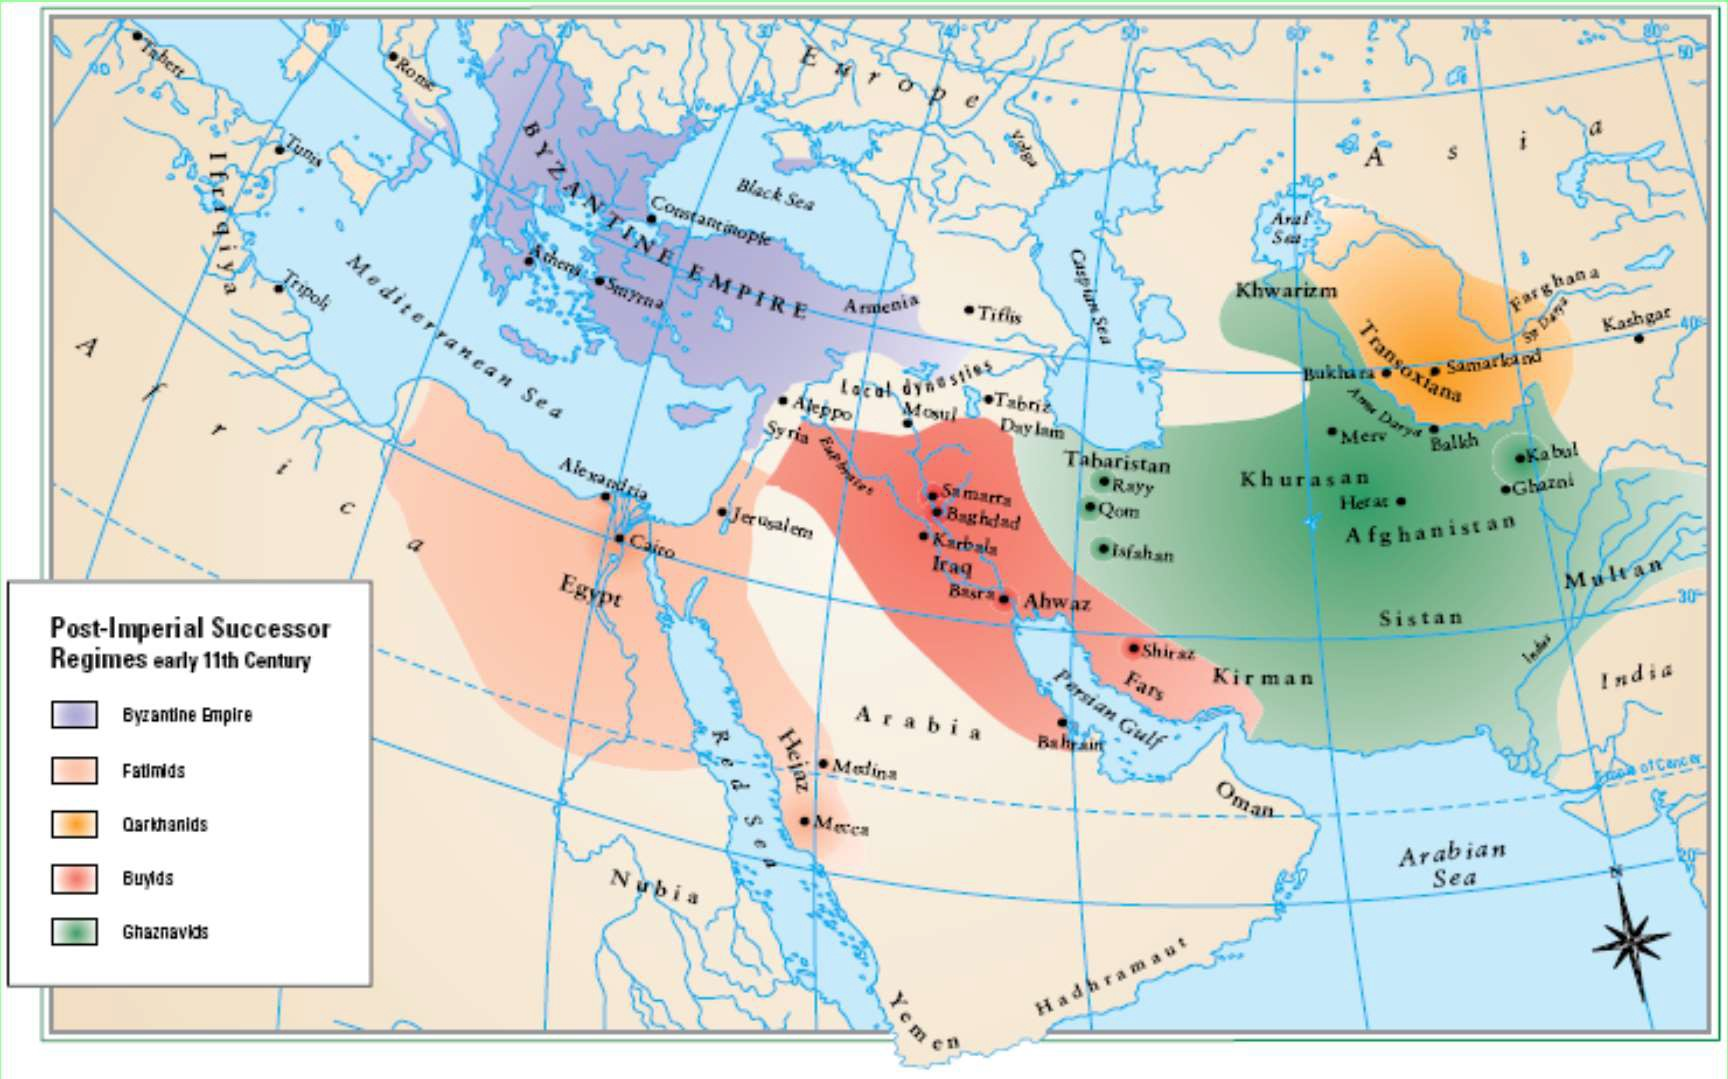
\includegraphics[width=\textwidth]{CourantsIslamContemporain/ImagesCourantsIslamContemporain/Image1Chiisme.jpeg}

     \label{fig:my_label}
 \end{figure}
 
 \paragraph{les fatimides} en afrique du Nord, fondé  par `Ubayd Allâh al-Mahdî (881-934). Typiquement, une personne se déclare Mahdi en Tunisie puis s'empare de l'Egypte (973 : le Caire comme capital). Avant le Caire n'était qu'une ville de garnison. 
 
 \paragraph{à Oman et au Yemen} AU Yémen, Zaydites, de 897 à 1962.
 
 
 %-------------------------------------------------
 
  \subsection{La naissance de l'Iran safavide (XVIe s.)}
 
  \begin{figure}
     \centering
 
     \sidecaption{Source: \emph{l'Iran safavide- Wikipedia}}
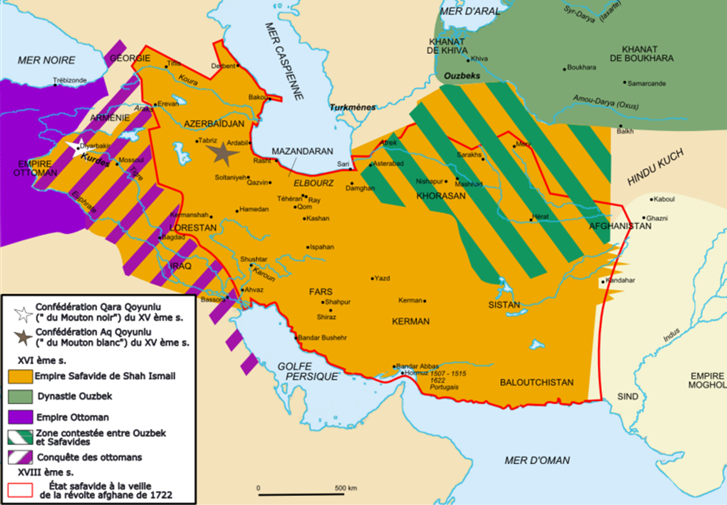
\includegraphics[width=\textwidth]{CourantsIslamContemporain/ImagesCourantsIslamContemporain/image2Chiisme.png}

     \label{fig:my_label}
 \end{figure}
 L'Iran était majoritairement sunnite jusqu'au Xème siècle. On a des populations turcophones à l'Ouest. un homme se proclame le Mahdi et fait la conquète militaire de l'Iran : par Isma'il en 1501.
  
 \paragraph{les limites du chiisme de Isma'il} conscient des limites du chiisme qu'il prone, il impose le chiisme duodécimain, venant du Liban, car le chiisme duodécimain était plus stable. Sans doute pour se détacher et légitimer face aux califes ottomans sunnites. Conversion de l'Iran assez violente : maudire les trois premiers califes, les confréries soufies. On va aussi déclarer les sunnites impurs.  


 
 %-------------------------------------------------
 
\section{Particularités de la doctrine chiite (duodécimaine ou imamite)
\label{particularituxe9s-de-la-doctrine-chiite-duoduxe9cimaine-ou-imamite}}


Elle s'est développée au VIII siècle par le 5ème et 6ème imams, qui étaient des savants. Ils ont collecté les corpus des hadiths, pas seulement du Prophète mais aussi des Imams, en particulier d'Ali et du 5ème et 6ème imams.

Ils ont développé l'école juridique
\begin{Def}[Ja'fariya]
 L'école juridique (madhhab) chiite dit Ja'fariya (aussi appelée école des Ahlul bayt) est la première école islamique apparue d'interprétation de fiqh du Coran d'inspiration chiite (contrairement aux quatre grandes écoles sunnites, avec lesquelles elle ne présente cependant pas de différences majeures).
\end{Def}
 %-------------------------------------------------
 
  \subsection{L'Imamat}
 La vraie spécificité du chiisme par rapport au sunnisme. 
 \begin{figure}[h!]
    \centering
        \sidecaption{lignée des imams}
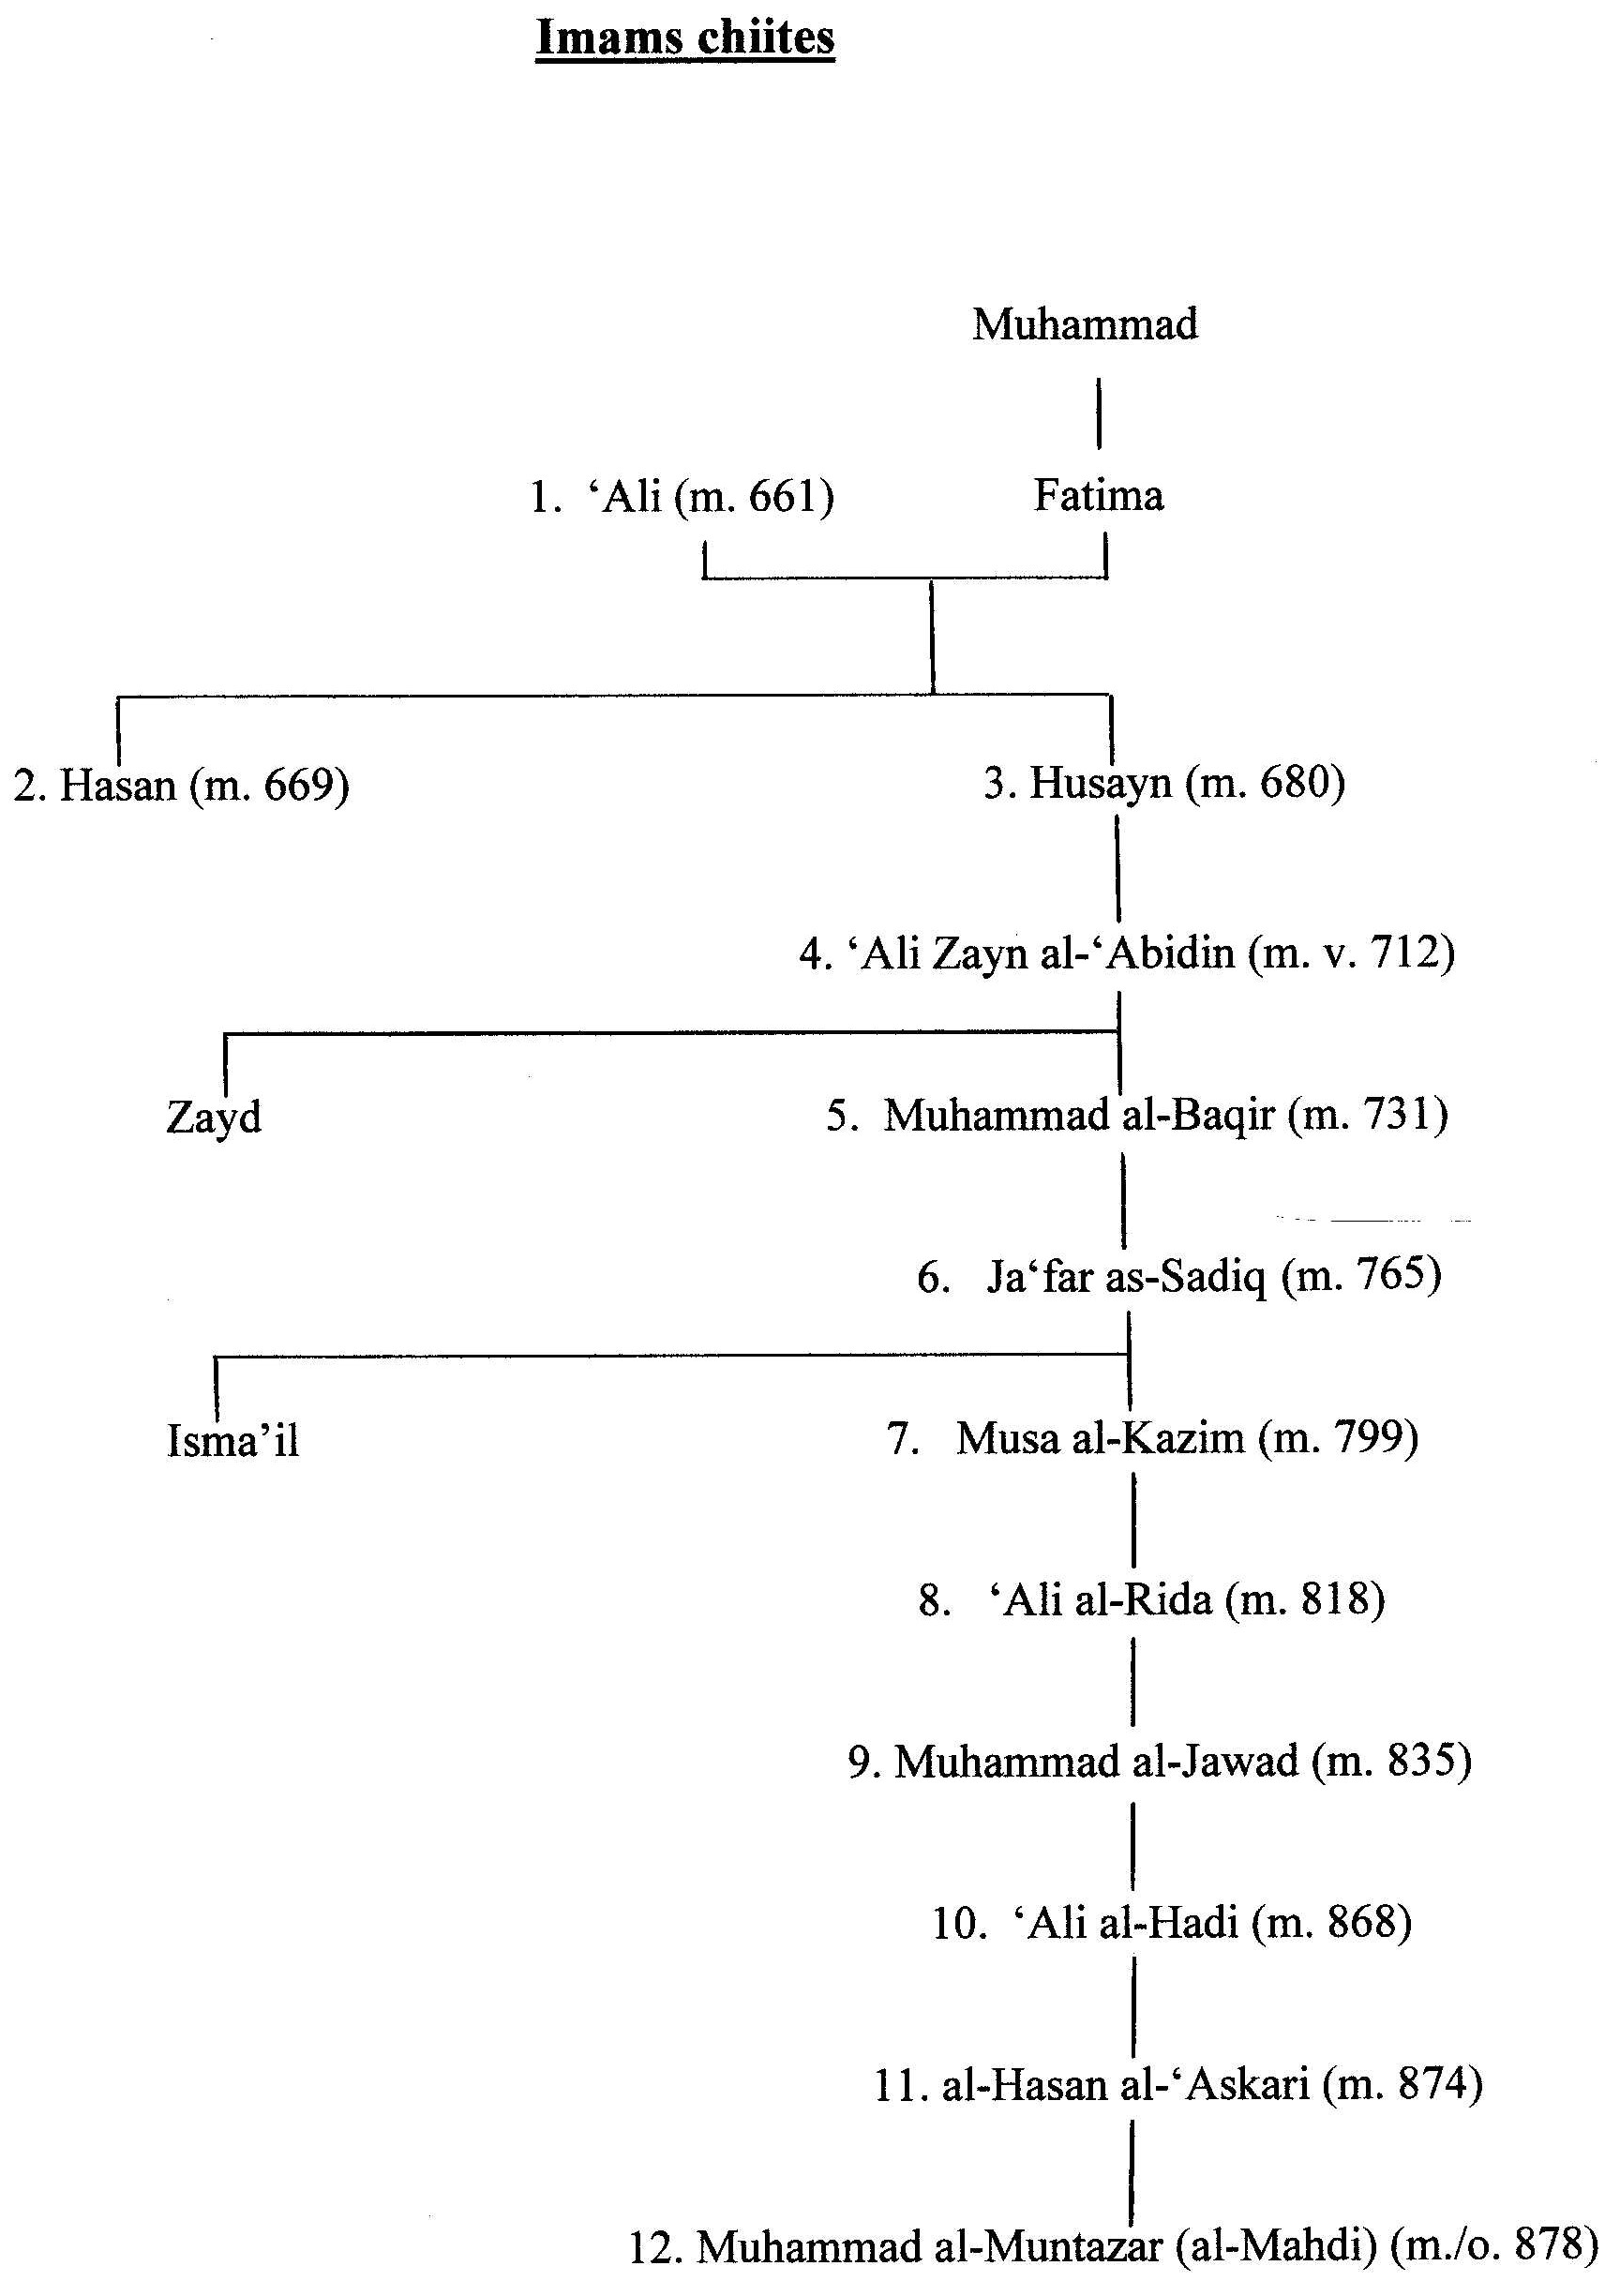
\includegraphics[width=0.8 \textwidth]{CourantsIslamContemporain/ImagesCourantsIslamContemporain/image2.png}
    \label{fig:my_label}
\end{figure}

 \paragraph{L'imam, celui qui guide} la prière et va faire le prêche du vendredi.  Dans la doctrine duodécimaine, l'imamat est lié à l'interprétation.
 Le prophète transmet la lettre du Texte. Mais elle a besoin d'être interprété : à chaque prophète dans l'humanité, correspond un imam : 
 \begin{itemize}
     \item Pour Moise, c'est Aaron
     \item Pour Jésus, c'est Pierre
     \item Pour Mohammad, c'est Ali.
 \end{itemize}
 Certes Mohammad est le dernier prophète, mais si on veut que le Coran soit parole vivante, il y a besoin d'Imams qui interprètent pour aujourd'hui la parole révélée.
 
 Du fait de problème de succession, il y a un vide à remplir (expliqué théologiquement par l'occultation), et c'est le \textit{clergé} qui le remplit \sn{Les Ayatollah ne sont pas imams. Il y a encore des imams dans le monde sunnite mais pas dans le monde chiite}.
 
 \newpage
 \paragraph{Les 14 immaculés}
    \begin{figure}
     \centering
     \sidecaption{Les 14 « Immaculés »  \newline La "Sainte Famille". \emph{Source}: Livre pour enfants iranien (Téhéran, 2006)}
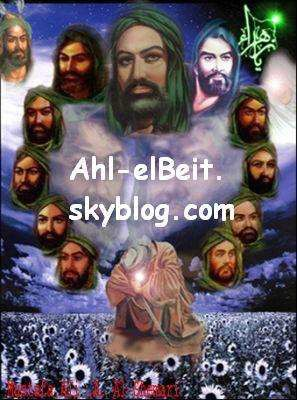
\includegraphics[width=0.45\textwidth]{CourantsIslamContemporain/ImagesCourantsIslamContemporain/Image3Chiisme.jpeg}
\includegraphics[width=0.45\textwidth]{CourantsIslamContemporain/ImagesCourantsIslamContemporain/image4.jpeg}
 \end{figure}
 
 
 \begin{Def}[les 14 immaculés]
 Les Quatorze immaculés ou Les Quatorze Infaillibles (en arabe:\TArabe{ المعصومون الأربعة عشر)} est l'expression désignant les gens de la Sainte Famille du Prophète Muhammad (s) Ahl al-Bayt, qui sont au nombre de quatorze, le premier étant le Prophète lui-même, suivi de sa fille Fâtima Zahrâ (a) et des douze Imams (a) qui lui ont succédé.
 \end{Def}
 
 
  
  
  \subparagraph{Prophétie et imamat}
  
 
Une autre tradition savante rapporte :\sn{(Source : \emph{La religion discrète}, M-A Amir Moezzi, Paris, Vrin,
2006, p. 110)}
\begin{quote}
    

« Deux mille ans avant la création, Muhammad et Ali étaient une lumière
devant Dieu -- qu'Il soit glorifié et exalté -, lumière formée d'un
tronc principal d'où partait un rayon de lumière resplendissant\ldots{}
Dieu dit alors : « Voici une lumière {[}tirée{]} de Ma propre Lumière ;
son tronc est la prophétie et sa branche, l'imamat ; la prophétie
revient à Muhammad, Mon serviteur et messager, et l'imamat revient à
Ali, ma Preuve et mon Ami. Sans eux, je n'aurai rien créé de ma
création\ldots{} C'est pourquoi Ali répétait toujours : « Je proviens de
Muhammad {[}ou de Ahmad{]} comme une clarté provenant d'une
autre\ldots{} »
\end{quote}


 \paragraph{Une science divine} pour interpréter le Coran, il y a besoin d'une science divine. L'imam a reçu une dimension spirituelle, la \textit{lumière de l'imamat}. Les imams préexistait à la création du monde en tant que réalité spirituelle. Comme les prophètes, ils sont \textit{impeccables}, sans péché.
   \subparagraph{La divinité des Imams}
De nombreux hadiths des Imams soulignent leur caractère quasi-divin : \sn{Source : « Remarques sur la divinité de l'Imam », M-A Amir-Moezzi,
\emph{Studia Iranica}, n° 25, 1996, p. 193-216}


\begin{quote}


« Hommes ! Dieu créa Ses serviteurs afin que ceux-ci Le connaissent car
lorsqu'Ils le connaissent, ils L'adorent et se libèrent ainsi de
l'adoration de tout autre que Lui ». Un homme demande alors à l'imam : «
Qu'est-ce que la connaissance de Dieu ? » « C'est pour les gens de
chaque époque, la connaissance de l'imam {[}de cette époque{]} auquel
ils doivent obéissance » (Husayn ben `Ali)

« Dieu fit de nous Son œil parmi ses adorateurs, Sa Langue Parlante
parmi Ses créatures, Sa Main de bienveillance et de miséricorde étendue
au-dessus de Ses serviteurs, Sa face grâce à laquelle on se dirige vers
Lui, Son Seuil qui guide vers Lui, Son Trésor au ciel et sur la
terre\ldots C'est par notre acte d'adoration que Dieu est adoré, sans
nous, Dieu ne saurait être adoré » (Ja`far as-Sadiq)


\end{quote}
 \paragraph{Les 14 impeccables} Le prophète, les 12 imams et Fatima. \sn{pas de difficulté de représentations dans le chiisme, depuis les enluminures persanes jusqu'à aujourd'hui. }
 
 \paragraph{le sacrifice d'Hussayn}
 
{Le martyre de l'imam Husayn}

Dans ce contexte, le martyre de Husayn, 3\textsuperscript{ème} imam, est
interprété dans les termes d'un sacrifice cosmique \sn{Source : tradition orale relevée par A-S Vivier-Muresan : \emph{Afzâd.
Ethnologie d'un village d'Iran}, Peeters, 2006, p. 48.
}:

\begin{quote}
    
 
Avant que le monde ne soit, Dieu rassembla les âmes des Quatorze
Immaculés, déjà créées, en une grande assemblée et leur annonça que,
pour ce monde qu'Il était sur le point de façonner, « du sang doit être
donné, un nourrisson et un tout jeune marié tués, une jeune femme
emprisonnée ». Aucun n'eut la force d'accepter de telles souffrances, ni
même Muhammad, ni Ali, ni Hasan. Seul Hoseyn se porta volontaire. Dieu
insista :
 

\begin{itemize}
\item
 
  Tu devras donner les tiens.
  
\item
  
  J'accepte.
  
\item
 
  Tu devras donner ta tête.
  
\item
 
  J'accepte.
  
\item
  
  Une partie de ta famille devra connaître l'exil et la détention.
  
\item
 
  J'accepte.
  
\end{itemize}


Alors Gabriel lui donna à boire la coupe de la souffrance et lui fit
signer un pacte où étaient inscrites toutes ses promesses.

Bien plus tard, lors de sa vie terrestre, approcha le temps de son
sacrifice. Il se trouvait à Karbalâ, accompagné de 72 fidèles compagnons
et de toute sa famille, encerclé par les armées de Yazid. Une armée de
djinns vint alors proposer ses services mais Hoseyn refusa : le combat
aurait été trop inégal et il se rappelait par ailleurs sa promesse. La
lutte commença et de nombreux êtres chers à Hoseyn, compagnons, fils,
frères, cousins, tombèrent l'un après l'autre sous les coups de
l'ennemi. Aveuglé par la douleur, Hoseyn en oublia sa promesse, et se
mit à tailler en morceaux l'armée adverse. Dieu s'empressa alors
d'envoyer Gabriel lui tendre le pacte qu'il avait signé au début des
temps. Rappelé à la raison, Hoseyn se soumit à la volonté divine et tint
son serment ; il retira son épée du combat et se livra à la fureur de
ses adversaires qui ne tardèrent pas à le mettre en pièces.
\end{quote}

 \subparagraph{Kerbala} la mémoire de la bataille est aussi une fête populaire. Des maquettes, repas,... le rouge reflète les partisans d'Hussayn.
 
 \begin{Def}[ta'ziyya]
\emph{représentation théâtrale du drame de Kerbala}
 \end{Def}

\begin{figure}[h!]
    \centering
        \sidecaption{Karbala}
    \includegraphics[width=0.3\textwidth]{CourantsIslamContemporain/ImagesCourantsIslamContemporain/image9.jpeg}
    \includegraphics[width=0.3\textwidth]{CourantsIslamContemporain/ImagesCourantsIslamContemporain/image10Chiisme.jpeg}
        \includegraphics[width=0.3\textwidth]{CourantsIslamContemporain/ImagesCourantsIslamContemporain/image8.jpeg}


    \label{fig:my_label}
\end{figure}
 
 
 %-------------------------------------------------
 
  \subsection{Le corpus coranique et son interprétation}
 
 
  \paragraph{Le « Coran chiite »}
 
 Le Coran actuel aurait été purgé des 2/3, en particulier par tout ce qui touche 'Ali.


\begin{quote}
Certains écrits chiites rapportent des citations du «Coran intégral»
qui aurait été par la suite altéré par les sunnites. Ces citations
présentent des divergences parfois notables avec la recension
officielle, comportant souvent des mots, expressions ou bouts de phrase
absents de celle-ci (en italique dans le texte).

C. 4, 167-70 : « Ceux qui sont injustes \emph{à l'égard des droits de la
Famille de Muhammad}, Dieu ne les pardonnera ni ne les guidera sur aucun
chemin si ce n'est sur celui de la géhenne où ils y séjourneront à
jamais et c'est chose facile à Dieu.

C. 16, 24 : « Et quand on leur dit : `\,`Qu'a fait descendre votre
Seigneur \emph{au sujet de `Ali} ?'\,' Ils répondent : `\,`Fables
racontées par les Anciens'\,' » ?

C. 33, 71 : « Quiconque obéit à Dieu et à Son prophète \emph{en ce qui
concerne la walaya de `Ali et la walaya des imams après lui}, celui-là
jouit d'un bonheur grandiose ».

C. 42, 13 : « Il a établi pour vous, \emph{ô famille de Muhammad}, en
fait de religion, ce qu'Il avait prescrit à Noé, et ce que Nous te
révélons \emph{ô Muhammad}, et ce que Nous avons prescrit à Abraham, à
Moïse et à Jésus : `\,`Etablissez la religion \emph{de la famille de
Muhammad}, ne vous divisez pas à son sujet et soyez unis ».

(Source : \emph{La religion discrète}, M.A Amir-Moezzi, Paris, Vrin,
2006, p. 179-180)
\end{quote}
 
 A la fin du XIX, cette posture chiite a été abandonnée car le réformiste chiite a essayé de se rapprocher du sunnisme. De façon générale, le Coran lu en Iran a toujours été le même mais avec une suspiçion qu'il ne contenait pas tout.
 

 %-------------------------------------------------
 
  \subsection{Le rôle des clercs}
  
  \paragraph{Un sens caché du Coran, ésotérique} Seul l'imam peut interprété le Coran. \textit{"si le grand ayatolah nous dit qu'on ne doit plus prier 5 fois par jour, on le suit".} \sn{L'absence de médiation dans le sunnisme est à relativiser quand on voit l'importance pour les sunnites de ce qui est Halah et Haram et qui demandent à l'imam...}
 
 \paragraph{Les clercs vont se substituer à l'Imam} pour l'interprétation du Coran et du droit. 
 
 \paragraph{Direction de la prière} A l'époque safavide, le clerc est nécessaire pour diriger la prière. On ne peut prier collectivement sans clerc. Le clerc va s'occuper des taxes religieuses.
 \paragraph{Au XIX, déclaration du Jihaad} Alors que c'est normalement l'Imam.
 
 \paragraph{Une dernière étape, avec l'Ayatollah Khomeini, le pouvoir politique} Toutes les prérogatives normalement réservées à l'Imam.
 
 \paragraph{Un clergé très structuré}. 
 \begin{itemize}
     \item les \emph{marja} (taqlid), la \emph{source} (de l'imitation). Un fidèle doit imiter un marja. Une dizaine dans le monde. Ils se cooptent (des dynasties de Marja et d'ayyatollah). Khomeini était \textit{marja}.
     \item l'\emph{ayyatollah} qui est le seul à interpréter le Coran, une centaine dans le monde, dont quelques femmes
     \item le \emph{hojjatelislam} qui a l'équivalent d'un doctorat
     \item le \emph{mollah}, \emph{âkhund} qui dirige la prière
 \end{itemize}
 
 
 %-------------------------------------------------
 
  \section{D'autres courants chiites :
  Zaydites et
  Ismaéliens} 
 
   \subsection{Le zaydisme}
   
   Proche du sunnisme, ils reconnaissent même les trois premiers califes, ce qui est inconcevable dans le chiisme duodécimain (cf la cérémonie de bruler Omar de Khomeini).
   Environ 1 million de fidèle.
   
   \subsection{Le chiisme septimain (ismaélisme)}
   A l'autre extrême, l'imam est quasiment une incarnation de Dieu. Un primat de l'ésoterisme, occulte. Un grand rôle donné à l'initiation. Un certain recul par rapport aux pratiques, à relativiser. 

\paragraph{L'Aga Khan} chef spirituel des septimains.
 



 
\section{Glossaire}
 
\subsection{Personnes} Abbas Abu Bakr

Adud ad-Dawla Al-Karaki Hasan as-Sabah Isma'il

Kulayni (\emph{Kitab al-Kafi}) Mu'awiya (omeyyades) Nizar

Omar Osman Quraysh Yazid

{Lieux} Alamut Ardabil

Ghadir al-Khumm Jabal al-Amil Kerbala

Khorasan Kufa Machhad Sham Siffin

{Autres noms propres} akhbari

ja`farisme (école juridique chiite) kharijites

Mamlouks

Muharram (mois musulman) mu`tazilites

nizayri Qarmates Seljukides usuli

\subsection{Notions}



baten : \emph{ésotérique} (c. zaher) faqih (pl. fuqaha) : \emph{juriste}

fitna: \emph{discorde, querelle (conflit interne au monde musulman)}

ghulat : \emph{groupes chiites aux doctrines}

\emph{« extrémistes »}

hulul : \emph{« incarnation »}

ijtihad : \emph{effort personnel d'interprétation (des textes sacrés)}

`ilm : \emph{science}

imamzade : \emph{descendant des Imams / sanctuaire contenant leur
tombeau} (persan)

`isma : \emph{impeccabilité}



ma`sum : \emph{impeccable (sans péché)} mujtahid : \emph{celui qui
pratique l'ijtihad} najes : \emph{impur} (persan)

na'ib : \emph{délégué}

na'ib al-`amm : \emph{représentant général de l'Imam}

nass : \emph{élection divine}

tafsir : \emph{commentaire (exotérique) du Coran}

tanasukh : \emph{métempsychose}

ta'wil : \emph{herméneutique ésotérique du Coran} 


taqiyya : \emph{dissimulation (fait de cacher sa foi)} walayat al-faqih
(persan : velayat-e faqih) : \emph{gouvernement du juriste}

zaher : \emph{exotérique} (c. de baten)
 
 


 



 


 
\chapter{Le chiisme au XXe sècle : de la Réforme à la Révolution}

\mn{28/3/22}
\section{bibliographie}



 
 
 
  KHOMEYNI, Ruhollah \emph{Gouvernement islamique}, Institut pour
  l'édition et la publication des œuvres de l'ayatollah Khomeyni,
  Téhéran, 1996.
 
 
 
  SHARIATI, Ali \emph{Histoire et destinée} {[}textes choisis{]},
  Sindbad, Paris, 1982.
 

 
\emph{Fatima est Fatima}, Albouraq, Beyrouth, 2009.

ADELKHAH, Fariba \emph{La révolution sous le voile}, Karthala, Paris,
1991.

*ADELKHAH, Fariba ; BAYART, Jean-François ; ROY, Olivier \emph{Thermidor
en Iran}, Ed. Complexes, Bruxelles, 1993.

*DIGARD, Jean-Pierre ; HOURCADE, Bernard ; RICHARD, Yann \emph{L'Iran au
XXe siècle}, Fayard, Paris, 2007.

KIAN-THIEBAUT, Azadeh \emph{La République islamique d'Iran : de la
maison du Guide à la raison d'Etat}, Michalon, Paris, 2005.

KHOSROKHAVAR, Farhad \emph{L'utopie sacrifiée, sociologie de la
Révolution iranienne}, Presses de la Fondation Nationale des Sciences
Politiques, Paris, 1993.

*KHOSROKHAVAR, Farhad et ROY, Olivier : \emph{Iran, comment sortir d'une
révolution religieuse ?}, Seuil, Paris, 1999.

MERVIN, Sabrina \emph{Un réformisme chiite. Ulémas et lettrés du Gabal
`Amil (actuel Liban-Sud) de la fin de l'Empire ottoman à l'indépendance
du Liban}, Karthala-CERMOC - IFEAD, Paris-Beyrouth-Damas, 2000.

MERVIN, Sabrina (dir.) \emph{Les mondes chiites et l'Iran}, Paris,
Karthala-IFPO, 2007.
 


\subsection{Introduction}

Le Chiisme ne doit pas être pensé en vase clos, elle est en interaction avec les pensées qui l'entoure.

\section{Le réformisme chiite}
\label{le-ruxe9formisme-chiite}

  \paragraph{Lien très fort avec au centre Najjaf et Kerbala} En terme d'influence, et de centres du Chiisme, ce sont les villes saintes de Najjaf (tombeau de Ali) et Kerbala (tombeau de Hussein). Importance du pélerinage sur leurs tombeaux. 
  Pour être plus qu'un recteur de mosquée, il faut aller à Najjaf. 
  
  
     \subsection{Un mouvement parallèle au réformisme sunnite}

  \paragraph{Le réformisme chiite} comme le réformisme sunnite, le renouveau passe par :
  \begin{Def}[tajdid] 
\emph{renouvellement}.
\end{Def}

  \begin{itemize}
      \item   l'acceptation de la modernité et la raison au centre.
      \item   Il passe aussi par une purification de la foi : \emph{tawhid}, unicité de Dieu.
      \item Cela passe par un retour aux sources, Coran et sunna (chiite)
      \item Enfin, le désir de retrouver \emph{l'umma} et refaire l'unité avec le monde sunnite.
C'est d'abord un réformisme pensé par les religieux.
  \end{itemize}

\paragraph{Al-Amin (Muhsin)} réformisme libanais.Al-Sayyed Mohsen al-Amin (b.1284/1867-d.1371/1952), also transliterated Muhsin al Amin, was a Shia scholar, biographer, traditionist, and jurist. He was born in Jabal Amil, Lebanon. His most important work is A'yan al-Shi'a.[1] \sn{\href{https://en.wikipedia.org/wiki/Al-Sayyed_Mohsen_al-Amin}{Al Amin}}

\paragraph{Baqir al-Sadr (Muhammad) Borujerdi} né le 23 mars 1875 à Boroudjerd et mort le 30 mars 1961 à Qom \sn{\href{https://fr.wikipedia.org/wiki/Seyyed_Hossein_Tabatabai_Borujerdi}{Borujerdi}}


\paragraph{Changement de l'éducation} au début du XX.

 \begin{itemize}
     \item  manuel scolaire (avec une doxa réformisme)
     \item histoire des religions, psychologie
 \end{itemize}
Ils vont se heurter à beaucoup de résistances et cela ne va aboutir qu'à moitié.


  
 
\subsection{Particularités du réformisme chiite : \emph{ijtihad, taqlid} et
    \emph{bid`a}}

Dans le sunnisme, face à l'imitation stérile des savants précédents, \emph{le taqlid}, il faut faire l'effort d'interprétation des textes du Coran (\emph{ijtihad}). On dit souvent que les portes de \emph{ijtihad} se sont fermées au XIe siècle.
Très différent dans le chiisme : 
\begin{itemize}
    \item le taqlid est positif : il s'agit d'imiter le \textit{marja}
    \item l'\textit{ijtihad} s'est toujours poursuivi par les Ayatollahs \sn{seuls eux peuvent faire l'ijtihad}. Un rapport positif à la raison dans le chiisme : On a toujours étudié la philosophie grecque. De facto, dans le chiisme, le réformisme était plutot à lutter contre l'ijtihad face à des ayatollahs considérés comme sclérosés. 
\end{itemize}

\paragraph{refus de toute médiation}Face au Wahhabisme, qui condamne toute innovation (bid'a) au titre du \textit{tawhid} et donc toute médiation (dévotion aux saints, soufisme, rôle du clergé chiite). Or la dévotion aux saints est clé dans la pratique chiite\sn{rôle économique et religieux de cette dévotion aux imams}.

    \subsection{Réforme de la doctrine et des pratiques}

\paragraph{rationalisation des imams}  On va introduire une forme de rationalisation sur les imams : pouvoir surhumain des imams, préexistence des imams,...
  au profit de leur vie exemplaire sur le plan moral qu'il faut imiter : on ne parle plus d'intercession mais du rôle de modèle.
  
 \paragraph{Schizophrénie entre une théologie épurée et une pratique } et piété populaire, qui n'a pas été condamnée et qui continue : culte des imams, voeux aux imams,...
 
 \paragraph{Des pratiques qui ont reculé} la pression de la tombe : on va sentir le poids de la terre qui va faire rejeter le lait de la mere aux ongles. Donc il y avait un vrai commerce de cadavres qui allaient se faire enterrer à Kerbala (pour éviter sa pression).
 Mais Al Amin n'a pas réussi à faire évoluer les pratiques de Achoura pour des questions de moralités (travestis, flagellation,). 
 

\section{Genèse et destin du chiisme politique : Révolution iranienne et République islamique}
\label{genuxe8se-et-destin-du-chiisme-politique-ruxe9volution-iranienne-et-ruxe9publique-islamique}


 
 
 
   \subsection{Un contexte bien particulier : l'Iran pahlavi}
    
    C'est le roi, \textit{shah} d'Iran. Au début du XX, on a une révolution constitutionnelle en 1906, qui limite (un peu) le pouvoir du Shah en introduisant une constitution.
    
    En 1921, on a la prise de pouvoir par Reza Khan, officier, dans une démarche très séculariste. Mais il décide de rester dans le cadre monarchique pour ne pas froisser les Ayatollahs. Il décide donc de créer une nouvelle dynastie, la dynastie \textit{Palhavi}.
    
    \paragraph{Des réformes sécularistes} Un réseau d'écoles publiques, modernisés. Création de tribunaux séculiers et introduit un code civil occidental, à la place du système juridique islamique qui existait auparavant.
    
    En 1935, interdiction du voile dans l'espace publique. Mais résistance à cette mesure et le voile n'est finalement interdit que dans les administrations.
    
    \paragraph{Mohammed Reza Shad (1941)} son fils au pouvoir. En 1963, il fait la \href{https://fr.wikipedia.org/wiki/R\%C3\%A9volution_blanche}{révolution blanche}, qui comporte plusieurs volets : réforme agraire, droit de vote au femme. Cela lui vaut l'hostilité du clergé (qui était grand propriétaire). Par ailleurs, il entre dans une forme de mégalomanie, notamment en 1971 (2500 ans de monarchie ininterrompue). 
    En 1975, il adopte un calendrier achéménide au lieu d'un calendrier musulman. 

    \paragraph{le clergé prend la tête de l'opposition}
    
   \subsection{Ruhollah Khomeyni (1902-1989) et le \emph{velâyat-e faqih}}
    
    \paragraph{Ruhollah Khomeyni } \sn{\href{https://fr.wikipedia.org/wiki/Rouhollah_Khomeini}{Khomeyni sur Wikipedia}} dynastie d'Ayatollahs, bourgeoisie du bazaar (commerce) et propriétaires terriens. Il est même nommé Marja en 1962. Il enseigne dans l'université de \textit{qom}. Dès les années 60, il est à la tête de l'opposition. Jugement en 1963, peine de mort commué à l'exil. 14 ans en Irak mais indispose le pouvoir irakien et s'installe en France en 78.
    
    
    \paragraph{Delégitimisation du Shah} Applique au shah, le \textit{taghut} (idole, pharaon) \sn{\begin{Def}
    [taghut] : \emph{idole ; tyran}.
    \end{Def}}. face à cette délegitimisation,  le pouvoir revient aux clercs.
    \begin{Def}[velayat-e faqih]
    le pouvoir aux clercs
    \end{Def}
    
    \paragraph{Une rupture théologique} Dans le chiisme, il y a une idée d'une corruption profonde dans le monde et qu'il n'est pas possible d'imposer le règne de Dieu sur terre. Seule le mahdi peut le faire. Face à Khomeyni, beaucoup de marjas se sont imposés à lui et à sa volonté d'avoir un rôle politique.
    
    \sn{Quand le religieux se melent de politique, c'est toujours le religieux qui est asservi par le politique.}
    
    
    
\paragraph{Le \emph{velayat-e faqih} : Ruhollah Khomeyni (1902-1989)}



\begin{quote}
    

\emph{Méthode du gouvernement islamique. Ses différences avec les autres
gouvernements.} \sn{Extraits de \emph{Pour un gouvernement islamique}, 1969 (traduction
française chez Fayolle, 1979).}

Le gouvernement islamique ne ressemble à aucun autre gouvernement
actuellement en vigueur. Il n'est pas despotique. Le chef de l'État
n'est pas un despote qui se joue des biens et de la vie du peuple et en
fait ce qu'il désire, qui tue celui qu'il veut, et enrichit ou ennoblit
qui il veut, distribuant de-ci de-là les terres et les biens du peuple.
Le Prophète, Ali et les califes n'avaient pas ce genre d'attributions.
Le gouvernement islamique n'est ni despotique ni absolutiste, il est
constitutionnel \sn{rôle de la loi : cf Banna, \textit{le Coran est notre Constitution}}, bien entendu pas au sens habituel du terme, où les lois
sont approuvées par des personnes et une majorité : constitutionnel, au
sens où les dirigeants sont tenus à un ensemble de « conditions »
définies dans le Coran et dans la Sunna du Prophète à la fois en ce qui
concerne l'exécutif et l'administration. Ces conditions ne sont rien
d'autre que les lois islamiques, celles-là mêmes qui doivent être
observées et appliquées. De cette manière, le gouvernement islamique est
le gouvernement de la Loi divine sur le peuple.

C'est ce qui constitue la différence fondamentale entre le gouvernement
islamique et les autre gouvernements constitutionnels, monarchiques et
républicains ; un autre fait capital est que dans ces régimes, les élus
du peuple ou le monarque sont les législateurs, tandis que dans l'Islam,
le seul législateur est Dieu \sn{Idéalisation de la loi islamique}, le Législateur sacré.

Personne n'a le droit d'émettre des lois, et aucune loi n'est applicable
si ce n'est celles du Législateur. Voilà pourquoi dans le gouvernement
islamique, au lieu de l'assemblée législative qui représente
habituellement l'un des trois pouvoirs, il existe une assemblée de
planification qui a pour rôle d'organiser les divers ministères au
regard des lois islamiques et de déterminer, à l'aide de ces plans et
sur tout le territoire, la manière d'accomplir les services publics.

L'ensemble des lois islamiques réunies dans le Coran et dans la Sunna
ont été acceptées par les musulmans et ceux-ci leur obéissent. Ceci
facilite la tâche du gouvernement qui devient du même coup le
coordinateur du peuple. Tandis que dans les autres régimes
constitutionnels, la majorité de ceux qui se font passer pour les
représentants de la majorité du peuple approuvent ce qui leur plaît au
nom de la loi, et ensuite s'imposent au peuple tout entier.

Le gouvernement de l'Islam est le gouvernement de la Loi. Dans cette
méthode de gouvernement, la souveraineté revient exclusivement à Dieu,
et la Loi constitue l'ordre et le décret de Dieu. La Loi de l'Islam,
Ordre de Dieu, règne d'une façon absolue sur tous et sur l'État islami-
que. Tout les hommes depuis le Prophète, jusqu'à ses califes et au
commun des mortels, sont définitivement soumis à la Loi, loi qui est
envoyée par Dieu et expliquée dans le Coran et par le Prophète. Si
celui-ci a pris la charge du califat, ce fut sur l'ordre de Dieu. Il est
Calife de Dieu sur terre et non pas calife sur sa propre initiative dans
l'intention de devenir le chef des musulmans. Lorsque des risques de
conflits se firent jour dans la communauté, étant donné le caractère
récent des conversions à l'Islam, Dieu s'est révélé au Prophète et l'a
engagé à annoncer le califat de toute urgence, ainsi, en plein désert.
Mahomet désigna alors Ali comme Calife en obéissant à la Loi, non pas
parce que celui-ci était son gendre ou qu'il avait rendu des services,
mais parce que lui-même en avait reçu la mission divine et qu'il
s'inclinait devant l'ordre divin. Dans l'Islam, le gouvernement signifie
l'obéissance à la Loi, et seule la Loi exerce son autorité sur la
société. Là où une certaine limitation des attributions a été donnée au
Prophète et aux Imams, c'est l'œuvre de Dieu. Chaque fois que le
Prophète a exprimé quelque chose ou annoncé une loi, c'était en
obéissance à la Loi divine, Loi à laquelle tout le monde sans excep-
tion doit obéir, le gouvernant comme le gouverné. Obéir au Prophète est
également un ordre de Dieu qui dit : « Obéissez au Prophète. » La
soumission aux responsables du gouvernement ou imams est également un
ordre de Dieu qui dit: «Obéissez aux Imans qui sont issus de vous.»

L'opinion des personnes, fût-ce celle du Prophète, n'a pas de prise sur
la Loi divine. Tous se plient à la volonté de Dieu. {[}\ldots{]}


\begin{Synthesis}
C'est une nomocratie, plus qu'une théocratie
\end{Synthesis}

\emph{L'Exercice du pouvoir du faqih, par les textes}

\emph{Les faqih justes, véritables successeurs des prophètes}

Dans l'un des \emph{ravâyat} les plus authentiques, il est dit : « Ali
rapporte les paroles du Prophète : Dieu ! Pardonne à mes successeurs.
(\emph{Il a répété cette parole trois fois}.) --- Qui sont tes
successeurs ?, lui a-t-on demandé. --- Ceux qui viendront après moi et
qui citeront et enseigneront au peuple mes hadith et ma Sunna. »

Par conséquent, il ne fait aucun doute que ce \emph{ravâyat} ne concerne
pas les rapporteurs de hadith, c'est-à-dire ceux qui les rédigent ; en
effet, un écrivain ne peut être calife du Prophète.

Il faut entendre par le mot calife qui est employé dans ce
\emph{ravâyat}, le \emph{faqih} de l'Islam. La diffusion des lois et
l'éducation du peuple seront à la charge des \emph{faqih} justes, car
s'ils ne le sont pas, ils ressembleront aux juges qui ont inventé des
\emph{ravâyat} contre l'Islam à la manière de Samarat Ebn-e-Djandâb.
S'il n'y a pas de \emph{faqih}, le peuple ne pourra pas connaître le
\emph{feqh}, la Loi de l'Islam. Alors deviendra possible la propagation
de milliers de \emph{ravâyat} fabriqués par les agents des oppresseurs
et les \emph{âkhond} courtisans, destinés à faire l'apologie des
sultans. {[}\ldots{]}

\emph{Les pleins pouvoirs des faqih}

Par conséquent, « les faqih sont les confidents des prophètes »,
signifie que les \emph{faqih} ont le droit de prendre en charge tout ce
qui était du domaine des prophètes. Comme ceux-ci, ce sont des hommes
qui ne doivent dévier d'aucune loi et qui sont purs et désintéressés des
biens de ce monde, comme il est dit à la fin du hadith cité plus haut :
« Tant qu'ils n'entrent pas dans le monde » (dans le bourbier de la
recherche des biens matériels !). Si donc un \emph{faqih} pense aux
biens terrestres, ce n'est pas un \emph{faqih} juste, et il n'est pas le
confident du Prophète, ni l'exécutant des lois islamiques. Seul le
\emph{faqih} juste est en mesure d'appliquer les Lois, d'établir les
principes islamiques, d'administrer les peines et les châtiments, de
veiller aux frontières et à l'intégrité territoriale de la communauté
musulmane, bref d'être le Magistrat suprême du gouvernement. Comme le
Prophète, il peut établir les principes islamiques et appliquer les
lois. {[}\ldots{]}


 
\end{quote}
    
    
    
   \subsection{ `Ali Shariati (1933-1977) et la naissance du chiisme révolutionnaire}
   
   \paragraph{Ali Shariati (1933-1977)} intellectuel laic \sn{\href{https://fr.wikipedia.org/wiki/\%27Al\%C3\%AE_Shar\%C3\%AE\%27at\%C3\%AE}{Ali Shariati sur Wikipedia}} existencialisme, théologie de la libération, marxisme,...
   Il va penser le shiisme comme \textit{la religion des opprimés}. La révolution pour imposer la justice sociale et libérer le peuple.
   \begin{Def}[musta'zafin]
   Oppression. Un concept utilisé pour les persecutions religieuses qu'Ali Shariati va appliquer au contexte socio-économique
   \end{Def}
   Fatima va être mise en avant pour montrer qu'elle est femme religieuse. Dans la société islamique, les femmes ont perdu mais ont gardé un rôle important.
   
   La grande différence avec Khomeyni,n c'est que les clercs n'ont aucun rôle : les savants ont trahis Ali et Husseyn et ont maintenu le peuple dans l'oppression.
   
   Pour Khomeyni, l'état est basé sur la loi islamique (comme Mawdudi). Alors que pour Shariati, c'est la révolution.
   
   \paragraph{Un très grand mécontentement social} Face à l'échec de la réforme agraire mal faite, un exode rural. Khomeyni récupère le discours contestataire de Shariati. 
   

   
 \subsection{ La République islamique}
     
     
\paragraph{Notion de martyr}    , de Achoura, reprise par les discours politiques de la notion de martyr. 
   En 2009, un vrai changement de ce discours puisqu'un contre-discours a appliqué Achoura,  Yazid étant le gouvernement islamique.
   
   
\paragraph{1979 : constitution islamique d'Iran}   
    
\begin{figure}[h!]
    \centering
       \sidecaption{De la République islamique d'Iran : on voit à quel point c'est verrouillé. le conseil des gardiens filtre les candidats à la présidence, peut mettre son veto aux lois}
    \includegraphics[width=\textwidth]{CourantsIslamContemporain/ImagesCourantsIslamContemporain/image3.jpeg}
  
    \label{fig:my_label}
\end{figure}
 

 





\hypertarget{glossaire-6}{%
\section{ {Glossaire}}\label{glossaire-6}}

 
\paragraph{Personnes}



Khameney Khatami

Khomeyni (Ruhollah) Mohammed Reza Shah Shariati (`Ali)

{Lieux} Jabal Amil Karbala Najaf

Neauphle-le-Château

\paragraph{Notions}

ayatollah : « \emph{signe de Dieu » (sur terre) ; grade supérieur dans
le clergé chiite}. marja'-ye taqlid : \emph{« source d'imitation » ;
plus haut grade dans le clergé chiite.} 



tawhid : \emph{unicité (divine).}

mujtahid : \emph{celui qui pratique l'ijtihad.}

musta`zafin : \emph{les opprimés.}



\chapter{La nouvelle pensée islamique}
\mn{\emph{(04/04/2022)}}


\section{Bibliographie}


\begin{itemize}
\item
  
  AL AJAMI, \emph{Que dit vraiment le Coran}, Erick Bonnier Editions,
  2020.
  
\item
  
  ABOU ZEID Nasr Hamid \emph{Critique du discours Religieux}, Sindbad,
  Acte Sud, Paris, 1999.
  
\item
  
  AL-BANNA, Gamal \emph{L'Islam, la Liberté, la Laïcité et le Crime de
  la tribu des « il nous a été rapporté »}, trad. D. Avon et A. Elias,
  L'Harmattan, Paris, 2013.
  
\item
  
  ARKOUN, Mohamed \emph{Lectures du Coran}, Maisonneuve \& Larose,
  Paris, 1982.
  
\item
  
  BAJRAFIL, Mohammed \emph{L'islam de France, l'an I. Il est temps
  d'entrer dans le XXIe siècle}, Ed. Plein Jour, 2015.
  
\item
  
  BENKIRANE Réda \emph{Islam, à la reconquête du sens}, éd. Le Pommier,
  2017.
  
\item
  
  CHARFI, Abdelmajid \emph{L'islam entre le message et l'histoire},
  Albin Michel, Paris, 2004.
  
\item


\emph{La pensée islamique, ruptures et fidélités}, Albin Michel, 2008.


 
\item
  
  CHEBEL, Malek \emph{Manifeste pour un islam des lumières}, Hachette,
  Paris, 2004.
  
\item
  
  ESACK Farid \emph{Coran, mode d'emploi}, Albin Michel, Paris, 2004.
  
\item
  
  LAMRABET Asma, \emph{Islam et femmes : les questions qui fâchent},
  Casablanca, En toutes lettres, 2017.
  
\item
  
  SANGARE, Youssouf \emph{Repenser le Coran et la tradition islamique --
  Introduction à la pensée de Fazlur Rahman}, Al Bouraq, 2017.
  
\item

  TALBI Mohamed \emph{Plaidoyer pour un Islam moderne}, Cérès/Tunis,
  DDB/Paris, 1998.
  

\item BENZINE, Rachid \emph{Les nouveaux penseurs de l'Islam}, Albin Michel,
Paris, 2004. FILALI-ANSARY, Abdou \emph{Réformer l'islam ? Une
introduction aux débats contemporains}, La
Découverte, Poche, Paris, 2005.

 \item HOFFNER, Anne-Bénédicte \emph{Les nouveaux acteurs de l'islam}, Paris,
Bayard, 2017.

\item RENAUD, Etienne "Mahmud Taha et la «seconde mission de l'Islam»",
\emph{Se Comprendre}, 85/07, 1985.

\item ROUSSILLON\textbf{,} Alain \emph{La pensée islamique contemporaine},
\emph{acteurs et enjeux}, Téraèdre, Paris, 2005.

\item SALEH Waël, \emph{A la recherche d'un aggiornamento de l'islam. Des
voies contemporaines}, Paris, L'Harmattan, 2018.

\end{itemize}



\section{Les nouveaux penseurs : essai
  de
  présentation}
  
  \subsection{Synthèse}
  
  \begin{Synthesis}
  Nous sommes dans un contexte Post moderne. A la différence moderne, universaliste et objectif, en post modernité, il n'y a qu'un accès relatif et subjectif à la vérité.
  Nous sommes tous des personnes raisonnables mais la façon d'accéder à la vérité, passe par le filtre de la subjectivité. 
  Le Coran passe par le filtre de la propre de subjectivité de Mohammed. Le texte est déjà une interprétation. Il y a une remise en cause du Coran \textit{Verbatim}.  
  \end{Synthesis}
  
Rachid Benzine \sn{voir p. \pageref{Theo:Benzine}}: 
\begin{quote}
    les modernistes, ou les nouveaux penseurs
\end{quote}  

Il s'est développé à partir des années 1980 en réaction à l'Islam politique et le wahhabisme, l'entrée de la violence en Islam, la cloture.

\paragraph{dans un cadre post moderne}
Ils vont chercher des nouvelles voies. La grande différence avec les modernistes, c'est qu'ils pensent la fin du XXeme. Ce n'est plus la positivité d'Auguste Comte, c'est le cadre de la post modernité. On reconnaît que la raison est construite historiquement, sociologiquement. L'accès à la vérité est donc partiel. Ce qui demeure et s'accentue, c'est la subjectivité.

\paragraph{L'herméneutique} ou Interprétation. L'accès à la vérité ne peut se faire que via l'herméneutique.

\begin{Def}[herméneutique]
Il n'y a que des interprétations à la vérité auxquelles on accède
\end{Def}

\paragraph{Conséquences} 
\begin{itemize}
    \item Il n'y a pas une essence de l'Islam. \textit{il n'y a que ce que les croyants musulmans en disent}.
    \item refus de chercher un islam pur à l'origine. Il n'y a que des islams contextualisés
    \item Importance plus faible du droit, de la norme. Ce qui compte, c'est l'éthique. L'Islam est moins pensé comme une religion normative mais un moyen pour l'individu d'entrer en relation avec le divin.
\end{itemize}

\paragraph{Rapport complexe à l'occident} Ils peuvent en particulier critiquer l'aspect absolu des droits de l'homme qu'il convient de contextualiser en Islam.

\paragraph{Un même type de formation} Plutôt formés en sciences humaines ou littératures, où ils ont découvert l'herméneutique : philosophie, histoire, ... acquis en occident. Ils prennent très au sérieux les études en sciences islamiques. 

\paragraph{En opposition avec les élites} religieuses (qu'ils critiquent) ou étatiques (face à leur souhait démocratique). Exil parfois nécessaire. En Tunisie et au Maroc, on pouvait avoir cette réflexion.

\paragraph{Du monde entier} 
\begin{itemize}
    \item Arabe
\begin{itemize} 
    \item Arkoun (Mohamed) (Algérie)
    \item Abu Zayd (Nasr Hamid) (Egypte)
    \item Khalafallah (Muhammad Ahmad) (Egypte)
\end{itemize}
\item Iran
\begin{itemize} 
    \item Sorush (Abdelkarim)
    \item Shabestari (Muhammad)
\end{itemize}
\item Pakistan
\begin{itemize} 
    \item Rahman (Fazlur)
    \item Engineer (Ali)
\end{itemize}
\item Afrique du Sud
\begin{itemize} 
    \item Esack (Farid) (théologie de la libération)
\end{itemize}
\end{itemize}
A classer : 
   Charfi
(Abdelmajid) 

 Hossein (Taha) Iqbal (Muhammad)

 

 
  
\section{Nouvelles approches critiques}

\subsection{L’approche littéraire}

Rappel du statut du Coran en Islam Classique : voix de Dieu et Mohammed n'est que l'enregistreur. Ce texte est vérité.

'Abduh va suggérer que le Coran ne doit pas être pris comme un document historique. Le but du Coran est d'exhorter les fidèles, sans avoir un soucis de précision historique.

\paragraph{Al-Khuli (Amin) 1895-1966} Enseigne à Al-Azhar. mais il a fait quelques années d'étude en Europe. Le Coran doit être compris et analysé comme un texte littéraire : 
\begin{itemize}
    \item Sémantique : les mots à l'origine. \sn{Ce n'est pas tout à fait nouveau. des les premiers siècles de l'islam, travaux sur la poésie pre-islamiques, la grammaire et dictionnaires}
    \item forme littéraire
    \item le contexte culturel et social. Cela est nouveau.
\end{itemize}

\paragraph{Khalafallah (Muhammad Ahmad) 1916-1998 } Disciple de Al-Khuli. Savant et étude de lettres à l'université du Caire (université moderne). Thèse en 1948 sur \textit{l'art du récit dans le Coran}. Il va aller jusqu'à dire que certains récits dans le Coran n'ont pas de valeur historique mais uniquement littéraire. 

\begin{Ex}
Par rapport aux récits des \href{https://fr.wikipedia.org/wiki/Sept_Dormants_d\%27\%C3\%89ph\%C3\%A8se#:~:text=Les\%20Sept\%20Dormants\%20d'\%C3\%89ph\%C3\%A8se,r\%C3\%A9cit\%20au\%20contexte\%20arabo\%2Dmusulman.}{sept dormants d'Ephèse}, va montrer que dans certains versets, il y en a 5 et dans d'autres 6. Cela montre que le but de Dieu n'est pas de faire un récit historique
\end{Ex}

Pour Khalafallah, il distingue dans le Coran différentes formes littéraires : 
\begin{itemize}
    \item Historique
    \item Parabolique : ce qui compte, c'est le message
    \item mythique (comme dans les sept dormants)
\end{itemize}

\subparagraph{une forte réaction à Khalafallah} car dès le Coran, on reprochait au Prophète de ne transmettre que des mythes. La réponse de Khalafallah a été de dire que le point du prophète était de défendre que ces textes étaient révélés. Thèse refusée et \textit{fatwa} interdisant à Al-Khuli et Khalafallah d'enseigner les sciences coraniques. Thèse néanmoins publiée.


\subsection{Critique historique}

\paragraph{Mohammed Arkoun 1928 - 2010} \label{theol:Arkoun5} En France en 1954, agrégé d'arabe\sn{cf p. \pageref{theol:Arkoun1}}. Il est marqué par la pensée des IX-X siècle. Sa compréhension de l'Islam (comme dans toute religion) : 
\begin{itemize}
    \item \textbf{la religion forte} réponse théologique crédible aux grandes questions de l'homme : le bien, le mal, ce qui se passe après la mort,... C'est ce qui compte pour toute grande religion
    \item \textbf{religion individuelle} la façon dont une religion se déploie à l'intérieur de chaque individu dans sa vie intérieure et sa relation à Dieu
    \item \textbf{la religion forme} les formes prises par la Religion dans une situation sociologiques et historiques données. Pour lui secondaire. 
\end{itemize}

\subparagraph{Une sacralisation de la religion forme} en Islam :
\begin{itemize}
    \item sur le plan politique, le \textit{califat}
    \item sur le plan politique, la \textit{shari'a}, loi religieuse
    \item et \textit{l'umma} éventuellement pouvant être pensé comme un seul état.
\end{itemize}
Si on touche à l'un de ces trois points, on touche à ce qui est considéré comme coeur à l'islam

\subparagraph{il faut une archéologie pour déconstruire ces formes}  L'Islam aurait pu être autre que ce qu'il est aujourd'hui. Ce sont des rapports de force qui ont imposé le califat, la shari'a et l'umma. 
\subparagraph{Une cloture dogmatique} au X-XI eme siècle. Ce qui est pensable et ce qui est impensable (tabou). Par exemple :
\begin{itemize}
    \item on oublie la genèse du texte du Coran. Simplification alors qu'on sait
    \item Coran incréé.
\end{itemize}
Il y a en parallèle un imaginaire, celui de l'âge d'or des 4 premiers califes, qui permet de justifier cette fermeture.

Arkoun va même jusqu'à distinguer le fait coranique de la révélation et le document historique et littéraire, le \textit{corpus officiel clos} qui est lui le résultat d'un rapport de force. 
\begin{Ex}
Osman a fait brûler des corpus hétérodoxes.
\end{Ex}


\paragraph{Différence entre les modernistes et les réformismes} Les modernistes critiquent la trahison des premières générations, à l'opposé de ce qui est reçu par la tradition musulmane d'un âge d'or.



\section{le statut de la Parole de Dieu : un Coran créé ?}



\subparagraph{Le statut du Prophète }

\paragraph{F. Rahman 1919-1988} Indo Pakistanais. Formation moderne. Inde puis Oxford (th. Philosophie). Enseigne au Canada. Rentre au Pakistan en 1961 mais il va rencontrer une très forte contestation des savants pakistanais. Ils vont l'accuser d'apostasie. Exil aux US en 1968 où il connaît une célébrité.

\paragraph{Une vision du Coran où le Coran passe par la langue et l'imaginaire du Prophète}. Voir texte. Un Coran purement extérieur du fait des controverses chrétiennes (lo-
gos,...) La parole de Dieu mais elle est aussi parole du prophète (dans
son coeur) et pas seulement enregistreur. Il reconnaît une subjectivité du
Prophète. Elle s’incarne dans son imagination, sa langue,...


\paragraph{Coran Parole de Dieu}\sn{Fazlur Rahman
(1919-1988) \emph{Extrait de son livre \textbf{Islam} (Doubleday Anchor Book, New
York, 1968, 331 pp.), p. 25-28.}}

 \begin{quote}
     

Pour le Coran lui-même, et par conséquent pour les Musulmans, le Coran
est la Parole de Dieu (kalâm Allâh). Mohammed, lui aussi, était
absolument convaincu de recevoir le Message de Dieu, le Tout-Autre (nous
essaierons plus loin de comprendre plus précisément le sens de cette
Altérité absolue), à tel point qu'il s'est basé sur la force de cette
conviction pour rejeter quelques-unes des assertions historiques les
plus fondamentales de la tradition Judéo-Chrétienne concernant Abraham
et les autres Prophètes. Cet "Autre", par un certain canal, a "dicté" le
Coran avec une autorité absolue. La voix surgissant des profondeurs de
la vie parlait distinctement, impérieusement, sans méprise possible. Non
seulement le mot \textbf{"}\emph{qur'ân}", signifiant "récitation",
l'indique clairement, mais le texte du Coran lui-même déclare en
plusieurs endroits que le Coran est révélé verbalement et non pas
seulement son "sens" et ses idées. Le terme coranique pour "Révélation"
est \emph{wahy} dont le sens est assez proche d' "inspiration", à
condition que ce mot ne soit pas censé exclure nécessairement le mode
verbal (par "Parole", bien entendu, nous ne voulons pas dire le Son). Le
Coran dit: "Dieu ne parle à aucun humain (c'est-à-dire en paroles
audibles) excepté par \emph{wahy} (c'est-à-dire par idée-parole,
inspiration) ou derrière un voile, ou bien Il envoie un Messager (un
ange) qui parle par \emph{wahy}...Nous t'avons ainsi révélé un Esprit
qui est à nos ordres". (Q. 42,51-52)


Pendant le 2° et le 3° siècles de l'ère islamique, cependant, de
violentes différences d'opinion, des controverses, en partie causées par
l'influence des doctrines chrétiennes, s'élevèrent parmi les Musulmans
au sujet de la nature de la Révélation. L'"orthodoxie" islamique
émergente qui en était au point crucial de formuler son contenu précis,
mit alors l'accent sur l'origine externe de la Révélation Prophétique
afin d'en sauvegarder son "Altérité", son "Objectivité" et son caractère
verbal. Le Coran lui-même maintenait certainement son altérité vis-à-vis
du Prophète. Il déclare en effet: "\emph{L'Esprit fidèle l'a fait
descendre sur ton coeur pour que tu sois au nombre des avertisseurs}"
(Q. 26,194), et encore: "\emph{Dis: Qui est l'ennemi de Gabriel (qu'il
le soit), car c'est lui qui a fait descendre sur ton coeur... le Livre}"
(Q. 2,97). Mais il manquait à l'orthodoxie (en fait, à toute la pensée
médiévale) d'avoir les instruments intellectuels nécessaires pour
allier, dans sa formulation du dogme, l'Altérité et le caractère verbal
de la Révélation d'une part, et, d'autre part, son lien intime avec
l'oeuvre et la personnalité religieuse du Prophète, c'est-à-dire qu'il
lui manquait la capacité intellectuelle de dire, à la fois, que le Coran
est entièrement la Parole de Dieu et aussi, dans un sens ordinaire, la
parole de Mohammed. Le Coran affirme clairement les deux idées, car s'il
insiste sur le fait qu'il est descendu sur le "coeur" du Prophète,
comment peut-il lui être extérieur ? Ceci, bien sûr, n'implique pas
nécessairement que le Prophète ne percevait pas un personnage extérieur,
comme la tradition le dit, mais il est remarquable que le Coran lui-même
ne fait aucune mention d'un personnage dans ce contexte: ce n'est qu'en
lien avec certaines expériences (habituellement liées à l'Ascension du
Prophète), que le Coran parle du prophète comme de quelqu'un ayant vu un
personnage ou un esprit ou quelque autre objet "à la lointaine limite"
ou "à l'horizon" bien qu'ici encore, comme nous l'avons dit,
l'expérience soit décrite comme étant d'ordre spirituel. Mais
l'orthodoxie, par les \emph{hadith} ou les "traditions" transmises du
Prophète, en partie interprétées correctement, et en partie inventées,
ainsi que par une discipline théologique largement basée sur le
\emph{hadith}, fit de la Révélation prophétique un phénomène ne frappant
que son oreille, uniquement extérieur à lui, considérant l'ange ou
"l'esprit qui vient sur le cœur" comme un agent totalement externe.
L'image que l'Occident moderne garde de la Révélation prophétique se
base largement sur cette formulation orthodoxe plutôt que sur le Coran,
d'ailleurs la foi du Musulman ordinaire fait de même.

... Lorsque la perception intuitive de la morale chez Mohammed atteint
son plus haut point et s'identifie avec la morale elle-même, la Parole
est donnée avec l'inspiration elle-même. Le Coran est donc la pure
Parole divine, mais évidemment, il est également relié intimement à la
personnalité interne du Prophète Mohammed, dont la relation au Coran ne
peut être conçue mécaniquement comme un disque enregistré. La Parole
divine passe par le cœur du Prophète.
 \end{quote}


\begin{Synthesis}
Un Coran purement extérieur du fait des controverses chrétiennes (logos,...)
La parole de Dieu mais elle est aussi parole du prophète (dans son coeur) et pas seulement enregistreur. Il reconnaît une subjectivité du Prophète. Elle s'incarne dans son imagination, sa langue,...
\end{Synthesis}

\subsection{L’ « abaissement » de la Parole }
\paragraph{Abu Zayd (mort en 2010)} Littérature arabe en Egypte et étude aux USA. Approche littéraire. Une langue est forcément porteuse d'une culture donnée, une langue particulière. Il va jusqu'à parler d'une \textit{incarnation de la Parole}, une langue humaine. Si Dieu a choisi l'arabe, il faut étudier ce texte en Arabe comme n'importe quel texte littéraire. 

\subparagraph{Contextualisation culturelle}

\section{la question de l'interprétation}

\subsection{Approche littéraire} 
Avec Abu Zayd.
Tout texte demande à être reçu et interprété, il ne vit pas en soi. C'est le passage, la transformation par la subjectivité de l'auditeur. Et ce texte coranique est \textit{marqué par l'interprétation du Prophète}. Il va comparer le Coran à un organisme vivant qui est riche d'une infinité de sens et qui va se donner selon la compréhension de l'auditeur.

\paragraph{des critères pour interpréter}


\begin{itemize}
    \item Sens : sens qu'avait le texte pour le prophète et ses compagnons
    \item signification : sens pour aujourd'hui
\end{itemize}
Le critère est de s'assurer de la \textit{cohérence entre sens et signification}. 


\subsection{Approche scientifique }

\paragraph{A. Sirush 1945-} Approche par la philosophie des sciences. Il a découvert la philosophie des sciences; Thèse en Angleterre. Très enthousiaste au début de la révolution en Iran. Il s'est exilé aux US (Harvard).

\paragraph{Un parallèle entre nature/science et religion} A. Sirush fait un parallèle entre nature et science d'une part et Religion et ce qu'il nomme religiosité d'autre part:
 
\begin{tabular}{p{5cm}p{1cm}p{5cm}}
Nature &  & Religion   \\
\textit{{objectif, absolu} }      \\                        
          $ \downarrow $  &  &         $ \downarrow $  \\
Science &  & Religiosité\\
\textit{{partielle, mouvante}}  & & \textit{ce que nous comprenons de la religion} \\
\end{tabular}
 


\paragraph{théorie de l'extension et de la contraction de la connaissance religieuse}, la religiosité. Tout est lié, toute découverte sur les sciences a un impact sur notre philosophie et l'anthropologie, et donc ensuite sur notre compréhension.


\begin{Ex}
L'Eglise s'est opposée à l'idée que la terre tournait autour du soleil. Car cela changeait notre regard de la place de l'homme et de la création, au centre et au sommet de la Création.
\end{Ex}

\paragraph{un processus continu} de connaissance religieuse. Notre compréhension de la religion évolue. Il faut être dans une attitude de questionnement pour que le Coran parle. 
\begin{quote}
    Si l'homme n'a aucune question à poser au religieux, il ne vient apprendre de ce religieux. \ldots Même chose pour le Coran.
\end{quote}

\paragraph{Pluralisme de pensée}
Cela a des implications politiques et démocratiques. Dialogue.

\subsection{Glossaire}

 
{Personnes}



{Notions}
\begin{Def}[tafsir]
\emph{commentaire (exotérique) du Coran}
\end{Def}


\begin{Def}[ta'wil]
\emph{herméneutique ésotérique du Coran}
\end{Def}
 

\include{CourantsIslamContemporain/11. Réforme du droit}
\chapter{Le soufisme au XXe siècle}

\mn{(09/05/2022)}
\section{Bibliographie}


\begin{quote}
\emph{*Réveils du soufisme en Afrique et en Asie}, dossier de la revue
\emph{Archives de Sciences Sociales des Religions}, n° 135, 2006.

\emph{Confréries soufies en métropole}, dossier de la revue
\emph{Archives de Sciences Sociales des Religions}, n° 140, 2007.

AMSELLE, Jean-Louis \emph{Islams africains : la préférence soufie},
Jean-Louis Amselle, Paris, éd. du Bord de l'eau, 2017.

BALCI, Bayram \emph{Missionnaires de l'islam en Asie Centrale : les
écoles turques de Fethullah Gülen}, Paris, Maisonneuve et Larose, 2003.

CHIH, Rachida \emph{Le soufisme au quotidien : confréries d'Egypte au
XXe siècle}, Paris : Sindbad, Arles, Actes Sud, 2000.

FATHI, Habiba « Les réseaux mystiques au Kazakhstan : entre zhikr et
militantisme ? », \emph{Cahiers d'Asie Centrale}, n° 15-16, 2007, p.
223-261.

GEOFFROY, Eric « Soufisme, réformisme et pouvoir en Syrie contemporaine
», \emph{Egypte/Monde Arabe}, n° 29, 1997, p. 11-22.

*\emph{Le soufisme - Histoire, fondements et pratiques de l'islam
spirituel}, Paris, Eyrolles, 2019.

POPOVIC, A. ; VEINSTEIN, G. (dir.) \emph{Les voies d'Allah : les ordres
mystiques dans l'Islam des origines à aujourd'hui}, Paris, Fayard, 1996.

ROMEY, Alain « Rôle du wahabisme et du réformisme de la Nahda en Algérie
dans le processus d'exclusion et de marginalisation du soufisme »,
\emph{Cahiers de la Méditerranée}, 69, 2004,
\url{http://cdlm.revues.org/index735.html}
\end{quote}

\section{Introduction}
\begin{Synthesis}
A su s'adapter; une réalité de l'islam.
\end{Synthesis}

\paragraph{Soufisme}
Quête intérieur de Dieu

\paragraph{Organisation en Confréries} à partir du XIIè, structuration en confréries. C'est cela qu'on étudiera dans son chapitre :
\begin{itemize}
    \item marqué par la \textsc{hiérarchie}, avec à sa tête : \textit{sheykh}, \textit{piz}, \textit{marabout}. En bas, les frères. Un pacte d'allégeance au \textit{sheykh} (comme le monachisme chrétien).
    \item notion \textsc{d'initiation}, avec des rites d'initiation. Et on a une chaine (\textit{silsila}) entre le sheykh et Mohammed et Ali.
    \item des \textsc{exercices spirituels} avec des invocations à dire des milliers de foi par jour. invocation du nom de Dieu. 
    \item des \textsc{des pratiques collectives}, sikr (dhikr), avec des transes (\textit{tekke}).
    
\end{itemize}

\section{XXè : siècle difficile pour le Soufisme}
Anawati annonce sa disparition.

\subsection{pourquoi ce déclin ?}

\paragraph{répression des gouvernements} par exemple, en Turquie et le sécularisme.

\paragraph{parfois disparition} en particulier interdiction des mawlids.
\begin{Def}[\textit{mawlid}]
commemoration de la mort du sheykh fondateur de la confrérie. Tous ceux qui peuvent vont s'y rendre. C'est essentiel pour la confrérie
\end{Def}

\paragraph{Aussi dans le Caucase et les balkans} du fait de l'interdiction socialiste.

\paragraph{Dans les pays wahhabistes} En Arabaie Saoudite, 25 confréries soufis représentés en Arabie Saoudite au XVIIIè. En 1920, les wahhabites ont tout détruit. 
Associationisme : On adore le sheykh à l'égal de Dieu
 
 
 \paragraph{En Iran} en 1980, persécution des confréries pour des raisons de contre-pouvoir.
 
\subsection{Facteurs idéologiques et sociaux}

\paragraph{même Abduh considérait que c'était une régression}

\paragraph{Sociologique} : on était dans une confrérie familialement. Ces structures traditionnelles ont éclatées avec l'exode rural. Dans les langues locales. Alors que dans les villes, on va parler Arabe ou une langue vernaculaire.

\paragraph{Un rôle de charité et d'éducation} qui va être pris par l'Etat soit par les courants de l'Islam musulman (cf frères musulmans).\sn{En ce sens, une confrérie n'est pas une secte car elle ne coupe pas de la société}


% - ---------------------------------------------------  
\section{Résistance et renouveau} 
Alors qu'on annonçait leur mort, elles ont finalement résisté.

\subsection{Une fin de siècle plus clémente}

\paragraph{A partir des années 70/80} au moment où on annonçait la mort du soufisme, ces Etats laics ont recherché la légitimité religieuse face à l'Islam politique : les confréries paraissent des contre-poids contre cet islam politique.
\begin{Ex}
Tunisie : "rêve de Ben Ali", il faut que tu reconstruises la x. 

\end{Ex}
\paragraph{Elles se sont implémentées dans les villes}
Nashqband : fonde la Nashqbandia.
Yasawiyya


\subsection{Sur la voie de la modernité : les néo-confréries}
Comment les confréries se sont adaptées.
\paragraph{Touchent les classes moyennes de ville} en changeant leur mode de fonctionner.

\paragraph{Changement de discours} respect du culte, coranisation du vocabulaire pour bien montrer l'orthodoxie coranique.  On va parfois éliminer des pratiques qui paraissent non orthodoxes (divination, amulettes).

\paragraph{Reinvestissement du champ social} des réseaux éducatifs qui leur sont propres, des hopitaux,... des centres d'accueil. 
\begin{Ex}
Au Pakistan, Indonésie ou Egypte, des aides pour sortir de la drogue, en s'appuyant sur le dhikr (invocation).
\end{Ex}


\paragraph{changement du mode de recrutement} Ces confréries vont devenir prosélytes. Méthode moderne de communication (show télévisé). Une adhésion qui devient individuelle (et non pas familiale). On se passe d'initiation (ikhwan). 

\paragraph{La relation au Sheykh change} Avant le lien physique avec le Sheykh était essentiel, pour le passage de la \textit{barakha}. Désormais, on peut suivre sur internet la pensée du Sheykh. Le rôle du délégué est minoré, avec un rapport direct au Sheykh. La progression passe par l'enseignement que la prescence physique. 

\paragraph{Féminisation} développement de branches féminines. 
\begin{Ex}
En Syrie, la \textit{qubaysiyya} quasi exclusivement féminine, très importante dans les classes supérieures.
Depuis 2011 ?
\end{Ex}





 % - ---------------------------------------------------  
\section{Soufisme, fondamentalisme, modernisme : des relations complexes}

Rapport entre le modernisme, le fondamentalisme et soufisme. 
\paragraph{Discours de réislamisation des sociétés} qui peut être assez proches de celui du discours de l'Islam. 
\begin{Ex}
Qubaysiyya avait l'ambition de reislamiser la Syrie par les femmes
En Syrie, on a eu des Sheykh qui ont aidé à l'implémentation des frères musulmans.
A Hama, 1982, les confréries ont aidé les frères musulmans contre l'Etat
\end{Ex}

\paragraph{la structure soufis des frères musulmans, exemple de porosité entre islam politique et soufisme}
Les frères musulmans eux-mêmes ont leur structure copiée sur le soufisme. Banna avait proposé des \textit{exercices spirituels}, allégeance, \textit{sheykh}

\paragraph{En France, rôle fondamental du Tabligh dans la réislamisation}. \mn{voir Tabligh p. \pageref{sec:Tabligh}} 1927 en Inde, M. Ilyâs, pour islamiser les basses castes, face au Christianisme. Importance du culte. Il faut dire les prières. Normalement, on peut dire la prière entre l'appel à la prière (ajhan) et la suivante. Or, pour les Tabligh, il faut faire sa prière à l'heure exacte, ce qui ne favorise pas l'emploi (approche sectaire).  Or, M. Ilyâs était d'une famille soufi (Chichtiyya) et il a gardé la structure soufi (en particulier il a repris la retraite).


\subsection{Soufisme et fondamentalisme}

\subsection{Confrérisme et modernisme : l'exemple des Fethullahci}
 
 
 
\paragraph{Fethullah Gûlen, et le mouvement nurcu}

\paragraph{A l'origine un modernité Sa'id Nursi} (1885-1944). Ataturk va le contraindre à résidence. Il va fonder un islam de type réformiste, nurcu, \textit{mais avec l'ojectif de la reislamisation de la société}

\paragraph{refondé par Fethullah Gülen (1938-)} jusqu'à 2013, il va fonder un véritable empire sur tout ce qui est éducatif, des cités universitaires, des bourses étudiants (avec un ainé dans l'appartement qui enseigne les jeunes de l'appartement). Y compris dans la diaspora et la France.
Empire dans les média et financier.  Au départ, il était allié de Erdogan avec qui il partageait la volonté de reislamiser la Turquie.

\paragraph{répression} En 2013, Erdogan a trouvé qu'il était trop puissant et après le coup d'état en 2016, il les a accusés de ce coup d'état avec une forte persécution. 

\paragraph{Un islam réformiste et moderniste} démocrate, avec la volonté de développer le dialogue inter-religieux. Mouvement nationaliste, Turquie. Mariage extrêmement endogame. Seulement 7\% des filles se marient en dehors de la communauté turque !

\subsection{le soufisme en occident}
 \paragraph{Les origines : René Guénon} 1884-1951. \sn{\href{https://fr.wikipedia.org/wiki/Ren\%C3\%A9_Gu\%C3\%A9non}{Guénon dans Wikipedia}}
 \begin{itemize}
     \item  Une Tradition unique des religions, primordiale, avec un Dieu unique. 
     \item cette Tradition s'est essaimée dans les cultures et les religions.
     \item par l'initiation, on peut remonter à la Tradition unique (et du coup le rapport maître/ disciple). 
 \end{itemize}
Il s'oppose au discours moderniste. Il vient d'une lecture ésotérique (lecture chiffrée). La référence ultime est \textit{Ibn Arabi}, Dieu est dans toute chose, s'anéantir en Dieu.  Et Guénon considère que le soufisme a gardé le mieux le principe de l'initiation, et en particulier la gnose soufie. De fait, les premières conversions à l'Islam en France ont été dans le soufisme à cause de Guénon. \textit{une influence certaine}.

     
\paragraph{Du soufisme « immigré » au soufisme français}   

A partir des années 1970 et de l'afflux des immigrés des pays subsahariennes. Au départ, diffus, ne cherchant pas à pénétrer la société française.
Par contre, :
\begin{itemize}
    \item Naqshbandiyya (Turquie) : essaye de se faire connaître
    \item la Alawiyya (Algérie) : Le Sheykh Ben Founès. C'est lui qui a fondé les scouts musulmans en France. 
    \item la Boutchichiyya (Maroc) : très présent au Forum 104\sn{104 rue de Vaugirard. Propose des ateliers d'introduction au Niqs}. Représenté en France par Fawzi Skali. Adapte son discours, au lieu de parler de Dieu, on va parler d'énergie divine.
\end{itemize}




 
\section{Annexes}
\begin{quote}
{Personnes}

Bentounès (Khaled) (1949 -) Guénon (René) (1884-1951) Gülen (Fethullah)
(1938 -)

Ilyas (Muhammad) (1885-1944) Naqshband (Baha'uddin) (m. 1388) Nursi
(Sa`id) (1873-1960)

Schuon (Frithjof) (1907-1998) Skali (Faouzi) (1953 -) Vâlsan (Michel)
(1907-1974) Yasawi (Ahmad) (m. 1166)

\paragraph{Confréries} `Alawiyya Bektashi Butshishiyya Haqqaniyya
Mevlevi Naqshbandiyya Qubaysiyya Sanusiyya Shadhiliya Shishtiyya
Tijaniyya
\end{quote}
\subsection{glossaire}

\begin{quote}
{Autres mouvements} Tablighi jama`at Nurcu

Fethullahci

{Notions}

\emph{bay`a} : allégeance =\textgreater{} en contexte soufi, relation
d'allégeance liant les disciples au maître

\emph{chilla} : retraite (spirituelle)

\emph{da`wa} : « invitation » =\textgreater{} prédication, appel à
entrer dans l'islam

\begin{Def}[\emph{dhikr (zikr)}] : « souvenir » : pratique soufie fondée sur la
répétition du nom de Dieu. 
\end{Def}
\emph{ijaza} : « autorisation »
=\textgreater{} reconnaissance officielle du titre de \emph{shaykh}

\emph{khalifa} : « successeur », « vicaire » =\textgreater{} maître
confrérique (v. \emph{shaykh, pir})

\emph{mawled} (\emph{mouled}) : pèlerinage (annuel) à un tombeau de
saint

\emph{murid} : disciple

\emph{pir} : maître confrérique (v. \emph{shaykh, khalifa})
\emph{sheykh} : maître confrérique (v. \emph{khalifa, pir})
\emph{tariqa} : voie =\textgreater{} confrérie

\emph{tekke} : lieu de rencontre confrérique (v. \emph{zawiyya})
\emph{zawiyya} : lieu de rencontre confrérique (v. \emph{tekke})
\emph{wird} : oraison personnelle
\end{quote}

\hypertarget{une-nuxe9o-confruxe9rie-islamiste}{%
\subsection{\texorpdfstring{{Une néo-confrérie « islamiste
»}}{Une néo-confrérie « islamiste »}}\label{une-nuxe9o-confruxe9rie-islamiste}}

\begin{quote}

Au Maroc\sn{
Extraits de « Mystique et politique chez Abdessalam Yassine et ses
adeptes », de Youssef Belal, \emph{Archives des Sciences Sociales des
Religions}, n° 135, 2006, p. 172-173, 181-182.}, le cheikh Abdessalame Yassine fonde en 1981 une structure de
type confrérique, la \emph{Jamâ`a}, qui a pour vocation la \emph{da`wa}, comprise comme rappel de Dieu à l'ensemble de la société. Cette \emph{da'wa} a une dimension politique marquée : à terme est visée « la construction d'une entité politique islamique, qui préparera des
élections islamiques, une constitution islamique et un gouvernement islamique ». Sa doctrine est exposée dans une œuvre publiée en 1982 : \emph{Al minhâj al-nabawi} (La voie prophétique). Voici sa pensée présentée par le chercheur Youssef Belal.

\begin{Synthesis}
Un projet politique
\end{Synthesis}

Le projet politique d'A. Yassine est largement déterminé par l'idée qu'il se fait du rapport des croyants à Dieu, c'est-à-dire essentiellement le rapport mystique. Non seulement la place du cheikh médiateur entre Dieu et les hommes est indispensable mais la transcendance vécue lors des rites soufis, le sentiment d'élévation et
de rapprochement de Dieu doit être un sentiment présent à tous les instants et dans tous les actes des hommes. La structure du livre est révélatrice à cet égard. Consacrant l'essentiel de son ouvrage aux dix
séances (\emph{khisâl}) qui permettront à l'homme de revivifier sa foi,
A. Yassine reprend largement les thèmes soufis : \emph{al-suhba}
(compagnonnage), \emph{al-dhikr} (remémoration), \emph{al-sidq} (la
sincérité), \emph{al-badl} (le don), \emph{al-`ilm} (le savoir),
\emph{al-jihâd} (la lutte contre l'égo).

Mais il faut bien voir que la pensée d'A. Yassine se déploie constamment sur le registre de l'éducation, \emph{tarbiyya} et de l'organisation, \emph{tanzîm}. La tension est permanente entre une éducation soufie et une action qui se veut révolutionnaire dans le monde.


\begin{Synthesis}
Combat permanent. Glissement entre un islam mystique et un islam politique. 
Allégeance : on renonce à son Ego et on s'ouvre à Dieu. Mais peut donner prise à une obéissance aveugle de ce que demandera le sheykh.
\end{Synthesis}
(\ldots)

L'allégeance à A. Yassine {[}est{]} un acte vital pour les adeptes. Pour suivre sa voie et son enseignement, il est indispensable de faire preuve de \emph{sidq}, c'est-à-dire que l'adepte doit suivre tout ce que lui prescrivent la Jamâ`a et son guide. Ceux qui veulent suivre la voie du
Prophète, c'est-à-dire la voie d'A. Yassine, doivent être conscients que l'ego, le \emph{nafs}, peut être un obstacle à tout moment. Il faut combattre le \emph{nafs} qui est le mal (\emph{su'}). Valoriser son \emph{nafs} est en fait incompatible avec le rôle assigné à la Jamâ`a et
à A. Yassine. Il faut être capable de se dévouer pour la Jamâ'\,`a et pour être réceptif à l'enseignement du maître il faut que l'âme soit vierge de l'ego. Laisser le \emph{nafs} triompher c'est avoir le destin
de cet instituteur qui a pris goût à la vie matérielle et qui a préféré le divertissement (\emph{lahw}) à la \emph{suhba} en se laissant envahir
par d'autres habitudes. Il faut au contraire demander d'achever sa vie
parmi « les frères et les sœurs car la mort dans la \emph{da`wa}\sn{l'appel à l'Islam} est
bien plus haute que celle dans le combat armé.

(\ldots)

Lorsqu'il en vient, après avoir traité du \emph{dhikr} en tant
qu'éducation, à aborder le \emph{dhikr} en tant qu'organisation du
mouvement, il transforme une nouvelle fois des exigences mystiques en
mode d'action politique :
\begin{quote}
    « le \emph{dhikr} n'est pas seulement un
travail salutaire au niveau des consciences et des mots qui sortent de
la bouche et des rites extérieurs pratiqués par le croyant. Le
\emph{dhikr} signifie aussi se lever dans les mains de Dieu lors de la prière. Les soldats de Dieu le pratiquent pour remplir leur devoir
cultuel et parce que c'est un signe de la souveraineté de Dieu dans les relations de Dieu avec ses soldats et dans les relations des soldats de
Dieu entre eux. C'est s'apprêter à appliquer la Loi de Dieu le jour où le pouvoir reviendra aux croyants dans tous les domaines du pouvoir, de
la politique, de l'économie, de la société, de la justice et de la culture du \emph{jihâd} ».
\end{quote}

\end{quote}
\begin{Synthesis}
Il reprend tout le vocabulaire et pratique de la confrérie dans une optique différente. On ne peut pas opposer simplement les uns avec les autres. 
\end{Synthesis}
 

\chapter{Evolution de l'interdiction du \riba et Gharar}


a. Un dossier sur un thème lié au cours A partir de trois articles universitaires minimum. -  Introduction : intérêt du thème au regard de l’actualité et/ou de vos propres orientations personnelles ; présentation des articles et de leurs auteurs. Présentation du plan de votre travail. - Synthèse (ne pas présenter les articles séparément mais faire une synthèse à partir des différentes thématiques rencontrées) - Contextualisation de ce thème dans l’islam contemporain, éclairage par le contenu du cours (enjeux, dynamiques, etc). 

\section{Introduction}

En tant que membre du jury de l'Institut des Actuaires, j'ai eu à me prononcer sur certains mémoires présentés par des étudiants sur la \textit{finance Islamique} et \textit{l'assurance Takaful}. Ces mémoires ne couvrent pas les présupposés théologiques et commencent généralement par une présentation des interdits de la loi musulmane, comme par exemple ce \href{http://www.ressources-actuarielles.net/EXT/ISFA/1226-02.nsf/0/8c814ff5f2bae57ec1257e1a004407b6/\%24FILE/Memoire_ISFA_Tontines_et_Takaful_Bendimerad_Version_avec_Couverture.pdf}{mémoire d'actuariat} : 
\begin{quote}
     [pour faire face à ses  engagements, l'assureur],peut, par exemple, inclure des actifs obligataires dont les taux de rendement font apparaître des taux d'intérêt. [...] l'interdiction de l'usage du taux d'intérêt, appelé \textit{\riba} en arabe, est l'un des fondements du droit des affaires musulman.
\end{quote}
Dans la même veine, sont généralement définis les autres interdits, comme le \emph{Gharar}, défini dans le même mémoire comme : 
\begin{quote}
    Le contrat d'assurance peut constituer une perte disproportionnée en faveur de l'un des participants aux dépens de l'autre. Ce caractère d'incertitude, appelé \textit{Gharar} en arabe, est un caractère prohibé par l'Islam surtout lorsque le transfert du risque vers un tiers est total, ce qui est notamment le cas pour l'assureur qui porte entièrement la charge du risque cédé par l'assuré.
\end{quote}
Les mémoires d'actuariat consultés essayent de dépasser ces interdictions, qui soulignent une tension avec les \textit{Hadiths} : 

\begin{quote}
     
A l'issue de l'analyse précédente, l'idée même d'une assurance islamique semble être un contresens. Pourtant, la religion musulmane encourage l'individu à prendre des mesures pour réduire l'ampleur des désastres qui pourraient l'affecter. D'après un Hadith authentifié, le prophète conseille à un croyant de placer sa confiance en Dieu et d'attacher son chameau plutôt que de se limiter uniquement à placer sa confiance en Dieu en offrant la possibilité au chameau libre de s'échapper. L'Islam ne s'oppose donc pas à l'idée de vouloir minimiser les risques et par conséquent elle ne s'oppose pas à faire usage de la loi des grands nombres. Elle exclut certes la spéculation et l'incertitude ainsi que le taux d'intérêt. En revanche, elle compte parmi ses principes la coopération et l'entre-aide mutuelle ainsi que le partage équitable des risques et des bénéfices. Toutes ces bases ont permis de concevoir un modèle alternatif à celui de l'assurance conventionnelle.
\end{quote}
De cette tension naît des solutions techniquement assez complexes.


Intrigué par cette apparente clarté vis à vis de l'interdiction de l'\textit{intérêt} et de l'\textit{l'incertitude} à la base de l'économie moderne, je me propose d'étudier l'évolution de l'opposition de la \emph{\riba} et \emph{gharar} dans les différents courants de l'Islam contemporain, depuis la pensée d'Abduh jusqu'aux frères musulmans et le salafisme. 
L'interdiction des deux notions n'a pas la même importance économique et la \textit{\riba} a donné lieu à plus de développement. En partant de ces études, j'essayerais néanmoins de transposer ces travaux à l'assurance.
Après avoir regardé  à travers l'étude de ces deux notions comment l'économie moderne, pensée au XVIIIè et XIXè siècle questionne l'Islam, je poserai quelques pistes sur le propre questionnement du Christianisme. Après tout, le prêt à intérêt était aussi interdit au Moyen-äge en Europe (Concile de TOurs de 1163). Ces pistes seront en particulier nourries par l'étude de la pensée de Saint Thomas d'Aquin sur les taux d'intérêt et comment ces pistes peuvent nourrir la réflexion de la théologie musulmane (et chrétienne) contemporaine. 
 

%---------------------------------------------------------------------------------------------------------------
\section{Vision dans l'Islam Classique de l'interdiction de \riba}

\subsection{une interdiction de la \riba et Gharar}

Pour commencer, il est utile de se référer aux textes à l'origine de ces interdits.
\paragraph{Versets du Coran et Hadiths interdisant la \riba}
Le verset 130 de la Sourate 3, Al-Imran mentionne : 
\vocalize % switch diacritics for short vowels on
\transtrue % display the transliteration
\arabtrue % print arabic text (on by default)
\begin{quote}
 
\TArabe{
 يَا أَيُّهَا الَّذِينَ آمَنُوا لَا تَأْكُلُوا الرِّبَا أَضْعَافًا مُّضَاعَفَةً وَاتَّقُوا اللَّهَ لَعَلَّكُمْ تُفْلِحُونَ
  } 
   [3,125] O vous qui croyez !, ne vivez pas de la \textit{\riba} [produisant le] double deux fois ! Soyez pieux envers Allah ! Peut-être serez-vous bienheureux. 

\end{quote}
\begin{quote}
\TArabe{278
 يَا أَيُّهَا الَّذِينَ آمَنُوا اتَّقُوا اللَّهَ وَذَرُوا مَا بَقِيَ مِنَ الرِّبَا إِن كُنتُم مُّؤْمِنِينَ
279 فَإِن لَّمْ تَفْعَلُوا فَأْذَنُوا بِحَرْبٍ مِّنَ اللَّهِ وَرَسُولِهِ وَإِن تُبْتُمْ فَلَكُمْ رُءُوسُ أَمْوَالِكُمْ لَا تَظْلِمُونَ وَلَا تُظْلَمُونَ
} 
 [2, 278] O vous qui croyez !, soyez pieux envers Allah ! Faites abandon de ce qui [vous] reste [à toucher provenant] de la \textit{\riba}, si vous êtes croyants !
[2, 279] Si vous ne le faites point, attendez-vous à une guerre de la part d’Allah et de Son Apôtre ! si vous vous repentez, alors vous récolterez votre capital sans infliger ou être victime d’une injustice. \sn{Traduction de Blachière, sauf la dernière phrase \cite{ElGamal:BanqueFinanceIslamique}}

\end{quote}

De même, un hadith de Abu Hurayra met au même niveau la \textit{\riba} et le meurtre : 
\begin{quote}
    "Evitez les sept turpitudes !"

- "Quelles sont-elles, ô Envoyé d'Allah?", demandèrent les fidèles.


- "Ce sont, répondit-il :

 

-le polythéisme,

-la magie,

-le meurtre qu'Allah a interdit sauf à bon droit

-l'usurpation des biens de l'orphelin,

-la \textit{\riba},

-la fuite du front au jour du djihad et

-la fausse accusation (de fornication) des femmes vertueuses, chastes et croyantes".
\end{quote}
 
  Nous avons évité à ce stade de traduire le terme de \textit{\riba}, par \textit{usure} ou \textit{intérêt}. Le Hadith rapport par at-Tirmidhî a été utilisé pour appliquer le sens d'intérêt à la \textit{\riba}  : 
 \begin{quote}
     Vendez de l'or contre de l'argent (les quantités échangées étant) comme vous voulez, à condition que ce soit main à main. Vendez du blé contre des dattes sèches (les quantités échangées étant) comme vous voulez, à condition que ce soit main à main. Vendez de l'orge contre des dattes sèches (les quantités échangées étant) comme vous voulez, à condition que ce soit main à main (n° 1240)
 \end{quote}  
 On peut effectivement y lire le refus de l'intérêt mais d'autres lectures sont possibles, en particulier en relevant l'insistance du hadith à une transaction \textit{main à main}, qui permet une transaction claire. Par ailleurs, la valeur du temps n'est pas explicitement mentionnée.
 

 
\subsection{un nouveau contexte avec la naissance du Capitalisme}
Du point de vue du prêteur, le prêt à un prix du fait du risque  que l'emprunteur repaye le prêt, la valeur temps (qui correspond à l'inflation et à la perte d'opportunité d'un investissement aujourd'hui qui rapporte plus plus tard). La pertinence économique de l'intérêt et de la prise de risque est donc justifiée même si cela ne veut pas dire qu'elle l'est d'un point de vue religieux.
Avec l'accumulation des richesses dans les villes italiennes au moyen-âge naît le capitalisme et la finance : comment financer et assurer les bateaux partant de Gênes et remplis de richesse ? Cette irruption de la finance pose de nouvelles questions.  Face à cette accumulation, une réponse théologique chrétienne sera la création de l'ordre mineur par Saint François d'Assise. Et, nous reviendrons sur ses développements, la réflexion de l'université de Paris et de Saint Thomas d'Aquin sur la notion d'usure et de juste prix.  
Ces innovations touchèrent tardivement le monde musulman, au XIXème, avec l'arrivée simultanée de l'industrialisation, qui nécessite des capitaux importants et les débuts de la colonisation. Par l'industrialisation, la capacité productive est fortement augmentée par l'investissement, mais aussi la concentration des risques qui ne peuvent être portée par la solidarité traditionnelle.
Face à cette nouvelle question, quelles sont les réponses proposées par les théologiens musulmans depuis l'arrivée de cette question ?


%---------------------------------------------------------------------------------------------------------------
\section{Elements théologiques apportés}

\subsection{Premières réponses face à la nécessité du prêt}
\paragraph{Le développement du \riba et de l'assurance par les Occidentaux} Les prêts à intérêt ont toujours existé au sein de l'Empire Ottoman\cite{Gilbar:Qadi}, et proposés par des familles grecques, arméniennes ou Juives (et en Iran par les arméniens et zoroastriens). A ce premier Groupe, s'ajouta les banques commerciales européennes ou les banques "étrangères-locales" comme la banque impériale ottomane au XIX.
De la même façon pour les assurances, Ibn Abidin, représentant de l'école officielle de droit Hanadi dans l'empire ottoman, suggère le compromis suivant : il est licite d'établir ds contrats d'assurance portant sur les risques encourus à l'intérieur du royaume islamique - le Dar al Islam -à condition que ces contrats soient conclus avec une compagnie d'assurance ayant son siège hors de pays de l'Islam. 

\paragraph{Utilisation de prêt à intérêt par les musulmans malgré l'interdiction du \textit{\riba}.} La \textit{\riba} a pu poser des problèmes dans son implémentation, en particulier pour les grands marchands (tujjār).  
Pour l'école Hanafite, le terme de \riba peut être traduit par usure, dans le sens d'un taux d'intérêt exhorbitant, à l'opposé de l'intérêt raisonnable, le \emph{ribh}. L'autre interprétation dominante, attribuée à 'Abdahallah Ibn 'Abbas, permet d'expliquer la notion du Coran de double capital par la pratique du \textit{\riba al jâhiliyya} (préislamique), avec des taux d'intérêt très élevés avec des intérêts pouvant dépasser le capital en cas de non-paiement. A l'opposé de ces analyses plus ouvertes, la position de l'école Hanbalite fut l'interdiction pure de l'intérêt. Pour contourner l'interdit du \riba face à la nécessité, les marchands musulmans mirent en place des montages complexes où l'intérêt était déguisé en une \textit{double vente} (\emph{mukhâtra}) avec deux ventes fictives successives permises par la \textit{sha'ia}: 
\begin{itemize}
    \item la première, le préteur vent un objet à l'emprunteur pour une somme équivalente au capital et à l'intérêt. l'emprunteur s'engage à payer la valeur de l'objet à la fin de la période (techniquement, une vente avec paiement différé). 
    \item A la fin de cette première transaction, l'emprunteur revend le même objet pour la valeur du principal (techniquement, une vente à terme).
\end{itemize}
 Cependant, l'étude des jugements des cours religieuses au moyen-orient entre le XVI et le XVIII montre que malgré ces montages, des exemptions partielles ou totales de paiement de l'intérêt du fait de son incompatibilité avec l'Islam \sn{GILBAR, GAD G. “The Qadi, the Big Merchant and Forbidden Interst (Ribā).” British Journal of Middle Eastern Studies, vol. 39, no. 1, 2012, pp. 115–36, http://www.jstor.org/stable/23264404. Accessed 3 May 2022.}
 

\section{la pensée d'Abduh et Rida}
\subsection{position d'Abduh} Le Cheikh {Muhammad Abduh} (1849 - 1905) Egyptien, successeur d'Al Afghani, est la figure marquante du réformisme islamique. Il s'oppose au colonialisme atteignant alors l'Egypte. Son séjour  parisien le convainc de la nécessité de réforme de l'Islam et l'initie aux réflexions intellectuelles occidentales et en particulier François Guizot. A sa suite, il il pense l'Islam comme civilisation et pas uniquement comme Religion, avec la notion de progrès lié à la civilisation. Il n'y a pas d'opposition pour lui entre Foi et Raison, la religion musulmane étant \textit{raisonnable}.    Dans son livre \citet{Abdou:Rissalat}, il part de la Raison pour montrer le besoin que l'homme ne se fixe pas sa propre loi.

Il montre tout d'abord la naissance des besoins et des liens entre les hommes. Idéalement ces liens seraient ceux de l'amour : 
\begin{quote}
    Nul ne met en doute que chaque membre d'une société a besoin
des autres membres; et chaque fois que l'individu accroître ses exigences
dans la vie il ressent plus fortement le besoin de recourir au concours
de ses semblables. Ainsi se développent les besoins et à leur suite s'étendent
les relations de la famille à la tribu, de celle-ci à la nation, et finalement
au genre humain tout entier, comme le montre notre époque . Ces
besoins qui créent dans le sein de chaque nation (surtout dans le sein de
celles qui méritent vraiment ce nom) des relations et des rapports
spéciaux la distinguant des autres nations, sont le besoin de se procurer
sa subsistance, celui de profiter des biens de la vie, celui d' acquérir
les choses désirables et d'éloigner de soi celles qui déplaisent. 
Si la vie de l'homme se déroulait selon les lois de la nature, telles
que nous les voyons appliquées aux autres êtres vivants, les besoins
que nous venons de citer auraient été parmi les facteurs les plus puissants
de l'amour entre les individus[...].  

[\ldots]
Si par contre, l'intérêt se mêle aux relations amicales, et si chacun des amis exige un prix pour son amour, celui-ce se change en esprit d'exploitation, il se reporte sur l'effet utilitaire et se transforme chez l'un des amis en un abus de la force, et chez l'autre, en peur avilissante, en dissimulation et en hypocrisie.
\cite[p.66]{Abdou:Rissalat}
\end{quote}
Mais l'homme ne vient pas selon les lois de la nature car il est inconstant : 
\begin{quote}
 l 'homme
a été créé avec un caractère inconstant; quand le malheur l'atteint
il est abattu, et quand il acquiert quelque bien il devient insolent.
(C. ch. 70, v. 19 à 21). [...]
Chaque fois que la mémoire et l'imagination les poussent à
éviter quelque chose qui leur inspire de la crainte ou à atteindre un
objet qui leur fait envie, leur intelligence leur ouvre une porte de la
ruse ou leur découvre une voie de la violence ; alors le rapt remplace
l'échange pacifique, la dispute prend la place de l'union et la conduite
de l'homme riche s 'appuie plus que sur l'astuce et la violence.
\cite[p 68]{Abdou:Rissalat}
\end{quote}
il montre qu'on peut accéder à l'équité par des voies naturelles mais qu'à la foi pour les masses et pour éviter la corruption des élites, il est nécessaire de s'appuyer sur loi externe.
\begin{quote}
[...] ] le genre humain
a surtout besoin, pour conserver son existence, de l'amour ou d'un
sentiment qui le remplace.
A différentes époques il y a eu des penseurs qui ont fait appel à
l'équité ; ils ont pensé, et même quelques mystiques ont exprimé cette
pensée par de nobles paroles, que l'équité remplace l'amour. Cette
assertion ne manque pas de sagesse, mais qui est-ce qui peut établir les
règles de l'équité et amener la totalité des hommes à se soumettre ?
\cite[p 69]{Abdou:Rissalat}
\end{quote}

Suivre la Loi de Dieu, ordonner le bien est alors supérieur à la foi : 

\begin{quote}
  le Coran indique
qu'il n'y a pas de condition meilleure que celle des hommes qui ordonnent
le bien et défendent le mal: \begin{quote}
    Vous êtes les meilleurs parmi les hommes,
vous ordonnez le bien, vous défendez le mal et vous croyez en Dieu. (Cor. ch. 3, v. 106.) 
\end{quote} 
 
Dans ce verset le fait d'ordonner le bien et de
défendre le mal est mentionné avant la foi en Dieu, bien que la foi soit la base même sur laquelle s'appuient les bonnes oeuvres. 
\cite[p 121]{Abdou:Rissalat}
\end{quote}

\paragraph{Conséquence pratique pour la \riba}
'Abduh liste alors une liste de maux que l'Islam permet d'éviter : 
\begin{quote}

[l'Islam] nous invite par dessus tout à dépenser notre bien pour les oeuvres
charitables et souvent il en fait l'expression de la foi et la manifestation
d'une bonne conduite; il déracina par là, du coeur des pauvres, la rancune
et la haine contre ceux que Dieu a favorisé des biens terrestres ; il leur
inspira l'amour pour les riches, tout comme il fît naître dans le coeur de
ceux-ci la pitié pour les malheureux ; ainsi il développa la confiance dans
le coeur de tous les hommes. Quel remède plus efficace contre les maux
dont souffre la société: « C'est une faveur que Dieu accorde à qui il veut,
car Dieu est d'une bienfaisance sans bornes. » (Cor. ch. 57, v. 21.)
\textbf{L' Islam a fermé les deux portes du mal, il a bouché les deux sources
qui minent l'intelligence et détruisent la richesse, en frappant les boissons
enivrantes, les Jeux de hasard et l'usure, d'une interdiction absolue qui
n'admet pas d'infraction.}
\cite[p 122]{Abdou:Rissalat}
\end{quote}
Ainsi, parmi ces maux figure la \riba traduit ici par \textit{usure}.

\paragraph{Pratiquement : l'avis d'Abduh sur l'ouverture de la Caisse d'Epargne en Egypte}
L'ouverture de la Caisse d'Epargne et la répugnance d'un certain nombre de musulmans à toucher les intérêts poussèrent la caisse d'épargne à demander à 1903 une Fatwa à Abduh \cite{Jomier:AdbouCaisseEpargne}. Cette fatwa semble n'avoir jamais existé. En revanche, Ce fut à la requête d'un particulier mais en fait pour la
Compagnie d'Assurances sur la vie Gresham. La Compagnie d'Assurances al-Chark,
au Caire,  conservait une copie d'une fatwa d'Abduh \textit{écrite initialement pour un particulier} afin de la montrer à ses clients, le cas échéant. Le
client effectue des versements réguliers et périodiques par tranches successives
prévues d'avance ; la compagnie les encaisse et se charge de faire fructifier cet
argent. Finalement, à l'échéance, la société remboursera le total des versements
effectués augmenté des bénéfices résultant de la fructification. La fatwa admet
la licéité d'une telle opération en des termes qui, au fond, s'appliqueraient à toute
société en commandite. Il faut noter que la revue Al-Manâr de \textit{Rashid Rida} ne nia pas l'authenticité de cette fatwa après la mort d'Abduh mais protesta contre l'extension faite à toute assurance vie.

\paragraph{la note de la revue Al-Manâr de 1903}


Face aux scrupules de 3000 musulmans à toucher les intérêts (fa'ida), un échange eu lieu entre le directeur de la Caise d'Epargne et Abduh, échange repris par la revue \textit{Al-Manâr}. Abduh y maintenait fermement le principe de
l'interdiction absolue de l'usure (al-ribâ) ; mais il ne classait pas le cas de la Caisse
d'Epargne avec ceux de l'usure. Il l'assimilait à celui d'une société en commandite
(chirkat al-mod'âraba). A la suite de cette discussion, la loi fut modifiée en 1904 : 
 

\begin{quote}
 Il est prévu dans l'article premier que le client devra signer un
formulaire imprimé dans lequel il déclarera donner au Directeur Général de la
Poste tout pouvoir pour faire fructifier les sommes déposées, d'une façon licite et
en excluant toute opération usuraire. Il déclare permettre au Directeur de la Poste
de joindre ses dépôts à ceux des autres clients pour les faire fructifier en commun
à condition de recevoir une part de bénéfices (al-ribh') proportionnelle à ses
versements. On notera que dans cet article comme dans tout le reste de la loi le
mot de \textit{fâ'ida}, intérêt, est totalement absent. \cite{Jomier:AdbouCaisseEpargne}
\end{quote}

\begin{quote}
    L'article deux stipule entre autres ce qui suit. Il évite de parler de tant pour
cent, formule qui rappelle trop les intérêts. Il note que la part des bénéfices ne
dépassera pas un pour quarante du capital et le surplus, s'il y en a, reviendra à
l'administration postale à titre de compensation pour les services rendus et les
frais que ceux-ci comportent. L'assimilation à la société en commandite est ainsi
mise en accord avec le fait que la proportion des bénéfices touchés est fixe. On
notera que la proportion de un pour quarante est familière aux oreilles des
musulmans pieux puisque dans un certain nombre de cas le montant de la Zakat
atteint ce chiffre.
\end{quote}

On voit donc la position d'Abduh comme ferme dans les principes et ouvert dans l'application, même si cela se traduit par une subtilité juridique.


% - ----------------------------------------
\subsection{L'approche de Rashid Rida sur la \riba} 

Rida est l'un des successeurs spirituels de Abduh. Il fonda avec Abduh la revue néo-réformiste al-Manâr en   1898. Elle définit sa politique éditoriale à l’égard « de la civilisation occidentale » sous forme de deux impératifs : 
\begin{quote}
    \item  1/ Il faut que la terre musulmane puisse rattraper l’Europe sur le plan des sciences modernes, de l’industrie et de l’innovation technique. 
    \textbf{ }2/ En contrepartie, il faut déclarer une guerre sans merci à tout ce qui a accompagné l’entrée des Européens en terre musulmane comme décadence morale et mauvaises mœurs
\end{quote}

\paragraph{Une lecture de la \riba originale à la base de l'économie Islamique } face au développement des banques avec intérêt dans tous les pays colonisés et particulièrement en Egypte, il est important pour Rida de refonder les principes sous-jacents à l'intérêt et à l'économie financière \cite{Siddique:DemystifyingRiba}. Face à des lectures libérales (\riba comme usure) et à l'opposé, les musulmans socialistes (\riba comme profit), il existe une position médiane mais qui mérite d'être précisé : 


\includegraphics[width=0.9\textwidth]{CourantsIslamContemporain/ImagesCourantsIslamContemporain/Riba.png}

Rida part de l'analyse du mot \riba comme \textit{excès}, et en particulier reprend l'analyse de Co 3,125 présentée au début d'un excès lié à la renégociation de la dette. De là, il conclut que ce qui est interdit par le Coran sont les intérêts ajoutés à la fin de la période de prêt (\riba ’l-jahiliyyah). D'une certaine façon, ce sont les intérêts composés qui sont interdits, le fait que les intérêts augmentent en cas de non paiement. Cela lui permet d'autoriser les intérêts bancaires :
\begin{itemize}
    \item ils ne doublent pas les taux
    \item l'ajout d'un intérêt fait partie du principal de la même façon que le prix d'une vente à crédit (\emph{\riba al-buyu}) qui ne sépare pas principal et intérêt et qui est autorisé par le Coran.
\end{itemize}
 Il fait une distinction entre la \riba interdite dans le Coran et celle des Hadiths (voir graphique \ref{fig:MinorityRiba}) :

 \begin{figure}[h!]
     \centering
     \sidecaption{\cite{Siddique:DemystifyingRiba}, une séparation entre Coran et Hadith}
      \includegraphics[width=0.5\textwidth]{CourantsIslamContemporain/ImagesCourantsIslamContemporain/RibaRida.png}
      \caption{La présentation du Riba selon Rida, dite minoritaire}
     \label{fig:MinorityRiba}
 \end{figure}
 
 Rida ne sera pas suivi par une majorités de jurisconsultes sur la légitimité des taux d'intérêt. En revanche, ils adopterons sa distinction entre less différents \riba, en étendant l'interdiction de la \riba du Coran à tout intérêt et pas seulement intérêt d'intérêt. Mais du coup, se pose la question du Hadith : pourquoi interdit-il  la \rib \emph{Al-Fadl}, c'est à dire la di
 
 

 
\paragraph{Les frères musulmans}
Dans les perspectives du réformisme musulman,
cette question d'ailleurs est loin d'être insoluble car une société qui émet des
actions peut être assimilée à une société en commandite. Les dividendes
représentent alors la part des bénéfices proportionnelle au capital engagé... 
al-Banna, fondateur des Frères Musulmans en Egypte, avait admis la licéité de ce
genre d'opérations et des Frères avaient, peu avant 1 948, fondé quelques ateliers
ou sociétés financées par ce procédé (2). La difficulté principale vient de ce que la
langue arabe n'a pas de mot spécial pour désigner les dividendes et que le terme
fâ'ida a des relents de ribâ.
\begin{quote}
    III. 2 interdiction de pratiquer l'usure, orienter les banques vers cette interdiction, le gouvernement doit donner l'exemple en abandonnant l'\textit{intérêt} fixé par les banque du prêt et du prêt industriel, etc. \textit{programme des frères Musulmans, 1936}
\end{quote}
%---------------------------------------------------------------------------------------------------------------
\section{Naissance de la finance et de l'assurance Islamique}

\subsection{Ce que l'on voit : Malaisie,...} 

\paragraph{une pratique supposant une \textit{shari'ah} qu'on ne peut interroger}

\subsection{Quelle est la théologie sous-jacente}

\paragraph{Une évolution de la shari'a par les principes} Mohammed Talbi 
\begin{quote}
    Il existe
trois principes en islam permettant de faire évoluer le droit et de
l'adapter
à la réalité, 

la \emph{maslaha} c'est-à-dire l'utilité publique, un
concept qui date du II\textsuperscript{e} siècle de l'hégire, 

la
\emph{zharoura}, la nécessité, c'est un principe fort puisqu'il est dit
que "la nécessité rend permis l'interdit" ; 

et les \emph{maqassid}, les
finalités de la loi. 

\begin{Synthesis}
On part des principes contre les principes. 
\end{Synthesis}
\sn{voir p. \pageref{TroisPrincipesEvolutionsShari}}
\end{quote}


\section{Conclusion}

\paragraph{une variété importante de vision mais toujours basée sur la sharia}

\paragraph{une réflexion sur la base de la Sharia'}
voir ce que Candiard dit de ce théologien qui dit de ne pas faire de Kalam mais du droit.

\paragraph{quel pourrait être les pistes de Kalam, quelques pistes de l'expérience occidentale ?}

\paragraph{St Thomas et l'usure : une réflexion autonome de la théologie}

\paragraph{extension du juste prix dans les risques : la dimension actuarielle}
\paragraph{Au XIXème, réflexion neo-thomiste et patristique pour sortir du carcan}
Après avoir regardé comment l'économie moderne, pensée au XVIIIème et XIXème questionne l'Islam à travers l'étude des différents courants de l'Islam contemporain, je poserai quelques pistes sur le propre questionnement du Christianisme. Après tout, le prêt à intérêt était aussi interdit au Moyen-äge en Europe. Ces pistes seront en particulier nourrie par l'étude de la pensée de Saint Thomas d'Aquin sur les taux d'intérêt et comment ces pistes peuvent nourrir la réflexion de la théologie musulmane. 

Nous catholiques au XIX par rapport à la modernité: renouveau thomiste et patristique. Liberté de pensée par rapport aux questions de l’époque
« A quoi on tient en vrai »
Le raccourci de certains théologiens musulmans : faire le court circuit pour repenser les choses : obsession juridique. Comment on sort du droit ? En faisant de la théologie. Et pour cela retour à la tradition
Voile
Le coran la dit donc il faut se voiler. Voile : hijab n’est pas dans le coran. Rideau
Zina : qu’il faut cacher
Jilbab pour les filles et femmes du prophète 
Ibn el jahouzi : voile non mentionné. Dimension non religieuse

Des écrits au XX. Deux raisons : les femmes vont occuper plus de rôle dans l’espace publique.
Et renouveau de l’anti théologie. Le voile est une question de théologie. Question de la foi
	⁃	Saint Paul : la foi et les œuvres
	⁃	On comprend croyant non pratiquant
	
%\chapter{Matériaux bruts pour validation}

\section{A lire}
\href{https://www.persee.fr/doc/ridc_0035-3337\_1955\_num\_7\_3\_9521}{Le prêt à intérêt et l'usure au regard des législations antiques, de la morale catholique, du droit moderne et de la loi islamique }

\section{Refus de l'intérêt en milieu chrétien}

\subsection{1163 : le concile de Tours condamne le prêt à intérêt}


Le 01 septembre 2014

La condamnation du prêt à intérêt par l'Eglise n'a pas empêché, au travers de divers subterfuges, le développement du crédit, moteur de l'activité économique.

Dans l’Occident chrétien médiéval, le rôle de prêteur sur gages, souvent pour de faibles montants, sera longtemps assuré par des juifs, que leur religion autorise à prêter avec intérêt à des non-juifs. Mais dès le XIe siècle, de nombreux bourgeois chrétiens enrichis se livrent au prêt à une autre échelle. Déjà au XIIe siècle, des bourgeois d’Arras, de Cahors, des Lombards d’Asti, des Génois prospèrent par ces opérations.

Certes, l’Eglise et les princes qui se conforment à sa loi bannissent le prêt à intérêt en s’appuyant - entre autres - sur l’Evangile de Luc : "Prêtez-vous l’un à l’autre sans rien en attendre." En France, le concile de Tours de 1163 condamne une des formes du prêt à intérêt dans le cadre de la moralisation de l’Eglise : nul clerc (évêque, abbé) ne peut désormais prêter de l’argent et recevoir en gage un

\section{Extrait site internet}
\begin{quote}
En Islam, le Riba est interdit : il s’agit de l’un des plus grands péchés, qui tire son origine du Coran. Mais il est également l’un des plus banalisés. Le Riba, appelé « usure », désigne l’intérêt perçu sur de l’argent prêté. De nos jours, le Riba est partout présent dans le domaine financier, à savoir, dans les comptes d’épargne, dans les prêts à intérêts, dans les agios… Alors, qu’est-ce que le Riba exactement ? Pourquoi est-il interdit ? Comment financer vos projets sans Riba 
\paragraph{Définition du Riba}

Le Riba peut être défini par intérêt - usure. Si le terme « usure » est la traduction la plus fréquemment donnée à cette interdiction de l’intérêt usuraire, il est important de préciser que le mot Ribâ vient cependant du verbe rabâ \& arbâ qui signifie augmenter et faire accroître une chose à partir d’elle-même. 

Dans le contexte financier, il est donc interdit de réaliser des transactions financières basées sur du Riba. Or, lorsque vous possédez un compte courant conventionnel, l’argent qui y transite alimente un circuit basé essentiellement sur l’usure. En effet, dans ce contexte, la banque dispose de vos fonds afin de spéculer. Même principe lorsque vous êtes à découvert : les agios que vous devez payer vous impliquent dans la pratique de l’usure.

Mais ce n’est pas tout : lorsque vous épargnez votre argent sur des comptes de type livret Jeune, Livret A, ou PEL, les intérêts que vous touchez sont également basés sur la pratique du Riba, et cela que vous fassiez don ou non des intérêts.

Enfin, lorsque vous réalisez un prêt bancaire, vous participez au développement de l’usure en payant des intérêts. 

\paragraph{De nombreux versets du Coran interdisent la pratique de l’usure.}     En voici quelques-uns, qui sont particulièrement explicites :

Verset 130 de la Sourate 3, Al-Imran : « Ô les croyants ! Ne pratiquez pas l’usure en multipliant démesurément votre capital. »
Les versets 278 et 279 de la Sourate 2, Al-Baqarah : (V-278) « Ô les croyants, craignez Allah ; et renoncez au reliquat de l’intérêt usuraire, si vous êtes croyants. (V-279) Et si vous ne le faites pas, alors vous recevrez l’annonce d’une guerre de la part d’Allah et de son prophète. Et si vous vous repentez, vous aurez vos capitaux. Vous ne lèserez personne, et vous ne serez point lésés. »
D’après Abu Hurayra, le Prophète (SAWS) a dit : « Evitez les 7 turpitudes ». Lorsque les compagnons demandèrent : « Quelles sont-elles, Ô envoyé d’Allah ? », il mentionna l’usure aux côtés notamment du polythéisme, du meurtre…
D’après Sahih Muslim : Ubâdah Ibn As-Sâmit rapporte que le Messager d’Allah (SAWS) a dit : « Or pour Or, argent pour argent, blé pour blé, orge pour orge, datte pour datte, sel pour sel, de manière égale, de main en main. Si la nature des produits diffère, vendez comme vous le voulez, si c’est de main en main ». \sn{\href{https://firstunion.fr/quest-ce-que-le-riba/}{First Union} ? }
\end{quote}

 
 \paragraph{Abd ar-Rahman ibn Nasir as-Sadi}\href{https://fr.wikipedia.org/wiki/Abd_ar-Rahman_ibn_Nasir_as-Sadi}{Abd ar-Rahman ibn Nasir as-Sadi} Oulema Hanbalite saoudien 1889. influencé par 	
Ibn Taymiyya
Mohammed ibn Abdel Wahhab
 
 \paragraph{ Le ribâ (l’usure) dans l’Islam}
 
 \href{https://www.ajib.fr/le-riba-lusure-dans-lislam/}{Le riba est l'usure dans l'Islam}
 
 \begin{quote}
    


Pour comprendre le sens réel du ribâ, pour connaître son statut légal dans l’islâm, houkm, qui est bien sûr, l’interdiction, ainsi que les méfaits individuels et collectifs qu’il engendre, il faut comprendre quelques points importants.

Parcourons ensemble ces extraite du livre « Le résumé des vertus de la religion musulmane » du grand savant \textit{Abdarrahman As-Sacdî} qui nous éclaireront sur la vue de la législation islamique, \emph{shariah}, sur les transactions, licites et illicites, ainsi que la sagesse du Législateur, Allah, soubhânah, en établissant cette auguste législation.

Nous verrons en particulier, les problèmes qui concernent le ribâ.

\begin{quote}
    
Que signifie le ribâ ?

Le ribâ signifie l’usure. Si l’on entend par « usure » le prêt à taux supérieur à zéro.

Car la définition contemporaine de « l’usure » est « l’intérêt excessif » ou « l’intérêt supérieur au taux légal », tandis que le ribâ est le prêt à intérêt, aussi minime soit-il.

Le prêt islamique légal est donc le prêt à zéro intérêt. Et le ribâ est l’usure dont l’intérêt est supérieur à zéro.

Il y a plusieurs types de Ribâ :
\begin{itemize}
    \item 1/Le prêt à intérêt : le surplus, aussi minime soit-il, perçu, pour le prêt, par le créancier en échange du délai accordé.

 \item 2/Ribâ al-fadhl : le surplus perçu lors de l’échange d’un bien ribawî (relatif au ribâ) tel que l’échange de l’or avec l’or, de l’argent avec l’argent, du blé avec le blé… etc.

 \item 3/Ribâ an-nasî’ah : différer l’encaissement lors d’un échange d’un bien ribawî de même nature, tel que l’or avec l’or, ou de nature différente, mais dont la cause ribawique est commune, tel que l’or avec l’argent.
\end{itemize}


\paragraph{Quelles sont les transactions dites légales dans le \emph{shariah}, halal ?}

La vente rendue licite par la législation islamique ainsi que le louage[1], les sociétés et les différentes transactions ; celles où s’échangent les marchandises entre les gens, les dettes, les utilités… etc.

\paragraph{Pourquoi une transaction est légale dans le \emph{shariah}, dite : halal ?}

La législation parfaite a permis ce type de transaction et l’a autorisé aux hommes, car cela assure leurs intérêts – nécessaires, indispensables ou complémentaires -.

Elle a élargi ainsi considérablement la liberté des hommes afin que leurs affaires et leurs conditions se réforment et que leurs vies s’ordonnent.

Quelles sont les conditions de la légalité d’une transaction ?

\textbf{La législation, \emph{shariah}, posa comme conditions pour que les transactions soient licites :}

1-La satisfaction des deux parties ;

2-la clarté du contrat ;

3-la connaissance de l’objet du contrat, de la durée du contrat et des conditions qui en résultent.



Quelles sont les transactions interdites dans la \emph{shariah}, dites : haram ?

La législation, \emph{shariah}, a interdit tout ce qui comporte un préjudice ou une injustice tel que :

1-Les différents types de jeu de hasard,

2-le Ribâ ;

3- l’ignorance[2], la jahâlah.
\end{quote}
 

Cette division, licite et illicite, halal et haram, prescrite par Allah et révélée à Son Prophète Mouhammed, ainsi qu’à tous les Prophètes avant lui, a pour objectif essentiel de préserver le but premier escompté par ces opérations d’échange entre les humains : l’intérêt mutuel, l’avantage commun à toutes les parties de l’échange et le bénéfice pour tous.

Inversement, tout ce qui n’apporte pas d’intérêt commun et ne fait pas bénéficier toutes les parties qui opèrent la transaction est illicite, haram et interdit.

Car cela va à l’encontre de la raison de cette opération d’échange, la transaction, qui est l’intérêt commun et l’absence de préjudice.

\textbf{Le ribâ fait partie de cette catégorie car son intérêt va dans un sens unique, qui est celui de l’enrichissement du créancier, et il porte un préjudice considérable au débiteur.}

Ceci s’appelle : injustice, iniquité et celui qui en profite ne fait que manger l’argent et les biens des autres injustement.
 \end{quote}
 
 
 \paragraph{Dictionnaire du Qoran}
 

 \section{Demystifying Riba through the Methodology of Muslim Jurists}
 \href{https://www.proquest.com/docview/2352353188?accountid=143046&parentSessionId=Sg7rHgjzHS0M9aF4pv1Nx2pxOOyR5LkKvILKrOVqG1o\%3D&pq-origsite=summon}{Demystifying Riba through the Methodology of Muslim Jurists}\sn{MUHAMMAD ZAHID SIDDIQUE; MUHAMMAD MUSHTAQ AHMAD.
Islamic Studies; Islamabad Vol. 58, N° 2,  (Jun 30, 2019): 169.}
 \cite{Siddique:DemystifyingRiba}



 \subparagraph{Summary}
  \begin{quote}
  In the post-colonial world when Muslims tried to restructure their public life in accordance with the shari‘ah, they developed a new discipline known as Islamic economics one of the central constructs of which is prohibition of riba. Unfortunately, the discussion among modern academic circles assumed a wrong methodology, which resulted in mystification of this concept and, hence, in a number of unsettling questions. This paper explains the nature of the mistake committed by modern Muslim scholars and economists. It also outlines the structure of correct methodology, which was laid down by premodern Muslim jurists for understanding the concept of riba and all other legal terms. The paper develops a consistent analytical framework for addressing majority of the questions on the subject of riba and attempts to rectify the mystification created around this concept.
  
  \end{quote}
 \subparagraph{Texte intégral}
 \begin{quote}

Keywords: riba, interest, loan, bay‘, Islamic economics, Islamic legal theory, financial regulations of Islam.

1. Introduction

After losing their political rule to the imperial powers, Muslim societies faced the widespread dominance of interest-based banking system. According to the majority of Muslim scholars and jurists, bank interest (riba) was not allowed, but Muslim societies got engaged in it due to growing spread of interest-based banking in modern societies and the non-availability of interest-free banking. \mn{noter aussi que le développement de la banque s'est fait en parallèle dans les sociétés occidentale. }

Muslim scholars and economists demanded its alternative soon after Muslims got independence from their foreign masters. Commitment to follow religious teachings in the public affairs of life and liberty from the colonial oppressors provided the required room, which resulted in what is now known as Islamic economics in general and Islamic finance/banking in particular.

One of the central concepts of Islamic banking is prohibition of riba, which unfortunately and surprisingly remained controversial among Muslim economists and scholars. Different perspectives about the meaning of riba prevailed in the twentieth century. Majority view holds that both usury and bank interest are equally impermissible in Islam while business profit is allowed.\footnote{1 For  detailed  arguments  of  this  position,  see  Ab┴ ’l-A‘la  Maud┴di,  S┴d  (Lahore:  Islamic Publications,  2000),  110–12;  M.  Umer  Chapra,  “The  Nature  of  Riba  in  Islam,”  Hamdard Islamicus  7, no.  1 (1984):  3–24;  Muhammad  Shafi‘, Mas’alah-i  S┴d  (Karachi: Idarat  al-Ma‘arif, 1996), 43–47; Muhammad Ayub, “What  is Riba? A  Rejoinder” Journal of Islamic  Banking and Finance  13,  no.  1 (1996):  7–24;  Muhammad  Taqi Usmani,  The  Historic  Judgment  on Interest Delivered in the Supreme Court of Pakistan (Karachi: Idarat al-Ma‘arif, 1999), 12–16; Mohammad Nejatullah  Siddiqi,  Riba,  Bank  Interest  and  the  Rationale  of  Its  Prohibition  (Jeddah:  Islamic Research  and  Training  Institute, 2004),  45–48;  and  Mahmoud A.  El-Gamal,  Islamic  Finance: Law,  Economics,  and Practice  (Cambridge:  Cambridge University  Press, 2006),  46–52. Within this  category,  there  are  further  two  approaches.  One  approach  that  represents  traditional ‘ulama’ emphasises the resurgence  of only those business contracts that were approved by  the early  Muslim  jurists.  It proposes  profit-and-loss  sharing (PLS)  as an  ideal alternative  to riba. Though it does not deny the permissibility of other than PLS-based financing instruments such as murabahah and ijarah, yet it affirms that equity-based financing method is the primary means of achieving desirable economic objectives. The second approach is pragmatic one. It justifies a more liberal and flexible stance on structuring shari‘ah-compatible transaction forms that looks for financial engineering to meet all demands of modern banking customer.  }

Contrary to the majority view, some modern Muslim scholars dispute that the Qur'anic term riba includes interest paid and charged in the banking system.\footnote{ Muhammad Rashid Rida (d. 1935) was among the foremost proponents of this theory. See his al-Riba  wa ’l-Mu‘amalat  fi ’l-Islam  (Cairo: Dar  al-Manar, 2007).  Also see  Sayyid  Yaqub Shah, “Islam  and Productive  Credit,” The  Islamic  Review  47,  no.  3 (1959):  34–37; Fazlur  Rahman, “Riba  and  Interest,”  Islamic Studies  3, no.  1 (1964):  1–43; Timur  Kuran, “On  the Notion  of Economic  Justice  in  Contemporary  Islamic  Thought,”  International  Journal  of  Middle  East Studies  21,  no. 2 (1989): 171–91;  Izzud-Din Pal,  “Pakistan and  the Question  of Riba,”  Middle Eastern Studies 30, no. 1 (1994): 64–78; and ‘Abd al-Karim Athari, S┴d Kiya Hay? (Mandi Baha’ al-Din: Anjuman-i Isha‘at-i Islam, 2008), 8–12}
To them, replacing bank interest with anything else is tantamount to obstructing natural operation of economy and creating inefficiencies because interest is the just reward of capital reflecting its marginal productivity. \sn{ Constant  J.  Mews  and  Ibrahim  Abraham,  “Usury  and  Just  Compensation:  Religious  and Financial Ethics in Historical Perspective,” Journal of Business Ethics 72, no. 1 (2007): 1–15}

3 According to this perspective, there is no need to have anything distinct like “Islamic banking” to begin with because the existing system is already Islamic.


Finally, on the other extreme are \textit{Muslim socialists}\sn{A l'autre extrême ?} who develop their version of Islamic economics based on socialist policy package.\sn{See Ghul┐m A╒mad Parvaiz, Ni╘┐m-i Rub┴biyyat (Lahore: Id┐ra-i ║ul┴‘-i Isl┐m, 1978). }

 Since socialism considers wage as the only legitimate reward of a factor input, the scope of riba is much wider than usury and bank interest according to these scholars. 

It is believed by some\sn{Raf┘‘ All┐h Shih┐b, Kir┐yah-i Mak┐n┐t k┘ Shar‘┘ ╓aithiyyat (Lahore: Kit┐b Ghar, 1981)} that rental earnings on an asset is also included in riba because rent is similar to interest earnings as both are the prices of capital determined by similar market forces. Others are of the view that not only bank interest but also trade or merchant profit is banned under the category of riba.


6 They argue that as lender is forbidden the right to charge interest from poor borrower, so should be the rich industrialists and landlords from appropriating lion's share of value-added on the name of profits.

They assert that loaning riba (riba 'l-qard) covers money lenders and hoarders who charge against time while riba of excess (riba 'l-fadl) is the domain of landlords, merchants, and middlemen who exploit poor workers and make unequal exchanges. 

These differing perspectives are shown in figure 1. Because this last perspective about riba has gained very little popularity among Muslim scholars and masses as compared to the first two, we exclude its analysis from the scope of this paper, though it would be analysed indirectly.


Spectrum of Riba and Its Scope Liberals Mainstream Muslim Socialists Riba = Usury Riba = Usury, Riba = Usury, (exploitative Interest (all returns Interest, Rent, return on loan) on loan) Profiteering


\includegraphics[width=\textwidth]{CourantsIslamContemporain/ImagesCourantsIslamContemporain/Riba.png}



The above differences have left scholars divided on several important questions that demand straightforward answers. Those questions include the following ones:
\begin{itemize}
    \item 
1. Is bank interest prohibited in the light of the Qur'an and the sunnah? If yes, how?
    \item 
2. Whether the Qur'anic term riba includes all kinds of interest rates or it relates only to the excessive interest rates?
    \item 
3. Whether the scope of riba extends to the interest charged and paid on business transactions in the banking system or is restricted to the interest charged on consumption loans only?
    \item 
4. Does Islam allow loan transactions? If yes, how and in what form?
    \item 
5. Is paying interest a lesser evil as compared to charging it?
    \item 
6. Is borrower always \textit{mazlum} (a losing party) in an interest bearing loan transaction?
    \item 
7. Does Islam allow indexation of loans on the grounds of inflation?
    \item 
8. Is credit-sale with higher deferred price as compared to the spot price allowed?
    \item 
9. Does Islam approve of “time value of money,” especially when charging higher deferred price is allowed in a credit sale?
    \item 
10. Are future currency contracts permissible in Islam?
    \item 
11. How and to what extent is salam transaction permissible?
\end{itemize}


These are but a few questions.
\begin{Synthesis}
We show in this paper that whatever confusion prevails among contemporary scholars on this subject is the outcome of following an inadequate methodology for determining the meaning and scope of riba.
\end{Synthesis}
 In fact, this methodology has mystified the nature of riba, which is otherwise clear when viewed from the methodological view point of the eminent Muslim jurists of the past. The mystification is such that not only it results in confusing answers to these questions but it also begets confusing questions. Unfortunately, the confusion has built up to the extent that the Federal Shariat Court of Pakistan has been struggling to come up with a definition of riba. It is in this background that this paper attempts to explain:

(1) the contemporary Islamic economists' methodology of interpreting and classifying riba; (2) why this methodology is wrong and insufficient; (3) the methodology of understanding riba on the pattern of Muslim jurists of the past; (4) that the methodology given by the Muslim jurists is coherent and compact.

The reader will encounter a number of arguments in this paper that are advanced by those who justify bank interest. Since the paper deals with the legal substance and not with the economic merits of arguments, hence we will restrict ourselves to the legal analysis of those arguments and leave aside their economic analysis and rationale, which require an altogether different methodology. Any legal system has three aspects: (1) what: the legal rulings (i.e., ahkam); (2) how: the rules of deriving those legal rulings (i.e., usul al-fiqh); and (3) why: the underlying rationale(s) and wisdom behind the legal rulings (i.e., hikmah)

It is important not to mix these aspects. The present study deals with the first two aspects of the issue of riba. Moreover, the classification of riba discussed in this paper is primarily based on the methodology of Hanafi jurists for ensuring analytical consistency. We presume that a school of law represents an internally coherent system of interpretation and that mixing up the views of the various schools results in inconsistencies.7 However, views of the other schools have been briefly mentioned in the footnotes wherever required. Finally, the paper does not attempt to show that the Hanafi jurists' approach is superior to all others, rather it explains that the classical jurists' approach (whether Hanafi, Maliki, Shafi‘i or Hanbali) to understanding riba is superior to that of the modern scholars. The methodology of these jurists share several common results that are important in order to answer the above questions.

Following section outlines the method adopted by modern Muslim scholars and economists. The next section discusses problems in this methodology and develops the skeleton for the methodology that is then applied in the coming section, which details out the general rules of riba alongside their resulting implications. The last section concludes the paper by giving a comprehensive definition of riba based on discussions in sections three and four.


\newpage
\subsection{Outline of the Mystifying Methodology}

Imran Ahsan Khan Nyazee\sn{\href{https://en.wikipedia.org/wiki/Imran_Ahsan_Khan_Nyazee}{Pakistan} Nyazee's academic career was inspired by the work of Abdur Rahim. Nyazee argues firstly, that due to its unique set of principles of interpretation, each school of Islamic law represents a theory of law unto itself. Secondly, he points out that Istiḥsān cannot be understood without understanding of the workings of qiyās. It is, therefore, difficult to accept that there was no system of interpretation before al-Shāfi‘ī's time. Thirdly, he concludes that the uṣūl al-fiqh never existed. Furthermore, Nyazee describes beyond the individual fikh of each school of law, another theory of interpretation called maqāṣid al-sharī‘ah (theory for the purpose of the sharī‘ah) which was developed by al-Ghazālī. Nyazee has written and self-published on a number of aspects of Islamic law. He agrees with most Muslim scholars that strictly speaking, selling money (taking interest) is prohibited, according to Islamic law. Some point out a difference between the treatment of riba in the Qur'an versus the Sunnah but Nyazee the two approaches are actually one and the same.Nyazee also proposes that all loans (except those of a charitable nature without a fixed period of repayment) and therefore all banking is prohibited and unIslamic. Nyazee is equally intolerant of murabaha, the Islamic system of business where in-put costs and mark-ups are made transparent between vendor and buyer. He argues riba will inevitably enter such transactions.[10] He extends the prohibition to the creation of wealth on the basis of debt and the fractional reserve banking system. These elements along with zakat (the system of alms-giving) he says, are the differences between Islam and capitalism. He advocates the use of the gold and silver dinars and dirhams as the currency of the Muslim community. Nyazee would also prohibit the corporation or 'legal personality' under Islamic law.} explains that the methodology adopted by modern scholars for determining the meaning of riba is the same, though they disagree in their conclusion regarding whether or not bank interest is riba.8 The fundamental problem of their methodology lies in overlooking the inherent link between the Qur'an and sunnah. This methodology of interpreting riba was initiated by Muhammad Rashid Rida (d. 1935) \sn{voir p. \pageref{Theol:Rida} Frère musulman pas le voyage en Europe. Plue el manar un commentaire coranique, sensé être l'héritage d'abdu}, which goes as follows:9

\paragraph{Lecture de Rida El Manar}
Riba is classified into two categories, riba of the Qur'an (also equated with riba 'l-nasi'ah, i.e., interest on loan transaction) and riba of hadith (equated with riba 'l-fadl, i.e., interest on exchange transaction).

Rida begins with literal meaning of the word riba (excess) and then traces some riba-based transactions practiced by Arabs during the time of Prophet (peace be on him). Rida, relying on some commentators of the Qur'an, asserts that the Qur'anic verse regarding riba deals with a specific practice of Arabs known as credit-sale where the payment of price is deferred to a future period while delivery of goods takes place on spot. Because a seller is allowed to charge whatever price he wants in a sale transaction, no riba is involved in the original price negotiated between the two parties-any excess in future price becomes part of the price. However, they used to increase the price excessively whenever the debtor would be unable to settle his debt obligations at the end of payment period. The debtor was given the option, “Will you pay the debt or increase the amount in lieu of delay?”

For Rida, it was this excessive rate (doubling and multiplying) of interest in debt-based transactions added to the original sum at the end of payment period which was prohibited by the Qur'an (he called it riba 'l-jahiliyyah).10 From this, he concluded that the bank interest is not the same riba that was deemed impermissible by the Qur'an because (a) it is neither doubling and redoubling of rates (b) nor the excess is stipulated in the initial period of the banking transaction-he assumes that the initially added interest is part of the principal or original sum just like the original sum in case of credit-sale. 
\begin{Synthesis}
Hence, for Rida, only compound interest is prohibited.
\end{Synthesis} 

Other scholars, supporting Rida's view, added that business loans were not common among Arabs as theirs was a subsistence economy; loans were largely taken by poor people for consumption purposes on interest and whenever they were unable to repay them at due time, excessive interests were added to the original sum. Hence, it was this type of interest that was declared prohibited by the Qur'an and it has nothing to do with the modern commercial loans, \textbf{which are mutually beneficial for both parties.}11

Having ascribed this meaning to the Qur'anic word riba on the basis of some historical traces, Rida then explains the form of riba declared impermissible in the sunnah as a distinct prohibition from that of the Qur'an.
\begin{Def}[Riba] Usure, profit ou gain réalisé sur un prêt.
\end{Def}

\begin{Def}
[Riba al-buyu] : Usure. Opération de vente dans laquelle une matière première est échangée contre la même matière première mais en quantité différente et la livraison d’une des matières premières est postposée. Pour éviter le riba al-buyu, les matières premières échangées par les deux parties devraient être en quantités égales et l’échange devrait être instantané. Riba al-buyua a été condamné par le Prophète Muhammad afin d’éviter que le riba (intérêt) n’affecte insidieusement l’économie.
\end{Def}
\begin{Def}[Riba al-duyun] : Usure d’une dette.
\end{Def}
 
\begin{Def}[Riba al-fadl] : La différence de quantité entre deux biens échangés et comportant du riba.
\end{Def}
\begin{Def}[Riba al-nasiah] : La différence de paiement liée au report de deux biens comportant du riba
\end{Def}\mn{cf Glossaire des termes financiers  Islamiques \href{https://www.cairn.info/la-banque-et-la-finance-islamiques--9782804167042.htm}{Banque et finance islamique} } He calls it \textit{riba 'l-fadl} which emerges in the exchange of two counter values of the same or different species and hence also called \textit{riba 'l-buyu‘}.12 The position of Rida, which may be termed as minority view, is summarised in figure 2.


\includegraphics[width=\textwidth]{CourantsIslamContemporain/ImagesCourantsIslamContemporain/RibaRida.png}

Thus, Rida dichotomised the two concepts of riba, one attributed to the Qur'an and another to the sunnah. He finally declared the first one as real or explicit riba while latter as lighter or implicit riba.
\textbf{
Though the majority of contemporary scholars did not agree with the conclusion drawn by Rida about legitimacy of bank interest, however they adopted his methodology of classifying riba. The only difference in their opinion is that riba of the Qur'an includes all rates of return on loan and it is not merely restricted to the compound interest of jahiliyyah}\sn{la période pre islamique}


To them, business loans were a part of Arab's economy and any contractual return to lender is unfair because this is tantamount to refusing to share business risk with the borrower. We can depict their views in figure three.
\begin{Synthesis}
On a donc un nouveau problème, le pret commercial lié avec l'industrie et face à ce nouveau problème, une lecture de Rida qui est assez positive (Riba = Excess) mais qui note une différence entre Coran et Sunna) et fait une distinction entre les deux, reprises ensuite par les autres légistes, mais en repartant d'une lecture stricte du Riba comme intérêt. Il conveint d'articulier Coran et Sunna de façon non parallèle mais l'un par l'autre.
Il convient de montrer l'évolution du prêt commercial au XIX
\end{Synthesis}
Because the sunnah is not linked with the Qur'an in this methodology, both the minority and majority Muslim economists have struggled to explain as to why someone would engage in exchange transactions of the forms mentioned in hadith. Some opined that these transactions are declared impermissible because they may open the path for the “real riba” (i.e., riba of the Qur'an).


14 Others assumed that it was meant to discourage the practice of barter exchange and promote market exchange through a medium of exchange.15 Yet another view argues that it eliminates the possibility of benefiting from asymmetric information of the contracting parties.16 The truth is that none of these explanations makes the point.

2.1. The Nature of Debate within Minority and Majority Schools

The debate that has taken place within the followers of this mystifying methodology on the issue of why or why not bank interest is riba may briefly be summarised here. As explained above, Rida asserted that bank interest was not included in the Qur'anic concept of riba of debt because it was different from the riba that was charged by Arabs on credit-sale transaction by doubling and multiplying the price whenever the debtor was unable to settle his debt at due time and asked for relaxation in payment period.18 Rida explained that the Qur'anic verse “Allah has permitted bay‘ and prohibited riba”19 referred to this riba. To strengthen his case, he argued from the verse: “O Believers! Do not devour riba doubled and multiplied and fear God so that you may prosper.”20

This verse complements the former verse in the sense that what was implicit in the first verse was made explicit in the latter-both verses referred to the practice of doubling and multiplying of interest and none of them forbad the bank interest.

How do the majority of scholars respond to this argument? For example Usmani notes the Qur'anic verse:

O you believers! Fear God and give up riba that remains outstanding if you are true believers. Behold! If you do not obey this commandment, then God declares war against you from Himself and from His Prophet. But, if you repent (from riba), then you are entitled to only your principal amounts. Neither should you inflict harm to others, nor others should do harm to you.21

The argument is based on the emphasised words ‘you are entitled to only your principal amounts (ra's al-mal)'. He infers from these words that the rightful entitlement of lenders is the original sum advanced; he cannot charge any increase whether small or large (doubled and tripled). To him, the verse (3:130) forbids a severe form of riba where interest is multiplied, but it does not restrict riba to this specific form. Hence, bank interest falls within the purview of the Qur'anic verse “Allah has permitted bay‘ and prohibited riba.”22 They are also of the view that charging interest on commercial loans was also practiced by Arabs.23

Does the above analysis of mainstream scholars guarantee the prohibition of bank interest? We are afraid it does not. Their arguments rest on two assumptions:

(1) The verses (2:278-79) address the issue of loan-transaction.

(2) Ra's al-mal (principal amount) can only refer to the original principal advanced in loan.

Both of these assumptions are problematic. Following submissions can be made against them:

(a) If the meaning of the verse is to be determined with reference to historical practices, one can equally claim, just like Rida, that the verse is not about loan transaction but about credit sale. In that case, ra's al-mal is not referring to the principal amount lent; rather, it is the deferred future price of the goods sold. On which legal grounds or facts can this claim be dismissed?

(b) Further, this deferred price might include increase over and above spot price. Hence, the future price could consist of two components: spot price plus some additional profit. The sum of these two would constitute ra's al-mal (principal amount) in this transaction (i.e., principal amount in credit sale (ra's al-mal) = spot price + extra profit)

Whenever a debtor was unable to repay full amount, further multiplied increase was added to this original sum, Rida called it interest. This would increase the due amount to: total amount after increase added due to delay, which is interest in addition to ra's al-mal.

Using this structure, one can then argue that the initially added interest in a loan transaction is equivalent to initially added “extra profit,” which becomes part of ra's al-mal. Therefore, entitlement to the ra's al-mal means entitlement to the simple interest, as claimed by Rida.

(a) The only legal justification for ascertaining that the verse is about loan transaction is based on the words “ra's al-mal” (principal amount). But how can it be settled that ra's al-mal here means ra's al-mal of a loan transaction? This question is important because a number of transactions constitute a component of ra's al-mal. For example, there is ra's al-mal both in mudarabah and musharakah contracts. How to exclude these forms of ra's al-mal from the purview of the Qur'anic verse? If someone says, “This verse is about loan, so ra's al-mal refers to that of loan contract and not of mudarabah and musharakah,” he is clearly arguing in circularity. The argument goes like this:

Q: How do we know that the verse is about loan contract?

A: Because the verse talks about ra's al-mal.

Q: How do we know that ra's al-mal here refers to that of loan?

A: Because the verse is about loan contract!

A circular argument is no argument.

(b) Muslim Socialists could maintain that ra's al-mal means principal amount of all business contracts. Therefore, it is not legitimate to charge any excess over and above principal amount, no matter it is mudarabah, musharakah or ijarah.

Not only that the analysis of mainstream scholars does not necessarily imply the prohibition of bank interest, it leads to a set of unsettling arguments that have left Islamic economists bewildering about some basic issues. For example,

(1) Even if it is agreed that ra's al-mal means principal amount of a loan transaction, does it mean “nominal” amount or the “real” (inflation adjusted) amount? Again, what are the legal grounds to settle this issue? Because there are no clear-cut legal grounds available in this methodology, we see scholars are divided on this subject matter-some allow indexation of loan against inflations while others do not.

(2) What about the question of “time value of money?” This question poses challenge for Islamic economists because they, as a rule, approve the practice of charging higher price in credit-sale and murabahah.

(3) The Lawgiver has allowed salam, what are the legal grounds for not extending this permission to currency salam (future currency contracts)?

Undoubtedly, majority view has addressed these issues, but the answers do not seem to be stemming out of a coherent analytical legal system. This approach is often found mixing up legal analysis with economic analysis. This missing coherent analytical legal system is the root cause of most of the mystification that has prevailed all over. It is an unfortunate state of affairs and it is high time to demystify things.

3. Methodological Assumptions of Premodern Muslim Jurists (Fuqaha') for Understanding Riba

To understand the method used by the eminent premodern Muslim jurists for understanding riba, three methodological issues (MI) need to be clarified. They are explained by Nyazee in detail.24

1) Link between the Qur'an and Sunnah

The methodology adopted by the modern Muslim scholars and economists is misleading because it delinks the Qur'an and sunnah. It assumes that the meaning of riba is different in the Qur'an and sunnah, which is not the case. To explain the nature of error made by both the groups, it should be noted that Muslim jurists (fuqaha') classified riba in the category known as mujmal (unelaborated)25 whose meaning and scope cannot be determined without explanation (bayan) of the Lawgiver (Shari‘). The famous hadith (as given in footnote 1) that explains different usurious transactions actually does not add something to the Qur'anic word riba. Rather, it defines its meaning and scope.

Thus, while to the contemporary scholars the meaning of riba is known independent of hadith and they see hadith as adding some more cases to the Qur'anic concept of riba, the jurists say that hadith is the definition of the term riba used by the Qur'an. Thus, riba 'l-nasi'ah and riba 'l-fadl both are included in the Qur'anic concept of riba.

2) Relationship between Loan and Bay‘ (Exchange)

Loan is also classified as a form of exchange transaction (bay‘)26 by Muslim jurists. The scope of this paper does not allow detailed analysis of this assertion.27 For descriptive purposes, it can be seen that a loan of Rs X is an exchange of Rs X today with Rs X after time deferment (and with Rs X + Y if interest payment of Rs Y is included). Figure 4 depicts this nature of loan transaction by illustrating a loan transaction between Mr. A and B:

3) Skeleton of a Coherent Legal System

A coherent shari‘ah-based legal system consists of a set of general rules, called

‘azimah by the jurists, supplemented by some exemptions to these laws, called rukhsah. In the words of Nyazee, ‘Azimah (lit. determination, resolution) is applied to mean a rule that is applied initially and for itself. Such rules form the backbone of the law. As against this, there may be a rule that goes contrary to the requirements of the initial rule, but is permitted by the law. This rule is considered to be a rukhsah (exemption) from the initial rule.28

This classification of ‘azimah (the higher or first order rules) and rukhsah (the lower or second order rules) is important for several reasons.

First, it explains the order in which the rules have to be applied.

Second, it explains why sometimes two opposing cases may be allowed within a given skeleton of law.

Third, the order of rules implies that an exception cannot be extended using any method of argument, whether analytical or analogical. On the other hand, extension of first order rules is legitimate by these methods. In other words, it is not allowed to build a sub-legal system based on exemptions because otherwise it starts negating the primary provisions and objectives of the law-an exemption from the general rule must remain an exemption.

Fourth, because of the logical hierarchy in the operations of ‘azimah and rukhsah, it is clear that an exemption from a rule cannot be used to nullify or change the shari‘ah status (hukm) of any other case that is derived from the general rules. Alternatively put, an exemption (a lower order rule) cannot prevail over the higher order rules.

Fifth, because all rules and exemptions are derived from nusus (the Qur'an and sunnah), hence the only justifiable exemptions are the ones, which are given in nusus (i.e., stated by the Lawgiver Himself).

We call these nusus the “facts” of the shari‘ah-based legal system in this paper. Given these “legal facts,” the task of a jurist is to derive those general rules (‘azimah) from the facts, which render these facts internally consistent and extendible on the one hand and highlight the exemptions (rukhsah), if any, on the other.29 Finally, the general rules and exemptions generate some implications, called ahkam. This skeleton of a shari‘ah-based legal system is illustrated in Figure 5. We apply this skeleton in this paper to elaborate riba.

The relevant “legal facts” used by premodern Muslim jurists to derive general rules and exemptions are quoted at the relevant places in this article. We are now in a position to take on the issue of derivation of the general rules and the implications from those “facts.”

4. Underlying Rules behind the System of Bay‘ in Jurists' Methodology

Our intention in this paper is to reveal that the apparently large and complicated system of legal injunctions (ahkam) is reducible to a few set of rules derived from fewer legal facts. We propose that a majority of ahkam (legal injunctions or provisions) governing economic transactions (buyu‘) can be derived from three broad rules:

1. Rules of riba mentioned in the sunnah. This is not a single rule, rather a set of rules as explained below.

2. Rule about the sale of goods not possessed by a person.

3. Rule about exemption that an exemption is to be treated as exemption.

Before explaining these rules, we first explain the context of the Qur'anic verses that underlies the jurists' methodology of riba to clarify the misconception that the relevant verses of Surat al-Baqarah are about loan transaction and not exchange (bay‘).

4.1. The Context of the Verses of Surat al-Baqarah

The Qur'an states that the disbelievers said, “Verily, bay‘ (sale) is just like riba.” In response to this, it was said, “Allah has permitted bay‘ and prohibited riba.” To understand why the disbelievers said this, consider these three transactions:

(a) A gives B 100 grams of gold in exchange of 110 grams of gold to be paid after one year. This is primarily a sale contract as explained previously (i.e., exchange of 100 grams gold with 110 grams gold with time lag) and involves riba (how, this will be explained in the next section but take it for granted for the moment).

(b) A asks B for 100 grams of gold in exchange of, say, 500 kg wheat at spot. This is a legitimate regular sale contract.

(c) A demands from B 110 grams of gold in exchange of 500 kg wheat for payment of price after one year: this is credit sale contract with higher deferred price as compared to spot price and is also legitimate (this is explained in section 4.3).

The credit sale was a common practice among Arabs and, therefore, they were confused as to why the transaction (a) is impermissible and (c) is permissible while the two are quite similar in nature (i.e., both are credit sales and both involve access payment). In (a), 10 grams of additional gold are paid as counter-value for 100 grams of gold for a delay of one year and similarly 10 grams of gold are paid for a delay of one year in transaction (c). It is for this reason that disbelievers said, “Verily sale is just like riba!” That is, transaction (c) (i.e., the credit sale) is similar to the transaction (a). The technical reason for allowing transaction (c) and forbidding (a) is the similarity of genus which is explained by the sunnah. This is explained in the next sections in detail, but the important point to note here is that the assumption that the Qur'anic term riba is not about sale contract, rather it is about debt, is not implied by these verses.

Thus, the verse says that Allah has approved all forms of buyu‘ (exchange transactions) except those which involve riba.30 The natural question then arises: what is this thing called riba? Has the Qur'an given any definitive description of riba?

One may make one of the two assumptions here. First, the concept of riba was largely a sort of common knowledge for everyone and, hence, it required no legal description by the Qur'an. That common knowledge is traceable by an examination of historical record of Arabs which provides sufficient legal foundations for determining the meaning of riba. As far as the details of riba in the sunnah are concerned, they were additions over and above to that common knowledge of riba and most of these additions were unknown to the Arabs. The liberals and mainstream scholars share this assumption and we believe that this assumption constitutes what we called the “mystifying methodology.”

Second, some forms of riba may be or actually known to the Arabs but these do not set the legal standard against which the Qur'anic concept of riba is to be determined. As it is a legal term, its meaning has to be sought from the Lawgiver. In technical sense, the jurists call it mujmal (unelaborated) for which elaboration (bayan) is sought from the Lawgiver. This elaboration of the legal meaning of the Qur'anic term riba is given by the sunnah. After this elaboration by the Lawgiver, its meaning is determined definitively and it becomes mufassar (elaborated). This is the methodological assumption that the jurists use not only for defining riba but also for other legal terms of the Qur'an, such as salah, zakah, and so on.31 Thus, according to this second assumption, the practices and concepts of Arabs may be referred by the Qur'anic concept riba but it is not the benchmark against which we assign legal meaning to the Qur'anic terms.

For example, the Arabs had some concepts about how to offer salah (prayer), but this information does not define the legal meaning of the Qur'anic term salah nor is this concept limited to this information set. Similar is the case with riba. The Arabs might have been aware of some forms and practices of riba but that does not constitute the legal definition of riba. When the jurists classify a term as mujmal, they mean that this term is a technical legal term and its meaning should be determined with reference to the words of Lawgiver Himself, neither by the linguistics (dictionary) nor by the historically known social concepts and practices that hover around that technical term. It should be emphasised here that considering riba as mujmal does not mean that the Arabs did not know the meaning of this word at all. Nor does it mean that the pre-Islam Arabs did not identify certain transactions as riba-in fact they did and the jurists did consider it part of riba.32

It only means that the meaning of riba in Islamic law is not limited to, and is not based on its usage in the pre-Islam Arabia. The Qur'an and the sunnah added several shades of meaning to this concept. That is why, it became a “technical term” of Islamic law. Hence, its meaning and scope cannot be determined by its dictionary meaning or its practice and understanding by the pre-Islam Arabs. Rather, it must be determined by the Qur'an and the sunnah, like any other legal term such as salah and zakah. Just as we cannot classify concept salah as salah of the Qur'an and salah of hadith, similarly we cannot dichotomise riba. Once it is established that the meaning of riba must not be gathered from pre-Islamic usage and practices but from the Qur'an and the sunnah, the next question is: how to explain the various usages of riba in the Qur'an and the sunnah? The answer, as per the well-established methodology of the jurists, is to consider the sunnah as the elaboration of the mujmal verses of the Qur'an.

This methodology is employed by the jurists for determining the meaning and scope of salah and zakah as well as riba. Let's follow through the path of righteous ones here and have its blessings.

4.2. General Rules of Riba When Transacted Species are Same

Keeping these in mind, one has to understand the classification of riba in the system of Muslim jurists. Because the sunnah defines riba, note the words of hadith,

When you exchange gold for gold, silver for silver, wheat for wheat, rice for rice, dates for dates, and barely for barely, then exchange like for like (in equal measure) and exchange them hand to hand (at spot), else it will be riba.33

To understand what it says, consider these transactions:

1) exchange of 1 gram gold for 1 gram gold on spot;

2) exchange of 1 gram gold for 2 grams gold on spot;

3) exchange of 1 gram gold at spot for 1 gram gold with delay;

4) exchange of 1 gram gold at spot for 2 grams gold with delay.34

As per the hadith, the first transaction is allowed; the second one is disallowed because it involves excess in measurement/quantity (called riba 'l-fadl); the third transaction is also impermissible because the hadith says that the exchange of homogeneous goods is allowed in equal measurement provided it is on spot; therefore, this transaction involves the riba 'l-nasi'ah (i.e., riba of delaying); finally, the fourth transaction involves both types of riba. These transactions provide two guiding rules (R):

R 1.1) Goods of the same species cannot be exchanged immediately unless their measurement (in terms of weight or volume) is same.

R 1.2) Goods of the same species cannot be exchanged with time lag, even with same measurement.

4.2.1. Implications

Five important implications (I) should be noted.

I. 1) Impermissibility of Market for Loanable Funds

Application of rule 1.2 gives the important implication that loan, with or without interest, is prohibited in Islam because, as explained above, a loan is an exchange of homogeneous goods with time lag. Does it mean that loaning is not allowed in Islam under any circumstances? Of course, this implication of the general rule is at odd with a number of legal facts (nusus), which promise reward for offering loan to the needy ones. How to reconcile these apparently contradictory legal facts now? This is where the concept of rukhsah (exemption) is activated by the jurists. Though loaning is against the general rule (‘azimah) given by the Lawgiver, yet it is allowed by Him as an exemption from this prohibition if it takes the form of benevolent giving (tabarru‘ or sadaqah).35 Loan is classified as tabarru‘ if:

(a) it is out of the intention of benevolence to the other person (i.e., the lender consciously bestows upon the borrower the benefits associated with his asset);36

(b) no increase in its value is stipulated, else it would cease to be benevolent and would involve riba 'l-fadl; and

(c) no contractual time limit is stipulated, the lender can ask for his asset anytime he wants.37 Stipulating (legal) time constraint in loaning activity makes it a business transaction as per the application of general rules of shari‘ah and, hence, unlawful because in that case it is simply the exchange of homogeneous goods with time delay, which is not allowed, whether or not interest factor is included. Moreover, making the time period binding would imply that the lender is forced to do, or to continue with, an act of charity. This is against the very nature of charity.

In short, this principle implies that Islamic law does not permit the “market for loanable funds.” It sees loaning as an act of benevolence, especially in favour of one's relatives.38 Stated alternatively, loan is purely a social transaction (a means of tying and strengthening social bonds) in Islam and not a business. It was in this social transaction capacity that the institution of loan prevailed for thousands of centuries not only in Muslim societies but also in other civilisations of the world until the emergence of capitalism in the fifteenth century.39 Note that this important result (impermissibility of the market for loanable funds) does not follow directly from the classification of modern scholars of Islamic economics, as the majority view allows interest-free non-benevolent loans as a general rule and not as an exemption.

This implication answers one of the important arguments in favour of bank interest given by some economists. The argument says that interest should be allowed in shari‘ah because interest is the price of capital and without interest the market for loanable funds cannot be equilibrated. Because we are not dealing with the economic merit of arguments in this paper, we ignore its economic substance and comment on its legal merit only. It is clear from the above implication now that this argument has no shari‘ah basis because shari‘ah does not allow market for loanable funds to begin with, let alone equilibrating it from shari‘ah perspective.

Before moving on to the next implication, the important implication and exemption regarding loan transactions be noted:

I 1.1) A loan transaction is prohibited, whether or not interest factor is added to it.

I 1.2) A benevolent interest-free loan is recommended as an exemption to the general rules of riba by the Lawgiver.

I. 2) Impermissibility of Bank Interest

All forms of bank interest, whether simple or compound, are prohibited by Islam as per Rules 1.1 and 1.2. Similarly, the fact whether loan is made for business or consumption purposes makes no difference to this result. There remains no confusion about these conclusions if the shari‘ah rules are applied with consistency. In fact, the practice of charging interest by the bank includes both kinds of riba and it, therefore, may be stated that it is the most comprehensive form of riba! This can be verified from the figure 6, which depicts detailed structure of riba-based transactions in case of homogenous goods (leaves aside heterogeneous goods for the moment).

I. 3) False Dichotomy between “Giving and Taking” Riba

The recipient of riba is not always the lending party as is usually perceived. It can be seen from above examples that in case of transaction (2) the lender is the beneficiary of riba, but in transaction (3) riba is received by the borrower, and finally both are its recipients in transaction (4). Hence, opinions such as “taking riba is a greater evil than giving it and, hence, paying interest to the bank is a lesser evil” are based on the fallacious assumption that it is only the bank that receives interest in a typical interest-bearing loan transaction. This wrong assumption is the outcome of using the wrong methodology outlined in section two.40

I. 4) Mutually Beneficial Riba is Prohibited

The view that bank interest realised in transaction (4) is or should be permitted (as claimed by liberal Muslim scholars) is implicitly based on the assumption that “two wrongs make one right”-that is, it assumes that mutually enjoyed riba of the lender and borrower can make this transaction acceptable while the matter of fact is that each of them is separately prohibited to begin with.

I. 5) Irrelevance of Time Value of Money

Following the wrong methodology has resulted in another confusing argument that the bank interest should be allowed because of “time value of money.” This argument is based on the presumption that Rs. 1 today is worthier than Rs. 1 tomorrow. Why? Economists believe that this is due to the subjective time preferences of an individual. A rational (i.e., self-interested utility maximising) economic agent is said to have positive time preferences in the sense that consumption today is preferred to consumption tomorrow because the latter is uncertain, which makes him impatient, thus he wants to have it today than tomorrow.

Another reason for having this positive time preference emerges from the institutional arrangements: if I have the option of earning some interest (say Rs. Y) on Rs. 1 by putting it in a bank account today, why should I lend it to someone for free? Putting Rs. 1 in a bank account will make it “Rs. 1 + Rs. Y” for sure (assuming away bank insolvency), say, after one year while lending it to someone will leave it worth Rs. 1. Hence, Rs. Y (which may be expressed in percentage) is the price that should be paid to the lender for a loan of one year, else it would be unfair with him. This argument is more of economic than legal in its substance, however, some comments can be made here to evaluate its legal substance in the light of preceding discussion.

The relevant part of the proposed argument is the second one (the institutional arrangement) because the first one is merely a subjective feeling, which may differ from person to person (as a matter of fact, not everyone prefers to consume more today than tomorrow). The argument presumes that there exists and should exist a well-established legally functional market for loan, which coordinates interest-based loan transactions. But just recall “I.1” that Islam does not approve of the market for loan to begin with. Eliminate this institution of market for loan, and the argument disappears. The point is that the concept of “time value of money” conceived in this economic sense is alien to the discussion of riba. Its validity presumes that there exists a legal institutional market for loanable funds where money is growing continually and, therefore, an individual always has the option of putting his money in that market.

Not only that this assumption is invalid from the point of general rules of shari‘ah as explained, it is also in contradiction with the ontological structure of the universe and economic facts.

The above is not the only format of this argument, it is phrased in some other shades as well. For example, it is stated that money could buy benefits and had the lender not lent it he could have benefitted himself. This implies that lending is an act of sacrificing the benefits associated with money. Therefore, the lender should be compensated for this sacrifice and interest payment is exactly that reward. This reward makes sense given that the borrower takes benefit out of money. The argument is valid to the point that money is beneficial to the lender and that if he makes the choice of not lending it, he can benefit from it. Moreover, it is also true that the borrower enjoys the benefits associated with the money. None of these facts is denied by the shari‘ah rules. But these facts alone cannot formulate the required case for this argument; it requires a moral statement in its premise to derive the desired conclusion.

To see this, note that the argument does not end here, after quoting these facts it then makes a moral assertion: “it is morally (and hence legally) right if money is lent for reciprocal benefits.” Addition of this moral statement is necessary for validating the conclusion that “interest is the just reward for lending.” But this moral assumption contradicts the general rules of the shari‘ah, which are laid down above. Seeking reciprocity in loan is exactly what that changes its status from tabarru‘ to loan as a business transaction and, hence, it becomes nothing but riba. The argument here is quite straightforward:

The owner of money is granted the right of benefitting from his money by shari‘ah rules; he is given the option of making a conscious choice of transferring the benefits associated with his money to another person as an exception to the general rules by the shari‘ah, but there is neither any general rule nor any exemption from the Lawgiver that assigns him the right of lending money in the name of the so-called “mutual benefits” (refer to I. 4 above). Legally speaking, this involves both riba 'l-fadl (because the homogeneous goods are exchanged at different rates) and riba 'l-nasi'ah (because time stipulation is invoked-the lender asks for the excess of measurement for parting with the benefits of his money for a specified time).

Another variant of this argument comes with the heading of “effects of inflation on money.” We deal with it in the next section.

4.3. General Rules of Riba when Transacted Species are Different

What about the exchange of heterogeneous goods? The last words of the hadith are as follows: “If these species differ, then exchange as you like as long as it is from hands to hand.”

They give an immediate rule:

R 1.3) Goods of the different species can be exchanged with difference in measurement.

This rule says that such goods can be exchanged at different rates as far as measurement is concerned. In other words, riba 'l-fadl does not apply in case of heterogeneous goods. Is riba 'l-nasi'ah (prohibition of time delay in payment) also not applicable in this case? Apparently, it seems that it is not because of the words of hadith, “exchange should be on spot.” This has an odd implication that credit sale (sale of goods against money where payment is deferred to future time period) is not permissible under the shari‘ah rules. This is so because credit-sale is an exchange of heterogeneous goods with time lag. But the legal facts reveal that the Lawgiver has allowed credit-sale.41 How to explain this? Is credit sale also an exemption to the general rule, like a loan transaction? The answer is: “No, it falls within the general rules.”

To see how credit-sale is permissible within general rules, one needs to dig deep into the issue of the underlying cause (‘illah) that the Muslim jurists derived from the sunnah to understand the system of riba. The relevant question facing jurists was: Is prohibition of riba restricted only to the six goods named in the hadith or is it extendible to other goods? The answer of the jurists is, yes, it is extendible and for this extension they derived the underlying cause due to which riba was declared prohibited by the Lawgiver. Keeping aside the technical details and arguments, it should be noted that some of the goods are measured in terms of weight while others are measured in terms of volume. In the hadith under discussion, gold and silver were weighable while the other four items were volumeable at the time of Prophet (peace be on him).42 Based on this classification, the jurists derived two further rules:

R 1.4) when species are different but their method of estimation is the same (such as gold vs silver or wheat vs rice), unequal quantities can be exchanged, provided that the exchange is immediate;

R 1.5) when species are different and their method of estimation is also different (such as gold vs wheat), unequal quantities can be exchanged with time delay.43

Thus, the credit sale is allowed due to the application of Rule 1.5. To see this, consider these combinations of transactions:

1) Exchange of 1 gram gold at spot for 2 gram silver on spot (method of estimation same)

2) Exchange of 1 gram gold at spot for 2 gram silver in future (method of estimation same)

3) Exchange of 2 kg wheat at spot for 1 gram gold/silver on spot (method of estimation different)

4) Exchange of 2 kg wheat at spot for 1 gram gold/silver in future (method of estimation different)

The first transaction is allowed but the second is not because when species are measured by same method (i.e., “weight” in this case), then difference in the measurement (fadl) is allowed but deferment (nasi'ah) is not permissible. The third and the fourth transactions are allowed because here not only the transacted species are different but also their method of measurement (one was measured in “weight” while the other in “volume”).

In short, when both of the similarity factors (i.e., species and method of measurement) are found, then both fadl (excess of measurement) as well as nasi'ah (excess of time delay or time deferment) are prohibited. When similarity of measurement is found alone, then fadl is allowed but nasi'ah is prohibited. Finally, when none is found, both fadl and nasi'ah are allowed. Figure 7 depicts all of these rules completely (discussion about the last layer of boxes on the right-hand side of this figure is coming next).

The preceding discussion shows that the hadith explaining the nature of riba was not about the actual practices of Arabs that begged some economic explanations with which Muslim scholars have been struggling. Rather, it stipulated the rules of exchange. It says, “If at all you make exchange transactions, here are the governing rules.” Thus, all transactions that correspond to these general rules are allowed while those in contradiction with them are prohibited (however, some are exempted by the Lawgiver).

4.3.1. Implications

Following implications are derived from the above rules. It is important to note that the first two transactions mentioned in sub-section 4.2 belong to the case when method of estimation of the heterogeneous goods is same while the latter two cover the cases when their method of estimation is different.

I. 6) Placement of Regular and Credit-Sale

Transaction (3) is categorised as regular sale transaction (usually termed bay‘) by the jurists. On the other hand, transaction (4) covers credit sale, which may take two forms: with or without extra profit margin as compared to the spot sale. Because both measurement as well as payment time differential are allowed in this case, hence credit sale of both forms is allowed.

I. 7) Placement of Currency Exchange

The remaining two boxes are relating to the exchange of currencies (termed as bay‘ al-sarf by the jurists). A detailed description of these requires an appreciation of some more technical classifications44 made by the Muslim jurists. However, they are beyond the scope of this paper. Suffice to say that the jurists divided all tradeable species into two: (a) currency items, which are used as means of exchange; they included gold and silver (though other goods may also be treated as currency in this system) and (b) non-currency items, (goods that are exchanged, and are not medium of exchange). They roughly included all but gold and silver.45 Given this division, the jurists broadly mention four types of transactions (buyu‘):

(1) Non-currency item in exchange of non-currency item-called barter exchange.

(2) Spot or delayed currency (say gold) in exchange of spot non-currency (say wheat) item.

(a) If both of them (gold and wheat) are exchanged on spot, it is called regular sale of goods, and

(b) if the currency price (gold) is delayed, this is called credit sale.

(3) Delayed non-currency item (say rice) in exchange of spot currency item (say gold). Here, the price of the good is paid on spot while its delivery is delayed. This is called bay‘ al-salam (advance payment) by the jurists.

(4) One currency (gold) in exchange of another currency (silver)-known as bay‘ al-sarf.

Rules regarding the first two have been discussed above. Here, we have to make some submissions regarding this fourth type of transaction. Because this transaction comes under the umbrella of “different species with same method of measurement,” it is clear from figure 7 that the excess of measurement is allowed in this transaction while time deferment is not. This gives two further rules under rule (1.4):

1.4a) If different currency items (such as gold and silver) are exchanged, then it is allowed to exchange them at any rate;

1.4b) if different currency items (such as gold and silver) are exchanged, then it is not allowed to exchange them with time deferment.

If it is accepted that modern currencies are just substitutes of gold and silver, then two further important results emerge from this discussion:

I 7.1) Future Currency Contracts are Prohibited

Rules (1.4a) and (1.4b) imply that the spot currency transactions are allowed while their future contracts (known as currency salam in Islamic finance literature) are prohibited in Islam as they come under the purview of riba 'l-nasi'ah.

I 7.2) Indexing of Loans is Prohibited

Indexing the value of the currency loans against some underlying assets (say gold) on the ground of inflationary pressures is not allowed. It is often argued that since the value of currency decreases over time due to the presence of inflation, hence an extra-payment equal to the rate of inflation, over and above the original sum given in loan, should be allowed in favour of the lender to keep his purchasing power. Again, because the economic merit of this argument is beyond the scope of discussion in this paper, we restrict only to its legal merit. If it is accepted that one rupee is legally nothing but equivalent of 1 unit of gold or silver (whatever that unit be), then Rules 1.1 and 1.2 (governing the loaning contract in gold or silver currencies) should automatically become operational.

Those rules imply that (a) loaning in the form of currency item is allowed if and only if equal measurement (whatever the unit of measurement) is returned; else it would be riba 'l-fadl; and (b) it is a loan made out of benevolence and not business intention (having time stipulation); else it would be riba 'l-nasi'ah. Hence, adding an extra amount to loan transaction in the name of “indexation” is but both, riba 'l-fadl (because of the excess of measurement) and riba 'l-nasi'ah (because the increase is time bound). 46 Again, let simplicity and sanity prevail.

I. 8) Placement of Salam

To see how the jurists accommodated salam in this scheme, note that there is nothing in the set of rules 1 (from 1.1. to 1.5) which forbids it. However, according to rule 2 (given at the start of this section), selling what one does not possess is not permissible and this is exactly what a salam transaction involves. Thus, a salam transaction should not be allowed as per the general rules of shari‘ah. We are once again faced with the same issue: salam is permitted in the “legal facts;” how and where to place it in the legal skeleton of the shari‘ah? Is there another general rule, which governs its permission as we saw in case of credit sale or is it an exemption from the general rule just like loan? The jurists' answer is the following: Salam is permitted as rukhsah-exemption from the general rules-by the Lawgiver.47

Because it is an exception, as per rule 3, it would be allowed only as “one of its kind” (sui generis) and cannot be used as justificatory mode for deriving more comparable transaction forms (e.g., currency salam). An exception to the general rule remains exception and does not turn into a rule for other cases because then it ceases to be an exception and creates a situation of self-contradictory general rules, which is not acceptable in any legal system. Thus, salam transaction is allowed as an exception for those transactions where (a) a currency item is exchanged against a non-currency item and (b) non-currency item is deferred while the currency-item has been paid at spot.48 This is what the exception is all about; one cannot extend this exception to the transaction types where currency items are exchanged with each other because that would violate condition (a) of the exception case.49

Figure 8 shows a map of interplay among legal facts (nusus), general rules, exemptions, and the derived implications related to riba and bay‘ that are discussed in this paper. This diagram shows that a rather complex looking system of ahkam (implications) showing up at the ending layer boxes of figure 8 emerge out of a set of general rules, which are derived to make underlying legal facts compatible with each other.

5. Conclusion: The Definition of Riba

We conclude this paper by elaborating a comprehensive definition of riba that can be inferred from the discussions in this paper. Let's quote it from al-Sarakhsi:50
\begin{Synthesis}
Riba in its literal meaning is excess... and in the technical sense (in the shari‘ah), riba is the stipulated excess without a counter-value in bay‘ (sale).51
\end{Synthesis}


Let's explain it noting several points about this definition:

(1) Muslim jurists do not introduce the word loan in the definition of riba because they categorise loan transaction under exchange (bay‘). Not appreciating this point resulted in the misconception that since the fiqh conception of riba does not deal with the subject of bank loans, it needs to be inferred directly from the Qur'an.

(2) Riba is excess, either in the form of quantity (qadr) or in the form of benefits of delay (nasa'). The first is called riba 'l-fadl while the latter is called riba 'l-nasi'ah.

(3) This excess is without any counter-value permitted by the shari‘ah. Thus, the excess of quantity paid in lieu of time delay in case of interest-bearing loan is not allowed because these two cannot be the legitimate counter-values (see I. 4).52 For a substance to be counted as counter-value, it must be recognised by the general rules of the shari‘ah to begin with.53

(4) The excess is stipulated in exchange. If the excess is granted voluntarily, it would not be riba.

We started off with specific questions in the introduction. The appendix lists down the answers to these questions in the light of the above definition of riba. It can be seen that once the discussion about riba is placed on the right track, right and clear cut answers start emerging automatically.

Appendix: Questions and their Answers that Follow from the above Analysis

Notes

1 For detailed arguments of this position, see Abu 'l-A‘la Maududi, Sud (Lahore: Islamic Publications, 2000), 110-12; M. Umer Chapra, “The Nature of Riba in Islam,” Hamdard Islamicus 7, no. 1 (1984): 3-24; Muhammad Shafi‘, Mas'alah-i Sud (Karachi: Idarat al-Ma‘arif, 1996), 43-47; Muhammad Ayub, “What is Riba? A Rejoinder” Journal of Islamic Banking and Finance 13, no. 1 (1996): 7-24; Muhammad Taqi Usmani, The Historic Judgment on Interest Delivered in the Supreme Court of Pakistan (Karachi: Idarat al-Ma‘arif, 1999), 12-16; Mohammad Nejatullah Siddiqi, Riba, Bank Interest and the Rationale of Its Prohibition (Jeddah: Islamic Research and Training Institute, 2004), 45-48; and Mahmoud A. El-Gamal, Islamic Finance: Law, Economics, and Practice (Cambridge: Cambridge University Press, 2006), 46-52. Within this category, there are further two approaches.

One approach that represents traditional ‘ulama' emphasises the resurgence of only those business contracts that were approved by the early Muslim jurists. It proposes profit-and-loss sharing (PLS) as an ideal alternative to riba. Though it does not deny the permissibility of other than PLS-based financing instruments such as murabahah and ijarah, yet it affirms that equity-based financing method is the primary means of achieving desirable economic objectives. The second approach is pragmatic one. It justifies a more liberal and flexible stance on structuring shari‘ah-compatible transaction forms that looks for financial engineering to meet all demands of modern banking customer.

2 Muhammad Rashid Rida (d. 1935) was among the foremost proponents of this theory. See his al-Riba wa 'l-Mu‘amalat fi 'l-Islam (Cairo: Dar al-Manar, 2007). Also see Sayyid Yaqub Shah, “Islam and Productive Credit,” The Islamic Review 47, no. 3 (1959): 34-37; Fazlur Rahman, “Riba and Interest,” Islamic Studies 3, no. 1 (1964): 1-43; Timur Kuran, “On the Notion of Economic Justice in Contemporary Islamic Thought,” International Journal of Middle East Studies 21, no. 2 (1989): 171-91; Izzud-Din Pal, “Pakistan and the Question of Riba,” Middle Eastern Studies 30, no. 1 (1994): 64-78; and ‘Abd al-Karim Athari, Sud Kiya Hay? (Mandi Baha' al-Din: Anjuman-i Isha‘at-i Islam, 2008), 8-12 3 Constant J. Mews and Ibrahim Abraham, “Usury and Just Compensation: Religious and Financial Ethics in Historical Perspective,” Journal of Business Ethics 72, no. 1 (2007): 1-15.

4 See Ghulam Ahmad Parvaiz, Nizam-i Rububiyyat (Lahore: Idara-i Tulu‘-i Islam, 1978).

5 Rafi‘ Allah Shihab, Kirayah-i Makanat ki Shar‘i Haithiyyat (Lahore: Kitab Ghar, 1981).

6 Ziaul Haque, “The Nature and Significance of the Midieval and Modern Interpretations of Riba,” The Pakistan Development Review 32, no. 4 (1993): 933-46.

7 For details, see Imran Ahsan Khan Nyazee, Theories of Islamic Law: The Methodology of Ijtihad (Islamabad: Islamic Research Institute, 1994), 9-12.

8 Nyazee, The Concept of Riba and Islamic Banking (Islamabad: Institute of Advanced Legal Studies, 1995), 11-19. Imran Ahsan Khan Nyazee (b. 1945) is a well-known scholar and a prolific writer on the subject of Islamic law and is a former Professor of law in International Islamic University, Islamabad. His major works include Theories of Islamic Law; Islamic Jurisprudence; Islamic Law of Business Organization; and The Concept of Riba and Islamic Banking. He also translated some of the classical texts on Islamic law and jurisprudence, including: Hidayah of Marghinani; Bidayat al-Mujtahid of Ibn Rushd; Amwal of Abu ‘Ubayd; and first two volumes of Muwafaqat of Shatibi.

9 Rida, al-Riba wa 'l-Mu‘amalat fi 'l-Islam, 69ff.

10 Period before the advent of the Prophet (peace be on him) is referred to as jahiliyyah (i.e., the period of uncivilised state of affairs).

11 Fazlur Rahman, “Riba and Interest,” 7-8.

12 In this regard, a hadith reads, “The Prophet said, ‘While exchanging gold for gold, silver for silver, wheat for wheat, barley for barley, dates for dates, and salt for salt, exchange like for like, in equal measure, and exchange from hand to hand. If these species differ, then sell as you like as long as it is from hand to hand.'” Muslim b. al-Hajjaj, Sahih, Kitab al-musaqah, Bab al-sarf wa bay‘ al-dhahab bi 'l-wariq naqdan.

13 Adopted from Nyazee, Concept of Riba.

14 Maududi, Sud, 118-19.

15 Chapra, “Nature of Riba in Islam,” 3.

16 Siddiqi, Riba, Bank Interest and the Rationale of Its Prohibition, 49-50.

17 Adopted from Nyazee, Concept of Riba.

18 Rida, al-Riba wa 'l-Mu‘amalat fi 'l-Islam, 69-70.

19 Qur'an 2:275.

20 Ibid., 3:130.

21 Ibid., 2:278-79.

22 Ibid., 2:275.

23 For details, see Shafi‘, Mas'alah-i Sud, 106-120 and Siddiqi, Riba, Bank Interest and the Rationale of Its Prohibition, 38-40.

24 Nyazee, Concept of Riba, 35-36.

25 Mujmal is a term used by Muslim jurists to refer to a Qur'anic term that begs its explanation through the words of Lawgiver (i.e., God and His Prophet [peace be on him]). One cannot interpret mujmal either by looking its meaning in the dictionary nor can its meaning be determined through historical practices at the time of revelation of the Qur'an. Mujmal can be elaborated only by the Lawgiver. Another example of mujmal is the Qur'anic term salah (prayer) which cannot be interpreted literally.

26 Bay‘ means exchange of counter values, and is not restricted to sale of goods/services. Abu Bakr b. Mas‘ud al-Kasani (d. 587/1191), the illustrious Hanafi jurist, defines bay‘ as “exchange of property with property” and then elaborates that the concept includes not only ordinary sale but also barter, exchange of currencies, advance payment and many other forms of exchange. Bada'i‘ al-Sana'i‘ fi Tartib al-Shara'i‘, ed. ‘Ali al-Mu‘awwad and ‘Adil ‘Abd al-Mawjud (Beirut: Dar al-Kutub al-‘Ilmiyyah, 1997), 6:532-33. Abu 'l-Hasan ‘Ali b. Abi Bakr al-Marghinani (d. 593/1197), author of the authoritative Hanafi manual al-Hidayah, also explicitly asserts that qard (loan) begins as an act of charity but becomes an exchange transaction in the end. al-Hidayah fi Sharh Bidayat al-Mubtadi (Beirut: Dar Ihya' al-Turath al-‘Arabi, n.d.), 3:60

27 See Nyazee, Concept of Riba, 45-46.

28 Ibid., 49.

29 The Hanafis use the methodology of istihsan (juristic preference) for ensuring harmony and analytical consistency within the law when general rules and legal facts seem to contradict. If something appears prohibited in the light of the general principles of law, but has been explicitly permitted by one of the texts (i.e., legal facts), the Hanafi jurists take the position that it is permissible as an exception to the general principle. They use the rule, “prohibited under qiyas but permissible under istihsan” for this purpose. Exceptions to the general principles are made on the basis of the text, consensus, necessity or some other “covered principle” (qiyas khafi), which needs to be uncovered. Muhammad b. Abi Sahl al-Sarakhsi is worth quoting here: “This [istihsan] is the evidence coming in conflict with that apparent principle (qiyas zahiri), which comes into view without one's having looked deep into the matter.

Upon a closer inspection of the rule and the resembling principles, it becomes clear that the evidence that is conflicting with this apparent principle is stronger and it is obligatory to follow it. The one who chooses the stronger of the two evidences cannot be said to be following his own personal caprices.” Muhammad b. Abi Sahl al-Sarakhsi, Tamhid al-Fusul fi 'l-Usul, ed. Abu 'l-Wafa' al-Afghani (Beirut: Dar al-Kutub al-‘Ilmiyyah, 1993), 2:200-202. Another important point made by al-Sarakhsi is that when the jurist uses istihsan and prefers the stronger rule, he abandons the weaker one and as such it is not permissible for him or his followers to follow the latter. He goes on explaining that when istihsan is carried out on the basis of a concealed or covered principle (qiyas khafi), the established rule does not amount to be an exception but becomes a general principle in itself.

Interestingly, not only the Hanafi jurists but also the Maliki jurists explicitly employ the principle of istihsan for resolving the apparent anomaly found in the legal facts where one set of nusus prohibits a loan transaction and another set of nusus allows it. They hold that it is prohibited as an exchange transaction but allowed as an act of charity.

30 Al-Sarakhsi interprets this verse as the following: “Trade is of two kinds: permitted (halal), which is called bay‘ in the law; and prohibited (haram), which is called riba. Both are types of trade. Allah informs us, through the denial of the disbelievers, about the rational difference between sale (bay‘) and riba, and says, ‘That is because they said, “Sale is like riba.”' He, then, distinguishes between prohibition and permission by saying, ‘And Allah has permitted sale and prohibited riba.' Through this, we came to know that each one of these is trade, but only one form is permitted.” Al-Sarakhsi, al-Mabsut, ed. Hasan Isma‘il al-Shafi‘i (Beirut: Dar al-Kutub al-‘Ilmiyyah, 1997), 12:1-2.

31 The famous Hanafi jurist Abu Bakr al-Jassas al-Razi (d. 370/980) says, “In the law (shari‘ah), it (riba) is applied to meanings in which it was not used in the language. This is indicated by the fact that the Prophet (peace be on him) termed nasa' as riba in the tradition of Usamah b. Zayd (God be pleased with him). He said, ‘Verily, riba is in nasi'ah.' ‘Umar b. al-Khattab, (God be pleased with him) said that riba had different forms and out of these salam in teeth, that is, in animals, is not concealed. ‘Umar also said that the verse of riba was one of the last to be revealed, and the Prophet (peace be on him) was taken away before he could elaborate the details for us. Therefore, give up riba and the suspicion of riba. It is established from this that riba became a technical term, for had it been governed by its original meaning in the language, it would not have been obscure for ‘Umar, who was fully aware of the names used in the language, being a native speaker.

This (the conversion of the word into a technical meaning) is also indicated by the fact that the Arabs were not aware of the sale of gold for gold and silver for silver with a delay (nasa') as riba, but this is riba in the technical meaning. If this (meaning of riba) is as we have explained it, then, it became like all the other unelaborated (mujmal) words that are in need of an elaboration (bayan). These are terms that have been transferred from the language to the law and assigned meanings to which the word was not originally applied in the language, like salah, sawm, and zakah. Such words are in need of a bayan and it is not proper to employ them in legal reasoning for the prohibition of any of the contracts, unless an evidence has been adduced to show that such a meaning is employed by the law.

The Prophet (peace be on him) elaborated on many occasions the intention of Allah in a verse, by way of an explicit statement or in response to a query (tawqif), and through these he has indicated the evidence (dalil). The (legal) meanings are, therefore, not lost to those who have knowledge when they employ legal reasoning.... In the technical sense, the word riba is assigned several meanings. The first is the one that was prevalent among the people of the jahiliyyah. The second is excess in the same species out of things measured and weighed, according to the view expressed by our (Hanafi) jurists.... The third is nasa' (delay), which is of several types.” Ahmad b. ‘Ali al-Razi al-Jassas, ed. Muhammad al-Sadiq al-Qamhawi, Ahkam al Qur'an (Beirut: Dar Ihya' al-Turath al-‘Arabi, 1992), 2:183-84. Al-Sarakhsi is also worth quoting here:

“Mujmal is the word the meaning of which is not understandable except by asking the one who used this word.... An example of mujmal is the saying of the Almighty: “He prohibited riba” as riba literally means excess but we know that this is not meant here because sale has been permitted for the purpose of excess. Rather, riba here means prohibition of a sale due to an excess without a counter-value stipulated in the contract; and this excess is either in the form of increase in measure or by way of delay.... It is obvious that this elaboration is not known by literal analysis. Rather, it needs a separate source. Hence, it is mujmal with respect to its intended meaning. The same is the case of salah and zakah. They are also mujmal because their original literal meaning is prayer and growth, but because of their use in specific legal acts, their intended meaning cannot be gathered from their literal analysis.” al-Sarakhsi, Tamhid al-Fusul fi 'l-Usul, 1:168-69.

32 See al-Jassas, Ahkam al-Qur'an, 2:183-84.

33 Muslim, Sahih, Kitab al-buyu‘, Bab bay‘ al-ta‘am bi Mithlih.

34 One can simply substitute “Rs.” for “gram gold” in these transactions if Rs. (currency) is treated as substitute of gold and silver currency.

35 The famous Hanafi manual Hidayah explains the position of a loan transaction in the following words: “It is an act of charity in the beginning and that is why it is not valid from a person who does not have the capacity to do charity, such as a minor or a guardian (of a minor). However, at the end, it becomes a contract of exchange because it turns into exchange of dirhams with dirhams with delay, and that is riba.” See al-Marghinani, 3:60. The commentators explain, “This necessitates invalidity of loan but the shari‘ah has recommended it and the whole ummah agrees on its validity; hence, we hold that it is valid but not binding (and can be terminated at will by any party).” Akmal al-Din Muhammad b. Mahmud al-Babarti, al-‘Inayah sharh ‘ala al-hidayah (Bulaq: al-Matba‘ah al-Kubra al-Amiriyyah, 1316 AH), 5:273. The same position is upheld by Maliki jurists.

Thus, the famous Andalusian Maliki jurist Abu Ishaq al-Shatibi (d. 790/1388) says, “There are many examples of istihsan in the law, such as loan, which is riba in reality because it is exchange of dirham with dirham with delay; but it has been permitted because it benefits and facilitates the needy.” Ibrahim b. Musa al-Shatibi, al-Muwafaqat fi Usul al-Shari‘ah, ed. Abu ‘Ubaydah Mashhur b. Hasan (al-Khobar: Dar Ibn ‘Affan, 1997), 5:194-95.

36 Jurists apply the rules of ‘ariyah (commodate-loan) on these transactions because it is the nearest match for qard and the only way to legally justify a qard transaction. Al-Kasani, 10:600.

37 In much the same way as time period cannot be stipulated in a contract of ‘ariyah because no one can be compelled to do or continue with an act of charity (tabarru‘). Al-Marghinani, al-Hidayah, 3:60. In other words, making the condition of time-period binding changes the nature of the transaction and it no longer remains tabarru‘.

38 This has some income distributional as well as social consequences.

39 For an analysis of the idea of “debt as a social construct” and the transformation of this social construct to the impersonal market form, see David Graeber, Debt: The First 5,000 Years (New York, NY: Melville House Publishing, 2011, 308-60.

40 This false dichotomy is also not consistent with a number of “legal facts” (nusus). For example, in a hadith the Prophet (peace be on him), after explaining the rule of exchange among six goods, said, “Whosoever paid more or demanded more, indulged in riba.” Muslim, Sahih, Kitab al-musaqa, Bab al-sarf wa bay‘ al-dhahab bi 'l-wariq naqdan. Both are treated equally because both are the participants of “market for loan” which is not allowed.

41 The validity of credit-sale is inferred from many facts. These include the general permissibility of sale transactions such as the words of the Exalted, “Allah has permitted sale” (2:275). The jurists hold that all sales are permitted except those which have been prohibited specifically, such as sales involving uncertainty (gharar) or which stand prohibited by the operation of other principles of law, such as the prohibition of riba. The analysis in text explains that credit sale does not fall under the prohibition of riba.

42 This is the Hanafi position. The other schools classify these six items in different ways, but interestingly all classify them into two categories. The below table summarises their positions:

School Position on Gold and Silver Position on other Four Items Hanafi weighable (mawzunat) volumeable (makilt) Hanbali weighable (mawzunat) volumeable (makilt) and countable (ma'dudt) Shfi'i currency (thaman) edibles (mat'umat) Maliki currency (thaman) storable edible items (mat'umat)

The net result is that all the four schools agree on the applicability of the rules of riba on gold and silver (though for different reasons) and they come up with the impermissibility of loan transaction. For the Hanafis, they are also applicable on all items that are either weighed or volumeable (whether they are food items or not, does not matter); the Hanbalis agree with the Hanafis but add a third category of the counted items; for the Shafi‘is, the rules of riba are applicable on food items (whether they are weighed, measured or counted does not matter); the Malikis agree with the Shafi‘is but add a proviso that these food items must be such that people generally prefer to store them. These differences have interesting implications for extending the rules of riba to cases other than the six items specifically mentioned in the traditions. For details, see Nyazee, Concept of Riba, 83-88.

43 Interestingly, although the four schools have determined different ‘illah (cause) for the operation of riba on gold and silver, yet a loan transaction even if interest-free remains prohibited for all the four schools. Thus, for the Hanafis and the Hanbalis gold and silver must be exchanged on spot because they are weighable items, the Malikis and the Shafi‘is deem it necessary because gold and silver are currency items. Resultantly, despite disagreement on the ‘illah of riba, all the four schools agree that a loan transaction is prohibited as an exchange transaction and permitted only as an act of charity.

44 These include the terms ‘ayn, dayn, and thaman. For an elaboration of the meaning of ‘ayn and dayn, see Nyazee, Concept of Riba, 54-57.

45 The jurists treat gold and silver as thaman (price/currency) in exchange with all other items. Even when they are exchanged with each other (as in the contract of sarf), both of them are treated as thaman. That is why they are called thaman mutlaq (absolute thaman). Fungible items (mithliyyat) are deemed thaman if they are exchanged with non-fungible items (qimiyyat). When a fungible item is exchanged with another fungible item, such as when wheat is exchanged with barley, the parties are at liberty to consider any one of them as thaman but they have to specify it in the contract. For details, see al-Kasani, Bada'i‘ al-Sana'i‘, 7:216-17.

46 The last two implications are based on the widely accepted assumption that modern currencies are just like gold and silver currencies and should be treated as their substitutes. See Ghulam Rasul Sa‘idi, Sharh Sahih Muslim (Lahore: Farid Book Stall, 1998), 4:350-361; and Muhammad Taqi Usmani, Islam aur Jadid Ma‘ishat-o Tijarat (Karachi: Ma‘arif-i Islami, 1999). Changing this assumption can change the implications. The alternative to this view is to accept that modern money is a promise of payment, which implies that it is an acknowledgement of debt. In that case, Islamic rules of hawalah (endorsement) transaction will be applicable. Accepting this position can allow the indexation of loans since money is now treaded as value of something which it promises and, therefore, a loan can be linked to the underlying promised asset.

However, accepting the premise that “modern money is debt” leads to the result that exchange of currencies is not allowed even on spot because of another general rule of the shari‘ah, namely, “prohibition of exchanging debt for debt” (bay‘ al-kali' bi 'l-kali'). The prohibition is reported in by many scholars of hadith. For instance, see ‘Ali b. ‘Umar al-Daraqutni, Sunan, Kitab al-buyu‘, Bab nahy ‘an bay‘ al-kali' bi 'l-kali'; Muhammad b. ‘Abd Allah al-Hakim, al-Mustadrak ‘ala 'l-Sahihayn, Kitab al-buyu‘, Bab nahy ‘an bay‘ al-kali' bi 'l-kali'. Thus, one cannot maintain both of these positions simultaneously; either he has to allow indexation of loans or he has to allow exchange of currencies. For details, see Nyazee, Concept of Riba, 96-114.

47 The jurists cite traditions of various Companions who report that the Prophet (peace be on him) prohibited them from selling what they did not possess but gave exemption for salam. Al-Kasani, Bada'i‘ al-Sana'i‘, 7:101-02.

48 Some other conditions are also applicable for the validity of this transaction but they do not relate to our subject matter here. For their details, see al-Kasani, Bada'i‘ al-Sana'i‘, 7:103ff.

49 A misconception prevails regarding the nature of riba due to a tradition, “there is no riba except in nasi'ah (deferred payment transactions).” These words of Ibn ‘Abbas constitute reason that can explain the adoption of wrong methodology by the contemporary Muslim scholars. It is inferred from this tradition that the primary form of riba deals with loan transaction, which is riba 'l-Qur'an. However, several points invalidate this inference as indicated by al-Sarakhsi. See al-Sarakhsi, al-Mabsut, 12:11-12. First, the words of the hadith are quoted from Ibn ‘Abbas who initially had this opinion but he reverted from this position later on when the hadith of riba was brought to his knowledge by Abu Sa‘id al-Khudri. Second, the ahadith of riba are quoted by several Companions of the Prophet (peace be on him) through several sources. Therefore, they cannot be ignored out rightly in favour of this isolated narration.

Third, hence, it is necessary to place these words of Ibn ‘Abbas appropriately within the legal structure of the shari‘ah. Thus, al-Sarakhsi points that the words relate to the exchange of heterogeneous goods measured similarly, because in that case there is no riba except in deferment.

50 Apçna²'

51 Al-Sarakhsi, al-Mabsut, 12:109.

52 That is why, the definition of riba in al-Durr al-Mukhtar, a later Hanafi text, is given as follows: “Riba is an excess without any counter-value recognised by shari‘ah, in favour of one of the parties in a transaction.” Muhammad Amin b. ‘Abidin, Radd al-Muhtar ‘ala 'l-Durr al-Mukhtar Sharh Tanwir al-Absar, ed. ‘Adil Ahmad ‘Abd al-Mawjud and ‘Ali Muhammad Mu‘awwad (Riyadh: Dar ‘Alam al-Kutub, 2003), 7:398-401.

53 For example, if a female sells her body in exchange of mangoes, this would not be legitimate. Nor will it be legitimate if A lends Rs 1,000 to B on the condition that B will repay Rs 1,000 plus a swine.

Appendix: Questions and their Answers that Follow from the above Analysis No Questions Answers 1 Is bank interest prohibited in the light Yes, it is prohibited, because it is of the Qur'n and the sunnah? violation of rules 1.1 and 1.2. 2 Whether the Qur'nic term rib It includes all forms of interests. includes all kinds of interest rates or it This is a necessary implication of relates only to the excessive interest rules 1.1 and 1.2. rates? 3 Whether the scope of rib extends to It extends to all kinds of loans, the interest charged and paid on commercial or consumption, as business transactions in the banking shown by the application of rules 1.1 system or it is restricted to the interest and 1.2. charged on consumption loans only? 4 Does Islam allow loan transactions? If Loan is against the general rules of yes, how and in what form? Islam. However, it is permitted by the Lawgiver as an exemption to the rule if it takes the form of tabarru'. 5 Is paying interest a lesser evil as No, it is not. The assumed compared to charging interest? dichotomy is wrong, as it has been clarified by I.3. 6 Is borrower always malm (a losing No, the borrower can also be the party) in an interest-bearing loan receiver of rib as per rules 1.1 and transaction? 1.2 (see I.3). 7 Does Islam allow indexation of loans No, it does not. The demand for on the grounds of inflation? loan indexation is invalidated by rules 1.4a and 1.4b. 8 Is credit sale with higher deferred price Yes, it is validated by the application as compared to the spot price allowed? of rules 1.4 and 1.5. 9 Does Islam approve of "time value of No, it does not. In fact, the concept money," especially when charging is alien to the subject matter of rib, higher deferred price is allowed in a provided both the concept of time credit sale? value of money and rules of rib are used appropriately. 10 Are future currency contracts No, they are not. It is violation of permissible in Islam? rule 1.4b. 11 How and to what extent is salam Rule 2 implies that salam is against transaction permissible? the general rules of the shar'ah but allowed as an exemption by the Lawgiver, hence, should remain exemption as per rule 3.
 \end{quote}
 
 
 \paragraph{Chapitre 8. Islam et assurances}
 LES CAPITAUX DE L’ISLAM  | Gilbert Beaugé
 \href{https://books.openedition.org/editionscnrs/871?lang=fr}{ Islam et assurances}
\begin{quote}
    
L’assurance est-elle légale du point de vue de la Shari’a ? Ce débat aujourd’hui encore est très vif dans les pays musulmans\sn{1 En fait, quatre éléments ont permis de classer les contrats d’assurance parmi les contrats interdits par le clergé islamique : a) l’imprécision (gharar), b) le jeu de hasard (gimar), c) l’usure (riba) et d) l’échange de choses équivalentes (bai al sain bil-dain). Le travail le plus complet à ce sujet est celui de Muhammad Baltagi, Uqud al-ta’ min wigha al-figh al islami Koweit, 1982. K. Krüger donne une bonne vue d’ensemble du droit privé des États régis par le droit égyptien. Certains problèmes comme celui du riba sont analysés de façon plus détaillée, cf. Recht van de islam, 1987.}. La fonction sociale de l’assurance est tout particulièrement perçue par la population musulmane, dans la mesure où les catégories classiques du droit musulman intègrent cette valeur. Cette fonction suppose l’utilisation du principe d’assurance et, même dans un pays aussi conservateur que l’Arabie Saoudite, on ne rencontre aucune réserve à l’encontre de l’assurance sociale\sn{2 Introduit par décret royal, pp. 98 sv., n° 746 du 5.09.1969.}. En revanche, on continue à y critiquer l’assurance privée et, de temps à autre, cette critique réapparaît dans d’autres pays islamiques.

 
2 L’assurance peut se définir comme les précautions terrestres que l’on prend à l’encontre des coups du destin et des pertes matérielles, autant d’épreuves envoyées par Allah comme le sait tout musulman pieux. De ce point de vue, l’assurance peut apparaître comme le renoncement à la croyance en une prédestination, l’abandon de l’espérance en une miséricorde ou, pour le moins, comme leur limitation. A ces problèmes de nature religieuse ou morale qui, dans des périodes difficiles, comportent également un élément politique, s’ajoute, pour le musulman, la difficulté à concevoir la notion de risque et à la démarquer de celles de jeu ou de pari, afin de pouvoir en saisir la signification fonctionnelle, en rupture avec les contrats spéculatifs qu’interdit la Shari’a\sn{3 Cf. à ce sujet Al Amin Al Darir, Al Gharar wa-athauhu fil-uqud fil figh al islami.}. La discussion sur ce thème, qui se fonde sur des textes classiques de la Shari’a remontant au Moyen Age, s’est développée à la suite de l’implantation des compagnies d’assurance européennes dans l’empire ottoman, au cours de la deuxième moitié du xixe siècle, et des tentatives d’innovation des réformateurs de l’Islam, au début de ce siècle. Une opposition de type nationaliste et pan-islamique se manifesta alors à l’encontre de ces institutions capitalistes et occidentales, qui jouera un rôle non négligeable.
 
\subparagraph{HISTORIQUE DE LA NOTION D’ASSURANCE DANS LES PAYS DU MONDE ARABE}

3 La première réflexion approfondie sur la légalité de l’assurance en pays islamique tint compte de façon singulière des exigences musulmanes. Dans son ouvrage Radd al Muhttar, Ibn Abidin, représentant de l’école officielle de droit Hanafi dans l’empire ottoman, suggère en effet le compromis suivant : il serait licite d’établir des contrats d’assurance portant sur les risques encourus à l’intérieur du royaume islamique – le Dar al Islam – à condition que ces contrats soient conclus avec une compagnie d’assurance ayant son siège hors des pays de l’Islam, dans le pays des infidèles. La prise en charge du risque devrait se faire au siège de la compagnie\sn{4 Cf. l’étude complète de C.A. Nallino, « Belle assicurazioni in diritto musulmano banafita », in Oriente moderne, vol. VII, Rome, 1947. pp. 446 sv.}.

4 On estimait ainsi satisfaire suffisamment les besoins pratiques en assurances nécessités par le trafic international des marchandises, à une époque où Constantinople, Beyrouth et Alexandrie, ports par où transitait le coton, étaient les centres essentiels du commerce britannique du Levant, alors que le commerce français était davantage orienté vers les côtes d’Afrique du Nord.
 
5 Ce n’est que relativement tard, vers 1890, bien après la fondation de banques ou la création de filiales bancaires (1850), que fut créée une compagnie d’assurance à Alexandrie5. L’initiative en fut prise par trois Libanais qui reprirent la filiale d’une petite société anglaise s’occupant d’une affaire d’assurance-vie en Égypte, pour l’étendre, à partir de Beyrouth, à l’ensemble de la Syrie. Au début du siècle, au moment même où des sociétés françaises tentaient de s’établir en Afrique du Nord6, d’autres sociétés anglaises et françaises suivirent le mouvement, en Égypte puis dans les pays du Levant, tandis que la péninsulte arabique demeurait pratiquement à l’écart jusqu’au lendemain de la Seconde Guerre mondiale.

6 Le marché était peu porteur et étroit. Il s’agissait d’opérations d’assurance-vie, d’assurance-incendie et d’assurance-transport pour quelques biens importants. Ces assurances étaient souscrites par des banques étrangères ayant un intérêt particulier à le faire : par exemple, la Banque Ottomane travailla avec Eagle Star dans le domaine du crédit et de l’assurance hypothécaire. En raison de l’inflation qui suivit la Première Guerre mondiale, les polices d’assurance-vie perdirent leur valeur et il fut difficile de remplir de nouveaux portefeuilles dans un pays ruiné par la guerre. Les compagnies d’assurance ainsi que les courtiers s’orientèrent dès lors vers l’assurance des dommages et des transports à court terme. L’activité de ces entreprises était plus importante dans les pays sous influence britannique comme l’Égypte, le Soudan, la Palestine et l’Iran, alors que l’influence française dominait en Afrique de Nord ainsi que dans les pays du nord Levant, Syrie et Liban.


7 Si l’on prend l’exemple de l’Égypte, on constate qu’un système national d’assurance se mit en place, après la Première Guerre mondiale, avec la participation de trusts européens. Son évolution fut lente car le marché était étroit7 et il était nécessaire de former un personnel local. Le Conseil de surveillance introduit en 1939 maintint dans les limites du raisonnable une évolution qui, entre temps, s’était renforcée. Les pays sous influence française connurent également ce processus, sur les détails duquel nous reviendrons. Pour la Lybie, le marché italien eut une influence déterminante sur le système de l’assurance. Il connut une évolution moins marquée, mais parallèle.

 
8 La notion d’assurance privée s’imposa timidement comme instrument de la vie économique moderne dans les pays musulmans arabes. Les réserves de nature religieuse ne disparurent que progressivement : dans le secteur bancaire tout comme dans le secteur de l’assurance, les modernistes cherchèrent d’abord à obtenir des compromis. Ils tentèrent de prouver que les institutions et les pratiques que générait la vie moderne étaient compatibles avec les règlements de la doctrine islamique, mais ne tinrent pas suffisamment compte des réalités politiques et économiques8. Curieusement, le système d’assurance sociale, alors faiblement développé, fut tenu à l’écart de cette discussion. Il était, et reste toujours appréhendé, moins comme une assurance que comme une aide de l’État. Par ailleurs, jusqu’au tout début de la motorisation, les bases manquaient pour que soit mis en place un important volume d’affaires, aussi bien dans le domaine de l’assurance des personnes que dans celui de l’assurance des dommages. Dans les décennies qui suivirent la Seconde Guerre mondiale, les défenseurs du patrimoine islamique national s’opposèrent aux partisans d’une économie occidentalisée dirigée, ou tout au moins influencée, par des pays occidentaux. Sans se situer au cœur des débats, le système d’assurance fut tout de même soumis à examen critique : l’enjeu était d’établir s’il était ou non compatible avec les prescriptions de la Shari’a.
 
9 Ces discussions se développèrent à la fin des années cinquante, stimulées par un mouvement de création de compagnies nationales d’assurance et culminèrent lors d’une semaine de discussions à Damas\sn{Une telle manifestation avait eu lieu à Paris en 1951. Un des principaux orateurs, le professeur syrien Mustapha Ahmed al Zarga, démontra la compatibilité totale de l’assurance sous toutes ses formes avec la Shari’a, tandis que le professeur égyptien Abu Zahra n’envisageait que des associations mutualistes. L’ensemble des références figure dans un rapport complet de Zahra paru à Damas en 1962 : Aqd at-ta’min wa-mauqifal-shari’a al-islamiyya minhu.} : d’éminents juristes prirent position sur la question de l’assurance et l’on s’interrogea également sur la notion de risque et la manière de le définir et de le préciser dans un contexte économique. Le droit islamique, vers lequel il s’agissait de jeter des ponts, n’offrait sur ce terrain que peu de possibilités. Il fut très difficile, entre autre, de vaincre l’opposition unanime à tous les contrats sur les risques, assimilés aux jeux et aux paris\textsuperscript{10}. L’idée moderne d’une communauté organisée pour faire face à son destin\textsuperscript{11} – dont les bateaux et caravanes pouvaient fournir un exemple – et au sein de laquelle chacun participe de manière appropriée à la réparation des dommages, ne figure pas dans le droit islamique. 

\newpage
Sous cette forme, l’idée de risque demeure étrangère et incertaine\sn{ Le terme général est gharar, l’incertitude. \begin{Def}[gharar]
Gharar al-uqud signifie contrat à risque. Ils ont un rôle dogmatique. On range aussi sous cette dénomination les contrats portant sur des prestations que l’on peut préciser, mais qui ne l’ont pas été lors de la signature.\end{Def} Cf. art. « gharar », ainsi que le commentaire de l’article 484f « äegyptisches Zivilgesetzbuch von Sanhuri » (cf. supra, note 14). voir \href{https://fr.wikipedia.org/wiki/Abd_el-Razz\%C3\%A2q_el-Sanhour\%C3\%AE}{Sanhouri et code civil Egyptien}} au musulman, qui aimerait voir codifier non seulement ses devoirs religieux, mais également ses relations vis-à-vis du monde qui l’entoure. La seule chose sensiblement comparable à une assurance personnelle est le financement d’une rente à vie, sorte de rente viagère (umra) prélevée sur les bénéfices retirés de la terre ou de tout autre bien. Toutefois, une telle institution a suscité de nombreuses réserves de la part des érudits musulmans, dans la mesure où la durée de vie du destinataire restait incertaine13.

LES TENDANCES ACTUELLES
10 Actuellement, le problème des dommages est au cœur des discussions, sans qu’il y ait toutefois de différenciation structurelle entre l’assurance des personnes et celle des dommages. L’assurance trouve sa justification première dans l’idée mutualiste d’une aide réciproque contre ce qu’il est convenu d’appeler, de nos jours, les aléas de l’existence.


11 Dans son commentaire sur le nouveau Code civil égyptien, entré en vigueur en 1956, Sanhuri14, père spirituel de cet ouvrage de lois, s’interroge une fois de plus sur la légitimité des opérations d’assurance. Il se refuse à les justifier par analogie avec des contrats comportant des éléments identiques (caution et garantie), mais il fait du contrat d’assurance un contrat autonome de type nouveau. Dans la mesure où, dans le système du droit islamique, il n’existe pas de numerus clausus et étant donné que ses éléments constitutifs sont déjà reconnus, rien ne s’oppose à ce que l’on admette ce type de contrat. Quant à l’imprécision, motif d’annulation pour un tribunal suprême de la Shari’a en Égypte, il la justifie par la nécessité économique d’une telle institution et par la légitimité statistique. Il résulte de cet examen que l’assurance n’est pas une opération de type spéculatif. Pour ce qui est de l’interdiction du riba et de la perception d’un intérêt, il soutient la thèse que le riba Nasi, c’est-à-dire le report de paiement (crédit) devrait être autorisé dans la mesure où il est nécessaire. Quant à la deuxième forme du riba – l’échange injustifié de prestations différentes –, comme par exemple l’assurance-vie lors d’un décès prématuré après paiement de quelques primes seulement, il soutient qu’il s’agit d’une opération qui pourrait être autorisée pour des raisons d’intérêt social supérieur, si cela s’avérait nécessaire.
\end{quote}
\begin{Synthesis}
Assurance : au début, légal car pas depuis Dar al Islam : peut être repris ?
Ensuite, la principale question est l'imprecision juridique, mais elle ne peut être facilement réduite, même par tontine ou autre mécanismes mutualisant (d'ailleurs caravane pas bon non plus) ?
Sanhuri : c'est nouveau donc licite. Imprécision : corrigé par actuariat ! + raison sociale supérieure. A
\end{Synthesis}

\begin{quote}
    


12 L’argument mutualiste – ta awuni ou tabaduli\sn{What does \TArabe{ تبادلي }(tabaduli) mean in Arabic?

reciprocal : 96\% of use and mutual in 4\%} – fut l’argument essentiel avancé en faveur de l’autorisation de l’assurance et, en tout premier lieu, de l’assurance-dommage. Sur ce point, on peut parler d’un accord de tous les érudits musulmans : le système traditionnel de la société d’assurance mutuelle s’offre alors pour résoudre ces problèmes. Il apporte également une solution à la question des intérêts résultant d’une accumulation de capital dans la mesure où les fruits du capital sont répartis entre les adhérents. L’interdiction de l’usure perd ainsi, sur un plan moral, de sa force explosive. Certains docteurs surmontèrent les réticences à l’égard des contrats sur les risques en faisant prévaloir que l’élément dominant dans les sociétés d’assurance mutuelle est positif, puisqu’il s’agit d’un soutien dans la détresse et le malheur. Il serait donc convenable d’accepter une part d’incertitude, élément secondaire dans un contrat d’assurance par rapport aux notions d’aide et de soutien, et qui ne nuit pas à l’efficacité du contrat. En revanche, on tend à éliminer les autres formes d’assurance parce que la mentalité de profit, associée à la structure des sociétés par actions, vise à procurer des bénéfices aux actionnaires et ne saurait être justifiée par sa fonction d’entraide15.
 
 \begin{Synthesis}
 Il est intéressant de voir le même développement des mutuelles en France dans un cadre \textit{éthique}
 \end{Synthesis}
13 Après la Seconde Guerre mondiale, les marchés nationaux reçurent une impulsion décisive du développement rapide de la motorisation, occasion pour les compagnies de recettes provenant des primes obligatoires de responsabilité civile dans l’assurance des véhicules. Dans certains pays comme ceux de la péninsule arabique, l’industrie pétrolière, en pleine expansion, avait besoin d’assurer non seulement des investissements croissants sur les lieux de production mais aussi son environnement économique et social. On s’efforça donc de mettre en place une participation appropriée aux assurances pour les transports pétroliers. Quant aux compagnies aériennes nationales, elles s’assurent pour les risques inhérents au transport aérien auprès de compagnies nationales dans la mesure où celles-ci sont aptes à répondre à leur demande16.
 
14 En raison de la faible capacité caractéristique de tous les marchés arabes, la plus grande partie des risques sont couverts par une réassurance qui, il y a encore quelques dizaines d’années, était le domaine réservé des compagnies européennes. Depuis, les marchés nationaux arabes ont tenté, avec quelque succès, de mettre en place un marché commun arabe de la réassurance. Cependant, celui-ci ne dispose que d’une capacité limitée17. Ces efforts sont soutenus efficacement par l’Association des Assurances Arabes, fondée en 1963, dont les membres sont recrutés auprès des entreprises de l’ensemble des États arabes, depuis la Mauritanie jusqu’au Golfe d’Oman. Notons pour mémoire qu’un autre groupe important a été créé quelque temps après : il s’agit de l’assurance afro-asiatique, compagnie de réassurance dont le siège est au Caire. Par des colloques internationaux, mais également par des cours de formation pour cadres, on s’efforce désormais d’atteindre un haut niveau de technicité dans le domaine de l’assurance et de promouvoir une coopération dans le travail.
 
15 Cette coopération interétatique – expression du panarabisme formulée de manière la plus expresse au sein de la Ligue Arabe – avait été précédée par des aménagements internes sur les marchés arabes qui visaient à la mise en place d’une législation relative aux contrats, assortie d’un contrôle étatique. Cela fut le cas dans les États qui connaissaient une économie libérale, mais se réduisit à quelques fonctions de surveillance dans les pays où l’assurance était un monopole d’État18.

16 Depuis qu’en 1987 a été créée en Arabie Saoudite une compagnie nationale d’assurance19, il n’existe pratiquement plus un seul pays arabe qui n’ait son propre système d’assurance, fondé essentiellement sur l’assurance-véhicule. Par contre, l’assurance-vie n’a pas suivi l’évolution : les suites d’une souscription sont toujours remises en cause par l’inflation ; de plus, l’utilisation d’une devise forte n’est pas possible dans la mesure où – dans la plupart des pays – la loi prévoit expressément que les réserves constituées par les primes seront placées dans le pays20.

\begin{Synthesis}
Nécessité fait force de loi : l'assurance Auto en Arabie Saoudite
le développement du marché est comme en France lié à l'opacité du contrat (cf assurance vie et jeu au début)
\end{Synthesis}
17 Le mouvement qui milite en faveur d’une suppression de la clause d’intérêt sur les marchés arabes, parti d’Arabie Saoudite, a également gagné le terrain des assurances. Dans les pays qui interdisent l’intérêt, comme l’Arabie Saoudite, les difficultés proviennent du traitement des dépôts des réassureurs – même dans le cas de l’assurance-dommage – dans la mesure où ceux-ci n’entrent pas dans le cadre des exceptions pour capitaux étrangers. Dans le domaine de l’assurance-vie, une solution reste envisageable par la coopération avec un fond d’investissement islamique.

\begin{Synthesis}
Voir le hanbalo-wahhabisme et son influence et la gestion de l'assurance auto dans ce cadre
\end{Synthesis}

UN EXEMPLE D’ASSURANCE ISLAMIQUE
18 Un modèle intéressant a été développé par les banques islamiques qui travaillent sans prélever d’intérêt. Leur modèle principal pour le placement de leurs capitaux est la forme bien connue de la mudaraba de participation. De par sa structure, on peut la comparer à une société en participation, à un fond de placement où le déposant a une participation aux bénéfices proportionnelle au montant de son placement et où les pertes se font au détriment de celui-ci. Si on intègre la mudaraba dans le système d’une compagnie d’assurance, on obtient la combinaison suivante :

19 Il s’agit d’une caisse de décès ou, plus exactement, d’associations d’épargnants garantissant l’épargne, même en cas de décès prématuré. Les compagnies, filiales de la banque islamique, se nomment sharikat al-takaful al-islamiyya, leur slogan publicitaire est la participation réciproque garantie (mudaraba al tadamum), c’est-à-dire l’épargne garantie entre les musulmans. Les buts de la société sont présentés comme suit :

Organisation d’un soutien et d’une solidarité réciproques au sein de la communauté islamique.

Suppression dans la communauté musulmane de l’usure (riba), qui est un fléau ainsi que l’atteste le verset du Coran 2,278. « Fidèles ayez confiance en Dieu et laissez s’éloigner de vous ce qui demeure encore du riba, si vous êtes croyants. Si vous ne le faites pas, Dieu et le Prophète vous déclareront la guerre. »

20 Toute personne âgée de 20 à 50 ans peut devenir sociétaire de la compagnie. Chaque année, celle-ci verse une prime définie, dont la plus grande partie est placée à la banque islamique. Quant aux 20 \% restants, ils sont versés librement (!) par le sociétaire à un deuxième fond destiné à soutenir les familles de ceux que le destin a frappés avant qu’ils n’achèvent leur programme d’épargne. Quand l’affiliation cesse et en cas de survie, on verse au sociétaire la quote-part sur ses parts d’investissement ainsi que sa quote-part sur les bénéfices des parts fixes et, éventuellement, sur les bénéfices de ses parts au fond de soutien de l’assurance décès. Les deux fonds opèrent donc d’après le principe de la mudaraba, sans intérêts ni participation aux bénéfices des sommes investies21. Le plus grave problème posé par cette forme de placement est la garantie d’une liquidité suffisante nécessaire pour un règlement rapide des dommages importants. Les parts de l’assuré, tout comme les bénéfices réalisés par le fonds, sont soumis au Zakat ainsi qu’à l’impôt prélevé à la source (respectivement 2.5 et 5-10 \%).

21 Les banques islamiques opèrent dans les pays arabes depuis un bon nombre d’années. Sur le volume effectif d’affaires réalisé par une société observant rigoureusement les principes de la Shari’a, on connaît très peu de choses. On sait par contre que les difficultés dans le domaine de la réassurance internationale, mais également les questions de liquidité pour remboursement de dommages importants, n’ont pas été résolues de manière satisfaisante. Une sérieuse tentative dans ce sens a été la création d’une compagnie d’assurance saoudienne caractérisée par la garantie mutualiste et gérée en conformité avec les règles de la Shari’a. Son champ d’activité se limite à un secteur ne comprenant pas l’assurance-vie, dans la mesure où cet aspect est pris en charge par les filiales des banques islamiques. Seule l’expérience montrera si cette société peut, dans le cadre de ses missions internationales, ne pas se conformer aux exceptions d’usage faites pour la circulation des capitaux internationaux.
 

22 Mentionnons en conclusion que la création des instituts financiers islamiques correspondait également à l’intention de stimuler la circulation de l’argent et des capitaux dans la masse de la population. En tant que facteur économique, l’importance de l’assurance est cependant relativement faible. Le volume global des primes est estimé à moins de 1.5 \% du volume des primes dans le monde, alors que le nombre des entreprises est évalué à 10 \% des entreprises mondiales, pourcentage d’autant plus remarquable que de nombreux États ont nationalisé l’assurance ce qui réduit d’autant le nombre d’entreprises. La majeure partie des primes provient de l’assurance-automobile et de l’assurance du commerce extérieur, auxquelles il faut ajouter l’assurance de quelques grands projets industriels. L’absence d’une véritable critique de l’assurance de la part des milieux fondamentalistes est sans doute liée à son manque d’extension. La publicité pour les produits de l’assurance est faible : la notion de prévoyance n’ayant pas été encouragée chez l’individu, la part de l’assurance-vie dans le volume global des primes est largement inférieur à la moyenne. Ce serait cependant méconnaître les faits que d’en rendre l’islam responsable : l’assurance-automobile obligatoire, introduite par la plupart des pays, a été acceptée par la population, sans réserves et sans critiques. Dans quelques pays, mais surtout dans les pays de la péninsule arabique, le montant de l’assurance est pris en considération pour le paiement des indemnités : en Arabie Saoudite, il est de l’ordre de 60 000 RS et s’élève à 100 000 RS pendant la période de ramadan.

23 De nombreux signes permettent donc de penser que la notion d’assurance, à partir des bases actuelles, s’imposera progressivement. S’interroger sur l’étendue des réalisations, c’est se poser une question d’ordre économique. Les réserves de nature religieuse peuvent concerner l’application pratique de l’assurance, mais non son institutionnalisation en tant que phénomène.

\subparagraph{NOTES}
 



5 Certaines agences de sociétés britanniques travaillaient en Égypte dès les années 1850. Cependant, la poussée véritable se situe après l’occupation anglaise de 1882. Pour plus de détails, cf. Basim A. Paris, Insurance and Reinsurance in the arab world, Lon-don, 1983, pp. 43 et sv.

6 La première société à s’installer dans la région fut bien La Espanola, à partir de 1879, au Maroc. La première vague de création se situe après la Première Guerre mondiale, une deuxième suivra au début des années 60.

7 Après la Seconde Guerre mondiale, il n’y avait que cinq compagnies d’assurance en Égypte. En 1967, s’y ajouta une compagnie de réassurance et plus tard vinrent deux compagnies en joint-venture dans la « zone libre ».

8 Cf. à ce sujet I. Goldziher, Vorlesungen über den Islam, 2e éd, Heidelberg 1925, p. 259, ainsi que les Fetwas citées dans la revue moderniste islamique. Pour l’assurance vie, cf. Al Manar, Le Caire, vol. VI, p. 938, pour l’assurance-marchandise, vol. VIII, pp. 588 sq. Ainsi que vol. VI p. 717 et vol. X p. 330 et sv. Pour la question de l’intérêt et son autorisation dans les caisses d’épargne, cf. Ali Cikri et les conférences de Rida. Pour l’évolution d’ensemble actuelle, cf. E. Klingmüller, « Betrachtungen zur Reislamisie-rung im Recht », in FS H. Hübner, Cologne 1984, pp. 84 et sv.



10 Le muqamara et le rihan, déjà prohibés au début de l’islam, sont expréssement interdits par le Coran (Sourate 2,219 et 5,90). Les exégètes n’ont eu de cesse de déterminer quelles étaient les comportements de la vie quotidienne que pouvaient recouvrir ces concepts. Cf. sur ce point article « qimar », in L. Milliot, Introduction à l’étude du droit musulman, Paris, 1953, p. 653.

11 La protection lors des accidents de voyage (daman khatar al tariq) comme cas particulier d’une caution (mafala) utilisée pour la justification de l’assurance et, par voie analogique (giyas) l’institution du bai-am wafa qui ménage au vendeur une possibilité de rachat, l’acquéreur ayant dans l’intervalle l’usufruit du bien, mais acceptant le risque d’un dommage. Sur tout ceci, cf. Milliot, op. cit., p. 953.



13 Pour plus de détail, cf. Al Dharir, op. cit. p. 633, avec citations complètes de la littérature figh classique. Curieusement, y est mentionnée une prise de position hostile de la confrérie musulmane parue dans son propre journal, en 1941.

14 Abd al Razzag Ahmed Al Sanhuri, dans son commentaire « al-wasit » 1re éd, Le Caire 1964, vol. 7, p. 1088 sq. Cf. également son oeuvre systématique dans laquelle il tente de justifier le maintien des valeurs de l’islam et de trouver un compromis avec les exigences de la vie moderne, Masadir al-haqq fil-fighal-islami. 3e éd., Le Caire, 1967, vol. 3 pp. 32 et sv.

15 Cf. Isa Abduh, in Al-uqud al shari’a, Études pour le congrés sur le droit islamique (Riyadh novembre 1978), publié sur place. Par ailleurs, pour justifier certaines formes nouvelles de contrat, on faisait appel à la clause, déjà répandue au Moyen Age, consistant à se référer à l’utilité publique et à la nécessité d’une utilisation fondée sur l’intérêt général.

16 Lors du dernier congrés de la General Arab Insurance Federation (Damas, mai 1988), fut décidée la création d’un pool aérien ainsi qu’une collaboration plus étroite dans le domaine des risques lourds.

17 La franchise absolue dans une société arabe peut atteindre de 1 à 2 \% de la somme assurée. L’intervention d’une coassurance ou d’une réassurance dans le pays n’augmente pas la capacité du marché de la réassurance. La majeure partie des risques lourds est couverte par une réassurance facultative sur le marché international, ce qui n’est possible que parce que les réassurances apportent leurs connaissances techniques et leur expérience pour juger des différents risques. Cf. également Abdul Zahra Abdul-lah Ali, Insurance development in the arab world, London, 1985, chap. III. Dans ce chapitre sont publiés des chiffres qui ne se font pas encore l’écho de la guerre Iran-Irak.

18 Les marchés nationalisés sont l’Algérie, l’Irak, la Libye, la Mauritanie, la Somalie, la Syrie et le Sud Yémen, alors que les marchés du Maroc, de Tunisie, du Nord Yémen et du Soudan sont dominés par des sociétés contrôlées par l’État, mais fonctionnant comme des sociétés privées. Actuellement, on trouve un marché relativement libre en Égypte, au Qatar, dans les Émirats ainsi que dans le Sultanat d’Oman. Récemment a été fondée en Arabie Saoudite une société d’assurance-dommage soutenue par l’État.

19 Sur un plan formel, la société d’assurance est une société par action qui porte le nom de société nationale reposant sur la réciprocité (ta’min ta’awun). Dans ses statuts, il est expréssement mentionné qu’elle ne doit pas enfreindre les préceptes de l’islam et qu’elle doit tout particulièrement respecter l’interdiction du riba. De manière active ou passive, la société ne doit donc pas travailler avec intérêts. Ceci vaut aussi bien pour les mouvements de capitaux à l’intérieur du pays, que pour les transferts hors du pays (art. 4, alinéa 3 des statuts). Le capital action entièrement versé se monte à 500 millions de RS. Les statuts sont reproduits dans Umm al-Qurra du 12.04.1986.

20 Le clergé musulman a toujours quelques réticences quant à la création d’une société d’assurance-vie. Même dans le cas d’une compagnie assurant les biens matériels, il convient de tenir compte des préceptes du Coran, d’une part pour ce qui est de la structure en société mutuelle, d’autre part pour ce qui est du respect de l’interdiction de l’intérêt qui rend pratiquement impossibles les affaires de réassurance avec dépôts. Les placements de capitaux ne peuvent se faire qu’auprès des banques islamiques, des concessions au marché international des capitaux n’ont, à l’exception de la SAMA, jamais été faites jusqu’à ce jour.

21 Cf. à ce sujet H.P. Kindt, « Das islamische Versicherungswesen », in Versicherungswirtschaft, Karlsruhe, 1985, pp. 585 sq.
\end{quote}

AUTEUR
Ernst Klingmüller



\paragraph{les mutuelles en France}
\href{https://www.cairn.info/revue-les-tribunes-de-la-sante1-2016-3-page-61.htm}{Les mutuelles, un acteur puissant mais peu écouté
François Charpentier}
\begin{quote}
    Dans un pays catholique où, pour des raisons religieuses, le principe de l’assurance était encore prohibé au XVIIIe siècle et où l’individu devait s’en remettre à la providence divine, la mutualité est apparue très tôt comme une alternative possible au besoin de protection contre la maladie et la vieillesse. Les historiens font remonter les premières mutuelles au XIVe siècle. Nous retiendrons pour notre part que l’essor des mutuelles au sens moderne du terme – des collectivités d’hommes et de femmes qui s’organisent entre eux sur des bases professionnelles ou locales pour se protéger – est lié à l’urbanisation galopante de la société, elle-même liée à la révolution industrielle.

La concurrence des sociétés d’assurance
3Pour autant, l’apparition des mutuelles dans le paysage social français n’a pas été un long fleuve tranquille. On rappellera d’abord que l’essor des mutuelles s’est opéré au moment où les compagnies d’assurance obtenaient un droit légal à l’existence avec la création, en 1787 par Louis XVI, sous la pression de banquiers genevois, donc protestants, d’une Compagnie royale d’assurance sur la vie. Bien sûr, il s’agissait d’une institution publique, mais fonctionnant sur le modèle d’une société privée collectant de l’épargne pour faire face aux besoins de ses membres quand se réalisait l’aléa. Quant à la recherche du profit, elle constituait l’élément moteur de cette innovation.

4On retiendra que cette royale initiative a eu pour mérite de rendre à l’homme la liberté de maîtriser les événements de son existence. Elle a sécularisé la société, qui passe alors « du moral au légal, du religieux au laïc [2]
[2]
L. Lautrette, Le Droit de la retraite, PUF, coll. Que sais-je ?… ». Elle a ouvert la voie à la pratique de l’actuariat. Elle a inscrit la prévoyance dans le champ d’intervention de l’État en favorisant la mise en place d’un projet à finalité sociale, puisque cette « prévoyance sociale » doit se développer au profit des professions les plus exposées : marins, pêcheurs, maçons, charpentiers, couvreurs. Elle a anticipé, d’une certaine façon, « le passage des assurances commerciales aux assurances sociales professionnelles [3]
[3]
B. Gibaud, Mutualité, assurances (1850-1914), Economica, 1988. ».

5D’emblée la concurrence a donc été vive entre, d’une part, les assurances développant la prévoyance libre et, d’autre part, des mutuelles prônant la fraternité et la solidarité et, de ce fait, gérées bénévolement par leurs membres qui ne faisaient pas du profit leur raison d’exister. Au contraire même puisque la règle voulait que les surplus accumulés et non utilisés soient rétrocédés aux adhérents sous forme de baisse de cotisation ou de majoration des remboursements.

6En résumé, comme le formule Patricia Toucas-Truyen dans son Histoire de la Mutualité et des assurances : « Les débats éthiques autour du développement de l’assurance sur la vie font clairement apparaître des différences […] de finalités entre caisses de secours fraternelles ou corporatives et assurances : les assurances permettent aux classes aisées d’accroître leurs biens et de les transmettre à leurs héritiers ; les caisses de secours offrent à leurs membres la possibilité d’atténuer les conséquences de la maladie et de la vieillesse. Pour les uns, il s’agit d’obtenir l’assurance d’un capital confortable jusqu’à la fin de leur vie et, au-delà, transmissible à leur postérité. Pour les autres, l’épargne réalisée n’assure guère que la survie [4]
[4]
P. Toucas- Truyen, Histoire de la Mutualité et des assurances,…. »
\end{quote}
 \section{Bibliographie}


« Ad-Dourra Al Moukhtasara » : Le résumé des vertus de la religion musulmane. Par : Abdarrahman As-Sacdî. Traduit par Tamime Khemmar.

Jomier Jacques. L'imam Mohammad 'Abdoh et la Caisse d'Epargne (1903-1904). In: Revue de l'Occident musulman et de la
Méditerranée, n°15-16, 1973. Mélanges Le Tourneau. II. pp. 99-107;

\cite{Chapra:Riba}

\chapter{Plan pour Riba}

\section{Introuction}
\href{https://icp.summon.serialssolutions.com/2.0.0/link/0/eLvHCXMwrV1db9MwFL0a6wNICMYAUQYoT3w8tHPt3Lh5TNukYWoH2jpN4sWyHRehiTK1Rdoj_4F_yC_BN3UjOvGEeIuU2FJ0fK_PTc65BhC8yzq3coKbpzLlzm8QLkYjetazftrqcK6lZ7TkG87H6cciPj8Tkz0ot9aYTbuI5vsbBUqdvinetVkd_yHMIQuRr7FYkGtxlrCuJ5ct-tGA-9AajM4-FU2S5lifnecrECQTPu6KfP46V5O0WwTAzQ4lbYitCIm2eAhXjb_HXne_VF8bf_Wtho__4z0P4EEgsFG2WXGPYM8tDuHu1t-8OoSDIKnzD4XE8RiOZ2UehTMTz2fR9EOZTaf5KHo_OI2ywehiMsnK6C1K9uvHz0Twd0_goshnw7ITjmrofOZIBaidG4Pk16skam4SURkrekJTzWn8LdnrSVt5coGoNTIzN8xJak7vHClNxVO4r0nSv1jX1r_qGUSVpx-JdTK2lsVWCy37fmDKEysSNMy24Q3hoSgS10ttdTAUfFs46mmlMk7NAf0OnLbhdQ2Zut508FB6eUWCNonq8nSsyuH05PKkHKukDUdbTFWI5ZXqI9JZPv24DbJGpplmp4DqK0JFESqqRkXdqHyYFXT5_J9HHsG9zVdsUr29gP318rt7CXf8knoVlvRvpSXyjQ}{The Economist  MOHAMMED IBN ABDULLAH (570-632)}
The absence of a dynamic market economy in many Islamic societies has encouraged the inference that the values of Islam are not compatible with capitalism. However, an examination of the biography and commercial record of Islam's founder, the Prophet Mohammed, refutes this presumption. Mohammed ibn Abdullah was a scion of an elite dynasty of religious, civic and commercial leaders in Mecca. He abandoned his successful business career in Mecca and fled to Medina at the age of 52, where he realised his vision of an Islamic society. In Medina, Mohammed implemented policies for competition, consumer protection and market regulation. Mohammed's approach to fair trading explains his ban on usury, as distinct from a proscription on borrowing. Mohammed's achievements as an economist and market reformer earn him a place in the history of economic thought.

\href{https://icp.summon.serialssolutions.com/2.0.0/link/0/eLvHCXMwnV1Lj9MwEB61e0BIqwXKrggsyJe9rEhJGidO9rI81MChhwroiUPk-KEt0CrbhxD_nhknaWhRLxwcR8pETjLO-LP9zQxANBoG_oFNMDYT2cjgAGF4XEahQtRPQ11spUBES37D44_ZNOdfPkeTHqStawyxLB1N0G3qI14qf5o3OGojyI75bXXvU_oo2mZtcmmQLUZI4Hr3-84i78f45u3uZu1Ch5jBp3l1FtLJ3vhUUxSxXpnKqP3NUtGY1PwRfNt58qhqONeLnSf1QWjH_3mjx3DWQFP2ru5LT6BnlgN40DLjB9CfyF9PYTZboxqYXGpGmcAYGRScCjsF37CG4bxdO4G8DefBalo9my9ZF5eETTtHz3OY5eOvHz75TW4GnwDIxk-1sFGiuI6VUok0QnKtlOCpDU2cIajUJeWcyLhKAi04XrUmQ6gQSWtNmdroAk4lcfiXG-frp58B04g3EmUEVyrgSkZSpHFQZqNERUlcBsqD61Y1RVXH4ii6qMukx4JYeqTHIvDgwn3mnWT7jT1467S5u_BDVt_L7drgv11gmyM8_MZCi7hYzbGEWCpXh3Fxt1l48LrtCH89CLVPCzRFo6f6QSptPbj6R9wJ1vdgi6GTPSInDuWeH3u1F_CwXnomYtElnGxWW_MS-tgrX7kf4g9iMhFq}{
Usury and Just Compensation: Religious and Financial Ethics in Historical Perspective}
Usury is a concept often associated more with religiously based financial ethics, whether Christian or Islamic, than with the secular world of contemporary finance. The problem is compounded by a tendency to interpret riba, prohibited within Islam, as both usury and interest, without adequately distinguishing these concepts. This paper argues that in Christian tradition usury has always evoked the notion of money demanded in excess of what is owed on a loan, disrupting a relationship of equality between people, whereas interest was seen as referring to just compensation to the lender. Although it is often claimed that hostility towards 'usury' has been in retreat in the West since the protestant Reformation, we would argue that the crucial break came not with Calvin, but with Jeremy Bentham, whose critique of the arguments of Adam Smith, upholding the reasonableness of the laws against usury, led to the abolition of the usury laws in England in 1854. There has to be a role for law, whether Islamic or secular, in regulating financial relationships. We argue that by retrieving the necessary distinction between demanding usury as illegitimate predatory lending and interest as legitimate compensation, we can discover common ground behind the driving principles of financial ethics within both Islamic and Christian tradition that may still be of relevance today. By re-examining past ethical discussions of the distinction between usury and just compensation, we argue that the world's religious traditions can make significant contributions to contemporary debate.
\section{Contexte Coranique}

\paragraph{difficulté d'application de la Riba} \href{https://www-jstor-org.icp.idm.oclc.org/stable/23264404}{The Qadi, the Big Merchant and Forbidden Interst (ribā)} While the imposition of interest on loans is expressly forbidden by the Quran, over the generations Muslims in fact found it difficult to observe this prohibition and lent to and borrowed from one another. The Muslim big merchants (tujjār), who held large amounts of liquid capital, were prominent among the lenders. The religious prohibition on the one hand, and everyday constraints on the other, caused a certain cognitive dissonance among many ulema, as manifested in the religious (shar'i) courts. The records of these courts in various regions in the Middle East from the sixteenth to the beginning of the twentieth century include cases in which judges (qadis) exempted borrowers from full or partial repayment of interest on the grounds that a demand for payment of interest violates the precepts of Islam. The present article provides examples of such cases and discusses the possible effects of the courts' retroactive annulment or amendment of contracts on the development of capitalist economies in Muslim countries during the nineteenth century when Middle Eastern economies began integrating into the global economic system. Inter alia, the discussion of this question sheds new light on the historians' critiques of Max Weber's observation regarding 'Kadijustiz' (qadi's justice) and its effect on the development of modern capitalism.
\section{Un premier mouvement, modernisme}

\section{une réaction islamique : Takaful}

\section{Une difficulté à appliquer}


\paragraph{Insurance} \href{https://www-jstor-org.icp.idm.oclc.org/stable/27650571?pq-origsite=summon}{Islamic Insurance: National Features and Legal Regulation} The present paper studies Islamic insurance (takaful) as opposed to conventional one. The first part of the paper covers, among other things, such issues as nature and historic roots of Islamic insurance, early forms of Islamic insurance and narrates the disputes among Muslim scholars concerning the compatibility of insurance with Islamic Shariah. The second part deals with history and emergence of Islamic insurance in the modern financial market, as well as the practice of Islamic insurance in different coutries. The third part discusses the feasibility of Islamic insurance in Russia in the current legal framework. The paper contains comprehensive glossary of related terms.
\paragraph{Assurance Auto}

\paragraph{Tawarruq} \href{https://www-jstor-org.icp.idm.oclc.org/stable/43294670?pq-origsite=summon&seq=1}{Debate on "Tawarruq": Historical Discourse and Current Rulings}

One of the controversial products used by the Islamic financial sector is organized tawarruq. As the substance of this product resembles that of an interest-based loan, there is a debate on its permissibility from a Shari'ah perspective. While discussions on tawarruq have arisen due to the emergence of the practice in Islamic finance, there have been deliberations on this transaction in the past starting immediately after the emergence of Islam. The aim of the article is to provide an overview of the historical discourse on tawarruq and examine the rulings on it by two contemporary jurisprudential bodies to assess the practice of the transaction in Islamic finance. The discussions show that the current rulings concur with the majority view of the past scholars. The practice of organized tawarruq by the Islamic financial industry, however, appears to be inconsistent with both the contemporary and historical rulings.

\section{Rissalat}

\cite{Abdou:Rissalat}

\paragraph{manière de démontrer le besoin qu'ont les hommes de la prophétie}
\begin{quote}
   On a dit : Pourquoi Dieu n •a -t-il pas déposé dans la conscience même
de l'homme le savoir dont celui-ci a besoin ? Pourquoi ne l'a-t-il pas fait
son propre guide qui se dirigerait soi-même vers l'action juste et vers le
chemin droit conduisant au but assigné dans l'autre vie? Quelle est
cette miséricorde étrange qui prend une voie détournée pour nous
guider et nous instruire ? Celui qui parle ainsi exagère les attributions
de la raison et n • apprécie pas comme il convient le sujet dont nous parlons,
c'est-à-dire le genre humain, tel qu'il est, avec les différents éléments
spirituels et intellectuels qui le composent, et qui ont pour conséquence
des degrés divers dans la formation intellectuelle des individus. Il
néglige le fait que chaque individu n'est pas apte à acquérir spontanément
tous les états de la connaissance, mais qu'au contraire son progrès
est basé sur la recherche et sur l'étude. Car s'il pouvait satisfaire
ses besoins par l'instinct, comme le font les autres animaux, il ne serait,
plus de son espèce mais bien un animal, comme l'abeille et la fourmi,
ou un ange, habitant des cieux.
\end{quote}

\begin{quote}
    Nul ne met en doute que chaque membre d'une société a besoin
des autres membres; et chaque fois que l'individu accroître ses exigences
dans la vie il ressent plus fortement le besoin de recourir au concours
de ses semblables. Ainsi se développent les besoins et à leur suite s'étendent
les relations de la famille à la tribu, de celle-ci à la nation, et finalement
au genre humain tout entier, comme le montre notre époque . Ces
besoins qui créent dans le sein de chaque nation (surtout dans le sein de
celles qui méritent vraiment ce nom) des relations et des rapports
spéciaux la distinguant des autres nations, sont le besoin de se procurer
sa subsistance, celui de profiter des biens de la vie, celui d' acquérir
les choses désirables et d'éloigner de soi celles qui déplaisent. 
Si la vie de l'homme se déroulait selon les lois de la nature, telles
que nous les voyons appliquées aux autres êtres vivants, les besoins
que nous venons de citer auraient été parmi les facteurs les plus puissants
de l'amour entre les individus, le facteur qui aurait fait sentir à chacun
que son existence dépend de celle de son groupe, que ce groupe est pour lui comme une faculté nouvelle dont il dispose pour acquérir les
choses utiles et éloigner de soi les choses nuisibles. L'amour est la source
de la paix et de la quiétude dans les coeurs ; quand deux êtres s'aiment,
c'est lui qui pousse chacun d'eux à agir dans l'intérêt de l'autre, à le défendre en cas de danger.  C'est l'amour qui main tient l'harmonie au
sein des peuples, qui est l'essence même de leur existence ; les lois naturelles qui nous régissent ont créé un lien étroit entre l'amour et le besoin,
car l'amour n'est que le besoin que nous éprouvons de nous rapprocher de la personne ou de la chose aimée, et, en croissant, il se transforme en passion.

\ldots
Si par contre, l'intérêt se mêle aux relations amicales, et si chacun des amis exige un prix pour son amour, celui-ce se change en esprit d'exploitation, il se reporte sur l'effet utilitaire et se transforme chez l'un des amis en un abus de la force, et chez l'autre, en peur avilissante, en dissimulation et en hypocrisie.
p.66
\end{quote}

\begin{quote}
    
    « l 'homme
a été créé avec u11 caractère inconstant; quand le malheur l'atteint
il est abattu, et quand il acquiert quelque bien il devient insolent. >;
(C. ch. 70, v. 19 à 21). Les individus sont diversement doués au point
de vue de l'intelligence, de l'activité, de l'assiduité et de la volonté. 11 y
en a qui sont inférieurs à la moyenne, soit _par faiblesse d'esprit, soit
par paresse, tout en la dépassant d ans l'intensité de leurs désirs qu'ils
cherchent à satisfaire avec passion et avidité ; ils considèrent leurs
semblables comme un moyen pour subvenir à leurs besoins, mais ils
se représentent la jouissance que leur procurerait l'usage exclusif de
tout ce qui est dans la main d'autrui et ne se contentent pas d'utiliser
les fruits de leur propre travail en les échangeant contre ce qu'ils désirent ;
et comme ils veulent vivre sans travailler, le meilleur moyen, d 'après
eux, est de s'appliquer à toute espèce de ruses afin de profiter des autres
sans être eux-mêmes d'aucune utilité. Ces sentiments s'emparent d'eux
au point qu'ils s'imaginent qu'il n'y a pas de mal à priver de l'existence
celui qui s 'oppose à leurs désirs et à le supprimer après l'avoir
dépouillé. Chaque fois que la mémoire et l'imagination les poussent à
éviter quelque chose qui leur inspire de la crainte ou à atteindre un
objet qui leur fait envie, leur intelligence leur ouvre une porte de la
ruse ou leur découvre une voie de la violence ; alors le rapt remplace
l'échange pacifique, la dispute prend la place de l'union et la conduite
de l'homme rie s 'appuie plus que sur l'astuce et la violence.
p 68
\end{quote}

\begin{quote}
   Est-il possible que les sociétés humaines, dont la bonne marche et
l'existence même, dépendent de la collaboration et de l'aide que les
hommes s'accordent entre eux, puissent subsister dans ces conditions?
Est-ce que les facteurs que nous venons de faire ressortir ne seront pas
la cause de leur disparition? Certes oui, etc 'est pourquoi le genre humain
a surtout besoin, pour conserver son existence, de l'amour ou d'un
sentiment qui le remplace.
A différentes époques il y a eu des penseurs qui ont fait appel à
l'équité ; ils ont pensé, et même quelques mystiques ont exprimé cette
pensée par de nobles paroles, que l'équité remplace l'amour. Cette
assertion ne manque pas de sagesse, mais qui est-ce qui peut établir les
règles de l'équité et amener la totalité des hommes à se soumettre ?
p 69
\end{quote}

\begin{Synthesis}
Abdou montre qu'on peut accéder à l'équité par des voies naturelles mais que pour les masses, et que par ailleurs la corruption des élites, c'est mieux d'avoir une loi externe, celle qui lutte contre la plus grande détresse, celle qui lui inspire l'inconnu.
\end{Synthesis}

\begin{quote}
    cieux et à
Lui retournera toute chose. " (Cor. ch. 3, v. 100 à 105.) Après ces
exhortations, qui jettent le trouble dans le coeur de ceux qui transgressent
les commandements de Dieu et qui confirment les châtiments pour ceux
qui s'en écartent ou les pratiquent imparfaitement, le Coran indique
qu'il n'y a pas de condition meilleure que celle des hommes qui ordonnent
le bien et défendent le mal: • Vous êtes les meilleurs parmi les hommes,
vous ordonnez le bien, vous défendez le mal et vous croyez en Dieu.
 
(Cor. ch. 3, v. 106.) Dans ce verset le fait d'ordonner le bien et de
défendre le mal est mentionné avant la foi en Dieu, bien que la foi soit la base même sur laquelle s'appuient les bonne oeuvres. 
p121
\end{quote}

\begin{quote}
L'Islam impose aux riches de consacrer une partie déterminée de leurs biens en faveur des pauvres, par ce sacrifice les riches élèvent une digue contre l'indigence, ils adoucissent la détresse des endettés, ils émancipent ceux qui plient sous le joug de la servitude, ils viennent en
aide aux voyageurs \sn{Payer les dettes des débiteurs malheureux. affranchir les esclaves et construire des
caravansérails constituaient dans les pays musulmans, des actes de générosité particulièrement
recommandes par la religion.}.
 
Il nous invite par-de,sus tout à dépenser notre bien pour les oeuvres
charitables et souvent il en fait l'expression de la foi et la manifestation
d'une bonne conduite; il déracina par là, du coeur des pauvres, la rancune
et la haine contre ceux que Dieu a favorisé des biens terrestres ; il leur
inspira l'amour pour les riches, tout comme il fît naître dans le coeur de
ceux-ci la pitié pour les malheureux ; ainsi il développa la confiance dans
le coeur de tous les hommes. Quel remède plus efficace contre les maux
dont souffre la société: « C'est une faveur que Dieu accorde à qui il veut,
car Dieu est d'une bienfaisance sans bornes. » (Cor. ch. 57, v. 21.)
\textbf{L' Islam a fermé les deux portes du mal, il a bouché les deux sources
qui minent l'intelligence et détruisent la richesse, en frappant les boissons
enivrantes, les Jeux de hasard et l'usure, d'une interdiction absolue qui
n'admet pas d'infraction.}

Enfin l'Islam n'a pas laissé une seule des vertus principales sans
en parler, une seule source de bonnes oeuvres sans la vivifier une seule
loi de. l'ordre sans la préciser. Il prépara, pour l'homme arrivé à sa
maturité, l'émancipation de l'esprit, l'indépendance de la raison dans
ses recherches, et, comme conséquence de cette émancipation et de
cette indépendance, l'épanouissement de ses facultés naturelles, le réveil
de sa volonté, son élan sur la voie de l'effort. Celui qui lit le Coran,comme
1I_ doit être lu, y trouve, sous ce rapport, des trésors inépuisables et des
richesses sans fin.
p 122

\end{quote}


\section{L'imam Mohammad 'Abdoh et la Caisse d'Epargne (1903-1904)}

\mn{Jomier Jacques. L'imam Mohammad 'Abdoh et la Caisse d'Epargne (1903-1904). In: Revue de l'Occident musulman et de la
Méditerranée, n°15-16, 1973. Mélanges Le Tourneau. II. pp. 99-107;}
\cite{Jomier:AdbouCaisseEpargne}
\begin{quote}
    L'on pense couramment dans les milieux d'orientalistes que l'Iman
Mohammad *Abdoh aurait approuvé certaines opérations financières au sujet des
quelles l'Islam traditionnel restait réticent. L'on s'appuie sur l'autorité d'Ignace
Goldziher qui, dans ses Vorlesungen ùber den Islam publiées en 1910, écrivait :
"Le mufti égyptien Cheikh Muhammad 'Abduh, mort en 1905, a trouvé le
moyen, dans une savante fatwa sur la matière, de présenter comme licite pour la
société musulmane, au point de vue de la loi religieuse, la Caisse d'Epargne et le
gain des dividendes" (1).
Par contre les études parues en Proche Orient ne parlent guère d'une telle
fatwa alors que d'autres consultations juridiques de Mohammad *Abdoh ont eu un
retentissement considérable. Pourquoi cette différence d'attitudes ?
\end{quote}

\begin{quote}
    1 ) En ce qui concerne les dividendes, je n'ai jusqu'ici rien rencontré dans les
oeuvres de Mohammad 'Abdoh qui en proclame formellement la licéité. Par contre
les principes invoqués à deux reprises, dans une fatwa qu'il a donnée à
l'instigation de la Compagnie d'assurance-vie Gresham (1903) et dans la
modification de la loi sur la Caisse d'Epargne, soumise à son approbation (1904), vont
dans le sens de la légitimation. Dans les perspectives du réformisme musulman,
cette question d'ailleurs est loin d'être insoluble car une société qui émet des
actions peut être assimilée à une société en commandite. Les dividendes
représentent alors la part des bénéfices proportionnelle au capital engagé... 
al-Banna, fondateur des Frères Musulmans en Egypte, avait admis la licéité de ce
genre d'opérations et des Frères avaient, peu avant 1 948, fondé quelques ateliers
ou sociétés financées par ce procédé (2). La difficulté principale vient de ce que la
langue arabe n'a pas de mot spécial pour désigner les dividendes et que le terme
fâ'ida a des relents de ribâ.
\end{quote}

\begin{quote}
    2) En second lieu, de quelle fatwa s'agit-il ? Jusqu'ici les efforts pour
retrouver le texte précis d'une fatwa de l'Iman concernant les Caisses d'Epargne et
les dividendes sont restés vains. Dans sa traduction arabe des Vorlesungen de
Goldziher, le Dr Mohammad Youssef Mousa a une note pour dire qu'il n'a pas vu
personnellement cette fatwa. Il en ignore même le contenu. Il suppose que le
demandeur de la fatwa n'a pas touché à la question des intérêts déterminés
(tah'dîd al-fâ'ida). "Ce que nous savons, ajoute-t-il, c'est que le prêt à intérêt
(fâ'ida) est de l'usure (ribâ) interdite et que personne n'a le pouvoir de le rendre
licite" (3). La traduction du passage de Goldziher cité ici plus haut est d'ailleurs
infléchie dans le sens de la Caisse d'Epargne ; la mention des dividendes a disparu.
Ceux-ci sont examinés dans la phrase suivante et désignés par une périphrase.
\end{quote}

\begin{quote}
    Il existe bien une fatwa donnée par l'Iman Moh'ammad 'Abdoh, en tant que
mufti d'Egypte, en 1903. Ce fut à la requête d'un particulier mais en fait pour la
Compagnie d'Assurances sur la vie Gresham. La Compagnie d'Assurances al-Chark,
au Caire, en conservait une copie afin de la montrer à ses clients, le cas échéant.
La traduction française de cette copie se trouve dans mon étude Le Commentaire
Coranique du Manor (4). Le texte arabe en avait d'ailleurs été publié dans la revue
al-Manâr à l'instigation de lecteurs tunisiens alertés par les journaux al-Wat'an et
al-Maghrib. Ces deux feuilles en avaient parlé, avaient donné le texte ; peu après,
la fatwa avait été l'objet d'un article dans al-Zahra de Tunis. La revue al-Manâr
disait tenir le texte de ce que les deux premiers journaux avaient publié (5).
Il s'agit dans la fatwa d'un contrat passé entre un client et une société. Le
client effectue des versements réguliers et périodiques par tranches successives
prévues d'avance ; la compagnie les encaisse et se charge de faire fructifier cet
argent. Finalement, à l'échéance, la société remboursera le total des versements
effectués augmenté des bénéfices résultant de la fructification. La réponse admet
la licéité d'une telle opération en des termes qui, au fond, s'appliqueraient à toute
société en commandite.
\end{quote}

\begin{quote}
    La revue al-Manâr affirme que la Compagnie d'Assurances Gresham a rajouté
entre parenthèse son propre nom à côté du terme général de société. Pourtant
dans l'extrait de fatwa montré par la compagnie al-Chark et provenant des
Tribunaux Charéis, cette parenthèse figure nettement. Le ton sur lequel la revue
parle de cette fatwa est plus que réservé. Elle n'en nie pas l'authenticité alors que
riman Moh'ammad 'Abdoh était encore vivant et tout proche. On peut tenir la
fatwa pour authentique car l'Iman aurait aussitôt inspiré une protestation s'il y
avait eu un faux (6). Il y a eu probablement dans l'utilisation de ce texte quelque
chose de tendancieux qui a indisposé les musulmans. La revue proteste en effet,
signalant que si la réponse correspond bien à la question du demandeur, cette
question est loin de s'appliquer au cas des assurances sur la vie. Aurait-on profité
de la fatwa pour en tirer des conclusions indues? La question reste toujours
mystérieuse.
\end{quote}

\begin{quote}
    Quant à une fatwa concernant" directement la Caisse d'Epargne, nous en
ignorons l'existence. Le 5 décembre 1903, la revue al-Manâr (p. 717) affirme
qu'une telle fatwa (objet de commentaires de la part du public) n'existait
absolument pas. L'histoire des débuts de la Caisse d'Epargne montre seulement
que Moh'ammad *Abdoh a joué un rôle lors de la rédaction d'un nouveau texte de
loi, à ce sujet, texte remaniant complètement la rédaction de la loi primitive. Il fit
partie d'une commission d'Azhariens chargés d'élaborer le projet et la loi lui fut
soumise, en tant que mufti, avant sa promulgation. Et ceci nous conduit au
troisième élément de la phrase de Goldziher : la Caisse d'Epargne.
3) C'est en effet la Caisse d'Epargne elle-même qui offre la piste de
recherches la plus intéressante. Les textes officiels de lois, leur histoire, les
principes mis en jeu méritent en effet que nous nous y arrêtions.
\end{quote}

C'est très intéressant parce que face aux scrupules de 3000 musulmans de toucher les intérêts (fa'ida), il a fallu une note du Manâr.
\begin{quote}
    La note du Manâr (5 décembre 1903)
Cette note fournit un certain nombre d'informations sur la pensée de
Moh'ammad 'Abdoh. La modification de la loi sur la Caisse d'Epargne partit d'une conversation privée entre lui et le directeur des Postes d'alors (Çaba Pacha
probablement). Ils parlèrent des trois mille usagers de la Caisse d'Epargne qui ne
retiraient pas les intérêts auxquels ils avaient droit alors que les autres usagers le
faisaient (11). Dans la conversation, le mufti maintenait fermement le principe de
l'interdiction absolue de l'usure (al-ribâ) ; mais il ne classait pas le cas de la Caisse
d'Epargne avec ceux d'usure. Il l'assimilait à celui d'une société en commandite
(chirkat al-mod'âraba).
A la suite de cette conversation, deux commissions d'azhariens furent
formées pour étudier la question. L'une d'elles était présidée par le mufti.
\end{quote}

\begin{quote}
    La modification de la loi (loi du 14 février 1904)
La difficulté principale venait de ce que dans une société en commandite la
part des bénéfices varie suivant l'état des affaires tandis que dans le cas de la
caisse d'épargne cette part est fixée une fois pour toutes. Voici comment la
formulation de la loi tourna les difficultés.
L'article premier est rédigé de façon à souligner le caractère de "société créée
pour faire fructifier en commun les dépôts de ses clients" que l'on veut donner à
la caisse d'épargne. Il est prévu dans l'article que le client devra signer un
formulaire imprimé dans lequel il déclarera donner au Directeur Général de la
Poste tout pouvoir pour faire fructifier les sommes déposées, d'une façon licite et
en excluant toute opération usuraire. Il déclare permettre au Directeur de la Poste
de joindre ses dépôts à ceux des autres clients pour les faire fructifier en commun
à condition de recevoir une part de bénéfices (al-ribh') proportionnelle à ses
versements. On notera que dans cet article comme dans tout le reste de la loi le
mot de \textit{fâ'ida}, intérêt, est totalement absent.
\end{quote}

\begin{quote}
    L'article deux stipule entre autres ce qui suit. Il évite de parler de tant pour
cent, formule qui rappelle trop les intérêts. Il note que la part des bénéfices ne
dépassera pas un pour quarante du capital et le surplus, s'il y en a, reviendra à
l'administration postale à titre de compensation pour les services rendus et les
frais que ceux-ci comportent. L'assimilation à la société en commandite est ainsi
mise en accord avec le fait que la proportion des bénéfices touchés est fixe. On
notera que la proportion de un pour quarante est familière aux oreilles des
musulmans pieux puisque dans un certain nombre de cas le montant de la Zaka
atteint ce chiffre.
\end{quote}

Voir la Zaka ?

\begin{Def}[Zakat]
La zakat est le troisième pilier de l'islam et son essence même révèle l'importance de la participation sociale dans l'univers musulman. La zakât est clairement un impôt sur l'avoir et la propriété qu'il faut comprendre, d'abord, comme une obligation devant Dieu. Ce prélèvement purifie sur le plan religieux, sacré et moral le bien de celui qui le possède.
Les différents types de biens soumis à la Zakat
Sont soumis à la zakat quatre types de biens 3 :

Avoirs/biens et fortune (espèces, métaux précieux, dépôts ou titres bancaires) ou zakat al maal
Les récoltes
Fonds de commerce (sur tout bien destiné à la vente)
Les bestiaux (ovins, bovins, ou encore camélidés)
Non soumis à la zakat :

Terrain, immeuble, bâtiment (non destinés à la vente)
Mobiliers, vêtements, voitures, etc.
Hypothèque
Bijoux personnels (pour les femmes suivant l'école Chafiite leurs parures en or sont exemptés de zakat, dans les trois autres écoles, tous les bijoux sont exemptés de zakat sauf l'or et l'argent)
\end{Def}

\paragraph{un pour quarante}
 La zakat constitue 2.5 \% du chiffre annuel épargné. (Elle ne s'applique pas sur les bijoux personnels en or pour les femmes chafiites).

La zakat est obligatoire sur l'argent économisé et qui a été immobilisé un an durant  
 Tous les ans les musulmans doivent se renseigner sur le prix du gramme d'or du pays où ils résident et le multiplier par 85 pour connaître le seuil d'imposition de la zakat sur leur argent personnel. Le minimum imposable est estimé en dollars et en d’autres billets de banque à l’équivalent de 20 mithqal d’or ou 1400 mithqual d’argent selon leur prix du moment où vous devez acquitter la zakat en dollar ou en d’autres monnaies.
 
 \begin{quote}
     La seconde note du Manâr (18 mars 1904)
II s'agit d'une question posée par un lecteur (réel ou fictif ? ) et qui concerne
cet amendement législatif du 14 février 1904. Il est noté dans la réponse que les
nouveaux textes législatifs ont été approuvés par le Mufti (c'est à dire Moh'ammad
'Abdoh). La note explique que les opérations prévues par la loi sont entièrement
différentes des opérations usuraires condamnées par le Coran. L'Administration
des Postes n'emprunte pas parce qu'elle serait dans le besoin : son but est
uniquement d'être au service de tous. Cette façon d'agir est à ranger dans la
catégorie de la vente et non pas dans celle de l'exploitation d'un homme dans le
besoin et tous en profitent. Le dépôt des sommes à la Caisse d'Epargne rentre
donc dans la catégorie juridique des contrats.
 \end{quote}
 
 \paragraph{Texte de la fatwa et de la note du manâr du 18 mars 1904}
 \begin{quote}
     Réponse. L'amendement législatif auquel vous faites allusion a été élaboré
d'après les vues d'une commission d'Oulémas d'al-Azhar. Celle-ci avait été formée
par le Khédive afin que les opérations de la Caisse d'Epargne soient conformes
aux principes du droit religieux. Ces Oulémas donnèrent leurs conclusions et les
envoyèrent au gouvernement. Celui-ci les soumit au Mufti et lorsqu'elles eurent
été approuvées par lui, le gouvernement les fit appliquer. Voilà ce qui est de
notoriété publique. Quant à nous, nous n'avons pas à donner de fatwa sur ce
qu'ils ont écrit, pour manifester notre opinion sur la question. Mais en tout cas,
nous ne pensons pas qu'il soit mal de mettre en pratique ces conclusions. Car nos
critiques visent uniquement celles des ruses juridiques propres aux Oulémas
casuistes et formalistes (aux Oulémas al-rusûm\sn{Intelligent / rusé ?} comme dit al-Ghazali) qui vont
contre les véritables buts de la loi religieuse tels qu'ils sont solidement établis par
le Coran et la tradition. Ainsi par exemple les ruses pour échapper au paiement de
la Zaka, ou les ruses concernant l'usure véritable, celle dont le Coran justifie
l'interdiction par le fait qu'il demande : "vous ne lésez point et vous n'êtes pas
lésés" (Coran, 2,279). Et ailleurs la différence entre l'usure et le commerce est
expliquée par ces mots du Coran : "Dieu vous a permis la vente et il vous interdit
l'usure" (Coran 2,275). Car passer un contrat pour une opération qui profite à
celui qui cède et à celui qui acquiert est une vente ou une opération de commerce.
Et de même ce texte qui explique la raison de l'interdiction par ces mots : "O
vous qui croyez ! Ne vivez pas de l'usure multipliant de double en double"
(Coran 3,130).
Et tout cela parce qu'il y avait à Médine et ailleurs des Juifs et des païens
qui prêtaient aux gens dans le besoin à des conditions honteuses d'usure, comme
nous y ont habitués en Egypte les Juifs et les messieurs étrangers (al-khawâgât),
avec la ruine des maisons qui en est la conséquence. La raison de cette
interdiction de l'usure est de faire cesser l'injustice et de conserver les vertus de
solidarité et de bonté mutuelle. Ou si vous préférez, pour que le riche n'exploite
pas le pauvre qui a besoin de lui (comme le dit l'Iman Mohammad 'Abdoh). C'est
en effet le sens du verset coranique : "Vous aurez vos capitaux, ne lésant point et
n'étant pas lésés" (Coran 2,279).

Il ne vous échappera pas que cette façon d'agir sert à la fois l'intérêt de celui
qui cède et de celui qui acquiert : elle est miséricordieuse pour eux et son absence
signifierait un manque de profit pour tous les deux. Elle n'est donc pas concernée
par les raisons données dans ce verset "ne lésant point et n'étant pas lésés". Elle
en est tout le contraire. Car une façon d'agir qui a pour but la vente et l'achat,
non pas le prêt à des créanciers dans le besoin, est à ranger dans la catégorie de la
vente et non pas dans celle de l'exploitation d'un homme dans le besoin. Il ne
vous échappera pas que l'Administration des Postes est un service gouvernemental
riche et qu'elle fait fructifier les sommes qui sont déposées dans les caisses
d'épargne (p. 29). Le déposant en profite aussi bien que les employés de
l'administration et du gouvernement. Aucun d'eux ne lèse l'autre. Aussi le plus probable
est-il que les conclusions de la commission ne sont pas une ruse légale : il s'agit
seulement d'une véritable association entre ceux qui apportent l'argent et d'autres
qui le font fructifier. Aussi je ne vois aucun empêchement à ce qu'on mette en
pratique l'amendement qu'elle propose en sorte qu'au point de vue du fiqh, l'on
considère l'affaire comme un contrat [. . .]".N.B. Nous ne traduisons pas les
dernières lignes qui ne font que se répéter.
(Revue al-Manâr, tome 7, pp. 28-29)
Jacques JOMIER
 \end{quote}



\chapter{Annexe Islam Contemporains}
%
\mn{
\href{http://journals.openedition.org/assr}{Archives de sciences
sociales des religions} p. 229-253

\url{https://doi.org/10.4000/assr.21954}}

\section{Les oulémas du palais}
\label{Art:OulemasPalais}
Parcours des membres du Comité des grands oulémas

\hypertarget{ruxe9sumuxe9s}{%
\subsection{\texorpdfstring{\emph{Résumés}}{Résumés}}\label{ruxe9sumuxe9s}}


Véritable matrice idéologique de l'État saoudien et instrument de
légitimation politique et religieuse, la doctrine wahhabite et ses
dépositaires, les oulémas, sont les soutiens indéfectibles de la famille
Sa‛ūd depuis la seconde moitié du e siècle. Cette alliance se renforce,
à partir de 1971, avec la création d'un certain nombre d'institutions
politico-religieuses dont la plus importante est le Comité des grands
oulémas. Si les larges prérogatives, dont dispose cette dernière dans
les domaines politique, religieux et social, poussent l'autorité
politique à vouloir en chapeauter l'action et contrôler l'accès,
l'establishment wahhabite n'en fait pas moins. En effet, l'élite
religieuse saoudienne a adopté des mécanismes d'autorégulation bien
définis pour maintenir son homogénéité et son unité pour mieux dominer
l'espace socioreligieux du royaume. Nous tentons dans cet article, à
partir d'une étude de terrain, de lever le voile sur ces mécanismes en
étudiant les origines sociales et régionales et le cursus honorum des
quarante-cinq oulémas qui siègent ou ont siégé au Comité. Cela permet
d'en ressortir avec le portrait idéal-type de l'ouléma wahhabite
contemporain et de voir dans quelle mesure son parcours le qualifie pour
l'encadrement de la population et du soutien au régime.

\hypertarget{texte-intuxe9gral}{%
\subsection{\texorpdfstring{\emph{Texte
intégral}}{Texte intégral}}\label{texte-intuxe9gral}}

\begin{quote}
\mn{ Paris -- Institut d'Études Politiques,
\href{mailto:mohammednabil.mouline@sciences-po.org}{\nolinkurl{mohammednabil.mouline@sciences-po.org}}}

En s'appuyant sur la doctrine hanbalo-wahhabite, pour légitimer leur
pouvoir et leur hégémonie en Arabie et étendre leur influence dans le
monde musulman, les Āl Sa‛ūd se sont étroitement liés aux oulémas,
dépositaires et interprètes de cet «instrument intellectuel par
excellence de domination politique» en Arabie Saoudite (Al Rasheed,
2007: 28). En échange de la garantie d'autonomie de l'espace religieux
et d'un contrôle plus ou moins étroit de l'espace social, les oulémas
mettent au service de la monarchie saoudienne toutes les ressources
symboliques dont ils disposent pour légitimer ses positions et
sanctifier son action. La consolidation définitive du royaume saoudien,
en 1932, n'a fait que renforcer cette alliance et l'institutionnaliser.

Le flux des revenus pétroliers et la politique de solidarité islamique
menée par la
monarchie saoudienne (Kepel, 2003: 89-92; al-Suwayyigh, 1992: 83-93) a
permis à l'establishment hanbalo-wahhabite de se moderniser en se dotant
de structures administratives et éducationnelles dont la plus importante
est le Comité des grands oulémas. 
\begin{Def}[comité des grands oulémas]
Mise en place en 1971, cette instance,
où siègent en théorie les plus éminents oulémas du pays, et même du
monde musulman, s'est très rapidement imposée comme la principale
instance législative du pays, à côté du conseil des ministres, la
principale instance légitimatrice de l'action politique du pouvoir et le
bouclier idéologique du régime. 
\end{Def}

L'importance que revêt cette
organisation étatique fédérative pour le pouvoir politique saoudien
pousse ce dernier à vouloir en contrôler l'accès et le fonctionnement
pour éviter toute «insubordination» des grands oulémas. De même, l'élite
religieuse veille, à travers ses réseaux formels et informels, à
maintenir sa cohésion et son homogénéité, pour perpétuer l'hégémonie de
son discours, en imposant aux prétendants aux charges «cléricales»
officielles des conditions plus ou moins rigoureuses. Toutefois, aucun
document ne mentionne les conditions que doit remplir un ouléma pour
accéder au Comité. Le seul moyen de lever le voile sur ces conditions
d'accès tacites est de suivre le parcours et le processus de
socialisation des cinquante- deux oulémas qui siègent ou qui ont siégé
au Comité. L'étude des origines sociales,
«ethniques» et régionales des oulémas, de leur formation, de leur
\emph{cursus honorum} et de leur mobilité permettront non seulement de
tirer au clair les conditions d'accès à cette élite mais aussi de jeter
de nouvelles lumières sur les principales caractéristiques de ce groupe
stratifié et différencié. Et pour remettre cette élite dans son milieu
sociopolitique, nous ferons appel, à chaque fois que cela sera possible,
aux autres élites
consultatif1 -- dans le cadre d'un travail de comparaison et de mise en
perspective. Cela permettra, d'une part, d'énumérer les principales
conditions, plus ou moins tacites, d'accès à cette élite et son
évolution, d'autre part, de voir dans quelle mesure l'establishment
hanbalo-wahhabite fait preuve d'auto-encadrement, d'autorégulation, de
reproduction et d'adaptation, sous l'œil bienveillant de l'autorité
politique, pour mieux dominer l'espace religieux saoudien et rayonner
dans l'espace islamique.
\end{quote}

\hypertarget{des-self-made-men-aux-huxe9ritiers}{%
\section{Des self-made-men aux
héritiers:}\label{des-self-made-men-aux-huxe9ritiers}}

\begin{quote}
\textbf{origines sociales des oulémas}

La prédication de Muḥammad b. `Abd al-Wahhāb (m. 1792), qui connaît un
succès fulgurant, fait de nombreux disciples. Du vivant d'Ibn `Abd
al-Wahhāb déjà, plusieurs de ses disciples manifestent zèle et grand
dévouement à la \emph{da‛wa}. À la mort du fondateur du
hanbalo-wahhabisme, il y a routinisation de son charisme, au sens de Max
Weber. Si les membres de sa famille héritent d'une grande partie de ce
charisme, ses disciples eux aussi, bénéficient de la routinisation. Il
en résulte la création d'un certain nombre de «dynasties» d'oulémas
monopolisant l'espace religieux (malgré quelques cas isolés de réussite
individuelle) des trois États saoudiens et ce jusque dans les années
cinquante. Ces «dynasties» d'oulémas sont pour les plus importantes, les
Āl al-Shaykh, descendants directs du cheikh Ibn `Abd al-Wahhāb, les Āl
Sulaym, les Āl `Atīq, les Āl Blīhid, etc. (al-Bassām, 1999; Āl
al-Shaykh, 1973). Mais à partir des années cinquante, une certaine
«démocratisation» de la fonction cléricale voit le jour en Arabie
Saoudite. La liste des membres du Comité des grands oulémas, depuis sa
création en 1971, en est la preuve. Il ressort globalement de nos
entretiens et de la lecture des biographies des membres du Comité
décédés à ce jour, 
\begin{Synthesis}
trois grandes catégories d'oulémas: les self-
made-men, les enfants de ceux qu'on a appelés des «cadres religieux
moyens» et les héritiers des grandes «dynasties» d'oulémas.
\end{Synthesis}

 \paragraph{Dans la première catégorie, ont été classés les oulémas d'origine
étrangère et les oulémas saoudiens issus de milieux modestes.} Faire des
études et accéder aux hautes fonctions religieuses a offert des
opportunités incalculables à ces oulémas et leur a garanti la promotion
sociale. Mais on remarque que ces ascensions sociales restent tout à
fait exceptionnelles. Dans une société qui fonctionne toujours selon le
modèle segmentaire, la mobilité sociale n'est, en théorie, possible que
si l'individu possède un certain capital culturel et social, capital que
les self-made-men ne possèdent naturellement pas. Cela se fait
d'ailleurs ressentir au sein du Comité car, bien que très respectés pour
leurs qualités personnelles et leur savoir, les self-made-men sont,
malgré cela, «dédaignés» par leurs collègues, à cause de leur origine
sociale. D'ailleurs, la nomination de self-made-men au sein du Comité
des grands oulémas n'est intervenue que trois fois depuis la création du
Comité: une première fois en 1971, la deuxième fois, en 1977 pour
remplacer un membre décédé et la troisième fois, lors du premier
remaniement des membres de la Hay'a, en 1987. Cela peut être expliqué
par le fait que l'Arabie Saoudite souffrait d'un manque de cadres entre
les années cinquante et soixante-dix, ce qui a obligé les autorités à
faire appel à des cadres religieux étrangers en attendant la formation
des cadres «nationaux».

 \paragraph{La deuxième catégorie, celle des enfants des «cadres religieux
moyens»}, est constituée d'oulémas dont les parents, au sens large du
terme, ont exercé des fonctions religieuses telles la magistrature,
l'enseignement, l'imamat d'une mosquée ou encore la prédication, sans
toutefois bénéficier d'une grande renommée. Ils peuvent également
descendre de familles d'oulémas «mineures». Nous avons aussi inclus dans
cette catégorie les oulémas dont les parents ont exercé une profession
libérale, tout en ayant une connaissance du Coran et d'une partie de la
production théologique hanbalo-
wahhabite. Les oulémas issus de cette catégorie constituent plus de 67\%
des membres du Comité des grands oulémas.

Le milieu familial joue un rôle déterminant dans la promotion sociale
de ces oulémas.

Les «cadres religieux moyens» initient eux-mêmes leurs enfants au savoir
religieux ou les confient, le cas échéant, à des précepteurs de
confiance. Le réseau parental ou familial leur permet d'étudier avec les
maîtres les plus réputés et les plus influents et de fréquenter les
bibliothèques les mieux fournies. De plus, l'apprenti \emph{`ālim} de la
génération d'avant le boom pétrolier n'est pas obligé de travailler ou
d'entreprendre, parallèlement, d'autres études pour subvenir à ses
besoins. Il est, en effet, important pour les «cadres religieux moyens»
de former le fils «prodige» pour en faire un grand \emph{`ālim}, dans le
but d'assurer la mobilité sociale pour toute la famille. Car il faut
savoir qu'en devenant grand \emph{`ālim} et membre du Comité des grands
oulémas, il devient, par la même occasion, très aisé financièrement et
très influent.

8 Parmi ces oulémas, ceux qui réussissent à avoir un capital symbolique
restent cependant rares. Plus rares encore, sont les oulémas qui
réussissent à transmettre ce capital à leurs héritiers. Si une telle
transmission se fait, nous assistons à la création d'une «dynastie»
d'oulémas. Cela a été le cas de la famille Ibn Ḥumayd. Issu d'une
famille de «cadres religieux moyens», `Abd Allāh b. Ḥumayd (1911-1982) a
gravi un à un tous les échelons de l'establishment religieux. Grâce à sa
proximité avec Muḥammad b. Ibrāhīm (m. 1969), le grand mufti du royaume
et la principale figure du hanbalo- wahhabisme durant la première moitié
du e siècle, Ibn Ḥumayd a réussi à obtenir le poste de juge dans les
principales villes du Najd dès 1939. Son talent et sa loyauté envers la
dynastie ont poussé le roi `Abd al-‛Azīz à le nommer, en 1953, grand
juge de la province du Hijâz et imâm de la grande mosquée de la Mecque
puis responsable de la gestion des deux lieux saints. Ces postes lui ont
conféré une réputation nationale et Ibn Ḥumayd est peu à peu devenu une
personnalité religieuse incontournable dans le royaume. Il atteint le
sommet de sa carrière dans les années soixante-dix en devenant membre du
Comité des grands oulémas et président du Haut conseil de la
magistrature. Si Ibn Ḥumayd n'est pas le seul exemple de réussite dans
le royaume -- Ibn Bāz (m. 1999) et Ibn `Uthaymīn (m. 2001) sont arrivés
au sommet de l'establishment --, son originalité réside dans le fait
qu'il a réussi à transmettre son capital symbolique à son fils Ṣāliḥ.


\paragraph{9 Ṣāliḥ Ibn Ḥumayd}  Né en 1950, celui-ci poursuit, sous l'œil bienveillant de son père,
une double formation traditionnelle et moderne, sanctionnée par un
doctorat en droit musulman. Il commence alors une carrière universitaire
qui le mène rapidement au sommet de l'establishment. En quelques années,
il devient le doyen de la faculté de théologie de l'Université islamique
de la Mecque. Ses nouvelles fonctions et sa connaissance de la langue
anglaise lui permettent de participer à des rencontres internationales
et de donner une image moderne de l'establishment hanbalo-wahhabite.
Parallèlement, il remplace son père à la tête de l'appareil chargé de
gérer les lieux saints. Il reprend par la même occasion le poste très
prestigieux et médiatique d'imâm dans la grande mosquée de la Mecque. En
1993, Ṣāliḥ b. Ḥumayd est nommé membre du Conseil consultatif. En
décembre 2001, il devient membre du Comité des grands oulémas. Quelques
mois plus tard, il prend la tête du Conseil consultatif. En 2009, il
récupère le poste paternel de président du Haut Conseil de la
magistrature. D'ailleurs, Ibn Ḥumayd prépare déjà ses enfants à prendre
la relève: une «dynastie» est née.
\end{quote}

\hypertarget{les-ux101l-shaykh-les-luxe9vites-du-hanbalo--wahhabisme}{%
\section{Les Āl Shaykh : les Lévites du hanbalo-
wahhabisme}\label{les-ux101l-shaykh-les-luxe9vites-du-hanbalo--wahhabisme}}

\begin{quote}
10 Toutefois le tableau serait incomplet, si l'on omettait de parler de
la plus grande famille religieuse du pays, qui règne sans partage sur
l'establishment religieux depuis le
e siècle. Il s'agit des Āl al-Shaykh, troisième grande famille du
royaume après les Āl
Sa‛ūd et les Sudayrī et descendants directs de Muḥammad b. `Abd
al-Wahhāb. Ses membres détiennent, en effet, les plus hautes fonctions
religieuses. Le capital symbolique de cette famille s'est transmis, sans
interruption, de génération en génération, depuis l'apparition du
hanbalo-wahhâbisme.

11 Après la mort d'Ibn `Abd al-Wahhāb, ses descendants reçoivent une
grande partie de son héritage spirituel et temporel. Ils allaient
apporter à la famille des Āl Sa‛ūd tout l'appui idéologique dont
celle-ci allait avoir besoin pour étendre son influence et son
territoire. Cette «entente cordiale» profite aux deux parties: les Āl
al-Shaykh confèrent la légitimité aux Āl Sa‛ūd qui, en retour, concèdent
aux Āl al-Shaykh le monopole de l'espace religieux. Une alliance
matrimoniale vient renforcer cette alliance politico- religieuse: le roi
`Abd al-‛Azīz, fondateur du troisième État saoudien, épouse la fille du
premier mufti du royaume `Abd Allāh b. ‛Abd al-Laṭīf. De cette union
naîtra Fayçal, roi d'Arabie Saoudite de 1964 à 1975. Cette alliance
connaît toutefois une grave crise dans les années soixante quand le
grand mufti Muḥammad b. Ibrāhīm entrave les projets
«d'institutionnalisation» de son petit neveu (Ibn Ibrāhīm, 1978: no
4033-4039 et no
4539-4046), le roi Fayçal. À la mort d'Ibn Ibrāhīm, le roi bureaucratise
les oulémas: les Āl al-Shaykh sont évincés des principaux postes
religieux3. De 1971 à 1987, seul un membre de la famille Āl al-Shaykh,
Ibrāhīm b. Muḥammad b. Ibrāhīm, destiné initialement à succéder à son
père au poste de grand mufti, exerce une haute fonction étatique. Il est
membre du Comité des grands oulémas et ministre de la justice.
L'humiliation a été grande suite à la nomination, à la tête de
l'establishment hanbalo- wahhabite, de `Abd al-`Azīz b. Bāz, un
\emph{ḫaḍīrī} ou citadin d'origine non tribale, issu d'une famille de
«cadres religieux moyens».

12 Ce n'est qu'à partir de la seconde moitié des années
quatre-vingt-dix, que la famille royale décide de revenir
progressivement à l'alliance traditionnelle avec les Āl al- Shaykh. Le
nom de la famille réapparaît alors dans les listes des plus hauts
dignitaires religieux saoudiens. L'année 1999 marque, pour ainsi dire,
le retour à l'état normal des relations entre la famille royale et les
Āl al-Shaykh: `Abd al-`Azīz b. `Abd Allāh Āl al- Shaykh est nommé grand
mufti du royaume et président du Comité des grands oulémas. Depuis, les
membres de la «dynastie» d'oulémas des Āl al-Shaykh réinvestissent, peu
à peu, la majeure partie des fonctions qu'ils occupaient autrefois.
Outre le grand mufti, deux membres de la famille siègent au Comité des
grands oulémas, un membre de la famille Āl al-Shaykh est ministre des
affaires islamiques, un autre est ministre de la justice puis président
du Conseil consultatif.

\includegraphics[width=\textwidth]{CourantsIslamContemporain/ImagesCourantsIslamContemporain/genealogie.jpeg}

13 Reste à signaler le cas particulier des oulémas originaires du Hijâz
et d'al-Aḥsā', provinces connues pour leur organisation hétéroclite. En
effet, la plupart des membres du Comité des grands oulémas, originaires
de ces régions, sont issus de ce qu'on a appelé des «dynasties»
d'oulémas, \emph{buyūtāt `ilm}, ou maisons de savoir comme ils aiment
eux-mêmes se faire appeler (à l'instar des familles d'oulémas dans les
autres pays arabes). Plus important encore est le fait que les familles
de ces oulémas appartiennent aux quatre écoles juridiques du sunnisme.
Si le facteur familial revêt une importance certaine, le paramètre de
l'origine tribale doit aussi être pris en compte.
\end{quote}

\hypertarget{la-pruxe9dominance-du-croissant-najdux12b}{%
\section{\texorpdfstring{La prédominance du croissant
\emph{najdī}}{La prédominance du croissant najdī}}\label{la-pruxe9dominance-du-croissant-najdux12b}}

\begin{quote}
14 Force est de constater que l'appartenance à une tribu, généralement
réinventée, constitue un critère identitaire important, dans une société
qui commence à peine à s'individualiser: avant d'être citoyen ou sujet,
on appartient d'abord à une tribu. C'est dire l'importance du milieu
tribal en tant que champ de socialisation des individus. La
\emph{`aṣabiyya}, l'esprit de corps tribal, joue un rôle fondamental
dans le statut social et la promotion de l'individu en Arabie Saoudite.

15 Les oulémas d'origine tribale dominent largement le Comité des grands
oulémas (il s'agit des tribus sédentarisées à partir du e siècle). Ils
sont quarante et un sur les cinquante-deux membres qu'a comptés le
Comité, depuis sa création, à être d'origine tribale, soit 79\%. Les
oulémas d'origine tribale se taillent ainsi la part du lion depuis 1971.
Les onze sièges restants sont occupés par des oulémas issus de trois
milieux différents: des membres de la notabilité citadine du Hijâz
(cooptés pour représenter les intérêts de leur région: on essaie de
choisir les plus «wahhabisés» et/ou quiétistes des oulémas du Hijâz),
des étrangers naturalisés (ils sont hanbalo-wahhabites, ont des talents
«exceptionnels» et ont défendu le hanbalo-wahhabisme et l'État) et des
citadins du Najd, sans affiliation tribale ou \emph{ḫaḍīrī}-s (ces
derniers ne doivent, en principe, leur ascension sociale qu'à leurs
compétences personnelles).
\begin{marginfigure}
\includegraphics[width=1.2\textwidth]{CourantsIslamContemporain/ImagesCourantsIslamContemporain/image10.jpeg}
\end{marginfigure}


16 On constate alors, chiffres à l'appui, que l'appartenance au milieu
tribal sédentarisé joue un rôle déterminant dans l'ascension sociale des
oulémas, la \emph{`aṣabiyya} étant une valeur ajoutée qui permet de se
constituer un capital social. Cela dit, bien que les tribaux dominent
largement en nombre le Comité des grands oulémas, ils ne sont

toutefois pas représentatifs du paysage tribal saoudien. En effet,
certaines tribus comme les Banū Tamīm, les Banū Zayd et les Banū Ḫālid
sont «surreprésentées», tandis que d'autres comme les `Utayba n'ont
guère droit, malgré leur importance numérique, qu'à un seul représentant
au Comité des grands oulémas. D'autres tribus enfin, comme les Šammar,
les Ḥarb, les Muṭayr, les `Ajmān, les Ġāmid, etc. n'ont aucun
représentant au sein du Comité. Si la marginalisation des Šammar, des
`Utayba et des Muṭayr peut s'expliquer par leur passé de tribus
frondeuses, la marginalisation des autres tribus ne peut, elle, être due
qu'à des facteurs religieux et surtout régionaux. Nous nuancerons
seulement, pour finir, en précisant que, dans certains cas, le charisme
personnel du \emph{`ālim} -- c'est le cas d'Ibn Bāz -- fait «oublier»
son appartenance tribale. En effet, ce \emph{`ālim}, citadin sans
affiliation tribale, a pu grimper jusqu'au sommet de l'establishment
hanbalo-wahhabite (il devient grand mufti et président du Comité des
grands oulémas en 1993), uniquement grâce à son «érudition», à son
intégrité morale et à son dévouement aux Sa‛ūd. Le charisme et le
pouvoir symbolique d'Ibn Bāz ont fait de lui le plus grand \emph{`ālim}
hanbalo-wahhabite contemporain.

17 Le royaume d'Arabie Saoudite est un royaume \emph{najdī}. Les élites
saoudiennes sont majoritairement originaires de la région de Najd, fief
de la dynastie et de la doctrine hanbalo-wahhabite. Des études plus
récentes (datant de la dernière décennie) se fondent sur des données
chiffrées mais ne portent que sur les élites ministérielles, la haute
fonction publique et les membres du Conseil consultatif. Rien donc sur
les oulémas. Nous tenterons, dans ce qui suit, de combler ce manque. Sur
les cinquante- deux membres du Comité depuis sa création en 1971, 73\%
des oulémas sont originaires du Najd; 9\% du Ḥijāz, 6\% du Sud, 4\% de
la région orientale et 7\% d'origine étrangère.
\begin{marginfigure}
\includegraphics[width=1.2\textwidth]{CourantsIslamContemporain/ImagesCourantsIslamContemporain/image11.jpeg}
\end{marginfigure}
 

18 Une majorité des membres du Comité des grands oulémas est donc
\emph{najdī} et ce depuis sa création. Deux remarques pourraient être
faites à ce propos. La première est que si l'on peut aisément comprendre
que seuls 4\% des grands oulémas sont des Aḥsā'ī-s puisque une grande
partie de la population de cette province est chiite ou sunnite autres
que hanbalo-wahhabite; si l'on peut aussi comprendre que seuls 9\% des
grands oulémas sont \emph{ḥijāzī} puisque, bien que sunnites, ils ne
sont, généralement, pas hanbalo- wahhabites, le chiffre de 6\% seulement
d'oulémas originaires du Sud de l'Arabie Saoudite peut, du moins \emph{a
priori}, paraître absurde puisque les habitants de cette région sont en
majorité hanbalo-wahhabites. L'hypothèse de la préférence régionale peut
être ainsi raisonnablement soutenue: si 73\% des grands oulémas sont
\emph{najdī}, c'est, justement, parce qu'ils sont originaires du fief du
hanbalo-wahhabisme et de la maison
des Sa‛ūd et que, de ce fait, leur soumission à l'un et à l'autre ne
peut être remise en cause. La seconde remarque est que si l'on compare
les chiffres avancés pour le Comité des grands oulémas à ceux que
présente le conseil des ministres au sein duquel les Najdī constituent
72\% des membres (Ibn Ṣunaytān, 2004: 70-73); à ceux du Conseil
consultatif où les Najdī sont majoritaires à 51\% (\emph{ibid}.: 93-96);
à ceux des ministres plénipotentiaires qui sont à 78\% originaires du
Najd ou encore, à ceux des hauts fonctionnaires qui comptent 67\% de
Najdī (\emph{ibid}.: 177-178), on voit que l'élite saoudienne étatique,
qu'elle soit religieuse ou politique, est majoritairement \emph{najdī}.
Les gens du Sud, eux, qui, comme on l'a dit, sont majoritairement
hanbalo-wahhabites, ne représentent que 1\% des ministres, 7\% des
membres de Conseil consultatif, moins de 5\% des ministres
plénipotentiaires et moins de 9\% des hauts fonctionnaires
(\emph{ibid}.: 177- 178): le même raisonnement peut être, ici,
développé. Le régionalisme primerait en Arabie Saoudite. Même si l'on
parle de saoudisation et de formalisation, l'État continue toujours de
s'appuyer sur l'élément najdo-wahhabite pour fonctionner.

19 Observons les chiffres de plus près: lorsque 9\% seulement des
oulémas sont originaires du Hijâz, 20\% des membres du conseil des
ministres, 29\% des membres du Conseil consultatif, 22\% des hauts
fonctionnaires sont \emph{ḥijāzī} (et 34\% parmi eux des cadres
supérieurs). Par ailleurs, en observant les chiffres de plus près
encore, il apparaît qu'au moment de la création du Comité, 29\% des
oulémas sont originaires du Hijâz contre 9\%, nous l'avons dit,
aujourd'hui. Le Comité tend donc, au fur et à mesure qu'il se met en
place et qu'il n'a plus besoin de cadres supérieurs, à se fermer à tout
ce qui n'est pas \emph{najdī}. Il faut ajouter à cela que les oulémas,
quand ils ne sont pas hanbalo- wahhabites, dissimulent leurs croyances
-- ou du moins évitent d'en parler -- et ne jouent, une fois admis au
sein du Comité, qu'un rôle de «figurants».

20 Le Comité des grands oulémas voudrait donner une illusion
d'ouverture: les principales régions sont toutes, même à une faible
proportion, «représentées». Actuellement, deux oulémas d'origine
\emph{ḥijāzi}, deux oulémas originaires du Sud et un autre de l'Est sont
membres du Comité des grands oulémas. En réalité, l'élément \emph{najdī}
domine toujours le Comité, et de loin; de plus, en supposant qu'il y ait
ouverture et même si le Comité accepte en son sein des chiites, il lui
suffirait de conserver une majorité de 51\% de hanbalo-wahhabites
(Najdī) pour que le vote à la majorité absolue passe au sein du Comité
et qu'ainsi, la vision hanbalo-wahhabite continue à dominer.

21 Enfin, en ce qui concerne les oulémas d'origine étrangère, ils ne
sont admis au sein du Comité (au nombre de trois) qu'au moment de la
création de ce Comité. Ces oulémas étrangers étaient, en effet, plus
compétents et plus qualifiés que les oulémas locaux; ils étaient dévoués
à l'État et au hanbalo-wahhabisme; nés non-wahhabites, ils l'étaient
devenus par conviction; ils n'avaient pas d'assise sociale et tribale en
Arabie Saoudite et devaient leur ascension à l'État; enfin, la
solidarité islamique, initiée par le roi Fayçal, entrait également en
ligne de compte. Depuis, le Comité s'est fermé aux étrangers et même les
enfants des dits oulémas étrangers ne sont pas admis au sein du Comité.

22 Le tracé reliant les villes du Najd dont les grands oulémas sont
originaires forme,
pour ainsi dire, un croissant que nous conviendrons d'appeler «croissant
\emph{najdī}» et qui constitue l'épicentre de l'Arabie Saoudite en même
temps que celui du hanbalo- wahhabisme. Il ne faut toutefois pas croire
que si les oulémas du Najd sont largement majoritaires au sein du
Comité, toutes les villes et les régions du Najd y seront équitablement
«représentées». Le Najd compte trois principales régions: la région de
Riyad qui a donné vingt-sept oulémas, le Qaṣīm dix et le Ḥā'il qui n'a
donné aucun \emph{`ālim}. Les deux régions, de Riyad et du Qaṣīm,
offrent un quasi-équilibre dans la répartition des oulémas: dans la
région de Riyad, en dehors de la ville elle-même, qui donne, à elle
seule, sept oulémas, les autres villes donnent, chacune, entre un et
quatre oulémas. De même, dans la région du Qaṣīm, le nombre d'oulémas
par ville varie entre un et trois.
\begin{marginfigure}
\includegraphics[width=1.2\textwidth]{CourantsIslamContemporain/ImagesCourantsIslamContemporain/image12.jpeg}
\end{marginfigure}
 

23 Le Ḥā'il, quant à lui, est volontairement marginalisé pour une raison
historique évidente: l'émirat du Ḥā'il a longtemps été le rival direct
des Saoud. Nous retrouvons à peine un représentant de cette région dans
le conseil des ministres et un seul autre au Conseil consultatif (Ibn
Ṣunaytān, 2004: 71 et 94).

24 Notons, pour finir, que certaines régions du Najd sont totalement
exclues et n'ont donné aucun \emph{`ālim}: l'exemple d'al-Dawādimī, pour
ne citer que lui, explique ce phénomène dans la mesure où la plupart des
habitants de la ville sont issus de la tribu des `Utayba dont la
fidélité au régime est douteuse. Il y aurait ainsi sous-régionalisation
à l'intérieur même de la régionalisation. De même, aucun grand
\emph{`ālim} n'est issu des régions du Nord. Enfin, aucun chiite n'est
admis au Comité des grands oulémas et ce, pour des raisons évidentes
qu'il ne semble pas utile de rappeler ici. Cela dit, les acquis familial
et tribal, seuls, ne suffisent pas: l'apprenti grand \emph{`ālim} doit
encore suivre un cursus d'études particulier pour intégrer le Comité.
\end{quote}

\hypertarget{de-la-ijux101za-au-doctorat-institutionnalisation-de-la-formation-du-ux101lim}{%
\section{\texorpdfstring{De la \emph{ijāza} au doctorat,
institutionnalisation de la formation du
‛ālim}{De la ijāza au doctorat, institutionnalisation de la formation du ‛ālim}}\label{de-la-ijux101za-au-doctorat-institutionnalisation-de-la-formation-du-ux101lim}}

\begin{quote}
25 Sur les cinquante-deux oulémas qui ont été membres du Comité des
grands oulémas depuis sa création, en 1971, 22\% (soit treize oulémas)
ont reçu une formation traditionnelle et 78\% (soit trente-neuf oulémas)
une formation «moderne». Près d'un quart des oulémas sont ainsi passés
par un cursus traditionnel. Nos entretiens nous permettent de décrire ce
\emph{ta‛līm} et d'en ressortir avec le cursus traditionnel «idéal
typique» du \emph{`ālim} hanbalo-wahhabite.

26 Au départ, entre l'âge de cinq et sept ans, l'apprenti \emph{`ālim}
fait son apprentissage du Coran. Les apprentis oulémas issus d'un milieu
modeste, ceux qui seront plus tard des self-made-men, apprennent le
Coran dans une école coranique (\emph{al-kuttāb}), aux mains d'un cheikh
de renommée moyenne. Les enfants des «cadres religieux moyens» et les
rejetons des dynasties d'oulémas, eux, apprennent le Coran auprès de
leur père, de l'un des membres de leur famille, ou d'un précepteur. On
imagine bien les difficultés rencontrées par les apprentis grands
oulémas issus de milieux modestes et le décalage qui se marque, dès le
départ, entre les apprentis oulémas issus des différentes classes
sociales.

27 Après cette phase d'apprentissage du Coran, l'apprenti \emph{`ālim}
doit, d'une part, commencer à étudier la grammaire et la rhétorique
arabes, de l'autre, apprendre par cœur les trois principaux ouvrages
d'Ibn `Abd al-Wahhāb sur l'unicité divine (\emph{al- tawḥīd}),
fondements du hanbalo-wahhabisme.

28 La troisième étape du cursus classique de l'apprenti \emph{`ālim} est
la quête du savoir
auprès des oulémas réputés. Le futur grand `ālim doit, en effet, réunir
un grand nombre de \emph{ijāzāt} (pl. de \emph{ijāza}: licences), dans
toutes les branches du savoir islamique disponibles, notamment en droit
et en théologie. Il assiste, pour ce faire, plus ou moins
assidûment, à des \emph{ḥalaqāt} `\emph{ilmiyya} ou cercles de savoir,
organisés quotidiennement dans les mosquées ou aux domiciles des
oulémas. Il s'agit alors, de séances de lectures mécaniques suivies de
commentaires d'ouvrages de hadith, d'exégèse coranique, de droit et de
théologie, notamment l'étude des œuvres classiques hanbalites. C'est à
l'issue de ces \emph{ḥalaqāt}, et une fois que l'étudiant a bien retenu
l'ensemble de l'enseignement dispensé par le \emph{`ālim}, qu'il fait un
\emph{istid`ā'}: une demande d'\emph{ijāza} pour les ouvrages étudiés.
Les étudiants les plus brillants deviennent assistants du maître et cela
leur ouvre la porte pour devenir professeur ou juge: la carrière est
alors lancée. Cela a été le cas de Muḥammad al-Sbayyil, le dernier grand
\emph{`ālim} à avoir reçu une formation traditionnelle.

29 Né dans la région du Qaṣīm vers 1926, al-Sbayyil est issu d'une
famille de «cadres religieux moyens». Son père, libraire et copiste
d'ouvrages religieux, connaît parfaitement le Coran. Son frère aîné,
`Abd al-`Azīz, est un \emph{`ālim} de la ville d'al- Bukayriyya. À l'âge
de cinq ans, al-Sbayyil commence son apprentissage du Coran auprès de
son père puis de son frère. Vers l'âge de dix ans, il se lance dans
l'apprentissage des trois ouvrages fondamentaux d'Ibn `Abd al-Wahhāb. Il
étudie aussi la jurisprudence hanbalite sous la direction des oulémas du
Qaṣīm, notamment les ouvrages d'Ibn Taymiyya (m. 1328), d'Ibn Qayyim
al-Jawziyya (m. 1350) et de Mar`ī al- Karamī (m. 1624), etc. À l'âge de
vingt ans, il aurait déjà acquis plusieurs \emph{ijāzāt} qui lui
permirent de devenir l'assistant du juge du Qaṣīm, `Abd Allāh b. Ḥumayd.

30 La formation traditionnelle indispensable au tout début du e siècle
perd, peu à peu, du terrain. En effet, les oulémas qui ont reçu cette
formation s'adaptent difficilement aux exigences de la modernité. 53\%
des membres du Comité des grands oulémas, soit neuf oulémas, ont reçu,
en 1971, une formation dite traditionnelle; en 2009, aucun grand
\emph{`ālim} ne bénéficie d'une telle formation. Dans un pays qui tente
de se moderniser, le besoin d'uniformisation de la formation des grands
oulémas s'impose. Il a fallu, pour y répondre, créer un cursus complet,
homogène, un cursus «national». Nous entendons par cursus moderne, un
cursus «institutionnalisé» et uniformisé.

31 S'ils ne sont que 47\% (soit huit oulémas), en 1971, à suivre la
formation dite moderne,
ils sont aujourd'hui 100\% à le faire. Après un cycle d'études primaires
dans des écoles publiques2\emph{,} les élèves qui se destinent à faire
une carrière juridico-religieuse, rejoignent les instituts de sciences
religieuses (\emph{al-ma`āhid al-`ilmiyya}). Le premier institut voit le
jour à Riyad, en 1950, à l'instigation du grand mufti du royaume de
l'époque, Muḥammad b. Ibrāhīm. Mais très vite, le gouvernement adopte le
projet et les instituts fleurissent dans toutes les régions du royaume
pour atteindre le chiffre de soixante- deux en 2009. Pour accéder à
l'enseignement de ces instituts, l'enfant doit avoir un dossier correct
et avoir appris au moins deux parties du Coran. L'enseignement y est
gratuit. Les instituts de sciences religieuses proposent un cursus de
six années: trois années de collège sanctionnées par un certificat de
réussite, sorte de «brevet» et trois années de lycée sanctionnées par un
certificat de réussite, sorte de «baccalauréat». Les matières étudiées
ont évolué depuis les années cinquante. Au début, l'enseignement était
constitué de quatre troncs communs: les sciences religieuses, les
sciences de la langue arabe, les «sciences sociales», et les
mathématiques. Au fil des années, on a ajouté à ce tronc commun d'études
de base, l'apprentissage obligatoire de la langue anglaise et de
l'informatique. Ces instituts de sciences religieuses sont inégalement
répartis sur l'ensemble du pays: le Najd compte 34\% des instituts, le
Hijâz 13\%, le Sud 28\%, le Nord 18\%, l'Est, enfin, 7\%. Les instituts
sont nombreux dans les régions où le hanbalo-wahhabisme est majoritaire
c'est-à-dire dans le Najd, le Sud et le Nord.

\begin{marginfigure}
\includegraphics[width=1.2\textwidth]{CourantsIslamContemporain/ImagesCourantsIslamContemporain/image13.jpeg}
\end{marginfigure}

32 Si la proportion entre le nombre d'instituts créés dans le Hijâz et
celui des oulémas qui sont admis au Comité des grands oulémas est
relativement équilibrée, la proportion entre le nombre d'instituts créés
dans les trois autres régions hanbalo-wahhabites et celui des oulémas
issus de ces régions et effectivement admis au sein du Comité, est,
quant à elle, largement déséquilibrée. On s'attendrait, en effet, à un
nombre plus important d'instituts de sciences religieuses dans le Najd,
à un nombre moins important dans le Sud et à un nombre nul d'instituts
dans la région du Nord. Or, ils sont créés dans le Nord et dans le Sud
mais ce, moins dans le but de former des grands oulémas que dans celui
de «wahhabiser» ces régions en y formant des techniciens du culte
hanbalo-wahhabite et des «cadres religieux moyens».

33 Lorsque l'apprenti \emph{`ālim} a terminé avec succès ses études
secondaires au sein de l'institut, il peut postuler pour les trois
grandes universités du pays: l'Université islamique de Médine (al-Jāmi`a
al-islāmiyya), l'Université islamique de la Mecque (Jāmi`at Umm al-Qurā)
et l'Université islamique de Riyad (Jāmi`at al-imām Muḥammad b. Sa`ūd
al-islāmiyya).

34 La première de ces universités, fondée en 1961, accueille surtout les
musulmans étrangers. Les Saoudiens qui y étudient se destinent
généralement à la prédication à l'étranger. De cette université n'est
issu qu'un seul grand \emph{`ālim}.

35 Quant à la deuxième citée, elle est la plus ancienne université de
théologie d'Arabie Saoudite, fondée en 1949. Elle n'a, malgré son
ancienneté, donnée que six grands oulémas. Doit-on y voir une
manifestation du régionalisme saoudien? Toujours est-il que cette
université accueille, depuis les années soixante-dix, des professeurs,
des cadres et des étudiants de diverses tendances politico-religieuses,
notamment des frères musulmans et des sahwistes (Lacroix, 2010: 47-97)
en lesquels le gouvernement saoudien et le Comité des grands oulémas
n'ont que très peu confiance et qui ne sont donc pas spontanément
recrutés par celui-ci.

36 La dernière université, enfin, est incontestablement la plus
importante pour notre étude. Elle a donné vingt-cinq oulémas, soit 51\%
des membres du Comité, depuis sa création en 1971, et 75\% des oulémas
ayant fait des études universitaires modernes. Cette université naît, en
1974, de la fusion de la faculté de théologie créée, elle, en 1953, et
de la faculté de langue arabe, créée en 1954.

\begin{marginfigure}
\includegraphics[width=1.2\textwidth]{CourantsIslamContemporain/ImagesCourantsIslamContemporain/image14.jpeg}
\end{marginfigure}

37 Depuis sa création, l'Université islamique de Riyad, qui,
rappelons-le, porte le nom du fondateur de l'émirat saoudien Muḥammad b.
Sa`ūd (1744-1765), fidèle allié d'Ibn `Abd al-Wahhāb, est considérée
comme le vivier des grands oulémas et de tous les cadres religieux et
techniciens du culte dont l'establishment religieux a besoin. Le
«pharaonique» campus de l'université (une véritable ville dans la ville
avec ses propres infrastructures, un petit hôpital, un supermarché, des
quartiers résidentiels pour les étudiants, les professeurs et le
personnel administratif, etc.) compte neuf facultés et deux instituts
supérieurs: la faculté de droit {[}musulman{]}; la faculté de théologie;
la faculté de langue arabe; la faculté des sciences sociales
{[}islamiques{]}; la faculté de la prédication et de la communication;
la faculté des langues et de la traduction; la faculté des sciences de
l'informatique; la faculté de l'économie; la faculté des sciences;
l'Institut supérieur de la magistrature et l'Institut de l'apprentissage
de la langue arabe {[}pour les étrangers{]}. Cela dit, les grands
oulémas sont exclusivement issus des facultés de droit et de théologie
et de l'Institut supérieur de la magistrature. Les étudiants dans ces
trois domaines bénéficient d'une bourse d'études et obtiennent, dès la
fin de leur première année d'études, le titre fort apprécié de
\emph{shaykh}. Le succès de l'Université islamique de Riyad est tel que
celle-ci s'est engagée dans une politique d'expansion en développant
deux filiales en Arabie Saoudite3 et cinq à l'étranger4\emph{.} Enfin,
certains étudiants peuvent préparer leur doctorat en sciences
religieuses à l'université égyptienne d'al-Azhar, pour le prestige que
cela donne. Une autre raison pourrait être avancée: certains apprentis
oulémas saoudiens iraient à al-Azhar pour observer l'organisation, les
structures et les mécanismes de fonctionnement de cette prestigieuse
université en vue de les
«importer» en Arabie Saoudite.

38 Les oulémas, au moment de leurs études supérieures, ont tous un tronc
commun tripartite: les fondements de la théologie (\emph{al-`aqīda});
l'exégèse coranique (\emph{al tafsīr}) et la jurisprudence
(\emph{al-fiqh}). À partir de la première année de master (calqué sur le
système anglo-saxon), 74\% des oulémas se spécialisent dans la
jurisprudence, et plus spécialement dans les fondements de la
jurisprudence islamique (\emph{uṣūl al-fiqh}) dans le but d'acquérir la
qualification requise pour émettre des \emph{fatwā}; 26\% d'entre eux,
se spécialisent en théologie, et plus précisément en religions comparées
(en réalité, pour dénigrer toute autre religion que l'islam
hanbalo-wahhabite)5\emph{.} Le choix de ces spécialisations n'est pas
étonnant dans la mesure où les étudiants se destinent avant tout à être
des techniciens du culte et des gestionnaires des biens de salut. Nous
n'entrerons pas, pour ne pas alourdir notre propos, dans le détail des
spécialisations pointues à l'intérieur même des deux grands domaines de
spécialisations que nous avons évoqués.

39 Bien que le cursus moderne se soit bien implanté dans le paysage
saoudien, l'ijāza
n'en demeure pas moins source de prestige et un élément non négligeable
dans un
capital social. Nous avons pu observer que la totalité des oulémas qui
ont suivi le cursus moderne ont, néanmoins, obtenu une ou plusieurs
\emph{ijāzāt}. Elément de prestige comme nous venons de le dire,
l'\emph{ijāza} est, en théorie, facultative. Mais, en pratique,
l'obtention d'une \emph{ijāza} permet au \emph{`ālim}, d'une part, de se
rattacher à une chaîne de transmission
«ininterrompue» d'oulémas remontant jusqu'au Prophète, ce qui permet au
\emph{`ālim} de légitimer sa position et son savoir et de s'inscrire
dans l'héritage prophétique, d'autre part, de nouer des relations
privilégiées avec un ou plusieurs oulémas et de commencer ainsi à tisser
un réseau qui pourra le mener au sommet de l'establishment hanbalo-
wahhabite.

\textbf{Faire carrière: le \emph{cursus honorum} des oulémas}

\begin{marginfigure}
\includegraphics[width=1.2\textwidth]{CourantsIslamContemporain/ImagesCourantsIslamContemporain/image15.jpeg}
\end{marginfigure}

40
L'enseignement et la magistrature ont toujours été les métiers de
prédilection des oulémas. Les membres du Comité des grands oulémas
n'échappent pas à cette règle. 96\% d'entre eux exercent au moins une de
ces deux professions: 50\% du Comité, soit vingt et un grands oulémas,
ont été ou sont encore, professeurs de jurisprudence islamique ou de
théologie; 31\% d'entre eux sont magistrats dans les différentes
instances de la justice saoudienne; 15\% des grands oulémas ont cumulé
les deux fonctions. À la question: «pourquoi le choix de ces métiers?»
Une première réponse, unanime, des grands oulémas magistrats: «la
justice est le fondement de la royauté». Et, selon les oulémas, qui,
mieux que des spécialistes de «la loi divine», pourraient mettre la
justice en application! Les grands oulémas ont d'ailleurs pleine
conscience de l'importance de leur mission. Ils ont une vision
catastrophiste d'un monde où le \emph{`ilm}, qui risque d'être perdu,
doit être sauvé, épuré des innovations blâmables et transmis par le
\emph{`ālim}.

41 En outre, si la magistrature permet au grand \emph{`ālim} d'observer,
d'analyser et de statuer sur des cas concrets, l'enseignement permet de
transmettre le savoir théorique. Cela, en plus du prestige qui entoure
ces deux fonctions. Il n'est, enfin, pas étonnant de voir que nombre de
grands oulémas cumulent les deux fonctions puisqu'en réalité, l'une et
l'autre sont indissociables (pratique et théorie). Ce phénomène de cumul
des fonctions (d'enseignant et de magistrat) est surtout visible dans la
première génération des grands oulémas. Il s'explique par le manque de
cadres religieux au moment de la
création du Comité. Les grands oulémas devaient donc assumer, tout à la
fois, leur rôle au sein du Comité et les fonctions de magistrats et
d'enseignants. Des années quarante aux années soixante, l'Arabie
Saoudite a été obligée d'«importer» des cadres religieux de l'étranger,
notamment de l'Égypte. Un exemple: l'Égyptien `Abd al-Razzāq `Afīfī (m.
1994), arrivé en Arabie Saoudite, en 1949, pour enseigner la langue
arabe et les sciences religieuses dans un collège à Tayef, a gravi, un à
un, les échelons et parvient au sommet de l'establishment religieux: il
est nommé, en 1971, au sein du Comité des grands oulémas. Cet exemple
révèle deux réalités: premièrement, l'Arabie Saoudite a fait appel aux
étrangers pour l'enseignement, à une certaine époque, à cause du déficit
de cadres dont elle a souffert dans tous les domaines; et deuxièmement,
les étrangers hanbalo-wahhabites, qui pouvaient aisément s'intégrer dans
le pays d'accueil, ont pu, à force de persévérance, atteindre le sommet
de l'establishment religieux saoudien.

42 La pratique du cumul des fonctions d'enseignant et de magistrat tend
à disparaître: le dernier grand \emph{`ālim} à avoir cumulé ces deux
fonctions est `Abd Allāh b. Qa`ūd, membre du Comité de 1977 à
19866\emph{.} Désormais, les grands oulémas, qu'ils soient professeurs
ou magistrats, sont de plus en plus spécialisés, chacun dans son
domaine: de professeurs de droit en général, ils sont devenus
professeurs de droit pénal, de droit de la famille, etc. Parallèlement à
ces deux métiers de prédilection, les grands oulémas sont techniciens du
culte: la plupart d'entre eux sont imâm dans les mosquées. Par exemple,
le grand mufti actuel du royaume, `Abd al-`Azīz āl al-Shaykh, est
également imâm de la grande mosquée de Riyad. Sāliḥ b. Ḥumayd est, lui,
imâm de la grande mosquée de la Mecque, etc. N'oublions pas enfin,
l'autre fonction essentielle des grands oulémas, celle d'«entrepreneurs»
de biens de salut, à savoir promulguer des \emph{fatwā} et se mettre à
l'écoute de la population. Mais si les grands oulémas monopolisent les
grands postes religieux et judiciaires saoudiens, ils n'hésitent pas à
empiéter sur le domaine réservé des autres élites.

43 Une fois admis au sein du Comité, le grand \emph{`ālim} obtient
automatiquement le grade de haut fonctionnaire (\emph{al-martaba
al-mumtāza}), voire celui de ministre. Sur les cinquante-deux membres du
Comité des grands oulémas, vingt-deux ont occupé des postes de
responsabilité autres que ceux de magistrats et d'enseignants. Déjà neuf
membres de la \emph{Hay'a} ont été ou sont encore ministres. Les
ministères que contrôlent les oulémas (si ce ne sont pas eux qui les
contrôlent directement, c'est un membre de l'establishment religieux)
sont ceux de la justice, des affaires islamiques, du pèlerinage et de
l'enseignement des filles (avant le rattachement de ce dernier, en 2002,
au ministère de l'éducation nationale). Depuis sa création, le ministère
de la justice est dirigé par un membre du Comité7\emph{.} Huit membres
du Comité des grands oulémas on été membres du Conseil consultatif: le
président de ce conseil, qui fait se côtoyer islamistes,
«libéraux», conservateurs et tribaux, depuis sa création, en 1992, est
un membre du Comité des grands oulémas. De 1992 à 2002, c'est Muḥammad
b. Jubayr, membre du Comité des grands oulémas (de 1971 à 2002), qui
assure la présidence de cette instance. Sāliḥ b. Ḥumayd, membre du
Comité des grands oulémas depuis 2001, lui succède en 2002. Ce dernier
est remplacé par `Abd Allāh Āl al-Shaykh, en 2009. Trois membres de la
\emph{Hay'a} ont été conseillers du roi Fahd (1982-2005) et deux sont
actuellement conseillers du roi `Abd Allāh. Quatre membres du Comité ont
occupé les postes de doyen ou de président d'université. Par exemple,
`Abd al-`Azīz b. Bāz occupe jusqu'à sa mort, en 1999, le poste de
président de l'Université islamique de Médine. Sa`d al- Ḍuwayḥī est
doyen de la faculté de théologie d'al-Aḥsā'. `Abd Allāh b. `Abd
al-Muḥsin al- Turkī, sans doute l'un des membres les plus actifs du
Comité, actuellement, occupe le poste de président de la Ligue islamique
mondiale, après avoir occupé, entre autres, les postes de président de
l'Université de Riyad et de ministre des affaires islamiques.

44 C'est dire que les oulémas ont adopté, depuis au moins deux
décennies, une stratégie adaptative qui les pousse à investir plusieurs
secteurs d'activités. Outre les domaines religieux, législatif et
éducatif, ils investissent les associations caritatives, les
organisations gouvernementales et non gouvernementales et les domaines
économique et financier. Dans ces deux derniers domaines, trois oulémas,
`Abd Allāh b. Manī`, `Abd
al-Wahhāb Abu Sulaymān et `Abd Allāh al-Muṭlaq se sont «improvisés»
experts et consultants incontournables dans les marchés financiers
saoudiens. Les trois hommes sont aussi membres de plusieurs conseils
d'administration de banques et d'entreprises dans le cadre de ce que
l'on appelle en Arabie Saoudite \emph{al-lijān al-šar`iyya} ou
commissions islamiques. Le nom-même d'un grand \emph{`ālim} sur la
brochure d'une société ou d'une entreprise est la meilleure des
publicités.
\end{quote}

\hypertarget{la-multiplication-des-ruxe9seaux-de-soutien}{%
\section{La multiplication des réseaux de
soutien}\label{la-multiplication-des-ruxe9seaux-de-soutien}}

\begin{quote}
45 Cette mobilité des oulémas n'est, toutefois, possible que si le
\emph{`ālim} tisse, autour de lui, un réseau sur lequel il peut
s'appuyer. Les capitaux culturel et économique doivent encore être
complétés par un réseau de soutiens. Nous avons pu observer trois types
de capitaux sociaux mobilisés par le futur grand \emph{`ālim}. Autrement
dit, le recours aux relations personnelles permet à ce dernier de
s'assurer une meilleure position dans la hiérarchie sociale. Ces trois
réseaux, que nous exposons séparément, sont en réalité, presque
toujours, combinés par le futur grand \emph{`ālim}. Le réseau familial
constitue la première ressource du futur grand \emph{`ālim}. Nous avons,
en effet, constaté l'existence d'au moins trois exemples de réseaux
familiaux qui sont autant de moyens d'accès au Comité des grands
oulémas.

46 Le premier est, sans aucun doute, le plus puissant et le plus dense:
celui des Āl al- Shaykh. Nous avons évoqué plus haut l'importance de
cette famille et nous tenterons, dans ce qui suit, de compléter le
tableau amorcé. L'exemple des deux fils, Ibrāhīm et `Abd Allāh, du grand
mufti Muḥammad b. Ibrāhīm est tout à fait significatif: bien que le
premier des deux ait été relativement peu brillant par rapport aux
collaborateurs de son père, il a quand même été nommé par ce dernier
vice-mufti du royaume d'Arabie Saoudite. Après la mort de son père et la
suppression du poste de mufti, Ibrāhīm, qui était destiné à devenir
mufti, reçoit, en guise de consolation, les postes de ministre de la
justice, de membre du Comité des grands oulémas et de président de la
Direction de la recherche scientifique, de la prédication et de
l'instruction! En 1992, lorsqu'Ibrāhīm se retire des affaires, son
remplaçant au ministère et au Comité des grands oulémas n'est autre que
son frère cadet `Abd Allāh, président actuel du Conseil consultatif. Un
autre exemple étonnant de la famille Āl al-Shaykh: il s'agit de Ṣāliḥ b.
'Abd al-`Azīz, le petit fils d'Ibn Ibrāhīm. Après avoir fait des études
scientifiques depuis le lycée et obtenu un diplôme d'ingénieur, Ṣāliḥ
décide de récupérer l'héritage familial et s'inscrit à l'Université
islamique de Riyad. Grâce à son nom et à l'intervention de son père, qui
était l'un des conseillers du roi Fahd, il obtient une équivalence et
passe ainsi directement en année de master: il contourne la règle qui,
aussi stricte soit-elle, s'efface quand il s'agit d'un Āl al-Shaykh. Il
est actuellement ministre des affaires islamiques et, potentiellement,
membre du Comité des grands oulémas. Un dernier exemple enfin de cette
famille: le dernier admis à Hay'at kibār al-'ulamā', Muḥammad b. Ḥasan,
fait une ascension fulgurante grâce à ses bonnes relations avec son
cousin, le grand mufti actuel d'Arabie Saoudite: il a pu, rapidement,
gravir les échelons universitaires et devenir le directeur de cabinet du
mufti. Ce dernier l'épaule et le soutient: il propose son nom au Comité
des grands oulémas auquel Muḥammad b. Ḥasan accède en avril 2005.
Signalons, enfin, que le réseau familial des Āl al-Shaykh et l'influence
qui en découle, dépassent largement le seul cadre religieux: un membre
de la famille est ambassadeur à Paris, un autre est directeur du
protocole royal, un troisième est membre de la chambre de commerce, etc.
Le deuxième réseau familial est celui des Ibn Ḥumayd, déjà présenté plus
haut.

47 Le dernier réseau familial, enfin, de moindre importance, est celui
des al-Šathrī: cette
famille du Najd a donné quelques oulémas et plusieurs hommes politiques.
`Abd al-‛Azīz al-Šathrī, un des conseillers des rois Fayçal (1964-75) et
Ḫālid (1975-82) a également été un ouléma de renommée moyenne. Son fils,
Nāṣir, a réussi à faire une brillante carrière politique (en tant que
conseiller des rois Ḫālid et Fahd). Selon un des
membres du clan al-Šathrī: «il ne manquait à {[}la{]} famille qu'un
grand \emph{`ālim} pour qu'{[}elle{]} devienne, enfin, une grande
famille». La parentèle met tout en œuvre pour que son rejeton prodige,
Sa‛d, accède au sommet de l'establishment religieux. Aussi, le
prépare-t-on, dès son plus jeune âge, à devenir grand \emph{`ālim} : on
le confie aux maîtres les plus compétents dans le domaine, tels Ibn Bāz,
Ibn `Uthaymīn, al-Aṭram, al-Rakbān et `Abd al-`Azīz Āl al-Shaykh. On le
pousse à s'inscrire à Jāmi'at al-imām où il obtient un doctorat en
fondements de la jurisprudence islamique. Sa`d brûle toutes les étapes
du \emph{cursus honorum} hanbalo-wahhabite et devient professeur de la
même université en un temps records. En mars 2005, la famille soutient
la candidature de son fils au Comité des grands oulémas (le père est
membre du cabinet royal qui transmet les candidatures au roi). Sa`d est
finalement nommé, en avril 2005: à trente-huit ans, il est le plus jeune
membre de l'histoire du Comité des grands oulémas.

48 Nous l'avons dit, le régionalisme et le segmentarisme dominent le
paysage politico- religieux saoudien. La deuxième ressource du futur
grand \emph{`ālim} est, naturellement, le réseau tribal qui va de pair
avec le réseau régional, autrement dit avec le réseau \emph{najdī}. Nous
avons remarqué, en analysant les origines géographiques et tribales des
grands oulémas, que ces derniers sont généralement issus des plus
grandes confédérations tribales du Najd: les Banū Ḫālid ont donné quatre
grands oulémas, les Banū Zayd, sept, les Banū Subay`, trois, les Banū
Tamīm, huit (auxquels il faut ajouter les quatre grands oulémas des Āl
al-Shaykh), les Qaḥṭān, trois, les `Unayza, trois, les Bāhila, deux et
al- Dawāsir, deux également. Soit un total de trente-six grands oulémas
issus des grandes tribus du Najd sur les cinquante-deux membres du
Comité. Le réseau tribal est très dense. Le nombre de grands oulémas est
plus ou moins bien réparti entre les grandes tribus \emph{najdī}. D'un
mouvement de nomination au sein du Comité à l'autre, cet équilibre est,
consciemment ou inconsciemment, maintenu. Exemple: les deux grands
oulémas, Muḥammad āl Sulaymān et Bakr Abū Zayd, de la tribu des Banū
Zayd -- admis tous deux au Comité, en 1992 -- sont remplacés, en 2005,
par deux hommes issus de la même tribu, `Alī al-Ḍuwayḥī et `Abd
al-Raḥmān al-Sadḥān. D'ailleurs, le réseau tribal doublé du réseau
régional ne concerne pas uniquement le champ religieux: on retrouve ces
mêmes configurations dans le domaine politico-administratif (Ibn
Ṣunaytān, 2004, 59-62).

49 La dernière ressource du futur grand \emph{`ālim} est la
\emph{mulāzama}: le fait de s'attacher un
long moment à un maître en sciences religieuses, réputé et influent.
Côtoyer un maître pendant plusieurs années permet à l'apprenti grand
\emph{`ālim} de nouer avec lui des relations personnelles qui peuvent
même aboutir au mariage de l'élève avec la fille ou la nièce du maître.
Par exemple, Ṣāliḥ al-Luḥaydān est, pendant plusieurs années, le
disciple favori du grand mufti Muḥammad b. Ibrāhīm. Cette relation
privilégiée lance véritablement la carrière de Ṣāliḥ qui devient le
gendre et le directeur de cabinet du mufti et qui gagne peu en peu en
charisme. Une année seulement après le décès du maître, al-Luḥaydān est
admis au Comité des grands oulémas; il hérite aussi de la fonction de
magistrat; quelques années plus tard, il devient le président du Haut
conseil de la magistrature, poste qu'il occupe jusqu'en février 2009.
Al-Luḥaydān est le doyen du Comité des grands oulémas dont il est membre
depuis 1971. Il en est aussi un des membres les plus influents. Il
serait, en effet, le seul à pouvoir opposer un veto pour la nomination
d'un nouveau membre: en 2005, il aurait utilisé son veto pour s'opposer
à l'entrée de l'ouléma `Abd al-Muḥsin al-`Ubaykān au Comité.

50 Un autre exemple: Muḥammad al-Sbayyil est le disciple d'Ibn Ḥumayd
alors que
celui-ci est le \emph{qāḍī} d'al-Bukayriyya. Quand Ibn Ḥumayd devient le
\emph{qāḍī} du Qaṣīm, il fait appeler al-Sbayyil à Burayda pour le
désigner professeur et responsable d'un institut de sciences religieuses
de la région. La relation entre les deux hommes est telle que,
lorsqu'Ibn Ḥumayd devient le grand juge du Ḥijāz, il le fait venir à la
Mecque et le nomme imâm de la grande mosquée de la Mecque et
vice-président de l'administration chargée de gérer les deux lieux
saints. Il finit même par en devenir président (jusqu'en 2005) après la
disparition de son protecteur. Depuis son arrivée à la Mecque, il tisse
des
relations étroites avec des oulémas et grands oulémas notamment Ibn Bāz
(qui n'est pas son maître) mais qui finit par lui proposer de devenir
membre du Comité en 1992.

51 Un troisième exemple: c'est également Ibn Bāz qui suit, pas à pas, la
carrière de `Abd
Allāh b. Qa'ūd qui est son meilleur disciple. À la première occasion (le
décès d'Ibn Ḥumayd et de Miḥḍār `Aqīl), Ibn Bāz propose le nom d'Ibn
Qa`ūd au cabinet royal qui le nomme membre du Comité en 1977.

52 Un dernier exemple enfin: le mufti actuel, `Abd al-`Azīz āl
al-Shaykh, en plus du réseau familial que lui confère son nom, bénéficie
du soutien de son maître Ibn Bāz. Il s'agit d'abord d'une question de
solidarité et de reconnaissance: Ibn Bāz est un \emph{mulāzim} du grand
père de `Abd al-`Azīz Āl al-Shaykh, Muḥammad b. `Abd al-Laṭīf. Il aide
donc `Abd al-`Azīz Āl al-Shaykh à devenir professeur à l'université
d'al-Imām, et propose son nom au cabinet royal pour en faire un membre
du Comité des grands oulémas (il le deviendra en 1987). En 1993, Ibn Bāz
devient mufti et désigne `Abd al-`Azīz āl al-Shaykh vice-mufti du
royaume et ce, bien que d'autres grands oulémas soient plus compétents
que lui. En effet, depuis les années soixante et jusqu'à sa mort, en
1999, Ibn Bāz occupe une position-clé dans l'establishment religieux. Il
bénéficie du respect et de la considération des autres grands oulémas et
exerce, de ce fait, une influence autour de lui, tous les grands oulémas
tenant compte de ses conseils et suivant à la lettre ses directives. La
centralité d'Ibn Bāz est ainsi très importante: un grand nombre de
chemins passent par lui. Dix-huit grands oulémas sont ses disciples et
certains d'entre eux lui doivent leur entrée au sein du Comité.
\end{quote}

\hypertarget{le-quiuxe9tisme-politique}{%
\section{Le quiétisme politique}\label{le-quiuxe9tisme-politique}}

\begin{quote}
53 En cherchant à identifier les conditions d'accès au Comité des grands
oulémas à travers le parcours de ses membres, nous avons constaté qu'il
existe deux critères directement liés à la vie politique et sociale:
aucun des grands oulémas n'a de passé politique (c'est-à-dire, une
quelconque manifestation d'opposition au régime: demande de réformes, ou
autres), et aucun \emph{`ālim} n'a jamais critiqué les décisions du
Comité ou de l'un de ses membres et ce, même si ses positions allaient à
l'encontre des décisions officielles.

54 `Abd Allāh Ibn Jibrīn, haut fonctionnaire religieux et candidat
potentiel au Comité des grands oulémas, a été l'un des parrains de la
contestation islamiste des débuts des années quatre-vingt-dix (Kepel,
2003: 335-337; Lacroix, 2007: 371-443). Ces actes constituent une
véritable offense tant pour le régime que pour les grands oulémas. Ces
derniers ne manquent pas, d'ailleurs, de le désavouer publiquement: il
est démis de ses fonctions officielles. Réhabilité par la suite, et bien
que très bon \emph{`ālim}, il ne pourra cependant jamais prétendre au
poste de grand \emph{`ālim} en raison de cette «bavure»: s'étant
ouvertement opposé au gouvernement et ayant participé à des activités
politiques allant à l'encontre des positions officielles, son «rachat»
et son récent soutien au gouvernement ne suffisent pas. Il ressort de
cet exemple que le quiétisme politique des candidats au Comité est un
élément fondamental et un critère-clé de sélection. Tout ce que peut
tolérer le Comité comme engagement politique pour un futur grand
\emph{`ālim} est le soutien aux décisions du pouvoir. `Alī al-Ḍuwayḥī
est l'exemple du \emph{`ālim} engagé politiquement -- en faveur du
régime bien sûr -- qui accède à la Hay'a. En effet, depuis 2001,
al-Ḍuwayḥī, qui dirige la faculté de théologie d'al-Aḥsā', a signé
plusieurs pétitions politiques défendant les programmes scolaires
saoudiens, et se déclarant en faveur de la tenue d'élections
municipales, etc.

55 Quant à `Abd al-Muḥsin al-`Ubaykān, qui a appelé ouvertement le
gouvernement à entreprendre des réformes, entre 1992 et 1994, il a été
marginalisé et démis de ses multiples fonctions: il perd son poste de
juge au tribunal de Riyad et d'imâm de mosquée. Réhabilité, dans les
années 1999-2000, il continue néanmoins à critiquer les décisions de la
Hay'a (surtout celles qui concernent la jurisprudence), et du système
judiciaire. Il émet même des \emph{fatwā} contredisant celles du Comité
des grands oulémas et
tente, pour se rattraper, de promulguer des \emph{fatwā} sur la licéité
du salut du drapeau national, sur la condamnation des sahwistes ou
encore sur l'interdiction du djihâd en Irak pour les Saoudiens. Le
gouvernement a accepté de le réhabiliter mais les oulémas ont opposé un
veto catégorique à l'entrée de ce \emph{`ālim} au Comité. Al-`Ubaykān a,
finalement, été nommé, dans un premier temps, conseiller au ministère de
la justice et membre du Conseil consultatif, avant de devenir l'un des
conseillers du roi, en 2009.

56 Les leaders de la \emph{ṣaḥwa} dans les années quatre-vingt-dix,
Safar al-Ḥawālī, Salmān al-`Awda et Muḥsin al-`Awājī, reconnaissent
eux-mêmes que l'un des critères d'accès au Comité des grands oulémas est
le quiétisme sur les plans politique et sécuritaire et acceptent donc,
du fait de leur très grand engagement politique, de ne pas y prétendre.

«Pour le gouvernement, dit al-Ḥawālī, les grands oulémas doivent être
des hommes apolitiques, des hommes qui ignorent tout de la politique».
Salmān al-`Awda ajoute que
«les futurs membres du Comité doivent être des hommes sans histoire(s)».
Pour Muḥsin al-`Awājī «l'accès au Comité obéit à des critères purement
sécuritaires».

57 Il découle de tout cela le «portrait idéal» du membre du Comité des
grands oulémas:
le grand \emph{`ālim} est hanbalo-wahhabite; il est issu d'une famille
de «cadres religieux moyens» ou d'une «dynastie» d'oulémas; il est issu
d'une grande tribu sédentarisée du croissant \emph{najdī}; il a effectué
des études auprès de maîtres réputés (cela pour le \emph{`ālim} qui suit
une formation traditionnelle) ou dans un \emph{ma`had `ilmī} puis à
l'université al-Imām de Riyad (pour le grand \emph{`ālim} qui a reçu une
formation moderne); il s'est spécialisé en jurisprudence islamique; il
est généralement professeur d'université (al-Imām) ou magistrat; il a en
moyenne vingt-cinq années d'expérience dans le domaine religieux; il
n'est pas engagé politiquement (s'il l'est, il ne doit l'être qu'en
faveur du régime).

58 La moyenne d'âge du grand \emph{`ālim} qui accède au Comité est de
quarante-sept ans. Il y reste en moyenne quinze ans. Et, si les
circonstances d'accès à la Hay'a sont difficiles à déterminer, les
circonstances de départ de la Hay'a sont, elles, tout à fait claires: le
grand \emph{`ālim} quitte le Comité s'il décède, bien évidemment, s'il
est gravement malade ou s'il a commis un acte jugé répréhensible par le
roi -- en 1992, quatre grands oulémas auraient refusé de signer une
\emph{fatwā} et ont été limogés.

59 Le renouvellement des membres du Comité des grands oulémas est
généralement associé à une période de crise ou de transition. Les
renouvellements de 1987 et de 2001 sont des renouvellements de
transition (plusieurs oulémas sont décédés ou gravement malades), les
renouvellements de 1992 et 2005 coïncident avec des moments de crise
(respectivement, les conséquences de la guerre du Golfe et celles du 11
septembre). Depuis la création de la Hay'a, il y a eu reproduction de
l'élite: il ne reste plus de la génération de 1971 que trois membres.
Nous constatons toutefois que l'élite des grands oulémas restreint
l'accès, même à des personnes qui rempliraient toutes les conditions
formelles pour accéder au Comité. Sans doute le prestige d'appartenir au
Comité des grands oulémas ne pourrait que diminuer si l'accès devenait
trop aisé. L'élite du Comité est donc fermée: cinquante-deux membres en
trente-huit ans.
\end{quote}

\hypertarget{conclusion}{%
\section{Conclusion}\label{conclusion}}

\begin{quote}
60 L'habitus, ainsi défini, des grands oulémas, fruit d'un
conditionnement historique et social, est générateur d'un comportement
adapté, consciemment ou inconsciemment, à la logique de l'espace
politico-religieux saoudien: soutenir le pouvoir politique et gérer le
marché officiel des biens de salut. Les larges prérogatives dont dispose
le Comité dans les domaines politique, social et religieux, à côté de sa
fonction fondamentale de bastion idéologique et d'usine à légitimer les
actions du gouvernement, justifient le contrôle par le pouvoir politique
de son ordre du jour et de son budget et conditionnent le choix, très
sélectif, de ses membres. Les grands oulémas, qui se définissent eux-
mêmes comme les oulémas du pouvoir, doivent être acquis au régime. Si
les origines sociales, le parcours éducatif et les réseaux de
socialisation favorisent l'émergence d'une élite fermée et dévouée au
pouvoir, la `\emph{aṣabiyya} régionale y est pour beaucoup. Le

Comité est, à l'instar des autres institutions du pays, trusté par
l'élément \emph{najdī} (plus de 70\% des membres des élites saoudiennes
sont \emph{najdī}): cette région n'est-elle pas le fief du
hanbalo-wahhabisme et de la dynastie régnante? Il s'agit enfin pour les
oulémas d'un dévouement objectif: les intérêts spirituels et temporels
de l'establishment religieux étant intrinsèquement liés à ceux du
régime, si ce dernier était mis à mal, la domination du
hanbalo-wahhabisme sur le territoire saoudien -- très éclectique
religieusement -- serait indubitablement remise en cause.
\end{quote}

%
\hypertarget{sabrina-mervin}{%
\section{Annexe : Les Autorités religieuses dans le chiisme duodécimain
contemporain - Sabrina Mervin}\label{sabrina-mervin}}

 \mn{
Référence électronique

Sabrina Mervin, « Les Autorités religieuses dans le chiisme duodécimain
contemporain », \emph{Archives de sciences sociales des religions} {[}En
ligne{]}, 125 \textbar{} janvier - mars 2004, mis en ligne le 22 février
2007, consulté le 17 octobre 2012. URL :
\url{http://assr.revues.org/1033} ; DOI : 10.4000/assr.1033

Éditeur : Éditions de l'École des hautes études en sciences sociales
\href{http://assr.revues.org/}{http://assr.revues.org}

\href{http://www.revues.org/}{http://www.revues.org}

}



 

En 1890, pour renflouer les caisses de l'État iranien, Nâsir al-Dîn Shah
accorda au baron de Reuter, sujet britannique, une concession qui lui
garantissait pour cinquante ans le monopole de la culture, de la vente
et de l'exportation du tabac. Aux yeux des Iraniens, c'était brader les
ressources du pays à des étrangers. La colère gronda, autant dans les
cercles cléricaux que dans les milieux bazaris et parmi la population.
Le Shah refusa d'entendre les injonctions des oulémas comme de plier
devant les manifestations populaires. L'activiste réformiste Jamâl
al-Dîn al-Asadâbâdî al-Afghânî (1), qui venait d'être exilé par le
souverain, poussa le grand chef religieux chiite de l'époque, un Persan
qui résidait à Sâmarrâ', Muhammad Hasan al-Shîrâzî, à réagir. En
décembre 1891, celui-ci promulgua une \emph{fatwâ} déclarant la
consommation de tabac illicite. Le boycott fut suivi dans tout le pays,
jusqu'au sein même de la cour du Shah, qui dut finalement plier et
annuler la fameuse concession (2).

Si le fait constitue un événement historique, traité en tant que tel par
les histo- riens de l'Iran, il est rapporté de façon récurrente par les
oulémas chiites, comme un récit exemplaire. Il leur sert à édifier les
croyants non seulement sur l'efficacité du boycott, c'est-à-dire de la
solidarité nationale, face aux compagnies étrangères, mais aussi sur
leur propre rôle dans la société, leur rapport au pouvoir, et l'étendue
de leur autorité. Ainsi, par exemple, le clerc libanais Muhsin al-Amîn
la raconta à ses amis nationalistes, à Damas, pour les encourager à
boycotter la Régie de l'élec- tricité, détenue par des intérêts
français, dans la Syrie sous mandat des années 1930. « Le Shah lui-même
ne pouvait plus fumer de narguilé, car les femmes du palais les avaient
tous fait disparaître, pour obéir à la \emph{fatwâ} d'al-Shîrâzî... »,
leur expliqua-t-il (3). Voilà pour démontrer l'efficacité de la
solidarité nationale. Quant à l'autorité des clercs, elle est corroborée
par l'anecdote suivante qui complète le récit du boycott du tabac et
circule encore, de nos jours, dans les milieux cléricaux
chiites, par écrit ou oralement. Le directeur de la compagnie
britannique voulut s'enquérir sur celui qui entravait son projet, afin
de mieux le combattre. Il demanda : « De combien d'hommes dispose-t-il ?
». On lui répondit que le clerc n'avait pas d'armée. « À combien se
monte sa fortune ? », poursuivit-il. On lui dit qu'il n'avait pas de
fortune et vivait très simplement. Le Britannique rétorqua alors que,
dans ces conditions, rien ne pouvait être tenté contre cet homme.

C'est non sans fierté que les chiites rapportent cette anecdote. Toute
l'autorité de leurs oulémas réside là : d'un mot, ils peuvent braver le
pouvoir en place, alors que le pouvoir n'a aucune prise sur eux,
puisqu'ils n'ont pas véritablement d'ambi- tion mondaine. On pense à
Khomeini défiant le Shah. Avec lui, l'autorité des clercs fut poussée à
son paroxysme, avec les conséquences que l'on sait, à savoir l'instau-
ration de la République islamique d'Iran. Certes, la figure du clerc
contestataire qui défie le pouvoir n'est pas propre au chiisme,
l'histoire de l'islam sunnite en fournit assez d'exemples, d'Ibn
Taymiyya (m. 1328) à Abd al-Salâm Yâsîn. Le premier s'en prit aux
Mongols, des envahisseurs qui s'étaient emparés du pouvoir et dont il
jugeait l'adhésion à l'islam superficielle. En outre, il blâma aussi les
soufis qui, au sein de sa propre société, s'adonnaient à des pratiques
rituelles non conformes à l'islam rigoriste qu'il prônait (4). Le second
est un cheikh marocain contemporain qui osa s'en prendre au roi Hasan II
en lui adressant un « conseil » (\emph{nasîha}). Il s'ancrait ainsi à la
fois dans la tradition islamique, qui permet au clerc d'admo- nester le
prince, grâce au principe affirmant la nécessité de commander le bien et
d'interdire le mal, et dans une tradition locale de clercs
contestataires, connue de son public. Son autorité sur les croyants fut
renforcée par le statut d'opposant poli- tique qu'il acquit suite à ce
défi, puisqu'il fut astreint à résidence surveillée (5).

Les oulémas chiites n'ont donc pas le monopole de la contestation.
Toutefois, on s'accorde à dire que, en général, les oulémas sunnites ont
eu tendance, au cours de l'histoire, à légitimer les pouvoirs en place,
alors que les chiites ont plutôt adopté une attitude de réserve à leur
égard. Au-delà des similitudes évidentes entre les oulémas des deux
grandes branches de l'islam, il importe de souligner que les chiites ont
des particularismes, autant dans le fondement de leur autorité que dans
les modalités de son fonctionnement. Pour résumer et schématiser les
processus en œuvre, on peut dire que l'autorité des oulémas sunnites,
depuis la centralisation imposée par l'Empire ottoman, l'application des
\emph{tanzîmât} et le contrôle du champ religieux instauré par les États
modernes, tend à se réduire. Alors que c'est l'inverse chez les oulémas
chiites, qui ont conquis leur pouvoir religieux et assis leur autorité
au fil des siècles et, surtout, depuis la seconde moitié du
XIX\textsuperscript{e} siècle. On va voir comment l'épisode de la
\emph{fatwâ} de Shirazi s'insère dans ce mouvement.

Selon la doctrine chiite, les douze imams infaillibles détenaient, de
leur vivant, toute forme d'autorité. En effet, les exégètes chiites
interprètent différemment des sunnites le verset coranique : « Ô vous
qui croyez ! Obéissez à Dieu et obéissez au Prophète et à ceux d'entre
vous qui détiennent l'autorité » (IV, 59). Pour les sunnites, les
détenteurs de l'autorité (\emph{ûlû al-amr}) peuvent être les califes et
les rois ; pour les chiites, ce sont les imams (6). À l'instar du
prophète Muhammad, dont ils transmirent la \emph{sunna}, les imams
étaient, pour leurs fidèles, les guides de la
communauté et les détenteurs des pouvoirs spirituel et temporel (7).
C'est pourquoi les califes et les rois qui lui succédèrent furent
considérés par les chiites comme des chefs injustes ou des oppresseurs.
En outre, dans les doctrines chiites, l'imamat fait partie des
fondements de la religion et complète la prophétie. Comme le prophète et
sa fille Fâtima, les imams sont tenus pour infaillibles : ils ne commet-
tent pas d'erreur. Par ailleurs, selon les anciens \emph{hadîth}
chiites, seuls les imams sont habilités à décliner les normes de la loi
sacrée.

Or, selon les doctrines, le douzième imam « disparut », entra en
occultation, en 874. Vivant, mais caché, il continua, dans un premier
temps, à communiquer ses prescriptions aux fidèles par l'intermédiaire
de quatre agents : ce fut la période de l'occultation mineure. Puis, à
partir de 941, il cessa d'avoir recours à des agents, et le lien avec
ses adeptes fut rompu : on entra dans la période de l'occultation
majeure, qui se poursuit actuellement. Les croyances chiites veulent
que, au terme de cette période, l'imam attendu, le Mahdî ou Qâ'im,
reviendra sur terre pour y restaurer la justice, avant la fin des temps
et le jugement dernier.

Ainsi, à partir de 941, la communauté des croyants se retrouva sans
guide, aussi bien pour les affaires spirituelles que pour les affaires
temporelles. Selon le \emph{hadîth} chiite, « Toute bannière élevée
avant le soulèvement du Qâ'im appartient à un rebelle contre Dieu
(\emph{tâghût)} », tout pouvoir politique était considéré comme inique,
illégitime (8). Or, le temps passant, il devenait de plus en plus
difficile, pour la communauté, de se passer d'autorité, de référence.
Des questions centrales restaient sans réponse : à qui verser les impôts
religieux ? Qui peut diriger la prière du vendredi ou lancer le
\emph{jihâd} ? Qui détient le pouvoir de statuer, de juger, d'arbi- trer
les conflits et de faire appliquer les peines, en l'absence de l'imam ?
Peu à peu, les oulémas procédèrent à une élaboration doctrinale, afin de
s'attribuer les fonc- tions et les pouvoirs de l'imam, et d'agir en son
nom en tant que son délégué (\emph{nâ'ib al-imâm}) (9). En outre, ils
impulsèrent un processus de rationalisation, voire d'idéologisation des
doctrines qui s'effectua par étapes successives, au moyen, notamment, de
l'introduction de différents concepts clefs. C'est ce long processus qui
allait permettre à Khomeini de concevoir sa théorie de \emph{wilâyat
al-faqîh}, « le pouvoir politico-charismatique » ou « guidance » du
théologien-juriste, sur laquelle est fondé l'État islamique en Iran
(10).

L'ouverture de la « porte de l'\emph{ijtihâd} », selon l'expression en
vigueur, est le volet principal de ce processus. L'exercice de
l'\emph{ijtihâd} consiste à extraire les pres- criptions du droit
islamique des quatre sources de ce droit, c'est-à-dire, d'une part, des
textes sacrés que sont le Coran et la \emph{sunna} et, d'autre part,
d'une série de méthodes et de techniques que l'on regroupe autour des
concepts de consensus (\emph{ijmâ`)} et de raisonnement analogique
(\emph{qiyâs}) chez les sunnites, et de raison (\emph{`aql}) chez les
chiites. C'est dire qu'il s'agit d'élaborer les normes de la loi sacrée,
la \emph{charî`a}. Le fait d'exercer l'\emph{ijtihâd} permet donc de
répondre à de nouvelles ques- tions, de réagir à de nouvelles situations
et, plus largement, d'introduire le changement dans les normes tout en
revenant aux textes. Il s'oppose au \emph{taqlîd}, le conformisme
juridique, consistant à reproduire les normes établies par les anciens.

C'est dans ce mouvement d'ouverture que réside une différence
essentielle entre l'histoire des doctrines chiites et celle des
doctrines sunnites. En effet, même si cette théorie doit être modulée et
affinée aujourd'hui, les historiens admettent que le droit islamique
sunnite est théoriquement figé, depuis la fixation de ses quatre écoles
(malékite, hanéfite, hanbalite et chaféite), au XI\textsuperscript{e}
siècle. Depuis cette date en effet, les juristes ont eu une large
tendance au conformisme, hormis les exceptions notoires de grands
savants de l'islam tels Ghazâlî (m. 1111), Ibn Taymiyya (m. 1328) ou
Suyûtî (m. 1505). Cette situation a perduré jusqu'au
XVIII\textsuperscript{e} siècle, lorsque quelques oulémas commencèrent à
prôner l'exercice de l'\emph{ijtihâd}. Puis, le mouvement s'est
intensifié, à partir de la fin du XIX\textsuperscript{e} siècle, quand
des modernistes revendiquèrent la réouverture de sa porte, afin de
mettre l'islam en accord avec l'esprit du siècle. On considère ainsi que
c'est le choc avec la culture envahissante de l'Europe qui incita des
oulémas réformistes à réagir et à entamer une réflexion sur la question.

Les doctrines chiites connurent le mouvement inverse. Alors que la porte
de l'\emph{ijtihâd} se fermait chez les sunnites, les chiites
s'employèrent à l'ouvrir de plus en plus largement et à octroyer des
pouvoirs croissants aux oulémas. Al-Tûsî (m. 1067) donna la première
impulsion à ce mouvement, que poursuivirent les savants de Hilla Ibn
Idrîs (m. 1201), al-Muhaqqiq (m. 1277), al-`Allâma (m. 1325), puis
d'autres du Jabal `Âmil (l'actuel Liban-Sud), Zayn al-Dîn al-`Âmilî dit
« le Second Martyr » (m. 1557) et son fils Hasan (m. 1602). Au même
moment, en Iran, le souverain safavide Shah Tahsmap nommait le juriste
al-Muhaqqiq al-Karakî (m. 1534) représentant de l'imâm (11). Ce courant
du chiisme duodécimain, appelé \emph{usûlî}, se renforça au
XIII\textsuperscript{e} siècle ; il devint majoritaire, et les doctrines
s'affinè- rent (12).

\hypertarget{linstitution-de-la-marjaiyya-pilier-de-lautorituxe9-religieuse}{%
\subsection{L'institution de la marja`iyya, pilier de l'autorité
religieuse}\label{linstitution-de-la-marjaiyya-pilier-de-lautorituxe9-religieuse}}

Un pas décisif fut franchi avec la systématisation de la référence à un
savant habilité à exercer l'\emph{ijtihâd}, en matière de prescriptions
religieuses. Elle fut mise en œuvre par Murtadâ al-Ansârî (m. 1864), qui
institua la fonction de \emph{marja`,} « réfé- rence à suivre », ou «
source d'imitation » pour les croyants (13). Selon cette théorie, les
croyants doivent se conformer aux avis émis par le \emph{marja`}, pour
tout ce qui concerne les questions afférant au droit islamique : d'où un
nouveau sens du terme \emph{taqlîd}, qui désigne désormais, pour les
chiites, le fait de se conformer aux prescriptions d'un \emph{marja`}
vivant, et non pas, comme c'est le cas chez les sunnites, de se
conformer aux écrits des anciens oulémas d'une école juridique donnée.
Les prescriptions, parallèlement, s'étaient élargies à tous les domaines
de la vie sociale et politique. Ainsi les oulémas pouvaient-ils
s'arroger certaines fonctions de l'imam, comme celle de déclarer le
\emph{jihâd} : ce que fit Ja`far Kâshif al-Ghitâ' (m. 1812), lorsqu'il
autorisa Fath `Alî Shah à mener la guerre sainte contre les
Russes (14). Si, par ce geste, le clerc cautionna la politique du
prince, d'autres cessèrent ensuite de composer avec le pouvoir, quitte à
s'opposer à lui. La \emph{fatwâ} que promulgua Muhammad Hasan al-Shîrâzî
fut une première étape. Après cela, des clercs s'investirent dans les
affaires politiques et, notamment, participèrent au mouvement
constitutionnaliste (1906-1911) visant à restreindre le pouvoir du Shah.

Après les travaux d'al-Ansârî, d'autres oulémas précisèrent la doctrine,
quant aux modalités du \emph{taqlîd} et aux critères de choix du
\emph{marja`}, et mirent en place le fonctionnement de l'institution.
Plus tard, des écrits tendirent à montrer qu'elle datait des débuts du
chiisme et dressèrent des listes de \emph{marja`}, à partir des plus
anciens. Même si l'idée a été reprise par des chercheurs, il s'agit bien
là d'une
« tradition inventée » (15).

Selon cette doctrine, tout croyant doit suivre les prescriptions d'un
\emph{marja`}, énoncées par celui-ci dans un traité pratique de droit
islamique, ainsi qu'à ses \emph{fatwâ.} S'il opte pour un \emph{marja`}
selon des règles établies, elles ne sont pas contrai- gnantes et son
choix s'opère donc, au bout du compte, en toute liberté. Les ancrages
ethniques, claniques, locaux et familiaux constituent bien évidemment
des facteurs influents, mais pas forcément décisifs. En outre, il arrive
que des adeptes d'un \emph{marja`} en suivent un autre, pour certaines
questions : ainsi, par exemple, dans les années 1980, bon nombre de
chiites suivaient Kho'i (m. 1992) pour les ques- tions religieuses
classiques, et Khomeini (m. 1989) pour les affaires politiques. Kho'i
étant par ailleurs très rigoriste en matière de voile, puisqu'il
prescrivait aux femmes de se cacher le visage, il leur laissait le
loisir de suivre un autre \emph{marja`,} sur ce point précis ; certaines
se référaient donc à Khomeini en la matière (16). Enfin, le croyant doit
régler ses impôts religieux au \emph{marja`} qu'il suit. Ainsi, il lui
verse la \emph{zakât}, un impôt commun aux grandes branches de l'islam,
mais aussi le \emph{khums}, spécifique au chiisme, se montant au
cinquième de ce qui lui reste lorsqu'il a dépensé ce qu'il lui faut pour
vivre.

Avec l'instauration du système de \emph{taqlîd}, un lien direct est donc
établi entre le croyant et un clerc de haut rang auquel il se réfère
pour suivre les préceptes de la loi, et ainsi assurer son salut. C'est
l'une des raisons pour lesquelles on parle parfois de « clergé »
concernant les autorités religieuses chiites qui, en outre, sont
organisées en une manière de hiérarchie. Toutefois, celle-ci est très
différente de la hiérarchie chrétienne, à laquelle on la compare
parfois, et même du système sunnite mis en place par les Ottomans, dont
se sont inspirés les États musulmans modernes.

Il n'y a aucune procédure de désignation formelle du \emph{marja`} ;
celui-ci n'est ni élu, ni désigné : on dit qu'il « émerge ». En fait,
tout se joue à trois niveaux : celui des cercles des clercs de haut
rang, celui des milieux commerçants et financiers influents, et,
\emph{in fine}, au niveau des croyants qui entérinent, ou non, les avis
des précédents. Ajoutons à cela l'influence éventuelle de l'État, sur
laquelle nous reviendrons. Le \emph{marja`} doit, d'abord, être reconnu
comme le plus savant de son temps et jouir d'une grande réputation dans
l'enseignement des sciences reli- gieuses ; c'est le premier critère de
sélection. Ensuite, il doit faire preuve de piété et de probité morale,
et être capable de percevoir les impôts et de les employer à subvenir
aux besoins des étudiants en sciences religieuses. Voilà donc les
principales qualités requises pour prétendre à la fonction, qui
s'ajoutent aux critères de bases, à savoir : être un homme, de naissance
légitime, d'âge mûr, et doué d'intelligence.

La première condition à remplir pour devenir \emph{marja`,} être « le
plus savant » en sciences religieuses, est difficile à apprécier. Aussi,
des critères plus ou moins objectifs ont été peu à peu mis en œuvre.
Avant tout, il faut compter parmi les oulémas de haut niveau, dûment
habilités à exercer l'\emph{ijtihâd} par leurs maîtres, et donc
détenteurs de certificats l'attestant. Dans les cercles de ces savants,
appelés \emph{mujtahid}, il faut être reconnu comme l'un des meilleurs.
Ce qui ne peut advenir à un jeune clerc, mais requiert âge et
expérience. En outre, la réputation du candidat se « mesure » au nombre
des étudiants qui suivent son enseignement, et à la manière dont ils le
reçoivent : s'ils prennent le soin de noter précisément les cours du
maître, et de les publier, cela ne lui donne que plus de poids. C'est
donc au sein de l'école en sciences religieuses, la \emph{hawza}, et
dans les cercles de ses pairs que le \emph{mujtahid} commence à se
distinguer. S'il répond aux incitations de son entourage à rédiger un
traité pratique de droit islamique, susceptible de devenir un guide pour
les croyants, il se pose alors en candidat à la \emph{marja`iyya}. Des
hommes d'influence (religieuse, sociale, financière) interviennent pour
le promouvoir et, au bout de la chaîne, les fidèles vont décider de se
référer à lui, ou non : l'allégeance populaire est la dernière étape.
C'est ainsi que le \emph{marja`} émerge.

Des liens étroits unissent le \emph{marja`} aux étudiants en sciences
religieuses, donc à la \emph{hawza}. Ce terme désignait d'ailleurs, à
l'origine, le cercle que forment des disciples autour d'un maître, avant
que son sens s'étende à l'école religieuse, puis au système
d'enseignement qu'elle dispense. La plus ancienne \emph{hawza} est celle
que fonda le cheikh al-Tûsî (m. 1067) à Najaf, l'une des villes saintes
du chiisme, aux côtés des autres « seuils sacrés » d'Irak, Karbala,
al-Kâzimiyya et Sâmarrâ', qui abritent des mausolées d'imams (17).
Centres de pèlerinage, ces villes saintes sont aussi des foyers de
savoir, et, particulièrement, Najaf. Celle-ci fut le siège histo- rique
de la \emph{marja`iyya}. En effet, si d'autres villes saintes ont pu, un
temps, voir émerger et abriter un \emph{marja`,} c'est Najaf qui en
compta le plus grand nombre (18). Elle est en cela désormais en
concurrence avec la ville iranienne de Qom, un ancien foyer de savoir
chiite qui fut réactivé, à partir des années 1920. Sa \emph{hawza} fut
ensuite la grande rivale de Najaf, surtout à la faveur de la révolution
iranienne qui lui permit de s'étendre et de se moderniser ; dans le même
temps, la répression qui frappait les chiites, en Irak, provoquait le
déclin de celle de Najaf (19). Après la chute du régime de Saddam
Hussein, celle-ci devrait renaître, et reprendre sa place. Toutefois,
force est de constater que déjà, le \emph{marja`} le plus suivi
aujourd'hui dans le monde chiite est `Alî Sîstânî qui, s'il est persan
d'origine, se réclame néanmoins de la \emph{hawza} de Najaf, où il
réside.

Une autorité supra-étatique convoitée

Au milieu du XX\textsuperscript{e} siècle, la centralisation de la
\emph{marja`iyya} à Najaf entraîna une organisation de l'institution. Le
\emph{marja`} de l'époque, Abû al-Hasan al-Isfahânî, systématisa le
recours à des représentants chargés d'assurer la liaison avec ses
adeptes résidant dans des zones éloignées. Les \emph{marja`} ouvrent
désormais des bureaux, partout où ils sont représentés auprès des
croyants, qui diffusent leurs écrits et leurs \emph{fatwâ}, et récoltent
les impôts religieux. Ce mouvement de centralisa- tion, qui a permis une
certaine bureaucratisation de l'institution, a oscillé avec un mouvement
de décentralisation, qui a engendré le pluralisme de l'autorité reli-
gieuse. En effet si la doctrine présente un \emph{marja` a`lâ}, ou «
référence suprême », dans l'histoire, le consensus autour d'un seul
\emph{marja`} n'a pas toujours été réalisé, et ils furent parfois
plusieurs à assurer la fonction simultanément (20). C'est le cas
aujourd'hui, où, après bien des débats et des écrits sur la question, la
tendance est non seulement à un pluralisme de fait, mais aussi à un
pluralisme souvent affirmé, et revendiqué par les acteurs. Cela, en
réaction à la tentative de centralisation iranienne opérée par Ali
Khamenei au milieu des années 1990.

Les milieux cléricaux chiites sont très attachés à l'indépendance de la
\emph{marja`iyya} par rapport à l'État, qui se fonde à la fois sur le
caractère transnational du chiisme, et sur l'organisation de
l'institution. Son autonomie financière en est un facteur essentiel.
Grâce aux impôts religieux qu'il reçoit, le \emph{marja`} finance les
écoles religieuses qui sont sous son autorité, notamment en versant les
salaires des professeurs, et en allouant des bourses aux étudiants. Il
rémunère par ailleurs ses représentants, et peut rétribuer des clercs.
En outre, il fait construire des mosquées, des \emph{husayniyya} (21),
des hôpitaux, des dispensaires, des orphelinats et autres sociétés de
bienfaisance. Les fonds investis renforcent ainsi son capital
symbolique, à savoir son prestige et son autorité religieuse. En outre,
le système permet à la \emph{marja`iyya} d'assurer la formation des
clercs et d'entretenir une hiérarchie reli- gieuse indépendante -- et,
ce, même en Iran, malgré les pressions du gouvernement islamique. C'est
une grande différence avec le monde sunnite, où les États modernes se
sont employés, en ayant recours à différentes stratégies, à contrôler la
formation des clercs et leur nomination à des fonctions religieuses
officielles (22). Certes, cela n'empêche pas la présence, en parallèle,
d'autorités autoproclamées, qui occupent une partie du champ religieux,
mais celles-ci ne relèvent alors d'aucune hiérarchie, et ont parfois des
statuts précaires. Les milieux cléricaux chiites, à l'inverse,
contrôlent et régulent le champ religieux, par le biais de la
\emph{marja`iyya}. Ce qui n'a pas manqué de susciter des tentatives de
mainmise de la part de certains États.

Ainsi, avant la révolution islamique, l'Iran essayait déjà d'influer,
d'une certaine manière, sur le choix d'un nouveau \emph{marja`.} En
effet, depuis l'accession à la \emph{marja`iyya} de Borûjerdî en 1945,
lorsqu'un \emph{marja`} venait à mourir, le Shah adressait un télégramme
de condoléances au grand clerc qu'il voulait voir lui succéder. Aussi
les chiites attendaient-ils de voir à qui serait destiné le télégramme,
pour connaître la position du souverain (23). L'avènement de la
république isla- mique changea radicalement la situation, au moins à
l'intérieur de l'Iran, puisque Khomeini assura à la fois la
\emph{wilâyat al-faqîh}, la guidance du théologien-juriste, c'est-à-dire
l'exercice du pouvoir politique, et la \emph{marja`iyya}, le pouvoir
spirituel. Toutefois, il ne l'exerça pas de manière absolue, puisque
d'autres \emph{marja`} étaient suivis, même en Iran, notamment Kho'i et
Montazeri. Pressentant, avant de mourir, que sa succession poserait un
sérieux problème, Khomeini révisa sa théorie de \emph{wilâyat al-faqîh},
de sorte qu'il opéra, \emph{de facto}, une séparation entre pouvoir
reli- gieux et pouvoir politique, même si celui-ci continuait à être
tenu par des clercs. C'est d'ailleurs la situation qui prévaut, \emph{de
facto}, dans l'Iran actuel. Ensuite, il nomma à la tête de l'État Ali
Khamenei, un clerc qui ne pouvait prétendre à la \emph{marja`iyya} car
il n'avait pas les qualifications requises en matière de savoir reli-
gieux, puisqu'il n'était même pas \emph{mujtahid}. D'autres que lui
furent donc mis en avant par la république islamique (24). Toutefois, en
1995, Khamenei fut déclaré \emph{marja`.} Face à l'opposition que
suscita cette décision, Khamenei déclara qu'il n'était pas candidat à la
\emph{marja`iyya} en Iran, mais pour le reste du monde chiite. Le
paradoxe de la situation ne manqua pas de frapper les chiites de
l'extérieur, qui se retrouvaient face à une \emph{marja`iyya} imposée
par l'Iran, alors que les sujets iraniens, eux, gardaient la possibilité
de choisir. Ils refusèrent, pour la grande majorité d'entre eux, de se
plier à cette politique d'unification et de centralisation. L'Iran dut
se rétracter et accepter de voir se développer une \emph{marja`iyya}
plurielle, qu'il pouvait tenter de circonscrire à l'intérieur, mais
incontrôlable, hors de ses fron- tières. Le cas de Muhammad Husayn Fadl
Allâh, au Liban, est très significatif : il ne s'aligna pas sur la
direction iranienne, mais s'imposa lui-même comme un \emph{marja`}
indépendant, malgré les pressions qu'il subit (25).

Le régime irakien tenta, lui aussi, de contrôler la \emph{marja`iyya}.
Comme Kho'i, puis ses successeurs, lui échappaient totalement, il promut
un \emph{marja`,} Muhammad al-Sadr, un clerc de Najaf issu d'une
prestigieuse famille d'oulémas. Ce geste fut pris par les chiites,
notamment à l'extérieur, pour ce qu'il était : une ingérence dans les
affaires de la \emph{marja`iyya}. Toutefois, peu à peu, Muhammad al-Sadr
gagna une certaine popularité, à Najaf, et prit ses distances par
rapport au régime qui l'avait mis en place. Tant et si bien qu'il en
vint à le critiquer publiquement, et le paya du prix de sa vie : après
l'avoir assigné à résidence, Saddam Hussein le fit assassiner en février
1999 (26). Depuis, ses partisans sont restés actifs et ont une assise
popu- laire, à Najaf, ainsi qu'une représentation à l'extérieur,
notamment à Sayyida Zaynab, en Syrie, où résident de nombreux réfugiés
irakiens.

Ainsi, les deux États les plus à même d'avoir mainmise sur la
\emph{marja`iyya}, et donc sur la hiérarchie religieuse chiite, ne sont
pas parvenus à l'accaparer ou à l'instrumentaliser. Reste que le fait de
l'abriter confère au moins un certain prestige vis-à-vis des communautés
chiites, et apporte une activité économique non négli- geable au pays.

L'indépendance de la \emph{marja`iyya} par rapport à l'État favorise le
caractère trans- national du chiisme, puisqu'elle réunit sous une même
autorité des réseaux d'adeptes implantés dans différents pays. Ce qui
n'empêche ni l'ancrage des chiites
dans leur région d'origine, ni leur attachement à une identité
nationale. Bien plus, le mouvement d'intégration des communautés chiites
dans les États dont ils sont ressortissants a tendance à s'intensifier.
Au plan de l'organisation des affaires reli- gieuses, le Liban a été le
premier pays (l'Iran n'étant pas à prendre en compte) à permettre à la
communauté chiite d'être représentée par une institution propre, le
Conseil supérieur islamique chiite. Le clerc qui parvint à obtenir sa
fondation en 1967, Mûsâ al-Sadr, était d'ailleurs un iranien récemment
installé au Liban. La création de ce Conseil fut un pas de plus vers la
reconnaissance d'une hiérarchie religieuse chiite interne, qui se charge
de régler les affaires de la cléricature liba- naise, tout en
entretenant des liens, en parallèle, avec la hiérarchie supra-étatique
issue du système de la \emph{marja`iyya} (27).

Enfin, l'indépendance de la \emph{marja`iyya} par rapport à l'État
implique celle de la \emph{hawza} et de la formation des clercs. La
réforme du système de l'enseignement reli- gieux supérieur chiite n'est
donc pas comparable à celle que connurent les grands établissements
sunnites comme al-Azhar, qui se modernisèrent sous la pression de
l'État. Elle se fit plus lentement, suite aux initiatives individuelles
et dispersées de grands \emph{mujtahid} ou de \emph{marja`.} Les
nouvelles générations de clercs chiites ainsi formés ne furent donc pas
promues par l'État, mais par la hiérarchie religieuse. Ce qui explique,
en partie, que les mouvements islamiques chiites sont issus de cette
hiérarchie, contrairement à la tendance prévalant dans les mouvements
sunnites.

Les oulémas chiites : modèles classiques et nouveaux acteurs

Rappelons que les fondateurs des mouvements islamistes sunnites, Hasan
al-Bannâ, Sayyid Qutb, Mawdûdî, étaient de petits intellectuels,
autodidactes en matière de sciences religieuses. Bon nombre de leurs
successeurs ont ce type de profil, même s'ils furent rejoints, ensuite,
par des clercs. Cela ne fut pas le cas des dirigeants des mouvements
chiites : une autorité religieuse autoproclamée avait peu de chance de
se faire entendre sans la reconnaissance des milieux cléricaux. Or,
s'ils sont théoriquement ouverts à tout nouveau venu, à condition qu'il
fasse ses preuves en matière de sciences religieuses et qu'il se
distingue par l'exercice de l'\emph{ijtihâd}, on constate que ceux-ci
sont peu nombreux à sortir du rang. Les grands clercs chiites forment
une aristocratie religieuse qui se reproduit à travers la \emph{hawza}.
La plupart d'entre eux appartiennent à des « familles de sciences » dont
sont issus les oulémas, depuis plusieurs générations. Ces familles
tirent leur légitimité d'une ascendance prestigieuse, un savant qui a
marqué l'histoire du chiisme, par exemple. Bien plus, certaines
proclament être des lignages descendant du prophète Muhammad, généalogie
dûment certifiée par des autorités religieuses à l'appui. Ce sont les
familles de \emph{sayyid}, dont les membres portent ce titre honorifique
et se coif- fent d'un turban noir marquant leur ascendance (28). Si,
dans les milieux sunnites, on a pu observer que suivre un enseignement
en sciences religieuses pour se former à la cléricature était une
stratégie d'ascension sociale, chez les chiites, c'est un moyen de
reproduction de l'élite religieuse (29).

Cette élite religieuse assure par ailleurs sa cohésion par une relative
endo- gamie, en prenant des femmes soit dans les familles de notables,
soit dans les familles d'oulémas. Ainsi, certaines peuvent rester
alliées par des séries d'interma- riage, sur plusieurs générations. En
outre, les affinités se renforcent par le biais des liens qui se tissent
entre le maître et son disciple, et entre des étudiants qui poursui-
vent ensemble, pendant de longues années, un cursus ardu. Fait notable,
ces familles religieuses sont souvent transnationales. La famille
al-Sadr, par exemple, qui est originaire du Liban-Sud (le lignage
apparenté y porte aujourd'hui le nom de Sharaf al-Dîn), a une branche en
Irak, et une autre en Iran.

Les dirigeants des mouvements islamiques « révolutionnaires » étaient
issus de ces grandes familles. Ainsi de Muhammad Bâqir al-Sadr, leader
du mouvement islamique irakien, exécuté en 1980 par le régime ; de son
cousin Mûsâ al-Sadr qui, venu d'Iran, s'installa au Liban où il fut
l'artisan du « réveil » de la communauté chiite avant de disparaître
mystérieusement lors d'un voyage en Libye, en 1978 ; ou bien de
Khomeini, le leader de la révolution iranienne (m. 1989). En outre,
c'étaient de grands clercs, des \emph{mujtahid} ; Muhammad Bâqir al-Sadr
et Khomeini furent même des \emph{marja`}. Ils avaient le profil attendu
pour assurer cette fonction, mais tinrent un discours novateur en la
matière. Le premier appela à une rénovation de la fonction de
\emph{marja`,} le second y apporta une redéfinition. Quant à Mûsâ
al-Sadr, il fut parmi les premiers à avoir reçu une double formation,
universitaire, à la faculté de droit de l'université de Téhéran, et
religieuse, dans les écoles de Qom et de Najaf. D'autres oulémas
iraniens, qui participèrent activement à la révolution, tel Muhammad
Beheshti, assassiné à ses débuts, en 1981, avaient ce nouveau profil.

Le modèle classique a cependant perduré. Le grand \emph{marja`} Kho'i,
qui fut le rival de Khomeini, était non seulement, comme lui, issu d'une
famille religieuse, mais il exerça ses fonctions sans vraiment
s'intéresser aux questions qui consti- tuaient le centre des débats dans
bien des cercles cléricaux, comme le rapport du religieux et du
politique, la nécessité de modernisation du discours religieux et des
institutions, etc. Alî Sîstânî, l'actuel grand \emph{marja`} qui se pose
comme son succes- seur, a la même vision, classique, de sa fonction. On
dit même qu'il ne lit pas la presse, ni ne se penche sur les affaires du
monde (30). Le fait est d'autant plus remarquable que Sîstânî est le
\emph{marja`} le plus suivi dans le monde chiite.

Pour autant, d'autres se positionnent différemment, et le revendiquent.
C'est le cas de Muhammad Husayn Fadl Allâh qui, s'il relève du modèle
classique du clerc chiite pour ce qui est de son origine et de sa
formation, a participé au mouvement islamique à partir des années 1960,
et tient aujourd'hui un discours résolument réformiste et moderniste. Il
clame la nécessité de revoir les qualifications néces- saires au
\emph{marja`} : pour lui, celui-ci doit impérativement, aujourd'hui,
avoir une bonne connaissance des affaires mondaines. On voit donc que
deux conceptions du rôle et de la fonction de \emph{marja`} se dégagent
: le modèle classique du \emph{marja`} atten- tiste, apolitique et
traditionnel ; le paradigme du nouveau \emph{marja`,} qui s'implique en
politique, se veut à l'écoute des changements sociaux, et s'engage dans
la réforme des idées et des institutions religieuses.

Le profil des générations montantes de oulémas est par ailleurs en train
de changer. Si les grands clercs en place aujourd'hui, dans le monde
arabe notamment, appartiennent encore aux anciennes familles de science,
et ont été formés à la \emph{hawza}, de nouveaux acteurs religieux
entrent en scène, suite à l'influence de l'Iran post-révolutionnaire.
D'abord, l'Iran a favorisé la vulgarisation du savoir religieux, en
ouvrant largement ses écoles, de Qom et de Machhad, notamment, aux
Iraniens et aux étrangers. Cela provoqua un décloisonnement des milieux
cléricaux, qui ont été investis par des étudiants en sciences
religieuses issus de familles non spéciali- sées dans la cléricature. En
outre, le suivi d'un double cursus, universitaire et religieux, s'est
développé ; l'Iran a favorisé le phénomène en instaurant un système
d'équivalence entre les deux. En Iran, aujourd'hui déjà, bon nombre de
clercs sont aussi des universitaires, parfois titulaires d'un doctorat ;
à l'inverse, on trouve des intellectuels issus du système universitaire
qui, par ailleurs, ont reçu un enseigne- ment religieux. On a donc des
clercs intellectuels et des intellectuels religieux. Ce phénomène
s'étend aux milieux chiites libanais et irakiens, par exemple. Dans la
\emph{hawza} placée sous les auspices de Muhammad Husayn Fadl Allâh, à
Beyrouth, la moitié des étudiants suit en parallèle un cursus
universitaire. Le directeur de l'école lui-même est un clerc, et il est
docteur en philosophie islamique.

Un « désordre organisé »

L'enseignement dispensé dans les écoles religieuses chiites a été
réformé, depuis les premières critiques formulées par des clercs contre
leur manque d'orga- nisation et de pédagogie, à la fin des années 1920.
Des oulémas parvinrent progressivement à introduire des sciences
profanes au cursus religieux, et à rationa- liser le fonctionnement des
cours, par la mise en place de programmes, de classes, d'horaires fixes.
Ce ne fut pas sans difficulté. En effet, le système de la \emph{hawza}
reposait entièrement sur la totale liberté de l'étudiant de choisir un
maître, et sur le lien qui s'établissait entre maître et disciple. Une
organisation sur le modèle des écoles profanes, modernes, allait contre
ces principes. C'est pourquoi la réforme de la \emph{hawza} rencontra
beaucoup de résistance dans les milieux cléricaux. Aujourd'hui encore,
alors que la plupart des écoles fonctionnent sur un mode réformé (plus
ou moins), des oulémas évoquent ces principes comme les garants de la
formation d'une véritable élite religieuse, non sans nostalgie (31).

Un autre principe cardinal, l'indépendance de la \emph{hawza}, est
menacé par tout processus de réforme allant dans le sens de
l'organisation des écoles et de leur bureaucratisation. L'histoire
récente en fournit un exemple frappant, celui de Kulliyyat al-fiqh, un
collège de droit islamique fondé à Najaf, en 1958. Après des années
d'hésitation due à l'opposition de leurs pairs, un groupe de clercs
réfor- mistes, Muhammad Ridâ al-Muzaffar en tête, ouvrit ce collège dont
l'organisation était calquée sur celle des établissements modernes. Bien
plus, il fut reconnu par l'État, puis rattaché à l'université irakienne.
Tant et si bien que, lors de la répres- sion contre les chiites de 1991,
le gouvernement le ferma.

C'est pourquoi, entre la nécessité de moderniser et l'attachement à un
système souple, ne reposant que sur l'autorité d'un \emph{marja`}, les
chiites oscillent sans cesse. Il
en est de même pour la réforme de la \emph{marja`iyya}. En fait,
l'institution, relativement jeune, est en perpétuel développement et
fait l'objet de nombreuses discussions, entre grands clercs. Néanmoins,
elle reste entièrement centrée sur la personne du \emph{marja`} et sur
son charisme ; celui-ci ne pouvant se charger des fonctions adminis-
tratives, il délègue ses proches, surtout ses fils et ses gendres, qui
s'occupent par exemple des investissements financiers ou de la gestion
des fondations. Tout cela fonctionne donc sur un mode patriarcal et
informel. À plusieurs reprises, il a été question de réformer la
\emph{marja`iyya} pour mieux l'organiser et la rationaliser. D'une part,
il s'agissait de revoir les modalités de désignation du \emph{marja`}
afin de les forma- liser, voire d'instaurer une direction collégiale ;
d'autre part, de mettre en place une structure susceptible d'administrer
l'institution et de la pérenniser après la mort du \emph{marja`} (32).
Autrement dit, c'était permettre un processus de routinisation. Or, ces
différentes tentatives restèrent lettres mortes, les chiites n'étant pas
prêts à se doter d'une institution qui serait comparable au Vatican,
avec un chef élu et une hiérarchie pyramidale, même si le modèle est
tentant, pour certains. Un embryon de hiérarchie a été mis en place en
Iran, notamment par la transformation de titres honorifiques, hujjat
al-islâm, ayatollâh, en grades fondés sur le degré de savoir, mais elle
est assez floue.

L'autorité religieuse chiite demeure donc dans le « désordre organisé »,
pour reprendre une expression utilisée par les clercs et les étudiants
de la \emph{hawza} (33). Cela ne signifie pas qu'elle est incontrôlée.
Si la \emph{marja`iyya} obéit toujours à des règles écrites de base,
publiées dans des ouvrages, elle est aussi soumise à des usages et à des
règles morales, plus ou moins implicites, discutées dans les cercles
cléricaux. Ainsi, par exemple, lorsque les fils d'un \emph{marja`}
prennent trop de libertés ou veulent s'arroger des fonctions revenant à
leur père, on rappelle que la \emph{marja`iyya} ne s'hérite pas, et que
les institutions fondées par le \emph{marja`} ne revien- nent pas à ses
proches, mais au \emph{marja`} suivant. Le débat doctrinal ainsi que
l'autocritique du corps des oulémas permettent de réguler l'institution
de la \emph{marja`iyya,} et laissent la porte ouverte à tout changement
d'un système voulu souple, labile, évolutif.


\part{Socio-histoire de l’islam en/de France - Cédric Baylocq}
\chapter{Introduction}
\mn{Premier Cycle – Institut catholique de Paris, Théologicum en ligne
Cédric BAYLOCQ S., anthropologue, chargé de cours à l’ICP, chercheur associé au
LAM (IEP de Bordeaux) et au CISMOC (Université Catholique de Louvain)
cedric.baylocq@gmail.com
c.baylocq@chens.icp.fr}


\section{Présentation du cours} 
L’islam est considéré comme la seconde religion de France par
le nombre de fidèles (de 4 à 5 millions de personnes s'y identifieraient à des degrés
divers, soit environ 8\% de la population française). Mais le champ religieux musulman
de la nation-mère de la laïcité est composé de nombreuses sensibilités (islam dit
"consulaire", soufisme, tabligh, salafisme, frérisme, tendance réformiste émergente...).
Il est traversé par des dynamiques locales, nationales et transnationales complexes et
fait face à des enjeux multiples, depuis la problématique de la représentation
(Fédérations, CFCM, CRCM, départementalisation...) ou du financement du culte,
jusqu'à la formation des imams, en passant par celle, plus récente, de la prévention de la
radicalisation. Après un préalable relevant de l’histoire de la présence musulmane en
France (moyen-âge, guerres mondiales, immigration de travail…, 1ere séance), ce cours
s'attachera à dresser le panorama des différentes sensibilités qui composent l'islam en/de
France (2e et 3e
séances), sous l’angle des sciences sociales, de ses tendances les plus
anciennes aux mouvances contemporaines. La troisième partie du cours resserrera la
focale sur les mouvances identitaires/radicales (4è séance), et la quatrième partie
présentera les grands enjeux contemporains du culte musulman en France, les objets et
modalités du dialogue entre pouvoirs publics et représentants du culte musulman
(Instances de dialogue de 2015 et 2016 et leurs suites, notamment), dans le contexte
spécifique et structurant de la séparation entre l’État et les cultes (5e
et 6e
séances).
Modalités d’évaluation : Interrogation à mi-parcours (post 3e
cours) et oral final le
vendredi 14 janvier 2021.


\subsection{Pédagogie et méthodologie du cours}
De l’histoire aux sciences sociales. Contextes
historiques, données, chiffres, recherches anciennes et récentes sur l’islam de France.
Supports : 1) Plan de cours 2) Powerpoint 3) Vidéo enregistrée 20/30 min. de
présentation de chaque séance 4) Articles académiques, liens, vidéos, articles de presse
à lire.
Compétences à acquérir à l’issue de l’enseignement : connaissance des différents
courants et des dynamiques qui traversent les communautés musulmanes de France ;
connaissance des enjeux et débats contemporains sur l’islam en/de France. 

\subsection{Usuels de base} (en sus de la bibliographie indicative par parties, voir ci-dessous)
\bi
\item ARKOUN Mohammed (dir.), Histoire de l’islam et des musulmans en France, Albin
Michel, 2006 (dont sélection d’articles enseignant envoyés au format pdf).
\item GODARD Bernard, La question musulmane en France, Fayard, 2015.
\item GODARD Bernard, TAUSSIG Sylvie, Les Musulmans en France. Courants,
institutions, communautés : un état des lieux, Robert Laffont, 2007.
\item LESCHI Didier, Misères de l'islam de France, Le Cerf, 2017
\item INSTITUT MONTAIGNE, « Portraits des musulmans de France », Sondage IFOP pour
l’Institut Montaigne, 2016 + essai EL KAROUI Hakim, « Un islam français est
possible », \url{https://www.institutmontaigne.org/publications/un-islam-francais-estpossible}
 \item FERET Corinne, GOULET Nathalie, REICHARDT André, « De l'Islam en France à un
Islam de France, établir la transparence et lever les ambiguïtés », rapport d'information,
Sénat, 2016, \url{http://www.senat.fr/commission/missions/islam_en_france/index.html}
\ei




\chapter{Histoire de la présence musulmane en France}
\mn{LUNDI 8 NOVEMBRE 2021 (1
er cours)}


\section{Introduction}


\begin{quote}
    «{Supposez qu’il se crée en France non pas un islam français, mais un islam de France, disons pour simplifier, un islam gallican,} c’est-à-dire un islam qui soit au fait des préoccupations d’une société moderne, qui résolve les problèmes qu’il n’a jamais eu à résoudre dans ses sociétés d’origine qui, pour des raisons historiques, ne sont pas des sociétés du niveau du nord de la Méditerranée. Figurez-vous le retentissement qu’aurait cet islam de progrès sur le reste de la zone islamique»  \sn{(Berque et Sur, 1996. 25-26) Berque est le premier des islamologues français quittant l'orientalisme précédent. }: .

\end{quote}

Ce qui nous intéresse ici, ce sont les termes : 
\bi
\item \textbf{Islam en France} : les premiers contacts; Eléments d’histoire de la présence musulmane en France : Moyen-Age, soldats
nord-africains (période coloniale), 
\item \textbf{Islam de France} : Grande mosquée de Paris, et immigration de
travail.
\item \textbf{Islam Français} : plus récent, en construction, un islam qui intègre les spécificités françaises

\ei
% -------------------------------------------------------------------
\section{Premiers contacts (Moyen-Âge, Septimanie, Fraxinet, Moussais/Poitiers…)}



\paragraph{Les incursions dans le Sud de la France (Septimanie/Narbonne) – 719-759}

\paragraph{732 - bataille de Poitiers} Marque la défaite des ducs d'Aquitaine. D'autres incursions sarrasines auront lieu. 


\paragraph{Le «Massif des maures» (Fraxinet) entre 850 et 973}
 
 \begin{marginfigure}
    \centering
    \includegraphics[width=\textwidth]{Images/nidAigle.png}
    \caption{Le nid d'aigle}
    \label{fig:nidAigle}
\end{marginfigure}

 Fraxinet ou Fraxinetum est un établissement pirate puis comptoir  sarrasin du xe siècle dans le golfe de Saint-Tropez, dans le Var. Le territoire de la cité, aux limites mal définies (peut-être la commune actuelle de La Garde-Freinet), est conquis par des marins venus d'Al-Andalus vers 890 et repris par le comte de Provence Guillaume Ier (surnommé ensuite « le Libérateur ») en 973 après la bataille de Tourtour.
 

\begin{figure}[h!]
    \centering
    \includegraphics[width=\textwidth]{Images/Fraxinet.png}
    \caption{Le « Massif des maures » (Fraxinet) }
    \label{fig:Fraxinet}
\end{figure}

\paragraph{Des tombes musulmanes du début du Moyen-Âge à Nîmes (2016)} confirment cette présence. Abbé Liut avait confirmé cette présence.

3 sépultures à Nîmes avec une posture de corps du côté droit et le regard vers le sud est (direction de la Mecque). Un surcreusement pour placer le corps. Grâce à des analyses paleo-génétiques, des marqueurs du nord de l'Afrique.

\paragraph{Découverte récente (en Espagne)}

400 tombes découvertes dans la province de Saragosse orientées vers la Mecque, certainement des premières générations de musulmans installés dans la péninsule suite au débarquement de Tarik Ibn Zyad en 711. Probablement des \textit{convertis à l'islam, mais qui ont une culture traditionnellement romaine, donc ils apportent la preuve d'un moment de transition culturelle}.


\paragraph{Les Croisades, 1095-1291}
lancées par le pape Urbain II depuis Clermont.
période de rencontre entre Orient et Occident.

\paragraph{Autres événements}
On peut évoquer des accords diplomatiques : 1536 François 1er et Suliman le Magnifique : capitulations et installation des Echelles dans le Levant.

\paragraph{Des échanges plus pacifiques et culturels} \href{https://fr.wikipedia.org/wiki/Arnoult_de_Lisle}{Arnoult de Lisle}, médecin, apprend l'arabe pour lire Avicenne. 1587, première chaire d'Arabe. Il vit 11 ans au Maroc et retourne ensuite comme envoyé d'Henri IV.
1610 : Henri IV accueille plus de cent milles de musulmans chassés d'espagne (morisques). \sn{\href{https://www.culture-islam.fr/contrees/maghreb/henri-iv-de-bourbon-ordonnance-concernant-laccueil-et-le-transfert-des-morisques-despagne-22021610}{l'ordonnance d'Henri IV} autorisant le passage des morisques}

1884 : influence de la France en Orient. Muhammad ‘Abduh, egyptien, futur grand mufti d'Egypte, chassé par les oulémas conservateurs, fonde la revue \emph{al-‘Urwa al-wuthqa} ou "le lien indissoluble" à Paris avec Jamal al-Din al-Afghani, véritable fondateur du réformisme moderne \sn{\url{https://www.lesclesdumoyenorient.com/Jamal-al-Din-al-Afghani-fondateur.html}}.



%------------------------------------------------------------------------
\section{Sujets coloniaux, soldats, travailleurs, puis citoyens}


\subsection{La présence musulmane en France : rappels historiques}


Avec la conquête de l'Algérie en 1830 débute la présence coloniale de la
France dans des pays de population musulmane. La colonisation de
l'Afrique occidentale française, de l'Afrique équatoriale française, les
protectorats du Maroc et de la Tunisie, la présence durable de la France
en Algérie organisée en trois départements ou les mandats du
Moyen-Orient (Syrie et Liban) ont placé \emph{de facto} pendant près
d'un siècle des pays musulmans sous gouvernance et administration
françaises. Selon les périodes, des millions de musulmans d'Afrique, du
Maghreb, du Moyen- Orient et de l'Océan indien furent français, avec
différents degrés de citoyenneté, théorique ou effective.

La présence de musulmans sur le territoire métropolitain est plus
circonscrite dans le temps : elle commence au début du XXe siècle, même
si elle ne concerne alors que quelques milliers d'individus. Pendant la
Première Guerre mondiale, la France mobilise ses « troupes coloniales »,
600 000 hommes, dont les goumiers marocains et les tirailleurs
sénégalais ; mais aussi presque un tiers de la population masculine
algérienne âgée de 20 à 40 ans. Cette première présence musulmane sur le
territoire métropolitain ne se limite pas aux troupes, puisqu'à
l'arrière de nombreux musulmans travaillent dans les usines régies par
le Service d'Organisation des Travailleurs Coloniaux, qui dépend de
l'armée. L'État institue la carte de séjour en 1917 et c'est à partir de
l'entre-deux-guerres qu'il prend en charge cette immigration, et en
particulier l'immigration nord-africaine. Il crée aussi les brigades des
affaires nord-africaines, rattachées au ministère de l'Intérieur et des
Affaires sociales. Cette première présence musulmane se lit par quelques
bâtiments symboliques, tels que la Mosquée de Paris, inaugurée par le
président Gaston Doumergue en 1926 aux côtés du sultan du Maroc Moulay
Youssef, ou bien l'hôpital franco-musulman Avicenne à Bobigny en 1925.

Le Front Populaire accorde le droit de libre-circulation sur le
territoire aux Nord- Africains, sous réserve qu'ils possèdent une carte
d'identité et un visa spécial. À la fin des années 1930, la France a un
solde naturel négatif et le pays manque de main d'œuvre, si bien qu'à la
chute du Front Populaire, les naturalisations s'accélèrent et des
dérogations aux quotas d'emplois étrangers sont accordées par
l'inspection du travail.


En étant un peu plus précis : 

\paragraph{1798: Expédition d’Egypte par Napoléon}
(essor de l’Orientalisme)

\paragraph{1830: tutelle coloniale sur l’Algérie qui durera 130 ans.}
Une autre phase s'ouvre. 
Suivront l’Afrique de l’Ouest, le Maroc (« Protectorat »), la Tunisie, la Syrie-Liban. Abd El Kader a été libéré par Napoléon III en 1853 et envoyé en Syrie.




\subsection{Les musulmans dans l'armée française de 1900-1945}
{Participation de centaines de milliers de soldats nord-africains et ouest-africains aux deux guerres mondiales, au sein de l’armée française}
Certains bataillons gardent le croissant sur le béret encore aujourd'hui \sn{Régiment d'Epinal et les Spahis de Valence}.
(se forme à cet occasion les premières bases d’une proto-aumônerie militaire musulmane) 
\begin{figure}
    \centering
    \includegraphics[width=\textwidth]{Images/MosqueeFrejus.jpg}
    \caption{La Mosquée de Fréjus, édifiée en 1928 et de style malien, pour les tirailleurs sénégalais de Frejus}
    \label{fig:Frejus}
\end{figure}
\mn{Epinay sur Seine : exposition sur la présence musulmane en France}




\mn{\cite{Arkoun:histoire}}

500,000 hommes sous les drapeaux en 1914, dont 100,000 morts. Une conscription obligatoire en 1916, organisée par Gallieni : 250 000 hommes du Maghreb, avec quelques révoltes.
 
\bi
\item dans l'ensemble, reconnu pour leur combativité et bien accueilli par les populations métropolitaines. \sn{Voir à Invalides les plaques citant leur courage}
\item respect de la foi des musulmans par l'armée et en particulier des rites d'inhumation. Mais \textit{parfois le sentiment d'en faire trop; cf la prière dehors et non dans les mosquées}
\item Rôle paternaliste (sens positif) des officiers (cf Juin apprenant l'arabe dans les tranchées de 14)
\item une demande parfois exprimée pour une égalité de traitement, y compris sur le vin.
\item Pénétration du discours moderniste dans la masse musulmane (cf développement de la scolarisation). 
\item Glorifié par la poésie populaire notamment en Algérie. 
\ei



\begin{Synthesis}
Le tirailleur revient du font complètement transformés; Encadrés en permanence par des Français, les musulmans tenaient à leur prouver qu'ils étaient capables de s'adapter aux exigences de la guerre moderne et de se battre contre ceux qu'ils considéraient comme les meilleurs soldats du monde  ; les allemands. 
\end{Synthesis}
Mais le discours français sur la liberté et la justice fut repris par des nationalistes maghrébins et retourné contre la puissance coloniale. 


\paragraph{1905: fondation mosquée de St Denis de La Réunion}
(par des émigrés indiens du Gujarat)

\paragraph{Accord dès 1767 signé entre Sidi Mohammed Ben Abdallah (Roi du Maroc) et Louis XV pour une première mosquée en France}
 mais qui ne verra pas le jour.


\subsection{1926: Grande mosquée de Paris}
début du crédit accordé puis des travaux en 1920

\paragraph{tentatives avortées en 1846}
le oomte de Pommereux, répond : 
\begin{quote}
« Il m'a
toujours paru difficile de pouvoir fonder une mosquée à Paris. Les
musulmans n'ont pas deux lois, mais une seule. Si ce n'était
qu'une loi religieuse, cela aurait peu d'inconvénients; mais c'est
en même temps une loi civile, opposée au principe même de notre
constitution, ce qui pourrait devenir pernicieux, parce que l' on ne
peut pas séparer l'une de l'autre. D'ailleurs, vous connaissez
l'esprit anti-progressif, intolérant du Koran. Et puis, écrit, rédigé
pour un peuple nomade, qui avait besoin de trouver sous sa main
la solution des questions civiles et religieuses, il ne convient plus
aussi bien à des populations stables. »
\end{quote}
La réaction du ministère de la Justice et des Cultes est~négative parce que les musulmans sont en faible nombre et ne l'ont pas demandé.

Un édifice au père lachaise est construit en 1857 pour le soins des défunts et leurs funérailles.

\paragraph{Un exemple de converti au XIXeme : Philippe Grenier}
Image d'un homme aux convictions sincères mais le caractère ostentatoire des prières en public semble avoir ridiculisé .
\begin{marginfigure}
    \centering
    \includegraphics[width=\textwidth]{Images/DocteurGrenier.png}
    \caption{le docteur Grenier converti à l'islam à la chambre des députés, \textit{le Petit Journal} 24 Janvier 1817.}
    \label{fig:DocteurGrenier}
\end{marginfigure}
Il assiste à l'inauguration de la mosquée de Paris en 1926.

\paragraph{La société des Habous à la Mecque}
autre impulsion conduisant à la création de la Mosquée de
Paris est la mise en place, par le Quai d'Orsay, de la Société des
habous en 1916-1917. Celle-à est liée à la diplomatie de guerre
menée par la France au Proche-Orient. Pour contrer les menaces
sur les colonies à population musulmane que l'appel du calife au
\emph{jihâd} fait peser, la France a contracté une alliance avec le cherif
Hussein de la Mecque qui déclenche la révolte arabe contre les
Turcs dam le Hedjaz le 10 juin 1916. C'est la grande mission de
\emph{Si Kaddour Ben Ghabrit }(186~-1954), un Algérien entré au service
de l'administration du protectorat au Maroc en 1892 et
agent diplomatique français de grande envergure.
Le chef du gouvernement Aristide Briand, envoie Ben Ghabrit à
la tête d'une délégation de pèlerins nord-africains après avoir
décidé la réouverture du pèlerinage de La Mecque le 2 août 1916.
Dans le but de pérenniser la présence française, il est statué finalement
sur 1a question de l hôtellerie des pèlerins à la Mecque.
Celle-ci avait été évoquée en 1915 par la Commission interministérielle
des affaires musulmanes mais le gouvernement Général
de l'Algérie s'y était opposé. De la même manière il s'oppose
au projet de « Village kabyle » comprenant notamment une mosquée.
envisagé par la chambre de commerce de Marseille en
1917. Mais le Parlement vote un crédit de 500000 francs le
31 janvier 1916 et Pierre de Margerie (1861-1942), ancien secrétaire
général de la conférence d'Algesiras pour le Maroc (1906)
et directeur des Affaires politiques au Quai d'Orsay pendant toute
la guerre, organise le dispositif exécutoire qui débouche sur
l'achat d'un bâtiment à La Mecque et la création de 1a Société des
habous comme organisme propriétaire et administrateur.
Seul-un bien habous, en effet, c'est-à-dire une propriété de type
religieux inaliénable, insaisissable et imprescriptible, autorisait
la détention indirecte par le gouvernement français d'un bien
immobilier dans l'enceinte de La Mecque. Et un tel bien habous
devait être administré par une \textit{Société des habous} (on dirait
aujourd'hui une association). C'est Pierre de Margerie qui en
désigne lui-même les membres, parmi lesquels Si Kaddour Ben
Ghabrit qu'il charge de la présidence de la commission chargée de la création. 

La mosquée est financée par l'Etat.

\begin{Synthesis}
On voit comment
s'imbriquent le devoir religieux qui incombe à la France en tant
que puissance musulmane et les impératifs diplomatiques.
Cette société des Habous est encore propriétaire des lieux de la Mosquée de Paris
\end{Synthesis}

\paragraph{Loi française et inspiration marocaine : l'institut musulman}
Edouard Herriot, partie radical, à la suite de l'effort de guerre de la main d'oeuvre venus des colonie, a un respect de libre penseur pour l'Islam : "Encourageons cet islam qui s'éveille ou se réveille". En 1920, il fait voté 500 000 francs pour la mosquée de Paris "vraie maison de l'Islam".

Il est étonnant de noter qu'après la loi de séparation de l'Eglise et l'Etat, une telle subvention ait pu être votée. Un sénateur, Dominique Delahaye, note : "puisqu'on parle des musulmans, il serait bientôt temps de traiter les catholiques aussi bien que les musulmans".

L'architecte choisi est Maurice Tranchant de Lunel, appartenant à l'entourage Lyautéen de Rabat et qui a beaucoup voyagé. La mosquée s'inspire de l'architecture marocaine, mais aussi de l'Espagne d'al Andalus et de l'Inde musulmane. 

A leurs côtés,
Maurice Co1rat représente le gouvernement. Il est l'auteur de
1a fameuse formule, attribuée parfois à tort à Lyautey :
\begin{quote}
    « Quand
il s' érigera, au-dessus des toits de la ville, le minaret que vous
allez construire à cette place, il ne montera vers le beau ciel
nuancé de l'Île-de-France qu'une prière de plus, dont les tours
catholiques de Notre-Dame ne seront point jalouses. »
\end{quote}

L'inauguration de la Mosquée de Paris a lieu le 15 juillet 1926 en présence du président Gaston Doumergue et du sultan du Maroc. Le discours de Si Kaddour Ben Ghabrit 
\begin{quote}
    
Ma confusion le dispute à
ma fierté de voir ici réunis le plus haut représentant de la nation
~ et Sa Majesté le sultan du Maroc. Cette réunion est symbolique. Elle marque que 1a France, fidèle à une politique plusieurs
fois sécu1aire affirme d'éclatante manière la sympathie qu'elle ressent pour les musulmans de toutes origines qui sont pour elle également des amis. Cet hommage de haut et noble libéralisme aura, a déjà eu le plus grand retentissement dans le monde musulman car il démontre que la France hospitalière à toutes les races ne l'est pas moins à toutes les idées, à toutes les religions. \end{quote}

Gaston Doumergue n'hésite pas à citer un \emph{hadith} du Prophète consistant à définir le meilleur islam : 
\begin{quote}
    c'est celui du croyant dont les musulmans n'ont à redouter ni la main ni la langue
\end{quote}
et à conclure : "cet islam-là est aussi le notre".


il y eu des réactions comme Charles Maurras : 
\begin{quote}
    Cette mosquée en plein Paris ne me dit rien de
bon. Il n'y a peut être pas de réveil de l'islam, auquel cas tout ce
que je dis ne tient pas et tout ce que l'on fait se trouve être la plus vaine des choses. Mais, s'il y a un réveil de l'islam, et je ne
crois pu que l'on en puisse en douter, un trophée de la foi coranique sur cette colline Sainte-Geneviève où tous les plus grands docteurs
de la chrétienté enseignèrent contre l'islam ~ plus
qu'une offense à notre passé : une menace pour notre avenir. 
\end{quote}

\paragraph{Sous le giron Algérien}
Si la Grande mosquée de Paris est d'abord en effet sous girons français, l'indépendance de l'Algérie, une application plus serrée de la loi de 1905 qui interdit à l'Etat français de diriger un culte, et les liens diplomatiques entre les deux pays vont en effet constituer autant de facteurs qui feront passer la GMP sous le girons algérien. 

\paragraph{Rôle de contrôle de l'Islam en France} La grande mosquée a aussi pour rôle de réguler l'Islam en France, après la décolonisation. "fonction sociale implicite religieuse diaspora religieuse venant d'Algérie" \sn{Travaux de Dorra Mameri-Chaambi \href{http://www.theses.fr/2016EPHE5090}{Thèse}}
La Mosquée de Paris a participé aux différents
processus de régulation de l’islam en France, à
savoir la Commission des Six sages, le Conseil
de réflexion sur l’islam de France (CORIF) de
Pierre Joxe, la Charte du culte musulman initiée
par Charles Pasqua mais aussi l’\emph{Istichara}, c’est à
dire « la consultation » puisque le nom a été
arabisé, sous l’égide de Jean-Pierre
Chevènement, et enfin le Conseil français du
culte musulman (CFCM) à partir de 2003.

\paragraph{Le projet Blum Viollette}
Le projet de loi relatif à l'exercice des droits politiques par certaines catégories de sujets français en Algérie, dit le projet Blum-Viollette (1936), fut un projet de loi du Front populaire de Léon Blum, sur les propositions de Maurice Viollette, ancien gouverneur général d'Algérie, visant à ce que 20 000 à 25 000 musulmans puissent devenir citoyens français tout en gardant leur statut personnel lié à la religion. Le projet, délibéré en Conseil des ministres le 15 octobre 1936, est déposé sur le bureau de la Chambre des députés le 30 décembre suivant. La commission du suffrage universel l'éxamine en 1938, mais celui-ci est définitivement suspendu le 4 mars.

\paragraph{Guerre de 39-45}
340 000 hommes d'Afrique dans 14 divisions sont mobilisés en 1942-45, en particulier sous les ordres du Général Juin. Un service d'aumônerie musulmane commence à se mettre en place. On trouve même des récits d'Aid El Kebir dans l'armée. 

\mn{Consulter \emph{La France et ses Musulmans} donne la structure du plan.}



%--------------------------------------------------------------------
\section{Evolution de la présence musulmane en France (chiffres, nombre de lieux de culte…)}

\paragraph{Immigration de travail}
à partir des années 50, 
\bi
\item 200.000 «nord-africains» en 39, "une colonie nord-africaine". 
\item avec les trente glorieuses, une diversification avec beaucoup de marocains en particulier contribuant à la reconstruction. 1.600.000 «musulmans» tout pays d’origine confondus en 1985 (Krieger, 1985),
\item 1959 : premiers foyers SONACOTRA. 
\item 3,65 millions dont moitié de nationalité fra. (INED-INSEE, 2004), Michele Tribalat. \sn{1,7m d'immigrés, 1.7m d'enfants avec au moins un parent né en France, 300 000 petits enfants d'immigrés. Avec beaucoup nés en Algérie ou au Maroc.} 2.2\% de plus de 60\% mais 1 sur 10 pour les moins de 18 ans. Mais étude d'il y a 20 ans. 
\item Le prénom Mohammed est le premier prénom à Marseille en 2007.
\item L'étude \emph{TeO} INED / INSEE \sn{https://teo.site.ined.fr/}
\item 4 à 5 millions de français de confession musulmane de nos jours. français "sociologiques" indépendant de leur niveau de pratique : 1,5m d'algériens de nationalité ou d'origine, 1m de marocains, 500 000 Tunisiens, 400 000 Afrique sub-saharienne, 350 000 Turque, 70 000 du moyen orient (Liban : souvent CSP+ / Egypte : Pantin), 100 000 des Comores (école coranique en France), 250 000 de Mayotte et Réunion. Plus ou moins, fourchette. 
\ei



Après la Seconde Guerre mondiale, l'impératif de reconstruction
déclenche l'arrivée massive de populations venues de territoires de
tradition musulmane. La grande majorité des musulmans français est issue
de cette vague d'immigration, venue travailler dans les usines et les
chantiers français pendant les Trente Glorieuses. Cela explique leur
concentration sur cinq grandes zones liées à l'histoire industrielle
française :


\begin{itemize}
\item
  
  le Grand Paris, avec d'importantes concentrations en Seine-Saint-Denis
  en particulier, et un peuplement d'une grande diversité d'origines ;
  
\item
  
  Marseille et la façade méditerranéenne, dont une grande partie de la
  population est d'origine maghrébine ;
  
\item
  
  Lyon et la vallée du Rhône ;
  
\item
  
  Lille, Roubaix et le bassin minier du Nord, où prédomine la communauté
  marocaine, rifaine en particulier ;
  
\item
  
  l'Alsace, la Moselle et le bassin minier de l'Est, où la présence de
  la communauté turque est importante.
  
\end{itemize}


Depuis les années 1970 \sn{\cite{Montaigne:IslamPossible}} et le premier choc pétrolier, le flux
d'immigration de main-d'œuvre a beaucoup diminué et les musulmans qui
s'installent en France arrivent majoritairement dans le cadre du
regroupement familial. Une très large partie d'entre eux a acquis la
nationalité française, et aujourd'hui la majorité d'entre eux vit en
France métropolitaine depuis deux ou trois générations.

Les musulmans français sont dans leur majorité originaires d'Afrique du
Nord : 38 \% sont d'origine algérienne, 25 \% d'origine marocaine, 8 \%
d'origine turque et 9 \% sont originaires des pays d'Afrique
sub-saharienne. L'enquête que nous avons réalisée avec l'IFOP montre que
la très grande majorité des musulmans étrangers sont eux-aussi
originaires du Maghreb, d'Afrique ou de Turquie. Ces régions
représentent en effet 23 \% de la population totale de l'enquête et
regroupent plus de 88 \% des individus ne détenant pas la nationalité
française.


\paragraph{Regroupement familial}  (décret d’avril 1976, étendu par un arrêt du CE de 1978)

\paragraph{Lieux de Cultes}
 (approx.); 
 \bi
 
\item  autour de 100 en 1970 (on est juste avant la création des premières fédérations musulmanes dont le but sera de créer des mosquées), \item de 500 en 1985, \item de 1300 en 1992, \item de 1600 en 2003, \item de 2500 en 2014, \item autour de 3000 de nos jours (France et TOM). dont 350 dans les outre-mers, en particulier à Mayotte. \mn{280 synagogues à titre illustration}
\ei

Les différences tendances des mosquées : 
\bi
\item La tendance Marocaine (UMF, RMF) : 450 à 500 mosquées
\item La tendance Algérienne (FNGMP) : 300 mosquées
\item Fréristes (UOIF - \textit{Musulmans de France} ) : 150-200 lieux de cultes
\item Turcs (Moselle CCMTF rattaché à la Diayanet Turque) : 270 lieux  
\item Frères musulmans turcs :
Ouest Africaine (FFAI ?)  : 10 Mosquées
\item Tabligh (Foi et Pratique) : 10 mosquées
\item Salafiste : entre 100 et 200 salles Salafistes. Ne sont pas rattachés à une fédération.
\item Les 2/3 ne sont pas affiliés (Grande Mosquée de Lyon, St Ouen, Villeurbanne, ...). 
\ei


\paragraph{de sujets à citoyens}
-Sadek SELLAM (voir biblio) parle d’un passage de «sujets» (1830-1947) à «citoyens» (1947-2004).


\section{Bibliographie de la partie}
\cite{Arkoun:histoire}
KRIEGER-KRYNICKI Annie, Les musulmans en France, Maisonneuve et Larose,
1985.
SELLAM Seddak, La France et ses musulmans, Fayard, 2006.
\paragraph{Support multimédia :}
Documentaire « Nous, Français musulmans », Arte, Janvier 2020, 2 parties X 52’ :
\url{https://www.arte.tv/fr/videos/084758-001-A/nous-francais-musulmans-1-2/} et
\url{https://www.arte.tv/fr/videos/084758-002-A/nous-francais-musulmans-2-2/}


\section{L'islam et la république}
\mn{Emission « L’islam et la République » (52’), de Questions d’islam, France culture,
pres. Ghaleb Bencheikh, invité Haouès Seniguer (Mcf Univ. Lyon, Triangle);
\url{https://www.franceculture.fr/emissions/questions-dislam/lislam-et-la-republique}}

Actualité de la question : traumatisme de 2015.

\subsection{Constat}

Présentisme : omniprésence du Présent. Il faut éviter le présentisme.


\chapter{portraits des musulmans de France}


Il y a plusieurs études : 
\bi
\item l'Etude Montaigne
\item Etude Européenne de 2017. 76\% des musulmans sont très attachés à leur pays de résidence. A contrario de l'étude de l'IFOP, une confiance plus élevée que le reste de la population en l'Etat et plus exposée aux discriminations.

\ei

\section{L'enquête de l'Institut Montaigne}


\paragraph{La méthodologie de l'Enquête de l'Institut Montaigne}

Ce document présente les principaux résultats d'une enquête réalisée
sur les opinions et les pratiques sociales des personnes musulmanes, et
issues de familles musulmanes, en France. Il s'agit d'une enquête
expérimentale, pionnière en France, dont il convient d'utiliser les
résultats avec précaution et mesure. Elle se distingue par sa volonté
d'interroger la population musulmane dans son ensemble, et non plus
seulement les musulmans parmi la population immigrée.

La question religieuse ne peut être abordée via le recensement général
de l'INSEE, elle ne peut pas l'être non plus par les méthodes de sondage
traditionnelles qui, lorsqu'il s'agit d'interroger des musulmans de
France, ciblent généralement les quartiers où résident un nombre
important d'immigrés. C'est pourquoi nous avons élaboré une
méthodologie, qui vise à extraire d'un vaste échantillon représentatif
de la population résidant en France métropolitaine -- 15 459 personnes
de 15 ans et plus ont été interrogées -- un échantillon spécifique de
personnes musulmanes ou de culture musulmane ; elles représentent 1 029
individus, parmi lesquels 874 se définissent comme « musulmans ». Cette
enquête respecte les principes scientifiques et déontologiques de
l'enquête par sondage. Elle achoppe sur les mêmes difficultés : la marge
d'erreur moyenne d'un sondage effectué auprès d'un échantillon de 1 000
personnes est d'environ 3 \%, celle inhérente à l'analyse d'un
sous-groupe dans ce même échantillon augmente sensiblement et peut
s'élever entre 6 et 8 \%.Les enseignements qu'elle indique reflètent un
état de l'opinion à l'instant de sa réalisation et non pas une
prédiction. Si les calculs sont solides et rigoureux scientifiquement,
les analyses présentées constituent l'une des manières possibles de
traiter les données de cette enquête. Il existe bien évidemment d'autres
méthodes et d'autres choix statistiques, qui pourraient donner lieu à
des résultats différents.

Toutefois, la méthodologie utilisée nous semble constituer le meilleur
compromis afin de produire des résultats fiables. Dans un souci de
transparence, nous publions

\mn{La représentativité de l'échantillon global a été assurée par la
méthode des quotas au regard :


\begin{itemize}
\item
  De critères sociodémographiques (sexe de l'individu, âge de
  l'individu) ;
\item
  De critères socioprofessionnels (profession de l'individu) ;
\item
  De critères géographiques (région administrative, taille d'unité
  urbaine, proportion d'immigrés dans la commune ou du quartier (IRIS)
  de résidence) ;
\item
  De critères civiques (nationalité) ;
\end{itemize}


Ces quotas ont été définis à partir des données du recensement de
l'INSEE pour la population âgée de 15 ans et plus résidant en métropole
(RP-INSEE 2012).}
l'ensemble des procédures techniques employées à chaque étape, ce qui
permet ainsi à n'importe quel autre utilisateur de logiciels
statistiques de pouvoir vérifier et de reproduire nos résultats.
L'analyse d'une enquête si importante ne peut être réalisée au moyen
d'une « boite noire » ; l'usage de techniques vérifiables s'inscrit, au
contraire, en cohérence avec le respect des normes académiques les plus
exigeantes à ce jour.

Cependant, l'analyse complète et approfondie d'une enquête si riche
exige davantage de temps. Les résultats présentés constituent une
première analyse exploratoire, qui devra être précisée et affinée
ultérieurement. Le caractère novateur de cette enquête vise aussi à
identifier les apports et les difficultés méthodologiques liées à
l'étude quantitative des populations religieuses minoritaires dans la
société française ; certaines de ces difficultés nous ont conduits à
faire des choix techniques et pratiques, pour lesquels nous avons
toujours eu à l'esprit la recherche de la précision et de l'exactitude
des résultats.



\subsection{Les caractéristiques socio démographiques des musulmans de France}

La principale tendance sociodémographique de l'islam en France est la
prégnance croissante de la seconde religion du pays auprès des jeunes
générations. Cette dynamique s'explique par la conjugaison de deux
facteurs : la transmission intergénérationnelle d'une part et les
conversions d'autre part.


\begin{itemize}
\item
  
  Le premier apport démographique provient de la transmission
  intergénérationnelle de la religion chez les descendants d'une
  immigration issue de pays musulmans. Cette transmission n'est pas
  toujours linéaire et il s'agit également, parfois, d'un retour au
  religieux des enfants et des petits-enfants issus de familles dans
  lesquelles le religieux était peu important.
  
\item
  
  Le second apport démographique provient des conversions à l'islam
  parmi les personnes n'ayant eu aucun rapport familial avec l'islam au
  cours des générations précédentes.
  
\end{itemize}

\begin{figure}
    \centering
    \includegraphics[width=\textwidth]{ImageIslamFrance/profilreligieux.png}
    \caption{Lien de la population générale à la religion Profil religieux
des 155 enquêtés ayant au moins un parent musulman}
    \label{fig:my_label}
\end{figure}

Ces deux dynamiques se combinent et se complètent.

Si 5,6 \% de la population totale des plus de 15 ans7 se déclarent
musulmans dans notre enquête8, cette proportion dépasse les 10 \% chez
les moins de 25 ans.

À l'inverse, deux tendances majeures se dessinent au sein du reste de la
population française :


\begin{itemize}
\item
  
  le déclin persistant de l'affiliation à la chrétienté ;
  
\item
  
  l'accroissement du nombre de personnes qui se déclarent « sans
  religion ».
  
\end{itemize}


Parmi les plus de 75 ans, près de trois répondants sur quatre se
déclarent chrétiens et moins de 20 \% indiquent n'avoir aucune religion,
contre respectivement 30 \% et près de 50 \% chez les moins de 30 ans.


\hypertarget{duxe9mographie}{%
\subparagraph{Démographie}\label{duxe9mographie}}


D'après les résultats de notre enquête, les personnes qui se déclarent
musulmanes représentent 5,6 \% de la population métropolitaine.

Cette proportion est approximative, dans la mesure où la technique du
sondage induit nécessairement des marges d'erreurs qui rendent difficile
l'estimation précise et fiable de ce chiffre ; l'absence de données
officielles, qui permettraient de procéder à un redressement
sociodémographique, contribue également à ce manque de
précision. Cependant, ce résultat est proche d'autres estimations
existantes et apparaît donc pertinent.

Dans l'échantillon initial de 15 459 personnes, plus de 47 \% des plus
de 15 ans se déclarent « chrétiens », 37 \% « sans religion », 6 \% ont
refusé de répondre à cette question et un peu plus de 3 \% s'affilient à
une autre religion minoritaire que l'islam. Ces chiffres rappellent que,
si l'islam est la seconde religion de France métropolitaine, elle est
démographiquement très minoritaire\sn{5 \% des individus interrogés ont refusé de répondre à cette question.}. La structure socioprofessionnelle
de la population qui se définit comme musulmane est marquée par une
surreprésentation des milieux populaires et des populations éloignées de
l'emploi :


\begin{itemize}
\item
  
  plus de 24 \% des musulmans déclarés sont ouvriers ;
  
\item
  
  plus de 22 \% sont employés ;
  
\item
  
  30 \% des musulmans sont inactifs non retraités. Ces personnes ne
  figurent pas dans les statistiques du chômage tel qu'il est calculé en
  France ; elles n'occupent pas d'emploi mais ne sont pas enregistrées
  comme demandeuses d'emploi. Cette catégorie inclut, en revanche, les
  lycéens et étudiants, mais aussi les jeunes à la recherche d'un
  premier emploi10 ;
  
\item
  
  seuls 4,5 \% sont cadres. À titre de comparaison, les cadres
  représentent 10 \% des personnes qui se déclarent « sans religion » et
  plus de 8 \% des chrétiens. \emph{A contrario,} les inactifs non
  retraités ne pèsent que 14 \% et 9,9 \% respectivement dans ces deux
  groupes. Si l'on raisonne en termes de taux d'incidence, les musulmans
  représentent 2,8 \% des cadres mais plus de 10 \% des ouvriers, 7 \%
  des employés et 13,5 \% des inactifs non retraités.
  
\end{itemize}


Cela peut s'expliquer en partie par la pyramide des âges de ce groupe
social, où les jeunes sont significativement plus nombreux. Les
musulmans de l'échantillon sont âgés, en moyenne, de 35,8 ans contre 53
ans pour les chrétiens et 43,5 ans pour les personnes sans religion.

Cet échantillon possède la particularité d'inclure à la fois la
population se déclarant musulmane, et celle qui ne se déclare pas comme
telle mais dont l'un des parents au moins est musulman. Ce dernier
groupe représente 15 \% de la population de l'enquête. Ces personnes
possèdent des ascendants directs musulmans, mais se positionnent
subjectivement comme en dehors de cette religion.






72 \% des répondants se déclarent musulmans lorsque leurs deux parents
sont également musulmans ; 2,7 \% sont musulmans alors que seul leur
père est musulman ; 2,8 \% alors que seule leur mère est musulmane. La
très grande majorité des musulmans, s'inscrit donc dans une transmission
religieuse directe au sein d'une famille dans laquelle les deux parents
sont musulmans.

Cependant, il ne s'agit pas d'un modèle de transmission unique ; ainsi
7,5 \% des personnes se déclarant comme musulmanes déclarent qu'aucun de
leurs parents n'est musulman. Les musulmans sans aucun parent musulman
sont plus nombreux que les musulmans dont seul l'un des deux parents est
musulman. Ce chiffre peut correspondre, de façon schématique, à ce que
l'on considère comme les conversions à l'islam.

Par ailleurs, bien que la religion islamique soit transmise en principe
de façon patrilinéaire, les musulmans dont seul le père est musulman ne
sont pas plus nombreux que ceux dont la seule la mère est musulmane.

Enfin, comme les non-musulmans représentent 15 \% des enquêtés, les
trajectoires de « sortie » de la religion musulmane -- ou de
désaffiliation --apparaissent deux fois plus importantes que les
trajectoires d'entrée ; prenant à rebours les représentations faisant de
l'islam une religion attirant massivement des individus \emph{a priori}
éloignés de cette tradition.

La croissance démographique de l'islam en France suit davantage le
mouvement des générations dans la période post-coloniale que celui d'un
courant idéologique.



\paragraph{Nationalité}

Les données de l'enquête révèlent que 50 \% des enquêtés sont français
de naissance, 24 \% sont français par acquisition et 26 \% sont de
nationalité étrangère. Parmi les Français, nombreux sont les individus
qui possèdent également une autre nationalité, en lien avec leur
trajectoire migratoire ou celle de leurs parents.

La très grande majorité des musulmans étrangers sont originaires du
Maghreb, d'Afrique Subsaharienne ou de Turquie. Les citoyens de ces pays
représentent en effet 23 \% des musulmans de France et représentent plus
de 88 \% des individus ne détenant pas la nationalité française.





\paragraph{Pays d'origine}



\textbf{Pays de naissance du père}
Le père des enquêtés est, dans près de 90 \% des cas, né hors de France.
Ce chiffre semble très élevé, mais il apparaît, dans nos données, plus
faible que dans les résultats de l'enquête \emph{Trajectoire et
Origines} (TeO), conduite par l'INED auprès de la population des
migrants et descendants de migrants de moins de 50 ans en 2008.
Rappelons ici que notre choix méthodologique porte sur l'ensemble de la
population résidant en France, et pas uniquement sur les personnes de
nationalité française. L'Algérie et le Maroc sont les principaux pays
d'origine, avec respectivement 31 \% et 20 \%. La Tunisie représente 8
\% des origines paternelles, les autres pays d'Afrique un peu plus de 15
\% et la Turquie environ 5 \%.


\textbf{Pays de naissance de la mère}
Les mères des enquêtés présentent un profil d'origine nationale
comparable. Il existe cependant des variations significatives : dans
près d'un cas sur cinq (17 \%), les mères sont nées en France, soit 7
points de plus que les pères.

Le croisement des pays de naissance du père et de la mère révèle la
puissance de l'endogamie nationale :


\begin{itemize}
\item
  
  72 \% des enquêtés dont le père est né en France ont aussi une mère
  née en France ;
  
\item
  
  88 \% des personnes ayant un père né en Algérie ont une mère née dans
  le même pays ;
  
\item
  
  91 \% des personnes dont le père est né au Maroc ont une mère née au
  Maroc ;
  
\item
  
  les taux d'endogamie sont comparables pour les personnes originaires
  de Tunisie, de Turquie, ou des autres pays d'Afrique.
  
\end{itemize}

\textbf{Pays de naissance de l'enquêté}
Les 1 029 répondants eux-mêmes sont nés en France dans plus d'un cas sur
deux.

Pour ceux qui sont nés à l'étranger :


\begin{itemize}
\item
  
  14 \% sont nés en Algérie ;
  
\item
  
  près de 13 \% au Maroc ;
  
\item
  
  11 \% principalement en Afrique subsaharienne ;
  
\item
  
  et près de 5 \% en Tunisie.
  
\end{itemize}
\paragraph{Origine sociale}



\begin{figure}
    \centering
    \includegraphics[width=\textwidth]{ImageIslamFrance/OrigineSociale.png}
    \caption{Origine sociale des enquêtés et de la population générale}
    \label{fig:my_label}
\end{figure}

Cette enquête permet également de mesurer la position sociale d'origine
des enquêtés, c'est-à-dire la profession et la catégorie
socioprofessionnelle (PCS) de leur responsable de famille au moment de
l'enquête. Si cette information nous éclaire sur le milieu social
d'origine des enquêtés, en revanche, elle ne nous renseigne pas sur leur
situation individuelle.

De plus, la nomenclature des PCS échoue à saisir la condition sociale
réelle des individus, dans la mesure où parmi la catégorie des personnes
inactives, elle ne distingue ni les étudiants ni les militaires du
contingent ni les « inactifs divers » de moins de 60 ans (non-retraités)
sans activité professionnelle ni les chômeurs n'ayant jamais exercé
d'activité.

On constate une prééminence nette des catégories sociales populaires et
des personnes inactives et une forte sous-représentation des classes
supérieures du salariat (cadres et professions intellectuelles
supérieures).

Les 874 enquêtés qui se déclarent musulmans sont ainsi sous-représentés
parmi les professions intermédiaires (8 \% contre 14,1 \% dans la
population générale) et les cadres et professions intellectuelles
supérieures (4 \% contre 9 \% parmi la population générale) ; et
surreprésentés parmi les ouvriers (24 \% contre 13,1 \%) et les inactifs
(38 \% contre 16,1 \%).




\paragraph{Diplôme}


Alors que leur position sociale d'origine est très modeste, les
musulmans de France se hissent à des niveaux de qualification qui se
rapprochent de la moyenne nationale.

Les personnes titulaires d'un diplôme de niveau BAC + 2 représentent
environ 12 \% de l'échantillon, les titulaires de diplômes plus élevés
20 \% -- dont la moitié possède un titre de niveau BAC +5.
\begin{figure}
    \centering
    \includegraphics[width=\textwidth]{ImageIslamFrance/Diplome.png}
    \sidecaption{Diplômes détenus par les enquêtés}
    \label{fig:my_label}
\end{figure}



Cependant, une part importante des enquêtés présente également de plus
faibles niveaux de formation :


\begin{itemize}
\item
  
  près de 15 \% ne possèdent aucun diplôme ;
  
\item
  
  environ 25\% ont un niveau inférieur au BAC.
  
\end{itemize}


Cela est le signe d'une polarisation sociale de la population musulmane,
marquée par un accès assez large à l'enseignement supérieur, d'une part,
mais également par la marginalisation scolaire d'une importante
minorité, d'autre part.


Statut dans l'emploi


Si une large part des 1 029 répondants est inactive, la majorité des
personnes actives occupe un emploi stable. Ainsi, plus de 55 \% occupent
un CDI et 10 \% sont fonctionnaires. En revanche, en raison de leur
position sociale plus défavorisée, la précarité touche une part
significative de la population de culture musulmane : plus de 12 \% est
en CDD et plus de 8 \% est en intérim.




\begin{figure}
    \centering
    \includegraphics[width=\textwidth]{ImageIslamFrance/Emploi.png}
    \caption{Statut dans l'emploi des enquêtés}
    \label{fig:my_label}
\end{figure}


\paragraph{Pyramide des âges}


La pyramide des âges témoigne de la jeunesse de la population musulmane
de France. L'âge moyen des répondants est de 35 ans et 75 \% d'entre eux
ont moins de 45 ans.

Ces résultats peuvent être liés à l'évolution démographique de la
population musulmane en France, mais peuvent également être inhérents
aux difficultés que rencontrent fréquemment les instituts de sondage
pour joindre les personnes les plus âgées, notamment parmi les migrants
âgés résidant en France.

Cependant, un nombre important de répondants de plus de 50 ans a pu être
interrogé, complétant en cela l'information sur une population qui ne
figurait pas dans le spectre de l'enquête TeO conduite par l'INSEE et
l'INED.





\subsection{Typologie des musulmans selon leur religiosité}


Nous avons sélectionné plusieurs variables permettant de définir le
rapport au religieux, afin de construire une typologie au moyen d'une
Analyse en Composantes Principales (ACM).

Cette typologie permet de déterminer les dimensions latentes, qui
sous-tendent les rapports au religieux parmi les 1 029 enquêtés. Afin de
rendre ces résultats plus compréhensibles, nous avons ensuite opéré une
classification pour identifier un petit nombre de groupes, parmi les
personnes qui se déclarent musulmanes ou dont les parents sont
musulmans. La construction de l'ACM et de la typologie sont détaillées
en annexe. Là encore, cette typologie n'est que l'une des typologies
possibles. De plus, les critères techniques retenus pour la division des
classes peuvent varier. Aussi, il convient de ne pas attacher trop
d'importance au périmètre et au poids absolu des différentes classes
mais davantage à la structuration générale des opinions et des
attitudes.


\paragraph{Description des classes construites}


Cette typologie permet de distinguer six classes, ordonnées de la
catégorie des individus les plus modérés aux individus les plus
autoritaires :


\begin{itemize}
\item
  La \textbf{première catégorie (18 \% des effectifs) est celle des
  individus les plus éloignés de la religion.} Ils sont favorables à la
  laïcité, ne formulent aucune revendication d'expression religieuse
  dans la vie quotidienne, qu'il s'agisse du monde du travail ou de
  l'école, ne souhaitent pas de nourriture halal à la cantine et sont
  très largement d'accord avec l'idée que la laïcité permet de pratiquer
  librement sa religion. 
\item
  La \textbf{deuxième catégorie (28 \% des effectifs) partage les mêmes
  valeurs.} Les individus qui la composent sont d'accord avec
  l'interdiction de la polygamie et avec l'idée que la loi de la
  République passe avant la loi religieuse. \textbf{Elle se distingue
  par un attachement plus fort à la consommation de nourriture halal et
  une partie de ses membres est favorable à l'expression religieuse au
  travail.}
\item
  La \textbf{troisième catégorie (13 \% des effectifs) est plus
  ambivalente.} Elle s'oppose au niqab et à la polygamie, mais elle
  conteste l'idée selon laquelle la laïcité permet de pratiquer
  librement sa religion. Sans être radicale, elle critique le modèle
  républicain, \emph{a minima} dans ses modalités d'application.
  \textbf{Une forte minorité de ces membres souhaite d'ailleurs pouvoir
  exprimer sa religion sur son lieu de travail.}
\item
  La \textbf{quatrième catégorie (12 \% des effectifs) se distingue de
  la troisième par une plus grande acceptation de la laïcité. En
  revanche, elle critique massivement l'interdiction de la polygamie en
  France} tout en condamnant absolument le niqab, rejeté par 95 \% des
  membres de ce groupe. Cette catégorie réunit beaucoup de musulmans
  étrangers résidant en France.
\item
  La \textbf{cinquième catégorie (13 \% des effectifs) représente les
  individus qui présentent des traits autoritaires :} 40 \% de ses
  membres sont favorables au port du niqab, à la polygamie, contestent
  la laïcité et considèrent que la loi religieuse passe avant la loi de
  la République. Dans leur immense majorité, les membres de ce groupe ne
  considèrent pas que la foi appartienne à la sphère privée, ils sont
  d'ailleurs majoritairement favorables à l'expression de la religion au
  travail.
\item
  La \textbf{sixième catégorie (15 \% des effectifs) se distingue de la
  cinquième en prônant une vision plus « dure » des pratiques
  religieuses.} En revanche, elle valorise la foi comme un élément privé
  et non comme un élément public. Presque tous ses membres valorisent le
  port du niqab et près de 50 \% contestent la laïcité tout en étant
  favorables à l'expression de la religion sur le lieu de travail.
\end{itemize}


Ces six catégories racontent trois histoires différentes :


\begin{itemize}
\item
  \textbf{Groupe 1 (catégories 1 et 2 représentant 46 \% des musulmans
  de France) sont soit totalement sécularisés soit en train d'achever
  leur intégration dans le système de valeurs de la France
  contemporaine, qu'ils contribuent d'ailleurs à faire évoluer par leurs
  spécificités religieuses.} Ils ne renient pas pour autant leur
  religion, souvent identifiée au halal, et ont une pratique religieuse
  nettement plus régulière que la moyenne nationale ;
\item
  \textbf{Groupe 2 (catégories 3 et 4) : il est plus composite et
  s'inscrit clairement dans une position intermédiaire. Fiers d'être
  musulmans,} les individus qui le composent revendiquent la possibilité
  d'exprimer leur appartenance religieuse. Très pieux (la charia a une
  grande importante pour eux, sans passer devant la loi de la
  République), ils sont souvent favorables à l'expression de la religion
  au travail, et ont très largement adopté la norme halal comme
  définition de « l'être musulman ». Ils rejettent très clairement le
  niqab et la polygamie et acceptent la laïcité ;
\item
  \textbf{Groupe 3 (catégories 5 et 6) : Autoritaire au point de vue religieux. il est le plus problématique.
  Il réunit des musulmans qui ont adopté un système de valeurs
  clairement opposé aux valeurs de la République.} Majoritairement
  \textit{jeunes}, peu qualifiés et peu insérés dans l'emploi, ils vivent dans
  les quartiers populaires périphériques des grandes agglomérations. Ils
  se définissent davantage par l'usage qu'ils font de l'islam pour
  signifier leur révolte que par leur conservatisme. Si certains
  considèrent
que la laïcité leur permet de vivre librement leur religion  ou
considèrent que la foi est une affaire privée\sn{12 « Diriez-vous que la foi religieuse est pour vous d'abord quelque
chose de privé ? »}, on peut davantage y
lire une attitude de retrait et de séparation vis-à-vis du reste de la
société que la compréhension de ce que signifie la laïcité. \textbf{28
\% des musulmans de France} peuvent être regroupés dans ce groupe qui
mélange à la fois des attitudes autoritaires et d'autres que l'on
pourrait qualifier de « sécessionnistes ». \textbf{L'islam est un moyen
pour eux de s'affirmer en marge de la société française.}
\end{itemize}

\begin{Synthesis}
Sur la nourriture Halal comme marqueur, \CB souligne que des études qualitatives minorent cette importance.
\end{Synthesis}

À partir de ces éléments, il est possible d'étudier les caractéristiques
sociodémographiques des groupes identifiés selon la typologie du rapport
à la religion que nous venons d'établir.


\paragraph{Description sociodémographique des groupes}


\textbf{Effet de l'âge}

L'effet de l'âge est l'un des mécanismes les plus puissants en matière
d'analyse du rapport au religieux. \textbf{Le groupe 1, le plus éloigné
de la religion, est très peu représenté parmi les jeunes générations.}
S'il représente toujours près de la moitié des individus chez les plus
de 40 ans, il ne concerne plus qu'un tiers des répondants les plus
jeunes.

Ce mouvement est compensé par la croissance du groupe 3, \textbf{le plus
rigoriste religieusement et le plus autoritaire, qui passe d'environ 20
\% de la population des plus de 40 ans à près de 50 \% chez les cohortes
les plus jeunes.}

En revanche, le poids du groupe intermédiaire (groupe 2) est à la fois
faible et stable quelles que soient les cohortes étudiées.






Il n'est pas ici possible de vérifier statistiquement qu'il existe un
effet d'âge et non un effet de génération, mais ce scénario apparaît
comme le plus plausible. \textbf{Le mouvement à l'œuvre semble se
caractériser par une intensification de l'identité religieuse des
nouvelles cohortes (par rapport à leurs aînés au même âge).} L'hypothèse
alternative invite à considérer qu'au cours de leur vie les personnes de
culture musulmane vivant en France s'éloignent des formes les plus
rigoristes de rapport au religieux. Si cette hypothèse ne peut pas
\emph{a priori} être rejetée ici, elle paraît peu probable au regard des
autres travaux publiés sur ces questions.


Effet de la catégorie socio-professionnelle


L'effet de la catégorie socio-professionnelle sur le rapport au
religieux est, là aussi, significatif.

\textbf{Les personnes qui appartiennent aux catégories sociales les plus
favorisées (Cadres, Professions intermédiaires) sont nettement
surreprésentées dans le groupe 1, et sous représentées dans le groupe 3}
-- le plus autoritaire. En revanche, le lien identitaire fort à l'islam
est surreprésenté dans les milieux populaires, chez les ouvriers et les
employés, et plus fortement encore parmi les inactifs, qui regroupent
notamment les jeunes n'ayant jamais occupé d'emploi et les étudiants.

Les logiques d'âge et de classe sociale se combinent et permettent
d'identifier le renforcement probable des attitudes religieuses
autoritaires parmi les jeunes et dans les catégories populaires de la
population musulmane résidant en France. \textbf{Ce mouvement n'est pas
spécifique aux jeunes musulmans des milieux populaires. Il s'observe
également chez les jeunes qui se définissent comme chrétiens ou sans
religion, mais s'exprime par d'autres opinions et comportements que
l'affiliation identitaire à l'islam.}

\begin{figure}
    \sidecaption{Catégorie socio-professionnelle des enquêtés}
    \centering
    \includegraphics[width=\textwidth]{ImageIslamFrance/CSP.png}

    \label{fig:my_label}
\end{figure}




\textbf{Effet du type d'activité
} L'analyse des effets du statut d'activité confirme cela. \textbf{Les
personnes les mieux insérées sont celles qui ont le plus de chance de
rejeter les attitudes les plus rigoristes dans le rapport à l'islam.}
Cela ne signifie en rien que la religion soit moins importante pour eux,
ou qu'ils soient « moins musulmans » que les autres. Les variations du
rapport au religieux, telles qu'identifiées dans cette typologie, sont
des différences de nature et non des différences de degré.


\begin{figure}
    \sidecaption{Activité exercée par les enquêtés des 3 groupes 
    Les chefs d'entreprises, les fonctionnaires et les salariés en CDI se
situent en dehors du groupe 3 dans plus de 80 \% des cas. En revanche,
\textbf{les personnes en position plus précaire (stagiaires, salariés en
intérim ou en CDD) sont celles qui, parmi les actifs, sont le plus
susceptibles d'appartenir aux groupes qui présentent les attitudes les
plus intransigeantes.}}
    \centering
  
  \includegraphics[width=\textwidth]{ImageIslamFrance/activite.png}
    \label{fig:my_label}
\end{figure}






\textbf{Effet du genre}
La comparaison entre les hommes et les femmes sur le rapport au
religieux indique que les femmes apparaissent légèrement surreprésentées
dans le groupe 3, mais ces écarts sont minimes une fois rapportés aux
dynamiques sociales et générationnelles. 

\textbf{Effet du type de lien à l'islam}

Nous avons cherché à déterminer si ces dynamiques sont présentes chez
les seules personnes qui se déclarent musulmanes, ou si elles se
retrouvent également parmi les personnes dont l'un des deux parents est
musulman mais qui ne disent pas elles-mêmes musulmanes.



\begin{figure}
    \sidecaption{Répartition des enquêtés dans les 3 groupes Les résultats peuvent paraître surprenants : \textbf{si les
non-musulmans présentent un rapport plus distancié au religieux que les
musulmans, l'écart est relativement mince.} C'est notamment le cas pour
le groupe 3, celui qui rassemble les plus autoritaires : près de 20 \%
des enquêtés qui se déclarent non-musulmans soutiennent les mêmes
positions.}
    \centering
  
  \includegraphics[width=\textwidth]{ImageIslamFrance/lienIslam.png}
  
\end{figure}



\begin{Synthesis}
Cette situation montre que l'islam est souvent davantage le support
d'une attitude de rébellion qu'une adhésion spirituelle qui entraînerait
une pratique particulièrement rigoriste.
\end{Synthesis}


Pour affiner ce résultat, il est important de comparer les groupes selon
le rapport familial à l'islam (un parent, deux parents ou aucun parent
musulman). Les différences sont faibles et fragiles statistiquement,
cependant \textbf{il semble que ce soit les personnes converties
(musulmanes sans parent musulman) qui présentent les attitudes les plus
autoritaires.}

Il faut cependant nuancer ces éléments car ces profils sont minoritaires
en nombre dans tous les groupes sociaux.


  \subsection{Quelle pratique de l'Islam ?}


\paragraph{Halal, un pilier de l'islam} La consommation de viande halal fait l'objet d'un intérêt important pour
les musulmans, qui l'identifient de plus en plus au simple fait d'être
musulman : être musulman, c'est être halal (par opposition à « haram »).
De fait, \textbf{de nombreuses représentations erronées circulent.
Ainsi, plus de 40 \% des répondants musulmans souscrivent à
l'affirmation selon laquelle la consommation de viande halal
constituerait l'un des 5 piliers de l'islam,} ce qui est évidemment
faux.

70 \% des répondants déclarent « toujours » acheter de la viande halal,
22 \% en achètent « parfois » et seulement 6 \% « jamais ».

Comme l'ont montré plusieurs travaux depuis l'enquête \emph{Banlieue de
la République \sn{\cite{Kepel:Banlieue}}}, la consommation de nourriture halal devient un
marqueur d'appartenance au groupe social des musulmans, y compris chez
les individus n'étant pas -- ou peu --
religieux. On décèle ici les signes d'un rapport au religieux qui se vit
d'abord par les normes et les pratiques sociales, et de façon secondaire
par les pratiques rituelles ou cultuelles.

Cette consommation halal est forte dans l'ensemble de la population
musulmane et
« d'origine » musulmane. Ainsi, huit répondants sur dix souscrivent à
l'affirmation selon laquelle les enfants devraient avoir la possibilité
de manger halal à l'école. Ce chiffre est moindre, mais reste très
élevé, chez les répondants de culture musulmane ne se déclarant plus
musulmans (67 \%).

Ce marqueur social semble s'être autonomisé de la référence religieuse :
la consommation halal est devenue normale -- au sens propre du terme. La
norme sociale dépend alors moins de la foi et de la théologie que d'un
mode de vie partagé.

 il n'y a pas d'effet d'âge net sur
la consommation de nourriture halal parmi la population interrogée.
Ainsi, plus de 80 \%, toutes les classes d'âges confondues, déclarent
acheter « toujours » ou
« parfois » du halal. Et c'est logiquement que 80 \% des musulmans
interrogés souscrivent à l'affirmation suivante : \emph{« Les enfants
devraient pouvoir manger halal dans les cantines scolaires ».}

De façon analogue, le niveau de qualification ne semble pas avoir
d'influence nette sur la consommation de halal. La répartition est là
encore relativement homogène parmi l'ensemble des répondants.



En ce qui concerne la question plus spécifique des repas halal proposés
dans les cantines scolaires, les résultats présentent également une
relative homogénéité parmi l'ensemble des 1 029 personnes interrogées.
On observe néanmoins que 35 \% des répondants titulaires d'un diplôme de
niveau bac+5 ou plus disent ne pas être d'accord avec la proposition «
les enfants devraient pouvoir manger halal dans les cantines scolaires
», alors que moins d'une personne sur cinq partage cette opinion parmi
le reste des enquêtés.


\textbf{Ainsi, une majorité de musulmans consomme régulièrement du
halal. L'attachement à cette pratique n'est ni révélateur d'un rapport
plus radical à la religion ni un indicateur de fondamentalisme
religieux.}



\paragraph{Le port du voile : quelles motivations
?}


Le port du voile est une question ancienne dans le rapport à l'islam en
France. C'est par la question du port du voile dans les établissements
scolaires que l'Union des Organisations islamiques de France (UOIF) est
apparue sur la scène médiatique et a touché une audience importante dans
les années 1990 et au début des années 2000. Plus récemment, de nombreux
débats ont eu lieu autour de l'interdiction du port du voile intégral
(loi de 2009), sur la possibilité d'une extension aux Universités de
l'interdiction du voile à l'école, adoptée en 2004, ou encore sur les
conditions de l'interdiction du port du voile dans les entreprises
(notamment avec l'affaire Baby Loup\sn{La crèche Baby Loup est un établissement associatif privé ouvert à Chanteloup-les-Vignes en 1991, qui est surtout connu pour avoir été le théâtre d'affrontements judiciaires à la suite du licenciement, en 2008, d'une salariée de la crèche au motif qu'elle portait un foulard islamique, alors que le règlement intérieur de l'association imposait le respect des principes de laïcité et de neutralité à son personnel.}).


\textbf{Environ 60 \% des 1 029 enquêtés considèrent que les jeunes
filles devraient pouvoir porter le voile au collège et au lycée.} En
revanche, cette position n'est soutenue que par 37 \% des personnes de
culture musulmane -- dont les parents sont musulmans mais qui ne se
déclarent pas musulmanes. Ainsi, la question du voile reste nettement
plus clivante, y compris parmi les musulmans, que ne l'est celle de la
consommation de viande halal.

\textbf{Environ 65 \% des musulmans -- de religion ou de culture -- se
déclarent favorables au port du voile}, \sn{« \textit{Personnellement, êtes-vous favorable à ce qu'une femme porte le
voile -- le hijab ? }» « \textit{Personnellement, êtes-vous favorable à ce qu'une femme porte le
voile intégral -- niqab ou burqa ?} » }
Dans les deux cas,
environ 10 \% des répondants adoptent une position de retrait individuel
en choisissant la réponse \emph{« c'est son choix, chacun fait ce qu'il
veut ».}
et 24 \% sont
favorables au principe du port du voile intégral
Contrairement à l'opinion dominante qui voudrait que les hommes soient
plus conservateurs que les femmes, le port du voile est rejeté par 26 \%
des hommes mais seulement par 18 \% des femmes. Les hommes sont
également plus enclins à déclarer que \emph{« chacun fait ce qu'il veut
».} \textbf{Ces résultats témoignent d'une adhésion idéologique d'une
part importante de la population féminine musulmane au port du voile,
allant jusqu'à l'acceptation du voile intégral (pour 28 \% des femmes).}

Cependant, l'approbation du port du voile ne signifie en rien que les
comportements des individus correspondent à la norme ainsi revendiquée,
sachant que le port du voile intégral est interdit dans l'espace public.
Peut-être peut-on lire dans ces résultats très élevés une forme de
provocation, suite notamment aux nombreux débats sur le port des signes
religieux musulmans dans l'espace public.

La pratique sociale la plus répandue reste le non-port du voile \sn{Question posée : \textit{Vous-même, portez-vous le voile (qu'il s'agisse du
hijab ou du niqab)} ? Réponses possibles : Oui : oui, sauf sur le lieu de
travail ou d'étude -- Oui, mais rarement ; Non : non, mais vous l'avez
porté autrefois ; non, et vous ne l'avez jamais porté}.
\textbf{Ainsi, les deux tiers des femmes de culture musulmane déclarent
ne pas porter le voile.} 57 \% déclarent ne l'avoir jamais porté et 8 \%
déclarent l'avoir déjà porté, mais ne plus le faire aujourd'hui.

Environ 35 \% des répondantes déclarent porter le voile (tout le temps
ou de manière épisodique). Si ce chiffre semble en augmentation au
regard des enquêtes réalisées en 2003 sur ces questions (+ 11 points),
il reste très éloigné des 65 \% évoqués précédemment :

\begin{Synthesis}
Il y a une vraie différence entre le porte du voile, minoritaire et son acceptation, très large chez les musulmans pratiquants, y compris chez les femmes. Seulement 12\% des femmes le portent de façon intermittente.
\end{Synthesis}

\begin{itemize}
\item
  
  23 \% des femmes déclarent « toujours » porter le voile ;
  
\item
  
  7 \% déclarent le porter sauf sur le lieu de travail ou d'étude ;
  
\item
  
  5 \% déclarent le porter « rarement ».
  
\end{itemize}


Ces chiffres indiquent que les pratiques de port intermittent sont
relativement peu fréquentes et que les femmes qui mettent et retirent le
hijab selon les contextes (scolaires, professionnels) sont assez peu
nombreuses au regard de l'ensemble de la population de culture
musulmane.

Ces résultats sont précieux, car ils s'inscrivent dans une dynamique
générationnelle inverse. Là encore, les effectifs sont faibles et les
résultats demandent à être consolidés. Cependant, il apparaît que les
femmes de 25 à 50 ans déclarent plus fréquemment porter le voile (40 \%)
que les 15-25 ans (environ 10 points de moins). \textbf{Il est probable
que l'interdiction du port du voile au collège et au lycée ait une
influence sur le relativement faible port du voile chez les jeunes, y
compris hors des établissements scolaires.}


Cette dynamique générationnelle qui imprime sa marque sur les pratiques,
n'influe pas sur les opinions. Ainsi, les répondants de 15 à 25 ans sont
majoritairement favorables à l'autorisation de porter le voile dans
l'enseignement secondaire.


En comparant les réponses de femmes musulmanes portant le voile et
celles des femmes musulmanes ne portant pas le voile, on constate que
leurs motivations et leurs perceptions sont distinctes. Les musulmanes
portant le voile motivent cette pratique par l'obligation religieuse (76
\%), par des enjeux de sécurité (35 \%), par la volonté de montrer leur
appartenance à la foi musulmane (23 \%), mais seules 6 \% déclarent le
faire par contrainte ou par imitation des autres.

Les femmes musulmanes ne portant pas le voile jettent un regard plus
critique sur cette pratique. Elles sont 66 \% à considérer que les
femmes portant le voile le font par obligation religieuse, 44 \% par
volonté de montrer qu'elles sont musulmanes (+ 20 points), 27 \% par
mimétisme (+ 21 points), 24 \% par contrainte (+ 18 points).

\begin{Synthesis}
Une vraie différence sur la vision du voile selon qu'on le porte ou non. 
{Seul point de convergence net : le port du voile pour des
raisons de sécurité est là aussi cité par 35 \% des répondantes.}
\end{Synthesis}

\paragraph{Quelles autorités religieuses
?}


\textbf{Les résultats de notre enquête mettent en évidence le déficit de
notoriété et de légitimité des organisations islamiques en France.} Le
rapport au religieux évolue rapidement dans les plus jeunes générations.
Il se traduit par une défiance accrue vis à vis des institutions, y
compris des institutions musulmanes.

Ainsi, plus des deux tiers des répondants déclarent ne pas connaître le
Conseil Français du Culte Musulman (CFCM). Parmi les 300 répondants
connaissant l'institution, seuls 28 \% déclarent se sentir représentés
par cette structure. \textbf{Ce ne sont \emph{in fine} que 9 \% des
personnes se définissant comme musulmanes en France qui déclarent se
sentir représentées par le CFCM}\textbf{.}

En complément, nous avons interrogé les enquêtés sur leur proximité avec
d'autres institutions et d'autres figures de l'islam en France\sn{En tant que musulman, vous sentez-vous représenté par le CFCM
(Conseil Français du Culte Musulman) ? Oui -- Non
-- Refus de répondre
« En tant que musulman, vous sentez-vous proche... ? »
\begin{itemize}
\item
  « D'intellectuels comme Tariq Ramadan »
\item
  « De religieux comme Tareq Oubrou ou Dalil Boubakeur »
\item
  « De l'U.O.I.F. (Union des Organisations Islamiques de France) »
\end{itemize}
Et pour chacune des propositions : -- Oui -- Non -- Ne connaît pas -- Refuse de répondre -- Ne sait pas
}. 
L'UOIF
(Union des Organisations Islamiques de France), qui n'est plus
représentée au CFCM après avoir boycotté les élections de 2013, est
éclipsée. Alors qu'elle organise chaque année au Bourget l'un des
principaux événements musulmans d'Europe, plus de 30 \% des personnes
musulmanes déclarent ne pas la connaître et seuls 12 \% s'en disent
proches. Il est cependant probable que les mouvements et structures liés
à l'UOIF bénéficient d'une visibilité et d'une reconnaissance plus
grande.

Les personnalités religieuses comme Tareq Oubrou (Recteur de la mosquée
de Bordeaux) ou Dalil Boubakeur (Recteur de la grande mosquée de Paris)
ne recueillent pas davantage de soutien, étant inconnues de près de 30
\% des musulmans, seuls 16 \% se sentent « proches » de ces deux
personnalités.

Tariq Ramadan \label{Theol:TRamadan1}, en revanche, bénéficie d'un soutien plus large. 37 \% des
enquêtés musulmans s'en déclarent proches, alors que seuls 15 \%
déclarent ne pas le connaître. Cette déconnexion entre rapport aux
organisations et aux responsables religieux témoigne de la recherche
d'une représentation sociale des musulmansqui passe davantage par des personnalités publiques, dont les moyens
d'actions sont plus proches de ceux de la sphère politique (meetings,
réunion publiques, conférences, émissions de télévision, etc.).



\paragraph{Quelle fréquentation des mosquées
?}


La fréquentation des mosquées est une question importante. La
représentation sociale des musulmans repose aujourd'hui sur le CFCM,
dont la composition dépend en partie de l'importance des différents
lieux de culte. Par ailleurs, les mosquées sont une interface,
présentées dans le débat public à la fois comme des lieux de diffusion
des idéologies radicales et des lieux d'enseignement du religieux et de
la langue arabe. Elles occupent donc une place importante dans
l'ensemble des dynamiques étudiées.

Selon les données de notre enquête, environ \textbf{30 \% des 1 029
répondants musulmans ne se rendent jamais à la mosquée}\textbf{.} De
plus, 30 \% supplémentaires ne s'y rendent que pour les grandes
célébrations du ramadan ou moins souvent. \textbf{Ce sont donc près de
60 \% des musulmans qui ont un rapport distancié ou inexistant avec les
lieux de culte}\textbf{.}

Environ 15 \% des musulmans se rendent à la mosquée une fois par
semaine, généralement pour la prière du vendredi. Les pratiquants les
plus assidus représentent environ 12 \% de la population musulmane. Ces
derniers se rendent plusieurs fois par semaine dans les lieux de culte,
et 5 \% des individus déclarent s'y rendre quotidiennement. \sn{« À quelle fréquence allez-vous à une mosquée ou une salle de prière
? »
\begin{itemize}
\item
  Au moins une fois par semaine • Chaque jour • Plusieurs fois par
  semaine • Une fois par semaine • Au moins une fois par mois •
  Seulement à l'occasion des fêtes religieuses • Moins souvent • Jamais
  • Refuse de répondre • Ne sait pas.
\end{itemize}
La fréquentation des salles de prière est considérée, dans notre
enquête, comme équivalente à la fréquentation des mosquées.
}

Si le lien aux lieux et institutions cultuels apparaît relativement
distendu, cela ne signifie pas que la religiosité est absente de la vie
d'une majorité de musulmans.

Au contraire, la pratique de la prière, y compris l'usage des cinq
prières quotidiennes est répandue, même chez les individus ne
fréquentant pas ou peu les mosquées\sn{ « Et faites-vous la prière ? »
\begin{itemize}
\item
  Oui, 5 fois par jour • Oui, occasionnellement • Oui, mais seulement
  pour le Ramadan et les Aids • Non, jamais
\item
  Refuse de répondre • Ne sait pas.
\end{itemize}}.

Si plus de neuf individus sur dix qui se rendent chaque jour à la
mosquée respectent les cinq prières quotidiennes, c'est également le cas
de 50 \% des musulmans ne se rendant dans les lieux de culte que pendant
le ramadan, et de 45 \% de ceux s'y rendant moins souvent. On constate
donc, là encore, le \textbf{développement d'une religiosité importante
mais relativement indépendante des institutions, des lieux de culte et
des structures musulmanes, tout en aspirant à une piété forte et à la
reconnaissance de pratiques religieuses ayant trait à l'organisation de
la vie collective au quotidien.}




  \subsection{Leur rapport à la France, à ses institutions et à la société}
  
  
    \paragraph{Attachement}



Analysons désormais le rapport à la France et à ses institutions de la
population de culture musulmane. Nous avons demandé aux enquêtés s'ils
considéraient \emph{« possible »} qu'une personne de culture musulmane soit élue
président de la République dans les années à venir. Les opinions sont
très partagées, 45 \% des enquêtés sont enclins à penser que cela est
possible, 45 \% considèrent le contraire. Ces résultats témoignent d'une
relative confiance dans la capacité de la société française à évoluer.
Ces dynamiques peuvent également être nourries par l'exemple américain,
près de huit ans après la victoire de Barack Obama lors de l'élection
présidentielle de 2008.

Nous avons cherché à savoir ce que les personnes qui se déclarent
musulmanes
  ou les personnes de culture musulmane -- considèrent comme « important
  » et
« non important ».

\textbf{Ces résultats révèlent la très forte aspiration d'une immense
majorité de la population musulmane d'accéder à un meilleur statut
social.} Plus de 90 \% des répondants considèrent important d'avoir un
emploi stable, plus de 85 \% valorisent le fait d'avoir « de bons
diplômes » et plus de 65 \% tiennent pour important le fait de devenir
propriétaire de leur logement.

Les pratiques traditionnelles, telles que la valorisation du fait
d'avoir un garçon plutôt qu'une fille sont reléguées (65 \% des
répondants considèrent que cela n'est pas important). La volonté d'aller
vivre dans un pays musulman constitue un engagement plus fort et indique
davantage d'ambivalence : plus de 30 \% des enquêtés considèrent cela
comme important. C'est principalement le cas lorsque la perspective de
l'amélioration de leur condition sociale paraît s'éloigner en France,
sous l'effet des discriminations et des inégalités, parfois perçues
comme la conséquence d'un « complot » contre les musulmans\sn{ « En France, les musulmans sont victimes d'un complot »}. Ces 30 \%
sont également
à mettre en relation avec le fait que plus de 25 \% des enquêtés ne sont
pas de nationalité française.

\paragraph{Défiance}


\textbf{Les impôts et les inégalités sociales sont très largement
dénoncés, faisant de la question sociale la priorité des musulmans
interrogés, bien avant les questions religieuses ou identitaires.}
Cependant, l'idée selon laquelle \emph{« En France les musulmans sont
victimes d'un complot »} recueille un assentiment important, avec près
de 37 \% de réponses positives et 8 \% de non-réponse. Ces perceptions
alimentent la défiance d'une partie des musulmans de France, qu'ils
soient de nationalité française ou non.

La défiance s'exprime moins directement envers le pays qu'à travers la
condition des musulmans en France, dénoncée comme le fruit d'une
infériorisation injuste, historiquement héritée et doublée d'un mépris
pour l'islam ; dont la défense passe, pour certains -- notamment chez
les jeunes de milieux populaires --, par une dynamique de réaffirmation
de leur identité religieuse.

En quoi ces dynamiques influencent-elles le rapport à l'autre et les
interactions avec les autres groupes sociaux ?


\subparagraph{Ouverture à l'autre et
mixité}


Afin d'étudier les interactions des enquêtés avec le reste du corps
social, nous avons listé une série de comportements en leur demandant
s'ils se reconnaissaient ou non dans ces pratiques\sn{Vous-même, est-ce que vous\ldots{} ? Acceptez de vous faire soigner par médecin {[}femme{]} / {[}homme{]} ou un/une infirmier/ère {[}femme{]} / {[}homme{]} Écoutez de la musique Serrez la main à une {[}femme{]} / {[}homme{]} Faites la bise à une {[}femme{]} / {[}homme{]} Acceptez d'aller dans une piscine mixte (où il y a à la fois des hommes et des femmes)}.

Les résultats indiquent que la grande majorité des personnes musulmanes
acceptent de se faire soigner par un médecin du sexe opposé (92,5 \%),
près de 88 \% serrent la main d'une personne de sexe opposé et 89 \%
écoutent de la musique ; ce qui ne signifie pas que les 10 \% restant
soient opposés à la liberté d'écouter de la musique.

Cependant, certains items reçoivent un niveau de réponse négative plus
élevé : 30 \% des répondants ne font pas la bise à une personne du sexe
opposé et 33 \% refusent de se rendre dans une piscine mixte. Là encore,
ce sont les rapports entre hommes et femmes qui font apparaître une
déconnexion entre les pratiques d'une minorité non négligeable de la
population musulmane et les usages communs de la population majoritaire
en France.

\paragraph{Opinions politiques sur la société
française}


Comment l'ensemble des résultats précédents se traduisent-ils
politiquement ? Pour le savoir, nous avons soumis aux enquêtés de
religion et de culture musulmane des questions sur leur positionnement
subjectif ; en leur demandant où ils se situaient sur un axe
gauche-droite allant de 0 à 10 -- 0 étant le plus à gauche et 10 le plus
à droite.


\begin{figure}
    \centering
        \sidecaption{Positionnement Gauche / Droite}
\includegraphics[width=\textwidth]{ImageIslamFrance/GaucheDroite.png}

  
\end{figure}


28 « Habituellement, on classe les individus politiquement sur une
échelle qui va de la gauche à la droite. Personnellement, où vous
classeriez-vous sur cette échelle ? 0 signifie qu'en termes de
positionnement politique vous êtes à très à gauche, 10 signifie que vous
êtes très à droite, et les notes intermédiaires permettent de nuancer
votre jugement. »

Les réponses sont claires : si la gauche capte un soutien légèrement
plus important que la droite, notamment suite à une mobilisation massive
en faveur de François Hollande lors de l'élection présidentielle de
2012, plus de 50 \% des répondants refusent de se prononcer ou se
positionnent au « centre », c'est-à-dire ni à droite ni à gauche et non
pas comme des sympathisants de courants centristes.

\begin{figure}
    \centering
    \sidecaption{Positionnement politique gauche/droite selon le rapport à l'islam}
    
\includegraphics[width=\textwidth]{ImageIslamFrance/GaucheDroitepargroupe.png}
 
\end{figure}



Comment s'articule alors le rapport au politique et le rapport à l'islam
? En croisant la nomenclature en 6 groupes issus de la typologie avec
l'échelle des positionnements gauche-droite, on constate que \textbf{les
musulmans les plus libéraux et les plus éloignés du religieux sont ceux
qui s'identifient le plus fortement à la gauche. Les groupes les plus
autoritaires ont davantage une propension à se placer hors du spectre
politique gauche-droite ou à se rapprocher de la droite.}


\paragraph{Le rapport au politique}


Le rapport au politique ne passe pas seulement par les opinions. Il est
également façonné par les pratiques et les comportements. La pratique
politique la plus fréquente reste, en démocratie, l'exercice du vote.
Toutefois, pour voter en France, il faut nécessairement être de
nationalité française et être inscrit sur les listes électorales. Nous
avons filtré les réponses des 1 029 enquêtés afin de ne conserver que
celles des personnes qui se déclarent françaises et sont âgées de plus
de 18 ans. Elles constituent la « base électorale théorique » parmi
laquelle des électeurs inscrits peuvent être recrutés.



Au sein de cette population, près d'un quart des répondants ne sont pas
inscrits sur les listes électorales. Ce chiffre, très important, a un
impact en aval sur toute la chaîne de la participation et de la
représentation politique. Par ailleurs, parmi la population musulmane en
France, un quart des individus ne disposent pas du droit de vote car ils
ne sont pas français, et parmi les 75 \% restant, un quart
supplémentaire d'entre eux ne sont pas inscrits sur les listes
électorales.

L'effet de l'abstention contribue à affaiblir encore le niveau de
mobilisation, accroissant l'écart entre le poids social et le poids
politique de la population de religion ou de culture musulmane qui
s'avère fortement sous représentée dans les urnes.

Nous avons tenté de reconstituer le comportement électoral des musulmans
lors de l'élection présidentielle de 2012 : 27 \% des enquêtés alors
inscrits sur les listes électorales s'étaient abstenus et 10 \%
déclarent avoir choisi le vote blanc ou nul\sn{30 Avez-vous voté au premier tour de l'élection présidentielle en avril
2012 ? \begin{itemize}
\item
  Vous avez voté pour un des candidats en présence
\item
  Vous avez voté blanc ou nul
\item
  Abstention
\item
  Vous n'étiez pas inscrit sur les listes électorales
\item
  Refuse de répondre
\end{itemize}}.
Ainsi, par effet de
composition, \textbf{seuls 33 \% des personnes de religion ou de culture
musulmane ont voté pour l'un des deux candidats du second tour de 2012
;} alors que ce scrutin est celui au cours duquel la participation des
quartiers populaires a été la plus forte dans l'histoire politique
récente de la France.



\paragraph{Conclusions de l'enquête}


Si l'analyse de cette enquête mérite une exploitation plus exhaustive,
elle apporte, d'ores et déjà, des réponses inédites -- construites de la
façon la plus rigoureuse possible --, sur les comportements sociaux et
politiques des personnes musulmanes et de culture musulmane vivant en
France. Sans assignation \emph{a priori} et dépassant les seuls critères
d'âge ou de nationalité, elle cherche à s'approcher au plus près d'une
réalité sociale encore mal connue, pour laquelle les études
quantitatives visant à produire des résultats représentatifs font
particulièrement défaut. Nous sommes évidemment prudents sur les
résultats quantitatifs obtenus : il est très compliqué de mesurer des
croyances, les biais sont nombreux et cette enquête étant inédite, nous
ne disposons pas d'éléments de comparaison qui pourraient permettre de comparer et de redresser les
réponses recueillies. L'enquête permet donc d'identifier des tendances
et il est difficile d'interpréter davantage ces résultats.

Ce portrait des musulmans de France décrit une réalité très contrastée.
La première, à rebours de beaucoup d'idées reçues, est qu'il n'y a ni «
communauté musulmane », ni « communautarisme musulman » unique et organisé. Il existe des Français
de culture et de confession musulmane, dont le sentiment d'appartenance
à la communauté musulmane est, d'abord et avant tout, individuel : peu
d'engagement associatif au nom de l'islam, des choix politiques aux
élections très faiblement influencés par « l'islamité » réelle ou
supposée d'un candidat, la faiblesse du sentiment de destinée
collective, très peu d'écoles confessionnelles.

Certains traits de comportements se dessinent nettement et peuvent
néanmoins les distinguer du reste de la communauté nationale : ils
apparaissent très nettement plus conservateurs que la population
générale en ce qui concerne les relations entre les hommes et les femmes
(virginité avant le mariage, obéissance attendue de la femme envers son
mari). Ces différences varient très faiblement selon le genre des
personnes interrogées.
\begin{Synthesis}
Trois marqueurs communs les rassemblent : (i) la norme alimentaire
halal, devenue une façon d'être-au-monde islamique, (ii) une pratique
religieuse très nettement supérieure au reste de la société et (iii) un
soutien au port du voile, qui reste majoritaire malgré de forts clivages
internes.
\end{Synthesis}

Porteurs d'une vision de la société différente sur certains sujets,
soucieux d'affirmer certaines spécificités, ils pourraient s'organiser
pour peser sur le débat public. Rien de tout cela n'émerge : ils votent
très peu, s'affichent majoritairement au centre (alors qu'ils votent
traditionnellement à gauche), n'ont jamais créé de partis communautaires
ou religieux et continuent à garder un certain espoir envers la capacité
d'intégration de l'ordre politique national ; la moitié d'entre eux
croit possible l'élection d'un président musulman dans les prochaines
années et leurs problèmes essentiels sont économiques et sociaux bien
avant d'être religieux ou identitaires.

Mais leur portrait ne se limite pas à ces traits communs. Ce sont
d'ailleurs les différences et les divergences qui dominent l'analyse. Un
large groupe, qui regroupe

50 \% d'entre eux, suit un chemin qui va les mener progressivement vers
la sécularisation ; ce qui ne signifie pas qu'ils vont abandonner la
norme alimentaire halal ou que leur pratique religieuse va brutalement se réduire. Leur
système de valeurs leur permettra de s'insérer dans une société
française qu'ils contribuent à faire évoluer par leurs spécificités
religieuses.

Les 25 \% médians, qui présentent les caractéristiques du conservatisme
religieux, sont l'enjeu de la bataille politique et idéologique qui a
débuté. Cette bataille est à l'œuvre dans le dernier groupe, le plus
problématique, qui regroupe environ 25 \% des musulmans de France avec,
parmi eux, beaucoup de jeunes, peu qualifiés et peu insérés dans
l'emploi qui vivent dans les quartiers populaires périphériques des
grandes agglomérations à forte densité d'immigrés. Ce groupe ne se
définit plus par son conservatisme, mais par l'utilisation qu'il fait de
l'islam afin de mener une véritable rébellion idéologique vis-à-vis du
reste de la société française, tant ses valeurs et ses comportements
sont opposés à la norme et aux habitus communs.

Essayons de comprendre les raisons de cette situation. On entre ici sur
un terrain fait de complexités, d'influences multiples,
d'incompréhensions réelles et de questionnements identitaires avec des
causes à la fois endogènes et exogènes à la société française.

La crise de transition du monde arabe, qui abandonne très rapidement son
système d'organisation traditionnel et se trouve confronté à une
modernité à inventer, a évidemment un impact sur les Français musulmans
; tout comme la succession de crises politiques et géopolitiques qui
affectent cette partie du monde. La transformation des sociétés arabes,
d'une part, la violence des conflits -- et les interventions
occidentales -- habitent leur quotidien et créent des sentiments duaux
: ils savent que l'organisation traditionnelle n'est plus un recours
face à leurs difficultés quotidiennes, que la sécurité qu'aurait pu
représenter le lien avec des sociétés traditionnelles stables a disparu.
Ils se représentent également leurs pays d'origine, et leur culture,
comme pris en otage par le jeu des puissances occidentales (Palestine,
Irak, Syrie, etc.) et s'identifient aux victimes du Moyen-Orient. Un
être au monde victimaire se construit peu à peu, avec ses ennemis : les
Américains, les Israéliens, les Occidentaux, qui ont tôt fait de se
transformer dans la bouche de certains radicaux en « Croisés » ou en «
Juifs ». L'antisémitisme est ainsi devenu un marqueur d'appartenance
pour ce groupe\sn{31 Dominique Reynié, \emph{L'antisémitisme dans l'opinion publique
française,} Nouveaux éclairages, Fondapol, novembre 2014}, qui se pose à la fois en victime de puissances
hostiles et en porteur d'une solution : l'islam. Un islam qui apparaît
comme une réponse au malaise identitaire car il permet de répondre à la
question


\begin{quote}
  « Qui suis-je si je ne suis ni vraiment français ni citoyen du pays
d'origine de mes parents ? »  
\end{quote}
Un islam qui se veut en rupture avec celui
des grands-parents, des parents qui ont baissé la tête, des parents qui
ont été les victimes de ceux qu'ils dénoncent par ailleurs (l'Occident,
la colonisation voire les « Croisés »). Un islam qui de fait n'est plus
transmis par la famille mais par des groupes politico-religieux divers
(Tariq Ramadan, Frères musulmans, Tabligh, salafistes, voire État
islamique), qui jouent sur le sentiment de victimisation et sur la
nécessité de « relever la tête », quitte à faire peur ; ce qui permet
également de dépasser la condition de victimes.

Mais, les causes extérieures sont loin d'expliquer à elles seules ce
phénomène : les difficultés de l'intégration jouent un rôle majeur.
Passer d'un système de valeurs patriarcales, fondé sur la solidarité
entre les frères, où le statut de la femme -- et notamment de la fille
-- est inférieur à celui de l'homme -- et notamment du garçon --, au
modèle républicain qui valorise les filles à l'école (les filles
d'immigrés y réussissent bien mieux que les garçons et échouent aussi
bien moins que les garçons d'origine immigrée), c'est une révolution
copernicienne dans les familles, maghrébines notamment.

Ce choc anthropologique se produit au moment même où la société
française connaît quatre crises de transformation, qui affectent au
premier chef les enfants d'immigrés musulmans. La désindustrialisation,
d'abord, qui frappe de plein fouet les ouvriers. Les immigrés venus
d'Afrique du Nord, de Turquie et moins significativement d'Afrique
sub-saharienne ont été recrutés afin de reconstruire la France de
l'après-guerre, de participer à l'essor industriel des Trente Glorieuses
et de répondre à une demande de main-d'œuvre peu qualifiée que le
\emph{« grand déversement des campagnes vers les villes »,} cher à
Alfred Sauvy, ne suffisait pas à satisfaire. Quand, à la fin des années
1970, la sidérurgie d'abord, les charbonnages et l'automobile ensuite,
puis toute l'industrie française a commencé à réduire ses effectifs de
production sur le territoire national, les familles d'immigrés ont payé
un tribut très lourd en matière de chômage et de précarité économique et
sociale.

Dans le même temps, les structures d'encadrement politique des milieux
populaires ont peu à peu disparu : le parti communiste a initié son
déclin, les syndicats n'ont jamais su inclure véritablement les immigrés
et leurs enfants, le gaullisme n'est jamais parvenu à les toucher (à
l'exception des harkis). L'Église est, par définition, restée un monde
étranger à leur vie quotidienne et spirituelle. L'école, victime des
effets ghetto, n'a pas pu leur offrir les moyens de l'ascension sociale.
Quant à l'État il n'a pas pu, ou pas su, leur donner les cadres
idéologiques et matériels qui auraient pu leur permettre de s'élever
au-dessus de leur condition de départ. Restait donc l'islam.



La montée de l'islamisme et du fondamentalisme ne sont donc pas des
phénomènes exogènes à la société française. Les idéologues islamistes
ont mis en place un dispositif intellectuel et idéologique pour
s'immiscer dans une société au moment où cette dernière le leur
permettait. Leur montée en puissance est, d'une certaine manière,
\textbf{la conséquence} de l'éclatement de l'idée nationale
traditionnelle, et non sa cause comme beaucoup voudraient le croire : ce
serait rassurant en effet, on en connaîtrait les coupables -- en
l'occurrence les islamistes -- et on pourrait les balayer d'un revers de
main.

Ce grand mouvement s'inscrit, enfin, dans le contexte général d'une
société française bloquée par une lutte de pouvoir entre les
générations, où l'insertion des jeunes sur le marché du travail, sur le
marché du logement, sur le marché des idées, est devenue pour tous
extrêmement difficile, y compris pour les diplômés de l'enseignement
supérieur qui pour nombre d'entre eux quittent la France. Ceux qui
restent subissent le fléau des stages à répétition et des emplois
précaires. Dans ce contexte, la situation des enfants d'immigrés est
extrêmement difficile, car s'ajoutent à ces difficultés des
discriminations particulièrement élevées que l'on mesure aujourd'hui
précisément\sn{Institut Montaigne, \emph{Discriminations religieuses à l'embauche :
une réalité,} octobre 2015.}. Le résultat est ce que l'Ined et l'Insee appelle un
\emph{« déni de francité »}, ressenti par 40 \% des enfants d'immigrés.

Ignorer ces causes endogènes à la société française serait commettre une
très grave erreur. La montée du fondamentalisme religieux est notre
échec à tous, ce n'est pas seulement « leur problème à eux ». Ne pas
entendre ce qu'il dit du sort réservé à la jeunesse française, du
fonctionnement de la société, de ses blocages, serait passer à côté
d'une réalité trop évidente pour ne pas déranger. Croire, enfin, que
l'on va résoudre le problème par la seule dénonciation de la
manifestation des signes d'appartenances religieux, c'est méconnaître
l'ampleur de la révolte qui gronde tout en la renforçant : ces signes
sont des marqueurs identitaires. Plus on attaque des marqueurs
identitaires, plus on renforce évidemment l'expression de cette
identité.

Les solutions sont doubles. Elles concernent d'abord la France, dans son
ensemble : pour les réinsérer dans le projet collectif national, il faut
s'interroger sur les moyens de redonner de l'espoir aux classes
populaires. Améliorer le fonctionnement de l'école, redonner de la
compétitivité à certains territoires périphériques, choisir des
politiques sociales qui luttent contre les avantages acquis des «
insiders », mesurer les effets du reflux de la dépense publique sur des
publics et des territoires en difficulté\ldots. La liste est longue,
elle dit les échecs de plusieurs décennies de politiques publiques
françaises.

Au-delà de ces éléments conjoncturels, l'enjeu est de les inclure à
nouveau dans le récit national, en tant que musulmans, mais aussi et
surtout en tant que Français. Le pire serait que l'on réponde à la
pulsion de révolte d'une partie des jeunes, fondée sur l'idée qu'il y a
« eux » -- les « impurs » -- et « nous » -- les musulmans fiers de
l'être, mais victimes de l'islamophobie ambiante -- par un discours
politique fondé lui aussi sur cette dichotomie. À cette différence que
le « eux » serait « les jeunes musulmans dangereux » et le « nous » les
« bons » Français menacés. Dans le contexte sécuritaire actuel, cette
tentation sera difficile à éviter. Mais, il faut savoir résister aux
provocations et à la haine. Surtout quand elles proviennent d'une part
significative de la jeunesse française. La France peut faire la guerre à
Daech, elle ne peut pas entrer en guerre avec une partie de sa jeunesse.

Pour éviter de tomber dans le piège tendu par les extrémistes, le
discours politique doit s'appuyer sur les exemples de réussite des
Français de culture et de confession musulmane et sur la majorité
silencieuse, insérée avec succès dans la société française. Il convient
d'envoyer deux types de messages : l'un au grand public, à qui il faut
rappeler encore et toujours que l'on peut être Français et musulman sans
que cela ne pose le moindre problème, l'autre aux jeunes tentés par le
fondamentalisme religieux, en réaffirmant qu'il n'y a pas de plafond de
verre infranchissable.

La deuxième piste de solutions concerne l'islam qu'il faut construire et
qui sera français en tant qu'il sera porteur d'une représentation du
monde soluble avec les valeurs nationales, qu'il luttera contre
l'hégémonie idéologique des porteurs de l'islam politique, qu'il
produira et qu'il diffusera de la connaissance religieuse, qu'il sera
financé par de l'argent français et qu'il s'appuiera, enfin, pour
réaliser ce plan d'action, sur des femmes et des hommes nouveaux, issus
de la majorité silencieuse des musulmans de France.

L'islam en France est fragmenté et divers : il n'existe non pas un islam
mais des islams, nourris et diffusés par des institutions et des
mouvements nationaux, des organisations transnationales ou des États
étrangers. Cette multiplicité d'acteurs dans le champ musulman français,
les tensions qu'ils suscitent au niveau local et populaire, les
rivalités qu'ils nourrissent, contribuent à la complexité de la
compréhension de l'islam en France et à l'opacité de la situation. Aussi
est-il opportun de passer en revue ces différents acteurs de l'islam en
France, au niveau national et institutionnel comme au niveau local et
populaire. Ce tableau montre que ces acteurs et ces différents niveaux
n'agissent pas en silo mais nourrissent au contraire de véritables
interactions.


%-------------------------------------------------------------------------------

\section{L'enquête ARTE 2020}


\mn{Nous, Français musulmans}


Est ce que les musulmans sont tiraillés entre islam et Français ? que pensent les français musulmans ?
\paragraph{Sondage IPSOS} \mn{Du 18 juillet au 3 août 2017 \href{https://www.ipsos.com/sites/default/files/ct/news/documents/2020-01/lislam_et_la_societe_francaise.pdf}{Résultat du sondage}}
On peut vivre son rapport à l'islam en dehors des carcans traditionnels. Depuis les marches 2015, l'incompréhension des français devant les français musulmans est patente. 
2015 était très compliqué pour les français musulmans. 
59\% des musulmans disent avoir été questionnés par des non-musulmans au sujet des attentats mais 2/3 disent comprendre ces questions. Les Français ont donc échangé, discuté. 
Ghaleib Bencheikh, \emph{Président de la fondation de l'Islam de France} :
\begin{quote}
    Quatre I caractérisant le mot Islam en France : Identité, Insurrection, Islam, Insécurité.
\end{quote}
Avec une question sur les media. les rares voix qui essayent de mettre un peu d'ordre ne sont pas entendues et pas assez de relais médiatiques. 
Eva Janadin, \mn{ cofondatrice de « VOIX DʼUN ISLAM ÉCLAIRÉ »}, parle d'une islamisation de l'Islam. mais il y a le fantasme du grand remplacement.
Hassame Bentabet \mn{Sociologue, spécialiste de l'Islam}, ce qui est visible est une minorité, mais active.  Les français ont incarné l'image d'un musulman figé, uni.  
Les français se déclarant musulmans :
\bi
\item 6\% se déclarent athées
\item 38,5\% se déclarent non-pratiquants
\item 55,5\% croyants pratiquants
\ei

\begin{quote}
    donne du sens face à un monde consumériste 
    faire du bien autour de moi
    
\end{quote}

Karim El Karoui : une dichotomie très forte entre une vision rigoriste et identitaire et une vision intégrée.


\paragraph{les musulmans pratiquants}
\bi
\item 7,5\% pratiquants très occasionnels
\item 12\% pratiquants réguliers
\item 26\% pratiquants rigoristes intégrés, ce sont eux que l'on voit le plus. Application rigoriste. Ce retour au religieux se trouve aussi dans le monde juif et chrétiens. Mais les tendances les plus fortes au sein de l'islam sont les plus radicales.
\item 10\% pratiquant radicalisés isolés
\ei

Marcel Gauchet pose la question de l'intégration de la société. Renvoyé à la religion par rapport à un malaise identitaire.

\paragraph{Marche des beurs} En 1983, la marche pour l'égalité et contre le racisme, la marche des beurs, nous avions enfin l'espoir d'une citoyenneté de plein droit. On ne parle pas du religieux. \emph{Cahier de doléance} : le modèle est le tiers etat de la révolution française. Le slogan "touche pas à mon pote" fut un camouflet avec la main de fatima et de mettre sous la responsabilité des autres et non pas de l'état.
Peu à peu, évolution vers l'étiquette de musulman. 

44\% des musulmans pensent que les français ne les respectent pas.
Les hommes sont fortement discriminés (blind test) et pas les femmes.

\paragraph{par rapport au rejet, renforcement de l'identité musulman}. 72\% des musulmans se disent favorables au port du voile. Une vraie coupure par rapport aux anciens musulmans, qui considèrent seulement à 18\% qu'ils souhaitent le voile.

\paragraph{le foulard de Creil en 1989} question de l'identité française très profonde. Le foulard a été aussi une question pour les jeunes musulmanes pour s'affirmer face à leurs parents ou la société.
Gauchet : 
\begin{quote}
    un signe est fait pour être interprété et c'est pour cela que les signes se prêtent extraordinairement au conflit.
    SOit une sujetion des femmes soit un signe de liberté. Un point de dogme se discute mais pas un signe. 
\end{quote}
La question du voile est assez hystérique même si que 10\% des femmes musulmanes le portent. Symboliquement, la femme voilée est un acte de régression féminisme, un signe communautarisme, islamisation. On n'en sortira pas avec de telle vue. Cela devrait être un choix individuel.
Pourtant 47\% des musulmans disent qu'ils ressentent une pression d'autres musulmans, en particulier ceux qui vivent dans un quartier musulman, une cité. je suis rejetée dans les quartiers. 
Mais alors ce n'est plus le même voile, si c'est obligatoire. 

\paragraph{le voile questionne la place de la femme}. Celui qui suit l'Islam ne peut voir la nudité, mais avec Burqini, on \emph{bricole le religieux}. 78\% des musulmans pensent que les hommes et les femmes ont le même rôle dans la société. 
D'un point de vue théologique, une vraie égalité. Mais la construction humaine, les jurisconsultes ont cristalisé une place de la femme subalterne. 
Marcel Gauchet : 
\begin{quote}
    le monde religieux a toujours été un monde de sujetion pour les femmes.
\end{quote}
Pour l'islam, c'est un monde rural transposé en France. \mn{Comores : les femmes héritent de tout.}

\paragraph{Musulman sécularisé} : 38\% musulmans non pratiquant. une rationalisation du croire, 

\paragraph{Les apostats} De l'ordre du coming out. 6\% des musulmans se disent athées.  Naim Aka Lamine (humoriste). Comment garder son lien avec sa famille. Le sujet de l'apostat est souvent une ligne rouge. "moi, je vais à la Mosquée pour ne pas montrer que j'ai quitté l'islam". 


\begin{Synthesis}
Pas de stéréotype du Français musulman, depuis l'athée au rigoriste. Question homme femme, acceptation de l'alterité (celui qui n'a pas la même culture ou religion que moi), homosexualité. 
\end{Synthesis}


\subsection{Rupture de 2015 : l'islam devient une question publique}

Beaucoup de musulmans étaient à la manif du 11 janvier 2015. 
Qu'est ce qu'attendent les musulmans ?
\bi
\item ne pas être stigmatisé. Eviter l'injonction de désolidariser avec le terrorisme. "je n'ai rien à voir avec les fous".
\item 88\% des français musulmans jugent intolérable de rejoindre Daesh (12\% comprennent Daesh ?).
\ei
\paragraph{Je ne suis pas charlie} un symbole de défiance : le mouvement \emph{je ne suis pas Charlie} sur les réseaux sociaux. La réponse de L'imam à une de ses élèves pour la minute de Charlie par rapport à des enfants en Palestine. 
\begin{quote}
"est ce que vous accepteriez que vos voisins fassent la fête si une personne mourrait chez vous. C'est juste que le Charlie, c'est un drame chez nous et on doit être solidaire".

\end{quote}

\paragraph{Pratiquants radicalisés Isolés} D'après le sondage, il serait 10\% de pratiquants radicalisés isolés (et 26\% de pratiquants rigoristes intégrés). 
On caricature le choix dans les quartiers populaires soit de la petite délinquance soit du salafisme. L'Arabie Saoudite a exporté le salafisme. 7 bn \$ par an. Dans internet, on va voir "Check Google". 
Le conservatisme donne des excuses à la radicalisation. Quand il y a justification à la violence. 
\paragraph{Ghettoisation} En cours dans les quartiers; avec tolérance à la violence : 4 fois plus forte dans ces zones que dans les autres zones.

La décennie 90 : c'est là que tout bascule. Avec les premiers combats en Tchéchénie. En 1992, en Yougoslavie, le salafisme apparait en Europe. David Vallat, djihadiste. Le 25 juillety 1995, le djihadisme apparait à Paris avec l'attentat de la station Saint Michel. 
Khaled Kelkal, intelligent, scolarisé en France, bon élève au Lycée. Petite délinquance et en prison, se radicalise. 5\% des français musulmans ont une bonne image de Daesh, 10\% pour les jeunes de moins de 35 ans et moins que le SMIC. Il suffit que passe du sens, une mauvaise réponse à une vraie question, le déclassement. On leur propose un monde "wonderland islamique". L'islamique s'occupe de "ton lien à Dieu", imposer sa vision du monde aux autres. Convaincre les musulmans qu'ils sont le vrai islam.

\paragraph{Image de l'Islam } Une partie de l'image négative des musulmans vient des pays musulmans (Pakistan, Arabie Saoudite), qui ne sont guère des modèles. 7,5\% des musulmans estiment que leurs valeurs ou croyances sont mal acceptées par la société française. Cela dit, ce doit être la même chose pour les cathos.

\subsection{Représenter les musulmans}
\paragraph{Un travail littéraire} relire les textes, interpréter le texte

\paragraph{Conseil Français du Culte Musulman} Penser la théologie en France.  Seul 24\% des musulmans connaissent précisément les prescriptions du CFCM.
Poids des pays d'origine; poids étatique. La proximité est telle avec l'Algérie et le Maroc qu'on a accepté leur intervention. Aujourd'hui, c'est utilisé pour contrôler les diasporas.
300 imams sont des fonctionnaires étrangers (turcs ou marocains) sur 2800.
Après 2000, la plupart des musulmans ne parlent pas arabes ni ne connaît pas la réalité française : 
\begin{Ex}
\begin{quote}
je demande à un imam marocain ou d'Arabie Saoudite ce que je dois faire avec le voile et que si je n'enlève pas le voile, je perds mon travail : tu n'as pas besoin de travailler sans se rendre compte que le travail est non seulement un moyen financier mais d'estime de soi.
\end{quote}
\end{Ex}

\paragraph{La France est une puissance musulmane} Plus de musulman que le Qatar. 

\paragraph{Altérité}

69\% des musulmans prêts à épouser un non musulman.
Laicité : liberté de conscience et liberté de culte. 
Marcel Gaucher : 
\begin{quote}
    tout le monde occidental est Laic comme en France mais comme cela a été obtenu de façon conflictuelle, la France se sent obligés de le dire à haute voix. 
\end{quote}
81\% des musulmans de France considèrent que la laïcité est positive en France. Les minorités convaincus sont toujours plus fortes que les majorités molles. 
\mn{Mohamed Majrafil, Imam positif sur la France. }

\paragraph{Armée et Fierté d'être français}
20 000 militaires musulmans en France, 10 fois plus que ceux qui vont chez Daech. Une base intéressante car aspect politique car Français. Même chiffre que la population française pour la fierté française (82\%).
\emph{Le faire ensemble}, mieux que vivre ensemble.



\chapter{II. Courants, sensibilités, figures de l’islam de France (i)
}

\mn{LUNDI 22 NOVEMBRE 2021 (2e
cours)}


% ------------------------------------------------------------

\section{Les premières associations cultuelles (FNMF, RMF, GIF, UOIF, FNGMP,
FFAIACCA…)}

\subsection{Introduction}

\paragraph{Description de l'islam consulaire}

\begin{figure}
    \centering
        \sidecaption{Algérie : un acteur historique}
    \includegraphics[width=\textwidth]{ImageIslamFrance/media/image7.jpeg}

    \label{fig:my_label}
\end{figure}


\subsection{FNGMP - Fédération Nationale de la Grande Mosquée de Paris - Algérie}

un réseau qui s'est constitué à partir d'Algériens travailleurs revenant en Algérie. 250 lieux de culte en France, rattachés à ce réseau. Elle ne réunit pas la totalité des mosquées de tendance algérienne.
\textbf{Daniel Boubakeur} figure charismatique qui donne l'impression d'un réseau organisé et puissant. 
Beaucoup d'algériens sont des Chibanis
\sn{ chibanis : Les chibanis, “cheveux blancs” en arabe dialectal, ce sont les vieux immigrés maghrébins. voir \url{https://www.histoire-immigration.fr/nos-ancetres-les-chibanis}}
auxquels se sont ajoutés des jeunes étudiants.

La FNGMP accueille 120 imams algériens détachés (voir p. \pageref{par:IslamConsulaireAlgérie} pour ces imams.).

A succédé le recteur Chems-eddine Hafiz, avocat, moins théologien et plus "laic" de la GMP. Il a été l'ancien avocat du Front Polisario. 


\paragraph{détail de l'islam Consulaire Algérien}



Environ la moitié des ressortissants algériens qui vivent à l'étranger
résident en France. On estime qu'environ 1,5 million des musulmans de
France sont algériens ou d'origine algérienne, ce qui en fait la
communauté la plus importante numériquement parmi les musulmans de
France. Cette importance démographique, ainsi que les liens
historiques qui unissent l'Algérie et la France, sont à l'origine de
cette volonté partagée par les deux pays de faire jouer à l'Algérie un
rôle majeur dans la gestion de l'islam en France.

L'islam consulaire algérien est apparu tardivement. En effet, dans les
années 1960 et 1970, l'Amicale des Algériens en Europe sert
principalement de \emph{« courroie de transmission entre un pouvoir
auréolé d'une indépendance fraîchement acquise et des migrants démunis
des solidarités communautaires »} ou joue un rôle
« d'interface » entre les migrants et les consulats algériens ou avec
les autorités françaises. Son rôle religieux est marginal
puisqu'elle n'a organisé la venue que de neufs imams
durant cette période, afin d'offrir une assistance spirituelle aux
Algériens émigrés. Ce n'est qu'en 1982, lorsqu'Alger reprend le
contrôle de la Grande Mosquée de Paris, que l'État algérien commence à
financer le culte musulman en France, constitue un réseau d'associations
cultuelles et construit des salles de prières.

L'accession de Cheikh Abbas au poste de recteur de la Grande Mosquée de
Paris (GMP) marque un double tournant, à la fois dans le rôle de
l'Algérie à l'égard de l'islam en France et dans celui dévolu à la
Grande Mosquée de Paris. En effet, à partir des années 1980, l'État
algérien tente de s'imposer comme le chef de file de l'islam en France.
Ce rôle sera conforté par l'action de Charles Pasqua au ministère de
l'Intérieur. Il tente d'organiser l'islam français autour de la Grande
Mosquée de Paris et du réseau associatif cultuel algérien, en octroyant
à celle-là le « monopole » de l'abattage rituel en France. La guerre
civile, la décennie noire du terrorisme du GIA et les attentats de 1995
à Paris commis par des islamistes algériens, intensifieront cette
relation entre le gouvernement français et le pouvoir algérien. La
gestion de l'islam par les réseaux algériens apparaît alors comme une
garantie face à la montée de l'islamisme politique en France, lui-même
essentiellement importé d'Algérie.

Malgré l'importance du rôle dévolu à l'islam consulaire algérien par les
pouvoirs publics, les élections successives du CFCM ont montré la
relative faiblesse des réseaux algériens auprès des musulmans de France.
La fédération nationale de la Grande Mosquée de Paris, qui rassemble
l'ensemble des associations cultuelles d'obédience algérienne, est ainsi
la grande perdante des premières élections de 2003, face à l'UOIF et à
la Fédération des Marocains de France : la nomination de Dalil
Boubakeur, recteur de la Grande Mosquée, à la tête du CFCM n'est due
qu'à l'accord passé préalablement avec Nicolas Sarkozy. Cet échec
électoral met à jour le décalage entre l'influence supposée, et
entretenue par le pourvoir public français, et celle réelle et effective
auprès des musulmans de France. Son expression la plus manifeste réside
dans le retrait de la fédération algérienne des instances du CFCM en
2008, refusant les règles du jeu démocratique et affirmant sa
prééminence sur l'islam français avec pour seuls arguments ceux du
nombre et du poids historique, avant son retour en 2012 lors de la
réforme du CFCM.

On estime aujourd'hui que la Grande Mosquée de Paris est forte d'un
réseau d'environ 250 associations et lieux de prières et qu'elle
contrôle environ 150 imams (soit 10\% environ des imams en France), dont
la majorité sont salariés
par l'Algérie (120 imams). Durant le mois du Ramadan, la France
accueille également 299 psalmodieurs et récitateurs dans le cadre
d'accords bilatéraux passés notamment avec le Royaume du Maroc et
l'Algérie. La répartition exacte de cet effectif n'est pas connue
publiquement. Ils disposent d'un visa de court séjour expirant le jour
de la fin du Ramadan et sont salariés par l'État émetteur. Malgré
un discours volontariste en matière d'accompagnement et d'encadrement de
l'islam français, notamment par sa participation à la formation des
cadres religieux aussi bien au sein de l'Institut Al-Ghazali implanté au
sein de la Grande Mosquée qu'au sein de l`université de Constantine,
l'État algérien demeure relativement en retrait. Ainsi ne participe-t-il
plus au financement du culte musulman en France qu'à hauteur de deux
millions d'euros par an environ, contre quatre millions en 2011, et près
de six millions pour le Maroc . Comme le souligne Bernard Godard,
malgré sa puissance symbolique, la Grande Mosquée de Paris joue un rôle
marginal dans l'islam français :
\begin{quote}
    \emph{« sa construction même, puis sa
gestion, en ont fait un lieu diplomatique et officiel, mais nullement un
pôle intellectuel ou proprement religieux, en dépit de la présence d'un
``Institut musulman'' »}\emph{.}
\end{quote}



% -------------------------------------------
\subsection{le FNMF et RMF : tendance Marocaine}

\begin{Synthesis}
FNMF : d'abord créé par des convertis, repris par l'islam consulaire Marocain, aspiré par le RMF.

\end{Synthesis}

  \paragraph{Le Maroc : la puissance du Rassemblement des Marocains de
  France (RMF)}


Environ un tiers des Marocains émigrés résident en France. Ils
constituent, derrière l'Algérie et son million et demi de
ressortissants, la seconde communauté musulmane française avec environ
un million de ressortissants (nationaux et binationaux). Le Maroc
s'attache à maintenir un lien avec ses ressortissants, surtout depuis
les années 1980 et 1990. Cette politique poursuit deux objectifs : l'un
économique, lié à l'importance des remises migratoires ; l'autre
sécuritaire, lié à la lutte contre l'influence de l'islamisme politique
et terroriste.

À partir des années 1960, avec l'arrivée des premières vagues de
travailleurs immigrés marocains en France, l'État chérifien a mis en
place un réseau de contrôle relativement souple, avec notamment
l'Amicale des travailleurs et commerçants marocains en France (ATCMF).
La dimension économique est ici primordiale, car la communauté marocaine
s'est structurée religieusement sans véritable appui consulaire. Les
appels répétés du roi Hassan II aux Marocains à ne pas rompre le lien
les reliant au Maroc
et à refuser l'abandon de la nationalité marocaine participent de à
cette volonté de maintenir l'effet diasporique.

Ce n'est que dans un second temps, sous l'effet de la montée de
l'islamisme au Maroc et en Europe, que le Royaume du Maroc met en place
une structure de contrôle religieux. L'État marocain va ainsi tenter de
rassembler les diverses associations musulmanes marocaines dans la
Fédération nationale des Marocains de France (FNMF)\sn{Wikipedia : La fédération nationale des musulmans de France (FNMF) est une association créée le 26 octobre 1985 par Yacoub Roty. Elle est soutenue, notamment financièrement par l'Arabie Saoudite mais est très proche du Maroc. Elle défend un islam traditionaliste.
}, transformée depuis
en Rassemblement des Marocains de France (RMF). Depuis sa création, en
1990, la Fondation Hassan II a pour but, en étroite coordination avec le
ministère des Marocains résidant à l'étranger et le ministère des
Affaires religieuses, de diffuser la culture marocaine. Forte d'un
budget annuel de 15 à 20 millions de dollars, cette organisation envoie
des imams en Europe et finance les associations cultuelles marocaines.
Dans son récent rapport relatif à l'islam en France, le Sénat estime que
le Maroc salarie actuellement 30 imams détachés. À l'occasion du
Ramadan, l'État chérifien \emph{« délègue également plus de 220 imams
par l'intermédiaire de la fondation Hassan II pour les Marocains
résidant à l'étranger »}, dont une partie en France.

Cette implication du Royaume chérifien dans la vie religieuse de ses
ressortissants est particulièrement prégnante si l'on considère le CFCM.
Par l'implantation majoritairement régionale des fidèles musulmans
d'origine marocaine et l'existence d'un réseau de mosquées dont la
surface est plus importante que celle des mosquées urbaines, la FNMF
remporte les premières élections du CFCM en 2003 ; elle devient la
principale bénéficiaire du mode de scrutin fondé sur la surface des
mosquées. Ce score fait prendre conscience aux autorités marocaines du
rôle déterminant qu'elles peuvent jouer dans l'islam français. Afin de
renforcer son poids dans l'instance représentative, le royaume du Maroc
fond la FNMF en une seule structure destinée à embrasser plus largement
encore l'ensemble des sensibilités des Marocains de France : le
Rassemblement des marocains de France (RMF).Cette politique volontariste
est un succès, comme le montrent les élections suivantes, que les
Français d'origine marocaine remportent largement en faisant ainsi
reculer l'UOIF. Au terme de son mandat, en 2008, Dalil Boukakeur,
recteur de la Grande Mosquée de Paris, sera ainsi remplacé par le
franco-marocain Mohammed Moussaoui.

L'implication de ressortissants d'origine marocaine dans les attentats
de Madrid en 2004 ainsi que la multiplication des actes de terrorisme
islamiste au Maroc ont conduit
son gouvernement à mener une lutte intense contre l'islamisme et le
terrorisme. C'est une véritable stratégie de contre-discours modéré que
tente de développer le Maroc en Europe, et plus particulièrement en
France. Elle passe par un contrôle accru des imams marocains présents
dans l'Hexagone, un renforcement de la présence d'imams agréés par le
gouvernement marocain, comme en témoigne l'accord passé en 2008 entre le
ministère de l'Intérieur français et le ministère des Affaires
religieuses marocains, prévoyant l'envoi de 30 imams en France, ou la
mise en place d'une offre de formation pour les apprentis-imams. Cette
politique d'encadrement religieux se double d'une politique de
financement : le Maroc participe ainsi au financement de la Grande
Mosquée de Strasbourg et finance en totalité la mosquée de
Saint-Étienne.

Au niveau européen, le Royaume chérifien crée, en 2010, un Conseil
européen des oulémas marocains, qui siège à Bruxelles. Selon Bernard
Godard, \emph{« Rabat tente d'installer en Europe une sorte de
contre-structure face à l'hyperactivité des deux ennemis principaux de
la conception chérifienne de la doctrine religieuse. Composé de
théologiens dont tous ne sont pas, loin s'en faut, des progressistes, il
doit contrebalancer une structure mise en place plus d'une décennie
auparavant par les Frères musulmans -- le Conseil européen de la fatwa
et de la recherche basé à Dublin --, mais doit aussi combattre la montée
inquiétante du salafisme qui influence les nouvelles générations en
Europe comme au Maroc}\emph{»}

\paragraph{cission de 2013} A l'intérieur de la structure RMF, bruits et cission à partir de 2013, le réseau va éclater. Il y avait une tendance proche des frères islamiques, et avec un lien plus compliqué avec le ministère des Habous marocains. UMF, Mohammed Moussaoui \sn{\url{https://fr.wikipedia.org/wiki/Mohammed_Moussaoui}}, récupère les 30 imams détachés marocains. Le RMF reste toujours présent mais n'a plus de subvention marocaine mais reste une expression de l'Islam Marocain en France, reconnu par le ministère des Habous Marocains.


L'implication de ressortissants belges et français, dont certains
étaient d'origine marocaine, dans les attentats de novembre 2015 en
France ainsi que dans celui de Bruxelles en mars 2016 incitent l'État
marocain à poursuivre sa politique religieuse afin de se prémunir de la
contamination djihadiste qui peut venir d'Europe.

L'inauguration en 2015 de l'Institut Mohammed VI à Rabat, participe
pleinement de cette dynamique de rayonnement religieux : cette
structure, accueillant des apprentis imams du Maroc, mais aussi
d'Afrique et d'Europe, a pour mission d'« \emph{enseigner aux nouvelles
générations d'imams et de mourchidates} {[}prédicatrices{]} \emph{les
valeurs de l'islam du juste milieu en vue de prémunir le Maroc contre
les velléités de l'extrémisme »} et d'assurer « la sécurité spirituelle
du Maroc \sn{Discours du roi du Maroc lors de l'inauguration de l'Institut
Mohammed VI à Rabat, le 27 mars 2015, cité par Ruth Grosrichard dans
\emph{Le Monde.}}» et par extension de la France .

% -------------------------------------------
\subsection{L'expression Turque : le CCMTF ou DITIB}

\begin{Def}[CCMTF]
le comité de coordination des musulmans turcs de France (CCMTF)
\end{Def}

Le nom est indicatif. Créé en 1986, au début de la constitution des fédérations musulmanes en France. 250 lieux de culte en France rattachés à cette fédérations.
 En 2013, Ahmet Ogras devient président du CCMTF. Il devient également vice-président, puis président en 2017, du Conseil français du culte musulman (CFCM) à la faveur de la présidence tournante pour 2 ans.
  
  
\paragraph{La Turquie : une gestion centralisée}
  



Selon les informations fournies par les consulats turcs en France, il y
aurait environ 600 000 Turcs et Français d'origine turque en France. Ils
sont principalement présents dans l'est de la France, à proximité de
l'Allemagne, principal foyer d'émigration turque, et dans le sillon
rhodanien. Si l'État turc ne s'est guère préoccupé de ses populations
immigrées avant les années 1980, il accorde un intérêt croissant au
renforcement des liens avec sa diaspora et du contrôle religieux qu'il
exerce sur elle.

Aussi, le ministère des Affaires religieuses, le Diyanet, en
collaboration avec le ministère des Affaires étrangères et le ministère
des Turcs en émigration, a mis en place l'Union turco-islamique des
Affaires religieuses (la DITIB) qu'il administre et finance. La DITIB
assure l'encadrement religieux des populations turques émigrées. Partout
où vit une minorité turque immigrée en Europe, la DITIB prend en charge
les organisations culturelles et cultuelles turques existantes ou
nouvellement créées, et assure la prise en charge du pèlerinage à la
Mecque et du rapatriement des corps pour les enterrements en Turquie. On
estime ainsi que le ministère des Affaires étrangères à Ankara contrôle
et gère plus de cinq cents lieux de culte, sur les mille mosquées et
salles de prières turques recensées en Europe. La gestion de l'islam
consulaire turc est donc beaucoup plus centralisée que celle de
l'Algérie ou du Maroc. Il y a dans chaque consulat turc un représentant
du DITIB, qui est habilité à inspecter les mosquées turques affiliées et
à contrôler les imams qui y officient. Chaque imam détaché reçoit
régulièrement « un bulletin du Diyanet », contenant notamment les
prêches du vendredi élaborés par le pouvoir central. Actuellement 151
imams détachés par l'État turc officient à temps plein : cet effectif
représente la moitié des 301 imams détachés, envoyés par les pays
étrangers, et fait de l'État turc la puissance étrangère la plus
investie dans la gestion du culte musulman en France.

Le mouvement du Millî Görüs, « Vision nationale » en turc, est le
principal concurrent du DITIB dans le contrôle religieux des émigrés
turcs. \emph{« Mélange de références proches de la mouvance des Frères
musulmans et d'exaltation de la grandeur perdue de l'Empire ottoman
»}, le Millî Görüs rassemble de fervents opposants à la laïcité turque
et de farouches partisans du port du voile pour les jeunes filles.
Implanté en France dès l'arrivée des premiers Turcs, il est à l'origine
de la construction des premières mosquées turques. Son ancrage local et
sa présence historique lui permettent de s'appuyer sur une
organisation très structurée, qui dispose notamment d'une société
immobilière gérant l'ensemble de son patrimoine, et qui dispose de son
propre pavillon en Arabie Saoudite ; ce qui lui permet d'organiser le
pèlerinage.

Depuis sa création au milieu en 1984, le Diyan a renforcé son
implantation au sein de la communauté turque. La France compte
aujourd'hui trois fédérations DITIB, une à Paris, une à Lyon et une
dernière, créée en 1997 à Strasbourg, qui gère l'islam truc dans le
Grand-Est. Cette fédération strasbourgeoise, dotée d'un budget annuel de
500 000 e en moyenne et contrôlant une soixantaine de mosquées, est
devenue en quelques années un acteur majeur de l'islam régional. \emph{«
Longtemps la DITIB est restée cantonnée aux zones rurales et aux villes
moyennes d'Alsace, tandis que Strasbourg était le terrain du Millî Görüs
côté turc (Mosquée Eyyub Sultan de la Meinau) et du Rassemblement des
musulmans de France côté marocain »}. L'accession d'un membre du
DITIB strasbourgeois à la présidence du CRCM ainsi que le développement
de projets éducatifs ambitieux (projet avorté de création d'une
université islamique et ouverture du lycée privé Yunus Emre à Strasbourg
en octobre 2015) constituent les éléments les plus visibles de cette
implantation : \emph{« Les courants islamiques turcs d'Europe ont
développé un islam social extrêmement actif. Focalisées sur le
resserrement des liens communautaires, leurs actions se développent sur
trois axes: création de mosquées, enseignement avec une réaffirmation de
valeurs traditionnalistes teintées d'ottomanisme et entraide sociale et
scolaire »}.


\includegraphics[width=\textwidth]{ImageIslamFrance/media/image8.jpeg}


L'islam turc ne vise pas à être hégémonique en France, mais à entretenir
l'adhésion des musulmans d'origine turque à la Turquie. Cet encadrement
très structuré, qui nourrit une vie et une pratique communautaires,
constitue à la fois un frein à l'intégration des Turcs en France mais
aussi à la propagation du salafisme parmi la communauté musulmane
d'origine turque.


% -------------------------------------------

\subsection{L'UOIF: Un islam à la française ?}
\mn{Rapport Montaigne}
 
 
 \begin{Def}[UOIF]
 L'Union des organisations islamiques de France (UOIF) est une composante
importante du paysage de l'islam français. 
 \end{Def}


\paragraph{origines-et-organisation}

Fondée en 1983 par des
étudiants tunisiens en exil, proches du Mouvement de la tendance
islamique (MTI), l'ancêtre d'Ennahda, fuyant la répression du président
Bourguiba, avait pour objectif initial de fonder une branche française
du parti islamiste tunisien. Historiquement proche des \textbf{Frères musulmans,}
dont elle constitue un acteur majeur de la branche européenne, l'UOIF,
lors de sa création, tenait un discours islamiste. Conformément à la
doctrine élaborée par Hassan Al-Banna, le fondateur du mouvement des
Frères Musulmans en 1927, les fondateurs de l'UOIF affirmaient que
l'islam est un système complet, qui concerne tous les aspects de la
vie ; il n'est donc pas seulement religieux, mais aussi politique et
social. L'objectif recherché par les Frères Musulmans est l'avènement
d'une société islamique régie par la charia.

Si ce discours islamiste est encore présent au sein de l'UOIF,
l'institutionnalisation de cette organisation, l'"acculturation à la France", notamment à l'occasion de
la création du CFCM en 2003, a contribué à faire évoluer son discours et
à le conformer aux valeurs démocratiques occidentales. Aujourd'hui,
l'UOIF est une fédération qui regroupe environ \emph{« 250 associations
musulmanes réparties sur tout le territoire français »}, mais aussi le
cadre d'accueil d'une multitude de discours dont le degré d'islamisme
est variable -- puisqu'elle invite aussi bien Tareq Oubrou, qui récuse
par exemple le port du voile, qu'Amar Lasfar, l'actuel président, qui
défend des positions bien plus conservatrices. La pluralité des
discours, ainsi que leur éventuelle contradiction sont le reflet des
mutations profondes
qui se sont opérées au sein de la communauté musulmane en France et
l'expression des tensions qui traversent cette organisation, entre
inscription dans un réseau transnational et rôle majeur dans l'émergence
de l'islam français.

Cette hétérogénéité des logiques à l'œuvre se retrouve dans la
composition de son budget de fonctionnement, estimé à plus de deux
millions d'euros annuels. Samir Amghar note en effet que 60 \% de son
financement serait issu de ses recettes propres (cotisations des
associations membres, recettes liées aux bénéfices de sa branche
commerciale -- l'association GEDIS, à la fois maison d'édition et
principal organisateur du forum annuel de l'UOIF au Bourget), tandis que
40 \% proviendraient de dons de mécènes du Golfe ou de subventions d'ONG
proches de l'Arabie Saoudite. La part importante des financements
internationaux dans le fonctionnement de l'UOIF est due à son
inscription dans le réseau transnational que constitue la mouvance des
Frères musulmans. Ce réseau lui permet ainsi de bénéficier de
financements provenant de pays du Golfe et notamment de l'Arabie
Saoudite, qui servit de refuge aux principaux responsables des Frères
musulmans après l'interdiction de ce mouvement en Égypte par Nasser en
1954.

L'UOIF est membre de la FOIE (Fédération des organisations islamiques
européennes -- FIOE en anglais), organisation cofondée en 1989 avec
d'autres fédérations nationales européennes -- elles aussi affiliées aux
Frères musulmans -- telles que \emph{l'Islamitische Gemeinschaft in
Deutschland,} en Allemagne, la \emph{Muslim Association of Britain}
(MAB) en Angleterre, la Ligue Islamique interculturelle de Belgique
(LIIB), la Ligue des musulmans de Suisse (LMS 1992) et l'\emph{Unione
delle Communita e delle Organizazioni Islamiche in Italia} (UCOII 1990).
L'UOIF a ainsi joué un rôle majeur dans la création du Conseil européen
de la Fatwa et de la Recherche (CEFR), fondé en 1997. Cette institution
a la charge d'élaborer une jurisprudence adaptée au contexte européen et
de rendre des avis juridiques.

L'UOIF est ainsi une organisation mise en tension entre une logique de
développement transnational et une opportunité de participer à la
définition d'un islam français. Elle doit concilier plusieurs échelles
de développement, allant du niveau local au niveau international.

En effet, ce n'est pas uniquement son inscription dans des réseaux
transnationaux et européens qui donne à l'UOIF un rôle particulier au
sein du paysage musulman français, mais aussi son assise territoriale et
son dynamisme local. Comme le souligne Vincent Geisser : 
\begin{quote}
    \emph{« sa
réussite doit moins à une planification centralisée -- un plan
d'islamisation défini préalablement par une ``technocratie islamique''
-- qu'à une synergie de succès locaux et sectoriels. (\ldots) En somme,
l'épopée de l'UOIF se fonde sur une synergie d'épopées locales ».}
\end{quote}

La puissance de l'UOIF réside dans sa capacité à fédérer autour d'un
discours et d'une idéologie des dynamiques locales relativement
hétérogènes. Ainsi, à Bordeaux, les associations affiliées à l'UOIF sont
majoritairement issues du milieu étudiant, universitaire et
intellectuel, tandis que dans le Nord de la France, ce sont des
associations populaires, ouvrières et obéissant à des logiques
ethno-nationales. Cette stratégie de maillage territorial s'inspire de
l'organisation des partis politiques. L'UOIF a ainsi divisé le
territoire français en huit régions avec, à la tête de chacune, un
représentant de la fédération. En sus des quelques 250 associations qui
lui sont affiliées elle contrôle une trentaine de centres cultuels ainsi
que deux grandes mosquées -- Lille Sud dont le recteur est Amar Lasfar
-- actuel président de l'UOIF-- et Bordeaux, qui a pour imam Tareq
Oubrou.

En complément de cette fédération d'associations musulmanes s'ajoute une
stratégie de sectorisation de ses activités et de quadrillage de la
société islamique française. Des Jeunes musulmans de France aux
Étudiants musulmans de France, de la Ligue française de la femme
musulmane à l'Association des imams de France, en passant par le milieu
médical avec l'association Avicenne, c'est une véritable segmentation de
la communauté musulmane française qui est opérée. 

\begin{quote}
    \emph{« Chaque secteur
de la ``société musulmane'' est considéré comme une part de marché à
conquérir ».} 
\end{quote}

Cela permet à l'UOIF d'engager un processus de
légitimation. La formulation d'un discours destiné à chaque segment,
parfaitement calibré, lui permet de se définir comme l'instance
représentative de ce segment.

Ce quadrillage de la vie islamique donne à l'UOIF un véritable avantage
comparatif, voire une place en situation de quasi monopole. C'est le cas
concernant la formation des imams. L'ouverture, dès 1991, de l'\textsc{Institut
Européen des Sciences Humaines (IESH)}, près de Nevers, puis au début des
années 2000, d'une antenne à Saint-Denis, lui
ont donné une véritable avance en la matière. Outre l'incapacité de
l'État à élaborer une structure de formation des cadres religieux
musulmans, cette situation quasi- monopolistique est renforcée par
l'intégration de l'UOIF dans un réseau transnational et européen. Ainsi,
les cadres religieux musulmans suisses sont-ils formés à l'IESH, suite à
un accord entre les autorités publiques helvétiques et l'institut
privé.

Cette double stratégie de maillage territorial et de sectorisation de la
société islamique alimente un puissant processus de légitimation. La
double affirmation quasi-performative d'être l'institution la plus
représentative de l'islam de France, et d'être omniprésente dans le
champ islamique français, dont elle définit quasi-exclusivement le
périmètre, lui offre l'opportunité d'être l'un des principaux
interlocuteurs des pouvoirs publics en matière d'organisation de l'islam
français.


\subparagraph{Un acteur de l'islam de
France}


Ce désir de jouer un rôle déterminant dans l'organisation de l'islam en
France emprunte deux voies : l'affirmation d'une autonomie
organisationnelle à l'égard d'intérêts ethniques ou nationaux, d'une
part; un \emph{« travail de ``nationalisation'' de sa rhétorique
officielle »}, d'autre part. Ainsi, l'UOIF affirme-t-elle
régulièrement son indépendance. Elle se présente comme une émanation de
la communauté musulmane de France, détachée de tout lien avec les États
d'origine ; et, partant, comme un acteur incontournable de
l'organisation d'un islam français. De même, le discours de
l'organisation accompagne les évolutions de l'islam français. Il est
remarquable que l'UOIF ait transformé son nom en 1989, \textit{l'Union des
organisations islamiques en Franc}e devenant \textit{l'Union des organisations
islamiques de France}, marquant ainsi le passage d'un islam transitoire
et provisoire à un islam définitivement ancré dans le paysage français.
Ce changement de nom est d'ailleurs concomitant de l'événement qui
marque la naissance de l'UOIF sur la scène politique française et comme
acteur majeur de l'islam en France : l'affaire du voile de Creil (1989).
S'opère également à la même période un profond renouvellement des cadres
de l'organisation : en 1994, la « majorité tunisienne » qui dirigeait
jusqu'alors l'UOIF est écartée au profit d'une « majorité marocaine »,
dont les liens avec la mouvance des Frères musulmans sont moins marqués.

L'UOIF est ainsi progressivement devenue un interlocuteur incontournable
des pouvoirs publics. Le premier mouvement de reconnaissance
institutionnelle s'est opéré durant le
second mandat de François Mitterrand, à l'occasion de la création de
l'éphémère CORIF (Conseil de réflexion sur l'islam en France) par Pierre
Joxe : l'UOIF siège alors parmi les 15 membres qui composent ce Conseil.
Il sera vite abandonné par Charles Pasqua qui préfère faire de la
mosquée de Paris, d'obédience algérienne, le principal acteur de
l'organisation de l'islam français. Cette brève expérience constitue
toutefois pour l'UOIF le début de \emph{« la lente marche vers
l'institutionnalisation »}.


\paragraph{istichara} Le lancement en 1999 par Jean-Pierre Chevènement, alors ministre de
l'Intérieur, d'une \emph{« consultation des représentants des
principales sensibilités musulmanes sur l'organisation du culte
islamique en France »} dite « istichara », qui préfigure la création du
CFCM, marque une nouvelle étape dans le processus
d'institutionnalisation de l'UOIF. À cette occasion, elle se révèlera
être un acteur politique déterminant dans l'émergence d'un islam
français : tout au long du processus de création de l'instance
représentative qu'est amené à être le CFCM, les représentants de
l'association parviendront à faire prévaloir leurs vues concernant sa
mise en place et sa composition. Conformément aux exigences de l'UOIF,
l'organisation du CFCM sera décentralisée et les instances régionales
occuperont un rôle essentiel, aussi bien dans le fonctionnement de
l'organisation que dans la désignation des membres qui siègeront dans
l'instance nationale.

Néanmoins, c'est véritablement alors que Nicolas Sarkozy est ministre de
l'Intérieur que l'UOIF connaît sa consécration politique : entre le
Ministre et l'UOIF s'établissent d'étroites relations que Vincent
Geisser qualifie de \emph{« clientélisme consenti »} :
\begin{quote}
    « (\ldots)
\emph{le déploiement de la configuration clientéliste ``UOIF-Sarkozy''
peut se résumer à l'histoire d'une rencontre ``heureuse'' entre un
acteur communautaire (une fédération islamique) désireux d'obtenir une
reconnaissance institutionnelle rapide et un acteur politique
pragmatique (un ministre de l'Intérieur) à la recherche d'un
interlocuteur musulman ``crédible'' et relativement indépendant des
États étrangers. »}.
\end{quote}
 Cette reconnaissance mutuelle culminera avec la
présence de Nicolas Sarkozy au Bourget, en 2003, lors du rassemblement
annuel de l'UOIF.

\subparagraph{La notabilisation et l'institutionnalisation : déclin ou
neutralisation de l'UOIF
?}

Cette reconnaissance politique de l'UOIF n'est toutefois pas sans
conséquence sur celle-ci. Devenue un interlocuteur régulier des pouvoirs
publics et -- surtout à la suite de la première élection des
représentants du CFCM et des Conseils régionaux du culte musulman (CRCM)
-- l'un des principaux représentants des musulmans de France, en
obtenant 13 sièges sur 41 au Conseil d'administration ainsi qu'une
vice-présidence, l'UOIF doit, en retour, revoir à la baisse ses
revendications.

Son progressif ralliement aux institutions françaises, partant de sa
progressive institutionnalisation, se traduisent en effet par ses prises
de positions. C'est ainsi que l'UOIF, qui avait été à la pointe du
combat politique pour le port du voile dans les établissements
scolaires, appellera ses sympathisants à ne pas participer aux
manifestations de protestation contre la loi relative à l'interdiction
du port de signes ostentatoires à l'école. Dans un même souci de
légitimation auprès des pouvoirs publics, l'UOIF émettra une fatwa
appelant à la cessation des violences urbaines lors des émeutes de 2005.
Cette intervention n'ayant eu aucune incidence sur les émeutes, Gilles
Kepel y voit la marque d'une perte d'influence de l'UOIF auprès des
musulmans de France ; conséquence d'une trop grande
institutionnalisation de l'organisation et d'une relative
« notabilisation » de ses dirigeants qui les couperait du reste de la
communauté.
Cette perte d'influence est renforcée par la crise du militantisme qui,
au cours des années 2000, touche l'ensemble des organisations,
fussent-elles politiques, syndicales ou associatives. Celle-ci est
d'autant plus marquée au sein de l'UOIF qu'elle s'accompagne d'un double
conflit, générationnel et social. En effet, le renouvellement des cadres
de l'organisation est difficile et révèle l'existence d'un fossé entre
des cadres originaires du Maghreb et des militants et sympathisants qui,
bien qu'issus de l'immigration, sont nés et ont grandi en France :
aujourd'hui encore, les principaux responsables de l'UOIF
  majoritairement originaires du Maghreb -- pratiquent une endogamie qui
  empêche l'accès aux responsabilités de musulmans français. De
  surcroît, le choix effectué au début des années 1990 de former la
  future élite musulmane française a conduit l'UOIF à privilégier le
  développement d'organisations telles que les Jeunes musulmans de
  France ou les Étudiants musulmans de France, afin de cibler un segment
  de population bénéficiant d'un niveau scolaire relativement élevé et
  engagé dans la poursuite d'études universitaires. Cette orientation
  s'est faite au détriment de jeunes musulmans vivant {dans
  des quartiers difficiles, relativement exclus. La conjonction de la
  perte de radicalité} des revendications religieuses et sociétales et de l'impossibilité pour
une partie des militants les plus jeunes d'accéder à des postes à
responsabilités -- conjuguée au délaissement d'une partie des jeunes
musulmans les plus défavorisés -- a ainsi entraîné le déport d'une
partie de ces jeunes vers des formes d'engagement alternatives : au sein
du Collectif des musulmans de France, emmené par Tariq Ramadan pour les
uns, au sein de la mouvance salafiste pour les autres, entraînant
l'émergence d'une \emph{« religiosité de classe »}.



Plus largement, cette évolution du discours de l'UOIF accompagne les
mutations et les bouleversements que connaissent les mouvements
associatifs, qui prospéraient au sein des banlieues, mais aussi les
évolutions sociologiques que connaît la population musulmane française.
En effet, l'UOIF a pour partie abandonné l'islamisme politique qui la
caractérisait à l'orée des années 1990, après l'échec de celui-ci au
Maghreb. Cette réorientation idéologique a bénéficié de
l'affaiblissement d'associations telles que SOS Racisme, permettant à
l'UOIF de s'approprier les principes fondateurs de ces mouvements, tout
en leur conférant une connotation religieuse qui était jusqu'alors
marginale, sinon absente. Ainsi, l'UOIF affirme-t-elle dans sa
déclaration de principes :
\begin{quote}
    « la nécessité de la mise en place d'un Islam de France authentique,
fidèle à ses sources, respectueux du cadre républicain et loin des
divergences ou rivalités politiques, ethniques ou autres. La coopération
et la coordination avec tous ceux qui œuvrent pour l'intérêt général.
L'importance du rapprochement avec la société civile, les pouvoirs
publics et les autorités religieuses et morales. La coexistence
fructueuse et la nécessité du dialogue et de l'échange entre les
cultures pour un enrichissement mutuel. La promotion du bien vivre
ensemble et du respect de la diversité »
\end{quote}


Le cœur de cible de l'UOIF est ainsi cette « nouvelle classe moyenne »,
née, scolarisée et socialisée en France, qui adhère à ce discours rénové
« prônant un modèle d'intégration où l'appartenance à la société
française ne s'oppose pas à la fidélité envers la religion musulmane, et
où l'appartenance religieuse {[}n'est{]} pas refoulée dans l'espace
privé. C'est pourquoi l'UOIF entre en compétition non seulement avec les
différents courants de l'islam, mais également avec des associations
laïques comme SOS Racisme, le MRAP ou Ni putes ni soumises, pour imposer
sa propre vision de l'intégration des musulmans ». Aussi, l'idée de
déclin de l'UOIF est-elle à relativiser : il s'agit plutôt d'une
nouvelle mutation idéologique, similaire à celle opérée au tournant des
années
1990. Cette évolution est également la marque d'une évolution
sociologique d'une partie de la population musulmane, qui concilie à son
intégration sociale et professionnelle un

\paragraph{« halal way of life ».}

Aujourd'hui, l'UOIF apparaît ainsi comme un acteur majeur de l'islam
français. Son retrait du CFCM, en 2011, s'est traduit par la paralysie
de cette instance, qui a été contrainte de réviser son mode de
fonctionnement. Ses rencontres annuelles organisées au Bourget
connaissent un succès grandissant ; si la première édition de la
Rencontre annuelle des musulmans de France, en 1983, avait réuni environ
300 personnes, celle qui s'est tenue en 2006 en a réuni environ 100 000
et celle de 2016 environ 200 000. Toutefois, son succès est à nuancer et
plusieurs indices indiquent, à l'inverse, une relative neutralisation de
l'UOIF. 
\begin{synthesis}
Le rassemblement du Bourget a donné beaucoup de visibilités à l'UOIF. Mais depuis 2010, moins de poids.
\end{synthesis}
En effet, depuis 2010, on ne peut plus dormir dans les hangars du Bourget. Il y a donc moins de personnes. Peut être aussi dépassés par les salafistes et les fréristes, déficit de renouvellement des cadres.

Car, si cette organisation a réussi à s'imposer comme un acteur
pivot de l'islam français, sa représentativité n'est cependant pas
avérée. Au regard de l'enquête réalisée, seuls 12 \% des musulmans
interrogés se déclarent proches de l'UOIF, tandis que plus d'un tiers
d'entre eux affirme ne pas en connaître l'existence. Elle subit aussi la
concurrence très vive de l'islam salafiste, qui endosse aujourd'hui le
rôle qu'elle remplissait à la fin des années 1980 et au début des années
1990 : porteur à la fois d'une radicalité religieuse, d'une dimension
transnationale et d'une défiance à l'égard des institutions
républicaines.


\paragraph{Les Qatar Paper}
Financement du réseau MdF par Koweit et Qatar. Les Qatar papers ont montré le financement de l'UOIF par le Qatar (frères musulmans).



\subsection{Autres mouvements}


\paragraph{Collectif contre l'Islamophobie en France} Le Collectif contre l'islamophobie en France (CCIF) est une association française, créée en 2003 et dissoute en 2020. Les activités du collectif sont controversées. Il est l'objet de critiques portant sur la qualification des actes islamophobes, sur la validité de ses données statistiques, ou sur l'instauration d'une approche de concurrence victimaire, et fréquemment attaqué pour son communautarisme supposé ou sa proximité alléguée avec la mouvance intellectuelle des Frères musulmans. Est notamment ciblé son ancien porte-parole et ancien directeur exécutif Marouan Muhammad.

\paragraph{Collectif des musulmans
de France} , emmené par Tariq Ramadan

\paragraph{Fédération } comorienne et africaine subsaharienne. 


\paragraph{Thèse de Benjamin Bruce sur l'Islam Consulaire}  \mn{\href{http://www.theses.fr/2015IEPP0001}{Governing islam abroad : the Turkish and Moroccan Muslim fields in France and Germany
par Benjamin Bruce} Thèse 2015 sur la réalité consulaire}
Au cours des cinquante dernières années, les communautés turques et marocaines sont devenues les deux groupes diasporiques les plus importants en Europe occidentale, notamment en Allemagne et en France. Les États d’origine de ces populations ont développé de nombreuses politiques envers leurs ressortissants à l’étranger, parmi lesquelles l’islam occupe une place privilégiée. Depuis des décennies, les instances étatiques officielles chargées de la gouvernance du religieux en Turquie et au Maroc, à savoir la Présidence des Affaires Religieuses (Diyanet İşleri Başkanlığı) et le Ministère des Habous et des Affaires Islamiques (MHAI), soutiennent des groupes musulmans en France et en Allemagne par le biais de divers moyens, allant de l’envoi d’imams à des financements de mosquées.Comment et pourquoi la Turquie et le Maroc réussissent-ils à gouverner l’islam au-delà de leurs frontières nationales, et quelles en sont les conséquences pour le développement des champs religieux musulmans de France et d’Allemagne ? Cette étude conclut qu’à la différence de la France et de l’Allemagne, la Turquie et le Maroc conçoivent la gouvernance du religieux comme un domaine relevant de la politique publique, et ce même à l’étranger. Grâce à la coopération diplomatique et à la convergence d’intérêts inter-étatiques (la France et l'Allemagne sont d'accord), ces deux États ont étendu leur rayonnement dans le champ religieux transnational. Ceci se manifeste par le soutien d’un modèle d’autorité religieuse légale-rationnelle \sn{Cadre de pensée de Max Weber. M. Weber a adopté une approche pratique et historique, axée sur la construction des formes de pouvoir et de domination (Herrschaftsoziologie). il distingue l’autorité rationnelle légale du prêtre, au service d’une bureaucratie de salut, l’autorité traditionnelle du sorcier, fondée sur la transmission d’une tradition reçue, et l’autorité charismatique du prophète, porteur d’une révélation singulière.lire par exemple : \url{https://www.cairn.info/revue-l-annee-sociologique-2001-1-page-9.htm}} et une forme d’islam national, afin de renforcer la position des instances de gouvernance du religieux des États d’origine ainsi que les frontières ethno-nationales dans les champs religieux musulmans à l’étranger.

%----------------------------------------------------------------
\section{Les initiatives de l'Etat Français : CFCM...}


%------------------------------------------------------------
\subsection{la Genèse du CFCM : l'institutionalisation de l'Islam}



\paragraph{La tentative de l'Etat d'organiser un Islam Français}


L'année 1989 est une année charnière dans l'organisation de l'islam de
France : elle marque la rupture entre deux périodes et deux modalités de
gestion de l'islam. En effet, des années 1960 à 1989, la gestion de
l'islam est exclusivement déléguée par l'État aux États d'origine :
cette externalisation de la gestion du fait religieux musulman permet à
l'État de ne pas avoir à s'immiscer dans la gestion du culte et de se
conformer ainsi aux principes de laïcité et de neutralité à l'égard des
cultes; tout en lui offrant l'opportunité d'entretenir des liens étroits
avec les principaux pays d'origine, importants partenaires de la France.
\mn{Rapport Montaigne complété des notes de Cours de \CB}
À partir de 1989 s'opère un changement dans l'appréhension de l'islam en
France. Celui-ci est perceptible au sein même de la communauté
musulmane, comme en témoigne la transformation du nom de l'Union des
organisations islamiques en France en Union des organisations islamiques
de France. Mais ce sont trois événements qui poussent le ministre de
l'Intérieur, Pierre Joxe, à s'impliquer personnellement dans l'émergence
d'un islam français. La \emph{fatwa} lancée par l'ayatollah Khomeini
contre Salman Rushdie et ses \emph{Versets sataniques} ; « l'affaire du
voile » qui éclate à Creil et la montée de l'islamisme en Algérie, qui
menace le territoire français, propulsent l'islam sur le devant de la
scène. Dans le premier cas, la dérive fondamentaliste d'une partie de
l'islam moyen- oriental menace les libertés publiques occidentales ;
dans le second, l'opinion publique française prend conscience d'une
nouvelle réalité de l'islam en France, tandis que dans le troisième, les
pouvoirs publics réalisent le danger d'une délégation de la gestion de
l'islam à des pays étrangers. Dans les trois cas, l'irruption de la
question musulmane vient percuter de plein fouet les représentations et
les certitudes françaises.



C'est la conjonction de ces événements, à laquelle s'ajoute la prise de
conscience que les musulmans présents sur le territoire français y sont
durablement implantés, qui pousse le nouveau ministre de l'Intérieur,
Pierre Joxe, à se saisir de la question et à poser les prémisses d'une
instance de représentation de l'islam français. Son action initie une
dynamique, qui trouve son aboutissement quinze ans plus tard dans la
création du CFCM.



\subparagraph{Pierre Joxe et la création du Conseil de Réflexion sur
l'Islam en France ou CORIF
(1989-1993)}


Pierre Joxe se saisit pleinement de la situation de l'islam en France.
Il est ainsi le premier à nommer un conseiller chargé spécifiquement de
l'islam à son cabinet, Raoul Weexsteen -- innovation qui deviendra
désormais la norme dans tous les cabinets suivants. Le choix du CORIF
doit beaucoup au rôle joué par Joxe lui-même au sein de la communauté
protestante et à l'influence décisive de l'orientaliste Jacques Berque.
En effet, il s'inspire de l'organisation de la communauté protestante
qui, tout en s'appuyant sur une fédération décentralisée et en
garantissant un contrôle local sur les questions religieuses, a permis
de faire émerger un interlocuteur reconnu auprès des pouvoirs publics.
Jacques Berque aide quant à lui à résoudre la question de la
représentativité, en conseillant à Joxe d'opter pour une représentation
symbolique, en réunissant autour d'une même table des personnalités qui
pourraient penser et travailler ensemble.

Le décès du recteur de la mosquée de Paris, Cheikh Abbas el Hocine, en
mai 1989, offre l'opportunité de mettre un terme à la domination
algérienne sur la Mosquée de Paris et de mettre en conformité la gestion
de l'islam français avec sa réalité ; l'islam algérien n'est plus celui
de la majorité des musulmans vivant en France. Néanmoins, ni le
gouvernement algérien ni le Quai d'Orsay ne l'entendent ainsi et tous
s'empressent de résoudre la question de la succession au poste de
recteur en nommant Tedjini Haddam, auparavant ambassadeur algérien en
Arabie Saoudite. Cet épisode est révélateur des tensions qui existent et
perdurent dans la gestion de l'islam français entre le ministère des
Affaires étrangères et le ministère de l'Intérieur : ces deux visions distinctes de l'islam français sont particulièrement
perceptibles dans la question de la formation des imams.

Face à ce camouflet, Pierre Joxe riposte en créant le CORIF dont la
principale caractéristique est de faire siéger en son sein une majorité
de citoyens français. C'est
ainsi qu'en novembre 1989, six personnalités musulmanes cooptées se
réunissent et constituent le CORIF ; celui-ci sera élargi à 15
membres, le 17 mars 199199. Le CORIF a pour vocation essentielle d'être
une instance consultative placée auprès de l'administration et du
politique : si elle émet des avis et des recommandations, le ministère
de l'Intérieur n'est en aucun cas tenu de les suivre.

Cette première tentative de constitution d'un interlocuteur religieux
auprès des pouvoirs publics produit quelques résultats. En 1991, le
ministre de l'Intérieur émet une circulaire relative à la gestion des
sépultures dans les cimetières communaux invitant les maires, tant que
faire se peut et dans les limites réglementaires, à promouvoir le
développement des carrés confessionnels. Le dialogue noué au sein du
CORIF permet également un accord sur la date de début du ramadan. Une
réflexion s'amorce également sur la question du \emph{halal} et débouche
sur la création de barquettes \emph{halal} pour les musulmans engagés
dans l'armée française. Les avancées permises par le CORIF sont
embryonnaires mais marquent le point de départ de la constitution d'un
islam français. Cette dynamique naissante sera toutefois brutalement
stoppée par le départ du recteur de la Grande Mosquée, rappelé en
Algérie en 1992 pour lutter contre le terrorisme islamique qui frappait
alors.



\subparagraph{La méthode Pasqua ou le choix
algérien}


L'arrivée de Charles Pasqua au ministère de l'Intérieur s'accompagne
d'un changement radical dans la gestion de l'islam en France. Alors que
Pierre Joxe avait privilégié une approche pluraliste et tenté de
s'entourer de représentants des diverses tendances et courants qui
composent l'islam français, Charles Pasqua fait de la Grande Mosquée de
Paris (GMP) - d'obédience algérienne -- son interlocuteur exclusif. Il
charge Dalil Boubakeur, représentant de la GMP, de structurer et
d'organiser les associations locales et les mosquées. Il leur assure une
source de financement en leur octroyant le monopole de la certification
\emph{halal} en 1994. Il accompagne également la mise en place d'un
institut de formation des cadres religieux au sein de la GMP, l'Institut
Ghazali, en 1993.

Ce rapprochement avec la ligne algérienne se double d'une tentative
d'organisation et de structuration de l'islam français « par le haut ».
Sous l'impulsion du ministre de l'Intérieur, la GMP nomme sept Grands
Muftis régionaux, qui seront les principaux interlocuteurs des pouvoirs
locaux. Se constitue également un éphémère Conseil consultatif des
musulmans en France, composé de 80 délégués. Il devient en 1995 le
Conseil représentatif des musulmans de France (CRMF) suite à l'adoption
de « la Charte de la religion musulmane » par les différentes parties en
présence. Toutefois, l'aventure naissante du CRMF s'arrête brutalement
avec le départ de la Fédération nationale des musulmans de France,
proche du Maroc. Le choix de s'appuyer exclusivement sur le réseau de la
Grande Mosquée de Paris et de construire l'islam français à partir des
réseaux algériens, conformément à une tradition historique, mène Charles
Pasqua à l'échec : la constitution d'une instance représentative des
musulmans de France devra désormais embrasser le plus largement possible
l'ensemble de la réalité et de la diversité de l'islam français.

La stratégie de Pasqua était motivée par la volonté d'assurer une
représentation diplomatique des musulmans de France. Il fait prévaloir
la logique ethnico-nationale sur la logique religieuse pour
l'organisation du culte français.

\subparagraph{Jean-Louis Debré ou la méthode du
laisser-faire}

Succédant à Charles Pasqua, Jean-Louis Debré hérite à son tour de la
question de l'organisation et de la représentation du culte musulman. Il
développe une politique en tout point opposée à celle de Charles Pasqua,
puisqu'il retire son soutien à la Grande Mosquée de Paris. Ce revirement
s'explique non seulement par le différend politique qui l'oppose à Dalil
Boubakeur, celui-ci ayant soutenu ouvertement Edouard Balladur durant la
campagne présidentielle, mais aussi par les transformations qui
s'opèrent au même moment au sein de la communauté musulmane française.
En effet, durant l'été 1995, la Coordination nationale des musulmans de
France se crée : le Maroc, par l'intermédiaire des musulmans de France
qui en sont originaires, entend s'opposer au monopole de l'Algérie en
matière d'organisation de l'islam français. Refusant la sujétion à
l'autorité de la Grande Mosquée de Paris, les dissidents du Conseil
représentatif des musulmans de France se réunissent en un Haut conseil
des musulmans de France, en décembre 1995.

En outre, Jean-Louis Debré est convaincu qu'il est impossible de créer
un islam de France à cause du principe de laïcité et de l'importance
prise par l'islam consulaire.

À rebours de ses deux prédécesseurs, il va donc affirmer que \emph{« ni
les organisations, ni leur caractère représentatif ne peuvent être
décrétés par l'État »}\emph{.} Prenant acte de l'incapacité de la GMP
à fédérer le monde associatif musulman autour d'elle, il octroie
également par décret des droits de certifications \emph{halal}
équivalents à ceux dont elle bénéficiait aux mosquées d'Évry et de Lyon.

Jean-Louis Debré a fait preuve d'un investissement moindre que celui de
ses prédécesseurs sur le dossier de l'islam français. Il n'a réuni
autour de lui aucune instance consultative musulmane, ni même tenté
d'accompagner l'émergence d'une instance représentative alternative.
\emph{« C'est aux musulmans eux-mêmes de se prendre en charge »}
affirme-t-il101. C'est une gestion particulièrement libérale du dossier,
qui rompt aussi bien avec l'associationnisme de Pierre Joxe qu'avec le
dirigisme de Charles Pasqua.


\subparagraph{Jean-Pierre Chevènement : de
l'\emph{Istichâra} aux prémices du
CFCM}


La dissolution de l'Assemblée nationale et l'arrivée de la gauche
plurielle au gouvernement en 1997 entraînent un nouveau changement dans
la politique d'organisation du culte musulman. Jean-Pierre Chevènement,
nouveau ministre de l'Intérieur nomme trois conseillers islam : Didier
Mochtane, Alain Billon, un haut fonctionnaire lui-même converti à
l'Islam ; Bernard Godard, un spécialiste des questions de sécurité et
des enjeux qui traversent le monde musulman. La conjugaison de ces
expériences et du volontarisme du nouveau Ministre se révèle décisive
dans la naissance du futur Conseil français du culte musulman. Celle-ci
prend d'abord la forme d'une consultation (l'\emph{\textbf{istichâra}}),
dont la mission est de définir les institutions de la future instance
représentative. Cette consultation se déroule en trois étapes
principales :


\begin{itemize}
\item
  la convocation des représentants des musulmans de France ;
\item
  l'adoption de principes et de fondements juridiques régissant les
  relations entre la République et le culte musulman ;
\item
  la mise en place des structures organisationnelles en charge de la
  préparation de l'élection des premiers membres du CFCM.
\end{itemize}

\textbf{Les trois temps de l'\emph{istichâra}}

En 1999, Jean-Pierre Chevènement en sa qualité de ministre de
l'Intérieur et des Cultes, envoie une lettre à six fédérations
musulmanes, six grandes mosquées et six personnalités qualifiées. Le
choix d'embrasser la plus large palette possible des sensibilités
musulmanes de France est à noter. Chevènement a décidé d'inviter, en
plus des principales fédérations auxquelles est affilié un nombre
important de mosquées, les mosquées « indépendantes » qui ne
s'inscrivent pas dans ce tissu d'allégeances : la présence de six grandes mosquées- choisies au regard de l'influence
régionale qu'elles exercent et de leur sensibilité diplomatique ou de
leur orientation religieuse
-- vient donc représenter les mosquées indépendantes, qui constituent
alors environ la moitié des mosquées françaises. La présence de
personnalités qualifiées, dont une femme (Bétoule Fakkar Lambiotte, plus
tard remplacée par Dounia Bouzar) vient également assurer la
représentation de sensibilités que n'embrassent ni les fédérations ni
les Grandes Mosquées ; au premier rang desquelles le soufisme et le
mysticisme. Jamais jusqu'alors une base aussi large n'avait été
rassemblée.

Le second moment consiste en la signature des principes et des
fondements juridiques régissant les relations entre la République et le
culte musulman. L'approbation de ce texte par chacune des parties
présentes est un prérequis marquant l'inscription dans le cadre dessiné
par la République : ne pourront participer à cette consultation, qui
donnera naissance à une instance représentative des musulmans de France,
que ceux qui auront accepté les principes édictés dans ce texte. Ce
texte reprend l'esprit qui présidait à la rédaction de la « Charte des
musulmans de France » de Charles Pasqua, tout en insistant notamment sur
la loi de 1905 et sa jurisprudence. La signature de ce texte par les
différents représentants de l'islam français vaut reconnaissance
officielle de la loi de séparation des Eglises et de l'État par les
musulmans de France. \emph{« Avec ce texte, les fidèles musulmans
disposaient désormais d'une base juridique solide sur laquelle pouvait
s'édifier une instance représentative de leur culte}102 \emph{».}

Enfin, l'élaboration d'un projet d'organisation du culte musulman marque
le troisième temps de l'\emph{Istichâra}. Conformément aux propos de
Jean-Pierre Chevènement en 1997, qui avait affirmé que \emph{« l'État
n'imposera pas ses choix. Il agréera ceux qui lui sont proposés}
\emph{»,} le ministère de l'Intérieur a laissé les participants à la
Consultation esquisser les traits de la future instance. C'est ainsi
que, durant l'été 2001, est établi à l'unanimité \emph{« un accord-cadre
sur l'organisation future du culte musulman en France ».} C'est sur la
base de ce texte que seront élus les membres du CFCM et des CRCM. L'État
a endossé un véritable rôle d'accompagnateur de ce processus en nommant
dans chaque région un sous-préfet « correspondant régional de la
consultation », afin de maintenir constamment une relation étroite et
collaborative avec, non plus seulement les principaux représentants de
l'islam français, mais l'ensemble des associations cultuelles à qui ont
été soumis les textes élaborés par l'\emph{Istichâra}.


\subparagraph{Des faiblesses inhérentes à la méthode}

Il convient de s'arrêter un instant sur la méthode adoptée. Si elle est
déterminante dans la réussite de la création du CFCM, elle porte
cependant en elle les éléments qui contribueront à la faiblesse de cette
institution dans son fonctionnement ultérieur. Deux choix cruciaux ont
été effectués lors de l'\emph{Istichâra}.

Le premier est celui de l'autonomisation des musulmans. Conformément à
l'esprit de collaboration qui anime Jean-Pierre Chevènement et au souci
de responsabiliser les musulmans qui est le sien, il n'impose ni
contraintes calendaires à l'institution, ni contraintes organiques à la
forme que doit prendre la future instance représentative. Aussi, la
principale conséquence de ce choix est que les membres de la
consultation ne sont parvenus à s'arrêter sur un accord-cadre qu'à la
veille des élections de 2002 ; mettant ainsi l'ensemble du processus
initié par Chevènement à l'épreuve de l'alternance politique.

Le second choix déterminant repose sur la base électorale retenue. Le
mode de scrutin défini par la consultation est particulier. Il s'appuie
non pas sur les musulmans mais sur les lieux de cultes, dont le poids
électoral est pondéré par leur superficie. La raison de ce choix tient
au principe de laïcité qui empêche l'élaboration d'une liste électorale
sur une base confessionnelle. Aussi, le seul moyen dont disposent les
autorités publiques pour élaborer un scrutin exclusivement à destination
des musulmans, consiste à s'appuyer sur les lieux de culte, qui peuvent
eux faire l'objet d'un recensement car ils sont déclarés en préfecture.
Si cette base électorale a le mérite de garantir un maillage étroit de
l'ensemble du territoire, elle présente plusieurs inconvénients. Elle
offre une visibilité accrue aux candidats pouvant s'appuyer sur des
réseaux de mosquées, au détriment de représentants de sensibilités moins
représentées dans les lieux de cultes. En outre, elle contribue
paradoxalement au renforcement de l'emprise des États d'origine sur les lieux de culte
qui, s'il se manifeste encore discrètement en 2003, est patent à partir
de 2005 et constitue l'un des principaux facteurs de blocage de
l'institution. Le mode de scrutin retenu est toutefois un succès :
\emph{« sur l'ensemble des lieux de culte ouverts au publics et gérés
par une association déclarée en préfecture, plus de mille (1 088) ont
validé les textes fondamentaux et se sont inscrits pour participer à
l'élection, soit 78 \% du total} \emph{».}


 
\subparagraph{Nicolas Sarkozy et la naissance du
CFCM} 

\begin{Synthesis}
Sarkozy impose un équilibre entre les tendances des pays d'origine.
\end{Synthesis}

L'alternance politique qui suit les élections de 2002 et l'arrivée au
ministère de l'Intérieur de Nicolas Sarkozy n'entravent pas le processus
à l'œuvre. Au contraire, celui-ci parvient à remettre autour de la table
les différentes composantes qui menaçaient de quitter la consultation et
lui donne un nouveau souffle en investissant le ministère et les
services de l'État dans sa réalisation. De témoin, l'État se fait
progressivement arbitre. Nicolas Sarkozy multiplie alors les entretiens
bilatéraux, et fait entrer dans le processus de constitution du CFCM les
pays d'origine (Algérie, Maroc, Tunisie et Turquie). C'est un véritable
changement stratégique qu'il amorce, allant même jusqu'à la
reconnaissance personnelle des représentants de l'islam, comme en
témoigne sa présence au salon annuel du Bourget de l'UOIF, où il se
déclare \emph{« l'ami des musulmans ».}

Cette nouvelle impulsion permet la coalition opportune des trois
principales fédérations (Mosquée de Paris, UOIF et Fédération nationale
des musulmans de France -- FNMF), qui s'entendent pour définir
communément les statuts du CFCM et se répartissent les différents rôles
en son sein. Cette alliance permet d'arrêter la composition du bureau
dès avant les élections, lors du séminaire de Nainville-les- Roches, qui
marque la naissance du CFCM le 28 mai 2003. Les fédérations auront neuf
sièges, les mosquées cinq et les personnalités qualifiées deux. Dalil
Boubakeur occupera le siège de président tandis que les deux
vice-présidences échoiront l'une à la FNMF et l'autre à l'UOIF. Ces
dispositions acceptées par l'ensemble des acteurs qui avaient été
écartés de la coalition, les élections peuvent se dérouler les 6 et 13
avril 2003.

Ce premier scrutin est un véritable succès. Plus de 70 listes sont
déposées sur {l'ensemble du territoire et la participation
s'élève à plus de 80 \%. Conformément à}
ce qui était attendu, c'est l'UOIF et la FNMF qui sortent grandes
gagnantes, tandis que la Grande Mosquée de Paris subit un revers
important.

Ce résultat a plusieurs causes. Tout d'abord, le mode de scrutin donne
une prime aux mosquées de provinces ou rurales qui, compte tenu d'un
prix du foncier moins élevé, disposent de superficies plus importantes
et se trouvent être majoritairement sous influence marocaine. Ensuite,
l'UOIF voit récompensé son important travail de structuration de son
réseau sur le terrain : les années de militantisme et d'activisme au
sein des associations cultuelles lui permettent de se prévaloir
d'importants relais et soutiens dans les mosquées. Enfin, la Grande
Mosquée de Paris paye sans doute sa proximité trop affichée avec le
pouvoir politique et son manque de relais locaux.

Si la naissance du CFCM est un succès et marque un tournant dans la
relation entre l'État et l'islam, il n'en demeure pas moins que ses
premiers pas sont difficiles ; notamment, car le pouvoir en place fait
peser sur lui une attente trop forte sur le CFCM. Alors que la
principale mission de cette institution représentative est d'être
l'interlocuteur des pouvoirs publics, on attend d'elle qu'elle soit
également un instrument de régulation sociale. Le CFCM est vu non
seulement comme \emph{« un instrument de reconnaissance »} mais aussi
\emph{« une institution de domestication} \emph{».}
\begin{quote}
{« La conception strictement cultuelle du CFCM s'élargit ainsi, non
seulement à la question de la reconnaissance politique, mais aussi à des
questions qui concernent la culture musulmane et l'interprétation de
l'islam}{. »} 
\end{quote}
L'assignation d'une mission, qui n'était pas
prévue dans la conception originelle du CFCM, constitue l'un des
principaux facteurs de désintégration de cette institution : dans
l'impossibilité de faire émerger une ligne théologique commune, chaque
composante tente de faire prévaloir la sienne. \textbf{La pluralité
politique du CFCM, qui faisait sa force et son intérêt, se retourne
contre lui et devient la principale entrave à son bon fonctionnement.}
Les débats qui se sont noués autour de la question du voile en 2003-2004
ont ainsi fragilisé l'institution, qui a réussi à maintenir un relatif
consensus et une unité apparente. L'absence d'une instance théologique à
laquelle il pourrait se référer met à jour la prégnance de « l'effet
diasporique », qui traverse l'islam français, et la difficulté
à définir une ligne théologique commune. Aussi, faute d'avoir séparé
initialement les questions temporelles des questions spirituelles, ou
plutôt faute d'avoir créé en complément du CFCM une instance plurielle
chargée des questions théologiques -- pour des raisons aussi bien
juridiques que pratiques -, cette institution est amenée à buter sur des
obstacles inhérents à sa composition et à sa formation.

En effet, la coalition entre l'UOIF, la FNMF et la GMP se révèle
éphémère car elle ne repose ni sur une convergence d'intérêts, ni sur
une convergence de vues à long- terme -- \emph{a fortiori} s'il est
question de théologie. Le CFCM devient le théâtre de luttes d'influences
incessantes qui en paralysent le fonctionnement : les rivalités entre
États d'origine se trouveront importées dans l'enceinte du CFCM.
\begin{Synthesis}
Les élections de 2005 montrent l'importance du CFCM avec une forte implication des Etats d'origine. Les résultats entrainent la scission du RMF Maroccaine, entre RMF et UMF. 
\end{Synthesis}
C'est
ainsi, qu'en 2005, le Maroc s'implique activement dans la campagne
électorale pour le renouvellement des instances, ce qui lui permet de
rogner une partie importante des voix de l'UOIF, comme en Aquitaine.
L'État algérien manifeste un désintérêt croissant à l'égard d'un CFCM
dominé par la fédération marocaine gagnante de l'élection ; à tel point
que la fédération affiliée à l'Algérie s'en retire en 2008, après le
mandat de Dalil Boubakeur, manifestant ainsi son refus de se plier aux
règles démocratiques et revendiquant sa légitimité démographique et
historique à diriger l'islam français.

\subparagraph{Des tensions en 2012} Le Maroc gagne les élections mais des tensions internes à l'islam marocain s'expriment. Octobre 2013 : Boycott par UOIF; présidence tournante entre les grandes tendances consulaires.

\subsection{Un CFCM pour quoi ?}

Les fédérations n'ont pas intérêt à ce que cela avance. Préfère le statut quo. Légitimité du CFCM affaiblie, UOIF en dehors.

Pourtant, important : 

\begin{itemize}
    \item Imamat
    \item le Hadj
    \item la nourriture Halal
    \item les Imams
\end{itemize}




\subparagraph{Bilan et perspectives du CFCM
aujourd'hui}


En février 2012, lorsque Claude Guéant, alors ministre de l'Intérieur,
entame le travail de rénovation des structures du CFCM, le bilan de
celui-ci est très mitigé : sur les cinq Mosquées indépendantes qui
siégeaient au CFCM en 2003, seulement deux sont toujours présentes :
Marseille et Saint-Denis. Les personnalités qualifiées ont également été
rapidement marginalisées et ont progressivement quitté le CFCM, à
l'instar de Dounia Bouzar qui démissionne avec fracas dès 2005. Prenant
acte du refus de l'UOIF de participer à la rénovation de l'institution,
Claude Guéant entérine la domination de fait des trois principales
fédérations (GMP pour l'Algérie, Rassemblement des musulmans de France
-- RMF pour le Maroc, et Comité de Coordination des Musulmans Turcs de
France -- CCMTF pour la Turquie), en leur octroyant une présidence
tournante tous les deux ans. Il réduit le nombre d'élus et accroît le
nombre de membres nommés. Il étend également le mandat à six années.

Cette rénovation s'avère néanmoins insuffisante. Le CFCM est largement
décrédibilisé, aussi bien dans l'opinion publique que parmi les
musulmans. Seul un tiers d'entre eux connaît l'existence du CFCM et
parmi ce tiers, seuls 12 \% 
s'estiment bien représentés par cette institution. Si la relative
jeunesse du CFCM, qui n'est pas durablement ancrée dans le paysage
public, peut expliquer en partie de tels résultats, la faible adhésion
des musulmans tient peut-être à une forme de réticence des musulmans
face à l'organisation de l'islam, mais aussi et surtout à l'inefficacité
manifeste du CFCM.

En effet, lors de son lancement s'étaient constituées onze commissions,
dont aucune n'a réellement réussi à mener à bien la mission qui lui
était assignée, et ce en raison des querelles qui traversent le CFCM :


\begin{itemize}
\item
  la commission organisation, qui devait améliorer et faire évoluer les
  statuts -- notamment en élargissant le CFCM à d'autres composantes de
  l'islam français afin de garantir la représentation la plus juste
  possible -- n'a pas été en mesure de procéder aux réformes
  nécessaires, et il a fallu l'intervention du ministre de l'Intérieur
  Claude Guéant, en 2012, pour tenter d'apporter un nouveau souffle à
  une institution moribonde ;
\item
  la commission communication en charge de l'élaboration d'un site
  internet ainsi que de la visibilité de l'institution sur la scène
  publique a fait montre de son inefficacité. Le site du CFCM
  (www.lecfcm.fr) était classé au 28 000e 107 rang en France mais il ne
  fonctionne plus aujourd'hui, alors que celui de la mosquée de Paris
  (www.mosqueedeparis.net) occupe le 6 800e rang des sites les plus
  consultés en France ;
\item
  si la commission \emph{halal} a rédigé une charte en 2011, celle-ci
  n'est toujours pas signée et aucune perspective de régulation de la
  filière par une éventuelle centralisation des financements ne se
  profile ;
\item
  la commission imams a vu son action entravée compte tenu du refus de
  l'UOIF et de la GMP -- qui disposent de leurs propres instituts de
  formation -- de créer une structure d'enseignement commune aux
  différentes parties de l'islam français. La prégnance des réseaux
  issus de l'islam consulaire au sein du CFCM constitue également un
  frein à la mise en place d'une cellule de formation française des
  ministres du culte ;
\item
  la commission aumônerie est sans doute celle qui a œuvré le plus, en
  créant la charge d'aumônier général pénitentiaire en 2005, d'aumônier
  général aux armées françaises et d'aumônier national aux hôpitaux. Le
  CFCM a ainsi posé les jalons de trois aumôneries, qui se sont
  progressivement structurées. Toutefois, l'absence d'une structure de
  formation et d'encadrement du service d'aumônerie, ainsi que les
  phénomènes de radicalisation montrent que la majeure partie du travail
  reste encore à accomplir.
\end{itemize}

À son arrivée au ministère de l'Intérieur, Manuel Valls s'est tenu
prudemment à distance de l'association. Son successeur, Bernard
Cazeneuve, désireux de faire évoluer le dispositif à la suite des
attentats de 2015, a instauré une nouvelle instance consultative,
inspiré de l'\emph{Istichâra} de Jean Pierre Chevènement et visant à
recueillir toutes les réalités et tous les acteurs de l'islam français,
à l'exception des salafistes. On retrouve ainsi, aux côtés des membres
du CFCM, des représentants de grandes fédérations, des grandes mosquées
et des personnalités qualifiées. La nouveauté du dispositif consiste en
l'intégration d'acteurs associatifs laïcs : le ministère cherche ainsi à
dépasser les limites inhérentes au CFCM en accordant davantage de place
aux représentants laïcs des musulmans de France. Cette instance de
dialogue est toutefois conçue comme « un forum de discussion » et non
une instance de décision : sa fonction première est de créer un espace
de rencontres et de dialogue pour les musulmans de France ; sa fonction
seconde est de remplir une mission consultative auprès du gouvernement.

En août 2016, Bernard Cazeneuve a annoncé la création d'une Fondation
pour l'Islam de France, dont Jean-Pierre Chevènement, présidera le volet
culturel. Une association, loi de 1905, sera adossée à la Fondation et
aura une vocation cultuelle. Elle sera portée par des représentants
musulmans et l'État n'en sera pas partie prenante. Elle aura pour
missions principales la centralisation de l'ensemble des financements
nationaux pour la construction de mosquées ainsi que la formation
théologique des imams. Elle recueillera également une contribution --
volontaire et négociée -- des acteurs de la filière \emph{halal} ainsi
que les dons des fidèles.

\subparagraph{Les relations entre l'Islam et la République : des
méthodes et des
hommes}


Durant ces quinze années au cours desquelles se constitue
progressivement l'institution représentative du culte musulman -- qui
devient ensuite le Conseil Français du Culte Musulman (CFCM) --, la
personnalité des hommes qui occupent le ministère de l'Intérieur s'avère
déterminante. Le protestantisme de Pierre Joxe, les relations
historiques entre Charles Pasqua et le courant algérien, le différend
entre Jean-Louis Debré et Dalil Boubakeur, l'intérêt de Jean-Pierre
Chevènement pour l'islam ou l'investissement de Nicolas Sarkozy auprès
des représentants de l'UOIF constituent autant d'éléments déterminants
dans la construction d'un islam français. Aux politiques publiques de
gestion du culte s'ajoute ici une véritable politique des caractères et
des passions dont il importe de ne pas sous-estimer l'importance. La
gestion du dossier « islam français » requiert le choix d'une
personnalité qui saura embrasser la plus large palette possible des
sensibilités musulmanes françaises, tout en impulsant une dynamique
positive, et en inscrivant son action dans le temps long.

Si la personnalité est essentielle, la méthode l'est tout autant. À ce
titre, il est intéressant de remarquer que le clivage politique recèle
en la matière des approches profondément différentes. En effet, les
ministres de l'Intérieur des gouvernements de gauche ont fait montre
d'une méthode souple, qui se rapproche de l'associationnisme, n'hésitant
pas à prôner une étroite collaboration entre la société civile et les
institutions étatiques ; laissant ainsi une relative latitude aux
musulmans. Du Conseil consultatif initié par Pierre Joxe à la promesse
faite par Jean-Pierre Chevènement que \emph{« l'État n'imposera pas ses
choix »,} prévaut un véritable souhait de faire émerger une relation
collaborative entre l'État et les représentants musulmans, ainsi qu'un
souci de les responsabiliser en leur octroyant une autonomie de
décision.

Alors que la gauche prône un modèle collaboratif, associant les deux
partis au processus, la droite, à l'inverse, et plus particulièrement
Charles Pasqua et Nicolas Sarkozy, ont fait preuve d'un dirigisme bien
plus important ainsi que d'un attachement à l'islam consulaire. Le choix
arrêté par le premier de faire de la Fédération de la Grande Mosquée de
Paris, d'obédience algérienne, l'organisateur exclusif de l'islam
français et l'investissement personnel du second dans la création du
CFCM -- qui culminera dans les rencontres bilatérales avec les
ambassadeurs algériens, marocains, tunisiens et turcs -- participent de
cette méthode : l'État impose ses choix et son rythme, quitte à brusquer
quelque peu ses interlocuteurs, et s'appuie particulièrement sur les
réseaux de l'islam consulaire. Jean-Louis Debré, s'il rompt avec le
dirigisme de Charles Pasqua et de Nicolas Sarkozy, contribue à cette
même dynamique en se reposant principalement sur l'islam consulaire pour
la gestion du culte musulman.

Le succès de l'institutionnalisation du CFCM doit beaucoup à des
circonstances politiques bien particulières : la période de
cohabitation, qui court de 1997 à 2002, permet de réunir autour de cette
question la droite et la gauche ; de même, la réélection de Jacques
Chirac est pour beaucoup dans la poursuite du travail
d'institutionnalisation du CFCM par le nouveau ministre de l'Intérieur,
Nicolas Sarkozy. C'est la rupture, ou plutôt l'impossible maintien, de
ce subtil équilibre, alliant autonomie des musulmans et encadrement
étatique, qui empêche l'émergence d'un intérêt commun dépassant les
clivages antérieurs, et entraîne le retour de la prégnance des intérêts
ethnico- nationaux. La rénovation des structures proposée par Claude
Guéant en 2012 prend acte de cet état de fait et s'appuie de nouveau sur
les structures issues des réseaux
consulaires. Dix ans après sa création, le CFCM a difficilement pu
atténuer l'effet diasporique au bénéfice d'un ancrage pérenne en France.
À cet égard, il est un échec patent. D'autant qu'il a été incapable,
après le début de la vague terroriste en janvier 2015, de prendre des
initiatives concrètes et opérationnelles.

Le retour de la gauche au pouvoir qui, avec l'instance de dialogue,
renoue avec l'associationnisme de Pierre Joxe et Jean-Pierre
Chevènement, offre de nouveau les conditions d'émergence d'une nouvelle
institution représentative. Se posent désormais deux questions : celle
de la pérennisation de cette structure et de l'ancrage institutionnel à
lui donner ; celle de ses relations avec le CFCM.


%----------------------------------------------------------
\subsection{Déclaration de Gerald Darmanin le 12 décembre 21}
\mn{La croix 13 décembre 21}
Alors que les instances musulmanes se divisent autour de la création d’un Conseil national des imams, le ministre de l’intérieur a annoncé, dimanche 12 décembre, la rupture des relations entre les pouvoirs publics et le Conseil français du culte musulman (CFCM). Interrogé au sujet de l’assimilation des musulmans de France, dans l’émission du« Grand Jury » (RTL-LCI-Le Figaro), Gérald Darmanin a répondu que le CFCM était « mort ». 
\begin{quote}
    « Pour la République française, il (le CFCM) n’existe plus, il n’est plus l’interlocuteur des pouvoirs publics »,
\end{quote}
 a-t-il affirmé.

Une rupture « unilatérale » du dialogue
Cette annonce « surprenante » a été dénoncée, le lendemain, par le CFCM, interlocuteur historique des pouvoirs publics sur le culte musulman, qui regroupe plusieurs fédérations de mosquées. 
\begin{quote}
    « Cette déclaration n’est pas acceptable ni sur la forme ni sur le fond. (…) La rupture unilatérale du dialogue entre les pouvoirs publics et l’instance représentative du culte musulman n’a jamais été signifiée au CFCM », s’étonne le Conseil, qui affirme pourtant « lutter » depuis plusieurs mois « contre la radicalisation ».
\end{quote}

Gérald Darmanin explique sa décision par la volonté de \textbf{« mettre fin à l’islam consulaire »} à travers la signature d’une charte « qui reconnaît les valeurs fondamentales de la République », signée en janvier dernier par plusieurs fédérations du CFCM. Trois fédérations avaient alors refusé de la signer, dont l’une dirigée par le président du CFCM, selon Gérald Darmanin. Une posture qui vaut à ce dirigeant, Mohammed Moussaoui, de ne plus être « l’interlocuteur » du ministre désormais. « Ces propos laissent clairement entendre que le président du CFCM, Mohammed Moussaoui, n’a pas signé la charte alors même qu’il en a été le coordinateur et le premier signataire », déplore le Conseil dans son communiqué.

%--------------------------------------------------------------------------
\section{Figures de l’imamat : des grands théologiens à l’entrepreneur musulman}

Voir section p. \pageref{sec:figuresIslamFrance}


\begin{Synthesis}
On passe de figure de grands théologiens à l'entrepreneur musulman que sont les présidents de fédérations musulmanes et / ou recteur de mosquée.
\end{Synthesis}
Il s'agit d'une mutation au détriment de l'imam qui dirige la prière. Une vraie différence avec les imams qui dirigent la prière du vendredi. 

% ---------------------------

\section{Bibliographie}
GODARD Bernard, et TAUSSIG Sylvie, Les Musulmans en France. Courants,
institutions, communautés : un état des lieux, Robert Laffont, 2007 (partie glossaire).
Camille Démoulin, l'Islam au Feu rouge
Didier Lassis (ancien responsable des Cultes ), misère de l'islam de France, CERF

\chapter{II. Courants, sensibilités, figures de l’islam de France (ii)}

\mn{LUNDI 6 DECEMBRE 2021 (3e
cours) }

%------------------------------------------------------------------------------------------------

\section{« Islams consulaires » : les pays d’origine dans l’équation de l’islam de
France}

\mn{Issu du rapport montaigne}
\paragraph{Une organisation par le haut}

L'islam en France est fragmenté, parcellaire et composite. On y trouve
des acteurs historiques, présents dès l'établissement de l'islam en
France : ce sont les États d'origine des Français de confession
musulmane, à qui l'État a délégué, par commodité juridique et pratique,
la gestion de l'islam et l'encadrement des musulmans (2.1). D'autres
acteurs ont émergé progressivement, au fur et à mesure de la
structuration du culte musulman, et continuent aujourd'hui de jouer un
rôle important dans les dynamiques qui traversent l'islam français. Ce
sont les Frères Musulmans, organisés en une Union des Organisations
islamiques de France (UOIF),qui promeuvent une nouvelle forme de
religiosité en investissant le champ politique (2.2), d'une part ; ce
sont les salafistes qui, sous l'effet conjoint de l'affaissement du
militantisme politique et de la néo-islamisation des jeunes, sont
apparus comme un acteur de plus en plus important, même sans structure
centralisée (2.4), d'autre part. Enfin, il convient d'évoquer la
tentative, imparfaite, menée par l'État afin de mettre en place des
structures d'organisation d'un islam français (2.3). Cette dernière
question est mise en avant par le Gouvernement depuis plusieurs semaines
et ce rapport espère y avoir contribué.



\paragraph{L'islam Consulaire}


Dans l'ensemble de l'Europe, la gestion de l'islam a été déléguée à des
États étrangers pendant plusieurs décennies. Ces États, dont sont
souvent originaires les musulmans d'Europe, ont exercé un puissant
contrôle sur l'islam européen, dès l'arrivée massive des premiers
immigrés au tournant des années 1950. Les États européens ont longtemps
bénéficié de cette situation qui leur épargnait de s'immiscer dans la
gestion et la régulation de l'islam, en partie car, jusqu'au milieu des
années 1970, l'installation des travailleurs immigrés était perçue comme
provisoire. Aussi, pendant plusieurs décennies, les intérêts des États
d'accueil et des États d'origine étaient-ils relativement alignés. La
présence de travailleurs immigrés musulmans était perçue comme
temporaire et l'islam était, par conséquent, perçu comme une réalité
exogène ; ainsi les pays d'accueil ont- ils évité de s'enferrer dans
l'épineuse question du statut de l'islam dans les sociétés européennes.
Lorsque la présence de ces immigrés musulmans s'est avérée durable, les
États ont adopté une politique pragmatique : à défaut de pouvoir
endiguer l'influence 
étrangère, ils ont favorisé le recrutement d'imams par les réseaux
consulaires, pensant ainsi éviter les dérives fondamentalistes et
islamistes. Les États étrangers trouvaient par ailleurs un intérêt
certain dans la gestion à distance de l'islam en Europe, car il
s'agissait d'un moyen de maintenir à la fois un contrôle et des liens
avec cette population émigrée, mais aussi d'éviter que lors de leurs
visites « au bled » les immigrés ne soient les vecteurs d'une
contamination islamiste. Ainsi, jusqu'à la fin des années 1970, les
Européens ont développé des politiques d'intégration conçues dans
l'optique d'un retour futur qui coïncidait plutôt bien avec les
intentions religieuses et culturelles des trois principaux pays de
départ -- l'Algérie, le Maroc et la Turquie -- ainsi qu'avec les
aspirations à l'hégémonie religieuse des hauts responsables d'Arabie
Saoudite.

Si, durant la période qui s'étend de la fin des années 1950 à
aujourd'hui, les États d'origine ont soutenu -- sinon accru -- leurs
efforts afin de maintenir leur contrôle sur les populations émigrées, on
peut toutefois distinguer deux formes d'islam consulaire : celui des
États émetteurs de population et celui des États émetteurs d'idéologie.


\begin{enumerate}

\item
  
  \textbf{Le modèle d'islam consulaire développé par les États émetteurs
  de population, au premier rang desquels l'Algérie, le Maroc et la
  Turquie, s'insère dans le modèle plus large du contrôle des
  populations émigrées.} Le discours développé par chacun de ces États
  s'effectue dans un double objectif : prévenir une contamination
  idéologique et fondamentaliste des populations émigrées, qui
  pourraient être susceptibles de la diffuser dans l'État d'origine, et
  maintenir des liens avec une population diasporique, qui contribue
  largement au développement économique du pays grâce aux remises
  migratoires.
  
\item
  
  \textbf{L'autre modèle d'islam consulaire est celui mis en œuvre par
  les États non émetteurs de population, à l'instar de l'Arabie Saoudite
  ou du Qatar, qui cherchent à diffuser à l'échelle mondiale une
  idéologie islamique.} Les musulmans d'Europe constituent pour eux une
  cible d'importance. C'est tout un réseau d'associations islamiques qui
  est alors développé afin d'embrasser le plus grand nombre de musulmans
  européens. Cette politique religieuse diplomatique s'inscrit plus
  largement dans une politique de soft power et d'influence.
  
\end{enumerate}
 
  \subsection{Les pays étrangers émetteurs de
    population} 


L'islam consulaire, mis en œuvre par les États émetteurs de population,
connaît trois phases principales dans son développement :


\begin{itemize}
\item
  la première période, que l'on peut dater des années 1950 à la fin des
  années 1970, correspond à la mise en place de structures islamiques à
  destination d'une population de travailleurs immigrés dont la présence
  en France est conçue comme temporaire. C'est \textbf{« l'islam des
  foyers »} ;
\item
  la seconde période, qui court de la fin des années 1970 au tournant
  des années 2000, correspond à une phase d'enracinement de la
  population musulmane en France et se caractérise par la mise en place
  des premières infrastructures religieuses grâce au soutien financier
  des États d'origine. C'est \textbf{« l'islam des quartiers »} ;
\item
  la troisième période, amorcée durant les années 1990 et qui perdure de
  nos jours, est marquée par une crise relative de l'islam consulaire :
  l'arrivée d'une nouvelle génération de musulmans, née ou socialisée en
  France et qui ne se reconnaît plus dans cet islam étranger, provoque
  un recul relatif des réseaux consulaires, qui demeurent malgré tout
  des interlocuteurs privilégiés des pouvoirs publics. C'est
\end{itemize}


\paragraph{« l'islam des institutions »}.


\subparagraph{« L'islam des foyers »}


Entre 1955 et 1974, environ 711 000 Algériens, 260 000 Marocains et 140
000 Tunisiens se sont installés en France33. Cette population
majoritairement masculine et ouvrière a participé à la reconstruction de
la France de l'après-guerre et à son développement durant les Trente
Glorieuses34. À partir des années 1970, sous l'effet du ralentissement
économique et du développement de politiques publiques orientées vers le
retour au pays de ces travailleurs immigrés, la puissance publique a
encouragé la création de salles de prières et l'implication des États
d'origine dans la prise en charge du culte : 
\begin{quote}
    La pratique
religieuse n'est jamais appréhendée comme une fin en soi, mais plutôt
comme un moyen. Aider au maintien de la religiosité des migrants vise
surtout à s'assurer que leur sentiment d'appartenance nationale reste
suffisamment vivace pour empêcher une installation pérenne sur le
territoire français. \sn{Solenne Jouanneau, \textit{Les imams en France. Une autorité religieuse sous contrôle}, Paris, Éditions Agone, coll. « L’ordre des choses », 2013, p. 51.}
\end{quote}

Des salles de prières ont ainsi été
aménagées dans les foyers de travailleurs comme dans les entreprises qui
recouraient à cette main-d'œuvre.


\subparagraph{« L'islam des quartiers »}

Le premier choc pétrolier de 1973 a entraîné la fin de l'immigration de
masse et mis fin aux discours politiques qui prévoyaient le retour à
terme des populations immigrées : l'échec du projet Stoléru de 1976,
prévoyant une aide au retour, et la mise en place du regroupement
familial, en 1978, signent la fin d'une conception relativement
illusoire de la politique migratoire. L'installation durable de ces
populations immigrées, majoritairement musulmanes, fait naître le besoin
pour la puissance publique d'avoir un interlocuteur avec lequel définir
et gérer les besoins religieux. Compte tenu de la faiblesse -- voire de
l'inexistence -- d'organisations musulmanes locales, mais aussi des
entraves juridiques qui se présentaient aux pouvoirs publics, notamment
en France du fait de la séparation des Églises et de l'État, la gestion
des salles de prière, des imams, des sacrifices rituels et du pèlerinage
à la Mecque fut alors déléguée aux pays d'origine.

Aussi cette période d'enracinement de l'islam en France est-elle marquée
par une progressive autonomisation des lieux de culte vis-à-vis des
principales structures d'encadrement de la main-d'œuvre immigrée dans
les usines et les foyers. Les lieux de culte se développent à proximité
des lieux de résidence, dans les quartiers. À partir de 1981, sous
l'effet de la libéralisation du droit d'association pour les étrangers
résidant sur le territoire (loi du 9 octobre 1981), le culte s'est
structuré autour d'associations locales et ces salles autonomes se sont
imposées comme la norme organisationnelle du culte musulman.

La délégation de l'islam aux pays d'origine s'explique également par la
crainte des États européens de voir l'islamisme se propager. L'année
1979, marquée par la révolution iranienne, la prise de la Grande Mosquée
de la Mecque et l'invasion soviétique de l'Afghanistan, a fait émerger
le spectre de l'islamisme. Le développement de l'islam consulaire dans
le paysage national européen offrait ainsi une apparente garantie de
sécurité. Dans le contexte de la Guerre froide, marqué par la résurgence
de l'islamisme, l'Algérie, le Maroc et la Turquie semblaient pouvoir
constituer un front commun qui, s'il n'était pas vraiment pro-occidental
(l'Algérie étant à l'époque un non-aligné sympathisant de l'URSS), était
au moins anti-terroriste.

\subparagraph{L'exemple des « imams-ELCO »}


Le cas des « imams-ELCO » constitue sans doute en France la
manifestation la plus visible de la coopération entre l'État et l'islam
consulaire. Créés en 1975 et gérés par l'Éducation nationale, les
programmes ELCO (Enseignement des langues et cultures d'origine)
permettent aux enfants d'origine étrangère d'apprendre la langue de leur
pays d'origine. Les États d'origine participant au programme choisissent
et salarient les enseignants, qui sont des fonctionnaires détachés,
déterminent le contenu de ces enseignements, tandis que le ministère des
Affaires étrangères octroie des visas de séjour. Ces enseignants
détachés des pays d'origine pour une durée de quatre ans sont très
majoritairement des responsables religieux, les imams ayant un statut de
fonction- naire en Algérie et en Turquie. Les « imams-ELCO » constituent
une fiction juridique qui permet à l'État d'externaliser la gestion du
culte tout en assurant un encadrement administratif. On estime qu'entre
1984 et 1992 ce sont environ 64 000 élèves d'ori- gines algérienne,
marocaine, tunisienne et turque qui ont suivi ces enseignements.

À partir de la fin des années 1980, les pouvoirs publics renforcent le
contrôle des programmes ELCO car plusieurs dérives islamistes ont été
constatées.

\subparagraph{1975-1997 : la gestion du culte grâce à une fiction juridique}
\label{par:IslamConsulaireAlgérie}
Les fonctionnaires détachés par le gouvernement algérien sont très
majoritairement des imams. Depuis 1969, ceux-ci ont le statut de
fonctionnaire et dépendent du ministère des Habous et des affaires
islamiques, qui gère à la fois les affaires religieuses et les
propriétés foncières du culte. Depuis 1981, ils sont obligatoirement
titulaires d'un diplôme d'État. Le dispositif des ELCO \emph{« permet de
tirer parti de la fonctionnarisation de l'imamat en Algérie, les
autorités algériennes venant ici suppléer l'absence d'une institution
ecclésiale islamique française et centralisée capable de définir
l'identité des clercs musulmans légitimes et d'entretenir avec ces
derniers des relations d'ordre hiérarchique ».} La gestion de ces
imams-fonctionnaires détachés en France, auparavant assurée par les
autorités consulaires algériennes, a été progressivement déléguée à la
Grande Mosquée de Paris : le ministère des Habous sélectionnait les
imams et la Grande Mosquée se chargeait de les accueillir et de les
affecter dans les différentes mosquées affiliées.
 

C'est un autre « dispositif d'externalisation diplomatique » qui est
utilisé pour les imams-fonctionnaires turcs. Les imams turcs présents en
France le sont officiellement en tant qu'assistants sociaux rémunérés
par le gouvernement turc. Leur encadrement est beaucoup plus centralisé
que celui des imams algériens. Il s'articule autour de deux entités : le
DITIB \emph{(Diyanet Işleri Türk-Islam Birliği)}, ou l'Union des
Affaires culturelles turco-islamiques, chargée de soutenir la communauté
turque, notamment en Europe, pour les questions relatives à la religion
; et le Diyanet, qui préside les affaires religieuses au sein du
gouvernement turc. Dans chaque consulat turc un représentant du DITIB\sn{ Créée dans les années 80, la DITIB (Union des Affaires Culturelles
Turco-Islamiques -- en turc \emph{« Diyanet Işleri Türk- Islam Birliği
»)} est chargée de soutenir la communauté turque notamment celle
d'Europe pour les questions relatives à la religion, d'envoyer des imams
et des enseignants de religion de Turquie, ainsi que l'aide à la
construction des mosquées et des centres culturels en Europe.}
est ainsi chargé d'inspecter les mosquées turques affiliées, tandis que
chaque imam détaché reçoit « un bulletin du Diyanet\sn{Diyanet : présidence des Affaires Religieuses au sein du gouvernement
turc. Directement rattaché au cabinet du Premier Ministre, le Diyanet a
pour mission : de s'occuper des activités liées aux croyances de la
religion de l'Islam ; d'éclairer la société sur la religion : le culte
et la morale de l'Islam ; de gérer les lieux de culte.}» qui contient
notamment les prêches du vendredi préparés par le pouvoir central turc.
Le contrôle des imams et leur lien avec le pays d'origine y est donc
beaucoup plus fort.




\subparagraph{1997-2002 : La remise en cause du dispositif des « imams-ELCO »}

Alors ministre de l'Intérieur, Jean-Pierre Chevènement a procédé à la
révision du dispositif des imams-ELCO, qui sera poursuivie par ses
successeurs. La révision du dispositif s'imposait, car des comportements
problématiques entravaient son fonctionnement.

Comme ces imams étaient étroitement liés au gouvernement de leur pays
d'origine du fait de leur statut de fonctionnaire, ils servaient de
relais politiques aux autorités consulaires et faisaient montre d'une
trop forte dépendance au contexte politique du pays d'origine.

En outre, ces imams étaient faiblement intégrés à la société française.
Leur détachement provisoire ne les incitait guère à faire de véritables
efforts d'intégration : peu maîtrisaient le français, car le prêche
devait être obligatoirement délivré dans la langue de leur pays
d'origine (une dynamique accentuée par la politique d'arabisation de
l'État algérien). De plus, étant donné qu'un détachement à l'étranger
contribuait à dynamiser une carrière pour les plus jeunes ou à la
couronner pour les plus âgés, ces imams étaient beaucoup plus attachés à
satisfaire leur hiérarchie qu'à promouvoir un islam français.

Enfin, l'impossibilité de généraliser le dispositif à toutes les
nationalités constituait une autre source de dysfonctionnement du
dispositif, puisque tous les clercs musulmans ne sont pas soumis à un
statut de fonctionnaire dans leur pays d'origine. Ils ne le sont pas au
Maroc par exemple. C'est donc une faiblesse inhérente au dispositif qui
« dans sa forme même, est extrêmement dépendant de la façon dont le
culte musulman s'est structuré dans les pays d'émigration ».

Aussi Jean Pierre Chevènement a-t-il maintenu la logique
d'externalisation du contrôle des imams étrangers \emph{via} des réseaux
consulaires mais en a renouvelé la forme. Il s'agissait de mettre fin à
la fiction juridique des imams-ELCO, de limiter la responsabilité de
l'État et d'officialiser pour la première fois le recours de la France à
des imams étrangers. Ainsi, pour les imams algériens entrés en France
avant la réforme, un examen au cas par cas avant la délivrance d'une
carte de séjour visiteur (un an renouvelable) a été effectué. Pour les
nouveaux imams, l'État n'intervient plus directement puisque le
détachement des imams résulte de la signature d'un protocole officiel
entre le gouvernement algérien et la Grande Mosquée de Paris.

La mise en place de l'islam consulaire est le produit de la combinaison
d'un « état de fait » et d'une politique publique se voulant pragmatique.
Initialement, les infrastructures cultuelles musulmanes étaient très peu
nombreuses et encore embryonnaires : les fidèles disposaient rarement de
lieux de culte adaptés (c'est l'époque de « l'islam des caves ») et la
grande majorité des associations musulmanes ne pouvaient assumer la
charge financière du traitement des imams. Les États étrangers prirent
\emph{de facto} en charge la gestion et le fonctionnement du culte. Ce
n'est que dans un second temps, notamment à partir des années 1990, que
l'État a tenté d'encadrer davantage l'islam consulaire. Ainsi, Raoul
Weexsteen, le conseiller islam de Pierre Joxe puis de Charles Pasqua, a
promu une politique pragmatique : il a favorisé le recrutement des imams
par les réseaux consulaires afin d'éviter les dérives fondamentalistes
et islamistes, à défaut de pouvoir éviter l'influence étrangère. Le
raisonnement tenu était alors qu'un imam accrédité par son État
d'origine, notamment algérien, présentait des qualités de modération, à
une époque où l'État algérien luttait contre les groupes islamiques
armés (le GIA) et que le wahhabisme commençait à gangréner le tissu
musulman français.

Alors que la puissance publique tente de structurer l'islam en France,
d'abord en réformant les programmes des ELCO, puis en mettant en place
un Conseil consultatif musulman s'appuyant sur les réseaux consulaires,
et, enfin, lorsque Charles Pasqua, en tentant d'organiser l'islam
français en s'appuyant sur la Grande Mosquée de Paris d'obédience
algérienne, l'islam consulaire entre progressivement en crise. En effet,
les musulmans résidant sur le sol métropolitain se détachent
progressivement de l'islam porté par les pays d'origine. Cette crise
trouve son origine dans deux principaux facteurs liés à l'évolution
sociologique et démographique de la population musulmane en France.

Par ailleurs, les nouvelles générations de musulmans constituées par les
enfants d'immigrés musulmans, nés ou socialisés en France, ne
s'identifient guère à leur pays d'origine, qu'ils ne connaissent
pratiquement pas. Cette seconde génération, entrée en scène à l'occasion
de la « marche des Beurs » en 1983, est en effet bien plus sécularisée
que la première. Aussi leur pratique de l'islam est-elle un moyen de
perpétrer une structure disparue -- contrairement à celles de leurs
parents --, mais elle constitue également un moyen de revendiquer une
place dans le débat public. Ces nouvelles aspirations sont alors
canalisées, non par le réseau d'associations consulaires organisé selon
des logiques ethno-nationales, mais par des structures associatives qui
transcendent ces logiques, à l'instar de l'UOIF. Les réseaux consulaires
subissent donc la concurrence de mouvements islamiques nationaux ou
transnationaux émergents.

Alors que \emph{« le tissu de contrôle »} développé par les consulats
se rétracte, les pouvoirs publics s'appuient beaucoup plus intensément
sur les structures de l'islam consulaire afin d'organiser le culte
musulman. Les différents ministres de l'Intérieur accordent une place
importante dans la représentation des musulmans aux représentants de
l'islam consulaire et confèrent aux réseaux consulaires une légitimité,
qui n'est pas aussi forte sur le terrain. Les premières élections du
Conseil français du culte musulman (CFCM), en 2003, ont montré la force
de l'UOIF ; et surtout révélé au grand jour la faiblesse des réseaux
consulaires algériens, constituant sans doute la manifestation la plus
visible de cette évolution. Pour autant, l'islam consulaire demeure une
composante très importante de l'islam français, car les municipalités
nourrissent une certaine méfiance à l'égard des associations
indépendantes, telles que l'UOIF ou le Collectif des musulmans de France
: aussi, les représentants des associations cultuelles affiliées à un
État d'origine sont-ils, eux aussi, les interlocuteurs privilégiés des
pouvoirs publics locaux.

Aujourd'hui, les pouvoirs publics continuent de renforcer leur relation
avec les différents représentants consulaires et poursuivent la
délégation diplomatique de la gestion du culte, comme en témoigne
l'annonce en septembre 2015 par François Hollande d'un accord sur la
formation des imams avec le Royaume du Maroc. Toutefois, la déconnexion
des musulmans avec leur pays d'origine s'est accrue et l'islam
consulaire a perdu la majeure partie de son pouvoir de contrôle
religieux ; notamment auprès des plus jeunes, sous l'effet de
l'émergence de nouveaux discours musulmans, plus radicaux, sur le web
tout particulièrement. Cette déprise religieuse est manifeste lorsque
l'on compare le nombre d'imams détachés par les pays d'origine en France
à celui de l'ensemble des ministres du culte musulman : ils ne sont que
301 imams détachés sur les quelque 2 200 imams officiant en métropole,
soit 13 \% environ des imams en France. \textbf{En somme, au risque de
forcer le trait, il apparaît qu'aujourd'hui, l'islam consulaire
participe à l'organisation du culte musulman dans sa dimension
administrative, mais que son pouvoir normatif et prescriptif en matière
religieuse s'est érodé.}



\subsection{Tunisie}
La Tunisie est la grande absente de ce tableau des interactions entre
les pays du Maghreb et l'islam. Pourtant, à la fin des années 1980, les
premiers dirigeants de l'UOIF étaient des Tunisiens, chassés de Tunisie
par Bourguiba et Ben Ali. L'État tunisien, sous Ben Ali, utilisait
davantage le contrôle sécuritaire et policier des individus que la
gestion via l'islam et les mosquées des populations immigrées
tunisiennes en France (et en Europe). La Tunisie n'apparaît donc pas
comme un acteur majeur de l'islam en France.


\paragraph{Le financement étranger de l'islam en France}


Dans son rapport sur le financement des lieux de culte, conduit en 2015
sous la direction du sénateur Pierre Maurey, le Sénat souligne que :


\begin{itemize}
\item
  le financement du culte dans son ensemble (dépenses de fonctionnement
  et dépenses d'investissement) est assuré majoritairement par les
  fidèles eux- mêmes. La \emph{zâkat}, équivalent musulman du denier du
  culte chez les catholiques, contribue à un relatif autofinancement du
  culte ;
\item
  
  les États étrangers et les organisations transnationales participent
  également au financement du culte musulman français, mais de façon
  marginale. Ce financement exogène sert notamment d'aide à la
  construction de lieux de cultes ou à leur entretien, et également au
  salariat des imams détachés par certains pays.
  
\end{itemize}


Les auditions des ambassadeurs de l'État algérien et du royaume du Maroc
ont mis en valeur la relative faiblesse du financement issu des États
étrangers.

L'Algérie ne participe qu'indirectement au financement du culte musulman
en France. Ce financement prend la forme d'une subvention globale versée
à la Grande Mosquée de Paris, qui en affecte ensuite une partie à son
propre fonctionnement et l'autre aux associations, mosquées et salles de
prières membres de la Fédération nationale de la Grande Mosquée de Paris
qui en formulent expressément la demande. L'aide financière algérienne à
destination de la communauté musulmane française est en
diminution. Si, en 2011, elle était de quatre millions d'euros environ,
en 2013, elle n'est plus que de 1,8 million. Les montants affectés aux
associations et mosquées qui en font la demande varient entre 20 000 et
49 000 euros par projet.

L'aide marocaine est, elle, en augmentation. De quatre millions d'euros
en 2013, elle s'élève à six millions d'euros en 201659. Ce financement
est direct et obéit à une procédure stricte : 
\begin{quote}
\emph{« les demandes de
financements adressées au Maroc émanent toujours d'associations de
fidèles et transitent par l'ambassade ou sont déposées directement
auprès du ministère marocain des Affaires religieuses »}.
    
\end{quote}

L'aide marocaine en 2013 est répartie comme suit :


\begin{itemize}
\item
  « Un tiers » des fonds a été affecté à la construction et à la
  rénovation de mosquées (Saint-Étienne, Strasbourg, Blois, Évry et
  Mantes-la-Jolie) ;
\item
  « Un autre tiers » a été dirigé vers des associations cultuelles ;
\item
  
  « Le dernier tiers » sert à financer le salaire des imams et
  prédicateurs qui viennent temporairement en France durant le mois de
  ramadan, qui se caractérise par une fréquentation accrue des mosquées.
  
\end{itemize}


Ces données révèlent l'existence d'une demande réelle de financement du
culte par les États étrangers de la part des associations cultuelles et
des mosquées. Toutefois, cette demande reste marginale, et relativement
transparente.

En revanche, il existe une véritable opacité autour des dons privés
étrangers, qui participent également au financement du culte musulman,
ainsi que le souligne le Sénat dans son rapport sur l'Islam en France :
\begin{quote}
    \emph{« À l'instar des dons privés de source française, ces dons privés
étrangers, éclatés, ne peuvent faire l'objet d'une collecte statistique
exhaustive. Ils sont pourtant, sans nul doute, ceux qui suscitent, dans
l'opinion publique, le plus de suspicion, quant à l'orientation
idéologique qui les anime. »}
\end{quote}


Le fait que la majorité des associations musulmanes soient de type « loi
de 1901 » et non des associations cultuelles telles que les définit la
loi de 1905 participe de

\subsection{Les pays étrangers émetteurs d'idéologie
rigoriste}

\paragraph{L'Arabie Saoudite et le wahhabisme : la religion comme soft
power}

Bien que l'Arabie Saoudite ne soit pas un pays exportateur de
main-d'œuvre en Europe, l'État saoudien a de longue date cherché à
étendre l'influence religieuse du Royaume dans les pays européens. Ses
réserves pétrolières lui donnent une solide assise financière, qui lui
permet d'être un acteur majeur dans le champ religieux musulman, comme
dans le champ politique européen. La diffusion de l'islam wahhabite est
ainsi étroitement liée aux objectifs politiques du Royaume. L'islam
wahhabite a donc été un instrument de politique étrangère utilisé,
durant les années 1960 et 1970, pour lutter contre l'influence du
nationalisme arabe porté par l'Égypte nassérienne notamment. Depuis les
années 1980, face à l'émergence de la République Islamique d'Iran,
l'Arabie Saoudite s'est engagée dans une lutte pour \emph{« contrôler
l'espace de sens islamique du monde musulman »62.}

L'expansion internationale des activités religieuses de l'Arabie
Saoudite s'inscrit dans une période clef des relations entre les
sociétés de langue arabe et les pays européens, qui correspond également
à la période où l'immigration musulmane s'implante durablement en
Europe. Le soutien américain à la Guerre de Kippour en 1973 et l'embargo
pétrolier {de l'Organisation des pays exportateurs de pétrole
(OPEP) qui en résulte font de l'Arabie} Saoudite -- détentrice de près de 22 \% des réserves pétrolières
mondiales -- un acteur déterminant des relations entre l'Occident et le
Moyen-Orient. C'est cette inversion de la relation de pouvoir entre le
monde arabe et l'Ouest qui permet à l'Arabie Saoudite de se constituer
en véritable \emph{« superpuissance religieuse »}\emph{.}

Ainsi, en 1962, à La Mecque, a été fondée la Ligue islamique mondiale --
LIM \emph{(Rabitat al-Alamiyya al-Islamiyya)}, sous l'impulsion du
prince Fayçal Ibn Abdel Aziz. Véritable relais d'influence de la
diplomatie culturelle et religieuse saoudienne, cette organisation
remplit deux missions principales : elle diffuse l'idéologie
panislamique face à l'émergence des nationalismes arabes et elle vise à
assurer l'hégémonie de l'Arabie Saoudite sur l'islam mondial. Structurée
en plusieurs départements, la Ligue islamique mondiale gère la formation
des imams, distribue des bourses aux étudiants et lutte contre le
christianisme. Elle dispose aujourd'hui de 120 antennes réparties dans
le monde entier et de plusieurs institutions subsidiaires telles que le
Conseil islamique européen, à Londres. Dirigé par un Frère musulman
égyptien, qui a trouvé asile en Arabie Saoudite, le Conseil islamique
européen joue un rôle important dans le rapprochement des organisations
musulmanes européennes et de la Ligue islamique mondiale. La Ligue a un
centre dans chaque capitale européenne : celui de Paris a ouvert en
1977.

Cette Ligue joue un rôle de mécénat très important. La puissance
financière de l'Arabie Saoudite a permis à la Ligue islamique mondiale
de devenir un acteur majeur dans la mise en place des infrastructures
cultuelles musulmanes en Europe. Ce sont des centaines de millions de
dollars qui ont été dépensés dans la construction de mosquées dans toute
l'Europe : France, Espagne, Italie, Pays-Bas, Belgique, Royaume-Uni,
etc. En France, l'Arabie Saoudite a notamment participé au financement
de la construction de la mosquée de Mantes-la-Jolie en 1980, de celle
d'Évry en 1984 et de celle de Lyon en 1994 -- que le prince Fahd est
venu inaugurer en personne, après avoir fait un don de quatre millions
de dollars. La LIM pourrait avoir dépensé environ 40 millions de dollars
dans la construction de mosquées en France et dans le financement
d'associations cultuelles. 
\begin{quote}
« Par ces différentes aides
financières, il ne s'agissait pas tant d'infléchir l'islam de France
dans un sens wahhabite que d'asseoir une forme d'autorité financière et
matérielle auprès des populations musulmanes de France, en constituant
des réseaux d'allégeances et de clientèle »\sn{SamirAmghar, « Acteurs internationaux et islam de France »,
\emph{Politique étrangère} 2005/1 (Printemps), p. 30.}
\end{quote} 
L'Arabie Saoudite
continue, par ailleurs, à financer des actions sociales et caritatives,
sans qu'il soit possible de mesurer précisément les flux financiers
engagés.

Au-delà du développement d'un réseau d'influence international au
travers de la LIM, l'Arabie Saoudite a réussi à se constituer un
véritable pôle d'influence de rayonnement religieux. Cette stratégie a
pris deux directions.

L'Arabie Saoudite a considérablement développé les moyens d'accueil des
pèlerins lors du \emph{hajj}. Fort de deux lieux saints de l'islam, La
Mecque et Médine, le Royaume saoudien est devenu un haut lieu de
pèlerinage mondial : chaque année, près de six millions de pèlerins se
rendent à La Mecque (ils sont près de deux millions à faire le
\emph{hajj} alors qu'ils n'étaient que 150 000 dans les années 1950), où
leur sont distribués gratuitement des livres de littérature islamique
wahhabite. En France, ils sont 25 000 à effectuer le \emph{hajj} chaque
année. Environ 5 \% des musulmans français se sont rendus au moins une
fois à La Mecque tandis que près de 75 \% de personnes qui se déclarent
musulmanes envisagent de s'y rendre au cours de leur vie.

Le second axe de cette stratégie d'influence religieuse consiste à
développer d'importantes universités islamiques à La Mecque (université
al-Mukkarama), à Médine (université al-Munawwara) ou à Riad (université
Ibn Saûd), afin de concurrencer directement les grandes universités
historiques comme celle d'Al-Azhar en Égypte, de la Zaytouna en Tunisie
ou d'Al Karawiyine au Maroc. L'État saoudien a ainsi mis en place de
nombreuses bourses d'études afin d'accueillir des étudiants en théologie
du monde entier souhaitant devenir imams. Une fois de retour dans leur
pays, ceux-ci deviennent de véritables ambassadeurs et constituent un
important vecteur de propagation du wahhabisme.

L'expansion fulgurante de l'influence saoudienne, grâce à la
construction de grandes mosquées, à la distribution gratuite de millions
de livres ou de brochures wahhabites et à la formation d'imams, s'appuie
sur la manne financière que constituent les réserves pétrolières. Selon
James Wolsey, cette politique d'influence et de rayonnement religieux
aurait mobilisé plus de 85 milliards de dollars entre 1975 et 2005 au
niveau mondial et viserait une hégémonie spirituelle et politique sur
la pratique musulmane\sn{
James Woolsey, « The Global Spread of Wahhabi Islam : How Great a
Threat ? », Pew Forum on Religion and Public Life, 3 mai 2005.}.

Cette politique de rayonnement religieux s'appuie essentiellement sur
des intermédiaires et se caractérise par une faible présence physique
sur le terrain. L'ambassadeur du royaume d'Arabie Saoudite en France,
Khalid bin Mohammed Al Ankary, a ainsi indiqué que l'État saoudien,
depuis 2011, \emph{« avait participé au financement de huit mosquées
françaises : les aides ont varié entre 200 000 et 900 000
euros par projet. Au total, nous avons versé 3 759 400 euros » soit en
moyenne 750 000 euros par an.} Il a également précisé que l'Arabie
Saoudite ne finance le salaire que de 14 imams sur les quelque 2 200 qui
officient en France.




\begin{figure}
    \centering
        \sidecaption{Liste des mosquées situées en France dont l'Arabie saoudite a
partiellement financé la construction}
    \includegraphics[width=\textwidth]{ImageIslamFrance/MosqueeArabieSaoudite.png}

    \label{fig:MosqueeArabieSaoudite}
\end{figure}

\paragraph{Le Qatar : la puissance financière et cathodique au service
d'une stratégie oblique}

Le Qatar opère davantage sur le paysage de l'islam français selon une
logique financière clientéliste et logistique que \emph{via} les
vecteurs traditionnels de l'islam consulaire. Et ce, en s'appuyant sur
des vecteurs médiatiques, déterritorialisés, tels que Tariq Ramadan,
ou « d'imams cathodiques » tels que le cheikh Youssef. Al-Qaradhâwî,
architecte de l'exportation télévisuelle de la vision islamiste qatarie,
qui \emph{via} l'émission « La charia et la vie » \emph{(al-sharî `a wa
al-hayât),} produite par la chaîne Al-Jazira, s'adresse directement aux
musulmans français maîtrisant l'arabe classique.

Selon Haoues Senigher, les mécènes qataris font \emph{« régulièrement
des dons à l'Union des Organisations Islamiques de France (UOIF),
héritière, et caisse de résonance française, de l'idéologie des Frères
musulmans que partage précisément une majorité d'officiels qataris. »}


%-----------------------------------------------------------------------------------
\section{L’émergence d’un courant réformiste}




%-----------------------------------------------------------------------------------
\section{Bibliographie de la partie}

BRUCE Benjamin, Governing islam abroad : the Turkish and Moroccan Muslim fields
in France and Germany, thèse de doctorat en sciences politiques, Sciences Po Paris,
sous la direction de Catherine Withol de Wenden, 2015,
https://www.theses.fr/2015IEPP0001 (une synthèse sera présenté par l’enseignant)
ZEGHAL Malika, « La constitution du Conseil Français du Culte Musulman :
reconnaissance politique d'un Islam français ? », Archives de sciences sociales des
religions [En ligne], 129 | janvier - mars 2005, mis en ligne le 09 janvier 2008, consulté
le 17 septembre 2020. URL : http://journals.openedition.org/assr/1113 ; DOI :
https://doi.org/10.4000/assr.1113
BAYLOCQ Cédric, « L’islam réformiste en France : des débats numériques à l’espace
socio-religieux », https://www.oasiscenter.eu/fr/islam-reformiste-en-france-debats-etprojets
Pour le lundi suivant : test de connaissance à mi-parcours (modalités à venir)




\chapter{Tabligh, salafisme et djihadisme en France }
\textbf{Définitions, convergences et
divergences}


\mn{LUNDI 20 DECEMBRE 2021 (4e
cours)}

% --------------------------------------------------
\section{ Le courant tabligh : un piétisme qui prépare le terrain}

Un rôle important pour la \emph{"reislamisation des communautés immigrés en France"}.

Né en 1927 au Pakistan, Mohammed Ilyas Kandhlawi. \paragraph{Les «jéhovah de l’islam» } avec l'idée du porte à porte pour leur apporter la "bonne nouvelle". Réputé apolitique, piétiste. Dans tous le sous-continent indien. Très implanté les communautés marocaines. 
\paragraph{En France}  «Foi et Pratique» (une dizaine de lieux de culte tout au plus), au départ représenté au CFCM, puis chaise vide. certains élus au CRCM, élu sous l'étiquette du RMF mais d'obédience tabligh. Cheikh Hammami, Wissam Tabbara comme principales figures.
Cette association a des biens à Grigny.
2008 : agression de journalistes de Canal+ en 2004 condamné.
Une approche orthodoxe et orthopraxe : Halal, prière (si on a raté la prière du vendredi, on sort de l'Islam). 


Dans les média, on a entendu parlé de ce mouvement par la polémique des voeux de bonne année de Maître Gims , converti par le mouvement Tabligh. 
\mn{Lire : \emph{La Barbe} de Omar Benlaala. idée de la captation par le charisme des prédicateurs. 1980-98
Gilles Kepel : \emph{Les Banlieues de l'islam
Naissance d'une religion en France}. Chapitre 43. Retrace l'arrivée de ce courant à Belleville. } 

\begin{Synthesis}
Ils sont peu nombreux aujourd'hui (10 centres de prière) au profit salafiste, dont ils ont préparé le terrain.
\end{Synthesis}


% --------------------------------------------------
\section{Le courant salafiste : simple orthodoxie ou voie vers la radicalisation ?}

\subsection{Histoire et éléments généraux}

Issu de l'école Hanbaliste (9eme siècle), réputée la plus dure avec une rencontre du wahhabisme.

La typologie tripartite de Quitan Wicktorowicz (2006): "salafisme piétiste" (orienté vers la pratique, orthopraxi en direction des musulmans), «salafisme politique» (pacte de Najd avec les Saoud), « salafisme djihadiste » (celui de AlQaida mais aussi DAECH) (ensuite discutée, nuancée, complétée…). des causalités doctrinales qui légitiment la violence.
L'on trouve des concepts spécifiques à ce courant. Face à la « Jahiliya » contemporaine ou moderne (période pré-islamique ou état d'ignorance
de l'islam), les musulmans ont une obligation pour se mobiliser en vue
d’instaurer la notion de la souveraineté de Dieu, la « Hakimiya ». Un véritable État musulman est un état qui reconnaît l'autorité de Dieu en matière
légale. Pour lui, l’Etat qui abolit les lois de Dieu est un Etat tyrannique (de l'arabe "Taghout"
qui renvoie aussi bien à « tyran » qu'à « Idole »). \sn{\url{https://bibliotheques.wallonie.be/doc_num.php?explnum_id=5298}} 
\bi 
\item  La Jahiliya (l’ignorance pré-islamique) : il considère que les musulmans se sont éloignés
de l’islam, voire trahis. Il condamne, ainsi, la société égyptienne de son époque car elle
est tombée dans l’ignorance et la mécréance.
\item  Il appelle à construire « une génération avant-gardiste » qui a pour mission de rompre
les liens avec la société dite « corrompue », de changer le pouvoir politique et
d’imposer la Loi divine la chari’a afin que l’islam règne de nouveau Al hakimiya, la
souveraineté divine. Les pouvoirs politiques en terre d’islam et les musulmans qui
n’adhérent pas à leur idéologie sont considérés comme kouffâr (mécréants).
\item  Cette génération doit accomplir la « hijra », l’exil et la rupture pour se séparer des
sociétés qualifiées d’être impies.
\item  Le déclin des musulmans est dû d’abord à l’imitation des modèles idéologiques hors
de l’islam (le marxisme, l’impérialisme, etc.) Il considère que l’islam apporte la solution
complète à tous les sujets politiques, économiques, et sociaux. Il appelle à couper
court avec l’Occident en tant que civilisation qui a du mal à résoudre, d’abord, ses
 \item Le djihâd, dans son approche globale, est le moyen à utiliser pour conquérir le monde
impie « Kâfir». Il est devenu une obligation religieuse individuelle pour chaque
musulman contrairement à la définition classique de celui-ci comme devoir collectif
qui concerne q’une partie de la communauté des croyants.
\item Al wala wal bara (L’Alliance et le désaveu) \sn{\url{https://fr.scribd.com/document/80301054/L-Alliance-et-le-Desaveu-Al-Wala-wa-Al-Bara}} :Le terme takfir signifie littéralement « accusation d'athéisme » (kufr), et les takfiri sont ceux qui lancent cette accusation. Les takfiris considèrent les musulmans ne partageant pas leur point de vue comme étant des apostats, donc des cibles légitimes pour leurs attaques.
\ei



\subsection{En France}

Des transfuges du GSPC et du GIA en France pendant la décennie noire (Algérie) introduisent le salafisme dans la région lyonnaise à partir du milieu 90, puis Rhône-Alpes et Ile de France. Se combine avec la diffusion du hanbalo-wahhabisme (salafisme) via les livres, cassettes, puis DVD et internet à partir de la fin des années 90. Incubation salaf à Trappes, Strasbourg, Toulouse, 93, Marseille…
Environ 20 000 adeptes en France, surtout en Rhone Alpes, PACA et région parisienne. Grandes banlieues populaires des grandes villes. Pas plus d'une centaine de lieux salafistes.



-A propos d’une instance d’obédience hanbalo-wahhabite : la Ligue islamique mondiale (LIM) en France et en Europe (activités passées et ‘velléités de changement’?)

Ces mouvements salafistes, avec leur discours de rupture, ont visé à destabiliser les mosquées d'obédiance consulaire.


Quiétisme : impropre car par extrqmontin mais aspire à changer leq société

1745 : al wahhab, \textit{tawhid} unicité. Version pour enfant interdite
Maralih : en contexte musulman ne s’oppose pas à 

\paragraph{Différence entre Salafistes et Frères musulmans}
les frères musulmans sont prêts à discuter avec la société alors que les salafistes sont en retrait  (la société laique est \emph{Taghout} pour les salafistes).
Les Frères musulmans acceptent la mixité 
alors que les Salafistes non, même si on voit en Arabie Saoudite une évolution (cf Femme et permis de conduire). Droit des femmes : inflexion en Arabie saoudite


Eviter la notion de Frero-salafistes du fait des vraies différences.



\subsection{une idéologie rampante sans organisation centralisée}
\mn{Rapport montaigne : titre L'islam Salafiste : une idéologie rampante sans organisation centralisée}



\paragraph{Un fondamentalisme
contemporain}


Mouvement idéologique contemporain prônant le retour aux sources de
l'islam, le salafisme est complexe et son évolution constante. Les
salafistes veulent agir comme les pieux de la communauté musulmane
idéale des premiers temps, réunis autour du prophète de l'islam
Mohammed, érigé en modèle. Le salafisme constitue une tentative de
retrouver un islam « pur », tel celui pratiqué au temps du Prophète. En
ce sens, comme le souligne Mohamed-Ali Adraoui, le salafisme a à voir
avec \emph{« le mythe de l'âge d'or, celui du passé ou du paradis perdu
que l'on trouve dans de nombreuses sociétés, notamment lors des
situations de crise ou de bouleversements politiques majeurs. Les
sociétés se raccrochent à ce qu'elles peuvent pour supporter un présent
insupportable ou difficile. »} Le salafisme puise donc son dynamisme
dans les fractures qui divisent notre société mais aussi dans la crise
actuelle que traverse l'islam contemporain.

La dynamique salafiste est particulièrement complexe, parce qu'elle est
triple. Comme le note Mohamed Ali Adraoui, elle est à la fois
paradigmatique, méthodologique et orthopraxique :


\begin{itemize}
\item
  paradigmatique, car l'ensemble des actions entreprises, des
  comportements adoptés et des interprétations islamiques s'inscrivent
  en référence aux premières générations de croyants : le salafiste se
  distingue par la recherche systématique de l'imitation de Mahomet ;
\item
  méthodologique, car une norme n'est légitime que si elle est
  compatible avec la pratique des salafistes : ils condamnent et
  rejettent toute bid'a (innovation), qui caractérise les autres
  doctrines ;
\item
  
  orthopraxique, car le respect de ce cadre normatif religieux très
  strict garantit le salut du fidèle.
  
\end{itemize}


Aussi, le salafisme, s'il demeure un mouvement minoritaire au sein de
l'islam français et plus largement au sein de l'islam sunnite, est-il
particulièrement visible car ses adeptes, afin d'imiter les premiers
croyants musulmans et le Prophète Mahomet, adoptent tenues et
comportements de l'islam des premiers siècles ; port du \emph{qamis}
(longue tunique) pour les hommes et du \emph{niqab} (voile intégral)
pour les femmes. Les salafistes, en s'inscrivant dans la rupture --
aussi bien avec la société française qu'avec l'islam sunnite majoritaire
--, développent des pratiques de repli identitaire avant d'entamer la
\emph{hijra}, c'est-à-dire l'émigration dans une terre où l'islam est
majoritaire.

Le prosélytisme est particulièrement développé chez les salafistes. Le
salafisme quiétiste est prédicatif : il refuse la violence des
djihadistes et leur logique, mais prône au contraire l'attitude
missionnaire en vue de l'avènement d'un État et d'une société
islamiques.
\begin{quote}
    \emph{« Il s'agit bien d'insuffler aux musulmans une conscience
islamique par un retour à une pratique religieuse délivrée de tout ajout
postérieur à la révélation coranique et à l'apostolat prophétique. La
prédication permettra de créer un mouvement social aboutissant à une
nouvelle organisation du monde qui accordera à l'islam la
prééminence}\emph{. »}
\end{quote}
 L'éducation du fidèle et la prédication jouent
donc un rôle fondamental : le développement d'un discours moral et
orthodoxe, corrigeant constamment la croyance et les pratiques
religieuses, l'action dans les mosquées ou sur internet de prêcheurs
formés en Arabie Saoudite pour l'essentiel, et l'adoption d'un mode de
vie communautaire en sont les principaux vecteurs.

Mouvement ultra-conservateur, qui se nourrit du rejet de la modernité
politique, le salafisme -- de façon paradoxale -- est très moderne dans
son expression. La diffusion du salafisme s'appuie sur internet où se
constitue une véritable communauté salafiste virtuelle {[}voir 2.6.4{]},
relativement jeune et connectée. Il s'inscrit dans le cadre de la
mondialisation et alimente des dynamiques migratoires, qu'elles soient
temporaires, à l'instar des salafistes partant se former dans une
université islamique en Arabie Saoudite ou en Égypte, ou définitives
comme la hijra, l'émigration vers un pays musulman.



\paragraph{Public cible}


On estime à environ 15 000 à 20 000 le nombre de salafistes en France;
50 à 60 \% d'entre eux sont issus d'une famille d'origine maghrébine
tandis que 25 à 30 \% sont des convertis. Il s'agit d'une population
relativement jeune, entre la trentaine et la quarantaine.

Tous les musulmans ne sont pas également sensibles au salafisme :
l'attitude varie selon leurs caractéristiques ethno-nationales et leur
héritage culturel, ainsi que selon leur situation géographique et leur
culture politique. Ainsi constate-t-on que \textbf{les Maghrébins}
constituent un public cible du salafisme, car il s'immisce dans leur
fracture
identitaire et renvoie à \emph{« une image positive de l'arabité »} :
le salafisme apparaît donc comme un moyen de retrouver une identité
\emph{« perdue »} et de proposer une alternative à la seule identité
française perçue comme corruptrice. \textbf{Les Turcs,} en revanche, se
tournent relativement peu vers le salafisme, compte tenu de l'emprise
exercée sur les communautés turques par la DITIB et le Millî Görüş, qui
entretiennent un lien affectif et sentimental avec le pays d'origine et
rappellent régulièrement que le salafisme est un mouvement
essentiellement arabe, voire saoudien.

\textbf{Les convertis} représentent une part importante des salafistes
en France (25 à 30 \%). Cela révèle à la fois \emph{« l'existence d'un
véritable marché du croire »} et \emph{« l'affaissement du pouvoir
régulateur des instances de socialisation religieuses
``traditionnelles'' que sont par exemple la famille, la mosquée et, à un
moindre degré, les structures liées à l'islam consulaire »}\emph{.} La
conversion s'effectue par capillarité, essentiellement dans les
quartiers populaires, où se côtoient musulmans et non-musulmans.

Enfin, le salafisme trouve un terrain de diffusion particulièrement
propice dans les anciennes « banlieues rouges », où se conjuguent une
culture de la contestation sociale et une dynamique de néo-islamisation.
\emph{« Deux temporalités sont ainsi centrales : l'une protestataire et
``antisystème'', héritée de la socialisation dans le ghetto ; l'autre
raisonnable car conservatrice, due à une vision largement dominante du
politique, aujourd'hui, notamment parmi la jeunesse, faite de défiance à
l'égard du militantisme organisé et du dialogue avec les institutions
»}\emph{.} Aussi les salafistes se distinguent-ils par leur absence de
volonté de transformer les structures de la société. À ce titre, ainsi
que le souligne Mohamed-Ali Adraoui, le salafisme présente l'avantage de
\emph{« pouvoir vilipender un ordre politique délégitimé sans devoir
prendre en main un effort de transformation du monde »}\emph{.}



\begin{figure}
    \centering
        \sidecaption{Répertoire d'action des mouvements islamistes}
    \includegraphics[width=\textwidth]{ImageIslamFrance/MouvementsIslamiques.png}

    \label{fig:mouvementsIslamiques}
\end{figure}

\paragraph{Différences entre les fondamentalismes frériste et
salafiste}

Si le salafisme est un islamisme, il convient de le distinguer de
l'islamisme politique tel que le promeuvent les Frères musulmans.
L'islam frériste est une idéologie moderne, produit de la rencontre
entre l'islam et la modernité occidentale, qui cherche, partout dans le
monde, à introduire l'islam dans la sphère politique. Les Frères
musulmans s'investissent donc dans la vie politique, en fondant des
partis politiques, en participant aux élections ou en militant en faveur
d'une islamisation du droit. Comme ils cherchent à intégrer l'islam dans
l'ensemble des sphères de la société, ils investissent aussi la sphère
politique, ainsi que le monde universitaire ou d'autres institutions.

Le salafisme, à l'inverse, cherche à « purifier » l'islam de l'influence
occidentale ainsi que des innovations et des évolutions qu'il a connues.
Il se fonde notamment sur un hadith, c'est-à-dire une citation de
Mahomet, selon lequel : \emph{« les meilleurs de ma communauté sont ceux
de ma génération, puis ceux qui les ont suivis, puis ceux qui leur ont
succédé ».} Le salafisme condamne à ce titre le chiisme, le soufisme,
mais aussi les autres rites sunnites non salafistes. Plus largement, le
salafisme condamne tout ce qui est postérieur à Mahomet ou toute chose
que le Prophète n'a pas admise. Par conséquent, la sécularisation,
l'État-nation, les partis politiques et tout ce qui relève la modernité
sont non-islamiques : les salafistes définissent l'islam comme
l'ensemble des pratiques, comportements et interprétations autorisée par
Mahomet.

Ainsi, si l'islamisme frériste et l'islamisme salafiste ont tous deux
pour objectif l'islamisation de la société et l'application de la
\emph{charia}, ils se distinguent par leurs méthodes. Les salafistes
prônent l'isolement et la séparation d'avec une société dans laquelle
ils ne se reconnaissent pas. Dans l'attente d'un départ vers un pays
musulman (la \emph{hijra}), où ils pourront se réaliser pleinement. Ils
créent un environnement dans lequel ils pourront vivre isolés du reste
de la société et qui leur permettra de concilier leur vie avec les
exigences de leur doctrine. À l'inverse, les fréristes n'adoptent pas
une stratégie de rupture mais d'intégration : seul l'investissement de
la sphère publique permettra de transformer la société, de la rendre
compatible avec les préceptes islamiques et d'imposer, à terme, la
\emph{charia}.




 

%----------------------------------------------------
\section{ L’avènement d’une génération de djihadistes français}

\mn{Cours 8 - Radicalisation Djihadisme (définitions, chiffres, rapports)} 
 
 \subsection{Chiffres des départs en Syrie/Irak depuis la France (pro-Daesh)}
1500 français sont allés rejoindre DAECH. Avec des lieux plus frappés que d'autres : 
\bi
\item Seine Saint Denis
\item Toulouse (78)
\item Trappe (70) 
\ei 
Hugo Micheron \sn{le Jihad français} explique Toulouse et Trappe par une maturation salafiste dans les années 90 et 2000 sur le terrain local en Toulouse et Trappe. Thèse de continuité au moins ideologique entre salafisme et jihadisme.

Un peu plus de 50\% vient de 15 départements seulement : grande banlieue populaire mais aussi des territoires plus inattendus : Vesoul ! Lunel ! Majoritairement des convertis, 6 de Vesoul par exemple. 

On a eu environ 500 détenus pour terrorisme dans les prisons en France et 300 revenants, qui sont revenus de DAECH. Il resterait 150 français dans les prisons syriennes et 15 en Irak. \sn{diverses sources, mentionnées par \CB}

AU niveau du Maghreb, 2000 maroccains sont allés en Syrie. Tunisie a eu le même nombre mais en nombre relatif, cela donne un des pays les plus touchés (après la tchétchénie).
 
\subsection{Définitions} 

\begin{Def}[Radicalisation]
« La radicalisation peut renvoyer à un ensemble de comportements ou de propos qualifiés d’extrême ou d’intransigeants et qui découlent d’une interprétation radicale des principes d’un système, qu’il soit de nature religieuse, politique ou économique. C’est en quelque sorte la première étape d’un engrenage irréversible qui \textit{peut} conduire à des passages à l’acte criminel et ultraviolent » \sn{Farhad Khosrokavar, Radicalisation, ed. FMSH, 2014}
\end{Def}

Une autre définition est donnée \sn{Romain Sèze, Xavier Crettiez, Bilel Aïnine, Saisir les mécanismes de la radicalisation violente : pour une analyse processuelle et biographique des engagements violents, Rapport pour la Mission de recherche Droit et Justice, INHESJ}:
\begin{Def}[Radicalisation]
« L’adoption progressive et évolutive d’une pensée rigide, vérité absolue et non négociable dont la logique structure la vision du monde des acteurs qui usent pour la faire entendre de répertoire d’actions violentes. »  

\end{Def}
Cette définition est reprise et développée dans : 
\begin{quote}
    « On définira donc la radicalisation comme l’adoption progressive et évolutive d’une pensée rigide, vérité absolue et non négociable, dont la logique structure la vision du monde des acteurs, qui usent pour la faire entendre de répertoires d’action violents, le plus souvent au sein de structures clandestines, formalisées ou virtuelles, qui les isolent des référents sociaux ordinaires et leur renvoient une projection grandiose d’eux-mêmes ». \sn{ Nicolas Lebourg et al., « Définir la radicalité pour mieux la combattre », \href{ttps://theconversation.com/}{The Conversation}, 15 avril 2018, h}
\end{quote}

\begin{Synthesis}
Les auteurs insistent ici sur la forme progressive et graduelle de la radicalisation. Influence du groupe, des organisations etc.
\end{Synthesis}

\paragraph{Biographie}
 Benjamin Chevallier et Cédric Passard, Publictionnaire, 6 avril 2018,  \url{http://publictionnaire.huma-num.fr/notice/radicalisation/}


\subsection{ Panorama sur les rapports}

\mn{lire les synthèses des rapports}

-Seze/Aïnine/Crettiez 2016, \href{http://www.gip-recherche-justice.fr/publication/saisir-les-mecanismes-de-la-radicalisation-violente-pour-une-analyse-processuelle-et-biographique-des-engagements-violents/ }{publication}

\mn{les les entretiens}

-Galland/Muxel 2017 (synthèse): \href{https://lejournal.cnrs.fr/nos-blogs/face-au-terrorisme-la-recherche-en-action/une-vaste-enquete-sur-la-radicalite-chez-les}{publication} 
Les collégiens et leur exposition au djihadisme. A fait parlé de lui.
-Hecker 2018: \href{https://www.ifri.org/fr/publications/etudes-de-lifri/focus-strategique/137-nuances-de-terrorisme-djihadistes-de-france-face}{publication}
-Bonelli/Carrié 2018:  \href{http://www.justice.gouv.fr/art_pix/Rapport_final_Bonelli_PJJ.PDF}{publication} 
-Sur la propagande djihadiste, voir le carnet de recherche d’Hasna Hussein; \href{https://cdradical.hypotheses.org/author/hussein}{Nature de la propagande jihadisme}. Noter la musique,... 

- Institut Montaigne : rapport en 2020 sur le profil des radicalisés. \href{https://www.institutmontaigne.org/publications/la-fabrique-de-lislamisme}{le rapport}. Intéressant panels de plusieurs milliers de personnes, avec données ouvertes et semi-ouvertes : données socio-culturelles,...

\subsection{Les différents modèles explicatifs de la radicalisation}
résumés très succinctement:
\paragraph{Olivier Roy - Paradigme Nihiliste de la radicalisation}
nihilisme, sécularisés, et velléités d’actions, d’aventures, d’héroïsme, voir de suicide déguisé en acte héroïque.  Important : phénomène de « déculturation » et même « d’exculturation ».\sn{-Olivier Roy \textit{Le djihad et la mort}, 2015.}
 Les jeunes ont des profils sécularisés, à la recherche d'aventure. N'exclut pas les facteurs religieux. Peu intégrés et peu religieux.

\paragraph{Gilles Képel, Bernard Rougier - Paradigme idéologico-religieux de la radicalisation}
le poids de l’idéologie religieuse salafiste et djihadiste \sn{-Gilles Képel, Bernard Rougier (Terreur sur l’Hexagone, 2016), \textit{les territoires conquis de l'Islamisme}, en prison}, des conceptions islamistes belliqueuses. Gilles Képel n'exclut pas la question sociale comme terreau du départ. 


\paragraph{Alain Bertho (paradigme "social")}, et une partie importante des sociologues de la pauvreté, de la précarité et des marges urbaines: « Islamisation de la radicalité » (Les enfants du chaos, 2016). Une partie des sociologues partage cette analysation .

\paragraph{François Burgat (paradigme "politique et géopolitique")} les régimes politiques autoritaires, la géopolitique, et la stigmatisation comme cause principale de la communauté musulmane en France... On pourrait opposer l'exemple du Maroc avec 2000 jeunes et le même nombre en Tunisie. 

\paragraph{Fethi Benslama (paradigme "psy")}  détresse psychique, pb familiaux, ruptures, absence du père etc. + également rôle du gourou, donc radicalisation comprise comme le résultat d’une manipulation mentale. Phénomène sectaire. Donia Bouzara. Il n'exclut pas le facteur religieux comme facteur explicatif : "volonté d'être sur-musulman".

\begin{Synthesis}
On peut aussi regarder les différentes populations et appliquer les différents paradigmes plus ou moins pertinents sur telle ou telle population.
\end{Synthesis}


\paragraph{Quels sont les facteurs de radicalisation ?}
\mn{Rapport Montaigne}


Au-delà de la situation {géopolitique (en Syrie, en Palestine, en
Irak ou ailleurs), la quête d'identité,} notamment des jeunes nés en
Occident, apparaît comme l'un des facteurs explicatifs majeurs. Beaucoup
d'entre eux, ont le sentiment d'être, certes des citoyens aux yeux de la
loi, mais privés de toute reconnaissance culturelle ou sociale.

Les prédicateurs radicaux développent l'idée dualiste apocalyptique de «
guerre sainte », entre leurs fidèles alliés et leurs ennemis impies.
{Le « nous » contre le} « eux ».


Cette situation s'est accrue pour les deuxième et troisième générations
d'immigrés, en raison de deux principaux phénomènes :


\begin{itemize}
\item
  
  \textbf{le manque de sentiment d'appartenance au pays d'origine des
  parents,} qui s'approfondit en raison de plusieurs expériences de
  discrimination vécues des deux côtés \emph{(« Je ne suis pas Français,
  je ne suis pas blédard. Que suis-je ? Je suis musulman »)} ;
  
\item ~
  le manque d'opportunités socio-économiques.
\end{itemize}

\paragraph{Quel est le lien entre internet et la radicalisation ? Une
  propagande huilée}



Internet est le l{ieu idéal de radicalisation et de galvanisation
collective,} puisque cet outil permet -- de manière plus ou moins
sécurisée et anonyme -- de s'informer et d'entrer en contact avec des
mouvements djihadistes. En outre, les barrières géographiques n'étant
plus une limite, échanger avec des radicaux du monde entier est
désormais possible.

Lors de ces échanges :


\begin{itemize}
\item
  
  l'accent est mis sur {\emph{« l'empowerment »} et l'aspect
  égalitaire des groupes djihadistes :} chacun a sa chance, chacun peut
  accomplir de « grandes choses » ;
  
\item
  
  l'individu djihadiste aura, en conséquence, la possibilité de devenir
  un héros, sa propre mort lui ouvre les portes du paradis et de la
  gloire ;
  
\item
  
  pour les femmes, l'accent est mis sur la vertu et sur la participation
  à une {action humanitaire} afin de sauver la veuve, l'orphelin
  et un peuple martyrisé par ses dirigeants et par ses alliés impies ou
  apostats.
  
\end{itemize}


L'islamisme radical utilise donc internet afin d'inculquer :


\begin{itemize}
\item
  une certaine interprétation de la religion ;
\item
  la culture du sacrifice, du martyre ;
\item
  la nécessité de choisir un camp (l'« Occident » ou la voie sacrée de
  l'islam) ;
\end{itemize}

\paragraph{Quel est le lien entre salafisation et terrorisme ?}
\subparagraph{Étape 1 :
l'endoctrinement}


L'endoctrinement, l'intensification des croyances et l'adoption complète
du mode
de vie salafiste créent en partie les conditions qui invitent à soutenir
le djihad.

Le processus d'endoctrinement est dirigé par un {censeur
spirituel.} Cette phase est ainsi marquée par des rencontres avec des
individus partageant les mêmes croyances, qui aident à approfondir la
doctrine et l'engagement. Les pairs deviennent fondamentaux afin de
soutenir le processus de radicalisation.

Le moment clé de ce processus est l'acceptation de l'idéologie
politico-religieuse, qui légitime l'utilisation de la violence envers
les non musulmans.


\subparagraph{Étape 2 : le basculement}


Deux indicateurs de basculement sont particulièrement importants.


\begin{enumerate}
\def\labelenumi{\arabic{enumi}.}
\item
  \textbf{L'abandon de la mosquée.} La mosquée n'est plus fréquentée par
  les individus radicalisés. Elle est perçue comme un environnement à
  risque et l'abandon de cet espace est souvent accompagné d'une dispute
  avec d'autres membres de la mosquée. La mosquée est perçue comme une
  menace, parce qu'elle est souvent surveillée par les services de
  renseignement.
\item
  \textbf{La politisation des nouvelles croyances.} Les radicalisés
  commencent à transférer leurs croyances dans la vie quotidienne. Les
  événements internationaux sont interprétés à partir de cette nouvelle
  vision souvent dichotomique (« nous » contre « eux », les non
  musulmans contre les musulmans).
\end{enumerate}





\subparagraph{Étape 3 : la djihadisation}


Il s'agit du moment où les personnes s'auto-identifient à des guerriers
sacrés \emph{(« moudjahidine »)} et perçoivent le \emph{djihad} comme un
devoir. Cela correspond à une phase de planification durant laquelle le
groupe solidifie ses liens et se consolide. L'individu radicalisé peut
alors parcourir les étapes suivantes :


\begin{itemize}
\item
  
  accepter le djihad, et potentiellement se rendre dans un camp
  d'entraînement ;
  
\item
  
  entraînement physique et mental ;
  
\item
  
  planification d'une attaque ;
  
\item
  
  passage à l'acte.
  
\end{itemize}


  \paragraph{Quels sont les obstacles à la radicalisation ?}



Pour être considérés \textbf{résistants à l'extrémisme violent,} les
individus en question doivent avoir déjà été exposés à des idéologies
radicales ou même avoir déjà flirté avec une mentalité radicale, mais
avoir finalement rejeté la violence.

Il existe quatre principaux facteurs de résistance à la radicalisation :


\begin{itemize}
\item
  
  \textbf{la répugnance morale,} c'est-à-dire un désaccord profond avec
  l'idée de faire usage de la violence pour parvenir à ses fins ou pour
  occasionner des changements sociaux, politiques, économiques ou
  religieux ;
  
\item
  
  \textbf{l'impression d'inefficacité de la violence.} Cette impression
  peut être occasionnée soit par de l'apathie, c'est-à-dire parce que
  ces individus n'ont aucun désir de provoquer du changement ou n'en
  éprouvent pas le besoin, ou parce qu'ils ont emprunté des chemins
  alternatifs non violents pour provoquer ces changements ;
  
\item
  
  \textbf{les coûts perçus,} qui peuvent être :
  


\begin{itemize}
\item
  des coûts logistiques ;
\item
  des coûts financiers ;
\item
  des obligations familiales ;
\item
  ou la peur de la répression ;
 \end{itemize}

  \item
    
    l'absence de liens sociaux qui encouragent ou renforcent le
    processus de radicalisation.
    
 
\end{itemize}




%----------------------------------------------------
\section{A parallel society is developing in parts of Muslim Britain}

\marginnote{
As a new book by Ed Husain explains
Britain
Jun 5th 2021} 

Ed Husain’s new book, “Among the Mosques”, is a fascinating addition to this tradition, taking readers inside religious institutions that most non-Muslims only experience as domes on the horizon. The country’s first two mosques were founded in Liverpool in 1887, in a terraced house, and in Woking in 1889, on a grander scale. There are now almost 2,000 serving a Muslim population of more than 3m. Some heavily Muslim areas such as Blackburn’s Bastwell district have several in the same street. But what goes on inside? And what is their relationship with wider society?

Mr Husain is the ideal man to answer these questions. The son of an Indian father and a mother who migrated from what is today Bangladesh, he won a prize for reciting the Koran as a child and spent much of his 20s in the Middle East perfecting his Arabic. He has written two books on Islam and has a broad intellectual hinterland. He wrote a phd thesis under the supervision of the conservative British philosopher, Roger Scruton, and has worked for a number of think-tanks including the Council on Foreign Relations in America.


Mr Husain discovered much to be pleased about. Britain has absorbed a big Muslim population better than its ancient foe, France. On May 6th London re-elected its first Muslim mayor, Labour’s Sadiq Khan. Several young politicians such as Naz Shah, mp for Bradford West, represent the modern face of the religion.

There is also a darker story. The British establishment that presided over the immigration which followed the second world war expected Islamic migrants to melt into wider society and relax their religious views. But in parts of the country Muslim communities are distancing themselves from wider British society and adopting stricter versions of their faith.

This is particularly true in the old mill towns of Yorkshire and Lancashire, which now contain parallel societies, where the faithful can live their day-to-day lives without mixing. Mosques run schools and pronounce on Islamic law. Restaurants offer gender segregation under the polite name of “family seating”.

These societies are dominated by a clerical class that extends its influence into secular society by, for example, endorsing candidates for Parliament. Mr Husain visited mosque after mosque that taught a highly literal interpretation of Islam, sometimes clinging to arguments that are being dropped in the Middle East. He saw shops displaying books that advocate stoning gays or keeping wives in purdah or waging jihad. Sayyid Qutb (p.\pageref{theol:SayyidQutb}), Osama bin Laden’s favourite philosopher, appeared often.

Many of these clerics belong to religious groupings with roots far from these shores. Saudi Wahhabis pour money into British mosques and offer all-expenses-paid scholarships to young British Muslims. More surprising is the importance of the Deobandis \sn{Le deobandi ou deobandisme est une école de pensée musulmane sunnite, très présente en Asie du Sud (Pakistan, Inde et Afghanistan). Apparue dans les Indes britanniques en 1867 en réaction à la colonisation, elle tire son nom de la ville de Deoband, dans l'État de l'Uttar Pradesh dans le nord de l'Inde, qui a vu naître sa première école1. Se réclamant de Abu Hanifa, juriste musulman du viiie siècle fondateur de l'école hanafite, elle prône un islam traditionaliste et apolitique ainsi qu'une lecture littéraliste des textes.L'école deobandi a aussi bien été l'une des sources de pensée des talibans afghans que du Tablighi Jamaat. Le nombre d'étudiants inscrits au Pakistan dans des madrasas déobandi serait en croissance rapide (multiplication par deux en 2007). Cette école est souvent en conflit avec l'école barelvie, également très présente en Asie du Sud.}. 

Mr Husain claims more than half of the country’s mosques now belong to the movement, which began in India and seeks to rebuild the caliphate from the ground up, convert by convert. Dewsbury, a historic market town in Yorkshire, is the European capital of the largest Muslim organisation in the world, the Tableeghi Jamaat, the movement’s evangelical arm.

Why does this matter? Religious minorities have always clung together, the better to preserve their faith. Look at the Quakers during the Industrial Revolution or Orthodox Jews in Manchester or London today. Isn’t “a parallel society” just a derogatory name for a flourishing subculture? And isn’t the Catholic church also an example of foreign influence? It is no business of the state to make windows into people’s souls.

There are nevertheless good reasons to be worried. One is the paradox of toleration. There are limits to how much liberal societies can tolerate people who call for gays to be stoned or who denounce Ms Shah as “a dog” because she fails to wear a hijab. The radicalised version of Islam being preached by clerics not only promotes intolerance but also fosters extremism.

A second is the paradox of diversity. The welfare state that liberals hold dear depends for its legitimacy on people feeling that they have a common identity. Robert Putnam, a Harvard sociologist, has demonstrated that support for the provision of public goods falls sharply if people think that the recipients are strikingly different from them. It is hard to be more strikingly different than the parallel communities of Dewsbury and Bradford.
\subsection{State failure}
The third is more practical. Britain is witnessing a struggle for the soul of Islam. But the state has repeatedly acted as if it is on the side of the forces of reaction rather than those of enlightenment. It has kowtowed to self-proclaimed community leaders, mistaking hardline beliefs for “authenticity”. It has tolerated schools such as Darul Uloom, in Rochdale, that combines gcse instruction with requiring students to memorise the Hadiths, including ones about beating wives and stoning homosexuals. And it has failed to make a compelling case for Britishness. Mr Husain points out that many Muslim children get a warts-and-all account of British history from their schools, while hearing constant praise for Turkey and Saudi Arabia in their madrassas. The trauma of Brexit has created a palpable desire to cure many of the social and geographic divisions that threaten to divide the country into warring tribes. Mr Husain makes a compelling case that that quest should not ignore the world of the mosque. 
% --------------------------------------------------
\section{Pour aller plus loin}
-Bibliographie de la partie :
AMGHAR, Samir, Le salafisme d’aujourd’hui. Mouvements sectaires en Occident,
Michalon, 2011.
CARRE Olivier, SEURAT Michel, Les Frères Musulmans (1928-1982), L'Harmattan,
2001 (1983)
MICHERON Hugo, Le jihadisme français. Quartiers, Syrie, Prisons, Gallimard, 2020.



% --------------------------------------------------


\section{Faudra-t-il sauver les salafistes ?}

\mn{La Croix, le 26/01/2021 à 13:25 Modifié le 26/01/2021 à 13:28}
\textit{Olivier Hanne, médiéviste (université de Poitiers), chercheur en islamologie, explique que les courants salafistes prônent un islam épuré et intégriste mais qu’ils rejettent le recours à la violence. }
Le gouvernement français a voulu lancer en octobre 2019 une offensive
contre l'islamisme et les courants radicaux, rapidement relayée par un
emballement médiatique qui a échappé à tout contrôle. Or, l'ennemi
désigné n'a nullement été identifié selon des termes juridiques, pas
plus que ses torts. On lui reproche sa piété rigoureuse, son voile, sa
pratique du jeûne de Ramadan, sa barbe fournie, son refus de toucher les
femmes, ce qui le rapproche dangereusement de n'importe quel fidèle
conservateur.

L'offensive vise donc une manière de concevoir la piété musulmane, et
nullement une qualification criminelle ou une atteinte à l'ordre public.
C'est dire que nous sommes confrontés à un « délit de sale gueule »,
lequel échappe à la tradition juridique républicaine, délit qui est
indiscernable, sans limite, extensible, mais politiquement pratique
auprès d'une opinion chauffée à blanc par les attentats et
l'immigration.

\subsection{Un engagement d'abord religieux}

Si l'islamiste ainsi décrit ressemble évidemment
au~\href{https://www.la-croix.com/Religion/Islam/Quest-salafisme-2018-10-14-1200975866}{\underline{salafiste}},
c'est oublier un peu vite que l'écrasante majorité des~\emph{salafi~}--
ceux qui sont attachés au modèle des « anciens » (les~\emph{salaf}),
c'est-à-dire les compagnons du Prophète -- se veulent quiétistes : leur
mode d'action est la prédication et l'action missionnaire
(la~\emph{da`wa}). Le salafiste souhaite d'abord vivre un islam épuré et
intégriste -- au sens d'intégral -- dans le cadre de sa famille et de sa
communauté.

Ce mouvement est distinct d'un engagement politique, de sorte que les
salafistes sont rarement liés aux Frères musulmans, qui eux forment un
mouvement politique. Si la matrice religieuse et idéologique du
salafisme imprègne les mentalités djihadistes, elle ne se confond pas
avec celles-ci, ni dans la pensée, ni dans les faits. La radicalisation
concerne donc à des degrés différents et sous des formes incomparables
les sympathisants du salafisme et les partisans du djihadisme de Daech.
Les premiers ont un engagement d'abord religieux, tandis que les autres
sont mus à la fois par la volonté de puissance, des facteurs politiques,
sociaux et religieux.

\subsection{L'autodidacte de l'islam présente plus de risques que le
salafiste}

L'hostilité des salafistes envers les courants djihadistes a été prouvée
à de nombreuses reprises par des déclarations publiques et surtout en
fournissant du renseignement de qualité auprès des services de police.
Le meilleur ennemi du terroriste est souvent le~\emph{salafi}, et
l'autodidacte de l'islam présente plus de risques que le salafiste.

En outre, le salafisme n'a pas été désavoué par les représentants du
culte musulman pour la simple raison que ce courant n'est pas une
idéologie : il faudrait donc lui enlever son~\emph{isme}~final et
l'appeler, selon la tradition religieuse, la~\emph{salafiya~}; il s'agit
d'un vieux courant légitime de l'islam, qui a fourni des générations
d'imams et de lettrés attachés au sens littéral du Coran et de la Sunna.

\subsection{Un « écosystème » étroit mais rassurant}

Il est évident que le salafisme représente une alternative culturelle et
sociale au modèle français, modèle égalitaire, inclusif, ouvert (au
moins en théorie). Les quelques salafi que j'ai connus -- des convertis
à 25 ou 30 \% d'entre eux -- vivaient dans un étroit triangle
géographique. Parce qu'ils souhaitent faire les cinq prières à leur
heure, sans les décaler, et ce dans une salle de prière, ils sont
contraints de vivre et de travailler non loin d'une mosquée. Ils passent
ainsi de leur habitation au lieu de travail et à la salle de prière,
lesquels se situent nécessairement dans un « écosystème » étroit mais
rassurant. Ils ne peuvent guère être exigeants sur le plan
professionnel.



Le salafisme, qui représente au moins 40 000 individus, est socialement
dangereux car il impose l'auto-ségrégation, le refus des contacts avec «
ceux qui n'en sont pas ». C'est la raison pour laquelle les spécialistes
des questions de sécurité se refusent à les impliquer dans la lutte
contre le djihadisme. Salafistes et terroristes participeraient à une
même matrice intellectuelle, celle du bien contre le mal, une sorte de
vision sectaire du monde. La différence vient du rapport à la violence :
assumé chez les djihadistes, rejeté chez les salafistes. Leur
fondamentalisme présente l'avantage d'une certaine forme de morale : à
Sartrouville les quartiers salafisés ont vu s'effondrer la toxicomanie
et la délinquance, avec le soutien de la mairie.

\subsection{Confondre l'approche culturelle avec la lutte contre le
terrorisme}

Ces courants ne peuvent être incriminés sur le plan sécuritaire. On
confond donc l'approche culturelle avec la lutte contre le terrorisme. À
moins de changer tout le droit européen, la première doit être menée par
l'éducation, la philosophie, la raison, le débat ; quant à la seconde
elle doit s'appuyer sur le droit et sur des qualifications pénales, et
non sur de vagues impressions de « radicalisation », notion qui n'a
toujours pas été appréhendée de façon rigoureuse en termes sociologiques
et psychologiques.

Comme la guerre d'Algérie nous l'enseigne, une telle manière de
concevoir l'action politique va aboutir à l'effet inverse de celui
recherché : le renforcement de la méfiance collective, le repli
communautaire du côté musulman, l'action violente du côté des « anti »,
et, finalement, la fragmentation sociale et l'insécurité.

\section{Islam : les fumées de la radicalisation}
\mn{La Croix le 27/01/2021 à 13:08}
\textit{Olivier Hanne, médiéviste (université de Poitiers), chercheur en
islamologie, estime qu'il est très difficile de définir le parcours type
d'une personne radicalisée.}
 

Qui parle d'islam aujourd'hui pense aussitôt à la radicalisation. En
2015, on estimait entre 8 000 et 10 000 le nombre de Français
radicalisés. Leurs profils sont si variés qu'il est difficile de donner
des catégories fixes : les mineurs représentent 25 \% des cas, les
femmes 27 \%, les personnes signalées sont plutôt jeunes (entre 16 et 30
ans), leur niveau scolaire est généralement faible, même si l'on
rencontre des diplômés.

La plupart travaillent. Internet représente pour tous ces individus un
passage obligé, même s'il se concrétise différemment : terrain initial
de la radicalisation, facteur de renforcement ou vecteur unique de
l'expression radicale, le partage des contenus djihadistes sur Internet
n'a pas du tout la même fonction chez une adolescente connectée, un
salafiste convaincu et un combattant expérimenté déjà parti en Syrie.

\subsection{Les autorités font feu de tout bois}

De toute évidence, l'attraction pour la radicalité religieuse n'est pas
nécessairement liée à un phénomène de rupture sociale. Les failles de la
société contemporaine (éclatement des familles, déclin des autorités et
des idéologies, chômage, ghettoïsation) créent un terreau facilitateur,
mais nullement déterminant. La frustration individuelle alimente le
recours à des convictions extrêmes, voire le passage à l'acte
terroriste, mais n'est qu'un facteur parmi tant d'autres.

Les autorités font feu de tout bois pour tenter de faire face à une
radicalisation multiforme. En avril 2015, le premier ministre français,
Manuel Valls, annonçait l'ouverture d'une dizaine de centres de
prévention de la radicalisation, dont la plupart furent un échec. Des
sites Internet officiels sont créés et proposent des fiches techniques
contre la radicalisation et le terrorisme, dont le contenu est souvent
simple, voire binaire. Ainsi sur le site
français~\emph{stop-djihadisme.gouv.fr}, un bandeau intitulé «
Radicalisation djihadiste, les premiers signes qui peuvent alerter »
énonce pêle-mêle : « ils se méfient des anciens amis qu'ils considèrent
maintenant comme des impurs » ; « ils changent brutalement leurs
habitudes alimentaires » ; « ils arrêtent d'écouter de la musique car
elle les détourne de leur mission » ; « ils ne regardent plus la
télévision et ne vont plus au cinéma ». Autant de signes extérieurs qui
se rapprochent de l'adolescente anorexique\ldots{} L'efficacité de ces
dispositifs a d'ailleurs été très contestée dès 2015.

\subsection{L'État, tenté d'être omniprésent}

Toute l'entreprise de déradicalisation définit en creux le modèle
positif occidental : monde de loisirs, de consommation, d'épanouissement
personnel et professionnel. Le vocabulaire de la radicalisation masque
le rejet de ce modèle culturel. Et les pouvoirs publics d'hésiter à
appeler leur objectif par son vrai nom : le reconditionnement mental.

Le danger de la déradicalisation se situe dans l'élargissement des
intrusions de l'État : en voulant réinsérer, l'État pénètre dans
l'intimité des individus afin de redéfinir le religieux et lui redonner
une place acceptable. Or, l'État a-t-il compétence pour définir ce
qu'est l'islam, le « bon » islam ? Ne sachant cerner la menace, l'État
est tenté d'être omniprésent, sans en avoir la capacité légale. La
déradicalisation pourrait relever de la posture intellectuelle.

Le problème vient sans doute des hésitations du vocabulaire. Car,
après-tout, qu'est-ce que la radicalisation ? Au
XIX\textsuperscript{e}~le mot anglais~\emph{radical}~était employé pour
désigner les partis politiques britanniques exigeant une réforme
démocratique libérale. Transféré tel quel en France, on l'appliqua aux
partis de gauche, laïques et libéraux qui voulaient réformer la société.

\subsection{Réactions épidermiques}

Le verbe « radicaliser » fut employé régulièrement dans les années
1960-1970 dans une acception politique avec l'idée de « devenir plus
intransigeant, se durcir » ou « plus extrême ». Le premier sens était
donc politique et pas nécessairement négatif. Se déradicaliser était un
synonyme pour « se compromettre ». Appliqué à l'islamisme, le verbe
impose une redéfinition complète des termes : à partir de quand
juge-t-on l'islam intransigeant ou extrême ? par rapport à quelle norme
? à quelle moyenne ?

Les réactions épidermiques qui ont suivi le meurtre de l'enseignant de
Conflans-Sainte-Honorine en octobre 2020 sont tristement révélatrices :
les imams doivent s'exprimer ! les musulmans doivent désavouer le
terrorisme et faire allégeance à la France ! Mais quand ils le font,
c'est encore insuffisant, déloyal et mensonger. Le gouvernement proposa
même qu'ils prient pour la République au cours de la prière collective
du vendredi. Nos références sur la question religieuse restent
tragiquement celles de la Révolution française : comme il y eut les «
prêtres jureurs », adhérant à la loi, contre les « prêtres réfractaires
», obstinés dans leur obéissance à Rome, de la même façon il nous faut
des « imams jureurs », intimement républicains. L'État se retrouve donc
juge des reins et des cœurs.


\chapter{IV. Débats et enjeux contemporains : les nouvelles bases du dialogue Etat-culte
musulman (2015-2020)}
\mn{LUNDI 3 JANVIER 2022 (5e COURS)}


%----------------------------------------------------------------
\section{La laïcité : une contrainte pour l’organisation du culte musulman en France ?}

\mn{non traité, voir vidéos}
%----------------------------------------------------------------
\section{Les Instances de dialogue Etat-culte musulman et les problématiques
soulevées (2015-2018)}

Sous Bernard Cazeneuve (min. intérieur); consultations à l’échelle locale via les préfectures, des milliers de représentants musulmans, société civile, acteurs associatifs, intellectuels, etc.. Synthèse faite par les préfécture et le Bureau Central des Cultes fait une synthèse, puis envoyé au ministre au format complet + synthèse . Puis invitations de près de 200 personnes à Beauvau. Elargir la discussion, pointer les pb et la recherche de solutions au-delà du seul CFCM et ses difficultés. Permet de comprendre le montage d'un dialogue Etat - entité non étatique.

\paragraph{1ere Instance (15 juin 2015)}: 6 mois après Charlie et Hyper Casher. Panorama des problématiques :
\begin{enumerate}
    \item table ronde protection des lieux de culte, actes antimusulmans et image de l’islam. A la suite de Charlie, des actes antimusulmans. Cela a abouti à un système de video surveillance.
    \item table ronde sur les édifices du culte (construction, gestion, financement) : pratique de gestion des lieux de culte (pas uniquement islam). \emph{Gestion et construction des lieux de culte : guide pratique}
    \item table ronde sur les cadres religieux (formation et statut des imams et aumôniers) : un thème lancinant qui va devenir central. Renforcement de l'ICP : 31 DU (bloc : histoire de la france et laicité, 2 : droit des cultes, 3 : sciences du fait religieux). Il permet à des publics assez variés de créer des liens au niveau départemental : des imams, des étudiants et des agents de l'Etat. à l'été 2018 (vérifier), les DU deviennent obligatoires pour les aumoniers militaires, de prison et d'hopitaux.
    \item table ronde sur les pratiques rituelles (Funéraire, Aïd, hadj, halal)  \mn{\url{https://agriculture.gouv.fr/aid-el-kebir}, page 85, \textit{ les conditions du succès et les acteurs} de l'abattage rituel de l'Aid.
    
1) Une préparation anticipée,

2) Une préparation impliquant l’ensemble des acteurs : responsables
musulmans locaux, associations, CRCM, collectivités territoriales,
entrepreneurs, professionnels de l’élevage, transporteurs, responsables de marché et de centres de rassemblements, abatteurs et
préfectures.

3) Une communication adaptée des porteurs de projets à destination
des riverains.

4) Un suivi de la préfecture auprès des différents acteurs participant
au bon déroulement de la fête.

5) Une optimisation des flux au niveau régional et interrégional
afin de saturer les abattoirs pérennes existant avant d’envisager le
montage d’un abattoir temporaire

6) La désignation d’un interlocuteur unique

7) L’accompagnement des collectivités territoriales dans l’organisation et la mise en œuvre.

8) Un accueil de la clientèle garantissant un déroulement fluide de l’abattage en toute sécurité.

9) Une politique de sanctions fermes contre l’abattage clandestin

10) Une connaissance pointue des procédures par les porteurs de
projets d’abattoirs.} : des problèmes d'arnaque ont été soulevés sur ces 4 instances de la pratique musulmane. Par exemple, pour l'Aid el Kebir, un guide pratique de l'abattage rituel. Ce qui est intéressant, c'est que ces tables rondes regroupent des personnes différentes. Modalités d'installation temporaire. Comment registres normatifs pouvaient s'articuler ensemble (normes religieuses, sanitaires, dignité animale).
\end{enumerate} 
 Chaque atelier comprenait 40 personnes environ et une synthèse devant le ministre et des membres du CFCM,... regroupe des élus locaux, préfectures, Bureau des cultes,...

Des avancées concrètes sur de nombreux sujets…


\paragraph{2e Instance (21 mars 2016)} : 4 mois après Bataclan. plus axé lutte contre la radicalisation (post attentats novembre 2015). Plus axé sur la radicalisation. 
\bi 
    \item Atelier 1 - Mobilisation dans les territoires : partage d’expérience
    \item Atelier 2 - La prévention de la radicalisation en prison : renforcement sensible du nombre des aumoniers de prison et leur formation.
    \item Atelier 3 - Quels discours pour prévenir la radicalisation ? : 40 représentants du culte musulman pour définir un contre discours. L'UOIF a mis en place une formation (?) mais certain ont considéré que les effets n'étaient pas suffisants.
    \item Atelier 4  -Les jeunes, acteurs de la prévention de la radicalisation  : deux volets, le religieux et le social. Code de la radicalisation de certains jeunes dans les banlieues. De idées pour que les jeunes participent à la création du lien social. 
\ei 



\paragraph{3e Instance (12 décembre 2016)}: 6 mois après Nice. Financement, organisation du culte musulman et formation des imams. Toujours sous Bernard Cazeneuve. 

 \bi 
    \item \textit{Atelier 1 - Quels projets pour la Fondation de l’islam de France ?}\begin{Def}[Fondation pour un Islam de France]
la FiF, Dirigé par Jean-Pierre Chevènement puis Ghaleb Bencheikh (voir p.\pageref{Theol:Bencheikh}), abondé par Caisse des Dépots, fondation ADP, SNCF. Non cultuel mais culturel.
\end{Def}
.
Dotation de 10 M\EUR{} annoncé par E. Macron aux Mureaux. En particulier, \textit{Lumière d'Islam}\sn{avec des spécialistes universitaires sur l'Islam}.
    \item \textit{Atelier 2 - Quelle formation des imams en France ?}. Le gros morceau. des directeurs de DU. Beaucoup de discussions avec une pléthore d'offres centrées sur les disciplines traditionnelles, plutôt que les disciplines dialogiques comme le \textit{kalam} \sn{voir p. \pageref{Def:kalam} pour les développements théologiques} mais manque d'une structure unitaire, financé par l'Etat d'islamologie. Un DU d'islamologie à l'INALCO vient d'ouvrir \sn{\href{http://www.inalco.fr/formations/formation-distance/diplome-civilisation-islamologie}{Islamoligie à l'INALCO}} et un autre à l'EPHE \sn{\href{https://www.ephe.psl.eu/formations/master/master-etudes-europeennes-mediterraneennes-et-asiatiques-eema/islamologie-et-mondes-musulmans-histoire-sources-doctrines}{Islamologie et mondes musulmans : histoire, sources, doctrines à l'EPHE}}.
    \item \textit{Atelier 3 - Quels besoins de financement pour le culte musulman  en France ? Quels projets ?} Intérêt d'une structure nationale qui centraliserait un prélèvement sur le Hagg, permettrait un contrôle des pratiques des agences du voyage.  Les acteurs économiques (en particulier les agences) ont été dans la défensive. Principe d'un groupe de travail du CFCM a été acté mais jamais mis en pratique. Néanmoins un meilleur contrôle. 
    \item \textit{Atelier 4 - Quelles ressources nationales pour le financement du culte musulman ?}
\ei 



\paragraph{Genèse de la départementalisation du culte musulman}
Puis en septembre 2018, le nouveau ministre de l’intérieur, G.Collomb, reprend l’idée mais uniquement à l’échelle départementale; Assises territoriales de l’islam de France (ATIF), dans les préfectures, avec focus sur les sujets tels que \textit{Gouvernance des lieux de culte} + \textit{financement du culte} + \textit{formation des ministres du culte} (derechef)… Le modèle de départementalisation type « conseil des imams du Rhône » semble s’affirmer…

\paragraph{le FORIF}

\begin{Def}[Forum de l'Islam de France - FORIF]
créé en décembre 2021, a vocation à remplacer le CFCM 
\end{Def}




 

% --------------------------------------
\section{Bibliographie de la partie}
\begin{itemize}
    \item OUBROU Tareq, avec Cédric Baylocq et Michaël Privot, Profession imam, Albin
Michel, coll. Spiritualités, 2009 (2e
ed. 2015)

\item GEISSER Vincent, MARONGIU Oméro, SMAÏL Kahina, Musulmans de France, la
grande épreuve, L’atelier, 2017.

\end{itemize}


 






\chapter{Conclusion}
%\chapter{Débats et enjeux contemporains (ii) : imamat, financement, prévention de la radicalisation, émergence de courants réformiste}{Débats et enjeux contemporains (ii) }
\mn{ (10/01/22) (6e COURS)}


\paragraph{Les débats les plus récents}; formation des imams, représentation (CFCM), lutte contre le « séparatisme islamiste » Les débats les plus récents ont porté sur la représentation du CFCM, remplacés par le ForiF \sn{lire Saphire News}

\paragraph{Quid des ‘chances’ du champ musulman réformiste en France} (cf. citation liminaire de Berque)?
quelle est la chance d'un véritable d'Islam de France ? vis à vis du Maroc ... Ces dernieres années, notamment suite aux attentats, un développement de cet Islam réformiste en France.

Même le mouvement Muhaziliste est considéré comme un mouvement réformiste. Voix pour un Islam Eclairé. 

-Quelles relations Etat laïque / Culte musulman à venir ? Quel modèle ?

 
\paragraph{Crispations perpétuelles ou enfantement au forceps d’un islam de France ?} Un Islam de France est en train d'émerger.
 
 
 \paragraph{Découvertes personnelles}
ce sont les termes : 
\bi
\item \textbf{Islam en France} : les premiers contacts; Eléments d’histoire de la présence musulmane en France : Moyen-Age, soldats
nord-africains (période coloniale), 
\item \textbf{Islam de France} : Grande mosquée de Paris, et immigration de
travail.
\item \textbf{Islam Français} : plus récent, en construction, un islam qui intègre les spécificités françaises

\ei
 \bi 
 \item Un lien avec l'Islam plus ancien, et en particulier par l'armée, une chance que n'ont pas les autres pays Européens. une flexibilité par rapport à la loi 1905 dans le passé qu'on ne retrouve pas aujourd'hui (cf rapport du Sénat \sn{\cite{Senat:financementIslam}} .
 \item 



\section{Bibliographie Générale}
Amghar, Samir, Le salafisme d’aujourd’hui. Mouvements sectaires en Occident, Michalon, 2011.
Arkoun Mohammed (dir.), Histoire de l’islam et des musulmans en France, Albin Michel, 2006.
Carré Olivier, Seurat Michel, Les Frères Musulmans (1928-1982), L'Harmattan, 2001 (1983)
Godard Bernard, La question musulmane en France, Fayard, 2015.
Godard Bernard, et Sylvie Taussig, Les Musulmans en France. Courants, institutions, communautés : un état des lieux, Robert Laffont, 2007.
Geisser Vincent, Marongiu Oméro, Smaïl Kahina, Musulmans de France, la grande épreuve, L’atelier, 2017
Képel Gilles, Les Banlieues de l’islam, Seuil, 1987.
Krieger-Krynicki Annie, Les musulmans en France, Maisonneuve et Larose, 1985.
Sellam Seddak, La France et ses musulmans, Fayard, 2006.
Sèze Romain, Être imâm en France. Transformation du clergé musulman en contexte minoritaire, Cerf, 2013.
Mouline Nabil, Les Clercs de l’islam. Autorité religieuse et pouvoir politique en Arabie Saoudite, XVIIIe–XXIe siècle, PUF, 2011.
Wikctorowicz Quintan, «Anatomy of the Salafi Movement», Studies in Conflict and Terrorism, 29-3, 2006, pp.207-239.
 \subsection{Rapports}
\begin{itemize}
    \item « La Fabrique de l’islamisme », Institut Montaigne, septembre 2018 \url{https://www.institutmontaigne.org/publications/la-fabrique-de-lislamisme}
    \item « Portraits des musulmans de France », Sondage IFOP pour l’Institut Montaigne, 2016 + essai « Un islam français est possible », \url{https://www.institutmontaigne.org/publications/un-islam-francais-est-possible} 
    \item Rapport du Sénat : \cite{Senat:financementIslam}  
    \item \cite{INED:teo}

\end{itemize}

\chapter{Imamat}


\mn{Guillaume Gorge le 10 janvier 2022}
\section*{Sujet}

\begin{quote}
    A partir 1) des documents joints, 2) des éléments du cours, 3) de toutes sources complémentaires que vous jugerez utiles (mention spéciale aux livres mentionnés dans la bibliographie), vous indiquerez en 2 à 4 pages maximum les raisons des tensions, entre les différents acteurs du culte musulman autour de la problématique de l'imamat (formation, instance représentative, récente charte etc.).
\end{quote}

\subsection*{la volonté de l'Etat de structurer l'Imamat}

A partir des années 80, avec la fin de l'immigration de travail et son remplacement par une immigation dans le cadre du regroupement familial, plus stable, la question de la régulation de l'Islam en France est devenue une question importante pour l'Etat, avec la création de la commission des Six Sages, le CORIF, la Charte du culte musulman, l'\emph{Istichara} et plus récemment le CFCM. 
Ce besoin de régulation a pu évoluer et répond aujourd'hui à différents objectifs : 

\paragraph{lutter contre l'Islam dit consulaire}, fruit de la délégation de cette régulations aux pays d'origine des immigrés (l'Algérie, Maroc et Turquie). Cette délégation, si elle fut pertinente au début de l'implémentation de l'Islam en France métropolitaine, en particulier pour contourner la séparation des religions de l'Etat, n'est plus pertinent quand les musulmans résidents en France sont en majorité des Français nés en France \sn{Le sondage de l'Institut Montaigne, \emph{Un Islam de France est possible} - 2016 indique que 50\% des personnes qui se déclarent musulmanes sont français de naissance, 25\% sont français par acquisition et 26\% sont de nationalité étrangère}. 

\paragraph{éviter le communautarisme et les discours intégristes terreau de la violence} La France est régulièrement la cible d'attentats islamiques depuis 1995. L'importance d'un terreau propice à la violence a été progressivement mieux comprise: Ainsi en 2012, on a pu encore qualifier l'auteur des attentats de Toulouse, Mohammed Merah de \textit{loup solitaire}. L'enquête a cependant montré l'importance de la nébuleuse l'ayant entraîné dans sa radicalisation puis soutenue dans son action terroriste. Il est donc important de lutter contre ce terreau, par des \textit{lois} mais aussi en luttant contre la dimension proprement \textit{idéologique} de ce terreau islamique, ce qui, dans un contexte de séparation des Religions et de l'Etat, ne peut être fait que par les musulmans eux-mêmes. 
\paragraph{se doter d'{interlocuteurs représentatifs}}  pour discuter des problématiques pratiques (Hajj, nourriture Halal, voile,...).

\subsection*{Une ambition renouvelée avec le discours des Mureaux d'Emmanuel Macron}


\paragraph{une implication assumée de l'Etat}
Dans son discours des Mureaux sur le thème de la lutte contre les séparatismes le 2 Octobre 2020,  Emmanuel Macron a souligné une ambition renouvelée sur l'Imamat avec l'ambition d'un \textit{"Islam des Lumières"}.



\begin{quote}
Donc, je ne pense pas qu'il faille une forme d'islam gallican, non. Mais il nous faut aider cette religion dans notre pays à se structurer pour être un partenaire de la République pour ce qui est des affaires que nous avons en partage. Et c'est normal. Les autres religions se sont ainsi structurées, d'abord parce que c'est leur histoire, parfois, je dirais, leur structure même, et nous avons appris à vivre ensemble. Mais là aussi, nous nous devons la lucidité.
Lorsque la loi de 1905 a été votée, l’islam n’était pas une religion si présente dans notre pays. Et elle s’est beaucoup développée ces dernières années aussi à travers les vagues migratoires qui sont plutôt celles du 20ème siècle. {Et donc, nous sommes face à une réalité dont l’organisation ne correspond pas à nos propres méthodes, à nos propres truchements. Nos interlocuteurs, aujourd’hui, n’assument pas une vraie responsabilité cultuelle. Et donc, il est très difficile pour le ministre en charge des cultes, des préfets, des maires, de savoir à qui ils parlent lorsqu’ils veulent pouvoir évoquer les sujets qui relèvent du culte et ont un impact sur notre vie en société et parfois sur l'ordre public. Parce que le culte n'y est pas ainsi organisé.}

    
\end{quote}

\paragraph{Former des Imams et des intellectuels qui défendent les valeurs de la France}
Pratiquement, cela passe pour le chef de l'Etat par la formation : 

\begin{quote}

Enfin l’ambition de former et promouvoir en France une génération d’imams mais aussi d’intellectuels qui défendent un islam pleinement compatible avec les valeurs de la République est une nécessité. 
\end{quote}

\paragraph{labeliser les Imams en s'appuyant sur le CFCM} et signer la Charte, l'Etat appuyant par le biais de soutien financier ou de  mesures coercitives en cas de non-respect des lois.
\begin{quote}
Et donc ce dont nous sommes convenus avec le Conseil français du culte musulman, c’est que d’ici à 6 mois au plus tard celui-ci allait finaliser un travail largement commencé depuis plusieurs mois et indispensable. Un travail qui consiste premièrement à labeliser des formations d’imam dans notre pays. Deuxièmement, à assumer une responsabilité cultuelle qui sera celle de la certification des imams. Troisièmement, d’écrire une charte dont le non-respect entraînera révocation des imams. [...]
Ce que je vous décris là, ça n’est pas l’État qui le fera, en vertu même du principe de séparation, ce sera au Conseil français du culte musulman. 
\end{quote}


\subsection*{Les raisons structurelles de l'échec de CFCM}
Le \textit{Conseil Français du Culte Musulman} a été officiellement créé  en 2003 sous les impulsions successives des ministres de l'Intérieur Jean-Pierre Chevènement (cadre de la consultation, \textit{l'istichâra}) et Nicolas Sarkozy. Avant les élections de 2003, la composition du bureau est décidée, avec neuf sièges pour les fédérations, 5 pour les mosquées et 2 pour les personnalités qualifiées. Le scrutin de 2003 est un succès et voit l'UOIF et le FNMF grandes gagnantes. Néanmoins rapidement, la structure se révèle incapable de répondre aux attentes de l'Etat et est marqué par une paralysie structurelle.


\textit{Le CFCM a été incapable de relever ce défi, pour des raisons structurelles et repérées depuis plusieurs années.}


\paragraph{le CFCM doit traiter de sujets dépassant le strict cadre du culte} Dès sa création \sn{Rapport Montaigne, Ibid}, la conception strictement cultuelle du CFCM a été élargie à des questions théologiques. Ainsi, les débats sur le voile en 2003-2004 ont affaibli l'institution et montré les tensions entre les différences théologiques des pays d'origine.
\begin{quote}
    l'absence d'instance théologique à laquelle il pourrait se référer met à jour la prégnance de \textit{effet diasporique} qui traverse l'islam français, et la difficulté à définir une ligne théologique commune. \sn{Rapport Montaigne, Ibid}
\end{quote}
Une musulmane témoigne ainsi du manque d'une théologie de l'Islam tenant compte du contextefrançais \sn{Arte 2020 - Nous, français musulmans} : 
\begin{quote}
    je demande à un imam marocain ou d'Arabie Saoudite ce que je dois faire avec le voile et que si je n'enlève pas le voile, je perds mon travail. il me répond "tu n'as pas besoin de travailler car ton mari gagne suffisamment d'argent", sans se rendre compte que le travail est non seulement un moyen financier mais un élement important d'estime de soi.
\end{quote}


\paragraph{Et  pourtant le CFCM est une structure sans instance théologique} Les représentants de fédérations qui occupent la majorité du bureau du CFCM n'ont pas des profils de prédicateurs ni de théologiens, mais celui \textit{d'entrepreneurs musulman laïc}  et/ou de recteurs de mosquée à l'image des anciens et actuels présidents du CFCM, Anouar Kbibech, ingénieur SFR, Mohammed Moussaoui, universitaire ou Chems-eddine Mohamed Hafiz \sn{ recteur de la Grande Mosquée de Paris}, avocat franco-algérien.  Cette mutation des figures de l'Islam s'est faite \textbf{au détriment de l'imam qui dirige la prière du vendredi.}
Face à ce manque, souligné par exemple dans le rapport Montaigne , le CFCM s'est doté en 2016 d'un conseil théologique, mais cette instance, voulue informelle pour éviter les sempiternelles querelles de préséance et de modalités d’élection des dirigeants, n'a connu qu'un succès d'estime à sa création et n'a rien produit depuis à notre connaissance.



\paragraph{Un renforcement de l'Islam consulaire} La structure du bureau du CFCM, sous l'impulsion de Nicolas Sarkosy, a renforcé le poids de l'Islam Consulaire et de ses fédérations. La coalition entre UOIF, FNMF et la GMP se révèle éphémère et le CFCM devient le théatre de lutte d'influence, les rivalités entre Etats d'origine se trouvant importés dans son enceinte \sn{Rapport Montaigne, Ibid}. Ce constat est souligné par Tareq Oubrou dans sa Tribune au "Monde"\sn{\emph{Le monde 22 novembre 2020 - Qui seront les imams homologués ? Les limites du futur conseil national des imams}}.
\begin{quote}
    le CFCM est une institution fragile. Les premières à le savoir, ce sont les fédérations elles-mêmes qui le composent, elles qui, aujourd’hui comme hier, passent leur temps à s’y disputer. L’Etat le sait aussi.
Créée sous l’impulsion de Nicolas Sarkozy par des fédérations sous influences des pays étrangers (Maroc, Turquie, Algérie) et mêmes financée par eux, l’instance n’est pas opérationnelle.
\end{quote}




\paragraph{Une structure finalement non représentative des mosquées} Non seulement les  imams et théologiens sont peu représentés dans le bureau du CFCM, mais se pose la question de la la légitimité des fédérations a représenter les lieux de culte : Aujourd’hui, selon M. Lasfar, « toutes fédérations confondues, on ne dépasse pas cinq cents imams », auxquels s’ajoutent les trois cents imams détachés par la Turquie, l’Algérie et le Maroc, et qui sont appelés à disparaître d’ici à 2024. A comparer à l'estimation de 2800 imams en France\sn{Arte 2020}. De même, 1 100 mosquées n’ont pas participé à la dernière élection du CFCM. 

\subsection*{La mort du CFCM en décembre 2021}

\paragraph{L'échec du Conseil de l'Imamat}
Pour contourner la fragilité du CFCM, Emmanuel Macron a régulièrement réuni directement les présidents des fédérations musulmanes de France, comme le 18 novembre 2020. Sous sa "pression", ces fédérations ont accepté les principes d’un conseil national des imams. Celui-ci aurait été composé d’eux-mêmes, qui ne sont pas imams, et de neuf imams, un par fédération, choisi par son président, répliquant le poids et donc la probable paralysie du CFCM.

Mais très rapidement, des théologiens et imams représentant une approche plus  réformatrices se sont exprimés :  démission de Mohamed Bajrafil de sa charge d'Imam , tribune remarquée dans "Le Monde" d'imams et théologiens proches de l'\textit{Association musulmane pour l’islam de France} \sn{Tribune sous la direction de
Tareq Oubrou, imam de la grande mosquée de Bordeaux,  parue dans Le monde 22 novembre 2020 - \textit{Qui seront les imams homologués ? Les limites du futur conseil national des imams}}, souligne l'erreur de créer le  conseil national des imams à partir du CFCM: 
\begin{quote}
    « Aucun imam ou théologien de la scène musulmane française n’a été consulté. Or, un conseil national des imams, c’est l’affaire des imams, pas des laïcs ! »
\end{quote}

\paragraph{Une charte signée dans la douleur et sous la pression forte de l'Etat}
Par ailleurs, quatre des neufs fédérations (fédérations turques en particulier) ont initialement refusé de signer la Charte des principes pour l’islam de France, montrant la résistance de l'Islam consulaire à abdiquer son influence \sn{\emph{Charte de l’islam de France : une signature à retardement}, la Croix, le 04/01/2022 Mélinée le Priol}. provoquant l’ire du gouvernement et l’émoi des quatre fédérations devenues sécessionnistes trois mois plus tard.
3 fédérations turques et Tabligh ont finalement accepté de signer cette charte le 25 décembre 2021 en la qualifiant  de «compromis perfectible» mais uniquement après la déclaration de Gerald Darmanin de la mort du CFCM quelques semaines plus tôt. Et un certain nombre d'ambiguités persistent dans le communiqué des 3 fédérations du 24 décembre ,2021, qui n'aborde par  le refus de l’islam politique ou celui de discours nationalistes en défense des régimes étrangers, pierre d’achoppement, notamment pour le CCMTF, organiquement lié à Ankara par le biais de la Diyanet, la Direction turque des affaires religieuses.

\paragraph{La conséquence : Acter la mort du CFCM}
L’organisation prochaine du Forif a été annoncée par le ministre de l’intérieur Gérald Darmanin dès le 9 décembre – trois jours avant que ce dernier acte unilatéralement de la « mort » du CFCM, déclarant que cette instance n’était « plus l’interlocuteur de la République ».  Mohammed Moussaoui, président du CFCM depuis deux ans, reconnaît désormais que la structure créée par Nicolas Sarkozy en 2003 « n’est plus viable dans son format actuel » et reconnait avoir échoué à mener cette réforme nécessaire « de l’intérieur » en raison des dissensions internes au CFCM : 

\begin{quote}
    « Après ma rencontre mercredi soir avec Gérald Darmanin puis le discours du président de la République à l’Élysée, je considère qu’il y a une possibilité de faire émerger, de façon coordonnée avec les pouvoirs publics, une nouvelle organisation du culte musulman ». 
    « Cette nouvelle organisation doit être le fruit d’une concertation associant le Forif et les structures départementales du culte musulman. »
\end{quote}




Début Janvier 2022,\sn{\textit{Création du Forif -L’organisation du culte musulman entre dans une nouvelle ère } - La Croix - Mélinée Le Priol, le 06/01/2022}  la mise en place d’un Forum de l’islam de France (Forif) se précise lors des "voeux" aux représentants des cultes. Pour l’instant simple « instance de dialogue » entre le culte musulman et l’État, elle pourrait déboucher sur une nouvelle instance représentative.

\subsection*{les difficultés à surmonter pour le Forif}

Les enjeux pour le Forif sont donc de dépasser les limites du CFCM : 
\bi
\item s'assurer que la pression financière et juridique de l'Etat est suffisante pour imposer la recherche de labelisation / agrément auprès du conseil de l'Immamat. La démarche interventioniste d'Emmanuel Macron et Gérald Darmanin, que l'on pourrait qualifier de "droite" \sn{selon la typologie du rapport Montaigne : \begin{quote}
Alors que la gauche prône un modèle collaboratif, la droite, à l'inverse[...] ont fait preuve d'un dirigisme bien
plus important ainsi que d'un attachement à l'islam consulaire.
\end{quote}} est assumée \sn{discours des Mureaux} : \begin{quote}
    Nous devons aller jusqu'au bout. Nous allons donc renforcer les contrôles, mettre dans la loi les principes en vertu desquels il sera permis de dissoudre les associations et assumer que, en vertu de nos principes républicains et sans attendre que ce soit le pire, on puisse dissoudre des associations dont il est établi qu'elles portent ces messages, qu'elles contreviennent à nos lois et nos principes. Avant la
dissolution, il y a le financement. Toute association sollicitant une subvention auprès de l'État ou d'une collectivité territoriale devra signer un contrat de respect des valeurs de la République et des exigences minimales de la vie en société, pour reprendre la formule du Conseil constitutionnel.
\end{quote}
\item limiter le poids des fédérations et de l'Islam consulaire et le risque de copinage, par un poids fort des imams. Ce point est explicitement mentionné comme un objectif de la nouvelle structure, avec 80 et 100 participants choisis dans les départements et non au niveau régional ou national, inadapté pour le culte musulman très décentralisé. La question sera néanmoins la représentativité de ces participants, un enjeu majeur à long terme de la nouvelle instance.
\item lutter contre les imams virtuels, qui dirigent des  « mosquées virtuelles » et qui proposent une version plus "identitariste". Pour cela,  un discours attractif de l'\emph{Islam de France} est nécessaire, articulant éthique et théologiee et "puisée dans l’interprétation des textes canoniques musulmans analysés dans le contexte de notre modernité occidentale"\sn{tribune au « Monde », le grand imam de Bordeaux, soutenu par dix imams et islamologues}.
\item le sujet de la formation des imams, avec une implication publique possible en s'appuyant par exemple sur l'INALCO ou l'université de Strasbourg sous régime concordataire.
\item un dernier point recommandé par l'AMIF est de structurer le financement, par la viande Halal\sn{le rapport Montaigne souligne l'importance de la nourriture Halal pour les musulmans de France} et l'agrément des pélerinages. Cette question financière ne semble pas une priorité pour Emmanuel Macron.

\ei 
   
 



 

\newpage
%------------------------------------------------------------------------------

\section*{conseil national des imams }

\mn{\url{https://www.lemonde.fr/politique/article/2020/11/19/emmanuel-macron-discute-de-la-creation-d-un-conseil-national-des-imams-avec-le-cfcm_6060320_823448.html }
Par Cécile Chambraud et Olivier Faye 
Publié le 19 novembre 2020 à 10h05 
}

Emmanuel Macron discute de la création d’un « conseil national des imams » avec le CFCM
Le président de la République a reçu à l’Elysée, mercredi 18 novembre, les représentants du Conseil français du culte musulman. 

Le plan d’Emmanuel Macron contre le « séparatisme islamiste » se précise. Alors que le projet de loi « confortant les principes républicains » a été transmis, mardi 17 novembre, aux présidents des deux Chambres du Parlement, le chef de l’Etat a reçu à l’Elysée, mercredi, en fin d’après-midi, les représentants du Conseil français du culte musulman (CFCM) pour aborder la question de la formation des imams et de leur certification. Un sujet épineux puisque, selon un proche de M. Macron, « le fait d’avoir des imams autoproclamés a pu créer des troubles à l’ordre public ».

Le CFCM est donc venu avec une proposition à soumettre au président de la République et au ministre de l’intérieur, Gérald Darmanin, lui aussi présent lors de ce rendez-vous : créer un « conseil national des imams ». Une sorte de conseil de l’ordre, qui définirait des critères d’éligibilité afin de pouvoir devenir imam et délivrerait des cartes officielles aux personnes concernées. Si l’Elysée assure ne pas se mêler de ce projet au nom du respect du principe de laïcité, la suggestion avancée mercredi est considérée par un proche d’Emmanuel Macron comme « intéressante et aboutie ». « Le conseil pourrait révoquer la carte d’imam en cas de manquements », croit savoir un conseiller.
\paragraph{Des fédérations qui ne s’entendent pas}
L’idée d’une forme d’homologation des imams et de leur formation a été mentionnée par Emmanuel Macron dans son discours des Mureaux, dans les Yvelines, le 2 octobre. Il avait alors donné « six mois » au CFCM pour organiser une labellisation des formations religieuses, une certification des imams et pour rédiger une charte dont le non-respect entraînerait la révocation de l’imam. Un épisode parmi d’autres donne une idée de la difficulté qu’ont les fédérations musulmanes à se mettre d’accord. En mars 2017, déjà sous la pression du gouvernement dans le sillage des attentats, la précédente direction du CFCM avait fini par rédiger une telle charte. Mais il a suffi que son président d’alors l’annonce pour qu’aussitôt une bonne partie des fédérations s’en désolidarisent, ruinant le travail accompli. Or, il se trouve que, depuis trois semaines, le CFCM est de nouveau en proie aux tiraillements entre fédérations, qui ont réagi en ordre dispersé aux appels au boycottage des produits français après l’assassinat de Samuel Paty.


 
L’hypothèse d’un conseil des imams qui régulerait l’accès à la fonction pose, en outre, davantage de questions qu’elle n’apporte de réponses, chaque mosquée étant libre de recruter qui bon lui semble pour exercer ce ministère. Dans ce contexte, qui peut donner au CFCM le monopole d’une certification des imams, qui, de toute façon, n’existe pas ? En quoi les mosquées se sentiraient-elles concernées par ce label ? D’autant que les pouvoirs publics ne peuvent pas s’impliquer trop loin dans cette question proprement cultuelle sans enfreindre la loi de séparation des Eglises et de l’Etat.
\paragraph{« Sortir des ambiguïtés »}
Lors de l’entretien de mercredi, Emmanuel Macron a aussi demandé aux représentants du CFCM de travailler avec le ministère de l’intérieur à une charte des valeurs républicaines, qui engagerait l’ensemble de ses membres. « Le président n’exclut pas que certaines fédérations [du CFCM] ne signent pas cette charte. Il a dit qu’il en tirerait toutes les conséquences », rapporte un proche. Si l’Elysée dit se féliciter du travail accompli ces dernières semaines par le CFCM, le chef de l’Etat a tout de même tenu un « discours de vérité » à ses représentants, selon la présidence de la République. « Il faut sortir des ambiguïtés, avoir une adhésion massive des différentes fédérations aux valeurs de la République », leur a ainsi déclaré M. Macron. « Il faut un islam dans la République, qui fait la séparation entre le religieux et le politique, et qui se sorte de l’influence étrangère », juge-t-on au sommet de l’Etat.
Cette mise en garde résume toute l’ambiguïté de la partie qui se joue. Parmi les fédérations du CFCM qui étaient représentées à cette rencontre, cinq sont liées à l’Algérie, au Maroc ou à la Turquie. D’autres sont soupçonnées par l’exécutif « d’ambiguïtés » envers « les valeurs de la République », au premier rang desquelles Musulmans de France (ex-Union des organisations islamiques de France – UOIF, proche des Frères musulmans) et les deux fédérations liées à la Turquie. « Nous n’avons pas reçu les islamistes à l’Elysée, mais le CFCM, avec l’ensemble de ses fédérations, parmi lesquelles il peut y avoir des personnes avec des propositions ambiguës », défend un proche d’Emmanuel Macron, qui cherche à tuer dans l’œuf toute polémique éventuelle sur le sujet. Un nouveau rendez-vous sous le même format est prévu dans deux semaines pour faire un point sur l’avancée du travail sur la charte des valeurs républicaines. Une rencontre qui doit avoir lieu à quelques jours de la présentation du projet de loi en conseil des ministres, prévue le 9 décembre.

\section*{Pourquoi Mohamed Bajrafil renonce à être imam après vingt et un ans d’exercice}
\mn{\url{https://www.lemonde.fr/societe/article/2020/11/25/pourquoi-mohamed-bajrafil-renonce-a-etre-imam-apres-vingt-et-un-ans-d-exercice_6061088_3224.html} Par Cécile Chambraud 
Publié le 25 novembre 2020 à 15h00}
\label{Theo:Bajrafil1}

Le théologien, qui prêchait depuis quatorze ans à la mosquée d’Ivry-sur-Seine, est lassé du gâchis autour de l’organisation du culte musulman en France. 

Il arrête. On ne verra plus Mohamed Bajrafil, 42 ans – dont vingt et un ans passés à servir comme imam dans des mosquées d’Ile-de-France – prêcher le vendredi à la mosquée d’Ivry-sur-Seine (Val-de-Marne), où il officiait depuis quatorze ans. L’annonce, le 18 novembre, de la création d’un conseil national des imams par le Conseil français du culte musulman (CFCM), sous la pression d’Emmanuel Macron, a fini de le convaincre de renoncer.
Trop de calomnies, de féodalisme, d’occasions manquées. Trop de pression sans que rien n’avance dans « l’islam de France ». L’islam consulaire, l’extrémisme, l’hystérisation du débat public auront eu raison de l’énergie de cet avocat d’un « islam du XXIe siècle », pour reprendre le sous-titre de l’un de ses livres (Islam de France, l’An I, Plein Jour, 2015). Venant d’un acteur en vue dans les milieux musulmans, cette décision apparaît comme un symptôme du désolant gâchis qui entoure la question de l’organisation cultuelle de l’islam dans notre pays.
\subsection*{Pris en étau, les musulmans se cherchent une nouvelle « voix » }
Mohamed Bajrafil a annoncé par écrit sa décision à quelques amis, vendredi 20 novembre. « J’ai eu ma dose. Depuis, c’est comme si je renaissais », témoigne-t-il au Monde. Sa lettre est dénuée d’amertume. Mais il y évoque les rigidités qui usent un imam se voulant un esprit libre, indépendant des mosquées qui l’accueillent et des fédérations qui contrôlent une moitié d’entre elles. Né aux Comores en 1978, arrivé en France en 1999, il raconte comment, « chimère », « mi-arabe, mi-noir », il s’est vite trouvé coincé dans un réseau dominé par les fédérations algérienne et marocaine, et plus récemment turque. « Les Subsahariens sont marginalisés », résume-t-il au Monde.

\subsection*{« Des guignols »}
L’islam consulaire, c’est-à-dire la délégation par l’Etat aux fédérations liées à l’Algérie, au Maroc et à la Turquie, des commandes institutionnelles du culte musulman, par le biais du CFCM, est en ligne de mire. « Au nom de quoi ce doit être un Algérien ou un Marocain qui dirige le CFCM ?, s’insurge-t-il. Macron laisse l’islam au bled. Dans ces conditions, parler d’islam de France, c’est une foutaise. Un oxymore. » Pour sa part, il s’est engagé dans le projet d’Association musulmane pour l’islam de France (AMIF), porté par l’essayiste Hakim El Karoui. « Ce qui m’a plu, c’est que ce serait la fin de l’islam consulaire », précise-t-il.
Baigné dès son plus jeune âge dans l’étude intensive de la religion au sein d’une famille qui a produit l’un des grands muftis du pays, lecteur en public du Coran dès l’âge de 6 ans, Mohamed Bajrafil est venu suivre ses études supérieures en France, jusqu’à obtenir un doctorat de linguistique. En vingt et un ans, il a officié dans plus d’une douzaine de mosquées, sans jamais avoir droit à « un seul bulletin de paie ». Au mieux, il était défrayé pour ses trajets. « Je ne dois rien à personne. Des guignols qui ne nous ont même pas consultés pour ce conseil national des imams, comme si on était des gamins, viennent maintenant me dire: “On va te labelliser”… C’est sans moi. »
 
Ces dernières années, la tension s’est accrue autour des débats sur et dans l’islam. Elle n’a pas peu contribué à sa décision. Mohamed Bajrafil s’est d’abord retrouvé « dans la short list de Daech », menacé de mort pour son orientation jugée réformiste. Il a été contraint de se mettre en disponibilité de l’éducation nationale pour raison de sécurité – il enseignait le français et l’histoire – et de changer d’académie (il est aujourd’hui contractuel). Il a essuyé « les insultes des salafistes ».
\paragraph{« Je ne veux plus me mettre dans la gueule du loup »}
En France, des tenants d’une laïcité belliqueuse et « islamo-suspicieuse » l’ont ensuite accusé d’être un « crypto-Frère musulman » et de pratiquer la taqiya\sn{Le mot taqîya, parfois orthographié taqiyya et takia, provient de l'arabe \TArabe{ تقيّة }(taqīyya) qui signifie « prudence » et « crainte ». Ce terme désigne, au sein de l'islam, une pratique de précaution consistant, sous la contrainte, à dissimuler ou à nier sa foi afin d'éviter la persécution. Cette pratique est connue dans le monde chiite et autorisée dans le sunnisme. Elle possède un fondement coranique, provenant notamment de la sourate 3:28.
On trouve aussi la taqîya dans l'ésotérisme musulman, en particulier dans le monde chiite, où elle est liée à la non-divulgation de données ésotériques relatives à l'imamat.
Dans les années 1990, le mot « taqîya » a reçu une autre interprétation : des auteurs l'utilisent pour désigner une dissimulation de la foi dans un but de conquête. Cette interprétation est contestée par d'autres auteurs. Selon cette interprétation, il s'agirait alors d'une pratique utilisée par des mouvements djihadistes extrémistes tels qu'Al-Qaida et l'État islamique.}, la dissimulation de ses vraies opinions. Sur les réseaux sociaux, des trolls lui ont mené la vie dure. 
\begin{quote}
    « Toute voix qui veut travailler à une meilleure intégration de l’islam dans l’espace républicain, loin des extrêmes, est à abattre, dénonce-t-il. Par cette accusation, on a voulu discréditer ma parole. Calomniez, calomniez, il en restera toujours quelque chose. Je ne suis lié à personne. Je n’ai aucun lien avec l’UOIF [l’Union des organisations islamiques de France, aujourd’hui Musulmans de France, dans la mouvance des Frères musulmans]. C’est tellement gros ! Mais comment prouver que c’est faux ? »
\end{quote}

A force d’être pris en tenailles, la fatigue s’est installée. L’appréhension aussi parfois. « J’ai découvert récemment que tous les vendredis, ma famille aux Comores s’asseyait et pleurait, témoigne-t-il. Ma sœur m’a expliqué : “On a peur que quelqu’un s’en prenne à toi”. » « Je ne veux plus me mettre dans la gueule du loup pour des gens qui ne sont même pas reconnaissants, a-t-il décidé. Je reste fidèle à ma religion, à mon pays, la France, mais je ne suis plus imam. » Mohamed Bajrafil continuera à écrire des livres, à faire de la théologie et à travailler à la conciliation de l’islam et de la culture française. A d’autres de « prendre le relais » au minbar.

\section*{Qui seront les imams homologués ? Les limites du futur conseil national des imams}
\mn{\url{https://www.lemonde.fr/societe/article/2020/11/22/qui-seront-les-imams-homologues-les-limites-du-futur-conseil-national-des-imams_6060684_3224.html } Par Cécile Chambraud 
Publié le 22 novembre 2020 à 03h03 - Mis à jour le 22 novembre 2020 à 05h19 }


Réunies par Emmanuel Macron mercredi, les fédérations musulmanes ont accepté les principes d’un tel organisme. Mais ses mécanismes d’homologation et son crédit posent question. 

Tareq Oubrou n’en revient toujours pas. Cela fait près de deux ans que l’imam de Bordeaux travaille, avec des collègues, à la création d’un « conseil national des imams ». Auteur de plusieurs livres dans lesquels il développe les implications d’un islam acculturé au contexte européen, qui ont contribué à sa notoriété, il est convaincu de l’utilité d’une telle instance.
Mais pourquoi donc l’exécutif a-t-il choisi, pour la créer, des personnes dont aucune n’est imam ? Des présidents de fédérations dont les plus importantes sont liées à des pays de l’influence desquels on prétend justement vouloir s’extraire ? Pourquoi ne lui a-t-on pas même passé un coup de téléphone, ni aux autres religieux avec qui il travaille ? 
\begin{quote}
    « Aucun imam ou théologien de la scène musulmane française n’a été consulté, s’insurge-t-il. Or, un conseil national des imams, c’est l’affaire des imams, pas des laïcs ! »
\end{quote}

Mercredi 18 novembre, réunis à l’Elysée par Emmanuel Macron, les neuf présidents des fédérations musulmanes représentées au Conseil français du culte musulman (CFCM) ont accepté les principes d’un conseil national des imams. Celui-ci serait composé d’eux-mêmes, qui ne sont pas imams, et de neuf imams, un par fédération, choisi par son président. Autant dire qu’ils auront la complète maîtrise de cette instance, qui fonctionnera de la même manière que le CFCM, c’est-à-dire par consensus. Raison pour laquelle cet organisme n’a jamais pu faire aboutir les différents projets auxquels il a travaillé au cours des années, comme une charte du halal, une charte des imams, la mise en route d’un conseil théologique, qui existe mais ne s’est pour ainsi dire jamais réuni.
 
Anouar Kbibech, le président du Rassemblement des musulmans de France (RMF), a rappelé au chef de l’Etat que, cinq ans auparavant, jour pour jour, juste après les attentats de novembre 2015, il se trouvait place Beauvau avec le ministre de l’intérieur, Bernard Cazeneuve. Alors président du CFCM, Anouar Kbibech avait proposé ce jour-là un mécanisme de certification des imams par le CFCM. « Mais il n’y a pas eu de consensus à l’époque. Et on a perdu cinq ans », regrette-t-il aujourd’hui.
\paragraph{Qu’est-ce qui a changé depuis ?} « Aujourd’hui, il y a un dialogue direct du président de la République et du ministère de l’intérieur avec les présidents de fédération, explique-t-il. Cela permet de dépasser les bisbilles internes. » Autant dire qu’il a fallu « l’immense pression » promise par Emmanuel Macron dans son discours des Mureaux (Yvelines) pour que, individuellement et hors cadre du CFCM, les neuf fédérations donnent leur accord de principe à un texte de cadrage.
\subsection*{« Ils vont s’autolabelliser »}
Encore faut-il préciser que l’accord n’est pas complet. 
\begin{quote}
    « Il reste à s’entendre sur les critères d’évaluation des trois catégories d’imams, celui qui conduit les prières quotidiennes, le prédicateur du vendredi et le conférencier, indique Amar Lasfar, le président de Musulmans de France (MF), l’ex-Union des organisations islamiques de France. Ce n’est pas encore le cas à 100 \%. » 
\end{quote}
 
« Il n’y a pas de blocage, mais il reste du travail », confirme M. Kbibech. Les présidents de fédération ont promis au chef de l’Etat de parvenir à un accord dans les quinze jours, avant une prochaine réunion à l’Elysée.
\paragraph{Qui seront les imams homologués ?} Chaque ministre du culte devra faire une demande individuellement, bien évidemment sur la base du volontariat. Or, plus d’une moitié d’entre eux sont rattachés à des mosquées qui ne participent pas à l’élection du CFCM. Pourquoi iraient-ils demander cette certification à des fédérations qui leur sont étrangères ? Et à un organisme ignoré de la grande majorité des musulmans qui fréquentent les quelque 2 500 mosquées et salles de prière ?
Aujourd’hui, selon M. Lasfar, « toutes fédérations confondues, on ne dépasse pas cinq cents imams », auxquels s’ajoutent les trois cents imams détachés par la Turquie, l’Algérie et le Maroc, et qui sont appelés à disparaître d’ici à 2024. 
\begin{quote}
    « Les fédérations vont labelliser leurs propres imams sur des critères d’appartenance “ethnique”, raille M. Oubrou, qui prêche pour un conseil national indépendant des fédérations. Ils vont s’autolabelliser. » 
\end{quote}
Et « ces imams feront fuir tous les jeunes », qui ne goûtent guère une estampille d’« imam officiel », ajoute un acteur de l’organisation de l’islam.
Si l’on veut effectuer sérieusement ce travail d’homologation, vérifier les qualifications et les parcours, il faut un minimum de financement. Or, le CFCM en manque, ou du moins il ne s’est pas donné les moyens d’en avoir, la décision revenant, là encore, aux fédérations. « Le conseil national devra avoir ses propres moyens, indépendamment du CFCM, estime M. Kbibech. Chaque fédération devra mettre au pot. » En auront-elles la volonté ?
\subsection*{Des fédérations visées}
Mercredi, Emmanuel Macron a également exigé des neuf fédérations qu’elles s’accordent sur une charte « des valeurs républicaines », rédigée avec le ministère de l’intérieur – il a chargé Gérald Darmanin de boucler l’affaire –, qu’elles devront signer. Cette fois, il s’agit d’une sorte de « label » de républicanisme qui serait décerné par l’Etat. Cette charte comprendra une clause sur le fait que l’islam est une religion et pas un mouvement politique, et une autre sur la non-ingérence d’Etats étrangers. Si l’une d’entre elles ne la signait pas ou ne la respectait pas, a précisé l’Elysée, des « conséquences » en seraient tirées. De quel ordre ? Compte tenu du contexte, on peut penser à une menace voilée de dissolution.

Lors de la rencontre de mercredi, le chef de l’Etat n’a désigné personne. Mais chacun a bien compris qu’il s’agissait d’un test pour les deux fédérations turques et pour MF, dont les affinités avec les Frères musulmans lui valent souvent d’être accusée de promouvoir un islam politique. « A aucun moment on ne s’est sentis désignés, assure M. Lasfar. Il nous a tenu un discours franc, mais c’était à toutes les fédérations. Moi, j’ai été clair : les musulmans de France sont des citoyens d’abord. La charia des musulmans, c’est la loi de la République. Ces questions nous sont posées encore et encore, mais il y a longtemps que, nous, nous les avons évacuées. »


\section*{Tareq Oubrou : « Aux laïcs la gestion administrative de l’islam de France, aux religieux la question religieuse »}
\mn{\url{https://www.lemonde.fr/idees/article/2020/12/01/tareq-oubrou-aux-laics-la-gestion-administrative-de-l-islam-de-france-aux-religieux-la-question-religieuse_6061726_3232.html } Tribune 
Tareq Oubrou, Grand imam de Bordeaux Publié le 01 décembre 2020 à 05h25 - Mis à jour le 01 décembre 2020 à 09h20 Temps de Lecture 7 min. }



L’idée, proposée par le chef de l’Etat, d’un conseil national des imams est bonne, mais ce dernier ne peut être l’émanation du Conseil français du culte musulman (CFCM), instance peu représentative, souligne, dans une tribune au « Monde », le grand imam de Bordeaux, soutenu par dix imams et islamologues.

 L’Etat a récemment annoncé, par la voie du Conseil français du culte musulman (CFCM), la création d’un conseil national des imams [chargé de labelliser les formations religieuses des imams]. Si l’idée d’avoir un conseil des imams est bonne, les voies et moyens suivis ne sont pas les bons. D’abord, parce que ce conseil s’appuie sur le CFCM, alors que tout le monde sait qu’il est une institution fragile. Les premières à le savoir, ce sont les fédérations elles-mêmes qui le composent, elles qui, aujourd’hui comme hier, passent leur temps à s’y disputer. L’Etat le sait aussi.
Créée sous l’impulsion de Nicolas Sarkozy par des fédérations sous influences des pays étrangers (Maroc, Turquie, Algérie) et mêmes financée par eux, l’instance n’est pas opérationnelle. D’ailleurs, les Français de confession musulmane ne s’y reconnaissent pour ainsi dire pas. 1 100 mosquées n’ont pas participé à la dernière élection du CFCM dont la labellisation n’aura aucun poids parmi les fidèles. Rappelons au passage qu’aujourd’hui les citoyens sont libres. Grâce à la protection de l’Etat de droit, ils peuvent en tant que musulmans s’organiser en associations cultuelles en dehors de toute institution nationale officielle et désigner ceux qu’ils estiment les plus compétents pour être leurs imams. Ce qui veut dire que, labellisation ou pas, il y aura toujours des imams qui n’auront pas besoin d’être reconnus par une quelconque instance, surtout par le CFCM, et ne le voudront même pas.
\subsubsection*{Influences étrangères}
Les fédérations du CFCM – labellisateur non labellisé –, appelées à former le conseil national des imams, sont dirigées par des laïcs et pas par des religieux. Ils gèrent des associations, des fédérations. Ils font davantage de la politique que de la religion. Leur demander de créer un conseil des imams en l’absence des principaux concernés, c’est comme demander à des juges de créer un ordre des avocats. Les présidents de fédérations ne connaissent souvent rien à la théologie ni au droit canon musulman. Ils vont siéger à côté d’imams désignés par eux-mêmes, des imams qui dépendent d’eux. Ils auront donc prééminence sur eux, alors que ces présidents de fédérations dépendent pour la plupart de pays étrangers. Que va-t-il se passer ? On va officialiser en France les interprétations canoniques en vigueur dans ces pays, par la voix de gens sans savoir religieux crédible ! Et on demande en même temps, au travers de la charte des principes républicains, à ces mêmes représentants de l’influence étrangère de lutter… contre l’influence étrangère sur l’islam en France ! Comprenne qui pourra. Au lieu de demander au CFCM de constituer un conseil national des imams (« CNI »), l’Etat aurait dû exiger du CFCM qu’il se réforme, réforme qui se fait attendre depuis des années !

Mais, dépassons ce sujet et imaginons, dans une France imaginaire, que le problème des imams des mosquées soit réglé par le « CNI », que fera-t-on du vrai problème, celui de toute une armée d’« imams virtuels » qui dirigent des « mosquées virtuelles » entières, ces « communautés musulmanes connectées », constituées d’une jeunesse assoiffée de religion, si possible dans sa version la plus identitariste ? Comment labelliser ces « imams de fait » très influents, alors que leur aura et leur succès reposent largement sur le fait qu’ils prêchent en dehors des institutions officielles et souvent contre elles ?
\subsection*{Absence de déontologie}
L’intention de l’Etat est compréhensible, elle est même louable. Mais la démarche n’est pas bonne. Que va-t-il en effet se passer ? Les fédérations qui composent le CFCM vont habiliter leurs propres imams, comme elles le font déjà pour les aumôniers. Or, quelle est la situation des aumôneries ? Très mauvaise. Mis à part quelques exceptions très estimables, on trouve parmi les aumôniers « labellisés » par le CFCM des gens qui ne connaissent pas grand-chose à la religion ni même parfois aux piliers de la foi musulmane. Certains ont en outre du mal à accepter le principe de l’allégeance à la nation ! Tout cela à cause d’un mode de désignation dont la seule règle est le copinage ; et la seule déontologie, l’absence de déontologie. Une sorte d’auto-labellisation clientéliste est à l’œuvre, clientélisme auquel le conseil des imams, lié au CFCM, n’échappera pas. L’Etat connaît cette situation et s’en plaint. Pourquoi crée-t-il les conditions de sa reproduction avec les imams ?
Il ne suffit pas de déclarer la guerre au conservatisme traditionaliste ou au salafisme wahhabite, il faut lui proposer une alternative éclairée
L’Etat comprend qu’il y a un problème mais, et c’est frustrant pour lui, le problème est religieux et sa résolution incombe aux seuls musulmans. Ce problème, c’est la théologie. Est-ce que ce « CNI » aura le courage et les outils intellectuels théologico-canonico-éthiques pour répondre à cette problématique fondamentale ? Pourra-t-il penser une « théologie préventive », par exemple ? Quand on sait que certaines fédérations qui composent le CFCM ont des instituts qui enseignent des doctrines canoniques médiévales dont l’importation non critique engendre des comportements problématiques, voire dangereux, on sait bien que la réponse est négative. Il ne suffit donc pas de déclarer la guerre au conservatisme traditionaliste ou au salafisme wahhabite, il faut lui proposer une alternative éclairée, puisée dans l’interprétation des textes canoniques musulmans analysés dans le contexte de notre modernité occidentale.
Si la question théologique n’est pas traitée d’abord et avant tout, même la décision courageuse du gouvernement de stopper les visas des imams détachés ne mettra pas fin au problème. Car les discours des imams étrangers seront simplement remplacés par ceux des imams français qui véhiculeront les mêmes lectures problématiques, avec un français sans accent, voire vernaculaire. Le fond restera inchangé : la diffusion des mêmes doctrines en vigueur dans les pays musulmans d’origine.
\subsection*{Réformer le CFCM}
Alors que faire ? Tout d’abord il faudrait commencer par une réforme structurelle et statutaire du Conseil français du culte musulman et reformuler son lien avec les conseils régionaux du culte musulman (CRCM), lesquels pour l’instant ne servent à rien. Sa tâche devra se limiter à la gestion administrative et temporelle du culte, place éminente néanmoins, car le CFCM a vocation à être une pièce maîtresse dans le puzzle de la représentativité. Mais, il ne doit pas être la seule.
 
L’autre pièce est le conseil national des imams de France, une association indépendante, constituée uniquement d’imams, faite par des imams pour les imams, à laquelle un groupe d’entre eux travaille depuis dix-huit mois. Ce conseil collaborera avec le CFCM, lequel pourra proposer quelques imams pour siéger dans l’organe dirigeant qui devra se pencher sur l’élaboration d’un consensus doctrinal minimal ; agréer des imams – et non les « labelliser », nous ne sommes pas des produits de grande consommation ! – ; participer à la désignation des aumôniers et animer la réflexion intellectuelle musulmane.
La troisième pièce du dispositif, c’est l’organisme qui s’occupe du financement. C’est le « nerf de la guerre », qui permettra de favoriser l’émancipation progressive des musulmans de France à l’égard des pays étrangers, de leur influence politique comme théologique. C’est la mission de l’Association musulmane pour l’islam de France (AMIF), à la fois indépendante du CFCM et du conseil des imams afin d’éviter tout conflit d’intérêts. Elle peut cependant admettre en son sein des membres désignés par le CFCM et par le conseil des imams, notamment pour des questions d’ordre éthique. L’AMIF attend d’ailleurs depuis huit mois que les dirigeants du CFCM veuillent bien désigner leurs représentants au sein de son conseil d’administration, comme ils s’y étaient engagés. La nature des liens restera à préciser entre ces trois instances, indépendantes les unes des autres, pour tenir un certain équilibre et éviter ainsi toute subordination ou conflit d’intérêts. A côté d’elles, enfin, la Fondation pour l’islam de France (FIF) doit œuvrer pour la diffusion de la culture musulmane en France et soutenir la formation profane des imams.
Article réservé à nos abonnés Lire aussi « Sur l’organisation de l’islam de France, les solutions d’Emmanuel Macron reposent sur trois idées fausses » 
L’Etat doit accompagner cette structuration, comme il l’a fait en d’autres temps avec les autres cultes. Il peut faciliter le dialogue entre musulmans qui doit maintenant aboutir, car les palabres n’ont que trop duré. Mais, qu’il ne se trompe pas d’interlocuteurs : aux laïcs la gestion administrative du culte, aux religieux la question religieuse, à la société civile la question financière. Et à l’Etat le respect de la lettre et de l’esprit de la loi de 1905.
Tareq Oubrou, grand imam de Bordeaux, avec le soutien de : Mohamed Ayari, imam et président du conseil des imams des Alpes-Maritimes ; Mohamed Bajrafil, théologien et islamologue ; Nacer Bensalem, imam de la mosquée de Montreuil (Seine-Saint-Denis) ; Mahmoud Doua, Imam de la mosquée de Cenon (Gironde) ; Omar Dourmane, imam prédicateur à la mosquée de Brunoy (Essonne), professeur des sciences islamiques à la Faculté des sciences islamiques de Paris (FSIP) ; Azzeddine Gaci, conférencier et imam à Lyon ; Hassan Izzaoui, imam de la mosquée de Limoges ; Mohammed El Mahdi Krabch, imam et aumônier référent des hôpitaux de l’Hérault ; Abdelali Mamoun, imam et théologien ; Tahar Mahdi, imam à Conflans-Sainte-Honorine (Yvelines).



\subsection*{L'enseignement de la théologie islamique en France et la formation des
imams}
\mn{Montaigne}

L'analyse de l'offre et de la demande d'enseignement de l'islam à
l'université, depuis les années 1980 et 1990, fait apparaître
\textbf{deux dynamiques d'offre répondant à deux types de demandes.}


Une offre publique composite et incomplète


\textbf{Une dynamique de préconisation d'offre publique a émergé, sous
impulsion politique et universitaire, soutenue par les recommandations
de divers rapports publics :} création d'un enseignement religieux dans
les écoles en Alsace et en Moselle, préconisée par la Commission de
réflexion sur l'application du principe de laïcité dans la République
(Rapport Stasi, 2003), la Commission sur les relations des cultes avec
les pouvoirs publics (Rapport Machelon, 2006) et la Commission sur le
port du voile intégral sur le territoire national (Rapport Gérin, 2010).

Des universitaires (Mohamed Arkoun et Etienne Trocmé) ont inlassablement
tenté de sensibiliser les dirigeants politiques français et de formuler
une réponse à la demande d'enseignement religieux dans le cadre de la
loi de 1905.

Cette dynamique d'offre publique, mue par une volonté de création tantôt
d'une faculté de théologie musulmane à Strasbourg, tantôt d'un institut
islamique (Pierre Joxe et Alain Boyer en 1987), voire d'une École
nationale d'études islamiques fondée sur le modèle de l'École normale
supérieure (commission Stasi en 2003), pour former des enseignants à
l'enseignement du fait religieux et plus particulièrement l'enseignement
de l'islam et de la théologie islamique dans le supérieur.

\textbf{En 1997,} Jean-Pierre Chevènement relance l'idée d'un « institut
universitaire des hautes études de l'islam » ou des « études supérieures
islamiques » pour former des cadres musulmans au sein de l'Institut
national des langues et civilisations orientales (INALCO).

Entre 2005 et 2010, les facultés d'Aix-en-Provence, de Paris IV -- La
Sorbonne, puis de Paris 8 - Saint-Denis, ainsi que plusieurs
établissements publics, ont
tenté d'organiser des formations destinées aux futurs imams. La seule
initiative qui ait vu le jour est celle de l'Institut Catholique de
Paris, qui a créé, en 2008, un diplôme universitaire (DU) :
«Interculturalité, laïcité, religions ».

\textbf{En 2009,} le master d'islamologie de l'Université de Strasbourg
est ouvert. Cette formation offre un cadre général de formation d'imams
républicains.

\textbf{En 2016, une palette de treize offres publiques disparates et
éclatées de formations, d'enseignements et de diplômes existe.} Après
Paris, Lyon, Strasbourg, puis Montpellier, Aix et Bordeaux, sept nouveau
DU ont vu le jour en septembre 2015 à Sceaux, Paris 1, Lille, Toulouse,
Mayotte, Nantes et La Réunion.


Une offre privée de formation assez disparate


Il existe une dynamique d'offre privée, développée à l'initiative de
particuliers, d'associations ou de collectifs musulmans désirant
répondre à une demande de formation théologique des imams, de «
catéchèse musulmane » et d'exégèse du texte coranique.

Ainsi :


\begin{itemize}
\item
  en 1990, l'UOIF crée, à Saint-Léger de Fougeret, l'Institut européen
  des sciences humaines (IESH). Les frais de scolarité sont de 6 000
  euros par an ;
\item
  en 1993 est créée, sous l'impulsion financière saoudienne,
  l'Université islamique de France, à Mantes-la-Jolie ; elle est devenue
  en 1995 l'Institut d'études islamiques de Paris ;
\item
  en 1994, Dalil Boubakeur et Charles Pasqua sont à l'initiative de
  l'Institut Ghazali de formation des imams ;
\item
  en 1999 est créé l'Institut international des sciences islamiques
  (ISSI), qui propose une formation fondée sur le rite malékite ;
\item
  en 1999 l'International Institute of the Islamic Thought (IIIT),
  ouvert aux États- Unis en 1981, ouvre un établissement français :
  l'institut international de la pensée islamique à Saint-Ouen, en
  Seine-Saint-Denis ;
\item
  en 2001 est fondé l'Institut français des études et sciences
  islamiques (IFESI), à Boissy-Saint Léger, dans le Val-de-Marne ;
\item
  en octobre 2002, la Grande Mosquée de Paris relance son cursus de
  formation des imams, afin de former théologiquement des imams et des
  aumôniers femmes ;
\end{itemize}





\begin{itemize}
\item
  en 2006 est créé à Lille l'Institut Avicenne des Sciences humaines
  (IASH), qui a pour ambition de former les imams. L'Institut Avicenne
  réserve l'accès à son cursus aux seuls candidats justifiant de
  l'exercice de la fonction d'imam ou de responsable associatif depuis
  au moins six mois.
\end{itemize}

La formation des cadres religieux musulmans en Europe


Les modes de formation des cadres religieux musulmans en Europe
dépendent des statuts des cultes nationaux dans chaque pays.

\textbf{En Belgique,} le culte musulman est reconnu par l'État depuis
1974. L'Exécutif des musulmans de Belgique, équivalent du CFCM français,
a proposé en 2006 la création d'un statut des ministres du culte
musulman et la mise en place d'une formation à l'imamat de quatre à cinq
ans (théologie et formation civile et civique). Ce projet, demeuré
lettre morte, a été relancé en 2013.

En 2007, a été créée sur une initiative privée, une Faculté des sciences
islamiques de Bruxelles. Celle-ci a en 2008 signé une convention avec
l'université islamique européenne de Rotterdam, proche du mouvement turc
Nursi, et dispose d'un département en charge de la formation des imams.
Les diplômes qu'elle délivre ne sont pas reconnus par l'État.

\textbf{En Allemagne,} le ministère fédéral de l'Enseignement supérieur
s'est engagé en 2010 à financer pendant cinq ans des supports de postes
de professeurs dans des départements de théologie et de pédagogie
religieuse islamique. Les universités de Tübingen, Munster, Osnabruck,
Francfort sur le Main et Giessen ont également accompagné la création
d'instituts de théologie islamique en leur sein. Les pouvoirs publics
allemands ont toujours refusé la création d'une faculté libre de
théologie musulmane et ont au contraire privilégié l'intégration de
l'enseignement de la théologie islamique dans l'université publique.

\textbf{Au Royaume-Uni,} l'université dispense un enseignement de
théologie non confessionnelle. La formation des ministres du culte
s'appuie sur des enseignements dispensés dans les \emph{« private halls
»} : rattachés à une université, ces structures d'enseignement délivrent
des diplômes au nom de l'université. La plupart des \emph{« private
halls »} ont été fondés par des autorités religieuses.
Celles-ci fixent les programmes et sélectionnent leurs étudiants.
Toutefois, la puissance publique, dans un objectif de sauvegarde et de
préservation de la qualité et des standards scientifiques des
universités et des collèges britanniques, a chargé la \emph{Quality
Assurance Agence of Higher Education} d'évaluer la qualité de
l'enseignement dispensé par ces \emph{« private halls »}.

L'\emph{Islamic College} fondé de Londres, en 1998, délivre des diplômes
de théologie validés par la Middlesex University, dans le cadre d'un
partenariat passé entre les deux établissements

\textbf{En Suisse,} la puissance publique a affiché sa volonté de voir
formés en Suisse les imams et professeurs de religion intervenant dans
les écoles. Néanmoins, il n'existe pas d'institut suisse de théologie
musulmane : la formation des futurs cadres est assurée en France, à
l'Institut européen des sciences humaines (IESH) de Château Chinon,
fondé par des membres de l'UOIF.

En 2009, a été créé un certificat de formation continue « islam,
musulmans et société civile », décerné par l'université de Fribourg et
financé par l'Office fédéral des migrations. Il s'agit d'une formation
ambitieuse, qui comprend sept modules : épistémologie des sciences
islamiques ; gestion, management associatif ; finance et éthique ; islam
et médias ; histoire et civilisation de l'islam entre texte et contexte
; laïcité religions et politique ; diversité intégration et travail
social ; santé publique, pratiques religieuses et aumôneries. Toutefois,
le trop faible nombre d'inscrits à cette formation a conduit à sa
suppression.


\subsection*{Création du Forif -L’organisation du culte musulman entre dans une nouvelle ère }



 Un mois après l’annonce par le ministre de l’intérieur Gérald Darmanin de la « mort » du Conseil français du culte musulman (CFCM), la mise en place d’un Forum de l’islam de France (Forif) se précise. Pour l’instant simple « instance de dialogue » entre le culte musulman et l’État, elle pourrait déboucher sur une nouvelle instance représentative.
\mn{Mélinée Le Priol, le 06/01/2022 à 19:34 Modifié le 06/01/2022 à 19:36}


Une nouvelle étape a été franchie, au soir du 5 janvier, à l’Élysée, dans la lente agonie du Conseil français du culte musulman (CFCM) et la restructuration de l’islam de France. Face aux différents représentants des cultes, qu’il recevait en présence du premier ministre et du ministre de l’intérieur, Emmanuel Macron a entre autres confirmé la création d’un Forum de l’islam de France (Forif).



Ce n’est pas, en soi, une nouveauté : l’organisation prochaine d’un tel « forum » avait été annoncée par le ministre de l’intérieur Gérald Darmanin dès le 9 décembre – trois jours avant que ce dernier acte unilatéralement de la « mort »du CFCM, déclarant que cette instancen’était « plus l’interlocuteur de la République ». Sauf que, cette fois, un dialogue a pu avoir lieu avec les principaux intéressés. Au point que Mohammed Moussaoui, président du CFCM depuis deux ans, reconnaît désormais que la structure créée par Nicolas Sarkozy en 2003 « n’est plus viable dans son format actuel ».

\begin{quote}
    « Après ma rencontre mercredi soir avec Gérald Darmanin puis le discours du président de la République à l’Élysée, je considère qu’il y a une possibilité de faire émerger, de façon coordonnée avec les pouvoirs publics, une nouvelle organisation du culte musulman », déclare ce professeur de mathématiques d’origine marocaine, qui dit avoir échoué à mener cette réforme « de l’intérieur » en raison des dissensions internes au CFCM. « Cette nouvelle organisation doit être le fruit d’une concertation associant le Forif et les structures départementales du culte musulman. »
\end{quote}


\paragraph{Fausse unanimité}
L’objectif affiché par l’exécutif est clair : en finir avec la tutelle des fédérations de mosquées affiliées à des pays (Maroc, Turquie, Algérie) et, in fine, avec « l’islam consulaire ». « Si certaines fédérations prennent part au Forif, ce ne sera qu’en tant que gestionnaires de lieux de culte ou d’instituts de formation (la Grande Mosquée de Paris, par exemple, contrôle l’Institut Al-Ghazali, NDRL), pas en vertu de leur représentativité supposée », assure-t-on au ministère de l’intérieur. De fait, la majorité des 2 500 lieux de culte musulmans ne sont affiliés à aucune fédération.

\paragraph{Les représentants du culte musulman revendiquent chacun le Conseil national des imams}

Après avoir constaté la « fausse unanimité » du CFCM, dont quatre des neuf fédérations ont claqué la porte en mars dernier à cause de désaccords sur la Charte des principes pour l’islam de France, le gouvernement veut désormais s’appuyer sur des acteurs de terrain : imams, responsables associatifs… Ils sont un millier à avoir pris part, au printemps dernier, à la troisième édition des Assises territoriales de l’islam de France. C’est dans leur sillage que s’inscrit le Forif.

Mais celui-ci sera plus resserré, avec entre 80 et 100 participants : une vingtaine pour chacun des quatre groupes de travail déjà mis sur pied par le Bureau central des cultes (BCC). Portant sur la formation des cadres religieux, les aumôneries, les actes anti-musulmans et l’application de la loi confortant le respect des principes de la République, ces groupes ont commencé à se réunir ces deux derniers jours. Ce sera à nouveau le cas régulièrement après le premier « forum » qui doit se tenir à Paris, fin janvier ou début février. Un rendez-vous national appelé à devenir annuel.

\paragraph{Apprendre des erreurs du passé}
C’est bien vers un remplacement du CFCM par le Forif que l’on semble s’acheminer. Mais prendra-t-il à terme, lui aussi, la forme d’une instance représentative, jouant le rôle d’interlocuteur auprès des pouvoirs publics ? Sur ce point, le ministère de l’intérieur reste évasif : « Le Forif est à tout le moins une instance de discussion ; nous verrons plus tard comment ses participants veulent porter la question de la représentation. »

«Il ne faut pas croire que c’est au CFCM que se joue l’avenir de l’islam de France»
Parmi les musulmans, des critiques émergent déjà : les uns redoutent que le Forif soit une structure « fourre-tout » peu maniable, les autres qu’il soit aussi peu représentatif que le CFCM, ses participants ayant été choisis dans les départements par les préfets. Beaucoup veulent en tout cas « aller de l’avant » et apprendre des erreurs du passé.

« Quand on construit une maison, on ne commence pas par le toit mais par les fondations : c’était ça, le problème du CFCM », estime Kamel Kabtane, recteur de la Grande Mosquée de Lyon et artisan de la « départementalisation » des structures au niveau du Rhône. Sa présence, mercredi, à l’Élysée, aux côtés de Mohammed Moussaoui et du recteur de la Grande Mosquée de Paris Chems-Eddine Hafiz, était une première. Le signe de la volonté de l’État d’élargir le panel de ses interlocuteurs.
\section{Influenceur Tiktok musulmans}

\mn{La Croix Grand format
Sur TikTok, la nouvelle vague des influenceurs musulmans
Texte: Pierre Sautreuil.  26/01/2022 à 17:29 Modifié le 27/01/2022 à 11:07}

Une nouvelle génération d’influenceurs musulmans touche une audience considérable sur le réseau social TikTok avec des vidéos ultracourtes promouvant une approche rigoriste de l’islam. L’hégémonie de ce discours sur l’application préférée des jeunes inquiète les autorités. Mais pourquoi un tel succès ?
 
À 27 ans, Charlène n’avait jamais franchi les portes de la mosquée de Lannion (Côtes-d’Armor) jusqu’à ce jour de novembre 2021, où elle a décidé de s’y rendre « en cachette ». Après des mois d’hésitations, elle a fini par contacter l’imam pour lui faire part de son désir de conversion. « Cette envie est venue pendant le premier confinement, après une période difficile », confie-t-elle au téléphone.

Aujourd’hui musulmane pratiquante, cette employée de boulangerie, non baptisée mais scolarisée dans des établissements catholiques, dit apprécier le « cadre » que lui offre l’islam. Charlène prie quotidiennement, mange halal et ne boit plus d’alcool. « Je suis les règles qui me semblent les plus justes, qui conviennent le plus à ma personnalité », déclare-t-elle. « Mais je n’imagine pas arrêter de fêter Noël, ou les anniversaires de mon petit garçon. Je sais que ce n’est pas bien, mais on fait tous des bêtises ! » « Pas bien » ? Où a-t-elle entendu que célébrer un anniversaire était un péché ? La réponse tient en deux mots : sur TikTok.
 

Si Charlène s’est convertie, c’est d’abord grâce à Redazere, un « tiktokeur », comme on appelle les créateurs de contenus sur ce réseau social chinois de partage de vidéos courtes. Yeux verts, barbe claire, cet Algérien de 26 ans établi au Québec publie chaque jour des vidéos ultracourtes dans lesquelles il dispense des « rappels » (messages pour remémorer aux fidèles un point de théologie ou de pratique), entrecoupées d’images de la série coréenne Squid Game ou de ses vacances au Mexique.

\paragraph{« Sur TikTok il y a aussi des comptes chrétiens. Mais ce sont les musulmans qui m’ont interpellée. »}

Charlène, convertie à l’islam

Selon l’humeur du jour et les questions formulées en commentaires, ce jeune homme charismatique indique quelle invocation prononcer à l’approche d’un examen, il prône la charité, lance des défis participatifs – comme citer le plus de noms d’Allah en trente secondes –, ou encore affirme qu’écouter de la musique et regarder les femmes n’est pas permis en islam.
 
 \begin{quote}
     « Sur TikTok il y a aussi des comptes chrétiens, poursuit Charlène. Mais ce sont les musulmans qui m’ont interpellée. Surtout Redazere. C’est sa personnalité, son énergie… Il est captivant. »
 \end{quote}
 Pour lui témoigner sa gratitude, elle a publié trois jours après sa conversion un message sous sa dernière vidéo : « Tu m’as donné envie de me convertir, merci beaucoup. » Le commentaire a été liké 2 685 fois : un échantillon de la communauté qu’agglomère le tiktokeur.

Avec 1,7 million d’abonnés, il est sans conteste le premier influenceur religieux francophone de TikTok. Ce qui, vu le dynamisme fulgurant de l’application – la plus téléchargée au monde depuis deux ans –, n’est pas loin d’en faire le plus puissant influenceur religieux de la francophonie.

\paragraph{Discours hégémonique}
Redazere est représentatif, dans la forme et le discours, d’une nouvelle génération d’influenceurs musulmans qui a émergé sur TikTok depuis 2020. Ilhan.st, Comprends Ton Dîne, Savoir Islam, Hicham R2F, AbuayahTV, Ismaël Abou Nour… Sous ces pseudonymes, on découvre de jeunes hommes plus ou moins formés en religion, pas nécessairement des imams, mais qui partagent une même connaissance parfaite des codes et de l’esthétique de ce réseau social. Longues de dix secondes à une minute, leurs vidéos taillées pour la viralité mélangent sermons, traits d’humour, mises en scène, références à la culture pop, et emprunts au langage du développement personnel.

 

Derrière cette modernité dans le ton et la forme, on retrouve chez la plupart d’entre eux un discours rigide, voire rigoriste, sur ce qui est halal et haram (licite et illicite), dans le quotidien ou dans les relations, en particulier avec les femmes. Si leur degré de conservatisme varie, ils forment, à force de se citer et de se répondre, un écosystème dont le parti pris littéral dans l’approche de la tradition islamique est aujourd’hui hégémonique sur TikTok.


Ainsi, Redazere considère que se raser la barbe est haram (illicite), de même que « regarder les femmes » ou s’embrasser avant le mariage. « Faire la bise ou des câlins à sa cousine du sexe opposé » n’est « pas halal ». Les relations hors mariage sont illicites et « éloignent de Dieu ». Le port du voile est une obligation. Célébrer Noël, même sans y croire, de même que mettre un sapin chez soi, est proscrit. Au Nouvel An, l’influenceur recommande de ne pas faire le compte à rebours de minuit « pour ne pas ressembler aux non-croyants », qu’il qualifie de « koufar » (mécréants) dans un commentaire.

\paragraph{« Salafisme mainstream »}
Difficile, en entendant pareils propos, de ne pas penser à la polémique soulevée le 1er janvier par le très populaire rappeur Gims, qui avait demandé à ses fans de ne plus lui souhaiter la bonne année, au motif que les compagnons de Mohammed, le prophète de l’islam, ne fêtaient pas le Nouvel An. Difficile aussi d’apposer une dénomination commune sur ces discours. Si les experts joints par La Croix s’accordent à les qualifier de salafistes, ils remarquent une dilution de ce courant littéraliste à mesure qu’il rencontre un plus large public.

« Aujourd’hui, ce qui marche, c’est un salafisme mainstream [...], porté par des gens qui savent adapter leur discours. »

 
\begin{quote}
    « On n’est plus du tout dans ce salafisme vraiment dur et parfois proche du djihadisme qui a commencé à s’imposer dans les années 2000 », remarque Benjamin Hodayé, chercheur associé à l’Institut Montaigne. « Aujourd’hui, ce qui marche, c’est un salafisme mainstream, moins radical, capable de rejoindre d’autres courants conservateurs, et porté par des gens qui savent adapter leur discours. » Ainsi, s’ils se heurtent occasionnellement aux règles communautaires de TikTok (le compte de Redazere a été temporairement suspendu en novembre 2021), il est rarissime que ces propos tombent sous le coup de la loi, comme ce fut le cas pour un imam de Villiers-le-Bel (Val-d’Oise) condamné en 2020 pour « apologie du terrorisme ».

\end{quote}
 

Les autorités s’inquiètent néanmoins de cette banalisation des thèses salafistes sur le réseau social préféré des jeunes. « On retrouve une logique islamiste et séparatiste redoutablement efficace, qui vise à séparer la communauté des croyants de la communauté des “mécréants” », estime Christian Gravel, secrétaire général du comité interministériel de prévention de la délinquance et de la radicalisation, qui anime depuis un an une unité de contre-discours républicain (UCDR) visant à contrecarrer les propos séparatistes et extrémistes. Avec un succès réduit.

 

Pour l’heure, seules 6 000 personnes sont abonnées au compte « République_gouv » sur TikTok. « Nous sommes conscients que notre action restera limitée en l’absence d’une responsabilisation accrue des plateformes numériques, et d’une mobilisation de la société civile », ajoute Christian Gravel. Joint par La Croix, TikTok affirme veiller au strict respect de « ses règles communautaires » (lire les repères ci-contre).

« Allah est le plus savant »
Un compte comme celui d’Ilhan.st permet de réaliser combien ces discours en ligne ont évolué. Fort de 469 000 abonnés sur TikTok, ce jeune homme de 20 ans au sourire onctueux et aux lunettes rondes fait carton plein en présentant depuis sa chambre les invocations à prononcer « lorsque tu es triste » ou « lorsque tu es face à une situation difficile ». Ami des jours maussades et des matins pluvieux, il insiste dans ses rappels sur la « bienveillance » et la « motivation », et invite ses abonnés à penser « toujours positif ».


Ce discours lisse saupoudré de cœurs et d’émojis enrobe cependant à l’occasion des postures plus raides, comme l’interdiction de la musique ou la rencontre entre jeunes gens en âge de se marier sans la supervision d’un tiers. « En tant que musulmans (…), on ne peut pas se permettre de ressembler à des non-musulmans », lance-t-il en réponse à un commentaire critique. « L’islam, c’est un mode de vie. Et n’oubliez pas : l’islam modéré n’existe pas. L’islam que l’on vit, c’est l’islam de l’époque d’an-Nabi (le Prophète), et on ne peut pas se permettre de le modifier. »Interrogé sur l’existence des dinosaures par un abonné, le tiktokeur botte en touche, arguant qu’il y a « des choses plus essentielles à savoir », et qu’« Allah est le plus savant ».
 
Plus professoral, Hamid S., 37 ans, est le visage de Comprends Ton Dîne (le mot arabe dîn est généralement traduit par « religion »), qui rassemble plus de 500 000 abonnés. Cet ancien imam formé dans les écoles religieuses du Maroc et de Mauritanie est arrivé sur TikTok en 2020 et a fait de sketchs sur les interrogations religieuses du quotidien sa marque de fabrique. Une mise en scène motivée par la difficulté de capter l’attention si volatile du public sur ce réseau social.

« En une minute seulement, il faut faire visualiser et comprendre le message », explique Hamid S. au téléphone. « C’est totalement différent de YouTube où on trouve du contenu plus travaillé, à destination d’un public plus éduqué. Ici c’est un public jeune, qui n’a pas réellement de base religieuse mais beaucoup de fausses croyances. Sur TikTok, c’est les bases. De l’introduction. »

\paragraph{« Euphémisation de l’apostasie »}
Pour ce faire, Hamid S. et les quatre autres personnes qui animent « Comprends Ton Dîne » privilégient une approche raide de la tradition islamique. Les fêtes d’anniversaire sont déconseillées car « basées sur des fondements païens qui sont en contradiction avec notre religion ».

Une autre vidéo le montre décrochant un poster de l’équipe de France de football, au motif qu’il serait « interdit en islam d’accrocher toute sorte de photo qui serait composée de créatures humaines ou animales ». En matière de football toujours : porter un maillot sur lequel figure une croix, comme celui du FC Barcelone, « n’est pas autorisé en islam, tout simplement car la croix du Barça est un symbole religieux ».


Au téléphone, Hamid S. nie toute radicalité. « Je suis un pédagogue, je ne prends pas position, je ne qualifie personne d’égaré », affirme-t-il, bien qu’il ait employé ce terme à propos des confréries soufies. Il se dit mal compris lorsque l’on mentionne une vidéo dans laquelle il avait suggéré que les musulmans de France seraient « punis » pour s’être « trop intégrés », et qu’ils feraient peut-être mieux d’arrêter de voter.

« J’ai simplement dit que je constatais qu’on s’est impliqués dans la politique mais qu’on reste stigmatisés », se défend-il. Quelques jours après cette interview, La Croix a constaté que la vidéo n’était plus disponible sur son compte TikTok, de même qu’une autre pastille dans laquelle il qualifiait l’assimilation à la société française d’« euphémisation de l’apostasie ».
 

Outre ces nouvelles têtes, on retrouve aussi sur TikTok des visages déjà connus. Ce sont les « imams 2.0 », prédicateurs aujourd’hui trentenaires ou quadragénaires, passés pour certains par le salafisme, et qui ont acquis à partir de 2010 une popularité considérable en s’impliquant sur Facebook et en publiant leurs prêches sur YouTube.

« Sur TikTok, les comptes qui marchent portent un discours simpliste, culpabilisateur et communautaire [...]. C’est l’islam niveau maternelle. »
 

Ces vidéos réapparaissent sur TikTok, débitées en tronçons de quelques dizaines de secondes par des « comptes de rappels » parfois très suivis (jusqu’à 1,1 million d’abonnés pour le plus important identifié par La Croix), qui recyclent des vidéos déjà existantes sur YouTube, ou diffusent des hadiths incrustés sur des paysages de rêve, au rythme de chants islamiques.

« C’est l’islam niveau maternelle »
Mais bien qu’ils constituent un bruit de fond permanent sur TikTok, les imams 2.0 restent paradoxalement en marge du renouvellement qui s’y opère. Les trois imams français les plus populaires sur YouTube ont tous critiqué ce réseau social où les vidéos de danse et de musique sont omniprésentes. « C’est pas normal de voir quelqu’un qui fait des rappels se mettre torse nu ! », s’offusquent l’imam de Brest Rachid Eljay et l’imam de Roubaix Abdelmonaïm Boussenna, suivis respectivement par 2,5 millions et 800 000 abonnés sur Facebook, et manifestement déroutés par les nouveaux codes qui s’expriment sur l’application.
 
« TikTok, c’est fait pour qu’au bout de quatre-cinq vidéos tu tombes sur quelque chose de catastrophique, qui brûle les yeux et le cœur », tacle le très conservateur imam Nader Abou Anas dans une vidéo YouTube de septembre 2021. Seul des trois à entretenir un compte officiel sur TikTok, il n’y publie pas de contenu original, mais des fragments de prêches déjà parus sur d’autres plateformes.
 
« Perso, je suis largué », soupire un imam très suivi sur les autres réseaux sociaux. Il déplore surtout la difficulté de faire passer un message nuancé sur une plateforme conçue pour des vidéos d’une dizaine de secondes. « Mon public est composé d’adultes insérés qui veulent approfondir leurs connaissances, poursuit-il. Sur TikTok, les comptes qui marchent portent un discours simpliste, culpabilisateur et communautaire, mais avec une corde émotionnelle et un format qui parlent aux jeunes, voire aux très jeunes. C’est l’islam niveau maternelle. »

« À cause de tes vidéos, j’ai peur »
De fait, il suffit de lire les commentaires sous les vidéos pour se convaincre de la jeunesse de l’auditoire. Les adolescents se montrent particulièrement sensibles à ces discours qui offrent des explications totalisantes et jouent sur la culpabilité. Beaucoup de collégiens s’inquiètent : comment accomplir les cinq prières quotidiennes en dépit des obligations scolaires ? Comment faire si les parents boivent de l’alcool ? Peut-on continuer à lire des mangas ?

« Reda, à cause de tes vidéos j’ai peur. J’ai que 13 ans et je trouve (…) que je gagne trop de péchés, que je fais pas assez pour Allah. »
 

Sous une vidéo dans laquelle Redazere affirme qu’il est « super grave » d’effectuer seulement quatre prières sur cinq, un adolescent a écrit : « Reda, à cause de tes vidéos j’ai peur. J’ai que 13 ans et je trouve (…) que je gagne trop de péchés, que je fais pas assez pour Allah. »

 
La capacité de diffusion des vidéos sur TikTok est d’autant plus grande qu’il n’est pas nécessaire d’y rechercher un contenu pour le voir apparaître. Le fil « Pour Toi » du réseau social suggère en effet constamment aux utilisateurs de nouvelles vidéos sélectionnées par l’algorithme sur la base de leurs interactions précédentes.

 
« Avant, il fallait être versé dans le salafisme pour aller chercher ces contenus, commente Damien Saverot, doctorant à l’École normale supérieure. Aujourd’hui, on a des influenceurs ne se réclamant pas ouvertement du salafisme qui le diffusent auprès de personnes qui ne le connaissent pas, en prétendant qu’il s’agit simplement de l’islam. Cela contribue à imposer le salafisme comme norme de référence dans l’imaginaire collectif. »

Référentiel de la bonne pratique
La jeune convertie de Lannion, Charlène, avait découvert les contenus de l’influenceur Redazere dans ses « Pour Toi » au printemps 2020. « Je ne pense pas que je serais allée chercher ces vidéos par moi-même », reconnaît-elle. Même chose pour Talia (prénom modifié), étudiante en droit à Saint-Étienne (Loire).

Élevée dans une famille musulmane originaire d’Algérie, cette jeune femme de 20 ans n’a pas découvert l’islam sur TikTok, mais aime y recevoir les rappels percutants, conçus par et pour des jeunes comme elle, qui l’aident à « garder un lien avec la religion ». Elle apprécie tout particulièrement les vidéos de « Comprends Ton Dîne », qui lui apprennent, dit-elle, comment distinguer les croyances religieuses des superstitions maghrébines, « comme quand on me disait que c’était pas bien de se doucher le soir ».

 
Talia n’a pas adopté toutes les prescriptions énoncées par l’influenceur. Elle ne remet cependant pas en question leur validité comme référentiel de la « bonne » pratique. « Pour le vote c’est vrai, il a raison (de suggérer que les musulmans devraient s’abstenir, NDLR), mais moi je vais voter, parce que je suis en France », affirme la jeune femme, qui ne porte pas le voile, mais dit y reconnaître une obligation.

Quand on lui demande comment elle fait le tri parmi les normes mises en avant par les tiktokeurs, elle dit se fier à son libre arbitre et à ses « propres recherches ». « Les petits, quand ils regardent ça, ils y croient automatiquement, mais à mon âge c’est pas possible, rigole-t-elle. Si j’avais 15 ans, je suivrais comme une idiote. »

TikTok, un nouveau géant au défi de la modération
\begin{itemize}
 \item Créé par la société chinoise ByteDance en 2016, TikTok a connu une croissance spectaculaire à la faveur de la crise sanitaire. L’application a dépassé le milliard d’utilisateurs dans le monde en 2021. Les Français étaient 13,9 millions à l’utiliser en août 2021, selon Médiamétrie.

\item TikTok a été critiqué dans le passé pour la faiblesse de sa politique de modération. Le réseau affirme supprimer tout contenu ne respectant pas ses « règles communautaires » relatives à l’extrémisme violent, aux comportements haineux, à la promotion d’activités illégales, mais aussi aux contenus violents, à caractère sexuel, ainsi qu’aux actes de harcèlement.

\item D’après l’entreprise, plus de 81,5 millions de vidéos ont été supprimées pour infraction à ses règles communautaires ou conditions de service entre avril et juin 2021, «dont 94,1 \% avant même de faire l’objet d’un signalement ».
\end{itemize}


%\part{Licence de théologie}
% \chapter{Saint Augustin [354 - 430] face aux défis de son temps}
\mn{Note de cours M. Neusch Marcel NEUSCH
Institut Catholique de Paris 1997-1998
Pro manuscripto
}


 







 
\begin{quote}
    «Pour en revenir aux trois points qui comprennent le culte dû à Dieu, savoir la foi, l'espérance et la charité, il est aisé de dire ce qu'il faut croire, ce
qu'il faut espérer, ce qu'il faut aimer. Mais défendre cet ensemble contre les objections de ceux qui pensent autrement exige un exposé doctrinal plus difficile et plus étendu. Pour le fournir, ce n'est pas un bref Manuel qu'il faut prendre en mains; c'est
un grand zèle qu'il faut allumer dans le coeur." (Enchiridion, 1, 6, BA 9)
\end{quote}









 


\section{Augustin	(354-430)  face aux défis de son temps}

Sous ce titre, je voudrais regrouper un certain nombre de
problemes doctrinaux auxquels Augustin fut confronté au cours de son existence. C'est
une bonne manière de le connaître, non la seule. Avant d'être le polémiste engagé sur tous les fronts au service de la foi chrétienne, Augustin est un pasteur, soucieux de prêcher l'Evangile au petit peuple d'Hippone.	S'il est considéré comme le "maitre à penser" de l'Occident, c'est en raison de l'influence qu'a exercée sa theologie. Il a du forger sa pensee progressivement, au contact de ses adversaires. Il n'a jamais occupé une "chaire universitaire" mais il a toujours réfléchi à partir des questions
qui se posaient concrètement  dans les débats qui agitèrent l'Eglise de son temps.
)	Naturellement,	élaborée	dans le feu de l'actualité, sa pensée n'a pas	 toujours l'équilibre que pourrait requérir une réflexion "universitaire", comme celle d'un saint Thomas d'Aquin. Elle gagne en vie, et sans doute aussi en virtuosité!

C'est surtout à partir de son épiscopat qu'Augustin sera amené à occuper une place tout à fait capitale dans les débats de l'époque. Même s'il n'est pas le premier évêque de l'Afrique du Nord - le primat revient à l'évêque de Carthage - , il est sur la brèche dès qu'un débat surgit. Son collègue de Carthage, Aurelius, le laissait volontiers monter en première ligne quand il s'agissait de défendre la foi dans les débats publics, notamment contre les Donatistes. Le souci d'Augustin sera essentiellement de présenter la "doctrine chrétienne", et très vite, il connut le succès même au-delà des cercles chrétiens, si l'on en croit son biographe, Possidius, qui écrit:
\begin{quote}
    " Ses livres et traités qui, par un effet admirable de la grâce de Dieu, se suivaient avec rapidité, étaient appuyés sur de nombreux raisonnements et sur l'autorité des Ecritures; et les hérétiques eux-mêmes accouraient pour en entendre la
lecture avec le même empressement que les catholiques, et tous ceux qui le voulaient
et le pouvaient avaient recours à des secrétaires pour recueillir ses propos. Aussi	)
vit-on bientôt se répandre et se manifester dans toute l'Afrique l'éclatante doctrine et la bonne odeur du Christ; et cette nouvelle remplit aussi de joie l'Eglise de Dieu outre-mer" \sn{Possidius, \textit{vie de saint Augustin}, c. 7. Parmi les vies aujourd'hui disponibles, signalons: John J. O'MEARA, \textit{La jeunesse de saint Augustin}, \textit{Introduction à la lecture des Confessions}, Pion, 1958, rééd. Cerf, 1988.   Peter BROWN, La vie de saint Augustin, Seuil, Paris, 1967.   Vera PAAONETTO, \textit{Augustin, le message d'une vie}, Le Centurion, 1981.· Agostino TRAPE, \textit{Saint Augustin, l'homme, le pasteur, le mystique}, Fayard, 1988.   Marcel NEUSCH, Augustin, un chemin de conversion, DDB, 1986. - Id.
\textit{Initiation à saint Augustin. Un maitre spirituel.} Cerf, 1996.}
\end{quote}


Pour situer correctement l'activité d'Augustin, il conviendrait d'évoquer ce qui est l'essentiel de sa vie de pasteur ; la prédication au cours de la liturgie, une correspondance avec le monde \sn{Cf. André MANDOUZE,\textit{ Saint Augustin. L'aventure de la raison et de la grâce}. Et. Aug. 1968. pages
539 SV.}, les  multiples affaires qui le sollicitaient dans son diocèse, le soucis des pauvres, l'exercice de la justice, etc.  Sans aborder tous les problèmes, notamment ces problèmes pastoraux dont il eut à traiter, je voudrais 
donc me limiter à évoquer les grands débats de l'équipes, et trouver à travers eux quelques themes essentiels de la pensée d'Augustin. On peut  ramener ces débats à cinq, en  fonction  des adversaires  qu'il  eut  à  combattre,  mais en soulignant positivement les enjeux théologiques de ces débats:
\begin{itemize}
    \item 1. Adversaire des Manichéens : le champion de la liberté..
\item II. Adversaire des Platoniciens : témoin de l'humilité de Dieu.
\item III. Adversaire des Donatistes: défenseur de l'unité chrétienne.
\item IV.	Adversaire des Païens: le citoyen de la cité de Dieu.
\item  V.	Adversaire de Pélage : le champion de la grâce.
\end{itemize}


\section{Adversaire des manichéens, \textit{le champion de la liberté}}
 


Pendant neuf ans, Augustin a été l'auditeur de cette secte, de 372 à 382. Il s'est "laissé séduire", et il s'est fait "séducteur" (IV, 1, 1 ), déployant tout son talent au service de la secte. Devenu adepte des manichéens en 372 (Ill, 4, 10), il a pris progressivement ses distances, la rupture devenant effective à partir de son arrivée à Rome (383). Il ne saurait être question de donner un exposé exhaustif de Mani ni du manichéisme. \sn{Henri Charles PUECH, Le manichéisme, son fondateur, sa doctrine, Musée Guimet, 1949	Julien
RIES,\textit{ Les études manichéennes. Des controverses de la Réforme aux découvertes du XXe}
, 1988.   Surtout François DECRET, L'Afrique manichéenne (IVe. Ve siècle).2 tomes Etudes augustiniennes, 1978.}

Né le 14 avril 216 en Perse, Mani vécut au contact de chrétiens. Il reçut à l'âge de douze ans une série de visions qui firent de lui le fondateur d'une nouvelle religion. Il prêche sa doctrine qui se répand bientôt dans tout l'empire romain. Persécuté, il subit la prison et un horrible matyre qui le conduisit à la mort le 26 février 277. Dès 300, sa doctrine se répand en Asie Mineure et même en Afrique où elle est attestée à Carthage dès cette date.

La vie d'Augustin dans la secte nous est peu connue. li donne une description assez
)	précise de la doctrine	et	des exigences qu'imposaient les Manichéens à leurs adeptes. Dans une lettre qui nous renseigne en particulier sur la distinction entre les
auditeurs et les élus, lui-même étant toujours resté au rang d'auditeur. Augustin regardera le manichéisme comme la \textit{pestientissima haeresis}, l'hérésie par excellence\sn{Pour une vue rapide, voir DECRET, Le christianisme en Afrique du Nord ancienne
1996. p. 201 sv.} . 
D'un façon générale, on peut relever avec Puech les trois aspects principaux :
\begin{itemize}
    \item C'est une religion \textit{universelle}, qui s'étend à tout le monde connu, de la Chine à l'Espagne, et se présente comme une révélation plénière, alors que les les autres religions comme le christianisme, ne sont que des révélations partielles. Mani est le \textit{sceau des Prophètes}, une formule qui avant d'être appliquée à Muhammad, qualifie Mani, mais sans doute pas avant la pénétration et le contact du manichéisme avec la religion musulmane. \sn{g Cf. Gedaliahu Guy STROUMSA, Savoir et salut, Cerf, 1992, p. 276 sv.}
    \item c'est une religion \textit{missionnaire} qui se donne comme objectif la rédemption du monde entier; on en trouve très tôt les traces en Egypte ou il se présente d'ailleurs non pas en opposition au christianisme mais comme le \textit{vrai christianisme} alors qu'il considère les catholiques comme des judaisants \sn{lb. pp.315 SV.} c'est à dire comme une secte du judaïsme
    \item c'est une religion du \textit{livre } sans sacrement et presque sans rituel. Tout est centré sur la prédication du contenu des sept livres que forment a bibliothèque manichéenne, et les livres chrétiens sont expurgé en fonction de ces livres canoniques.
\end{itemize}



 
Si l'on regarde plus précisément ce. qui a	pu séduire Augustin, on deviner certains attraits bien que, dès qu'il en parle lui-meme, il soit plus prompt à accabler ses coreligionnaires d'autrefois  d'injures que de rendre Justice ç ce qui a suscité son attrait.
Il décrit les Manichéens comme «délirants de superbe, charnels et bavards à l'excès » (III 6 1O) : trois traits dans lesquels on reconnaît	les trois
vices qui forment en nous selon Augustin, une véritable anti-trinité. Les Manichéens sont affligés de tous les trois : l'orgueil, la sensualité, la curiosité ! 
 
Ce ton polémique ne doit pas nous tromper. Parmi les traits essentiels de cette doctrine qui ont a Augustin, relevons les suivants :

\subsection{Un  christianisme  rationnel,  qui  dispense  de croire.}

Si Augustin s'est rallié au manichéisme plutôt qu'au catholicisme, c'est qu'en Afrique, on ne faisait guère la différence.
\begin{quote}
    «On pouvait passer du Christianisme au Manichéisme et vice-versa sans attirer autant l'attention qu'en passant du Catholicisme au Donatisme.\sn{O'MEARA, oc pp. 79 sv.} »
\end{quote} 

Les Manichéens vénéraient en particulier saint Paul. Mani «se voulait, comme Paul, plus que lui, puisque son Jésus à lui était Yésu Ziwa, le Jésus-de-Gloire, «apostolos Jésou Christou»\sn{STROUMSA, oc p. 301.}   On peut cependant trouver plusieurs motifs au choix d'Augustin.

\paragraph{se présente comme le vrai christianisme}	Si, après sa lecture de l'Hortensius qui venait d'éveiller en lui l'enthousiasme de la sagesse, il a manifesté une préférence pour le manichéisme, c'est sans doute parce que le manichéisme passait pour le «vrai» christianisme. Dès leur pénétration en Egypte, où il s'implanta du vivant de Mani, grâce aux marchands, les manichéens présentèrent leur message comme plus pur que les traditions «enjuivées» des catholiques. Ils considèrent ces derniers comme  des «semichristiani» alors qu'eux-mêmes se présentent comme des « \textit{Veri christiani}» \sn{Cf. Augustin, Contra faustum 1, 2-3. Cf. STROUMSA, oc p. 301 sv.}  On voit	qu'en pénétrant en Afrique, moins de vingt ans après la mort de Mani, cette doctrine a
intégré	un ensemble de données du christianisme, mais en	rejetant certaines, en
critiquant d'autres, en tout cas en prétendant offrir le  «vrai» christianisme, débarrassé dee l'Ancien Testament et rendu totalement transparent a la raison.
Voici comment Augustin le présente:	
\begin{quote}
    «Ceux que chez eux on appelle auditeurs mangent de la viande, cultivent la terre et prennent femme s'ils le désirent. Mais ceux qu'on appelle élus ne se permettent rien de cela. Les auditeurs ploient le genoux devant les élus implorant d'eux tous, et non des seuls évêques, prêtres ou diacres, l'imposition des mains. Avec les élus, les auditeurs prient et adorent le soleil. Avec eux ils jeûnent le dimanche. Avec eux ils ajoutent foi à tous ces blasphèmes qui rendent détestable l'hérésie manichéenne :. negation de la naissance virginale du Christ· refus de croire véritable sa chair mais affirmation d'une chair factice et par suit; simulacre de la passion et rejet de la résurrection; blasphème envers les patriarches et les prophètes. La loi donnée par le serviteur de Dieu, Moïse, ils disent qu'elle provient du prince des ténèbres. lls affirment que sont de la substance de Dieu l'âme humaine et l'âme animale : Oui, ils
font de ces âmes une portion de Dieu. Ils font combattre le Dieu bon et vrai avec la nation des ténèbres; se mêler une part de lui-même aux principes des ténèbres et cette part ficelée et polluée dans le monde entier, voilà qu'elle se purifie en nourrissant les élus ou en aboutissant dans le lune et le soleil. A défaut de cette purification, cette parcelle divine sera à la fin des temps à tout jamais dans les fers. C'est dire qu'ils se figurent muable, corruptible et contaminable ce Dieu dont une partie a pu être amenée à un si grand mal et qui ne peut se purifier tout entier, même à la fin du monde, de cette lamentable et impure promiscuité.\sn{Lettre 236, in B. A. 17, p. 12-13.} »
\end{quote}


\paragraph{rationalité}	Si les manichéens attiraient surtout les gens cultivés, comme Augustin, c'est qu'ils avaient la prétention d'offrir une vérité rationnelle. Ce rationalisme était une forme de gnose. A la différence du catholicisme, qu'ils considèrent comme une secte juive (c'est-à-dire païenne), ils faisaient appel dans leurs argumentation non pas à l'autorité et à la foi, mais à la raison et à la recherche personnelle. Faustus, leur évêque, considère qu'en tant que gentil, lui-même est né non pas sous la loi juive, mais sous la loi de la nature, c'est-à-dire de la raison. Le grief qu'il fait aux chrétiens, c'est de préférer l'autorité de l'Ecriture à celle de la raison : 
\begin{quote}
  « ... Vous qui recevez toute chose sans la soumettre à l'examen, condamnant l'usage de la raison, qui	est une prérogative de la nature humaine, et considérant comme impie de distinguer entre vérité et mensonge... » (Contra Faustum XVIII, 3)\sn{STROUMSA, oc p. 345 sv.}   
\end{quote}
Son épistémologie rationnelle
implique que toute chose peut être expliquée. Les miracles, la foi elle-même sont inutiles. On comprend par là qu'un homme comme Augustin, désireux de tout comprendre, ait été séduit.

\paragraph{Foi et Raison}	C'est sur ce point du rapport  entre  foi  et  raison que, après sa conversion, il mènera la bataille contre les manichéens. Il soulignera toujours leur étroite connexion, en faisant observer que la foi est première, mais qu'elle appelle la raison dans son sillage : il faut commencer par croire si l'on veut comprendre. Il dira à Faustus :  

\begin{quote}
    «L'esprit chrétien doit d'abord être nourri à la foi simple, de sorte à pouvoir devenir capable de comprendre les choses célestes et éternelles.» (Contra Faustum, XII, 46) \sn{}
\end{quote}


%%% PAGE 5
 
F	E	·tures et constitue
aus um XII, 46)12. La foi implique de croire à la tradition des  lera sa pensée en u e etapenécessaire sur le chemin de l'intelligence.AuguStm f I f	ut	placer la foi à sant qu' I faut croire pour comprendre. Ou, plus exacte?'ent,v r:e (fides ex auditu)
1 intersection de deux actes d'intelligence : il faut recevo  le	f	.	r	progresser
par l'intelligence, et il faut que l'intelligence prenne appui sur la 0'	verà croire, dans les mystèes de Dieu et de l'homme : «Comprends ma parole pour	,,
et crois à la parole de Dieu pour arriver à comprendre.» (Sermon 43, 9)
2.	Une Bible expurgée, sans l'Ancien Testament.

Conséquence de ce rationalisme les manichéens offrent une Bible exp r ée,àqu i
 
n'en retient que ce qui est compatib' le avec leur propre certain nombre de textes du Nouveau Tetament.
 
d octn· ne. EeII se hmtte	un
 

a)	D'abord, elle est amputée de l'Ancien Testament. Faustus éten nt n'avoir rien à voir avec les Juifs. S'il rejette l'Ancien Testament, c'est qu 11 le JU foncièrement immoral (une critique dont Augustin se souviendra plus tard et qu t1
essaiera toujours de réfuter). Faustus est on ne peut plus clair  :
\begin{quote}
    «Vous me demandez si je crois à l'Ancien Testament. Bien sûr que non parce que je n'observe pas ses préceptes. Ni vous, j'imagine... » (Contra Faustum VI, 1 ). «Tout ce que nous recherchons chez les prophètes est prudence et vertu, et un bon exemple, ce que vous savez bien qu'on ne saurait trouver chez les prophètes,» (ib. XII, 1) «Je le dis encore une fois, l'Eglise chrétienne, qui comprend plus de gentils que de juifs, est en mesure de ne rien devoir aux témoignages hébraiques.» (ib. XIII, 1 ).

\end{quote}

b)	Quant au Nouveau Testament, ils n'en retiennent pas grand chose, sinon en le réinterprétant. Dans le texte cité plus haut, on voit que les principales vérités chrétiennes, comme l'incarnation, la passion et la résurrection, sont ruinées.	Pour fonder leur prétention à expurger le Nouveau Testament, les manichéens font valoir qu'il a été écrit par des disciples tardifs, encore entaché de judaïsme, qui n'ont pas vraiment compris ce que le Christ a voulu dire, si bien qu'ils ne méritent qu'une confiance limitée. A preuve toutes les contradictions qui s'y trouvent. Les manichéens présentent donc une Ecriture expurgée. C'est une théologie libérale avant la lettre, à la manière de Renan. Ils avaient eu l'intuition de garder !'Ecriture, ce qui pouvait séduire les chrétiens, mais en même temps de la rationaliser, ce qui devait séduire un intellectuel comme Augustin toujours réticent devant une Ecriture qui n'était pas digne de Cicéron, et dont le langage anthropomorphique n'était pas digne non plus de Dieu.

c)	C'est Ambroise qui le réconciliera avec !'Ecriture. A la lecture manichéenne il opposera une autre manière de lire, qui fera fond sur le	sens	spirituel. Augus in indiquera ainsi un certain nombre de principes de lecture : 1 ) il distinguera à lasuite, d'Ambroise les différents sens de !'Ecriture; et 2) il dira que, comme pour n'importe quel auteur,	11 faut l'aborder avec des dispositions bienveillantes et à l'aide d'un maître compétent (BA 8, p. 196). Il reproche par exemple aux manichéens, en ce qui concerne l'Ancien Testament, de ne pas distinguer entre préceptes moraux et préceptes
12 Sur le couple auctorltas I ratio, on peut consulter le De vera religlone 28 52 BA ap	494 et 570
«D'une façon générale, on peut définir l'autorltascomme l'ensemble des garanties obj.	ecti:ves·	· · 1- ·
 
les hommes à
 
r confiance à un objet de connaissance, tandis que la ratio est caracté · é
 
l'Idée de réflexion.....	ris e par
13 Voir aussi Enar. in Ps 118; Sermo 18, 3.
5
 

s mboliques : «Par exemple, "Tu ne convoiteras point" est un précepte moral; «Tu circonciras tout mâle au huitième jour» est un précepte symbolique... » . C'est grâce à l'exégèse allégorique qu'Augustin surmontera un certain nombre de difficultés de lecture, sans rejeter la lettre : «En ne faisant pas cette distinction, les manichéens, et tous ceux qui trouvent à redire aux écrits de l'Ancien Testament, ne voyant pas que toute observance fixée par Dieu dans le cadre de l'ordre antérieur était une ombre des choses à venir..., ils les condamnent... » (VI, 2)14
3.	Une réponse simple à la question du mal.
Le problème du mal a été l'un des plus angoissants qu'Augustin ait eu à affronter. Il ne cessera d'en être hanté jusqu'à la fin de ses jours. Les manichéens lui ont procuré une explication élégante par leur dualisme.

a)	Que disent-ils ? Que le mal résulte d'un combat archétypal, originel, entre deux  principes  co-éternels, l'un bon et l'autre mauvais. C'est de ce combat qu'est issu la race humaine, l'homme étant constitué par le mélange des deux, le corps qui est le mal et l'âme parcelle divine en nous. La dualité de la volonté en particulier s'expliquerait par la présence en l'homme de deux âmes, l'une bonne, l'autre mauvaise (VIII, 10, 22). Il s'agit donc d'un dualisme radical. A vrai dire, la doctrine est parfois plus subtile, cherchant à sauvegarder le monothéisme. Voici comment s'exprime Fautus:
\begin{quote}
« Croyons-nous en un Dieu ou en deux ? En un seul, bien entendu. Il est vrai que nous croyons en deux principes; mais l'un, nous l'appelons Dieu, et l'autre hu I è, oo pour utiliser le vocabulaire populaire commun, le diable... Pensez-vous que nous devions les appeler tous deux des dieux parce que nous attribuons, comme il se doit, toute la puissance du mal à la hu I è, et toute la puissance du bien à Dieu ? » ( Contra Faustum XXI, 1 )15     
\end{quote}


b)	Cette explication dualiste, qu'il s'agisse de deux dieux ou de deux principes co­ éternels, devait aussi s'avérer à la longue insuffisante, d'abord parce qu'elle dépouille l'homme de sa liberté, ensuite parce qu'elle se trompe sur la nature du mal, et sur sa véritable origine. Ce qui fera faire à Augustin un pas décisif, c'est donc une double découverte, l'une sur la nature du mal, et l'autre sur son origine :

-	d'abord la nature du mal. "Qu'est-ce que le mal ?" ( De moribus, 2, 2). Non pas une substance, mais un manque, une déficience, une absence. A proprement parler, il n'est "rien". Ou, si l'on veut, il est l'absence d'un bien.  Or, les manichéens font de l'homme une chose manipulée par une puissance étrangère, une substance "aliena". C'est grâce au platonisme qu'il surmontera cette première difficulté.

-	ensuite,  l'origine  du  mal. "D'où vient le mal ?" (VII, 5, 7). Il est le fait, non d'une substance, mais d'une volonté libre, "sive in origine sive in opere" (B.A. 17, p. 47).  C'est Ambroise qui attirera l'attention sur ce fait et l'amènera à la découverte de la liberté. "Il n'y a nulle part de péché sinon dans la volonté"16 , dira Augustin, que ce soit la volonté personnelle (in opere), ou la volonté antécédante
1  Cf. STROUMSA, oc pp. 348 sv.
15 Cf. STROUMSA, oc pp. 346·247 .
,e Les Révisions 1, 15
6
(	C
 
 




l
d'Adam (in origine). Toute autre explication est de mauvaise foi, puisqu'elle aboutit à
nier la respansabilité et à excuser le péché. La découverte du péché originel permettra à Augustin de surmonter les difficultés d'un mal en nous sans nous, tout en évitant les impasses d'une nature "étrangère".

4.	Le salut par la gnose.

Ce qui intéresse finalement Augustin, c'est au-delà de la conception cu mal, la question du salut. Là encore, les manichéens ont une explication séduisante.

a)	Ils conçoivent l'homme comme un "divin prisonnier de la matière" (B.A.1 7 p. 15).  Le  salut  consiste  dès  lors  â  libérer  en  nous  la  parcelle  divine enfouie dans la matière. Augustin devait être tout disposé à accepter cette gnose prêchant le salut par la connaissance. Ce salut doit être conquis par chacun. Si Jésus souffre  (Jesus patibilis peut être dit «la vie et le salut des hommes», cf Contra
Faustum XX, 2), ce n'est pas pour nous sauver, mais il s'agit d'une sorte d'évasion personnelle de la matière. D'ailleurs, il n'a pas réellement souffert, puisque son corps
était pure apparence11  	Ici encore, on ne fait pas appel à la foi, mais à l'explication	(
rationnelle.

b)	Ce salut est lié très étroitement à une morale  exigeante. Se libérer suppose en effet la soumission à une ascèse stricte. Mais les Manichéens, soucieux de s'adapter à la situation de chacun, distinguaient entre deux catégories de membres, les élus qui, en particulier par leur refus du mariage, s'interdisent de perpétrer une création qui est mauvaise par essence, et les auditeurs pour lesquels étaient prévus des accommodements. En restant au stade d'auditeur, Augustin montre qu'il était loin d'accepter toutes les exigences.

« Le "sceau du sein" enfin, cherche à empêcher la propagation du mal, c'est-à­ dire la reproduction de l'espèce. Toutes les relations sexuelles sont interdites, et spécialement l'institution du Diable qu'est le mariage. Nos parents nous ont rendu le plus mauvaisservice en nous donnant la vie. C'est pourquoi il nous faut les quitter pour suivre le Christ...Un homme pèche moins gravement avec une concubine qu'avec sa femme car il y a plus de mal à vouloir propager l'espèce humaine qu'à rechercher seulement le plaisir. Le Manichéen doit donc à tout prix éviter la paternité : pour cela tous les moyens sont bons, mais la continence totale est le meilleur'8 »

c)	C'est la découverte du Christ médiateur qui lui permettra de surmonter l'impasse manichéenne : l'homme est malade dans sa volonté, par sa faute, et c'es le Christ médecin qui vient le guérir. De ce point de vue, Augustin s'apercevra assez vite que les manichéens ne pouvaient pas tenir la promesse de vérité qu'ils faisaient à leurs adeptes. Il les accusera de lui raconter des "fables", c'est-à-dire des mythes. C'est en tous les cas ce point qui éveillera le soupçon et la déception . «Ils disaient : "Vérité, vérité!" Et ils me parlaient beaucoup d'elle, et elle n'était nulle part en eux..." (VI, 7 0) "Chez vous, ...il n'y a rien d'autre qu'une retentissante promesse de la


'1 Cf. De diversis quaest. 14. Cf. STROUMSA, oc p. 347, surtout les notes.
19 O' MEARA, oc p. 97. Cf. Peter BROWN, Le renoncement à la chair. Virignité, célibat et continence dans le christianisme primitif. Gallimard, 1995, p. 252 sv.

7
(
 


vérité...; vous ne faites que promettre la vérité sans la montrer...» 19	Ce qu'il retirera de cet échec, c'est trois vérités fondamentales :

-	Il faut croire pour comprendre. Augustin est convaincu que, pour comprendre et connaitre en vérité, il est "nécessaire de croire à une autorité" (B. A. 17, 787). Concrètement, cela signifie : accueillir le Christ, notre science et notre sagesse. C'est seulement à partir de ce point de départ que l'on fera des progrès dans l'intelligence de la vérité. Non seulement les manichéens ne tiennent pas leur promesse de lui expliquer la vérité rationnellement, mais ils lui "enjoignent de croire" cela
même que par ailleurs la science, l'astrologie en l'occurrence, explique depuis longtemps (V, 3, 4).

-	La vérité n'est pas réservée à une élite. Tout homme peut y accéder, grâce à la foi.  A la "vivacitas intelligendi" des intellectuels, une vivacité qui s'est bien souvent égarée dans l'erreur, Augustin oppose la "simplicitas credendi", la simplicité dans la foi. C'est grâce à l'autorité de la foi que le genre humain dans sa totalité, pas seulement l'élite, a eu accès à la vérité et que tous possèdent une même
(	certitude du salut.
Pour lire /'Ecriture, il faut une clef. Nous l'avons déjà dit. Il n'est pas nécessaire d'éliminer l'Ancien Testament, comme le font le manichéens, mais il faut lire le texte en dépassant la lettre. C'est Ambroise, un virtuose de l'exégèse allégorique, qui ouvrira son intelligence à dépasser la lettre et à s'attacher au "sens spirituel" (VI, 5, 8;  VI, 4, 6; V, 14, 24).

Conclusion. Le zèle d'Augustin pour la secte est désormais "bloqué", même s'il y reste attaché comme à une "solution provisoire" (V, 7, 1). Avant de rompre complètement, il rencontre le maître de la secte, Faustus (V, 6, 10). A la fin du livre V, il nous décrit ses hésitations : le catholicisme "ne me semblait plus un vaincu, il n'apparaissait pas encore comme un vainqueur" (V, 14, 24). Il prend alors la décision de s'inscrire comme "catéchumène dans l'Eglise catholique, qui se recommandait de mes parents, aussi longtemps qu'une certitude ne me montrerait pas dans sa lumière où diriger ma course" (V, 14, 25).
On s'est souvent demandé si Augustin n'est pas, malgré tout, resté marqué par son	(
passage dans le manichéisme. De fait, son insistance sur la "massa damnata", son
dualisme des deux cités qui se combattent, peuvent apparaître comme des survivances du manichéisme. Le moins que l'on puisse dire est qu'il en a écarté toute interpréation dualiste, telle que nous la trouvons dans le manichéisme. Surtout, le dépassement du manichéisme s'est fait sur un point essentiel, décisif, qui marquera toute sa théologie : la liberté de l'homme. Le noeud du manichéisme était là. Toutes ses explications convergeaient vers ce noeud gordien : la liberté devenait une illusion. C'est sur ce point qu'Augustin ne cesse de le combattre. En toute circonstance, il en appelle à la liberté de l'homme.






,g  Ep. du fondement, 4, 5, BA 17 p. 399.
8
(

\section{Adversaire des platoniciens  - \textit{Témoin de l'humilité de Dieu}} 

Augustin découvrit le platonisme à Milan, au contact des chrétiens qui avait déjà
fait la synthèse entre le christianisme et les idées platoniciennes. On sait, par les travaux de Courcelles, qu' Ambroise s'inspirait, dans sa prédication, des Ennéades de
Plotin, dont il recopiait des passages entiers dans ses sermonsm. Si Ambroise lisait couramment le grec, c'est surtout avec les traductions  des  oeuvres  de  Plotin par Marius Victorinus que !"influence néoplatonicienne s'affirmera dans le christianisme. Il est certain qu'Augustin a eu entre les mains des «Libri Platonicorum» (Conf. VII, 1O, 16), sans qu'il soit possible de dire s'il s'agit de Plotin ou de Porphyre, ou des deux. Augustin dit qu'ils lui ont été confié par «un homme gonflé d'un monstrueux orgueil» (VII, 9, 13) . Quand il se convertira, il deviendra "l'adepte d'un néoplatonisme chrétien déjà fortement élaboré \sn{
Recherches sur les Confessions, Ed. de Broccard, 1968. p. 136.}"

Est-il légitime de parler d'un	"cercle	milanais" de chrétiens, comme il le fait, cercle dans lequel les écrits de Plotin "semblent avoir joué le rôle d'un centre d'intérêt autour duquel des hommes de conviction diverse pouvaient sympathiser avec cette discrète tolérance qui convient aux hommes distingués" ?	L'expression n'est sans doute pas la plus heureuse, car de cercle, il n'y en eut point.
\begin{quote}
  «Il y avait incontestablement à Milan, au moment de la conversion d'Augustin,	une certaine actualité du néoplatonisme; on peut mettre en doute l'existence d'un 'cercle' à proprement parler; car, dans l'état actuel de nos connaissances, on ne voit se dessiner que des rapports d'Augustin avec tel et tel, sans qu'on sache rien d'éventuels rapports néoplatoniciens entre les autres membres \sn{ G. MADEC, Platonisme des Pères, in Catholicisme, XI, 491-508.{}} »  
\end{quote}


\subsection{Un incroyable  éblouissement}

Il est certain qu'Augustin fut conquis par cette lecture des livres platoniciens. Ce fut  une  véritable  délivrance  de  l'esprit  dans la mesure où il dissipa son
«\textit{matérialisme  manichéen}». L'attitude d'Augustin à l'égard du platonisme fut d'abord une indéniable séduction par cet effet libérateur, avant de se transformer en une sévère contestation en raison du risque grave qu'il représente comme concurrent du christianisme, enfin une appréciation plus mesurée des ces philosophes «les plus proches de nous».  La lecture des "libri platonicorum" ( VII, 10, 16), eut d'abord t un effet  libérateur : il fut réellement ébloui : "Averti par ces livres, je rentrai en moi-même...". Nous avons, dans le Contra Academicos (Il, 2, 5) les traces de l'enthousiasme que suscita cette lecture des livres de philosophie,  enthousiasme
comparable à celui qu'il éprouva autrefois à la lecture de Cicéron et qui sera tempréré par la suite	·
\begin{quote}
    « Mais vo1c1 que certains livres bien remplis, comme dit Ce/sinus, répandirent sur nous les parfums de l'Arabie et distillèrent sur cette petite flamme quelques gouttes de leur précieuse essence : ce fut une chose incroyable, Romanianus, incroyable que l'incendie qui en résultat, et bien au-dessus de tout ce que tu peux penser...Les honneurs, la pompe humaine, le désir de vaine gloire, enfin les douces
::ches de :ette vie mortelle, rien de tout cela pouvait-il alors me toucher ? Sans	(
emparer, Je rentra, en moi tout entier... » (Il, 2, S)
\end{quote}


,. L  le ture ne l'orienta pas d'emblée vers le christianisme. Au contraire, il semble qu il ait decouvert dans le néo-platonisme assez de satisfactions pour le combler au point qu'il n'eut aucune envie de chercher ailleurs plus loin. Il avoue clairement dans le passage que nous venons de lire :«Je ne réfléchissais qu'incidemment, je l'avoue, à cette religion qui m'avait été enseignée dès l'enfance et comme enfoncée jusqu'à la moelle : mais c'est bien elle qui à mon insu m'attirait à elle. Aussi, titubant, plein de hâte et d'hésitation, je saisis l'apôtre Paul...» (lb.) Qu'a-t-il découvert dans ces livres ? S'il est difficile de faire un bilan exact du bénéfice qu'il en retira , on a pourtant quelques points de repères assez sûrs. Il   apprit  d'eux   plusieurs
choses  décisives  pour  sa  propre  pensée, et qui marqueront son christianisme
de façon indélébile :

a.	le  chemin de l'intériorité. Ces livres lui permirent de faire retour sur lui-même : «Averti par ces livres,· je rentrais en moi-même... ». L'itinéraire augustinien vers Dieu est désormais tracé : il va de l'extérieur (ab exterioribus) vers l'intérieur (ad interiora) , de l'intérieur vers le supérieur (ad superiora). Mais ce chemin d'intelligence (ou d'orgueil, comme dira Augustin) devra être corrigé, car ce n'est pas l'esprit qui connaît, mais la charité (VII, 10, 16).

b.	la découverte de la nature spirituelle de Dieu, identifié avec l'lpsum Esse de l'Exode (VII, 10, 16), et même le Dieu chrétien, un et trine\sn{23 Cf. Olivier DU ROY, L'intelligence de la foi en la Trinité selon saint Augustin. Genèse de sa théologie trinitaire jusqu'en 391. Etudes augustiniennes, 1966.}  Son ontologie n'a donc rien d'abstrait. A-t-il, dès cette époque, découvert le Verbe, comme le laisse entendre Conf. VII, 9, 13 ? Il est probable qu'il n'ai fait le rapprochement que plus tard.

c.	La question du mal. C'est aussi au contact du platonisme que s'est clarifiée la question du mal (VII, 13, 19), comme nous l'avons vu. Alors que les manichéens s'interrogeaient sur l'origine du mal, les Platoniciens font porter le débat sur sa nature, et ils ont compris d'emblée que le mal n'a pas de nature propre, mais qu'il est la dégradation ou l'absence d'un bien.

d.	L'inquiétude  du salut.  S'il rejette d'emblée «l'idolâtrie égyptienne» (VII, 9, 1 S) de Porphyre, provenant sans doute de la contamination du platonisme par le paganisme, Augustin semble partager son inquiétude du salut, inquiétude qui amena Porphyre, cet adversaire déclaré du christianisme, à faire néanmoins une place au Christ : «Ce philosophe dit aussi du bien du Christ, comme s'il avait oublié ses paroles injurieuses ... » (De civ. Dei XIX, 23, 2).

\subsection{Critique  sévère  du Platonisme}

Il est indéniable qu'Augustin a trouvé dans le platonisme une doctrine libératrice qui l'a aidé à se dégager définitivement du manichéisme, mais en même temps, revenant sur cette expérience philosophique, Augustin se montre d'une extrême sévérité. Dans les Confessions, à la différence du \textit{Contra Academicos}, il donne d'emblée une vue négative  du  platonisme, sans doute parce qu'il aurait pu le retenir définitivement
sur le chemin de la conversion au christianisme. Dès qu'il aborde cette période de sa vie, il  écrit :"Tu m'as procuré, par l'entremise  d'un homme  gonflé  d'un orgueil monstrueux, certains livres des Platoniciens traduits du grec en latin." (VII, 9, 13)
On peut au moins relever le grief fondamental: l'ignorance du médiateur.

a.	Les Platoniciens ont entrevu la patrie, mais sans  la voie. Les livres des Platoniciens représentent un piège dans la mesure où ils indiquent la "patrie" vers laquelle l'homme est tendu, sans faire connaître la "voie" qui y conduit, cette voie n'étant autre que le Verbe fait chair, voie d'humilité qui s'oppose à la présomption des philosophes (VII, 9, 13). Augustin a bien compris que la philosophie peut devenir dangereuse en faisant croire qu'elle est capable de conduire aux mêmes résultats que la foi, et ainsi en détourner (VII, 20, 26). Elle pêche par suffisance, présomption.

b.	Les Platoniciens ont ignoré le Verbe fait chair. C'est là qu'apparaît le fond de la question: les philosophes ont méconnu la nécessaire médiation du Verbe fait chair. On ne va à Dieu que par Dieu. 
\begin{quote}
    Je cherchais la voie...et je ne trouvais pas tant
que je n'avais pas embrassé le médiateur, l'Homme Jésus-Christ" (VII, 18, 24; X,
43, 68).
\end{quote} 
Augustin dira : 
\begin{quote}
    "Deus Christus patria quo imus; homo Christus via qua imus" (Sermo 124, 3, 3) Le Dieu Christ : la patrie vers laquelle nous allons; l'homme Christ : le chemin par lequel nous allons.
\end{quote}
 Dans un tableau contrasté entre ce qu'il a découvert chez les Platoniciens (ibi leg1), et ce qu'il n'y a pas trouvé (ibi non legl), Augustin met l'accent sur le Verbe fait chair. Les Platoniciens n'ont découvert que la moitié de la vérité puisqu'ils ont reconnu le Verbe éternel, sans confesser le Verbe fait chair, venu habiter parmi les hommes. «Quant à ceci: il est venu dans son propre domaine... , dans ces livres je ne l'ai pas lu.» (VII, 9, 13). Le Christ n'était qu'un homme d'une éminente sagesse» (VII, 19, 25). Augustin interpellera Porphyre en disant:
\begin{quote}
    « Oh ! si tu avais connu la grâce de Dieu par Jésus-Christ Notre-Seigneur ! Si tu avais pu voir dans l'incarnation où il a pris une âme et un corps d'homme, le plus beau chef-d'oeuvre de la grâce ! Mais que faire ? C'est en vain, je le sais, que je parle à un mort, du moins pour ce qui te regarde.» (De civ. Dei X, 29, 1 ).
\end{quote}


c.	Le platonisme n'a eu aucune  emprise sur les foules. Enfin, dernier	(
grief, le Platonisme, à la différence du christianisme,	n'a aucune autorité sur les
foules. C'est un élitisme qui n'a pas réussi à diffuser sa doctrine au-delà d'un cercle d'initiés. Il a toujours tenu la foule en mépris, l'estimant incapable de comprendre sa doctrine et de la pratiquer. Il a donc échouer dans son entreprise d'éducation de la foule: «Ensuite vint Platon, écrivain plus agréable que persuasif. Ces philosophes n'étaient point faits pour ramener la croyance de leurs compatriotes, du culte superstituieux des idoles et du mensonge de ce monde, au vrai culte du vrai Dieu. » (De vera religione Il, 2).

Si les anciens philosophes revenaient aujourd'hui, estime Augustin, ils opèreraient eux-mêmes le dépassement de leur philosophie vers le christianisme. En voyant qu' "on s'engage dans cette voie (chrétienne) en si grand nombre", ils diraient sans doute : "Voilà l'idéal que nous n'avons pas osé prêcher aux foules." (De vera religione  4, 6). "Si donc ces grands hommes pouvaient revivre notre vie... , ils deviendraient chrétiens, comme la plupart des platoniciens des
dernières générations et  de la nôtre." (ib. 4, 7). En tous les cas, il n'y a pasde
comparaison possible entre les philosophes et le christianisme. Augustin écrit dans un de ses sermons. Ainsi, à propos du verset : «leurs juges seront absorbés par le rocher», il expliquer que le rocher, c'est le Christ, tandis que les juges que le Christ anéantit sont les philosophes :

« Prends Aristote, place-le-près de ce Rocher, il s'enfonce dans le néant. Qui donc est Aristote ? S'il entend ces mots : "Voici les paroles du Christ", il tremble dans l'enfer. "Pythagore a dit ceci", "Platon a dit cela" : place-les-près de ce Rocher, compare leur autorité avec celle de l'Evangile, compare ces orgueilleux avec le Crucifié !a. »

\subsection{Les plus proches de nous, donc aussi les plus dangereux.}
 

On peut dire qu'Augustin lui-même resta partagé dans son appréciation du platonisme. Tout d'abord, il faut faire fi d'une accusation souvent entendue, à savoir qu'il serait responsable de l'hellénisation du christianisme. La "synthèse" entre le christianisme et Platon était déjà faite à Milan, comme nous l'avons souligné, et quand il se convertit, il entre dans un christianisme déjà platonisé, ainsi que l'a montré Courcelle. Par ailleurs, s'il raisonnne dans les catégories platoniciennes, il n'accueille pas la doctrine sans nuance. Il fait un tri. Il est plutôt porté à dénoncer le danger qu'elle représente, signe qu'il garde un impact sur les esprits.

-	En positif, Augustin reconnaît les mérites du platonisme. Quand il n'est pas préoccupé de polémique ou quand il veut mettre les Platoniciens en opposition entre eux, il concède que leur philosophie peut être une preparatio  evangelica. Au livre VIII de la Cité de Dieu, il reconnaît au platonisme le mérite d'avoir porté la philosophie à sa perfection, et de s'être rapproché au plus près du christianisme.
«Platon, philosophe si supérieur à tous les autres parmi les Gentils... » a découvert
que Dieu est
\begin{quote}
    « la cause de l'existence, la raison de l'intelligence, la règle de la vie : trois aspects dont le premier se rapporte à la partie naturelle de la philosophie, le second à la partie rationnelle, le troisième à la partie morale. ...Si donc, pour Platon, le sage est celui qui imite, qui connaît, qui aime ce Dieu et trouve son bonheur à participer à sa vie, quel besoin y a-t-il d'examiner les autres philosophies ? Aucun d'eux n'est plus proche de nous que les platoniciens.» (De civ. Dei VIII, 4-5)
\end{quote}


- En négatif, il reste que, entre le christianisme et la platonisme, il existe un gouffre : l'incarnation, l'humilité de Dieu. Là est la pierre angulaire de la foi chrétienne, la pierre d'achoppement de la pensée philosophique des Platoniciens. Augustin écrit contre Porphyre qui refuse l'incarnation :
\begin{quote}
    « Mais l'incarnation du Fils immuable de Dieu par laquelle nous sommes sauvés et qui nous permet d'atteindre ce que nous croyons ou ce que nous comprenons si peu que ce soit, vous vous refusez à l'admettre. Ainsi découvrez-vous de quelque façon mais de loin, et avec des yeux troubles, la patrie (patria) où nous devons demeurer;
et  pourtant  le chemin  (via) qu'il  faut  suivre,  vous  ne  le  tenez pas  "Pourquoi...refusez-vous d'être chrétiens, sinon parce que le Christ est venu humblement et que vous êtes orgueilleux 1 » (De civ. De, X, l 9)
\end{quote}


\section{Adversaire des donatistes - \textit{Le défenseur  de l'unité de l'Eglise}}

 
Le donatisme sévit en Afrique depuis presque un siècle. Il ne semble pas que ce schisme ait préoccupé Augustin avant son ordination sacerdotale. Au mo nt de son retour en Afrique, en 388, il se retira à Thagaste, sur les terres héntees de ses parents, et il y fonda une communauté de moines. Ordonné prêtre en 391, da s les circonstances que l'on sait il entra en lice presque aussitôt puisqu'on a de lui une lettre à Maximius, évêque donatiste de Sinitum, qui date de 392, lequel d'ailleurs se rallia à l'Eglise catholique (De civ. Dei XXII, 8, 7)25  11 écrivit aussi un psaume abécédaire contre les Donatistes qui date de 393. On le voit ensuite prendre à plusieurs reprises l'initiative d'écrire ou de rencontrer des évêques donatistes. 11 prend aussi part au concile de Carthage, en octobre 393, et peu à peu intensifie son combat pour l'unité de l'Eglise, surtout à partir de son ordination épiscopale, en 395, jusqu'à l'extinction du schisme.
\subsection{A  l'origine  de l'Eglise  donatiste}
 
La division de l'Eglise d'Afrique date de l'époque des persécutions, au début du quatrième siècle. En 303, Dioclétien avait exigé des chrétiens de Numidie qu'ils livrent les Ecritures (traditio) et sacrifient aux dieux protecteurs de l'Empire (thurificatio). Il y eut un large mouvement d'abandon. Même le primat de Carthage composa avec la persécution. Mais en même temps, il y eut des résistants et des martyrs. Quand le calme fut revenu, en 305, les résistants, qui avaient tenu dans la tempête, se transformèrent en accusateurs. Ils s'en prirent aux "traditores" qui avaient sacrifié aux divinités païennes et livré les Ecritures. Parmi les personnages mis en accusation, il y avait un certain Cécilien, diacre de Carthage, qui aurait, pendant la persécution, empêché les chrétiens de secourir leurs frères en prison. Or, ce Cécilien, accusé par les résistants d'avoir trahi la cause des martyrs, devait bientôt être élu au siège épiscopal de Carthage.

Ce fut cette élection de 31 2 qui provoqua le schisme.	Aussitôt élu, Cécilien fut cons cré par les évêques présents, sans attendre les évêques	de Numidie. Or, ces derrn rs, au.nombrede 70, arrivèrent en force,	et ils		trouvèrent à Carthage un appui de po1?s parmi les opposants de Cécilien, un homme intransigeant,- il y avait s rto t la riche Lucilia, qui s'était fait rabrouer par Cécilien en raison de ses d:v?tions aux reliques des martyrs -. Ils déclarèrent	nulle la consécration	de Cec   en, notam ent parce que, parmi les consécrateurs, s'était trouvé un évêque
trad tor. Il ajouter qu'en la Numidie intérieure, montagneuse, et la côte, d'autres motifs de nvahte subsistaient.


.  25Cf .  es de 1  conférence de Carthage en 411 , vol 1. Sources chrétiennes 194  Cerf 1972	1o
Voir aussiI introduction de Yves Congar, dans BA 28, pour l'histoire du schisme.	'	'	'p.  ·
13
 

A la place de Cécilien, on mit Majorin, qui n'avait pas hésité  à ache er les voix "à raison de 400 pièces d'or chacune" (cf. B.A. 28 p.. 13).  A an que la  tuat,on ne fut dénouée, Majorin mourut, et ce fut  Donat qui fu des1gne pour lui succeder. Celui-ci allait occuper le siège de carthage pendant pres de 40 ans et fortement
organiser l'Eglise donatiste.

 
Cécilien (312)
l
Récusé par
les évêques de Numidie
 
Majorin



évêque pendant
ans (313-347)
 

 
Aur!lius

Eglist catholique
 
Parménien

Eglise schismatique
 

L'administration impériale devait reconnaître la validité de l'ordination de Cécilien. Il y eut des répressions contre les donatistes. On devait organiser des conférences contradictoires. Finalement, un synode romain devait déclarer sa consécration valide. On accusa le pape d'avoir été un traditor...Finalement l'empereur rendit son jugement en 316 en faveur de Cécilien. Malgré la répression dont ils furent l'objet, les donatistes s'implantèrent solidement en Afrique du Nord. En 321 intervint un édit de tolérance. Donat , qui se considérait comme le chef du parti des Purs, aura le temps d'organiser la dissidence, avant d'être exilé en 347, sans pourtant réussir à exporter le schisme au-delà de l'Afrique.
\subsection{Le combat théologique d'Augustin}
 

Quand Augustin entre en scène, il mène d'abord un combat essentiellement théologique, déployant tout son génie en faveur de l'unité de l'Eglise. Il n'ignore pas que certains évêques furent effectivement des collaborateurs. Mais là n'est pas la véritable question. L'enjeu était théologique. Il s'agit de savoir où est l'Eglise, mais aussi de mesurer les conséquences qui résultent d'un abandon de la véritable Eglise.

a.	Où est la	véritable Eglise	? Dans ce combat qui oppose Donatistes et Catholiques, ce sont deux conceptions de l'Eglise qui s'affrontent. La question était celle
de l'unité de l'Eglise, car il est exclu, pour les uns et les autres, qu'il puisse y en avoir deux :
\begin{quote}
    "Notre discussion avec les Donatistes porte non pas sur le Chef, mais sur le Corps, non pas sur le Sauveur Jésus-Christ lui-même, mais sur son Eglise. A ce Chef, q e no s nous accordons à reconnaitre, de montrer où est son Corps, objet de notre dissentiment, afin que ses paroles mettent désormais fin au désaccord." (De
unitate ecclesiae IV, 7) -
" Voici, n'est-ce pas, la question discutée entre nous : Où est l'Eglise ? Chez eux ou chez nous? De toute façon, il n'y en a qu'une..." (De unitate ecclesiae Il, 2)
\end{quote}
 
 
 	Les Donatistes ont une conception qualitative : l'Eglise est une arche de Noé,	(( un rassemblement de purs.  "Ils se considéraient comme l'unique Eglise, le petit reste,
les Pau c 1, les purs, les seuls sauvés, les seuls vrais serviteurs du Christ."26 Celle-ci est une arche de Noé, un rassemblement de purs. Cette idée, ils la poussaient si loin que, lorsqu'ils s'emparaient d'une communauté, ils lavaient les murs de l'église, aspergeait les parquets d'eau salée, brisaient les autels, etc. Surtout, ils avaient soumis à un nouveau baptême tous ceux qui venaient vers eux. Possidius dit que le parti de Donat était "occupé à rebaptiser la moitié de l'Afrique"27

 	Augustin au contraire insiste sur l'universalité de la véritable Eglise. Le critère qu'il fait intervenir est celui de la catholicité : «N'est-il pas manifeste que, depuis que ce parti (donatistes) s'est retranché de l'unité, de nouvelles nations ont cru, que d'autres sont là, qui n'ont pas encore cru et auxquelles l'évangile ne cesse d'être annoncé chaque jour ?» (Le combat chrétien 29, 31). Or, les Donatistes, confiné en Afrique, n'ont aucun titre à la catholicité. Ils sont un parti, non une Eglise. "Parti" s'oppose à "catholique" et souligne l'idée de séparation. L'Eglise catholique a la
mission de rassembler toute la race humaine. Elle doit  être coextensive à la société.
L'Eglise est là où subsiste l'unité, et celle-ci est assurée par la charité.	(
b.	Situation  tragique au regard du salut.  Si quelqu'un abandonne la véritable Eglise, il faut savoir en tirer les conséquences théologiques. Sur ce point, Augustin est assez radical. Il partage l'opinion selon laquelle : Hors de l'Eglise, pas de salut !
\begin{quote}
    «Hors de la communion, de l'Eglise, Dieu n'a aucun des siens... » (De baptismo IV, 9, 13). 
    
    «Hors de l'Eglise catholique, on peut tout avoir, sauf le salut !» (Sermo ad caes. eccl. plebem 6).
\end{quote} 

Quiconque abandonne l'Eglise se prive de la source qui le vivifie et donc du salut :
\begin{quote}
    "Si quelqu'un est séparé du corps du Christ, il n'est pas membre du Christ et s'il n'est pas membre du Christ, /'Esprit du Christ ne le nourrit pas.n  (Tract. in Jo· Ev. 27, 6)
    
    -"Qu'ils s'agrègent au corps du Christ, s'ils veulent vivre de /'Esprit du Christ. Il n'y a que le corps du Christ qui vive de /'Esprit du Christ..." (ib. 26, 13)

\end{quote}

A la la différence des Donatistes, qui considéraient les sacrements donnés par les traditores comme invalides, Augustin au contraire devait défendre leur validité, car ce n'est pas le ministre qui baptise, c'est le Christ, mais aussi leur inutilité au regard du salut. Il reconnaît donc qu'il y a chez les Donatistes des "biens" d'Eglise, des vestiges d'Eglise, même si cette possession est injuste et inutile. En effet, bien qu'ils aient ces "biens", les Donatistes ne peuvent s'en servir que pour leur perte. Car il leur manque ce dont tout procède, la charité. La charité est le don "qui compense pour l'absence de certains autres", mais sans ce don, tout le reste "est possédé en vain" (De baptismo 11,). Autrement dit, quiconque vit hors de l'unité n'a pas réellement la charité et il ne reçoit donc pas réellement l'Esprit. Tous les dons que les Donatistes peuvent posséder
ne valent donc rien\sn{Emilien LAMIRANDE, La situation ecclésiologique des Donatistes d'après saint Augustin, Université d'Ottawa, 1972, p. 71. André MANDOUZE, Saint Augustin, l'aventure de la raison et de la grâce, Etudes augustiniennes, 1968, p. 346. f. Lamirande, oc pp. 38 sv.- Voir aussi : Itinéraires augustiniens, n° 8 : L'Eglise.}



 \subsection{Le  combat  politique  d'Augustin}
 
 
Interdits depuis 392,	l'année après l'interdiction du	paganisme (391), les Donatistes ne continuèrent pas moins leurs activités. Augustin reconnaît lui-même que les "lois contre eux ne manquaient pas, mais c'est comme si elles avaient manqué."\sn{ Cf. Mandouze, oc p. 387.
 Cf. François DECRET, Le christianisme en Afrique du Nord ancienne. Seuil, 1996, p. 145. Le terme viendrait de circum cellas, ceux qui rôdent autour des granges (cella, celliers) ou des chapelles (cellae, chapelles des martyrs).}  Le combat théologique devait donc s'avérer insuffisant, d'autant plus que les donatistes s'étaient alliés avec les circoncellions , bandits des grands chemins qui se battaient contre les propriétaires romains, et qui n'hésitaient pas à recourir à la force. Le schisme se doublait en effet de revendications sociales. La paix était de plus en plus précaire, et Augustin lui-même	faillit tomber, un jour, entre leurs mains. 11 n'échappa à leur piège que parce qu'il s'était trompé de chemin. C'est au concile de Carthage, en 411, que devait être donné l'assaut final contre le Donatisme.

\paragraph{Le concile de 411.} Ce n'est pas le premier concile à s'intéresser aux donatistes. En 401, le concile de Carthage avait décidé de discuter «avec douceur et dans un esprit de paix». Un autre concile projeté à Carthage, en 403, fut récusé par les donatistes qui considéraient comme indignes une rencontre entre les fils des martyrs, et les descendants des traditores. En 405, un édit de l'empereur rétablit l'unité en faveur des catholiques, et les biens des donatistes devaient être confisqués. Ces derniers firent un certain nombre de démarches auprès du pouvoir impérial . li y eut un nouvel édit de tolérance en 41O. Après la chute de Rome, la convocation d'un concile à Carthage devait règler définitivement la question.

Accepté par les deux partis, le concile de Carthage qui se tint en 411 réunit une assemblée considérable, près de 600 évêques pour chacun des partis. Les Donatistes ne mirent pas beaucoup de bonne volonté. Ils engagèrent une procédure de vérification des mandats qui retarda l'ouverture jusqu'au 8 juin. Le commissaire de l'empereur, Marcellin - impliqué dans un complot, il sera exécuté... et proclamé saint -, fit preuve d'une grande patience, mais devait au terme des débats reconnaître l'Eglise catholique comme la véritable Eglise. Désormais, le donatisme était hors la loi. On devait transférer leurs biens et leurs églises aux catholiques. Leurs clercs sont exilés et les fidèles soumis à l'amende.

\paragraph{Recours légitime	à  la "coercitio".} 	Fallait-il recourir à la coercitio
pour obtenir le retour des Donatistes ? On remarquera d'abord que Augustin n'a jamais	(
eu recours à la coercition à l'égard des Juifs, qu'il juge pourtant sévèrement, mais
dont il respecte la liberté de culte, ni à l'égard des païens, tout en approuvant les lois interdisant le culte des idoles, ni à l'égard des manichéens, avec lesquels il prévère engager un débat d'idées. Dans le cas des donatistes, son attitude a changé. On sait que, sur ce point du recours à la coercition, sa position a varié. D'abord hostile à l'usage de la coercition, il devait s'y rallier dès 400, comme l'ensemble de l'épioscopat, à la fois comme mesure défensive contre les exactions des Donatistes, et comme moyen de les faire revenir à l'unité catholique. Lui-même s'explique dès avant le concile sur ce changement d'attitude :


\begin{quote}
    « Primitivement, en effet, mon avis se ramenait à ceci : personne ne devait être contraint à l'unité du Christ; c'est par la parole qu'on devait agir, par la discussion qu'on devait combattre, par la raison qu'on devait vaincre : je craingnais qu'autrement nous n'eussions comme faux catholiques ceux que nous avions connus comme francs hérétiques. Mais cette opinion, qui était mienne, devait cèder, non devant des mots, mais devant des exemples. Pour commencer, on m'opposait ma propre cité qui, jadis tout entière acquise au parti de Donat, se convertit à l'unité
catholique par crainte des lois impériales...Et il en était de même pour beaucoup d'autres cités dont les noms m'étaient énumérés. Ainsi la force même des choses m'obligea qu'en ce domaine aussi pouvait bien se comprendre la vérité de cette phrase de /'Ecriture : "Donne au sage l'occasion et il sera plus sage encore."

Combien en effet en connaissons-nous dont on peut affirmer qu'en eux se manifestait déjà le désir d'être catholiques, bouleversés qu'ils étaient par l'évidence aveuglante de la vérité, mais que la crainte d'une violente réaction de la part des leurs poussait chaque jour à différer ! Combien d'entre vous étaient retenus, non par la
vérité, qui n'a jamais été	votre fort, mais par la lourde chaine d'une habitude invétérée!..." (Epist. ad Vincentium 93, 5, in Mandouze, oc p. 371-372)
\end{quote}

 
On peut donc expliquer le changement d'attitude d'Augustin par la situation particulière créée par le donatisme. Les raisons qu'il invoque dans la lettre citée (qui date sans doute de 408) sont à la fois d'ordre pratique et théologique:

-	d'ordre  pratique: il fallait créer les conditions de la liberté en libérant de la terreur. Il ne faut pas oublier le climat d'insécurité que faisaient règner les donatistes, alliés aux circoncellions.

-	d'ordre théologique : Dès 405, il alla plus loin en cherchant à justifier le recours à la contrainte. C'est là sans doute que nous avons le plus de mal à suivre ses explications. Je ne les retiens pas toutes (Cf. Mandouze, oc pp. 380-387). Quand Augustin nous dit : "Il ne faut pas considérer la contrainte en soi, mais considérer ce à quoi vise la contrainte, si c'est au bien ou au niai" (Ep 1OS, 2), il y a naturellement lieu de s'inquiéter, car qui est habilité à désigner le bien et le mal. Ou quand il distingue entre une "persécution injuste"  - celle qui est faite à l'Eglise du Christ - et
une "persécution juste" - celle que "les églises du Christ font aux impies" -, on peut	( encore s'inquiéter, car il n'y a pas de juge impartial en la question. (Ep. 1 85, 2).

c.	Justification malaisée d'Augustin.  Même s'il la justifie, Augustin n'accepte la coercition qu'avec réserve. On sent qu'il n'est pas à l'aise avec la violence qui est faite aux Donatistes et qu'il essaie de justifier I' injustifiable. Pour la comprendre , il faut regarder à la fois les explications théologiques et son attitude pratique :

-	D'abord, le terme de "persecutio" qu'il utilise ne désigne pas la "persécution". Dans le latin d'Augustin, le terme a encore son sens initial de "poursuite" , de quête du frère égaré. Il s'agit plus, chez Augustin de la poursuite inspirée par l'amour de celui qui s'égare. "Pourquoi donc l'Eglise ne forcerait-elle pas ses fils perdus à (lui) revenir, si les fils perdus en ont forcé d'autres à se perdre?" (Ep. 185).  A l'arrière-plan, il y a la parabole des serviteurs invités à \textit{"faire entrer
de force" dans la maison ceux qu'ils rencontreront "le long des routes et des haies"}\sn{Cf. Mandouze oc p. 328.}

-	Ensuite, il faut éviter l'anachronisme.  Le «forcer à entrer» a une triste r putation. Il a servi au Moyen-Age à justifier l'inquisition, et celle-ci s'est réclamée A gustm.	Or, même s'il en donne parfois une version très intransigeante, Augustin hsa1t non pas "compelle intrare", mais "cogite intrare", le "cogere" mettant l'accent
sur la convergence, le rassemblement, la conviviabilité, plus que sur la contrainte.

- Enfin, il convient de regarder l'attitude  d'Augustin. Sans vouloir absolument le justifier - il faudrait aussi se souvenir que l'époque fut autre -, il ne faut jamais oublier qu'Augustin, en pratique, interviendra souvent pour que les lois soient atténuées et pour que la peine de mort soit écartée absolument. Il était avant tout animé d'une intention évangélique indéniable, intention qui se traduisait par la passion du frère. Ecoutons-le plutôt :
\begin{quote}
    « J'entends en effet /'Apôtre dire : "Insiste à temps et à contre-temps"...Oui, je suis l'homme du contre-temps, j'ose le dire.Tu veux t'égarer, tu veux te perdre : moi, je ne le veux pas. C'est que ne le veux pas, en fin de compte, Celui qui me fait trembler...Pour autant que le Seigneur qui me fait trembler me donnera la force, je parcourraitout : je rappellerai qui s'égare, j'irai quérir qui se perd. Si tu ne veux pas avoir à me subir, veuille ne pas t'égarer ni rechercher ta perte...» (Sermo 46, 7)\sn{ Cf. Coercitio in Augustinus Lexikon.}
\end{quote}


\section{Adversaire du paganisme - \textit{Citoyen des cieux}}
 


Parmi les adversaires qu'Augustin eut à combattre, les païens occupent une place importante, surtout à partir de 410. Il faut ici rappeler les circonstances avant de regarder comment Augustin organisa la riposte.

1 . La	chute de	Rome

Le 24 août 410, Rome, la ville éternelle, tombe devant l'invasion des hordes barbares d'Alaric. C'est le scandale, même parmi les chrétiens. Depuis un certain temps déjà, on pouvait s'attendre à une telle issue. Mais on ne pouvait pas y croire. Quand la ville tombe, c'est un cri de douleur à travers tout l'empire. Saint Jérôme, un romain de souche, qui vit à Bethléem, est muet de stupeur:

" Quand la lumière la plus éclatante de toute la terre fut éteint, quand l'empire romain fut coupé de la Capitale, quand, pour parler plus exactement, la terre entière périt avec cette seule ville, je suis resté muet et je me suis humilié..." (B.A. 33 pp. 10-11).

Chez les païens, mais aussi chez beaucoup de chrétiens, ce trouble se transforme en accusation. Voici comment Augustin rapporte dans un sermon les accusations que l'on pouvait entendre parmi les païens :



3' cf. Mandouze, oc p. 387.

18
(
 
« C'est au temps du christianisme que Rome est dévastée,que le fer et le feu ont dévasté Rome...Tant que nous avons pu offrir des sacrifies à nos dieux, Rome se tenait de ut; Rome était florissante. Aujourd'hui que ce sont vos sacrifices à vous qui ont pns le dessus et que, partout, ils sont offerts à votre Dieu, alors qu'il ne nous est plus permis de sacrifier à nos dieux, voilà ce qui arrive à Rome...» (Sermo 296, 7)

Quant aux chrétiens, dont certains interprétaient l'événement comme l'annonce de la fin des temps, le trouble n'était pas moindre. Dans le même sermon, Augustin fait écho à leurs récriminations en ces termes :

"Le corps de Pierre repose à Rome, disait-on; le corps de Paul repose à Rome...Et Rome est malheureuse, et Rome est investie; partout l'affliction, le massacre, l'incendie...A quoi servent les tombeaux des Apôtres ?" (Sermon 296, 6)

Pour s'opposer à ces débats tumultueux, Augustin, qui est à Carthage au moment où les premiers réfugiés arrivent en Afrique du Nord, commence par prêcher, et il en parlait si souvent que les fidèles se disaient en allant à l'église : "Pourvu qu'il ne nous parle pas une fois de plus de la chute de Rome" (S. l OS, 12).Augustin entreprend surtout de répliquer par une riposte en règle dans un "grand ouvrage difficile", la Cité de Dieu, dont la rédaction sera quelque peu retardée en raison de l'affaire donatiste qui continue à l'occuper, et sa rédaction ne sea pas menée d'une seule traite. Elle ne sera achevée qu'en 425. Dans les Révisions, Augustin indique quel fut son but en rédigeant cette somme. Un but nettement apologétique :

« Les païens s'efforcèrent de faire retomber ce désastre sur la religion chrétienne ...C'est pourquoi, brûlé par le zèle de la maison de Dieu, je décidai d'écrire contre leurs blasphèmes et leurs erreurs la cité de Dieu...» (Retr. Il, 43, 1)

Le livre devait d'ailleurs très vite dépasser le point de vue particulier qui lui donna naissance, d'autant plus que la vieille cité se remit de son choc et que la vie y continua comme avant. Il ne saurait être question d'aborder tous les thèmes qui s'enchevêtrent. Il faut d'abord remarquer qu'Augustin ne se situe pas au plan politique. La chute de Rome est surtout l'occasion pour lui de célébrer l'unique cité qui ne périra pas, la cité de Dieu.

2.	La réaction d' Augustin33  

La réplique d'Augustin n'est pas d'abord d'ordre politique, bien qu'il y ait des formules assez péremptoires sur les empires terrestres. Son regard n'est pas particulièrement optimiste. Quand il regarde les empires, y compris l'empire romain, il y dénonce d'emblée l'injustice dont ils se sont rendus coupables . Or, sans la justrice, les royaumes sont des sociétés de brigands. "Otez· la justice, et que sont les gouvernements sinon du brigandage à grande échelle ?" (Cité de Dieu 4, 4). On peut relever dans la Cité de Dieu trois thèmes, de connotation spirituelle,  à travers lesquels s'esquisse la réplique d'Augustin :






33 Sermons 81 et 296, in Humeau.
19
 
	L





a.	Aucune cité humaine n'est éternelle. La civilisation romaine est tout	  aussi mortelle que les autres. C'est donc un pur mensonge quand on leur promet une
destinée éternelle. Dans un sermon, Augustin s'insurge contre ce mensonge dont s'est rendu coupable Virgile :

« Ceux qui ont promis (l'éternité) aux royaumes de la terre n'ont pas été conduits par  la vérité, mais la flatterie leur a inspiré ce mensonge...Le ciel et la terre passeront: combien plus vite passera la fondation de Romulus...» (Sermon 1OS, 7)

Il revient sur ce thème dans un autre sermon où s'esquisse déjà le thème des deux cités, mais pour souligner que seule la cité de Dieu est promise à durer, tandis que le monde doit périr:

« Le monde est comme l'homme : il naît, il grandit, il vieillit...Le Christ arrive à l'heure où tout vieillit pour te renouveler toi-même. Le monde créé, le monde fondé, le monde destiné à périr, incline vers le couchant...Ne t'attache pas à ce vieillard qu'est le monde. Ne refuse pas de te rajeunir dans le Christ qui te dit: ...Le monde est travaillé par l'asthme de la vieillesse. Ne crains rien : ta jeunesse se renouvellera comme celle de l'aigle!» (Sermon 81, 8 in BA 33, p. 13).

Il n'y a donc pas lieu de s'affliger quand sombre une cité : c'est le lot de toute civilisation. Et l'occasion de se souvenir que notre cité est ailleurs. Certes, ce qui vient d'arriver à Rome est une épreuve. Mais l'épreuve fait partie de la vie. Certes, elle atteint le juste comme l'injuste. Mais c'est l'occasion de se souvenir que la vie ici­ bas est une mise à l'épreuve où le juste ne fait que suivre les traces de l'unique Juste, le Christ :

« De la main de Dieu qui cherche à amender, la cité a donc bien plutôt reçu une correction qu'elle n'a trouvé sa perte...Ne soyons donc pas troublés en voyant soufflr les justes : c'est là une épreuve, non une damnation...Car la souffrance de cette cité tout entière a été assumée par lui (le Juste des justes) tout seul..» (VIII, 9).

b.	Une nouvelle phase de l'histoire du salut : Elargissant le regard , Augustin médite alors sur l'avenir. Au lieu de s'afflliger sur un monde qui disparaît, Augustin discerne dans ce qui arrive une nouvelle phase de l'histoire du salut. Apparemment, Rome est envahie, mais en réalité, ce sont de nouveaux chrétiens qui
accourent vers elle. Dans son commentaire du psaume 64, 5, Augustin lit le verset : l	"Ad te omnis caro veniet", et il l'applique aux barbares qui affluent vers la foi. Ce qui arrive est un signe avant-coureur de l'universalité de la foi. La cité de Dieu est en
marche parmi les cités humaines. Il commente :

« Ce n'est pas en effet les Romains, mais toutes les nations qui ont fait l'objet d'un véritable serment par lequel le Seigneur les a promises à la race d'Abraham. Et, de cette promesse, il est d'ores et déjà résulté que certaines nations qui ne sont pas soumies à la puissance romaine reçoivent l'Evangile et s'agrègent à l'Evangile qui fructifie et croit dans le monde entier ..." (Ep. 199, 12, 47)34





20
 
l
quand on a cette vision d'avenir, on regarde autrement les ennemis qui viennent enva 1r Rome. D'un point de vue humain, ce sont des ennemis dont il faut redouter qu'il détruisent la cité terrestre, mais d'un point de vue chrétien, ce sont de futurs disciples du Christ. C'est donc du point de vue de la cité de Dieu qu'il faut juger toutes choses :

« La cité de Dieu doit se souvenir que parmi ses ennemis mêmes se cachent plusieurs de ses futurs citoyens...De fait, les deux cités sont mêlées l'une dans l'autre en ce siècle, jusqu'au jour où le jugement dernier les séparera. Je vais donc, dans la mesure où la grâce divine m'y aidera, exposer ce que j'estime devoir dire sur leur origine, leur développement, la fin qui les attend...» (1, 35)

c.	Au fondement des deux cités : Du point de vue de la cité de Dieu, le Romain n'est pas meilleur que le Goth, et inversement. Ce n'est pas là un discours très "patriote". Mais pour Augustin, tous les empires sont transitoires, du fait même qu'ils vivent dans le temps. On se plaint de la rigueur des temps. Mais Augustin fait remarquer que chaque époque maudit le temps dans lequel elle vit. Mais, précise Augustin, le "fait que l'époque soit bonne ou mauvaise dépend de la qualtié morale de la vie intellectuelle et sociale, et cela est en notre pouvoir" (S. 80, 8). C'est de ce point de vue qu'il juge les cités. Or, à cet égard, les deux cités sont antinomiques au possible. Il faut lire ici le passage le plus célèbre de la cité de Dieu sur les deux amours qui ont fait deux cités (XIV, 28).

3.	La Cité de Dieu en pèlerinage ici-bas35

Avec la critique des païens, il y avait un défi à relever : «Je décidai d'écrire contre leurs blasphèmes ou leurs erreurs les livres de La Cité de Dieu.» Commencé en 412, ce «grand ouvrage» ne fut achevé que vers 425. Le plan de l'ouvrage donne une première indication sur son projet. Au total, il comporte vingt-deux livres, dont certains circulaient dans le public avant que l'ensemble ne fut achevé.

a)	Plan de la Cité de Dieu. Sa composition se réalisa selon un plan dont Augustin rappelle à plusieurs occasions les articulations36 
- Dans les  dix  premiers  livres, il s'attache à réfuter les païens qui prétendaient lier le bonheur de l'homme au culte polythéiste. Ces dix livres se divisent eux-mêmes en deux ensembles de cinq livres chacun. Tandis que les livres I à V s'en prennent à ceux qui attendent du culte rendu aux divinités païennes la réussite dans les affaires d'ici-bas, et attribuent à son interdiction les maux actuels de la cité, les livres VI à X sont dirigés contre ceux qui, «tout en avouant que de tels maux n'ont jamais manqué et ne manqueront jamais aux mortels..., déclarent pourtant utile le culte des faux dieux, avec les sacrifices qu'on leur offre, à cause de la vie qui doit suivre le mort». On reconnaît sans peine dans ces derniers les platoniciens : ils placent en effet le bonheur non pas dans le monde sensible, mais au contraire dans la participation à la vie des dieux. «Philosopher, disait Platon, c'est aimer Dieu dont la nature est incorporelle. 'P » Mais Augustin ne critique pas moins les platoniciens, car

35 Cité de Dieu, 1, 1. BA 33, p. 191. En XIX, 17, il dit qu'elle est en exil. BA 37 p. 129. Pour le plan de l'oeuvre, voir Jean-Claude GUY, Unité et structure de la "Cité de Dieu" de saint Augustin. Etudes Augustiniennes, 1961.
35 Cf. Les Révisions, BA 12, p. 525. Voir aussi l'introduction à La Cité de Dieu, BA 33, p. 35 s.
37 La Cité de Dieu VIII, 8. BA 34, p. 261.
21
 
s'ils ont vu «où il faut aller», la «patrie»,	ils n'ont pas vu «par où» y aller, faute	  de croire en «celui qui est la voie conduisant non seulement à la vue, mais encore à l'habitation de la patrie bienheureuse»38  

- La seconde partie de l'ouvrage (XI à XXII) s'attache à présenter la foi chrétienne sous un jour positif. Augustin comprit très vite qu'il ne suffisait pas de réfuter les païens, mais que la crédibilité de son projet dépendait de sa capacité à justifier sa propre religion chrétienne. Cette seconde partie comporte douze livres subdivisés en trois parties. «Des douze derniers livres donc, les quatre premiers traitent de l'origine des deux cités, dont l'une est la cité de Dieu, l'autre la cité de ce monde. Les quatre suivants décrivent leurs progrès, leurs développements. Les autres, qui sont aussi les derniers, montrent les fins qui leur sont dues. Ainsi, tous ces vingt­ deux livres ont pour thème l'une et l'autre cités; mais ils ont emprunté leur titre à la meilleure et ils sont appelés de préférence De la cité de Dieu.5 » Ayant ainsi précisé le plan, Augustin donne des indications pour la reliure de l'ouvrage, souhaitant que l'on respecte soit la division en deux volumes, soit une division en cinq volumes : «Si tu
préfères qu'il y ait plus de deux volumes, il faut en faire cinq», les deux premiers	  (cinq livres chacun) étant consacrés à la réfutation du paganisme, les trois suivants
(quatre livres chacun) à la justification de la foi chrétienne«>.

b)	Evaluation du projet d'Augustin. Ces indications formelles sur le plan de l'ouvrage seraient négligeables si elles se limitaient à des «consignes de reliure» 1. En réalité, elles dévoilent l'intention d'Augustin : La Cité de Dieu est avant tout une défense et illustration  de  la «vraie religion», c'est-à-dire de la foi chrétienne. Comme l'a montré Goulven Madec, Augustin poursuit ici un projet comparable à celui, déjà ancien, du De vera religione, qui date de 390. Dans l'un comme dans l'autre, il développe la thématique du bonheur, ainsi que celle de l'accès à la transcendance : ce sont des thèmes communs à la philosophie et au christianisme. Ces deux ouvrages tracent l'un et l'autre une nette ligne de partage entre platonisme et christianisme, la principale déficience du premier étant de n'avoir pas su reconnaître le Christ fait chair, unique médiateur entre Dieu et les hommes. Ce point de rupture, les Confessions l'avaient déjà souligné avec toute la netteté désirable : «Là, j'ai lu...là je n'ai pas lu» ! Là, chez les platoniciens, Augustin a «lu» que le Verbe est éternel, mais non pas «lu» qu'il s'est fait chair. Si les platoniciens «connaissent Dieu», «ce n'est pas comme Dieu qu'ils le glorifient ou lui rendent grâces»4Z, puisqu'ils ne le
reconnaissent pas dans la chair, et ne le confessent pas comme Médiateur unique entre	1
Dieu et les hommes.

Si tel est le projet d'Augustin, il est clair qu'en opposant les deux cités, i 1 n'oppose pas deux  réalités  identifiables  dans l'ordre  empirique, mais il s'en prend à un type très précis de la cité où les deux réalités, politique et religieuse, n'en faisaient qu'une. Ce qu'il conteste, ce n'est pas la cité humaine en tant que telle - il en justifie la nécessité et en rappelle les devoirs  - mais la collusion qu'elle

38 Confessions VII, 20, 26.
39 Les Révisions Il, 43, 2 BA 12, p. 527.
40 Lettre 1 A' à Firmus. BA 46 B, p. 57. C'est cette division en cinq volumes qu'a adoptée la Bibliothèque augustinienne. BA 33 à 37.
41 Cf. Goulven MADEC, Le De civitate Dei comme De vera religione, dans : «Peti1es études augustiniennes». Institut d'Etudes Augustiniennes, 1994, p. 194.
42 Confessions VII, 9, 13-15.
22
(
 
entretenait entre le politique et le religieux, deux aspects indissociables dans la cité romaine, l'unité politico-religieuse, écrit Ratzinger, étant constitutive de son essence. li faut garder à l'esprit cette conception religieuse de la cité si l'on veut comprendre les griefs émanant des païens à l'encontre du Dieu chrétien lors de la chute de Rome en 41 O. Les païens étaient persuadés qu'en ayant abandonné ses dieux, Rome avait perdu ses protecteurs et ne pouvait que succomber sous les hordes barbares. Les coupables sont donc les chrétiens, puisqu'ils furent les grands démolisseurs du polythéisme. C'est cette accusation qui a provoqué la réaction d'Augustin. Son projet n'est pas de condamner l'organisation politique de la cité - elle est nécessaire - , mais de dénoncer la collusion de la cité avec les dieux païens. fi veut montrer au contraire qu'il n'existe aucun lien entre la suppression de ce culte et la chute de Rome.

Les contours de ces deux cités ne sont pas visibles à l'oeil nu, car elles sont à entendre en un sens allégorique. Ce sont deux réalités spirituelles, deux catégories d'hommes, «ceux qui vivent selon l'homme, ceux qui vivent selon Dieu»43  Elles sont symbolisées par Jérusalem et Babylone, une opposition qui est familière à Augustin, puisqu'on la trouve déjà vers 400, dans sa «Première catéchèse». «Deux Cités, écrit-il, celle des impies et celle des saints, s'avancent depuis l'origine du genre humain jusqu'à la fin du monde; à présent mêlées quant à leurs corps, mais séparées par leurs volontés, au jour du jugement elles seront aussi séparées de corps...». Puis il ajoute : «Or, de même que Jérusalem symbolise la cité et la communauté des saints, de même Babylone symbolise la cité et la communauté des injustes, car le mot signifie, dit-on, confusion....Ces deux cités, depuis l'origine du genre humain jusqu'à la fin du monde, parcourent mêlées l'une à l'autre les diverses époques et qui doivent être séparées au jugement dernier... »44  Mais allégorie ne signifie pas utopie. Cette réalité spirituelle est inscrite dans l'histoire, en négatif comme en positif, bien qu'aucune cité terrestre, pas même l'Eglise, ne réalise pleinement l'idéal de la cité de Dieu.

Si, au regard de leur essence, les deux cités sont diamétralement antagonistes, l'une ayant  comme principe «l'amour de soi jusqu'au mépris de Dieu», l'autre
«l'amour de Dieu jusqu'au mépris de soi»45, au regard de leur inscription dans le temps, elles forment un  mélange  inextricable <46. «De fait, les deux cités sont mêlées et enchevêtrées l'une dans l'autre en ce siècle, jusqu'au jour où le jugement dernier les séparera. Je vais donc, dans la mesure où la grâce divine m'y aidera, exposer ce que j'estime devoir dire de leur origine, leur développement, la fin qui les attend. Je servirai par là la gloire de la Cité de Dieu qui, comparée ainsi à l'autre, se détachera par opposition avec un plus vif éclat.47» Cet enchevêtrement interdit toute séparation prématurée. A Parménien qui excitait à la révolte contre les pervers, anticipant sur le jugement de Dieu, Augustin répond : «La même assemblée les unit en vérité jusqu'au vannage final... »48  Les principes antagonistes, constitutifs des deux cités, s'affrontent aussi bien dans le coeur de l'homme que sur la scène politique du monde. La traduction empirique de la cité de Dieu sera toujours imparfaite et souvent trompeuse. Loin de

43 La Cité de Dieu XV, 1, 1 : où il affirme qu'il parle «en langage allégorique»
44 La Première catéchèse, 19, 31, et 21, 37. BA11/1, p. 157 et 175.
45 La Cité de Dieu XIV, 28 BA 35, p. 465.
 e Cf. Joseph RATZINGER, Herkunft und Sinn des Civffas-Lehre Augustinus, dans Augustinus Magister. Congrès international augustinien, Paris, 21-24 septembre 1954. Et. aug. , p. 965 s.
47 La Cité de Dieu 1, 35. BA 33 p. 301.
48 Contre la Lettre de Parménien, Ill, 3, 19. BA 28, p. 443.
23
 
dénigrer la cité t
et il escom t	er e
 

str ,. Augustin sait reconnaître la vertu des hommes politiques,
 
les retombpe aussi dès 1c1- as au moins une ébauche de la cité de Dieu dont il souligne élimi	ées au plan social. Mais il ne croit pas à la possibilité d'instaurer l'une en
nant totalement l'autre. Le mélange durera jusqu'à la fin des temps.

Tout en accordant une valeur absolue à la Cité de Dieu Augustin ne reste nullement à l'écart des réalités qui font la vie de la ité humaine. Le seul arcou de la table analytique<111 , à la fin de l'ouvrage,  fournit une liste
. tmpress1onnante, non seulement des questions religieuses comme le culte ou le sacnfice, ou éthiques comme la peine de mort, le suicide ou la légitime défense, mais encore des principaux aspects de la vie politique. Augustin envisage même une redistribution des impôts plus équitable qui serait à l'avantage des pauvressi. La clef de voûte de la cité humaine est en tout état de cause la justice : «Supprimée la justice, que sont les royaumes sinon de vastes brigandages ? Car les brigandages eux-mêmes, que sont-ils, sinon de petits royaumes?51 » Son objectif doit être la paix, un bien auquel tous aspirent, même ceux qui font la guerre, même les brigands, bien qu' entre la paix des cités terrestres, si parfaite soit-elle, et la paix de la cité céleste, il n'y ait pas de commune mesure : «La paix de la cité, c'est le concorde bien ordonnée des citoyens dans le commandement et l'obéissance; la paix de la cité céleste, c'est la communauté parfaitement ordonnée et parfaitement harmonieuse dans la jouissance de Dieu et dans la jouissance mutuelle en Dieu52    » Quantité d'autres thèmes affleurent, qu'une «philosophie politique» aura toujours intérêt à méditer : le gouvernement de la cité, le sens de l'autorité et ses fonctions, l'usage de guerre, etc.53

S'il énonce des principes politiques,  Augustin n'ébauche à aucun moment un programme politique. C'est sa limite, qui tient en réalité à sa conception de l'histoire, une conception qu'il partage en fait avec les grands historiens de la Rome antique54 et qui se caractérise par deux traits. D'une part, elle est essentiellement morale. Quand il s'agit de comprendre la grandeur ou la décadence de Rome, l'historiographie romaine fait appel à des motifs non pas politiques ou sociaux, mais moraux : la grandeur est liée à la vertu, la décadence au vice. D'autre part, et en voie de conséquence, lorsque, dans une situation de crise, il s'agit de trouver une solution, les hommes politiques s'appuient moins sur l'analyse de la situation que sur le passé,
en s'inspirant des exemples laissés par les hommes illustres d'autrefois. Cette
conception de l'histoire est aussi celle d'Augustin, bien qu'il n'accepte pas sans nuance	(
le lien causal entre décadence et vice, entre prospérité et vertu, du moins dans le temps, tandis que le recours aux exemples des anciens lui est familier. C'est à partir de ces figures exemplaires qu'il argumente assez fréquemment, figures dont les noms sont dans la mémoire de tous les Romains 55   Il les donne même en exemple aux

◄0 La Cité de Dieu BA 37, p. 898 s.
50 La Cité de Dieu 1, 17, 1. Voir aussi note BA 33, p. 717.
51 La Cité de Dieu IV, 4. BA 33, p. 541.
52 La Cité de Dieu XIX, 23. BA 37 p. 113.
53 Il faudrait compléter le tableau en consultant d'autres écrits d'Augustin, par exemple les lettres 91 et 138, adressées à Nectorius et à Marcellinus, sur la patriotisme et la citoyenneté.
5  Cf. Viktor POSCHL, Augustinus und die rômische Geschichtsauffassung, dans Augustinus Magister, oc p. 957 s.
55 La Cité de Dieu V, 21 : «Certes Dieu réserve exclusivement aux bons le bonheur dans le royaume du ciel; mais il accorde le royaume de la terre aux pieux et aux impies comme il lui plait... Si ses raisons sont cachées, sont-elles injustes?» BA 33, p. 739 et 743.
24	(
 
chrétiens, afin de susciter parmi eux une saine émulation : «Qu'ils fi ent sur ces exemples un regard attentif et sage et voient quel amo r est dû à la patne.céleste en vue de la vie éternelle, quand la cité terrestre est tant a1mee de ses citoyens en we de
la gloire humaine.56 »
Mais on ferait fausse route si l'on cherchait dans la Cité de Dieu un livre de philosophie politique. De ce point de we, on pou ait même y  v ir,  une, contre­ hi st o ire», en ce sens que, à la différence des h1stonens, Augustm n apprec1e pas les événements selon les critères habituels : la grandeur, les victoires, la splendeur, etc. S'il s'appuie sur les mêmes événements que les adversaires, il les interpréte à l'encontre de leurs intentions. C'est ainsi que, à la différence de Cicéron qui écrit sa
«République» pour prouver que l'histoire romaine est en progrès constant vers la justice, Augustin y dénonce une vaste «entreprise de pillage»57  Il apprécie l'histoire de Rome non à sa gloire, mais à ses progrès spirituels. La justice et l'amour peuvent être en progrès au sein même d'une cité qui s'effondre. Alors que la Rome politique est menacée de décadence, la cité de Dieu y progresse de jour en jour car le progrès se mesure à l'avancée de la charité. «Voilà l'homme nouveau, l'homme intérieur, l'homme céleste. li a, lui aussi, analogiquement, ses âges spirituels, que l'on distingue non à ses années, mais à ses progrès.58» Cette «contre-histoire» qu'ébauche Augustin cherche non pas à «sauver les phénomènes», mais veut inciter l'âme à se tracer son itinéraire vers Dieu sans se laisser troubler par les événements.

Tout comme les Confessions traçaient cet itinéraire pour l'âme, la Cité de Dieu le fait  à l'échelle d'un peuple. Augustin ne demande pas à ce peuple de mettre un trait sur les vertus naturelles qui ont fait sa grandeur, mais d'accepter que ces vertus soient purifiées au feu de la foi. Voici comment il interpelle Rome : «Si brille en toi un don naturel estimable, seule la vraie piété peut le purifier et le perfectionner; l'impiété le fait périr et consomme sa ruine. Choisis maintenant ta route pour obtenir d'être loué sans erreur, non en toi-même, mais dans le vrai Dieu. Tu fus autrefois en grand renom parmi les peuples, mais par un secret jugement de la Providence, la vraie religion a manqué à ton choix. Réveille-toi, c'est l'heure...58 » Rome a encore un avenir, à condition de se convertir, c'est-à-dire de délaisser son paganisme et de suivre la trace des martyrs. Comme eux, les Romains doivent s'emparer de la «patrie céleste» au lieu de cultiver la nostalgie du passé : «A cette patrie, nous te convions : viens, nous t'en prions, t'adjoindre à ses concitoyens... » La religion chrétienne est l'unique chance, car elle est seule à offrir la voie qui conduit à la Cité de Dieu.

Conclusion:  Chadwick écrit: "La cité de Dieu ne saurait être considérée comme
n-  tr ité	d	théorie	politique,	ou	comme	l'expression	d'une	philosophie	de
1
1 h,stoire...L h1sto1re du monde voit l'essor et la chute des grandes puissances et la a,son, de c phén mène est loin d'être claire... Mais le croyant sait que ce ui est mcoherent a l'esprit de l'homme est cohérent pour Dieu. Les désastres peuvent nous arracher des larmes, mais ne devraient nous étonner en aucun cas (E 111, 2). Augu tin offre beaucoup plus d'espoir à l'individu qu'aux institutions de la société humaine, particulièrement sujettes à transmettre un égoïsme collectif.m "
59 La Cité de Dieu V, 16. BA 33, p. 715.
57 La Cité de Dieu Il, 21. BA 33, p. 369 s.
58
Non annis, sed provectibus. De vera religione 26, 49. BA 8, p. 92 s.
5 La Cité de Dieu Il, 29, 1. BA 33, p. 405.
eo Henry CHADWICK, Augustin, cerf, 1987, p. 143
25
 
-  --  ..,-, .....  uuu,o ,c 1.n.,e ut: uucleur oe ta grace. l. es1. te comoal cunut: r-t:1c1yt:
qui l'amènera à cetrtaines dérives théologiques en particulier sur le péché originel61   Avant d'aborder l'enjeu théologique de la question, il faut rappeler les principales étapes de l'histoire qui a entrainée la condamnation de Pélage. Puis nous pourrons évoquer les conséquences.

1 . Première  vague : les pélagiens  en Afrique.

Originaire des lies britanniques, où il naquit vers 350, Pélage était établi à Rome dès 382. Il y enseigne donc depuis de longues années au moment de la chute de la ville en 41O. On l'a décrit comme une «nature froide», imbu d'une «estime exagérée de son propre mérite». Mais c'est là sans doute une lecture rétrospective. D'autres soulignent au contraire son «esprit religieux». Paul Orose le caricature en le décrivant comme un Goliath, allusion sans doute à son physique, et Jérôme le traite de
«gros chien de montagne» et même de «grand abruti». En réalité, sa vie, sa personnalité, sa spiritualité ont été déformées par ses adversaires. Autant avouer qu'il nous est mal connu6'Z . C'est un laïc qui entraîne dans les voies spirituelles un certain nombre de chrétiens et de chrétiennes en leur prêchant l'effort et l'ascèse.

Au moment de l'invasion des barbares, Pélage se réfugie comme beaucoup d'autres en Afrique du Nord, puis en Palestine. Ses idées ne retiennent pas particulièrement l'attention jusqu'au moment à ses disciples les répandent en Afrique du Nord, en particulier un certain Caelestius63   On peut retenir différentes phases au terme desquelles Pélage fut définitivement condamné :

-	Dès 411, CéIest i us fut condamné par un concile à Carthage auquel Augustin ne participa pas. Pélage, qui se désolidarisa de Célestius, échappe à une première condamnation, lors du concile de Diospolis, en 41 S. Entre temps, Augustin avait pris connaissance des écrits de Pélage. Il souligna d'emblée les équivoques du concile de Diospolis, et mit en évidence les conséquences de la doctrine de Pélage pour la foi catholique. En 416, les Africains, réunis à Carthage et entraînés par Augustin, renouvellent leur condamnation de la doctrine pélagienne.

-	La condamnation est tranmise au Pape Innocent 1er afin d'obtenir confirmation . Le 27 janvier 417, Innocent 1er leur répondit par plusieurs lettres, les félicitant d'avoir consulté le Saint-Siège et faisant l'éloge de leur vigilance. La condamnation de Pélage leur paraissait sans appel. S'adressant au peuple de Carthage,
61Cf. La synthèse de cette question dans «L'homme et son salut», in Histoire des dogmes, sous la direction de Bernard Sesboüé. Declée, 1995, p. 150 s.
e2 Cf G. de Plinval, Pélage, ses écrits, sa vier et sa réforme. Lausanne, 1943. Voir aussi Goulven Madec, dans Itinéraires Augustiniens n° 13 (janvier 1995).
e3 Augustin n'écrira pas moins de 17 traités contre eux : 8 contre Pélage et Caelestius, 4 contre Julien d'Eclane, 5 contre les semi-pélagiens, sans compter les sermons et les Lettres.
 
Aug stin ne cache pas sa joie, estimant que la question est réglée. «Déjà deux conciles (Carthage et Milev, été 416) ont envoyé leurs décisions au Siège Apostolique dont les rescrits sont parvenus. La cause est finie, plaise à Dieu que l'erreur finisse de même (Sermo 131, 1O). causa finita est...

-	En réalité,. elle était déjà en train de prendre une nouvelle tournure, car le successeur d'innocent, Zosime, qui connaissait mal le dossier, et qui se laissa fléchir par les déclarations d'intention de Célestius et Pélage. Zosime annula la condamnation en 41 7. Il convoqua un synode romain qui «eut peine à retenir ses larmes en constatant qu'on avait pu diffamer de la sorte des hommes d'une foi aussi parfaite» ! Accusés d'avoir agi inconsidérement, les Africains réagirent à leur tour très violemment.

-	Un nouveau concile est convoqué à Carthage en 418. Entre temps, à Rome, du fait de Célestius, les désordres se multiplient, si bien que les pélagiens finissent que se rendre odieux. Le pape accepta que fut constituée une commission, dont fit partie Augustin, qui eut la mission d'examiner la question de fond, et il se rallia à sa conclusion.

-	Après 418, Pélage disparaît de la scène . Mais pour Augustin, le combat allait se poursuivre, notamment contre Julien  d'Eclane - un disciple de Pélage, né en 386 et élu en 416 comme évêque d'Eclane - qui refusa de se soumettre et continua la lutte. Augustin lui répliquera dans différents traités, soutenant inlassablement la même thèse : la nécessité de la grâce même pour les enfants, en raison du péché originel.

2.	Deux  théologies  incompatibleses

Pour saisir l'enjeu du débat, nous considérerons d'abor la thèse de Pélage, puis celle d'Augustin. Pour éclairer le débat, il faudra s'interroger sur les raisons de leur divergences. Commençons par la thèse de Pélage, une thèse qui nous est surtout connue par ses adversaires. Cette thèse présente deux faces.

-	L'homme est libre. A la création, Dieu a donné à l'homme la liberté et la raison, donc la possibilité d'exécuter volontairement le dessein de Dieu et ainsi de mériter par lui-même le salut. Pélage exalte la liberté humaine, plus exactement le libre arbitre, cette capacité dont dispose l'homme de choisir entre le bien et le mal. Fondamentalement, il insiste sur la valeur de l'homme. La perfection n'est pas seulement une possibilité de la nature humaine, mais une obligation morale. Pélage prêche une religion volontariste. En 413, il écrit à Oémétriade, décidée à se faire religieuse : «Chaque fois que je dois donner des règles de conduite et tracer la voie d'une vie sainte, je mets toujours en premier fieu l'accent sur la puissance et la valeur de la nature humaine et sur ce qu'elle est capable de réaliser de peur que ne serve à rien d'exhorter les gens à entreprendre une tâche qui leur apparaitrait impossible à accomplir. » C'est une théologie de l'autonomie humaine, marquée au coin d'un certain naturalisme et d'un certain rationalisme.



e◄Ad Demetriadem 2 (PL 30, 17 B), cité in Peter BROWN, La vie de saint Augustin, Seuil, 1971, p.
406.
27
 
- Dieu est	juste. C'est l'autre aspect de la thèse. Etant juste, Dieu ne peut que	e
récompenser les bons et punir les méchants. Admettre l'idée d'un péché héréditaire
serait contraire à la morale. Adam n'est pas cet être mythique qui nous aurait tous entraîné dans le péché, mais c'est chacun de nous. Pélage n'ignore pas le Christ, mais il le considère seulement comme un modèle à imiter. La grace du Christ n'est pas une rédemption, mais un «exemple» à imiter,  un secours donc purement extérieur.
«Dieu est à côté de l'homme, non en lui.fi5 »



 \includegraphics[width=\textwidth]{CoursTheo/Images/Augustin - Redemption.png}






A ce naturalisme, Augustin défend la thèse de la grâce. Dès 414, il entreprend de réfuter le livre de Pélage sur la «nature humaine». Il insiste sur deux aspects:

-	Une		nature	blessée.	Alors que Pélage insiste sur la bonté de la nature humaine, pensant ainsi rendre hommage et justice à son «créateur», Augustin lui reproche d'oublier que cette nature est blessée par le péché, ce qui la rend incapable de faire le bien sans l'intervention du «rédempteur».		Voici comment Augustin s'exprime :	«Mais, quand il (Pélage) croit servir la cause de Dieu en défendant la nature, notre auteur ne remarque pas qu'en déclarant cette nature saine, il évince la miséricorde du médecin...Or, nous ne devons pas louer le créateur de façon à nous trouver réduits à avouer que le sauveur est inutile.66»	Augustin n'ignore pas le libre arbitre, mais le pouvoir de choix ne devient efficace que s'il est d'abord libéré.

-	La nécessité du rédempteur. Alors que Pélage développe une théologie de la création, Augustin se fait le champion d'une théologie de la rédemption. Alors que Pélage met l'accent sur la liberté humaine, capable de choisir entre le bien et le mal, et donc capable de mériter son salut, Augustin estime que la liberté étant aliénée, elle ne devient capable de faire le bien que si d'abord elle a été restaurée dans son pouvoir
es Isabelle BOCHET, Saint Augustin et le désir de Dieu. Et. aug. , 1982, p. 320.
ee De natura et gratia 34, 39, in BA 24. Ppour une présentation d'ensemble, voir Paul Agaësse, L'anthropologie chrétienne selon saint Augustin. Image, liberté, péché et grâce. Centre Sèvres, Paris, 1980.
28	(
 
de,.1e faire. Or, étant donné le péché originel, seul Dieu peut redonner à l'homme ce qu ''· a perdu. If n'est donc pas légitime de s'attribuer à soi-même un quelconque ménte. Toute notre justification nous vient de Dieu et le salut est un don gratuit que nul n'a mérité par soi-même. "Tous ont péché" (Rm 5, 18), ce qui signifie que "personne n'est justifié si le Christ ne le justifie"67   Seule la foi dans le Christ rédempteur peut sauver l'homme, «la foi en Jésus Christ fait homme, la foi en son sang, la foi en sa croix, la foi en sa mort et en sa résurrection !88 » Il n'y a donc pas à hésiter sur la nécessité absolue de la grâce dans la condition de l'homme pécheur :
«Reconnaissons que la grâce est nécessaire; crions : Malheureux homme que je suis! qui me délivrera de ce corps qui me voue à la mort? Et que l'on réponde: la grâce de Dieu, par Jésus-Christ notre Seigneur.18 »

Quel est l'enjeu du débat ? Regardons d'abord la thèse	de Pélage. En gros, Pélage insiste fondamentalement sur la valeur de l'homme. A la création, Dieu a donné à l'homme la liberté et la raison, donc la possibilité d'exécuter volontairement le dessein de Dieu et donc de mériter par lui-même le salut. C'est une théologie de l'autonomie humaine, marquée au coin d'un certain naturalisme et d'un certain rationalisme. Pélage vantait les capactiés de la nature humaine. Cet optimisme au sujet des capacités de l'homme devait le conduire	à précher un volontarisme moral . L'homme pélagien est un être "sans reproche" :

« Ce n'est pas grand-chose, disait-il d'être un exemple pour les païens...Ce qui est beaucoup mieux, c'est d'être tel que les saints eux-memes soient édifiés.» (Cf. E.U.)

En face de ce naturalisme, qui menaçait de dévaloriser la grâce, Augustin réagit vivement en défendant la thèse de la grâce. Alors que Pélage insiste sur la bonté de la nature humaine, pensant ainsi rendre hommage et justice au "créateur" de cette nature, Augustin lui reproche d'oublier que cette nature a été blessée par le péché, ce qui la rend incapable de faire le bien et nécessite l'intervention du "rédempteur" et de la grâce. Voici comment Augustin s'exprime:

« Mais, quand il croit servir la cause de Dieu en défendant la nature, notre auteur ne remarque pas qu'en déclarant cette nature saine, il évince la miséricorde du médecin...Or, nous ne devons pas louer le créateur de façon à nous trouver réduits à avouer que le sauveur est inutile.» (De natura et gratia 34, 39, BA 24).

A l'arrière-plan de ce débat, on distingue à la fois deux  expériences différentes.

-	L'expérience d'Augustin est celle d'un converti qui s'est heurté à ses propres limites et pour qui sa conversion est l'expérience fondatrice de sa propre pensée. Le mouvement premier d'Augustin est toujours l'action de grâce pour ce que Dieu a fait de sa vie. Comme l'a bien noté G. Greshake : «Il est impossible, dans la prière, de se présenter à Dieu et de lui dire : Je dois mon salut à toi et à moi, à ce que tu as fait et à ce que j'ai fait. Dans la confessio, on peut dire seulement : ce que j'ai, je



67  De natura et gratia 41, 48.
88 lb. op. cit. 44, 51.
av Rom 8, 24-25, ib. op. cit. 53, 61.
29
 
te ledois.7»0	li dira encore : «Tu es miséricorde, je suis misère.» (Conf. X, 28, 39).	(

-  Pélage nous est  trop peu  connu pour savoir à quelle expérience pers n elle    e réfère. Ce qui est sûr, c'est qu'il représente un type de chnst,anisme qui fait appel en priorité non pas à la grâce, comme Augustin, mais aux capacités de l'homme.

\subsection{Nouvelle vague : les moines d' Adrumète et Julien d'Eclane}
 

Le jeu n'était donc pas calmé avec la condamnation de Pélage. Une nouvelle phase	Cela
allait se produire,	provoquée soit par certains disciples trop dociles d'Augustin, tels
les	moines du couvent africain d'Adrumète (Sousse, au Sud de Carthage), ou au
contraire par des disciples de Pélage, tel Julien d'Eclane.

- Les moines d' Adrumète répandirent, vers 425-426, l'idée que, puisque Dieu fait tout, la liberté n'est rien et n'a rien à faire. Prenant trop à la lettre certaines affirmations d'Augustin sur la grâce, ils en tiraient que la liberé est inexistante. Alors que les Pélagiens niaient la grâce au nom de la liberté, à l'inverse, ces moines défendaient «la grâce de Dieu jusqu'à nier le libre arbitre de l'homme». Augustin leur fit savoir que \sn{10 G. GRESHAKE, Geschenkte Freiheit. Einführung in die Gnadenlehre, Freiburg, 1977, p.
47.	Cité par Goulven MADEC, Pélage et Augustin. Le débat sur la liberté et la grâce.
Itinéraires augustiniens 13 (janvier 1995).}
\begin{quote}
    «confesser la grâce comme il l'avait fait, ce n'était pas nier le libre arbitre ni le mérite...» 
    \end{quote}
    
    Il écrit  à  Valentin, abbé du monastère :	
    \begin{quote}
        

 « Certains parmi vous exalteraient la grâce au point de nier le libre arbitre de
 l'homme, et, ce qui est plus grave, soutiendraient qu'au jour du jugement Dieu n'aura
 pas à rendre à chacun selon ses oeuvres...» (p. 53)	
«S'il n'y a pas de grâce divine, comment Dieu sauve-t-il le monde ? Et s'il n'y a	 pas de libre arbitre, comment juge-t-il le monde ?...Ne niez pas la grâce de Dieu, et
 ne défendez pas le libre arbitre jusqu'à le rendre indépendant de la grâce de Dieu,
comme	si nous pouvions sans elle concevoir	ou	accomplir quelque chose	selon	Dieu \sn{" De gratia et libero arbitrio. B.A. 24, p. 55. "Il en est qui défendent la grâce de Dieu
jusqu'à nier le libre arbitre de l'homme".	}     » (p.  SS)
    \end{quote}
 
Augustin invite à tenir ensemble les deux vérités : le libre arbitre	et la grâce. Il énumère alors une série d'affirmations tirées de l'Ecriture, les unes en
faveur de la grâce, les autres en faveur du libre arbitre. Si l'on ne peut pas	comprendre comment les deux s'articulent, il faut s'en tenir à l'Ecriture qui les
affirment simultanément \sn{B.A 24 p. 276 cf. aussi B.A. 73 B : page 480, la grâce et la liberté, et p. 477 ,
préscience divine et liberté humaine.}: 
\begin{quote}
    "Elle nous enseigne à la fois la réalité du libre arbitré · humain et la réalité de la grâce divine; grâce sans laquelle le libre arbitre ne peut ni se tourner vers Dieu ni progresser en Dieu.» (p. 59). 

\end{quote}

Y a-t- il une coordination possible des deux termes ? Augustin donne à la grâce une extension telle qu'elle englobe la liberté. La liberté est déjà grâce. La formule la plus parfaite pour exprimer le lien
entre les deux se trouve dans le "De correptione et gratia"  :	 
\begin{quote}
   «Aguntur  enim  ut	agant,  non  ut	ipsi nihil agantl» (11,  4)
«Ils sont en effet	agis pour agir, non pour ne rien faire» 
\end{quote}


-  Avec  Julien d'Eclane, le défenseur  de la liberté, le combat allait prendre une tournure plus dure. Julien invoquait à l'encontre d'Augustin un certain nombre de textes  sur la liberté - en fait sur le libre arbitre - que celui-ci avait écrits autrefois. Augustin sera obligé de rétablir ainsi l'équilibre, mais en mettant de plus en plus l'accent sur la grâce, si bien qu'on peut parfois se demander s'il réussit encore à reconnaître la place de la liberté. Il tire de !'Ecriture une série d'affirmations, les unes en faveur de la grâce, les autres en faveur du libre arbitre. Si l'on ne peut pas comprendre comment les deux s'articulent, répond Augustin, il faut s'en tenir à !'Ecriture qui les affirment simultanément : «Elle nous enseigne à la fois la réalité du libre arbitre humain et la réalité de la grlce divine; grlce sans laquelle le libre arbitre ne peut ni se tourner vers Dieu ni progresser en Dieu.»

L'affrontement entre Augustin et Pélage se joue sur l'idée que l'un et l'autre se font  de la liberté. Pour Augustin, le libre arbitre n'est pas la liberté, mais il est  la simple capacité de choisir,  de disposer librement de sa propre volonté.
« Notre volonté ne serait même plus volonté si elle n'était en notre pouvoir. Mais puisqu'elle est en notre pouvoir, elle est libre pour nous; car ce qui n'est pas libre pour nous, c'est ce qui n'est pas en notre pouvoir; et ce qui l'est ne peut pas ne pas être libre.73» Pélage n'a aucune peine à accepter cette définition. li la tirait même à lui pour démonter que Augustin n'était pas toujours Augustin, c'est-à-dire le champion intransigeant de la grâce. Seulement, alors que pour Pélage, le libre arbitre, confondu avec la liberté, est la capacité de l'homme à choisir entre le bien et le mal, pour Augustin, il se restreint  à la responsabilité de l'homme dans le mal : Il est la
«facuitas peccandi» (1, 16, 35).  Il est rare qu'il fasse appel au libre arbitre dans le choix du bien74   L'orientation vers le bien relève de· la liberté, la  «vraie»  liberté se manifestant dans la soumission à Dieu et n'existant que par la grâce. Or, la liberté qui s'est perdue en raison du péché, est incapable de se réenraciner dans le bien. Pour agir de nouveau selon Dieu, il faut une restauration de la liberté par la grâce. Pélage qui ne connaissait que le libre arbitre ne réalisait pas que, sans la grâce, donc sans la vraie liberté,  le libre arbitre était une serf-arbitre.

Si l'on voulait entrer plus avant dans ce débat, il faudrait évidemment évoquer le problème  de  la  prédestination, qui vient se greffer sur celui de la liberté. Puisque la liberté de l'homme n'est rien sans la grâce, n'est-elle pas une pure illusion, totalement régie de l'extérieur par une autre liberté, celle de Dieu, qui donne ou refuse sa grâce avant tout mérite de l'homme? C'est cette thèse que soutiendront les jansénistes, dont on reparlera. Augustin est moins radical. Mais ses propos sont souvent ambigus, sinon choquants 75   La polémique l'a parfois entraîné dans certains

73 Sur le libre arbitre 111, 3, 8. Cf. G. Madec, Itinéraires augustiniens 13 (janvier 1995.
H Cf. Enchiridion XXVIII, 106. «Car si le péché dépendait du libre arbitre seul, cependant, pour conserver la justice, lelibre arbitre ne suffisait pas si la la participation du bien immuable ne lui assurait le secours divine.»
H Cf. Enchiridion XXIII, 93. BA 91 p. 269 : «Bénigne entre toutes,à ne pas douter, sera la peine de ceux qui au péché qu'ils tenaient de leur origine se gardèrent d'en ajouter aucun.» Cette thèse a été exacerbée par les jansénistes et les calvinistes, qui ont introduit l'idée d'une prédestination négative, Dieu décidant arbitrairement, d'avance et de façon absolue, de
la destinée éternelle de chaque être.
31
 
dé pages, par exemple lorsqu'il écrit, à propos des vertus des païens, qu'elles ne sont	(
qu enflure et orgueil et, on doit, à ce titre, les regarder, non comme des vertus, mais
comme des vices»76 ; ou à propos des enfants non baptisés, lié au problème de la Prédestination, qui sont à jamais exclus de la béatitude, même si leur peine est
atténuée. La prédestination est un mystère qui renvoie à l'insondable volonté de Dieu. Si Augustin n'a pas toujours la formule équilibrée de ce mystère, puisque la volonté de Dieu est, d'une part «que tous les hommes soient sauvés», mais que d'autre part
«beaucoup plus grand est le nombre de ceux qui ne le sont pas», il refuse cependant toujours les excès auxquels certaines de ses formules se prêtaient77  L'exemple de la prédestination est le plus significatif. Augustin s'interdit de l'enseigner comme s'il s'agissait d'un fatalisme, réduisant à néant la liberté78 

S. Plaidoyer  en faveur de la grâce71

Augustin ne prétend pas avoir une théologie personnelle. Son unique livre de théologie est !'Ecriture. C'est pourquoi, il faut voir sur quels textes il appuie l'absolu de la grâce dont il se fait le champion face aux Pélagiens . Je voudrais citer quelques textes clefs qui lui servent à appuyer ses affirmations sur la grâce«>

a.	"Qu'as-tu que tu n'aies reçu... Et si tu l'as reçu, pourquoi t'en faire gloire comme si tu ne l'avais pas reçu ?" (1 Co 4, 7). Et voici le commentaire :

« C'est principalement ce témoignage de /'Apôtre qui m'a convaincu moi-même, quand j'étais dans une erreur semblable à celle de nos frères - il s'agit des moines de Provence - et je m'imaginais que la foi, par laquelle nous croyons en Dieu n'est pas un don de Dieu, mais que nous l'avons de nous-mêmes, et que nous obtenons ainsi par elle les dons divins qui nous permettent de 'vivre en ce monde avec modération' (Tit 2, 12). Je ne voyais pas que la foi est précédée en nous par la grâce de Dieu, pour que par elle nous soit ensuite donné ce que nous demandons utilement...»(De praedestinatione sanctorum 3, 7, B.A. 24 p. 479)
«La foi elle-même figure parmi les dons divins qui nous sont dispensés en ce même Esprit. Ces deux choses : croire et agir, sont nôtres en raison de notre libre arbitre, et cependant l'une et l'autre sont données par /'Esprit de foi et de charité. Car ce n'est pas la charité seulement, mais, comme il est écrit, "la charité avec la foi qui descend de Dieu le Père et du Seigneur Jésus-Christ" (Eph 6, 23).(ib. 3, 7, p. 481-483)





18 Cf. Cité de Dieu XIX, 25, . BA 37, p. 165-167, et p. 761, avec d'autres références p. 957. J. WANG TCH'ANG-TCHE, Saint Augustin et les vertus des païens. Beauchesne, 1938.
11 Enchiridion XXIV, 97 s.
78 Voir par exemple : De dono perseverantiae, 22, 57, BA 24, p. 741, et autres référence page 859. Augustin précise «la manière dont il convient d'enseigner la prédestination», insisitant sur le fait qu'on doit éviter de la présenter «de façon à la rendre odieuse».
79 Voir le dossier scripturaire dans Sesboüé, op. cit. p. 167.
8°Ces textes ont été sélectionnés par Jacques Pintard, Le docteur de la grâce, in Augustin, le
message de la foi, DDB, 1987, pp. 119 sv.:


32
(
 
b.	"Personne ne peut venir à moi si le Père qui m'a envoyé ne l'attire" (Jo 6, 44) "Magnifique éloge de la grâce! Nul ne vient s'il n'est tiré..." (26, 2, BA. 72, p. 487). Aussi est-ce juste de glorifier Dieu pou les mérites : "Lo!"5que tu couronn s leurs mérite tu couronnes tes propres dons. (Lettre 194, à Sixte, 19). Augustm illustre un u plus loin sa pensée par une comparaison cet attrait qu'exerce le Père
pour l'attacher au Christ :
«Donne-moi quelqu'un qui aime, et il sentira la vérité de ce que dis. Donne-moi un homme tourmenté par le désir, donne-moi un homme en marche dans ce désert et qui a soif, qui soupire après la source de l'éternelle patrie, donne-moi un tel homme, il saura ce que je veux dire.» (lb. 26, 4, pp. 491-493).
«Tu montres  un rameau vert à une brebis, tu l'attires. On présente des noix à
un enfant, il est attiré...Si donc ce qui est révélé des délices et des voluptés terrestres à ceux qui les aime les attire, ...comment le Christ révélé par le Père n'attirerait-il pas ? » (ib. 26, s, p. 497).
c.	"Dieu résiste aux orgueilleux et donne sa grâce aux humbles" (Proverbes 3, 34, et cité en I P 5, 5 et Jac 4, 6). Augustin cite SS fois cette sentence dans son oeuvre, selon la comptabilité de La Bonnardière. Elle indique qu'il n'y a pas d'autre voie vers Dieu que l'humilité du Verbe.

Augustin, on l'a vu, fut profondément marqué par cette découverte du Christus humilis. Le grand obstacle à la rencontre de Dieu est l'orgueil: "Dieu s'est fait humble, et l'homme est orgueilleux" (Sermon 142, 6)

d.	"Donne ce que tu commandes et commande ce que tu veux" Da quod jubes et jube quod vis ! (Conf. X, 29, 40; 31, 45; 37, 60). Augustin lui-même rappelle combien cette sentence avait irrité Pélage. Il écrit dans le De dono perseverantiae :
\begin{quote}
    « Parmi mes ouvrages, en est-il un qui ait été plus répandu et plus goûté que mes Confessions ? Or, dans cet ouvrage, publié lui ausi avant que n'eût paru l'hérésie pélagienne, je dis, et plusieurs fois à notre Dieu :"Donnez ce que vous commandez et commandez ce que vous voudrez." Ce sont ces paroles de moi que Pélage, à Rome, entendit un jour citer par un de mes frères et collègues dans l'épiscopat; il ne put les supporter, et dans l'émotion vive qu'il mit à les contredire, peu s'en fallut qu'il se prit de querelle avec celui qui les avait rappelées. Mais qu'est-ce que Dieu nous commande d'abord et par dessus tout, sinon de croire en lui ? Donc, c'est lui qui nous donne de croire..." (B.A. 24, 20, 53)
\end{quote}


\begin{quote}
    L'espérance ne déçoit point, parce que l'amour de Dieu a été répandu dans nos co ur par le Saint-Esprit qui nous fut donné" (Rom 5, 5). 
\end{quote}
Un verset qui est cité pas moins de 200 fois. Augustin précise:
\begin{quote}
    « · Quand nous disons que Dieu aide à accomplir toute justice et opère en nous le vou o r et le faire (cf. Ph 2, 13) ... ce n'est pas parce qu'il fait ressentir en nos sens xt ieurs les préceptes  de la justice, mais parce qu'il donne l'accroissement mt neur   I Co 3, 7), en répandant la charité dans nos coeurs par /'Esprit-Saint
qw nous a ete donne» (L'esprit et la lettre 25, 42)

\end{quote}

 
 
Loin de contredire le libre arbitre, la présence de !'Esprit le dégage au contraire	( pour le rendre libre : "Partout où est !'Esprit du Seigneur, là est la liberté (2 Co 3,
17, là, le coeur humain est dilaté, ce qui fait dire à Augustin : « Cet Esprit de Dieu dont
la présence nous justifie, nos inspire la haine du péché et nous donne la liberté spirituelle» (ib. 16, 28).

\subsection{Nouveaux	rebondissements sur liberté et	grâce}
 

La thèse de la prédestination rebondit plusieurs fois au cours de l'histoire. Qu'il suffise de donner quelques points de repères. Trois moments, de plus ou moins d'ampleurs, on marqué ce débat.

a)	La question rebondit une première fois au IXe siècle, avec les thèses d'un moine, Gottschalk\sn{81 Cf. Kurt FLASCH, Introduction à la philosophie médiévale, Cerf, Ed. universitaires de Fribourg, 1992, p. 29 s., en particulier p. 33 s. sur Godescalc et la prédestination divine.} , fils d'un prince saxon, qui vivait au monastère d'Orbais (diocèse de Soissons). D'un esprit étroit, il enseignait que Dieu prédestine aussi bien les damnés à l'enfer que les élus au ciel. L'idée même de prédestination absolue entraîne aussitôt chez Gottschalk la négation de la liberté. De plus, introduisant I' idée d'une prédestination négative, il transforme Dieu en monstre, puisqu'il devient l'auteur du pire mal qui puisse arriver à l'homme. Inutile d'ajouter que, dans ces conditions, la rédemption laisse totalement hors de son champ ceux qui sont d'avance exclus du salut.

Cette théorie monstrueuse, qui se prétend l'expression de la pensée d'Augustin, sera condamnée : le concile de Valence (855) réaffirmera l'universalité du salut et la rédemption de tous, en même temps qu'il rcconna1t .; tout homme la liberté et le pouvoir de se sauver. Durant le Moyen Age, c'est cet augustinisme tempéré qui va s'imposer. Sans rien enlever à l'absolu de la grâce, les scolastiques partiront de l'idée de l'universalité du salut, une doctrine qui était passée quelque peu sous silence, et le reste, c'est-à-dire grâce et liberté, y est subordonné. Pour sauver les hommes, Dieu n'est pas tenu par les sacrements, dira saint Thomas. Il dispose de bien d'autres moyens.

b)	Avec  la  Réforme,  la  question  deviendra  beaucoup  plus  aiguë. Luther et Calvin se réclament tous les deux d'Augustin. De tous les auteurs anciens, Augustin est à leurs yeux le meilleur interprète de !'Ecriture. «Augustinus  meus totus est», déclare Luther dans sa polémique avec Erasme : «De ton côté sont les théologiens modernes et tant d'universités, de conciles, d'évêques, de papes! ...De mon côté, au contraire, seulement Wyclif et Laurent Valla, mais aussi Augustin, que tu passes sous silence, m'appartient tout entier.» De même, Calvin se place sous l'autorité  d'Augustin,  qu'il  cite  341  fois  dans  la  seule  Institution  chrétienne.
«Augustinus totus noster est», écrit-il en écho à Luther : «Quant à saint Augustin, il s'accorde si bien en tout et partout avec nous, il est tellement nôtre (adeo totus noster est) que s'il me fallait écrire une confession sur cette matière, il me suffirait de la composer des témoignages extraits de ses livres... Je ne dis rien qu'il n'ait dit devant moi mot à mot.» Si l'on considère ce qui a séduits les Réformateurs, c'est, on s'en doute, la doctrine augustinienne de la grâce et de la justification. Chez Calvin, c'est toujours dans le contexte de sa défense de la prédestination qu'il cite Augustin, sans
s'apercevoir que l'idée d'une double predestination, le salut pour les uns et la J>erdation Pour les autres, dont il se fait le défenseur, est totalement étrangère à Augustin\sn{82 Cf. Augustinus Magister. Etudes augustiniennes, 1954. Il, 1029 s. pour Luther et saint Augustiin (Léon Cristiani), et 11, 1839 s. pour Calvin et saint Augustin (Jean Cadier).
63 Léon CRISTIANI, Luther et saint Augustin, dans Augustinus Magister Il, 1954, p. 1037 -1038.
84 Cf. Henri de LUBAC, Augustinisme et théologie moderne. Aubier, 1965, p. 15 s.}

Quand en effet on y regarde de plus près, on s'aperçoit que, au-delà de l'appel explicite à son autorité, Augustin ne sert chez Luther et Calvin qu'à cautionner des thèses qui sont les leurs plus que les siennes. Cet a priori de lecture est évident chez Luther. Alors même qu'il se croit dans la ligne d'Augustin, il oublie des pans entiers de sa pensée. En particulier, sa thèse sur la justification ne saurait être tirée d'Augustin sans autre forme de procès. Augustin ne dissocie jamais foi et charité. Alors que Luther soutient que la foi seule justifie, Augustin dit que c'est la charité dans son obéissance à la loi. Luther n'a d'ailleurs pas été sans lui-même relever cet écart. Mais au lieu de rectifier sa propre position, il accuse Augustin d'inconséquence ou d'infidélité à lui-même. Melanchton, avec l'accord de Luther, avouera explicitement à Brenz : Augustin, qui avait d'abord nié que l'homme puisse être justifié par lui­ même devant Dieu, «imagine ensuite que nous sommes réputés justes en raison de l'accomplissement de la loi que le Saint-Esprit opère en nous... Augustin n'est pas en accord complet avec la doctrine de saint Paul, bien qu'il en approche davantage que les Scolastiques... » Il ajoute que, pour le public, il faut continuer à invoquer l'appui d'Augustin, «bien qu'il n'explique pas assez la justice par la foi»83 

c)	Le	jansemsme	représente	le	troisième	rebondissement.	Sa préhistoire commence avec Michel Baius (1513-1589), chancelier de l'université à Louvain, qui avait fait d'Augustin son cheval de bataille contre les protestants. Il avait lu, nous dit-on, neuf fois tout saint Augustin et soixante-dix fois les écrits sur la grâce f Ce qui ne l'a pas empêché de se fourvoyer sérieusement. Le point névralgique de sa position tourne autour du rapport entre nature et grâce. Dans l'état initial d'Adam, la «nature» de l'homme était dotée d'une puissance autonome en face de Dieu, c'est-à­ dire d'une liberté capable par elle-même de faire son salut, si bien que si l'homme était fidèle à sa nature, il pouvait en droit prétendre à la récompense. «Chez l'homme d'avant la chute, la vie éternelle... n'aurait pas été un don de la grâce, mais un salaire.» C'est la thèse de Pélage : «Dieu me fait homme, mais c'est moi qui me rend juste», sauf que Baius parle de la condition de l'homme	d'avant la chute, tandis que . Pélage parle de sa condition actuelle .

On a dit de Baius qu'il était un «Pélage  du  paradis  terrestre». Depuis la chute, en effet, la grâce est devenue indispensable à l'homme, comme un ajout extérieur à une nature blessée et déficiente, alors qu'elle ne l'était pas avant. En se voulant fidèle à Augustin, Baius en fait le trahit, car pour Augustin,aussi bien dans l'état primitif que dans l'état actuel, sans la grâce, l'homme est incapable de parvenir au salut. Adam, pas plus que l'homme déchu, ne peut s'attribuer à lui-même un quelconque mérite.  	Au fond, Baius n'a sauvé Augustin qu'au prix d'une double déformation, à la fois du concept de nature et du concept de la grâce. Au regard de la pensée d'Augustin, l'extrinsécisme de Baius est une aberration. Mais la question se pose aussitôt : Baius, qui a été condamné, n'aurait-il pas entraîné dans sa chute Augustin lui-même? C'est ce que prétendaient certains jésuites.


 
C'est pour réfuter cette prétention que Jansénius (1585-1638), fu ur évê ue d'Ypres, rédige un ouvrage de synthèse sur la pensée d'Augustin : I' Augustmus qui ne sera publié qu'après sa mort, en 1640, et dont les jansénistes eront leur Bible. De Jansénius aussi, on nous dit qu'il avait lu «dix fois saint Augustm, et plus d? tren e fois les ouvrages de la grâce contre les Pélagiens», ce qui ne l'empêche pasd aboutir, en fin de compte, à une «consciencieuse méprise». En réalité, il ne fait que prolo,nger Baius, mais en l'inversant. Alors que Baius part d'une nature qu1, au moms dans I état d'Adam, peut prétendre au salut, la grâce devenant inutile, Jansénius part de l'absolu de la grâce, expression de la puissance arbitraire de Dieu, qui la donne ou la refuse sans tenir compte de l'homme, pour refuser ensuite à la nature humaine, d nc à la liberté, toute consistance propre. «Si l'un et l'autre tendent également à dissoudre l'union entre Dieu et l'homme en quoi consiste essentiellement le Mystère du Christ, écrit le P. de Lubac, n'est-ce pas que l'un dresse l'homme en face de Dieu dans la réclamation de ses droits, tandis que l'autre l'anéantit ?fJS »
La thèse de Jansénius sera à l'origine de tous les débats modernes autour de la grâce, dont Port-Royal,  avec l'abbé de Saint-Cyran à sa tête, sera le foyer en France. Délaissant les spéculations de Baius sur l'état primitif de l'homme, tout comme celles de Jansénius sur la «pure nature», Saint-Cyran s'intéresse à l'homme concret, pour le placer d'emblée devant le mystère redoutable de la grâce, une grâce rare, qui n'est donnée qu'à un petit nombre d'élus. «Comme le soleil fait des jours sacrés et des jours profanes, des jours de fête et des jours civils, des jours d'été et des jours d'hiver, ainsi Dieu a fait certains hommes pour être sauvés et saints, et d'autres profanes pour être damnés... ». «li ne tombe pas une goûte de grâce pour les païens !» Saint-Cyran, sans lequel le jansénisme n'aurait sans été qu'une «hérésie de professeurs», lui assurera le succès. Mais c'est bien à tort qu'il invoque saint Augustin. A aucun moment, Augustin n'a pensé que le destin de l'homme pouvait être scellé de l'extérieur par Dieu, sans que la responsabilité de l'homme y soit engagée. Alors que les débats sur la grâce et la prédestination, tels qu'ils se sont développés dans le jansénisme, se placent au point de vue de l'éternité, où tout semble joué d'avance, Augustin considère l'homme dans son devenir temporel, où l'alternative entre la lumière et les ténèbres reste toujours ouverte86 

\section{Conclusion}
\begin{Synthesis}
 Augustin maintiendra contre vents et marées le primat de l'action de Dieu. Il n'a pas réussi à concilier par des concepts l'action de Dieu et l'agir de l'homme. Le champion de la liberté contre les manichéens s'est battu avec la même i tran igeance en s faisant le champion de la grâce contre les Pélagiens. Augustin s'en tient a la parole de l'Ecriture, faisant siennes ce texte de l'Apôtre: .
\begin{quote}
    «  Qui es- tu pour discuter avec Dieu ? (Rm 9, 20)  Impénétrables  sont ses Jugements et incompréhensibles ses voies (Rm 11, 33) Et il ajoute : "Ne cherche pas a atteindre ce qw est trop haut pour toi, ni à scruter ce qui te dépasse"» (Ecc 3, 22) (De Dono perseverantiae XII, 30, B. A. 24 p. 669)
\end{quote}
\end{Synthesis}




Au cours des siècles, cette doctrine de la grâce fut tirée vers une doctrine intolerable, celle de la prédestination, et en particulier de la prédestination négative, notamment chez les Jansenistes et les calvinistes. Dieu est alors un Dieu arbitraire,
pervers, qui décide d'avance, de façon absolue, qui va au ciel et qui va en enfer, indépendamment des mérites :
\begin{quote}
    « Par décret de Dieu, et pour la manifestation de sa gloire, tels hommes sont prédestinés à la vie éternelle, tels autres voués à la mort éternelle!» (Confession de Westminster, 1647).
\end{quote}


Une telle doctrine n'est pas augustinienne, même si certaines formules peuvent être tirées en ce sens. Mais il faut bien constater que ce sont ces excès modernes qui furent à l'origine d'une certaine forme d'athéisme, l'athéisme humaniste, qui oppose Dieu et l'homme, la grâce et la liberté, et qui rejette Dieu au nom de l'homme et de la liberté.
\begin{quote}
    "M'en coûtât-il d'être expédié en Enfer, disait Milton, jamais un tel Dieu ne m'imposera le respect!" (Cf. Max WEBER, L'éthique protestante et l'esprit du capitalisme, Pion, p. 117.)
\end{quote}"M'en coûtât-il d'être expédié en Enfer, disait Milton, jamais un tel Dieu ne m'imposera le respect!" (Cf. Max WEBER, L'éthique protestante et l'esprit du capitalisme, Pion, p. 117.)

Augustin était trop conscient de la liberté de l'homme pour croire qu'elle pouvait être mise en échec par la grâce. Celle-ce n'est pas contre la liberté, ni au-dessus de la liberté, mais avec la liberté qu'elle rachète et rend efficace dans l'ordre du salut. L'acte le plus libre est celui par lequel l'homme accepte de reconnaître que tout lui est donné, y compris sa liberté.
 
























37

% \part{Sacramentaire}



\chapter{Introduction}
%---------------------------------------------------------------------------------------------------------------

\mn{LM Chauvet}

\hypertarget{pour-se-repuxe9rer-dans-le-vaste-monde-de-la-sacramentalituxe9-lorganisme-sacramentel}{%
\section{Pour se repérer dans le vaste monde de la sacramentalité~:
l'organisme
sacramentel}\label{pour-se-repuxe9rer-dans-le-vaste-monde-de-la-sacramentalituxe9-lorganisme-sacramentel}}

\hypertarget{sacrement-un-concept-analogique}{%
\paragraph{«~Sacrement~»~: un concept
analogique}\label{sacrement-un-concept-analogique}}

\hypertarget{lorganisme-sacramentel-analyse-systuxe9mique}{%
\paragraph{l'organisme sacramentel~: analyse
systémique}\label{lorganisme-sacramentel-analyse-systuxe9mique}}

\hypertarget{une-duxe9finition-des-sacrements}{%
\paragraph{\texorpdfstring{Une définition des
sacrements}{ Une définition des sacrements}}\label{une-duxe9finition-des-sacrements}}
 

%---------------------------------------------------------------------------------------------------------------
\section{Ouverture sur la problématique
d'ensemble} 

la pointe des sacrements~: la communication de Dieu, la grâce.

«~\textbf{pour la Gloire de Dieu et le salut du monde~»}

dimension latreutique dimension sanctificatrice

Nos liturgies exercent de multiples fonctions~: cognitives, philo,
économiques~!, sociales\ldots{} quei ne doivent pas masquer
l'essentiel~: \textbf{la communication de Dieu.}

\begin{Ex}
 «~le Corps du Christ~: Amen~»

\begin{itemize}
\item
  on ne peut pas faire plus bref
\item
  de la foi
\item
  ie~: les mots «~nus
\end{itemize}

Cette nudité des mots qui se visibilise par la nudité de la main tendue,
\textbf{nue.}
\end{Ex}


Le salut de Dieu , dit dans la Parole, vient se déposer sur le corps.

Pb~: Comprendre ce que l'on célèbre~: «~Lex orendi, lex credendi~».

\paragraph{3 modèles de compréhension~:}

\hypertarget{moduxe8le-objectiviste}{%
\paragraph{Modèle objectiviste}\label{moduxe8le-objectiviste}}

St Thomas d'Aquin -\textgreater{} Trente -\textgreater{} Catéchisme de
1947\sn{«~des signes sensibles institués par Notre Seigneur Jésus
  Christ pour produire ou augmenter la grâce dans nos âmes~».}

\textbf{Sacrement comme instrument de production de la grâce~;
insistance sur la dimension de «~cause~» ou de moyen du salut.}

Dieu -\textgreater{} Sacrement -\textgreater{} Homme -\textgreater Dieu

Pb~: l'homme n'intervient pas dans le sacrement

\begin{itemize}
\item
  peu importe que l'homme «~comprenne~», pourvu qu'il soit sanctifié =
  limite)
\end{itemize}

Insistance~: Sacrement comme moyen, cause de salut

Avantage~: \textbf{souligne l'action de Dieu.}

\textbf{Instrument, canal, remède, germe.}

\hypertarget{moduxe8le-subjectiviste}{%
\paragraph{Modèle subjectiviste}\label{moduxe8le-subjectiviste}}

En réaction

Cf K. barth, qui craignait que la Liberté de Dieu soit «~compromise~»
par les sacrements, trop canalisée.

Le Baptême ne fait que \textbf{refléter} la \emph{justification et la
sanctification.} Dieu l'a déjà fait.

Contre une conception~»magique~» des sacrements.

Dieu -\textgreater{} Homme --\textgreater{} Sacrement -\textgreater{}
Dieu

\textbf{Sacrement comme instrument de traduction du déjà-là de la grâce.
Insistance sur la dimension de «~signe~» de salut (déjà donné).}

Avantage~: prend bien en compte le vécu humain. Dieu n'a jamais été lié
par les sacrements dans sa puissance de salut.

Inconvénient~: ne rend pas compte de l'efficacité du sacrement
lui-même.~: Trop exclusif.

Mais ce schéma va contre toute la \textbf{Tradition Chrétienne }(y
compris les pères).

Il est pourtant très à la mode, en réaction contre l'Église et en
insistant sur l'orthopraxie au lieu de l'orthodoxie.

\hypertarget{moduxe8le-vatican-ii}{%
\paragraph{Modèle Vatican II}\label{moduxe8le-vatican-ii}}

Schéma à «~double sens~»

Essai de tenir ensemble les dens sens (moyen de salut et signe du salut)

Dieu $\leftarrow$ $\rightarrow$ Homme $\leftarrow$ $\rightarrow$ Sacrement $\leftarrow$ $\rightarrow$ Dieu

Dieu~: \textbf{sujet opérateur des sacrements (}moyen de
salut-\textgreater{} vie humaine sanctifiée = louange à Dieu)

Difficulté~: tenir bien ensemble les deux sens

«~signe~» et «~cause~» ne sont pas des \textbf{catégories homogènes}


\paragraph{Question d'ouverture}

St Thomas d'Aquin~: II a II ae 89 prologue~; question sur l'éthique

→ on pourrait traiter ici (éthique) des sacrements → \textbf{sommet de
la vie éthique}

il aurait pu dire~: «~cause signifiante~» ou signe «~causant~».

un signe qui ne signifie que par mode de cause

une cause qui ne cause que par mode de signe

Chauvet, «~symbole et sacrement~»

Cf langage

\emph{Alliage homogène entre les deux~; grâce aux outils concernant le
\textbf{langage. }}

«~signe efficace~»~: mais c'est comme le langage~!

%-------------------------------------------------------------------------------------------------------------------------------
\section{Sacrement~: approche historique}

%-------------------------------------------------------------------------------------------------------------------------------
 
La constitution de la sacramentaire

Article LM Chauvet, «~sacrements~» dans Catholicisme

\hypertarget{mysterion-sacramentum}{%
\subsection{Mysterion -- Sacramentum}\label{mysterion-sacramentum}}

méfiance initiale contre le mot~; utilisé par les religions à mystère.

\textbf{Tertullien~;} aspect juridique~: la caution, le serment (cf
renonciation au mal)

Le Baptême comme \emph{pacte (foedus).}

La traduction en latin a fait perdre le lien avec le mysterion biblique,
l'économie divine.

Un vécu liturgique essentiel

\hypertarget{la-contreverse-sur-le-baptuxeame-des-huxe9ruxe9tiques}{%
\subsection{La contreverse sur le Baptême des
hérétiques}\label{la-contreverse-sur-le-baptuxeame-des-huxe9ruxe9tiques}}

Cyprien → Baptême lié à l'Église donc si deux Églises, deux Baptêmes .

→ Donatiste

en face Augustin~:~»le Christ agit «~etiam per malum ministrum~».

mais réception elle est fonction des dispositions personnelles.

\hypertarget{le-haut-moyen-uxe2ge}{%
\subsection{Le Haut moyen-âge}\label{le-haut-moyen-uxe2ge}}

présence réelle~: première question

\hypertarget{la-scholastique}{%
\subsection{la scholastique}\label{la-scholastique}}

la théologie comme science.

D'abord la finalité puis Importance de la causalité (Airstote)

Pratique de la LOI~: signifiait le Foi qui sauve mais ne causait pas le
salut. Signe non causal.

Importance de la pratique

Limites~:

\begin{itemize}
\item
  un schéma fondamentalement «~productionniste~»
\item
  le Cloisonnement des sept sacrements (et non les sacrements liés BEC
  cf 44)
\item
  l'absence d'ecclésiologie entre la christologie et la sacramentaire
\item
  une théologie trop en marhe de l'action liturgique
\item
\end{itemize}

\hypertarget{ouverture}{%
\section{ouverture}\label{ouverture}}

la sacramentaire scolastique est le fruit de la nouvelle
«~\emph{epistemé~»} né au 12° siècle . La fidélité à la grande tradition
théologique nous requiert non pas de reproduire mais d'en faire une
hérméneutique (décodage/recodage) nécessairement nouvelle ou sein de la
nouvelle culture qui est la notre.

 
%-------------------------------------------------------------------------------------------------------------------------------
\chapter{Sacrement de la Réconciliation}

%-------------------------------------------------------------------------------------------------------------------------------

Le «~Sacramentum~» comme langage symbolique et rituel

\hypertarget{introduction}{%
\section{Introduction}\label{introduction}}

Trilogie d'inspiration agustinienne~:

\begin{itemize}
\item
  \textbf{sacramentum -- rite- célébration --} ce qui se voit
\item
  \textbf{res sacramenti -- réalité du sacrement = la grâce}
\item
  \textbf{res et sacramentum~: 1\textsuperscript{er} effet de la grâce,}
  qui n'est pas la grâce finale ou \textbf{caractère~:}
\item
   
  ex~: on peut «~perdre~» la res sacrementi du Baptême tout en
  conservant la \emph{res et sacramentum.} (on reste baptisé).
   
\end{itemize}

Sacramentum → res sacramenti

\emph{res et sacramentum~}comme frontière

Entre le signe humain →

→ \textbf{médiation} ecclésiale ou 1\textsuperscript{ère} effet

Et la grâce de Dieu →

 %---------------------------------------------------------------------------------------
  \section{Problématique du langage} 

\begin{Synthesis}
    \begin{enumerate}
  \item
    {La langage n'est pas un instrument à la disposition de
    l'homme~; il est la médiation d'avènement du sujet c'est à dire le
    milieu dans lequel advient le sujet}
  \item
    {Puisqu'il n'est jamais de sujet hors langage (ou hors
    culture), constamment nous parlons ou «~ça parle~» en nous} \sn{Exemple~: culture où il n'y a qu'un seul mot «~s'occuper~» pour
      dire \emph{travailler} ou \emph{avoir des loisirs.} Le plus
      naturel , chez nous, est souvent le plus culturel.}

 
  \item
    {D'où la révolution épistémologique contemporaine quant à la
    manière de comprendre le rapport entre le sujet et le réel}
  \end{enumerate}
\end{Synthesis}


\textbf{Sujet} $\leftarrow$ $\rightarrow$ \textbf{Réel}

→ \emph{perception du}

\emph{← image mentale~; concept}

\begin{itemize}
\item
  \emph{restitution}
\end{itemize}

Langage

Pb de ce schéma~: il pose le langage comme instrument~: sujet =
antérieur (logiquement) au langage


\begin{Prop}
    {le concept d'~"expression" dans cette perspective~: le
  langage est simultanément «~révélateur~» et «~opérateur~»}
\end{Prop}



\textbf{Sujet} $\leftarrow$ $\rightarrow$ \textbf{Réel}

\textbf{Langage - culture}

{$\rightarrow$ \textit{le rapport au réel est toujours déjà aménagé~;} il est toujours
construit (le découpage sémantique n'est pas le même selon les cultures)
\textbf{le réel construit comme monde}}

\emph{$\leftarrow$le sujet se construit ainsi comme sujet}

Transition~:

Fonction du langage~: pas seulement utilitaire (information) mais
dimension symbolique (communication)

\hypertarget{probluxe9matique-du-symbole}{%
\section{Problématique du symbole}\label{probluxe9matique-du-symbole}}

\hypertarget{le-symbole}{%
\subsection{Le symbole}\label{le-symbole}}

Le symbole est médiateur de reconnaissance et d'alliance entre les
sujets.\sn{Cf Tertullien~; \emph{militia Christi}}

 
\paragraph{Le symbole antique}
 

Cf Tobie, 5 «~quel signe de reconnaissance donnerai-je~?~»

Triple aspect~:

\begin{itemize}
\item
  Systémique~: 1 élément n'est symbole que dans son rapport avec les
  autres éléments du même ensemble
\item
  Identitiaire~: se reconnaître comme partenaire
\item
  Juridique~: il faut être d'accor sur les \textbf{règles du jeu~.}
  Instance tierce de la Tradition, de la Loi~?
\end{itemize}
\mn{Cours du 4/2/03

Cours du //03}


Echange symbolique~: hors valeur

Intérêt théologique, grâce et échange symbolique

\hypertarget{luxe9change-symbolique}{%
\subsection{2.3 L'échange symbolique}\label{luxe9change-symbolique}}

\hypertarget{intuxe9ruxeat-thuxe9ologique}{%
\paragraph{2.32 Intérêt
théologique}\label{intuxe9ruxeat-thuxe9ologique}}

\hypertarget{b.-parole}{%
\paragraph{b. Parole}\label{b.-parole}}

Il n'y a rien de plus efficace que la parole

La parole ce n'est pas que des mots

Il suffit d'un «~je t'aime~» pour que la vie revienne

Mais aussi à travers le corps

\hypertarget{ruxe9flexion-sur-leucharistie}{%
\subparagraph{Réflexion sur
l'eucharistie}\label{ruxe9flexion-sur-leucharistie}}

Jn 6~: Pain de vie

Jésus est le pain de vie descendu du ciel

Rapport à la \emph{manne.}

\begin{itemize}
\item
  Mannu~: qu'est ce que c'est~?
\item
  On ne peut pas la stocker (ce n'est pas de la valeur)
\item
  Elle est donné quotidiennement
\item
  Sg 16~: «~elle était comme le pain des anges et elle s'adaptait au
  goût de chacun) Sg C'est vraiment du miel qu'est la sagesse
\item
  Beauchamp~: \emph{c'est le pur signe non chose}
\end{itemize}

La manne se prétait particulièrement à une analogie de la PAROLE.

1\textsuperscript{ère} tentation de la faim~: Mt 4,4 l'homme ne vit pas
seulement de pain mais de la parole qui sort de la bouche de Dieu.

\begin{itemize}
\item
  Dieu donne la manne pour que l'homme comprenne que la parole fait
  vivre (ref à Dt 8~?)
\item
  Pour manger l'eucharistie, il faut avoir ruminer la parole (cf
  élévation de la Bible et élévation de l'eucharistie)
\item
  Christ se présente comme la parole de vie envoyé par Dieu. Jn comprend
  la manducation d'eucharistie est une rumination de la parole douce et
  amère d'un Christ qui se livre pour la vie du monde.
\end{itemize}

L'expérience anthropologique de manger physiquement la parole pour
qu'elle soit complétement entendu~: d'où l'eucharistie~: parole donnée
sous le mode sacramentel

La Parole, c'est le Christ

\begin{itemize}
\item
  2 Co 10~: Le Christ est le OUI de Dieu au monde.
\end{itemize}

\hypertarget{eviter-le-piuxe8ge-de-la-chosification}{%
\subparagraph{Eviter le piège de la
chosification}\label{eviter-le-piuxe8ge-de-la-chosification}}

L'échange symbolique permet de ne pas chosifier ni magnifier (S Thomas
n'avait pas cet outil conceptuel~: dommage~!)

\hypertarget{c.-gratuituxe9}{%
\paragraph{Gratuité}\label{c.-gratuituxe9}}

\textbf{Charis}~: la grâce, ce qui est gratuit

Deux sens~:

\begin{itemize}
\item
  gratis Data~: donné gratuitement
\item
  \emph{gratiam gratum~:} gracieuseté. celle qui nous rend gracieux aux
  yeux de Dieu. Père de l'Eglise.
\end{itemize}

D'une part la grâce est gratuite~: elle ne dépend pas de nos mérites.

MAIS cela ne veut pas dire qu'il n'y ait pas de CONTRE DON, car sinon,
Dieu nous traiterait comme un OBJET (ALIENATION~: nous serions alors
écrasés). Or, il nous traite comme un SUJET. \emph{Un DON oblige.} Ce
n'est pas la \emph{conséquence} mais la \emph{marque} du don, car sinon
ce n'est pas un don car il n'est pas reconnu par la personne qui le
reçoit.

DON RECEPTION CONTRE-DON

Quand nous rendons grâce à Dieu pour les dons, nous ne sommes pas dans
le marchandage.

\hypertarget{baptuxeame-des-petits-enfants}{%
\subparagraph{Baptême des petits
enfants}\label{baptuxeame-des-petits-enfants}}

Le plus bel exemple de la gratuité de la grâce~: il ne tient pas compte
des mérites et démérites pour nous sauver. Mais il renforce un schème de
concurrence entre Dieu et l'Homme. Car le contre-don n'est pas marqué.
D'où l'importance de penser le baptême des petits enfants comme un
dérivé des adultes~: ACTE LIBRE~; êtres responsables.

\hypertarget{d.-le-thuxe9ologal-dans-lanthropologique}{%
\paragraph{le théologal dans
l'anthropologique}\label{d.-le-thuxe9ologal-dans-lanthropologique}}

échange symbolique pour approcher le mystère de la rencontre entre Dieu
et l'homme dans les Sacrements (leur efficacité)

\begin{itemize}
\item
  pas une simple analogie~: c'est la STRUCTURE dans laquelle s'effectue
  cette échange
\item
  le théologal se joue dans l'anthropologal, dans la constitution de
  l'homme
\end{itemize}

\hypertarget{lacte-de-symbolisation-analyse-et-application-uxe0-leucharistie}{%
\subsection{L'acte de symbolisation~: analyse et application à
l'eucharistie}\label{lacte-de-symbolisation-analyse-et-application-uxe0-leucharistie}}

2 agents secrets, avec billet de banque~déchiré; acte de symbolisation
pour se reconnaître partenaire

caractéristique

\begin{itemize}
\item
  systémique
\item
  symbolique
\item
  juridique (il faut avoir défini préalablement que le billet était le
  code de rencontre)
\end{itemize}

 

\begin{table}[h!]
    \centering
    \sidecaption{articuler  }
 
\begin{tabular}{p{.2\textwidth}p{.2\textwidth}p{.2\textwidth}}
\toprule
Christ &$\leftarrow$ $\rightarrow$ & Eglise \\
 
\\
\bottomrule
\end{tabular}
\label{tab:my_label}
\end{table}

 

 
\begin{table}[h!]
    \centering
\sidecaption{Des éléments du même ensemble mais qui sont
différents  }
 
\begin{tabular}{p{.2\textwidth}p{.2\textwidth}p{.2\textwidth}}
\toprule
Christ &($\leftarrow$ $\rightarrow$) & Eglise \\
 
\\
\bottomrule
\end{tabular}
\label{tab:my_label}
\end{table}


 

Ex~: un signe de Croix chez les papous~: ils ne peuvent pas le rattacher
aux autres éléments~: FONCTIONNEMENT imaginaire

\begin{table}[h!]
    \centering
\sidecaption{Chaque élément ne tient sa pertinence symbolique que de
par le rapport qu'il entretient avec les autres éléments de
l'ensemble
Le Christ n'existe que par l'Eglise dans le sens que sans Eglise,
personne ne connaîtrait le Christ }
\begin{tabular}{p{.2\textwidth}p{.2\textwidth}p{.2\textwidth}}
\toprule
Christ &$\leftarrow$& Eglise \\
        &   $\rightarrow$ \\
\\
\bottomrule
\end{tabular}
\label{tab:my_label}
\end{table}


\hypertarget{eucharistie}{%
\subparagraph{Eucharistie}\label{eucharistie}}

1Co 11~: Paul reproche au Co de prendre le repas du Seigneur

\begin{enumerate}
\def\labelenumi{\arabic{enumi}.}
\item
  niveau \emph{ecclésiologique et Ethique}~: vous prétendez prendre le
  repas alors que votrer pratique est en contradiction
\item
  niveau sacramentaire~ ou plutôt liturgique : Paul raconte le récit de
  la cène~: iatus entre la réponse et le problème posé
\item
  donc «~discernez le corps~». Le problème des Co, ce n'est pas la
  transsubstantiation\sn{Question apparue au IXème\ldots{}} (pas
  un problème sur la présence réélle). Mais mettre en rapport les
  membres du corps du Christ avec le corps Sacramentel (1 et 2)
\end{enumerate}

\hypertarget{rite-de-communion}{%
\subparagraph{Rite de Communion}\label{rite-de-communion}}

Lex Orandi, Lex Credendi

Regarder comment se pratique la célébration

\begin{table}[h!]
    \centering
      \sidecaption{ }
 
\begin{tabular}{p{.2\textwidth}p{.4\textwidth}}
\toprule
Geste de paix & «~Donnez-vous la paix~»~: ce qui est premier, c'est le
rapport horizontal avec mes frères \\
Fraction de paix & Rapport vertical (le Christ) pour faire l'unité des
membres de son corps (horizontal) \\
Démarche de Communion & Rapport vertical \\
\\
\bottomrule
\end{tabular}
\label{tab:my_label}
\end{table}
 

On ne peut pas séparer l'Eglise du Christ

\hypertarget{huxe9ruxe9sie-de-buxe9renger-de-tours}{%
\subparagraph{Hérésie de Bérenger de
Tours}\label{huxe9ruxe9sie-de-buxe9renger-de-tours}}

XIème 1053

Hérésie sur la présence du Christ dans l'eucharistie

Pb~: on n'a pas les outils conceptuels pour penser cette présence du
Christ. On pensait une adhérence du Christ aux espèces, qu'on aurait dû
le voir. Seulement par un deuxième miracle, Dieu étant un voile qui nous
le cache, afin que nous fassions un acte de foi (Isidore de Seville).

Il a fallu attendre le XII, pour que l'on trouve le concept adéquat,
celui de SUBSTANCE aristotélicien (on ne voit que les Accidents).

Les trois corps sont liés~:

\begin{enumerate}
\def\labelenumi{\arabic{enumi}.}
\item
  Corps historique et glorieux
\item
  Corps mystique sacramentel
\item
  Corps écclésial
\end{enumerate}

2---3~: Soyez ce que vous voyez~; recevez ce que vous êtes. Aug.
\sn{A lire sur S. Augustin~: Chair\ldots, Chair de l'Eglise Tillard}

Corpus Verum~était devenu le Corps ecclésial (H. de Lubac). Mais
berenger diminue le lien entre 1 et 2. En réaction, on a renforcé 1 et 2
au détriment de 2 et 3. L'adoration du Christ dans l'Eucharistie est
devenue plus importante que la Communion.\sn{\textbf{Historique}~:

  Pratique de la communion annuelle

  La réserve eucharistique (pour les malades) se formalise

  Evolution d'une conception de l'eucharistie action vers l'eucharistie
  chose (ex~: Transubstanciation en réaction contre l'hérésie de
  bérenger de Tours, qui utilise le concept aristotélicien de substance
  XII).

  Développement des processions, XIII «~le peuple n'a plus faim du pain
  eucharistique, rassasié des processions~».

  Elévation~: telle importance que l'on en attend de merveilleux effets
  deprotection contre les malheurs ou de vision miraculeuse du Christ
  lui même
  Exposition du Saint Sacrement dans une monstance lors de la
  contre-réforme}

\hypertarget{quimporte-la-valeur-de-luxe9luxe9ment-symbolique}{%
\paragraph{Qu'importe la valeur de l'élément
symbolique}\label{quimporte-la-valeur-de-luxe9luxe9ment-symbolique}}

Le symbole ne fonctionne pas à la valeur~: Crucifix~: bout de bois~;
bague de fiançailles

Musique~: ky-ri-e suffit -- pas besoin de 10 Mn de kyrie de
Mozart\ldots{}

\hypertarget{le-laboureur-et-ses-enfants-de-la-fontaine}{%
\subparagraph{«~Le laboureur et ses enfants~» de la
Fontaine}\label{le-laboureur-et-ses-enfants-de-la-fontaine}}

\begin{itemize}
\item
  Gardez-vous de vendre l'héritage, il y a un grand trésor dedans
\item
  ils labourent le champ
\item
  le travail est le trésor
\end{itemize}

Analogie intéressante avec le sacrement~:

\begin{itemize}
\item
  le sacrement n'est pas un trésor dans le champ
\item
  J'en suis obligé Grammaticalement~: la grâce est posé comme Objet
\item
  SUJET -- VERBE -- OBJET~: Dieu Donne la Grâce
\item
  Penser en théologie comme en philosophie, c'est apprendre à se défaire
  de son discours.
\item
  Heiddegger casse le langage~; Lévinas. Contre réduction
  phénoménologique. Risque certes de préciosité. Mais il faut casser les
  représentations.
\item
  La grâce n'est pas un objet valeur, même spirituel
\item
\item
  nous sommes la terre labourée. DurchArbeitung de Freud~: nous sommes
  travaillés
\item
  le socle de la charrue, c'est la parole de Dieu qui nous advient sous
  le mode rituel
\item
  il faut une force de traction, c'est l'ES
\item
  Nous allons nous transformer en acteur d'Alliance, alors que nous
  sommes tous héritier de Cain.
\item
  Cet engendrement permanent de nous même, nous devenons un peu plus
  fils de Dieu.
\end{itemize}

\begin{Def}[Grâce]
 un «~se recevoir~» toujours en cours
\end{Def}
  

\hypertarget{lacte-de-symbolisation-est-simultanuxe9ment-ruxe9vuxe9lateur-et-opuxe9rateur}{%
\paragraph{L'acte de symbolisation est simultanément révélateur et
«~opérateur~»}\label{lacte-de-symbolisation-est-simultanuxe9ment-ruxe9vuxe9lateur-et-opuxe9rateur}}

Le billet est à la fois «~révélateur~»~: ils se reconnaissent équipiers
mais aussi «~opérateur~»~: ils sont liés jusqu'à la mort dans leur
projet.

\hypertarget{doxologie}{%
\subparagraph{Doxologie}\label{doxologie}}

Par lui, avec lui et en lui

On présente à dieu , conjoint la terre au Ciel.

La voix monte aussi vers Dieu ainsi que les bras. Mais ce que nous
montons, c'est le Christ.

Puissance incroyable

Le Chrétien~: se reconnaît à Dieu, pour Dieu, en Christ.

C'est à force de faire des gestes comme cela que l'on devient Chrétien
et de les faire en Eglise. Attention à ne pas le psychologiser.

Une Foi ne vit qu'en se MANIFESTANT. Si on ne le dit jamais, notre foi
est quasiment morte.

\hypertarget{quelques-lois-de-la-ritualituxe9}{%
\section{Quelques lois de la
ritualité}\label{quelques-lois-de-la-ritualituxe9}}

\hypertarget{un-jeu-de-langage-original}{%
\subsection{Un «~jeu de langage~»
original}\label{un-jeu-de-langage-original}}

Ex~: génocide du Rwanda

\begin{itemize}
\item
  type \textbf{exactitude}~: discours du politologue
\item
  type témoignage~: discours du témoin~: reconstruit l'évenement pour ce
  faire comprendre. \textbf{Vérité narrative ou herméneutique}
\item
  type poétique~: vérité \textbf{poétique.} On ouvre un monde possible
  (Ricoeur)
\item
  Les trois types de langages visent la vérité de différentes voies.
\end{itemize}

Différents langages de ritualité~:

\begin{itemize}
\item
  théologique
\item
  mystique~: métaphore, affects (S. jean de La Croix)
\item
  témoignage~: MCC. On se raconte.
\item
  rituel
\end{itemize}

Attention, à ne pas se tromper de registres~: respecter les jeux de
langage différents. Ex~: à la messe, on ne parle pas de la théologie du
péché originel.

La liturgie croule sur les demandes contradictoires. Elle est faite pour
que l'on puisse recevoir le don de Dieu. Elle ne permet pas tout.

\hypertarget{lecture-thuxe9ologique-de-quelques-caractuxe9ristiques-majeures-de-lexpression-rituelle}{%
\subsection{Lecture théologique de quelques caractéristiques
majeures de l'expression
rituelle}\label{lecture-thuxe9ologique-de-quelques-caractuxe9ristiques-majeures-de-lexpression-rituelle}}

\hypertarget{un-langage-pragmatique-langage-action}{%
\paragraph{3.21 Un langage pragmatique~: langage
--action}\label{un-langage-pragmatique-langage-action}}

c'est une «~URGIE~» - ergon~: action\sn{Siderurgie,
  chirurgie,\ldots{}}

de l'ordre de la communication symbolique. Ne s'indresse pas à
l'intellect (non pas un LOGOS\sn{théologie,}) mais à tout le
corps. Lieu de jouissance~: on a une rencontre avec le Dieu Bon (et non
pas le Dieu Vrai\ldots).

\begin{itemize}
\item
  mon âme a soif de Dieu
\end{itemize}

\hypertarget{cuxe9luxe9bration-pour-les-enfants}{%
\subparagraph{Célébration pour les
enfants}\label{cuxe9luxe9bration-pour-les-enfants}}

But~: leur laisser 5 mn avec Dieu

\hypertarget{cest-la-muxe9moire}{%
\subparagraph{C'est la mémoire}\label{cest-la-muxe9moire}}

La liturgie, c'est une mémoire~: les places sont en attente\ldots{} Même
les gestes,

La faiblesse de Croire, Michel de Certeau

\textbf{Faites ce que vous dites~}: ex~: soyez dans la joie = chanter.
Ex~: onction au Baptême~: pas besoin d'expliquer~: cela sent bon,
imprègne le front.

\mn{Cours du 7/03/02}

\hypertarget{petite-lecture-thuxe9ologique}{%
\paragraph{Petite lecture
théologique}\label{petite-lecture-thuxe9ologique}}

Notion de \textbf{parole}~: sens d'Action en hebreu

\begin{itemize}
\item
  pas le logos grec
\item
  le DABAR (traduire par  dans la LXX)
\item
  SACREMENT, déploiement de ce qu'est le DABAR, la parole
\end{itemize}



    \paragraph{Un langage symbolique, donc économique~: sobriété et
    «~réserve~» du
    rite}

Symbole~: il rend PRESENT la chose (cf le drapeau brulé)~: il EST et il
n'EST pas le réel qu'il représente.

Les symboles représentent des mondes

Le symbole est \textbf{sobre.} Un peu suffit. Ex~: \emph{donnons-nous un
signe de paix~: ainsi nous nous engageons à nous réconcilier~; pas
besoin de faire le tour de l'Eglise.} Un peu de vin, un peu d'eau. Il ne
faut jamais substituer le réel au symbole.

Donner la chance au symbole~: ne pas tout expliquer~: on s'est trompé de
registre.

Goupillon~: moyen age~: préférer du buis.

Attention à la dérive \textbf{festive.} Injonction~: «~quand il
\emph{faut} faire la fête, ce n'est pas drôle\ldots~». Elle peut surtout
faire obstacle au passage de la mort vers la vie à faire avec le Christ.

Geneviève Hébert, Eloge \emph{de la pudeur en matière de dévotion et
ailleurs}, MD 215-225

LM Chauvet, \emph{Eschatologie et Sacrement}, MD 220\\
nos symboles liturgiques sont sobres. Elle est la médiation de la
condition eschatologique dans laquelle nous sommes~: le salut est déjà
donné mais pas encore achevé. Nous chantons «~\emph{Alleluia}~» car déjà
là mais nous ne nous laissons pas entraîner car tout n'est pas déjà
acquis~: cela peut être une insulte à tous les gens qui souffrent depuis
2000 ans~: RESERVE eschatologique.

J. CAILLOT, \emph{Liturgie et eschatologie,} MD 220

Grande originalité. Puisque le salut est déjà venu, il faut nous donner
sans réserve dans les tâches éthiques. Mais puisqu'il n'est pas complet,
toujours donné à Dieu le dernier mot.

JB METZ~: RESERVE~:tout pouvoir politique est réservé à Dieu.

Ici différent, «~PAS de JUBILATIO sans MODERATIO~» Augustin.

Expression de \textbf{Sainte Réserve.} Ce morceau de pain est un peu
dérisoire mais nous faisons une genouflexion~: nous prenons acte du
salut déjà donné mais nous le faisons devant un symbole tellement
dérisoire, qu'il indique que ce salut n'est pas achevé.

VERTUS DE LA PHENOMENOLOGIE en théologie.

Isabelle XXXX, \emph{Les actes de langage dans la prière} LMD 196

S'inspire de PEIRCE, entre un représentant (prêtre) et un représenté (le
Christ), il y a quatre relations possibles~:

\begin{itemize}
\item
  ICONE, de type photographique\sn{cf Critique de Theissen de la
    lecture iconique des sacrements, vision protestante, \emph{La
    religion des premiers chrétiens}}
\item
  Relation de DIAGRAMME (MODELE)
\item
  Relation de l'INDICE, de la GIROUETTE par rapport au VENT~: il y a un
  contact mais pas de ressemblance.
\item
  Rapport SYMBOLIQUE\sn{attention, pas le sens donné précédemment},
  entre un signifiant et signifié dans une langue (ex~: HORSE = cheval).
\end{itemize}

Ex~: Centurion, «~je ne suis pas digne~»~:

\begin{itemize}
\item
  je suis le centurion (ICONE)
\item
  je dis cela parce que l'on m'a demandé (SYMBOLIQUE)
\end{itemize}

un jeu possible entre les différents possibles~: chacun peut faire jouer
différemment le rituel, qui respecte chacun. Parfois, nous serons le
centurion. En liturgie, \textbf{Le moi est en état de recomposition.}

P°108

Rapport du prêtre au Christ~: ICONE, DIAGRAMME, INDICE, les trois sont
possibles en théologie catholique mais probablement pas SYMBOLIQUE
(vision protestante)~:

\begin{itemize}
\item
  la représentation ICONE est inadaptée à l'ordination de femme mais les
  deux autres.
\item
  A creuser
\end{itemize}

\hypertarget{un-langage-huxe9tuxe9rotopique-qui-reluxe8ve-dun-autre-lieu-que-le-quotidien-lordinaire-lutilitaire}{%
\paragraph{un langage «~hétérotopique~», qui relève d'un autre
lieu que le quotidien, l'ordinaire,
l'utilitaire}\label{un-langage-huxe9tuxe9rotopique-qui-reluxe8ve-dun-autre-lieu-que-le-quotidien-lordinaire-lutilitaire}}

kyrie 3 fois, étole, position du corps

il reste donc une distance entre la langue du rituel et la langue
vernaculaire.

\begin{itemize}
\item
  cela permet de comprendre pourquoi le Latin a aussi duré aussi
  longtemps
\item
  «~Cela est juste et Bon~»~: plutôt qu'on le «~ratifie~».
\end{itemize}

Fonctionnalité esthétique

Deux dérives possibles~: il faut que ce soit simple à prendre (verre) et
une dérive esthétisante (le bel objet)

TOUJOURS une rupture SYMBOLIQUE dans une célébration liturgique.

\begin{itemize}
\item
  rompt avec l'utilitarisme
\item
  crée un espace de gratuité dans lequel Dieu va pouvoir advenir
\end{itemize}

\hypertarget{un-langage-programmuxe9-et-donc-ruxe9ituxe9rable}{%
\paragraph{Un langage programmé (et donc
réitérable)}\label{un-langage-programmuxe9-et-donc-ruxe9ituxe9rable}}

On reçoit un rite. Le rite est codé (ex~: comment rentrons nous dans une
salle de cours). Cela permet d'économiser de l'énergie.

Il est reçu de générations antérieures, avec un Ancêtre. Le langage
courant le dit~: «~est rituel, ce qui est habituel~». Programme qui est
reçu.

Cette programmation n'est pas sans ambiguité~: une routine.

En particulier, les jeunes s'ennuient très vite. NEW -- LIVE -- SHOW.
Or, la liturgie , c'est exactement l'inverse.

Pourtant, cette programmation est protectrice de liberté. Ex~:
\emph{quand nous prenons congé après un diner, nous executons le rite.
Mais ce rite peut être chaleureux ou non.}

Il faut accepter de jouer le jeu du code mais il y a une manière
d'habiter le code.

facteur de liberté. Cela m'empêche de me demander ce que je dois faire.

Possiblement libérateur.

\hypertarget{valeur-thuxe9ologique}{%
\paragraph{Valeur théologique}\label{valeur-thuxe9ologique}}

Double valeur théologique~:

\begin{itemize}
\item
  \textbf{Christologique}~: institution de l'eucharistie~: rien n'est
  plus programmé~: les 4 verbes de cette institution (prendre, bénir,
  rompre, donner) servent à structurer l'eucharistie. Confession de foi
  de l'Eglise par mode de faire symbolique, que le Christ est SEIGNEUR~:
  le faire parce qu'il a dit de le faire. (approche phénoménologique~:
  je regarde la chose et je pense ce qui ce passe)~;
  Métaphore\sn{renvoie}
\item
  \textbf{Ecclésiologique~:} Manifester que toute célébration est
  manifestation de l'Eglise. Métonimie\sn{la partie pour le tout}.
  \emph{Quand on célébre en Afrique, on manifeste l'Eglise entière.}
  Elle n'appartient à personne. Certes particularité de la célébration
  mais pas particularisme. C'est ce que nous rappelle la programmation
  rituelle.
\end{itemize}

\hypertarget{evanguxe9liser-la-ritualituxe9}{%
\subsection{Evangéliser la
ritualité}\label{evanguxe9liser-la-ritualituxe9}}

Rite meilleur et pire.

Pire~:

\begin{itemize}
\item
  Routine, compulsion de répétition
\item
  sacralisation du politique (cf te deum)
\item
  ambiguité spirituelle~: substituer la magie du rite à la question
  existentielle de Dieu~: les protestants y sont très sensibles~:
  PRIORITE de la PAROLE.
\end{itemize}

La ritualité est toujours à evangéliser~: le rite ne devient SACREMENT
qu'avec la PAROLE et l'ESPRIT SAINT. Mais cette parole ne nous parvient
que sous mode rituelle.

%-------------------------------------------------------------------------------------------------------------------------------
\chapter{Place et fonction des sacrements dans la structure de l'Identité
Chrétienne}

%-------------------------------------------------------------------------------------------------------------------------------
 


\hypertarget{i.-introduction}{%
\section{Introduction}\label{i.-introduction}}

Se rappeler que les sacrements ne sont pas le TOUT de l'existence
chrétienne

\hypertarget{lc-24-les-disciples-demmaus}{%
\subsection{Lc 24, les disciples
d'Emmaus}\label{lc-24-les-disciples-demmaus}}

Catéchèse du passage de la non foi à la foi, de la méconnaissance à la
reconnaissance. La question qui guide ce texte, s'il est vrai que le Ch
est ressuscité, pourquoi ne pouvons-nous pas le VOIR~? Immédiatement

Comment se fait il que nous ne puissions pas le PROUVER~? question des
destinataires de Lc

Lc répond~: Renoncer à VOIR, TOUCHER, TROUVER, à leur immédiaté. Ces
verbes ne sont appliqués que sur le Cadavre du Christ. Le verbe
«~TOUCHER~» dans la 3\textsuperscript{ème} séquence~: toucher les
marques de sa mort. Si l'on veut reconnaître le Christ vivant, il faut
renoncer à cette vision de Christ Cadavre.

La transformation des deux disciples est rendue possible par~3 éléments
successifs~:

\begin{itemize}
\item
  \textbf{le rapport aux écritures,} le déblocage commence quand le
  Christ prend la parole~: «~il leur expliqua tout ce qui le concernait
  dans les Ecritures. Kerygme. \emph{Dihermeneusein}. En filigrane de ce
  que fait Jésus, il y a l'Eglise~: lecture de la thora et des
  prophètes.\\
  Technique rabbinique~: on rapprochait un élément des textes lus d'un
  autre texte, d'un élément de la tradition orale pour l'actualiser.
  Plus d'importance chez les Chrétiens pour les prophètes que pour
  Moïse.\sn{une des raisons de la rupture avec les juifs}
  Désormais, toutes les Ecritures seront interprétées par la mort et la
  résurrection du Christ . Il y a 50 ans de pratique ecclésiale. A
  chaque fois que nous relisons les Ecritures et les interprétons sous
  la lumière de Pâque, alors le Christ est présent au milieu de nous
  (\emph{Christ vivant}). \textbf{Apprendre à reconnaître le Christ dans
  l'Eglise.} «~Acclamons la parole de Dieu -- Louange à toi, Seigneur
  Jésus~».
\item
  \textbf{la fraction du pain}, au repos, à table. Il rompit le pain. 4
  verbes du récit de l'institution. il y a 50 ans de pratique
  eucharistique. Renoncer à Voir Jésus directement \textbf{mais
  apprendre à le reconnaître dans l'Eucharistie}. C'est lui qui bénit le
  pain, le rompt pour nous et nous le donne. Alors, il disparaît~: les
  yeux des disciples s'~ouvrent sur du vide, mais sur du vide plein.
  \emph{Anastantes~}: ils se lèvent (résurrection). On ne peut pas
  reconnaître Jésus sans être nous même relevés. Ils retournent alors à
  Jérusalem~: ils commencent par accueillir le témoignage des 11. C'est
  après qu'ils joignent leur témoignage. (synectode~: la partie pour le
  tout~: la bénédiction qui ouvrait le repas signifiant la totalité du
  repas).
\item
  \textbf{conduite éthique}, moins évident. Je déborde le texte pour
  aller voir les sommaires (Ac 2~; 4).Lc croque le portrait de la
  première communauté de Jérusalem~: fraction du pain, communion,
  partage fraternel, didascalie. Il insiste sur le \textbf{partage
  fraternel.} Grâce à ce partage, il n'y a plus de frères démunis. De ce
  fait, c'est le signe de la communauté eschatologique~: témoignage
  rendu à la résurrection~: «~voyez comme ils s'aiment~».\sn{J.
    DUPONT} Rappelle la théologie du 4\textsuperscript{ème} évangile.
  Comparaison en COMME~: «~la table est jaune comme le mur «~ (OS) et
  «~je suis chauve comme mon père~» (KATHOS)~: il y a participation. Cf
  lavement des pieds~: Kathos. Participation à ce qu'il fait. Quand les
  frères «~se lavent les pieds~», Jésus continue son œuvre à travers
  eux. Tertullien~: «~Le sacrement du frère~». «~tu as vu ton frère, tu
  as vu ton Dieu~» Clément d'Alexandrie.
\end{itemize}

\hypertarget{la-muxe9diation-de-leglise}{%
\subsection{La médiation de
l'Eglise}\label{la-muxe9diation-de-leglise}}

\hypertarget{schuxe9ma}{%
\paragraph{Schéma~:}\label{schuxe9ma}}

Pas de rapport direct entre nous et le Christ~: il faut passer par
l'Eglise.

Christ

Le cercle,

L'Eglise

Il n'y a pas de Chrétiens en dehors de l'Eglise. En dehors de l`Eglise,
point de salut confessé.

P. Lieger, op, \emph{l'être ensemble des Chrétiens}

L'Evangile est source d'un a priori communautaire. E\^{}tre chrétien,
c'est être d'emblée mis ensemble. Nous sommes sous sa Seigneurie tous.

Paul

\begin{itemize}
\item
   
  Col 3,9-11,
   
\item
   
  1 Co 12, 13~;
   
\item
   
  Ga 3, 26-28
   
\end{itemize}

Le baptême, c'est la réalisation du salut eschatologique~: «~il n'y a ni
juif ni grec, ni homme ni femme~».

Ep 2, 14 ss Christ est mort pour abolir le mur de séparation~; il a tué
la haine. Le juif et le grec

Ep 3~: juifs et paiens héritiers du même héritage

Yves de Montcheuil, mort en 1944 dans le Maquis, \emph{Aspects de
l'Eglise}

\emph{«~ce ne sont pas les chrétiens qui en se réunissant forment
l'Eglise, c'est l'Eglise qui fait les Chrétiens~».}

Devenir Chrétien, c'est apprendre à aimer l'Eglise peu à peu.

Cette priorité de l'Eglise.

\hypertarget{la-priorituxe9-du-nous-eccluxe9sial.-remarque-sur-la-pruxe9sidence-par-un-ministuxe8re-ordonnuxe9}{%
\paragraph{La priorité du «~nous~» ecclésial. Remarque sur la
présidence par un ministère
ordonné}\label{la-priorituxe9-du-nous-eccluxe9sial.-remarque-sur-la-pruxe9sidence-par-un-ministuxe8re-ordonnuxe9}}



\hypertarget{eglise-et-assembluxe9e-cuxe9luxe9brante}{%
\paragraph{Eglise et assemblée
célébrante}\label{eglise-et-assembluxe9e-cuxe9luxe9brante}}

\hypertarget{lassembluxe9e-dominicale}{%
\paragraph{L'assemblée
dominicale}\label{lassembluxe9e-dominicale}}

\hypertarget{ouverture-pastorale}{%
\paragraph{Ouverture pastorale}\label{ouverture-pastorale}}

\hypertarget{laccuxe8s-uxe0-la-foi-comme-consentement-uxe0-une-perte}{%
\subsection{L'accès à la foi comme consentement à une
perte}\label{laccuxe8s-uxe0-la-foi-comme-consentement-uxe0-une-perte}}

\hypertarget{triple-tentation}{%
\paragraph{Triple tentation}\label{triple-tentation}}

\hypertarget{la-bonne-santuxe9-e-la-foi}{%
\paragraph{La bonne santé de la
Foi}\label{la-bonne-santuxe9-e-la-foi}}

%---------------------------------------------------------------------------------------------------
\hypertarget{ii.-fonctionnement-de-la-structure}{%
\section{ Fonctionnement de la
structure}\label{ii.-fonctionnement-de-la-structure}}

\hypertarget{la-priuxe8re-eucharistique}{%
\subsection{1. la prière
eucharistique}\label{la-priuxe8re-eucharistique}}
 
  \paragraph{Analyse narrative}\label{analyse-narrative} 
  \paragraph{Statut du récit de l'institution~: récit de
  l'Eglise} 
  
  \paragraph{le discours
  d'anamnèse} 
 
  \paragraph{Le discours d'Epiclèse  } 
  \paragraph{Schéma du procès
  d~«~eucharisticité~»} 

\hypertarget{remarque-sur-ce-procuxe8s}{%
\paragraph{Remarque sur ce
procès}\label{remarque-sur-ce-procuxe8s}}

\hypertarget{a.-un-moduxe8le-et-non-pas-du-pruxeat-uxe0-porter}{%
\subparagraph{un modèle et non pas du prêt à
porter}\label{a.-un-moduxe8le-et-non-pas-du-pruxeat-uxe0-porter}}

La structure mentionnée la fois dernière est un patron. Le mouvement ne
commence pas nécessairement par l'Ecriture (don), cela peut être une
célébration (récéption) ou un témoignage éthique. (contre don).

Si c'est l'Evangile qui vous fait agir\ldots~? qu'y a t-il donc dans
l'Evangile~?

Le déclencheur peut être l'un des éléments, l'histoire commence
lorsqu'on ouvre l'Ecriture.

Il n'est pas d'itinéraire chrétien hors du processus Ecriture Sacrement
Ethique, vu pour la prière eucharistique.

\hypertarget{b.-le-don-duxe9pend-de-dieu-seul-mais-la-ruxe9ception-de-ce-don-comme-tel-duxe9pend-du-contre-don.}{%
\subparagraph{Le don dépend de Dieu seul~; mais la réception de ce don
comme tel dépend du contre
don.}\label{b.-le-don-duxe9pend-de-dieu-seul-mais-la-ruxe9ception-de-ce-don-comme-tel-duxe9pend-du-contre-don.}}

Dieu a l'initiative du don~! (hors dépendance de l'attitude éthique de
l'être humain) Mais il n'est de don reçu qu'avec le contre don éthique
(conversion du cœur, foi, agapè).

Validité et fécondité~:

Validité~: dépend de l'action de Dieu (et pas du sujet)

En revanche la fécondité dépend de notre cœur~: si notre vie ne s'ouvre
pas à la grâce

Un sacrement peut être valide et être reçu pour notre condamnation~! (1
Co 11).

Cf. St Augustin (controverse avec les donatistes~: leurs sacrements sont
valides «~vrais~» mais inféconds, car ils sont hors de l'Eglise.

Ne dites pas que la grâce de Dieu dépend de notre foi à l'oral~!

\hypertarget{c.-toute-cuxe9luxe9bration-sacramentelle-fonctionne-selon-ce-moduxe8le}{%
\subparagraph{toute célébration sacramentelle fonctionne selon ce
modèle}\label{c.-toute-cuxe9luxe9bration-sacramentelle-fonctionne-selon-ce-moduxe8le}}

les exemples ne manquent pas. (Ecriture et Sacrement OK, éthique =
envoi~! Peu développé à la messe, mais davantage pour un mariage)

Les sacrements ne sont pas autre chose que la cristallisation de la
Parole de Dieu.

\subparagraph{le moment sacrement~: ni point de départ,
ni point d'arrivée. Ce n'est qu'un point de passage. Mais il
{est} point de passage obligé et
obligeant} 

le moment réception n'est pas départ (ce sont les \textbf{Ecritures}) ni
arrivée (\textbf{vie chrétienne éthique})

point de passage obligeant~: car toute réception d'un don comme don
oblige~! (reconnaissance, foi, éthique de réponse)

point de passage obligé~: pour que l'éthique soit proprement chrétienne,
il faut qu'elle soit vécue comme un éthique de réponse au don premier de
Dieu (éthique théologale). Ainsi, la sanctification par le don de Dieu
est en ce sens «~obligé~». L'éthique devient elle même une liturgie, un
sacrifice spirituel. (cf prochain cours)

\hypertarget{identituxe9-juive-et-identituxe9-chruxe9tienne}{%
\paragraph{Identité juive et identité
chrétienne}\label{identituxe9-juive-et-identituxe9-chruxe9tienne}}

\hypertarget{place-du-moment-sacrement-par-rapport-au-moment-ecriture}{%
\subsection{Place du moment Sacrement par rapport au moment
Ecriture}\label{place-du-moment-sacrement-par-rapport-au-moment-ecriture}}

\hypertarget{les-ecritures-sacrement-de-la-parole}{%
\paragraph{Les Ecritures sacrement de la
Parole}\label{les-ecritures-sacrement-de-la-parole}}

Le premier «~tabernacle~» de la Parole de Dieu, les premiers sacrements
(mysteria) ce sont les Ecritures, pour les pères~!

Augustin~: sacramentum, c'est à dire n'importe quelle parole des saintes
lettres~!

N'importe quel épisode de l'Ecriture est traité comme un sacramentum~:
révélation en figure du dessein de salut de Dieu.

Pas étonnant que le livre des Ecritures ait fait l'objet d'une véritable
vénération dans la liturgie (ex~: évangéliaire)

Cf. Origène, SC7 p. 211 homélie sur la genèse. (écriture traitée avec
autant de poids que l'eucharistie). Voir aussi SC16 p. 263 homélie sur
exode

Ainsi l'Evangéliaire est orné, on l'encense, on chante alléluia\ldots{}
Voire procession~: Dei Verbum~21 : une seule table aussi bien de la
Parole que du Corps du Christ, et une seule vénération.

L'expression de «~pain de vie~» est aussi bien employée pour la parole
de Dieu que pour l'Eucharistie~! Il faut retrouver le réflexe de penser
au pain de vie comme étant d'emblée la Parole~!

(si on avait le temps, la sacramentaire devrait inclure les icônes)

Livre tabernacle -- sacrement de la Parole de Dieu

Il existe une tentation de dire que la Parole de Dieu est l'Ecriture
interprétée. NON C'est l'Ecriture dans sa lettre~! (cf. Parler
d'Ecriture Saintes~: prise en compte de la lettre dans la positivité
historique, son altérité culturelle, comme sacramentum). L'esprit n'est
trouvé que si la lettre n'est pas esquivée. C'est pareil pour la
sacramentaire.

On peut craindre qu'à force d'encenser le livre, on idôlatre la lettre~:
il faut alors rappeler que la bible n'est pas le Coran

\begin{enumerate}
\setcounter{enumi}{1}
\item
  La Parole de Dieu (PDD) c'est le Christ, pas le livre
\end{enumerate}

\begin{enumerate}
\setcounter{enumi}{1}
\item
  La lettre peut être hébraique ou grecque ou latine, \ldots{} Certes
  les textes fondateurs ont un privilège. Mais cessons de courir après
  le mythe du texte originaire~! La PDD n'est pas liée à une langue. Il
  existe un jeu symbolique entre la lettre et la Parole de Dieu.
  \emph{(Acclamons la Parole de Dieu Louange à toi Seigneur Jésus}).
\item
  La lettre se dédouble~: il est écrit qu'autre chose est à écrire
  (\emph{la création annonce une seconde création~: la manne annonce une
  autre manne, l'exode annonce un autre exode}) La lettre est alors non
  idole, qui arrête le regard, mais icône, qui demande qu'on la traverse
  en direction d'un autre qu'elle-même.
\end{enumerate}

\hypertarget{le-sacrement-pruxe9cipituxe9-des-ecritures}{%
\paragraph{\texorpdfstring{2.2. Le Sacrement, «~précipité~» des
Ecritures
}{2.2. Le Sacrement, «~précipité~» des Ecritures }}\label{le-sacrement-pruxe9cipituxe9-des-ecritures}}

Chaque célébration le montre. La Parole vient nous rejoindre dans le
sacrement comme dans son prolongement, dans son déploiement.

Dans cette perspective il faut comprendre les paroles sacramentelles (ex
\emph{je te baptise au nom du Père et du Fils et du Saint Esprit}) comme
des \underline{synthèses} de la révélation de Dieu dans les Ecritures.

\hypertarget{a-accedit-verbum-ad-elementum-et-fit-sacramentum}{%
\paragraph{«~Accedit verbum ad elementum et fit
sacramentum~»}\label{a-accedit-verbum-ad-elementum-et-fit-sacramentum}}

deux traductions possibles~:

 
\emph{La Parole vient sur l'élément et ainsi se fait le sacrement} ou

\emph{Le Verbe vient sur l'élément et devient sacrement.}
 

Le Verbe, c'est d'abord le~Christ~; deuxième niveau~: le Christ tel
qu'il est annoncé dans la fête ou le temps liturgique du jour~; enfin la
Parole sacramentelle.

\hypertarget{b-manducation-de-la-parole-jn-6-manne-parole-pain}{%
\paragraph{Manducation de la Parole (Jn 6 Manne Parole
Pain)}\label{b-manducation-de-la-parole-jn-6-manne-parole-pain}}

cf Grelot (introduction au nouveau testament tome~??) c'est une homélie
sur Ex 16, à la manière rabbinique.

La manne, (question) se prête déjà à être figure de la Parole~: cf. Dt
8,3 cité lors du récit des tentations. Mt 4,4.

L'objet du discours du pain de vie n'est pas l'Eucharistie (sauf après
le v. 51), mais le mystère du Christ, Dieu crucifié pour la vie du
monde, envoyé de Dieu qui donne sa chair pour la vie du monde.

Double scandale~: sur l'identité de Jésus

v. 42~: comment peut-il se prétendre descendu du ciel~?

v51~: comment peut-il se prétendre donner sa chair à manger~?

Espace symbolique ambiant = manducation de la Parole (cf Ez 2, 3~:
manger le rouleau de la Torah, cf. aussi Apocalypse), et aussi
manducation eucharistique (bien sûr~!)

Devenir chrétien, c'est mâcher, ruminer la Parole de Dieu, le scandale à
la fois doux et amer d'un messie crucifié pour la vie du monde~: c'est
ça que nous faisons dans l'eucharistie~! Jusqu'à ce que ça fasse corps
avec notre corps~: et c'est beaucoup plus fort~: on parle du mystère du
Christ plutôt que de mentionner directement l'eucharistie.

Pour manger avec fruit l'eucharistie, il faut donc avoir d'abord ruminé
la Parole. Cf. St Ambroise «~cette nourriture (parole) mange la d'abord,
enfin de pouvoir en venir ensuite à la table du Seigneur~». (citation
non littérale)

Cf traités 26 et 27 d'Augustin sur Jn. (manger jusqu'à avoir part à
l'Esprit Saint).

Le rite ne constitue pas le sacrement, c'est la PAROLE DE DIEU qui nous
advient en forme rituelle

\hypertarget{evanguxe9lisation-et-sacramentalisation}{%
\paragraph{2.3. Evangélisation et
sacramentalisation}\label{evanguxe9lisation-et-sacramentalisation}}

Avant l'accès au sacrement, il y a l'annonce de l'Evangile.

Priorité à l'évangélisation~: mais elle doit être structurée
sacramentellement. (cf ce que les évêques disent de la catéchèse).~

Sur le fond~: l'évangélisation est annonce d'un Christ sacrement, et non
pas d'un Christ exemple~! Ne pas annoncer un modèle à imiter (derrière
qui on devrait courir~! décourageant) mais quelqu'un qui vient nous
sauver, il est notre passeur.

Sur la forme~: dans toute catéchèse, il faut faire référence au
sacrements. Ne pas se contenter de se référer aux deux pôles biblique et
éthique. La dimension liturgique et sacramentelle est trop souvent ce
dont on parle quand l'occasion se présente~: elle mériterait d'être
intégrée à la catéchèse.

Ex~: l'appel des disciples. ordination~? envoi des catéchistes à la
messe de rentrée~?

Texte de guérison des malades (onction~: même si c'est pas au
programme~!)

Esprit Saint~: liturgie de la Pentecôte. L'expérience liturgique est un
lieu théologique de première importance.

\hypertarget{place-du-moment-sacrement-par-rapport-au-moment-ethique-.}{%
\subsection{Place du moment «~Sacrement~» par rapport au moment
«~Ethique~».}\label{place-du-moment-sacrement-par-rapport-au-moment-ethique-.}}

\hypertarget{le-statut-du-culte-en-judauxefsme-historico-prophuxe9tique}{%
\paragraph{Le statut du culte en judaïsme~: historico
prophétique}\label{le-statut-du-culte-en-judauxefsme-historico-prophuxe9tique}}

\hypertarget{a-la-foi-en-un-dieu-intervenant-en-histoire}{%
\subparagraph{La foi en un Dieu intervenant en
histoire}\label{a-la-foi-en-un-dieu-intervenant-en-histoire}}

Dans les cultes païens, le temps est cyclique ou en forme de spirale~:
calendrier de type cosmique.

Dans le judaïsme, on brise cette circularité. Le temps est vécu de
manière différente, car la Bible, au lieu de privilégier le retour du
même, privilégie les évènements comme avènement de l'inédit, du nouveau.
Le temps devient plus linéaire. La clef de lecture de la Bible, c'est
l'eschatologie, c'est l'Omega qui donne à lire l'Alpha.

Le premier lieu de révélation biblique est l'histoire, avant le cosmos
(la création du monde est l'œuvre du Dieu d'Israël, son peuple).

Bereshit (premier mot de la bible) André Néher \emph{Les culture et le
temps}, a noté~: non pas «~au commencement~», mais «~en un
commencement~» Dieu créa. Ce qui est primordial, c'est qu'il y ait eu un
début~: le primordial c'est que la création inaugure le temps.

Le 26/3/03

Le temps de la Bible, ce n'est pas le temps scientifique, mais c'est le
temps d'un \textbf{peut-être, temps de la liberté humaine, arraché à} la
fatalité.

Cf Ecart par rapport au rite mésopotamien~: ici , un risque, un mariage
entre Dieu et Israêl, souvent malheureux entre le projet de Dieu et
l'homme libre, représenté par Israël.

\hypertarget{b.-douxf9-le-culte-muxe9morial-de-ce-dieu-renvoie-uxe0-la-prise-en-charge-de-lhistoire}{%
\subparagraph{d'où le culte, mémorial de ce Dieu, renvoie à la prise en
charge de
l'histoire}\label{b.-douxf9-le-culte-muxe9morial-de-ce-dieu-renvoie-uxe0-la-prise-en-charge-de-lhistoire}}

Le culte va renvoyé Israël à la prise en charge de l'histoire.

Liturgie~: liturgie du prochain.

\hypertarget{muxe9morial}{%
\subparagraph{Mémorial}\label{muxe9morial}}

C'est PRECISEMENT dans la mesure où son identité est fondée sur la
relation à un Dieu entré en histoire qu'Israel, en son culte, est
renvoyé à sa responsabilité dans l'histoire, et plus précisément à
autrui.

Théologiquement, c'est le concept de \emph{mémorial} : essence
historique et prophétique de ce culte.

Zikkaron (ZKR~: se souvenir) LXX~: mnemosunon, anamnesis

\textbf{Paradigme}~: la fête de Pâque.

Ex 12,1-20

«~tu transmettras cet enseignement~: «~tu haggaderas à ton fils ce jour
là~»

La mishna commente~: «~de génération en génération chacun doit se
reconnaître comme étant sorti lui-même d'Egypte~» (Pes 10,5)

S~. Augustin, \emph{lettre 98 à l'Evèque Boniface},

Sur le baptême des petits enfants

Il faut que nous défaisions l'image naive du temps (passé, présent,
futur). Cf critique Heidegger.

L'être humain est de nature commémorative, mais il ne l'est qu'en tant
que nature projective.

JB. METZ~: \emph{la Foi dans l'histoire et la société}, Cogitatio Fidei

Un classique dans le domaine politique

Récit, mémoire

En particulier, mémoire dangereuse et mémoire de la souffrance

Il y a une mémoire et mémoire. Il y a une mémoire vive, et une mémoire
aliénante. La mémoire aliénante sort les photos jaunis des bons moments.
Une mémoire maternante, anecdotique qui idéalise, qui fait régresser. La
mémoire devient vive quand elle fait bouger~: «~plus jamais cela~»
d'Auschwitz, de la guerre. Elle ne doit pas oublier les souffrances du
passé car elle mobilise les énergies pour faire que cela n'arrive plus.
Une mémoire n'est vive que si elle s'ouvre sur un avenir.

La mémoire du passé fait bouger le présent, elle remet debout, en vue
d'un nouveau recommencement, ceux qui sont prostrés dans le silence et
l'oppression de l'EXIL.

Il ne s'agit pas de faire simplement mémorisation, simple souvenir
auquel on a volé son avenir (JB Metz). Acte vif de COM-MEMORATION
(commune) Tout projet d'avenir semble s'enraciner dans le réveil d'une
telle tradition~: l'homme n'a d'avenir que parce qu'il a de la mémoire.

relecture recueillement du passé anticipant le futur. Il est sous le
régime du futur antérieur.

La mémoire chrétienne est une mémoire de la Passion du Christ et de sa
résurrection. \emph{Memoria Passioni.} «~tenons en éveil la mémoire du
Seigneur~».

Futur antérieur~: Dt 26,1-11 les prémices~; La terre, qu'Israel a déjà
est toujours à recevoir.

\textbf{Chiasme~}:

Histoire à Vivre FUTUR

Rite à Accomplir PRESENT

Mémorial Confession de foi «~mon père était un araméen errant~» PASSE

Rite à Accomplir PRESENT

Histoire à Vivre (levite, Immigré) FUTUR


\begin{table}[h!]
    \centering
    \sidecaption{  }
 \footnotesize
\begin{tabular}{p{.15\textwidth}p{.15\textwidth}p{.15\textwidth}p{.15\textwidth}p{.15\textwidth}}
\toprule
TU + Futur & & & & TU + Futur \\
Prescription rituelle & JE + Présent & & JE + Présent & Prescriptions
éthiques \\
& Parole rituelle & NOUS + Passé & Parole + gestes rutuels & \\
& & Confession de foi/ Mythe de ses origines\sn{Tout le
  Pentateuque + Josué~: le mémorial.} & & \\
 
\\
\bottomrule
\end{tabular}
\label{tab:my_label}
\end{table}


Israël est exhorté à ouvrir la terre à Dieu, mais dans le but de
l'offrir à autrui.

Lorsque nous demandons (rite), l'insérer dans le mémorial et la
pratique. Le rite permet d'actualiser le passé (on refait le rite des
prémices). La dépossession de la terre qui est signifié par le rite doit
être vérifiée par l'acte éthique envers le lévite (sans terre par
vocation au plus intime d'Israël) et l'immigré (sans terre par
nécessité, ext. à Israël).

Les prémices, véritable \emph{sacramentum} ou \emph{visibile verbum}
(Aug.) du mémorial est l' «~expression~» au sens fort où l'identité
d'Israel s'effectue en s'énonçant.

Le passé est encadré par un présent qui en indique l'actualité~;
cependant, il ne s'y arrête pas et doit s'ouvrir sur l'autre. Israël
n'est véritablement prenant la terre de Dieu qu'en l'ouvrant aux autres,
et ceci le rite le rappelle constamment à Israël. On est au cœur de
l'identité JUIVE.

\textbf{Manne}~: \emph{pure signe non chose}, de la non possession, de
la pure attente, Israël pouvait vivre que de la grâce de Dieu ou du seul
ciel~; Dès la prise du pays, la tentation est d'oublier la leçon du
désert, c'est à dire de s'approprier la terre comme \emph{pure chose non
signe}

\hypertarget{une-crise-rituelle}{%
\subparagraph{Une Crise rituelle}\label{une-crise-rituelle}}

Renvoi à la pratique historique de la «~liturgie du prochain~» amène
inévitablement à une crise rituelle. La parole vient en effet sacrifier
la première naiveté rituelle~: Israël ne peut plus être, comme les
autres religions paiennes, en possession tranquille de son culte. Cf
prophète contre le formalisme cultuel. Dieu ne veut pas d'un culte qui
serait en opposition avec l'attitude éthique de son peuple.

Am 5, Is 1, Jr 7, Mic 6 ,Ps 50

Jésus reprendra (cf Mt 9~?~: ce que je veux ce ne sont pas les
sacrifices mais un cœur miséricordieux).

Voie ouverte de substitution des sacrifices par la pratique éthique.

 
Ben Sirac, 34 observer la loi vaut tous les sacrifices

Augustin

Les chrétiens maintiendront tout de même un sacrifice, qui n'a plus rien
de sacrifice pour témoigner du sacrifice de la vie éthique. Rm 12, 1
\emph{offrez vous vous mêmes en sacrifice saint}
 

\hypertarget{juxe9sus-et-le-culte-juif}{%
\paragraph{Jésus et le culte
juif}\label{juxe9sus-et-le-culte-juif}}

\hypertarget{a.-une-attitude-critique-dans-le-sillage-de-la-spiritualisation-des-sacrifices}{%
\paragraph{une attitude critique, dans le sillage de la
spiritualisation des
sacrifices}\label{a.-une-attitude-critique-dans-le-sillage-de-la-spiritualisation-des-sacrifices}}

Os 9, Jr 7 «~ce temple, caverne de bandit~».

Jésus fortement critique contre le formalisme rituel. Pas innovant, de
la même façon que le commandement de l'amour (cf Lc 10, le scribe~; Mc
12 le scribe renchérit). Il existait un courant bien vivant dans le
judaïsme.

Charles Perrot, \emph{Jésus et l'histoire}

Revoir jésus et le temple et le baptisme. A Kumran, on acceptait
théoriquement des sacrifices à Jérusalem mais on exhaltait le sacrifice
des lèvres~; de même, chez les baptistes et les judéo-chrétiens.

Logike latreia~: rationabilis hostia~: sacrifice raisonnable, droit .

Ce sacrifice, les grecs l'avaient exhalté.

«~le plus beau sacrifice, c'est de montrer l'homme le plus juste~».
IVème avant JC

Sénèque

Double critique du sacrifice, l'une venant du judaïsme, l'autre du
bassin méditerranéen. Au confluent de ces deux mouvements, Philon
d'Alexandrie.

Jean Laporte, \emph{Le vocabulaire eucharistique chez Philon d'Al}.

Philon~: Dieu n'a besoin de rien. Les sacrifices, pour nous exhorter à
la piété. Nous les \emph{a-charistoi}, sans grâce, nous apprenions à
devenir des \emph{eu-charistoi}. Au plus haut de la hiérarchie, le
sacrifice de Todah\sn{Article Maison Dieu 123 de Cazelles

  De vaux, les institutions de l'Ancien Testaments

  CE sur les sacrifices} est traduit par Philon par le sacrifice
d'eucharistie. Sacrifice de paix, les offrants mangent une partie du
sacrifice, sacrifice de communion. Mais il n'a de valeur, que s'il
manifeste les bonnes dispositions intérieures~: «~il convient de
critiquer ces propres motifs d'Action de grâce et de rendre grâce pour
les raisons les meilleures~(son amour)~».

\textbf{Todah}~:

\begin{enumerate}
\def\labelenumi{\arabic{enumi}.}
\item
   
  Victime
   
\item
   
  offrande végétale (galette, eventuellement vin~; rester prudent sur
  comparaison Eucharistie)
   
\item
   
  Psaume Hallel
   
\end{enumerate}

On supprime 1 pour ne garder que 2 et 3.

Dans traduction aquila, le mot Todah est aussi traduit par eucharistie.

X. Leon Dufour, le partage du pain eucharistique dans le NT

La proclamation de la mort du Christ correspond exactement à la Todah
juive.

Perrot\sn{MD 123} parle de substitution de la todah par
eucharistie.

\hypertarget{b.-mais-quelle-attitude-au-juste}{%
\subparagraph{Mais quelle attitude au
juste~?}\label{b.-mais-quelle-attitude-au-juste}}

Synagogue Lc 4 «~selon son habitude'~».

11 mentions de Jésus au temple mais pas présenté en train de prier mais
en train d'enseigner.

J. Dupont (1978, MD Jésus et la prière liturgique)~: Jésus devait prier
mais en aucun cas un sacrifice.

Perrot note que Mc 11~: objet ou vase, matériel du Temple. Jésus arrête
la marche du culte sacrificiel. Mais difficile de se prononcer sur
l'attitude de Jésus par rapport au Temple (cf applique la loi sur les
purs/impurs~; ne dispense pas de l'offrande à l'autel~; sacrifice en cas
de guérison).

\textbf{Cependant,} l'autorité personnelle de jésus, la nouveauté de son
message (pardonne des péchés, fréquente les pécheurs) était telle que sa
condamnation à mort mettait son message en dehors du sillage des
prophètes.

Cette parole au sujet du Temple (3 jours) a dû être l'un des motifs
réels de sa mort. Chrétiens génés~:

\begin{itemize}
\item
  Suppression en Lc cf faux témoignages sur Etienne~: «~le Temple doit
  être supprimé~».
\item
  Reconstruction chez Mt
\item
  Substitution chez Mc . Mc 14 parle d'une substitution d'un Temple fait
  de mains d'homme à un Temple fait par Dieu.
\item
  Spirituel chez Jn
\end{itemize}

Critère de différence~; critère de cohérence. Cazemann

\emph{Différence}~: cette phrase n'a pu être inventé par les juifs ni
par les premiers chrétiens

\emph{Cohérence}~: cohérence de cette parole avec le reste du message du
Christ et son attitude souvent conflictuelle avec l'autorité du Temple.

Pbt une \emph{ipsissima Verba Jesu}.

\textbf{Annonce un débordement de la critique du CULTE.} Cependant,
cette radicalisation ne sera comprise qu'après Pâques.

\hypertarget{un-nouveau-statut-du-culte-en-christianisme-statut-eschatologique}{%
\paragraph{Un nouveau statut du culte en christianisme~: statut
eschatologique}\label{un-nouveau-statut-du-culte-en-christianisme-statut-eschatologique}}

\hypertarget{le-vocabulaire-cultuel-dans-le-n.t.}{%
\paragraph{le vocabulaire cultuel dans le
N.T.}\label{le-vocabulaire-cultuel-dans-le-n.t.}}

temple, naos,

prêtre, sacerdos,

sacrifice, tusia

Ce vocabulaire existe mais est orienté vers le Christ et non pour les
apôtres, l'eucharistie. He ajoute accomplit DONC abolit le système
sacrificiel du Temple.

Deuxièmement, la vie des chrétiens, le sacrifice des lèvres et la
communion entre frères, la koinonia.

\textbf{Cf document vocabulaire cultuel dans le NT}

\hfill\break
INTRODUIRE Document vocabulaire cultuel

Détournement de vocabulaire.

Différence de vocabulaire avec AT (utilisé pour le Christ ou l'activité
quotidienne des chrétiens~: cf kaseman, Essais exégétiques, le culte
dans la vie quotidienne)

Rm 12,1~: offrande du «~Corps~». 2 Co 9~: Collecte , comme leitourgia
(thusia de la part des Philippiens (Ph 4, 18). Mais aussi en Ep 5,2 où
la mort du Christ comme sacrifice. He~: sacerdoce au Christ

Chrétiens comme proserchomenoi (processionnants) qui s'avancent vers
Dieu. La vie de la communauté chrétienne est ainsi présentée comme un
longue liturgie sacerdotale.

\begin{itemize}
\item
   
  Confession de foi (sacrifice des lèvres)
   
\item
   
  Bienfaisance et de l'entraide communautaire (koinonia)
   
\item
   
  Paul~: mon sacerdoce, la mission
   
\end{itemize}

Ministère du Peuple de Dieu, pas en lien premier avec le problème des
ministères dans l'Eglise, mais avec le ministère de l'Eglise dans le
monde, celle ci est chargée d'une fonction médiatrice, substitutrice,
vicaire et son sacrifice spirituelle est «~d'être auprès du monde
présence de Dieu et devant Dieu présence du monde~».

Importance de l'humilité~: par la confession des fautes et le pardon des
frères, l'assemblée dominicale en vue de l'action de grâces par la
fraction du pain est constituée en sacrifice.

\hypertarget{b.-fondement-de-cette-nouveautuxe9}{%
\paragraph{Fondement de cette
nouveauté}\label{b.-fondement-de-cette-nouveautuxe9}}

\hypertarget{eschatologie}{%
\subparagraph{Eschatologie}\label{eschatologie}}

La mémoire du Christianisme est eschatologique~: c'est une mémoire
d'avenir~: nous faisons mémoire du christ mort, ressuscité et qui
reviendra.

Eschatologie~: différence entre christianisme et judaisme. Ne pas le
réduire au «~pas encore~». Car le pas encore, c'est l'ultime
manifestation de la force ressuscitante du Christ transfigurant dès
maintenant l'humanité par le don de l'Esprit. Certes, douleur de
l'enfantement~: le monde continue de s'éprouver comme non encore
racheté~: «~nous avons été sauvés, mais c'est en espérance~» (rm 8,24)
L'eschatologie pense le Christ ressuscitant le monde, et l'histoire se
présente comme le lieu même de sa possibilité.

Le statut eschatologique du culte en christianisme implique ainsi la
reprise du statut historico-prophétique de celui du judaïsme dont il est
l'héritier.

\hypertarget{la-duxe9chirure-pascale}{%
\subparagraph{La déchirure pascale}\label{la-duxe9chirure-pascale}}

JB~: croit à la venue imminente d'un messie fondateur d'un royaume où,
selon la prophétie d'Ezéchiel, l'Esprit de Dieu sera donné à l'homme
dans une lustration d'eau pure qui le rendrait capable de pratiquer les
commandements, pour une justice jusqu'alors constamment transgressée.(
H. Cazelles, naissance de l'Eglise)

Jr 31

Ez 36,24-28

La métaphore de la déchirure

Une des premières métaphores du changement et de la réalisation des
prophéties d'Ezéchiel et de Jérémie

\begin{itemize}
\item
  les cieux, lors du bapteme
\item
  vieilles outres de la Loi, face à l'Evangile
\item
  vêtement neuf
\item
  déchirure des habits du Grand Prêtre
\item
  déchirure du rideau du temple
\item
  le saint des saints est désormais vide, le temple de la présence de
  dieu, c'est le corps du Ressuscité (Jean) ou l'assemblée des fidèles
  (Paul)
\item
  lettre aux hébreux~: le seul temple, le corps glorifié du Christ, lee
  seul autel, la croix, le seul prêtre et sacrifice, la personne même du
  Christ. \emph{Christ est la seule liturgie possible}
\end{itemize}

La déchirure, vraie question que devait se poser tout juif. Si ce que
vous annoncez Chrétiens, que deviennent la \textbf{Loi} et le
\textbf{Temple}.

\begin{itemize}
\item
  «~la Loi demeure bonne comme expression de la volonté de Dieu mais
  n'est plus un moyen de salut~» Paul cf Galates et Hebreux
\item
  Hébreux dit la même chose au niveau du sacerdoce du Temple~: désormais
  caduque pour accèder à Dieu~; il n'y a plus qu'un seul prêtre.
\end{itemize}

\hypertarget{une-diffuxe9rence-thuxe9ologale}{%
\subparagraph{une différence
théologale}\label{une-diffuxe9rence-thuxe9ologale}}

\textbf{Principe de la justification change~: Ce n'est plus par la Loi
qui sauve, mais celui qui a incorporé la Loi~;}. Ce principe
ChristoPneumatique est nouveau donc la modalité est nouvelle. culte
autre ordre que le culte juif. Non au niveau moral.

\emph{C'est la Foi au Christ qui sauve.} On n'accède pas à Dieu à la
force des poignets. Accueillir le don de Dieu en Christ. Notre existence
devient le lieu de l'accueil du don de Dieu.

Tout part de la confession de Jésus comme Christ. Tout repose donc sur
Pâques et Pentecôte. La différence est eschatologique.

Justification par les oeuvres pour les juifs. Même si pureté de cœur est
recherchée. Christianisme~: développement de cette attitude
eucharistique. Mais par Paul, changement théologique~: c'est le Christ
lui même l'action de grâce du Chrétien et non d'abord sa pratique fidèle
de la Loi ou son cœur droit. Christ seul justifie~: principe différent.

Etre chrétien, c'est vivre sous la loi de l'Esprit, synthèse de Jr 31 et
Ez 36

Justification, non plus sur les œuvres de la Loi, mais la foi en Jésus
comme Christ et Seigneur.

Cœur nouveau, esprit nouveau.

Un nouveau statut du culte

Désormais, \textbf{le lieu du théologal, c'est le lieu de
l'anthropologal.}

Esprit de la Loi~: toujours se hisser vers Dieu à la force du poignet

Esprit de la Foi~: accueillir le salut de Dieu lui même

Nous avons à accueillir le salut dans notre vie historique

Véritable déchirement de la Loi

Le culte premier des chrétiens est celui de l'accueil de cette grâce de
Dieu dans leur vie quotidienne par la foi et la charité théologales~;

SCHEMA VETUSTE NOUVEAUTE

Le nouveau schéma est en trois coté Dieu, Culte liturgique, culte
quotidien par foi et charité

Le Culte ne se trouve pas dans une position intermédiaire mais comme
\emph{révélateur symbolique} de ce qui permet à l'existence humaine
d'être vécue comme existence chrétienne. C'est aussi l'\emph{opérateur
symbolique} rendant possible cet acte sacerdotal et sacrificiel
«~agréable à Dieu~» par le Christ et dans l'ES.

Portée théologique

Adieu au sacrifice~: massif dans le NT~: doit être interpréter au même
niveau que la déchirure eschatologique de Pâques -- pentecôte.
\textbf{Subversion anti sacrificielle et anti sacerdotale.}

Le culte c'est la confession de foi vécue dans l'\emph{agapé} du partage
au service des plus pauvres, de la réconciliation et de la miséricorde.

Mémoire rituelle et mémoire existentielle.

Mémoire rituelle à vérifier dans la mémoire existentielle. Ex~: lavement
des pieds . «~c'est un exemple que je vous ai donné afin que, selon ce
(kathos) que j'ai fait pour vous, vous fassiez vous aussi~». Kathos~:
acte d'engendrement plus que d'exemplarité «~en agissant ainsi, je vous
donne d'agir de même~». Valeur de sacramentum, don de la part du christ.
Se laver les pieds les uns aux autres, c'est vivre existentiellement la
mémoire du Christ que l'eucharistie fait vivre rituellement.

C'est ce qui fait les sacrements, lien entre existence et rite.

«~Mémoire dangereuse~» (JB Metz)

Non seulement parce que la \emph{sequela christi} entraîne tout croyant
sur le chemin crucifiant de la libération, mais parce que cette suite du
Christ est sacramentellement lieu du Christ même continuant d'accomplir
libération pour laquelle il a donné sa vie.

D'où la narration rituelle de ce pour quoi Jésus a donné sa vie

Renvoie les chrétiens à leur responsabilité de prise en charge de
l'histoire de son nom. Vivante mémoire.

\hypertarget{retournement-du-sacruxe9}{%
\subparagraph{Retournement du sacré}\label{retournement-du-sacruxe9}}

Sanctification et non sacralisation (mise à part)

Médiation (corps) et non intermédiaire (de la Loi et du sacrifice)

Pas une critique de la sacralité en tant que telle (différent de 68)
mais de son statut

Distance

Eschatologie inaugurée~: crée une solution de continuité avec le
judaïsme. Car importance de la déchirure n'a été que comprise que
lentement~: «~conflit des herméneutiques~».

Cours du 2/4/03

dans le sillage de cette lecture, Paul écrit «~\emph{la lettre du
Christ, c'est vous, écrit sur vos cœurs. Cette lettre est visible par
tous}~». 2 Co 3, 2-3

La \textbf{sacralisation,} c'est à dire la mise à part pour honorer
Dieu, est remplacé par la \textbf{sanctification~du profane :} puisque
c'est sanctifier, c'est interdit de profanation.

Cf 4\textsuperscript{ème} temps de la messe~: l'ENVOI

A la catégorie d'\textbf{intermédiaire} (le levite), est proposé la
catégorie d'\textbf{intermédiation~;}

Realisation d'Ex 19~: tu seras pour les nations comme les Lévites au
milieu de toi, c'est un sacerdoce royale.

Vous voulez être chrétien~: vivez au quotidien~: soit liturgie, soit
sacrifice spirituel.

Rapport très étroit entre éthique et liturgie.

P. Chauvet, Collectif de l'ISTR, le sacrifice dans les religions.

M. Neusch, le sacrifice chez S. Augustin

\hypertarget{sacrifice}{%
\subparagraph{Sacrifice}\label{sacrifice}}

Notion ambiguë dans le christianisme~: je mange Dieu~: forcément, on est
dans le mécanisme de type sacrificiel~: vocabulaire inévitable mais
ambigu. Mais en fait, le vrai sacrifice, c'est le sien propre, pour la
Gloire de Dieu et le salut du monde~. Le sacrifice ne suffit pas.
\textbf{Il renvoie vers l'éthique.}

\begin{table}[h!]
    \centering
    \sidecaption{  }
 
\begin{tabular}{p{.2\textwidth}p{.2\textwidth}p{.2\textwidth}}
\toprule
Voir

\emph{Dieu n'est pas à voir (idole)} & & \\
& Entendre

\emph{judaïsme} & \\
& & Vivre

\emph{Mais en fait il est à rencontrer dans le vivre} \\
\bottomrule
\end{tabular}
\label{tab:my_label}
\end{table}
 

Il ne s'agit pas d'être meilleur que les juifs.

Rite

Mise en scène du corps

\textbf{Transit (Action de Pâques)}

Lettre corps

Ecriture Existence

Ethique

%-------------------------------------------------------------------------------------------------------------------------------
\chapter{Ce que les sacrements nous révèlent de Dieu}

%-------------------------------------------------------------------------------------------------------------------------------
 



\emph{\textbf{Cf cours écrit}}

Tradition~: Dieu agit par ces actes que l'on appelera sacrement, depuis
la plus haute antiquité.

\textbf{Penser Dieu comme «~humain dans sa divinité~»~.}

\hypertarget{notre-point-de-duxe9part-le-mystere-pascal}{%
\section{Notre point de départ~: Le mystère Pascal}\label{notre-point-de-duxe9part-le-mystere-pascal}}

On ne part pas ici de l'union hypostatique mais de Pâques.

On ne partait pas de la résurrection mais la Résurrection était un objet
comme les autres.

\hypertarget{la-sacramentaire-scholastique}{%
\subsection{La sacramentaire
scholastique}\label{la-sacramentaire-scholastique}}

\hypertarget{la-tradition-ancienne}{%
\subsection{La tradition ancienne}\label{la-tradition-ancienne}}

L'histoire de la rédaction des Evangiles~:

\begin{itemize}
\item
  les récits de l'Enfance sont plus tardifs~: cela ne veut pas dire
  qu'ils sont moins intéressants mais qu'ils n'ont pas aidé à la pensée
  primitive (cela dit, vision pascale~: cf les anges «~Seigneur Jésus)
\end{itemize}

\begin{itemize}
\item
  Noel~: vient de NATALE, manifestation (en grec, epiphanie). A noter~:
  n'est pas dans le Credo avant le moyen age (pas dans Nicée)
\item
  Avant~: Pâques seul fête (et encore ne vient qu'au Iième siècle, avant
  tous les dimanches)~: on n'est pas en registre
  \textbf{d'anniversaire}~: on est en régime de
  \textbf{mémorial}\sn{ne pas rompre le pain en disant les paroles
    `il rompit le pain'~: car on est en mémorial}~!
\item
  La «~cinquantaine joyeuse~»~: désignait ces 50 jours~: un grand
  dimanche sur 50 jours. On a cloturé ce «~dimanche~» de Pâques le jour
  de la pentecôte à partir du Ivème siècle.
\item
  Ascension~: \emph{Anastasis.} Cf Jean~: Je relèverai tout à moi.
\end{itemize}

L'année liturgique n'est pas une grande dramaturgie.

Mystère Pascal

Mort Résurrection Parousie

Les sacrements~: le \textbf{gage de la parousie, le commencement de la
vie éternel.} Nous avons à retrouver chez les orthodoxes, ce sens du
sacrement qui vient de la parousie et non de la mort du Christ.

Moltman~: \textbf{humain dans sa divinité~:} être même de Dieu.

\begin{itemize}
\item
   
  Renvoie à la Croix du Christ
   
\item
   
  Renvoie à l'Esprit
   
\end{itemize}

\hypertarget{discours-sacramentaire-et-discours-christologique}{%
\section{Discours sacramentaire et discours
christologique}\label{discours-sacramentaire-et-discours-christologique}}

Geffré, \emph{Croire et interprêter}

Discussion interreligieux~: ne pas abandonner que Jésus nous donne la
plénitude de la révélation de Dieu

\hypertarget{le-cri-de-juxe9sus-en-croix-mon-dieu-mon-dieu-un-maximum-christologique}{%
\paragraph{Le cri de Jésus en croix (`mon Dieu, mon Dieu')~:
«~un maximum
christologique~»}\label{le-cri-de-juxe9sus-en-croix-mon-dieu-mon-dieu-un-maximum-christologique}}

\begin{itemize}
\item
  éviter le psychologisme~: cf Bourdalou et Bossuet
\item
  une parole scandaleuse pour les premières communautés
\item
  3 points fondamentaux~:
\item
   
  refus de l'hypothèse d'effondrement de Jésus dans la Foi (Bultmann,
  Calvin). Comprendre dans la relation à Dieu car PSAUME. Il s'agit de
  l'abandon du juste par Dieu.
   
\item
   
  Abandon du Fils par le Père (déréliction)~: \textbf{Kénose}~:
  \textbf{forme creuse pour la plénitude de Dieu.}
   
\item
   
  La mort de la cause de Dieu~: qui donc est Dieu~?
   
\end{itemize}

\hypertarget{le-fils-et-le-puxe8re}{%
\paragraph{Le fils et le Père}\label{le-fils-et-le-puxe8re}}

\hypertarget{c.-thuxe9ologie-chruxe9tienne-juxe9sus-comme-le-fils-en-humanituxe9}{%
\paragraph{théologie chrétienne~: Jésus comme «~le Fils en
humanité~»}\label{c.-thuxe9ologie-chruxe9tienne-juxe9sus-comme-le-fils-en-humanituxe9}}

\hypertarget{he-2-passage-remarquable}{%
\subparagraph{\texorpdfstring{He 2~: passage remarquable
}{He 2~: passage remarquable }}\label{he-2-passage-remarquable}}

Jésus s'est fait frère en tout.

Cf fils Prodigue~: il y a un troisième fils qui va chercher le Fils
prodigue pour le ramener au Père

\hypertarget{theleiosis}{%
\subparagraph{\texorpdfstring{Theleiosis~:
}{Theleiosis~: }}\label{theleiosis}}

Accomplissement, perfectionnement

Rite de consécration du Grand Prêtre~; rite du remplissage des mains

Lumière para-doxale~: de biais

Le Centurion~: vraiment, celui est fils de Dieu alors que un homme sur
la Croix~: \textbf{Là est le mystère.} C'est dans ce \emph{sous-homme}
que le Centurion voit le Fils de Dieu. Dieu se révèle dans le plus autre
que lui-même

Kénose

La grâce sacramentelle est \textbf{l'expression} de cette humanité de
Dieu.

\textbf{La Kénose comme théologie centrale de la sacramentaire.}

Il manque un troisième terme , l'Esprit.

\hypertarget{discours-sacramentaire-et-discours-pneumatologique}{%
\section{Discours sacramentaire et discours
pneumatologique}\label{discours-sacramentaire-et-discours-pneumatologique}}

Congar,

\hypertarget{lesprit-muxe9diateur-de-la-diffuxe9rence-et-ainsi-de-la-communication-entre-dieu-et-lhomme}{%
\subsection{L'esprit, médiateur de la Différence et ainsi de la
communication entre Dieu et
l'homme}\label{lesprit-muxe9diateur-de-la-diffuxe9rence-et-ainsi-de-la-communication-entre-dieu-et-lhomme}}

Symbole de l'Esprit-Saint non maîtrisable

To pneuma~: neutre~; Concile de Constantinople~: invente un néologisme~:
to kurion. Ne le nomme pas Dieu pour des raisons politiques mais fait
tout comme.

L'Esprit, c'est Dieu au neutre~; \emph{Anti nom}.

\emph{Révélant non révélé}

Grégoire de Naziance~: Temps de l'Eglise, Temps de l'Esprit.
Simplificateur mais intéressant car l'AT et le NT n'en parle pas
beaucoup en dehors des Actes.

L'Esprit-Saint est moins dans la lettre qu'il est support de la lettre.
Il est ce qui rend vivant la liste.

Il est moins OBJET dont on parle que PRINCIPE qui fait parler~:
CONSPIRATION Vers le Christ.

Augustin~:~

\begin{itemize}
\item
  Locutoire~: ce qui est dit
\item
  Perlocutoire~: effets (\emph{témoignage, martyria)}
\item
  Illocutoire~: rapport de place créé par cette parole (\emph{justice~:
  juste, que ce soit dans le discours sur Dieu, théologique que le
  discours à Dieu (cf Rm 8, 24ss~: nous ne gémissons et l'Esprit porte
  notre prière).}
\end{itemize}

L'esprit est moins dans le contenu de ce qui est dit que dans
l'illocutoire et le perlocutoire. C'est le rôle de l'Esprit-Saint
d'ajuster les paroles à notre existence~: que nos paroles deviennent
VIE~: \textbf{témoignage de la martyria. 2co 3}

L'autre absolu, insaisissable, le plus loin

\textbf{Mais le plus proche, car celui qui somatise~: à la création et
la résurrection et entre les deux, il est le souffle de
\emph{sanctification.}}

Il en est de même pour l'Eglise.

L'Eglise est constamment contesté par celui qui l'a institué, l'Esprit
Saint~: l'esprit a besoin de frontière mais est appelé à les dépasser~!

\hypertarget{lesprit-muxe9diateur-de-la-diffuxe9rence-et-ainsi-de-la-communication-entre-les-hommes}{%
\paragraph{3.2 L'esprit, médiateur de la différence et ainsi, de la
communication entre les
hommes}\label{lesprit-muxe9diateur-de-la-diffuxe9rence-et-ainsi-de-la-communication-entre-les-hommes}}

\hypertarget{lesprit-muxe9diateur-de-la-diffuxe9rence-et-ainsi-de-la-communication-entre-dieu-et-dieu}{%
\paragraph{3.3 L'esprit, médiateur de la différence et ainsi, de la
communication entre Dieu et
Dieu}\label{lesprit-muxe9diateur-de-la-diffuxe9rence-et-ainsi-de-la-communication-entre-dieu-et-dieu}}

Ce mystérieux troisième qui accomplit la différence sans la moindre
séparation.

Marc Richir, le \emph{Corps},

Phénoménologie du corps, très court, beau

«~coapparatenance entre le Corps et la parole~»

\hypertarget{rapport-de-ce-discours-pneumatologique-avec-la-christologique-luxe9ccluxe9siologie-et-la-sacramentaire}{%
\paragraph{3.4 Rapport de ce discours pneumatologique avec la
christologique, l'écclésiologie et la
sacramentaire}\label{rapport-de-ce-discours-pneumatologique-avec-la-christologique-luxe9ccluxe9siologie-et-la-sacramentaire}}

\hypertarget{c.-rapport-avec-les-sacrements.-luxe9picluxe8se}{%
\paragraph{c. rapport avec les sacrements.
L'épiclèse}\label{c.-rapport-avec-les-sacrements.-luxe9picluxe8se}}

sacrement et Esprit-Saint sont indissociable~: Epiclèse indispensable.

Sacrement de réconciliation~: on a un peu oublié l'Esprit-Saint alors
qu'elle est présente dans l'Orient.

Sacrement de mariage

%-------------------------------------------------------------------------------------------------------------------------------
\chapter{Les sacrements de l'initiation Chrétienne}

%-------------------------------------------------------------------------------------------------------------------------------

\textbf{Le 23/4/2003}



\hypertarget{initiation-chruxe9tienne}{%
\section{«~Initiation Chrétienne~»}\label{initiation-chruxe9tienne}}

\emph{Rituel de l'initiation Chrétienne des adultes, 1997}

Impossible de travailler le sujet sans ce document

Vient relayer le premier rituel de 1974, cherche moins à innover mais
est bien plus riche

\hypertarget{intuxe9ruxeat-thuxe9ologique-de-lexpression-d-initiation-chruxe9tienne}{%
\subsection{1. Intérêt théologique de l'expression d'~ «~initiation
chrétienne~»}\label{intuxe9ruxeat-thuxe9ologique-de-lexpression-d-initiation-chruxe9tienne}}

Oublié

1946~: redécouverte de l'initiation chrétienne
 3 rituels~:
\begin{itemize}

 
\item
  Bébé, avant cheminement personnel

\item
  Enfants d'âge scolaire (après 7 ans), avec cheminement personnel
 
\item
  Adulte, avec cheminement personnel

\end{itemize}

\hypertarget{un-ensemble-dynamique}{%
\paragraph{un ensemble dynamique}\label{un-ensemble-dynamique}}

«~Baptême -- Confirmation -- Eucharistie~» comme un ensemble~:

Finalement, qu'UN seul SACRAMENTUM, ces trois gestes~: Baptême --
Confirmation -- Eucharistie~

Mais ensemble dynamique~: on va du baptême à l'Eucharistie~: «~Engrangé,
\ldots{} imbibés d'eau pour devenir une seule pate, cuisson du S.
Esprit.\\

 \begin{quote}
      «~Soyez ce que vous voyez, recevez ce que vous êtes\sn{soyez
  (ecclésialement) ce que vous recevez (Eucharistiquement) et recevez
  (Eucharistiquement) ce que vous êtes (ecclésialement)}~». \sn{S. Aug. Sur
le catéchuménat. Sermon 229, 272}  
 \end{quote}
 
 

\begin{quote}
    «~Les petits enfants communient spirituellement le jour de leur
baptême~» S. Thomas
\end{quote}


On ne peut pas être baptisé sans être tendu vers l'Eucharistie~: d'où
Baptême se termine autour de l'autel~: \textbf{indique le déficit de
l'Eucharistie.} Ils ont reçu la \emph{res.}

\textbf{Un peu de souplesse.}

VII , rituel

«~par les sacrements de l'initiation chrétienne, reçoivent l'esprit
d'adoption et célèbrent l'Eucharistie.

Par le Baptême,\ldots{}

Dans la Confirmation,\ldots{}

Enfin, l'Eucharistie, \ldots~»

D'où importance de réviser le rituel de la confirmation, pour le relier
avec toute l'initiation chrétienne~.

\textbf{Attention à ne pas réduire à des étapes psychologiques} (qui
ferait que l'on sépare la communion et le baptême pour les enfants).

\hypertarget{sens-strict-et-sens-large}{%
\paragraph{Sens strict et sens
large}\label{sens-strict-et-sens-large}}

\hypertarget{sens-strict-on-est-initiuxe9-par-les-sacrements}{%
\subparagraph{sens strict~: on est initié par les
sacrements}\label{sens-strict-on-est-initiuxe9-par-les-sacrements}}

C'est le sens des Pères, cf~\emph{mystères mystagogiques}

Lire S. Ambroise~; \emph{des sacrements} et \emph{des mystères}

Lire Cyrille de Jérusalem

Lire Suzanne Poc sur S. Augustin

P. Gy~; \emph{la notion chrétienne d'initiation}. Montre bien que le
moment où l'on passe de non initié à initié, c'est la célébration du
batpême et l'~Eucharistie.

Rituel 41~: B.E.C. est le sacrement de l'initiation

Initiation~: première participation à la mort et résurrection du Christ.

\textbf{Avantage~:} Initiation comme fruit de la grâce de Dieu.

\textbf{S.} Jean Chrysostome, SC 50, p°~: \emph{«~le Christ est là qui
t'initie par l'eau et l'Esprit} ».

\hypertarget{sens-large-on-est-initiuxe9-aux-sacrements}{%
\subparagraph{sens large~: On est initié aux
sacrements}\label{sens-large-on-est-initiuxe9-aux-sacrements}}

Sens contemporain.

On initie aux sacrements.

Rituel P°202~: B.E.C «~ultimus Gradus~» de l'initiation.

\textbf{Avantage~:} montre l'épaisseur temporel~; dimensions diverses
doctrinales, liturgiques, morales~: conversion des mœurs, initiation aux
textes chrétiens.

Ne pas oublier le premier terme.

\hypertarget{initiation-et-mystuxe8res}{%
\subsection{«~initiation~» et
«~mystères~»}\label{initiation-et-mystuxe8res}}

\hypertarget{le-vocabulaire-mystuxe9rique}{%
\paragraph{le vocabulaire
mystérique}\label{le-vocabulaire-mystuxe9rique}}

Vocabulaire initiatique lié au vocabulaire mystérique~: On est
\emph{initié} aux \emph{mystères} sous forme de \emph{sacrement.}

Rappel~: Mystère~: ce dans quoi plus j'avance, plus cela me donne à
vivre~; \emph{inépuisable.}

 vient de la sagesse grec et apocalyptique juive (Daniel)~:
REVELATION à quelques privilégiés~du dessein caché de Dieu, souvent
grâce à des visions.

Dans le monde païen, a trait~:

\begin{itemize}
\item
   
  aux cultes à mystère
   
\item
   
  Initiation à la philosophie
   
\end{itemize}

\hypertarget{dans-le-nt}{%
\paragraph{Dans le NT}\label{dans-le-nt}}

Mt 13,11

Paul~: Ep 3

Mystère~: dans l'AT, mystère de Dieu devient ici mystère du Christ~:
Christ n'est pas seulement le révélateur du mystère de Dieu, il est
aussi le mystère de Dieu.

\textbf{Mystère du Christ~:} il faut s'étonner de cette expression~:
formidable

\textbf{Mystère, c'est Christ au milieu de vous} Co 1, 27

Dieu -\textgreater{} Christ -\textgreater{} Eglise~: amour sponsal du
Christ~: mega musterion -\textgreater{} Ministère~: pas d'autre objet
que l'annonce du mystère de l'Evangile (Ep 6)

Mais mystère pas très employé pour ne pas confondre avec les cultes à
mystère (cf Justin~: mystères utilisés démoniaquement par les religions
à mystère)

A partir du IV~: OK

\emph{Cathéchèses mystagogiques}~: on commente les mystère que l'on a
déjà reçu~: La mystagogie se fait toujours après coup (pas d'explication
a priori mais a posteriori, reconnaître ce qui a été vécu pour en
déployer le sens)

\emph{On se fit beaucoup mieux à la vue qu'à l'ouie}.

Notion qui invite à les vivre d'abord, pour s'appuyer dessus et ensuite
d'essayer de la comprendre.

S. Ambroise.

\textbf{L'expérience précède l'explication.}

\hypertarget{chez-les-puxe8res}{%
\paragraph{Chez les Pères}\label{chez-les-puxe8res}}

L'annonce du mystère de l'Evangile est publique.

Le mot mystère n'invite pas à garder pour soi mais à annoncer.

L'entrée dans le mystère du Christ n'est pas lié à la \emph{personne} du
mystagogue ni à celle du maître. Fruit de la grâce de Dieu (Ep.3,2).

\hypertarget{initiation-pauxefenne-et-initiation-chruxe9tienne}{%
\subsection{Initiation païenne et initiation
chrétienne}\label{initiation-pauxefenne-et-initiation-chruxe9tienne}}

intérêt de ce détour pour la \textbf{pédagogie.}

\hypertarget{linitiation-dans-les-cultures-traditionnelles}{%
\paragraph{3.1 l'initiation dans les cultures
traditionnelles}\label{linitiation-dans-les-cultures-traditionnelles}}

Pas un modèle unique. Mais des points communs~:

\begin{itemize}
\item
  3 étapes~:
\item
   
  Mise à l'écart~: Rupture
   
\item
   
  Retraite dans le bois sacré~: stage
   
\item
   
  Réintégration des initiés avec un nouveau statut, un nouveau nom
   
\end{itemize}

Article de Basselide dans l'Euniversalis

RITE de PASSAGE~:

\begin{itemize}
\item
  passage de l'enfance à l'adulte~: on devient mariable
\item
  la nature (puberté) n'est pas laissée seule et intégrée socialement
\item
  Epreuve de mort et renaissance
\end{itemize}

2.36 initiation comme épreuve de renaissance

Vécu à 3 niveaux~:

\begin{itemize}
\item
  au niveau de la communauté, qui transmet ses valeurs fondatrices
  (atmosphère particulière en cas d'initiation)~: L'initiation est
  d'abord \textbf{transmission de Tradition.}
\item
  Naissance du Groupe d'initiés comme tels~: généralement, ce sont des
  groupes comme tels. Le Groupe franchit un passage et une solidarité de
  Groupe qui joue.
\item
  au niveau de corps de chacun, réenfantement. Risque de dérive de
  sadique. Il s'agit d'un passage par la mort.
\end{itemize}

Le terrain où la parole initiatique est ensemencée.

Intégration de la culture du Groupe.

On y apprend le respect des traditions, en respectant les anciens.

Elle fonde un savoir être. C'est en faisant que l'~on apprend.

Ajustement de soi \textbf{aux autres, aux ancêtres~: on apprend à
trouver sa place en mettant chacun à sa place.} Immense Puzzle.

Initiation~: entrer en humanité~; beaucoup plus performant que l'école.

\hypertarget{intuxe9ruxeat-de-ce-duxe9tour-ethnologique}{%
\paragraph{Intérêt de ce détour
ethnologique}\label{intuxe9ruxeat-de-ce-duxe9tour-ethnologique}}

Pas de regret de l'initiation~: \textbf{fonctionne en monde fermé et non
ouvert.}

La communauté reçoit sa tradition en la transmettant. L'entrée dans le
mystère du Christ. Pas d'autre moyen que de se laisser prendre en lui~:
impossible de prétendre voir sur le mode du savoir. Il faut être
concerné.

Efficace si elle est un processus globale, pas seulement intellect mais
au cœur, au desir, à la mémoire.

Ce qui est transmis, c'est aussi l'Eglise d'hier mais aussi celle
d'aujourd'hui. on en peut initier qu'~en étant adossé à la grande
Eglise.

\hypertarget{les-initiuxe9s}{%
\subparagraph{Les initiés}\label{les-initiuxe9s}}

Ils progressent ensemble, faire corps~; franchir ensemble les
différentes étapes.

\hypertarget{corps-de-chacun}{%
\subparagraph{Corps de chacun}\label{corps-de-chacun}}

Il faut un minimum d'exercice de mémorisation (prières, geste)~: c'est
au niveau du corps que cela se passe.

L'initiation n'est pas au bout d'une démarche intellectuelle où l'on
aurait tout compris.

\hypertarget{il-faut-bien-faire-apparauxeetre-la-diffuxe9rence-chruxe9tienne}{%
\paragraph{Il faut bien faire apparaître la «~différence~»
chrétienne}\label{il-faut-bien-faire-apparauxeetre-la-diffuxe9rence-chruxe9tienne}}

\begin{table}[h!]
    \centering
    \sidecaption{  }
 
\begin{tabular}{p{.4\textwidth}p{.4\textwidth}}
\toprule
\textbf{Pôle attestaire} & \textbf{Pôle Contestataire} \\
 \midrule
Pôle unique de l'initiation traditionnelle.\\
\textbf{Support institutionnel} 
 & \\
Héritage & Liberté antique \\
Marques d'appartenance -- Particularité & Ouverture à l'universel
(chrétiens, pas un ghetto, pas umma musulmane) \\
Temps Marqué (celui qui a tout reçu~: «~il est chrétien~»). & Tu l'es si
tu le deviens sans cesse. Devenir incessant. \textbf{Rôle de l'appel} \\
Initiateurs & Humblement accompagnateurs~: eux mêmes évangélisés par
ceux qu'ils évangélisent. \\
\bottomrule
\end{tabular}
\label{tab:my_label}
\end{table}
 

Force et faiblesse du Christianisme.

Si l'on oublie un pôle, cela ne marche pas.

\emph{\textbf{Le fait de sentir l'inconfort est un bon signe de
santé~!}}

\hypertarget{la-confirmation-vs-baptuxeame}{%
\paragraph{La confirmation vs
baptême}\label{la-confirmation-vs-baptuxeame}}


\begin{table}[h!]
    \centering
    \sidecaption{  }
 \footnotesize
\begin{tabular}{p{.25\textwidth}p{.25\textwidth}p{.25\textwidth}}
\toprule
Avant cheminement & \textbf{Qui~?} & Après cheminement \\
Tradition & & «~mystérique~» (quelques uns) \\
\textbf{Au nom de quoi~?} & & \textbf{Quel type d'initiation~?} \\
Conversion & & Socio-Tribale (tous) \\
Confessante & \textbf{Quelle figure~?} & Multitudiniste \\
\\
\bottomrule
\end{tabular}
\label{tab:my_label}
\end{table}


Théologiquement, le baptême est plus important que la confirmation.
Cependant, à cause de l'importance de la liberté antique, la
confirmation est renforcée (cela devrait être l baptême mais qui est
devenu sacrement de Chrétienté).

\hypertarget{le-baptuxeame}{%
\section{Le Baptême}\label{le-baptuxeame}}

Le baptême d'adultes, figure exemplaire du baptême.

\hypertarget{les-deux-piliers-majeurs-du-baptuxeame}{%
\subsection{Les deux «~piliers~» majeurs du
baptême}\label{les-deux-piliers-majeurs-du-baptuxeame}}

\hypertarget{le-mystuxe8re-pascal-du-christ}{%
\paragraph{Le mystère pascal du
Christ}\label{le-mystuxe8re-pascal-du-christ}}

Baptême, c'est Pâque.

Cf. baptême à Pâques (veillée pascale) ou le dimanche (Pâque, chaque
dimanche cf Mystère Pascal p°36).

\hypertarget{la-communautuxe9-eccluxe9siale}{%
\paragraph{La communauté
ecclésiale}\label{la-communautuxe9-eccluxe9siale}}

Recommandé de regrouper les baptêmes~: entrée dans l'Eglise et donc acte
communautaire.

On demande que ce soit fait dans l'Eglise paroissiale.

\textbf{Le 30/04/03}

\hypertarget{b.-noyau-central-du-baptuxeame-passage}{%
\section{Noyau central du Baptême~:
passage}\label{b.-noyau-central-du-baptuxeame-passage}}

Le Baptême est un passage d'une situation négative à une situation
positive~: renonciation et profession de foi ne font qu'un seul rite.

\hypertarget{renonciation-uxe0-satan}{%
\paragraph{Renonciation à Satan}\label{renonciation-uxe0-satan}}

III-IV siècle

Moment poignant de la démarche des catéchumènes~: s'engager à s'éloigner
solennellement~:

\begin{itemize}
\item
   
  attrait du théâtre
   
\item
   
  superstition
   
\item
   
  jouissance trompeuse
   
\item
   
  doctrine des hérésiarques
   
\item
   
  TRES CONCRET
   
\end{itemize}

R. CABIE Tome III l'Eglise en Prière

A lire

\textbf{Sacrement Serment au plus strict du terme.} Un sacramentum pour
Tertulien, c'est un Serment, on s'engage~: on dépose un sacramento.

Si on rompt le serment, s'engager dans la \emph{militia christi,}

Jean Chrysostome~: suntheke, diatheke

On ne dit pas que l'on renonce au péché~: on demande à lutter contre le
péché, dans le sillage de l'arrachement du péché par le Christ~: d'un
\textbf{Royaume à l'autre.}

Décodeur~:

Le péché règne là où règne l'Egoïsme~; là où règne l'argent roi

Renoncez vous à Satan~?

PASSAGE

\hypertarget{profession-de-foi}{%
\paragraph{Profession de Foi}\label{profession-de-foi}}

IV --V siècle

Rome -- Milan -- Afrique du Nord

 
Crois tu en Dieu le Père-- Plouf

Crois tu en Christ -- Plouf

Crois tu en l'Esprit Saint-- Plouf
 

\emph{On est littéralement plongé dans la Foi de l'Eglise.}

Dommage que cette pratique ne soit plus en cours. Le geste vient
visibilité de la parole

Théodore de mopsueste / chrysostome

«~Est baptisé un tel au nom du père, \emph{plouf}, du fils,
\emph{plouf}, du Esprit-Saint , \emph{plouf}~».

Passif divin~: est non le prêtre «~je te baptise~».

On est baptisé dans la foi de l'Eglise et non dans la foi des
personnes~: d'où le Dialogue~: crois tu~?

C'est cela qui est demandé.

MD 207, LMC \emph{Quelle est la Foi que l'Eglise demande aux parents~?}

\hypertarget{les-eaux}{%
\subsection{Les eaux}\label{les-eaux}}

Gilbert Durand, \emph{Eaux,} Encyclopédia Universalis

5 volets~:

\begin{itemize}
\item
   
  l'eau source de vie
   
\item
   
  l'eau médicale (Lourdes,\ldots)
   
\item
   
  l'eau baptismale (passage)
   
\item
   
  l'eau lustrale (purification, aspertion)
   
\item
   
  l'eau diluviale~: régénération de l'humanité (baptême)
   
\end{itemize}

\textbf{Ambivalence}

Mort
 
    «~Plongeant dans l'eau comme un sépulcre, le vieil homme est enseveli
tout entier et quand nous sortons, l'homme nouveau apparaît~»\sn{Chrysostome}
 



Rm 6

Caractéristique du Judeo-Christianisme

On les réfère à l'histoire~: Exode~; mort et résurrection de Jésus.

Danielou, \emph{Bible et liturgie}

Lire deux chapitres absolument

Pères de l'Eglise~: flanerie patristique~; \textbf{lecture cordiale}

Rite baptismal

- La création

- La mer Rouge

- Le franchissement du Jourdain (JoSue~: mêmes consonnes que JeSu)

\hypertarget{cruxe9ation}{%
\subparagraph{Création}\label{cruxe9ation}}

Très fréquemment chez les Pères, référence à la Création du monde

Esprit Planant/ Eaux fécondent

Chant~: Rimaud~;

Baptise dans l'eau

\hypertarget{la-mer-rouge}{%
\subparagraph{La mer rouge}\label{la-mer-rouge}}

1 Co 10 «~les pères baptisés dans la mer Rouge~»

Egypte = humanité pécheresse

Terre Promise = humanité sauvée en Christ

S. Ambroise, Traité des sacrements, 12

«~extraordinaire, peuple juif à travers la mer~; baptême. Chacun y fait
son passage~; \ldots{} de la souillure à la sainteté~»

\hypertarget{la-buxe9nuxe9diction-de-leau}{%
\paragraph{La bénédiction de
l'eau}\label{la-buxe9nuxe9diction-de-leau}}

Prière romaine~: V siècle

Aspect exorciste

Epiclèse en bonne et due forme

\hypertarget{rapport-eau-esprit}{%
\paragraph{Rapport eau / Esprit}\label{rapport-eau-esprit}}

Tertullien~: v. 200 Traité du baptême 4,4

Impréniation, \emph{Energia, Teiopoinese,} transformation de la matière

Pas de baptême sans eau sanctifié

Ambroise, des Sacrements et des mystères

A lire

L'efficacité vient de l'Esprit-Saint

Meta = Trans (former)

P. Siman, l'expérience de l'Esprit selon Tradition syrienne d'Antioche

Epiclèse sur le pain, l'eau et le S. Chrème (muron)

Comment se fait il que l'on jette l'eau baptismal~?

\hypertarget{baptistuxe8re}{%
\paragraph{Baptistère}\label{baptistuxe8re}}

Baptistère de Poitiers

\hypertarget{rite-du-baptuxeame}{%
\paragraph{Rite du Baptême}\label{rite-du-baptuxeame}}

Immersion d'abord

Dans l'Antiquité

Source Chrétienne 366, porté en note,

Trois cathéchèses baptismales

Grande diversité~; en particulier, en cas de baptême de milliers de
personnes

On descendait d'un coté, on remontait de l'autre.

Immersion ou inondé

On est baptisé par un autre~; qu'importe la dignité du ministre~; qu'il
soit Pierre ou Judas.

\hypertarget{les-rites-post-baptismaux}{%
\subsection{Les rites post baptismaux}\label{les-rites-post-baptismaux}}

Dépouillement du vieil homme et habillement de l'homme nouveau~:
vêtement blanc (lumière).

Lumière~: moins ancien~; fin XI~; les catéchumènes~: les illuminés. Mais
le rite de la lumière postérieur.

\hypertarget{eucharistie-baptismale}{%
\subparagraph{\texorpdfstring{Eucharistie baptismale~:
}{Eucharistie baptismale~: }}\label{eucharistie-baptismale}}

Tant qu'on n'est pas baptisé, on ne participe pas à la Prière des
fidèles~; d'où l'envoi (Missa).

Dès le baptême, on participe à l'Eucharistie~: on apporte les dons.

III -- Cyprien~: reproche à une riche carthaginoise de ne rien apporter
et de partager ce que le pauvre a apporté.

Participe donc à la procession des DONS.

Ps 22~; le Seigneur est mon berger.


\section{C. Réflexion Sur la Confirmation }

\hypertarget{situation-paradoxale}{%
\subsection{Situation paradoxale}\label{situation-paradoxale}}

Gros effort pastoral sur la Confirmation.

Importance de la liberté

Mais d'un point de vue théologique~:

\begin{itemize}
\item
  soit discours très clair
\item
  soit discours plus complet mais alors parle-t-on encore du même
  sacrement~?
\item
   
  Confirmation post Eucharistie pose problème
   
\end{itemize}

Pas de scandale d'une pratique où les théologiens ne proposent pas
d'explication satisfaisante. C'est la même chose pour le mariage et la
réconcialiation~: d'une grande richesse.

\hypertarget{un-uxe9luxe9ment-de-linitiation-chruxe9tienne}{%
\subsection{Un élément de l'Initiation
Chrétienne}\label{un-uxe9luxe9ment-de-linitiation-chruxe9tienne}}

\begin{itemize}
\item
  Important en particulier dans le dialogue œcuménique.
\item
  Un élément du baptême
\item
   
  Le rite rattaché au don de l'Esprit-Saint était lié au baptême~: pas
  d'existence indépendante dans les premiers temps.
   
\item
   
  Il est cependant significatif que ce rite soit commenté de façon
  différente~: lié à l'Esprit-Saint~: à la fois il ne fait qu'un avec le
  baptême, à la fois séparé EAU/ESPRIT.
   
\item
   
  UN PARMI D'AUTRES~; MAIS un RITE avec une importance particulière à
  cause de l'Esprit-Saint.
   
\end{itemize}

- 4.21 Don Bote, Lumière et Vie 54

Baptême

5è siècle, en Gaule, Confirmation~, rite post baptismal, en lien avec le
Don de l'~Esprit-Saint. \textbf{Nommer} veut dire détachement progressif
d'avec le baptême. Même quand le rite est séparé, ce serait un
contre-sens que de chercher autre chose qu'une affermir au sens
d'achever. Cela n'ajouter rien au baptême.

Alquin, «~après la communion au pain du Christ, on confirme à la
communion au sang~».

\begin{itemize}
\item
  3 leçons~:
\item
   
  VII, confirmation, sens plein en lien avec Baptême et Eucharistie.
   
\item
   
  Même si elle est reçue longtemps après le baptême, elle n'a de sens
  qu'immédiatement après le baptême~: reprise du baptême.
   
\item
   
  La confirmation est moins importante que le Baptême théologiquement.
   
\end{itemize}

\hypertarget{un-rite-qui-a-variuxe9}{%
\subsection{Un rite qui a varié}\label{un-rite-qui-a-variuxe9}}

Doublement varié~:

- selon Eglise

- selon époque

\hypertarget{pas-la-muxeame-place-dans-le-rituel}{%
\paragraph{Pas la même place dans le
rituel}\label{pas-la-muxeame-place-dans-le-rituel}}

\begin{itemize}
\item
  Avant~: Corneille reçoit le Baptême après l'Esprit-Saint (Ac 10)
\item
  Pendant~: Ac 2,38~; baptême dans l'Esprit-Saint d'Ac 1,5
\item
  Après~: Ac 8 Samarie~; imposer les mains.~; expression ecclésiale.
\item
   
  Ac 19~: Johanite d'Ephèse (pas entendu parlé de l'Esprit-Saint).
   
\end{itemize}

Cette diversité se retrouve dans les Traditions postérieures~:

\begin{itemize}
\item
  Avant~: Orient Syrien / S. Ephrem~: pour recevoir le Christ, il faut
  avoir reç l'Esprit-Saint
\item
  Pendant~: Chrysostome~: au moment de la plongée baptismale (SC 50),
  par les paroles du prêtre et par ses mains (qui plongent), que
  survient le don de l'Esprit-Saint.
\item
  Après~: la plus commune, en Orient hors Syriaque~; occident. Après le
  Baptême que se fait le don de l'Esprit-Saint.
\end{itemize}

\hypertarget{le-rite-lui-muxeame-pas-partout-le-muxeame}{%
\paragraph{Le rite lui --même Pas partout le
même}\label{le-rite-lui-muxeame-pas-partout-le-muxeame}}

Ac 8~; Ac 19 L'imposition des mains

 
2 Co 1,21-22 L~`onction et le sceau (sphragis)
 

\hypertarget{onction}{%
\subparagraph{Onction}\label{onction}}

P. Cazelle, \emph{le messie de Dieu,}

Le Roi était intronisé par une onction, imprégné de la puissance de Dieu
, qu'il allait devoir représenter devant son Peuple.

Confirmation~: Imprégnation d'une onction d'huile, du Christ.

D'abord une imposition des mains

Puis l'onction avec l'huile

Puis le sceau (le signe de croix sur la terre)

Enfin amalgamage rituel des 3.

\hypertarget{petite-thuxe9ologie-de-la-confirmation-telle-que-donnuxe9e-situxf4t-le-baptuxeame}{%
\subsection{Petite théologie de la confirmation telle que donnée
sitôt le
baptême}\label{petite-thuxe9ologie-de-la-confirmation-telle-que-donnuxe9e-situxf4t-le-baptuxeame}}

\hypertarget{a.-imposition-des-mains}{%
\paragraph{imposition des mains}\label{a.-imposition-des-mains}}

Onction des mains collectives

\hypertarget{b.-s.-chruxeame}{%
\paragraph{s. chrême}\label{b.-s.-chruxeame}}

Rite principal~: onction du S Chrème

\begin{itemize}
\item
  bonne odeur
\item
  imprégnation, symbolique la plus importante
\item
  abondante mais diversifié
\item
   
  «~coulait sur le corps~» Tertullien
   
\item
   
  «~sur la tete~»
   
\item
   
  «~le front, les narines, les oreilles~» Cyrille de Jérusalem
  mystagogique 3,4
   
\end{itemize}

On est alors représentant du CHRIST.

Cf 3\textsuperscript{ème} mystagogique~: «~empreinte de l'Esprit-Saint~;
arrive aux chrétiens en réalité, ce qui arrivait en figure à Aaron ,
prêtre, prophète et Roi~».

\hypertarget{c.-le-sceau}{%
\paragraph{Le sceau}\label{c.-le-sceau}}

grec~: sphragis ,mais aussi charactger~; latin~: signaculum

\textbf{Onction sous forme de sceau~:} reçois le sceau du Don du
Esprit-Saint~; «~sois marqué de l'Esprit-Saint, le don de Dieu~».

\textbf{Sceau~:}

\begin{itemize}
\item
  marque officielle~; seule la personne habilitée peut le faire. Le
  porteur du capital symbolique de l'Eglise~: l'\,'\textbf{évèque}
\item
  appartenance définitive
\end{itemize}

\hypertarget{d.-luxe9vuxe8que}{%
\paragraph{{l'évèque }}\label{d.-luxe9vuxe8que}}

ministre originel ou ordinaire de la confirmation.

Rôle central dans la confirmation

Garant de l'apostolicité de l'Eglise dont il a la charge.

Evèque~: pose le sceau = autonomie

Appartenance de celui qui se joint au troupeau du Christ

L'évèque est le ministre \textbf{originel et ordinaire} de la
confirmation.

↓

Rôle central dans la confirmation

Car ministre de la communion et garant de l'apostolicité de l'Église
dont il a la charge.

\hypertarget{e.-essai-de-synthuxe8se-thuxe9ologique-du-rapport-sceau-uxe9vuxeaque-esprit}{%
\paragraph{Essai de synthèse théologique du rapport sceau/
évêque/
Esprit}\label{e.-essai-de-synthuxe8se-thuxe9ologique-du-rapport-sceau-uxe9vuxeaque-esprit}}

Eglise

Sceau Esprit

Evêque

Juste après le rite de l'eau, les «~baptisés~» passent entre les mains
de l'évêque → achever, parfaire le Baptême, ie scellé officiellement
l'authenticité écclésiale du Baptême.\\
On ne devient Chrétien qu'en passant entre les mains de l'évêque comme
chef de l'Église locale.

Sceau → comme «~tampeau d'identité Chrétienne~» (Dimension juridique)

→ \textbf{Œuvre de l'Esprit Saint} donc pas seulement juridique mais
valeur sacramentelle.

L'Esprit Saint a pour rôle d'\textbf{intégrer dans l'Église} .( cf n°25
du rituel de la confirmation~: la confirmation achève car fait entrer
pleinement dans la communauté de l'Église)

Confirmation = dimension pneumatologique du baptême

Cf Concile d'Arles -- 314

On ne rebaptise pas un baptisé dans une Église schismatique, mais on lui
impose les mains pour qu'il reçoive l'Esprit Saint , soit qu'il intègre
dans la pleine communion de l'Église.

\hypertarget{la-suxe9paration-de-la-confirmation-davec-le-baptuxeame-en-occident}{%
\subsection{la séparation de la confirmation d'avec le Baptême en
occident}\label{la-suxe9paration-de-la-confirmation-davec-le-baptuxeame-en-occident}}

Pour des raisons pratiques

Il arrivait qu'un prêtre, un diacre, même un laïc baptise quelqu'un en
danger de mort.

Si celui-ci retrouve la santé, son Baptême doit être \emph{«~complété
par l'imposition des mains~»} par l'évêque. (concile d'Elvire vers 300
canon 38)

Ce qui était exceptionnel au départ devint plus courant avec
l'Evangélisation des campagnes (accélérée en occident par la disparition
des villes~suite à l'invasion des Barbares !~)~: les évêques envoient
des presbytres gérer les «~paroisses~» naissantes.

Ce forment des communautés rurales, éloignées du siège episcopal.

Les évêques leur demandent de leur envoyer les baptisés pour
confirmation.

 
 
\paragraph{  stratégies possibles~:} 

→ \textbf{orient~:} maintenir l'\textbf{unité} de la célébration
(Baptême -- Eucharistie -- Confirmation). Lien ave l'évêque grâce au S.
Chrême

→ \textbf{occident~:} privilégie le passage entre les mains de l'évêque.
Pb~: on dédouble l'onction au Baptême et à la confirmation

Les deux «~stratégies~» ont leur cohérence

\hypertarget{consuxe9quences-de-cette-suxe9paration}{%
\subsection{Conséquences de cette
séparation}\label{consuxe9quences-de-cette-suxe9paration}}

\hypertarget{a-lordre-des-sacrements-de-linitiation}{%
\paragraph{l'ordre des sacrements de
l'initiation}\label{a-lordre-des-sacrements-de-linitiation}}

Avant le IX°, on donnait l'Eucharistie (y compris aux bébés) le jour du
Baptême (une goutte de vin consacré)

Cf S Augustin~: si vous ne buvez pas le sang du fils de l'homme~:
Eucharistie~: nécessaire au salut

Baptême -- Eucharistie -- Confirmation~(→ quand l'évêque passait (s'il
passait~!))

Ce bouleversement de l'ordre n'était pas théorisé

Théologiquement, toute personne baptisable est confirmable et
eucharistiable~!~!

L'Église latine demande qu'on ait l'âge de raison pour communier mais
c'est seulement disciplinaire (à partir du 9°)

Après séparation Baptême -- Eucharistie -- Confirmation, on a retrouvé
l'ordre initial (au moins dans les traités de sacrements)

1910~: décret de Pie X~: \emph{quam singulam} veut favoriser la
communion dès 7 ans~: mis en valeur contre des pratiques jansénisantes

→ dans un certain nombre de pays, on confirme très jeune (2-3 ans)

→ dans d'autres pays, cela a bouleversé l'ordre traditionnel

\hypertarget{limites-mais-intuxe9ruxeat}{%
\subsection{Limites mais intérêt}\label{limites-mais-intuxe9ruxeat}}

Cours du 14/5/03

→ Evite de faire de la confirmation une simple profession de foi.

Erasme (avant luther) écrit sur la \textbf{confirmation} considérée + ou
-- comme profession de foi (optique de la Renaissance).

Confirmation = vue comme sacrement → vécue comme Don de Dieu

\hypertarget{proposition-pastorale}{%
\subsection{Proposition pastorale}\label{proposition-pastorale}}

\hypertarget{adultes}{%
\paragraph{Adultes}\label{adultes}}

Possible de réstaurer l'ordre ancien comme le demande le rituel~:
exemplaire sinon normatif.

Beaucoup d'évêques en France notamment ont jugé comme raison grave pour
reporter 1 an après le Baptême en raison des \textbf{difficultés des
néophytes à trouver leur place} dans la paroisse\ldots{}

De fait, il y a une difficulté mais faut il utiliser un sacrement pour
tenter de le résoudre~?

Cf LMD 211, 4.37

Interprétation souvent utilisée

Il faut un sas d'un an pour se sentir à l'aise dans l'Église →
\emph{année mystagogique} qui pourrait conduire au sacrement de la
réconciliation (comme replongée dans le Baptême ).

Le vocabulaire est en place~:

\begin{itemize}
\item
  augmentation de grâce
\item
  force pour lutter\ldots{}
\item
  ie sacrement de la \emph{militance}
\item
   
  ascétique (lutte contre les vices)
   
\item
   
  militante~: oser témoigner du Christ \textbf{devant tous} sans rougir
   
\end{itemize}

On alors une théologie \textbf{trop} claire~! et on sacrifie la
tradition ancienne.

Le succès de cette homélie est qu'elle fut attribuée à un pape (fausses
décrétales du 9\textsuperscript{ème} siècle).

\textbf{Christ~:}

Pâques $\leftarrow$ $\rightarrow$ Pentecôte

Déploiement de Pâques pour les disciples~:l \emph{prise de corps de} la
force du ressuscité dans l'histoire → Eglise comme Œuvre de l'Esprit
Saint.

Pour le Christ, la Pentecôte n'ajoute rien à Pâques~!

\textbf{Par analogie,}

\textbf{Chrétien:}

Baptême $\leftarrow$ $\rightarrow$ Confirmation

Déploiement de la portée de ce que le Baptême a fait de nous~: ie
\textbf{membrs du corps du Christ . → dimension ecclésiale et
missionaire}

Pour le Chrétien, n'ajoute pas quelque chose

Ce qui pose question ce n'est pas tant la \textbf{séparation} comme
telle, c'est \textbf{l'ordre~! Eucharistie} avant la
\textbf{confirmation.}

Quand on reçoit le corps Eucharistique du Christ, on est pleinement
intégré à son corps écclesial.

\textbf{Pb~:} si on n'a pas reçu la marque de l'Esprit Saint qui fait
l'Eglise.

\hypertarget{b.-lesprit-saint-au-baptuxeame-et-uxe0-la-confirmation}{%
\subparagraph{L'Esprit Saint au Baptême et à la
Confirmation}\label{b.-lesprit-saint-au-baptuxeame-et-uxe0-la-confirmation}}

La question se pose dès la séparation.

\textbf{Baptême dans l'eau et l'Esprit.} Pourquoi «~bisser~»~?

Cf Jérome contre les lucifériens

Cité dans 4.32 biblio p°45-49

Cf aussi 4.36 (plus synthétique)

Homélie de Faust de Rié (illustre inconnu à l'époque) mais recopiée tout
au long du moyen-âge (fin du 5° s)

Moment clé de la séparation~:

Baptême / Confirmation

Bébé / adulte

Naissance / croissance

L'Esprit Saint donne~:

La plénitude / accroissement

Quant à / quant à

L'innocence / la grâce\sn{pb si on considère comme un + qui
  manquerait (cf dom Botte)}

Lavé / fortifié

\hypertarget{b.-a-des-enfants}{%
\subparagraph{A des enfants}\label{b.-a-des-enfants}}

qu'on ne touche à rien~!

Conserver l'Eucharistie avant la confirmation (car fruit important dans
la vie des jeunes)

On tient Compte de la tradition mais concrètement, on ne peut pas
détruire ce qui se construit à ce moment là.

Concile de Trente~:

Décret~: communion aux deux espèces et communion des petits enfants.
 
    «~l'Église a tout pouvoir sur les sacrements (leur substance étant
sauve), et donc le pouvoir de modifier les rites selon l'utilité
spirituelle de ceux qui les reçoivent~».
 


\hypertarget{d.-baptuxeame-des-petits-enfants}{%
\section{Baptême des petits
enfants}\label{d.-baptuxeame-des-petits-enfants}}

Cf article \emph{Baptême des petits enfants et péché originel -- LM
Chauvet}

\hypertarget{hermuxe9neutique-du-rapport-au-baptuxeame-des-petits-enfants-et-du-puxe9chuxe9-originel}{%
\subsection{Herméneutique du rapport au baptême des petits enfants et du
péché
originel}\label{hermuxe9neutique-du-rapport-au-baptuxeame-des-petits-enfants-et-du-puxe9chuxe9-originel}}

Rapport analogique~avec le péché originel:

\begin{itemize}
\item
  \textbf{similitude}~: péché comme puissance~: «~péché du monde~» de St
  Jean. Tout homme qui nait est lié aux autres . Anthropologie du Corps.
  Dans le plus spirituel que nous sommes, nous sommes en RELATION avec
  autrui, dès le ventre. \textbf{Solidarité de chacun} est plus facile à
  comprendre que dans une anthropologie de St thomas, centré sur l'âme.
  Baptême~des petits enfants : Tu es solidaire mais ce mal, qu'il
  éprouvera lui aussi comme une sorte de chape de plomb, ce mal n'a pas
  le dernier mot sur le monde. \textbf{L'alliance est plus forte que la
  violence.}
\item
  \textbf{Différence~:} existential, oui mais existentiel, non car le
  petit enfant n'a pas encore ratifié le péché. Monstrueux. Comment
  appliquer la notion de péché, qui implique une liberté, à une personne
  sans liberté~?
\item
  \textbf{Chrysostome~:} pas de liberté, pas de péché~: refuse le péché
\item
  \textbf{Augustin~:} baptême des petits enfants~: «~renonce t il au
  péché~?~» c'est donc qu'il n'est pas que victime mais solidaire du
  péché.
\end{itemize}

Ricoeur, le conflit des interprétations. Péché originel

\hypertarget{rapport-entre-etat-et-action}{%
\paragraph{Rapport entre Etat et
action}\label{rapport-entre-etat-et-action}}

Rm 5, 12

Tous ont péché en Adam

Ev O~: dans le sens de epi , \emph{étant donné que}

Note de la TOB~:
 
  notion de solidarité entre la transgression d'Adam et le péché
  personnel de chaque Homme.
 

Idem Cahier Evangile de Grelot

 
Etat Acte
 
Je («~PO~»)

«~Il n'est que dans le péché personnel que le péché d'Adam se réalise
entièrement~».

\textbf{Etat de pécheur~:} pas à comprendre de la même façon que pour un
adulte car n'a pas été encore été ratifié par l'enfant~: il n'a pas
ratifié l'héritage, héritage inévitable.

Anthropologiquement , très important

Rm 7~: je fais le mal que je ne veux pas. \ldots{} le mal vient plus
loin que moi.

Grâce à cela, je ne m'oppose pas à Dieu et l'homme avec son mal ne
s'oppose pas.

Le Serpent permet de libérer l'homme de cette toute puissance du mal.

\textbf{Le péché est acte mais il est aussi Puissance, il est
\emph{Loi}}\emph{.}

Cyprien~: logique de victime~: virus

Augustin~: pecatum alienum/ péché aliéné au sens non approprié.

Par analogie, le petit enfant croit en une Foi aliénée, la Foi de
l'Eglise et de ses parents qu'il s'appropriera. \textbf{Un baptême en
attente d'appropriation.}

Faire jouer l'analogie~: nécessaire car sinon~:
\textbf{déresponsabilisation,} d'une certaine façon un acte de type bouc
émissaire (Girard).

\hypertarget{gratuituxe9-de-la-gruxe2ce}{%
\paragraph{Gratuité de la grâce}\label{gratuituxe9-de-la-gruxe2ce}}

Baptême des petits enfants~: on voit bien la gratuité de la grâce.

Mais attention à l'aliénation~: car la grâce n'est pas plus grande parce
que nous ne pouvons pas répondre. Argument ambigu.

\emph{Pensons toujours que le référent est le baptême des adultes
responsables.}

\hypertarget{salut}{%
\paragraph{salut}\label{salut}}

Méprise symbolique~: des personnes qui pratiquent mais ne comprennent
pas

\hypertarget{question}{%
\paragraph{Question}\label{question}}

Comment faire cela d'un point de vue pastoral



%-------------------------------------------------------------------------------------------------------------------------------
\chapter{Sacrement de la Réconciliation}

%-------------------------------------------------------------------------------------------------------------------------------

6.37 Rituel, offerts au pere Gy \emph{Nova et vetera}

Ego te baptizo~: article de Paul de Clerk

Article Penitence dans Dictionnaire Critique de Théologie

6. 12 Cyrille Vogel~: Amusant, indispensable à lire

6. 14

La réconciliation dans son rapport à l'Eglise

%----------------------------------------------------------------------------------------------
\hypertarget{trois-leuxe7ons-fondamentales}{%
\section{Trois leçons
fondamentales}\label{trois-leuxe7ons-fondamentales}}

\hypertarget{historique}{%
\subsection{Historique}\label{historique}}



\begin{table}[h!]
    \centering
    \sidecaption{Un Sacrement qui a connu des révolutions  }
 \footnotesize
\begin{tabular}{p{.2\textwidth}p{.2\textwidth}p{.2\textwidth}p{.2\textwidth}}
\toprule
150 & 600 & 1100 & Latran IV (1215)

Trente \\
\midrule
Non système~: pas d'institution pénitenciaire que le Baptême

Hermas

Cf inceste~de Corinthe: 1Co 5 & Tertullien~: un autre rituel

\textbf{La pénitence canonique,} publique, non réitérable. L'idée n'est
pas d'humilier les gens mais l'intercession de la communauté. Pendant la
pénitence, mis au ban avec les cathécumènes & \textbf{Pénitence
tarifée,} réitérable, et avec une pénitence par péché &
\textbf{Pénitence moderne,} l'absolution est donnée avant la
satisfaction (l'aveu est devenu tellement humiliant qu'il est devenu la
satisfaction). \\
Pourquoi~? & Eglise grandit et il faut intervenir & Culture germanique~:
objectivité de la faute~; & Abelard, sentences, bourgeoisie,
université~: changement de théologie, on passe à \textbf{l'intention} et
non à l'acte en lui-même. \\
 
\\
\bottomrule
\end{tabular}
\label{tab:my_label}
\end{table}


\hypertarget{la-conversion-du-cux153ur}{%
\subsection{La conversion du cœur}\label{la-conversion-du-cux153ur}}

Evidence pour tous les Pères de l'Eglise~: \textbf{Dieu pardonne dès que
l'homme demande pardon.} L'âge moderne (Trente) a voulu une contrition à
la hauteur de la faute. Mais attention à la dérive psychologique (mise
en garde de St Thomas)

Grégoire le Grand (600) écrit~: \emph{nous devons absoudre par notre
autorité pastorale ceux que nous savons qu ils ont été vivifiés par la
Grâce.}

Pour S Thomas, le pécheur qui vient se confesser pour un péché mortel
(et non pas péché véniel~: cependant il y en avait beaucoup) est déjà
pardonné avant.

\textbf{Alequando}~: \emph{parfois} seulement pendant le sacrement qu'il
est pardonné.

\hypertarget{duxe9cret-sur-la-puxe9nitence-concile-de-trente}{%
\paragraph[Décret sur la pénitence~: Concile de
Trente]{\texorpdfstring{Décret sur la pénitence\sn{Très beau}~:
Concile de
Trente}{Décret sur la pénitence~: Concile de Trente}}\label{duxe9cret-sur-la-puxe9nitence-concile-de-trente}}

1551~: renversement par rapport à St Thomas~: pour que la contrition
permette le pardon avant le sacrement, il faut qu'elle soit si parfaite
que les cas sont rares.

Catéchisme du Concile de Trente~: 1553 accentue le concile de Trente.

\hypertarget{repentir-pierre-contre-remordjudas}{%
\paragraph{Repentir (Pierre) contre
remord(Judas)}\label{repentir-pierre-contre-remordjudas}}

Le repentir ouvre à l'autre

Le vrai repentir inclut le désir du sacrement~:

St Thomas~: Tertia Pars, traité sur la pénitence, pas achevé

\begin{itemize}
\item
   
  4parties intégrales
   
\item
   
  contrition intérieure
   
\item
   
  la satisfaction de bouche
   
\item
   
  la pénitence
   
\item
   
  l'action du prêtre
   
\end{itemize}

\hypertarget{une-conversion-du-cux153ur-sans-acte-extuxe9rieur-est-une-illusion}{%
\subsection{Une conversion du cœur sans acte extérieur est une
illusion}\label{une-conversion-du-cux153ur-sans-acte-extuxe9rieur-est-une-illusion}}

Les actes sont le chemin normal des péchés quotidiens.

Dans l'antiquité, il y avait des listes de péchés graves~: apostasie,
meurtre,

Les autres, \emph{peccata quotidia,} péchés véniels, ce n'est pas le
sacrement, mais la triade de l'\textbf{Aumône, le jeune et la prière
(}Dans la \emph{Secunda Clementi,} dans cet ordre).



\begin{table}[h!]
    \centering
    \sidecaption{  }
 
\begin{tabular}{p{.3\textwidth}p{.3\textwidth}}
\toprule
Aumône

  & Pratiquer la justice \\
 
Jeune

  & Renforcement du corps \\
  
  Prière & \emph{Y compris théologie\ldots{}} \\
\\
\bottomrule
\end{tabular}
\label{tab:my_label}
\end{table}



La Confession nécessaire pour les péchés graves.

Trente, Confession, V, \emph{on peut expier les péchés quotidiens
d'autres façons.}

\textbf{Péché mortel et péché véniel}

Il n'y a pas de différence de niveau mais \emph{de nature.}

Cependant, qui peut le plus peut le moins~: des fruits réels de la
confession fréquence

Mais si on se confesse moins, ce n'est pas forcément un drame.

Le chemin normal~: l'aumône, le jeune et la prière.

\textbf{La vertu de la pénitence,} vertu quotidienne dans lequel
s'inscrit le sacrement de pénitence.

\hypertarget{ce-nest-pas-leglise-mais-dieu-qui-est-uxe0-la-source-du-pardon}{%
\subsection{Ce n'est pas l'Eglise mais Dieu qui est à la source du
pardon}\label{ce-nest-pas-leglise-mais-dieu-qui-est-uxe0-la-source-du-pardon}}

Le rôle du prêtre

\textbf{Forme déprécative} (que Dieu te baptise) / Forme indicative (Je
te baptise)

Absoudre et pardonner

Thomas, De forma absolutionis

Prend la défense de Ego te Absolvo

Va influencer Trente~; dans la ligne de sa théologie

Bonaventure~: théorie occasionaliste

«~Pacte~» de Dieu avec l'homme de pardonner quand on dit~: «~je te
pardonne~»

Pas terrible

6.16 André Duval, \emph{des sacrements au Concile de Trente}

1.102

Le prêtre pas seulement un médecin (vision Orientale) mais agit comme un
\textbf{juge}. Mais l'hermeneutique nous apprend \textbf{que
l'absolution est performative}, comme le juge lorsqu'il fait un jugement
Il ne s'agit pas seulement d'un promesse (Luther).

Dans l'occident, Forme performative mais le Ego ministériel ne se
substitue pas à Dieu.

\emph{Et moi, au nom du père, du Fils et du Esprit-Saint, je te
pardonne.}

\hypertarget{augustin}{%
\paragraph{Augustin}\label{augustin}}

\textbf{Guérison des dix lépreux}

«~Allez vous montrer au prêtre~»~: le prêtre vient déclarer que les
péchés sont pardonnés. Il ne fait que montrer

\textbf{Résurrection de Lazare}

«~déliez le~»

C'est Jésus qui ressuscite mais l'Eglise délie et donc le réintègre dans
l'Eglise.

\hypertarget{duxe9bats-entre-bonaventure-et-thomas}{%
\paragraph{Débats entre Bonaventure et
Thomas}\label{duxe9bats-entre-bonaventure-et-thomas}}

Bonaventure~: L'Eglise ne peut que montrer ce qui est absout.
Distinguait la culpe et la peine. Sur la peine, l'Eglise a une prise
directe.

Thomas~: pour lui, on ne peut séparer la culpe et la peine.

\hypertarget{sept-autres-leuxe7ons-sur-la-penitence}{%
\section{\texorpdfstring{Sept autres leçons sur la penitence
}{Sept autres leçons sur la penitence }}\label{sept-autres-leuxe7ons-sur-la-penitence}}

\hypertarget{le-premier-sacrement-de-ruxe9mission-des-puxe9chuxe9s-cest-le-baptuxeame}{%
\subsection{Le premier sacrement de rémission des péchés, c'est le
baptême}\label{le-premier-sacrement-de-ruxe9mission-des-puxe9chuxe9s-cest-le-baptuxeame}}

Ivème siècle : deux institutions du catéchuménat et de la pénitence se
développent conjointement.

Confession~: baptême à sec (mais tertullien disait baptême dans les
larmes)

Christ est mort une fois pour toute, Donc il n'y a qu'un seul baptême

Puisqu'il n'y a qu'un seul Baptême, il n'y a qu'une seule rémission

\emph{«~C'est maintenant que je souhaiterais être baptisé~: «~}

Sacrement de la réconciliation~: un «~nouveau~» baptême

\hypertarget{ne-nous-uxe9tonnons-pas-quun-nouveau-systuxe8me-puxe9nitentiel-se-cherche}{%
\subsection{Ne nous étonnons pas qu'un nouveau système pénitentiel se
cherche}\label{ne-nous-uxe9tonnons-pas-quun-nouveau-systuxe8me-puxe9nitentiel-se-cherche}}

Chaque système est lié à la culture, en particulier sur la place
minoritaire ou majoritaire de l' Eglise.

Cf histoire

Impossible que cela n'évolue pas.
Evolution et révolution~: à chaque époque, un nouveau système
\mn{Le mercredi 21 mai 2003 LM Chauvet, le sacrement de réconciliation}





\hypertarget{chaque-systuxe8me-puxe9nitentiel-a-mis-un-point-daccent-diffuxe9rent}{%
\subsection{Chaque système pénitentiel a mis un point d'accent
différent}\label{chaque-systuxe8me-puxe9nitentiel-a-mis-un-point-daccent-diffuxe9rent}}

Aujourd'hui, peut être un accent trop important sur l'absolution

A l'époque des Pères, on insistait sur \textbf{la conversion de vie.}

A l'époque de la pénitence tarifée, on insistait sur la
\textbf{satisfaction.}

La confession indique la pénitence. La pénitence entraîne la
\textbf{satisfaction}. La satisfaction procure la rémission des péchés.

Vogel II, 219-220~: pénitentiel~: «~dis au pénitent qu'à la fin du
jeune, il sera pardonné de ses péchés~»

Aux temps moderne, on insiste sur la confession. Au XII, les théologiens
(cf Pierre Lombard) insiste sur le fait que l'absolution \textbf{montre
que} Dieu a déjà pardonné. Au XIII, on a changé de perspective et on
insiste sur la confession qui inclut la satisfaction
(\textbf{synecdoque}~: la partie désigne le tout)~: «~aller chercher
dans les replis de la conscience~».

Aujourd'hui, on insiste sur l'\textbf{absolution,} la partie du
prêtre\textbf{~: si pas d'aboslution,} on ne se sent pas pardonné. La
grâce de la pénitence n'a pourtant jamais détourné de la \textbf{grâce
de la conversion.}

\begin{itemize}
\item
  confession
\item
  absolution
\item
  satisfaction
\end{itemize}

\textbf{Ayons de la perspective historique~:} attention à ne projeter
sur les premiers siècles des élaborations postérieures (tridentine ou
scholastique).

\hypertarget{retrouver-un-juste-uxe9quilibre-entre-pruxeatre-et-communautuxe9}{%
\subsection{Retrouver un juste équilibre entre Prêtre et
communauté}\label{retrouver-un-juste-uxe9quilibre-entre-pruxeatre-et-communautuxe9}}

Antiquité~: Pères~: seul Dieu qui convertit les cœurs, mais ils
rappelaient le rôle de l'Église au même moment~: il n'est de vrai pardon
avec Dieu qu'~:

\hypertarget{en-uxe9glise-en-corps-collectif-puxe9chuxe9-collectif}{%
\paragraph{en Église en corps collectif (péché
collectif)}\label{en-uxe9glise-en-corps-collectif-puxe9chuxe9-collectif}}

\hypertarget{avec-luxe9glise}{%
\paragraph{\texorpdfstring{avec l'Église
}{avec l'Église }}\label{avec-luxe9glise}}

\begin{itemize}
\item
  Karl Rahner, Vérité oubliée sur le sacrement de la pénitence (Ecrits
  théologiques II)
\end{itemize}

cf Prenotanda du rituel

Sacramentum Res et Sacramentum Res Sacramenti

Rite Reconciliation avec l'Église Réconciliation avec Dieu

\hypertarget{par-luxe9glise}{%
\paragraph{\texorpdfstring{Par l'Église
}{Par l'Église }}\label{par-luxe9glise}}

Difficile Aujourd'hui. Car on réduit souvent l'Église au prêtre.

Augustin compare l'Église à la colombe et donc à l'Esprit Saint.

Chez \textbf{Augustin}, Pierre est le symbole de l'Église~: Pierre est
le type du confessant.

«~Vous aussi vous liez, vous aussi vous déliez~»

L'action du prêtre ne donne sens que dans l'action de l'Église .

Caractère publique de la pénitence antique~: surtout pour que la
communauté prie pour la personne pénitente.

\textbf{Intercession de la communauté.} Difficile à faire passer
aujourd'hui. Chacun est pour les autres un ministre et intercesseur.

Cyrille, didascalie~: Evèque, impose la main pendant que toute la
communauté prie pour lui.

Père Siman, expérience de l'Esprit dans l'Église syriaque d'Antioche,
Beauchène

IIIème siècle

La pointe de la prière, c'est la réintroduction dans la communauté

Tertullien, SC 313

Ambroise, SC 319

Les pécheurs demandent le perdon des péchés par l'Église.

Si importante que l'on tombe dans des \emph{exagérations}.

Césaire d'Arles doit mettre en garde les pénitents de reposer un peu
trop facilement sur l'intercession de la communauté.

(Sermon 67~)

 
    {«~lorsque les ministres pardonnent au
nom de Dieu, ils exercent leur action au cœur même d'une action de
l'Église dont ils sont les
serviteurs~».}\sn{Numéro 20 des prénotanda}
 

Lire Hervé Legrand~: «~Il faut penser la persona Christi dans la persona
ecclesia~».

 
\subsection{Equilibre entre fermeté et
souplesse} 

Exemple rapide~: \textbf{émergence de la pénitence non réitérable}.

Comment se fait il que l'Église en soit venue à une telle rigueur~?
L'émergence de la pénitence non réitérable n'est pas rigoriste. Contre
les courants rigoristes qui ne voulaient rien d'autres que le baptême.

Hermas~: 130-160~: déclare avoir vu une vision d'une pénitence non
réitérable. Position anti rigoriste au départ. Une certaine souplesse.

\textbf{Le passage à la pénitence réitérable~:}

Les Pères étaient extrêmement stricts sur le principe de la pénitence
non réitérable. Cf Ambroise, Baptême, 2, 95 «~de même qu'il y a qu'un
seul baptême, il y a une seule pénitence~\ldots{} car le Christ n'est
mort qu'une seule fois pour nos péchés ».

Mais les évêques ont eu une pastorale plus souple. Cf Ambroise~: «~j'ai
rencontré plus de personnes ayant gardé leur innocence baptismal que des
personnes ayant observées leur pénitence~».

Pratiquement, on attendait un âge canonique.

Article de MD 118, la pénitence publique durant les 6 premiers siècles

122-123 Lettre 95 de St Augustin~: ferme sur les principes mais dans la
pratique, on fait ce que l'on peut.

«~Que d'incertitudes dans tout cela~»

Augustin ne pense cependant pas à la pénitence réitérable.

\textbf{Mais dysfonctionnement pratique}. Fin IV~: être chrétien est
devenu un avantage. Mais beaucoup de gens ne sont pas baptisés.

Parmi les pénitents, pas beaucoup de pénitents faisaient une vraie
pénitence~: \emph{Ordo penitencia~: «~}Ce qui devait être le lieu de
l'humilité, est devenu le lieu de l'iniquité~» Augustin

On arrivait à une image avec les happy few et une masse éloignée.

Orléans 538~: les gens mariés ne rentrent dans l'ordre des pénitents
mais qu'avancés en âge.

La hiérarchie elle même a consacré la faillite de la pénitence
canonique. Mais on n'a rien mis à la place.

Césaire prend acte que la plupart demanderont sur leur lit de mort.
Césaire avertit les chrétiens qu'ils doivent se préparer à cette
pénitence tout au long de leur vie.

\textbf{Impasse et même perversion.}

\emph{Au départ,}

Quelques uns en vue d'une conversion de vie au sein de l'Ecclesia

\emph{Au temps de Césaire}

Tous In extremis, en vue du ciel de façon individuelle

Dérive ritualiste

Sacramentaire dit léonien~VI (: S Leon V~;)

Vogel I, 199-200~: prière spéciale pour ceux qui sont morts sans
pénitence

\textbf{Lorsque l'on veut être fidèle au principe mais que la situation
sociologique et culturelle a fortement changé, on arrive à des
retournements complets du sacrement.}

Aujourd'hui, situation comparable.

\hypertarget{laveu-ou-la-confession}{%
\subsection{L'aveu ou la confession}\label{laveu-ou-la-confession}}

Pas la même importance.

Dans la pénitence canonique, l'aveu est peu important et est un
préalable(parfois

Dans la pénitence tarifée, important.

Mais surtout important dans la pénitence moderne.

\begin{itemize}
\item
  Aspect psychologique.
\item
  L'aveu est la principale partie de la satisfaction
\item
  Désormais, partie sacramentaire car élément de pénitence
\end{itemize}

La crise aujourd'hui est pour une grande part une \textbf{crise de
l'aveu.} Chute dans les années 70.

\hypertarget{diffuxe9rence-entre-orient-et-occident}{%
\paragraph{Différence entre Orient et
Occident}\label{diffuxe9rence-entre-orient-et-occident}}

En orient, rôle médicinal que juge~: \emph{pater pharmaticos}~: qualité
du pater qui compte en orient~: cf les staretz , moines~: mais ce ne
sont pas des laïcs (charisme dans l'Église qui n'appartient pas au
ministère, mais un charisme de discernement).

Dans l'occident, on a insité davantage sur l'aspect judiciaire. Le
Concile de Trente a publié un grand décret sur la pénitence~: \emph{Acte
de Jugement} , comme un acte judiciaire.\\
Herméneutique du concile de Trente~: contre les mises en doute des
réformateurs, la parole du prêtre est performative, comme celle du
juge~:

\begin{itemize}
\item
  Cela fait ce que cela dit
\end{itemize}

L'aveu est moins important dans l'Orient.

\textbf{Tradition}

\hypertarget{il-nous-faut-apprendre-uxe0-desserrer-le-lien-entre-sacrement-et-accompagnement-spirituel}{%
\subsection{Il nous faut apprendre à desserrer le lien entre sacrement
et accompagnement
spirituel}\label{il-nous-faut-apprendre-uxe0-desserrer-le-lien-entre-sacrement-et-accompagnement-spirituel}}

\textbf{Deux dimensions~:}

\hypertarget{dimension-sacrementelle-eccluxe9siale}{%
\subparagraph{\texorpdfstring{Dimension sacrementelle, ecclésiale~:
}{Dimension sacrementelle, ecclésiale~: }}\label{dimension-sacrementelle-eccluxe9siale}}

\begin{itemize}
\item
  Dans l'antiquité, lier~: ex-communier~; aspect disciplinaire
\item
  Mais l'acte doit être considéré sacramentel~: on met cela en lien avec
  l'Esprit Saint~:
\item
   
  Ambroise~: Jn 20, 21-22 C'est un droit de l'Esprit Saint de lier et
  délier les crimes
   
\item
   
  Toute intégration dans l'Église ou réintégration dans l'Église est
  considéré dans l'Antiquité comme œuvre de l'Esprit Saint.
   
\end{itemize}

\hypertarget{dimension-personnelle-et-spirituelle}{%
\subparagraph{Dimension personnelle et
spirituelle}\label{dimension-personnelle-et-spirituelle}}

\begin{itemize}
\item
  une pratique différente, pratique sacramentelle pour les fautes non
  graves~: pénitence réitérable aussi souvent que besoin. On est passé à
  la pénitence \textbf{aussi souvent que possible~: confession de
  dévotion.} Dès le XIII, \emph{perfectisimi} (Groupe de labusière~?)~:
  certains prêtres doivent même mettre le holà~en cas de confession plus
  régulière qu'une fois par semaine.
\item
  Devient même un critère de sanctification
\item
  Elle se rattache plus à l'\textbf{aveu thérapeutique~: la cure d'âme~;
  Accompagnement spirituel.} Et non le sacrement proprement dit.
\item
  Attention~: cette confession fréquente a eu des fruits intéressants
  mais pas à intégrer d'un point de vue dogmatique.
\end{itemize}

\hypertarget{assainir-la-situation}{%
\subparagraph{Assainir la situation}\label{assainir-la-situation}}

\begin{itemize}
\item
   
  Jésuite , Robert Taft, prof à la grégorienne~: distinguer la
  confession et la procédure de réconciliation en cas de rupture
  d'écclésialité.
   
\item
   
  Idem~: de Clerck~: ne pas faire jouer le rôle de l'autre.
   
\end{itemize}

\hypertarget{quelques-propositions-pastorales}{%
\section{Quelques propositions
pastorales}\label{quelques-propositions-pastorales}}

\begin{itemize}
\item
  Il manquerait quelque chose à une communauté d'Église (paroise) si
  elle ne célébrait pas régulièrement le sacrement de réconciliation
\item
   
  Certes Baptême mais pénitence seconde
   
\item
  pénitence individuelle ou communautaire
\item
   
  \textbf{individuel}
   
\item
   
  De plus en plus de chrétiens demandent un accompagnement spirituel~:
  être mis au pied du mur de sa conversion. Pb~: prêtres ne peuvent y
  suffire mais pas limités au prêtre~; affaire de charisme.
   
\item
   
  Des laïcs avec charisme reconnu (cf Renouveau)
   
\item
   
  Devoir de l'Église de promouvoir ce charisme
   
\item
   
  Célébration sacramentelle
   
\item
   
  \textbf{Confession de relèvement}~: après un acte grave. Certes Dieu
  pardonne mais démarche.
   
\item
   
  \textbf{Confession de conversion}~: après 10-15 ans, on revient à
  l'Église et on souhaite recommunier~: nécessité de refaire une
  démarche écclesiale. Cela ne veut pas dire que \textbf{subjectivement}
  on a péché~; mais \textbf{objectivement,} on a coupé de l'Église.
   
\item
  Communautaire
\item
   
  \textbf{Communautaire avec confession individuelle}~: Succès très fort
  mais position mixte. Difficulté de reprendre la dimension
  communautaire après la dimension individuelle. Possibilité de faire
  cela rapidement
   
\item
   
  \textbf{Absolution collective~}: Grand succès surtout dans les régions
  à forte pratique. Pb vis à vis de la gène de l'aveu. L'avenir n'est
  pas de ce coté là. Car il faut que le sacrement retrouve de la vérité
   
\item
  L'étalement du sacrement sur un temps liturgique~: Avent ou carême
\item
   
  Il faut de la vérité et une véritable démarche personnelle.
   
\end{itemize}

Pas forcément un sacrement en crise~: il est en \textbf{profonde
mutation.}



%-------------------------------------------------------------------------------------------------------------------------------
\chapter{Sacrement du mariage~: approche historique}

%-------------------------------------------------------------------------------------------------------------------------------


\hypertarget{bibliographie}{%
\section{Bibliographie}\label{bibliographie}}

Lire le \emph{mariage aujourd'hui et demain}

Mariage dispars~: mariage valide donc sacramentel~: mais cependant, pas
un baptisé~: pas un \textbf{sacrement comme analogie}

Ce qui est sacrement, c'est l'Alliance.

Lire Mathon

Attention à la \emph{Doctores Disputant~!} \textbf{Prudence~!~!~!}

\hypertarget{les-difficultuxe9s-thuxe9oriques-uxe0-la-reconnaissance-du-mariage-comme-sacrement}{%
\section{Les difficultés théoriques à la reconnaissance du mariage comme
sacrement}\label{les-difficultuxe9s-thuxe9oriques-uxe0-la-reconnaissance-du-mariage-comme-sacrement}}

Dès le début, sa densité de signification au plan biblique (Ep 5, 22-33
«~ce mystère est grand~»~: rapport entre l'homme et la femme donne à
penser le rapport entre le Christ et l'Église~; «~magnum sacramentum~»),
toute la révélation de Dieu sous la forme nuptiale.

Sa densité de signification au plan anthropologique

\textbf{On aurait pu penser que ce fut le premier sacrement, ce fut le
dernier. «~}Comme c'est le sacrement qui comporte le moins de
spiritualité, on le met à la fin~» S Thomas

Au départ, pas un sacrement.

\hypertarget{lamour-a-souvent-uxe9tuxe9-peu-valorisuxe9-comme-motif-du-mariage}{%
\subsection{L'amour a souvent été peu valorisé comme motif du
mariage}\label{lamour-a-souvent-uxe9tuxe9-peu-valorisuxe9-comme-motif-du-mariage}}

Certes, il existait de vrai mariage d'amour mais la règle générale~: on
vous mariait en espérant que vous arriviez à vous aimer.

Il n'y a que la société occidentale qui refuse que l'on vous marie (mais
on vous marie quand même).

Le Roy-Ladurie~: procès contre les cathares. Le verbe «~adamare~» de
dilection est très peu employé.

Le pb, comment faire le lien avec Ep 5~: l'amour du Christ pour son
épouse.

Il fallait d'abord développer l'amour dans le mariage.

\hypertarget{lantiquituxe9}{%
\paragraph{L'antiquité}\label{lantiquituxe9}}

\hypertarget{moyen-age}{%
\paragraph{Moyen Age}\label{moyen-age}}

Il faut attendre Hugues de Saint Victor et sa dilection

\hypertarget{le-jugement-pessimiste-de-leglise-sur-la-sexualituxe9}{%
\subsection{1.2 Le jugement pessimiste de l'Eglise sur la
sexualité}\label{le-jugement-pessimiste-de-leglise-sur-la-sexualituxe9}}

\hypertarget{le-contexte-uxe0-luxe9poque-patristique}{%
\paragraph{Le contexte à l'époque
patristique}\label{le-contexte-uxe0-luxe9poque-patristique}}

Le mariage est discrédité dans l'empire romain. D'un point de vue
éthique, dévergondage\ldots{}

A accentué le pessimisme sur la sexualité.

\textbf{Principe~:}

\begin{itemize}
\item
  le \textbf{mariage est bon}~: dieu l'a voulu dès le commencement~:
  \emph{sacrement de la Nature}
\item
   
  affirmation contre les courants manichéens, qui le voyaient comme une
  création mauvaise.
   
\item
   
  Mouvements enchratistes~: cf S. Jérome
   
\item
   
  Contre les mouvements laxistes~: on peut faire ce que l'on veut
   
\item
  Mais ils affirment (1 Co 7) la \textbf{supériorité de la virginité}.
\item
   
  Cela dit, un principe qu'il faut modérer.
   
\end{itemize}

On l'affirmait non pas de la Bible mais de la lutte contre l'ambiance
mais surtout des grands courants philosophiques (on visait l'apathéia)
surtout Stoiciens et neo platoniciens~: \textbf{abstention par rapport à
la sexualité.}

Les Pères souhaitaient dépasser les philosophes sur ce point.

Certains écrivains chrétiens ont pu passer du «~mariage~moins bon que
chasteté~» à «~mariage pas bon~».

\hypertarget{augustin-1}{%
\paragraph{Augustin}\label{augustin-1}}

Augustin a beaucoup parlé du mariage~: position typique des Pères.

La sexualité, voulue par Dieu n'est pas un mal. Mais l'usage que nous en
faisons depuis Adam ne peut pas ne pas la confiner au mal. L'acte
conjugal, même accompli comme il se doit (intention de procréer), a
besoin de \emph{venia,} miséricorde et souvent \emph{peccamineux.}

Il ne dit pas que l'acte est bon~: il dit que ce n'est pas un mal.

Mais il y a trois dons du mariage qui sont \emph{venia~,
«~}excuses~»\emph{:}

\begin{itemize}
\item
  \emph{proles}~: prolifique~; \textbf{la procréation.} Pourtant, on en
  parle pas dans la bible. Mais dans les tables nuptia, sur lesquels on
  se mariait à Rome, c'était marqué.
\item
  \emph{Fides~:} non pas fidélité mais \textbf{entraide mutuelle}~: Gn~:
  Adam n'avait pas d'aide.
\item
  \emph{Sacramentum~:} Augustin le tire d'Ep 5\sn{Texte sur la
    fidélité amoureuse.}. C'est ce qui a rapport à
  \textbf{l'indissolubilité}~: l'amour fidèle, jusqu'à la mort. Amour
  sauveur de Dieu pour le Christ. Mais le sacramentum n'est pas le
  sacrement au sens du XII.
\end{itemize}

Augustin a marqué la théorie du mariage jusqu'au XX.

\hypertarget{les-scolastiques}{%
\paragraph{Les scolastiques}\label{les-scolastiques}}

«~le mariage est un remède à la concupiscence~».

Cf Bonaventure~: «~ un fonction~{[}officium{]} mais maintenant un remède
à la concupiscence {[}libinis mordum{]}~»

Mais Thomas d'Aquin, refusant le pessimisme d'Augustin, refuse d'y voir
un péché systématique mais peut être \textbf{méritoire.} Un acte n'est
jamais neutre~:

Il innove face à l'objection (Supplément à la somme théologique)

Question 42, 1~: objection 3~: les sacrements tirent leur qualité de la
conformation au CHRIST à la passion. Le sacrement du mariage n'est pas
une conformation à la passion donc ce n'est pas un sacrement.

\textbf{S. Thomas répond~: c'est un sacrement car il est conforme par
rapport à l'amour.}

Question 42, 4~: le mariage sans union charnelle sanctifie davantage.

Cf Mariage de Joseph et Marie.

\hypertarget{quel-est-luxe9luxe9ment-constitutif-du-lien-matrimonial-consentement-seul-consentement-et-consommation}{%
\subsection{Quel est l'élément constitutif du lien matrimonial~?
Consentement seul~? Consentement et
consommation~?}\label{quel-est-luxe9luxe9ment-constitutif-du-lien-matrimonial-consentement-seul-consentement-et-consommation}}

Droit Germanique~: consommation charnelle nécessaire car signifiant là.

Yves de Chartres~: renoue avec le droit romain

La solution au 13\textsuperscript{ème} siècle

\begin{itemize}
\item
   
  l'indissolubilité commence après la consommation mais l'essence du
  mariage vient du consentement.(Lombard)
   
\end{itemize}

\textbf{la desexualisation probablement nécessaire pour la
sacramentalité.} La bénédiction des prêtres n'est qu'un sacramental et
non un sacrement pour Thomas.

\hypertarget{la-buxe9nuxe9diction-faite-par-les-pruxeatres-nappartient-pas-uxe0-lessence-du-mariage}{%
\subsection{La Bénédiction faite par les prêtres n'appartient pas à
l'essence du
mariage}\label{la-buxe9nuxe9diction-faite-par-les-pruxeatres-nappartient-pas-uxe0-lessence-du-mariage}}

Lettre du pape Nicolas I (866) aux Bulgares, Mathon, p°159

Du coté byzantin, il fallait passer devant le prêtre pour être marié.

Nicolas Ier raconte la cérémonie du mariage~: les époux sont ministres
dans l'Église latine (mais ambiguité).

\hypertarget{orient-et-occident}{%
\paragraph{Orient et occident}\label{orient-et-occident}}

Orient Insistance sur le prêtre

\textbf{On se mariait selon la coutume.}

La cérémonie vient de la présence de l'évêque aux mariages chrétiens, de
sa bénédiction lors de la cérémonie.

Sacrement~: il signifie ce qu'il figure

Au XII, on l'appelle sacrement mais sans très bien comprendre en quoi il
est sacrement (le terme de sacrement est lié à \emph{sacramentum).}

\textbf{Le mariage procure -t-il la grâce~?}

\begin{itemize}
\item
  grâce adjuvante~: pas une grâce sanctifiante mais adjuvante~: elle
  aide (S~. Thomas)
\end{itemize}

\textbf{Les enjeux pratiques sont primordiaux}

\hypertarget{la-pratique-la-prise-de-luxe9glise-sur-le-mariage-aux-plans-juridique-et-liturgique}{%
\section{La pratique~: la prise de l'Église sur le mariage aux plans
juridique et
liturgique}\label{la-pratique-la-prise-de-luxe9glise-sur-le-mariage-aux-plans-juridique-et-liturgique}}

\hypertarget{luxe9glise-sest-toujours-intuxe9ressuxe9e-au-mariage-des-chruxe9tiens}{%
\subsection{L'Église s'est toujours intéressée au mariage des
chrétiens}\label{luxe9glise-sest-toujours-intuxe9ressuxe9e-au-mariage-des-chruxe9tiens}}

Beaucoup d'homélies sur le mariage par les Pères de l'Église

\begin{itemize}
\item
  adultère
\item
   
  Beaucoup occupés au plan disciplinaire, surtout pour l'adultère (homme
  et femme)
   
\item
  rejet du divorce
\item
   
  Grégoire de Nazianze~: deux Christ, deux maris\ldots{} car Ep 5~: le
  Christ et l'Église.
   
\item
  Seconde noce
\item
  Concubinage (cf Augustin et sa première femme)
\item
   
  Concile de Tolède 300~ (cf crouzelle) :
   
\item
   
  mariage + concubine~: écarté de la communion
   
\item
   
  concubine~: intégrée dans la communion
   
\item
   
  certes ce n'était pas leur faute mais n'y a t il pas une analogie avec
  le mariage actuel~et les formes de cohabitation actuelles~?
   
\end{itemize}

\hypertarget{la-lutte-contre-les-mariages-incestueux}{%
\subsection{La lutte contre les mariages
incestueux}\label{la-lutte-contre-les-mariages-incestueux}}

Pourquoi une prohibition de l'inceste jusqu'à une parenté aussi
éloignée~?

Lv 18,6~: très vague

Enquête préalable avant le mariage~ pour éviter les mariages qui ne
tenaient pas (il y avait toujours un lien de parenté)

Duby~: le chevalier, la femme, le prêtre~: contraduction entre inceste
et indussolubilité.

2.3 La lutte contre le poids des intérêts familiaux

Le «~\emph{consensus de futuro}~» (fiançailles) est mis au second plan
pour le consentement au présent, devant le prêtre. Ce faisant, l'Église
a fait œuvre civilisatrice.

Elle promouvait la liberté des époux mais d'autre part, il fallait que
le prêtre soit présent (forte incitation à la présence du prêtre).

Mais alors nouvelle contradiction car cette présence du prêtre n'est pas
indispensable.

D'où la «~plaie~» des mariages clandestins. La présence de cette
autorité n'était pas nécessaire.

Latran IV, 1215~: les mariages clandestins sont déclarés illicites mais
pas invalides.

Le décret \emph{Tam Et Si~:} et pourtant du Concile de Trente (1563)~:

On ne touche pas au consentement lui même mais on va considérer les
personnes inhabiles à un tel consentement si elle ne le font pas devant
curé et deux témoins.

\textbf{Il est donc invalide.}

\hypertarget{le-marieur-nest-pas-le-pruxeatre}{%
\subsection{Le «~marieur~» n'est pas le
prêtre}\label{le-marieur-nest-pas-le-pruxeatre}}

le mariage, c'est le consentement

Rituel anglais de 1125-1135

Avant le XII, rôle du prêtre comme exhorciste~: bénédiction de la
chambre nuptiale

Mais on assiste à un transfert vers l'Église au début du XIIème.

1125~: Lens \emph{in face Ecclesia~:} église matériel mais aussi Église
.

liturgie de mariage~; bénédiction sous le voile

cf Molin

La marieur, c'est toujours le Père de la fille~: «~je te la donne~».

\textbf{Mais le prêtre est devenu le témoin privilégié.}

Tout est en place pour la reconnaissance du mariage comme sacrement.

Au XIV, le prêtre marie (en joignant les mains)

Cf Missel de Rouen~: ego coniungo vos~: je vous marie~; \emph{formule
performative.} Mais jamais l'Église ne l'a considéré comme obligatoire
(\textless\textgreater{} ego te baptizo).

\textbf{Cours du 5 juin}

\hypertarget{est-il-moral-de-proposer-le-mariage-catholique---ph-bordeyne}{%
\paragraph{Est il moral de proposer le mariage catholique - Ph
Bordeyne~?}\label{est-il-moral-de-proposer-le-mariage-catholique---ph-bordeyne}}

\begin{itemize}
\item
  Une nouveauté d'une ampleur insoupçonnée entre la cohabitation et le
  mariage
\item
  Une quête collective de savoir faire
\item
   
  Rousseau~: donner consistance à un amour en leur donnant une véritable
  expression sociale
   
\item
  Le don de soi et pas seulement une fête
\item
   
  Amour requalifié~: cela change tout de se lier d'amour.
   
\item
   
  Ricoeur~: la mariage n'est que «~la meilleure chance de tendresse~»
   
\item
  Importance de célébrer la fragilité dans le mariage
\item
  les ressources morales de la tradition Salésienne~:
\item
   
  bon de désirer beaucoup mais mettre un ordre dans les désirs
   
\item
   
  arbre à ses fruits
   
\item
   
  commencer par de petites choses~: s'ajuster à la différence de l'autre
   
\item
   
  «~ les inspirations se font sentir à nous sans nous, mais elles ne
  nous font pas consentir sans nous~».
   
\end{itemize}

\hypertarget{conclusion}{%
\subsection{Conclusion}\label{conclusion}}

\hypertarget{a.-le-rapport-thuxe9orie--pratique}{%
\paragraph{le rapport théorie
-pratique}\label{a.-le-rapport-thuxe9orie--pratique}}

Bourdieu~: l'effet de théorie

«~y avait il un inconscient avant Freud~? Oui et Non~»

Le fait de faire une théorie change le comportement

\hypertarget{b.-ouverture-de-la-puxe9riode-moderne}{%
\paragraph{Ouverture de la période
moderne}\label{b.-ouverture-de-la-puxe9riode-moderne}}

\hypertarget{c.-lun-des-probluxe8mes-majeurs-aujourdhui-le-rapport-entre-le-mariage-comme-contrat-et-mariage-comme-sacrement}{%
\paragraph{L'un des problèmes majeurs aujourd'hui~: le rapport
entre le mariage comme «~contrat~» et mariage comme
«~sacrement~»}\label{c.-lun-des-probluxe8mes-majeurs-aujourdhui-le-rapport-entre-le-mariage-comme-contrat-et-mariage-comme-sacrement}}

\hypertarget{eluxe9ments-de-thuxe9ologie-du-sacrement-de-mariage}{%
\section{Eléments de théologie du sacrement de
mariage}\label{eluxe9ments-de-thuxe9ologie-du-sacrement-de-mariage}}

\hypertarget{ep-5-21-33}{%
\subsection{Ep 5, 21-33}\label{ep-5-21-33}}
\begin{quote}
    «~vous qui craignez le Christ, soumettez vous les uns aux autres.
Femmes, soumettez vous à votre mari\ldots. Mari, aimez vos femmes comme
le Christ a aimé l'Église.~»
\end{quote}


Tricotage étonnant \textbf{d'Isotopies}~:

\begin{enumerate}

\item
  Chair~: on ne méprise pas son propre corps
\item
  Église
\item
  Genèse
\item
  Christ -- Église~: c'est cela dont il parle depuis le début
\end{enumerate}

Ce texte s'insère dans une série de passages où il est rapport de~:



\begin{table}[h!]
    \centering
    \sidecaption{  }
 
\begin{tabular}{p{.4\textwidth}p{.4\textwidth}}
\toprule
Ep 5,1-6,9 & Col 3, 16-4,1 \\
 {\linewidth}\raggedright
\begin{itemize}
\item
  Chant des hymnes
\item
  femmes -- maris
\item
  parents -- enfants
\item
  esclaves -- maîtres
\end{itemize}
  & \\
\\
\bottomrule
\end{tabular}
\label{tab:my_label}
\end{table}

\textbf{Rapport différent à cause de la nouveauté de la mort et
Résurrection du Christ.}

\begin{table}[h!]
    \centering
    \sidecaption{  }
 
\begin{tabular}{p{.4\textwidth}p{.4\textwidth}}
\toprule
UNS & AUTRES \\
Femme & Maris \\
Eglise & Christ \\
\\
\bottomrule
\end{tabular}
\label{tab:my_label}
\end{table}
 

Soumission~: ne pouvait être appliquée qu'à la femme et non aux maris,
car culturellement et socialement appliquée à la femme. Mais cependant,
il est bien indiqué que la soumission est des \emph{uns aux autres,} et
les maris font partie des uns, par leur appartenance à l'Église.

Pas de révolution sociale~: cf Onésime~: Paul ne cherche pas à libérer
Onésime mais demande à xxxxx de le regarder différemment .

Ce \textbf{regard} va tout changer avec le temps.

Ep 5, 32~: magnum mysterium~: moi, je déclare qu'il concerne le Christ
et l'Église.

Dans l'AT, on parlait du mariage comme révélant Dieu~: l'époux fidèle.

Ici, un renversement~: Paul nous parle de l'amour de Dieu pour
l'humanité, du Christ pour l'Église pour révéler la grandeur de l'amour
et le mariage Chrétien.

Ep 5~: théologie de l'amour \textbf{fidèle.}

Paul Ricoeur~: la distance est nécessaire à l'interprétation.

Mais nous avons cependant à vivre quelque chose de cet amour du Christ
et l'Église.

\hypertarget{rapport-entre-ep-5-et-gn-2}{%
\subsection{Rapport entre Ep 5 et Gn
2}\label{rapport-entre-ep-5-et-gn-2}}

Conséquences théologiques et pastorales importantes

Ne pas se précipiter trop vite sur la figure pascale en oubliant la
figure créationnelle.

Le mariage nous renvoie au Dieu Créateur avant de nous renvoyer au Dieu
Sauveur.

Il ne peut pas être la figure porteuse de l'amour sauveur s'il n'est pas
le sacrement de l'amour créateur.

Familiaris Consortio, 68

De l'amour créateur à l'amour sauveur, Charles Bonnet

Parmi tous les sacrements, particularité d'exister dans la nature~:
CREATION. Si projet divin, implique réellement une profonde obéissance à
sa volonté~: ce qui nécessite sa grâce. \textbf{Cheminement de salut.}

Quand un homme et une femme ont un tel projet, même si ce n'est pas
sacramentel (cf mariage dispars), il y a beaucoup de sacramentalité~:
vivre dans un amour indissoluble et une fidélité sans condition, c'est
vivre quelque chose de l'amour de Dieu pour son Peuple, du Christ pour
son Église.

\hypertarget{ce-qui-est-sanctifiuxe9-cest-lalliance-entre-les-uxe9poux}{%
\subsection{Ce qui est sanctifié, c'est l'alliance entre les
époux}\label{ce-qui-est-sanctifiuxe9-cest-lalliance-entre-les-uxe9poux}}

Ce ne sont pas les époux chacun l'un à côté de l'autre~: C'est
l'alliance entre les deux~.\\
C'est ce qui fait que si l'un n'est pas baptisé, il ne peut y avoir
sacrement.

Khalil Gilbran~: l'autonomie, part de liberté

Comment aucun sacrement ne vient ajouter de la grâce, en dehors du
sacrement de l'initiation.

Spécifier le chemin de vie sur lequel ils sont appelés à développer
cette grâce~: «~devoir d'état~»

 
\subsection{Le ministre du sacrement~: croiser le
rôle des époux et celui du ministre officiel de l'Église
} 

Des laïcs pourraient être assistants extraordinaires (et non pas
célébrant puisque le prêtre assiste au mariage et n'est pas le ministre
explicite).

Tradition byzantine~:~le prêtre est le ministre

Tradition latine~: ce sont plutôt les époux même s'il n'y a pas de
décisions canoniques sur ce point.

Rituel de 91~: traduction bloquée. Dans le rituel latin, l'échange des
consentements sera suivi directement par la bénédiction nuptiale, avec
épiclèse explicite.

\begin{itemize}
\item
  croiser l'échange des consentements (époux)~: Contrat
\item
  et bénédiction nuptiale (ministre)~: alliance
\end{itemize}

Ce n'est pas le contrat qui prime, mais l'Alliance matrimoniale et non
un \emph{Consensus.} Donc rééquilibrer vers l'Alliance.

\hypertarget{le-mariage-comme-vocation-et-mission}{%
\subsection{Le mariage comme vocation et
mission}\label{le-mariage-comme-vocation-et-mission}}

article d'Anne Marie pelletier~: le mariage une vocation~?

Elle rappelle qu'une vocation a 4 dimensions~:

\begin{itemize}
\item
  un appel par un autre
\item
  cet appel vise une mise à part
\item
  cette mise à part vise une mission
\item
  quand Dieu appelle à une mission, il en donne les moyens
\end{itemize}

le mariage~?

\begin{itemize}
\item
  appel~?
\item
  mise à part~? ce sont les prêtres
\item
  la mission~?
\end{itemize}

Mais aujourd'hui, le mariage fait objet d'un \textbf{Choix~:}

\begin{itemize}
\item
  position utopique aux yeux du monde en ce qui concerne la fidélité et
  l'indissolubilité
\item
  Expression de la nouveauté de l'Evangile.
\end{itemize}

Mgr Dannels~: Signe privilégié de la singularité de la vie Chrétienne
(comme les moines au I° siècle)

Autre point~: indépendamment de cela, Mt 19~: \emph{le mariage, une
vocation} . Après le passage sur l'indissolubilité du mariage,
comparaison entre le mariage et ceux qui \emph{se sont rendus eunuque
pour le Royaume des cieux.} Un des éléments clé du texte~: «~comprenne
qui peut comprendre~» répond à l'étonnement des disciples devant la
difficulté du mariage chrétien.

\textbf{Une unique vocation Chrétienne} qui expérimente d'un impossible
à l'homme qui devient possible en Dieu.

\hypertarget{quelle-vocation}{%
\paragraph{Quelle vocation~?}\label{quelle-vocation}}

Pourquoi mise à part~: on ne se marie pas seulement devant Dieu. On est
marié PAR Dieu.

Amour fidèle et exclusif~: ils entrent dans un amour qui est certes le
leur mais un amour dilaté, qu'ils reçoivent de Dieu.

\hypertarget{mission}{%
\paragraph{Mission}\label{mission}}

Idée de l'heureuse illusion narcissique~: une belle étape , qui a sa
valeur spirituelle.

Mais on se rend compte~: aimant l'autre, j'aime l'image que je me fais
de lui. Début d'une histoire.

Absence

Chemin pascal.

\textbf{A lire absolument ce passage.}


\subsection{Tout mariage valide entre baptisés est
\emph{Ipso facto}
sacramentel}

Questions posées par cette position magistérielle

Trente~: décret \emph{Tam EtSi}

Relativement modéré sur ce point. Il n'a pas voulu trancher le rapport
entre «~contrat~» de mariage des chrétiens et «~sacrement~».

André Duval, spécialiste de Trente, «~des sacrements au Moyen Age~».~:
loin d'énoncer explicitement ce rapport , les Pères ont laissé la
question ouverte.

Mais après discussion (cf doc )

\hypertarget{le-probluxe8me-aujourdhui.}{%
\paragraph{Le problème
aujourd'hui.}\label{le-probluxe8me-aujourdhui.}}

\textbf{- Demande de mariage à l'Église par des baptisés non croyants}

beaucoup de mariages dispars~: face au phénomène de la mal-croyance, on
peut se poser de la question d'une telle affirmation purement
juridique~. Cela dit, cela n'est pas le sujet de l'accueil.

\textbf{- ne convient il pas de reconnaître au mariage civil de baptisés
une certaine valeur~?}

ne satisfont pas au décret \emph{tamEtsi.} Ne faudrait il pas
reconnaître une certaine valeur au mariage civil~?

\textbf{Baptisés~: fatalité dont on ne pourrait se défaire.} Mais si
existentiellement, ils se sont défaits de leur baptême, que faire~?

Gaudium et Spes~: l'Église est invitée à renoncer à ses droits acquis
quand ils font obstacles à sa mission.

Le droit canonique est logique mais la vie ne s'enferre pas dans cette
logique.

\hypertarget{des-pasteurs-perplexes-par-michel-scouarnec}{%
\paragraph{Des pasteurs perplexes par Michel
Scouarnec}\label{des-pasteurs-perplexes-par-michel-scouarnec}}

Sur les propositions non sacramentaires

Question~: ne peut on pas considérer les formes de cohabitations comme
des temps non neutres~?

\hypertarget{quand-le-mariage-est-il-sacramentel-par-ph.-toxuxe9}{%
\paragraph{Quand le mariage est il sacramentel~? par Ph.
Toxé}\label{quand-le-mariage-est-il-sacramentel-par-ph.-toxuxe9}}

Mariage sacrement sauf si explicitement refusé ou pas compris.

Cependant sacrement de foi~: comment joue l'articulation~?

Martelet à VII~: sacrement pas de façon juridique mais en passant par le
Christ par lequel ils sont incorporés par le Baptême.

\hypertarget{divorcuxe9s-remariuxe9s}{%
\subsection{Divorcés remariés}\label{divorcuxe9s-remariuxe9s}}

documents ouvrant \emph{familiaris consortio}~: par les trois évêques
allemands.

Réaliste

Droit Canonique -- Le mariage

\hypertarget{la-duxe9finition-canonique-du-mariage}{%
\section{La définition canonique du
mariage}\label{la-duxe9finition-canonique-du-mariage}}

\hypertarget{la-communautuxe9-de-toute-la-vie}{%
\subsection{La communauté de toute la
vie}\label{la-communautuxe9-de-toute-la-vie}}

Canon 1055

\hypertarget{les-fins-du-mariage}{%
\subsection{Les fins du mariage}\label{les-fins-du-mariage}}

biens des conjoints

génération et éducation des enfants

\hypertarget{les-propriuxe9tuxe9s-essentielles-du-mariage}{%
\subsection{Les propriétés essentielles du
mariage}\label{les-propriuxe9tuxe9s-essentielles-du-mariage}}

S. Augustin~sur les propriétés essentielles du mariage~-- droit
naturel\sn{Rappel~: droit divin naturel~: que l'on peut tirer d'un
  raisonnement~; droit divin positif~: que l'on tire des textes
  bibliques. Ne peut être levé.}:

- le \emph{bonum prolis} les enfants

- le \emph{bonum fidei} Unité - la fidélité

- le \emph{bonum sacramenti} l'indissolubilité\sn{Peut induire à
  une confusion~: l'indissolubilité n'est pas lié au sacrement mais vaut
  pour tous les mariages.}

D'où le fait que l'Église ne reconnaît pas le divorce. Le mariage tant
qu'il est valide est indissoluble.

Le sacrement renforce ce droit.

\hypertarget{le-ruxf4le-du-consentement}{%
\subsection{Le rôle du
consentement}\label{le-ruxf4le-du-consentement}}

C'est le consentement entre personnes valides qui fait le mariage. Ne
peut être suppléer par aucune personne humaine.

Consentement~: droit romain

Consommation du mariage~: droit germanique~: dès rapport physique, il y
a mariage

Compromis~: Alexandre III, 1170~: on maintient que c'est le consentement
qui fait le mariage mais il devient indissoluble dès qu'il y a eu
consommation.

\begin{itemize}
\item
  d'où mariage conclu (\emph{ratum)}
\item
  mariage consommé (\emph{consommatum)}
\end{itemize}

D'où un des rares cas où l'Église \textbf{dissout} le mariage (Canon
1061, 2)

\hypertarget{ii.-la-luxe9gislation-applicable-au-mariage}{%
\section{La législation applicable au
mariage}\label{ii.-la-luxe9gislation-applicable-au-mariage}}

\hypertarget{le-mariage-des-catholiques}{%
\subsection{Le mariage des
catholiques}\label{le-mariage-des-catholiques}}

Canon 1059~:

\begin{itemize}
\item
  si l'un des deux au moins est catholique, alors droit divin\sn{Positif
    tel que dans la Bible ou naturel, tel que l'indissolubilité} et
  droit canonique (purement humain).
\item
  Si mariage de deux personnes pas catholiques, alors jugement du
  tribunal ecclésiastique qui doit juger de la nullité du mariage
\item
   
  Nécessaire en cas de remariage avec un catholique
   
\end{itemize}

\hypertarget{le-mariage-des-non-catholiques}{%
\subsection{Le mariage des non
catholiques}\label{le-mariage-des-non-catholiques}}

\begin{itemize}
\item
  droit divin toujours naturel
\item
  droit civil
\item
  droit de son Église si il baptisé
\end{itemize}

\hypertarget{iii.-les-conditions-de-la-validituxe9}{%
\section{Les conditions de la
validité}\label{iii.-les-conditions-de-la-validituxe9}}

\hypertarget{les-empuxeachements-canoniques}{%
\subsection{Les empêchements
canoniques}\label{les-empuxeachements-canoniques}}

Obstacles qui empêchent la personne de contracter un mariage canonique~:

\begin{itemize}
\item
  \textbf{age} (16 ans / 14 ans -- la conférence épiscopale peut
  demander un age plus élevé~: cela ne change pas la validité mais la
  licéité (en particulier le mariage est valide mais pas selon les
  normes de l'Église)
\item
   
  purement de droit humain et donc on peut donner une dispense
   
\item
  \textbf{L'impuissance} (au sens strict), ie qui existe avant le
  mariage et perpétuel~: le mariage est invalide. Mais ce n'est pas la
  stérilité.
\item
   
  Condition minimale mais ce n'est pas la fécondité
   
\item
   
  Empêchement de droit divin
   
\item
  Une des personnes est mariée avec une autre personne (parce que
  l'Église ne l'a pas reconnue comme invalide)
\item
  \textbf{Les mariages dispars} (disparité de culte)
\item
   
  Peut être dispensé car de droit ecclésiastique
   
\item
   
  Car communauté de toute la vie
   
\item
   
  Si protestant ou orthodoxe, alors mariage \textbf{mixte} (pas de
  dispense)
   
\item
  L'une des personnes est \textbf{ordonnée}
\item
   
  Diacre ou prêtre~: l'ordre des sacrements est important.
   
\item
   
  Cf~: les Églises orientales: les futurs diacres se marient (vœux du
  célibat ecclésiastique).
   
\item
   
  Mais aussi les diacres veufs~! cependant, une dispense peut être
  accordée mais uniquement par Rome.
   
\item
   
  Idem pour les vœux de chasteté~: c'est Rome slt qui peut accorder une
  dispense.
   
\item
  L'empêchement de la consanguinité
\item
   
  Parenté biologique~: parenté en ligne directe
   
\item
   
  Cousin germain (4\textsuperscript{ème} degré) inclus est un
  empêchement
   
\item
   
  Droit ecclésiastique
   
\item
   
  Reconnaît l'adoption légale
   
\item
  Parrain et marraine~: parenté spirituelle~: n'est plus un empêchement
\end{itemize}

\hypertarget{le-consentement-matrimonial}{%
\subsection{2. Le consentement
matrimonial}\label{le-consentement-matrimonial}}

\begin{itemize}
\item
  liberté nécessaire
\item
  \textbf{Canon 1095~: le plus souvent utilisé comme chefs de nullité~:}
\item
   
  Usage suffisant de la raison (soit dès leur naissance, soit sénile)
   
\item
   
  Ils ne savent pas exactement à quoi ils s'engagent
   
\item
   
  souffrent d'~un \emph{grave} défaut de discernement concernant les
  droits et devoirs~: appréciation critique~: soit le mariage en tant
  que tel~; soit sur soit même. Qui se vérifie lors de la célébration du
  mariage.
   
\item
   
  On fait abstraction de ce qui est vécu après.
   
\item
   
  Immaturité
   
\item
   
  Nature psychique d'assumer les obligations du mariage
   
\item
   
  Nouveau car l'Église s'ouvre sur les sciences humaines~: évolution de
  la jurisprudence et qui trouve un reflet dans la législation.
   
\item
   
  Mais difficulté car les tribunaux ne sont pas des spécialistes de la
  psychiatrie.
   
\item
   
  Pas de frontières nettes
   
\item
   
  Réaliser ce que l'on a promis (au moins un minimum)
   
\item
   
  Drogué~; homosexualité~;
   
\item
   
  Névrose~; psychose.
   
\item
   
  Appeler sa mère plusieurs fois par jour
   
\item
  Une anthropologie sous jacente~:
\item
   
  On peut séparer chez une personne les différents aspects de la
  personnalité
   
\end{itemize}

\textbf{Interprétations~:} donc on peut qualifier certains tribunaux
comme «~laxistes~».

\begin{itemize}
\item
  D'autres vices de consentement~:
\item
   
  On peut se tromper sur l'identité de la personne
   
\item
   
  Sur la qualité de la personne~: ex~: une personne pense épouser une
  personne catholique et en fait elle ne l'est pas. Virginité de la
  personne.~; stérilité~; Mais il faut que ce soit un élément essentiel
  de la qualité de la personne.
   
\end{itemize}

\hypertarget{la-forme-canonique}{%
\subsection{la forme Canonique}\label{la-forme-canonique}}

Canon 1108

\begin{itemize}
\item
  Curé ou ordinaire du lieu
\item
  prêtre ou diacre délégué par le curé ou l'ordinaire
\end{itemize}

Demander et recevoir au nom de l'Église le consentement des époux

\begin{itemize}
\item
  présence de deux témoins
\end{itemize}

Curé ou ordinaire du lieu~: Il le fait dans la limite de son territoire.

\begin{itemize}
\item
  leurs sujets
\item
  ceux qui ne le sont pas mais sont de rites latins
\end{itemize}

→ \textbf{titre de compétence}

Pour les autres, les vicaires, les diacres, on besoin d'une dispense.

\begin{itemize}
\item
  acte de délégation
\end{itemize}

Ce n'est pas le lieu mais la personne qui célèbre qui fait la
canonicité.

Canon 1117

\begin{itemize}
\item
  doivent se marier à l'Église toute personne de rite catholique.
\item
  Si elles ne se marient pas à l'Église, la forme canonique n'est pas
  reconnue et donc l'Église ne reconnaît pas ce mariage
\item
   
  Alors les personnes peuvent se remarier à l'Église.
   
\item
  on peut demander une dispense de la forme canonique du mariage~: on
  veut se marier dans le temple protestant.
\item
   
  Dès qu'il y a eu dispense, le mariage est valide
   
\item
  Mais si acte formel de ne plus être considéré comme catholique
\item
   
  Lettre à son curé~: On met alors une annotation dans la marge
   
\item
   
  Témoin de jehovah~; orthodoxe.
   
\item
   
  Alors puisqu'ils ont quittés l'Église, le mariage civil est valide et
  même sacramentel car ils sont tout les deux baptisés~!~!~!
   
\end{itemize}

Forme extraordinaire Canon 1116

Devant les seuls témoins, en cas de danger de mort. Une situation qui ne
durera un mois.

\begin{itemize}
\item
  né pour des motifs pastoraux~: dans les pays communistes,.
\end{itemize}

\hypertarget{les-mariages-mixtes}{%
\subsection{Les mariages mixtes}\label{les-mariages-mixtes}}

Ce qui est demandé, ce sont des promesses de la personne catholique~:

\begin{itemize}
\item
  de faire son possible pour éduquer son enfant dans la foi catholique
\item
  de faire son possible pour garder la foi
\end{itemize}

Le conjoint a juste à être informé.

\textbf{Un grand changement car le code de 1917} essayait de convertir
l'autre.

\hypertarget{iv.-la-dissolubilituxe9-de-certains-mariages}{%
\section{La dissolubilité de certains
mariages}\label{iv.-la-dissolubilituxe9-de-certains-mariages}}

 

Questions à creuser~:

\begin{enumerate}
\def\labelenumi{\arabic{enumi}.}
\setcounter{enumi}{5}
\item
  pratique du baptême
\end{enumerate}

\begin{itemize}
\item
   
  faut il des signes minimum d'adhésion des parents pour la pratique du
  baptême~?
   
\end{itemize}

% \chapter{Saint Ignace de Loyola}


\begin{quote}
    J'aimais d'abord l'étonnante continuité de sa vie, qui n'est pas perceptible au premier regard. On a coutume de parler de la conversion d'Ignace après que le canon de Pampelune lui eut fracassé la jambe,. [...] Mais les signes de Dieu dans sa vie, on peut les discerner après, à Manrèse surtout, ou avant, dans l'abcès au nez qui humilia le jeune page d'Arevalo. La \textit{vconversion} en tant qu'événement, est une invention des hommes. Aussi bien rejette-t-elle dans un oublir réprobabteur la vie passée. Celle d'Ignace n'avait pas été méprisable.[...] Ignace, une sorte de reître, sans doute, mais héroique et plus adonné à la gloire, même vaine, qu'au confort. Ainsipar bien des côtés, l'appel de Dieu n'a pas contredit cette nature, mais l'a poussée, en la puifiant, à son point d'aboutissement. \cite[p. 164]{Sureau:inigo}  
\end{quote}

 
  
 %\chapter{Introduction à l'Arabe}

\TArabe{إِنَّ اللَّهَ وَمَلَائِكَتَهُ يُصَلُّونَ عَلَى النَّبِيِّ يَا
أَيُّهَا الَّذِينَ آَمَنُوا صَلُّوا عَلَيْهِ وَسَلِّمُوا تَسْلِيمًا}

  \part{L'Homme dans les traditions musulmanes}
 
 \chapter*{Introduction}
\mn{Delphine Ortis \newline Chercheur(e) indépendant Ethnologie / Anthropologie sociale
Delphine.ortis@gmail.com}
\section{Approche et validation}

\paragraph{Approche}
\begin{itemize}
\item diversité de l'islam
\item dignité de l'homme
\item figures d'autorité : 
\begin{itemize}
\item le prophète et le Sunnisme
\item l'\imam dans le Chiisme
\item le Saint dans le soufisme
\end{itemize}
\item Eschatologie
\end{itemize}

\paragraph{Validation du Cours}Présenter un support de cours et partager un thème sur l'article sur 2 pages et on le présente : 
\begin{itemize}
\item Revue des Mondes Musulmans et de la Méditerranée\sn{\href{https://journals.openedition.org/remmm/}{RMMM}}
\item Revue de l'extrême orient
\end{itemize}
Résumé de l'article. On situe l'auteur. C'est quoi son sujet ? Qu'est ce qu'il a voulu démontré ? Comment ? 
Commentaire personnel 


\chapter{Diversité de l'Islam}

On pense au sunnisme. il faut penser aux sectes, les séparations religieuses mais il y a aussi les différences culturelles.
\paragraph{Des schismes à la mort du Prophète} Sans fils et sans testament, la succession de Mohammed est problématique. Les Califes sont ses compagnons de la même tribu et même souvent à son clan. 

\subparagraph{les Califes bien dirigés} Les premiers califes sont des compagnons mais ne sont pas des \textit{ gens de la maison}.
 
\subparagraph{Fatima, seule enfant du prophète} épouse Ali, le cousin germain du prophète. Seuls eux sont \textit{gens de la maison}

\subparagraph{Uthman} 3eme calife est assassiné en 655. Du coup, séparation entre trois groupes après la bataille de \textit{Siffin} (657) : 

\begin{itemize}
\item Sunnites : 87,4\%
\item Chiites : 11,9\%
\item Kharijites : 0.7\% (Ibadisme en Oman), les \textit{séparés}
\end{itemize}

Ces trois groupes vont élaborer des doctrines différentes sur le califat.

\paragraph{Les inégalités reconnues dans l'Islam}
Au nombre de trois :  
\begin{itemize}
\item Croyant / non Croyant
\item homme / femme\sn{Hadith de al Bukhârî :  « la femme est inférieure en raison et en religion". voir \href{https://www.alajami.fr/index.php/2018/01/25/egalite-homme-femme-selon-le-coran-et-en-islam/}{Approche égalité homme femme en Islam} qui fait une lecture positive des versets du Coran
  }
\item homme libre / esclave (écrit dans le Coran)
\end{itemize}
Dans les croyants, on peut mettre les gens du livre. 

\paragraph{Le Sunnisme et ses 4 écoles juridiques}

\begin{figure}
    \centering
    \sidecaption{Atlas de l'Islam dans le monde, Anne Laure Dupont, Autrement, 2005}
    \includegraphics[width=\textwidth]{CourantsIslamContemporain/ImagesCourantsIslamContemporain/CarteSunnisme.png}
 
    \label{fig:my_label}
\end{figure}



\bi 
\item  malékisme : Afrique Nord et ouest.
\item Chafiite : Est de l'Afrique et surtout Egypte 
\item Hanafite : Turquie, asie Centrale, Inde. \textit{les empires turques}
\item Hanbalite : surtout Arabie Saoudite, transformé en \textit{Wahhabisme} au XX, avec une extension au dela de l'Arabie Saoudite en 1960.
\ei 

\paragraph{Les Kharijites} même un esclave noir peut devenir Calife\mn{Dans le désert Algérien, on trouve des kharijites}. En disant cela, les kharijites sinsistent sur l'individu. On le juge juste sur son discours. 
Ce groupe se scinde : 
\begin{itemize}
\item Ibadite (Zanzibar et Oman). Il se caractérise par un très fort égalitarisme et une rigueur morale.
\item autres ? 
\end{itemize}

\paragraph{Le Chiisme} Les chiites insistent sur le fait que les califes doivent être des \textit{gens de la maison}, Ali et ses descendants. Le premier \imam est Ali, puis Hassan, puis Husayn. On arrive au 6ème \imam Jafar al Sadiq. Il désigne Ismael, son fils ainé, qui décède avant son père. Comme Jafar n'a pas nommé de successeur, la communauté chiite se scinde en différents courants : 
\begin{itemize}
\item les Ismaeliens ou septimains (7 imams, l'Aga Khan), Liban. Ismael n'est pas mort, dans une sorte d'occultation. Il réapparaitra à la fin du temps.  
\item Les duodécimains (ils reconnaissent 12 imams) : les shi'ites Iraniens: disent que le successeur est \textit{Musa}, le second fils de Jafar. Le \textit{Mahdi} est le douzième \imam, Mohammed al-Madhi.
\item zaydites (5 imams) : Yemen. Au niveau de la doctrine, ils reconnaissent peu de pouvoirs divins aux \imam  (proches des Sunnites de ce point de vue).
\end{itemize}


\begin{Synthesis}[divergence en Si'isme : les courants]
Des désaccords sur Qui est \imam et sur la \textit{nature de l'Imam}. Il peut être investi de pouvoirs divins.
\end{Synthesis}

\begin{Def}[Mahdi]
Le Mahdi, celui qui revient à la fin des temps et qui va lutter avec Jésus contre l'armée du mal :
\begin{itemize}
\item Il n'est pas né
\item pour les septimains, c'est \textit{Ismael}, qui n'est pas mort
\item pour les duodécimains, c'est le 12ème \imam
\end{itemize}
\end{Def}

 \chapter{l'homme}

\mn{27/9}

\paragraph{Pierre Lory}
\href{https://fr.wikipedia.org/wiki/Pierre_Lory}{Pierre Lory}

Après un travail sur la magie en Islam africain, travaille sur l'homme dans le sunnisme 
\begin{quote}
    « Pour un musulman croyant, la religion ne consiste pas seulement à croire dans l’intime de soi au Dieu unique et à son prophète, mais également à accomplir des actes cultuels (prière, jeûne) et suivre certaines prescriptions (alimentaires par exemple). La religion, c’est aussi se conformer à ces prescriptions. De ce fait, la laïcité doit être repensée, réévaluée si l’on veut tenir compte de la réalité musulmane en France. »
\end{quote}
\paragraph{Dans le coran, homme faible et Dieu Allah tout puissant}. Une énigme face aux autres créatures, l'être humain est l'accomplissement de la création, les autres créatures sont subordonnées et mises à son service.

\paragraph{Une autorité à Adam}

\begin{quote}
    30. Lorsque Ton Seigneur confia aux Anges : "Je vais établir sur la terre un vicaire "Khalifa ". Ils dirent : "Vas-Tu y désigner un qui y mettra le désordre et répandra le sang, quand nous sommes là à Te sanctifier et à Te glorifier? " - Il dit : "En vérité, Je sais ce que vous ne savez pas! ".

31. Et Il apprit à Adam tous les noms (de toutes choses), puis Il les présenta aux Anges et dit : "Informez-Moi des noms de ceux-là, si vous êtes véridiques! " (dans votre prétention que vous êtes plus méritants qu'Adam).

32. - Ils dirent : "Gloire à Toi! Nous n'avons de savoir que ce que Tu nous a appris. Certes c'est Toi l'Omniscient, le Sage".

33. - Il dit : "Ô Adam, informe-les de ces noms; " Puis quand celui-ci les eut informés de ces noms, Allah dit : "Ne vous ai-Je pas dit que Je connais les mystères des cieux et de la terre, et que Je sais ce que vous divulguez et ce que vous cachez? "

34. Et lorsque Nous demandâmes aux Anges de se prosterner devant Adam, ils se prosternèrent à l'exception d'Iblis\sn{Satan} qui refusa, s'enfla d'orgueil et fut parmi les infidèles.

\end{quote}

\paragraph{Les noms}
L'homme est supérieur aux anges car il connait les noms. de quels noms exactement ? une interprétation est qu'il s'agit des noms de Dieu. Et la chute d'Iblis est qu'il ne veut pas se prosterner devant les hommes mais uniquement devant Dieu.

\paragraph{Pas de raison de la supériorité de l'homme sur le reste de la création}


\paragraph{D'une certaine façon, les anges ont raison} car l'homme se rebelle. 
\begin{quote}
    35. Et Nous dîmes : "Ô Adam, habite le Paradis toi et ton épouse, et nourrissez-vous-en de partout à votre guise; mais n'approchez pas de l'arbre que voici : sinon vous seriez du nombre des injustes".

36. Peu de temps après, Satan les fit glisser de là et les fit sortir du lieu où ils étaient. Et Nous dîmes : "Descendez (du Paradis); ennemis les uns des autres. Et pour vous il y aura une demeure sur la terre, et un usufruit pour un temps.

37. Puis Adam reçut de son Seigneur des paroles , et Allah agréa son repentir car c'est Lui certes, le Repentant, le Miséricordieux.
\end{quote}

A noter, Eve n'est pas tentatrice.
Il y a de nombreux descendants d'Adam, dans le genre humain, ira en enfer.

\paragraph{Ambiguité} Dieu sait déjà que dans cette dernière créature, une partie ira en enfer. Les anges et les animaux peuvent paraitre plus parfaite car ils ne vivent que pour louer Dieu et ils n'iront pas en enfer. Et pourtant, c'est l'homme qui est au sommet de la hierarchie de la création.


\paragraph{les juristes : Ce qui sauve l'homme, c'est le respect de la sharia} Pour les juristes, comme l'homme est faible, il ne sait comment atteindre le paradais. Et donc il lui faut suivre la loi d'en haut, la sharia, qui vient compenser la faiblesse de l'homme. L'être humain n'est pas humain en lui même, il devient humain quand il conforme sa volonté à la volonté divine. 

\paragraph{Une autre vision, les philosophes soufis} soulignent l'âme divine, l'intelligence dans l'homme.

\paragraph{Mais les anges et les animaux font preuve d'intelligence et sont aussi soumis} Selon le coran et les Hadith, ange, homme et animaux sont formés de la même façon corps et esprit (\emph{rûh}).  Le corps de l''homme est fait d'argile et d'eau. Il est décrit comme la plus belle des créations.
S 7 (de l'alliance), 172 : 
\begin{quote}
172. Et quand ton Seigneur tira une descendance des reins des fils d'Adam et les fit témoigner sur eux-mêmes : "Ne suis-Je pas votre Seigneur? " Ils répondirent : "Mais si, nous en témoignons..." - afin que vous ne disiez point, au Jour de la Résurrection : "Vraiment, nous n'y avons pas fait attention",
\end{quote}
Les hommes sont des particules ici, ils n'ont pas leur forme. Avant de naître dans des corps matériels, rassemblé par Dieu. L'homme préexiste sous forme de particule.

\paragraph{L'homme particule intelligente de lumière} A partir du IXè, ce que Dieu crée en premier, c'est la \textit{lumière de Mohamed} dont sont issus les hommes. A partir de cette lumière, les hommes vont être créés. Un Hadith :
\begin{quote}
Dieu a créé une descendance... frotta le dos d'Adam... Paradis... enfer. 
\end{quote}

\subparagraph{les djinns} corps de feu, sexué et une âme, le \textit{rûh}. Comme l'ombre des humains, des bons et des mauvais djinns. Ils ont une destinée eschatologique. Ils expliquent ce que l'on ne comprend pas. Les djinns sont sur la terre. Ils peuvent prendre possession des hommes et des femmes. Il y a des exorcismes. Les djinns rentrent par l'occiput ou la bouche ouverte (donc on ne baille pas).

\paragraph{le rûh} envoyé dans l'embryon le 127è jour de gestation. 

\paragraph{Les anges} intelligents, sages et pures. Alors que les djinns sont comme les humains, certains croyants et vertueux, d'autres mécréants et pervers

\paragraph{les animaux} dotés de conscience, d'une forme d'intelligence, mais ils ne sont pas responsables devant la sharia. \mn{Une écologie musulmane}

\paragraph{le nafs} une autre âme, permettant de définir l'homme, \textit{l'âme vitale}, elle anime les animaux et l'homme (et les djinns). Par contre, les humains et les anges ont un \textit{rûh}.  \mn{An-nafs (l'âme, la psyché) et ar-rûh (l'esprit)}

\paragraph{rûh} Ce rûh confère un \textit{je}, une capacité de raison, sa capacité d'agir moralement et de comprendre le sens de la vie et sa capacité à répondre à l'appel de Dieu (l'alliance entre Dieu et les hommes avant la Création). Esprit froid, \sn{ à la différence du nafs, esprit chaud,} qui part du coeur. On est vraiment dans une vision différente de la vision occidentale.


Pour les juristes, c'est la distinction vis à vis des anges et des philosophes qui importe. Pour les philosophes, le nafs animal et le rûh divin qui le rapproche vers Dieu.

\paragraph{Pas de nature humaine en Islam } (\textit{phusis} mais une \textit{disposition} (fitra). On pourrait le traduire par \textit{nature} humaine mais c'est plutôt un statut accordé par Dieu à la naissance. Ce statut est le même pour animaux, homme, Djinn et ange. Il n'y a rien de \textit{Naturel}, tout vient de Dieu, pas d'autonomie.

\paragraph{des frontières imprécises} et fluctuantes. 
\begin{quote}
Devenez des singes abjects (Hadith sur les juifs).
\end{quote}
Cette idée de transfomation des humains.
On est transformé en un corps beau et jeune pour aller dans le paradis.

\mn{pratique de vider le sang d'un animal : permet de manger la viande tout de suite. Car sinon, il faut attendre car la viande est trop dur, mais risque qu'elle soit avariée}


\paragraph{Corps n'est pas l'apanage de l'homme}
Son corps humain n'est qu'un aspect (\textit{accident}) de l'individu, plutot caractérisé comme espèce adamique.
A contrario, plein d'êtres peuvent ressembler à l'homme sans être du genre humain : les djinns, Jibril (Gabriel), les houri (paradis) et les échansons (paradis), des corps humains vraiment beau mais ne sont pas des descendants d'Adam.

\paragraph{l'intelligence} partagé avec les animaux, qui peuvent reconnaitre leur créateur. Un Hadith qui dit qu'un chameau se prosterna devant le Prophète, et un palmier qui crie pour être béni par le prophète.


\paragraph{pas de surnature} pas de nature stable, tout tient dans la main de Dieu, qui peut changer à chaque instant ce statut. Pas de supériorité ontologique en faveur des humains. 

Ce qui fait l'excellence de Mohammad, c'est le statut que Dieu lui donne.

\paragraph{l'homme n'est pas achevé} il est une potentialité, à la différence des animaux et des anges. Plus que leur action liturgique, l'homme doit accomplir une trajectoire morale dans laquelle il s'engage pour une transformation profonde, réduisant le \textit{nafs} et développant le \textit{rûh} en lui.
L'homme n'est pas supérieur à l'animal à l'origine, c'est le \textit{cheminement} qui le fait devenir meilleur.


Seulement l'homme est en face d'un destin qui est individualisé. 
Dieu tient toute la création dans sa main, à l'exception de la conscience des hommes. La place exceptionnelle de l'homme réside dans sa capacité à dire \textit{je}, à \textit{transgresser}, ce qui n'est pas permis pour les animaux. Cela amène soit à la sainteté, soit au péché. 
\begin{Synthesis}
Destin individualisé, ressembler à Mohammed, placé dans un statut d'excellence. 
\end{Synthesis}













 
 \include{HommeetIslam/3. Figure d'autorité}
    \chapter{Figure d'autorité dans le soufisme : le Saint}

\section{Le soufisme}

 
Soufisme : voie d'accès direct à Dieu, accès affectif au divin amour. 
\subsection{
La théorie 
Actuelle }

Des 
Mollahs \sn{Des savants}
 

\paragraph{Origine du terme soufisme}
Soufisme qui  veut dire laine, on pense que les premiers doivent 
être les premiers musulmans et refoulés 
 

\paragraph{pas marginal}   le 
Soufisme n'est pas un phénomène 
marginal de l'islam.  Il fait partie 
Intégrante de cette religion et trouve ses fondements dans le Coran et dans l'exemple du Prophète. 

\paragraph{deux rapports à Dieu} dans l'islam, il y a deux façons d'envisager le rapport à  Dieu 
\begin{itemize}
    \item   
Un rapport juridique  C'est à  dire qu'on se fie à  la loi 
Et à  la charia. Méfiance des
Expériences subjectives 
\item 
Rapport 
Mystique qui , cette fois, implique une l'expérience personnelle 
\end{itemize}



 

\paragraph{Dieu lointain } Allah, qui  est un Dieu très lointain puisque, comme le dit le Coran :
\begin{quote}
    Dieu peut bien se passer des univers  - sourate trois, verset 97 
\end{quote}
 
\begin{Def}[soufisme]
    C'est une voie d'accès directe à  Dieu qui  repose sur un ensemble de 
pratiques et qui  implique 
L'amour  - notion essentielle dans le soufisme :  
L'amour, la prière, la méditation, 
Et le renoncement au monde mental
\end{Def}
 
 \paragraph{géographiquement large}
Dans presque toutes les sociétés musulmanes, sauf peut être 
En Arabie Saoudite  

\paragraph{manifestation}
 . il se manifeste de différentes façons 
\begin{itemize}
    \item La première, c'est d'être savant c'est l'adhésion à  des \textbf{théories mystiques},  des théories qui  sont 
qui  peuvent être en contradiction 
avec les théories qui  sont produites par les oulémas. qui  ont développé des théories qui  sont là  pour expliquer 
ce Coran mystérieux 
Ou même expliquer qui  est le 
Prophète   une vision ésotérique 
du Coran 
\item Le deuxième niveau, c'est être disciple, c'est l'\textbf{appartenance à  un ordre mystique}
\item la \textbf{dévotion 
Populaire} des Saints 
à  la fois des saints qui  sont vivants ou qui  sont des 
Saints morts du passé.  En cherchant, c'est l'intercession du saint pour résoudre des problèmes quotidiens 
\end{itemize}


\paragraph{au début ascétisme}   
Né dès les premiers siècles de l'hégire et à  cette époque de cette époque, il y a des hommes qui  sont 
Reconnus pour leur 
Ascétisme . 

\paragraph{décadence des moeurs}
   de leurs contemporains et de 
Califes .
Une façon de rejeter la décadence 
des moeurs.   . les premiers soufis, on les appelle 
Ascètes ou pauvres en dieu  - \textit{
de fakirs 
} L'idée de refuser les désirs de l'homme à  Dieu, l'idée de détachement .

\begin{Def}[fana]
    Anéantir son moi dans l'amour de Dieu
\end{Def}



\paragraph{le premier ascète : Ali} gendre et le cousin du prophète 
Il est reconnu comme le premier des ascètes, le premier des mystiques.

\paragraph{Al Basri}
Le deuxième grand mystique est \textbf{Al Basri},  au VIII siècle et c'est lui qui  va proposer la première 
\textit{Interprétation Spirituelle }
du Coran.
\sn{Il est le premier à  parler dans ses écrits 
à  la fois de la crainte de Dieu et du désir de l'homme de s'en rapprocher }

\paragraph{Mubarak}
Le troisième grand 
Mystique, c'est \textbf{Mubarak} 
 
On est à  la fin du VIII  siècle.  C'est lui qui  va écrire le premier 
Traité pour essayer de définir ce qu'est l'ascétisme et l'adoration 
de Dieu.
Et les deux  Le premier a décrit 
Une pratique qui  est spécifique 
Et une pratique spécifique à  la mystique qui  est le dhikr.  
\begin{Def}[Dhikr]
    Rappel et ré remémoration, pratique qui consiste à psalmodier le nom de Dieu et la profession de foi. c'est le rite soufi par excellence.
\end{Def}
Chacun des 
Ordres 
Soufis 
va proposer  sa propre interprétation du \textit{Dikr}. Mubarak, le premier parle de cet acte, de cette pratique, cette pratique. Il parle 
de la crainte de Dieu 
Et du désir de 
s'en rapprocher.



\paragraph{Poesie, mode d'expression du soufisme} \textit{Dhu al-Nuu} et \textit{Rabia Basri} , Dieu est représenté à la figure de l'être aimé.

\paragraph{Rabi'a Al-'Adawiyya} 
une des rares femmes célèbres du soufisme, parce qu'il y en a certainement eu d'autres. 
Elle est morte en prison, mais c'est la 
seule 
qui  est restée dans l'histoire.
Rabia,   va introduire 
Un idée de pur 
Amour, un \textit{amour désintéressé que Dieu n'a pas 
exigé }
Et pour lequel il n'aura une récompense par la mort.
 l'idée d'un amour désintéressé 
Elle est célèbre 
Pour avoir voulu 
atteindre 
le feu de l'enfer et mettre le feu au paradis. 


\paragraph{Bistani} ivresse, extase, anéantissement de Dieu. 
Nouvelle tendance de la mystique qui  repose sur l'expérience de 
L'ivresse. Il annonce les gens du blâme

\paragraph{gens du blâme}
Un malâmati, ou melâmî  (de l’arabe \TArabe{ملامة} 
 , « malâma », blâme, critique) est un soufi qui, par souci de sincérité, va faire exprès d’avoir un comportement presque contraire à ce qu’il est vraiment, même si ça doit lui causer des ennuis et le discréditer publiquement. Cette attitude singulière basée sur le rejet de tout formalisme ou extériorité de la spiritualité se développa à partir du Khorassan (nord-est de l’Iran) au ixe siècle. ‘Abd’l Rahmân al-Sulami (936-1021), qui en fut l'un des principaux protagonistes, explique que « la voie du blâme »
 
Par des comportements 
immoraux, \textit{sans reconnaissance de Dieu} pour se consacrer en 
toute humilité à  
l'amour de Dieu. 
 
\begin{Ex}
Il travaille avec des fakirs, des 
Renonçants au Pakistan, qui  
Vivent dans des cimetières, drogue. et ils portent des tenues qui  
Sont faites de 
Tissu rapiécé. ils ne suivent pas du 
tout  les piliers de l'islam, ni le  ramadan. 
  Tout ce qu'on va leur donner dans la journée à  avoir les nourritures va être redistribués instantanément   
\end{Ex}

\paragraph{On s'éloigne de la Charia mais pas du Coran}
On a différentes 
tendances 
soufis qui  vont coexister, coexistent 
Mais elles se fondent sur 
des éléments 
communs qui  sont la récitation et 
la méditation 
du Coran. Il y a un refus de la 
Charia, mais pas du 
Coran.  
\paragraph{Interprétation ésotérique du Coran}
Il y a l'idée 
que l'ascension céleste du prophète est 
l'archétype de l'expérience spirituelle. 
 le Prophète devient un modèle 
Chez les mystiques et 
Notamment son ascension céleste qui  est une image 
L'archétype de l'expérience 
Spirituelle  Et on avait vu avec le Prophète monte jusqu'au point de Dieu  Qu'est ce qu'être expert ?
Les soufis, et  ce qu'il faut faire débat 
Entre 
Les juristes et les soufis, c'est que les soufis 
Ne respectent pas 
de façon littérale la charia.

\paragraph{Grands maitre du soufisme}pour se lier à l'islam orthodoxe.
\paragraph{Al Hallaj} crucifié en Irak 1122. Et il est considéré comme 
le 
Martyr mystique.
Vanté d'avoir réalisé l'union avec Dieu   . il a formulé cette idée d'union avec Dieu en disant :
\begin{quote}
    Je suis le vrai, le vrai et le miracle, 
\end{quote}
et sa Poésie : 
 \begin{quote}
    Je suis 
Devenu celui que j'aime\sn{sous entendu Dieu }, 
Et celui que 
J'aime et devenu  Moi 
\end{quote}
 Par son 
Martyre, il 
Incarne la quintessence de 
l'expérience mystique.  
  
Il y a 
énormément 
de mystiques qui vont se réclamer de Al Hallaj même s'il a laissé des poèmes mais peu 
de textes, ce n'est 
Pas un théoricien.
\paragraph{Al Ghazali} 
C'est un auteur 
qui  va essayer de réconcilier le camp des soufis et celui des juristes. Auteur très profond, prolifique. Dans son \textit{Revivification des sciences religieuses 
},  l'origine de la connaissance, les sciences 
Religieuses 
Et la charia.  Il propose une théorie soufie qui  ne s'oppose pas à  celle des docteurs de la Loi. Il 
Développe 
Une théorie de la connaissance qui  est fondée sur la 
pratique du soufisme. 
Il maîtrise les sciences des juristes, et il essaye 
de faire coïncider qui  ce que lui apporte son savoir de 
Juriste. Certainement quelqu'un d'une 
Intelligence 
Supérieure et un 
Gros travailleur. Il propose une théorie 
de la connaissance 
qui  est fondée sur la pratique soufie.

\paragraph{Ibn Arabi}
 mort 
en 1240. 
Appelé \textit{Le plus grand maître}. 
Il va influencer 
tous les soufis après lui. 
  pensée 
complexe et touffue. 
 On lui attribue 
Même la paternité d'un concept de \textit{monisme ontologique}, \textit{l'unicité de 
L'être 
} Ou unité de l'existence 
 
 
Accusé de remettre en cause 
 l'unicité de Dieu. Il remet aussi l'idée de transcendance : \textit{Dieu est dans tout}. 

\paragraph{la pensée de Al Arabi} 

 
L'anéantissement 
Du moi en Dieu. 
Après avoir atteint ce stade,  le fait de pouvoir rester Dans cet état ou le soi est 
Anéanti et on reste dans une espèce 
D'unité avec Dieu.

\paragraph{être 
Parfait } A chaque époque Dieu envoie un Prophète et des saints. Les Saints vont ressembler au prophète de leur temps : certains à Jésus, des saints qui  vont plutôt ressembler à  Muhammad, des saints qui  vont prendre comme modèle le prophète 
Noé.



\paragraph{Rumî } Il meurt en 1273 . Savant; poète. Pensent 
à travers la poésie. Persan. OUvrage célèbre : \textit{Mathnavi}. 24 000 vers magnifiques. Le chagrin de l'être aimé. 
C'est ce départ d'un autre mystique 
avec lequel vous avez une relation d'amitié. Quand il meurt; il décrit son 
chagrin.  Il va donner naissance aux \textit{Mevlevi}, \textit{derviches tourneurs} et leur danse.
\paragraph{danse}
Les Mevlevi sont connus pour leur pratique de la danse extatique. 
  c'est la deuxième  pratique soufie : la danse.
 A  partir du 13e siècle, ordre des  \textit{tariqa}, qui  veut dire 
La voie, le chemin.

Pour devenir maître, il a parcouru sa propre voie, son propre chemin.
Les disciples 
Devenant à  leur tour un maître 
En tout cas pour les disciples.  

\begin{Def}[silsila]
    Chaîne initiatique qui lie le disciple à celui qui a fondé l'ordre.
    Cette « chaîne initiatique »  est appelé arbre généalogique (\emph{Shajrah'i Tayyaba}).
\end{Def}
\begin{Ex}
    vous êtes 
X et vous êtes lié à  votre maître qui  est lui même lié à  
son maître.
 
On remonte jusqu'à  
Ali 
\end{Ex}



\paragraph{Création des ordres} A  partir du XIIIè  siècle, 
les idées soufies,  ont 
commencé 
à  pénétrer les 
cercles 
des oulémas . Au 17è 
Siècle, les oulémas 
sont moins réfractaires 
Au soufisme.  Il y a plus d'échanges entre les soufis et les oulémas, il y a une vulgarisation des savoirs et  une 
Naissance des ordres. Tous les ordres tiennent leur nom du maître spirituel. Objectif :  l'enseignement d'un maître,  ensemble 
de connaissances ésotériques, des rites et des exercices mystiques.


 
Plutôt des scissions que des fusions dans les ordres pour avoir des ordres     
\begin{Ex}
Shishtia en Asie du Sud, va avoir des sous-groupes.     
\end{Ex}


\paragraph{Les principales confréries}

\begin{itemize}
    \item Naqshbandiyya (Turquie)\sn{des noms proches parce que c'est 
Une façon de faire  
Un substantif d'après 
Un nom d'une personne } : essaye de se faire connaître
    \item la Alawiyya (Algérie) : Le Sheykh Ben Founès. C'est lui qui a fondé les scouts musulmans en France. 
    \item la Boutchichiyya (Maroc) :   Adapte son discours, au lieu de parler de Dieu, on va parler d'énergie divine.
\end{itemize}
\paragraph{Asie du Sud: impact des castes}
En Asie du Sud, on a une société hiérarchisée. 
La société s'organise 
 en Asie du Sud, on a une société hiérarchisée  (Castes + Intouchables). En haut de 
La pyramide, à  part les 
Descendants du prophète. 

On trouve deux types d'ordres :
\begin{itemize}
    \item  \textbf{autopraxes}, 
 qui  suivent, qui  suivent la pratique orthodoxe, la loi 
Coranique, recrutent parmi les hautes castes :  sont reconnus comme honorables.
\item Et puis, à  l'opposé, il y a des 
Ordres \textbf{hétéropraxes}, sans loi, qui  ne suivent pas la 
Charia. Ils sont ils recrutés parmi les basses castes 
de la société asiatique.  Ils ont des comportements qui  sont vus comme excentriques, 
usage de drogues, Mendicité, d'itinérance, la pratique 
de la musique 
et de la magie. 
\end{itemize}
  


Il y a une quarantaine 
d'ordres. Au début du XIXè siècle, sous l'Etat colonial,  un nouvel ordre 
qui  s'est développé 
En Inde qui  s'appelle \textit{Tariqa Imn Ahmadiyya.  }\mn{vérifier } Cet ordre a lancé 
Une guerre sainte contre les sikhs et les 
Anglais, et  visait 
à  ramener 
L'orthodoxie des premiers 
Califes en Inde.  


\section{Lien entre les hommes au sein des confréries}

Nous proposons ici d'étudier les
liens qui unissent les hommes au sein des confréries. 
Ce type d'institution 
 chaque ordre 
 a ses propres règles et ses 
usages.
\begin{Def}[Adab]
     règles et usages soufis, 
\end{Def}
Il y a une grande variété de règles mais certains invariants, autour du trio : maître / Disciple / Dieu

\paragraph{Maître 
Le disciple et Dieu }
Maître montre la voie pour aller à Dieu au disciples, le \textit{mujhid}, le \textit{désirant} (celui qui désire atteindre Dieu) ou le \textit{Cheminant}. \sn{
Appelé 
Le cheminant, 
 celui qui  progresse 
Sur le 
Chemin, mais aussi qui  est appelé désirant, mouride, mouride  C'est le désir,  celui qui  désire atteindre Dieu }

\begin{Def}[Hal]
   Etat spirituel qui s'installe dans le coeur du novice.  Le disciple mène un combat contre lui-même.
\end{Def}
 
Le disciple 
mène un combat 
contre lui même. par ce combat, il  transforme son àme et son coeur pour parvenir à la Fusion en Dieu. 
Les états spirituels sont plus ou moins nombreux : 
\begin{itemize}
    \item Attention continue
    \item certitude
    \item espérance,...

\end{itemize}

\paragraph{les stations}  selon les auteurs, là  aussi, il y a pour différents 
Types de stations : pour certains , il y en a sept  Pour d'autres 
Il y en a plus de 1000   .  
 . 
\begin{Def}[Manzil]
Manzil ou Maqam : station ou demeure spirituelle dans laquelle Dieu établit le novice pour un temps.
    
\end{Def}

Quelques stations : 
\begin{itemize}
   
\item le repentir
\item le respect de la charia
\item la pauvreté
\item la patience
\item l'abandon en Dieu
\end{itemize}

Cette conception 
Des étapes 
à franchir
trouve sa résonance avec 
Le voyage 
Spirituel de nomades. 

\paragraph{Maître}
Le maître est spécialiste des sciences ésotériques, il enseigne ses connaissances, source normative pour le comportement de ses disciples. Investi du pouvoir du fondateur qui provient d'Ali : 
\mn{Denise Aigle (éd.), Miracles et karâma, Hagiographies médiévales comparées 2, Bibliothèque de l'École des Hautes Études-Section des sciences religieuses 109, Turnhout, Brepols, 2000, 690 pages, 240 x 155. voir \href{https://journals.openedition.org/remmm/1187}{recension} }


\begin{Def}[Karamat]
    Pouvoir de faire des miracles
\end{Def}
\begin{itemize}
    \item transmet ses pouvoirs
    \item gère un lieu / loge soufie.
\end{itemize}

\paragraph{Des rites propitiatoires }

Rituels pendant lesquels il assure le transfert 
Matériel 
de sa puissance 
à  ses disciples 
Cette puissance 
qui  aideront ses disciples 
à  
Poursuivre leurs objectifs 
Ce maître 

\paragraph{Loge soufie}
le maître est le 
Propriétaire d'un sanctuaire du sanctuaire où se trouve le saint 
qui  a fondé à  l'origine de cet ordre. 
\begin{Def}[Khanqa]
  lieu, hospice,
  comme un monastère vec les mêmes règles 
\end{Def}

\subsection{Les différentes façons d'être affiliées}
\paragraph{Amis / Affiliée }. C'est ce qu'on appelle l'ami 
Ou le fidèle. Ils ne font pas l'objet 
D'un rite d'initiation. 
Ils se contentent de recevoir la puissance du maître en en venant le visiter.

\paragraph{Le désirant / élève} \textit{Murid désirant}.

La plus courante. Ils font un serment d'allégeance avec un maître spirituel. 
Mais ils restent dans le monde. On peut les considérer comme 
des oblats et il reconnaît le maître comme directeur 
Spirituel.

\paragraph{Renonçant / fakir} .  le pauvre. Le fakir qu'on appelle aussi les 
Renonçants. Ils font 
le voeu de consacrer 
leur vie au but du fondateur de l'ordre. \textit{Initiation} :
Il forme le voeu pour toute vie. C'est là  ou on vit dans des hospices ou dans des cimetières.
On en perd 
Sa liberté et on est soumis 
à  la volonté de son maître   . habits, des formules 
liturgiques, des formules incantatoires, \textit{dikr personnel} 

\paragraph{fous / Majdhub} il y a une 
    dernière catégorie, le \textit{ravi de Dieu} 
qui  n'a pas de maître 
qui  n'est pas initié, mais dont le 
comportement 
Indique qu'il est proche 
de Dieu. 
 

\subsection{Pourquoi rentre t on dans un ordre}
Membre d'une entité, un ordre qui  devient par choix personnel.   Mais on observe du point de vue sociologique que le plus souvent c'est 
un héritage qui  se 
transmet de père en fils 
\begin{Ex}[Asie du Sud]
  les affiliations et les ordres sont multiples : On appartient à  
Plusieurs ordres à  la fois et aucune Condition de religion ou de confession n'est exigée. Comme des soufis qui  ont 
Des maîtres et qui  ont des disciples musulmans, probablement des maîtres musulmans qui  ont des disciples. Un gourou reconnu comme des maîtres soufis qui  ont des disciples musulmans   
\end{Ex} 

\paragraph{le dhikr} on se rencontre le jeudi soir, pour le dhikr.  
Pour la fête d'anniversaire de la mort du fondateur de l'ordre.

\paragraph{Circumambulation} n observe sur la tombe des saints pour leur 
Ou leur anniversaire de naissance. Rituels qui  ressemblent 
Sont calqués sur les images de La Mecque\sn{Tourne autour de la tombe du saint comme on tourne autour de la Kaaba } 
  
Pour certaines 
confréries,  , surtout ceux qui  sont éloignés 
de la Mecque 
, en 
allant plusieurs fois faire le 
Pèlerinage 
Sur la tombe du fondateur de l'Ordre ou de l'Ordre auquel 
On appartient, cela remplace un 
Pèlerinage 
à  la Mecque,  . 

\subsection{Devenir Saint}

\paragraph{le saint} \TArabe{قديس}
C'est saint  C'est ça qu'on vient 
C'est comme ça   c'est fondateur 
de confrérie 
de l'ordre soufi 

La Reconnaissance par les gens de du pouvoir d'une personne d'un pays considéré comme de Dieu, qui  va 
Déterminer si c'est un saint. Généralement ça passe par les miracles    . On peut aussi avoir des témoignages 
de gens qui  rêvent que le saint demande à  ce qu'on lui rende un culte.

Le Saint n'est pas pas forcément le fondateur, cela peut être un de ses disciples. Cela permet de ne pas avoir à aller au tombeau du fondateur : je peux aller au tombeau du saint. 

\mn{Pour aller voir les saints ?  
C'est des sanctuaires, sont 
Des lieux ouverts   pour moi, c'est ouvert de l'intérieur   . souvent, c'est avec une grande amplitude horaire.  on enlève ses chaussures  Il faut avoir une tenue correcte et on rentre dans le sanctuaire.  
}


\paragraph{Respect pour le maître} le maître est un \textit{saint potentiel} et on a donc un respect pour le maître. Mais certains maîtres, parce qu'ils n'ont pas fait grand chose, ne vont pas avoir un culte. D'autres vont se "spécialiser". 
\begin{Ex}[saint en Inde du Sud]
    Par exemple, un saint qui guérit la lèpre ou de dépigmentation. Les gens de la localité vont le voir pour tous les problèmes. Mais les gens viennent de plus loin pour sa \textit{spécialité}, la lèpre.C'est des pèlerins 
de toute l'Inde du Nord qui  font jusqu'à  
2003 1000 kilomètres pour venir ce saint pour être guéri 
de la lèpre 

\end{Ex}

\paragraph{dérive sectaire} 
Le gros problème que pose 
Le soufisme, c'est cette dérive vers le culte des saints ou on n'est plus 
Seulement dans une relation d'enseignement entre le maître 
et le disciple, avec rupture d'égalité, alors qu'en Islam, tout le monde est égal devant Dieu. 
En Asie du Sud, le disciple rend 
Un culte, il se tourne plus 
Vers Dieu et il 
Se tourne vers son maître. c'est 
L'amour du maître qui peut de prendre la place de Dieu. Donner des associés à  Dieu et  de remettre 
en cause 
L'unicité 
de Dieu.
Les initiés sont inspirés directement par Dieu. Comprendre par Dieu, capable de louer Dieu selon les propres 
Attributs. ils Voient dans l'essence divine.

\paragraph{Initiation publique}
Un rituel d'initiation qui  est qui  est à  la fois privé et public. Il y a des jours dans l'année et une date dans l'année ou on décide de se faire initier. Ils ont les cheveux rasés et les sourcils rasés car tous les poils ont été rasés. 
Après, il y a 
le comportement : On peut porter le costume de Fakir, mais il y a un comportement qui permet de les démasquer.
\begin{Ex}
  cas d'une 
Personne dont c'est une femme qui  appartient 
à  une caste 
Commerçante très riche du Pakistan. Avec son mari ils font faillite.  elle 
Va dans cette ville de 
Pèlerinage ou je travaille. Le fakir lui demande : 
\begin{quote}
    Si tu veux retrouver la fortune, tu dois construire ma maison  
\end{quote}
Elle fait confiance, fait construire la maison et depuis, elle a retrouvé la richesse.
\end{Ex}
Les miracles tournent autour des maladies et des exorcismes. 
Les fakirs sont assez réputés pour exorciser des djinn et des fantômes, des morts. 

\paragraph{ticket pour le paradis}  Pour les disciples qui  le suivent, 
Ce sera de voir au moment du Jugement 
Dernier 
Rassembler 
Derrière lui tous ses disciples et pouvoir les faire 
Entrer au 
Paradis à  la suite de Ali. Assurance qu'ils pourront 
entrer au paradis. Chaque année il y a une cérémonie ou on rejoue l'alliance avec son maître : ils reçoivent un ticket, un ticket pour 
Aller au 
Paradis. 

\paragraph{Femmes Fakir} En principe, non  Il n'y a pas de femmes Fakirs. Parce que elles sont impures et qu'elles sont 
d'impureté 
des menstruations.  Elles peuvent pas rentrer dans les sanctuaires mais là , le groupe que j'étudie, le maître accepte de plus en plus des femmes. La dernière 
Fois, j'y suis allé  Il y avait trois femmes qui  avaient été initiées, mais c'est des femmes qui  
qui  sont très 
masculines physiquement. Ex une femme n'a jamais été réglée : 
Ils se considèrent leur rituel 
d'initiation.  Ils le considèrent comme homme
   et ils changent 
de sexe   à  la fin du 
rituel. Ils sont les épouses 
du saint pour lequel le saint qui  représente l'ordre pour lequel se sont 
Initiés et ils préfèrent être des femmes 
Dans un monde d'hommes, vers le monde des saints plutôt que des hommes dans un monde de femmes qui  est le monde. 
Il y a toute cette question d'inversion des sexes. Il faut savoir que dans le cadre de 
l'Asie du 
Sud, le seul Dieu que la femme peut sanctifier, c'est son époux. 
 

   \chapter{Eschatologie et mort dans l'Islam}

\mn{le 15/11/ 22 la référence du cours en France : Gardet}

\paragraph{Plan du cours}
\begin{itemize}
    \item Mort des humains
    \item rituels funéraires
    \item eschatologie : jugement dernier pour que le mort connaisse son jugement
\end{itemize}


\section{Rituels mortuaires}

\paragraph{Structures légères destinées à s'effacer}

\begin{quote}
    L'aplanissement des tombes, en vue de la disparition dans le paysage (Hadith)
\end{quote}
seule est tolérée une élévation de brique crue pour signaler l'emplacement de la tombe.

\paragraph{Pas de matériaux durables}

\paragraph{pas de monuments}, tombes, décorations. Tout élément distinctif relatif aux morts. \mn{Taaj Mahaal}

Il est formellement interdit des pratiques de l'âge d'ignorance - en pratique chrétienne, de rites auprès du mort.

\paragraph{Enterrer quelqu'un} qabara  : enterrer mais à aussi le sens d'\textit{effacer le sens}, oublier. 
Daraha : creuser une tombe; veut dire, \textit{éloigner, rejeter loin de toi}. 

\subsection{Dans la pratique}

\paragraph{Tout le monde a le droit aux mêmes funerails} Consistent en trois actions : 
\begin{itemize}
    \item La toilette du cadavre
    \item inhumation dans une tombe
    \item prière au dessus de la tombe
\end{itemize}

\paragraph{le martyr} seule distinction : va être enterrée à l'endroit même de son martyr. Il n'attend pas le jugement dernier, du coup le corps est moins important ? Le martyr (shaaid), le témoin, ne meurt pas. 

\paragraph{La tombe} La taille va dépendre de la taille de la personne. On est enterré dans un linceul en coton. La tête au Nord, les pieds au sud, le visage tourné vers la Mecque. On met de la terre jusqu'au niveau du sol. On met en pratique une protection pour éviter que des animaux ne déterrent les corps. \mn{En France, peut on enterrer sans cercueil ?}.
En dessus de la structure en brique, on met souvent des plantes.


\paragraph{pas de stèle} normalement, uniquement une plaque pour dire enfant ou adulte. 
L'idée est d'éviter un culte des saints. \mn{On ne fait pas d'embaumement, en contradiction avec la foi musulmane. Mais il peut y avoir des reliques, marque du sabot du cheval du prophète, barbe du prophète}


\paragraph{pas d'incinération}

\paragraph{on enterre le jour même}
on annonce à la mosquée. Repas pour tous. si vous n'êtes pas un proche, aller à un tel repas vous apporte aussi à vous des bonnes actions. ils vont aller enterrer on sert des repas aux gens qui sont venus on prie. 40 jours pendant lesquels les femmes elles organisent des sessions de prières.
\paragraph{En attendant le jugement dernier, un état provisoire} L'âme, le \textit{nafs,} a quitté le corps avec la dernière inspiration. Ce qui reste, c'est le \textit{ruh}, l'esprit, reste dans le monde et est lié au cadavre. Ce \textit{ruh} n'est pas vraiment dans la tombe, il est dans un espace, \textit{barzakh}, inter-monde ou \textit{monde provisoire}, entre ici bas et le ciel, entre aujourd'hui et le jugement dernier. 

\paragraph{Tourments de la tombe} Le \textit{ruh} connaît le \textit{tourment ou supplice de la tombe}, qui commence dès la fin des rituels funéraire : dire qui il est , professé les prières musulmanes, confesser ses péchés. Cela échauffe les morts, en Asie du Sud Est, on arrose les tombes.


\paragraph{Jugement dernier : loin et dans longtemps} les morts vont être oubliés : pas de trace sur la tombe donc c'est uniquement dans la mémoire des vivants que son nom est rappelé. 

\paragraph{Des actions autour des morts} On va nourrir pendant 40 jours \sn{cycle de Deuil, temps de la patience} une famille. Au bout de 40 jours, on va aller prier puis après 1 an, on retourne au cimetière pour prier. puis, c'est fini. 
Les femmes peuvent aller au cimetière mais pas l'enterrement. 
Après 1 an, on cesse d'entretenir la tombe.


\section{Fin des temps}

qayama : relever.

70 fois le terme de resurrection.
3 mouvements : 
\begin{itemize}
    \item fin du monde, anéantissement des créatures
    \item résurrection des morts
    \item puis, jour du jugement
\end{itemize}
On trouve le terme de \textit{retour} pour parler de résurrection. Une seule fois dans le Coran : \textit{lieu où on revient}. C'est un retour à Dieu. 


\paragraph{Signes précurseurs} annonçant la disparition des créatures. Entre 4 et 10 signes : 
\begin{itemize}
    \item seismes
    \item planètes se disperseront
    \item \ldots
\end{itemize}

\paragraph{Sourates}
Très présente dans les sourates mecquoises 
\begin{quote}
   Retentira le retentissement  Sou 55, 28 (?)
\end{quote}
Son de la trombe dans lequel l'ange de la mort \textit{Idrafil} alors toutes les âmes gouteront la mort. Seul Dieu subsistera à la fin du monde.
\begin{quote}
    Tout est en train de périr sur terre sauf sa face (Sour. 28, 88)
\end{quote}
Ces sourates mecquoises sont les premières révélations coraniques.
Au fur et à mesure de la pensée musulmanes, ces hypothèses vont être 

\paragraph{résurrection des morts} au second coup de trompe, les hommes vont résusciter.
\begin{quote}

\TArabe{
وَٱسْتَمِعْ يَوْمَ يُنَادِ ٱلْمُنَادِ مِن مَّكَانٍۢ قَرِيبٍۢ} 

Et sois à l'écoute, le jour où le Crieur criera d'un endroit proche,

\TArabe{
يَوْمَ يَسْمَعُونَ ٱلصَّيْحَةَ بِٱلْحَقِّ ۚ ذَٰلِكَ يَوْمُ ٱلْخُرُوجِ}

le jour où ils entendront en toute vérité le Cri. Voilà le Jour de la Résurrection.
    Sour 50, 41-42
\end{quote}
Surgissement, passage de la non vie à la vie. Soudaineté de ce retour.

\paragraph{Rassemblement du monde} Rassemblement des hommes, des anges, des djinns et des démons. Aussi les martyrs, les saints, les Imams. Rassemblement universel.
Le premier à se lever : le Prophète. 
Pour certains auteurs, les bêtes participeront aussi à ce rassemblement.

\paragraph{Passion dans l'attente du jugement} Les prophètes, les anges, et les \textit{justes} sont épargnés de cette attente.

\paragraph{Analogie du jugement}
\begin{itemize}
    \item Jour qui suit la nuit
    \item 
\end{itemize}


\section{Questions philo-théologique d'une telle séquence}

\paragraph{Châtiment du tombeau} S'il y a survie de la \textit{ruh}, ce n'est pas très clair dans le Coran mais c'est la compréhension des gens. 
Ce que dit le Coran : 
\begin{itemize}
    \item La mort et l'interrogation des deux anges.
    \item entre les deux coups de trompe et non après les funerails. Pour les gens, c'est tout de suite après les funérails.
    \item âme : on ne peut pas parler d'une âme à priori immortelle. Elle demeure, reste vive, revivifié au moment de la résurrection. Il n'y a pas besoin que le corps tout entier revive, seule les parties essentielles : le coeur, les reins. Et si le corps a disparu, Dieu est capable de redonner vie. 
\end{itemize}

\subsection{Paradis et Enfer}
\paragraph{Paradis} \textit{Janna} : \textit{racine de ce qui est couvert, jardin}. 40 fois dans le Coran. surtout dans sa forme plurielle. Parfois pour désigner des jardins terrestres. On voit aussi 11 fois le terme \textit{Eden}. \textit{sirdaws} : niveau le plus élevé du paradis.

\paragraph{Jardin des délices} Idée que le paradis, c'est un jardin des délices. La notion de Paradis : paradis originel (Adam) que le paradis des croyants.
Adam est le premier homme et a une dimension prophétique.

\paragraph{Paradis originel } Péché originel n'existe pas dans le Coran mais idée de tentation et de chute présente. 
\begin{quote}
    Sourate 2
\end{quote}

Trois courants pour comprendre la chute: 
\begin{itemize}
    \item Adam est un prophète donc il est inpeccable et sa faute est minime. 
    \item Sa faute est aussi rejeté sur Satan
    \item La vie prophétique d'Adam ne commence qu'après sa chute.
\end{itemize}

\paragraph{Paradis des croyants} Une des choses qui fait l'originalité de l'eschatologie musulmane, c'est la description précise de la géographie du paradis : situé en Paradis, des murs l'entourent, des portes. \textit{Dieu fortifié}.
\begin{Ex}
    L'eau coule,... 4 fleuves, eau, lait, vin et miel.
\end{Ex} 
Cette description topographique n'est pas dans le coran mais dans une littérature spécifique. Elle part du Coran et des Hadiths, et s'est ensuite développée. Description précise et matérielles du paradis : les portes, le mobilier. On décrit les belles personnes. La vaisselle. 

\begin{quote}
    Allumer le paradis et éteindre l'enfer (Rabiah)
\end{quote}

\paragraph{Face à cette description, une opposition muzahalite}

\paragraph{Une opposition plus contemporaine des wahhabites}

\paragraph{Habitants du paradis}
Compagnon de la droite, ceux qui sont devant, et les proches. Mais pas de définition. On peut penser que les proches, ce sont les saints (même racine) : \textit{ami, proche de Dieu}
\begin{quote}

    Sourate 56
\end{quote}


\paragraph{Et l'enfer} \textit{Nar} : le feu. Il y a d'autres termes : fournaise, feu ardent, aussi utilisés. Jahannan : provient de l'hébreu, et designe la vallée des enfants de  sinnoun (?). 7 niveaux des enfers. En dessous du Paradis, avec une muraille; Lieu obscur, clos, même s'il a 7 portes. Il y a un gardien, aidé de 19 anges.

Des rivières remplies de fluides dégoutants, des montagnes, des vallées, des vents pestilentiels. Un seul type d'arbre dont les fruits ressemblent à des têtes : 
\begin{quote}
    En atteignant les tréfonds de l’enfer, Muhammad, porté par al-Burâq et précédé de l’ange Gabriel, arrive devant le Zaqqoum, un arbre à trois grosses branches dotés de très longues épines, où se dressent en guise de fruits des têtes d’animaux sauvages ou fabuleux dont certains sont reconnaissables : dragon, ours, serpent, lion, éléphant, panthère, dromadaire, renard. \href{https://krapooarboricole.wordpress.com/2014/04/03/une-curiosite-de-lenfer-musulman-larbre-zaqqoum/}{Zaqqoum}
\end{quote}

\paragraph{qui va en enfer} les incrédules (ceux qui ont nié la puissance divine, ceux qui se sont moqués du Coran, ceux qui parmi les croyants n'ont pas combattu dans les chemins de Dieu). idée : Dieu a donné tous les moyens à l'homme d'aller au Paradis, ceux qui n'y vont pas, le font par choix.

\paragraph{Musulman sans le savoir} qu'on trouve aussi dans le Coran. Voir où ?


Malek Chebel : l'enfer est décrit comme particulièrement effrayant mais les musulmans même bons, vont passer en enfer, un court instant : traversée de purgatoire. Mêmes les enfants, les morts nés, les déficients, sont reçus en enfer. 

\begin{Synthesis}
    la mort a des aspects effrayants et plus aimables.
    \begin{itemize}
        \item Effrayant : par le jugement. 
        \item Aimable : elle porte l'amant dans la présence du bien aimé. Comble l'âme du désir du croyant de trouver la paix éternelle auprès de son Dieu.
    \end{itemize}
\end{Synthesis}

A la fin du monde, certains penseurs pensent qu'il y aura un anéantissement du paradis et de l'enfer.

\subsection{Et chez les chiites} Lié au retour du XII eme imam, Al Maadi, dont le travail est de vaincre de façon définitive les forces de l'ignorance. 
Ce premier retour accomplit par le Maadi. Le signe précurseur de ce retour. Signe de sa venue : perte du lien à dieu, de la valeur de l'amour. Les chiites voient aussi des persécutions de la part des sunnites.

\paragraph{5 signes du retour } Le Maadi va être aidé par le retour de Husseyn, Jésus et Ismael : tous les trois sont réunis par l'impiété de leur peuple.
les anges. 
\textit{La frayeur}
Les 33 croyants
vont aider le Maadi. 


\chapter{Les pratiques magiques en Islam à travers l'étude de deux coupes magico-thérapeutiques au Nord Yémen}

Le cours d'anthropologie \textit{l'Homme dans les traditions musulmanes} aborde l'Islam par l'étude de la \textit{réalité} des pratiques musulmanes, y compris ésotériques. 

Dans le cadre de ce cours, je me propose d'étudier les pratiques magiques à travers l'étude de deux coupes magico-thérapeutiques propriété d'une mosquée au Nord-Yémen, étude proposée par Anne Regourd \citep{Regourd_2007}.
\begin{figure}
    \centering
      
 \includegraphics[width=0.6\textwidth]{HommeetIslam/Images/IMG_2457recadre.png}
 \caption{Coupe B  - paroi interne}
 
    \label{fig:my_label}
\end{figure}
\paragraph{D'où vient le pouvoir magique ?} La problématique est la suivante : d'où vient le pouvoir magique ? Est-il lié à l'autorité de l'officiant et de son initiation éventuelle, est-il lié au rite ? ou bien à l'objet lui-même ? Et si cela vient de l'objet lui-même, qu'est ce qui fait qu'un objet devient \textit{magique}.

Pour cela, après une introduction générale de la magie en Islam, nous suivrons la \textit{démonstration} d'Anne Regourd, en étudiant d'abord les deux coupes. Puis nous étudierons ce que recouvre précisément leur statut juridique. Dans la troisième partie, l'enquête de terrain permettra d'étudier l'utilisation pratique de ces coupes. Enfin, le texte étudié propose quelques pistes sur la fabrication des coupes, pour déterminer d'où vient le caractère magique. 

\subsection*{La magie en Islam}

\paragraph{La magie est présente dans le Coran.}  Ainsi, le Prophète est souvent présenté par ses adversaires comme \textit{sâhir}, \textit{sihr} étant la racine de "magie".  On trouve dans les gestes et paroles du Prophète les traces de ce qui deviendra plus tard la \textit{magie islamique} : l’incantation thérapeutique (\textit{ruqiya}), l’imprécation (\textit{licân}), le rite de guérison ou d’ensorcellement (\textit{sihr}), les techniques de divination (\textit{fa’l}), la croyance en les \textit{jinn} - le magicien est aussi le \textit{Majnun}, le \textit{possédé par les jinns} (\cite{Fadh_1987}). Ces pratiques et croyances avaient cours dans la société pre-islamique mais ont été légitimées dans le monde musulman par leur présence dans le Coran.
 

\paragraph{Dans la conception coranique, la magie n'est pas une disposition naturelle de l'homme} Le Coran mentionne Salomon comme magicien mais ce n'est pas lui le dépositaire, qu'il faut chercher encore plus loin dans le passé : 
\begin{singlequote}
     \textit{Sulaymân} n'a pas été mécréant, ce sont les \textit{shayâtin} (diables, satans) qui l'ont été et qui ont enseigné aux humains la magie  (2:102-La vache (Al-Baqarah))
\end{singlequote}
L'étude coranique permet d'identifier les premiers dépositaires de la magie à la ville de Babylone 
 (\cite{hames_coran_2007}). Il s'agirait donc d'une pratique d'origine mèdes, le puissant voisin arabe. 

\paragraph{Salomon est une figure de référence de la magie en Islam.} Salomon est souvent cité dans les pratiques liturgiques, en particulier par son \textit{sceau} - \emph{khâtim} un des signes magiques les plus présents sur les talismans et coupes magiques et qu'on peut observer sur les deux coupes : il s'agit d'une étoile à cinq ou six branches. Or, Salomon regroupe différentes figures d'autorité :
\begin{itemize}
    \item figure \textit{royale} 
    \item figure \textit{prophétique} (Salomon est un prophète en Islam)
    \item figure d'\textit{initié}, à travers le verset 2:102 mentionné plus haut. Or, l'initiation est constitutive de l'autorité dans l'Islam soufi.
\end{itemize}
De fait, on retrouve des dimensions magiques dans chacune de ces sphères d'autorité. Par exemple, \cite{coulon_magie_2017} mentionne l’ouvrage de magie le plus important de l’Islam médiéval, le \textit{Šams al-maʿārif wa-laṭāʾif al-ʿawārif}. Les nombreuses copies avec des dédicaces pour des personnalités de premier plan attestent du caractère politique de la magie, le souverain étant supposé avoir – dans la mesure du possible – la capacité de prévenir les sinistres.  
De même, l'Islam soufi a pu développer en Afrique les \textit{marabouts}, religieux mystiques jouant à la fois les rôles de prédicateur et de sorcier-thaumaturge. 

Cette brève introduction permet de souligner que les pratiques magiques ne sont pas un apport récent et exogène de l'Islam, comme le soutiennent les tenants du wahhabisme même si leur statut paraît 
ambigu dès le départ. 

Face à cette accusation récente d'illégitimité de toute magie en Islam\sn{cf ce commentaire sur Wikipedia à l'article Soufisme - version du 21 décembre 2022 : \begin{singlequote}
    les marabouts [\ldots] enseignent l'islam classique non sans lui ajouter des pratiques populaires et superstitieuses, voire magiques, rejoignant parfois des croyances animistes traditionnelles de l'Afrique.
\end{singlequote}}, il est donc intéressant d'étudier  la pratique ancienne de ces rites avec un regard d'anthropologue, et ceci non pas dans une zone "périphérique" du monde musulman mais au contraire dans une zone anciennement islamisée comme le Yémen.


\subsection*{Deux coupes magico-thérapeutiques au Nord-Yémen}

Anne Regourd s'intéresse à deux coupes qui sont la propriété d'une fondation religieuse, en pratique une mosquée du Nord-Yémen.
\paragraph{Les coupes possèdent de nombreuses références magiques.}
Les deux coupes sont en alliage cuivreux (référence coranique à Salomon, cf 34:12-13). Elles  sont recouvertes de bâtonnets "magiques" et de sceaux de Salomon, dont nous avons souligné la présence courante sur les objets magiques. Les écritures porteuses de puissances magiques sont très strictement délimitées dans des formes, une pratique courante en islam arabe. 
\paragraph{Les coupes ont une vocation thérapeutique.}  Elles sont constituées d'éléments thérapeutiques comme les sourates du Coran associées à la guérison (de la déchirure, la Répudiation,...),  et le dessin d'animaux dangereux (serpents, scorpions,...).  Les coupes ont été beaucoup utilisées (avec de nombreuses réparations). L'enquête de terrain nous indique qu'elles sont utilisés en cas d'empoisonnement ou d'accouchement difficile, et le rite est basé sur l'absorption d'un liquide par le malade.


\paragraph{L'auteure propose une lecture cosmique des coupes.}  Plusieurs éléments viennent soutenir une telle proposition et en particulier le rapport au Soleil. En effet, le chiffre 8  revient régulièrement (16 médaillons sur deux cercles concentriques sur la coupe B, 8 sceaux de Salomon sur la coupe A,...). Or, ce chiffre correspond en science des lettres à la valeur  du \textit{hâ}, lui-même clé de la vie (\textit{hayât}). Par ailleurs, les versets des médaillons rappellent que Dieu est la \textit{lumière des cieux}. 
Ce monde clos du Cosmos serait ainsi représenté : 

\begin{figure}[h!]
    \centering
     
\includegraphics[width=0.7\textwidth]{HommeetIslam/Images/IMG_2459recadre.png}
   \caption{La Coupe comme représentation du cosmos. Coupe B paroi Interne et externe}
    \label{fig:my_label}
\end{figure}
 
\subsection*{Des biens d'une fondation pieuse - \textit{waqf}}
Après avoir étudié la coupe proprement dite, l'auteure étudie le statut particulier de ces coupes : elles sont la propriété d'une fondation pieuse, \textit{waqf}, depuis 1895. Pratiquement, il s'agit d'un \textit{waqf} oral, non enregistré auprès des autorités à la différence des biens immobiliers.
En étant \textit{waqf}, la légitimité religieuse est
renforcée. 
Mais ce qui retient l'attention, c'est le faible empressement de l'intendant de la mosquée envers les 2 coupes, dont il est pourtant le gestionnaire. Il les prête gratuitement quand on les lui demande mais il peut même douter de leur efficacité. Le pouvoir magique ne vient donc pas du propriétaire et de ses références magiques (à aucun moment la compétence magique n'est requise pour être responsable de mosquée) mais bien des coupes elles-mêmes,  du rite autour de ces coupes, ou de l'artisan qui les a fabriquées. Ceci est confirmé par le fait que de telles coupes étaient offertes en cadeau, au retour du pèlerinage à La Mecque (Canaan 1923, 130 \cite[note 63]{Regourd_2007}); la coupe (A) aurait ainsi été donnée en \textit{waqf} par un \textit{hâjjî}.

\subsection*{Utilisation des coupes}
L'enquête de terrain permet de décrire l'utilisation de ces coupes, en particulier dans le cas de grossesse difficile. 

\paragraph{Leur mode d’emploi consiste principalement à boire un liquide au contact de la coupe.}  Ce liquide - de
l’eau, du bouillon - ou le miel que l’on y a versé, est bu en disant des louanges à Dieu.
Le bouillon de viande est particulièrement prescrit pour les femmes en couches : par son pouvoir nutritif important (moelle,...), il présente des caractéristiques médicales intéressantes,  qui
viennent en addition de celles des écrits et représentations présents sur les coupes. 
\paragraph{La maladie est interprétée comme la conséquence de causes multiples.} Un tel recours simultané à plusieurs médecines différentes est courant dans la même région du Yémen. Il s'agit d'attaquer le mal dans toutes ses facettes. Lorsqu’il y a maladie,
elle est toujours soupçonnée d’être le résultat de causes multiples et la boisson dans la coupe est envisagée en complément d'autres actions, en fonction du diagnostic thérapeutique. De même, l’utilisation des coupes comme réceptacle de boisson n'est pas envisagée comme l'unique usage des coupes, comme le laisse penser les traces de bougie au fond de la coupe B. 


\subsection*{Historique des coupes}
Une coupe, même abîmée, conserve ses propriétés comme c'est le cas de la coupe B réparée plusieurs fois et qui a perdu une partie de ses écrits; le rite, nous l'avons vu, est des plus simples et ne semble pas complètement fixé. D'où vient donc le pouvoir magique de ces objets ? 

Il nous faut donc étudier l'origine de ces objets, que ce soit leur commanditaire ou l'artisan qui l'a fabriqué.

\paragraph{La titulature de Saladin présente sur les coupes est apocryphe.} Le commanditaire de ces coupes serait Saladin, une titulature clairement apocryphe et commune dans les objets magiques. Par une telle référence, la légitimité du pouvoir magique se trouve renforcée. 

 


\paragraph{Le rôle de l'artisan est secondaire.} Nous n'avons pas d'informations sur l'artisan mais l'étude des diverses coupes magiques montre des artisans différents, certains excellents, d'autres se contentant de copies mais toujours avec des variantes. 
Selon les mentions de certaines coupes, la puissance magique viendrait ou serait renforcée par la survenance d'un évènement astral lors de la fabrication de l'objet. Une telle mention, doublée parfois du nom d'un souverain,  ajoute par sa simple évocation, à la valeur et l'efficacité de la coupe.  
\paragraph{L'homme s'approprie la magie d'origine divine.} Nous avons vu que dans la vision coranique, la magie n'est pas innée pour l'homme.
Un mythe d’origine
des coupes véhicule l’idée que la copie peut avoir autant d’effet que
l’original. Les Palestiniens expliquent
ainsi l'origine des coupes : les bons anges en employaient de semblables
pour faire leurs ablutions. Ils en oublièrent un jour quelques exemplaires
à côté de la source où ils avaient 1'habitude de se rassembler pour se
laver. Un homme passant par là les trouva et s'en empara. Les propriétés
miraculeuses de la coupe furent bientôt découvertes. Des copies en furent
réalisées, qui manifestèrent les mêmes propriétés (Canaan, 1923,130;
1936, 127 cité par \cite{Regourd_2007})

 

 \subsection*{Conclusion}

\paragraph{La source de la magie semble l'addition de plusieurs facteurs } A la fin de cette étude, le pouvoir de ces coupes semble venir de l'addition de plusieurs facteurs et non d'un seul : mythe originel lié aux anges, titulature de Saladin, caractères magiques, formules coraniques adaptées, animaux et sceaux de Salomon, bien \textit{waqf}. 
De la même façon, son utilisation sera complétée d'autres approches thérapeutiques pour une approche que l'on qualifierait aujourd'hui d'\textit{holistique}.

\paragraph{L'anthropologie éclaire l'islamologie} En guise de conclusion, nous essayons de penser les conséquences de cette recherche anthropologique pour l'islamologie. Il apparaît de l'étude des diverses coupes que la magie n'est pas uniquement un élément exogène ajouté  à la foi musulmane mais fait du Coran une réalité bien plus riche qu'un simple livre à lire et à étudier, avec une lecture littérale du verset  : 
\begin{quote}
    Nous envoyons du Coran ce qui est une guérison et une miséricorde pour les croyants. (17:82)
\end{quote}
\vspace{1cm}
Développant ce verset, Winter peut conclure : 
\begin{singlequote}
    This healing
power of the revelation is understood literally by many, not just spiritually.
The qur’an was thus sometimes also used physically for curing [\ldots]. By means of amulets,
talismanic shirts and other artefacts covered with qur’anic inscriptions, often
in conjunction with astrological or magical devices or practices, the revelation
came to be put to all kinds of uses, not always strictly orthodox. By procedures reminiscent of the Cabbala, the letters of the Arabic alphabet and their
numerical values themselves played an important role in Muslim mysticism,
esotericism and the divinatory arts. \cite{winter_cambridge_2008}
\end{singlequote}
 
 
 
   \chapter{coupes divinatoires}

Deux bols magique en cuivre et laiton XIXe
\paragraph{COUPE DIVINATOIRE} dit bol \textit{magique} en alliage de cuivre partiellement étamé, de forme circulaire aux bords évasés. La paroi extérieure est gravée d'une fleur de lotus à huit pétales calligraphiés au coeur en forme d'une étoile à cinq branches, et une longue inscription le long du rebord externe. L'intérieur est décoré d'un cartouche inscrit, de deux motifs de tughra, d'un sceau de propriétaire en forme d'amande «sahib Tador (Théodore ?) «et d'un cachet ARMENIEN daté 1875». Le rebord est gravé d'une longue frise épigraphique sur deux lignes. Empire ottoman, datée 1875.
Haut. : 4,9 ; Diam. : 15,1 cm

\includegraphics[]{GénéralISTR/Image/bolsmagiques.jpeg}

\includegraphics[]{}


\paragraph{Bol talismanique ou bol magique} coupe de forme circulaire à bords évasés, ombiliquée en laiton anciennement étamé incrustation de pâte noire gravé à l'intérieur de mihrabs, inscriptions en écriture naskh\sn{Le naskh, aussi appelé naskhi ou neskhi  est le style d'écriture le plus répandu pour les langues utilisant l'alphabet arabe. C'est ce style que l'on apprend à l'école et que l'on emploie pour la calligraphie et l'écriture usuelle, manuscrite ou imprimée.} et nasta'liq\sn{Le nastaliq    est un des styles de la calligraphie persane, en alphabet persan, dont l'origine est attribuée à Mir Ali Tabrizi, originaire de Tabriz, au xive siècle} d'invocation religieuse et verset coranique, patine d'usage. Iran XIX-XXe.
Haut. : 4 ; Diam. : 13,5 cm
%\chapter{coupes divinatoires}



 

\section{Annexe : références}


\subsection{Coupes achetées}


\paragraph{Coupe divinatoire} dit bol \textit{magique} en alliage de cuivre partiellement étamé, de forme circulaire aux bords évasés. La paroi extérieure est gravée d'une fleur de lotus à huit pétales calligraphiés au coeur en forme d'une étoile à cinq branches, et une longue inscription le long du rebord externe. L'intérieur est décoré d'un cartouche inscrit, de deux motifs de tughra, d'un sceau de propriétaire en forme d'amande «sahib Tador (Théodore ?) «et d'un cachet ARMENIEN daté 1875». Le rebord est gravé d'une longue frise épigraphique sur deux lignes. Empire ottoman, datée 1875.
Haut. : 4,9 ; Diam. : 15,1 cm
\begin{figure}[h!]
    \centering
        \sidecaption{Coupes divinatoires}
 \includegraphics[width=\textwidth]{GénéralISTR/Image/bolsmagiques.jpeg}

%\includegraphics[]{GénéralISTR/Image/Tughra_of_Abdülaziz 1861-76.jpeg}

    \label{fig:my_label}
\end{figure}


\paragraph{fleur de lotus} Dans le bouddhisme, le lotus est associé à la pureté, à l’éveil spirituel et à la fidélité. La fleur est considérée comme pure car elle est capable de sortir des eaux troubles le matin et d’être parfaitement propre. Il est également connu pour symboliser la pureté de la parole, du corps et de l’esprit.


\paragraph{Bol talismanique ou bol magique} coupe de forme circulaire à bords évasés, ombiliquée en laiton anciennement étamé incrustation de pâte noire gravé à l'intérieur de mihrabs, inscriptions en écriture naskh\sn{Le naskh, aussi appelé naskhi ou neskhi  est le style d'écriture le plus répandu pour les langues utilisant l'alphabet arabe. C'est ce style que l'on apprend à l'école et que l'on emploie pour la calligraphie et l'écriture usuelle, manuscrite ou imprimée.} et nasta'liq\sn{Le nastaliq    est un des styles de la calligraphie persane, en alphabet persan, dont l'origine est attribuée à Mir Ali Tabrizi, originaire de Tabriz, au xive siècle} d'invocation religieuse et verset coranique, patine d'usage. Iran XIX-XXe.
Haut. : 4 ; Diam. : 13,5 cm


\paragraph{Classical Islamic Theology}\sn{Tim Winter. The Cambridge Companion to Classical Islamic Theology (Cambridge Companions to Religion) (pp. 188-189). Cambridge University Press. Édition du Kindle. } \cite{winter_cambridge_2008}
\begin{quote} 
    That its signifier is such an important part of its signified contributes in making the Qur’an a much richer reality than a mere book to be read and studied. Of course, even before being a scripture, the revelation sent down to Muammad is a speech. And as God Himself explains, the words of this speech operate in many ways. They are not supposed to affect minds only. “They only are the believers whose hearts tremble with fear when God is mentioned. When His verses are recited to them, they make their faith increase and they put their trust in their Lord” (8:2). “When the verses of the Compassionate are recited to them, they fall down in prostrate adoration, weeping” (19:58). “God has sent down the most beautiful speech as a Scripture … whereat the skins of those in awe of their Lord shiver, and then their skins and their hearts soften to God’s remembrance” (39:23). “We send down, as the Qur’an, something that is a healing and a mercy for the believers” (17:82). This healing power of the revelation is understood literally by many, not just spiritually. The qur’an was thus sometimes also used physically for curing ailments: a piece of paper with a qur’anic inscription was dipped into water; once the ink was diluted, the qur’anically enriched water was drunk. By means of amulets, talismanic shirts and other artefacts covered with qur’anic inscriptions, often in conjunction with astrological or magical devices or practices, the revelation came to be put to all kinds of uses, not always strictly orthodox. By procedures reminiscent of the Cabbala, the letters of the Arabic alphabet and their numerical values themselves played an important role in Muslim mysticism, esotericism and the divinatory arts. This is particularly true of the seventy-eight “mysterious” letters opening twenty-nine of the qur’anic sūras (2–3, 7, 10–15, 19–20, 26–32, 36, 38, 40–6, 50, 68) and which, once they are reduced to the fourteen of which they are combinations, represent the various basic consonantal forms of written Arabic, hence of the whole Arabic alphabet.11 The fact that through qur’anic psalmody and calligraphy the most manifest ways of celebrating God’s revelation have given rise to arts that are among the most representative of Islam, if not the two major Islamic arts, is also to be explained as an aspect of what the Algerian Malek Bennabi rightly called “the Qur’anic phenomenon”. Be it through architecture, decorative arts, the media or other aspects of everyday life, the divine revelation conveyed in Arabic by the Prophet continues to be as present in the public sphere as it is in the hearts of the millions of those who, in their childhood, learn it by heart, often entirely. And just as Arabic is per se part of the Qur’an, the latter impregnates it to the point of making it impossible for non-Muslim Arabic-speakers not to be, in some way, linguistically Islamised.
 


\end{quote}


\begin{quote}
    La mise en scène du pouvoir au Moyen Âge confère aux souverains une autorité de nature quasi magique. Aziz Al-Azmeh dépeint ainsi la figure idéale de
l’homme de pouvoir dans l’Islam médiéval :
\begin{quote}
    Au niveau le plus élémentaire, n’importe qui aurait commencé avec les
qualités quasi-magiques de la personne du calife. Il y a un propos, très
répandu dans les écrits arabes médiévaux et attribué à la sagesse persane,
selon lequel la justice d’un roi – sulṭān, un terme fréquemment appliqué
aussi aux califes – garantit le bon fonctionnement des saisons, la
pluviosité et l’irrigation idoine, la bonne reproduction du bétail et le fonctionnement
correct du commerce. Cette indication n’est pas simplement
réductible à une expression sur les connections structurales du monde de
la prospérité détaillée dans le ‘cercle de justice’ étudié dans le précédent
chapitre, mais a des interprétations au-delà et en-deça de celles de la sagesse
politique et des conseils généraux aux rois. Il était perçu comme une
manifestation empirique que l’injustice royale ne produit pas seulement
des effets matériels délétères, mais suscite des forces surnaturelles qui
agissent ineffablement, à une certaine distance, en faisant arrêter le ciel
de pleuvoir et le bétail de se reproduire. Les effets naturels de l’injustice
royale ne sont pas simplement métaphoriques, parce qu’ils ont à faire 
 avec la baraka selon deux aspects alambiqués : la baraka obtenue avec la
justice, qui se tarit avec l’injustice. La baraka était bien sûr partagée avec
les cheikhs soufis et les saints ḥanbalites. De nombreux actes et capacités
merveilleux et tangibles étaient attribués à Aḥmad b. Ḥanbal et d’autres ;
\end{quote}


mais ceux-ci étaient aussi recherchés du lointain calife1.
Ainsi les sujets étaient en droit d’attendre la justice du pouvoir politique, et
la justice est elle-même une condition préalable pour la bénédiction dont
peuvent bénéficier les sujets. Le souverain devait rivaliser avec les saints en
justice et en bienveillance. Il était supposé avoir – dans la mesure du possible –
la capacité de prévenir les sinistres. L’intérêt des cours pour la magie et la divination
avait une réelle signification politique. L’existence de copies du Šams
al-maʿārif dédicacées à des figures politiques, comme nous allons le voir, est un
indicateur important dans cette perspective.\cite{coulon_magie_2017}
\end{quote}
\paragraph{Duquoc} Nous nous trouvons là devant une ferme conviction :

\begin{quote}
    « Jésus ne se replie pas sur l’instant, il l’ouvre à sa profondeur », car le présent est « l’habitat de Dieu » (p. 113).
\end{quote} 
L’auteur revient sur ce point avec insistance, comme pour surmonter le caractère paradoxal des affirmations du Christ, puisque si le Règne est là, le mal et l’injustice, eux aussi, semblent continuer de régner, inexorablement. La « tentation » est alors grande de vouloir faire coïncider le Règne présent avec la fin d’une histoire réconciliée qui dénie les réalités de notre histoire souffrante, en faisant appel à la \textbf{magie}, à la puissance messianique, à la conquête instaurant de force l’unité du Règne promis (comme le suggère le tentateur à Jésus au seuil de sa mission). L’Église n’a pas toujours résisté à cette tentation, comme on le voit lorsqu’elle cherche à dominer et à orienter la politique, illusion dénommée chrétienté (l’auteur développe ici sa réflexion en tirant profit du livre de Marcel Gauchet : La religion dans la démocratie. Parcours de la laïcité, Gallimard, Paris, 1998).  

\subsection{Dictionnaire sociologie religions}

 \paragraph{du prophétisme }
 
Du latin divinatio, deviner, le terme « divination » désigne l'action qui se donne pour objectif de deviner, prévoir et/ou influencer une réalité cachée, à l'aide de la lecture d'éléments, ou présages, selon une technique particulière impliquant leur observation ou leur manipulation. Ainsi définie, la divination apparaît comme une pratique universelle des sociétés  Les procédures divinatoires peuvent être motivées par diverses raisons découvrir les causes d'une maladie ou d'une infortune, retrouver un objet perdu, connaître les déterminations pesant sur l'avenir proche (dans le domaine de l'amour, du travail, etc.), être informé des circonstances propices à la réalisation d'une action ainsi que de ses chances de succès (départ à la guerre ou à la chasse, construction d'une maison, installation sur un territoire, etc.). La divination peut aussi être exécutée de manière quasi automatique, parce qu'elle est requise en telle circonstance par la tradition ou qu'elle fait partie intégrante d'un rituel. La divination est, soit explicative   et renvoie alors à des éléments passés, soit prédictive permettant de
connaître l'avenir de sorte à agir en conséquence. Elle peut être réalisée pour le compte d'un individu, d'un groupe, ou d'un « bien » (du bétail, par exemple).
Les éléments qui servent de présages sont variés et leur lecture est susceptible d'être effectuée selon des procédés très divers : observations et/ou manipulations d'entrailles d'animaux sacrifiés, de vols d'oisceaux, de craquelures sur une carapace de tortue calcinée, de marc de café, de combinaisons d'objets lancés, de cartes, de présence de taches dans un jaune d'œuf, de l'emplacement des planètes, etc. Cette multiplicité des techniques s'illustre par la diversité des termes formés à partir de la racine grec \textit{mantiké} -divination-pour les désigner : chiromancie, géomancie, cartomancie, etc. La divination peut aussi être opérée sans autre support que le devin lui-même. Elle s'inscrit alors plutôt dans le domaine de la voyance : le devin établit un contact qui est dit direct -via les rêves, la transe ou la possession- avec des forces sur-naturelles. Mais si de multiples classifications des formes de divination ont été proposées formes ou techniques intuitives, inspirées, inductives, raisonnées..), aucune n'apparaît universellement pertinente, et il semble plus utile de se référer aux classifications indigènes
- les modes de divination étant généralement pluriels dans une même société.

\paragraph{Hasard exclu des évènements}
En se fondant sur la combinaison, qui
nés à semble résulter du hasard, des éléments qui tion- servent de présages, la procédure divinatoire incie, manipule l'aléatoire pour mieux le dépasser.
si être
Une signification étant attribuée à chacune
 des combinaisons possibles. le hasard est   exclu de la trame des événements. L'incertitude qui motive la divination se trouve alors   intégrée dans un ordre intelligible et
  rassurant.

 le cours du destin peut toujours être plus ou moins « forcé ». Les processus divinatoires prédictifs servent d'ailleurs souvent à se prémunir contre un événement futur potentiel, voire à créer un autre futur : il est fréquent de recommencer une divination jusqu'à obtenir le résultat escompté, comme s'il s'agissait de mettre en place les conditions propices à la réussite de l'action que l'on souhaite entre-prendre. De ce fait, la divination intéresse les réflexions sur les processus de prise de décision et les théories de l'action. Entérinant certaines formes d'actions, elle œuvre comme une procédure de validation, ce qui la rapproche des systèmes juridiques.
\paragraph{Individuel et social}
La divination relève en fin de compte autant de l'individuel que du social. Elle est le résultat d'une interaction, impliquant au minimum le devin et son client, et généralement tout un pan de la société. En inscrivant le destin individuel dans un ordre englobant, les processus divinatoires font de l'individu un élément d'un système socio-cosmique qui le dépasse. Entre l'individu et le social, l'aléatoire et la détermination, l'interprétation et l'action, le religieux et le juridique, les processus divinatoires, variés dans leurs formes et leurs fonctions, touchent à de nombreux aspects de la vie d'une société, qu'ils permettent d'articuler.

\paragraph{bibliographie}
\begin{itemize}
    \item ADLER A. et ZEMPLENI A., Le Bâton de l'aveugle : divination, maladie et pouvoir chez les Moundang du Tchad, Paris, Hermann « Savoir », 1972.   
    \item  CAQUoT A.
et LEIBOVICI M. (éds), La Divination, Paris, PUF,
1968. - EVANS-PRITCHARD E. E., Sorcellerie, oracles et magie chez les Azandé (1937), traduction ft. L.
 Evrard, Paris, Gallimard, 1972. 

  \item  FAHD T., La Divination arabe: études religieuses, sociologiques et folkloriques sur le milieu natif d'Islam, Leyde, Brill, 1966. \href{https://books.google.fr/books?id=ETsVAAAAIAAJ&lpg=PP1&hl=fr&pg=PA8#v=onepage&q&f=false}{La divination Arabe}
  \item  MAUPOIL B., La Géomancie à l'ancienne côte des esclaves, Paris, Institut d'Ethnologie, 1941, - PEEK P.-
M., African Divination Systems: Ways of Knowing.
Bloomington, Indiana University. Press, 1991.
  \item  VERNANT J.-P, VANDERMEERSCH L.. GERNET J., BOTTERO J. et al, Divination et rationalité, Paris, Seuil « Recherches Anthropologiques », 1974.
 
\end{itemize}

 



 
\section{Deux coupes magico-thérapeutiques, biens de fondation pieuse (Nord du Yémen) : transmission du savoir et efficacité}

\paragraph{tâsa, coupes magico-thérapeutiques}
\mn{\href{http://www.anne.regourd.org/arb2/wp-content/ar/docs/RegourdA_CoupesMagicoTherapeutiquesYemen-ocr.pdf}{Deux coupes magico-thérapeutiques, } biens de fondation pieuse (Nord du Yémen): transmission du savoir et efficacité - Anne REGOURD}
 \paragraph{Deux coupes, biens de fondations religieuses}
Deux coupes magico-thérapeutiques (sing. \textit{tâsa}) sont dites biens de fondation pieuse ({\textit{waqf}}) d'une mosquée, à Sanaa. Elles appartiennent à une collection d'objets, tous ayant le même statut juridique et tous utilise à des fins thérapeutiques. La famille du responsable de l'intendance à la mosquée, a la garde de ces objets et doit les remettre à quiconque les réclame dans un dessein, bien sûr, thérapeutique. Le statut juridique précis de ces objets, inédit, soulève de nombreuses questions, et, en particulier, pour le domaine ici couvert, celle de savoir ce qui les rend efficaces.
Afin de me situer dans le cadre thématique de cet ouvrage, je me pencherai sur les différentes inscriptions, représentations et figures géométriques gravées sur les parois des deux coupes. Différentes réflexions sur l'usage et la fabrication des coupes en général, à partir des travaux existants, amèneront à se demander dans quelle mesure il est possible de parler de «coupes talismaniques ».
Cette étude a fait l'objet d'un terrain entre les années 1995 et 1998.
Nous ne disposons que de peu de descriptions de coupes se trouvant au Yémen ou ayant un lien avec ce pays, par rapport à la quantité d importante de travaux publiés sur ces objets.
\subsection{Description des coupes}


\subsection{les coupes proprement dites}

\paragraph{Coupe A alliage cuivreux}
La première coupe A, hémisphérique, sans pied, à lèvre arrondie, réalisée dans un alliage cuivreux. La surélévation qu'on remarque en son centre semble résulter d'un choc. Ses dimensions, estimées d'après photo sont pour sa hauteur, de 7 à 8 cm environ, et pour son diamètre, de 15 16 cm environ*. Elle est antérieure à 1313/1895-96 (date de mise en \textit{waqf}). Elle porte sur ses parois interne et externe un décor incisé de façon assez sommaire, et a peut-être été rapportée du pèlerinage à \textit{La Mecque} par son donateur.


\paragraph{decor interne 8 entrelacs}
Le décor de la paroi interne est organisé à partir du motif central qu'orne le fond de la coupe. Il présente deux carrés entrecroisés dont les huit pointes, prolongées à 45° par des droites, se rattachent à un cercle situé quelques centimètres de la lèvre, formant ainsi un motif structurant analogue à celui d'une roue. Au centre de la coupe, dans l'espace circonscrit par les deux carrés. se trouvent. gravés sur huit lignes, des bâtonnets, isolés les uns des autres et saturant l'espace. L'espace résiduel entre les pointes et les côtés des carrés est occupé par des marques, reprenant sans doute les bâtonnets. Huit médaillons occupent le registre intermédiaire, structuré par les pointes développées des deux carrés. On distinguera quatre médaillons, dans la moitié inférieure desquels figurent des représentations animalières et, dans la moitié supérieure, des bâtonnets, semblables à ceux qui viennent d'être décrits. Ces quatre médaillons alternent avec quatre autres, comportant des textes en arabe. 
\paragraph{des animaux, scorpion, chien, dragons}
Dans le premier type de médaillon, on parvient à identifier, en ce qui concerne les animaux représentés et dans le sens des aiguilles d'une montre, un scorpion (voir flèche fig. 1, coupe A), un chien, deux dragons affrontés (?), surmontés d'une bande ondulée, et un autre quadrupède (un cheval, un lion ?), avec au-dessus du dos un \textsc{sceau de Salomon}. 
\paragraph{bâtonnets magiques}
Les bâtonnets « magiques ». quant à eux, sont chaque fois disposés sur trois lignes. Statistiquement, leur nombre est à peu près le même pour un médaillon donné : partant du scorpion et suivant le même sens, de la ligne supérieure à la ligne inférieure, on obtient le résultat suivant : 18/18/19 ; 19/19/17 ; 16/17/16 et 15/15/15.
\paragraph{des sourates, reconnues par les lettres liminaires}
Quant aux textes des médaillons, en partant de celui situé entre le scorpion et le chien (?) et en allant dans le sens des aiguilles d'un montre, on parvient à déchiffrer :
\begin{itemize}
    \item (1) la \textit{basmala}, suivie de s84v1-4 (sourate « La déchirure », a
\textit{Inshigãq}), le 4° verset s'achève à : \textit{wa algat má fihà}, puis sur la ligne
les lettres \textit{kâf-râ'} (?), et, en dessous, sìn (?)-käf.
\item (2) dans le style d'une invocation (azîma) : « yâ Nüh, Banüh, Kali
(2), Kalükh, Kalkh, \textit{alif}-lâm-mim-ra' [lettres liminaires, sourate 13], alij lâm-mîm [lettres liminaires, sourates 2, 3, 29, 30, 31 et 32], \textit{alif}-lâm-min
ra' [ibid.], \textit{hâ}'-mêm-ayn-sîn-gaf [lettres liminaires, sourate 42], kâf-\textit{hâ}
ya'-ayn-sad [lettres liminaires, sourate 19], ta' (?), tâ'-\textit{hâ} [lettres lim naires, sourate 20], ta'-\textit{hâ} (?) », enfin dernière ligne, des chiffres (?).
\item (3) ???, des lettres séparées sur les deux dernières lignes : sìn-\textit{waw} (?
mim (?), ba', puis \textit{kâf}, ra' (?).
\item (4) ???, des lettres séparées sur les deux dernières lignes : shin-ra
\textit{hâ}'-ra', \textit{alif}, \textit{hâ} (?), puis \textit{alif}, hā'-ra' , \textit{alif}, dal, \textit{alif}.
\end{itemize}

\begin{figure}[h!]
    \centering
  
    \sidecaption{Coupe A paroi intérieure, la flèche indique le scorpion}
    \includegraphics[width=\textwidth,angle=-90]{HommeetIslam/Images/IMG_2455recadre.png}
    \label{fig:my_label}
\end{figure}



\paragraph{les 7 lettres : sceau de Salomon} Ces textes sont écrits pour trois d'entre eux sur sept lignes, un seul occupe huit lignes. Enfin, le registre compris entre la lèvre de la coupe le cercle auquel se rattachent les pointes des carrés, présente, aux extrémités du cercle, 4 rectangles (façades de bâtiment, talismans?) alternant avec  4 formes cintrées (\textit{mihrabs} ou stèles funéraires, amulettes ?). Ils contiennent les mêmes bâtonnets, arrangés sur des lignes, que les médaillons animaliers. Leur nombre est à peu près constant, dans les rectangles, entre 7 et 9 par ligne, dans les formes cintrées, entre 6 et 8 par ligne. L'espace entre ces motifs est occupé en alternance par des écrits magiques et de l'arabe, placés de façon à correspondre au style des écritures contenues dans les médaillons : les écrits magiques, au-dessus des écrits magiques et l'arabe au-dessus de l'arabe. A propos des écrits magiques, on relève systématiquement la présence d'hexagrammes ou \textit{sceaux de Salomon}, suivis (dans le sens de l'écriture arabe, i. e. de droite à gauche) d'une série relativement stable de signes, de sorte que l'on a sensiblement quatre fois le même ensemble. Ces séries peuvent être assimilées à ce qu'\textit{al-Bûni} appelle les sept lettres (\textit{al-ahruf al-sabr}), ou bien les
sept sceaux (\textit{al-khawâtim al-sab}°), ou encore \textit{al-tilsam al-Sulaymani}. 

Après le sceau de Salomon, on relève successivement trois traits verticaux
surmontés d'un trait horizontal; la lettre \textit{mim} (parfois réduite à un trait sans véritable boucle, mais ce trait apparaît bien distinct des trois précédent reliés par le surlignage); deux traits verticaux, plus longs que les autre comportant deux barres obliques, qui les rendent analogues à des dièses (dans un cas sur quatre, les deux barres obliques n'apparaissent pas); quatre traits; pour conclure, une nouvelle étoile à six branches, mais aussi une sorte de y (?). La fin diffère de la série donnée par al-Bûnì, qui cite, après le quatre traits, les lettres \textit{\textit{hâ}}', puis \textit{wâw}. A moins de considérer, pour la coupe A, que la ligne qui clôt chaque série, et commence sur la ligne d'écriture revient vers le haut en s'incurvant et en direction des « lettres » précédentes ne soit un \textit{wâw} (Rehatsek, 1875b, 301, fig. 2). Chaque ensemble formé par ces « lettres » ou « sceaux » se trouve délimité par le cercle qui définit registre dans sa partie inférieure et par un surlignage plus ou moins continu qui rejoint le cercle en fin de séquence : chaque ensemble apparaît donc inscrit dans un cartouche. 
\paragraph{délimiter l'écriture magique} Le fait de délimiter un écrit porteur d'une puissance magique est une pratique courante en islam arabe. Quant aux textes en arabe, on déchiffre : 
\begin{enumerate}
 
    \item   « La basmala, suivie de trois mots (?) ;   \item  \textit{wa ma
yatawakkal'ala Allah fa-huwa} (?) ;   \item  fa-huwa [une seconde fois ?] \textit{hasbuhu inna Alläh baligh amrihi;}
\item \textit{ wa al-salâh wa al-salâm 'alâ sayyidina Muhammad}
\end{enumerate}
Les textes 2 et 3 sont tirés de s65v3 (« La Répudiation », \textit{al-talâq}). La \textit{basmala} est liminaire et la prière adressée à Dieu en faveur du Prophète Muhammad, qui vient souvent clore un écrit, se trouve dans le dernier cartouche, suivant le sens de lecture de gauche à droite. Il peut donc s'agir d'une seule et même formule qui, déroulée sur le pourtour en 4 segments, pourrait être lue perpétuellement. Cette coupe, dans sa composition interne, est, on le constate, largement construite selon le chiffre huit, souvent obtenu par l'utilisation de 4 fois 2 types d'éléments différents.
 \begin{figure}
     \centering
 
     \sidecaption{Coupe A paroi externe}
     \includegraphics[width=\textwidth]{HommeetIslam/Images/IMG_2456recadre.png}
     \label{fig:my_label}
 \end{figure}

\paragraph{sceaux de salomon sur la paroi extérieure}La paroi extérieure comporte trois zones concentriques. Le fond de la coupe est occupé par un sceau de Salomon. Un premier anneau sur lequel s'alignent des bâtonnets est interrompu trois fois par des sceaux de Salomon, disposés en triangle. Un second anneau, situé dans la partie basse de la coupe, reprend le même système de bâtonnets et de sceaux, cette fois au nombre de quatre et disposés en carré. On dénombre ainsi huit sceaux de Salomon. Enfin, entre cet anneau et la lèvre, on relèvera deux lignes de texte. L'une, dont l'incision est plus profonde, se trouve gravée à proximité de la lèvre et s'étend sur tout le pourtour; elle indique :
 \begin{quote}
     « Hädhihi (2)\mn{Soit : « Celle-ci [i. e. cette coupe] [sert] pour la piga-re du serpent et du scorpion, les chiens enragés, à faciliter l'accouche. ment, aux saignements de nez, [pour les douleurs à] l'estomac ... (?), les coliques …. (?), un sceau de Salomon ... (?) »} li-lasat al-hayya wa al-agrab wa al-kalib (sic) al-kalib wo
li-usr al-walad wa al-ruäf wa al-miada ... (?) al-qawlanj ... (?) un sceau de Salomon ... (?) ».
 \end{quote}
 \paragraph{Un rajout : des objets qui vivent}Deux traits verticaux avec une barre médiane séparent le début de la fin de la phrase. L'autre inscription, située entre celle-ci et le second anneau, est incisée plus profondément, le trait en est plus épais que la précédente. Cela suggère un rajout,
le texte le confirme : 
\begin{quote}
    « Waqafa \mn{[legs pieux du Häjj Husayn al-Hawa (?) à la mosquée, la protégée, en 1313/1895-96]} al-Hajj Husayn al-Hawâ (?) \textit{hâ}dhihi al-
tâsa (sic) alâ al-Jâmi al-mahrûs 1313 »
\end{quote}   La lecture du nom du donateur pose problème, car un \textit{alif} semble avoir été tracé à la suite du \textit{hâ}', puis un \textit{waw} gravé en partie sur le \textit{alif} et avec la marque d'un rattachement à une lettre qui le précèderait, mais qui n'est pas donnée; enfin de petites encoches semblent indiquer une volonté de raturer ce \textit{waw}.
Ensuite apparaît un signe ressemblant à deux \textit{waw}-s inversés dont les boucles s'entrelacent : il peut être identifié comme une marque de fin de phrase, à la manière des petits décors que l'on trouve dans les manuscrits.

\subsection{la coupe B}
\paragraph{coupe B plus grande et ouvragée dans un alliage cuivreux}
La seconde coupe B, plus grande et plus ouvragée sur ses parois internes et externes au décor incisé, sans pied, à lèvre arrondie, a été réalisée dans un alliage cuivreux, et son fond, fendillé de manière semi-circulaire par l'usage, a fait l'objet d'une \textbf{réparation}. Il s'agit vraisemblablement d'une soudure. Ses dimensions sont de 6,5 à 6,6 cm de hauteur et de 18,3 cm de diamètre, mesuré de bord à bord extérieurs, la lèvre comptant pour 0,4 cm. Elle est de provenance inconnue. 

\paragraph{proche d'autres coupes se référant à Saladin}En ce qui concerne le décor de ses parois extérieure et intérieure, elle se rapproche d'autres coupes se référant à Abû al-Muzaffar Yûsuf (habituellement identifié comme Saladin), avec la liste de ses vertus curatives - il en sera question plus bas - mais s'en distingue, par l'absence de représentation de la Kaba en son centre (intérieur) (Savage-Smith, 1997, 73). Elle se rapproche davantage de quatre autres coupes, trois décrites par Rehatsek, et la quatrième, propriété du Science Museum à Londres. Elle n'est pas datée, mais à coup sûr fabriquée postérieurement à l'époque de Saladin,  semblablement entre le VIII-IX'/XIV°-XV° s. et le XII/XVIII, peut-être XIII /XIX s..
\begin{figure}
    \centering
       \sidecaption{Coupe B paroi interne}
 \includegraphics[width=0.8\textwidth]{HommeetIslam/Images/IMG_2457recadre.png}

 
    \label{fig:my_label}
\end{figure}

 \paragraph{3 registres concentriques}
L'ensemble du décor de la paroi intérieure se répartit sur trois registres, chacun délimité par un double cercle. On a ainsi trois doubles cercles concentriques dont le dernier suit les contours de la lèvre. 
Le premier registre, constitué par le fond de la coupe et délimité par un premier cercle concentrique, est occupé par un écrit de type magique qui reste à décrypter. On distingue autant que la détérioration et la réparation le permettent, des traits de hauteur inégale, des lettres de l'alphabet arabe. isolées, essentiellement \textit{hâ}', la (?), \textit{hâ} et \textit{kâf}, des chiffres, 6, 7, 95. Ils forment neuf lignes horizontales, la dixième suivant la courbure du cercle. Le second registre, situé dans la partie basse de la coupe, a essentiellement pour décor des bandes qui se chevauchent, formant seize pointes, une étoile à seize branches. L'espace résiduel est rempli d'écrits magiques, identiques aux précédents. Certains sont disposés sur le premier double cercle concentrique. Le troisième registre, enfin, occupe la plus grande surface de la coupe. Son décor est structuré par un motif de feuilles ou de pétales s'ouvrant en corolle, répartis sur deux hauteurs et décalés les uns par rapport aux autres. Ces « feuilles » forment autant de médaillons. La première série de médaillons, au nombre de seize, installée sur le second cercle concentrique, comprend exclusivement des écrits magiques identiques aux premiers, gravés sur six lignes, dont l'une est constituée par le second cercle concentrique. Quant à la série supérieure de seize médaillons, elle comporte, alternés, des représentations et des restes en arabe. 
\paragraph{un soleil, un chien, un scorpion, ...}On parvient à identifier les figures suivantes, dans le sens des aiguilles d'une montre : un soleil à huit rayons enfermé dans un cercle, un chien, un scorpion, un personnage (une femme avec un enfant, allaitant ?), un croissant de lune, un cheval, un serpent, un second personnage (personne mordue par un serpent ? ou possédée par un esprit malin ?). Autour d'eux, les mêmes écrits magiques, qui diffèrent cependant des précédents en ce qu'ils ne sont pas gravés sur des lignes.
L'ouvrage est fait de telle façon que la lune se trouve opposée au soleil, que l'un des personnages est dans l'axe de l'autre et les deux quadrupèdes face à face. En ce qui concerne les textes en arabe, il s'agit d'extraits du Coran, tous écrits sur huit lignes. En partant de la sourate liminaire, placée entre le chien et le scorpion, et en allant dans le sens des aiguilles d'une montre, on déchiffre :
\begin{enumerate}
   \item al-Fâtiha, jusqu'à
" .. ghayr al-maghdûb 'alayhim" ;
  \item précédée de la basmala,  une partie de s25v45 (« la Loi ou la
Salvation », al-Furqân), jusqu'à "la-jaalahu sâkinan", enchaînée à s6v13
(« Les troupeaux », al-An'âm), enfin quelques 4 mots non déchiffrés;
  \item la basmala, puis s84v1-4 (« La Déchirure », al-Inshiqâq), le verset
4 s'achève à : "wa algat má fiha", la fin reste à déchiffrer ;
  \item sans basmala, s24v35 (« La Lumière », al-Nür), jusqu'à « Júgad
min shajara mubâraka zaytâna là sharqiyya wa là [gharbiyya] », quelques lettres isolées (?), puis ra', les chiffres 7 et 2 ou 3
  \item la basmala, puis sur la 2° ligne, les 3 lettres liminaires apparaissant
au début de six sourates, celles de la Vache, d'al-'Imran, de l'Araignte, des Romains, de Lugmân et de la Prosternation (soit 2, 3, 29, 30, 31 er
32), à savoir \textit{alif}-lâm-mim, suivies de 3 mots non déchiffrés, puis sur la 3ème ligne, les 5 lettres liminaires de s19 (« Marie », Maryam), à savoir \textit{kâf}.
hã'-ya'-ayn-sâd, suivies de quelques mots non déchiffrés, puis sur la 4. ligne, les 3 lettres liminaires du début de s26 et   28 (« Les poètes » et « le
récit », al-Shu'ara' et al-Qasas), à savoir tâ'-sîn-mim, enfin les autres
lignes n'ont pu être déchiffrées ;
  \item la basmala, suivie de deux lignes et demi non déchiffrées, puis viennent peut-être une partie de s16v69 (« Les Abeilles », al-Nahl),
« yakhruj min butûni\textit{hâ} sharâb mukht\textit{alif} alwânuhu fihi shif@' » (?), et une partie de s17v82 (« Le Voyage nocturne », al-Isrâ'), « wa-nunazzil
min al-Our'ân mâ huwa shifà »" (?) ;
  \item la basmala (?), puis on lit \textit{hâ}-\textit{alif}, lâm-\textit{hâ}' al-rahmân al-rahim), suivi de s8v62-64 (« Le Butin », al-Anf@l) : le dernier mot du v63,
« hakîm », n'est pas très lisible et le v. 64 est déchiffrable jusqu'à « hasbuka Alla », quelques mots restent ensuite à comprendre;
  \item) sans basmala, 2v255 (« La Vache », al-Bagara, « verset du
Trône », ayat al-kursi), jusqu'à : « ... là yuhîtûn »'.
\end{enumerate}

L'espace compris entre les médaillons et l'ultime double cercle est
occupé par les écrits magiques déjà rencontrés plusieurs fois. Sur le cercle supérieur de ce dernier double cercle, enfin, est gravée une rangée
des mêmes écrits. Le décor de la paroi extérieure offre trois registres. Le premier est constitué par le fond de la coupe qui laisse deviner, en dépit de l'usure, le même type de composition magique que sur la paroi intérieure; la forme géométrique qui l'enserrait a disparu. On reconnaît ensuite un cercle concentrique constitué encore des écrits magiques. Le second registre occupe la partie médiane de la coupe. Les écrits magiques sont cette fois inscrits dans cinq cercles et cinq trapèzes alternés. Enfin, le troisième registre présente une ligne d'écriture qui suit le bord de la lèvre et s'étend sur tout le pourtour. Elle est gravée de telle sorte que le début du texte s'enchaîne sans rupture avec la fin. Cette phrase ininterrompue pourrait tenir dans un double cercle concentrique : le graveur s'est appliqué à ne jamais en dépasser les limites invisibles et à emplir l'espace de telle sorte qu'elle donne l'impression d'une bande circulaire continue, très décorative. Elle est chargée d'indiquer les vertus curatives de la coupe, comme c'est le cas pour la coupe A:
\begin{quote}
    « wa  li-mawlâna al-sultân al-Malik al-Mujähid al-muwakkal al-man.
sûr Abû al-Muzaffar Yasuf wa jumi a fiha manâfi mujarraba wa hiya li-
las'at al-hayya wa al-'agrab wa-li-al-hummâ wa al-mutlaga wa al-magh-
la wa li-al-kalb al-kalib wa li-al-maghass wa al-qawlanj wa al-shagiga
wa al-zarabân (?, sic) li-ibtâl al-sihr wa li-ramì al-dam wa li-al-ayn wa
al-nazra wa li-râd al-lawaga wa li-ifâdat al-masrû (?) wa li-usr al-baw!
wa li-sulh bayn al-aqrân (al-agrâb ?) wa li-nakad al-atfäl wa al- m.r: (?.
ou 'm.r.j?) bi\textit{hâ} al-mashür wa al-musâb wa al-bint (?) al-mu sira" ».
\end{quote}
Soit :
\begin{quote}
    {  « Pour notre Seigneur, le Sultan, al-Malik al-Mujähid, le manda-victorieux Abû al-Muzaffar Yûsuf26. Y [la coupe] sont réunis des bienfaits éprouvés par l'expérience, elle [sert] pour les piqûres de serpent et de scorpion, pour la fièvre, la parturiente? et augmenter le lait, pour les morsures de] chiens atteints de la rage, pour les douleurs stomacales et les coliques, la migraine et les élancements (?)?, pour conjurer les sortilèges, ou faire cesser le flux du sang, pour le mauvais œil et le mauvais sort  
pour empêcher la paralysie faciale et pour le rétablissement de la conscience des épileptiques (?), pour la dysurie, pour la réconciliation des adversaires (ou : les proches parents ?), pour les enfants agités. L'ensorcelé et celui qui est atteint, de même que la parturiente en difficulté (?), doivent [en boire le contenu par gorgées (?)].}
\end{quote}
\paragraph{Titulature de Saladin mais pseudo-épigraphique}
La titulature, la \textit{kunya} (= Abû al-Muzaffar) et le nom (ism = Yûsuf) \sn{à
moins qu'il ne s'agisse que d'une kunya = Abû al-Muzaffar Yüsuf}, mentionnés dans l'inscription, peuvent-ils servir à identifier le personnage ?

Et constituent-ils un élément fiable de datation de notre objet ? La même formule (sauf al-muwakkal) se retrouve chez Reinaud, sur les coupes n° 9420, chez Wiet, n° 14, chez Canaan - qui n'identifie pas - et surtout sur les deux coupes, dites de Saladin, étudiées par Zéki Pacha : \begin{quote}
     Izz li-mawlâna al-sultân al-malik al-mujâhid al-muayyid al-Mansûr Abû al-Muzaffar Yûsuf » et : « 'Izz. li-mawlânâ al-sultân al-malik al-mujâhid Abû al-Muzaffar Yasuf »
\end{quote} Les coupes dédiées à Saladin sont réputées nombreuses   mais ne sont pas nécessairement indicatrices d'un temps et d'un lieu de facture particulier. 
En effet, Wiet (1922, 319-28), dans un article très précis, critique la datation de Zéki Pacha en s'appuyant essentiellement sur des documents épigraphiques, mais aussi sur des chroniques : il montre que les inscriptions de ces deux coupes font entorse à la titulature de Saladin, et donc au protocole habituel, que ces formules sont rares au VI/XI s., et que les dates qui suivent la mention de souverains, sur les coupes, ne sont pas un gage de leur époque de fabrication; il concède toutefois que l'on puisse y voir une allusion au souverain ayyûbide - si l'on se rapporte à d'autres objets sur lesquels se trouve le même type d'anomalies - mais qu'en aucun cas, ces coupes ne peuvent être contemporaines de Saladin. Le style de la coupe B, de même que les conclusions de Wiet, font plutôt penser à une attribution posthume.
\begin{figure}
    \centering
       \sidecaption{Coupe B paroi externe}

  \includegraphics[width=\textwidth]{HommeetIslam/Images/IMG_2458recadre.png}

 
    \label{fig:my_label}
\end{figure}
  \paragraph{coupe anti poison}
L'étude des écrits, représentations, signes et figures géométriques des deux coupes fait apparaître un registre commun avec la talismanique. La symbolique de la coupe A, telle qu'elle se dégage à partir des éléments décrits, vient confirmer certaines de ses propriétés curatives. Tout d'abord, il s'agit d'une coupe anti-poison ; 

\paragraph{incantation valable pour toute oeuvre magique tenant compte de l'Evangile et de la Torah}al-Bânì cite une longue incantation (\textit{azima}) versifiée, valable pour toute œuvre magique : elle décrit les sept lettres spéciales, rappelle qu'elles sont le nom suprême de Dieu, puis que moyennant l'ajout de lettres de la Torah, des Evangiles et du Coran, l'on sera protégé des serpents, scorpions et lions?. Il s'agirait donc, dans l'ensemble, des animaux nuisibles ou devenus dangereux dont la coupe guérit de la morsure ou de la piqûre. En outre, elle aide en cas d'accouchement difficile, ce qu'indique la présence de la sourate \textit{al-
Inshiqâq}. 

\paragraph{coupe d'accouchement; analogie terre et accouchement  }
Des textes gravés sur d'autres coupes comparent le mouvement de la terre qui rejette ce qui est en elle et se vide, à celui de la femme qui met un enfant au monde dans des conditions favorables. Spontanément, les deux coupes m'ont d'ailleurs été présentées comme des « coupes pour l'accouchement », l'usage ayant probablement consacré cette fonction entre toutes. Selon al-Bûnî (s.d., (a), 91) encore, les trois bâtonnets, sans l'\textit{alif} sur le dessus, désigné simplement alors comme « protubérance » ou pointe de lance, et accompagnés du pentagramme, peuvent être employés pour guérir des maladies affectant l'intérieur du corps, dont les coliques (\textit{gawlanj}), auxquelles fait référence la liste des maux soignés par la coupe A. 
\paragraph{sceau de Salomon, sur les rouleaux Ethiopiens}
Enfin, les deux carrés entrecroisés gravés à l'intérieur de la coupe forment une étoile à 8 branches - cette étoile finissant dans un double cercle peut aussi représenter le soleil, dardant ses rayons? -. Décrite comme la gravure ou le diamant de l'anneau de Salomon, l'une de ses variantes se trouve sur les rouleaux magiques d'Ethiopie, où elle est appelée « sceau de Salomon »». Son centre, qui est également le centre de la paroi interne, est entièrement occupé de bâtonnets magiques. 
\paragraph{Pouvoir du roi Salomon - de son sceau}
Qu'il soit bague ou talisman, selon la Tradition, il donne à ce Roi son pouvoir sur les démons
-  pouvoir que le Coran lui reconnaît, dans la sourate Sâd, aux versets 34-39 - et donc sur la cause des maladies, ou tout au moins de certaines.
Dans certaines versions, il oblige les démons, qui sont des sortes de gardiens des maladies, à livrer les remèdes (Barkaï, 1996, 193). Dans l'ensemble, les démons - parfois appelés djinns - sont divisés en tribus liés à un habitat, et la maladie est ainsi territorialisée. Salomon n'éradique certes pas la maladie, mais, grâce à la puissance de son sceau, don du ciel, il est celui par lequel vient la guérison. On remarquera que le sceau de Salomon est gravé ici parmi les maux que la coupe est censée soigner.

\paragraph{Principe de guérison}
Leur liste étant incomplète, on ne fera qu'évoquer les maladies spécifiquement provoquées par les djinns ou les démons que Salomon et ses formules peuvent exorciser. Pour ce faire, on doit s'asperger ou se laver avec l'eau versée dans la coupe. L'architecture de la paroi interne est ici toute conçue et rythmée à partir de ce motif. Elle est largement construite selon le chiffre huit ou ses diviseurs. L'étoile à huit branches et les huit étoiles à six branches, structurant les parois interne et externe, indiquent singulièrement qu'elle en appelle à la protection de Salomon par qui vient la guérison, les autres grands pourvoyeurs de guérison étant Dieu et le Prophète (évoqué dans la formule gravée près de la lèvre supérieure de la coupe A).


La coupe B présente également l'image des animaux à piqûre et morsure (scorpion, serpent, chien, cheval) et le début de la \textit{sourate de la Déchirure}. L'un des deux personnages (femme avec un enfant, l'allaitant ?) rappelle son pouvoir de faire venir le lait. La \textit{basmala}, prononcée avant toute action et notamment avant d'ouvrir la bouche pour manger, de même que les Versets du Siège, appelés \textit{âyat al-hars wa l-hirz}, protègent contre les mauvais dinns ou démons. C'est le cas également des cercles.

\paragraph{sourate pour chaque maladie}
Thème que pourrait reprendre encore l'un des deux personnages (personne possédée par un esprit malin ?). Deux sourates renvoient aux sources de la guérison plutôt qu'elles ne visent une maladie en particulier. Le verset 69 de la sourate des \textit{Abeilles} fait en effet allusion aux pouvoirs curatifs du miel, qui fait partie des liquides versés dans les coupes, selon mon informateur, et à absorber donc par les malades. Les vertus du miel sont extrêmement nombreuses et constituent un thème de prédilection de la médecine prophétique. Par ailleurs, s17v82 (« Le Voyage nocturne ») rappelle le pouvoir curatif du Coran. D'une manière plus générale, s8v62-64 (« Le Butin ») martèle l'idée que : \textit{« Dieu te suffit »}. Quant à la sourate liminaire, ses vertus sont tellement innombrables, qu'elle n'est plus indicative : elle est bonne pour tout. Enfin, les deux Luminaires, le soleil et la lune, sont des symboles de vie, de prospérité et d'abondance, comme le remarque Canaan (1936, 100, 121). De la même manière que les deux Carrés entrecroisés contenant des écritures magiques, à l'intérieur de la
 coupe A, peuvent représenter le soleil sous la forme d'une étoile à huit pointes et qu'elle est structurée selon le chiffre huit, le soleil, dans la coupe B, compte également huit pointes. Par ailleurs, le fond de la coupe B est occupé par une étoile à seize branches, qui soutient sa composition interne en seize médaillons, puis en deux fois huit médaillons (à texte et à figures). Quelques coupes étudiées par ailleurs montrent une corrélation entre la présence des Luminaires et le chiffre 16 (cartouches ou cercles).
 \paragraph{Chiffre 8 et soleil}
Le rapport est donc net entre le chiffre huit et le soleil. On est tenté de mentionner alors le fait que huit correspond à la valeur isopséphique du \textit{hâ}, lui-même clé de la vie (hayât), selon un procédé bien connu en science des lettres. Cependant, les versets des sourates 6, 24 et 25, gravés sur la coupe B, rappellent l'omnipotence et l'omniscience de Dieu, cause de tout et à qui tout doit revenir, au-delà des deux Luminaires : 
\begin{quote}
   « C'est à lui qu'appartient ce qui subsiste dans la nuit et le jour »; « Dieu est la lumière des cieux et de la terre ».

\end{quote}
En guise de remarque finale sur les deux coupes, ne peut-on pas dire qu'elles contiennent ce qu'appartient ce qui subsiste dans la nuit et le jour ; \begin{quote}
    « Dieu est la lumière des cieux et de la terre ». 
\end{quote}
\paragraph{Cosmos}
En guise de remarque finale sur les deux coupes, ne peut-on pas dire qu'elles constituent une tentative de reproduire le monde clos du cosmos ?
\begin{figure}
    \centering
        \sidecaption{La Coupe comme représentation du cosmos. Coupe B paroi Interne et externe}
\includegraphics[width=\textwidth]{HommeetIslam/Images/IMG_2459recadre.png}

    \label{fig:my_label}
\end{figure}




En effet, le soleil qui préside à l'architecture interne des deux coupes, les cercles concentriques, les entrelacs de rubans ininterrompus, les textes eux-mêmes parfois écrits de telle manière qu'ils ne s'achèvent ni ne commencent, les motifs alternés qui se répondent, ainsi que la concavité et le caractère hémisphérique des deux objets (Canaan, 1936, 82), sans compter la composition organisée en registres, concourent à le reconstituer, quelques sourates rappelant que Dieu demeure le plus puissant, le plus savant et la Cause unique et suprême. Si l'on songe que le mode d'emploi des coupes consiste à passer par un liquide qu'on y verse, celui-ci se trouve donc en contact avec toute chose du monde : ambition holistique des coupes.
\paragraph{contexte Yemenite en cas d'accouchements et poisons}
Le recours aux coupes thérapeutiques est d'un usage bien établi au
Yémen, aussi bien dans la communauté juive que musulmane (Brauer, 1934, 182-3), surtout dans les cas d'accouchements difficiles ainsi que, concurremment à d'autres pratiques, contre le venin des serpents. L'acte de soigner différents venins, parmi lesquels celui des scorpions, est particulièrement investi par diverses médecines ou pratiques. C'est sans doute un indice de la fréquence du danger. 
\paragraph{fonctionnement des coupes : boire}
Selon l'un de ceux qui ont la responsabilité des coupes à la mosquée, leur mode d'emploi consiste principalement à boire le liquide - de l'eau, du bouillon - ou le miel que l'on y a versé. Le docteur Sarnelli rapporte, pour le Yémen des années 30, qu'il faut boire l'eau à petites gorgées en prononçant des louanges à l'endroit lu Seigneur des mondes, de ses anges et de ses prophètes. Pour les mêmes années, Brauer cite d'autres manières de les utiliser chez les juifs yéménites, il en sera question un peu plus loin (Brauer, 1934,182-3). Une véritable description ethnographique, susceptible de nous renseigner sur ensemble des étapes à suivre pour utiliser les coupes, manque cependant, que ce soit pour le Yémen, ou un autre lieu.
\paragraph{hypothèse : produit au contact des écrits communique au patient}
Le produit en contact avec l'ensemble des écrits et l'iconographie est chargé de communiquer quelque chose au malade, mais selon un principe qui reste à définir. Le liquide en relation avec les représentations des animaux nuisibles transmet-il au patient une partie de leur force, l'immunisant par assimilation de quelque chose de leur substance, agissant tel un contrepoison ? Ou au contraire, s'agit-il d'une mithridatisation\sn{Le fait de mithridatiser, d'immuniser en accoutumant à un poison.} ? Les présentations ont-elles une valeur prophylactique\sn{Qui prévient la maladie.
Mesures d'hygiène prophylactiques.}, comme c'est le cas sur des talismans chassant les bestioles et les chiens des maisons (Doutté.
194, 144-46) 
\paragraph{seéquence écrit liquide boire}
  La séquence écrits-liquide-boire, enfin, rappelle une pratique présente dans l'ensemble du monde arabe, qui consiste à écrire in papier, à l'encre noire ou de couleur, généralement des versets coraniques, et à le tremper dans un récipient empli d'eau, que l'on demande au malade de boire, notamment dans les cas d'ensorcellement!.

  \paragraph{bouillon, pratique aidant les paturientes, mélange de pratiques médicales}
Cependant, dans le contexte yéménite des hauts plateaux, il semble que le bouillon versé dans les coupes serve à soutenir plus spécialement les femmes en couches. Le bouillon de viande (\textit{marag}) est gras, robotif, et rassemble la substantifique moelle de la viande : il est offert en début de repas et particulièrement aux hôtes, comme un met prisé et recherché, le meilleur en somme. Il est par conséquent indiqué pour soutenir physiquement la femme en travail. Ici, le liquide n'est donc pas seulement conducteur ou à la rigueur stimulateur, dans l'économie de la guérison par les coupes, mais il apporte ses vertus propres, qui viennent en addition de celles des écrits et représentations. En médecine domestique, pour la même région du Yémen, le recours simultané à des médecines et à des médications différentes est courant. Plutôt que le reflet d'un tâtonnement thérapeutique, il faut y voir au contraire un discernement et la volonté \textit{d'attaquer le mal, dans son éventuelle pluralité}, dans toutes ses facettes. Les symptômes sont en effet soigneusement observés et triés, et, à partir d'eux, il s'agit d'évaluer les causes, qui peuvent être diverses pour un même symptôme. Symptômes et causes ne peuvent être tous traités de la même manière, et entraînent la décision de recourir à tel ou tel praticien. 
\paragraph{la maladie comme résultat de causes multiples}
En outre, lorsqu'il y a maladie, elle est toujours soupçonnée d'être le résultat de causes multiples, de nature diverse, déchaînées en même temps. L'utilisation des coupes, dans le cas qui vient d'être évoqué, n'est clairement pas un acte médical unique.
Des traînées de bougie apparaissent au fond de la coupe B. Sont-elles en rapport avec l'utilisation des coupes ? Enfin, on observera que la coupe B, réparée, est toujours considérée comme en service. Pourtant, les détériorations et les réparations ont entraîné, pour partie, la disparition du décor gravé au fond. 
\subsection{Institutionnalisation de pratiques magiques} \mn{\href{https://books.openedition.org/ifpo/1264?lang=fr}{le waqf} Deux catégories de waqfs selon la nature de la nue-propriété du bien :
\textsc{Waqf ṣaḥîḥ}. constitué de biens-fonds issus d’une propriété privée (\textsc{milk}) appartenant au fondateur lui-même et uniquement à lui-même. Ce waqf est une fondation ṣaḥîḥ, véritable et intégrale 
 
    \textsc{Waqf ghayr ṣaḥîḥ} composé des biens mîrî.   propriété d’État, lequel a sur eux tous droits d’exploitation et d’imposition. Tous ces droits sont exercés sous la tutelle du waqf. 


Le terme « \textsc{bīmāristān} », ou « māristān »,  désigne un établissement hospitalier pour les malades dont on espère la guérison.
}
 
 

\paragraph{un bien waqf depuis 1895}
Que ces objets soient \textit{waqf} et non \textit{milk} ne fait aucun doute pour leurs gardiens. On trouve d'ailleurs gravé sur la paroi externe de la coupe A, à la suite de la liste de ses propriétés, l'indication suivante: 
\begin{quote}
    « Wagafa al-
Hajj Husayn al-Hawâ (?) \textit{hâ}dhihi al-tâsa (sic) 'alâ al-Jâmi al-mahrûs
1313 » [legs pieux (\textit{waqf}) du Häjj Husayn al-Hawa (?) à la mosquée, la protégée, en 1313/1895-96]. 
\end{quote}
Outre l'intérêt immense d'avoir ici une date, certes tardive et à ne pas prendre pour une date de fabrication, on retiendra qu'un tel statut pour un tel objet est bien un fait. Et le cas qui nous occupe n'est peut-être pas singulier. 

\paragraph{les outils des hôpitaux sont \textit{waqf}} L'une des coupes signalées par
Ahmed Zéki Pacha, provenant du Bimâristân al-Mansär - du nom de son
fondateur al-Malik al-Mansûr Qalâwûn, en 683/1284, au Caire - et encore en service à la fin du XIX s., permet sans doute de ne pas limiter
au Yémen zavdite. L'ensemble des instruments utilisés à l'hôpital était en effet considéré comme \textit{waqf}. 
\paragraph{waqf oral sans enregistrement pour les objets}
Cependant l'établissement du statut juridique des objets qui nous occupent, pose problème.
Tout d'abord, ils ne seraient pas recensés par le registre des \textit{waqf}s. Il est difficile de croire à une négligence d'autant que leur qualité de bien \textit{waqf} n'est pas dissimulée. En 1998, dans une ambiance peu favorable il est vrais, la tentative de consulter ces registres du Ministère des \textit{waqf}-s a tourné court. Mais aux alentours de 1999, les objets semblent avoir été récupérés par ce même Ministère, selon ce qu'a révélé une nouvelle visite au lieu où ils étaient auparavant déposés. Jusque là, ils semblaient échapper au contrôle de l'administration des \textit{waqf}-s et à toute redevance.
Ils m'ont été présentés comme « \textit{waqf}-s oraux ». La procédure paraît connue et rodée. Le donateur vient et dit au récipiendaire : \begin{quote}
    « Je donne cet
objet en \textit{waqf} à la mosquée [awgaftu \textit{hâ}dha al-shay' alâ Jâmi kad\textit{hâ} ».
\end{quote} 
Et voilà tout. Elle est adoptée pour des objets isolés, tels les corans, les tapis, offerts à la mosquée par des particuliers, musulmans, et qui ne représentent ni de grosses quantités, ni sans doute une valeur à l'unité très importante : dans ce cas, le principe de l'absence de tout document fixant destinataires et frais de gestion (\textit{waqf}iyya), de même que l'absence de démarche d'enregistrement au Ministère des \textit{waqf}-s, sont admis et connus du même Ministères. Certains d'entre ces objets, tels les coupes, le Livre, ou tout ouvrage en général, peuvent porter - mais pas nécessairement - une inscription mentionnant qu'ils sont biens \textit{waqf}, d'autres non, tels les tapis. Il existe des tampons pour les ouvrages, usant de formules consacrées, où le donateur peut ajouter son nom. En somme le message est suffisamment clair : la mise en \textit{waqf} de ces objets signifie essentiellement qu'il est interdit à quiconque de les utiliser à des fins personnelles et de
 les vendre.
 \paragraph{prêté gratuitement. qui gère leur entretien ?}
Si les avoirs transmis sont clairement ici les objets, dans les faits, on ne voit pas bien en revanche comment se fait la prise en charge de leur entretien et, pour ceux qui nous concernent, des frais entraînés par l'accueil des demandeurs. En effet, ils suscitent des dépenses - même si on peut estimer qu'elles sont infimes - et pas de revenus. Nos quatre
objets sont prêtés sur simple demande, sans contrepartie d'argent, afin que même les plus démunis puissent se soigner. Autrement dit, ils génèrent plutôt du bien ou un service, du fait de leur usage thérapeutique (l-al-khayr). D'un autre côté, ils ont besoin d'être entretenus et réparés : les coupes se perforent par usure - c'est le cas de la coupe B, et il n'est pas rare de trouver des coupes dont le fond est percé - le manche du miroir a été soudé à la partie centrale et cette soudure peut se détériorer, enfin, la pierre risque d'être attaquée par le venin. 

\paragraph{tout le monde peut emprunter les coupes}Quant au destinataire, il s'agit de la mosquée, l'inscription de la coupe A le dit explicitement. Toute personne malade ou envoyée pour un malade et même si elle n'est pas du quartier ou de la Vieille ville, peut emprunter ces objets. Sur ce point, les dispositions légales ne font que reprendre un usage bien établi, en ce qui concerne les coupes tout au moins. Car même en propriété privée, elles ont toujours été prêtées à la demande et elles ne mentionnent dans leurs inscriptions aucun destinataire en particulier pour qui elles auraient été fabriquées, j'aurai à y revenir plus loin. De plus, l'usage collectif ancestral des coupes trouve parmi les catégories connues des fondations pieuses, sa case légale : il relève des fondations « d'orientation publique
ou charitable (\textit{waqf} khayrt) » (Deguilhem, 1995, 16) \mn{ si les bénéficiaires étaient désignés globalement, comme les pauvres en général, les mosquées, les madrasas, etc., le waqf était appelé \textit{khayrî}}.

Au regard encore de la définition d'une fondation pieuse, de son principe même, le cas qui nous occupe demeure problématique ou inédit, si tout \textit{waqf} fait normalement l'objet d'un écrit chargé de fixer les modalités par lesquelles des revenus seront alloués à un (ou plusieurs) destinataire(s) (Deguilhem, id, 15). En ce qui concerne des dispositions particulières, force est de constater que le Yémen a fait l'objet de peu d'études, aussi bien en langue arabe qu'en langue européenne, sur les diverses modalités de fondations pieuses y ayant cours; il reste donc relativement méconnu sur ce point.
\paragraph{tradition orale}
Il est encore possible de se reporter à la transmission orale, si l'on veut tenter de préciser la provenance et la date à laquelle ces objets ont acquis leur statut. En se plaçant du strict point de vue de la collecte des données, les informations restent imprécises et contradictoires, liées aux souvenirs de chacun et à l'ancienneté de leur présence dans ces lieux. Sur les quatre objets concernés, l'un était propriété du  actuel : c'est lui qui l'a donnée en \textit{waqf} à la mosquée. D'après ce dernier, les trois autres objets bénéficient du même statut depuis très longtemps, puisque non seulement il les a toujours vus, mais ils sont là depuis plusieurs générations, si l'on se fie au témoignage de son grand-père. Tandis que son fils déclare que la \mn{p. 332}
coupe A n'est devenue \textit{waqf} de la mosquée que depuis six ans [données de 1995 : elle était auparavant la propriété d'un membre de la famille, habitant hors de Sanaa, sans pourtant qu'il puisse préciser où (la mention de bien waqf, gravée sur la coupe A, n'indique pas plus de lieu). Au terme de la discussion, une solution est finalement proposée, qui intègre les divers épisodes. Elle consiste à dire que la coupe a été volée par les tribus entrées dans Sanaa lors de l'assassinat de l'Imam Yahyâ, en 1948  ; puis qu'elle a été restituée, sans autre détail sur les péripéties. Il est vrai que ces coupes magiques sont considérées comme des objets précieux (\textit{tuhfa}).
Finalement, les désaccords entre les informateurs ne portent à aucun moment sur le statut légal des objets. L'information substantielle à retirer d'un point de vue ethnologique concerne, semble-t-il, la perception reçue des hommes de tribu, chez les citadins : selon eux, ce sont des pilleurs, susceptibles de s'emparer de biens \textit{waqf}-s et, au total, ils représentent des responsables idéals, pour ne pas dire miraculeux.

Au total, ces quatre objets sont des biens donnés par des particuliers
en \textit{waqf} khayri à une mosquée, sans \textit{waqf}iyya, i. e. d'acte fixant en particulier par écrit leur gestion, dans le cadre des modalités de répartition des revenus; ils n'apparaissent pas non plus dans les registres du Ministère des \textit{waqf}-s. On peut cependant se demander si ce statut légal avéré ne représente pas par ailleurs une « solution » intéressante étant données le relations conflictuelles entre ce Ministère et ses administrés, et si elle n'est pas une modalité de la résistance, par ex., à une mainmise sur les fondations pieuses, sans même supposer de position idéologique. De plus la coupe A a un itinéraire compliqué, dont la traçabilité ne semble par toujours claire, et n'est « sauvée » de ses lacunes que par des solution pour le moins providentielles. Quoi qu'il en soit, l'inscription gravée su la paroi externe de la coupe A atteste que la mise en \textit{waqf} de ce type d'objet est séculaire. Son statut juridique est de la sorte officialisé, rend public. Depuis plusieurs générations, aucun interdit majeur ne pèse donc sur la pratique qui consiste à rendre un tel bien fondation pieuse et à rattacher à une mosquée. \textbf{C'est pourquoi, on parlera ici d'institutionnalisation d'une pratique magique.}

\subsection{Transmission du savoir et efficacité }

\paragraph{le responsable de la mosquée}
La responsabilité de la « gestion » des quatre objets magiques, en tant que biens \textit{waqf}s, dépend du système régissant la succession à la charge suprême, dans la mosquée concernée. C'est, en l'occurrence, aux représentants de la même famille qu'échoit le titre de \textit{Mudir al-Jami} depuis des générations. 
\paragraph{possession sans pouvoir magique}
Hériter de cette responsabilité n'est à aucun moment lié au fait de posséder un savoir en magie. Cela laisse planer la possibilité d'un divorce entre le responsable, ses références, ses convictions personnelles d'une part, et la nature des objets, son devoir de les prêter, d'autre part.
C'est précisément le cas à propos d'un autre objet déposé en \textit{waqf} : l'un de ses « gardiens » doute de ses vertus magiques, même si cela n'engage pas nécessairement son opinion sur les coupes. Ses critiques sont formulées d'un point de vue rationnel. Le mode d'emploi des coupes semble de plus largement connu??, D'autre part, le statut de \textit{waqf} khayri de ces deux coupes impose un usage non privé et non personnel. La manière d'utiliser les objets qui nous occupent est-elle alors ou non représentative d'une pratique ou d'une tradition et en définitive sur quoi repose l'efficacité des coupes ?
\paragraph{des objets d'abord nobles}
Si l'on se rapporte aux travaux antérieurs sur les coupes, il apparaît qu'elles sont la propriété de particuliers ou de familles dont rien n'indique un rapport particulier avec les pratiques magico-thérapeutiques. Regardées aussi comme des objets précieux, elles appartiennent au mobilier d'illustres familles et, à ce titre encore, elles figurent dans les Musées : certaines \sn{p. 334}
sont des pièces d'orfèvrerie, fabriquées à partir de matériaux nobles, et leurs vertus leur confèrent en outre de la valeur. 

\paragraph{demandé par le malade et non le praticien, pas nécessaire}
Elles sont habituellement prêtées à ceux qui les réclament - en principe le malade ou une personne dépêchée par lui, et non un praticien - sur leur simple demandes. En effet, le mode d'emploi ne semble pas nécessiter la présence d'un praticien. Lorsqu'il est gravé et indique les maux soignés par la coupe, seuls le liquide à y verser et la manière de l'utiliser (boire à petites gorgées, asperger, etc.) sont spécifiés (Canaan, 1936,125-26). En outre, à défaut cependant de véritable étude ethnographique, les rares relevés ne mentionnent pas davantage l'existence de praticiens. 

\paragraph{Rôle de  l'accoucheuse}Néanmoins, l'étude ethnologique d'Erich Brauer sur les juifs yéménites, qui a l'avantage de donner une chaîne un peu plus complète d'opérations, mentionne le rôle de l'accoucheuse : la femme aidant à l'accouchement (\textit{mahjeräh}) emprunte une coupe, qui a déjà donné de bons résultats, aux riches familles connues pour en posséder une ; elle la pose alors sur le ventre de la parturiente pour faciliter l'accouchement. S'y ajoute, le cas d'une praticienne juive yéménite qui exerce au Nord du Yémen et que je n'ai pu observer.
En dehors de ces exemples notables, on ne relève en général pas d'intervention d'un intermédiaire reconnu pour ses compétences en magie ou, en tout cas, pour soigner avec ce type d'objet.qu'elles ne sont pas réservées à un utilisateur particulier - de même que dans notre cas de \textit{waqf} khayr? - et, sauf exception, elles ne mentionnent aucun nom de propriétaire ou de destinataire pour lequel elles auraient été spécialement fabriquées, Sur ce point, elles se distinguent des coupes araméennes et de certains bols arabes en poterie, employés dans les années 30, qui portent le nom du malade et celui de sa mère, suivant des pratiques talismaniques encore très répandues en monde arabe et subsaharien (Canaan, 1936, 80, 123-4). Le rapprochement avec les talismans qui sont imprimés et vendus dans des boutiques en monde arabo-musulman, tel le fameux \textit{Salr 'uhûd Sulaymân}, est tentant, mais une fois utilisés par son acheteur, peuvent-ils être empruntés par tout autre ? Les deux coupes, objet de cette étude, sont donc représentatives dans l'ensemble, car d'un usage collectif qui ne suppose, à aucun stade de leur emploi, le concours d'un homme de magie.
\paragraph{d'où vient la magie ?}
L'efficacité des coupes reposerait-elle alors sur leur fabrication par un homme de magie ? Quelques travaux des années 20 et 30 en font une spécialité de Persans, dont les ateliers auraient été soit en Perse, soit à La Mecque". Annette Ittig, s'appuyant sur le fait que le nom du destinataire-propriétaire n'est pas spécifié sur les coupes, avance qu'elles peuvent être fabriquées par des ateliers ayant une forte productivité, et l'existence de copies médiocres vont dans le sens de cette observation (Ittig, 1982, 94 ;
Canaan, 1936, 117). 
\paragraph{référence astrale ?}
Mais 19 des coupes déjà publiées se réferent à un événement astral sous les auspices duquel elles auraient été gravées, 13 donnent à la suite une (pseudo ?)-date de fabrication, et sur ces 13, 8 sont « datées » du VI- XIIs.
On sait déjà que la date de l'une de ces coupes est problématique, car supposée être gravée lorsque la lune était en Scorpion, en l'année
570/1174-75, pour \textit{al-Mansûr Asad al-Din Shirkuh}, l'oncle de Saladin : or, Shirkuh est mort en 564 H. Enfin, l'événement astral est parfois évoqué par des formules quasiment identiques. A-t-on affaire à un phénomène historiquement situé, qui consistait à vouloir placer l'efficacité des coupes sous le signe ou l'influence d'un événement astral, sans vraiment en maîtriser la connaissance ? Il est clair, en tous les cas, que l'on a affaire pour partie à des copies, même si - c'est très important de le souligner
- aucune des coupes publiées n'est identique, de même qu'aucune de celles que j'ai vues. Les artisans apparaissent donc comme chevronnés, car capables d'introduire des variations tout au moins dans l'architecture du décor, et certains ont eu éventuellement des compétences en talismanique; on songe moins à des praticiens de la magie auxquels aurait été confié le soin de graver. 
\paragraph{des artisans avec des compétences variables}
L'étendue de leur savoir (religion, astrologie, magie,.) et de leur technique peut être exceptionnel, mais certains imitent les motifs, en particulier magiques, sans plus en avoir la clé. Cela signifie que même dans le cas où les inscriptions des coupes aiguillent sur l'existence d'hommes de magie au moment de leur fabrication, cela n'est pas toujours le cas. Enfin, dans l'hypothèse où les formules se référant à un événement astral auraient été copiées, doit-on penser qu'il s'agit simplement de faux ? Ne faut-il pas plutôt considérer que l'artisan procédait ainsi parce que la simple évocation de l'événement astral, doublée parfois du nom d'un souverain, ou rapporté à l'époque de Saladin, venant en addition des écrits et motifs gravés sur la coupe, ajoutait à la valeur et à l'efficacité de la coupe (Savage-Smith, 1997, 73) ? 
\paragraph{une copie, même pouvoir que l'original}
Certains textes gravés sur les coupes, ne laissent aucun doute sur le fait qu'être une copie, représente une valeur ajoutée. D'après Canaan, les Palestiniens expliquent ainsi l'origine des coupes : les bons anges en employaient de semblables pour faire leurs ablutions. Ils en oublièrent un jour quelques exemplaires à côté de la source où ils avaient l'habitude de se rassembler pour se laver. Un homme passant par là les trouva et s'en empara. Les propriétés miraculeuses de la coupe furent bientôt découvertes. Des copies en furent réalisées, qui manifestèrent les mêmes propriétés (Canaan, 1923,130;
1936. 127) D'après Canaan, les Palestiniens expliquent
ainsi l'origine des coupes : les bons anges en employaient de semblables
pour faire leurs ablutions. Ils en oublièrent un jour quelques exemplaires
à côté de la source où ils avaient 1'habitude de se rassembler pour se
laver. Un homme passant par là les trouva et s'en empara. Les propriétés
miraculeuses de la coupe furent bientôt découvertes. Des copies en furent
réalisées, qui manifestèrent les mêmes propriétés (Canaan, 1923,130;
1936, 127)16.  
 Comme au premier jour, selon ce récit, la coupe abandonnée puis reproduite conserve son pouvoir.

 \paragraph{pouvoir du bronze et cuivre jaune}
Il viendrait alors principalement des écritures et figures gravées qui le communiquent au malade par le biais d'un liquide absorbé, aspergé, la surface la plus investie par cet ensemble de signes restant l'intérieur des coupes". Il faudrait également compter avec les propriétés des différents métaux utilisés, généralement le bronze et le cuivre jaune. Mais si le liquide versé varie en fonction du mal, il ajoute ses propres vertus à l'opération et l'eau elle-même possède ses propriétés particulières" : à preuve, la recherche d'une eau « plus active ». Canaan mentionne que le en fin d'operation
souvent par l'indication que les coupes sont éprouvées (« \textit{hâ}dhihi al-tasa mujarraba »), plus rarement par une « garantie » de qualité, en tant que copies, sans doute d'originaux réputés. Certaines coupes sont reconnues nettement plus efficaces que d'autres, telle celle dédiée à Salâh al Din (Zéki Pacha, 1916,254), ou comme Brauer l'a relevé. La répétition d'une formule ou la multiplication d'un même type de sentence, des versets par exemple, voire l'ancienneté des coupes y contribue. 
\paragraph{un pouvoir décuplé par la Mosquée}
Pour finir, la présence de ces objets dans la mosquée leur confère certainement un pouvoir supplémentaire auprès des utilisateurs. Cette remarque va, du reste, dans le sens de certaines inscriptions figurant sur les coupes, qui soulignent qu'elles ont été produites à La Mecque ou pendant le mois de Ramadân.
\begin{Synthesis}
    En résumé, les coupes sont généralement utilisées sans qu'œuvre un homme de magie ou quelqu'un qui, à des degrés divers, aurait des notions de magie. Elles sont d'usage collectif, elles ne sont en principe pas fabriquées pour un destinataire en particulier. De ce point de vue, les deux coupes, objet de notre étude, peuvent donc être ramenées au cas général.
Quant à la fabrication des coupes en général, nous savons encore fort peu sur leurs artisans. Cependant même dans les cas où les inscriptions sur les coupes évoquent le recours à une astro-magie, il peut s'agir de la simple référence à un événement astral, sans rapport certain avec le moment de leur fabrication. On ne peut en induire d'emblée que l'artisan a effectivement eu des notions de magie ou d'astrologie. L'efficacité des coupes guérisseuses serait donc intrinsèque en ce sens qu'elle ne supposerait pas nécessairement le concours d'un homme de magie.
\end{Synthesis}

\section{Du magico-thérapeutique}
Le rapprochement entre les écrits, représentations, signes, et figures géométriques apparaissant sur les parois des coupes et les talismans a \mn{p 339}
déjà été fait, non seulement par des études, mais il est aussi bien attesté par l'inscription suivante gravée sur certaines coupes : « Hadhihi al-tilas-mât etc. ». L'expression, au pluriel, semble bien désigner en effet ce qui est gravé sur leurs parois.
À notre connaissance cependant, aucune dénomination vernaculaire ne désigne les coupes elles-mêmes comme talisman. D'autre part, les spécificités que l'on vient de dégager, à savoir que les coupes ne font intervenir, généralement, aucun praticien dans leur mode d'utilisation, qu'elles ne sont pas fabriquées pour un destinataire nominalement désigné, qui en aurait besoin pour résoudre un problème précis et pour son usage particulier, et enfin, que l'on constate largement un phénomène de copies, et de copies de copies, tout ceci en ferait une catégorie très particulière de talismans. Rappelons, au sujet du dernier point, l'analyse très éclairante que fait Constant Hamès à propos de l'usage talismanique du Coran : 
\begin{quote}
    il y a pratique talismanique à partir du moment où un homme de l'art œuvre en re-travaillant le « matériel » coranique (Hamès, 2001, 95).
\end{quote}
Enfin, reste le problème de l'apport du liquide dans l'usage des coupes. A ce titre, l'exemple yéménite est particulièrement intéressant et clair, car il s'inscrit dans le cadre d'une médecine domestique qui « attaque le mal » par addition des thérapies. C'est pourquoi, la dénomination de « coupes magico-thérapeutiques » a paru préférable. 
Les deux coupes étudiées ici appartiennent à la collection de biens de fondation pieuse (\textit{waqf}) d'une mosquée yéménite ; l'une d'entre elle porte, gravée sur sa paroi externe, sa date de mise en \textit{waqf}, en 1313/1895.
L'étude des écrits, représentations et figures géométriques des deux coupes fait largement apparaître un registre commun avec la talismanique. Le motif du soleil, central, structure leur architecture interne. Ne faut-il pas voir dans le décor des coupes l'ambition de représenter le monde clos du cosmos, aux destinées duquel préside Dieu, le seul à pouvoir réellement guérir, le Suffisant ? Leur mode d'emploi consiste à verser un liquide (ou du miel) qui est absorbé par le malade (ou son envoyé).
\paragraph{Contexte yéménite}
Une véritable étude ethnographique manque cependant, pour le Yémen, mais même à titre comparatif. Les coupes sont particulièrement utilisées au Yémen pour faciliter l'accouchement. Le bouillon de viande que l'on verse pour ce faire, illustre le fait que le liquide n'est pas seulement conducteur ou à la rigueur stimulateur, dans l'économie de la guérison par les coupes, mais qu'il apporte ses qualités propres, en addition de celles des écrits et représentations. En médecine domestique, sur les hauts plateaux yéménites, le recours simultané à des médecines et à des médications différentes est courant. Ces objets sont présentés comme \textit{waqf}s oraux, statut a priori paradoxal. Néanmoins, leur statut juridique de biens \textit{waqf}-s d'une mosquée, permet de dire qu'il y a ici institutionnalisation d'une pratique magique, d'une part. D'autre part, qu'ils relèvent des fondations « d'orientation publique ou charitable » (\textit{waqf} khayri). Ce statut fait qu'elles sont prêtées à toute personne qui les demande à condition bien sûr que ce soit pour un malade. Il a aussi pour conséquence que le mode de transmission de la responsabilité de ces objets est lié aux \textit{règles de succession à la charge de l'intendance de la mosquée, et n'a donc pas de rapport avec une quelconque compétence en magie}. 
\paragraph{Une tradition dans l'utilisation ?}
La question se pose alors de savoir si le mode d'emploi des deux coupes, tel que transmis par la mosquée, s'inscrit dans une tradition, en est le reflet. A terme, on se demande sur quoi repose leur efficacité. Sur la base des études déjà nombreuses sur ces objets, il est possible d'avancer prudemment que l'usage des coupes est généralement collectif, qu'elles ne sont pas fabriquées au nom d'un bénéficiaire particulier, qu'aucun praticien de la magie, enfin, n'intervient dans leur mode d'emploi. Les deux coupes du Yémen entrent alors dans le cas général. En outre, si nous ne disposons encore que de peu d'informations sur leur fabrication et leurs artisans, les événements astraux sous l'égide desquels les coupes sont réputées avoir été fabriquées, comme en font état des inscriptions sur la paroi de certaines d'entre elles, même s'ils suggèrent le recours à une astro-magie, ne laissent pas une totale certitude sur le rapport réel entre la référence à cet événement astral et leur fabrication. Un mythe d'origine des coupes, relevé par Canaan, véhicule l'idée que la copie peut avoir autant d'effet que l'original. 
\paragraph{Efficacité intrinsèque}
L'efficacité des coupes guérisseuses serait donc intrinsèque en ce sens qu'elle ne supposerait pas nécessairement le concours d'un homme de magie: elle reposerait essentiellement sur les écrits, représentations et figures géométriques gravées sur leurs parois. \textbf{Le lien déjà établi entre ces éléments gravés et les talismans est pertinent, mais il est prudent, à notre avis, de désigner les coupes comme magico-thérapeutiques, plutôt que comme talismaniques, sous peine de passer sous silence le rôle important du liquide qui doit y être versé.}

\section{Bibliographie}
\begin{itemize}
    \item 

BARKAI, Ron, 1996, « Médecine, astrologie et magie », in A l'ombre d'Avicenne. La médecine au temps des c\textit{alif}es, Institut du Monde
Arabe/Snoeck-Ducaju \& Zoon, 1996, 189-193.
BEY, Dr Ahmed Issa, 1928, Histoire des Bimaristans (Höpitaux) à l'époque islamique. Discours prononcé au Congrès Médical tenu au Caire à l'occasion du centenaire de l'Ecole de médecine et de
l'Hôpital Kasr-el-Aîni, Le Caire, imp. Paul Bamey, 116 p.
AL-BÜN1, Ahmed ben Ali, (a), s. d., Shams al-madrif al-kubra.
Beyrouth, al-Maktaba al-thaqâfiyya, 576 p.
\item (b). s. d., Manbo usúl al-hikma, Beyrouth, al-Maktaba al-haditha
li-al-tibâa wa-al-nashr, 335 p.
AL-DAYRABI, s. d., Mujarrabát al-Dayrabi al-kabir, al-musamma bi-
fath al-malik al-mujid al-mu' allaf li-naf al-abid wa-bi-\textit{hâ}mishiha al-
shaykh Abi Abd Alläh Muhammad b. Yüsuf al-Sanúsi al-Hasani
Beyrouth, Sanaa, al-Maktaba al-haditha, Maktabat al-Sanhani, 160 p.
DEGUILHEM, Randi, 1995, Le \textit{waqf} dans l'espace islamique. Outil de pouvoir socio-politique, Damas, IFD, 337 + 100 p.
DOUTTÉ, Edmond, 1994, Magie et religion dans l'Afrique du Nord, Paris, J. Maisonneuve et P. Geuthner, 1994 (Ire éd. 1908), 617 p.
DOZY, R., 1881, Supplément aux dictionnaires arabes, Leyden, E. J.
Brill, 1881,2 t.
DUGAT, Gustave, 1853, « Etudes sur le traité de médecine d'Abou
Djäfar Ah'mad, intitulé : Zad al-Moçafir 'La provision du voya-geur' », Journal Asiatique, I, 288-253.
DUNLOP, D. M., 1960, « Bimâristân », E.1.2, Leyden-Paris, E. J. Brill.
G.-P. Maisonneuve, 1259-1262.
EL-BOK\textit{hâ}RI, 1984, Les traditions islamiques, trad. et notes par O.
Houdas, Paris, A. Maisonneuve, t. 4.
ÉTIENNE, Marc, 2000, Heka. Magie et envoûtement dans l'Egypte ancienne, Paris, Réunion des musées nationaux, « Les dossiers du musée du Louvre », 126 p.
HAMES, Constant, 2001, « L'usage talismanique du Coran », Revue de l'histoire des religions 218, 1, « Les usages du Livre saint dans l'islam et le christianisme », 83-95.
JANSEN, J. J. G., 1996, "al-Shawkâni", E.J.2, Leiden, E. J. Brill, 390.
LANE, E. W., 1877, Arabic-English Lexicon, Londres, William and
Norgate, 2 t.
MERCIER, Jacques, 1979, Rouleaux magiques éthiopiens, Seuil, 37 p. +
40 tab.
MERMIER, Franck, 1988, Les souks de Sanaa et la société citadine (République Arabe du Yémen), thèse de doctorat de l'EHESS (dir.
Gilbert Grandguillaume), 2 tomes, 573 p.
PORTER, Venetia, 1987, "The Art of the Rasulids", in Werner Daum (ed.), Yemen. 3000 Years of Art and Civilisation in Arabia Felix, Innsbruck, Frankfurt/am/Main, 232-253.
PSEUDO-MAJRITI, 1933, Das Ziel des Weisen. 1. Arabischer Text, her-
ausgegeben von Hellmut Ritter, Leipzig, B. G. Teubner, "Studien der
Bibliothek Warburg", VI + 416 p.
RITTER / PLESSNER, 1962, Das Ziel des Weisen von Pseudo-Majriti,
translated into german from the arabic by Hellmut Ritter and Martin
Plessner, London, The Warburg Institute/Univ. of London, LXXVIII
+ 435 р.
SERJEANT aLsAA L Ons les c{alif}es, Paris, Snoeck-Ducaiu \& 7 on cerne. la medecine au
" temps des c\textit{alif}es, Paris, Snoeck-Ducaju \& Zoon/Institut du Monde Arabe.
ANSALDI, Cesare, 1933, Il Yemen nella storia e nella leggenda, Rome.
ARTS D'ORIENT, juin 1999, Catalogue Paris-Drouot Montaigne de la vente du lundi 7 juin, pièces 111à 113, 38.
BRAUER, Erich, 1934, Ethnologie der jemenitischen Juden, Heidelberg,
XIX + 402 p. + 8 tableaux.
CANAAN, Tewfik, 1914, Aberglaube und Volksmedizin im Lande der
Bibel, Hamburg, L. Friederichsen \& co, XI+ 153+6 tables.
\item 1923, "fiâsit er-radifeh (Fear Cup)", Journal of the Palestine Oriental Society [JPOS] 3, 122-131.
\item 1936, "Arabic Magic Bowls", JPOS 16, 79-127.
\item 1937, "The Decipherment of Arabic Talismans", Berytus 4, 69-110,
\item 1938, "The Decipherment of Arabic Talismans", Berytus 5, 1938,
141-151.
CANOVA, Giovanni, 1995a, "Nota su una coppa magica egiziana", in :
Azhàr. Studi arabo-islamici in memoria di Umberto Rizzitano (1913-
1980), a cura di A. Pellitteri e G. Montaina, Palermo, 59-68.
\item 1995b, « La tâsat al-ism : note su alcune coppe magiche yemenite », Quaderni di Studi Arabi 13, « Divination, magie, pouvoirs au
Yémen », 73-92.
CASANOVA, M., 1891, « Notice sur une coupe arabe », Journal asia-tique VIII, 17, 323-330.
\item 1921, « Alphabets magiques arabes », Journal Asiatique XI, 18,
37-55, et 1922, XI, 19, 250-262.
CINGOLANI, Cinzia, 1987-88, Coppe magiche del museo Gayer-Anderson del Cairo, tesi di laurea, Università di Venezia, (Je n'ai pu consulter ce travail).
DAVIS, S., 1955, "Divining Bowls, Their Uses and Origin: Some African Examples and Parallels from the Ancient World", Man 55
(143), 132-5.
FODOR, Alexandre, 1990, "Amulets from the Islamic World", Catalogue of the Exhibition held in Budapest in 1988, The Arabist, Budapest studies in arabic 2, Budapest, 160 sq.
GRASSI, Vincenza, 1987, "Una 'coppa magica' proveniente dall'Egitto",
Studi magrebini XIX, 65-89, 7 pl.
ISMAIL, Muhd, 1922-23, "Two Arabic Medecine-Cups", Journal of the
Bombav P
f the Royal Asiatic Society (JBBRASI XXVI, n° 2.
ologiques
alicmanic Bowl". AnD344
KRISS. Rudolf / KRISS-HEINRICH, Hubert, 1962, Volksglaube im
Bereich des Islam II : Amulette, Zauberformein und Beschwörungen, Wiesbaden, Otto Harrassowitz, 126-137, pl. 100 à 111.
LANE, Edward William, 1923 (?). The Manners and Customs of the
Modern Egyptians, London/Toronto, E. P. Dutton, (réimp.).
XXV+630, 255, 261.
NASSAR, Nahla, 2001, « Notice de la coupe magique au nom de Nûr al-
Din Mahmud ibn Zangì » in : L'Orient de Saladin. L'art des Ayyoubides, Paris, IMA/Gallimard, n° 211, 223.
OMAN, Giovanni, 1981, « Le 'coppe magiche' nella medicina popolare
araba », in : La Bisaccia dello Sheikh. Omaggio ad Alessandro
Bausani islamista nel sessantesimo compleanno, Quaderni del semi-
nario di iranistica, uralo-altaistica e caucasologia dell'Universita'
degli sudi di Venezia 19, 215-219.
\item 1987, « Materiali per lo studio delle coppe magiche nella medicina
popolare araba », Quaderni Ticinesi [di) Numismatica e Antichita classiche 16, 337-358.
"REGOURD, Anne, 2002, « Une coupe thérapeutique du Yémen »,
L'aventure des écritures (CDRom), Paris, BNF, RMN.
\item 2005, « Une coupe magico-thérapeutique au Louvre (inv. MAO
1284) », in Livres de Parole. Torah, Bible, Coran, Catalogue de l'exposition, Paris, B.N.F., 187-9 + illustr.
REHATSEK, E., 1874, Description de deux coupes dans Indian
Antiquary III, 36.
\item 1875a, "Explanations and Facsimiles of eight Arabic Talismanic
Medecine-Cups", Journal of the Bombay Branch of the Royal Asiatic Society [JBBRAS] X(1871-74), 150-162.
\item 1875b, « The Evil Eye, Amulets, Recipes, Exorcisation, \&... », JBBRAS X(1871-74), 299-315.
\item 1880, « Magic », JBBRAS XIV (1878-1880), 199-218.
REICH, S., 1937-38, « Quatre coupes magiques », Bulletin d'Etudes
Orientales 7-8, 159-175, pl. XI-XII.
REINAUD, J. T., 1828, Monumen[t)s arabes, persans et turcs, du Cabinet de M. le Duc de Blacas et d'autres cabinets (ou : Descriptions des monuments musulmans du cabinet de M. le Duc de Blacas), II, Paris.
ROSU, Arion, 1992, « Une coupe magique d'époque moghole au musée
Guimet », Journal asiatique CCLXXX, 3-4, 251-277.
SARNELLI, Tommaso, 1934, « Notizie preliminari sui risultati della mia
missione sanitaria nell'alto Yemen : con particolare riguardo alla
medicina indigena », Archivio italiano di scienze mediche e coloniale
15, 1-43.
SAVAGE-SMITH. Emilie. 1997  
 
Mopping the Universe, The Nasser D. Khal F Colection of Islamie
Ma, vol. XII, London and Oxford The tour Foundation, in associa-
Ain with Azimuth Ed, and Oxford Univers Press 72-99;
SPOER, H., Henri, 1935, "Arabic Magie Medicinal Bowls", Journal of
African and Oriental Society [JAOS] 55, 237-256.
1938, "Arabic Magic Bowls II : an astrological Bowl", JAOS.
58,366-383.
VON GLADISS, Almut, 1999, "Medizinische Schalen. Ein islamisches
Heilverfahren und seine mittelalterlichen Hilfsmittel", Damaszener
Mitteilungen 11, 147-161, pl. 22 à 25.
\item 2001, « Notice de la coupe magique Syrie ? 621H/1224 », in : L'Orient de Saladin. L'art des Ayyoubides, Paris, IMA/Gallimard, n° 211,224.
WALKER, John, 1934, Folk Medecine in Modern Egypt, London, Luzac, 128 p. + 2 pl.
WIET, Gaston, 1932, Catalogue général du Musée arabe du Caire.
Objets en cuivre, Le Caire, IFAO, 77-78, n° 3213 (pl. LXIII) ; 94,
n° 3862 (pl. LXI) ; 95, n° 3897 (pl. LXIII) ; 95-96, n° 3906 (pl. LXII) ;
100, n° 3965 ; 101, n° 3981 ; 121, n° 4431 (pl. LX) ; 150, n° 9364 ;
150-51, n° 9380 ; 151, n° 9420 ; 265-69, n° 530 à 544 ; 286, index « coupe magique ».
\item 1958, « Inscriptions mobilières de l'Egypte musulmane », Journal Asiatique 246, 237-285, pl. 8.
\item et alii, 1937-1954, Répertoire chronologique d'épigraphie arabe, Le Caire, IFAO, 1937, VIII, n° 2952 ; 1937, IX, n° 3319, 3389, 3392-
3394 ; 1939, X, n° 3648; 1944, XIII, n° 5043-5045 : 1954, XIV, n° 5247,5262, 5455.
WÜNSCHE, Michela, 1993, « Traditionelle Heilmethoden im Jemen »,
Jemen Report, 24/2, 31-2
YA \textit{kâf}I, YA SHÄFI, 1999, The Tawfik Canaan Collection of Palestinian
Amulets. An exhibition, October 30, 1998-February 25, Birzeit University, 50 p.
ZEKI PACHA, Ahmed, 1916, « Coupe magique dédiée à Salah ad-Din (Saladin). Titres royaux, tolérance et portrait de Salâh ad-Din », Bulletin de l'Institut Egyptien X, Sè série, 241-289. « Note additionnelle sur une seconde coupe de Salah ad-Din », en fin d'article.
ZWEMER, Samuel, M., 1920, The influence of animism on Islam. An account of popular superstitions, New York, MacMillan, VIII+246
p. + 1 pl. (coupe).
\end{itemize}
 


 


 \part{Chrétiens et musulmans dans l'histoire. Enjeux théologiques et historiques}
\chapter{Chrétiens et musulmans dans l'histoire méditerranéenne}
\mn{Charbel ATTALLAH et Marie-Carmen SMYRNELIS c.attallah@icp.fr et mc.smyrnelis@icp.fr  Chrétiens et musulmans dans l’histoire méditerranéenne : Enjeux historiques et théologiques ISTR 2022 2023 \textit{enjeux historiques et théologiques}}


\section{Introduction}

Marie Carmen Smyrnelis : Historienne de la méditerranéenne. Grecque. Villes cosmopolites du XVIII XIX

Charbel Attallah: prêtre maronite. 93 : lieu de l'islamologie. EPHE : la notion de l'amour mystique en Islam. Axe Islam et pastoral. 


\paragraph{modalité d'évaluation} fiche de lecture de Rémi Brague \textit{Y a t il eu au Moyen-âge un dialogue entre l'islam et le christianisme ?} 4 avril 4000-5000 caractères. 
Rédaction d’une fiche de lecture d’un article (4000 à 5000 caractères, espaces compris) de Rémi Brague « Y atil eu au Moyen Âge un dialogue entre l’islam et le christianisme ? » in Max Lejbowicz ( dir .), relations culturelles entre chrétiens et musulmans au Moyen Age : Quelles leçons en tirer de nos jours ?, Turnhout,  Brepols , 2005, p. 15 Les 30
\section{séances}
Double dimension du cours, théologique et historique.
Approche chronologique. 

\begin{itemize}
    \item Séance introductive islamo(à deux voix) du 17 janvier : Les enjeux du dialogue chrétien dans l’espace méditerranéen     \item Séance 2 (MarieCarmen Smyrnelis) du 24 janvier : Le statut de dhimmi de la naissance de l’islam aux Omeyyades     \item Séance 3 (Charbel dialogue islamocomme hérésie) Attallah ) du 31 janvier : Approche théologique du chrétien de la naissance de l’islam aux Omeyyades (L’islam     \item Séance 4 (MarieCarmen Smyrnelis) du 7 février : Les relations relations islamo chrétiennes  dans  un monde musulman éclaté   VIII-XI \item  Séance 5 (Charbel (VIIIe Attalla). ) du 14 février : Approche théologique des Les relations relations islamo chrétiennes  dans  un monde musulman éclaté  (VIII-XI  siècles).

    \item Séance 6 (MarieCarmen Smyrnelis) du 28 février : à l’autre et l’ère missionnaire occidentale (XIIeLa construction des identités dans leur rapport XVe siècles) \item Séance 7 (Charbel XVe siècles) \item Séance 8 (MarieAttallah ) du 7 mars : Approche théologique du dialogue islamochrétien (XIIeCarmen Smyrnelis) du 21 mars : Chrétiens et musulmans dans l’Empire ottoman  \item Séance 9 (Charbel Attallah dans l’Empire ottoman \item Séance 10 islamo(Marie) du 28 mars : Approche théologique des rapports islamo Carmen Smyrnelis) du 4 avril : chrétien au XXe siècle chrétiens De la persistance des querelles au dialogue \item Séance 11 XXe siècle (Charbel ) du 11 avril: Approche théologique du dialogue islamochrétien au \item Séance conclusive  (à deux voix) du 18 avril : Quelles perspectives pour le dialogue islamo chrétien 
\end{itemize}

\section{Objet de \Med}
\paragraph{pourquoi Méditerranéen} Creuset des civilisations. Cosmopolitisme méditerranéen qui rend une porosité entre religions.

\paragraph{Méditerranéen} 1859 : définition de la Méditerranée. Ce sont les géographes français qui le définissent. 
\paragraph{Fernand Braudel} 1000 choses à la fois. Brassage, hybridation. 

\paragraph{La Méditerranée au Liban} On tourne le dos à la mer à Beyrouth, tourné vers la montagne. Les arabes ne les intéressaient pas originellement, la mer des rums, la mer damascène. La mer blanche du milieu. Cela vient de l'expression turque par opposition à la mer noire.

\paragraph{plusieurs \Med}

D'abord une mer romaine. \textit{Mare Nostrum}
313 : liberté de culte, et donc la \Med confondue avec le Christianisme. 

\paragraph{La \Med, espace unifié ou fragmenté ?} Avec l'arrivée de L'islam, fragmentation de l'espace de la \Med. \textbf{Lac musulman} : 

\begin{quote}
    «
L’avance rapide \sn{Henri Pirenne,
Mahomet et Charlemagne , Paris, PUF, coll. Quadrige, 1992, p.} et imprévue de l’Islam […] a eu pour conséquence de
séparer définitivement l’Orient de l’Occident, en mettant fin à l’unité
méditerranéenne. Des pays comme l’Afrique et l’Espagne, qui avaient
continué à participer à la communauté occidentale, gravitent
désormais dans l’orbite de Bagdad. C’est une autre religion, une autre
culture, dans tous les domaines, qui y apparaît. La Méditerranée
occidentale, devenue un \textbf{lac musulman} , cesse d’être la voie des
échanges et idées qu’elle n’avait cessé d’être jusqu’alors. »
\end{quote}


\includegraphics[width=\textwidth]{HistoireIslamMediterranee/Images/EmpireOttoman.png}
\paragraph{Fernand Braudel} s'inspire de Pirenne, mais va travailler sur l'empire des Hasbourg. Il va travailler sur la \Med dans toutes les dimensions : échange, la voir dans son unité. Il travaille avec une question : est-ce qu'il faut inventer le concept, par delà de la \Med espagnole. 

\begin{quote}
    « Dans\sn{Fernand Braudel (dir.), La Méditerranée. L’espace et l’histoire, Paris, Champs Flammarion, 1985,  p. 10} son paysage physique comme dans son paysage humain, la Méditerranée carrefour, la Méditerranée hétéroclite se présente dans nos souvenirs comme une image cohérente, comme un système où tout se mélange et se recompose dans une unité originale. Cette unité évidente, cet être profond de la Méditerranée, comment l’expliquer ? Il faudra s’y efforcer à plusieurs reprises. L’explication, ce n’est pas seulement la nature qui, à cet effet, a beaucoup œuvré ; ce n’est pas seulement l’homme, qui a tout lié ensemble obstinément ; ce sont à la fois les grâces de la nature ou ses malédictions –les unes et les autres nombreuses- et les efforts multiples des hommes, hier comme aujourd’hui. »
\end{quote}

Pour Braudel, la \Med est humaine, physique. Elle est aussi un espace d'échanges commerciaux, linguistiques. Au XIX, période la plus dense d'échanges, avec le bateau à vapeur. 


\paragraph{une \textit{rive} ou \textit{deux rives}}Après lui, les chercheurs vont s'intéresser à la définition même de l'objet : "une seule rive" : greco-romain ? ou des "deux rives", en intégrant l'héritage juif et musulman. La problématique 

\paragraph{Gardet, Berque et Massignon}{Louis Gardet, 1904-1986, philosophe chrétien des théologies comparées, islamologie. Il fonde en 1957 une revue \textit{la revue de la \Med}Il pense la \Med des deux rives, seul moyen de réduire les fractions. \textit{\Med, conception des deux rives } }. et \textit{Jacques Berque}, dépasser la rupture culturelle entre Christianisme et Islam. Islam doit fait le lien entre occident et Afrique / Asie. \textit{Louis Massignon}, Islamologue, mort en 1961, concept de l'\textit{hospitalité}. Il faut accueillir et accueillant de l'autre. Prêtre melchite en secret. Pélerinage en Côte d'Armor des 7 dormants.


\subsection{la mer partagée}

Jean Guilaine, \textit{La \Med partagée}.

La mer, qui est une mer de lien, peut être un obstacle. Avant l'Islam, des ruptures, comme en 395, la rupture entre Empire d'Orient et d'Occident. 

476 : chute de Rome.

1054 : rupture entre Eglise orient et Occident.

1204 : 4ème croisade et pillage de Constantinople.

1453 : conquête de Constantinople. 

Pirenne lui insiste sur l'irruption de l'Islam. 

D'autres insistent sur la peste du VIe siècle qui décime la \Med. 

Après les croisades, les Européens contrôlent les principales villes de la \Med mais ne connaissent pas mieux l'autre. 

\subsection{Les problématiques théologiques} 

\paragraph{Est-ce que Dieu est méditerranéen ?} Non, vue négative de la \Med. Grande mer vers le soleil couchant, mer des philistins, mer Occidentale. La fin du monde. 

\paragraph{Désert} Est-ce qu'on peut dire que le monothéisme est  méditerranéen ? Non, le monothéisme est né dans le désert. Racine sémitique, du désert, entre le Tigre et l'Euphrate.

\paragraph{Au XIIè avant JC, les phéniciens} Les maîtres de la \Med, ce sont les phéniciens qui sont sur la côte occidentale (Gaule, Carthage). La capitale de ce monde, c'est Tyr. Alphabet, art,... Est-ce une première identité mediterannéenne ? 

\paragraph{VIIème siècle : renaissance grecque archaique} \Med, plusieurs mer (Chypre, de Lybie,...). 

\paragraph{Une seule mer au temps des Romains} Avec les Romains, unité de la \Med. Paul va \textit{surfer} sur cette unité de la Mer, après la bataille d'Actium en - 31. La domination est politique mais culturellement, grecque. 

\paragraph{Une fascination de la \Med pour les Dieux} Jérusalem, Damas, 2ème capitale arabe, Rome, Constantinople + Grèce (philosophie grecque).  
\begin{quote}
   Ac 17  : Areopage 
\end{quote}
Dieu des philosophes et Dieu du désert se recontrent et ne forment plus qu'un. L'ouverture de Paul aux Nations. 

\paragraph{Conception de Jésus et la \Med.} Une ouverture à la syro-phénicienne. Jésus sort de la vision "jérusalemo-centrique".

\paragraph{Paul va s'appuyer sur l'Unité politique}
Paul. Unité religieuse de la \Med depuis 313. 3 voyages. 

\paragraph{Les fils du désert devenu des navigateurs, l'Islam} Les bébouins de l'arabie au VII vont devenir des marins. 

\paragraph{acceptation de l'Islam par la Syrie et l'Irak} 639, Syrie très vite islamisé. Pourquoi les chrétiens ont accueilli les arabes : 
\begin{itemize}
    \item peste qui a fragilisé le monde bysantin
    \item proximité culturelle
    \item un monde entre Constantinople et Perse.
    \item Nestorien
\end{itemize}

\paragraph{Apologie} de Jean Damascène 680-708. 675 : petit traité sur l'Islam. 

\paragraph{Empire Sassanide s'effondre} 
641 : l'Egypte capitule
670 : Kerouan
700 : toute l'Afrique est musulmane, plutôt paisible. 


\section{Bibliographie indicative}

\begin{itemize}
    \item     « Chrétiens et musulmans : Quel dialogue aujourd'hui ? », Cahiers de l'Atelier, tome 560, avril-juin 2019.   
    \item    ALBERA Dionigi et PENICAUD Manoël (dir.), Coexistences. Lieux saints partagés en Europe et en Méditerranée, Paris, Musée national de l’Histoire de l’Immigration – Actes sud, 2017.     
    
    \item   ALBERA Dionigi et BERTHELOT Katell (dir.) Dieu, une enquête. Judaïsme, christianisme, islam, ce qui les distingue, ce qui les rapproche, Paris, Flammarion, 2013.     
    
    \item   BERQUE Jacques, Les Arabes, Paris, Actes sud, 1999.     
    \item   BORRMANS Maurice, Prophètes du dialogue islamo-chrétien, Paris, Ed. du cerf, coll. « L’histoire à vif », 2009.     
    \item   CAHEN Claude, Islam, des origines au début de l’Empire ottoman, Paris, Hachette, coll. « Pluriel », 2011. 
    
    \item CAHEN Claude, Orient et Occident au temps des croisades, Paris, Aubier, 2010.     
    
    \item   CAILLEAUX Christophe, « Chrétiens, juifs et musulmans dans l’Espagne médiévale. La convivencia et autres mythes historiographiques », Cahiers de la Méditerranée, n°86, Juin 2013, p. 257-271.     \item   CARPENTIER Jean et LEBRUN François, Histoire de la Méditerranée, Paris, Seuil, coll. « Points Histoire », 2001.     
    \item   CAUCANAS Rémi, Relations islamo-chrétiennes en Méditerranée, entre dialogue et crispation, Presses universitaires de Rennes, 2014.   



    \item   CHEDDADI Abdesselam, Les Arabes et l'appropriation de l'histoire : émergence et premiers développements de l'historiographie musulmane jusqu'au IIe/VIIIe siècle, Paris, Actes sud, 2004.   \item DUFOURCQ Charles-Emmanuel, « La coexistence des chrétiens et des musulmans dans AlAndalus et dans le Maghrib du Xe siècle » In: Actes des congrès de la Société des historiens médiévistes de l'enseignement supérieur public, 9ᵉ congrès, Dijon, 1978, p. 209-224.  
    
    \item GAUDEUL Jean-Marie, Disputes ? Ou rencontres ?, l’islam et le christianisme au fil des siècles, Rome,   \item PISAI, coll. « Studi arabo-islamici », n°12, 1998, 2 volumes.   \item GEORGEON François, VATIN Nicolas et VEINSTEIN Gilles (dir.), Dictionnaire de l’Empire ottoman, Paris, Fayard, 2015.   \item HEYBERGER Bernard, VOGEL Jacob et ASSAN Valérie (dir.), Minorités en Méditerranée au XIXe siècle : Identités, identifications, circulations, Rennes, Presses Universitaires de Rennes, 2019.    \item HORDEN Peregrine and KINOSHITA Sharon (dir.), A Companion to Mediterranean History, Oxford, Wiley-Blackwell, 2014 (cf. Chapitre 34 “Shared Sacred Places”)    \item HOURANI Albert, Histoire des peuples arabes, Paris, Seuil, coll. « Points », 1993.   \item LEJBOWICZ Max (Eds), Les relations culturelles entre chrétiens et musulmans au Moyen Age: Quelles leçons en tirer de nos jours ?, Turnhout, Brepols, coll. « Rencontres médiévales européennes », n°5, 2005.  LOUIS Florian, Atlas historique du Moyen-Orient, Paris, Autrement, 2020.   \item MANTRAN Robert, Histoire de l’Empire ottoman, Paris, Fayard, 1989.   \item PISANI, Emmanuel,  « Le statut du ḏimmī chez al-Ġazālī », MIDÉO [En ligne], 33 | 2018, mis en ligne le 05 juillet 2018, consulté le 28 décembre 2022. URL : 
    \item REYNAERT François, La Grande Histoire du monde arabe, d'Alexandre le Grand à l'islamisme radical, Paris, Fayard, 2015.   \item REYNOLDS, Gabriel Said, The Qurʾan in Conversation with the Bible: Revised Qurʾan Translation of Ali Quli Qaraʾi annotated with Biblical Texts and Commentary by Gabriel Said Reynolds, New Haven, Yale University Press, 2018.   \item REYNOLDS, Gabriel Said, The Emergence of Islam, Minneapolis, MN Fortress Press, 2012.    \item REYNOLDS, Gabriel Said, The Qurʾān and Its Biblical Subtext, London, Routledge, 2010.   \item RODINSON Maxime, Les Arabes, Paris, PUF, coll. « Quadrige », 2002. Histoire des Arabes de 1500 à nos jours Tempus 3 ROGAN Eugene, 2016.   \item SOURDEL Dominique et Janine, 2004.   \item THOMAS History David, ROGGEMA Barbara (eds.) , Leyde  Boston, Brill, 2009 (3 volumes). , Paris, Perrin, coll. « Dictionnaire historique de l’Islam , PUF, coll. », « Quadrige », , ChristianMuslim Relations: a Bibliographical 
\end{itemize}
\chapter{Le statut de dhimmi de la
naissance de l’islam aux Omeyyades}

\mn{Séance 2 (MarieCarmen Smyrnelis) du 24 janvier}


\section{Bibliographie}

\begin{itemize}
    \item CAHEN Claude,
Islam, des origines au début de l’Empire ottoman , Paris, Hachette, coll. « Pluriel », 2011.
    \item 
GAUDEUL
Jean Marie, Disputes ? Ou rencontres ?, l’islam et le christianisme au fil des siècles, Rome,
PISAI, coll. « Studi arabo islamici », n 12, 1998, 2 volumes.
    \item 
HOURANI Albert,
Histoire des peuples arabes , Paris, Seuil, coll. « Points », 1993.
    \item 
LEWIS Bernard,
Les Arabes dans l’histoire , Paris, Flammarion, « Champs », 1993.
    \item 
RODINSON Maxime,
Les Arabes, Paris, PUF, coll. « Quadrige », 2002.
\end{itemize}


\section{Les débuts de l’islam}

\subsection{la péninsule arabique à la veille de l'apparition de l'islam}

\paragraph{une lutte entre l'empire bysantin et l'empire sassanide}
\begin{Def}[Empire]
Ce qui caractérise l'empire, c'est l'hétérogéneité des peuples qui la compose. 
\end{Def}

 \subsection{Repères chronologiques}
 \begin{itemize}
   \item	570-580 : naissance de Mahomet à La Mecque
\item 	622 : installation à Médine (Hégire)
\item 628 : pèlerinage annuel à la Mecque négocié avec les autorités.
\item 	630 : conquête de La Mecque
\item 	632 : mort de Mahomet
 \end{itemize}

\begin{figure}[h!]
    \centering
        \sidecaption{lorian Louis, Atlas historique du Moyen-Orient, Paris, Autrement, 2020, p. 33}
\includegraphics[width=\textwidth]{HistoireIslamMediterranee/Images/PeninsuleArabe.png}

    \label{fig:my_label}
\end{figure}


\paragraph{ce qu'en disent les historiens} A Médine, il part probablement à la demande des Médinois, s'impose pour son jugement. Fonde l'\textit{umma}. 

\paragraph{Juxtaposition de l'Umma avec les tribus} chaque tribu garde ces droits mais face à Mohammed, on suit la loi.

\paragraph{Première "constitution" médinoise} relation des membres entre eux, comment on traite en dehors de l'\textit{umma}. 
La foi va remplacer le lien de sang, nouveau lien. La source de l'autorité passe de la vue publique à Dieu.

\paragraph{L'umma prend une dimension de l'umma} Mohammed fonde à la fois une foi mais aussi un corps politique. 
\begin{Def}[théocratie]
    mélange politique et religieux
\end{Def}
Mais on plaque la politique actuelle alors que c'est une réalité bien différente.

\paragraph{de l'attaque des caravanes à l'extension du territoire} 

\paragraph{630 - Mecque : des affaires politiques avec les tribus} mais pas religieux qui reste quelque chose d'individuel dans un premier temps.  \textsc{Une vraie question pour la suite du collectif et de l'individuel et en particulier pour la conversion. }
Au début, la tribu accepte de ne pas attaquer les musulmans, elle accepte de payer l'impôt religieux mais elle n'est pas obligée de se convertir.

L'accord se place toujours avec Mahomet jusqu'à sa mort.

\paragraph{632 mort de Mahomet} les difficultés commencent.  Il n'avait pas laissé d'instructions de succession. 


\section{Les Rasidun les « bien guidés », successeurs de Mahomet et califes}

 

\paragraph{de nombreuses questions à la mort du Prophète} Qui va avoir l'autorité ? Comment gérer le statut des non musulmans ? pratique du Coran

\paragraph{Alors que ce monde connaît un bouleversement politique} Avec un embryon étatique. Certains historiens considèrent l'empire arabe à la mort de Mahomet.


\paragraph{les Rasidun (632-661) : successeurs de Mahomet}
\begin{itemize}
  \item 	Abu Bakr (632-634)\sn{beau-Père de Mahommed, déput de l'institution du califat}
\item 	Umar (634-644)
\item 	Uthman (644-656)
\item 	Ali (656-661)
\item 	les Omeyyades (661-749) => transfert de la capitale à Damas
\end{itemize}

\paragraph{Abu Bakr} Chef d'une communauté et chef d'un territoire. Pas trop de difficultés du fait de la durée de deux ans

\paragraph{Umar} Cela se complique. Est tué par un esclave persan. comprend la question Islam et Arabie, alors que l'Islam rentre en Perse.  

\paragraph{Des révoltes} de tribus s'opposant au choix d'Abu Bakr et Uman. Pour calmer ces tribus, l'extension du territoire est nécessaire.

\paragraph{Question de l'Empire} avec la taille du territoire, se passe la question de l'acceptation culturelle et religieuse locale.
\begin{itemize}
    \item \item 	633-637 : conquête de la Syrie
\item 	639-642 : conquête de l’Egypte. Se passe bien du fait que les coptes en ont assez de Byzance. Du côté de Byzance, on a une armée de mercernaires peu motivés d'appliquer une loi peu acceptée par les populations locales. 
\item 	634-652 : conquête de la Perse. 

\end{itemize}

\paragraph{utilisation du désert} pour se retirer et communiquer. Installation des villes à la frontière du désert, villes d'appui, où les arabes sont majoritaires. Dans ces villes, \textit{amsar}, l'arabe est la langue. Dans le reste, les musulmans sont minoritaires.   
C'est assez classique dans un empire, où la culture de l'empire est minoritaire.

\begin{Ex}[Fustat]
Ils quittent Alexandrie et fondent Fustat.  Ces villes nouvelles, \textit{amsar}, sont encouragées par des taxes. C'est une expansion \textit{arabe} et pas forcément de l'Islam, puisque les tribus arabes ne sont pas toutes islamisées.
\end{Ex}

\begin{Ex}[Bosra en Syrie]
\begin{marginfigure}
\includegraphics[width=\textwidth]{HistoireIslamMediterranee/Images/TheaterBosra2.jpg}
\end{marginfigure}
    Avait déjà une population arabe importante avant la conquête. 
\end{Ex}

\paragraph{Respect des cultures locales} D'abord, on préserve les cultures locales. L'idée d'une conversion totale ne se pose pas, en dehors de l'Arabie. On demande la soumission et en échange, on a la protection. 

\paragraph{Propriété respectée} sauf si propriété d'un disparu ou propriété de l'Etat. Mais uniquement au début. 

\paragraph{Un impôt de soumission} Il est interdit quand on n'est pas arabe, de s'habiller comme un arabe. 
\begin{Def}[mawali]
    ce sont des non arabes convertis, normalement égaux, ne payent pas de taxes mais considérés comme socialement inférieurs.
\end{Def}


\paragraph{Uthman} Arrêt de la conquête. Se pose le problème de l'organisation. 

\paragraph{de fortes révoltes}ne vise pas directement Uthman, elles ne sont pas non plus religieuses mais liés à des enjeux de pouvoir. Uthman avait moins de légitimité et apparaît faible.
Les nomades se révoltent depuis l'Egypte et depuis Médine contre les hommes de la Mecque.  

\begin{Prop}
A cette époque la relation et la fidélité sont toujours individuels au calife. 
\end{Prop}

\paragraph{L'assassinat de Uthman } par un esclave perse. Sans doute pour un problème politique. Annonce pour certains historiens la lutte de la Perse.


\paragraph{Ali} proclamé Calife à Médine. Pour des raisons politiques, il démet les fonctionnaires nommés par Uthman mais il ne punit pas les meurtriers de Uthman. Il est donc accusé d'avoir une responsabilité dans sa mort.

\paragraph{Bataille de Bassora} Ali la gagne mais sort affaibli. Le gouverneur de la Syrie, pour venger Uthman, lève une armée et attaque Ali. 

\paragraph{} Le gouverneur de Syrie met le coran sur les lances. Ali est tué et son fils renonce au califat. Le gouverneur de Syrie devient Calife Omeyyade.

 


\section{La dynastie des Omeyyades}


\paragraph{le Calife  Muʿāwiyah ibn ʾAbī Sufyān} crée la dynastie. Centraliser le pouvoir. 

\paragraph{transfert de la capitale de Médine à Damas} On s'éloigne de l'Arabie. L'influence des arabes en Syrie devient très importante. On contrôle la \Med orientale. Même si les Omeyyades restent attachés au désert \mn{cf qsars, château dans le désert}.

\paragraph{La \textit{chura}} Muʿāwiyah crée un conseil consultatif et executif, le conseil des tribus. Il s'appuie sur des instances qu'il créé. Via les gouverneurs et la \textit{chura}, il gouverne sur la totalité du territoire.

\paragraph{Le personnel de l'empire byzantin ou perse reste} 



\begin{figure}[h!]
    \centering
      \sidecaption{\textsc{De Muhammed aux Omeyyades : expansion et division de l'Islam}. Florian Louis, Atlas historique du Moyen-Orient, Paris, Autrement, 2020, p. 37.
      Certaines batailles vont avoir un rôle important dans le positionnement de l'Islam}
   \includegraphics[width=\textwidth]{HistoireIslamMediterranee/Images/ExpansionMusulmane.png}
  
    \label{fig:my_label}
\end{figure}
\paragraph{Principales conquêtes}
\begin{itemize}
   \item 	696 : Chute de Carthage
\item 	710 : débarquement en Espagne, par le soutien des tribus berbères
\item 	732 : bataille dite de Poitiers (Omeyyades mis en échec par Charles Martel)
\end{itemize}
Ils vont essayer de prendre Byzance à deux reprises, échec.

\paragraph{Son successeur,Yazīd Ier} avec des dissensions importantes. Développement d'une civilisation brillante. Une minorité d'arabe dirigeant une majorité non musulmane.

\paragraph{des conversions pour des raisons diverses} Cela peut être pour s'intégrer dans l'élite, la simplicité de l'Islam avec des modalités simples, pour des raisons fiscales. Les zoroastriens se convertissent plus facilement que les chrétiens. 
A partir d'un certain moment, pour des raisons économiques, les Omeyyades découragent les conversions. 

\paragraph{Les partisans d'Ali} Les \textit{Mawalis} qui se sont convertis mais ne dépendant pas d'une tribu arabe (berbere, persans, Iraniens,...), surtout dans les \textit{amsar}. Ils ont une paie inférieure,... Leur poids démographique augmente. Ils vont trouver une traduction religieuse dans le Chi'isme : ils manifestent d'une façon politique contre le pouvoir établi. Ce ne sont pas uniquement des non arabes qui sont chiites. \textit{Une complexité} avec des mariages mixtes (avec esclaves). La révolte boue. 
Ce n'est donc pas qu'une révolte religieuse mais sociale et politique. Les "demi-arabes" vont se révolter et soutenir \textit{Ali} et ses descendants. 

\paragraph{Consolidation du pouvoir} Monnaie (Dihram et Dinar)... 


\section{Le statut de dhimmi}

\begin{Def}[dhimmi]
    Engagement, notion de pacte.
\end{Def}

\paragraph{Que fait-on des non-musulmans ?} D'abord, en tant qu'Empire, il y a déjà des échanges, avec des chrétiens et des juifs. On a besoin d'eux pour le commerce. Il y a aussi la place des chrétiens dans l'administration. Tous ces contacts vont commencer dès Mahomet.

 Mahomet \sn{Godel} rencontre en 632 une tribu chrétienne au Yémen (Najraf). 

 \paragraph{629 Attaque d'une oasis d'une tribu juive} Puis une tribu chrétienne. Pour les \textit{religions du livre}, protection et paiement de l'impôt (\textit{jizya}, impôt par capitation et \textit{kharadj} impôt collectif, somme forfaitaire par communauté). Pour les autres religions, conversion ou mort.

 \paragraph{Les \textit{harbi}} les musulmans rencontrent les \textit{harbi} Le terme harbi, sert à désigner un non-musulman vivant en territoire non-musulman. Mot originaire d'une région du dar al-harb qui était connue particulièrement hostile à la jeune communauté musulmane.

\paragraph{statut de Dhimmis} Impôt, 
 pas d'arme, pas de nouveau culte, habit différent, leur témoignage n'est pas recevable devant les tribunaux. 
 Et pourtant, une acceptation des arabes plutôt que les byzantins. 

 \paragraph{des lieux de culte} des partages temporaires : on peut décider de partager à certaines heures l'Eglise aux arabes, tout au début de l'Islam et le temps que l'on crée une mosquée.


 \paragraph{Pourquoi ne parle-t-on pas plus des dhimmis dans ce cours} Tout simplement parce qu'on a peu d'informations sur les \textit{dhimmis} à cette époque. 

 \paragraph{Le grand père de Jean Damascène} négocie la reddition de Damas. Avant de devenir moine, Jean était fonctionnaire. 734 : démission de Jean Damascène dans un contexte plus difficile. 
 Sous Umar (?), les chrétiens vont être exclus de l'administration.

 \paragraph{Un statut jusqu'en 1923}



 \section{Histoire}

 \mn{CHarbel Attallah 30/1/23}

 \paragraph{une décade des califes bien guidés} La conquête de la grande Syrie (Irak, Syrie, Liban,...) s'est faite à l'époque de Umar de façon aisée. 


 \paragraph{Un des premiers pactes} Jizya à payer. Entre Umar et le patriarche de Jérusalem de l'époque. 

 \begin{Def}[jizya]
     Impôt permettant de restant vivant sur le territoire et permettant de pratiquer sa religion.
 \end{Def}

\paragraph{une seule référence Coranique} verset médinois. Muhammed va rencontrer les chrétiens à Médine, les \textit{najar}. D'où le caractère polémique et parfois violent dans les versets médinois. 
 \begin{quote}
    Combattez également ceux parmi les gens du Livre qui ne professent pas la religion de la vérité, à moins qu'ils ne versent la \textit{jyzia } directement et en toute humilité.
     Co 9, 29
 \end{quote}

 Le statut de \textit{dhimmi} a donc été pensé, à \textit{Médine.}

 \subsection{Les grands historiens arabes}

 \paragraph{At-Tabari} (839-923) \textit{Tarikh ar-Rusul w-lmuluk} histoire des envoyés de Dieu et des Rois

 \paragraph{Ibn 'Assakir} (1106-1176) Tarikh Dimashq (Histoire de Damas), 80 volumes. 


\paragraph{La capitulation de Jérusalem} At Tabari rapporte Umar et Sophronius. 
 637 (an 15) : 
 
 \begin{quote}
     Au nom de Dieu, Clément et Miséricordieux.

Voici ce que garantit le Serviteur de Dieu, `Umar, Commandeur des Croyants, aux habitants d’Aelia [1] en terme de sécurité. Il leur garantit la sécurité de leurs personnes, de leurs biens, de leurs églises et de leurs croix, lcelles-ci étant en bon ou mauvais état, ainsi qu’à toute leur communauté. Leurs églises ne seront ni investies en état d'habitation ni détruites. Rien ne leur sera ôté, ni à leurs propriétés ni à leurs croix ni à leurs biens. Ils ne seront pas convertis malgré eux et nul d’entre eux ne sera opprimé. [Ne résidera aucun Juif avec eux à Aelia.] Les habitants d’Aelia devront s’acquitter de la capitation comme les habitants des autres villes. Quiconque d’entre eux partira aura la garantie de la sécurité de sa personne et de ses biens jusqu’à ce qu’il parvienne à sa destination. Quiconque d’entre eux restera à Aelia [1] sera en sécurité et il devra, comme les habitants d’Aelia [1], s’acquitter de la capitation. Ceux, parmi les habitants d’Aelia [1], qui désirent rejoindre les Byzantins avec leurs biens, abandonnant leurs églises et leurs croix, auront la garantie de la sécurité de leur personne, de leurs églises et de leurs croix, jusqu’à ce qu’ils parviennent à leur destination.

Quiconque, parmi les habitants de la terre, habitait dans la ville avant le meurtre d’untel, pourra, s’il le souhaite, y demeurer, et devra, comme les habitants d’Aelia [1], s’acquitter de la capitation. S’il le souhaite, il pourra rejoindre les Byzantins. S’il le souhaite, il pourra retourner chez les siens. Aucune capitation ne sera prélevée avant la récolte.

Le contenu de cet écrit en ce qu’il stipule du Pacte de Dieu, de la protection (dhimmah) de Son Messager, de la protection des Califes et de la protection des Croyants sera intégralement appliqué s’ils s’acquittent de la capitation. [2]

Sont témoins Khâlid Ibn Al-Walîd, `Amr Ibn Al-`Âs, `Abd Ar-Rahmân Ibn `Awf et Mu`âwiyah Ibn Abî Sufyân. Ecrit et entré en vigueur en l’an 15. »
 \end{quote}


 \paragraph{Ibn Arabi : radicalisation de la dhimmi} Ibn Arabi (Espagne, Andalousie, avec des rois catholiques qui essayent de reconquérir l'Espagne) rapport cette capitulation d'Omar : 

 \mn{ Paradigme de l'autocentralité foncière

 comment je peux avoir une si profonde mystique et je peux rester aussi exclusiviste.}


\begin{quote}
 Ils [les chrétiens] ne chevaucheront pas sur la selle, ils ne porteront pas d'épée à la ceinture, et ils ne posséderont pas d'autre genre d'armes; ils n'utiliseront pas les lettres arabes dans leurs sceaux, et ils ne vendront pas de boisson alcoolisées; ils couperont la partie antérieure de leur chevelure (sur le front), ils garderont partout leur façon de s'habiller, et ils portefront aussi une ceinture (\textit{zunnâr}) autour de la taille.
 
 Ils n'exhiberont ni leur croix ni leur livres dans les rues parcourues par les musulmans; ils n'enterreront pas leurs morts à côté des morts musulmans, ils ne feront sonner leurs cloches que très doucement, ils n'élèveront pas la voix en lisant dans leurs églises, qui sont proches des musulmans.
 Ils ne feront pas de tours [en procession], ils n'élèveront pas la voix en accompagnant leurs morts [aux funérailles] et ils n'allumeront pas de feu [des bougies] en faisant cela. Il n'achèteront pas les esclaves qui ont étés destinés aux musulmans.

 Au cas où ils transgresseront une quelconque de ces capitulations (\textit{shurût}) qui leur sont imposées, ils n'uaront plus de droit de protection (\textit{dhimma}) et dans ce cas-là, il sera licite aux musulmans de les traiter comme des gens rebelles et séditieux

 \end{quote}
On voit bien le caractère beaucoup plus restrictif de ce statut.
 Est ce écrit par Umar ?  C'est un texte de Umar II, 5ème calife Omeyyade.

 Les soufis renvoient facilement leurs textes aux califes bien guidées pour donner un \textit{statut d'infaillabilité}. 

 \paragraph{Quelle anthropologie sous-jacente ?} Face à la beauté des villes (Damas, Alexandrie,...), les musulmans vont garder l'administration. En particulier, le grand père de Jean Damascène qui reste focntionnaire.

 
\include{HistoireIslamMediterranee/3.JeanDamascène.tex}
\chapter{Les relations islamo-chrétiennes sous les Abbassides}

\section{Bibliographie}

\begin{itemize}
    \item 
CAHEN Claude,
Islam, des origines au début de l’Empire ottoman , Paris,
Hachette, coll. « Pluriel », 2011.
    \item 
HOURANI Albert,
Histoire des peuples arabes , Paris, Seuil, coll. « Points »,
1993.
    \item 
LEWIS Bernard,
Les Arabes dans l’histoire , Paris, Flammarion, « Champs »,
1993.
    \item 
RODINSON Maxime,
Les Arabes, Paris, PUF, coll. « Quadrige », 2002.
 
    \item \textbf{John Tolan}, spécialiste des \textit{Dhimmis} au Moyen-âge.
Par ce programme de recherche, a permis d'avancer sur le sujet.
\end{itemize}


\section{Les Empires musulmans : la umma éclatée}

\begin{figure}
    \centering
    \sidecaption{Florian Louis,
Atlas historique du
Moyen Orient , Paris, Autrement,
2020, p. 39.}
\includegraphics[width=0.8\textwidth]{HistoireIslamMediterranee/Images/SunnismeEclateX.png}
    \label{fig:my_label}
\end{figure}

\paragraph{Pourquoi un changement de régime} d'abord des raisons militaires avec des défaites (750)= face aux abbassides, mais aussi des mécontentements contre les Ommeyyades (les \textit{mawalis}, forte opposition). 

Diverses interprétations : 
\begin{itemize}
\item les orientalistes disent que c'est une opposition entre persans et arabes.
    \item Bernard Lewis : difficile d'accepter la position des orientalistes car ils projettent leurs visions nationalistes du XIXe.
    \item dimension religieuse. en particulier insiste Claude Cahin : plus du chisme religieux que Bernard Lewis. 
\end{itemize}

\begin{Synthesis}
Au dela des raisons militaires, il n'y a pas consensus sur les raisons, religieuses ou oppositions entre mawalis et arabes.
\end{Synthesis}

\paragraph{750 : début de l'empire abbasside} Transfert de la capitale à Bagdad. Ville carrefour commercial permettant de relier via l'intérieur des terres \Med à l'Inde : importance de la mésopotamie. \mn{repères chronologiques : 

Apogée de l’Empire abbasside sous le règne d’
Harun al Rachid (786
809)
 
Apogée de la puissance des Omeyyades en Espagne sous le règne du
calife Abd al Rahman III (912 961) => califat omeyyade en Espagne à
partir du Xe siècle
 
Création de la dynastie fatimide en Tunisie à partir de 910 puis
occupation de l’Egypte en 956 => califat fatimide}

\paragraph{Transformation des modes de succession} Mécontentement de la succession califaire qui serait dynastique : comment intégrer mawalis, esclaves ?...


\paragraph{Une organisation avec une bureaucratie reprise sur le monde perse} ministère, les \textit{diwans} : chancellerie. Des fonctionnaires pour faire tourner la bureaucratie. Des forces armées aussi organisées.  Comme tout empire, découpage de l'espace en province avec un gouverneur, l'\textit{émir}. Et pour la partie financière, l'\textit{amil}\sn{Les Abbassides reprennent les traditions administratives des sassanides. L’administration centrale est formée de bureaux ou offices (diwan) tenus par un corps de secrétaires (kuttab) : le bureau de l’impôt foncier (diwan al kharâdj), le bureau des domaines (diwan al diya), le bureau du Trésor (bayt al Mal), le bureau de la chancellerie (diwan al rasail), le bureau de l’armée (diwan al djaish). La poste (barid) a un rôle très important de communication et de renseignement. Les provinces sont dirigées par des gouverneurs (Khatib, puis émir et wali). Au début de l’Empire, leur gouvernement est souvent de courte durée car ils sont tentés de s’enrichir très vite et sont dénoncés par les hommes de la poste. Les finances des provinces sont confiées à un directeur des impôts (amil), la justice dépend du cadi. }. L'idée est toujours de favoriser le lien entre local et central. Le renseignement est aussi mis en place, pour anticiper les révoltes. 

\paragraph{Emergence de nouvelles classes sociales} mieux rémunérés. L'Empire est riche économiquement. Canne à sucre, blé, or, fer,... Grâce à ces ressources, va pouvoir se développer.

\paragraph{de grands travaux d'irrigation} en reprenant et développant les techniques d'irrigation grecques. 

\paragraph{Une imposition forte} le Kharadj, la capitation pour les non-musulmans. D'où la fonction d'\textit{Amil} avec ses représentants locaux.

\paragraph{le Qadi, fonction de jugement religieux} séparé de l'émir.



\paragraph{un siècle de rayonnement} sous le règne d'Harun al-Rachid (786-809). A sa mort, on voit déjà des signes de fragilisation avec guerre fratricide entre ses enfants. 


\paragraph{Après Harun, des princes autonomes}  830 : Sicile, leur permet de monter en Italie. 

\paragraph{Al Andalous} en 756, deuxième étape de la prise de l'Espagne (première installation en 710, les Omeyyades en Espagne). Pourquoi ce deuxième prise ? Les Omeyyades chassés de Damas vont s'installer en Espagne et chasser les berbères qui contrôlaient l'Espagne. Jusqu'en 1331. D'abord avec le titre d'Emir : il ne veut pas rompre l'\textit{umma}. Mais après le X, il prend le titre de \textit{calife d'Espagne}. 

\paragraph{Le califat Fatimide } Au meme moment, il y a eu une autre dynastie, en Tunisie en 910, d'origine Chiite, qui va se proclamer calife (qui donnera le califat fatimide). Pour des raisons religieuses et politiques (ils ne veulent pas être un pouvoir local), ils vont en Egypte (956) et fondent le califat fatimide.   Ils vont calquer leur organisation sur le califat abbasside (viennent de la péninsule arabique, chiite, descendants d'Ali et Fatima). Ils ne vont pas imposer leur doctrine aux musulmans egyptiens qui vont rester sunnites.  Une vraie question de la raison de cette non-imposition de la foi chiite.

\paragraph{Revenons à l'Espagne} une cour, avec des esclaves venant de la mer noire. Une armée composite, développement des villes, agriculture de subsistance (avec les berbères), administration calquée sur les abbassides. Cour de savants, musiciens. Jusqu'au X. Eclate en \textit{Taifas}, petites principautés et dynasties locales. 

\paragraph{Indépendance du Maroc par rapport à l'Espagne Omeyyade} Fès. Avec les Idrissides. 






%\includegraphics{}
% -------------------------------------------------------------------------------------------------
\section{Des relations islamo-chrétiennes de nature diversifiée}
% -------------------------------------------------------------------------------------------------

\paragraph{division religieuse} D'un côté il n'y a pas de pression pour se convertir mais la seule division qui va rester, et qui va être légalisé, c'est la distinction musulman / non-musulman. 


% -------------------------------------------------------------------------------------------------
\subsection{Au coeur de l'Empire des Abbassides}

\paragraph{un monde où l'islam est prépondérant} caravansérail, développement de l'arabe,... Le temps scandé par les 5 appels à la prière, ramadan, calendrier musulman.  \sn{A la différence de l'Empire Ottoman, qui est aussi scandé par les temps juifs et chrétiens}. D'un règne à un autre, d'une région à l'autre, il peut y avoir des changements.

\paragraph{Distinction des Dhimmis} reste le même. Le statut implique protection. Cela ne sera pas toujours le cas. 

\paragraph{Asymétrie} Remi Brague insiste sur la relation d'asymétrie.  Des différences religieuses, des différences d'habits,... Il ne faut pas trop idéaliser le statut de minorité en monde musulman : infériorité.
Pendant les fêtes religieuses chrétiennes et juives, il y a souvent des débordements. 
\begin{Ex}
Riche marchand chrétien. 
\end{Ex}

Mais à remettre dans un contexte où il y a aussi intolérance vis à vis des Chiites, riches marchants musulmans au sein du monde musulman,  Il ne faut pas idéaliser. Le Kharaj, impôt foncier, est plus élevé pour les non musulmans, les habits avec des couleurs différentes, des rites autorisés, interdiction d'avoir une maison plus élevée qu'un musulman, monter à cheval...

\paragraph{place des musulmans}
VIII : Moins de 10\% de musulmans, plutôt modeste. A la fin du X, la grande partie de l'empire est devenue musulmane : échapper au statut du dhimmi. Rigidification du statut inférieur. Il n'y pas de politique de conversion à l'Islam mais on ne peut revenir à sa religion d'origine.  

\paragraph{des quartiers par communauté} On soupçonne que cela commence aux époques des abbassides. Limite des échanges. Et du division du travail. Reste à creuser le développement économie et commercial de l'empire Abbasside. Des échanges jusqu'en Chine, Byzance, Scandinavie,...
Par rapport à ce qui dit Pirenne de la séparation de la méditerranée, ce n'est pas tout à fait juste. Les juifs comme intermédiaires.
Les banquiers sont essentiellement chrétiens et juifs (mais des musulmans banquiers existent).


\paragraph{Langue arabe} L'arabe, langue de l'administration, juridique, littérature... A coté des autres langues qu'on parle dans l'Empire abbasside. Arabisation via l'administration et en même temps, interaction qui existe entre les différents monothéismes. 

\paragraph{Révolte} entre arabes et coptes contre le gouverneur.  Où ? Caire ? 





% -------------------------------------------------------------------------------------------------
\section{En terre chrétienne conquise}
\begin{figure}
    \centering
    \sidecaption{Florian Louis,
Atlas historique du
Moyen Orient , Paris, Autrement,
2020, p. 38.}
\includegraphics[width=0.8\textwidth]{HistoireIslamMediterranee/Images/MedIXe.png}
    \label{fig:my_label}
\end{figure}

 
\subsection{La Convivencia Espagnole}
\paragraph{la Convivencia} Espagnole. Mythe d'Al Andalus. Contrôle d'un pays essentiellement chrétien par des musulmans + berbere + esclave. Le statut de Dhimmi s'applique : 
\begin{itemize}
    \item pas de nouvelles eglises ni monastère
    \item pas de croix sur les Eglises, pas de cloche
    \item pas de procession
    \item pas de prière ostentatoire
    \item interdit vestimentaire, pas d'arme
\end{itemize}

John Tolan a montré que dans la pratique, quelques églises créées.

\paragraph{la cathédrale de Cordoue} partagée par les Chrétiens et les musulmans. l'Emir va acheter l'Eglise et va les autoriser à créer une nouvelle Eglise. 

\paragraph{fin X} majorité arabophone et musulmane. Raison : 
\begin{itemize}
    \item Attirance ? religieuse ? ou pas assez de prêtres ou Evèques ? face à ce vide, on se tournerait vers les musulmans
    \item échapper aux taxes
    \item statut privilégié. 
\end{itemize}


\paragraph{C'est trop pour le chrétien Alvaro ! Milieu du IXè}
\begin{quote}
    «
Beaucoup\sn{Cité par Bernard Lewis,
Les Arabes dans l’histoire , Paris, Flammarion, « Champs », 1993, p. 153.} de mes coreligionnaires lisent la poésie et les contes des Arabes ; ils
étudient les écrits des théologiens et des philosophes mahométans, non pour les
réfuter, mais pour apprendre comment s’exprimer eux mêmes en arabe avec une
correction et une élégance plus grandes. Où trouver aujourd’hui un laïc qui lise les
commentaires en latin sur les Saintes Ecritures ? Qui, parmi eux, étudie les Evangiles,
les Prophètes, les Apôtres ? Tous les jeunes chrétiens connus pour leurs talents ne
connaissent que la langue et la littérature des Arabes ; ils lisent et étudient avec zèle
les livres arabes, constituant à grands frais d’énormes bibliothèques et proclamant
partout, à qui veut les entendre, que cette littérature est digne d’admiration. Parmi des
milliers d’entre nous, à peine en trouve t on un qui sache écrire une lettre à un ami en
un latin passable, mais innombrables sont ceux qui peuvent s’exprimer en arabe et
composer de la poésie en cette langue, avec plus d’art que les Arabes eux mêmes. » 
\end{quote}

Pas le même statut entre Tolède, Seville et Cordoue, les autorités musulmanes entretiennent de bonnes relations vis à vis des autorités religieuses. Les Évêques sont validés par les Emirs. Que signifie la présence d'un Évêque à la cour ? 

\paragraph{la ville de Tolède} Arabisé mais restée chrétienne.  L'époque des Omeyyades et Taifas : ok convivencia mais après, ce n'est plus du tout le cas (Almoravides puis les Almohades, très rigoristes).

\paragraph{John Tolan : ne plus utiliser le terme de convivencia et aller au delà} Les Mozarabes, chrétiens arabisants. D'après les textes juridiques, charte urbaine (indiquant l'interdiction de fréquenter l'autre), cela veut dire que la pratique existe. L'image doit être nuancée. Modèle de cosmopolitisme / convivencia, est repris dans des unités politiques (dialogue Israel / Palestine, Chypre,...) : on va revenir sur cet âge d'or. 


\paragraph{vit on côte à côte} Il ne semble pas y avoir des quartiers spécifiques. Longue durée de la vie. Relation amicale avec quelqu'un d'une autre religion : dangereux pour les \textit{muftis} : interdiction des fêtes chrétiennes. Au même moment, le calife participe à une course équestre chrétienne. 
John Tolan : on ne fait pas appel à une nourrice juive ou chrétienne, on n'achète pas de la viande au boucher chrétien. Mariage mixte réglementé. On peut avoir des esclaves chrétiens.


\paragraph{Au quotidien vs texte législatif} Un \textit{Dhimmi} ne doit jamais avoir de pouvoir sur le musulman. Mais dans la pratique ? Attention, John Tolan travaille surtout sur la période post-abbasside. 

\paragraph{Tolède Chrétienne fin du XI} est aussi très tolérante. Accueille des musulmans pour les traductions.


\paragraph{Sicile Arabe} Une majorité reste chrétienne, jusqu'à la fin de la présence musulman. Certains \textit{dhimmis}, d'autres payent un \textit{tribu}. Pourquoi cette non conversion ? Le lien avec Bysance qui reste très fort ? Les architectes arabes vont beaucoup créer et resteront même quand la Sicile devient Normande : le géographe \textit{Idrissi}. Guillaume II, roi normand au XII (1166-1189), sait parler arabe. Il y a encore des documents et des monnaies en arabe sous le royaume normand.

\paragraph{histoire des langues} 


\begin{Synthesis}
    malgré les divisions, l'empire Abbasside est bien une économie-monde (au sens du Braudel) : ensemble cohérent unifié du point de vue économique. Circulent savoirs, techniques,...
    
\end{Synthesis}


\chapter{Approche théologique dans un monde musulman éclaté (VIII-XI).}

\mn{Séance 5 (Charbel (VIIIe Attalla). ) du 14 février : Approche théologique Les
 relations islamo chrétiennes dans un monde musulman éclaté (VIII-XI
siècles).}

\section{Introduction - prolégomènes}
Les Manichéens, une religion qui a eu énormément de fidèles (première religion ?).
\begin{Def}[manichéisme]
Religion syncrétique fondée par le Perse Mani, où le bien et le mal sont les deux principes fondamentaux
\end{Def}

\paragraph{Une identité arabe plus qu'une identité islamique au Ième siècle} L'identité musulmane a été construite à l'époque du Calife Omeyyade Abd al Malik (685-705). Et le Coran aurait été établi en 685 \sn{Coran des historiens}. Uthman en 646, a déjà une version. Mais certains traditionalistes citent Abu Bakr comme celui qui construit le Coran, pour affirmer son autorité.

Abd al Malik va ajouter la deuxième Shaada : "et Mahomet son prophète". 

\paragraph{Omar II, 743} va radicaliser la vision de XXX. Calife de l'année 100, approche millénariste.
Bcp de ses décisions vont être prises par sa vision des temps derniers. Pour comprenser, il va être moins tolérant.

\paragraph{Sources critiques} Pas bcp d'archéologie. 

\paragraph{Himyanite} Dans l'actuel Yémen (Ouest), des tribus qui passent d'abord au judaisme puis christianisme  puis islam. 


\paragraph{L'islam naît dans un milieu de petites villes} pas complètement désertique.


\paragraph{des mariages chrétiens et musulmans} sans qu'il soit nécessaire de changer notre pratique. 


\paragraph{le dhimmi} une tolérance. Mais un facteur économique important. \sn{\textit{Dhimmi et financement des conquêtes} de Charbel Attalla}. Quelque chose de realPolitik. 



\section{Abu Qurra}


\paragraph{Un disciple de Jean Damascène} 740-825, Evèque Melkite de Harran, lieu de traduction du grec en arabe en Mésopotamie. Abbasside : pendant l'âge d'or.  Le \textit{père du dialogue dogmatique}. On va sortir d'une polémique anti-autre et on va entrer dans un début théologique, pour consolider sa propore foi et pousser l'autre à se convertir. 

\paragraph{A connaître, le nom des califes Abbassides} Hârûm al-Rachid (786-809), Al Amîn (809-814) et Al-Mam'um (813-833). 

\paragraph{Al-Mam'um (813-833) et l'épreuve} Al-Mihma, l'épreuve. Al-Mam'um est le calife motazilite politique qui va rechercher à imposer cette vision rationaliste.

\paragraph{L'époque du débat} et certains l'appellent l'âge d'or de l'Islam. 


\paragraph{le Credo du mutazilisme}
\begin{itemize}
    \item Coran créé\sn{vs la vision de l'ange Al Jibril sur le Coran Incréé. Parmi les 7 gammes musicale, la gamme du Hijaz est triste, pour la récitation du Coran. Même gamme pour les chrétiens pour la semaine sainte. Pourquoi cette gamme ? parce que l'appel à la conversion doit avoir les larmes}. Il est proche de l'inspiration chrétienne. Privilégier le sens métaphorique et symbolique. 
    \item Responsabilité et libre arbitre et non seulement le destin. 
    \item Dieu n'est pas responsable du mal
    \item les noms de Dieu sont à dégager d'une manière symbolique
    \item l'enfer n'est pas éternel. \sn{Isaac le Syrien va prier pour la conversion de Satan}
\end{itemize}
Cette première théologie  est le fruit de la rencontre avec les Chrétiens et la pensée grecque.  


\paragraph{12 traités } sur la liberté, trinité, la Vraie Religion,...\textit{prouver qu'il a un fils},.. la mort volontaire du Christ. Les 12 traités nous indiquent les termes du débat.  

\paragraph{Deux discussions} L'une lors de la cour de Al-Mamun. En tant d'évêque, il participait à la cour de Al-Mamun. 


\paragraph{La Trinité}
\begin{quote}
    \mn{Traduction inspirée de A. Ducellier, Le Miroir de l'Islan (Collection Archives, Julliard-Gallimard), p. 155-157.}
La pensée des Agarènes et tout leur souci consiste à nier la divinité du Verbe de Dieu, et de toutes parts ils rassemblent leurs forces pour montrer qu'il n'est pas Dieu ni le Fils de Dieu. En effet, leur faux prophète, qui avait été à l'école d'un Arien, leur a transmis cette doctrine athée et impie. Cela explique que l'un d'entre eux qui se vantait du poids de ses propos au cours d'une réunion publique, interrogea l'évêque en ces termes: 

\begin{itemize}
\item \textsc{Comment nommes-tu le Christ,} Théodore\sn{Nom de l'évêque, Théodore Abu Qurra} ? 
    \item \textit{L'Evêque}: Dieu et Fils de Dieu.
\textit{Le Sarrasin}: Dieu donc pourrait avoir un fils ?
\item \textit{L'Evêque}: Il est impossible que Dieu n'ait pas un Fils.
\item \textit{Le Sarrasin}: Pourquoi ? Comment cela ?
\item \textit{L'Evêque}: Est-il possible à Dieu d'être sans pouvoir ?
\item \textit{Le Sarrasin}: Certes non.
\item \textit{L'Evêque}: Et sur qui Dieu exerce-t-il son pouvoir ?
\item \textit{Le Sarrasin}: Sur ses créatures.
\item \textit{L'Evêque}: Par conséquent, son pouvoir est accidentel, et non naturel, on pourrait dire qu'il a un pouvoir adventice et acquis, récent et on coéternel. En effet, avant ses créatures, comme tu le dis, il ne commandait pas; c'est donc que ses créatures furent cause de son pouvoir, qu'elles l'ont choisi pour exercer sur elles le pouvoir d'un 
maître, cc qu'il n'était pas auparavant... A une telle série d'absurdités viendra du reste s'en ajouter une autre encore plus absurde.
\item \textit{Le Sarrasin}: Laquelle ?
\item \textit{L'Evêque}: C'est que le pouvoir d'un roi terrestre devrait être considéré comme incomparablement meilleur et plus vénérable que le pouvoir de Dieu.
\item \textit{Le Sarrasin}: Comment cela ?
\item \textit{\textit{L'Evêque}}: Parce que le roi terrestre commande à des êtres de même substance et vivant dans le même temps que lui, alors que Dieu a pouvoir sur des choses de tout autre essence et qui lui sont de beaucoup postérieures.
\item \textit{Le Sarrasin}: Je ne comprends pas ce que tu dis !

\end{itemize}
\end{quote}

Il a lu les motazilites. La coexistence d'un fils pré etermel est une condition de la toute puissance de Dieu. Sinon, la puissance de Dieu serait accidentelle, c'est à dire qu'elle commencerait au moment des créatures et en plus de nature différente entre Dieu et ses créatures. 


\begin{quote}
  \begin{itemize}

\item \textit{L'Evêque}: Si quelqu'un s'avançait et s'adressait au roi en lui disant.
"Salut, roi des ânes !", que mériterait-il à ton sens ?
\item \textit{Le Sarrasin}: Le dernier des châtiments.
\item \textit{L'Evêque}: Quelles choses sont, par nature, plus proches l'une des autrès: Dieu et ses créatures ? ou le roi terrestre et les ânes ?
\item \textit{Le Sarrasin}: Le roi et les ânes, car ce sont, l'un et les autres, des créatures, de même nature et également esclaves. Mais continue donc,
- je te le demande; parle: Sur quoi donc s'exerce le pouvoir de Dieu, puisque, comme tu le dis, il ne s'exerce pas sur ses créatures ?
\item  \textit{L'Evêque}: Ceux sur qui s'exerce le pouvoir sont de trois sortes: ceux qui sont plus grands que le maître, ceux qui lui sont inférieurs et ceux qui lui sont égaux. Prétendre que Dieu commande à de plus grands que lui est un blasphème, car il n'y a rien de plus grand que Dieu; qu'il commande à de plus petits que lui est sans valeur, en raison des absurdités déjà mentionnées. Reste à parler des éléments égaux qui, comme lui, n'ont pas de commencement.
\item \textit{Le Sarrasin}: Et qui donc est égal à Dieu et, comme lui, sans commencement, et pourtant subit son pouvoir?
\item \textit{L'Evêque}: Ceux sur qui s'exerce le pouvoir sont de trois sortes:
\begin{itemize}
    \item ceux qui choisissent ce pouvoir,
    \item  ceux qui sont contraints (tyrannisés),
    \item  et ceux qui, sans le choisir, ne sont pas non plus tyrannisés.
\end{itemize}

Mais Dieu ne commande pas à ceux qui le veulent bien: un pouvoir dépendant du choix d'autrui est un pouvoir acquis, indigne (de
Dieu) comme nous l'avons dit.
Mais il ne commande pas non plus à des gens tyrannisés, ce qui serait inconvenant, avec toutes les autres absurdités qui en découlent.
Reste a dire que Dieu ne commande ni à des gens qui le veulent, ni à des gens qui le refusent, mais à des gens qu'il gouverne par pouvoir naturel.

\item \textit{Le Sarrasin}: Mais quel est celui que Dieu gouverne par pouvoir naturel ?
 
\item \textit{L'Evêque}: Il y a trois sortes de gouvernants:
\begin{itemize}
    \item   celui qui est élu,
    \item le tyran,
    \item le maître naturel.
\end{itemize}

Dieu, lui, ne commande pas grâce au suffrage de ses sujets: comme nous l'avons dit, cela conduit à des absurdités dans le cas de Dieu. Mais il ne commande pas non plus en tyran: en effet la tyrannie est absolument étrangère à Dieu27. Reste alors la troisième manière, qui revient à dire que Dieu commande bien au-dessus de tout suffrage et pur de toute tyrannie, c'est-à-dire naturellement:
\item \textit{Le Sarrasin}: Mais quel est celui qui est, par nature, sous le pouvoir de Dieu?
\item \textit{L'Evêque}: Son Fils, par qui Dieu est reconnu comme maître et comme Père sans commencement. Et cela parce que tout chose naturelle est antérieure à la volonté librement choisie.
\item \textit{Le Sarrasin}: Que veux-tu dire ?

\item \textit{L'Evêque}: Avant de vouloir respirer, nous respirons; avant de vouloir entendre, nous entendons; avant de vouloir voir, nous voyons. Eh bien donc, ô négateur de la divinité du Verbe de Dieu, voici démontré que le Fils est consubstantiel à Dieu, qu'il est comme lui sans commencement et éternel, qu'il participe, avec son père, au principe inhérent à la divinité.
\end{itemize}

\end{quote}

\section{Textes}


\subsection{Al Jahiz (776-869)}



    
\paragraph{Les chrétiens ne sont pas ce que l'on croit}
\begin{quote}
Si le peuple musulman savait que les Chrétiens, en particulier les Byzantins, n'ont ni science, ni littérature, ni vies profondes, mais qu'ils sont seulement habiles de leurs mains dans la tournure, l'ébénisterie, la sculpture. le tissage des étoffes de soie, il ne les compterait plus parmi les gens cultivés et supprimerait leurs noms du Livre des philosophes et des sages, car La Logique, le traite de La Génération et La Corruption, La Météorologie, et d'autres ouvrages sont d'Aristote qui n'était ni chrétien, ni byzantin; l'\textit{Almageste} est l'oeuvre de Ptolémée qui n'était ni chrétien, ni byzantin, la Géométrie. Euclidienne est d'Euclide qui n'était ni chrétien, ni byzantin : La Médecine est de Gallien qui n'était ni byzantin, ni chrétien; il en est de même des ouvrages de Démocrite; Hippocrate, . Tous ces hommes appartenaient à un peuple qui a disparu, mais dont le génie a laissé des traces (profondes): ce sont les Grecs, Leur religion n'était pas celle des Chrétiens, leur littérature n'avait rien de commun avec la leur. Les Grecs étaient des savants, les Byzantins sont des artisans: Ceux-ci ont mis la main sur les livres grecs grâce au voisinage des deux peuples et à la proximité de leurs deux pays. ils se sont attribués certains de ces livres et. en ont adapté d'autres à leur religion: Pour ceux des ouvrages qui sont trop célèbres et pour les sciences dont tout   le monde sait qu'elles sont d'origine grecque, ne pouvant changer les noms de leurs auteurs, ils ont prétendu que les Grecs étaient une des tribus qui constituait le peuple romain.
"C'est pourquoi, ils proclament la supériorité de leur religion sur celle des Juifs et ils méprisent celle des Arabes et des Hindous, si bien qu'ils vont jusqu'à prétendre que nos savants et nos philosophes n'ont fait que suivre la trace des leurs. Voilà ce qu'il en est !

\paragraph{Même convertis à l'islam, ce sont des hypocrites}


Leur religion, que Dieu te soit miséricordieux, a des analogies avec l'athéisme et concorde sur certains points avec les doctrines des matérialistes. Les Chrétiens sont un des facteurs de l'inquiétude morale et du doute. Ce qui le prouve d'est que dans aucune religion que la leur il n'y a autant d'hérétiques et autant d'adeptes plus enclins au doute et dont la foi soit plus vacillante. Il en est ainsi de tous ceux qui, possédant peu d'aptitudes intellectuelles, se mêlent néanmoins d'approfondir les questions métaphysiques. N-a-t-on pas constaté également que la plupart des hérétiques qui ont été mis à mort, parmi ceux qui pratiquaient ostensiblement la religion musulmane, étaient ceux dont les parents étaient Chrétiens ? Et de nos jours, si l'on voulait dénombrer ceux dont la foi est douteuse, on trouverait que le plus grand nombre d'entre eux est de descendance chrétienne.
\end{quote}

\section{Ali b. Rabban al-Tabari (m. 855)} 

\paragraph{Un chrétien qui se convertit à 70 ans} ouvert. Ecrit un livre pour montrer aux chrétiens l'aspect raisonnable de l'Islam. Se convertit sous le Calife traditionaliste, Al Mutawaqil, et qui impose une forte pression à la conversion.


\paragraph{Même quand il y a débat, on affermit son semblable avant de convertir l'autre} 

\paragraph{Orientations pour le dialogue au 9° siècle }
\mn{Kitab al-din wal-dawla, Ed. A. Nuweihed, Dar al-afag al jadida, Beyrouth, 1979, 239 p., p. 34-36 Réfutation aux Nazaréens} 
\begin{quote}
    

Dans son Livre parfait, Dieu dit: "Dites: Nous croyons en Dieu, à ce qui nous a été révélé, à ce qui a été révélé à Abraham, à Ismail; à Isaac, à Jacob et auseitribus; à ce qui a été donné à Moise et à Jésus : à ce qui a été donné aux prophètes. de la part. de leur: Seigneur.
Nous n'avons de préférence.pour aucun
dentre eux; nous sommes soumis à Lui" (Cor.. 2;136).
Et Il a dit: "Le Prophète a cru à ce qui est descendu sur lui de la part de isonSeigneur. Lui et les croyants; tous ont cru en Dieu, en ses anges, en ses Livres et en ses prophètes. Nous ne faisons pas de différence entre ses prophètes",
eto: (Cor., 2,285).
Quant à ceux qui associent à Dieu d'autres divinités, ou qui Lui attribuent un partenaire; Il dit:
\begin{quote}
    "Dis: Lui, Dieu est Un ! Dieu !.
L'impénétrable ! Il
m'engendre:pas; il n'est pas engendré ; nul n'est égal à Lui !" (Cor. 112) 
\end{quote}
Il dit encore: "Dis: O Gens du Livre ! Venez à une parole commune entre nous et vous: nous n'adorons que Dieu ; nous ne lui associons rien ; nul parmi nous ine se donne de Seigneur, en dehors de Dieu. S'ils se détournent, dites-leur:
Attestez que nous sommes vraiment soumis". (Cor. 3,64) Il dit aussi: "Est-ce que celui qui a fondé son édifice' sur la crainte révérencielle de Dieu et pour lut plaire n'est pas meilleur que celui qui a fondé son édifice sur le bord d'une berge croulante, rongée par une eau gui fait' crouler la batisse et son bätisseur dans le feu de la Géhenne ? - Dieu ne dirige pas un peuple
injuste": (Cor. 9,109)
C'était ces points que la prédication (de Mohammed) visait, c'était sur eux af alftoit avec eux au'il commenca à promulguer Quant à ceux qui associent à Dieu d'autres divinités, ou qui Lui attribuent ¿un' partenaire; Il dit: "Dis: Lui, Dieu est Un I Dieu. 1.
wengendre pas ; il n'est pas engendré; nul n'est égal à Lui !" (Cor. 112)
: L'impénétrable ! I
Il. dit encore: "Dis: O Gens du Livre ! Verier à une parole commine entre nous'et vous: nous n'adorons que Dieu ; nous ne lui associons' rien ; nul parmi nous'ne se donne de Seigneur, en dehors de Dieu S'ils se détournent, dites-leur:
Altestez que nous sommes vraiment soumis". (Cor. 3,64) Il dit aussi: "Est-ce que celui qui a fondé son édifice sur la crainte révérencielle de Dieu et pour lui plaire n'est pas meilleur que celui qui a fondé son édifice sur le bord d'une berge croulante, rongée par une eau qui fait crouler la bâtisse et son bâtisseur dans le feu de la Géhenne ? - Dieu ne dirige pas un peuple injuste". (Cor. 9,109) C'était ces points que la prédication (de Mohammed) visait, c'était sur eux qu'il fondait l'édifice de son appel, et c'était avec eux qu'il commença à promulguer la législation de sa religion et les exigences de sa doctrine que refusèrent de recevoir les Arabes polythéistes et les détenteurs du Livre révélé. Ils ont caché son nom et changé son portrait que contenaient les livres de leurs prophètes - la paix soit sur eux I Cela, je vais le démontrer, l'arracher à son secret, le dévoiler, pour que le lecteur puisse le voir clairement et s'affermir dans sa confiance et sa joie dans la religion de l'Islam.



Pour ce faire, je vais emprunter une voie plus directe et plus fructueuse que celle qu'ont empruntée d'autres auteurs sur le même sujet. Certains d'entre eux ont : abrégé, raccourci et tronqué leur présentation, au point de ne pas l'expliquer suffisamment; d'autres ont écrit des poèmes contre, les Gens du Livre, sans même connaître leurs Livres; d'autres encore ont noirci les premières pages de leur livre avec des harangues s'adressant aux Musulmans plutôt qu'aux polythéistes, puis ont entrepris de coucher leurs arguments d'une manière laborieuse et compliquée. Leur adversaire pourrait dire avec raison que ces auteurs ressemblent à quelqu'un qui ramasse du bois dans l'obscurité et qui prend sans les distinguer des brindilles et des bûches, ou encore à quelqu'un qui est emporté par un torrent et qui crie soudain. en mêlant paroles articulées et hurlements stridents; il semblerait qu'ils ont discuté non pas pour démontrer le. vrai mais pour le cacher, non pas pour. éclairer, mais pour aveugler, non pas pour faciliter les choses mais pour les compliquer.
\end{quote}
Critique du Motazilisme, pas toujours très clair. 

\begin{quote}
    
Celui qui entreprend d'écrire un livre sur un sujet aussi élevé, capable de guider, d'éclairer et de nourrir des gens de toutes religions, doit le faire de façon compréhensible et facile : il doit discuter et débattre avec son adversaire et non l'attaquer et l'insulter; il doit être intelligible et non pas obscur; courtois et non pas offensant; il doit se montrer aimable, habile a tirer au clair ce qui est obscur et à présenter des arguments et des réparties qui touchent l'adversaire et le conduisent a abandonner ses positions doctrinales et sa foi. En agissant ainsi à l'égard de son adversaire, il en fera sa monture, le percera de ses flèches, le conduira par la bride.
C'est ce que j'ai essayé de faire, avec l'aide de Dieu, le Très-Haut, rendant mes. phrases faciles pour que le lecteur les comprenne et ne reste pas dans le doute.
Aux "adeptes des religions protégées\sn{Dhimma Lit. "Les gens de la Dhimma". Il s'agit du statut: politique des juifs et des chrétiens dans la Cité islamique. Sur ce statut, voir les documents, p. 49 et ss.}, je n'ai laissé sans l'aborder, le réfuter et le résoudre, aucun argument, ancun problème difficile, aucun point de désaccord. le l'ai fait grâce à l'aide et au secours de Dieu, et avec l'approbation de son Calife, Imâm Ja'far Al-Mutawakkil 'alâ Allâh, Commandeur des Croyants. - que Dieu prolonge sa vie - qui m'a guidé et m'a fait profiter. des mots tombés de sa bouche\sn{le livre se présente comme écrit à la demande du Calife qui organise une campagne d'islamisation de la société et de l'administration} C'est son intention et son désir que de tels livres se répandent et se perpétuent pour renforcer les motifs de crédibilité de la foi, faire triompher ses arguments et montrer ainsi, son zèle pour la religion à tous ceux qui l'ignorent et qui ne reconnaissent pas combien Dieu a fait prospérer l'Islam et ses adeptes pendant son règne, combien Il les a comblés de ses bienfaits ou combien Il s'est fait reconnaître à tous par la douceur de son administration les rendant plus nombreux, plus prospères et plus honorés.


    
\end{quote}
\paragraph{Ad interna}
Utilisation de l'apologie pour prêcher sa propre communauté ? Dans une période "bloquée", le genre apologétique est un moyen de discuter en interne, au sein de la communauté musulmane.

C'est une réponse à ceux qui veulent retrouver l'apologétique pour le dialogue.

\paragraph{Les raisons du refus de croire}


\begin{quote}
 
\textit{J'ai trouvé que les gens qui se sont opposés à l'Islam l'ont fait pour quatre }
\begin{itemize}
    \item \textit{1. A cause de doutes sur l'histoire du Prophète - Dieu le bénisse...}
    \item \textit{2. Par mépris et insolence, collective,}
    \item \textit{3. Par tradition et coutume,}
    \item \textit{4. Par folie ou stupidité.}
\end{itemize}
\end{quote}
Quatre raisons des chrétiens par rapport à l'islam.

\begin{quote}
    
\textit{Par ma vie, s'ils avaient discerné et saisi la vérité de cette histoire, l'auraient pas rejetée. Mais puisqu'ils ont recherché les desseins de Dieu tout t s'opposant à son plan, nous devons viser à leur prouver la vérité de cette histoire,
les délivrer du doute, leur expliquant, dans son principe et ses applications, l'étude des traditions, de leurs faiblesses et de leurs convergences, le moyen de distinguer les vraies des fausses, et les raisons ou les motifs pour lesquels les peuples ont accepté leurs prophètes et accueillis leurs missionnaires.
Ensuite nous établirons un parallèle entre notre message et le leur, entre les témoins qui nous l'ont transmis et ceux qui leur ont transmis le leur; si les raisons que nous avons de croire en notre Prophète sont les mêmes que celles qu'ils ont de croire dans le leur, ils n'auront aucune excuse devant Dieu et devant leur conscience pour refuser de croire en notre Prophète tout en continuant de croire dans le leur en effet, si deux adversaires présentent la même preuve à l'appui d'une même revendication, leurs droits sont identiques, et ce qui est dû à l'un est aussi nécessairement dû à l'autre.}
 \end{quote}

 




\chapter{Les relations entre chrétiens et musulmans
entre XIe et XVe siècles}

\mn{Marie Carmen Seance 6 28/02}


Une seance sera dédiée à l'empire Ottoman.

\section{La fragilisation du monde musulman oriental}


 Il ne faut pas parler de déclin car une période très prospère, avec des grands savants (Averroes, Al-Ghazali\sn{\textit{Statut de dimmi dans l'oeuvre d'Al Ghazali }par Emmanuel Pisani}, .

 \begin{figure}
     \centering
     \includegraphics{Histoi}
     \caption{Caption}
     \label{fig:my_label}
 \end{figure}


\subsection{L’Empire seldjoukide}
 
\subsection{Le lent déclin des Fatimides}
 

\subsection{Les Croisades}

\subsection{Le sultanat mamelouk}

\section{Musulmans et chrétiens en Occiden t}

\chapter{Les relations islamo-chrétiennes entre XIe et XVe siècles}
\mn{Charbel Attallah}

\section{Deux cas différents : l'Afrique de Nord et l'Espagne}


% --------------------------
\paragraph{pourquoi disparition des chrétiens en Afrique}
Au Xè, il n'y a plus de chrétiens. 
Quelques raisons possibles : 
\begin{itemize}
    \item Pas de théologiens marquants en Afrique à cette époque.
\end{itemize}
Cette disparition rapide fait penser que le christianisme était un produit colonial. 


\paragraph{En Andalus} un peu différent, la quasi-disparition des chrétiens vient probablement de l'attirance de la culture musulmane. 
Les Evèques sont \textit{collabo}. Pour la sécurité, on peut sacrifier son identité. 
cf Avaro (854) à Cordoue \mn{cf p. \pageref{par:Alvaro}}. On passe de l'admiration de la culture musulmane à la haine.


\paragraph{Résistance des martyrs de Cordoue} en 850-51, des jeunes qui affirment leur foi et sont tués par les qadis. Entraîne d'autres \href{https://fr.wikipedia.org/wiki/Martyrs_de_Cordoue}{martyrs}. Seule l'intervention des Évêques sur demande des califes calmera ces martyrs. Mais au Nord de l'Espagne, ces martyrs seront affirmés.
Il s'agissait de dénoncer le laxisme de certains chrétiens. Qu'est ce qui animaient ces martyrs andalous ? 

\begin{Synthesis}
    L'acceptation et la compromission des chrétiens en Al Andalus, génère une réaction de martyrs. 
\end{Synthesis}

% --------------------------
\section{Dialogue par dessus des frontières : la correspondance entre Umar II et Léon}
\paragraph{Califat Abbasside} pas de persecution chrétienne insistante. AlMansur autour de l'an 1000 est la notable exception, qui détruit St Jacques de Compostelle (997). 
\paragraph{Fatimide en 900} En 996, autre épisode violent, Al Akim, destruction de l'Eglise du St Sepulcre. mais ne qualifie pas l
\paragraph{Umar II, calife Omeyyade} auteur de capitalisation anti chrétienne.
\paragraph{Ecrit autour de 1000} Avant, des écrits apologétique à visée interne. Umar prend l'initiative d'écrire à l'empereur de Byzance. Probablement pseudographique. Dans cette correspondance.
Les arguments ne sont pas très originaux. Cela donne un bon exemple de controverse et laisse penser que c'est pseudographique. 

\begin{itemize}
    \item Trinité
    \item raison : Islam voulu par Dieu, la preuve rapidité de la victoire
\end{itemize}

Réponse de Léon : 
\begin{itemize}
    \item Victoire eschatologique de Jésus face à a Satan
\end{itemize}

\paragraph{première étape du dialogue islamo-chrétien} On est dans la polémique


\paragraph{les thèmes qui reviennent} la trinité, 
les chrétiens attaque l'immoralité de Mohammed (Zeinab,...) . Face à ce mouvement, au IX, un mouvement de sacralité de Mohammed.

\paragraph{Concentre les stéréotypes des siècles qui ont précédé} importance de l'authenticité des Ecritures (thème qui se développera au XIe).

\paragraph{Salut de l'autre}
Hors de l'Eglise point de salut et 
\begin{quote}
    Si vous ne m'aimez pas, Dieu ne vous aimera pas 3,55
\end{quote}
On a du mal à penser le salut pour l'autre.

\begin{Synthesis}
    une lettre epigraphique mais la première lettre de dialogue, qui reprend certes les apologétiques respectives mais les articulent.
\end{Synthesis}
% --------------------------
\section{L'après dialogue des philosophes}


avec Elie de Nisibe, on a une sortie, reflux de la vague philosophique dans le dialogue islamo-chrétien.

\paragraph{Touchant} A travers une expérience existentielle, un début de changement de paradigmes dans la rencontre  : plus partage. 

\paragraph{Elie de Nisibe} Elie de Nisibe (975-1046) Archevèque. 
% --------------------------
\subsection{Elie de Nisibe}
    

\paragraph{Un évêque, un ministre ...
et un miracle}


\begin{quote}
Il advint que le Vizir (que Dieu ait pitié de lui !) entra à Nisibe le vendredi
26 Gumâdâ !, de l'année dernière, à savoir l'année 720. J'entrai chez lui le samedi
suivant, alors que je ne l'avais jamais vu auparavant. Il me fit approcher de lui, m'honora et me fit asseoir à côté de lui.


Après avoir invoqué Dieu en sa faveur et l'avoir félicité de sa venue, je me
levai pour m'en aller. Il me fit alors arrêter et me dit: "Sache que depuis longtemps
Je désire avoir des rencontres avec toi et te demander beaucoup de choses. Je veux
donc que ta venue et ton départ de chez moi aient lieu selon mon désir". Je lui
répondit qu'il serait écouté et obéi, invoquai Dieu en sa faveur et m'assis. Après
m'avoir mis à l'aise et m'avoir tenu compagnie, après s'être informé de mes
nouvelles et de la marche de mes affaires et après avoir mentionné les savants et les
hommes de science, il me dit:


Sache que mon opinion au sujet des Chrétiens était \textit{autrefois} l'opinion de
qui a établi qu'ils sont impies et polythéistes21 . Mais \textit{maintenant}, je doute de leur
impieté et de leur polythéisme, à cause d'un miracle étonnant dont je fus témoin,
venant de leur religion. Et je doute également de leur monothéisme à cause de
certaines choses auxquelles ils croient qui obligent à douter qu'ils soient
monothéistes.
\end{quote}

\textit{une autre forme de monothéisme}. 
\paragraph{une rencontre liée à une expérience existentielle}

\begin{quote}    
Je dis: "De quoi donc le Vizir (que Dieu prolonge ses jours !) a été témoin
et qui l'oblige à douter de leur impiété ? Et qu'est-ce qui. dans leurs croyances. le
contraint de douter de leur monothéisme ?"
\end{quote}

\paragraph{Récit du miracle}

\begin{quote}
    Le Vizir me dit: "Quant à ce dont j'ai été témoin et qui m'a obligé à douter
de leur impiété, c'est ceci: Alors que je me trouvais la première fois à Diarbekir, je
me suis dirigé vers Badlîs, pour régler des affaires survenues alors.
A mon arrivée là, une grave maladie m'assaillit, qui me fit perdre mes
forces. Mon appétit cessa et je désespérai de moi-même. Je sortis de Badlîs pour
retourner à Maâfâriqîn, en sorte que, si Dieu le Très-Haut avait décrété à mon
sujet l'inévitable, ceci m'advint en cette ville, ou du moins près d'elle.
Or mon être n'acceptait rien, en fait de nourriture ou de boisson; et la
fatigue de la chevauchée m'avait causé une énorme peine. Je me mis à parcourir
chaque jour une petite distance, tandis que ma faiblesse augmentait, que mes forces
diminuaient et que la maladie s'aggravait et devenait plus pénible.
Je parvins alors à un couvent sur le chemin, connu sous le nom de Couvent
de Saint Mârî. J'étais plus faible que jamais, tandis que la maladie était plus forte
que jamais.
Sitôt arrivé au couvent, considérant la faiblesse dans laquelle je me
trouvais, je fis demander un peu de boisson et la pris, dans l'espérance que cela
soutint mes forces. Mais à peine était-elle parvenue dans mon estomac, que je la
rejetai. La faiblesse de mon être augmenta, et je désespérai de moi-même. Tous
ceux qui étaient avec moi furent inquiets.
Alors le moine chargé du service du couvent vint à moi et invoqua Dieu en
ma faveur. Il me fit apporter un peu de grenades et demanda aux serviteurs de les
égrener et de m'en présenter pour que j'en prenne un peu. Ils lui firent alors savoir
que j'étais incapable de parler ou d'entendre quelqu'un parler, que mon être
n'acceptait aucun aliment et que mon estomac ne retenait plus de boisson, pour ne
rien dire du reste.
Le moine insista auprès d'eux et leur dit: "J'aimerais que vous lui en
portiez, afin qu'il prenne de ces grenades. ne fut-ce qu'un peu: il en tirera profit,
grâce à la bénédiction de ce lieu.
Je fis donc signe à l'un des serviteurs d'accepter sa proposition, car je
m'accrochais à la santé. Je mangeai un peu de ces grenades, qui restèrent dans mon
estomac et le soutinrent. Du coup, j'en pris régulièrement, un peu à la fois, si bien
que mon être reprit force et que mon appétit se réveilla.
Or le moine avait cuisiné des lentilles pour les serviteurs, et les leur
apporta. Je les vis manger, j'en demandai et mangeai avec appétit. \sn{Elie de Nisibe, Kitab al-Majalis. Le livre des discussions. Jamais avec un ton polémique}
\end{quote}
\begin{quote}
    Voila donc ce qui me contraint de croire que les Chrétiens ne sont ni des impies ni des polytheistes.

    Quant à ce qui me contraint de croire, en ce qui les concerne qu'ils sont polytheistes, c'est le fait qu'ils croient que Dieu est une substance en trois hypostases. Ainsi adorent-ils trois dieux, et confessent ils trois seigneurs. Ils croient aussi que Jésus (qui est, selon eux, l'homme assumé de Marie) est éternel et incrée.

    Je dis les Chrétiens n'adorent pas trois dieux et ne croient pas que l'homme assumé de Marie est éternel et incréé.

    Le vizir dit : ne disent ils pas que Dieu est une substance en trois hypothases : Père, Fils et Esprit-Saint ?

    Je dis : Certes, c'est ainsi qu'il disent !
    Il dit : n'acceptent-ils pas le Credo que les 318 (pères de Nicée) ont décrété et mis par écrit ?

    Je dis : Certes, nous l'acceptions et l'exaltons.

    Il dit : Votre affirmation que "Dieu est en trois hypostases. Père et Fils et Esprit Saint", est impiété 
\end{quote}

\paragraph{Bcp de musulmans dans les sanctuaires chrétiens} bcp de femmes voilées à ND du Liban, ...
Bcp de guérisons de musulmans. Le miracle est un acte gratuit, fruit d'une providence universelle. 

\paragraph{forte symbolique et mystique} Question sur l'historicité du fait des symboles. 


\paragraph{Vizir muta'zilite} Un grand débat pour les savants musulmans, ce sont les attributs divins. \mn{\pageref{par:AttributdivinMutazilite}} Pour les mutazilites, les attributs sont inséparables de l'essence. Et du coup, la trinité pensée comme attributs.

\paragraph{Elie de Nisibe} nestorien ? Humanocentrique. 

\begin{Synthesis}
On passe d'une apologique interne à un échange de lettres.
On a en parallèle le dialogue entre philosophes.
Ici, avec Nisibe, on a un dialogue existentiel sur les miracles.
\end{Synthesis}


\paragraph{C'est le monotheisme qui sauve même si vous n'admettez pas la prophétie de Mohammed} On est l'année 1000. C'est vraiment assez sidérant, et une annonciation de Nostra Aetate.

\paragraph{Les trois grands paradigmes qui avancent pour arriver à ce miracle} Cette conversation paisible (7 soirées), 


% --------------------------
\section{Au début des Croisades}

\subsection{Lettre du Moine de France (vers 1076)}

\mn{Cf. A Turki, « La lettre du "moine de France »à Al-Muqtadir billâh,
roi de Saragosse, et la réponse d'Al-BâJ1. le faqîh andalou"
(présentation, tex1e arabe, traduction), in: Al-Andalus.. T.XXXI (1966).
p.73-15336}
\begin{quote}

Au nom de Dieu, le Compatissant, le Miséricordieux. Dieu bénisse notre
Seigneur Mohammed et sa famille .,
    Lettre du moine de France (\textit{Dieu la détruise !})
à
Al-Muqtadir billâh, seigneur de Sarragosse.


Au cher ami qui, nous l'espérons, deviendra un intime très proche, lui à
qui Dieu a conféré le pouvoir du royaume de ce monde, au noble roi, de la part
du plus humble des moines qui désire la repentance et la foi au Christ Jésus, fils de
Dieu, notre Seigneur.
. quand nous est parvenue la nouvelle de ta haute position dans le monde, ô
prince puissant, et celle de ta perspicacité à trouver un sens aux vicissitudes d'ici-bas,
nous avons décidé d'entrer en communication avec toi et de t'inviter à préférer
le Royaume eternel a celui qui passe et prend fin. Tu as déjà lu la lettre que nous
t'avons adressée précédemment, et à laquelle tu as répondu d'une façon que les gens
du monde trouvent honorable mais qui ne correspondait pas à notre désir d'une
réponse spirituelle.
C'est pour cette raison que nous avons tardé à te répondre tant nous avions
peur d'entreprendre un travail épuisant et stérile. Et en vérité, le Tout-Puissant qui
a choisi ses amis des avant la création du monde  et ne les a pas prédestinés à la
destruction\sn{Ep 1,4} a illuminé ton coeur\sn{1Th 5,9 ?} et lui a fait connaître la foi en Dieu qui te sauve, le Compatissant, le Miséricordieux, qui pardonne et te guide vers Sa connaissance. Il ne nous est donc pas possible de tarder davantage à faire tout notre
possible pour mener cette affaire a son terme, avec son aide. pour que tu en viennes
a communier avec nous à son Royaume, si tel est ton choix.


2. Pour cette raison, nous t'avons envoyé quelques-uns de nos frères qui
t'apporteront une Parole de Dieu selon ce que Dieu leur donnera dans ce but. Ils
expliqueront en ta présence la vérité de la religion du Christ. notre Seigneur, le seul
en qui nous devions croire41 et le seul dont nous attendons notre salut42. Il est
Dieu qui s'est fait un voile de notre forme humaine pour nous délivrer de la
perdition du diable par son sang innocent.


3. Sur ce sujet, ô noble roi, nous pourrions parler longuement si nous n'avions pas peur que tu éprouves de la peine en l'écoutant. Il s'agit là de la preuve
de la religion chrétienne et de la démonstration de son éminence bien qu'il soit au-dessus des capacités de la Raison humaine d'en comprendre l'essence. Le Royaume
de Dieu est trop grand et trop glorieux, pour que l'entendement humain puisse le saisir ou l'atteindre par raisonnement theologique. Et pourtant, c'est un des signes
miraculeux du Dieu Tout-Puissant qu'il dilate le coeur des fils d'Adam et y introduit
un esprit de connaissance pour que la Foi s'établisse dans leurs âmes. Et puisque la
terre était autrefois habitée par l'erreur et le monde souillé par l'idolâtrie, le Tout-Puissant
a Juge bon d instaurer, a la fin des âges, une époque nouvelle et de rendre
au monde la rectitude dont il avait été privé par Adam notre premier père.
C'est vers ce but qu'étaient guidés nos pères. bien avant Abraham , Isaac et
Jacob, et c'est cela qu'ont expliqué les prophètes après eux. Voilà la promesse que
Dieu avait faite et confirmée avant et après la révélation de la Loi (Torah), de
révéler la Sainte Incarnation. Ce plan n'est d'ailleurs pas contenu seulement dans
nos Écritures mais aussi dans celles des Juifs et de nos contradicteurs de la façon la
plus claire et la plus évidente.


4. Satan, le maudit, qui, dans sa jalousie pour Adam. avait exposé les gens
de ce monde à la mort, chercha. à corrompre cette sainte religion après la venue des
Apôtres qui gardèrent les habitants de la terre par leur prédication, et après la
victoire remportée sur le démon par les martyrs qui versèrent leur sang pour Dieu,
partout dans le monde, en obéissance à sa Sainte Loi. Comme il ne parvenait pas à
séduire les gens de ce monde pour les ramener à l'antique erreur de l'idolâtrie, il
entreprit de tromper les Fils d'îsmaël à propos du Prophète dont ils reconnurent la
mission conduisant ainsi de nombreuses âmes au châtiment de l'enfer. Dans le
passé, \textit{lblîs} avait péché et égaré l'humanité méritant ainsi de recevoir un sévère
châtiment au Jour où Dieu, notre Seigneur Jésus-Christ. ressuscitera les morts.
Maintenant il a péché de plus belle en causant la perte de ces grandes nations.
\end{quote}


% --------------------------
\section{Rencontres amicales}




\chapter{Chrétiens et musulmans dans l’Empire ottoman}

\mn{21 mars - Marie Carmen}

\section{Bibiographie}
\begin{itemize}
    \item BOUQUET Olivier,
Pourquoi l’Empire ottoman ? Six siècles d’histoire , Paris,
Gallimard, coll. « Folio », 2022.
   \item
HITZEL Frédéric : 3 livres sur l’histoire ottoman aux éditions Les Belles Lettres.
   \item
L’Empire ottoman. XVe XVIIIe siècles , Paris, Les Belles Lettres,
   \item
Le dernier siècle de l’Empire ottoman (1789 1923), Paris, Les Belles
Lettres, 2014.
   \item
La Turquie au XXe siècle , Paris, Les Belles Lettres,
   \item
GEORGEON
François, V ATIN Nicolas et V EINSTEIN Gilles ( dir .), Dictionnaire
de l’Empire ottoman , Paris, Fayard, 2015. 2 e édition en poche aux éditions du
CNRS, coll. « Biblis », 2022.
\item
LAURENS Henry, TOLAN John et VEINSTEIN Gilles,
L'Europe et
l’islam. Quinze siècles d’histoire. Paris, Odile Jacob, « Hors collection »,
2009 => cf. les chapitres sur l’Empire ottoman rédigés par Gilles Veinstein
\item
Les cours (disponibles en ligne sur le site : au Collègue de France de Gilles
Veinstein (1999 2012) et d’ Edhem Eldem (2017 2022)

\href{https://www.college-de-france.fr/chaire/gilles-veinstein-histoire-turque-et-ottomane-chaire-statutaire}{Gilles
Veinstein Histoire turque et ottomane Collège de France}

\href{https://www.college-de-france.fr/chaire/edhem-eldem-histoire-turque-et-ottomane-chaire-internationale}{Edhem Eldem - Histoire turque et Ottomane}
\end{itemize}


Dans aucun de ces livres, on ne traite la relation entre Chrétiens et musulmans en tant que tels.


\section{Introduction}

\begin{itemize}
    \item Se construit sur les ruines de l'empire Seljoukide
    \item puis en 14 mai 1453, sur les ruines de l'Empire byzantin
\end{itemize}

\paragraph{Soliman le magnifique, Age d'or de l'empire Ottoman au XVI}
\paragraph{Extension maximale au XVII} Une grande partie de la Mediterrannée unifiée.
A noter, Le Maroc n'a jamais été vassal de l'empire Ottoman. 

\begin{figure}
    \centering
        \caption{L'expansion Ottomane Florian Louis,
Atlas historique
du Moyen Orient , Paris,
Autrement, 2020, p. 46.}
    \includegraphics[width=\textwidth]{HistoireIslamMediterranee/Images/EmpireOttoman.png}

    \label{fig:my_label}
\end{figure}

\paragraph{Deux grandes batailles} Siège de Vienne au 1683 et Lépante en 1571 (Corinthe). Soliman le pacifique meurt en 1567 et son successeur va avoir à gérer la perte de \href{https://fr.wikipedia.org/wiki/Bataille_de_L%C3%A9pante}{Lépante}.


\paragraph{Peu de sources des début de l'Empire} Tribu d'asie centrale arrivée au moment des Seldjoukides et poussés par les Mongols à entrer dans l'Empire Seldjoukide.
Il y avait des Chrétiens qui parlaient le turc, ce qui a favorisé les premiers liens avec Byzance.



\paragraph{Repère historique}


\section{Encadrer les habitants de l'Empire: communautés et "colonies"}

\paragraph{comment vit on dans un empire pluriel ? } surtout dans le cours au XVIII et XIX : des juifs, des arméniens orthodoxes ou catholiques, ... présence européennes (Vénitiens, Génois, puis français, Anglais,...) et à la fin du XIXè (russe, autrichien, US,...). 

\paragraph{Comment elles s'organisent de façon concrète ? } 
Par le biais de communauté ou de colonies.

\paragraph{Le Millet} pour les communautés éthnico-confessionnelles non musulmanes. 
\begin{itemize}
    \item On met en intermédiaire une structure, et en particulier pour faire remonter les impôts
\end{itemize}

Au départ, 3 millets : 
\begin{itemize}
    \item Grecs
    \item Arménienne Apostolique
    \item juifs
\end{itemize}
\paragraph{Très vite, des problèmes} 3 millets uniquement jusqu'à 1831. Deux nouveaux millets : 
\begin{itemize}
    \item Catholiques 1831
    \item Protestants 1850
\end{itemize}
Ces communautés gèrent les communautés de façon concrète. 
On trouve des millets de façon hétérogènes : dans les villes, on va avoir un millet. 
Un juif n'aura que peu de lien avec l'Empire Ottoman car sa vie va être régie par le millet : Grand Rabbin, ... Ecole, mariage, naissance, décès. 
Avec tout le problème de juridiction pour les catholiques par exemple, d'être enterrés dans un cimetière orthodoxe.
Tribunal du Millet. 

\paragraph{jugement} En cas de problème entre deux chrétiens, juridication du millet. Chrétiens / juifs : compliqué. En cas de musulman, c'est le \textit{qadi}

\paragraph{Capitation} c'est le millet qui le gère. 

\paragraph{A la tête du millet, une élection validée par l'Empire} Système d'élection compliquée. 


\paragraph{Villes cosmopolites : Smyrne, Alexandrie} où tous les millets sont représentées

\subsection{Les colonies}

\paragraph{colonie de Génois et de Vénitiens} 

\paragraph{Système de capitulation ottomane} Le sultan dans sa grandeur, statut particulier : consul, vice consul, agent consulaire... et pareil que le millet. Pour l'aider, le traducteur, le \textit{drogman} attaché à la colonie. 

\paragraph{Activités juridiques, notaires} parallèle que le millet. Au XVI, ce sont surtout des hommes, avec l'incitation à ne pas rester ni ne faire des mariages sur place.

\subsection{Réforme}
\paragraph{Privilège} Pour les millets et les colonies, ce sont des privilèges. Rien ne peut être généralisé mais à certaines époques et lieux, des quartiers pour les occidentaux ou les chrétiens, avec des portes fermées.

\paragraph{Début des Tanzimat (réformes)} charte impériale de Gulkhane en 1839 et firman impérial de 1856. 

\paragraph{Question d'orient} Au XIX, intérêt des puissances occidentales à dépecer l'Empire.

\paragraph{Quelles réformes} Par exemple, ouverture de l'armée aux musulmans. Mais possibilité de rachat du service militaire. Mais peu d'occasion pour les non-musulmans pour avoir des interactions avec les musulmans. 

\paragraph{Controle au sein du millet} Tous les groupes institutionnels (millet, colonie) interdisent les mariages mixtes pour des raisons religieuses. 
\begin{Ex}
Les Français donnent 10 ans et ne pas avoir le droit de se marier (Marseille).
Cela se faisait à l'\textit{insu du curé} (sic). Ils n'apparaissent pas dans le registre (mais il est sur une feuille volante). 

\end{Ex}
Peu de relations en dehors de la communauté. Au XVII-XVIII, habituel mais au XIXè, cela commence à bouger. 
\paragraph{Des quartiers séparés} comme à Jérusalem, mais partout.

\paragraph{Ce qui nous intéresse, ce n'est pas la règle, c'est la pratique} Pendant très longtemps, on a pensé comme :
\begin{quote}
    {un immeuble où chacun vit chez soi et rencontre son voisin dans le couloir. Malcom Yapp.}
\end{quote}


%-----------------------------------
\section{Coexistences}

\paragraph{Comment fonctionne le vivre ensemble à l'échelle de l'individu} au delà des règles. 
Très peu d'archives dans les villes cosmopolites. On va regarder lazaristes, capucins : analyse très fine : qui se marie avec qui, les témoins, parrains... pour être au plus proche de la réalité.

\paragraph{Dès le XVIII, au delà des interdiction, des liens entre communautés} Des liens existent mais il existe des règles. 

\paragraph{Ce sont souvent les personnes modestes qui transcendent les communautés} des mariages catholiques et orthodoxes dès la fin du XVII au niveau des artisans. Il a aussi des mariages avec des juifs et des ottomans même s'il n'y a pas de trace.
\begin{Ex}
    Une fille juive et un jeune orthodoxe, se marient. horreur ! 
\end{Ex}
Pour les négociants (chic), il faut attendre 1820, avec des mariages catholiques et protestants, et fin du XIX avec les orthodoxes et les grands négociants,...

\paragraph{pareil pour la sociabilité} Trois calendriers, juifs, musulmans, chrétiens, ils ne travaillent que 4 jours ensemble (choc les occidentaux). 
\begin{Ex}
    Les chrétiens viennent dans les quartiers musulmans pour la rupture du jeune. Et inversement, pour Pâques, approprié par tout le monde.
\end{Ex}

\begin{Ex}[club huppé]
    où on se retrouve au XIX avec différentes religions, ce qui est important, c'est d'être chic.
\end{Ex}

\begin{Ex}[Alexandrie]
    Ségrégation ne se fait pas au niveau du quartier (grand négociant,...), la séparation apparaissait au niveau de l'immeuble, le bout de rue. 
\end{Ex}

\paragraph{les conflits ne manquent pas d'éclater} Conflit de voisinage, commerciaux,... On découvre ces conflits dans les registres du qadi, ou du millet, du tribunal consulaire. Cela présuppose qu'il y ait eu des relations.
Si on veut insister sur le fait que cela ne fonctionnait pas, ou si on veut insister sur une perspective pacifique, juste milieu. 

\begin{Ex}[Pâque juive]
    Chaque année, les grecs accusent les juifs de kidnapper les enfants chrétiens et de mélanger leur sang dans le pain azyme. \textit{c'est pas possible, c'est chaque année}
\end{Ex}

\paragraph{Le statut des protégés} Les protégés (barrat) sont des protections individuelles accordées par les consuls. Très prisé et "vendus" ensuite.

\paragraph{1923 : fin des privilèges avec la chute de l'Empire} 



\section{Jeux d'identité}

\mn{Amin Maalouf, entré à l'académie Française, \textit{les identités meurtrières}. }
Pour les voyageurs occidentaux, on ne peut comprendre l'identité plurielle.
Par exemple : un grec orthodoxe : 
\begin{itemize}
    \item Grec orthodoxe : millet orthodoxe
    \item ne parle que le turc mais l'écrive en grec
    \item qui se sont mariés avec une catholique française
    \item dont le père était \textit{protégé} par Naples et lui par la France
    \item reconnu comme Ottoman par l'Empire car vos aïeuls sont arrivés il y a deux siècles. 
\end{itemize}
\paragraph{Quel statut ?}
 Le millet fonctionne sur la religion alors que les capitulations fonctionnent sur la logique nationale. Sans arrêt des problèmes de juridiction.

 \paragraph{Les occidentaux inventent les identités nationales}
 Au milieu du XIXè, des définitions nationales. Une loi pour definir comment on devient ottoman.

 \paragraph{Les pratiques individuelles jouent des identités} Cherchent à sortir des contraintes et les tourner à leur profit. Leur identité est fait de plusieurs identités. 

 \paragraph{Ces identités plurielles sont mises à mal par les lois sur les états nations} Les non musulmans doivent se battre,... A la fin du XIXè, les rapports se dégradent et encore plus avec la révolution \textit{jeunes turcs}. 
 \begin{Ex}[Compétitions sportives]
     opposent différentes communautés. Arméniens contre grecs...
 \end{Ex}

 \paragraph{Massacres commencent au 1897} et le Génocide est en 1916. Rien ne semblait présager cette dégradation. Certes les relations se tendent avec les grecs,...

 \paragraph{les villes cosmopolites disparaissent} Smyrne en 1922. Incendie de la ville chrétienne (ville basse) dans le cadre de la guerre greco-turque. 
 La dernière ville est Beyrouth. 
 
\chapter{mission islamo-chrétienne à partir de la chute de Bagdad}

\mn{Charbel 28/3/23}

\subsection{rappel historique}

un islam élcaté et divisé
la parenthèse al Hakim

\subsection{rappel du cours}
\begin{itemize}
  
\item reconquista musulmane arrêtée par l'invasion mongole (1220 - 1260)
\item le Jihad dans un tel tcontexte
\item les mouvement missionnaires chrétiens du 11 et 12e siècles
\item de la chute de Bagdad à la prise de COnstantinople, l'explosion missionnaire avec les ordres mendiants.
  \item 
\end{itemize}

\subsection{les dominicains intègrent la culture} 

\paragraph{langue, culture, contextualisation}Apprennent la langue et la culture. \sn{\textsc{{Aujourd'hui on veut discuter avec l'autre sans passer par la culture}} Olivier Roy (à lire)}

\paragraph{Raymond Marti} Grand islamologue

\paragraph{Saint Thomas d'Aquin}
Question d'un théologien qui entre en dialogue. Pourquoi Saint Thomas n'a pas compris que le dialogue était la source même de Dieu ?  
Quelques pistes : perspective théléologique, la vérité à découvrir au fur et à mesure.

Il va lire Jean Damascène et Raymond Marti, l'islamologue.
il écrit
\begin{itemize}
    \item la somme contre les gentils - 1264, à la demande de Raymond Painafor pour l’apologie à l'usage des dominicains partant en Espagne.
    \item contre les infideles (?) 15 pages; pour un ecclésiastique d'Antioche.  Refuse d'utiliser des éléments rationnels pour démontrer la foi. Contre les objections des musulmans dans leurs polémiques. 
    
\end{itemize}

\paragraph{POur Saint Thomas, la raison ne donne pas la foi} il pose juste des questions. 


\paragraph{Pour aller vers l’autre, il faut être droit dans ses bottes théologiquement}


Il y a des fondements qui vont engendrer du positif dans le futur : habiter chez l’autre. 
Sinon, on reste dans le vague, le témoignage spirituel sans engager le théologique

\paragraph{vision de St Thomas assez dure contre l'Islam} morale musulmane accomodante, conversion par la force. 

\paragraph{Guillaume de Tripoli} lui aussi dominicain, à Tripoli, franco-italien né au Liban, à Tripoli. La force de Guillaume est d'être né dans des quartiers avec des musulmans. Il parlait arabe dès son enfance.
\begin{itemize}
    \item adaptation, premier principe du dialogue : \textit{s'adapter au mode de vie et à l a langue}.
    \item pas de contrainte.  Il trouvait très négative les retombées des croisades pour la mission. 
    \item éviter l'apologétique; la foi ne passe pas par le dialogue de la raison.
    \item la victoire du Christ; sens qu'il faut y aller avec le verset : \textit{je vous précède en Galilée}. 
\end{itemize}

\section{et du côté musulman, y a t'il une mission}

\begin{Def}[darwa]
pas vraiment la mission.
\end{Def}

\paragraph{le plus proche de la mission, ce sont les soufis} Les musulmans ont converti par les conquêtes, \textit{par la force et le glaive} dit S. Thomas même s'il faut garder un sens de la mesure.

\subsection{les franciscains}

\paragraph{différent avec les dominicains} ce n'est pas une démarche intellectuelle, d'inculturation.
Pour Saint François, il n'y a pas d'autres règles que l'Evangile. Dans cette règle, il va aborder la question du martyr.

\paragraph{martyr} les missionnaires partaient pour la mort. Pour les frères qui cherchaient le martyr, \textit{ce n'est pas le but de l'action missionnaire mais un risque}.

\paragraph{deux manières de la mission} S. François :
\begin{itemize}
    \item l'attraction à travers le témoignage de la vie
    \item l'annonce directe. \textit{Lorsque le missionnaire voit que cela plait au Seigneur.}
\end{itemize}

Le centre de la foi, c'est le \textit{credo}.

\paragraph{revision du pape} pour le rendre plus juridique. Règle \textit{parmi les sarrasins}.
Dans la première règle, on trouve qu'il est trop vague car il fait de la théologie. Beaucoup de martyrs franciscains. 1220 à Marrakech, Ceuta 1227. Comme si la vie culturelle semblait les épargner.

\paragraph{Raymond Lulle} Tiers ordre franciscain. le seul franciscain qui va développer une certaine apologie rationnelle. 

\paragraph{La rencontre d'El Malik et de François} Il va pour annoncer l'Evangile et convertir El Malik Al kan (?). Mais la sainteté de François va toucher Al Malik sans qu'il se convertisse. Quelque chose de mystérieux dans la rencontre. \sn{Christian de Chergé en parle un peu : quand on porte le christ dans son coeur, chaque rencontre ne fait que vibrer ses entrailles. l'autre qui porte le projet de Dieu. }
5ème croisade. Le sultan d'Egypte était connu pour ses dispositions conciliantes. Il proposait de rendre Jérusalem aux croisés s'ils se retiraient. 
Malheureusement, le légat du pape, Pélage, va refuser l'offre de conciliation. Et la guerre va être un désastre.
En 1220, François va aller discuter avec lui. Al Malik va le protéger de l'animosité des lettrés musulmans de l'époque.

A la 6ème croisade, ce même sultan va rencontrer en 1229 Frédéric II qui régnait sur la Sicile et là encore, obtention de Jérusalem et d'autre trève. 
Ce même Frédéric avait des lettrés musulmans et des troupes musulmanes. \mn{\textit{rencontre miracle : là où la guerre abonde, le dialogue surabonde}}.

\section{Chute de Constantinople}
\paragraph{Chute de constantinople 1453} En 1467, chute de la Grèce, Albanie,... Syrie,... 15xx
De nouveau, une préoccupation pour les Européens et surtout les Autrichiens. avec le siège de Vienne (XVII). 

\paragraph{Humanisme et anthropocentrisme} face à un islam qui reste théocentrique. 
Etat nations. On passe au dialogue entre les \textit{francs} et les \textit{turcs}, \textit{espagnols} et \textit{turcs}. Moins de poids religieux. Pauvreté spirituel, zèle missionnaire très diminué.

\paragraph{2 attitudes}
\begin{itemize}
    \item Dialogue : même dans les périodes les plus sombres, le dialogue continue\sn{George de Trébizone, 1460 propose 5 conférences pour la paix. Jean de Ségovie, Nicolas de Sue et son \textit{rève d'unité religieuse} }
    \item Apologie : 
\end{itemize}



\paragraph{De pax fidei} : attitude synchrétiste. Nicolas va dire que toutes les religions s’enracinent. Une conférence mondiale de toutes les religions à Jérusalem : des chrétiens, musulmans et hindou. Il va réussir\sn{voir en quoi} : une seule religion dans une diversité de culte.     

\paragraph{pentarchie} les 5 patriarchats, Jérusalem, Alexandrie, Antioche, Rome et Constantinople, avec 4 dans l’empire Ottomans. Et aujourd’hui, même au Liban, nous subissons les conséquences de ces 4 siècles, avec la constitution des millets et des capitulations.  Va créer des grandes familles féodales avec des titres ( ?) si on payait.  Au début du XX, les maronites vont être affamés. Les français annexent la plaine de la bekaa.

\paragraph{Evangile de Barnabé}

\paragraph{XVIII : un regard objectif de l’Islam en Europe} sans visée missionnaire et apologétique. Le premier à étudier, Marachi (?). 1704 : traduction des mille et une nuit. Traduction du Coran (1649 ?). Voltaire va aussi philosopher sur l’Islam (imposture, religion naturelle sans dogme,…) Boulinvilliers (?) va exalter l’islam. D’autres vont mystifier l’islam comme une société musulame mythique (\textit{lettres persanes }de Montesquieu)

Combien l’islam a impacté la théologie chrétienne. On ne peut pas faire de la théologie sans connaître l’islam ( ;)) et les interactions avec l’Islam à travers l’islam.                  











\chapter{Chrétiens et musulmans au XXe siècle}

\mn{Marie Carmen}

\section{Quelques références bibliographiques}

\begin{itemize}
    \item 
 
Abitbol
Michel, Histoire du Maroc Paris, Perrin, coll « Tempus », 2014
    \item 
Bessis
Sophie, Histoire de la Tunisie de Carthage à nos jours, Paris, Taillandier, 2019
    \item 
Bonin
Hubert, L'empire colonial français de l'histoire aux héritages XX e XXI e siècles, Paris, Armand Colin, « Collection U », 2018
    \item 
Bouchène
Abderrahmane, Peyroulou Jean Pierre, et al dir Histoire de l'Algérie à la période coloniale 1830 1962 Paris, La Découverte,
2012
    \item 
Chouikha
Larbi et Gobe Eric Histoire de la Tunisie depuis l’indépendance, Paris, La Découverte, coll « Repères », 2015
    \item 
Droz
Bernard, Histoire de la décolonisation au XX e siècle, Paris, Le Seuil, « L'Univers historique », 2006
    \item 
Georgeon
François, Vatin Nicolas et Veinstein Gilles dir Dictionnaire de l’Empire ottoman Paris, Fayard, 2015 2 e édition en poche aux
éditions du CNRS, coll « Biblis », 2022
    \item 
Hourani
Albert, Histoire des peuples arabes Paris, Seuil, coll « Points », 1993
    \item 
Phan
Bernard, Colonisation et décolonisation ..(XVI e XX e siècle Paris, Presses Universitaires de France, « Quadrige », 2017
\end{itemize}

\section{Quelques dates importantes (1)}

\begin{itemize}

\item Campagne d'Egypte : 
    \item 
 
Mai
juin 1830 : expédition d’Alger


 
    \item 
Mai 1837 : traité de Tafna
    \item 
1839 : rupture du traité de Tafna
    \item 
Novembre 1848 : Algérie devient «
territoire français »
    \item 
Avril 1863 :
Senatus Consulte sur la propriété foncière
    \item 
Juillet 1865 :
Senatus Consulte sur l’état des personnes et la naturalisation
en Algérie

\includegraphics[width=0.8\textwidth]{HistoireIslamMediterranee/Images/Colonie.jpg}
    \item 
1881 : Tunisie devient protectorat français (Traité du Bardo : mai 1881)
    \item 
1912 : Maroc devient protectorat français (Traité de Fès : mars 1912)

\item Indépendance du Maroc : 3 mars 1956
\item
Indépendance de la Tunisie : 20 mars 1956
\item
Indépendance de l’Algérie : 3 juillet 1962
\end{itemize}


\mn{ Séance du 04/04/2023 Note de Jean François Normand Période contemporaine
Marie-Carmen Smyrnelis} 

\section{Approche historique}
De toute époque, il y a des périodes et des modes de colonisation.
Plus particulièrement au 19e 
Colonisation européenne du Maghreb dans un contexte de regard biaisé sur les autres (en se pensant en supériorité).
\paragraph{Expédition de la France en 1798}
 : incursion de 3 ans de l’Europe au cœur du monde musulman. Perçus comme des envahisseurs per les Égyptiens. Une mission à la fois militaire et scientifique.

\paragraph{1815}
Après 1815, la France perd la plupart de ses colonies au bénéfice de l’Angleterre. En 1914 le pays occupe 25\% de la planète.
Il n’y a pas que des convictions politiques dans cet investissement. Le coût de l’entretien des colonies devient rapidement un sujet de débat, l’alternative ayant pu être une logique de présence via des comptoirs.
Une logique de concurrence s’installe entre puissances pour conquérir de nouveaux espaces.
\paragraph{Algérie}
Pour la France l’expansion reprend en 1830 avec l’Algérie sans qu’il y ait une stratégie manifeste pour la Méditerranée.  Le Maroc était sous protectorat. L’Algérie et la Tunisie payaient un tribut à l’empire Ottoman. Un « dey » payait une redevance à l’empire – régions barbaresques soumis à la piraterie dans un contexte d’autonomie grandissant du fait de leur éloignement d’Istanbul.


\includegraphics[width=0.8\textwidth]{HistoireIslamMediterranee/Images/algérie.jpg}

Sur un différend au sujet du non-paiement d’une livraison de blé, un affrontement diplomatique dégénère entre le Dey d’Alger et la France de Charles X. 
\begin{itemize}
    \item Expédition française quitte Toulon le 18 mai 1830 et débarque à Alger le 14 juin. 
\end{itemize}
Abdication du Dey. L’expédition a aussi des motivations économiques de la part de marchands français cherchant d’autres débouchés commerciaux.
\paragraph{Absence de réaction de l’empire ottoman. }
Résistances des tribus locales galvanisées par l’émir Abd el Kader.
Situation figée avec hésitations sur la stratégie à suivre jusqu’en 1834. Négociations avec l’émir Abd el Kader (Traité de Tafna 1837).

En 1839, lancement d’une politique d’occupation totale (direction Général Bugeaud) dans un contexte de crise économique sévère dans toute l’Europe.

\paragraph{En 1848, L’Algérie devient territoire français}
  s’ensuit une vague d’immigration européenne constituée de réfugiés politiques, économiques. Conditions très difficiles pour les populations autochtones (expropriation, famines) mais aussi pour les colons qui ne sont pas adaptés à ce nouvel environnement.
Utopie d’une société moralisée malgré l’envoi de personnes dont on ne veut plus (brigands, révolutionnaires,…)


\section{Senatus Consulte}

\begin{quote}
    Extrait du
Senatus Consulte sur l’état des
personnes et la naturalisation en Algérie (1865)
 
Article premier
L'indigène musulman est Français ; néanmoins il continuera à être régi par la loi musulmane. Il peut être admis à servir dans
le s armées de terre et
de mer. il peut être appelé à des fonctions et emplois civils en Algérie. Il peut, sur sa demande, être admis à jouir des dro its de citoyen français ; dans
ce cas il est régi par les lois civiles et politiques de la France.
 
Article 2
L'indigène
israëlite est Français ; néanmoins il continue à être régi par son statut personnel. Il peut être admis à servir dans les armées de ter re et de
mer. il peut être appelé à des fonctions et emplois civils en Algérie. Il peut, sur sa demande, être admis à jouir des droits de citoyen français ; dans ce
cas il est régi par la loi française.
 
Article 3
L'étranger qui justifie de trois années de résidence en Algérie peut être admis à jouir de tous les droits de citoyen français.
 
Article 4
La qualité de citoyen français ne peut être obtenue, conformément aux articles 1, 2 et 3 du présent sénatus
consulte, qu'à l'âge de vingt et un ans
accomplis ; elle est conférée par décret impérial rendu en conseil d'Etat.
\end{quote}
\paragraph{L’indigène musulman devient français}
 et peut jouir des droits de citoyens français et doit renoncer alors aux lois musulmanes pour suivre les lois et la juridiction française. L’étranger non indigène peut bénéficier du même statut après 3 années de résidence.
Discours critiques sur les discriminations entre catégories de français. L’exercice de la religion musulmane n’est plus libre.

\paragraph{Maroc / Tunisie}
Au Maroc (1912) et en Tunisie (Traité du Bardo 1880), nous avons d’autres statuts : celui de protectorat. On semble y respecter la singularité du pays car il y a un chef local (sultan marocain, Bey tunisien) mais c’est bien la France qui régit le territoire.


 \paragraph{Réforme dans les provinces musulmanes de l’empire ottoman}

Courant réformiste qui souhaite revenir sur les fondamentaux de l’islam pour retrouver la grandeur passée. 
\begin{Ex}[Abduh]
Exemple de M.Abduh qui prône une combinaison des deux approches entre ouverture à l’occident et retour aux sources.
Courant moderniste radicaux qui veulent suivre le modèle occidental
\end{Ex}


\paragraph{Émergence d’un nationalisme arabe}
 (prend sa forme après 1908) chez les chrétiens arabes qui dénoncent la légitimité du sultan ottoman et dénonce les occupations étrangères.
Après le conflit 1ère guerre mondiale traité des mandats à la France (Syrie-Liban) et l’Angleterre (Palestine, trans-jordanie, Irak, Koweit). Ce qui renforce les nationalismes arabes, les élites étant formés dans les écoles occidentales. Le vrai nationalisme émerge dans la suite de la première guerre en réaction aux investissements et sacrifices consentis aux efforts de guerre par les territoires colonisés
Parti nationaliste tunisien Destour (1920), néo Destour Bourguiba (1930).
Mouvement des Frères musulmans (1928)
Fondation de la Ligue arabe en 1948 pour resserrer les liens entre les pays arabes.

\paragraph{L’Europe n’est plus le centre du monde.
}
Guerre froide.
Conférence de Bandung (1955) accélère la décolonisation
Maroc et Tunisie (1956) avec retour du souverain sur le trône
Algérie (1962) après une guerre de plus de 8 ans


\chapter{Chrétiens et musulmans au XIX et XXe siècle}

\mn{11/04/23 Charbel Attalah}

\section{Historique}

\paragraph{Révolution industrielle}
Extension coloniale grâce aux nouvelles techniques.


\paragraph{1798 - 1801 Egypte} pour gêner la puissance coloniale de l'Angleterre.

Cela aura comme l'une des conséquence 

\paragraph{1830 - Algérie}

\paragraph{1857 - Inde rattaché directement à l'Etat Anglais}


\paragraph{Empire Ottoman au plus bas}

Non empéché par la Grande porte : 
\begin{itemize}
    \item Première rencontre : Abdel Kader va empécher le massacre des libanais en 1860. Vague d'exil des chrétiens d'orient au Brésil (13 millions de libanais en diaspora).
    \item 1895 extermination des Arméniens et Kurdes
\end{itemize}

\begin{Synthesis}
Quelle réaction ? 
\end{Synthesis}


\section{Quelques noms du Controverses du XIX }

\subsection{Missions chrétiennes}

\paragraph{prédications protestantes}

\paragraph{William Muir (1819-1905)}
Son frère s'intéresse à l'hindouisme. Son frère William va s'intéresser aux études islamologues
\begin{itemize}
    \item 
    \item le témoignage du Coran en faveur du Christianisme
\end{itemize}
Conversion personnelle quand il décide de vivre avec des musulmans.


\paragraph{Karl Pfander (1803-1860)} \href{https://en.wikipedia.org/wiki/Karl_Gottlieb_Pfander}{Pfander} va déterminer 
Il était persuadé que la controverse pouvait faire tomber un pays musulman.
Il va nous laisser un livre, la \textit{balance de la Vérité}, \textit{Mizan al-Haqq} très large. 

3 parties : 
\begin{itemize}
    \item L'authenticité des écritures \mn{On n'est plus sur la trinité}. Falsification des écritures et authenticité de la bible. Démontrer que la Bible n'est pas abrogée. 
    
    \item l'enseignement fondamentale de la Bible
    \item prétention de l'Islam à être la Révélation finale. S'attaque à Mohammed
\end{itemize}

Va être très mal reçu

\subsection{réactions de l'Inde}

\paragraph{Rahmatullah al-Kauramawi (1818-1891)}  Va répondre par un livre \textit{Izhar all-Haqq}, la \textit{manifestion de la vérité}. 

\begin{Prop}
Besoin de la rencontre : sinon, on reste dans la polémique. 
\end{Prop}


\paragraph{Commentaires musulmans des livres de la Genèse} Intéressant. 

%---------------------------------------
\section{Réformistes Egyptiens}


\paragraph{Mohammed Abduh} L'islam est plus moderne que la modernité elle-même. Mais il faut revenir à l'Islam lui-même. Idée que toute la science se trouve dans le Coran.

Face à l'attaque moderne, l'Islam est la religion de la raison et le christianisme est une religion irrationelle.

\textit{tafsir Al-Manar} Son livre le plus célèbre. Il édite le périodique \textit{Manar}.
Face au Christianisme, publie une collection d'articles sur le christianisme essentiellement irrationnel. Une religion fuyant le monde, va condamner Galilée.


Devient le cheikh d'Al Azhar.

\paragraph{Risalat al Tawhid} L'enfance, c'est Moise (on a besoin de loi), le christianisme est adolescent, sentimentalisme, et l'âge adulte, c'est l'Islam. Cette force va avoir une grande influence. 

\paragraph{Une idéalisation de la science} Ambivalence, à la fois idéalisée et à la fois redoutée par rapport à son origine occidentale. Montrer que la science islamique. 
\begin{quote}
    si on avait respecté l'Islam, par rapport à l'[écologie], on ne serait pas là.
\end{quote}

\paragraph{Rashid Rida (1865-1935)} son disciple. Forme moderne des arguments médiévaux. Va essayer le \textit{pan-islamique}. Il a  vécu la fin de l'empire ottoman et vit mal l'arrivée d'Ataturk.
Pour ré-islamiser le monde, il va former un séminaire missionnaire musulman (1909).

\paragraph{Rida et l'Evangile de Barnabé} Ecrit au XVIIè, traité apologétique des morisques. Ceux qui ont fuit en Turquie et Tunisie ont pris leur revanche avec l'écriture de cet évangile \textit{Ibrahim al Tagbili - Juan Perez}. \textit{Christianisme, inventé par Paul}.  Pharisiens : ce sont les inquisiteurs. 

Mais pose problème pour les musulmans : 
\begin{itemize}
    \item Marie accouche sans douleur (alors que Co 19, 23)
    \item il nie que Jésus est le messie (alors que le Co l'annonce)
    \item Il est décrit comme prophète du monde entier (ce que lui réfute le coran)
\end{itemize}
Rida revient sur ce texte.  Avec les réformistes, il y a un débat sur le statut des écritures, mais sur Jésus lui-même. Attaque ad hominem, de part et d'autre.  

\paragraph{Frères musulmans coupent avec Rida et Abduh} A la fin de sa vie, Rida se coupe avec Afghani et Adbuh et annonce les frères musulmans. 
\paragraph{Y a-t-il  rupture  ou  continuité  entre  l’islam  politique  et  le mouvement du réformisme musulman?} Plusieurs islamologues arabes et  occidentaux  voient  dans  l’islam  politique  un  prolongement  du réformisme  musulman.  L’égyptien  Mohammad  ‘Amâra,  par  exemple, pense que le courant musulman \textit{« de résurrection et de renouveau »} de Jamâl  al-Dîn  al-Afghâni  et  Mohammad  ‘Abduh  se  poursuit  dans l’école  du  Manâr,  dirigée  par  Cheikh  Mohammad  Rachîd  Ridâ,  pour aboutir  à  l’association  des  Frères  musulmans,  fondée  par  Hassan  al-Bannâ,  et  celle-ci  est,  pour  lui,  la  première  organisation  de  masse  à exprimer  les  idées  du  courant  musulman  « de  résurrection  et  de renouveau» [‘Amâra, 1995, p.  18]. Nous  faisons  l’hypothèse  contraire,  à  savoir  que  l’islam  politique, incarné par l’association des Frères musulmans et les mouvements qui en  dérivent,  \textit{a  rompu  avec  le  réformisme  musulman  d’al-Afghâni  et‘Abduh }; 

selon nous, le Cheikh Mohammad Rachîd Ridâ, en répudiant à  la  fin  de  sa  vie  les  idées  de  ses  maîtres,  a  préparé  cette  rupture, détruisant ainsi tous les espoirs de changement que portait ce courant majeur de la pensée de la \textbf{Nahda}(Renaissance) qu’était le réformisme,et provoquant la régression des Lumières dans la pensée arabe
\mn{2006 le choc colonial et l'Islam \textit{Maher Charif} \href{https://www-cairn-info.icp.idm.oclc.org/feuilleter.php?ID_ARTICLE=DEC_LUIZA_2006_01_0517}{Réformisme musulman et islam politique : continuité ou rupture ?}}

\section{Problème des missions musulmanes}

\paragraph{Zèle ismaelien}

\paragraph{Equivalence de missions} pas de traduction de \textit{Evangélisation}. \textit{Da'wa} est utilisé pour \textit{Evangélisation} et \textit{prosélytisme}. Darwa veut dire \textit{invitation} mais vu aujourd'hui dans un sens négatif de prosélytisme. 

\paragraph{Al Armaddya} pas soufi, musulmans très orthodoxes. Rapport maître et disciple. Le maître est ici important. ils croient que Jésus a bien été crucifié mais descendu de la croix, toujours vivant et qu'il vit en Inde. 

\paragraph{Al Azhar} L'université de Fez au Maroc, Zitouna à Cordoue et \href{http://www.azhar.edu.eg/Graduate-Studies}{Al-Azhar} au Caire (8ème). Une partie de la faculté est consacrée à Da'wa. 

\paragraph{La ligue du monde Islamique} Dans le premier texte, protéger les chrétiens et après les convertir. Cette ambivalence se retrouve au sein d'une même institution mais elle nous habite tous. 


\paragraph{Formation des prêtres du 93} Toutes les tendances chrétiennes actuelles.

\chapter{Conclusion}

\mn{18/4 Marie Carmen et Charbel}

\section{bibliographie}
\begin{itemize}
    \item catalogue de l'exposition \textit{coexistences}
\end{itemize}
\section{rappel du plan}
\begin{itemize}
    \item Braudel
    \item espace fragmenté
    \item Louis Gardet, Massignon, et xxx : des passeurs.
\end{itemize}

\section{cosmopolitisme méditerranéen}

\begin{Synthesis}
    idée que le cosmopolitisme est d'abord méditerranéen et copié ensuite ?
\end{Synthesis}

\begin{Def}[ville cosmopolite]
plusieurs définitions possibles :
\begin{enumerate}
     \item plusieurs religions dans un même endroit et cela marche(rait)  
    \item il faut rajouter communauté d'intérêt (Robert Ilbert). Avant même d'être dans l'empire ottoman, on est d'abord Stambouliote, ...
  \item rattaché non seulement à la ville mais à plein d'espace (une plante cosmopolite)
\end{enumerate}
 \end{Def}

\paragraph{l'âge d'or cosmopolite au XIX} des communautés avec minet et colonie et \textit{cela fonctionne}. Mariages mixtes,... \mn{Roman de L. Durrell, le \textit{quatuor d'Alexandrie}}

\paragraph{importance du regard et de l'approche} si on regarde les documents accessibles (procès,...), on a plutôt une vision négative. Il faut regarder dans le détail des relations.

\paragraph{deuxième âge : Mort par la poussée nationaliste} Mort des villes cosmopolites à des dates différents : 
\begin{itemize}
    \item Salonique (1912)
    \item Alexandrie (1958)
    \item Beyrouth (denière ville cosmopolite)
\end{itemize}
Les gens avaient des identités plurielles et on leur demande de fixer leurs identités (si "Français", alors 'vous devez vous battre'). 

Des barrières de plus en marquées. Alexandrie pert sa proéminence par rapport au Caire. 


\paragraph{troisième âge : nouveaux cosmopolites} Suite à la mondialisation. Vraie question : est ce qu'on parle de la même chose d'avant ? Au lieu de parler de coexistence, on va parler de \textit{co-présence} ? On vit à côté de l'autre.
Un géographe qui a étudié Beyrouth a parlé de co-présence : cette façon de vie à côté de l'autre et non \textit{avec l'autre}.
\begin{Ex}
A la sortie de la messe, est ce qu'on vit quelque chose ensemble ou est-ce qu'on vit dans l'entre-soi ? 
\end{Ex}

\paragraph{Exposition Coexistence} D. Albera et M. Penicaud.  Exemples de lieux de coexistence, y compris théologique.
\begin{Ex}
    Monastère Saint George à Istamboul, qui est aujourd'hui un lieu de pélerinage pour les musulmans.
    \textit{Depuis l'arrivée sur l’île, il faut compter 20 minutes de marche pour aller jusqu'au sommet. Si vous visitez les environs autour du 23 avril (la Saint Georges), vous remarquerez sur votre chemin des fils de couture (symbolisant les vœux) suspendus aux arbres et aux broussailles. Les Turcs musulmans et les orthodoxes célèbrent cette fête. Une fois au sommet, profitez de la vue magnifique. Vous y trouverez un restaurent prêt à vous accueillir pour un rafraîchissement.}

    \begin{figure}
        \centering
                \sidecaption{Monastère de Saint-Georges, Istanbul. Visiteuses bloquées dans les fils votifs.
 (Manoël Pénicaud)}
        \includegraphics[width=\textwidth]{HistoireIslamMediterranee/Images/StGeorges.png}
 
        \label{fig:my_label}
    \end{figure}
\end{Ex}

Il faut faire la différence entre lieu saint et lieu de culte. Les lieux saints sont plutôt chargés de quête spirituelle et plus des lieux d'échange.

Ils veulent se démarquer des courants passés :
\begin{itemize}
    \item impossibilité des contacts qui cherchent d'abord les conflits
    \item un autre mouvement, où il n'y a  plus de peur entre les deux
\end{itemize}
Eux se positionnent entre les deux. 

\paragraph{Les figures de Saint Georges, Marie} figures consensuelles

\begin{Ex}[Cathédrale d'Alger ]
     \textit{priez pour eux et pour les musulmans}. Abd El Kader. 
     \begin{figure}
         \centering
         \includegraphics{}
         \caption{Caption}
         \label{fig:my_label}
     \end{figure}\href{https://fr.wikipedia.org/wiki/Basilique_Notre-Dame-d%27Afrique}{Notre Dame d'Afrique}
\end{Ex}

\begin{Ex}[Apparition de la vierge au Caire en 1968]
    Al -Kodr
    trois musulmans qui ont une apparition de la Vierge au dessus d'une Eglise copte.
    \href{https://fr.wikipedia.org/wiki/Notre-Dame_de_Zeitoun#:~:text=Notre%2DDame%20de%20Zeitoun%20est,Caire%2C%20de%201968%20%C3%A0%201971.}{Apparition}
    Contexte de la guerre des 6 jours, qui est vu comme une catastrophe en Egypte.

    Avec le développement de l'Islam rigoriste, ce pèlerinage s'arrête.
\end{Ex}

\paragraph{Chant Ave Maria et Allah Akbah}

\paragraph{ne pas gommer la différence} On risque de tomber dans le syncrétisme. Bien que le militantisme et les controverses continuent, on est dans une nouvelle approche.

\paragraph{la symétrie n'est pas chrétienne} L'action de Dieu est toujours asymétrique. 

\paragraph{privilégier les relations} l'incarnation. 

\paragraph{La théologie byzantine} probablement une théologie désincarnée. C'est celui qu'a rencontré l'islam ? La majorité des controverses sont théologiques. 
\chapter{Y a-t-il eu au Moyen Âge un dialogue
entre l’islam et le christianisme ?}


\paragraph{Instruction} 5000 signes, très synthétique. Fiche de lecture, idées principales du texte (plan haché : donc on peut rassembler les idées qui vient d'une conférence). Qui est Rémi Brague ? QUelle publication ? Arriver à la fois à faire des liens avec une séance de théologie ou d'histoire ?  En particulier lire Convivencia. Texte d'un chrétien. Deuxième partie est libre et on se permet sur 1/3 des signes, comment on a lu le texte "pas assez approfondi",... Se relire et éviter les fautes. 



\section{Texte}
Rémi Brague

Je ne puis ici donner un panorama exhaustif d'une question si vaste et qui excède ma compétence. Je souhaiterais uniquement la poser de mon mieux. Il me faudra présenter le contexte d'ensemble, décrire l'espace et les orientations d'un dialogue éventuel, et souligner les contraintes qui l'ont empêché de se déployer.

\section{Le cadre historique}

\paragraph{Début de l'Islam inaccessible par le savoir}
Des débuts de l'islam, nous ne savons à peu près rien, ce qui s'appelle savoir. Les plus anciennes œuvres historiques écrites par des Musulmans ne furent composées qu'au IXe siècle, c'est-à-dire deux siècles après les événements qu'elles sont censées rapporter. Les témoignages proches ne sont pas moins orientés que les historiens musulmans, et ils sont de plus maigres et incomplets; ils nous donnent une tout autre image de "ce qui s'est vraiment passé". On a essayé d'écrire l'histoire de l'islam primitif en décidant d'ignorer systématiquement, par souci de méthode, tout ce que l'on ne peut pas dater. 
On a aussi réuni les témoignages des chroniqueurs, etc. non musulmans, de toute langue, pour les traduire en anglais et les soumettre à un examen critique.
Le plus ancien événement pour lequel on puisse indiquer une date certaine est la conquête arabe. Ce fait historique installe la scène sur laquelle la rencontre de l'islam et du christianisme a eu lieu. Notre plus ancien document est un papyrus, un reçu qui fut établi en 643 par un fonctionnaire arabe pour un paysan égyptien à qui l'on donnait quittance de l'impôt foncier versé aux conquérants. Cette guerre de conquête semble s'être déroulée comme toute autre guerre. Les Arabes n'ont été ni plus doux ni plus sanguinaires que les conquérants antérieurs, des Assyriens à Alexandre le Grand.

\paragraph{la conquête Islamique, rencontre entre Chrétiens et musulmans}
La conquête concerne le Moyen-Orient et l'Égypte, qui se trouvaient sous domination romaine - nous dirions «byzantine» -, la Perse\mn{il y avait aussi un important foyer chrétien en Perse cf \pageref{ChretienEnPerse}} qui avait sa dynastie nationale, les rives méridionales du bassin méditerranéen, et l'Espagne qui était dominée par les Wisigoths. Hormis la Perse, qui avait sa religion nationale, celle de Zoroastre, la majorité de la population - nous ne pouvons guère nous faire une idée précise de son nombre - était de religion chrétienne.
\paragraph{Une nécessaire cohabitation}Les conquérants arabes ne pouvaient ni massacrer ces gens ni les convertir en masse et d'un coup. Ils n'avaient d'ailleurs l'intention de faire aucune des deux choses. Cette cruauté aurait tué la poule aux œufs d'or. Selon une formule attribuée à 'Ali, les protégés sont «la matière des musulmans». De même, le Calife 'Umar aurait écrit à Abü 'Obeyda : \begin{quote}
    « Si nous prenions ceux qui y sont assujettis et que nous nous les partagions, que resterait-il aux musulmans qui viendront après nous ? Ils ne trouveraient, pardieu, plus personne à qui parler ni du travail de qui profiter !»
\end{quote} 

\paragraph{une asymétrie entre monde chrétien et monde musulman}
C'est ainsi que naquit une situation qui contribua de façon essentielle à déterminer la possibilité et le déroulement d'un dialogue entre religions. Elle est caractérisée par une asymétrie. Il y a dans l'espace musulman des chrétiens. Ils possèdent dans la cité islamique une place définie par le droit. En revanche, il n'y a en
terre de chrétienté, en théorie du moins, que des chrétiens et des juifs. Pour le monde islamique, les chrétiens sont donc aussi bien
<<dedans» que «dehors». Pour le monde chrétien, à l'opposé, les musulmans ne sont que «dehors». Ce n'est que de façon exceptionnelle et provisoire que des musulmans vivent en terre chrétienne.

\paragraph{quelques exceptions de musulmans en monde chrétien, mais pas d'élite}
Cela se produit là où des armées chrétiennes occupent des régions qui étaient sous domination musulmane. Ceci ne concerne guère, cependant, que les musulmans de base, paysans ou artisans ; les «intellectuels» ne restaient généralement pas sous domination chrétienne : liés au pouvoir, ils partaient avec lui. On a quelques exemples de ce genre de situation. La frontière entre l'Islam et l'Empire romain d'Orient n'est pas stable. Dans la guerre entre celui-ci et les califes, la ligne de front se déplace en Syrie, parfois assez vite. Au xe siècle, les Byzantins ont à nouveau le vent en poupe. Des villes comme Alep passent tour à tour sous domination chrétienne et musulmane. En Europe, on peut citer certaines régions d'Espagne, après la conquête, ce qu'on appelle la \textit{reconquista} du sud islamique par les royaumes chrétiens du Nord. C'est le cas de Tolède sous le règne d'Alphonse le Sage. Même cas de figure en Sicile à partir de la seconde moitié du XIe siècle, moment où les Normands prennent d'abord Messine (1061) et un peu plus tard Palerme (1072).
\paragraph{faible impact des croisades dans le monde musulman}
Les Croisades, à partir de 1096, n'ont éveillé dans le monde musulman qu'un écho faible et tardif \mn{voir Tolan}. Ainsi, le plus grand intellectuel de l'islam médiéval, et peut-être de l'islam tout court, al-Ghazalï (m. 1111), qui vivait pourtant dans la région, n'y fait nulle part allusion et semble ne pas les avoir remarquées. Ce n'est que bien plus tard, pas avant le XIXe siècle, qu'elles furent montées en épingle comme symbole de la rencontre manquée entre Orient et Occident.

%---------------------------------------------
\section{Le contexte social}

\paragraph{pas de liberté de penser}
À l'intérieur des deux domaines, le contexte des rencontres entre religions est lui aussi asymétrique. Dans chacun d'eux, une religion déterminée est la religion dominante, celle que )'on pourrait appeler, non sans anachronisme, la religion de «l'Etat». Les
gouvernants se réclament de cette religion comme à un des principes de leur légitimation. Il ne peut donc être question de permettre ce que nous appelons la «liberté de penser». En chercher l'équivalent au Moyen Âge serait parfaitement anachronique.

\paragraph{une exception : la conquête de Bagdad par les Mongols}
La seule exception, celle qui confirme la règle, le seul cas de neutralité de la puissance politique vis-à-vis des religions, est présentée par la situation qui s'était créée dans une partie du monde musulman, entre 1258 et 1290. La première date est celle de la prise de Bagdad par les Mongols. Les vainqueurs étaient bigarrés en matière de religion : il y avait parmi eux des musulmans, mais aussi des chrétiens d'obédience nestorienne, des bouddhistes, des chamanistes. Les khans n'avaient pas de religion déterminée à imposer aux vaincus, et n'en imposèrent donc aucune non plus. Une telle atmosphère permit notamment l'œuvre d'Ibn Kammü.na, qui mena entre les trois religions une comparaison qui, pour l'époque, faisait preuve d'une grande objectivité\mn{Ibn Kammuna a passé quasiment toute sa vie à Bagdad. Il y a vécu le renversement du pouvoir musulman par les troupes Mongoles de Houlagou Khan en 1258. À la suite de cela, les Mongols ont établi pour une trentaine d'années leur politique traditionnelle de tolérance religieuse, amenant avec eux une population qui comprenait chamanes, nestoriens, bouddhistes, musulmans etc. Les musulmans sont restés majoritaires dans les territoires conquis, mais cette société  n'était plus réglementée par les principes de l'islam. Il a porté un regard parfois très critique sur l'islam, mais il a aussi témoigné d'une forme d'estime pour cette religion ainsi que pour le christianisme, notamment par ses éloges de Mahomet et de Jésus. Ses écrits attestent de son attachement au judaïsme.}. Cela dura jusqu'en 1290, lorsque le Grand Khan de l'époque décida d'adopter la religion qui était déjà devenue celle de la majorité de ses nouveaux sujets, c'est-à-dire l'islam.
\paragraph{la dhimma}
Le système islamique de la \textit{dhimma}  consiste à tolérer des communautés non musulmanes, pourvu qu'elles possèdent un livre saint. Les «païens», en revanche, n'ont en principe que le choix entre la conversion ou la mort. Juifs et chrétiens sont soumis à diverses mesures explicitement destinées à leur faire comprendre, en les humiliant, l'intérêt qu'ils auraient à adopter l'islam. C'est ainsi qu'ils doivent payer un impôt spécial, se vêtir de couleurs spécifiques, renoncer à certaines montures, ne pas construire de nouvelles églises, éviter de faire sonner leurs cloches ou de chanter l'hymne trop fort, etc. Quant à ses conséquences sociales, ce système fonctionne un peu comme une nasse où l'entrée est libre et la sortie interdite. On est en droit d'adopter la religion des souverains, voire, on y est encouragé. Il est en revanche strictement défendu, en principe sous peine de mort, de la quitter en faveur d'une autre. Le christianisme médiéval appliquait d'ailleurs des règles analogues
aux Juifs, les unes dès avant l'islam, certaines inspirées de lui, comme la rouelle de couleur jaune.

\paragraph{conversion collective comme norme}
Au Moyen Age, sauf rares exceptions, la conversion vient d'en haut. Les chefs prennent des décisions en matière de religion, c'està-dire aussi en matière de politique; le peuple suit en bloc la classe dirigeante. C'est de cette façon que les tribus dites <<barbares» se laissaient baptiser comme un seul homme, une fois que leur chef s'était déclaré prêt à adopter le christianisme. Cela se passa ainsi pour Clovis, et plus tard dans l'Est et le Nord de l'Europe, jusqu'au dernier peuple à accepter le baptême, aussi tard qu'en 1386, les Lituaniens.


Des phénomènes analogues se produisirent quand par exemple l'Indonésie adopta l'islam: le rajah local se faisait musulman, son peuple suivait en masse. La conscience d'une valeur indépendante de l'individu était à l'époque plutôt une exception qu'une règle. On a un exemple d'une telle exception dans un récit sur la conquête arabe : un général musulman, passant en revue une tribu victorieuse, constata qu'elle était chrétienne. Il exigea qu'elle passât à l'islam, qui devait être l'unique religion des Arabes. Tous acceptèrent, sauf un certain Layth, qui subit le martyre. Sans cet acte de courage, nous ignorerions tout des faits.


\section{Le contexte intellectuel}

\paragraph{une langue commune, l'arabe ou des langues par communauté}
Entre la situation de la chrétienté et celle du monde islamique, on observe une différence capitale. Dans le premier cas, chaque communauté religieuse possède sa langue de culture, qui est selon les régions le grec ou le latin. Dans le second, même si les communautés chrétiennes gardent longtemps une langue liturgique bien à elles, comme le copte ou le syriaque, il se met en place assez rapidement une langue de culture commune, qui est l'arabe. Celui-ci est langue de l'administration depuis 750. Quant à la possibilité d'un dialogue entre religions, le fait entraîne des conséquences positives et négatives. Dans le monde islamique, la présence d'une langue commune permet, c'est l'aspect positif, une intercommunication très facile. En revanche, les non-musulmans peuvent être compris sans trop de difficulté de leurs souverains musulmans et doivent donc prendre leurs précautions. 1.;usage d'un alphabet différent ne suffit que jusqu'à un certain point. Une attaque frontale contre la religion dominante est à peu près impensable.
On voit bien les conséquences quand on compare la situation des Juifs en chrétienté et en terre d'islam. En terre chrétienne, les Juifs emploient, dans la vie quotidienne, la même langue que les chrétiens, à savoir le vernaculaire local. Mais si l'on se place au niveau du savoir religieux et, socialement, dans le milieu des clercs de chaque religion, les conditions du dialogue intérieur avec le judaïsme deviennent analogues à celles qui déterminent le dialogue extérieur entre Islam et Chrétienté. Les rabbins et les clercs chrétiens n'écrivent pas la même langue, mais, respectivement, l'hébreu et le latin ou le grec. Les oulémas écrivent l'arabe, alors que leurs adversaires chrétiens s'expriment en grec ou en latin. D'où un dialogue de sourds. Par ailleurs, écrire sa propre langue offre une protection qui permet aux hétérodoxes de dire ce qu'ils ont sur le cœur. Les Juifs peuvent par exemple mettre en circulation les Toledot Yeshu, qui offrent une version anti-chrétienne de l'histoire du Christ. Les choses ne s'envenimèrent que lorsque des transfuges mirent en garde leurs nouveaux coreligionnaires contre le contenu des livres de la religion de leurs pères.

\paragraph{bonne connaissance de l'Islam par Byzance}
À l'intérieur même de la chrétienté, il y a des différences entre
l'Orient et l'Occident. Byzance connaît l'islam relativement bien, et relativement tôt, avant même que la dogmatique islamique ne se cristallise. Ainsi, la polémique de saint Jean Damascène, peu avant le milieu du vrne siècle, nous présente un état des questions disputées dans l'islam de l'époque7. Le Coran est traduit en grec dès le 1xe siècle, d'ailleurs pour pouvoir être réfuté plus efficacement.

En revanche, les européens connaissent l'islam assez mal. Pour eux, les musulmans sont simplement des païens. Cette façon de voir a aussi des raisons concrètes. Le premier contact avec des musulmans ouvrit en effet un second front au sud, alors que l'Europe était
déjà assiégée au nord par les Normands. Comme l'Europe croyait elle-même représenter la chrétienté, elle considéra ses ennemis comme étant, globalement, des païens. Dans une situation d'urgence, des nuances plus subtiles n'avaient guère leur place. D'où la caricature que l'on trouve encore dans la \textit{Chanson de Roland}: le «sarrasin» est un idolâtre, qui adore trois divinités, parmi lesquelles :figure aussi Muhammad.

\paragraph{XIIè : Pierre le Vénérable}
Ce n'est qu'à partir du xiie siècle que le portrait-charge naïf le céda à une vision plus nuancée de l'adversaire. Pierre le Vénérable, abbé de Cluny (m. 1156) fit traduire en latin le Coran ainsi que d'autres œuvres donnant une idée plus juste et plus précise de l'iJlam. Ce dossier produit par des érudits réunis dans la vallée de l'Ebre forme ce que l'on appelle la \textit{collectio toletana}. Mais le manuscrit qui le contient n'a à peu près pas circulé, et son contenu ne fut imprimé qu'au XVIe siècle.
\paragraph{XIII : Roger Bacon  et Lulle}
Au xiiie siècle, le besoin se fit sentir d'une meilleure connaissance de l'islam. Le franciscain Roger Bacon (m. 1292) fit figurer parmi l'ambitieux programme de réformes qu'il soumit au pape la fondation d'écoles de langues qui devraient enseigner entre autres l'arabe. Raymond Martin, un dominicain catalan, se familiarisa suffisamment avec l'arabe et l'hébreu pour pouvoir écrire son célèbre \textit{Pugio fidei adversus mauros et judaeos} (1278), dont le titre indique bien l'intention polémique. Raymond Lulle (1233-1315), catalan originaire de Majorque qui avait été reconquise peu avant sa naissance, se donna la peine d'apprendre l'arabe pour composer en cette langue des présentations du christianisme à l'usage des arabophones, lesquelles semblent malheureusement avoir été toutes perdues.



\section{Le contexte affectif}

La connaissance de chacune des deux religions par l'autre est souvent assez mauvaise. Mais ce n'est pas pour les mêmes raisons. Il importe de se rendre compte des obstacles. Ils sont symétriques, mais inversés. Pour le dire en une formule évidemment sommaire : \textbf{les chrétiens savent qu'ils ne connaissent pas l'islam; les musulmans croient qu'ils connaissent le christianisme.}

\paragraph{Difficulté à penser l'Islam pour le Christianisme}
Pour le christianisme, l'islam est quelque chose qui n'aurait pas dû exister. L'islam est un imprévu, quelque chose de nouveau et d'inattendu, et donc de paradoxal. Les Chrétiens en tant que tels savent, ou croient savoir, ce que c'est que le judaïsme et ce que c'est que le paganisme. Or, les musulmans ne se laissent pas classer dans une catégorie préexistante: l'islam n'est pas païen- en tout cas il est monothéiste ; il n'est pas non plus juif; il est encore moins chrétien. C'est ce qui expïque une surprise qu'on n'a pas de mal à sentir chez les Pères de l'Eglise qui ont eu à faire avec l'islam. Ainsi Jean Damascène, déjà cité, considère l'islam comme une hérésie chrétienne.

\paragraph{Le Christianisme est réduit/ordonné dans l'Islam}
Rien de tel pour l'islam. Pour lui, le christianisme est quelque chose de bien connu, une vieille histoire. Le Coran contient des renseignements sur les chrétiens : ils adorent à côté du Dieu unique d'autres entités, comme Jésus et sa mère. Le christianisme est quelque chose de dépassé. Les chrétiens se sont refusés à reconnaître le prophète définitif qui devait parachever leur religion. Ils ont manqué le coche. De plus, ceux des chrétiens concrets qui sont présents sous domination musulmane, divisés en sectes qui s'anathématisent réciproquement, et maintenus dans une humiliation commune, ne semblent pas avoir grand-chose d'intéressant à enseigner.

\paragraph{Asymétrie psychologique}
De telles façons de voir ont des conséquences quant aux affects fondamentaux de chaque religion envers les autres. Nous n'éprouvons pas face à l'inconnu les mêmes affects qu'envers ce qui nous est familier. Quand les choses se passent bien entre les deux religions, l'islam est aux yeux des chrétiens un objet de curiosité qui peut fasciner, une sorte d'\textit{enfant terrible} que l'on regarde avec une tendresse indulgente ; quand au contraire les choses vont mal, il devient un objet de haine et de crainte.

\paragraph{pas de curiosité de l'Islam pour le Christianisme}
Réciproquement, quand les choses vont bien, le christianisme est pour l'islam un objet de sympathie, cette sympathie condescendante que l'on a envers un vieil oncle un peu gâteux et qui rabâche toujours les mêmes histoires. Mais il n'est en aucun cas un objet de curiosité. La curiosité envers l'autre est d'ailleurs une attitude typiquement européenne, rare hors d'Europe, et exceptionnelle en Islam. Quand les choses vont mal, l'islam éprouve envers le christianisme beaucoup moins de la haine que du mépris.


En dernière instance, cette attitude dépend directement de la place que les deux religions occupent dans l'histoire. Très platement: l'une vient avant l'autre. Mais cet ordre n'est pas que chronologique. Il a été l'objet d'une réflexion. Très tôt, à vrai dire dès qu'il s'est constitué comme une dogmatique indépendante, l'islam s'est compris comme un post-christianisme: les plus anciens textes de style coranique que l'on puisse dater sont les inscriptions du Dôme du Rocher, à Jérusalem, qui attaquent la Trinité. L'islam se voit comme la dernière religion, la religion définitive, celle qui relève le judaïsme comme le christianisme, au sens de la « relève » telle que le concevait Hegel (\textit{Aufhebung}), laquelle tout à la fois abolit et assume ce qui la précède et la prépare.

\section{Esquisse de la littérature apologétique}

Je ne puis ici risquer qu'un coup d'œil rapide et pour l'essentiel de seconde main sur la littérature polémique et apologétique
\paragraph{littérature apologétique : constitutive de l'Islam}
Elle s'adresse avant tout à ceux qui partagent la religion de leur auteur. Elle est à usage interne. Il ne s'agit pas de convaincre l'autre de se convertir en montrant les beautés de sa propre religion. Il s'agit bien plutôt de décourager ses coreligionnaires d'abandonner leur foi en faveur d'une autre religion, dont on devra donc faire ressortir les absurdités. Cela n'encourage guère l'objectivité, encore moins l'effort pour comprendre avec sympathie la position de l'autre.
La situation n'est pas la même pour le christianisme et pour l'islam. Le christianisme a dû se séparer du judaïsme, du paganisme,
de la gnose, de ses propres hérésies; en revanche, il n'a bien évidemment pas eu à se définir en se distinguant de l'islam qui n'existait pas encore. Alors que celui-ci entre en scène, la dogmatique chrétienne est en place depuis des siècles. En revanche, l'islam a dû se définir contre un christianisme qui était déjà là. La polémique contre le christianisme (et déjà contre le judaïsme) n'est pas pour l'islam secondaire, elle est constitutive. Le premier livre de polémique anti-chrétienne de l'islam n'est autre que son tout premier livre en général, c'est le Coran.

\paragraph{Risque du synchrétisme chez les musulmans}
Plus tard, la polémique fut rendue nécessaire non pas malgré les conversions à l'islam, mais, paradoxalement, par le mouvement même de ces conversions. Se faire musulman est très facile. Il suffit de prononcer devant témoins une courte formule de confession de foi (\textit{shahiida}). Le catéchisme auquel on adhère est bref et assez plausible \mn{Eglise vs Secte}. Et les musulmans n'ont pas l'habitude de mettre à l'épreuve la conviction du néophyte. Une telle attitude ne manque pas d'avantages évidents. Mais elle fomente un danger, celui du syncrétisme chez des gens qui ne se sont convertis que pour la forme ou sans vraiment savoir à quoi ils s'engageaient, et qui cherchent à introduire dans l'islam le plus possible du contenu de leur religion précédente. L'islam craint donc de se dissoudre dans une vague religiosité composite. La polémique sert à immuniser les musulmans contre le christianisme.
\paragraph{contre les affirmations christologiques, la Trinité, la falsification de la Bible}
Les contenus de cette polémique sont toujours les mêmes et roulent sur les grands thèmes de la christologie et de la Trinité, de la Bible: a-t-elle été corrompue par ses porteurs ou gardée intacte? Muhammad y a-t-il été prédit? De temps en temps, elle prend une allure sociale, et les musulmans se plaignent de la trop grande influence des chrétiens, médecins par exemple, dans la société. Le thème d'une corruption historique du christianisme mise au débit de saint Paul n'apparaît qu'au xme siècle avec 'Abd al-Jabbar, qui a peut-être utilisé des textes judéo-chrétiens.

\paragraph{Une religion par la force, quel signe du Prophète}
Les arguments sont eux aussi récurrents. Ainsi ceux des chrétiens: comment une religion est-elle venue au pouvoir, pacifi-
quement, ou par la force des armes? À quoi reconnaît-on l'authenticité de la mission d'un prophète ? Est-elle corroborée par des miracles? Le prophète se distingue-t-il par un mode de vie particulièrement édifiant? Ces questions d'allure purement historique sont biaisées: il s'agit de faire ressortir le caractère militaire de l'expansion de l'islam, l'absence de miracles chez Muhammad, sa vie sexuelle agitée. Dans ce genre de littérature, tous les arguments sont bons, pourvu qu'ils frappent l'adversaire. On comprend que la lecture de ces textes ne donne pas une idée très positive de la nature humaine...

\section{Dialogues ?}

\paragraph{Caractère fictif des vrais dialogues}
En fait de dialogues, nous possédons avant tout des œuvres littéraires qui se présentent comme si elles reproduisaient des discussions réelles entre les représentants de diverses religions. Mais il s'agit de fictions. C'est le cas du \textit{Dialogue entre un philosophe, un juif et un chrétien} de Pierre Abélard (vers 1140), dans lequel le philosophe est un musulman, peu orthodoxe il est vrai. C'est aussi le cas du \textit{De pace fidei} écrit par le cardinal Nicolas de Cuse au lendemain de la prise de Constantinople (1453), ou encore du \textit{Colloquium Heptaplomeres} que le juriste français Jean Bodin écrivit probablement vers 1593.
De véritables dialogues entre des personnages réels où chacun exprimerait dans son vocabulaire à lui ses convictions authentiques, restent une exception. On cite partout une disputation de ce genre, censée avoir eu lieu à Bagdad. Les représentants de chaque opinion, même les moins admises, y auraient pu s'exprimer librement, tous se seraient mis d'accord pour s'abstenir d'argumenter sur la base d'un texte scripturaire, etc.14 Il n'en faut pas moins pour enflammer l'imagination« multiculti » de nos belles âmes. L'anecdote provient en fait d'un orthodoxe des plus étroits, qui ne la rapporte que pour
dire son scandale. N'aurait-il pas, sinon tout inventé, du moins considérablement forcé le trait?

\paragraph{Caractère polémique et institutionnel des dialogues}
La plupart du temps, le contexte des dialogues est polémique. On peut signaler la \textit{disputatio} tenue le 30 mai 1254 à Karakorum, en présence du khan des Mongols Mongke, à laquelle prirent part le franciscain flamand Guillaume de Ruysbroek (Rubruquis), envoyé de Louis IX et du pape, des chrétiens nestoriens, des bouddhistes et des musulmans. Mais notre seule source est le franciscain lui-même, qui s'est sans doute, et bien naturellement, donné le beau rôle.
Entre juifs et chrétiens, les disputations (\textit{wikkuah}) sont institutionnalisées. Les juifs sont contraints à disputer, la plupart du temps pour répondre aux accusations d'un de leurs coreligionnaires passé au christianisme. Cela ne se fait pas sans une certaine équité. Ainsi, le roi d'Aragon, pourtant chrétien, déclara vainqueur le rabbin de Gérone Nahmanide dans la polémique qui, à Barcelone, en 1263, l'opposait au converti Pablo Cristiani, et lui décerna même une récompense en argent. Reste que l'atmosphère de tels débats est dans l'ensemble désagréable, la pression sociale s'exerçant en sens unique. Elle ira d'ailleurs en s'accentuant jusqu'à l'expulsion finale de 1492.

\paragraph{Quelques exceptions}
Entre chrétiens et musulmans, les disputes publiques n'ont pas
de caractère institutionnel et sont plus rares. Les légendes ne manquent pas, par exemple à propos de saint François. Raymond Lulle
:fit une tentative de ce genre à Bougie, et y fut lapidé. On a peut-être un cas, mais notre seule source à ce sujet est un poème espagnol,\textit{ La Disputa que fue ficha en la çibdad de Feç delante del Rey e de sus sabios}, supposé écrit à Nicosie (Chypre) en 1469, et rapportant une dispute tenue à Fez en 139417. Elle se serait terminée par la conversion du principal docteur de la Loi musulmane (\textit{faqïh}) de Fez. On peut y voir, pour dire le moins, une certaine stylisation ... Il est en tout cas
intéressant que la dispute se serait déroulée à propos d'un livre sur la Trinité et l'Incarnation, écrit en arabe, intitulé \textit{Condus} (peut-être \textit{Quddüs}, « très saint»), et œuvre de Raymond Lulle. Par ailleurs, le climat global de tolérance semble correspondre assez bien à la réalité de l'époque.


\section{Conclusion: « prêcher des convertis »}

Ainsi, au Moyen Âge, les véritables dialogues entre islam et christianisme sont des plus rares, et, si l'on entend par-là des dialogues tels que ceux qui nous semblent souhaitables, simplement inexistants. La littérature polémique s'adresse à des gens déjà convaincus. Le dialogue est plutôt un genre littéraire qu'une réalité. Les essais de traiter l'autre avec équité, et, déjà, de bien le comprendre, restent une exception. On a certes de droit de rêver à de tels dialogues entre religions pour l'avenir. Mais rien ne nous autorise à projeter ce rêve dans le passé médiéval. Notre entreprise est peutêtre noble, mais elle ne doit pas sa noblesse à de quelconques ancêtres.


\section{Discussion}
 M. Alain BESANÇON. - J'ai relevé des points qui peuvent introduire des discussions plus vastes. La conquête, par le bas, de façon pacifique, de la société par les chrétiens ne va durer que jusqu'à Constantin. Ensuite la conversion s'est souvent opérée par le sommet. Celle de l'Allemagne, du Nord en particulier, s'est faite par le fer et par le feu - d'une façon assez musulmane - et la conversion de la Scandinavie, de la Pologne, de la Russie, de la Hongrie, dans toute l'Europe de l'Est et du Nord s'est faite par les princes. Ce sont les princes qui baptisaient leurs sujets, les plongeaient dans les rivières et les lacs pour recevoir le sacrement. Au sujet des conquêtes de l'Islam, il faut se souvenir que les Arabes n'étaient pas tellement nombreux. J'ai l'impression qu'il y a eu un mouvement de boule de neige. En un siècle, ils sont allés des frontières de la Chine à Poitiers. Cela a été permis par une conversion simultanée de masses chrétiennes à l'islam et, en particulier, de toutes les églises travaillées par l'hérésie (nestoriens, monophysites, donatistes, ariens d'Espagne). Pour l'Espagne, il est je crois reconnu que la conquête de l'Islam par les Arabes est facilitée par un retour de flamme de l'arianisme. Les chrétiens sont devenus rapidement musulmans. Ils ont ouvert les portes aux petites troupes conquérantes. Les juifs, que l'on tracassait depuis des siècles, ont aussi ouvert les portes aux conquérants musulmans en espérant qu'ils les laisseraient davantage en paix.
Vous avez dit que toutes les œuvres de Raymond Lulle ont disparu. Il existe pourtant son Livre du gentil est des trois sages où il imagine un dialogue entre les trois religions.
\newline M. Rémi BRAGUE. - Ce sont les œuvres arabes qui ont disparu. Sinon, il reste beaucoup d'œuvres de Raymond Lulle, qui est un auteur extraordinairement prolifique.
\newline M. BESANÇON. - Il me semble qu'il n'a rien compris à l'islam. Il n'a fait que projeter son christianisme sur l'islam.
La protection de la dhimma a touché les juifs, les chrétiens, les zoroastriens et ce que l'on a appelé les sabéens. Elle n'a pas touché les hindouistes. C'est pour cette raison que la conquête de l'Inde par l'Islam a été d'une telle cruauté: les hindouistes étaient considérés comme des kafirs, des infidèles. Ils avaient donc le choix entre la conversion à l'islam, qui s'est souvent produite, et la mort ou l'esclavage.
Vous avez touché à une équivoque dont nous allons parler certainement dans la journée: les musulmans sont-ils des païens ou non?
Intervenant non identifié. - Doit-on écrire Islam avec une minuscule ou avec une majuscule ?
\newline M. BRAGUE. -  C'est une convention adoptée par certains savants occidentaux, et français évidemment puisque nous avons la chance d'avoir une langue où il y a des majuscules et des minuscules. C'est un moyen commode de trouver pour l'Islam l'équivalent de cette distinction qui existe dans les langues européennes entre christianisme - la religion - et chrétienté, Christendom et Christianit:y, Christantum et Christenheit. C'est facile dans les langues de l'Europe. En français, il n'y a qu'un mot.
L'islam, avec une minuscule, est le nom commun qui désigne l'attitude d'abandon de soi sans réserve dans les mains de Dieu: il s'agit de la religion musulmane. L'Islam, avec une majuscule, est un nom propre qui désigne une réalité historique et géographique: il s'agit du monde musulman, de la civilisation musulmane.
Lorsque j'ai esquissé cette symétrie entre christianisme et islam primitif, je voulais expliquer une seule chose, à savoir la constitution d'une chrétienté - l'Empire romain - et la constitution de l'Islam - l'Empire arabe. Pour la suite des opérations, effectivement, il y a aussi une symétrie. Le christianisme, devenu chrétienté, s'est étendu par des moyens aussi bien militaires que pacifiques. Des missionnaires étaient en même temps des soldats, parfois dans la même personne, comme les chevaliers Teutoniques et les chevaliers PorteGlaive. En Islam, réciproquement, il y a eu aussi bien une poursuite de l'expansion militaire - vous avez fait allusion à ce sympathique personnage, Mahmüd de Ghazni, que l'on n'a toujours pas oublié aux Indes-, mais il y a eu aussi une expansion pacifique qui se faisait, de la même façon, par conversion des princes. Ainsi, à une époque plus proche de nous, l'Indonésie est devenue musulmane. Les radjahs se sont fait musulmans, comme Clovis s'est fait baptiser avec tout son peuple.
Concernant les conversions de masse chrétiennes, je n'en sais rien. l;historio 
graphie est extrêmement dangereuse à utiliser, en particulier lorsqu'elle raconte que les populations locales ont accueilli les conquérants arabes comme des libérateurs. C'est un topos historiographique que l'on retrouve constamment et à notre époque aussi. Si l'on étudie les témoignages contemporains - un Américain, Robert Hoyland, les a récemment recueillis dans un gros volume-, les témoignages du vu. siècle, les chroniqueurs arméniens, géorgiens, grecs, de langue syriaque de l'époque, on s'aperçoit que c'est une conquête comme les autres, ni plus ni moins sanguinaires que la conquête lambda, celles d'Alexandre le Grand ou des Romains par exemple18. Après, on voit apparaître ce genre littéraire, sous la plume
même de chrétiens expliquant que, lorsque les Arabes sont arrivés, on les a presque accueillis avec des fleurs. C'est intéressant, mais c'est un fusil à deux coups.
Qui écrivait ces chroniques ? Des gens qui vivaient sous le système de la dhimma, des gens sous la protection musulmane et qui devaient négocier cette protection, en particulier, sur le fond de l'attitude qu'ils avaient eue envers les conquérants. En d'autres termes, celui qui avait ouvert sa porte aux conquérants arabes avait de bonnes conditions. Mais, pour celui qui avait combattu et avait dû se rendre, les conditions étaient plus dures. Les historiens chrétiens avaient donc tout intérêt à essayer de faire croire aux souverains musulmans que cela s'était passé dans la paix, l'harmonie, la bonne humeur et que l'on avait offert le vin chaud du soldat aux conquérants arabes. Alors attention aux historiens !
\newline M. BESANÇON. - Ce que vous dites m'intéresse beaucoup. Si je rassemble de vieux souvenirs: Ne peut-on pas dire qu'il y a eu un allègement fiscal temporaire parce que les impôts byzantins ont cessé d'être levés et que les Arabes ont mis en circulation les trésors byzantins? Ensuite la fiscalité arabe, discriminatoire envers les juifs et les chrétiens, est intervenue puissamment pour convertir ceux-ci? Si j'ai bien compris, on les a essentiellement convertis par les impôts.
\newline M. BRAGUE. -  Oui. C'est très humain.
\newline M. BESANÇON. - Élisabeth a converti les catholiques d'Angleterre par le même moyen. La discrimination :fiscale est un moyen efficace.
\newline M. BRAGUE. - Les gens de Constantinople embêtaient les nestoriens et les jacobites. Il y a eu donc un moment pendant lequel l'arrivée des conquérants arabes a été ressentie comme un soulagement par les minorités religieuses contre lesquelles l'État byzantin était pesant. Cela n'a peut-être pas duré très longtemps, mais ce sentiment a existé. Les membres de ces minorités n'avaient plus à penser ce que le basileus voulait qu'ils pensent. Les Arabes étaient religieusement neutres. On ne savait pas trop quelle religion ils professaient - peut-être ne le savaient-ils pas très bien eux-mêmes.
\newline M. BESANÇON. - Jean Damascène, un des premiers témoins, dans son premier traité décrit l'islam comme «l'hérésie numéro cent». Il semble la considérer comme un nouveau chapitre des hérésies chrétiennes. Dans le second traité, il en parle avec condescendance comme des chrétiens d'aujourd'hui parleraient des mormons, c'est-à-dire comme de gens tout à fait éloignés du christianisme.
Je passe maintenant la parole au Père Emilio Platti, qui est dominicain. Il est aussi professeur à l'Université catholique de Louvain, à l'Institut catholique de Paris et il est membre de l'Institut dominicain des Études orientales du Caire.


\section{Texte}

\subsection{Disputa }

\begin{quote}
    En la ciudat de Fes que es tierra de Moros fue fecha disputa delante de el rey et de rodos sus suabros alfa quis et letrados en el mode segniente  
\end{quote}
\includegraphics[width=0.5\textwidth]{HistoireIslamMediterranee/Images/DisputaFez1.png}
\includegraphics[width=0.5\textwidth]{HistoireIslamMediterranee/Images/DisputaFez2.png}
\includegraphics[width=0.5\textwidth]{HistoireIslamMediterranee/Images/DisputaFez3.png}
\includegraphics[width=0.5\textwidth]{HistoireIslamMediterranee/Images/DisputaFez4.png}
\includegraphics[width=0.5\textwidth]{HistoireIslamMediterranee/Images/DisputaFez5.png}
\includegraphics[width=0.5\textwidth]{HistoireIslamMediterranee/Images/DisputaFez6.png}
\includegraphics[width=0.5\textwidth]{HistoireIslamMediterranee/Images/DisputaFez7.png}
\includegraphics[width=0.5\textwidth]{HistoireIslamMediterranee/Images/DisputaFez8.png}
\includegraphics[width=0.5\textwidth]{HistoireIslamMediterranee/Images/DisputaFez9.png}
\includegraphics[width=0.5\textwidth]{HistoireIslamMediterranee/Images/DisputaFez10.png}
 
 
    \begin{longtable}{p{.48\textwidth}p{.48\textwidth}}
        Devete sapire che ne la dicta cità de Fes, d1'è in terra de'  r. 52.
Mori, fo facta disputatione denanci el Re e li suoi savi et ho  mini licterati sopra la fé nostra. E lo ditto Re se fe' portare in presencia sua un libro chiamato in lengua morescha <Conclus>,
5) che tanto significa corne <Libro de Trinità», il quale libro era scripto per mano de Raymundo Lull, naturale de l'île de Mayorica, Chrétien homo molto diligente. E parea tanto bella la scnptura che 'l Re dixe spesse volte essere scripta per mano de Dio; el quale libro profundamente tractava de Trinità e de la
10) sancta fé catholica et ancor de la morte de Jésus Christ. Et tenendolo el ditto Re nelle soe mano inseme con tucti suoi lic  terati, tra li guali havea un chiamato Abraym Magaluf, il.,,'quale era sopra tutti fontana di alta sciencia tenuto e reputato per lo Re corne a padre e pcr lo comune vuJgo per propheta. Per cio
15) che quando el Re vechio, padre del dicto Re, venne al morire, lasso et incarico al ditto suo fils , sotto pena de obediencia, che non facisse niuna cosa sença consiglyo de uesto savio moro.
E coss1 fe' e multo lo honoravano. Et ! la supra icta disputatione  1, 53 ,.
fo  fatta in conspetto del magnifico Johanne Gonçales de Villa
20) Dares e denanci a un fratello consobrino del Re de Portogallo e de un notaro il quale facesse fé de la ditta dispntatione, la quale fo facta nela ditta cità de Fes ne li milli ccc. xxxxiiii. nel palaço del ditto Re. E lo ditto Re, tenendo questo Libro de Trimtà ne le mano, legea in quello e, dubitando, domando alli
& Il faut savoir que dans la ville de Fes, en terre des morres, fo facta disputatione dénonce le Roi et ses sages et j'ai des mini litterati sur notre foi. Et ledit Roi fit porter devant lui un livre intitulé en langue mauresque <Conclus>,
5) ce qui signifie autant que <Livre de la Trinité», lequel livre a été écrit par la main de Raymundo Lull \sn{Raymon Lulle, Majorcain, Durant ses voyages, il écrivit de nombreuses œuvres pour démontrer ce qu'il considérait comme des erreurs des philosophes et des théologiens des autres religions. En partant de propositions communes aux trois religions du Livre, il montrait par combinaison que d'autres propositions étaient ou n'étaient pas compatibles avec ces premiers prédicats. Ses interlocuteurs qui acceptaient une proposition en apparence inoffensive étaient obligés de se rendre à ses conclusions. Il tenta également de fonder de nouveaux monastères catholiques dans les contrées qu'il visitait.}
, naturel de l'île de Mayorica, un homo Chrétien très diligent. Et l'écriture paraissait si belle que le Roi disait souvent qu'elle était écrite de la main de Dieu ; dans lequel livre traite en profondeur de la Trinité et de la
10) sancta fé catholica et ancora de la morte de Jésus Christ. Et ledit roi le tenant dans sa main avec tous ses licenciés, parmi eux il y avait un appelé Abraym Magaluf, le vuJgo per propheta. Ainsi
15) que lorsque le vieux Roi, père dudit Roi, vint à mourir, il partit et confia à son fils, sous peine d'obéissance, de ne rien faire sans l'avis de ce sage brun.
Et il fit ainsi, et ils l'honorèrent grandement. Et! le supra icta disputee 1, 53,.
réalisé en présence de la magnifique Johanne Gonçales de Villa
20) Donner et en espèces à un frère consobrine du roi du Portugal et à un notaire qui fait confiance à la société dispntatione, qui se fait en société de Fes dans le milli ccc. xxxxiii. dans le palais dudit Roi. Et ledit Roi, tenant ce Livre de Trimtà dans sa main, legea en lui et, doutant, demanda au
\\

25) soi savij alfaquini che am ditto libro dicea; gly quali nulla raione chiaramente sapeano dare. Et in quest'hora il ditto Re chiamo il ditto Abrahym Magaluf, il quale era maiore in sciencia de tutti quanti, e dixeli in substancia corne il libro dicea che Jésus Christ prese morte e passione per l'humana natura e che resu-
30) scito. E questo allegava il libro e provava per li sancti propheti con belle raxone. E Ji ditti savi che stavano in presencia del ditto Re forte se maraveglyaro e dixero che questo era impossi  bile e che tanto excellente creator corn'era Jésus Christ, nato per Spiritu Sancto dala Sacratissima Maria Vergene, havesse de
35) morire secondo che morte non meritava. Anci li convenia in corpo et in aria essere levato alli cieli ne] sancto paradiso, e affirmavano per certo quello non haver patuto morte. Li qual parole intesi per lo ditto Re, desiderando sapere la intencion del ditto Abrahym Magaluf, dixe: «Tu che dice in questo?» El quale
 & 
         
25) soi savij alfaquini qui m'a dit ce livre; gly que rien de la raison n'a clairement su donner. Et à cette heure le dit Roi appela le dit Abrahym Magaluf, qui était supérieur en science à tous, et dixeli en essence comme le livre dit que Jésus Christ prit la mort et la passion pour la nature humaine et qu'il ressuscita
30) Scythe. Et celui-ci a attaché le livre et a prouvé pour les sancti propheti avec un beau raxone. Et les dieux sages qui se tenaient en présence dudit roi fort s'émerveillèrent et dirent que cela était impossible et qu'un créateur aussi excellent que Jésus Christ, né par Spiritu Sancto de la Très Sainte Vierge Marie, avait de
35) mourir selon lequel la mort ne méritait pas. Même il leur convenait de corps et d'air d'être élevés au ciel dans le saint paradis, et ils affirmaient avec certitude qu'ils n'avaient pas subi la mort. J'ai entendu ces paroles par ledit Roi, désirant connaître l'intention dudit Abrahym Magaluf, il a dit: "Que dites-vous en cela?" El qui
         \\
    El quale
40) Abrahym, indriçando le sue parole al ditto Re chc lo havea in  terrogato, dixe: «Per certo ve dico che Jésus Christ prese morte e passione. E questo ve pruvo per lo mio Alchoram, dove dice
  
Ebe cabdelatim, che, retornandolo in vulgare, vol dire che Jésus Christ dopo de lre di resuscito. E manifcstamente appare che niuna persona po resuscitare se primo non more».  Et in  quel
puncto gly mori alfaquini stetero molto ammirati. Et respoxe un de loro dieendo per tutti: Che ancor che la I glosa de l'Alchoran dicesse che Jésus Christ resuscito, questo se intendea corn'ebbi
passati xxxiii. anni volse ascendere al ciclo c che non vinne per altro se non per demostrarse alli suoi apostoli com'era propheta de lo lignagio de l'alto creatore, ma non che patisse morte. Odendo el Re queste parole dixe al supraditto Abrahym: «Orche dice tu in questo»? Respoxe el ditto: \begin{quote}
    «Signor, quante cose questi dicano son resposte de persone grosse e pocho intelligentJ che se sforçano dire. Et intendol provar secondo oderiti»
\end{quote}. «Signor, dixe el ditto moro, quando el creator creo il mundo e l'homo e l'animali e tutte l'altre creature, fecili con tale conditione che tutti posissero morire, coss1 li grandi corne gly piccoli, e che co  mune a tutti fosse la morte, e. questo promise non tornar in  drieto. Adonque po' che Jésus Christ è fatto hom simile a noy e che non morisse, dicote che parerebi Idio essere parte e vene  rebi contra se stcsso. Et ancor più te dico chc may fo hom ne serà che non mora. E corne poterebbi essere che Idio donassi ad uni morte et ad altri no. E percio trovo in verità Jésus Christ essere morto, e questo confirma el propheta David per boccha del Spiritu Sancto: Li cani me hano ragirato et hanome contato gly mei ossa crudelmente, me hano ferito cbé le mie mano e gly mei pedi me banno chiavati. E per guesto ve dico che cer  tamente e morto».      & El qui
40) Abrahym, adressant ses paroles audit Roi qui l'avait interrogé, dit: «Je vous dis avec certitude que Jésus Christ a pris la mort et la passion. Et cela, je vous le prouve pour mon Alchoram, où il est dit
  
Ebe cabdelatim, qui, le ramenant au vernaculaire, signifie que Jésus Christ après de lre di resuscitato. Et il apparaît clairement que personne ne peut être ressuscité s'il ne meurt pas d'abord". Et en cela
puncto gly mori alfaquini était très admiré. Et respoxe l'un d'eux dieendo for all: Que même si le I glosa de l'Alchoran a dit que Jésus Christ resuscitato, cela si voulait dire corn'ebbi
passé xxxiii. ans, il voulut monter au cycle c qu'il ne gagna que pour se montrer à ses apôtres comme prophète de la lignée du haut créateur, mais non pour subir la mort. En entendant le Roi ces paroles, il dit au susmentionné Abrahym : « Où dis-tu là-dedans » ? Répondez à l'idem : \begin{quote}
    « Signor, combien de choses ces gens disent sont les réponses de gens grands et pas très intelligents qui s'efforcent de dire. Et j'ai l'intention d'essayer selon oderiti».
\end{quote} "Seigneur, dit le ténébreux idem, quand le créateur a créé le monde et l'homme et les animaux et toutes les autres créatures, je les ai faits dans une telle condition que tout le monde pouvait mourir, donc les grandes cornes étaient petites, et ce qui est commun à tous était la mort, e. ce qu'il a promis de ne pas revenir. Donc, tandis que Jésus Christs a été fait comme nous et n'est pas mort, vous dites qu'il semble à Dieu d'être une partie et d'être retenu contre lui-même. Et même plus je vous dis qu'il se peut que pour lui il ne meure pas. Et comment se pourrait-il que Dieu ait accordé la mort à certains et non à d'autres. Et donc je trouve en vérité que Jésus Christ est mort, et cela est confirmé par le prophète David par la bouche du Saint-Esprit : Les chiens m'ont volé et ont cruellement compté mon nom avec mes os, ils m'ont blessé avec mes mains et mes pieds ils m'ont battu. Et pour cela, je vous dis qu'il est certainement mort. \\
E tutti l'altri mon concederono e con  cordarono col ditto sagio moro. Dopo el Re legendo el Re nel ditto libro dicea che Jésus Christ era fils de Dio. De la qual cosa tutti li mori furon amirati et dixeno al Re che non era possibile che sia ditto fils perché parerebi grande heresia. E lo ditto savio moro Ahrahym resposc: «In quello che li xpistiani diceno, lor diceno hona ragione e vera clie Jésus Christ
era fils de Dio e più che figlyo, per cio che I lui tene spiritu
de D10. E questo a noy è ben chiaro, et ogni dà lo legemo, corne Jésus Christ è spiritu de Dio et è enscito da Dio et in terra è dexciso per salvare la natura humana. E per questo è ditto fils ». Et mcontenente el ditto Re conob1 questo essere in verità per le propationi sopradicte.
Eli alfaquini e tutti l'altri savi mori ténerlo in grande errore dicendo clie questo no possiva essere perché ldio era tutto solo colui che fe  i cieli e la terra. Et si Jésus Christ chi è fatto
85) homo fosse Dio, serebino doi Dei. E questo serebi contro natura, ché la parola de Dio dice: Un solo Dio adoreray. E lo ditto Abrahym Magaluf respoxe e dîxe: 

& 

Et tous les autres Mons ont concédé et convenu avec ledit sage Maure. D'après la légende, le Roi dit dans ledit livre que Jésus Christ était un fils de Dieu dont tous les morts étaient admirés et dit au Roi qu'il n'était pas possible qu'il soit appelé un fils car ils semblaient être un grand hérésie. Et ledit sage Moor Ahrahym répondit: «Dans ce que disent les xpi stani, ils disent juste et vrai que Jésus Christ
il était un fils de Dieu et plus qu'un figlyo, pour ce que je lui tene spiritu
de D10. Et cela est très clair pour nous, et tout le monde donne le legem, car Jésus Christ est l'esprit de Dieu et est venu de Dieu et a été décidé sur terre pour sauver la nature humaine. Et pour cette raison, on l'appelle fils ». Et l'homme contenant ledit Roi savait cet être en vérité par les propositions ci-dessus.
Eli Alfaquini et tous les autres sages l'ont gardé dans une grande erreur en disant que cela ne pouvait pas être parce que Dieu était tout seul qui a fait les cieux et la terre. Et si Jésus Christ qui est fait
85) homo était Dieu, serebino doi Dei. Et cela était contre nature, car la parole de Dieu dit : Vous n'adorerez qu'un seul Dieu. Et le idem Abrahym Magaluf respoxe e dîxe : \\

«Gly xpistiani diceno che Jésus Christ è vero Dio e dicono verità. El quale noy legemo dove
&

« Les Gly xpistiani disent que Jésus Christ est le vrai Dieu et ils disent la vérité. El que nous lisons où \\
dice: Esquilitimus alla; chc vol dire: la parnla de .Dio è discesa
90) in nela terra et è fatta carne et ha fatte maraviglyose cose, in ne]i quali è Dio. Et devete sapire cbe ldio è ,·cta Trinità; e qucsto troveray ne] nostro Alchoran dovc <lice: Aora alla cxquilim ala co alaho aquibar; che,·o'  dire: Padre c figlyo e la sua parola. E 'lueste tre cose son necessaric ad esserc un Dio. E questo pro-
95) viro con vui altri. Voi doveti sapire che Tclio ha creato l'homo, i] quale vive in qucsto mundo, che in quello son trc cose nc  cessarie: cio è spirituali e fiato e le,·ene del rore che son pieni de sangue; et è manifesto chc s'alcuna de queste trc cose manca è niente, e se tutti tre cose mancano tanto pegio, e tut.te t:re
100) son necessaric, e l 'una sença li doi no valc c manco Ji doi sença l'una. E ciascuna de queste son neces:;arie a l'homo. E quando l'una de queste manea l'homo more. Adonque eoss, è de] crea  tore nost:ro Jésus Christ corne lui è creatorc c la sua parola è lo Spiritu Sancto e t-utto procedc daJ crcatore c sono equali a Hui.
105) c tutti tre son chiamati  un solo Dio,  chi  cra  in  ne] 1 principio  1. s .
delmundo e serà in ne La fine. E quello che li xpistiani dicono è multo verità grande, ché coss1 era promesso per Dio, la qua! cosa troveray ncgly psalmi de David per bocca del Spiritu Sancto, quai dixe: «Propheta vc mandero simile a me e serà alto sacer-
110) dote pcrpetuale. E. devete sapire cbc le dittc cose significano Trinità, con tutto che sia a noy secreta. Pertanto corne sia di  stinctamente non se puù per noy dcclara.rc. E quelli che ben adoprano anderanno alla gloria de Dio, dove serà dcclarato e mostrato questo secreto; el quaJc secret·o Yederanno apertamentc
115) con li suoi proprij ochi». &

dit : Esquilitimus alla ; ce qui signifie : la parole de Dieu est descendue
90) sur la terre, il s'est fait chair et a fait des choses merveilleuses, dans lesquelles Dieu est.Et vous devez savoir ce qu'est Dieu, la Trinité; et ceci vous trouverez dans] notre Alchoran où <lice: Aora alla cxquilim ala co alaho aquibar; cela,·ou' dire : Père c figlyo et sa parole. Et ces trois choses sont nécessaires pour qu'il y ait un Dieu.
95) Je vis avec vous autres. Vous devez savoir qu'il a créé l'homme, qui vit dans ce monde, que dans ce monde il y a trois choses qui ne sont pas nécessaires : c'est-à-dire les esprits et le souffle et les flammes qui sont pleines de sang ; et il est clair que s'il manque l'une de ces trois choses, ce n'est rien, et s'il manque les trois choses, c'est encore pire, et tout
100) ils sont nécessaires, et le una sença li doi no valc c manque Ji doi sença l'una. Et chacun d'eux est nécessaire : des airs à l'homo. Et quand l'un d'eux affecte davantage l'homo. Par conséquent, il est de] notre créateur Jésus Christ car il est créateur c sa parole est le Spiritu Sancto et tous les procédés du créateur c sont égaux à Hui.
105) c tous les trois sont appelés un seul Dieu, qui cra in ne] 1 principe 1. s .
delmundo et sera dans ne La fin. Et ce que disent les xpistiani est une très grande vérité, car cela a été promis par Dieu, ici ! que trouverez-vous ncgly psaumes de David par la bouche du Spiritu Sancto, quai dixe: «Propheta vc j'enverrai semblable à moi et il sera grand prêtre-
110) dot perpétuelle. E. vous devez savoir comment les choses dictées signifient la Trinité, avec tout ce qu'elle nous est secrète. Donc comme d'instinct c'est pas possible pour nous dcclara.rc. Et ceux qui font bien iront à la gloire de Dieu, où ce secret sera déclaré et révélé ; el quaJc secret · ou ils donneront ouvertement
115) de ses propres yeux». \\

Et ancor pit1 il di tto Abrahym Magaluf dixe al Re et a quelli chi presenti erano: «Io ve voglyo mostrare el vero Dio nel mundo. Dio nostro signore volse fare un spechio, cio è nel cielo in ne] qualc mira sé stesso, e la faça sua è re  presentatione de Yhcst1 Christ in  nc]a terra; è proprio cuss1 como
120) qui ]'omo se mira in uno spechio e rnde m dcntro sua propria
similitudine, ma gi11 pcr qucsto 11011 sono doi, ma 11110. E po' che  Jésus  Christ è representationc del spcchio pare eb·è Dio. E questo aveuimento è stato a la terra pcrchè  nante che vcnissc
]o dixe et era necessario se haYcsse de scquire. e de quesla sua
125) sancta venuta se ne ha scquito grande utilill1; tuui Ji gcnti erano ydolatri e non veniano in co11oscimento de la verità finché Jésus Christ venne in ne la terra, il quale con gly,moi apostoli det  tero a conoscere a li ditti ydolatri cl crcatore vostro Dio essere Jésus Christ)).
&
Et encore plus le dito Abrahym Magaluf dit au Roi et à ceux qui étaient présents : « Je veux te montrer le vrai Dieu dans le monde. Dieu notre seigneur a voulu faire un miroir, c'est-à-dire qu'il est dans le ciel en quelque point de lui-même, et son visage est la représentation de Yhcst1 Christ dans n]a terre ; c'est juste cuss1 como
120) ici l'homme se regarde dans un miroir et se voit dans son propre
similitude, ma gi11 pcr qucsto 11011 sono doi, ma 11110. C'est juste que Jésus Christ est la représentationc du miroir semble-t-il et il est Dieu. Et cet événement était sur terre parce que nante que vcnissc
]o dixe et était nécessaire si haYcsse de scquire. et de celui-ci son
125) sainte venue, il en a fait grand usage1; tous les Juifs étaient des idolâtres et ne sont pas parvenus à la connaissance de la vérité jusqu'à ce que Hest1 Christ soit venu sur la terre, qui avec gly, nos apôtres ont fait connaître aux idolâtres que le chercheur de votre Dieu était Yhesu Christ)). \\
    \end{longtable}
 
%\chapter{Ecologie et Religions - Colloque IDEO 2022 }
\mn{pour célébrer les 20 ans de la bibliothèque - Le Caire}

\section{M. Aziz Hilal}

\paragraph{Aziz Hilal} il est philosophe, il est membre de membre de l'IDEO, philosophe, il enseigne l'arabe et la philosophie au lycée français du Caire et il est un passionné d'Al Farabi. Il a fait sa thèse de doctorat sur Al-Farabi. Il en est un lecteur précis et qui essaie de faire justice à ces textes qui parfois sont lus de manière un peu biaisée.

\paragraph{Qu'est ce que l'écologie ? Qu'est ce que la création en soi ?}

\paragraph{Thèse d'Hercule}Je commence tout de suite par une thèse qui me passionne. C'est celle de Thomas Bower que je découvre et qui s'appelle cette thèse \textit{Der Kultur der Ambiguitate}. Tour de l'ambiguïté. La culture de l'ambiguïté pour dire que l'islam, en quelque sorte, avant un peu les textes qui ont été fixés une fois pour toutes était un continuum.
Ça veut dire qu'il y a sur la nature. Vous allez voir qu'on voit tout trouver. D'abord, on parle de protection de la nature ou de l'environnement. Le mot qui veut dire environnement, c'est a n'existait pas, il n'était pas utilisé dans une autre signification. On parlait de beit. Cela veut dire la maison et par extension, c'est fonder une maison.
Alors c'est très important. Partir par là. Le mot nature n'existe pas comme tel dans le Coran par exemple. Alors qu'est ce qui existait ? Existait un mot qui compte, qu'on a trouve, qu'on a soustra (?), qu'on a traduit par la nature. Mais ce n'est pas une traduction exacte. Je ne sais pas la peine, ça veut dire c'est pas la peine de rentrer dans le détail lexicographique album de la nature que Dieu a donné à chacun de nous au début de la création, est ce qui décide un peu de la nature de chaque homme. Al feltra
Est ce que ce qui est présent, ça peut être en fait en pour parler de la nature, il n'y avait pas le signifiant. Bien sûr, il y avait le signifié. Je commencerai par un verset coranique que tout le monde utilise pour dire que finalement, on trouve dans le Coran quelque chose de le côté de l'environnement. Dans la sourate deux, vers 30,
\begin{quote}
    2 : 30 - Lorsque Ton Seigneur confia aux Anges: "Je vais établir sur la terre un vicaire "Khalifa". Ils dirent: "Vas-Tu y désigner un qui y mettra le désordre et répandra le sang, quand nous sommes là à Te sanctifier et à Te glorifier?" - Il dit: "En vérité, Je sais ce que vous ne savez pas!".
\end{quote}
  Là je traduis. Donc quand Dieu a dit je vais établir sur terre, il y avait le mot terre, pour la nature sur terre indiquée ou bien un sous réseau. Et les anges ont riposté. Seniors, vous allez mettre quelqu'un qui va semer le désordre, vous allez mettre quelqu'un - je traduis presque mot à mot -.
vous allez mettre quelqu'un qui va se porter et qui va répandre le son alors que nous, les anges, on vous glorifie et on vous sanctifie. Et Dieu a fini par dire :
\begin{quote}
     je sais ce que vous ignorez.
\end{quote}
 Alors cette histoire de Dieu a établi sur terre un vicaire, un sous régent, ça veut dire lui a confié un dépôt sacré pour s'en occuper en quelque sorte.
L'homme, dans un autre verset, était un petit peu naïf. Il a accepté ce dépôt sacré parce qu'il a été au départ confié à toute la nature. Nous avons exposé le dépôt sacré Amana à à tous, sur tous les cieux et les terres. Ils ont refusé, mais l'homme a accepté.
Alors l'homme a accepté d'être le vainqueur, d'être le sous régent pour s'occuper de la terre. Même si les Anges ont un peu mis en garde le Seigneur. Attention, peut être que vous allez mettre quelqu'un qui va répandre le sang et  qui va mettre le désordre, ça veut dire qu'il va mettre du désordre dans la nature.
Dans le Coran, il  y a toute tous les éléments de la nature, mais il n'y a pas la nature en tant que tel, Il n'y a pas le mot, il le prouvera. Après, en philosophie, on ne le trouve pas dans le Coran. Il y a tous les éléments de la nature. La nature est quelque chose, la nature, il y a quelque chose de le Coran, de ce qu'on appelle.
Tous les Grecs ont appelé le pharmacant. Remarquons que ça veut dire un format quand ça veut dire Dans le caducée d'Hermès, vous avez les deux serpents qui se font face, un qui représente bien sûr la bienfaisance et l'autre qui représente la toxicité. C'est la nature qu'on trouve dans le Coran. La nature est quelque chose d'agréable.
La nature est quelque chose de recèle beaucoup de beauté.   Mais en même temps, vous voyez la beauté en même temps, cette beauté là. En même temps, ces lampes là, ils sont vraiment des projectiles pour chasser les démons. Vous voyez le sens de Fatma quand c'est comme ça, la nature, la nature qui va être glorifiée.
D'un côté, ça veut dire tous les grands peuples qui sont dans l'histoire, Dans le Coran, ils ont arrivés à un point presque de maîtrise de la nature de la mettre à leur merci. Si on parle par exemple de peuples, de tabou, de peuples, d'autres, les peuples de Al, c'est des gens qui ont fondé une ville extraordinaire qui s'appelle Ams, aux colonnes.
Paraît il que c'est une ville à plusieurs étages, même à des sous sols, et on ne sait pas où il est. Mais qu'est ce que ça veut dire ? Les éléments de la nature ont été. On a fait que les éléments de la nature pour la nature obéissent au même temps, parce que ces peuples là n'ont pas compris le message divin, n'ont pas écouté les envoyés de Dieu.
C'est la nature elle même qui va se retourner contre eux. Et on trouve que la nature, le peuple Al, par exemple ont été décimés par un vent de sept jours, un vent violent. Vous voyez les deux côtés de la nature, mais la nature belle finalement, et la de ce modèle 

\paragraph{Paradis}et ce modèle, bien sûr, c'est le paradis avec les rivières limpides, avec le miel des rivières de miel, avec les rivières de lait, avec les quatre voies sont connues pour les Arabes.
Vous savez que c'est un milieu austère. Et quand on parle de miel et d'eau extraordinaire, ça, c'est l'image de la nature parfaite. Cette nature parfaite. Finalement, vu qu'on vivait dans un désert, qu'on vivait dans un milieu austère, c'était presque le modèle et le rêve. Et tout ce qui pourrait exister sur le sur terre et éphémère. Et c'est ce paradis, cette nature idéale, cette nature extraordinaire.
C'est cette nature qui va être célébrée par de grands poètes et les Arabes auront quitté le désert. Bien sûr, les musulmans ont quitté le désert, ils sont allés au l'Andalousie et en temps, le tout d'apprécier la nature. Les meilleurs poètes d'aventures se trouvent l'Andalousie, ça veut dire cette terre qui va de Saragosse à au sud de Porto, la ligne qui va un peu, surtout au neuvième Xᵉ siècle.
Après, on va, descendra pas vers le bas. Il y a un grand poète xxxxx, qui a vécu à Saragosse et après qu'il va partir vers Valence quand il y avait avoir le mouvement de la Reconquista. Mais c'est bien sûr qu'était loin de toute l'histoire de guerre, est un vrai, pourrait être un vrai troubadour. D'ailleurs, il a vu quelque chose des troubadours et raconte une histoire extraordinaire et disait au Andalou : "profitez vous, profitez de cette nature.
Personne d'autre ne l'a pas vu là. Un paradis sur terre". 

Alors je vais vous donner le poème en arabe, je le traduis.  vous avez les gens de l'Andalousie, vous avez l'eau, vous avez des ombrages, vous avez des rivières et vous avez des arbres.
Je crois que le paradis, c'est vous qui est la posséder encore. Et si on m'avait demandé à choisir, c'est ce paradis que je choisirais. Ça veut dire si on m'avait donné le choix entre les deux paradis, paradis céleste, le paradis terrestre choisirait le paradis terrestre et après lui, je continue en traduisant. Il dit finalement N'ayez pas peur, le feu de la géhenne est loin de vous, parce qu'aux hommes, quelqu'un qu'on a introduit au paradis ne peut goûter le tout ne peut subir les flammes de la géhenne.
Alors c'est sûr. Mais bon, quand on l'Andalousie, on l'appelle d'ailleurs à , on l'appelle maintenant le paradis perdu.  


C'est cette nature qu'on a perdu, qu'on pleure quand tous les poètes ont vraiment pleuré. 

\paragraph{Philosophie} Troisième volet Je pense maintenant à la philosophie seule en matière. Je veux parler de la philo, de la nature en philosophie bien sûr. Chez les juifs, c'est dans la culture arabo musulmane, pas les autres.  la nature n'a rien à voir avec la nature telle qu'elle a été développée chez les Grecs.
Ça veut dire la nature a ses propres lois et est indépendante. 

\section{Emmanuel Pisani - Al-Ghazali et Ecologie}
\label{theol:AlGazali25}

    \paragraph{Les Ecrits de Ghazali sur l'Ecologie sont rares}Pour une protection possible de la nature, de la manière dont il convient de penser la relation de l'homme à son environnement, à la création des données. Dans quelle mesure le Ghazali pourrait il permettre l'éclosion d'une pensée écologique islamique qui partirait de sa théologie en trois en trois points ? Le premier, c'est d'abord en vue d'un constat : nonobstant l'importance de notre auteur, Les écrits sur la Création de Ghazali dans l'islam sont très rares : elles ne sont pas inexistantes justement - x ont attiré mon attention sur un de ses articles publié récemment où il est cité.
Elles ne sont pas inexistantes, mais elles sont rares, marginales. Alors pourquoi est ce que ce serait dû à la nécessité ? Le signe que la nécessité de restreindre les appétits de l'homme dans son usage des biens de la création n'est jamais abordée dans ses écrits ? Il est vrai qu'il n'y a pas de \textbf{théologie de la nature} qui appellerait à une attention ou une protection chez lui.

\paragraph{Question non posée : la création au service de l'homme}

    

Alors Al-Ghazali ne connaît pas la question l'anthropocène, capacité qu'a l'homme à modifier son environnement, L'extermination des dodo ? Il ne connaît pas. 
Je dirais même que pour lui, la création, au contraire, est un réservoir infini de biens disponibles pour l'homme. Et c'est le signe même de la manifestation, de la bienveillance, de la bonté, de la bienfaisance de Dieu à l'égard de l'homme que de lui donner.
Tout est là pour l'homme à son service. Et si Al-Ghazali envisage l'activité désordonnée de l'homme, elle ne saurait de toute manière avoir des répercussions décisives sur la création. 

\paragraph{Théologie de l'action}

  Pourtant, et c'est mon deuxième point, il y a chez lui une théologie d'action qui n'est pas sans incidence pour notre sujet. En effet, et dans sa réflexion, c'est un théologien.
Il part donc de Dieu. Il constate que méditer sur l'essence de Dieu qui est Dieu, ce n'est pas possible pour l'homme . Une méditation sur l'essence divine et pour mieux se faire comprendre. Peut être que je vous ai déjà perdus en disant cela. 
\begin{Ex}[Raisonnement de la mouche]
Il va donner l'exemple prosaïque de la mouche. Là, je vous l'ai retrouvé.
Si on lui disait à la mouche que son créateur  ne possédait ni des ailes, ni même ni pied, ni capacité à voler, elle le trouverait plus imparfait qu'elle même qu'elle n'est. 
\end{Ex}
Or, malheureusement, déplore Al-Ghazali, ce raisonnement, le raisonnement de la mouche et celui de la majorité des hommes. Et comme il n'écrit pas seulement pour des savants. Il est donc préférable, pour parler de Dieu, non pas de partir d'une méditation de son essence, mais de ce qu'il crée et donc de la création.
\paragraph{Nous sommes insensible à la beauté de la Création}
Aussi, il l'invite à une méditation sur la création. Et dans cette optique, la création, vous le voyez, n'est pas seulement uniquement la disposition de l'homme pour satisfaire ses besoins, mais elle est là pour \textsc{permettre à l'homme de retrouver le chemin du Créateur et admirer la grandeur de Dieu}, grandeur qui suscite la gratitude et l'adoration. Alors, bizarrement, déplore Al-Ghazali, les hommes trouvent beau devant un tableau peint par des hommes par des mains d'hommes, Mais ils restent insensibles à l'artisan des merveilles de la création.
\paragraph{C'est Dieu qui écrit dans la Création}
Chez lui, c'est grâce à lui, la création acquiert un véritable statut théologique. La méditation sur les choses créées vient ainsi tempérer l'image d'une pensée où la création ne serait là que comme un réservoir disponible à l'homme pour sa consommation et son confort. La création, au contraire, acquiert une qualité qui implique une attention, parce qu'au delà de la chaîne des causalités, il s'agit de découvrir qui est Dieu écrit.
Tous les êtres vivants sont des effets de la puissance de Dieu et une des lumières de son essence. Il n'y a rien de plus obscur que le néant et de plus lumineux que l'existence. L'existence de toute chose est une des lumières de l'essence de Dieu. 
\paragraph{la méditation transforme}La \textit{méditation} est donc pour le Ghazali, le chemin de l'illumination. Elle permet d'accéder à la connaissance divine, ce qui n'est pas sans incidence profonde pour l'homme.
Les passions de son cœur sont alors transformées. Les facultés de la vision intime intérieure développée par ces lumières divines auxquelles il accède. La perspective est clairement celle du soufisme. La méditation sur le créé permet voir ce pas visible du premier coup d'œil et l'ouvre à la possibilité un spirituel plus élevé. Mais quid ? Quid de son comportement à l'égard du Christ ?

\paragraph{Ascèse si méditation du Christ}
Si ce chemin d'illumination passe par la méditation du Christ ?\textsc{ Il est inséparable. Mesdames et messieurs, je vous le dis  d'une certaine ascès}e. Pour souligner le lien, Al-Ghazali s'appuie sur une tradition prophétique qui dit que la méditation sur les choses créées est la moitié de l'adoration. Mais le peu de nourriture, l'adoration entière. Ainsi, pour lui, la méditation de la création met sur la voie de l'adoration, adoration qui n'a que plénitude par la saisie.

\paragraph{l'ascèse régule nos appétits}
C'est mon troisième point. L'ascèse, en effet, est au cœur du dispositif du chemin spirituel qui conduit vers Dieu. Chez Al Ghazali, l'ascèse régule nos appétits et plus encore dans une perspective fonctionnaliste. Alors Ghazali va justifier la nécessité d'éprouver la fin. Et mesdames et messieurs, il va distinguer dix bonnes raisons d'éprouver la fin. Alors, je vous les livre ce soir, avant notre cocktail dînatoire.
\begin{itemize}
    \item Premièrement, elle purifie le cœur et oui, elle anime le tempérament et à la fuite, le regard intérieur. Alors que la satiété provoque l'apathie, elle aveugle le cœur et donc brûle le cerveau. Ainsi, l'ascèse ouvre à la connaissance des réalités divines.  
    \item Deuxièmement, la purification du cœur prépare à l'émotion de l'énoncé de l'énoncé de Dieu. Souvent, on prononce le Dieu, mais sans s'en délecter.
Mais celui qui a faim, quand il convoque le nom de Dieu, il le fait avec délectation.    \item Troisièmement, la fin suscite la crainte de Dieu. Elle brise lames dans le sens de son impudence, de son orgueil, de sa rébellion à l'égard de Dieu ou de son oublie de Dieu. Mais la foi permet à l'homme de voir son impuissance, sa faiblesse et elle redonne toute sa place à Dieu.
    \item Quatrièmement, la faim permet de se souvenir des épreuves qui attendent ceux qui sont éprouvés par Dieu. Elle rappelle les tourments de l'au delà et elle crée une solidarité avec ceux qui ont faim ou. Pourquoi tiens tu autant à la faim alors que tu possèdes les trésors de la terre ? Le Prophète répondait J'ai peur de manger à ma faim et d'oublier ceux qui souffrent.
Ce qui en souffre.     \item Cinquièmement, elle permet d'affaiblir les passions liées aux actes de désobéissance. Au fond, la faim de l'homme, la faim permet de contrôler tous ces désirs.     \item Sixième sens permet de repousser le sommeil, de s'habituer à la vie.     \item Septième. Nous, elle facilite l'assiduité à l'adoration. On gagne du temps à ne pas se nourrir et se tend. Pour quoi faire ?
Enfin, pour jouer sur son téléphone portable. Nous sommes au XIIᵉ siècle, mais ce temps pour adorer, pour se recueillir, pour se souvenir du nom de Dieu. On gagne du temps à ne pas faire les courses et à préparer les repas, à se laver les mains et la bouche, à aller plusieurs fois aux toilettes parce que l'on a trop bu et pour manger ?
Oui, avec Al-Ghazali, on est toujours au cœur du quotidien et de tous ces moments.    \item Huitième Non, cela donne la santé car trop de nourriture alourdit le corps et le rend malade. L'ascèse épargne des maladies au corps, épargne les cures de maladies comme l'impulsivité ou d'autres vices.     \item Neuvième un Manger peu. On fait des économies, les prix augmentent. Mangeons moins     
\item et 10ᵉ enfin.
Manger peu ou pas.
\end{itemize}

\paragraph{donner, c'est conserver dans les coffres de la grâce divine}
 L'altruisme nous rend bons envers les orphelins et les pauvres. Toujours avec un esprit très prosaïque, À la Al-Ghazali écrit que la nourriture dont il se nourrit finit dans les latrines, alors que la nourriture dont il fait l'aumône est conservée dans les coffres de la grâce divine. Alors, pour conclure, nous étions partis de la vision consumériste de la création chez Al-Ghazali et visiblement de la difficulté à élaborer une théologie islamique de l'écologie.


 \paragraph{La Création, chemin vers Dieu}
Nous avons vu cependant, à partir de ces livres spirituels qui invitent à voir toute chose comme comportant une sagesse, qu'il s'agisse des étoiles, des mers, des plantes ou des animaux. Pour lui, la création n'est pas d'abord à la disposition des estomacs et des passions des hommes, mais elle est un chemin pour parvenir adieu à la connaissance de Dieu.
Certes, certains abusent, gaspillent, ont un comportement ingrat. Ainsi écrivent critiques. Cassé la branche d'un arbre sans but précis est une ingratitude. Pour autant, il poursuit en disant que l'usage des arbres pour les hommes est conforme à la volonté divine, selon le principe que si l'homme et l'arbre sont tous deux périssables, l'homme est plus noble que l'âme, et il est sage que ce qui est moins noble contribue à la pérennité de ce qui est plus noble.
Si on devait s'arrêter à ce niveau de réflexion, on retrouverait la vision d'une création mise simplement au service de l'homme le plus noble des créatures. 
\paragraph{Aller plus loin en ajoutant l'idée de justice}
Mais il faut aller plus loin et elle va plus loin en y adjoignant l'idée de justice. Ainsi, utiliser l'arbre du voisin, qui donc ne m'appartient pas, est une injustice. Or, rappelle t il, le propriétaire ultime de toute chose créé, c'est qui ?
C'est Dieu ? Ainsi, indépendamment de la main divine, de la bonté de Dieu, celui qui prend au delà de ce dont il a besoin se comporte comme un homme injuste. Le questionnement de Al-Ghazali sur l'écologie n'aura donc pas été vain, et il me semble que l'on peut voir dans ces concepts, dans ces exemples, dans cette réflexion spirituelle, les braises encore chaudes pour penser à partir de cette éthique islamique de la responsabilité, une écologie islamique.
Et commencer à voir un peu mieux notre quotidien des lectures que nous faisons du Coran, de la poésie andalouse, des philosophes, des textes mystiques. 




\section{Adrien Candiard}

\paragraph{Adrien Candiard}
    Nous continuons notre exploration du patrimoine islamique classique avec le frère Adrien. Adrien , qui soutient très bientôt le mois prochain sa thèse de doctorat sur un auteur Très controversé, Ibn-Taymiyya.   Sa passion, Adrien, c'est d'essayer de comprendre comment pensent les gens qui pensent autrement et c'est forcément rationnel. Et donc on peut faire confiance que même les auteurs les plus en apparence délirants, extrémistes, incompréhensibles, ont une rationalité. Il est passionné par cette quête de la rationalité. Comment pensent les autres ? 

    \paragraph{risque de l'anachronisme}
Emmanuel m'a demandé d'intervenir aujourd'hui pour vous présenter ce que peut avoir à nous dire sur les problèmes écologiques contemporains. Le corpus islamique que je fréquente est celui de la théologie islamique médiévale. Je n'ai accepté qu'avec obéissance ou avec un peu de réticence ou peut être par goût du paradoxe, seulement pour les questions de méthode, qui est manuel rappelait le risque de faire des anachronismes tout le temps en lisant des auteurs avec des questions qui ne se posent absolument pas.

\paragraph{le Kalam et son aridité}
Pour éviter quand même des anachronismes complets. Je ne parlerai pas d'interdit aujourd'hui parce que là, vraiment, il y a matière. Mais surtout, rien n'évoque moins l'écologie que les arides traités de théologie islamique, cette science qu'on appelle la science du Kalam, de la parole et qui, à partir du IXᵉ siècle, va s'efforcer de faire rentrer la foi islamique fondée sur le Coran et les hadiths, les traditions prophétiques dans un cadre conceptuel rigoureux, tellement rigoureux à vrai dire, pour ceux qui ont déjà ouvert des traités de Kalam, que dans ces discussions extrêmement techniques, il n'y a pas un guide technique et polémique non plus d'ailleurs parce que plusieurs écoles vont s'affronter, parfois très rudement. 

\paragraph{la Kalam à la différence du Coran est abstrait :  pas de place pour les ours blancs}Et bien dans
ces traités là, il n'y a pas tellement de place pour les écureuils, pour les ours blancs ou pour les autres mastodontes. Plus précisément, on y navigue en général dans un univers d'entités abstraites d'où notre monde concret, avec sa météo, avec ces insectes et sa qualité de l'air, est extrêmement absent. Il y est question de création, bien sûr, dans ces traités, le terme, qui est très employé, mais le terme renvoie à l'acte créateur de Dieu et non pas tellement au ou concret créé par lui dans sa matérialité.
Ce monde concret et matériel est bien présent. Pourtant, dans le Coran, il nous l'a rappelé et fait voir le Coran, d'ailleurs, développe aussi des images apocalyptiques qui peuvent nous donner à réfléchir aujourd'hui. Mais on en trouve à peu près rien dans les textes du Kalam. Ça ne veut pas dire qu'il ne se préoccupe pas du Coran, au contraire, mais il va concentrer son attention sur d'autres aspects du texte sacré des musulmans, et notamment une question de première importance qui saute aux yeux si vous ouvrez le Coran.

\paragraph{Omnipotence de Dieu dans le Coran} Si vous commencez à lire le Coran, c'est un élément qui va vous apparaître immédiatement, même si vous n'êtes pas un spécialiste dans le Coran.
L'omnipotence de Dieu est affirmée de façon absolument massive, totale, inlassablement répétitive. Dieu est puissant sur toute chose. La formule revient comme un refrain. Je crois que je vais trouver une petite quarantaine d'occurrences de cette formule, précise, et bien des versets vont en préciser le sens. Dieu fait ce qu'il veut, il crée ce qu'il veut, il fait le bien.
Il crée le bien, mais aussi le mal. Il châtie et récompense à son gré. Rien n'arrive qu'il ne l'ait voulu.  Il envoie aux hommes bénédiction, mais aussi fléaux et calamités.
\paragraph{Comment réconcilier liberté de l'homme ?}Et cette omnipotence divine, affirmée dans sa version la plus extensive, va poser au premier théologien de l'islam un certain nombre de difficultés, et en particulier parce qu'elle entre en concurrence avec la liberté et la responsabilité de l'homme.
Si Dieu, en effet, crée toute chose et en particulier chacune de nos actions, nous les bonnes comme les mauvaises. Alors, au nom de quoi va t il nous juger ? Au dernier jour, il enverra en enfer les méchants, mais pour des actions qu'il a lui même créées. Bizarre, c'est quand même pas très juste cette tension entre la responsabilité humaine et la toute puissance de Dieu.
\paragraph{Anecdote du Prêt}
On la voit magistralement résumée dans une petite anecdote que je vous raconte, qui est rapportée par un théologien très important du Xᵉ siècle, la charia, qui raconte une petite histoire qui aurait eu lieu en Irak entre un certain Soheib qui avait emprunté de l'argent à un certain Mimoun mais on ne connaît pas les deux par ailleurs. Et Mimoun, évidemment, demande à Soheib de lui rembourser son argent.
t Soheib lui répond \textit{Je te le rendrais si Dieu le veut}. Mimoun n'est pas complètement rassuré et s'appuyant sur une certitude qui est que Dieu veut qu'on rende à chacun ce qui lui revient, lui dit : \textit{Dieu veut que tu me rendes mon argent}. Soheib, s'appuyant sur la toute puissance divine dit : \textit{si Dieu voulait que je demande ton argent, je l'aurais déjà}.

Eh oui ! Ce qui n'est pas sans fin, tout ça, vous voyez. Dans cette petite discussion, on voit l'enjeu essentiel de cette toute puissance divine et on voit qu'en fait les deux ont des bonnes raisons à faire valoir un peu problématique. Alors ils vont aller chercher à s'en remettre à l'arbitrage d'un sage qui est alors en prison et qui va par une réponse écrite, ménager la chèvre et le chou. Ce qui ne permet pas de trancher. 

\paragraph{Conséquence pour la réflexion écologique, chaine naturelle de causes et d'effets}
Cette question théologique et morale est passionnante et je pourrais en parler littéralement des heures, mais je comprend que c'est assez mobiliser l'énergie de théologiens médiévaux. Mais si je vous en parle ce soir, c'est parce que cette envahissante toute puissance de Dieu n'a pas seulement des effets sur la morale humaine. Elle risque en effet de rendre également impossible toute réflexion écologique.
La réflexion écologique, en effet, suppose comme premier préalable l'existence d'une chaîne naturelle de causes et d'effets. Si on réunit la COP 27 , c'est bien parce qu'on constate les effets de l'action de l'homme sur le climat, sur la biodiversité et qu'on espère que d'autres actions ont d'autres effets, ont des effets correcteurs, et cetera Cela nous paraît peut être assez évident cette idée qu'il y a des causes et des effets, mais cette évidence n'est pas partagée.
En effet, la fascination pour la toute puissance divine a pu pousser des penseurs de l'islam, parfois des intellectuels immenses, à minimiser, voire à nier cette chaîne des causes qui régit notre monde. Au profit de quoi ? De l'action immédiate de Dieu, créateur de toute chose à tout instant. Et donc, si ce verre tombe, si je le lâche, ça ne veut pas dire qu'il tombe parce que je le lâche dans cette optique là, parce que ça ferait de moi le créateur d'une réalité.
Cela ferait de moi le créateur de la chute du gobelet. Et certains auteurs vont donc dire non, Pas du tout. Si c'est Dieu qui crée à la fois mon acte de lâcher et la chute du gobelet, si Dieu ne voulait pas activement faire tomber le gobelet, eh bien il ne tombera pas. J'aurais beau le lâcher, le gobelet ne tombera pas.
\paragraph{pour certains, refus de faire une loi de l'univers qui s'impose à Dieu}
Bien sûr, vous avez déjà observé qu'à chaque fois, je pourrais le faire 25 fois devant vous. À chaque fois que je lâche, il tombe et les penseurs dont je parle en sont absolument conscients. Évidemment, ils ont remarqué que ça marchait comme ça, mais il refuse cependant d'en faire une loi de l'univers, la gravité en l'occurrence, qui s'imposerait à Dieu.
Il préfère voir dans la chute du gobelet, à chaque fois qu'on lâche une habitude de Dieu. Dieu qui d'ordinaire fait tomber les gobelets quand on les lâche. Mais c'est toujours un effet de sa libre volonté. C'est lui qui le choisit à chaque fois. Mais voilà, on pourrait tout aussi bien vouloir le contraire, vouloir que ça ne tombe pas sans que cela contrevient à une loi naturelle, physique.
Alors, personne ne le formule comme je vais le faire au Moyen Âge. Mais à l'évidence, une telle conception totalisante de la puissance divine stérilise la possibilité d'une pensée écologique. Si le réchauffement climatique, par exemple, est le résultat de l'action de l'homme et même du péché de l'homme, là dessus, on peut développer une théologie de Pascal au réchauffement climatique. On peut le combattre.
\paragraph{Combattre ou accepter le changement climatique ?}
Peut être même doit on le combattre. S'il est en revanche le résultat de la volonté active de Dieu, alors ce réchauffement, il faut l'accueillir dans la foi, peut être comme une épreuve imposée à l'humanité. Mais on ne peut pas vraiment lutter contre lui, car ce serait alors lutter contre la volonté de Dieu. La seule attitude raisonnable est alors ou pas précisément, comme on le dit parfois, le fatalisme, parce qu'il ne s'agit pas d'une fatalité, mais l'abandon, la contemplation de Dieu dans la réalité qui est devant moi, sans cesse, dans ses beautés comme dans ces calamités qui expriment l'insondable et l'adorable volonté de Dieu.
Mais la théologie islamique classique, la théologie du kalam, a, dans certaines de ses écoles,  essayé de produire des des éléments conceptuels qui rendent pensable cette envahissante toute puissance de Dieu contre la chaîne naturelle des causes et des effets. Mais le même Kalam a aussi vu naître en son sein les plus farouches opposants à cette conception la toute puissance divine, à savoir les représentants de l'école mu'tazilite.

\paragraph{Mu'tazilisme contre toute puissance divine}
Ce courant théologique, né au milieu du VIIIᵉ siècle de l'ère chrétienne, avec en gros l'arrivée au pouvoir des califes abbassides et d'ailleurs, sans doute la première véritable école de théologie au sens propre en islam, qui a cherché à rendre raison conceptuellement de la foi islamique. Ces théologiens ont la réputation parfois trompeuse en Occident, d'être des rationalistes. Je dis trompeuse, car nous entendons facilement par là qu'ils pourraient être un peu athées s'ils sont rationalistes.
Et ce n'est absolument pas le cas. Il s'agit bien de théologiens qui croient que le Coran est la Parole de Dieu, mais qui croit aussi que la raison humaine est un instrument fiable pour comprendre cette parole, pour l'interpréter. l'École mutazilite n'a pas toujours bonne réputation chez les musulmans d'aujourd'hui, du fait d'une importante controverse sur la nature du Coran.
 Mais cette école, qui a du reste disparu du monde sunnite au début du XIIIᵉ siècle, a marqué la pensée théologique islamique à qui elle a donné d'importants instruments de pensée rationnelle. D'ailleurs, depuis le XIXᵉ siècle, un certain nombre d'intellectuels musulmans y font référence et en ont certainement salué l'audace, la liberté de pensée.

\paragraph{pas des partisans du libre arbitre car ne pas penser du point de vue morale} Alors, sur la question de la toute puissance divine. On a voulu souvent faire en Occident des auteurs pour les partisans du libre arbitre de l'homme. Ce n'est pas Dieu qui crée les actes humains, mais bien l'homme qui les produit et qui porte donc la responsabilité de ces mauvaises actions. Alors ce n'est pas complètement faux, mais c'est lire la pensée unique uniquement du point de vue moral, vu la moralité des actions humaines.
Et si ce n'est pas, ce n'est pas complet parce que évidemment ça compte sa dimension morale, mais l'ambition des mu'tazilites est beaucoup plus vaste. Ils ne disent pas seulement que l'homme est capable de faire le bien ou le mal. Ils disent bien une créature est capable de produire un véritable effet dans la création. Ce qui est en jeu, donc plus large, c'est l'autonomie de la création que dureront capables de causes et des faits.
Sans cela, pour eux, la création de Dieu serait incomplète. Elle serait presque fictive. Dieu n'aurait créé qu'un vaste terrain de jeu où sa volonté occuperait toute la place. Au lieu de cela, disent les mots Tassili. Dieu, qui a créé un véritable monde, un monde où entrent en jeu les lois de la physique et la volonté des vivants qui ne sont pas de simples illusions masquant la seule force agissante et la toute puissance divine.
Pour les élites, cette autonomie du monde créé n'est pas une manière d'arracher quelque chose à la puissance de Dieu. Ce n'est pas en concurrence, c'est au contraire la seule manière de comprendre la création qui respecte la grandeur de Dieu et sa bonté. Il n'y a pas, si vous voulez vous créer des espèces de Playmobils avec lesquelles ils joueraient comme un gamin un peu arbitraire et capricieux.
Il a voulu créer des êtres libres et un monde capable de tenir debout. C'est ce qui fait qu'il est véritablement Dieu. Les moutons des élites, je conclus là dessus, ne se doutent pas que l'outillage qu'ils construisent pour articuler la toute puissance de Dieu à laquelle ils croient évidemment, et l'autonomie de la création. Ils ne se doutent pas que cela est indispensable pour bâtir une théologie de la création et de l'écologie.
Leurs préoccupations ne sont évidemment pas du tout les nôtres, mais leur souci de respecter la création dans son statut ontologique nous donne des clés pour respecter cette même création. Dans sa réalité concrète. C'est la richesse presque inépuisable de la théologie islamique. C'est pour ça que j'ai plaisir à la travailler. Malgré son aridité, Les débats qui ont animé les premiers siècles de l'islam ont vu s'exprimer tant de grands esprits, avec tant de liberté qu'on y trouve des ressources propres, inexploitées, souvent contre les impasses du monde contemporain.


 
 


\section{Fabien Révol}


\paragraph{Fabien Révol}
    Fabien Revol est venu mais moi je ne connais pas. Il n'est pas membre de Hideo. C'est un extérieur. Je fais sa connaissance aujourd'hui à venir réagir, réagir à ce que nous disons, à ce que nous faisons ici. Donc, Fabien, vous êtes vous à une formation de biologie et puis une formation de théologie et de philosophie. Vous dirigez le Centre interdisciplinaire d'éthique à l'Université catholique de Lyon et vous vous intéressez à la théologie chrétienne, faut il le préciser ?
Parce que là où nous sommes, le mot théologie évoque plus le kalam que la théologie chrétienne à la théologie de la création. 

\paragraph{Théologies islamiques et chrétiennes}Il m'a été demandé de mettre en lumière des résonances entre la théologie islamique et la théologie chrétienne, toutes deux interrogées par les questions et les thèmes écologiques.
Alors, il y a des résonances à mettre en lumière et sur lesquelles j'ai essayé de mettre un peu le projecteur. L'enjeu de ces résonances, c'est de trouver aussi quelles formes d'originalité peuvent nous être aujourd'hui utiles dans la perspective de la sauvegarde de la création, en résonance cette fois ci avec les enjeux écologiques contemporains, comme par exemple avec la COP 27.

\paragraph{Emerveillement de la Création}
Alors, en préalable, pour comprendre un peu ce que je vais raconter, il me faut identifier un enjeu théologique à finalité éthique. Concernant l'écologie et un enjeu qui me concerne particulièrement dans mon travail. Ce sont les représentations de la nature issues du discours religieux, car ces derniers vont configurer des mentalités et des cultures des civilisations, fussent elles d'origine chrétienne ou islamique.
En ce sens, la thèse du frère Emmanuel est importante dans sa lecture de Ghazali. Je cite cet appel à retrouver les merveilleux mondes de ce qui est donné à l'homme dans la création et sans doute le fondement pour aujourd'hui d'une attitude écologique. Et c'est une thèse pertinente sur cette question de l'émerveillement qui implique la question du regard que l'on porte sur la nature.

\paragraph{Importance du regard sur la nature }
La manière dont on regarde la nature n'est pas innocente. Ensuite, dans la manière dont nous allons nous comporter par rapport à elle, que l'on considère une nature purement de manière profane ou une nature en relation avec Dieu comme création. Mais alors, aujourd'hui, les résultats du GIEC et de l'EEP sur la biodiversité ou les différents travaux des différentes COP, ce n'est pas l'émerveillement qui préside.
C'est plutôt l'imaginaire de la catastrophe qui est censée faire fonctionner les leviers de l'engagement écologique. L'engagement, l'émerveillement est il suffisant ? Est il suffisamment puissant comme levier pour supplanter cette heuristique de la peur à court terme ? Certainement pas. Alors, qu'est ce qu'on fait là ? Si ce n'est pas le cas. Mais justement, ce qui est intéressant ce soir, c'est que finalement, nous ne travaillons pas sur les ressources à court terme pour lutter contre la crise écologique, mais sur les ressources de Sens qui ont été évoquées par mes collègues.
Efficientes dans le long terme et dont il est urgent de bien commencer à travailler leur réception dès aujourd'hui. En effet, les représentations, ça peut être dangereux dans les mentalités humaines. Si je prends un exemple, ce qui a été donné par le frère Emmanuel, il a dit Pour lui, la création est au contraire comprise comme un réservoir infini de biens disponibles pour l'homme.


Mais si on prend ça au pied de la lettre, c'est dramatique en termes de relation à la nature, parce que ça veut dire qu'on peut épuisé toutes les ressources avec l'idée qu'il y en aura toujours et que, parce que Dieu va les fournir sans arrêt. Et donc là, on prend quelques risques pour l'avenir de l'humanité sur la terre.
Donc le site, cette représentation, elle est aussi contextualisée. C'est celle d'un médiéval qui vit dans un monde qui lui semble immense, avec des ressources qui lui apparaissent comme infinies. Et donc c'est cette représentation, Eh bien, elle conditionne sa façon de penser le rapport de Dieu à la création, mais aussi le rapport de l'humain à la création. Donc, je vous dis ça pour dire que les représentations de la nature ne sont pas anodines, tant sur le plan religieux que sur le plan strictement écologique.
Pour penser le rapport humain à la création. Alors, un deuxième propos préalable, c'est peut être pour parler d'un premier, d'un grand absent des représentations dans le discours de mes collègues de ce soir. Je m'excuse de commencer par ça, mais au moins ce sera fait. Justement, il manque la question de l'interdépendance dans les critères qu'ils ont soulevé. Mes collègues vont parler d'écologie.
Le frère Emmanuel a soulevé trois critères. Le frère Adrien Adrien avait un présupposé qui est celui de l'éthique présupposée que l'écologie est d'abord une question éthique. Eh bien, en fait non, c'est le présupposé écologique dans l'histoire de l'écologie, il est d'abord scientifique. Et s'il y a un critère pour penser l'écologie qui est important pour aujourd'hui, et en particulier dans la manière d'articuler théologie et écologie, c'est la question de l'interaction d'interdépendance.
Pourquoi ? Parce que l'écologie se définit dans sa définition originelle de 1866 comme étant la discipline qui s'intéresse relation des êtres vivants entre eux et avec leur milieu. Donc, cela veut dire que l'imaginaire originel de l'écologie en 1866, c'est celui de la science et de la science descriptive, une science descriptive dont on découvre qu'elle a une portée et des portées éthiques absolument incontournables et fondamentales aujourd'hui.
Alors, c'est une question que je pose un peu en aparté à mes très estimés collègues de l'idée ou qu'est ce qui se passe quand on interroge la tradition islamique avec la problématique de l'interaction d'interdépendance, la relation écologique comme clé de compréhension du réel de notre monde ? En d'autres termes, qu'est ce que ça serait si on prenait ? Le tout est lié de l'encyclique Laudato si du pape François et qu'on interroge les traditions islamiques du point de vue théologique.
Je n'attends pas évidemment de réponse ce soir. Je remercie Aziz à Lille d'avoir, à l'oral, tenté un possible rapprochement sémantique avec le conte, avec différents concepts. Il a dit quelque chose que j'ignorais la nature. Le mot nature est pas présent dans le Coran, Dans la Bible non plus d'ailleurs. Donc c'est une forme de premier rapprochement. Ça veut dire qu'une réflexion chrétienne sur le concept de nature doit partir de quelque chose qui n'est pas présent en tant que tel dans ses sources.
C'est la philosophie éthique qui nous a amenés. Et l'autre rapprochement qui m'a intéressé, c'est celui qui est celui d'environnement. Le mot n'existe pas vraiment non plus. Et par contre, il y a un mot qui est utilisé en arabe, si j'ai bien compris, mais qui parle plus de la maison. Et c'est formidable. l'Environnement, c'est un concept qui de plus en plus par tabou, mais en tout cas enfin, en tout cas, ce n'est pas de très bonne presse chez les gens qui parlent vraiment d'écologie.
Parce que le mot écologie est basé sur le concept de maison. Wiko logo en grec, le discours sur la maison, sur l'habitat. Donc si c'est une bonne nouvelle finalement, alors sous cet angle de représentation de la nature, la maison est une issue du discours religieux. J'aimerais relever trop brièvement si lieu de résonance, quelques minutes chacun. D'abord le thème de l'intendant de la création.
Deuxièmement, celui du livre de la nature. Troisièmement, l'autonomie des réalités terrestres. Quatrièmement, la présence de Dieu dans la création. Cinquièmement, la question de l'ascèse en rapport avec la sobriété. Et finalement, la destination est scatologique. Des créatures. Une autre façon de parler de la fin du monde. Alors, d'abord, la question de la représentation de Dieu dans la création, l'Intendant de Dieu dans la Création.
Je remercie Aziz d'en avoir parlé tout à l'heure parce que dans les textes, personne n'en avait parlé. Donc je suis content qu'à l'oral ce soit évoqué et parce que c'est justement un lieu de de résonances très fort avec la tradition chrétienne pour penser le rôle de l'être humain dans la création. Le Coran est effectivement à au moins deux reprises la sourate deux et la sourate six parle de cette instauration du califat humain sur la création, la lieutenance, la vice régence, l'intendance, où, le successeur même de Dieu dans la création, et cela a des implications éthiques très importantes.
C'est une idée reprise dans les hadiths aussi, et de ce fait, au niveau éthique, les condamnations du gaspillage dans le Coran sont compris. Le gaspillage est compris comme un méfait contre la création. Et Dieu n'aime pas que l'homme maltraite la terre. À la sourate deux ou à la source de. Cette idée de méfaits contre la création est présent, alors ça renvoie à la responsabilité humaine.
Dans le premier chapitre de la Genèse, dans la Bible qui est créé à l'image de Dieu, puisque être créé à l'image de Dieu dans cette tradition du Proche-Orient antique, c'est recevoir aussi un mandat de service du peuple qui est ainsi confié au nom, au nom de la divinité, au nom de Dieu, et ce service est confié à toute l'humanité.
Toute l'humanité est faite et créée à l'image de Dieu, et c'est cette, cette création à l'image de Dieu. Un pour implication le service politique de l'intendance de toute la création. Donc je pourrais développer là aussi des œuvres sur sur ce sujet, comme le frère pourrait parler des heures de l'occasion dans la tradition musulmane. Mais moi je le sais, c'est un thème vraiment que je trouve important.
Pour un peu, déminer le terrain de la domination biblique de la création qui est une interprétation purement cartésienne de Genèse un. Et c'est un thème très présent dans la recherche en théologie de l'écologie aujourd'hui. Deuxième point le livre de la nature. C'est ce que j'appelle la dimension théophanie de la création. Le livre de la nature, c'est un vieux et un vieux concept qui remonte à la fin.
Le mot remonte au Moyen Âge, mais l'idée qui recouvre est très ancienne chez les Pères de l'Église. On est dans cette idée que la création nous dit quelque chose de Dieu. Ainsi, il le dit, je le cite la nature, aussi loin qu'elle se trouve dans l'ordre de l'être, n'en reçoit pas moins la lumière de l'être, ce qui permet à chaque chose en particulier l'homme de se tourner vers son principe premier.
Mais ça, c'est tout à fait convergent et congruence avec la tradition chrétienne. Qui est qui ? Qui nous dit depuis même les textes bibliques, que la création est témoin du Créateur, celui qui veut avoir un autre aspect de la connaissance, de la création, en complément où une lumière projetée par les Écritures sur la création pour la connaissance de Dieu.
Il a là cette capacité par son intelligence, de reconnaître les signes de l'existence de Dieu, de sa grandeur, de sa splendeur, de sa beauté. Donc la matière n'est pas indigne d'être le support et la médiation de la lumière divine qui se laisse voir par les yeux humains. Et ça, cela participe en fait de la bonté. Un thème qui va revenir assez souvent maintenant, de la création montée qui va contribuer à construire ce que le pape François appelle dans son encyclique Laudato si sur la sauvegarde de la maison commune, la valeur propre et la valeur intrinsèque des créatures ou de la création.
Quant à lui, le frère Emmanuel a dit je cite ainsi la médiation des actes de Dieu et de nécessité. Et si la création était à la disposition de l'homme ? Ce n'est pas seulement pour satisfaire ses appétits et ses besoins de toutes sortes, mais c'est aussi pour lui permettre de retrouver le chemin du Créateur et d'admirer sa grandeur qui doit engendrer de sa part gratitude et adoration.
Ici, on a plus spécifiquement des résonances bibliques à travers le livre de la nature, des résonances qui sont elles mêmes évoquées par le pape François dans Laudato si. Dans son chapitre sur la bonne nouvelle de la création, le chapitre deux de l'encyclique au numéro 84 de l'encyclique, je cite par exemple Tout l'univers matériel est un langage de l'amour de Dieu, de sa tendresse démesurée envers nous.
Le sol, l'eau, les montagnes, tout est caresse de Dieu au numéro 85. Un peu plus loin, il dit encore Cette contemplation de la création nous permet de découvrir à travers chaque chose un enseignement que Dieu va nous transmettre. Parce que pour le croyant, contempler la création, c'est aussi écouter un message, entendre une voix paradoxale et silencieuse. Nous pouvons affirmer qu'à côté de la révélation proprement dite qui est contenue dans les Saintes Écritures, il y a donc une manifestation divine dans le soleil qui resplendit comme dans la nuit qui tombe.
Ce qui fait écho aux propos d'Assise tout à l'heure, le frère Emmanuel rajoute toutes choses par sa nature, dit dans sa langue la majesté de Dieu. Si ce n'est pas un écho du psaume 18, les cieux proclament la gloire de Dieu. Le firmament raconte l'ouvrage de ses mains. La formulation d'Assise est néanmoins proche de celle que l'on trouve dans la tradition théologique chrétienne, occidentale et orientale.
Dieu se fait connaître donc par ses œuvres, et notamment la tradition franciscaine qui est à convoquer ici. Pour saint François d'Assise, toute créature est une occasion de rencontre du Créateur, car d'après saint Bonaventure, son disciple, elle est porteuse des vestiges du Dieu trinitaire. On pourrait développer sur le rapport entre relations écologiques et vestiges de trinité dans la création, comme le pape François fait dans Laudato si, Mais je n'ai pas le temps.
Je voudrais passer maintenant sur le thème sur le thème de l'autonomie des réalités terrestres. Le frère Adrien propose comme enjeu de réflexion écologique les enjeux de la causalité. Alors on agit en chrétien. Je vous assure que c'est une grosse question, déjà, en particulier dans le registre du dialogue entre science et religion. Mais si je résume votre thèse Frère Adrien, vous nous dites que vous nous proposez de penser que si la causalité est réelle dans le monde, alors oui, la responsabilité humaine, par l'engagement de sa liberté est possible.

Et donc, dire que l'on peut lutter contre la crise écologique a un sens, surtout dans un contexte qui suppose que l'être humain reçoive une vocation à l'aide, à l'intendance ou à la sauvegarde de la création. Alors je suis heureux d'apprendre que le courant des élites semble apte à penser une telle piste de réflexion écologique en régime islamique. Et c'est tout à fait en résonance avec ce que propose déjà depuis quelques décennies l'Église catholique avec le concile de Vatican II.
Au paragraphe 36 de Gaudium et spes, qui s'intitule justement Autonomie des réalités terrestres, je cite le paragraphe 36 sous paragraphe deux ci Par autonomie des réalités terrestres, on veut dire que les choses créées et les sociétés elles mêmes ont leurs droits, ont leurs lois et leurs valeurs propres que l'homme doit peu à peu apprendre à connaître, à utiliser et à organiser une telle exigence d'autonomie pleinement et pleinement légitime.
Non seulement elle est revendiquée par les hommes de notre temps, mais elle correspond à la volonté du Créateur. C'est en vertu de la création même que toutes les choses sont établies selon leurs ordonnances et leurs lois et leurs valeurs propres, que l'homme doit peu à peu apprendre à connaître, à utiliser et à organiser. Donc, on voit bien ce rapport entre causalité de la nature dans son ordre et la capacité de l'être humain à agir dessus en toute responsabilité.
Mais l'exercice de la toute puissance divine en régime chrétien se comprend donc différemment qu'en régime islamique, en tout cas dans le régime de la branche principale du Kalam. Mais c'est toute puissance de bien effective en régime chrétien. Le concile continue, même si, par autonomie du temporel, on veut dire que les choses créées ne dépendent pas de Dieu et que l'homme peut en disposer sans référence au Créateur.
La fausseté de tels propos ne peut échapper à quiconque reconnaît Dieu. En effet, la créature, son créateur, s'évanouit. Du reste, tous les croyants, à quelque religion qu'ils appartiennent, ont toujours entendu la voix de Dieu et sa manifestation dans le langage des créatures, et même l'oubli de Dieu, rend opaque la créature elle même. Donc la toute puissance divine. Elle est à comprendre en une référence à la foi directe.
Si Dieu cesse son activité de soutient de la création, la création retourne dans le néant. Mais c'est une activité qui permet, tout en tenant la création dans sa main, de laisser la création fonctionner selon ses lois propres. Des lois créées par Dieu. Le frère Adrien continue en citant la branche secondaire du Kalam que l'on semble retrouver aujourd'hui. Dieu a créé un véritable monde où entrent en jeu les lois de la physique et la volonté des vivants qui ne sont pas de simples illusions masquant la seule force agissante et la toute puissance divine.
 
Content d'apprendre cela ! Alors, en théologie catholique notamment, on résout, on résout autant que faire se peut ce problème de l'autonomie et de l'acte créateur par la doctrine, une doctrine d'origine aristotélicienne, celle des causes secondes en regard de la cause première, c'est à dire que Dieu, en tant que cause première de toute la création, soutient dans son existence l'exercice effectif des causes secondes, tout en étant présent et actif à l'intérieur d'elle comme soutient et énergisant quelque part.
Alors, quand il dit quand le frère Adrien dit. Mais leur souci de respecter la création dans son statut ontologique nous donne des clés pour respecter cette même création dans sa réalité concrète. J'aimerais bien que ce soit le cas. Moi aussi, j'ai envie de dire ce serait et ce serait bien que cette notion philosophique ait un impact dans la vie concrète des gens.
Mais j'ai bien peur qu'en termes de représentations, ce ne soit pas et c'est un travail long de sédimentation des représentations dans la nature, comme je l'ai évoqué dans mon dans mon introduction. Quatrième point je vais y aller brièvement parce que finalement, il a été évoqué que très peu, mais par mes collègues. C'est le thème de la présence de Dieu dans la création.
Quand, Assise tout à l'heure, nous a parlé de la lumière divine présente sur toutes choses, elle est présente aussi en toutes choses. Elle se manifeste par les créatures elle même. C'est une, et donc non seulement Dieu peut se donner à connaître, mais en plus ils seront, ils seront présents dans cette lumière. Ils parlaient de cette représentation émanant de la création par différents niveaux ou degrés d'émanation jusqu'à la réalité matérielle.
Cela rejoint Nyx Dieu serons présents à travers ces créatures et se donnent à connaître, mais aussi une présence d'intimité. C'est une, donc une présence de Dieu qui appartient également au corpus de la Bonne Nouvelle de la Création défendue par le pape François dans Laudato si. Dans la perspective de l'écologie intégrale. Je cite le paragraphe 88 de Laudato si.
Les évêques du Brésil ont souligné que toute la nature, en plus de manifester Dieu, est un lieu de sa présence. En toute créature, habite son esprit vivifiant qui nous appelle à une relation avec lui. La découverte de cette présence stimule en nous le développement des vertus écologiques. Mais en disant cela, n'oublions pas qu'il y a aussi une distance infinie entre la nature et le Créateur et que les choses de ce monde ne possèdent pas la plénitude de Dieu.
Nous avons ici une présence de Dieu qui affirme la transcendance de Dieu, une transcendance radicale. Et donc on peut dire que aussi, pour les chrétiens, Dieu est toujours plus grand. Je vois que le micro se rapproche, donc c'est bientôt la fin. Il faut que je vous parle encore un petit peu du thème du paradis qui a été évoqué par Aziz et c'était très intéressant de voir que dans son papier, la nature parfaite, elle n'existe pas.
Elle n'est pas de ce temps, elle est, c'est une réalité qui n'est accessible que dans le paradis. Et le mot paradis en grec, signifie le mot jardin. Ça, c'est intéressant de voir que ce qu'il y a une forte convergence, en tout cas dans les représentations de ce que sont les temps de la création nouvelle Les temps du paradis, sous la forme d'une, d'une création réconciliée, d'une création parfaite.
Alors, ce qui est ce qui est ce que je voudrais relever ici, c'est que on ne se rend pas compte, quand on dit ça, que Dieu donne une destination à la création, une destination et scatologique. C'est à dire que ce n'est pas qu'un jardin de décorations qui nous est donné pour l'agrément, c'est que c'est la création qui est aujourd'hui devant nous, même si elle est appelée à une certaine destruction dans une mort, comme par exemple nous le dit la Bible.
Eh bien, il y a une création nouvelle qui qui nous est promise, qui nous parle d'une forme de transformation, de la création en un jardin qui va accomplir la perfection de cette nature qui est en fait une qui est actuellement imparfaite mais qui est appelée à une transformation. Les chrétiens vont dire vont parler de divinisation de la création, c'est à dire que le jardin, il vit de la vie même de Dieu, il est investi de la vie même de Dieu.
Donc cette perfection n'est pas à l'origine, elle n'est pas dans le présent, mais elle est dans un achèvement et une transformation par une action divine. Donc je passe rapidement pour arriver quand même à mon dernier point sur la sobriété et l'ascèse en relation avec la raison d'être des créatures pour un dernier parallèle avec la théologie de sa vie proposée par le frère Emmanuel, c'est une théologie de l'émerveillement qui a une portée éthique.
Et je cite Encore une fois, le frère Emmanuel vient freiner la vision d'une création qui serait qu'au service de l'homme, elle acquiert au contraire une qualité qui implique une reconnaissance, une attention. Pourquoi je me suis ennuyé à vous parler des représentations de la création, à vous parler de la nature comme lieu d'une théophanie, la présence de Dieu dans la création de sa destination et écologique, c'est pour susciter l'émerveillement et pour susciter un changement de regard qui va vous permettre, en fait, de décaler votre façon de penser la nature et la façon dont vous êtes en relation avec elle, et notamment en faisant redécouvrir ce que le frère Emmanuel appelle reconnaissance une attention.
En fait, le sens de la valeur propre et intrinsèque des créatures. C'est le sens de la bonne nouvelle de la création proposée par le pape François dans Laudato si. La finalité de cette reconnaissance, c'est bien l'ajustement de nos relations humaines avec créatures dans la reconnaissance des limites de chacune. Et pour le Ghazali, apparemment, cela passe par l'exercice de l'ascèse.
Excusez moi, c'est le même mot exercice et ascèse en grec. Alors c'est cette vision ascétique du rapport aux créatures. Elle est aussi très présente dans la tradition chrétienne et plus, mais plutôt dans la tradition orientale et orthodoxe, et qui est une ressource spirituelle fortement mobilisée. D'ailleurs, actuellement depuis les années 80 et 90, dont la lutte contre la crise écologique avec ses ressources spirituelles proposées par le patriarche Bartholomée premier et le sens de de cette ascèse en régime chrétien.
Si je reprends les propos du patriarche Bartholomée, c'est s'entraîner à vivre en ressuscités,  c'est mettre en œuvre une forme d'ascèse. Mais qu'est ce que c'est que cette ascèse ? Eh bien, c'est la mise en œuvre pratique d'une réflexion et d'une intégration du sens des limites, de la création, du sens des limites de l'être humain dans la création et de son rapport à Dieu.
L'hubris de l'humain, l'absence de limites de l'humain. C'est quand il se prend pour Dieu qui est celui qui est absolu. Eh bien, retrouver le sens de la limite, c'est retrouver le sens du statut de créature et retrouver les limites des autres créatures afin de pouvoir avoir une relation juste et ajustée avec elle. Et c'est ça le sens de la sobriété dont parle le pape François dans Laudato si.
Retrouver ce sens d'une ascétique au sens joyeux du terme, à finalité écologique. Alors, l'originalité, effectivement, ici, c'est éprouver le manque ou éprouver la faim. Et ça ? Peut être est ce quelque chose qui peut rentrer dans un dialogue un peu dialectique avec la perspective, la sobriété heureuse, parce que la sobriété, elle va dire on peut arriver à trouver satisfaction en ayant une meilleure connaissance de ses besoins réels.
Et dans cette articulation entre besoin et satisfaction, on peut vraiment développer un sens de la joie de vivre. Et donc peut être que c'est un lieu à creuser, cette place de la faim qui n'est pas nécessairement présent aujourd'hui dans les courants de sobriété heureuse. Alors, pour conclure, merci aux organisateurs d'avoir permis cette rencontre. Car si l'écologie a une vertu, c'est d'accomplir sa propre nature.
La mise en relation pour former des écosystèmes vivants. Ce soir, ça marche aussi en théologie. En d'autres termes, je suis convaincu que l'écologie est un lieu privilégié pour faire avancer le dialogue interreligieux aux différents niveaux de ces exercices tant pratiques que spéculatifs. Je le vis déjà de manière intense en contexte œcuménique. Merci de me le faire goûter. Dans le cadre de ce dialogue avec Islam et merci de votre attention.




\section{Conclusion}

\begin{quote}
    Merci beaucoup. Cher Fabien, D'abord pour la reprise de cours, on écoute bienveillante et attentive de chacune de nos trois interventions pour cette reprise théologique, pour aussi nous avoir éclairé sur sur l'apport de la théologie chrétienne contemporaine et notamment du Magistère et du pape François. C'était aussi important dans le contexte de la COP COP 27. Je crois aussi que tu as fait ressortir bien des questions, un certain nombre de questionnements et je crois que c'est ça la nature de la recherche.
La recherche. Bien sûr, elle apporte des réponses, heureusement, mais elle soulève aussi beaucoup et parfois davantage de questions. Et elle invite à poursuivre pour suivre ce chemin. Merci, merci beaucoup et on essaiera évidemment de poursuivre le champ et le questionnement que tu as soulevés. Un dernier mot, je voudrais le donner donner la parole à notre frère, à notre cher ami et frère Jean qui est donc le président de l'Association des amis de l'IDEO et qui nous a fait l'honneur d'être présent ce soir avec nous.
Jean, je te laisse le micro bien non ? C'est avec avec beaucoup, beaucoup d'humilité que je dis quelques mots. Je vous rassure tout de suite, je serai très bref parce qu'on a beaucoup parlé d'ascèse. Mais je sais qu'il y a une certaine contradiction avec le buffet qui nous attend d'abord. D'abord, je crois que la première chose que je dois dire, c'est que je suis sûr d'être, d'exprimer le sentiment de tout le monde.
Un immense merci, un immense merci pour la qualité exceptionnelle des interventions que nous avons eues ce soir et ce merci, je crois et aussi dans un sens à porte, un sens de gratitude parce que je crois que vous avez apporté beaucoup. En tout cas, moi je l'ai ressenti et qu'on se sent un peu plus intelligent, peut être un peu moins bête.
Après vous avoir entendu ce soir apporter vos réflexions sur sur un sujet qui maintenant est devenu central dans la perception à la fois des individus et des citoyens, et les politiques des gouvernements ? Quelles que soient les critiques qui sont apportées sur les insuffisances ou les retards de ces de ces politiques. Au delà de ce merci. Je voudrais souligner que cette réunion de ce soir est l'illustration parfaite de la qualité exceptionnelle de ce lieu et de ceux qui l'animent.
Nous avons tous collectivement la chance d'avoir, avec l'idéologue, un endroit exceptionnel, exceptionnel par la qualité de la réflexion, exceptionnelle aussi par l'ambition humaine qui est derrière qui est celle du dialogue, de la compréhension, du respect de l'autre dans un monde. Je crois qu'il est juste de qualifier de plus en plus intransigeants et de moins en moins apte à l'écoute de l'autre.
Donc ce que vous faites est tout à fait essentiel. Alors cette gratitude est bien évidemment morale. Mais tu m'as invité à faire un appel à ce qu'elle revête aussi un caractère concret. Donc Jean Jacques a rappelé que les amis idéaux avaient été créés en partie au moment de la décision de construire ce bâtiment. Elle a été rendue possible par un legs d'une extrême générosité d'un frère qui a permis la mise en place d'un processus d'investissement.
Je le répète, je le souligne fortement d'investissements qui ne sont pas des investissements spéculatifs, mais au contraire qui sont entourés de toutes les garanties morales et éthiques dans les sommes investies, mais qui nous permettent d'apporter une contribution importante au fonctionnement de l'IDEO. Nous parlons de bibliothèque, une contribution notamment très importante pour l'acquisition d'ouvrages dont les amis de l'IDEO contribuent massivement à l'enrichissement du fonds de la bibliothèque de l'IDEO.
Alors, il est simple pour tous ceux qui ne sont pas membres des amis de l'IDEO bien, vous pouvez dès ce soir pour une modeste contribution que vous je le répète, je l'espère, vous répéter chaque année contribuer au rayonnement et à l'enrichissement. Le rayonnement de cette institution et à l'enrichissement de cette bibliothèque et peut être quand même revenir très brièvement sur ce qu'a souligné Jean-Jacques.
C'est bien sûr un investissement qui a été fait. C'est bien sûr des difficultés concrètes, mais cela a été aussi une merveilleuse aventure humaine que la construction de ce bâtiment. Et donc votre contribution en adhérant aux Amis d'idéaux, c'est aussi participer à une très belle aventure humaine. Voilà, merci de votre attention. Merci infiniment pour ces très beaux mots qui, me vont au cœur et qui j'espère aussi touchent vos cœurs à tous.
\end{quote}


 

 \part{Divers}
 \chapter{Colloque ISTR Mars 2023 Rabat}


\section{Synthèse pour les amis de l'IDEO}

\subsection{Etre chrétien minoritaire dans un pays musulman : l’expérience marocaine}

En quoi l’expérience chrétienne au Maroc nous intéresse-t-elle ? Quelle intuition a eu le pape François pour nommer cardinal, l’archevêque de Rabat, l’une plus petits diocèses du monde, où la grande majorité est musulmane ?  
Je voudrais partager ici quelques réflexions rapportées du colloque organisé le 16 et 17 mars par l’institut de théologie Al-Muwafaqa de Rabat pour ses 10 ans. Cet institut de théologie parrainé par l’Institut Catholique de Paris et la faculté Protestante de théologie de Strasbourg a vocation de former dans un même lieu les cadres et pasteurs dont ont besoin l’Eglise du Maroc et les pays subsahariens. 

Le premier étonnement vient de la découverte de la vitalité de cette Eglise du fait des migrations subsahariennes d’étudiants et de travailleurs depuis une vingtaine d’années.  A la différence du judaïsme maghrébin, présent lors du colloque et qui doit reconstruire son identité dans un contexte d’extrême faiblesse numérique, les chrétiens sont très minoritaires mais forment une église vivante avec une culture subsaharienne. C’est un défi en termes d’accueil pour l’Église héritée de l’époque coloniale, qui vit avec une simplicité heureuse d’être bousculé et de devenir peu à peu Eglise africaine. Ainsi, le visiteur Européen qui choisit d’aller à la messe à Notre Dame de Lourdes à Casablanca (« l’église de la Vierge de Gad Elmaleh ») aura la surprise après plus d’une heure de messe dans une église bondée, de commencer une procession de 20 mn chantée et dynamique pour aller mettre son offrande devant l’autel.  
Pour former ces pasteurs dont les Églises au Maroc et en Afrique ont besoin, Al-Muwafaqa vit de plusieurs intuitions : 
\begin{quote}
  \item	vivre une expérience œcuménique, ce qui n’est pas forcément évident à vivre naturellement (Jessica, Pentecôtiste béninoise et ancienne étudiante de l’institut nous partagea avec simplicité son interrogation initiale  sur le fait que les « catholiques puissent-ils être de vrais chrétiens » ?) 
  \item		vivre une théologie incarnée dans la culture. Ce qui veut dire en terre marocaine, se former à l’Islam.
\end{quote}

A l’issue de ce colloque, quelques conclusions peuvent être tirées qui sont pertinentes au-delà du Maroc :
\paragraph{D’abord, le phénomène de sécularisation}
 que l’Église connaît en Europe, touche aussi l’Islam du Maroc, sans être un phénomène linéaire et avec des phénomènes paradoxaux (comme le développement du voile). Plusieurs évolutions du droit islamique ont eu lieu suivant les aspirations de la société. Quand ces dernières sont fortes, l’ijtihad, l’interprétation des textes coraniques, devient plus créative. Ainsi, sur la réforme du droit successoral, l’ijtihad a permis d’envisager la suppression du Taasib \label{Def:Taasib}, l’héritage des oncles au détriment des filles à la mort de leur père, car elle n’est plus acceptée socialement et la contrepartie demandée aux oncles (« prendre soin de leurs nièces ») ne correspond plus à aucune réalité sociale. En revanche, les théologiens salafistes s’opposent toujours à une stricte égalité de l’héritage entre hommes et des femmes (« règle du double héritage pour les hommes ») car cette inégalité est encore acceptée socialement par certains marocains. Par ailleurs, les nombreuses propositions religieuses sur internet (« islam TikTok ») peu contrôlables par l’Etat Marocain, cassent l’unité de l’Islam marocain pourtant fort de la légitimité du Roi, Commandeur des Croyants.  De plus en plus, les Marocains font leur propre « menu » religieux, marquant le repli de la religion dans la sphère privée. 

Le colloque a aussi montré l’état des recherches théologiques au Maroc autour de la Charte de Médine, qui scelle l’alliance du Prophète Mohammed et des tribus juives . Cette charte permet de penser un vivre-ensemble ancré dans la Tradition musulmane et dépassant le statut de dhimmis, certes « protégés » mais pas pleinement citoyens. 
\paragraph{Au Maroc, j’ai pu être témoin d’une Église minoritaire}
 mais qui assume sereinement cette minorité : avec une certaine visibilité, comme l’institut Al-Muwafaqa, et vivant du service et de l’hospitalité, en particulier des migrants de toutes religions.  Plusieurs débats ont rejeté le terme de  minoritaire  qui nous force à nous définir par rapport à une majorité et qui méconnait que toute identité est plurielle et en dialogue : chrétien catholique mais aussi français, ingénieur,… Cette question présente un enjeu théologique pour les chrétiens : Déjà la lettre de Diognète à la fin du IIè siècle  mentionnait que \textit{les chrétiens ne se distinguent des autres hommes ni par le pays, ni par le langage, ni par les coutumes.} Il s’agit donc de vivre une identité affirmée et ouverte, qui ne nie pas la faiblesse numérique mais ne s’enferme pas dans une posture victimaire : pour les chrétiens, former un corps n’est pas une fin en soi mais c’est se mettre au service du Royaume de Dieu dans ce monde. \textit{Le risque n’est pas d’être minorité mais d’être insignifiant (Pape François).}

\section{Cardinal Cristóbal - Rabat}

Le Cardinal Cristóbal LÓPEZ ROMERO est l'archevêque de Rabat. Né le 19 mai 1952 à Vélez-Rubio (Espagne). Religieux Salésien de Don Bosco depuis le 16 août 1968, il a été ordonné prêtre le 19 mai 1979 à Barcelone.

\begin{quote}
    Je suis Christobal, fils de Dieu, mon titre le plus important.
\end{quote}

\paragraph{CERNA} Conférence Episcopal de la réion Nord Afrique : Lybie, Tunisie, Algérie, Maroc. 

\paragraph{Rabat} 36 prêtres, fidei donum ou religieux. Tanger (15 prêtres). 30 000 km au Maroc. 0,1\% des marocains.
Mais une Eglise jeune. Subsaharien, une église de 35 ans. Plus d'hommes que de femmes. Eglise de passagers, noirs. 

\paragraph{Une église où les jeunes peuvent la rester}
Equipe ACI

\paragraph{Une église insignifiante mais significative}
signe pour la société et pour l'Eglise.

\begin{Def}[dépression religieuse]
En Espagne, tentation de frustration. Ici, à Rabat, la grâce d'être minoritaire. 
\end{Def}
\paragraph{Préparez l'examen} On connait déjà les questions de l'examen final, donc préparons-nous.

\paragraph{Conversion} Changer de religion, ce n'est pas forcément se convertir. Pour épouser une musulmane, il faut dire la \textit{shahada}. 
\begin{quote}
    un jeune a décidé de rompre avec son amie le jour où il a découvert qu'il devait renoncer à sa foi chrétienne.
\end{quote}


\paragraph{Mon objectif, c'est une Eglise pour construire le royaume de Dieu} Pas prosélyte pour un objectif quantitatif, car alors je suis \textit{Pepsi Cola qui cherche à prendre des parts de marché de Coca Cola}.

\paragraph{Adveniat Regnum Tuum} Il faut que le levain soit plus petit que la pâte. 

\paragraph{Eglise incarnée au Maroc} L'Eglise veut être marocaine. Nous voulons donner de la saveur à la société marocaine. 

\paragraph{Eglise de dialogue et de rencontres} Une Eglise de \textit{sortie}. 
Christian de Chergé sur la visitation : 
\begin{quote}
    Visitation. J'imagine assez bien que nous sommes dans cette situation de Marie qui va voir sa cousine Élisabeth et qui porte en elle un secret vivant qui est encore celui que nous pouvons porter nous-mêmes, une Bonne Nouvelle vivante. Elle l'a reçue d'un ange. 
    
    C'est son secret et c'est aussi le secret de Dieu. Et elle ne doit pas savoir comment s'y prendre pour livrer ce secret. 
    
    Va-t-elle dire quelque chose à Élisabeth ? Peut-elle le dire ? Comment le dire ? Comment s'y prendre ? Faut-il le cacher ? 
    
    
    Et pourtant, tout en elle déborde, mais elle ne sait pas. D'abord c'est le secret de Dieu. Et puis, il se passe quelque chose de semblable dans le sein d’Élisabeth. Elle aussi porte un enfant. 
    
    
    Et ce que Marie ne sait pas trop, c'est le lien, le rapport, entre cet enfant qu'elle porte et l'enfant qu’Élisabeth porte. Et ça lui serait plus facile de s'exprimer si elle savait ce lien. 
    
    Mais sur ce point précis, elle n'a pas eu de révélation, sur la dépendance mutuelle entre les deux enfants. Elle sait simplement qu'il y a un lien puisque c'est le signe qui lui a été donné : sa cousine Élisabeth. 

    
    Et il en est ainsi de notre Église qui porte en elle une Bonne Nouvelle - et notre Église c'est chacun de nous - et nous sommes venus un peu comme Marie, d'abord pour rendre service (finalement c'est sa première ambition) ...
    
    
    mais aussi, en portant cette Bonne Nouvelle, comment nous allons nous y prendre pour la dire ... et nous savons que ceux que nous sommes venus rencontrer, ils sont un peu comme Élisabeth, ils sont porteurs d'un message qui vient de Dieu. 
    
    
    Et notre Église ne nous dit pas et ne sait pas quel est le lien exact entre la Bonne Nouvelle que nous portons et ce message qui fait vivre l'autre. 
    
    Finalement, mon Église ne me dit pas quel est le lien entre le Christ et l'Islam. Et je vais vers les musulmans sans savoir quel est ce lien. Et quand Marie arrive, voici que c'est Élisabeth qui parle la première. 
    
    Pas tout à fait exact car Marie a dit : as salam alaikum ! Que la paix soit avec vous ! Et ça c'est une chose que nous pouvons faire. Cette simple salutation a fait vibrer quelque chose, quelqu'un en Élisabeth. Et dans sa vibration, quelque chose s'est dit... qui était la Bonne Nouvelle, pas toute la Bonne Nouvelle, mais ce qu'on pouvait en percevoir dans le moment.
    
    D'où me vient-il que l'enfant qui est en moi a tressailli ? Et vraisemblablement, l'enfant qui était en Marie a tressailli le premier. En fait, c'est entre les enfants que cela s'est passé cette affaire-là … Et Élisabeth a libéré le Magnificat de Marie. 
    
    
    Finalement, si nous sommes attentifs et si nous situons à ce niveau-là notre rencontre avec l'autre, dans une attention et une volonté de le rejoindre, et aussi dans un besoin de ce qu'il est et de ce qu'il a à nous dire, vraisemblablement, il va nous dire quelque chose qui va rejoindre ce que nous portons, montrant qu'il est de connivence ... et nous permettant d'élargir notre Eucharistie, car finalement, le Magnificat que nous pouvons, qu'il nous est donné de chanter: c'est l'Eucharistie. 
    
    
    La première Eucharistie de l’Église, c'était le Magnificat de Marie. Ce qui veut dire le besoin où nous sommes de l'autre pour faire Eucharistie : pour vous et pour la multitude ... 
\end{quote}
Christian de Chergé  : j'ai hâte de voir Dieu pour voir comment il regarde l'histoire.
Quand on parle de dialogue, il s'agit moin sd'un dialogue sicientifique que d'un dialogue de vie entre chrétiens et musulmans. \textit{Nous pouvons vivre ensemble Chrétiens et musulmans}.

\paragraph{Une Eglise samaritaine} Une Eglise diaconale, au service. Les jeunes marocains ont un déficit d'espérance. Un facteur psychologique : impression d'être emprisonné (physiquement, entouré).

\paragraph{Eglise pont} \textit{pont} : nous sommes des pontifes. Nous devons établir des ponts. \textit{Kenitra} : \textit{Alcantara}, le pont. 

\paragraph{Passionné} par le Christ, et par le Maroc. Et alors \textit{passionnante}. 

\paragraph{Se laisser accueillir} quand on se laisse accueillir, on transmet le Christ.


\section{Soeur Gaby}

\paragraph{Soeurs} désir d'être présente aux marocains. Petites soeurs de Jésus, les franciscaines (à Midal). Nous avons beaucoup fondu. 
Dans l'est du Maroc, soeurs haitiennes et congolaises. Pas d'évangélisation directe. 
\paragraph{Présence pour les petites soeurs de Jésus} on aime bien cette spiritualité de la présence.

\paragraph{Soutien des subsahariens}

\paragraph{Moines de Mides} après Tibhirine dans le  \href{https://telquel.ma/2019/04/04/lheritage-des-moines-de-tibhirine-au-maroc-raconte_1633845}{moyen Atlas}.

\subsection{Petites soeurs des Pauvres}

\paragraph{Petite soeur Madeleine}

\paragraph{Charles e Foucault} vie desordonnée. 
\begin{quote}
    Islam : ... continuelle présence de Dieu... forte impression sur moi. 
\end{quote}

\begin{quote}
    celui qui a attrapé la passion de Jésus, ne peut guérir
\end{quote}
Beniabet.


\paragraph{Soin du scorbut} Il est touché par le scorbut en 1908. Les femmes touareg lui donnent le lait de chèvre. Cette guérison est pour lui un changement. 

\paragraph{Soeur magdeleine} \href{https://fr.wikipedia.org/wiki/Magdeleine_Hutin}{Soeur Magdeleine} 1939, fondation des petites soeurs. Désir de rejoindre les nomades; Après 14-18, sa mère est seule et risque de chaise roulante, "sauf si elle va au Sahara". Elle part dans la région de Boughari à l'Ouest d'Alger. Cherche une vie contemplative. 

\paragraph{les amis musulmans de Magdeleine} Influence des amis musulmans, ex : 
\begin{Ex}
    Par exemple, prendre soin de ses parents jusqu'à la mort
\end{Ex}

\begin{Synthesis}
L'islam est comme la matrice des soeurs de Jésus.
\end{Synthesis}
Ouverture en dehors de l'Islam mais marquée par l'Islam.
\begin{quote}
    L'Islam est une puissance énorme, ... mérite l'offrande d'une congrégation entière. 
\end{quote}

\paragraph{Dans la grande simplicité de la vie ordinaire}

\subsection{Dialogue avec les musulmans}

\paragraph{Pas un échange sur la foi} De temps en temps, certains essayent de nous situer : "c'est quoi votre jeune ?".

\paragraph{Prière} On parle l'arabe dialectal. Il nous manque des mots, 
Nous rencontrons les autres au niveau où nous nous situons nous mêmes : être disponible aux événements de la rue,...

\paragraph{Fraternité de Casa} Groupe de femmes européennes, épouse de marocains. 
\begin{Ex}
3 filles d'une de ses femmes. 
Eucharistie. 
Très touchée par les bougies autour du corps.
Ils ont prié la Fathiha. 
\end{Ex}


\paragraph{Fraternité de Fès} Avec les amies soufies. Amitié, terreau du dialogue. 

\paragraph{On se bagarre pour la fraternité} Pas besoin d'être religieux ou religieuse.

Le beau de l'autre revèle l'autre en moi. 


\section{visite Cathédrale}
Respect des cultures
\begin{itemize}
    \item Saint françois 
   \item Marrakech et les prisonniers
   \item  les vitraux non figuratifs
   \item style art brut et influence arabe
\end{itemize}





\section{Migrants au Maroc}

\mn{13/3/2023 Père Exelmans }

\paragraph{la frontière marocaine}
Les migrants passent par la Montagne.

\paragraph{Ceuta} une première barrière de 3m à crochet et une barrière de 5m.

\paragraph{Accueil à Casa} pas de jugement. Humaniser la migration. Pastorale des migrants (même si 95\% sont musulmans)

\paragraph{toutes les questions} ne pas juger; écouter ces jeunes, au contact de pourquoi. Se laisser transformer par cette rencontre.
\mn{le bon samaritain}

\paragraph{Autorisation implicite de le faire} mais discrètement. 

\paragraph{Culture de l'Islam} donner le vendredi un couscous. Alors que les catholiques sont plutôt au changement structurel.

\paragraph{les femmes invisibles} traite. 

\paragraph{Oujda}


\section{Visite de Casablanca}

\paragraph{Mosquée Hassan II}
visite de la mosquée, qui introduit moins à la théologie musulmane que l'anthropologie, la pratique réelle : 
\begin{quote}
\item importance de se laver, on ne choisit pas celui qui est à côté de moi
\item  chaussures respect mais aussi la possibilité     
\end{quote}

\paragraph{Respect du souverain} Je note de la part de mes interlocuteurs un respect du souverain : "sa majesté",...
Dans la mosquée, on trouve la généalogie, depuis Mahomet, Fatima, Hassan jusqu'à Hassan II;

\paragraph{visite de la grande synagogue de Casa} Accueil très chaleureux. Mohamed VI protecteur des juifs (cf attaque du \href{https://fr.wikipedia.org/wiki/Parti_de_la_justice_et_du_d%C3%A9veloppement_(Maroc)}{PJD}
  : \textit{parti de la justice et du développement }s’est plaint des accords de 2000. 
\paragraph{les juifs au Maroc}  
2000-  juifs environ au Maroc
30 synagogues. 

\paragraph{Grande synagogue de Casa}
Phrases de la Mishnah à traduire. Touché par la définition de la richesse, celui qui sait se contenter de ce qu'il a.

\begin{quote}
    On a enlevé le 11e me commandements de remplir sa feuille d’impôt
\end{quote}

\section{Islam au Maroc}

\paragraph{Sunnite}

\paragraph{Islam contextualisé}

\paragraph{Islam territorialisé / patrimonialisé} Maric fait le chioix de se contruire à un islam national territorialisé qui se soustrait à l'Orient (Majrer) et se met à l'abri de la matrice salafiste / salafo wahhabite.


\paragraph{tryptique} rite malikite, théologie asharite, soufisme sunnite. Cette construction idéologique, confortée par la formalisation très tôt.
Tryptique contesté.

\paragraph{Islam au Maroc} analyse synchronique.

\paragraph{Berbère - Amazigh} demande de \textit{sa Majesté le roi} de parler d'\href{https://fr.wikipedia.org/wiki/Berb%C3%A8res}{Amazigh}. 

\paragraph{Réforme du champ religieux}
En 2003, attentats.  Contrôle de l'Etat (verrouillage politique - le Roi) et paradoxalement dynamique (dévérouillage théologique). 

\paragraph{Histoire de l'Islam - les Amazighen} \mn{Islam Berbère, Louis Garder} bien que largement arabisée, la population du Maroc appartient dans sa très grande majorité à l'ethnie berbère, les Imazighen (\textit{l'homme libre}). Depuis 20 000 ans.  Ces Groupes étaient chrétiens, juifs ou animistes (à tendance schismatique ). Le christianisme a été supplanté par l'islam à partir de la fin du VIIè siècle, jusqu'à sa disparition au XII avec les fanatiques almohades.

\paragraph{Apostasie des berbères} D'après l'historien Ibn Kuldoum, 12 apostasies. Le Maroc a échapé au crontrôle califales, avec des petits états amazighs indépendants. des Kharéjites. La dynastie Berghouata, une forme d'islam berbère, qui utilisait les idées et les croyances de l'islam de l'Est avec les traditions locales.  Si la révolte kharijite des ancêtres.

\paragraph{les Idrissides et Fatimides} au 8 et 9è, affirmant descendre du Prophète, ont régné au Maroc.
Islam Chiite va marquer le Maroc \mn{cf les prénoms chiites Ali, Fatima, Zohar, Zainab, El Hassan, El Houcine et Idrisse mais aussi la \textit{célébration d'Achoura}.}

\paragraph{double processus arabisation et islamisation} mais garde sa spécificité, islam pluriel. Aujourd'hui toujours (50\%) parlent Amazighs. Arabisé et islamisé au VIle siècle, le Maghreb berbère a toujours su défendre ses particularités.
\begin{itemize}
    \item  	Distinguer l'islamisation de l'arabisation, la première se fit à un rythme bien plus rapide que la seconde. La Berbérie devient musulmane en moins de deux siècles (Vile - Ville siècles), alors qu'elle n'est pas encore aujourd'hui entièrement arabisée,
  \item 	La plupart des tribus berbères ont adopté l'islam, mais ont conservé leurs lois coutumières
\end{itemize}

L'islam Marocain traditionnel est caractérisé par un syncrétisme entre l'islam et les traditions berbères locales issues de l'ancienne religion (la tanewya).

tanewaya : Animisme fonctionnel et monophysiste.

\paragraph{La parenthèse schismatique Boughata}  2-3è siècle de schismatique : un Coran. Mais impensable.

\paragraph{Retour au sunnisme avec les Almohavide} Revenu au sunnisme après une parenthèse schismatique, il s'attache (avec dynastie amazighe des almoravides) au rite malékite où se mêlent traditions locales et rigorisme dogmatique.


\paragraph{les Almohades} Mais Une autre dynastie berbère, issue du Rif, au nord du Maroc, celle des Almohades (I|47-1269),
ou \textit{Mouwahidoune}, les « Unitaristes ».


\paragraph{Ibn Toumart} \label{theo:IbnToumart1}  Ibn Toumart , mahdi « chef suprême » :refaire sans concession l'unité de la oumma (communauté des musulmans ).
Aux cinq piliers de l'islam , il en ajouta un sixième (pas canonique) , le \textit{jihad} (guerre sainte) : la livrer impérativement aux mauvais musulmans avant même d'attaquer les infidèles.
 II a renversé les Almoravides, combattu l'appartenance du Maghreb au rite malékite.
 Mais confirmant la thèse de Louis Gardet, Henri Laoust constate :\begin{quote}
     « Action missionnaire et action coercitive ne réussiront jamais à venir pleinement à bout des forces vives de l'islam maghrébin: l'attachement à l'école de l'imam Malik et aux forces populaires du soufisme ».
 \end{quote} 

\paragraph{islam métissé et complexe}


\paragraph{dynasties marocaines} reconstitution d'une continuité
 Idrissides (789 - Xe siècle)
 Almoravides (1069 - [147)
 Almohades (1|47 - 1248)
 Mérinides 1248 - 1548)
Saadiens (1548 - 1660)
  Alaouites (1660 à nos jours)

%-----------------------------------
\subsection{Le projet de la nationalisation et territorialisation de l'islam}

\paragraph{Indépendance en 1956 : état nation} le protectorat français de 1912 à 1956.

\paragraph{Religion d'Etat}
   comme dans presque tous les pays musulmans, l'Islam est en fait au Maroc le fondement de la nation, de l'Etat et de la société.
 L'option politique:
projet
de « nationalisation » pour ne pas dire d'autochtonisation de l'islam marocain sur le malikisme pour le mettre à l'abri de la vague déferlante du salafisme international »l'école juridique (maddhâb) malékite, opposition à toutes les déviations doctrinales , qui cherchèrent à supplanter le sunnisme » Pour des raisons politiques, la monarchie a, dès l'indépendance, choisi de s'appuyer sur des forces sociales et culturelles conservatrices.




\mn{Salafisme wahhabisme ? y a t'il un autre salafisme ?}

\paragraph{Corpus normatif légal} Il y a un corpus et une pratique politique. 
Les modes d'insertion de la dimension normative de la religion musulmane dans le dispositif institutionnel du royaume du Maroc sont multiples.
Ils concernent aussi bien le corpus légal qu'une pratique politique référant à l'islam comme mode de légitimation 

Cette insertion intéresse principalement trois domaines : la définition du rôle et de la fonction des oulémas, la gestion et l'encadrement de l'usage des mosquées et la formation des techniciens du culte

\paragraph{Le nouveau règne (en place depuis 1999)} En 1999,  dès son intronisation Mohammed VI a marqué le coup en allant se recueillir sur les tombeaux de deux saints : Moulay Idris de Zerhoun et son fils enterrés à Fès, représentés comme les fondateurs de la nation marocaine.
 Le geste est symbolique et renvoie à une lecture traditionnelle du contenu et du profil de la religiosité marocaine.
 Il renvoie aussi à une sorte de prééminence du chérifisme (appartenance à la lignée du Prophète) considéré comme un particularisme très positif
spiritualité des saints, qui n'est pas opposé à l'orthodoxie. 

% ----------------------
\subsection{Constantes et référentiels religieux de l'islam marocain}

\paragraph{Sunnite, ashâarite, malikite, soufisme}
la doctrine des «Ahl-sunna wa al-jamãa»,  sunnite (Islam dit orthodoxe et majoritaire, fondé sur le Coran et la tradition) itjihad de la doctrine ashâarite, le rite malikite,  le soufisme sunnite,  Imarat Al-Mouminine aux conditions de l'Imamat

  un islam à la fois orthodoxe et adapté au contexte.
\paragraph{l'islam du juste milieu}
Un label théologico-politique , souvent construit selon des modalités autoréférentielles Maîtrise du sens du texte et du contexte. 
la Rabita Mohammadia des Ouléma   (texte officiel)
\begin{quote}
    Le juste milieu en islam est le plus haut degré de la compréhension des textes religieux 
\ldots
     la modération est basée, avant tout, sur une maîtrise du sens du texte et du contexte.
  Une implémentation d'une loi ou d'une législation religieuse doit être élaborée en fonction de l'époque dans laquelle on vit afin d'éviter les extrémismes de tous bords
\end{quote}
 




\paragraph{Sécularisation} Etude sociologique montre un processus de sécularisation, post islamique. 

\paragraph{Ijtihad} effort pour répondre aux questions nouvelles

\paragraph{Imarat Al Mouminine} Le Roi est le \textit{commandeur des Croyants}



\paragraph{paradoxe du juste milieu} 
\begin{Def}[al wasatiyya]
    Islam du \textit{juste milieu} (auto-référentiel) : orthodoxe et adapté au contexte
\end{Def}
\paragraph{la tolérance a fait son temps}
Discours du trône, 2003.
\begin{quote}
    
 « Depuis quatorze siècles en effet, les Marocains ont choisi d'adopter l'Islam parce que, religion du juste milieu, il repose sur la tolérance, honore la dignité de l'homme, prône la coexistence et récuse l'agression, l'extrémisme et la quête du pouvoir par le biais de la religion.
C'est à la lumière de ces enseignements que nos ancêtres ont édifié une civilisation islamique et un État indépendant du Califat du Machrek (Orient ), se distinguant par son attachement à la commanderie unique des croyants, par son ouverture en matière de culte et par l'exclusivité du rite malékite ».
\end{quote}

\subsection{le Rôle du Roi}
\paragraph{Commanderie des croyants} des leurres que la réalité. Source de dynamique que de blocage. \textit{en soutenant l'islamité, permet de maximiser les réformes}

\paragraph{pas de réalité divine} mais de sa dignité de \textit{sharîf}. 


L'article 3 de la constitution marocaine stipule que: «L'Islam est la religion de l'Etat, qui garantit à tous le libre exercice des cultes».
\begin{quote}
     art. 41 de la Constitution de 201| : « le roi est constitutionnellement « Commandeur des Croyants » Amir Al-Mouminine   la nouvelle Constitution :Chef de l'État, son Représentant suprême, Symbole de l'unité de la Nation, Garant de la pérennité et de la continuité de l'État et Arbitre suprême entre ses institutions »


 
\end{quote}
 Le sultan n'est pas un « religieux » au sens des oulémas, ni un saint, il et la monarchie qui se définit autour de n'a donc pas qualité divine,sa personne n'est pas une monarchie « de droit divin ».
  Il tient sa qualité religieuse de sa généalogie, qui explicite sa parenté avec la personne du Prophète.
  Le sultan est en effet un sharif, c'est-à-dire un descendant du Prophète (ce qui constitue une parade à un danger chiite éventuel)

\paragraph{légitimité}

 l'islam est une source essentielle de légitimation de la monarchie.
  Le régime mobilise la religion, depuis les années 1970, pour contrecarrer certains adversaires politiques, qu'ils soient du gauche ou islamistes.
  Le contrôle du champ religieux apparaît par conséquent comme une nécessité pour ces régimes en quête de stabilité et de légitimation   Les modes d'insertion de la dimension normative de la religion musulmane dans le dispositif institutionnel le corpus légal et pratique politique référant à l'Islam comme mode de légitimation



%-----------------------------------
\subsection{Rite malekite}

\paragraph{Histoire}

 Malgré son rigorisme originel, le malékisme a dû s'insinuer dans un espace anthropologique où de multiples coutumes préexistaient (en matière familiale et en droit de la propriété notamment), y composer avec le complexe maillage confrérique qui s'est développé quasi concomitamment à l'arrivée de l'islam au Maroc.
  Cette école juridique islamique a donc été dès les débuts de son exportation et jusqu'à nos jours l'objet de réélaboration.



\paragraph{pas n'importe lequel}
Structure anthropologique précédente, avec la femme très forte.

\paragraph{maraboutisme et soufisme} considéré comme peu orthodoxe. 


\paragraph{Caractéristiques}

\begin{itemize}
    \item très forte demande de s'adapter
    \item caractéristiques
    \begin{itemize}
        \item   malikisme: Rigorisme, mais adaptation du à la demande sociale et politique:
       \item maslaha :recherche de l'intérêt général de la collectivité.
       \item La protection de l'intérêt public (al-masälih al-
mursala)
     \item  istihsan (choix de la solution la plus « soft »)   La prise en considération des divergences
  Privilégie:
       \item I-les finalités de la Loi islamique révélée (al magasid) 
  sur les sources du droit islamique (al usan.
       \item 2- la coutume locale 
  (amal) sur la doctrine , légale islamique (figh),
    \end{itemize}

\end{itemize}

\begin{Def}[maslaha - malekisme]
    Recherche de l'intérêt général de la collectivité.
\end{Def}

mais surtout il privilégie les \textsc{les finalités} de la Loi islamique révélée (\textit{al maqâsid}) sur les sources du droit islamique.


\paragraph{Al Shatibi} On est en train de ressusciter sa pensée après une période d'oubli.

\begin{Ex}[suppression de la polygamie]
    validation théologique mais encore plus importante validation populaire
\end{Ex}

  Assertions dans discours du roi cette doctrine tient compte des « desseins et finalités des préceptes de l'islam, et aussi par son ouverture sur la réalité ».
  Le souverain renvoie à la notion de magasid. ( XIv siècle
Al Shatibi) : dans certains cas, une application stricte de disposition de la charia pourrait se retourner contre par le biais du magasid,

% ----------------------
\subsection{Asharisme}

% ----------------------
\subsection{Soufisme}

\begin{Synthesis}
    le soufisme sunnite :une mystique/spiritualité qui modère la foi
\end{Synthesis}

\paragraph{Présence ancestrale}
 Un soufisme (voie intérieure/contemplation) qui prend ses racines initiales dans l'orthodoxie sunnite.
  Au Maroc, le soufisme a quasiment toujours existé notamment à travers l'école de l'Egyptien al Junayd   Vers les Xle et Xlle siècles, des turug se structurent.
 Le soufisme, via ces confréries et leurs Zaouïas (lieux saints), imprégna l'ensemble de la population marocaine de ses valeurs spirituelles 
 
 \paragraph{chorfas, descendants du Prophète} L'essor de ces turugs est également intimement lié à l'image très positive des \href{https://fr.wikipedia.org/wiki/Ch%C3%A9rif}{chorfas} aux yeux des Marocains (idrissides).
 modéré forte dimenion spirituelle, tourné vers l'amour de Dieu.
de la wassatiyya (le juste
marocaine rimant avec tolérance)

\paragraph{dimension politique}
Confréries soufies ou
Zaouias sont
protégées par le Palais, qui s'appuie sa légitimité et en faire sur elles pour salafisme wahhabite (généralement considérés comme une menace, soit que  pour contre la  véritable « religion marocaine »). 


« voie marocaine du soufisme » conservatrice sans être rigoriste ni radicale

\mn{conflit entre les marocains et les algériens se renforce}
\paragraph{culte des saints - Sidi}

\paragraph{Objet politique} indispensable pour éviter le légalisme et radicalisme par un aspect spirituel.
Deux branches soufis : 
\begin{itemize}
    \item tijaniya
    \item Quadiriyya Boutchichiyya
\end{itemize}


\paragraph{instrumentalisation des soufis}

Il y a près de six ans, dans une lettre lue lors de l'ouverture du troisième forum international des disciples de la Tariga Tijaniya à Fès, le roi Mohammed VI a loué le rôle du soufisme dans la diffusion de la sécurité spirituelle et des valeurs d'amour et d'harmonie afin de « barrer la route aux chantres du radicalisme, du terrorisme, de la dissension, démembrement et des du doctrines mystifiantes ».
Evolution de l'Islam confrérique: (soufisme)   Rénovation de la confrérie soufie Boutchichiya\sn{La Qadiriyya Boutchichiyya a joué un röle incroyablement important dans la déradicalisation de la jeunesse et de l'augmentation de la tolérance au sein de l'Islam marocain.} .
Il lui a assuré une présence et une visibilité médiatique aux côtés de la monarchie.


\paragraph{On n'est plus dans les soufis de stricte observance} renouvellement théologique, soufisme moderne. 
\begin{Ex}
    Théologie de la prospérité. Voir les capitalistes au Maroc.
\end{Ex}


Renouvellement
  le soufisme continue d'attirer les jeunes. La principale raison de cette attirance est que le progrès et le changement infiltrent la spiritualité soufie marocaine " Boutchichiyya est présenté comme étant contemporain dans une recherche de négation du stéréotype du soufisme, archaïque ou superstitieux, et a a réussi à recruter dans toutes les catégories démographiques.
  Elle a su s'adapter à l'esprit du temps, recrutant de nombreux 
  intellectuels, universitaires, bourgeois


\subsection{un Islam populaire}



\paragraph{De facto, c'est un Islam qui fait partie de la particularité du Maroc}


l'instar de maints pays musulmans, la pratique soufie au Maroc est mêlée au maraboutisme.
  culte des saints: un moyen d'adaptation de l'islam aux particularismes locaux.
age forme originale de piété populaire
Yès ancrée, et cela malgré les
Contestations de certains oulémas

» Pèlerinage, les festivals (les moussems) l'honneur d'un saint   Le culte maraboutique revêt deux formes : le culte du saint vivant et le culte du saint défunt.
  Les mouvements soufis vont également se développer à travers des mouvements mystico-religieux à l'ancrage social complexe comme les Aïssawa à Meknès ou les Hamadcha à Fès ou les Gnaouas à

% -------------------------------------
\subsection{Evolutions}

\paragraph{Attentat}
 Le tournant du Il septembre et surtout les attentats qui ont frappé Casablanca en mai 2003 ont transféré la religion de l'espace de légitimité à l'espace de sécurité.
  Cette nouvelle donne a rendu obligatoire une politique religieuse volontariste.
 
 \paragraph{indépendance religieuse} Désormais, le Maroc, à travers son Roi, affiche son particularisme et restaure son indépendance religieuse en confirmant son attachement au rite malikite dans une perspective de distanciation avec le rite hanbalite, plus rigoriste et proche du wahhabisme
 \begin{quote}
      Discours du roi : Les Marocains, en effet, sont restés attachés aux règles du rite malékite qui se caractérise par une \textbf{souplesse} [nous soulignons] lui permettant de prendre en compte les desseins et les finalités des préceptes de l'islam, et aussi par son ouverture sur la réalité.
      Ils se sont employés à l'enrichir par l'effort imaginatif de l'\textit{ijtihad}, faisant de la sorte la démonstration que la modération allait de pair avec l'essence même de la personnalité marocaine qui est en perpétuelle interaction avec les cultures et les civilisations
 \end{quote}

\paragraph{l'« essence de la personnalité marocaine »}
 ce n'est pas tant pour la réifier dans une ontologie doctrinale et ethnoculturelle spécifique que pour affirmer que celle-ci se trouve être \textit{« en perpétuelle interaction avec les cultures et les civilisations ».}

 \paragraph{La condamnation d'importation de « rites cultuels étrangers »}
   Elle ne saurait ainsi se concevoir comme une crispation identitaire mais semble la délicate équation diplomatique marocaine qui consiste à contenir l'influence du « rite étranger » hanbalo-wahhabite tout en se gardant de froisser le riche partenaire , saoudien, monarchie sunnite à l'instar du Maroc.

  l'approche sécuritaire ne suffirait pas à elle seule , il fallait porter le combat sur le terrain religieux.
 Le roi , s'appuyant sur la légitimité de son autorité spirituelle il est le Commandeur des croyants - et de descendant du Prophète, il engagea une profonde réforme des affaires religieuses.

\paragraph{I-Fondement institutionnel}

  La restructuration de la chose religieuse passe en premier lieu par la restructuration du ministère des Habous et des affaires islamiques.
  \paragraph{II- Deuxième fondement : l'encadrement}
   Le pilier institutionnel a été renforcé par l'encadrement, deuxième fondement de la stratégie de restructuration du champ religieux. Première mesure prise dans ce cadre, la nomination des membres des Conseils des Oulémas,
     \paragraph{III-
L'éducation islamique}
   troisième
fondement
 le royaume chérifien : renouveler le champ religieux en vue de prémunir le Maroc contre les velléités d'extrémisme et de terrorisme, et de préserver son identité qui porte le sceau de la pondération, la modération et la tolérance»

 \paragraph{Affirmation du triptyque marocain (malikisme-acharisme-soufisme)}
 piliers de la wasatyyia , un aggiornamento visant l'immunisation du champ religieux contre toute dérive et pour renforcer l'unité doctrinale

Réorienter l'éducation religieuse pour concurrencer le hanbalo-wahhabisme décrit comme étranger aux traditions religieuses du Maroc   visant ce qu'il nomme le \textit{« courant réductionniste littéraliste »} tout autant que les \textit{« jihadistes takfiristes »}. ce qui expliquerait l'« hostilité au soufisme » La consolidation de la sécurité spirituelle des citoyens



\paragraph{il y avait un salafisme quiétiste} 

\begin{Def}[Sécurité spirituelle]
    concept marocain contre l'islam wahhabisme (qu'on appelle radical \mn{du fait des liens avec l'Arabie Saoudite})
\end{Def}

\paragraph{discours de sa Majesté}



\paragraph{Wahhabisme} extra-exclusiviste (\textit{takfir})




\subsection{Stratégie de contrôle de la religion pour une liberté théologique}



\begin{Ex}
    Est ce qu'on souhaite Noël à un Chrétien ? Clair au Maroc. rapport d'affection. 
\end{Ex}



\paragraph{impact sociologique} avant 2003, on disait des choses dans les mosquées (propos haineux contre chrétiens et juifs possibles). Le fait de ne plus le dire change la vision du monde 


\mn{question par rapport à l'efficacité de la formation avec Internet}

 \paragraph{seul l'Etat peut faire des fatwas}




 \paragraph{Question des minorités religieuses}



 Face à la montée de l'intégrisme et du fondamentalisme, La gestion des mosquées est soumise à un contrôle étroit, contrôle des prêches   la mosquée retrouve sa vocation première: un espace d'apprentissage, de mémorisation et de déclamation du Coran un Conseil supérieur des oulémas, seul habilité à prononcer des fatwas, fut institué:
d'éviter les
interprétations inappropriées ou malintentionnées des textes sacrés.
  les imams furent repris en main et leur formation verrouillée.
  mais aussi restauration des synagogues et des cimetières juifs

\paragraph{formation}
L'Institut Mohammed-VI pour la formation des imams, morchidines et morchidates \sn{féminin !} 
 accueille chaque année des étudiants d'Europe et d'Afrique pour qu'ils s'imprègnent de « l'islam à la marocaine ». Cette formation est destinée à les « immuniser » - ainsi que leurs futurs fidèles - contre l'extrémisme » et de  défendre la pérennité de l'islam malélite en face du développement hégémonique de l'islam wahhabite dans le monde (une vision salafiste et totalitaire de la religion).
 \begin{itemize}
     \item La question de la maslaha, la recherche de l'intérêt général, est fondamentale dans la pensée malékite.
     \item  Le soufisme vient aussi gommer la rigidité d'une approche strictement légaliste de l'islam.
     

\item Enseigner les prescriptions de la Charia et préceptes de la religion islamique dans le respect des principes du juste milieu et de la modération y renouveau du patrimoine culturel, soufi et spirituel marocain 
\item la recherche sur la doctrine achaârite, le \textit{fiqh} malikite et le soufisme sunnite,
\item Analyse (déconstruction) du discours extrémiste violent dans ses différentes déclinaisons.
\item Inventaire des concepts utilisés et à partir desquels ce une lecture déformée instrumentalisée, tels que le jihad, l'ezcommunication, la Oumma, la chariaa, la gouvernance divine (Hakimirra),
 \end{itemize}
  






\paragraph{Oulemas} Les ouléma ont historiquement eu une importante politique significative au Maroc bien que jamais réellement organisés en tant que corps.
  Au fil des années, le rôle des oulémas en tant que contre-pouvoir s'est réduit de plus en plus.
Le conseil des Oulémas est une conséquence directe de leur rôle historique. 
Discours de sa majesté appelle les oulémas à adhérer à un pacte scellant leur loyauté et définissant le contenu d'un islam modéré qu'ils sont appelés à défendre et à promouvoir.

  \paragraph{post attentat} Suite aux attentats perpétrés à Paris et qui ont coûté la vie à plusieurs innocents sous le prétexte du Jihad au nom de Dieu.
  Le Conseil Supérieur des Ouléma émet une Fatwa sur la question du 
  Jihad en Islam
Le Coran interdit : \begin{quote}
    Celui qui tuerait un homme non coupable d'un meurtre ou un délit sur la terre, c'est comme s'il avait tué tous les hommes.
\end{quote}

\paragraph{Jihad} Effort sur soi , plusieurs formes (Ecriture...)
  Même dans ce cas de figure, poursuit la Fatwa du Conseil, la proclamation du jihad relève du ressort exclusif du Grand Imam à qui l'Islam a donné le droit exclusif de le proclamer. L'islam ne permet, par conséquent, à aucun individu ou groupe de proclamer le Jihad de leur propre chef.

\paragraph{Condition féminine}
 un lieu de transformations religieuses, un islam progressiste ?
y le rôle de la femme dans la mise à niveau du champ religieux.
  Les femmes sont formées pour être «mourchidates» (guides), mais elles ne peuvent pas encore diriger la prière.
  Il ne s'agit pas seulement d'un travail d'éducation à l'islam, qui comprend l'explication du droit de la famille et de certaines sourates du Coran, mais aussi d'une guidance socio-religieuse   L'institution de femmes ouléma et de mourchidates a eu un impact exponentiel sur la résorption de obscurantisme dans les milieux religieux feminins.

  2018 :le Conseil supérieur des Oulémas a exprimé un avis favorable à la réforme qui, en rupture avec une pratique pluriséculaire, allait permettre aux femmes d'exercer le métier de \textit{adûl}, l'auxiliaire de justice chargé de rédiger les actes légaux dans le domaine chariatique.
  La décision d'ouvrir cette fonction aux femmes, quasi-inédite dans le monde musulman, a été prise fin janvier par le roi Mohammed VI, "commandeur des croyants » 
  
  
  L'arrivée de femmes notaires en droit musulman a provoqué des remous dans la sphère salafiste contraire à la charia.

\paragraph{Droit de la famille}
  En 2004, la réforme de la Moudawana (code du droit de la famille 
  marocain)
 Ce code définit notamment les normes concernant le mariage, le divorce, la filiation ou le droit de succession.
La libération des femmes d'un pouvoir autoritaire qui, au Maroc, est à la fois patriarcale et théologique   Les hauts dignitaires religieux a dû prendre acte nolens volens, en est la preuve : le malikisme marocain n'empêche pas une forme de pluralisme normatif de se développer.
  abolit la règle de la vilaya dans la conclusion du mariage pour la femme majeure (la tutelle d'un membre mále de sa famille)  
  
  \paragraph{polygamie} La polygamie n'a pas été supprimée, mais assortie de restrictions sévères, soumise à l'autorisation du Juge et à des conditions légales draconiennes, en laissant du seul ressort du juge le soin de s'assurer de l'inexistence de présomption d'iniquité.
  
 Le texte confère en outre à la femme le droit de conditionner son mariage par l'engagement du mari à ne pas prendre d'autres épouses. Il est, en plus, fait obligation au mari, qui veut prendre une »deuxième épouse, d'aviser sa première femme de ses

\subsection{Des réformes à venir}

\paragraph{code de la famille}
Le Palais annonce de nouvelles réformes du code de la famille, appelé à instaurer davantage d'égalité entre les hommes et les femme
\begin{quote}
    « A cet égard\sn{2022 Med VI}, Nous nous attachons à ce que cet élan réformateur soit mené en parfaite concordance avec les desseins ultimes de la Loi islamique (Charia) et les spécificités de la société marocaine.
    [\ldots]
    Nous veillons aussi à ce qu'il soit empreint de modération, d'ouverture d'esprit dans l'interprétation des textes, de volonté de concertation et de dialogue, et qu'il puisse compter sur le concours de l'ensemble des institutions et des acteurs concernés »
\end{quote}
\begin{quote}
    « Je ne peux, en ma qualité de Commandeurs de croyants, autoriser ce que Dieu a prohibé, ni interdire ce que le Très-Haut a autorisé ».
\end{quote}
 
\paragraph{L'égalité dans l'héritage, une revendication sensible}

 Le code de la famille ira-t-il jusqu'à instaurer l'égalité dans l'héritage entre les hommes et les femmes  ? Non.
 La loi est ouverte à tout le reste, tout ce qui ne fait pas l'objet de 
textes sacrés précis, explicites. Ce qui ouvre la possibilité de 
 réviser le \textit{Taásib} (héritage par agnation) \mn{Le \textit{Taásib} \label{ref:Taasib}  permet aux oncles et / ou 
  aux cousins de partager l'héritage d'une ou plusieurs filles (sans 
  frère) à la mort de leur père,} une tradition qui est souvent 
  considérée comme injuste. Le taassib fait quasiment l'unanimité contre lui aujourd'hui. Il fera sans doute partie des sujets qui seront discutés en premier.

 Ces réformes juridiques furent l'occasion de débats socio-politiques intenses, l'affrontement traditionalistes et les modernistes entre les Réforme
théologique:

\begin{itemize}
    \item   I-l'argument de l'immuabilité du Coran (un texte inaltérable car descendant du droit divin) pour défendre une exegese ("ijtihad") très orthodoxe, et justifier ainsi leur résistance au changement des lois libertés individuelles et à l'égalité des sexes).


\item II-ouverture de la tradition malékite, ijtihad des textes . la condition d'une lecture égalitariste contextualisée des textes de l'islam, et
) Pour eux, la Moudawana est une création de l'homme, inspirée par la Charia bien entendu, mais ouverte à l'interprétation et la révision.
\item 
Féminisme islamique

\end{itemize}

\paragraph{Jouer dans l'espace permis par l'ijtihad}
L'État a toujours essayé de trouver un équilibre entre, d'un côté, la nécessité de ne pas heurter la légitimité religieuse que le commandeur des croyants doit préserver, et de l'autre, l'ouverture à la modernité(conventions internationales sur l'égalité entre l'homme et la femme).

\paragraph{Féminisme islmaique d'Etat}Pour pouvoir satisfaire simultanément les revendications des féministes et celles des islamistes, le pouvoir a été amené à produire de toute urgence un « féminisme islamique d'État ».
Les idées de justice sociale et d'égalité des genres avancées par le féminisme islamique sur la base d'une lecture renouvelée du Coran
\paragraph{les limites de l'aggiornamento : Asma Lamrabet}
l'affaire qui a impliqué en mars 2018 Asma Lamrabet le revele tres clairement. Médecin biologiste de profession, activiste par vocation, Lamrabet a publié en 2017  « Islam et femmes : les questions qui fâchent » \sn{ éditions En toute lettres, Casablanca }  où elle couvre : polygamie, inégalité dans le droit successoral, tutelle masculine, port obligatoire du voile, etc.
L'ouvrage n'accuse pas l'islam en soi, mais bien l'élaboration théologico-juridique qui a véhiculé au cours des siècles une vision « misogyne » et « patriarcale » de la religion, et qui aujourd'hui contraint les femmes au rôle de « dernières gardiennes du temple de la tradition.

  La relecture du Coran souhaitée et promue par cette 
  doctoresse-théologienne avait reçu
une
reconnaissance officielle dès 2011, quand Lamrabet est devenue directrice du Centre d'Études et de Recherches sur les questions féminines au sein de la Rábita.

 Mais la coexistence avec les oulémas de cette Institution n'a pas été facile; elle est devenue impossible quand Lamrabet est intervenue à la présentation d'un livre sur le problème de la disparité de genre en matière d'héritage, et qu'elle a souscrit, avec une centaine d'autres personnalités marocaines, une pétition qui invitait à dépasser le régime successoral prévu par la jurisprudence islamique.

  Les salafistes se sont insurgés, l'accusant de « déviance » et « ignorance » ; l'aile la plus conservatrice des oulémas marocains a réagi elle aussi avec irritation.
  Accablée d'insultes et de menaces sur les réseaux sociaux, et soumise probablement à de fortes pressions, Lamrabet a présenté sa démission de la Râbita, démission que ses supérieurs ont rapidement acceptée.
  \paragraph{L'internationalisation de l'offre religieuse et la fragmentation de la 
  demande religieuse}
  \begin{itemize}
      \item l'étranger et l'ouverture du paysage médiatique vont amener les Marocains à s'affranchir de plus en plus des modes traditionnels de socialisation religieuse.
      \item La disponibilité d'une offre religieuse diversifiée et non totalement contrôlée par l'État va amener les Marocains à composer leur propre « menu » religieux et à s'autoriser des syncrétismes d'abord au sein même de la religion musulmane (dans le sens d'un rapprochement avec le chiisme) et probablement avec les autres religions dans le cadre d'un processus sécularisé situant la pratique spirituelle dans la sphère privée.
  \end{itemize}


\paragraph{Apostasie}
 En avril 2013, une fatwa du Conseil supérieur des Oulémas affirmant que le musulman que l' apostasie mérite la peine de mort. 
 Une fatwa avait toutefois semé le trouble dans le pays. Sur la base d'arguments classiques tirés de la tradition Islamique, elle qualifiait d' « apostat » tout citoyen marocain musulman désireux de changer de religion - en cas de non réponse à l'injonction de repentir que lui adresseraient les autorités - le rendait passible de la peine capitale.

\paragraph{une évolution sur l'apostasie}
  Dans un document intitulé \textit{Sabil al-Oulémas} (La voie des savants), le Conseil supérieur des oulémas du Maroc a modifié sa position sur l'apostasie : revient sur sa fatwa de 2016 (peine de mort) 
  
  Pour justifier ce revirement, les savants marocains ont redéfini l'apostasie non pas comme une question religieuse, mais comme un sujet politique plus proche de la 'haute trahison'», ils distinguent « apostasie politique », passible de la peine capitale, et « apostasie intellectuelle », qui relèverait de la liberté individuelle.
Les apostats ne sont plus passibles de la peine de mort.

 Mais ce n'est pas un document officiel et il ne s'agit que de l'avis de cinq oulémas du Conseil supérieur » La décision des oulémas marocains représente une position partagée par beaucoup de penseurs musulmans réformistes, mais c'est la première fois qu'elle est assumée de manière aussi explicite par une institution religieuse officielle
  le délit d'apostasie n'existe pas en droit marocain.
Seul existe un délit d'« ébranlement de la foi d'un musulman » qui concerne davantage les actions de prosélytisme susceptibles de provoquer des troubles dans l'espace public (l'article 220 du Code pénal).
\paragraph{Conférence de Marrakech
2016}
conférence internationale sur les minorités religieuses.
Thème \textit{"Les droits des minorités
religieuses en terre d'Islam: Le cadre juridique et l'appel à l'action"}
\begin{quote}
    Message du roi Mohammed
VI aux participants
:"Rien ne nous paraît justifier, au royaume du Maroc, que des minorités religieuses soient privées de l'un quelconque de leurs droits 

Nous n'acceptons pas que ce déni de droit soit commis au nom de l'islam, ou à l'encontre d'un musulman, quel qu'il soit.
Nous nous chargeons de préserver les droits des musulmans non-musulmans distinction entre eux. Nous les protégeons aussi en tant que citoyens en vertu de la Constitution »
\end{quote}
 

\paragraph{un événement, le congrès des minorités
2017}  Congrès inédit organisé à Rabat les représentants des minorités religieuses ont appelé à une clarification des textes juridiques sur la liberté de culte au Maroc, pays où l'islam est religion d'Etat.
Son but ultime est que la Constitution marocaine reconnaisse la liberté de conscience.

Le roi avait semblé faire un pas vers les minorités religieuses marocaines en novembre 2016, en déclarant à la presse à Madagascar qu'il était « Commandeur des croyants, des croyants de toutes les religions ». 

\subsection{Paradoxe entre une visibilité accrue de l'Islam et une sécularisation}
\paragraph{Post-Islamisme} Augmentation des signes religieux des jeunes sans projet politique

\paragraph{Islamisme de-islamisé}

\paragraph{sharia dynamique} concept iranien


\paragraph{Stratégie d'inclusion ou banalisation} vis à vis du PJD, stratégie d'inclusion. Banalisation vis à vis du salafisme. Printemps arabe (les jeunes n'ont pas mis en avant les religieux). Même si ce sont les mouvements islamiques qui en ont profité (113 sièges). Ont été délégitimé par le fait de ne pas interdire l'alcool, accord avec Israel, forcer le voile pour les extrémistes, 

\begin{Synthesis}
    \begin{itemize}
        \item Le mot Laicité a une très mauvaise publicité, pensé contre la religion. Mais sociologiquement, accommodement avec une laicité sociale
        \item  Ramadan : pose la question de l'espace publique. Des changements.
        \item un verouillage religieux pour une liberté théologique
    \end{itemize}
\end{Synthesis}

\subsection{Bibliographie}
\begin{itemize}
    \item  Diffuser un « islam du juste milieu a / Les nouvelles ambitions de la diplomatie religieuse africaine du Maroc. Cédric Baylocq. Aziz Hiaoua dans Afrique contemporaine 2016/1 (n° 257), pages 113 à 120 
        \item  L'évolution du champ religeux marocain au défi de la mondialisation Mohamed Tory. Dans Revue internationale de politique comparée 2009/1 (Vol. 16), pages 63 à 01
)     \item  Le code de la famille marocaine en question et bilan et perspectives de réforme , Abdessamad Dialmy, in L'islamisme marocain entre révolution et intégration »,Archives de sciences sociales des religions, 1101 2000, 5.   \item   Travaux en cours dans l'islam Marocain 25/10/2018 Michele     \item   Religion et politique au Maroc aujourd'hui MALIKA ZEGHAL     \item  Espace public et croyances religieuses au Maroc,Hassan Rachik AYADI Mohammed, RAcHIK Hasan, Tozy Mohamed,     \item  L'Islam ou quotidien.
Enquéte sur les voleurs et les protiques religieuses au Maroc Casablanca, Prologues, collection  Religion et société, 2007, 272, Revue des mondes 

\end{itemize}



\section{Visite de Salé}

Notre Guide, Mohammed est passionnant. Il est responsable de retrouver l'aspect originel du lieu. Musulman convaincu (il porte la \href{https://fr.wikipedia.org/wiki/Zabiba}{zabiba}, la marque de la prière assidue).
\paragraph{Humilité dans l'Islam} Les côtes de la salle de prière : pas dessiné car la création c’est Dieu qui le fait se façon parfaite. On laisse des fautes exprès.

\paragraph{Marabout} veut dire Saint au Maroc. Ce n'est pas la définition subsaharienne du marabout : c'est aussi le monument autour.
\begin{quote}
    Le marabout pas islamique mais on fait quand même 
\end{quote} 
On constate moins de marabouts depuis 1820,  marque la partie économique 

\paragraph{cimetière musulman}
Cimetière normalement rien sauf une petite pierre pour marquer le lieu 

\paragraph{République de Salé} Un Emir. \mn{Roger coindreau les corsaires de sale}





 
\paragraph{Ministre des Habous} Al Mowafaqa : concordance, concordance avec la volonté de Dieu. Connaître et se reconnaître.
Humilité : Emotion de ce souvenir : 
\begin{quote}
Quand j’ai vu le Pape François, je lui ai demandé de prier pour moi.  Il m’a répondu : priez pour moi
\end{quote}

\paragraph{}

\section{Colloque Al-Muwafaqa sur les minorités  religieuses en Afrique}

\subsection{Introduction  - Minorités religieuses en Afrique méditerranéenne et subsaharienne, le défi la force et la grâce d’être minoritaires}
\mn{Père Daniel Nourissat, Anne-Marie Teeuwissen}
\paragraph{Des chrétiens des Eglises subsahariennes}
\paragraph{Assistants pastoraux} le réveil des Eglises du fait de cette venue
Apostolat des semblables par les semblables

\paragraph{Former ces assistants}
\paragraph{différences de formation entre protestants et catholiques} Vivre ensemble 10 jours sur la montagne ; estime réciproque a grandi. 
\paragraph{éviter la théologie hors sol} 

\paragraph{Crise climatique et afrique} Achille Mbe ( ?) : pluraliste épistémique ; animiste offre un pluralisme. Habiter le monde, c’est co-habiter, humain et non humain ; hospitalité fondamentale. 

\paragraph{Unversel itératif} intégrer les particularités. Se répétant au sein de contexte spécifique que l’universalité devient présente. Toujours  à réinventer. Venders ( ?)

\paragraph{Dar El Hadith El Hassania} Interconnecté : dès que l’un est touché, les autres le sont.
\mn{Bouchra Chakir}
Charte de Médine : 
\begin{quote}
Première charte du vivre ensemble
\end{quote}
Ethique universelle (Hans Kung) : éthique à revoir par rapport à l’actualité
Lévinas : « je suis responsable de tout »
Principe responsabilité (Kant). S’intéresser aux autres comme nous nous intéressons à nous-mêmes. C’est cela à l’Islam. 
Moral : fondements moraux des religions à retrouver.
Règle d’or « soit une fin et non un moyen »

\subsection{Minorité et minoritaire}

\paragraph{minorité} objectif vs minoritaire : perception. 

\paragraph{diversité des minorités} Apport des sciences humaines croisés avec la théologie. 

\subsection{Minorité dans la pensée contemporaine : vers un changement paradigmatique risqué et prometteur }
\mn{Père Fadi Daou, libanais - Français}
\paragraph{concept de minorités} différentes perspectives. Pensée engagée.

\begin{itemize}
\item linguistique
\item international
\item géopolitique
\item constitution irakienne de 2005
\item Question en monde islamique
\item question en monde chrétien
\end{itemize}

\paragraph{Pleine citoyenneté} et arrêter de penser la minorité qui discrimine. 
Déclaration de la fraternité humaine : 
\begin{quote}
\end{quote}
Texte fort qui montre comment le terme de minorité est attaqué

\paragraph{minorité : grâce ou déformation de la foi} depuis le XXI, changement de paradigme : 

\paragraph{qui sont les minorités ?} deux facteurs mis en avant : identité détermine la minorité, et la discrimination. Force du local par rapport à la force de globalisation.

\paragraph{identité} concept ambivalent. On confond avec appartenance. Proposition que l’identité de chacun est unique mais elle est constituée de plusieurs appartenances. Conflit entre la narrativité de chacune de ces appartenances.  « je suis croyant, chrétien, maronite » : parfois majoritaire, parfois très minoritaire. 
Amin Malouf : identité meurtrière. Je ne suis pas d’accord. 
Importance du contexte pour comprendre l’identité. Parfois la minorité devient minorité, parce que une appartenance est problématique.
\begin{quote}
… défarorisé… souhaitent conserver leur nom
Minority …  Group
\end{quote}

\begin{itemize}
\item reconnaissance ; tension entre une reconnaissance et un cadre qui protège les minorités. 
\item posture
\end{itemize}

\paragraph{Cadre juridique international}

Un individu n’est jamais minoritaire mais au niveau socio-politique, il faut que le système permette que les appartenances particulières puissent d’exprimer ; sans risque social
\begin{Ex}
Les pays du Nord ne sont pas à l’aise avec cette proposition
\end{Ex}
Fukuyama\href{https://fr.wikipedia.org/wiki/La_Fin_de_l%27histoire_et_le_Dernier_Homme}{1992} pense à la filiation libérale  : \mn{1992 - la fin de l’histoire et le dernier homme } 
En 2018, il a changé et écrit « politique identitaire… ». Les gens sont en \textbf{tribus}. Les gens votent moins selon leur valeur mais selon leur identité, la menace majeure aujourd’hui pour la démocratie. 
\begin{Ex}
Brexit : le vote a été beaucoup plus en fonction des angoisses sur l’identité britannique qu’un problème de droit. 
\end{Ex}
\paragraph{Habermas}
Fukuyama a en parti raison mais ce n’est pas toute la raison de cette réalité. Le déclin du nationalisme (Habermas) est aussi une raison. Habermas fait le lien entre déclin du nationalisme et religieux\sn{Entre Naturalisme et Religion. Les Défis de la démocratie, Paris, Gallimard, coll. « NRF Essais », 2008, 380 p.}. 

Non pas une posture identitaire mais adopter la perspective des autres citoyens. Mais ce n’est pas toujours réel donc l’apparition de minorité. Il y a toujours des controverses ; mais si certains groupes n’ont pas le droit de parler de la controverse ou n’ont pas les moyens, il y a l’apparition des minorités.
On a une politique sans culture explique l’augmentation des extrêmes. 

\begin{Ex}[Irak]
2005 Constitution
\textit{Composantes} \textit{Almoqaiwat}. 
L’idée est de reconstruire l’Irak non pas sur le nationalisme, avec un double marqueur religieux (Sunnite et Chiite) et ethnique (Kurde sunnite). « composante ethno-religieuse ».
Beaucoup de penseurs ont apprécié cette dimension. L’avantage de composante est qu’elle n’est pas quantitative.
En 2012-14, vu comme positive. Mais aujourd’hui, les Yazidis ont demandé d’être appelés \textit{minorité}, pour avoir la protection de la loi internationale. Composante est positive si la société prend le terme au sérieux. Si on est marginalisé, il vaut mieux le terme minorité. 
\end{Ex}
\paragraph{déplacement du discours musulman}
Marrakech 2016 : « le droit des minorités dans les territoires musulmans ». est devenu le texte de Marrakech « le droit des minorités dans les sociétés majoritairement musulmanes ». Un déplacement très intéressante.
Très intéressant cette déclaration, à partir de la réinterprétation de la \textit{Ṣaḥīfa} ou \href{https://theses.hal.science/tel-02079610/document}{Charte de Médine} : \sn{ l’historicité de ce texte est discutée dans le \href{https://theses.hal.science/tel-02079610/document}{lien} . }

\begin{quote}
    27. Les juifs de Banū ‘Awf forment une umma avec les mu’minūn.148Que les juifs aient leur religion
« dīn »149 et que les muslimūn aient la leur, cela s’applique aussi bien à leurs clients qu’à eux-mêmes, à l’exception de celui qui aurait mal agi ou qui commettrait une transgression ; il n’attirera le mal que sur lui-même et sur sa famille.
\end{quote}

La \textsc{Déclaration de Marrakech}\sn{voir discussion d'E. Pisani dans le \href{https://journals.openedition.org/mideo/1655}{MIDEO}} de 2016 : 
\begin{quote}

« Citoyenneté, entière cohérence avec la théologie musulmane. Avec vous juifs,… nous formons une seule et même umma. » (texte de Médine)
\end{quote}
Et le roi de commenter : 
\begin{quote}
2 piliers : citoyenneté inclusive\mn{\href{https://www.right2city.org/fr/themes/citoyennete-inclusive/}{\textsc{Citoyenneté}} \textsc{inclusive}
Une ville/établissement humain  dans laquelle tous les habitants (qu'ils soient permanents ou temporaires) sont considérés comme des citoyens et sont traités sur un pied d'égalité.} ; liberté religieuse
\end{quote}

\paragraph{qu’est ce que l’umma} communauté religieuse ou bien la nation, la communauté politique ?

\paragraph{déclaration de Al-Azhar} Etat national constitutionnel (et non musulman) 2011. 
\paragraph{la liberté, complémentarité} Al-Azhar. 2017. Avec le pape François. Sur la minorité, source du texte d’Abu Dhabi. 

\begin{itemize}
\item de dhimmitude vers la citoyenneté inclusive
\end{itemize}
\begin{quote}
Il ne faut pas aller au Hadj quand on voit les gens reviennent du Hadj
\end{quote}
Comment accompagner ce mouvement musulman ? 

\paragraph{Chrétiens} la première posture, posture d’équilibre. Ce n’est pas anodin. 
Lettre à Diognete
\begin{quote}
Les chrétiens ne se distinguent pas par… leur coutume. Ils résident dans leur propre patrie comme des étrangers domiciliés…. Toute terre étrangère leur est une patrie… et leur patrie est une terre étrangère ».
\end{quote}
Texte très important, sur l’Eglise locale. Question de l’inculturation. Si on est une église de passage, pas d’inculturation, on n’est pas inséré. Karl Rahner : « Aujourd’hui, l’Eglise rentre dans son troisième âge historique.  Et le deuxième âge commençant en 70 ». Avant 70, Eglise biculturel, judéo-grecque.
L’Eglise locale est tout le contraire d’une Eglise d’exil, elle est inculturée. 

\paragraph{Eglise diaconale} deuxième posture. On ne peut pas être minoritaire si on n’est pas un peuple. Dynamique diaconale tournée vers l’extérieur

\paragraph{Engagement intégral} La posture identitaire (chrétiens en Syrie) peut être opportuniste.   A l’opposé, engagement intégral. Cf 1992 texte orient… ? 
\begin{quote}
La présence signifie que nous sommes au milieu du monde, un signe du monde, pour les autres, et non pas contre ou en marge de la société.
\end{quote}

Dans l’Eglise catholique, il y a des synodes du Moyen-Orient, 2012, Benoit XVI, aucune citation de \textit{minorité}. Pas être traité come citoyen mineur.
Le CERNA parle d’une d’une église ayant le droit de citer (citoyen ?).

\paragraph{conclusion}
Christian de Chergé : apostolat de la réponse. 
Pape / Al Azhar : citoyenneté inclusive qu’on arrive à être croyant, citoyen sans se sentir minoritaire.

\paragraph{le concept de narratif minoritaire}  déconstruction du narratif minoritaire car faire une narrativité négative est souvent une construction qui n’ouvre pas au dialogue et à l’échange \mn{voir les identités narratives d’extrême droite de l’ostracisation}
\paragraph{citoyenneté inclusive} Le fait minoritaire est l’échec de la diversité. 
\begin{Ex}
La non reconnaissance de ma diversité (ex : je dois travailler à Noel)  coute à la société ; reconnaitre la diversité.  
\end{Ex}

\begin{Synthesis}
Citation sur la fraternité humaine disant que le concept de la pleine citoyenneté et non le terme discriminatoire de minorité, terrain de la discorde. Déplacement des discours religieux, avec un effort islamique d’enraciner le citoyen dans la charte de Médine ; Côté catholique, plusieurs postures possibles, exil ou minorité; une critique des évêques d’Afrique.
Engagement intégral dans le champ religieux de la citoyenneté inclusive dans le champ politique
\end{Synthesis}
% ---------------------------------------------------------
\section{Minorité et construction identitaire dans le premier testament }
\mn{Jeudi, 1e section de l’après midi Jean Kougala, recteur de Al-Mowafaqa. Ancien testament.}
\paragraph{paradoxe dans le concept de minorité} Moyen d’expression de soi d’auto-identification. Assumer positivement la minorité. 

\paragraph{le mot de minorité n’est pas employé dans le nouveau testament} très anachronique dans le mot mais pas la réalité.
\paragraph{Premier testament : minorité comme mécanisme de défense et comme moyen d’auto-identification} « je ne suis pas n’importe qui » justement car « je suis petit ». 
Dt 26, 5-9, texte du paysan au prêtre en offrant la première récolte
\begin{quote}
Mon père était un Araméén errant.
\end{quote}
\paragraph{identité narrative} on le retrouvera dans les psaumes, prophètes… cf Ps 78
\begin{itemize}
\item minorité comme errance
\item 
\item minoritaire chez soi
\end{itemize}
\paragraph{Errance} une personne sans domicile fixe : fragilité, pauvreté,… mais il y a un sens positif : la mobilité. Une errance voulue, choisie. Hébreu : Ivri veut dire traverser. Etymologie programmatique, qu’on peut traduire par errance. Mot hebreu : abad, au participe présent : errant, se perdre (mourir, disparaitre). Identité de non crispation. Nous ne savons pas trop à qui se rattache ce père. 
\paragraph{Exil en Egypte} Vous vous considérez comme un étranger : auto-construction identitaire. 1R3,1 : salomon s’est marié avec la fille de Pharaon. « se faire gendre avec quelqu’un ». Salomon sous la coupe de Pharaon. 

\paragraph{Minorité comme domination} On est minoritaire mais on domine. Pour le deutéronomiste, la royauté est une erreur. Et l’autre notion est celle de \textsc{Reste}. Pour Amos, c’est négatif : les rescapés sont un signe du jugement de Dieu mais Isaïe voyait un signe de la grâce de Dieu. Pas d’unanimité. 

\paragraph{conclusion} l’expérience de la minorité est essentielle dans la Bible. Interprétation positive dans le premier testament : élection et Alliance. Je suis important parce que je suis minoritaire parmi les nations.

\paragraph{dans le NT} « quand je suis faible, c’est là que je suis fort ». 1 Co : clairement au début de l’expérience ecclesiale, ce sentiment de « reste » mais qui diminue au fur et à mesure de la formalisation de la communauté.
 

\begin{Synthesis}
Errance : programmé dans le nom même
Exil
Hébreux, minoritaire sur leur propre sol.
Cela fait une interprétation théologique d’une Interprétation positive de la minorité, petit reste.
\end{Synthesis}
% -----------------------------------------------------------------------------
\section{Juifs et Chrétiens sous les Almohades}
\mn{Fouad Ben Ahmed}
\paragraph{Dynastie Almohade}
Dynastie Almohade et la révocation du statut des dhimmis. Pas de statut légal pour les juifs et les chrétiens.  Est-ce que ce contexte a fait écho, à influencer en théologie ? je n’ai rien trouvé : Ibn Rush n’a pas parlé du statut de Dhimma mais a parlé des peuples du livre. Dans le détail métaphysique, vision chrétienne et la vision Pythagore (monde généré et corrompu). 
\paragraph{abolition de la dhimma}
Les chrétiens et juifs doivent quitter le territoire ou se convertir. Discrimination vis-à-vis des musulmans non almohades.
Annulation du Pacte de Dhimma.
Les juristes doivent traiter des musulmans esclaves des chrétiens. Ibn Rush :
« toutes ces questions sont inconnues car il n’y en a pas d’esclavage chez les chrétiens. »
Il connait la position des chrétiens sur l’esclavage.  
Pas de réponse univoque vis-à-vis des chrétiens
« du ciel du monde » : les deux religions ont deux visions du monde. 
\begin{quote}
-	Monde aristore ni généré ni corrompu
-	Monde généré platonicien
-	Monde Pythagore généré et corrompu. Chrétien. 
\end{quote}
Vision positive des chrétiens et juifs
Ibn Rush : 
Relation essence et attribut des asharites. Doivent admettre que les substances subsistent en lui-même. Pluralité des attributs divins : non, les chrétiens ont tort. 
Substantialité : pas la multiplicité en dehors de la pensée. 
L’incohérence de l’incoherence : 
Les chrétiens ne croient pas que les attributs ne soient p. 

Les trois , un en acte, trois en puissance

Ibn Rush moins intéressé par les juifs. 

\paragraph{cosmologie} il n’y a rien dans les textes coraniques que le monde n’était pas généré (Aristote). Démonstration philosophique d’un au dela (monde corruptible) mais le grand désaccord est sur le mode de cette resurrection : corps / âme… aucun texte là-dessus. Il y avait une interprétation latine que l’âme reste éternelle et non corruptible. Mais quand on lit les textes arabes, relativisation de la capacité relationnelle de chaque croyant. Même pensée que Al Ghazali sur ce point de la résurrection, spirituelle, imaginaire, corporelle. Pour les soufi, négation de la résurrection corporelle. Pour Ibn Rush, hésitation entre résurrection de l’âme ou corporelle.  
\paragraph{voltaire}
Voltaire sur les religions en Angleterre, dont le nombre permet d’éviter le despotisme

\paragraph{Conclusion} Discussions sur demande ; considérer l’essence / attributs des chrétiens ; 
Abrégé de la république de Platon. Une exception. Sinon, discussion théorique pure et pas sur le statut des juifs et chrétiens. 

 
\begin{Synthesis}
XIIe – Almohades. N’exerçaient pas slt un pouvoir mais une idéologie religieuse qui niait le droit à la différence religieuse et suppression de la dhimmi.
Ibn Rush ne fait pas écho à cette situation mais expose les points de vue islamiques, chrétiens et juifs.
Absence accord des musulmans sur la resurrection et corruptibilité du monde. 
\end{Synthesis}
% ----------------------------------------------------------------------------------------------
\section{Etre minoritaire et Catholique en Algérie}
\mn{ Oissila Saaidia }
\paragraph{nouvelle Eglise Française métropolitaine} et non Eglise d’Afrique, Tertulien, Augustin. 
\paragraph{une minorité dominante, les catholiques algériens 1830-1959} Algérien : catholique en Algérie, comme les Corréziens, par opposition aux indigènes d’Algérie . 
Une vie religieuse animée dans les grandes villes. Mais hors des villes, seules les grandes fêtes sont fêtées. Diocèse concordataire, proche de Rome. 

\paragraph{Création de pèlerinage Algérien : Augustin, Notre Dame de Santa Cruz d’Oran, d’Afrique…} Augustin dépasse l’Algérie. Ferveur mariale. Ardemment invoquée, y compris pour les musulmanes. Des cordeaux de la vierge bénis par les prêtres. 1908 : pèlerinage à Lourdes. 
\paragraph{catholicisme pluriel} populaire, intellectuel et progressiste, toutes les tendances sont là. 

\paragraph{changer le cadre colonial avant la guerre}
Ils passent d’une minorité dominante, à une minorité minoritaire.

\paragraph{Post indépendance, les chrétiens décident de réfléchir à leur position} Se regrouper.  Deux possibilités : soit une Eglise d’Embassade, soit une Eglise du pays. Algérianité de l’Eglise ? l’indépendance a mis citoyenneté = arabité = Islam. 
\paragraph{les catholiques} pieds rouges : coopérants. Mais reste uniquement le clergé dans les années noires. Migrants. En 2012, 500 fidèles / 20 prêtres.   
\paragraph{conclusion} influence française avant et après l’indépendance, même si Afrique subsaharienne. Rôle des bibliothèques, présence des chrétiens en Algérie à repenser. Question de la mission vis-à-vis des evangélistes qui convertissent. Redécouvrir un aspect de l’Eglise catholique 


\begin{Synthesis}
Situation de minorité dominante : contexte coloniale. Une majorité part avec l’indépendance. Le choix fait alors par l’Eglise de vivre l’enfouissement sous la contrainte sociale. Catholique : comment vivre la catholicité ? Pour les protestants, tous algériens, comment être citoyens avec leur nouvelle appartenance au christianisme.
Gestion de la diversité dans une même société. Question de la liberté religieuse qui implique la liberté de conscience.
\end{Synthesis}
\section{Jessica, étudiante Al Mowafaqa}
Pasteure, bénino gabonaise.
Convertir les autres catholiques, « sont ils vraiment chrétiens ? » : mon objectif au début mais formellement interdit. Et j’ai découvert leur foi.
\paragraph{Cain et Abel} lors de la bagarre, Abel reconnait les traits de soi et arrête de se battre et meurt.  Souvent, nous nions la fraternité de l’autre.
L’incarnation du Christ : imiter le Christ ; solidaire de l’humanité ; sans distinction aucune. Institut prophétique. 



% --------------------------------------------





\section{Les perceptions quels regards portés sur ce qui se passe et se vit ?}
\mn{}
\subsection{Quand la minorité conteste la majorité : retour sur une disputation wahhabo-soufie au Sénégal}
\mn{Seydi Diamil Niane - \href{https://www.mizane.info/seydi-diamil-niane-entre-la-sharia-et-la-haqiqa-il-ne-saurait-y-avoir-opposition/}{sharia et de la haqiqa}
}

\paragraph{wahhabisme comme minorité} Le Sénégal est majoritairement soufi.  « je suis musulman et mon marabout est x ». Islam confrérique. Vers le XIè siècle, le Sénégal accepte l’Islam mais à un niveau politique et au début du XX, la popularisation vient par les soufis. Les musulmans sénégalais partaient à la Mecque avec la découverte du wahhabisme : 
\begin{quote}
Marcel Gardet « une nouveauté… comment confrérie inavouée en sorte ? »
\end{quote}
\paragraph{Ahmed ‘Armadou} étudie en Arabie Saoudite. Le premier à avoir critiqué le soufisme. « le soufisme pense que leurs maîtres sont des dieux ». Raisons pour lequel il voit les dérives soufies. 
\paragraph{réplique des soufis} Al tijaniyya. La plus importante des confréries soufis en Afrique. Mais il y a aussi d’autres soufis (coloré).  Cheick xxx va répondre à Ahmed ‘Armadou. 3 critiques, dont la troisième
\begin{Ex}
[critique de la méthode]  Lire un livre dans la première édition : non. As-tu lu le manuscrit : non. Alors comment connais tu le livre ? mon maitre me l’a dit. Mais si tu sais que le livre a été écrit après le maitre, ce sont des affabulations. 
\end{Ex} 

\paragraph{disputation} Emergence du Wahhabisme au Senegal : la confrontation a pris le tour intellectuel de la disputatio. Les soufis ont été attaqués pour la première fois. Force la majorité à préciser certaines options. La minorité peut bénéficier à la majorité. 

\paragraph{Question de la définition de l’orthodoxie} Continuité de l’Islam subsaharien par rapport à l’Islam mondial.

\paragraph{question sur le wahhabisme minoritaire} Comme la pratique orthodoxe est largement commune à celle du wahhabisme (cf Culte des Saints), peut on vraiment dire que le wahhabisme est minoritaire. 
Débat intéressant qui montre que l’orthodoxie est aujourd’hui vue comme celle du Hanbalisme (ex : refus de l’intercession) alors qu’historiquement la théologie acharite reconnaissait l’intercession des saints. 


\subsection{judaïsmes maghrébins entre patrimonialisation et effacement}
\mn{Karima Dirèche, CNRS - Aix}

\paragraph{Indonésie} 270m musulmans.  Cet état a établi une égalité de droits malgré la disproportion des populations. 

\paragraph{idée générale : histoire propre au Maghreb} Ces judaismes ne peuvent être que Maghrébins mais un histoire tumultueuse depuis la colonisation.  Plus ancienne Synagogue (VI après JC à Djerba). Mouvement suite à l’inquisition. 
\paragraph{civilisation arabo-berbère judeo-musulmane} Mais un statut ambivalent de dhimmi. Principales conclusions de la diversité ethno-religieuse.  Les juifs algériens devenus citoyens en 1870 n’auront pas la même vision que les Tunisiens et Marocains. En Tunisie, les Ottomans donnent une égalité de droits aux juifs en xxxx


\paragraph{colonisation} A transformé la coexistence musulmane et juive. Première chose en 1830 c’est la suppression de la dhimmi. En 1870, cadeau de la citoyenneté, alors que les musulmans restaient des citoyens de seconde zone.  A été considéré comme un moyen de sortir de la dhimmitude.

\paragraph{Education} ecole française et école Israelite Universelle. On adopte les prénoms, les vêtements… : occidentalisation et intégration au modèle français, promotion sociale.  Les juifs et musulmans s’éloignent de plus en plus.  Le destin de la communauté juive. 
\paragraph{Octobre 1940 loi anti juive} Les juifs de Lybie sont déportés en 1938. La suppression du décret Crémieux, est traumatisante. En Tunisie, les Allemands contrôlent le territoire et persécutent les juifs de 41 à 43.

Au Maroc, « si mes sujets doivent porter une étoile jaune, je serai la premier à la porter » Mohammed V. Contexte assez exceptionnel. Le nombre des juifs au Maghreb représente 500 000, soit la moitié du monde arabe. Et 250 000 au Maroc.
\paragraph{Israel 1948} L’agence juive est très efficace, avec une émigration très importante. Hassan II : chaque juif à l’étranger est un ambassadeur pour le Maroc ». 

\paragraph{Indépendance et Nationalisme} Les nationalismes de façon générale ne respectent pas les minorité. Avec le contexte palestinien, une vraie réaction anti-juif au Maghreb avec le départ de pratiquement tous les juifs. 

\paragraph{Tunisie et Maroc : des micro communautés juives} mais n’a pas empêché la conservation patrimoniale et culturelle. Question en Tunisie sur la sécurisation des lieux de culte
\begin{Ex}
Timbre poste de la synagogue de Djerba
\end{Ex}
Le Maroc valorise par ses actions patrimoniales et la constitution de 2011 et pose la question de la liberté religieuse. 3 magistrats rabbins qui appliquent la loi mosaique sur les juifs. La maison de la mémoire à Essaouira. Tunisie et Maroc ont une même politique d’intégration et patrimonialisation.

\paragraph{plus de juifs Algériens en 1962}  Du côté des Algériens, une acrimonie : les juifs ont accepté l’assimilation, ils se sont donc coupés de la nation. 

\paragraph{quelle identité narrative pour les juifs marocains aujourd’hui} Aujourd’hui, la troisième génération parle de « déplacés », un attachement profond au Maroc.
\paragraph{repositionner la migration juive dans un contexte post colonial et non colonial} pour éviter l’ultra dolorisme. Ce qui est intéressant avec les juifs marocains, c’est que le lien est resté entre juifs marocains et juifs marocains en Israel. L’Etat marocain fait bcp d’effort vis-à-vis de ses marocains juifs à l’étranger. En Algérie, on n’a pas cela. Un pèlerinage très important juif en Algérie n’a pu se faire. 

\subsection{Migrations africaines et transmission religieuse chrétienne au Maroc}
\mn{Sophie Bava – Migrations africaines}

\paragraph{2000 : blocage des frontières entraine une installation des africains subsahariens au Maroc} Deux campagnes de titularisation du Maroc, la dernière en 2013. 
\paragraph{Communauté de sang} lenteur, manque d’argent, crainte du lendemain, propres expériences y compris religieuse (et on passe d’une religion héritée à une religion choisie). 
La religion permet d’éviter les mauvaises fréquentations. 
\begin{quote}
Au début, on priait en cachette. Mais maintenant on laisse notre lumière allumée. On ne dérange personne. 
\end{quote}

\paragraph{dynamisation de l’Eglise par ces migrants, une bénédiction}
\paragraph{Christianisme bouillonnant} Importance du Royaume. La mobilité ouvre des vocations. 
\begin{Ex}
Pasteur de la main xxx : Pacico « tu peux partir, je pars ». 
\end{Ex}
\paragraph{et si le christianisme marocain était la chance du christianisme} Les Eglises des maisons à contrôler.  Un excès de foi à canaliser qu’il manque en Europe. De nouvelles structures à créer : inégalité sociale,  Nord sud, islamo chrétien. 

\paragraph{Institut Al Mowafaqa} catholiques et protestants. Rapidité de sa mise en marche.  Dialogue inter-religieux. Intégrer le volet culturel (africain, ouverture à la société marocaine).
\begin{Synthesis}
Le vrai dialogue nous change. Al-Mowafaqa. 
\end{Synthesis} 

\paragraph{FOREM : Eglise de Maison} tout le monde n’était pas d’accord.

\paragraph{Reprise}
Réhabilitation / Emergence de ce christianisme. Méfiance courtoise de l’Etat (migration : transporte non des corps mais aussi une culture)

\paragraph{Changement du regard de la société marocaine sur la réalité chrétienne ?} Est-ce que la réalité subsaharienne chrétienne change la vision du christianisme vu comme « occidental » ? Difficile de dire.  On voit de plus en plus de liens, plus simples. Il manque des travaux sur la vision des marocains sur le christianisme. 		

\paragraph{Africanisation de l’Eglise} On n’est pas dans la Foi mais dans des processus d’africanisation.  Pluralité des dénominations religieuses. Sentiment d’appartenance et de tension, préservation : « faire tenir une idéologie religieuse ». 				
\subsection{Michele Lapka} CI. Protestante. Désir de connaître Dieu. En CI, nous sommes conservateurs, nous ne connaissons que le « nom de Jésus ». Me connaitre moi-même, dans ma foi et connaitre l’autre. Mowafaqa : un laboratoire pour la paix. 

% -----------------------------------------------------------------------------------------------------------------------
\section{ Quel sens donner à l’expérience d’être minoritaires ?}
 

% -----------------------------------------------------------------------------------------------------------------------
\subsection{du deuil de la chrétienté à une nouvelle manière d’habiter la société : l’in-existence des catholiques en France}
\mn{Xavier Gué
Vendredi Après midi animé par Rachid Saadi (Al Mowafaqa) et Anouk Cohen (Centre Jacques Berque). Problème de la prière à 15h}

\paragraph{in-existence} Romano Guardini , {théologien allemand}, essence du Christianisme. Vision Paulinienne. Ils doivent animer le monde comme le sel, tout en s’effaçant. 
En France, de nombreux monuments rappellent le christianisme. In-existence, veut signifier cette tension : 
\begin{itemize}
\item Chrétienté : loi inspirée par le christianisme. Favorise le vivre ensemble et la manière de vie commune.
\item quand elle est minoritaire ; des disciples sont sels, signes, dans un monde qui n’est pas façonné par elle.
\end{itemize}

\paragraph{Eglise communion} ou Eglise comme Corps, réalité sociale. Et c’est parce qu’elle est corps qu’elle pose problème : elle n’est pas une simple culture, elle \textit{résiste}.

\paragraph{histoire} Le terme de communion pas utilisé dans le NT pour décrire l’Eglise. Ac « communion fraternelle ». Ac 2,44 : « tous ceux qui étaient devenus croyants, mettaient tout en commun ». Fraternité. Ce qui fait communion, c’est l’eucharistie.
\begin{quote}
Communion au corps et au sang du christ. Eglise communion de communion.
( ?)
\end{quote}

\paragraph{Eglise comme solidarité} Marie Françoise Bathé\sn{comment le monde est devenu chrétien} donnait de la visibilité aux chrétiens. Toilette mortuaire des morts lors de la maladie Alexandrie 251. Alors que les autres religions chassaient les malades.

\paragraph{individualisme lié partiellement au phénomène intérieur à l’Eglise} En devenant la société, elle perd son caractère social pour un rôle sociétal. « un curé vaut mieux que deux gendarmes » (au XIX). Mais aussi pour permettre aux fidèles d’obtenir le salut (individuel). Eschatologie collective (« le règne de Dieu ») et une eschatologie individuelle (« jugement à la mort ».\sn{1336 Benoit XII dit ce qui se passe après la mort. Les saints verront Dieu. Les âmes en péché mortel vont en enfer. Les autres, le purgatoire. }
Au Concile de Trente, on ne se pose pas la question du salut collectif mais du salut individuel. Eglise était comme un Royaume anticipé sur terre. Dans l’Encyclopédie Catholique de 1924, pas d’entrée à Règne de Dieu. Comment prier « que ton règne vienne » alors que l’Eglise est le Règne ? 
En 1938, Henri de Lubac avait vu le problème : « catholicisme ». L’individualisme détruisait la foi. 

\paragraph{la sécularisation de la société chrétienne et individualisation de la Foi} Nombreuses études sur ce processus. 1905 : neutralité de l’état. 1968 : émancipation de la société. Récit du progrès soutenant l’émancipation. Portier : renforcement du magistère sur les fidèles.

\paragraph{contexte extra-moderne : déconstruction et reconstruction du religieux} \mn{Portier} Mais Portier n’a pas tenu compte des causes internes au christianisme. Deux influences de la théologie post libérale (Lindbeck) et le mouvement maurassien. 
\begin{itemize}
\item 
Culture minoritaire renforcée et transmis à la génération suivant (Exilé, terme adapté pour l’Eglise américaine). 
\begin{Ex}
Près de Tours, un catholand.
\end{Ex}
Pourtant Jn 1,11 : « Le Verbe vint au monde et \textit{les siens} ne l’ont pas reconnu ». 
\item habiter le monde en disciple du Christ, pas un corps sectaire. Lettre à Diognete. Rassemblement (Eglise) et dispersion dans le monde en vue de l’unité du monde. 
« Le père a tant aimé le monde… » solidaire des hommes de notre temps.  Le Christianisme témoigne du Christ quand il défend ceux qui ne sont pas eux (cf Mgr Saliège défendant les Juifs).  Non pas un corps auto-référencé mais un corps pour les autres. 
\end{itemize}

\paragraph{minorité, chance pour l’oecuménisme} un passage, lieu de tentation. Les jeunes sont plus identitaires et se recentrent sur leurs propres traditions. La démarche synodale peut être un moment où l’on va progresser dans une écoute mutuelle, avec un style ecclésial différent et moins autoritaire. 

\paragraph{Corps du Christ est là pour le Royaume de Dieu d’abord et donc pour le salut du monde} engagement. Elle doit faire corps, quand elle se rassemble autour du Christ et se disperser. Le Corps du Christ n’arrête pas de disparaitre.  C’est un corps qui résiste. 
% -----------------------------------------------------------------------------------------------------------------------
\subsection{Entre trajectoires de minorités musulmanes des premiers siècles et théologie de l’alterité}
\mn{Farid El Asri, UIR, Rabat, islamologie et judeologie}

\paragraph{minoritaire dans quel sens} L’islam mohamedien ne commence pas avec l’Islam, qui ne commence pas au VII. Prise de filiation : « père ». 

\paragraph{approche par la réappropriation de la foi musulmane par l’étymologie}
\paragraph{Jumallyyia- Islam : sans rupture, l’importance de la filiation} rupture dogmatique entre pre-islamisme puis monothesime. On voit bien qu’il faut une grille de lecture éthique : vendetta, l’expérience mohamedienne vient policer les mœurs. Polissage éthique. Logique de continuité. Racine tribale. 1/3 du coran raconte des histoires, 1/3 raconte des histoires de filiation. Il s’agit d’enraciner l’islam dans une filiation monothéisme. 
Islam : « acceptation de l’évidence de la réalité ». \mn{mais alors quelle résistance, Lindbeck ?  }

\paragraph{ambassadeurs chrétiens à médine : relation}
\paragraph{} rite funéraire juif : « c’est une âme ». 
\paragraph{le voyage nocturne} enracinement dans les aeuils : ascension graduelle.  Le prophète : Noé, cité dans le Coran 60 fois. 

\paragraph{dimension de kufr} dimension apparaissant dans un contexte mecquois, émerge le concept de kufr, dans un concept de minoritaire et douloureux : la Mecque est « kufr ».
A Médine, Kufr devient hypocrisie (on est minoritaire mais on veut défendre son intérêt et on le fait via un statut religieux).
\paragraph{muslim vs imane} Imane : intériorisation du message alors que le muslim fait le minimum.  
\paragraph{projet de la Umma de Médine} la Umma de Médine, c’est la communauté de Médine, avec les juifs qui ont des intérêts communs, pragmatiques.  Minorité : processus de detribusation, déracinés. Les ultra-modernes sont des déracinés. Une religion liquide 

\paragraph{l’approche étymologique et à compléter par la prise en compte de la spécificité de l’environnement } qu’est ce qui est universel dans le message musulman. La question de l’essence « Me, myself and I ». Alors que pour les musulmans doivent se rappeler qu’il n’y a pas de verbe être en musulman.

\paragraph{on peut faire la démonstration que parce qu’on est à l’intérieur } (de l’islam). 

\paragraph{affirmation ontologique normalement dans la verticalité avec Dieu ; la norme/loi étant dans l’horizontalité} or, aujourd’hui, on se définit ontologiquement par la loi. « je suis très salafiste dans mon approche » : interroger la dynamique première à travers le sens épistémologique. 
\begin{Ex}
Genèse : fascinant de voir comment on définit la Genèse sans se référer au texte coranique car le vocabulaire est sur-positivé. 
\end{Ex}

\paragraph{Jacques Elhul} Puissance, impuissance et Non-puissance : capacité de faire des choses et refuser de le faire. C’est l’exemple du Christ. Et en particulier, il ne fait pas tous les miracles, il fait les miracles quand l’amour est en jeu. Les franciscains font le choix de la non-puissance.

\paragraph{P. Ricoeur} Altérité renforce l’identité ipse qui se construit par relation. Mais il y a aussi une identité idem. On a besoin des deux.
\paragraph{dialectique} au sens de Kierkegaard, les pôles théologie et philosophie se nourrissent l’un l’autre, pas au sens de Hegel, où théologie et philosophie sont dépassées.  
% -----------------------------------------------------------------------------------------------------------------------
\subsection{Etre minoritaires : destin, opportunité ou grâce ? }
\mn{Frédéric Rognon, Faculté de théologie Protestante de Strasbourg, }
\paragraph{defi n’est pas le destin, force n’est pas opportunité} La force est permanente, l’opportunité s’offre à un moment et pas à un autre. Par ailleurs « ou ».
\paragraph{diversité des situations minoritaires} pas de réponses univoques. Minorités éthiques, religieuses, ethno-religieuses. Cf Apartheid, minorité dominante et persécutante .
\begin{Ex}
Canaque : minorité 39\% autochtone.
\end{Ex}
\paragraph{micro-minorité ou minorité ?} pas pareil d’être 2\% (protestants en France). La défense  à la laïcité est elle inhérente au protestantisme ou est elle liée à la minorité ?
On peut devenir de persécutés (Huguenot) à persécuteur (Sud Africain).
On voit donc qu’il n’y a pas de soi.

\paragraph{3 termes évitent la pensée trinitaire}

\paragraph{Etre minoritaire, destin} dukei, puissance supérieure aux Dieux pour les grecs. Victimes du destin qu’acteur de leur histoire. Chez les stoïciens, le destin était si fort que le philosophe devait mettre son vouloir au destin : « me vaincre plutôt que la fortune. Rien n’est en notre pouvoir que notre pensée » (Descartes). 
Les faits sont têtus, donc le fait minoritaire est un destin. Ceoendant, le destin ne doit pas être vu comme un drame épouvantable : plus ou moins lourd. « amor fati » : aimer son destin, de Nietzsche. Le destin peut même devenir aimable. Ecole stoicienne : « j’ai fait une heureuse navigation : grâce à ce naufrage, j’ai créé le stoïcisme ». Ricoeur : sort et ratification du sort. Le cercle existentiel : 
\paragraph{Etre minoritaire, une opportunité ?} un Kairos : 85 fois vs Chronos 45 fois dans la Bible. La Bible est moins le temps qui s’écoule (Chronos) qu’une chance à saisir (Kairos).  Une opportunité, à discerner et un engagement fort. \sn{cvx}
Malgré la minorité, on peut laisser passer l’opportunité et continuer la bureaucratie et non se focaliser sur ce qui a de la valeur. Saisir l’opportunité pour se convertir à ce que Dieu nous appelle à être. Intelligence collective et synodale pour saisir l’opportunité. 
\paragraph{Etre minoritaire, une grâce ?} la Grâce n’exige aucune condition. Charis ou Gratia, aucun effort particulier ; reçu avec action de grâce car elle ne peut être rendu. Charis et Kairos : reçu ou saisi.
Mais pas forcément bon marché. Boenhuffer, « la grâce est gratuite mais elle a un coût ». C’est ici que s’articule opportunité et grâce : payer le cout de la grâce : en rendre grâce de la joie d’être minoritaire.
2 CO 12, 9
\begin{quote}
Ma grâce te suffit…
Quand je suis faible, c’est la que je suis fort
\end{quote} 
Cela vient après l’écharde dans la chair. Eclairage précieux sur le fait minoritaire. Renversement des valeurs : la faiblesse devient fort quand le Seigneur vient l’habiter. La prix de la grâce : vivre en \textit{ vertu de cette grâce }

\paragraph{conclusion} les trois termes pensés comme des idéaux type. Ces trois types ne s’excluent pas, renoncer au destin comme fardeau,  une opportunité de renoncer à nos fantasmes de toute puissance et payer le cout de la grâce : vivre de cette grâce.

\paragraph{Un kairos pour l’oecuménisme} Vatican II, Pape François\sn{François, ce pape que les protestants aiment, Reforme, 2023}. 

\paragraph{Regard ou posture sur la situation dans laquelle on est} D. Boernhoffer considère que Luther a survalorisé la grâce. Il insiste sur le coût de la grâce de l’engagement.  Martin Mueller, Eglise confessante (« quand ils sont venus chercher les juifs, je n’ai rien dit car je n’étais pas juif… »), 8 ans en camp de concentration. 

\paragraph{mythe de l’homogéneité} parallèle entre les africains au Maroc et les musulmans en France. Quand l’alterité devient visible et n’est plus « exotique », c’est là que vient le problème. On est dans une civilisation de l’œil, tout passe par le voir. 

\paragraph{le rapport au Coran pour les musulmans est le même que le rapport des chrétiens au Christ} verbe de Dieu. On méconnait l’analyse du Coran qui a toujours existé, en intégrant les sciences anthropologiques et sociologiques au temps mohammedien. Eviter les cloisonnements disciplinaires. 

% ----------------------------------
\subsection{Discussions}

\paragraph{minorité franciscaine présente au maroc depuis 800 ans}

% ----------------------------------
\section{Conclusion}
\mn{Cardinal Cristobal - Karen}
\subsection{Defi}
\paragraph{défi de Al Mowafaqa} revendiquer le droit à la citoyenneté. Insister sur ce qui nous unit. 
Des tentations : 
\begin{itemize}
\item se refermer dans une bulle, ne pas sortir (« vivre au Maroc comme si on était en France »)
\item Complexe de supériorité ou infériorité. 
\end{itemize}

\paragraph{Je suis important car je suis minoritaire} Karen : peur d’être noyée dans un monde d’alterité : est ce que je vais garder mon alterité si je vais rencontrer l’autre.  Bcp de difficultés pour les chants ce soir. Qu’est ce que je vais chanter avec les musulmans, Allah Akbah. Est-ce que je vais garder mon identité. 
\paragraph{Notre défi est de créer des espaces sécurisés où je serai respecté.  }
\paragraph{comment écrire un narratif chrétien d’ouverture vers l’autre ? } assumé par nos paroisses. 
\paragraph{la question des finances de Muwafaqa}

\subsection{Force}
\paragraph{dialogue}
\begin{itemize}
\item La force de l’identité
\item Le courage de l’alterité, 
\item La sincérité des intentions
\end{itemize}
\mn{Karen}
\paragraph{notre force, ce sont nos relations } Nous sommes enfants. Quand on reconnait ces relations. Notre credo au Maroc : Rassemblé (Père), nourri (Fils), et envoyé (Esprit)
\mn{Cristobal}
\paragraph{notre force, c’est le sel, le levain, la lumière} à condition d’être authentique. La semence : parabole de Dieu. La force de la faiblesse (1 Co).

\subsection{grâce}
\paragraph{la grâce et nous pousse d’être un petit troupeau, en sortie, en dialogue} Au Maroc, je me sens accueilli. Et cet accueil permettra à un marocain d’aller au ciel (Mt 25).
Et laisser la minorité des franciscain.
\mn{Karen}
\paragraph{hum- (us) } illusion d’être au centre du monde. Nous sommes poussés à être décentrés. Cela laisse de l’espace pour l’autre. 
\paragraph{Etre don pour le Maroc} être bénédiction pour le Maroc.

\begin{Synthesis}
Le risque n’est pas d’être minorité mais d’être insignifiant. Pape François.
\end{Synthesis}







\backmatter
\chapter{Liste des théologiens}

\section{Grands théologiens Musulmans}


\subsection{al-Ġazālī}

le joyau d'al-Ġazālī~: \emph{Le Tabernacle des Lumières}, traduit
par Deladrière, Paris, Seuil, texte très dense et très profond aux
implications nombreuses.
\cpageref{theol:AlGazali1,theol:AlGazali4,theol:AlGazali5,theol:AlGazali6,theol:AlGazali7,theol:AlGazali9,theol:AlGazali10,theol:AlGazali11,theol:AlGazali13,theol:AlGazali14,theol:AlGazali16,theol:AlGazali17,theol:AlGazali18,theol:AlGazali19,theol:AlGazali20,theol:AlGazali21,theol:AlGazali22,theol:AlGazali23,theol:AlGazali24}
\pageref{theol:AlGazali29}
\pageref{theol:AlGazali2}
\pageref{theol:AlGazali3}
\pageref{theol:AlGazali8}
%\pageref{theol:AlGazali31}
\pageref{theol:AlGazali25}
%theol:AlGazali31,theol:AlGazali32,theol:AlGazali33,theol:AlGazali34,theol:AlGazali35,theol:AlGazali36,theol:AlGazali37,theol:AlGazali38} 
%\label{theol:AlGazali1}
\section{Ibn Taymiyya}


 

C'est le très grand penseur (controversé) du 13\textsuperscript{ème}
siècle. Un certain nombre de ses ouvrages ont été traduits (souvent mal,
je sélectionne les meilleures traductions).


\emph{La lettre de Palmyre} traite de deux questions théologiques~: les
attributs divins et la prédestination~!

\includegraphics[width=1.27534in,height=1.63243in]{Images/image26.png}

-~Ibn Taymiyya, \emph{Réponse Raisonnable aux Chretiens ?} édité,
traduit et commenté par Laurent Basanese, sj., Ifpo, 2011.

-~Ibn Taymiyya, \emph{Musique et danse selon Ibn Taymiyya}: Le livre du
\emph{Samâ°} et de la danse (\emph{Kitâb al-Samâ° wa l-Raq.s}), Paris,
Vrin, 2000.

-~Ibn Taymiyya, \emph{Pourquoi les savants divergent,} Al-Hadith
éditions, 2012


Voir p. \pageref{ibn-taymiyya}.

\section{Autres théologiens classiques}
\paragraph{Ibn Hanbal}

\pageref{Theol:IbnHanbal1}

\paragraph{Ibn Salah}
Ibn Salah
\pageref{Ibnsalah1}

\paragraph{Ibn Khaldūn}
Le penseur andalou Ibn Khaldūn \pageref{theol:IbnKhaldun} 

\paragraph{Ibn Qutayba}
Ibn Qutayba -- si ce nom ne vous est pas encore familier, cela devrait
faire `tilt' car nous l'avons rencontré au début de cette leçon. Il a
écrit un Traité sur comment rendre compte et comprendre les divergences
dans le \emph{ḥadīṯ.} A-t-il été traduit en français~? La réponse est en
note 3 --
\pageref{Theol:IbnQutayba1}

\paragraph{Kalābāḏī}
  est un auteur persan, mort aux environs de 990. Cet ouvrage
cherche à réconcilier le soufisme et l'orthodoxie. 
\pageref{theol:Kalabadi}


\paragraph{ʿAlī Ṭanṭāwī} \label{theo:AliAlTawani}
{Ali Al tantawi est originaire d'une
famille de lettrés égyptiens qui a émigré à Damas à la fin du XIXème
siècle.


Il s'est opposé à l'impérialisme occidental dans les pays
arabes et, en particulier, à la présence de la France comme mandataire
en Syrie et celle de l'Angleterre en Irak. Après l'indépendance de la
Syrie, en 1947, ses positions contre le communisme, qu'il considère
incompatible avec l'Islam lui valent d'être menacé dans son propre pays.
En 1963, il quitte la Syrie pour l'Arabie Saoudite et devient
enseignant.
Extrêmement populaire dans son pays d'adoption, il a
présenté des programmes à la radio et à la télévision pendant un quart
de
siècle.}


\subsection{Ibn Toumart}
\label{IbnToumart}
\mn{E.B., « Ibn Toumart », in 23 | Hiempsal – Icosium, Aix-en-Provence, Edisud (« Volumes »,
no 23) , 2000 \url{http://
encyclopedieberbere.revues.org/1629}}


Ibn Toumart est la personnalité religieuse et politique la plus marquante du Maghreb au
XIIe siècle. Fondateur du mouvement almohade*, il devait préparer la revanche des Sanhadja
montagnards contre l’empire déjà vacillant des Almoravides. Bien que ses disciples aient
manipulé sans vergogne sa généalogie pour le rattacher à la descendance du Prophète et en
faire, donc, un chérif, il est sûr qu’Ibn Toumart était issu d’une tribu du Sous, celle des Hergha,
appartenant au groupe montagnard des Maçmouda.
 L’un de ses premiers disciples, le pieux el Baïdaq, se fit son chroniqueur et grâce à son
récit, souvent dithyrambique, il est possible de saisir l’évolution spirituelle de celui qui
devait mériter le titre de Mahdi Almohade et le qualificatif d’Impeccable. Célèbre dès son
adolescence, pour son zèle religieux et son érudition qui lui avait fait donner le surnom d’asufu
(le tison, le flambeau, en berbère), Ibn Toumart quitta un beau jour son village d’Igliz et
ses montagnes pour compléter, en Orient, sa connaissance de l’islam et jeter les bases d’une
réforme radicale.
 Son séjour en Espagne n’est pas assuré, mais demeurent des concordances étroites entre
les textes d’Ibn Hazm et ses propres propositions. En revanche, sa présence à Bagdad est
pleinement confirmée, alors que son passage à Damas est peut-être légendaire et les entretiens
qu’on lui prête avec Ghazali certainement inventés.
 Dix ans après son départ d’Igliz, Ibn Toumart entreprend un long voyage de retour au Maghreb,
au cours duquel il multiplie les étapes, passant par Alexandrie, Tripoli, Mahdia, Tunis,
Constantine et Béjaia. Sa condamnation des moeurs citadines relâchées provoque souvent des
échauffourées. A Béjaia, ses violences verbales déclenchent la fureur populaire contre lui. Le
sultan hammadite, qui l’avait d’abord bien accueilli, lança ses sicaires à sa poursuite, mais Ibn
Toumart trouva refuge dans la tribu voisine, celle des Beni Urigol, dans le village de Melala.
\paragraph{
La doctrine almohade}
 Ibn Toumart y élabore sa doctrine et réunit ses premiers disciples. Le plus cher à son coeur,
celui qu’il considère comme l’homme providentiel qui doit lui succéder, est Abd el Moumen,
le fils d’un potier de Nédroma (Algérie occidentale). El Baïdaq nous a laissé le récit émouvant
de la désignation du futur calife. Le réformateur proclama un soir en prenant sa main : “La
mission sur laquelle repose la vie de la religion ne triomphera que par Abd el Moumen ben Ali,
le flambeau des Almohades.” Celui-ci, en pleurant, dit avec humilité : “Ô Maître, je n’étais
nullement qualifié pour ce rôle, je ne suis qu’un homme qui cherche ce qui pourra effacer ses
péchés.” – “Ce qui te purifiera de tes péchés, répondit Ibn Toumart, ce sera précisément le rôle
que tu joueras dans la réforme de ce monde.”
 Une conversation avec deux pèlerins de l’Atlas qui passaient par Bougie est l’occasion du
départ des premiers Almohades vers le Maghreb el Aqsa. La petite troupe, d’une dizaine de
personnes, gagne Marrakech non sans avoir semé la bonne parole et causé quelques troubles
dans les villes traversées : Tlemcen, Oujda, Taza, Fès, où Ibn Toumart se fait remarquer par
le saccage des magasins des marchands de musique, contre lesquels il semble avoir eu une
aversion certaine. Il réitère à Marrakech, brisant à coups de bâton instruments de musique
et jarres de vin, pourchassant sous les huées la soeur de l’émir almoravide, qui chevauchait
dévoilée dans les rues de la capitale.
 Après la prise de Tin Mel (1123), il se proclame Mahdi et, de retour dans les tribus Masmouda,
ses frères de race, il organise solidement la communauté almohade avec un soin et une
connaissance des hommes qui font de ce clerc un grand homme d’État. Il crée un véritable
État montagnard, solidement organisé, disposant d’une armée fanatisée chargée de répandre
la doctrine almohade jusqu’en Ifriqiya et en Espagne.

Nous retrouvons dans cette réforme la même tendance innée vers le rigorisme moral et la
simplicité doctrinale que nous ont révélés tous les schismes et hérésies nés en Berbérie à travers
les siècles.
Dans la condamnation absolue des richesses de ce monde et de ses frivolités, c’est la voix
d’Ibn Toumart qui tonne, mais elle fait écho à celle, non moins véhémente, de Tertullien. La
lente marche des Berbères vers le Dieu unique semble ici se parachever dans la proclamation
de l’Unicité absolue de Dieu, dont Ibn Toumart rejette jusqu’aux adjectifs (le Puissant,
le Miséricordieux, le Victorieux) que lui dorment les musulmans, parce qu’ils risquent de
faire apparaître comme divisible la puissance divine. La conséquence inévitable de la toutepuissance
de Dieu ainsi comprise est la prédestination de tous les êtres créés : chacun doit
attendre dans la soumission totale ce qui lui a été assigné de toute éternité.
Cette forme de l’islam ne peut qu’être fanatique, elle ne supporte ni relâchement des moeurs,
ni relativisme dans le dogme, ni présence d’Infidèles.
11 Ces données concordaient trop bien avec l’intransigeance fondamentale des Berbères pour ne
pas aboutir : aussi, sous Abd el Moumen, le raz de marée almohade balaya le Maghreb de
toute impureté. C’est alors, semble-t-il, que disparurent les dernières communautés chrétiennes
autochtones.
\paragraph{L’État almohade}
Respectueux des traditions tribales des Berbères du Haut Atlas, Ibn Toumart organisa son
gouvernement en établissant une hiérarchie entre différents conseils imités des assemblées
tribales. Au sommet siège le Conseil des Dix, qui sont les premiers et les plus fidèles
compagnons (Abd el-Moumen*, Abou Hafs Omar*, El Bachir...). Au-dessous du Conseil
des Dix, le Conseil des Cinquante est composé de contribules d’Ibn Toumart, des Hergha et
d’autres Maçmouda de Tin Mel ou des Hintata. Les différentes tribus de la montagne étaient
ainsi représentées dans ce Conseil dont les pouvoirs étaient restreints.
Toute la société almohade était strictement hiérarchisée. A l’intérieur des groupements
ethniques apparaissait une autre hiérarchie, fondée sur les fonctions exercées, depuis celles
des compagnons les plus proches jusqu’à celles confiées aux abid (serviteurs noirs). Au
sommet de la pyramide, le Mahdi tenait solidement les rênes d’un pouvoir absolu. Cette
domination reposait sur une logique implacable : tout Almohade suspecté de tiédeur risquait
l’élimination : ainsi lors de la “journée du tri” plusieurs milliers d’almohades “infidèles” furent
massacrés. C’est par de telles actions qu’Ibn Toumart réussit à construire l’État almohade et à
assurer la naissance de la nouvelle dynastie moumenide. Seuls le prestige et la volonté d’Ibn
Toumart réussirent à faire admettre Abd el-Moumen comme le successeur désigné du Mahdi.
Encore fut-il nécessaire de cacher la mort de celui-ci pendant plus de deux ans avant de faire
reconnaître le nouveau souverain par les Cheikhs almohades.
\paragraph{références}
voir p. \cpageref{theol:IbnTumart1}

\section{Théologiens modernes}
\subsection{Tarik Ramadan}
 \begin{itemize}
  \item Paradoxe de Tarik Ramadan~: dire que le radicalisme vient de
    l'occident. Et ensuite, valoriser le communitarisme pour refuser les
    coutumes locales et en particulier celles de la laicité.
  \end{itemize}
  
Voir réflexion sur le moratoire.
  
\section{Théologiens libéraux}

\paragraph{Mohammed Arkoun}
Savant à la pensée profonde, Mohammed Arkoun (1928-2010) était également un intellectuel engagé. Son analyse serrée des processus à l’œuvre dans l’islam d’hier était indissociable de ses appels répétés à une réforme des sociétés islamiques contemporaines. Il n’a cessé de porter ce message dans les divers colloques où il était convié, y compris là où l’on ne s’attendrait guère à croiser un islamologue : à un congrès de psychanalystes lacaniens, dans des conférences sur la condition féminine…
Il a choisi de consacrer les dernières années de sa vie à retravailler les textes issus de ces rencontres. Traitant de la nécessité de la réforme, voire de la « subversion » de l’islam, de l’ouverture lacanienne à la parole et à la « raison émergente », de la condition féminine en islam ou encore du rapprochement entre sunnites et shî‘ites, ils montrent combien la pensée de Mohammed Arkoun est plus que jamais féconde pour penser notre époque.
Voir  \cpageref{theol:Arkoun1,theol:Arkoun2} 
\label{theol:Arkoun3}

\paragraph{Rachid Benzine}.
Islamologue et historien, Rachid Benzine s’est intéressé à ces questions après sa rencontre avec le prêtre catholique Christian Delorme à Lyon et a beaucoup travaillé avec des théologiens protestants.



\section{Islamologues}

\subsection{Louis Massignon}


L’islamologue Massignon s’est avant tout situé dans la grande lignée des études sur l’Islam orthodoxe, son premier souci étant de démontrer que l’Islam a une dimension mystique et que c’est l’Islam sunnite essentiellement qui se prête à cette dimension. Mais que ce soit à travers son thème de recherche principal, Ḥallāğ, ou dans le reste de son œuvre, dans ses cours au Collège de France et à l’École des Hautes Études, dans ses incessants déplacements en Iran, en Syrie, au Liban, il s’est heurté au šī‘isme à tous les carrefours.

  \paragraph{Mansur al-Ḥallāğ pour Massignon} figure du Christ de l'Islam.

  Dieu demande à toutes les créatures devant l'homme. Une créature
  refuse. Traditionnellement, c'est considéré comme un refus
  d'obeissance de l'ange (c'est de la boue puante~»). Pour al Hallaj
  c'est uniquement devant Dieu et c'est une épreuve de Dieu, c'était
  révélé à l'ange ce qu'est Dieu. Dieu est dans l'homme.
  \url{https://www.youtube.com/watch?v=Let1X-8zsXU\&t=1428s}
  C'est à cause de cette divinisation qu'il sera condamné, hétérodoxe.

\paragraph{Pierre Lory}
\label{Theol:PierreLory}
Un des grands connaisseurs de Qušayrī est
Pierre Lory.

Même en dehors des cercles salafistes, nombreux sont aujourd'hui les
musulmans~

\begin{cite}
« qui voudraient que le Coran soit un discours unique,
et qui se méfient des interprétations différentes les unes des autres
»,~
\end{cite}
\emph{}déplore~{{Pierre
Lory}}. Cet islamologue a contribué au récent site {{Coran 12-21}}
Internet~\url{https://coran12-21.org/fr/} , qui
présente différentes versions du Coran, dans trois langues différentes.

Pour lui, comme pour d'autres spécialistes, considérer le Coran comme un
tout dogmatique et intouchable est non seulement dangereux, mais aussi
erroné.

\paragraph{Abdessamad
Belhaj}
\begin{cite}
« La lecture littérale est en elle-même une
interprétation, puisqu'elle est fondée sur la prémisse que les propos du
Coran sont généralisables et peuvent faire fi des circonstances
particulières »,~
\end{cite}
remarque
l'islamologue~{\underline{Abdessamad
Belhaj}}, chercheur au Centre interdisciplinaire d'études de l'islam
dans le monde contemporain de l'Université catholique de Louvain.

\subsection{Autres Islamologues - IDEO}
\paragraph{Emmanuel Pisani}
Frère dominicain et islamologue, Emmanuel Pisani est directeur de l’Institut de Science et Théologie des religions (ISTR) à l’Institut catholique de Paris.

\paragraph{Adrien Candiard}



\section{Matériel d'Etude}\label{matuxe9riel}

\url{https://www.onelittleangel.com/livres/sacres/le-saint-coran.asp}

\url{https://coran.oumma.com/sourate/20} . Conseillé par Emmanuel
Pisani.

\url{https://www.lexilogos.com/clavier/arabe_latin.htm}

\url{https://referenceworks.brillonline.com/browse/encyclopedie-de-l-islam}

\url{https://www.lexilogos.com/coran.htm} : lexilogos y compris mot à
mot




\section{Notes diverses à repositionner}







Important de connaître un auteur pour avoir un avis objectif.





\begin{itemize}
\
  
\item
  Est-ce que j'utilise la raison, l'analogie, la coutume locale~? c'est
  cela les différences.
\item
  Si la coutume est la laicité, je dois en tenir compte pour mon avis.

  \begin{itemize}
  \item
    Le shavinisme qui intègre le ur, la coutume,
  \item
    le hanafisme, aussi~
  \item
    la où on le ferait moins, c'est le hanbalisme.
  \end{itemize}
\end{itemize}



  Pour quitter l'Islam, la peine est celle de la Loi locale. En France,
  si on définit l'islam comme une loi, on dit son aversion. Tout le
  chapitre sur la loi, «~islam = loi~», est un schématisme redoutable.
  Ce n'est pas qu'un texte législatif. Malheureusement, il y a tout un
  courant dans l'Islam qui encourage cette lecture caricaturale. Dans
  les pays occidentaux, on peut combattre avec les idées l'islam
  radical.
  
  
  \subsection{Islam compliqué}


Rachid Benzime

Islam, compliqué à lire le coran sans clé herméneutique

Passé colonial~en France~:

champ sémantique~: passer d'un champ indigène, à immigré, à ~musulman.
La religion devient le marqueur identitaire.

Pisani~:

Compliqué l'islam~; islam~: complexe

Edgar Morin~: c'est quoi la complexité d'un fait social. Si complexe,
reponse complexe

Ici, les arrières pensées~: on croit connaitre de l'islam alors que ce
n'est qu'une réalité.

Les musulmans comme «~citadelles assiégées~»

Difficile pour les musulmans de voir une certaine réalité car l'islam
quelque chose de beau.

«~un terroriste qui se dit musulman, on n'a pas le droit de lui dire
qu'il n'est pas musulman~»

Derrida~: «~il faut bien séparer l'Islam de l'Islam~».

Accepter que l'islam est pluriel, alors que l'islam est vécu par les
personnes comme unique.

Pisani~:

Macron~: l'islam est en crise.

Ce n'est pas possible pour les musulmans~: «~l'islam ne peut pas être en
crise~» - méta religieux.

Mohammed Arkoun~: le fait islamique. Dieu est absent.

Trop de représentations dans le champ «~Islam~». Mot trop chargé.

What is Islma.

\section{Le Coran peut-il être interprété ?}

 

Considéré par la plupart des musulmans comme un livre « incréé », et
donc parfois intouchable, le Coran a fait l'objet, au Moyen Âge, d'une
tradition de commentaires d'une grande profusion. 

\begin{itemize}
\item
  Mélinée Le Priol,~
\end{itemize}


Plusieurs anecdotes transmises par la tradition islamique montrent un
croyant venant consulter le prophète Mohammed sur le sens de tel ou tel
verset.

\subsection{Pourquoi l'interprétation du Coran est-elle un sujet sensible
?}

Synonyme de « récitation »,~\emph{Al Qur'an}~(en français le Coran)
contient, selon la tradition islamique, la révélation reçue par le
prophète de l'islam Mohammed, entre 610 et 632. L'ange Gabriel lui
aurait dicté les versets tels quels, et ceux-ci auraient été mis par
écrit une vingtaine d'années après la mort du Prophète, qui n'aurait
fait que les réciter à ses compagnons. Malgré son statut bien connu
de~\href{https://www.la-croix.com/Religion/Islam/Comprendre-Coran-2016-06-10-1200767802}{\underline{livre
« incréé »}}, le Coran a été abondamment étudié et commenté.

\emph{« Le courant littéraliste, qui considère que le Coran se suffit à
lui-même, que ses ambiguïtés sont voulues par Dieu et que l'interpréter
est source d'égarements, a toujours existé, mais il a longtemps été très
marginal en islam »,}~rappelle l'historien Mohammad
Ali Amir-Moezzi 
 . C'est depuis une cinquantaine d'années, avec
l'essor du salafisme, que cette conception a gagné du terrain,
valorisant essentiellement l'apprentissage par cœur.
 
 

\subsection{ Quelle est l'histoire du commentaire coranique ?}

Plusieurs anecdotes transmises par la tradition islamique montrent un
croyant venant consulter le prophète Mohammed sur le sens de tel ou tel
verset. Il faut dire que le texte coranique est un corpus
particulièrement ardu, au contenu souvent allusif, parfois
contradictoire. Non content d'entremêler des thèmes et registres
différents, il n'a pas été agencé selon l'ordre chronologique de la
révélation.

 
D'où la nécessité de l'interpréter. Riche de plusieurs milliers de
volumes, le commentaire du Coran a connu son âge d'or du
VIII\textsuperscript{e}~au XII\textsuperscript{e}~siècle.\emph{~« Les
grands courants de pensée islamiques se sont tous développés à partir de
la même interrogation : comment comprendre l'écriture sainte
?,~}explique Mohammad Ali Amir-Moezzi.\emph{~­L'islam a hérité de cette
culture exégétique des milieux bibliques au sein desquels il s'est
développé. »}

Les commentateurs ne pouvaient toutefois pas interpréter le Coran à leur
guise. On dénombre trois méthodes principales : la traditionnelle avait
essentiellement recours aux sources scripturaires (le Coran et les
hadiths) et à des analyses sur la langue arabe et la culture tribale ;
la rationnelle faisait appel à la logique et à la pensée spéculative, la
logique aristotélicienne ; et la mystique reposait sur une~\emph{«
illumination »}.

 

\emph{« Une posture postmoderne veut que le Coran soit dorénavant ouvert
à toute interprétation,~}s'inquiète Abdessamad Belhaj.\emph{~Mais cela
ne doit pas être une excuse pour ne pas explorer l'intelligence interne
du texte lui-même. »}~Le lecteur contemporain du Coran doit tout de même
recouvrer son~\emph{« autonomie »,}~reconnaît-il toutefois, regrettant
que l'abondante littérature produite dans les siècles passés ait pu
être~\emph{« sacralisée »}.

\subsection{► Comment renouveler l'interprétation du Coran au
XXI\textsuperscript{e}~siècle ?}

Si la~\emph{« quasi-totalité »}~des commentaires du Coran se font,
encore aujourd'hui, dans le registre traditionnel,~\emph{« on sent
depuis trois décennies les frémissements d'une nouvelle exégèse, qui
recourt davantage aux méthodes académiques occidentales »,~}observe
Mohammad Ali Amir-Moezzi. Non confessante, cette islamologie née dans le
monde occidental commence à trouver un écho dans des pays musulmans
comme l'Iran, la Tunisie ou la Turquie.

 

Pour ces chercheurs, l'enjeu est de ne plus seulement étudier le Coran à
partir des sources musulmanes datant d'au moins un siècle et demi après
la mort de Mohammed, mais de recourir aussi aux sources non musulmanes
(notamment juives et chrétiennes) du contexte religieux de l'Antiquité
tardive au sein duquel le Coran a émergé. Longtemps restées cloisonnées,
ces deux approches -- confessante et scientifique -- pourraient bientôt
se réconcilier.

Islam, pourquoi cette sévérité avec les autres croyants et les
incroyants ?

\emph{Explication~}

« Mécréants », « infidèles » : les terroristes islamistes s'en sont pris
violemment, ces dernières années, à tous ceux qu'ils jugent hors de
l'islam « authentique ». Une intolérance fondée sur une lecture
littérale du Coran. 

\begin{itemize}
\item
  Mélinée Le Priol,~
\item
  le~28/01/2021 à 13:04~
\item
  Modifié le~28/01/2021 à 13:12
\end{itemize}

Lecture en 3 min.

\includegraphics[width=6.3in,height=4.20208in]{media/image4.jpeg}

Selon la théologie musulmane, l'islam est la religion originelle de
l'humanité.VICTOR MOUSSA - STOCK.ADOBE.COM

\subsection{► Que dit la tradition ?}

Selon la théologie musulmane, l'islam est la religion originelle de
l'humanité.~\emph{« Tout homme est né musulman »,}~dit un hadith
attribué
au~\href{https://www.la-croix.com/sacralite-prophete-lislam-2020-11-06-1101123195}{\underline{prophète
Mohammed}}. L'homme est né pour adorer Dieu : certes, il a reçu une
dignité plus haute que les autres créatures, mais celle-ci est
conditionnée à sa soumission au Dieu unique. Plus un homme applique la
loi divine (\emph{charia}), plus il devient humain. Quant au « mécréant
» (\emph{kâfir}), qui refuse de suivre la charia, il se situe en quelque
sorte à un degré inférieur d'humanité.

Cette sévérité envers les non-musulmans s'appuie sur la lecture du texte
coranique qui s'est imposée à partir du IX\textsuperscript{e}~siècle,
lors de la transformation de l'islam en un empire soucieux de se
légitimer. Confortée par des hadiths rédigés à cette époque, elle
dépeint une vérité unique et non négociable. Elle insiste sur les
versets du Coran particulièrement virulents envers les polythéistes,
païens ou idolâtres, qualifiés d'\emph{« associateurs
»}~(\emph{mouchrikoun}) car ils « associent » à Dieu d'autres divinités.

Quant aux athées,~\emph{« ils appartiennent, selon la théologie
musulmane, à une catégorie de mécréance encore inférieure aux
polythéistes, aux juifs et aux chrétiens »,~}explique l'islamologue
Abdessamad Belhaj, chercheur au Centre interdisciplinaire d'études de
l'islam dans le monde contemporain de l'Université catholique de
Louvain. Même si des institutions comme le Haut Conseil des oulémas du
Maroc ou la Maison de la fatwa en Égypte considèrent que les apostats ne
peuvent plus être condamnés à mort, cette peine reste appliquée dans une
dizaine de pays, comme l'Afghanistan ou
la~\href{https://www.la-croix.com/Monde/Afrique/prisons-Mauritanie-calvaire-dun-apostat-2019-09-30-1201051050}{\underline{Mauritanie}}.

\subsection{ Pourquoi juifs et chrétiens bénéficient-ils d'un statut
spécifique ?}

Selon la tradition musulmane, chrétiens et juifs font l'objet d'un
traitement différent des autres non-musulmans : ils bénéficient dans le
droit islamique d'une protection juridique particulière (\emph{dhimma})
toutefois accompagnée d'injonctions humiliantes, comme l'interdiction de
monter à cheval ou de construire des lieux de culte dépassant ceux des
musulmans.
 

\emph{« Le Coran est très ambivalent au sujet des ``gens du Livre''
»,~}rappelle
l'historien~\href{https://www.la-croix.com/Culture/Livres-et-idees/historiens-decryptent-Coran-avant-lislam-2019-11-27-1201063090}{\underline{Guillaume
Dye}}, professeur à l'Université libre de Bruxelles (1). Selon la
sourate 5, juifs et chrétiens ne doivent pas être pris pour~\emph{«
alliés »~}(5, 51) mais, quelques versets plus loin, on lit qu'ils ne
seront~\emph{« point affligés »~}(5, 69). Les chrétiens se voient
reprocher de nier l'unicité de Dieu mais du respect est exprimé pour les
prêtres et les moines, qui~\emph{« ne s'enflent pas d'orgueil ».}

Selon une théologie dite de la falsification (\emph{tahrif}), les juifs
et les chrétiens ont altéré le message transmis par leurs prophètes
respectifs (Moïse, Jésus), message qui n'était autre que l'islam. Le
Coran, lui, corrige cette déviation en transmettant fidèlement le
message révélé à un ultime prophète, Mohammed. À Médine, celui-ci aurait
signé une~\emph{« Constitution »~}disposant que les juifs, notamment,
pouvaient pratiquer leur religion en sécurité, mais ces relations se
sont rapidement détériorées.

\subsection{► Quelles pistes pour une « théologie du pluralisme » ?}

Les attentats visant des « mécréants » en terrasse à Paris, les
persécutions contre les Yézidis ou les chrétiens en Irak, sont autant de
conséquences d'une lecture littéraliste du Coran encouragée par l'essor
du salafisme saoudien à partir des années 1970. D'autres lectures ont
pourtant existé dès les premiers siècles de l'islam. Contrairement à la
doctrine sunnite traditionnelle, l'exégèse rationaliste a par exemple
conclu très tôt à une~\emph{« égalité entre tous les êtres humains, tous
étant dotés de la même raison les rendant aptes à comprendre la parole
de Dieu »,~}rappelle l'islamologue Pierre Lory, directeur d'études à
l'École pratique des hautes études (EPHE).

Pour Abdessamad Belhaj, tout l'enjeu est aujourd'hui de refonder le
rapport à l'altérité sur la base de l'éthique, et de\emph{~« mettre
l'homme au cœur de la théologie »}. Pour cela, certaines valeurs
présentes dans l'islam gagneraient à être redécouvertes, comme celles du
soin, du don et du service à l'humanité, longtemps éclipsées selon lui
par l'autorité et la loyauté à la communauté musulmane ou à la tribu.

(1) Il a codirigé avec Mohammad Ali Amir-Moezzi, Le Coran des
historiens, 2019, Éd. du Cerf, 3~408~p., 89~€.

Faudra-t-il sauver les salafistes ?

Le gouvernement français a voulu lancer en octobre 2019 une offensive
contre l'islamisme et les courants radicaux, rapidement relayée par un
emballement médiatique qui a échappé à tout contrôle. Or, l'ennemi
désigné n'a nullement été identifié selon des termes juridiques, pas
plus que ses torts. On lui reproche sa piété rigoureuse, son voile, sa
pratique du jeûne de Ramadan, sa barbe fournie, son refus de toucher les
femmes, ce qui le rapproche dangereusement de n'importe quel fidèle
conservateur.

L'offensive vise donc une manière de concevoir la piété musulmane, et
nullement une qualification criminelle ou une atteinte à l'ordre public.
C'est dire que nous sommes confrontés à un « délit de sale gueule »,
lequel échappe à la tradition juridique républicaine, délit qui est
indiscernable, sans limite, extensible, mais politiquement pratique
auprès d'une opinion chauffée à blanc par les attentats et
l'immigration.

\subsection{Un engagement d'abord religieux}

Si l'islamiste ainsi décrit ressemble évidemment
au~\href{https://www.la-croix.com/Religion/Islam/Quest-salafisme-2018-10-14-1200975866}{\underline{salafiste}},
c'est oublier un peu vite que l'écrasante majorité des~\emph{salafi~}--
ceux qui sont attachés au modèle des « anciens » (les~\emph{salaf}),
c'est-à-dire les compagnons du Prophète -- se veulent quiétistes : leur
mode d'action est la prédication et l'action missionnaire
(la~\emph{da`wa}). Le salafiste souhaite d'abord vivre un islam épuré et
intégriste -- au sens d'intégral -- dans le cadre de sa famille et de sa
communauté.

Ce mouvement est distinct d'un engagement politique, de sorte que les
salafistes sont rarement liés aux Frères musulmans, qui eux forment un
mouvement politique. Si la matrice religieuse et idéologique du
salafisme imprègne les mentalités djihadistes, elle ne se confond pas
avec celles-ci, ni dans la pensée, ni dans les faits. La radicalisation
concerne donc à des degrés différents et sous des formes incomparables
les sympathisants du salafisme et les partisans du djihadisme de Daech.
Les premiers ont un engagement d'abord religieux, tandis que les autres
sont mus à la fois par la volonté de puissance, des facteurs politiques,
sociaux et religieux.

\subsection{L'autodidacte de l'islam présente plus de risques que le
salafiste}

L'hostilité des salafistes envers les courants djihadistes a été prouvée
à de nombreuses reprises par des déclarations publiques et surtout en
fournissant du renseignement de qualité auprès des services de police.
Le meilleur ennemi du terroriste est souvent le~\emph{salafi}, et
l'autodidacte de l'islam présente plus de risques que le salafiste.

En outre, le salafisme n'a pas été désavoué par les représentants du
culte musulman pour la simple raison que ce courant n'est pas une
idéologie : il faudrait donc lui enlever son~\emph{isme}~final et
l'appeler, selon la tradition religieuse, la~\emph{salafiya~}; il s'agit
d'un vieux courant légitime de l'islam, qui a fourni des générations
d'imams et de lettrés attachés au sens littéral du Coran et de la Sunna.

\subsection{Un « écosystème » étroit mais rassurant}

Il est évident que le salafisme représente une alternative culturelle et
sociale au modèle français, modèle égalitaire, inclusif, ouvert (au
moins en théorie). Les quelques salafi que j'ai connus -- des convertis
à 25 ou 30 \% d'entre eux -- vivaient dans un étroit triangle
géographique. Parce qu'ils souhaitent faire les cinq prières à leur
heure, sans les décaler, et ce dans une salle de prière, ils sont
contraints de vivre et de travailler non loin d'une mosquée. Ils passent
ainsi de leur habitation au lieu de travail et à la salle de prière,
lesquels se situent nécessairement dans un « écosystème » étroit mais
rassurant. Ils ne peuvent guère être exigeants sur le plan
professionnel.

\includegraphics[width=1.97917in,height=1.40972in]{media/image6.jpeg}

\href{https://www.la-croix.com/Religion/Le-Coran-peut-etre-interprete-2021-01-25-1201136852}{Le
Coran peut-il être interprété ?}

Le salafisme, qui représente au moins 40 000 individus, est socialement
dangereux car il impose l'auto-ségrégation, le refus des contacts avec «
ceux qui n'en sont pas ». C'est la raison pour laquelle les spécialistes
des questions de sécurité se refusent à les impliquer dans la lutte
contre le djihadisme. Salafistes et terroristes participeraient à une
même matrice intellectuelle, celle du bien contre le mal, une sorte de
vision sectaire du monde. La différence vient du rapport à la violence :
assumé chez les djihadistes, rejeté chez les salafistes. Leur
fondamentalisme présente l'avantage d'une certaine forme de morale : à
Sartrouville les quartiers salafisés ont vu s'effondrer la toxicomanie
et la délinquance, avec le soutien de la mairie.

\subsection{Confondre l'approche culturelle avec la lutte contre le
terrorisme}

Ces courants ne peuvent être incriminés sur le plan sécuritaire. On
confond donc l'approche culturelle avec la lutte contre le terrorisme. À
moins de changer tout le droit européen, la première doit être menée par
l'éducation, la philosophie, la raison, le débat ; quant à la seconde
elle doit s'appuyer sur le droit et sur des qualifications pénales, et
non sur de vagues impressions de « radicalisation », notion qui n'a
toujours pas été appréhendée de façon rigoureuse en termes sociologiques
et psychologiques.

Comme la guerre d'Algérie nous l'enseigne, une telle manière de
concevoir l'action politique va aboutir à l'effet inverse de celui
recherché : le renforcement de la méfiance collective, le repli
communautaire du côté musulman, l'action violente du côté des « anti »,
et, finalement, la fragmentation sociale et l'insécurité.

\subsection{Islam : les fumées de la radicalisation}

Olivier Hanne, médiéviste (université de Poitiers), chercheur en
islamologie, estime qu'il est très difficile de définir le parcours type
d'une personne radicalisée. Le dernier de trois articles consacrés à
l'islam en France. 
 

Qui parle d'islam aujourd'hui pense aussitôt à la radicalisation. En
2015, on estimait entre 8 000 et 10 000 le nombre de Français
radicalisés. Leurs profils sont si variés qu'il est difficile de donner
des catégories fixes : les mineurs représentent 25 \% des cas, les
femmes 27 \%, les personnes signalées sont plutôt jeunes (entre 16 et 30
ans), leur niveau scolaire est généralement faible, même si l'on
rencontre des diplômés.

La plupart travaillent. Internet représente pour tous ces individus un
passage obligé, même s'il se concrétise différemment : terrain initial
de la radicalisation, facteur de renforcement ou vecteur unique de
l'expression radicale, le partage des contenus djihadistes sur Internet
n'a pas du tout la même fonction chez une adolescente connectée, un
salafiste convaincu et un combattant expérimenté déjà parti en Syrie.

\subsection{Les autorités font feu de tout bois}

De toute évidence, l'attraction pour la radicalité religieuse n'est pas
nécessairement liée à un phénomène de rupture sociale. Les failles de la
société contemporaine (éclatement des familles, déclin des autorités et
des idéologies, chômage, ghettoïsation) créent un terreau facilitateur,
mais nullement déterminant. La frustration individuelle alimente le
recours à des convictions extrêmes, voire le passage à l'acte
terroriste, mais n'est qu'un facteur parmi tant d'autres.

Les autorités font feu de tout bois pour tenter de faire face à une
radicalisation multiforme. En avril 2015, le premier ministre français,
Manuel Valls, annonçait l'ouverture d'une dizaine de centres de
prévention de la radicalisation, dont la plupart furent un échec. Des
sites Internet officiels sont créés et proposent des fiches techniques
contre la radicalisation et le terrorisme, dont le contenu est souvent
simple, voire binaire. Ainsi sur le site
français~\emph{stop-djihadisme.gouv.fr}, un bandeau intitulé «
Radicalisation djihadiste, les premiers signes qui peuvent alerter »
énonce pêle-mêle : « ils se méfient des anciens amis qu'ils considèrent
maintenant comme des impurs » ; « ils changent brutalement leurs
habitudes alimentaires » ; « ils arrêtent d'écouter de la musique car
elle les détourne de leur mission » ; « ils ne regardent plus la
télévision et ne vont plus au cinéma ». Autant de signes extérieurs qui
se rapprochent de l'adolescente anorexique\ldots{} L'efficacité de ces
dispositifs a d'ailleurs été très contestée dès 2015.

\subsection{L'État, tenté d'être omniprésent}

Toute l'entreprise de déradicalisation définit en creux le modèle
positif occidental : monde de loisirs, de consommation, d'épanouissement
personnel et professionnel. Le vocabulaire de la radicalisation masque
le rejet de ce modèle culturel. Et les pouvoirs publics d'hésiter à
appeler leur objectif par son vrai nom : le reconditionnement mental.

Le danger de la déradicalisation se situe dans l'élargissement des
intrusions de l'État : en voulant réinsérer, l'État pénètre dans
l'intimité des individus afin de redéfinir le religieux et lui redonner
une place acceptable. Or, l'État a-t-il compétence pour définir ce
qu'est l'islam, le « bon » islam ? Ne sachant cerner la menace, l'État
est tenté d'être omniprésent, sans en avoir la capacité légale. La
déradicalisation pourrait relever de la posture intellectuelle.

Le problème vient sans doute des hésitations du vocabulaire. Car,
après-tout, qu'est-ce que la radicalisation ? Au
XIX\textsuperscript{e}~le mot anglais~\emph{radical}~était employé pour
désigner les partis politiques britanniques exigeant une réforme
démocratique libérale. Transféré tel quel en France, on l'appliqua aux
partis de gauche, laïques et libéraux qui voulaient réformer la société.

\subsection{Réactions épidermiques}

Le verbe « radicaliser » fut employé régulièrement dans les années
1960-1970 dans une acception politique avec l'idée de « devenir plus
intransigeant, se durcir » ou « plus extrême ». Le premier sens était
donc politique et pas nécessairement négatif. Se déradicaliser était un
synonyme pour « se compromettre ». Appliqué à l'islamisme, le verbe
impose une redéfinition complète des termes : à partir de quand
juge-t-on l'islam intransigeant ou extrême ? par rapport à quelle norme
? à quelle moyenne ?

Les réactions épidermiques qui ont suivi le meurtre de l'enseignant de
Conflans-Sainte-Honorine en octobre 2020 sont tristement révélatrices :
les imams doivent s'exprimer ! les musulmans doivent désavouer le
terrorisme et faire allégeance à la France ! Mais quand ils le font,
c'est encore insuffisant, déloyal et mensonger. Le gouvernement proposa
même qu'ils prient pour la République au cours de la prière collective
du vendredi. Nos références sur la question religieuse restent
tragiquement celles de la Révolution française : comme il y eut les «
prêtres jureurs », adhérant à la loi, contre les « prêtres réfractaires
», obstinés dans leur obéissance à Rome, de la même façon il nous faut
des « imams jureurs », intimement républicains. L'État se retrouve donc
juge des reins et des cœurs.

\bibliography{Theo, zotero}
%\bibliographystyle{siam}
%\printbibliography

\listoftheorems[ignoreall,show={Def}]
Les courants contemporains de l’islam Glossaire général

\mn{Vérifier les termes}

bid‘a : innovation ; pratique « déviante ».

da‘wa : invitation ; prédication – appel à la conversion (dans les deux sens).

fasiq : pécheur ; mauvais musulman.

fiqh : compréhension ; corpus du droit musulman.

fitna: discorde, querelle ; conflit interne au monde musulman.

hadith : récit d’un dire ou faire du Prophète, rapporté par ses compagnons.

hajj : pèlerinage annuel à La Mecque.

hijra (héjire) : « exode » - départ de Mahomet pour Médine (622).

‘ibadat : culte ; partie du droit traitant du culte.

ijma‘ : consensus ; consensus des ulama sur un point de droit.

ijtihad : effort ; effort d’interprétation du Coran.

imam : chef suprême de la communauté musulmane ; successeur du Prophète, utilisé communément par les chiites pour Ali et ses descendants.

islah : réforme.

isnad : chaîne ; chaîne de transmission des hadiths.

jihad : lutte ; soit intérieure, contre ses propres faiblesses ; soit extérieure, contre les ennemis de la communauté musulmane.

ka‘aba : monument cubique noir situé au centre de la grande mosquée de La Mecque ; selon les musulmans, désigne l’emplacement du premier autel élevé par Abraham pour le Dieu unique. Point vers lequel se dirigent les musulmans pour prier.

kafir : infidèle, mécréant

khalifa (calife) : successeur, représentant ; successeur du Prophète et chef de la communauté musulmane (sunnisme).

madrasa : école ; lieu où est assuré la transmission du savoir religieux.

mihrab : niche indiquant la direction de La Mecque dans une mosquée.
 
mu‘amalat : relations ; partie du droit traitant des relations humaines.

qibla : orientation de la prière rituelle (salat), correspondant à la direction de La Mecque.

qiyas : raisonnement par analogie (domaine du droit)

salat : prière rituelle.

seyyed : prince, chef ; descendant du Prophète par Hossein ou Hassan, fils d’Ali.

shari‘a : sentier, voie ; loi divine.

sheykh (cheykh) : vieil homme ; chef d’une tribu ; chef religieux ; personne à la tête d’une congrégation soufie, ayant la capacité de guider ses disciples.

shirk : associationnisme : fait d’adorer d’autres êtres en dehors de Dieu.

shura : principe de consultation soufi : mystique musulman sourate : chapitre du Coran
sunna : coutume ; pratiques du Prophète et de la première communauté musulmane, faisant autorité pour guider le mode de vie des croyants et déterminer la loi religieuse.

tafsir : commentaire du Coran.

tajdid : renouveau (=>mujaddidi : qui renouvelle)

taqlid : imitation ; imitation stérile des anciens (par opposition à l’ijtihad).

tariqa : voie : confrérie soufie.

tawhid : unicité (divine). Dogme fondamental de l’islam.

ulama (oulémas) : terme collectif pour désigner les lettrés musulmans.

umma : peuple ou communauté ; communauté islamique dans son ensemble.

waqf : bien immobilier ou foncier dit « de-main-morte », dépendant des institutions religieuses.

zakat : aumône rituelle, obligatoire pour les croyants.

%\listoftheorems


\end{document}